\documentclass[11pt]{article}
\usepackage{needspace}
\usepackage[margin=1in]{geometry}
\usepackage{amsmath,amssymb}
\usepackage{tikz}
\usepackage{booktabs}
\usepackage{microtype}
\usepackage{xcolor}
\usepackage[hidelinks]{hyperref}
\emergencystretch=1.5em

% Dark red marks published errata and corrections established in the solutions.
\definecolor{erratadarkred}{RGB}{139,0,0}
\newcommand{\erratum}[1]{\textcolor{erratadarkred}{#1}}

% A solution follows its problem immediately.
\newcommand{\solution}{%
  \par\medskip
  \noindent\textbf{Solution.}\par\nobreak
  \smallskip\nobreak
}

\title{\textbf{Classical Electrodynamics}\\[4pt]
\large Problems and Worked Solutions --- J.~D.~Jackson, 3rd ed.}
\author{}
\date{}

\begin{document}
\maketitle
\noindent\small Dark red text marks published errata and additional
corrections or necessary qualifications explained in the corresponding
solutions. The solutions follow Jackson's chapter conventions: SI units
in Chapters 1--10 and Gaussian units in Chapters 11--16, with any
problem-specific unit changes stated explicitly.\normalsize\par\medskip
\tableofcontents
\clearpage

\section{Chapter 1. Introduction to Electrostatics}
% Problems, Chapter 1: Introduction to Electrostatics
% Jackson, Classical Electrodynamics, 3rd ed.
% Requires: amsmath, amssymb, tikz

\section*{Problems}

\Needspace{5\baselineskip}
\par\bigskip
\noindent\textbf{1.1}\quad Use Gauss's theorem [and (1.21) if necessary] to prove the following:
\begin{enumerate}
\item[(a)] Any excess charge placed on a conductor must lie entirely on its surface. (A conductor by definition contains charges capable of moving freely under the action of applied electric fields.)
\item[(b)] A closed, hollow conductor shields its interior from fields due to charges outside, but does not shield its exterior from the fields due to charges placed inside it. \erratum{For the exterior assertion, take the conductor to be initially neutral and isolated, with a nonzero net charge placed in its cavity.}
\item[(c)] The electric field at the surface of a conductor is normal to the surface and has a magnitude $\erratum{|\sigma|}/\epsilon_{0}$, where $\sigma$ is the charge density per unit area on the surface.
\end{enumerate}
\solution
We assume electrostatic equilibrium, a connected perfect conductor, and vacuum
adjacent to its surface. Let $\mathbf n$ point from the metal into the vacuum.
\begin{enumerate}
\item[(a)] If the field in the metal were nonzero, its mobile charges would
experience $q\mathbf E$ and move. Thus $\mathbf E=0$ there. For every small
volume wholly within the metal,
\[
Q_V=\epsilon_0\oint_{\partial V}\mathbf E\cdot d\mathbf a=0.
\]
Shrinking the volume gives $\rho=0$ in the bulk. Excess charge can therefore
reside only on the boundary. This statement concerns net excess charge, not
the separate positive and negative microscopic charges making up the metal.
\item[(b)] The metal and hence the wall of an empty cavity are at one
potential $V_c$. Put $u=\Phi-V_c$ in the cavity. Green's first identity gives
\[
\int_{\rm cavity}|\nabla u|^2d^3x
=\oint u\,\partial_nu\,da-\int u\nabla^2u\,d^3x=0,
\]
since $u=0$ on the wall and $\nabla^2u=0$ inside. Therefore $u=0$ throughout:
external charges produce no cavity field. This remains a shielding statement
even if fixed charges already occupy the cavity: compare two solutions with
the same interior charges and different exterior sources. Their difference
is harmonic in the cavity and constant on its wall, so the same identity
makes its gradient zero. The interior field therefore does not change.
If a charge $q$ is instead put in
the cavity, a Gaussian surface in the metal enclosing the cavity gives
$0=q+Q_{\rm inner}$, so $Q_{\rm inner}=-q$. An initially neutral, isolated
conductor must then have $Q_{\rm outer}=q$. A Gaussian surface outside the
whole system has flux $q/\epsilon_0$, which is nonzero for $q\ne0$.
The qualification ``isolated'' matters: a grounded closed conductor can draw
$-q$ from ground, leaving no exterior field when there are no exterior sources.
A zero-net-charge interior distribution also need not give an exterior field.
\item[(c)] A narrow rectangular electrostatic loop straddling the surface
has $\oint\mathbf E\cdot d\mathbf l=0$. Letting its height vanish gives
$\mathbf E_{{\rm out},t}=\mathbf E_{{\rm in},t}=0$.
For a pillbox of face area $\Delta a$,
\[
(E_{{\rm out},n}-E_{{\rm in},n})\Delta a
=\frac{\sigma\Delta a}{\epsilon_0}.
\]
Since the interior field vanishes,
$\boxed{\mathbf E_{\rm out}=(\sigma/\epsilon_0)\mathbf n}$.
Its magnitude is $|\sigma|/\epsilon_0$; the signed outward component is
$\sigma/\epsilon_0$.
\end{enumerate}


\Needspace{5\baselineskip}
\par\bigskip
\noindent\textbf{1.2}\quad The Dirac delta function in three dimensions can be taken as the improper limit as $\alpha \rightarrow 0$ of the Gaussian function
\[
D(\alpha;\,x,y,z) = (2\pi)^{-3/2}\alpha^{-3}\exp\left[-\frac{1}{2\alpha^{2}}\left(x^{2}+y^{2}+z^{2}\right)\right]
\]
Consider a general orthogonal coordinate system specified by the surfaces $u = {}$constant, $v = {}$constant, $w = {}$constant, with length elements $du/U$, $dv/V$, $dw/W$ in the three perpendicular directions. Show that
\[
\delta(\mathbf{x}-\mathbf{x}') = \delta(u-u')\;\delta(v-v')\;\delta(w-w')\cdot UVW
\]
by considering the limit of the Gaussian above. Note that as $\alpha \rightarrow 0$ only the infinitesimal length element need be used for the distance between the points in the exponent.
\solution
Write $h_u=1/U$, $h_v=1/V$, and $h_w=1/W$. At a regular coordinate point
$\mathbf x'$, the distance between neighboring points is
\[
|\mathbf x-\mathbf x'|^2
=h_u'^2(u-u')^2+h_v'^2(v-v')^2+h_w'^2(w-w')^2+O(|\Delta\mathbf u|^3).
\]
Set $\xi_u=h_u'(u-u')/\alpha$, and similarly for $v,w$. The local volume
measure is
\[
d^3x=h_uh_vh_w\,du\,dv\,dw
=\alpha^3[1+O(\alpha)]\,d\xi_u\,d\xi_v\,d\xi_w.
\]
For any continuous test function $f$ of compact support, the Gaussian integral
therefore tends to
\[
\begin{split}
\lim_{\alpha\to0}\int D(\alpha;\mathbf x-\mathbf x')f(\mathbf x)d^3x
&=f(\mathbf x')(2\pi)^{-3/2}
\int_{\mathbb R^3}e^{-(\xi_u^2+\xi_v^2+\xi_w^2)/2}d^3\xi\\
&=f(\mathbf x').
\end{split}
\]
Equivalently, each one-dimensional Gaussian has width
$\alpha/h_u'=\alpha U'$, so its normalization supplies a factor $U'$.
Consequently
\[
\boxed{\delta^3(\mathbf x-\mathbf x')
=U'V'W'\delta(u-u')\delta(v-v')\delta(w-w').}
\]
Unprimed $UVW$ is equivalent because the deltas evaluate it at the primed
point. Integrating this expression with $d^3x=du\,dv\,dw/(UVW)$ explicitly
cancels the Jacobian. At coordinate singularities one uses a regular local
chart or interprets the formula through this integration rule.


\Needspace{5\baselineskip}
\par\bigskip
\noindent\textbf{1.3}\quad Using Dirac delta functions in the appropriate coordinates, express the following charge distributions as three-dimensional charge densities $\rho(\mathbf{x})$.
\begin{enumerate}
\item[(a)] In spherical coordinates, a charge $Q$ uniformly distributed over a spherical shell of radius $R$.
\item[(b)] In cylindrical coordinates, a charge $\lambda$ per unit length uniformly distributed over a cylindrical surface of radius $b$.
\item[(c)] In cylindrical coordinates, a charge $Q$ spread uniformly over a flat circular disc of negligible thickness and radius $R$.
\item[(d)] The same as part (c), but using spherical coordinates.
\end{enumerate}
\solution
The defining check is $\int\rho\,d^3x=Q$ (or charge per unit length $\lambda$).
Let $s$ denote cylindrical radius, to distinguish it from the charge density,
and let $H$ be the Heaviside function.
\begin{enumerate}
\item[(a)] The shell has surface density $Q/(4\pi R^2)$, hence
\[
\boxed{\rho(r,\theta,\phi)=\frac{Q}{4\pi R^2}\delta(r-R).}
\]
Indeed, $\int r^2\delta(r-R)dr=R^2$ and $\int d\Omega=4\pi$.
\item[(b)] The charge per circumference is $\lambda/(2\pi b)$:
\[
\boxed{\rho(s,\phi,z)=\frac{\lambda}{2\pi b}\delta(s-b).}
\]
Integration with $s\,ds\,d\phi$ gives $\lambda$ at every $z$.
\item[(c)] The surface density is $\sigma=Q/(\pi R^2)$, so
\[
\boxed{\rho(s,\phi,z)=\sigma H(R-s)\delta(z).}
\]
Its integral is $\sigma\int_0^R2\pi s\,ds=Q$.
\item[(d)] Since $z=r\cos\theta$ and the disk lies at $\theta=\pi/2$,
\[
\delta(r\cos\theta)=\frac1r\delta(\theta-\pi/2),\qquad r>0.
\]
Thus a spherical-coordinate representation is
\[
\boxed{\rho(r,\theta,\phi)=\frac{Q}{\pi R^2r}
H(R-r)\delta(\theta-\pi/2).}
\]
Multiplication by $r^2\sin\theta\,dr\,d\theta\,d\phi$ leaves
$\sigma r\,dr\,d\phi$, the correct disk measure. The apparent $1/r$
singularity is a coordinate factor and introduces no point charge at the origin.
\end{enumerate}


\Needspace{5\baselineskip}
\par\bigskip
\noindent\textbf{1.4}\quad Each of three charged spheres of radius $a$, one conducting, one having a uniform charge density within its volume, and one having a spherically symmetric charge density that varies radially as $r^{n}$ ($n>-3$), has a total charge $Q$. Use Gauss's theorem to obtain the electric fields both inside and outside each sphere. Sketch the behavior of the fields as a function of radius for the first two spheres, and for the third with $n=-2,\,+2$.
\solution
Spherical symmetry gives $4\pi r^2E_r=Q(<r)/\epsilon_0$. Put
$E_a=Q/(4\pi\epsilon_0a^2)$ and $s=r/a$ (the sketches take $Q>0$).
For the conductor, $Q(<r)=0$ for $r<a$ and $Q$ for $r>a$; therefore
\[
E_r=\begin{cases}0&r<a,\\E_as^{-2}&r>a.\end{cases}
\]
For uniform volume density $\rho_0=3Q/(4\pi a^3)$,
\[
Q(<r)=4\pi\rho_0\int_0^r r'^2dr'=Q(r/a)^3,
\qquad E_r=E_as\quad(r<a).
\]
More generally, put $\rho=Kr^nH(a-r)$. Normalization and enclosed charge give
\[
Q=\frac{4\pi Ka^{n+3}}{n+3},\qquad
K=\frac{(n+3)Q}{4\pi a^{n+3}},\qquad
Q(<r)=Q(r/a)^{n+3}.
\]
Hence
\[
\boxed{E_r=E_a\begin{cases}s^{n+1}&0<r<a,\\s^{-2}&r>a.\end{cases}}
\]
For $n=-2$, the interior field is $E_a/s$; it diverges at the center but has
vanishing enclosed charge as $r\to0$, so there is no additional delta charge.
For $n=2$, it is $E_as^3$. Only the conductor has a jump at $r=a$.
\begin{center}
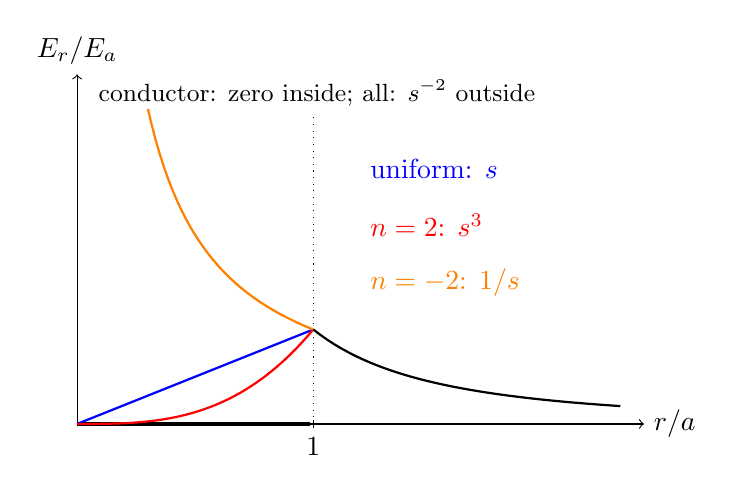
\begin{tikzpicture}[x=3cm,y=1.2cm]
\draw[->] (0,0)--(2.4,0) node[right] {$r/a$};
\draw[->] (0,0)--(0,3.7) node[above] {$E_r/E_a$};
\draw[dotted] (1,0)--(1,3.3);
\draw[black,very thick] (0,0)--(.985,0);
\draw[blue,thick] (0,0)--(1,1);
\draw[red,thick,domain=0:1,samples=40] plot (\x,{\x^3});
\draw[orange,thick,domain=.3:1,samples=45] plot (\x,{1/\x});
\draw[black,thick,domain=1:2.3,samples=45] plot (\x,{1/\x^2});
\draw (1,.04)--(1,-.04) node[below] {$1$};
\node[blue,anchor=west] at (1.2,2.7) {uniform: $s$};
\node[red,anchor=west] at (1.2,2.1) {$n=2$: $s^3$};
\node[orange,anchor=west] at (1.2,1.5) {$n=-2$: $1/s$};
\node[anchor=west,font=\small] at (.05,3.5) {conductor: zero inside; all: $s^{-2}$ outside};
\end{tikzpicture}
\end{center}


\Needspace{5\baselineskip}
\par\bigskip
\noindent\textbf{1.5}\quad The time-averaged potential of a neutral hydrogen atom is given by
\[
\Phi = \frac{q}{4\pi\epsilon_{0}}\frac{e^{-\alpha r}}{r}\left(1+\frac{\alpha r}{2}\right)
\]
where $q$ is the magnitude of the electronic charge, and $\alpha^{-1}=a_{0}/2$, $a_{0}$ being the Bohr radius. Find the distribution of charge (both continuous and discrete) that will give this potential and interpret your result physically.
\solution
For $r>0$, write $\Phi=(q/4\pi\epsilon_0)f(r)$ with
$f=e^{-\alpha r}(1/r+\alpha/2)$. Direct differentiation gives
\[
f'=-e^{-\alpha r}\left(\frac1{r^2}+\frac\alpha r+\frac{\alpha^2}{2}\right),
\quad
(r^2f')'=\frac{\alpha^3r^2}{2}e^{-\alpha r}.
\]
Poisson's equation then yields the continuous part
\[
\rho_c=-\epsilon_0\nabla^2\Phi
=-\frac{q\alpha^3}{8\pi}e^{-\alpha r}\quad(r>0).
\]
The singular part is determined by a small Gaussian sphere:
\[
\lim_{r\to0}4\pi\epsilon_0r^2(-\Phi')=q.
\]
Thus
\[
\boxed{\rho(\mathbf r)=q\delta^3(\mathbf r)
-\frac{q\alpha^3}{8\pi}e^{-\alpha r}.}
\]
Its continuous charge is
$-q\alpha^3\int_0^\infty r^2e^{-\alpha r}dr/2=-q$, since the integral
is $2/\alpha^3$. With $\alpha=2/a_0$,
$\rho_c=-q e^{-2r/a_0}/(\pi a_0^3)$: a point proton plus the mean charge
cloud of a hydrogen $1s$ electron. The total charge is zero, consistently
with the exponentially screened large-$r$ potential.


\Needspace{5\baselineskip}
\par\bigskip
\noindent\textbf{1.6}\quad A simple capacitor is a device formed by two insulated conductors adjacent to each other. If equal and opposite charges are placed on the conductors, there will be a certain difference of potential between them. The ratio of the magnitude of the charge on one conductor to the magnitude of the potential difference is called the capacitance (in SI units it is measured in farads). Using Gauss's law, calculate the capacitance of
\begin{enumerate}
\item[(a)] two large, flat, conducting sheets of area $A$, separated by a small distance $d$;
\item[(b)] two concentric conducting spheres with radii $a$, $b$ ($b>a$);
\item[(c)] two concentric conducting cylinders of length $L$, large compared to their radii $a$, $b$ ($b>a$).
\item[(d)] What is the inner diameter of the outer conductor in an air-filled coaxial cable whose center conductor is a cylindrical wire of diameter 1 mm and whose capacitance is $3\times10^{-11}$ F/m? $3\times10^{-12}$ F/m?
\end{enumerate}
\solution
Take $Q>0$ on the inner/positive conductor and define
$V=\Phi_+-\Phi_->0$. The electrostatic capacitance is $C=Q/V$.
\begin{enumerate}
\item[(a)] A Gaussian pillbox gives $E=Q/(\epsilon_0 A)$ in the gap.
Consequently $V=\int_0^d E\,dz=Qd/(\epsilon_0A)$, and
$\boxed{C=\epsilon_0A/d}$. Edge effects are neglected.
\item[(b)] A Gaussian sphere gives $E_r=Q/(4\pi\epsilon_0r^2)$ for $a<r<b$.
Therefore
\[
V=\frac{Q}{4\pi\epsilon_0}\int_a^b\frac{dr}{r^2}
=\frac{Q}{4\pi\epsilon_0}\left(\frac1a-\frac1b\right),\qquad
\boxed{C=4\pi\epsilon_0\frac{ab}{b-a}}.
\]
\item[(c)] For a coaxial Gaussian cylinder,
$2\pi rLE_r=Q/\epsilon_0$, whence
\[
V=\frac{Q}{2\pi\epsilon_0L}\int_a^b\frac{dr}{r}
=\frac{Q}{2\pi\epsilon_0L}\ln\frac ba,\qquad
\boxed{C=\frac{2\pi\epsilon_0L}{\ln(b/a)}}.
\]
End corrections are negligible when the length is much larger than the radii.
\item[(d)] With $C'=C/L$, $b/a=\exp(2\pi\epsilon_0/C')$. Since $2a=1$ mm,
\[
2b=(1\ {\rm mm})\exp(2\pi\epsilon_0/C')
=\begin{cases}
6.388\ {\rm mm},&C'=3\times10^{-11}\ {\rm F/m},\\
1.1314\times10^5\ {\rm m},&C'=3\times10^{-12}\ {\rm F/m}.
\end{cases}
\]
Here air is approximated by vacuum, $\epsilon_0\simeq8.85419\times10^{-12}$ F/m.
The second value is a formal coaxial result and would require an enormous
outer cylinder and still greater length for the end-free approximation.
\end{enumerate}


\Needspace{5\baselineskip}
\par\bigskip
\noindent\textbf{1.7}\quad Two long, cylindrical conductors of radii $a_{1}$ and $a_{2}$ are parallel and separated by a distance $d$, which is large compared with either radius. Show that the capacitance per unit length is given approximately by
\[
C \simeq \pi\epsilon_{0}\left(\ln\frac{d}{a}\right)^{-1}
\]
where $a$ is the geometrical mean of the two radii.

Approximately what gauge wire (state diameter in millimeters) would be necessary to make a two-wire transmission line with a capacitance of $1.2\times10^{-11}$ F/m if the separation of the wires was 0.5 cm? 1.5 cm? 5.0 cm?
\solution
Let the wire charges per unit length be $+\lambda$ and $-\lambda$.
For a line charge, integrating $E_r=\lambda/(2\pi\epsilon_0r)$ gives
$\Phi(r_2)-\Phi(r_1)=-(\lambda/2\pi\epsilon_0)\ln(r_2/r_1)$.
Superposing the two lines and evaluating at their surfaces, to leading order
in $a_i/d$, gives
\[
\Phi_1=\frac{\lambda}{2\pi\epsilon_0}\ln\frac d{a_1}+\Phi_*,\qquad
\Phi_2=-\frac{\lambda}{2\pi\epsilon_0}\ln\frac d{a_2}+\Phi_*.
\]
Subtracting eliminates the arbitrary constant:
\[
V=\frac{\lambda}{2\pi\epsilon_0}\ln\frac{d^2}{a_1a_2}
=\frac{\lambda}{\pi\epsilon_0}\ln\frac d{\sqrt{a_1a_2}},\qquad
\boxed{C'=\frac{\pi\epsilon_0}{\ln(d/a)},\quad a=\sqrt{a_1a_2}.}
\]
For equal radii and $C'=1.2\times10^{-11}$ F/m,
\[
2a=2d\exp\left(-\frac{\pi\epsilon_0}{C'}\right)=0.19694\,d.
\]
Thus the requested diameters for separations $0.5$, $1.5$, and $5.0$ cm are,
respectively,
\[\boxed{0.985,\ 2.954,\ 9.847\ {\rm mm}.}\]
These diameters specify the required wire size without choosing a national
gauge convention. The ratio $a/d\simeq0.0985$ also shows that the calculation
is approximate rather than an exact finite-radius two-cylinder solution.


\Needspace{5\baselineskip}
\par\bigskip
\noindent\textbf{1.8}\quad\begin{enumerate}
\item[(a)] For the three capacitor geometries in Problem 1.6 calculate the total electrostatic energy and express it alternatively in terms of the equal and opposite charges $Q$ and $-Q$ placed on the conductors \emph{and} the potential difference between them.
\item[(b)] Sketch the energy density of the electrostatic field in each case as a function of the appropriate linear coordinate.
\end{enumerate}
\solution
At an intermediate charge $q$, the voltage is $q/C$. The charging work is
\[
U=\int_0^Q\frac qC\,dq=\frac{Q^2}{2C}=\frac12CV^2=\frac12QV.
\]
For the three geometries this gives
\[
\begin{array}{c|c|c}
 &U(Q)&U(V)\\\hline
\text{planes}&\displaystyle\frac{Q^2d}{2\epsilon_0A}
&\displaystyle\frac{\epsilon_0AV^2}{2d}\\[5pt]
\text{spheres}&\displaystyle\frac{Q^2}{8\pi\epsilon_0}\left(\frac1a-\frac1b\right)
&\displaystyle\frac{2\pi\epsilon_0abV^2}{b-a}\\[5pt]
\text{cylinders}&\displaystyle\frac{Q^2}{4\pi\epsilon_0L}\ln\frac ba
&\displaystyle\frac{\pi\epsilon_0LV^2}{\ln(b/a)}
\end{array}
\]
For part (b), the local energy density is $u=\epsilon_0E^2/2$. Therefore
\[
u=\begin{cases}
Q^2/(2\epsilon_0A^2),&0<z<d\quad\text{(planes)},\\
Q^2/(32\pi^2\epsilon_0r^4),&a<r<b\quad\text{(spheres)},\\
Q^2/(8\pi^2\epsilon_0L^2r^2),&a<r<b\quad\text{(cylinders)}.
\end{cases}
\]
It is zero outside these gaps for the ideal equal-and-opposite capacitor
charges. As an independent check, integrating the spherical density with
$4\pi r^2dr$ gives $Q^2(1/a-1/b)/(8\pi\epsilon_0)$; integrating the
cylindrical density with $2\pi rLdr$ gives $Q^2\ln(b/a)/(4\pi\epsilon_0L)$.
\begin{center}
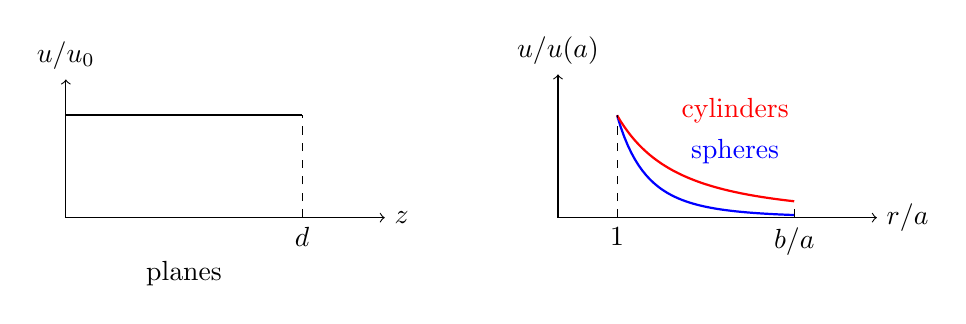
\begin{tikzpicture}[x=1.5cm,y=1.3cm]
\draw[->] (0,0)--(2.7,0) node[right] {$z$};
\draw[->] (0,0)--(0,1.35) node[above] {$u/u_0$};
\draw[thick] (0,1)--(2,1);
\draw[dashed] (2,0)--(2,1);
\node[below] at (2,0) {$d$};
\node at (1,-.55) {planes};
\begin{scope}[xshift=5.5cm]
\draw[->] (.5,0)--(3.2,0) node[right] {$r/a$};
\draw[->] (.5,0)--(.5,1.4) node[above] {$u/u(a)$};
\draw[blue,thick,domain=1:2.5,samples=50] plot (\x,{1/\x^4});
\draw[red,thick,domain=1:2.5,samples=50] plot (\x,{1/\x^2});
\draw[dashed] (1,0)--(1,1);
\draw[dashed] (2.5,0)--(2.5,.16);
\node[below] at (1,0) {$1$};
\node[below] at (2.5,0) {$b/a$};
\node[blue] at (2,.65) {spheres};
\node[red] at (2,1.05) {cylinders};
\end{scope}
\end{tikzpicture}
\end{center}


\Needspace{5\baselineskip}
\par\bigskip
\noindent\textbf{1.9}\quad Calculate the attractive force between conductors in the parallel plate capacitor (Problem 1.6a) and the parallel cylinder capacitor (Problem 1.7) for
\begin{enumerate}
\item[(a)] fixed charges on each conductor;
\item[(b)] fixed potential difference between conductors.
\end{enumerate}
\solution
Let positive force mean increasing separation $d$. For fixed charge,
$F_d=-\partial_d U$. For fixed voltage the source also exchanges energy:
$dW_{\rm source}=V\,dQ=V^2dC$. Since
$dU_{\rm field}=\tfrac12V^2dC$, the mechanical work is
$F_d\,dd=dW_{\rm source}-dU_{\rm field}=\tfrac12V^2dC$.
Equivalently, differentiate $U_{\rm field}-VQ=-\tfrac12CV^2$.
\begin{enumerate}
\item[(a)] For the planes, $U=Q^2d/(2\epsilon_0A)$, so
\[
\boxed{F_d=-\frac{Q^2}{2\epsilon_0A}.}
\]
For the wires use energy per length
$U'=\lambda^2\ln(d/a)/(2\pi\epsilon_0)$, obtaining
\[
\boxed{\frac{F_d}{L}=-\frac{\lambda^2}{2\pi\epsilon_0d}.}
\]
\item[(b)] With $C=\epsilon_0A/d$ for the planes,
\[
\boxed{F_d=\tfrac12V^2\frac{dC}{dd}
=-\frac{\epsilon_0AV^2}{2d^2}.}
\]
For the wires,
\[
\frac{dC'}{dd}=-\frac{\pi\epsilon_0}{d\ln^2(d/a)},\qquad
\boxed{\frac{F_d}{L}=-\frac{\pi\epsilon_0V^2}{2d\ln^2(d/a)}.}
\]
Substitution of $Q=CV$ or $\lambda=C'V$ recovers the fixed-charge formulas
at the same instantaneous state. All signs are negative, hence attractive.
\end{enumerate}


\Needspace{5\baselineskip}
\par\bigskip
\noindent\textbf{1.10}\quad Prove the \emph{mean value theorem}: For charge-free space the value of the electrostatic potential at any point is equal to the average of the potential over the surface of \emph{any} sphere centered on that point.
\solution
Let $B_R$ be a ball wholly contained in a charge-free region, centered at
$\mathbf x_0$, and let
\[
M(R)=\frac1{4\pi}\int\Phi(\mathbf x_0+R\widehat{\mathbf r})d\Omega.
\]
Differentiating at fixed solid angle and using $da=R^2d\Omega$ gives
\[
M'(R)=\frac1{4\pi R^2}\oint_{\partial B_R}\partial_n\Phi\,da
=\frac1{4\pi R^2}\int_{B_R}\nabla^2\Phi\,d^3x=0.
\]
Thus $M$ is independent of radius. Continuity implies
$\lim_{R\to0}M(R)=\Phi(\mathbf x_0)$, proving
\[
\boxed{\Phi(\mathbf x_0)=\frac1{4\pi R^2}\oint_{\partial B_R}\Phi\,da.}
\]
The entire ball must be free of charge and singularities, not just its surface.


\Needspace{5\baselineskip}
\par\bigskip
\noindent\textbf{1.11}\quad Use Gauss's theorem to prove that at the surface of a curved charged conductor, the normal derivative of the electric field is given by
\[
\frac{1}{E}\frac{\partial E}{\partial n} = -\left(\frac{1}{R_{1}}+\frac{1}{R_{2}}\right)
\]
where $R_{1}$ and $R_{2}$ are the principal radii of curvature of the surface.
\solution
Choose a small patch of area $dA$ and a tube whose sides follow the outward
normals. At normal distance $dn$, its area is, to first order,
\[
dA(dn)=dA\left(1+\frac{dn}{R_1}\right)
                 \left(1+\frac{dn}{R_2}\right)
=dA\left[1+\left(\frac1{R_1}+\frac1{R_2}\right)dn\right]+O(dn^2).
\]
The signed principal radii are positive on a convex surface with the outward
normal convention. The field is normal at the conductor. On the side faces the tangential field starts from zero and is $O(dn)$,
while their area is $O(dn)$. Side flux is therefore of
second order in the tube height, so the first-order charge-free flux balance is
\[
[E+\partial_nE\,dn]\,dA(dn)-E\,dA=0+O(dn^2).
\]
Expanding, dividing by $dA\,dn$, and taking the limit gives
\[
\partial_nE+E\left(\frac1{R_1}+\frac1{R_2}\right)=0,
\qquad
\boxed{\frac{\partial_nE}{E}=-\left(\frac1{R_1}+\frac1{R_2}\right).}
\]
The divided form applies where $E\ne0$; the undivided equation remains valid
where it vanishes. A sphere has $E\propto r^{-2}$ and gives $-2/R$; a
cylinder has $E\propto r^{-1}$ and gives $-1/R$, checking both curvature terms.


\Needspace{5\baselineskip}
\par\bigskip
\noindent\textbf{1.12}\quad Prove \emph{Green's reciprocation theorem}: If $\Phi$ is the potential due to a volume-charge density $\rho$ within a volume $V$ and a surface-charge density $\sigma$ on the conducting surface $S$ bounding the volume $V$, while $\Phi'$ is the potential due to another charge distribution $\rho'$ and $\sigma'$, then
\[
\int_{V}\rho\Phi'\;d^{3}x + \int_{S}\sigma\Phi'\;da = \int_{V}\rho'\Phi\;d^{3}x + \int_{S}\sigma'\Phi\;da
\]
\solution
Use the normal $\mathbf n$ pointing out of the field volume and into each
conductor. Since the electric field in the metal is zero, the conductor's
surface charge is $\sigma=\epsilon_0\partial_n\Phi$, and similarly for primes.
Green's second identity gives
\[
\int_V(\Phi\nabla^2\Phi'-\Phi'\nabla^2\Phi)d^3x
=\oint_S(\Phi\partial_n\Phi'-\Phi'\partial_n\Phi)da.
\]
Insert $\nabla^2\Phi=-\rho/\epsilon_0$ and its primed counterpart:
\[
\int_V(\rho\Phi'-\rho'\Phi)d^3x
=\oint_S(\sigma'\Phi-\sigma\Phi')da.
\]
Moving the surface terms to the respective sides proves
\[
\boxed{\int_V\rho\Phi'd^3x+\oint_S\sigma\Phi'da
=\int_V\rho'\Phi d^3x+\oint_S\sigma'\Phi da.}
\]
If a boundary is at infinity, the identity assumes the usual decay that makes
its surface contribution vanish; otherwise that boundary contribution must be retained.


\Needspace{5\baselineskip}
\par\bigskip
\noindent\textbf{1.13}\quad Two infinite grounded parallel conducting planes are separated by a distance $d$. A point charge $q$ is placed between the planes. Use the reciprocation theorem of Green to prove that the total induced charge on one of the planes is equal to $(-q)$ times the fractional perpendicular distance of the point charge from the other plane. (\emph{Hint}: As your comparison electrostatic problem with the same surfaces choose one whose charge densities and potential are known and simple.)
\solution
Take the planes at $z=0$ and $z=d$, and put $q$ at $z=z_0$.
The actual plane potentials are zero. For the comparison problem hold the
lower plane at $V_*$ and the upper at zero, without volume charge. Its potential is
\[
\Phi'(z)=V_*(1-z/d),\qquad\rho'=0.
\]
In the reciprocity relation all right-hand terms vanish, because the actual
potential on either conductor is zero. The left side is
\[
qV_*\left(1-\frac{z_0}{d}\right)+V_*Q_0=0.
\]
Dividing by $V_*$ gives
$\boxed{Q_0=-q(d-z_0)/d}$.
Interchanging the reference potentials similarly gives
$\boxed{Q_d=-qz_0/d}$. Their sum is $-q$, as also required by the Gaussian
surface enclosing the charge and both induced distributions.


\Needspace{5\baselineskip}
\par\bigskip
\noindent\textbf{1.14}\quad Consider the electrostatic Green functions of Section 1.10 for Dirichlet and Neumann boundary conditions on the surface $S$ bounding the volume $V$. Apply Green's theorem (1.35) with integration variable $\mathbf{y}$ and $\phi=G(\mathbf{x},\mathbf{y})$, $\psi=G(\mathbf{x}',\mathbf{y})$, with $\nabla^{2}_{y}G(\mathbf{z},\mathbf{y})=-4\pi\delta(\mathbf{y}-\mathbf{z})$. Find an expression for the difference $[G(\mathbf{x},\mathbf{x}')-G(\mathbf{x}',\mathbf{x})]$ in terms of an integral over the boundary surface $S$.
\begin{enumerate}
\item[(a)] For Dirichlet boundary conditions on the potential and the associated boundary condition on the Green function, show that $G_{D}(\mathbf{x},\mathbf{x}'\erratum{)}$ must be symmetric in $\mathbf{x}$ and $\mathbf{x}'$.
\item[(b)] For Neumann boundary conditions, use the boundary condition (1.45) for $G_{N}(\mathbf{x},\mathbf{x}')$ to show that $G_{N}(\mathbf{x},\mathbf{x}')$ is not symmetric in general, but that $G_{N}(\mathbf{x},\mathbf{x}')-F(\mathbf{x})$ is symmetric in $\mathbf{x}$ and $\mathbf{x}'$, where
\[
F(\mathbf{x}) = \frac{1}{S}\oint_{S}G_{N}(\mathbf{x},\mathbf{y})\;da_{y}
\]
\item[(c)] Show that the addition of $F(\mathbf{x})$ to the Green function does not affect the potential $\Phi(\mathbf{x})$. See problem 3.26 for an example of the Neumann Green function.
\end{enumerate}
\solution
Set $g(\mathbf y)=G(\mathbf x,\mathbf y)$ and
$h(\mathbf y)=G(\mathbf x',\mathbf y)$. Green's identity yields
\[
\begin{split}
\oint_S(g\partial_nh-h\partial_ng)da
&=\int_V(g\nabla_y^2h-h\nabla_y^2g)d^3y\\
&=-4\pi G(\mathbf x,\mathbf x')+4\pi G(\mathbf x',\mathbf x).
\end{split}
\]
Thus
\[
\boxed{G(\mathbf x,\mathbf x')-G(\mathbf x',\mathbf x)
=\frac1{4\pi}\oint_S(h\partial_ng-g\partial_nh)da.}
\]
\begin{enumerate}
\item[(a)] For $G_D$, both $g$ and $h$ vanish on $S$; the integral is zero.
\item[(b)] Jackson's normalization is
$\partial_{n_y}G_N(\mathbf z,\mathbf y)=-4\pi/S$. Substitution gives
\[
G_N(\mathbf x,\mathbf x')-G_N(\mathbf x',\mathbf x)
=\frac1S\oint_S[g(\mathbf y)-h(\mathbf y)]da
=F(\mathbf x)-F(\mathbf x').
\]
Rearrangement shows that $G_N(\mathbf x,\mathbf x')-F(\mathbf x)$ is symmetric.
\item[(c)] The Neumann potential formula is
\[
\Phi(\mathbf x)=\langle\Phi\rangle_S+
\frac1{4\pi\epsilon_0}\int_V\rho(\mathbf y)G_N(\mathbf x,\mathbf y)d^3y
+\frac1{4\pi}\oint_SG_N(\mathbf x,\mathbf y)\partial_n\Phi(\mathbf y)da.
\]
Adding any function $f(\mathbf x)$ independent of $\mathbf y$ changes this by
\[
\Delta\Phi=\frac{f(\mathbf x)}{4\pi}
\left[\frac1{\epsilon_0}\int_V\rho\,d^3y+\oint_S\partial_n\Phi\,da\right]=0,
\]
because the divergence theorem and Poisson's equation give
$\oint\partial_n\Phi=\int\nabla^2\Phi=-\int\rho/\epsilon_0$.
This applies to adding $F$ as asked, or subtracting it to obtain the symmetric
kernel. The independent additive constant $\langle\Phi\rangle_S$ still fixes
the potential's gauge.
\end{enumerate}


\Needspace{5\baselineskip}
\par\bigskip
\noindent\textbf{1.15}\quad Prove \emph{Thomson's theorem}: If a number of surfaces are fixed in position and a given total charge is placed on each surface, then the electrostatic energy in the region bounded by the surfaces is an absolute minimum when the charges are placed so that every surface is an equipotential, as happens when they are conductors.
\solution
Let $\rho_0$ (including surface charges) be the equipotential distribution,
with field $\mathbf E_0$ and potential $\Phi_0$. Any other admissible
redistribution is $\rho_0+\delta\rho$, with field
$\mathbf E_0+\delta\mathbf E$, and with $\delta Q_i=0$ on each surface.
Expanding the field energy gives
\[
U-U_0=\epsilon_0\int\mathbf E_0\cdot\delta\mathbf E\,d^3x
+\frac{\epsilon_0}{2}\int|\delta\mathbf E|^2d^3x.
\]
Integrating the cross term by parts over all field space, or treating surface
charges as distributions, yields
\[
\epsilon_0\int\nabla\Phi_0\cdot\nabla\delta\Phi\,d^3x
=\int\Phi_0\delta\rho\,d^3x
=\sum_i\Phi_{0i}\delta Q_i=0.
\]
Consequently
\[
\boxed{U-U_0=\frac{\epsilon_0}{2}\int|\delta\mathbf E|^2d^3x\ge0.}
\]
This is a global minimum, not just a stationary value. Equality requires no
change of field. Fixed additional volume charges, if present, are left
unchanged in the variation.


\Needspace{5\baselineskip}
\par\bigskip
\noindent\textbf{1.16}\quad Prove the following theorem: If a number of conducting surfaces are fixed in position with a given total charge on each, the introduction of an uncharged, insulated conductor into the region bounded by the surfaces \erratum{cannot increase} the electrostatic energy. \erratum{The decrease is strict if the field changes.}
\solution
Before inserting the new conductor, denote the equilibrium energy by $U_0$.
In the enlarged set of possible charge distributions, consider the trial
configuration that retains every old charge and places zero excess charge
everywhere on the new conductor. It has the prescribed old charges and zero
total new charge, so it is an admissible charge distribution for Thomson's
minimization problem, although it is generally not an equilibrium distribution.
Its field and energy, integrated also through the new body's volume, are the
old ones: $U_{\rm trial}=U_0$.

The new equilibrium minimizes the energy over this enlarged set. Therefore
\[
\boxed{U_{\rm new}\le U_{\rm trial}=U_0.}
\]
More explicitly, applying the proof of Problem 1.15 with the new equilibrium
as the reference gives
\[
U_0-U_{\rm new}=\frac{\epsilon_0}{2}
\int|\mathbf E_0-\mathbf E_{\rm new}|^2d^3x\ge0.
\]
The inequality is strict if insertion changes the field. Equality is possible
when the inserted body occupies a region that was already field-free.
The old conductors are insulated with fixed charges; maintaining fixed
potentials would involve additional work by voltage sources.


\Needspace{5\baselineskip}
\par\bigskip
\noindent\textbf{1.17}\quad A volume $V$ in vacuum is bounded by a surface $S$ consisting of several separate conducting surfaces $S_{i}$. One conductor is held at \emph{unit} potential and all the other conductors at zero potential.
\begin{enumerate}
\item[(a)] Show that the capacitance of the one conductor is given by
\[
C = \epsilon_{0}\int_{V}|\nabla\Phi|^{2}\;d^{3}x
\]
where $\Phi(\mathbf{x})$ is the solution for the potential.
\item[(b)] Show that the true capacitance $C$ is always less than or equal to the quantity
\[
C[\Psi] = \epsilon_{0}\int_{V}|\nabla\Psi|^{2}\;d^{3}x
\]
where $\Psi$ is any trial function satisfying the boundary conditions on the conductors. This is a variational principle for the capacitance that yields an \emph{upper bound}.
\end{enumerate}
\solution
\begin{enumerate}
\item[(a)] There is no volume charge. With the normal directed out of $V$,
Green's first identity gives
\[
\int_V|\nabla\Phi|^2d^3x
=\oint_S\Phi\partial_n\Phi\,da
=\int_{S_1}\partial_n\Phi\,da=Q_1/\epsilon_0.
\]
Only $S_1$ contributes, because its potential is one and all others are zero.
Since $Q_1=C\times1$, this proves
$\boxed{C=\epsilon_0\int_V|\nabla\Phi|^2d^3x}$.
\item[(b)] Write a trial function as $\Psi=\Phi+\eta$ with $\eta=0$ on every
conductor. Then
\[
C[\Psi]-C
=2\epsilon_0\int_V\nabla\Phi\cdot\nabla\eta\,d^3x
+\epsilon_0\int_V|\nabla\eta|^2d^3x.
\]
The first integral is
$\oint\eta\partial_n\Phi\,da-\int\eta\nabla^2\Phi\,d^3x=0$.
Thus
\[
\boxed{C[\Psi]-C=\epsilon_0\int_V|\nabla\eta|^2d^3x\ge0.}
\]
Trial functions need finite field energy and the specified boundary values;
they need not solve Laplace's equation.
\end{enumerate}


\Needspace{5\baselineskip}
\par\bigskip
\noindent\textbf{1.18}\quad Consider the configuration of conductors of Problem 1.17, with all conductors except $S_{1}$ held at zero potential.
\begin{enumerate}
\item[(a)] Show that the potential $\Phi(\mathbf{x})$ anywhere in the volume $V$ \emph{and} on any of the surfaces $S_{i}$ can be written
\[
\Phi(\mathbf{x}) = \frac{1}{4\pi\epsilon_{0}}\oint_{S_{1}}\sigma_{1}(\mathbf{x}')G(\mathbf{x},\mathbf{x}')\;da'
\]
where $\sigma_{1}(\mathbf{x}')$ is the surface charge density on $S_{1}$ and $G(\mathbf{x},\mathbf{x}')$ is the Green function potential for a point charge in the presence of all the surfaces that are held at zero potential (but with $S_{1}$ absent). Show also that the electrostatic energy is
\[
W = \frac{1}{8\pi\epsilon_{0}}\oint_{S_{1}}da\oint_{S_{1}}da'\;\sigma_{1}(\mathbf{x})G(\mathbf{x},\mathbf{x}')\sigma_{1}(\mathbf{x}')
\]
where the integrals are only over the surface $S_{1}$.
\item[(b)] Show that the variational expression
\[
C^{-1}[\sigma] = \frac{\displaystyle\oint_{S_{1}}da\oint_{S_{1}}da'\;\sigma(\mathbf{x})G(\mathbf{x},\mathbf{x}')\sigma(\mathbf{x}')}{4\pi\epsilon_{0}\left[\displaystyle\oint_{S_{1}}\sigma(\mathbf{x})\;da\right]^{2}}
\]
with an arbitrary integrable function $\sigma(\mathbf{x})$ defined on $S_{1}$, \erratum{having nonzero total charge and finite electrostatic energy}, is stationary for small variations of $\sigma$ away from $\sigma_{1}$. Use Thomson's theorem to prove that the reciprocal of $C^{-1}[\sigma]$ gives a \emph{lower bound} to the true capacitance of the conductor $S_{1}$.
\end{enumerate}
\solution
\begin{enumerate}
\item[(a)] Remove $S_1$ and use the Dirichlet Green function for the remaining
grounded conductors. An element $dq=\sigma_1(\mathbf x')da'$ produces
$d\Phi=G(\mathbf x,\mathbf x')dq/(4\pi\epsilon_0)$, including the response
of those grounded conductors. Superposition gives
\[
\boxed{\Phi(\mathbf x)=\frac1{4\pi\epsilon_0}
\oint_{S_1}\sigma_1(\mathbf x')G(\mathbf x,\mathbf x')da'.}
\]
This is also the continuous single-layer potential at the surface itself.
The electrostatic energy is $W=\tfrac12\sum_i\int_{S_i}\sigma_i\Phi_i\,da$.
All grounded surfaces have $\Phi_i=0$, so substitution leaves
\[
\boxed{W=\frac1{8\pi\epsilon_0}\oint_{S_1}\!da\oint_{S_1}\!da'\,
\sigma_1(\mathbf x)G(\mathbf x,\mathbf x')\sigma_1(\mathbf x').}
\]
\item[(b)] Write $Q[\sigma]=\int\sigma da$ and
$B[\sigma]=\iint\sigma G\sigma\,da\,da'$. Then
$C^{-1}[\sigma]=B/(4\pi\epsilon_0Q^2)=2W[\sigma]/Q^2$.
Symmetry of $G$ gives
\[
\delta B=2\int\delta\sigma(\mathbf x)
\left[\int G(\mathbf x,\mathbf x')\sigma_1(\mathbf x')da'\right]da
=8\pi\epsilon_0V_1\delta Q.
\]
At equilibrium $B=4\pi\epsilon_0V_1Q$, and hence
\[
\delta C^{-1}=\frac{\delta B}{4\pi\epsilon_0Q^2}
-\frac{2B\delta Q}{4\pi\epsilon_0Q^3}=0.
\]
Because this quotient is unchanged by rescaling $\sigma$, compare trial
functions at the same nonzero charge $Q$. If $\delta\sigma=\sigma-\sigma_1$
and $\int\delta\sigma=0$, the energy cross term is
$V_1\int\delta\sigma=0$. The remaining term is
\[
W[\sigma]-W[\sigma_1]=\frac1{8\pi\epsilon_0}\iint\delta\sigma G\delta\sigma
=\frac{\epsilon_0}{2}\int|\nabla\delta\Phi|^2d^3x\ge0.
\]
Thus $C^{-1}[\sigma]\ge C^{-1}$ and
$\boxed{1/C^{-1}[\sigma]\le C}$.
The admissible trial density must have nonzero total charge and finite
self-energy; integrability alone does not guarantee the latter. An infinite
energy trial supplies only the trivial zero lower bound.
\end{enumerate}


\Needspace{5\baselineskip}
\par\bigskip
\noindent\textbf{1.19}\quad For the cylindrical capacitor of Problem 1.6c, evaluate the variational upper bound of Problem 1.17b with the naive trial function, $\Psi_{1}(\rho)=(b-\rho)/(b-a)$. Compare the variational result with the exact result for $b/a=1.5$, 2, 3. Explain the trend of your results in terms of the functional form of $\Psi_{1}$. An improved trial function is treated by \emph{Collin} (pp.~275--277).
\solution
In the long-cylinder approximation,
$\nabla\Psi_1=-\widehat{\boldsymbol\rho}/(b-a)$, so
\[
C[\Psi_1]=\epsilon_0L\int_a^b\frac{2\pi\rho\,d\rho}{(b-a)^2}
=\pi\epsilon_0L\frac{b+a}{b-a}.
\]
Divide by $C=2\pi\epsilon_0L/\ln(b/a)$ and set $t=b/a$:
\[
\boxed{\frac{C[\Psi_1]}C=\frac{t+1}{2(t-1)}\ln t.}
\]
The ratios at $t=1.5,2,3$ are $1.013663$, $1.039721$, and $1.098612$,
i.e. upper-bound errors of $1.37\%$, $3.97\%$, and $9.86\%$.
The exact potential is $\Phi=\ln(b/\rho)/\ln(b/a)$, whose gradient varies
as $1/\rho$. A constant-gradient linear trial is close when the gap is narrow
but cannot reproduce that variation across a wide annulus. In particular,
putting $t=1+\delta$ gives
\[
\frac{2+\delta}{2\delta}
\left(\delta-\frac{\delta^2}{2}+\frac{\delta^3}{3}-\cdots\right)
=1+\frac{\delta^2}{12}+O(\delta^3),
\]
which verifies approach to the exact result as the gap shrinks.


\Needspace{5\baselineskip}
\par\bigskip
\noindent\textbf{1.20}\quad In estimating the capacitance of a given configuration of conductors, comparison with known capacitances is often helpful. Consider two configurations of $n$ conductors in which the $(n-1)$ conductors held at zero potential are the same, but the one conductor whose capacitance we wish to know is different. In particular, let the conductor in one configuration have a closed surface $S_{1}$ and in the other configuration have surface $S_{1}'$, with $S_{1}'$ totally inside $S_{1}$.
\begin{enumerate}
\item[(a)] Use the extremum principle of Section 1.12 and the variational principle of Problem 1.17 to prove that the capacitance $C'$ of the conductor with surface $S_{1}'$ is less than or equal to the capacitance $C$ of the conductor with surface $S_{1}$ that encloses $S_{1}'$.
\item[(b)] Set upper and lower limits for the capacitance of a conducting cube of side $a$. Compare your limits and also their average with the numerical value, $C\simeq0.655(4\pi\epsilon_{0}a)$.
\item[(c)] By how much do you estimate the capacitance per unit length of the two-wire system of Problem 1.7 will change (larger? smaller?) if \emph{one} of the wires is replaced by a wire of square cross section whose side is equal to its diameter?
\end{enumerate}
\solution
\begin{enumerate}
\item[(a)] Normalize the larger conductor to unit potential, and call its
exterior solution $\Phi$. For the smaller-conductor problem choose the trial
potential equal to $\Phi$ outside $S_1$ and equal to one throughout the
space between $S_1'$ and $S_1$. It is continuous and satisfies all the
smaller problem's Dirichlet data. Its gradient vanishes in the added region,
so its variational integral is exactly $C$. Problem 1.17 therefore gives
$\boxed{C'\le C}$.
\item[(b)] The cube contains a sphere of radius $a/2$ and lies inside a sphere
of radius $\sqrt3a/2$. Using $C_{\rm sphere}=4\pi\epsilon_0R$ gives
\[
\boxed{\frac12\le\frac{C_{\rm cube}}{4\pi\epsilon_0a}\le\frac{\sqrt3}{2}
=0.866025.}
\]
The average of the bounds is $(1+\sqrt3)/4=0.683013$. Relative to the quoted
$0.655$, the lower bound is $23.66\%$ low, the upper $32.22\%$ high, and the
average $4.28\%$ high. The average is an estimate, not a variational bound.
\item[(c)] A square wire of side $2a_1$ contains the old round wire of radius
$a_1$ and is contained in a round wire of radius $\sqrt2a_1$.
The two-conductor capacitance is unchanged if the labels of the grounded and
unit-potential wires are exchanged, so part (a) applies to replacing this wire.
Writing $\ell=\ln[d/\sqrt{a_1a_2}]$, the thin-wire formula gives
\[
C'_0=\frac{\pi\epsilon_0}{\ell},\qquad
C'_0\le C'_{\rm square}\lesssim
\frac{\pi\epsilon_0}{\ell-\tfrac14\ln2}.
\]
Thus the capacitance increases, with estimated fractional increase between
zero and
\[
\frac{(\ln2)/4}{\ell-(\ln2)/4}.
\]
A simple midpoint estimate is half this interval. For the lines in 1.7,
$\ell=\pi\epsilon_0/(1.2\times10^{-11})\simeq2.318$; the interval is
$0$ to $8.08\%$ and its midpoint is about $4.04\%$.
The monotonicity is exact, while these numerical percentages inherit the
thin-wire approximation.
\end{enumerate}


\Needspace{5\baselineskip}
\par\bigskip
\noindent\textbf{1.21}\quad A two-dimensional potential problem consists of a unit square area ($0\leq x\leq1$, $0\leq y\leq1$) bounded by ``surfaces'' held at zero potential. Over the entire square there is a uniform charge density of unit strength (per unit length in $z$).
\begin{enumerate}
\item[(a)] Apply the variational principle (1.63) for the Poisson equation with the ``variational'' trial function $\Psi(x,y)=A\cdot x(1-x)\cdot y(1-y)$ to determine the best value of the constant $A$. [I use quotation marks around variational because there are no parameters to vary except the overall scale.]
\item[(b)] The exact (albeit series) solution for this problem is [see Problems 2.15 and 2.16]
\[
4\pi\epsilon_{0}\Phi(x,y) = \frac{16}{\pi^{2}}\sum_{m=0}^{\infty}\frac{\sin[(2m+1)\pi x]}{(2m+1)^{3}}\left\{1-\frac{\cosh[(2m+1)\pi(y-\frac{1}{2})]}{\cosh[(2m+1)\pi/2]}\right\}
\]
For $y=0.25$ and $y=0.5$, plot and compare the simple variational solution of part a with the exact solution as functions of $x$.
\end{enumerate}
\solution
\begin{enumerate}
\item[(a)] Put $f=x(1-x)y(1-y)$ and $\Psi=Af$. For unit charge density the
functional (1.63) is
\[
I[A]=\frac12 A^2\int_0^1\!\int_0^1|\nabla f|^2dxdy
-\frac{A}{\epsilon_0}\int_0^1\!\int_0^1f\,dxdy.
\]
The elementary integrals are
\[
\int_0^1x(1-x)dx=\frac16,\quad
\int_0^1x^2(1-x)^2dx=\frac1{30},\quad
\int_0^1(1-2x)^2dx=\frac13.
\]
Consequently $\int f=1/36$ and
$\int|\nabla f|^2=2(1/3)(1/30)=1/45$, giving
\[
I[A]=\frac{A^2}{90}-\frac{A}{36\epsilon_0},\qquad
I'[A]=\frac A{45}-\frac1{36\epsilon_0}=0.
\]
Thus $\boxed{A=5/(4\epsilon_0)}$, and $I''=1/45>0$.
In the book's plotted normalization,
\[\boxed{u_{\rm trial}=4\pi\epsilon_0\Psi=5\pi x(1-x)y(1-y).}\]
\item[(b)] Write $k_n=n\pi$ for positive odd $n$. The supplied exact series is
\[
u=\frac{16}{\pi^2}\sum_{n\ {\rm odd}>0}\frac{\sin k_nx}{n^3}
\left[1-\frac{\cosh(k_n(y-1/2))}{\cosh(k_n/2)}\right].
\]
The boundary factors vanish at $x=0,1$ and $y=0,1$. Applying the Laplacian
cancels the two derivatives of the hyperbolic term, leaving
\[
\nabla^2u=-16\sum_{n\ {\rm odd}>0}\frac{\sin(n\pi x)}n=-4\pi,
\]
where $1=(4/\pi)\sum_{n\ {\rm odd}>0}\sin(n\pi x)/n$ is the sine expansion
of a constant on $0<x<1$. Thus the normalization indeed corresponds to
$\rho=1$. The comparison is
\begin{center}
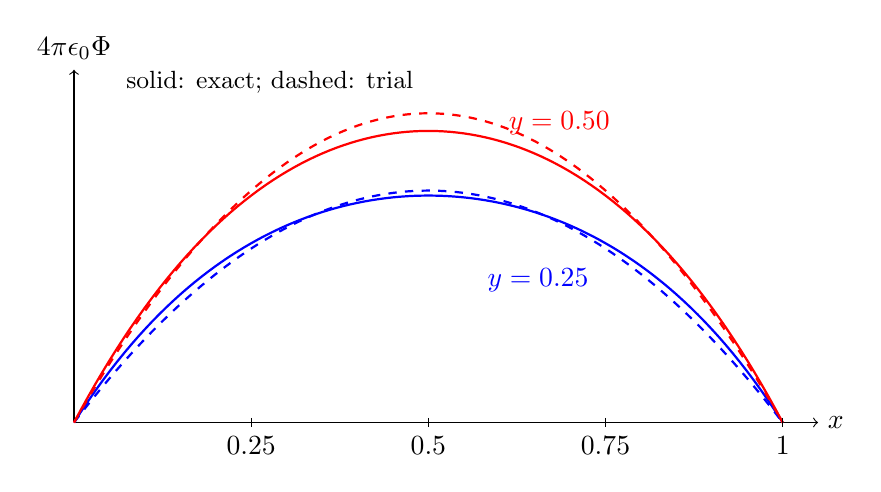
\begin{tikzpicture}[x=9cm,y=4cm]
\draw[->] (0,0)--(1.05,0) node[right] {$x$};
\draw[->] (0,0)--(0,1.12) node[above] {$4\pi\epsilon_0\Phi$};
\draw[blue,thick] plot coordinates {(0.000000,0.000000) (0.010000,0.034737) (0.020000,0.068250) (0.030000,0.100571) (0.040000,0.131732) (0.050000,0.161767) (0.060000,0.190705) (0.070000,0.218579) (0.080000,0.245418) (0.090000,0.271252) (0.100000,0.296111) (0.110000,0.320022) (0.120000,0.343014) (0.130000,0.365112) (0.140000,0.386343) (0.150000,0.406731) (0.160000,0.426300) (0.170000,0.445074) (0.180000,0.463074) (0.190000,0.480322) (0.200000,0.496837) (0.210000,0.512640) (0.220000,0.527749) (0.230000,0.542181) (0.240000,0.555954) (0.250000,0.569083) (0.260000,0.581583) (0.270000,0.593470) (0.280000,0.604756) (0.290000,0.615456) (0.300000,0.625580) (0.310000,0.635140) (0.320000,0.644148) (0.330000,0.652614) (0.340000,0.660546) (0.350000,0.667955) (0.360000,0.674848) (0.370000,0.681233) (0.380000,0.687117) (0.390000,0.692506) (0.400000,0.697408) (0.410000,0.701826) (0.420000,0.705766) (0.430000,0.709233) (0.440000,0.712230) (0.450000,0.714760) (0.460000,0.716826) (0.470000,0.718431) (0.480000,0.719576) (0.490000,0.720263) (0.500000,0.720492) (0.510000,0.720263) (0.520000,0.719576) (0.530000,0.718431) (0.540000,0.716826) (0.550000,0.714760) (0.560000,0.712230) (0.570000,0.709233) (0.580000,0.705766) (0.590000,0.701826) (0.600000,0.697408) (0.610000,0.692506) (0.620000,0.687117) (0.630000,0.681233) (0.640000,0.674848) (0.650000,0.667955) (0.660000,0.660546) (0.670000,0.652614) (0.680000,0.644148) (0.690000,0.635140) (0.700000,0.625580) (0.710000,0.615456) (0.720000,0.604756) (0.730000,0.593470) (0.740000,0.581583) (0.750000,0.569083) (0.760000,0.555954) (0.770000,0.542181) (0.780000,0.527749) (0.790000,0.512640) (0.800000,0.496837) (0.810000,0.480322) (0.820000,0.463074) (0.830000,0.445074) (0.840000,0.426300) (0.850000,0.406731) (0.860000,0.386343) (0.870000,0.365112) (0.880000,0.343014) (0.890000,0.320022) (0.900000,0.296111) (0.910000,0.271252) (0.920000,0.245418) (0.930000,0.218579) (0.940000,0.190705) (0.950000,0.161767) (0.960000,0.131732) (0.970000,0.100571) (0.980000,0.068250) (0.990000,0.034737) (1.000000,0.000000)};
\draw[blue,thick,dashed] plot coordinates {(0.000000,0.000000) (0.010000,0.029158) (0.020000,0.057727) (0.030000,0.085707) (0.040000,0.113097) (0.050000,0.139899) (0.060000,0.166112) (0.070000,0.191735) (0.080000,0.216770) (0.090000,0.241215) (0.100000,0.265072) (0.110000,0.288339) (0.120000,0.311018) (0.130000,0.333107) (0.140000,0.354607) (0.150000,0.375518) (0.160000,0.395841) (0.170000,0.415574) (0.180000,0.434718) (0.190000,0.453273) (0.200000,0.471239) (0.210000,0.488616) (0.220000,0.505404) (0.230000,0.521603) (0.240000,0.537212) (0.250000,0.552233) (0.260000,0.566665) (0.270000,0.580507) (0.280000,0.593761) (0.290000,0.606426) (0.300000,0.618501) (0.310000,0.629988) (0.320000,0.640885) (0.330000,0.651193) (0.340000,0.660913) (0.350000,0.670043) (0.360000,0.678584) (0.370000,0.686536) (0.380000,0.693899) (0.390000,0.700673) (0.400000,0.706858) (0.410000,0.712454) (0.420000,0.717461) (0.430000,0.721879) (0.440000,0.725708) (0.450000,0.728948) (0.460000,0.731598) (0.470000,0.733660) (0.480000,0.735133) (0.490000,0.736016) (0.500000,0.736311) (0.510000,0.736016) (0.520000,0.735133) (0.530000,0.733660) (0.540000,0.731598) (0.550000,0.728948) (0.560000,0.725708) (0.570000,0.721879) (0.580000,0.717461) (0.590000,0.712454) (0.600000,0.706858) (0.610000,0.700673) (0.620000,0.693899) (0.630000,0.686536) (0.640000,0.678584) (0.650000,0.670043) (0.660000,0.660913) (0.670000,0.651193) (0.680000,0.640885) (0.690000,0.629988) (0.700000,0.618501) (0.710000,0.606426) (0.720000,0.593761) (0.730000,0.580507) (0.740000,0.566665) (0.750000,0.552233) (0.760000,0.537212) (0.770000,0.521603) (0.780000,0.505404) (0.790000,0.488616) (0.800000,0.471239) (0.810000,0.453273) (0.820000,0.434718) (0.830000,0.415574) (0.840000,0.395841) (0.850000,0.375518) (0.860000,0.354607) (0.870000,0.333107) (0.880000,0.311018) (0.890000,0.288339) (0.900000,0.265072) (0.910000,0.241215) (0.920000,0.216770) (0.930000,0.191735) (0.940000,0.166112) (0.950000,0.139899) (0.960000,0.113097) (0.970000,0.085707) (0.980000,0.057727) (0.990000,0.029158) (1.000000,0.000000)};
\draw[red,thick] plot coordinates {(0.000000,0.000000) (0.010000,0.041806) (0.020000,0.082377) (0.030000,0.121733) (0.040000,0.159895) (0.050000,0.196885) (0.060000,0.232721) (0.070000,0.267426) (0.080000,0.301020) (0.090000,0.333522) (0.100000,0.364953) (0.110000,0.395332) (0.120000,0.424679) (0.130000,0.453014) (0.140000,0.480354) (0.150000,0.506718) (0.160000,0.532125) (0.170000,0.556592) (0.180000,0.580136) (0.190000,0.602775) (0.200000,0.624526) (0.210000,0.645403) (0.220000,0.665423) (0.230000,0.684602) (0.240000,0.702953) (0.250000,0.720492) (0.260000,0.737231) (0.270000,0.753184) (0.280000,0.768364) (0.290000,0.782783) (0.300000,0.796453) (0.310000,0.809385) (0.320000,0.821589) (0.330000,0.833076) (0.340000,0.843855) (0.350000,0.853936) (0.360000,0.863326) (0.370000,0.872034) (0.380000,0.880067) (0.390000,0.887433) (0.400000,0.894136) (0.410000,0.900184) (0.420000,0.905581) (0.430000,0.910333) (0.440000,0.914442) (0.450000,0.917913) (0.460000,0.920749) (0.470000,0.922952) (0.480000,0.924525) (0.490000,0.925467) (0.500000,0.925782) (0.510000,0.925467) (0.520000,0.924525) (0.530000,0.922952) (0.540000,0.920749) (0.550000,0.917913) (0.560000,0.914442) (0.570000,0.910333) (0.580000,0.905581) (0.590000,0.900184) (0.600000,0.894136) (0.610000,0.887433) (0.620000,0.880067) (0.630000,0.872034) (0.640000,0.863326) (0.650000,0.853936) (0.660000,0.843855) (0.670000,0.833076) (0.680000,0.821589) (0.690000,0.809385) (0.700000,0.796453) (0.710000,0.782783) (0.720000,0.768364) (0.730000,0.753184) (0.740000,0.737231) (0.750000,0.720492) (0.760000,0.702953) (0.770000,0.684602) (0.780000,0.665423) (0.790000,0.645403) (0.800000,0.624526) (0.810000,0.602775) (0.820000,0.580136) (0.830000,0.556592) (0.840000,0.532125) (0.850000,0.506718) (0.860000,0.480354) (0.870000,0.453014) (0.880000,0.424679) (0.890000,0.395332) (0.900000,0.364953) (0.910000,0.333522) (0.920000,0.301020) (0.930000,0.267426) (0.940000,0.232721) (0.950000,0.196885) (0.960000,0.159895) (0.970000,0.121733) (0.980000,0.082377) (0.990000,0.041806) (1.000000,0.000000)};
\draw[red,thick,dashed] plot coordinates {(0.000000,0.000000) (0.010000,0.038877) (0.020000,0.076969) (0.030000,0.114275) (0.040000,0.150796) (0.050000,0.186532) (0.060000,0.221482) (0.070000,0.255647) (0.080000,0.289027) (0.090000,0.321621) (0.100000,0.353429) (0.110000,0.384452) (0.120000,0.414690) (0.130000,0.444143) (0.140000,0.472810) (0.150000,0.500691) (0.160000,0.527788) (0.170000,0.554098) (0.180000,0.579624) (0.190000,0.604364) (0.200000,0.628319) (0.210000,0.651488) (0.220000,0.673872) (0.230000,0.695470) (0.240000,0.716283) (0.250000,0.736311) (0.260000,0.755553) (0.270000,0.774010) (0.280000,0.791681) (0.290000,0.808567) (0.300000,0.824668) (0.310000,0.839983) (0.320000,0.854513) (0.330000,0.868258) (0.340000,0.881217) (0.350000,0.893390) (0.360000,0.904779) (0.370000,0.915382) (0.380000,0.925199) (0.390000,0.934231) (0.400000,0.942478) (0.410000,0.949939) (0.420000,0.956615) (0.430000,0.962505) (0.440000,0.967611) (0.450000,0.971930) (0.460000,0.975465) (0.470000,0.978213) (0.480000,0.980177) (0.490000,0.981355) (0.500000,0.981748) (0.510000,0.981355) (0.520000,0.980177) (0.530000,0.978213) (0.540000,0.975465) (0.550000,0.971930) (0.560000,0.967611) (0.570000,0.962505) (0.580000,0.956615) (0.590000,0.949939) (0.600000,0.942478) (0.610000,0.934231) (0.620000,0.925199) (0.630000,0.915382) (0.640000,0.904779) (0.650000,0.893390) (0.660000,0.881217) (0.670000,0.868258) (0.680000,0.854513) (0.690000,0.839983) (0.700000,0.824668) (0.710000,0.808567) (0.720000,0.791681) (0.730000,0.774010) (0.740000,0.755553) (0.750000,0.736311) (0.760000,0.716283) (0.770000,0.695470) (0.780000,0.673872) (0.790000,0.651488) (0.800000,0.628319) (0.810000,0.604364) (0.820000,0.579624) (0.830000,0.554098) (0.840000,0.527788) (0.850000,0.500691) (0.860000,0.472810) (0.870000,0.444143) (0.880000,0.414690) (0.890000,0.384452) (0.900000,0.353429) (0.910000,0.321621) (0.920000,0.289027) (0.930000,0.255647) (0.940000,0.221482) (0.950000,0.186532) (0.960000,0.150796) (0.970000,0.114275) (0.980000,0.076969) (0.990000,0.038877) (1.000000,0.000000)};
\node[blue,anchor=west] at (.57,.45) {$y=0.25$};
\node[red,anchor=west] at (.60,.95) {$y=0.50$};
\node[anchor=west,font=\small] at (.06,1.08) {solid: exact; dashed: trial};
\foreach \x in {0.25,0.5,0.75,1} \draw (\x,.015)--(\x,-.015) node[below] {$\x$};
\end{tikzpicture}

\end{center}
At $(1/2,1/4)$ the exact and trial values are $0.720492$ and
$15\pi/64=0.736311$; at the center they are $0.925782$ and
$5\pi/16=0.981748$. The respective errors are about $2.20\%$ and $6.04\%$.
The variational principle minimizes the functional, not the pointwise error,
so it does not make this potential a pointwise upper bound everywhere.
The numerical series uses the stable ratio
\[
\frac{\cosh(k(y-1/2))}{\cosh(k/2)}
=\frac{e^{-ky}+e^{-k(1-y)}}{1+e^{-k}},
\]
which avoids overflow for large $k$.
\end{enumerate}


\Needspace{5\baselineskip}
\par\bigskip
\noindent\textbf{1.22}\quad Two-dimensional relaxation calculations commonly use sites on a square lattice with spacing $\Delta x=\Delta y=h$, and label the sites by $(i,j)$, where $i,j$ are integers and $x_{i}=ih+x_{0}$, $y_{j}=jh+y_{0}$. The value of the potential at $(i,j)$ can be approximated by the average of the values at neighboring sites. [Recall the relevant theorem about harmonic functions.] But what average?
\begin{enumerate}
\item[(a)] If $F(x,y)$ is a well-behaved function in the neighborhood of the origin, but not necessarily harmonic, by explicit Taylor series expansions, show that the ``cross'' sum
\[
S_{\mathrm{c}} = F(h,0)+F(0,h)+F(-h,0)+F(0,-h)
\]
can be expressed as
\[
S_{\mathrm{c}} = 4F(0,0)+h^{2}\nabla^{2}F+\frac{h^{4}}{12}\left(F_{xxxx}+F_{yyyy}\right)+O(h^{6})
\]
\item[(b)] Similarly, show that the ``square'' sum,
\[
S_{\mathrm{s}} = F(h,h)+F(-h,h)+F(-h,-h)+F(h,-h)
\]
can be expressed as
\[
S_{\mathrm{s}} = 4F(0,0)+2h^{2}\nabla^{2}F-\frac{h^{4}}{3}\left(F_{xxxx}+F_{yyyy}\right)+\frac{h^{4}}{2}\nabla^{2}(\nabla^{2}F)+O(h^{6})
\]
Here $F_{xxxx}$ is the fourth partial derivative of $F$ with respect to $x$, evaluated at $x=0$, $y=0$, etc. If $\nabla^{2}F=0$, the averages $S_{\mathrm{c}}/4$ and $S_{\mathrm{s}}/4$ each give the value of $F(0,0)$, correct to order $h^{3}$ inclusive. Note that an improvement can be obtained by forming the ``improved'' average,
\[
\langle\!\langle F(0,0)\rangle\!\rangle = \frac{1}{5}\left[S_{\mathrm{c}}+\frac{1}{4}S_{\mathrm{s}}\right]
\]
where
\[
\langle\!\langle F(0,0)\rangle\!\rangle = F(0,0)+\frac{3}{10}h^{2}\nabla^{2}F+\frac{h^{4}}{40}\nabla^{2}(\nabla^{2}F)+O(h^{6})
\]
If $\nabla^{2}F=0$, then \erratum{the improved average} gives $F(0,0)$, correct to order $h^{5}$ inclusive. For Poisson's equation, the charge density and its lowest order Laplacian can be inserted for the same accuracy.
\end{enumerate}
\solution
Write all derivatives below at the origin. The multivariate Taylor series is
\[
F(x,y)=\sum_{p+q\le5}\frac{x^py^q}{p!q!}\partial_x^p\partial_y^qF
+O((|x|+|y|)^6).
\]
\begin{enumerate}
\item[(a)] Pairing opposite points cancels odd powers:
\[
F(h,0)+F(-h,0)=2F+h^2F_{xx}+\frac{h^4}{12}F_{xxxx}+O(h^6).
\]
The analogous $y$ pair gives
\[
\boxed{S_c=4F+h^2\nabla^2F+\frac{h^4}{12}(F_{xxxx}+F_{yyyy})+O(h^6).}
\]
\item[(b)] In the four diagonal points, terms with either odd $p$ or odd $q$
cancel. The surviving terms through degree four are
\[
S_s=4F+2h^2(F_{xx}+F_{yy})
+\frac{h^4}{6}(F_{xxxx}+F_{yyyy})+h^4F_{xxyy}+O(h^6).
\]
Since $\nabla^4F=F_{xxxx}+2F_{xxyy}+F_{yyyy}$,
\[
\boxed{S_s=4F+2h^2\nabla^2F
-\frac{h^4}{3}(F_{xxxx}+F_{yyyy})+\frac{h^4}{2}\nabla^4F+O(h^6).}
\]
Now multiply $S_c$ by $1/5$ and $S_s$ by $1/20$.
The fourth-derivative anisotropy cancels because
$(1/5)(1/12)+(1/20)(-1/3)=0$. The other coefficients are
$4/5+4/20=1$, $1/5+2/20=3/10$, and $(1/20)(1/2)=1/40$.
Therefore
\[
\boxed{\frac{4S_c+S_s}{20}
=F+\frac3{10}h^2\nabla^2F+\frac{h^4}{40}\nabla^4F+O(h^6).}
\]
If $F$ is harmonic in a neighborhood, both displayed Laplacians vanish.
For Poisson's equation $\nabla^2\Phi=-\rho/\epsilon_0$, instead rearrange to
\[
\boxed{\Phi=\frac{4S_c+S_s}{20}
+\frac{3h^2\rho}{10\epsilon_0}
+\frac{h^4\nabla^2\rho}{40\epsilon_0}+O(h^6).}
\]
This is a local consistency statement for smooth fields; corners or singular
sources can reduce the convergence order of the full boundary-value solution.
\end{enumerate}


\Needspace{5\baselineskip}
\par\bigskip
\noindent\textbf{1.23}\quad A transmission line consists of a long straight conductor with a hollow square region in its interior, with a square conductor of one-quarter the area of the hollow region centered in the empty space, with edges parallel to the inner sides of outer conductor. If the conductors are raised to different potentials, the potential and electric field in the space between them exhibit an eightfold symmetry; the basic unit is sketched in the accompanying figure. The efficacy of the relaxation method in determining the properties of the transmission line can be illustrated by a simple calculation.
\begin{enumerate}
\item[(a)] Using only the four interior points indicated in the figure, write down the relaxation equation for each point for the ``cross'' and the ``improved'' averaging schemes (defined in Problem 1.22) if the inner conductor has $\Phi=100$ V and the outer has $\Phi=0$. By performing either the relaxation iteration process or solving the set of algebraic equations for each scheme, find estimates for the potential at each of the four points for the two schemes.
\item[(b)] From the results of part a make the best estimate (or estimates) you can for the capacitance per unit length of the transmission line.
\item[(c)] (Optional) Using your favorite computational tools, repeat the relaxation calculation with half the lattice spacing (21 interior points) and compare.
\end{enumerate}

\textbf{Answer:} $\Phi_{1}=48.87$ V, $\Phi_{2}=47.18$ V, $\Phi_{3}=38.34$ V, $\Phi_{4}=19.81$ V and $\erratum{C'=10.23\epsilon_0}$ [textbook numerical reference;
$\epsilon_0$ already has units F/m, so no additional F/m multiplies it].

\begin{center}
\begin{tikzpicture}[scale=1.3,dot/.style={circle,fill,inner sep=1.4pt}]
  % outer conductor (Phi = 0): bottom side and right side
  \draw[thick] (-1.2,0) -- (5,0) -- (5,4.6);
  % inner conductor (Phi = 100): bottom side and right side
  \draw[thick] (-1.2,2) -- (3,2) -- (3,4.6);
  % diagonal symmetry line
  \draw[thick] (3,2) -- (5,0);
  % symmetry axes (dashed): vertical mid-plane and horizontal mid-plane
  \draw[dashed] (1,0) -- (1,2);
  \draw[dashed] (3,4) -- (5,4);
  % lattice points: bottom row on outer conductor
  \foreach \x in {0,1,2,3,4,5} \node[dot] at (\x,0) {};
  % middle row
  \foreach \x in {0,1,2,3,4,5} \node[dot] at (\x,1) {};
  % row on inner conductor level
  \foreach \x in {0,1,2,3,4,5} \node[dot] at (\x,2) {};
  % labels of the interior points and symmetry-related points
  \node[right] at (0.08,1) {$2'$};
  \node[right] at (1.08,1) {$1$};
  \node[right] at (2.08,1) {$2$};
  \node[right] at (3.08,1) {$3$};
  \node[right] at (4.08,1) {$4$};
  \node[right] at (4.08,2) {$3'$};
  \node[anchor=west,font=\bfseries] at (5.6,0.4) {Problem 1.23};
\end{tikzpicture}
\end{center}
\solution
Use a square annulus with outer walls $|x|,|y|\le4h$ and inner conductor
$|x|,|y|\le2h$. By rotation/reflection, the four labeled values can be placed
at $(0,3h),(h,3h),(2h,3h),(3h,3h)$; call them $p_1,p_2,p_3,p_4$.
\begin{enumerate}
\item[(a)] For the cross stencil the four axial-neighbor sums are, respectively,
$2p_2+100$, $p_1+p_3+100$, $p_2+p_4+100$, and $2p_3$.
Thus
\[
4p_1=2p_2+100,\quad4p_2=p_1+p_3+100,\quad
4p_3=p_2+p_4+100,\quad4p_4=2p_3.
\]
Eliminate in the order
\[
p_4=p_3/2,\qquad p_2=\tfrac72p_3-100,\qquad
p_1=4p_2-p_3-100=13p_3-500.
\]
The first equation becomes $52p_3-2000=7p_3-100$, or $45p_3=1900$.
Therefore
\[
\boxed{(p_1,p_2,p_3,p_4)=\tfrac19(440,430,380,190)\ {\rm V}.}
\]
The diagonal sums for the improved stencil are $200$, $200$, $100+p_3$,
and $100$. Since $20p=4S_c+S_s$, its equations are
\[
\begin{aligned}
20p_1&=8p_2+600,&20p_2&=4p_1+4p_3+600,\\
19p_3&=4p_2+4p_4+500,&20p_4&=8p_3+100.
\end{aligned}
\]
Now $p_2=5p_1/2-75$, $p_3=5p_2-p_1-150=23p_1/2-525$, and
$p_4=2p_3/5+5$. The third equation becomes $87p_3=50p_1+1100$, and hence
$(1901/2)p_1=46775$. This gives
\[
\boxed{(p_1,p_2,p_3,p_4)
=\frac1{1901}(93550,91300,77800,40625)\ {\rm V}.}
\]
\begin{center}
\begin{tabular}{lrrrr}\toprule
Scheme&$p_1$&$p_2$&$p_3$&$p_4$\\\midrule
Cross&48.8889&47.7778&42.2222&21.1111\\
Improved&49.2109&48.0274&40.9258&21.3703\\
Quoted reference&48.87&47.18&38.34&19.81\\\bottomrule
\end{tabular}
\end{center}
The nine-point stencil reduces the corner-near error in $p_3$, but does not
improve every value on this very coarse grid.
\item[(b)] Estimate the total charge from the smooth outer wall rather than
the singular field at the inner corners. Define $g_j=E_n(jh,4h)$, outward
from the annulus toward the outer conductor. A one-sided quadratic derivative is
\[
g_j\simeq\frac{4\Phi(jh,3h)-\Phi(jh,2h)}{2h}.
\]
Here the field points toward the outer conductor, so its positive magnitude
gives the magnitude of the negative outer charge. For $j=0,\ldots,4$,
\[
(g_0,g_1,g_2,g_3,g_4)=\frac1{2h}
(4p_1-100,4p_2-100,4p_3-100,4p_4-p_3,0).
\]
Use symmetry and composite Simpson integration on one half-side, then
multiply by eight for the full perimeter:
\[
\frac{C'}{\epsilon_0}\simeq
\frac{8h}{3(100)}(g_0+4g_1+2g_2+4g_3+g_4)
=\frac{4p_1+16p_2+4p_3+16p_4}{75}-\frac{28}{3}.
\]
The estimates are $\boxed{10.2222}$ (cross) and $\boxed{10.2788}$ (improved),
compared with the quoted $10.23$. The especially good coarse cross result
is not a guaranteed accuracy bound.

A separate variational estimate follows by linearly interpolating the grid
potential over right triangles. Each triangle contributes half the sum of
squared potential differences on its horizontal and vertical legs to
$\int|\nabla\Phi|^2dA$. Summing triangles gives
\[
\frac{C'_{\rm trial}}{\epsilon_0}
=\frac1{100^2}\sum_{\text{horizontal/vertical edges}}(\Delta\Phi)^2.
\]
Boundary tangential edges carry zero differences. Problem 1.17 makes this
an upper bound. The coarse cross and improved grids give $10.84444$ and
$10.85122$, respectively. For the cross solution, discrete flux conservation
also writes its energy as
$4[500-p_1-2p_2-2p_3]/100=10.84444$.
\item[(c)] With spacing $h/2$, keep coordinates measured in the original
$h$. The 21 distinct sites satisfy $0\le x\le y$, $y>2$, and $y<4$.
At every site solve
\[
4\Phi_{ij}-\sum_{\rm axial}\Phi=0
\quad\hbox{or}\quad
20\Phi_{ij}-4\sum_{\rm axial}\Phi-\sum_{\rm diagonal}\Phi=0,
\]
replacing boundary values by 0 or 100 and reflected sites by their equal
interior value. The results are:
\begin{center}
\begin{tabular}{rrr}\toprule
$(x/h,y/h)$&Cross (V)&Improved (V)\\\midrule
$(0,2.5)$ & 74.20689 & 74.28283 \\
$(0.5,2.5)$ & 73.95577 & 74.03723 \\
$(1,2.5)$ & 73.01509 & 73.10016 \\
$(1.5,2.5)$ & 70.62375 & 70.59951 \\
$(2,2.5)$ & 64.52396 & 63.42846 \\
$(2.5,2.5)$ & 47.62511 & 47.55550 \\
$(0,3)$ & 48.91600 & 49.00099 \\
$(0.5,3)$ & 48.60111 & 48.67741 \\
$(1,3)$ & 47.48085 & 47.50202 \\
$(1.5,3)$ & 44.95596 & 44.77078 \\
$(2,3)$ & 39.84699 & 39.29063 \\
$(2.5,3)$ & 30.72625 & 30.58736 \\
$(3,3)$ & 20.42497 & 20.40227 \\
$(0,3.5)$ & 24.25490 & 24.30382 \\
$(0.5,3.5)$ & 24.05181 & 24.08971 \\
$(1,3.5)$ & 23.35122 & 23.34158 \\
$(1.5,3.5)$ & 21.87224 & 21.75414 \\
$(2,3.5)$ & 19.18179 & 18.96016 \\
$(2.5,3.5)$ & 15.00793 & 14.91648 \\
$(3,3.5)$ & 10.12369 & 10.11165 \\
$(3.5,3.5)$ & 5.06184 & 5.06478 \\
\bottomrule\end{tabular}
\end{center}
The outer-flux capacitance estimates become $10.2950\epsilon_0$ and
$10.2633\epsilon_0$; the energy upper bounds become
$10.46224\epsilon_0$ and $10.46574\epsilon_0$.
Thus voltage errors and energy bounds improve, although the coarse cross
flux estimate's accidental closeness does not persist under this first
refinement. The script \texttt{supplementary/check\_ch01.py} assembles the full
annulus independently of the four-variable equations, checks residuals and
symmetries, and also computes grids with 32, 64, and 128 intervals per side.
For example, the 128-interval cross grid gives the energy bound
$C'/\epsilon_0\le10.24757$ and the flux estimate $10.24500$.
\end{enumerate}


\Needspace{5\baselineskip}
\par\bigskip
\noindent\textbf{1.24}\quad Consider solution of the two-dimensional Poisson equation problem of Problem 1.21, a unit square with zero potential on the boundary and a constant unit charge density in the interior, by the technique of relaxation. Choose $h=0.25$ so that there are nine interior sites. Use symmetry to reduce the number of needed sites to three, at (0.25, 0.25), (0.5, 0.25), and (0.5, 0.5). With so few sites, it is easy to do the iterations with a block of paper and a pocket calculator, but suit yourself.
\begin{enumerate}
\item[(a)] Use the ``improved grid'' averaging of Problem 1.22 and the simple (\erratum{Jacobi}) iteration scheme, starting with $4\pi\epsilon_{0}\Phi=1.0$ at all three interior sites. Do at least six iterations, preferably eight or ten.
\item[(b)] Repeat the iteration procedure with the same starting values, but using Gauss--Seidel iteration.
\item[(c)] Graph the two sets of results of each iteration versus iteration number and compare with the exact values, $4\pi\epsilon_{0}\Phi(0.25,0.25)=0.5691$, $4\pi\epsilon_{0}\Phi(0.5,0.25)=0.7205$, $4\pi\epsilon_{0}\Phi(0.5,0.5)=0.9258$. Comment on rate of convergence and final accuracy.
\end{enumerate}
\solution
Use $u=4\pi\epsilon_0\Phi$; then $\nabla^2u=-4\pi$.
Let $(a,b,c)$ denote the values at $(1/4,1/4)$, $(1/2,1/4)$, and $(1/2,1/2)$.
The source contribution in Problem 1.22 is
$3h^2(4\pi)/10=3\pi/40$ for $h=1/4$.
The axial and diagonal sums are
\[
\begin{array}{c|cc}
& S_c&S_s\\\hline
a&2b&c\\
b&2a+c&2b\\
c&4b&4a
\end{array}
\]
Multiplying the averaging equation by 20 therefore gives
\[
20a=8b+c+s,\qquad18b=8a+4c+s,\qquad20c=4a+16b+s,
\qquad s=\frac{3\pi}{2}.
\]
Here the symmetry-related self term $2b$ has been moved to the diagonal
before defining Jacobi and Gauss--Seidel on this three-variable system.
\begin{enumerate}
\item[(a)] Starting from $(a_0,b_0,c_0)=(1,1,1)$, Jacobi uses only the old
values in each sweep:
\[
a_{k+1}=\frac{8b_k+c_k+s}{20},\quad
b_{k+1}=\frac{8a_k+4c_k+s}{18},\quad
c_{k+1}=\frac{4a_k+16b_k+s}{20}.
\]
For example, $a_1=(9+3\pi/2)/20=0.685619$,
$b_1=(12+3\pi/2)/18=0.928466$, and
$c_1=(20+3\pi/2)/20=1.235619$.
\item[(b)] With update order $a,b,c$, Gauss--Seidel instead uses
\[
a_{k+1}=\frac{8b_k+c_k+s}{20},\quad
b_{k+1}=\frac{8a_{k+1}+4c_k+s}{18},\quad
c_{k+1}=\frac{4a_{k+1}+16b_{k+1}+s}{20}.
\]
Thus its first sweep has the same $a_1$, but
$b_1=0.788741$ and $c_1=1.003736$.
The complete ten-sweep calculation is
\begin{center}\small
\begin{tabular}{r|rrr|rrr}\toprule
&\multicolumn{3}{c|}{Jacobi}&\multicolumn{3}{c}{Gauss--Seidel}\\
$k$&$a_k$&$b_k$&$c_k$&$a_k$&$b_k$&$c_k$\\\midrule
0 & 1.000000 & 1.000000 & 1.000000 & 1.000000 & 1.000000 & 1.000000 \\
1 & 0.685619 & 0.928466 & 1.235619 & 0.685619 & 0.788741 & 1.003736 \\
2 & 0.668787 & 0.841101 & 1.115516 & 0.601303 & 0.752098 & 0.957558 \\
3 & 0.627836 & 0.806930 & 1.042258 & 0.584336 & 0.734295 & 0.939923 \\
4 & 0.610505 & 0.772450 & 1.006731 & 0.576334 & 0.726819 & 0.932342 \\
5 & 0.594936 & 0.756853 & 0.975681 & 0.572964 & 0.723637 & 0.929122 \\
6 & 0.587145 & 0.743033 & 0.960089 & 0.571530 & 0.722284 & 0.927753 \\
7 & 0.580837 & 0.736106 & 0.947475 & 0.570921 & 0.721709 & 0.927171 \\
8 & 0.577435 & 0.730499 & 0.940671 & 0.570662 & 0.721465 & 0.926924 \\
9 & 0.574853 & 0.727475 & 0.935506 & 0.570552 & 0.721361 & 0.926818 \\
10 & 0.573385 & 0.725180 & 0.932570 & 0.570505 & 0.721317 & 0.926774 \\
\bottomrule\end{tabular}
\end{center}
\item[(c)] Solving the three equations directly gives
\[
\boxed{(a_*,b_*,c_*)=
\left(\frac{783\pi}{4312},\frac{45\pi}{196},\frac{159\pi}{539}\right)
=(0.5704701,0.7212840,0.9267407).}
\]
For explicit elimination, the third equation gives
$c=a/5+4b/5+s/20$; substituting it into the first and second gives
$396a-176b=21s$ and $-176a+296b=24s$.
Eliminating $a$ then gives $b=15s/98=45\pi/196$; back substitution produces
$a$ and $c$ above.
The continuum series gives $(0.5690826,0.7204917,0.9257815)$, so the final
grid errors are $(0.0013874,0.0007923,0.0009592)$, or about
$(0.244\%,0.110\%,0.104\%)$. Iterating further removes iteration error but
cannot remove these discretization errors.
\begin{center}
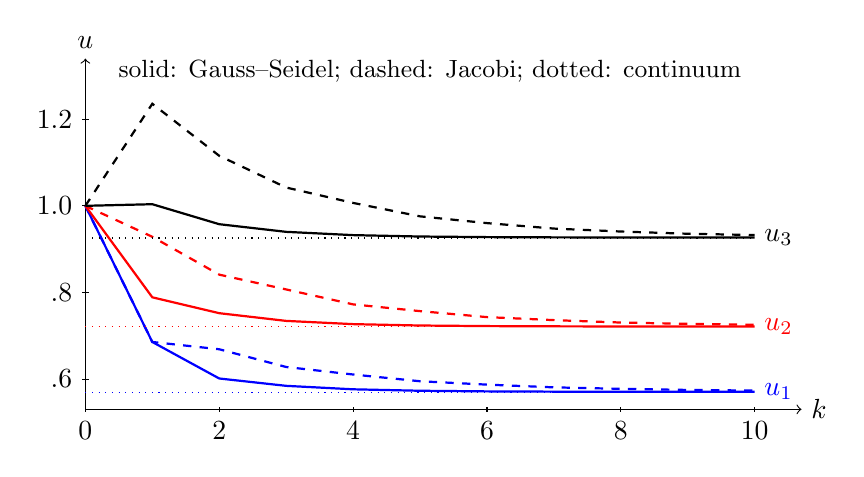
\begin{tikzpicture}[x=.85cm,y=5.5cm]
\draw[->] (0,.53)--(10.7,.53) node[right] {$k$};
\draw[->] (0,.53)--(0,1.34) node[above] {$u$};
\draw[blue,thick,dashed] plot coordinates {(0.000000,1.000000) (1.000000,0.685619) (2.000000,0.668787) (3.000000,0.627836) (4.000000,0.610505) (5.000000,0.594936) (6.000000,0.587145) (7.000000,0.580837) (8.000000,0.577435) (9.000000,0.574853) (10.000000,0.573385)};
\draw[blue,thick] plot coordinates {(0.000000,1.000000) (1.000000,0.685619) (2.000000,0.601303) (3.000000,0.584336) (4.000000,0.576334) (5.000000,0.572964) (6.000000,0.571530) (7.000000,0.570921) (8.000000,0.570662) (9.000000,0.570552) (10.000000,0.570505)};
\draw[blue,dotted] (0,0.5690826)--(10,0.5690826);
\node[blue,right] at (10,0.5704701) {$u_1$};
\draw[red,thick,dashed] plot coordinates {(0.000000,1.000000) (1.000000,0.928466) (2.000000,0.841101) (3.000000,0.806930) (4.000000,0.772450) (5.000000,0.756853) (6.000000,0.743033) (7.000000,0.736106) (8.000000,0.730499) (9.000000,0.727475) (10.000000,0.725180)};
\draw[red,thick] plot coordinates {(0.000000,1.000000) (1.000000,0.788741) (2.000000,0.752098) (3.000000,0.734295) (4.000000,0.726819) (5.000000,0.723637) (6.000000,0.722284) (7.000000,0.721709) (8.000000,0.721465) (9.000000,0.721361) (10.000000,0.721317)};
\draw[red,dotted] (0,0.7204917)--(10,0.7204917);
\node[red,right] at (10,0.7212840) {$u_2$};
\draw[black,thick,dashed] plot coordinates {(0.000000,1.000000) (1.000000,1.235619) (2.000000,1.115516) (3.000000,1.042258) (4.000000,1.006731) (5.000000,0.975681) (6.000000,0.960089) (7.000000,0.947475) (8.000000,0.940671) (9.000000,0.935506) (10.000000,0.932570)};
\draw[black,thick] plot coordinates {(0.000000,1.000000) (1.000000,1.003736) (2.000000,0.957558) (3.000000,0.939923) (4.000000,0.932342) (5.000000,0.929122) (6.000000,0.927753) (7.000000,0.927171) (8.000000,0.926924) (9.000000,0.926818) (10.000000,0.926774)};
\draw[black,dotted] (0,0.9257815)--(10,0.9257815);
\node[black,right] at (10,0.9267407) {$u_3$};
\foreach \k in {0,2,4,6,8,10} \draw (\k,.535)--(\k,.525) node[below] {$\k$};
\foreach \v in {.6,.8,1.0,1.2} \draw (.05,\v)--(-.05,\v) node[left] {$\v$};
\node[anchor=west,font=\small] at (.35,1.31) {solid: Gauss--Seidel; dashed: Jacobi; dotted: continuum};
\end{tikzpicture}

\end{center}
To quantify convergence, write $A=D+L+U$ for the coefficient matrix. Errors
propagate by $B_J=-D^{-1}(L+U)$ and $B_{GS}=-(D+L)^{-1}U$.
Their spectral radii are $0.648377$ and $0.425149$, respectively, explaining
the faster Gauss--Seidel convergence for this update order.
If one instead applies the unreduced nine-point averaging formula literally,
the second Jacobi update is
$b_{k+1}=(8a_k+2b_k+4c_k+s)/20$. That is another valid stationary iteration
with different transient values and the same fixed point; it should not be
mixed with the reduced-system iteration tabulated here.
\end{enumerate}

\clearpage
\section{Chapter 2. Boundary-Value Problems in Electrostatics: I}
% Problems, Chapter 2: Boundary-Value Problems in Electrostatics: I
% Jackson, Classical Electrodynamics, 3rd ed.
% Requires: amsmath, amssymb, tikz

\section*{Problems}

\Needspace{5\baselineskip}
\par\bigskip
\noindent\textbf{2.1}\quad A point charge $q$ is brought to a position a distance $d$ away from an infinite plane conductor held at zero potential. Using the method of images, find:
\begin{enumerate}
\item[(a)] the surface-charge density induced on the plane, and plot it;
\item[(b)] the force between the plane and the charge by using Coulomb's law for the force between the charge and its image;
\item[(c)] the total force acting on the plane by integrating $\sigma^{2}/2\epsilon_{0}$ over the whole plane;
\item[(d)] the work necessary to remove the charge $q$ from its position to infinity;
\item[(e)] the potential energy between the charge $q$ and its image [compare the answer to part d and discuss].
\item[(f)] Find the answer to part d in electron volts for an electron originally one angstrom from the surface.
\end{enumerate}
\solution
Put the plane at $z=0$ and the real charge at $d\widehat{\mathbf z}$.
All potentials below refer to the vacuum region $z>0$; the image is
$-q$ at $-d\widehat{\mathbf z}$. Thus
\[
\Phi(\rho,z)=\frac{q}{4\pi\epsilon _0}
 \left[\frac1{\sqrt{\rho^2+(z-d)^2}}
       -\frac1{\sqrt{\rho^2+(z+d)^2}}\right].
\]
\textbf{(a)} The normal from the metal into the vacuum is
$\widehat{\mathbf z}$, so $\sigma=-\epsilon _0\partial_z\Phi|_{0^+}$.
Differentiating the two terms gives respectively
$d/(\rho^2+d^2)^{3/2}$ and $d/(\rho^2+d^2)^{3/2}$, whence
\[
\boxed{\sigma(\rho)=-\frac{qd}{2\pi(\rho^2+d^2)^{3/2}}.}
\]
As a normalization check,
$2\pi\int_0^\infty\sigma\rho\,d\rho
=-qd[-(\rho^2+d^2)^{-1/2}]_0^\infty=-q$.
The following plot uses $u=\rho/d$ and
$-2\pi d^2\sigma/q=(1+u^2)^{-3/2}$ (the signed density is negative
for $q>0$).
\begin{center}
\begin{tikzpicture}[x=1.05cm,y=2cm]
\draw[->] (0,0)--(5.2,0) node[right] {$\rho/d$};
\draw[->] (0,0)--(0,1.2) node[above] {$-2\pi d^2\sigma/q$};
\draw[thick,blue,domain=0:5,samples=100] plot (\x,{1/(1+\x*\x)^1.5});
\foreach \x in {1,2,3,4,5} \draw (\x,.025)--(\x,-.025) node[below] {$\x$};
\node[left] at (0,1) {$1$};
\end{tikzpicture}
\end{center}
\textbf{(b)} The separation of the charge and image is $2d$, hence
\[
\boxed{\mathbf F_q=-\frac{q^2}{16\pi\epsilon _0d^2}\widehat{\mathbf z}.}
\]
\textbf{(c)} The electrostatic pressure on the metal is toward the
vacuum. Its integral is
\begin{align*}
\mathbf F_{\rm plane}
&=\widehat{\mathbf z}\int_0^\infty
 \frac{q^2d^2}{8\pi^2\epsilon _0(\rho^2+d^2)^3}\,2\pi\rho\,d\rho\\
&=\widehat{\mathbf z}\frac{q^2d^2}{4\pi\epsilon _0}
 \left[-\frac1{4(\rho^2+d^2)^2}\right]_0^\infty
=\frac{q^2}{16\pi\epsilon _0d^2}\widehat{\mathbf z}.
\end{align*}
This equals $-\mathbf F_q$.
\textbf{(d)} In quasistatic removal the applied force opposes the
attraction at every instantaneous height $s$, so
\[
\boxed{W=\int_d^\infty\frac{q^2}{16\pi\epsilon _0s^2}\,ds
       =\frac{q^2}{16\pi\epsilon _0d}.}
\]
\textbf{(e)} Two \emph{independent} charges $q,-q$ a distance $2d$
apart have mutual energy $U_{q,q'}=-q^2/(8\pi\epsilon _0d)=-2W$.
The physical charge--conductor energy relative to infinite separation
is instead
\[
U=\frac12q\Phi_{\rm induced}(d)
 =-\frac{q^2}{16\pi\epsilon _0d}=-W.
\]
The factor $1/2$ follows by charging the real source from $0$ to $q$:
the induced potential is proportional to the charge already supplied,
so $U=\int_0^q(q_1/q)\Phi_{\rm induced}(q)\,dq_1$.
An image is a representation of this induced charge, not an additional
independently assembled physical source.
\textbf{(f)} With $|q|=e$, $d=10^{-10}\,\mathrm m$, the conversion is
\[
W[\mathrm{eV}]=\frac{e}{16\pi\epsilon _0(10^{-10}\,\mathrm m)}
\simeq\boxed{3.60\ \mathrm{eV}}.
\]
The numerical check uses the SI constants in \texttt{scipy.constants}.

\Needspace{5\baselineskip}
\par\bigskip
\noindent\textbf{2.2}\quad Using the method of images, discuss the problem of a point charge $q$ \emph{inside} a hollow, grounded, conducting sphere of inner radius $a$. Find
\begin{enumerate}
\item[(a)] the potential inside the sphere;
\item[(b)] the induced surface-charge density;
\item[(c)] the magnitude and direction of the force acting on $q$.
\item[(d)] Is there any change in the solution if the sphere is kept at a fixed potential $V$? If the sphere has a total charge $Q$ on its inner and outer surfaces?
\end{enumerate}
\solution
Let the charge be at $b\widehat{\mathbf z}$, $0<b<a$. Inversion in the
sphere gives an image $q'=-qa/b$ at $b'=a^2/b>a$. On $r=a$,
$|\mathbf r-b'\widehat{\mathbf z}|=(a/b)
 |\mathbf r-b\widehat{\mathbf z}|$, so their potentials cancel.
\textbf{(a)} By uniqueness,
\[
\boxed{\Phi(r,\theta)=\frac{q}{4\pi\epsilon _0}
 \left[\frac1{\sqrt{r^2+b^2-2rb\cos\theta}}
 -\frac{a/b}{\sqrt{r^2+a^4/b^2-2ra^2\cos\theta/b}}\right],\quad r<a.}
\]
The image lies outside the solution domain and creates no extra
singularity in the cavity.
\textbf{(b)} The metal-to-cavity normal is $-\widehat{\mathbf r}$,
so $\sigma=\epsilon _0\partial_r\Phi|_{a^-}$. To simplify the derivative,
write $D=\sqrt{a^2+b^2-2ab\cos\theta}$ and use the distance relation:
\[
\partial_r\Phi|_a=\frac{q}{4\pi\epsilon _0D^3}
 \left[-(a-b\cos\theta)+\frac{b^2}{a^2}
              \left(a-\frac{a^2}{b}\cos\theta\right)\right].
\]
Thus
\[
\boxed{\sigma(\theta)=-\frac{q(a^2-b^2)}
 {4\pi a(a^2+b^2-2ab\cos\theta)^{3/2}}.}
\]
Indeed, setting $u=\cos\theta$ gives
\[
2\pi a^2\int_{-1}^1\sigma(u)\,du
=-\frac{qa(a^2-b^2)}2\frac1{ab}
 \left(\frac1{a-b}-\frac1{a+b}\right)=-q.
\]
\textbf{(c)} Only the image field acts on $q$ after its own singular
field is excluded. The distance is $b'-b=(a^2-b^2)/b$, giving
\[
\boxed{\mathbf F=\frac{q^2ab}{4\pi\epsilon _0(a^2-b^2)^2}
                    \widehat{\mathbf z}.}
\]
It is toward the nearer wall for either sign of $q$.
For a centered charge the limits are
$\Phi=q(1/r-1/a)/(4\pi\epsilon _0)$,
$\sigma=-q/(4\pi a^2)$, and $\mathbf F=0$.
\textbf{(d)} Holding the metal at $V$ adds the constant $V$ to the
cavity potential; it leaves the cavity field, inner surface charge,
and force unchanged. For an isolated metal with total charge $Q$,
Gauss's law in the metal requires inner charge $-q$ and outer charge
$Q+q$. The same cavity solution therefore holds up to a constant.
That constant depends on the exterior geometry. For a concentric
spherical outer surface of radius $A$, with no other external sources
and zero potential at infinity, it is $(Q+q)/(4\pi\epsilon _0A)$.
For an ideal thin shell one sets $A=a$. Specifying only the inner
radius does not specify this exterior capacitance.

\Needspace{5\baselineskip}
\par\bigskip
\noindent\textbf{2.3}\quad A straight-line charge with constant linear charge density $\lambda$ is located perpendicular to the $x$-$y$ plane in the first quadrant at $(x_{0},y_{0})$. The intersecting planes $x=0$, $y\geq0$ and $y=0$, $x\geq0$ are conducting boundary surfaces held at zero potential. Consider the potential, fields, and surface charges in the first quadrant.
\begin{enumerate}
\item[(a)] The well-known potential for an isolated line charge at $(x_{0},y_{0})$ is $\Phi(x,y)=(\lambda/4\pi\epsilon_{0})\ln(R^{2}/r^{2})$, where $r^{2}=(x-x_{0})^{2}+(y-y_{0})^{2}$ and $R$ is a constant. Determine the expression for the potential of the line charge in the presence of the intersecting planes. Verify explicitly that the potential and the tangential electric field vanish on the boundary surfaces.
\item[(b)] Determine the surface charge density $\sigma$ on the plane $y=0$, $x\geq0$. Plot $\sigma/\lambda$ versus $x$ for $(x_{0}=2,y_{0}=1)$, $(x_{0}=1,y_{0}=1)$, and $(x_{0}=1,y_{0}=2)$.
\item[(c)] Show that the total charge (per unit length in $z$) on the plane $y=0$, $x\geq0$ is
\[
Q_{x} = -\frac{2}{\pi}\lambda\tan^{-1}\!\left(\frac{x_{0}}{y_{0}}\right)
\]
What is the total charge on the plane $x=0$?
\item[(d)] Show that far from the origin [$\rho\gg\rho_{0}$, where $\rho=\sqrt{x^{2}+y^{2}}$ and $\rho_{0}=\sqrt{x_{0}^{2}+y_{0}^{2}}$] the leading term in the potential is
\[
\Phi\rightarrow\Phi_{\mathrm{asym}}=\frac{4\lambda}{\pi\epsilon_{0}}\frac{(x_{0}y_{0})(xy)}{\rho^{4}}
\]
Interpret.
\end{enumerate}
\solution
Define $D_{st}=(x-sx_0)^2+(y-ty_0)^2$, with $s,t=\pm1$.
\textbf{(a)} Place line charges $st\lambda$ at $(sx_0,ty_0)$.
The arbitrary logarithmic reference lengths cancel because the
four charges sum to zero, leaving
\[
\boxed{\Phi=\frac{\lambda}{4\pi\epsilon _0}
 \ln\frac{D_{+-}D_{-+}}{D_{++}D_{--}}.}
\]
At $y=0$, $D_{++}=D_{+-}$ and $D_{-+}=D_{--}$, so $\Phi=0$;
at $x=0$ the other two equalities give the same result. Differentiating
these identities along either boundary gives $E_x(x,0)=0$ and
$E_y(0,y)=0$. All terms are independent of $z$, so $E_z=0$ as well.
\textbf{(b)} On $y=0$ the outward metal normal is $+\widehat{\mathbf y}$.
Differentiating the logarithms before putting $y=0$ gives
\[
\boxed{\frac{\sigma(x)}\lambda=-\frac{y_0}{\pi}
 \left[\frac1{(x-x_0)^2+y_0^2}-\frac1{(x+x_0)^2+y_0^2}\right].}
\]
It vanishes at the corner, is negative for $x>0$ when $\lambda>0$,
and decays as $-4x_0y_0/(\pi x^3)$.
\begin{center}
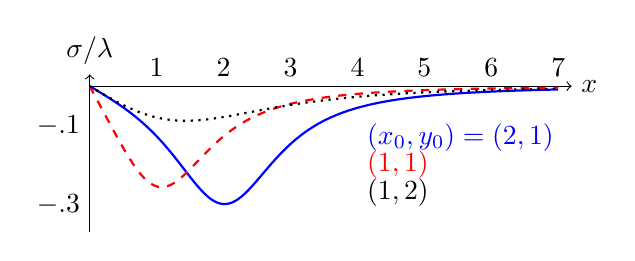
\begin{tikzpicture}[x=.85cm,y=5cm]
\draw[->] (0,0)--(7.2,0) node[right] {$x$};
\draw[->] (0,-.37)--(0,.03) node[above] {$\sigma/\lambda$};
\draw[blue,thick,domain=0:7,samples=140]
 plot (\x,{-1/pi*(1/((\x-2)^2+1)-1/((\x+2)^2+1))});
\draw[red,dashed,thick,domain=0:7,samples=140]
 plot (\x,{-1/pi*(1/((\x-1)^2+1)-1/((\x+1)^2+1))});
\draw[black,dotted,thick,domain=0:7,samples=140]
 plot (\x,{-2/pi*(1/((\x-1)^2+4)-1/((\x+1)^2+4))});
\foreach \x in {1,2,3,4,5,6,7} \node[above] at (\x,0) {$\x$};
\node[left] at (0,-.1) {$-.1$}; \node[left] at (0,-.3) {$-.3$};
\node[blue,right] at (4,-.13) {$(x_0,y_0)=(2,1)$};
\node[red,right] at (4,-.20) {$(1,1)$};
\node[right] at (4,-.27) {$(1,2)$};
\end{tikzpicture}
\end{center}
\textbf{(c)} Integrating each Lorentzian explicitly,
\begin{align*}
Q_x&=-\frac\lambda\pi
 \left[\tan^{-1}\frac{x-x_0}{y_0}
       -\tan^{-1}\frac{x+x_0}{y_0}\right]_{x=0}^{\infty}\\
&=\boxed{-\frac{2\lambda}{\pi}\tan^{-1}\frac{x_0}{y_0}}.
\end{align*}
Interchange $x_0,y_0$ for the other plane:
$Q_y=-2\lambda\tan^{-1}(y_0/x_0)/\pi$.
Since both coordinates are positive, their inverse tangents add to
$\pi/2$ and $Q_x+Q_y=-\lambda$.
\textbf{(d)} Write $D_{st}=\rho^2+B_{st}$, with
$B_{st}=\rho_0^2-2sxx_0-2tyy_0$. In
$\Phi=-\lambda\sum st\ln D_{st}/(4\pi\epsilon _0)$,
the constant and first-order terms cancel. The needed quadratic sum is
\[
\sum_{s,t}st B_{st}^2=32xx_0yy_0,
\quad
\sum_{s,t}st\ln D_{st}=-\frac{16xx_0yy_0}{\rho^4}
 +O(\rho_0^4/\rho^4).
\]
Consequently
\[
\boxed{\Phi\sim\frac{4\lambda x_0y_0xy}{\pi\epsilon _0\rho^4}.}
\]
The images cancel both the net line charge and the dipole moment.
This is the leading two-dimensional quadrupole, proportional to
$\sin2\phi/\rho^2$, with nodes on the grounded planes.

\Needspace{5\baselineskip}
\par\bigskip
\noindent\textbf{2.4}\quad A point charge is placed a distance $d>R$ from the center of an equally charged, isolated, conducting sphere of radius $R$.
\begin{enumerate}
\item[(a)] Inside of what distance from the surface of the sphere is the point charge attracted rather than repelled by the charged sphere?
\item[(b)] What is the limiting value of the force of attraction when the point charge is located a distance $a$ ($=d-R$) from the surface of the sphere, if $a\ll R$?
\item[(c)] What are the results for parts a and b if the charge on the sphere is twice (half) as large as the point charge, but still the same sign?
\end{enumerate}
[Answers: (a) $d/R-1=\erratum{0.6180}$, (b) $F=-q^{2}/(16\pi\epsilon_{0}a^{2})$, i.e., image force, (c) for $Q=2q$, $d/R-1=0.4276$; for $Q=q/2$, $d/R-1=0.8823$. The answer for part b is the same.]
\solution
Let $k=(4\pi\epsilon _0)^{-1}$ and write $Q=\alpha q$ for the sphere's
charge. The image pair inside the sphere is
\[
q'=-\frac{qR}{d},\quad r'=\frac{R^2}{d},\qquad
q_0=Q+\frac{qR}{d}\quad\hbox{at the center}.
\]
The image $q'$ cancels the angular variation on the surface and the
central charge makes the total image charge $Q$. Taking positive force
away from the center,
\[
F=kq\left[\frac{Q+qR/d}{d^2}
       -\frac{qR/d}{(d-R^2/d)^2}\right]
=\frac{kq^2}{R^2}\left[\frac{\alpha+1/x}{x^2}
                  -\frac{x}{(x^2-1)^2}\right],\quad x=\frac dR.
\]
\textbf{(a)} Setting $F=0$ is equivalent to
\[
\alpha=H(x):=\frac{2x^2-1}{x(x^2-1)^2}.
\]
For $x>1$,
$H'(x)=(-6x^4+3x^2-1)/[x^2(x^2-1)^3]<0$;
also $H(1^+)=\infty$ and $H(\infty)=0$. There is exactly one root,
with attraction below it. For $\alpha=1$ the root is
$x=(1+\sqrt5)/2$: using $x^2=x+1$ makes both sides of
$x(x^2-1)^2=2x^2-1$ equal $2x+1$. Thus
\[
\boxed{0<d-R<\frac{\sqrt5-1}{2}R=0.6180339887\ldots R.}
\]
This exact root, rounded to four figures, is the corrected answer
marked in the statement.
\textbf{(b)} Set $d=R+a$. Then
$d-R^2/d=2a+O(a^2/R)$ and $q'=-q+O(qa/R)$,
whereas the central-charge force remains finite. Therefore
\[
\boxed{F\sim-\frac{kq^2}{4a^2}
            =-\frac{q^2}{16\pi\epsilon _0a^2}\quad(a/R\to0).}
\]
\textbf{(c)} Solving the same monotone equation $H(x)=\alpha$ gives
\[
\begin{array}{c|c|c}
Q/q&x\text{ at zero force}&(d-R)/R\text{ at zero force}\\\hline
2&1.427563934\ldots&0.427563934\ldots\\
1/2&1.882269146\ldots&0.882269146\ldots
\end{array}
\]
Attraction holds below these respective distances. The leading
near-surface force in part (b) is independent of the finite value of
$Q/q$ because it comes from the nearby image.

\Needspace{5\baselineskip}
\par\bigskip
\noindent\textbf{2.5}\quad\begin{enumerate}
\item[(a)] Show that the work done to remove the charge $q$ from a distance $r>a$ to infinity against the force, Eq.~(2.6), of a grounded conducting sphere is
\[
W=\frac{q^{2}a}{8\pi\epsilon_{0}(r^{2}-a^{2})}
\]
Relate this result to the electrostatic potential, Eq.~(2.3), and the energy discussion of Section 1.11.
\item[(b)] Repeat the calculation of the work done to remove the charge $q$ against the force, Eq.~(2.9), of an isolated charged conducting sphere. Show that the work done is
\[
W=\frac{1}{4\pi\epsilon_{0}}\left[\frac{q^{2}a}{2(r^{2}-a^{2})}-\frac{q^{2}a}{2r^{2}}-\frac{qQ}{r}\right]
\]
Relate the work to the electrostatic potential, Eq.~(2.8), and the energy discussion of Section 1.11.
\end{enumerate}
\solution
Use $k=(4\pi\epsilon _0)^{-1}$ and take outward force as positive.
\textbf{(a)} The grounded-sphere image at a source position $s>a$ is
$-qa/s$ at $a^2/s$. Hence the force appearing in (2.6) is
\[
F_g(s)=-k\frac{q^2a/s}{(s-a^2/s)^2}
       =-k\frac{q^2as}{(s^2-a^2)^2}.
\]
The quasistatic work is
\[
W_g=-\int_r^\infty F_g(s)\,ds
=kq^2a\left[-\frac1{2(s^2-a^2)}\right]_r^\infty
=\boxed{\frac{q^2a}{8\pi\epsilon _0(r^2-a^2)}}.
\]
At the source the induced potential from the image construction
of (2.3) is $\Phi_{\rm ind}=-kqa/(r^2-a^2)$.
Therefore $U_g=\tfrac12q\Phi_{\rm ind}=-W_g$.
The half factor is the work of building up the induced charge
linearly with the real source, as in Section 1.11, with the divergent
self-energy of the point charge omitted.
\textbf{(b)} For an isolated sphere, add a central charge
$Q+qa/s$ to the grounded image. Thus the force (2.9) is
\[
F_Q(s)=-k\frac{q^2as}{(s^2-a^2)^2}
        +k\frac{qQ}{s^2}+k\frac{q^2a}{s^3}.
\]
Termwise integration gives
\begin{align*}
W_Q&=-\int_r^\infty F_Q(s)\,ds\\
&=\boxed{k\left[\frac{q^2a}{2(r^2-a^2)}
              -\frac{q^2a}{2r^2}-\frac{qQ}{r}\right]}.
\end{align*}
This work can be negative when repulsion supplies energy during
removal. To see the energy content of (2.8), separate the potential at
$q$ into the pre-existing charge and the polarization:
\[
\Phi_Q(r)=\frac{kQ}{r},\qquad
\Phi_{\rm pol}(r)=kq\left[\frac{a}{r^2}-\frac{a}{r^2-a^2}\right].
\]
Relative to the infinitely separated system, the energy is
\[
U_Q=q\Phi_Q+\frac12q\Phi_{\rm pol}=-W_Q.
\]
The pre-existing sphere charge $Q$ has its full interaction factor;
only the source-induced redistribution has the half factor.
The constant self-energy $kQ^2/(2a)$ of the isolated charged sphere
cancels between the initial and final configurations.

\Needspace{5\baselineskip}
\par\bigskip
\noindent\textbf{2.6}\quad The electrostatic problem of a point charge $q$ outside an isolated, charged conducting sphere is equivalent to that of three charges, the original and two others, one located at the center of the sphere and another (``the image charge'') inside the now imaginary sphere, on the line joining the center and the original charge.

If the point charge and sphere are replaced by two conducting spheres of radii $r_{a}$ and $r_{b}$, carrying total charges $Q_{a}$ and $Q_{b}$, respectively, with centers separated by a distance $d>r_{a}+r_{b}$, there is an equivalence with an infinite set of charges within each sphere, one at the center and a set of images along the line joining the centers. The charges and their locations can be determined iteratively, starting with a charge $q_{a}(1)$ at the center of the first sphere and $q_{b}(1)$ correspondingly for the second sphere. The charge $q_{b}(1)$ has its image $q_{a}(2)$ within the first sphere and vice versa. Then the image charge within the first sphere induces another image within the second sphere, and so on. The sum of all the charges within each sphere must be scaled to be equal to $Q_{a}$ or $Q_{b}$.

The electrostatic potential outside the spheres, the force between the spheres, etc. can be found by summing the contributions from all the charges.
\begin{enumerate}
\item[(a)] Show that the charges and their positions are determined iteratively by the relations,
\begin{align*}
q_{a}(j)&=-r_{a}q_{b}(j-1)/d_{b}(j-1), & x_{a}(j)&=r_{a}^{2}/d_{b}(j-1), & d_{a}(j)&=d-x_{a}(j)\\
q_{b}(j)&=-r_{b}q_{a}(j-1)/d_{a}(j-1), & x_{b}(j)&=r_{b}^{2}/d_{a}(j-1), & d_{b}(j)&=d-x_{b}(j)
\end{align*}
for $j=2,3,4,\ldots$, with $d_{a}(1)=d_{b}(1)=d$, and $x_{a}(1)=x_{b}(1)=0$.
\item[(b)] Find the image charges and their locations as well as the potentials on the spheres and force between them by means of a suitable computer program. [In computing the potential on each sphere, evaluate it in different places: e.g., in the equatorial plane and at the pole opposite the other sphere. This permits a check on the equipotential of the conductor and on the accuracy of computation.]
\item[(c)] As an example, show that for two equally charged spheres of the same radius $R$, the force between them when almost in contact is \erratum{0.6149} times the value that would be obtained if all the charge on each sphere were concentrated at its center. Show numerically and by explicit summation of the series that the capacitance of two identical conducting spheres in contact is $C/4\pi\epsilon_{0}R=1.3863\cdots$ [$=\ln4$].
\end{enumerate}
Reference: J. A. Soules, \emph{Am. J. Phys.} \textbf{58}, 1195 (1990).
\solution
Use an axial coordinate $X$ with centers at $0,d$. Distances $x_a$
and $x_b$ are measured from each center \emph{toward} the other, so
charges in sphere $b$ have global coordinates $d-x_b$.
\textbf{(a)} A charge $q_b(j-1)$ is a distance
$d_b(j-1)=d-x_b(j-1)>r_a$ from center $a$. Sphere inversion therefore
requires an image
\[
q_a(j)=-\frac{r_a}{d_b(j-1)}q_b(j-1),\qquad
x_a(j)=\frac{r_a^2}{d_b(j-1)}.
\]
Interchanging $a,b$ gives the other two recurrences in the question.
Every external image is paired with its cancelling image in the
other sphere. On sphere $a$ these pairs have zero potential, leaving
only the central charge's constant $kq_a(1)/r_a$; similarly on $b$.
The two initial charges cannot in general be scaled independently
after the iteration, because each subsequent chain crosses between
the spheres.

\textbf{(b)} A reproducible implementation is the function
\texttt{two\_spheres} in the supplementary script
\texttt{check\_ch02.py}.
It first constructs two unit-seed solutions, with initial central
charges $(1,0)$ and $(0,1)$. If $M_{ij}$ is the sum of the images
in sphere $i$ produced by seed $j$, solve
\[
\begin{pmatrix}M_{aa}&M_{ab}\\M_{ba}&M_{bb}\end{pmatrix}
\begin{pmatrix}q_a(1)\\q_b(1)\end{pmatrix}
=\begin{pmatrix}Q_a\\Q_b\end{pmatrix}.
\]
In particular, writing $\Delta=M_{aa}M_{bb}-M_{ab}M_{ba}$,
\[
q_a(1)=\frac{Q_aM_{bb}-Q_bM_{ab}}\Delta,\qquad
q_b(1)=\frac{Q_bM_{aa}-Q_aM_{ba}}\Delta.
\]
If the two stored unit-seed charges at a given image position are
$c_{i,a}(j),c_{i,b}(j)$, its final charge is
$q_i(j)=c_{i,a}(j)q_a(1)+c_{i,b}(j)q_b(1)$.
Linearity then gives every image charge at the already computed
positions. For a finite truncation the exterior potential and the
outward force on sphere $b$ are evaluated as
\begin{align*}
\Phi(X,\rho)&=k\sum_j\left[
 \frac{q_a(j)}{\sqrt{(X-x_a(j))^2+\rho^2}}
+\frac{q_b(j)}{\sqrt{(X-d+x_b(j))^2+\rho^2}}\right],\\
F_b&=k\sum_{i,j}\frac{q_a(i)q_b(j)}{[d-x_a(i)-x_b(j)]^2}.
\end{align*}
The latter follows by enclosing one sphere in a Maxwell-stress
surface: its self-field gives zero net force, and the interaction
with the other sphere can be replaced by the two sets of images.
For a strictly positive gap, every successive image magnitude is
bounded by the previous magnitude times
\[
\eta=\max\left(\frac{r_a}{d-r_b},\frac{r_b}{d-r_a}\right)<1,
\]
because each image remains inside its sphere. If $c_N$ bounds the
last retained charge in either unit-seed chain, each remaining tail
is at most $c_N\eta/(1-\eta)$. After combining the seeds this is
multiplied by $|q_a(1)|+|q_b(1)|$. The code increases the image count
until the unit-seed bound meets the requested tolerance and reports
the resulting physical bound. Its checks repeat the calculation at a tighter tolerance,
compare the resulting force and potentials, and compare each surface
potential at the facing pole, rear pole, and equator with
$V_i=kq_i(1)/r_i$. It exposes all charges
and positions in the returned arrays and can write them to a CSV
file using \texttt{--images PATH}.
For example, $r_a=r_b=R$, $d=3R$, $Q_a=Q_b=Q$ gives
\[
\frac{4\pi\epsilon _0RV}{Q}=1.320647\ldots,\qquad
\frac{F}{Q^2/(4\pi\epsilon _0d^2)}=0.849932\ldots.
\]
The script prints higher-precision values and includes an unequal
radius, unequal charge example to check the two-seed construction.

\textbf{(c)} For equal radii and equal charges put
$d=2R\cosh\alpha$, $\alpha>0$. The recurrences are solved by
\[
x_j=R\frac{\sinh[(j-1)\alpha]}{\sinh(j\alpha)},\qquad
q_j=(-1)^{j-1}q_1\frac{\sinh\alpha}{\sinh(j\alpha)}.
\]
For example,
$d-x_{j-1}=R\sinh(j\alpha)/\sinh[(j-1)\alpha]$
by $2\cosh\alpha\sinh[(j-1)\alpha]-\sinh[(j-2)\alpha]
=\sinh(j\alpha)$, which verifies both recurrences. Define
\[
S(\alpha)=\frac Q{q_1}
=\sinh\alpha\sum_{j=1}^{\infty}\frac{(-1)^{j-1}}{\sinh(j\alpha)}.
\]
Then $V=kQ/(RS)$ and the capacitance of the pair at a common
potential is
\[
\frac{C}{4\pi\epsilon _0R}=2S(\alpha).
\]
At contact the images become
$x_j=R(j-1)/j$, $q_j=(-1)^{j-1}q_1/j$, and therefore
\[
Q=q_1\left(1-\frac12+\frac13-\cdots\right)=q_1\ln2,
\qquad \boxed{\frac{C}{4\pi\epsilon _0R}=2\ln2=\ln4}.
\]
To differentiate near contact without differentiating a divergent
termwise power expansion, first sum a geometric series:
\[
S=2\sinh\alpha\sum_{m=0}^{\infty}\frac1{e^{(2m+1)\alpha}+1}.
\]
For $f(t)=(e^t+1)^{-1}$, midpoint summation gives
$h\sum_{m\geq0}f((m+\tfrac12)h)
=\int_0^\infty f(t)\,dt+h^2f'(0)/24+O(h^4)$.
This follows by integrating the Taylor expansion on each interval:
its midpoint error is $h^3f''/24$, whose sum is
$h^2\int_0^\infty f''/24=-h^2f'(0)/24$.
With $h=2\alpha$, $\int_0^\infty f=\ln2$ and $f'(0)=-1/4$, we find
\[
S=\ln2+\alpha^2\left(\frac{\ln2}{6}-\frac1{24}\right)+O(\alpha^4).
\]
At fixed charge on each sphere the total energy is
$U=\tfrac12(QV+QV)=kQ^2/(RS)$. Hence
\[
F=-\frac{dU}{dd}=\frac{kQ^2}{RS^2}\frac{dS}{dd},\qquad
 d=2R+R\alpha^2+O(\alpha^4).
\]
Dividing by the center-charge force $kQ^2/d^2$ gives the limit
\[
\boxed{\lim_{d\downarrow2R}\frac{F}{kQ^2/d^2}
=\frac{4\ln2-1}{6(\ln2)^2}=0.6149018638\ldots.}
\]
The printed value $0.6189$ is inconsistent with this exact limit; the
corrected value is $0.6149$. For example, at $(d-2R)/R=10^{-4}$ the
image-force ratio is $0.6149340086$, while the capacitance ratio is
$1.3863091325$, approaching $\ln4=1.3862943611$.
The supplementary code checks the image-force sum against both a
Maxwell-stress integral and the energy derivative, and approaches
both contact limits from positive gaps;
it does not rely on a finite alternating sum at exact contact.

\Needspace{5\baselineskip}
\par\bigskip
\noindent\textbf{2.7}\quad Consider a potential problem in the half-space defined by $z\geq0$, with Dirichlet boundary conditions on the plane $z=0$ (and at infinity).
\begin{enumerate}
\item[(a)] Write down the appropriate Green function $G(\mathbf{x},\mathbf{x}')$.
\item[(b)] If the potential on the plane $z=0$ is specified to be $\Phi=V$ \emph{inside} a circle of radius $a$ centered at the origin, and $\Phi=0$ outside that circle, find an integral expression for the potential at the point $P$ specified in terms of cylindrical coordinates $(\rho,\phi,z)$.
\item[(c)] Show that, along the axis of the circle ($\rho=0$), the potential is given by
\[
\Phi = V\!\left(1-\frac{z}{\sqrt{a^{2}+z^{2}}}\right)
\]
\item[(d)] Show that at large distances ($\rho^{2}+z^{2}\gg a^{2}$) the potential can be expanded in a power series in $(\rho^{2}+z^{2})^{-1}$, and that the leading terms are
\[
\Phi = \frac{Va^{2}}{2}\frac{z}{(\rho^{2}+z^{2})^{3/2}}\left[1-\frac{3a^{2}}{4(\rho^{2}+z^{2})}+\frac{5(3\rho^{2}a^{2}+a^{4})}{8(\rho^{2}+z^{2})^{2}}+\cdots\right]
\]
Verify that the results of parts c and d are consistent with each other in their common range of validity.
\end{enumerate}
\solution
Use the convention $\nabla'^2G=-4\pi\delta^3(\mathbf x-\mathbf x')$.
\textbf{(a)} Reflect the source in $z'=0$:
\[
\boxed{G(\mathbf x,\mathbf x')=
 \frac1{\sqrt{|\boldsymbol\rho-\boldsymbol\rho'|^2+(z-z')^2}}
-\frac1{\sqrt{|\boldsymbol\rho-\boldsymbol\rho'|^2+(z+z')^2}}.}
\]
It vanishes on the plane and at infinity. The outward normal of
the upper half-space is $-\widehat{\mathbf z}'$, giving
$\partial_{n'}G|_0=-2z/(|\boldsymbol\rho-\boldsymbol\rho'|^2+z^2)^{3/2}$.
\textbf{(b)} The Dirichlet representation
$\Phi=-(4\pi)^{-1}\int\Phi\partial_{n'}G\,dS'$ therefore yields
\[
\boxed{\Phi(\rho,z)=\frac{Vz}{2\pi}
 \int_0^a s\,ds\int_0^{2\pi}
 \frac{d\varphi}{(\rho^2+s^2-2\rho s\cos\varphi+z^2)^{3/2}}.}
\]
The result is independent of the observation azimuth.
\textbf{(c)} At $\rho=0$ the angular integral is $2\pi$, so
\[
\Phi(0,z)=Vz\left[-\frac1{\sqrt{s^2+z^2}}\right]_0^a
=\boxed{V\left(1-\frac z{\sqrt{a^2+z^2}}\right)},\qquad z>0.
\]
\textbf{(d)} Put $L^2=\rho^2+z^2$ and
$u=(s^2-2\rho s\cos\varphi)/L^2$. The binomial expansion is
$(1+u)^{-3/2}=1-3u/2+15u^2/8-35u^3/16+\cdots$.
A disk average, $\langle f\rangle=(\pi a^2)^{-1}\int s\,ds\,d\varphi f$,
gives
\[
\langle u\rangle=\frac{a^2}{2L^2},\qquad
\langle u^2\rangle=\frac{a^4/3+\rho^2a^2}{L^4}.
\]
Here $\langle s^2\rangle=a^2/2$,
$\langle s^4\rangle=a^4/3$, and
$\langle s^2\cos^2\varphi\rangle=a^2/4$.
Substitution produces the displayed denominator expansion:
\[
\Phi=\frac{Va^2z}{2L^3}
 \left[1-\frac{3a^2}{4L^2}
       +\frac{5(3\rho^2a^2+a^4)}{8L^4}+\cdots\right].
\]
For clarity, terms grouped by \emph{uniform far-distance order}
require some further terms from the binomial series, since
$\rho$ can be comparable to $L$. With $s_\theta=\rho/L$, that ordering is
\[
\Phi=\frac{Va^2z}{2L^3}\left\{
1+\frac{a^2}{L^2}\left(-\frac34+\frac{15}{8}s_\theta^2\right)
+\frac{a^4}{L^4}\left(\frac58-\frac{35}{8}s_\theta^2
                         +\frac{315}{64}s_\theta^4\right)
+O(a^6/L^6)\right\}.
\]
For example, the additional contributions at this order follow from
$\langle u^3\rangle=(a^6/4+2\rho^2a^4)/L^6$ and the
$2\rho^4a^4/L^8$ part of $\langle u^4\rangle$.
On the axis the original bracket becomes
$1-3a^2/(4z^2)+5a^4/(8z^4)+\cdots$, which agrees term by term with
$V[1-(1+a^2/z^2)^{-1/2}]$ from part (c).

\Needspace{5\baselineskip}
\par\bigskip
\noindent\textbf{2.8}\quad A two-dimensional potential problem is defined by two straight parallel line charges separated by a distance $R$ with equal and opposite linear charge densities $\lambda$ and $-\lambda$.
\begin{enumerate}
\item[(a)] Show by direct construction that the surface of constant potential $V$ is a circular cylinder (circle in the transverse dimensions) and find the coordinates of the axis of the cylinder and its radius in terms of $R$, $\lambda$, and $V$.
\item[(b)] Use the results of part a to show that the capacitance per unit length $C$ of two right-circular cylindrical conductors, with radii $a$ and $b$, separated by a distance $d>a+b$, is
\[
C=\frac{2\pi\epsilon_{0}}{\cosh^{-1}\!\left(\dfrac{d^{2}-a^{2}-b^{2}}{2ab}\right)}
\]
\item[(c)] Verify that the result for $C$ agrees with the answer in Problem 1.7 in the appropriate limit and determine the next nonvanishing order correction in powers of $a/d$ and $b/d$.
\item[(d)] Repeat the calculation of the capacitance per unit length for two cylinders inside each other ($d<|b-a|$). Check the result for concentric cylinders ($d=0$).
\end{enumerate}
\solution
\textbf{(a)} Put $+\lambda$ at $(c,0)$ and $-\lambda$ at $(-c,0)$,
where $c=R/2$, and choose zero potential at infinity. Then
\[
\Phi=\frac{\lambda}{4\pi\epsilon _0}
 \ln\frac{(x+c)^2+y^2}{(x-c)^2+y^2}.
\]
Set $t=2\pi\epsilon _0V/\lambda$. The equipotential equation is
$(x+c)^2+y^2=e^{2t}[(x-c)^2+y^2]$.
Dividing by $1-e^{2t}$ and completing the square yields
\[
\boxed{(x-c\coth t)^2+y^2=\frac{c^2}{\sinh^2t}.}
\]
Thus the cylinder axis passes through $(c\coth t,0)$ and its radius
is $c/|\sinh t|$. The exceptional level $V=0$ is the plane $x=0$
(the infinite-radius limit of the circles).
\textbf{(b)} For two disjoint cylinders choose their surfaces to be
$t=t_a>0$ and $t=-t_b<0$. Then
\[
a=c\,\mathrm{csch}\,t_a,\quad b=c\,\mathrm{csch}\,t_b,
\quad d=c(\coth t_a+\coth t_b).
\]
Squaring the last relation and using $\coth^2t-\mathrm{csch}^2t=1$
gives
\[
\frac{d^2-a^2-b^2}{2ab}
=\sinh t_a\sinh t_b+\cosh t_a\cosh t_b
=\cosh(t_a+t_b).
\]
Each cylinder encloses one of the two line charges, so Gauss's law
gives charges per unit length $\pm\lambda$. Their voltage difference
is $\Delta V=\lambda(t_a+t_b)/(2\pi\epsilon _0)$; therefore
\[
\boxed{C=\frac{\lambda}{\Delta V}
 =\frac{2\pi\epsilon _0}
 {\cosh^{-1}[(d^2-a^2-b^2)/(2ab)]}.}
\]
\textbf{(c)} Write $L=\ln[d^2/(ab)]$ and $S=a^2+b^2$.
For large $X$, $\cosh^{-1}X=\ln(2X)-1/(4X^2)+O(X^{-4})$;
substitution of $X=(d^2-S)/(2ab)$ gives
\[
\cosh^{-1}X=L-\frac{S}{d^2}
 -\frac{S^2/2+a^2b^2}{d^4}+O(d^{-6}).
\]
Thus the leading result is
$C=\pi\epsilon _0/\ln[d/\sqrt{ab}]$, as in Problem 1.7, and the first
nonzero relative correction is
\[
\boxed{C=\frac{2\pi\epsilon _0}{L}
 \left[1+\frac{a^2+b^2}{d^2L}+O(d^{-4})\right].}
\]
The length scales $a,b$ are held fixed in this asymptotic notation.
\textbf{(d)} For nested cylinders take two circles on the same
branch, with $b>a$ and $t_a>t_b>0$; then
$d=c(\coth t_b-\coth t_a)$. In this case
\[
a^2+b^2-d^2
=c^2[\mathrm{csch}^2t_a+\mathrm{csch}^2t_b
-(\coth t_b-\coth t_a)^2]
=2c^2(\coth t_a\coth t_b-1).
\]
Dividing by $2ab=2c^2/(\sinh t_a\sinh t_b)$ gives
$\cosh t_a\cosh t_b-\sinh t_a\sinh t_b$.
The voltage difference is now
$\Delta V=\lambda(t_a-t_b)/(2\pi\epsilon_0)$, and hence
\[
\cosh(t_a-t_b)=\frac{a^2+b^2-d^2}{2ab},\qquad
\boxed{C=\frac{2\pi\epsilon _0}
 {\cosh^{-1}[(a^2+b^2-d^2)/(2ab)]}}.
\]
The formula is symmetric if $a,b$ are interchanged. At $d=0$,
$(a^2+b^2)/(2ab)=\cosh\ln(b/a)$, giving the usual
$C=2\pi\epsilon _0/\ln(b/a)$ for concentric cylinders.

\Needspace{5\baselineskip}
\par\bigskip
\noindent\textbf{2.9}\quad An insulated, spherical, conducting shell of radius $a$ is in a uniform electric field $E_{0}$. If the sphere is cut into two hemispheres by a plane perpendicular to the field, find the force required to prevent the hemispheres from separating
\begin{enumerate}
\item[(a)] if the shell is uncharged;
\item[(b)] if the total charge on the shell is $Q$.
\end{enumerate}
\solution
Take the imposed field to be $E_0\widehat{\mathbf z}$. With the
hemispheres initially forming a sphere (the cut width tending to zero),
the exterior and interior potentials are
\[
\Phi_{\rm out}=\frac{Q}{4\pi\epsilon _0r}
 -E_0\left(r-\frac{a^3}{r^2}\right)\cos\theta,
\qquad \Phi_{\rm in}=\frac{Q}{4\pi\epsilon _0a}.
\]
The boundary is equipotential, the cavity field is zero, and
\[
\sigma(\theta)=\frac{Q}{4\pi a^2}+3\epsilon _0E_0\cos\theta
=:s+3\epsilon _0E_0\cos\theta.
\]
The outward electrical pressure is $\sigma^2/(2\epsilon _0)$.
For the northern hemisphere its $z$ component integrates to
\begin{align*}
F_{N,z}
&=\frac{\pi a^2}{\epsilon _0}\int_0^1
       (s+3\epsilon _0E_0u)^2u\,du\\
&=\frac{\pi a^2}{\epsilon _0}
 \left(\frac{s^2}{2}+2s\epsilon _0E_0
                    +\frac94\epsilon _0^2E_0^2\right)\\
&=\frac{Q^2}{32\pi\epsilon _0a^2}+\frac{QE_0}{2}
                         +\frac94\pi\epsilon _0a^2E_0^2.
\end{align*}
The southern hemisphere similarly has
\[
F_{S,z}=\frac{QE_0}{2}
 -\left(\frac{Q^2}{32\pi\epsilon _0a^2}
                         +\frac94\pi\epsilon _0a^2E_0^2\right).
\]
Their sum is $QE_0$, as required for the force on the complete sphere.
\textbf{(a)} When $Q=0$, equal and opposite inward holding forces
of magnitude
\[
\boxed{F_{\rm hold}=\frac94\pi\epsilon _0a^2E_0^2}
\]
prevent separation.
\textbf{(b)} The force tending to separate the two equal hemispheres
is half their force difference; the common term $QE_0/2$ produces
translation. Thus their required mutual restraining force is
\[
\boxed{F_{\rm separate}=\frac{Q^2}{32\pi\epsilon _0a^2}
                           +\frac94\pi\epsilon _0a^2E_0^2.}
\]
If ``holding'' also means keeping each hemisphere at rest in the
laboratory, the support forces must instead be
$-F_{N,z}\widehat{\mathbf z}$ and $-F_{S,z}\widehat{\mathbf z}$
individually. Stating both forces distinguishes the separation load
from the additional support required for the net force $QE_0$ on a
charged shell.

\Needspace{5\baselineskip}
\par\bigskip
\noindent\textbf{2.10}\quad A large parallel plate capacitor is made up of two plane conducting sheets with separation $D$, one of which has a small hemispherical boss of radius $a$ on its inner surface ($D\gg a$). The conductor with the boss is kept at zero potential, and the other conductor is at a potential such that far from the boss the electric field between the plates is $E_{0}$.
\begin{enumerate}
\item[(a)] Calculate the surface-charge densities at an arbitrary point on the plane and on the boss, and sketch their behavior as a function of distance (or angle).
\item[(b)] Show that the total charge on the boss has the magnitude $3\pi\epsilon_{0}E_{0}a^{2}$.
\item[(c)] If, instead of the other conducting sheet at a different potential, a point charge $q$ is placed directly above the hemispherical boss at a distance $d$ from its center, show that the charge induced on the boss is
\[
q'=-q\left[1-\frac{d^{2}-a^{2}}{d\sqrt{d^{2}+a^{2}}}\right]
\]
\end{enumerate}
\solution
Take the grounded plane to be $z=0$ and the boss to occupy $r=a$,
$0\leq\theta\leq\pi/2$. Choose the distant field to be
$-E_0\widehat{\mathbf z}$, with $E_0>0$; reversing it reverses all
surface-charge signs. In the approximation $a/D\to0$ the other
plate is represented by a uniform field.
\textbf{(a)} The potential
\[
\Phi=E_0\left(r-\frac{a^3}{r^2}\right)\cos\theta
      =E_0z\left(1-\frac{a^3}{r^3}\right)
\]
vanishes both on the plane and on the boss and tends to $E_0z$.
Normal differentiation gives
\[
\boxed{\sigma_{\rm plane}(\rho)
=-\epsilon _0E_0\left(1-\frac{a^3}{\rho^3}\right),\quad\rho\geq a;
\qquad \sigma_{\rm boss}(\theta)=-3\epsilon _0E_0\cos\theta.}
\]
The plane density rises in magnitude from zero at the rim to the
uniform value; on the boss its magnitude rises from zero at the rim
to three times the uniform value at the top.
\begin{center}
\begin{tikzpicture}[x=1cm,y=.7cm]
\draw[->] (0,0)--(4.3,0) node[right] {$\rho/a$};
\draw[->] (0,0)--(0,1.5) node[above] {$-\sigma_{\rm plane}/(\epsilon _0E_0)$};
\draw[blue,thick,domain=1:4,samples=70] plot (\x,{1-1/(\x^3)});
\node[below] at (1,0) {$1$}; \node[left] at (0,1) {$1$};
\begin{scope}[xshift=6cm,x=.025cm]
\draw[->] (0,0)--(100,0) node[right] {$\theta$};
\draw[->] (0,0)--(0,3.5) node[above] {$-\sigma_{\rm boss}/(\epsilon _0E_0)$};
\draw[red,thick,domain=0:90,samples=70] plot (\x,{3*cos(\x)});
\node[below] at (90,0) {$\pi/2$}; \node[left] at (0,3) {$3$};
\end{scope}
\end{tikzpicture}
\end{center}
\textbf{(b)} Direct integration over the curved area gives
\[
Q_{\rm boss}=-3\epsilon _0E_0(2\pi a^2)
 \int_0^{\pi/2}\cos\theta\sin\theta\,d\theta
=-3\pi\epsilon _0E_0a^2,
\]
with the stated magnitude.
\textbf{(c)} For a point charge at $d\widehat{\mathbf z}$, $d>a$,
first reflect it in the plane, giving $-q$ at $-d\widehat{\mathbf z}$.
Their sphere images are $-qa/d$ at $a^2\widehat{\mathbf z}/d$
and $+qa/d$ at $-a^2\widehat{\mathbf z}/d$. Each exterior/image pair
vanishes on the sphere; the full set is odd under $z\mapsto-z$ and
therefore vanishes on the plane as well. With $u=\cos\theta$, normal
differentiation on the upper sphere gives
\[
\sigma(u)=-\frac{q(d^2-a^2)}{4\pi a}
 \left[\frac1{(d^2+a^2-2adu)^{3/2}}
       -\frac1{(d^2+a^2+2adu)^{3/2}}\right].
\]
The elementary integral of the bracket from $0$ to $1$ is
\[
\frac1{ad}\left(\frac1{d-a}+\frac1{d+a}
                         -\frac2{\sqrt{d^2+a^2}}\right).
\]
Multiplying by $-qa(d^2-a^2)/2$ yields
\[
\boxed{Q_{\rm boss}=-q\left[1-
       \frac{d^2-a^2}{d\sqrt{d^2+a^2}}\right].}
\]
It tends to $-q$ as the source reaches the top and tends to zero as
$d\to\infty$, providing two useful checks.

\Needspace{5\baselineskip}
\par\bigskip
\noindent\textbf{2.11}\quad A line charge with linear charge density $\tau$ is placed parallel to, and a distance $R$ away from, the axis of a conducting cylinder of radius $b$ held at fixed voltage such that the potential vanishes at infinity. Find
\begin{enumerate}
\item[(a)] the magnitude and position of the image charge(s);
\item[(b)] the potential at any point (expressed in polar coordinates with the origin at the axis of the cylinder and the direction from the origin to the line charge as the $x$ axis), including the asymptotic form far from the cylinder;
\item[(c)] the induced surface-charge density, and plot it as a function of angle for $R/b=2,4$ in units of $\tau/2\pi b$;
\item[(d)] the force per unit length on the line charge.
\end{enumerate}
\solution
Assume $R>b$ and put the real line at $(R,0)$ in the transverse
plane. Let $c=b^2/R$.
\textbf{(a)} The image is a single line of density $-\tau$ at
$(c,0)$. For a point on the cylinder,
\[
R^2+b^2-2Rb\cos\phi
=\frac{R^2}{b^2}(b^2+c^2-2bc\cos\phi).
\]
Thus the ratio of the real-source and image distances is constant,
which is precisely the equipotential condition. The total real plus
image line charge is zero, permitting a finite potential at infinity.
\textbf{(b)} With that limiting potential set to zero,
\[
\boxed{\Phi(\rho,\phi)=\frac{\tau}{4\pi\epsilon _0}
 \ln\frac{\rho^2+c^2-2\rho c\cos\phi}
          {\rho^2+R^2-2\rho R\cos\phi},\qquad\rho\geq b.}
\]
The conductor's voltage is consequently
$V_b=\tau\ln(b/R)/(2\pi\epsilon _0)$. It is determined by the
requirement at infinity: an additional central line charge could
change $V_b$, but would produce an unbounded logarithmic potential
at infinity. Expanding $\ln(1+u)=u+O(u^2)$ in the displayed solution gives
\[
\boxed{\Phi\sim\frac{\tau(R-b^2/R)}{2\pi\epsilon _0\rho}\cos\phi.}
\]
This is a two-dimensional dipole with moment per unit length
$\tau(R-b^2/R)\widehat{\mathbf x}$.
\textbf{(c)} On the outside of the metal,
$\sigma=-\epsilon _0\partial_\rho\Phi|_b$. Using the distance
identity above to combine the two derivatives yields
\[
\boxed{\sigma(\phi)=-\frac{\tau}{2\pi b}
 \frac{R^2-b^2}{R^2+b^2-2Rb\cos\phi}.}
\]
The integral of $(1-t^2)/(1-2t\cos\phi+t^2)$ over a full circle is
$2\pi$ for $|t|<1$ (its nonconstant Fourier terms integrate to zero).
With $t=b/R$ this checks that $b\int\sigma\,d\phi=-\tau$.
\begin{center}
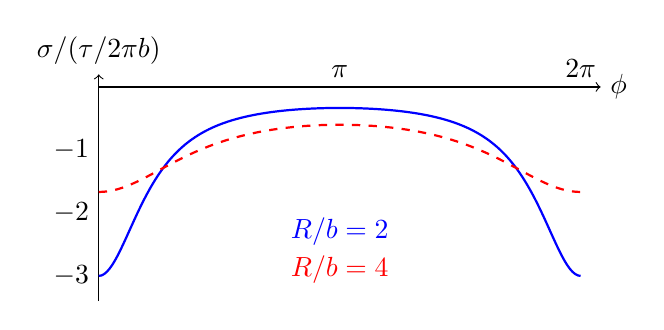
\begin{tikzpicture}[x=.017cm,y=.8cm]
\draw[->] (0,0)--(375,0) node[right] {$\phi$};
\draw[->] (0,-3.4)--(0,.2) node[above] {$\sigma/(\tau/2\pi b)$};
\draw[blue,thick,domain=0:360,samples=180] plot (\x,{-3/(5-4*cos(\x))});
\draw[red,dashed,thick,domain=0:360,samples=180] plot (\x,{-15/(17-8*cos(\x))});
\node[above] at (180,0) {$\pi$};\node[above] at (360,0) {$2\pi$};
\foreach \y in {-1,-2,-3} \node[left] at (0,\y) {$\y$};
\node[blue] at (180,-2.3) {$R/b=2$};
\node[red] at (180,-2.9) {$R/b=4$};
\end{tikzpicture}
\end{center}
\textbf{(d)} The image field at the real line is
$-\tau\widehat{\mathbf x}/[2\pi\epsilon _0(R-c)]$. Thus
\[
\boxed{\frac{\mathbf F}{L}
=-\frac{\tau^2R}{2\pi\epsilon _0(R^2-b^2)}\widehat{\mathbf x},}
\]
an attraction for either sign of $\tau$.

\Needspace{5\baselineskip}
\par\bigskip
\noindent\textbf{2.12}\quad Starting with the series solution (2.71) for the two-dimensional potential problem with the potential specified on the surface of a cylinder of radius $b$, evaluate the coefficients formally, substitute them into the series, and sum it to obtain the potential \emph{inside} the cylinder in the form of Poisson's integral:
\[
\Phi(\rho,\phi)=\frac{1}{2\pi}\int_{0}^{2\pi}\Phi(b,\phi')\,\frac{b^{2}-\rho^{2}}{b^{2}+\rho^{2}-2b\rho\cos(\phi'-\phi)}\;d\phi'
\]
What modification is necessary if the potential is desired in the region of space bounded by the cylinder and infinity?
\solution
Write $f(\phi)=\Phi(b,\phi)$. The nonsingular interior specialization
of (2.71) is
\[
\Phi=A_0+\sum_{n=1}^\infty\left(\frac\rho b\right)^n
 [A_n\cos n\phi+B_n\sin n\phi].
\]
Orthogonality over $[0,2\pi]$ determines
\[
A_0=\frac1{2\pi}\int_0^{2\pi}f(\phi')\,d\phi',\quad
A_n=\frac1\pi\int_0^{2\pi}f(\phi')\cos n\phi'\,d\phi',\quad
B_n=\frac1\pi\int_0^{2\pi}f(\phi')\sin n\phi'\,d\phi'.
\]
Substitution and the cosine subtraction identity give, with $t=\rho/b<1$,
\[
\Phi=\frac1{2\pi}\int_0^{2\pi}f(\phi')
 \left[1+2\sum_{n=1}^\infty t^n\cos n(\phi-\phi')\right]d\phi'.
\]
The series is absolutely convergent inside the circle. Summing the
two geometric series explicitly,
\[
1+\frac{te^{i\Delta}}{1-te^{i\Delta}}
  +\frac{te^{-i\Delta}}{1-te^{-i\Delta}}
=\frac{1-t^2}{1-2t\cos\Delta+t^2}.
\]
Therefore
\[
\boxed{\Phi(\rho,\phi)=\frac1{2\pi}\int_0^{2\pi}f(\phi')
 \frac{b^2-\rho^2}{b^2+\rho^2-2b\rho\cos(\phi-\phi')}\,d\phi'.}
\]
For a solution bounded at infinity replace every $(\rho/b)^n$ by
$(b/\rho)^n$. Equivalently the exterior kernel has numerator
$\rho^2-b^2$ and the same denominator. Its limit at infinity is the
boundary average $A_0$; a zero potential at infinity is possible
with a bounded solution only if $A_0=0$. If logarithmic growth is
allowed, add $B_0\ln(\rho/b)$, which vanishes on the cylinder but
corresponds to a net line charge. The boundary values alone do not
fix $B_0$ without an exterior condition.

\Needspace{5\baselineskip}
\par\bigskip
\noindent\textbf{2.13}\quad\begin{enumerate}
\item[(a)] Two halves of a long hollow conducting cylinder of inner radius $b$ are separated by small lengthwise gaps on each side, and are kept at different potentials $V_{1}$ and $V_{2}$. Show that the potential inside is given by
\[
\Phi(\rho,\phi)=\frac{V_{1}+V_{2}}{2}+\frac{V_{1}-V_{2}}{\pi}\tan^{-1}\!\left(\frac{2b\rho}{b^{2}-\rho^{2}}\cos\phi\right)
\]
where $\phi$ is measured from a plane perpendicular to the plane through the gap.
\item[(b)] Calculate the surface-charge density on each half of the cylinder.
\end{enumerate}
\solution
Choose the $V_1$ half to be $\cos\phi>0$, and the $V_2$ half to be
$\cos\phi<0$. Define $\overline V=(V_1+V_2)/2$ and
$\Delta V=V_1-V_2$.
\textbf{(a)} The boundary function is
$f(\phi)=\overline V+(\Delta V/2)\operatorname{sgn}(\cos\phi)$.
Its sine coefficients vanish. Its cosine coefficients are zero for
even $n$, and for $n=2j+1$ are
\[
A_{2j+1}=\frac{\Delta V}{\pi}\int_{-\pi/2}^{\pi/2}
       \cos[(2j+1)\phi]\,d\phi
=\frac{2\Delta V}{\pi}\frac{(-1)^j}{2j+1}.
\]
Thus, for $t=\rho/b<1$,
\[
\Phi-\overline V=\frac{2\Delta V}{\pi}
 \operatorname{Re}\sum_{j=0}^\infty
       \frac{(-1)^j(te^{i\phi})^{2j+1}}{2j+1}
=\frac{2\Delta V}{\pi}\operatorname{Re}\tan^{-1}(te^{i\phi}).
\]
From $\tan^{-1}w=(2i)^{-1}\ln[(1+iw)/(1-iw)]$, or the tangent
addition formula applied to $w,\bar w$, one obtains
\[
2\operatorname{Re}\tan^{-1}(te^{i\phi})
=\tan^{-1}\frac{2t\cos\phi}{1-t^2}.
\]
Both sides vanish at $t=0$ and remain on the same continuous branch
for $t<1$. Consequently
\[
\boxed{\Phi=\overline V+\frac{\Delta V}{\pi}
 \tan^{-1}\frac{2b\rho\cos\phi}{b^2-\rho^2}.}
\]
As $\rho\uparrow b$ the inverse tangent tends to
$(\pi/2)\operatorname{sgn}(\cos\phi)$, as required.
\textbf{(b)} The normal from the conductor into the cavity is
$-\widehat{\boldsymbol\rho}$, so $\sigma_{\rm inner}=\epsilon _0
\partial_\rho\Phi|_{b^-}$. In terms of $t$ the derivative is
\[
\partial_\rho\Phi=\frac{\Delta V}{\pi b}
 \frac{2(1+t^2)\cos\phi}{(1-t^2)^2+4t^2\cos^2\phi}.
\]
Taking $t\to1$ away from the gaps gives
\[
\boxed{\sigma_{\rm inner}(\phi)=
       \frac{\epsilon _0(V_1-V_2)}{\pi b\cos\phi}.}
\]
For $V_1>V_2$ this is positive on the $V_1$ half and negative on the
$V_2$ half. It diverges as inverse distance to an ideal zero-width
gap; a finite gap cuts off the logarithmic divergence of the charge
on either half. The data for the cavity do not determine the charge
on the exterior faces without exterior geometry and boundary data.

\Needspace{5\baselineskip}
\par\bigskip
\noindent\textbf{2.14}\quad A variant of the preceding two-dimensional problem is a long hollow conducting cylinder of radius $b$ that is divided into equal quarters, alternate segments being held at potential $+V$ and $-V$.
\begin{enumerate}
\item[(a)] Solve by means of the series solution (2.71) and show that the potential inside the cylinder is
\[
\Phi(\rho,\phi)=\frac{4V}{\pi}\sum_{n=0}^{\infty}\left(\frac{\rho}{b}\right)^{4n+2}\frac{\sin[(4n+2)\phi]}{2n+1}
\]
\item[(b)] Sum the series and show that
\[
\Phi(\rho,\phi)=\frac{2V}{\pi}\tan^{-1}\!\left(\frac{2\rho^{2}b^{2}\sin2\phi}{b^{4}-\rho^{4}}\right)
\]
\item[(c)] Sketch the field lines and equipotentials.
\end{enumerate}
\solution
Let the sectors $0<\phi<\pi/2$ and $\pi<\phi<3\pi/2$ be at $+V$;
the other two are at $-V$.
\textbf{(a)} The boundary function is $V\operatorname{sgn}(\sin2\phi)$.
It is odd in $\phi$, invariant under $\phi\mapsto\phi+\pi$, and
changes sign under $\phi\mapsto\phi+\pi/2$. These symmetries leave
only sine modes with $m=4n+2$. Direct integration gives
\[
B_m=\frac1\pi\int_0^{2\pi}V\operatorname{sgn}(\sin2\phi)
                                  \sin m\phi\,d\phi
=\frac{8V}{\pi m},\quad m=4n+2.
\]
The regular radial solution for mode $m$ is $(\rho/b)^m$, whence
\[
\boxed{\Phi=\frac{4V}{\pi}\sum_{n=0}^\infty
 \frac{(\rho/b)^{4n+2}\sin[(4n+2)\phi]}{2n+1}.}
\]
\textbf{(b)} Put $\zeta=(x+iy)/b$. The elementary identity
$\operatorname{artanh}w=\sum_{n\geq0}w^{2n+1}/(2n+1)
=\tfrac12\ln[(1+w)/(1-w)]$ gives
\[
\Phi=\frac{4V}{\pi}\operatorname{Im}\operatorname{artanh}(\zeta^2)
=\frac{2V}{\pi}\arg\frac{1+\zeta^2}{1-\zeta^2}.
\]
Multiplication by $1-\bar\zeta^2$ makes the real and imaginary
parts of this quotient proportional to
$1-|\zeta|^4$ and $2\operatorname{Im}\zeta^2$. The real part is
positive for $|\zeta|<1$, fixing the inverse tangent branch. Hence
\[
\boxed{\Phi=\frac{2V}{\pi}\tan^{-1}
 \frac{2\rho^2b^2\sin2\phi}{b^4-\rho^4}.}
\]
\textbf{(c)} An exact description of the two orthogonal curve families
is obtained by writing
$\operatorname{artanh}\zeta^2=u+iv$. Equipotentials have
$v=\pi\Phi/(4V)$ constant; field lines have $u$ constant, with
arrows toward decreasing $v$. In Cartesian form these conditions are
\[
\frac{4b^2xy}{b^4-(x^2+y^2)^2}
 =\tan\frac{\pi\Phi}{2V},\qquad
\left|\frac{1+\zeta^2}{1-\zeta^2}\right|=e^{2u},
\]
respectively. The supplementary plot is generated parametrically by
$\zeta=\pm\sqrt{\tanh(u+iv)}$, so its curves follow the summed
solution rather than a truncated Fourier series.
\begin{center}
% Generated by supplementary/check_ch02.py --write-assets
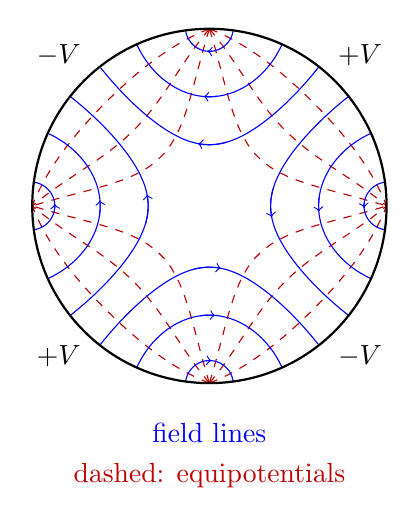
\begin{tikzpicture}[scale=2.25]
\draw[red!75!black,dashed,thin] plot coordinates {(-0.000850,0.999669) (-0.000933,0.999637) (-0.001025,0.999601) (-0.001126,0.999561) (-0.001237,0.999518) (-0.001359,0.999471) (-0.001493,0.999418) (-0.001640,0.999361) (-0.001801,0.999298) (-0.001978,0.999229) (-0.002173,0.999152) (-0.002387,0.999069) (-0.002622,0.998977) (-0.002880,0.998876) (-0.003163,0.998764) (-0.003474,0.998642) (-0.003816,0.998508) (-0.004191,0.998360) (-0.004604,0.998198) (-0.005056,0.998020) (-0.005553,0.997823) (-0.006099,0.997607) (-0.006698,0.997370) (-0.007356,0.997109) (-0.008079,0.996822) (-0.008872,0.996506) (-0.009742,0.996158) (-0.010698,0.995775) (-0.011747,0.995354) (-0.012898,0.994890) (-0.014162,0.994379) (-0.015548,0.993816) (-0.017070,0.993196) (-0.018739,0.992513) (-0.020569,0.991760) (-0.022577,0.990929) (-0.024779,0.990013) (-0.027192,0.989003) (-0.029838,0.987887) (-0.032738,0.986655) (-0.035915,0.985295) (-0.039394,0.983791) (-0.043204,0.982129) (-0.047375,0.980290) (-0.051938,0.978255) (-0.056928,0.976002) (-0.062383,0.973507) (-0.068343,0.970742) (-0.074850,0.967676) (-0.081950,0.964275) (-0.089691,0.960501) (-0.098123,0.956312) (-0.107300,0.951660) (-0.117276,0.946494) (-0.128107,0.940756) (-0.139852,0.934382) (-0.152567,0.927304) (-0.166310,0.919447) (-0.181134,0.910732) (-0.197090,0.901073) (-0.214225,0.890382) (-0.232576,0.878569) (-0.252172,0.865543) (-0.273028,0.851216) (-0.295147,0.835507) (-0.318509,0.818347) (-0.343080,0.799683) (-0.368796,0.779484) (-0.395571,0.757749) (-0.423291,0.734508) (-0.451812,0.709832) (-0.480961,0.683830) (-0.510541,0.656653) (-0.540327,0.628487) (-0.570080,0.599550) (-0.599550,0.570080) (-0.628487,0.540327) (-0.656653,0.510541) (-0.683830,0.480961) (-0.709832,0.451812) (-0.734508,0.423291) (-0.757749,0.395571) (-0.779484,0.368796) (-0.799683,0.343080) (-0.818347,0.318509) (-0.835507,0.295147) (-0.851216,0.273028) (-0.865543,0.252172) (-0.878569,0.232576) (-0.890382,0.214225) (-0.901073,0.197090) (-0.910732,0.181134) (-0.919447,0.166310) (-0.927304,0.152567) (-0.934382,0.139852) (-0.940756,0.128107) (-0.946494,0.117276) (-0.951660,0.107300) (-0.956312,0.098123) (-0.960501,0.089691) (-0.964275,0.081950) (-0.967676,0.074850) (-0.970742,0.068343) (-0.973507,0.062383) (-0.976002,0.056928) (-0.978255,0.051938) (-0.980290,0.047375) (-0.982129,0.043204) (-0.983791,0.039394) (-0.985295,0.035915) (-0.986655,0.032738) (-0.987887,0.029838) (-0.989003,0.027192) (-0.990013,0.024779) (-0.990929,0.022577) (-0.991760,0.020569) (-0.992513,0.018739) (-0.993196,0.017070) (-0.993816,0.015548) (-0.994379,0.014162) (-0.994890,0.012898) (-0.995354,0.011747) (-0.995775,0.010698) (-0.996158,0.009742) (-0.996506,0.008872) (-0.996822,0.008079) (-0.997109,0.007356) (-0.997370,0.006698) (-0.997607,0.006099) (-0.997823,0.005553) (-0.998020,0.005056) (-0.998198,0.004604) (-0.998360,0.004191) (-0.998508,0.003816) (-0.998642,0.003474) (-0.998764,0.003163) (-0.998876,0.002880) (-0.998977,0.002622) (-0.999069,0.002387) (-0.999152,0.002173) (-0.999229,0.001978) (-0.999298,0.001801) (-0.999361,0.001640) (-0.999418,0.001493) (-0.999471,0.001359) (-0.999518,0.001237) (-0.999561,0.001126) (-0.999601,0.001025) (-0.999637,0.000933) (-0.999669,0.000850)};
\draw[red!75!black,dashed,thin] plot coordinates {(0.000850,-0.999669) (0.000933,-0.999637) (0.001025,-0.999601) (0.001126,-0.999561) (0.001237,-0.999518) (0.001359,-0.999471) (0.001493,-0.999418) (0.001640,-0.999361) (0.001801,-0.999298) (0.001978,-0.999229) (0.002173,-0.999152) (0.002387,-0.999069) (0.002622,-0.998977) (0.002880,-0.998876) (0.003163,-0.998764) (0.003474,-0.998642) (0.003816,-0.998508) (0.004191,-0.998360) (0.004604,-0.998198) (0.005056,-0.998020) (0.005553,-0.997823) (0.006099,-0.997607) (0.006698,-0.997370) (0.007356,-0.997109) (0.008079,-0.996822) (0.008872,-0.996506) (0.009742,-0.996158) (0.010698,-0.995775) (0.011747,-0.995354) (0.012898,-0.994890) (0.014162,-0.994379) (0.015548,-0.993816) (0.017070,-0.993196) (0.018739,-0.992513) (0.020569,-0.991760) (0.022577,-0.990929) (0.024779,-0.990013) (0.027192,-0.989003) (0.029838,-0.987887) (0.032738,-0.986655) (0.035915,-0.985295) (0.039394,-0.983791) (0.043204,-0.982129) (0.047375,-0.980290) (0.051938,-0.978255) (0.056928,-0.976002) (0.062383,-0.973507) (0.068343,-0.970742) (0.074850,-0.967676) (0.081950,-0.964275) (0.089691,-0.960501) (0.098123,-0.956312) (0.107300,-0.951660) (0.117276,-0.946494) (0.128107,-0.940756) (0.139852,-0.934382) (0.152567,-0.927304) (0.166310,-0.919447) (0.181134,-0.910732) (0.197090,-0.901073) (0.214225,-0.890382) (0.232576,-0.878569) (0.252172,-0.865543) (0.273028,-0.851216) (0.295147,-0.835507) (0.318509,-0.818347) (0.343080,-0.799683) (0.368796,-0.779484) (0.395571,-0.757749) (0.423291,-0.734508) (0.451812,-0.709832) (0.480961,-0.683830) (0.510541,-0.656653) (0.540327,-0.628487) (0.570080,-0.599550) (0.599550,-0.570080) (0.628487,-0.540327) (0.656653,-0.510541) (0.683830,-0.480961) (0.709832,-0.451812) (0.734508,-0.423291) (0.757749,-0.395571) (0.779484,-0.368796) (0.799683,-0.343080) (0.818347,-0.318509) (0.835507,-0.295147) (0.851216,-0.273028) (0.865543,-0.252172) (0.878569,-0.232576) (0.890382,-0.214225) (0.901073,-0.197090) (0.910732,-0.181134) (0.919447,-0.166310) (0.927304,-0.152567) (0.934382,-0.139852) (0.940756,-0.128107) (0.946494,-0.117276) (0.951660,-0.107300) (0.956312,-0.098123) (0.960501,-0.089691) (0.964275,-0.081950) (0.967676,-0.074850) (0.970742,-0.068343) (0.973507,-0.062383) (0.976002,-0.056928) (0.978255,-0.051938) (0.980290,-0.047375) (0.982129,-0.043204) (0.983791,-0.039394) (0.985295,-0.035915) (0.986655,-0.032738) (0.987887,-0.029838) (0.989003,-0.027192) (0.990013,-0.024779) (0.990929,-0.022577) (0.991760,-0.020569) (0.992513,-0.018739) (0.993196,-0.017070) (0.993816,-0.015548) (0.994379,-0.014162) (0.994890,-0.012898) (0.995354,-0.011747) (0.995775,-0.010698) (0.996158,-0.009742) (0.996506,-0.008872) (0.996822,-0.008079) (0.997109,-0.007356) (0.997370,-0.006698) (0.997607,-0.006099) (0.997823,-0.005553) (0.998020,-0.005056) (0.998198,-0.004604) (0.998360,-0.004191) (0.998508,-0.003816) (0.998642,-0.003474) (0.998764,-0.003163) (0.998876,-0.002880) (0.998977,-0.002622) (0.999069,-0.002387) (0.999152,-0.002173) (0.999229,-0.001978) (0.999298,-0.001801) (0.999361,-0.001640) (0.999418,-0.001493) (0.999471,-0.001359) (0.999518,-0.001237) (0.999561,-0.001126) (0.999601,-0.001025) (0.999637,-0.000933) (0.999669,-0.000850)};
\draw[red!75!black,dashed,thin] plot coordinates {(-0.000587,0.999303) (-0.000645,0.999234) (-0.000708,0.999158) (-0.000778,0.999076) (-0.000855,0.998985) (-0.000939,0.998884) (-0.001031,0.998775) (-0.001132,0.998654) (-0.001244,0.998521) (-0.001366,0.998376) (-0.001501,0.998216) (-0.001648,0.998040) (-0.001810,0.997847) (-0.001988,0.997635) (-0.002183,0.997402) (-0.002398,0.997146) (-0.002633,0.996865) (-0.002892,0.996557) (-0.003176,0.996217) (-0.003487,0.995845) (-0.003829,0.995436) (-0.004205,0.994987) (-0.004617,0.994493) (-0.005069,0.993951) (-0.005565,0.993356) (-0.006109,0.992702) (-0.006706,0.991984) (-0.007361,0.991196) (-0.008079,0.990329) (-0.008867,0.989378) (-0.009730,0.988334) (-0.010677,0.987187) (-0.011714,0.985928) (-0.012850,0.984545) (-0.014095,0.983026) (-0.015459,0.981359) (-0.016951,0.979529) (-0.018584,0.977520) (-0.020371,0.975315) (-0.022325,0.972895) (-0.024462,0.970238) (-0.026796,0.967323) (-0.029345,0.964125) (-0.032127,0.960617) (-0.035162,0.956769) (-0.038471,0.952549) (-0.042075,0.947923) (-0.045999,0.942852) (-0.050268,0.937295) (-0.054907,0.931209) (-0.059944,0.924544) (-0.065409,0.917249) (-0.071332,0.909268) (-0.077743,0.900541) (-0.084677,0.891006) (-0.092167,0.880595) (-0.100249,0.869236) (-0.108959,0.856856) (-0.118337,0.843376) (-0.128424,0.828717) (-0.139262,0.812800) (-0.150901,0.795545) (-0.163392,0.776873) (-0.176796,0.756715) (-0.191180,0.735008) (-0.206625,0.711704) (-0.223225,0.686778) (-0.241091,0.660237) (-0.260350,0.632132) (-0.281142,0.602573) (-0.303613,0.571748) (-0.327888,0.539942) (-0.354045,0.507541) (-0.382066,0.475026) (-0.411799,0.442935) (-0.442935,0.411799) (-0.475026,0.382066) (-0.507541,0.354045) (-0.539942,0.327888) (-0.571748,0.303613) (-0.602573,0.281142) (-0.632132,0.260350) (-0.660237,0.241091) (-0.686778,0.223225) (-0.711704,0.206625) (-0.735008,0.191180) (-0.756715,0.176796) (-0.776873,0.163392) (-0.795545,0.150901) (-0.812800,0.139262) (-0.828717,0.128424) (-0.843376,0.118337) (-0.856856,0.108959) (-0.869236,0.100249) (-0.880595,0.092167) (-0.891006,0.084677) (-0.900541,0.077743) (-0.909268,0.071332) (-0.917249,0.065409) (-0.924544,0.059944) (-0.931209,0.054907) (-0.937295,0.050268) (-0.942852,0.045999) (-0.947923,0.042075) (-0.952549,0.038471) (-0.956769,0.035162) (-0.960617,0.032127) (-0.964125,0.029345) (-0.967323,0.026796) (-0.970238,0.024462) (-0.972895,0.022325) (-0.975315,0.020371) (-0.977520,0.018584) (-0.979529,0.016951) (-0.981359,0.015459) (-0.983026,0.014095) (-0.984545,0.012850) (-0.985928,0.011714) (-0.987187,0.010677) (-0.988334,0.009730) (-0.989378,0.008867) (-0.990329,0.008079) (-0.991196,0.007361) (-0.991984,0.006706) (-0.992702,0.006109) (-0.993356,0.005565) (-0.993951,0.005069) (-0.994493,0.004617) (-0.994987,0.004205) (-0.995436,0.003829) (-0.995845,0.003487) (-0.996217,0.003176) (-0.996557,0.002892) (-0.996865,0.002633) (-0.997146,0.002398) (-0.997402,0.002183) (-0.997635,0.001988) (-0.997847,0.001810) (-0.998040,0.001648) (-0.998216,0.001501) (-0.998376,0.001366) (-0.998521,0.001244) (-0.998654,0.001132) (-0.998775,0.001031) (-0.998884,0.000939) (-0.998985,0.000855) (-0.999076,0.000778) (-0.999158,0.000708) (-0.999234,0.000645) (-0.999303,0.000587)};
\draw[red!75!black,dashed,thin] plot coordinates {(0.000587,-0.999303) (0.000645,-0.999234) (0.000708,-0.999158) (0.000778,-0.999076) (0.000855,-0.998985) (0.000939,-0.998884) (0.001031,-0.998775) (0.001132,-0.998654) (0.001244,-0.998521) (0.001366,-0.998376) (0.001501,-0.998216) (0.001648,-0.998040) (0.001810,-0.997847) (0.001988,-0.997635) (0.002183,-0.997402) (0.002398,-0.997146) (0.002633,-0.996865) (0.002892,-0.996557) (0.003176,-0.996217) (0.003487,-0.995845) (0.003829,-0.995436) (0.004205,-0.994987) (0.004617,-0.994493) (0.005069,-0.993951) (0.005565,-0.993356) (0.006109,-0.992702) (0.006706,-0.991984) (0.007361,-0.991196) (0.008079,-0.990329) (0.008867,-0.989378) (0.009730,-0.988334) (0.010677,-0.987187) (0.011714,-0.985928) (0.012850,-0.984545) (0.014095,-0.983026) (0.015459,-0.981359) (0.016951,-0.979529) (0.018584,-0.977520) (0.020371,-0.975315) (0.022325,-0.972895) (0.024462,-0.970238) (0.026796,-0.967323) (0.029345,-0.964125) (0.032127,-0.960617) (0.035162,-0.956769) (0.038471,-0.952549) (0.042075,-0.947923) (0.045999,-0.942852) (0.050268,-0.937295) (0.054907,-0.931209) (0.059944,-0.924544) (0.065409,-0.917249) (0.071332,-0.909268) (0.077743,-0.900541) (0.084677,-0.891006) (0.092167,-0.880595) (0.100249,-0.869236) (0.108959,-0.856856) (0.118337,-0.843376) (0.128424,-0.828717) (0.139262,-0.812800) (0.150901,-0.795545) (0.163392,-0.776873) (0.176796,-0.756715) (0.191180,-0.735008) (0.206625,-0.711704) (0.223225,-0.686778) (0.241091,-0.660237) (0.260350,-0.632132) (0.281142,-0.602573) (0.303613,-0.571748) (0.327888,-0.539942) (0.354045,-0.507541) (0.382066,-0.475026) (0.411799,-0.442935) (0.442935,-0.411799) (0.475026,-0.382066) (0.507541,-0.354045) (0.539942,-0.327888) (0.571748,-0.303613) (0.602573,-0.281142) (0.632132,-0.260350) (0.660237,-0.241091) (0.686778,-0.223225) (0.711704,-0.206625) (0.735008,-0.191180) (0.756715,-0.176796) (0.776873,-0.163392) (0.795545,-0.150901) (0.812800,-0.139262) (0.828717,-0.128424) (0.843376,-0.118337) (0.856856,-0.108959) (0.869236,-0.100249) (0.880595,-0.092167) (0.891006,-0.084677) (0.900541,-0.077743) (0.909268,-0.071332) (0.917249,-0.065409) (0.924544,-0.059944) (0.931209,-0.054907) (0.937295,-0.050268) (0.942852,-0.045999) (0.947923,-0.042075) (0.952549,-0.038471) (0.956769,-0.035162) (0.960617,-0.032127) (0.964125,-0.029345) (0.967323,-0.026796) (0.970238,-0.024462) (0.972895,-0.022325) (0.975315,-0.020371) (0.977520,-0.018584) (0.979529,-0.016951) (0.981359,-0.015459) (0.983026,-0.014095) (0.984545,-0.012850) (0.985928,-0.011714) (0.987187,-0.010677) (0.988334,-0.009730) (0.989378,-0.008867) (0.990329,-0.008079) (0.991196,-0.007361) (0.991984,-0.006706) (0.992702,-0.006109) (0.993356,-0.005565) (0.993951,-0.005069) (0.994493,-0.004617) (0.994987,-0.004205) (0.995436,-0.003829) (0.995845,-0.003487) (0.996217,-0.003176) (0.996557,-0.002892) (0.996865,-0.002633) (0.997146,-0.002398) (0.997402,-0.002183) (0.997635,-0.001988) (0.997847,-0.001810) (0.998040,-0.001648) (0.998216,-0.001501) (0.998376,-0.001366) (0.998521,-0.001244) (0.998654,-0.001132) (0.998775,-0.001031) (0.998884,-0.000939) (0.998985,-0.000855) (0.999076,-0.000778) (0.999158,-0.000708) (0.999234,-0.000645) (0.999303,-0.000587)};
\draw[red!75!black,dashed,thin] plot coordinates {(-0.000269,0.999129) (-0.000296,0.999043) (-0.000325,0.998949) (-0.000357,0.998846) (-0.000392,0.998732) (-0.000430,0.998607) (-0.000473,0.998470) (-0.000519,0.998320) (-0.000570,0.998154) (-0.000626,0.997973) (-0.000688,0.997773) (-0.000756,0.997554) (-0.000830,0.997313) (-0.000911,0.997049) (-0.001001,0.996759) (-0.001099,0.996440) (-0.001207,0.996090) (-0.001325,0.995705) (-0.001455,0.995283) (-0.001598,0.994819) (-0.001755,0.994310) (-0.001926,0.993751) (-0.002115,0.993137) (-0.002322,0.992464) (-0.002549,0.991724) (-0.002797,0.990912) (-0.003070,0.990021) (-0.003369,0.989042) (-0.003697,0.987969) (-0.004057,0.986791) (-0.004451,0.985498) (-0.004883,0.984079) (-0.005356,0.982523) (-0.005873,0.980816) (-0.006440,0.978944) (-0.007060,0.976891) (-0.007739,0.974640) (-0.008481,0.972172) (-0.009292,0.969468) (-0.010178,0.966505) (-0.011146,0.963258) (-0.012202,0.959703) (-0.013355,0.955810) (-0.014611,0.951549) (-0.015980,0.946886) (-0.017471,0.941786) (-0.019092,0.936209) (-0.020855,0.930113) (-0.022770,0.923454) (-0.024849,0.916182) (-0.027103,0.908245) (-0.029546,0.899587) (-0.032190,0.890147) (-0.035050,0.879862) (-0.038141,0.868662) (-0.041479,0.856473) (-0.045082,0.843218) (-0.048970,0.828813) (-0.053163,0.813169) (-0.057687,0.796190) (-0.062572,0.777774) (-0.067852,0.757812) (-0.073572,0.736186) (-0.079789,0.712766) (-0.086577,0.687413) (-0.094036,0.659970) (-0.102305,0.630266) (-0.111579,0.598109) (-0.122138,0.563290) (-0.134392,0.525592) (-0.148956,0.484820) (-0.166743,0.440895) (-0.189079,0.394077) (-0.217653,0.345435) (-0.253896,0.297464) (-0.297464,0.253896) (-0.345435,0.217653) (-0.394077,0.189079) (-0.440895,0.166743) (-0.484820,0.148956) (-0.525592,0.134392) (-0.563290,0.122138) (-0.598109,0.111579) (-0.630266,0.102305) (-0.659970,0.094036) (-0.687413,0.086577) (-0.712766,0.079789) (-0.736186,0.073572) (-0.757812,0.067852) (-0.777774,0.062572) (-0.796190,0.057687) (-0.813169,0.053163) (-0.828813,0.048970) (-0.843218,0.045082) (-0.856473,0.041479) (-0.868662,0.038141) (-0.879862,0.035050) (-0.890147,0.032190) (-0.899587,0.029546) (-0.908245,0.027103) (-0.916182,0.024849) (-0.923454,0.022770) (-0.930113,0.020855) (-0.936209,0.019092) (-0.941786,0.017471) (-0.946886,0.015980) (-0.951549,0.014611) (-0.955810,0.013355) (-0.959703,0.012202) (-0.963258,0.011146) (-0.966505,0.010178) (-0.969468,0.009292) (-0.972172,0.008481) (-0.974640,0.007739) (-0.976891,0.007060) (-0.978944,0.006440) (-0.980816,0.005873) (-0.982523,0.005356) (-0.984079,0.004883) (-0.985498,0.004451) (-0.986791,0.004057) (-0.987969,0.003697) (-0.989042,0.003369) (-0.990021,0.003070) (-0.990912,0.002797) (-0.991724,0.002549) (-0.992464,0.002322) (-0.993137,0.002115) (-0.993751,0.001926) (-0.994310,0.001755) (-0.994819,0.001598) (-0.995283,0.001455) (-0.995705,0.001325) (-0.996090,0.001207) (-0.996440,0.001099) (-0.996759,0.001001) (-0.997049,0.000911) (-0.997313,0.000830) (-0.997554,0.000756) (-0.997773,0.000688) (-0.997973,0.000626) (-0.998154,0.000570) (-0.998320,0.000519) (-0.998470,0.000473) (-0.998607,0.000430) (-0.998732,0.000392) (-0.998846,0.000357) (-0.998949,0.000325) (-0.999043,0.000296) (-0.999129,0.000269)};
\draw[red!75!black,dashed,thin] plot coordinates {(0.000269,-0.999129) (0.000296,-0.999043) (0.000325,-0.998949) (0.000357,-0.998846) (0.000392,-0.998732) (0.000430,-0.998607) (0.000473,-0.998470) (0.000519,-0.998320) (0.000570,-0.998154) (0.000626,-0.997973) (0.000688,-0.997773) (0.000756,-0.997554) (0.000830,-0.997313) (0.000911,-0.997049) (0.001001,-0.996759) (0.001099,-0.996440) (0.001207,-0.996090) (0.001325,-0.995705) (0.001455,-0.995283) (0.001598,-0.994819) (0.001755,-0.994310) (0.001926,-0.993751) (0.002115,-0.993137) (0.002322,-0.992464) (0.002549,-0.991724) (0.002797,-0.990912) (0.003070,-0.990021) (0.003369,-0.989042) (0.003697,-0.987969) (0.004057,-0.986791) (0.004451,-0.985498) (0.004883,-0.984079) (0.005356,-0.982523) (0.005873,-0.980816) (0.006440,-0.978944) (0.007060,-0.976891) (0.007739,-0.974640) (0.008481,-0.972172) (0.009292,-0.969468) (0.010178,-0.966505) (0.011146,-0.963258) (0.012202,-0.959703) (0.013355,-0.955810) (0.014611,-0.951549) (0.015980,-0.946886) (0.017471,-0.941786) (0.019092,-0.936209) (0.020855,-0.930113) (0.022770,-0.923454) (0.024849,-0.916182) (0.027103,-0.908245) (0.029546,-0.899587) (0.032190,-0.890147) (0.035050,-0.879862) (0.038141,-0.868662) (0.041479,-0.856473) (0.045082,-0.843218) (0.048970,-0.828813) (0.053163,-0.813169) (0.057687,-0.796190) (0.062572,-0.777774) (0.067852,-0.757812) (0.073572,-0.736186) (0.079789,-0.712766) (0.086577,-0.687413) (0.094036,-0.659970) (0.102305,-0.630266) (0.111579,-0.598109) (0.122138,-0.563290) (0.134392,-0.525592) (0.148956,-0.484820) (0.166743,-0.440895) (0.189079,-0.394077) (0.217653,-0.345435) (0.253896,-0.297464) (0.297464,-0.253896) (0.345435,-0.217653) (0.394077,-0.189079) (0.440895,-0.166743) (0.484820,-0.148956) (0.525592,-0.134392) (0.563290,-0.122138) (0.598109,-0.111579) (0.630266,-0.102305) (0.659970,-0.094036) (0.687413,-0.086577) (0.712766,-0.079789) (0.736186,-0.073572) (0.757812,-0.067852) (0.777774,-0.062572) (0.796190,-0.057687) (0.813169,-0.053163) (0.828813,-0.048970) (0.843218,-0.045082) (0.856473,-0.041479) (0.868662,-0.038141) (0.879862,-0.035050) (0.890147,-0.032190) (0.899587,-0.029546) (0.908245,-0.027103) (0.916182,-0.024849) (0.923454,-0.022770) (0.930113,-0.020855) (0.936209,-0.019092) (0.941786,-0.017471) (0.946886,-0.015980) (0.951549,-0.014611) (0.955810,-0.013355) (0.959703,-0.012202) (0.963258,-0.011146) (0.966505,-0.010178) (0.969468,-0.009292) (0.972172,-0.008481) (0.974640,-0.007739) (0.976891,-0.007060) (0.978944,-0.006440) (0.980816,-0.005873) (0.982523,-0.005356) (0.984079,-0.004883) (0.985498,-0.004451) (0.986791,-0.004057) (0.987969,-0.003697) (0.989042,-0.003369) (0.990021,-0.003070) (0.990912,-0.002797) (0.991724,-0.002549) (0.992464,-0.002322) (0.993137,-0.002115) (0.993751,-0.001926) (0.994310,-0.001755) (0.994819,-0.001598) (0.995283,-0.001455) (0.995705,-0.001325) (0.996090,-0.001207) (0.996440,-0.001099) (0.996759,-0.001001) (0.997049,-0.000911) (0.997313,-0.000830) (0.997554,-0.000756) (0.997773,-0.000688) (0.997973,-0.000626) (0.998154,-0.000570) (0.998320,-0.000519) (0.998470,-0.000473) (0.998607,-0.000430) (0.998732,-0.000392) (0.998846,-0.000357) (0.998949,-0.000325) (0.999043,-0.000296) (0.999129,-0.000269)};
\draw[red!75!black,dashed,thin] plot coordinates {(-0.000269,-0.999129) (-0.000296,-0.999043) (-0.000325,-0.998949) (-0.000357,-0.998846) (-0.000392,-0.998732) (-0.000430,-0.998607) (-0.000473,-0.998470) (-0.000519,-0.998320) (-0.000570,-0.998154) (-0.000626,-0.997973) (-0.000688,-0.997773) (-0.000756,-0.997554) (-0.000830,-0.997313) (-0.000911,-0.997049) (-0.001001,-0.996759) (-0.001099,-0.996440) (-0.001207,-0.996090) (-0.001325,-0.995705) (-0.001455,-0.995283) (-0.001598,-0.994819) (-0.001755,-0.994310) (-0.001926,-0.993751) (-0.002115,-0.993137) (-0.002322,-0.992464) (-0.002549,-0.991724) (-0.002797,-0.990912) (-0.003070,-0.990021) (-0.003369,-0.989042) (-0.003697,-0.987969) (-0.004057,-0.986791) (-0.004451,-0.985498) (-0.004883,-0.984079) (-0.005356,-0.982523) (-0.005873,-0.980816) (-0.006440,-0.978944) (-0.007060,-0.976891) (-0.007739,-0.974640) (-0.008481,-0.972172) (-0.009292,-0.969468) (-0.010178,-0.966505) (-0.011146,-0.963258) (-0.012202,-0.959703) (-0.013355,-0.955810) (-0.014611,-0.951549) (-0.015980,-0.946886) (-0.017471,-0.941786) (-0.019092,-0.936209) (-0.020855,-0.930113) (-0.022770,-0.923454) (-0.024849,-0.916182) (-0.027103,-0.908245) (-0.029546,-0.899587) (-0.032190,-0.890147) (-0.035050,-0.879862) (-0.038141,-0.868662) (-0.041479,-0.856473) (-0.045082,-0.843218) (-0.048970,-0.828813) (-0.053163,-0.813169) (-0.057687,-0.796190) (-0.062572,-0.777774) (-0.067852,-0.757812) (-0.073572,-0.736186) (-0.079789,-0.712766) (-0.086577,-0.687413) (-0.094036,-0.659970) (-0.102305,-0.630266) (-0.111579,-0.598109) (-0.122138,-0.563290) (-0.134392,-0.525592) (-0.148956,-0.484820) (-0.166743,-0.440895) (-0.189079,-0.394077) (-0.217653,-0.345435) (-0.253896,-0.297464) (-0.297464,-0.253896) (-0.345435,-0.217653) (-0.394077,-0.189079) (-0.440895,-0.166743) (-0.484820,-0.148956) (-0.525592,-0.134392) (-0.563290,-0.122138) (-0.598109,-0.111579) (-0.630266,-0.102305) (-0.659970,-0.094036) (-0.687413,-0.086577) (-0.712766,-0.079789) (-0.736186,-0.073572) (-0.757812,-0.067852) (-0.777774,-0.062572) (-0.796190,-0.057687) (-0.813169,-0.053163) (-0.828813,-0.048970) (-0.843218,-0.045082) (-0.856473,-0.041479) (-0.868662,-0.038141) (-0.879862,-0.035050) (-0.890147,-0.032190) (-0.899587,-0.029546) (-0.908245,-0.027103) (-0.916182,-0.024849) (-0.923454,-0.022770) (-0.930113,-0.020855) (-0.936209,-0.019092) (-0.941786,-0.017471) (-0.946886,-0.015980) (-0.951549,-0.014611) (-0.955810,-0.013355) (-0.959703,-0.012202) (-0.963258,-0.011146) (-0.966505,-0.010178) (-0.969468,-0.009292) (-0.972172,-0.008481) (-0.974640,-0.007739) (-0.976891,-0.007060) (-0.978944,-0.006440) (-0.980816,-0.005873) (-0.982523,-0.005356) (-0.984079,-0.004883) (-0.985498,-0.004451) (-0.986791,-0.004057) (-0.987969,-0.003697) (-0.989042,-0.003369) (-0.990021,-0.003070) (-0.990912,-0.002797) (-0.991724,-0.002549) (-0.992464,-0.002322) (-0.993137,-0.002115) (-0.993751,-0.001926) (-0.994310,-0.001755) (-0.994819,-0.001598) (-0.995283,-0.001455) (-0.995705,-0.001325) (-0.996090,-0.001207) (-0.996440,-0.001099) (-0.996759,-0.001001) (-0.997049,-0.000911) (-0.997313,-0.000830) (-0.997554,-0.000756) (-0.997773,-0.000688) (-0.997973,-0.000626) (-0.998154,-0.000570) (-0.998320,-0.000519) (-0.998470,-0.000473) (-0.998607,-0.000430) (-0.998732,-0.000392) (-0.998846,-0.000357) (-0.998949,-0.000325) (-0.999043,-0.000296) (-0.999129,-0.000269)};
\draw[red!75!black,dashed,thin] plot coordinates {(0.000269,0.999129) (0.000296,0.999043) (0.000325,0.998949) (0.000357,0.998846) (0.000392,0.998732) (0.000430,0.998607) (0.000473,0.998470) (0.000519,0.998320) (0.000570,0.998154) (0.000626,0.997973) (0.000688,0.997773) (0.000756,0.997554) (0.000830,0.997313) (0.000911,0.997049) (0.001001,0.996759) (0.001099,0.996440) (0.001207,0.996090) (0.001325,0.995705) (0.001455,0.995283) (0.001598,0.994819) (0.001755,0.994310) (0.001926,0.993751) (0.002115,0.993137) (0.002322,0.992464) (0.002549,0.991724) (0.002797,0.990912) (0.003070,0.990021) (0.003369,0.989042) (0.003697,0.987969) (0.004057,0.986791) (0.004451,0.985498) (0.004883,0.984079) (0.005356,0.982523) (0.005873,0.980816) (0.006440,0.978944) (0.007060,0.976891) (0.007739,0.974640) (0.008481,0.972172) (0.009292,0.969468) (0.010178,0.966505) (0.011146,0.963258) (0.012202,0.959703) (0.013355,0.955810) (0.014611,0.951549) (0.015980,0.946886) (0.017471,0.941786) (0.019092,0.936209) (0.020855,0.930113) (0.022770,0.923454) (0.024849,0.916182) (0.027103,0.908245) (0.029546,0.899587) (0.032190,0.890147) (0.035050,0.879862) (0.038141,0.868662) (0.041479,0.856473) (0.045082,0.843218) (0.048970,0.828813) (0.053163,0.813169) (0.057687,0.796190) (0.062572,0.777774) (0.067852,0.757812) (0.073572,0.736186) (0.079789,0.712766) (0.086577,0.687413) (0.094036,0.659970) (0.102305,0.630266) (0.111579,0.598109) (0.122138,0.563290) (0.134392,0.525592) (0.148956,0.484820) (0.166743,0.440895) (0.189079,0.394077) (0.217653,0.345435) (0.253896,0.297464) (0.297464,0.253896) (0.345435,0.217653) (0.394077,0.189079) (0.440895,0.166743) (0.484820,0.148956) (0.525592,0.134392) (0.563290,0.122138) (0.598109,0.111579) (0.630266,0.102305) (0.659970,0.094036) (0.687413,0.086577) (0.712766,0.079789) (0.736186,0.073572) (0.757812,0.067852) (0.777774,0.062572) (0.796190,0.057687) (0.813169,0.053163) (0.828813,0.048970) (0.843218,0.045082) (0.856473,0.041479) (0.868662,0.038141) (0.879862,0.035050) (0.890147,0.032190) (0.899587,0.029546) (0.908245,0.027103) (0.916182,0.024849) (0.923454,0.022770) (0.930113,0.020855) (0.936209,0.019092) (0.941786,0.017471) (0.946886,0.015980) (0.951549,0.014611) (0.955810,0.013355) (0.959703,0.012202) (0.963258,0.011146) (0.966505,0.010178) (0.969468,0.009292) (0.972172,0.008481) (0.974640,0.007739) (0.976891,0.007060) (0.978944,0.006440) (0.980816,0.005873) (0.982523,0.005356) (0.984079,0.004883) (0.985498,0.004451) (0.986791,0.004057) (0.987969,0.003697) (0.989042,0.003369) (0.990021,0.003070) (0.990912,0.002797) (0.991724,0.002549) (0.992464,0.002322) (0.993137,0.002115) (0.993751,0.001926) (0.994310,0.001755) (0.994819,0.001598) (0.995283,0.001455) (0.995705,0.001325) (0.996090,0.001207) (0.996440,0.001099) (0.996759,0.001001) (0.997049,0.000911) (0.997313,0.000830) (0.997554,0.000756) (0.997773,0.000688) (0.997973,0.000626) (0.998154,0.000570) (0.998320,0.000519) (0.998470,0.000473) (0.998607,0.000430) (0.998732,0.000392) (0.998846,0.000357) (0.998949,0.000325) (0.999043,0.000296) (0.999129,0.000269)};
\draw[red!75!black,dashed,thin] plot coordinates {(-0.000587,-0.999303) (-0.000645,-0.999234) (-0.000708,-0.999158) (-0.000778,-0.999076) (-0.000855,-0.998985) (-0.000939,-0.998884) (-0.001031,-0.998775) (-0.001132,-0.998654) (-0.001244,-0.998521) (-0.001366,-0.998376) (-0.001501,-0.998216) (-0.001648,-0.998040) (-0.001810,-0.997847) (-0.001988,-0.997635) (-0.002183,-0.997402) (-0.002398,-0.997146) (-0.002633,-0.996865) (-0.002892,-0.996557) (-0.003176,-0.996217) (-0.003487,-0.995845) (-0.003829,-0.995436) (-0.004205,-0.994987) (-0.004617,-0.994493) (-0.005069,-0.993951) (-0.005565,-0.993356) (-0.006109,-0.992702) (-0.006706,-0.991984) (-0.007361,-0.991196) (-0.008079,-0.990329) (-0.008867,-0.989378) (-0.009730,-0.988334) (-0.010677,-0.987187) (-0.011714,-0.985928) (-0.012850,-0.984545) (-0.014095,-0.983026) (-0.015459,-0.981359) (-0.016951,-0.979529) (-0.018584,-0.977520) (-0.020371,-0.975315) (-0.022325,-0.972895) (-0.024462,-0.970238) (-0.026796,-0.967323) (-0.029345,-0.964125) (-0.032127,-0.960617) (-0.035162,-0.956769) (-0.038471,-0.952549) (-0.042075,-0.947923) (-0.045999,-0.942852) (-0.050268,-0.937295) (-0.054907,-0.931209) (-0.059944,-0.924544) (-0.065409,-0.917249) (-0.071332,-0.909268) (-0.077743,-0.900541) (-0.084677,-0.891006) (-0.092167,-0.880595) (-0.100249,-0.869236) (-0.108959,-0.856856) (-0.118337,-0.843376) (-0.128424,-0.828717) (-0.139262,-0.812800) (-0.150901,-0.795545) (-0.163392,-0.776873) (-0.176796,-0.756715) (-0.191180,-0.735008) (-0.206625,-0.711704) (-0.223225,-0.686778) (-0.241091,-0.660237) (-0.260350,-0.632132) (-0.281142,-0.602573) (-0.303613,-0.571748) (-0.327888,-0.539942) (-0.354045,-0.507541) (-0.382066,-0.475026) (-0.411799,-0.442935) (-0.442935,-0.411799) (-0.475026,-0.382066) (-0.507541,-0.354045) (-0.539942,-0.327888) (-0.571748,-0.303613) (-0.602573,-0.281142) (-0.632132,-0.260350) (-0.660237,-0.241091) (-0.686778,-0.223225) (-0.711704,-0.206625) (-0.735008,-0.191180) (-0.756715,-0.176796) (-0.776873,-0.163392) (-0.795545,-0.150901) (-0.812800,-0.139262) (-0.828717,-0.128424) (-0.843376,-0.118337) (-0.856856,-0.108959) (-0.869236,-0.100249) (-0.880595,-0.092167) (-0.891006,-0.084677) (-0.900541,-0.077743) (-0.909268,-0.071332) (-0.917249,-0.065409) (-0.924544,-0.059944) (-0.931209,-0.054907) (-0.937295,-0.050268) (-0.942852,-0.045999) (-0.947923,-0.042075) (-0.952549,-0.038471) (-0.956769,-0.035162) (-0.960617,-0.032127) (-0.964125,-0.029345) (-0.967323,-0.026796) (-0.970238,-0.024462) (-0.972895,-0.022325) (-0.975315,-0.020371) (-0.977520,-0.018584) (-0.979529,-0.016951) (-0.981359,-0.015459) (-0.983026,-0.014095) (-0.984545,-0.012850) (-0.985928,-0.011714) (-0.987187,-0.010677) (-0.988334,-0.009730) (-0.989378,-0.008867) (-0.990329,-0.008079) (-0.991196,-0.007361) (-0.991984,-0.006706) (-0.992702,-0.006109) (-0.993356,-0.005565) (-0.993951,-0.005069) (-0.994493,-0.004617) (-0.994987,-0.004205) (-0.995436,-0.003829) (-0.995845,-0.003487) (-0.996217,-0.003176) (-0.996557,-0.002892) (-0.996865,-0.002633) (-0.997146,-0.002398) (-0.997402,-0.002183) (-0.997635,-0.001988) (-0.997847,-0.001810) (-0.998040,-0.001648) (-0.998216,-0.001501) (-0.998376,-0.001366) (-0.998521,-0.001244) (-0.998654,-0.001132) (-0.998775,-0.001031) (-0.998884,-0.000939) (-0.998985,-0.000855) (-0.999076,-0.000778) (-0.999158,-0.000708) (-0.999234,-0.000645) (-0.999303,-0.000587)};
\draw[red!75!black,dashed,thin] plot coordinates {(0.000587,0.999303) (0.000645,0.999234) (0.000708,0.999158) (0.000778,0.999076) (0.000855,0.998985) (0.000939,0.998884) (0.001031,0.998775) (0.001132,0.998654) (0.001244,0.998521) (0.001366,0.998376) (0.001501,0.998216) (0.001648,0.998040) (0.001810,0.997847) (0.001988,0.997635) (0.002183,0.997402) (0.002398,0.997146) (0.002633,0.996865) (0.002892,0.996557) (0.003176,0.996217) (0.003487,0.995845) (0.003829,0.995436) (0.004205,0.994987) (0.004617,0.994493) (0.005069,0.993951) (0.005565,0.993356) (0.006109,0.992702) (0.006706,0.991984) (0.007361,0.991196) (0.008079,0.990329) (0.008867,0.989378) (0.009730,0.988334) (0.010677,0.987187) (0.011714,0.985928) (0.012850,0.984545) (0.014095,0.983026) (0.015459,0.981359) (0.016951,0.979529) (0.018584,0.977520) (0.020371,0.975315) (0.022325,0.972895) (0.024462,0.970238) (0.026796,0.967323) (0.029345,0.964125) (0.032127,0.960617) (0.035162,0.956769) (0.038471,0.952549) (0.042075,0.947923) (0.045999,0.942852) (0.050268,0.937295) (0.054907,0.931209) (0.059944,0.924544) (0.065409,0.917249) (0.071332,0.909268) (0.077743,0.900541) (0.084677,0.891006) (0.092167,0.880595) (0.100249,0.869236) (0.108959,0.856856) (0.118337,0.843376) (0.128424,0.828717) (0.139262,0.812800) (0.150901,0.795545) (0.163392,0.776873) (0.176796,0.756715) (0.191180,0.735008) (0.206625,0.711704) (0.223225,0.686778) (0.241091,0.660237) (0.260350,0.632132) (0.281142,0.602573) (0.303613,0.571748) (0.327888,0.539942) (0.354045,0.507541) (0.382066,0.475026) (0.411799,0.442935) (0.442935,0.411799) (0.475026,0.382066) (0.507541,0.354045) (0.539942,0.327888) (0.571748,0.303613) (0.602573,0.281142) (0.632132,0.260350) (0.660237,0.241091) (0.686778,0.223225) (0.711704,0.206625) (0.735008,0.191180) (0.756715,0.176796) (0.776873,0.163392) (0.795545,0.150901) (0.812800,0.139262) (0.828717,0.128424) (0.843376,0.118337) (0.856856,0.108959) (0.869236,0.100249) (0.880595,0.092167) (0.891006,0.084677) (0.900541,0.077743) (0.909268,0.071332) (0.917249,0.065409) (0.924544,0.059944) (0.931209,0.054907) (0.937295,0.050268) (0.942852,0.045999) (0.947923,0.042075) (0.952549,0.038471) (0.956769,0.035162) (0.960617,0.032127) (0.964125,0.029345) (0.967323,0.026796) (0.970238,0.024462) (0.972895,0.022325) (0.975315,0.020371) (0.977520,0.018584) (0.979529,0.016951) (0.981359,0.015459) (0.983026,0.014095) (0.984545,0.012850) (0.985928,0.011714) (0.987187,0.010677) (0.988334,0.009730) (0.989378,0.008867) (0.990329,0.008079) (0.991196,0.007361) (0.991984,0.006706) (0.992702,0.006109) (0.993356,0.005565) (0.993951,0.005069) (0.994493,0.004617) (0.994987,0.004205) (0.995436,0.003829) (0.995845,0.003487) (0.996217,0.003176) (0.996557,0.002892) (0.996865,0.002633) (0.997146,0.002398) (0.997402,0.002183) (0.997635,0.001988) (0.997847,0.001810) (0.998040,0.001648) (0.998216,0.001501) (0.998376,0.001366) (0.998521,0.001244) (0.998654,0.001132) (0.998775,0.001031) (0.998884,0.000939) (0.998985,0.000855) (0.999076,0.000778) (0.999158,0.000708) (0.999234,0.000645) (0.999303,0.000587)};
\draw[red!75!black,dashed,thin] plot coordinates {(-0.000850,-0.999669) (-0.000933,-0.999637) (-0.001025,-0.999601) (-0.001126,-0.999561) (-0.001237,-0.999518) (-0.001359,-0.999471) (-0.001493,-0.999418) (-0.001640,-0.999361) (-0.001801,-0.999298) (-0.001978,-0.999229) (-0.002173,-0.999152) (-0.002387,-0.999069) (-0.002622,-0.998977) (-0.002880,-0.998876) (-0.003163,-0.998764) (-0.003474,-0.998642) (-0.003816,-0.998508) (-0.004191,-0.998360) (-0.004604,-0.998198) (-0.005056,-0.998020) (-0.005553,-0.997823) (-0.006099,-0.997607) (-0.006698,-0.997370) (-0.007356,-0.997109) (-0.008079,-0.996822) (-0.008872,-0.996506) (-0.009742,-0.996158) (-0.010698,-0.995775) (-0.011747,-0.995354) (-0.012898,-0.994890) (-0.014162,-0.994379) (-0.015548,-0.993816) (-0.017070,-0.993196) (-0.018739,-0.992513) (-0.020569,-0.991760) (-0.022577,-0.990929) (-0.024779,-0.990013) (-0.027192,-0.989003) (-0.029838,-0.987887) (-0.032738,-0.986655) (-0.035915,-0.985295) (-0.039394,-0.983791) (-0.043204,-0.982129) (-0.047375,-0.980290) (-0.051938,-0.978255) (-0.056928,-0.976002) (-0.062383,-0.973507) (-0.068343,-0.970742) (-0.074850,-0.967676) (-0.081950,-0.964275) (-0.089691,-0.960501) (-0.098123,-0.956312) (-0.107300,-0.951660) (-0.117276,-0.946494) (-0.128107,-0.940756) (-0.139852,-0.934382) (-0.152567,-0.927304) (-0.166310,-0.919447) (-0.181134,-0.910732) (-0.197090,-0.901073) (-0.214225,-0.890382) (-0.232576,-0.878569) (-0.252172,-0.865543) (-0.273028,-0.851216) (-0.295147,-0.835507) (-0.318509,-0.818347) (-0.343080,-0.799683) (-0.368796,-0.779484) (-0.395571,-0.757749) (-0.423291,-0.734508) (-0.451812,-0.709832) (-0.480961,-0.683830) (-0.510541,-0.656653) (-0.540327,-0.628487) (-0.570080,-0.599550) (-0.599550,-0.570080) (-0.628487,-0.540327) (-0.656653,-0.510541) (-0.683830,-0.480961) (-0.709832,-0.451812) (-0.734508,-0.423291) (-0.757749,-0.395571) (-0.779484,-0.368796) (-0.799683,-0.343080) (-0.818347,-0.318509) (-0.835507,-0.295147) (-0.851216,-0.273028) (-0.865543,-0.252172) (-0.878569,-0.232576) (-0.890382,-0.214225) (-0.901073,-0.197090) (-0.910732,-0.181134) (-0.919447,-0.166310) (-0.927304,-0.152567) (-0.934382,-0.139852) (-0.940756,-0.128107) (-0.946494,-0.117276) (-0.951660,-0.107300) (-0.956312,-0.098123) (-0.960501,-0.089691) (-0.964275,-0.081950) (-0.967676,-0.074850) (-0.970742,-0.068343) (-0.973507,-0.062383) (-0.976002,-0.056928) (-0.978255,-0.051938) (-0.980290,-0.047375) (-0.982129,-0.043204) (-0.983791,-0.039394) (-0.985295,-0.035915) (-0.986655,-0.032738) (-0.987887,-0.029838) (-0.989003,-0.027192) (-0.990013,-0.024779) (-0.990929,-0.022577) (-0.991760,-0.020569) (-0.992513,-0.018739) (-0.993196,-0.017070) (-0.993816,-0.015548) (-0.994379,-0.014162) (-0.994890,-0.012898) (-0.995354,-0.011747) (-0.995775,-0.010698) (-0.996158,-0.009742) (-0.996506,-0.008872) (-0.996822,-0.008079) (-0.997109,-0.007356) (-0.997370,-0.006698) (-0.997607,-0.006099) (-0.997823,-0.005553) (-0.998020,-0.005056) (-0.998198,-0.004604) (-0.998360,-0.004191) (-0.998508,-0.003816) (-0.998642,-0.003474) (-0.998764,-0.003163) (-0.998876,-0.002880) (-0.998977,-0.002622) (-0.999069,-0.002387) (-0.999152,-0.002173) (-0.999229,-0.001978) (-0.999298,-0.001801) (-0.999361,-0.001640) (-0.999418,-0.001493) (-0.999471,-0.001359) (-0.999518,-0.001237) (-0.999561,-0.001126) (-0.999601,-0.001025) (-0.999637,-0.000933) (-0.999669,-0.000850)};
\draw[red!75!black,dashed,thin] plot coordinates {(0.000850,0.999669) (0.000933,0.999637) (0.001025,0.999601) (0.001126,0.999561) (0.001237,0.999518) (0.001359,0.999471) (0.001493,0.999418) (0.001640,0.999361) (0.001801,0.999298) (0.001978,0.999229) (0.002173,0.999152) (0.002387,0.999069) (0.002622,0.998977) (0.002880,0.998876) (0.003163,0.998764) (0.003474,0.998642) (0.003816,0.998508) (0.004191,0.998360) (0.004604,0.998198) (0.005056,0.998020) (0.005553,0.997823) (0.006099,0.997607) (0.006698,0.997370) (0.007356,0.997109) (0.008079,0.996822) (0.008872,0.996506) (0.009742,0.996158) (0.010698,0.995775) (0.011747,0.995354) (0.012898,0.994890) (0.014162,0.994379) (0.015548,0.993816) (0.017070,0.993196) (0.018739,0.992513) (0.020569,0.991760) (0.022577,0.990929) (0.024779,0.990013) (0.027192,0.989003) (0.029838,0.987887) (0.032738,0.986655) (0.035915,0.985295) (0.039394,0.983791) (0.043204,0.982129) (0.047375,0.980290) (0.051938,0.978255) (0.056928,0.976002) (0.062383,0.973507) (0.068343,0.970742) (0.074850,0.967676) (0.081950,0.964275) (0.089691,0.960501) (0.098123,0.956312) (0.107300,0.951660) (0.117276,0.946494) (0.128107,0.940756) (0.139852,0.934382) (0.152567,0.927304) (0.166310,0.919447) (0.181134,0.910732) (0.197090,0.901073) (0.214225,0.890382) (0.232576,0.878569) (0.252172,0.865543) (0.273028,0.851216) (0.295147,0.835507) (0.318509,0.818347) (0.343080,0.799683) (0.368796,0.779484) (0.395571,0.757749) (0.423291,0.734508) (0.451812,0.709832) (0.480961,0.683830) (0.510541,0.656653) (0.540327,0.628487) (0.570080,0.599550) (0.599550,0.570080) (0.628487,0.540327) (0.656653,0.510541) (0.683830,0.480961) (0.709832,0.451812) (0.734508,0.423291) (0.757749,0.395571) (0.779484,0.368796) (0.799683,0.343080) (0.818347,0.318509) (0.835507,0.295147) (0.851216,0.273028) (0.865543,0.252172) (0.878569,0.232576) (0.890382,0.214225) (0.901073,0.197090) (0.910732,0.181134) (0.919447,0.166310) (0.927304,0.152567) (0.934382,0.139852) (0.940756,0.128107) (0.946494,0.117276) (0.951660,0.107300) (0.956312,0.098123) (0.960501,0.089691) (0.964275,0.081950) (0.967676,0.074850) (0.970742,0.068343) (0.973507,0.062383) (0.976002,0.056928) (0.978255,0.051938) (0.980290,0.047375) (0.982129,0.043204) (0.983791,0.039394) (0.985295,0.035915) (0.986655,0.032738) (0.987887,0.029838) (0.989003,0.027192) (0.990013,0.024779) (0.990929,0.022577) (0.991760,0.020569) (0.992513,0.018739) (0.993196,0.017070) (0.993816,0.015548) (0.994379,0.014162) (0.994890,0.012898) (0.995354,0.011747) (0.995775,0.010698) (0.996158,0.009742) (0.996506,0.008872) (0.996822,0.008079) (0.997109,0.007356) (0.997370,0.006698) (0.997607,0.006099) (0.997823,0.005553) (0.998020,0.005056) (0.998198,0.004604) (0.998360,0.004191) (0.998508,0.003816) (0.998642,0.003474) (0.998764,0.003163) (0.998876,0.002880) (0.998977,0.002622) (0.999069,0.002387) (0.999152,0.002173) (0.999229,0.001978) (0.999298,0.001801) (0.999361,0.001640) (0.999418,0.001493) (0.999471,0.001359) (0.999518,0.001237) (0.999561,0.001126) (0.999601,0.001025) (0.999637,0.000933) (0.999669,0.000850)};
\draw[blue,thin] plot coordinates {(-0.133851,-0.989126) (-0.133297,-0.985705) (-0.132660,-0.982312) (-0.131940,-0.978946) (-0.131139,-0.975611) (-0.130259,-0.972307) (-0.129300,-0.969037) (-0.128263,-0.965801) (-0.127151,-0.962601) (-0.125964,-0.959440) (-0.124704,-0.956317) (-0.123372,-0.953236) (-0.121968,-0.950196) (-0.120496,-0.947199) (-0.118955,-0.944247) (-0.117347,-0.941341) (-0.115674,-0.938482) (-0.113937,-0.935670) (-0.112137,-0.932909) (-0.110276,-0.930197) (-0.108354,-0.927538) (-0.106374,-0.924930) (-0.104336,-0.922377) (-0.102242,-0.919878) (-0.100094,-0.917434) (-0.097892,-0.915047) (-0.095638,-0.912718) (-0.093334,-0.910446) (-0.090981,-0.908234) (-0.088580,-0.906082) (-0.086132,-0.903991) (-0.083640,-0.901962) (-0.081104,-0.899995) (-0.078526,-0.898092) (-0.075907,-0.896252) (-0.073250,-0.894477) (-0.070554,-0.892768) (-0.067822,-0.891124) (-0.065055,-0.889547) (-0.062255,-0.888038) (-0.059422,-0.886596) (-0.056560,-0.885223) (-0.053668,-0.883919) (-0.050749,-0.882684) (-0.047804,-0.881519) (-0.044835,-0.880425) (-0.041843,-0.879402) (-0.038829,-0.878450) (-0.035796,-0.877570) (-0.032745,-0.876762) (-0.029677,-0.876026) (-0.026593,-0.875363) (-0.023497,-0.874773) (-0.020388,-0.874256) (-0.017269,-0.873813) (-0.014141,-0.873443) (-0.011006,-0.873147) (-0.007865,-0.872925) (-0.004721,-0.872777) (-0.001574,-0.872703) (0.001574,-0.872703) (0.004721,-0.872777) (0.007865,-0.872925) (0.011006,-0.873147) (0.014141,-0.873443) (0.017269,-0.873813) (0.020388,-0.874256) (0.023497,-0.874773) (0.026593,-0.875363) (0.029677,-0.876026) (0.032745,-0.876762) (0.035796,-0.877570) (0.038829,-0.878450) (0.041843,-0.879402) (0.044835,-0.880425) (0.047804,-0.881519) (0.050749,-0.882684) (0.053668,-0.883919) (0.056560,-0.885223) (0.059422,-0.886596) (0.062255,-0.888038) (0.065055,-0.889547) (0.067822,-0.891124) (0.070554,-0.892768) (0.073250,-0.894477) (0.075907,-0.896252) (0.078526,-0.898092) (0.081104,-0.899995) (0.083640,-0.901962) (0.086132,-0.903991) (0.088580,-0.906082) (0.090981,-0.908234) (0.093334,-0.910446) (0.095638,-0.912718) (0.097892,-0.915047) (0.100094,-0.917434) (0.102242,-0.919878) (0.104336,-0.922377) (0.106374,-0.924930) (0.108354,-0.927538) (0.110276,-0.930197) (0.112137,-0.932909) (0.113937,-0.935670) (0.115674,-0.938482) (0.117347,-0.941341) (0.118955,-0.944247) (0.120496,-0.947199) (0.121968,-0.950196) (0.123372,-0.953236) (0.124704,-0.956317) (0.125964,-0.959440) (0.127151,-0.962601) (0.128263,-0.965801) (0.129300,-0.969037) (0.130259,-0.972307) (0.131139,-0.975611) (0.131940,-0.978946) (0.132660,-0.982312) (0.133297,-0.985705) (0.133851,-0.989126)};
\draw[blue,->] plot coordinates {(-0.017269,-0.873813) (-0.014141,-0.873443) (-0.011006,-0.873147) (-0.007865,-0.872925) (-0.004721,-0.872777) (-0.001574,-0.872703) (0.001574,-0.872703) (0.004721,-0.872777) (0.007865,-0.872925) (0.011006,-0.873147)};
\draw[blue,thin] plot coordinates {(0.133851,0.989126) (0.133297,0.985705) (0.132660,0.982312) (0.131940,0.978946) (0.131139,0.975611) (0.130259,0.972307) (0.129300,0.969037) (0.128263,0.965801) (0.127151,0.962601) (0.125964,0.959440) (0.124704,0.956317) (0.123372,0.953236) (0.121968,0.950196) (0.120496,0.947199) (0.118955,0.944247) (0.117347,0.941341) (0.115674,0.938482) (0.113937,0.935670) (0.112137,0.932909) (0.110276,0.930197) (0.108354,0.927538) (0.106374,0.924930) (0.104336,0.922377) (0.102242,0.919878) (0.100094,0.917434) (0.097892,0.915047) (0.095638,0.912718) (0.093334,0.910446) (0.090981,0.908234) (0.088580,0.906082) (0.086132,0.903991) (0.083640,0.901962) (0.081104,0.899995) (0.078526,0.898092) (0.075907,0.896252) (0.073250,0.894477) (0.070554,0.892768) (0.067822,0.891124) (0.065055,0.889547) (0.062255,0.888038) (0.059422,0.886596) (0.056560,0.885223) (0.053668,0.883919) (0.050749,0.882684) (0.047804,0.881519) (0.044835,0.880425) (0.041843,0.879402) (0.038829,0.878450) (0.035796,0.877570) (0.032745,0.876762) (0.029677,0.876026) (0.026593,0.875363) (0.023497,0.874773) (0.020388,0.874256) (0.017269,0.873813) (0.014141,0.873443) (0.011006,0.873147) (0.007865,0.872925) (0.004721,0.872777) (0.001574,0.872703) (-0.001574,0.872703) (-0.004721,0.872777) (-0.007865,0.872925) (-0.011006,0.873147) (-0.014141,0.873443) (-0.017269,0.873813) (-0.020388,0.874256) (-0.023497,0.874773) (-0.026593,0.875363) (-0.029677,0.876026) (-0.032745,0.876762) (-0.035796,0.877570) (-0.038829,0.878450) (-0.041843,0.879402) (-0.044835,0.880425) (-0.047804,0.881519) (-0.050749,0.882684) (-0.053668,0.883919) (-0.056560,0.885223) (-0.059422,0.886596) (-0.062255,0.888038) (-0.065055,0.889547) (-0.067822,0.891124) (-0.070554,0.892768) (-0.073250,0.894477) (-0.075907,0.896252) (-0.078526,0.898092) (-0.081104,0.899995) (-0.083640,0.901962) (-0.086132,0.903991) (-0.088580,0.906082) (-0.090981,0.908234) (-0.093334,0.910446) (-0.095638,0.912718) (-0.097892,0.915047) (-0.100094,0.917434) (-0.102242,0.919878) (-0.104336,0.922377) (-0.106374,0.924930) (-0.108354,0.927538) (-0.110276,0.930197) (-0.112137,0.932909) (-0.113937,0.935670) (-0.115674,0.938482) (-0.117347,0.941341) (-0.118955,0.944247) (-0.120496,0.947199) (-0.121968,0.950196) (-0.123372,0.953236) (-0.124704,0.956317) (-0.125964,0.959440) (-0.127151,0.962601) (-0.128263,0.965801) (-0.129300,0.969037) (-0.130259,0.972307) (-0.131139,0.975611) (-0.131940,0.978946) (-0.132660,0.982312) (-0.133297,0.985705) (-0.133851,0.989126)};
\draw[blue,->] plot coordinates {(0.017269,0.873813) (0.014141,0.873443) (0.011006,0.873147) (0.007865,0.872925) (0.004721,0.872777) (0.001574,0.872703) (-0.001574,0.872703) (-0.004721,0.872777) (-0.007865,0.872925) (-0.011006,0.873147)};
\draw[blue,thin] plot coordinates {(-0.407694,-0.907399) (-0.403567,-0.898637) (-0.399330,-0.890026) (-0.394986,-0.881564) (-0.390537,-0.873247) (-0.385987,-0.865071) (-0.381337,-0.857034) (-0.376589,-0.849133) (-0.371746,-0.841365) (-0.366809,-0.833728) (-0.361779,-0.826219) (-0.356657,-0.818836) (-0.351445,-0.811578) (-0.346142,-0.804441) (-0.340750,-0.797424) (-0.335270,-0.790526) (-0.329700,-0.783745) (-0.324042,-0.777080) (-0.318295,-0.770530) (-0.312459,-0.764094) (-0.306535,-0.757771) (-0.300521,-0.751560) (-0.294417,-0.745463) (-0.288223,-0.739477) (-0.281938,-0.733604) (-0.275561,-0.727844) (-0.269092,-0.722197) (-0.262530,-0.716664) (-0.255874,-0.711246) (-0.249123,-0.705945) (-0.242277,-0.700761) (-0.235335,-0.695697) (-0.228296,-0.690754) (-0.221159,-0.685935) (-0.213925,-0.681242) (-0.206592,-0.676679) (-0.199160,-0.672247) (-0.191629,-0.667951) (-0.184000,-0.663793) (-0.176272,-0.659778) (-0.168446,-0.655910) (-0.160522,-0.652193) (-0.152502,-0.648631) (-0.144388,-0.645229) (-0.136181,-0.641992) (-0.127883,-0.638924) (-0.119497,-0.636032) (-0.111026,-0.633318) (-0.102474,-0.630790) (-0.093845,-0.628451) (-0.085143,-0.626307) (-0.076373,-0.624362) (-0.067542,-0.622621) (-0.058654,-0.621087) (-0.049717,-0.619765) (-0.040737,-0.618658) (-0.031722,-0.617768) (-0.022679,-0.617099) (-0.013615,-0.616652) (-0.004540,-0.616428) (0.004540,-0.616428) (0.013615,-0.616652) (0.022679,-0.617099) (0.031722,-0.617768) (0.040737,-0.618658) (0.049717,-0.619765) (0.058654,-0.621087) (0.067542,-0.622621) (0.076373,-0.624362) (0.085143,-0.626307) (0.093845,-0.628451) (0.102474,-0.630790) (0.111026,-0.633318) (0.119497,-0.636032) (0.127883,-0.638924) (0.136181,-0.641992) (0.144388,-0.645229) (0.152502,-0.648631) (0.160522,-0.652193) (0.168446,-0.655910) (0.176272,-0.659778) (0.184000,-0.663793) (0.191629,-0.667951) (0.199160,-0.672247) (0.206592,-0.676679) (0.213925,-0.681242) (0.221159,-0.685935) (0.228296,-0.690754) (0.235335,-0.695697) (0.242277,-0.700761) (0.249123,-0.705945) (0.255874,-0.711246) (0.262530,-0.716664) (0.269092,-0.722197) (0.275561,-0.727844) (0.281938,-0.733604) (0.288223,-0.739477) (0.294417,-0.745463) (0.300521,-0.751560) (0.306535,-0.757771) (0.312459,-0.764094) (0.318295,-0.770530) (0.324042,-0.777080) (0.329700,-0.783745) (0.335270,-0.790526) (0.340750,-0.797424) (0.346142,-0.804441) (0.351445,-0.811578) (0.356657,-0.818836) (0.361779,-0.826219) (0.366809,-0.833728) (0.371746,-0.841365) (0.376589,-0.849133) (0.381337,-0.857034) (0.385987,-0.865071) (0.390537,-0.873247) (0.394986,-0.881564) (0.399330,-0.890026) (0.403567,-0.898637) (0.407694,-0.907399)};
\draw[blue,->] plot coordinates {(-0.049717,-0.619765) (-0.040737,-0.618658) (-0.031722,-0.617768) (-0.022679,-0.617099) (-0.013615,-0.616652) (-0.004540,-0.616428) (0.004540,-0.616428) (0.013615,-0.616652) (0.022679,-0.617099) (0.031722,-0.617768)};
\draw[blue,thin] plot coordinates {(0.407694,0.907399) (0.403567,0.898637) (0.399330,0.890026) (0.394986,0.881564) (0.390537,0.873247) (0.385987,0.865071) (0.381337,0.857034) (0.376589,0.849133) (0.371746,0.841365) (0.366809,0.833728) (0.361779,0.826219) (0.356657,0.818836) (0.351445,0.811578) (0.346142,0.804441) (0.340750,0.797424) (0.335270,0.790526) (0.329700,0.783745) (0.324042,0.777080) (0.318295,0.770530) (0.312459,0.764094) (0.306535,0.757771) (0.300521,0.751560) (0.294417,0.745463) (0.288223,0.739477) (0.281938,0.733604) (0.275561,0.727844) (0.269092,0.722197) (0.262530,0.716664) (0.255874,0.711246) (0.249123,0.705945) (0.242277,0.700761) (0.235335,0.695697) (0.228296,0.690754) (0.221159,0.685935) (0.213925,0.681242) (0.206592,0.676679) (0.199160,0.672247) (0.191629,0.667951) (0.184000,0.663793) (0.176272,0.659778) (0.168446,0.655910) (0.160522,0.652193) (0.152502,0.648631) (0.144388,0.645229) (0.136181,0.641992) (0.127883,0.638924) (0.119497,0.636032) (0.111026,0.633318) (0.102474,0.630790) (0.093845,0.628451) (0.085143,0.626307) (0.076373,0.624362) (0.067542,0.622621) (0.058654,0.621087) (0.049717,0.619765) (0.040737,0.618658) (0.031722,0.617768) (0.022679,0.617099) (0.013615,0.616652) (0.004540,0.616428) (-0.004540,0.616428) (-0.013615,0.616652) (-0.022679,0.617099) (-0.031722,0.617768) (-0.040737,0.618658) (-0.049717,0.619765) (-0.058654,0.621087) (-0.067542,0.622621) (-0.076373,0.624362) (-0.085143,0.626307) (-0.093845,0.628451) (-0.102474,0.630790) (-0.111026,0.633318) (-0.119497,0.636032) (-0.127883,0.638924) (-0.136181,0.641992) (-0.144388,0.645229) (-0.152502,0.648631) (-0.160522,0.652193) (-0.168446,0.655910) (-0.176272,0.659778) (-0.184000,0.663793) (-0.191629,0.667951) (-0.199160,0.672247) (-0.206592,0.676679) (-0.213925,0.681242) (-0.221159,0.685935) (-0.228296,0.690754) (-0.235335,0.695697) (-0.242277,0.700761) (-0.249123,0.705945) (-0.255874,0.711246) (-0.262530,0.716664) (-0.269092,0.722197) (-0.275561,0.727844) (-0.281938,0.733604) (-0.288223,0.739477) (-0.294417,0.745463) (-0.300521,0.751560) (-0.306535,0.757771) (-0.312459,0.764094) (-0.318295,0.770530) (-0.324042,0.777080) (-0.329700,0.783745) (-0.335270,0.790526) (-0.340750,0.797424) (-0.346142,0.804441) (-0.351445,0.811578) (-0.356657,0.818836) (-0.361779,0.826219) (-0.366809,0.833728) (-0.371746,0.841365) (-0.376589,0.849133) (-0.381337,0.857034) (-0.385987,0.865071) (-0.390537,0.873247) (-0.394986,0.881564) (-0.399330,0.890026) (-0.403567,0.898637) (-0.407694,0.907399)};
\draw[blue,->] plot coordinates {(0.049717,0.619765) (0.040737,0.618658) (0.031722,0.617768) (0.022679,0.617099) (0.013615,0.616652) (0.004540,0.616428) (-0.004540,0.616428) (-0.013615,0.616652) (-0.022679,0.617099) (-0.031722,0.617768)};
\draw[blue,thin] plot coordinates {(-0.614065,-0.780647) (-0.606241,-0.770830) (-0.598451,-0.761175) (-0.590689,-0.751672) (-0.582953,-0.742315) (-0.575238,-0.733094) (-0.567540,-0.724003) (-0.559857,-0.715034) (-0.552183,-0.706181) (-0.544515,-0.697438) (-0.536850,-0.688798) (-0.529183,-0.680255) (-0.521509,-0.671803) (-0.513826,-0.663438) (-0.506128,-0.655154) (-0.498411,-0.646946) (-0.490672,-0.638809) (-0.482904,-0.630738) (-0.475104,-0.622729) (-0.467266,-0.614778) (-0.459386,-0.606880) (-0.451457,-0.599031) (-0.443476,-0.591227) (-0.435435,-0.583465) (-0.427330,-0.575741) (-0.419152,-0.568051) (-0.410897,-0.560392) (-0.402556,-0.552761) (-0.394123,-0.545155) (-0.385590,-0.537570) (-0.376947,-0.530005) (-0.368187,-0.522456) (-0.359299,-0.514922) (-0.350273,-0.507401) (-0.341099,-0.499890) (-0.331764,-0.492390) (-0.322256,-0.484899) (-0.312561,-0.477417) (-0.302663,-0.469945) (-0.292547,-0.462484) (-0.282195,-0.455038) (-0.271587,-0.447610) (-0.260702,-0.440205) (-0.249519,-0.432832) (-0.238011,-0.425500) (-0.226153,-0.418222) (-0.213915,-0.411017) (-0.201267,-0.403906) (-0.188177,-0.396916) (-0.174611,-0.390084) (-0.160537,-0.383453) (-0.145922,-0.377078) (-0.130740,-0.371027) (-0.114972,-0.365378) (-0.098610,-0.360226) (-0.081668,-0.355677) (-0.064184,-0.351844) (-0.046225,-0.348841) (-0.027894,-0.346772) (-0.009326,-0.345716) (0.009326,-0.345716) (0.027894,-0.346772) (0.046225,-0.348841) (0.064184,-0.351844) (0.081668,-0.355677) (0.098610,-0.360226) (0.114972,-0.365378) (0.130740,-0.371027) (0.145922,-0.377078) (0.160537,-0.383453) (0.174611,-0.390084) (0.188177,-0.396916) (0.201267,-0.403906) (0.213915,-0.411017) (0.226153,-0.418222) (0.238011,-0.425500) (0.249519,-0.432832) (0.260702,-0.440205) (0.271587,-0.447610) (0.282195,-0.455038) (0.292547,-0.462484) (0.302663,-0.469945) (0.312561,-0.477417) (0.322256,-0.484899) (0.331764,-0.492390) (0.341099,-0.499890) (0.350273,-0.507401) (0.359299,-0.514922) (0.368187,-0.522456) (0.376947,-0.530005) (0.385590,-0.537570) (0.394123,-0.545155) (0.402556,-0.552761) (0.410897,-0.560392) (0.419152,-0.568051) (0.427330,-0.575741) (0.435435,-0.583465) (0.443476,-0.591227) (0.451457,-0.599031) (0.459386,-0.606880) (0.467266,-0.614778) (0.475104,-0.622729) (0.482904,-0.630738) (0.490672,-0.638809) (0.498411,-0.646946) (0.506128,-0.655154) (0.513826,-0.663438) (0.521509,-0.671803) (0.529183,-0.680255) (0.536850,-0.688798) (0.544515,-0.697438) (0.552183,-0.706181) (0.559857,-0.715034) (0.567540,-0.724003) (0.575238,-0.733094) (0.582953,-0.742315) (0.590689,-0.751672) (0.598451,-0.761175) (0.606241,-0.770830) (0.614065,-0.780647)};
\draw[blue,->] plot coordinates {(-0.098610,-0.360226) (-0.081668,-0.355677) (-0.064184,-0.351844) (-0.046225,-0.348841) (-0.027894,-0.346772) (-0.009326,-0.345716) (0.009326,-0.345716) (0.027894,-0.346772) (0.046225,-0.348841) (0.064184,-0.351844)};
\draw[blue,thin] plot coordinates {(0.614065,0.780647) (0.606241,0.770830) (0.598451,0.761175) (0.590689,0.751672) (0.582953,0.742315) (0.575238,0.733094) (0.567540,0.724003) (0.559857,0.715034) (0.552183,0.706181) (0.544515,0.697438) (0.536850,0.688798) (0.529183,0.680255) (0.521509,0.671803) (0.513826,0.663438) (0.506128,0.655154) (0.498411,0.646946) (0.490672,0.638809) (0.482904,0.630738) (0.475104,0.622729) (0.467266,0.614778) (0.459386,0.606880) (0.451457,0.599031) (0.443476,0.591227) (0.435435,0.583465) (0.427330,0.575741) (0.419152,0.568051) (0.410897,0.560392) (0.402556,0.552761) (0.394123,0.545155) (0.385590,0.537570) (0.376947,0.530005) (0.368187,0.522456) (0.359299,0.514922) (0.350273,0.507401) (0.341099,0.499890) (0.331764,0.492390) (0.322256,0.484899) (0.312561,0.477417) (0.302663,0.469945) (0.292547,0.462484) (0.282195,0.455038) (0.271587,0.447610) (0.260702,0.440205) (0.249519,0.432832) (0.238011,0.425500) (0.226153,0.418222) (0.213915,0.411017) (0.201267,0.403906) (0.188177,0.396916) (0.174611,0.390084) (0.160537,0.383453) (0.145922,0.377078) (0.130740,0.371027) (0.114972,0.365378) (0.098610,0.360226) (0.081668,0.355677) (0.064184,0.351844) (0.046225,0.348841) (0.027894,0.346772) (0.009326,0.345716) (-0.009326,0.345716) (-0.027894,0.346772) (-0.046225,0.348841) (-0.064184,0.351844) (-0.081668,0.355677) (-0.098610,0.360226) (-0.114972,0.365378) (-0.130740,0.371027) (-0.145922,0.377078) (-0.160537,0.383453) (-0.174611,0.390084) (-0.188177,0.396916) (-0.201267,0.403906) (-0.213915,0.411017) (-0.226153,0.418222) (-0.238011,0.425500) (-0.249519,0.432832) (-0.260702,0.440205) (-0.271587,0.447610) (-0.282195,0.455038) (-0.292547,0.462484) (-0.302663,0.469945) (-0.312561,0.477417) (-0.322256,0.484899) (-0.331764,0.492390) (-0.341099,0.499890) (-0.350273,0.507401) (-0.359299,0.514922) (-0.368187,0.522456) (-0.376947,0.530005) (-0.385590,0.537570) (-0.394123,0.545155) (-0.402556,0.552761) (-0.410897,0.560392) (-0.419152,0.568051) (-0.427330,0.575741) (-0.435435,0.583465) (-0.443476,0.591227) (-0.451457,0.599031) (-0.459386,0.606880) (-0.467266,0.614778) (-0.475104,0.622729) (-0.482904,0.630738) (-0.490672,0.638809) (-0.498411,0.646946) (-0.506128,0.655154) (-0.513826,0.663438) (-0.521509,0.671803) (-0.529183,0.680255) (-0.536850,0.688798) (-0.544515,0.697438) (-0.552183,0.706181) (-0.559857,0.715034) (-0.567540,0.724003) (-0.575238,0.733094) (-0.582953,0.742315) (-0.590689,0.751672) (-0.598451,0.761175) (-0.606241,0.770830) (-0.614065,0.780647)};
\draw[blue,->] plot coordinates {(0.098610,0.360226) (0.081668,0.355677) (0.064184,0.351844) (0.046225,0.348841) (0.027894,0.346772) (0.009326,0.345716) (-0.009326,0.345716) (-0.027894,0.346772) (-0.046225,0.348841) (-0.064184,0.351844)};
\draw[blue,thin] plot coordinates {(-0.780647,-0.614065) (-0.770830,-0.606241) (-0.761175,-0.598451) (-0.751672,-0.590689) (-0.742315,-0.582953) (-0.733094,-0.575238) (-0.724003,-0.567540) (-0.715034,-0.559857) (-0.706181,-0.552183) (-0.697438,-0.544515) (-0.688798,-0.536850) (-0.680255,-0.529183) (-0.671803,-0.521509) (-0.663438,-0.513826) (-0.655154,-0.506128) (-0.646946,-0.498411) (-0.638809,-0.490672) (-0.630738,-0.482904) (-0.622729,-0.475104) (-0.614778,-0.467266) (-0.606880,-0.459386) (-0.599031,-0.451457) (-0.591227,-0.443476) (-0.583465,-0.435435) (-0.575741,-0.427330) (-0.568051,-0.419152) (-0.560392,-0.410897) (-0.552761,-0.402556) (-0.545155,-0.394123) (-0.537570,-0.385590) (-0.530005,-0.376947) (-0.522456,-0.368187) (-0.514922,-0.359299) (-0.507401,-0.350273) (-0.499890,-0.341099) (-0.492390,-0.331764) (-0.484899,-0.322256) (-0.477417,-0.312561) (-0.469945,-0.302663) (-0.462484,-0.292547) (-0.455038,-0.282195) (-0.447610,-0.271587) (-0.440205,-0.260702) (-0.432832,-0.249519) (-0.425500,-0.238011) (-0.418222,-0.226153) (-0.411017,-0.213915) (-0.403906,-0.201267) (-0.396916,-0.188177) (-0.390084,-0.174611) (-0.383453,-0.160537) (-0.377078,-0.145922) (-0.371027,-0.130740) (-0.365378,-0.114972) (-0.360226,-0.098610) (-0.355677,-0.081668) (-0.351844,-0.064184) (-0.348841,-0.046225) (-0.346772,-0.027894) (-0.345716,-0.009326) (-0.345716,0.009326) (-0.346772,0.027894) (-0.348841,0.046225) (-0.351844,0.064184) (-0.355677,0.081668) (-0.360226,0.098610) (-0.365378,0.114972) (-0.371027,0.130740) (-0.377078,0.145922) (-0.383453,0.160537) (-0.390084,0.174611) (-0.396916,0.188177) (-0.403906,0.201267) (-0.411017,0.213915) (-0.418222,0.226153) (-0.425500,0.238011) (-0.432832,0.249519) (-0.440205,0.260702) (-0.447610,0.271587) (-0.455038,0.282195) (-0.462484,0.292547) (-0.469945,0.302663) (-0.477417,0.312561) (-0.484899,0.322256) (-0.492390,0.331764) (-0.499890,0.341099) (-0.507401,0.350273) (-0.514922,0.359299) (-0.522456,0.368187) (-0.530005,0.376947) (-0.537570,0.385590) (-0.545155,0.394123) (-0.552761,0.402556) (-0.560392,0.410897) (-0.568051,0.419152) (-0.575741,0.427330) (-0.583465,0.435435) (-0.591227,0.443476) (-0.599031,0.451457) (-0.606880,0.459386) (-0.614778,0.467266) (-0.622729,0.475104) (-0.630738,0.482904) (-0.638809,0.490672) (-0.646946,0.498411) (-0.655154,0.506128) (-0.663438,0.513826) (-0.671803,0.521509) (-0.680255,0.529183) (-0.688798,0.536850) (-0.697438,0.544515) (-0.706181,0.552183) (-0.715034,0.559857) (-0.724003,0.567540) (-0.733094,0.575238) (-0.742315,0.582953) (-0.751672,0.590689) (-0.761175,0.598451) (-0.770830,0.606241) (-0.780647,0.614065)};
\draw[blue,->] plot coordinates {(-0.360226,-0.098610) (-0.355677,-0.081668) (-0.351844,-0.064184) (-0.348841,-0.046225) (-0.346772,-0.027894) (-0.345716,-0.009326) (-0.345716,0.009326) (-0.346772,0.027894) (-0.348841,0.046225) (-0.351844,0.064184)};
\draw[blue,thin] plot coordinates {(0.780647,0.614065) (0.770830,0.606241) (0.761175,0.598451) (0.751672,0.590689) (0.742315,0.582953) (0.733094,0.575238) (0.724003,0.567540) (0.715034,0.559857) (0.706181,0.552183) (0.697438,0.544515) (0.688798,0.536850) (0.680255,0.529183) (0.671803,0.521509) (0.663438,0.513826) (0.655154,0.506128) (0.646946,0.498411) (0.638809,0.490672) (0.630738,0.482904) (0.622729,0.475104) (0.614778,0.467266) (0.606880,0.459386) (0.599031,0.451457) (0.591227,0.443476) (0.583465,0.435435) (0.575741,0.427330) (0.568051,0.419152) (0.560392,0.410897) (0.552761,0.402556) (0.545155,0.394123) (0.537570,0.385590) (0.530005,0.376947) (0.522456,0.368187) (0.514922,0.359299) (0.507401,0.350273) (0.499890,0.341099) (0.492390,0.331764) (0.484899,0.322256) (0.477417,0.312561) (0.469945,0.302663) (0.462484,0.292547) (0.455038,0.282195) (0.447610,0.271587) (0.440205,0.260702) (0.432832,0.249519) (0.425500,0.238011) (0.418222,0.226153) (0.411017,0.213915) (0.403906,0.201267) (0.396916,0.188177) (0.390084,0.174611) (0.383453,0.160537) (0.377078,0.145922) (0.371027,0.130740) (0.365378,0.114972) (0.360226,0.098610) (0.355677,0.081668) (0.351844,0.064184) (0.348841,0.046225) (0.346772,0.027894) (0.345716,0.009326) (0.345716,-0.009326) (0.346772,-0.027894) (0.348841,-0.046225) (0.351844,-0.064184) (0.355677,-0.081668) (0.360226,-0.098610) (0.365378,-0.114972) (0.371027,-0.130740) (0.377078,-0.145922) (0.383453,-0.160537) (0.390084,-0.174611) (0.396916,-0.188177) (0.403906,-0.201267) (0.411017,-0.213915) (0.418222,-0.226153) (0.425500,-0.238011) (0.432832,-0.249519) (0.440205,-0.260702) (0.447610,-0.271587) (0.455038,-0.282195) (0.462484,-0.292547) (0.469945,-0.302663) (0.477417,-0.312561) (0.484899,-0.322256) (0.492390,-0.331764) (0.499890,-0.341099) (0.507401,-0.350273) (0.514922,-0.359299) (0.522456,-0.368187) (0.530005,-0.376947) (0.537570,-0.385590) (0.545155,-0.394123) (0.552761,-0.402556) (0.560392,-0.410897) (0.568051,-0.419152) (0.575741,-0.427330) (0.583465,-0.435435) (0.591227,-0.443476) (0.599031,-0.451457) (0.606880,-0.459386) (0.614778,-0.467266) (0.622729,-0.475104) (0.630738,-0.482904) (0.638809,-0.490672) (0.646946,-0.498411) (0.655154,-0.506128) (0.663438,-0.513826) (0.671803,-0.521509) (0.680255,-0.529183) (0.688798,-0.536850) (0.697438,-0.544515) (0.706181,-0.552183) (0.715034,-0.559857) (0.724003,-0.567540) (0.733094,-0.575238) (0.742315,-0.582953) (0.751672,-0.590689) (0.761175,-0.598451) (0.770830,-0.606241) (0.780647,-0.614065)};
\draw[blue,->] plot coordinates {(0.360226,0.098610) (0.355677,0.081668) (0.351844,0.064184) (0.348841,0.046225) (0.346772,0.027894) (0.345716,0.009326) (0.345716,-0.009326) (0.346772,-0.027894) (0.348841,-0.046225) (0.351844,-0.064184)};
\draw[blue,thin] plot coordinates {(-0.907399,-0.407694) (-0.898637,-0.403567) (-0.890026,-0.399330) (-0.881564,-0.394986) (-0.873247,-0.390537) (-0.865071,-0.385987) (-0.857034,-0.381337) (-0.849133,-0.376589) (-0.841365,-0.371746) (-0.833728,-0.366809) (-0.826219,-0.361779) (-0.818836,-0.356657) (-0.811578,-0.351445) (-0.804441,-0.346142) (-0.797424,-0.340750) (-0.790526,-0.335270) (-0.783745,-0.329700) (-0.777080,-0.324042) (-0.770530,-0.318295) (-0.764094,-0.312459) (-0.757771,-0.306535) (-0.751560,-0.300521) (-0.745463,-0.294417) (-0.739477,-0.288223) (-0.733604,-0.281938) (-0.727844,-0.275561) (-0.722197,-0.269092) (-0.716664,-0.262530) (-0.711246,-0.255874) (-0.705945,-0.249123) (-0.700761,-0.242277) (-0.695697,-0.235335) (-0.690754,-0.228296) (-0.685935,-0.221159) (-0.681242,-0.213925) (-0.676679,-0.206592) (-0.672247,-0.199160) (-0.667951,-0.191629) (-0.663793,-0.184000) (-0.659778,-0.176272) (-0.655910,-0.168446) (-0.652193,-0.160522) (-0.648631,-0.152502) (-0.645229,-0.144388) (-0.641992,-0.136181) (-0.638924,-0.127883) (-0.636032,-0.119497) (-0.633318,-0.111026) (-0.630790,-0.102474) (-0.628451,-0.093845) (-0.626307,-0.085143) (-0.624362,-0.076373) (-0.622621,-0.067542) (-0.621087,-0.058654) (-0.619765,-0.049717) (-0.618658,-0.040737) (-0.617768,-0.031722) (-0.617099,-0.022679) (-0.616652,-0.013615) (-0.616428,-0.004540) (-0.616428,0.004540) (-0.616652,0.013615) (-0.617099,0.022679) (-0.617768,0.031722) (-0.618658,0.040737) (-0.619765,0.049717) (-0.621087,0.058654) (-0.622621,0.067542) (-0.624362,0.076373) (-0.626307,0.085143) (-0.628451,0.093845) (-0.630790,0.102474) (-0.633318,0.111026) (-0.636032,0.119497) (-0.638924,0.127883) (-0.641992,0.136181) (-0.645229,0.144388) (-0.648631,0.152502) (-0.652193,0.160522) (-0.655910,0.168446) (-0.659778,0.176272) (-0.663793,0.184000) (-0.667951,0.191629) (-0.672247,0.199160) (-0.676679,0.206592) (-0.681242,0.213925) (-0.685935,0.221159) (-0.690754,0.228296) (-0.695697,0.235335) (-0.700761,0.242277) (-0.705945,0.249123) (-0.711246,0.255874) (-0.716664,0.262530) (-0.722197,0.269092) (-0.727844,0.275561) (-0.733604,0.281938) (-0.739477,0.288223) (-0.745463,0.294417) (-0.751560,0.300521) (-0.757771,0.306535) (-0.764094,0.312459) (-0.770530,0.318295) (-0.777080,0.324042) (-0.783745,0.329700) (-0.790526,0.335270) (-0.797424,0.340750) (-0.804441,0.346142) (-0.811578,0.351445) (-0.818836,0.356657) (-0.826219,0.361779) (-0.833728,0.366809) (-0.841365,0.371746) (-0.849133,0.376589) (-0.857034,0.381337) (-0.865071,0.385987) (-0.873247,0.390537) (-0.881564,0.394986) (-0.890026,0.399330) (-0.898637,0.403567) (-0.907399,0.407694)};
\draw[blue,->] plot coordinates {(-0.619765,-0.049717) (-0.618658,-0.040737) (-0.617768,-0.031722) (-0.617099,-0.022679) (-0.616652,-0.013615) (-0.616428,-0.004540) (-0.616428,0.004540) (-0.616652,0.013615) (-0.617099,0.022679) (-0.617768,0.031722)};
\draw[blue,thin] plot coordinates {(0.907399,0.407694) (0.898637,0.403567) (0.890026,0.399330) (0.881564,0.394986) (0.873247,0.390537) (0.865071,0.385987) (0.857034,0.381337) (0.849133,0.376589) (0.841365,0.371746) (0.833728,0.366809) (0.826219,0.361779) (0.818836,0.356657) (0.811578,0.351445) (0.804441,0.346142) (0.797424,0.340750) (0.790526,0.335270) (0.783745,0.329700) (0.777080,0.324042) (0.770530,0.318295) (0.764094,0.312459) (0.757771,0.306535) (0.751560,0.300521) (0.745463,0.294417) (0.739477,0.288223) (0.733604,0.281938) (0.727844,0.275561) (0.722197,0.269092) (0.716664,0.262530) (0.711246,0.255874) (0.705945,0.249123) (0.700761,0.242277) (0.695697,0.235335) (0.690754,0.228296) (0.685935,0.221159) (0.681242,0.213925) (0.676679,0.206592) (0.672247,0.199160) (0.667951,0.191629) (0.663793,0.184000) (0.659778,0.176272) (0.655910,0.168446) (0.652193,0.160522) (0.648631,0.152502) (0.645229,0.144388) (0.641992,0.136181) (0.638924,0.127883) (0.636032,0.119497) (0.633318,0.111026) (0.630790,0.102474) (0.628451,0.093845) (0.626307,0.085143) (0.624362,0.076373) (0.622621,0.067542) (0.621087,0.058654) (0.619765,0.049717) (0.618658,0.040737) (0.617768,0.031722) (0.617099,0.022679) (0.616652,0.013615) (0.616428,0.004540) (0.616428,-0.004540) (0.616652,-0.013615) (0.617099,-0.022679) (0.617768,-0.031722) (0.618658,-0.040737) (0.619765,-0.049717) (0.621087,-0.058654) (0.622621,-0.067542) (0.624362,-0.076373) (0.626307,-0.085143) (0.628451,-0.093845) (0.630790,-0.102474) (0.633318,-0.111026) (0.636032,-0.119497) (0.638924,-0.127883) (0.641992,-0.136181) (0.645229,-0.144388) (0.648631,-0.152502) (0.652193,-0.160522) (0.655910,-0.168446) (0.659778,-0.176272) (0.663793,-0.184000) (0.667951,-0.191629) (0.672247,-0.199160) (0.676679,-0.206592) (0.681242,-0.213925) (0.685935,-0.221159) (0.690754,-0.228296) (0.695697,-0.235335) (0.700761,-0.242277) (0.705945,-0.249123) (0.711246,-0.255874) (0.716664,-0.262530) (0.722197,-0.269092) (0.727844,-0.275561) (0.733604,-0.281938) (0.739477,-0.288223) (0.745463,-0.294417) (0.751560,-0.300521) (0.757771,-0.306535) (0.764094,-0.312459) (0.770530,-0.318295) (0.777080,-0.324042) (0.783745,-0.329700) (0.790526,-0.335270) (0.797424,-0.340750) (0.804441,-0.346142) (0.811578,-0.351445) (0.818836,-0.356657) (0.826219,-0.361779) (0.833728,-0.366809) (0.841365,-0.371746) (0.849133,-0.376589) (0.857034,-0.381337) (0.865071,-0.385987) (0.873247,-0.390537) (0.881564,-0.394986) (0.890026,-0.399330) (0.898637,-0.403567) (0.907399,-0.407694)};
\draw[blue,->] plot coordinates {(0.619765,0.049717) (0.618658,0.040737) (0.617768,0.031722) (0.617099,0.022679) (0.616652,0.013615) (0.616428,0.004540) (0.616428,-0.004540) (0.616652,-0.013615) (0.617099,-0.022679) (0.617768,-0.031722)};
\draw[blue,thin] plot coordinates {(-0.989126,-0.133851) (-0.985705,-0.133297) (-0.982312,-0.132660) (-0.978946,-0.131940) (-0.975611,-0.131139) (-0.972307,-0.130259) (-0.969037,-0.129300) (-0.965801,-0.128263) (-0.962601,-0.127151) (-0.959440,-0.125964) (-0.956317,-0.124704) (-0.953236,-0.123372) (-0.950196,-0.121968) (-0.947199,-0.120496) (-0.944247,-0.118955) (-0.941341,-0.117347) (-0.938482,-0.115674) (-0.935670,-0.113937) (-0.932909,-0.112137) (-0.930197,-0.110276) (-0.927538,-0.108354) (-0.924930,-0.106374) (-0.922377,-0.104336) (-0.919878,-0.102242) (-0.917434,-0.100094) (-0.915047,-0.097892) (-0.912718,-0.095638) (-0.910446,-0.093334) (-0.908234,-0.090981) (-0.906082,-0.088580) (-0.903991,-0.086132) (-0.901962,-0.083640) (-0.899995,-0.081104) (-0.898092,-0.078526) (-0.896252,-0.075907) (-0.894477,-0.073250) (-0.892768,-0.070554) (-0.891124,-0.067822) (-0.889547,-0.065055) (-0.888038,-0.062255) (-0.886596,-0.059422) (-0.885223,-0.056560) (-0.883919,-0.053668) (-0.882684,-0.050749) (-0.881519,-0.047804) (-0.880425,-0.044835) (-0.879402,-0.041843) (-0.878450,-0.038829) (-0.877570,-0.035796) (-0.876762,-0.032745) (-0.876026,-0.029677) (-0.875363,-0.026593) (-0.874773,-0.023497) (-0.874256,-0.020388) (-0.873813,-0.017269) (-0.873443,-0.014141) (-0.873147,-0.011006) (-0.872925,-0.007865) (-0.872777,-0.004721) (-0.872703,-0.001574) (-0.872703,0.001574) (-0.872777,0.004721) (-0.872925,0.007865) (-0.873147,0.011006) (-0.873443,0.014141) (-0.873813,0.017269) (-0.874256,0.020388) (-0.874773,0.023497) (-0.875363,0.026593) (-0.876026,0.029677) (-0.876762,0.032745) (-0.877570,0.035796) (-0.878450,0.038829) (-0.879402,0.041843) (-0.880425,0.044835) (-0.881519,0.047804) (-0.882684,0.050749) (-0.883919,0.053668) (-0.885223,0.056560) (-0.886596,0.059422) (-0.888038,0.062255) (-0.889547,0.065055) (-0.891124,0.067822) (-0.892768,0.070554) (-0.894477,0.073250) (-0.896252,0.075907) (-0.898092,0.078526) (-0.899995,0.081104) (-0.901962,0.083640) (-0.903991,0.086132) (-0.906082,0.088580) (-0.908234,0.090981) (-0.910446,0.093334) (-0.912718,0.095638) (-0.915047,0.097892) (-0.917434,0.100094) (-0.919878,0.102242) (-0.922377,0.104336) (-0.924930,0.106374) (-0.927538,0.108354) (-0.930197,0.110276) (-0.932909,0.112137) (-0.935670,0.113937) (-0.938482,0.115674) (-0.941341,0.117347) (-0.944247,0.118955) (-0.947199,0.120496) (-0.950196,0.121968) (-0.953236,0.123372) (-0.956317,0.124704) (-0.959440,0.125964) (-0.962601,0.127151) (-0.965801,0.128263) (-0.969037,0.129300) (-0.972307,0.130259) (-0.975611,0.131139) (-0.978946,0.131940) (-0.982312,0.132660) (-0.985705,0.133297) (-0.989126,0.133851)};
\draw[blue,->] plot coordinates {(-0.873813,-0.017269) (-0.873443,-0.014141) (-0.873147,-0.011006) (-0.872925,-0.007865) (-0.872777,-0.004721) (-0.872703,-0.001574) (-0.872703,0.001574) (-0.872777,0.004721) (-0.872925,0.007865) (-0.873147,0.011006)};
\draw[blue,thin] plot coordinates {(0.989126,0.133851) (0.985705,0.133297) (0.982312,0.132660) (0.978946,0.131940) (0.975611,0.131139) (0.972307,0.130259) (0.969037,0.129300) (0.965801,0.128263) (0.962601,0.127151) (0.959440,0.125964) (0.956317,0.124704) (0.953236,0.123372) (0.950196,0.121968) (0.947199,0.120496) (0.944247,0.118955) (0.941341,0.117347) (0.938482,0.115674) (0.935670,0.113937) (0.932909,0.112137) (0.930197,0.110276) (0.927538,0.108354) (0.924930,0.106374) (0.922377,0.104336) (0.919878,0.102242) (0.917434,0.100094) (0.915047,0.097892) (0.912718,0.095638) (0.910446,0.093334) (0.908234,0.090981) (0.906082,0.088580) (0.903991,0.086132) (0.901962,0.083640) (0.899995,0.081104) (0.898092,0.078526) (0.896252,0.075907) (0.894477,0.073250) (0.892768,0.070554) (0.891124,0.067822) (0.889547,0.065055) (0.888038,0.062255) (0.886596,0.059422) (0.885223,0.056560) (0.883919,0.053668) (0.882684,0.050749) (0.881519,0.047804) (0.880425,0.044835) (0.879402,0.041843) (0.878450,0.038829) (0.877570,0.035796) (0.876762,0.032745) (0.876026,0.029677) (0.875363,0.026593) (0.874773,0.023497) (0.874256,0.020388) (0.873813,0.017269) (0.873443,0.014141) (0.873147,0.011006) (0.872925,0.007865) (0.872777,0.004721) (0.872703,0.001574) (0.872703,-0.001574) (0.872777,-0.004721) (0.872925,-0.007865) (0.873147,-0.011006) (0.873443,-0.014141) (0.873813,-0.017269) (0.874256,-0.020388) (0.874773,-0.023497) (0.875363,-0.026593) (0.876026,-0.029677) (0.876762,-0.032745) (0.877570,-0.035796) (0.878450,-0.038829) (0.879402,-0.041843) (0.880425,-0.044835) (0.881519,-0.047804) (0.882684,-0.050749) (0.883919,-0.053668) (0.885223,-0.056560) (0.886596,-0.059422) (0.888038,-0.062255) (0.889547,-0.065055) (0.891124,-0.067822) (0.892768,-0.070554) (0.894477,-0.073250) (0.896252,-0.075907) (0.898092,-0.078526) (0.899995,-0.081104) (0.901962,-0.083640) (0.903991,-0.086132) (0.906082,-0.088580) (0.908234,-0.090981) (0.910446,-0.093334) (0.912718,-0.095638) (0.915047,-0.097892) (0.917434,-0.100094) (0.919878,-0.102242) (0.922377,-0.104336) (0.924930,-0.106374) (0.927538,-0.108354) (0.930197,-0.110276) (0.932909,-0.112137) (0.935670,-0.113937) (0.938482,-0.115674) (0.941341,-0.117347) (0.944247,-0.118955) (0.947199,-0.120496) (0.950196,-0.121968) (0.953236,-0.123372) (0.956317,-0.124704) (0.959440,-0.125964) (0.962601,-0.127151) (0.965801,-0.128263) (0.969037,-0.129300) (0.972307,-0.130259) (0.975611,-0.131139) (0.978946,-0.131940) (0.982312,-0.132660) (0.985705,-0.133297) (0.989126,-0.133851)};
\draw[blue,->] plot coordinates {(0.873813,0.017269) (0.873443,0.014141) (0.873147,0.011006) (0.872925,0.007865) (0.872777,0.004721) (0.872703,0.001574) (0.872703,-0.001574) (0.872777,-0.004721) (0.872925,-0.007865) (0.873147,-0.011006)};
\draw[thick] (0,0) circle (1);
\node at (.85,.85) {$+V$}; \node at (-.85,.85) {$-V$};
\node at (-.85,-.85) {$+V$}; \node at (.85,-.85) {$-V$};
\node[blue] at (0,-1.28) {field lines};
\node[red!75!black] at (0,-1.52) {dashed: equipotentials};
\end{tikzpicture}

\end{center}

\Needspace{5\baselineskip}
\par\bigskip
\noindent\textbf{2.15}\quad\begin{enumerate}
\item[(a)] Show that the Green function $G(x,y;x',y')$ appropriate for Dirichlet boundary conditions for a square two-dimensional region, $0\leq x\leq1$, $0\leq y\leq1$, has an expansion
\[
G(x,y;x',y')=2\sum_{n=1}^{\infty}g_{n}(y,y')\sin(n\pi x)\sin(n\pi x')
\]
where $g_{n}(y,y')$ satisfies
\[
\left(\frac{\partial^{2}}{\partial y'^{\,2}}-n^{2}\pi^{2}\right)g_{n}(y,y')=-4\pi\delta(y'-y)\quad\text{and}\quad g_{n}(y,0)=g_{n}(y,1)=0
\]
\item[(b)] Taking for $g_{n}(y,y')$ appropriate linear combinations of $\sinh(n\pi y')$ and $\cosh(n\pi y')$ in the two regions, $y'<y$ and $y'>y$, in accord with the boundary conditions and the discontinuity in slope required by the source delta function, show that the explicit form of $G$ is
\begin{multline*}
G(x,y;x',y')\\
=8\sum_{n=1}^{\infty}\frac{1}{n\sinh(n\pi)}\sin(n\pi x)\sin(n\pi x')\sinh(n\pi y_{<})\sinh[n\pi(1-y_{>})]
\end{multline*}
where $y_{<}$ ($y_{>}$) is the smaller (larger) of $y$ and $y'$.
\end{enumerate}
\solution
\textbf{(a)} The sine basis on $0<x'<1$ obeys
$\delta(x'-x)=2\sum_{n\geq1}\sin(n\pi x)\sin(n\pi x')$ in the
distributional sense. Expand
\[
G=2\sum_{n\geq1}g_n(y,y')\sin(n\pi x)\sin(n\pi x').
\]
The factors already impose $G=0$ at $x'=0,1$. Applying the primed
Laplacian and comparing with
$-4\pi\delta(x'-x)\delta(y'-y)$ gives, for each independent mode,
\[
\left(\frac{d^2}{dy'^2}-n^2\pi^2\right)g_n
=-4\pi\delta(y'-y),\qquad g_n(y,0)=g_n(y,1)=0.
\]
\textbf{(b)} Let $k=n\pi$. On the two source-free intervals the
boundary conditions select $\sinh(ky')$ and $\sinh[k(1-y')]$.
Continuity at $y'=y$ is imposed by writing
\[
g_n=A\sinh(ky_<)\sinh[k(1-y_>)].
\]
Integrate its differential equation through $y'=y$:
$\partial_{y'}g_n|_{y^+}-\partial_{y'}g_n|_{y^-}=-4\pi$.
For the trial function the jump is
\begin{align*}
-Ak\{\sinh(ky)\cosh[k(1-y)]
 +\cosh(ky)\sinh[k(1-y)]\}
=-Ak\sinh k.
\end{align*}
Thus $A=4\pi/(k\sinh k)=4/[n\sinh(n\pi)]$, and
\[
\boxed{G=8\sum_{n=1}^\infty
 \frac{\sin(n\pi x)\sin(n\pi x')\sinh(n\pi y_<)
       \sinh[n\pi(1-y_>)]}{n\sinh(n\pi)}.}
\]
The expression is symmetric under interchange of the observation
and source points, and each term vanishes at all four walls.

\Needspace{5\baselineskip}
\par\bigskip
\noindent\textbf{2.16}\quad A two-dimensional potential exists on a unit square area ($0\leq x\leq1$, $0\leq y\leq1$) bounded by ``surfaces'' held at zero potential. Over the entire square there is a uniform charge density of unit strength (per unit length in $z$). Using the Green function of Problem 2.15, show that the solution can be written as
\[
\Phi(x,y)=\frac{4}{\pi^{3}\epsilon_{0}}\sum_{m=0}^{\infty}\frac{\sin[(2m+1)\pi x]}{(2m+1)^{3}}\left\{1-\frac{\cosh[(2m+1)\pi(y-\frac{1}{2})]}{\cosh[(2m+1)\pi/2]}\right\}
\]
\solution
The charge density is $1$ in the stated units and all boundary terms
vanish. Thus
$\Phi(x,y)=(4\pi\epsilon _0)^{-1}\int_0^1dx'\int_0^1dy'G$.
The $x'$ integral is
\[
\int_0^1\sin(n\pi x')\,dx'=\frac{1-(-1)^n}{n\pi},
\]
so only odd $n$ survive. For $k=n\pi$, split the $y'$ integral at
$y'=y$ and integrate the two hyperbolic sines:
\begin{align*}
I_n&=\sinh[k(1-y)]\int_0^y\sinh(ky')\,dy'
    +\sinh(ky)\int_y^1\sinh[k(1-y')]\,dy'\\
&=\frac{\sinh[k(1-y)](\cosh ky-1)
       +\sinh(ky)(\cosh[k(1-y)]-1)}{k}\\
&=\frac{\sinh k-\sinh(ky)-\sinh[k(1-y)]}{k}\\
&=\frac{\sinh k}{k}
 \left[1-\frac{\cosh[k(y-1/2)]}{\cosh(k/2)}\right].
\end{align*}
In the last line we used
$\sinh(ky)+\sinh[k(1-y)]=2\sinh(k/2)\cosh[k(y-1/2)]$.
Combining $8/[n\sinh(n\pi)]$ from $G$, $2/(n\pi)$ from the
first integral, and $I_n$, then setting $n=2m+1$, gives
\[
\boxed{\Phi(x,y)=\frac4{\pi^3\epsilon _0}
 \sum_{m=0}^\infty\frac{\sin[(2m+1)\pi x]}{(2m+1)^3}
 \left[1-\frac{\cosh[(2m+1)\pi(y-1/2)]}
                  {\cosh[(2m+1)\pi/2]}\right].}
\]
For an independent differential check, the Laplacian annihilates
the product of sine and cosh, while the remaining term gives
\[
\nabla^2\Phi=-\frac4{\pi\epsilon _0}
 \sum_{n\ {\rm odd}}\frac{\sin(n\pi x)}n=-\frac1{\epsilon _0},
\quad 0<x<1,
\]
since the sine series of the constant function $1$ is
$(4/\pi)\sum_{n\ {\rm odd}}\sin(n\pi x)/n$.
All four boundary values also vanish.

\Needspace{5\baselineskip}
\par\bigskip
\noindent\textbf{2.17}\quad\begin{enumerate}
\item[(a)] Construct the free-space Green function $G(x,y;x',y')$ for two-dimensional electrostatics by integrating $1/R$ with respect to $(z'-z)$ between the limits $\pm Z$, where $Z$ is taken to be very large. Show that apart from an inessential constant, the Green function can be written alternately as
\begin{align*}
G(x,y;x',y')&=-\ln[(x-x')^{2}+(y-y')^{2}]\\
&=-\ln[\rho^{2}+\rho'^{\,2}-2\rho\rho'\cos(\phi-\phi')]
\end{align*}
\item[(b)] Show explicitly by separation of variables in polar coordinates that the Green function can be expressed as a Fourier series in the azimuthal coordinate,
\[
G=\frac{1}{2\pi}\sum_{-\infty}^{\infty}e^{im(\phi-\phi')}g_{m}(\rho,\rho')
\]
where the radial Green functions satisfy
\[
\frac{1}{\rho'}\frac{\partial}{\partial\rho'}\!\left(\rho'\frac{\partial g_{m}}{\partial\rho'}\right)-\frac{m^{2}}{\rho'^{\,2}}g_{m}=-4\pi\,\frac{\delta(\rho-\rho')}{\rho}
\]
Note that $g_{m}(\rho,\rho')$ for fixed $\rho$ is a different linear combination of the solutions of the homogeneous radial equation (2.68) for $\rho'<\rho$ and for $\rho'>\rho$, with a discontinuity of slope at $\rho'=\rho$ determined by the source delta function.
\item[(c)] Complete the solution and show that the free-space Green function has the expansion
\[
G(\rho,\phi;\rho',\phi')=-\ln(\rho_{>}^{2})+2\sum_{m=1}^{\infty}\frac{1}{m}\left(\frac{\rho_{<}}{\rho_{>}}\right)^{m}\cdot\cos[m(\phi-\phi')]
\]
where $\rho_{<}$ ($\rho_{>}$) is the smaller (larger) of $\rho$ and $\rho'$.
\end{enumerate}
\solution
\textbf{(a)} Let $s=|\boldsymbol\rho-\boldsymbol\rho'|$. Integration
of the three-dimensional Green function gives
\[
\int_{-Z}^{Z}\frac{d\zeta}{\sqrt{s^2+\zeta^2}}
=2\operatorname{arsinh}\frac Zs
=2\ln\frac{Z+\sqrt{Z^2+s^2}}s
=2\ln(2Z)-\ln s^2+O(s^2/Z^2).
\]
Discarding the spatially constant first term leaves
\[
\boxed{G=-\ln s^2
=-\ln[\rho^2+\rho'^2-2\rho\rho'\cos(\phi-\phi')].}
\]
A reference length inside the logarithm only changes the discarded
constant. The normalization is checked by integrating the normal
derivative around a small circle: $\partial_sG=-2/s$ gives flux
$(-2/s)2\pi s=-4\pi$.
\textbf{(b)} Expand the periodic angular delta function as
$\delta_{2\pi}(\phi'-\phi)=(2\pi)^{-1}\sum_m e^{im(\phi-\phi')}$
and similarly put
$G=(2\pi)^{-1}\sum_m e^{im(\phi-\phi')}g_m(\rho,\rho')$.
Substitution into
$\nabla'^2G=-4\pi\delta(\rho'-\rho)\delta_{2\pi}(\phi'-\phi)/\rho$
yields
\[
\frac1{\rho'}\frac d{d\rho'}\left(\rho'\frac{dg_m}{d\rho'}\right)
 -\frac{m^2}{\rho'^2}g_m=-4\pi\frac{\delta(\rho'-\rho)}\rho.
\]
Away from the source the radial solutions are $\rho'^{\pm|m|}$
for $m\ne0$, and $1,\ln\rho'$ for $m=0$. Continuity and integration
across the source require
\[
[\rho'\partial_{\rho'}g_m]_{\rho^-}^{\rho^+}=-4\pi.
\]
\textbf{(c)} Regularity at zero and decay of each nonzero angular
mode at infinity select $g_m=A(\rho_</\rho_>)^{|m|}$.
The derivative jump is $-2|m|A$, so
$A=2\pi/|m|$. For the zero mode, a constant inside and a logarithm
outside give $g_0=-4\pi\ln\rho_>$, up to one common constant.
The $+m$ and $-m$ contributions combine into cosines:
\[
\boxed{G=-\ln\rho_>^2
 +2\sum_{m=1}^\infty\frac1m
       \left(\frac{\rho_<}{\rho_>}\right)^m
          \cos[m(\phi-\phi')].}
\]
To verify the sum independently, use
$-\ln(1-te^{i\Delta})=\sum_{m\geq1}t^me^{im\Delta}/m$ and
its complex conjugate. Their sum is
$-\ln(1-2t\cos\Delta+t^2)$, reproducing part (a).
For unequal radii convergence is absolute; equal radii away from
the source follow by the limit $t\uparrow1$.

\Needspace{5\baselineskip}
\par\bigskip
\noindent\textbf{2.18}\quad\begin{enumerate}
\item[(a)] By finding appropriate solutions of the radial equation in part b of Problem 2.17, find the Green function for the interior Dirichlet problem of a cylinder of radius $b$ [$\rho'=b$: $G=0$. See (1.40)]. First find the series expansion akin to the free-space Green function of Problem 2.17. Then show that it can be written in closed form as
\[
G=\ln\left[\frac{\rho^{2}\rho'^{\,2}+b^{4}-2\rho\rho'b^{2}\cos(\phi-\phi')}{b^{2}(\rho^{2}+\rho'^{\,2}-2\rho\rho'\cos(\phi-\phi'))}\right]
\]
or
\[
G=\ln\left[\frac{(b^{2}-\rho^{2})(b^{2}-\rho'^{\,2})+b^{2}\,|\boldsymbol{\rho}-\boldsymbol{\rho}'|^{2}}{b^{2}\,|\boldsymbol{\rho}-\boldsymbol{\rho}'|^{2}}\right]
\]
\item[(b)] Show that the solution of the Laplace equation with the potential given as $\Phi(b,\phi)$ on the cylinder can be expressed as Poisson's integral of Problem 2.12.
\item[(c)] What changes are necessary for the Green function for the \emph{exterior} problem ($b<\rho<\infty$), for both the Fourier expansion and the closed form? [Note that the exterior Green function is not rigorously correct because it does not vanish for $\rho$ or $\rho'\to\infty$. For situations in which the potential falls off fast enough as $\rho\to\infty$, no mistake is made in its use.]
\end{enumerate}
\solution
Put $\Delta=\phi-\phi'$ and use the normalization of Problem 2.17.
\textbf{(a)} The interior radial solution regular at zero is
$\rho'^m$; the combination that vanishes at $b$ is
$\rho'^{-m}-\rho'^m/b^{2m}$. For these two functions $f,h$,
\[
\rho'(fh'-f'h)=-2m.
\]
Thus $g_m=A f(\rho_<)h(\rho_>)$ has jump
$[\rho'\partial_{\rho'}g_m]=-2mA=-4\pi$, so $A=2\pi/m$.
For $m=0$, the regular inner solution is constant and the outer
one is $\ln(b/\rho')$, whose weighted derivative is $-1$; the
same jump sets its coefficient to $4\pi$. These constants give
\[
g_m=\frac{2\pi}{m}
 \left[\left(\frac{\rho_<}{\rho_>}\right)^m
              -\left(\frac{\rho\rho'}{b^2}\right)^m\right],\quad m>0,
\qquad g_0=4\pi\ln\frac b{\rho_>}.
\]
Hence
\[
G=2\ln\frac b{\rho_>}
 +2\sum_{m=1}^\infty\frac{\cos m\Delta}{m}
 \left[\left(\frac{\rho_<}{\rho_>}\right)^m
              -\left(\frac{\rho\rho'}{b^2}\right)^m\right].
\]
Summing the logarithmic series with
$D=\rho^2+\rho'^2-2\rho\rho'\cos\Delta$ gives
\begin{align*}
G&=\ln\frac{b^2}{\rho_>^2}
  -\ln\frac D{\rho_>^2}
  +\ln\left(1-\frac{2\rho\rho'}{b^2}\cos\Delta
                    +\frac{\rho^2\rho'^2}{b^4}\right)\\
&=\boxed{\ln\frac{\rho^2\rho'^2+b^4-2\rho\rho'b^2\cos\Delta}{b^2D}}.
\end{align*}
The numerator can equally be written
$(b^2-\rho^2)(b^2-\rho'^2)+b^2D$, proving the second form.
Either form vanishes at $\rho'=b$ and is reciprocal.
\textbf{(b)} Differentiating the closed form at $\rho'=b$ gives
\[
\left.\partial_{n'}G\right|_b
=\left.\partial_{\rho'}G\right|_b
=-\frac{2(b^2-\rho^2)}{b[b^2+\rho^2-2b\rho\cos\Delta]}.
\]
Inserting this in
$\Phi=-(4\pi)^{-1}\int_0^{2\pi}\Phi(b,\phi')\partial_{n'}G\,b\,d\phi'$
is exactly the Poisson integral of Problem 2.12.
\textbf{(c)} For the exterior, the two nonzero-mode solutions are
$\rho'^m-b^{2m}/\rho'^m$ at the inner boundary and $\rho'^{-m}$
at infinity. Their normalized combination gives
\[
\boxed{G_{\rm ext}=2\ln\frac{\rho_<}b
 +2\sum_{m=1}^\infty\frac{\cos m\Delta}{m}
 \left[\left(\frac{\rho_<}{\rho_>}\right)^m
                   -\left(\frac{b^2}{\rho\rho'}\right)^m\right].}
\]
The zero mode is now $g_0=4\pi\ln(\rho_</b)$. Summation produces
\emph{the same algebraic closed form} as in part (a), now evaluated
for $\rho,\rho'>b$. For fixed $\rho'$, its limit as $\rho\to\infty$
is $2\ln(\rho'/b)$, not zero. This is the two-dimensional zero-mode
obstruction mentioned in the question. Green's formula remains valid
for decaying potentials when the boundary integral at infinity
vanishes; an arbitrary nondecaying exterior solution requires keeping
that boundary term. On the inner wall the exterior-domain normal is
$-\widehat{\boldsymbol\rho}'$; using it gives the exterior Poisson
kernel $(\rho^2-b^2)/(b^2+\rho^2-2b\rho\cos\Delta)$.

\Needspace{5\baselineskip}
\par\bigskip
\noindent\textbf{2.19}\quad Show that the two-dimensional Green function for Dirichlet boundary conditions for the annular region, $b\leq\rho\leq c$ (concentric cylinders) has the expansion
\[
G=\frac{\ln(\rho_{<}^{2}/b^{2})\,\ln(c^{2}/\rho_{>}^{2})}{\ln(c^{2}/b^{2})}+2\sum_{m=1}^{\infty}\frac{\cos[m(\phi-\phi')]}{m[1-(b/c)^{2m}]}\left(\rho_{<}^{m}-b^{2m}/\rho_{<}^{m}\right)\left(1/\rho_{>}^{m}-\rho_{>}^{m}/c^{2m}\right)
\]
\solution
For a nonzero angular mode $m>0$, choose the two radial solutions
\[
f_m(r)=r^m-\frac{b^{2m}}{r^m},\qquad
h_m(r)=\frac1{r^m}-\frac{r^m}{c^{2m}}.
\]
They vanish at $r=b,c$ respectively. Continuity across the source
is enforced by $g_m=A_m f_m(\rho_<)h_m(\rho_>)$.
To impose the source normalization, differentiate the two factors:
\[
r[f_mh_m'-f_m'h_m]=-2m\,[1-(b/c)^{2m}].
\]
Thus the jump of $\rho'\partial_{\rho'}g_m$ is
$-2mA_m[1-(b/c)^{2m}]=-4\pi$, and
\[
A_m=\frac{2\pi}{m[1-(b/c)^{2m}]}.
\]
For $m=0$ use $f_0(r)=\ln(r/b)$ and $h_0(r)=\ln(c/r)$.
Their Wronskian is
$r(f_0h_0'-f_0'h_0)=-\ln(c/b)$, so
\[
g_0=\frac{4\pi}{\ln(c/b)}
                 \ln\frac{\rho_<}b\ln\frac c{\rho_>}.
\]
Inserting these modes into
$G=(2\pi)^{-1}[g_0+2\sum_{m\geq1}g_m\cos(m\Delta)]$ yields
\[
\boxed{\begin{aligned}
G={}&\frac{\ln(\rho_<^2/b^2)\ln(c^2/\rho_>^2)}{\ln(c^2/b^2)}\\
&+2\sum_{m=1}^\infty
 \frac{\cos(m\Delta)}{m[1-(b/c)^{2m}]}
 \left(\rho_<^m-\frac{b^{2m}}{\rho_<^m}\right)
 \left(\frac1{\rho_>^m}-\frac{\rho_>^m}{c^{2m}}\right).
\end{aligned}}
\]
Both boundary values, reciprocity, and the source jump can be checked
separately in every angular mode. As $c\to\infty$ with other radii
fixed, the zero mode tends to $2\ln(\rho_</b)$ and the nonzero modes
become the exterior-cylinder series of Problem 2.18.

\Needspace{5\baselineskip}
\par\bigskip
\noindent\textbf{2.20}\quad Two-dimensional electric quadrupole focusing fields for particle accelerators can be modeled by a set of four symmetrically placed line charges, with linear charge densities $\pm\lambda$, as shown in the left-hand figure (the right-hand figure shows the electric field lines).

\begin{center}
\begin{tikzpicture}[scale=1.1]
  % left figure: circle with four line charges
  \draw (0,0) circle (1.5);
  \draw[dashed] (-1.5,0) -- (1.5,0);
  \draw[dashed] (0,-1.5) -- (0,1.5);
  \draw[->,dashed] (0,0) -- (135:1.5);
  \node at (128:0.75) {$a$};
  \fill (1.5,0) circle (1.6pt) node[right=3pt] {$+\lambda$};
  \fill (-1.5,0) circle (1.6pt) node[left=3pt] {$+\lambda$};
  \fill (0,1.5) circle (1.6pt) node[above=3pt] {$-\lambda$};
  \fill (0,-1.5) circle (1.6pt) node[below=3pt] {$-\lambda$};
\end{tikzpicture}\hspace{2em}
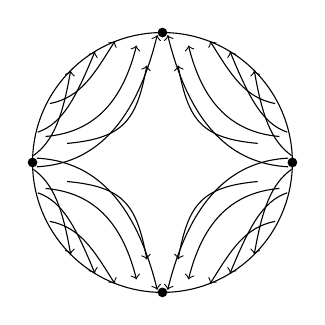
\begin{tikzpicture}[scale=1.1]
  % right figure: electric field lines (from +lambda at left/right to -lambda at top/bottom)
  \draw (0,0) circle (1.5);
  % quadrant I: lines from +lambda at (1.5,0) to -lambda at (0,1.5)
  \draw[->] (1.49,0.08) .. controls (1.25,0.25) and (1.15,0.55) .. (1.06,1.06);
  \draw[->] (1.44,0.35) .. controls (1.15,0.45) and (1.0,0.75) .. (0.78,1.28);
  \draw[->] (1.30,0.68) .. controls (0.95,0.75) and (0.80,1.0) .. (0.55,1.40);
  \draw[->] (1.35,0.30) .. controls (0.75,0.35) and (0.45,0.75) .. (0.30,1.35);
  \draw[->] (1.10,0.22) .. controls (0.45,0.28) and (0.30,0.48) .. (0.18,1.12);
  \draw[->] (1.45,-0.05) .. controls (0.9,-0.02) and (0.35,0.30) .. (0.06,1.47);
  % quadrant II: from +lambda at (-1.5,0) to -lambda at (0,1.5)
  \draw[->] (-1.49,0.08) .. controls (-1.25,0.25) and (-1.15,0.55) .. (-1.06,1.06);
  \draw[->] (-1.44,0.35) .. controls (-1.15,0.45) and (-1.0,0.75) .. (-0.78,1.28);
  \draw[->] (-1.30,0.68) .. controls (-0.95,0.75) and (-0.80,1.0) .. (-0.55,1.40);
  \draw[->] (-1.35,0.30) .. controls (-0.75,0.35) and (-0.45,0.75) .. (-0.30,1.35);
  \draw[->] (-1.10,0.22) .. controls (-0.45,0.28) and (-0.30,0.48) .. (-0.18,1.12);
  \draw[->] (-1.45,-0.05) .. controls (-0.9,-0.02) and (-0.35,0.30) .. (-0.06,1.47);
  % quadrant III: from +lambda at (-1.5,0) to -lambda at (0,-1.5)
  \draw[->] (-1.49,-0.08) .. controls (-1.25,-0.25) and (-1.15,-0.55) .. (-1.06,-1.06);
  \draw[->] (-1.44,-0.35) .. controls (-1.15,-0.45) and (-1.0,-0.75) .. (-0.78,-1.28);
  \draw[->] (-1.30,-0.68) .. controls (-0.95,-0.75) and (-0.80,-1.0) .. (-0.55,-1.40);
  \draw[->] (-1.35,-0.30) .. controls (-0.75,-0.35) and (-0.45,-0.75) .. (-0.30,-1.35);
  \draw[->] (-1.10,-0.22) .. controls (-0.45,-0.28) and (-0.30,-0.48) .. (-0.18,-1.12);
  \draw[->] (-1.45,0.05) .. controls (-0.9,0.02) and (-0.35,-0.30) .. (-0.06,-1.47);
  % quadrant IV: from +lambda at (1.5,0) to -lambda at (0,-1.5)
  \draw[->] (1.49,-0.08) .. controls (1.25,-0.25) and (1.15,-0.55) .. (1.06,-1.06);
  \draw[->] (1.44,-0.35) .. controls (1.15,-0.45) and (1.0,-0.75) .. (0.78,-1.28);
  \draw[->] (1.30,-0.68) .. controls (0.95,-0.75) and (0.80,-1.0) .. (0.55,-1.40);
  \draw[->] (1.35,-0.30) .. controls (0.75,-0.35) and (0.45,-0.75) .. (0.30,-1.35);
  \draw[->] (1.10,-0.22) .. controls (0.45,-0.28) and (0.30,-0.48) .. (0.18,-1.12);
  \draw[->] (1.45,0.05) .. controls (0.9,0.02) and (0.35,-0.30) .. (0.06,-1.47);
  \fill (1.5,0) circle (1.6pt);
  \fill (-1.5,0) circle (1.6pt);
  \fill (0,1.5) circle (1.6pt);
  \fill (0,-1.5) circle (1.6pt);
\end{tikzpicture}
\par\vspace{0.5em}\textbf{Problem 2.20}
\end{center}

The charge density in two dimensions can be expressed as
\[
\sigma(\rho,\phi)=\frac{\lambda}{a}\sum_{n=0}^{3}(-1)^{n}\,\delta(\rho-a)\,\delta(\phi-n\pi/2)
\]
\begin{enumerate}
\item[(a)] Using the Green function expansion from Problem 2.17c, show that the electrostatic potential is
\[
\Phi(\rho,\phi)=\frac{\lambda}{\pi\epsilon_{0}}\sum_{k=0}^{\infty}\frac{1}{2k+1}\left(\frac{\rho_{<}}{\rho_{>}}\right)^{4k+2}\cos[(4k+2)\,\phi]
\]
\item[(b)] Relate the solution of part a to the real part of the complex function
\[
w(z)=\frac{2\lambda}{4\pi\epsilon_{0}}\ln\left[\frac{(z-ia)(z+ia)}{(z-a)(z+a)}\right]
\]
where $z=x+iy=\rho e^{i\phi}$. Comment on the connection to Problem 2.3.
\item[(c)] Find expressions for the Cartesian components of the electric field near the origin, expressed in terms of $x$ and $y$. Keep the $k=0$ and $k=1$ terms in the expansion. For $y=0$ what is the relative magnitude of the $k=1$ ($2^{6}$-pole) contribution to $E_{x}$ compared to the $k=0$ ($2^{2}$-pole or quadrupole) term?
\end{enumerate}
\solution
\textbf{(a)} The source integral has measure $\rho'\,d\rho'\,d\phi'$,
so the factor $\lambda/a$ in the density assigns line charge
$(-1)^n\lambda$ to each point on $\rho'=a$. Their total charge is
zero, eliminating the logarithmic zero mode of $G$. The angular sum is
\[
\sum_{n=0}^3(-1)^n e^{-imn\pi/2}
=\begin{cases}4,&m=4k+2,\\0,&\text{otherwise}.
\end{cases}
\]
Indeed it is the four-term geometric sum with ratio $-e^{-im\pi/2}$,
which is zero unless the ratio is one. With
$t=\min(\rho,a)/\max(\rho,a)$, the remaining Green-function terms give
\[
\Phi=\frac{\lambda}{4\pi\epsilon _0}
       2\sum_{k\geq0}\frac{4t^{4k+2}}{4k+2}\cos[(4k+2)\phi]
=\boxed{\frac{\lambda}{\pi\epsilon _0}\sum_{k\geq0}
       \frac{t^{4k+2}}{2k+1}\cos[(4k+2)\phi].}
\]
\textbf{(b)} Taking the real part of the stated analytic function
uses $\operatorname{Re}\ln(z-z_j)=\ln|z-z_j|$ and gives
\[
\operatorname{Re}w=\frac{\lambda}{2\pi\epsilon _0}
 \ln\frac{|z-ia|\,|z+ia|}{|z-a|\,|z+a|},
\]
which is the sum of the four line-charge potentials. For $|z|<a$,
\[
\ln\frac{z^2+a^2}{z^2-a^2}
=\text{pure imaginary constant}
 +\ln\frac{1+z^2/a^2}{1-z^2/a^2}
=\text{constant}+2\sum_{k\geq0}\frac{(z/a)^{4k+2}}{2k+1}.
\]
For $|z|>a$ expand in $a^2/z^2$ instead; its real part has the same
cosines. These two expansions reproduce part (a).
The four alternating line sources are the same image construction
as in Problem 2.3 when $x_0=y_0$, after rotating the axes by $\pi/4$
and choosing the corresponding length scale. Here the zero-potential
planes are the diagonals between the charged axes.
\textbf{(c)} Keeping $k=0,1$ inside the source circle gives
\[
\Phi=\frac{\lambda}{\pi\epsilon _0}
 \left[\frac{x^2-y^2}{a^2}
 +\frac{x^6-15x^4y^2+15x^2y^4-y^6}{3a^6}
 +O(\rho^{10}/a^{10})\right].
\]
Termwise Cartesian differentiation gives
\[
\boxed{\begin{aligned}
E_x&=-\frac{2\lambda}{\pi\epsilon _0a^2}
 \left[x+\frac{x^5-10x^3y^2+5xy^4}{a^4}\right]
 +O\!\left(\frac{\lambda\rho^9}{\epsilon _0a^{10}}\right),\\
E_y&=\frac{2\lambda}{\pi\epsilon _0a^2}
 \left[y+\frac{5x^4y-10x^2y^3+y^5}{a^4}\right]
 +O\!\left(\frac{\lambda\rho^9}{\epsilon _0a^{10}}\right).
\end{aligned}}
\]
On $y=0$ their two $E_x$ contributions have the same sign and
\[
\boxed{\left|\frac{E_x^{(k=1)}}{E_x^{(k=0)}}\right|=(x/a)^4}
\]
for $x\ne0$, with limiting ratio zero at the origin.

\Needspace{5\baselineskip}
\par\bigskip
\noindent\textbf{2.21}\quad Use Cauchy's theorem to derive the Poisson integral solution. Cauchy's theorem states that if $F(z)$ is analytic in a region $R$ bounded by a closed curve $C$, then
\[
\frac{1}{2\pi i}\oint_{C}\frac{F(z')\;dz'}{z'-z}=\begin{cases}F(z) & \text{if $z$ is inside } R\\ 0 & \text{outside}\end{cases}
\]
\emph{Hint}: You may wish to add an integral that vanishes (associated with the image point) to the integral for the point inside the circle.
\solution
Let $F$ be analytic in the disk $|\zeta|<b$, continuous on its
boundary, and let $\Phi=\operatorname{Re}F$. Fix an interior point
$z$ and its exterior image $z_i=b^2/\bar z$. By Cauchy's formula,
\[
F(z)=\frac1{2\pi i}\oint_{|\zeta|=b}
 F(\zeta)\left[\frac1{\zeta-z}-\frac1{\zeta-z_i}\right]d\zeta.
\]
The second integral is zero because its pole is outside the disk.
Put $\zeta=be^{i\phi'}$, $d\zeta=i\zeta\,d\phi'$. Since
$\zeta\bar\zeta=b^2$ on the contour,
\[
-\frac\zeta{\zeta-b^2/\bar z}
=\frac{\bar z}{\bar\zeta-\bar z}.
\]
Consequently the two kernels combine to a real quantity:
\begin{align*}
\frac\zeta{\zeta-z}+\frac{\bar z}{\bar\zeta-\bar z}
&=\frac{\zeta(\bar\zeta-\bar z)+\bar z(\zeta-z)}{|\zeta-z|^2}\\
&=\frac{b^2-|z|^2}{|\zeta-z|^2}.
\end{align*}
Taking real parts now removes the otherwise unknown harmonic
conjugate of the boundary potential. With $z=\rho e^{i\phi}$,
\[
\boxed{\Phi(\rho,\phi)=\frac1{2\pi}\int_0^{2\pi}
 \Phi(b,\phi')\frac{b^2-\rho^2}
 {b^2+\rho^2-2b\rho\cos(\phi-\phi')}\,d\phi'.}
\]
At $z=0$ the image is understood as a limit at infinity and the
kernel is one, giving the average boundary value. Every harmonic
potential in the simply connected disk has a harmonic conjugate,
so this establishes the Poisson formula for the stated Dirichlet
problem; piecewise boundary data follow by taking interior limits.

\Needspace{5\baselineskip}
\par\bigskip
\noindent\textbf{2.22}\quad\begin{enumerate}
\item[(a)] For the example of oppositely charged conducting hemispherical shells separated by a tiny gap, as shown in Figure 2.8, show that the interior potential ($r<a$) on the $z$ axis is
\[
\Phi_{\mathrm{in}}(z)=V\,\frac{a}{z}\left[1-\frac{(a^{2}-z^{2})}{a\sqrt{a^{2}+z^{2}}}\right]
\]
Find the first few terms of the expansion in powers of $z$ and show that they agree with (2.27) with the appropriate substitutions.
\item[(b)] From the result of part a and (2.22), show that the \erratum{axial electric field $E_z$ (equal to $E_r$ on the positive $z$ axis)} is
\[
\erratum{E_{z}}(z)=\frac{Va^{2}}{(z^{2}+a^{2})^{3/2}}\left(3+\frac{a^{2}}{z^{2}}\right)
\]
for $z>a$, and
\[
\erratum{E_{z}}(z)=-\frac{V}{a}\left[\frac{3+(a/z)^{2}}{(1+(z/a)^{2})^{3/2}}-\frac{a^{2}}{z^{2}}\right]
\]
for $|z|<a$. Show that the second form is well behaved at the origin, with the value $\erratum{E_{z}}(0)=-3V/2a$. Show that at $z=a$ (north pole inside) it has the value $-(\sqrt{2}-1)V/a$. Show that the radial field at the north pole outside has the value $\sqrt{2}\,V/a$.
\item[(c)] Make a sketch of the electric field lines, both inside and outside the conducting hemispheres, with directions indicated. Make a \emph{plot} of the \erratum{axial electric field $E_z$} along the $z$ axis from $z=-2a$ to $z=+2a$.
\end{enumerate}
\solution
The northern hemisphere is at $+V$ and the southern at $-V$.
\textbf{(a)} The interior spherical Poisson kernel gives, on the axis,
\[
\Phi_{\rm in}(z)=\frac{Va(a^2-z^2)}2
 \int_{-1}^{1}\frac{\operatorname{sgn}u\,du}
                 {(a^2+z^2-2azu)^{3/2}},\qquad |z|<a.
\]
For $z\ne0$, the integral is
\[
\frac1{az}\left[\frac1{a-z}+\frac1{a+z}
                              -\frac2{\sqrt{a^2+z^2}}\right].
\]
Combining the first two fractions before multiplying the prefactor
therefore gives
\[
\boxed{\Phi_{\rm in}(z)=\frac{Va}{z}
 \left[1-\frac{a^2-z^2}{a\sqrt{a^2+z^2}}\right].}
\]
Put $t=z/a$ and expand
$(1+t^2)^{-1/2}=1-t^2/2+3t^4/8-5t^6/16+35t^8/128+\cdots$.
Multiplication by $1-t^2$ and division by $t$ give
\[
\frac{\Phi_{\rm in}}V=\frac32t-\frac78t^3+\frac{11}{16}t^5
                              -\frac{75}{128}t^7+O(t^9).
\]
The interior and exterior harmonic expansions are related by Kelvin
inversion,
$\Phi_{\rm out}(r,\theta)=(a/r)\Phi_{\rm in}(a^2/r,\theta)$.
Thus the exterior terms are
$V[\tfrac32(a/r)^2P_1(\cos\theta)
-\tfrac78(a/r)^4P_3(\cos\theta)+\cdots]$.
On the positive axis $P_l(1)=1$, so the replacements
$(a/r)^{l+1}\mapsto(r/a)^l$ recover the interior coefficients above
from (2.27).

\textbf{(b)} Differentiating the interior expression at fixed sign
of $z$ gives the axial component
\[
\boxed{E_z^{\rm in}(z)=-\frac Va
 \left[\frac{3+(a/z)^2}{[1+(z/a)^2]^{3/2}}-\frac{a^2}{z^2}\right].}
\]
Its apparently singular terms cancel. In fact differentiating the
power series gives
\[
E_z^{\rm in}(z)=\frac Va\left[-\frac32+\frac{21}{8}t^2
                     -\frac{55}{16}t^4+\frac{525}{128}t^6+O(t^8)\right].
\]
The origin value is therefore $-3V/(2a)$.
The exterior positive-axis potential (2.22), also obtained by the
inversion above, is
\[
\Phi_{\rm out}(z)=V\left[1-
             \frac{z^2-a^2}{z\sqrt{z^2+a^2}}\right],\quad z>a.
\]
Its derivative is
\[
\boxed{E_z^{\rm out}(z)=\frac{Va^2}{(z^2+a^2)^{3/2}}
                         \left(3+\frac{a^2}{z^2}\right),\quad z>a.}
\]
On the positive axis $E_z=E_r$. At the north pole the limiting
values are $E_r(a^-)=-\left(\sqrt2-1\right)V/a$ and
$E_r(a^+)=\sqrt2 V/a$, agreeing with the question. Their difference
is $(2\sqrt2-1)V/a$, the surface charge divided by $\epsilon _0$.

\textbf{(c)} Antisymmetry of the potential,
$\Phi(-z)=-\Phi(z)$, implies $E_z(-z)=E_z(z)$. The radial basis
vector reverses on the negative axis, so strictly
$E_r(z)=\operatorname{sgn}(z)E_z(z)$ for $z\ne0$; $E_r$ has no
single basis direction at the origin. The finite origin value is the continuous \emph{axial} component;
the statement uses corrected notation to make this distinction explicit. The plot shows that
component together with the true radial component on the negative
axis, where they differ. Fields jump at $z=\pm a$; there is no field
value inside an ideal zero-thickness metal surface itself.
\begin{center}
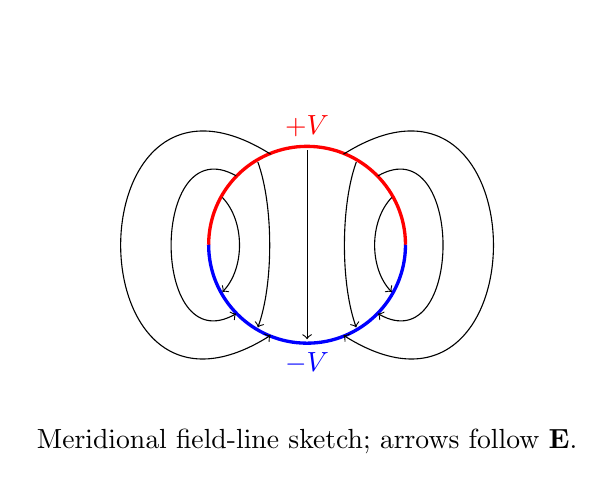
\begin{tikzpicture}[scale=1.25]
\draw[very thick,red] (0:1) arc (0:180:1);
\draw[very thick,blue] (180:1) arc (180:360:1);
\node[red,above] at (0,1) {$+V$};\node[blue,below] at (0,-1) {$-V$};
\draw[->] (0,.96)--(0,-.96);
\foreach \s in {-1,1} {
 \draw[->] ({\s*.5},.84) .. controls ({\s*.34},.4) and ({\s*.34},-.4) .. ({\s*.5},-.84);
 \draw[->] ({\s*.86},.48) .. controls ({\s*.63},.24) and ({\s*.63},-.24) .. ({\s*.86},-.48);
 \draw[->] ({\s*.72},.70) .. controls ({\s*1.6},1.20) and ({\s*1.6},-1.20) .. ({\s*.72},-.70);
 \draw[->] ({\s*.37},.92) .. controls ({\s*2.4},2.2) and ({\s*2.4},-2.2) .. ({\s*.37},-.92);
}
\node at (0,-2.0) {Meridional field-line sketch; arrows follow $\mathbf E$.};
\end{tikzpicture}
\par\medskip
% Generated by supplementary/check_ch02.py --write-assets
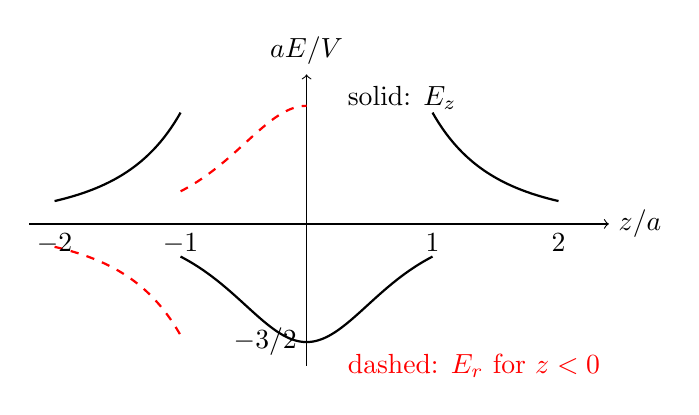
\begin{tikzpicture}[x=1.6cm,y=1cm]
\draw[->] (-2.2,0)--(2.4,0) node[right] {$z/a$};
\draw[->] (0,-1.8)--(0,1.9) node[above] {$aE/V$};
\draw[black,thick] plot coordinates {(-2.000000,0.290689) (-1.989899,0.294470) (-1.979798,0.298314) (-1.969697,0.302223) (-1.959596,0.306198) (-1.949495,0.310241) (-1.939394,0.314353) (-1.929293,0.318535) (-1.919192,0.322789) (-1.909091,0.327116) (-1.898990,0.331518) (-1.888889,0.335997) (-1.878788,0.340554) (-1.868687,0.345190) (-1.858586,0.349908) (-1.848485,0.354708) (-1.838384,0.359594) (-1.828283,0.364567) (-1.818182,0.369628) (-1.808081,0.374779) (-1.797980,0.380023) (-1.787879,0.385361) (-1.777778,0.390796) (-1.767677,0.396330) (-1.757576,0.401964) (-1.747475,0.407702) (-1.737374,0.413545) (-1.727273,0.419495) (-1.717172,0.425556) (-1.707071,0.431729) (-1.696970,0.438017) (-1.686869,0.444423) (-1.676768,0.450949) (-1.666667,0.457599) (-1.656566,0.464374) (-1.646465,0.471278) (-1.636364,0.478314) (-1.626263,0.485485) (-1.616162,0.492794) (-1.606061,0.500244) (-1.595960,0.507838) (-1.585859,0.515581) (-1.575758,0.523475) (-1.565657,0.531524) (-1.555556,0.539732) (-1.545455,0.548102) (-1.535354,0.556639) (-1.525253,0.565346) (-1.515152,0.574228) (-1.505051,0.583289) (-1.494949,0.592533) (-1.484848,0.601964) (-1.474747,0.611589) (-1.464646,0.621410) (-1.454545,0.631434) (-1.444444,0.641665) (-1.434343,0.652108) (-1.424242,0.662769) (-1.414141,0.673654) (-1.404040,0.684768) (-1.393939,0.696116) (-1.383838,0.707706) (-1.373737,0.719544) (-1.363636,0.731635) (-1.353535,0.743987) (-1.343434,0.756606) (-1.333333,0.769500) (-1.323232,0.782676) (-1.313131,0.796141) (-1.303030,0.809904) (-1.292929,0.823972) (-1.282828,0.838355) (-1.272727,0.853060) (-1.262626,0.868096) (-1.252525,0.883473) (-1.242424,0.899201) (-1.232323,0.915289) (-1.222222,0.931747) (-1.212121,0.948587) (-1.202020,0.965819) (-1.191919,0.983455) (-1.181818,1.001507) (-1.171717,1.019987) (-1.161616,1.038907) (-1.151515,1.058282) (-1.141414,1.078124) (-1.131313,1.098448) (-1.121212,1.119270) (-1.111111,1.140603) (-1.101010,1.162466) (-1.090909,1.184873) (-1.080808,1.207843) (-1.070707,1.231395) (-1.060606,1.255545) (-1.050505,1.280316) (-1.040404,1.305726) (-1.030303,1.331798) (-1.020202,1.358554) (-1.010101,1.386018) (-1.000000,1.414214)};
\draw[red,dashed,thick] plot coordinates {(-2.000000,-0.290689) (-1.989899,-0.294470) (-1.979798,-0.298314) (-1.969697,-0.302223) (-1.959596,-0.306198) (-1.949495,-0.310241) (-1.939394,-0.314353) (-1.929293,-0.318535) (-1.919192,-0.322789) (-1.909091,-0.327116) (-1.898990,-0.331518) (-1.888889,-0.335997) (-1.878788,-0.340554) (-1.868687,-0.345190) (-1.858586,-0.349908) (-1.848485,-0.354708) (-1.838384,-0.359594) (-1.828283,-0.364567) (-1.818182,-0.369628) (-1.808081,-0.374779) (-1.797980,-0.380023) (-1.787879,-0.385361) (-1.777778,-0.390796) (-1.767677,-0.396330) (-1.757576,-0.401964) (-1.747475,-0.407702) (-1.737374,-0.413545) (-1.727273,-0.419495) (-1.717172,-0.425556) (-1.707071,-0.431729) (-1.696970,-0.438017) (-1.686869,-0.444423) (-1.676768,-0.450949) (-1.666667,-0.457599) (-1.656566,-0.464374) (-1.646465,-0.471278) (-1.636364,-0.478314) (-1.626263,-0.485485) (-1.616162,-0.492794) (-1.606061,-0.500244) (-1.595960,-0.507838) (-1.585859,-0.515581) (-1.575758,-0.523475) (-1.565657,-0.531524) (-1.555556,-0.539732) (-1.545455,-0.548102) (-1.535354,-0.556639) (-1.525253,-0.565346) (-1.515152,-0.574228) (-1.505051,-0.583289) (-1.494949,-0.592533) (-1.484848,-0.601964) (-1.474747,-0.611589) (-1.464646,-0.621410) (-1.454545,-0.631434) (-1.444444,-0.641665) (-1.434343,-0.652108) (-1.424242,-0.662769) (-1.414141,-0.673654) (-1.404040,-0.684768) (-1.393939,-0.696116) (-1.383838,-0.707706) (-1.373737,-0.719544) (-1.363636,-0.731635) (-1.353535,-0.743987) (-1.343434,-0.756606) (-1.333333,-0.769500) (-1.323232,-0.782676) (-1.313131,-0.796141) (-1.303030,-0.809904) (-1.292929,-0.823972) (-1.282828,-0.838355) (-1.272727,-0.853060) (-1.262626,-0.868096) (-1.252525,-0.883473) (-1.242424,-0.899201) (-1.232323,-0.915289) (-1.222222,-0.931747) (-1.212121,-0.948587) (-1.202020,-0.965819) (-1.191919,-0.983455) (-1.181818,-1.001507) (-1.171717,-1.019987) (-1.161616,-1.038907) (-1.151515,-1.058282) (-1.141414,-1.078124) (-1.131313,-1.098448) (-1.121212,-1.119270) (-1.111111,-1.140603) (-1.101010,-1.162466) (-1.090909,-1.184873) (-1.080808,-1.207843) (-1.070707,-1.231395) (-1.060606,-1.255545) (-1.050505,-1.280316) (-1.040404,-1.305726) (-1.030303,-1.331798) (-1.020202,-1.358554) (-1.010101,-1.386018) (-1.000000,-1.414214)};
\draw[black,thick] plot coordinates {(-0.999999,-0.414214) (-0.989898,-0.422655) (-0.979797,-0.431243) (-0.969696,-0.439979) (-0.959595,-0.448865) (-0.949494,-0.457901) (-0.939393,-0.467090) (-0.929292,-0.476432) (-0.919191,-0.485928) (-0.909090,-0.495579) (-0.898989,-0.505387) (-0.888888,-0.515352) (-0.878787,-0.525475) (-0.868686,-0.535756) (-0.858585,-0.546196) (-0.848484,-0.556795) (-0.838383,-0.567554) (-0.828282,-0.578471) (-0.818181,-0.589548) (-0.808080,-0.600784) (-0.797979,-0.612179) (-0.787878,-0.623732) (-0.777777,-0.635442) (-0.767676,-0.647308) (-0.757575,-0.659329) (-0.747474,-0.671503) (-0.737373,-0.683830) (-0.727272,-0.696307) (-0.717171,-0.708932) (-0.707070,-0.721702) (-0.696969,-0.734616) (-0.686868,-0.747669) (-0.676767,-0.760860) (-0.666666,-0.774184) (-0.656565,-0.787637) (-0.646464,-0.801217) (-0.636363,-0.814917) (-0.626262,-0.828735) (-0.616161,-0.842663) (-0.606060,-0.856698) (-0.595959,-0.870832) (-0.585858,-0.885061) (-0.575757,-0.899378) (-0.565656,-0.913776) (-0.555555,-0.928247) (-0.545454,-0.942784) (-0.535353,-0.957379) (-0.525252,-0.972023) (-0.515151,-0.986709) (-0.505050,-1.001426) (-0.494949,-1.016165) (-0.484848,-1.030916) (-0.474747,-1.045669) (-0.464646,-1.060414) (-0.454545,-1.075138) (-0.444444,-1.089831) (-0.434343,-1.104481) (-0.424242,-1.119076) (-0.414141,-1.133603) (-0.404040,-1.148049) (-0.393939,-1.162401) (-0.383838,-1.176647) (-0.373737,-1.190771) (-0.363636,-1.204761) (-0.353535,-1.218602) (-0.343434,-1.232280) (-0.333333,-1.245780) (-0.323232,-1.259087) (-0.313131,-1.272188) (-0.303030,-1.285065) (-0.292929,-1.297706) (-0.282828,-1.310094) (-0.272727,-1.322214) (-0.262626,-1.334053) (-0.252525,-1.345594) (-0.242424,-1.356823) (-0.232323,-1.367725) (-0.222222,-1.378286) (-0.212121,-1.388491) (-0.202020,-1.398327) (-0.191919,-1.407780) (-0.181818,-1.416837) (-0.171717,-1.425484) (-0.161616,-1.433710) (-0.151515,-1.441502) (-0.141414,-1.448848) (-0.131313,-1.455738) (-0.121212,-1.462162) (-0.111111,-1.468109) (-0.101010,-1.473571) (-0.090909,-1.478538) (-0.080808,-1.483004) (-0.070707,-1.486962) (-0.060606,-1.490404) (-0.050505,-1.493327) (-0.040404,-1.495724) (-0.030303,-1.497592) (-0.020202,-1.498929) (-0.010101,-1.499732) (0.000000,-1.500000)};
\draw[red,dashed,thick] plot coordinates {(-0.999999,0.414214) (-0.989898,0.422655) (-0.979797,0.431243) (-0.969696,0.439979) (-0.959595,0.448865) (-0.949494,0.457901) (-0.939393,0.467090) (-0.929292,0.476432) (-0.919191,0.485928) (-0.909090,0.495579) (-0.898989,0.505387) (-0.888888,0.515352) (-0.878787,0.525475) (-0.868686,0.535756) (-0.858585,0.546196) (-0.848484,0.556795) (-0.838383,0.567554) (-0.828282,0.578471) (-0.818181,0.589548) (-0.808080,0.600784) (-0.797979,0.612179) (-0.787878,0.623732) (-0.777777,0.635442) (-0.767676,0.647308) (-0.757575,0.659329) (-0.747474,0.671503) (-0.737373,0.683830) (-0.727272,0.696307) (-0.717171,0.708932) (-0.707070,0.721702) (-0.696969,0.734616) (-0.686868,0.747669) (-0.676767,0.760860) (-0.666666,0.774184) (-0.656565,0.787637) (-0.646464,0.801217) (-0.636363,0.814917) (-0.626262,0.828735) (-0.616161,0.842663) (-0.606060,0.856698) (-0.595959,0.870832) (-0.585858,0.885061) (-0.575757,0.899378) (-0.565656,0.913776) (-0.555555,0.928247) (-0.545454,0.942784) (-0.535353,0.957379) (-0.525252,0.972023) (-0.515151,0.986709) (-0.505050,1.001426) (-0.494949,1.016165) (-0.484848,1.030916) (-0.474747,1.045669) (-0.464646,1.060414) (-0.454545,1.075138) (-0.444444,1.089831) (-0.434343,1.104481) (-0.424242,1.119076) (-0.414141,1.133603) (-0.404040,1.148049) (-0.393939,1.162401) (-0.383838,1.176647) (-0.373737,1.190771) (-0.363636,1.204761) (-0.353535,1.218602) (-0.343434,1.232280) (-0.333333,1.245780) (-0.323232,1.259087) (-0.313131,1.272188) (-0.303030,1.285065) (-0.292929,1.297706) (-0.282828,1.310094) (-0.272727,1.322214) (-0.262626,1.334053) (-0.252525,1.345594) (-0.242424,1.356823) (-0.232323,1.367725) (-0.222222,1.378286) (-0.212121,1.388491) (-0.202020,1.398327) (-0.191919,1.407780) (-0.181818,1.416837) (-0.171717,1.425484) (-0.161616,1.433710) (-0.151515,1.441502) (-0.141414,1.448848) (-0.131313,1.455738) (-0.121212,1.462162) (-0.111111,1.468109) (-0.101010,1.473571) (-0.090909,1.478538) (-0.080808,1.483004) (-0.070707,1.486962) (-0.060606,1.490404) (-0.050505,1.493327) (-0.040404,1.495724) (-0.030303,1.497592) (-0.020202,1.498929) (-0.010101,1.499732) (0.000000,1.500000)};
\draw[black,thick] plot coordinates {(0.000000,-1.500000) (0.010101,-1.499732) (0.020202,-1.498929) (0.030303,-1.497592) (0.040404,-1.495724) (0.050505,-1.493327) (0.060606,-1.490404) (0.070707,-1.486962) (0.080808,-1.483004) (0.090909,-1.478538) (0.101010,-1.473571) (0.111111,-1.468109) (0.121212,-1.462162) (0.131313,-1.455738) (0.141414,-1.448848) (0.151515,-1.441502) (0.161616,-1.433710) (0.171717,-1.425484) (0.181818,-1.416837) (0.191919,-1.407780) (0.202020,-1.398327) (0.212121,-1.388491) (0.222222,-1.378286) (0.232323,-1.367725) (0.242424,-1.356823) (0.252525,-1.345594) (0.262626,-1.334053) (0.272727,-1.322214) (0.282828,-1.310094) (0.292929,-1.297706) (0.303030,-1.285065) (0.313131,-1.272188) (0.323232,-1.259087) (0.333333,-1.245780) (0.343434,-1.232280) (0.353535,-1.218602) (0.363636,-1.204761) (0.373737,-1.190771) (0.383838,-1.176647) (0.393939,-1.162401) (0.404040,-1.148049) (0.414141,-1.133603) (0.424242,-1.119076) (0.434343,-1.104481) (0.444444,-1.089831) (0.454545,-1.075138) (0.464646,-1.060414) (0.474747,-1.045669) (0.484848,-1.030916) (0.494949,-1.016165) (0.505050,-1.001426) (0.515151,-0.986709) (0.525252,-0.972023) (0.535353,-0.957379) (0.545454,-0.942784) (0.555555,-0.928247) (0.565656,-0.913776) (0.575757,-0.899378) (0.585858,-0.885061) (0.595959,-0.870832) (0.606060,-0.856698) (0.616161,-0.842663) (0.626262,-0.828735) (0.636363,-0.814917) (0.646464,-0.801217) (0.656565,-0.787637) (0.666666,-0.774184) (0.676767,-0.760860) (0.686868,-0.747669) (0.696969,-0.734616) (0.707070,-0.721702) (0.717171,-0.708932) (0.727272,-0.696307) (0.737373,-0.683830) (0.747474,-0.671503) (0.757575,-0.659329) (0.767676,-0.647308) (0.777777,-0.635442) (0.787878,-0.623732) (0.797979,-0.612179) (0.808080,-0.600784) (0.818181,-0.589548) (0.828282,-0.578471) (0.838383,-0.567554) (0.848484,-0.556795) (0.858585,-0.546196) (0.868686,-0.535756) (0.878787,-0.525475) (0.888888,-0.515352) (0.898989,-0.505387) (0.909090,-0.495579) (0.919191,-0.485928) (0.929292,-0.476432) (0.939393,-0.467090) (0.949494,-0.457901) (0.959595,-0.448865) (0.969696,-0.439979) (0.979797,-0.431243) (0.989898,-0.422655) (0.999999,-0.414214)};
\draw[black,thick] plot coordinates {(1.000000,1.414214) (1.010101,1.386018) (1.020202,1.358554) (1.030303,1.331798) (1.040404,1.305726) (1.050505,1.280316) (1.060606,1.255545) (1.070707,1.231395) (1.080808,1.207843) (1.090909,1.184873) (1.101010,1.162466) (1.111111,1.140603) (1.121212,1.119270) (1.131313,1.098448) (1.141414,1.078124) (1.151515,1.058282) (1.161616,1.038907) (1.171717,1.019987) (1.181818,1.001507) (1.191919,0.983455) (1.202020,0.965819) (1.212121,0.948587) (1.222222,0.931747) (1.232323,0.915289) (1.242424,0.899201) (1.252525,0.883473) (1.262626,0.868096) (1.272727,0.853060) (1.282828,0.838355) (1.292929,0.823972) (1.303030,0.809904) (1.313131,0.796141) (1.323232,0.782676) (1.333333,0.769500) (1.343434,0.756606) (1.353535,0.743987) (1.363636,0.731635) (1.373737,0.719544) (1.383838,0.707706) (1.393939,0.696116) (1.404040,0.684768) (1.414141,0.673654) (1.424242,0.662769) (1.434343,0.652108) (1.444444,0.641665) (1.454545,0.631434) (1.464646,0.621410) (1.474747,0.611589) (1.484848,0.601964) (1.494949,0.592533) (1.505051,0.583289) (1.515152,0.574228) (1.525253,0.565346) (1.535354,0.556639) (1.545455,0.548102) (1.555556,0.539732) (1.565657,0.531524) (1.575758,0.523475) (1.585859,0.515581) (1.595960,0.507838) (1.606061,0.500244) (1.616162,0.492794) (1.626263,0.485485) (1.636364,0.478314) (1.646465,0.471278) (1.656566,0.464374) (1.666667,0.457599) (1.676768,0.450949) (1.686869,0.444423) (1.696970,0.438017) (1.707071,0.431729) (1.717172,0.425556) (1.727273,0.419495) (1.737374,0.413545) (1.747475,0.407702) (1.757576,0.401964) (1.767677,0.396330) (1.777778,0.390796) (1.787879,0.385361) (1.797980,0.380023) (1.808081,0.374779) (1.818182,0.369628) (1.828283,0.364567) (1.838384,0.359594) (1.848485,0.354708) (1.858586,0.349908) (1.868687,0.345190) (1.878788,0.340554) (1.888889,0.335997) (1.898990,0.331518) (1.909091,0.327116) (1.919192,0.322789) (1.929293,0.318535) (1.939394,0.314353) (1.949495,0.310241) (1.959596,0.306198) (1.969697,0.302223) (1.979798,0.298314) (1.989899,0.294470) (2.000000,0.290689)};
\node[below] at (-2,0) {$ -2 $};
\node[below] at (-1,0) {$ -1 $};
\node[below] at (1,0) {$ 1 $};
\node[below] at (2,0) {$ 2 $};
\node[left] at (0,-1.5) {$-3/2$};
\node[right] at (.25,1.6) {solid: $E_z$};
\node[red,right] at (.25,-1.8) {dashed: $E_r$ for $z<0$};
\end{tikzpicture}

\end{center}
The inside lines run from the northern to the southern inner face;
the outside lines connect the outer faces around the shell. The
sketch illustrates topology; the accompanying axial curves use the
exact formulas above.

\Needspace{5\baselineskip}
\par\bigskip
\noindent\textbf{2.23}\quad A hollow cube has conducting walls defined by six planes $x=0$, $y=0$, $z=0$, and $x=a$, $y=a$, $z=a$. The walls $z=0$ and $z=a$ are held at a constant potential $V$. The other four sides are at zero potential.
\begin{enumerate}
\item[(a)] Find the potential $\Phi(x,y,z)$ at any point inside the cube.
\item[(b)] Evaluate the potential at the center of the cube numerically, accurate to three significant figures. How many terms in the series is it necessary to keep in order to attain this accuracy? Compare your numerical result with the average value of the potential on the walls. See Problem 2.28.
\item[(c)] Find the surface-charge density on the surface $z=a$.
\end{enumerate}
\solution
\textbf{(a)} The four grounded side walls select
$\sin(m\pi x/a)\sin(n\pi y/a)$. For a fixed pair the remaining
separation equation is $Z''-k_{mn}^2Z=0$, where
$k_{mn}=\pi\sqrt{m^2+n^2}/a$. Equal values at $z=0,a$ select
$Z=\cosh[k_{mn}(z-a/2)]/\cosh(k_{mn}a/2)$.
The double sine coefficients of a constant on a square are
\[
\frac4{a^2}\int_0^a\!dx\int_0^a\!dy\,
 V\sin\frac{m\pi x}a\sin\frac{n\pi y}a
=\frac{4V[1-(-1)^m][1-(-1)^n]}{mn\pi^2}.
\]
Thus only odd $m,n$ occur, and
\[
\boxed{\Phi=\frac{16V}{\pi^2}
 \sum_{\substack{m,n\geq1\\m,n\ {\rm odd}}}
 \frac{\sin(m\pi x/a)\sin(n\pi y/a)}{mn}
 \frac{\cosh[k_{mn}(z-a/2)]}{\cosh(k_{mn}a/2)}.}
\]
At the edges the imposed boundary data have different one-sided
limits; the interior solution and the values on open faces are
well defined.
\textbf{(b)} At the center, the two sines supply
$(-1)^{(m+n-2)/2}$. Summing all pairs with $m,n=1,3,\ldots,2N-1$
gives
\[
\begin{array}{c|c|c}
N&\text{number of pairs}&\Phi(a/2,a/2,a/2)/V\\\hline
1&1&0.347545849\\
2&4&0.332957715\\
3&9&0.333345107\\
4&16&0.333332938
\end{array}
\]
The four-pair truncation already rounds to $0.333$ to three
significant figures; it contains only three distinct values after
using $m\leftrightarrow n$ symmetry. There is also an exact check:
by cube symmetry the harmonic response at the center to each
unit-potential face is the same, and the sum of the six responses
is one. Two faces at $V$ therefore give
\[
\boxed{\Phi_{\rm center}=V/3,}
\]
exactly the average wall potential $(V+V)/6$. This proves the
accuracy of the reported truncation without inferring convergence
from successive partial sums alone.
\textbf{(c)} On the inner face $z=a$ the conductor-to-cavity normal
is $-\widehat{\mathbf z}$, giving
$\sigma=\epsilon _0\partial_z\Phi|_{a^-}$. Differentiation yields
\[
\boxed{\sigma(x,y)=\frac{16\epsilon _0V}{\pi^2}
 \sum_{\substack{m,n\geq1\\m,n\ {\rm odd}}}
 \frac{k_{mn}\tanh(k_{mn}a/2)}{mn}
       \sin\frac{m\pi x}a\sin\frac{n\pi y}a.}
\]
The derivative series is understood as its interior limit
$z\uparrow a$, or an equivalent Abel limit, away from edges; charge
crowding makes the ideal sharp-edge density singular. This determines
the cavity-facing charge only, since no exterior boundary problem
was specified.

\Needspace{5\baselineskip}
\par\bigskip
\noindent\textbf{2.24}\quad In the two-dimensional region shown in Fig.~2.12, the angular functions appropriate for Dirichlet boundary conditions at $\phi=0$ and $\phi=\beta$ are $\Phi(\phi)=A_{m}\sin(m\pi\phi/\beta)$. Show that the completeness relation for these functions is
\[
\delta(\phi-\phi')=\frac{2}{\beta}\sum_{m=1}^{\infty}\sin(m\pi\phi/\beta)\,\sin(m\pi\phi'/\beta)\qquad\text{for }0<\phi,\,\phi'<\beta
\]
\solution
For positive integers $m,n$, product-to-sum integration gives
\[
\int_0^\beta\sin\frac{m\pi\phi}\beta\sin\frac{n\pi\phi}\beta\,d\phi
=\frac\beta2\delta_{mn}.
\]
To show that the normalized modes are complete, take a smooth test
function $f$ with support in $(0,\beta)$, extend it oddly to
$(-\beta,\beta)$, and periodically with period $2\beta$.
The ordinary Fourier expansion of this odd function contains only
sines, with coefficients
\[
f_m=\frac2\beta\int_0^\beta f(\phi')
                    \sin\frac{m\pi\phi'}\beta\,d\phi'.
\]
Substituting these coefficients back into the Fourier series yields
\[
f(\phi)=\int_0^\beta\left[\frac2\beta\sum_{m=1}^\infty
 \sin\frac{m\pi\phi}\beta\sin\frac{m\pi\phi'}\beta\right]
 f(\phi')\,d\phi'.
\]
The bracket therefore has precisely the action of the delta
function on every such test function:
\[
\boxed{\delta(\phi-\phi')=\frac2\beta\sum_{m=1}^\infty
 \sin\frac{m\pi\phi}\beta\sin\frac{m\pi\phi'}\beta.}
\]
This is a distributional completeness relation for interior points,
not a pointwise convergent numerical series for the delta function.
The restriction away from the endpoints avoids the half-weight
endpoint convention of Fourier boundary limits.

\Needspace{5\baselineskip}
\par\bigskip
\noindent\textbf{2.25}\quad Two conducting planes at zero potential meet along the $z$ axis, making an angle $\beta$ between them, as in Fig.~2.12. A unit line charge parallel to the $z$ axis is located between the planes at position $(\rho',\phi')$.
\begin{enumerate}
\item[(a)] Show that $(4\pi\epsilon_{0})$ times the potential in the space between the planes, that is, the Dirichlet Green function $G(\rho,\phi;\rho',\phi')$, is given by the infinite series
\[
G(\rho,\phi;\rho',\phi')=4\sum_{m=1}^{\infty}\frac{1}{m}\,\rho_{<}^{m\pi/\beta}\rho_{>}^{-m\pi/\beta}\sin(m\pi\phi/\beta)\,\sin(m\pi\phi'/\beta)
\]
\item[(b)] By means of complex-variable techniques or other means, show that the series can be summed to give a closed form,
\[
G(\rho,\phi;\rho',\phi')=\ln\left\{\frac{(\rho)^{2\pi/\beta}+(\rho')^{2\pi/\beta}-2(\rho\rho')^{\pi/\beta}\cos[\pi(\phi+\phi')/\beta]}{(\rho)^{2\pi/\beta}+(\rho')^{2\pi/\beta}-2(\rho\rho')^{\pi/\beta}\cos[\pi(\phi-\phi')/\beta]}\right\}
\]
\item[(c)] Verify that you obtain the familiar results when $\beta=\pi$ and $\beta=\pi/2$.
\end{enumerate}
\solution
\textbf{(a)} With $\nu_m=m\pi/\beta$, expand
\[
G=\frac2\beta\sum_{m\geq1}g_m(\rho,\rho')
                      \sin(\nu_m\phi)\sin(\nu_m\phi').
\]
Using Problem 2.24, the radial equation is
\[
\frac1{\rho'}(\rho'g_m')'-\frac{\nu_m^2}{\rho'^2}g_m
 =-4\pi\frac{\delta(\rho'-\rho)}\rho.
\]
Boundedness at zero and decay at infinity select
$g_m=A_m\rho_<^{\nu_m}\rho_>^{-\nu_m}$.
The radial derivative jump is $-2\nu_mA_m=-4\pi$, so
$A_m=2\pi/\nu_m$. Multiplying by the angular normalization
$2/\beta$ gives
\[
\boxed{G=4\sum_{m=1}^\infty\frac1m
 \left(\frac{\rho_<}{\rho_>}\right)^{m\pi/\beta}
 \sin\frac{m\pi\phi}\beta\sin\frac{m\pi\phi'}\beta.}
\]
For unit line charge, $\Phi=G/(4\pi\epsilon _0)$.
\textbf{(b)} Put
$t=(\rho_</\rho_>)^{\pi/\beta}$,
$A=\pi\phi/\beta$, and $B=\pi\phi'/\beta$.
Since $2\sin mA\sin mB=\cos m(A-B)-\cos m(A+B)$ and
$\sum_{m\geq1}t^m\cos m\theta/m
=-\tfrac12\ln(1-2t\cos\theta+t^2)$,
\[
G=\ln\frac{1-2t\cos(A+B)+t^2}{1-2t\cos(A-B)+t^2}.
\]
Multiplication of numerator and denominator by
$\rho_>^{2\pi/\beta}$ yields exactly
\[
\boxed{G=\ln\frac{\rho^{2\pi/\beta}+\rho'^{2\pi/\beta}
 -2(\rho\rho')^{\pi/\beta}\cos[\pi(\phi+\phi')/\beta]}
 {\rho^{2\pi/\beta}+\rho'^{2\pi/\beta}
 -2(\rho\rho')^{\pi/\beta}\cos[\pi(\phi-\phi')/\beta]}.}
\]
Equivalently the analytic mapping $w=z^{\pi/\beta}$ sends the wedge
to the upper half-plane; the numerator is the squared distance to
the reflected source in that plane. Near the physical source the
analytic mapping is locally linear, so its scale cancels in the
ratio and the singular term remains $-\ln|z-z'|^2$.
\textbf{(c)} For $\beta=\pi$ the result is
$G=\ln[|z-\bar z'|^2/|z-z'|^2]$, the real line and its negative
mirror in a single plane. For $\beta=\pi/2$, factor the squares:
\[
G=\ln\frac{|z^2-\bar z'^2|^2}{|z^2-z'^2|^2}
 =\ln\frac{|z-\bar z'|^2|z+\bar z'|^2}
              {|z-z'|^2|z+z'|^2}.
\]
These are a positive source at $z'$, a positive image at $-z'$,
and negative images at $\bar z'$ and $-\bar z'$, exactly the
four-line construction of Problem 2.3.

\Needspace{5\baselineskip}
\par\bigskip
\noindent\textbf{2.26}\quad The two-dimensional region, $\rho\geq a$, $0\leq\phi\leq\beta$, is bounded by conducting surfaces at $\phi=0$, $\rho=a$, and $\phi=\beta$ held at zero potential, as indicated in the sketch. At large $\rho$ the potential is determined by some configuration of charges and/or conductors at fixed potentials.

\begin{center}
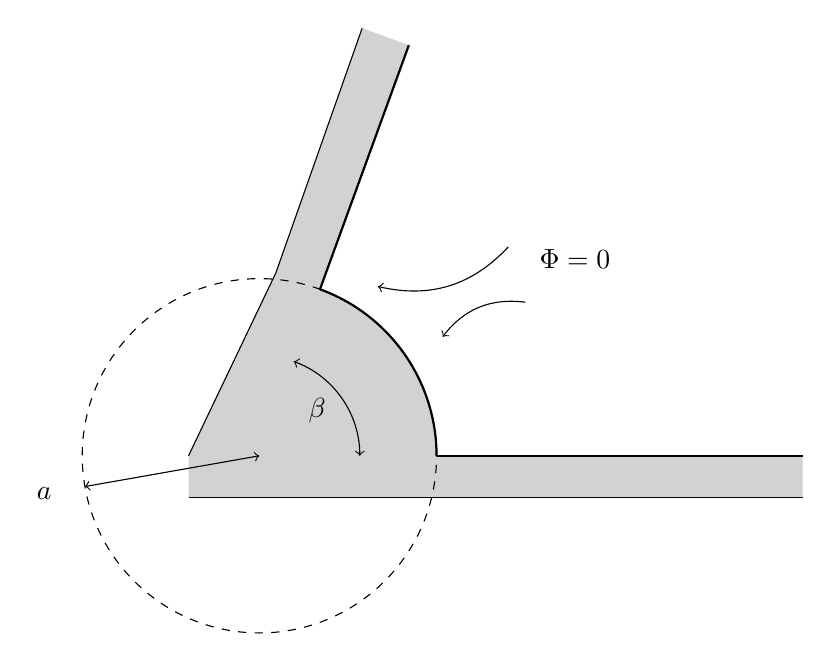
\begin{tikzpicture}[scale=1.5]
  % conductor (shaded): slab below phi=0 plane + sector rho<a + slab beyond phi=beta plane
  \fill[gray!35] (-0.6,0) -- (-0.6,-0.35) -- (4.6,-0.35) -- (4.6,0) -- (1.5,0)
    arc (0:70:1.5) -- (70:3.7) -- ++(160:0.42) -- (0.14,1.55) -- cycle;
  % dashed continuation of the circle rho = a
  \draw[dashed] (0,0) circle (1.5);
  % boundaries of the free region (conducting surfaces)
  \draw[thick] (1.5,0) -- (4.6,0);                    % phi = 0 plane
  \draw[thick] (70:1.5) -- (70:3.7);                  % phi = beta plane
  \draw[thick] (1.5,0) arc (0:70:1.5);                % cylinder surface rho = a
  % outer edges of the conductor block
  \draw[thin] (-0.6,-0.35) -- (4.6,-0.35);
  \draw[thin] (-0.6,0) -- (0.14,1.55);
  \draw[thin] (0.14,1.55) -- (0.87,3.62);
  % radius arrow a
  \draw[<->] (0,0) -- (190:1.5);
  \node at (190:1.85) {$a$};
  % angle beta at the origin
  \draw[<->] (0.85,0) arc (0:70:0.85);
  \node at (38:0.62) {$\beta$};
  % Phi = 0 label with pointers into the free channel
  \node at (32:3.15) {$\Phi=0$};
  \draw[->] (30:2.6) to[bend right] (33:1.85);
  \draw[->] (40:2.75) to[bend left] (55:1.75);
\end{tikzpicture}
\par\vspace{0.5em}\textbf{Problem 2.26}
\end{center}

\begin{enumerate}
\item[(a)] Write down a solution for the potential $\Phi(\rho,\phi)$ that satisfies the boundary conditions for finite $\rho$.
\item[(b)] Keeping only the lowest nonvanishing terms, calculate the electric field components $E_{\rho}$ and $E_{\phi}$ and also the surface-charge densities $\sigma(\rho,0)$, $\sigma(\rho,\beta)$, and $\sigma(a,\phi)$ on the three boundary surfaces.
\item[(c)] Consider $\beta=\pi$ (a plane conductor with a half-cylinder of radius $a$ on it). Show that far from the half-cylinder the lowest order terms of part b give a uniform electric field normal to the plane. Sketch the charge density on and in the neighborhood of the half-cylinder. For fixed electric field strength far from the plane, show that the total charge on the half-cylinder (actually charge per unit length in the $z$ direction) is twice as large as would reside on a strip of width $2a$ in its absence. Show that the extra portion is drawn from regions of the plane nearby, so that the total charge on a strip of width large compared to $a$ is the same whether the half-cylinder is there or not.
\end{enumerate}
\solution
\textbf{(a)} Separation of Laplace's equation with zero values on
the two radial walls selects angular factors
$\sin(\nu_m\phi)$, $\nu_m=m\pi/\beta$.
The radial solutions are $\rho^{\nu_m}$ and $\rho^{-\nu_m}$.
Imposing zero potential at $\rho=a$ fixes their relative coefficient:
\[
\boxed{\Phi(\rho,\phi)=\sum_{m=1}^\infty A_m
 \left(\rho^{\nu_m}-a^{2\nu_m}\rho^{-\nu_m}\right)
                           \sin(\nu_m\phi).}
\]
The remaining $A_m$ encode the remote boundary conditions. The series
is used in the source-free region between the local conductor and
those remote sources, within its region of convergence.
\textbf{(b)} If $A_1\ne0$, set $\nu=\pi/\beta$, $A=A_1$ and retain
that lowest mode. Direct differentiation gives
\[
\boxed{\begin{aligned}
E_\rho&=-A\nu(\rho^{\nu-1}+a^{2\nu}\rho^{-\nu-1})\sin\nu\phi,\\
E_\phi&=-A\nu(\rho^{\nu-1}-a^{2\nu}\rho^{-\nu-1})\cos\nu\phi.
\end{aligned}}
\]
The normals from the conductors into the free region are
$+\widehat{\boldsymbol\phi}$ at $\phi=0$,
$-\widehat{\boldsymbol\phi}$ at $\phi=\beta$, and
$+\widehat{\boldsymbol\rho}$ at $\rho=a$. Therefore
\[
\boxed{\begin{aligned}
\sigma(\rho,0)=\sigma(\rho,\beta)
 &=-\epsilon _0A\nu(\rho^{\nu-1}-a^{2\nu}\rho^{-\nu-1}),\\
\sigma(a,\phi)&=-2\epsilon _0A\nu a^{\nu-1}\sin\nu\phi.
\end{aligned}}
\]
If symmetry makes $A_1=0$, use the first nonzero $m$ instead;
the second wall then has
$\sigma(\rho,\beta)=\epsilon _0A_m\nu_m
(\rho^{\nu_m-1}-a^{2\nu_m}\rho^{-\nu_m-1})(-1)^m$.
\textbf{(c)} For $\beta=\pi$, $\nu=1$. Choosing $A=E_0>0$ gives
\[
\Phi=E_0\left(\rho-\frac{a^2}\rho\right)\sin\phi
=E_0y\left(1-\frac{a^2}{x^2+y^2}\right),
\]
so far away $\mathbf E\to-E_0\widehat{\mathbf y}$. The densities are
\[
\sigma_{\rm plane}(x)=-\epsilon _0E_0(1-a^2/x^2),\quad |x|\geq a,
\qquad\sigma_{\rm arc}(\phi)=-2\epsilon _0E_0\sin\phi.
\]
Both vanish where the arc meets the plane. The arc density is twice
the planar magnitude at its top, and the plane approaches its
undisturbed value monotonically away from the bump.
\begin{center}
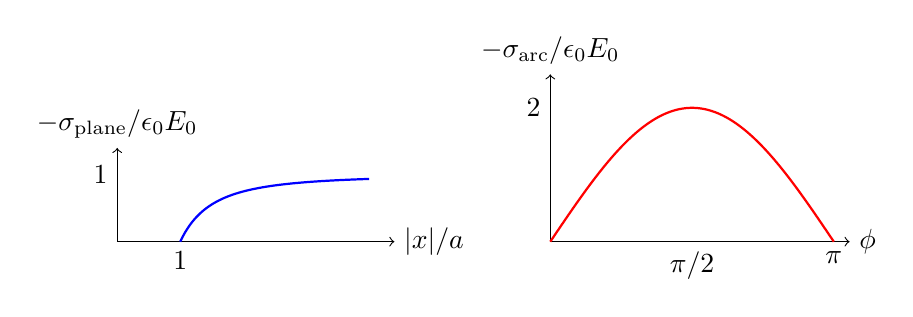
\begin{tikzpicture}[x=.8cm,y=.85cm]
\draw[->] (0,0)--(4.4,0) node[right] {$|x|/a$};
\draw[->] (0,0)--(0,1.4) node[above] {$-\sigma_{\rm plane}/\epsilon _0E_0$};
\draw[thick,blue,domain=1:4,samples=80] plot (\x,{1-1/(\x^2)});
\node[below] at (1,0) {$1$};\node[left] at (0,1) {$1$};
\begin{scope}[xshift=5.5cm,x=.02cm]
\draw[->] (0,0)--(190,0) node[right] {$\phi$};
\draw[->] (0,0)--(0,2.5) node[above] {$-\sigma_{\rm arc}/\epsilon _0E_0$};
\draw[thick,red,domain=0:180,samples=80] plot (\x,{2*sin(\x)});
\node[below] at (90,0) {$\pi/2$};\node[below] at (180,0) {$\pi$};
\node[left] at (0,2) {$2$};
\end{scope}
\end{tikzpicture}
\end{center}
The arc charge per unit $z$ length is
\[
Q_{\rm arc}=-2\epsilon _0E_0a\int_0^\pi\sin\phi\,d\phi
=-4\epsilon _0E_0a,
\]
twice the charge $-2\epsilon _0E_0a$ on the displaced flat strip.
The deficit in charge magnitude on the remaining plane is
\[
2\int_a^\infty[\sigma_{\rm plane}(x)+\epsilon _0E_0]\,dx
=2\epsilon _0E_0a^2\int_a^\infty\frac{dx}{x^2}
=2\epsilon _0E_0a,
\]
exactly the negative of the extra arc charge. More precisely, the
charge on the arc plus the plane portions $a<|x|<L$ is
\[
Q_L=-2\epsilon _0E_0L-\frac{2\epsilon _0E_0a^2}{L}.
\]
Compared with the flat value $-2\epsilon _0E_0L$, the relative
change is $a^2/L^2\to0$ for a wide strip.

\Needspace{5\baselineskip}
\par\bigskip
\noindent\textbf{2.27}\quad Consider the two-dimensional wedge-shaped region of Problem 2.26, with $\beta=2\pi$. This corresponds to a semi-infinite thin sheet of conductor on the positive $x$ axis from $x=a$ to infinity with a conducting cylinder of radius $a$ fastened to its edge.
\begin{enumerate}
\item[(a)] Sketch the surface-charge densities on the cylinder and on the top and bottom of the sheet, using the lowest order solution.
\item[(b)] Calculate the total charge on the cylinder and compare with the total deficiency of charge on the sheet near the cylinder, that is, the total difference in charge for $a$ finite compared with $a=0$, assuming that the charge density far from the cylinder is the same.
\end{enumerate}
\solution
For $\beta=2\pi$ the lowest angular index is $\nu=1/2$.
Let its coefficient $A$ be positive; all signs reverse if $A<0$.
The potential near the cylinder is
\[
\Phi=A\left(\sqrt\rho-\frac a{\sqrt\rho}\right)\sin\frac\phi2.
\]
\textbf{(a)} The formulas of Problem 2.26 give
\[
\boxed{\sigma_{\rm cylinder}(\phi)=-\frac{\epsilon _0A}{\sqrt a}
                              \sin\frac\phi2,\quad0<\phi<2\pi,}
\]
\[
\boxed{\sigma_{\rm top}(x)=\sigma_{\rm bottom}(x)
 =-\frac{\epsilon _0A}{2\sqrt x}\left(1-\frac ax\right),\quad x>a.}
\]
The density on the cylinder vanishes at the attachment point and
is largest in magnitude at the leftmost point, $\phi=\pi$.
Each sheet face starts from zero at $x=a$, reaches its largest
magnitude at $x=3a$ (differentiate $x^{-1/2}-ax^{-3/2}$), and then
approaches the $a=0$ edge law $-\epsilon _0A/(2\sqrt x)$.
The normalized maximum sheet magnitude is $1/(3\sqrt3)$ in units
$\epsilon _0A/\sqrt a$.
\begin{center}
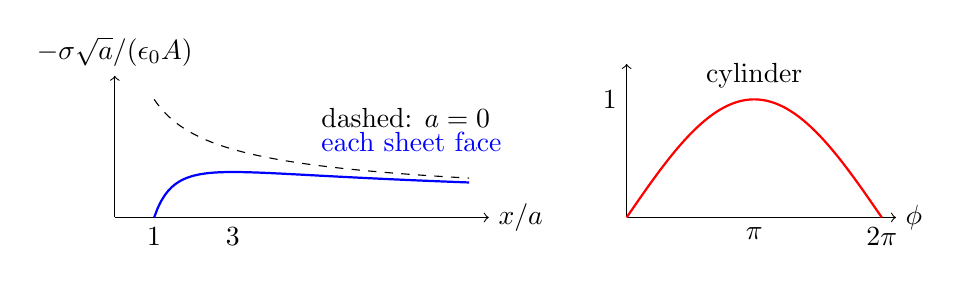
\begin{tikzpicture}[x=.5cm,y=3cm]
\draw[->] (0,0)--(9.5,0) node[right] {$x/a$};
\draw[->] (0,0)--(0,.6) node[above] {$-\sigma\sqrt a/(\epsilon _0A)$};
\draw[blue,thick,domain=1:9,samples=90] plot (\x,{(1-1/\x)/(2*sqrt(\x))});
\draw[dashed,domain=1:9,samples=90] plot (\x,{1/(2*sqrt(\x))});
\node[below] at (1,0) {$1$};\node[below] at (3,0) {$3$};
\node[right] at (5,.42) {dashed: $a=0$};
\node[blue,right] at (5,.32) {each sheet face};
\begin{scope}[xshift=6.5cm,x=.009cm,y=1.5cm]
\draw[->] (0,0)--(380,0) node[right] {$\phi$};
\draw[->] (0,0)--(0,1.3);
\draw[red,thick,domain=0:360,samples=90] plot (\x,{sin(\x/2)});
\node[below] at (180,0) {$\pi$};\node[below] at (360,0) {$2\pi$};
\node[left] at (0,1) {$1$};\node at (180,1.2) {cylinder};
\end{scope}
\end{tikzpicture}
\end{center}
\textbf{(b)} Integration on the full circular surface gives
\[
Q_c=-\epsilon _0A\sqrt a\int_0^{2\pi}\sin\frac\phi2\,d\phi
=\boxed{-4\epsilon _0A\sqrt a}.
\]
Although the total charge of an infinite sheet diverges, the
difference between the two configurations is integrable. On the
part $x>a$ that remains in both configurations,
\[
\Delta Q_{x>a}=2\int_a^\infty
  \frac{\epsilon _0Aa}{2x^{3/2}}\,dx=2\epsilon _0A\sqrt a.
\]
The reference sheet also had the part $0<x<a$, on both faces,
which has now been replaced by the cylinder. Its removed charge is
\[
Q_{0<x<a}^{(0)}=2\int_0^a-\frac{\epsilon _0A}{2\sqrt x}\,dx
=-2\epsilon _0A\sqrt a.
\]
Thus the \emph{total} sheet deficiency is
$\Delta Q_{\rm sheet}=2\epsilon _0A\sqrt a-(-2\epsilon _0A\sqrt a)
=4\epsilon _0A\sqrt a=-Q_c$.
Omitting the removed strip would count only half the deficiency.

\Needspace{5\baselineskip}
\par\bigskip
\noindent\textbf{2.28}\quad A closed volume is bounded by conducting surfaces that are the $n$ sides of a regular polyhedron ($n=4$, 6, 8, 12, 20). The $n$ surfaces are at different potentials $V_{i}$, $i=1,2,\ldots,n$. Prove in the simplest way you can that the potential at the center of the polyhedron is the average of the potential on the $n$ sides. This problem bears on Problem 2.23b, and has an interesting similarity to the result of Problem 1.10.
\solution
Let $u_i(\mathbf x)$ solve Laplace's equation with boundary value
one on face $i$ and zero on the other faces. By linearity and
Dirichlet uniqueness,
\[
\Phi(\mathbf x)=\sum_{i=1}^nV_i u_i(\mathbf x).
\]
A symmetry of a regular polyhedron carries any face into any other
while leaving its center $\mathbf x_c$ fixed. Applying that symmetry
to a unit-face solution and using uniqueness therefore proves
$u_i(\mathbf x_c)=u_j(\mathbf x_c)$ for all $i,j$.
Moreover, $\sum_i u_i$ has boundary value one on every open face,
so its unique interior solution is the constant one. At the center,
\[
1=\sum_i u_i(\mathbf x_c)=n u_i(\mathbf x_c).
\]
It follows immediately that
\[
\boxed{\Phi(\mathbf x_c)=\frac1n\sum_{i=1}^nV_i.}
\]
Idealized voltage jumps on shared edges can be understood as limits
of narrow insulating gaps; the interior harmonic solution is
unaffected by the assignment of boundary values on the edges alone.
The proof uses face-transitive symmetry, not a general assertion
that the potential equals an area average on an arbitrary enclosing
surface. For the cube of Problem 2.23, two of its six faces contribute,
so the center potential is $V/3$.

\Needspace{5\baselineskip}
\par\bigskip
\noindent\textbf{2.29}\quad For the Galerkin method on a two-dimensional square lattice with lattice spacing $h$, verify the relations (2.81) for the localized ``pyramid'' basis functions, $\phi_{ij}(x,y)=(1-|x|/h)(1-|y|/h)$, $|x|<h$, $|y|<h$, where $x$ and $y$ are measured from the site $(i,j)$. In particular,
\begin{gather*}
\int dx\int dy\;\phi_{i,j}(x,y) = h^{2};\qquad
\int dx\int dy\;\nabla\phi_{i,j}\cdot\nabla\phi_{i,j} = \frac{8}{3};\\
\int dx\int dy\;\nabla\phi_{i+1,j}\cdot\nabla\phi_{i,j} = -\frac{1}{3};\qquad
\int dx\int dy\;\nabla\phi_{i,j+1}\cdot\nabla\phi_{i,j} = -\frac{1}{3};\\
\int dx\int dy\;\nabla\phi_{i+1,j+1}\cdot\nabla\phi_{i,j} = -\frac{1}{3}
\end{gather*}
\solution
Define a one-dimensional tent
$f(x)=1-|x|/h$ for $|x|<h$, and zero otherwise. Then
$\phi_{ij}(x,y)=f(x-ih)f(y-jh)$, and each required two-dimensional
integral factors into one-dimensional integrals. For a tent and its
nearest translate, direct integration gives
\begin{align*}
I&=\int f(x)\,dx=2\int_0^h(1-x/h)\,dx=h,\\
M_0&=\int f^2\,dx=2\int_0^h(1-x/h)^2\,dx=\frac{2h}{3},\\
M_1&=\int f(x)f(x-h)\,dx
=\int_0^h(1-x/h)(x/h)\,dx=\frac h6,\\
K_0&=\int[f'(x)]^2\,dx=\int_{-h}^h\frac{dx}{h^2}=\frac2h,\\
K_1&=\int f'(x)f'(x-h)\,dx
=\int_0^h\left(-\frac1h\right)\left(\frac1h\right)dx=-\frac1h.
\end{align*}
Supports separated by two or more mesh spacings have zero overlap
except on sets of measure zero. First,
\[
\boxed{\int\phi_{ij}\,dx\,dy=I^2=h^2.}
\]
For any two sites, the gradient product has an $x$-derivative term
and a $y$-derivative term. The coincident-site integral is therefore
\[
\boxed{K_0M_0+M_0K_0=2(2/h)(2h/3)=\frac83.}
\]
For a horizontal neighbor the result is
\[
\boxed{K_1M_0+M_1K_0=-\frac23+\frac13=-\frac13,}
\]
and a vertical neighbor interchanges the two terms with the same
answer. For a diagonal neighbor both coordinates are translated:
\[
\boxed{K_1M_1+M_1K_1=2(-1/h)(h/6)=-\frac13.}
\]
The same values hold for all reflected nearest neighbors. Thus a
row of the interior stiffness matrix has $8/3$ on its own site and
$-1/3$ at each of eight neighboring sites; their sum is zero,
as required for a constant potential to have zero gradient.

\Needspace{5\baselineskip}
\par\bigskip
\noindent\textbf{2.30}\quad Using the results of Problem 2.29, apply the Galerkin method to the integral equivalent of the Poisson equation with zero potential on the boundary,
\[
\int_{V}dx\;dy\,[\nabla\phi_{i,j}\cdot\nabla\psi - 4\pi\rho\,\phi_{i,j}] = 0
\quad\text{with}\quad
\psi(x,y) = \sum_{i',j'=1}^{N}\psi_{i'j'}\,\phi_{i'j'}(x,y)
\]
for the lattice of Problem 1.24, with its three independent lattice sites. Show that you get three coupled equations for the $\psi_{i,j}$ values ($\psi_{1},\psi_{2},\psi_{3}$) and solve to find the ``Galerkin'' approximations for the potential at these sites. Compare with the exact values and the results of the various iterations of Problem 1.24c. Comment.
\[
[\psi = 4\pi\epsilon_{0}\Phi].
\]
\solution
Here $\rho=1$, $h=1/4$, and $\psi=4\pi\epsilon _0\Phi$.
Inserting the basis expansion into the weak equation and using
Problem 2.29 gives
\[
\frac83\psi_{ij}-\frac13\sum_{\text{eight neighbors}}\psi_{i'j'}
=4\pi h^2,
\quad\hbox{or}\quad
8\psi_{ij}-\sum_{\text{eight neighbors}}\psi_{i'j'}=\frac{3\pi}{4}.
\]
Boundary nodes have zero potential. Label the three independent
interior values by their sites in Problem 1.24:
$\psi_1=\psi(1/4,1/4)$,
$\psi_2=\psi(1/2,1/4)$,
$\psi_3=\psi(1/2,1/2)$.
At a corner-type interior site the nonzero neighbors are
$2\psi_2+\psi_3$; at an edge-type site they are
$2\psi_1+2\psi_2+\psi_3$; at the center they are
$4\psi_1+4\psi_2$. Thus
\[
\boxed{\begin{aligned}
8\psi_1-2\psi_2-\psi_3&=3\pi/4,\\
-2\psi_1+6\psi_2-\psi_3&=3\pi/4,\\
-4\psi_1-4\psi_2+8\psi_3&=3\pi/4.
\end{aligned}}
\]
Subtracting the second equation from the first gives
$10\psi_1-8\psi_2=0$, so $\psi_2=5\psi_1/4$.
The first then gives $\psi_3=11\psi_1/2-3\pi/4$.
Substitution into the third gives
$35\psi_1=27\pi/4$. Consequently
\[
\boxed{\psi_1=\frac{27\pi}{140}=0.605878583,\quad
       \psi_2=\frac{27\pi}{112}=0.757348229,\quad
       \psi_3=\frac{87\pi}{280}=0.976137717.}
\]
For comparison, the improved finite-difference equations of
Problem 1.24 are
\[
\begin{pmatrix}20&-8&-1\\-8&18&-4\\-4&-16&20\end{pmatrix}
\begin{pmatrix}\psi_1\\\psi_2\\\psi_3\end{pmatrix}
=\frac{3\pi}{2}\begin{pmatrix}1\\1\\1\end{pmatrix}.
\]
To exhibit the iterations, put $b_0=3\pi/2$. The reduced Jacobi
updates are
\[
\psi_1^{(r+1)}=\frac{b_0+8\psi_2^{(r)}+\psi_3^{(r)}}{20},\quad
\psi_2^{(r+1)}=\frac{b_0+8\psi_1^{(r)}+4\psi_3^{(r)}}{18},\quad
\psi_3^{(r+1)}=\frac{b_0+4\psi_1^{(r)}+16\psi_2^{(r)}}{20}.
\]
Ordered Gauss--Seidel uses the just-computed $\psi_1^{(r+1)}$
in the second equation and both new $\psi_1^{(r+1)},\psi_2^{(r+1)}$
in the third. Solving the three simultaneous equations, for example
eliminating $\psi_3=20\psi_1-8\psi_2-b_0$ from the first, gives
\[
-88\psi_1+50\psi_2=-3b_0,\qquad
396\psi_1-176\psi_2=21b_0.
\]
Their solution is
$(\psi_1,\psi_2,\psi_3)=(783\pi/4312,45\pi/196,159\pi/539)$.
Starting from $(1,1,1)$ and applying Jacobi or ordered Gauss--Seidel
to this reduced matrix (with diagonal $18$ in its second row, as
in Problem 1.24) gives the comparison below.
\begin{center}
\begin{tabular}{lrrr}
\toprule
Method & $\psi_1$ & $\psi_2$ & $\psi_3$\\\midrule
Exact series, Problem 2.16 & .569082647 & .720491684 & .925781529\\
Galerkin, $h=1/4$ & .605878583 & .757348229 & .976137717\\
Jacobi, iteration 2 & .668786843 & .841101243 & 1.115516182\\
Jacobi, iteration 6 & .587144572 & .743033367 & .960088859\\
Jacobi, iteration 10 & .573384927 & .725179706 & .932570355\\
Gauss--Seidel, iteration 2 & .601302817 & .752097624 & .957558112\\
Gauss--Seidel, iteration 6 & .571530449 & .722284498 & .927753137\\
Gauss--Seidel, iteration 10 & .570504738 & .721316714 & .926773768\\
Improved stencil, converged & .570470095 & .721284028 & .926740690\\
\bottomrule
\end{tabular}
\end{center}
The Galerkin values exceed the exact values by approximately
$6.47\%$, $5.12\%$, and $5.44\%$, respectively, whereas the converged
improved stencil errors are $0.244\%$, $0.110\%$, and $0.104\%$.
This comparison separates the error in solving a discrete system
from its spatial approximation error: more iterations converge to
the stencil's fixed solution, not to the continuum solution. The
Galerkin calculation is also a different discrete approximation,
using piecewise bilinear tents and a variational integral; on this
coarse grid it is less accurate at these nodes. This is not a general
failure of finite elements: mesh refinement, or richer basis functions,
changes that approximation. Galerkin stationarity controls the
integrated field-energy error, not the sign or size of each nodal
potential error.

\clearpage
\section{Chapter 3. Boundary-Value Problems in Electrostatics: II}
% Problems, Chapter 3: Boundary-Value Problems in Electrostatics: II
% Jackson, Classical Electrodynamics, 3rd ed.
% Requires: amsmath, amssymb, tikz

\section*{Problems}

\Needspace{5\baselineskip}
\par\bigskip
\noindent\textbf{3.1}\quad Two concentric spheres have radii $a$, $b$ ($b>a$) and each is divided into two hemispheres by the same horizontal plane. The upper hemisphere of the inner sphere and the lower hemisphere of the outer sphere are maintained at potential $V$. The other hemispheres are at zero potential.

Determine the potential in the region $a\leq r\leq b$ as a series in Legendre polynomials. Include terms at least up to $l=4$. Check your solution against known results in the limiting cases $b\to\infty$, and $a\to0$.
\solution

Put $\mu=\cos\theta$ and expand the boundary values as
$V_a(\mu)=\sum_l v_lP_l(\mu)$ and $V_b(\mu)=\sum_l w_lP_l(\mu)$.
Orthogonality gives
\[
v_l=\frac{(2l+1)V}{2}\int_0^1P_l(u)\,du,\qquad
w_l=(-1)^lv_l.
\]
For $l\geq1$, integrate
$(2l+1)P_l=(P_{l+1}-P_{l-1})'$ to obtain
\[
v_l=\frac V2[P_{l-1}(0)-P_{l+1}(0)].
\]
Thus $v_0=V/2$, $v_1=3V/4$, $v_3=-7V/16$, and all even
$l>0$ coefficients vanish.  For each angular order, Laplace's
equation gives $f_l(r)=\alpha_lr^l+\beta_lr^{-l-1}$.  The two
boundary equations, after multiplication by $a^{l+1}$ and $b^{l+1}$,
are
\[
\alpha_la^{2l+1}+\beta_l=a^{l+1}v_l,\qquad
\alpha_lb^{2l+1}+\beta_l=b^{l+1}w_l.
\]
Writing $D_l=b^{2l+1}-a^{2l+1}$, subtraction and back-substitution give
\[
\alpha_l=\frac{b^{l+1}w_l-a^{l+1}v_l}{D_l},\qquad
\beta_l=\frac{a^{l+1}b^{2l+1}v_l-b^{l+1}a^{2l+1}w_l}{D_l}.
\]
Thus $f_l=v_lA_l+w_lB_l$, where the two radial interpolants are
\[
A_l(r)=\frac{a^{l+1}(b^{2l+1}-r^{2l+1})}
 {r^{l+1}(b^{2l+1}-a^{2l+1})},\qquad
B_l(r)=\frac{b^{l+1}(r^{2l+1}-a^{2l+1})}
 {r^{l+1}(b^{2l+1}-a^{2l+1})}.
\]
Each is a linear combination of $r^l$ and $r^{-l-1}$, and
$(A_l(a),A_l(b))=(1,0)$, $(B_l(a),B_l(b))=(0,1)$.
Consequently
\[
\boxed{\Phi=\frac V2+
\sum_{\substack{l\geq1\\l\ \mathrm{odd}}}
\frac V2[P_{l-1}(0)-P_{l+1}(0)]
[A_l(r)-B_l(r)]P_l(\mu).}
\]
Through $l=4$ this is
\[
\Phi=\frac V2+\frac{3V}{4}(A_1-B_1)\mu
-\frac{7V}{16}(A_3-B_3)\frac{5\mu^3-3\mu}{2}
+\text{terms with }l\geq5.
\]
The $l=0$ contribution is constant because $A_0+B_0=1$.
At a boundary jump the Legendre series takes the mean value $V/2$.

For fixed $a,r$, $b\to\infty$ gives $A_l\to(a/r)^{l+1}$ and
$B_l\to0$ for $l>0$.  The limit is therefore the exterior hemispherical
solution with asymptotic potential $V/2$; the distant outer boundary
retains this constant offset.  In the limit $a\to0$ at fixed $r,b$,
$A_l\to0$ and $B_l\to(r/b)^l$ for $l>0$, giving the regular interior
solution with the lower hemisphere of the sphere at $V$.

\Needspace{5\baselineskip}
\par\bigskip
\noindent\textbf{3.2}\quad A spherical surface of radius $R$ has charge uniformly distributed over its surface with a density $Q/4\pi R^{2}$, except for a spherical cap at the north pole, defined by the cone $\theta=\alpha$.
\begin{enumerate}
\item[(a)] Show that the potential inside the spherical surface can be expressed as
\[
\Phi=\frac{Q}{8\pi\epsilon_{0}}\sum_{l=0}^{\infty}\frac{1}{2l+1}\left[P_{l+1}(\cos\alpha)-P_{l-1}(\cos\alpha)\right]\frac{r^{l}}{R^{l+1}}P_{l}(\cos\theta)
\]
where, for $l=0$, $P_{l-1}(\cos\alpha)=-1$. What is the potential outside?
\item[(b)] Find the magnitude and the direction of the electric field at the origin.
\item[(c)] Discuss the limiting forms of the potential (part a) and electric field (part b) as the spherical cap becomes (1) very small, and (2) so large that the area with charge on it becomes a very small cap at the south pole.
\end{enumerate}
\solution

Write $c=\cos\alpha$; the charged portion is $-1\leq\mu'\leq c$.
The symbol $Q$ specifies the original full-sphere density: the charge
actually present is $Q_{\rm rem}=Q(1+c)/2$.
Averaging the Coulomb expansion over the source azimuth gives
\[
\int_0^{2\pi}P_l(\cos\gamma)\,d\phi'
=2\pi P_l(\mu)P_l(\mu').
\]
\textbf{(a)} Hence
\[
\Phi=\frac{Q}{8\pi\epsilon_0}
\sum_{l=0}^\infty P_l(\mu)\frac{r_<^l}{r_>^{l+1}}
\int_{-1}^cP_l(u)\,du,
\quad r_<=\min(r,R),\quad r_>=\max(r,R).
\]
For $l\geq1$ the integral is
$[P_{l+1}(c)-P_{l-1}(c)]/(2l+1)$ because the lower-end terms cancel.
For $l=0$ it is $1+c$, reproduced by the stipulated $P_{-1}=-1$.
This proves the displayed interior expression.  The exterior expression
is the same sum with $r^l/R^{l+1}$ replaced by $R^l/r^{l+1}$.
Continuity at $r=R$ follows term by term; its radial derivative has the
jump $\partial_r\Phi_{\rm out}-\partial_r\Phi_{\rm in}=-\sigma/\epsilon_0$.

\textbf{(b)} Only $l=1$ contributes to the gradient at the origin.
Since $P_2(c)-P_0(c)=-3(1-c^2)/2$,
\[
\Phi=\frac{Q(1+c)}{8\pi\epsilon_0R}
-\frac{Q\sin^2\alpha}{16\pi\epsilon_0R^2}z+O(r^2),\qquad
\boxed{\mathbf E(0)=\frac{Q\sin^2\alpha}{16\pi\epsilon_0R^2}\,\hat{\mathbf z}.}
\]
For positive $Q$ the field points toward the missing north cap; reversing
$Q$ reverses its direction.

\textbf{(c)} For $\alpha\ll1$, the missing charge is
$\delta Q=Q(1-c)/2=Q\alpha^2/4+O(\alpha^4)$.
Away from the shrinking cap its potential is that of a point charge at
$R\hat{\mathbf z}$ to leading order.  Thus
\[
\Phi=\frac{Q}{4\pi\epsilon_0\max(r,R)}
-\frac{Q\alpha^2}{16\pi\epsilon_0|\mathbf r-R\hat{\mathbf z}|}
+O(\alpha^4),\qquad
\mathbf E(0)=\frac{Q\alpha^2}{16\pi\epsilon_0R^2}\hat{\mathbf z}
+O(\alpha^4).
\]
For $\beta=\pi-\alpha\ll1$, only the south cap remains, with
$Q_{\rm rem}=Q\beta^2/4+O(\beta^4)$, and
\[
\Phi=\frac{Q\beta^2}{16\pi\epsilon_0|\mathbf r+R\hat{\mathbf z}|}
+O(\beta^4),\qquad
\mathbf E(0)=\frac{Q\beta^2}{16\pi\epsilon_0R^2}\hat{\mathbf z}
+O(\beta^4).
\]
These expansions are not uniform at the cap itself.  With the specified
fixed density the remaining charge and field tend to zero; if instead
its total charge is held fixed, the south-cap limit is an ordinary
point charge of that fixed magnitude.

\Needspace{5\baselineskip}
\par\bigskip
\noindent\textbf{3.3}\quad A thin, flat, conducting, circular disc of radius $R$ is located in the $x$-$y$ plane with its center at the origin, and is maintained at a fixed potential $V$. With the information that the charge density on a disc at fixed potential is proportional to $(R^{2}-\rho^{2})^{-1/2}$, where $\rho$ is the distance out from the center of the disc,
\begin{enumerate}
\item[(a)] show that for $r>R$ the potential is
\[
\Phi(r,\theta,\phi)=\frac{2V}{\pi}\frac{R}{r}\sum_{l=0}^{\infty}\frac{(-1)^{l}}{2l+1}\left(\frac{R}{r}\right)^{2l}P_{2l}(\cos\theta)
\]
\item[(b)] find the potential for $r<R$.
\item[(c)] What is the capacitance of the disc?
\end{enumerate}
\solution

Let $\sigma(\rho)=C_0/\sqrt{R^2-\rho^2}$ denote the total sheet
charge density, including both faces.  At the center,
\[
V=\frac{1}{4\pi\epsilon_0}\int_0^R
\frac{2\pi\rho\,C_0\,d\rho}{\rho\sqrt{R^2-\rho^2}}
=\frac{\pi C_0}{4\epsilon_0},
\quad C_0=\frac{4\epsilon_0V}{\pi}.
\]
\textbf{(a)} The azimuthal average of the Coulomb expansion yields
\[
\Phi=\frac{C_0}{2\epsilon_0}
\sum_{n=0}^\infty\frac{P_{2n}(0)P_{2n}(\cos\theta)}{r^{2n+1}}
\int_0^R\frac{\rho^{2n+1}\,d\rho}{\sqrt{R^2-\rho^2}}.
\]
Odd orders vanish.  With $t=\rho^2/R^2$ the integral equals
\[
\frac{R^{2n+1}}2 B(n+1,\tfrac12)
=R^{2n+1}\frac{2^{2n}(n!)^2}{(2n+1)!}.
\]
Multiplication by $P_{2n}(0)=(-1)^n(2n)!/[2^{2n}(n!)^2]$
gives $(-1)^nR^{2n+1}/(2n+1)$ and hence the required series.

\textbf{(b)} First compute the potential on the positive axis:
\[
\Phi(0,z)=\frac{2V}{\pi}\int_0^R
\frac{\rho\,d\rho}{\sqrt{R^2-\rho^2}\sqrt{\rho^2+z^2}}
=\frac{2V}{\pi}\tan^{-1}\frac Rz
=V-\frac{2V}{\pi}\tan^{-1}\frac zR.
\]
For example, $u=\sqrt{R^2-\rho^2}$ changes the integral to
$\int_0^Rdu/\sqrt{R^2+z^2-u^2}$, giving the stated inverse tangent.
In the upper half-ball expand the last expression in powers of $z/R$.
The unique regular, axially symmetric harmonic extension of $z^l$ is
$r^lP_l(\cos\theta)$.  Reflection in the disc then gives
\[
\boxed{\Phi=V-\frac{2V}{\pi}\sum_{n=0}^\infty
\frac{(-1)^n}{2n+1}\left(\frac rR\right)^{2n+1}
P_{2n+1}(|\cos\theta|),\qquad r<R.}
\]
On the disc all odd Legendre polynomials vanish at zero, so $\Phi=V$.
The absolute value is essential: there is a normal-derivative jump at
the charged sheet and no single harmonic power series through it.

\textbf{(c)} Integration of the sheet density gives
\[
Q=2\pi C_0\int_0^R\frac{\rho\,d\rho}{\sqrt{R^2-\rho^2}}
=8\epsilon_0RV,\qquad \boxed{C=8\epsilon_0R.}
\]
The exterior monopole term is correspondingly $Q/(4\pi\epsilon_0r)$.

\Needspace{5\baselineskip}
\par\bigskip
\noindent\textbf{3.4}\quad The surface of a hollow conducting sphere of inner radius $a$ is divided into an \emph{even number} of equal segments by a set of planes; their common line of intersection is the $z$ axis and they are distributed uniformly in the angle $\phi$. (The segments are like the skin on wedges of an apple, or the earth's surface between successive meridians of longitude.) The segments are kept at fixed potentials $\pm V$, alternately.
\begin{enumerate}
\item[(a)] Set up a series representation for the potential inside the sphere for the general case of $2n$ segments, and carry the calculation of the coefficients in the series far enough to determine exactly which coefficients are different from zero. For the nonvanishing terms, exhibit the coefficients as an integral over $\cos\theta$.
\item[(b)] For the special case of $n=1$ (two hemispheres) determine explicitly the potential up to and including all terms with $l=3$. By a coordinate transformation verify that this reduces to result (3.36) of Section 3.3.
\end{enumerate}
\solution

Choose the angular origin so that the boundary value is
$V\,\operatorname{sgn}[\sin(n\phi)]$.  A rotation about $z$ covers any
other placement of the segments.  Its Fourier series is
\[
V(\phi)=\frac{4V}{\pi}\sum_{s=0}^\infty
\frac{\sin(m_s\phi)}{2s+1},\qquad m_s=(2s+1)n.
\]
\textbf{(a)} Use real associated Legendre functions with the
Condon--Shortley phase, $P_l^m=(-1)^m(1-u^2)^{m/2}d^mP_l/du^m$,
as in Jackson's Eq.~(3.49), p.~108.  Consequently
$Y_{lm}=[(2l+1)(l-m)!/(4\pi(l+m)!)]^{1/2}P_l^m e^{im\phi}$
has no additional phase [Eq.~(3.53)].
The regular solution and its coefficients are
\begin{align*}
\Phi&=\sum_{s=0}^\infty\sum_{l=m_s}^\infty
c_{lm_s}(r/a)^lP_l^{m_s}(\cos\theta)\sin(m_s\phi),\\
c_{lm}&=\frac{2V(2l+1)}{\pi(2s+1)}
\frac{(l-m)!}{(l+m)!}\int_{-1}^1P_l^m(u)\,du,
\qquad m=(2s+1)n.
\end{align*}
Here the factor $(2l+1)(l-m)!/[2(l+m)!]$ is the inverse
associated-Legendre norm.  All cosine modes, $m=0$ modes, and all
other azimuthal orders vanish.  Parity gives
$P_l^m(-u)=(-1)^{l+m}P_l^m(u)$, so $l+m$ must be even.
To prove that there are no further zeros, put
$I_{lm}=\int_{-1}^1P_l^m(u)\,du$.  The associated-Legendre identities
\[
(1-u^2)(P_l^m)'=-luP_l^m+(l+m)P_{l-1}^m,\qquad
(2l+1)uP_l^m=(l-m+1)P_{l+1}^m+(l+m)P_{l-1}^m
\]
give, after integration by parts in the first identity,
\[
(l+2)\int_{-1}^1uP_l^m\,du=(l+m)I_{l-1,m},\qquad
I_{l+1,m}=\frac{(l-1)(l+m)}{(l+2)(l-m+1)}I_{l-1,m}.
\]
The boundary term vanishes because $(1-u^2)P_l^m\to0$.  Relabeling
$l=L+1$ yields
\[
I_{L+2,m}=\frac{L(L+m+1)}{(L+3)(L-m+2)}I_{L,m}.
\]
The starting value follows from
$P_m^m=(-1)^m(2m-1)!!(1-u^2)^{m/2}$:
\[
I_{mm}=(-1)^m(2m-1)!!\,B(1/2,1+m/2)\ne0.
\]
Every multiplier in the recurrence is positive for $L\geq m\geq1$;
hence every $l=m,m+2,\ldots$ survives.  Iterating the recurrence
and using $\Gamma(x+1)=x\Gamma(x)$ also gives the closed form
\[
\int_{-1}^1P_l^m(u)\,du
=(-1)^m2^{m-1}m\,
\frac{\Gamma(l/2)\Gamma((l+m+1)/2)}
{\Gamma((l-m+2)/2)\Gamma((l+3)/2)},
\]
whose gamma factors are finite and positive.  This also specifies
unambiguously which coefficients in the integral formula survive.

\textbf{(b)} For $n=1$, the required integrals are
\[
\int P_1^1\,du=-\frac\pi2,\qquad
\int P_3^1\,du=-\frac{3\pi}{16},\qquad
\int P_3^3\,du=-\frac{45\pi}{8},
\]
where all integrals run from $-1$ to $1$.  Therefore, through $l=3$,
\[
\Phi=-\frac{3V}{2}\frac ra P_1^1(\cos\theta)\sin\phi
-\left(\frac ra\right)^3
\left[\frac{7V}{32}P_3^1(\cos\theta)\sin\phi
+\frac{7V}{192}P_3^3(\cos\theta)\sin3\phi\right]+O((r/a)^5).
\]
The new polar axis may be chosen along $+y$, so
$\cos\Theta=y/r=\sin\theta\sin\phi$.  Substitution of
$P_1^1=-\sin\theta$,
$P_3^1=-\tfrac32(5\cos^2\theta-1)\sin\theta$, and
$P_3^3=-15\sin^3\theta$, with
$\sin3\phi=3\sin\phi-4\sin^3\phi$, reduces this to
\[
\Phi=V\left[\frac32\frac ra P_1(\cos\Theta)
-\frac78\left(\frac ra\right)^3P_3(\cos\Theta)\right]
+O((r/a)^5),
\]
which is Eq.~(3.36) in the rotated coordinates.

\Needspace{5\baselineskip}
\par\bigskip
\noindent\textbf{3.5}\quad A hollow sphere of inner radius $a$ has the potential specified on its surface to be $\Phi=V(\theta,\phi)$. Prove the equivalence of the two forms of solution for the potential inside the sphere:
\begin{enumerate}
\item[(a)] $\displaystyle\Phi(\mathbf{x})=\frac{a(a^{2}-r^{2})}{4\pi}\int\frac{V(\theta',\phi')}{(r^{2}+a^{2}-2ar\cos\gamma)^{3/2}}\;d\Omega'$

where $\cos\gamma=\cos\theta\cos\theta'+\sin\theta\sin\theta'\cos(\phi-\phi')$.
\item[(b)] $\displaystyle\Phi(\mathbf{x})=\sum_{l=0}^{\infty}\sum_{m=-l}^{l}A_{lm}\left(\frac{r}{a}\right)^{l}Y_{lm}(\theta,\phi)$

where $A_{lm}=\int d\Omega'\;Y_{lm}^{*}(\theta',\phi')V(\theta',\phi')$.
\end{enumerate}
\solution

Let $t=r/a<1$ and $u=\cos\gamma$.  The Legendre generating function is
$F(t,u)=(1-2tu+t^2)^{-1/2}=\sum_{l\geq0}t^lP_l(u)$.
Differentiate within its convergent power series:
\[
F+2t\partial_tF
=\frac{1-t^2}{(1-2tu+t^2)^{3/2}}
=\sum_{l=0}^\infty(2l+1)t^lP_l(u).
\]
Consequently the kernel in (a) is
\[
\frac{a(a^2-r^2)}{4\pi(a^2+r^2-2ar\cos\gamma)^{3/2}}
=\sum_{l=0}^\infty\frac{2l+1}{4\pi}
(r/a)^lP_l(\cos\gamma).
\]
Use the addition theorem
\[
\frac{2l+1}{4\pi}P_l(\cos\gamma)
=\sum_{m=-l}^lY_{lm}(\theta,\phi)Y_{lm}^*(\theta',\phi').
\]
Inserting it into (a), interchanging the integral and the uniformly
convergent series on any closed ball $r\leq r_0<a$, and grouping the
source integral gives exactly (b) with its stated $A_{lm}$.
Conversely, insert those coefficients into (b) and sum the same kernel
to recover (a).  For an integrable boundary value this proves the
interior equivalence; for continuous boundary data the limiting
Poisson integral takes the assigned surface value.  Constant data
provide a normalization check: only $l=0$ remains and $\Phi=V$.

\Needspace{5\baselineskip}
\par\bigskip
\noindent\textbf{3.6}\quad Two point charges $q$ and $-q$ are located on the $z$ axis at $z=+a$ and $z=-a$, respectively.
\begin{enumerate}
\item[(a)] Find the electrostatic potential as an expansion in spherical harmonics and powers of $r$ for both $r>a$ and $r<a$.
\item[(b)] Keeping the product $qa\equiv p/2$ constant, take the limit of $a\to0$ and find the potential for $r\neq0$. This is by definition a dipole along the $z$ axis and its potential.
\item[(c)] Suppose now that the dipole of part b is surrounded by a \emph{grounded} spherical shell of radius $b$ concentric with the origin. By linear superposition find the potential everywhere inside the shell.
\end{enumerate}
\solution

\textbf{(a)} The direct potential is
\[
\Phi=\frac{q}{4\pi\epsilon_0}
\left(\frac1{|\mathbf r-a\hat{\mathbf z}|}
-\frac1{|\mathbf r+a\hat{\mathbf z}|}\right).
\]
In the Coulomb expansion the two source directions contribute
$P_l(\cos\theta)$ and $P_l(-\cos\theta)=(-1)^lP_l(\cos\theta)$.
Even orders cancel, giving
\[
\boxed{\Phi=\frac{q}{2\pi\epsilon_0}
\sum_{j=0}^\infty P_{2j+1}(\cos\theta)
\begin{cases}
a^{2j+1}/r^{2j+2},&r>a,\\
r^{2j+1}/a^{2j+2},&r<a.
\end{cases}}
\]
This is a spherical-harmonic expansion because
$P_l(\cos\theta)=\sqrt{4\pi/(2l+1)}Y_{l0}$; all $m\ne0$
coefficients vanish.  The source points themselves are excluded.

\textbf{(b)} With $2qa=p$ fixed, the $l=1$ coefficient remains
finite and every higher term has an extra factor $a^{2j}$.  At each
fixed $r>0$,
\[
\boxed{\Phi_{\rm dip}=\frac{p\cos\theta}{4\pi\epsilon_0r^2}.}
\]

\textbf{(c)} A regular $l=1$ harmonic $Ar\cos\theta$ can cancel
the dipole's surface value.  The equation
$p/(4\pi\epsilon_0b^2)+Ab=0$ fixes $A=-p/(4\pi\epsilon_0b^3)$.
Thus
\[
\boxed{\Phi=\frac{p\cos\theta}{4\pi\epsilon_0}
\left(\frac1{r^2}-\frac r{b^3}\right),\qquad0<r<b.}
\]
The added field is the uniform field
$+p\hat{\mathbf z}/(4\pi\epsilon_0b^3)$; it is regular at the
source and makes the total potential vanish at $r=b$.

\Needspace{5\baselineskip}
\par\bigskip
\noindent\textbf{3.7}\quad Three point charges ($q$, $-2q$, $q$) are located in a straight line with separation $a$ and with the middle charge ($-2q$) at the origin of a grounded conducting spherical shell of radius $b$, as indicated in the sketch.

\begin{center}
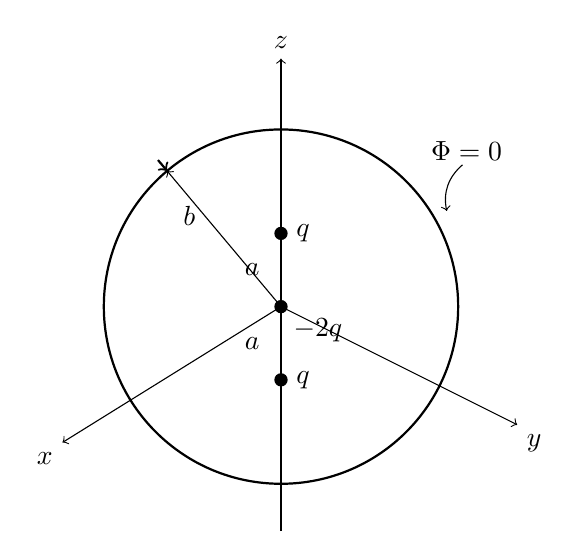
\begin{tikzpicture}[scale=1.5]
  % grounded sphere
  \draw[thick] (0,0) circle (1.5);
  % axes
  \draw[->] (0,-1.9) -- (0,2.1) node[above] {$z$};
  \draw[->] (0,0) -- (-1.85,-1.15) node[below left] {$x$};
  \draw[->] (0,0) -- (2.0,-1.0) node[below right] {$y$};
  % radius b arrow
  \draw[<-,thick] (130:1.5) -- (130:1.62);
  \draw[->] (0,0) -- (130:1.5);
  \node[left] at (130:1.0) {$b$};
  % charges on z axis
  \fill (0,0.62) circle (1.6pt) node[right=2pt] {$q$};
  \fill (0,0) circle (1.6pt) node[below right=1pt] {$-2q$};
  \fill (0,-0.62) circle (1.6pt) node[right=2pt] {$q$};
  % separation labels
  \node[left] at (-0.1,0.31) {$a$};
  \node[left] at (-0.1,-0.31) {$a$};
  % Phi = 0 with pointer to sphere
  \node at (40:2.05) {$\Phi=0$};
  \draw[->] (38:1.95) to[bend right] (30:1.62);
\end{tikzpicture}
\par\vspace{0.5em}\textbf{Problem 3.7}
\end{center}

\begin{enumerate}
\item[(a)] Write down the potential of the three charges in the absence of the grounded sphere. Find the limiting form of the potential as $a\to0$, but the product $qa^{2}=Q$ remains finite. Write this latter answer in spherical coordinates.
\item[(b)] The presence of the grounded sphere of radius $b$ alters the potential for $r<b$. The added potential can be viewed as caused by the surface-charge density induced on the inner surface at $r=b$ or by image charges located at $r>b$. Use linear superposition to satisfy the boundary conditions and find the potential everywhere inside the sphere for $r<a$ and $r>a$. Show that in the limit $a\to0$,
\[
\Phi(r,\theta,\phi)\to\frac{Q}{2\pi\epsilon_{0}r^{3}}\left(1-\frac{r^{5}}{b^{5}}\right)P_{2}(\cos\theta)
\]
\end{enumerate}
\solution

\textbf{(a)} Before inserting the conductor,
\[
\Phi_{\rm free}=\frac{q}{4\pi\epsilon_0}
\left(\frac1{\sqrt{r^2+a^2-2ar\cos\theta}}
+\frac1{\sqrt{r^2+a^2+2ar\cos\theta}}-\frac2r\right).
\]
For $r>a$ the $l=0$ terms cancel and odd terms cancel by reflection:
\[
\Phi_{\rm free}=\frac{q}{2\pi\epsilon_0}
\sum_{j=1}^\infty\frac{a^{2j}}{r^{2j+1}}P_{2j}(\cos\theta).
\]
Therefore, for fixed $r>0$ and $qa^2=Q$,
\[
\Phi_{\rm free}\longrightarrow
\frac{Q}{2\pi\epsilon_0r^3}P_2(\cos\theta)
=\frac{Q(3\cos^2\theta-1)}{4\pi\epsilon_0r^3}.
\]

\textbf{(b)} Assume $a<b$.  The regular harmonic correction that
cancels the preceding free-space series at $b$ is
\[
\Phi_{\rm ind}=-\frac{q}{2\pi\epsilon_0}
\sum_{j=1}^\infty\frac{a^{2j}r^{2j}}{b^{4j+1}}P_{2j}(\cos\theta).
\]
It is valid throughout $r<b$.  Explicitly the full result is
\[
\boxed{\Phi=\frac{q}{2\pi\epsilon_0}
\sum_{j=1}^\infty a^{2j}
\left(\frac1{r^{2j+1}}-\frac{r^{2j}}{b^{4j+1}}\right)
P_{2j}(\cos\theta),\quad a<r<b,}
\]
and
\[
\boxed{\Phi=\frac{q}{2\pi\epsilon_0}\left[
\frac1a-\frac1r+
\sum_{j=1}^\infty r^{2j}
\left(\frac1{a^{2j+1}}-\frac{a^{2j}}{b^{4j+1}}\right)
P_{2j}(\cos\theta)\right],\quad0<r<a.}
\]
An independent image construction gives image charges $-qb/a$ at
$z=\pm b^2/a$ and the constant $2q/(4\pi\epsilon_0b)$ for the
central charge.  The monopoles of the two images cancel that constant,
leaving precisely $\Phi_{\rm ind}$.  In the quadrupole limit only
$j=1$ survives, and
\[
\boxed{\Phi\longrightarrow\frac{Q}{2\pi\epsilon_0r^3}
\left(1-\frac{r^5}{b^5}\right)P_2(\cos\theta).}
\]
All expressions exclude the point-charge singularities; the series at
$r=a$ can be understood by a limit away from the sources.

\Needspace{5\baselineskip}
\par\bigskip
\noindent\textbf{3.8}\quad There is a puzzling aspect of the solution (3.136) for the potential inside a grounded sphere with a uniformly charged wire along a diameter. Very close to the wire (i.e., for $\rho=r\sin\theta\ll b$), the potential should be that of a uniformly charged wire, namely, $\Phi=(Q/4\pi\epsilon_{0}b)\ln(b/\rho)+\Phi_{0}$. The solution (3.136) does not explicitly have this behavior.
\begin{enumerate}
\item[(a)] Show by use of the Legendre differential equation (3.10) and some integration by parts, that $\ln(\operatorname{cosec}\theta)$ has the appropriate expansion in spherical harmonics to permit the solution (3.136) to be written in the alternative form,
\[
\Phi(\mathbf{x})=\frac{Q}{4\pi\epsilon_{0}b}\left\{\ln\!\left(\frac{2b}{r\sin\theta}\right)-1-\sum_{j=1}^{\infty}\frac{4j+1}{2j(2j+1)}\left(\frac{r}{b}\right)^{2j}P_{2j}(\cos\theta)\right\}
\]
in which the expected behavior near the wire is manifest. Give an interpretation of the constant term $\Phi_{0}=-Q/4\pi\epsilon_{0}b$. Note that in this form, for any $r/b<1$ the Legendre polynomial series is rapidly convergent at all angles.
\item[(b)] Show by use of the expansion (3.38) that
\[
\frac{1}{2}\left(\frac{1}{\sin(\theta/2)}+\frac{1}{\cos(\theta/2)}\right)=2\sum_{j=0}^{\infty}P_{2j}(\cos\theta)
\]
and that therefore the charge density on the inner surface of the sphere, Eq.~(3.137), can be expressed alternatively as
\[
\sigma(\theta)=-\frac{Q}{4\pi b^{2}}\left\{\frac{1}{2}\left(\frac{1}{\sin(\theta/2)}+\frac{1}{\cos(\theta/2)}\right)-\sum_{j=0}^{\infty}\frac{1}{2j+1}P_{2j}(\cos\theta)\right\}
\]
The (integrable) singular behavior at $\theta=0$ and $\theta=\pi$ is now exhibited explicitly. The series provides corrections in $\ln(1/\theta)$ as $\theta\to0$.
\end{enumerate}
\solution

\textbf{(a)} Put $x=\cos\theta$ and
$f(x)=-\tfrac12\ln(1-x^2)$.  Its constant Legendre coefficient is
\[
\frac12\int_{-1}^1f(x)\,dx=1-\ln2.
\]
For $l>0$, use $[(1-x^2)P_l']'=-l(l+1)P_l$ and integrate by parts.
The boundary term $f(1-x^2)P_l'$ vanishes, although $f$ diverges:
\begin{align*}
l(l+1)\int_{-1}^1fP_l\,dx
&=\int_{-1}^1f'(1-x^2)P_l'\,dx
=\int_{-1}^1xP_l'\,dx\\
&=[xP_l]_{-1}^1-\int_{-1}^1P_l\,dx
=1+(-1)^l.
\end{align*}
Thus, for $0<\theta<\pi$,
\[
\ln\csc\theta=1-\ln2+
\sum_{j=1}^\infty\frac{4j+1}{2j(2j+1)}P_{2j}(\cos\theta).
\]
Equation (3.136), checked in the text, is
\[
\Phi=\frac{Q}{4\pi\epsilon_0b}\left[
\ln\frac br+\sum_{j=1}^\infty
\frac{4j+1}{2j(2j+1)}\{1-(r/b)^{2j}\}P_{2j}(\cos\theta)\right].
\]
Replacing its $r$-independent series by the logarithm proves the
requested alternative expression.

The constant $-Q/(4\pi\epsilon_0b)$ is the induced potential at
the center: each line element $dq$ at $z'$ has an image
$-b\,dq/|z'|$ at radius $b^2/|z'|$, contributing
$-dq/(4\pi\epsilon_0b)$ there.  Their sum is the stated constant.
Near the center the bare finite-wire potential is
$[Q/(4\pi\epsilon_0b)]\ln(2b/\rho)$, explaining the $2b$ in the
logarithm.  If one instead writes $\ln(b/\rho)$, its additive
constant must also include $[Q/(4\pi\epsilon_0b)]\ln2$.
At noncentral positions the regular induced series contributes too;
one should not interpret the displayed constant as the entire
position-independent remainder everywhere along the wire.

\textbf{(b)} The generating function, first with $0<t<1$, gives
\[
2\sum_{j=0}^\infty t^{2j}P_{2j}(x)
=\frac1{\sqrt{1-2tx+t^2}}+
\frac1{\sqrt{1+2tx+t^2}}.
\]
Taking $t\uparrow1$ away from the poles gives
\[
2\sum_{j=0}^\infty P_{2j}(\cos\theta)
=\frac12\left(\csc\frac\theta2+\sec\frac\theta2\right).
\]
The radial derivative of (3.136), with the inward-facing conductor
normal accounted for, is
\[
\sigma=\epsilon_0\partial_r\Phi\big|_{b^-}
=-\frac{Q}{4\pi b^2}\sum_{j=0}^\infty
\frac{4j+1}{2j+1}P_{2j}(\cos\theta).
\]
Use $(4j+1)/(2j+1)=2-1/(2j+1)$ to obtain the stated result.
Near a pole its leading term is proportional to $-1/\theta$;
the surface measure $\sin\theta\,d\theta$ makes it integrable.
The correction series equals
$\int_0^1\sum_jt^{2j}P_{2j}(\cos\theta)\,dt$; the region
$t\simeq1$ has integrand proportional to
$[(1-t)^2+\theta^2]^{-1/2}$ and therefore contributes a logarithm.
Only the $j=0$ term survives the full surface integral, giving the
necessary check $\int\sigma\,dS=-Q$.

\Needspace{5\baselineskip}
\par\bigskip
\noindent\textbf{3.9}\quad A hollow right circular cylinder of radius $b$ has its axis coincident with the $z$ axis and its ends at $z=0$ and $z=L$. The potential on the end faces is zero, while the potential on the cylindrical surface is given as $V(\phi,z)$. Using the appropriate separation of variables in cylindrical coordinates, find a series solution for the potential anywhere inside the cylinder.
\solution

Write $\Phi=R(\rho)F(\phi)Z(z)$ in Laplace's equation.  Periodicity
requires $F=e^{im\phi}$, $m\in\mathbb Z$; zero potentials at both
ends require $Z=\sin(k_nz)$, $k_n=n\pi/L$, $n\geq1$.
The remaining radial equation is
\[
R''+\frac1\rho R'-\left(k_n^2+\frac{m^2}{\rho^2}\right)R=0.
\]
Its solutions are $I_{|m|}(k_n\rho)$ and $K_{|m|}(k_n\rho)$.
Regularity at the axis excludes $K$, so normalize each radial function
to unity at $b$.  The result is
\[
\boxed{\Phi(\rho,\phi,z)=\sum_{m=-\infty}^\infty\sum_{n=1}^\infty
v_{mn}\frac{I_{|m|}(k_n\rho)}{I_{|m|}(k_nb)}
e^{im\phi}\sin(k_nz),}
\]
\[
v_{mn}=\frac1{\pi L}\int_0^{2\pi}d\phi'\int_0^Ldz'\,
V(\phi',z')e^{-im\phi'}\sin(k_nz').
\]
The normalization follows from $\int_0^{2\pi}e^{i(m-m')\phi}d\phi
=2\pi\delta_{mm'}$ and
$\int_0^L\sin(k_nz)\sin(k_{n'}z)dz=L\delta_{nn'}/2$.
For real boundary data $v_{-m,n}=v_{mn}^*$, so the potential is real.
The series solves the interior problem even if the assigned side and
end values disagree at the circular rims; those boundary jumps are
understood as one-sided limits.

\Needspace{5\baselineskip}
\par\bigskip
\noindent\textbf{3.10}\quad For the cylinder in Problem 3.9 the cylindrical surface is made of two equal half-cylinders, one at potential $V$ and the other at potential $-V$, so that
\[
V(\phi,z)=\begin{cases}V & \text{for } -\pi/2<\phi<\pi/2\\ -V & \text{for}\quad \pi/2<\phi<3\pi/2\end{cases}
\]
\begin{enumerate}
\item[(a)] Find the potential inside the cylinder.
\item[(b)] Assuming $L\gg b$, consider the potential at $z=L/2$ as a function of $\rho$ and $\phi$ and compare it with two-dimensional Problem 2.13.
\end{enumerate}
\solution

\textbf{(a)} The two needed Fourier expansions are
\[
\operatorname{sgn}(\cos\phi)=\frac4\pi\sum_{s=0}^\infty
\frac{(-1)^s}{2s+1}\cos[(2s+1)\phi],\qquad
1=\frac4\pi\sum_{\substack{n\geq1\\n\ {\rm odd}}}
\frac1n\sin\frac{n\pi z}{L}\quad(0<z<L).
\]
Substitution in Problem 3.9 gives
\[
\boxed{\Phi=\frac{16V}{\pi^2}
\sum_{s=0}^\infty\sum_{\substack{n\geq1\\n\ {\rm odd}}}
\frac{(-1)^s}{(2s+1)n}
\frac{I_{2s+1}(n\pi\rho/L)}{I_{2s+1}(n\pi b/L)}
\cos[(2s+1)\phi]\sin\frac{n\pi z}{L}.}
\]
At the side it gives $V\operatorname{sgn}(\cos\phi)$, and each
term vanishes at both ends.

\textbf{(b)} Far from the end faces the two-dimensional solution is
\[
\Phi_\infty=\frac{4V}{\pi}\sum_{s=0}^\infty
\frac{(-1)^s}{2s+1}(\rho/b)^{2s+1}\cos[(2s+1)\phi]
=\frac{4V}{\pi}\operatorname{Re}\tan^{-1}
\left(\frac\rho b e^{i\phi}\right).
\]
For $\rho<b$ a manifestly real form is
\[
\boxed{\Phi_\infty=\frac{2V}{\pi}
\tan^{-1}\!\left(\frac{2(\rho/b)\cos\phi}{1-(\rho/b)^2}\right).}
\]
To justify the long-cylinder limit without interchanging nonuniform
sums, set $u=\Phi-\Phi_\infty$.  This harmonic correction is zero
on the side and equals $-\Phi_\infty$ on both end faces.  Expand its
end data in transverse Dirichlet modes
$J_m(x_{mn}\rho/b)e^{im\phi}$, where $J_m(x_{mn})=0$.
Each mode has axial factor
\[
\frac{\cosh[x_{mn}(z-L/2)/b]}{\cosh[x_{mn}L/(2b)]}.
\]
At $z=L/2$ all such corrections decrease exponentially with $L/b$.
The smallest allowed azimuthal order is $m=1$; hence the leading
possible correction is of order $e^{-x_{11}L/(2b)}$ in the interior.
The surviving limit is exactly the two-dimensional hemisplit-circle
potential in Problem 2.13.

\Needspace{5\baselineskip}
\par\bigskip
\noindent\textbf{3.11}\quad A modified Bessel--Fourier series on the interval $0\leq\rho\leq a$ for an arbitrary function $f(\rho)$ can be based on the ``homogeneous'' boundary conditions:
\begin{align*}
\text{At }\rho=0,&\qquad \rho\,J_{\nu}(k\rho)\,\frac{dJ_{\nu}(k'\rho)}{d\rho}=0\\
\text{At }\rho=a,&\qquad \frac{d}{d\rho}\ln[J_{\nu}(k\rho)]=-\frac{\lambda}{a}\qquad(\lambda\text{ real})
\end{align*}
The first condition restricts $\nu$. The second condition yields eigenvalues $k=y_{\nu n}/a$, where $y_{\nu n}$ is the $n$th positive root of $x\,dJ_{\nu}(x)/dx+\lambda J_{\nu}(x)=0$.
\begin{enumerate}
\item[(a)] Show that the Bessel functions of different eigenvalues are orthogonal in the usual way.
\item[(b)] Find the normalization integral and show that \erratum{for a regular real order $\nu\geq0$ and $\lambda>-\nu$,} an arbitrary function $f(\rho)$ can be expanded on the interval in the modified Bessel--Fourier series
\[
f(\rho)=\sum_{n=1}^{\infty}A_{n}J_{\nu}\!\left(\frac{y_{\nu n}\rho}{a}\right)
\]
with the coefficients $A_{n}$ given by
\[
A_{n}=\frac{2}{a^{2}}\left[\left(1-\frac{\nu^{2}}{y_{\nu n}^{2}}\right)\!J_{\nu}^{2}(y_{\nu n})+\left(\frac{dJ_{\nu}(y_{\nu n})}{dy_{\nu n}}\right)^{2}\right]^{-1}\int_{0}^{a}f(\rho)\,\rho\,J_{\nu}\!\left(\frac{y_{\nu n}\rho}{a}\right)d\rho
\]
\end{enumerate}
The dependence on $\lambda$ is implicit in this form, but the square bracket has alternative forms:
\begin{align*}
\left[\left(1-\frac{\nu^{2}}{y_{\nu n}^{2}}\right)\!J_{\nu}^{2}(y_{\nu n})+\left(\frac{dJ_{\nu}(y_{\nu n})}{dy_{\nu n}}\right)^{2}\right]
&=\left(1+\frac{\lambda^{2}-\nu^{2}}{y_{\nu n}^{2}}\right)\!J_{\nu}^{2}(y_{\nu n})\\
&=\left(1+\frac{y_{\nu n}^{2}-\nu^{2}}{\lambda^{2}}\right)\!\left[\frac{dJ_{\nu}(y_{\nu n})}{dy_{\nu n}}\right]^{2}\\
&=\left[J_{\nu}^{2}(y_{\nu n})-J_{\nu-1}(y_{\nu n})J_{\nu+1}(y_{\nu n})\right]
\end{align*}
For $\lambda\to\infty$ we recover the result of (3.96) and (3.97). The choice $\lambda=0$ is another simple alternative.

\erratum{For $\lambda\leq-\nu$, determine and add the zero or negative eigenvalue mode needed to complete the positive-root expansion. In particular, include the constant mode for $\nu=\lambda=0$. This qualification corrects the positive-root completeness claim; the original problem allows arbitrary real $\lambda$.}
\solution

Take a real order $\nu\geq0$ and the regular radial solution at the
origin.  For $\nu>0$, $\rho J_\nu(k\rho)\partial_\rho
J_\nu(k'\rho)=O(\rho^{2\nu})\to0$; for $\nu=0$ the derivative
starts at order $\rho$, also giving zero.  A general real negative
noninteger order does not obey the stated endpoint condition.

\textbf{(a)} Let $u=J_\nu(k\rho)$, $v=J_\nu(k'\rho)$.
Subtract their Sturm--Liouville equations to obtain
\[
(k^2-k'^2)\int_0^a\rho uv\,d\rho
=[\rho(uv'-vu')]_0^a.
\]
The lower endpoint vanishes as above; at $a$ both functions satisfy
$u'=-\lambda u/a$, $v'=-\lambda v/a$, so the upper endpoint
vanishes as well.  Distinct eigenvalues are therefore orthogonal in
the weight $\rho$.

\textbf{(b)} The Bessel equation directly implies
\[
\frac{d}{dx}\left\{\frac12\left[(x^2-\nu^2)J_\nu^2(x)
+x^2J_\nu'^2(x)\right]\right\}=xJ_\nu^2(x).
\]
The expression in braces vanishes at $x=0$ for the regular branch.
With $x=y\rho/a$, its integral gives
\[
N_y=\int_0^a\rho J_\nu^2(y\rho/a)\,d\rho
=\frac{a^2}{2}\left[
\left(1-\frac{\nu^2}{y^2}\right)J_\nu^2(y)+J_\nu'^2(y)\right].
\]
Projection gives $A_n=N_{y_{\nu n}}^{-1}
\int_0^af(\rho)\rho J_\nu(y_{\nu n}\rho/a)d\rho$, exactly the
coefficient displayed in the question.  At an eigenvalue
$J_\nu'(y)=-\lambda J_\nu(y)/y$, which proves the first two
alternative forms (the one dividing by $\lambda^2$ is used only for
$\lambda\ne0$).  Finally
\[
J_{\nu-1}=\frac\nu yJ_\nu+J_\nu',\qquad
J_{\nu+1}=\frac\nu yJ_\nu-J_\nu'
\]
show that the bracket is $J_\nu^2-J_{\nu-1}J_{\nu+1}$.
As $\lambda\to+\infty$ the positive roots approach the zeros of
$J_\nu$ and $N_y\to a^2J_{\nu+1}^2(y)/2$.

\emph{Completeness qualification for the stated ``$\lambda$ real.''}
The positive-root series is complete by itself only for
$\lambda> -\nu$.  This is the reason for the correction to the statement.
Indeed, write a regular radial function as $u=\rho^\nu h$; integration
by parts gives the exact quadratic form
\[
\int_0^a\left(\rho u'^2+\frac{\nu^2}{\rho}u^2\right)d\rho
+\lambda u(a)^2
=\int_0^a\rho^{2\nu+1}h'^2d\rho+(\nu+\lambda)u(a)^2.
\]
At $\lambda=-\nu$ there is a zero mode $u_0=(\rho/a)^\nu$,
with $N_0=a^2/(2\nu+2)$, and its projection must be added.
In particular, $\nu=\lambda=0$ requires the constant mode; a
positive-root Neumann series alone cannot represent a constant.
For $\lambda<-\nu$ there is instead one negative eigenvalue
$k^2=-\chi^2/a^2$, whose regular eigenfunction is
$I_\nu(\chi\rho/a)$ and whose root satisfies
$\chi I_\nu'(\chi)+\lambda I_\nu(\chi)=0$.
To establish uniqueness, write the positive-term series
\[
I_\nu(x)=\frac{(x/2)^\nu}{\Gamma(\nu+1)}
\sum_{k=0}^\infty\frac{(x^2/4)^k}{k!(\nu+1)_k},
\]
where $(\nu+1)_k=\Gamma(\nu+k+1)/\Gamma(\nu+1)$.  Divide each
summand by their sum to form weights $w_k$.  Logarithmic
differentiation then gives
\[
\frac{xI_\nu'}{I_\nu}=\nu+2\sum_k k w_k,\qquad
\frac{d}{d\log x}\left(\frac{xI_\nu'}{I_\nu}\right)
=4\left[\sum_k k^2w_k-\left(\sum_k kw_k\right)^2\right]>0.
\]
The small-$x$ series gives the limiting value $\nu$, whereas
$I_\nu(x)\sim e^x/\sqrt{2\pi x}$ gives divergence as $x\to\infty$.
There is therefore exactly one root when $-\lambda>\nu$.
Its normalization can be evaluated by differentiating the
modified-Bessel equation:
\[
N_\chi=\int_0^a\rho I_\nu^2(\chi\rho/a)d\rho
=\frac{a^2}{2}\left[
\left(1+\frac{\nu^2}{\chi^2}\right)I_\nu^2(\chi)
-I_\nu'^2(\chi)\right].
\]
Add $I_\nu(\chi\rho/a)N_\chi^{-1}
\int_0^a f(s)I_\nu(\chi s/a)s\,ds$ to the positive-root expansion.
These additions restore the arbitrary-function claim for all real
$\lambda$ without changing the positive-root formulas.

\Needspace{5\baselineskip}
\par\bigskip
\noindent\textbf{3.12}\quad An infinite, thin, plane sheet of conducting material has a circular hole of radius $a$ cut in it. A thin, flat disc of the same material and slightly smaller radius lies in the plane, filling the hole, but separated from the sheet by a very narrow insulating ring. The disc is maintained at a fixed potential $V$, while the infinite sheet is kept at zero potential.
\begin{enumerate}
\item[(a)] Using appropriate cylindrical coordinates, find an integral expression involving Bessel functions for the potential at any point \emph{above} the plane.
\item[(b)] Show that the potential a perpendicular distance $z$ above the \emph{center} of the disc is
\[
\Phi_{0}(z)=V\!\left(1-\frac{z}{\sqrt{a^{2}+z^{2}}}\right)
\]
\item[(c)] Show that the potential a perpendicular distance $z$ above the \emph{edge} of the disc is
\[
\Phi_{a}(z)=\frac{V}{2}\left[1-\frac{kz}{\pi a}\,K(k)\right]
\]
where $k=2a/(z^{2}+4a^{2})^{1/2}$, and $K(k)$ is the complete elliptic integral of the first kind.
\end{enumerate}
\solution

The insulating gap is taken in the zero-width idealization, so the
boundary value at $z=0$ is $V\,H(a-\rho)$.
\textbf{(a)} An axially symmetric decaying harmonic function in $z>0$
is $\Phi=\int_0^\infty A(k)J_0(k\rho)e^{-kz}dk$.
Hankel inversion determines
\[
A(k)=k\int_0^\infty\rho\Phi(\rho,0)J_0(k\rho)\,d\rho
=Vk\int_0^a\rho J_0(k\rho)\,d\rho=VaJ_1(ka).
\]
Therefore
\[
\boxed{\Phi(\rho,z)=Va\int_0^\infty J_1(ka)J_0(k\rho)e^{-kz}\,dk.}
\]
\textbf{(b)} On the axis, use $aJ_1(ka)=-\partial_kJ_0(ka)$.
Integration by parts, together with
$\int_0^\infty e^{-kz}J_0(ka)dk=(z^2+a^2)^{-1/2}$, gives
\[
\Phi(0,z)=V\left[1-z\int_0^\infty e^{-kz}J_0(ka)dk\right]
=V\left(1-\frac z{\sqrt{z^2+a^2}}\right).
\]
\textbf{(c)} At $\rho=a$, $2aJ_1(ka)J_0(ka)
=-\partial_k[J_0^2(ka)]$, so
\[
\Phi(a,z)=\frac V2\left[1-z\int_0^\infty e^{-kz}J_0^2(ka)dk\right].
\]
The Bessel addition theorem, averaged over angle, yields
\[
J_0^2(ka)=\frac1\pi\int_0^\pi
J_0\!\left(2ka\sin\frac\psi2\right)d\psi.
\]
Perform the $k$ integral first and put $u=(\pi-\psi)/2$:
\begin{align*}
\int_0^\infty e^{-kz}J_0^2(ka)dk
&=\frac1\pi\int_0^\pi\frac{d\psi}
{\sqrt{z^2+4a^2\sin^2(\psi/2)}}\\
&=\frac{2}{\pi\sqrt{z^2+4a^2}}
\int_0^{\pi/2}\frac{du}{\sqrt{1-\kappa^2\sin^2u}}
=\frac{\kappa}{\pi a}K(\kappa),
\end{align*}
where $\kappa=2a/\sqrt{z^2+4a^2}$.  This proves the stated result.
It approaches $V/2$ as $z\downarrow0$ at the edge; on the axis the
limit is $V$.  Both far-field expressions begin with $Va^2/(2z^2)$.

\Needspace{5\baselineskip}
\par\bigskip
\noindent\textbf{3.13}\quad Solve for the potential in Problem 3.1, using the appropriate Green function obtained in the text, and verify that the answer obtained in this way agrees with the direct solution from the differential equation.
\solution

Use the convention $\nabla'^2G_D=-4\pi\delta(\mathbf r-\mathbf r')$.
The Dirichlet Green function between two concentric spheres, Eq.~(3.125),
can be written
\[
G_D=\sum_{l=0}^\infty g_l(r,r')P_l(\cos\gamma),
\quad
 g_l=\frac{(r_<^l-a^{2l+1}r_<^{-l-1})
(r_>^{-l-1}-r_>^l/b^{2l+1})}{1-(a/b)^{2l+1}}.
\]
Both boundary values vanish; the jump
$[r'^2\partial_{r'}g_l]_{r^-}^{r^+}=-(2l+1)$ fixes the
Coulomb normalization.  Direct differentiation on the source
boundary gives
\[
\partial_{r'}g_l(r,a)=\frac{2l+1}{a^2}A_l(r),\qquad
\partial_{r'}g_l(r,b)=-\frac{2l+1}{b^2}B_l(r),
\]
where $A_l,B_l$ are the radial functions in Problem 3.1.
The outward normal of the annular volume is $-\hat{\mathbf r}'$
on the inner sphere and $+\hat{\mathbf r}'$ on the outer sphere.
Green's boundary formula therefore reads
\[
\Phi=\frac{a^2}{4\pi}\int V_a(\Omega')
\partial_{r'}G_D(r,a)\,d\Omega'
-\frac{b^2}{4\pi}\int V_b(\Omega')
\partial_{r'}G_D(r,b)\,d\Omega'.
\]
For axially symmetric data,
$\int_0^{2\pi}P_l(\cos\gamma)d\phi'=2\pi P_l(\mu)P_l(\mu')$.
Consequently
\[
\Phi=\sum_l[A_l(r)v_l+B_l(r)w_l]P_l(\mu),\quad
v_l=\frac{2l+1}{2}\int_{-1}^1V_a(u)P_l(u)du,
\]
with the analogous definition of $w_l$.  For the complementary
hemispheres $w_l=(-1)^lv_l$, $v_0=V/2$, and
$v_l=V[P_{l-1}(0)-P_{l+1}(0)]/2$ for $l>0$.
Thus the Green-function solution is term by term the solution of
Problem 3.1, including its monopole and limiting cases.

\Needspace{5\baselineskip}
\par\bigskip
\noindent\textbf{3.14}\quad A line charge of length $2d$ with a total charge $Q$ has a linear charge density varying as $(d^{2}-z^{2})$, where $z$ is the distance from the midpoint. A grounded, conducting, spherical shell of inner radius $b>d$ is centered at the midpoint of the line charge.
\begin{enumerate}
\item[(a)] Find the potential everywhere inside the spherical shell as an expansion in Legendre polynomials.
\item[(b)] Calculate the surface-charge density induced on the shell.
\item[(c)] Discuss your answers to parts a and b in the limit that $d\ll b$.
\end{enumerate}
\solution

Normalize the line density first:
\[
\lambda(s)=\lambda_0(d^2-s^2),\quad |s|<d,\qquad
Q=\lambda_0\int_{-d}^d(d^2-s^2)ds=\frac43\lambda_0d^3,
\quad\lambda_0=\frac{3Q}{4d^3}.
\]
The even multipole moments are
\[
M_l=\int_{-d}^d\lambda(s)s^l ds
=\frac{3Qd^l}{(l+1)(l+3)}\quad(l\ \mathrm{even});
\qquad M_l=0\quad(l\ \mathrm{odd}).
\]
\textbf{(a)} A source at $s\hat{\mathbf z}$ inside a grounded sphere
has radial Green coefficient
$r_<^l/r_>^{l+1}-r^l|s|^l/b^{2l+1}$.  Pairing the two halves of
the line gives
\[
\boxed{\Phi=\frac1{4\pi\epsilon_0}
\sum_{\substack{l\geq0\\l\ {\rm even}}}
\left[C_l(r)-\frac{M_lr^l}{b^{2l+1}}\right]P_l(\cos\theta).}
\]
For $d<r<b$, $C_l=M_l/r^{l+1}$.  For $0<r<d$, split the line
integral at $|s|=r$ to obtain
\[
C_l=2\lambda_0\left[
\frac1{r^{l+1}}\int_0^r(d^2-s^2)s^l ds
+r^l\int_r^d(d^2-s^2)s^{-l-1}ds\right].
\]
Evaluation, including the exceptional logarithmic cases, gives
\begin{align*}
C_0&=2\lambda_0\left[d^2\ln\frac dr+\frac{d^2}2+\frac{r^2}6\right],\\
C_2&=2\lambda_0\left[\frac{5d^2}6-\frac{7r^2}{10}
-r^2\ln\frac dr\right],\\
C_l&=2\lambda_0\left[\frac{d^2}{l+1}-\frac{r^2}{l+3}
+\frac{d^2}{l}\left(1-\frac{r^l}{d^l}\right)
-\frac{r^l(d^{2-l}-r^{2-l})}{2-l}\right],\quad l=4,6,\ldots.
\end{align*}
These expressions match $M_l/d^{l+1}$ at $r=d$.
The actual charged line is a logarithmic singularity; ``everywhere''
means all points outside that source, with its divergence specified.

\textbf{(b)} At the inner conducting surface
$\sigma=\epsilon_0\partial_r\Phi(b^-)$, so
\[
\boxed{\sigma(\theta)=-\frac{3Q}{4\pi b^2}
\sum_{j=0}^\infty\frac{4j+1}{(2j+1)(2j+3)}
(d/b)^{2j}P_{2j}(\cos\theta).}
\]
Its integral is $-Q$, since only $j=0$ has a nonzero spherical average.

\textbf{(c)} For $d/b\ll1$ the induced density is nearly uniform:
\[
\sigma=-\frac{Q}{4\pi b^2}
\left[1+(d/b)^2P_2(\cos\theta)+O((d/b)^4)\right].
\]
At observation points with $r\gg d$,
\[
\Phi=\frac{Q}{4\pi\epsilon_0}
\left[\frac1r-\frac1b+
\frac{d^2}{5}\left(\frac1{r^3}-\frac{r^2}{b^5}\right)P_2(\cos\theta)
+O\!\left(d^4/r^5+d^4r^4/b^9\right)\right].
\]
Thus the leading term is a central point charge plus its grounding
constant.  This point-charge approximation is not uniform within
$O(d)$ of the shrinking line.

\Needspace{5\baselineskip}
\par\bigskip
\noindent\textbf{3.15}\quad Consider the following ``spherical cow'' model of a battery connected to an external circuit. A sphere of radius $a$ and conductivity $\sigma$ is embedded in a uniform medium of conductivity $\sigma'$. Inside the sphere there is a uniform (chemical) force in the $z$ direction acting on the charge carriers; its strength as an effective electric field entering Ohm's law is $F$. In the steady state, electric fields exist inside and outside the sphere and surface charge resides on its surface.
\begin{enumerate}
\item[(a)] Find the electric field (in addition to $F$) and current density everywhere in space. Determine the surface-charge density and show that the electric dipole moment of the sphere is $p=4\pi\epsilon_{0}\sigma a^{3}F/(\sigma+2\sigma')$.
\item[(b)] Show that the total current flowing out through the upper hemisphere of the sphere is
\[
I=\frac{2\sigma\sigma'}{\sigma+2\sigma'}\cdot\pi a^{2}F
\]
Calculate the total power dissipation outside the sphere. Using the lumped circuit relations, $P=I^{2}R_{e}=IV_{e}$, find the effective external resistance $R_{e}$ and voltage $V_{e}$.
\item[(c)] Find the power dissipated within the sphere and deduce the effective internal resistance $R_{i}$ and voltage $V_{i}$.
\item[(d)] Define the total voltage through the relation, $V_{t}=(R_{e}+R_{i})I$ and show that $V_{t}=4aF/3$, as well as $V_{e}+V_{i}=V_{t}$. Show that $IV_{t}$ is the power supplied by the ``chemical'' force.
\end{enumerate}
Reference: W. M. Saslow, \emph{Am. J. Phys.} \textbf{62}, 495--501 (1994).
\solution

Assume the permittivity is $\epsilon_0$ on both sides and no field is
applied at infinity.  Put $D=\sigma+2\sigma'$ and $A=\sigma F/D$.
\textbf{(a)} In each uniform medium, steady charge conservation
$\nabla\cdot\mathbf J=0$, Ohm's law, and
$\nabla\cdot(F\hat{\mathbf z})=0$ imply $\nabla^2\Phi=0$.
The normal component of the driving term on the sphere is
$F\cos\theta$, so the boundary matching selects only $l=1$.
Regularity at the origin and decay at infinity then give
\[
\Phi_{\rm in}=Ar\cos\theta,\qquad
\Phi_{\rm out}=Aa^3\cos\theta/r^2.
\]
Continuity of potential fixes the relative coefficient.  Ohm's law
is $\mathbf J=\sigma(\mathbf E+F\hat{\mathbf z})$ inside and
$\mathbf J=\sigma'\mathbf E$ outside.  At the surface its normal
continuity requires
$\sigma(F-A)\cos\theta=2\sigma'A\cos\theta$, giving $A$ above.
Therefore
\begin{align*}
\mathbf E_{\rm in}&=-A\hat{\mathbf z},&
\mathbf J_{\rm in}&=2\sigma'A\hat{\mathbf z},\\
\mathbf E_{\rm out}&=\frac{Aa^3}{r^3}
(2\cos\theta\,\hat{\mathbf r}+\sin\theta\,\hat{\boldsymbol\theta}),&
\mathbf J_{\rm out}&=\sigma'\mathbf E_{\rm out}.
\end{align*}
The normal field jump gives
$\sigma_s=\epsilon_0(E_{r,\rm out}-E_{r,\rm in})=3\epsilon_0A\cos\theta$.
Integration of $z\sigma_s$ over the sphere yields
\[
p=3\epsilon_0Aa^3\int\cos^2\theta\,d\Omega
=4\pi\epsilon_0Aa^3=\frac{4\pi\epsilon_0\sigma a^3F}{D}.
\]

\textbf{(b)} Integrating $J_r$ over the upper hemisphere gives
\[
I=2\sigma'Aa^2\,2\pi\int_0^{\pi/2}\cos\theta\sin\theta\,d\theta
=2\pi\sigma'Aa^2=\frac{2\sigma\sigma'}D\pi a^2F.
\]
The exterior dissipation is
\begin{align*}
P_e&=\sigma'A^2a^6\int_a^\infty r^{-4}dr
\int(4\cos^2\theta+\sin^2\theta)d\Omega\\
&=\frac{8\pi}{3}\sigma'A^2a^3.
\end{align*}
Consequently
\[
\boxed{R_e=\frac{P_e}{I^2}=\frac{2}{3\pi\sigma'a},\qquad
V_e=\frac{P_e}{I}=\frac{4Aa}{3}.}
\]

\textbf{(c)} Joule heating inside is $J^2/\sigma$, not
$\sigma E^2$, because the chemical force also drives the current:
\[
P_i=\frac{(2\sigma'A)^2}{\sigma}\frac{4\pi a^3}{3}
=\frac{16\pi\sigma'^2A^2a^3}{3\sigma}.
\]
Thus
\[
\boxed{R_i=\frac{4}{3\pi\sigma a},\qquad
V_i=\frac{8\sigma'Aa}{3\sigma}.}
\]

\textbf{(d)} The voltage sum is
\[
V_e+V_i=\frac{4Aa}{3}\left(1+\frac{2\sigma'}\sigma\right)
=\frac{4aF}{3}=V_t=(R_e+R_i)I.
\]
The chemical work per unit time is
\[
P_{\rm chem}=\int_{r<a}\mathbf J\cdot F\hat{\mathbf z}\,d^3r
=2\sigma'AF\frac{4\pi a^3}{3}
=I\frac{4aF}{3}=P_e+P_i.
\]
The resistance formulas assume positive conductivities; open-circuit
limits are obtained from these expressions by continuity.

\Needspace{5\baselineskip}
\par\bigskip
\noindent\textbf{3.16}\quad\begin{enumerate}
\item[(a)] Starting from the Bessel differential equation and appropriate limiting procedures, verify the generalization of (3.108),
\[
\frac{1}{k}\,\delta(k-k')=\int_{0}^{\infty}\rho\,J_{\nu}(k\rho)J_{\nu}(k'\rho)\;d\rho
\]
or equivalently that
\[
\frac{1}{\rho}\,\delta(\rho-\rho')=\int_{0}^{\infty}k\,J_{\nu}(k\rho)J_{\nu}(k\rho')\;dk
\]
where $\mathrm{Re}(\nu)>-1$.
\item[(b)] Obtain the following expansion:
\[
\frac{1}{|\mathbf{x}-\mathbf{x}'|}=\sum_{m=-\infty}^{\infty}\int_{0}^{\infty}dk\;e^{im(\phi-\phi')}J_{m}(k\rho)J_{m}(k\rho')e^{-k(z_{>}-z_{<})}
\]
\item[(c)] By appropriate limiting procedures prove the following expansions:
\begin{gather*}
\frac{1}{\sqrt{\rho^{2}+z^{2}}}=\int_{0}^{\infty}e^{-k|z|}J_{0}(k\rho)\;dk\\
J_{0}\!\left(k\sqrt{\rho^{2}+\rho'^{\,2}-2\rho\rho'\cos\phi}\right)=\sum_{m=-\infty}^{\infty}e^{im\phi}J_{m}(k\rho)J_{m}(k\rho')\\
e^{ik\rho\cos\phi}=\sum_{m=-\infty}^{\infty}i^{m}e^{im\phi}J_{m}(k\rho)
\end{gather*}
\item[(d)] From the last result obtain an integral representation of the Bessel function:
\[
J_{m}(x)=\frac{1}{2\pi i^{m}}\int_{0}^{2\pi}e^{ix\cos\phi-im\phi}\;d\phi
\]
Compare the standard integral representations.
\end{enumerate}
\solution

\textbf{(a)} Interpret the identities as distributions for positive
$k,k',\rho,\rho'$, not as ordinary absolutely convergent integrals.
The Bessel equations give the finite-radius identity
\[
\int_0^R\rho J_\nu(k\rho)J_\nu(k'\rho)d\rho
=\frac{R[J_\nu(kR)k'J_\nu'(k'R)
-J_\nu(k'R)kJ_\nu'(kR)]}{k^2-k'^2}.
\]
The combined lower Wronskian vanishes for $\operatorname{Re}\nu>-1$:
its leading powers cancel and the remainder is $O(\rho^{2\nu+2})$.
For real positive $k,k'$, insert
\[
J_\nu(kR)=\sqrt{\frac2{\pi kR}}
\cos(kR-\tfrac{\pi\nu}2-\tfrac\pi4)+O(R^{-3/2}).
\]
The slowly oscillating part of the quotient is
\[
\frac{1}{\pi\sqrt{kk'}}\frac{\sin[(k-k')R]}{k-k'}.
\]
Its integral against a smooth test function supported away from
$k'=0$ tends to that function at $k'=k$, divided by $k$.
The term oscillating with $k+k'$ has no delta support on the positive
axis and tends weakly to zero.  This proves
$\int_0^\infty\rho J_\nu(k\rho)J_\nu(k'\rho)d\rho
=\delta(k-k')/k$.  Exchange the names of the integration and
spectral variables to obtain the second identity.
For complex order the same argument uses analytic continuation of
the origin-admissible solutions; there is no complex conjugation in
the bilinear identity displayed in the problem.

\textbf{(b)} The cylindrical delta function is
\[
\delta^3(\mathbf x-\mathbf x')=
\frac1{2\pi}\sum_m e^{im(\phi-\phi')}
\int_0^\infty k\,dk\,J_m(k\rho)J_m(k\rho')\delta(z-z').
\]
Applying the Laplacian to a separated term leaves
$(\partial_z^2-k^2)f$.  Since
\[
(\partial_z^2-k^2)e^{-k|z-z'|}=-2k\delta(z-z'),
\]
comparison with $\nabla^2G=-4\pi\delta^3$ gives
\[
G=\sum_m\int_0^\infty dk\,e^{im(\phi-\phi')}
J_m(k\rho)J_m(k\rho')e^{-k|z-z'|}.
\]
It decays at infinity, has the Coulomb singularity, and is therefore
$1/|\mathbf x-\mathbf x'|$.

\textbf{(c)} First put $\rho'=0$, $z'=0$; since $J_m(0)=0$ for
$m\ne0$ and $J_0(0)=1$, this gives the first Laplace-transform
identity.  Next let
$s^2=\rho^2+\rho'^2-2\rho\rho'\cos\phi$ and $h=|z-z'|>0$.
The first identity expresses $1/\sqrt{s^2+h^2}$ as the Laplace
transform of $J_0(ks)$, whereas (b) expresses it as the transform
of $\sum_me^{im\phi}J_m(k\rho)J_m(k\rho')$.
Uniqueness of the Laplace transform gives the second identity.
A direct limiting derivation of the plane-wave identity is also
useful.  Take $\rho'=R\to\infty$ in this addition theorem.
Then $s=R-\rho\cos\phi+O(R^{-1})$.  Using the large-argument
Bessel asymptotic on both sides and comparing the coefficients of
$e^{-i(kR-\pi/4)}$ gives
\[
e^{ik\rho\cos\phi}=\sum_{m=-\infty}^\infty
 i^me^{im\phi}J_m(k\rho).
\]
Comparison of the other exponential gives its conjugate.  One may
first keep a finite Fourier truncation and then use the rapid decay
of $J_m(k\rho)$ at fixed $k\rho$ to justify the limit.

\textbf{(d)} Multiply that Fourier series by $e^{-im\phi}$ and
integrate over one period.  Orthogonality gives exactly
\[
J_m(x)=\frac1{2\pi i^m}\int_0^{2\pi}e^{ix\cos\phi-im\phi}d\phi.
\]
With $\phi=t-\pi/2$, the factors $i^{-m}e^{im\pi/2}$ cancel.
Then $t\mapsto-t$ and periodicity give
$J_m(x)=(2\pi)^{-1}\int_{-\pi}^{\pi}e^{i(mt-x\sin t)}dt$.
Pairing $t$ and $-t$ yields the familiar real representation
\[
J_m(x)=\frac1\pi\int_0^\pi\cos(mt-x\sin t)dt
\qquad(m\in\mathbb Z).
\]

\Needspace{5\baselineskip}
\par\bigskip
\noindent\textbf{3.17}\quad The Dirichlet Green function for the unbounded space between the planes at $z=0$ and $z=L$ allows discussion of a point charge or a distribution of charge between parallel conducting planes held at zero potential.
\begin{enumerate}
\item[(a)] Using cylindrical coordinates show that one form of the Green function is
\[
G(\mathbf{x},\mathbf{x}')=\frac{4}{L}\sum_{n=1}^{\infty}\sum_{m=-\infty}^{\infty}e^{im(\phi-\phi')}\sin\!\left(\frac{n\pi z}{L}\right)\sin\!\left(\frac{n\pi z'}{L}\right)I_{m}\!\left(\frac{n\pi}{L}\rho_{<}\right)\!K_{m}\!\left(\frac{n\pi}{L}\rho_{>}\right)
\]
\item[(b)] Show that an alternative form of the Green function is
\[
G(\mathbf{x},\mathbf{x}')=2\sum_{m=-\infty}^{\infty}\int_{0}^{\infty}dk\;e^{im(\phi-\phi')}J_{m}(k\rho)J_{m}(k\rho')\,\frac{\sinh(kz_{<})\,\sinh[k(L-z_{>})]}{\sinh(kL)}
\]
\end{enumerate}
\solution

Throughout, $\nabla^2G=-4\pi\delta^3(\mathbf x-\mathbf x')$;
$G$ vanishes on each plane and decays at transverse infinity.
\textbf{(a)} Expand the angular and axial delta functions:
\[
\delta(\phi-\phi')=\frac1{2\pi}\sum_me^{im(\phi-\phi')},\qquad
\delta(z-z')=\frac2L\sum_{n=1}^\infty\sin(\kappa_nz)\sin(\kappa_nz'),
\quad\kappa_n=\frac{n\pi}L.
\]
For each $m,n$ the radial Green equation is
\[
\left[\frac1\rho\partial_\rho(\rho\partial_\rho)
-\frac{m^2}{\rho^2}-\kappa_n^2\right]g
=-\frac{\delta(\rho-\rho')}{\rho}.
\]
The solution finite at the axis and decaying at infinity is
$g=I_m(\kappa_n\rho_<)K_m(\kappa_n\rho_>)$.
Indeed the modified-Bessel Wronskian gives
$[\rho\partial_\rho g]_{\rho'^-}^{\rho'^+}=-1$.
Multiplication by the delta-function normalization therefore yields
\[
G=\frac4L\sum_{n=1}^\infty\sum_{m=-\infty}^\infty
 e^{im(\phi-\phi')}\sin(\kappa_nz)\sin(\kappa_nz')
 I_m(\kappa_n\rho_<)K_m(\kappa_n\rho_>),
\]
proving (a).

\textbf{(b)} Instead use the radial completeness relation of
Problem 3.16 and leave the axial equation unsummed.  The two
Dirichlet axial solutions are $u(z)=\sinh(kz)$ and
$v(z)=\sinh[k(L-z)]$, with Wronskian
$uv'-u'v=-k\sinh(kL)$.  Thus
\[
h_k(z,z')=\frac{\sinh(kz_<)\sinh[k(L-z_>)]}{\sinh(kL)},
\qquad [\partial_zh_k]_{z'^-}^{z'^+}=-k.
\]
Since the radial delta expansion contains $k\,dk$, the required
coefficient is $2$:
\[
G=2\sum_m\int_0^\infty dk\,e^{im(\phi-\phi')}
J_m(k\rho)J_m(k\rho')h_k(z,z').
\]
This proves the second form and its normalization.  Reciprocity is
explicit in both representations.  Expanding $h_k$ in sine modes,
\[
h_k=\frac{2k}{L}\sum_{n=1}^\infty
\frac{\sin(\kappa_nz)\sin(\kappa_nz')}{k^2+\kappa_n^2},
\]
also shows directly how the two representations are related.

\Needspace{5\baselineskip}
\par\bigskip
\noindent\textbf{3.18}\quad The configuration of Problem 3.12 is modified by placing a conducting plane held at zero potential parallel to and a distance $L$ away from the plane with the disc insert in it. For definiteness put the grounded plane at $z=0$ and the other plane with the center of the disc on the $z$ axis at $z=L$.
\begin{enumerate}
\item[(a)] Show that the potential between the planes can be written in cylindrical coordinates $(z,\rho,\phi)$ as
\[
\Phi(z,\rho)=V\int_{0}^{\infty}d\lambda\;J_{1}(\lambda)J_{0}(\lambda\rho/a)\,\frac{\sinh(\lambda z/a)}{\sinh(\lambda L/a)}
\]
\item[(b)] Show that in the limit $a\to\infty$ with $z,\rho,L$ fixed the solution of part a reduces to the expected result. Viewing your result as the lowest order answer in an expansion in powers of $a^{-1}$, consider the question of corrections to the lowest order expression if $a$ is \emph{large} compared to $\rho$ and $L$, but not infinite. Are there difficulties? Can you obtain an explicit \emph{estimate} of the corrections?
\item[(c)] Consider the limit of $L\to\infty$ with $(L-z)$, $a$ and $\rho$ fixed and show that the results of Problem 3.12 are recovered. What about corrections for $L\gg a$, but not $L\to\infty$?
\end{enumerate}
\solution

\textbf{(a)} The upper boundary is $V H(a-\rho)$ and the lower
boundary is zero.  Hankel expansion and axial separation give
\[
\Phi=Va\int_0^\infty dk\,J_1(ka)J_0(k\rho)
\frac{\sinh(kz)}{\sinh(kL)}.
\]
The coefficient $VaJ_1(ka)$ follows from
$kV\int_0^a\rho J_0(k\rho)d\rho=VaJ_1(ka)$, as in Problem 3.12.
Putting $\lambda=ka$ proves the specified expression.

\textbf{(b)} For a disc covering the whole upper plane, uniqueness
gives $\Phi=Vz/L$.  One can obtain both this limit and its error
without a nonuniform expansion of the Hankel integral.  Subtract
from $Vz/L$ the Poisson integral of the missing exterior of the
disc.  Denote that subtracted potential by $\Phi_{\rm ext}$.
For $\kappa_n=n\pi/L$, the outward derivative at $z'=L$ of the
Green function in Problem 3.17 contains
$\partial_{z'}\sin(\kappa_nz')=\kappa_n(-1)^n$.
The Dirichlet formula therefore gives, for $\rho<a$,
\[
\frac{\Phi_{\rm ext}}V
=-\frac2L\sum_{n=1}^\infty(-1)^n\kappa_n\sin(\kappa_nz)
 I_0(\kappa_n\rho)\int_a^\infty \rho'K_0(\kappa_n\rho')\,d\rho'.
\]
Here angular integration supplies the factor $2\pi$ and leaves the
$m=0$ cylindrical mode.  Since $\Phi=Vz/L-\Phi_{\rm ext}$, this gives
\[
\boxed{\frac\Phi V=\frac zL-\frac{2a}{L}
\sum_{n=1}^\infty(-1)^{n+1}\sin\frac{n\pi z}{L}
 I_0\!\left(\frac{n\pi\rho}{L}\right)
 K_1\!\left(\frac{n\pi a}{L}\right).}
\]
For clarity, the radial step in this derivation is
\[
\int_a^\infty\rho'K_0(\kappa_n\rho')d\rho'
=\frac a{\kappa_n}K_1(\kappa_na),
\quad
\int_0^{2\pi}K_0(\kappa_n|\boldsymbol\rho-\boldsymbol\rho'|)d\phi'
=2\pi I_0(\kappa_n\rho)K_0(\kappa_n\rho').
\]
With $\rho,z,L$ fixed and $a/L\gg1$, the leading correction is
\[
\frac\Phi V-\frac zL
=-\sqrt{\frac{2a}{L}}\,e^{-\pi a/L}
 I_0(\pi\rho/L)\sin(\pi z/L)
\left[1+\frac{3L}{8\pi a}+O((L/a)^2)\right]
+O(\sqrt{a/L}\,e^{-2\pi a/L}).
\]
There are no nonzero algebraic corrections in powers of $a^{-1}$
at fixed interior position: the leading effect is exponentially
small.  Expanding $J_0(\lambda\rho/a)$ and the hyperbolic ratio
under the original integral would require divergent ordinary moments
such as $\int_0^\infty\lambda^2J_1(\lambda)d\lambda$; it misses this
nonuniform effect.  Near the rim the relevant distance is $a-\rho$,
and the approximation requires $a-\rho\gg L$.

\textbf{(c)} Put $h=L-z$ and hold $h,a,\rho$ fixed.  Exactly,
\[
\frac{\sinh[k(L-h)]}{\sinh(kL)}
=e^{-kh}+\sum_{j=1}^\infty
\left[e^{-k(2jL+h)}-e^{-k(2jL-h)}\right].
\]
If $F(\rho,s)$ denotes the half-space answer of Problem 3.12 at
height $s$, then
\[
\Phi=F(\rho,h)+\sum_{j=1}^\infty
[F(\rho,2jL+h)-F(\rho,2jL-h)].
\]
Thus $L\to\infty$ recovers that problem.  For $L\gg a,\rho,h$,
expand $J_1(ka)=ka/2+O(k^3a^3)$ and $J_0(k\rho)=1+O(k^2\rho^2)$
in the far-away image terms:
$F(\rho,s)=Va^2/(2s^2)+O(Va^2(a^2+\rho^2)/s^4)$.
The difference of the pair at $2jL$ is
$-Va^2h/(4j^3L^3)+O(Va^2h(a^2+\rho^2+h^2)/(jL)^5)$, so
\[
\boxed{\Phi=F(\rho,h)-\frac{Va^2h}{4L^3}\zeta(3)
+O\!\left(\frac{Va^2h(a^2+\rho^2+h^2)}{L^5}\right).}
\]
For merely $L\gg a$ with $h$ not small compared with $L$, the
exact image series, rather than this additional expansion in $h/L$,
provides the correction.

\Needspace{5\baselineskip}
\par\bigskip
\noindent\textbf{3.19}\quad Consider a point charge $q$ between two infinite parallel conducting planes held at zero potential. Let the planes be located at $z=0$ and $z=L$ in a cylindrical coordinate system, with the charge on the $z$ axis at $z=z_{0}$, $0<z_{0}<L$. Use Green's reciprocation theorem of Problem 1.12 with problem 3.18 as the comparison problem.
\begin{enumerate}
\item[(a)] Show that the amount of induced charge on the plate at $z=L$ inside a circle of radius $a$ whose center is on the $z$ axis is given by
\[
Q_{L}(a)=-\frac{q}{V}\,\Phi(z_{0},0)
\]
where $\Phi(z_{0},0)$ is the potential of Problem 3.18 evaluated at $z=z_{0}$, $\rho=0$. Find the \emph{total} charge induced on the upper plate. Compare with the solution (in method and answer) of Problem 1.13.
\item[(b)] Show that the induced charge \emph{density} on the upper plate can be written as
\[
\sigma(\rho)=-\frac{q}{2\pi}\int_{0}^{\infty}dk\,\frac{\sinh(kz_{0})}{\sinh(kL)}\,kJ_{0}(k\rho)
\]
This integral can be expressed (see, e.g., \emph{Gradshteyn and Ryzhik}, p.~728, formula 6.666) as an infinite series involving the modified Bessel functions $K_{0}(n\pi\rho/L)$, showing that at large radial distances the induced charge density falls off as $(\rho)^{-1/2}e^{-\pi\rho/L}$.
\item[(c)] Show that the charge density at $\rho=0$ can be written as the series
\[
\sigma(0)=-\frac{q}{2\pi L^{2}}\sum_{n>0,\;\mathrm{odd}}\left[(n-z_{0}/L)^{-2}-(n+z_{0}/L)^{-2}\right]
\]
\end{enumerate}
\solution

\textbf{(a)} Use configuration A for the point charge and grounded
plates, and configuration B for the voltage-$V$ disc boundary of
Problem 3.18, with no volume charge.  Reciprocity includes both
volume and conductor charges.  In
$\int\rho_A\Phi_B=\int\rho_B\Phi_A$, the right side is zero
because $\Phi_A=0$ on every conductor.  The left side is
$q\Phi_B(z_0,0)+VQ_L(a)$, all other conductor terms being zero.
Therefore
\[
\boxed{Q_L(a)=-q\Phi_B(z_0,0)/V.}
\]
As $a\to\infty$, $\Phi_B\to Vz_0/L$, so
$Q_L=-qz_0/L$ and $Q_0=-q(1-z_0/L)$.
This is the same result as Problem 1.13: reciprocity with a whole
plate held at unit voltage gives a comparison potential $z/L$.
No detailed induced-charge distribution is needed for the total.

\textbf{(b)} Set $\rho=0$ in Problem 3.18 before rescaling its
integration variable:
\[
Q_L(a)=-qa\int_0^\infty J_1(ka)
\frac{\sinh(kz_0)}{\sinh(kL)}dk.
\]
Since $d[aJ_1(ka)]/da=kaJ_0(ka)$ and
$dQ_L/da=2\pi a\sigma(a)$,
\[
\boxed{\sigma(\rho)=-\frac q{2\pi}\int_0^\infty
kJ_0(k\rho)\frac{\sinh(kz_0)}{\sinh(kL)}dk.}
\]
Alternatively, its $m=0$ sine modes give the source potential
\[
\Phi_A(\rho,z)=\frac{q}{\pi\epsilon_0L}
\sum_{n=1}^\infty\sin(\kappa_nz_0)\sin(\kappa_nz)K_0(\kappa_n\rho),
\qquad \kappa_n=n\pi/L.
\]
The normal from the upper conductor into the gap is $-\hat{\mathbf z}$,
so $\sigma=\epsilon_0\partial_z\Phi_A|_{L^-}$.
Using $\partial_z\sin(\kappa_nz)|_L=\kappa_n(-1)^n$ gives
\[
\sigma(\rho)=\frac q{L^2}\sum_{n=1}^\infty
(-1)^n n\sin(n\pi z_0/L)K_0(n\pi\rho/L),\qquad\rho>0.
\]
For large $\rho$, the $n=1$ term dominates and
\[
\sigma(\rho)\sim-\frac q{L^2}\sin(\pi z_0/L)
\sqrt{\frac{L}{2\rho}}e^{-\pi\rho/L},
\]
using $K_0(x)\sim\sqrt{\pi/(2x)}e^{-x}$.

\textbf{(c)} For $k>0$ expand the ratio into decaying exponentials:
\[
\frac{\sinh(kz_0)}{\sinh(kL)}
=\sum_{j=0}^\infty\left[
 e^{-k[(2j+1)L-z_0]}-e^{-k[(2j+1)L+z_0]}\right].
\]
At $\rho=0$, $J_0(0)=1$ and
$\int_0^\infty ke^{-ck}dk=1/c^2$.  Integrating each positive pair
therefore gives exactly
\[
\boxed{\sigma(0)=-\frac q{2\pi L^2}
\sum_{\substack{n>0\\n\ {\rm odd}}}
[(n-z_0/L)^{-2}-(n+z_0/L)^{-2}].}
\]
Each pair decreases as $n^{-3}$, so this representation is convergent
and well suited to axis evaluation.

\Needspace{5\baselineskip}
\par\bigskip
\noindent\textbf{3.20}\quad\begin{enumerate}
\item[(a)] From the results of Problem 3.17 or from first principles show that the potential \erratum{of} a point charge $q$ between two infinite parallel conducting planes held at zero potential can be written as
\[
\Phi(z,\rho)=\frac{q}{\pi\epsilon_{0}L}\sum_{n=1}^{\infty}\sin\!\left(\frac{n\pi z_{0}}{L}\right)\sin\!\left(\frac{n\pi z}{L}\right)K_{0}\!\left(\frac{n\pi\rho}{L}\right)
\]
where the planes are at $z=0$ and $z=L$ and the charge is on the $z$ axis at the point $z=z_{0}$.
\item[(b)] Calculate the induced surface-charge densities $\sigma_{0}(\rho)$ and $\sigma_{L}(\rho)$ on the lower and upper plates. The result for $\sigma_{L}(\rho)$ is
\[
\sigma_{L}(\rho)=\frac{q}{L^{2}}\sum_{n=1}^{\infty}(-1)^{n}n\sin\!\left(\frac{n\pi z_{0}}{L}\right)K_{0}\!\left(\frac{n\pi\rho}{L}\right)
\]
Discuss the connection of this expression with that of Problem 3.19b and 3.19c.
\item[(c)] From the answer in part b, calculate the total charge $Q_{L}$ on the plate at $z=L$. By summing the Fourier series or by other means of comparison, check your answer against the known expression of Problem 1.13 [C.~Y. Fong and C. Kittel, \emph{Am. J. Phys.} \textbf{35}, 1091 (1967).]
\end{enumerate}
\solution

\textbf{(a)} Put $\rho'=0$, $z'=z_0$ in Problem 3.17(a).
Since $I_m(0)=0$ for $m\ne0$ and $I_0(0)=1$, only $m=0$
survives.  Multiplication by $q/(4\pi\epsilon_0)$ gives
\[
\boxed{\Phi(z,\rho)=\frac q{\pi\epsilon_0L}
\sum_{n=1}^\infty\sin(n\pi z_0/L)\sin(n\pi z/L)
K_0(n\pi\rho/L).}
\]
This is the potential \emph{of} the point charge; it diverges at the
point charge itself.  The convergent $K_0$ representation is most
convenient for $\rho>0$.

\textbf{(b)} The conductor normal into the gap is $+\hat{\mathbf z}$
on the lower plate and $-\hat{\mathbf z}$ on the upper plate.
Thus $\sigma_0=-\epsilon_0\partial_z\Phi(0^+)$ and
$\sigma_L=+\epsilon_0\partial_z\Phi(L^-)$, giving
\begin{align*}
\sigma_0(\rho)&=-\frac q{L^2}\sum_{n=1}^\infty
n\sin(n\pi z_0/L)K_0(n\pi\rho/L),\\
\sigma_L(\rho)&=\frac q{L^2}\sum_{n=1}^\infty
(-1)^nn\sin(n\pi z_0/L)K_0(n\pi\rho/L).
\end{align*}
To compare with Problem 3.19, the sine expansion of
$f(z)=\sinh(kz)/\sinh(kL)$ has coefficient
\[
\frac2L\int_0^Lf(z)\sin(\kappa_nz)dz
=\frac{2(-1)^{n+1}\kappa_n}{L(k^2+\kappa_n^2)}.
\]
Use
$\int_0^\infty kJ_0(k\rho)/(k^2+\kappa_n^2)dk=K_0(\kappa_n\rho)$
in the integral of Problem 3.19(b); it gives precisely $\sigma_L$
above.  One must not set $\rho=0$ term by term in this $K_0$ series:
each term is singular there.  Sum first, or use the exponentially
convergent $k$ integral and its inverse-square series from 3.19(c).
The actual axis density is finite for $0<z_0<L$.

\textbf{(c)} Since
$\int_0^\infty\rho K_0(\kappa_n\rho)d\rho=1/\kappa_n^2$,
\[
Q_L=\frac{2q}{\pi}\sum_{n=1}^\infty
\frac{(-1)^n}{n}\sin(nx),\qquad x=\pi z_0/L.
\]
This interchange can be regularized first with an Abel factor
$t^n$, then $t\uparrow1$.  For $0<x<\pi$,
\[
\sum_{n=1}^\infty\frac{(-1)^{n+1}}n e^{inx}
=\ln(1+e^{ix}),\qquad
\operatorname{Im}\ln(1+e^{ix})=x/2.
\]
It follows that $Q_L=-qx/\pi=-qz_0/L$, agreeing with reciprocity
and Problem 1.13.  Similarly
$\sum_n\sin(nx)/n=(\pi-x)/2$ gives
$Q_0=-q(1-z_0/L)$, and their sum is $-q$.

\Needspace{5\baselineskip}
\par\bigskip
\noindent\textbf{3.21}\quad\begin{enumerate}
\item[(a)] By using the Green function of Problem 3.17b in the limit $L\to\infty$, show that the capacitance of a flat, thin, circular, conducting disc of radius $R$ located parallel to, and a distance $d$ above, a grounded conducting plane is given by
\[
\frac{4\pi\epsilon_{0}}{C}=\int_{0}^{\infty}dk\,(1-e^{-2kd})\,\frac{\left[\displaystyle\int_{0}^{R}\rho J_{0}(k\rho)\sigma(\rho)\;d\rho\right]^{2}}{\left[\displaystyle\int_{0}^{R}\rho\sigma(\rho)\;d\rho\right]^{2}}
\]
where $\sigma(\rho)$ is the charge density on the disc.
\item[(b)] Use the expression in part a as a variational or stationary principle for $C^{-1}$ with the approximation that $\sigma(\rho)={}$constant. Show explicitly that you obtain the correct limiting value for $C^{-1}$ as $d\ll R$. Determine an approximate value of $C^{-1}$ for an isolated disc ($d\gg R$) and evaluate the ratio of it to the exact result, $4\pi\epsilon_{0}/C=(\pi/2)R^{-1}$.
\item[(c)] As a better trial form for $\sigma(\rho)$ consider a linear combination of a constant and $(R^{2}-\rho^{2})^{-1/2}$, the latter being the correct form for an isolated disc.
\end{enumerate}
For part b the following integrals may be of use:
\[
\int_{0}^{\infty}dt\left[\frac{J_{1}(t)}{t}\right]^{2}=\frac{4}{3\pi},\qquad
\int_{0}^{\infty}\frac{dt\;J_{1}^{2}(t)}{t}=\frac{1}{2}
\]
\solution

Let $\sigma$ be the total charge per disc area (both faces), and set
$S(k)=\int_0^R\rho\sigma(\rho)J_0(k\rho)d\rho$,
$Q=2\pi S(0)$.
\textbf{(a)} In the half-space limit of Problem 3.17(b), at two
points of height $d$,
\[
G=\sum_m\int_0^\infty dk\,e^{im(\phi-\phi')}
J_m(k\rho)J_m(k\rho')(1-e^{-2kd}).
\]
Both angular integrations in the electrostatic energy select $m=0$:
\[
U=\frac1{8\pi\epsilon_0}\iint\sigma G\sigma'\,dS\,dS'
=\frac\pi{2\epsilon_0}\int_0^\infty(1-e^{-2kd})S(k)^2dk.
\]
At equilibrium $U=Q^2/(2C)$, so division gives the required formula.
At fixed total charge this positive energy is stationary and minimal
when the disc potential is constant: its first variation is
$\delta U=\int\Phi\,\delta\sigma\,dS=V\delta Q=0$.
Thus a trial density gives an upper bound on $C^{-1}$.

\textbf{(b)} A uniform density has $S(k)/S(0)=2J_1(kR)/(kR)$.
Put $t=kR$ and $\eta=d/R$:
\[
\left(\frac{4\pi\epsilon_0}{C}\right)_{\rm unif}
=\frac4R\int_0^\infty(1-e^{-2\eta t})\frac{J_1^2(t)}{t^2}dt.
\]
For $\eta\downarrow0$, the bound
$(1-e^{-2\eta t})/\eta\leq2t$ justifies dominated convergence
using the second supplied integral.  The result is
$4d/R^2$, or $C\sim\epsilon_0\pi R^2/d$, the parallel-plate value.
For an isolated disc the first supplied integral gives
\[
\left(\frac{4\pi\epsilon_0}{C}\right)_{\rm unif}
\longrightarrow\frac{16}{3\pi R},\qquad
\frac{(C^{-1})_{\rm unif}}{(C^{-1})_{\rm exact}}
=\frac{32}{3\pi^2}=1.080759\ldots.
\]

\textbf{(c)} Choose charge-normalized basis densities and one real
variational parameter $c$:
\[
\sigma_c(\rho)=\frac{Q(1-c)}{\pi R^2}
+\frac{Qc}{2\pi R\sqrt{R^2-\rho^2}}.
\]
Each basis density carries total charge $Q$; hence
$S(k)/S(0)=(1-c)f_0(t)+cf_1(t)$ with
$f_0=2J_1(t)/t$, $f_1=\sin t/t$.  For the second transform, put $\rho=R\sin\vartheta$ and expand $J_0$:
\begin{align*}
\int_0^R\frac{\rho J_0(k\rho)}{\sqrt{R^2-\rho^2}}d\rho
&=R\sum_{j=0}^\infty\frac{(-1)^j(kR)^{2j}}{2^{2j}(j!)^2}
 \int_0^{\pi/2}\sin^{2j+1}\vartheta\,d\vartheta\\
&=R\sum_{j=0}^\infty\frac{(-1)^j(kR)^{2j}}{(2j+1)!}
=\frac{\sin(kR)}k.
\end{align*}
The beta integral in the middle step is
$2^{2j}(j!)^2/(2j+1)!$.  Define
\[
M_{ij}(\eta)=\int_0^\infty(1-e^{-2\eta t})f_i(t)f_j(t)dt.
\]
The trial inverse capacitance is the explicit quadratic
\[
\frac1R[(1-c)^2M_{00}+2c(1-c)M_{01}+c^2M_{11}].
\]
Differentiating with respect to $c$ gives
\[
\boxed{c_* =\frac{M_{00}-M_{01}}{M_{00}-2M_{01}+M_{11}},\qquad
\left(\frac{4\pi\epsilon_0}{C}\right)_{\rm trial}
=\frac{M_{00}M_{11}-M_{01}^2}
{R(M_{00}-2M_{01}+M_{11})}.}
\]
The denominator is the positive integral of
$(1-e^{-2\eta t})(f_0-f_1)^2$.  These one-dimensional integrals
fully determine the approximation for any $d/R>0$.  Useful formulas
for stable numerical evaluation are
\[
M_{11}=\tan^{-1}\eta+\frac\eta2\ln(1+\eta^{-2}),\quad
M_{00}=\frac{16}{3\pi}-\int_0^\infty e^{-2\eta t}f_0^2dt,\quad
M_{01}=\frac\pi2-\int_0^\infty e^{-2\eta t}f_0f_1dt.
\]
For the first formula, differentiate under the convergent integral:
\[
M_{11}'(\eta)=2\int_0^\infty e^{-2\eta t}\frac{\sin^2t}{t}dt
=\frac12\log(1+\eta^{-2}).
\]
Here $\sin^2t=(1-\cos2t)/2$ and
$\int_0^\infty e^{-at}(1-\cos bt)dt/t=\tfrac12\log(1+b^2/a^2)$,
obtained by integrating $\partial_b$ from $b=0$.
Integration in $\eta$, with $M_{11}(0)=0$, yields the displayed
$\arctan\eta+(\eta/2)\log(1+\eta^{-2})$.
For the last constant, the exact isolated-disc density produces a
constant potential, so its mutual energy with any equal-charge
trial equals its self-energy; hence $M_{01}(\infty)=M_{11}(\infty)
=\pi/2$.  Alternatively it follows by inserting the disc Hankel
transform in the constant surface-potential integral.
For example, the supplementary quadrature gives
\[
\begin{array}{c|ccc}
 d/R&c_*&R(4\pi\epsilon_0/C)_{\rm unif}
 &R(4\pi\epsilon_0/C)_{\rm trial}\\\hline
0.05&0.289107&0.175277&0.170416\\
0.10&0.427071&0.318671&0.303972\\
0.50&0.839454&0.948980&0.862857\\
1.00&0.952640&1.246310&1.131688\\
5.00&0.999362&1.598147&1.471452
\end{array}
\]
As $\eta\to\infty$, $c_*\to1$ and the exact isolated result is
recovered.  As $\eta\to0$, $M_{00}=4\eta+o(\eta)$,
$M_{01}=4\eta+o(\eta)$, whereas
$M_{11}=\eta[1+\ln(1/\eta)]+o(\eta)$; consequently $c_*\to0$
and the leading parallel-plate result is retained.

\Needspace{5\baselineskip}
\par\bigskip
\noindent\textbf{3.22}\quad The geometry of a two-dimensional potential problem is defined in polar coordinates by the surfaces $\phi=0$, $\phi=\beta$, and $\rho=a$, as indicated in the sketch.

\begin{center}
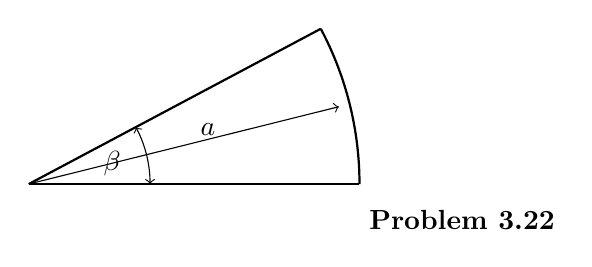
\begin{tikzpicture}[scale=1.4]
  % circular sector 0<=phi<=beta, rho<=a
  \draw[thick] (0,0) -- (3.0,0);
  \draw[thick] (0,0) -- (28:3.0);
  \draw[thick] (3.0,0) arc (0:28:3.0);
  % radial arrow a along the bisector
  \draw[->] (0,0) -- (14:2.9);
  \node at (17:1.7) {$a$};
  % angle beta at apex
  \draw[<->] (1.1,0) arc (0:28:1.1);
  \node at (14:0.78) {$\beta$};
  \node[below right] at (3.0,-0.15) {\textbf{Problem 3.22}};
\end{tikzpicture}
\end{center}

Using separation of variables in polar coordinates, show that the Green function can be written as
\[
G(\rho,\phi;\rho',\phi')=\sum_{m=1}^{\infty}\frac{4}{m}\,\rho_{<}^{m\pi/\beta}\left(\frac{1}{\rho_{>}^{m\pi/\beta}}-\frac{\rho_{>}^{m\pi/\beta}}{a^{2m\pi/\beta}}\right)\sin\!\left(\frac{m\pi\phi}{\beta}\right)\sin\!\left(\frac{m\pi\phi'}{\beta}\right)
\]
Problem 2.25 may be of use.
\solution

Use the two-dimensional convention
$\nabla^2G=-4\pi\delta(\rho-\rho')\delta(\phi-\phi')/\rho$.
On the interval $0<\phi<\beta$ the normalized delta expansion is
\[
\delta(\phi-\phi')=\frac2\beta\sum_{m=1}^\infty
\sin(\nu_m\phi)\sin(\nu_m\phi'),\qquad\nu_m=m\pi/\beta.
\]
Write $G=\sum_m g_m(\rho,\rho')\sin(\nu_m\phi)\sin(\nu_m\phi')$.
The radial equation is
\[
\left[\frac1\rho\frac d{d\rho}\rho\frac d{d\rho}
-\frac{\nu_m^2}{\rho^2}\right]g_m
=-\frac{8\pi}{\beta}\frac{\delta(\rho-\rho')}{\rho}.
\]
Its homogeneous solutions are $\rho^{\nu_m}$ and $\rho^{-\nu_m}$.
Regularity at the apex and the zero value at $a$ require
\[
g_m=C_m\rho_<^{\nu_m}
(\rho_>^{-\nu_m}-\rho_>^{\nu_m}/a^{2\nu_m}).
\]
This is continuous at $\rho'$; its derivative jump is
$[\rho\partial_\rho g_m]_-^+=-2\nu_mC_m$.
Integrating the radial equation across the source then fixes
$C_m=4\pi/(\beta\nu_m)=4/m$, proving the required formula.
Both radial faces and the arc have zero potential, the apex solution
is regular, and interchange of source and observation coordinates
leaves the result invariant.

\Needspace{5\baselineskip}
\par\bigskip
\noindent\textbf{3.23}\quad A point charge $q$ is located at the point $(\rho',\phi',z')$ inside a grounded cylindrical box defined by the surfaces $z=0$, $z=L$, $\rho=a$. Show that the potential inside the box can be expressed in the following alternative forms:
\begin{align*}
\Phi(\mathbf{x},\mathbf{x}')&=\frac{q}{\pi\epsilon_{0}a}\sum_{m=-\infty}^{\infty}\sum_{n=1}^{\infty}\frac{e^{im(\phi-\phi')}J_{m}\!\left(\dfrac{x_{mn}\rho}{a}\right)\!J_{m}\!\left(\dfrac{x_{mn}\rho'}{a}\right)}{x_{mn}J_{m+1}^{2}(x_{mn})\sinh\!\left(\dfrac{x_{mn}L}{a}\right)}\\
&\qquad\qquad\times\sinh\!\left[\frac{x_{mn}}{a}z_{<}\right]\sinh\!\left[\frac{x_{mn}}{a}(L-z_{>})\right]\\[6pt]
\Phi(\mathbf{x},\mathbf{x}')&=\frac{q}{\pi\epsilon_{0}L}\sum_{m=-\infty}^{\infty}\sum_{n=1}^{\infty}e^{im(\phi-\phi')}\sin\!\left(\frac{n\pi z}{L}\right)\sin\!\left(\frac{n\pi z'}{L}\right)\frac{I_{m}\!\left(\dfrac{n\pi\rho_{<}}{L}\right)}{I_{m}\!\left(\dfrac{n\pi a}{L}\right)}\\
&\qquad\qquad\times\left[I_{m}\!\left(\frac{n\pi a}{L}\right)\!K_{m}\!\left(\frac{n\pi\rho_{>}}{L}\right)-K_{m}\!\left(\frac{n\pi a}{L}\right)\!I_{m}\!\left(\frac{n\pi\rho_{>}}{L}\right)\right]\\[6pt]
\Phi(\mathbf{x},\mathbf{x}')&=\frac{2q}{\pi\epsilon_{0}La^{2}}\sum_{m=-\infty}^{\infty}\sum_{k=1}^{\infty}\sum_{n=1}^{\infty}\frac{e^{im(\phi-\phi')}\sin\!\left(\dfrac{k\pi z}{L}\right)\sin\!\left(\dfrac{k\pi z'}{L}\right)\!J_{m}\!\left(\dfrac{x_{mn}\rho}{a}\right)\!J_{m}\!\left(\dfrac{x_{mn}\rho'}{a}\right)}{\left[\left(\dfrac{x_{mn}}{a}\right)^{2}+\left(\dfrac{k\pi}{L}\right)^{2}\right]\!J_{m+1}^{2}(x_{mn})}
\end{align*}
Discuss the relation of the last expansion (with its extra summation) to the other two.
\solution

Use $\Phi=qG_D/(4\pi\epsilon_0)$ and denote the positive zeros
of $J_m$ by $x_{mn}$ (for negative $m$, use the corresponding zeros
of $J_{|m|}$).  The radial norm and completeness relation are
\[
\int_0^a\rho J_m(x_{mn}\rho/a)J_m(x_{mn'}\rho/a)d\rho
=\frac{a^2}2J_{m+1}^2(x_{mn})\delta_{nn'},
\]
\[
\frac{\delta(\rho-\rho')}{\rho}
=\frac2{a^2}\sum_{n=1}^\infty
\frac{J_m(x_{mn}\rho/a)J_m(x_{mn}\rho'/a)}{J_{m+1}^2(x_{mn})}.
\]
The sign in $J_{-m}=(-1)^mJ_m$ cancels in the products and norms.

First use this radial basis and angular Fourier modes.  For
$\alpha=x_{mn}/a$, the axial inverse of $-\partial_z^2+\alpha^2$
is
\[
h_\alpha(z,z')=
\frac{\sinh(\alpha z_<)\sinh[\alpha(L-z_>)]}{\alpha\sinh(\alpha L)},
\qquad [\partial_zh_\alpha]_-^+=-1.
\]
The source normalization gives
\[
G_D=\frac4{a^2}\sum_{m,n}
\frac{e^{im(\phi-\phi')}J_m(x_{mn}\rho/a)J_m(x_{mn}\rho'/a)}
{J_{m+1}^2(x_{mn})}\,h_{x_{mn}/a}(z,z').
\]
Multiplying by $q/(4\pi\epsilon_0)$ and using $\alpha=x_{mn}/a$
is exactly the first displayed potential.

Alternatively expand in axial sine modes with $\kappa=n\pi/L$.
The radial function satisfying both regularity and the wall condition is
\[
R_m(\rho,\rho';\kappa)=I_m(\kappa\rho_<)
\left[K_m(\kappa\rho_>)-
\frac{K_m(\kappa a)}{I_m(\kappa a)}I_m(\kappa\rho_>)\right].
\]
Its derivative jump is $[\rho\partial_\rho R_m]_-^+=-1$, by
the $I_m,K_m$ Wronskian.  Therefore
\[
G_D=\frac4L\sum_{m,n}e^{im(\phi-\phi')}
\sin(\kappa z)\sin(\kappa z')R_m(\rho,\rho';\kappa),
\]
which, after rearranging the bracket, gives the second potential.

Finally expand in both sets of eigenfunctions.  Their full
Laplacian eigenvalue is $\alpha^2+\kappa^2$, so inversion gives
\[
G_D=\frac8{La^2}\sum_{m,k,n}
\frac{e^{im(\phi-\phi')}\sin(k\pi z/L)\sin(k\pi z'/L)
J_m(x_{mn}\rho/a)J_m(x_{mn}\rho'/a)}
{[(x_{mn}/a)^2+(k\pi/L)^2]J_{m+1}^2(x_{mn})}.
\]
This is the third expression with its correct factor after multiplying
by $q/(4\pi\epsilon_0)$.  The extra sum has simply left both
one-dimensional inversions in spectral form.  Explicitly,
\[
\frac2L\sum_{k=1}^\infty
\frac{\sin(k\pi z/L)\sin(k\pi z'/L)}{\alpha^2+(k\pi/L)^2}
=h_\alpha(z,z'),
\]
reduces the third expression to the first; the radial resolvent
\[
\frac2{a^2}\sum_n
\frac{J_m(x_{mn}\rho/a)J_m(x_{mn}\rho'/a)}
{[(x_{mn}/a)^2+\kappa^2]J_{m+1}^2(x_{mn})}
=R_m(\rho,\rho';\kappa)
\]
reduces it to the second.  All three have the same boundary values,
source jump, and reciprocity, so uniqueness also establishes their
equivalence.

\Needspace{5\baselineskip}
\par\bigskip
\noindent\textbf{3.24}\quad The walls of the conducting cylindrical box of Problem 3.23 are all at zero potential, except for a disc in the upper end, defined by $\rho=b<a$, at potential $V$.
\begin{enumerate}
\item[(a)] Using the various forms of the Green function obtained in Problem 3.23, find three expansions for the potential inside the cylinder.
\item[(b)] For each series, calculate numerically the ratio of the potential at $\rho=0$, $z=L/2$ to the potential of the disc, assuming $b=L/4=a/2$. Try to obtain at least two-significant-figure accuracy. Is one series less rapidly convergent than the others? Why?
\end{enumerate}
(\emph{Abramowitz and Stegun} have tables; \emph{Mathematica} has Bessel functions, as does the software of \emph{Press et al.})
\solution

\textbf{(a)} Only the upper disc contributes to the Dirichlet
boundary formula,
\[
\Phi=-\frac V{4\pi}\int_0^{2\pi}d\phi'\int_0^b\rho'd\rho'
\,\partial_{z'}G_D(\rho,\phi,z;\rho',\phi',L).
\]
The angular integral selects $m=0$.  Put $x_n=x_{0n}$,
$\alpha_n=x_n/a$, and $\kappa_k=k\pi/L$.
In the first form of Problem 3.23, the upper-end derivative of
$h_{\alpha_n}$ is $-\sinh(\alpha_nz)/\sinh(\alpha_nL)$.
Using $\int_0^b\rho'J_0(\alpha_n\rho')d\rho'=bJ_1(\alpha_nb)/\alpha_n$
gives the first expansion:
\[
\boxed{\frac\Phi V=\frac{2b}a\sum_{n=1}^\infty
\frac{J_1(x_nb/a)}{x_nJ_1^2(x_n)}J_0(x_n\rho/a)
\frac{\sinh(x_nz/a)}{\sinh(x_nL/a)}.}\tag{A}
\]
For the second Green function define
$c_k=K_0(\kappa_ka)/I_0(\kappa_ka)$ and
\[
H_k(\rho)=\int_0^b\rho'I_0(\kappa_k\rho_<)
[K_0(\kappa_k\rho_>)-c_kI_0(\kappa_k\rho_>)]d\rho'.
\]
The primitive integrals are
$\int\rho I_0(\kappa\rho)d\rho=\rho I_1(\kappa\rho)/\kappa$
and $\int\rho K_0(\kappa\rho)d\rho=-\rho K_1(\kappa\rho)/\kappa$.
Splitting at $\rho'=\rho$ and using
$I_0(x)K_1(x)+I_1(x)K_0(x)=1/x$ yields
\[
H_k(\rho)=\begin{cases}
\kappa_k^{-2}-\dfrac b{\kappa_k}I_0(\kappa_k\rho)
[K_1(\kappa_kb)+c_kI_1(\kappa_kb)],&\rho\leq b,\\[3pt]
\dfrac b{\kappa_k}I_1(\kappa_kb)
[K_0(\kappa_k\rho)-c_kI_0(\kappa_k\rho)],&b\leq\rho<a.
\end{cases}
\]
The second expansion is therefore
\[
\boxed{\frac\Phi V=\frac2L\sum_{k=1}^\infty
(-1)^{k+1}\kappa_k\sin(\kappa_kz)H_k(\rho).}\tag{B}
\]
The third Green function gives directly
\[
\boxed{\frac\Phi V=\frac{4b}{La}\sum_{n=1}^\infty\sum_{k=1}^\infty
\frac{(-1)^{k+1}\kappa_k\sin(\kappa_kz)
J_0(x_n\rho/a)J_1(x_nb/a)}
{x_nJ_1^2(x_n)(\alpha_n^2+\kappa_k^2)}.}\tag{C}
\]
As a boundary limit these are interpreted in the usual Fourier/Abel
sense at jumps.  For strictly interior points they give the same
harmonic solution.

\textbf{(b)} Choose units $a=1$, so $b=1/2$, $L=2$, $z=1$.
The factor in (A) is $\sinh x_n/\sinh2x_n=1/(2\cosh x_n)$.
Its partial sums are
\[
\begin{array}{c|rrrr}
N&1&2&5&10\\\hline
\Phi_A/V&0.06893268&0.07158219&0.07152937&0.07152937289
\end{array}
\]
For (B) the raw sums and an accelerated evaluation are
\[
\begin{array}{c|rrrr}
K&11&51&101&501\\\hline
\Phi_B/V&0.04518810&0.06541029&0.07464976&0.07216345
\end{array}
\]
The slow part can be summed exactly:
$(2/\pi)\sum_{k\geq1}(-1)^{k+1}\sin(k\pi z/L)/k=z/L$.
Subtracting this $1/k$ tail from (B), summing the remaining Bessel
terms, and adding $z/L$ gives $0.07152937289$ (51 terms suffice).

For (C), rectangular sums over $(N,K)=(20,51),(100,501),(200,2001)$
give respectively $0.06595877$, $0.07212779$, and $0.07168131$.
An independent acceleration is Euler's transformation of the
alternating odd-$k$ sum at $z=L/2$.  If it is
$\sum_{j\geq0}(-1)^ju_j$, use
$\sum_{p\geq0}\Delta^pu_0/2^{p+1}$ with
$\Delta u_j=u_j-u_{j+1}$.  Taking $N=20$ radial modes and 32 odd
axial terms gives $0.071529372893$; increasing to $(40,64)$ gives
$0.071529372888$.  Thus every representation yields
\[
\boxed{\Phi(0,L/2)/V=0.07152937289\ldots\simeq0.072.}
\]
Series (A) has exponential suppression across the distance from the
upper boundary.  The unaccelerated axial sine series (B) and (C)
retain a $1/k$ tail because their basis functions vanish at the end
where the imposed boundary value jumps to a nonzero value.  The
extra unsummed spectrum in (C) adds work without accelerating that
tail.  The supplementary code reproduces all three calculations.

\Needspace{5\baselineskip}
\par\bigskip
\noindent\textbf{3.25}\quad Consider the surface-charge densities for the problem of Section 3.13 of the conducting plane with a circular hole of radius $a$.
\begin{enumerate}
\item[(a)] Show that the surface-charge densities on the top and bottom of the plane for $\rho\geq a$ are
\begin{align*}
\sigma_{+}(\rho)&=-\epsilon_{0}E_{0}+\Delta\sigma(\rho)\\
\sigma_{-}(\rho)&=\epsilon_{0}E_{1}+\Delta\sigma(\rho)
\end{align*}
where
\[
\Delta\sigma(\rho)=-\epsilon_{0}\frac{(E_{0}-E_{1})}{\pi}\left[\frac{a}{\sqrt{\rho^{2}-a^{2}}}-\sin^{-1}\!\left(\frac{a}{\rho}\right)\right]
\]
How does $\Delta\sigma(\rho)$ behave for large $\rho$? Is $\Delta\sigma(\rho)$, defined in terms of $\Phi^{(1)}$, zero for $\rho<a$? Explain.
\item[(b)] Show by direct integration that
\[
\lim_{R\to\infty}\left[2\pi\int_{a}^{R}d\rho\;\rho(\sigma_{+}+\sigma_{-})+2\pi\epsilon_{0}\int_{0}^{R}d\rho\;\rho(E_{0}-E_{1})\right]=0
\]
Interpret.
\end{enumerate}
\solution

Put $\Delta E=E_0-E_1$.  Section 3.13 gives
$\Phi=E_0z+\Phi^{(1)}$ above and $\Phi=E_1z+\Phi^{(1)}$ below,
where the even correction has the transform
\[
\Phi^{(1)}=\frac{\Delta E}{\pi}\int_0^\infty
\left[\frac{\sin(ka)}{k^2}-\frac{a\cos(ka)}k\right]
e^{-k|z|}J_0(k\rho)dk.
\]
\textbf{(a)} On the upper conducting face
$\sigma_+=-\epsilon_0\partial_z\Phi|_{0^+}$, so its correction is
\[
\Delta\sigma=\frac{\epsilon_0\Delta E}{\pi}
\left[\int_0^\infty\frac{\sin(ka)}kJ_0(k\rho)dk
-a\int_0^\infty\cos(ka)J_0(k\rho)dk\right].
\]
For $\rho>a$, take the real part of
$\int_0^\infty e^{-(s-ia)k}J_0(k\rho)dk
=[(s-ia)^2+\rho^2]^{-1/2}$ as $s\downarrow0$ to get
$(\rho^2-a^2)^{-1/2}$.  Integration with respect to $a$ from zero
gives the first integral $\sin^{-1}(a/\rho)$.
Hence the stated expression for $\Delta\sigma$ follows.
Evenness of $\Phi^{(1)}$ makes the correction on the bottom face
the same, whereas the background contribution has the opposite
normal sign.  Thus $\sigma_+=-\epsilon_0E_0+\Delta\sigma$ and
$\sigma_-=\epsilon_0E_1+\Delta\sigma$.
At large $\rho$, set $t=a/\rho$ and expand:
\[
\frac{t}{\sqrt{1-t^2}}-\sin^{-1}t
=\frac{t^3}3+\frac{3t^5}{10}+O(t^7),\quad
\Delta\sigma=-\frac{\epsilon_0\Delta E\,a^3}{3\pi\rho^3}
+O(\rho^{-5}).
\]
Inside the hole the second transform is zero while the first is
$\pi/2$.  Therefore the correction \emph{defined from}
$\Phi^{(1)}$ is $\Delta\sigma=\epsilon_0\Delta E/2$ per face,
not zero.  It is a fictitious correction to the intact-plane
background: the combined correction $2\Delta\sigma$ cancels its
background sheet charge $-\epsilon_0\Delta E$ in the hole.
There is no physical surface charge where the material is absent.

\textbf{(b)} A direct primitive gives
\begin{align*}
I(R)&=\int_a^R\rho\left[
\frac a{\sqrt{\rho^2-a^2}}-\sin^{-1}\frac a\rho\right]d\rho\\
&=\frac a2\sqrt{R^2-a^2}-\frac{R^2}2\sin^{-1}(a/R)
+\frac{\pi a^2}4\longrightarrow\frac{\pi a^2}4.
\end{align*}
The quantity in the question equals
\[
\pi\epsilon_0\Delta E\,a^2-4\epsilon_0\Delta E I(R)
=2\epsilon_0\Delta E\left[R^2\sin^{-1}(a/R)
-a\sqrt{R^2-a^2}\right]
=\frac{4\epsilon_0\Delta E\,a^3}{3R}+O(R^{-3}),
\]
and therefore tends to zero.  The missing intact-plane charge in
the hole is exactly compensated by the redistribution on the
remaining conductor.  Equivalently, the total charge associated
with $\Phi^{(1)}$ is zero, consistent with its absence of a monopole
far field.

\Needspace{5\baselineskip}
\par\bigskip
\noindent\textbf{3.26}\quad Consider the Green function appropriate for Neumann boundary conditions for the volume $V$ between the concentric spherical surfaces defined by $r=a$ and $r=b$, $a<b$. To be able to use (1.46) for the potential, impose the simple constraint (1.45). Use an expansion in spherical harmonics of the form,
\[
G(\mathbf{x},\mathbf{x}')=\sum_{l=0}^{\infty}g_{l}(r,r')P_{l}(\cos\gamma)
\]
where $g_{l}(r,r')=r_{<}^{l}/r_{>}^{l+1}+f_{l}(r,r')$.
\begin{enumerate}
\item[(a)] Show that for $l>0$, the radial Green function has the symmetric form
\begin{align*}
g_{l}(r,r')=\frac{r_{<}^{l}}{r_{>}^{l+1}}&+\\
\frac{1}{(b^{2l+1}-a^{2l+1})}&\left[\frac{l+1}{l}(rr')^{l}+\frac{l}{l+1}\frac{(ab)^{2l+1}}{(rr')^{l+1}}+a^{2l+1}\!\left(\frac{r^{l}}{r'^{\,l+1}}+\frac{r'^{\,l}}{r^{l+1}}\right)\right]
\end{align*}
\item[(b)] Show that for $l=0$
\[
g_{0}(r,r')=\frac{1}{r_{>}}-\left(\frac{a^{2}}{a^{2}+b^{2}}\right)\frac{1}{r'}+f(r)
\]
where $f(r)$ is arbitrary. Show explicitly in (1.46) that answers for the potential $\Phi(\mathbf{x})$ are independent of $f(r)$.

[The arbitrariness in the Neumann Green function can be removed by symmetrizing $g_{0}$ in $r$ and $r'$ with a suitable choice of $f(r)$.]
\end{enumerate}
\solution

The Neumann convention of Eqs.~(1.45)--(1.46) is
\[
\nabla'^2G_N=-4\pi\delta^3(\mathbf r-\mathbf r'),\qquad
\partial_{n'}G_N=-\frac{4\pi}{S}
=-\frac1{a^2+b^2},\quad S=4\pi(a^2+b^2).
\]
The inner outward normal is $-\hat{\mathbf r}'$ and the outer
normal is $+\hat{\mathbf r}'$.

\textbf{(a)} For $l>0$ the boundary derivative must vanish.  Write
\[
f_l=A_l(r)r'^l+B_l(r)r'^{-l-1}.
\]
At $r'=a<r$, differentiating the Coulomb term and $f_l$ gives
\[
A_l-\frac{l+1}{l}\frac{B_l}{a^{2l+1}}=-r^{-l-1}.
\]
At $r'=b>r$ the analogous condition is
\[
\frac l{l+1}A_lb^{2l+1}-B_l=r^l.
\]
Eliminating $A_l,B_l$, with $D_l=b^{2l+1}-a^{2l+1}$, yields
\[
A_l=\frac{(l+1)r^l/l+a^{2l+1}r^{-l-1}}{D_l},\qquad
B_l=\frac{a^{2l+1}r^l+[l/(l+1)](ab)^{2l+1}r^{-l-1}}{D_l}.
\]
Insertion into $f_l$ gives
\[
\boxed{g_l=\frac{r_<^l}{r_>^{l+1}}+\frac1{D_l}
\left[\frac{l+1}{l}(rr')^l+
\frac l{l+1}\frac{(ab)^{2l+1}}{(rr')^{l+1}}
+a^{2l+1}\left(\frac{r^l}{r'^{l+1}}+
\frac{r'^l}{r^{l+1}}\right)\right].}
\]
It is explicitly symmetric and has the same source derivative jump
as the Coulomb radial term; the added terms are harmonic in the
source coordinate.

\textbf{(b)} Put $c=a^2/(a^2+b^2)$.  For $l=0$ the proposed form
\[
g_0=\frac1{r_>}-\frac c{r'}+f(r)
\]
is harmonic in $r'$ away from the source.  Its inner radial derivative
is $c/a^2=1/(a^2+b^2)$ and its outer derivative is
$(-1+c)/b^2=-1/(a^2+b^2)$, exactly the required normal derivatives.
The function $f(r)$ is arbitrary because the defining differential
equation and boundary constraint act on the primed argument.
Choosing $f(r)=-c/r+C$ makes $g_0$ symmetric.

To verify that this freedom is immaterial, write the Neumann
representation with $\varrho$ denoting the volume charge density:
\[
\Phi(\mathbf r)-\langle\Phi\rangle_S
=\frac1{4\pi\epsilon_0}\int_V\varrho(\mathbf r')G_N\,d^3r'
+\frac1{4\pi}\oint_SG_N\partial_{n'}\Phi\,dS',
\quad\langle\Phi\rangle_S=\frac1S\oint_S\Phi\,dS.
\]
Changing $f$ by $\delta f(r)$ changes its right side by
\[
\frac{\delta f(r)}{4\pi}
\left[\frac{Q_V}{\epsilon_0}+\oint_S\partial_n\Phi\,dS\right]=0,
\]
because Gauss's law/Poisson's equation gives
$\oint_S\partial_n\Phi\,dS=-Q_V/\epsilon_0$.
This is also the compatibility condition for the prescribed Neumann
data.  Only the arbitrary additive constant in $\Phi$ remains.

\Needspace{5\baselineskip}
\par\bigskip
\noindent\textbf{3.27}\quad Apply the Neumann Green function of Problem 3.26 to the situation in which the normal electric field is $E_{r}=-E_{0}\cos\theta$ at the outer surface ($r=b$) and is $E_{r}=0$ on the inner surface ($r=a$).
\begin{enumerate}
\item[(a)] Show that the electrostatic potential inside the volume $V$ is
\[
\Phi(\mathbf{x})=E_{0}\,\frac{r\cos\theta}{1-p^{3}}\left(1+\frac{a^{3}}{2r^{3}}\right)
\]
where $p=a/b$. Find the components of the electric field,
\[
E_{r}(r,\theta)=-E_{0}\,\frac{\cos\theta}{1-p^{3}}\left(1-\frac{a^{3}}{r^{3}}\right),\qquad
E_{\theta}(r,\theta)=E_{0}\,\frac{\sin\theta}{1-p^{3}}\left(1+\frac{a^{3}}{2r^{3}}\right)
\]
\item[(b)] Calculate the Cartesian or cylindrical components of the field, $E_{z}$ and $E_{\rho}$, and make a sketch or computer plot of the lines of electric force for a typical case of $p=0.5$.
\end{enumerate}
\solution

\textbf{(a)} There is no volume charge.  On $r=b$,
$\partial_n\Phi=\partial_r\Phi=-E_r=E_0\cos\theta$;
on $r=a$ the derivative is zero.  Choose the additive constant so
that the surface average of $\Phi$ is zero.  The Neumann formula is
then
\[
\Phi=\frac{E_0b^2}{4\pi}\int G_N(\mathbf r,b\hat{\mathbf r}')
\cos\theta'\,d\Omega'.
\]
The angular addition theorem gives
$\int P_l(\cos\gamma)\cos\theta'\,d\Omega'
=(4\pi/3)\delta_{l1}\cos\theta$.  From Problem 3.26,
\[
g_1(r,b)=\frac{3}{b^2(1-a^3/b^3)}
\left(r+\frac{a^3}{2r^2}\right).
\]
Thus, with $p=a/b$,
\[
\boxed{\Phi=\frac{E_0}{1-p^3}\left(r+\frac{a^3}{2r^2}\right)
\cos\theta.}
\]
Differentiating, $E_r=-\partial_r\Phi$ and
$E_\theta=-r^{-1}\partial_\theta\Phi$, gives exactly
\[
E_r=-\frac{E_0}{1-p^3}(1-a^3/r^3)\cos\theta,\qquad
E_\theta=\frac{E_0}{1-p^3}(1+a^3/(2r^3))\sin\theta.
\]
In particular $E_r(a)=0$ and $E_r(b)=-E_0\cos\theta$, checking
both Neumann conditions.

\textbf{(b)} Resolve the unit vectors along and perpendicular to
$z$: $E_z=E_r\cos\theta-E_\theta\sin\theta$,
$E_\rho=E_r\sin\theta+E_\theta\cos\theta$.  If
$K=E_0/(1-p^3)$, this gives
\[
\boxed{E_z=-K\left[1-\frac{a^3}{2r^3}(3\cos^2\theta-1)\right],
\qquad E_\rho=\frac{3Ka^3}{2r^3}\sin\theta\cos\theta.}
\]
Equivalently $E_\rho=3Ka^3\rho z/(2r^5)$ and
$E_z=-K[1-a^3(2z^2-\rho^2)/(2r^5)]$.
A useful axisymmetric flux function is
\[
\Psi=-\frac K2\left(r^2-\frac{a^3}{r}\right)\sin^2\theta,
\quad
E_r=\frac{\partial_\theta\Psi}{r^2\sin\theta},\quad
E_\theta=-\frac{\partial_r\Psi}{r\sin\theta}.
\]
Hence field lines have constant
\[
\boxed{\rho^2\left[1-\frac{a^3}{(\rho^2+z^2)^{3/2}}\right].}
\]
This exact first integral was used to generate the following
meridional section for $p=0.5$ and $E_0>0$.  Arrows run from the
upper outer hemisphere to the lower one; the inner sphere is a
zero-normal-flux surface.  Rotation about $z$ gives the full field.
\begin{center}
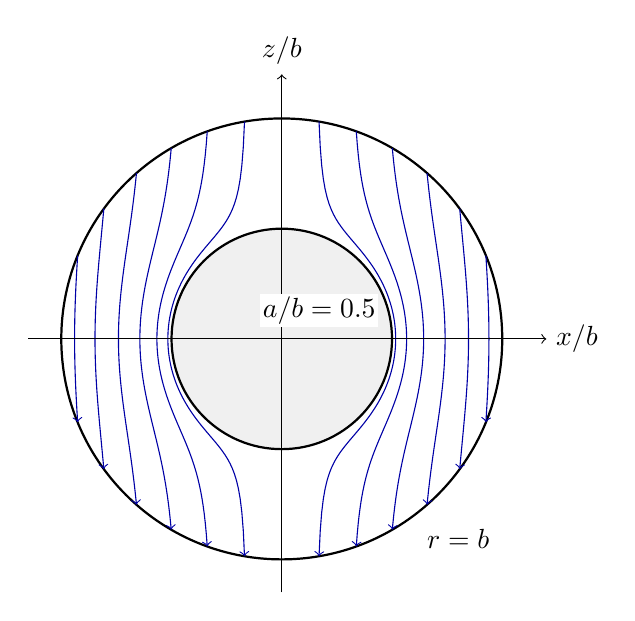
\begin{tikzpicture}[scale=2.8]
\draw[thick] (0,0) circle (1);
\filldraw[fill=gray!12,draw=black,thick] (0,0) circle (.5);
\draw[blue!65!black,thin,->] plot coordinates {(-0.1690309,0.9856108) (-0.1744767,0.8702578) (-0.1809944,0.7875959) (-0.1884470,0.7261819) (-0.1966835,0.6790696) (-0.2055576,0.6418404) (-0.2149375,0.6115847) (-0.2247093,0.5863337) (-0.2347763,0.5647238) (-0.2450574,0.5457918) (-0.2554847,0.5288444) (-0.2660007,0.5133747) (-0.2765572,0.4990062) (-0.2871127,0.4854560) (-0.2976314,0.4725088) (-0.3080824,0.4599989) (-0.3184382,0.4477980) (-0.3286747,0.4358056) (-0.3387702,0.4239429) (-0.3487052,0.4121477) (-0.3584619,0.4003707) (-0.3680241,0.3885729) (-0.3773769,0.3767237) (-0.3865064,0.3647988) (-0.3953999,0.3527794) (-0.4040455,0.3406510) (-0.4124320,0.3284029) (-0.4205491,0.3160273) (-0.4283870,0.3035187) (-0.4359366,0.2908740) (-0.4431892,0.2780919) (-0.4501367,0.2651724) (-0.4567717,0.2521169) (-0.4630870,0.2389280) (-0.4690760,0.2256092) (-0.4747324,0.2121648) (-0.4800504,0.1985999) (-0.4850247,0.1849202) (-0.4896503,0.1711320) (-0.4939225,0.1572421) (-0.4978372,0.1432577) (-0.5013905,0.1291862) (-0.5045790,0.1150355) (-0.5073996,0.1008139) (-0.5098496,0.0865296) (-0.5119267,0.0721913) (-0.5136288,0.0578077) (-0.5149543,0.0433877) (-0.5159020,0.0289404) (-0.5164710,0.0144748) (-0.5166607,-0.0000000) (-0.5164710,-0.0144748) (-0.5159020,-0.0289404) (-0.5149543,-0.0433877) (-0.5136288,-0.0578077) (-0.5119267,-0.0721913) (-0.5098496,-0.0865296) (-0.5073996,-0.1008139) (-0.5045790,-0.1150355) (-0.5013905,-0.1291862) (-0.4978372,-0.1432577) (-0.4939225,-0.1572421) (-0.4896503,-0.1711320) (-0.4850247,-0.1849202) (-0.4800504,-0.1985999) (-0.4747324,-0.2121648) (-0.4690760,-0.2256092) (-0.4630870,-0.2389280) (-0.4567717,-0.2521169) (-0.4501367,-0.2651724) (-0.4431892,-0.2780919) (-0.4359366,-0.2908740) (-0.4283870,-0.3035187) (-0.4205491,-0.3160273) (-0.4124320,-0.3284029) (-0.4040455,-0.3406510) (-0.3953999,-0.3527794) (-0.3865064,-0.3647988) (-0.3773769,-0.3767237) (-0.3680241,-0.3885729) (-0.3584619,-0.4003707) (-0.3487052,-0.4121477) (-0.3387702,-0.4239429) (-0.3286747,-0.4358056) (-0.3184382,-0.4477980) (-0.3080824,-0.4599989) (-0.2976314,-0.4725088) (-0.2871127,-0.4854560) (-0.2765572,-0.4990062) (-0.2660007,-0.5133747) (-0.2554847,-0.5288444) (-0.2450574,-0.5457918) (-0.2347763,-0.5647238) (-0.2247093,-0.5863337) (-0.2149375,-0.6115847) (-0.2055576,-0.6418404) (-0.1966835,-0.6790696) (-0.1884470,-0.7261819) (-0.1809944,-0.7875959) (-0.1744767,-0.8702578) (-0.1690309,-0.9856108)};
\draw[blue!65!black,thin,->] plot coordinates {(0.1690309,0.9856108) (0.1744767,0.8702578) (0.1809944,0.7875959) (0.1884470,0.7261819) (0.1966835,0.6790696) (0.2055576,0.6418404) (0.2149375,0.6115847) (0.2247093,0.5863337) (0.2347763,0.5647238) (0.2450574,0.5457918) (0.2554847,0.5288444) (0.2660007,0.5133747) (0.2765572,0.4990062) (0.2871127,0.4854560) (0.2976314,0.4725088) (0.3080824,0.4599989) (0.3184382,0.4477980) (0.3286747,0.4358056) (0.3387702,0.4239429) (0.3487052,0.4121477) (0.3584619,0.4003707) (0.3680241,0.3885729) (0.3773769,0.3767237) (0.3865064,0.3647988) (0.3953999,0.3527794) (0.4040455,0.3406510) (0.4124320,0.3284029) (0.4205491,0.3160273) (0.4283870,0.3035187) (0.4359366,0.2908740) (0.4431892,0.2780919) (0.4501367,0.2651724) (0.4567717,0.2521169) (0.4630870,0.2389280) (0.4690760,0.2256092) (0.4747324,0.2121648) (0.4800504,0.1985999) (0.4850247,0.1849202) (0.4896503,0.1711320) (0.4939225,0.1572421) (0.4978372,0.1432577) (0.5013905,0.1291862) (0.5045790,0.1150355) (0.5073996,0.1008139) (0.5098496,0.0865296) (0.5119267,0.0721913) (0.5136288,0.0578077) (0.5149543,0.0433877) (0.5159020,0.0289404) (0.5164710,0.0144748) (0.5166607,-0.0000000) (0.5164710,-0.0144748) (0.5159020,-0.0289404) (0.5149543,-0.0433877) (0.5136288,-0.0578077) (0.5119267,-0.0721913) (0.5098496,-0.0865296) (0.5073996,-0.1008139) (0.5045790,-0.1150355) (0.5013905,-0.1291862) (0.4978372,-0.1432577) (0.4939225,-0.1572421) (0.4896503,-0.1711320) (0.4850247,-0.1849202) (0.4800504,-0.1985999) (0.4747324,-0.2121648) (0.4690760,-0.2256092) (0.4630870,-0.2389280) (0.4567717,-0.2521169) (0.4501367,-0.2651724) (0.4431892,-0.2780919) (0.4359366,-0.2908740) (0.4283870,-0.3035187) (0.4205491,-0.3160273) (0.4124320,-0.3284029) (0.4040455,-0.3406510) (0.3953999,-0.3527794) (0.3865064,-0.3647988) (0.3773769,-0.3767237) (0.3680241,-0.3885729) (0.3584619,-0.4003707) (0.3487052,-0.4121477) (0.3387702,-0.4239429) (0.3286747,-0.4358056) (0.3184382,-0.4477980) (0.3080824,-0.4599989) (0.2976314,-0.4725088) (0.2871127,-0.4854560) (0.2765572,-0.4990062) (0.2660007,-0.5133747) (0.2554847,-0.5288444) (0.2450574,-0.5457918) (0.2347763,-0.5647238) (0.2247093,-0.5863337) (0.2149375,-0.6115847) (0.2055576,-0.6418404) (0.1966835,-0.6790696) (0.1884470,-0.7261819) (0.1809944,-0.7875959) (0.1744767,-0.8702578) (0.1690309,-0.9856108)};
\draw[blue!65!black,thin,->] plot coordinates {(-0.3380617,0.9411239) (-0.3423211,0.8842199) (-0.3469395,0.8347631) (-0.3518912,0.7913529) (-0.3571474,0.7528926) (-0.3626779,0.7185116) (-0.3684516,0.6875118) (-0.3744373,0.6593274) (-0.3806044,0.6334968) (-0.3869230,0.6096405) (-0.3933647,0.5874445) (-0.3999021,0.5666478) (-0.4065096,0.5470323) (-0.4131628,0.5284149) (-0.4198391,0.5106414) (-0.4265171,0.4935815) (-0.4331768,0.4771247) (-0.4397998,0.4611768) (-0.4463687,0.4456580) (-0.4528672,0.4304995) (-0.4592804,0.4156430) (-0.4655941,0.4010383) (-0.4717952,0.3866422) (-0.4778714,0.3724179) (-0.4838113,0.3583337) (-0.4896041,0.3443624) (-0.4952398,0.3304808) (-0.5007091,0.3166690) (-0.5060032,0.3029101) (-0.5111139,0.2891896) (-0.5160336,0.2754954) (-0.5207552,0.2618174) (-0.5252718,0.2481471) (-0.5295775,0.2344774) (-0.5336662,0.2208028) (-0.5375328,0.2071187) (-0.5411723,0.1934218) (-0.5445799,0.1797094) (-0.5477516,0.1659799) (-0.5506834,0.1522323) (-0.5533718,0.1384660) (-0.5558136,0.1246813) (-0.5580059,0.1108787) (-0.5599463,0.0970594) (-0.5616324,0.0832246) (-0.5630623,0.0693760) (-0.5642345,0.0555155) (-0.5651476,0.0416453) (-0.5658005,0.0277678) (-0.5661925,0.0138851) (-0.5663232,0.0000000) (-0.5661925,-0.0138851) (-0.5658005,-0.0277678) (-0.5651476,-0.0416453) (-0.5642345,-0.0555155) (-0.5630623,-0.0693760) (-0.5616324,-0.0832246) (-0.5599463,-0.0970594) (-0.5580059,-0.1108787) (-0.5558136,-0.1246813) (-0.5533718,-0.1384660) (-0.5506834,-0.1522323) (-0.5477516,-0.1659799) (-0.5445799,-0.1797094) (-0.5411723,-0.1934218) (-0.5375328,-0.2071187) (-0.5336662,-0.2208028) (-0.5295775,-0.2344774) (-0.5252718,-0.2481471) (-0.5207552,-0.2618174) (-0.5160336,-0.2754954) (-0.5111139,-0.2891896) (-0.5060032,-0.3029101) (-0.5007091,-0.3166690) (-0.4952398,-0.3304808) (-0.4896041,-0.3443624) (-0.4838113,-0.3583337) (-0.4778714,-0.3724179) (-0.4717952,-0.3866422) (-0.4655941,-0.4010383) (-0.4592804,-0.4156430) (-0.4528672,-0.4304995) (-0.4463687,-0.4456580) (-0.4397998,-0.4611768) (-0.4331768,-0.4771247) (-0.4265171,-0.4935815) (-0.4198391,-0.5106414) (-0.4131628,-0.5284149) (-0.4065096,-0.5470323) (-0.3999021,-0.5666478) (-0.3933647,-0.5874445) (-0.3869230,-0.6096405) (-0.3806044,-0.6334968) (-0.3744373,-0.6593274) (-0.3684516,-0.6875118) (-0.3626779,-0.7185116) (-0.3571474,-0.7528926) (-0.3518912,-0.7913529) (-0.3469395,-0.8347631) (-0.3423211,-0.8842199) (-0.3380617,-0.9411239)};
\draw[blue!65!black,thin,->] plot coordinates {(0.3380617,0.9411239) (0.3423211,0.8842199) (0.3469395,0.8347631) (0.3518912,0.7913529) (0.3571474,0.7528926) (0.3626779,0.7185116) (0.3684516,0.6875118) (0.3744373,0.6593274) (0.3806044,0.6334968) (0.3869230,0.6096405) (0.3933647,0.5874445) (0.3999021,0.5666478) (0.4065096,0.5470323) (0.4131628,0.5284149) (0.4198391,0.5106414) (0.4265171,0.4935815) (0.4331768,0.4771247) (0.4397998,0.4611768) (0.4463687,0.4456580) (0.4528672,0.4304995) (0.4592804,0.4156430) (0.4655941,0.4010383) (0.4717952,0.3866422) (0.4778714,0.3724179) (0.4838113,0.3583337) (0.4896041,0.3443624) (0.4952398,0.3304808) (0.5007091,0.3166690) (0.5060032,0.3029101) (0.5111139,0.2891896) (0.5160336,0.2754954) (0.5207552,0.2618174) (0.5252718,0.2481471) (0.5295775,0.2344774) (0.5336662,0.2208028) (0.5375328,0.2071187) (0.5411723,0.1934218) (0.5445799,0.1797094) (0.5477516,0.1659799) (0.5506834,0.1522323) (0.5533718,0.1384660) (0.5558136,0.1246813) (0.5580059,0.1108787) (0.5599463,0.0970594) (0.5616324,0.0832246) (0.5630623,0.0693760) (0.5642345,0.0555155) (0.5651476,0.0416453) (0.5658005,0.0277678) (0.5661925,0.0138851) (0.5663232,0.0000000) (0.5661925,-0.0138851) (0.5658005,-0.0277678) (0.5651476,-0.0416453) (0.5642345,-0.0555155) (0.5630623,-0.0693760) (0.5616324,-0.0832246) (0.5599463,-0.0970594) (0.5580059,-0.1108787) (0.5558136,-0.1246813) (0.5533718,-0.1384660) (0.5506834,-0.1522323) (0.5477516,-0.1659799) (0.5445799,-0.1797094) (0.5411723,-0.1934218) (0.5375328,-0.2071187) (0.5336662,-0.2208028) (0.5295775,-0.2344774) (0.5252718,-0.2481471) (0.5207552,-0.2618174) (0.5160336,-0.2754954) (0.5111139,-0.2891896) (0.5060032,-0.3029101) (0.5007091,-0.3166690) (0.4952398,-0.3304808) (0.4896041,-0.3443624) (0.4838113,-0.3583337) (0.4778714,-0.3724179) (0.4717952,-0.3866422) (0.4655941,-0.4010383) (0.4592804,-0.4156430) (0.4528672,-0.4304995) (0.4463687,-0.4456580) (0.4397998,-0.4611768) (0.4331768,-0.4771247) (0.4265171,-0.4935815) (0.4198391,-0.5106414) (0.4131628,-0.5284149) (0.4065096,-0.5470323) (0.3999021,-0.5666478) (0.3933647,-0.5874445) (0.3869230,-0.6096405) (0.3806044,-0.6334968) (0.3744373,-0.6593274) (0.3684516,-0.6875118) (0.3626779,-0.7185116) (0.3571474,-0.7528926) (0.3518912,-0.7913529) (0.3469395,-0.8347631) (0.3423211,-0.8842199) (0.3380617,-0.9411239)};
\draw[blue!65!black,thin,->] plot coordinates {(-0.5014265,0.8652002) (-0.5046849,0.8303045) (-0.5080681,0.7977946) (-0.5115664,0.7673876) (-0.5151695,0.7388389) (-0.5188668,0.7119359) (-0.5226476,0.6864932) (-0.5265011,0.6623485) (-0.5304165,0.6393592) (-0.5343829,0.6173999) (-0.5383898,0.5963595) (-0.5424267,0.5761398) (-0.5464832,0.5566538) (-0.5505493,0.5378240) (-0.5546153,0.5195814) (-0.5586716,0.5018644) (-0.5627091,0.4846181) (-0.5667190,0.4677934) (-0.5706927,0.4513462) (-0.5746219,0.4352371) (-0.5784989,0.4194307) (-0.5823160,0.4038952) (-0.5860660,0.3886022) (-0.5897421,0.3735259) (-0.5933376,0.3586434) (-0.5968463,0.3439340) (-0.6002623,0.3293789) (-0.6035797,0.3149615) (-0.6067933,0.3006666) (-0.6098979,0.2864807) (-0.6128888,0.2723917) (-0.6157614,0.2583886) (-0.6185114,0.2444616) (-0.6211347,0.2306018) (-0.6236276,0.2168014) (-0.6259867,0.2030533) (-0.6282085,0.1893511) (-0.6302900,0.1756890) (-0.6322284,0.1620621) (-0.6340212,0.1484658) (-0.6356658,0.1348960) (-0.6371603,0.1213490) (-0.6385026,0.1078215) (-0.6396910,0.0943105) (-0.6407240,0.0808135) (-0.6416003,0.0673280) (-0.6423188,0.0538517) (-0.6428785,0.0403827) (-0.6432789,0.0269189) (-0.6435192,0.0134586) (-0.6435994,0.0000000) (-0.6435192,-0.0134586) (-0.6432789,-0.0269189) (-0.6428785,-0.0403827) (-0.6423188,-0.0538517) (-0.6416003,-0.0673280) (-0.6407240,-0.0808135) (-0.6396910,-0.0943105) (-0.6385026,-0.1078215) (-0.6371603,-0.1213490) (-0.6356658,-0.1348960) (-0.6340212,-0.1484658) (-0.6322284,-0.1620621) (-0.6302900,-0.1756890) (-0.6282085,-0.1893511) (-0.6259867,-0.2030533) (-0.6236276,-0.2168014) (-0.6211347,-0.2306018) (-0.6185114,-0.2444616) (-0.6157614,-0.2583886) (-0.6128888,-0.2723917) (-0.6098979,-0.2864807) (-0.6067933,-0.3006666) (-0.6035797,-0.3149615) (-0.6002623,-0.3293789) (-0.5968463,-0.3439340) (-0.5933376,-0.3586434) (-0.5897421,-0.3735259) (-0.5860660,-0.3886022) (-0.5823160,-0.4038952) (-0.5784989,-0.4194307) (-0.5746219,-0.4352371) (-0.5706927,-0.4513462) (-0.5667190,-0.4677934) (-0.5627091,-0.4846181) (-0.5586716,-0.5018644) (-0.5546153,-0.5195814) (-0.5505493,-0.5378240) (-0.5464832,-0.5566538) (-0.5424267,-0.5761398) (-0.5383898,-0.5963595) (-0.5343829,-0.6173999) (-0.5304165,-0.6393592) (-0.5265011,-0.6623485) (-0.5226476,-0.6864932) (-0.5188668,-0.7119359) (-0.5151695,-0.7388389) (-0.5115664,-0.7673876) (-0.5080681,-0.7977946) (-0.5046849,-0.8303045) (-0.5014265,-0.8652002)};
\draw[blue!65!black,thin,->] plot coordinates {(0.5014265,0.8652002) (0.5046849,0.8303045) (0.5080681,0.7977946) (0.5115664,0.7673876) (0.5151695,0.7388389) (0.5188668,0.7119359) (0.5226476,0.6864932) (0.5265011,0.6623485) (0.5304165,0.6393592) (0.5343829,0.6173999) (0.5383898,0.5963595) (0.5424267,0.5761398) (0.5464832,0.5566538) (0.5505493,0.5378240) (0.5546153,0.5195814) (0.5586716,0.5018644) (0.5627091,0.4846181) (0.5667190,0.4677934) (0.5706927,0.4513462) (0.5746219,0.4352371) (0.5784989,0.4194307) (0.5823160,0.4038952) (0.5860660,0.3886022) (0.5897421,0.3735259) (0.5933376,0.3586434) (0.5968463,0.3439340) (0.6002623,0.3293789) (0.6035797,0.3149615) (0.6067933,0.3006666) (0.6098979,0.2864807) (0.6128888,0.2723917) (0.6157614,0.2583886) (0.6185114,0.2444616) (0.6211347,0.2306018) (0.6236276,0.2168014) (0.6259867,0.2030533) (0.6282085,0.1893511) (0.6302900,0.1756890) (0.6322284,0.1620621) (0.6340212,0.1484658) (0.6356658,0.1348960) (0.6371603,0.1213490) (0.6385026,0.1078215) (0.6396910,0.0943105) (0.6407240,0.0808135) (0.6416003,0.0673280) (0.6423188,0.0538517) (0.6428785,0.0403827) (0.6432789,0.0269189) (0.6435192,0.0134586) (0.6435994,0.0000000) (0.6435192,-0.0134586) (0.6432789,-0.0269189) (0.6428785,-0.0403827) (0.6423188,-0.0538517) (0.6416003,-0.0673280) (0.6407240,-0.0808135) (0.6396910,-0.0943105) (0.6385026,-0.1078215) (0.6371603,-0.1213490) (0.6356658,-0.1348960) (0.6340212,-0.1484658) (0.6322284,-0.1620621) (0.6302900,-0.1756890) (0.6282085,-0.1893511) (0.6259867,-0.2030533) (0.6236276,-0.2168014) (0.6211347,-0.2306018) (0.6185114,-0.2444616) (0.6157614,-0.2583886) (0.6128888,-0.2723917) (0.6098979,-0.2864807) (0.6067933,-0.3006666) (0.6035797,-0.3149615) (0.6002623,-0.3293789) (0.5968463,-0.3439340) (0.5933376,-0.3586434) (0.5897421,-0.3735259) (0.5860660,-0.3886022) (0.5823160,-0.4038952) (0.5784989,-0.4194307) (0.5746219,-0.4352371) (0.5706927,-0.4513462) (0.5667190,-0.4677934) (0.5627091,-0.4846181) (0.5586716,-0.5018644) (0.5546153,-0.5195814) (0.5505493,-0.5378240) (0.5464832,-0.5566538) (0.5424267,-0.5761398) (0.5383898,-0.5963595) (0.5343829,-0.6173999) (0.5304165,-0.6393592) (0.5265011,-0.6623485) (0.5226476,-0.6864932) (0.5188668,-0.7119359) (0.5151695,-0.7388389) (0.5115664,-0.7673876) (0.5080681,-0.7977946) (0.5046849,-0.8303045) (0.5014265,-0.8652002)};
\draw[blue!65!black,thin,->] plot coordinates {(-0.6590036,0.7521398) (-0.6612789,0.7293032) (-0.6635826,0.7072627) (-0.6659106,0.6859559) (-0.6682590,0.6653261) (-0.6706238,0.6453212) (-0.6730010,0.6258936) (-0.6753866,0.6069996) (-0.6777767,0.5885990) (-0.6801673,0.5706550) (-0.6825546,0.5531334) (-0.6849347,0.5360030) (-0.6873039,0.5192349) (-0.6896584,0.5028024) (-0.6919946,0.4866808) (-0.6943090,0.4708473) (-0.6965980,0.4552809) (-0.6988583,0.4399619) (-0.7010865,0.4248722) (-0.7032795,0.4099952) (-0.7054340,0.3953151) (-0.7075472,0.3808176) (-0.7096159,0.3664891) (-0.7116374,0.3523173) (-0.7136090,0.3382905) (-0.7155280,0.3243978) (-0.7173919,0.3106293) (-0.7191982,0.2969755) (-0.7209446,0.2834278) (-0.7226289,0.2699780) (-0.7242490,0.2566184) (-0.7258027,0.2433420) (-0.7272883,0.2301422) (-0.7287038,0.2170126) (-0.7300476,0.2039476) (-0.7313179,0.1909415) (-0.7325134,0.1779893) (-0.7336326,0.1650861) (-0.7346742,0.1522274) (-0.7356369,0.1394088) (-0.7365196,0.1266262) (-0.7373213,0.1138758) (-0.7380411,0.1011538) (-0.7386781,0.0884567) (-0.7392317,0.0757810) (-0.7397012,0.0631236) (-0.7400861,0.0504811) (-0.7403858,0.0378505) (-0.7406002,0.0252288) (-0.7407289,0.0126129) (-0.7407718,0.0000000) (-0.7407289,-0.0126129) (-0.7406002,-0.0252288) (-0.7403858,-0.0378505) (-0.7400861,-0.0504811) (-0.7397012,-0.0631236) (-0.7392317,-0.0757810) (-0.7386781,-0.0884567) (-0.7380411,-0.1011538) (-0.7373213,-0.1138758) (-0.7365196,-0.1266262) (-0.7356369,-0.1394088) (-0.7346742,-0.1522274) (-0.7336326,-0.1650861) (-0.7325134,-0.1779893) (-0.7313179,-0.1909415) (-0.7300476,-0.2039476) (-0.7287038,-0.2170126) (-0.7272883,-0.2301422) (-0.7258027,-0.2433420) (-0.7242490,-0.2566184) (-0.7226289,-0.2699780) (-0.7209446,-0.2834278) (-0.7191982,-0.2969755) (-0.7173919,-0.3106293) (-0.7155280,-0.3243978) (-0.7136090,-0.3382905) (-0.7116374,-0.3523173) (-0.7096159,-0.3664891) (-0.7075472,-0.3808176) (-0.7054340,-0.3953151) (-0.7032795,-0.4099952) (-0.7010865,-0.4248722) (-0.6988583,-0.4399619) (-0.6965980,-0.4552809) (-0.6943090,-0.4708473) (-0.6919946,-0.4866808) (-0.6896584,-0.5028024) (-0.6873039,-0.5192349) (-0.6849347,-0.5360030) (-0.6825546,-0.5531334) (-0.6801673,-0.5706550) (-0.6777767,-0.5885990) (-0.6753866,-0.6069996) (-0.6730010,-0.6258936) (-0.6706238,-0.6453212) (-0.6682590,-0.6653261) (-0.6659106,-0.6859559) (-0.6635826,-0.7072627) (-0.6612789,-0.7293032) (-0.6590036,-0.7521398)};
\draw[blue!65!black,thin,->] plot coordinates {(0.6590036,0.7521398) (0.6612789,0.7293032) (0.6635826,0.7072627) (0.6659106,0.6859559) (0.6682590,0.6653261) (0.6706238,0.6453212) (0.6730010,0.6258936) (0.6753866,0.6069996) (0.6777767,0.5885990) (0.6801673,0.5706550) (0.6825546,0.5531334) (0.6849347,0.5360030) (0.6873039,0.5192349) (0.6896584,0.5028024) (0.6919946,0.4866808) (0.6943090,0.4708473) (0.6965980,0.4552809) (0.6988583,0.4399619) (0.7010865,0.4248722) (0.7032795,0.4099952) (0.7054340,0.3953151) (0.7075472,0.3808176) (0.7096159,0.3664891) (0.7116374,0.3523173) (0.7136090,0.3382905) (0.7155280,0.3243978) (0.7173919,0.3106293) (0.7191982,0.2969755) (0.7209446,0.2834278) (0.7226289,0.2699780) (0.7242490,0.2566184) (0.7258027,0.2433420) (0.7272883,0.2301422) (0.7287038,0.2170126) (0.7300476,0.2039476) (0.7313179,0.1909415) (0.7325134,0.1779893) (0.7336326,0.1650861) (0.7346742,0.1522274) (0.7356369,0.1394088) (0.7365196,0.1266262) (0.7373213,0.1138758) (0.7380411,0.1011538) (0.7386781,0.0884567) (0.7392317,0.0757810) (0.7397012,0.0631236) (0.7400861,0.0504811) (0.7403858,0.0378505) (0.7406002,0.0252288) (0.7407289,0.0126129) (0.7407718,0.0000000) (0.7407289,-0.0126129) (0.7406002,-0.0252288) (0.7403858,-0.0378505) (0.7400861,-0.0504811) (0.7397012,-0.0631236) (0.7392317,-0.0757810) (0.7386781,-0.0884567) (0.7380411,-0.1011538) (0.7373213,-0.1138758) (0.7365196,-0.1266262) (0.7356369,-0.1394088) (0.7346742,-0.1522274) (0.7336326,-0.1650861) (0.7325134,-0.1779893) (0.7313179,-0.1909415) (0.7300476,-0.2039476) (0.7287038,-0.2170126) (0.7272883,-0.2301422) (0.7258027,-0.2433420) (0.7242490,-0.2566184) (0.7226289,-0.2699780) (0.7209446,-0.2834278) (0.7191982,-0.2969755) (0.7173919,-0.3106293) (0.7155280,-0.3243978) (0.7136090,-0.3382905) (0.7116374,-0.3523173) (0.7096159,-0.3664891) (0.7075472,-0.3808176) (0.7054340,-0.3953151) (0.7032795,-0.4099952) (0.7010865,-0.4248722) (0.6988583,-0.4399619) (0.6965980,-0.4552809) (0.6943090,-0.4708473) (0.6919946,-0.4866808) (0.6896584,-0.5028024) (0.6873039,-0.5192349) (0.6849347,-0.5360030) (0.6825546,-0.5531334) (0.6801673,-0.5706550) (0.6777767,-0.5885990) (0.6753866,-0.6069996) (0.6730010,-0.6258936) (0.6706238,-0.6453212) (0.6682590,-0.6653261) (0.6659106,-0.6859559) (0.6635826,-0.7072627) (0.6612789,-0.7293032) (0.6590036,-0.7521398)};
\draw[blue!65!black,thin,->] plot coordinates {(-0.8071113,0.5903994) (-0.8084248,0.5758277) (-0.8097328,0.5614792) (-0.8110338,0.5473424) (-0.8123269,0.5334068) (-0.8136109,0.5196622) (-0.8148845,0.5060991) (-0.8161468,0.4927083) (-0.8173965,0.4794812) (-0.8186325,0.4664095) (-0.8198539,0.4534855) (-0.8210595,0.4407018) (-0.8222483,0.4280512) (-0.8234192,0.4155271) (-0.8245714,0.4031231) (-0.8257037,0.3908330) (-0.8268153,0.3786511) (-0.8279053,0.3665718) (-0.8289726,0.3545898) (-0.8300164,0.3427000) (-0.8310359,0.3308978) (-0.8320302,0.3191783) (-0.8329985,0.3075373) (-0.8339401,0.2959705) (-0.8348541,0.2844739) (-0.8357398,0.2730437) (-0.8365965,0.2616760) (-0.8374236,0.2503673) (-0.8382203,0.2391143) (-0.8389861,0.2279136) (-0.8397202,0.2167621) (-0.8404223,0.2056568) (-0.8410917,0.1945946) (-0.8417278,0.1835728) (-0.8423303,0.1725887) (-0.8428986,0.1616395) (-0.8434323,0.1507227) (-0.8439309,0.1398358) (-0.8443942,0.1289765) (-0.8448217,0.1181423) (-0.8452131,0.1073309) (-0.8455682,0.0965401) (-0.8458866,0.0857677) (-0.8461681,0.0750116) (-0.8464125,0.0642697) (-0.8466196,0.0535398) (-0.8467892,0.0428199) (-0.8469213,0.0321079) (-0.8470158,0.0214020) (-0.8470725,0.0107000) (-0.8470914,0.0000000) (-0.8470725,-0.0107000) (-0.8470158,-0.0214020) (-0.8469213,-0.0321079) (-0.8467892,-0.0428199) (-0.8466196,-0.0535398) (-0.8464125,-0.0642697) (-0.8461681,-0.0750116) (-0.8458866,-0.0857677) (-0.8455682,-0.0965401) (-0.8452131,-0.1073309) (-0.8448217,-0.1181423) (-0.8443942,-0.1289765) (-0.8439309,-0.1398358) (-0.8434323,-0.1507227) (-0.8428986,-0.1616395) (-0.8423303,-0.1725887) (-0.8417278,-0.1835728) (-0.8410917,-0.1945946) (-0.8404223,-0.2056568) (-0.8397202,-0.2167621) (-0.8389861,-0.2279136) (-0.8382203,-0.2391143) (-0.8374236,-0.2503673) (-0.8365965,-0.2616760) (-0.8357398,-0.2730437) (-0.8348541,-0.2844739) (-0.8339401,-0.2959705) (-0.8329985,-0.3075373) (-0.8320302,-0.3191783) (-0.8310359,-0.3308978) (-0.8300164,-0.3427000) (-0.8289726,-0.3545898) (-0.8279053,-0.3665718) (-0.8268153,-0.3786511) (-0.8257037,-0.3908330) (-0.8245714,-0.4031231) (-0.8234192,-0.4155271) (-0.8222483,-0.4280512) (-0.8210595,-0.4407018) (-0.8198539,-0.4534855) (-0.8186325,-0.4664095) (-0.8173965,-0.4794812) (-0.8161468,-0.4927083) (-0.8148845,-0.5060991) (-0.8136109,-0.5196622) (-0.8123269,-0.5334068) (-0.8110338,-0.5473424) (-0.8097328,-0.5614792) (-0.8084248,-0.5758277) (-0.8071113,-0.5903994)};
\draw[blue!65!black,thin,->] plot coordinates {(0.8071113,0.5903994) (0.8084248,0.5758277) (0.8097328,0.5614792) (0.8110338,0.5473424) (0.8123269,0.5334068) (0.8136109,0.5196622) (0.8148845,0.5060991) (0.8161468,0.4927083) (0.8173965,0.4794812) (0.8186325,0.4664095) (0.8198539,0.4534855) (0.8210595,0.4407018) (0.8222483,0.4280512) (0.8234192,0.4155271) (0.8245714,0.4031231) (0.8257037,0.3908330) (0.8268153,0.3786511) (0.8279053,0.3665718) (0.8289726,0.3545898) (0.8300164,0.3427000) (0.8310359,0.3308978) (0.8320302,0.3191783) (0.8329985,0.3075373) (0.8339401,0.2959705) (0.8348541,0.2844739) (0.8357398,0.2730437) (0.8365965,0.2616760) (0.8374236,0.2503673) (0.8382203,0.2391143) (0.8389861,0.2279136) (0.8397202,0.2167621) (0.8404223,0.2056568) (0.8410917,0.1945946) (0.8417278,0.1835728) (0.8423303,0.1725887) (0.8428986,0.1616395) (0.8434323,0.1507227) (0.8439309,0.1398358) (0.8443942,0.1289765) (0.8448217,0.1181423) (0.8452131,0.1073309) (0.8455682,0.0965401) (0.8458866,0.0857677) (0.8461681,0.0750116) (0.8464125,0.0642697) (0.8466196,0.0535398) (0.8467892,0.0428199) (0.8469213,0.0321079) (0.8470158,0.0214020) (0.8470725,0.0107000) (0.8470914,0.0000000) (0.8470725,-0.0107000) (0.8470158,-0.0214020) (0.8469213,-0.0321079) (0.8467892,-0.0428199) (0.8466196,-0.0535398) (0.8464125,-0.0642697) (0.8461681,-0.0750116) (0.8458866,-0.0857677) (0.8455682,-0.0965401) (0.8452131,-0.1073309) (0.8448217,-0.1181423) (0.8443942,-0.1289765) (0.8439309,-0.1398358) (0.8434323,-0.1507227) (0.8428986,-0.1616395) (0.8423303,-0.1725887) (0.8417278,-0.1835728) (0.8410917,-0.1945946) (0.8404223,-0.2056568) (0.8397202,-0.2167621) (0.8389861,-0.2279136) (0.8382203,-0.2391143) (0.8374236,-0.2503673) (0.8365965,-0.2616760) (0.8357398,-0.2730437) (0.8348541,-0.2844739) (0.8339401,-0.2959705) (0.8329985,-0.3075373) (0.8320302,-0.3191783) (0.8310359,-0.3308978) (0.8300164,-0.3427000) (0.8289726,-0.3545898) (0.8279053,-0.3665718) (0.8268153,-0.3786511) (0.8257037,-0.3908330) (0.8245714,-0.4031231) (0.8234192,-0.4155271) (0.8222483,-0.4280512) (0.8210595,-0.4407018) (0.8198539,-0.4534855) (0.8186325,-0.4664095) (0.8173965,-0.4794812) (0.8161468,-0.4927083) (0.8148845,-0.5060991) (0.8136109,-0.5196622) (0.8123269,-0.5334068) (0.8110338,-0.5473424) (0.8097328,-0.5614792) (0.8084248,-0.5758277) (0.8071113,-0.5903994)};
\draw[blue!65!black,thin,->] plot coordinates {(-0.9258201,0.3779645) (-0.9263334,0.3698226) (-0.9268393,0.3617201) (-0.9273374,0.3536558) (-0.9278276,0.3456283) (-0.9283098,0.3376366) (-0.9287838,0.3296795) (-0.9292495,0.3217558) (-0.9297067,0.3138644) (-0.9301552,0.3060044) (-0.9305950,0.2981745) (-0.9310258,0.2903739) (-0.9314475,0.2826015) (-0.9318600,0.2748564) (-0.9322631,0.2671375) (-0.9326568,0.2594439) (-0.9330408,0.2517748) (-0.9334151,0.2441292) (-0.9337796,0.2365062) (-0.9341340,0.2289051) (-0.9344784,0.2213249) (-0.9348126,0.2137648) (-0.9351364,0.2062240) (-0.9354498,0.1987018) (-0.9357528,0.1911972) (-0.9360451,0.1837097) (-0.9363267,0.1762383) (-0.9365975,0.1687824) (-0.9368574,0.1613413) (-0.9371063,0.1539141) (-0.9373442,0.1465003) (-0.9375710,0.1390991) (-0.9377866,0.1317098) (-0.9379909,0.1243317) (-0.9381839,0.1169642) (-0.9383655,0.1096066) (-0.9385357,0.1022583) (-0.9386944,0.0949186) (-0.9388415,0.0875868) (-0.9389770,0.0802624) (-0.9391009,0.0729446) (-0.9392131,0.0656330) (-0.9393135,0.0583268) (-0.9394023,0.0510254) (-0.9394792,0.0437282) (-0.9395444,0.0364347) (-0.9395977,0.0291441) (-0.9396392,0.0218560) (-0.9396689,0.0145697) (-0.9396867,0.0072845) (-0.9396926,0.0000000) (-0.9396867,-0.0072845) (-0.9396689,-0.0145697) (-0.9396392,-0.0218560) (-0.9395977,-0.0291441) (-0.9395444,-0.0364347) (-0.9394792,-0.0437282) (-0.9394023,-0.0510254) (-0.9393135,-0.0583268) (-0.9392131,-0.0656330) (-0.9391009,-0.0729446) (-0.9389770,-0.0802624) (-0.9388415,-0.0875868) (-0.9386944,-0.0949186) (-0.9385357,-0.1022583) (-0.9383655,-0.1096066) (-0.9381839,-0.1169642) (-0.9379909,-0.1243317) (-0.9377866,-0.1317098) (-0.9375710,-0.1390991) (-0.9373442,-0.1465003) (-0.9371063,-0.1539141) (-0.9368574,-0.1613413) (-0.9365975,-0.1687824) (-0.9363267,-0.1762383) (-0.9360451,-0.1837097) (-0.9357528,-0.1911972) (-0.9354498,-0.1987018) (-0.9351364,-0.2062240) (-0.9348126,-0.2137648) (-0.9344784,-0.2213249) (-0.9341340,-0.2289051) (-0.9337796,-0.2365062) (-0.9334151,-0.2441292) (-0.9330408,-0.2517748) (-0.9326568,-0.2594439) (-0.9322631,-0.2671375) (-0.9318600,-0.2748564) (-0.9314475,-0.2826015) (-0.9310258,-0.2903739) (-0.9305950,-0.2981745) (-0.9301552,-0.3060044) (-0.9297067,-0.3138644) (-0.9292495,-0.3217558) (-0.9287838,-0.3296795) (-0.9283098,-0.3376366) (-0.9278276,-0.3456283) (-0.9273374,-0.3536558) (-0.9268393,-0.3617201) (-0.9263334,-0.3698226) (-0.9258201,-0.3779645)};
\draw[blue!65!black,thin,->] plot coordinates {(0.9258201,0.3779645) (0.9263334,0.3698226) (0.9268393,0.3617201) (0.9273374,0.3536558) (0.9278276,0.3456283) (0.9283098,0.3376366) (0.9287838,0.3296795) (0.9292495,0.3217558) (0.9297067,0.3138644) (0.9301552,0.3060044) (0.9305950,0.2981745) (0.9310258,0.2903739) (0.9314475,0.2826015) (0.9318600,0.2748564) (0.9322631,0.2671375) (0.9326568,0.2594439) (0.9330408,0.2517748) (0.9334151,0.2441292) (0.9337796,0.2365062) (0.9341340,0.2289051) (0.9344784,0.2213249) (0.9348126,0.2137648) (0.9351364,0.2062240) (0.9354498,0.1987018) (0.9357528,0.1911972) (0.9360451,0.1837097) (0.9363267,0.1762383) (0.9365975,0.1687824) (0.9368574,0.1613413) (0.9371063,0.1539141) (0.9373442,0.1465003) (0.9375710,0.1390991) (0.9377866,0.1317098) (0.9379909,0.1243317) (0.9381839,0.1169642) (0.9383655,0.1096066) (0.9385357,0.1022583) (0.9386944,0.0949186) (0.9388415,0.0875868) (0.9389770,0.0802624) (0.9391009,0.0729446) (0.9392131,0.0656330) (0.9393135,0.0583268) (0.9394023,0.0510254) (0.9394792,0.0437282) (0.9395444,0.0364347) (0.9395977,0.0291441) (0.9396392,0.0218560) (0.9396689,0.0145697) (0.9396867,0.0072845) (0.9396926,0.0000000) (0.9396867,-0.0072845) (0.9396689,-0.0145697) (0.9396392,-0.0218560) (0.9395977,-0.0291441) (0.9395444,-0.0364347) (0.9394792,-0.0437282) (0.9394023,-0.0510254) (0.9393135,-0.0583268) (0.9392131,-0.0656330) (0.9391009,-0.0729446) (0.9389770,-0.0802624) (0.9388415,-0.0875868) (0.9386944,-0.0949186) (0.9385357,-0.1022583) (0.9383655,-0.1096066) (0.9381839,-0.1169642) (0.9379909,-0.1243317) (0.9377866,-0.1317098) (0.9375710,-0.1390991) (0.9373442,-0.1465003) (0.9371063,-0.1539141) (0.9368574,-0.1613413) (0.9365975,-0.1687824) (0.9363267,-0.1762383) (0.9360451,-0.1837097) (0.9357528,-0.1911972) (0.9354498,-0.1987018) (0.9351364,-0.2062240) (0.9348126,-0.2137648) (0.9344784,-0.2213249) (0.9341340,-0.2289051) (0.9337796,-0.2365062) (0.9334151,-0.2441292) (0.9330408,-0.2517748) (0.9326568,-0.2594439) (0.9322631,-0.2671375) (0.9318600,-0.2748564) (0.9314475,-0.2826015) (0.9310258,-0.2903739) (0.9305950,-0.2981745) (0.9301552,-0.3060044) (0.9297067,-0.3138644) (0.9292495,-0.3217558) (0.9287838,-0.3296795) (0.9283098,-0.3376366) (0.9278276,-0.3456283) (0.9273374,-0.3536558) (0.9268393,-0.3617201) (0.9263334,-0.3698226) (0.9258201,-0.3779645)};
\draw[->] (-1.15,0)--(1.2,0) node[right] {$x/b$};
\draw[->] (0,-1.15)--(0,1.2) node[above] {$z/b$};
\node[fill=white,inner sep=1pt] at (.17,.13) {$a/b=0.5$};
\node[below] at (.8,-.82) {$r=b$};
\end{tikzpicture}

\end{center}
The supplementary check differentiates both the potential and the
flux function, tests both boundaries, and verifies the plotted
curves against this first integral.



\clearpage
\section{Chapter 4. Multipoles, Electrostatics of Macroscopic Media, Dielectrics}
% Problems, Chapter 4: Multipoles, Electrostatics of Macroscopic Media, Dielectrics
% Jackson, Classical Electrodynamics, 3rd ed.
% Requires: amsmath, amssymb, tikz, booktabs (for the data tables)

\section*{Problems}

\Needspace{5\baselineskip}
\par\bigskip
\noindent\textbf{4.1}\quad Calculate the multipole moments $q_{lm}$ of the charge distributions shown as parts a and b. Try to obtain results for the nonvanishing moments valid for all $l$, but in each case find the first \emph{two} sets of nonvanishing moments at the very least.

\begin{center}
\begin{tikzpicture}[scale=1.5]
  % figure (a): +/-q at +/-a on x and y axes
  \draw (0,-1.5) -- (0,1.8) node[above] {$z$};
  \draw (-1.7,0) -- (1.7,0) node[right] {$y$};
  \draw (225:1.9) node[below left] {$x$} -- (45:1.9);
  \fill (0.85,0) circle (1.6pt) node[below right=0pt] {$q$};
  \fill (-0.85,0) circle (1.6pt) node[above left=0pt] {$-q$};
  \fill (45:0.85) circle (1.6pt) node[above left=0pt] {$-q$};
  \fill (225:0.85) circle (1.6pt) node[below left=0pt] {$q$};
  \node at (0.55,0.18) {$a$};
  \node at (-0.5,0.22) {$a$};
  \node at (48:0.42) {$a$};
  \node at (228:0.42) {$a$};
  \node at (0,-1.9) {(a)};
\end{tikzpicture}\hspace{3em}
\begin{tikzpicture}[scale=1.5]
  % figure (b): +q, -2q, +q on z axis
  \draw (0,-1.5) -- (0,1.8) node[above] {$z$};
  \draw (-1.7,0) -- (1.7,0) node[right] {$y$};
  \draw (225:1.9) node[below left] {$x$} -- (45:1.9);
  \fill (0,0.85) circle (1.6pt) node[left=3pt] {$+q$};
  \fill (0,0) circle (1.6pt) node[left=3pt] {$-2q$};
  \fill (0,-0.85) circle (1.6pt) node[left=3pt] {$+q$};
  \node[right] at (0.08,0.42) {$a$};
  \node[right] at (0.08,-0.42) {$a$};
  \node at (0,-1.9) {(b)};
\end{tikzpicture}
\par\vspace{0.5em}\textbf{Problem 4.1}
\end{center}

\begin{enumerate}
\item[(c)] For the charge distribution of the second set b write down the multipole expansion for the potential. Keeping only the lowest-order term in the expansion, plot the potential in the $x$-$y$ plane as a function of distance from the origin for distances greater than $a$.
\item[(d)] Calculate directly from Coulomb's law the exact potential for b in the $x$-$y$ plane. Plot it as a function of distance and compare with the result found in part c.
\end{enumerate}
Divide out the asymptotic form in parts c and d to see the behavior at large distances more clearly.
\solution

We use Jackson's (4.1), (4.3), and (4.7):
\[
q_{lm}=\int r^lY_{lm}^{*}\rho\,d^3r,\qquad
\Phi=\frac{1}{4\pi\epsilon_0}\sum_{l,m}\frac{4\pi}{2l+1}
\frac{q_{lm}Y_{lm}}{r^{l+1}},\qquad q_{l,-m}=(-1)^m q_{lm}^{*}.
\]
Here $Y_{lm}=N_{lm}P_l^m(\cos\theta)e^{im\phi}$ for $m\geq0$,
$N_{lm}=[(2l+1)(l-m)!/(4\pi(l+m)!)]^{1/2}$, and $P_l^m$
includes the Condon--Shortley factor $(-1)^m$.

\textbf{(a)} The positive $x$ axis points down and left in the drawing.
The charges are therefore $+q$ at $a\hat{\mathbf x},a\hat{\mathbf y}$ and
$-q$ at $-a\hat{\mathbf x},-a\hat{\mathbf y}$. Substitution gives
\begin{align*}
q_{lm}&=qa^lN_{lm}P_l^m(0)
[1+e^{-im\pi/2}-e^{-im\pi}-e^{-3im\pi/2}]\\
&=qa^lN_{lm}P_l^m(0)[1-(-1)^m][1+e^{-im\pi/2}].
\end{align*}
Even $l$ vanish by odd inversion symmetry; $P_l^m(0)=0$ when $l+m$
is odd. To evaluate the nonzero values, use Rodrigues' polynomial
and $P_l^m(x)=(-1)^m(1-x^2)^{m/2}d^mP_l/dx^m$:
\[
P_l(x)=2^{-l}\sum_{j=0}^{\lfloor l/2\rfloor}
\frac{(-1)^j(2l-2j)!}{j!(l-j)!(l-2j)!}\,x^{l-2j}.
\]
At $x=0$, only the term with $l-2j=m$ survives the $m$ derivatives.
For even $l+m$ this gives
\[
P_l^m(0)=(-1)^{(l+m)/2}
\frac{(l+m)!}{2^l[(l-m)/2]![(l+m)/2]!}
=(-1)^{(l+m)/2}\frac{(l+m-1)!!}{(l-m)!!}.
\]
The factor $1-(-1)^m$ in the charge sum also requires odd $m$.
For odd $l$ and positive odd $m\leq l$ the complete answer is
\[
\boxed{q_{lm}=2qa^lN_{lm}(-1)^{(l+m)/2}
\frac{(l+m-1)!!}{(l-m)!!}(1+e^{-im\pi/2}).}
\]
Negative $m$ follow by conjugation, and all remaining moments vanish.
The first two nonzero sets are
\[
q_{11}=-qa\sqrt{\frac{3}{2\pi}}(1-i),\qquad q_{1,-1}=-q_{11}^{*},
\]
\[
q_{31}=qa^3\sqrt{\frac{21}{16\pi}}(1-i),\quad
q_{33}=-qa^3\sqrt{\frac{35}{16\pi}}(1+i),\quad
q_{3,-1}=-q_{31}^{*},\quad q_{3,-3}=-q_{33}^{*}.
\]
As a check, $\mathbf p=2qa(\hat{\mathbf x}+\hat{\mathbf y})$ reproduces
$q_{11}$ through Jackson's (4.5).

\textbf{(b)} Axial symmetry permits only $m=0$. The central charge
contributes only to $l=0$, cancelling the other two charges. Since
$Y_{l0}(0)=\sqrt{(2l+1)/(4\pi)}$ and
$Y_{l0}(\pi)=(-1)^lY_{l0}(0)$,
\[
\boxed{q_{2n,0}=2qa^{2n}\sqrt{\frac{4n+1}{4\pi}},\quad n\geq1.}
\]
Thus $q_{20}=qa^2\sqrt{5/\pi}$ and $q_{40}=3qa^4/\sqrt\pi$ are the
first two sets; all other moments vanish.

\textbf{(c)} Substitution into the potential, using
$Y_{l0}=\sqrt{(2l+1)/(4\pi)}P_l$, gives
\[
\boxed{\Phi(r,\theta)=\frac{2q}{4\pi\epsilon_0r}
\sum_{n=1}^{\infty}\left(\frac ar\right)^{2n}P_{2n}(\cos\theta),\quad r>a.}
\]
In the $x$--$y$ plane let $s=\sqrt{x^2+y^2}$. As $P_2(0)=-1/2$,
$\Phi_2(s)=-qa^2/(4\pi\epsilon_0s^3)$.

\textbf{(d)} The distances to the three charges are
$\sqrt{s^2+a^2},s,\sqrt{s^2+a^2}$. Hence
\[
\boxed{\Phi_{\rm exact}(s)=\frac{2q}{4\pi\epsilon_0}
\left(\frac{1}{\sqrt{s^2+a^2}}-\frac1s\right).}
\]
Set $u=s/a$ and $v=4\pi\epsilon_0a\Phi/q$. Then
$v_2=-u^{-3}$ and $v_{\rm exact}=2[(u^2+1)^{-1/2}-u^{-1}]$.
Dividing by the common asymptotic potential and rationalizing gives
\begin{align*}
\frac{\Phi_{\rm exact}}{\Phi_2}
&=2u^2[1-(1+u^{-2})^{-1/2}]\\
&=\frac{2}{\sqrt{1+u^{-2}}[1+\sqrt{1+u^{-2}}]}
=1-\frac{3}{4u^2}+\frac{5}{8u^4}+O(u^{-6}).
\end{align*}
The quadrupole term overestimates the magnitude. The ratio increases
from $2-\sqrt2$ at $u=1$ to $1$ at infinity.
\begin{center}
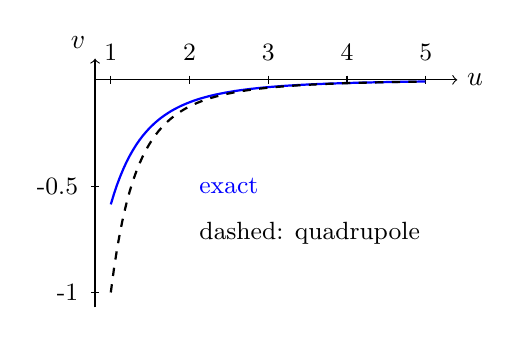
\begin{tikzpicture}[x=1.0cm,y=2.7cm]
\draw[->] (0.8,-1.07)--(0.8,0.1) node[above left] {$v$};
\draw[->] (0.8,0)--(5.4,0) node[right] {$u$};
\foreach \x in {1,2,3,4,5} {\draw (\x,0.02)--(\x,-0.02) node[above=5pt] {\small\x};}
\foreach \y in {-1,-0.5} {\draw (0.75,\y)--(0.85,\y) node[left=4pt] {\small\y};}
\draw[blue,thick,domain=1:5,samples=100] plot (\x,{2*(1/sqrt(\x*\x+1)-1/\x)});
\draw[dashed,thick,domain=1:5,samples=100] plot (\x,{-1/(\x*\x*\x)});
\node[blue,anchor=west] at (2,-0.5) {\small exact};
\node[anchor=west] at (2,-0.72) {\small dashed: quadrupole};
\end{tikzpicture}\hspace{1em}
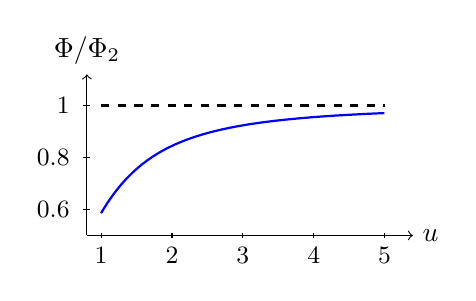
\begin{tikzpicture}[x=0.9cm,y=3.3cm]
\draw[->] (0.8,0.5)--(0.8,1.12) node[above] {$\Phi/\Phi_2$};
\draw[->] (0.8,0.5)--(5.4,0.5) node[right] {$u$};
\foreach \x in {1,2,3,4,5} {\draw (\x,0.51)--(\x,0.49) node[below] {\small\x};}
\foreach \y in {0.6,0.8,1} {\draw (0.75,\y)--(0.85,\y) node[left=4pt] {\small\y};}
\draw[dashed,thick] (1,1)--(5,1);
\draw[blue,thick,domain=1:5,samples=100]
plot (\x,{2/(sqrt(1+1/(\x*\x))*(1+sqrt(1+1/(\x*\x))))});
\end{tikzpicture}
\end{center}
For example the ratios at $u=2,3,5$ are $0.84458,0.92370,0.97097$.

\Needspace{5\baselineskip}
\par\bigskip
\noindent\textbf{4.2}\quad A point dipole with dipole moment $\mathbf{p}$ is located at the point $\mathbf{x}_{0}$. From the properties of the derivative of a Dirac delta function, show that for calculation of the potential $\Phi$ or the energy of a dipole in an external field, the dipole can be described by an effective charge density
\[
\rho_{\mathrm{eff}}(\mathbf{x})=-\mathbf{p}\cdot\nabla\delta(\mathbf{x}-\mathbf{x}_{0})
\]
\solution

The defining distributional identity is
\[
\int f(\mathbf x)\partial_i\delta(\mathbf x-\mathbf x_0)\,d^3x
=-\partial_i f(\mathbf x_0).
\]
Thus $\int\rho_{\rm eff}f\,d^3x=\mathbf p\cdot\nabla f(\mathbf x_0)$.
For an observation point $\mathbf r\ne\mathbf x_0$, put
$f(\mathbf x)=1/|\mathbf r-\mathbf x|$. The derivative is with respect
to the source coordinate, so
\[
\nabla_{\mathbf x}\frac1{|\mathbf r-\mathbf x|}
=\frac{\mathbf r-\mathbf x}{|\mathbf r-\mathbf x|^3},\qquad
\boxed{\Phi(\mathbf r)=\frac{1}{4\pi\epsilon_0}
\frac{\mathbf p\cdot(\mathbf r-\mathbf x_0)}{|\mathbf r-\mathbf x_0|^3}.}
\]
For the energy choose $f=\Phi^{(0)}$, smooth at $\mathbf x_0$. Since
this is interaction with distinct external sources, there is no factor $1/2$:
\[
\boxed{W=\int\rho_{\rm eff}\Phi^{(0)}\,d^3x
=\mathbf p\cdot\nabla\Phi^{(0)}(\mathbf x_0)
=-\mathbf p\cdot\mathbf E^{(0)}(\mathbf x_0).}
\]
Self-energy is excluded. Taking $f=1$ checks zero total charge;
taking $f=x_i$ checks $\int x_i\rho_{\rm eff}\,d^3x=p_i$.
For a further direct construction, place $\pm q$ a displacement
$\pm\mathbf d/2$ from $\mathbf x_0$. Taylor expansion gives
\[
q[\delta(\mathbf x-\mathbf x_0-\mathbf d/2)
-\delta(\mathbf x-\mathbf x_0+\mathbf d/2)]
=-q\mathbf d\cdot\nabla\delta(\mathbf x-\mathbf x_0)+O(qd^3).
\]
Taking $\mathbf d\to0$ with $q\mathbf d=\mathbf p$ fixed gives the
same density and fixes its sign.

\Needspace{5\baselineskip}
\par\bigskip
\noindent\textbf{4.3}\quad The $l$th term in the multipole expansion (4.1) of the potential is specified by the $(2l+1)$ multipole moments $q_{lm}$. On the other hand, the Cartesian multipole moments,
\[
Q_{\alpha\beta\gamma}^{(l)}=\int\rho(\mathbf{x})\,x^{\alpha}y^{\beta}z^{\gamma}\;d^{3}x
\]
with $\alpha$, $\beta$, $\gamma$ nonnegative integers subject to the constraint $\alpha+\beta+\gamma=l$, are $(l+1)(l+2)/2$ in number. Thus, for $l>1$ there are more Cartesian multipole moments than seem necessary to describe the term in the potential whose radial dependence is $r^{-l-1}$.

Show that while the $q_{lm}$ transform under rotations as irreducible spherical tensors of rank $l$, the Cartesian multipole moments correspond to reducible spherical tensors of ranks $l$, $l-2$, $l-4$, \ldots, $l_{\min}$, where $l_{\min}=0$ or 1 for $l$ even or odd, respectively. Check that the number of different tensorial components adds up to the total number of Cartesian tensors. Why are only the $q_{lm}$ needed in the expansion (4.1)?
\solution

Package the Cartesian moments into the symmetric rank-$l$ tensor
$M_{i_1\cdots i_l}=\int\rho x_{i_1}\cdots x_{i_l}\,d^3x$.
Its independent components correspond to homogeneous polynomials of degree
$l$, whose monomials are $x^\alpha y^\beta z^\gamma$ with
$\alpha+\beta+\gamma=l$. There are $\binom{l+2}{2}$ such monomials.

A homogeneous polynomial has the unique harmonic decomposition
\[
F_l(\mathbf x)=H_l(\mathbf x)+r^2H_{l-2}(\mathbf x)
+r^4H_{l-4}(\mathbf x)+\cdots,
\qquad \nabla^2H_k=0,
\]
where each $H_k$ is homogeneous of degree $k$. Here is why traces can
be removed recursively. For such a harmonic $H_k$, Euler's identity
$\mathbf x\cdot\nabla H_k=kH_k$ gives
\begin{align*}
\nabla^2(r^{2s}H_k)
&=(\nabla^2r^{2s})H_k+2\nabla r^{2s}\cdot\nabla H_k\\
&=[2s(2s+1)+4sk]r^{2s-2}H_k
=2s(2k+2s+1)r^{2s-2}H_k.
\end{align*}
The coefficient is nonzero for $s\geq1$. Decompose $\nabla^2F_l$
recursively and subtract the corresponding $r^{2s}H_k$ terms; the
remainder is harmonic. The same nonzero coefficients establish uniqueness.
In tensor language $H_l$ is the symmetric traceless part, while each
factor $r^2$ corresponds to a Kronecker delta, or trace.

The degree-$k$ harmonic polynomials have the basis
$\mathcal Y_{km}=r^kY_{km}$, $-k\leq m\leq k$.
Rotations preserve degree and harmonicity and mix only these $2k+1$
components. Moreover $L^2Y_{km}=k(k+1)Y_{km}$, and $L_\pm$ connect all
$m$ in that set; this is the irreducible rank-$k$ representation.
Therefore the Cartesian moments contain the ranks
\[
\boxed{l,\ l-2,\ l-4,\ldots,l_{\min},}
\]
whereas the integrals $q_{lm}=\int\rho\mathcal Y_{lm}^{*}\,d^3x$
select just the irreducible rank-$l$ part. The lower-rank pieces of
$M^{(l)}$ involve radial weights $r^{2s}$; they are not generally the
ordinary moments of order $l-2s$.

For $l=2n$, the number of components is
\[
\sum_{k=0}^n(4k+1)=(n+1)(2n+1)
=\frac{(l+1)(l+2)}2;
\]
for $l=2n+1$ it is
\[
\sum_{k=0}^n(4k+3)=(n+1)(2n+3)
=\frac{(l+1)(l+2)}2.
\]
Finally, Taylor expansion of the Coulomb kernel yields
\[
\Phi_l(\mathbf r)=\frac{1}{4\pi\epsilon_0}
\frac{(-1)^l}{l!}M_{i_1\cdots i_l}
\partial_{i_1}\cdots\partial_{i_l}\frac1r.
\]
Any trace in $M$ contracts two derivatives into
$\nabla^2(1/r)=0$ at exterior points. Only its symmetric traceless
part contributes, and that part is fully specified by the $2l+1$
$q_{lm}$. This explains why the extra Cartesian components do not
appear in (4.1).

\Needspace{5\baselineskip}
\par\bigskip
\noindent\textbf{4.4}\quad\begin{enumerate}
\item[(a)] Prove the following theorem: For an arbitrary charge distribution $\rho(\mathbf{x})$ the values of the $(2l+1)$ moments of the first nonvanishing multipole are independent of the origin of the coordinate axes, but the values of all higher multipole moments do in general depend on the choice of origin. (The different moments $q_{lm}$ for fixed $l$ depend, of course, on the orientation of the axes.)
\item[(b)] A charge distribution has multipole moments $q$, $\mathbf{p}$, $Q_{ij}$, \ldots{} with respect to one set of coordinate axes, and moments $q'$, $\mathbf{p}'$, $Q'_{ij}$, \ldots{} with respect to another set whose axes are parallel to the first, but whose origin is located at the point $\mathbf{R}=(X,Y,Z)$ relative to the first. Determine explicitly the connections between the monopole, dipole, and quadrupole moments in the two coordinate frames.
\item[(c)] If $q\neq0$, can $\mathbf{R}$ be found so that $\mathbf{p}'=0$? If $q\neq0$, $\mathbf{p}\neq0$, or at least $\mathbf{p}\neq0$, can $\mathbf{R}$ be found so that $Q'_{ij}=0$?
\end{enumerate}
\solution

\textbf{(a)} Keep the axes parallel and move the origin to $\mathbf R$,
so that $\mathbf x'=\mathbf x-\mathbf R$. For the regular solid harmonic
$\mathcal Y_{lm}=r^lY_{lm}$, the finite Taylor expansion is
\[
\mathcal Y_{lm}^{*}(\mathbf x-\mathbf R)
=\sum_{k=0}^l\frac{(-\mathbf R\cdot\nabla)^k}{k!}
\mathcal Y_{lm}^{*}(\mathbf x).
\]
Each derivative on the right is a homogeneous polynomial of degree
$l-k$ and is harmonic, since differentiation commutes with $\nabla^2$.
It is consequently a linear combination of the $\mathcal Y_{l-k,m'}$.
Multiplying by $\rho$ and integrating shows that
\[
q'_{lm}=q_{lm}+\text{linear combinations of moments of orders }0,\ldots,l-1.
\]
If all moments below order $L$ vanish, then $q'_{Lm}=q_{Lm}$ and all
moments below $L$ remain zero. Higher moments contain terms involving
the nonzero order-$L$ moments, so in general they change under
translation. Particular components may be unchanged for particular
translations; the theorem does not assert otherwise. Rotations still
mix the $m$ components within each order.

\textbf{(b)} With $q=\int\rho\,d^3x$, $p_i=\int\rho x_i\,d^3x$, and
$Q_{ij}=\int\rho(3x_ix_j-r^2\delta_{ij})\,d^3x$,
\[
\boxed{q'=q,\qquad p'_i=p_i-qR_i.}
\]
For the quadrupole, expand its integrand before integrating:
\begin{align*}
3(x_i-R_i)(x_j-R_j)-|\mathbf x-\mathbf R|^2\delta_{ij}
={}&3x_ix_j-r^2\delta_{ij}-3(R_ix_j+R_jx_i)\\
&+2(\mathbf R\cdot\mathbf x)\delta_{ij}
+3R_iR_j-R^2\delta_{ij}.
\end{align*}
Thus
\[
\boxed{Q'_{ij}=Q_{ij}-3(R_ip_j+R_jp_i)
+2\mathbf R\cdot\mathbf p\,\delta_{ij}
+q(3R_iR_j-R^2\delta_{ij}).}
\]
The trace remains zero, as it must.

\textbf{(c)} If $q\ne0$, the unique dipole-free origin is
$\boxed{\mathbf R=\mathbf p/q}$. A quadrupole-free origin generally does
not exist. To give the precise restriction, define the quadrupole at
this dipole-free origin,
\[
Q^{c}_{ij}=Q_{ij}-\frac{3p_ip_j-p^2\delta_{ij}}q,
\qquad \mathbf s=\mathbf R-\frac{\mathbf p}q.
\]
Completing the square in the transformation law gives
\[
Q'_{ij}=Q^c_{ij}+q(3s_is_j-s^2\delta_{ij}).
\]
The matrix $3\mathbf s\mathbf s^{\mathsf T}-s^2\mathbf I$ has
eigenvalue $2s^2$ along $\mathbf s$ and $-s^2$ along each perpendicular
direction; this identifies the possible spectra of its negative.
Therefore $Q'=0$ is possible exactly when $Q^c=0$ (choose $\mathbf s=0$),
or when $Q^c$ has eigenvalues $(-2\lambda,\lambda,\lambda)$ with
$\lambda/q>0$. The direction of $\mathbf s$ must be the first
principal axis, and $s^2=\lambda/q$. A generic traceless symmetric
tensor has three distinct eigenvalues and fails this condition.
For example, equal pairs of charges $+e$ at $\pm a\hat{\mathbf x}$ and
$+2e$ at $\pm a\hat{\mathbf y}$ have $q=6e$, $\mathbf p=0$, and
$Q^c=6ea^2\operatorname{diag}(0,1,-1)$, which cannot be removed by
translation. Describing this same distribution from another origin
makes $\mathbf p\ne0$ without removing the obstruction.

If $q=0$ but $\mathbf p\ne0$, choose axes with $\mathbf p=p\hat{\mathbf z}$.
The six symmetric components transform as
\begin{gather*}
Q'_{xx}=Q_{xx}+2pR_z,\quad Q'_{yy}=Q_{yy}+2pR_z,\quad
Q'_{zz}=Q_{zz}-4pR_z,\\
Q'_{xy}=Q_{xy},\quad Q'_{xz}=Q_{xz}-3pR_x,\quad
Q'_{yz}=Q_{yz}-3pR_y.
\end{gather*}
Thus $Q'=0$ requires $Q_{xy}=0$ and $Q_{xx}=Q_{yy}$; when these
conditions hold, choose
\[
(R_x,R_y,R_z)=\left(\frac{Q_{xz}}{3p},\frac{Q_{yz}}{3p},
-\frac{Q_{xx}}{2p}\right).
\]
If both $q$ and $\mathbf p$ vanish, the quadrupole is invariant and
can be zero in a translated frame only if it was zero already.

\Needspace{5\baselineskip}
\par\bigskip
\noindent\textbf{4.5}\quad A localized charge density $\rho(x,y,z)$ is placed in an external electrostatic field described by a potential $\Phi^{(0)}(x,y,z)$. The external potential varies slowly in space over the region where the charge density is different from zero. \erratum{Assume that the external sources lie outside a neighborhood of this region, so that $\nabla^2\Phi^{(0)}=0$ there, as in the derivation of (4.23)--(4.24).}
\begin{enumerate}
\item[(a)] From first principles calculate the total \emph{force} acting on the charge distribution as an expansion in multipole moments times derivatives of the electric field, up to and including the quadrupole moments. Show that the force is
\[
\mathbf{F}=q\mathbf{E}^{(0)}(0)+\{\nabla[\mathbf{p}\cdot\mathbf{E}^{(0)}(\mathbf{x})]\}_{0}+\left\{\nabla\!\left[\frac{1}{6}\sum_{j,k}Q_{jk}\frac{\partial E_{j}^{(0)}}{\partial x_{k}}(\mathbf{x})\right]\right\}_{0}+\cdots
\]
Compare this to the expansion (4.24) of the \emph{energy} $W$. Note that (4.24) is a number---it is not a function of $\mathbf{x}$ that can be differentiated! What is its connection to $\mathbf{F}$?
\item[(b)] Repeat the calculation of part a for the total \emph{torque}. For simplicity, evaluate only one Cartesian component of the torque, say $N_{1}$. Show that this component is
\[
N_{1}=[\mathbf{p}\times\mathbf{E}^{(0)}(0)]_{1}+\frac{1}{3}\left[\frac{\partial}{\partial x_{3}}\left(\sum_{j}Q_{2j}E_{j}^{(0)}\right)-\frac{\partial}{\partial x_{2}}\left(\sum_{j}Q_{3j}E_{j}^{(0)}\right)\right]_{0}+\cdots
\]
\end{enumerate}
\solution

As in Jackson's derivation of (4.23)--(4.24), assume that the external
sources lie outside a neighborhood containing the localized distribution.
Then $\nabla\cdot\mathbf E^{(0)}=0$ and
$\nabla\times\mathbf E^{(0)}=0$ there. This source-free condition is
needed for the stated force formula with only traceless moments.
All derivatives below are of the external field.

\textbf{(a)} Start with the force on each charge element:
\[
F_i=\int\rho(\mathbf x)E_i^{(0)}(\mathbf x)\,d^3x.
\]
Taylor-expand the field around the origin, integrate term by term,
and define $M_{jk}=\int\rho x_jx_k\,d^3x$ and
$S=\int\rho r^2\,d^3x$:
\begin{align*}
F_i&=qE_i^{(0)}(0)+p_j\partial_jE_i^{(0)}(0)
+\frac12M_{jk}\partial_j\partial_kE_i^{(0)}(0)+\cdots,\\
M_{jk}&=\frac13(Q_{jk}+S\delta_{jk}).
\end{align*}
The trace term is $S\nabla^2E_i^{(0)}/6=0$, because
$\nabla^2\mathbf E^{(0)}=\nabla(\nabla\cdot\mathbf E^{(0)})=0$.
Electrostatics also gives $\partial_jE_i^{(0)}=\partial_iE_j^{(0)}$,
so
\begin{align*}
p_j\partial_jE_i^{(0)}&=\partial_i(p_jE_j^{(0)}),\\
Q_{jk}\partial_j\partial_kE_i^{(0)}
&=\partial_i(Q_{jk}\partial_kE_j^{(0)}).
\end{align*}
These identities give exactly
\[
\boxed{\mathbf F=q\mathbf E^{(0)}(0)
+\left.\nabla(\mathbf p\cdot\mathbf E^{(0)})\right|_0
+\left.\frac16\nabla(Q_{jk}\partial_kE_j^{(0)})\right|_0+\cdots.}
\]
Repeated Cartesian indices are summed. If external charge overlaps the
region, the additional term $S\nabla(\nabla\cdot\mathbf E^{(0)})/6$
must be retained; the displayed problem formula alone is then insufficient.

To connect force and energy, let $\mathbf R$ be a \emph{physical rigid
translation} of the charge distribution and let $\mathbf u$ denote
coordinates fixed in it. Its interaction energy is the function
\begin{align*}
W(\mathbf R)&=\int\rho(\mathbf u)\Phi^{(0)}(\mathbf R+\mathbf u)\,d^3u\\
&=q\Phi^{(0)}(\mathbf R)-p_jE_j^{(0)}(\mathbf R)
-\frac16Q_{jk}\partial_kE_j^{(0)}(\mathbf R)+\cdots.
\end{align*}
The moments are held fixed while differentiating, and
$\mathbf F=-\nabla_{\mathbf R}W(\mathbf R)|_{\mathbf R=0}$.
Equation (4.24) is the value $W(0)$, not a spatial function to which
one may directly apply $\nabla_{\mathbf x}$.

\textbf{(b)} The torque about the chosen origin is
\[
N_1=\int\rho(x_2E_3^{(0)}-x_3E_2^{(0)})\,d^3x.
\]
Keeping the constant and linear terms of the field produces
\begin{align*}
N_1={}&p_2E_3^{(0)}(0)-p_3E_2^{(0)}(0)
+M_{2j}\partial_jE_3^{(0)}(0)-M_{3j}\partial_jE_2^{(0)}(0)+\cdots\\
={}&[\mathbf p\times\mathbf E^{(0)}(0)]_1
+\frac13[Q_{2j}\partial_jE_3^{(0)}-Q_{3j}\partial_jE_2^{(0)}]_0
+\frac S3[\partial_2E_3^{(0)}-\partial_3E_2^{(0)}]_0+\cdots.
\end{align*}
The last term vanishes by zero curl. Interchanging the derivative and
field indices in the preceding term then gives
\[
\boxed{N_1=[\mathbf p\times\mathbf E^{(0)}(0)]_1
+\frac13[\partial_3(Q_{2j}E_j^{(0)})
-\partial_2(Q_{3j}E_j^{(0)})]_0+\cdots.}
\]
This torque is about the origin; about a different point it changes by
the usual moment of the total force.

\Needspace{5\baselineskip}
\par\bigskip
\noindent\textbf{4.6}\quad A nucleus with quadrupole moment $Q$ finds itself in a cylindrically symmetric electric field with a gradient $(\partial E_{z}/\partial z)_{0}$ along the $z$ axis at the position of the nucleus. \erratum{Take the nuclear symmetry axis along $z$ and the external field to be source-free at the nucleus; these conditions specify the aligned quadrupole energy below.}
\begin{enumerate}
\item[(a)] Show that the energy of quadrupole interaction is
\[
W=-\frac{e}{4}\,Q\left(\frac{\partial E_{z}}{\partial z}\right)_{0}
\]
\item[(b)] If it is known that $Q=2\times10^{-28}$ m$^{2}$ and that $W/h$ is 10 MHz, where $h$ is Planck's constant, calculate $(\partial E_{z}/\partial z)_{0}$ in units of $e/4\pi\epsilon_{0}a_{0}^{3}$, where $a_{0}=4\pi\epsilon_{0}\hbar^{2}/me^{2}=0.529\times10^{-10}$ m is the Bohr radius in hydrogen.
\item[(c)] Nuclear charge distributions can be approximated by a constant charge density throughout a spheroidal volume of semimajor axis $a$ and semiminor axis $b$. Calculate the quadrupole moment of such a nucleus, assuming that the total charge is $Ze$. Given that Eu$^{153}$ ($Z=63$) has a quadrupole moment $Q=2.5\times10^{-28}$ m$^{2}$ and a mean radius
\[
R=(a+b)/2=7\times10^{-15}\ \mathrm{m}
\]
determine the fractional difference in radius $(a-b)/R$.
\end{enumerate}
\solution

\textbf{(a)} Jackson's nuclear convention (4.25) is
$Q=Q_{zz}/e$, with dimensions of area. Take the nuclear symmetry axis
along $z$, as in that definition. Axial symmetry and tracelessness give
\[
Q_{zz}=eQ,\qquad Q_{xx}=Q_{yy}=-eQ/2,\qquad Q_{ij}=0\ (i\ne j).
\]
At a source-free point of an axially symmetric external field, let
$G=(\partial_zE_z)_0$. Then
$\partial_xE_x=\partial_yE_y$ and
$\partial_xE_x+\partial_yE_y+\partial_zE_z=0$, so each transverse
entry is $-G/2$. Thus
\[
W_Q=-\frac16 Q_{ij}\partial_jE_i
=-\frac16\left[eQG+2\left(-\frac{eQ}{2}\right)
\left(-\frac G2\right)\right]
=\boxed{-\frac{eQG}{4}}.
\]
For a nucleus whose symmetry axis makes angle $\beta$ with the field
axis, write $Q_{ij}=eQ(3\widehat u_i\widehat u_j-\delta_{ij})/2$,
where $\widehat{\mathbf u}\cdot\widehat{\mathbf z}=\cos\beta$.
The traceless gradient tensor is
$G_{ij}=G(3\widehat z_i\widehat z_j-\delta_{ij})/2$. Thus
\[
-\frac16Q_{ij}G_{ij}
=-\frac{eQG}{24}(9\cos^2\beta-3)
=-\frac{eQG}{4}P_2(\cos\beta).
\]
The stated formula uses the aligned convention $\beta=0$.

\textbf{(b)} With $W/h=+10^7\ \mathrm{s}^{-1}$ and $Q>0$,
\[
G=-\frac{4h(10^7\ \mathrm{s}^{-1})}{e(2\times10^{-28}\ \mathrm{m}^2)}
=-8.2713\times10^{20}\ \mathrm{V\,m^{-2}}.
\]
Using the problem's rounded $a_0=0.529\times10^{-10}\ \mathrm m$,
\[
\frac{e}{4\pi\epsilon_0a_0^3}=9.7271\times10^{21}\ \mathrm{V\,m^{-2}},
\qquad
\boxed{\frac{G}{e/(4\pi\epsilon_0a_0^3)}=-0.08503.}
\]
If the measured $10$ MHz denotes only the magnitude of a splitting,
only $|G|$ is determined and the ratio is $0.08503$ in magnitude.

\textbf{(c)} For a prolate spheroid put the semiaxis $a$ along $z$
and the equal semiaxes $b$ along $x,y$. Its density is
$\rho=3Ze/(4\pi ab^2)$. Transform the ellipsoid to the unit ball by
$x=bu$, $y=bv$, $z=aw$. Spherical symmetry on that ball gives
\[
\int_{u^2+v^2+w^2\leq1}w^2\,d^3u
=\frac13\int_0^1 4\pi t^4\,dt=\frac{4\pi}{15}.
\]
Since $d^3x=ab^2d^3u$,
\[
\int\rho z^2\,d^3x=\frac{Ze a^2}{5},\qquad
\int\rho x^2\,d^3x=\int\rho y^2\,d^3x=\frac{Ze b^2}{5}.
\]
It follows that
\[
\boxed{Q=\frac1e\int\rho(2z^2-x^2-y^2)\,d^3x
=\frac{2Z}{5}(a^2-b^2).}
\]
For an oblate spheroid the axial semiaxis is the smaller one, and the
quadrupole has the opposite sign. Here $Q>0$ selects the prolate case.
Using $a+b=2R$, with no small-deformation approximation,
\[
Q=\frac{4Z}{5}R(a-b),\qquad
\boxed{\frac{a-b}{R}=\frac{5Q}{4ZR^2}
=\frac{5(2.5\times10^{-28})}{4(63)(7\times10^{-15})^2}
=0.10123.}
\]
Thus $a\simeq7.354\times10^{-15}$ m and
$b\simeq6.646\times10^{-15}$ m in this uniform-density model.

\Needspace{5\baselineskip}
\par\bigskip
\noindent\textbf{4.7}\quad A localized distribution of charge has a charge density
\[
\rho(\mathbf{r})=\frac{1}{64\pi}\,r^{2}e^{-r}\sin^{2}\theta
\]
\begin{enumerate}
\item[(a)] Make a multipole expansion of the potential due to this charge density and determine all the nonvanishing multipole moments. Write down the potential at large distances as a finite expansion in Legendre polynomials.
\item[(b)] Determine the potential explicitly at any point in space, and show that near the origin, correct to $r^{2}$ inclusive,
\[
\Phi(\mathbf{r})\simeq\frac{1}{4\pi\epsilon_{0}}\left[\frac{1}{4}-\frac{r^{2}}{120}P_{2}(\cos\theta)\right]
\]
\item[(c)] If there exists at the origin a nucleus with a quadrupole moment $Q=10^{-28}$ m$^{2}$, \erratum{with its symmetry axis along $z$,} determine the magnitude of the interaction energy, assuming that the unit of charge in $\rho(\mathbf{r})$ above is the electronic charge and the unit of length is the hydrogen Bohr radius $a_{0}=4\pi\epsilon_{0}\hbar^{2}/me^{2}=0.529\times10^{-10}$ m. Express your answer as a frequency by dividing by Planck's constant $h$.
\end{enumerate}
The charge density in this problem is that for the $m=\pm1$ states of the $2p$ level in hydrogen, while the quadrupole interaction is of the same order as found in molecules.
\solution

\textbf{(a)} Use $\sin^2\theta=\frac23[1-P_2(\cos\theta)]$ to write
\[
\rho=\frac{r^2e^{-r}}{96\pi}[1-P_2(\cos\theta)].
\]
Azimuthal integration eliminates $m\ne0$, and Legendre orthogonality
eliminates $l\ne0,2$. Since
$\int_0^\infty r^ne^{-r}\,dr=n!$ and
$\int P_l^2\,d\Omega=4\pi/(2l+1)$, the total charge and the
Legendre quadrupole integral are
\[
q=\frac{4\pi}{96\pi}\,4!=1,\qquad
\int\rho r^2P_2\,d^3r=-\frac{1}{96\pi}\frac{4\pi}{5}\,6!=-6.
\]
Therefore
\[
\boxed{q_{00}=\frac1{\sqrt{4\pi}},\qquad
q_{20}=-6\sqrt{\frac5{4\pi}}=-3\sqrt{\frac5\pi},}
\]
with all other moments zero. The large-distance expansion is
\[
\boxed{\Phi\sim\frac{1}{4\pi\epsilon_0}
\left[\frac1r-\frac6{r^3}P_2(\cos\theta)\right].}
\]
The density is exponentially localized but is not compactly supported.
Consequently this finite algebraic expansion is asymptotic, with
exponentially small corrections at finite $r$; it is not the exact
potential throughout an exterior charge-free region.

\textbf{(b)} Split the Coulomb integral into source radii $s<r$ and
$s>r$, using the kernel $r_<^l/r_>^{l+1}$. The same angular
orthogonality gives
\[
4\pi\epsilon_0\Phi=A(r)+B(r)P_2(\cos\theta),
\]
\begin{align*}
A(r)&=\frac1{24}\left[\frac1r\int_0^r s^4e^{-s}\,ds
+\int_r^\infty s^3e^{-s}\,ds\right],\\
B(r)&=-\frac1{120}\left[\frac1{r^3}\int_0^r s^6e^{-s}\,ds
+r^2\int_r^\infty se^{-s}\,ds\right].
\end{align*}
Repeated integration by parts gives
\[
\int_r^\infty s^ne^{-s}\,ds=n!e^{-r}\sum_{k=0}^n\frac{r^k}{k!},
\qquad
\int_0^r s^ne^{-s}\,ds=n!\left[1-e^{-r}\sum_{k=0}^n\frac{r^k}{k!}\right].
\]
Substituting and collecting equal powers yields the explicit answer
\begin{align*}
\boxed{A(r)}&=\boxed{\frac1r-e^{-r}\left(\frac1r+\frac34+\frac r4+\frac{r^2}{24}\right)},\\
\boxed{B(r)}&=\boxed{-\frac6{r^3}+e^{-r}\left(\frac6{r^3}+\frac6{r^2}
+\frac3r+1+\frac r4+\frac{r^2}{24}\right)}.
\end{align*}
These expressions apply for $r>0$; their apparent singularities are
removable at the origin. The integral forms show the cancellations
without subtracting divergent terms. For small $r$, the needed integrals are
\begin{gather*}
\int_0^r s^4e^{-s}\,ds=\frac{r^5}{5}+O(r^6),\qquad
\int_r^\infty s^3e^{-s}\,ds=6-\frac{r^4}{4}+O(r^5),\\
\int_0^r s^6e^{-s}\,ds=\frac{r^7}{7}+O(r^8),\qquad
\int_r^\infty se^{-s}\,ds=1-\frac{r^2}{2}+O(r^3).
\end{gather*}
Consequently
\begin{align*}
A(r)&=\frac1{24}\left[6+\left(\frac15-\frac14\right)r^4+O(r^5)\right]
=\frac14-\frac{r^4}{480}+O(r^5),\\
B(r)&=-\frac1{120}\left[r^2+\left(\frac17-\frac12\right)r^4+O(r^5)\right]
=-\frac{r^2}{120}+\frac{r^4}{336}+O(r^5),
\end{align*}
so
\[
\boxed{\Phi=\frac{1}{4\pi\epsilon_0}
\left[\frac14-\frac{r^2}{120}P_2(\cos\theta)+O(r^4)\right].}
\]
For example, differentiating the exact radial functions checks Poisson's
 equation directly:
\[
A''+\frac2rA'=-\frac{r^2e^{-r}}{24},\qquad
B''+\frac2rB'-\frac6{r^2}B=+\frac{r^2e^{-r}}{24}.
\]

\textbf{(c)} Restore physical length $\mathbf R=a_0\mathbf r$ and
charge $q_e$ (equal to $-e$ for an electron). The quadratic physical
potential is
\[
\Phi_Q(\mathbf R)=-\frac{q_e}{4\pi\epsilon_0a_0^3}
\frac{3Z^2-R^2}{240}.
\]
Since $3Z^2-R^2=2Z^2-X^2-Y^2$,
\[
\left(\frac{\partial E_Z}{\partial Z}\right)_0
=-\partial_Z^2\Phi_Q=\frac{q_e}{4\pi\epsilon_0a_0^3}\frac1{60}.
\]
For the nuclear quadrupole convention and alignment of Problem 4.6,
\[
|W_Q|=\frac{e^2|Q|}{240(4\pi\epsilon_0)a_0^3},\qquad
\boxed{\frac{|W_Q|}{h}=9.8000\times10^5\ \mathrm{Hz}\simeq0.980\ \mathrm{MHz}.}
\]
The sign reverses if the sign of the charge distribution is reversed;
for an electron and $Q>0$, this aligned quadrupole contribution is positive.

\Needspace{5\baselineskip}
\par\bigskip
\noindent\textbf{4.8}\quad A very long, right circular, cylindrical shell of dielectric constant $\epsilon/\epsilon_{0}$ and inner and outer radii $a$ and $b$, respectively, is placed in a previously uniform electric field $E_{0}$ with its axis perpendicular to the field. The medium inside and outside the cylinder has a dielectric constant of unity.
\begin{enumerate}
\item[(a)] Determine the potential and electric field in the three regions, neglecting end effects.
\item[(b)] Sketch the lines of force for a typical case of $b\simeq2a$.
\item[(c)] Discuss the limiting forms of your solution appropriate for a solid dielectric cylinder in a uniform field, and a cylindrical cavity in a uniform dielectric.
\end{enumerate}
\solution

\textbf{(a)} Let $\kappa=\epsilon/\epsilon_0>0$, use cylindrical
coordinates $(s,\phi,z)$, and take the applied field along $x$, so
$x=s\cos\phi$. Translation invariance along $z$ and the $\cos\phi$
boundary condition leave only the cylindrical harmonic of order one.
The solutions regular at $s=0$ and asymptotic to $-E_0x$ are
\[
\Phi=-E_0\cos\phi\begin{cases}
As,&s<a,\\
Bs+C/s,&a<s<b,\\
s-D/s,&s>b.
\end{cases}
\]
There is no free surface charge at either dielectric boundary. Continuity
of $\Phi$ and of $D_s=-\epsilon\partial_s\Phi$ gives four equations:
\begin{gather*}
A=B+C/a^2,\qquad A=\kappa(B-C/a^2),\\
B+C/b^2=1-D/b^2,\qquad
\kappa(B-C/b^2)=1+D/b^2.
\end{gather*}
The first pair gives
$C=a^2B(\kappa-1)/(\kappa+1)$ and
$A=2\kappa B/(\kappa+1)$. Adding the second pair eliminates $D$:
\[
(\kappa+1)B-(\kappa-1)C/b^2=2.
\]
Define $\eta=a^2/b^2$ and
$\Delta=(\kappa+1)^2-(\kappa-1)^2\eta$. Substitution gives
\[
\boxed{A=\frac{4\kappa}{\Delta},\quad
B=\frac{2(\kappa+1)}{\Delta},\quad
C=\frac{2(\kappa-1)a^2}{\Delta},\quad
D=\frac{(\kappa^2-1)(b^2-a^2)}{\Delta}.}
\]
The field is $\mathbf E=E_s\hat{\mathbf s}+E_\phi\hat{\boldsymbol\phi}$,
with $E_z=0$ and
\[
\boxed{\frac{E_s}{E_0}=\cos\phi\begin{cases}
A,&s<a,\\ B-C/s^2,&a<s<b,\\1+D/s^2,&s>b,
\end{cases}\quad
\frac{E_\phi}{E_0}=-\sin\phi\begin{cases}
A,&s<a,\\B+C/s^2,&a<s<b,\\1-D/s^2,&s>b.
\end{cases}}
\]
Thus the field in the hollow core is uniform, $\mathbf E=AE_0\hat{\mathbf x}$.
For $\kappa=1$, $A=B=1$ and $C=D=0$, recovering a uniform vacuum field.

\textbf{(b)} The field lines are contours of a stream function.
In each homogeneous region introduce the stream
function for $\mathbf D/(\epsilon_0E_0)$:
\[
\Psi(s,\phi)=\sin\phi\begin{cases}
As,&s<a,\\
\kappa(Bs-C/s),&a<s<b,\\
s+D/s,&s>b.
\end{cases}
\]
It obeys $D_s/(\epsilon_0E_0)=s^{-1}\partial_\phi\Psi$ and
$D_\phi/(\epsilon_0E_0)=-\partial_s\Psi$. Hence
$\mathbf E\cdot\nabla\Psi=0$, and contours of $\Psi$ are field lines.
The boundary equations above make $\Psi$ continuous across both circles.
The direction changes there in accordance with continuous $E_\phi$
and $\epsilon E_s$.

The plot uses $b=2a$, $\kappa=4$:
$A=64/91$, $B=40/91$, $C/a^2=24/91$, $D/a^2=180/91$.
The shaded annulus is the dielectric, and arrows point along the field.
\begin{center}
% Generated by supplementary/check_ch04.py --figures.
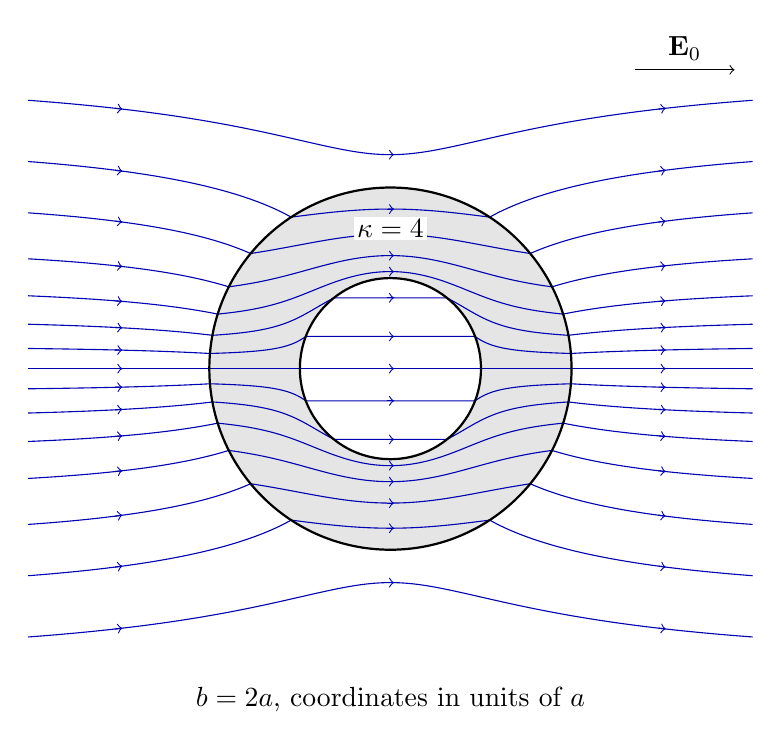
\begin{tikzpicture}[scale=1.15]
\fill[gray!20] (0,0) circle (2);
\fill[white] (0,0) circle (1);
\draw[blue!70!black,thin] plot coordinates {(-4.0000,-2.96347) (-3.9800,-2.96197) (-3.9600,-2.96046) (-3.9400,-2.95893) (-3.9200,-2.95740) (-3.9000,-2.95585) (-3.8800,-2.95429) (-3.8600,-2.95271) (-3.8400,-2.95112) (-3.8200,-2.94952) (-3.8000,-2.94790) (-3.7800,-2.94627) (-3.7600,-2.94463) (-3.7400,-2.94298) (-3.7200,-2.94131) (-3.7000,-2.93962) (-3.6800,-2.93792) (-3.6600,-2.93621) (-3.6400,-2.93448) (-3.6200,-2.93274) (-3.6000,-2.93098) (-3.5800,-2.92921) (-3.5600,-2.92742) (-3.5400,-2.92562) (-3.5200,-2.92380) (-3.5000,-2.92197) (-3.4800,-2.92012) (-3.4600,-2.91825) (-3.4400,-2.91637) (-3.4200,-2.91448) (-3.4000,-2.91256) (-3.3800,-2.91063) (-3.3600,-2.90869) (-3.3400,-2.90672) (-3.3200,-2.90474) (-3.3000,-2.90275) (-3.2800,-2.90073) (-3.2600,-2.89870) (-3.2400,-2.89665) (-3.2200,-2.89459) (-3.2000,-2.89250) (-3.1800,-2.89040) (-3.1600,-2.88828) (-3.1400,-2.88614) (-3.1200,-2.88399) (-3.1000,-2.88181) (-3.0800,-2.87962) (-3.0600,-2.87740) (-3.0400,-2.87517) (-3.0200,-2.87292) (-3.0000,-2.87065) (-2.9800,-2.86836) (-2.9600,-2.86605) (-2.9400,-2.86372) (-2.9200,-2.86137) (-2.9000,-2.85900) (-2.8800,-2.85660) (-2.8600,-2.85419) (-2.8400,-2.85176) (-2.8200,-2.84931) (-2.8000,-2.84683) (-2.7800,-2.84433) (-2.7600,-2.84182) (-2.7400,-2.83928) (-2.7200,-2.83671) (-2.7000,-2.83413) (-2.6800,-2.83152) (-2.6600,-2.82889) (-2.6400,-2.82624) (-2.6200,-2.82357) (-2.6000,-2.82087) (-2.5800,-2.81815) (-2.5600,-2.81541) (-2.5400,-2.81264) (-2.5200,-2.80985) (-2.5000,-2.80704) (-2.4800,-2.80420) (-2.4600,-2.80133) (-2.4400,-2.79845) (-2.4200,-2.79553) (-2.4000,-2.79260) (-2.3800,-2.78963) (-2.3600,-2.78665) (-2.3400,-2.78364) (-2.3200,-2.78060) (-2.3000,-2.77754) (-2.2800,-2.77445) (-2.2600,-2.77133) (-2.2400,-2.76819) (-2.2200,-2.76502) (-2.2000,-2.76183) (-2.1800,-2.75861) (-2.1600,-2.75537) (-2.1400,-2.75209) (-2.1200,-2.74879) (-2.1000,-2.74547) (-2.0800,-2.74211) (-2.0600,-2.73873) (-2.0400,-2.73532) (-2.0200,-2.73189) (-2.0000,-2.72842) (-1.9800,-2.72493) (-1.9600,-2.72141) (-1.9400,-2.71786) (-1.9200,-2.71429) (-1.9000,-2.71069) (-1.8800,-2.70706) (-1.8600,-2.70340) (-1.8400,-2.69971) (-1.8200,-2.69600) (-1.8000,-2.69226) (-1.7800,-2.68849) (-1.7600,-2.68469) (-1.7400,-2.68086) (-1.7200,-2.67701) (-1.7000,-2.67313) (-1.6800,-2.66922) (-1.6600,-2.66528) (-1.6400,-2.66131) (-1.6200,-2.65732) (-1.6000,-2.65330) (-1.5800,-2.64926) (-1.5600,-2.64519) (-1.5400,-2.64109) (-1.5200,-2.63696) (-1.5000,-2.63281) (-1.4800,-2.62863) (-1.4600,-2.62443) (-1.4400,-2.62021) (-1.4200,-2.61596) (-1.4000,-2.61168) (-1.3800,-2.60738) (-1.3600,-2.60306) (-1.3400,-2.59872) (-1.3200,-2.59435) (-1.3000,-2.58997) (-1.2800,-2.58556) (-1.2600,-2.58114) (-1.2400,-2.57669) (-1.2200,-2.57223) (-1.2000,-2.56775) (-1.1800,-2.56326) (-1.1600,-2.55875) (-1.1400,-2.55423) (-1.1200,-2.54969) (-1.1000,-2.54515) (-1.0800,-2.54059) (-1.0600,-2.53603) (-1.0400,-2.53146) (-1.0200,-2.52689) (-1.0000,-2.52231) (-0.9800,-2.51773) (-0.9600,-2.51315) (-0.9400,-2.50858) (-0.9200,-2.50401) (-0.9000,-2.49945) (-0.8800,-2.49490) (-0.8600,-2.49036) (-0.8400,-2.48583) (-0.8200,-2.48132) (-0.8000,-2.47684) (-0.7800,-2.47237) (-0.7600,-2.46794) (-0.7400,-2.46353) (-0.7200,-2.45916) (-0.7000,-2.45482) (-0.6800,-2.45053) (-0.6600,-2.44628) (-0.6400,-2.44208) (-0.6200,-2.43794) (-0.6000,-2.43385) (-0.5800,-2.42982) (-0.5600,-2.42587) (-0.5400,-2.42198) (-0.5200,-2.41817) (-0.5000,-2.41444) (-0.4800,-2.41080) (-0.4600,-2.40726) (-0.4400,-2.40381) (-0.4200,-2.40046) (-0.4000,-2.39722) (-0.3800,-2.39409) (-0.3600,-2.39109) (-0.3400,-2.38821) (-0.3200,-2.38546) (-0.3000,-2.38284) (-0.2800,-2.38037) (-0.2600,-2.37804) (-0.2400,-2.37586) (-0.2200,-2.37384) (-0.2000,-2.37197) (-0.1800,-2.37027) (-0.1600,-2.36874) (-0.1400,-2.36738) (-0.1200,-2.36619) (-0.1000,-2.36518) (-0.0800,-2.36436) (-0.0600,-2.36371) (-0.0400,-2.36325) (-0.0200,-2.36297) (0.0000,-2.36287) (0.0200,-2.36297) (0.0400,-2.36325) (0.0600,-2.36371) (0.0800,-2.36436) (0.1000,-2.36518) (0.1200,-2.36619) (0.1400,-2.36738) (0.1600,-2.36874) (0.1800,-2.37027) (0.2000,-2.37197) (0.2200,-2.37384) (0.2400,-2.37586) (0.2600,-2.37804) (0.2800,-2.38037) (0.3000,-2.38284) (0.3200,-2.38546) (0.3400,-2.38821) (0.3600,-2.39109) (0.3800,-2.39409) (0.4000,-2.39722) (0.4200,-2.40046) (0.4400,-2.40381) (0.4600,-2.40726) (0.4800,-2.41080) (0.5000,-2.41444) (0.5200,-2.41817) (0.5400,-2.42198) (0.5600,-2.42587) (0.5800,-2.42982) (0.6000,-2.43385) (0.6200,-2.43794) (0.6400,-2.44208) (0.6600,-2.44628) (0.6800,-2.45053) (0.7000,-2.45482) (0.7200,-2.45916) (0.7400,-2.46353) (0.7600,-2.46794) (0.7800,-2.47237) (0.8000,-2.47684) (0.8200,-2.48132) (0.8400,-2.48583) (0.8600,-2.49036) (0.8800,-2.49490) (0.9000,-2.49945) (0.9200,-2.50401) (0.9400,-2.50858) (0.9600,-2.51315) (0.9800,-2.51773) (1.0000,-2.52231) (1.0200,-2.52689) (1.0400,-2.53146) (1.0600,-2.53603) (1.0800,-2.54059) (1.1000,-2.54515) (1.1200,-2.54969) (1.1400,-2.55423) (1.1600,-2.55875) (1.1800,-2.56326) (1.2000,-2.56775) (1.2200,-2.57223) (1.2400,-2.57669) (1.2600,-2.58114) (1.2800,-2.58556) (1.3000,-2.58997) (1.3200,-2.59435) (1.3400,-2.59872) (1.3600,-2.60306) (1.3800,-2.60738) (1.4000,-2.61168) (1.4200,-2.61596) (1.4400,-2.62021) (1.4600,-2.62443) (1.4800,-2.62863) (1.5000,-2.63281) (1.5200,-2.63696) (1.5400,-2.64109) (1.5600,-2.64519) (1.5800,-2.64926) (1.6000,-2.65330) (1.6200,-2.65732) (1.6400,-2.66131) (1.6600,-2.66528) (1.6800,-2.66922) (1.7000,-2.67313) (1.7200,-2.67701) (1.7400,-2.68086) (1.7600,-2.68469) (1.7800,-2.68849) (1.8000,-2.69226) (1.8200,-2.69600) (1.8400,-2.69971) (1.8600,-2.70340) (1.8800,-2.70706) (1.9000,-2.71069) (1.9200,-2.71429) (1.9400,-2.71786) (1.9600,-2.72141) (1.9800,-2.72493) (2.0000,-2.72842) (2.0200,-2.73189) (2.0400,-2.73532) (2.0600,-2.73873) (2.0800,-2.74211) (2.1000,-2.74547) (2.1200,-2.74879) (2.1400,-2.75209) (2.1600,-2.75537) (2.1800,-2.75861) (2.2000,-2.76183) (2.2200,-2.76502) (2.2400,-2.76819) (2.2600,-2.77133) (2.2800,-2.77445) (2.3000,-2.77754) (2.3200,-2.78060) (2.3400,-2.78364) (2.3600,-2.78665) (2.3800,-2.78963) (2.4000,-2.79260) (2.4200,-2.79553) (2.4400,-2.79845) (2.4600,-2.80133) (2.4800,-2.80420) (2.5000,-2.80704) (2.5200,-2.80985) (2.5400,-2.81264) (2.5600,-2.81541) (2.5800,-2.81815) (2.6000,-2.82087) (2.6200,-2.82357) (2.6400,-2.82624) (2.6600,-2.82889) (2.6800,-2.83152) (2.7000,-2.83413) (2.7200,-2.83671) (2.7400,-2.83928) (2.7600,-2.84182) (2.7800,-2.84433) (2.8000,-2.84683) (2.8200,-2.84931) (2.8400,-2.85176) (2.8600,-2.85419) (2.8800,-2.85660) (2.9000,-2.85900) (2.9200,-2.86137) (2.9400,-2.86372) (2.9600,-2.86605) (2.9800,-2.86836) (3.0000,-2.87065) (3.0200,-2.87292) (3.0400,-2.87517) (3.0600,-2.87740) (3.0800,-2.87962) (3.1000,-2.88181) (3.1200,-2.88399) (3.1400,-2.88614) (3.1600,-2.88828) (3.1800,-2.89040) (3.2000,-2.89250) (3.2200,-2.89459) (3.2400,-2.89665) (3.2600,-2.89870) (3.2800,-2.90073) (3.3000,-2.90275) (3.3200,-2.90474) (3.3400,-2.90672) (3.3600,-2.90869) (3.3800,-2.91063) (3.4000,-2.91256) (3.4200,-2.91448) (3.4400,-2.91637) (3.4600,-2.91825) (3.4800,-2.92012) (3.5000,-2.92197) (3.5200,-2.92380) (3.5400,-2.92562) (3.5600,-2.92742) (3.5800,-2.92921) (3.6000,-2.93098) (3.6200,-2.93274) (3.6400,-2.93448) (3.6600,-2.93621) (3.6800,-2.93792) (3.7000,-2.93962) (3.7200,-2.94131) (3.7400,-2.94298) (3.7600,-2.94463) (3.7800,-2.94627) (3.8000,-2.94790) (3.8200,-2.94952) (3.8400,-2.95112) (3.8600,-2.95271) (3.8800,-2.95429) (3.9000,-2.95585) (3.9200,-2.95740) (3.9400,-2.95893) (3.9600,-2.96046) (3.9800,-2.96197) (4.0000,-2.96347)};
\draw[blue!70!black,->] (-3.0400,-2.87517) -- (-2.9600,-2.86605);
\draw[blue!70!black,->] (-0.0400,-2.36325) -- (0.0400,-2.36325);
\draw[blue!70!black,->] (2.9600,-2.86605) -- (3.0400,-2.87517);
\draw[blue!70!black,thin] plot coordinates {(-4.0000,-2.28692) (-3.9800,-2.28538) (-3.9600,-2.28383) (-3.9400,-2.28226) (-3.9200,-2.28067) (-3.9000,-2.27906) (-3.8800,-2.27744) (-3.8600,-2.27580) (-3.8400,-2.27415) (-3.8200,-2.27248) (-3.8000,-2.27079) (-3.7800,-2.26909) (-3.7600,-2.26736) (-3.7400,-2.26562) (-3.7200,-2.26386) (-3.7000,-2.26209) (-3.6800,-2.26029) (-3.6600,-2.25848) (-3.6400,-2.25664) (-3.6200,-2.25479) (-3.6000,-2.25292) (-3.5800,-2.25102) (-3.5600,-2.24911) (-3.5400,-2.24718) (-3.5200,-2.24522) (-3.5000,-2.24325) (-3.4800,-2.24125) (-3.4600,-2.23924) (-3.4400,-2.23720) (-3.4200,-2.23514) (-3.4000,-2.23305) (-3.3800,-2.23095) (-3.3600,-2.22882) (-3.3400,-2.22667) (-3.3200,-2.22449) (-3.3000,-2.22229) (-3.2800,-2.22007) (-3.2600,-2.21782) (-3.2400,-2.21554) (-3.2200,-2.21324) (-3.2000,-2.21092) (-3.1800,-2.20857) (-3.1600,-2.20619) (-3.1400,-2.20379) (-3.1200,-2.20136) (-3.1000,-2.19890) (-3.0800,-2.19641) (-3.0600,-2.19390) (-3.0400,-2.19135) (-3.0200,-2.18878) (-3.0000,-2.18618) (-2.9800,-2.18354) (-2.9600,-2.18088) (-2.9400,-2.17818) (-2.9200,-2.17546) (-2.9000,-2.17270) (-2.8800,-2.16991) (-2.8600,-2.16709) (-2.8400,-2.16423) (-2.8200,-2.16134) (-2.8000,-2.15841) (-2.7800,-2.15545) (-2.7600,-2.15246) (-2.7400,-2.14943) (-2.7200,-2.14636) (-2.7000,-2.14325) (-2.6800,-2.14011) (-2.6600,-2.13693) (-2.6400,-2.13371) (-2.6200,-2.13045) (-2.6000,-2.12715) (-2.5800,-2.12381) (-2.5600,-2.12042) (-2.5400,-2.11700) (-2.5200,-2.11353) (-2.5000,-2.11002) (-2.4800,-2.10646) (-2.4600,-2.10286) (-2.4400,-2.09921) (-2.4200,-2.09552) (-2.4000,-2.09177) (-2.3800,-2.08798) (-2.3600,-2.08414) (-2.3400,-2.08025) (-2.3200,-2.07631) (-2.3000,-2.07232) (-2.2800,-2.06828) (-2.2600,-2.06418) (-2.2400,-2.06002) (-2.2200,-2.05581) (-2.2000,-2.05154) (-2.1800,-2.04722) (-2.1600,-2.04284) (-2.1400,-2.03839) (-2.1200,-2.03389) (-2.1000,-2.02932) (-2.0800,-2.02469) (-2.0600,-2.01999) (-2.0400,-2.01523) (-2.0200,-2.01040) (-2.0000,-2.00550) (-1.9800,-2.00053) (-1.9600,-1.99548) (-1.9400,-1.99037) (-1.9200,-1.98518) (-1.9000,-1.97991) (-1.8800,-1.97456) (-1.8600,-1.96914) (-1.8400,-1.96363) (-1.8200,-1.95804) (-1.8000,-1.95236) (-1.7800,-1.94659) (-1.7600,-1.94074) (-1.7400,-1.93479) (-1.7200,-1.92875) (-1.7000,-1.92261) (-1.6800,-1.91637) (-1.6600,-1.91003) (-1.6400,-1.90358) (-1.6200,-1.89703) (-1.6000,-1.89037) (-1.5800,-1.88359) (-1.5600,-1.87670) (-1.5400,-1.86968) (-1.5200,-1.86254) (-1.5000,-1.85528) (-1.4800,-1.84788) (-1.4600,-1.84035) (-1.4400,-1.83268) (-1.4200,-1.82487) (-1.4000,-1.81690) (-1.3800,-1.80878) (-1.3600,-1.80050) (-1.3400,-1.79205) (-1.3200,-1.78344) (-1.3000,-1.77464) (-1.2800,-1.76565) (-1.2600,-1.75648) (-1.2400,-1.74709) (-1.2200,-1.73750) (-1.2000,-1.72769) (-1.1800,-1.71764) (-1.1600,-1.70736) (-1.1400,-1.69681) (-1.1200,-1.68600) (-1.1000,-1.67491) (-1.0800,-1.67490) (-1.0600,-1.67749) (-1.0400,-1.68007) (-1.0200,-1.68264) (-1.0000,-1.68519) (-0.9800,-1.68774) (-0.9600,-1.69027) (-0.9400,-1.69278) (-0.9200,-1.69528) (-0.9000,-1.69776) (-0.8800,-1.70021) (-0.8600,-1.70264) (-0.8400,-1.70504) (-0.8200,-1.70742) (-0.8000,-1.70977) (-0.7800,-1.71209) (-0.7600,-1.71437) (-0.7400,-1.71663) (-0.7200,-1.71884) (-0.7000,-1.72102) (-0.6800,-1.72316) (-0.6600,-1.72525) (-0.6400,-1.72731) (-0.6200,-1.72932) (-0.6000,-1.73128) (-0.5800,-1.73319) (-0.5600,-1.73506) (-0.5400,-1.73687) (-0.5200,-1.73864) (-0.5000,-1.74035) (-0.4800,-1.74200) (-0.4600,-1.74360) (-0.4400,-1.74514) (-0.4200,-1.74662) (-0.4000,-1.74804) (-0.3800,-1.74940) (-0.3600,-1.75069) (-0.3400,-1.75192) (-0.3200,-1.75309) (-0.3000,-1.75419) (-0.2800,-1.75523) (-0.2600,-1.75620) (-0.2400,-1.75709) (-0.2200,-1.75792) (-0.2000,-1.75868) (-0.1800,-1.75937) (-0.1600,-1.75999) (-0.1400,-1.76054) (-0.1200,-1.76101) (-0.1000,-1.76142) (-0.0800,-1.76175) (-0.0600,-1.76200) (-0.0400,-1.76219) (-0.0200,-1.76230) (0.0000,-1.76233) (0.0200,-1.76230) (0.0400,-1.76219) (0.0600,-1.76200) (0.0800,-1.76175) (0.1000,-1.76142) (0.1200,-1.76101) (0.1400,-1.76054) (0.1600,-1.75999) (0.1800,-1.75937) (0.2000,-1.75868) (0.2200,-1.75792) (0.2400,-1.75709) (0.2600,-1.75620) (0.2800,-1.75523) (0.3000,-1.75419) (0.3200,-1.75309) (0.3400,-1.75192) (0.3600,-1.75069) (0.3800,-1.74940) (0.4000,-1.74804) (0.4200,-1.74662) (0.4400,-1.74514) (0.4600,-1.74360) (0.4800,-1.74200) (0.5000,-1.74035) (0.5200,-1.73864) (0.5400,-1.73687) (0.5600,-1.73506) (0.5800,-1.73319) (0.6000,-1.73128) (0.6200,-1.72932) (0.6400,-1.72731) (0.6600,-1.72525) (0.6800,-1.72316) (0.7000,-1.72102) (0.7200,-1.71884) (0.7400,-1.71663) (0.7600,-1.71437) (0.7800,-1.71209) (0.8000,-1.70977) (0.8200,-1.70742) (0.8400,-1.70504) (0.8600,-1.70264) (0.8800,-1.70021) (0.9000,-1.69776) (0.9200,-1.69528) (0.9400,-1.69278) (0.9600,-1.69027) (0.9800,-1.68774) (1.0000,-1.68519) (1.0200,-1.68264) (1.0400,-1.68007) (1.0600,-1.67749) (1.0800,-1.67490) (1.1000,-1.67491) (1.1200,-1.68600) (1.1400,-1.69681) (1.1600,-1.70736) (1.1800,-1.71764) (1.2000,-1.72769) (1.2200,-1.73750) (1.2400,-1.74709) (1.2600,-1.75648) (1.2800,-1.76565) (1.3000,-1.77464) (1.3200,-1.78344) (1.3400,-1.79205) (1.3600,-1.80050) (1.3800,-1.80878) (1.4000,-1.81690) (1.4200,-1.82487) (1.4400,-1.83268) (1.4600,-1.84035) (1.4800,-1.84788) (1.5000,-1.85528) (1.5200,-1.86254) (1.5400,-1.86968) (1.5600,-1.87670) (1.5800,-1.88359) (1.6000,-1.89037) (1.6200,-1.89703) (1.6400,-1.90358) (1.6600,-1.91003) (1.6800,-1.91637) (1.7000,-1.92261) (1.7200,-1.92875) (1.7400,-1.93479) (1.7600,-1.94074) (1.7800,-1.94659) (1.8000,-1.95236) (1.8200,-1.95804) (1.8400,-1.96363) (1.8600,-1.96914) (1.8800,-1.97456) (1.9000,-1.97991) (1.9200,-1.98518) (1.9400,-1.99037) (1.9600,-1.99548) (1.9800,-2.00053) (2.0000,-2.00550) (2.0200,-2.01040) (2.0400,-2.01523) (2.0600,-2.01999) (2.0800,-2.02469) (2.1000,-2.02932) (2.1200,-2.03389) (2.1400,-2.03839) (2.1600,-2.04284) (2.1800,-2.04722) (2.2000,-2.05154) (2.2200,-2.05581) (2.2400,-2.06002) (2.2600,-2.06418) (2.2800,-2.06828) (2.3000,-2.07232) (2.3200,-2.07631) (2.3400,-2.08025) (2.3600,-2.08414) (2.3800,-2.08798) (2.4000,-2.09177) (2.4200,-2.09552) (2.4400,-2.09921) (2.4600,-2.10286) (2.4800,-2.10646) (2.5000,-2.11002) (2.5200,-2.11353) (2.5400,-2.11700) (2.5600,-2.12042) (2.5800,-2.12381) (2.6000,-2.12715) (2.6200,-2.13045) (2.6400,-2.13371) (2.6600,-2.13693) (2.6800,-2.14011) (2.7000,-2.14325) (2.7200,-2.14636) (2.7400,-2.14943) (2.7600,-2.15246) (2.7800,-2.15545) (2.8000,-2.15841) (2.8200,-2.16134) (2.8400,-2.16423) (2.8600,-2.16709) (2.8800,-2.16991) (2.9000,-2.17270) (2.9200,-2.17546) (2.9400,-2.17818) (2.9600,-2.18088) (2.9800,-2.18354) (3.0000,-2.18618) (3.0200,-2.18878) (3.0400,-2.19135) (3.0600,-2.19390) (3.0800,-2.19641) (3.1000,-2.19890) (3.1200,-2.20136) (3.1400,-2.20379) (3.1600,-2.20619) (3.1800,-2.20857) (3.2000,-2.21092) (3.2200,-2.21324) (3.2400,-2.21554) (3.2600,-2.21782) (3.2800,-2.22007) (3.3000,-2.22229) (3.3200,-2.22449) (3.3400,-2.22667) (3.3600,-2.22882) (3.3800,-2.23095) (3.4000,-2.23305) (3.4200,-2.23514) (3.4400,-2.23720) (3.4600,-2.23924) (3.4800,-2.24125) (3.5000,-2.24325) (3.5200,-2.24522) (3.5400,-2.24718) (3.5600,-2.24911) (3.5800,-2.25102) (3.6000,-2.25292) (3.6200,-2.25479) (3.6400,-2.25664) (3.6600,-2.25848) (3.6800,-2.26029) (3.7000,-2.26209) (3.7200,-2.26386) (3.7400,-2.26562) (3.7600,-2.26736) (3.7800,-2.26909) (3.8000,-2.27079) (3.8200,-2.27248) (3.8400,-2.27415) (3.8600,-2.27580) (3.8800,-2.27744) (3.9000,-2.27906) (3.9200,-2.28067) (3.9400,-2.28226) (3.9600,-2.28383) (3.9800,-2.28538) (4.0000,-2.28692)};
\draw[blue!70!black,->] (-3.0400,-2.19135) -- (-2.9600,-2.18088);
\draw[blue!70!black,->] (-0.0400,-1.76219) -- (0.0400,-1.76219);
\draw[blue!70!black,->] (2.9600,-2.18088) -- (3.0400,-2.19135);
\draw[blue!70!black,thin] plot coordinates {(-4.0000,-1.72051) (-3.9800,-1.71909) (-3.9600,-1.71765) (-3.9400,-1.71620) (-3.9200,-1.71473) (-3.9000,-1.71324) (-3.8800,-1.71173) (-3.8600,-1.71021) (-3.8400,-1.70867) (-3.8200,-1.70712) (-3.8000,-1.70554) (-3.7800,-1.70395) (-3.7600,-1.70234) (-3.7400,-1.70071) (-3.7200,-1.69906) (-3.7000,-1.69739) (-3.6800,-1.69570) (-3.6600,-1.69399) (-3.6400,-1.69226) (-3.6200,-1.69051) (-3.6000,-1.68874) (-3.5800,-1.68695) (-3.5600,-1.68514) (-3.5400,-1.68330) (-3.5200,-1.68144) (-3.5000,-1.67956) (-3.4800,-1.67766) (-3.4600,-1.67573) (-3.4400,-1.67378) (-3.4200,-1.67180) (-3.4000,-1.66980) (-3.3800,-1.66778) (-3.3600,-1.66573) (-3.3400,-1.66365) (-3.3200,-1.66155) (-3.3000,-1.65942) (-3.2800,-1.65727) (-3.2600,-1.65508) (-3.2400,-1.65287) (-3.2200,-1.65063) (-3.2000,-1.64836) (-3.1800,-1.64606) (-3.1600,-1.64374) (-3.1400,-1.64138) (-3.1200,-1.63899) (-3.1000,-1.63657) (-3.0800,-1.63411) (-3.0600,-1.63163) (-3.0400,-1.62911) (-3.0200,-1.62656) (-3.0000,-1.62397) (-2.9800,-1.62135) (-2.9600,-1.61869) (-2.9400,-1.61600) (-2.9200,-1.61327) (-2.9000,-1.61050) (-2.8800,-1.60769) (-2.8600,-1.60485) (-2.8400,-1.60196) (-2.8200,-1.59904) (-2.8000,-1.59607) (-2.7800,-1.59306) (-2.7600,-1.59001) (-2.7400,-1.58692) (-2.7200,-1.58378) (-2.7000,-1.58059) (-2.6800,-1.57736) (-2.6600,-1.57409) (-2.6400,-1.57076) (-2.6200,-1.56739) (-2.6000,-1.56396) (-2.5800,-1.56049) (-2.5600,-1.55696) (-2.5400,-1.55338) (-2.5200,-1.54975) (-2.5000,-1.54606) (-2.4800,-1.54232) (-2.4600,-1.53851) (-2.4400,-1.53465) (-2.4200,-1.53073) (-2.4000,-1.52675) (-2.3800,-1.52271) (-2.3600,-1.51860) (-2.3400,-1.51442) (-2.3200,-1.51018) (-2.3000,-1.50588) (-2.2800,-1.50150) (-2.2600,-1.49705) (-2.2400,-1.49253) (-2.2200,-1.48793) (-2.2000,-1.48325) (-2.1800,-1.47850) (-2.1600,-1.47367) (-2.1400,-1.46875) (-2.1200,-1.46376) (-2.1000,-1.45867) (-2.0800,-1.45350) (-2.0600,-1.44823) (-2.0400,-1.44288) (-2.0200,-1.43743) (-2.0000,-1.43188) (-1.9800,-1.42622) (-1.9600,-1.42047) (-1.9400,-1.41461) (-1.9200,-1.40864) (-1.9000,-1.40256) (-1.8800,-1.39637) (-1.8600,-1.39005) (-1.8400,-1.38362) (-1.8200,-1.37706) (-1.8000,-1.37037) (-1.7800,-1.36354) (-1.7600,-1.35658) (-1.7400,-1.34948) (-1.7200,-1.34223) (-1.7000,-1.33483) (-1.6800,-1.32728) (-1.6600,-1.31957) (-1.6400,-1.31168) (-1.6200,-1.30363) (-1.6000,-1.29540) (-1.5800,-1.28699) (-1.5600,-1.27838) (-1.5400,-1.27192) (-1.5200,-1.27498) (-1.5000,-1.27809) (-1.4800,-1.28124) (-1.4600,-1.28443) (-1.4400,-1.28766) (-1.4200,-1.29094) (-1.4000,-1.29425) (-1.3800,-1.29760) (-1.3600,-1.30100) (-1.3400,-1.30442) (-1.3200,-1.30789) (-1.3000,-1.31139) (-1.2800,-1.31492) (-1.2600,-1.31848) (-1.2400,-1.32206) (-1.2200,-1.32568) (-1.2000,-1.32932) (-1.1800,-1.33298) (-1.1600,-1.33667) (-1.1400,-1.34037) (-1.1200,-1.34409) (-1.1000,-1.34782) (-1.0800,-1.35156) (-1.0600,-1.35531) (-1.0400,-1.35906) (-1.0200,-1.36281) (-1.0000,-1.36657) (-0.9800,-1.37032) (-0.9600,-1.37406) (-0.9400,-1.37779) (-0.9200,-1.38150) (-0.9000,-1.38520) (-0.8800,-1.38888) (-0.8600,-1.39253) (-0.8400,-1.39616) (-0.8200,-1.39975) (-0.8000,-1.40331) (-0.7800,-1.40684) (-0.7600,-1.41032) (-0.7400,-1.41376) (-0.7200,-1.41715) (-0.7000,-1.42048) (-0.6800,-1.42377) (-0.6600,-1.42699) (-0.6400,-1.43016) (-0.6200,-1.43326) (-0.6000,-1.43630) (-0.5800,-1.43926) (-0.5600,-1.44216) (-0.5400,-1.44497) (-0.5200,-1.44771) (-0.5000,-1.45037) (-0.4800,-1.45294) (-0.4600,-1.45543) (-0.4400,-1.45783) (-0.4200,-1.46014) (-0.4000,-1.46236) (-0.3800,-1.46448) (-0.3600,-1.46651) (-0.3400,-1.46843) (-0.3200,-1.47026) (-0.3000,-1.47198) (-0.2800,-1.47360) (-0.2600,-1.47512) (-0.2400,-1.47652) (-0.2200,-1.47782) (-0.2000,-1.47902) (-0.1800,-1.48010) (-0.1600,-1.48107) (-0.1400,-1.48192) (-0.1200,-1.48267) (-0.1000,-1.48330) (-0.0800,-1.48382) (-0.0600,-1.48422) (-0.0400,-1.48451) (-0.0200,-1.48468) (0.0000,-1.48474) (0.0200,-1.48468) (0.0400,-1.48451) (0.0600,-1.48422) (0.0800,-1.48382) (0.1000,-1.48330) (0.1200,-1.48267) (0.1400,-1.48192) (0.1600,-1.48107) (0.1800,-1.48010) (0.2000,-1.47902) (0.2200,-1.47782) (0.2400,-1.47652) (0.2600,-1.47512) (0.2800,-1.47360) (0.3000,-1.47198) (0.3200,-1.47026) (0.3400,-1.46843) (0.3600,-1.46651) (0.3800,-1.46448) (0.4000,-1.46236) (0.4200,-1.46014) (0.4400,-1.45783) (0.4600,-1.45543) (0.4800,-1.45294) (0.5000,-1.45037) (0.5200,-1.44771) (0.5400,-1.44497) (0.5600,-1.44216) (0.5800,-1.43926) (0.6000,-1.43630) (0.6200,-1.43326) (0.6400,-1.43016) (0.6600,-1.42699) (0.6800,-1.42377) (0.7000,-1.42048) (0.7200,-1.41715) (0.7400,-1.41376) (0.7600,-1.41032) (0.7800,-1.40684) (0.8000,-1.40331) (0.8200,-1.39975) (0.8400,-1.39616) (0.8600,-1.39253) (0.8800,-1.38888) (0.9000,-1.38520) (0.9200,-1.38150) (0.9400,-1.37779) (0.9600,-1.37406) (0.9800,-1.37032) (1.0000,-1.36657) (1.0200,-1.36281) (1.0400,-1.35906) (1.0600,-1.35531) (1.0800,-1.35156) (1.1000,-1.34782) (1.1200,-1.34409) (1.1400,-1.34037) (1.1600,-1.33667) (1.1800,-1.33298) (1.2000,-1.32932) (1.2200,-1.32568) (1.2400,-1.32206) (1.2600,-1.31848) (1.2800,-1.31492) (1.3000,-1.31139) (1.3200,-1.30789) (1.3400,-1.30442) (1.3600,-1.30100) (1.3800,-1.29760) (1.4000,-1.29425) (1.4200,-1.29094) (1.4400,-1.28766) (1.4600,-1.28443) (1.4800,-1.28124) (1.5000,-1.27809) (1.5200,-1.27498) (1.5400,-1.27192) (1.5600,-1.27838) (1.5800,-1.28699) (1.6000,-1.29540) (1.6200,-1.30363) (1.6400,-1.31168) (1.6600,-1.31957) (1.6800,-1.32728) (1.7000,-1.33483) (1.7200,-1.34223) (1.7400,-1.34948) (1.7600,-1.35658) (1.7800,-1.36354) (1.8000,-1.37037) (1.8200,-1.37706) (1.8400,-1.38362) (1.8600,-1.39005) (1.8800,-1.39637) (1.9000,-1.40256) (1.9200,-1.40864) (1.9400,-1.41461) (1.9600,-1.42047) (1.9800,-1.42622) (2.0000,-1.43188) (2.0200,-1.43743) (2.0400,-1.44288) (2.0600,-1.44823) (2.0800,-1.45350) (2.1000,-1.45867) (2.1200,-1.46376) (2.1400,-1.46875) (2.1600,-1.47367) (2.1800,-1.47850) (2.2000,-1.48325) (2.2200,-1.48793) (2.2400,-1.49253) (2.2600,-1.49705) (2.2800,-1.50150) (2.3000,-1.50588) (2.3200,-1.51018) (2.3400,-1.51442) (2.3600,-1.51860) (2.3800,-1.52271) (2.4000,-1.52675) (2.4200,-1.53073) (2.4400,-1.53465) (2.4600,-1.53851) (2.4800,-1.54232) (2.5000,-1.54606) (2.5200,-1.54975) (2.5400,-1.55338) (2.5600,-1.55696) (2.5800,-1.56049) (2.6000,-1.56396) (2.6200,-1.56739) (2.6400,-1.57076) (2.6600,-1.57409) (2.6800,-1.57736) (2.7000,-1.58059) (2.7200,-1.58378) (2.7400,-1.58692) (2.7600,-1.59001) (2.7800,-1.59306) (2.8000,-1.59607) (2.8200,-1.59904) (2.8400,-1.60196) (2.8600,-1.60485) (2.8800,-1.60769) (2.9000,-1.61050) (2.9200,-1.61327) (2.9400,-1.61600) (2.9600,-1.61869) (2.9800,-1.62135) (3.0000,-1.62397) (3.0200,-1.62656) (3.0400,-1.62911) (3.0600,-1.63163) (3.0800,-1.63411) (3.1000,-1.63657) (3.1200,-1.63899) (3.1400,-1.64138) (3.1600,-1.64374) (3.1800,-1.64606) (3.2000,-1.64836) (3.2200,-1.65063) (3.2400,-1.65287) (3.2600,-1.65508) (3.2800,-1.65727) (3.3000,-1.65942) (3.3200,-1.66155) (3.3400,-1.66365) (3.3600,-1.66573) (3.3800,-1.66778) (3.4000,-1.66980) (3.4200,-1.67180) (3.4400,-1.67378) (3.4600,-1.67573) (3.4800,-1.67766) (3.5000,-1.67956) (3.5200,-1.68144) (3.5400,-1.68330) (3.5600,-1.68514) (3.5800,-1.68695) (3.6000,-1.68874) (3.6200,-1.69051) (3.6400,-1.69226) (3.6600,-1.69399) (3.6800,-1.69570) (3.7000,-1.69739) (3.7200,-1.69906) (3.7400,-1.70071) (3.7600,-1.70234) (3.7800,-1.70395) (3.8000,-1.70554) (3.8200,-1.70712) (3.8400,-1.70867) (3.8600,-1.71021) (3.8800,-1.71173) (3.9000,-1.71324) (3.9200,-1.71473) (3.9400,-1.71620) (3.9600,-1.71765) (3.9800,-1.71909) (4.0000,-1.72051)};
\draw[blue!70!black,->] (-3.0400,-1.62911) -- (-2.9600,-1.61869);
\draw[blue!70!black,->] (-0.0400,-1.48451) -- (0.0400,-1.48451);
\draw[blue!70!black,->] (2.9600,-1.61869) -- (3.0400,-1.62911);
\draw[blue!70!black,thin] plot coordinates {(-4.0000,-1.21270) (-3.9800,-1.21154) (-3.9600,-1.21037) (-3.9400,-1.20919) (-3.9200,-1.20799) (-3.9000,-1.20678) (-3.8800,-1.20555) (-3.8600,-1.20430) (-3.8400,-1.20304) (-3.8200,-1.20177) (-3.8000,-1.20048) (-3.7800,-1.19917) (-3.7600,-1.19785) (-3.7400,-1.19651) (-3.7200,-1.19515) (-3.7000,-1.19378) (-3.6800,-1.19239) (-3.6600,-1.19098) (-3.6400,-1.18955) (-3.6200,-1.18810) (-3.6000,-1.18664) (-3.5800,-1.18515) (-3.5600,-1.18365) (-3.5400,-1.18213) (-3.5200,-1.18059) (-3.5000,-1.17902) (-3.4800,-1.17744) (-3.4600,-1.17584) (-3.4400,-1.17421) (-3.4200,-1.17256) (-3.4000,-1.17089) (-3.3800,-1.16920) (-3.3600,-1.16748) (-3.3400,-1.16575) (-3.3200,-1.16398) (-3.3000,-1.16220) (-3.2800,-1.16039) (-3.2600,-1.15855) (-3.2400,-1.15669) (-3.2200,-1.15480) (-3.2000,-1.15289) (-3.1800,-1.15095) (-3.1600,-1.14898) (-3.1400,-1.14698) (-3.1200,-1.14496) (-3.1000,-1.14291) (-3.0800,-1.14082) (-3.0600,-1.13871) (-3.0400,-1.13657) (-3.0200,-1.13439) (-3.0000,-1.13219) (-2.9800,-1.12995) (-2.9600,-1.12768) (-2.9400,-1.12538) (-2.9200,-1.12304) (-2.9000,-1.12067) (-2.8800,-1.11826) (-2.8600,-1.11582) (-2.8400,-1.11333) (-2.8200,-1.11082) (-2.8000,-1.10826) (-2.7800,-1.10566) (-2.7600,-1.10303) (-2.7400,-1.10035) (-2.7200,-1.09764) (-2.7000,-1.09488) (-2.6800,-1.09207) (-2.6600,-1.08923) (-2.6400,-1.08634) (-2.6200,-1.08340) (-2.6000,-1.08041) (-2.5800,-1.07738) (-2.5600,-1.07430) (-2.5400,-1.07117) (-2.5200,-1.06799) (-2.5000,-1.06476) (-2.4800,-1.06148) (-2.4600,-1.05814) (-2.4400,-1.05474) (-2.4200,-1.05129) (-2.4000,-1.04779) (-2.3800,-1.04422) (-2.3600,-1.04059) (-2.3400,-1.03690) (-2.3200,-1.03315) (-2.3000,-1.02934) (-2.2800,-1.02546) (-2.2600,-1.02151) (-2.2400,-1.01749) (-2.2200,-1.01341) (-2.2000,-1.00925) (-2.1800,-1.00502) (-2.1600,-1.00071) (-2.1400,-0.99633) (-2.1200,-0.99187) (-2.1000,-0.98732) (-2.0800,-0.98270) (-2.0600,-0.97799) (-2.0400,-0.97319) (-2.0200,-0.96831) (-2.0000,-0.96333) (-1.9800,-0.95827) (-1.9600,-0.95310) (-1.9400,-0.94784) (-1.9200,-0.94248) (-1.9000,-0.93702) (-1.8800,-0.93146) (-1.8600,-0.92578) (-1.8400,-0.92000) (-1.8200,-0.91410) (-1.8000,-0.90809) (-1.7800,-0.90389) (-1.7600,-0.90659) (-1.7400,-0.90936) (-1.7200,-0.91221) (-1.7000,-0.91512) (-1.6800,-0.91810) (-1.6600,-0.92116) (-1.6400,-0.92430) (-1.6200,-0.92751) (-1.6000,-0.93081) (-1.5800,-0.93418) (-1.5600,-0.93763) (-1.5400,-0.94117) (-1.5200,-0.94479) (-1.5000,-0.94850) (-1.4800,-0.95229) (-1.4600,-0.95617) (-1.4400,-0.96013) (-1.4200,-0.96418) (-1.4000,-0.96832) (-1.3800,-0.97254) (-1.3600,-0.97685) (-1.3400,-0.98125) (-1.3200,-0.98573) (-1.3000,-0.99029) (-1.2800,-0.99494) (-1.2600,-0.99967) (-1.2400,-1.00448) (-1.2200,-1.00936) (-1.2000,-1.01432) (-1.1800,-1.01935) (-1.1600,-1.02445) (-1.1400,-1.02961) (-1.1200,-1.03483) (-1.1000,-1.04011) (-1.0800,-1.04544) (-1.0600,-1.05082) (-1.0400,-1.05624) (-1.0200,-1.06169) (-1.0000,-1.06718) (-0.9800,-1.07269) (-0.9600,-1.07822) (-0.9400,-1.08376) (-0.9200,-1.08930) (-0.9000,-1.09485) (-0.8800,-1.10038) (-0.8600,-1.10590) (-0.8400,-1.11140) (-0.8200,-1.11687) (-0.8000,-1.12231) (-0.7800,-1.12770) (-0.7600,-1.13304) (-0.7400,-1.13832) (-0.7200,-1.14355) (-0.7000,-1.14870) (-0.6800,-1.15378) (-0.6600,-1.15877) (-0.6400,-1.16368) (-0.6200,-1.16849) (-0.6000,-1.17320) (-0.5800,-1.17781) (-0.5600,-1.18231) (-0.5400,-1.18669) (-0.5200,-1.19095) (-0.5000,-1.19508) (-0.4800,-1.19909) (-0.4600,-1.20296) (-0.4400,-1.20669) (-0.4200,-1.21028) (-0.4000,-1.21373) (-0.3800,-1.21702) (-0.3600,-1.22017) (-0.3400,-1.22316) (-0.3200,-1.22600) (-0.3000,-1.22867) (-0.2800,-1.23118) (-0.2600,-1.23353) (-0.2400,-1.23571) (-0.2200,-1.23773) (-0.2000,-1.23957) (-0.1800,-1.24124) (-0.1600,-1.24274) (-0.1400,-1.24407) (-0.1200,-1.24522) (-0.1000,-1.24620) (-0.0800,-1.24700) (-0.0600,-1.24762) (-0.0400,-1.24806) (-0.0200,-1.24833) (0.0000,-1.24842) (0.0200,-1.24833) (0.0400,-1.24806) (0.0600,-1.24762) (0.0800,-1.24700) (0.1000,-1.24620) (0.1200,-1.24522) (0.1400,-1.24407) (0.1600,-1.24274) (0.1800,-1.24124) (0.2000,-1.23957) (0.2200,-1.23773) (0.2400,-1.23571) (0.2600,-1.23353) (0.2800,-1.23118) (0.3000,-1.22867) (0.3200,-1.22600) (0.3400,-1.22316) (0.3600,-1.22017) (0.3800,-1.21702) (0.4000,-1.21373) (0.4200,-1.21028) (0.4400,-1.20669) (0.4600,-1.20296) (0.4800,-1.19909) (0.5000,-1.19508) (0.5200,-1.19095) (0.5400,-1.18669) (0.5600,-1.18231) (0.5800,-1.17781) (0.6000,-1.17320) (0.6200,-1.16849) (0.6400,-1.16368) (0.6600,-1.15877) (0.6800,-1.15378) (0.7000,-1.14870) (0.7200,-1.14355) (0.7400,-1.13832) (0.7600,-1.13304) (0.7800,-1.12770) (0.8000,-1.12231) (0.8200,-1.11687) (0.8400,-1.11140) (0.8600,-1.10590) (0.8800,-1.10038) (0.9000,-1.09485) (0.9200,-1.08930) (0.9400,-1.08376) (0.9600,-1.07822) (0.9800,-1.07269) (1.0000,-1.06718) (1.0200,-1.06169) (1.0400,-1.05624) (1.0600,-1.05082) (1.0800,-1.04544) (1.1000,-1.04011) (1.1200,-1.03483) (1.1400,-1.02961) (1.1600,-1.02445) (1.1800,-1.01935) (1.2000,-1.01432) (1.2200,-1.00936) (1.2400,-1.00448) (1.2600,-0.99967) (1.2800,-0.99494) (1.3000,-0.99029) (1.3200,-0.98573) (1.3400,-0.98125) (1.3600,-0.97685) (1.3800,-0.97254) (1.4000,-0.96832) (1.4200,-0.96418) (1.4400,-0.96013) (1.4600,-0.95617) (1.4800,-0.95229) (1.5000,-0.94850) (1.5200,-0.94479) (1.5400,-0.94117) (1.5600,-0.93763) (1.5800,-0.93418) (1.6000,-0.93081) (1.6200,-0.92751) (1.6400,-0.92430) (1.6600,-0.92116) (1.6800,-0.91810) (1.7000,-0.91512) (1.7200,-0.91221) (1.7400,-0.90936) (1.7600,-0.90659) (1.7800,-0.90389) (1.8000,-0.90809) (1.8200,-0.91410) (1.8400,-0.92000) (1.8600,-0.92578) (1.8800,-0.93146) (1.9000,-0.93702) (1.9200,-0.94248) (1.9400,-0.94784) (1.9600,-0.95310) (1.9800,-0.95827) (2.0000,-0.96333) (2.0200,-0.96831) (2.0400,-0.97319) (2.0600,-0.97799) (2.0800,-0.98270) (2.1000,-0.98732) (2.1200,-0.99187) (2.1400,-0.99633) (2.1600,-1.00071) (2.1800,-1.00502) (2.2000,-1.00925) (2.2200,-1.01341) (2.2400,-1.01749) (2.2600,-1.02151) (2.2800,-1.02546) (2.3000,-1.02934) (2.3200,-1.03315) (2.3400,-1.03690) (2.3600,-1.04059) (2.3800,-1.04422) (2.4000,-1.04779) (2.4200,-1.05129) (2.4400,-1.05474) (2.4600,-1.05814) (2.4800,-1.06148) (2.5000,-1.06476) (2.5200,-1.06799) (2.5400,-1.07117) (2.5600,-1.07430) (2.5800,-1.07738) (2.6000,-1.08041) (2.6200,-1.08340) (2.6400,-1.08634) (2.6600,-1.08923) (2.6800,-1.09207) (2.7000,-1.09488) (2.7200,-1.09764) (2.7400,-1.10035) (2.7600,-1.10303) (2.7800,-1.10566) (2.8000,-1.10826) (2.8200,-1.11082) (2.8400,-1.11333) (2.8600,-1.11582) (2.8800,-1.11826) (2.9000,-1.12067) (2.9200,-1.12304) (2.9400,-1.12538) (2.9600,-1.12768) (2.9800,-1.12995) (3.0000,-1.13219) (3.0200,-1.13439) (3.0400,-1.13657) (3.0600,-1.13871) (3.0800,-1.14082) (3.1000,-1.14291) (3.1200,-1.14496) (3.1400,-1.14698) (3.1600,-1.14898) (3.1800,-1.15095) (3.2000,-1.15289) (3.2200,-1.15480) (3.2400,-1.15669) (3.2600,-1.15855) (3.2800,-1.16039) (3.3000,-1.16220) (3.3200,-1.16398) (3.3400,-1.16575) (3.3600,-1.16748) (3.3800,-1.16920) (3.4000,-1.17089) (3.4200,-1.17256) (3.4400,-1.17421) (3.4600,-1.17584) (3.4800,-1.17744) (3.5000,-1.17902) (3.5200,-1.18059) (3.5400,-1.18213) (3.5600,-1.18365) (3.5800,-1.18515) (3.6000,-1.18664) (3.6200,-1.18810) (3.6400,-1.18955) (3.6600,-1.19098) (3.6800,-1.19239) (3.7000,-1.19378) (3.7200,-1.19515) (3.7400,-1.19651) (3.7600,-1.19785) (3.7800,-1.19917) (3.8000,-1.20048) (3.8200,-1.20177) (3.8400,-1.20304) (3.8600,-1.20430) (3.8800,-1.20555) (3.9000,-1.20678) (3.9200,-1.20799) (3.9400,-1.20919) (3.9600,-1.21037) (3.9800,-1.21154) (4.0000,-1.21270)};
\draw[blue!70!black,->] (-3.0400,-1.13657) -- (-2.9600,-1.12768);
\draw[blue!70!black,->] (-0.0400,-1.24806) -- (0.0400,-1.24806);
\draw[blue!70!black,->] (2.9600,-1.12768) -- (3.0400,-1.13657);
\draw[blue!70!black,thin] plot coordinates {(-4.0000,-0.80442) (-3.9800,-0.80359) (-3.9600,-0.80274) (-3.9400,-0.80189) (-3.9200,-0.80102) (-3.9000,-0.80015) (-3.8800,-0.79926) (-3.8600,-0.79836) (-3.8400,-0.79745) (-3.8200,-0.79653) (-3.8000,-0.79559) (-3.7800,-0.79465) (-3.7600,-0.79369) (-3.7400,-0.79272) (-3.7200,-0.79174) (-3.7000,-0.79074) (-3.6800,-0.78973) (-3.6600,-0.78871) (-3.6400,-0.78767) (-3.6200,-0.78662) (-3.6000,-0.78555) (-3.5800,-0.78448) (-3.5600,-0.78338) (-3.5400,-0.78227) (-3.5200,-0.78115) (-3.5000,-0.78001) (-3.4800,-0.77886) (-3.4600,-0.77769) (-3.4400,-0.77650) (-3.4200,-0.77530) (-3.4000,-0.77408) (-3.3800,-0.77284) (-3.3600,-0.77158) (-3.3400,-0.77031) (-3.3200,-0.76902) (-3.3000,-0.76771) (-3.2800,-0.76639) (-3.2600,-0.76504) (-3.2400,-0.76368) (-3.2200,-0.76229) (-3.2000,-0.76089) (-3.1800,-0.75946) (-3.1600,-0.75802) (-3.1400,-0.75655) (-3.1200,-0.75506) (-3.1000,-0.75355) (-3.0800,-0.75202) (-3.0600,-0.75046) (-3.0400,-0.74888) (-3.0200,-0.74728) (-3.0000,-0.74565) (-2.9800,-0.74400) (-2.9600,-0.74233) (-2.9400,-0.74063) (-2.9200,-0.73890) (-2.9000,-0.73715) (-2.8800,-0.73537) (-2.8600,-0.73356) (-2.8400,-0.73172) (-2.8200,-0.72986) (-2.8000,-0.72796) (-2.7800,-0.72604) (-2.7600,-0.72409) (-2.7400,-0.72210) (-2.7200,-0.72009) (-2.7000,-0.71804) (-2.6800,-0.71596) (-2.6600,-0.71385) (-2.6400,-0.71170) (-2.6200,-0.70952) (-2.6000,-0.70730) (-2.5800,-0.70505) (-2.5600,-0.70276) (-2.5400,-0.70043) (-2.5200,-0.69806) (-2.5000,-0.69566) (-2.4800,-0.69321) (-2.4600,-0.69073) (-2.4400,-0.68820) (-2.4200,-0.68563) (-2.4000,-0.68302) (-2.3800,-0.68036) (-2.3600,-0.67766) (-2.3400,-0.67492) (-2.3200,-0.67212) (-2.3000,-0.66928) (-2.2800,-0.66639) (-2.2600,-0.66345) (-2.2400,-0.66046) (-2.2200,-0.65742) (-2.2000,-0.65432) (-2.1800,-0.65117) (-2.1600,-0.64797) (-2.1400,-0.64471) (-2.1200,-0.64139) (-2.1000,-0.63801) (-2.0800,-0.63458) (-2.0600,-0.63108) (-2.0400,-0.62752) (-2.0200,-0.62390) (-2.0000,-0.62021) (-1.9800,-0.61646) (-1.9600,-0.61263) (-1.9400,-0.60874) (-1.9200,-0.60478) (-1.9000,-0.60292) (-1.8800,-0.60493) (-1.8600,-0.60702) (-1.8400,-0.60917) (-1.8200,-0.61139) (-1.8000,-0.61369) (-1.7800,-0.61606) (-1.7600,-0.61851) (-1.7400,-0.62104) (-1.7200,-0.62366) (-1.7000,-0.62637) (-1.6800,-0.62918) (-1.6600,-0.63207) (-1.6400,-0.63507) (-1.6200,-0.63818) (-1.6000,-0.64139) (-1.5800,-0.64471) (-1.5600,-0.64815) (-1.5400,-0.65171) (-1.5200,-0.65540) (-1.5000,-0.65921) (-1.4800,-0.66316) (-1.4600,-0.66724) (-1.4400,-0.67146) (-1.4200,-0.67584) (-1.4000,-0.68036) (-1.3800,-0.68503) (-1.3600,-0.68987) (-1.3400,-0.69486) (-1.3200,-0.70002) (-1.3000,-0.70534) (-1.2800,-0.71083) (-1.2600,-0.71649) (-1.2400,-0.72233) (-1.2200,-0.72833) (-1.2000,-0.73451) (-1.1800,-0.74086) (-1.1600,-0.74737) (-1.1400,-0.75405) (-1.1200,-0.76089) (-1.1000,-0.76789) (-1.0800,-0.77503) (-1.0600,-0.78232) (-1.0400,-0.78974) (-1.0200,-0.79729) (-1.0000,-0.80495) (-0.9800,-0.81271) (-0.9600,-0.82057) (-0.9400,-0.82850) (-0.9200,-0.83649) (-0.9000,-0.84454) (-0.8800,-0.85261) (-0.8600,-0.86071) (-0.8400,-0.86881) (-0.8200,-0.87691) (-0.8000,-0.88497) (-0.7800,-0.89300) (-0.7600,-0.90097) (-0.7400,-0.90886) (-0.7200,-0.91668) (-0.7000,-0.92440) (-0.6800,-0.93200) (-0.6600,-0.93949) (-0.6400,-0.94684) (-0.6200,-0.95404) (-0.6000,-0.96109) (-0.5800,-0.96797) (-0.5600,-0.97468) (-0.5400,-0.98121) (-0.5200,-0.98755) (-0.5000,-0.99369) (-0.4800,-0.99963) (-0.4600,-1.00536) (-0.4400,-1.01088) (-0.4200,-1.01618) (-0.4000,-1.02125) (-0.3800,-1.02609) (-0.3600,-1.03071) (-0.3400,-1.03509) (-0.3200,-1.03923) (-0.3000,-1.04313) (-0.2800,-1.04679) (-0.2600,-1.05020) (-0.2400,-1.05337) (-0.2200,-1.05629) (-0.2000,-1.05896) (-0.1800,-1.06138) (-0.1600,-1.06354) (-0.1400,-1.06546) (-0.1200,-1.06712) (-0.1000,-1.06852) (-0.0800,-1.06967) (-0.0600,-1.07057) (-0.0400,-1.07121) (-0.0200,-1.07159) (0.0000,-1.07172) (0.0200,-1.07159) (0.0400,-1.07121) (0.0600,-1.07057) (0.0800,-1.06967) (0.1000,-1.06852) (0.1200,-1.06712) (0.1400,-1.06546) (0.1600,-1.06354) (0.1800,-1.06138) (0.2000,-1.05896) (0.2200,-1.05629) (0.2400,-1.05337) (0.2600,-1.05020) (0.2800,-1.04679) (0.3000,-1.04313) (0.3200,-1.03923) (0.3400,-1.03509) (0.3600,-1.03071) (0.3800,-1.02609) (0.4000,-1.02125) (0.4200,-1.01618) (0.4400,-1.01088) (0.4600,-1.00536) (0.4800,-0.99963) (0.5000,-0.99369) (0.5200,-0.98755) (0.5400,-0.98121) (0.5600,-0.97468) (0.5800,-0.96797) (0.6000,-0.96109) (0.6200,-0.95404) (0.6400,-0.94684) (0.6600,-0.93949) (0.6800,-0.93200) (0.7000,-0.92440) (0.7200,-0.91668) (0.7400,-0.90886) (0.7600,-0.90097) (0.7800,-0.89300) (0.8000,-0.88497) (0.8200,-0.87691) (0.8400,-0.86881) (0.8600,-0.86071) (0.8800,-0.85261) (0.9000,-0.84454) (0.9200,-0.83649) (0.9400,-0.82850) (0.9600,-0.82057) (0.9800,-0.81271) (1.0000,-0.80495) (1.0200,-0.79729) (1.0400,-0.78974) (1.0600,-0.78232) (1.0800,-0.77503) (1.1000,-0.76789) (1.1200,-0.76089) (1.1400,-0.75405) (1.1600,-0.74737) (1.1800,-0.74086) (1.2000,-0.73451) (1.2200,-0.72833) (1.2400,-0.72233) (1.2600,-0.71649) (1.2800,-0.71083) (1.3000,-0.70534) (1.3200,-0.70002) (1.3400,-0.69486) (1.3600,-0.68987) (1.3800,-0.68503) (1.4000,-0.68036) (1.4200,-0.67584) (1.4400,-0.67146) (1.4600,-0.66724) (1.4800,-0.66316) (1.5000,-0.65921) (1.5200,-0.65540) (1.5400,-0.65171) (1.5600,-0.64815) (1.5800,-0.64471) (1.6000,-0.64139) (1.6200,-0.63818) (1.6400,-0.63507) (1.6600,-0.63207) (1.6800,-0.62918) (1.7000,-0.62637) (1.7200,-0.62366) (1.7400,-0.62104) (1.7600,-0.61851) (1.7800,-0.61606) (1.8000,-0.61369) (1.8200,-0.61139) (1.8400,-0.60917) (1.8600,-0.60702) (1.8800,-0.60493) (1.9000,-0.60292) (1.9200,-0.60478) (1.9400,-0.60874) (1.9600,-0.61263) (1.9800,-0.61646) (2.0000,-0.62021) (2.0200,-0.62390) (2.0400,-0.62752) (2.0600,-0.63108) (2.0800,-0.63458) (2.1000,-0.63801) (2.1200,-0.64139) (2.1400,-0.64471) (2.1600,-0.64797) (2.1800,-0.65117) (2.2000,-0.65432) (2.2200,-0.65742) (2.2400,-0.66046) (2.2600,-0.66345) (2.2800,-0.66639) (2.3000,-0.66928) (2.3200,-0.67212) (2.3400,-0.67492) (2.3600,-0.67766) (2.3800,-0.68036) (2.4000,-0.68302) (2.4200,-0.68563) (2.4400,-0.68820) (2.4600,-0.69073) (2.4800,-0.69321) (2.5000,-0.69566) (2.5200,-0.69806) (2.5400,-0.70043) (2.5600,-0.70276) (2.5800,-0.70505) (2.6000,-0.70730) (2.6200,-0.70952) (2.6400,-0.71170) (2.6600,-0.71385) (2.6800,-0.71596) (2.7000,-0.71804) (2.7200,-0.72009) (2.7400,-0.72210) (2.7600,-0.72409) (2.7800,-0.72604) (2.8000,-0.72796) (2.8200,-0.72986) (2.8400,-0.73172) (2.8600,-0.73356) (2.8800,-0.73537) (2.9000,-0.73715) (2.9200,-0.73890) (2.9400,-0.74063) (2.9600,-0.74233) (2.9800,-0.74400) (3.0000,-0.74565) (3.0200,-0.74728) (3.0400,-0.74888) (3.0600,-0.75046) (3.0800,-0.75202) (3.1000,-0.75355) (3.1200,-0.75506) (3.1400,-0.75655) (3.1600,-0.75802) (3.1800,-0.75946) (3.2000,-0.76089) (3.2200,-0.76229) (3.2400,-0.76368) (3.2600,-0.76504) (3.2800,-0.76639) (3.3000,-0.76771) (3.3200,-0.76902) (3.3400,-0.77031) (3.3600,-0.77158) (3.3800,-0.77284) (3.4000,-0.77408) (3.4200,-0.77530) (3.4400,-0.77650) (3.4600,-0.77769) (3.4800,-0.77886) (3.5000,-0.78001) (3.5200,-0.78115) (3.5400,-0.78227) (3.5600,-0.78338) (3.5800,-0.78448) (3.6000,-0.78555) (3.6200,-0.78662) (3.6400,-0.78767) (3.6600,-0.78871) (3.6800,-0.78973) (3.7000,-0.79074) (3.7200,-0.79174) (3.7400,-0.79272) (3.7600,-0.79369) (3.7800,-0.79465) (3.8000,-0.79559) (3.8200,-0.79653) (3.8400,-0.79745) (3.8600,-0.79836) (3.8800,-0.79926) (3.9000,-0.80015) (3.9200,-0.80102) (3.9400,-0.80189) (3.9600,-0.80274) (3.9800,-0.80359) (4.0000,-0.80442)};
\draw[blue!70!black,->] (-3.0400,-0.74888) -- (-2.9600,-0.74233);
\draw[blue!70!black,->] (-0.0400,-1.07121) -- (0.0400,-1.07121);
\draw[blue!70!black,->] (2.9600,-0.74233) -- (3.0400,-0.74888);
\draw[blue!70!black,thin] plot coordinates {(-4.0000,-0.49028) (-3.9800,-0.48976) (-3.9600,-0.48922) (-3.9400,-0.48868) (-3.9200,-0.48813) (-3.9000,-0.48757) (-3.8800,-0.48700) (-3.8600,-0.48643) (-3.8400,-0.48585) (-3.8200,-0.48527) (-3.8000,-0.48467) (-3.7800,-0.48407) (-3.7600,-0.48346) (-3.7400,-0.48284) (-3.7200,-0.48221) (-3.7000,-0.48158) (-3.6800,-0.48093) (-3.6600,-0.48028) (-3.6400,-0.47962) (-3.6200,-0.47895) (-3.6000,-0.47827) (-3.5800,-0.47758) (-3.5600,-0.47688) (-3.5400,-0.47618) (-3.5200,-0.47546) (-3.5000,-0.47473) (-3.4800,-0.47399) (-3.4600,-0.47324) (-3.4400,-0.47249) (-3.4200,-0.47172) (-3.4000,-0.47094) (-3.3800,-0.47014) (-3.3600,-0.46934) (-3.3400,-0.46853) (-3.3200,-0.46770) (-3.3000,-0.46686) (-3.2800,-0.46601) (-3.2600,-0.46515) (-3.2400,-0.46428) (-3.2200,-0.46339) (-3.2000,-0.46249) (-3.1800,-0.46158) (-3.1600,-0.46065) (-3.1400,-0.45971) (-3.1200,-0.45875) (-3.1000,-0.45779) (-3.0800,-0.45680) (-3.0600,-0.45580) (-3.0400,-0.45479) (-3.0200,-0.45376) (-3.0000,-0.45272) (-2.9800,-0.45166) (-2.9600,-0.45058) (-2.9400,-0.44949) (-2.9200,-0.44838) (-2.9000,-0.44725) (-2.8800,-0.44611) (-2.8600,-0.44494) (-2.8400,-0.44376) (-2.8200,-0.44257) (-2.8000,-0.44135) (-2.7800,-0.44011) (-2.7600,-0.43885) (-2.7400,-0.43758) (-2.7200,-0.43628) (-2.7000,-0.43496) (-2.6800,-0.43363) (-2.6600,-0.43227) (-2.6400,-0.43088) (-2.6200,-0.42948) (-2.6000,-0.42805) (-2.5800,-0.42660) (-2.5600,-0.42513) (-2.5400,-0.42363) (-2.5200,-0.42211) (-2.5000,-0.42056) (-2.4800,-0.41899) (-2.4600,-0.41739) (-2.4400,-0.41576) (-2.4200,-0.41411) (-2.4000,-0.41243) (-2.3800,-0.41072) (-2.3600,-0.40899) (-2.3400,-0.40722) (-2.3200,-0.40542) (-2.3000,-0.40360) (-2.2800,-0.40174) (-2.2600,-0.39985) (-2.2400,-0.39793) (-2.2200,-0.39598) (-2.2000,-0.39399) (-2.1800,-0.39197) (-2.1600,-0.38991) (-2.1400,-0.38782) (-2.1200,-0.38569) (-2.1000,-0.38353) (-2.0800,-0.38133) (-2.0600,-0.37909) (-2.0400,-0.37681) (-2.0200,-0.37449) (-2.0000,-0.37214) (-1.9800,-0.36974) (-1.9600,-0.36839) (-1.9400,-0.36968) (-1.9200,-0.37103) (-1.9000,-0.37242) (-1.8800,-0.37387) (-1.8600,-0.37536) (-1.8400,-0.37692) (-1.8200,-0.37854) (-1.8000,-0.38022) (-1.7800,-0.38196) (-1.7600,-0.38377) (-1.7400,-0.38566) (-1.7200,-0.38763) (-1.7000,-0.38968) (-1.6800,-0.39181) (-1.6600,-0.39403) (-1.6400,-0.39635) (-1.6200,-0.39877) (-1.6000,-0.40130) (-1.5800,-0.40394) (-1.5600,-0.40670) (-1.5400,-0.40959) (-1.5200,-0.41261) (-1.5000,-0.41578) (-1.4800,-0.41909) (-1.4600,-0.42256) (-1.4400,-0.42620) (-1.4200,-0.43002) (-1.4000,-0.43403) (-1.3800,-0.43823) (-1.3600,-0.44265) (-1.3400,-0.44729) (-1.3200,-0.45217) (-1.3000,-0.45729) (-1.2800,-0.46267) (-1.2600,-0.46832) (-1.2400,-0.47426) (-1.2200,-0.48050) (-1.2000,-0.48705) (-1.1800,-0.49392) (-1.1600,-0.50112) (-1.1400,-0.50866) (-1.1200,-0.51655) (-1.1000,-0.52479) (-1.0800,-0.53339) (-1.0600,-0.54234) (-1.0400,-0.55163) (-1.0200,-0.56127) (-1.0000,-0.57123) (-0.9800,-0.58150) (-0.9600,-0.59206) (-0.9400,-0.60288) (-0.9200,-0.61393) (-0.9000,-0.62518) (-0.8800,-0.63660) (-0.8600,-0.64815) (-0.8400,-0.65979) (-0.8200,-0.67148) (-0.8000,-0.68319) (-0.7800,-0.69487) (-0.7600,-0.70650) (-0.7400,-0.71803) (-0.7200,-0.72944) (-0.7000,-0.74070) (-0.6800,-0.75178) (-0.6600,-0.76265) (-0.6400,-0.77330) (-0.6200,-0.78203) (-0.6000,-0.78203) (-0.5800,-0.78203) (-0.5600,-0.78203) (-0.5400,-0.78203) (-0.5200,-0.78203) (-0.5000,-0.78203) (-0.4800,-0.78203) (-0.4600,-0.78203) (-0.4400,-0.78203) (-0.4200,-0.78203) (-0.4000,-0.78203) (-0.3800,-0.78203) (-0.3600,-0.78203) (-0.3400,-0.78203) (-0.3200,-0.78203) (-0.3000,-0.78203) (-0.2800,-0.78203) (-0.2600,-0.78203) (-0.2400,-0.78203) (-0.2200,-0.78203) (-0.2000,-0.78203) (-0.1800,-0.78203) (-0.1600,-0.78203) (-0.1400,-0.78203) (-0.1200,-0.78203) (-0.1000,-0.78203) (-0.0800,-0.78203) (-0.0600,-0.78203) (-0.0400,-0.78203) (-0.0200,-0.78203) (0.0000,-0.78203) (0.0200,-0.78203) (0.0400,-0.78203) (0.0600,-0.78203) (0.0800,-0.78203) (0.1000,-0.78203) (0.1200,-0.78203) (0.1400,-0.78203) (0.1600,-0.78203) (0.1800,-0.78203) (0.2000,-0.78203) (0.2200,-0.78203) (0.2400,-0.78203) (0.2600,-0.78203) (0.2800,-0.78203) (0.3000,-0.78203) (0.3200,-0.78203) (0.3400,-0.78203) (0.3600,-0.78203) (0.3800,-0.78203) (0.4000,-0.78203) (0.4200,-0.78203) (0.4400,-0.78203) (0.4600,-0.78203) (0.4800,-0.78203) (0.5000,-0.78203) (0.5200,-0.78203) (0.5400,-0.78203) (0.5600,-0.78203) (0.5800,-0.78203) (0.6000,-0.78203) (0.6200,-0.78203) (0.6400,-0.77330) (0.6600,-0.76265) (0.6800,-0.75178) (0.7000,-0.74070) (0.7200,-0.72944) (0.7400,-0.71803) (0.7600,-0.70650) (0.7800,-0.69487) (0.8000,-0.68319) (0.8200,-0.67148) (0.8400,-0.65979) (0.8600,-0.64815) (0.8800,-0.63660) (0.9000,-0.62518) (0.9200,-0.61393) (0.9400,-0.60288) (0.9600,-0.59206) (0.9800,-0.58150) (1.0000,-0.57123) (1.0200,-0.56127) (1.0400,-0.55163) (1.0600,-0.54234) (1.0800,-0.53339) (1.1000,-0.52479) (1.1200,-0.51655) (1.1400,-0.50866) (1.1600,-0.50112) (1.1800,-0.49392) (1.2000,-0.48705) (1.2200,-0.48050) (1.2400,-0.47426) (1.2600,-0.46832) (1.2800,-0.46267) (1.3000,-0.45729) (1.3200,-0.45217) (1.3400,-0.44729) (1.3600,-0.44265) (1.3800,-0.43823) (1.4000,-0.43403) (1.4200,-0.43002) (1.4400,-0.42620) (1.4600,-0.42256) (1.4800,-0.41909) (1.5000,-0.41578) (1.5200,-0.41261) (1.5400,-0.40959) (1.5600,-0.40670) (1.5800,-0.40394) (1.6000,-0.40130) (1.6200,-0.39877) (1.6400,-0.39635) (1.6600,-0.39403) (1.6800,-0.39181) (1.7000,-0.38968) (1.7200,-0.38763) (1.7400,-0.38566) (1.7600,-0.38377) (1.7800,-0.38196) (1.8000,-0.38022) (1.8200,-0.37854) (1.8400,-0.37692) (1.8600,-0.37536) (1.8800,-0.37387) (1.9000,-0.37242) (1.9200,-0.37103) (1.9400,-0.36968) (1.9600,-0.36839) (1.9800,-0.36974) (2.0000,-0.37214) (2.0200,-0.37449) (2.0400,-0.37681) (2.0600,-0.37909) (2.0800,-0.38133) (2.1000,-0.38353) (2.1200,-0.38569) (2.1400,-0.38782) (2.1600,-0.38991) (2.1800,-0.39197) (2.2000,-0.39399) (2.2200,-0.39598) (2.2400,-0.39793) (2.2600,-0.39985) (2.2800,-0.40174) (2.3000,-0.40360) (2.3200,-0.40542) (2.3400,-0.40722) (2.3600,-0.40899) (2.3800,-0.41072) (2.4000,-0.41243) (2.4200,-0.41411) (2.4400,-0.41576) (2.4600,-0.41739) (2.4800,-0.41899) (2.5000,-0.42056) (2.5200,-0.42211) (2.5400,-0.42363) (2.5600,-0.42513) (2.5800,-0.42660) (2.6000,-0.42805) (2.6200,-0.42948) (2.6400,-0.43088) (2.6600,-0.43227) (2.6800,-0.43363) (2.7000,-0.43496) (2.7200,-0.43628) (2.7400,-0.43758) (2.7600,-0.43885) (2.7800,-0.44011) (2.8000,-0.44135) (2.8200,-0.44257) (2.8400,-0.44376) (2.8600,-0.44494) (2.8800,-0.44611) (2.9000,-0.44725) (2.9200,-0.44838) (2.9400,-0.44949) (2.9600,-0.45058) (2.9800,-0.45166) (3.0000,-0.45272) (3.0200,-0.45376) (3.0400,-0.45479) (3.0600,-0.45580) (3.0800,-0.45680) (3.1000,-0.45779) (3.1200,-0.45875) (3.1400,-0.45971) (3.1600,-0.46065) (3.1800,-0.46158) (3.2000,-0.46249) (3.2200,-0.46339) (3.2400,-0.46428) (3.2600,-0.46515) (3.2800,-0.46601) (3.3000,-0.46686) (3.3200,-0.46770) (3.3400,-0.46853) (3.3600,-0.46934) (3.3800,-0.47014) (3.4000,-0.47094) (3.4200,-0.47172) (3.4400,-0.47249) (3.4600,-0.47324) (3.4800,-0.47399) (3.5000,-0.47473) (3.5200,-0.47546) (3.5400,-0.47618) (3.5600,-0.47688) (3.5800,-0.47758) (3.6000,-0.47827) (3.6200,-0.47895) (3.6400,-0.47962) (3.6600,-0.48028) (3.6800,-0.48093) (3.7000,-0.48158) (3.7200,-0.48221) (3.7400,-0.48284) (3.7600,-0.48346) (3.7800,-0.48407) (3.8000,-0.48467) (3.8200,-0.48527) (3.8400,-0.48585) (3.8600,-0.48643) (3.8800,-0.48700) (3.9000,-0.48757) (3.9200,-0.48813) (3.9400,-0.48868) (3.9600,-0.48922) (3.9800,-0.48976) (4.0000,-0.49028)};
\draw[blue!70!black,->] (-3.0400,-0.45479) -- (-2.9600,-0.45058);
\draw[blue!70!black,->] (-0.0400,-0.78203) -- (0.0400,-0.78203);
\draw[blue!70!black,->] (2.9600,-0.45058) -- (3.0400,-0.45479);
\draw[blue!70!black,thin] plot coordinates {(-4.0000,-0.22257) (-3.9800,-0.22232) (-3.9600,-0.22208) (-3.9400,-0.22182) (-3.9200,-0.22157) (-3.9000,-0.22131) (-3.8800,-0.22105) (-3.8600,-0.22078) (-3.8400,-0.22052) (-3.8200,-0.22024) (-3.8000,-0.21997) (-3.7800,-0.21969) (-3.7600,-0.21941) (-3.7400,-0.21912) (-3.7200,-0.21883) (-3.7000,-0.21853) (-3.6800,-0.21824) (-3.6600,-0.21793) (-3.6400,-0.21763) (-3.6200,-0.21732) (-3.6000,-0.21700) (-3.5800,-0.21668) (-3.5600,-0.21636) (-3.5400,-0.21603) (-3.5200,-0.21569) (-3.5000,-0.21536) (-3.4800,-0.21501) (-3.4600,-0.21467) (-3.4400,-0.21432) (-3.4200,-0.21396) (-3.4000,-0.21360) (-3.3800,-0.21323) (-3.3600,-0.21286) (-3.3400,-0.21248) (-3.3200,-0.21209) (-3.3000,-0.21170) (-3.2800,-0.21131) (-3.2600,-0.21091) (-3.2400,-0.21050) (-3.2200,-0.21009) (-3.2000,-0.20967) (-3.1800,-0.20925) (-3.1600,-0.20882) (-3.1400,-0.20838) (-3.1200,-0.20793) (-3.1000,-0.20748) (-3.0800,-0.20703) (-3.0600,-0.20656) (-3.0400,-0.20609) (-3.0200,-0.20561) (-3.0000,-0.20513) (-2.9800,-0.20463) (-2.9600,-0.20413) (-2.9400,-0.20362) (-2.9200,-0.20311) (-2.9000,-0.20258) (-2.8800,-0.20205) (-2.8600,-0.20151) (-2.8400,-0.20096) (-2.8200,-0.20040) (-2.8000,-0.19984) (-2.7800,-0.19926) (-2.7600,-0.19868) (-2.7400,-0.19808) (-2.7200,-0.19748) (-2.7000,-0.19687) (-2.6800,-0.19624) (-2.6600,-0.19561) (-2.6400,-0.19497) (-2.6200,-0.19431) (-2.6000,-0.19365) (-2.5800,-0.19297) (-2.5600,-0.19229) (-2.5400,-0.19159) (-2.5200,-0.19088) (-2.5000,-0.19016) (-2.4800,-0.18943) (-2.4600,-0.18869) (-2.4400,-0.18793) (-2.4200,-0.18716) (-2.4000,-0.18638) (-2.3800,-0.18558) (-2.3600,-0.18478) (-2.3400,-0.18396) (-2.3200,-0.18312) (-2.3000,-0.18227) (-2.2800,-0.18141) (-2.2600,-0.18053) (-2.2400,-0.17964) (-2.2200,-0.17873) (-2.2000,-0.17781) (-2.1800,-0.17687) (-2.1600,-0.17591) (-2.1400,-0.17494) (-2.1200,-0.17395) (-2.1000,-0.17295) (-2.0800,-0.17193) (-2.0600,-0.17089) (-2.0400,-0.16983) (-2.0200,-0.16876) (-2.0000,-0.16767) (-1.9800,-0.16767) (-1.9600,-0.16828) (-1.9400,-0.16891) (-1.9200,-0.16957) (-1.9000,-0.17026) (-1.8800,-0.17097) (-1.8600,-0.17172) (-1.8400,-0.17249) (-1.8200,-0.17330) (-1.8000,-0.17414) (-1.7800,-0.17501) (-1.7600,-0.17593) (-1.7400,-0.17688) (-1.7200,-0.17788) (-1.7000,-0.17893) (-1.6800,-0.18002) (-1.6600,-0.18117) (-1.6400,-0.18238) (-1.6200,-0.18364) (-1.6000,-0.18497) (-1.5800,-0.18636) (-1.5600,-0.18784) (-1.5400,-0.18939) (-1.5200,-0.19102) (-1.5000,-0.19275) (-1.4800,-0.19458) (-1.4600,-0.19652) (-1.4400,-0.19857) (-1.4200,-0.20075) (-1.4000,-0.20307) (-1.3800,-0.20554) (-1.3600,-0.20817) (-1.3400,-0.21098) (-1.3200,-0.21399) (-1.3000,-0.21721) (-1.2800,-0.22067) (-1.2600,-0.22438) (-1.2400,-0.22838) (-1.2200,-0.23270) (-1.2000,-0.23737) (-1.1800,-0.24242) (-1.1600,-0.24790) (-1.1400,-0.25385) (-1.1200,-0.26032) (-1.1000,-0.26737) (-1.0800,-0.27506) (-1.0600,-0.28345) (-1.0400,-0.29259) (-1.0200,-0.30257) (-1.0000,-0.31342) (-0.9800,-0.32520) (-0.9600,-0.33795) (-0.9400,-0.35166) (-0.9200,-0.35547) (-0.9000,-0.35547) (-0.8800,-0.35547) (-0.8600,-0.35547) (-0.8400,-0.35547) (-0.8200,-0.35547) (-0.8000,-0.35547) (-0.7800,-0.35547) (-0.7600,-0.35547) (-0.7400,-0.35547) (-0.7200,-0.35547) (-0.7000,-0.35547) (-0.6800,-0.35547) (-0.6600,-0.35547) (-0.6400,-0.35547) (-0.6200,-0.35547) (-0.6000,-0.35547) (-0.5800,-0.35547) (-0.5600,-0.35547) (-0.5400,-0.35547) (-0.5200,-0.35547) (-0.5000,-0.35547) (-0.4800,-0.35547) (-0.4600,-0.35547) (-0.4400,-0.35547) (-0.4200,-0.35547) (-0.4000,-0.35547) (-0.3800,-0.35547) (-0.3600,-0.35547) (-0.3400,-0.35547) (-0.3200,-0.35547) (-0.3000,-0.35547) (-0.2800,-0.35547) (-0.2600,-0.35547) (-0.2400,-0.35547) (-0.2200,-0.35547) (-0.2000,-0.35547) (-0.1800,-0.35547) (-0.1600,-0.35547) (-0.1400,-0.35547) (-0.1200,-0.35547) (-0.1000,-0.35547) (-0.0800,-0.35547) (-0.0600,-0.35547) (-0.0400,-0.35547) (-0.0200,-0.35547) (0.0000,-0.35547) (0.0200,-0.35547) (0.0400,-0.35547) (0.0600,-0.35547) (0.0800,-0.35547) (0.1000,-0.35547) (0.1200,-0.35547) (0.1400,-0.35547) (0.1600,-0.35547) (0.1800,-0.35547) (0.2000,-0.35547) (0.2200,-0.35547) (0.2400,-0.35547) (0.2600,-0.35547) (0.2800,-0.35547) (0.3000,-0.35547) (0.3200,-0.35547) (0.3400,-0.35547) (0.3600,-0.35547) (0.3800,-0.35547) (0.4000,-0.35547) (0.4200,-0.35547) (0.4400,-0.35547) (0.4600,-0.35547) (0.4800,-0.35547) (0.5000,-0.35547) (0.5200,-0.35547) (0.5400,-0.35547) (0.5600,-0.35547) (0.5800,-0.35547) (0.6000,-0.35547) (0.6200,-0.35547) (0.6400,-0.35547) (0.6600,-0.35547) (0.6800,-0.35547) (0.7000,-0.35547) (0.7200,-0.35547) (0.7400,-0.35547) (0.7600,-0.35547) (0.7800,-0.35547) (0.8000,-0.35547) (0.8200,-0.35547) (0.8400,-0.35547) (0.8600,-0.35547) (0.8800,-0.35547) (0.9000,-0.35547) (0.9200,-0.35547) (0.9400,-0.35166) (0.9600,-0.33795) (0.9800,-0.32520) (1.0000,-0.31342) (1.0200,-0.30257) (1.0400,-0.29259) (1.0600,-0.28345) (1.0800,-0.27506) (1.1000,-0.26737) (1.1200,-0.26032) (1.1400,-0.25385) (1.1600,-0.24790) (1.1800,-0.24242) (1.2000,-0.23737) (1.2200,-0.23270) (1.2400,-0.22838) (1.2600,-0.22438) (1.2800,-0.22067) (1.3000,-0.21721) (1.3200,-0.21399) (1.3400,-0.21098) (1.3600,-0.20817) (1.3800,-0.20554) (1.4000,-0.20307) (1.4200,-0.20075) (1.4400,-0.19857) (1.4600,-0.19652) (1.4800,-0.19458) (1.5000,-0.19275) (1.5200,-0.19102) (1.5400,-0.18939) (1.5600,-0.18784) (1.5800,-0.18636) (1.6000,-0.18497) (1.6200,-0.18364) (1.6400,-0.18238) (1.6600,-0.18117) (1.6800,-0.18002) (1.7000,-0.17893) (1.7200,-0.17788) (1.7400,-0.17688) (1.7600,-0.17593) (1.7800,-0.17501) (1.8000,-0.17414) (1.8200,-0.17330) (1.8400,-0.17249) (1.8600,-0.17172) (1.8800,-0.17097) (1.9000,-0.17026) (1.9200,-0.16957) (1.9400,-0.16891) (1.9600,-0.16828) (1.9800,-0.16767) (2.0000,-0.16767) (2.0200,-0.16876) (2.0400,-0.16983) (2.0600,-0.17089) (2.0800,-0.17193) (2.1000,-0.17295) (2.1200,-0.17395) (2.1400,-0.17494) (2.1600,-0.17591) (2.1800,-0.17687) (2.2000,-0.17781) (2.2200,-0.17873) (2.2400,-0.17964) (2.2600,-0.18053) (2.2800,-0.18141) (2.3000,-0.18227) (2.3200,-0.18312) (2.3400,-0.18396) (2.3600,-0.18478) (2.3800,-0.18558) (2.4000,-0.18638) (2.4200,-0.18716) (2.4400,-0.18793) (2.4600,-0.18869) (2.4800,-0.18943) (2.5000,-0.19016) (2.5200,-0.19088) (2.5400,-0.19159) (2.5600,-0.19229) (2.5800,-0.19297) (2.6000,-0.19365) (2.6200,-0.19431) (2.6400,-0.19497) (2.6600,-0.19561) (2.6800,-0.19624) (2.7000,-0.19687) (2.7200,-0.19748) (2.7400,-0.19808) (2.7600,-0.19868) (2.7800,-0.19926) (2.8000,-0.19984) (2.8200,-0.20040) (2.8400,-0.20096) (2.8600,-0.20151) (2.8800,-0.20205) (2.9000,-0.20258) (2.9200,-0.20311) (2.9400,-0.20362) (2.9600,-0.20413) (2.9800,-0.20463) (3.0000,-0.20513) (3.0200,-0.20561) (3.0400,-0.20609) (3.0600,-0.20656) (3.0800,-0.20703) (3.1000,-0.20748) (3.1200,-0.20793) (3.1400,-0.20838) (3.1600,-0.20882) (3.1800,-0.20925) (3.2000,-0.20967) (3.2200,-0.21009) (3.2400,-0.21050) (3.2600,-0.21091) (3.2800,-0.21131) (3.3000,-0.21170) (3.3200,-0.21209) (3.3400,-0.21248) (3.3600,-0.21286) (3.3800,-0.21323) (3.4000,-0.21360) (3.4200,-0.21396) (3.4400,-0.21432) (3.4600,-0.21467) (3.4800,-0.21501) (3.5000,-0.21536) (3.5200,-0.21569) (3.5400,-0.21603) (3.5600,-0.21636) (3.5800,-0.21668) (3.6000,-0.21700) (3.6200,-0.21732) (3.6400,-0.21763) (3.6600,-0.21793) (3.6800,-0.21824) (3.7000,-0.21853) (3.7200,-0.21883) (3.7400,-0.21912) (3.7600,-0.21941) (3.7800,-0.21969) (3.8000,-0.21997) (3.8200,-0.22024) (3.8400,-0.22052) (3.8600,-0.22078) (3.8800,-0.22105) (3.9000,-0.22131) (3.9200,-0.22157) (3.9400,-0.22182) (3.9600,-0.22208) (3.9800,-0.22232) (4.0000,-0.22257)};
\draw[blue!70!black,->] (-3.0400,-0.20609) -- (-2.9600,-0.20413);
\draw[blue!70!black,->] (-0.0400,-0.35547) -- (0.0400,-0.35547);
\draw[blue!70!black,->] (2.9600,-0.20413) -- (3.0400,-0.20609);
\draw[blue!70!black,thin] plot coordinates {(-4.0000,0.00000) (-3.9800,0.00000) (-3.9600,0.00000) (-3.9400,0.00000) (-3.9200,0.00000) (-3.9000,0.00000) (-3.8800,0.00000) (-3.8600,0.00000) (-3.8400,0.00000) (-3.8200,0.00000) (-3.8000,0.00000) (-3.7800,0.00000) (-3.7600,0.00000) (-3.7400,0.00000) (-3.7200,0.00000) (-3.7000,0.00000) (-3.6800,0.00000) (-3.6600,0.00000) (-3.6400,0.00000) (-3.6200,0.00000) (-3.6000,0.00000) (-3.5800,0.00000) (-3.5600,0.00000) (-3.5400,0.00000) (-3.5200,0.00000) (-3.5000,0.00000) (-3.4800,0.00000) (-3.4600,0.00000) (-3.4400,0.00000) (-3.4200,0.00000) (-3.4000,0.00000) (-3.3800,0.00000) (-3.3600,0.00000) (-3.3400,0.00000) (-3.3200,0.00000) (-3.3000,0.00000) (-3.2800,0.00000) (-3.2600,0.00000) (-3.2400,0.00000) (-3.2200,0.00000) (-3.2000,0.00000) (-3.1800,0.00000) (-3.1600,0.00000) (-3.1400,0.00000) (-3.1200,0.00000) (-3.1000,0.00000) (-3.0800,0.00000) (-3.0600,0.00000) (-3.0400,0.00000) (-3.0200,0.00000) (-3.0000,0.00000) (-2.9800,0.00000) (-2.9600,0.00000) (-2.9400,0.00000) (-2.9200,0.00000) (-2.9000,0.00000) (-2.8800,0.00000) (-2.8600,0.00000) (-2.8400,0.00000) (-2.8200,0.00000) (-2.8000,0.00000) (-2.7800,0.00000) (-2.7600,0.00000) (-2.7400,0.00000) (-2.7200,0.00000) (-2.7000,0.00000) (-2.6800,0.00000) (-2.6600,0.00000) (-2.6400,0.00000) (-2.6200,0.00000) (-2.6000,0.00000) (-2.5800,0.00000) (-2.5600,0.00000) (-2.5400,0.00000) (-2.5200,0.00000) (-2.5000,0.00000) (-2.4800,0.00000) (-2.4600,0.00000) (-2.4400,0.00000) (-2.4200,0.00000) (-2.4000,0.00000) (-2.3800,0.00000) (-2.3600,0.00000) (-2.3400,0.00000) (-2.3200,0.00000) (-2.3000,0.00000) (-2.2800,0.00000) (-2.2600,0.00000) (-2.2400,0.00000) (-2.2200,0.00000) (-2.2000,0.00000) (-2.1800,0.00000) (-2.1600,0.00000) (-2.1400,0.00000) (-2.1200,0.00000) (-2.1000,0.00000) (-2.0800,0.00000) (-2.0600,0.00000) (-2.0400,0.00000) (-2.0200,0.00000) (-2.0000,0.00000) (-1.9800,0.00000) (-1.9600,0.00000) (-1.9400,0.00000) (-1.9200,0.00000) (-1.9000,0.00000) (-1.8800,0.00000) (-1.8600,0.00000) (-1.8400,0.00000) (-1.8200,0.00000) (-1.8000,0.00000) (-1.7800,0.00000) (-1.7600,0.00000) (-1.7400,0.00000) (-1.7200,0.00000) (-1.7000,0.00000) (-1.6800,0.00000) (-1.6600,0.00000) (-1.6400,0.00000) (-1.6200,0.00000) (-1.6000,0.00000) (-1.5800,0.00000) (-1.5600,0.00000) (-1.5400,0.00000) (-1.5200,0.00000) (-1.5000,0.00000) (-1.4800,0.00000) (-1.4600,0.00000) (-1.4400,0.00000) (-1.4200,0.00000) (-1.4000,0.00000) (-1.3800,0.00000) (-1.3600,0.00000) (-1.3400,0.00000) (-1.3200,0.00000) (-1.3000,0.00000) (-1.2800,0.00000) (-1.2600,0.00000) (-1.2400,0.00000) (-1.2200,0.00000) (-1.2000,0.00000) (-1.1800,0.00000) (-1.1600,0.00000) (-1.1400,0.00000) (-1.1200,0.00000) (-1.1000,0.00000) (-1.0800,0.00000) (-1.0600,0.00000) (-1.0400,0.00000) (-1.0200,0.00000) (-1.0000,0.00000) (-0.9800,0.00000) (-0.9600,0.00000) (-0.9400,0.00000) (-0.9200,0.00000) (-0.9000,0.00000) (-0.8800,0.00000) (-0.8600,0.00000) (-0.8400,0.00000) (-0.8200,0.00000) (-0.8000,0.00000) (-0.7800,0.00000) (-0.7600,0.00000) (-0.7400,0.00000) (-0.7200,0.00000) (-0.7000,0.00000) (-0.6800,0.00000) (-0.6600,0.00000) (-0.6400,0.00000) (-0.6200,0.00000) (-0.6000,0.00000) (-0.5800,0.00000) (-0.5600,0.00000) (-0.5400,0.00000) (-0.5200,0.00000) (-0.5000,0.00000) (-0.4800,0.00000) (-0.4600,0.00000) (-0.4400,0.00000) (-0.4200,0.00000) (-0.4000,0.00000) (-0.3800,0.00000) (-0.3600,0.00000) (-0.3400,0.00000) (-0.3200,0.00000) (-0.3000,0.00000) (-0.2800,0.00000) (-0.2600,0.00000) (-0.2400,0.00000) (-0.2200,0.00000) (-0.2000,0.00000) (-0.1800,0.00000) (-0.1600,0.00000) (-0.1400,0.00000) (-0.1200,0.00000) (-0.1000,0.00000) (-0.0800,0.00000) (-0.0600,0.00000) (-0.0400,0.00000) (-0.0200,0.00000) (0.0000,0.00000) (0.0200,0.00000) (0.0400,0.00000) (0.0600,0.00000) (0.0800,0.00000) (0.1000,0.00000) (0.1200,0.00000) (0.1400,0.00000) (0.1600,0.00000) (0.1800,0.00000) (0.2000,0.00000) (0.2200,0.00000) (0.2400,0.00000) (0.2600,0.00000) (0.2800,0.00000) (0.3000,0.00000) (0.3200,0.00000) (0.3400,0.00000) (0.3600,0.00000) (0.3800,0.00000) (0.4000,0.00000) (0.4200,0.00000) (0.4400,0.00000) (0.4600,0.00000) (0.4800,0.00000) (0.5000,0.00000) (0.5200,0.00000) (0.5400,0.00000) (0.5600,0.00000) (0.5800,0.00000) (0.6000,0.00000) (0.6200,0.00000) (0.6400,0.00000) (0.6600,0.00000) (0.6800,0.00000) (0.7000,0.00000) (0.7200,0.00000) (0.7400,0.00000) (0.7600,0.00000) (0.7800,0.00000) (0.8000,0.00000) (0.8200,0.00000) (0.8400,0.00000) (0.8600,0.00000) (0.8800,0.00000) (0.9000,0.00000) (0.9200,0.00000) (0.9400,0.00000) (0.9600,0.00000) (0.9800,0.00000) (1.0000,0.00000) (1.0200,0.00000) (1.0400,0.00000) (1.0600,0.00000) (1.0800,0.00000) (1.1000,0.00000) (1.1200,0.00000) (1.1400,0.00000) (1.1600,0.00000) (1.1800,0.00000) (1.2000,0.00000) (1.2200,0.00000) (1.2400,0.00000) (1.2600,0.00000) (1.2800,0.00000) (1.3000,0.00000) (1.3200,0.00000) (1.3400,0.00000) (1.3600,0.00000) (1.3800,0.00000) (1.4000,0.00000) (1.4200,0.00000) (1.4400,0.00000) (1.4600,0.00000) (1.4800,0.00000) (1.5000,0.00000) (1.5200,0.00000) (1.5400,0.00000) (1.5600,0.00000) (1.5800,0.00000) (1.6000,0.00000) (1.6200,0.00000) (1.6400,0.00000) (1.6600,0.00000) (1.6800,0.00000) (1.7000,0.00000) (1.7200,0.00000) (1.7400,0.00000) (1.7600,0.00000) (1.7800,0.00000) (1.8000,0.00000) (1.8200,0.00000) (1.8400,0.00000) (1.8600,0.00000) (1.8800,0.00000) (1.9000,0.00000) (1.9200,0.00000) (1.9400,0.00000) (1.9600,0.00000) (1.9800,0.00000) (2.0000,0.00000) (2.0200,0.00000) (2.0400,0.00000) (2.0600,0.00000) (2.0800,0.00000) (2.1000,0.00000) (2.1200,0.00000) (2.1400,0.00000) (2.1600,0.00000) (2.1800,0.00000) (2.2000,0.00000) (2.2200,0.00000) (2.2400,0.00000) (2.2600,0.00000) (2.2800,0.00000) (2.3000,0.00000) (2.3200,0.00000) (2.3400,0.00000) (2.3600,0.00000) (2.3800,0.00000) (2.4000,0.00000) (2.4200,0.00000) (2.4400,0.00000) (2.4600,0.00000) (2.4800,0.00000) (2.5000,0.00000) (2.5200,0.00000) (2.5400,0.00000) (2.5600,0.00000) (2.5800,0.00000) (2.6000,0.00000) (2.6200,0.00000) (2.6400,0.00000) (2.6600,0.00000) (2.6800,0.00000) (2.7000,0.00000) (2.7200,0.00000) (2.7400,0.00000) (2.7600,0.00000) (2.7800,0.00000) (2.8000,0.00000) (2.8200,0.00000) (2.8400,0.00000) (2.8600,0.00000) (2.8800,0.00000) (2.9000,0.00000) (2.9200,0.00000) (2.9400,0.00000) (2.9600,0.00000) (2.9800,0.00000) (3.0000,0.00000) (3.0200,0.00000) (3.0400,0.00000) (3.0600,0.00000) (3.0800,0.00000) (3.1000,0.00000) (3.1200,0.00000) (3.1400,0.00000) (3.1600,0.00000) (3.1800,0.00000) (3.2000,0.00000) (3.2200,0.00000) (3.2400,0.00000) (3.2600,0.00000) (3.2800,0.00000) (3.3000,0.00000) (3.3200,0.00000) (3.3400,0.00000) (3.3600,0.00000) (3.3800,0.00000) (3.4000,0.00000) (3.4200,0.00000) (3.4400,0.00000) (3.4600,0.00000) (3.4800,0.00000) (3.5000,0.00000) (3.5200,0.00000) (3.5400,0.00000) (3.5600,0.00000) (3.5800,0.00000) (3.6000,0.00000) (3.6200,0.00000) (3.6400,0.00000) (3.6600,0.00000) (3.6800,0.00000) (3.7000,0.00000) (3.7200,0.00000) (3.7400,0.00000) (3.7600,0.00000) (3.7800,0.00000) (3.8000,0.00000) (3.8200,0.00000) (3.8400,0.00000) (3.8600,0.00000) (3.8800,0.00000) (3.9000,0.00000) (3.9200,0.00000) (3.9400,0.00000) (3.9600,0.00000) (3.9800,0.00000) (4.0000,0.00000)};
\draw[blue!70!black,->] (-3.0400,0.00000) -- (-2.9600,0.00000);
\draw[blue!70!black,->] (-0.0400,0.00000) -- (0.0400,0.00000);
\draw[blue!70!black,->] (2.9600,0.00000) -- (3.0400,0.00000);
\draw[blue!70!black,thin] plot coordinates {(-4.0000,0.22257) (-3.9800,0.22232) (-3.9600,0.22208) (-3.9400,0.22182) (-3.9200,0.22157) (-3.9000,0.22131) (-3.8800,0.22105) (-3.8600,0.22078) (-3.8400,0.22052) (-3.8200,0.22024) (-3.8000,0.21997) (-3.7800,0.21969) (-3.7600,0.21941) (-3.7400,0.21912) (-3.7200,0.21883) (-3.7000,0.21853) (-3.6800,0.21824) (-3.6600,0.21793) (-3.6400,0.21763) (-3.6200,0.21732) (-3.6000,0.21700) (-3.5800,0.21668) (-3.5600,0.21636) (-3.5400,0.21603) (-3.5200,0.21569) (-3.5000,0.21536) (-3.4800,0.21501) (-3.4600,0.21467) (-3.4400,0.21432) (-3.4200,0.21396) (-3.4000,0.21360) (-3.3800,0.21323) (-3.3600,0.21286) (-3.3400,0.21248) (-3.3200,0.21209) (-3.3000,0.21170) (-3.2800,0.21131) (-3.2600,0.21091) (-3.2400,0.21050) (-3.2200,0.21009) (-3.2000,0.20967) (-3.1800,0.20925) (-3.1600,0.20882) (-3.1400,0.20838) (-3.1200,0.20793) (-3.1000,0.20748) (-3.0800,0.20703) (-3.0600,0.20656) (-3.0400,0.20609) (-3.0200,0.20561) (-3.0000,0.20513) (-2.9800,0.20463) (-2.9600,0.20413) (-2.9400,0.20362) (-2.9200,0.20311) (-2.9000,0.20258) (-2.8800,0.20205) (-2.8600,0.20151) (-2.8400,0.20096) (-2.8200,0.20040) (-2.8000,0.19984) (-2.7800,0.19926) (-2.7600,0.19868) (-2.7400,0.19808) (-2.7200,0.19748) (-2.7000,0.19687) (-2.6800,0.19624) (-2.6600,0.19561) (-2.6400,0.19497) (-2.6200,0.19431) (-2.6000,0.19365) (-2.5800,0.19297) (-2.5600,0.19229) (-2.5400,0.19159) (-2.5200,0.19088) (-2.5000,0.19016) (-2.4800,0.18943) (-2.4600,0.18869) (-2.4400,0.18793) (-2.4200,0.18716) (-2.4000,0.18638) (-2.3800,0.18558) (-2.3600,0.18478) (-2.3400,0.18396) (-2.3200,0.18312) (-2.3000,0.18227) (-2.2800,0.18141) (-2.2600,0.18053) (-2.2400,0.17964) (-2.2200,0.17873) (-2.2000,0.17781) (-2.1800,0.17687) (-2.1600,0.17591) (-2.1400,0.17494) (-2.1200,0.17395) (-2.1000,0.17295) (-2.0800,0.17193) (-2.0600,0.17089) (-2.0400,0.16983) (-2.0200,0.16876) (-2.0000,0.16767) (-1.9800,0.16767) (-1.9600,0.16828) (-1.9400,0.16891) (-1.9200,0.16957) (-1.9000,0.17026) (-1.8800,0.17097) (-1.8600,0.17172) (-1.8400,0.17249) (-1.8200,0.17330) (-1.8000,0.17414) (-1.7800,0.17501) (-1.7600,0.17593) (-1.7400,0.17688) (-1.7200,0.17788) (-1.7000,0.17893) (-1.6800,0.18002) (-1.6600,0.18117) (-1.6400,0.18238) (-1.6200,0.18364) (-1.6000,0.18497) (-1.5800,0.18636) (-1.5600,0.18784) (-1.5400,0.18939) (-1.5200,0.19102) (-1.5000,0.19275) (-1.4800,0.19458) (-1.4600,0.19652) (-1.4400,0.19857) (-1.4200,0.20075) (-1.4000,0.20307) (-1.3800,0.20554) (-1.3600,0.20817) (-1.3400,0.21098) (-1.3200,0.21399) (-1.3000,0.21721) (-1.2800,0.22067) (-1.2600,0.22438) (-1.2400,0.22838) (-1.2200,0.23270) (-1.2000,0.23737) (-1.1800,0.24242) (-1.1600,0.24790) (-1.1400,0.25385) (-1.1200,0.26032) (-1.1000,0.26737) (-1.0800,0.27506) (-1.0600,0.28345) (-1.0400,0.29259) (-1.0200,0.30257) (-1.0000,0.31342) (-0.9800,0.32520) (-0.9600,0.33795) (-0.9400,0.35166) (-0.9200,0.35547) (-0.9000,0.35547) (-0.8800,0.35547) (-0.8600,0.35547) (-0.8400,0.35547) (-0.8200,0.35547) (-0.8000,0.35547) (-0.7800,0.35547) (-0.7600,0.35547) (-0.7400,0.35547) (-0.7200,0.35547) (-0.7000,0.35547) (-0.6800,0.35547) (-0.6600,0.35547) (-0.6400,0.35547) (-0.6200,0.35547) (-0.6000,0.35547) (-0.5800,0.35547) (-0.5600,0.35547) (-0.5400,0.35547) (-0.5200,0.35547) (-0.5000,0.35547) (-0.4800,0.35547) (-0.4600,0.35547) (-0.4400,0.35547) (-0.4200,0.35547) (-0.4000,0.35547) (-0.3800,0.35547) (-0.3600,0.35547) (-0.3400,0.35547) (-0.3200,0.35547) (-0.3000,0.35547) (-0.2800,0.35547) (-0.2600,0.35547) (-0.2400,0.35547) (-0.2200,0.35547) (-0.2000,0.35547) (-0.1800,0.35547) (-0.1600,0.35547) (-0.1400,0.35547) (-0.1200,0.35547) (-0.1000,0.35547) (-0.0800,0.35547) (-0.0600,0.35547) (-0.0400,0.35547) (-0.0200,0.35547) (0.0000,0.35547) (0.0200,0.35547) (0.0400,0.35547) (0.0600,0.35547) (0.0800,0.35547) (0.1000,0.35547) (0.1200,0.35547) (0.1400,0.35547) (0.1600,0.35547) (0.1800,0.35547) (0.2000,0.35547) (0.2200,0.35547) (0.2400,0.35547) (0.2600,0.35547) (0.2800,0.35547) (0.3000,0.35547) (0.3200,0.35547) (0.3400,0.35547) (0.3600,0.35547) (0.3800,0.35547) (0.4000,0.35547) (0.4200,0.35547) (0.4400,0.35547) (0.4600,0.35547) (0.4800,0.35547) (0.5000,0.35547) (0.5200,0.35547) (0.5400,0.35547) (0.5600,0.35547) (0.5800,0.35547) (0.6000,0.35547) (0.6200,0.35547) (0.6400,0.35547) (0.6600,0.35547) (0.6800,0.35547) (0.7000,0.35547) (0.7200,0.35547) (0.7400,0.35547) (0.7600,0.35547) (0.7800,0.35547) (0.8000,0.35547) (0.8200,0.35547) (0.8400,0.35547) (0.8600,0.35547) (0.8800,0.35547) (0.9000,0.35547) (0.9200,0.35547) (0.9400,0.35166) (0.9600,0.33795) (0.9800,0.32520) (1.0000,0.31342) (1.0200,0.30257) (1.0400,0.29259) (1.0600,0.28345) (1.0800,0.27506) (1.1000,0.26737) (1.1200,0.26032) (1.1400,0.25385) (1.1600,0.24790) (1.1800,0.24242) (1.2000,0.23737) (1.2200,0.23270) (1.2400,0.22838) (1.2600,0.22438) (1.2800,0.22067) (1.3000,0.21721) (1.3200,0.21399) (1.3400,0.21098) (1.3600,0.20817) (1.3800,0.20554) (1.4000,0.20307) (1.4200,0.20075) (1.4400,0.19857) (1.4600,0.19652) (1.4800,0.19458) (1.5000,0.19275) (1.5200,0.19102) (1.5400,0.18939) (1.5600,0.18784) (1.5800,0.18636) (1.6000,0.18497) (1.6200,0.18364) (1.6400,0.18238) (1.6600,0.18117) (1.6800,0.18002) (1.7000,0.17893) (1.7200,0.17788) (1.7400,0.17688) (1.7600,0.17593) (1.7800,0.17501) (1.8000,0.17414) (1.8200,0.17330) (1.8400,0.17249) (1.8600,0.17172) (1.8800,0.17097) (1.9000,0.17026) (1.9200,0.16957) (1.9400,0.16891) (1.9600,0.16828) (1.9800,0.16767) (2.0000,0.16767) (2.0200,0.16876) (2.0400,0.16983) (2.0600,0.17089) (2.0800,0.17193) (2.1000,0.17295) (2.1200,0.17395) (2.1400,0.17494) (2.1600,0.17591) (2.1800,0.17687) (2.2000,0.17781) (2.2200,0.17873) (2.2400,0.17964) (2.2600,0.18053) (2.2800,0.18141) (2.3000,0.18227) (2.3200,0.18312) (2.3400,0.18396) (2.3600,0.18478) (2.3800,0.18558) (2.4000,0.18638) (2.4200,0.18716) (2.4400,0.18793) (2.4600,0.18869) (2.4800,0.18943) (2.5000,0.19016) (2.5200,0.19088) (2.5400,0.19159) (2.5600,0.19229) (2.5800,0.19297) (2.6000,0.19365) (2.6200,0.19431) (2.6400,0.19497) (2.6600,0.19561) (2.6800,0.19624) (2.7000,0.19687) (2.7200,0.19748) (2.7400,0.19808) (2.7600,0.19868) (2.7800,0.19926) (2.8000,0.19984) (2.8200,0.20040) (2.8400,0.20096) (2.8600,0.20151) (2.8800,0.20205) (2.9000,0.20258) (2.9200,0.20311) (2.9400,0.20362) (2.9600,0.20413) (2.9800,0.20463) (3.0000,0.20513) (3.0200,0.20561) (3.0400,0.20609) (3.0600,0.20656) (3.0800,0.20703) (3.1000,0.20748) (3.1200,0.20793) (3.1400,0.20838) (3.1600,0.20882) (3.1800,0.20925) (3.2000,0.20967) (3.2200,0.21009) (3.2400,0.21050) (3.2600,0.21091) (3.2800,0.21131) (3.3000,0.21170) (3.3200,0.21209) (3.3400,0.21248) (3.3600,0.21286) (3.3800,0.21323) (3.4000,0.21360) (3.4200,0.21396) (3.4400,0.21432) (3.4600,0.21467) (3.4800,0.21501) (3.5000,0.21536) (3.5200,0.21569) (3.5400,0.21603) (3.5600,0.21636) (3.5800,0.21668) (3.6000,0.21700) (3.6200,0.21732) (3.6400,0.21763) (3.6600,0.21793) (3.6800,0.21824) (3.7000,0.21853) (3.7200,0.21883) (3.7400,0.21912) (3.7600,0.21941) (3.7800,0.21969) (3.8000,0.21997) (3.8200,0.22024) (3.8400,0.22052) (3.8600,0.22078) (3.8800,0.22105) (3.9000,0.22131) (3.9200,0.22157) (3.9400,0.22182) (3.9600,0.22208) (3.9800,0.22232) (4.0000,0.22257)};
\draw[blue!70!black,->] (-3.0400,0.20609) -- (-2.9600,0.20413);
\draw[blue!70!black,->] (-0.0400,0.35547) -- (0.0400,0.35547);
\draw[blue!70!black,->] (2.9600,0.20413) -- (3.0400,0.20609);
\draw[blue!70!black,thin] plot coordinates {(-4.0000,0.49028) (-3.9800,0.48976) (-3.9600,0.48922) (-3.9400,0.48868) (-3.9200,0.48813) (-3.9000,0.48757) (-3.8800,0.48700) (-3.8600,0.48643) (-3.8400,0.48585) (-3.8200,0.48527) (-3.8000,0.48467) (-3.7800,0.48407) (-3.7600,0.48346) (-3.7400,0.48284) (-3.7200,0.48221) (-3.7000,0.48158) (-3.6800,0.48093) (-3.6600,0.48028) (-3.6400,0.47962) (-3.6200,0.47895) (-3.6000,0.47827) (-3.5800,0.47758) (-3.5600,0.47688) (-3.5400,0.47618) (-3.5200,0.47546) (-3.5000,0.47473) (-3.4800,0.47399) (-3.4600,0.47324) (-3.4400,0.47249) (-3.4200,0.47172) (-3.4000,0.47094) (-3.3800,0.47014) (-3.3600,0.46934) (-3.3400,0.46853) (-3.3200,0.46770) (-3.3000,0.46686) (-3.2800,0.46601) (-3.2600,0.46515) (-3.2400,0.46428) (-3.2200,0.46339) (-3.2000,0.46249) (-3.1800,0.46158) (-3.1600,0.46065) (-3.1400,0.45971) (-3.1200,0.45875) (-3.1000,0.45779) (-3.0800,0.45680) (-3.0600,0.45580) (-3.0400,0.45479) (-3.0200,0.45376) (-3.0000,0.45272) (-2.9800,0.45166) (-2.9600,0.45058) (-2.9400,0.44949) (-2.9200,0.44838) (-2.9000,0.44725) (-2.8800,0.44611) (-2.8600,0.44494) (-2.8400,0.44376) (-2.8200,0.44257) (-2.8000,0.44135) (-2.7800,0.44011) (-2.7600,0.43885) (-2.7400,0.43758) (-2.7200,0.43628) (-2.7000,0.43496) (-2.6800,0.43363) (-2.6600,0.43227) (-2.6400,0.43088) (-2.6200,0.42948) (-2.6000,0.42805) (-2.5800,0.42660) (-2.5600,0.42513) (-2.5400,0.42363) (-2.5200,0.42211) (-2.5000,0.42056) (-2.4800,0.41899) (-2.4600,0.41739) (-2.4400,0.41576) (-2.4200,0.41411) (-2.4000,0.41243) (-2.3800,0.41072) (-2.3600,0.40899) (-2.3400,0.40722) (-2.3200,0.40542) (-2.3000,0.40360) (-2.2800,0.40174) (-2.2600,0.39985) (-2.2400,0.39793) (-2.2200,0.39598) (-2.2000,0.39399) (-2.1800,0.39197) (-2.1600,0.38991) (-2.1400,0.38782) (-2.1200,0.38569) (-2.1000,0.38353) (-2.0800,0.38133) (-2.0600,0.37909) (-2.0400,0.37681) (-2.0200,0.37449) (-2.0000,0.37214) (-1.9800,0.36974) (-1.9600,0.36839) (-1.9400,0.36968) (-1.9200,0.37103) (-1.9000,0.37242) (-1.8800,0.37387) (-1.8600,0.37536) (-1.8400,0.37692) (-1.8200,0.37854) (-1.8000,0.38022) (-1.7800,0.38196) (-1.7600,0.38377) (-1.7400,0.38566) (-1.7200,0.38763) (-1.7000,0.38968) (-1.6800,0.39181) (-1.6600,0.39403) (-1.6400,0.39635) (-1.6200,0.39877) (-1.6000,0.40130) (-1.5800,0.40394) (-1.5600,0.40670) (-1.5400,0.40959) (-1.5200,0.41261) (-1.5000,0.41578) (-1.4800,0.41909) (-1.4600,0.42256) (-1.4400,0.42620) (-1.4200,0.43002) (-1.4000,0.43403) (-1.3800,0.43823) (-1.3600,0.44265) (-1.3400,0.44729) (-1.3200,0.45217) (-1.3000,0.45729) (-1.2800,0.46267) (-1.2600,0.46832) (-1.2400,0.47426) (-1.2200,0.48050) (-1.2000,0.48705) (-1.1800,0.49392) (-1.1600,0.50112) (-1.1400,0.50866) (-1.1200,0.51655) (-1.1000,0.52479) (-1.0800,0.53339) (-1.0600,0.54234) (-1.0400,0.55163) (-1.0200,0.56127) (-1.0000,0.57123) (-0.9800,0.58150) (-0.9600,0.59206) (-0.9400,0.60288) (-0.9200,0.61393) (-0.9000,0.62518) (-0.8800,0.63660) (-0.8600,0.64815) (-0.8400,0.65979) (-0.8200,0.67148) (-0.8000,0.68319) (-0.7800,0.69487) (-0.7600,0.70650) (-0.7400,0.71803) (-0.7200,0.72944) (-0.7000,0.74070) (-0.6800,0.75178) (-0.6600,0.76265) (-0.6400,0.77330) (-0.6200,0.78203) (-0.6000,0.78203) (-0.5800,0.78203) (-0.5600,0.78203) (-0.5400,0.78203) (-0.5200,0.78203) (-0.5000,0.78203) (-0.4800,0.78203) (-0.4600,0.78203) (-0.4400,0.78203) (-0.4200,0.78203) (-0.4000,0.78203) (-0.3800,0.78203) (-0.3600,0.78203) (-0.3400,0.78203) (-0.3200,0.78203) (-0.3000,0.78203) (-0.2800,0.78203) (-0.2600,0.78203) (-0.2400,0.78203) (-0.2200,0.78203) (-0.2000,0.78203) (-0.1800,0.78203) (-0.1600,0.78203) (-0.1400,0.78203) (-0.1200,0.78203) (-0.1000,0.78203) (-0.0800,0.78203) (-0.0600,0.78203) (-0.0400,0.78203) (-0.0200,0.78203) (0.0000,0.78203) (0.0200,0.78203) (0.0400,0.78203) (0.0600,0.78203) (0.0800,0.78203) (0.1000,0.78203) (0.1200,0.78203) (0.1400,0.78203) (0.1600,0.78203) (0.1800,0.78203) (0.2000,0.78203) (0.2200,0.78203) (0.2400,0.78203) (0.2600,0.78203) (0.2800,0.78203) (0.3000,0.78203) (0.3200,0.78203) (0.3400,0.78203) (0.3600,0.78203) (0.3800,0.78203) (0.4000,0.78203) (0.4200,0.78203) (0.4400,0.78203) (0.4600,0.78203) (0.4800,0.78203) (0.5000,0.78203) (0.5200,0.78203) (0.5400,0.78203) (0.5600,0.78203) (0.5800,0.78203) (0.6000,0.78203) (0.6200,0.78203) (0.6400,0.77330) (0.6600,0.76265) (0.6800,0.75178) (0.7000,0.74070) (0.7200,0.72944) (0.7400,0.71803) (0.7600,0.70650) (0.7800,0.69487) (0.8000,0.68319) (0.8200,0.67148) (0.8400,0.65979) (0.8600,0.64815) (0.8800,0.63660) (0.9000,0.62518) (0.9200,0.61393) (0.9400,0.60288) (0.9600,0.59206) (0.9800,0.58150) (1.0000,0.57123) (1.0200,0.56127) (1.0400,0.55163) (1.0600,0.54234) (1.0800,0.53339) (1.1000,0.52479) (1.1200,0.51655) (1.1400,0.50866) (1.1600,0.50112) (1.1800,0.49392) (1.2000,0.48705) (1.2200,0.48050) (1.2400,0.47426) (1.2600,0.46832) (1.2800,0.46267) (1.3000,0.45729) (1.3200,0.45217) (1.3400,0.44729) (1.3600,0.44265) (1.3800,0.43823) (1.4000,0.43403) (1.4200,0.43002) (1.4400,0.42620) (1.4600,0.42256) (1.4800,0.41909) (1.5000,0.41578) (1.5200,0.41261) (1.5400,0.40959) (1.5600,0.40670) (1.5800,0.40394) (1.6000,0.40130) (1.6200,0.39877) (1.6400,0.39635) (1.6600,0.39403) (1.6800,0.39181) (1.7000,0.38968) (1.7200,0.38763) (1.7400,0.38566) (1.7600,0.38377) (1.7800,0.38196) (1.8000,0.38022) (1.8200,0.37854) (1.8400,0.37692) (1.8600,0.37536) (1.8800,0.37387) (1.9000,0.37242) (1.9200,0.37103) (1.9400,0.36968) (1.9600,0.36839) (1.9800,0.36974) (2.0000,0.37214) (2.0200,0.37449) (2.0400,0.37681) (2.0600,0.37909) (2.0800,0.38133) (2.1000,0.38353) (2.1200,0.38569) (2.1400,0.38782) (2.1600,0.38991) (2.1800,0.39197) (2.2000,0.39399) (2.2200,0.39598) (2.2400,0.39793) (2.2600,0.39985) (2.2800,0.40174) (2.3000,0.40360) (2.3200,0.40542) (2.3400,0.40722) (2.3600,0.40899) (2.3800,0.41072) (2.4000,0.41243) (2.4200,0.41411) (2.4400,0.41576) (2.4600,0.41739) (2.4800,0.41899) (2.5000,0.42056) (2.5200,0.42211) (2.5400,0.42363) (2.5600,0.42513) (2.5800,0.42660) (2.6000,0.42805) (2.6200,0.42948) (2.6400,0.43088) (2.6600,0.43227) (2.6800,0.43363) (2.7000,0.43496) (2.7200,0.43628) (2.7400,0.43758) (2.7600,0.43885) (2.7800,0.44011) (2.8000,0.44135) (2.8200,0.44257) (2.8400,0.44376) (2.8600,0.44494) (2.8800,0.44611) (2.9000,0.44725) (2.9200,0.44838) (2.9400,0.44949) (2.9600,0.45058) (2.9800,0.45166) (3.0000,0.45272) (3.0200,0.45376) (3.0400,0.45479) (3.0600,0.45580) (3.0800,0.45680) (3.1000,0.45779) (3.1200,0.45875) (3.1400,0.45971) (3.1600,0.46065) (3.1800,0.46158) (3.2000,0.46249) (3.2200,0.46339) (3.2400,0.46428) (3.2600,0.46515) (3.2800,0.46601) (3.3000,0.46686) (3.3200,0.46770) (3.3400,0.46853) (3.3600,0.46934) (3.3800,0.47014) (3.4000,0.47094) (3.4200,0.47172) (3.4400,0.47249) (3.4600,0.47324) (3.4800,0.47399) (3.5000,0.47473) (3.5200,0.47546) (3.5400,0.47618) (3.5600,0.47688) (3.5800,0.47758) (3.6000,0.47827) (3.6200,0.47895) (3.6400,0.47962) (3.6600,0.48028) (3.6800,0.48093) (3.7000,0.48158) (3.7200,0.48221) (3.7400,0.48284) (3.7600,0.48346) (3.7800,0.48407) (3.8000,0.48467) (3.8200,0.48527) (3.8400,0.48585) (3.8600,0.48643) (3.8800,0.48700) (3.9000,0.48757) (3.9200,0.48813) (3.9400,0.48868) (3.9600,0.48922) (3.9800,0.48976) (4.0000,0.49028)};
\draw[blue!70!black,->] (-3.0400,0.45479) -- (-2.9600,0.45058);
\draw[blue!70!black,->] (-0.0400,0.78203) -- (0.0400,0.78203);
\draw[blue!70!black,->] (2.9600,0.45058) -- (3.0400,0.45479);
\draw[blue!70!black,thin] plot coordinates {(-4.0000,0.80442) (-3.9800,0.80359) (-3.9600,0.80274) (-3.9400,0.80189) (-3.9200,0.80102) (-3.9000,0.80015) (-3.8800,0.79926) (-3.8600,0.79836) (-3.8400,0.79745) (-3.8200,0.79653) (-3.8000,0.79559) (-3.7800,0.79465) (-3.7600,0.79369) (-3.7400,0.79272) (-3.7200,0.79174) (-3.7000,0.79074) (-3.6800,0.78973) (-3.6600,0.78871) (-3.6400,0.78767) (-3.6200,0.78662) (-3.6000,0.78555) (-3.5800,0.78448) (-3.5600,0.78338) (-3.5400,0.78227) (-3.5200,0.78115) (-3.5000,0.78001) (-3.4800,0.77886) (-3.4600,0.77769) (-3.4400,0.77650) (-3.4200,0.77530) (-3.4000,0.77408) (-3.3800,0.77284) (-3.3600,0.77158) (-3.3400,0.77031) (-3.3200,0.76902) (-3.3000,0.76771) (-3.2800,0.76639) (-3.2600,0.76504) (-3.2400,0.76368) (-3.2200,0.76229) (-3.2000,0.76089) (-3.1800,0.75946) (-3.1600,0.75802) (-3.1400,0.75655) (-3.1200,0.75506) (-3.1000,0.75355) (-3.0800,0.75202) (-3.0600,0.75046) (-3.0400,0.74888) (-3.0200,0.74728) (-3.0000,0.74565) (-2.9800,0.74400) (-2.9600,0.74233) (-2.9400,0.74063) (-2.9200,0.73890) (-2.9000,0.73715) (-2.8800,0.73537) (-2.8600,0.73356) (-2.8400,0.73172) (-2.8200,0.72986) (-2.8000,0.72796) (-2.7800,0.72604) (-2.7600,0.72409) (-2.7400,0.72210) (-2.7200,0.72009) (-2.7000,0.71804) (-2.6800,0.71596) (-2.6600,0.71385) (-2.6400,0.71170) (-2.6200,0.70952) (-2.6000,0.70730) (-2.5800,0.70505) (-2.5600,0.70276) (-2.5400,0.70043) (-2.5200,0.69806) (-2.5000,0.69566) (-2.4800,0.69321) (-2.4600,0.69073) (-2.4400,0.68820) (-2.4200,0.68563) (-2.4000,0.68302) (-2.3800,0.68036) (-2.3600,0.67766) (-2.3400,0.67492) (-2.3200,0.67212) (-2.3000,0.66928) (-2.2800,0.66639) (-2.2600,0.66345) (-2.2400,0.66046) (-2.2200,0.65742) (-2.2000,0.65432) (-2.1800,0.65117) (-2.1600,0.64797) (-2.1400,0.64471) (-2.1200,0.64139) (-2.1000,0.63801) (-2.0800,0.63458) (-2.0600,0.63108) (-2.0400,0.62752) (-2.0200,0.62390) (-2.0000,0.62021) (-1.9800,0.61646) (-1.9600,0.61263) (-1.9400,0.60874) (-1.9200,0.60478) (-1.9000,0.60292) (-1.8800,0.60493) (-1.8600,0.60702) (-1.8400,0.60917) (-1.8200,0.61139) (-1.8000,0.61369) (-1.7800,0.61606) (-1.7600,0.61851) (-1.7400,0.62104) (-1.7200,0.62366) (-1.7000,0.62637) (-1.6800,0.62918) (-1.6600,0.63207) (-1.6400,0.63507) (-1.6200,0.63818) (-1.6000,0.64139) (-1.5800,0.64471) (-1.5600,0.64815) (-1.5400,0.65171) (-1.5200,0.65540) (-1.5000,0.65921) (-1.4800,0.66316) (-1.4600,0.66724) (-1.4400,0.67146) (-1.4200,0.67584) (-1.4000,0.68036) (-1.3800,0.68503) (-1.3600,0.68987) (-1.3400,0.69486) (-1.3200,0.70002) (-1.3000,0.70534) (-1.2800,0.71083) (-1.2600,0.71649) (-1.2400,0.72233) (-1.2200,0.72833) (-1.2000,0.73451) (-1.1800,0.74086) (-1.1600,0.74737) (-1.1400,0.75405) (-1.1200,0.76089) (-1.1000,0.76789) (-1.0800,0.77503) (-1.0600,0.78232) (-1.0400,0.78974) (-1.0200,0.79729) (-1.0000,0.80495) (-0.9800,0.81271) (-0.9600,0.82057) (-0.9400,0.82850) (-0.9200,0.83649) (-0.9000,0.84454) (-0.8800,0.85261) (-0.8600,0.86071) (-0.8400,0.86881) (-0.8200,0.87691) (-0.8000,0.88497) (-0.7800,0.89300) (-0.7600,0.90097) (-0.7400,0.90886) (-0.7200,0.91668) (-0.7000,0.92440) (-0.6800,0.93200) (-0.6600,0.93949) (-0.6400,0.94684) (-0.6200,0.95404) (-0.6000,0.96109) (-0.5800,0.96797) (-0.5600,0.97468) (-0.5400,0.98121) (-0.5200,0.98755) (-0.5000,0.99369) (-0.4800,0.99963) (-0.4600,1.00536) (-0.4400,1.01088) (-0.4200,1.01618) (-0.4000,1.02125) (-0.3800,1.02609) (-0.3600,1.03071) (-0.3400,1.03509) (-0.3200,1.03923) (-0.3000,1.04313) (-0.2800,1.04679) (-0.2600,1.05020) (-0.2400,1.05337) (-0.2200,1.05629) (-0.2000,1.05896) (-0.1800,1.06138) (-0.1600,1.06354) (-0.1400,1.06546) (-0.1200,1.06712) (-0.1000,1.06852) (-0.0800,1.06967) (-0.0600,1.07057) (-0.0400,1.07121) (-0.0200,1.07159) (0.0000,1.07172) (0.0200,1.07159) (0.0400,1.07121) (0.0600,1.07057) (0.0800,1.06967) (0.1000,1.06852) (0.1200,1.06712) (0.1400,1.06546) (0.1600,1.06354) (0.1800,1.06138) (0.2000,1.05896) (0.2200,1.05629) (0.2400,1.05337) (0.2600,1.05020) (0.2800,1.04679) (0.3000,1.04313) (0.3200,1.03923) (0.3400,1.03509) (0.3600,1.03071) (0.3800,1.02609) (0.4000,1.02125) (0.4200,1.01618) (0.4400,1.01088) (0.4600,1.00536) (0.4800,0.99963) (0.5000,0.99369) (0.5200,0.98755) (0.5400,0.98121) (0.5600,0.97468) (0.5800,0.96797) (0.6000,0.96109) (0.6200,0.95404) (0.6400,0.94684) (0.6600,0.93949) (0.6800,0.93200) (0.7000,0.92440) (0.7200,0.91668) (0.7400,0.90886) (0.7600,0.90097) (0.7800,0.89300) (0.8000,0.88497) (0.8200,0.87691) (0.8400,0.86881) (0.8600,0.86071) (0.8800,0.85261) (0.9000,0.84454) (0.9200,0.83649) (0.9400,0.82850) (0.9600,0.82057) (0.9800,0.81271) (1.0000,0.80495) (1.0200,0.79729) (1.0400,0.78974) (1.0600,0.78232) (1.0800,0.77503) (1.1000,0.76789) (1.1200,0.76089) (1.1400,0.75405) (1.1600,0.74737) (1.1800,0.74086) (1.2000,0.73451) (1.2200,0.72833) (1.2400,0.72233) (1.2600,0.71649) (1.2800,0.71083) (1.3000,0.70534) (1.3200,0.70002) (1.3400,0.69486) (1.3600,0.68987) (1.3800,0.68503) (1.4000,0.68036) (1.4200,0.67584) (1.4400,0.67146) (1.4600,0.66724) (1.4800,0.66316) (1.5000,0.65921) (1.5200,0.65540) (1.5400,0.65171) (1.5600,0.64815) (1.5800,0.64471) (1.6000,0.64139) (1.6200,0.63818) (1.6400,0.63507) (1.6600,0.63207) (1.6800,0.62918) (1.7000,0.62637) (1.7200,0.62366) (1.7400,0.62104) (1.7600,0.61851) (1.7800,0.61606) (1.8000,0.61369) (1.8200,0.61139) (1.8400,0.60917) (1.8600,0.60702) (1.8800,0.60493) (1.9000,0.60292) (1.9200,0.60478) (1.9400,0.60874) (1.9600,0.61263) (1.9800,0.61646) (2.0000,0.62021) (2.0200,0.62390) (2.0400,0.62752) (2.0600,0.63108) (2.0800,0.63458) (2.1000,0.63801) (2.1200,0.64139) (2.1400,0.64471) (2.1600,0.64797) (2.1800,0.65117) (2.2000,0.65432) (2.2200,0.65742) (2.2400,0.66046) (2.2600,0.66345) (2.2800,0.66639) (2.3000,0.66928) (2.3200,0.67212) (2.3400,0.67492) (2.3600,0.67766) (2.3800,0.68036) (2.4000,0.68302) (2.4200,0.68563) (2.4400,0.68820) (2.4600,0.69073) (2.4800,0.69321) (2.5000,0.69566) (2.5200,0.69806) (2.5400,0.70043) (2.5600,0.70276) (2.5800,0.70505) (2.6000,0.70730) (2.6200,0.70952) (2.6400,0.71170) (2.6600,0.71385) (2.6800,0.71596) (2.7000,0.71804) (2.7200,0.72009) (2.7400,0.72210) (2.7600,0.72409) (2.7800,0.72604) (2.8000,0.72796) (2.8200,0.72986) (2.8400,0.73172) (2.8600,0.73356) (2.8800,0.73537) (2.9000,0.73715) (2.9200,0.73890) (2.9400,0.74063) (2.9600,0.74233) (2.9800,0.74400) (3.0000,0.74565) (3.0200,0.74728) (3.0400,0.74888) (3.0600,0.75046) (3.0800,0.75202) (3.1000,0.75355) (3.1200,0.75506) (3.1400,0.75655) (3.1600,0.75802) (3.1800,0.75946) (3.2000,0.76089) (3.2200,0.76229) (3.2400,0.76368) (3.2600,0.76504) (3.2800,0.76639) (3.3000,0.76771) (3.3200,0.76902) (3.3400,0.77031) (3.3600,0.77158) (3.3800,0.77284) (3.4000,0.77408) (3.4200,0.77530) (3.4400,0.77650) (3.4600,0.77769) (3.4800,0.77886) (3.5000,0.78001) (3.5200,0.78115) (3.5400,0.78227) (3.5600,0.78338) (3.5800,0.78448) (3.6000,0.78555) (3.6200,0.78662) (3.6400,0.78767) (3.6600,0.78871) (3.6800,0.78973) (3.7000,0.79074) (3.7200,0.79174) (3.7400,0.79272) (3.7600,0.79369) (3.7800,0.79465) (3.8000,0.79559) (3.8200,0.79653) (3.8400,0.79745) (3.8600,0.79836) (3.8800,0.79926) (3.9000,0.80015) (3.9200,0.80102) (3.9400,0.80189) (3.9600,0.80274) (3.9800,0.80359) (4.0000,0.80442)};
\draw[blue!70!black,->] (-3.0400,0.74888) -- (-2.9600,0.74233);
\draw[blue!70!black,->] (-0.0400,1.07121) -- (0.0400,1.07121);
\draw[blue!70!black,->] (2.9600,0.74233) -- (3.0400,0.74888);
\draw[blue!70!black,thin] plot coordinates {(-4.0000,1.21270) (-3.9800,1.21154) (-3.9600,1.21037) (-3.9400,1.20919) (-3.9200,1.20799) (-3.9000,1.20678) (-3.8800,1.20555) (-3.8600,1.20430) (-3.8400,1.20304) (-3.8200,1.20177) (-3.8000,1.20048) (-3.7800,1.19917) (-3.7600,1.19785) (-3.7400,1.19651) (-3.7200,1.19515) (-3.7000,1.19378) (-3.6800,1.19239) (-3.6600,1.19098) (-3.6400,1.18955) (-3.6200,1.18810) (-3.6000,1.18664) (-3.5800,1.18515) (-3.5600,1.18365) (-3.5400,1.18213) (-3.5200,1.18059) (-3.5000,1.17902) (-3.4800,1.17744) (-3.4600,1.17584) (-3.4400,1.17421) (-3.4200,1.17256) (-3.4000,1.17089) (-3.3800,1.16920) (-3.3600,1.16748) (-3.3400,1.16575) (-3.3200,1.16398) (-3.3000,1.16220) (-3.2800,1.16039) (-3.2600,1.15855) (-3.2400,1.15669) (-3.2200,1.15480) (-3.2000,1.15289) (-3.1800,1.15095) (-3.1600,1.14898) (-3.1400,1.14698) (-3.1200,1.14496) (-3.1000,1.14291) (-3.0800,1.14082) (-3.0600,1.13871) (-3.0400,1.13657) (-3.0200,1.13439) (-3.0000,1.13219) (-2.9800,1.12995) (-2.9600,1.12768) (-2.9400,1.12538) (-2.9200,1.12304) (-2.9000,1.12067) (-2.8800,1.11826) (-2.8600,1.11582) (-2.8400,1.11333) (-2.8200,1.11082) (-2.8000,1.10826) (-2.7800,1.10566) (-2.7600,1.10303) (-2.7400,1.10035) (-2.7200,1.09764) (-2.7000,1.09488) (-2.6800,1.09207) (-2.6600,1.08923) (-2.6400,1.08634) (-2.6200,1.08340) (-2.6000,1.08041) (-2.5800,1.07738) (-2.5600,1.07430) (-2.5400,1.07117) (-2.5200,1.06799) (-2.5000,1.06476) (-2.4800,1.06148) (-2.4600,1.05814) (-2.4400,1.05474) (-2.4200,1.05129) (-2.4000,1.04779) (-2.3800,1.04422) (-2.3600,1.04059) (-2.3400,1.03690) (-2.3200,1.03315) (-2.3000,1.02934) (-2.2800,1.02546) (-2.2600,1.02151) (-2.2400,1.01749) (-2.2200,1.01341) (-2.2000,1.00925) (-2.1800,1.00502) (-2.1600,1.00071) (-2.1400,0.99633) (-2.1200,0.99187) (-2.1000,0.98732) (-2.0800,0.98270) (-2.0600,0.97799) (-2.0400,0.97319) (-2.0200,0.96831) (-2.0000,0.96333) (-1.9800,0.95827) (-1.9600,0.95310) (-1.9400,0.94784) (-1.9200,0.94248) (-1.9000,0.93702) (-1.8800,0.93146) (-1.8600,0.92578) (-1.8400,0.92000) (-1.8200,0.91410) (-1.8000,0.90809) (-1.7800,0.90389) (-1.7600,0.90659) (-1.7400,0.90936) (-1.7200,0.91221) (-1.7000,0.91512) (-1.6800,0.91810) (-1.6600,0.92116) (-1.6400,0.92430) (-1.6200,0.92751) (-1.6000,0.93081) (-1.5800,0.93418) (-1.5600,0.93763) (-1.5400,0.94117) (-1.5200,0.94479) (-1.5000,0.94850) (-1.4800,0.95229) (-1.4600,0.95617) (-1.4400,0.96013) (-1.4200,0.96418) (-1.4000,0.96832) (-1.3800,0.97254) (-1.3600,0.97685) (-1.3400,0.98125) (-1.3200,0.98573) (-1.3000,0.99029) (-1.2800,0.99494) (-1.2600,0.99967) (-1.2400,1.00448) (-1.2200,1.00936) (-1.2000,1.01432) (-1.1800,1.01935) (-1.1600,1.02445) (-1.1400,1.02961) (-1.1200,1.03483) (-1.1000,1.04011) (-1.0800,1.04544) (-1.0600,1.05082) (-1.0400,1.05624) (-1.0200,1.06169) (-1.0000,1.06718) (-0.9800,1.07269) (-0.9600,1.07822) (-0.9400,1.08376) (-0.9200,1.08930) (-0.9000,1.09485) (-0.8800,1.10038) (-0.8600,1.10590) (-0.8400,1.11140) (-0.8200,1.11687) (-0.8000,1.12231) (-0.7800,1.12770) (-0.7600,1.13304) (-0.7400,1.13832) (-0.7200,1.14355) (-0.7000,1.14870) (-0.6800,1.15378) (-0.6600,1.15877) (-0.6400,1.16368) (-0.6200,1.16849) (-0.6000,1.17320) (-0.5800,1.17781) (-0.5600,1.18231) (-0.5400,1.18669) (-0.5200,1.19095) (-0.5000,1.19508) (-0.4800,1.19909) (-0.4600,1.20296) (-0.4400,1.20669) (-0.4200,1.21028) (-0.4000,1.21373) (-0.3800,1.21702) (-0.3600,1.22017) (-0.3400,1.22316) (-0.3200,1.22600) (-0.3000,1.22867) (-0.2800,1.23118) (-0.2600,1.23353) (-0.2400,1.23571) (-0.2200,1.23773) (-0.2000,1.23957) (-0.1800,1.24124) (-0.1600,1.24274) (-0.1400,1.24407) (-0.1200,1.24522) (-0.1000,1.24620) (-0.0800,1.24700) (-0.0600,1.24762) (-0.0400,1.24806) (-0.0200,1.24833) (0.0000,1.24842) (0.0200,1.24833) (0.0400,1.24806) (0.0600,1.24762) (0.0800,1.24700) (0.1000,1.24620) (0.1200,1.24522) (0.1400,1.24407) (0.1600,1.24274) (0.1800,1.24124) (0.2000,1.23957) (0.2200,1.23773) (0.2400,1.23571) (0.2600,1.23353) (0.2800,1.23118) (0.3000,1.22867) (0.3200,1.22600) (0.3400,1.22316) (0.3600,1.22017) (0.3800,1.21702) (0.4000,1.21373) (0.4200,1.21028) (0.4400,1.20669) (0.4600,1.20296) (0.4800,1.19909) (0.5000,1.19508) (0.5200,1.19095) (0.5400,1.18669) (0.5600,1.18231) (0.5800,1.17781) (0.6000,1.17320) (0.6200,1.16849) (0.6400,1.16368) (0.6600,1.15877) (0.6800,1.15378) (0.7000,1.14870) (0.7200,1.14355) (0.7400,1.13832) (0.7600,1.13304) (0.7800,1.12770) (0.8000,1.12231) (0.8200,1.11687) (0.8400,1.11140) (0.8600,1.10590) (0.8800,1.10038) (0.9000,1.09485) (0.9200,1.08930) (0.9400,1.08376) (0.9600,1.07822) (0.9800,1.07269) (1.0000,1.06718) (1.0200,1.06169) (1.0400,1.05624) (1.0600,1.05082) (1.0800,1.04544) (1.1000,1.04011) (1.1200,1.03483) (1.1400,1.02961) (1.1600,1.02445) (1.1800,1.01935) (1.2000,1.01432) (1.2200,1.00936) (1.2400,1.00448) (1.2600,0.99967) (1.2800,0.99494) (1.3000,0.99029) (1.3200,0.98573) (1.3400,0.98125) (1.3600,0.97685) (1.3800,0.97254) (1.4000,0.96832) (1.4200,0.96418) (1.4400,0.96013) (1.4600,0.95617) (1.4800,0.95229) (1.5000,0.94850) (1.5200,0.94479) (1.5400,0.94117) (1.5600,0.93763) (1.5800,0.93418) (1.6000,0.93081) (1.6200,0.92751) (1.6400,0.92430) (1.6600,0.92116) (1.6800,0.91810) (1.7000,0.91512) (1.7200,0.91221) (1.7400,0.90936) (1.7600,0.90659) (1.7800,0.90389) (1.8000,0.90809) (1.8200,0.91410) (1.8400,0.92000) (1.8600,0.92578) (1.8800,0.93146) (1.9000,0.93702) (1.9200,0.94248) (1.9400,0.94784) (1.9600,0.95310) (1.9800,0.95827) (2.0000,0.96333) (2.0200,0.96831) (2.0400,0.97319) (2.0600,0.97799) (2.0800,0.98270) (2.1000,0.98732) (2.1200,0.99187) (2.1400,0.99633) (2.1600,1.00071) (2.1800,1.00502) (2.2000,1.00925) (2.2200,1.01341) (2.2400,1.01749) (2.2600,1.02151) (2.2800,1.02546) (2.3000,1.02934) (2.3200,1.03315) (2.3400,1.03690) (2.3600,1.04059) (2.3800,1.04422) (2.4000,1.04779) (2.4200,1.05129) (2.4400,1.05474) (2.4600,1.05814) (2.4800,1.06148) (2.5000,1.06476) (2.5200,1.06799) (2.5400,1.07117) (2.5600,1.07430) (2.5800,1.07738) (2.6000,1.08041) (2.6200,1.08340) (2.6400,1.08634) (2.6600,1.08923) (2.6800,1.09207) (2.7000,1.09488) (2.7200,1.09764) (2.7400,1.10035) (2.7600,1.10303) (2.7800,1.10566) (2.8000,1.10826) (2.8200,1.11082) (2.8400,1.11333) (2.8600,1.11582) (2.8800,1.11826) (2.9000,1.12067) (2.9200,1.12304) (2.9400,1.12538) (2.9600,1.12768) (2.9800,1.12995) (3.0000,1.13219) (3.0200,1.13439) (3.0400,1.13657) (3.0600,1.13871) (3.0800,1.14082) (3.1000,1.14291) (3.1200,1.14496) (3.1400,1.14698) (3.1600,1.14898) (3.1800,1.15095) (3.2000,1.15289) (3.2200,1.15480) (3.2400,1.15669) (3.2600,1.15855) (3.2800,1.16039) (3.3000,1.16220) (3.3200,1.16398) (3.3400,1.16575) (3.3600,1.16748) (3.3800,1.16920) (3.4000,1.17089) (3.4200,1.17256) (3.4400,1.17421) (3.4600,1.17584) (3.4800,1.17744) (3.5000,1.17902) (3.5200,1.18059) (3.5400,1.18213) (3.5600,1.18365) (3.5800,1.18515) (3.6000,1.18664) (3.6200,1.18810) (3.6400,1.18955) (3.6600,1.19098) (3.6800,1.19239) (3.7000,1.19378) (3.7200,1.19515) (3.7400,1.19651) (3.7600,1.19785) (3.7800,1.19917) (3.8000,1.20048) (3.8200,1.20177) (3.8400,1.20304) (3.8600,1.20430) (3.8800,1.20555) (3.9000,1.20678) (3.9200,1.20799) (3.9400,1.20919) (3.9600,1.21037) (3.9800,1.21154) (4.0000,1.21270)};
\draw[blue!70!black,->] (-3.0400,1.13657) -- (-2.9600,1.12768);
\draw[blue!70!black,->] (-0.0400,1.24806) -- (0.0400,1.24806);
\draw[blue!70!black,->] (2.9600,1.12768) -- (3.0400,1.13657);
\draw[blue!70!black,thin] plot coordinates {(-4.0000,1.72051) (-3.9800,1.71909) (-3.9600,1.71765) (-3.9400,1.71620) (-3.9200,1.71473) (-3.9000,1.71324) (-3.8800,1.71173) (-3.8600,1.71021) (-3.8400,1.70867) (-3.8200,1.70712) (-3.8000,1.70554) (-3.7800,1.70395) (-3.7600,1.70234) (-3.7400,1.70071) (-3.7200,1.69906) (-3.7000,1.69739) (-3.6800,1.69570) (-3.6600,1.69399) (-3.6400,1.69226) (-3.6200,1.69051) (-3.6000,1.68874) (-3.5800,1.68695) (-3.5600,1.68514) (-3.5400,1.68330) (-3.5200,1.68144) (-3.5000,1.67956) (-3.4800,1.67766) (-3.4600,1.67573) (-3.4400,1.67378) (-3.4200,1.67180) (-3.4000,1.66980) (-3.3800,1.66778) (-3.3600,1.66573) (-3.3400,1.66365) (-3.3200,1.66155) (-3.3000,1.65942) (-3.2800,1.65727) (-3.2600,1.65508) (-3.2400,1.65287) (-3.2200,1.65063) (-3.2000,1.64836) (-3.1800,1.64606) (-3.1600,1.64374) (-3.1400,1.64138) (-3.1200,1.63899) (-3.1000,1.63657) (-3.0800,1.63411) (-3.0600,1.63163) (-3.0400,1.62911) (-3.0200,1.62656) (-3.0000,1.62397) (-2.9800,1.62135) (-2.9600,1.61869) (-2.9400,1.61600) (-2.9200,1.61327) (-2.9000,1.61050) (-2.8800,1.60769) (-2.8600,1.60485) (-2.8400,1.60196) (-2.8200,1.59904) (-2.8000,1.59607) (-2.7800,1.59306) (-2.7600,1.59001) (-2.7400,1.58692) (-2.7200,1.58378) (-2.7000,1.58059) (-2.6800,1.57736) (-2.6600,1.57409) (-2.6400,1.57076) (-2.6200,1.56739) (-2.6000,1.56396) (-2.5800,1.56049) (-2.5600,1.55696) (-2.5400,1.55338) (-2.5200,1.54975) (-2.5000,1.54606) (-2.4800,1.54232) (-2.4600,1.53851) (-2.4400,1.53465) (-2.4200,1.53073) (-2.4000,1.52675) (-2.3800,1.52271) (-2.3600,1.51860) (-2.3400,1.51442) (-2.3200,1.51018) (-2.3000,1.50588) (-2.2800,1.50150) (-2.2600,1.49705) (-2.2400,1.49253) (-2.2200,1.48793) (-2.2000,1.48325) (-2.1800,1.47850) (-2.1600,1.47367) (-2.1400,1.46875) (-2.1200,1.46376) (-2.1000,1.45867) (-2.0800,1.45350) (-2.0600,1.44823) (-2.0400,1.44288) (-2.0200,1.43743) (-2.0000,1.43188) (-1.9800,1.42622) (-1.9600,1.42047) (-1.9400,1.41461) (-1.9200,1.40864) (-1.9000,1.40256) (-1.8800,1.39637) (-1.8600,1.39005) (-1.8400,1.38362) (-1.8200,1.37706) (-1.8000,1.37037) (-1.7800,1.36354) (-1.7600,1.35658) (-1.7400,1.34948) (-1.7200,1.34223) (-1.7000,1.33483) (-1.6800,1.32728) (-1.6600,1.31957) (-1.6400,1.31168) (-1.6200,1.30363) (-1.6000,1.29540) (-1.5800,1.28699) (-1.5600,1.27838) (-1.5400,1.27192) (-1.5200,1.27498) (-1.5000,1.27809) (-1.4800,1.28124) (-1.4600,1.28443) (-1.4400,1.28766) (-1.4200,1.29094) (-1.4000,1.29425) (-1.3800,1.29760) (-1.3600,1.30100) (-1.3400,1.30442) (-1.3200,1.30789) (-1.3000,1.31139) (-1.2800,1.31492) (-1.2600,1.31848) (-1.2400,1.32206) (-1.2200,1.32568) (-1.2000,1.32932) (-1.1800,1.33298) (-1.1600,1.33667) (-1.1400,1.34037) (-1.1200,1.34409) (-1.1000,1.34782) (-1.0800,1.35156) (-1.0600,1.35531) (-1.0400,1.35906) (-1.0200,1.36281) (-1.0000,1.36657) (-0.9800,1.37032) (-0.9600,1.37406) (-0.9400,1.37779) (-0.9200,1.38150) (-0.9000,1.38520) (-0.8800,1.38888) (-0.8600,1.39253) (-0.8400,1.39616) (-0.8200,1.39975) (-0.8000,1.40331) (-0.7800,1.40684) (-0.7600,1.41032) (-0.7400,1.41376) (-0.7200,1.41715) (-0.7000,1.42048) (-0.6800,1.42377) (-0.6600,1.42699) (-0.6400,1.43016) (-0.6200,1.43326) (-0.6000,1.43630) (-0.5800,1.43926) (-0.5600,1.44216) (-0.5400,1.44497) (-0.5200,1.44771) (-0.5000,1.45037) (-0.4800,1.45294) (-0.4600,1.45543) (-0.4400,1.45783) (-0.4200,1.46014) (-0.4000,1.46236) (-0.3800,1.46448) (-0.3600,1.46651) (-0.3400,1.46843) (-0.3200,1.47026) (-0.3000,1.47198) (-0.2800,1.47360) (-0.2600,1.47512) (-0.2400,1.47652) (-0.2200,1.47782) (-0.2000,1.47902) (-0.1800,1.48010) (-0.1600,1.48107) (-0.1400,1.48192) (-0.1200,1.48267) (-0.1000,1.48330) (-0.0800,1.48382) (-0.0600,1.48422) (-0.0400,1.48451) (-0.0200,1.48468) (0.0000,1.48474) (0.0200,1.48468) (0.0400,1.48451) (0.0600,1.48422) (0.0800,1.48382) (0.1000,1.48330) (0.1200,1.48267) (0.1400,1.48192) (0.1600,1.48107) (0.1800,1.48010) (0.2000,1.47902) (0.2200,1.47782) (0.2400,1.47652) (0.2600,1.47512) (0.2800,1.47360) (0.3000,1.47198) (0.3200,1.47026) (0.3400,1.46843) (0.3600,1.46651) (0.3800,1.46448) (0.4000,1.46236) (0.4200,1.46014) (0.4400,1.45783) (0.4600,1.45543) (0.4800,1.45294) (0.5000,1.45037) (0.5200,1.44771) (0.5400,1.44497) (0.5600,1.44216) (0.5800,1.43926) (0.6000,1.43630) (0.6200,1.43326) (0.6400,1.43016) (0.6600,1.42699) (0.6800,1.42377) (0.7000,1.42048) (0.7200,1.41715) (0.7400,1.41376) (0.7600,1.41032) (0.7800,1.40684) (0.8000,1.40331) (0.8200,1.39975) (0.8400,1.39616) (0.8600,1.39253) (0.8800,1.38888) (0.9000,1.38520) (0.9200,1.38150) (0.9400,1.37779) (0.9600,1.37406) (0.9800,1.37032) (1.0000,1.36657) (1.0200,1.36281) (1.0400,1.35906) (1.0600,1.35531) (1.0800,1.35156) (1.1000,1.34782) (1.1200,1.34409) (1.1400,1.34037) (1.1600,1.33667) (1.1800,1.33298) (1.2000,1.32932) (1.2200,1.32568) (1.2400,1.32206) (1.2600,1.31848) (1.2800,1.31492) (1.3000,1.31139) (1.3200,1.30789) (1.3400,1.30442) (1.3600,1.30100) (1.3800,1.29760) (1.4000,1.29425) (1.4200,1.29094) (1.4400,1.28766) (1.4600,1.28443) (1.4800,1.28124) (1.5000,1.27809) (1.5200,1.27498) (1.5400,1.27192) (1.5600,1.27838) (1.5800,1.28699) (1.6000,1.29540) (1.6200,1.30363) (1.6400,1.31168) (1.6600,1.31957) (1.6800,1.32728) (1.7000,1.33483) (1.7200,1.34223) (1.7400,1.34948) (1.7600,1.35658) (1.7800,1.36354) (1.8000,1.37037) (1.8200,1.37706) (1.8400,1.38362) (1.8600,1.39005) (1.8800,1.39637) (1.9000,1.40256) (1.9200,1.40864) (1.9400,1.41461) (1.9600,1.42047) (1.9800,1.42622) (2.0000,1.43188) (2.0200,1.43743) (2.0400,1.44288) (2.0600,1.44823) (2.0800,1.45350) (2.1000,1.45867) (2.1200,1.46376) (2.1400,1.46875) (2.1600,1.47367) (2.1800,1.47850) (2.2000,1.48325) (2.2200,1.48793) (2.2400,1.49253) (2.2600,1.49705) (2.2800,1.50150) (2.3000,1.50588) (2.3200,1.51018) (2.3400,1.51442) (2.3600,1.51860) (2.3800,1.52271) (2.4000,1.52675) (2.4200,1.53073) (2.4400,1.53465) (2.4600,1.53851) (2.4800,1.54232) (2.5000,1.54606) (2.5200,1.54975) (2.5400,1.55338) (2.5600,1.55696) (2.5800,1.56049) (2.6000,1.56396) (2.6200,1.56739) (2.6400,1.57076) (2.6600,1.57409) (2.6800,1.57736) (2.7000,1.58059) (2.7200,1.58378) (2.7400,1.58692) (2.7600,1.59001) (2.7800,1.59306) (2.8000,1.59607) (2.8200,1.59904) (2.8400,1.60196) (2.8600,1.60485) (2.8800,1.60769) (2.9000,1.61050) (2.9200,1.61327) (2.9400,1.61600) (2.9600,1.61869) (2.9800,1.62135) (3.0000,1.62397) (3.0200,1.62656) (3.0400,1.62911) (3.0600,1.63163) (3.0800,1.63411) (3.1000,1.63657) (3.1200,1.63899) (3.1400,1.64138) (3.1600,1.64374) (3.1800,1.64606) (3.2000,1.64836) (3.2200,1.65063) (3.2400,1.65287) (3.2600,1.65508) (3.2800,1.65727) (3.3000,1.65942) (3.3200,1.66155) (3.3400,1.66365) (3.3600,1.66573) (3.3800,1.66778) (3.4000,1.66980) (3.4200,1.67180) (3.4400,1.67378) (3.4600,1.67573) (3.4800,1.67766) (3.5000,1.67956) (3.5200,1.68144) (3.5400,1.68330) (3.5600,1.68514) (3.5800,1.68695) (3.6000,1.68874) (3.6200,1.69051) (3.6400,1.69226) (3.6600,1.69399) (3.6800,1.69570) (3.7000,1.69739) (3.7200,1.69906) (3.7400,1.70071) (3.7600,1.70234) (3.7800,1.70395) (3.8000,1.70554) (3.8200,1.70712) (3.8400,1.70867) (3.8600,1.71021) (3.8800,1.71173) (3.9000,1.71324) (3.9200,1.71473) (3.9400,1.71620) (3.9600,1.71765) (3.9800,1.71909) (4.0000,1.72051)};
\draw[blue!70!black,->] (-3.0400,1.62911) -- (-2.9600,1.61869);
\draw[blue!70!black,->] (-0.0400,1.48451) -- (0.0400,1.48451);
\draw[blue!70!black,->] (2.9600,1.61869) -- (3.0400,1.62911);
\draw[blue!70!black,thin] plot coordinates {(-4.0000,2.28692) (-3.9800,2.28538) (-3.9600,2.28383) (-3.9400,2.28226) (-3.9200,2.28067) (-3.9000,2.27906) (-3.8800,2.27744) (-3.8600,2.27580) (-3.8400,2.27415) (-3.8200,2.27248) (-3.8000,2.27079) (-3.7800,2.26909) (-3.7600,2.26736) (-3.7400,2.26562) (-3.7200,2.26386) (-3.7000,2.26209) (-3.6800,2.26029) (-3.6600,2.25848) (-3.6400,2.25664) (-3.6200,2.25479) (-3.6000,2.25292) (-3.5800,2.25102) (-3.5600,2.24911) (-3.5400,2.24718) (-3.5200,2.24522) (-3.5000,2.24325) (-3.4800,2.24125) (-3.4600,2.23924) (-3.4400,2.23720) (-3.4200,2.23514) (-3.4000,2.23305) (-3.3800,2.23095) (-3.3600,2.22882) (-3.3400,2.22667) (-3.3200,2.22449) (-3.3000,2.22229) (-3.2800,2.22007) (-3.2600,2.21782) (-3.2400,2.21554) (-3.2200,2.21324) (-3.2000,2.21092) (-3.1800,2.20857) (-3.1600,2.20619) (-3.1400,2.20379) (-3.1200,2.20136) (-3.1000,2.19890) (-3.0800,2.19641) (-3.0600,2.19390) (-3.0400,2.19135) (-3.0200,2.18878) (-3.0000,2.18618) (-2.9800,2.18354) (-2.9600,2.18088) (-2.9400,2.17818) (-2.9200,2.17546) (-2.9000,2.17270) (-2.8800,2.16991) (-2.8600,2.16709) (-2.8400,2.16423) (-2.8200,2.16134) (-2.8000,2.15841) (-2.7800,2.15545) (-2.7600,2.15246) (-2.7400,2.14943) (-2.7200,2.14636) (-2.7000,2.14325) (-2.6800,2.14011) (-2.6600,2.13693) (-2.6400,2.13371) (-2.6200,2.13045) (-2.6000,2.12715) (-2.5800,2.12381) (-2.5600,2.12042) (-2.5400,2.11700) (-2.5200,2.11353) (-2.5000,2.11002) (-2.4800,2.10646) (-2.4600,2.10286) (-2.4400,2.09921) (-2.4200,2.09552) (-2.4000,2.09177) (-2.3800,2.08798) (-2.3600,2.08414) (-2.3400,2.08025) (-2.3200,2.07631) (-2.3000,2.07232) (-2.2800,2.06828) (-2.2600,2.06418) (-2.2400,2.06002) (-2.2200,2.05581) (-2.2000,2.05154) (-2.1800,2.04722) (-2.1600,2.04284) (-2.1400,2.03839) (-2.1200,2.03389) (-2.1000,2.02932) (-2.0800,2.02469) (-2.0600,2.01999) (-2.0400,2.01523) (-2.0200,2.01040) (-2.0000,2.00550) (-1.9800,2.00053) (-1.9600,1.99548) (-1.9400,1.99037) (-1.9200,1.98518) (-1.9000,1.97991) (-1.8800,1.97456) (-1.8600,1.96914) (-1.8400,1.96363) (-1.8200,1.95804) (-1.8000,1.95236) (-1.7800,1.94659) (-1.7600,1.94074) (-1.7400,1.93479) (-1.7200,1.92875) (-1.7000,1.92261) (-1.6800,1.91637) (-1.6600,1.91003) (-1.6400,1.90358) (-1.6200,1.89703) (-1.6000,1.89037) (-1.5800,1.88359) (-1.5600,1.87670) (-1.5400,1.86968) (-1.5200,1.86254) (-1.5000,1.85528) (-1.4800,1.84788) (-1.4600,1.84035) (-1.4400,1.83268) (-1.4200,1.82487) (-1.4000,1.81690) (-1.3800,1.80878) (-1.3600,1.80050) (-1.3400,1.79205) (-1.3200,1.78344) (-1.3000,1.77464) (-1.2800,1.76565) (-1.2600,1.75648) (-1.2400,1.74709) (-1.2200,1.73750) (-1.2000,1.72769) (-1.1800,1.71764) (-1.1600,1.70736) (-1.1400,1.69681) (-1.1200,1.68600) (-1.1000,1.67491) (-1.0800,1.67490) (-1.0600,1.67749) (-1.0400,1.68007) (-1.0200,1.68264) (-1.0000,1.68519) (-0.9800,1.68774) (-0.9600,1.69027) (-0.9400,1.69278) (-0.9200,1.69528) (-0.9000,1.69776) (-0.8800,1.70021) (-0.8600,1.70264) (-0.8400,1.70504) (-0.8200,1.70742) (-0.8000,1.70977) (-0.7800,1.71209) (-0.7600,1.71437) (-0.7400,1.71663) (-0.7200,1.71884) (-0.7000,1.72102) (-0.6800,1.72316) (-0.6600,1.72525) (-0.6400,1.72731) (-0.6200,1.72932) (-0.6000,1.73128) (-0.5800,1.73319) (-0.5600,1.73506) (-0.5400,1.73687) (-0.5200,1.73864) (-0.5000,1.74035) (-0.4800,1.74200) (-0.4600,1.74360) (-0.4400,1.74514) (-0.4200,1.74662) (-0.4000,1.74804) (-0.3800,1.74940) (-0.3600,1.75069) (-0.3400,1.75192) (-0.3200,1.75309) (-0.3000,1.75419) (-0.2800,1.75523) (-0.2600,1.75620) (-0.2400,1.75709) (-0.2200,1.75792) (-0.2000,1.75868) (-0.1800,1.75937) (-0.1600,1.75999) (-0.1400,1.76054) (-0.1200,1.76101) (-0.1000,1.76142) (-0.0800,1.76175) (-0.0600,1.76200) (-0.0400,1.76219) (-0.0200,1.76230) (0.0000,1.76233) (0.0200,1.76230) (0.0400,1.76219) (0.0600,1.76200) (0.0800,1.76175) (0.1000,1.76142) (0.1200,1.76101) (0.1400,1.76054) (0.1600,1.75999) (0.1800,1.75937) (0.2000,1.75868) (0.2200,1.75792) (0.2400,1.75709) (0.2600,1.75620) (0.2800,1.75523) (0.3000,1.75419) (0.3200,1.75309) (0.3400,1.75192) (0.3600,1.75069) (0.3800,1.74940) (0.4000,1.74804) (0.4200,1.74662) (0.4400,1.74514) (0.4600,1.74360) (0.4800,1.74200) (0.5000,1.74035) (0.5200,1.73864) (0.5400,1.73687) (0.5600,1.73506) (0.5800,1.73319) (0.6000,1.73128) (0.6200,1.72932) (0.6400,1.72731) (0.6600,1.72525) (0.6800,1.72316) (0.7000,1.72102) (0.7200,1.71884) (0.7400,1.71663) (0.7600,1.71437) (0.7800,1.71209) (0.8000,1.70977) (0.8200,1.70742) (0.8400,1.70504) (0.8600,1.70264) (0.8800,1.70021) (0.9000,1.69776) (0.9200,1.69528) (0.9400,1.69278) (0.9600,1.69027) (0.9800,1.68774) (1.0000,1.68519) (1.0200,1.68264) (1.0400,1.68007) (1.0600,1.67749) (1.0800,1.67490) (1.1000,1.67491) (1.1200,1.68600) (1.1400,1.69681) (1.1600,1.70736) (1.1800,1.71764) (1.2000,1.72769) (1.2200,1.73750) (1.2400,1.74709) (1.2600,1.75648) (1.2800,1.76565) (1.3000,1.77464) (1.3200,1.78344) (1.3400,1.79205) (1.3600,1.80050) (1.3800,1.80878) (1.4000,1.81690) (1.4200,1.82487) (1.4400,1.83268) (1.4600,1.84035) (1.4800,1.84788) (1.5000,1.85528) (1.5200,1.86254) (1.5400,1.86968) (1.5600,1.87670) (1.5800,1.88359) (1.6000,1.89037) (1.6200,1.89703) (1.6400,1.90358) (1.6600,1.91003) (1.6800,1.91637) (1.7000,1.92261) (1.7200,1.92875) (1.7400,1.93479) (1.7600,1.94074) (1.7800,1.94659) (1.8000,1.95236) (1.8200,1.95804) (1.8400,1.96363) (1.8600,1.96914) (1.8800,1.97456) (1.9000,1.97991) (1.9200,1.98518) (1.9400,1.99037) (1.9600,1.99548) (1.9800,2.00053) (2.0000,2.00550) (2.0200,2.01040) (2.0400,2.01523) (2.0600,2.01999) (2.0800,2.02469) (2.1000,2.02932) (2.1200,2.03389) (2.1400,2.03839) (2.1600,2.04284) (2.1800,2.04722) (2.2000,2.05154) (2.2200,2.05581) (2.2400,2.06002) (2.2600,2.06418) (2.2800,2.06828) (2.3000,2.07232) (2.3200,2.07631) (2.3400,2.08025) (2.3600,2.08414) (2.3800,2.08798) (2.4000,2.09177) (2.4200,2.09552) (2.4400,2.09921) (2.4600,2.10286) (2.4800,2.10646) (2.5000,2.11002) (2.5200,2.11353) (2.5400,2.11700) (2.5600,2.12042) (2.5800,2.12381) (2.6000,2.12715) (2.6200,2.13045) (2.6400,2.13371) (2.6600,2.13693) (2.6800,2.14011) (2.7000,2.14325) (2.7200,2.14636) (2.7400,2.14943) (2.7600,2.15246) (2.7800,2.15545) (2.8000,2.15841) (2.8200,2.16134) (2.8400,2.16423) (2.8600,2.16709) (2.8800,2.16991) (2.9000,2.17270) (2.9200,2.17546) (2.9400,2.17818) (2.9600,2.18088) (2.9800,2.18354) (3.0000,2.18618) (3.0200,2.18878) (3.0400,2.19135) (3.0600,2.19390) (3.0800,2.19641) (3.1000,2.19890) (3.1200,2.20136) (3.1400,2.20379) (3.1600,2.20619) (3.1800,2.20857) (3.2000,2.21092) (3.2200,2.21324) (3.2400,2.21554) (3.2600,2.21782) (3.2800,2.22007) (3.3000,2.22229) (3.3200,2.22449) (3.3400,2.22667) (3.3600,2.22882) (3.3800,2.23095) (3.4000,2.23305) (3.4200,2.23514) (3.4400,2.23720) (3.4600,2.23924) (3.4800,2.24125) (3.5000,2.24325) (3.5200,2.24522) (3.5400,2.24718) (3.5600,2.24911) (3.5800,2.25102) (3.6000,2.25292) (3.6200,2.25479) (3.6400,2.25664) (3.6600,2.25848) (3.6800,2.26029) (3.7000,2.26209) (3.7200,2.26386) (3.7400,2.26562) (3.7600,2.26736) (3.7800,2.26909) (3.8000,2.27079) (3.8200,2.27248) (3.8400,2.27415) (3.8600,2.27580) (3.8800,2.27744) (3.9000,2.27906) (3.9200,2.28067) (3.9400,2.28226) (3.9600,2.28383) (3.9800,2.28538) (4.0000,2.28692)};
\draw[blue!70!black,->] (-3.0400,2.19135) -- (-2.9600,2.18088);
\draw[blue!70!black,->] (-0.0400,1.76219) -- (0.0400,1.76219);
\draw[blue!70!black,->] (2.9600,2.18088) -- (3.0400,2.19135);
\draw[blue!70!black,thin] plot coordinates {(-4.0000,2.96347) (-3.9800,2.96197) (-3.9600,2.96046) (-3.9400,2.95893) (-3.9200,2.95740) (-3.9000,2.95585) (-3.8800,2.95429) (-3.8600,2.95271) (-3.8400,2.95112) (-3.8200,2.94952) (-3.8000,2.94790) (-3.7800,2.94627) (-3.7600,2.94463) (-3.7400,2.94298) (-3.7200,2.94131) (-3.7000,2.93962) (-3.6800,2.93792) (-3.6600,2.93621) (-3.6400,2.93448) (-3.6200,2.93274) (-3.6000,2.93098) (-3.5800,2.92921) (-3.5600,2.92742) (-3.5400,2.92562) (-3.5200,2.92380) (-3.5000,2.92197) (-3.4800,2.92012) (-3.4600,2.91825) (-3.4400,2.91637) (-3.4200,2.91448) (-3.4000,2.91256) (-3.3800,2.91063) (-3.3600,2.90869) (-3.3400,2.90672) (-3.3200,2.90474) (-3.3000,2.90275) (-3.2800,2.90073) (-3.2600,2.89870) (-3.2400,2.89665) (-3.2200,2.89459) (-3.2000,2.89250) (-3.1800,2.89040) (-3.1600,2.88828) (-3.1400,2.88614) (-3.1200,2.88399) (-3.1000,2.88181) (-3.0800,2.87962) (-3.0600,2.87740) (-3.0400,2.87517) (-3.0200,2.87292) (-3.0000,2.87065) (-2.9800,2.86836) (-2.9600,2.86605) (-2.9400,2.86372) (-2.9200,2.86137) (-2.9000,2.85900) (-2.8800,2.85660) (-2.8600,2.85419) (-2.8400,2.85176) (-2.8200,2.84931) (-2.8000,2.84683) (-2.7800,2.84433) (-2.7600,2.84182) (-2.7400,2.83928) (-2.7200,2.83671) (-2.7000,2.83413) (-2.6800,2.83152) (-2.6600,2.82889) (-2.6400,2.82624) (-2.6200,2.82357) (-2.6000,2.82087) (-2.5800,2.81815) (-2.5600,2.81541) (-2.5400,2.81264) (-2.5200,2.80985) (-2.5000,2.80704) (-2.4800,2.80420) (-2.4600,2.80133) (-2.4400,2.79845) (-2.4200,2.79553) (-2.4000,2.79260) (-2.3800,2.78963) (-2.3600,2.78665) (-2.3400,2.78364) (-2.3200,2.78060) (-2.3000,2.77754) (-2.2800,2.77445) (-2.2600,2.77133) (-2.2400,2.76819) (-2.2200,2.76502) (-2.2000,2.76183) (-2.1800,2.75861) (-2.1600,2.75537) (-2.1400,2.75209) (-2.1200,2.74879) (-2.1000,2.74547) (-2.0800,2.74211) (-2.0600,2.73873) (-2.0400,2.73532) (-2.0200,2.73189) (-2.0000,2.72842) (-1.9800,2.72493) (-1.9600,2.72141) (-1.9400,2.71786) (-1.9200,2.71429) (-1.9000,2.71069) (-1.8800,2.70706) (-1.8600,2.70340) (-1.8400,2.69971) (-1.8200,2.69600) (-1.8000,2.69226) (-1.7800,2.68849) (-1.7600,2.68469) (-1.7400,2.68086) (-1.7200,2.67701) (-1.7000,2.67313) (-1.6800,2.66922) (-1.6600,2.66528) (-1.6400,2.66131) (-1.6200,2.65732) (-1.6000,2.65330) (-1.5800,2.64926) (-1.5600,2.64519) (-1.5400,2.64109) (-1.5200,2.63696) (-1.5000,2.63281) (-1.4800,2.62863) (-1.4600,2.62443) (-1.4400,2.62021) (-1.4200,2.61596) (-1.4000,2.61168) (-1.3800,2.60738) (-1.3600,2.60306) (-1.3400,2.59872) (-1.3200,2.59435) (-1.3000,2.58997) (-1.2800,2.58556) (-1.2600,2.58114) (-1.2400,2.57669) (-1.2200,2.57223) (-1.2000,2.56775) (-1.1800,2.56326) (-1.1600,2.55875) (-1.1400,2.55423) (-1.1200,2.54969) (-1.1000,2.54515) (-1.0800,2.54059) (-1.0600,2.53603) (-1.0400,2.53146) (-1.0200,2.52689) (-1.0000,2.52231) (-0.9800,2.51773) (-0.9600,2.51315) (-0.9400,2.50858) (-0.9200,2.50401) (-0.9000,2.49945) (-0.8800,2.49490) (-0.8600,2.49036) (-0.8400,2.48583) (-0.8200,2.48132) (-0.8000,2.47684) (-0.7800,2.47237) (-0.7600,2.46794) (-0.7400,2.46353) (-0.7200,2.45916) (-0.7000,2.45482) (-0.6800,2.45053) (-0.6600,2.44628) (-0.6400,2.44208) (-0.6200,2.43794) (-0.6000,2.43385) (-0.5800,2.42982) (-0.5600,2.42587) (-0.5400,2.42198) (-0.5200,2.41817) (-0.5000,2.41444) (-0.4800,2.41080) (-0.4600,2.40726) (-0.4400,2.40381) (-0.4200,2.40046) (-0.4000,2.39722) (-0.3800,2.39409) (-0.3600,2.39109) (-0.3400,2.38821) (-0.3200,2.38546) (-0.3000,2.38284) (-0.2800,2.38037) (-0.2600,2.37804) (-0.2400,2.37586) (-0.2200,2.37384) (-0.2000,2.37197) (-0.1800,2.37027) (-0.1600,2.36874) (-0.1400,2.36738) (-0.1200,2.36619) (-0.1000,2.36518) (-0.0800,2.36436) (-0.0600,2.36371) (-0.0400,2.36325) (-0.0200,2.36297) (0.0000,2.36287) (0.0200,2.36297) (0.0400,2.36325) (0.0600,2.36371) (0.0800,2.36436) (0.1000,2.36518) (0.1200,2.36619) (0.1400,2.36738) (0.1600,2.36874) (0.1800,2.37027) (0.2000,2.37197) (0.2200,2.37384) (0.2400,2.37586) (0.2600,2.37804) (0.2800,2.38037) (0.3000,2.38284) (0.3200,2.38546) (0.3400,2.38821) (0.3600,2.39109) (0.3800,2.39409) (0.4000,2.39722) (0.4200,2.40046) (0.4400,2.40381) (0.4600,2.40726) (0.4800,2.41080) (0.5000,2.41444) (0.5200,2.41817) (0.5400,2.42198) (0.5600,2.42587) (0.5800,2.42982) (0.6000,2.43385) (0.6200,2.43794) (0.6400,2.44208) (0.6600,2.44628) (0.6800,2.45053) (0.7000,2.45482) (0.7200,2.45916) (0.7400,2.46353) (0.7600,2.46794) (0.7800,2.47237) (0.8000,2.47684) (0.8200,2.48132) (0.8400,2.48583) (0.8600,2.49036) (0.8800,2.49490) (0.9000,2.49945) (0.9200,2.50401) (0.9400,2.50858) (0.9600,2.51315) (0.9800,2.51773) (1.0000,2.52231) (1.0200,2.52689) (1.0400,2.53146) (1.0600,2.53603) (1.0800,2.54059) (1.1000,2.54515) (1.1200,2.54969) (1.1400,2.55423) (1.1600,2.55875) (1.1800,2.56326) (1.2000,2.56775) (1.2200,2.57223) (1.2400,2.57669) (1.2600,2.58114) (1.2800,2.58556) (1.3000,2.58997) (1.3200,2.59435) (1.3400,2.59872) (1.3600,2.60306) (1.3800,2.60738) (1.4000,2.61168) (1.4200,2.61596) (1.4400,2.62021) (1.4600,2.62443) (1.4800,2.62863) (1.5000,2.63281) (1.5200,2.63696) (1.5400,2.64109) (1.5600,2.64519) (1.5800,2.64926) (1.6000,2.65330) (1.6200,2.65732) (1.6400,2.66131) (1.6600,2.66528) (1.6800,2.66922) (1.7000,2.67313) (1.7200,2.67701) (1.7400,2.68086) (1.7600,2.68469) (1.7800,2.68849) (1.8000,2.69226) (1.8200,2.69600) (1.8400,2.69971) (1.8600,2.70340) (1.8800,2.70706) (1.9000,2.71069) (1.9200,2.71429) (1.9400,2.71786) (1.9600,2.72141) (1.9800,2.72493) (2.0000,2.72842) (2.0200,2.73189) (2.0400,2.73532) (2.0600,2.73873) (2.0800,2.74211) (2.1000,2.74547) (2.1200,2.74879) (2.1400,2.75209) (2.1600,2.75537) (2.1800,2.75861) (2.2000,2.76183) (2.2200,2.76502) (2.2400,2.76819) (2.2600,2.77133) (2.2800,2.77445) (2.3000,2.77754) (2.3200,2.78060) (2.3400,2.78364) (2.3600,2.78665) (2.3800,2.78963) (2.4000,2.79260) (2.4200,2.79553) (2.4400,2.79845) (2.4600,2.80133) (2.4800,2.80420) (2.5000,2.80704) (2.5200,2.80985) (2.5400,2.81264) (2.5600,2.81541) (2.5800,2.81815) (2.6000,2.82087) (2.6200,2.82357) (2.6400,2.82624) (2.6600,2.82889) (2.6800,2.83152) (2.7000,2.83413) (2.7200,2.83671) (2.7400,2.83928) (2.7600,2.84182) (2.7800,2.84433) (2.8000,2.84683) (2.8200,2.84931) (2.8400,2.85176) (2.8600,2.85419) (2.8800,2.85660) (2.9000,2.85900) (2.9200,2.86137) (2.9400,2.86372) (2.9600,2.86605) (2.9800,2.86836) (3.0000,2.87065) (3.0200,2.87292) (3.0400,2.87517) (3.0600,2.87740) (3.0800,2.87962) (3.1000,2.88181) (3.1200,2.88399) (3.1400,2.88614) (3.1600,2.88828) (3.1800,2.89040) (3.2000,2.89250) (3.2200,2.89459) (3.2400,2.89665) (3.2600,2.89870) (3.2800,2.90073) (3.3000,2.90275) (3.3200,2.90474) (3.3400,2.90672) (3.3600,2.90869) (3.3800,2.91063) (3.4000,2.91256) (3.4200,2.91448) (3.4400,2.91637) (3.4600,2.91825) (3.4800,2.92012) (3.5000,2.92197) (3.5200,2.92380) (3.5400,2.92562) (3.5600,2.92742) (3.5800,2.92921) (3.6000,2.93098) (3.6200,2.93274) (3.6400,2.93448) (3.6600,2.93621) (3.6800,2.93792) (3.7000,2.93962) (3.7200,2.94131) (3.7400,2.94298) (3.7600,2.94463) (3.7800,2.94627) (3.8000,2.94790) (3.8200,2.94952) (3.8400,2.95112) (3.8600,2.95271) (3.8800,2.95429) (3.9000,2.95585) (3.9200,2.95740) (3.9400,2.95893) (3.9600,2.96046) (3.9800,2.96197) (4.0000,2.96347)};
\draw[blue!70!black,->] (-3.0400,2.87517) -- (-2.9600,2.86605);
\draw[blue!70!black,->] (-0.0400,2.36325) -- (0.0400,2.36325);
\draw[blue!70!black,->] (2.9600,2.86605) -- (3.0400,2.87517);
\draw[thick] (0,0) circle (1);
\draw[thick] (0,0) circle (2);
\node[fill=white,inner sep=1pt] at (0,1.55) {$\kappa=4$};
\node at (0,-3.65) {$b=2a$, coordinates in units of $a$};
\draw[->] (2.7,3.3)--(3.8,3.3) node[midway,above] {$\mathbf E_0$};
\end{tikzpicture}

\end{center}

\textbf{(c)} For a solid cylinder set $a\to0$, keeping $b$ fixed.
The shell becomes the entire interior, with
\[
\boxed{\Phi_{\rm in}=-\frac{2E_0}{\kappa+1}s\cos\phi,\qquad
\Phi_{\rm out}=-E_0\left(s-\frac{\kappa-1}{\kappa+1}\frac{b^2}{s}\right)\cos\phi.}
\]
For an isolated cylindrical cavity of radius $a$ in an infinite
dielectric, denote the prescribed field deep in the dielectric by
$E_\infty$. The cavity and dielectric potentials are
\[
\boxed{\Phi_{\rm cavity}=-\frac{2\kappa}{\kappa+1}E_\infty s\cos\phi,\qquad
\Phi_{\rm diel}=-E_\infty\left(s+\frac{\kappa-1}{\kappa+1}\frac{a^2}{s}\right)\cos\phi.}
\]
To see this limit in the shell solution, first let $b\to\infty$ at
fixed $s,a$. Then $B\to2/(\kappa+1)$ and
$A\to4\kappa/(\kappa+1)^2$, so the bulk dielectric field is
$E_\infty=2E_0/(\kappa+1)$. Expressing the result in terms of this
bulk field yields the boxed cavity formulas. Keeping the distant
\emph{vacuum} field $E_0$ fixed instead would retain this additional
outer-interface screening factor.

\Needspace{5\baselineskip}
\par\bigskip
\noindent\textbf{4.9}\quad A point charge $q$ is located in free space a distance $d$ from the center of a dielectric sphere of radius $a$ ($a<d$) and dielectric constant $\epsilon/\epsilon_{0}$.
\begin{enumerate}
\item[(a)] Find the potential at all points in space as an expansion in spherical harmonics.
\item[(b)] Calculate the rectangular components of the electric field \emph{near} the center of the sphere.
\item[(c)] Verify that, in the limit $\epsilon/\epsilon_{0}\to\infty$, your result is the same as that for the conducting sphere.
\end{enumerate}
\solution

\textbf{(a)} Choose the polar axis through the charge, so its position
is $d\hat{\mathbf z}$, and set $\kappa=\epsilon/\epsilon_0$.
For $r<d$ its vacuum potential has the expansion
\[
\frac{q}{4\pi\epsilon_0|\mathbf r-d\hat{\mathbf z}|}
=\frac{q}{4\pi\epsilon_0}\sum_{l=0}^\infty
\frac{r^l}{d^{l+1}}P_l(\cos\theta).
\]
Write the interior and exterior solutions as
\begin{align*}
\Phi_{\rm in}&=\frac{q}{4\pi\epsilon_0}\sum_{l=0}^\infty
A_l\frac{r^l}{d^{l+1}}P_l(\cos\theta),\\
\Phi_{\rm out}&=\frac{q}{4\pi\epsilon_0}\left[
\frac1{|\mathbf r-d\hat{\mathbf z}|}
+\sum_{l=0}^\infty B_l\frac{a^{2l+1}}{d^{l+1}r^{l+1}}P_l(\cos\theta)\right].
\end{align*}
At $r=a$, continuity of potential gives $A_l=1+B_l$.
Continuity of the normal displacement gives
$\kappa l A_l=l-(l+1)B_l$. Therefore
\[
[(\kappa+1)l+1]B_l=-(\kappa-1)l,
\qquad
\boxed{A_l=\frac{2l+1}{(\kappa+1)l+1},\quad
B_l=-\frac{(\kappa-1)l}{(\kappa+1)l+1}.}
\]
These coefficients in the preceding two formulas determine the potential
everywhere except at the point charge itself. In particular $A_0=1$
and $B_0=0$: the induced polarization has zero net charge.

These are spherical-harmonic expansions because
$P_l(\cos\theta)=\sqrt{4\pi/(2l+1)}Y_{l0}(\theta,\phi)$.
For a source in a general direction $\Omega_d$, replace each $P_l$ by
\[
P_l(\hat{\mathbf r}\cdot\hat{\mathbf d})
=\frac{4\pi}{2l+1}\sum_{m=-l}^lY_{lm}(\Omega)Y_{lm}^{*}(\Omega_d).
\]
If an expansion of the direct term is desired also outside $d$, use
\[
\frac1{|\mathbf r-\mathbf d|}
=\sum_{l=0}^\infty\frac{r_<^l}{r_>^{l+1}}
P_l(\hat{\mathbf r}\cdot\hat{\mathbf d}),\quad
r_<=\min(r,d),\quad r_>=\max(r,d).
\]
The exact Coulomb term avoids convergence qualifications on the sphere
$r=d$, while the induced series converges throughout $r\geq a$ since
$a<d$.

\textbf{(b)} Keep $l=0,1,2$ and use
$rP_1=z$, $r^2P_2=(2z^2-x^2-y^2)/2$. Near the center,
\[
\Phi_{\rm in}=\frac{q}{4\pi\epsilon_0}\left[
\frac1d+\frac{3z}{(\kappa+2)d^2}
+\frac{5(2z^2-x^2-y^2)}{2(2\kappa+3)d^3}
+O\!\left(\frac{r^3}{d^4}\right)\right].
\]
Taking the negative Cartesian gradient gives
\begin{align*}
\boxed{E_x}&=\boxed{\frac{q}{4\pi\epsilon_0}\frac{5x}{(2\kappa+3)d^3}
+O\!\left(\frac{qr^2}{4\pi\epsilon_0d^4}\right)},\\
\boxed{E_y}&=\boxed{\frac{q}{4\pi\epsilon_0}\frac{5y}{(2\kappa+3)d^3}
+O\!\left(\frac{qr^2}{4\pi\epsilon_0d^4}\right)},\\
\boxed{E_z}&=\boxed{-\frac{q}{4\pi\epsilon_0}\left[
\frac{3}{(\kappa+2)d^2}+\frac{10z}{(2\kappa+3)d^3}\right]
+O\!\left(\frac{qr^2}{4\pi\epsilon_0d^4}\right)}.
\end{align*}
In particular the central field is the applied vacuum field at the
center times $3/(\kappa+2)$.

\textbf{(c)} As $\kappa\to\infty$, $A_l\to0$ for $l\geq1$,
$A_0=1$, and $B_l\to-1$ for $l\geq1$ while $B_0=0$.
Thus the sphere is equipotential at $q/(4\pi\epsilon_0d)$.
Set $d'=a^2/d$. The exterior induced series sums to
\begin{align*}
-\frac{q}{4\pi\epsilon_0}\sum_{l=1}^\infty
\frac{a^{2l+1}}{d^{l+1}r^{l+1}}P_l
&=\frac1{4\pi\epsilon_0}\left[
-\frac{qa/d}{|\mathbf r-d'\hat{\mathbf z}|}+\frac{qa/d}{r}\right].
\end{align*}
These are the image charge $-qa/d$ at $d'$ and compensating charge
$+qa/d$ at the center. Their total is zero. The limit is therefore
an \emph{isolated neutral} conducting sphere, rather than a grounded
sphere; omitting the compensating central image would give the wrong
monopole and boundary potential for this dielectric problem.

\Needspace{5\baselineskip}
\par\bigskip
\noindent\textbf{4.10}\quad Two concentric conducting spheres of inner and outer radii $a$ and $b$, respectively, carry charges $\pm Q$. The empty space between the spheres is half-filled by a hemispherical shell of dielectric (of dielectric constant $\epsilon/\epsilon_{0}$), as shown in the figure.

\begin{center}
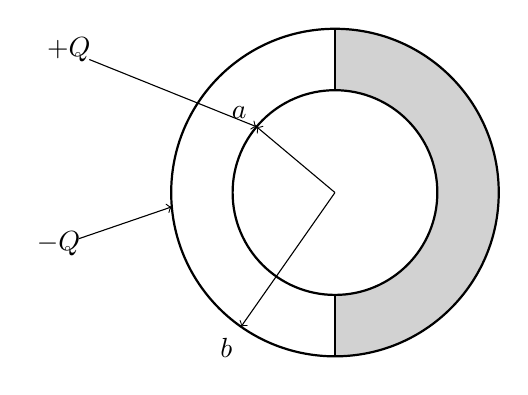
\begin{tikzpicture}[scale=1.3]
  % dielectric: right half of the annulus between r=a and r=b
  \fill[gray!35] (0,1.0) arc (90:-90:1.0) -- (0,-1.6) arc (-90:90:1.6) -- cycle;
  % spheres
  \draw[thick] (0,0) circle (1.0);
  \draw[thick] (0,0) circle (1.6);
  % interface line of dielectric halves
  \draw[thin] (0,1.0) -- (0,1.6);
  \draw[thin] (0,-1.0) -- (0,-1.6);
  % radii arrows a and b
  \draw[->] (0,0) -- (140:1.0);
  \node at (140:1.22) {$a$};
  \draw[->] (0,0) -- (235:1.6);
  \node at (235:1.85) {$b$};
  % +Q and -Q labels with arrows
  \node at (-2.6,1.4) {$+Q$};
  % Source p.172: +Q points to the inner conductor.
  \draw[->] (-2.4,1.3) -- (140:1.0);
  \node at (-2.7,-0.5) {$-Q$};
  \draw[->] (-2.5,-0.45) -- (185:1.6);
\end{tikzpicture}
\par\vspace{0.5em}\textbf{Problem 4.10}
\end{center}

\begin{enumerate}
\item[(a)] Find the electric field everywhere between the spheres.
\item[(b)] Calculate the surface-charge distribution on the inner sphere.
\item[(c)] Calculate the polarization-charge density induced on the surface of the dielectric at $r=a$.
\end{enumerate}
\solution

\textbf{(a)} Let the inner conductor carry $+Q$ and the outer one
$-Q$, as in the textbook figure. Seek a radial field
$\mathbf E=K\hat{\mathbf r}/r^2$. Its potential between the conductors,
with the outer one set to zero, is
\[
\Phi(r)=K\left(\frac1r-\frac1b\right).
\]
Both spherical conductors are equipotentials. On the plane separating
the two hemispheres, this radial field is tangential, so $E_t$ is
continuous and $D_n=0$ on both sides. Thus all interface conditions
are satisfied. A Gaussian sphere of radius $a<r<b$ gives
\[
Q=\oint\mathbf D\cdot d\mathbf a
=\epsilon_0\frac K{r^2}(2\pi r^2)
+\epsilon\frac K{r^2}(2\pi r^2)
=2\pi(\epsilon+\epsilon_0)K.
\]
Consequently, by uniqueness for positive permittivities,
\[
\boxed{\mathbf E(r)=\frac{Q}{2\pi(\epsilon+\epsilon_0)r^2}\hat{\mathbf r},
\qquad a<r<b.}
\]
For $\epsilon=\epsilon_0$ this reduces to the usual spherical-capacitor
field $Q/(4\pi\epsilon_0r^2)$.

\textbf{(b)} The free surface charge on the inner conductor is
$\sigma_f=D_r(a^+)$, since the field inside it is zero. Hence
\[
\boxed{\sigma_f=\begin{cases}
\displaystyle\frac{\epsilon Q}{2\pi(\epsilon+\epsilon_0)a^2},
&\text{hemisphere touching dielectric},\\[5pt]
\displaystyle\frac{\epsilon_0 Q}{2\pi(\epsilon+\epsilon_0)a^2},
&\text{hemisphere touching vacuum}.
\end{cases}}
\]
The two hemispheres carry $Q\epsilon/(\epsilon+\epsilon_0)$ and
$Q\epsilon_0/(\epsilon+\epsilon_0)$, respectively, which sum to $Q$.
The finite jump at the equator does not require an additional line
charge in this solution.

\textbf{(c)} In the dielectric
$\mathbf P=(\epsilon-\epsilon_0)\mathbf E$. Its outward unit normal
at its inner surface is $-\hat{\mathbf r}$, so
\[
\boxed{\sigma_{\rm pol}(a)=\mathbf P\cdot(-\hat{\mathbf r})
=-\frac{(\epsilon-\epsilon_0)Q}
{2\pi(\epsilon+\epsilon_0)a^2}.}
\]
This applies only on the dielectric hemisphere. As checks,
$\rho_{\rm pol}=-\nabla\cdot\mathbf P=0$ within the dielectric,
the flat interface has no polarization charge because $\mathbf P$
is tangential, and the bound charge at $r=b$ has opposite total
charge to that at $r=a$.

\Needspace{5\baselineskip}
\par\bigskip
\noindent\textbf{4.11}\quad The following data on the variation of dielectric constant with pressure are taken from the \emph{Smithsonian Physical Tables}, 9th ed., p.~424:

\begin{center}
\begin{tabular}{c@{\hspace{4em}}c@{\hspace{4em}}l}
\multicolumn{3}{c}{\textbf{Air at 292 K}}\\[2pt]
\toprule
\textbf{Pressure (atm)} & $\boldsymbol{\epsilon/\epsilon_{0}}$ &\\
\midrule
20 & 1.0108 & Relative density of air as a function of\\
40 & 1.0218 & pressure is given in \emph{AIP Handbook},\\
60 & 1.0333 & [3rd ed., McGraw-Hill, New York\\
80 & 1.0439 & (1972), p.~4-165].\\
100 & 1.0548 &\\
\bottomrule
\end{tabular}
\end{center}

\begin{center}
\begin{tabular}{c@{\hspace{3em}}c@{\hspace{4em}}c}
\multicolumn{3}{c}{\textbf{Pentane (C$_{5}$H$_{12}$) at 303 K}}\\[2pt]
\toprule
\textbf{Pressure (atm)} & \textbf{Density (g/cm$^{3}$)} & $\boldsymbol{\epsilon/\epsilon_{0}}$\\
\midrule
1 & 0.613 & 1.82\\
$10^{3}$ & 0.701 & 1.96\\
$4\times10^{3}$ & 0.796 & 2.12\\
$8\times10^{3}$ & 0.865 & 2.24\\
$12\times10^{3}$ & 0.907 & 2.33\\
\bottomrule
\end{tabular}
\end{center}

Test the Clausius--Mossotti relation between dielectric constants and density for air and pentane in the ranges tabulated. Does it hold exactly? Approximately? If approximately, discuss fractional variations in density and $(\epsilon/\epsilon_{0}-1)$. For pentane, compare the Clausius--Mossotti relation to the cruder relation, $(\epsilon/\epsilon_{0}-1)\propto{}$density.
\solution

Put $\kappa=\epsilon/\epsilon_0$ and
$F=(\kappa-1)/(\kappa+2)$. For fixed molecular mass and polarizability,
Clausius--Mossotti says
\[
F=\frac{N\gamma_{\rm mol}}{3}=K\rho,\qquad
\boxed{K=\frac{\kappa-1}{(\kappa+2)\rho}=\text{constant}.}
\]
It is $F$, rather than $\kappa$ or $\kappa-1$ itself, that should be
proportional to mass density.

\textbf{Air.} The pressure table alone does not specify real-gas
densities. To make the density input explicit, use the primary air
tables of Hilsenrath et al., \emph{NBS Circular 564} (1955),
Table 2-1, p.~31, for the compressibility factor
$Z_g=PV/(nRT)$.\footnote{\raggedright The source is available at
\texttt{https://nvlpubs.nist.gov/nistpubs/Legacy/circ/}\allowbreak
\texttt{nbscircular564.pdf}. The input rows, and the independent density
rows from Table 2-2, p.~37, are transcribed in
\texttt{supplementary/ch04-source/air\_reference.csv}.
This supplies a checked density source in place of the AIP reference
cited in the problem.}
The relevant rows are
\begin{center}
\begin{tabular}{rrrrr}
\toprule
$P\ (\mathrm{atm})$&10&40&70&100\\
\midrule
$Z_g(290\ \mathrm K)$&0.99623&0.98782&0.98420&0.98600\\
$Z_g(300\ \mathrm K)$&0.99717&0.99135&0.99000&0.99330\\
\bottomrule
\end{tabular}
\end{center}
Linearly interpolate in temperature,
$Z_g(292,P)=0.8Z_g(290,P)+0.2Z_g(300,P)$.
For the intervening pressures use the cubic interpolating polynomial
through the four pressure entries:
\[
Z_g(P)=\sum_{i=1}^4 Z_g(P_i)
\prod_{j\ne i}\frac{P-P_j}{P_i-P_j}.
\]
Since the temperature and composition are fixed,
$\rho\propto P/Z_g$, so the reference density cancels:
\[
\frac{\rho(P)}{\rho(20)}=\frac{PZ_g(20)}{20Z_g(P)},\qquad
\frac{K(P)}{K(20)}=
\frac{F(P)/F(20)}{\rho(P)/\rho(20)}.
\]
This gives
\begin{center}
\begin{tabular}{rrrrr}
\toprule
$P\ (\mathrm{atm})$ & $Z_g$ & $\rho/\rho(20)$ & $10^3F$ & $K/K(20)$\\
\midrule
20 & 0.99330 & 1.00000 & 3.58709 & 1.00000\\
40 & 0.98853 & 2.00965 & 7.21424 & 1.00076\\
60 & 0.98586 & 3.02264 & 10.97814 & 1.01251\\
80 & 0.98545 & 4.03185 & 14.42229 & 0.99721\\
100 & 0.98746 & 5.02955 & 17.93898 & 0.99432\\
\bottomrule
\end{tabular}
\end{center}
The ratio is approximately constant: its peak-to-peak spread is about
$1.8\%$ of its 20-atm value. Linear instead of cubic pressure
interpolation changes the normalized ratios by less than $0.05\%$,
so the percent-level conclusion does not depend on this interpolation
choice. These are approximate density-based comparisons, not a claim
of exact agreement. The dielectric data have no stated uncertainties,
so their scatter alone should not be assigned a definite microscopic
cause.

Across the range,
\[
\frac{\Delta\rho}{\rho_{20}}\simeq4.0295\quad(403.0\%),\qquad
\frac{\Delta(\kappa-1)}{\kappa_{20}-1}
=\frac{0.0548-0.0108}{0.0108}=4.0741\quad(407.4\%).
\]
Thus the density and susceptibility increase by almost the same
fraction even though each changes by roughly a factor of five.
This is expected because
$F=(\kappa-1)/[3+(\kappa-1)]\simeq(\kappa-1)/3$ for this gas.
If ideal-gas densities were used instead, $F/P$ would range from
$1.7935\times10^{-4}$ to $1.8297\times10^{-4}\ \mathrm{atm}^{-1}$,
again giving approximate agreement but omitting the real-gas correction.

\textbf{Pentane.} Here the actual densities are given. The two proposed
constant ratios are $K=F/\rho$ and the cruder
$J=(\kappa-1)/\rho$, both in $\mathrm{cm^3/g}$:
\begin{center}
\begin{tabular}{rrrrr}
\toprule
$P\ (\mathrm{atm})$ & $K$ & $K/K_1$ & $J$ & $J/J_1$\\
\midrule
1     & 0.350179 & 1.00000 & 1.337684 & 1.00000\\
1000  & 0.345826 & 0.98757 & 1.369472 & 1.02376\\
4000  & 0.341513 & 0.97525 & 1.407035 & 1.05184\\
8000  & 0.338096 & 0.96549 & 1.433526 & 1.07165\\
12000 & 0.338654 & 0.96709 & 1.466373 & 1.09620\\
\bottomrule
\end{tabular}
\end{center}
Clausius--Mossotti is again approximate: $K$ varies by about $3.45\%$
relative to its initial value, whereas $J$ rises by $9.62\%$.
It is therefore the better of the two proportionalities for these data,
but neither is exact. The endpoint fractional changes are
\[
\frac{\Delta\rho}{\rho_1}=\frac{0.907-0.613}{0.613}=0.47961,
\qquad
\frac{\Delta(\kappa-1)}{\kappa_1-1}
=\frac{1.33-0.82}{0.82}=0.62195.
\]
Density rises $47.96\%$, while susceptibility rises $62.20\%$.
The difference is consistent in direction with the local-field
correction: differentiating $F=(\kappa-1)/(\kappa+2)=K\rho$ at constant
$K$ gives
\[
\frac{d(\kappa-1)}{\kappa-1}
=\frac{\kappa+2}{3}\frac{d\rho}{\rho}.
\]
The multiplier is close to one for air, but is appreciably larger for
pentane. The tabulated residual variation of $K$ measures the remaining
failure of a strictly density-independent molecular-polarizability model.

\Needspace{5\baselineskip}
\par\bigskip
\noindent\textbf{4.12}\quad Water vapor is a polar gas whose dielectric constant exhibits an appreciable temperature dependence. The following table gives experimental data on this effect. Assuming that water vapor obeys the ideal gas law, calculate the molecular polarizability as a function of inverse temperature and plot it. From the slope of the curve, deduce a value for the permanent dipole moment of the H$_{2}$O molecule (express the dipole moment in coulomb-meters).

\begin{center}
\begin{tabular}{c@{\hspace{3em}}c@{\hspace{4em}}c}
\toprule
$\mathbf{T(K)}$ & \textbf{Pressure (cm Hg)} & $\boldsymbol{(\epsilon/\epsilon_{0}-1)\times10^{5}}$\\
\midrule
393 & 56.49 & 400.2\\
423 & 60.93 & 371.7\\
453 & 65.34 & 348.8\\
483 & 69.75 & 328.7\\
\bottomrule
\end{tabular}
\end{center}
\solution

Use Jackson's convention $\langle\mathbf p_{\rm mol}\rangle=\epsilon_0\gamma_{\rm mol}\mathbf
E_{\rm local}$, so the molecular polarizability $\gamma_{\rm mol}$ has units of
volume. Here $k$ denotes Boltzmann's constant, as in (4.81)--(4.82).
The alternative SI convention is
$\alpha=\epsilon_0\gamma_{\rm mol}$, with units $\mathrm{C\,m^2/V}$.
The ideal gas law gives $N=P/(kT)$. Applying the Clausius--Mossotti
relation (4.70) to each row, with $\delta=\epsilon/\epsilon_0-1$, yields
\[
\boxed{\gamma_{\rm mol}(T)=\frac{3kT}{P}\frac{\delta}{3+\delta},\qquad
\alpha(T)=\epsilon_0\gamma_{\rm mol}(T).}
\]
Here $P$ must be in pascals: $1\ \mathrm{cm\,Hg}=101325/76$
Pa. The resulting values are
\begin{center}
\begin{tabular}{rrrr}
\toprule
$T\ (\mathrm K)$ & $10^3/T\ (\mathrm{K}^{-1})$
& $\gamma_{\rm mol}/(10^{-28}\ \mathrm m^3)$
& $\alpha/(10^{-39}\ \mathrm{C\,m^2/V})$\\
\midrule
393 & 2.54453 & 2.87938 & 2.54946\\
423 & 2.36407 & 2.66897 & 2.36316\\
453 & 2.20751 & 2.50133 & 2.21473\\
483 & 2.07039 & 2.35455 & 2.08476\\
\bottomrule
\end{tabular}
\end{center}

For completeness, the inverse-temperature law follows by averaging the
permanent dipoles. If $p_0$ is the fixed molecular dipole magnitude and
$u$ its direction cosine with the local field, its orientation energy
is $-p_0Eu$. In a weak field $p_0E\ll kT$,
\begin{align*}
\langle p_\parallel\rangle
&=p_0\frac{\int_{-1}^1u\exp[p_0Eu/(kT)]\,du}
{\int_{-1}^1\exp[p_0Eu/(kT)]\,du}\\
&=p_0\frac{(p_0E/kT)\int_{-1}^1u^2\,du+O(E^3)}
{2+O(E^2)}
=\frac{p_0^2E}{3kT}+O(E^3).
\end{align*}
Adding a temperature-independent induced polarizability gives
\[
\gamma_{\rm mol}(T)=\gamma_i+\frac{p_0^2}{3\epsilon_0k}\frac1T.
\]
An unweighted straight-line fit $\gamma_{\rm mol}=A+B/T$ is obtained from
$x_i=1/T_i$, $y_i=\gamma_{\rm mol}(T_i)$ by
\[
B=\frac{\sum_i(x_i-\bar x)(y_i-\bar y)}{\sum_i(x_i-\bar x)^2},
\qquad A=\bar y-B\bar x.
\]
The four rows give
\[
A=6.3875\times10^{-30}\ \mathrm m^3,\qquad
B=1.10475\times10^{-25}\ \mathrm{m^3\,K}.
\]
Thus the requested dipole magnitude is
\[
\boxed{p_0=\sqrt{3\epsilon_0kB}=6.365\times10^{-30}\ \mathrm{C\,m}
\simeq6.4\times10^{-30}\ \mathrm{C\,m}.}
\]
The rounding of the data does not warrant interpreting the last digits
as an experimental precision. The largest deviation of a tabulated
polarizability from this fitted line is $0.25\%$.
\begin{center}
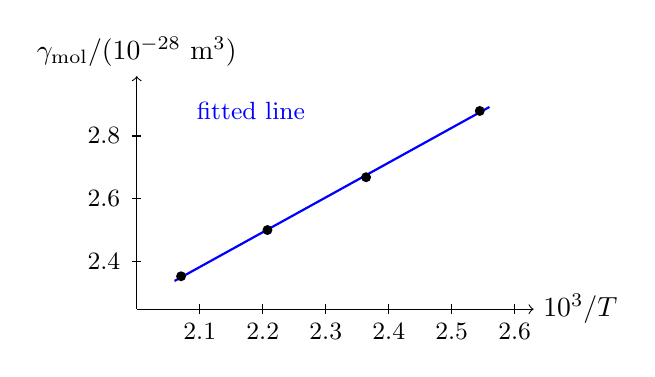
\begin{tikzpicture}[x=8cm,y=4cm]
\draw[->] (2.0,2.25)--(2.63,2.25) node[right] {$10^3/T$};
\draw[->] (2.0,2.25)--(2.0,2.99) node[above] {$\gamma_{\rm mol}/(10^{-28}\ \mathrm m^3)$};
\foreach \x in {2.1,2.2,2.3,2.4,2.5,2.6}
{\draw (\x,2.265)--(\x,2.235) node[below] {\small\x};}
\foreach \y in {2.4,2.6,2.8}
{\draw (1.993,\y)--(2.007,\y) node[left=4pt] {\small\y};}
\draw[blue,thick,domain=2.06:2.56] plot (\x,{0.0638746474+1.1047451447*\x});
\foreach \x/\y in {2.544529/2.879382,2.364066/2.668973,2.207506/2.501331,2.070393/2.354547}
{\fill (\x,\y) circle (1.8pt);}
\node[blue,anchor=west] at (2.08,2.88) {\small fitted line};
\end{tikzpicture}
\end{center}
Neglecting the small local-field correction would replace
$3\delta/(3+\delta)$ by $\delta$; retaining it as above is consistent
with the chapter's definition of molecular polarizability.

\Needspace{5\baselineskip}
\par\bigskip
\noindent\textbf{4.13}\quad Two long, coaxial, cylindrical conducting surfaces of radii $a$ and $b$ are lowered vertically into a liquid dielectric. If the liquid rises an average height $h$ between the electrodes when a potential difference $V$ is established between them, show that the susceptibility of the liquid is
\[
\chi_{e}=\frac{(b^{2}-a^{2})\rho gh\,\ln(b/a)}{\epsilon_{0}V^{2}}
\]
where $\rho$ is the density of the liquid, $g$ is the acceleration due to gravity, and the susceptibility of air is neglected.
\solution

Neglect end effects, surface tension, and changes of liquid density,
and take the external reservoir to be large enough that its level is
fixed. Write $\epsilon=\epsilon_0(1+\chi_e)$ and
$\Lambda=\ln(b/a)$. A homogeneous length $L$ of the coaxial capacitor
has radial field $E_r=V/(r\Lambda)$ and capacitance
\[
C=\frac{2\pi\epsilon L}{\Lambda}.
\]
Raising the dielectric by $dh$ replaces a length $dh$ of air, so
\[
\frac{dC}{dh}=\frac{2\pi(\epsilon-\epsilon_0)}{\Lambda}
=\frac{2\pi\epsilon_0\chi_e}{\Lambda}.
\]
At fixed voltage, the battery supplies $V\,dQ=V^2dC$, while the
field energy increases by $d(\tfrac12CV^2)=\tfrac12V^2dC$.
Their difference is available for mechanical work, hence
\[
F_{\rm electric}\,dh=\frac12V^2dC,\qquad
F_{\rm electric}=\frac{\pi\epsilon_0\chi_e V^2}{\Lambda}.
\]
Equivalently, the mechanical potential at fixed $V$ includes
$-CV^2/2$, not $+CV^2/2$.

The excess volume of liquid between the electrodes is
$\pi(b^2-a^2)h$, where $h$ is the area-averaged rise. Its weight,
after subtracting the hydrostatic support at the external free-surface
level, is
\[
F_g=\rho g\pi(b^2-a^2)h.
\]
Force balance gives
\[
\rho g\pi(b^2-a^2)h
=\frac{\pi\epsilon_0\chi_e V^2}{\ln(b/a)},\qquad
\boxed{\chi_e=\frac{(b^2-a^2)\rho gh\ln(b/a)}{\epsilon_0V^2}.}
\]
For a flat column the same result follows by minimizing
$\rho g\pi(b^2-a^2)h^2/2-C(h)V^2/2$.
The total electric force can also be checked by integrating the
leading local dielectric pressure over the annular cross section:
\[
\int_a^b\frac12(\epsilon-\epsilon_0)
\left[\frac{V}{r\ln(b/a)}\right]^2 2\pi r\,dr
=\frac{\pi\epsilon_0\chi_e V^2}{\ln(b/a)}.
\]
Thus use of the average rise is consistent with the varying radial
field. The susceptibility is positive for a liquid that rises, and
all dimensions cancel in the boxed expression.

\clearpage
\section{Chapter 5. Magnetostatics, Faraday's Law, Quasi-Static Fields}
% Problems, Chapter 5: Magnetostatics, Faraday's Law, Quasi-Static Fields
% Jackson, Classical Electrodynamics, 3rd ed.
% Requires: amsmath, amssymb, tikz

\section*{Problems}

\Needspace{5\baselineskip}
\par\bigskip
\noindent\textbf{5.1}\quad Starting with the differential expression
\[
d\mathbf{B}=\frac{\mu_{0}I}{4\pi}\,d\mathbf{l}'\times\frac{\mathbf{x}-\mathbf{x}'}{|\mathbf{x}-\mathbf{x}'|^{3}}
\]
for the magnetic induction at the point $P$ with coordinate $\mathbf{x}$ produced by an increment of current $I\,d\mathbf{l}'$ at $\mathbf{x}'$, show explicitly that for a closed loop carrying a current $I$ the magnetic induction at $P$ is
\[
\mathbf{B}=\frac{\mu_{0}I}{4\pi}\nabla\Omega
\]
where $\Omega$ is the solid angle subtended by the loop at the point $P$. This corresponds to a magnetic scalar potential, $\Phi_{M}=-\mu_{0}I\Omega/4\pi$. The sign convention for the solid angle is that $\Omega$ is positive if the point $P$ views the ``inner'' side of the surface spanning the loop, that is, if a unit normal $\mathbf{n}$ to the surface is defined by the direction of current flow via the right-hand rule, $\Omega$ is positive if $\mathbf{n}$ points \emph{away} from the point $P$, and negative otherwise. This is the same convention as in Section 1.6 for the electric dipole layer.
\solution
Let $G=|\mathbf x-\mathbf x'|^{-1}$ and orient a spanning surface $S$
by the right-hand rule for the current. The specified solid angle is
\[
\Omega(\mathbf x)=\int_S\frac{\mathbf n'\cdot(\mathbf x'-\mathbf x)}
{|\mathbf x-\mathbf x'|^3}da'
=\int_S n'_j\partial_jG\,da'.
\]
Here unprimed derivatives act on the observation point, and
$\partial'_jG=-\partial_jG$. Put
$\mathbf C=\oint d\mathbf l'\times\nabla'G$.
Componentwise Stokes's theorem gives
\[
\begin{split}
C_i&=\epsilon_{ijk}\epsilon_{jlm}
\int_S n'_l\partial'_m\partial'_kG\,da'\\
&=\int_S[n'_k\partial'_i\partial'_kG-n'_i\nabla'^2G]da'
=\partial_i\int_Sn'_k\partial_kG\,da'=\partial_i\Omega.
\end{split}
\]
The delta term $\nabla'^2G=-4\pi\delta^3(\mathbf x'-\mathbf x)$ is absent
when the observation point is off the chosen spanning surface.
Since $\nabla'G=(\mathbf x-\mathbf x')/|\mathbf x-\mathbf x'|^3$,
Biot--Savart now gives
\[
\boxed{\mathbf B=\frac{\mu_0I}{4\pi}\nabla\Omega,\qquad
\Phi_M=-\frac{\mu_0I}{4\pi}\Omega,\quad\mathbf B=-\nabla\Phi_M.}
\]
For $\mathbf H$ rather than $\mathbf B$, divide this scalar potential by
$\mu_0$. The solid angle changes by $4\pi$ on crossing a spanning surface.
One must use a continuous local branch before differentiating; a
distributional derivative of a discontinuous branch would add a spurious
sheet term. This multivaluedness is necessary because a path linking the
wire has $\oint\mathbf H\cdot d\mathbf l=I$, despite the existence of a
local scalar potential away from the current.


\Needspace{5\baselineskip}
\par\bigskip
\noindent\textbf{5.2}\quad A long, right cylindrical, ideal solenoid of arbitrary cross section is created by stacking a large number of identical current-carrying loops one above the other, with $N$ coils per unit length and each loop carrying a current $I$. [In practice such a solenoid could be wound on a mandrel machined to the arbitrary cross section. After the coil was made rigid (e.g., with epoxy), the mandrel would be withdrawn.]
\begin{enumerate}
\item[(a)] In the approximation that the solenoidal coil is an ideal current sheet and infinitely long, use Problem 5.1 to establish that at any point inside the coil the magnetic field is axial and equal to
\[
H=NI
\]
and that $H=0$ for any point outside the coil.
\item[(b)] For a realistic solenoid of circular cross section of radius $a$ ($Na\gg1$), but still infinite in length, show that the ``smoothed'' magnetic field just outside the solenoid (averaged axially over several turns) is not zero, but is the same in magnitude and direction as that of a single wire on the axis carrying a current $I$, even if $Na\to\infty$. Compare fields inside and out.
\end{enumerate}
\solution
\textbf{(a)} Orient the loops counterclockwise as seen from $+z$.
Let $D$ be their cross section and $u=z'-z$ the height of a source loop
above the observation point. Its principal solid angle is
\[
\Omega_0(u)=\int_D\frac{u\,d^2s'}{[|\mathbf s-\mathbf s'|^2+u^2]^{3/2}}.
\]
It is odd in $u$, tends to zero at $u=\pm\infty$, and, for
$\mathbf s$ strictly inside $D$, tends to $\pm2\pi$ as $u\to0^\pm$.
The last limit follows by integrating over a small disk centered at
$\mathbf s$:
\[
\int_0^\delta\frac{2\pi u\,s\,ds}{(s^2+u^2)^{3/2}}
=2\pi\left[\operatorname{sgn}u-\frac{u}{\sqrt{\delta^2+u^2}}\right].
\]
Outside $D$ there is no jump.

For interior observation points choose the continuous local branch
$\widetilde\Omega=\Omega_0(z'-z)+4\pi H(z-z')$; outside use $\Omega_0$.
The sum of the loop potentials for a finite stack is
$-NI\int\widetilde\Omega\,dz'/(4\pi)$ for the $\mathbf H$ potential.
As both ends recede to infinity, derivatives of the principal-angle
integral vanish: its transverse contributions cancel by oddness, and its
axial end terms tend to zero. Inside, the added branch contributes
\[
\nabla\int4\pi H(z-z')\,dz'=4\pi\widehat{\mathbf z}.
\]
There is no such term outside. Problem 5.1 therefore gives
\[
\boxed{\mathbf H=NI\,\widehat{\mathbf z}\quad(\mathbf s\in D),
\qquad\mathbf H=0\quad(\mathbf s\notin\overline D).}
\]
This result is independent of the shape of $D$. The jump agrees with
$\mathbf n\times(\mathbf H_{\rm out}-\mathbf H_{\rm in})=\mathbf K$,
where $\mathbf K=NI\,\widehat{\mathbf z}\times\mathbf n$.

\textbf{(b)} A continuous helical wire advances by one pitch $1/N$ per
turn. Axial averaging gives two components of sheet current:
\[
K_\phi=NI,\qquad 2\pi aK_z=I,\qquad K_z=\frac{I}{2\pi a}.
\]
The second equality follows because a plane perpendicular to the axis
cuts the single winding once and carries net axial current $I$.
The azimuthal sheet produces the field in part (a). An Amperian circle
for the axial sheet gives $2\pi\rho H_\phi=I$ outside, and zero inside.
Thus, neglecting the spatial ripple between turns,
\[
\boxed{\mathbf H_{\rm in}=NI\,\widehat{\mathbf z},\qquad
\mathbf H_{\rm out}=\frac{I}{2\pi\rho}\widehat{\boldsymbol\phi}.}
\]
At $\rho=a^+$, $H_{\rm out}/H_{\rm in}=1/(2\pi Na)$.
For fixed $I$, the exterior field does not vanish as $N$ increases,
although its ratio to the interior field does. A return lead can alter
this exterior field; the result is for the isolated helical winding.


\Needspace{5\baselineskip}
\par\bigskip
\noindent\textbf{5.3}\quad A right-circular solenoid of finite length $L$ and radius $a$ has $N$ turns per unit length and carries a current $I$. Show that the magnetic induction on the cylinder axis in the limit $NL\to\infty$ is
\[
B_{z}=\frac{\mu_{0}NI}{2}\left(\cos\theta_{1}+\cos\theta_{2}\right)
\]
where the angles are defined in the figure.

\begin{center}
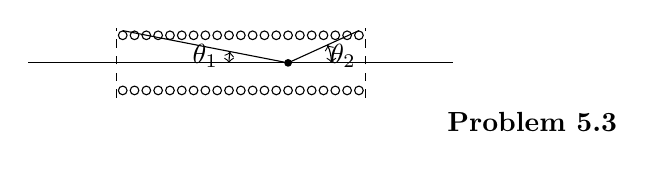
\begin{tikzpicture}[scale=1.0]
  % solenoid: two rows of coil cross-section circles
  \foreach \i in {0,...,20}{
    \draw (\i*0.15,0.35) circle (0.055);
    \draw (\i*0.15,-0.35) circle (0.055);
  }
  % dashed end caps
  \draw[dashed] (-0.08,-0.44) -- (-0.08,0.44);
  \draw[dashed] (3.08,-0.44) -- (3.08,0.44);
  % axis
  \draw (-1.2,0) -- (4.2,0);
  % point P on the axis, right of center
  \fill (2.1,0) circle (1.4pt);
  % lines from ends of solenoid to P
  \draw (0,0.41) -- (2.1,0);
  \draw (3.0,0.41) -- (2.1,0);
  % theta angles: arcs between axis and slanted lines, centered at P
  \draw[<->] (1.35,0) arc (180:169:0.75);
  \node at (1.05,0.09) {$\theta_{1}$};
  \draw[<->] (2.65,0) arc (0:24.5:0.55);
  \node at (2.8,0.09) {$\theta_{2}$};
  \node[below right] at (4.0,-0.5) {\textbf{Problem 5.3}};
\end{tikzpicture}
\end{center}
\solution
First derive the axial field of one loop. Parameterize it by
\[
\mathbf x'=(a\cos\phi',a\sin\phi',z'),\qquad
d\mathbf l'=a(-\sin\phi',\cos\phi',0)d\phi'.
\]
Then
the axial component of $d\mathbf l'\times(\mathbf x-\mathbf x')$
at $(0,0,z)$ is $a^2d\phi'$. The transverse components integrate to zero,
so
\[
dB_z=\frac{\mu_0(NI\,dz')a^2}
{2[a^2+(z-z')^2]^{3/2}}.
\]
Choose the ends at $\pm L/2$ and integrate:
\[
\begin{split}
B_z(z)&=\frac{\mu_0NI}{2}\int_{-L/2}^{L/2}
\frac{a^2\,dz'}{[a^2+(z-z')^2]^{3/2}}\\
&=\frac{\mu_0NI}{2}
\left[\frac{z+L/2}{\sqrt{a^2+(z+L/2)^2}}
-\frac{z-L/2}{\sqrt{a^2+(z-L/2)^2}}\right].
\end{split}
\]
The antiderivative used here is
$u/\sqrt{a^2+u^2}$, whose derivative is $a^2/(a^2+u^2)^{3/2}$.
For a point between the ends,
\[
\cos\theta_1=\frac{z+L/2}{\sqrt{a^2+(z+L/2)^2}},\qquad
\cos\theta_2=\frac{L/2-z}{\sqrt{a^2+(L/2-z)^2}},
\]
which proves the stated result. The algebraic formula also applies
outside the solenoid, with the corresponding signed cosines.
The continuum limit replaces the discrete turns by a sheet of current
$NI$; a long solenoid gives $B_z\to\mu_0NI$ deep inside.


\Needspace{5\baselineskip}
\par\bigskip
\noindent\textbf{5.4}\quad A magnetic induction $\mathbf{B}$ in a current-free region in a uniform medium is cylindrically symmetric with components $B_{z}(\rho,z)$ and $B_{\rho}(\rho,z)$ and with a known $B_{z}(0,z)$ on the axis of symmetry. The magnitude of the axial field varies slowly in $z$.
\begin{enumerate}
\item[(a)] Show that near the axis the axial and radial components of magnetic induction are approximately
\begin{align*}
B_{z}(\rho,z)&\simeq B_{z}(0,z)-\left(\frac{\rho^{2}}{4}\right)\!\left[\frac{\partial^{2}B_{z}(0,z)}{\partial z^{2}}\right]+\cdots\\
B_{\rho}(\rho,z)&\simeq-\left(\frac{\rho}{2}\right)\!\left[\frac{\partial B_{z}(0,z)}{\partial z}\right]+\left(\frac{\rho^{3}}{16}\right)\!\left[\frac{\partial^{3}B_{z}(0,z)}{\partial z^{3}}\right]+\cdots
\end{align*}
\item[(b)] What are the magnitudes of the neglected terms, or equivalently what is the criterion defining ``near'' the axis?
\end{enumerate}
\solution
\textbf{(a)} Smooth axial symmetry requires expansions
\[
B_z(\rho,z)=\sum_{n=0}^\infty a_n(z)\rho^{2n},\qquad
B_\rho(\rho,z)=\sum_{n=0}^\infty b_n(z)\rho^{2n+1}.
\]
The divergence equation and the azimuthal curl equation are
\[
\rho^{-1}\partial_\rho(\rho B_\rho)+\partial_zB_z=0,\qquad
\partial_zB_\rho-\partial_\rho B_z=0.
\]
Equating powers of $\rho$ gives
\[
(2n+2)b_n+a_n'=0,\qquad b_n'=2(n+1)a_{n+1}.
\]
Combining these, $a_{n+1}=-a_n''/[4(n+1)^2]$.
Writing $f(z)=B_z(0,z)=a_0(z)$, repeated substitution yields
\[
a_n=\frac{(-1)^nf^{(2n)}}{2^{2n}(n!)^2},\qquad
b_n=\frac{(-1)^{n+1}f^{(2n+1)}}{2^{2n+1}n!(n+1)!}.
\]
In particular,
\[
\boxed{B_z=f-\frac{\rho^2}{4}f''+\frac{\rho^4}{64}f^{(4)}+\cdots,}
\qquad
\boxed{B_\rho=-\frac{\rho}{2}f'+\frac{\rho^3}{16}f'''
-\frac{\rho^5}{384}f^{(5)}+\cdots.}
\]
\textbf{(b)} The first omitted terms in the question are
$\rho^4f^{(4)}/64$ and $-\rho^5f^{(5)}/384$.
If derivatives have a common variation length $\ell$,
$|f^{(n)}|\sim |f|/\ell^n$, the expansion parameter is $\rho/\ell\ll1$.
More precisely, each omitted term must be small relative to the accuracy
required of the retained sum. Ratios to $f'$ or $f''$ alone are
inappropriate where those derivatives happen to vanish. The series is
local and its radius of convergence cannot extend through a current sheet
or another field singularity.


\Needspace{5\baselineskip}
\par\bigskip
\noindent\textbf{5.5}\quad\begin{enumerate}
\item[(a)] Use the results of Problems 5.4 and 5.3 to find the axial and radial components of magnetic induction in the \emph{central region} ($|z|\ll L/2$) of a long uniform solenoid of radius $a$ and ends at $z=\pm L/2$, including the value of $B_{z}$ just inside the coil ($\rho=a^{-}$).
\item[(b)] Use Amp\`ere's law to show that the longitudinal magnetic induction just outside the coil is approximately
\[
B_{z}(\rho=a^{+},z)\simeq-\left(\frac{2\mu_{0}NIa^{2}}{L^{2}}\right)\!\left(1+\frac{12z^{2}}{L^{2}}-\frac{9a^{2}}{L^{2}}+\cdots\right)
\]
For $L\gg a$, the field outside is negligible compared to inside. How does this axial component compare in size to the azimuthal component of Problem 5.2b?
\item[(c)] Show that at the end of the solenoid the magnetic induction near the axis has components
\[
B_{z}\simeq\frac{\mu_{0}NI}{2},\qquad B_{\rho}\simeq\pm\frac{\mu_{0}NI}{4}\left(\frac{\rho}{a}\right)
\]
\end{enumerate}
\solution
Put $\ell=L/2$ and $B_s=\mu_0NI$. We consider $a,\rho,|z|\ll\ell$.
The exact on-axis result of 5.3 is
\[
\frac{f(z)}{B_s}
=\frac12\left[\frac{\ell+z}{\sqrt{a^2+(\ell+z)^2}}
+\frac{\ell-z}{\sqrt{a^2+(\ell-z)^2}}\right].
\]
Use $(1+x)^{-1/2}=1-x/2+3x^2/8+\cdots$ and then expand in $z/\ell$:
\[
\frac f{B_s}
=1-\frac{a^2}{2\ell^2}-\frac{3a^2z^2}{2\ell^4}
+\frac{3a^4}{8\ell^4}
+O\left(\frac{a^2z^4+a^4z^2+a^6}{\ell^6}\right).
\]
\textbf{(a)} Differentiating this axis function and using 5.4 gives
\[
\boxed{\frac{B_z}{B_s}
=1-\frac{a^2}{2\ell^2}
-\frac{3a^2z^2}{2\ell^4}
+\frac{3a^4}{8\ell^4}
+\frac{3a^2\rho^2}{4\ell^4}+\cdots,\qquad
\frac{B_\rho}{B_s}=\frac{3a^2\rho z}{2\ell^4}+\cdots.}
\]
For example, the next terms in $B_\rho/B_s$ are
$5a^2\rho z^3/\ell^6-15a^4\rho z/(4\ell^6)
-15a^2\rho^3z/(4\ell^6)$.
At the inner wall,
\[
B_z(a^-,z)=B_s\left[1-\frac{2a^2}{L^2}
-\frac{24a^2z^2}{L^4}+\frac{18a^4}{L^4}+\cdots\right].
\]
\textbf{(b)} A narrow rectangular Ampere loop straddling the winding
gives $H_z(a^-)-H_z(a^+)=NI$. Subtracting $B_s$ from the preceding
expression therefore gives
\[
\boxed{B_z(a^+,z)=-\frac{2\mu_0NIa^2}{L^2}
\left[1+\frac{12z^2}{L^2}-\frac{9a^2}{L^2}+\cdots\right].}
\]
It is an axial return field. For an actual helical winding,
$B_\phi(a^+)=\mu_0I/(2\pi a)$, so near the center
\[
\frac{|B_z(a^+)|}{|B_\phi(a^+)|}\simeq
\frac{4\pi Na^3}{L^2}.
\]
Thus either exterior component can dominate, depending on $N,a,L$;
both can be small compared with the main interior field.

\textbf{(c)} At the upper end $z=\ell$,
\[
f(\ell)=\frac{B_s}{2}\frac{L}{\sqrt{L^2+a^2}}
\simeq\frac{B_s}{2},\qquad
f'(\ell)=\frac{B_s}{2}
\left[\frac{a^2}{(L^2+a^2)^{3/2}}-\frac1a\right]
\simeq-\frac{B_s}{2a}.
\]
For $\rho\ll a$ and $L\gg a$, 5.4 then gives
$B_\rho\simeq B_s\rho/(4a)$. At the lower end the derivative changes
sign. Consequently
\[
\boxed{B_z\simeq B_s/2,\qquad
B_\rho\simeq\pm B_s\rho/(4a)}
\]
at the upper/lower ends, respectively.


\Needspace{5\baselineskip}
\par\bigskip
\noindent\textbf{5.6}\quad A cylindrical conductor of radius $a$ has a hole of radius $b$ bored parallel to, and centered a distance $d$ from, the cylinder axis ($d+b<a$). The current density is uniform throughout the remaining metal of the cylinder and is parallel to the axis. Use Amp\`ere's law and principle of linear superposition to find the magnitude and the direction of the magnetic-flux density in the hole.
\solution
Let the axis of the original cylinder be the origin of transverse
coordinates, and let the hole center have displacement $\mathbf d$.
Take $\mathbf J=J\widehat{\mathbf z}$ in the remaining metal.
For a uniformly filled cylinder, an Amperian circle gives
$2\pi\rho B_\phi=\mu_0J\pi\rho^2$, or
\[
\mathbf B_{\rm full}(\boldsymbol\rho)
=\frac{\mu_0}{2}\mathbf J\times\boldsymbol\rho.
\]
Represent the hole by superposing a cylinder with density $-\mathbf J$
and local coordinate $\boldsymbol\rho-\mathbf d$. Every point in the
hole is inside both cylinders, so
\[
\boxed{\mathbf B_{\rm hole}
=\frac{\mu_0}{2}\left[\mathbf J\times\boldsymbol\rho
-\mathbf J\times(\boldsymbol\rho-\mathbf d)\right]
=\frac{\mu_0}{2}\mathbf J\times\mathbf d.}
\]
The field is uniform, of magnitude $\mu_0Jd/2$, perpendicular both to
the current and to the displacement toward the hole. If the total
current is $I$, then $J=I/[\pi(a^2-b^2)]$. A centered hole gives zero
field, providing a symmetry check.


\Needspace{5\baselineskip}
\par\bigskip
\noindent\textbf{5.7}\quad A compact circular coil of radius $a$, carrying a current $I$ (perhaps $N$ turns, each with current $I/N$), lies in the $x$-$y$ plane with its center at the origin.
\begin{enumerate}
\item[(a)] By elementary means [Eq.~(5.4)] find the magnetic induction at any point on the $z$ axis.
\item[(b)] An identical coil with the same magnitude and sense of the current is located on the same axis, parallel to, and a distance $b$ above, the first coil. With the coordinate origin relocated at the point midway between the centers of the two coils, determine the magnetic induction on the axis near the origin as an expansion in powers of $z$, up to $z^{4}$ inclusive:
\[
B_{z}=\left(\frac{\mu_{0}Ia^{2}}{d^{3}}\right)\!\left[1+\frac{3(b^{2}-a^{2})z^{2}}{2d^{4}}+\frac{15(b^{4}-6b^{2}a^{2}+2a^{4})z^{4}}{16d^{8}}+\cdots\right]
\]
where $d^{2}=a^{2}+b^{2}/4$.
\item[(c)] Show that, off-axis near the origin, the axial and radial components, correct to second order in the coordinates, take the form
\[
B_{z}=\sigma_{0}+\sigma_{2}\left(z^{2}-\frac{\rho^{2}}{2}\right);\qquad B_{\rho}=-\sigma_{2}z\rho
\]
\item[(d)] For the two coils in part b show that the magnetic induction on the $z$ axis for large $|z|$ is given by the expansion in inverse odd powers of $|z|$ obtained from the small $z$ expansion of part b by the formal substitution, $d\to|z|$.
\item[(e)] If $b=a$, the two coils are known as a pair of Helmholtz coils. For this choice of geometry the second terms in the expansions of parts b and d are absent ($\sigma_{2}=0$ in part c). The field near the origin is then very uniform. What is the maximum permitted value of $|z|/a$ if the axial field is to be uniform to one part in $10^{4}$, one part in $10^{2}$?
\end{enumerate}
\solution
\textbf{(a)} The element calculation in 5.3 gives
\[
\boxed{B_z(0,z)=\frac{\mu_0Ia^2}{2(a^2+z^2)^{3/2}},\qquad
B_x=B_y=0.}
\]
Here $I$ is the total ampere-turns specified in the question.

\textbf{(b)} Put the centers at $z=\pm b/2$ and
$d^2=a^2+b^2/4$. The exact sum is
\[
B_z=\frac{\mu_0Ia^2}{2d^3}
\left[\left(1+\frac{z^2-bz}{d^2}\right)^{-3/2}
+\left(1+\frac{z^2+bz}{d^2}\right)^{-3/2}\right].
\]
The binomial coefficients needed are
$1,-3/2,15/8,-35/16,315/128$.
After averaging the two signs, the coefficients of $z^2$ and $z^4$ are
\[
-\frac3{2d^2}+\frac{15b^2}{8d^4}
=\frac{3(b^2-a^2)}{2d^4},
\]
\[
\frac{15}{8d^4}-\frac{105b^2}{16d^6}
+\frac{315b^4}{128d^8}
=\frac{15(b^4-6a^2b^2+2a^4)}{16d^8}.
\]
The odd powers cancel, proving the stated series.

\textbf{(c)} Write its first terms as $f(z)=\sigma_0+\sigma_2z^2+\cdots$,
where
\[
\sigma_0=\frac{\mu_0Ia^2}{d^3},\qquad
\sigma_2=\sigma_0\frac{3(b^2-a^2)}{2d^4}.
\]
Then $f'=2\sigma_2z+\cdots$ and $f''=2\sigma_2+\cdots$.
Substitution into 5.4 gives
\[
\boxed{B_z=\sigma_0+\sigma_2(z^2-\rho^2/2)+O(r^4),\qquad
B_\rho=-\sigma_2z\rho+O(r^4).}
\]
\textbf{(d)} For $|z|\gg d$, factor $|z|^3$ from the exact denominators:
\[
B_z=\frac{\mu_0Ia^2}{2|z|^3}
\sum_{\pm}\left(1\pm\frac b{|z|}+\frac{d^2}{z^2}\right)^{-3/2}.
\]
The same binomial calculation yields
\[
\boxed{B_z=\frac{\mu_0Ia^2}{|z|^3}
\left[1+\frac{3(b^2-a^2)}{2z^2}
+\frac{15(b^4-6a^2b^2+2a^4)}{16z^4}+\cdots\right].}
\]
This is the stated formal replacement $d\mapsto|z|$ in part (b),
including its prefactor. It does not replace $a$ or $b$.

\textbf{(e)} At $b=a$, $d^2=5a^2/4$ and
\[
\frac{B_z(z)}{B_z(0)}
=1-\frac{144}{125}(z/a)^4+O((z/a)^6).
\]
The fourth-order estimate for relative tolerance $\delta$ is
$|z|/a\le(125\delta/144)^{1/4}$, namely $0.09652$ for $10^{-4}$
and $0.30524$ for $10^{-2}$. To determine the actual edge of the
central uniform interval, solve with the exact field:
\[
\frac{(5/4)^{3/2}}2
\left\{[1+(u-1/2)^2]^{-3/2}+[1+(u+1/2)^2]^{-3/2}\right\}
=1-\delta,\qquad u=|z|/a.
\]
The exact central-interval limits are
$\boxed{|z|/a\le0.0967727}$ and $\boxed{|z|/a\le0.3137460}$,
respectively. Substitution into the exact expression gives field ratios
$0.9999$ and $0.9900$.


\Needspace{5\baselineskip}
\par\bigskip
\noindent\textbf{5.8}\quad A localized cylindrically symmetric current distribution is such that the current flows only in the azimuthal direction; the current density is a function only of $r$ and $\theta$ (or $\rho$ and $z$): $\mathbf{J}=\hat{\boldsymbol{\phi}}J(r,\theta)$. The distribution is ``hollow'' in the sense that there is a current-free region near the origin, as well as outside.
\begin{enumerate}
\item[(a)] Show that the magnetic field can be derived from the azimuthal component of the vector potential, with a multipole expansion
\[
A_{\phi}(r,\theta)=-\frac{\mu_{0}}{4\pi}\sum_{L}m_{L}r^{L}P_{L}^{1}(\cos\theta)
\]
in the interior and
\[
A_{\phi}(r,\theta)=-\frac{\mu_{0}}{4\pi}\sum_{L}\mu_{L}r^{-L-1}P_{L}^{1}(\cos\theta)
\]
outside the current distribution.
\item[(b)] Show that the internal and external multipole moments are
\[
m_{L}=-\frac{1}{L(L+1)}\int d^{3}x\;r^{-L-1}P_{L}^{1}(\cos\theta)\,J(r,\theta)
\]
and
\[
\mu_{L}=-\frac{1}{L(L+1)}\int d^{3}x\;r^{L}P_{L}^{1}(\cos\theta)\,J(r,\theta)
\]
\end{enumerate}
\solution
\textbf{(a)} Choose the observation azimuth to be zero. Reflection in the
$x$--$z$ plane cancels the radial part of
$\mathbf A=(\mu_0/4\pi)\int\mathbf J(\mathbf x')/|\mathbf x-\mathbf x'|\,d^3x'$.
There is no $z$ component, and
\[
A_\phi=\frac{\mu_0}{4\pi}\int
\frac{J(r',\theta')\cos\phi'}{|\mathbf x-\mathbf x'|}\,d^3x'.
\]
Expand the Coulomb kernel as
$\sum_{L\ge0}r_<^Lr_>^{-L-1}P_L(\cos\gamma)$.
The addition theorem in real azimuthal form is
\[
P_L(\cos\gamma)=P_L(\cos\theta)P_L(\cos\theta')
+2\sum_{m=1}^L\frac{(L-m)!}{(L+m)!}
P_L^m(\cos\theta)P_L^m(\cos\theta')\cos(m\phi').
\]
Multiplication by $\cos\phi'$ and integration over $0\le\phi'<2\pi$
kills every term except $m=1$, whose cosine integral is $\pi$.
Thus
\[
A_\phi=\frac{\mu_0}{4\pi}\sum_{L=1}^\infty
\frac{P_L^1(\cos\theta)}{L(L+1)}
\int d^3x'\,\frac{r_<^L}{r_>^{L+1}}
P_L^1(\cos\theta')J(r',\theta').
\]
\textbf{(b)} In a source-free ball containing the origin, $r<r'$ for
all source points, so factor out $r^L$. In the exterior of a sphere
containing all currents, $r>r'$ and one factors out $r^{-L-1}$.
Define
\[
\boxed{m_L=-\frac1{L(L+1)}\int r'^{-L-1}P_L^1(\cos\theta')J\,d^3x',
\qquad
\mu_L=-\frac1{L(L+1)}\int r'^LP_L^1(\cos\theta')J\,d^3x'.}
\]
Then
\[
\boxed{A_{\phi,\rm in}=-\frac{\mu_0}{4\pi}\sum_{L\ge1}m_Lr^LP_L^1,
\qquad
A_{\phi,\rm out}=-\frac{\mu_0}{4\pi}\sum_{L\ge1}\mu_Lr^{-L-1}P_L^1.}
\]
The moments use the Condon--Shortley convention
$P_L^1(\cos\theta)=\partial_\theta P_L(\cos\theta)$.
Finally,
$B_r=(r\sin\theta)^{-1}\partial_\theta(\sin\theta A_\phi)$ and
$B_\theta=-r^{-1}\partial_r(rA_\phi)$, with $B_\phi=0$.
These convergence domains are spherical source-free regions; an
arbitrary point merely outside the current support need not belong to
the convergence domain of either expansion.


\Needspace{5\baselineskip}
\par\bigskip
\noindent\textbf{5.9}\quad The two circular coils of radius $a$ and separation $b$ of Problem 5.7 can be described in cylindrical coordinates by the current density
\[
\mathbf{J}=\hat{\boldsymbol{\phi}}I\delta(\rho-a)[\delta(z-b/2)+\delta(z+b/2)]
\]
\begin{enumerate}
\item[(a)] Using the formalism of Problem 5.8, calculate the internal and external multipole moments for $L=1,\ldots,5$.
\item[(b)] Using the internal multipole expansion of Problem 5.8, write down explicitly an expression for $B_{z}$ on the $z$ axis and relate it to the answer of Problem 5.7b.
\end{enumerate}
\solution
\textbf{(a)} Let $d=\sqrt{a^2+b^2/4}$ and $c=b/(2d)$.
At the two source rings, $r'=d$ and $\cos\theta'=\pm c$.
The cylindrical volume element supplies
$\int J\,d^3x'=2\pi aI$ for each ring.
Because $P_L^1(-c)=(-1)^{L+1}P_L^1(c)$, even $L$ vanish and odd $L$ give
\[
m_L=-\frac{4\pi aI}{L(L+1)d^{L+1}}P_L^1(c),\qquad
\mu_L=d^{2L+1}m_L.
\]
Use
\[
P_1^1(c)=-\sqrt{1-c^2},\quad
P_3^1(c)=-\tfrac32(5c^2-1)\sqrt{1-c^2},\quad
P_5^1(c)=-\tfrac{15}{8}(21c^4-14c^2+1)\sqrt{1-c^2},
\]
with $\sqrt{1-c^2}=a/d$. The explicit moments are
\[
\begin{array}{c|c|c}
L&m_L&\mu_L\\\hline
1&2\pi Ia^2/d^3&2\pi Ia^2\\[2pt]
2&0&0\\[2pt]
3&\pi Ia^2(b^2-a^2)/(2d^7)&\pi Ia^2(b^2-a^2)/2\\[2pt]
4&0&0\\[2pt]
5&\pi Ia^2(b^4-6a^2b^2+2a^4)/(8d^{11})
&\pi Ia^2(b^4-6a^2b^2+2a^4)/8
\end{array}
\]
\textbf{(b)} The identity $\partial_\theta(\sin\theta P_L^1)
=-L(L+1)\sin\theta P_L$ gives
\[
B_{r,\rm in}=\frac{\mu_0}{4\pi}
\sum_{L\ge1}L(L+1)m_Lr^{L-1}P_L(\cos\theta).
\]
On the positive $z$ axis $P_L(1)=1$ and $B_z=B_r$, hence
\[
B_z(0,z)=\frac{\mu_0}{4\pi}
[2m_1+12m_3z^2+30m_5z^4+\cdots].
\]
Inserting the table reproduces every coefficient in 5.7(b).
Reflection symmetry extends this even polynomial to negative $z$.


\Needspace{5\baselineskip}
\par\bigskip
\noindent\textbf{5.10}\quad A circular current loop of radius $a$ carrying a current $I$ lies in the $x$-$y$ plane with its center at the origin.
\begin{enumerate}
\item[(a)] Show that the only nonvanishing component of the vector potential is
\[
A_{\phi}(\rho,z)=\frac{\mu_{0}Ia}{\pi}\int_{0}^{\infty}dk\,\cos kz\,I_{1}(k\rho_{<})K_{1}(k\rho_{>})
\]
where $\rho_{<}$ ($\rho_{>}$) is the smaller (larger) of $a$ and $\rho$.
\item[(b)] Show that an alternative expression for $A_{\phi}$ is
\[
A_{\phi}(\rho,z)=\frac{\mu_{0}Ia}{2}\int_{0}^{\infty}dk\;e^{-k|z|}J_{1}(ka)J_{1}(k\rho)
\]
\item[(c)] Write down integral expressions for the components of magnetic induction, using the expressions of parts a and b. Evaluate explicitly the components of $\mathbf{B}$ on the $z$ axis by performing the necessary integrations.
\end{enumerate}
\solution
The scalar cylindrical Green expansions needed here follow by
separating the Fourier variable along $z$, or by separating radial
Bessel modes:
\[
\begin{split}
\frac1{|\mathbf x-\mathbf x'|}
&=\frac2\pi\sum_{m=-\infty}^{\infty}e^{im(\phi-\phi')}
\int_0^\infty \cos[k(z-z')]I_m(k\rho_<)K_m(k\rho_>)\,dk,\\
\frac1{|\mathbf x-\mathbf x'|}
&=\sum_{m=-\infty}^{\infty}e^{im(\phi-\phi')}
\int_0^\infty e^{-k|z-z'|}J_m(k\rho)J_m(k\rho')\,dk.
\end{split}
\]
For completeness, the first normalization follows from
$\int_0^\infty\cos(kz)K_0(ks)\,dk=\pi/[2\sqrt{s^2+z^2}]$ and
the cylindrical addition theorem for $K_0$.
The second follows from
$\int_0^\infty e^{-k|z|}J_0(ks)\,dk=1/\sqrt{s^2+z^2}$
and the addition theorem for $J_0$.

\textbf{(a),(b)} The current loop has $d\mathbf l'=a\widehat{\boldsymbol\phi}'d\phi'$.
Projecting onto the observation $\widehat{\boldsymbol\phi}$ supplies
$\cos(\phi-\phi')$. Its angular integral is $\pi$ for each of $m=\pm1$
and zero for all other $m$. Consequently the first kernel gives
\[
\boxed{A_\phi=\frac{\mu_0Ia}{\pi}\int_0^\infty
\cos(kz)I_1(k\rho_<)K_1(k\rho_>)\,dk,}
\]
and the second gives
\[
\boxed{A_\phi=\frac{\mu_0Ia}{2}\int_0^\infty
e^{-k|z|}J_1(ka)J_1(k\rho)\,dk.}
\]
All other components vanish by the same reflection symmetry as in 5.8.

\textbf{(c)} The curl equations are
$B_\rho=-\partial_zA_\phi$ and
$B_z=\rho^{-1}\partial_\rho(\rho A_\phi)$.
Using $(xI_1)'=xI_0$, $(xK_1)'=-xK_0$, and $(xJ_1)'=xJ_0$, one obtains
\[
B_\rho=\frac{\mu_0Ia}{\pi}\int_0^\infty
k\sin(kz)I_1(k\rho_<)K_1(k\rho_>)\,dk,
\]
\[
B_z=\frac{\mu_0Ia}{\pi}\int_0^\infty k\cos(kz)
\begin{cases}
I_0(k\rho)K_1(ka),&\rho<a,\\
-I_1(ka)K_0(k\rho),&\rho>a
\end{cases}dk,
\]
or, for $z\ne0$,
\[
\boxed{\begin{aligned}
B_\rho&=\frac{\mu_0Ia}{2}\operatorname{sgn}(z)
\int_0^\infty k e^{-k|z|}J_1(ka)J_1(k\rho)\,dk,\\
B_z&=\frac{\mu_0Ia}{2}\int_0^\infty
k e^{-k|z|}J_1(ka)J_0(k\rho)\,dk.
\end{aligned}}
\]
At $z=0$ off the wire, take the limiting fields; symmetry gives
$B_\rho=0$. On the axis $J_1(0)=0$ and $J_0(0)=1$.
Differentiate the elementary Laplace integral
$\int_0^\infty e^{-sk}J_0(ak)\,dk=(s^2+a^2)^{-1/2}$ with respect to $a$:
\[
\int_0^\infty k e^{-sk}J_1(ak)\,dk=\frac{a}{(s^2+a^2)^{3/2}}.
\]
This gives
$\boxed{B_\rho(0,z)=0,\ B_z(0,z)=\mu_0Ia^2/[2(a^2+z^2)^{3/2}]}$.
The modified-Bessel representation independently gives the same result:
differentiate
$\int_0^\infty\cos(kz)K_0(ka)\,dk=\pi/[2\sqrt{a^2+z^2}]$
with respect to $a$, producing the required integral of $kK_1(ka)$.


\Needspace{5\baselineskip}
\par\bigskip
\noindent\textbf{5.11}\quad A circular loop of wire carrying a current $I$ is located with its center at the origin of coordinates and the normal to its plane having spherical angles $\theta_{0}$, $\phi_{0}$. There is an applied magnetic field, $B_{x}=B_{0}(1+\beta y)$ and $B_{y}=B_{0}(1+\beta x)$.
\begin{enumerate}
\item[(a)] Calculate the force acting on the loop without making any approximations. Compare your result with the approximate result (5.69). Comment.
\item[(b)] Calculate the torque in lowest order. Can you deduce anything about the higher order contributions? Do they vanish for the circular loop? What about for other shapes?
\end{enumerate}
\solution
Let the radius be $a$, the area be $S=\pi a^2$, and
\[
\mathbf m=IS(\sin\theta_0\cos\phi_0,\sin\theta_0\sin\phi_0,\cos\theta_0).
\]
\textbf{(a)} Starting with
$\mathbf F=I\oint d\mathbf l\times\mathbf B$ and writing
$B_k=B_{k0}+G_{kj}x_j$, the constant term vanishes.
Stokes's theorem gives
$\oint x_j\,dx_i=\epsilon_{jil}S n_l$.
In indices, the remaining term is
\[
F_i=I\epsilon_{ijk}G_{k\ell}\oint x_\ell\,dx_j
=\epsilon_{ijk}\epsilon_{\ell jn}G_{k\ell}m_n
=m_kG_{ki}-m_iG_{kk}.
\]
Here $\epsilon_{ijk}\epsilon_{\ell jn}=\delta_{i\ell}\delta_{kn}
-\delta_{in}\delta_{k\ell}$ and $G_{kk}=\nabla\cdot\mathbf B=0$.
Therefore $F_i=m_j\partial_iB_j$.
Here $\partial_yB_x=\partial_xB_y=\beta B_0$, and thus
\[
\boxed{\mathbf F=\beta B_0(m_y,m_x,0)
=\beta B_0I\pi a^2\sin\theta_0
(\sin\phi_0,\cos\phi_0,0).}
\]
This is exactly $\nabla(\mathbf m\cdot\mathbf B)$, with no small-loop
approximation: a linear applied field has no derivatives that could
couple to higher force multipoles.

\textbf{(b)} To dipole order,
\[
\boxed{\mathbf N=\mathbf m\times\mathbf B(0)
=B_0(-m_z,m_z,m_x-m_y).}
\]
One can also see why this is exact for the centered circle. The torque
integrand is $\mathbf x\times[I\,d\mathbf l\times\mathbf B]$.
Its correction from the linear part of $\mathbf B$ is odd under
$(\mathbf x,d\mathbf l)\mapsto(-\mathbf x,-d\mathbf l)$, so opposite
points cancel. Terms beyond this correction are absent because the field
is linear.

For a general planar loop with area centroid
$\overline{\mathbf x}=S^{-1}\int_S\mathbf x\,da$, an explicit surface
form of the torque is
\[
\mathbf N=I\int_S\left[\mathbf n\times\mathbf B(\mathbf x)
+\mathbf x\times\nabla(\mathbf n\cdot\mathbf B)\right]da.
\]
This follows by dividing the spanning surface into small loops; all
interior edges cancel, leaving the original boundary loop.
For the present linear field it becomes
\[
\mathbf N=\mathbf m\times[\mathbf B(0)+G\overline{\mathbf x}]
+\overline{\mathbf x}\times(G^T\mathbf m).
\]
Thus a general shape can have a correction about a specified origin.
It vanishes for every planar shape when the origin is its area centroid,
not only for circles or shapes with inversion symmetry.


\Needspace{5\baselineskip}
\par\bigskip
\noindent\textbf{5.12}\quad Two concentric circular loops of radii $a$, $b$ and currents $I$, $I'$, respectively ($b<a$), have an angle $\alpha$ between their planes. Show that the torque on one of the loops is about the line of intersection of the two planes containing the loops and has the \erratum{signed component in the direction of increasing $\alpha$}
\[
\erratum{N_\alpha}=\frac{\mu_{0}\pi II'b^{2}}{2a}\sum_{n=0}^{\infty}\frac{(n+1)}{(2n+1)}\left[\frac{\Gamma(n+\frac{3}{2})}{\Gamma(n+2)\Gamma(\frac{3}{2})}\right]^{2}\!\left(\frac{b}{a}\right)^{2n}\!P_{2n+1}^{1}(\cos\alpha)
\]
where $P_{l}^{1}(\cos\alpha)$ is an associated Legendre polynomial. Determine the sense of the torque for $\alpha$ an acute angle and the currents in the same (opposite) directions.
\solution
Take the larger loop's normal along $z$ and let $\alpha$ be the angle
through which the smaller normal is rotated about the line of intersection.
We use $P_l^1(\cos\alpha)=dP_l(\cos\alpha)/d\alpha$.
For the single larger loop, the interior moment from 5.8 is
\[
m_l=-\frac{2\pi I}{l(l+1)a^l}P_l^1(0),\qquad l=1,3,5,\ldots.
\]
Its scalar potential for $\mathbf H$ is
\[
\Phi_H=-\frac1{4\pi}\sum_l(l+1)m_lr^lP_l(\cos\theta),
\]
as direct radial differentiation verifies against the curl of $A_\phi$.

Introduce coordinates with $z'$ normal to the smaller loop.
Azimuthal averaging about that axis, using the addition theorem, replaces
$P_l(\cos\theta)$ by $P_l(\cos\alpha)P_l(\cos\theta')$.
On its spanning disk $z'=0$,
\[
\left.\partial_{z'}[r^lP_l(z'/r)]\right|_{z'=0}
=r^{l-1}P_l'(0)=-r^{l-1}P_l^1(0).
\]
Integrating $B_{z'}=-\mu_0\partial_{z'}\Phi_H$ over the disk gives its flux:
\[
\begin{split}
F&=-\frac{\mu_0}{4\pi}\sum_l(l+1)m_lP_l^1(0)P_l(\cos\alpha)
\int_0^b2\pi r^l\,dr\\
&=-\frac{\mu_0}{2}\sum_lm_lP_l^1(0)b^{l+1}P_l(\cos\alpha).
\end{split}
\]
Thus
\[
M(\alpha)=F/I=\mu_0\pi\sum_{l\ {\rm odd}}
\frac{[P_l^1(0)]^2}{l(l+1)}
\frac{b^{l+1}}{a^l}P_l(\cos\alpha).
\]
At fixed currents the torque component that increases $\alpha$ is
$N_\alpha=II'\,dM/d\alpha$. Put $l=2n+1$ and use
\[
P_{2n+1}^1(0)=(-1)^{n+1}\frac{(2n+1)!!}{(2n)!!}
=(-1)^{n+1}(n+1)
\frac{\Gamma(n+3/2)}{\Gamma(n+2)\Gamma(3/2)}.
\]
Then
\[
\boxed{N_\alpha=\frac{\mu_0\pi II'b^2}{2a}
\sum_{n=0}^\infty\frac{n+1}{2n+1}
\left[\frac{\Gamma(n+3/2)}{\Gamma(n+2)\Gamma(3/2)}\right]^2
\left(\frac ba\right)^{2n}P_{2n+1}^1(\cos\alpha).}
\]
The mechanical interaction potential is $-II'M$, which fixes this sign.
The displayed expression is a signed component, not an always-positive
magnitude; the magnitude is $|N_\alpha|$.

For $0<\alpha<\pi/2$, like-directed currents tend to decrease $\alpha$,
and opposite currents tend to increase it. To establish the sign beyond
the dipole limit, put $c=\cos\alpha>0$ and parameterize the smaller ring.
Its cylindrical radius satisfies
$\rho^2=b^2(\cos^2\varphi+c^2\sin^2\varphi)$, and
$\mathbf A\cdot d\mathbf l=b^2c(A_\phi/\rho)d\varphi$.
On the sphere $r=b<a$, the Biot--Savart expression for $A_\phi/\rho$
has a convergent expansion in nonnegative powers of $\rho^2$ with
positive coefficients: expand
$[a^2+b^2-2a\rho\cos\varphi']^{-1/2}$ and integrate its product with
$\cos\varphi'$. Only positive even cosine integrals survive.
Hence $M(c)=c$ times a positive, increasing function of $c^2$,
so $dM/d\alpha=-\sin\alpha\,dM/dc<0$.
Rotational symmetry leaves only a torque about the line of intersection.


\Needspace{5\baselineskip}
\par\bigskip
\noindent\textbf{5.13}\quad A sphere of radius $a$ carries a uniform surface-charge distribution $\sigma$. The sphere is rotated about a diameter with constant angular velocity $\omega$. Find the vector potential and magnetic-flux density both inside and outside the sphere.
\solution
Take $\boldsymbol\omega=\omega\widehat{\mathbf z}$. The moving surface
charge is the surface current
$\mathbf K=\sigma(\boldsymbol\omega\times\mathbf r)
=\sigma\omega a\sin\theta\,\widehat{\boldsymbol\phi}$.
It has only the $l=1$ angular dependence, so write
\[
A_\phi=\begin{cases}Cr\sin\theta,&r<a,\\D r^{-2}\sin\theta,&r>a.\end{cases}
\]
Continuity of $A_\phi$ gives $D=Ca^3$. Taking its curl gives
\[
\mathbf B_{\rm in}=2C(\cos\theta\,\widehat{\mathbf r}
-\sin\theta\,\widehat{\boldsymbol\theta}),\quad
\mathbf B_{\rm out}=\frac D{r^3}
(2\cos\theta\,\widehat{\mathbf r}+\sin\theta\,\widehat{\boldsymbol\theta}).
\]
The normal component is continuous, while the sheet-current condition is
$B_{\theta,\rm out}-B_{\theta,\rm in}=\mu_0K_\phi$.
Thus $3C\sin\theta=\mu_0\sigma\omega a\sin\theta$, giving
\[
\boxed{A_\phi=\frac{\mu_0\sigma\omega a}{3}
\begin{cases}r\sin\theta,&r<a,\\a^3r^{-2}\sin\theta,&r>a,\end{cases}}
\]
\[
\boxed{\mathbf B_{\rm in}=\frac{2\mu_0\sigma\omega a}{3}\widehat{\mathbf z},
\qquad
\mathbf B_{\rm out}=\frac{\mu_0\sigma\omega a^4}{3r^3}
(2\cos\theta\,\widehat{\mathbf r}+\sin\theta\,\widehat{\boldsymbol\theta}).}
\]
The external moment is
$\mathbf m=(4\pi\sigma\omega a^4/3)\widehat{\mathbf z}
=(Q\omega a^2/3)\widehat{\mathbf z}$.
Independently, $\mathbf m=\frac12\int\mathbf r\times\mathbf K\,da$
gives $m_z=(\sigma\omega a^2/2)\int\sin^2\theta\,da
=4\pi\sigma\omega a^4/3$.


\Needspace{5\baselineskip}
\par\bigskip
\noindent\textbf{5.14}\quad A long, hollow, right circular cylinder of inner (outer) radius $a$ ($b$), and of relative permeability $\mu_{r}$, is placed in a region of initially uniform magnetic-flux density $\mathbf{B}_{0}$ at right angles to the field. Find the flux density at all points in space, and sketch the logarithm of the ratio of the magnitudes of $\mathbf{B}$ on the cylinder axis to $\mathbf{B}_{0}$ as a function of $\log_{10}\mu_{r}$ for $a^{2}/b^{2}=0.5$, 0.1. Neglect end effects.
\solution
Let $\kappa=\mu_r>0$, $\eta=a^2/b^2$, and put the original field along
$x$. The magnetic scalar potential for $\mathbf H$ obeys the same
boundary equations as the dielectric-shell potential of Problem 4.8:
$H_\phi$ and $\mu H_\rho$ are continuous. Define
\[
\Delta=(\kappa+1)^2-(\kappa-1)^2\eta,\qquad
A=\frac{4\kappa}{\Delta},\quad B=\frac{2(\kappa+1)}{\Delta},\quad
C=\frac{2(\kappa-1)a^2}{\Delta},\quad
D=\frac{(\kappa^2-1)(b^2-a^2)}{\Delta}.
\]
In detail, the trial potential
$\Phi_H=-(B_0/\mu_0)\cos\phi\{A\rho,\ B\rho+C/\rho,\ \rho-D/\rho\}$
gives the four interface equations
\[
A=B+C/a^2,\quad A=\kappa(B-C/a^2),\quad
B+C/b^2=1-D/b^2,\quad \kappa(B-C/b^2)=1+D/b^2.
\]
The first pair gives
$C=a^2(\kappa-1)B/(\kappa+1)$ and
$A=2\kappa B/(\kappa+1)$.
Adding the last two equations eliminates $D$:
\[
(\kappa+1)B-(\kappa-1)C/b^2=2,\qquad
\frac{(\kappa+1)^2-(\kappa-1)^2\eta}{\kappa+1}B=2.
\]
Thus $B=2(\kappa+1)/\Delta$, which gives $A,C$ above.
Finally
\[
\frac D{b^2}=1-B-\frac C{b^2}
=\frac{\Delta-2(\kappa+1)-2(\kappa-1)\eta}{\Delta}
=\frac{(\kappa^2-1)(1-\eta)}{\Delta}.
\]
The requested induction components are
\[
\boxed{\frac{B_\rho}{B_0}=\cos\phi
\begin{cases}A,&\rho<a,\\\kappa(B-C/\rho^2),&a<\rho<b,\\
1+D/\rho^2,&\rho>b,\end{cases}}
\]
\[
\boxed{\frac{B_\phi}{B_0}=-\sin\phi
\begin{cases}A,&\rho<a,\\\kappa(B+C/\rho^2),&a<\rho<b,\\
1-D/\rho^2,&\rho>b,\end{cases}\qquad B_z=0.}
\]
In particular the core field is uniform, with
\[
F=\frac{|\mathbf B_{\rm core}|}{B_0}
=\frac{4\kappa}{(1-\eta)(\kappa^2+1)+2(1+\eta)\kappa}.
\]
The logarithmic curves below use $x=\log_{10}\kappa$ and $y=\log_{10}F$.
They are symmetric under $x\mapsto-x$, since $F(\kappa)=F(1/\kappa)$.
Both reach $F=1$ at $\kappa=1$; at large $\kappa$,
$F\sim4/[(1-\eta)\kappa]$, while at small $\kappa$,
$F\sim4\kappa/(1-\eta)$.
\begin{center}
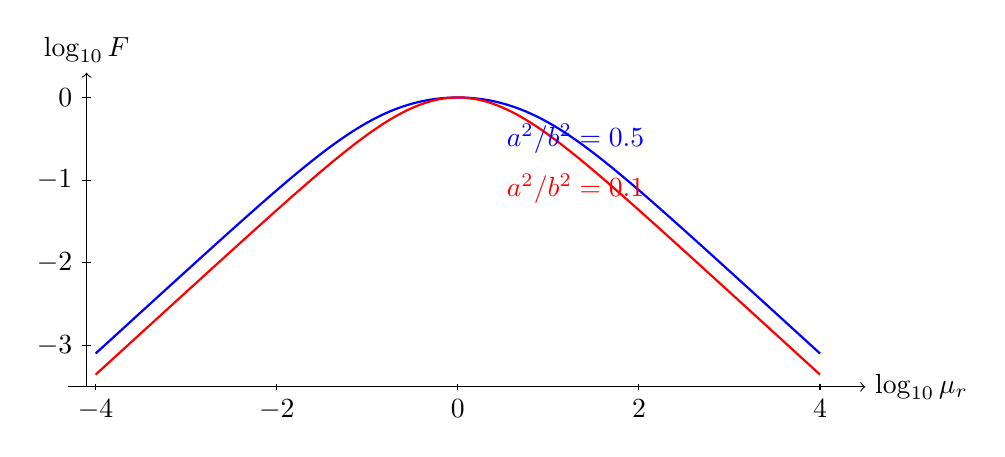
\begin{tikzpicture}[x=1.15cm,y=1.05cm]
\draw[->] (-4.3,-3.5)--(4.5,-3.5) node[right] {$\log_{10}\mu_r$};
\draw[->] (-4.1,-3.5)--(-4.1,.3) node[above] {$\log_{10}F$};
\draw[blue,thick] plot coordinates {(-4.0000000,-3.0971705) (-3.9500000,-3.0472023) (-3.9000000,-2.9972379) (-3.8500000,-2.9472779) (-3.8000000,-2.8973228) (-3.7500000,-2.8473732) (-3.7000000,-2.7974296) (-3.6500000,-2.7474930) (-3.6000000,-2.6975641) (-3.5500000,-2.6476438) (-3.5000000,-2.5977333) (-3.4500000,-2.5478336) (-3.4000000,-2.4979462) (-3.3500000,-2.4480725) (-3.3000000,-2.3982141) (-3.2500000,-2.3483730) (-3.2000000,-2.2985512) (-3.1500000,-2.2487511) (-3.1000000,-2.1989752) (-3.0500000,-2.1492266) (-3.0000000,-2.0995084) (-2.9500000,-2.0498245) (-2.9000000,-2.0001788) (-2.8500000,-1.9505761) (-2.8000000,-1.9010214) (-2.7500000,-1.8515206) (-2.7000000,-1.8020800) (-2.6500000,-1.7527069) (-2.6000000,-1.7034093) (-2.5500000,-1.6541961) (-2.5000000,-1.6050772) (-2.4500000,-1.5560639) (-2.4000000,-1.5071685) (-2.3500000,-1.4584047) (-2.3000000,-1.4097879) (-2.2500000,-1.3613348) (-2.2000000,-1.3130644) (-2.1500000,-1.2649973) (-2.1000000,-1.2171564) (-2.0500000,-1.1695670) (-2.0000000,-1.1222568) (-1.9500000,-1.0752563) (-1.9000000,-1.0285988) (-1.8500000,-0.9823204) (-1.8000000,-0.9364609) (-1.7500000,-0.8910627) (-1.7000000,-0.8461722) (-1.6500000,-0.8018387) (-1.6000000,-0.7581152) (-1.5500000,-0.7150578) (-1.5000000,-0.6727257) (-1.4500000,-0.6311813) (-1.4000000,-0.5904890) (-1.3500000,-0.5507156) (-1.3000000,-0.5119292) (-1.2500000,-0.4741986) (-1.2000000,-0.4375926) (-1.1500000,-0.4021790) (-1.1000000,-0.3680238) (-1.0500000,-0.3351898) (-1.0000000,-0.3037359) (-0.9500000,-0.2737161) (-0.9000000,-0.2451786) (-0.8500000,-0.2181648) (-0.8000000,-0.1927090) (-0.7500000,-0.1688377) (-0.7000000,-0.1465698) (-0.6500000,-0.1259165) (-0.6000000,-0.1068816) (-0.5500000,-0.0894623) (-0.5000000,-0.0736499) (-0.4500000,-0.0594307) (-0.4000000,-0.0467874) (-0.3500000,-0.0357001) (-0.3000000,-0.0261475) (-0.2500000,-0.0181084) (-0.2000000,-0.0115625) (-0.1500000,-0.0064919) (-0.1000000,-0.0028814) (-0.0500000,-0.0007198) (0.0000000,0.0000000) (0.0500000,-0.0007198) (0.1000000,-0.0028814) (0.1500000,-0.0064919) (0.2000000,-0.0115625) (0.2500000,-0.0181084) (0.3000000,-0.0261475) (0.3500000,-0.0357001) (0.4000000,-0.0467874) (0.4500000,-0.0594307) (0.5000000,-0.0736499) (0.5500000,-0.0894623) (0.6000000,-0.1068816) (0.6500000,-0.1259165) (0.7000000,-0.1465698) (0.7500000,-0.1688377) (0.8000000,-0.1927090) (0.8500000,-0.2181648) (0.9000000,-0.2451786) (0.9500000,-0.2737161) (1.0000000,-0.3037359) (1.0500000,-0.3351898) (1.1000000,-0.3680238) (1.1500000,-0.4021790) (1.2000000,-0.4375926) (1.2500000,-0.4741986) (1.3000000,-0.5119292) (1.3500000,-0.5507156) (1.4000000,-0.5904890) (1.4500000,-0.6311813) (1.5000000,-0.6727257) (1.5500000,-0.7150578) (1.6000000,-0.7581152) (1.6500000,-0.8018387) (1.7000000,-0.8461722) (1.7500000,-0.8910627) (1.8000000,-0.9364609) (1.8500000,-0.9823204) (1.9000000,-1.0285988) (1.9500000,-1.0752563) (2.0000000,-1.1222568) (2.0500000,-1.1695670) (2.1000000,-1.2171564) (2.1500000,-1.2649973) (2.2000000,-1.3130644) (2.2500000,-1.3613348) (2.3000000,-1.4097879) (2.3500000,-1.4584047) (2.4000000,-1.5071685) (2.4500000,-1.5560639) (2.5000000,-1.6050772) (2.5500000,-1.6541961) (2.6000000,-1.7034093) (2.6500000,-1.7527069) (2.7000000,-1.8020800) (2.7500000,-1.8515206) (2.8000000,-1.9010214) (2.8500000,-1.9505761) (2.9000000,-2.0001788) (2.9500000,-2.0498245) (3.0000000,-2.0995084) (3.0500000,-2.1492266) (3.1000000,-2.1989752) (3.1500000,-2.2487511) (3.2000000,-2.2985512) (3.2500000,-2.3483730) (3.3000000,-2.3982141) (3.3500000,-2.4480725) (3.4000000,-2.4979462) (3.4500000,-2.5478336) (3.5000000,-2.5977333) (3.5500000,-2.6476438) (3.6000000,-2.6975641) (3.6500000,-2.7474930) (3.7000000,-2.7974296) (3.7500000,-2.8473732) (3.8000000,-2.8973228) (3.8500000,-2.9472779) (3.9000000,-2.9972379) (3.9500000,-3.0472023) (4.0000000,-3.0971705)};
\draw[red,thick] plot coordinates {(-4.0000000,-3.3522887) (-3.9500000,-3.3023016) (-3.9000000,-3.2523162) (-3.8500000,-3.2023325) (-3.8000000,-3.1523508) (-3.7500000,-3.1023713) (-3.7000000,-3.0523943) (-3.6500000,-3.0024201) (-3.6000000,-2.9524491) (-3.5500000,-2.9024817) (-3.5000000,-2.8525181) (-3.4500000,-2.8025591) (-3.4000000,-2.7526050) (-3.3500000,-2.7026565) (-3.3000000,-2.6527144) (-3.2500000,-2.6027792) (-3.2000000,-2.5528520) (-3.1500000,-2.5029336) (-3.1000000,-2.4530252) (-3.0500000,-2.4031280) (-3.0000000,-2.3532433) (-2.9500000,-2.3033726) (-2.9000000,-2.2535176) (-2.8500000,-2.2036804) (-2.8000000,-2.1538629) (-2.7500000,-2.1040676) (-2.7000000,-2.0542973) (-2.6500000,-2.0045548) (-2.6000000,-1.9548437) (-2.5500000,-1.9051677) (-2.5000000,-1.8555310) (-2.4500000,-1.8059384) (-2.4000000,-1.7563952) (-2.3500000,-1.7069074) (-2.3000000,-1.6574816) (-2.2500000,-1.6081253) (-2.2000000,-1.5588467) (-2.1500000,-1.5096552) (-2.1000000,-1.4605612) (-2.0500000,-1.4115763) (-2.0000000,-1.3627133) (-1.9500000,-1.3139868) (-1.9000000,-1.2654126) (-1.8500000,-1.2170088) (-1.8000000,-1.1687951) (-1.7500000,-1.1207937) (-1.7000000,-1.0730289) (-1.6500000,-1.0255278) (-1.6000000,-0.9783204) (-1.5500000,-0.9314397) (-1.5000000,-0.8849222) (-1.4500000,-0.8388079) (-1.4000000,-0.7931407) (-1.3500000,-0.7479687) (-1.3000000,-0.7033444) (-1.2500000,-0.6593248) (-1.2000000,-0.6159717) (-1.1500000,-0.5733519) (-1.1000000,-0.5315370) (-1.0500000,-0.4906038) (-1.0000000,-0.4506340) (-0.9500000,-0.4117140) (-0.9000000,-0.3739348) (-0.8500000,-0.3373914) (-0.8000000,-0.3021824) (-0.7500000,-0.2684093) (-0.7000000,-0.2361755) (-0.6500000,-0.2055858) (-0.6000000,-0.1767447) (-0.5500000,-0.1497559) (-0.5000000,-0.1247206) (-0.4500000,-0.1017365) (-0.4000000,-0.0808964) (-0.3500000,-0.0622871) (-0.3000000,-0.0459881) (-0.2500000,-0.0320704) (-0.2000000,-0.0205959) (-0.1500000,-0.0116164) (-0.1000000,-0.0051728) (-0.0500000,-0.0012947) (0.0000000,0.0000000) (0.0500000,-0.0012947) (0.1000000,-0.0051728) (0.1500000,-0.0116164) (0.2000000,-0.0205959) (0.2500000,-0.0320704) (0.3000000,-0.0459881) (0.3500000,-0.0622871) (0.4000000,-0.0808964) (0.4500000,-0.1017365) (0.5000000,-0.1247206) (0.5500000,-0.1497559) (0.6000000,-0.1767447) (0.6500000,-0.2055858) (0.7000000,-0.2361755) (0.7500000,-0.2684093) (0.8000000,-0.3021824) (0.8500000,-0.3373914) (0.9000000,-0.3739348) (0.9500000,-0.4117140) (1.0000000,-0.4506340) (1.0500000,-0.4906038) (1.1000000,-0.5315370) (1.1500000,-0.5733519) (1.2000000,-0.6159717) (1.2500000,-0.6593248) (1.3000000,-0.7033444) (1.3500000,-0.7479687) (1.4000000,-0.7931407) (1.4500000,-0.8388079) (1.5000000,-0.8849222) (1.5500000,-0.9314397) (1.6000000,-0.9783204) (1.6500000,-1.0255278) (1.7000000,-1.0730289) (1.7500000,-1.1207937) (1.8000000,-1.1687951) (1.8500000,-1.2170088) (1.9000000,-1.2654126) (1.9500000,-1.3139868) (2.0000000,-1.3627133) (2.0500000,-1.4115763) (2.1000000,-1.4605612) (2.1500000,-1.5096552) (2.2000000,-1.5588467) (2.2500000,-1.6081253) (2.3000000,-1.6574816) (2.3500000,-1.7069074) (2.4000000,-1.7563952) (2.4500000,-1.8059384) (2.5000000,-1.8555310) (2.5500000,-1.9051677) (2.6000000,-1.9548437) (2.6500000,-2.0045548) (2.7000000,-2.0542973) (2.7500000,-2.1040676) (2.8000000,-2.1538629) (2.8500000,-2.2036804) (2.9000000,-2.2535176) (2.9500000,-2.3033726) (3.0000000,-2.3532433) (3.0500000,-2.4031280) (3.1000000,-2.4530252) (3.1500000,-2.5029336) (3.2000000,-2.5528520) (3.2500000,-2.6027792) (3.3000000,-2.6527144) (3.3500000,-2.7026565) (3.4000000,-2.7526050) (3.4500000,-2.8025591) (3.5000000,-2.8525181) (3.5500000,-2.9024817) (3.6000000,-2.9524491) (3.6500000,-3.0024201) (3.7000000,-3.0523943) (3.7500000,-3.1023713) (3.8000000,-3.1523508) (3.8500000,-3.2023325) (3.9000000,-3.2523162) (3.9500000,-3.3023016) (4.0000000,-3.3522887)};
\foreach \x in {-4,-2,0,2,4} \draw (\x,-3.46)--(\x,-3.54) node[below] {$\x$};
\foreach \y in {-3,-2,-1,0} \draw (-4.05,\y)--(-4.15,\y) node[left] {$\y$};
\node[blue] at (1.3,-.5) {$a^2/b^2=0.5$};
\node[red] at (1.3,-1.1) {$a^2/b^2=0.1$};
\end{tikzpicture}

\end{center}
Thus a permeable shell and an ideal diamagnetic shell can both shield
the cavity, by different limiting boundary conditions.


\Needspace{5\baselineskip}
\par\bigskip
\noindent\textbf{5.15}\quad Consider two long, straight wires, parallel to the $z$ axis, spaced a distance $d$ apart and carrying currents $I$ in opposite directions. Describe the magnetic field $\mathbf{H}$ in terms of a magnetic scalar potential $\Phi_{M}$, with $\mathbf{H}=-\nabla\Phi_{M}$.
\begin{enumerate}
\item[(a)] If the wires are parallel to the $z$ axis with positions, $x=\pm d/2$, $y=0$, show that in the limit of small spacing, the potential is approximately that of a two-dimensional dipole,
\[
\Phi_{M}\simeq-\frac{Id\,\sin\phi}{2\pi\rho}+O(d^{2}/\rho^{2})
\]
where $\rho$ and $\phi$ are the usual polar coordinates.
\item[(b)] The closely spaced wires are now centered in a hollow right circular cylinder of steel, of inner (outer) radius $a$ ($b$) and magnetic permeability $\mu=\mu_{r}\mu_{0}$. Determine the magnetic scalar potential in the three regions, $0<\rho<a$, $a<\rho<b$, and $\rho>b$. Show that the field outside the steel cylinder is a two-dimensional dipole field, as in part a, but with a strength reduced by the factor
\[
F=\frac{4\mu_{r}b^{2}}{(\mu_{r}+1)^{2}b^{2}-(\mu_{r}-1)^{2}a^{2}}
\]
Relate your result to Problem 5.14.
\item[(c)] Assuming that $\mu_{r}\gg1$, and $b=a+t$, where the thickness $t\ll b$, write down an approximate expression for $F$ and determine its numerical value for $\mu_{r}=200$ (typical of steel at 20 G), $b=1.25$ cm, $t=3$ mm. The shielding effect is relevant for reduction of stray fields in residential and commercial 60 Hz, 110 or 220 V wiring. The figure illustrates the shielding effect for $a/b=0.9$, $\mu_{r}=100$.
\end{enumerate}

\begin{center}
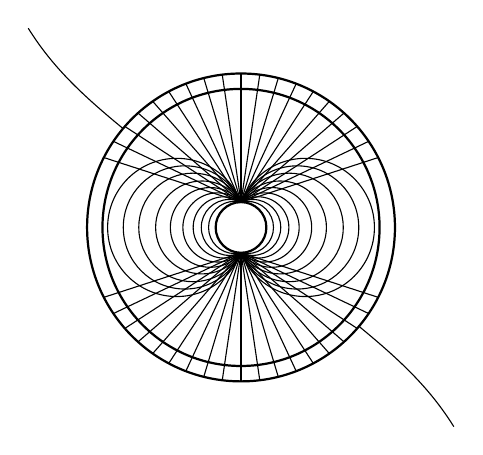
\begin{tikzpicture}[scale=1.15]
  % residual (weak) field lines leaking outside the shell
  \draw (-1.30,1.09) .. controls (-1.8,1.5) and (-2.1,1.8) .. (-2.35,2.2);
  \draw (1.30,-1.09) .. controls (1.8,-1.5) and (2.1,-1.8) .. (2.35,-2.2);
  % field lines looping around the wire pair inside the cavity
  % (circles through (0,+-0.28), i.e. the two wires hidden behind the
  %  central white circle)
  \foreach \c in {0.07,0.13,0.19,0.26,0.34,0.43,0.53,0.62,0.71}{
    \draw (\c,0) circle ({sqrt(\c*\c+0.0784)});
    \draw (-\c,0) circle ({sqrt(\c*\c+0.0784)});
  }
  % flux crossing the permeable shell at top and bottom (drawn inside the
  %  shell as nearly radial spokes)
  \foreach \t in {-63,-56,-49,-42,-35,-28,-21,-14,-7,0,7,14,21,28,35,42,49,56,63}{
    \draw (0,0.28) -- ({1.7*sin(\t)},{1.7*cos(\t)});
    \draw (0,-0.28) -- ({-1.7*sin(\t)},{-1.7*cos(\t)});
  }
  % steel shell
  \draw[thick] (0,0) circle (1.53);
  \draw[thick] (0,0) circle (1.7);
  % blank core covering the two wires
  \fill[white] (0,0) circle (0.28);
  \draw[thick] (0,0) circle (0.28);
\end{tikzpicture}
\par\vspace{0.5em}\textbf{Problem 5.15}
\end{center}
\solution
\textbf{(a)} Put $+I\widehat{\mathbf z}$ at $x=d/2$ and
$-I\widehat{\mathbf z}$ at $x=-d/2$. A straight wire has
$\mathbf H=(I/2\pi)\nabla\phi$, so a local scalar potential for the pair is
\[
\Phi_H=\frac I{2\pi}\{\arg(x+iy+d/2)-\arg(x+iy-d/2)\}.
\]
For $\rho\gg d$, expand the logarithms whose imaginary parts give the
arguments:
\[
\ln(w+d/2)-\ln(w-d/2)=\frac d w+\frac{d^3}{12w^3}+\cdots,
\qquad w=\rho e^{i\phi}.
\]
Consequently
\[
\boxed{\Phi_H=-\frac{Id}{2\pi\rho}\sin\phi
+O\!\left(I\frac{d^3}{\rho^3}\right).}
\]
The next term is actually odd in $d$ and of third order; the
second-order remainder quoted in the question is a looser estimate.

\textbf{(b)} Work to this dipole order, so $d\ll a$.
Set $p=Id/(2\pi)$, $\kappa=\mu_r$, $\eta=a^2/b^2$, and
$\Delta=(\kappa+1)^2-(\kappa-1)^2\eta$. Write
\[
\Phi_H=-p\sin\phi
\begin{cases}\rho^{-1}+A\rho,&0<\rho<a,\\
B\rho^{-1}+C\rho,&a<\rho<b,\\D\rho^{-1},&\rho>b.\end{cases}
\]
Continuity of potential and $\mu\partial_\rho\Phi_H$ gives
\[
1+Aa^2=B+Ca^2,\quad Aa^2-1=\kappa(Ca^2-B),\quad
B+Cb^2=D,\quad\kappa(Cb^2-B)=-D.
\]
The last pair gives $C=(\kappa-1)B/[(\kappa+1)b^2]$ and
$D=2\kappa B/(\kappa+1)$. The first pair then implies
$(\kappa+1)B-(\kappa-1)Ca^2=2$. Hence
\[
\boxed{A=-\frac{(\kappa^2-1)(1-\eta)}{\Delta a^2},\quad
B=\frac{2(\kappa+1)}{\Delta},\quad
C=\frac{2(\kappa-1)}{\Delta b^2},\quad
D=\frac{4\kappa}{\Delta}=F.}
\]
The exterior is the original two-dimensional dipole multiplied by $F$.
This is exactly the core-field transmission factor of 5.14, consistent
with reciprocity between a source inside and an applied field outside.
The singular central dipole represents the two wires only at distances
large compared with $d$.

\textbf{(c)} It is useful to rearrange the exact factor before expanding:
\[
F^{-1}=1+\frac{(\kappa-1)^2}{4\kappa}(1-a^2/b^2).
\]
For $t=b-a\ll b$,
$1-a^2/b^2=2t/b-t^2/b^2$, so for $\kappa\gg1$
\[
\boxed{F\simeq\frac1{1+\kappa t/(2b)}.}
\]
If also $\kappa t/(2b)\gg1$, this further reduces to $2b/(\kappa t)$.
With the specified numbers these estimates are $0.0400$ and $0.04167$,
respectively. The exact factor is $0.04564$, because $t/b=0.24$
is only moderately small. The exact suppression is about a factor
of $21.9$; the leading thin-shell estimate gives a factor of $25$.


\Needspace{5\baselineskip}
\par\bigskip
\noindent\textbf{5.16}\quad A circular loop of wire of radius $a$ and negligible thickness carries a current $I$. The loop is centered in a spherical cavity of radius $b>a$ in a large block of soft iron. Assume that the relative permeability of the iron is effectively infinite and that of the medium in the cavity, unity.
\begin{enumerate}
\item[(a)] In the approximation of $b\gg a$, show that the magnetic field at the center of the loop is augmented by a factor $(1+a^{3}/2b^{3})$ by the presence of the iron.
\item[(b)] What is the radius of the ``image'' current loop (carrying the same current) that simulates \erratum{the leading, nearly uniform reaction field of the iron for $r<b$, in the same $b\gg a$ approximation}? \erratum{Check whether a single such loop can reproduce the complete reaction field exactly.}
\end{enumerate}
\solution
\textbf{(a)} For $b\gg a$, the loop's field at the cavity wall is
dominated by its dipole moment $m=I\pi a^2$. The direct scalar potential
for $\mathbf H$ there is $m\cos\theta/(4\pi r^2)$.
Infinite permeability outside makes tangential $\mathbf H$ vanish
at $r=b$, so the wall must be an equipotential. The regular $l=1$
reaction potential that cancels its angular variation is
\[
\Phi_{H,\rm react}=-\frac{m}{4\pi b^3}r\cos\theta.
\]
Taking $-\mu_0\nabla$ gives the uniform reaction induction
$\mathbf B_{\rm react}=\mu_0m\widehat{\mathbf z}/(4\pi b^3)$.
Adding the exact free-loop center field $\mu_0I/(2a)$ gives
\[
\boxed{B_{\rm center}\simeq\frac{\mu_0I}{2a}
\left(1+\frac{a^3}{2b^3}\right).}
\]
Higher regular multipoles do not contribute at the exact center, so
this center value is in fact unchanged by retaining the other loop
multipoles; the dipole approximation is needed for the statement that
the reaction field is uniform throughout the cavity.

\textbf{(b)} A coaxial image loop carrying the same current $I$ has
center field $\mu_0I/(2R_{\rm im})$. Matching the leading uniform
reaction field gives
\[
\frac{\mu_0I}{2R_{\rm im}}=\frac{\mu_0Ia^2}{4b^3},\qquad
\boxed{R_{\rm im}=\frac{2b^3}{a^2}.}
\]
Since $R_{\rm im}\gg b$ when $b\gg a$, this image produces an almost
uniform field over the cavity.

It is not an exact image for all $r<b$ at arbitrary $a/b$.
Here is a direct check of that necessary qualification.
For an odd $l$, the real-loop exterior $A_\phi$ is proportional to
$\mu_l r^{-l-1}P_l^1$, while the regular reaction term is proportional
to $m_l^{\,R}r^lP_l^1$. The condition $B_\theta(b)=0$ requires
\[
\frac{m_l^{\,R}}{\mu_l}=\frac{l}{l+1}b^{-2l-1}.
\]
A single same-current image loop of radius $R$ instead has, from 5.8,
$m_l^{\,R}/\mu_l=R^{-l}a^{-l-1}$.
The $l=1$ condition demands $R=2b^3/a^2$, whereas $l=3$ demands
$R^3=4b^7/(3a^4)$. These cannot both hold for $b>a$:
their combination would require $b^2/a^2=1/6$.
Thus the equal-current image-loop statement must be understood in
the leading uniform-field approximation, as made explicit above.


\Needspace{5\baselineskip}
\par\bigskip
\noindent\textbf{5.17}\quad A current distribution $\mathbf{J}(\mathbf{x})$ exists in a medium of unit relative permeability adjacent to a semi-infinite slab of material having relative permeability $\mu_{r}$ and filling the half-space, $z<0$.
\begin{enumerate}
\item[(a)] Show that for $z>0$ the magnetic induction can be calculated by replacing the medium of permeability $\mu_{r}$ by an image current distribution, $\mathbf{J}^{*}$, with components,
\[
\left(\frac{\mu_{r}-1}{\mu_{r}+1}\right)\!J_{x}(x,y,-z),\qquad
\left(\frac{\mu_{r}-1}{\mu_{r}+1}\right)\!J_{y}(x,y,-z),\qquad
-\left(\frac{\mu_{r}-1}{\mu_{r}+1}\right)\!J_{z}(x,y,-z)
\]
\item[(b)] Show that for $z<0$ the magnetic induction appears to be due to a current distribution $[2\mu_{r}/(\mu_{r}+1)]\mathbf{J}$ in a medium of unit relative permeability.
\end{enumerate}
\solution
Let $\mathcal R=\operatorname{diag}(1,1,-1)$ reflect a vector across
the interface, and let $\mathbf B^{(0)}$ be the field of the original
current computed in vacuum everywhere.
Under spatial reflection a current is a polar vector but its magnetic
field is an axial vector. Direct substitution in Biot--Savart gives
\[
\mathbf J_{\rm ref}(\mathbf x)=\mathcal R\mathbf J(\mathcal R\mathbf x),
\qquad
\mathbf B_{\rm ref}(\mathbf x)=-\mathcal R\mathbf B^{(0)}(\mathcal R\mathbf x).
\]
In particular, at $z=0$ its tangential field reverses sign and its
normal field keeps its sign.

Take the upper field to be $\mathbf B^{(0)}+\chi\mathbf B_{\rm ref}$
and the lower field to be $T\mathbf B^{(0)}$. At the interface,
continuity of $B_n$ and $H_t$ requires
\[
1+\chi=T,\qquad 1-\chi=T/\mu_r.
\]
Solving gives $\chi=(\mu_r-1)/(\mu_r+1)$ and
$T=2\mu_r/(\mu_r+1)$.
Therefore
\[
\boxed{\mathbf J^*(x,y,z)=\frac{\mu_r-1}{\mu_r+1}
(J_x(x,y,-z),J_y(x,y,-z),-J_z(x,y,-z))}
\]
is the image distribution for part (a), and
\[
\boxed{\mathbf B_{z<0}=\frac{2\mu_r}{\mu_r+1}\mathbf B^{(0)}}
\]
proves part (b). Both candidate fields are divergence-free and satisfy
the correct source-free curl equations in their respective regions,
the interface conditions, and decay at infinity; uniqueness completes
the construction. At $\mu_r=1$ the image disappears and $T=1$.


\Needspace{5\baselineskip}
\par\bigskip
\noindent\textbf{5.18}\quad A circular loop of wire having a radius $a$ and carrying a current $I$ is located in vacuum with its center a distance $d$ away from a semi-infinite slab of permeability $\mu$. Find the force acting on the loop when
\begin{enumerate}
\item[(a)] the plane of the loop is parallel to the face of the slab,
\item[(b)] the plane of the loop is perpendicular to the face of the slab.
\item[(c)] Determine the limiting form of your answer to parts a and b when $d\gg a$. Can you obtain these limiting values in some simple and direct way?
\end{enumerate}
\solution
Choose the slab as $z<0$, the center as $(0,0,d)$, and write
$\chi=(\mu-\mu_0)/(\mu+\mu_0)$.
For each orientation the image is centered at $z=-d$. Let $s=2d$.
In computing the Lorentz force, the real loop moves in the field of
an image at its instantaneous position; one does not differentiate
that position a second time. Equivalently, the mechanical image
interaction energy carries a factor $1/2$.

\textbf{(a)} A loop parallel to the interface has a same-sense image
with current $\chi I$. For coaxial equal loops (derived in 5.28),
\[
M_\parallel(s)=\mu_0a\left[\left(\frac2k-k\right)K(k)-\frac2kE(k)\right],
\qquad k=\frac{2a}{\sqrt{4a^2+s^2}}.
\]
The force is purely normal, $F_z=\chi I^2M_\parallel'(s)$.
Using
$K'=E/[k(1-k^2)]-K/k$, $E'=(E-K)/k$, and
$dk/ds=-ks/(4a^2+s^2)$ gives
\[
\boxed{F_z=-\frac{\mu_0\chi I^2s k}{4a}
\left[\frac{2-k^2}{1-k^2}E(k)-2K(k)\right]_{s=2d}.}
\]
This holds for any $d>0$ in the ideal filament model.

\textbf{(b)} A perpendicular loop must have $d>a$ to lie wholly
in vacuum. Its image is coplanar with it and carries opposite-sense
current $-\chi I$. Define the positive coefficients
\[
D_n=\frac{[(2n+2)!]^2}
{2^{2n+2}n!(n+2)![(n+1)!]^2},\qquad
E_n=D_n\frac{(2n+2)!}{2^{2n+2}[(n+1)!]^2}.
\]
The convergent coplanar mutual inductance derived in 5.34 is
$M_\perp(s)=-\mu_0\pi a\sum_{n\ge0}E_n(a/s)^{2n+3}$.
Thus the exact force throughout the allowed domain $s=2d>2a$ is
\[
\boxed{F_z=-\chi I^2M_\perp'(2d)
=-\mu_0\pi\chi I^2\sum_{n=0}^\infty
(2n+3)E_n\left(\frac{a}{2d}\right)^{2n+4}.}
\]
All coefficients are positive, so the direction is toward a more
permeable slab and away from a less permeable one.
The two in-plane transverse force components cancel by symmetry.

\textbf{(c)} Expanding the preceding results, or using
$D_0=1/2$ and $E_0=1/4$, gives
\[
\boxed{F_{z,\parallel}\sim-\frac{3\mu_0\pi\chi I^2a^4}{32d^4},
\qquad F_{z,\perp}\sim-\frac{3\mu_0\pi\chi I^2a^4}{64d^4}.}
\]
For a direct dipole check, use $m=I\pi a^2$ and separation $s$.
Parallel-to-interface loops have axial moments $m,\chi m$:
$U_{\rm pair}=-2\mu_0\chi m^2/(4\pi s^3)$.
Perpendicular loops have transverse moments $m,-\chi m$:
$U_{\rm pair}=-\mu_0\chi m^2/(4\pi s^3)$.
The force on the real dipole is $-\partial_sU_{\rm pair}$.
Putting $s=2d$ gives the two boxed limits, with the first twice the second.


\Needspace{5\baselineskip}
\par\bigskip
\noindent\textbf{5.19}\quad A magnetically ``hard'' material is in the shape of a right circular cylinder of length $L$ and radius $a$. The cylinder has a permanent magnetization $M_{0}$, uniform throughout its volume and parallel to its axis.
\begin{enumerate}
\item[(a)] Determine the magnetic field $\mathbf{H}$ and magnetic induction $\mathbf{B}$ at all points on the axis of the cylinder, both inside and outside.
\item[(b)] Plot the ratios $\mathbf{B}/\mu_{0}M_{0}$ and $\mathbf{H}/M_{0}$ on the axis as functions of $z$ for $L/a=5$.
\end{enumerate}
\solution
\textbf{(a)} Let the cylinder occupy $-L/2<z<L/2$, with
$\mathbf M=M_0\widehat{\mathbf z}$.
Its volume bound current vanishes, and its curved surface carries
$\mathbf K_M=\mathbf M\times\widehat{\boldsymbol\rho}
=M_0\widehat{\boldsymbol\phi}$.
Thus its induction is that of the ideal finite solenoid in 5.3, with
$NI$ replaced by $M_0$. Define
\[
f(z)=\frac12\left[
\frac{z+L/2}{\sqrt{a^2+(z+L/2)^2}}
-\frac{z-L/2}{\sqrt{a^2+(z-L/2)^2}}\right].
\]
The answers on the entire axis, with one-sided limits at the end faces, are
\[
\boxed{\mathbf B(z)=\mu_0M_0f(z)\widehat{\mathbf z},\qquad
\mathbf H(z)=M_0[f(z)-\mathbf1_{\{|z|<L/2\}}]\widehat{\mathbf z}.}
\]
The subtraction follows from $\mathbf B=\mu_0(\mathbf H+\mathbf M)$.
The axial induction is continuous across either face, while $H_z$
jumps by the magnetic pole-sheet strength $M_0$.
\textbf{(b)} For $L/a=5$, at the center $f(0)=2.5/\sqrt{7.25}=0.928477$,
so $H_z(0)/M_0=-0.0715233$. At either end $f=\tfrac12(5/\sqrt{26})
=0.490290$.
\begin{center}
\begin{tikzpicture}[x=.8cm,y=2.5cm]
\draw[->] (-6.2,0)--(6.5,0) node[right] {$z/a$};
\draw[->] (-6,-.65)--(-6,1.2) node[above] {axial field};
\draw[blue,thick] plot coordinates {(-6.0000000,0.0158133) (-5.9500000,0.0163019) (-5.9000000,0.0168114) (-5.8500000,0.0173430) (-5.8000000,0.0178979) (-5.7500000,0.0184774) (-5.7000000,0.0190829) (-5.6500000,0.0197161) (-5.6000000,0.0203783) (-5.5500000,0.0210714) (-5.5000000,0.0217973) (-5.4500000,0.0225578) (-5.4000000,0.0233552) (-5.3500000,0.0241918) (-5.3000000,0.0250699) (-5.2500000,0.0259922) (-5.2000000,0.0269617) (-5.1500000,0.0279813) (-5.1000000,0.0290543) (-5.0500000,0.0301845) (-5.0000000,0.0313756) (-4.9500000,0.0326318) (-4.9000000,0.0339578) (-4.8500000,0.0353583) (-4.8000000,0.0368387) (-4.7500000,0.0384048) (-4.7000000,0.0400629) (-4.6500000,0.0418198) (-4.6000000,0.0436830) (-4.5500000,0.0456605) (-4.5000000,0.0477612) (-4.4500000,0.0499946) (-4.4000000,0.0523712) (-4.3500000,0.0549025) (-4.3000000,0.0576009) (-4.2500000,0.0604802) (-4.2000000,0.0635551) (-4.1500000,0.0668420) (-4.1000000,0.0703586) (-4.0500000,0.0741244) (-4.0000000,0.0781607) (-3.9500000,0.0824906) (-3.9000000,0.0871393) (-3.8500000,0.0921344) (-3.8000000,0.0975058) (-3.7500000,0.1032859) (-3.7000000,0.1095099) (-3.6500000,0.1162157) (-3.6000000,0.1234438) (-3.5500000,0.1312377) (-3.5000000,0.1396436) (-3.4500000,0.1487098) (-3.4000000,0.1584869) (-3.3500000,0.1690269) (-3.3000000,0.1803825) (-3.2500000,0.1926059) (-3.2000000,0.2057473) (-3.1500000,0.2198537) (-3.1000000,0.2349659) (-3.0500000,0.2511168) (-3.0000000,0.2683282) (-2.9500000,0.2866076) (-2.9000000,0.3059457) (-2.8500000,0.3263128) (-2.8000000,0.3476569) (-2.7500000,0.3699015) (-2.7000000,0.3929452) (-2.6500000,0.4166623) (-2.6000000,0.4409050) (-2.5500000,0.4655074) (-2.5000000,0.4902903) (-2.4500000,0.5150678) (-2.4000000,0.5396539) (-2.3500000,0.5638694) (-2.3000000,0.5875483) (-2.2500000,0.6105427) (-2.2000000,0.6327269) (-2.1500000,0.6539994) (-2.1000000,0.6742835) (-2.0500000,0.6935271) (-2.0000000,0.7117003) (-1.9500000,0.7287936) (-1.9000000,0.7448143) (-1.8500000,0.7597840) (-1.8000000,0.7737352) (-1.7500000,0.7867086) (-1.7000000,0.7987506) (-1.6500000,0.8099113) (-1.6000000,0.8202425) (-1.5500000,0.8297965) (-1.5000000,0.8386246) (-1.4500000,0.8467772) (-1.4000000,0.8543020) (-1.3500000,0.8612446) (-1.3000000,0.8676479) (-1.2500000,0.8735519) (-1.2000000,0.8789937) (-1.1500000,0.8840077) (-1.1000000,0.8886257) (-1.0500000,0.8928766) (-1.0000000,0.8967871) (-0.9500000,0.9003815) (-0.9000000,0.9036819) (-0.8500000,0.9067084) (-0.8000000,0.9094793) (-0.7500000,0.9120111) (-0.7000000,0.9143186) (-0.6500000,0.9164154) (-0.6000000,0.9183134) (-0.5500000,0.9200235) (-0.5000000,0.9215552) (-0.4500000,0.9229172) (-0.4000000,0.9241168) (-0.3500000,0.9251605) (-0.3000000,0.9260542) (-0.2500000,0.9268025) (-0.2000000,0.9274094) (-0.1500000,0.9278782) (-0.1000000,0.9282113) (-0.0500000,0.9284104) (0.0000000,0.9284767) (0.0500000,0.9284104) (0.1000000,0.9282113) (0.1500000,0.9278782) (0.2000000,0.9274094) (0.2500000,0.9268025) (0.3000000,0.9260542) (0.3500000,0.9251605) (0.4000000,0.9241168) (0.4500000,0.9229172) (0.5000000,0.9215552) (0.5500000,0.9200235) (0.6000000,0.9183134) (0.6500000,0.9164154) (0.7000000,0.9143186) (0.7500000,0.9120111) (0.8000000,0.9094793) (0.8500000,0.9067084) (0.9000000,0.9036819) (0.9500000,0.9003815) (1.0000000,0.8967871) (1.0500000,0.8928766) (1.1000000,0.8886257) (1.1500000,0.8840077) (1.2000000,0.8789937) (1.2500000,0.8735519) (1.3000000,0.8676479) (1.3500000,0.8612446) (1.4000000,0.8543020) (1.4500000,0.8467772) (1.5000000,0.8386246) (1.5500000,0.8297965) (1.6000000,0.8202425) (1.6500000,0.8099113) (1.7000000,0.7987506) (1.7500000,0.7867086) (1.8000000,0.7737352) (1.8500000,0.7597840) (1.9000000,0.7448143) (1.9500000,0.7287936) (2.0000000,0.7117003) (2.0500000,0.6935271) (2.1000000,0.6742835) (2.1500000,0.6539994) (2.2000000,0.6327269) (2.2500000,0.6105427) (2.3000000,0.5875483) (2.3500000,0.5638694) (2.4000000,0.5396539) (2.4500000,0.5150678) (2.5000000,0.4902903) (2.5500000,0.4655074) (2.6000000,0.4409050) (2.6500000,0.4166623) (2.7000000,0.3929452) (2.7500000,0.3699015) (2.8000000,0.3476569) (2.8500000,0.3263128) (2.9000000,0.3059457) (2.9500000,0.2866076) (3.0000000,0.2683282) (3.0500000,0.2511168) (3.1000000,0.2349659) (3.1500000,0.2198537) (3.2000000,0.2057473) (3.2500000,0.1926059) (3.3000000,0.1803825) (3.3500000,0.1690269) (3.4000000,0.1584869) (3.4500000,0.1487098) (3.5000000,0.1396436) (3.5500000,0.1312377) (3.6000000,0.1234438) (3.6500000,0.1162157) (3.7000000,0.1095099) (3.7500000,0.1032859) (3.8000000,0.0975058) (3.8500000,0.0921344) (3.9000000,0.0871393) (3.9500000,0.0824906) (4.0000000,0.0781607) (4.0500000,0.0741244) (4.1000000,0.0703586) (4.1500000,0.0668420) (4.2000000,0.0635551) (4.2500000,0.0604802) (4.3000000,0.0576009) (4.3500000,0.0549025) (4.4000000,0.0523712) (4.4500000,0.0499946) (4.5000000,0.0477612) (4.5500000,0.0456605) (4.6000000,0.0436830) (4.6500000,0.0418198) (4.7000000,0.0400629) (4.7500000,0.0384048) (4.8000000,0.0368387) (4.8500000,0.0353583) (4.9000000,0.0339578) (4.9500000,0.0326318) (5.0000000,0.0313756) (5.0500000,0.0301845) (5.1000000,0.0290543) (5.1500000,0.0279813) (5.2000000,0.0269617) (5.2500000,0.0259922) (5.3000000,0.0250699) (5.3500000,0.0241918) (5.4000000,0.0233552) (5.4500000,0.0225578) (5.5000000,0.0217973) (5.5500000,0.0210714) (5.6000000,0.0203783) (5.6500000,0.0197161) (5.7000000,0.0190829) (5.7500000,0.0184774) (5.8000000,0.0178979) (5.8500000,0.0173430) (5.9000000,0.0168114) (5.9500000,0.0163019) (6.0000000,0.0158133)};
\draw[red,thick,dashed] plot coordinates {(-6.0000000,0.0158133) (-5.9562500,0.0162397) (-5.9125000,0.0166820) (-5.8687500,0.0171410) (-5.8250000,0.0176174) (-5.7812500,0.0181122) (-5.7375000,0.0186263) (-5.6937500,0.0191605) (-5.6500000,0.0197161) (-5.6062500,0.0202939) (-5.5625000,0.0208952) (-5.5187500,0.0215211) (-5.4750000,0.0221731) (-5.4312500,0.0228524) (-5.3875000,0.0235606) (-5.3437500,0.0242992) (-5.3000000,0.0250699) (-5.2562500,0.0258744) (-5.2125000,0.0267147) (-5.1687500,0.0275928) (-5.1250000,0.0285109) (-5.0812500,0.0294713) (-5.0375000,0.0304764) (-4.9937500,0.0315290) (-4.9500000,0.0326318) (-4.9062500,0.0337880) (-4.8625000,0.0350009) (-4.8187500,0.0362738) (-4.7750000,0.0376106) (-4.7312500,0.0390154) (-4.6875000,0.0404926) (-4.6437500,0.0420467) (-4.6000000,0.0436830) (-4.5562500,0.0454068) (-4.5125000,0.0472239) (-4.4687500,0.0491408) (-4.4250000,0.0511643) (-4.3812500,0.0533017) (-4.3375000,0.0555609) (-4.2937500,0.0579507) (-4.2500000,0.0604802) (-4.2062500,0.0631595) (-4.1625000,0.0659994) (-4.1187500,0.0690117) (-4.0750000,0.0722091) (-4.0312500,0.0756051) (-3.9875000,0.0792147) (-3.9437500,0.0830537) (-3.9000000,0.0871393) (-3.8562500,0.0914901) (-3.8125000,0.0961259) (-3.7687500,0.1010683) (-3.7250000,0.1063401) (-3.6812500,0.1119660) (-3.6375000,0.1179721) (-3.5937500,0.1243862) (-3.5500000,0.1312377) (-3.5062500,0.1385577) (-3.4625000,0.1463786) (-3.4187500,0.1547339) (-3.3750000,0.1636583) (-3.3312500,0.1731869) (-3.2875000,0.1833550) (-3.2437500,0.1941973) (-3.2000000,0.2057473) (-3.1562500,0.2180361) (-3.1125000,0.2310916) (-3.0687500,0.2449369) (-3.0250000,0.2595891) (-2.9812500,0.2750579) (-2.9375000,0.2913437) (-2.8937500,0.3084361) (-2.8500000,0.3263128) (-2.8062500,0.3449378) (-2.7625000,0.3642610) (-2.7187500,0.3842176) (-2.6750000,0.4047283) (-2.6312500,0.4257003) (-2.5875000,0.4470287) (-2.5437500,0.4685992) (-2.5000000,0.4902903)};
\draw[red,thick,dashed] plot coordinates {(-2.5000000,-0.5097097) (-2.4375000,-0.4787606) (-2.3750000,-0.4481813) (-2.3125000,-0.4183127) (-2.2500000,-0.3894573) (-2.1875000,-0.3618661) (-2.1250000,-0.3357312) (-2.0625000,-0.3111843) (-2.0000000,-0.2882997) (-1.9375000,-0.2671013) (-1.8750000,-0.2475713) (-1.8125000,-0.2296592) (-1.7500000,-0.2132914) (-1.6875000,-0.1983786) (-1.6250000,-0.1848226) (-1.5625000,-0.1725220) (-1.5000000,-0.1613754) (-1.4375000,-0.1512846) (-1.3750000,-0.1421567) (-1.3125000,-0.1339046) (-1.2500000,-0.1264481) (-1.1875000,-0.1197140) (-1.1250000,-0.1136356) (-1.0625000,-0.1081532) (-1.0000000,-0.1032129) (-0.9375000,-0.0987667) (-0.8750000,-0.0947718) (-0.8125000,-0.0911904) (-0.7500000,-0.0879889) (-0.6875000,-0.0851379) (-0.6250000,-0.0826115) (-0.5625000,-0.0803869) (-0.5000000,-0.0784448) (-0.4375000,-0.0767680) (-0.3750000,-0.0753423) (-0.3125000,-0.0741554) (-0.2500000,-0.0731975) (-0.1875000,-0.0724606) (-0.1250000,-0.0719384) (-0.0625000,-0.0716269) (0.0000000,-0.0715233) (0.0625000,-0.0716269) (0.1250000,-0.0719384) (0.1875000,-0.0724606) (0.2500000,-0.0731975) (0.3125000,-0.0741554) (0.3750000,-0.0753423) (0.4375000,-0.0767680) (0.5000000,-0.0784448) (0.5625000,-0.0803869) (0.6250000,-0.0826115) (0.6875000,-0.0851379) (0.7500000,-0.0879889) (0.8125000,-0.0911904) (0.8750000,-0.0947718) (0.9375000,-0.0987667) (1.0000000,-0.1032129) (1.0625000,-0.1081532) (1.1250000,-0.1136356) (1.1875000,-0.1197140) (1.2500000,-0.1264481) (1.3125000,-0.1339046) (1.3750000,-0.1421567) (1.4375000,-0.1512846) (1.5000000,-0.1613754) (1.5625000,-0.1725220) (1.6250000,-0.1848226) (1.6875000,-0.1983786) (1.7500000,-0.2132914) (1.8125000,-0.2296592) (1.8750000,-0.2475713) (1.9375000,-0.2671013) (2.0000000,-0.2882997) (2.0625000,-0.3111843) (2.1250000,-0.3357312) (2.1875000,-0.3618661) (2.2500000,-0.3894573) (2.3125000,-0.4183127) (2.3750000,-0.4481813) (2.4375000,-0.4787606) (2.5000000,-0.5097097)};
\draw[red,thick,dashed] plot coordinates {(2.5000000,0.4902903) (2.5437500,0.4685992) (2.5875000,0.4470287) (2.6312500,0.4257003) (2.6750000,0.4047283) (2.7187500,0.3842176) (2.7625000,0.3642610) (2.8062500,0.3449378) (2.8500000,0.3263128) (2.8937500,0.3084361) (2.9375000,0.2913437) (2.9812500,0.2750579) (3.0250000,0.2595891) (3.0687500,0.2449369) (3.1125000,0.2310916) (3.1562500,0.2180361) (3.2000000,0.2057473) (3.2437500,0.1941973) (3.2875000,0.1833550) (3.3312500,0.1731869) (3.3750000,0.1636583) (3.4187500,0.1547339) (3.4625000,0.1463786) (3.5062500,0.1385577) (3.5500000,0.1312377) (3.5937500,0.1243862) (3.6375000,0.1179721) (3.6812500,0.1119660) (3.7250000,0.1063401) (3.7687500,0.1010683) (3.8125000,0.0961259) (3.8562500,0.0914901) (3.9000000,0.0871393) (3.9437500,0.0830537) (3.9875000,0.0792147) (4.0312500,0.0756051) (4.0750000,0.0722091) (4.1187500,0.0690117) (4.1625000,0.0659994) (4.2062500,0.0631595) (4.2500000,0.0604802) (4.2937500,0.0579507) (4.3375000,0.0555609) (4.3812500,0.0533017) (4.4250000,0.0511643) (4.4687500,0.0491408) (4.5125000,0.0472239) (4.5562500,0.0454068) (4.6000000,0.0436830) (4.6437500,0.0420467) (4.6875000,0.0404926) (4.7312500,0.0390154) (4.7750000,0.0376106) (4.8187500,0.0362738) (4.8625000,0.0350009) (4.9062500,0.0337880) (4.9500000,0.0326318) (4.9937500,0.0315290) (5.0375000,0.0304764) (5.0812500,0.0294713) (5.1250000,0.0285109) (5.1687500,0.0275928) (5.2125000,0.0267147) (5.2562500,0.0258744) (5.3000000,0.0250699) (5.3437500,0.0242992) (5.3875000,0.0235606) (5.4312500,0.0228524) (5.4750000,0.0221731) (5.5187500,0.0215211) (5.5625000,0.0208952) (5.6062500,0.0202939) (5.6500000,0.0197161) (5.6937500,0.0191605) (5.7375000,0.0186263) (5.7812500,0.0181122) (5.8250000,0.0176174) (5.8687500,0.0171410) (5.9125000,0.0166820) (5.9562500,0.0162397) (6.0000000,0.0158133)};
\foreach \z in {-2.5,2.5} \draw[dotted] (\z,-.55)--(\z,1);
\foreach \z in {-5,-2.5,0,2.5,5} \node[below] at (\z,0) {$\z$};
\node[blue] at (0,1.13) {$B_z/(\mu_0M_0)$};
\node[red] at (0,-.45) {$H_z/M_0$};
\end{tikzpicture}

\end{center}
The red interior field opposes the magnetization; outside,
$\mathbf B/\mu_0=\mathbf H$ as required in vacuum.


\Needspace{5\baselineskip}
\par\bigskip
\noindent\textbf{5.20}\quad\begin{enumerate}
\item[(a)] Starting from the force equation (5.12) and the fact that a magnetization $\mathbf{M}$ inside a volume $V$ bounded by a surface $S$ is equivalent to a volume current density $\mathbf{J}_{M}=(\nabla\times\mathbf{M})$ and a surface current density $(\mathbf{M}\times\mathbf{n})$, show that in the absence of macroscopic conduction currents the total magnetic force on the body can be written
\[
\mathbf{F}=-\int_{V}(\nabla\cdot\mathbf{M})\mathbf{B}_{e}\;d^{3}x+\int_{S}(\mathbf{M}\cdot\mathbf{n})\mathbf{B}_{e}\;da
\]
where $\mathbf{B}_{e}$ is the applied magnetic induction (not including that of the body in question). The force is now expressed in terms of the effective charge densities $\rho_{M}$ and $\sigma_{M}$. If the distribution of magnetization is not discontinuous, the surface can be at infinity and the force given by just the volume integral.
\item[(b)] A sphere of radius $R$ with uniform magnetization has its center at the origin of coordinates and its direction of magnetization making spherical angles $\theta_{0}$, $\phi_{0}$. If the external magnetic field is the same as in Problem 5.11, use the expression of part a to evaluate the components of the force acting on the sphere.
\end{enumerate}
\solution
\textbf{(a)} The external sources are outside the body, so
$\nabla\times\mathbf B_e=0$ and $\nabla\cdot\mathbf B_e=0$ in its
neighborhood. Start from both bound-current contributions:
\[
\mathbf F=\int_V(\nabla\times\mathbf M)\times\mathbf B_e\,d^3x
+\oint_S(\mathbf M\times\mathbf n)\times\mathbf B_e\,da.
\]
The volume integrand has components
$B_{e,j}\partial_jM_i-B_{e,j}\partial_iM_j$.
Integrating both derivatives by parts gives the boundary term
$M_i(\mathbf B_e\cdot\mathbf n)-n_i(\mathbf M\cdot\mathbf B_e)$
and the volume term
$M_j\partial_iB_{e,j}-M_i\partial_jB_{e,j}$.
The surface-current term cancels the boundary term exactly.
Zero divergence removes its second volume term, leaving
\[
F_i=\int_VM_j\partial_iB_{e,j}\,d^3x.
\]
Zero curl allows $\partial_iB_{e,j}=\partial_jB_{e,i}$.
A final integration by parts then gives
\[
\boxed{\mathbf F=-\int_V(\nabla\cdot\mathbf M)\mathbf B_e\,d^3x
+\oint_S(\mathbf M\cdot\mathbf n)\mathbf B_e\,da.}
\]
These are effective pole densities $\rho_M=-\nabla\cdot\mathbf M$
and $\sigma_M=\mathbf M\cdot\mathbf n$.
If imposed external current overlaps $V$, zero curl is unavailable:
the additional force term is $\int_V\mathbf M\times(\nabla\times\mathbf B_e)d^3x$.

\textbf{(b)} For uniform $\mathbf M$ the volume pole density is zero.
On the sphere $\sigma_M=M_jn_j$, and the constant part of the external
field integrates to zero because $\int\mathbf n\,da=0$.
For its linear part, $x_k=Rn_k$ and
$\int n_jn_k\,da=(4\pi R^2/3)\delta_{jk}$, so
\[
F_i=R\,\partial_kB_{e,i}\,M_j\int n_jn_k\,da
=\frac{4\pi R^3}{3}M_j\partial_jB_{e,i}.
\]
With the field of 5.11 this gives
\[
\boxed{\mathbf F=\frac{4\pi R^3}{3}\beta B_0M\sin\theta_0
(\sin\phi_0,\cos\phi_0,0).}
\]
It equals the loop result with
$\mathbf m=(4\pi R^3/3)\mathbf M$, as expected for an affine field.


\Needspace{5\baselineskip}
\par\bigskip
\noindent\textbf{5.21}\quad A magnetostatic field is due entirely to a localized distribution of permanent magnetization.
\begin{enumerate}
\item[(a)] Show that
\[
\int\mathbf{B}\cdot\mathbf{H}\;d^{3}x=0
\]
provided the integral is taken over all space.
\item[(b)] From the potential energy (5.72) of a dipole in an external field, show that for a continuous distribution of permanent magnetization the magnetostatic energy can be written
\[
W=\frac{\mu_{0}}{2}\int\mathbf{H}\cdot\mathbf{H}\;d^{3}x=-\frac{\mu_{0}}{2}\int\mathbf{M}\cdot\mathbf{H}\;d^{3}x
\]
apart from an additive constant, which is independent of the orientation or position of the various constituent magnetized bodies.
\end{enumerate}
\solution
\textbf{(a)} With no free currents,
$\mathbf H=-\nabla\Phi_H$ throughout space. Therefore
\[
\int\mathbf B\cdot\mathbf H\,d^3x
=-\int\nabla\cdot(\Phi_H\mathbf B)d^3x
+\int\Phi_H\nabla\cdot\mathbf B\,d^3x=0.
\]
The volume term vanishes by $\nabla\cdot\mathbf B=0$.
For a localized magnetization, $\Phi_H=O(r^{-2})$ and
$B=O(r^{-3})$, so the surface term at infinity is $O(r^{-3})$ and
vanishes. Internal interfaces cancel when all space is included.

\textbf{(b)} The pair interaction energy of permanent dipoles is
$-\mathbf m\cdot\mathbf B_e$. Summing it over the distribution and
dividing by two to count each pair once gives
$-\tfrac12\int\mathbf M\cdot\mathbf B\,d^3x$, apart from local
self-energy terms. Since $\mathbf B=\mu_0(\mathbf H+\mathbf M)$,
\[
-\frac12\int\mathbf M\cdot\mathbf B
=-\frac{\mu_0}{2}\int\mathbf M\cdot\mathbf H
-\frac{\mu_0}{2}\int M^2.
\]
The last term and the local self-energy constants are unchanged by
translations or rotations of permanently magnetized bodies.
They may be absorbed into the additive constant specified in the question.
Part (a) also gives
\[
0=\mu_0\int(\mathbf H+\mathbf M)\cdot\mathbf H\,d^3x,
\quad\text{hence}\quad
\int H^2=-\int\mathbf M\cdot\mathbf H.
\]
Consequently the position- and orientation-dependent energy can be written
\[
\boxed{W=\frac{\mu_0}{2}\int H^2d^3x
=-\frac{\mu_0}{2}\int\mathbf M\cdot\mathbf H\,d^3x+\text{constant}.}
\]
The moment magnitudes are fixed here; changing them would change the
discarded intrinsic energy and would be a different thermodynamic problem.


\Needspace{5\baselineskip}
\par\bigskip
\noindent\textbf{5.22}\quad Show that in general a long, straight bar of uniform cross-sectional area $A$ with uniform lengthwise magnetization $M$, when placed with its flat end against an infinitely permeable flat surface, adheres with a force given approximately by
\[
F\simeq\frac{\mu_{0}}{2}\,AM^{2}
\]
Relate your discussion to the electrostatic considerations in Section 1.11.
\solution
Resolve contact as the limit of a narrow vacuum gap. The end face has
effective magnetic surface charge of magnitude $M$.
Infinite permeability can be represented by an image magnet extending
the real bar through the plane; the facing image pole has opposite sign.
For a bar long compared with its transverse size, the far ends make
negligible contributions in the gap. Each facing pole sheet supplies
$H=M/2$, so the total gap field is $H=M$, $B=\mu_0M$.

The force on the real face is its pole strength $MA$ times the
\emph{image} induction $\mu_0M/2$, giving
\[
\boxed{F\simeq\frac{\mu_0}{2}AM^2.}
\]
The same result follows from the normal vacuum magnetic stress
$B^2/(2\mu_0)$ times $A$. In the electrostatic capacitor the corresponding
pressure is $\epsilon_0E^2/2=\sigma^2/(2\epsilon_0)$.
Using the field of both sheets as the acting external field would
incorrectly double the force; the face does not exert a net force on itself.


\Needspace{5\baselineskip}
\par\bigskip
\noindent\textbf{5.23}\quad A right circular cylinder of length $L$ and radius $a$ has a uniform lengthwise magnetization $M$.
\begin{enumerate}
\item[(a)] Show that, when it is placed with its flat end against an infinitely permeable plane surface, it adheres with a force
\[
F=2\mu_{0}aLM^{2}\left[\frac{K(k)-E(k)}{k}-\frac{K(k_{1})-E(k_{1})}{k_{1}}\right]
\]
where
\[
k=\frac{2a}{\sqrt{4a^{2}+L^{2}}},\qquad k_{1}=\frac{a}{\sqrt{a^{2}+L^{2}}}
\]
\item[(b)] Find the limiting form for the force if $L\gg a$.
\end{enumerate}
\solution
\textbf{(a)} Use magnetic pole disks $\pm M$ at the two end faces and
the image cylinder across the infinitely permeable plane.
Let $f(s)>0$ be the attraction of two oppositely charged disks of
radius $a$, density magnitudes $M$, and axial separation $s$.
Biot--Savart's equivalent pole force is
\[
f(s)=\frac{\mu_0M^2}{4\pi}\int_Dd^2x\int_Dd^2x'
\frac{s}{[s^2+|\mathbf x-\mathbf x'|^2]^{3/2}}.
\]
The overlap area of disks displaced transversely by $t$ is
\[
C(t)=2a^2\cos^{-1}(t/2a)-\frac t2\sqrt{4a^2-t^2},\quad
0\le t\le2a,\qquad C'(t)=-\sqrt{4a^2-t^2}.
\]
Integrating by the displacement variable, then by parts, yields
\[
\begin{split}
f(s)&=\frac{\mu_0M^2}{2}\int_0^{2a}
C(t)\frac{st\,dt}{(s^2+t^2)^{3/2}}\\
&=\frac{\mu_0M^2}{2}\left[
\pi a^2-s\int_0^{2a}\frac{\sqrt{4a^2-t^2}}{\sqrt{s^2+t^2}}dt\right].
\end{split}
\]
For the remaining integral put $t=2a\cos u$ and
$k_s=2a/\sqrt{4a^2+s^2}$. It becomes
\[
\frac{4a^2}{\sqrt{4a^2+s^2}}\int_0^{\pi/2}
\frac{\sin^2u\,du}{\sqrt{1-k_s^2\sin^2u}}
=\frac{2a}{k_s}[K(k_s)-E(k_s)].
\]
Thus
$f(s)=\mu_0M^2\{\pi a^2/2-as[K(k_s)-E(k_s)]/k_s\}$.
In particular $f(0^+)=\mu_0M^2\pi a^2/2$.

The four real-image pairs give attraction $f(0)$ and $f(2L)$,
and two repulsions $f(L)$. Hence
\[
F=f(0)-2f(L)+f(2L)
=\boxed{2\mu_0aLM^2\left[
\frac{K(k)-E(k)}k-\frac{K(k_1)-E(k_1)}{k_1}\right]},
\]
with $k=k_L$ and $k_1=k_{2L}$ exactly as in the question.

\textbf{(b)} At small $k$,
$K=\frac\pi2(1+k^2/4+\cdots)$ and
$E=\frac\pi2(1-k^2/4+\cdots)$, so $(K-E)/k=\pi k/4+O(k^3)$.
When $L\gg a$, $k\simeq2a/L$ and $k_1\simeq a/L$, giving
\[
\boxed{F\longrightarrow \frac{\mu_0\pi a^2M^2}{2}.}
\]
This agrees with 5.22 for $A=\pi a^2$.


\Needspace{5\baselineskip}
\par\bigskip
\noindent\textbf{5.24}\quad\begin{enumerate}
\item[(a)] For the perfectly conducting plane of Section 5.13 with the circular hole in it and the asymptotically uniform tangential magnetic field $\mathbf{H}_{0}$ on one side, calculate the added tangential magnetic field $\mathbf{H}^{(1)}$ on the side of the plane with $\mathbf{H}_{0}$. Show that its components for $\rho>a$ are
\begin{align*}
H_{x}^{(1)}&=\frac{2H_{0}a^{3}}{\pi}\frac{xy}{\rho^{4}\sqrt{\rho^{2}-a^{2}}}\\[4pt]
H_{y}^{(1)}&=\frac{2H_{0}a^{3}}{\pi}\frac{y^{2}}{\rho^{4}\sqrt{\rho^{2}-a^{2}}}+\frac{H_{0}}{\pi}\left[\frac{a}{\rho}\sqrt{1-\frac{a^{2}}{\rho^{2}}}-\sin^{-1}\!\left(\frac{a}{\rho}\right)\right]
\end{align*}
\item[(b)] Sketch the lines of surface current flow in the neighborhood of the hole on both sides of the plane.
\end{enumerate}
\solution
Take $\mathbf H_0=H_0\widehat{\mathbf y}$ on the $z>0$ side.
The scalar potentials in Section 5.13 are
$\Phi_+=-H_0y+\Phi_1$ and $\Phi_-=-\Phi_1$, with
\[
\Phi_1=\frac{2H_0a^2}{\pi}\sin\phi
\int_0^\infty j_1(ka)e^{-k|z|}J_1(k\rho)\,dk.
\]
We evaluate its plane value rather than leaving a Bessel integral.
The identity
$a^2j_1(ka)=\int_0^a t\sin(kt)\,dt$, followed by integration by parts
in $k$, gives, for $t<\rho$,
\[
\int_0^\infty\sin(kt)J_1(k\rho)\,dk
=\frac t\rho\int_0^\infty\cos(kt)J_0(k\rho)\,dk
=\frac{t}{\rho\sqrt{\rho^2-t^2}}.
\]
These oscillatory integrals are understood as limits with positive
exponential damping, consistent with $z\to0^+$.
Consequently, for $\rho>a$,
\[
\int_0^\infty j_1(ka)J_1(k\rho)\,dk
=\frac1{a^2\rho}\int_0^a\frac{t^2\,dt}{\sqrt{\rho^2-t^2}}
=\frac{\rho}{2a^2}f(\rho),
\]
where
$f(\rho)=\sin^{-1}(a/\rho)-(a/\rho)\sqrt{1-a^2/\rho^2}$.
Thus $\Phi_1(x,y,0)=H_0yf(\rho)/\pi$.

\textbf{(a)} Differentiate explicitly:
\[
f'(\rho)=-\frac{2a^3}{\rho^3\sqrt{\rho^2-a^2}},\qquad
\partial_x\rho=x/\rho,\quad\partial_y\rho=y/\rho.
\]
Therefore
\[
\boxed{H_x^{(1)}=-\frac{H_0}{\pi}y f'(\rho)\frac x\rho
=\frac{2H_0a^3}{\pi}\frac{xy}{\rho^4\sqrt{\rho^2-a^2}},}
\]
\[
\boxed{H_y^{(1)}=-\frac{H_0}{\pi}
\left[f(\rho)+\frac{y^2}{\rho}f'(\rho)\right]
=\frac{2H_0a^3y^2}{\pi\rho^4\sqrt{\rho^2-a^2}}
+\frac{H_0}{\pi}
\left[\frac a\rho\sqrt{1-\frac{a^2}{\rho^2}}-\sin^{-1}\frac a\rho\right].}
\]
\textbf{(b)} On the upper face the outward normal from the conductor
is $+\widehat{\mathbf z}$ and on the lower face it is
$-\widehat{\mathbf z}$. Hence
\[
\mathbf K_+=-\!H_0\widehat{\mathbf x}
+\widehat{\mathbf z}\times\mathbf H^{(1)},\qquad
\mathbf K_-=\widehat{\mathbf z}\times\mathbf H^{(1)}.
\]
If $\psi_+=-y+yf/\pi$ and $\psi_-=yf/\pi$, both currents can be written
$\mathbf K_\pm/H_0=(\partial_y\psi_\pm,-\partial_x\psi_\pm)$.
Their streamlines are therefore contours of the respective $\psi$.
At the rim $f(a)=\pi/2$; the currents on the two faces join around
the edge, whereas there is no conducting sheet in the open disk.
\begin{center}
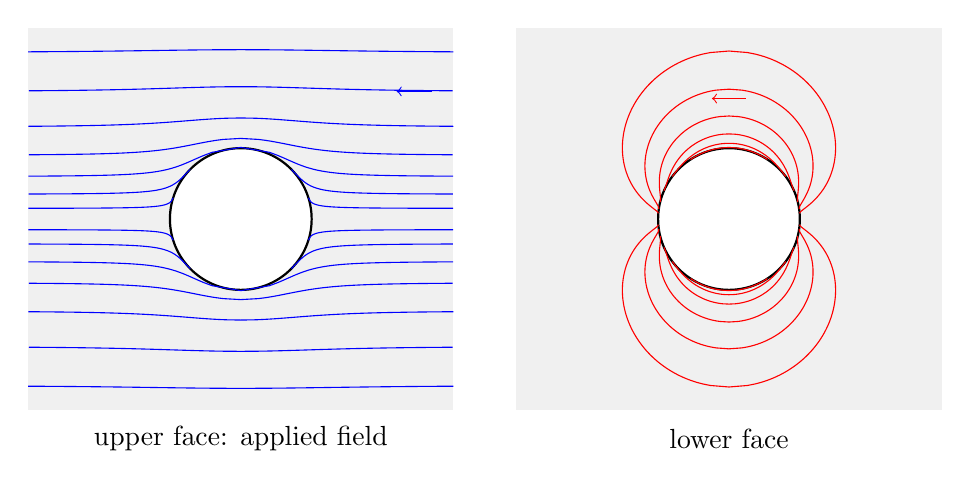
\begin{tikzpicture}[x=.9cm,y=.9cm]
\begin{scope}[xshift=0.0cm]
\fill[gray!12] (-3,-2.7) rectangle (3,2.7);
\filldraw[fill=white,draw=black,thick] (0,0) circle (1);
\draw[blue,thin] plot coordinates {(0.9539392,-0.3000000) (0.9827902,-0.2484115) (1.0007094,-0.2326496) (1.0170875,-0.2222917) (1.0327382,-0.2145772) (1.0479593,-0.2084680) (1.0628964,-0.2034460) (1.0776319,-0.1992115) (1.0922173,-0.1955741) (1.1066867,-0.1924049) (1.1210642,-0.1896123) (1.1353672,-0.1871287) (1.1496086,-0.1849029) (1.1637985,-0.1828951) (1.1779447,-0.1810739) (1.1920535,-0.1794136) (1.2061298,-0.1778937) (1.2201778,-0.1764969) (1.2342009,-0.1752088) (1.2482021,-0.1740174) (1.2621837,-0.1729122) (1.2761477,-0.1718844) (1.2900960,-0.1709264) (1.3040301,-0.1700315) (1.3179512,-0.1691939) (1.3318607,-0.1684084) (1.3457594,-0.1676706) (1.3596483,-0.1669765) (1.3735282,-0.1663224) (1.3873997,-0.1657053) (1.4012636,-0.1651222) (1.4151204,-0.1645706) (1.4289705,-0.1640482) (1.4428145,-0.1635528) (1.4566527,-0.1630826) (1.4704856,-0.1626359) (1.4843135,-0.1622110) (1.4981367,-0.1618065) (1.5119554,-0.1614212) (1.5257700,-0.1610538) (1.5395807,-0.1607031) (1.5533877,-0.1603683) (1.5671913,-0.1600482) (1.5809915,-0.1597421) (1.5947886,-0.1594491) (1.6085827,-0.1591686) (1.6223740,-0.1588997) (1.6361627,-0.1586419) (1.6499488,-0.1583946) (1.6637324,-0.1581571) (1.6775138,-0.1579291) (1.6912930,-0.1577099) (1.7050700,-0.1574991) (1.7188451,-0.1572964) (1.7326182,-0.1571013) (1.7463895,-0.1569135) (1.7601590,-0.1567325) (1.7739268,-0.1565581) (1.7876930,-0.1563899) (1.8014576,-0.1562277) (1.8152207,-0.1560712) (1.8289824,-0.1559201) (1.8427427,-0.1557742) (1.8565016,-0.1556333) (1.8702593,-0.1554970) (1.8840157,-0.1553654) (1.8977709,-0.1552380) (1.9115250,-0.1551148) (1.9252779,-0.1549956) (1.9390298,-0.1548802) (1.9527806,-0.1547684) (1.9665304,-0.1546601) (1.9802792,-0.1545552) (1.9940271,-0.1544536) (2.0077741,-0.1543550) (2.0215201,-0.1542594) (2.0352654,-0.1541667) (2.0490097,-0.1540767) (2.0627533,-0.1539894) (2.0764961,-0.1539047) (2.0902381,-0.1538223) (2.1039794,-0.1537424) (2.1177199,-0.1536647) (2.1314598,-0.1535892) (2.1451990,-0.1535159) (2.1589375,-0.1534445) (2.1726753,-0.1533752) (2.1864126,-0.1533077) (2.2001492,-0.1532421) (2.2138852,-0.1531782) (2.2276207,-0.1531160) (2.2413556,-0.1530555) (2.2550899,-0.1529966) (2.2688237,-0.1529392) (2.2825570,-0.1528833) (2.2962897,-0.1528289) (2.3100220,-0.1527758) (2.3237538,-0.1527241) (2.3374851,-0.1526737) (2.3512159,-0.1526245) (2.3649463,-0.1525766) (2.3786763,-0.1525299) (2.3924058,-0.1524843) (2.4061349,-0.1524398) (2.4198635,-0.1523964) (2.4335918,-0.1523540) (2.4473197,-0.1523126) (2.4610472,-0.1522723) (2.4747743,-0.1522328) (2.4885010,-0.1521943) (2.5022274,-0.1521567) (2.5159534,-0.1521200) (2.5296791,-0.1520841) (2.5434044,-0.1520490) (2.5571294,-0.1520148) (2.5708540,-0.1519812) (2.5845784,-0.1519485) (2.5983024,-0.1519165) (2.6120261,-0.1518851) (2.6257496,-0.1518545) (2.6394727,-0.1518246) (2.6531955,-0.1517952) (2.6669181,-0.1517666) (2.6806403,-0.1517385) (2.6943623,-0.1517111) (2.7080841,-0.1516842) (2.7218055,-0.1516579) (2.7355267,-0.1516321) (2.7492477,-0.1516069) (2.7629684,-0.1515822) (2.7766888,-0.1515580) (2.7904090,-0.1515343) (2.8041290,-0.1515111) (2.8178487,-0.1514884) (2.8315682,-0.1514661) (2.8452875,-0.1514443) (2.8590066,-0.1514229) (2.8727254,-0.1514020) (2.8864440,-0.1513814) (2.9001625,-0.1513613) (2.9138807,-0.1513415) (2.9275987,-0.1513221) (2.9413165,-0.1513032) (2.9550341,-0.1512845) (2.9687515,-0.1512663) (2.9824687,-0.1512483) (2.9961858,-0.1512308)};
\draw[blue,thin] plot coordinates {(-0.9539392,-0.3000000) (-0.9827902,-0.2484115) (-1.0007094,-0.2326496) (-1.0170875,-0.2222917) (-1.0327382,-0.2145772) (-1.0479593,-0.2084680) (-1.0628964,-0.2034460) (-1.0776319,-0.1992115) (-1.0922173,-0.1955741) (-1.1066867,-0.1924049) (-1.1210642,-0.1896123) (-1.1353672,-0.1871287) (-1.1496086,-0.1849029) (-1.1637985,-0.1828951) (-1.1779447,-0.1810739) (-1.1920535,-0.1794136) (-1.2061298,-0.1778937) (-1.2201778,-0.1764969) (-1.2342009,-0.1752088) (-1.2482021,-0.1740174) (-1.2621837,-0.1729122) (-1.2761477,-0.1718844) (-1.2900960,-0.1709264) (-1.3040301,-0.1700315) (-1.3179512,-0.1691939) (-1.3318607,-0.1684084) (-1.3457594,-0.1676706) (-1.3596483,-0.1669765) (-1.3735282,-0.1663224) (-1.3873997,-0.1657053) (-1.4012636,-0.1651222) (-1.4151204,-0.1645706) (-1.4289705,-0.1640482) (-1.4428145,-0.1635528) (-1.4566527,-0.1630826) (-1.4704856,-0.1626359) (-1.4843135,-0.1622110) (-1.4981367,-0.1618065) (-1.5119554,-0.1614212) (-1.5257700,-0.1610538) (-1.5395807,-0.1607031) (-1.5533877,-0.1603683) (-1.5671913,-0.1600482) (-1.5809915,-0.1597421) (-1.5947886,-0.1594491) (-1.6085827,-0.1591686) (-1.6223740,-0.1588997) (-1.6361627,-0.1586419) (-1.6499488,-0.1583946) (-1.6637324,-0.1581571) (-1.6775138,-0.1579291) (-1.6912930,-0.1577099) (-1.7050700,-0.1574991) (-1.7188451,-0.1572964) (-1.7326182,-0.1571013) (-1.7463895,-0.1569135) (-1.7601590,-0.1567325) (-1.7739268,-0.1565581) (-1.7876930,-0.1563899) (-1.8014576,-0.1562277) (-1.8152207,-0.1560712) (-1.8289824,-0.1559201) (-1.8427427,-0.1557742) (-1.8565016,-0.1556333) (-1.8702593,-0.1554970) (-1.8840157,-0.1553654) (-1.8977709,-0.1552380) (-1.9115250,-0.1551148) (-1.9252779,-0.1549956) (-1.9390298,-0.1548802) (-1.9527806,-0.1547684) (-1.9665304,-0.1546601) (-1.9802792,-0.1545552) (-1.9940271,-0.1544536) (-2.0077741,-0.1543550) (-2.0215201,-0.1542594) (-2.0352654,-0.1541667) (-2.0490097,-0.1540767) (-2.0627533,-0.1539894) (-2.0764961,-0.1539047) (-2.0902381,-0.1538223) (-2.1039794,-0.1537424) (-2.1177199,-0.1536647) (-2.1314598,-0.1535892) (-2.1451990,-0.1535159) (-2.1589375,-0.1534445) (-2.1726753,-0.1533752) (-2.1864126,-0.1533077) (-2.2001492,-0.1532421) (-2.2138852,-0.1531782) (-2.2276207,-0.1531160) (-2.2413556,-0.1530555) (-2.2550899,-0.1529966) (-2.2688237,-0.1529392) (-2.2825570,-0.1528833) (-2.2962897,-0.1528289) (-2.3100220,-0.1527758) (-2.3237538,-0.1527241) (-2.3374851,-0.1526737) (-2.3512159,-0.1526245) (-2.3649463,-0.1525766) (-2.3786763,-0.1525299) (-2.3924058,-0.1524843) (-2.4061349,-0.1524398) (-2.4198635,-0.1523964) (-2.4335918,-0.1523540) (-2.4473197,-0.1523126) (-2.4610472,-0.1522723) (-2.4747743,-0.1522328) (-2.4885010,-0.1521943) (-2.5022274,-0.1521567) (-2.5159534,-0.1521200) (-2.5296791,-0.1520841) (-2.5434044,-0.1520490) (-2.5571294,-0.1520148) (-2.5708540,-0.1519812) (-2.5845784,-0.1519485) (-2.5983024,-0.1519165) (-2.6120261,-0.1518851) (-2.6257496,-0.1518545) (-2.6394727,-0.1518246) (-2.6531955,-0.1517952) (-2.6669181,-0.1517666) (-2.6806403,-0.1517385) (-2.6943623,-0.1517111) (-2.7080841,-0.1516842) (-2.7218055,-0.1516579) (-2.7355267,-0.1516321) (-2.7492477,-0.1516069) (-2.7629684,-0.1515822) (-2.7766888,-0.1515580) (-2.7904090,-0.1515343) (-2.8041290,-0.1515111) (-2.8178487,-0.1514884) (-2.8315682,-0.1514661) (-2.8452875,-0.1514443) (-2.8590066,-0.1514229) (-2.8727254,-0.1514020) (-2.8864440,-0.1513814) (-2.9001625,-0.1513613) (-2.9138807,-0.1513415) (-2.9275987,-0.1513221) (-2.9413165,-0.1513032) (-2.9550341,-0.1512845) (-2.9687515,-0.1512663) (-2.9824687,-0.1512483) (-2.9961858,-0.1512308)};
\draw[blue,thin] plot coordinates {(0.9539392,0.3000000) (0.9827902,0.2484115) (1.0007094,0.2326496) (1.0170875,0.2222917) (1.0327382,0.2145772) (1.0479593,0.2084680) (1.0628964,0.2034460) (1.0776319,0.1992115) (1.0922173,0.1955741) (1.1066867,0.1924049) (1.1210642,0.1896123) (1.1353672,0.1871287) (1.1496086,0.1849029) (1.1637985,0.1828951) (1.1779447,0.1810739) (1.1920535,0.1794136) (1.2061298,0.1778937) (1.2201778,0.1764969) (1.2342009,0.1752088) (1.2482021,0.1740174) (1.2621837,0.1729122) (1.2761477,0.1718844) (1.2900960,0.1709264) (1.3040301,0.1700315) (1.3179512,0.1691939) (1.3318607,0.1684084) (1.3457594,0.1676706) (1.3596483,0.1669765) (1.3735282,0.1663224) (1.3873997,0.1657053) (1.4012636,0.1651222) (1.4151204,0.1645706) (1.4289705,0.1640482) (1.4428145,0.1635528) (1.4566527,0.1630826) (1.4704856,0.1626359) (1.4843135,0.1622110) (1.4981367,0.1618065) (1.5119554,0.1614212) (1.5257700,0.1610538) (1.5395807,0.1607031) (1.5533877,0.1603683) (1.5671913,0.1600482) (1.5809915,0.1597421) (1.5947886,0.1594491) (1.6085827,0.1591686) (1.6223740,0.1588997) (1.6361627,0.1586419) (1.6499488,0.1583946) (1.6637324,0.1581571) (1.6775138,0.1579291) (1.6912930,0.1577099) (1.7050700,0.1574991) (1.7188451,0.1572964) (1.7326182,0.1571013) (1.7463895,0.1569135) (1.7601590,0.1567325) (1.7739268,0.1565581) (1.7876930,0.1563899) (1.8014576,0.1562277) (1.8152207,0.1560712) (1.8289824,0.1559201) (1.8427427,0.1557742) (1.8565016,0.1556333) (1.8702593,0.1554970) (1.8840157,0.1553654) (1.8977709,0.1552380) (1.9115250,0.1551148) (1.9252779,0.1549956) (1.9390298,0.1548802) (1.9527806,0.1547684) (1.9665304,0.1546601) (1.9802792,0.1545552) (1.9940271,0.1544536) (2.0077741,0.1543550) (2.0215201,0.1542594) (2.0352654,0.1541667) (2.0490097,0.1540767) (2.0627533,0.1539894) (2.0764961,0.1539047) (2.0902381,0.1538223) (2.1039794,0.1537424) (2.1177199,0.1536647) (2.1314598,0.1535892) (2.1451990,0.1535159) (2.1589375,0.1534445) (2.1726753,0.1533752) (2.1864126,0.1533077) (2.2001492,0.1532421) (2.2138852,0.1531782) (2.2276207,0.1531160) (2.2413556,0.1530555) (2.2550899,0.1529966) (2.2688237,0.1529392) (2.2825570,0.1528833) (2.2962897,0.1528289) (2.3100220,0.1527758) (2.3237538,0.1527241) (2.3374851,0.1526737) (2.3512159,0.1526245) (2.3649463,0.1525766) (2.3786763,0.1525299) (2.3924058,0.1524843) (2.4061349,0.1524398) (2.4198635,0.1523964) (2.4335918,0.1523540) (2.4473197,0.1523126) (2.4610472,0.1522723) (2.4747743,0.1522328) (2.4885010,0.1521943) (2.5022274,0.1521567) (2.5159534,0.1521200) (2.5296791,0.1520841) (2.5434044,0.1520490) (2.5571294,0.1520148) (2.5708540,0.1519812) (2.5845784,0.1519485) (2.5983024,0.1519165) (2.6120261,0.1518851) (2.6257496,0.1518545) (2.6394727,0.1518246) (2.6531955,0.1517952) (2.6669181,0.1517666) (2.6806403,0.1517385) (2.6943623,0.1517111) (2.7080841,0.1516842) (2.7218055,0.1516579) (2.7355267,0.1516321) (2.7492477,0.1516069) (2.7629684,0.1515822) (2.7766888,0.1515580) (2.7904090,0.1515343) (2.8041290,0.1515111) (2.8178487,0.1514884) (2.8315682,0.1514661) (2.8452875,0.1514443) (2.8590066,0.1514229) (2.8727254,0.1514020) (2.8864440,0.1513814) (2.9001625,0.1513613) (2.9138807,0.1513415) (2.9275987,0.1513221) (2.9413165,0.1513032) (2.9550341,0.1512845) (2.9687515,0.1512663) (2.9824687,0.1512483) (2.9961858,0.1512308)};
\draw[blue,thin] plot coordinates {(-0.9539392,0.3000000) (-0.9827902,0.2484115) (-1.0007094,0.2326496) (-1.0170875,0.2222917) (-1.0327382,0.2145772) (-1.0479593,0.2084680) (-1.0628964,0.2034460) (-1.0776319,0.1992115) (-1.0922173,0.1955741) (-1.1066867,0.1924049) (-1.1210642,0.1896123) (-1.1353672,0.1871287) (-1.1496086,0.1849029) (-1.1637985,0.1828951) (-1.1779447,0.1810739) (-1.1920535,0.1794136) (-1.2061298,0.1778937) (-1.2201778,0.1764969) (-1.2342009,0.1752088) (-1.2482021,0.1740174) (-1.2621837,0.1729122) (-1.2761477,0.1718844) (-1.2900960,0.1709264) (-1.3040301,0.1700315) (-1.3179512,0.1691939) (-1.3318607,0.1684084) (-1.3457594,0.1676706) (-1.3596483,0.1669765) (-1.3735282,0.1663224) (-1.3873997,0.1657053) (-1.4012636,0.1651222) (-1.4151204,0.1645706) (-1.4289705,0.1640482) (-1.4428145,0.1635528) (-1.4566527,0.1630826) (-1.4704856,0.1626359) (-1.4843135,0.1622110) (-1.4981367,0.1618065) (-1.5119554,0.1614212) (-1.5257700,0.1610538) (-1.5395807,0.1607031) (-1.5533877,0.1603683) (-1.5671913,0.1600482) (-1.5809915,0.1597421) (-1.5947886,0.1594491) (-1.6085827,0.1591686) (-1.6223740,0.1588997) (-1.6361627,0.1586419) (-1.6499488,0.1583946) (-1.6637324,0.1581571) (-1.6775138,0.1579291) (-1.6912930,0.1577099) (-1.7050700,0.1574991) (-1.7188451,0.1572964) (-1.7326182,0.1571013) (-1.7463895,0.1569135) (-1.7601590,0.1567325) (-1.7739268,0.1565581) (-1.7876930,0.1563899) (-1.8014576,0.1562277) (-1.8152207,0.1560712) (-1.8289824,0.1559201) (-1.8427427,0.1557742) (-1.8565016,0.1556333) (-1.8702593,0.1554970) (-1.8840157,0.1553654) (-1.8977709,0.1552380) (-1.9115250,0.1551148) (-1.9252779,0.1549956) (-1.9390298,0.1548802) (-1.9527806,0.1547684) (-1.9665304,0.1546601) (-1.9802792,0.1545552) (-1.9940271,0.1544536) (-2.0077741,0.1543550) (-2.0215201,0.1542594) (-2.0352654,0.1541667) (-2.0490097,0.1540767) (-2.0627533,0.1539894) (-2.0764961,0.1539047) (-2.0902381,0.1538223) (-2.1039794,0.1537424) (-2.1177199,0.1536647) (-2.1314598,0.1535892) (-2.1451990,0.1535159) (-2.1589375,0.1534445) (-2.1726753,0.1533752) (-2.1864126,0.1533077) (-2.2001492,0.1532421) (-2.2138852,0.1531782) (-2.2276207,0.1531160) (-2.2413556,0.1530555) (-2.2550899,0.1529966) (-2.2688237,0.1529392) (-2.2825570,0.1528833) (-2.2962897,0.1528289) (-2.3100220,0.1527758) (-2.3237538,0.1527241) (-2.3374851,0.1526737) (-2.3512159,0.1526245) (-2.3649463,0.1525766) (-2.3786763,0.1525299) (-2.3924058,0.1524843) (-2.4061349,0.1524398) (-2.4198635,0.1523964) (-2.4335918,0.1523540) (-2.4473197,0.1523126) (-2.4610472,0.1522723) (-2.4747743,0.1522328) (-2.4885010,0.1521943) (-2.5022274,0.1521567) (-2.5159534,0.1521200) (-2.5296791,0.1520841) (-2.5434044,0.1520490) (-2.5571294,0.1520148) (-2.5708540,0.1519812) (-2.5845784,0.1519485) (-2.5983024,0.1519165) (-2.6120261,0.1518851) (-2.6257496,0.1518545) (-2.6394727,0.1518246) (-2.6531955,0.1517952) (-2.6669181,0.1517666) (-2.6806403,0.1517385) (-2.6943623,0.1517111) (-2.7080841,0.1516842) (-2.7218055,0.1516579) (-2.7355267,0.1516321) (-2.7492477,0.1516069) (-2.7629684,0.1515822) (-2.7766888,0.1515580) (-2.7904090,0.1515343) (-2.8041290,0.1515111) (-2.8178487,0.1514884) (-2.8315682,0.1514661) (-2.8452875,0.1514443) (-2.8590066,0.1514229) (-2.8727254,0.1514020) (-2.8864440,0.1513814) (-2.9001625,0.1513613) (-2.9138807,0.1513415) (-2.9275987,0.1513221) (-2.9413165,0.1513032) (-2.9550341,0.1512845) (-2.9687515,0.1512663) (-2.9824687,0.1512483) (-2.9961858,0.1512308)};
\draw[blue,thin] plot coordinates {(0.7141428,-0.7000000) (0.8316356,-0.5796267) (0.8722729,-0.5428490) (0.9026911,-0.5186805) (0.9283916,-0.5006801) (0.9513506,-0.4864253) (0.9725184,-0.4747073) (0.9924273,-0.4648268) (1.0114060,-0.4563396) (1.0296717,-0.4489448) (1.0473752,-0.4424286) (1.0646253,-0.4366336) (1.0815029,-0.4314401) (1.0980699,-0.4267553) (1.1143745,-0.4225057) (1.1304548,-0.4186318) (1.1463417,-0.4150853) (1.1620604,-0.4118261) (1.1776314,-0.4088206) (1.1930723,-0.4060405) (1.2083976,-0.4034618) (1.2236197,-0.4010637) (1.2387492,-0.3988283) (1.2537952,-0.3967402) (1.2687657,-0.3947857) (1.2836675,-0.3929530) (1.2985067,-0.3912315) (1.3132887,-0.3896118) (1.3280182,-0.3880857) (1.3426993,-0.3866457) (1.3573358,-0.3852851) (1.3719310,-0.3839980) (1.3864879,-0.3827790) (1.4010092,-0.3816232) (1.4154974,-0.3805261) (1.4299547,-0.3794837) (1.4443831,-0.3784923) (1.4587844,-0.3775486) (1.4731603,-0.3766495) (1.4875123,-0.3757921) (1.5018418,-0.3749740) (1.5161502,-0.3741926) (1.5304385,-0.3734458) (1.5447080,-0.3727315) (1.5589596,-0.3720480) (1.5731942,-0.3713933) (1.5874127,-0.3707660) (1.6016160,-0.3701644) (1.6158048,-0.3695873) (1.6299797,-0.3690333) (1.6441415,-0.3685011) (1.6582907,-0.3679897) (1.6724279,-0.3674980) (1.6865537,-0.3670250) (1.7006685,-0.3665698) (1.7147728,-0.3661314) (1.7288671,-0.3657091) (1.7429518,-0.3653022) (1.7570273,-0.3649098) (1.7710939,-0.3645313) (1.7851520,-0.3641662) (1.7992019,-0.3638136) (1.8132439,-0.3634732) (1.8272784,-0.3631443) (1.8413056,-0.3628264) (1.8553257,-0.3625192) (1.8693391,-0.3622220) (1.8833459,-0.3619346) (1.8973464,-0.3616564) (1.9113408,-0.3613871) (1.9253294,-0.3611263) (1.9393122,-0.3608737) (1.9532895,-0.3606289) (1.9672615,-0.3603917) (1.9812283,-0.3601617) (1.9951902,-0.3599387) (2.0091472,-0.3597223) (2.0230994,-0.3595124) (2.0370472,-0.3593087) (2.0509905,-0.3591109) (2.0649295,-0.3589188) (2.0788644,-0.3587322) (2.0927952,-0.3585510) (2.1067221,-0.3583749) (2.1206451,-0.3582037) (2.1345645,-0.3580372) (2.1484802,-0.3578754) (2.1623924,-0.3577180) (2.1763012,-0.3575648) (2.1902067,-0.3574158) (2.2041089,-0.3572707) (2.2180079,-0.3571295) (2.2319039,-0.3569921) (2.2457969,-0.3568582) (2.2596869,-0.3567278) (2.2735741,-0.3566007) (2.2874585,-0.3564769) (2.3013402,-0.3563562) (2.3152192,-0.3562386) (2.3290956,-0.3561239) (2.3429695,-0.3560121) (2.3568409,-0.3559030) (2.3707099,-0.3557966) (2.3845766,-0.3556928) (2.3984409,-0.3555915) (2.4123030,-0.3554927) (2.4261629,-0.3553962) (2.4400206,-0.3553020) (2.4538762,-0.3552100) (2.4677297,-0.3551201) (2.4815812,-0.3550324) (2.4954308,-0.3549467) (2.5092784,-0.3548629) (2.5231241,-0.3547811) (2.5369679,-0.3547011) (2.5508100,-0.3546229) (2.5646502,-0.3545465) (2.5784887,-0.3544717) (2.5923255,-0.3543987) (2.6061605,-0.3543272) (2.6199940,-0.3542573) (2.6338258,-0.3541889) (2.6476561,-0.3541220) (2.6614848,-0.3540565) (2.6753119,-0.3539925) (2.6891376,-0.3539298) (2.7029618,-0.3538684) (2.7167846,-0.3538083) (2.7306059,-0.3537494) (2.7444259,-0.3536918) (2.7582445,-0.3536354) (2.7720617,-0.3535801) (2.7858777,-0.3535260) (2.7996923,-0.3534729) (2.8135057,-0.3534210) (2.8273178,-0.3533700) (2.8411287,-0.3533201) (2.8549384,-0.3532712) (2.8687469,-0.3532233) (2.8825543,-0.3531763) (2.8963605,-0.3531302) (2.9101655,-0.3530850) (2.9239695,-0.3530407) (2.9377724,-0.3529972) (2.9515742,-0.3529546) (2.9653749,-0.3529128) (2.9791746,-0.3528718) (2.9929733,-0.3528315)};
\draw[blue,thin] plot coordinates {(-0.7141428,-0.7000000) (-0.8316356,-0.5796267) (-0.8722729,-0.5428490) (-0.9026911,-0.5186805) (-0.9283916,-0.5006801) (-0.9513506,-0.4864253) (-0.9725184,-0.4747073) (-0.9924273,-0.4648268) (-1.0114060,-0.4563396) (-1.0296717,-0.4489448) (-1.0473752,-0.4424286) (-1.0646253,-0.4366336) (-1.0815029,-0.4314401) (-1.0980699,-0.4267553) (-1.1143745,-0.4225057) (-1.1304548,-0.4186318) (-1.1463417,-0.4150853) (-1.1620604,-0.4118261) (-1.1776314,-0.4088206) (-1.1930723,-0.4060405) (-1.2083976,-0.4034618) (-1.2236197,-0.4010637) (-1.2387492,-0.3988283) (-1.2537952,-0.3967402) (-1.2687657,-0.3947857) (-1.2836675,-0.3929530) (-1.2985067,-0.3912315) (-1.3132887,-0.3896118) (-1.3280182,-0.3880857) (-1.3426993,-0.3866457) (-1.3573358,-0.3852851) (-1.3719310,-0.3839980) (-1.3864879,-0.3827790) (-1.4010092,-0.3816232) (-1.4154974,-0.3805261) (-1.4299547,-0.3794837) (-1.4443831,-0.3784923) (-1.4587844,-0.3775486) (-1.4731603,-0.3766495) (-1.4875123,-0.3757921) (-1.5018418,-0.3749740) (-1.5161502,-0.3741926) (-1.5304385,-0.3734458) (-1.5447080,-0.3727315) (-1.5589596,-0.3720480) (-1.5731942,-0.3713933) (-1.5874127,-0.3707660) (-1.6016160,-0.3701644) (-1.6158048,-0.3695873) (-1.6299797,-0.3690333) (-1.6441415,-0.3685011) (-1.6582907,-0.3679897) (-1.6724279,-0.3674980) (-1.6865537,-0.3670250) (-1.7006685,-0.3665698) (-1.7147728,-0.3661314) (-1.7288671,-0.3657091) (-1.7429518,-0.3653022) (-1.7570273,-0.3649098) (-1.7710939,-0.3645313) (-1.7851520,-0.3641662) (-1.7992019,-0.3638136) (-1.8132439,-0.3634732) (-1.8272784,-0.3631443) (-1.8413056,-0.3628264) (-1.8553257,-0.3625192) (-1.8693391,-0.3622220) (-1.8833459,-0.3619346) (-1.8973464,-0.3616564) (-1.9113408,-0.3613871) (-1.9253294,-0.3611263) (-1.9393122,-0.3608737) (-1.9532895,-0.3606289) (-1.9672615,-0.3603917) (-1.9812283,-0.3601617) (-1.9951902,-0.3599387) (-2.0091472,-0.3597223) (-2.0230994,-0.3595124) (-2.0370472,-0.3593087) (-2.0509905,-0.3591109) (-2.0649295,-0.3589188) (-2.0788644,-0.3587322) (-2.0927952,-0.3585510) (-2.1067221,-0.3583749) (-2.1206451,-0.3582037) (-2.1345645,-0.3580372) (-2.1484802,-0.3578754) (-2.1623924,-0.3577180) (-2.1763012,-0.3575648) (-2.1902067,-0.3574158) (-2.2041089,-0.3572707) (-2.2180079,-0.3571295) (-2.2319039,-0.3569921) (-2.2457969,-0.3568582) (-2.2596869,-0.3567278) (-2.2735741,-0.3566007) (-2.2874585,-0.3564769) (-2.3013402,-0.3563562) (-2.3152192,-0.3562386) (-2.3290956,-0.3561239) (-2.3429695,-0.3560121) (-2.3568409,-0.3559030) (-2.3707099,-0.3557966) (-2.3845766,-0.3556928) (-2.3984409,-0.3555915) (-2.4123030,-0.3554927) (-2.4261629,-0.3553962) (-2.4400206,-0.3553020) (-2.4538762,-0.3552100) (-2.4677297,-0.3551201) (-2.4815812,-0.3550324) (-2.4954308,-0.3549467) (-2.5092784,-0.3548629) (-2.5231241,-0.3547811) (-2.5369679,-0.3547011) (-2.5508100,-0.3546229) (-2.5646502,-0.3545465) (-2.5784887,-0.3544717) (-2.5923255,-0.3543987) (-2.6061605,-0.3543272) (-2.6199940,-0.3542573) (-2.6338258,-0.3541889) (-2.6476561,-0.3541220) (-2.6614848,-0.3540565) (-2.6753119,-0.3539925) (-2.6891376,-0.3539298) (-2.7029618,-0.3538684) (-2.7167846,-0.3538083) (-2.7306059,-0.3537494) (-2.7444259,-0.3536918) (-2.7582445,-0.3536354) (-2.7720617,-0.3535801) (-2.7858777,-0.3535260) (-2.7996923,-0.3534729) (-2.8135057,-0.3534210) (-2.8273178,-0.3533700) (-2.8411287,-0.3533201) (-2.8549384,-0.3532712) (-2.8687469,-0.3532233) (-2.8825543,-0.3531763) (-2.8963605,-0.3531302) (-2.9101655,-0.3530850) (-2.9239695,-0.3530407) (-2.9377724,-0.3529972) (-2.9515742,-0.3529546) (-2.9653749,-0.3529128) (-2.9791746,-0.3528718) (-2.9929733,-0.3528315)};
\draw[blue,thin] plot coordinates {(0.7141428,0.7000000) (0.8316356,0.5796267) (0.8722729,0.5428490) (0.9026911,0.5186805) (0.9283916,0.5006801) (0.9513506,0.4864253) (0.9725184,0.4747073) (0.9924273,0.4648268) (1.0114060,0.4563396) (1.0296717,0.4489448) (1.0473752,0.4424286) (1.0646253,0.4366336) (1.0815029,0.4314401) (1.0980699,0.4267553) (1.1143745,0.4225057) (1.1304548,0.4186318) (1.1463417,0.4150853) (1.1620604,0.4118261) (1.1776314,0.4088206) (1.1930723,0.4060405) (1.2083976,0.4034618) (1.2236197,0.4010637) (1.2387492,0.3988283) (1.2537952,0.3967402) (1.2687657,0.3947857) (1.2836675,0.3929530) (1.2985067,0.3912315) (1.3132887,0.3896118) (1.3280182,0.3880857) (1.3426993,0.3866457) (1.3573358,0.3852851) (1.3719310,0.3839980) (1.3864879,0.3827790) (1.4010092,0.3816232) (1.4154974,0.3805261) (1.4299547,0.3794837) (1.4443831,0.3784923) (1.4587844,0.3775486) (1.4731603,0.3766495) (1.4875123,0.3757921) (1.5018418,0.3749740) (1.5161502,0.3741926) (1.5304385,0.3734458) (1.5447080,0.3727315) (1.5589596,0.3720480) (1.5731942,0.3713933) (1.5874127,0.3707660) (1.6016160,0.3701644) (1.6158048,0.3695873) (1.6299797,0.3690333) (1.6441415,0.3685011) (1.6582907,0.3679897) (1.6724279,0.3674980) (1.6865537,0.3670250) (1.7006685,0.3665698) (1.7147728,0.3661314) (1.7288671,0.3657091) (1.7429518,0.3653022) (1.7570273,0.3649098) (1.7710939,0.3645313) (1.7851520,0.3641662) (1.7992019,0.3638136) (1.8132439,0.3634732) (1.8272784,0.3631443) (1.8413056,0.3628264) (1.8553257,0.3625192) (1.8693391,0.3622220) (1.8833459,0.3619346) (1.8973464,0.3616564) (1.9113408,0.3613871) (1.9253294,0.3611263) (1.9393122,0.3608737) (1.9532895,0.3606289) (1.9672615,0.3603917) (1.9812283,0.3601617) (1.9951902,0.3599387) (2.0091472,0.3597223) (2.0230994,0.3595124) (2.0370472,0.3593087) (2.0509905,0.3591109) (2.0649295,0.3589188) (2.0788644,0.3587322) (2.0927952,0.3585510) (2.1067221,0.3583749) (2.1206451,0.3582037) (2.1345645,0.3580372) (2.1484802,0.3578754) (2.1623924,0.3577180) (2.1763012,0.3575648) (2.1902067,0.3574158) (2.2041089,0.3572707) (2.2180079,0.3571295) (2.2319039,0.3569921) (2.2457969,0.3568582) (2.2596869,0.3567278) (2.2735741,0.3566007) (2.2874585,0.3564769) (2.3013402,0.3563562) (2.3152192,0.3562386) (2.3290956,0.3561239) (2.3429695,0.3560121) (2.3568409,0.3559030) (2.3707099,0.3557966) (2.3845766,0.3556928) (2.3984409,0.3555915) (2.4123030,0.3554927) (2.4261629,0.3553962) (2.4400206,0.3553020) (2.4538762,0.3552100) (2.4677297,0.3551201) (2.4815812,0.3550324) (2.4954308,0.3549467) (2.5092784,0.3548629) (2.5231241,0.3547811) (2.5369679,0.3547011) (2.5508100,0.3546229) (2.5646502,0.3545465) (2.5784887,0.3544717) (2.5923255,0.3543987) (2.6061605,0.3543272) (2.6199940,0.3542573) (2.6338258,0.3541889) (2.6476561,0.3541220) (2.6614848,0.3540565) (2.6753119,0.3539925) (2.6891376,0.3539298) (2.7029618,0.3538684) (2.7167846,0.3538083) (2.7306059,0.3537494) (2.7444259,0.3536918) (2.7582445,0.3536354) (2.7720617,0.3535801) (2.7858777,0.3535260) (2.7996923,0.3534729) (2.8135057,0.3534210) (2.8273178,0.3533700) (2.8411287,0.3533201) (2.8549384,0.3532712) (2.8687469,0.3532233) (2.8825543,0.3531763) (2.8963605,0.3531302) (2.9101655,0.3530850) (2.9239695,0.3530407) (2.9377724,0.3529972) (2.9515742,0.3529546) (2.9653749,0.3529128) (2.9791746,0.3528718) (2.9929733,0.3528315)};
\draw[blue,thin] plot coordinates {(-0.7141428,0.7000000) (-0.8316356,0.5796267) (-0.8722729,0.5428490) (-0.9026911,0.5186805) (-0.9283916,0.5006801) (-0.9513506,0.4864253) (-0.9725184,0.4747073) (-0.9924273,0.4648268) (-1.0114060,0.4563396) (-1.0296717,0.4489448) (-1.0473752,0.4424286) (-1.0646253,0.4366336) (-1.0815029,0.4314401) (-1.0980699,0.4267553) (-1.1143745,0.4225057) (-1.1304548,0.4186318) (-1.1463417,0.4150853) (-1.1620604,0.4118261) (-1.1776314,0.4088206) (-1.1930723,0.4060405) (-1.2083976,0.4034618) (-1.2236197,0.4010637) (-1.2387492,0.3988283) (-1.2537952,0.3967402) (-1.2687657,0.3947857) (-1.2836675,0.3929530) (-1.2985067,0.3912315) (-1.3132887,0.3896118) (-1.3280182,0.3880857) (-1.3426993,0.3866457) (-1.3573358,0.3852851) (-1.3719310,0.3839980) (-1.3864879,0.3827790) (-1.4010092,0.3816232) (-1.4154974,0.3805261) (-1.4299547,0.3794837) (-1.4443831,0.3784923) (-1.4587844,0.3775486) (-1.4731603,0.3766495) (-1.4875123,0.3757921) (-1.5018418,0.3749740) (-1.5161502,0.3741926) (-1.5304385,0.3734458) (-1.5447080,0.3727315) (-1.5589596,0.3720480) (-1.5731942,0.3713933) (-1.5874127,0.3707660) (-1.6016160,0.3701644) (-1.6158048,0.3695873) (-1.6299797,0.3690333) (-1.6441415,0.3685011) (-1.6582907,0.3679897) (-1.6724279,0.3674980) (-1.6865537,0.3670250) (-1.7006685,0.3665698) (-1.7147728,0.3661314) (-1.7288671,0.3657091) (-1.7429518,0.3653022) (-1.7570273,0.3649098) (-1.7710939,0.3645313) (-1.7851520,0.3641662) (-1.7992019,0.3638136) (-1.8132439,0.3634732) (-1.8272784,0.3631443) (-1.8413056,0.3628264) (-1.8553257,0.3625192) (-1.8693391,0.3622220) (-1.8833459,0.3619346) (-1.8973464,0.3616564) (-1.9113408,0.3613871) (-1.9253294,0.3611263) (-1.9393122,0.3608737) (-1.9532895,0.3606289) (-1.9672615,0.3603917) (-1.9812283,0.3601617) (-1.9951902,0.3599387) (-2.0091472,0.3597223) (-2.0230994,0.3595124) (-2.0370472,0.3593087) (-2.0509905,0.3591109) (-2.0649295,0.3589188) (-2.0788644,0.3587322) (-2.0927952,0.3585510) (-2.1067221,0.3583749) (-2.1206451,0.3582037) (-2.1345645,0.3580372) (-2.1484802,0.3578754) (-2.1623924,0.3577180) (-2.1763012,0.3575648) (-2.1902067,0.3574158) (-2.2041089,0.3572707) (-2.2180079,0.3571295) (-2.2319039,0.3569921) (-2.2457969,0.3568582) (-2.2596869,0.3567278) (-2.2735741,0.3566007) (-2.2874585,0.3564769) (-2.3013402,0.3563562) (-2.3152192,0.3562386) (-2.3290956,0.3561239) (-2.3429695,0.3560121) (-2.3568409,0.3559030) (-2.3707099,0.3557966) (-2.3845766,0.3556928) (-2.3984409,0.3555915) (-2.4123030,0.3554927) (-2.4261629,0.3553962) (-2.4400206,0.3553020) (-2.4538762,0.3552100) (-2.4677297,0.3551201) (-2.4815812,0.3550324) (-2.4954308,0.3549467) (-2.5092784,0.3548629) (-2.5231241,0.3547811) (-2.5369679,0.3547011) (-2.5508100,0.3546229) (-2.5646502,0.3545465) (-2.5784887,0.3544717) (-2.5923255,0.3543987) (-2.6061605,0.3543272) (-2.6199940,0.3542573) (-2.6338258,0.3541889) (-2.6476561,0.3541220) (-2.6614848,0.3540565) (-2.6753119,0.3539925) (-2.6891376,0.3539298) (-2.7029618,0.3538684) (-2.7167846,0.3538083) (-2.7306059,0.3537494) (-2.7444259,0.3536918) (-2.7582445,0.3536354) (-2.7720617,0.3535801) (-2.7858777,0.3535260) (-2.7996923,0.3534729) (-2.8135057,0.3534210) (-2.8273178,0.3533700) (-2.8411287,0.3533201) (-2.8549384,0.3532712) (-2.8687469,0.3532233) (-2.8825543,0.3531763) (-2.8963605,0.3531302) (-2.9101655,0.3530850) (-2.9239695,0.3530407) (-2.9377724,0.3529972) (-2.9515742,0.3529546) (-2.9653749,0.3529128) (-2.9791746,0.3528718) (-2.9929733,0.3528315)};
\draw[blue,thin] plot coordinates {(-2.9979046,-0.6046384) (-2.9839671,-0.6047030) (-2.9700267,-0.6047689) (-2.9560834,-0.6048360) (-2.9421370,-0.6049044) (-2.9281875,-0.6049741) (-2.9142349,-0.6050451) (-2.9002791,-0.6051175) (-2.8863201,-0.6051914) (-2.8723578,-0.6052666) (-2.8583921,-0.6053434) (-2.8444230,-0.6054216) (-2.8304505,-0.6055014) (-2.8164744,-0.6055828) (-2.8024947,-0.6056659) (-2.7885114,-0.6057506) (-2.7745244,-0.6058370) (-2.7605336,-0.6059252) (-2.7465390,-0.6060152) (-2.7325404,-0.6061071) (-2.7185378,-0.6062009) (-2.7045312,-0.6062966) (-2.6905204,-0.6063943) (-2.6765055,-0.6064941) (-2.6624862,-0.6065960) (-2.6484625,-0.6067001) (-2.6344344,-0.6068064) (-2.6204017,-0.6069150) (-2.6063644,-0.6070260) (-2.5923224,-0.6071394) (-2.5782756,-0.6072552) (-2.5642238,-0.6073737) (-2.5501670,-0.6074947) (-2.5361051,-0.6076185) (-2.5220380,-0.6077451) (-2.5079656,-0.6078745) (-2.4938877,-0.6080069) (-2.4798042,-0.6081423) (-2.4657151,-0.6082808) (-2.4516202,-0.6084226) (-2.4375194,-0.6085676) (-2.4234125,-0.6087161) (-2.4092994,-0.6088681) (-2.3951801,-0.6090237) (-2.3810542,-0.6091830) (-2.3669218,-0.6093462) (-2.3527826,-0.6095133) (-2.3386365,-0.6096845) (-2.3244833,-0.6098600) (-2.3103229,-0.6100398) (-2.2961551,-0.6102241) (-2.2819797,-0.6104130) (-2.2677965,-0.6106067) (-2.2536054,-0.6108053) (-2.2394061,-0.6110090) (-2.2251984,-0.6112180) (-2.2109822,-0.6114325) (-2.1967571,-0.6116526) (-2.1825231,-0.6118784) (-2.1682798,-0.6121104) (-2.1540270,-0.6123485) (-2.1397644,-0.6125931) (-2.1254919,-0.6128443) (-2.1112090,-0.6131024) (-2.0969156,-0.6133677) (-2.0826112,-0.6136404) (-2.0682958,-0.6139208) (-2.0539688,-0.6142091) (-2.0396300,-0.6145056) (-2.0252789,-0.6148108) (-2.0109154,-0.6151247) (-1.9965389,-0.6154479) (-1.9821491,-0.6157806) (-1.9677456,-0.6161233) (-1.9533280,-0.6164762) (-1.9388957,-0.6168399) (-1.9244483,-0.6172147) (-1.9099854,-0.6176011) (-1.8955063,-0.6179996) (-1.8810107,-0.6184106) (-1.8664978,-0.6188346) (-1.8519672,-0.6192723) (-1.8374181,-0.6197241) (-1.8228500,-0.6201907) (-1.8082620,-0.6206727) (-1.7936536,-0.6211709) (-1.7790240,-0.6216858) (-1.7643723,-0.6222182) (-1.7496976,-0.6227690) (-1.7349992,-0.6233389) (-1.7202759,-0.6239289) (-1.7055270,-0.6245398) (-1.6907512,-0.6251727) (-1.6759474,-0.6258286) (-1.6611145,-0.6265087) (-1.6462511,-0.6272140) (-1.6313560,-0.6279460) (-1.6164277,-0.6287058) (-1.6014647,-0.6294949) (-1.5864653,-0.6303148) (-1.5714279,-0.6311673) (-1.5563505,-0.6320538) (-1.5412311,-0.6329765) (-1.5260677,-0.6339371) (-1.5108579,-0.6349378) (-1.4955993,-0.6359809) (-1.4802892,-0.6370687) (-1.4649248,-0.6382041) (-1.4495030,-0.6393896) (-1.4340205,-0.6406285) (-1.4184737,-0.6419239) (-1.4028585,-0.6432794) (-1.3871709,-0.6446988) (-1.3714060,-0.6461864) (-1.3555589,-0.6477465) (-1.3396240,-0.6493842) (-1.3235952,-0.6511048) (-1.3074658,-0.6529142) (-1.2912283,-0.6548188) (-1.2748746,-0.6568256) (-1.2583957,-0.6589424) (-1.2417814,-0.6611777) (-1.2250204,-0.6635410) (-1.2081001,-0.6660428) (-1.1910063,-0.6686946) (-1.1737230,-0.6715097) (-1.1562320,-0.6745024) (-1.1385125,-0.6776891) (-1.1205408,-0.6810884) (-1.1022897,-0.6847213) (-1.0837274,-0.6886115) (-1.0648171,-0.6927864) (-1.0455155,-0.6972775) (-1.0257714,-0.7021213) (-1.0055237,-0.7073603) (-0.9846988,-0.7130447) (-0.9632069,-0.7192338) (-0.9409376,-0.7259987) (-0.9177526,-0.7334258) (-0.8934764,-0.7416206) (-0.8678818,-0.7507149) (-0.8406685,-0.7608753) (-0.8114287,-0.7723173) (-0.7795906,-0.7853261) (-0.7443205,-0.8002915) (-0.7043374,-0.8177662) (-0.6575336,-0.8385751) (-0.6000812,-0.8640368) (-0.5238770,-0.8964825) (-0.4061043,-0.9407714) (-0.0000002,-1.0110329) (0.4061043,-0.9407714) (0.5238770,-0.8964825) (0.6000812,-0.8640368) (0.6575336,-0.8385751) (0.7043374,-0.8177662) (0.7443205,-0.8002915) (0.7795906,-0.7853261) (0.8114287,-0.7723173) (0.8406685,-0.7608753) (0.8678818,-0.7507149) (0.8934764,-0.7416206) (0.9177526,-0.7334258) (0.9409376,-0.7259987) (0.9632069,-0.7192338) (0.9846988,-0.7130447) (1.0055237,-0.7073603) (1.0257714,-0.7021213) (1.0455155,-0.6972775) (1.0648171,-0.6927864) (1.0837274,-0.6886115) (1.1022897,-0.6847213) (1.1205408,-0.6810884) (1.1385125,-0.6776891) (1.1562320,-0.6745024) (1.1737230,-0.6715097) (1.1910063,-0.6686946) (1.2081001,-0.6660428) (1.2250204,-0.6635410) (1.2417814,-0.6611777) (1.2583957,-0.6589424) (1.2748746,-0.6568256) (1.2912283,-0.6548188) (1.3074658,-0.6529142) (1.3235952,-0.6511048) (1.3396240,-0.6493842) (1.3555589,-0.6477465) (1.3714060,-0.6461864) (1.3871709,-0.6446988) (1.4028585,-0.6432794) (1.4184737,-0.6419239) (1.4340205,-0.6406285) (1.4495030,-0.6393896) (1.4649248,-0.6382041) (1.4802892,-0.6370687) (1.4955993,-0.6359809) (1.5108579,-0.6349378) (1.5260677,-0.6339371) (1.5412311,-0.6329765) (1.5563505,-0.6320538) (1.5714279,-0.6311673) (1.5864653,-0.6303148) (1.6014647,-0.6294949) (1.6164277,-0.6287058) (1.6313560,-0.6279460) (1.6462511,-0.6272140) (1.6611145,-0.6265087) (1.6759474,-0.6258286) (1.6907512,-0.6251727) (1.7055270,-0.6245398) (1.7202759,-0.6239289) (1.7349992,-0.6233389) (1.7496976,-0.6227690) (1.7643723,-0.6222182) (1.7790240,-0.6216858) (1.7936536,-0.6211709) (1.8082620,-0.6206727) (1.8228500,-0.6201907) (1.8374181,-0.6197241) (1.8519672,-0.6192723) (1.8664978,-0.6188346) (1.8810107,-0.6184106) (1.8955063,-0.6179996) (1.9099854,-0.6176011) (1.9244483,-0.6172147) (1.9388957,-0.6168399) (1.9533280,-0.6164762) (1.9677456,-0.6161233) (1.9821491,-0.6157806) (1.9965389,-0.6154479) (2.0109154,-0.6151247) (2.0252789,-0.6148108) (2.0396300,-0.6145056) (2.0539688,-0.6142091) (2.0682958,-0.6139208) (2.0826112,-0.6136404) (2.0969156,-0.6133677) (2.1112090,-0.6131024) (2.1254919,-0.6128443) (2.1397644,-0.6125931) (2.1540270,-0.6123485) (2.1682798,-0.6121104) (2.1825231,-0.6118784) (2.1967571,-0.6116526) (2.2109822,-0.6114325) (2.2251984,-0.6112180) (2.2394061,-0.6110090) (2.2536054,-0.6108053) (2.2677965,-0.6106067) (2.2819797,-0.6104130) (2.2961551,-0.6102241) (2.3103229,-0.6100398) (2.3244833,-0.6098600) (2.3386365,-0.6096845) (2.3527826,-0.6095133) (2.3669218,-0.6093462) (2.3810542,-0.6091830) (2.3951801,-0.6090237) (2.4092994,-0.6088681) (2.4234125,-0.6087161) (2.4375194,-0.6085676) (2.4516202,-0.6084226) (2.4657151,-0.6082808) (2.4798042,-0.6081423) (2.4938877,-0.6080069) (2.5079656,-0.6078745) (2.5220380,-0.6077451) (2.5361051,-0.6076185) (2.5501670,-0.6074947) (2.5642238,-0.6073737) (2.5782756,-0.6072552) (2.5923224,-0.6071394) (2.6063644,-0.6070260) (2.6204017,-0.6069150) (2.6344344,-0.6068064) (2.6484625,-0.6067001) (2.6624862,-0.6065960) (2.6765055,-0.6064941) (2.6905204,-0.6063943) (2.7045312,-0.6062966) (2.7185378,-0.6062009) (2.7325404,-0.6061071) (2.7465390,-0.6060152) (2.7605336,-0.6059252) (2.7745244,-0.6058370) (2.7885114,-0.6057506) (2.8024947,-0.6056659) (2.8164744,-0.6055828) (2.8304505,-0.6055014) (2.8444230,-0.6054216) (2.8583921,-0.6053434) (2.8723578,-0.6052666) (2.8863201,-0.6051914) (2.9002791,-0.6051175) (2.9142349,-0.6050451) (2.9281875,-0.6049741) (2.9421370,-0.6049044) (2.9560834,-0.6048360) (2.9700267,-0.6047689) (2.9839671,-0.6047030) (2.9979046,-0.6046384)};
\draw[blue,thin] plot coordinates {(-2.9979046,0.6046384) (-2.9839671,0.6047030) (-2.9700267,0.6047689) (-2.9560834,0.6048360) (-2.9421370,0.6049044) (-2.9281875,0.6049741) (-2.9142349,0.6050451) (-2.9002791,0.6051175) (-2.8863201,0.6051914) (-2.8723578,0.6052666) (-2.8583921,0.6053434) (-2.8444230,0.6054216) (-2.8304505,0.6055014) (-2.8164744,0.6055828) (-2.8024947,0.6056659) (-2.7885114,0.6057506) (-2.7745244,0.6058370) (-2.7605336,0.6059252) (-2.7465390,0.6060152) (-2.7325404,0.6061071) (-2.7185378,0.6062009) (-2.7045312,0.6062966) (-2.6905204,0.6063943) (-2.6765055,0.6064941) (-2.6624862,0.6065960) (-2.6484625,0.6067001) (-2.6344344,0.6068064) (-2.6204017,0.6069150) (-2.6063644,0.6070260) (-2.5923224,0.6071394) (-2.5782756,0.6072552) (-2.5642238,0.6073737) (-2.5501670,0.6074947) (-2.5361051,0.6076185) (-2.5220380,0.6077451) (-2.5079656,0.6078745) (-2.4938877,0.6080069) (-2.4798042,0.6081423) (-2.4657151,0.6082808) (-2.4516202,0.6084226) (-2.4375194,0.6085676) (-2.4234125,0.6087161) (-2.4092994,0.6088681) (-2.3951801,0.6090237) (-2.3810542,0.6091830) (-2.3669218,0.6093462) (-2.3527826,0.6095133) (-2.3386365,0.6096845) (-2.3244833,0.6098600) (-2.3103229,0.6100398) (-2.2961551,0.6102241) (-2.2819797,0.6104130) (-2.2677965,0.6106067) (-2.2536054,0.6108053) (-2.2394061,0.6110090) (-2.2251984,0.6112180) (-2.2109822,0.6114325) (-2.1967571,0.6116526) (-2.1825231,0.6118784) (-2.1682798,0.6121104) (-2.1540270,0.6123485) (-2.1397644,0.6125931) (-2.1254919,0.6128443) (-2.1112090,0.6131024) (-2.0969156,0.6133677) (-2.0826112,0.6136404) (-2.0682958,0.6139208) (-2.0539688,0.6142091) (-2.0396300,0.6145056) (-2.0252789,0.6148108) (-2.0109154,0.6151247) (-1.9965389,0.6154479) (-1.9821491,0.6157806) (-1.9677456,0.6161233) (-1.9533280,0.6164762) (-1.9388957,0.6168399) (-1.9244483,0.6172147) (-1.9099854,0.6176011) (-1.8955063,0.6179996) (-1.8810107,0.6184106) (-1.8664978,0.6188346) (-1.8519672,0.6192723) (-1.8374181,0.6197241) (-1.8228500,0.6201907) (-1.8082620,0.6206727) (-1.7936536,0.6211709) (-1.7790240,0.6216858) (-1.7643723,0.6222182) (-1.7496976,0.6227690) (-1.7349992,0.6233389) (-1.7202759,0.6239289) (-1.7055270,0.6245398) (-1.6907512,0.6251727) (-1.6759474,0.6258286) (-1.6611145,0.6265087) (-1.6462511,0.6272140) (-1.6313560,0.6279460) (-1.6164277,0.6287058) (-1.6014647,0.6294949) (-1.5864653,0.6303148) (-1.5714279,0.6311673) (-1.5563505,0.6320538) (-1.5412311,0.6329765) (-1.5260677,0.6339371) (-1.5108579,0.6349378) (-1.4955993,0.6359809) (-1.4802892,0.6370687) (-1.4649248,0.6382041) (-1.4495030,0.6393896) (-1.4340205,0.6406285) (-1.4184737,0.6419239) (-1.4028585,0.6432794) (-1.3871709,0.6446988) (-1.3714060,0.6461864) (-1.3555589,0.6477465) (-1.3396240,0.6493842) (-1.3235952,0.6511048) (-1.3074658,0.6529142) (-1.2912283,0.6548188) (-1.2748746,0.6568256) (-1.2583957,0.6589424) (-1.2417814,0.6611777) (-1.2250204,0.6635410) (-1.2081001,0.6660428) (-1.1910063,0.6686946) (-1.1737230,0.6715097) (-1.1562320,0.6745024) (-1.1385125,0.6776891) (-1.1205408,0.6810884) (-1.1022897,0.6847213) (-1.0837274,0.6886115) (-1.0648171,0.6927864) (-1.0455155,0.6972775) (-1.0257714,0.7021213) (-1.0055237,0.7073603) (-0.9846988,0.7130447) (-0.9632069,0.7192338) (-0.9409376,0.7259987) (-0.9177526,0.7334258) (-0.8934764,0.7416206) (-0.8678818,0.7507149) (-0.8406685,0.7608753) (-0.8114287,0.7723173) (-0.7795906,0.7853261) (-0.7443205,0.8002915) (-0.7043374,0.8177662) (-0.6575336,0.8385751) (-0.6000812,0.8640368) (-0.5238770,0.8964825) (-0.4061043,0.9407714) (-0.0000002,1.0110329) (0.4061043,0.9407714) (0.5238770,0.8964825) (0.6000812,0.8640368) (0.6575336,0.8385751) (0.7043374,0.8177662) (0.7443205,0.8002915) (0.7795906,0.7853261) (0.8114287,0.7723173) (0.8406685,0.7608753) (0.8678818,0.7507149) (0.8934764,0.7416206) (0.9177526,0.7334258) (0.9409376,0.7259987) (0.9632069,0.7192338) (0.9846988,0.7130447) (1.0055237,0.7073603) (1.0257714,0.7021213) (1.0455155,0.6972775) (1.0648171,0.6927864) (1.0837274,0.6886115) (1.1022897,0.6847213) (1.1205408,0.6810884) (1.1385125,0.6776891) (1.1562320,0.6745024) (1.1737230,0.6715097) (1.1910063,0.6686946) (1.2081001,0.6660428) (1.2250204,0.6635410) (1.2417814,0.6611777) (1.2583957,0.6589424) (1.2748746,0.6568256) (1.2912283,0.6548188) (1.3074658,0.6529142) (1.3235952,0.6511048) (1.3396240,0.6493842) (1.3555589,0.6477465) (1.3714060,0.6461864) (1.3871709,0.6446988) (1.4028585,0.6432794) (1.4184737,0.6419239) (1.4340205,0.6406285) (1.4495030,0.6393896) (1.4649248,0.6382041) (1.4802892,0.6370687) (1.4955993,0.6359809) (1.5108579,0.6349378) (1.5260677,0.6339371) (1.5412311,0.6329765) (1.5563505,0.6320538) (1.5714279,0.6311673) (1.5864653,0.6303148) (1.6014647,0.6294949) (1.6164277,0.6287058) (1.6313560,0.6279460) (1.6462511,0.6272140) (1.6611145,0.6265087) (1.6759474,0.6258286) (1.6907512,0.6251727) (1.7055270,0.6245398) (1.7202759,0.6239289) (1.7349992,0.6233389) (1.7496976,0.6227690) (1.7643723,0.6222182) (1.7790240,0.6216858) (1.7936536,0.6211709) (1.8082620,0.6206727) (1.8228500,0.6201907) (1.8374181,0.6197241) (1.8519672,0.6192723) (1.8664978,0.6188346) (1.8810107,0.6184106) (1.8955063,0.6179996) (1.9099854,0.6176011) (1.9244483,0.6172147) (1.9388957,0.6168399) (1.9533280,0.6164762) (1.9677456,0.6161233) (1.9821491,0.6157806) (1.9965389,0.6154479) (2.0109154,0.6151247) (2.0252789,0.6148108) (2.0396300,0.6145056) (2.0539688,0.6142091) (2.0682958,0.6139208) (2.0826112,0.6136404) (2.0969156,0.6133677) (2.1112090,0.6131024) (2.1254919,0.6128443) (2.1397644,0.6125931) (2.1540270,0.6123485) (2.1682798,0.6121104) (2.1825231,0.6118784) (2.1967571,0.6116526) (2.2109822,0.6114325) (2.2251984,0.6112180) (2.2394061,0.6110090) (2.2536054,0.6108053) (2.2677965,0.6106067) (2.2819797,0.6104130) (2.2961551,0.6102241) (2.3103229,0.6100398) (2.3244833,0.6098600) (2.3386365,0.6096845) (2.3527826,0.6095133) (2.3669218,0.6093462) (2.3810542,0.6091830) (2.3951801,0.6090237) (2.4092994,0.6088681) (2.4234125,0.6087161) (2.4375194,0.6085676) (2.4516202,0.6084226) (2.4657151,0.6082808) (2.4798042,0.6081423) (2.4938877,0.6080069) (2.5079656,0.6078745) (2.5220380,0.6077451) (2.5361051,0.6076185) (2.5501670,0.6074947) (2.5642238,0.6073737) (2.5782756,0.6072552) (2.5923224,0.6071394) (2.6063644,0.6070260) (2.6204017,0.6069150) (2.6344344,0.6068064) (2.6484625,0.6067001) (2.6624862,0.6065960) (2.6765055,0.6064941) (2.6905204,0.6063943) (2.7045312,0.6062966) (2.7185378,0.6062009) (2.7325404,0.6061071) (2.7465390,0.6060152) (2.7605336,0.6059252) (2.7745244,0.6058370) (2.7885114,0.6057506) (2.8024947,0.6056659) (2.8164744,0.6055828) (2.8304505,0.6055014) (2.8444230,0.6054216) (2.8583921,0.6053434) (2.8723578,0.6052666) (2.8863201,0.6051914) (2.9002791,0.6051175) (2.9142349,0.6050451) (2.9281875,0.6049741) (2.9421370,0.6049044) (2.9560834,0.6048360) (2.9700267,0.6047689) (2.9839671,0.6047030) (2.9979046,0.6046384)};
\draw[blue,thin] plot coordinates {(-2.9897910,-0.9065137) (-2.9761032,-0.9065986) (-2.9624093,-0.9066850) (-2.9487094,-0.9067730) (-2.9350032,-0.9068625) (-2.9212907,-0.9069536) (-2.9075718,-0.9070464) (-2.8938464,-0.9071408) (-2.8801143,-0.9072369) (-2.8663755,-0.9073348) (-2.8526299,-0.9074345) (-2.8388773,-0.9075360) (-2.8251176,-0.9076394) (-2.8113508,-0.9077447) (-2.7975766,-0.9078520) (-2.7837950,-0.9079613) (-2.7700059,-0.9080727) (-2.7562090,-0.9081862) (-2.7424043,-0.9083018) (-2.7285917,-0.9084197) (-2.7147709,-0.9085398) (-2.7009419,-0.9086622) (-2.6871046,-0.9087871) (-2.6732586,-0.9089143) (-2.6594040,-0.9090441) (-2.6455405,-0.9091764) (-2.6316680,-0.9093114) (-2.6177863,-0.9094491) (-2.6038953,-0.9095895) (-2.5899947,-0.9097327) (-2.5760844,-0.9098789) (-2.5621642,-0.9100281) (-2.5482339,-0.9101803) (-2.5342934,-0.9103356) (-2.5203423,-0.9104942) (-2.5063806,-0.9106561) (-2.4924079,-0.9108214) (-2.4784241,-0.9109901) (-2.4644290,-0.9111625) (-2.4504223,-0.9113385) (-2.4364038,-0.9115183) (-2.4223732,-0.9117020) (-2.4083303,-0.9118897) (-2.3942748,-0.9120815) (-2.3802065,-0.9122775) (-2.3661250,-0.9124778) (-2.3520302,-0.9126826) (-2.3379216,-0.9128920) (-2.3237991,-0.9131061) (-2.3096622,-0.9133251) (-2.2955107,-0.9135490) (-2.2813442,-0.9137781) (-2.2671625,-0.9140125) (-2.2529650,-0.9142523) (-2.2387515,-0.9144978) (-2.2245217,-0.9147490) (-2.2102750,-0.9150062) (-2.1960111,-0.9152695) (-2.1817296,-0.9155392) (-2.1674300,-0.9158153) (-2.1531119,-0.9160982) (-2.1387749,-0.9163881) (-2.1244184,-0.9166850) (-2.1100419,-0.9169894) (-2.0956450,-0.9173014) (-2.0812271,-0.9176212) (-2.0667876,-0.9179492) (-2.0523260,-0.9182856) (-2.0378416,-0.9186306) (-2.0233339,-0.9189845) (-2.0088022,-0.9193478) (-1.9942457,-0.9197206) (-1.9796639,-0.9201032) (-1.9650560,-0.9204961) (-1.9504212,-0.9208996) (-1.9357587,-0.9213141) (-1.9210677,-0.9217399) (-1.9063474,-0.9221774) (-1.8915968,-0.9226271) (-1.8768150,-0.9230894) (-1.8620010,-0.9235648) (-1.8471538,-0.9240537) (-1.8322724,-0.9245567) (-1.8173555,-0.9250742) (-1.8024021,-0.9256069) (-1.7874109,-0.9261553) (-1.7723806,-0.9267199) (-1.7573099,-0.9273015) (-1.7421973,-0.9279008) (-1.7270413,-0.9285183) (-1.7118404,-0.9291548) (-1.6965930,-0.9298112) (-1.6812972,-0.9304882) (-1.6659513,-0.9311866) (-1.6505533,-0.9319074) (-1.6351012,-0.9326515) (-1.6195929,-0.9334199) (-1.6040260,-0.9342137) (-1.5883981,-0.9350339) (-1.5727067,-0.9358817) (-1.5569492,-0.9367583) (-1.5411225,-0.9376651) (-1.5252237,-0.9386034) (-1.5092496,-0.9395747) (-1.4931966,-0.9405805) (-1.4770611,-0.9416225) (-1.4608391,-0.9427023) (-1.4445265,-0.9438219) (-1.4281188,-0.9449831) (-1.4116111,-0.9461881) (-1.3949983,-0.9474390) (-1.3782749,-0.9487383) (-1.3614348,-0.9500885) (-1.3444716,-0.9514921) (-1.3273785,-0.9529521) (-1.3101478,-0.9544717) (-1.2927714,-0.9560539) (-1.2752405,-0.9577024) (-1.2575455,-0.9594210) (-1.2396760,-0.9612137) (-1.2216204,-0.9630848) (-1.2033663,-0.9650392) (-1.1849000,-0.9670819) (-1.1662062,-0.9692183) (-1.1472684,-0.9714545) (-1.1280680,-0.9737969) (-1.1085847,-0.9762525) (-1.0887955,-0.9788290) (-1.0686749,-0.9815346) (-1.0481943,-0.9843785) (-1.0273215,-0.9873707) (-1.0060200,-0.9905220) (-0.9842483,-0.9938445) (-0.9619589,-0.9973514) (-0.9390972,-1.0010575) (-0.9156002,-1.0049789) (-0.8913941,-1.0091338) (-0.8663927,-1.0135425) (-0.8404935,-1.0182275) (-0.8135740,-1.0232143) (-0.7854859,-1.0285317) (-0.7560473,-1.0342123) (-0.7250319,-1.0402933) (-0.6921528,-1.0468173) (-0.6570381,-1.0538336) (-0.6191932,-1.0613991) (-0.5779373,-1.0695805) (-0.5322905,-1.0784564) (-0.4807547,-1.0881202) (-0.4208265,-1.0986841) (-0.3476828,-1.1102842) (-0.2490811,-1.1230883) (-0.0000000,-1.1373060) (0.2490811,-1.1230883) (0.3476828,-1.1102842) (0.4208265,-1.0986841) (0.4807547,-1.0881202) (0.5322905,-1.0784564) (0.5779373,-1.0695805) (0.6191932,-1.0613991) (0.6570381,-1.0538336) (0.6921528,-1.0468173) (0.7250319,-1.0402933) (0.7560473,-1.0342123) (0.7854859,-1.0285317) (0.8135740,-1.0232143) (0.8404935,-1.0182275) (0.8663927,-1.0135425) (0.8913941,-1.0091338) (0.9156002,-1.0049789) (0.9390972,-1.0010575) (0.9619589,-0.9973514) (0.9842483,-0.9938445) (1.0060200,-0.9905220) (1.0273215,-0.9873707) (1.0481943,-0.9843785) (1.0686749,-0.9815346) (1.0887955,-0.9788290) (1.1085847,-0.9762525) (1.1280680,-0.9737969) (1.1472684,-0.9714545) (1.1662062,-0.9692183) (1.1849000,-0.9670819) (1.2033663,-0.9650392) (1.2216204,-0.9630848) (1.2396760,-0.9612137) (1.2575455,-0.9594210) (1.2752405,-0.9577024) (1.2927714,-0.9560539) (1.3101478,-0.9544717) (1.3273785,-0.9529521) (1.3444716,-0.9514921) (1.3614348,-0.9500885) (1.3782749,-0.9487383) (1.3949983,-0.9474390) (1.4116111,-0.9461881) (1.4281188,-0.9449831) (1.4445265,-0.9438219) (1.4608391,-0.9427023) (1.4770611,-0.9416225) (1.4931966,-0.9405805) (1.5092496,-0.9395747) (1.5252237,-0.9386034) (1.5411225,-0.9376651) (1.5569492,-0.9367583) (1.5727067,-0.9358817) (1.5883981,-0.9350339) (1.6040260,-0.9342137) (1.6195929,-0.9334199) (1.6351012,-0.9326515) (1.6505533,-0.9319074) (1.6659513,-0.9311866) (1.6812972,-0.9304882) (1.6965930,-0.9298112) (1.7118404,-0.9291548) (1.7270413,-0.9285183) (1.7421973,-0.9279008) (1.7573099,-0.9273015) (1.7723806,-0.9267199) (1.7874109,-0.9261553) (1.8024021,-0.9256069) (1.8173555,-0.9250742) (1.8322724,-0.9245567) (1.8471538,-0.9240537) (1.8620010,-0.9235648) (1.8768150,-0.9230894) (1.8915968,-0.9226271) (1.9063474,-0.9221774) (1.9210677,-0.9217399) (1.9357587,-0.9213141) (1.9504212,-0.9208996) (1.9650560,-0.9204961) (1.9796639,-0.9201032) (1.9942457,-0.9197206) (2.0088022,-0.9193478) (2.0233339,-0.9189845) (2.0378416,-0.9186306) (2.0523260,-0.9182856) (2.0667876,-0.9179492) (2.0812271,-0.9176212) (2.0956450,-0.9173014) (2.1100419,-0.9169894) (2.1244184,-0.9166850) (2.1387749,-0.9163881) (2.1531119,-0.9160982) (2.1674300,-0.9158153) (2.1817296,-0.9155392) (2.1960111,-0.9152695) (2.2102750,-0.9150062) (2.2245217,-0.9147490) (2.2387515,-0.9144978) (2.2529650,-0.9142523) (2.2671625,-0.9140125) (2.2813442,-0.9137781) (2.2955107,-0.9135490) (2.3096622,-0.9133251) (2.3237991,-0.9131061) (2.3379216,-0.9128920) (2.3520302,-0.9126826) (2.3661250,-0.9124778) (2.3802065,-0.9122775) (2.3942748,-0.9120815) (2.4083303,-0.9118897) (2.4223732,-0.9117020) (2.4364038,-0.9115183) (2.4504223,-0.9113385) (2.4644290,-0.9111625) (2.4784241,-0.9109901) (2.4924079,-0.9108214) (2.5063806,-0.9106561) (2.5203423,-0.9104942) (2.5342934,-0.9103356) (2.5482339,-0.9101803) (2.5621642,-0.9100281) (2.5760844,-0.9098789) (2.5899947,-0.9097327) (2.6038953,-0.9095895) (2.6177863,-0.9094491) (2.6316680,-0.9093114) (2.6455405,-0.9091764) (2.6594040,-0.9090441) (2.6732586,-0.9089143) (2.6871046,-0.9087871) (2.7009419,-0.9086622) (2.7147709,-0.9085398) (2.7285917,-0.9084197) (2.7424043,-0.9083018) (2.7562090,-0.9081862) (2.7700059,-0.9080727) (2.7837950,-0.9079613) (2.7975766,-0.9078520) (2.8113508,-0.9077447) (2.8251176,-0.9076394) (2.8388773,-0.9075360) (2.8526299,-0.9074345) (2.8663755,-0.9073348) (2.8801143,-0.9072369) (2.8938464,-0.9071408) (2.9075718,-0.9070464) (2.9212907,-0.9069536) (2.9350032,-0.9068625) (2.9487094,-0.9067730) (2.9624093,-0.9066850) (2.9761032,-0.9065986) (2.9897910,-0.9065137)};
\draw[blue,thin] plot coordinates {(-2.9897910,0.9065137) (-2.9761032,0.9065986) (-2.9624093,0.9066850) (-2.9487094,0.9067730) (-2.9350032,0.9068625) (-2.9212907,0.9069536) (-2.9075718,0.9070464) (-2.8938464,0.9071408) (-2.8801143,0.9072369) (-2.8663755,0.9073348) (-2.8526299,0.9074345) (-2.8388773,0.9075360) (-2.8251176,0.9076394) (-2.8113508,0.9077447) (-2.7975766,0.9078520) (-2.7837950,0.9079613) (-2.7700059,0.9080727) (-2.7562090,0.9081862) (-2.7424043,0.9083018) (-2.7285917,0.9084197) (-2.7147709,0.9085398) (-2.7009419,0.9086622) (-2.6871046,0.9087871) (-2.6732586,0.9089143) (-2.6594040,0.9090441) (-2.6455405,0.9091764) (-2.6316680,0.9093114) (-2.6177863,0.9094491) (-2.6038953,0.9095895) (-2.5899947,0.9097327) (-2.5760844,0.9098789) (-2.5621642,0.9100281) (-2.5482339,0.9101803) (-2.5342934,0.9103356) (-2.5203423,0.9104942) (-2.5063806,0.9106561) (-2.4924079,0.9108214) (-2.4784241,0.9109901) (-2.4644290,0.9111625) (-2.4504223,0.9113385) (-2.4364038,0.9115183) (-2.4223732,0.9117020) (-2.4083303,0.9118897) (-2.3942748,0.9120815) (-2.3802065,0.9122775) (-2.3661250,0.9124778) (-2.3520302,0.9126826) (-2.3379216,0.9128920) (-2.3237991,0.9131061) (-2.3096622,0.9133251) (-2.2955107,0.9135490) (-2.2813442,0.9137781) (-2.2671625,0.9140125) (-2.2529650,0.9142523) (-2.2387515,0.9144978) (-2.2245217,0.9147490) (-2.2102750,0.9150062) (-2.1960111,0.9152695) (-2.1817296,0.9155392) (-2.1674300,0.9158153) (-2.1531119,0.9160982) (-2.1387749,0.9163881) (-2.1244184,0.9166850) (-2.1100419,0.9169894) (-2.0956450,0.9173014) (-2.0812271,0.9176212) (-2.0667876,0.9179492) (-2.0523260,0.9182856) (-2.0378416,0.9186306) (-2.0233339,0.9189845) (-2.0088022,0.9193478) (-1.9942457,0.9197206) (-1.9796639,0.9201032) (-1.9650560,0.9204961) (-1.9504212,0.9208996) (-1.9357587,0.9213141) (-1.9210677,0.9217399) (-1.9063474,0.9221774) (-1.8915968,0.9226271) (-1.8768150,0.9230894) (-1.8620010,0.9235648) (-1.8471538,0.9240537) (-1.8322724,0.9245567) (-1.8173555,0.9250742) (-1.8024021,0.9256069) (-1.7874109,0.9261553) (-1.7723806,0.9267199) (-1.7573099,0.9273015) (-1.7421973,0.9279008) (-1.7270413,0.9285183) (-1.7118404,0.9291548) (-1.6965930,0.9298112) (-1.6812972,0.9304882) (-1.6659513,0.9311866) (-1.6505533,0.9319074) (-1.6351012,0.9326515) (-1.6195929,0.9334199) (-1.6040260,0.9342137) (-1.5883981,0.9350339) (-1.5727067,0.9358817) (-1.5569492,0.9367583) (-1.5411225,0.9376651) (-1.5252237,0.9386034) (-1.5092496,0.9395747) (-1.4931966,0.9405805) (-1.4770611,0.9416225) (-1.4608391,0.9427023) (-1.4445265,0.9438219) (-1.4281188,0.9449831) (-1.4116111,0.9461881) (-1.3949983,0.9474390) (-1.3782749,0.9487383) (-1.3614348,0.9500885) (-1.3444716,0.9514921) (-1.3273785,0.9529521) (-1.3101478,0.9544717) (-1.2927714,0.9560539) (-1.2752405,0.9577024) (-1.2575455,0.9594210) (-1.2396760,0.9612137) (-1.2216204,0.9630848) (-1.2033663,0.9650392) (-1.1849000,0.9670819) (-1.1662062,0.9692183) (-1.1472684,0.9714545) (-1.1280680,0.9737969) (-1.1085847,0.9762525) (-1.0887955,0.9788290) (-1.0686749,0.9815346) (-1.0481943,0.9843785) (-1.0273215,0.9873707) (-1.0060200,0.9905220) (-0.9842483,0.9938445) (-0.9619589,0.9973514) (-0.9390972,1.0010575) (-0.9156002,1.0049789) (-0.8913941,1.0091338) (-0.8663927,1.0135425) (-0.8404935,1.0182275) (-0.8135740,1.0232143) (-0.7854859,1.0285317) (-0.7560473,1.0342123) (-0.7250319,1.0402933) (-0.6921528,1.0468173) (-0.6570381,1.0538336) (-0.6191932,1.0613991) (-0.5779373,1.0695805) (-0.5322905,1.0784564) (-0.4807547,1.0881202) (-0.4208265,1.0986841) (-0.3476828,1.1102842) (-0.2490811,1.1230883) (-0.0000000,1.1373060) (0.2490811,1.1230883) (0.3476828,1.1102842) (0.4208265,1.0986841) (0.4807547,1.0881202) (0.5322905,1.0784564) (0.5779373,1.0695805) (0.6191932,1.0613991) (0.6570381,1.0538336) (0.6921528,1.0468173) (0.7250319,1.0402933) (0.7560473,1.0342123) (0.7854859,1.0285317) (0.8135740,1.0232143) (0.8404935,1.0182275) (0.8663927,1.0135425) (0.8913941,1.0091338) (0.9156002,1.0049789) (0.9390972,1.0010575) (0.9619589,0.9973514) (0.9842483,0.9938445) (1.0060200,0.9905220) (1.0273215,0.9873707) (1.0481943,0.9843785) (1.0686749,0.9815346) (1.0887955,0.9788290) (1.1085847,0.9762525) (1.1280680,0.9737969) (1.1472684,0.9714545) (1.1662062,0.9692183) (1.1849000,0.9670819) (1.2033663,0.9650392) (1.2216204,0.9630848) (1.2396760,0.9612137) (1.2575455,0.9594210) (1.2752405,0.9577024) (1.2927714,0.9560539) (1.3101478,0.9544717) (1.3273785,0.9529521) (1.3444716,0.9514921) (1.3614348,0.9500885) (1.3782749,0.9487383) (1.3949983,0.9474390) (1.4116111,0.9461881) (1.4281188,0.9449831) (1.4445265,0.9438219) (1.4608391,0.9427023) (1.4770611,0.9416225) (1.4931966,0.9405805) (1.5092496,0.9395747) (1.5252237,0.9386034) (1.5411225,0.9376651) (1.5569492,0.9367583) (1.5727067,0.9358817) (1.5883981,0.9350339) (1.6040260,0.9342137) (1.6195929,0.9334199) (1.6351012,0.9326515) (1.6505533,0.9319074) (1.6659513,0.9311866) (1.6812972,0.9304882) (1.6965930,0.9298112) (1.7118404,0.9291548) (1.7270413,0.9285183) (1.7421973,0.9279008) (1.7573099,0.9273015) (1.7723806,0.9267199) (1.7874109,0.9261553) (1.8024021,0.9256069) (1.8173555,0.9250742) (1.8322724,0.9245567) (1.8471538,0.9240537) (1.8620010,0.9235648) (1.8768150,0.9230894) (1.8915968,0.9226271) (1.9063474,0.9221774) (1.9210677,0.9217399) (1.9357587,0.9213141) (1.9504212,0.9208996) (1.9650560,0.9204961) (1.9796639,0.9201032) (1.9942457,0.9197206) (2.0088022,0.9193478) (2.0233339,0.9189845) (2.0378416,0.9186306) (2.0523260,0.9182856) (2.0667876,0.9179492) (2.0812271,0.9176212) (2.0956450,0.9173014) (2.1100419,0.9169894) (2.1244184,0.9166850) (2.1387749,0.9163881) (2.1531119,0.9160982) (2.1674300,0.9158153) (2.1817296,0.9155392) (2.1960111,0.9152695) (2.2102750,0.9150062) (2.2245217,0.9147490) (2.2387515,0.9144978) (2.2529650,0.9142523) (2.2671625,0.9140125) (2.2813442,0.9137781) (2.2955107,0.9135490) (2.3096622,0.9133251) (2.3237991,0.9131061) (2.3379216,0.9128920) (2.3520302,0.9126826) (2.3661250,0.9124778) (2.3802065,0.9122775) (2.3942748,0.9120815) (2.4083303,0.9118897) (2.4223732,0.9117020) (2.4364038,0.9115183) (2.4504223,0.9113385) (2.4644290,0.9111625) (2.4784241,0.9109901) (2.4924079,0.9108214) (2.5063806,0.9106561) (2.5203423,0.9104942) (2.5342934,0.9103356) (2.5482339,0.9101803) (2.5621642,0.9100281) (2.5760844,0.9098789) (2.5899947,0.9097327) (2.6038953,0.9095895) (2.6177863,0.9094491) (2.6316680,0.9093114) (2.6455405,0.9091764) (2.6594040,0.9090441) (2.6732586,0.9089143) (2.6871046,0.9087871) (2.7009419,0.9086622) (2.7147709,0.9085398) (2.7285917,0.9084197) (2.7424043,0.9083018) (2.7562090,0.9081862) (2.7700059,0.9080727) (2.7837950,0.9079613) (2.7975766,0.9078520) (2.8113508,0.9077447) (2.8251176,0.9076394) (2.8388773,0.9075360) (2.8526299,0.9074345) (2.8663755,0.9073348) (2.8801143,0.9072369) (2.8938464,0.9071408) (2.9075718,0.9070464) (2.9212907,0.9069536) (2.9350032,0.9068625) (2.9487094,0.9067730) (2.9624093,0.9066850) (2.9761032,0.9065986) (2.9897910,0.9065137)};
\draw[blue,thin] plot coordinates {(-2.9982971,-1.3081643) (-2.9854287,-1.3082553) (-2.9725505,-1.3083477) (-2.9596624,-1.3084415) (-2.9467641,-1.3085367) (-2.9338555,-1.3086334) (-2.9209366,-1.3087315) (-2.9080070,-1.3088311) (-2.8950668,-1.3089323) (-2.8821156,-1.3090351) (-2.8691535,-1.3091394) (-2.8561801,-1.3092454) (-2.8431954,-1.3093530) (-2.8301991,-1.3094623) (-2.8171910,-1.3095734) (-2.8041711,-1.3096862) (-2.7911391,-1.3098008) (-2.7780949,-1.3099173) (-2.7650381,-1.3100356) (-2.7519687,-1.3101558) (-2.7388865,-1.3102780) (-2.7257912,-1.3104021) (-2.7126826,-1.3105283) (-2.6995605,-1.3106566) (-2.6864247,-1.3107870) (-2.6732750,-1.3109195) (-2.6601111,-1.3110543) (-2.6469329,-1.3111913) (-2.6337400,-1.3113306) (-2.6205322,-1.3114722) (-2.6073093,-1.3116162) (-2.5940710,-1.3117627) (-2.5808170,-1.3119117) (-2.5675471,-1.3120633) (-2.5542611,-1.3122174) (-2.5409585,-1.3123743) (-2.5276391,-1.3125338) (-2.5143027,-1.3126962) (-2.5009489,-1.3128614) (-2.4875774,-1.3130295) (-2.4741879,-1.3132006) (-2.4607800,-1.3133748) (-2.4473535,-1.3135521) (-2.4339079,-1.3137325) (-2.4204429,-1.3139162) (-2.4069581,-1.3141033) (-2.3934532,-1.3142938) (-2.3799278,-1.3144877) (-2.3663814,-1.3146853) (-2.3528137,-1.3148865) (-2.3392243,-1.3150914) (-2.3256127,-1.3153002) (-2.3119784,-1.3155129) (-2.2983210,-1.3157297) (-2.2846401,-1.3159505) (-2.2709352,-1.3161756) (-2.2572056,-1.3164050) (-2.2434511,-1.3166388) (-2.2296709,-1.3168772) (-2.2158646,-1.3171202) (-2.2020316,-1.3173679) (-2.1881713,-1.3176206) (-2.1742831,-1.3178782) (-2.1603665,-1.3181410) (-2.1464207,-1.3184091) (-2.1324451,-1.3186826) (-2.1184391,-1.3189616) (-2.1044019,-1.3192463) (-2.0903328,-1.3195368) (-2.0762310,-1.3198333) (-2.0620959,-1.3201360) (-2.0479265,-1.3204449) (-2.0337221,-1.3207604) (-2.0194818,-1.3210824) (-2.0052047,-1.3214114) (-1.9908899,-1.3217473) (-1.9765365,-1.3220905) (-1.9621434,-1.3224410) (-1.9477097,-1.3227992) (-1.9332342,-1.3231652) (-1.9187159,-1.3235392) (-1.9041537,-1.3239215) (-1.8895463,-1.3243123) (-1.8748925,-1.3247119) (-1.8601910,-1.3251205) (-1.8454406,-1.3255384) (-1.8306397,-1.3259657) (-1.8157871,-1.3264030) (-1.8008811,-1.3268503) (-1.7859201,-1.3273080) (-1.7709027,-1.3277765) (-1.7558270,-1.3282560) (-1.7406913,-1.3287469) (-1.7254937,-1.3292496) (-1.7102323,-1.3297643) (-1.6949050,-1.3302915) (-1.6795097,-1.3308316) (-1.6640443,-1.3313850) (-1.6485063,-1.3319521) (-1.6328933,-1.3325333) (-1.6172027,-1.3331291) (-1.6014320,-1.3337401) (-1.5855781,-1.3343665) (-1.5696383,-1.3350091) (-1.5536092,-1.3356683) (-1.5374877,-1.3363447) (-1.5212702,-1.3370389) (-1.5049531,-1.3377514) (-1.4885325,-1.3384830) (-1.4720043,-1.3392342) (-1.4553642,-1.3400058) (-1.4386077,-1.3407986) (-1.4217297,-1.3416131) (-1.4047252,-1.3424503) (-1.3875886,-1.3433110) (-1.3703142,-1.3441960) (-1.3528957,-1.3451063) (-1.3353264,-1.3460427) (-1.3175992,-1.3470062) (-1.2997067,-1.3479980) (-1.2816405,-1.3490191) (-1.2633920,-1.3500706) (-1.2449518,-1.3511537) (-1.2263098,-1.3522698) (-1.2074550,-1.3534200) (-1.1883757,-1.3546058) (-1.1690590,-1.3558287) (-1.1494911,-1.3570902) (-1.1296567,-1.3583919) (-1.1095395,-1.3597355) (-1.0891212,-1.3611229) (-1.0683821,-1.3625558) (-1.0473004,-1.3640364) (-1.0258518,-1.3655667) (-1.0040095,-1.3671490) (-0.9817439,-1.3687856) (-0.9590214,-1.3704791) (-0.9358046,-1.3722320) (-0.9120513,-1.3740473) (-0.8877132,-1.3759279) (-0.8627355,-1.3778770) (-0.8370548,-1.3798979) (-0.8105976,-1.3819943) (-0.7832779,-1.3841700) (-0.7549939,-1.3864290) (-0.7256237,-1.3887757) (-0.6950194,-1.3912148) (-0.6629988,-1.3937513) (-0.6293324,-1.3963905) (-0.5937258,-1.3991381) (-0.5557889,-1.4020002) (-0.5149872,-1.4049835) (-0.4705524,-1.4080951) (-0.4213082,-1.4113426) (-0.3652790,-1.4147344) (-0.2986231,-1.4182793) (-0.2114491,-1.4219871) (-0.0000000,-1.4258683) (0.2114491,-1.4219871) (0.2986231,-1.4182793) (0.3652790,-1.4147344) (0.4213082,-1.4113426) (0.4705524,-1.4080951) (0.5149872,-1.4049835) (0.5557889,-1.4020002) (0.5937258,-1.3991381) (0.6293324,-1.3963905) (0.6629988,-1.3937513) (0.6950194,-1.3912148) (0.7256237,-1.3887757) (0.7549939,-1.3864290) (0.7832779,-1.3841700) (0.8105976,-1.3819943) (0.8370548,-1.3798979) (0.8627355,-1.3778770) (0.8877132,-1.3759279) (0.9120513,-1.3740473) (0.9358046,-1.3722320) (0.9590214,-1.3704791) (0.9817439,-1.3687856) (1.0040095,-1.3671490) (1.0258518,-1.3655667) (1.0473004,-1.3640364) (1.0683821,-1.3625558) (1.0891212,-1.3611229) (1.1095395,-1.3597355) (1.1296567,-1.3583919) (1.1494911,-1.3570902) (1.1690590,-1.3558287) (1.1883757,-1.3546058) (1.2074550,-1.3534200) (1.2263098,-1.3522698) (1.2449518,-1.3511537) (1.2633920,-1.3500706) (1.2816405,-1.3490191) (1.2997067,-1.3479980) (1.3175992,-1.3470062) (1.3353264,-1.3460427) (1.3528957,-1.3451063) (1.3703142,-1.3441960) (1.3875886,-1.3433110) (1.4047252,-1.3424503) (1.4217297,-1.3416131) (1.4386077,-1.3407986) (1.4553642,-1.3400058) (1.4720043,-1.3392342) (1.4885325,-1.3384830) (1.5049531,-1.3377514) (1.5212702,-1.3370389) (1.5374877,-1.3363447) (1.5536092,-1.3356683) (1.5696383,-1.3350091) (1.5855781,-1.3343665) (1.6014320,-1.3337401) (1.6172027,-1.3331291) (1.6328933,-1.3325333) (1.6485063,-1.3319521) (1.6640443,-1.3313850) (1.6795097,-1.3308316) (1.6949050,-1.3302915) (1.7102323,-1.3297643) (1.7254937,-1.3292496) (1.7406913,-1.3287469) (1.7558270,-1.3282560) (1.7709027,-1.3277765) (1.7859201,-1.3273080) (1.8008811,-1.3268503) (1.8157871,-1.3264030) (1.8306397,-1.3259657) (1.8454406,-1.3255384) (1.8601910,-1.3251205) (1.8748925,-1.3247119) (1.8895463,-1.3243123) (1.9041537,-1.3239215) (1.9187159,-1.3235392) (1.9332342,-1.3231652) (1.9477097,-1.3227992) (1.9621434,-1.3224410) (1.9765365,-1.3220905) (1.9908899,-1.3217473) (2.0052047,-1.3214114) (2.0194818,-1.3210824) (2.0337221,-1.3207604) (2.0479265,-1.3204449) (2.0620959,-1.3201360) (2.0762310,-1.3198333) (2.0903328,-1.3195368) (2.1044019,-1.3192463) (2.1184391,-1.3189616) (2.1324451,-1.3186826) (2.1464207,-1.3184091) (2.1603665,-1.3181410) (2.1742831,-1.3178782) (2.1881713,-1.3176206) (2.2020316,-1.3173679) (2.2158646,-1.3171202) (2.2296709,-1.3168772) (2.2434511,-1.3166388) (2.2572056,-1.3164050) (2.2709352,-1.3161756) (2.2846401,-1.3159505) (2.2983210,-1.3157297) (2.3119784,-1.3155129) (2.3256127,-1.3153002) (2.3392243,-1.3150914) (2.3528137,-1.3148865) (2.3663814,-1.3146853) (2.3799278,-1.3144877) (2.3934532,-1.3142938) (2.4069581,-1.3141033) (2.4204429,-1.3139162) (2.4339079,-1.3137325) (2.4473535,-1.3135521) (2.4607800,-1.3133748) (2.4741879,-1.3132006) (2.4875774,-1.3130295) (2.5009489,-1.3128614) (2.5143027,-1.3126962) (2.5276391,-1.3125338) (2.5409585,-1.3123743) (2.5542611,-1.3122174) (2.5675471,-1.3120633) (2.5808170,-1.3119117) (2.5940710,-1.3117627) (2.6073093,-1.3116162) (2.6205322,-1.3114722) (2.6337400,-1.3113306) (2.6469329,-1.3111913) (2.6601111,-1.3110543) (2.6732750,-1.3109195) (2.6864247,-1.3107870) (2.6995605,-1.3106566) (2.7126826,-1.3105283) (2.7257912,-1.3104021) (2.7388865,-1.3102780) (2.7519687,-1.3101558) (2.7650381,-1.3100356) (2.7780949,-1.3099173) (2.7911391,-1.3098008) (2.8041711,-1.3096862) (2.8171910,-1.3095734) (2.8301991,-1.3094623) (2.8431954,-1.3093530) (2.8561801,-1.3092454) (2.8691535,-1.3091394) (2.8821156,-1.3090351) (2.8950668,-1.3089323) (2.9080070,-1.3088311) (2.9209366,-1.3087315) (2.9338555,-1.3086334) (2.9467641,-1.3085367) (2.9596624,-1.3084415) (2.9725505,-1.3083477) (2.9854287,-1.3082553) (2.9982971,-1.3081643)};
\draw[blue,thin] plot coordinates {(-2.9982971,1.3081643) (-2.9854287,1.3082553) (-2.9725505,1.3083477) (-2.9596624,1.3084415) (-2.9467641,1.3085367) (-2.9338555,1.3086334) (-2.9209366,1.3087315) (-2.9080070,1.3088311) (-2.8950668,1.3089323) (-2.8821156,1.3090351) (-2.8691535,1.3091394) (-2.8561801,1.3092454) (-2.8431954,1.3093530) (-2.8301991,1.3094623) (-2.8171910,1.3095734) (-2.8041711,1.3096862) (-2.7911391,1.3098008) (-2.7780949,1.3099173) (-2.7650381,1.3100356) (-2.7519687,1.3101558) (-2.7388865,1.3102780) (-2.7257912,1.3104021) (-2.7126826,1.3105283) (-2.6995605,1.3106566) (-2.6864247,1.3107870) (-2.6732750,1.3109195) (-2.6601111,1.3110543) (-2.6469329,1.3111913) (-2.6337400,1.3113306) (-2.6205322,1.3114722) (-2.6073093,1.3116162) (-2.5940710,1.3117627) (-2.5808170,1.3119117) (-2.5675471,1.3120633) (-2.5542611,1.3122174) (-2.5409585,1.3123743) (-2.5276391,1.3125338) (-2.5143027,1.3126962) (-2.5009489,1.3128614) (-2.4875774,1.3130295) (-2.4741879,1.3132006) (-2.4607800,1.3133748) (-2.4473535,1.3135521) (-2.4339079,1.3137325) (-2.4204429,1.3139162) (-2.4069581,1.3141033) (-2.3934532,1.3142938) (-2.3799278,1.3144877) (-2.3663814,1.3146853) (-2.3528137,1.3148865) (-2.3392243,1.3150914) (-2.3256127,1.3153002) (-2.3119784,1.3155129) (-2.2983210,1.3157297) (-2.2846401,1.3159505) (-2.2709352,1.3161756) (-2.2572056,1.3164050) (-2.2434511,1.3166388) (-2.2296709,1.3168772) (-2.2158646,1.3171202) (-2.2020316,1.3173679) (-2.1881713,1.3176206) (-2.1742831,1.3178782) (-2.1603665,1.3181410) (-2.1464207,1.3184091) (-2.1324451,1.3186826) (-2.1184391,1.3189616) (-2.1044019,1.3192463) (-2.0903328,1.3195368) (-2.0762310,1.3198333) (-2.0620959,1.3201360) (-2.0479265,1.3204449) (-2.0337221,1.3207604) (-2.0194818,1.3210824) (-2.0052047,1.3214114) (-1.9908899,1.3217473) (-1.9765365,1.3220905) (-1.9621434,1.3224410) (-1.9477097,1.3227992) (-1.9332342,1.3231652) (-1.9187159,1.3235392) (-1.9041537,1.3239215) (-1.8895463,1.3243123) (-1.8748925,1.3247119) (-1.8601910,1.3251205) (-1.8454406,1.3255384) (-1.8306397,1.3259657) (-1.8157871,1.3264030) (-1.8008811,1.3268503) (-1.7859201,1.3273080) (-1.7709027,1.3277765) (-1.7558270,1.3282560) (-1.7406913,1.3287469) (-1.7254937,1.3292496) (-1.7102323,1.3297643) (-1.6949050,1.3302915) (-1.6795097,1.3308316) (-1.6640443,1.3313850) (-1.6485063,1.3319521) (-1.6328933,1.3325333) (-1.6172027,1.3331291) (-1.6014320,1.3337401) (-1.5855781,1.3343665) (-1.5696383,1.3350091) (-1.5536092,1.3356683) (-1.5374877,1.3363447) (-1.5212702,1.3370389) (-1.5049531,1.3377514) (-1.4885325,1.3384830) (-1.4720043,1.3392342) (-1.4553642,1.3400058) (-1.4386077,1.3407986) (-1.4217297,1.3416131) (-1.4047252,1.3424503) (-1.3875886,1.3433110) (-1.3703142,1.3441960) (-1.3528957,1.3451063) (-1.3353264,1.3460427) (-1.3175992,1.3470062) (-1.2997067,1.3479980) (-1.2816405,1.3490191) (-1.2633920,1.3500706) (-1.2449518,1.3511537) (-1.2263098,1.3522698) (-1.2074550,1.3534200) (-1.1883757,1.3546058) (-1.1690590,1.3558287) (-1.1494911,1.3570902) (-1.1296567,1.3583919) (-1.1095395,1.3597355) (-1.0891212,1.3611229) (-1.0683821,1.3625558) (-1.0473004,1.3640364) (-1.0258518,1.3655667) (-1.0040095,1.3671490) (-0.9817439,1.3687856) (-0.9590214,1.3704791) (-0.9358046,1.3722320) (-0.9120513,1.3740473) (-0.8877132,1.3759279) (-0.8627355,1.3778770) (-0.8370548,1.3798979) (-0.8105976,1.3819943) (-0.7832779,1.3841700) (-0.7549939,1.3864290) (-0.7256237,1.3887757) (-0.6950194,1.3912148) (-0.6629988,1.3937513) (-0.6293324,1.3963905) (-0.5937258,1.3991381) (-0.5557889,1.4020002) (-0.5149872,1.4049835) (-0.4705524,1.4080951) (-0.4213082,1.4113426) (-0.3652790,1.4147344) (-0.2986231,1.4182793) (-0.2114491,1.4219871) (-0.0000000,1.4258683) (0.2114491,1.4219871) (0.2986231,1.4182793) (0.3652790,1.4147344) (0.4213082,1.4113426) (0.4705524,1.4080951) (0.5149872,1.4049835) (0.5557889,1.4020002) (0.5937258,1.3991381) (0.6293324,1.3963905) (0.6629988,1.3937513) (0.6950194,1.3912148) (0.7256237,1.3887757) (0.7549939,1.3864290) (0.7832779,1.3841700) (0.8105976,1.3819943) (0.8370548,1.3798979) (0.8627355,1.3778770) (0.8877132,1.3759279) (0.9120513,1.3740473) (0.9358046,1.3722320) (0.9590214,1.3704791) (0.9817439,1.3687856) (1.0040095,1.3671490) (1.0258518,1.3655667) (1.0473004,1.3640364) (1.0683821,1.3625558) (1.0891212,1.3611229) (1.1095395,1.3597355) (1.1296567,1.3583919) (1.1494911,1.3570902) (1.1690590,1.3558287) (1.1883757,1.3546058) (1.2074550,1.3534200) (1.2263098,1.3522698) (1.2449518,1.3511537) (1.2633920,1.3500706) (1.2816405,1.3490191) (1.2997067,1.3479980) (1.3175992,1.3470062) (1.3353264,1.3460427) (1.3528957,1.3451063) (1.3703142,1.3441960) (1.3875886,1.3433110) (1.4047252,1.3424503) (1.4217297,1.3416131) (1.4386077,1.3407986) (1.4553642,1.3400058) (1.4720043,1.3392342) (1.4885325,1.3384830) (1.5049531,1.3377514) (1.5212702,1.3370389) (1.5374877,1.3363447) (1.5536092,1.3356683) (1.5696383,1.3350091) (1.5855781,1.3343665) (1.6014320,1.3337401) (1.6172027,1.3331291) (1.6328933,1.3325333) (1.6485063,1.3319521) (1.6640443,1.3313850) (1.6795097,1.3308316) (1.6949050,1.3302915) (1.7102323,1.3297643) (1.7254937,1.3292496) (1.7406913,1.3287469) (1.7558270,1.3282560) (1.7709027,1.3277765) (1.7859201,1.3273080) (1.8008811,1.3268503) (1.8157871,1.3264030) (1.8306397,1.3259657) (1.8454406,1.3255384) (1.8601910,1.3251205) (1.8748925,1.3247119) (1.8895463,1.3243123) (1.9041537,1.3239215) (1.9187159,1.3235392) (1.9332342,1.3231652) (1.9477097,1.3227992) (1.9621434,1.3224410) (1.9765365,1.3220905) (1.9908899,1.3217473) (2.0052047,1.3214114) (2.0194818,1.3210824) (2.0337221,1.3207604) (2.0479265,1.3204449) (2.0620959,1.3201360) (2.0762310,1.3198333) (2.0903328,1.3195368) (2.1044019,1.3192463) (2.1184391,1.3189616) (2.1324451,1.3186826) (2.1464207,1.3184091) (2.1603665,1.3181410) (2.1742831,1.3178782) (2.1881713,1.3176206) (2.2020316,1.3173679) (2.2158646,1.3171202) (2.2296709,1.3168772) (2.2434511,1.3166388) (2.2572056,1.3164050) (2.2709352,1.3161756) (2.2846401,1.3159505) (2.2983210,1.3157297) (2.3119784,1.3155129) (2.3256127,1.3153002) (2.3392243,1.3150914) (2.3528137,1.3148865) (2.3663814,1.3146853) (2.3799278,1.3144877) (2.3934532,1.3142938) (2.4069581,1.3141033) (2.4204429,1.3139162) (2.4339079,1.3137325) (2.4473535,1.3135521) (2.4607800,1.3133748) (2.4741879,1.3132006) (2.4875774,1.3130295) (2.5009489,1.3128614) (2.5143027,1.3126962) (2.5276391,1.3125338) (2.5409585,1.3123743) (2.5542611,1.3122174) (2.5675471,1.3120633) (2.5808170,1.3119117) (2.5940710,1.3117627) (2.6073093,1.3116162) (2.6205322,1.3114722) (2.6337400,1.3113306) (2.6469329,1.3111913) (2.6601111,1.3110543) (2.6732750,1.3109195) (2.6864247,1.3107870) (2.6995605,1.3106566) (2.7126826,1.3105283) (2.7257912,1.3104021) (2.7388865,1.3102780) (2.7519687,1.3101558) (2.7650381,1.3100356) (2.7780949,1.3099173) (2.7911391,1.3098008) (2.8041711,1.3096862) (2.8171910,1.3095734) (2.8301991,1.3094623) (2.8431954,1.3093530) (2.8561801,1.3092454) (2.8691535,1.3091394) (2.8821156,1.3090351) (2.8950668,1.3089323) (2.9080070,1.3088311) (2.9209366,1.3087315) (2.9338555,1.3086334) (2.9467641,1.3085367) (2.9596624,1.3084415) (2.9725505,1.3083477) (2.9854287,1.3082553) (2.9982971,1.3081643)};
\draw[blue,thin] plot coordinates {(-2.9885818,-1.8092359) (-2.9771429,-1.8093153) (-2.9656911,-1.8093957) (-2.9542266,-1.8094770) (-2.9427490,-1.8095593) (-2.9312583,-1.8096425) (-2.9197542,-1.8097267) (-2.9082366,-1.8098119) (-2.8967053,-1.8098981) (-2.8851601,-1.8099853) (-2.8736010,-1.8100735) (-2.8620276,-1.8101628) (-2.8504398,-1.8102532) (-2.8388374,-1.8103446) (-2.8272203,-1.8104372) (-2.8155882,-1.8105308) (-2.8039410,-1.8106256) (-2.7922783,-1.8107216) (-2.7806001,-1.8108187) (-2.7689062,-1.8109170) (-2.7571962,-1.8110165) (-2.7454701,-1.8111172) (-2.7337275,-1.8112192) (-2.7219682,-1.8113224) (-2.7101921,-1.8114270) (-2.6983989,-1.8115328) (-2.6865883,-1.8116399) (-2.6747600,-1.8117484) (-2.6629140,-1.8118582) (-2.6510498,-1.8119695) (-2.6391673,-1.8120821) (-2.6272661,-1.8121962) (-2.6153461,-1.8123117) (-2.6034068,-1.8124287) (-2.5914481,-1.8125472) (-2.5794697,-1.8126673) (-2.5674712,-1.8127888) (-2.5554524,-1.8129120) (-2.5434129,-1.8130368) (-2.5313525,-1.8131631) (-2.5192707,-1.8132912) (-2.5071674,-1.8134209) (-2.4950421,-1.8135523) (-2.4828946,-1.8136855) (-2.4707244,-1.8138205) (-2.4585312,-1.8139572) (-2.4463146,-1.8140958) (-2.4340743,-1.8142362) (-2.4218098,-1.8143785) (-2.4095209,-1.8145228) (-2.3972070,-1.8146690) (-2.3848678,-1.8148172) (-2.3725029,-1.8149674) (-2.3601117,-1.8151197) (-2.3476940,-1.8152740) (-2.3352491,-1.8154305) (-2.3227767,-1.8155892) (-2.3102763,-1.8157501) (-2.2977474,-1.8159132) (-2.2851894,-1.8160787) (-2.2726019,-1.8162464) (-2.2599844,-1.8164165) (-2.2473363,-1.8165890) (-2.2346570,-1.8167640) (-2.2219460,-1.8169415) (-2.2092027,-1.8171215) (-2.1964265,-1.8173042) (-2.1836168,-1.8174894) (-2.1707729,-1.8176774) (-2.1578942,-1.8178680) (-2.1449800,-1.8180615) (-2.1320296,-1.8182578) (-2.1190423,-1.8184570) (-2.1060175,-1.8186592) (-2.0929543,-1.8188643) (-2.0798519,-1.8190725) (-2.0667096,-1.8192839) (-2.0535265,-1.8194984) (-2.0403019,-1.8197161) (-2.0270347,-1.8199371) (-2.0137242,-1.8201616) (-2.0003695,-1.8203894) (-1.9869694,-1.8206207) (-1.9735231,-1.8208556) (-1.9600296,-1.8210941) (-1.9464878,-1.8213364) (-1.9328965,-1.8215824) (-1.9192548,-1.8218322) (-1.9055613,-1.8220860) (-1.8918150,-1.8223439) (-1.8780146,-1.8226058) (-1.8641588,-1.8228718) (-1.8502463,-1.8231422) (-1.8362756,-1.8234168) (-1.8222454,-1.8236960) (-1.8081542,-1.8239796) (-1.7940005,-1.8242679) (-1.7797826,-1.8245608) (-1.7654989,-1.8248586) (-1.7511477,-1.8251613) (-1.7367272,-1.8254691) (-1.7222355,-1.8257819) (-1.7076707,-1.8261000) (-1.6930309,-1.8264235) (-1.6783138,-1.8267524) (-1.6635174,-1.8270869) (-1.6486393,-1.8274271) (-1.6336772,-1.8277731) (-1.6186286,-1.8281251) (-1.6034909,-1.8284831) (-1.5882614,-1.8288474) (-1.5729372,-1.8292181) (-1.5575155,-1.8295952) (-1.5419931,-1.8299790) (-1.5263667,-1.8303696) (-1.5106329,-1.8307672) (-1.4947881,-1.8311719) (-1.4788287,-1.8315838) (-1.4627504,-1.8320032) (-1.4465493,-1.8324302) (-1.4302209,-1.8328651) (-1.4137605,-1.8333078) (-1.3971632,-1.8337588) (-1.3804238,-1.8342181) (-1.3635368,-1.8346860) (-1.3464964,-1.8351627) (-1.3292963,-1.8356483) (-1.3119300,-1.8361431) (-1.2943904,-1.8366474) (-1.2766701,-1.8371613) (-1.2587610,-1.8376851) (-1.2406546,-1.8382190) (-1.2223418,-1.8387634) (-1.2038127,-1.8393184) (-1.1850567,-1.8398843) (-1.1660624,-1.8404614) (-1.1468176,-1.8410499) (-1.1273088,-1.8416503) (-1.1075216,-1.8422628) (-1.0874403,-1.8428876) (-1.0670477,-1.8435252) (-1.0463249,-1.8441758) (-1.0252513,-1.8448399) (-1.0038041,-1.8455177) (-0.9819580,-1.8462097) (-0.9596852,-1.8469162) (-0.9369543,-1.8476376) (-0.9137303,-1.8483743) (-0.8899737,-1.8491268) (-0.8656396,-1.8498954) (-0.8406769,-1.8506807) (-0.8150266,-1.8514832) (-0.7886206,-1.8523032) (-0.7613788,-1.8531413) (-0.7332068,-1.8539980) (-0.7039915,-1.8548739) (-0.6735954,-1.8557695) (-0.6418490,-1.8566854) (-0.6085392,-1.8576222) (-0.5733915,-1.8585805) (-0.5360419,-1.8595610) (-0.4959908,-1.8605644) (-0.4525184,-1.8615912) (-0.4045196,-1.8626424) (-0.3501337,-1.8637186) (-0.2857310,-1.8648205) (-0.2019376,-1.8659491) (-0.0000005,-1.8671051) (0.2019376,-1.8659491) (0.2857310,-1.8648205) (0.3501337,-1.8637186) (0.4045196,-1.8626424) (0.4525184,-1.8615912) (0.4959908,-1.8605644) (0.5360419,-1.8595610) (0.5733915,-1.8585805) (0.6085392,-1.8576222) (0.6418490,-1.8566854) (0.6735954,-1.8557695) (0.7039915,-1.8548739) (0.7332068,-1.8539980) (0.7613788,-1.8531413) (0.7886206,-1.8523032) (0.8150266,-1.8514832) (0.8406769,-1.8506807) (0.8656396,-1.8498954) (0.8899737,-1.8491268) (0.9137303,-1.8483743) (0.9369543,-1.8476376) (0.9596852,-1.8469162) (0.9819580,-1.8462097) (1.0038041,-1.8455177) (1.0252513,-1.8448399) (1.0463249,-1.8441758) (1.0670477,-1.8435252) (1.0874403,-1.8428876) (1.1075216,-1.8422628) (1.1273088,-1.8416503) (1.1468176,-1.8410499) (1.1660624,-1.8404614) (1.1850567,-1.8398843) (1.2038127,-1.8393184) (1.2223418,-1.8387634) (1.2406546,-1.8382190) (1.2587610,-1.8376851) (1.2766701,-1.8371613) (1.2943904,-1.8366474) (1.3119300,-1.8361431) (1.3292963,-1.8356483) (1.3464964,-1.8351627) (1.3635368,-1.8346860) (1.3804238,-1.8342181) (1.3971632,-1.8337588) (1.4137605,-1.8333078) (1.4302209,-1.8328651) (1.4465493,-1.8324302) (1.4627504,-1.8320032) (1.4788287,-1.8315838) (1.4947881,-1.8311719) (1.5106329,-1.8307672) (1.5263667,-1.8303696) (1.5419931,-1.8299790) (1.5575155,-1.8295952) (1.5729372,-1.8292181) (1.5882614,-1.8288474) (1.6034909,-1.8284831) (1.6186286,-1.8281251) (1.6336772,-1.8277731) (1.6486393,-1.8274271) (1.6635174,-1.8270869) (1.6783138,-1.8267524) (1.6930309,-1.8264235) (1.7076707,-1.8261000) (1.7222355,-1.8257819) (1.7367272,-1.8254691) (1.7511477,-1.8251613) (1.7654989,-1.8248586) (1.7797826,-1.8245608) (1.7940005,-1.8242679) (1.8081542,-1.8239796) (1.8222454,-1.8236960) (1.8362756,-1.8234168) (1.8502463,-1.8231422) (1.8641588,-1.8228718) (1.8780146,-1.8226058) (1.8918150,-1.8223439) (1.9055613,-1.8220860) (1.9192548,-1.8218322) (1.9328965,-1.8215824) (1.9464878,-1.8213364) (1.9600296,-1.8210941) (1.9735231,-1.8208556) (1.9869694,-1.8206207) (2.0003695,-1.8203894) (2.0137242,-1.8201616) (2.0270347,-1.8199371) (2.0403019,-1.8197161) (2.0535265,-1.8194984) (2.0667096,-1.8192839) (2.0798519,-1.8190725) (2.0929543,-1.8188643) (2.1060175,-1.8186592) (2.1190423,-1.8184570) (2.1320296,-1.8182578) (2.1449800,-1.8180615) (2.1578942,-1.8178680) (2.1707729,-1.8176774) (2.1836168,-1.8174894) (2.1964265,-1.8173042) (2.2092027,-1.8171215) (2.2219460,-1.8169415) (2.2346570,-1.8167640) (2.2473363,-1.8165890) (2.2599844,-1.8164165) (2.2726019,-1.8162464) (2.2851894,-1.8160787) (2.2977474,-1.8159132) (2.3102763,-1.8157501) (2.3227767,-1.8155892) (2.3352491,-1.8154305) (2.3476940,-1.8152740) (2.3601117,-1.8151197) (2.3725029,-1.8149674) (2.3848678,-1.8148172) (2.3972070,-1.8146690) (2.4095209,-1.8145228) (2.4218098,-1.8143785) (2.4340743,-1.8142362) (2.4463146,-1.8140958) (2.4585312,-1.8139572) (2.4707244,-1.8138205) (2.4828946,-1.8136855) (2.4950421,-1.8135523) (2.5071674,-1.8134209) (2.5192707,-1.8132912) (2.5313525,-1.8131631) (2.5434129,-1.8130368) (2.5554524,-1.8129120) (2.5674712,-1.8127888) (2.5794697,-1.8126673) (2.5914481,-1.8125472) (2.6034068,-1.8124287) (2.6153461,-1.8123117) (2.6272661,-1.8121962) (2.6391673,-1.8120821) (2.6510498,-1.8119695) (2.6629140,-1.8118582) (2.6747600,-1.8117484) (2.6865883,-1.8116399) (2.6983989,-1.8115328) (2.7101921,-1.8114270) (2.7219682,-1.8113224) (2.7337275,-1.8112192) (2.7454701,-1.8111172) (2.7571962,-1.8110165) (2.7689062,-1.8109170) (2.7806001,-1.8108187) (2.7922783,-1.8107216) (2.8039410,-1.8106256) (2.8155882,-1.8105308) (2.8272203,-1.8104372) (2.8388374,-1.8103446) (2.8504398,-1.8102532) (2.8620276,-1.8101628) (2.8736010,-1.8100735) (2.8851601,-1.8099853) (2.8967053,-1.8098981) (2.9082366,-1.8098119) (2.9197542,-1.8097267) (2.9312583,-1.8096425) (2.9427490,-1.8095593) (2.9542266,-1.8094770) (2.9656911,-1.8093957) (2.9771429,-1.8093153) (2.9885818,-1.8092359)};
\draw[blue,thin] plot coordinates {(-2.9885818,1.8092359) (-2.9771429,1.8093153) (-2.9656911,1.8093957) (-2.9542266,1.8094770) (-2.9427490,1.8095593) (-2.9312583,1.8096425) (-2.9197542,1.8097267) (-2.9082366,1.8098119) (-2.8967053,1.8098981) (-2.8851601,1.8099853) (-2.8736010,1.8100735) (-2.8620276,1.8101628) (-2.8504398,1.8102532) (-2.8388374,1.8103446) (-2.8272203,1.8104372) (-2.8155882,1.8105308) (-2.8039410,1.8106256) (-2.7922783,1.8107216) (-2.7806001,1.8108187) (-2.7689062,1.8109170) (-2.7571962,1.8110165) (-2.7454701,1.8111172) (-2.7337275,1.8112192) (-2.7219682,1.8113224) (-2.7101921,1.8114270) (-2.6983989,1.8115328) (-2.6865883,1.8116399) (-2.6747600,1.8117484) (-2.6629140,1.8118582) (-2.6510498,1.8119695) (-2.6391673,1.8120821) (-2.6272661,1.8121962) (-2.6153461,1.8123117) (-2.6034068,1.8124287) (-2.5914481,1.8125472) (-2.5794697,1.8126673) (-2.5674712,1.8127888) (-2.5554524,1.8129120) (-2.5434129,1.8130368) (-2.5313525,1.8131631) (-2.5192707,1.8132912) (-2.5071674,1.8134209) (-2.4950421,1.8135523) (-2.4828946,1.8136855) (-2.4707244,1.8138205) (-2.4585312,1.8139572) (-2.4463146,1.8140958) (-2.4340743,1.8142362) (-2.4218098,1.8143785) (-2.4095209,1.8145228) (-2.3972070,1.8146690) (-2.3848678,1.8148172) (-2.3725029,1.8149674) (-2.3601117,1.8151197) (-2.3476940,1.8152740) (-2.3352491,1.8154305) (-2.3227767,1.8155892) (-2.3102763,1.8157501) (-2.2977474,1.8159132) (-2.2851894,1.8160787) (-2.2726019,1.8162464) (-2.2599844,1.8164165) (-2.2473363,1.8165890) (-2.2346570,1.8167640) (-2.2219460,1.8169415) (-2.2092027,1.8171215) (-2.1964265,1.8173042) (-2.1836168,1.8174894) (-2.1707729,1.8176774) (-2.1578942,1.8178680) (-2.1449800,1.8180615) (-2.1320296,1.8182578) (-2.1190423,1.8184570) (-2.1060175,1.8186592) (-2.0929543,1.8188643) (-2.0798519,1.8190725) (-2.0667096,1.8192839) (-2.0535265,1.8194984) (-2.0403019,1.8197161) (-2.0270347,1.8199371) (-2.0137242,1.8201616) (-2.0003695,1.8203894) (-1.9869694,1.8206207) (-1.9735231,1.8208556) (-1.9600296,1.8210941) (-1.9464878,1.8213364) (-1.9328965,1.8215824) (-1.9192548,1.8218322) (-1.9055613,1.8220860) (-1.8918150,1.8223439) (-1.8780146,1.8226058) (-1.8641588,1.8228718) (-1.8502463,1.8231422) (-1.8362756,1.8234168) (-1.8222454,1.8236960) (-1.8081542,1.8239796) (-1.7940005,1.8242679) (-1.7797826,1.8245608) (-1.7654989,1.8248586) (-1.7511477,1.8251613) (-1.7367272,1.8254691) (-1.7222355,1.8257819) (-1.7076707,1.8261000) (-1.6930309,1.8264235) (-1.6783138,1.8267524) (-1.6635174,1.8270869) (-1.6486393,1.8274271) (-1.6336772,1.8277731) (-1.6186286,1.8281251) (-1.6034909,1.8284831) (-1.5882614,1.8288474) (-1.5729372,1.8292181) (-1.5575155,1.8295952) (-1.5419931,1.8299790) (-1.5263667,1.8303696) (-1.5106329,1.8307672) (-1.4947881,1.8311719) (-1.4788287,1.8315838) (-1.4627504,1.8320032) (-1.4465493,1.8324302) (-1.4302209,1.8328651) (-1.4137605,1.8333078) (-1.3971632,1.8337588) (-1.3804238,1.8342181) (-1.3635368,1.8346860) (-1.3464964,1.8351627) (-1.3292963,1.8356483) (-1.3119300,1.8361431) (-1.2943904,1.8366474) (-1.2766701,1.8371613) (-1.2587610,1.8376851) (-1.2406546,1.8382190) (-1.2223418,1.8387634) (-1.2038127,1.8393184) (-1.1850567,1.8398843) (-1.1660624,1.8404614) (-1.1468176,1.8410499) (-1.1273088,1.8416503) (-1.1075216,1.8422628) (-1.0874403,1.8428876) (-1.0670477,1.8435252) (-1.0463249,1.8441758) (-1.0252513,1.8448399) (-1.0038041,1.8455177) (-0.9819580,1.8462097) (-0.9596852,1.8469162) (-0.9369543,1.8476376) (-0.9137303,1.8483743) (-0.8899737,1.8491268) (-0.8656396,1.8498954) (-0.8406769,1.8506807) (-0.8150266,1.8514832) (-0.7886206,1.8523032) (-0.7613788,1.8531413) (-0.7332068,1.8539980) (-0.7039915,1.8548739) (-0.6735954,1.8557695) (-0.6418490,1.8566854) (-0.6085392,1.8576222) (-0.5733915,1.8585805) (-0.5360419,1.8595610) (-0.4959908,1.8605644) (-0.4525184,1.8615912) (-0.4045196,1.8626424) (-0.3501337,1.8637186) (-0.2857310,1.8648205) (-0.2019376,1.8659491) (-0.0000005,1.8671051) (0.2019376,1.8659491) (0.2857310,1.8648205) (0.3501337,1.8637186) (0.4045196,1.8626424) (0.4525184,1.8615912) (0.4959908,1.8605644) (0.5360419,1.8595610) (0.5733915,1.8585805) (0.6085392,1.8576222) (0.6418490,1.8566854) (0.6735954,1.8557695) (0.7039915,1.8548739) (0.7332068,1.8539980) (0.7613788,1.8531413) (0.7886206,1.8523032) (0.8150266,1.8514832) (0.8406769,1.8506807) (0.8656396,1.8498954) (0.8899737,1.8491268) (0.9137303,1.8483743) (0.9369543,1.8476376) (0.9596852,1.8469162) (0.9819580,1.8462097) (1.0038041,1.8455177) (1.0252513,1.8448399) (1.0463249,1.8441758) (1.0670477,1.8435252) (1.0874403,1.8428876) (1.1075216,1.8422628) (1.1273088,1.8416503) (1.1468176,1.8410499) (1.1660624,1.8404614) (1.1850567,1.8398843) (1.2038127,1.8393184) (1.2223418,1.8387634) (1.2406546,1.8382190) (1.2587610,1.8376851) (1.2766701,1.8371613) (1.2943904,1.8366474) (1.3119300,1.8361431) (1.3292963,1.8356483) (1.3464964,1.8351627) (1.3635368,1.8346860) (1.3804238,1.8342181) (1.3971632,1.8337588) (1.4137605,1.8333078) (1.4302209,1.8328651) (1.4465493,1.8324302) (1.4627504,1.8320032) (1.4788287,1.8315838) (1.4947881,1.8311719) (1.5106329,1.8307672) (1.5263667,1.8303696) (1.5419931,1.8299790) (1.5575155,1.8295952) (1.5729372,1.8292181) (1.5882614,1.8288474) (1.6034909,1.8284831) (1.6186286,1.8281251) (1.6336772,1.8277731) (1.6486393,1.8274271) (1.6635174,1.8270869) (1.6783138,1.8267524) (1.6930309,1.8264235) (1.7076707,1.8261000) (1.7222355,1.8257819) (1.7367272,1.8254691) (1.7511477,1.8251613) (1.7654989,1.8248586) (1.7797826,1.8245608) (1.7940005,1.8242679) (1.8081542,1.8239796) (1.8222454,1.8236960) (1.8362756,1.8234168) (1.8502463,1.8231422) (1.8641588,1.8228718) (1.8780146,1.8226058) (1.8918150,1.8223439) (1.9055613,1.8220860) (1.9192548,1.8218322) (1.9328965,1.8215824) (1.9464878,1.8213364) (1.9600296,1.8210941) (1.9735231,1.8208556) (1.9869694,1.8206207) (2.0003695,1.8203894) (2.0137242,1.8201616) (2.0270347,1.8199371) (2.0403019,1.8197161) (2.0535265,1.8194984) (2.0667096,1.8192839) (2.0798519,1.8190725) (2.0929543,1.8188643) (2.1060175,1.8186592) (2.1190423,1.8184570) (2.1320296,1.8182578) (2.1449800,1.8180615) (2.1578942,1.8178680) (2.1707729,1.8176774) (2.1836168,1.8174894) (2.1964265,1.8173042) (2.2092027,1.8171215) (2.2219460,1.8169415) (2.2346570,1.8167640) (2.2473363,1.8165890) (2.2599844,1.8164165) (2.2726019,1.8162464) (2.2851894,1.8160787) (2.2977474,1.8159132) (2.3102763,1.8157501) (2.3227767,1.8155892) (2.3352491,1.8154305) (2.3476940,1.8152740) (2.3601117,1.8151197) (2.3725029,1.8149674) (2.3848678,1.8148172) (2.3972070,1.8146690) (2.4095209,1.8145228) (2.4218098,1.8143785) (2.4340743,1.8142362) (2.4463146,1.8140958) (2.4585312,1.8139572) (2.4707244,1.8138205) (2.4828946,1.8136855) (2.4950421,1.8135523) (2.5071674,1.8134209) (2.5192707,1.8132912) (2.5313525,1.8131631) (2.5434129,1.8130368) (2.5554524,1.8129120) (2.5674712,1.8127888) (2.5794697,1.8126673) (2.5914481,1.8125472) (2.6034068,1.8124287) (2.6153461,1.8123117) (2.6272661,1.8121962) (2.6391673,1.8120821) (2.6510498,1.8119695) (2.6629140,1.8118582) (2.6747600,1.8117484) (2.6865883,1.8116399) (2.6983989,1.8115328) (2.7101921,1.8114270) (2.7219682,1.8113224) (2.7337275,1.8112192) (2.7454701,1.8111172) (2.7571962,1.8110165) (2.7689062,1.8109170) (2.7806001,1.8108187) (2.7922783,1.8107216) (2.8039410,1.8106256) (2.8155882,1.8105308) (2.8272203,1.8104372) (2.8388374,1.8103446) (2.8504398,1.8102532) (2.8620276,1.8101628) (2.8736010,1.8100735) (2.8851601,1.8099853) (2.8967053,1.8098981) (2.9082366,1.8098119) (2.9197542,1.8097267) (2.9312583,1.8096425) (2.9427490,1.8095593) (2.9542266,1.8094770) (2.9656911,1.8093957) (2.9771429,1.8093153) (2.9885818,1.8092359)};
\draw[blue,thin] plot coordinates {(-2.9995077,-2.3592012) (-2.9901022,-2.3592556) (-2.9806848,-2.3593105) (-2.9712555,-2.3593657) (-2.9618140,-2.3594214) (-2.9523603,-2.3594776) (-2.9428942,-2.3595342) (-2.9334157,-2.3595912) (-2.9239246,-2.3596488) (-2.9144207,-2.3597067) (-2.9049040,-2.3597652) (-2.8953744,-2.3598241) (-2.8858316,-2.3598835) (-2.8762755,-2.3599434) (-2.8667061,-2.3600038) (-2.8571231,-2.3600646) (-2.8475265,-2.3601260) (-2.8379160,-2.3601878) (-2.8282916,-2.3602502) (-2.8186531,-2.3603131) (-2.8090003,-2.3603765) (-2.7993331,-2.3604404) (-2.7896514,-2.3605049) (-2.7799550,-2.3605699) (-2.7702436,-2.3606354) (-2.7605173,-2.3607015) (-2.7507757,-2.3607681) (-2.7410188,-2.3608353) (-2.7312463,-2.3609030) (-2.7214581,-2.3609714) (-2.7116541,-2.3610403) (-2.7018339,-2.3611097) (-2.6919975,-2.3611798) (-2.6821447,-2.3612505) (-2.6722753,-2.3613217) (-2.6623890,-2.3613936) (-2.6524858,-2.3614661) (-2.6425653,-2.3615392) (-2.6326275,-2.3616129) (-2.6226720,-2.3616873) (-2.6126987,-2.3617623) (-2.6027074,-2.3618380) (-2.5926979,-2.3619143) (-2.5826699,-2.3619912) (-2.5726232,-2.3620689) (-2.5625577,-2.3621472) (-2.5524730,-2.3622262) (-2.5423689,-2.3623059) (-2.5322452,-2.3623863) (-2.5221016,-2.3624674) (-2.5119380,-2.3625492) (-2.5017540,-2.3626317) (-2.4915493,-2.3627150) (-2.4813238,-2.3627990) (-2.4710772,-2.3628838) (-2.4608091,-2.3629693) (-2.4505194,-2.3630556) (-2.4402077,-2.3631426) (-2.4298737,-2.3632304) (-2.4195172,-2.3633191) (-2.4091378,-2.3634085) (-2.3987352,-2.3634987) (-2.3883092,-2.3635897) (-2.3778594,-2.3636816) (-2.3673854,-2.3637743) (-2.3568870,-2.3638679) (-2.3463639,-2.3639623) (-2.3358156,-2.3640576) (-2.3252418,-2.3641537) (-2.3146422,-2.3642508) (-2.3040163,-2.3643487) (-2.2933639,-2.3644476) (-2.2826845,-2.3645473) (-2.2719777,-2.3646480) (-2.2612432,-2.3647496) (-2.2504805,-2.3648522) (-2.2396892,-2.3649558) (-2.2288689,-2.3650603) (-2.2180192,-2.3651658) (-2.2071395,-2.3652723) (-2.1962295,-2.3653798) (-2.1852887,-2.3654883) (-2.1743166,-2.3655979) (-2.1633126,-2.3657085) (-2.1522764,-2.3658201) (-2.1412074,-2.3659329) (-2.1301050,-2.3660467) (-2.1189688,-2.3661616) (-2.1077981,-2.3662776) (-2.0965924,-2.3663948) (-2.0853512,-2.3665131) (-2.0740738,-2.3666325) (-2.0627596,-2.3667531) (-2.0514080,-2.3668749) (-2.0400184,-2.3669979) (-2.0285901,-2.3671220) (-2.0171224,-2.3672475) (-2.0056146,-2.3673741) (-1.9940660,-2.3675020) (-1.9824759,-2.3676312) (-1.9708436,-2.3677617) (-1.9591682,-2.3678934) (-1.9474490,-2.3680265) (-1.9356851,-2.3681609) (-1.9238758,-2.3682967) (-1.9120200,-2.3684339) (-1.9001171,-2.3685724) (-1.8881659,-2.3687124) (-1.8761657,-2.3688537) (-1.8641154,-2.3689965) (-1.8520140,-2.3691408) (-1.8398605,-2.3692866) (-1.8276538,-2.3694338) (-1.8153929,-2.3695826) (-1.8030765,-2.3697329) (-1.7907035,-2.3698848) (-1.7782728,-2.3700382) (-1.7657830,-2.3701933) (-1.7532329,-2.3703500) (-1.7406211,-2.3705083) (-1.7279463,-2.3706683) (-1.7152070,-2.3708299) (-1.7024018,-2.3709933) (-1.6895291,-2.3711584) (-1.6765873,-2.3713253) (-1.6635748,-2.3714939) (-1.6504898,-2.3716644) (-1.6373307,-2.3718367) (-1.6240955,-2.3720108) (-1.6107824,-2.3721868) (-1.5973893,-2.3723648) (-1.5839142,-2.3725446) (-1.5703550,-2.3727264) (-1.5567093,-2.3729102) (-1.5429749,-2.3730960) (-1.5291494,-2.3732839) (-1.5152301,-2.3734738) (-1.5012145,-2.3736658) (-1.4870997,-2.3738600) (-1.4728829,-2.3740563) (-1.4585610,-2.3742547) (-1.4441309,-2.3744554) (-1.4295892,-2.3746584) (-1.4149324,-2.3748636) (-1.4001569,-2.3750712) (-1.3852588,-2.3752811) (-1.3702340,-2.3754934) (-1.3550782,-2.3757081) (-1.3397870,-2.3759252) (-1.3243557,-2.3761449) (-1.3087790,-2.3763670) (-1.2930519,-2.3765918) (-1.2771686,-2.3768191) (-1.2611231,-2.3770490) (-1.2449091,-2.3772817) (-1.2285199,-2.3775170) (-1.2119482,-2.3777551) (-1.1951864,-2.3779960) (-1.1782263,-2.3782397) (-1.1610591,-2.3784864) (-1.1436755,-2.3787359) (-1.1260651,-2.3789884) (-1.1082173,-2.3792439) (-1.0901201,-2.3795025) (-1.0717610,-2.3797642) (-1.0531259,-2.3800290) (-1.0342000,-2.3802971) (-1.0149669,-2.3805684) (-0.9954085,-2.3808430) (-0.9755052,-2.3811209) (-0.9552354,-2.3814022) (-0.9345750,-2.3816871) (-0.9134974,-2.3819754) (-0.8919729,-2.3822673) (-0.8699680,-2.3825628) (-0.8474454,-2.3828620) (-0.8243622,-2.3831649) (-0.8006700,-2.3834716) (-0.7763127,-2.3837822) (-0.7512254,-2.3840968) (-0.7253321,-2.3844153) (-0.6985431,-2.3847378) (-0.6707508,-2.3850645) (-0.6418246,-2.3853954) (-0.6116034,-2.3857305) (-0.5798844,-2.3860699) (-0.5464065,-2.3864137) (-0.5108236,-2.3867620) (-0.4726603,-2.3871149) (-0.4312316,-2.3874723) (-0.3854856,-2.3878345) (-0.3336505,-2.3882014) (-0.2722700,-2.3885732) (-0.1924149,-2.3889499) (-0.0000001,-2.3893316) (0.1924149,-2.3889499) (0.2722700,-2.3885732) (0.3336505,-2.3882014) (0.3854856,-2.3878345) (0.4312316,-2.3874723) (0.4726603,-2.3871149) (0.5108236,-2.3867620) (0.5464065,-2.3864137) (0.5798844,-2.3860699) (0.6116034,-2.3857305) (0.6418246,-2.3853954) (0.6707508,-2.3850645) (0.6985431,-2.3847378) (0.7253321,-2.3844153) (0.7512254,-2.3840968) (0.7763127,-2.3837822) (0.8006700,-2.3834716) (0.8243622,-2.3831649) (0.8474454,-2.3828620) (0.8699680,-2.3825628) (0.8919729,-2.3822673) (0.9134974,-2.3819754) (0.9345750,-2.3816871) (0.9552354,-2.3814022) (0.9755052,-2.3811209) (0.9954085,-2.3808430) (1.0149669,-2.3805684) (1.0342000,-2.3802971) (1.0531259,-2.3800290) (1.0717610,-2.3797642) (1.0901201,-2.3795025) (1.1082173,-2.3792439) (1.1260651,-2.3789884) (1.1436755,-2.3787359) (1.1610591,-2.3784864) (1.1782263,-2.3782397) (1.1951864,-2.3779960) (1.2119482,-2.3777551) (1.2285199,-2.3775170) (1.2449091,-2.3772817) (1.2611231,-2.3770490) (1.2771686,-2.3768191) (1.2930519,-2.3765918) (1.3087790,-2.3763670) (1.3243557,-2.3761449) (1.3397870,-2.3759252) (1.3550782,-2.3757081) (1.3702340,-2.3754934) (1.3852588,-2.3752811) (1.4001569,-2.3750712) (1.4149324,-2.3748636) (1.4295892,-2.3746584) (1.4441309,-2.3744554) (1.4585610,-2.3742547) (1.4728829,-2.3740563) (1.4870997,-2.3738600) (1.5012145,-2.3736658) (1.5152301,-2.3734738) (1.5291494,-2.3732839) (1.5429749,-2.3730960) (1.5567093,-2.3729102) (1.5703550,-2.3727264) (1.5839142,-2.3725446) (1.5973893,-2.3723648) (1.6107824,-2.3721868) (1.6240955,-2.3720108) (1.6373307,-2.3718367) (1.6504898,-2.3716644) (1.6635748,-2.3714939) (1.6765873,-2.3713253) (1.6895291,-2.3711584) (1.7024018,-2.3709933) (1.7152070,-2.3708299) (1.7279463,-2.3706683) (1.7406211,-2.3705083) (1.7532329,-2.3703500) (1.7657830,-2.3701933) (1.7782728,-2.3700382) (1.7907035,-2.3698848) (1.8030765,-2.3697329) (1.8153929,-2.3695826) (1.8276538,-2.3694338) (1.8398605,-2.3692866) (1.8520140,-2.3691408) (1.8641154,-2.3689965) (1.8761657,-2.3688537) (1.8881659,-2.3687124) (1.9001171,-2.3685724) (1.9120200,-2.3684339) (1.9238758,-2.3682967) (1.9356851,-2.3681609) (1.9474490,-2.3680265) (1.9591682,-2.3678934) (1.9708436,-2.3677617) (1.9824759,-2.3676312) (1.9940660,-2.3675020) (2.0056146,-2.3673741) (2.0171224,-2.3672475) (2.0285901,-2.3671220) (2.0400184,-2.3669979) (2.0514080,-2.3668749) (2.0627596,-2.3667531) (2.0740738,-2.3666325) (2.0853512,-2.3665131) (2.0965924,-2.3663948) (2.1077981,-2.3662776) (2.1189688,-2.3661616) (2.1301050,-2.3660467) (2.1412074,-2.3659329) (2.1522764,-2.3658201) (2.1633126,-2.3657085) (2.1743166,-2.3655979) (2.1852887,-2.3654883) (2.1962295,-2.3653798) (2.2071395,-2.3652723) (2.2180192,-2.3651658) (2.2288689,-2.3650603) (2.2396892,-2.3649558) (2.2504805,-2.3648522) (2.2612432,-2.3647496) (2.2719777,-2.3646480) (2.2826845,-2.3645473) (2.2933639,-2.3644476) (2.3040163,-2.3643487) (2.3146422,-2.3642508) (2.3252418,-2.3641537) (2.3358156,-2.3640576) (2.3463639,-2.3639623) (2.3568870,-2.3638679) (2.3673854,-2.3637743) (2.3778594,-2.3636816) (2.3883092,-2.3635897) (2.3987352,-2.3634987) (2.4091378,-2.3634085) (2.4195172,-2.3633191) (2.4298737,-2.3632304) (2.4402077,-2.3631426) (2.4505194,-2.3630556) (2.4608091,-2.3629693) (2.4710772,-2.3628838) (2.4813238,-2.3627990) (2.4915493,-2.3627150) (2.5017540,-2.3626317) (2.5119380,-2.3625492) (2.5221016,-2.3624674) (2.5322452,-2.3623863) (2.5423689,-2.3623059) (2.5524730,-2.3622262) (2.5625577,-2.3621472) (2.5726232,-2.3620689) (2.5826699,-2.3619912) (2.5926979,-2.3619143) (2.6027074,-2.3618380) (2.6126987,-2.3617623) (2.6226720,-2.3616873) (2.6326275,-2.3616129) (2.6425653,-2.3615392) (2.6524858,-2.3614661) (2.6623890,-2.3613936) (2.6722753,-2.3613217) (2.6821447,-2.3612505) (2.6919975,-2.3611798) (2.7018339,-2.3611097) (2.7116541,-2.3610403) (2.7214581,-2.3609714) (2.7312463,-2.3609030) (2.7410188,-2.3608353) (2.7507757,-2.3607681) (2.7605173,-2.3607015) (2.7702436,-2.3606354) (2.7799550,-2.3605699) (2.7896514,-2.3605049) (2.7993331,-2.3604404) (2.8090003,-2.3603765) (2.8186531,-2.3603131) (2.8282916,-2.3602502) (2.8379160,-2.3601878) (2.8475265,-2.3601260) (2.8571231,-2.3600646) (2.8667061,-2.3600038) (2.8762755,-2.3599434) (2.8858316,-2.3598835) (2.8953744,-2.3598241) (2.9049040,-2.3597652) (2.9144207,-2.3597067) (2.9239246,-2.3596488) (2.9334157,-2.3595912) (2.9428942,-2.3595342) (2.9523603,-2.3594776) (2.9618140,-2.3594214) (2.9712555,-2.3593657) (2.9806848,-2.3593105) (2.9901022,-2.3592556) (2.9995077,-2.3592012)};
\draw[blue,thin] plot coordinates {(-2.9995077,2.3592012) (-2.9901022,2.3592556) (-2.9806848,2.3593105) (-2.9712555,2.3593657) (-2.9618140,2.3594214) (-2.9523603,2.3594776) (-2.9428942,2.3595342) (-2.9334157,2.3595912) (-2.9239246,2.3596488) (-2.9144207,2.3597067) (-2.9049040,2.3597652) (-2.8953744,2.3598241) (-2.8858316,2.3598835) (-2.8762755,2.3599434) (-2.8667061,2.3600038) (-2.8571231,2.3600646) (-2.8475265,2.3601260) (-2.8379160,2.3601878) (-2.8282916,2.3602502) (-2.8186531,2.3603131) (-2.8090003,2.3603765) (-2.7993331,2.3604404) (-2.7896514,2.3605049) (-2.7799550,2.3605699) (-2.7702436,2.3606354) (-2.7605173,2.3607015) (-2.7507757,2.3607681) (-2.7410188,2.3608353) (-2.7312463,2.3609030) (-2.7214581,2.3609714) (-2.7116541,2.3610403) (-2.7018339,2.3611097) (-2.6919975,2.3611798) (-2.6821447,2.3612505) (-2.6722753,2.3613217) (-2.6623890,2.3613936) (-2.6524858,2.3614661) (-2.6425653,2.3615392) (-2.6326275,2.3616129) (-2.6226720,2.3616873) (-2.6126987,2.3617623) (-2.6027074,2.3618380) (-2.5926979,2.3619143) (-2.5826699,2.3619912) (-2.5726232,2.3620689) (-2.5625577,2.3621472) (-2.5524730,2.3622262) (-2.5423689,2.3623059) (-2.5322452,2.3623863) (-2.5221016,2.3624674) (-2.5119380,2.3625492) (-2.5017540,2.3626317) (-2.4915493,2.3627150) (-2.4813238,2.3627990) (-2.4710772,2.3628838) (-2.4608091,2.3629693) (-2.4505194,2.3630556) (-2.4402077,2.3631426) (-2.4298737,2.3632304) (-2.4195172,2.3633191) (-2.4091378,2.3634085) (-2.3987352,2.3634987) (-2.3883092,2.3635897) (-2.3778594,2.3636816) (-2.3673854,2.3637743) (-2.3568870,2.3638679) (-2.3463639,2.3639623) (-2.3358156,2.3640576) (-2.3252418,2.3641537) (-2.3146422,2.3642508) (-2.3040163,2.3643487) (-2.2933639,2.3644476) (-2.2826845,2.3645473) (-2.2719777,2.3646480) (-2.2612432,2.3647496) (-2.2504805,2.3648522) (-2.2396892,2.3649558) (-2.2288689,2.3650603) (-2.2180192,2.3651658) (-2.2071395,2.3652723) (-2.1962295,2.3653798) (-2.1852887,2.3654883) (-2.1743166,2.3655979) (-2.1633126,2.3657085) (-2.1522764,2.3658201) (-2.1412074,2.3659329) (-2.1301050,2.3660467) (-2.1189688,2.3661616) (-2.1077981,2.3662776) (-2.0965924,2.3663948) (-2.0853512,2.3665131) (-2.0740738,2.3666325) (-2.0627596,2.3667531) (-2.0514080,2.3668749) (-2.0400184,2.3669979) (-2.0285901,2.3671220) (-2.0171224,2.3672475) (-2.0056146,2.3673741) (-1.9940660,2.3675020) (-1.9824759,2.3676312) (-1.9708436,2.3677617) (-1.9591682,2.3678934) (-1.9474490,2.3680265) (-1.9356851,2.3681609) (-1.9238758,2.3682967) (-1.9120200,2.3684339) (-1.9001171,2.3685724) (-1.8881659,2.3687124) (-1.8761657,2.3688537) (-1.8641154,2.3689965) (-1.8520140,2.3691408) (-1.8398605,2.3692866) (-1.8276538,2.3694338) (-1.8153929,2.3695826) (-1.8030765,2.3697329) (-1.7907035,2.3698848) (-1.7782728,2.3700382) (-1.7657830,2.3701933) (-1.7532329,2.3703500) (-1.7406211,2.3705083) (-1.7279463,2.3706683) (-1.7152070,2.3708299) (-1.7024018,2.3709933) (-1.6895291,2.3711584) (-1.6765873,2.3713253) (-1.6635748,2.3714939) (-1.6504898,2.3716644) (-1.6373307,2.3718367) (-1.6240955,2.3720108) (-1.6107824,2.3721868) (-1.5973893,2.3723648) (-1.5839142,2.3725446) (-1.5703550,2.3727264) (-1.5567093,2.3729102) (-1.5429749,2.3730960) (-1.5291494,2.3732839) (-1.5152301,2.3734738) (-1.5012145,2.3736658) (-1.4870997,2.3738600) (-1.4728829,2.3740563) (-1.4585610,2.3742547) (-1.4441309,2.3744554) (-1.4295892,2.3746584) (-1.4149324,2.3748636) (-1.4001569,2.3750712) (-1.3852588,2.3752811) (-1.3702340,2.3754934) (-1.3550782,2.3757081) (-1.3397870,2.3759252) (-1.3243557,2.3761449) (-1.3087790,2.3763670) (-1.2930519,2.3765918) (-1.2771686,2.3768191) (-1.2611231,2.3770490) (-1.2449091,2.3772817) (-1.2285199,2.3775170) (-1.2119482,2.3777551) (-1.1951864,2.3779960) (-1.1782263,2.3782397) (-1.1610591,2.3784864) (-1.1436755,2.3787359) (-1.1260651,2.3789884) (-1.1082173,2.3792439) (-1.0901201,2.3795025) (-1.0717610,2.3797642) (-1.0531259,2.3800290) (-1.0342000,2.3802971) (-1.0149669,2.3805684) (-0.9954085,2.3808430) (-0.9755052,2.3811209) (-0.9552354,2.3814022) (-0.9345750,2.3816871) (-0.9134974,2.3819754) (-0.8919729,2.3822673) (-0.8699680,2.3825628) (-0.8474454,2.3828620) (-0.8243622,2.3831649) (-0.8006700,2.3834716) (-0.7763127,2.3837822) (-0.7512254,2.3840968) (-0.7253321,2.3844153) (-0.6985431,2.3847378) (-0.6707508,2.3850645) (-0.6418246,2.3853954) (-0.6116034,2.3857305) (-0.5798844,2.3860699) (-0.5464065,2.3864137) (-0.5108236,2.3867620) (-0.4726603,2.3871149) (-0.4312316,2.3874723) (-0.3854856,2.3878345) (-0.3336505,2.3882014) (-0.2722700,2.3885732) (-0.1924149,2.3889499) (-0.0000001,2.3893316) (0.1924149,2.3889499) (0.2722700,2.3885732) (0.3336505,2.3882014) (0.3854856,2.3878345) (0.4312316,2.3874723) (0.4726603,2.3871149) (0.5108236,2.3867620) (0.5464065,2.3864137) (0.5798844,2.3860699) (0.6116034,2.3857305) (0.6418246,2.3853954) (0.6707508,2.3850645) (0.6985431,2.3847378) (0.7253321,2.3844153) (0.7512254,2.3840968) (0.7763127,2.3837822) (0.8006700,2.3834716) (0.8243622,2.3831649) (0.8474454,2.3828620) (0.8699680,2.3825628) (0.8919729,2.3822673) (0.9134974,2.3819754) (0.9345750,2.3816871) (0.9552354,2.3814022) (0.9755052,2.3811209) (0.9954085,2.3808430) (1.0149669,2.3805684) (1.0342000,2.3802971) (1.0531259,2.3800290) (1.0717610,2.3797642) (1.0901201,2.3795025) (1.1082173,2.3792439) (1.1260651,2.3789884) (1.1436755,2.3787359) (1.1610591,2.3784864) (1.1782263,2.3782397) (1.1951864,2.3779960) (1.2119482,2.3777551) (1.2285199,2.3775170) (1.2449091,2.3772817) (1.2611231,2.3770490) (1.2771686,2.3768191) (1.2930519,2.3765918) (1.3087790,2.3763670) (1.3243557,2.3761449) (1.3397870,2.3759252) (1.3550782,2.3757081) (1.3702340,2.3754934) (1.3852588,2.3752811) (1.4001569,2.3750712) (1.4149324,2.3748636) (1.4295892,2.3746584) (1.4441309,2.3744554) (1.4585610,2.3742547) (1.4728829,2.3740563) (1.4870997,2.3738600) (1.5012145,2.3736658) (1.5152301,2.3734738) (1.5291494,2.3732839) (1.5429749,2.3730960) (1.5567093,2.3729102) (1.5703550,2.3727264) (1.5839142,2.3725446) (1.5973893,2.3723648) (1.6107824,2.3721868) (1.6240955,2.3720108) (1.6373307,2.3718367) (1.6504898,2.3716644) (1.6635748,2.3714939) (1.6765873,2.3713253) (1.6895291,2.3711584) (1.7024018,2.3709933) (1.7152070,2.3708299) (1.7279463,2.3706683) (1.7406211,2.3705083) (1.7532329,2.3703500) (1.7657830,2.3701933) (1.7782728,2.3700382) (1.7907035,2.3698848) (1.8030765,2.3697329) (1.8153929,2.3695826) (1.8276538,2.3694338) (1.8398605,2.3692866) (1.8520140,2.3691408) (1.8641154,2.3689965) (1.8761657,2.3688537) (1.8881659,2.3687124) (1.9001171,2.3685724) (1.9120200,2.3684339) (1.9238758,2.3682967) (1.9356851,2.3681609) (1.9474490,2.3680265) (1.9591682,2.3678934) (1.9708436,2.3677617) (1.9824759,2.3676312) (1.9940660,2.3675020) (2.0056146,2.3673741) (2.0171224,2.3672475) (2.0285901,2.3671220) (2.0400184,2.3669979) (2.0514080,2.3668749) (2.0627596,2.3667531) (2.0740738,2.3666325) (2.0853512,2.3665131) (2.0965924,2.3663948) (2.1077981,2.3662776) (2.1189688,2.3661616) (2.1301050,2.3660467) (2.1412074,2.3659329) (2.1522764,2.3658201) (2.1633126,2.3657085) (2.1743166,2.3655979) (2.1852887,2.3654883) (2.1962295,2.3653798) (2.2071395,2.3652723) (2.2180192,2.3651658) (2.2288689,2.3650603) (2.2396892,2.3649558) (2.2504805,2.3648522) (2.2612432,2.3647496) (2.2719777,2.3646480) (2.2826845,2.3645473) (2.2933639,2.3644476) (2.3040163,2.3643487) (2.3146422,2.3642508) (2.3252418,2.3641537) (2.3358156,2.3640576) (2.3463639,2.3639623) (2.3568870,2.3638679) (2.3673854,2.3637743) (2.3778594,2.3636816) (2.3883092,2.3635897) (2.3987352,2.3634987) (2.4091378,2.3634085) (2.4195172,2.3633191) (2.4298737,2.3632304) (2.4402077,2.3631426) (2.4505194,2.3630556) (2.4608091,2.3629693) (2.4710772,2.3628838) (2.4813238,2.3627990) (2.4915493,2.3627150) (2.5017540,2.3626317) (2.5119380,2.3625492) (2.5221016,2.3624674) (2.5322452,2.3623863) (2.5423689,2.3623059) (2.5524730,2.3622262) (2.5625577,2.3621472) (2.5726232,2.3620689) (2.5826699,2.3619912) (2.5926979,2.3619143) (2.6027074,2.3618380) (2.6126987,2.3617623) (2.6226720,2.3616873) (2.6326275,2.3616129) (2.6425653,2.3615392) (2.6524858,2.3614661) (2.6623890,2.3613936) (2.6722753,2.3613217) (2.6821447,2.3612505) (2.6919975,2.3611798) (2.7018339,2.3611097) (2.7116541,2.3610403) (2.7214581,2.3609714) (2.7312463,2.3609030) (2.7410188,2.3608353) (2.7507757,2.3607681) (2.7605173,2.3607015) (2.7702436,2.3606354) (2.7799550,2.3605699) (2.7896514,2.3605049) (2.7993331,2.3604404) (2.8090003,2.3603765) (2.8186531,2.3603131) (2.8282916,2.3602502) (2.8379160,2.3601878) (2.8475265,2.3601260) (2.8571231,2.3600646) (2.8667061,2.3600038) (2.8762755,2.3599434) (2.8858316,2.3598835) (2.8953744,2.3598241) (2.9049040,2.3597652) (2.9144207,2.3597067) (2.9239246,2.3596488) (2.9334157,2.3595912) (2.9428942,2.3595342) (2.9523603,2.3594776) (2.9618140,2.3594214) (2.9712555,2.3593657) (2.9806848,2.3593105) (2.9901022,2.3592556) (2.9995077,2.3592012)};
\draw[->,blue] (2.7,1.8)--(2.2,1.8);
\node at (0,-3.1) {upper face: applied field};
\end{scope}
\begin{scope}[xshift=6.2cm]
\fill[gray!12] (-3,-2.7) rectangle (3,2.7);
\filldraw[fill=white,draw=black,thick] (0,0) circle (1);
\draw[red,thin] plot coordinates {(0.9967949,-0.0800000) (1.0024956,-0.0939322) (1.0087257,-0.1010385) (1.0150232,-0.1071194) (1.0213460,-0.1127134) (1.0276779,-0.1180263) (1.0340107,-0.1231620) (1.0403395,-0.1281819) (1.0466609,-0.1331252) (1.0529728,-0.1380191) (1.0592732,-0.1428834) (1.0655607,-0.1477325) (1.0718342,-0.1525781) (1.0780926,-0.1574289) (1.0843350,-0.1622924) (1.0905607,-0.1671744) (1.0967688,-0.1720802) (1.1029587,-0.1770138) (1.1091296,-0.1819789) (1.1152810,-0.1869788) (1.1214123,-0.1920161) (1.1275228,-0.1970934) (1.1336119,-0.2022128) (1.1396792,-0.2073763) (1.1457238,-0.2125857) (1.1517454,-0.2178425) (1.1577434,-0.2231484) (1.1637171,-0.2285045) (1.1696660,-0.2339123) (1.1755895,-0.2393729) (1.1814870,-0.2448873) (1.1873580,-0.2504566) (1.1932019,-0.2560819) (1.1990181,-0.2617639) (1.2048059,-0.2675036) (1.2105648,-0.2733019) (1.2162942,-0.2791594) (1.2219935,-0.2850770) (1.2276620,-0.2910555) (1.2332990,-0.2970954) (1.2389041,-0.3031975) (1.2444765,-0.3093625) (1.2500155,-0.3155909) (1.2555206,-0.3218835) (1.2609910,-0.3282408) (1.2664260,-0.3346633) (1.2718250,-0.3411518) (1.2771873,-0.3477067) (1.2825121,-0.3543285) (1.2877988,-0.3610179) (1.2930465,-0.3677754) (1.2982546,-0.3746014) (1.3034224,-0.3814965) (1.3085489,-0.3884612) (1.3136336,-0.3954959) (1.3186755,-0.4026013) (1.3236739,-0.4097777) (1.3286280,-0.4170256) (1.3335370,-0.4243455) (1.3384000,-0.4317379) (1.3432161,-0.4392032) (1.3479846,-0.4467419) (1.3527045,-0.4543545) (1.3573750,-0.4620413) (1.3619951,-0.4698029) (1.3665639,-0.4776396) (1.3710806,-0.4855519) (1.3755441,-0.4935403) (1.3799534,-0.5016052) (1.3843077,-0.5097469) (1.3886060,-0.5179660) (1.3928471,-0.5262628) (1.3970301,-0.5346379) (1.4011540,-0.5430915) (1.4052176,-0.5516241) (1.4092199,-0.5602362) (1.4131598,-0.5689281) (1.4170363,-0.5777002) (1.4208480,-0.5865530) (1.4245940,-0.5954869) (1.4282730,-0.6045023) (1.4318838,-0.6135995) (1.4354252,-0.6227791) (1.4388959,-0.6320413) (1.4422948,-0.6413866) (1.4456205,-0.6508154) (1.4488717,-0.6603281) (1.4520470,-0.6699251) (1.4551452,-0.6796068) (1.4581648,-0.6893736) (1.4611045,-0.6992259) (1.4639627,-0.7091640) (1.4667381,-0.7191884) (1.4694291,-0.7292995) (1.4720343,-0.7394976) (1.4745520,-0.7497832) (1.4769807,-0.7601566) (1.4793188,-0.7706182) (1.4815646,-0.7811684) (1.4837164,-0.7918077) (1.4857726,-0.8025363) (1.4877314,-0.8133548) (1.4895910,-0.8242633) (1.4913496,-0.8352625) (1.4930053,-0.8463526) (1.4945562,-0.8575340) (1.4960003,-0.8688071) (1.4973358,-0.8801723) (1.4985605,-0.8916300) (1.4996723,-0.9031805) (1.5006692,-0.9148243) (1.5015490,-0.9265617) (1.5023094,-0.9383931) (1.5029482,-0.9503189) (1.5034630,-0.9623395) (1.5038514,-0.9744552) (1.5041110,-0.9866665) (1.5042392,-0.9989737) (1.5042336,-1.0113772) (1.5040913,-1.0238774) (1.5038099,-1.0364746) (1.5033863,-1.0491692) (1.5028179,-1.0619617) (1.5021016,-1.0748524) (1.5012345,-1.0878416) (1.5002134,-1.1009298) (1.4990351,-1.1141173) (1.4976965,-1.1274045) (1.4961940,-1.1407918) (1.4945243,-1.1542796) (1.4926837,-1.1678682) (1.4906686,-1.1815580) (1.4884751,-1.1953494) (1.4860993,-1.2092428) (1.4835373,-1.2232386) (1.4807847,-1.2373370) (1.4778373,-1.2515386) (1.4746906,-1.2658436) (1.4713399,-1.2802525) (1.4677806,-1.2947657) (1.4640076,-1.3093834) (1.4600158,-1.3241061) (1.4557998,-1.3389341) (1.4513542,-1.3538679) (1.4466731,-1.3689078) (1.4417507,-1.3840542) (1.4365806,-1.3993075) (1.4311565,-1.4146679) (1.4254716,-1.4301360) (1.4195188,-1.4457121) (1.4132908,-1.4613965) (1.4067799,-1.4771896) (1.3999782,-1.4930918) (1.3928771,-1.5091035) (1.3854680,-1.5252251) (1.3777415,-1.5414569) (1.3696880,-1.5577993) (1.3612971,-1.5742527) (1.3525582,-1.5908174) (1.3434600,-1.6074938) (1.3339903,-1.6242823) (1.3241365,-1.6411833) (1.3138851,-1.6581971) (1.3032219,-1.6753242) (1.2921317,-1.6925648) (1.2805983,-1.7099194) (1.2686044,-1.7273883) (1.2561316,-1.7449719) (1.2431600,-1.7626706) (1.2296683,-1.7804848) (1.2156337,-1.7984147) (1.2010312,-1.8164609) (1.1858341,-1.8346236) (1.1700132,-1.8529033) (1.1535367,-1.8713003) (1.1363696,-1.8898150) (1.1184737,-1.9084477) (1.0998069,-1.9271989) (1.0803222,-1.9460689) (1.0599677,-1.9650580) (1.0386848,-1.9841667) (1.0164077,-2.0033953) (0.9930620,-2.0227442) (0.9685622,-2.0422138) (0.9428102,-2.0618044) (0.9156917,-2.0815164) (0.8870724,-2.1013502) (0.8567925,-2.1213062) (0.8246593,-2.1413846) (0.7904366,-2.1615860) (0.7538286,-2.1819106) (0.7144574,-2.2023589) (0.6718247,-2.2229312) (0.6252502,-2.2436278) (0.5737598,-2.2644493) (0.5158669,-2.2853958) (0.4490830,-2.3064678) (0.3685827,-2.3276657) (0.2619809,-2.3489899) (0.0000000,-2.3704406) (-0.2619809,-2.3489899) (-0.3685827,-2.3276657) (-0.4490830,-2.3064678) (-0.5158669,-2.2853958) (-0.5737598,-2.2644493) (-0.6252502,-2.2436278) (-0.6718247,-2.2229312) (-0.7144574,-2.2023589) (-0.7538286,-2.1819106) (-0.7904366,-2.1615860) (-0.8246593,-2.1413846) (-0.8567925,-2.1213062) (-0.8870724,-2.1013502) (-0.9156917,-2.0815164) (-0.9428102,-2.0618044) (-0.9685622,-2.0422138) (-0.9930620,-2.0227442) (-1.0164077,-2.0033953) (-1.0386848,-1.9841667) (-1.0599677,-1.9650580) (-1.0803222,-1.9460689) (-1.0998069,-1.9271989) (-1.1184737,-1.9084477) (-1.1363696,-1.8898150) (-1.1535367,-1.8713003) (-1.1700132,-1.8529033) (-1.1858341,-1.8346236) (-1.2010312,-1.8164609) (-1.2156337,-1.7984147) (-1.2296683,-1.7804848) (-1.2431600,-1.7626706) (-1.2561316,-1.7449719) (-1.2686044,-1.7273883) (-1.2805983,-1.7099194) (-1.2921317,-1.6925648) (-1.3032219,-1.6753242) (-1.3138851,-1.6581971) (-1.3241365,-1.6411833) (-1.3339903,-1.6242823) (-1.3434600,-1.6074938) (-1.3525582,-1.5908174) (-1.3612971,-1.5742527) (-1.3696880,-1.5577993) (-1.3777415,-1.5414569) (-1.3854680,-1.5252251) (-1.3928771,-1.5091035) (-1.3999782,-1.4930918) (-1.4067799,-1.4771896) (-1.4132908,-1.4613965) (-1.4195188,-1.4457121) (-1.4254716,-1.4301360) (-1.4311565,-1.4146679) (-1.4365806,-1.3993075) (-1.4417507,-1.3840542) (-1.4466731,-1.3689078) (-1.4513542,-1.3538679) (-1.4557998,-1.3389341) (-1.4600158,-1.3241061) (-1.4640076,-1.3093834) (-1.4677806,-1.2947657) (-1.4713399,-1.2802525) (-1.4746906,-1.2658436) (-1.4778373,-1.2515386) (-1.4807847,-1.2373370) (-1.4835373,-1.2232386) (-1.4860993,-1.2092428) (-1.4884751,-1.1953494) (-1.4906686,-1.1815580) (-1.4926837,-1.1678682) (-1.4945243,-1.1542796) (-1.4961940,-1.1407918) (-1.4976965,-1.1274045) (-1.4990351,-1.1141173) (-1.5002134,-1.1009298) (-1.5012345,-1.0878416) (-1.5021016,-1.0748524) (-1.5028179,-1.0619617) (-1.5033863,-1.0491692) (-1.5038099,-1.0364746) (-1.5040913,-1.0238774) (-1.5042336,-1.0113772) (-1.5042392,-0.9989737) (-1.5041110,-0.9866665) (-1.5038514,-0.9744552) (-1.5034630,-0.9623395) (-1.5029482,-0.9503189) (-1.5023094,-0.9383931) (-1.5015490,-0.9265617) (-1.5006692,-0.9148243) (-1.4996723,-0.9031805) (-1.4985605,-0.8916300) (-1.4973358,-0.8801723) (-1.4960003,-0.8688071) (-1.4945562,-0.8575340) (-1.4930053,-0.8463526) (-1.4913496,-0.8352625) (-1.4895910,-0.8242633) (-1.4877314,-0.8133548) (-1.4857726,-0.8025363) (-1.4837164,-0.7918077) (-1.4815646,-0.7811684) (-1.4793188,-0.7706182) (-1.4769807,-0.7601566) (-1.4745520,-0.7497832) (-1.4720343,-0.7394976) (-1.4694291,-0.7292995) (-1.4667381,-0.7191884) (-1.4639627,-0.7091640) (-1.4611045,-0.6992259) (-1.4581648,-0.6893736) (-1.4551452,-0.6796068) (-1.4520470,-0.6699251) (-1.4488717,-0.6603281) (-1.4456205,-0.6508154) (-1.4422948,-0.6413866) (-1.4388959,-0.6320413) (-1.4354252,-0.6227791) (-1.4318838,-0.6135995) (-1.4282730,-0.6045023) (-1.4245940,-0.5954869) (-1.4208480,-0.5865530) (-1.4170363,-0.5777002) (-1.4131598,-0.5689281) (-1.4092199,-0.5602362) (-1.4052176,-0.5516241) (-1.4011540,-0.5430915) (-1.3970301,-0.5346379) (-1.3928471,-0.5262628) (-1.3886060,-0.5179660) (-1.3843077,-0.5097469) (-1.3799534,-0.5016052) (-1.3755441,-0.4935403) (-1.3710806,-0.4855519) (-1.3665639,-0.4776396) (-1.3619951,-0.4698029) (-1.3573750,-0.4620413) (-1.3527045,-0.4543545) (-1.3479846,-0.4467419) (-1.3432161,-0.4392032) (-1.3384000,-0.4317379) (-1.3335370,-0.4243455) (-1.3286280,-0.4170256) (-1.3236739,-0.4097777) (-1.3186755,-0.4026013) (-1.3136336,-0.3954959) (-1.3085489,-0.3884612) (-1.3034224,-0.3814965) (-1.2982546,-0.3746014) (-1.2930465,-0.3677754) (-1.2877988,-0.3610179) (-1.2825121,-0.3543285) (-1.2771873,-0.3477067) (-1.2718250,-0.3411518) (-1.2664260,-0.3346633) (-1.2609910,-0.3282408) (-1.2555206,-0.3218835) (-1.2500155,-0.3155909) (-1.2444765,-0.3093625) (-1.2389041,-0.3031975) (-1.2332990,-0.2970954) (-1.2276620,-0.2910555) (-1.2219935,-0.2850770) (-1.2162942,-0.2791594) (-1.2105648,-0.2733019) (-1.2048059,-0.2675036) (-1.1990181,-0.2617639) (-1.1932019,-0.2560819) (-1.1873580,-0.2504566) (-1.1814870,-0.2448873) (-1.1755895,-0.2393729) (-1.1696660,-0.2339123) (-1.1637171,-0.2285045) (-1.1577434,-0.2231484) (-1.1517454,-0.2178425) (-1.1457238,-0.2125857) (-1.1396792,-0.2073763) (-1.1336119,-0.2022128) (-1.1275228,-0.1970934) (-1.1214123,-0.1920161) (-1.1152810,-0.1869788) (-1.1091296,-0.1819789) (-1.1029587,-0.1770138) (-1.0967688,-0.1720802) (-1.0905607,-0.1671744) (-1.0843350,-0.1622924) (-1.0780926,-0.1574289) (-1.0718342,-0.1525781) (-1.0655607,-0.1477325) (-1.0592732,-0.1428834) (-1.0529728,-0.1380191) (-1.0466609,-0.1331252) (-1.0403395,-0.1281819) (-1.0340107,-0.1231620) (-1.0276779,-0.1180263) (-1.0213460,-0.1127134) (-1.0150232,-0.1071194) (-1.0087257,-0.1010385) (-1.0024956,-0.0939322) (-0.9967949,-0.0800000)};
\draw[red,thin] plot coordinates {(0.9967949,0.0800000) (1.0024956,0.0939322) (1.0087257,0.1010385) (1.0150232,0.1071194) (1.0213460,0.1127134) (1.0276779,0.1180263) (1.0340107,0.1231620) (1.0403395,0.1281819) (1.0466609,0.1331252) (1.0529728,0.1380191) (1.0592732,0.1428834) (1.0655607,0.1477325) (1.0718342,0.1525781) (1.0780926,0.1574289) (1.0843350,0.1622924) (1.0905607,0.1671744) (1.0967688,0.1720802) (1.1029587,0.1770138) (1.1091296,0.1819789) (1.1152810,0.1869788) (1.1214123,0.1920161) (1.1275228,0.1970934) (1.1336119,0.2022128) (1.1396792,0.2073763) (1.1457238,0.2125857) (1.1517454,0.2178425) (1.1577434,0.2231484) (1.1637171,0.2285045) (1.1696660,0.2339123) (1.1755895,0.2393729) (1.1814870,0.2448873) (1.1873580,0.2504566) (1.1932019,0.2560819) (1.1990181,0.2617639) (1.2048059,0.2675036) (1.2105648,0.2733019) (1.2162942,0.2791594) (1.2219935,0.2850770) (1.2276620,0.2910555) (1.2332990,0.2970954) (1.2389041,0.3031975) (1.2444765,0.3093625) (1.2500155,0.3155909) (1.2555206,0.3218835) (1.2609910,0.3282408) (1.2664260,0.3346633) (1.2718250,0.3411518) (1.2771873,0.3477067) (1.2825121,0.3543285) (1.2877988,0.3610179) (1.2930465,0.3677754) (1.2982546,0.3746014) (1.3034224,0.3814965) (1.3085489,0.3884612) (1.3136336,0.3954959) (1.3186755,0.4026013) (1.3236739,0.4097777) (1.3286280,0.4170256) (1.3335370,0.4243455) (1.3384000,0.4317379) (1.3432161,0.4392032) (1.3479846,0.4467419) (1.3527045,0.4543545) (1.3573750,0.4620413) (1.3619951,0.4698029) (1.3665639,0.4776396) (1.3710806,0.4855519) (1.3755441,0.4935403) (1.3799534,0.5016052) (1.3843077,0.5097469) (1.3886060,0.5179660) (1.3928471,0.5262628) (1.3970301,0.5346379) (1.4011540,0.5430915) (1.4052176,0.5516241) (1.4092199,0.5602362) (1.4131598,0.5689281) (1.4170363,0.5777002) (1.4208480,0.5865530) (1.4245940,0.5954869) (1.4282730,0.6045023) (1.4318838,0.6135995) (1.4354252,0.6227791) (1.4388959,0.6320413) (1.4422948,0.6413866) (1.4456205,0.6508154) (1.4488717,0.6603281) (1.4520470,0.6699251) (1.4551452,0.6796068) (1.4581648,0.6893736) (1.4611045,0.6992259) (1.4639627,0.7091640) (1.4667381,0.7191884) (1.4694291,0.7292995) (1.4720343,0.7394976) (1.4745520,0.7497832) (1.4769807,0.7601566) (1.4793188,0.7706182) (1.4815646,0.7811684) (1.4837164,0.7918077) (1.4857726,0.8025363) (1.4877314,0.8133548) (1.4895910,0.8242633) (1.4913496,0.8352625) (1.4930053,0.8463526) (1.4945562,0.8575340) (1.4960003,0.8688071) (1.4973358,0.8801723) (1.4985605,0.8916300) (1.4996723,0.9031805) (1.5006692,0.9148243) (1.5015490,0.9265617) (1.5023094,0.9383931) (1.5029482,0.9503189) (1.5034630,0.9623395) (1.5038514,0.9744552) (1.5041110,0.9866665) (1.5042392,0.9989737) (1.5042336,1.0113772) (1.5040913,1.0238774) (1.5038099,1.0364746) (1.5033863,1.0491692) (1.5028179,1.0619617) (1.5021016,1.0748524) (1.5012345,1.0878416) (1.5002134,1.1009298) (1.4990351,1.1141173) (1.4976965,1.1274045) (1.4961940,1.1407918) (1.4945243,1.1542796) (1.4926837,1.1678682) (1.4906686,1.1815580) (1.4884751,1.1953494) (1.4860993,1.2092428) (1.4835373,1.2232386) (1.4807847,1.2373370) (1.4778373,1.2515386) (1.4746906,1.2658436) (1.4713399,1.2802525) (1.4677806,1.2947657) (1.4640076,1.3093834) (1.4600158,1.3241061) (1.4557998,1.3389341) (1.4513542,1.3538679) (1.4466731,1.3689078) (1.4417507,1.3840542) (1.4365806,1.3993075) (1.4311565,1.4146679) (1.4254716,1.4301360) (1.4195188,1.4457121) (1.4132908,1.4613965) (1.4067799,1.4771896) (1.3999782,1.4930918) (1.3928771,1.5091035) (1.3854680,1.5252251) (1.3777415,1.5414569) (1.3696880,1.5577993) (1.3612971,1.5742527) (1.3525582,1.5908174) (1.3434600,1.6074938) (1.3339903,1.6242823) (1.3241365,1.6411833) (1.3138851,1.6581971) (1.3032219,1.6753242) (1.2921317,1.6925648) (1.2805983,1.7099194) (1.2686044,1.7273883) (1.2561316,1.7449719) (1.2431600,1.7626706) (1.2296683,1.7804848) (1.2156337,1.7984147) (1.2010312,1.8164609) (1.1858341,1.8346236) (1.1700132,1.8529033) (1.1535367,1.8713003) (1.1363696,1.8898150) (1.1184737,1.9084477) (1.0998069,1.9271989) (1.0803222,1.9460689) (1.0599677,1.9650580) (1.0386848,1.9841667) (1.0164077,2.0033953) (0.9930620,2.0227442) (0.9685622,2.0422138) (0.9428102,2.0618044) (0.9156917,2.0815164) (0.8870724,2.1013502) (0.8567925,2.1213062) (0.8246593,2.1413846) (0.7904366,2.1615860) (0.7538286,2.1819106) (0.7144574,2.2023589) (0.6718247,2.2229312) (0.6252502,2.2436278) (0.5737598,2.2644493) (0.5158669,2.2853958) (0.4490830,2.3064678) (0.3685827,2.3276657) (0.2619809,2.3489899) (0.0000000,2.3704406) (-0.2619809,2.3489899) (-0.3685827,2.3276657) (-0.4490830,2.3064678) (-0.5158669,2.2853958) (-0.5737598,2.2644493) (-0.6252502,2.2436278) (-0.6718247,2.2229312) (-0.7144574,2.2023589) (-0.7538286,2.1819106) (-0.7904366,2.1615860) (-0.8246593,2.1413846) (-0.8567925,2.1213062) (-0.8870724,2.1013502) (-0.9156917,2.0815164) (-0.9428102,2.0618044) (-0.9685622,2.0422138) (-0.9930620,2.0227442) (-1.0164077,2.0033953) (-1.0386848,1.9841667) (-1.0599677,1.9650580) (-1.0803222,1.9460689) (-1.0998069,1.9271989) (-1.1184737,1.9084477) (-1.1363696,1.8898150) (-1.1535367,1.8713003) (-1.1700132,1.8529033) (-1.1858341,1.8346236) (-1.2010312,1.8164609) (-1.2156337,1.7984147) (-1.2296683,1.7804848) (-1.2431600,1.7626706) (-1.2561316,1.7449719) (-1.2686044,1.7273883) (-1.2805983,1.7099194) (-1.2921317,1.6925648) (-1.3032219,1.6753242) (-1.3138851,1.6581971) (-1.3241365,1.6411833) (-1.3339903,1.6242823) (-1.3434600,1.6074938) (-1.3525582,1.5908174) (-1.3612971,1.5742527) (-1.3696880,1.5577993) (-1.3777415,1.5414569) (-1.3854680,1.5252251) (-1.3928771,1.5091035) (-1.3999782,1.4930918) (-1.4067799,1.4771896) (-1.4132908,1.4613965) (-1.4195188,1.4457121) (-1.4254716,1.4301360) (-1.4311565,1.4146679) (-1.4365806,1.3993075) (-1.4417507,1.3840542) (-1.4466731,1.3689078) (-1.4513542,1.3538679) (-1.4557998,1.3389341) (-1.4600158,1.3241061) (-1.4640076,1.3093834) (-1.4677806,1.2947657) (-1.4713399,1.2802525) (-1.4746906,1.2658436) (-1.4778373,1.2515386) (-1.4807847,1.2373370) (-1.4835373,1.2232386) (-1.4860993,1.2092428) (-1.4884751,1.1953494) (-1.4906686,1.1815580) (-1.4926837,1.1678682) (-1.4945243,1.1542796) (-1.4961940,1.1407918) (-1.4976965,1.1274045) (-1.4990351,1.1141173) (-1.5002134,1.1009298) (-1.5012345,1.0878416) (-1.5021016,1.0748524) (-1.5028179,1.0619617) (-1.5033863,1.0491692) (-1.5038099,1.0364746) (-1.5040913,1.0238774) (-1.5042336,1.0113772) (-1.5042392,0.9989737) (-1.5041110,0.9866665) (-1.5038514,0.9744552) (-1.5034630,0.9623395) (-1.5029482,0.9503189) (-1.5023094,0.9383931) (-1.5015490,0.9265617) (-1.5006692,0.9148243) (-1.4996723,0.9031805) (-1.4985605,0.8916300) (-1.4973358,0.8801723) (-1.4960003,0.8688071) (-1.4945562,0.8575340) (-1.4930053,0.8463526) (-1.4913496,0.8352625) (-1.4895910,0.8242633) (-1.4877314,0.8133548) (-1.4857726,0.8025363) (-1.4837164,0.7918077) (-1.4815646,0.7811684) (-1.4793188,0.7706182) (-1.4769807,0.7601566) (-1.4745520,0.7497832) (-1.4720343,0.7394976) (-1.4694291,0.7292995) (-1.4667381,0.7191884) (-1.4639627,0.7091640) (-1.4611045,0.6992259) (-1.4581648,0.6893736) (-1.4551452,0.6796068) (-1.4520470,0.6699251) (-1.4488717,0.6603281) (-1.4456205,0.6508154) (-1.4422948,0.6413866) (-1.4388959,0.6320413) (-1.4354252,0.6227791) (-1.4318838,0.6135995) (-1.4282730,0.6045023) (-1.4245940,0.5954869) (-1.4208480,0.5865530) (-1.4170363,0.5777002) (-1.4131598,0.5689281) (-1.4092199,0.5602362) (-1.4052176,0.5516241) (-1.4011540,0.5430915) (-1.3970301,0.5346379) (-1.3928471,0.5262628) (-1.3886060,0.5179660) (-1.3843077,0.5097469) (-1.3799534,0.5016052) (-1.3755441,0.4935403) (-1.3710806,0.4855519) (-1.3665639,0.4776396) (-1.3619951,0.4698029) (-1.3573750,0.4620413) (-1.3527045,0.4543545) (-1.3479846,0.4467419) (-1.3432161,0.4392032) (-1.3384000,0.4317379) (-1.3335370,0.4243455) (-1.3286280,0.4170256) (-1.3236739,0.4097777) (-1.3186755,0.4026013) (-1.3136336,0.3954959) (-1.3085489,0.3884612) (-1.3034224,0.3814965) (-1.2982546,0.3746014) (-1.2930465,0.3677754) (-1.2877988,0.3610179) (-1.2825121,0.3543285) (-1.2771873,0.3477067) (-1.2718250,0.3411518) (-1.2664260,0.3346633) (-1.2609910,0.3282408) (-1.2555206,0.3218835) (-1.2500155,0.3155909) (-1.2444765,0.3093625) (-1.2389041,0.3031975) (-1.2332990,0.2970954) (-1.2276620,0.2910555) (-1.2219935,0.2850770) (-1.2162942,0.2791594) (-1.2105648,0.2733019) (-1.2048059,0.2675036) (-1.1990181,0.2617639) (-1.1932019,0.2560819) (-1.1873580,0.2504566) (-1.1814870,0.2448873) (-1.1755895,0.2393729) (-1.1696660,0.2339123) (-1.1637171,0.2285045) (-1.1577434,0.2231484) (-1.1517454,0.2178425) (-1.1457238,0.2125857) (-1.1396792,0.2073763) (-1.1336119,0.2022128) (-1.1275228,0.1970934) (-1.1214123,0.1920161) (-1.1152810,0.1869788) (-1.1091296,0.1819789) (-1.1029587,0.1770138) (-1.0967688,0.1720802) (-1.0905607,0.1671744) (-1.0843350,0.1622924) (-1.0780926,0.1574289) (-1.0718342,0.1525781) (-1.0655607,0.1477325) (-1.0592732,0.1428834) (-1.0529728,0.1380191) (-1.0466609,0.1331252) (-1.0403395,0.1281819) (-1.0340107,0.1231620) (-1.0276779,0.1180263) (-1.0213460,0.1127134) (-1.0150232,0.1071194) (-1.0087257,0.1010385) (-1.0024956,0.0939322) (-0.9967949,0.0800000)};
\draw[red,thin] plot coordinates {(0.9901515,-0.1400000) (0.9916167,-0.1583545) (0.9943867,-0.1673008) (0.9973455,-0.1747747) (1.0003897,-0.1815194) (1.0034800,-0.1878200) (1.0065964,-0.1938216) (1.0097270,-0.1996098) (1.0128642,-0.2052396) (1.0160026,-0.2107493) (1.0191384,-0.2161664) (1.0222686,-0.2215116) (1.0253908,-0.2268007) (1.0285031,-0.2320465) (1.0316039,-0.2372592) (1.0346918,-0.2424470) (1.0377658,-0.2476169) (1.0408247,-0.2527747) (1.0438677,-0.2579256) (1.0468938,-0.2630736) (1.0499024,-0.2682227) (1.0528927,-0.2733759) (1.0558641,-0.2785363) (1.0588160,-0.2837063) (1.0617476,-0.2888882) (1.0646586,-0.2940841) (1.0675482,-0.2992958) (1.0704161,-0.3045249) (1.0732616,-0.3097730) (1.0760843,-0.3150415) (1.0788837,-0.3203316) (1.0816592,-0.3256445) (1.0844104,-0.3309813) (1.0871369,-0.3363430) (1.0898381,-0.3417305) (1.0925135,-0.3471448) (1.0951628,-0.3525865) (1.0977854,-0.3580565) (1.1003809,-0.3635555) (1.1029488,-0.3690842) (1.1054886,-0.3746432) (1.1079998,-0.3802331) (1.1104821,-0.3858545) (1.1129348,-0.3915079) (1.1153576,-0.3971939) (1.1177499,-0.4029130) (1.1201113,-0.4086656) (1.1224412,-0.4144522) (1.1247393,-0.4202733) (1.1270049,-0.4261292) (1.1292376,-0.4320204) (1.1314368,-0.4379472) (1.1336021,-0.4439101) (1.1357330,-0.4499093) (1.1378289,-0.4559453) (1.1398893,-0.4620184) (1.1419136,-0.4681289) (1.1439013,-0.4742772) (1.1458519,-0.4804635) (1.1477648,-0.4866882) (1.1496394,-0.4929515) (1.1514752,-0.4992539) (1.1532717,-0.5055954) (1.1550281,-0.5119765) (1.1567439,-0.5183973) (1.1584185,-0.5248583) (1.1600514,-0.5313595) (1.1616418,-0.5379013) (1.1631892,-0.5444839) (1.1646929,-0.5511076) (1.1661523,-0.5577727) (1.1675667,-0.5644792) (1.1689354,-0.5712276) (1.1702578,-0.5780179) (1.1715332,-0.5848506) (1.1727609,-0.5917256) (1.1739401,-0.5986434) (1.1750702,-0.6056041) (1.1761505,-0.6126079) (1.1771801,-0.6196550) (1.1781583,-0.6267457) (1.1790844,-0.6338801) (1.1799576,-0.6410585) (1.1807770,-0.6482811) (1.1815419,-0.6555480) (1.1822515,-0.6628595) (1.1829048,-0.6702158) (1.1835011,-0.6776170) (1.1840395,-0.6850633) (1.1845190,-0.6925550) (1.1849389,-0.7000923) (1.1852981,-0.7076753) (1.1855958,-0.7153041) (1.1858309,-0.7229791) (1.1860026,-0.7307004) (1.1861098,-0.7384681) (1.1861515,-0.7462825) (1.1861267,-0.7541437) (1.1860343,-0.7620519) (1.1858733,-0.7700074) (1.1856425,-0.7780101) (1.1853409,-0.7860605) (1.1849673,-0.7941585) (1.1845205,-0.8023045) (1.1839993,-0.8104985) (1.1834026,-0.8187408) (1.1827291,-0.8270315) (1.1819775,-0.8353708) (1.1811465,-0.8437589) (1.1802348,-0.8521959) (1.1792410,-0.8606820) (1.1781638,-0.8692173) (1.1770016,-0.8778021) (1.1757531,-0.8864365) (1.1744167,-0.8951207) (1.1729910,-0.9038549) (1.1714742,-0.9126391) (1.1698649,-0.9214736) (1.1681614,-0.9303586) (1.1663619,-0.9392942) (1.1644648,-0.9482805) (1.1624682,-0.9573178) (1.1603703,-0.9664061) (1.1581692,-0.9755457) (1.1558630,-0.9847368) (1.1534496,-0.9939794) (1.1509270,-1.0032737) (1.1482932,-1.0126200) (1.1455458,-1.0220183) (1.1426827,-1.0314688) (1.1397016,-1.0409718) (1.1366000,-1.0505272) (1.1333755,-1.0601354) (1.1300255,-1.0697964) (1.1265474,-1.0795105) (1.1229386,-1.0892777) (1.1191961,-1.0990982) (1.1153171,-1.1089723) (1.1112985,-1.1189000) (1.1071373,-1.1288815) (1.1028301,-1.1389169) (1.0983737,-1.1490065) (1.0937645,-1.1591503) (1.0889990,-1.1693486) (1.0840733,-1.1796015) (1.0789836,-1.1899091) (1.0737257,-1.2002716) (1.0682954,-1.2106891) (1.0626882,-1.2211619) (1.0568996,-1.2316900) (1.0509247,-1.2422737) (1.0447583,-1.2529130) (1.0383953,-1.2636081) (1.0318300,-1.2743592) (1.0250566,-1.2851664) (1.0180689,-1.2960299) (1.0108605,-1.3069499) (1.0034247,-1.3179264) (0.9957542,-1.3289597) (0.9878414,-1.3400499) (0.9796784,-1.3511971) (0.9712566,-1.3624015) (0.9625671,-1.3736633) (0.9536003,-1.3849826) (0.9443459,-1.3963595) (0.9347932,-1.4077943) (0.9249304,-1.4192870) (0.9147452,-1.4308378) (0.9042242,-1.4424469) (0.8933529,-1.4541143) (0.8821160,-1.4658404) (0.8704965,-1.4776252) (0.8584763,-1.4894688) (0.8460356,-1.5013715) (0.8331526,-1.5133333) (0.8198038,-1.5253544) (0.8059630,-1.5374350) (0.7916014,-1.5495753) (0.7766870,-1.5617753) (0.7611841,-1.5740352) (0.7450527,-1.5863552) (0.7282477,-1.5987354) (0.7107178,-1.6111760) (0.6924044,-1.6236771) (0.6732397,-1.6362388) (0.6531449,-1.6488614) (0.6320274,-1.6615450) (0.6097767,-1.6742896) (0.5862592,-1.6870956) (0.5613113,-1.6999630) (0.5347277,-1.7128919) (0.5062458,-1.7258825) (0.4755188,-1.7389350) (0.4420728,-1.7520495) (0.4052285,-1.7652262) (0.3639478,-1.7784652) (0.3164908,-1.7917667) (0.2594802,-1.8051307) (0.1842364,-1.8185575) (0.0000000,-1.8320473) (-0.1842364,-1.8185575) (-0.2594802,-1.8051307) (-0.3164908,-1.7917667) (-0.3639478,-1.7784652) (-0.4052285,-1.7652262) (-0.4420728,-1.7520495) (-0.4755188,-1.7389350) (-0.5062458,-1.7258825) (-0.5347277,-1.7128919) (-0.5613113,-1.6999630) (-0.5862592,-1.6870956) (-0.6097767,-1.6742896) (-0.6320274,-1.6615450) (-0.6531449,-1.6488614) (-0.6732397,-1.6362388) (-0.6924044,-1.6236771) (-0.7107178,-1.6111760) (-0.7282477,-1.5987354) (-0.7450527,-1.5863552) (-0.7611841,-1.5740352) (-0.7766870,-1.5617753) (-0.7916014,-1.5495753) (-0.8059630,-1.5374350) (-0.8198038,-1.5253544) (-0.8331526,-1.5133333) (-0.8460356,-1.5013715) (-0.8584763,-1.4894688) (-0.8704965,-1.4776252) (-0.8821160,-1.4658404) (-0.8933529,-1.4541143) (-0.9042242,-1.4424469) (-0.9147452,-1.4308378) (-0.9249304,-1.4192870) (-0.9347932,-1.4077943) (-0.9443459,-1.3963595) (-0.9536003,-1.3849826) (-0.9625671,-1.3736633) (-0.9712566,-1.3624015) (-0.9796784,-1.3511971) (-0.9878414,-1.3400499) (-0.9957542,-1.3289597) (-1.0034247,-1.3179264) (-1.0108605,-1.3069499) (-1.0180689,-1.2960299) (-1.0250566,-1.2851664) (-1.0318300,-1.2743592) (-1.0383953,-1.2636081) (-1.0447583,-1.2529130) (-1.0509247,-1.2422737) (-1.0568996,-1.2316900) (-1.0626882,-1.2211619) (-1.0682954,-1.2106891) (-1.0737257,-1.2002716) (-1.0789836,-1.1899091) (-1.0840733,-1.1796015) (-1.0889990,-1.1693486) (-1.0937645,-1.1591503) (-1.0983737,-1.1490065) (-1.1028301,-1.1389169) (-1.1071373,-1.1288815) (-1.1112985,-1.1189000) (-1.1153171,-1.1089723) (-1.1191961,-1.0990982) (-1.1229386,-1.0892777) (-1.1265474,-1.0795105) (-1.1300255,-1.0697964) (-1.1333755,-1.0601354) (-1.1366000,-1.0505272) (-1.1397016,-1.0409718) (-1.1426827,-1.0314688) (-1.1455458,-1.0220183) (-1.1482932,-1.0126200) (-1.1509270,-1.0032737) (-1.1534496,-0.9939794) (-1.1558630,-0.9847368) (-1.1581692,-0.9755457) (-1.1603703,-0.9664061) (-1.1624682,-0.9573178) (-1.1644648,-0.9482805) (-1.1663619,-0.9392942) (-1.1681614,-0.9303586) (-1.1698649,-0.9214736) (-1.1714742,-0.9126391) (-1.1729910,-0.9038549) (-1.1744167,-0.8951207) (-1.1757531,-0.8864365) (-1.1770016,-0.8778021) (-1.1781638,-0.8692173) (-1.1792410,-0.8606820) (-1.1802348,-0.8521959) (-1.1811465,-0.8437589) (-1.1819775,-0.8353708) (-1.1827291,-0.8270315) (-1.1834026,-0.8187408) (-1.1839993,-0.8104985) (-1.1845205,-0.8023045) (-1.1849673,-0.7941585) (-1.1853409,-0.7860605) (-1.1856425,-0.7780101) (-1.1858733,-0.7700074) (-1.1860343,-0.7620519) (-1.1861267,-0.7541437) (-1.1861515,-0.7462825) (-1.1861098,-0.7384681) (-1.1860026,-0.7307004) (-1.1858309,-0.7229791) (-1.1855958,-0.7153041) (-1.1852981,-0.7076753) (-1.1849389,-0.7000923) (-1.1845190,-0.6925550) (-1.1840395,-0.6850633) (-1.1835011,-0.6776170) (-1.1829048,-0.6702158) (-1.1822515,-0.6628595) (-1.1815419,-0.6555480) (-1.1807770,-0.6482811) (-1.1799576,-0.6410585) (-1.1790844,-0.6338801) (-1.1781583,-0.6267457) (-1.1771801,-0.6196550) (-1.1761505,-0.6126079) (-1.1750702,-0.6056041) (-1.1739401,-0.5986434) (-1.1727609,-0.5917256) (-1.1715332,-0.5848506) (-1.1702578,-0.5780179) (-1.1689354,-0.5712276) (-1.1675667,-0.5644792) (-1.1661523,-0.5577727) (-1.1646929,-0.5511076) (-1.1631892,-0.5444839) (-1.1616418,-0.5379013) (-1.1600514,-0.5313595) (-1.1584185,-0.5248583) (-1.1567439,-0.5183973) (-1.1550281,-0.5119765) (-1.1532717,-0.5055954) (-1.1514752,-0.4992539) (-1.1496394,-0.4929515) (-1.1477648,-0.4866882) (-1.1458519,-0.4804635) (-1.1439013,-0.4742772) (-1.1419136,-0.4681289) (-1.1398893,-0.4620184) (-1.1378289,-0.4559453) (-1.1357330,-0.4499093) (-1.1336021,-0.4439101) (-1.1314368,-0.4379472) (-1.1292376,-0.4320204) (-1.1270049,-0.4261292) (-1.1247393,-0.4202733) (-1.1224412,-0.4144522) (-1.1201113,-0.4086656) (-1.1177499,-0.4029130) (-1.1153576,-0.3971939) (-1.1129348,-0.3915079) (-1.1104821,-0.3858545) (-1.1079998,-0.3802331) (-1.1054886,-0.3746432) (-1.1029488,-0.3690842) (-1.1003809,-0.3635555) (-1.0977854,-0.3580565) (-1.0951628,-0.3525865) (-1.0925135,-0.3471448) (-1.0898381,-0.3417305) (-1.0871369,-0.3363430) (-1.0844104,-0.3309813) (-1.0816592,-0.3256445) (-1.0788837,-0.3203316) (-1.0760843,-0.3150415) (-1.0732616,-0.3097730) (-1.0704161,-0.3045249) (-1.0675482,-0.2992958) (-1.0646586,-0.2940841) (-1.0617476,-0.2888882) (-1.0588160,-0.2837063) (-1.0558641,-0.2785363) (-1.0528927,-0.2733759) (-1.0499024,-0.2682227) (-1.0468938,-0.2630736) (-1.0438677,-0.2579256) (-1.0408247,-0.2527747) (-1.0377658,-0.2476169) (-1.0346918,-0.2424470) (-1.0316039,-0.2372592) (-1.0285031,-0.2320465) (-1.0253908,-0.2268007) (-1.0222686,-0.2215116) (-1.0191384,-0.2161664) (-1.0160026,-0.2107493) (-1.0128642,-0.2052396) (-1.0097270,-0.1996098) (-1.0065964,-0.1938216) (-1.0034800,-0.1878200) (-1.0003897,-0.1815194) (-0.9973455,-0.1747747) (-0.9943867,-0.1673008) (-0.9916167,-0.1583545) (-0.9901515,-0.1400000)};
\draw[red,thin] plot coordinates {(0.9901515,0.1400000) (0.9916167,0.1583545) (0.9943867,0.1673008) (0.9973455,0.1747747) (1.0003897,0.1815194) (1.0034800,0.1878200) (1.0065964,0.1938216) (1.0097270,0.1996098) (1.0128642,0.2052396) (1.0160026,0.2107493) (1.0191384,0.2161664) (1.0222686,0.2215116) (1.0253908,0.2268007) (1.0285031,0.2320465) (1.0316039,0.2372592) (1.0346918,0.2424470) (1.0377658,0.2476169) (1.0408247,0.2527747) (1.0438677,0.2579256) (1.0468938,0.2630736) (1.0499024,0.2682227) (1.0528927,0.2733759) (1.0558641,0.2785363) (1.0588160,0.2837063) (1.0617476,0.2888882) (1.0646586,0.2940841) (1.0675482,0.2992958) (1.0704161,0.3045249) (1.0732616,0.3097730) (1.0760843,0.3150415) (1.0788837,0.3203316) (1.0816592,0.3256445) (1.0844104,0.3309813) (1.0871369,0.3363430) (1.0898381,0.3417305) (1.0925135,0.3471448) (1.0951628,0.3525865) (1.0977854,0.3580565) (1.1003809,0.3635555) (1.1029488,0.3690842) (1.1054886,0.3746432) (1.1079998,0.3802331) (1.1104821,0.3858545) (1.1129348,0.3915079) (1.1153576,0.3971939) (1.1177499,0.4029130) (1.1201113,0.4086656) (1.1224412,0.4144522) (1.1247393,0.4202733) (1.1270049,0.4261292) (1.1292376,0.4320204) (1.1314368,0.4379472) (1.1336021,0.4439101) (1.1357330,0.4499093) (1.1378289,0.4559453) (1.1398893,0.4620184) (1.1419136,0.4681289) (1.1439013,0.4742772) (1.1458519,0.4804635) (1.1477648,0.4866882) (1.1496394,0.4929515) (1.1514752,0.4992539) (1.1532717,0.5055954) (1.1550281,0.5119765) (1.1567439,0.5183973) (1.1584185,0.5248583) (1.1600514,0.5313595) (1.1616418,0.5379013) (1.1631892,0.5444839) (1.1646929,0.5511076) (1.1661523,0.5577727) (1.1675667,0.5644792) (1.1689354,0.5712276) (1.1702578,0.5780179) (1.1715332,0.5848506) (1.1727609,0.5917256) (1.1739401,0.5986434) (1.1750702,0.6056041) (1.1761505,0.6126079) (1.1771801,0.6196550) (1.1781583,0.6267457) (1.1790844,0.6338801) (1.1799576,0.6410585) (1.1807770,0.6482811) (1.1815419,0.6555480) (1.1822515,0.6628595) (1.1829048,0.6702158) (1.1835011,0.6776170) (1.1840395,0.6850633) (1.1845190,0.6925550) (1.1849389,0.7000923) (1.1852981,0.7076753) (1.1855958,0.7153041) (1.1858309,0.7229791) (1.1860026,0.7307004) (1.1861098,0.7384681) (1.1861515,0.7462825) (1.1861267,0.7541437) (1.1860343,0.7620519) (1.1858733,0.7700074) (1.1856425,0.7780101) (1.1853409,0.7860605) (1.1849673,0.7941585) (1.1845205,0.8023045) (1.1839993,0.8104985) (1.1834026,0.8187408) (1.1827291,0.8270315) (1.1819775,0.8353708) (1.1811465,0.8437589) (1.1802348,0.8521959) (1.1792410,0.8606820) (1.1781638,0.8692173) (1.1770016,0.8778021) (1.1757531,0.8864365) (1.1744167,0.8951207) (1.1729910,0.9038549) (1.1714742,0.9126391) (1.1698649,0.9214736) (1.1681614,0.9303586) (1.1663619,0.9392942) (1.1644648,0.9482805) (1.1624682,0.9573178) (1.1603703,0.9664061) (1.1581692,0.9755457) (1.1558630,0.9847368) (1.1534496,0.9939794) (1.1509270,1.0032737) (1.1482932,1.0126200) (1.1455458,1.0220183) (1.1426827,1.0314688) (1.1397016,1.0409718) (1.1366000,1.0505272) (1.1333755,1.0601354) (1.1300255,1.0697964) (1.1265474,1.0795105) (1.1229386,1.0892777) (1.1191961,1.0990982) (1.1153171,1.1089723) (1.1112985,1.1189000) (1.1071373,1.1288815) (1.1028301,1.1389169) (1.0983737,1.1490065) (1.0937645,1.1591503) (1.0889990,1.1693486) (1.0840733,1.1796015) (1.0789836,1.1899091) (1.0737257,1.2002716) (1.0682954,1.2106891) (1.0626882,1.2211619) (1.0568996,1.2316900) (1.0509247,1.2422737) (1.0447583,1.2529130) (1.0383953,1.2636081) (1.0318300,1.2743592) (1.0250566,1.2851664) (1.0180689,1.2960299) (1.0108605,1.3069499) (1.0034247,1.3179264) (0.9957542,1.3289597) (0.9878414,1.3400499) (0.9796784,1.3511971) (0.9712566,1.3624015) (0.9625671,1.3736633) (0.9536003,1.3849826) (0.9443459,1.3963595) (0.9347932,1.4077943) (0.9249304,1.4192870) (0.9147452,1.4308378) (0.9042242,1.4424469) (0.8933529,1.4541143) (0.8821160,1.4658404) (0.8704965,1.4776252) (0.8584763,1.4894688) (0.8460356,1.5013715) (0.8331526,1.5133333) (0.8198038,1.5253544) (0.8059630,1.5374350) (0.7916014,1.5495753) (0.7766870,1.5617753) (0.7611841,1.5740352) (0.7450527,1.5863552) (0.7282477,1.5987354) (0.7107178,1.6111760) (0.6924044,1.6236771) (0.6732397,1.6362388) (0.6531449,1.6488614) (0.6320274,1.6615450) (0.6097767,1.6742896) (0.5862592,1.6870956) (0.5613113,1.6999630) (0.5347277,1.7128919) (0.5062458,1.7258825) (0.4755188,1.7389350) (0.4420728,1.7520495) (0.4052285,1.7652262) (0.3639478,1.7784652) (0.3164908,1.7917667) (0.2594802,1.8051307) (0.1842364,1.8185575) (0.0000000,1.8320473) (-0.1842364,1.8185575) (-0.2594802,1.8051307) (-0.3164908,1.7917667) (-0.3639478,1.7784652) (-0.4052285,1.7652262) (-0.4420728,1.7520495) (-0.4755188,1.7389350) (-0.5062458,1.7258825) (-0.5347277,1.7128919) (-0.5613113,1.6999630) (-0.5862592,1.6870956) (-0.6097767,1.6742896) (-0.6320274,1.6615450) (-0.6531449,1.6488614) (-0.6732397,1.6362388) (-0.6924044,1.6236771) (-0.7107178,1.6111760) (-0.7282477,1.5987354) (-0.7450527,1.5863552) (-0.7611841,1.5740352) (-0.7766870,1.5617753) (-0.7916014,1.5495753) (-0.8059630,1.5374350) (-0.8198038,1.5253544) (-0.8331526,1.5133333) (-0.8460356,1.5013715) (-0.8584763,1.4894688) (-0.8704965,1.4776252) (-0.8821160,1.4658404) (-0.8933529,1.4541143) (-0.9042242,1.4424469) (-0.9147452,1.4308378) (-0.9249304,1.4192870) (-0.9347932,1.4077943) (-0.9443459,1.3963595) (-0.9536003,1.3849826) (-0.9625671,1.3736633) (-0.9712566,1.3624015) (-0.9796784,1.3511971) (-0.9878414,1.3400499) (-0.9957542,1.3289597) (-1.0034247,1.3179264) (-1.0108605,1.3069499) (-1.0180689,1.2960299) (-1.0250566,1.2851664) (-1.0318300,1.2743592) (-1.0383953,1.2636081) (-1.0447583,1.2529130) (-1.0509247,1.2422737) (-1.0568996,1.2316900) (-1.0626882,1.2211619) (-1.0682954,1.2106891) (-1.0737257,1.2002716) (-1.0789836,1.1899091) (-1.0840733,1.1796015) (-1.0889990,1.1693486) (-1.0937645,1.1591503) (-1.0983737,1.1490065) (-1.1028301,1.1389169) (-1.1071373,1.1288815) (-1.1112985,1.1189000) (-1.1153171,1.1089723) (-1.1191961,1.0990982) (-1.1229386,1.0892777) (-1.1265474,1.0795105) (-1.1300255,1.0697964) (-1.1333755,1.0601354) (-1.1366000,1.0505272) (-1.1397016,1.0409718) (-1.1426827,1.0314688) (-1.1455458,1.0220183) (-1.1482932,1.0126200) (-1.1509270,1.0032737) (-1.1534496,0.9939794) (-1.1558630,0.9847368) (-1.1581692,0.9755457) (-1.1603703,0.9664061) (-1.1624682,0.9573178) (-1.1644648,0.9482805) (-1.1663619,0.9392942) (-1.1681614,0.9303586) (-1.1698649,0.9214736) (-1.1714742,0.9126391) (-1.1729910,0.9038549) (-1.1744167,0.8951207) (-1.1757531,0.8864365) (-1.1770016,0.8778021) (-1.1781638,0.8692173) (-1.1792410,0.8606820) (-1.1802348,0.8521959) (-1.1811465,0.8437589) (-1.1819775,0.8353708) (-1.1827291,0.8270315) (-1.1834026,0.8187408) (-1.1839993,0.8104985) (-1.1845205,0.8023045) (-1.1849673,0.7941585) (-1.1853409,0.7860605) (-1.1856425,0.7780101) (-1.1858733,0.7700074) (-1.1860343,0.7620519) (-1.1861267,0.7541437) (-1.1861515,0.7462825) (-1.1861098,0.7384681) (-1.1860026,0.7307004) (-1.1858309,0.7229791) (-1.1855958,0.7153041) (-1.1852981,0.7076753) (-1.1849389,0.7000923) (-1.1845190,0.6925550) (-1.1840395,0.6850633) (-1.1835011,0.6776170) (-1.1829048,0.6702158) (-1.1822515,0.6628595) (-1.1815419,0.6555480) (-1.1807770,0.6482811) (-1.1799576,0.6410585) (-1.1790844,0.6338801) (-1.1781583,0.6267457) (-1.1771801,0.6196550) (-1.1761505,0.6126079) (-1.1750702,0.6056041) (-1.1739401,0.5986434) (-1.1727609,0.5917256) (-1.1715332,0.5848506) (-1.1702578,0.5780179) (-1.1689354,0.5712276) (-1.1675667,0.5644792) (-1.1661523,0.5577727) (-1.1646929,0.5511076) (-1.1631892,0.5444839) (-1.1616418,0.5379013) (-1.1600514,0.5313595) (-1.1584185,0.5248583) (-1.1567439,0.5183973) (-1.1550281,0.5119765) (-1.1532717,0.5055954) (-1.1514752,0.4992539) (-1.1496394,0.4929515) (-1.1477648,0.4866882) (-1.1458519,0.4804635) (-1.1439013,0.4742772) (-1.1419136,0.4681289) (-1.1398893,0.4620184) (-1.1378289,0.4559453) (-1.1357330,0.4499093) (-1.1336021,0.4439101) (-1.1314368,0.4379472) (-1.1292376,0.4320204) (-1.1270049,0.4261292) (-1.1247393,0.4202733) (-1.1224412,0.4144522) (-1.1201113,0.4086656) (-1.1177499,0.4029130) (-1.1153576,0.3971939) (-1.1129348,0.3915079) (-1.1104821,0.3858545) (-1.1079998,0.3802331) (-1.1054886,0.3746432) (-1.1029488,0.3690842) (-1.1003809,0.3635555) (-1.0977854,0.3580565) (-1.0951628,0.3525865) (-1.0925135,0.3471448) (-1.0898381,0.3417305) (-1.0871369,0.3363430) (-1.0844104,0.3309813) (-1.0816592,0.3256445) (-1.0788837,0.3203316) (-1.0760843,0.3150415) (-1.0732616,0.3097730) (-1.0704161,0.3045249) (-1.0675482,0.2992958) (-1.0646586,0.2940841) (-1.0617476,0.2888882) (-1.0588160,0.2837063) (-1.0558641,0.2785363) (-1.0528927,0.2733759) (-1.0499024,0.2682227) (-1.0468938,0.2630736) (-1.0438677,0.2579256) (-1.0408247,0.2527747) (-1.0377658,0.2476169) (-1.0346918,0.2424470) (-1.0316039,0.2372592) (-1.0285031,0.2320465) (-1.0253908,0.2268007) (-1.0222686,0.2215116) (-1.0191384,0.2161664) (-1.0160026,0.2107493) (-1.0128642,0.2052396) (-1.0097270,0.1996098) (-1.0065964,0.1938216) (-1.0034800,0.1878200) (-1.0003897,0.1815194) (-0.9973455,0.1747747) (-0.9943867,0.1673008) (-0.9916167,0.1583545) (-0.9901515,0.1400000)};
\draw[red,thin] plot coordinates {(0.9707729,-0.2400000) (0.9672907,-0.2625133) (0.9667431,-0.2730332) (0.9666488,-0.2816289) (0.9667757,-0.2892491) (0.9670349,-0.2962597) (0.9673812,-0.3028471) (0.9677879,-0.3091218) (0.9682376,-0.3151552) (0.9687185,-0.3209970) (0.9692218,-0.3266828) (0.9697411,-0.3322397) (0.9702712,-0.3376886) (0.9708082,-0.3430460) (0.9713487,-0.3483251) (0.9718900,-0.3535371) (0.9724299,-0.3586909) (0.9729664,-0.3637942) (0.9734978,-0.3688537) (0.9740226,-0.3738749) (0.9745397,-0.3788628) (0.9750477,-0.3838215) (0.9755457,-0.3887548) (0.9760327,-0.3936661) (0.9765079,-0.3985583) (0.9769705,-0.4034340) (0.9774197,-0.4082956) (0.9778549,-0.4131453) (0.9782755,-0.4179850) (0.9786808,-0.4228164) (0.9790704,-0.4276412) (0.9794436,-0.4324609) (0.9797999,-0.4372767) (0.9801389,-0.4420900) (0.9804601,-0.4469019) (0.9807631,-0.4517134) (0.9810473,-0.4565256) (0.9813124,-0.4613394) (0.9815580,-0.4661556) (0.9817837,-0.4709750) (0.9819889,-0.4757985) (0.9821735,-0.4806266) (0.9823369,-0.4854600) (0.9824789,-0.4902995) (0.9825990,-0.4951455) (0.9826968,-0.4999985) (0.9827720,-0.5048593) (0.9828243,-0.5097281) (0.9828532,-0.5146055) (0.9828585,-0.5194920) (0.9828396,-0.5243880) (0.9827964,-0.5292938) (0.9827284,-0.5342098) (0.9826352,-0.5391365) (0.9825166,-0.5440741) (0.9823721,-0.5490230) (0.9822014,-0.5539836) (0.9820041,-0.5589560) (0.9817799,-0.5639407) (0.9815283,-0.5689379) (0.9812491,-0.5739479) (0.9809418,-0.5789708) (0.9806060,-0.5840071) (0.9802415,-0.5890569) (0.9798477,-0.5941204) (0.9794244,-0.5991979) (0.9789711,-0.6042896) (0.9784874,-0.6093958) (0.9779730,-0.6145165) (0.9774274,-0.6196520) (0.9768502,-0.6248025) (0.9762411,-0.6299682) (0.9755995,-0.6351493) (0.9749251,-0.6403459) (0.9742175,-0.6455582) (0.9734762,-0.6507863) (0.9727007,-0.6560305) (0.9718907,-0.6612908) (0.9710457,-0.6665675) (0.9701651,-0.6718606) (0.9692487,-0.6771704) (0.9682957,-0.6824969) (0.9673059,-0.6878403) (0.9662787,-0.6932007) (0.9652136,-0.6985783) (0.9641101,-0.7039731) (0.9629677,-0.7093854) (0.9617859,-0.7148152) (0.9605640,-0.7202626) (0.9593017,-0.7257278) (0.9579984,-0.7312108) (0.9566534,-0.7367119) (0.9552662,-0.7422310) (0.9538362,-0.7477683) (0.9523629,-0.7533240) (0.9508456,-0.7588980) (0.9492837,-0.7644906) (0.9476767,-0.7701017) (0.9460237,-0.7757316) (0.9443243,-0.7813803) (0.9425776,-0.7870479) (0.9407831,-0.7927344) (0.9389401,-0.7984401) (0.9370477,-0.8041649) (0.9351054,-0.8099090) (0.9331123,-0.8156724) (0.9310677,-0.8214553) (0.9289708,-0.8272577) (0.9268209,-0.8330797) (0.9246170,-0.8389213) (0.9223584,-0.8447828) (0.9200443,-0.8506641) (0.9176736,-0.8565653) (0.9152456,-0.8624865) (0.9127593,-0.8684279) (0.9102138,-0.8743893) (0.9076081,-0.8803710) (0.9049412,-0.8863731) (0.9022121,-0.8923955) (0.8994197,-0.8984383) (0.8965630,-0.9045017) (0.8936408,-0.9105857) (0.8906521,-0.9166904) (0.8875955,-0.9228158) (0.8844701,-0.9289620) (0.8812744,-0.9351291) (0.8780072,-0.9413172) (0.8746673,-0.9475262) (0.8712531,-0.9537564) (0.8677634,-0.9600077) (0.8641967,-0.9662802) (0.8605515,-0.9725740) (0.8568262,-0.9788891) (0.8530193,-0.9852257) (0.8491290,-0.9915837) (0.8451538,-0.9979632) (0.8410918,-1.0043644) (0.8369411,-1.0107872) (0.8327000,-1.0172317) (0.8283663,-1.0236980) (0.8239381,-1.0301862) (0.8194133,-1.0366962) (0.8147895,-1.0432283) (0.8100646,-1.0497823) (0.8052361,-1.0563584) (0.8003016,-1.0629567) (0.7952584,-1.0695771) (0.7901037,-1.0762198) (0.7848349,-1.0828848) (0.7794488,-1.0895722) (0.7739424,-1.0962820) (0.7683125,-1.1030143) (0.7625556,-1.1097692) (0.7566681,-1.1165466) (0.7506463,-1.1233467) (0.7444862,-1.1301695) (0.7381836,-1.1370151) (0.7317341,-1.1438834) (0.7251331,-1.1507747) (0.7183757,-1.1576888) (0.7114566,-1.1646260) (0.7043703,-1.1715862) (0.6971109,-1.1785694) (0.6896721,-1.1855758) (0.6820474,-1.1926054) (0.6742295,-1.1996583) (0.6662108,-1.2067344) (0.6579832,-1.2138339) (0.6495378,-1.2209568) (0.6408652,-1.2281031) (0.6319550,-1.2352730) (0.6227962,-1.2424664) (0.6133767,-1.2496834) (0.6036834,-1.2569241) (0.5937019,-1.2641885) (0.5834163,-1.2714766) (0.5728093,-1.2787886) (0.5618617,-1.2861244) (0.5505520,-1.2934841) (0.5388563,-1.3008678) (0.5267478,-1.3082755) (0.5141962,-1.3157073) (0.5011670,-1.3231631) (0.4876207,-1.3306432) (0.4735116,-1.3381474) (0.4587863,-1.3456759) (0.4433823,-1.3532288) (0.4272246,-1.3608059) (0.4102226,-1.3684075) (0.3922651,-1.3760335) (0.3732124,-1.3836841) (0.3528853,-1.3913592) (0.3310474,-1.3990588) (0.3073746,-1.4067832) (0.2814021,-1.4145322) (0.2524184,-1.4223060) (0.2192296,-1.4301045) (0.1795146,-1.4379279) (0.1273004,-1.4457762) (0.0000000,-1.4536494) (-0.1273004,-1.4457762) (-0.1795146,-1.4379279) (-0.2192296,-1.4301045) (-0.2524184,-1.4223060) (-0.2814021,-1.4145322) (-0.3073746,-1.4067832) (-0.3310474,-1.3990588) (-0.3528853,-1.3913592) (-0.3732124,-1.3836841) (-0.3922651,-1.3760335) (-0.4102226,-1.3684075) (-0.4272246,-1.3608059) (-0.4433823,-1.3532288) (-0.4587863,-1.3456759) (-0.4735116,-1.3381474) (-0.4876207,-1.3306432) (-0.5011670,-1.3231631) (-0.5141962,-1.3157073) (-0.5267478,-1.3082755) (-0.5388563,-1.3008678) (-0.5505520,-1.2934841) (-0.5618617,-1.2861244) (-0.5728093,-1.2787886) (-0.5834163,-1.2714766) (-0.5937019,-1.2641885) (-0.6036834,-1.2569241) (-0.6133767,-1.2496834) (-0.6227962,-1.2424664) (-0.6319550,-1.2352730) (-0.6408652,-1.2281031) (-0.6495378,-1.2209568) (-0.6579832,-1.2138339) (-0.6662108,-1.2067344) (-0.6742295,-1.1996583) (-0.6820474,-1.1926054) (-0.6896721,-1.1855758) (-0.6971109,-1.1785694) (-0.7043703,-1.1715862) (-0.7114566,-1.1646260) (-0.7183757,-1.1576888) (-0.7251331,-1.1507747) (-0.7317341,-1.1438834) (-0.7381836,-1.1370151) (-0.7444862,-1.1301695) (-0.7506463,-1.1233467) (-0.7566681,-1.1165466) (-0.7625556,-1.1097692) (-0.7683125,-1.1030143) (-0.7739424,-1.0962820) (-0.7794488,-1.0895722) (-0.7848349,-1.0828848) (-0.7901037,-1.0762198) (-0.7952584,-1.0695771) (-0.8003016,-1.0629567) (-0.8052361,-1.0563584) (-0.8100646,-1.0497823) (-0.8147895,-1.0432283) (-0.8194133,-1.0366962) (-0.8239381,-1.0301862) (-0.8283663,-1.0236980) (-0.8327000,-1.0172317) (-0.8369411,-1.0107872) (-0.8410918,-1.0043644) (-0.8451538,-0.9979632) (-0.8491290,-0.9915837) (-0.8530193,-0.9852257) (-0.8568262,-0.9788891) (-0.8605515,-0.9725740) (-0.8641967,-0.9662802) (-0.8677634,-0.9600077) (-0.8712531,-0.9537564) (-0.8746673,-0.9475262) (-0.8780072,-0.9413172) (-0.8812744,-0.9351291) (-0.8844701,-0.9289620) (-0.8875955,-0.9228158) (-0.8906521,-0.9166904) (-0.8936408,-0.9105857) (-0.8965630,-0.9045017) (-0.8994197,-0.8984383) (-0.9022121,-0.8923955) (-0.9049412,-0.8863731) (-0.9076081,-0.8803710) (-0.9102138,-0.8743893) (-0.9127593,-0.8684279) (-0.9152456,-0.8624865) (-0.9176736,-0.8565653) (-0.9200443,-0.8506641) (-0.9223584,-0.8447828) (-0.9246170,-0.8389213) (-0.9268209,-0.8330797) (-0.9289708,-0.8272577) (-0.9310677,-0.8214553) (-0.9331123,-0.8156724) (-0.9351054,-0.8099090) (-0.9370477,-0.8041649) (-0.9389401,-0.7984401) (-0.9407831,-0.7927344) (-0.9425776,-0.7870479) (-0.9443243,-0.7813803) (-0.9460237,-0.7757316) (-0.9476767,-0.7701017) (-0.9492837,-0.7644906) (-0.9508456,-0.7588980) (-0.9523629,-0.7533240) (-0.9538362,-0.7477683) (-0.9552662,-0.7422310) (-0.9566534,-0.7367119) (-0.9579984,-0.7312108) (-0.9593017,-0.7257278) (-0.9605640,-0.7202626) (-0.9617859,-0.7148152) (-0.9629677,-0.7093854) (-0.9641101,-0.7039731) (-0.9652136,-0.6985783) (-0.9662787,-0.6932007) (-0.9673059,-0.6878403) (-0.9682957,-0.6824969) (-0.9692487,-0.6771704) (-0.9701651,-0.6718606) (-0.9710457,-0.6665675) (-0.9718907,-0.6612908) (-0.9727007,-0.6560305) (-0.9734762,-0.6507863) (-0.9742175,-0.6455582) (-0.9749251,-0.6403459) (-0.9755995,-0.6351493) (-0.9762411,-0.6299682) (-0.9768502,-0.6248025) (-0.9774274,-0.6196520) (-0.9779730,-0.6145165) (-0.9784874,-0.6093958) (-0.9789711,-0.6042896) (-0.9794244,-0.5991979) (-0.9798477,-0.5941204) (-0.9802415,-0.5890569) (-0.9806060,-0.5840071) (-0.9809418,-0.5789708) (-0.9812491,-0.5739479) (-0.9815283,-0.5689379) (-0.9817799,-0.5639407) (-0.9820041,-0.5589560) (-0.9822014,-0.5539836) (-0.9823721,-0.5490230) (-0.9825166,-0.5440741) (-0.9826352,-0.5391365) (-0.9827284,-0.5342098) (-0.9827964,-0.5292938) (-0.9828396,-0.5243880) (-0.9828585,-0.5194920) (-0.9828532,-0.5146055) (-0.9828243,-0.5097281) (-0.9827720,-0.5048593) (-0.9826968,-0.4999985) (-0.9825990,-0.4951455) (-0.9824789,-0.4902995) (-0.9823369,-0.4854600) (-0.9821735,-0.4806266) (-0.9819889,-0.4757985) (-0.9817837,-0.4709750) (-0.9815580,-0.4661556) (-0.9813124,-0.4613394) (-0.9810473,-0.4565256) (-0.9807631,-0.4517134) (-0.9804601,-0.4469019) (-0.9801389,-0.4420900) (-0.9797999,-0.4372767) (-0.9794436,-0.4324609) (-0.9790704,-0.4276412) (-0.9786808,-0.4228164) (-0.9782755,-0.4179850) (-0.9778549,-0.4131453) (-0.9774197,-0.4082956) (-0.9769705,-0.4034340) (-0.9765079,-0.3985583) (-0.9760327,-0.3936661) (-0.9755457,-0.3887548) (-0.9750477,-0.3838215) (-0.9745397,-0.3788628) (-0.9740226,-0.3738749) (-0.9734978,-0.3688537) (-0.9729664,-0.3637942) (-0.9724299,-0.3586909) (-0.9718900,-0.3535371) (-0.9713487,-0.3483251) (-0.9708082,-0.3430460) (-0.9702712,-0.3376886) (-0.9697411,-0.3322397) (-0.9692218,-0.3266828) (-0.9687185,-0.3209970) (-0.9682376,-0.3151552) (-0.9677879,-0.3091218) (-0.9673812,-0.3028471) (-0.9670349,-0.2962597) (-0.9667757,-0.2892491) (-0.9666488,-0.2816289) (-0.9667431,-0.2730332) (-0.9672907,-0.2625133) (-0.9707729,-0.2400000)};
\draw[red,thin] plot coordinates {(0.9707729,0.2400000) (0.9672907,0.2625133) (0.9667431,0.2730332) (0.9666488,0.2816289) (0.9667757,0.2892491) (0.9670349,0.2962597) (0.9673812,0.3028471) (0.9677879,0.3091218) (0.9682376,0.3151552) (0.9687185,0.3209970) (0.9692218,0.3266828) (0.9697411,0.3322397) (0.9702712,0.3376886) (0.9708082,0.3430460) (0.9713487,0.3483251) (0.9718900,0.3535371) (0.9724299,0.3586909) (0.9729664,0.3637942) (0.9734978,0.3688537) (0.9740226,0.3738749) (0.9745397,0.3788628) (0.9750477,0.3838215) (0.9755457,0.3887548) (0.9760327,0.3936661) (0.9765079,0.3985583) (0.9769705,0.4034340) (0.9774197,0.4082956) (0.9778549,0.4131453) (0.9782755,0.4179850) (0.9786808,0.4228164) (0.9790704,0.4276412) (0.9794436,0.4324609) (0.9797999,0.4372767) (0.9801389,0.4420900) (0.9804601,0.4469019) (0.9807631,0.4517134) (0.9810473,0.4565256) (0.9813124,0.4613394) (0.9815580,0.4661556) (0.9817837,0.4709750) (0.9819889,0.4757985) (0.9821735,0.4806266) (0.9823369,0.4854600) (0.9824789,0.4902995) (0.9825990,0.4951455) (0.9826968,0.4999985) (0.9827720,0.5048593) (0.9828243,0.5097281) (0.9828532,0.5146055) (0.9828585,0.5194920) (0.9828396,0.5243880) (0.9827964,0.5292938) (0.9827284,0.5342098) (0.9826352,0.5391365) (0.9825166,0.5440741) (0.9823721,0.5490230) (0.9822014,0.5539836) (0.9820041,0.5589560) (0.9817799,0.5639407) (0.9815283,0.5689379) (0.9812491,0.5739479) (0.9809418,0.5789708) (0.9806060,0.5840071) (0.9802415,0.5890569) (0.9798477,0.5941204) (0.9794244,0.5991979) (0.9789711,0.6042896) (0.9784874,0.6093958) (0.9779730,0.6145165) (0.9774274,0.6196520) (0.9768502,0.6248025) (0.9762411,0.6299682) (0.9755995,0.6351493) (0.9749251,0.6403459) (0.9742175,0.6455582) (0.9734762,0.6507863) (0.9727007,0.6560305) (0.9718907,0.6612908) (0.9710457,0.6665675) (0.9701651,0.6718606) (0.9692487,0.6771704) (0.9682957,0.6824969) (0.9673059,0.6878403) (0.9662787,0.6932007) (0.9652136,0.6985783) (0.9641101,0.7039731) (0.9629677,0.7093854) (0.9617859,0.7148152) (0.9605640,0.7202626) (0.9593017,0.7257278) (0.9579984,0.7312108) (0.9566534,0.7367119) (0.9552662,0.7422310) (0.9538362,0.7477683) (0.9523629,0.7533240) (0.9508456,0.7588980) (0.9492837,0.7644906) (0.9476767,0.7701017) (0.9460237,0.7757316) (0.9443243,0.7813803) (0.9425776,0.7870479) (0.9407831,0.7927344) (0.9389401,0.7984401) (0.9370477,0.8041649) (0.9351054,0.8099090) (0.9331123,0.8156724) (0.9310677,0.8214553) (0.9289708,0.8272577) (0.9268209,0.8330797) (0.9246170,0.8389213) (0.9223584,0.8447828) (0.9200443,0.8506641) (0.9176736,0.8565653) (0.9152456,0.8624865) (0.9127593,0.8684279) (0.9102138,0.8743893) (0.9076081,0.8803710) (0.9049412,0.8863731) (0.9022121,0.8923955) (0.8994197,0.8984383) (0.8965630,0.9045017) (0.8936408,0.9105857) (0.8906521,0.9166904) (0.8875955,0.9228158) (0.8844701,0.9289620) (0.8812744,0.9351291) (0.8780072,0.9413172) (0.8746673,0.9475262) (0.8712531,0.9537564) (0.8677634,0.9600077) (0.8641967,0.9662802) (0.8605515,0.9725740) (0.8568262,0.9788891) (0.8530193,0.9852257) (0.8491290,0.9915837) (0.8451538,0.9979632) (0.8410918,1.0043644) (0.8369411,1.0107872) (0.8327000,1.0172317) (0.8283663,1.0236980) (0.8239381,1.0301862) (0.8194133,1.0366962) (0.8147895,1.0432283) (0.8100646,1.0497823) (0.8052361,1.0563584) (0.8003016,1.0629567) (0.7952584,1.0695771) (0.7901037,1.0762198) (0.7848349,1.0828848) (0.7794488,1.0895722) (0.7739424,1.0962820) (0.7683125,1.1030143) (0.7625556,1.1097692) (0.7566681,1.1165466) (0.7506463,1.1233467) (0.7444862,1.1301695) (0.7381836,1.1370151) (0.7317341,1.1438834) (0.7251331,1.1507747) (0.7183757,1.1576888) (0.7114566,1.1646260) (0.7043703,1.1715862) (0.6971109,1.1785694) (0.6896721,1.1855758) (0.6820474,1.1926054) (0.6742295,1.1996583) (0.6662108,1.2067344) (0.6579832,1.2138339) (0.6495378,1.2209568) (0.6408652,1.2281031) (0.6319550,1.2352730) (0.6227962,1.2424664) (0.6133767,1.2496834) (0.6036834,1.2569241) (0.5937019,1.2641885) (0.5834163,1.2714766) (0.5728093,1.2787886) (0.5618617,1.2861244) (0.5505520,1.2934841) (0.5388563,1.3008678) (0.5267478,1.3082755) (0.5141962,1.3157073) (0.5011670,1.3231631) (0.4876207,1.3306432) (0.4735116,1.3381474) (0.4587863,1.3456759) (0.4433823,1.3532288) (0.4272246,1.3608059) (0.4102226,1.3684075) (0.3922651,1.3760335) (0.3732124,1.3836841) (0.3528853,1.3913592) (0.3310474,1.3990588) (0.3073746,1.4067832) (0.2814021,1.4145322) (0.2524184,1.4223060) (0.2192296,1.4301045) (0.1795146,1.4379279) (0.1273004,1.4457762) (0.0000000,1.4536494) (-0.1273004,1.4457762) (-0.1795146,1.4379279) (-0.2192296,1.4301045) (-0.2524184,1.4223060) (-0.2814021,1.4145322) (-0.3073746,1.4067832) (-0.3310474,1.3990588) (-0.3528853,1.3913592) (-0.3732124,1.3836841) (-0.3922651,1.3760335) (-0.4102226,1.3684075) (-0.4272246,1.3608059) (-0.4433823,1.3532288) (-0.4587863,1.3456759) (-0.4735116,1.3381474) (-0.4876207,1.3306432) (-0.5011670,1.3231631) (-0.5141962,1.3157073) (-0.5267478,1.3082755) (-0.5388563,1.3008678) (-0.5505520,1.2934841) (-0.5618617,1.2861244) (-0.5728093,1.2787886) (-0.5834163,1.2714766) (-0.5937019,1.2641885) (-0.6036834,1.2569241) (-0.6133767,1.2496834) (-0.6227962,1.2424664) (-0.6319550,1.2352730) (-0.6408652,1.2281031) (-0.6495378,1.2209568) (-0.6579832,1.2138339) (-0.6662108,1.2067344) (-0.6742295,1.1996583) (-0.6820474,1.1926054) (-0.6896721,1.1855758) (-0.6971109,1.1785694) (-0.7043703,1.1715862) (-0.7114566,1.1646260) (-0.7183757,1.1576888) (-0.7251331,1.1507747) (-0.7317341,1.1438834) (-0.7381836,1.1370151) (-0.7444862,1.1301695) (-0.7506463,1.1233467) (-0.7566681,1.1165466) (-0.7625556,1.1097692) (-0.7683125,1.1030143) (-0.7739424,1.0962820) (-0.7794488,1.0895722) (-0.7848349,1.0828848) (-0.7901037,1.0762198) (-0.7952584,1.0695771) (-0.8003016,1.0629567) (-0.8052361,1.0563584) (-0.8100646,1.0497823) (-0.8147895,1.0432283) (-0.8194133,1.0366962) (-0.8239381,1.0301862) (-0.8283663,1.0236980) (-0.8327000,1.0172317) (-0.8369411,1.0107872) (-0.8410918,1.0043644) (-0.8451538,0.9979632) (-0.8491290,0.9915837) (-0.8530193,0.9852257) (-0.8568262,0.9788891) (-0.8605515,0.9725740) (-0.8641967,0.9662802) (-0.8677634,0.9600077) (-0.8712531,0.9537564) (-0.8746673,0.9475262) (-0.8780072,0.9413172) (-0.8812744,0.9351291) (-0.8844701,0.9289620) (-0.8875955,0.9228158) (-0.8906521,0.9166904) (-0.8936408,0.9105857) (-0.8965630,0.9045017) (-0.8994197,0.8984383) (-0.9022121,0.8923955) (-0.9049412,0.8863731) (-0.9076081,0.8803710) (-0.9102138,0.8743893) (-0.9127593,0.8684279) (-0.9152456,0.8624865) (-0.9176736,0.8565653) (-0.9200443,0.8506641) (-0.9223584,0.8447828) (-0.9246170,0.8389213) (-0.9268209,0.8330797) (-0.9289708,0.8272577) (-0.9310677,0.8214553) (-0.9331123,0.8156724) (-0.9351054,0.8099090) (-0.9370477,0.8041649) (-0.9389401,0.7984401) (-0.9407831,0.7927344) (-0.9425776,0.7870479) (-0.9443243,0.7813803) (-0.9460237,0.7757316) (-0.9476767,0.7701017) (-0.9492837,0.7644906) (-0.9508456,0.7588980) (-0.9523629,0.7533240) (-0.9538362,0.7477683) (-0.9552662,0.7422310) (-0.9566534,0.7367119) (-0.9579984,0.7312108) (-0.9593017,0.7257278) (-0.9605640,0.7202626) (-0.9617859,0.7148152) (-0.9629677,0.7093854) (-0.9641101,0.7039731) (-0.9652136,0.6985783) (-0.9662787,0.6932007) (-0.9673059,0.6878403) (-0.9682957,0.6824969) (-0.9692487,0.6771704) (-0.9701651,0.6718606) (-0.9710457,0.6665675) (-0.9718907,0.6612908) (-0.9727007,0.6560305) (-0.9734762,0.6507863) (-0.9742175,0.6455582) (-0.9749251,0.6403459) (-0.9755995,0.6351493) (-0.9762411,0.6299682) (-0.9768502,0.6248025) (-0.9774274,0.6196520) (-0.9779730,0.6145165) (-0.9784874,0.6093958) (-0.9789711,0.6042896) (-0.9794244,0.5991979) (-0.9798477,0.5941204) (-0.9802415,0.5890569) (-0.9806060,0.5840071) (-0.9809418,0.5789708) (-0.9812491,0.5739479) (-0.9815283,0.5689379) (-0.9817799,0.5639407) (-0.9820041,0.5589560) (-0.9822014,0.5539836) (-0.9823721,0.5490230) (-0.9825166,0.5440741) (-0.9826352,0.5391365) (-0.9827284,0.5342098) (-0.9827964,0.5292938) (-0.9828396,0.5243880) (-0.9828585,0.5194920) (-0.9828532,0.5146055) (-0.9828243,0.5097281) (-0.9827720,0.5048593) (-0.9826968,0.4999985) (-0.9825990,0.4951455) (-0.9824789,0.4902995) (-0.9823369,0.4854600) (-0.9821735,0.4806266) (-0.9819889,0.4757985) (-0.9817837,0.4709750) (-0.9815580,0.4661556) (-0.9813124,0.4613394) (-0.9810473,0.4565256) (-0.9807631,0.4517134) (-0.9804601,0.4469019) (-0.9801389,0.4420900) (-0.9797999,0.4372767) (-0.9794436,0.4324609) (-0.9790704,0.4276412) (-0.9786808,0.4228164) (-0.9782755,0.4179850) (-0.9778549,0.4131453) (-0.9774197,0.4082956) (-0.9769705,0.4034340) (-0.9765079,0.3985583) (-0.9760327,0.3936661) (-0.9755457,0.3887548) (-0.9750477,0.3838215) (-0.9745397,0.3788628) (-0.9740226,0.3738749) (-0.9734978,0.3688537) (-0.9729664,0.3637942) (-0.9724299,0.3586909) (-0.9718900,0.3535371) (-0.9713487,0.3483251) (-0.9708082,0.3430460) (-0.9702712,0.3376886) (-0.9697411,0.3322397) (-0.9692218,0.3266828) (-0.9687185,0.3209970) (-0.9682376,0.3151552) (-0.9677879,0.3091218) (-0.9673812,0.3028471) (-0.9670349,0.2962597) (-0.9667757,0.2892491) (-0.9666488,0.2816289) (-0.9667431,0.2730332) (-0.9672907,0.2625133) (-0.9707729,0.2400000)};
\draw[red,thin] plot coordinates {(0.9165151,-0.4000000) (0.9066676,-0.4242306) (0.9026179,-0.4351075) (0.8994955,-0.4438100) (0.8968415,-0.4513962) (0.8944792,-0.4582751) (0.8923183,-0.4646559) (0.8903054,-0.4706627) (0.8884058,-0.4763760) (0.8865957,-0.4818518) (0.8848575,-0.4871307) (0.8831783,-0.4922432) (0.8815478,-0.4972131) (0.8799580,-0.5020593) (0.8784023,-0.5067968) (0.8768755,-0.5114384) (0.8753731,-0.5159944) (0.8738911,-0.5204736) (0.8724265,-0.5248836) (0.8709764,-0.5292308) (0.8695384,-0.5335210) (0.8681103,-0.5377589) (0.8666902,-0.5419489) (0.8652765,-0.5460949) (0.8638675,-0.5502003) (0.8624621,-0.5542682) (0.8610589,-0.5583013) (0.8596568,-0.5623020) (0.8582548,-0.5662727) (0.8568519,-0.5702154) (0.8554472,-0.5741320) (0.8540400,-0.5780241) (0.8526295,-0.5818934) (0.8512150,-0.5857413) (0.8497958,-0.5895692) (0.8483713,-0.5933782) (0.8469410,-0.5971696) (0.8455042,-0.6009444) (0.8440605,-0.6047036) (0.8426094,-0.6084481) (0.8411503,-0.6121788) (0.8396829,-0.6158965) (0.8382066,-0.6196019) (0.8367212,-0.6232959) (0.8352261,-0.6269790) (0.8337210,-0.6306519) (0.8322056,-0.6343151) (0.8306793,-0.6379694) (0.8291420,-0.6416151) (0.8275933,-0.6452529) (0.8260327,-0.6488831) (0.8244600,-0.6525062) (0.8228749,-0.6561227) (0.8212771,-0.6597330) (0.8196662,-0.6633375) (0.8180419,-0.6669365) (0.8164040,-0.6705304) (0.8147521,-0.6741195) (0.8130859,-0.6777042) (0.8114052,-0.6812848) (0.8097097,-0.6848616) (0.8079991,-0.6884348) (0.8062730,-0.6920047) (0.8045313,-0.6955717) (0.8027737,-0.6991359) (0.8009997,-0.7026975) (0.7992093,-0.7062569) (0.7974021,-0.7098142) (0.7955778,-0.7133697) (0.7937361,-0.7169235) (0.7918769,-0.7204759) (0.7899997,-0.7240270) (0.7881043,-0.7275771) (0.7861904,-0.7311263) (0.7842578,-0.7346747) (0.7823061,-0.7382226) (0.7803350,-0.7417701) (0.7783444,-0.7453174) (0.7763338,-0.7488645) (0.7743031,-0.7524118) (0.7722518,-0.7559592) (0.7701797,-0.7595070) (0.7680865,-0.7630552) (0.7659718,-0.7666040) (0.7638355,-0.7701536) (0.7616771,-0.7737039) (0.7594963,-0.7772553) (0.7572928,-0.7808077) (0.7550663,-0.7843612) (0.7528165,-0.7879161) (0.7505430,-0.7914723) (0.7482454,-0.7950300) (0.7459235,-0.7985894) (0.7435768,-0.8021503) (0.7412050,-0.8057131) (0.7388078,-0.8092777) (0.7363848,-0.8128443) (0.7339355,-0.8164129) (0.7314596,-0.8199837) (0.7289568,-0.8235566) (0.7264265,-0.8271318) (0.7238685,-0.8307094) (0.7212822,-0.8342894) (0.7186673,-0.8378719) (0.7160233,-0.8414570) (0.7133497,-0.8450448) (0.7106462,-0.8486353) (0.7079122,-0.8522285) (0.7051473,-0.8558246) (0.7023510,-0.8594237) (0.6995227,-0.8630257) (0.6966620,-0.8666307) (0.6937684,-0.8702388) (0.6908413,-0.8738501) (0.6878802,-0.8774647) (0.6848844,-0.8810825) (0.6818535,-0.8847036) (0.6787868,-0.8883281) (0.6756837,-0.8919560) (0.6725436,-0.8955874) (0.6693658,-0.8992223) (0.6661497,-0.9028609) (0.6628946,-0.9065030) (0.6595998,-0.9101489) (0.6562646,-0.9137985) (0.6528882,-0.9174518) (0.6494698,-0.9211090) (0.6460087,-0.9247700) (0.6425040,-0.9284349) (0.6389549,-0.9321038) (0.6353605,-0.9357767) (0.6317199,-0.9394536) (0.6280322,-0.9431345) (0.6242964,-0.9468196) (0.6205115,-0.9505088) (0.6166765,-0.9542023) (0.6127903,-0.9578999) (0.6088518,-0.9616018) (0.6048597,-0.9653080) (0.6008130,-0.9690186) (0.5967104,-0.9727335) (0.5925505,-0.9764528) (0.5883321,-0.9801765) (0.5840536,-0.9839048) (0.5797137,-0.9876375) (0.5753108,-0.9913748) (0.5708432,-0.9951166) (0.5663094,-0.9988630) (0.5617076,-1.0026141) (0.5570359,-1.0063698) (0.5522923,-1.0101302) (0.5474750,-1.0138954) (0.5425818,-1.0176653) (0.5376104,-1.0214399) (0.5325585,-1.0252194) (0.5274236,-1.0290037) (0.5222031,-1.0327929) (0.5168943,-1.0365870) (0.5114943,-1.0403859) (0.5059999,-1.0441899) (0.5004079,-1.0479988) (0.4947149,-1.0518127) (0.4889170,-1.0556316) (0.4830104,-1.0594555) (0.4769909,-1.0632845) (0.4708538,-1.0671187) (0.4645945,-1.0709579) (0.4582077,-1.0748023) (0.4516878,-1.0786518) (0.4450287,-1.0825065) (0.4382240,-1.0863665) (0.4312665,-1.0902317) (0.4241486,-1.0941021) (0.4168617,-1.0979778) (0.4093967,-1.1018588) (0.4017434,-1.1057452) (0.3938907,-1.1096369) (0.3858261,-1.1135339) (0.3775358,-1.1174363) (0.3690043,-1.1213442) (0.3602144,-1.1252574) (0.3511464,-1.1291761) (0.3417778,-1.1331003) (0.3320830,-1.1370300) (0.3220322,-1.1409652) (0.3115907,-1.1449058) (0.3007175,-1.1488521) (0.2893637,-1.1528039) (0.2774699,-1.1567613) (0.2649632,-1.1607243) (0.2517517,-1.1646929) (0.2377178,-1.1686671) (0.2227056,-1.1726470) (0.2065013,-1.1766326) (0.1887978,-1.1806238) (0.1691245,-1.1846208) (0.1466904,-1.1886235) (0.1199555,-1.1926319) (0.0849511,-1.1966461) (0.0000004,-1.2006660) (-0.0849511,-1.1966461) (-0.1199555,-1.1926319) (-0.1466904,-1.1886235) (-0.1691245,-1.1846208) (-0.1887978,-1.1806238) (-0.2065013,-1.1766326) (-0.2227056,-1.1726470) (-0.2377178,-1.1686671) (-0.2517517,-1.1646929) (-0.2649632,-1.1607243) (-0.2774699,-1.1567613) (-0.2893637,-1.1528039) (-0.3007175,-1.1488521) (-0.3115907,-1.1449058) (-0.3220322,-1.1409652) (-0.3320830,-1.1370300) (-0.3417778,-1.1331003) (-0.3511464,-1.1291761) (-0.3602144,-1.1252574) (-0.3690043,-1.1213442) (-0.3775358,-1.1174363) (-0.3858261,-1.1135339) (-0.3938907,-1.1096369) (-0.4017434,-1.1057452) (-0.4093967,-1.1018588) (-0.4168617,-1.0979778) (-0.4241486,-1.0941021) (-0.4312665,-1.0902317) (-0.4382240,-1.0863665) (-0.4450287,-1.0825065) (-0.4516878,-1.0786518) (-0.4582077,-1.0748023) (-0.4645945,-1.0709579) (-0.4708538,-1.0671187) (-0.4769909,-1.0632845) (-0.4830104,-1.0594555) (-0.4889170,-1.0556316) (-0.4947149,-1.0518127) (-0.5004079,-1.0479988) (-0.5059999,-1.0441899) (-0.5114943,-1.0403859) (-0.5168943,-1.0365870) (-0.5222031,-1.0327929) (-0.5274236,-1.0290037) (-0.5325585,-1.0252194) (-0.5376104,-1.0214399) (-0.5425818,-1.0176653) (-0.5474750,-1.0138954) (-0.5522923,-1.0101302) (-0.5570359,-1.0063698) (-0.5617076,-1.0026141) (-0.5663094,-0.9988630) (-0.5708432,-0.9951166) (-0.5753108,-0.9913748) (-0.5797137,-0.9876375) (-0.5840536,-0.9839048) (-0.5883321,-0.9801765) (-0.5925505,-0.9764528) (-0.5967104,-0.9727335) (-0.6008130,-0.9690186) (-0.6048597,-0.9653080) (-0.6088518,-0.9616018) (-0.6127903,-0.9578999) (-0.6166765,-0.9542023) (-0.6205115,-0.9505088) (-0.6242964,-0.9468196) (-0.6280322,-0.9431345) (-0.6317199,-0.9394536) (-0.6353605,-0.9357767) (-0.6389549,-0.9321038) (-0.6425040,-0.9284349) (-0.6460087,-0.9247700) (-0.6494698,-0.9211090) (-0.6528882,-0.9174518) (-0.6562646,-0.9137985) (-0.6595998,-0.9101489) (-0.6628946,-0.9065030) (-0.6661497,-0.9028609) (-0.6693658,-0.8992223) (-0.6725436,-0.8955874) (-0.6756837,-0.8919560) (-0.6787868,-0.8883281) (-0.6818535,-0.8847036) (-0.6848844,-0.8810825) (-0.6878802,-0.8774647) (-0.6908413,-0.8738501) (-0.6937684,-0.8702388) (-0.6966620,-0.8666307) (-0.6995227,-0.8630257) (-0.7023510,-0.8594237) (-0.7051473,-0.8558246) (-0.7079122,-0.8522285) (-0.7106462,-0.8486353) (-0.7133497,-0.8450448) (-0.7160233,-0.8414570) (-0.7186673,-0.8378719) (-0.7212822,-0.8342894) (-0.7238685,-0.8307094) (-0.7264265,-0.8271318) (-0.7289568,-0.8235566) (-0.7314596,-0.8199837) (-0.7339355,-0.8164129) (-0.7363848,-0.8128443) (-0.7388078,-0.8092777) (-0.7412050,-0.8057131) (-0.7435768,-0.8021503) (-0.7459235,-0.7985894) (-0.7482454,-0.7950300) (-0.7505430,-0.7914723) (-0.7528165,-0.7879161) (-0.7550663,-0.7843612) (-0.7572928,-0.7808077) (-0.7594963,-0.7772553) (-0.7616771,-0.7737039) (-0.7638355,-0.7701536) (-0.7659718,-0.7666040) (-0.7680865,-0.7630552) (-0.7701797,-0.7595070) (-0.7722518,-0.7559592) (-0.7743031,-0.7524118) (-0.7763338,-0.7488645) (-0.7783444,-0.7453174) (-0.7803350,-0.7417701) (-0.7823061,-0.7382226) (-0.7842578,-0.7346747) (-0.7861904,-0.7311263) (-0.7881043,-0.7275771) (-0.7899997,-0.7240270) (-0.7918769,-0.7204759) (-0.7937361,-0.7169235) (-0.7955778,-0.7133697) (-0.7974021,-0.7098142) (-0.7992093,-0.7062569) (-0.8009997,-0.7026975) (-0.8027737,-0.6991359) (-0.8045313,-0.6955717) (-0.8062730,-0.6920047) (-0.8079991,-0.6884348) (-0.8097097,-0.6848616) (-0.8114052,-0.6812848) (-0.8130859,-0.6777042) (-0.8147521,-0.6741195) (-0.8164040,-0.6705304) (-0.8180419,-0.6669365) (-0.8196662,-0.6633375) (-0.8212771,-0.6597330) (-0.8228749,-0.6561227) (-0.8244600,-0.6525062) (-0.8260327,-0.6488831) (-0.8275933,-0.6452529) (-0.8291420,-0.6416151) (-0.8306793,-0.6379694) (-0.8322056,-0.6343151) (-0.8337210,-0.6306519) (-0.8352261,-0.6269790) (-0.8367212,-0.6232959) (-0.8382066,-0.6196019) (-0.8396829,-0.6158965) (-0.8411503,-0.6121788) (-0.8426094,-0.6084481) (-0.8440605,-0.6047036) (-0.8455042,-0.6009444) (-0.8469410,-0.5971696) (-0.8483713,-0.5933782) (-0.8497958,-0.5895692) (-0.8512150,-0.5857413) (-0.8526295,-0.5818934) (-0.8540400,-0.5780241) (-0.8554472,-0.5741320) (-0.8568519,-0.5702154) (-0.8582548,-0.5662727) (-0.8596568,-0.5623020) (-0.8610589,-0.5583013) (-0.8624621,-0.5542682) (-0.8638675,-0.5502003) (-0.8652765,-0.5460949) (-0.8666902,-0.5419489) (-0.8681103,-0.5377589) (-0.8695384,-0.5335210) (-0.8709764,-0.5292308) (-0.8724265,-0.5248836) (-0.8738911,-0.5204736) (-0.8753731,-0.5159944) (-0.8768755,-0.5114384) (-0.8784023,-0.5067968) (-0.8799580,-0.5020593) (-0.8815478,-0.4972131) (-0.8831783,-0.4922432) (-0.8848575,-0.4871307) (-0.8865957,-0.4818518) (-0.8884058,-0.4763760) (-0.8903054,-0.4706627) (-0.8923183,-0.4646559) (-0.8944792,-0.4582751) (-0.8968415,-0.4513962) (-0.8994955,-0.4438100) (-0.9026179,-0.4351075) (-0.9066676,-0.4242306) (-0.9165151,-0.4000000)};
\draw[red,thin] plot coordinates {(0.9165151,0.4000000) (0.9066676,0.4242306) (0.9026179,0.4351075) (0.8994955,0.4438100) (0.8968415,0.4513962) (0.8944792,0.4582751) (0.8923183,0.4646559) (0.8903054,0.4706627) (0.8884058,0.4763760) (0.8865957,0.4818518) (0.8848575,0.4871307) (0.8831783,0.4922432) (0.8815478,0.4972131) (0.8799580,0.5020593) (0.8784023,0.5067968) (0.8768755,0.5114384) (0.8753731,0.5159944) (0.8738911,0.5204736) (0.8724265,0.5248836) (0.8709764,0.5292308) (0.8695384,0.5335210) (0.8681103,0.5377589) (0.8666902,0.5419489) (0.8652765,0.5460949) (0.8638675,0.5502003) (0.8624621,0.5542682) (0.8610589,0.5583013) (0.8596568,0.5623020) (0.8582548,0.5662727) (0.8568519,0.5702154) (0.8554472,0.5741320) (0.8540400,0.5780241) (0.8526295,0.5818934) (0.8512150,0.5857413) (0.8497958,0.5895692) (0.8483713,0.5933782) (0.8469410,0.5971696) (0.8455042,0.6009444) (0.8440605,0.6047036) (0.8426094,0.6084481) (0.8411503,0.6121788) (0.8396829,0.6158965) (0.8382066,0.6196019) (0.8367212,0.6232959) (0.8352261,0.6269790) (0.8337210,0.6306519) (0.8322056,0.6343151) (0.8306793,0.6379694) (0.8291420,0.6416151) (0.8275933,0.6452529) (0.8260327,0.6488831) (0.8244600,0.6525062) (0.8228749,0.6561227) (0.8212771,0.6597330) (0.8196662,0.6633375) (0.8180419,0.6669365) (0.8164040,0.6705304) (0.8147521,0.6741195) (0.8130859,0.6777042) (0.8114052,0.6812848) (0.8097097,0.6848616) (0.8079991,0.6884348) (0.8062730,0.6920047) (0.8045313,0.6955717) (0.8027737,0.6991359) (0.8009997,0.7026975) (0.7992093,0.7062569) (0.7974021,0.7098142) (0.7955778,0.7133697) (0.7937361,0.7169235) (0.7918769,0.7204759) (0.7899997,0.7240270) (0.7881043,0.7275771) (0.7861904,0.7311263) (0.7842578,0.7346747) (0.7823061,0.7382226) (0.7803350,0.7417701) (0.7783444,0.7453174) (0.7763338,0.7488645) (0.7743031,0.7524118) (0.7722518,0.7559592) (0.7701797,0.7595070) (0.7680865,0.7630552) (0.7659718,0.7666040) (0.7638355,0.7701536) (0.7616771,0.7737039) (0.7594963,0.7772553) (0.7572928,0.7808077) (0.7550663,0.7843612) (0.7528165,0.7879161) (0.7505430,0.7914723) (0.7482454,0.7950300) (0.7459235,0.7985894) (0.7435768,0.8021503) (0.7412050,0.8057131) (0.7388078,0.8092777) (0.7363848,0.8128443) (0.7339355,0.8164129) (0.7314596,0.8199837) (0.7289568,0.8235566) (0.7264265,0.8271318) (0.7238685,0.8307094) (0.7212822,0.8342894) (0.7186673,0.8378719) (0.7160233,0.8414570) (0.7133497,0.8450448) (0.7106462,0.8486353) (0.7079122,0.8522285) (0.7051473,0.8558246) (0.7023510,0.8594237) (0.6995227,0.8630257) (0.6966620,0.8666307) (0.6937684,0.8702388) (0.6908413,0.8738501) (0.6878802,0.8774647) (0.6848844,0.8810825) (0.6818535,0.8847036) (0.6787868,0.8883281) (0.6756837,0.8919560) (0.6725436,0.8955874) (0.6693658,0.8992223) (0.6661497,0.9028609) (0.6628946,0.9065030) (0.6595998,0.9101489) (0.6562646,0.9137985) (0.6528882,0.9174518) (0.6494698,0.9211090) (0.6460087,0.9247700) (0.6425040,0.9284349) (0.6389549,0.9321038) (0.6353605,0.9357767) (0.6317199,0.9394536) (0.6280322,0.9431345) (0.6242964,0.9468196) (0.6205115,0.9505088) (0.6166765,0.9542023) (0.6127903,0.9578999) (0.6088518,0.9616018) (0.6048597,0.9653080) (0.6008130,0.9690186) (0.5967104,0.9727335) (0.5925505,0.9764528) (0.5883321,0.9801765) (0.5840536,0.9839048) (0.5797137,0.9876375) (0.5753108,0.9913748) (0.5708432,0.9951166) (0.5663094,0.9988630) (0.5617076,1.0026141) (0.5570359,1.0063698) (0.5522923,1.0101302) (0.5474750,1.0138954) (0.5425818,1.0176653) (0.5376104,1.0214399) (0.5325585,1.0252194) (0.5274236,1.0290037) (0.5222031,1.0327929) (0.5168943,1.0365870) (0.5114943,1.0403859) (0.5059999,1.0441899) (0.5004079,1.0479988) (0.4947149,1.0518127) (0.4889170,1.0556316) (0.4830104,1.0594555) (0.4769909,1.0632845) (0.4708538,1.0671187) (0.4645945,1.0709579) (0.4582077,1.0748023) (0.4516878,1.0786518) (0.4450287,1.0825065) (0.4382240,1.0863665) (0.4312665,1.0902317) (0.4241486,1.0941021) (0.4168617,1.0979778) (0.4093967,1.1018588) (0.4017434,1.1057452) (0.3938907,1.1096369) (0.3858261,1.1135339) (0.3775358,1.1174363) (0.3690043,1.1213442) (0.3602144,1.1252574) (0.3511464,1.1291761) (0.3417778,1.1331003) (0.3320830,1.1370300) (0.3220322,1.1409652) (0.3115907,1.1449058) (0.3007175,1.1488521) (0.2893637,1.1528039) (0.2774699,1.1567613) (0.2649632,1.1607243) (0.2517517,1.1646929) (0.2377178,1.1686671) (0.2227056,1.1726470) (0.2065013,1.1766326) (0.1887978,1.1806238) (0.1691245,1.1846208) (0.1466904,1.1886235) (0.1199555,1.1926319) (0.0849511,1.1966461) (0.0000004,1.2006660) (-0.0849511,1.1966461) (-0.1199555,1.1926319) (-0.1466904,1.1886235) (-0.1691245,1.1846208) (-0.1887978,1.1806238) (-0.2065013,1.1766326) (-0.2227056,1.1726470) (-0.2377178,1.1686671) (-0.2517517,1.1646929) (-0.2649632,1.1607243) (-0.2774699,1.1567613) (-0.2893637,1.1528039) (-0.3007175,1.1488521) (-0.3115907,1.1449058) (-0.3220322,1.1409652) (-0.3320830,1.1370300) (-0.3417778,1.1331003) (-0.3511464,1.1291761) (-0.3602144,1.1252574) (-0.3690043,1.1213442) (-0.3775358,1.1174363) (-0.3858261,1.1135339) (-0.3938907,1.1096369) (-0.4017434,1.1057452) (-0.4093967,1.1018588) (-0.4168617,1.0979778) (-0.4241486,1.0941021) (-0.4312665,1.0902317) (-0.4382240,1.0863665) (-0.4450287,1.0825065) (-0.4516878,1.0786518) (-0.4582077,1.0748023) (-0.4645945,1.0709579) (-0.4708538,1.0671187) (-0.4769909,1.0632845) (-0.4830104,1.0594555) (-0.4889170,1.0556316) (-0.4947149,1.0518127) (-0.5004079,1.0479988) (-0.5059999,1.0441899) (-0.5114943,1.0403859) (-0.5168943,1.0365870) (-0.5222031,1.0327929) (-0.5274236,1.0290037) (-0.5325585,1.0252194) (-0.5376104,1.0214399) (-0.5425818,1.0176653) (-0.5474750,1.0138954) (-0.5522923,1.0101302) (-0.5570359,1.0063698) (-0.5617076,1.0026141) (-0.5663094,0.9988630) (-0.5708432,0.9951166) (-0.5753108,0.9913748) (-0.5797137,0.9876375) (-0.5840536,0.9839048) (-0.5883321,0.9801765) (-0.5925505,0.9764528) (-0.5967104,0.9727335) (-0.6008130,0.9690186) (-0.6048597,0.9653080) (-0.6088518,0.9616018) (-0.6127903,0.9578999) (-0.6166765,0.9542023) (-0.6205115,0.9505088) (-0.6242964,0.9468196) (-0.6280322,0.9431345) (-0.6317199,0.9394536) (-0.6353605,0.9357767) (-0.6389549,0.9321038) (-0.6425040,0.9284349) (-0.6460087,0.9247700) (-0.6494698,0.9211090) (-0.6528882,0.9174518) (-0.6562646,0.9137985) (-0.6595998,0.9101489) (-0.6628946,0.9065030) (-0.6661497,0.9028609) (-0.6693658,0.8992223) (-0.6725436,0.8955874) (-0.6756837,0.8919560) (-0.6787868,0.8883281) (-0.6818535,0.8847036) (-0.6848844,0.8810825) (-0.6878802,0.8774647) (-0.6908413,0.8738501) (-0.6937684,0.8702388) (-0.6966620,0.8666307) (-0.6995227,0.8630257) (-0.7023510,0.8594237) (-0.7051473,0.8558246) (-0.7079122,0.8522285) (-0.7106462,0.8486353) (-0.7133497,0.8450448) (-0.7160233,0.8414570) (-0.7186673,0.8378719) (-0.7212822,0.8342894) (-0.7238685,0.8307094) (-0.7264265,0.8271318) (-0.7289568,0.8235566) (-0.7314596,0.8199837) (-0.7339355,0.8164129) (-0.7363848,0.8128443) (-0.7388078,0.8092777) (-0.7412050,0.8057131) (-0.7435768,0.8021503) (-0.7459235,0.7985894) (-0.7482454,0.7950300) (-0.7505430,0.7914723) (-0.7528165,0.7879161) (-0.7550663,0.7843612) (-0.7572928,0.7808077) (-0.7594963,0.7772553) (-0.7616771,0.7737039) (-0.7638355,0.7701536) (-0.7659718,0.7666040) (-0.7680865,0.7630552) (-0.7701797,0.7595070) (-0.7722518,0.7559592) (-0.7743031,0.7524118) (-0.7763338,0.7488645) (-0.7783444,0.7453174) (-0.7803350,0.7417701) (-0.7823061,0.7382226) (-0.7842578,0.7346747) (-0.7861904,0.7311263) (-0.7881043,0.7275771) (-0.7899997,0.7240270) (-0.7918769,0.7204759) (-0.7937361,0.7169235) (-0.7955778,0.7133697) (-0.7974021,0.7098142) (-0.7992093,0.7062569) (-0.8009997,0.7026975) (-0.8027737,0.6991359) (-0.8045313,0.6955717) (-0.8062730,0.6920047) (-0.8079991,0.6884348) (-0.8097097,0.6848616) (-0.8114052,0.6812848) (-0.8130859,0.6777042) (-0.8147521,0.6741195) (-0.8164040,0.6705304) (-0.8180419,0.6669365) (-0.8196662,0.6633375) (-0.8212771,0.6597330) (-0.8228749,0.6561227) (-0.8244600,0.6525062) (-0.8260327,0.6488831) (-0.8275933,0.6452529) (-0.8291420,0.6416151) (-0.8306793,0.6379694) (-0.8322056,0.6343151) (-0.8337210,0.6306519) (-0.8352261,0.6269790) (-0.8367212,0.6232959) (-0.8382066,0.6196019) (-0.8396829,0.6158965) (-0.8411503,0.6121788) (-0.8426094,0.6084481) (-0.8440605,0.6047036) (-0.8455042,0.6009444) (-0.8469410,0.5971696) (-0.8483713,0.5933782) (-0.8497958,0.5895692) (-0.8512150,0.5857413) (-0.8526295,0.5818934) (-0.8540400,0.5780241) (-0.8554472,0.5741320) (-0.8568519,0.5702154) (-0.8582548,0.5662727) (-0.8596568,0.5623020) (-0.8610589,0.5583013) (-0.8624621,0.5542682) (-0.8638675,0.5502003) (-0.8652765,0.5460949) (-0.8666902,0.5419489) (-0.8681103,0.5377589) (-0.8695384,0.5335210) (-0.8709764,0.5292308) (-0.8724265,0.5248836) (-0.8738911,0.5204736) (-0.8753731,0.5159944) (-0.8768755,0.5114384) (-0.8784023,0.5067968) (-0.8799580,0.5020593) (-0.8815478,0.4972131) (-0.8831783,0.4922432) (-0.8848575,0.4871307) (-0.8865957,0.4818518) (-0.8884058,0.4763760) (-0.8903054,0.4706627) (-0.8923183,0.4646559) (-0.8944792,0.4582751) (-0.8968415,0.4513962) (-0.8994955,0.4438100) (-0.9026179,0.4351075) (-0.9066676,0.4242306) (-0.9165151,0.4000000)};
\draw[red,thin] plot coordinates {(0.8000000,-0.6000000) (0.7844965,-0.6206859) (0.7777479,-0.6296665) (0.7724220,-0.6367278) (0.7678250,-0.6427980) (0.7636888,-0.6482366) (0.7598761,-0.6532277) (0.7563058,-0.6578806) (0.7529250,-0.6622664) (0.7496969,-0.6664346) (0.7465949,-0.6704210) (0.7435990,-0.6742529) (0.7406935,-0.6779512) (0.7378662,-0.6815327) (0.7351069,-0.6850110) (0.7324075,-0.6883971) (0.7297610,-0.6917004) (0.7271617,-0.6949288) (0.7246045,-0.6980890) (0.7220851,-0.7011868) (0.7195999,-0.7042273) (0.7171456,-0.7072149) (0.7147192,-0.7101534) (0.7123182,-0.7130464) (0.7099403,-0.7158968) (0.7075835,-0.7187076) (0.7052458,-0.7214810) (0.7029257,-0.7242195) (0.7006216,-0.7269250) (0.6983320,-0.7295994) (0.6960558,-0.7322444) (0.6937917,-0.7348615) (0.6915386,-0.7374522) (0.6892956,-0.7400178) (0.6870616,-0.7425595) (0.6848358,-0.7450784) (0.6826175,-0.7475757) (0.6804058,-0.7500522) (0.6782000,-0.7525088) (0.6759994,-0.7549465) (0.6738035,-0.7573660) (0.6716115,-0.7597681) (0.6694230,-0.7621534) (0.6672374,-0.7645226) (0.6650542,-0.7668763) (0.6628729,-0.7692152) (0.6606931,-0.7715398) (0.6585142,-0.7738505) (0.6563359,-0.7761479) (0.6541578,-0.7784324) (0.6519794,-0.7807046) (0.6498004,-0.7829647) (0.6476204,-0.7852133) (0.6454390,-0.7874506) (0.6432560,-0.7896771) (0.6410710,-0.7918931) (0.6388837,-0.7940989) (0.6366937,-0.7962949) (0.6345008,-0.7984812) (0.6323046,-0.8006584) (0.6301049,-0.8028265) (0.6279014,-0.8049859) (0.6256938,-0.8071368) (0.6234819,-0.8092795) (0.6212653,-0.8114141) (0.6190439,-0.8135410) (0.6168173,-0.8156604) (0.6145853,-0.8177723) (0.6123477,-0.8198771) (0.6101042,-0.8219749) (0.6078546,-0.8240660) (0.6055986,-0.8261504) (0.6033360,-0.8282284) (0.6010666,-0.8303001) (0.5987900,-0.8323658) (0.5965062,-0.8344254) (0.5942149,-0.8364793) (0.5919157,-0.8385274) (0.5896086,-0.8405701) (0.5872932,-0.8426074) (0.5849694,-0.8446394) (0.5826368,-0.8466662) (0.5802954,-0.8486881) (0.5779448,-0.8507050) (0.5755848,-0.8527172) (0.5732152,-0.8547247) (0.5708358,-0.8567277) (0.5684463,-0.8587262) (0.5660464,-0.8607203) (0.5636361,-0.8627102) (0.5612149,-0.8646959) (0.5587827,-0.8666776) (0.5563392,-0.8686553) (0.5538842,-0.8706291) (0.5514174,-0.8725991) (0.5489386,-0.8745654) (0.5464476,-0.8765280) (0.5439440,-0.8784871) (0.5414276,-0.8804427) (0.5388982,-0.8823949) (0.5363555,-0.8843438) (0.5337991,-0.8862894) (0.5312289,-0.8882318) (0.5286446,-0.8901711) (0.5260458,-0.8921073) (0.5234323,-0.8940405) (0.5208037,-0.8959708) (0.5181599,-0.8978983) (0.5155004,-0.8998229) (0.5128250,-0.9017448) (0.5101333,-0.9036640) (0.5074250,-0.9055805) (0.5046997,-0.9074944) (0.5019572,-0.9094059) (0.4991971,-0.9113148) (0.4964190,-0.9132213) (0.4936225,-0.9151255) (0.4908073,-0.9170273) (0.4879730,-0.9189268) (0.4851192,-0.9208241) (0.4822455,-0.9227192) (0.4793515,-0.9246121) (0.4764366,-0.9265029) (0.4735006,-0.9283917) (0.4705429,-0.9302785) (0.4675631,-0.9321633) (0.4645607,-0.9340461) (0.4615351,-0.9359271) (0.4584860,-0.9378062) (0.4554126,-0.9396835) (0.4523146,-0.9415589) (0.4491914,-0.9434327) (0.4460422,-0.9453047) (0.4428667,-0.9471751) (0.4396640,-0.9490438) (0.4364337,-0.9509109) (0.4331749,-0.9527764) (0.4298870,-0.9546403) (0.4265694,-0.9565028) (0.4232211,-0.9583638) (0.4198415,-0.9602233) (0.4164298,-0.9620814) (0.4129850,-0.9639381) (0.4095063,-0.9657935) (0.4059929,-0.9676475) (0.4024436,-0.9695002) (0.3988576,-0.9713516) (0.3952338,-0.9732018) (0.3915710,-0.9750507) (0.3878682,-0.9768985) (0.3841241,-0.9787450) (0.3803374,-0.9805904) (0.3765068,-0.9824347) (0.3726310,-0.9842779) (0.3687084,-0.9861200) (0.3647376,-0.9879611) (0.3607167,-0.9898011) (0.3566442,-0.9916402) (0.3525181,-0.9934782) (0.3483366,-0.9953153) (0.3440975,-0.9971514) (0.3397987,-0.9989866) (0.3354378,-1.0008209) (0.3310123,-1.0026544) (0.3265195,-1.0044869) (0.3219566,-1.0063187) (0.3173205,-1.0081496) (0.3126079,-1.0099797) (0.3078152,-1.0118090) (0.3029386,-1.0136376) (0.2979739,-1.0154654) (0.2929166,-1.0172925) (0.2877617,-1.0191189) (0.2825039,-1.0209446) (0.2771373,-1.0227696) (0.2716553,-1.0245940) (0.2660507,-1.0264178) (0.2603157,-1.0282409) (0.2544413,-1.0300634) (0.2484175,-1.0318853) (0.2422333,-1.0337067) (0.2358758,-1.0355274) (0.2293307,-1.0373477) (0.2225814,-1.0391674) (0.2156085,-1.0409866) (0.2083896,-1.0428053) (0.2008982,-1.0446236) (0.1931023,-1.0464413) (0.1849636,-1.0482586) (0.1764344,-1.0500755) (0.1674551,-1.0518919) (0.1579488,-1.0537080) (0.1478138,-1.0555236) (0.1369104,-1.0573388) (0.1250377,-1.0591537) (0.1118875,-1.0609682) (0.0969412,-1.0627824) (0.0791879,-1.0645962) (0.0560197,-1.0664097) (0.0000020,-1.0682229) (-0.0560197,-1.0664097) (-0.0791879,-1.0645962) (-0.0969412,-1.0627824) (-0.1118875,-1.0609682) (-0.1250377,-1.0591537) (-0.1369104,-1.0573388) (-0.1478138,-1.0555236) (-0.1579488,-1.0537080) (-0.1674551,-1.0518919) (-0.1764344,-1.0500755) (-0.1849636,-1.0482586) (-0.1931023,-1.0464413) (-0.2008982,-1.0446236) (-0.2083896,-1.0428053) (-0.2156085,-1.0409866) (-0.2225814,-1.0391674) (-0.2293307,-1.0373477) (-0.2358758,-1.0355274) (-0.2422333,-1.0337067) (-0.2484175,-1.0318853) (-0.2544413,-1.0300634) (-0.2603157,-1.0282409) (-0.2660507,-1.0264178) (-0.2716553,-1.0245940) (-0.2771373,-1.0227696) (-0.2825039,-1.0209446) (-0.2877617,-1.0191189) (-0.2929166,-1.0172925) (-0.2979739,-1.0154654) (-0.3029386,-1.0136376) (-0.3078152,-1.0118090) (-0.3126079,-1.0099797) (-0.3173205,-1.0081496) (-0.3219566,-1.0063187) (-0.3265195,-1.0044869) (-0.3310123,-1.0026544) (-0.3354378,-1.0008209) (-0.3397987,-0.9989866) (-0.3440975,-0.9971514) (-0.3483366,-0.9953153) (-0.3525181,-0.9934782) (-0.3566442,-0.9916402) (-0.3607167,-0.9898011) (-0.3647376,-0.9879611) (-0.3687084,-0.9861200) (-0.3726310,-0.9842779) (-0.3765068,-0.9824347) (-0.3803374,-0.9805904) (-0.3841241,-0.9787450) (-0.3878682,-0.9768985) (-0.3915710,-0.9750507) (-0.3952338,-0.9732018) (-0.3988576,-0.9713516) (-0.4024436,-0.9695002) (-0.4059929,-0.9676475) (-0.4095063,-0.9657935) (-0.4129850,-0.9639381) (-0.4164298,-0.9620814) (-0.4198415,-0.9602233) (-0.4232211,-0.9583638) (-0.4265694,-0.9565028) (-0.4298870,-0.9546403) (-0.4331749,-0.9527764) (-0.4364337,-0.9509109) (-0.4396640,-0.9490438) (-0.4428667,-0.9471751) (-0.4460422,-0.9453047) (-0.4491914,-0.9434327) (-0.4523146,-0.9415589) (-0.4554126,-0.9396835) (-0.4584860,-0.9378062) (-0.4615351,-0.9359271) (-0.4645607,-0.9340461) (-0.4675631,-0.9321633) (-0.4705429,-0.9302785) (-0.4735006,-0.9283917) (-0.4764366,-0.9265029) (-0.4793515,-0.9246121) (-0.4822455,-0.9227192) (-0.4851192,-0.9208241) (-0.4879730,-0.9189268) (-0.4908073,-0.9170273) (-0.4936225,-0.9151255) (-0.4964190,-0.9132213) (-0.4991971,-0.9113148) (-0.5019572,-0.9094059) (-0.5046997,-0.9074944) (-0.5074250,-0.9055805) (-0.5101333,-0.9036640) (-0.5128250,-0.9017448) (-0.5155004,-0.8998229) (-0.5181599,-0.8978983) (-0.5208037,-0.8959708) (-0.5234323,-0.8940405) (-0.5260458,-0.8921073) (-0.5286446,-0.8901711) (-0.5312289,-0.8882318) (-0.5337991,-0.8862894) (-0.5363555,-0.8843438) (-0.5388982,-0.8823949) (-0.5414276,-0.8804427) (-0.5439440,-0.8784871) (-0.5464476,-0.8765280) (-0.5489386,-0.8745654) (-0.5514174,-0.8725991) (-0.5538842,-0.8706291) (-0.5563392,-0.8686553) (-0.5587827,-0.8666776) (-0.5612149,-0.8646959) (-0.5636361,-0.8627102) (-0.5660464,-0.8607203) (-0.5684463,-0.8587262) (-0.5708358,-0.8567277) (-0.5732152,-0.8547247) (-0.5755848,-0.8527172) (-0.5779448,-0.8507050) (-0.5802954,-0.8486881) (-0.5826368,-0.8466662) (-0.5849694,-0.8446394) (-0.5872932,-0.8426074) (-0.5896086,-0.8405701) (-0.5919157,-0.8385274) (-0.5942149,-0.8364793) (-0.5965062,-0.8344254) (-0.5987900,-0.8323658) (-0.6010666,-0.8303001) (-0.6033360,-0.8282284) (-0.6055986,-0.8261504) (-0.6078546,-0.8240660) (-0.6101042,-0.8219749) (-0.6123477,-0.8198771) (-0.6145853,-0.8177723) (-0.6168173,-0.8156604) (-0.6190439,-0.8135410) (-0.6212653,-0.8114141) (-0.6234819,-0.8092795) (-0.6256938,-0.8071368) (-0.6279014,-0.8049859) (-0.6301049,-0.8028265) (-0.6323046,-0.8006584) (-0.6345008,-0.7984812) (-0.6366937,-0.7962949) (-0.6388837,-0.7940989) (-0.6410710,-0.7918931) (-0.6432560,-0.7896771) (-0.6454390,-0.7874506) (-0.6476204,-0.7852133) (-0.6498004,-0.7829647) (-0.6519794,-0.7807046) (-0.6541578,-0.7784324) (-0.6563359,-0.7761479) (-0.6585142,-0.7738505) (-0.6606931,-0.7715398) (-0.6628729,-0.7692152) (-0.6650542,-0.7668763) (-0.6672374,-0.7645226) (-0.6694230,-0.7621534) (-0.6716115,-0.7597681) (-0.6738035,-0.7573660) (-0.6759994,-0.7549465) (-0.6782000,-0.7525088) (-0.6804058,-0.7500522) (-0.6826175,-0.7475757) (-0.6848358,-0.7450784) (-0.6870616,-0.7425595) (-0.6892956,-0.7400178) (-0.6915386,-0.7374522) (-0.6937917,-0.7348615) (-0.6960558,-0.7322444) (-0.6983320,-0.7295994) (-0.7006216,-0.7269250) (-0.7029257,-0.7242195) (-0.7052458,-0.7214810) (-0.7075835,-0.7187076) (-0.7099403,-0.7158968) (-0.7123182,-0.7130464) (-0.7147192,-0.7101534) (-0.7171456,-0.7072149) (-0.7195999,-0.7042273) (-0.7220851,-0.7011868) (-0.7246045,-0.6980890) (-0.7271617,-0.6949288) (-0.7297610,-0.6917004) (-0.7324075,-0.6883971) (-0.7351069,-0.6850110) (-0.7378662,-0.6815327) (-0.7406935,-0.6779512) (-0.7435990,-0.6742529) (-0.7465949,-0.6704210) (-0.7496969,-0.6664346) (-0.7529250,-0.6622664) (-0.7563058,-0.6578806) (-0.7598761,-0.6532277) (-0.7636888,-0.6482366) (-0.7678250,-0.6427980) (-0.7724220,-0.6367278) (-0.7777479,-0.6296665) (-0.7844965,-0.6206859) (-0.8000000,-0.6000000)};
\draw[red,thin] plot coordinates {(0.8000000,0.6000000) (0.7844965,0.6206859) (0.7777479,0.6296665) (0.7724220,0.6367278) (0.7678250,0.6427980) (0.7636888,0.6482366) (0.7598761,0.6532277) (0.7563058,0.6578806) (0.7529250,0.6622664) (0.7496969,0.6664346) (0.7465949,0.6704210) (0.7435990,0.6742529) (0.7406935,0.6779512) (0.7378662,0.6815327) (0.7351069,0.6850110) (0.7324075,0.6883971) (0.7297610,0.6917004) (0.7271617,0.6949288) (0.7246045,0.6980890) (0.7220851,0.7011868) (0.7195999,0.7042273) (0.7171456,0.7072149) (0.7147192,0.7101534) (0.7123182,0.7130464) (0.7099403,0.7158968) (0.7075835,0.7187076) (0.7052458,0.7214810) (0.7029257,0.7242195) (0.7006216,0.7269250) (0.6983320,0.7295994) (0.6960558,0.7322444) (0.6937917,0.7348615) (0.6915386,0.7374522) (0.6892956,0.7400178) (0.6870616,0.7425595) (0.6848358,0.7450784) (0.6826175,0.7475757) (0.6804058,0.7500522) (0.6782000,0.7525088) (0.6759994,0.7549465) (0.6738035,0.7573660) (0.6716115,0.7597681) (0.6694230,0.7621534) (0.6672374,0.7645226) (0.6650542,0.7668763) (0.6628729,0.7692152) (0.6606931,0.7715398) (0.6585142,0.7738505) (0.6563359,0.7761479) (0.6541578,0.7784324) (0.6519794,0.7807046) (0.6498004,0.7829647) (0.6476204,0.7852133) (0.6454390,0.7874506) (0.6432560,0.7896771) (0.6410710,0.7918931) (0.6388837,0.7940989) (0.6366937,0.7962949) (0.6345008,0.7984812) (0.6323046,0.8006584) (0.6301049,0.8028265) (0.6279014,0.8049859) (0.6256938,0.8071368) (0.6234819,0.8092795) (0.6212653,0.8114141) (0.6190439,0.8135410) (0.6168173,0.8156604) (0.6145853,0.8177723) (0.6123477,0.8198771) (0.6101042,0.8219749) (0.6078546,0.8240660) (0.6055986,0.8261504) (0.6033360,0.8282284) (0.6010666,0.8303001) (0.5987900,0.8323658) (0.5965062,0.8344254) (0.5942149,0.8364793) (0.5919157,0.8385274) (0.5896086,0.8405701) (0.5872932,0.8426074) (0.5849694,0.8446394) (0.5826368,0.8466662) (0.5802954,0.8486881) (0.5779448,0.8507050) (0.5755848,0.8527172) (0.5732152,0.8547247) (0.5708358,0.8567277) (0.5684463,0.8587262) (0.5660464,0.8607203) (0.5636361,0.8627102) (0.5612149,0.8646959) (0.5587827,0.8666776) (0.5563392,0.8686553) (0.5538842,0.8706291) (0.5514174,0.8725991) (0.5489386,0.8745654) (0.5464476,0.8765280) (0.5439440,0.8784871) (0.5414276,0.8804427) (0.5388982,0.8823949) (0.5363555,0.8843438) (0.5337991,0.8862894) (0.5312289,0.8882318) (0.5286446,0.8901711) (0.5260458,0.8921073) (0.5234323,0.8940405) (0.5208037,0.8959708) (0.5181599,0.8978983) (0.5155004,0.8998229) (0.5128250,0.9017448) (0.5101333,0.9036640) (0.5074250,0.9055805) (0.5046997,0.9074944) (0.5019572,0.9094059) (0.4991971,0.9113148) (0.4964190,0.9132213) (0.4936225,0.9151255) (0.4908073,0.9170273) (0.4879730,0.9189268) (0.4851192,0.9208241) (0.4822455,0.9227192) (0.4793515,0.9246121) (0.4764366,0.9265029) (0.4735006,0.9283917) (0.4705429,0.9302785) (0.4675631,0.9321633) (0.4645607,0.9340461) (0.4615351,0.9359271) (0.4584860,0.9378062) (0.4554126,0.9396835) (0.4523146,0.9415589) (0.4491914,0.9434327) (0.4460422,0.9453047) (0.4428667,0.9471751) (0.4396640,0.9490438) (0.4364337,0.9509109) (0.4331749,0.9527764) (0.4298870,0.9546403) (0.4265694,0.9565028) (0.4232211,0.9583638) (0.4198415,0.9602233) (0.4164298,0.9620814) (0.4129850,0.9639381) (0.4095063,0.9657935) (0.4059929,0.9676475) (0.4024436,0.9695002) (0.3988576,0.9713516) (0.3952338,0.9732018) (0.3915710,0.9750507) (0.3878682,0.9768985) (0.3841241,0.9787450) (0.3803374,0.9805904) (0.3765068,0.9824347) (0.3726310,0.9842779) (0.3687084,0.9861200) (0.3647376,0.9879611) (0.3607167,0.9898011) (0.3566442,0.9916402) (0.3525181,0.9934782) (0.3483366,0.9953153) (0.3440975,0.9971514) (0.3397987,0.9989866) (0.3354378,1.0008209) (0.3310123,1.0026544) (0.3265195,1.0044869) (0.3219566,1.0063187) (0.3173205,1.0081496) (0.3126079,1.0099797) (0.3078152,1.0118090) (0.3029386,1.0136376) (0.2979739,1.0154654) (0.2929166,1.0172925) (0.2877617,1.0191189) (0.2825039,1.0209446) (0.2771373,1.0227696) (0.2716553,1.0245940) (0.2660507,1.0264178) (0.2603157,1.0282409) (0.2544413,1.0300634) (0.2484175,1.0318853) (0.2422333,1.0337067) (0.2358758,1.0355274) (0.2293307,1.0373477) (0.2225814,1.0391674) (0.2156085,1.0409866) (0.2083896,1.0428053) (0.2008982,1.0446236) (0.1931023,1.0464413) (0.1849636,1.0482586) (0.1764344,1.0500755) (0.1674551,1.0518919) (0.1579488,1.0537080) (0.1478138,1.0555236) (0.1369104,1.0573388) (0.1250377,1.0591537) (0.1118875,1.0609682) (0.0969412,1.0627824) (0.0791879,1.0645962) (0.0560197,1.0664097) (0.0000020,1.0682229) (-0.0560197,1.0664097) (-0.0791879,1.0645962) (-0.0969412,1.0627824) (-0.1118875,1.0609682) (-0.1250377,1.0591537) (-0.1369104,1.0573388) (-0.1478138,1.0555236) (-0.1579488,1.0537080) (-0.1674551,1.0518919) (-0.1764344,1.0500755) (-0.1849636,1.0482586) (-0.1931023,1.0464413) (-0.2008982,1.0446236) (-0.2083896,1.0428053) (-0.2156085,1.0409866) (-0.2225814,1.0391674) (-0.2293307,1.0373477) (-0.2358758,1.0355274) (-0.2422333,1.0337067) (-0.2484175,1.0318853) (-0.2544413,1.0300634) (-0.2603157,1.0282409) (-0.2660507,1.0264178) (-0.2716553,1.0245940) (-0.2771373,1.0227696) (-0.2825039,1.0209446) (-0.2877617,1.0191189) (-0.2929166,1.0172925) (-0.2979739,1.0154654) (-0.3029386,1.0136376) (-0.3078152,1.0118090) (-0.3126079,1.0099797) (-0.3173205,1.0081496) (-0.3219566,1.0063187) (-0.3265195,1.0044869) (-0.3310123,1.0026544) (-0.3354378,1.0008209) (-0.3397987,0.9989866) (-0.3440975,0.9971514) (-0.3483366,0.9953153) (-0.3525181,0.9934782) (-0.3566442,0.9916402) (-0.3607167,0.9898011) (-0.3647376,0.9879611) (-0.3687084,0.9861200) (-0.3726310,0.9842779) (-0.3765068,0.9824347) (-0.3803374,0.9805904) (-0.3841241,0.9787450) (-0.3878682,0.9768985) (-0.3915710,0.9750507) (-0.3952338,0.9732018) (-0.3988576,0.9713516) (-0.4024436,0.9695002) (-0.4059929,0.9676475) (-0.4095063,0.9657935) (-0.4129850,0.9639381) (-0.4164298,0.9620814) (-0.4198415,0.9602233) (-0.4232211,0.9583638) (-0.4265694,0.9565028) (-0.4298870,0.9546403) (-0.4331749,0.9527764) (-0.4364337,0.9509109) (-0.4396640,0.9490438) (-0.4428667,0.9471751) (-0.4460422,0.9453047) (-0.4491914,0.9434327) (-0.4523146,0.9415589) (-0.4554126,0.9396835) (-0.4584860,0.9378062) (-0.4615351,0.9359271) (-0.4645607,0.9340461) (-0.4675631,0.9321633) (-0.4705429,0.9302785) (-0.4735006,0.9283917) (-0.4764366,0.9265029) (-0.4793515,0.9246121) (-0.4822455,0.9227192) (-0.4851192,0.9208241) (-0.4879730,0.9189268) (-0.4908073,0.9170273) (-0.4936225,0.9151255) (-0.4964190,0.9132213) (-0.4991971,0.9113148) (-0.5019572,0.9094059) (-0.5046997,0.9074944) (-0.5074250,0.9055805) (-0.5101333,0.9036640) (-0.5128250,0.9017448) (-0.5155004,0.8998229) (-0.5181599,0.8978983) (-0.5208037,0.8959708) (-0.5234323,0.8940405) (-0.5260458,0.8921073) (-0.5286446,0.8901711) (-0.5312289,0.8882318) (-0.5337991,0.8862894) (-0.5363555,0.8843438) (-0.5388982,0.8823949) (-0.5414276,0.8804427) (-0.5439440,0.8784871) (-0.5464476,0.8765280) (-0.5489386,0.8745654) (-0.5514174,0.8725991) (-0.5538842,0.8706291) (-0.5563392,0.8686553) (-0.5587827,0.8666776) (-0.5612149,0.8646959) (-0.5636361,0.8627102) (-0.5660464,0.8607203) (-0.5684463,0.8587262) (-0.5708358,0.8567277) (-0.5732152,0.8547247) (-0.5755848,0.8527172) (-0.5779448,0.8507050) (-0.5802954,0.8486881) (-0.5826368,0.8466662) (-0.5849694,0.8446394) (-0.5872932,0.8426074) (-0.5896086,0.8405701) (-0.5919157,0.8385274) (-0.5942149,0.8364793) (-0.5965062,0.8344254) (-0.5987900,0.8323658) (-0.6010666,0.8303001) (-0.6033360,0.8282284) (-0.6055986,0.8261504) (-0.6078546,0.8240660) (-0.6101042,0.8219749) (-0.6123477,0.8198771) (-0.6145853,0.8177723) (-0.6168173,0.8156604) (-0.6190439,0.8135410) (-0.6212653,0.8114141) (-0.6234819,0.8092795) (-0.6256938,0.8071368) (-0.6279014,0.8049859) (-0.6301049,0.8028265) (-0.6323046,0.8006584) (-0.6345008,0.7984812) (-0.6366937,0.7962949) (-0.6388837,0.7940989) (-0.6410710,0.7918931) (-0.6432560,0.7896771) (-0.6454390,0.7874506) (-0.6476204,0.7852133) (-0.6498004,0.7829647) (-0.6519794,0.7807046) (-0.6541578,0.7784324) (-0.6563359,0.7761479) (-0.6585142,0.7738505) (-0.6606931,0.7715398) (-0.6628729,0.7692152) (-0.6650542,0.7668763) (-0.6672374,0.7645226) (-0.6694230,0.7621534) (-0.6716115,0.7597681) (-0.6738035,0.7573660) (-0.6759994,0.7549465) (-0.6782000,0.7525088) (-0.6804058,0.7500522) (-0.6826175,0.7475757) (-0.6848358,0.7450784) (-0.6870616,0.7425595) (-0.6892956,0.7400178) (-0.6915386,0.7374522) (-0.6937917,0.7348615) (-0.6960558,0.7322444) (-0.6983320,0.7295994) (-0.7006216,0.7269250) (-0.7029257,0.7242195) (-0.7052458,0.7214810) (-0.7075835,0.7187076) (-0.7099403,0.7158968) (-0.7123182,0.7130464) (-0.7147192,0.7101534) (-0.7171456,0.7072149) (-0.7195999,0.7042273) (-0.7220851,0.7011868) (-0.7246045,0.6980890) (-0.7271617,0.6949288) (-0.7297610,0.6917004) (-0.7324075,0.6883971) (-0.7351069,0.6850110) (-0.7378662,0.6815327) (-0.7406935,0.6779512) (-0.7435990,0.6742529) (-0.7465949,0.6704210) (-0.7496969,0.6664346) (-0.7529250,0.6622664) (-0.7563058,0.6578806) (-0.7598761,0.6532277) (-0.7636888,0.6482366) (-0.7678250,0.6427980) (-0.7724220,0.6367278) (-0.7777479,0.6296665) (-0.7844965,0.6206859) (-0.8000000,0.6000000)};
\draw[red,thin] plot coordinates {(0.5425864,-0.8400000) (0.5265762,-0.8501800) (0.5196733,-0.8544686) (0.5142612,-0.8577883) (0.5096175,-0.8606067) (0.5054626,-0.8631047) (0.5016535,-0.8653754) (0.4981051,-0.8674737) (0.4947620,-0.8694356) (0.4915859,-0.8712861) (0.4885488,-0.8730434) (0.4856296,-0.8747211) (0.4828120,-0.8763300) (0.4800829,-0.8778785) (0.4774318,-0.8793734) (0.4748500,-0.8808205) (0.4723303,-0.8822244) (0.4698664,-0.8835891) (0.4674533,-0.8849181) (0.4650863,-0.8862144) (0.4627615,-0.8874804) (0.4604755,-0.8887185) (0.4582252,-0.8899306) (0.4560079,-0.8911185) (0.4538212,-0.8922837) (0.4516629,-0.8934277) (0.4495311,-0.8945517) (0.4474240,-0.8956569) (0.4453400,-0.8967443) (0.4432777,-0.8978149) (0.4412356,-0.8988695) (0.4392125,-0.8999090) (0.4372074,-0.9009340) (0.4352192,-0.9019452) (0.4332468,-0.9029434) (0.4312894,-0.9039290) (0.4293461,-0.9049025) (0.4274162,-0.9058646) (0.4254990,-0.9068156) (0.4235936,-0.9077560) (0.4216995,-0.9086862) (0.4198161,-0.9096066) (0.4179428,-0.9105175) (0.4160790,-0.9114193) (0.4142243,-0.9123123) (0.4123781,-0.9131969) (0.4105399,-0.9140732) (0.4087095,-0.9149415) (0.4068862,-0.9158022) (0.4050698,-0.9166554) (0.4032598,-0.9175015) (0.4014558,-0.9183405) (0.3996576,-0.9191727) (0.3978648,-0.9199983) (0.3960770,-0.9208175) (0.3942940,-0.9216305) (0.3925155,-0.9224375) (0.3907411,-0.9232385) (0.3889706,-0.9240338) (0.3872037,-0.9248235) (0.3854402,-0.9256078) (0.3836798,-0.9263868) (0.3819223,-0.9271606) (0.3801674,-0.9279293) (0.3784148,-0.9286931) (0.3766645,-0.9294522) (0.3749161,-0.9302065) (0.3731694,-0.9309562) (0.3714243,-0.9317014) (0.3696805,-0.9324423) (0.3679378,-0.9331789) (0.3661960,-0.9339112) (0.3644550,-0.9346395) (0.3627145,-0.9353638) (0.3609744,-0.9360841) (0.3592345,-0.9368005) (0.3574946,-0.9375132) (0.3557545,-0.9382222) (0.3540141,-0.9389275) (0.3522732,-0.9396293) (0.3505315,-0.9403277) (0.3487890,-0.9410225) (0.3470455,-0.9417141) (0.3453008,-0.9424023) (0.3435547,-0.9430873) (0.3418071,-0.9437691) (0.3400579,-0.9444478) (0.3383068,-0.9451235) (0.3365537,-0.9457961) (0.3347984,-0.9464658) (0.3330408,-0.9471326) (0.3312807,-0.9477965) (0.3295179,-0.9484576) (0.3277524,-0.9491159) (0.3259839,-0.9497716) (0.3242122,-0.9504245) (0.3224372,-0.9510748) (0.3206588,-0.9517226) (0.3188768,-0.9523678) (0.3170910,-0.9530105) (0.3153012,-0.9536507) (0.3135073,-0.9542885) (0.3117091,-0.9549239) (0.3099065,-0.9555569) (0.3080992,-0.9561876) (0.3062871,-0.9568160) (0.3044701,-0.9574422) (0.3026478,-0.9580661) (0.3008202,-0.9586879) (0.2989871,-0.9593075) (0.2971483,-0.9599250) (0.2953035,-0.9605403) (0.2934527,-0.9611537) (0.2915955,-0.9617649) (0.2897319,-0.9623742) (0.2878615,-0.9629814) (0.2859843,-0.9635867) (0.2840999,-0.9641901) (0.2822082,-0.9647916) (0.2803089,-0.9653912) (0.2784018,-0.9659889) (0.2764866,-0.9665848) (0.2745633,-0.9671788) (0.2726314,-0.9677711) (0.2706907,-0.9683617) (0.2687411,-0.9689504) (0.2667821,-0.9695375) (0.2648136,-0.9701228) (0.2628353,-0.9707065) (0.2608468,-0.9712885) (0.2588480,-0.9718689) (0.2568384,-0.9724477) (0.2548177,-0.9730248) (0.2527857,-0.9736004) (0.2507420,-0.9741744) (0.2486863,-0.9747468) (0.2466181,-0.9753178) (0.2445372,-0.9758872) (0.2424430,-0.9764551) (0.2403353,-0.9770216) (0.2382136,-0.9775865) (0.2360775,-0.9781501) (0.2339265,-0.9787122) (0.2317602,-0.9792729) (0.2295780,-0.9798322) (0.2273795,-0.9803901) (0.2251641,-0.9809467) (0.2229312,-0.9815019) (0.2206803,-0.9820557) (0.2184108,-0.9826083) (0.2161221,-0.9831595) (0.2138134,-0.9837094) (0.2114840,-0.9842581) (0.2091332,-0.9848055) (0.2067603,-0.9853516) (0.2043644,-0.9858964) (0.2019446,-0.9864401) (0.1995000,-0.9869825) (0.1970297,-0.9875237) (0.1945326,-0.9880637) (0.1920076,-0.9886026) (0.1894535,-0.9891402) (0.1868692,-0.9896767) (0.1842532,-0.9902121) (0.1816042,-0.9907463) (0.1789207,-0.9912793) (0.1762010,-0.9918113) (0.1734433,-0.9923422) (0.1706459,-0.9928719) (0.1678066,-0.9934006) (0.1649232,-0.9939282) (0.1619933,-0.9944547) (0.1590143,-0.9949802) (0.1559834,-0.9955046) (0.1528974,-0.9960280) (0.1497528,-0.9965503) (0.1465458,-0.9970717) (0.1432722,-0.9975920) (0.1399273,-0.9981113) (0.1365057,-0.9986297) (0.1330015,-0.9991470) (0.1294080,-0.9996634) (0.1257173,-1.0001788) (0.1219206,-1.0006933) (0.1180077,-1.0012068) (0.1139665,-1.0017193) (0.1097828,-1.0022310) (0.1054395,-1.0027417) (0.1009160,-1.0032515) (0.0961868,-1.0037603) (0.0912199,-1.0042683) (0.0859739,-1.0047754) (0.0803943,-1.0052816) (0.0744058,-1.0057869) (0.0679004,-1.0062913) (0.0607119,-1.0067949) (0.0525608,-1.0072976) (0.0429018,-1.0077995) (0.0303263,-1.0083005) (0.0000000,-1.0088007) (-0.0303263,-1.0083005) (-0.0429018,-1.0077995) (-0.0525608,-1.0072976) (-0.0607119,-1.0067949) (-0.0679004,-1.0062913) (-0.0744058,-1.0057869) (-0.0803943,-1.0052816) (-0.0859739,-1.0047754) (-0.0912199,-1.0042683) (-0.0961868,-1.0037603) (-0.1009160,-1.0032515) (-0.1054395,-1.0027417) (-0.1097828,-1.0022310) (-0.1139665,-1.0017193) (-0.1180077,-1.0012068) (-0.1219206,-1.0006933) (-0.1257173,-1.0001788) (-0.1294080,-0.9996634) (-0.1330015,-0.9991470) (-0.1365057,-0.9986297) (-0.1399273,-0.9981113) (-0.1432722,-0.9975920) (-0.1465458,-0.9970717) (-0.1497528,-0.9965503) (-0.1528974,-0.9960280) (-0.1559834,-0.9955046) (-0.1590143,-0.9949802) (-0.1619933,-0.9944547) (-0.1649232,-0.9939282) (-0.1678066,-0.9934006) (-0.1706459,-0.9928719) (-0.1734433,-0.9923422) (-0.1762010,-0.9918113) (-0.1789207,-0.9912793) (-0.1816042,-0.9907463) (-0.1842532,-0.9902121) (-0.1868692,-0.9896767) (-0.1894535,-0.9891402) (-0.1920076,-0.9886026) (-0.1945326,-0.9880637) (-0.1970297,-0.9875237) (-0.1995000,-0.9869825) (-0.2019446,-0.9864401) (-0.2043644,-0.9858964) (-0.2067603,-0.9853516) (-0.2091332,-0.9848055) (-0.2114840,-0.9842581) (-0.2138134,-0.9837094) (-0.2161221,-0.9831595) (-0.2184108,-0.9826083) (-0.2206803,-0.9820557) (-0.2229312,-0.9815019) (-0.2251641,-0.9809467) (-0.2273795,-0.9803901) (-0.2295780,-0.9798322) (-0.2317602,-0.9792729) (-0.2339265,-0.9787122) (-0.2360775,-0.9781501) (-0.2382136,-0.9775865) (-0.2403353,-0.9770216) (-0.2424430,-0.9764551) (-0.2445372,-0.9758872) (-0.2466181,-0.9753178) (-0.2486863,-0.9747468) (-0.2507420,-0.9741744) (-0.2527857,-0.9736004) (-0.2548177,-0.9730248) (-0.2568384,-0.9724477) (-0.2588480,-0.9718689) (-0.2608468,-0.9712885) (-0.2628353,-0.9707065) (-0.2648136,-0.9701228) (-0.2667821,-0.9695375) (-0.2687411,-0.9689504) (-0.2706907,-0.9683617) (-0.2726314,-0.9677711) (-0.2745633,-0.9671788) (-0.2764866,-0.9665848) (-0.2784018,-0.9659889) (-0.2803089,-0.9653912) (-0.2822082,-0.9647916) (-0.2840999,-0.9641901) (-0.2859843,-0.9635867) (-0.2878615,-0.9629814) (-0.2897319,-0.9623742) (-0.2915955,-0.9617649) (-0.2934527,-0.9611537) (-0.2953035,-0.9605403) (-0.2971483,-0.9599250) (-0.2989871,-0.9593075) (-0.3008202,-0.9586879) (-0.3026478,-0.9580661) (-0.3044701,-0.9574422) (-0.3062871,-0.9568160) (-0.3080992,-0.9561876) (-0.3099065,-0.9555569) (-0.3117091,-0.9549239) (-0.3135073,-0.9542885) (-0.3153012,-0.9536507) (-0.3170910,-0.9530105) (-0.3188768,-0.9523678) (-0.3206588,-0.9517226) (-0.3224372,-0.9510748) (-0.3242122,-0.9504245) (-0.3259839,-0.9497716) (-0.3277524,-0.9491159) (-0.3295179,-0.9484576) (-0.3312807,-0.9477965) (-0.3330408,-0.9471326) (-0.3347984,-0.9464658) (-0.3365537,-0.9457961) (-0.3383068,-0.9451235) (-0.3400579,-0.9444478) (-0.3418071,-0.9437691) (-0.3435547,-0.9430873) (-0.3453008,-0.9424023) (-0.3470455,-0.9417141) (-0.3487890,-0.9410225) (-0.3505315,-0.9403277) (-0.3522732,-0.9396293) (-0.3540141,-0.9389275) (-0.3557545,-0.9382222) (-0.3574946,-0.9375132) (-0.3592345,-0.9368005) (-0.3609744,-0.9360841) (-0.3627145,-0.9353638) (-0.3644550,-0.9346395) (-0.3661960,-0.9339112) (-0.3679378,-0.9331789) (-0.3696805,-0.9324423) (-0.3714243,-0.9317014) (-0.3731694,-0.9309562) (-0.3749161,-0.9302065) (-0.3766645,-0.9294522) (-0.3784148,-0.9286931) (-0.3801674,-0.9279293) (-0.3819223,-0.9271606) (-0.3836798,-0.9263868) (-0.3854402,-0.9256078) (-0.3872037,-0.9248235) (-0.3889706,-0.9240338) (-0.3907411,-0.9232385) (-0.3925155,-0.9224375) (-0.3942940,-0.9216305) (-0.3960770,-0.9208175) (-0.3978648,-0.9199983) (-0.3996576,-0.9191727) (-0.4014558,-0.9183405) (-0.4032598,-0.9175015) (-0.4050698,-0.9166554) (-0.4068862,-0.9158022) (-0.4087095,-0.9149415) (-0.4105399,-0.9140732) (-0.4123781,-0.9131969) (-0.4142243,-0.9123123) (-0.4160790,-0.9114193) (-0.4179428,-0.9105175) (-0.4198161,-0.9096066) (-0.4216995,-0.9086862) (-0.4235936,-0.9077560) (-0.4254990,-0.9068156) (-0.4274162,-0.9058646) (-0.4293461,-0.9049025) (-0.4312894,-0.9039290) (-0.4332468,-0.9029434) (-0.4352192,-0.9019452) (-0.4372074,-0.9009340) (-0.4392125,-0.8999090) (-0.4412356,-0.8988695) (-0.4432777,-0.8978149) (-0.4453400,-0.8967443) (-0.4474240,-0.8956569) (-0.4495311,-0.8945517) (-0.4516629,-0.8934277) (-0.4538212,-0.8922837) (-0.4560079,-0.8911185) (-0.4582252,-0.8899306) (-0.4604755,-0.8887185) (-0.4627615,-0.8874804) (-0.4650863,-0.8862144) (-0.4674533,-0.8849181) (-0.4698664,-0.8835891) (-0.4723303,-0.8822244) (-0.4748500,-0.8808205) (-0.4774318,-0.8793734) (-0.4800829,-0.8778785) (-0.4828120,-0.8763300) (-0.4856296,-0.8747211) (-0.4885488,-0.8730434) (-0.4915859,-0.8712861) (-0.4947620,-0.8694356) (-0.4981051,-0.8674737) (-0.5016535,-0.8653754) (-0.5054626,-0.8631047) (-0.5096175,-0.8606067) (-0.5142612,-0.8577883) (-0.5196733,-0.8544686) (-0.5265762,-0.8501800) (-0.5425864,-0.8400000)};
\draw[red,thin] plot coordinates {(0.5425864,0.8400000) (0.5265762,0.8501800) (0.5196733,0.8544686) (0.5142612,0.8577883) (0.5096175,0.8606067) (0.5054626,0.8631047) (0.5016535,0.8653754) (0.4981051,0.8674737) (0.4947620,0.8694356) (0.4915859,0.8712861) (0.4885488,0.8730434) (0.4856296,0.8747211) (0.4828120,0.8763300) (0.4800829,0.8778785) (0.4774318,0.8793734) (0.4748500,0.8808205) (0.4723303,0.8822244) (0.4698664,0.8835891) (0.4674533,0.8849181) (0.4650863,0.8862144) (0.4627615,0.8874804) (0.4604755,0.8887185) (0.4582252,0.8899306) (0.4560079,0.8911185) (0.4538212,0.8922837) (0.4516629,0.8934277) (0.4495311,0.8945517) (0.4474240,0.8956569) (0.4453400,0.8967443) (0.4432777,0.8978149) (0.4412356,0.8988695) (0.4392125,0.8999090) (0.4372074,0.9009340) (0.4352192,0.9019452) (0.4332468,0.9029434) (0.4312894,0.9039290) (0.4293461,0.9049025) (0.4274162,0.9058646) (0.4254990,0.9068156) (0.4235936,0.9077560) (0.4216995,0.9086862) (0.4198161,0.9096066) (0.4179428,0.9105175) (0.4160790,0.9114193) (0.4142243,0.9123123) (0.4123781,0.9131969) (0.4105399,0.9140732) (0.4087095,0.9149415) (0.4068862,0.9158022) (0.4050698,0.9166554) (0.4032598,0.9175015) (0.4014558,0.9183405) (0.3996576,0.9191727) (0.3978648,0.9199983) (0.3960770,0.9208175) (0.3942940,0.9216305) (0.3925155,0.9224375) (0.3907411,0.9232385) (0.3889706,0.9240338) (0.3872037,0.9248235) (0.3854402,0.9256078) (0.3836798,0.9263868) (0.3819223,0.9271606) (0.3801674,0.9279293) (0.3784148,0.9286931) (0.3766645,0.9294522) (0.3749161,0.9302065) (0.3731694,0.9309562) (0.3714243,0.9317014) (0.3696805,0.9324423) (0.3679378,0.9331789) (0.3661960,0.9339112) (0.3644550,0.9346395) (0.3627145,0.9353638) (0.3609744,0.9360841) (0.3592345,0.9368005) (0.3574946,0.9375132) (0.3557545,0.9382222) (0.3540141,0.9389275) (0.3522732,0.9396293) (0.3505315,0.9403277) (0.3487890,0.9410225) (0.3470455,0.9417141) (0.3453008,0.9424023) (0.3435547,0.9430873) (0.3418071,0.9437691) (0.3400579,0.9444478) (0.3383068,0.9451235) (0.3365537,0.9457961) (0.3347984,0.9464658) (0.3330408,0.9471326) (0.3312807,0.9477965) (0.3295179,0.9484576) (0.3277524,0.9491159) (0.3259839,0.9497716) (0.3242122,0.9504245) (0.3224372,0.9510748) (0.3206588,0.9517226) (0.3188768,0.9523678) (0.3170910,0.9530105) (0.3153012,0.9536507) (0.3135073,0.9542885) (0.3117091,0.9549239) (0.3099065,0.9555569) (0.3080992,0.9561876) (0.3062871,0.9568160) (0.3044701,0.9574422) (0.3026478,0.9580661) (0.3008202,0.9586879) (0.2989871,0.9593075) (0.2971483,0.9599250) (0.2953035,0.9605403) (0.2934527,0.9611537) (0.2915955,0.9617649) (0.2897319,0.9623742) (0.2878615,0.9629814) (0.2859843,0.9635867) (0.2840999,0.9641901) (0.2822082,0.9647916) (0.2803089,0.9653912) (0.2784018,0.9659889) (0.2764866,0.9665848) (0.2745633,0.9671788) (0.2726314,0.9677711) (0.2706907,0.9683617) (0.2687411,0.9689504) (0.2667821,0.9695375) (0.2648136,0.9701228) (0.2628353,0.9707065) (0.2608468,0.9712885) (0.2588480,0.9718689) (0.2568384,0.9724477) (0.2548177,0.9730248) (0.2527857,0.9736004) (0.2507420,0.9741744) (0.2486863,0.9747468) (0.2466181,0.9753178) (0.2445372,0.9758872) (0.2424430,0.9764551) (0.2403353,0.9770216) (0.2382136,0.9775865) (0.2360775,0.9781501) (0.2339265,0.9787122) (0.2317602,0.9792729) (0.2295780,0.9798322) (0.2273795,0.9803901) (0.2251641,0.9809467) (0.2229312,0.9815019) (0.2206803,0.9820557) (0.2184108,0.9826083) (0.2161221,0.9831595) (0.2138134,0.9837094) (0.2114840,0.9842581) (0.2091332,0.9848055) (0.2067603,0.9853516) (0.2043644,0.9858964) (0.2019446,0.9864401) (0.1995000,0.9869825) (0.1970297,0.9875237) (0.1945326,0.9880637) (0.1920076,0.9886026) (0.1894535,0.9891402) (0.1868692,0.9896767) (0.1842532,0.9902121) (0.1816042,0.9907463) (0.1789207,0.9912793) (0.1762010,0.9918113) (0.1734433,0.9923422) (0.1706459,0.9928719) (0.1678066,0.9934006) (0.1649232,0.9939282) (0.1619933,0.9944547) (0.1590143,0.9949802) (0.1559834,0.9955046) (0.1528974,0.9960280) (0.1497528,0.9965503) (0.1465458,0.9970717) (0.1432722,0.9975920) (0.1399273,0.9981113) (0.1365057,0.9986297) (0.1330015,0.9991470) (0.1294080,0.9996634) (0.1257173,1.0001788) (0.1219206,1.0006933) (0.1180077,1.0012068) (0.1139665,1.0017193) (0.1097828,1.0022310) (0.1054395,1.0027417) (0.1009160,1.0032515) (0.0961868,1.0037603) (0.0912199,1.0042683) (0.0859739,1.0047754) (0.0803943,1.0052816) (0.0744058,1.0057869) (0.0679004,1.0062913) (0.0607119,1.0067949) (0.0525608,1.0072976) (0.0429018,1.0077995) (0.0303263,1.0083005) (0.0000000,1.0088007) (-0.0303263,1.0083005) (-0.0429018,1.0077995) (-0.0525608,1.0072976) (-0.0607119,1.0067949) (-0.0679004,1.0062913) (-0.0744058,1.0057869) (-0.0803943,1.0052816) (-0.0859739,1.0047754) (-0.0912199,1.0042683) (-0.0961868,1.0037603) (-0.1009160,1.0032515) (-0.1054395,1.0027417) (-0.1097828,1.0022310) (-0.1139665,1.0017193) (-0.1180077,1.0012068) (-0.1219206,1.0006933) (-0.1257173,1.0001788) (-0.1294080,0.9996634) (-0.1330015,0.9991470) (-0.1365057,0.9986297) (-0.1399273,0.9981113) (-0.1432722,0.9975920) (-0.1465458,0.9970717) (-0.1497528,0.9965503) (-0.1528974,0.9960280) (-0.1559834,0.9955046) (-0.1590143,0.9949802) (-0.1619933,0.9944547) (-0.1649232,0.9939282) (-0.1678066,0.9934006) (-0.1706459,0.9928719) (-0.1734433,0.9923422) (-0.1762010,0.9918113) (-0.1789207,0.9912793) (-0.1816042,0.9907463) (-0.1842532,0.9902121) (-0.1868692,0.9896767) (-0.1894535,0.9891402) (-0.1920076,0.9886026) (-0.1945326,0.9880637) (-0.1970297,0.9875237) (-0.1995000,0.9869825) (-0.2019446,0.9864401) (-0.2043644,0.9858964) (-0.2067603,0.9853516) (-0.2091332,0.9848055) (-0.2114840,0.9842581) (-0.2138134,0.9837094) (-0.2161221,0.9831595) (-0.2184108,0.9826083) (-0.2206803,0.9820557) (-0.2229312,0.9815019) (-0.2251641,0.9809467) (-0.2273795,0.9803901) (-0.2295780,0.9798322) (-0.2317602,0.9792729) (-0.2339265,0.9787122) (-0.2360775,0.9781501) (-0.2382136,0.9775865) (-0.2403353,0.9770216) (-0.2424430,0.9764551) (-0.2445372,0.9758872) (-0.2466181,0.9753178) (-0.2486863,0.9747468) (-0.2507420,0.9741744) (-0.2527857,0.9736004) (-0.2548177,0.9730248) (-0.2568384,0.9724477) (-0.2588480,0.9718689) (-0.2608468,0.9712885) (-0.2628353,0.9707065) (-0.2648136,0.9701228) (-0.2667821,0.9695375) (-0.2687411,0.9689504) (-0.2706907,0.9683617) (-0.2726314,0.9677711) (-0.2745633,0.9671788) (-0.2764866,0.9665848) (-0.2784018,0.9659889) (-0.2803089,0.9653912) (-0.2822082,0.9647916) (-0.2840999,0.9641901) (-0.2859843,0.9635867) (-0.2878615,0.9629814) (-0.2897319,0.9623742) (-0.2915955,0.9617649) (-0.2934527,0.9611537) (-0.2953035,0.9605403) (-0.2971483,0.9599250) (-0.2989871,0.9593075) (-0.3008202,0.9586879) (-0.3026478,0.9580661) (-0.3044701,0.9574422) (-0.3062871,0.9568160) (-0.3080992,0.9561876) (-0.3099065,0.9555569) (-0.3117091,0.9549239) (-0.3135073,0.9542885) (-0.3153012,0.9536507) (-0.3170910,0.9530105) (-0.3188768,0.9523678) (-0.3206588,0.9517226) (-0.3224372,0.9510748) (-0.3242122,0.9504245) (-0.3259839,0.9497716) (-0.3277524,0.9491159) (-0.3295179,0.9484576) (-0.3312807,0.9477965) (-0.3330408,0.9471326) (-0.3347984,0.9464658) (-0.3365537,0.9457961) (-0.3383068,0.9451235) (-0.3400579,0.9444478) (-0.3418071,0.9437691) (-0.3435547,0.9430873) (-0.3453008,0.9424023) (-0.3470455,0.9417141) (-0.3487890,0.9410225) (-0.3505315,0.9403277) (-0.3522732,0.9396293) (-0.3540141,0.9389275) (-0.3557545,0.9382222) (-0.3574946,0.9375132) (-0.3592345,0.9368005) (-0.3609744,0.9360841) (-0.3627145,0.9353638) (-0.3644550,0.9346395) (-0.3661960,0.9339112) (-0.3679378,0.9331789) (-0.3696805,0.9324423) (-0.3714243,0.9317014) (-0.3731694,0.9309562) (-0.3749161,0.9302065) (-0.3766645,0.9294522) (-0.3784148,0.9286931) (-0.3801674,0.9279293) (-0.3819223,0.9271606) (-0.3836798,0.9263868) (-0.3854402,0.9256078) (-0.3872037,0.9248235) (-0.3889706,0.9240338) (-0.3907411,0.9232385) (-0.3925155,0.9224375) (-0.3942940,0.9216305) (-0.3960770,0.9208175) (-0.3978648,0.9199983) (-0.3996576,0.9191727) (-0.4014558,0.9183405) (-0.4032598,0.9175015) (-0.4050698,0.9166554) (-0.4068862,0.9158022) (-0.4087095,0.9149415) (-0.4105399,0.9140732) (-0.4123781,0.9131969) (-0.4142243,0.9123123) (-0.4160790,0.9114193) (-0.4179428,0.9105175) (-0.4198161,0.9096066) (-0.4216995,0.9086862) (-0.4235936,0.9077560) (-0.4254990,0.9068156) (-0.4274162,0.9058646) (-0.4293461,0.9049025) (-0.4312894,0.9039290) (-0.4332468,0.9029434) (-0.4352192,0.9019452) (-0.4372074,0.9009340) (-0.4392125,0.8999090) (-0.4412356,0.8988695) (-0.4432777,0.8978149) (-0.4453400,0.8967443) (-0.4474240,0.8956569) (-0.4495311,0.8945517) (-0.4516629,0.8934277) (-0.4538212,0.8922837) (-0.4560079,0.8911185) (-0.4582252,0.8899306) (-0.4604755,0.8887185) (-0.4627615,0.8874804) (-0.4650863,0.8862144) (-0.4674533,0.8849181) (-0.4698664,0.8835891) (-0.4723303,0.8822244) (-0.4748500,0.8808205) (-0.4774318,0.8793734) (-0.4800829,0.8778785) (-0.4828120,0.8763300) (-0.4856296,0.8747211) (-0.4885488,0.8730434) (-0.4915859,0.8712861) (-0.4947620,0.8694356) (-0.4981051,0.8674737) (-0.5016535,0.8653754) (-0.5054626,0.8631047) (-0.5096175,0.8606067) (-0.5142612,0.8577883) (-0.5196733,0.8544686) (-0.5265762,0.8501800) (-0.5425864,0.8400000)};
\draw[->,red] (.24,1.7)--(-.24,1.7);
\node at (0,-3.1) {lower face};
\end{scope}
\end{tikzpicture}

\end{center}
Far from the hole the upper current is uniform toward $-x$, and
the lower current tends to zero. The square-root edge divergence is
the ideal zero-thickness conductor's edge field.


\Needspace{5\baselineskip}
\par\bigskip
\noindent\textbf{5.25}\quad A flat right rectangular loop carrying a constant current $I_{1}$ is placed near a long straight wire carrying a current $I_{2}$. The loop is oriented so that its center is a perpendicular distance $d$ from the wire; the sides of length $a$ are parallel to the wire and the sides of length $b$ make an angle $\alpha$ with the plane containing the wire and the loop's center. The direction of the current $I_{1}$ is the same as that of $I_{2}$ in the side of the rectangle nearest the wire.
\begin{enumerate}
\item[(a)] Show that the interaction magnetic energy
\[
W_{12}=\int\mathbf{J}_{1}\cdot\mathbf{A}_{2}\;d^{3}x=I_{1}F_{2}
\]
(where $F_{2}$ is the magnetic flux from $I_{2}$ linking the rectangular circuit carrying $I_{1}$), is
\[
W_{12}=\frac{\mu_{0}I_{1}I_{2}a}{4\pi}\ln\!\left[\frac{4d^{2}+b^{2}+4d\,b\cos\alpha}{4d^{2}+b^{2}-4d\,b\cos\alpha}\right]
\]
\item[(b)] Calculate the force between the loop and the wire for fixed currents.
\item[(c)] Repeat the calculation for a circular loop of radius $a$, whose plane is parallel to the wire and makes an angle $\alpha$ with respect to the plane containing the center of the loop and the wire. Show that the interaction energy is
\[
W_{12}=\mu_{0}I_{1}I_{2}\,d\cdot\mathrm{Re}\left\{e^{i\alpha}-\sqrt{e^{2i\alpha}-a^{2}/d^{2}}\right\}
\]
Find the force.
\item[(d)] For both loops, show that when $d\gg a$,$b$ the interaction energy reduces to $W_{12}\simeq\mathbf{m}\cdot\mathbf{B}$, where $\mathbf{m}$ is the magnetic moment of the loop. Explain the sign.
\end{enumerate}
\solution
Put the long wire on the $z$ axis with current $I_2\widehat{\mathbf z}$.
The loop center is $(d,0,0)$; define the transverse in-plane direction
$\mathbf u=(\cos\alpha,\sin\alpha,0)$. A convenient vector potential is
$\mathbf A_2=-(\mu_0I_2/2\pi)\ln\rho\,\widehat{\mathbf z}$.
Its additive constant cancels around a closed loop.

\textbf{(a)} The two long rectangular sides have transverse positions
$\mathbf r_\pm=d\widehat{\mathbf x}\pm(b/2)\mathbf u$ and distances
$r_\pm^2=d^2+b^2/4\pm db\cos\alpha$.
The near side carries $+I_1\widehat{\mathbf z}$ and the far side the
opposite current. The transverse sides have $\mathbf A_2\cdot d\mathbf l=0$.
Thus
\[
\begin{split}
W_{12}&=I_1\oint\mathbf A_2\cdot d\mathbf l
=I_1a[A_{2z}(r_-)-A_{2z}(r_+)]\\
&=\frac{\mu_0I_1I_2a}{2\pi}\ln\frac{r_+}{r_-}
=\boxed{\frac{\mu_0I_1I_2a}{4\pi}
\ln\frac{4d^2+b^2+4db\cos\alpha}
{4d^2+b^2-4db\cos\alpha}.}
\end{split}
\]
Stokes's theorem identifies $\oint\mathbf A_2\cdot d\mathbf l=F_2$,
proving $W_{12}=I_1F_2$ as well.

\textbf{(b)} At fixed currents the force is $+\nabla W_{12}$, with
the physical loop orientation held fixed. Directly adding the forces on
the two long sides gives the complete vector answer
\[
\boxed{\mathbf F=\frac{\mu_0I_1I_2a}{2\pi}
\left(\frac{\mathbf r_+}{r_+^2}-\frac{\mathbf r_-}{r_-^2}\right),\qquad F_z=0.}
\]
The two transverse sides have equal and opposite $z$ forces.
Explicitly,
\[
\begin{aligned}
F_x&=\frac{\mu_0I_1I_2a}{2\pi}
\left[\frac{d+(b/2)\cos\alpha}{r_+^2}
-\frac{d-(b/2)\cos\alpha}{r_-^2}\right],\\
F_y&=\frac{\mu_0I_1I_2ab\sin\alpha}{4\pi}
\left(\frac1{r_+^2}+\frac1{r_-^2}\right).
\end{aligned}
\]
For $\alpha=0$ and $d>b/2$, this is an attraction toward the wire.

\textbf{(c)} Parameterize the circular loop by
$\mathbf r=d\widehat{\mathbf x}+a\cos\theta\,\mathbf u
-a\sin\theta\,\widehat{\mathbf z}$, so the nearer side again carries
current in $+z$. Then
\[
W_{12}=\frac{\mu_0I_1I_2a}{2\pi}
\operatorname{Re}\int_0^{2\pi}
\cos\theta\ln(d+ae^{i\alpha}\cos\theta)\,d\theta.
\]
For $t=ae^{i\alpha}$, integrate by parts and use the elementary
integral of $(d+t\cos\theta)^{-1}$:
\[
\int_0^{2\pi}\cos\theta\ln(d+t\cos\theta)d\theta
=t\int_0^{2\pi}\frac{\sin^2\theta}{d+t\cos\theta}d\theta
=\frac{2\pi}{t}\left(d-\sqrt{d^2-t^2}\right).
\]
Conjugating inside the real part and simplifying gives
\[
\boxed{W_{12}=\mu_0I_1I_2\operatorname{Re}
\left[de^{i\alpha}-\sqrt{d^2e^{2i\alpha}-a^2}\right].}
\]
Choose the square-root branch that approaches $de^{i\alpha}$ as
$a/d\to0$, and continue it without crossing a wire-loop intersection.
This branch specification is essential; a principal square root used
without regard to orientation can give the wrong flux.

At fixed orientation in space, displacement along $x$ differentiates
$d$ at fixed $\alpha$, whereas displacement along $y$ changes the
angle relative to the radial plane by $d\alpha/dy=-1/d$.
Define
\[
Z=e^{i\alpha}-\frac{de^{2i\alpha}}{\sqrt{d^2e^{2i\alpha}-a^2}}.
\]
The force is therefore
\[
\boxed{F_x=\mu_0I_1I_2\operatorname{Re}Z,\qquad
F_y=\mu_0I_1I_2\operatorname{Im}Z,\qquad F_z=0.}
\]
Indeed $F_x=\partial_dW_{12}$ and
$F_y=-d^{-1}\partial_\alpha W_{12}$.

\textbf{(d)} For the rectangle,
$\ln[(1+\varepsilon)/(1-\varepsilon)]=2\varepsilon+O(\varepsilon^3)$
gives $W_{12}\simeq\mu_0I_1I_2ab\cos\alpha/(2\pi d)$.
For the circle, expand the square root to get
$W_{12}\simeq\mu_0I_1I_2a^2\cos\alpha/(2d)$.
In both cases $\mathbf m=I_1S(\widehat{\mathbf z}\times\mathbf u)$
and $\mathbf B(d)=\mu_0I_2\widehat{\mathbf y}/(2\pi d)$, so these are
$+\mathbf m\cdot\mathbf B$.
This is the cross term in the \emph{field energy}. Current sources
exchange twice its change when mutual inductance changes at fixed
currents. The mechanical potential is its negative, yielding the
familiar force and dipole mechanical energy $-\mathbf m\cdot\mathbf B$.


\Needspace{5\baselineskip}
\par\bigskip
\noindent\textbf{5.26}\quad A two-wire transmission line consists of a pair of nonpermeable parallel wires of radii $a$ and $b$ separated by a distance $d>a+b$. A current flows down one wire and back the other. It is uniformly distributed over the cross section of each wire. Show that the self-inductance per unit length is
\[
L=\frac{\mu_{0}}{4\pi}\left[1+2\ln\!\left(\frac{d^{2}}{ab}\right)\right]
\]
\solution
Let the axial densities be $J_1=I/(\pi a^2)$ and
$J_2=-I/(\pi b^2)$. In two dimensions
\[
A_z(\mathbf x)=-\frac{\mu_0}{2\pi}
\int J_z(\mathbf x')\ln|\mathbf x-\mathbf x'|\,d^2x'.
\]
The arbitrary length inside the logarithm cancels because the total
current is zero. With $W'=\frac12\int J_zA_z\,d^2x$, the energy per
length is determined by three mean logarithmic distances.

For a unit-normalized uniform disk of radius $a$, its logarithmic
potential inside is
\[
g_a(r)=\frac1{\pi a^2}\int_{D_a}\ln|\mathbf r-\mathbf r'|\,d^2r'
=\ln a-\frac12+\frac{r^2}{2a^2}.
\]
To verify it, use $\nabla^2\ln|\mathbf r-\mathbf r'|=2\pi\delta^2$:
$r^{-1}(rg_a')'=2/a^2$, so regularity gives $g_a'=r/a^2$.
Continuity with the exterior $g_a=\ln r$ fixes the constant.
Disk averaging, with $\langle r^2\rangle=a^2/2$, then gives
$\langle\ln|\mathbf r-\mathbf r'|\rangle=\ln a-1/4$.
The second disk similarly gives $\ln b-1/4$.
For disjoint disks the logarithmic kernel is harmonic in either
disk separately. Applying the mean-value theorem twice makes the
cross average exactly $\ln d$.

Therefore
\[
W'=-\frac{\mu_0I^2}{4\pi}
\left[(\ln a-\tfrac14)+(\ln b-\tfrac14)-2\ln d\right]
=\frac{\mu_0I^2}{4\pi}
\left[\ln\frac{d^2}{ab}+\frac12\right].
\]
Since $W'=L'I^2/2$,
\[
\boxed{L'=\frac{\mu_0}{4\pi}
\left[1+2\ln\frac{d^2}{ab}\right].}
\]
Within the stipulated uniform-current model this is exact for
$d>a+b$, not just for widely separated wires.
The constant term is the sum of the two internal inductances,
$\mu_0/(8\pi)$ per wire.


\Needspace{5\baselineskip}
\par\bigskip
\noindent\textbf{5.27}\quad A circuit consists of a long thin conducting shell of radius $a$ and a parallel return wire of radius $b$ on axis inside. If the current is assumed distributed uniformly throughout the cross section of the wire, calculate the self-inductance per unit length. What is the self-inductance if the inner conductor is a thin hollow tube?
\solution
Use $I$ along the inner conductor and $-I$ in the thin outer shell.
Ampere's law gives
\[
B_\phi(r)=
\begin{cases}
\mu_0Ir/(2\pi b^2),&0<r<b,\\
\mu_0I/(2\pi r),&b<r<a,\\
0,&r>a.
\end{cases}
\]
The energy per unit length is
\[
\begin{split}
W'&=\int_0^b\frac{B_\phi^2}{2\mu_0}2\pi r\,dr
+\int_b^a\frac{B_\phi^2}{2\mu_0}2\pi r\,dr\\
&=\frac{\mu_0I^2}{4\pi b^4}\frac{b^4}{4}
+\frac{\mu_0I^2}{4\pi}\ln\frac ab
=\frac{\mu_0I^2}{16\pi}
+\frac{\mu_0I^2}{4\pi}\ln\frac ab.
\end{split}
\]
Thus
\[
\boxed{L'=\frac{\mu_0}{2\pi}\ln\frac ab+\frac{\mu_0}{8\pi}.}
\]
If the inner conductor is a thin hollow tube, its current is a surface
sheet and $B=0$ for $r<b$. The internal term disappears:
$\boxed{L'_{\rm tube}=\mu_0\ln(a/b)/(2\pi)}$.
The infinitely thin outer shell contributes no internal energy.


\Needspace{5\baselineskip}
\par\bigskip
\noindent\textbf{5.28}\quad Show that the mutual inductance of two circular coaxial loops in a homogeneous medium of permeability $\mu$ is
\[
M_{12}=\mu\sqrt{ab}\left[\left(\frac{2}{k}-k\right)\!K(k)-\frac{2}{k}\,E(k)\right]
\]
where
\[
k^{2}=\frac{4ab}{\erratum{(a+b)^{2}}+d^{2}}
\]
and $a$, $b$ are the radii of the loops, $d$ is the distance between their centers, and $K$ and $E$ are the complete elliptic integrals.

Find the limiting value when $d\ll a$, $b$ and $a\simeq b$.
\solution
The Neumann formula is
$M=\mu(4\pi)^{-1}\oint\oint d\mathbf l_1\cdot d\mathbf l_2/R$.
For coaxial circles, the integrand depends only on the azimuthal difference:
\[
M=\frac{\mu ab}{2}\int_0^{2\pi}
\frac{\cos\varphi\,d\varphi}
{\sqrt{a^2+b^2+d^2-2ab\cos\varphi}}.
\]
Put $D=\sqrt{(a+b)^2+d^2}$ and $k^2=4ab/D^2$.
Set $\varphi=2t$. Then $\cos\varphi=2\cos^2t-1$ and
the denominator is $D\sqrt{1-k^2\cos^2t}$.
The integrand is symmetric about $t=\pi/2$, so the original integral
over $0<\varphi<2\pi$ becomes
\[
\frac4D\int_0^{\pi/2}
\frac{2\cos^2t-1}{\sqrt{1-k^2\cos^2t}}dt.
\]
Now set $u=\pi/2-t$. The result is
\[
\frac4D\int_0^{\pi/2}
\frac{2\sin^2u-1}{\sqrt{1-k^2\sin^2u}}du
=\frac4D\left[\frac{2(K-E)}{k^2}-K\right].
\]
Here the definitions of $K$ and $E$ give the needed reduction:
\[
K-E=\int_0^{\pi/2}
\frac{1-(1-k^2\sin^2u)}{\sqrt{1-k^2\sin^2u}}du
=k^2\int_0^{\pi/2}\frac{\sin^2u}{\sqrt{1-k^2\sin^2u}}du.
\]
Since $2ab/D=k\sqrt{ab}$, this gives
\[
\boxed{M=\mu\sqrt{ab}
\left[\left(\frac2k-k\right)K(k)-\frac2kE(k)\right].}
\]
Here the arguments are elliptic moduli; numerical libraries often
take the parameter $k^2$ instead.

For nearly coincident loops set
$\delta=\sqrt{(a-b)^2+d^2}$, so
$k'=\sqrt{1-k^2}=\delta/D\ll1$.
Using $K(k)=\ln(4/k')+O(k'^2\ln k')$ and
$E(k)=1+O(k'^2\ln k')$ gives
\[
\boxed{M\simeq\mu\sqrt{ab}
\left[\ln\frac{4\sqrt{(a+b)^2+d^2}}{\sqrt{(a-b)^2+d^2}}-2\right]
\simeq\mu a\left[\ln\frac{8a}{\sqrt{(a-b)^2+d^2}}-2\right].}
\]
For equal radii this is $\mu a[\ln(8a/|d|)-2]$.
The logarithmic divergence at exact coincidence belongs to the
filament model; finite wire radius supplies the cutoff for self-inductance.


\Needspace{5\baselineskip}
\par\bigskip
\noindent\textbf{5.29}\quad The figure represents a transmission line consisting of two, parallel \emph{perfect} conductors of arbitrary, but constant, cross section. Current flows down one conductor and returns via the other.

\begin{center}
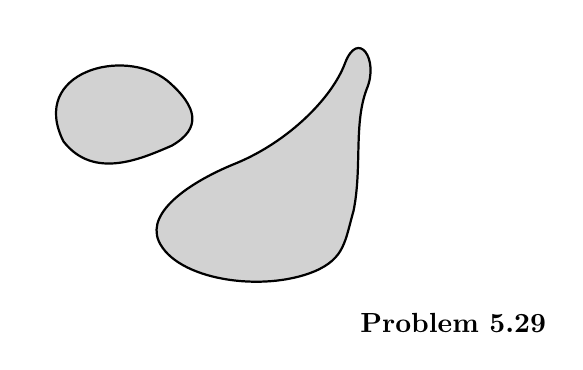
\begin{tikzpicture}[scale=1.1]
  % two irregular conductor cross-sections
  \fill[gray!35] (-1.9,0.6) .. controls (-2.3,1.4) and (-1.2,1.7) .. (-0.7,1.3)
    .. controls (-0.35,1.0) and (-0.3,0.75) .. (-0.65,0.55)
    .. controls (-1.0,0.4) and (-1.55,0.15) .. (-1.9,0.6) -- cycle;
  \draw[thick] (-1.9,0.6) .. controls (-2.3,1.4) and (-1.2,1.7) .. (-0.7,1.3)
    .. controls (-0.35,1.0) and (-0.3,0.75) .. (-0.65,0.55)
    .. controls (-1.0,0.4) and (-1.55,0.15) .. (-1.9,0.6) -- cycle;
  \fill[gray!35] (1.0,-0.9) .. controls (0.4,-1.15) and (-0.6,-1.0) .. (-0.8,-0.55)
    .. controls (-0.95,-0.2) and (-0.4,0.15) .. (0.1,0.35)
    .. controls (0.7,0.6) and (1.2,1.1) .. (1.35,1.5)
    .. controls (1.5,1.9) and (1.75,1.55) .. (1.6,1.2)
    .. controls (1.45,0.8) and (1.55,0.3) .. (1.45,-0.2)
    .. controls (1.35,-0.55) and (1.35,-0.75) .. (1.0,-0.9) -- cycle;
  \draw[thick] (1.0,-0.9) .. controls (0.4,-1.15) and (-0.6,-1.0) .. (-0.8,-0.55)
    .. controls (-0.95,-0.2) and (-0.4,0.15) .. (0.1,0.35)
    .. controls (0.7,0.6) and (1.2,1.1) .. (1.35,1.5)
    .. controls (1.5,1.9) and (1.75,1.55) .. (1.6,1.2)
    .. controls (1.45,0.8) and (1.55,0.3) .. (1.45,-0.2)
    .. controls (1.35,-0.55) and (1.35,-0.75) .. (1.0,-0.9) -- cycle;
  \node at (2.6,-1.5) {\textbf{Problem 5.29}};
\end{tikzpicture}
\end{center}

Show that the product of the inductance per unit length $L$ and the capacitance per unit length $C$ is
\[
LC=\mu\epsilon
\]
where $\mu$ and $\epsilon$ are the permeability and the permittivity of the medium surrounding the conductors. (See the discussion about magnetic fields near perfect conductors at the beginning of Section 5.13.)
\solution
Use the perfect-conductor magnetic boundary condition stated in
Section 5.13: no magnetic field in the conductors and no trapped flux.
Let the electrostatic transverse field for voltage difference $V$
be $\mathbf E$, with charges per length $\pm\lambda$, so $\lambda=C'V$.
In the homogeneous exterior medium, $\mathbf E$ is both curl-free
and divergence-free, and normal to each conductor.

The rotated field
$\mathbf H=\gamma\widehat{\mathbf z}\times\mathbf E$ is consequently
curl-free and divergence-free in the transverse exterior region,
and tangent to the conductor surfaces. On a contour around one wire,
\[
\oint\mathbf H\cdot d\mathbf l
=\gamma\oint\mathbf E\cdot\mathbf n\,dl
=\gamma\frac{\lambda}{\epsilon}=I.
\]
Thus $\gamma=\epsilon I/\lambda$.
The energy relation
$\frac{\epsilon}{2}\int E^2d^2x=C'V^2/2$ then gives
\[
W'_m=\frac{\mu}{2}\int H^2d^2x
=\frac{\mu}{\epsilon}\left(\frac{\epsilon I}{C'V}\right)^2
\frac{C'V^2}{2}
=\frac{\mu\epsilon I^2}{2C'}.
\]
Comparing with $W'_m=L'I^2/2$ proves
$\boxed{L'C'=\mu\epsilon}$.
This result concerns the external inductance of perfect conductors.
An internal magnetic field, such as that of a uniform-current wire
in 5.26, adds internal inductance and does not satisfy this same product.


\Needspace{5\baselineskip}
\par\bigskip
\noindent\textbf{5.30}\quad\begin{enumerate}
\item[(a)] Show that a surface current density $K(\phi)=I\cos\phi/2R$ flowing in the axial direction on a right circular cylindrical surface of radius $R$ produces inside the cylinder a uniform magnetic induction $B_{0}=\mu_{0}I/4R$ in a direction perpendicular to the cylinder axis. Show that the field outside is that of a two-dimensional dipole.
\item[(b)] Calculate the total magnetostatic field energy per unit length. How is it divided inside and outside the cylinder?
\item[(c)] What is the inductance per unit length of the system, viewed as a long circuit with current flowing up one side of the cylinder and back the other?
\end{enumerate}
\textbf{Answer:} $L=\pi\mu_{0}/8$.
\solution
\textbf{(a)} Set $K_z=K_0\cos\phi$, $K_0=I/(2R)$.
The axial vector potential solves the two-dimensional Laplace
equation on either side of the sheet. Regularity, decay of the field,
and continuity give
\[
A_z=C\cos\phi\begin{cases}\rho,&\rho<R,\\R^2/\rho,&\rho>R.\end{cases}
\]
Since $B_\rho=\rho^{-1}\partial_\phi A_z$ and
$B_\phi=-\partial_\rho A_z$,
\[
\mathbf B_{\rm in}=-C\widehat{\mathbf y},\qquad
(B_\rho,B_\phi)_{\rm out}
=\frac{CR^2}{\rho^2}(-\sin\phi,\cos\phi).
\]
The jump $B_{\phi,\rm out}-B_{\phi,\rm in}=\mu_0K_z$ gives
$2C\cos\phi=\mu_0I\cos\phi/(2R)$.
Therefore $\boxed{C=B_0=\mu_0I/(4R)}$, and the exterior field is the
two-dimensional dipole field displayed above.

\textbf{(b)} The energy per length inside is
$W'_{\rm in}=\pi R^2B_0^2/(2\mu_0)$.
Outside the magnitude is $B_0R^2/\rho^2$, so
\[
W'_{\rm out}=\frac1{2\mu_0}\int_R^\infty
\frac{B_0^2R^4}{\rho^4}2\pi\rho\,d\rho
=\frac{\pi R^2B_0^2}{2\mu_0}=W'_{\rm in}.
\]
Thus $\boxed{W'_{\rm total}=\pi\mu_0I^2/16}$, divided equally.

\textbf{(c)} The positive axial current integrates to
$\int_{-\pi/2}^{\pi/2}K_zR\,d\phi=I$; the other half carries $-I$.
Accordingly the circuit current is precisely the $I$ in the density,
and
$\boxed{L'=2W'_{\rm total}/I^2=\pi\mu_0/8}$.


\Needspace{5\baselineskip}
\par\bigskip
\noindent\textbf{5.31}\quad An accelerator bending magnet consists of $N$ turns of superconducting cable whose current configuration can be described approximately by the axial current density
\[
J_{z}(\rho,\phi)=\left(\frac{NI}{2R}\right)\!\cos\phi\;\delta(\rho-R)
\]
The right circular current cylinder is centered on the axis of a hollow iron cylinder of inner radius $R'$ ($R'>R$). The relative dimensions ($R$, $R'$ a few centimeters and a magnet length of several meters) permit the use of a two-dimensional approximation, at least away from the ends of the magnet. Assume that the relative permeability of the iron can be taken as infinite. [Then the outer radius of the iron is irrelevant.]
\begin{enumerate}
\item[(a)] Show that the magnetic field inside the current sheath is perpendicular to the axis of the cylinder in the direction defined by $\phi=\pm\pi/2$ and has the magnitude
\[
B_{0}=\left(\frac{\mu_{0}NI}{4R}\right)\!\left[1+\frac{R^{2}}{R'^{2}}\right]
\]
\item[(b)] Show that the magnetic energy inside $r=R$ is augmented (and that outside diminished) relative to the values in the absence of the iron. (Compare part b of Problem 5.30.)
\item[(c)] Show that the inductance per unit length is
\[
\frac{dL}{dz}=\left(\frac{\pi\mu_{0}N^{2}}{8}\right)\!\left[1+\frac{R^{2}}{R'^{2}}\right]
\]
\end{enumerate}
\solution
Let $c_0=\mu_0NI/(4R)$ and $\eta=R^2/R'^2$.
Write
\[
A_z=\cos\phi\begin{cases}C\rho,&\rho<R,\\
D\rho+E/\rho,&R<\rho<R'.\end{cases}
\]
At the inner face of infinitely permeable iron, tangential $H_\phi$
vanishes, so $D-E/R'^2=0$.
At the current sheath, continuity gives $C=D+E/R^2$ and the derivative
jump gives $2E/R^2=\mu_0NI/(2R)$.
These equations yield
$E=c_0R^2$, $D=c_0\eta$, and $C=c_0(1+\eta)$.

\textbf{(a)} As in 5.30 the core field is along $-y$ for the displayed
positive-current convention and has magnitude
\[
\boxed{B_0=c_0(1+\eta)
=\frac{\mu_0NI}{4R}\left(1+\frac{R^2}{R'^2}\right).}
\]
Reversing the current reverses its direction.

\textbf{(b)} Put $W'_0=\pi R^2c_0^2/(2\mu_0)$, the energy in each
region for the corresponding free-space sheath.
Inside, $W'_{\rm in}=W'_0(1+\eta)^2$.
In the gap,
$B^2=D^2+E^2/\rho^4-2DE\cos(2\phi)/\rho^2$.
Angular integration removes the last term, giving
\[
\begin{split}
W'_{\rm out}
&=\frac{\pi}{\mu_0}\int_R^{R'}
(D^2\rho+E^2/\rho^3)d\rho\\
&=\frac{\pi}{2\mu_0}
[D^2(R'^2-R^2)+E^2(R^{-2}-R'^{-2})]
=\boxed{W'_0(1-\eta^2)}.
\end{split}
\]
The iron contributes zero energy in the infinite-permeability limit.
Thus the interior energy increases and the exterior energy decreases.

\textbf{(c)} Their sum is $2W'_0(1+\eta)$.
Dividing twice this energy by the turn current squared gives
\[
\boxed{L'=\frac{\pi\mu_0N^2}{8}(1+\eta).}
\]
The factor is $N^2$, because $I$ is the current in each turn whereas
the sheet strength is proportional to $NI$.


\Needspace{5\baselineskip}
\par\bigskip
\noindent\textbf{5.32}\quad A circular loop of mean radius $a$ is made of wire having a circular cross section of radius $b$, with $b\ll a$. The sketch shows the relevant dimensions and coordinates for this problem.

\begin{center}
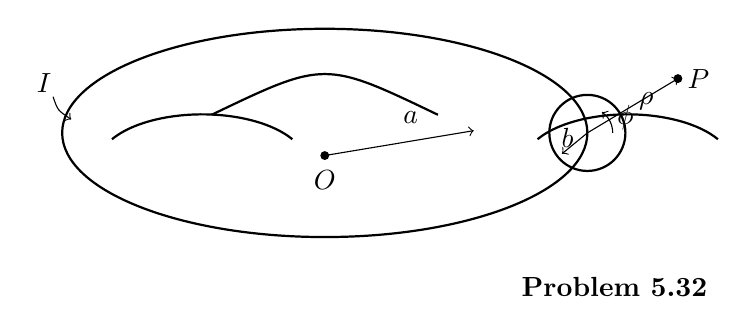
\begin{tikzpicture}[scale=1.15]
  % torus seen obliquely
  \draw[thick] (0,0.35) ellipse (2.9 and 1.15);
  \draw[thick] (-2.35,0.28) arc (150:30:1.15 and 0.55);
  \draw[thick] (2.35,0.28) arc (30:150:-1.15 and 0.55);
  % inner far edge of tube opening
  \draw[thick] (-1.25,0.55) .. controls (0,1.15) and (0,1.15) .. (1.25,0.55);
  % center O
  \fill (0,0.1) circle (1.4pt) node[below=2pt] {$O$};
  % radius a arrow to tube center on right
  \draw[->] (0,0.1) -- (30:1.9 and 0.75);
  \node at (0.95,0.52) {$a$};
  % wire cross-section circle on right
  \draw[thick] (2.9,0.35) circle (0.42);
  % radius b inside the cross-section
  \draw[->] (2.9,0.35) -- (2.62,0.12);
  \node at (2.68,0.3) {$b$};
  % phi angle on the cross-section
  \draw[->] (3.18,0.35) arc (0:55:0.28);
  \node at (3.32,0.52) {$\phi$};
  % rho and P outside
  \draw[->] (2.9,0.35) -- (3.9,0.95);
  \node at (3.55,0.7) {$\rho$};
  \fill (3.9,0.95) circle (1.4pt) node[right] {$P$};
  % current label I on left
  \node at (-3.1,0.9) {$I$};
  \draw[->] (-3.0,0.75) .. controls (-2.95,0.6) .. (-2.8,0.5);
  \node at (3.2,-1.35) {\textbf{Problem 5.32}};
\end{tikzpicture}
\end{center}

\begin{enumerate}
\item[(a)] Using (5.37), the expression for the vector potential of a filamentary circular loop, and appropriate approximations for the elliptic integrals, show that the vector potential at the point $P$ near the wire is approximately
\[
A_{\phi}=(\mu_{0}I/2\pi)[\ln(8a/\rho)-2]
\]
where $\rho$ is the transverse coordinate shown in the figure and corrections are of order $(\rho/a)\cos\phi$ and $(\rho/a)^{2}$.
\item[(b)] Since the vector potential of part a is, apart from a constant, just that outside a straight circular wire carrying a current $I$, determine the vector potential inside the wire ($\rho<b$) in the same approximation by requiring continuity of $A_{\phi}$ and its radial derivative at $\rho=b$, assuming that the current is uniform in density inside the wire:
\[
A_{\phi}=(\mu_{0}I/4\pi)(1-\rho^{2}/b^{2})+(\mu_{0}I/2\pi)[\ln(8a/b)-2],\qquad\rho<b
\]
\item[(c)] Use (5.149) to find the magnetic energy, hence the self-inductance,
\[
L=\mu_{0}a[\ln(8a/b)-7/4]
\]
Are the corrections of order $b/a$ or $(b/a)^{2}$? What is the change in $L$ if the current is assumed to flow only on the surface of the wire (as occurs at high frequencies when the skin depth is small compared to $b$)?
\end{enumerate}
\solution
Distinguish the large cylindrical radius $s$ about the loop axis
from the small local distance $\rho$ from the wire center.
Near the wire, $s=a+\rho\cos\phi$ and $z=\rho\sin\phi$.

\textbf{(a)} From the circular-loop potential, or 5.28 divided by the
circumference $2\pi s$,
\[
A_\varphi=\frac{\mu_0I}{\pi k}\sqrt{\frac as}
\left[\left(1-\frac{k^2}{2}\right)K(k)-E(k)\right],
\quad
k^2=\frac{4as}{(a+s)^2+z^2}.
\]
The complementary modulus is
$k'=\rho/\sqrt{(a+s)^2+z^2}=\rho/(2a)[1+O(\rho/a)]$.
Use $K=\ln(4/k')+O(k'^2\ln k')$ and
$E=1+O(k'^2\ln k')$, with $s\simeq a$, $k\simeq1$:
\[
\boxed{A_\varphi\simeq\frac{\mu_0I}{2\pi}
\left[\ln\frac{8a}{\rho}-2\right].}
\]
The first geometrical correction is proportional to
$(\rho/a)\cos\phi$ (with logarithmic coefficients), followed by
second-order terms. The local angle $\phi$ in the figure is not the
azimuth $\varphi$ specifying the direction of this vector potential.

\textbf{(b)} Locally the straight-wire equation is
$\rho^{-1}(\rho A_\varphi')'=-\mu_0I/(\pi b^2)$.
Integrate once and discard the singular $1/\rho$ derivative at the center:
$A_\varphi'=-\mu_0I\rho/(2\pi b^2)$.
Matching its value to the exterior potential at $\rho=b$ gives
\[
\boxed{A_\varphi=\frac{\mu_0I}{4\pi}\left(1-\frac{\rho^2}{b^2}\right)
+\frac{\mu_0I}{2\pi}\left[\ln\frac{8a}{b}-2\right],\quad\rho<b.}
\]
Its derivative at $b$ is $-\mu_0I/(2\pi b)$, also matching outside.

\textbf{(c)} To this order the volume element is
$2\pi a\,d^2\rho$, and $J=I/(\pi b^2)$.
Since $\langle\rho^2\rangle=b^2/2$ in a uniform disk,
\[
\langle A_\varphi\rangle
=\frac{\mu_0I}{8\pi}
+\frac{\mu_0I}{2\pi}\left[\ln\frac{8a}{b}-2\right]
=\frac{\mu_0I}{2\pi}\left[\ln\frac{8a}{b}-\frac74\right].
\]
Therefore
$W=\tfrac12(2\pi a)I\langle A_\varphi\rangle$
and
\[
\boxed{L=\mu_0a\left[\ln\frac{8a}{b}-\frac74\right].}
\]
Every first-order curvature term contains $\cos\phi$ and averages
to zero, including the first correction to the toroidal volume
element. The surviving corrections start at second order in $b/a$,
possibly multiplied by $\ln(a/b)$.
For surface current the local internal field and its internal energy
vanish; use $A_\varphi(b)$ in the energy integral instead. Then
\[
\boxed{L_{\rm surface}=\mu_0a\left[\ln\frac{8a}{b}-2\right]
=L-\frac{\mu_0a}{4}.}
\]


\Needspace{5\baselineskip}
\par\bigskip
\noindent\textbf{5.33}\quad Consider two current loops (as in Fig.~5.3) whose orientation in space is fixed, but whose relative separation can be changed. Let $O_{1}$ and $O_{2}$ be origins in the two loops, fixed relative to each loop, and $\mathbf{x}_{1}$ and $\mathbf{x}_{2}$ be coordinates of elements $d\mathbf{l}_{1}$ and $d\mathbf{l}_{2}$, respectively, of the loops referred to the respective origins. Let $\mathbf{R}$ be the relative coordinate of the origins, directed from loop 2 to loop 1.
\begin{enumerate}
\item[(a)] Starting from (5.10), the expression for the force between the loops, show that it can be written
\[
\mathbf{F}_{12}=I_{1}I_{2}\nabla_{R}M_{12}(\mathbf{R})
\]
where $M_{12}$ is the mutual inductance of the loops,
\[
M_{12}(\mathbf{R})=\frac{\mu_{0}}{4\pi}\oint\oint\frac{d\mathbf{l}_{1}\cdot d\mathbf{l}_{2}}{|\mathbf{x}_{1}-\mathbf{x}_{2}+\mathbf{R}|}
\]
and it is assumed that the orientation of the loops does not change with $\mathbf{R}$.
\item[(b)] Show that the mutual inductance, viewed as a function of $\mathbf{R}$ \erratum{in any open region where the two filaments do not intersect}, is a solution of the Laplace equation,
\[
\nabla_{R}^{2}M_{12}(\mathbf{R})=0
\]
The importance of this result is that the uniqueness of solutions of the Laplace equation allows the exploitation of the properties of such solutions, provided a solution can be found for a particular value of $\mathbf{R}$.
\end{enumerate}
\solution
\textbf{(a)} Put
$\mathbf s=\mathbf x_1-\mathbf x_2+\mathbf R$.
The magnetic force on loop 1 is
\[
\mathbf F_{12}=\frac{\mu_0I_1I_2}{4\pi}
\oint\oint\frac{d\mathbf l_1\times(d\mathbf l_2\times\mathbf s)}{s^3}.
\]
Expanding the triple product gives
$d\mathbf l_2(d\mathbf l_1\cdot\mathbf s)
-\mathbf s(d\mathbf l_1\cdot d\mathbf l_2)$.
For fixed loop-2 element,
$d\mathbf l_1\cdot\mathbf s/s^3=-d(1/s)$, whose integral around
closed loop 1 is zero. The remaining term is
$(d\mathbf l_1\cdot d\mathbf l_2)\nabla_R(1/s)$.
The loop orientations and their local coordinates are independent
of $\mathbf R$, so the derivative can be taken outside:
\[
\boxed{\mathbf F_{12}=I_1I_2\nabla_RM_{12},\qquad
M_{12}=\frac{\mu_0}{4\pi}\oint\oint
\frac{d\mathbf l_1\cdot d\mathbf l_2}{|\mathbf x_1-\mathbf x_2+\mathbf R|}.}
\]
\textbf{(b)} For any open set of separations in which the filaments
are disjoint, $s>0$ and $\nabla_R^2(1/s)=0$ throughout the integration.
Consequently $\boxed{\nabla_R^2M_{12}=0}$ in that set.
This qualification matters: at intersecting-loop separations, the
distributional identity instead reads
\[
\nabla_R^2M_{12}=-\mu_0\oint\oint d\mathbf l_1\cdot d\mathbf l_2\,
\delta^3(\mathbf R+\mathbf x_1-\mathbf x_2).
\]
Uniqueness and harmonic continuation are therefore used only within
a current-free region of separation space.


\Needspace{5\baselineskip}
\par\bigskip
\noindent\textbf{5.34}\quad Two identical circular loops of radius $a$ are initially located a distance $R$ apart on a common axis perpendicular to their planes.
\begin{enumerate}
\item[(a)] From the expression $W_{12}=\int d^{3}x\,\mathbf{J}_{1}\cdot\mathbf{A}_{2}$ and the result for $A_{\phi}$ from Problem 5.10b, show that the mutual inductance of the loops is
\[
M_{12}=\mu_{0}\pi a^{2}\int_{0}^{\infty}dk\;e^{-kR}J_{1}^{2}(ka)
\]
\item[(b)] Show that for $R>2a$, $M_{12}$ has the expansion,
\[
M_{12}=\frac{\mu_{0}\pi a}{2}\left[\left(\frac{a}{R}\right)^{3}-3\left(\frac{a}{R}\right)^{5}+\frac{75}{8}\left(\frac{a}{R}\right)^{7}+\cdots\right]
\]
\item[(c)] Use the techniques of Section 3.3 for solutions of the Laplace equation to show that the mutual inductance for two coplanar identical circular loops of radius $a$ whose centers are separated by a distance $R>2a$ is
\[
M_{12}=-\frac{\mu_{0}\pi a}{4}\left[\left(\frac{a}{R}\right)^{3}+\frac{9}{4}\left(\frac{a}{R}\right)^{5}+\frac{375}{64}\left(\frac{a}{R}\right)^{7}+\cdots\right]
\]
\item[(d)] Calculate the forces between the loops in the common axis and coplanar configurations. Relate the answers to those of Problem 5.18.
\end{enumerate}
\solution
\textbf{(a)} The azimuthal potential of loop 1 on loop 2 is constant.
Multiplying the result in 5.10(b) at $\rho=a,z=R$ by $2\pi aI_2$ gives
$W_{12}=I_1I_2M_{12}$ with
\[
\boxed{M_\parallel(R)=\mu_0\pi a^2
\int_0^\infty e^{-kR}J_1(ka)^2\,dk.}
\]
\textbf{(b)} The power series
$J_1(x)=\sum_{j\ge0}(-1)^j(x/2)^{2j+1}/[j!(j+1)!]$
gives
\[
J_1(x)^2=\frac{x^2}{4}-\frac{x^4}{16}
+\frac{5x^6}{768}+\cdots.
\]
More generally its coefficient of $(-1)^n(x/2)^{2n+2}$ is
\[
\sum_{j=0}^n\frac1{j!(j+1)!(n-j)!(n-j+1)!}
=\frac{(2n+2)!}{n!(n+2)![(n+1)!]^2}.
\]
This follows by factoring out $1/[n!(n+2)!]$ and applying the
binomial convolution to $\sum_j\binom nj\binom{n+2}{j+1}$.
Integrating each term with
$\int_0^\infty k^m e^{-kR}dk=m!/R^{m+1}$ gives
\[
M_\parallel(R)=\mu_0\pi a\sum_{n=0}^\infty
(-1)^nD_n(a/R)^{2n+3},
\quad
D_n=\frac{[(2n+2)!]^2}{2^{2n+2}n!(n+2)![(n+1)!]^2}.
\]
The ratio test gives convergence for $R>2a$.
For $n=0,1,2$, $D_n=1/2,3/2,75/16$, yielding
\[
\boxed{M_\parallel=\frac{\mu_0\pi a}{2}
\left[(a/R)^3-3(a/R)^5+\frac{75}{8}(a/R)^7+\cdots\right].}
\]
\textbf{(c)} With parallel loop normals fixed, rotational symmetry
makes $M(\mathbf R)$ axisymmetric in separation space.
By 5.33 it is harmonic for $R>2a$ and decays at infinity.
The exterior harmonic with axial value $R^{-2n-3}$ is
$R^{-2n-3}P_{2n+2}(\cos\Theta)$.
Thus replace each term by this angular form.
At $\Theta=\pi/2$,
\[
P_{2n+2}(0)=(-1)^{n+1}
\frac{(2n+2)!}{2^{2n+2}[(n+1)!]^2},
\]
so all terms in the coplanar mutual inductance are negative:
\[
\boxed{M_\perp=-\frac{\mu_0\pi a}{4}
\left[(a/R)^3+\frac94(a/R)^5+\frac{375}{64}(a/R)^7+\cdots\right].}
\]
\textbf{(d)} At fixed currents, $F_R=I_1I_2\,dM/dR$.
For positive $I_1I_2$,
\[
\boxed{F_{R,\parallel}=-\frac{3\mu_0\pi I_1I_2}{2}
(a/R)^4\left[1-5(a/R)^2+\frac{175}{8}(a/R)^4+\cdots\right],}
\]
\[
\boxed{F_{R,\perp}=+\frac{3\mu_0\pi I_1I_2}{4}
(a/R)^4\left[1+\frac{15}{4}(a/R)^2+\frac{875}{64}(a/R)^4+\cdots\right].}
\]
Coaxial like-current loops attract; coplanar like-current loops repel.
Reverse one current and both forces reverse.
For 5.18 use $R=2d$ and $I_2=\chi I_1$ in the axial case,
but $I_2=-\chi I_1$ in the coplanar case. Both then attract a
more-permeable slab, with precisely the two dipole limits found there.


\Needspace{5\baselineskip}
\par\bigskip
\noindent\textbf{5.35}\quad An insulated coil is wound on the surface of a sphere of radius $a$ in such a way as to produce a uniform magnetic induction $B_{0}$ in the $z$ direction inside the sphere and dipole field outside the sphere. The medium inside and outside the sphere has a uniform conductivity $\sigma$ and permeability $\mu$.
\begin{enumerate}
\item[(a)] Find the necessary surface current density $\mathbf{K}$ and show that the vector potential describing the magnetic field has only an azimuthal component, given by
\[
A_{\phi}=\frac{B_{0}a^{2}}{2}\frac{r_{<}}{r_{>}^{2}}\sin\theta
\]
where $r_{<}$ ($r_{>}$) is the smaller (larger) of $r$ and $a$.
\item[(b)] At $t=0$ the current in the coil is cut off. [The coil's presence may be ignored from now on.] With the neglect of Maxwell's displacement current, the decay of the magnetic field is described by the diffusion equation, (5.160). Using a Laplace transform and a spherical Bessel function expansion (3.113), show that the vector potential at times $t>0$ is given by
\[
A_{\phi}=\frac{3B_{0}a}{\pi}\sin\theta\int_{0}^{\infty}e^{-\nu tk^{2}}j_{1}(k)j_{1}\!\left(\frac{kr}{a}\right)dk
\]
where $\nu=1/\mu\sigma a^{2}$ is a characteristic decay rate and $j_{1}(x)$ is the spherical Bessel function of order one. Show that the magnetic field at the center of the sphere can be written explicitly in terms of the error function $\Phi(x)$ as
\[
B_{z}(0,t)=B_{0}\!\left[\Phi\!\left(\frac{1}{\sqrt{4\nu t}}\right)-\frac{1}{\sqrt{\pi\nu t}}\exp\!\left(-\frac{1}{4\nu t}\right)\right]
\]
\item[(c)] Show that the total magnetic energy at time $t>0$ can be written
\[
W_{\mathrm{m}}=\frac{6B_{0}^{2}a^{3}}{\mu}\int_{0}^{\infty}e^{-2\nu tk^{2}}[j_{1}(k)]^{2}\;dk
\]
Show that at long times ($\nu t\gg1$) the magnetic energy decays asymptotically as
\[
W_{\mathrm{m}}\to\frac{\sqrt{2\pi}B_{0}^{2}a^{3}}{24\mu(\nu t)^{3/2}}
\]
\item[(d)] Find a corresponding expression for the asymptotic form of the vector potential (at fixed $r$, $\theta$ and $\nu t\to\infty$) and show that it decays as $(\nu t)^{-3/2}$ as well. Since the energy is quadratic in the field strength, there seems to be a puzzle here. Show by numerical or analytic means that the behavior of the magnetic field at time $t$ is such that, for distances small compared to $R=a(\nu t)^{1/2}\gg a$, the field is uniform with strength $(B_{0}/6\pi^{1/2})\,(\nu t)^{-3/2}$, and for distances large compared to $R$, the field is essentially the original dipole field. Explain physically.
\end{enumerate}
\solution
\textbf{(a)} Write $A_\phi=f(r)\sin\theta$.
A uniform interior field requires $f=B_0r/2$.
Continuity with the decaying exterior dipole requires
$f=B_0a^3/(2r^2)$ outside. Thus
\[
\boxed{A_\phi=\frac{B_0a^2}{2}\frac{r_<}{r_>^2}\sin\theta.}
\]
Its curl gives $B_{r,\rm in}=B_0\cos\theta$,
$B_{\theta,\rm in}=-B_0\sin\theta$, and
$B_{r,\rm out}=B_0(a/r)^3\cos\theta$,
$B_{\theta,\rm out}=(B_0/2)(a/r)^3\sin\theta$.
The tangential jump is $3B_0\sin\theta/2$, so
\[
\boxed{\mathbf K=\frac{3B_0}{2\mu}\sin\theta\,\widehat{\boldsymbol\phi}.}
\]
\textbf{(b)} Put $x=r/a$, $\tau=\nu t$, $\nu=(\mu\sigma a^2)^{-1}$.
The vector diffusion equation reduces to
\[
\partial_tf=\nu\mathcal L_xf,\qquad
\mathcal L_x=\frac{d^2}{dx^2}+\frac2x\frac d{dx}-\frac2{x^2}.
\]
Initially $f=(B_0a/2)g(x)$ with $g=x$ for $x<1$ and $g=x^{-2}$
for $x>1$. Since $g$ is continuous and its first derivative jumps
from $1$ to $-2$, $\mathcal L_xg=-3\delta(x-1)$.
The spherical Bessel functions satisfy
$\mathcal L_xj_1(kx)=-k^2j_1(kx)$ and
\[
\int_0^\infty x^2j_1(kx)j_1(qx)dx
=\frac{\pi}{2k^2}\delta(k-q).
\]
The radial operator is self-adjoint with weight $x^2$: integrating
$u\mathcal L_xv-v\mathcal L_xu$ gives
$[x^2(uv'-u'v)]_0^\infty$. Apply this to $u=j_1(kx)$ and $v=g(x)$,
with a vanishing positive convergence factor at infinity if needed for
the oscillatory integral. The endpoint term vanishes, leaving the
derivative jump at $x=1$. Hence the initial transform satisfies
\[
-k^2\int_0^\infty x^2g(x)j_1(kx)dx
=\int_0^\infty x^2j_1(kx)\mathcal L_xg(x)dx=-3j_1(k).
\]
Thus $\widetilde g(k)=3j_1(k)/k^2$.
Laplace transformation in time gives
$(p+\nu k^2)\overline{\widetilde f}(k,p)
=(B_0a/2)\widetilde g(k)$.
Inverting the Laplace transform yields $e^{-\nu k^2t}$;
inverting the spherical Bessel transform, with measure $2k^2dk/\pi$,
then gives
\[
\boxed{A_\phi=\frac{3B_0a}{\pi}\sin\theta
\int_0^\infty e^{-\tau k^2}j_1(k)j_1(kx)dk.}
\]
Near the center $j_1(kx)=kx/3+O(x^3)$ and a potential
$A_\phi=Cr\sin\theta$ has $B_z=2C$. Hence
\[
B_z(0,t)=\frac{2B_0}{\pi}\int_0^\infty e^{-\tau k^2}
\left(\frac{\sin k}{k}-\cos k\right)dk.
\]
The cosine Gaussian integral is
$\sqrt\pi\,e^{-u^2/(4\tau)}/(2\sqrt\tau)$.
Integrating this identity from $u=0$ to $u=1$ gives
$\int e^{-\tau k^2}\sin k\,dk/k=(\pi/2)\operatorname{erf}(1/(2\sqrt\tau))$.
Therefore
\[
\boxed{B_z(0,t)=B_0\left[
\operatorname{erf}\frac1{2\sqrt\tau}
-\frac{e^{-1/(4\tau)}}{\sqrt{\pi\tau}}\right].}
\]
The question's $\Phi$ denotes this error function, not an electrostatic
potential. The expression tends to $B_0$ as $t\downarrow0$.

\textbf{(c)} Integration by parts gives
$\int B^2d^3x=\int\mathbf A\cdot(-\nabla^2\mathbf A)d^3x$.
The angular integral is $\int\sin^2\theta\,d\Omega=8\pi/3$, so
\[
W_m=\frac{4\pi}{3\mu}\int_0^\infty r^2f(-\mathcal L_rf)\,dr.
\]
Insert the two Bessel integrals for $f$ and $-\mathcal L_rf$.
The second supplies $k^2/a^2$; orthogonality in physical radius gives
$\pi a^3\delta(k-q)/(2k^2)$.
The prefactors reduce to
$(4\pi/3\mu)(3B_0a/\pi)^2(\pi a/2)=6B_0^2a^3/\mu$:
\[
\boxed{W_m=\frac{6B_0^2a^3}{\mu}
\int_0^\infty e^{-2\tau k^2}j_1(k)^2dk.}
\]
At $\tau\gg1$, only $k=O(\tau^{-1/2})$ contributes.
Use $j_1(k)=k/3+O(k^3)$ and
$\int_0^\infty k^2e^{-2\tau k^2}dk=\sqrt\pi/[4(2\tau)^{3/2}]$:
\[
\boxed{W_m\sim\frac{\sqrt{2\pi}B_0^2a^3}{24\mu\,\tau^{3/2}}.}
\]
As a normalization check, the initial energy is the sum of the uniform
interior contribution $2\pi B_0^2a^3/(3\mu)$ and the exterior dipole
contribution $\pi B_0^2a^3/(3\mu)$, namely $\pi B_0^2a^3/\mu$.
The integral formula agrees, since $\int_0^\infty j_1(k)^2dk=\pi/6$.

\textbf{(d)} At fixed $r$, expand both Bessel factors:
\[
A_\phi\sim\frac{3B_0a}{\pi}\frac{x}{9}\sin\theta
\int_0^\infty k^2e^{-\tau k^2}dk
=\boxed{\frac{B_0r\sin\theta}{12\sqrt\pi}\tau^{-3/2}.}
\]
To describe the changing spatial scale, keep $x/\sqrt\tau$ finite
and expand only $j_1(k)$. The remaining integral can be evaluated:
\[
A_\phi\sim\frac{B_0a^3}{2r^2}\mathcal F(s)\sin\theta,\qquad
s=\frac{r}{2a\sqrt\tau},\quad
\mathcal F(s)=\operatorname{erf}s-\frac{2s}{\sqrt\pi}e^{-s^2}.
\]
Indeed the integral of $ke^{-\tau k^2}j_1(kx)$ is
$\pi\mathcal F(x/(2\sqrt\tau))/(2x^2)$, by the same sine and cosine
integrals used for the center field.
Taking the curl gives
\[
B_r\sim\frac{B_0a^3}{r^3}\mathcal F(s)\cos\theta,\qquad
B_\theta\sim\frac{B_0a^3}{2r^3}
[\mathcal F(s)-s\mathcal F'(s)]\sin\theta.
\]
For $s\ll1$, $\mathcal F(s)=4s^3/(3\sqrt\pi)+O(s^5)$, so the
field is uniform to leading order, with
$\boxed{B_{\rm core}\sim B_0\tau^{-3/2}/(6\sqrt\pi)}$.
For $s\gg1$, $\mathcal F\to1$ and $\mathcal F'\to0$, giving the
original dipole field.

There is no conflict between field and total-energy decay: the nearly
uniform region grows to radius $R=O(a\sqrt\tau)$.
Its energy scales as $B_{\rm core}^2R^3\sim\tau^{-3}\tau^{3/2}$.
The exterior dipole energy beyond $R$ scales as $R^{-3}$, the same
$\tau^{-3/2}$. Magnetic diffusion changes a progressively larger
volume; it does not multiply a fixed spatial field shape by one
time-dependent amplitude.


\Needspace{5\baselineskip}
\par\bigskip
\noindent\textbf{5.36}\quad The time-varying magnetic field for $t>0$ in Problem 5.35 induces an electric field and causes current to flow.
\begin{enumerate}
\item[(a)] What components of electric field exist? Determine integral expressions for the components of the electric field and find a simple explicit form of the current density $\mathbf{J}=\sigma\mathbf{E}$ at $t=0^{+}$. Compare your result with the current density of Problem 5.35a. Find the asymptotic behavior of the electric fields in time.
\item[(b)] With Ohm's law and the electric fields found in part a, show that the total power dissipated in the resistive medium can be written
\[
P=\frac{12B_{0}^{2}a^{3}\nu}{\mu}\int_{0}^{\infty}e^{-2\nu tk^{2}}[kj_{1}(k)]^{2}\;dk
\]
Note that the power is the negative time derivative of the \emph{magnetic} energy, $W_{\mathrm{m}}$.
\item[(c)] Because of Ohm's law, the total \emph{electric} energy is $W_{\mathrm{e}}=\epsilon_{0}P/2\sigma$. The total energy is the sum of $W_{\mathrm{e}}$ and $W_{\mathrm{m}}$; its time derivative should be the negative of the power dissipation. Show that the neglect of the energy in the electric field is the same order of approximation as neglect of the displacement current in the equations governing the magnetic field.
\end{enumerate}
\solution
\textbf{(a)} There are no imposed electric charges or scalar-potential
gradients in this axially symmetric diffusion problem. In the
divergence-free gauge,
$\mathbf E=-\partial_t\mathbf A$, so $E_r=E_\theta=0$ and
\[
\boxed{E_\phi(r,\theta,t)=\frac{3B_0a\nu}{\pi}\sin\theta
\int_0^\infty k^2e^{-\tau k^2}j_1(k)j_1(kr/a)dk.}
\]
At $t=0^+$ use $\partial_tf=\nu\mathcal L_xf$ and the initial
$\mathcal L_xg=-3\delta(x-1)$ found in 5.35:
\[
E_\phi(0^+)=\frac{3B_0a\nu}{2}\sin\theta\,\delta(r/a-1)
=\frac{3B_0a^2\nu}{2}\sin\theta\,\delta(r-a).
\]
Since $\sigma a^2\nu=1/\mu$,
\[
\boxed{\mathbf J(0^+)=\frac{3B_0}{2\mu}
\sin\theta\,\delta(r-a)\widehat{\boldsymbol\phi}.}
\]
This induced sheet current initially replaces exactly the switched-off
coil current in 5.35(a). It is a distributional limit: at every positive
time diffusion smooths the sheet, and the instantaneous switch has a
singular initial dissipation in the ideal diffusion model.
For fixed $r$ at late times, differentiate the asymptotic potential:
\[
\boxed{E_\phi\sim\frac{B_0\nu r\sin\theta}{8\sqrt\pi}\tau^{-5/2}.}
\]
This limit is not uniform over radii of order $a\sqrt\tau$ or larger.

\textbf{(b)} Ohmic dissipation is $P=\sigma\int E_\phi^2d^3x$.
The angular integral is again $8\pi/3$, and the physical radial
orthogonality integral is $\pi a^3\delta(k-q)/(2k^2)$.
Consequently
\[
P=\sigma\left(\frac{3B_0a\nu}{\pi}\right)^2
\frac{8\pi}{3}\frac{\pi a^3}{2}
\int_0^\infty k^2e^{-2\tau k^2}j_1(k)^2dk.
\]
Using $\sigma a^2\nu=1/\mu$ reduces this to
\[
\boxed{P=\frac{12B_0^2a^3\nu}{\mu}
\int_0^\infty e^{-2\tau k^2}[kj_1(k)]^2dk
=-\frac{dW_m}{dt}.}
\]
The equality follows independently by differentiating the energy
integral in 5.35(c) for $t>0$.

\textbf{(c)} Because $\mathbf J=\sigma\mathbf E$,
$P=\sigma\int E^2d^3x$, whereas
$W_e=(\epsilon_0/2)\int E^2d^3x$.
Thus $W_e=\epsilon_0P/(2\sigma)$ as stated.
If the fields vary on a time scale $T$, the displacement-to-conduction
current ratio is
\[
\frac{|\epsilon_0\partial_t\mathbf E|}{|\sigma\mathbf E|}
=O\left(\frac{\epsilon_0}{\sigma T}\right).
\]
In the energy balance, the discarded term has the same relative order:
\[
\frac{|dW_e/dt|}{P}
=\frac{\epsilon_0}{2\sigma}\left|\frac{d\ln P}{dt}\right|
=O\left(\frac{\epsilon_0}{\sigma T}\right).
\]
For example, at late times $W_m\propto t^{-3/2}$ and
$P=(3/2)W_m/t\propto t^{-5/2}$, so
$W_e/W_m=3\epsilon_0/(4\sigma t)$ and
$|dW_e/dt|/P=5\epsilon_0/(4\sigma t)$.
Thus retaining electric energy while omitting displacement current
would mix approximation orders. For times comparable to
$\epsilon_0/\sigma$, the neglected current and electric energy must
both be restored; the ideal $t=0^+$ sheet limit is not a claim that
the quasistatic model resolves arbitrarily fast switching.

\clearpage
\section{Chapter 6. Maxwell Equations, Macroscopic Electromagnetism, Conservation Laws}
% Problems, Chapter 6: Maxwell Equations, Macroscopic Electromagnetism, Conservation Laws
% Jackson, Classical Electrodynamics, 3rd ed.
% Requires: amsmath, amssymb, tikz

\section*{Problems}

\Needspace{5\baselineskip}
\par\bigskip
\noindent\textbf{6.1}\quad In three dimensions the solution to the wave equation (6.32) for a point source in space and time (a light flash at $t'=0$, $\mathbf{x}'=0$) is a spherical shell disturbance of radius $R=ct$, namely the Green function $G^{(+)}$ (6.44). It may be initially surprising that in one or two dimensions, the disturbance possesses a ``wake,'' even though the source is a ``point'' in space and time. The solutions for fewer dimensions than three can be found by superposition in the superfluous dimension(s), to eliminate dependence on such variable(s). For example, a flashing line source of uniform amplitude is equivalent to a point source in two dimensions.
\begin{enumerate}
\item[(a)] Starting with the retarded solution to the three-dimensional wave equation (6.47), show that the source $f(\mathbf{x}',t')=\delta(x')\delta(y')\delta(t')$, equivalent to a $t=0$ point source at the origin in two spatial dimensions, produces a two-dimensional wave,
\[
\Psi(x,y,t)=\frac{2c\Theta(ct-\rho)}{\sqrt{c^{2}t^{2}-\rho^{2}}}
\]
where $\rho^{2}=x^{2}+y^{2}$ and $\Theta(\xi)$ is the unit step function [$\Theta(\xi)=0$ ($1$) if $\xi<0$ ($>0$).]
\item[(b)] Show that a ``sheet'' source, equivalent to a point pulsed source at the origin in one space dimension, produces a one-dimensional wave proportional to
\[
\Psi(x,t)=2\pi c\,\Theta(ct-|x|)
\]
\end{enumerate}
\solution

The normalization in (6.32) is $(\nabla^2-c^{-2}\partial_t^2)\Psi=-4\pi f$;
thus (6.47), with no incident homogeneous wave, gives
\[
\Psi(\mathbf x,t)=\int\frac{f(\mathbf x',t-|\mathbf x-\mathbf x'|/c)}
{|\mathbf x-\mathbf x'|}\,d^3x'.
\]
\textbf{(a)} Translation invariance along $z$ permits setting the observation
point's $z$ coordinate to zero. Put $R=(\rho^2+z'^2)^{1/2}$. Then
\[
\Psi=\int_{-\infty}^{\infty}\frac{\delta(t-R/c)}R\,dz'.
\]
There are no roots for $ct<\rho$. For $ct>\rho$ the two roots are
$z'_\pm=\pm\sqrt{c^2t^2-\rho^2}$, and
$|d(t-R/c)/dz'|=|z'|/(cR)$. Hence each root contributes
$c/\sqrt{c^2t^2-\rho^2}$, proving
\[
\boxed{\Psi=\frac{2c\Theta(ct-\rho)}{\sqrt{c^2t^2-\rho^2}}.}
\]
The inverse square root at the wavefront is understood as a locally
integrable distribution, not as a finite pointwise value on the front.

\textbf{(b)} For $f=\delta(x')\delta(t')$, use polar coordinates $s,\varphi$
in the source $y'z'$ plane and $R=(x^2+s^2)^{1/2}$:
\[
\Psi=2\pi\int_0^\infty\frac{s\,ds}{\sqrt{x^2+s^2}}
\delta\left(t-\frac{\sqrt{x^2+s^2}}c\right)
=2\pi\int_{|x|}^{\infty}\delta(t-R/c)\,dR
=\boxed{2\pi c\Theta(ct-|x|)}.
\]
For a fixed observation point, progressively more distant portions of the
line or sheet contribute after the earliest arrival. Their superposition
explains the wake without introducing a propagation speed other than $c$.

\Needspace{5\baselineskip}
\par\bigskip
\noindent\textbf{6.2}\quad The charge and current densities for a single point charge $q$ can be written formally as
\[
\rho(\mathbf{x}',t')=q\delta[\mathbf{x}'-\mathbf{r}(t')];\qquad \mathbf{J}(\mathbf{x}',t')=q\mathbf{v}(t')\delta[\mathbf{x}'-\mathbf{r}(t')]
\]
where $\mathbf{r}(t')$ is the charge's position at time $t'$ and $\mathbf{v}(t')$ is its velocity. In evaluating expressions involving the retarded time, one must put $t'=t_{\mathrm{ret}}=t-R(t')/c$, where $\mathbf{R}=\mathbf{x}-\mathbf{r}(t')$ (but $\mathbf{R}=\mathbf{x}-\mathbf{x}'$ ($t'$) inside the delta functions).
\erratum{Assume a smooth subluminal trajectory and an observation event off
the worldline with a finite retarded intersection. Subluminal motion alone
ensures uniqueness, but does not ensure that such an intersection exists.}
\begin{enumerate}
\item[(a)] As a preliminary to deriving the Heaviside--Feynman expressions for the electric and magnetic fields of a point charge, show that
\[
\int d^{3}x'\;\delta[\mathbf{x}'-\mathbf{r}(t_{\mathrm{ret}})]=\frac{1}{\kappa}
\]
where $\kappa=1-\mathbf{v}\cdot\hat{\mathbf{R}}/c$. Note that $\kappa$ is evaluated at the retarded time.
\item[(b)] Starting with the Jefimenko generalizations of the Coulomb and Biot--Savart laws, use the expressions for the charge and current densities for a point charge and the result of part a to obtain the Heaviside--Feynman expressions for the electric and magnetic fields of a point charge,
\[
\mathbf{E}=\frac{q}{4\pi\epsilon_{0}}\left\{\left[\frac{\hat{\mathbf{R}}}{\kappa R^{2}}\right]_{\mathrm{ret}}+\frac{\partial}{c\partial t}\left[\frac{\hat{\mathbf{R}}}{\kappa R}\right]_{\mathrm{ret}}-\frac{\partial}{c^{2}\partial t}\left[\frac{\mathbf{v}}{\kappa R}\right]_{\mathrm{ret}}\right\}
\]
and
\[
\mathbf{B}=\frac{\mu_{0}q}{4\pi}\left\{\left[\frac{\mathbf{v}\times\hat{\mathbf{R}}}{\kappa R^{2}}\right]_{\mathrm{ret}}+\frac{\partial}{c\partial t}\left[\frac{\mathbf{v}\times\hat{\mathbf{R}}}{\kappa R}\right]_{\mathrm{ret}}\right\}
\]
\item[(c)] In our notation Feynman's expression for the electric field is
\[
\mathbf{E}=\frac{q}{4\pi\epsilon_{0}}\left\{\left[\frac{\hat{\mathbf{R}}}{R^{2}}\right]_{\mathrm{ret}}+\frac{[R]_{\mathrm{ret}}}{c}\frac{\partial}{\partial t}\left[\frac{\hat{\mathbf{R}}}{R^{2}}\right]_{\mathrm{ret}}+\frac{\partial^{2}}{c^{2}\partial t^{2}}\left[\hat{\mathbf{R}}\right]_{\mathrm{ret}}\right\}
\]
while Heaviside's expression for the magnetic field is
\[
\mathbf{B}=\frac{\mu_{0}q}{4\pi}\left\{\left[\frac{\mathbf{v}\times\hat{\mathbf{R}}}{\kappa^{2}R^{2}}\right]_{\mathrm{ret}}+\frac{1}{c[R]_{\mathrm{ret}}}\frac{\partial}{\partial t}\left[\frac{\mathbf{v}\times\hat{\mathbf{R}}}{\kappa}\right]_{\mathrm{ret}}\right\}
\]
Show the equivalence of the two sets of expressions for the fields.
\end{enumerate}
\emph{References}: O. Heaviside, \emph{Electromagnetic Theory}, Vol.~3 (1912), p.~464, Eq.~(214). R.~P. Feynman, \emph{The Feynman Lectures in Physics}, Vol.~1 (1963), Chapter 28, Eq. (28.3).
\solution

Assume a smooth subluminal trajectory and an observation event off the
worldline whose past light cone intersects the trajectory at a finite time.
Write $s=t_{\rm ret}$, $\mathbf n=\hat{\mathbf R}$, $v_n=\mathbf v\cdot\mathbf n$,
and $\kappa=1-v_n/c>0$. Quantities below are evaluated at $s$ unless stated otherwise.

\textbf{(a)} In the spatial integral the retarded time is
$s(\mathbf x')=t-|\mathbf x-\mathbf x'|/c$, so
$\partial s/\partial x'_j=n_j/c$. The derivative matrix of the delta
function's argument is
\[
\frac{\partial[x'_i-r_i(s(\mathbf x'))]}{\partial x'_j}
=\delta_{ij}-\frac{v_i n_j}{c},\qquad
\det\left(\mathbf1-\frac{\mathbf v\mathbf n^{\mathsf T}}c\right)
=1-\frac{\mathbf n\cdot\mathbf v}c=\kappa.
\]
The last equality follows by the rank-one determinant formula.
The function $s+R(s)/c$ has derivative $\kappa>0$, so the assumed
retarded root is unique. Subluminal motion alone does not guarantee
existence: in units $c=1$, the trajectory
$\mathbf r(s)=\sqrt{1+s^2}\,\hat{\mathbf x}$ has $|\mathbf v|<1$,
but an observer at $\mathbf x=0$, $t=0$ would require
$s+\sqrt{1+s^2}=0$, which has no finite solution.
On the stated domain the delta-function rule therefore gives
\[
\int F(\mathbf x')\delta^{(3)}[\mathbf x'-\mathbf r(s(\mathbf x'))]\,d^3x'
=\left[\frac F\kappa\right]_{\rm ret}.
\]
Setting $F=1$ proves the assertion. Omitting this Jacobian would incorrectly
replace a retarded charge distribution by an instantaneous one.

\textbf{(b)} Equations (6.55)--(6.57), with $R=|\mathbf x-\mathbf x'|$
inside the integrals, read
\begin{align*}
\mathbf E&=\frac1{4\pi\epsilon_0}\left\{
\int\frac{\mathbf n[\rho]}{R^2}\,d^3x'
+\frac1c\partial_t\int\frac{\mathbf n[\rho]}R\,d^3x'
-\frac1{c^2}\partial_t\int\frac{[\mathbf J]}R\,d^3x'\right\},\\
\mathbf B&=\frac{\mu_0}{4\pi}\left\{
\int\frac{[\mathbf J]\times\mathbf n}{R^2}\,d^3x'
+\frac1c\partial_t\int\frac{[\mathbf J]\times\mathbf n}R\,d^3x'\right\}.
\end{align*}
At fixed integration point, $\partial_t[\rho]=[\partial_{t'}\rho]$;
this justifies taking the derivatives outside. Applying part (a) to each
integral yields
\begin{align*}
\boxed{\mathbf E}&=\boxed{\frac q{4\pi\epsilon_0}
\left[\frac{\mathbf n}{\kappa R^2}
+\frac1c\partial_t\left(\frac{\mathbf n}{\kappa R}\right)
-\frac1{c^2}\partial_t\left(\frac{\mathbf v}{\kappa R}\right)\right]},\\
\boxed{\mathbf B}&=\boxed{\frac{\mu_0q}{4\pi}
\left[\frac{\mathbf v\times\mathbf n}{\kappa R^2}
+\frac1c\partial_t\left(\frac{\mathbf v\times\mathbf n}{\kappa R}\right)\right]}.
\end{align*}
These derivatives act on the entire retarded expression, including $\kappa$.

\textbf{(c)} Differentiating $t=s+R(s)/c$ at fixed observer gives
\[
\frac{ds}{dt}=\frac1\kappa,\quad
\dot R=-\frac{v_n}\kappa,\quad
\dot{\mathbf n}=\frac{-\mathbf v+v_n\mathbf n}{\kappa R},\quad
\frac1\kappa=1-\frac{\dot R}c.
\]
Here dots denote observation-time derivatives, not source-time derivatives.
In particular,
\[
\frac{\mathbf n}{\kappa R}=\frac{\mathbf n}R-\frac{\mathbf n\dot R}{cR},
\qquad
\frac{\mathbf v}{\kappa R}=-\dot{\mathbf n}-\frac{\mathbf n\dot R}R.
\]
Substitute these into the electric field of part (b). The two derivatives
of $\mathbf n\dot R/R$ cancel, leaving
\begin{align*}
\frac{4\pi\epsilon_0}q\mathbf E
&=\frac{\mathbf n}{R^2}-\frac{\mathbf n\dot R}{cR^2}
+\frac1c\partial_t\left(\frac{\mathbf n}R\right)
+\frac{\ddot{\mathbf n}}{c^2}\\
&=\frac{\mathbf n}{R^2}+\frac Rc\partial_t\left(\frac{\mathbf n}{R^2}\right)
+\frac{\ddot{\mathbf n}}{c^2}.
\end{align*}
For the magnetic field put $\mathbf u=\mathbf v\times\mathbf n$ and expand
only the derivative of $1/R$:
\[
\frac{\mathbf u}{\kappa R^2}+\frac1c\partial_t\frac{\mathbf u}{\kappa R}
=\frac{\mathbf u}{\kappa R^2}\left(1-\frac{\dot R}c\right)
+\frac1{cR}\partial_t\frac{\mathbf u}\kappa
=\frac{\mathbf u}{\kappa^2R^2}+\frac1{cR}\partial_t\frac{\mathbf u}\kappa.
\]
These are precisely Feynman's electric and Heaviside's magnetic formulas.

\Needspace{5\baselineskip}
\par\bigskip
\noindent\textbf{6.3}\quad The homogeneous diffusion equation (5.160) for the vector potential for quasi-static fields in unbounded conducting media has a solution to the initial value problem of the form,
\[
\mathbf{A}(\mathbf{x},t)=\int d^{3}x'\;G(\mathbf{x}-\mathbf{x}',t)\mathbf{A}(\mathbf{x}',0)
\]
where $\mathbf{A}(\mathbf{x}',0)$ describes the initial field configuration and $G$ is an appropriate kernel.
\begin{enumerate}
\item[(a)] Solve the initial value problem by use of a three-dimensional Fourier transform in space for $\mathbf{A}(\mathbf{x},t)$. With the usual assumptions on interchange of orders of integration, show that the Green function has the Fourier representation,
\[
G(\mathbf{x}-\mathbf{x}',t)=\frac{1}{(2\pi)^{3}}\int d^{3}k\;e^{-k^{2}t/\mu\sigma}e^{i\mathbf{k}\cdot(\mathbf{x}-\mathbf{x}')}
\]
and it is assumed that $t>0$.
\item[(b)] By introducing a Fourier decomposition in both space and time, and performing the frequency integral in the complex $\omega$ plane to recover the result of part a, show that $G(\mathbf{x}-\mathbf{x}',t)$ is the diffusion Green function that satisfies the inhomogeneous equation,
\[
\frac{\partial G}{\partial t}-\frac{1}{\mu\sigma}\nabla^{2}G=\delta^{(3)}(\mathbf{x}-\mathbf{x}')\delta(t)
\]
and vanishes for $t<0$.
\item[(c)] Show that if $\sigma$ is uniform throughout all space, the Green function is
\[
G(\mathbf{x},t;\mathbf{x}',0)=\Theta(t)\!\left(\frac{\mu\sigma}{4\pi t}\right)^{3/2}\exp\!\left(\frac{-\mu\sigma|\mathbf{x}-\mathbf{x}'|^{2}}{4t}\right)
\]
\item[(d)] Suppose that at time $t'=0$, the initial vector potential $\mathbf{A}(\mathbf{x}',0)$ is nonvanishing only in a localized region of linear extent $d$ around the origin. The time dependence of the fields is observed at a point $P$ far from the origin, i.e., $|\mathbf{x}|=r\gg d$. Show that there are three regimes of time, $0<t\ll T_{1}$, $T_{1}\ll t\ll T_{2}$, and $t\gg T_{2}$. Give plausible definitions of $T_{1}$ and $T_{2}$, and describe qualitatively the time dependence at $P$. Show that in the last regime, the vector potential is proportional to the volume integral of $\mathbf{A}(\mathbf{x}',0)$ times $t^{-3/2}$, assuming that integral exists. Relate your discussion to those of Section 5.18.B and Problems 5.35 and 5.36.
\end{enumerate}
\solution

Put $D=1/(\mu\sigma)>0$, with constant $\mu,\sigma$. The equation
checked in Section 5.18, (5.160), is $\partial_t\mathbf A=D\nabla^2\mathbf A$.
Each Cartesian component obeys the same scalar equation.

\textbf{(a)} Use $\widetilde{\mathbf A}(\mathbf k,t)=
\int e^{-i\mathbf k\cdot\mathbf x}\mathbf A(\mathbf x,t)\,d^3x$.
Fourier transformation and the initial condition give
\[
\partial_t\widetilde{\mathbf A}=-Dk^2\widetilde{\mathbf A},\qquad
\widetilde{\mathbf A}(\mathbf k,t)=e^{-Dk^2t}\widetilde{\mathbf A}(\mathbf k,0).
\]
Inserting the initial Fourier integral into the inverse transform gives
\[
\mathbf A(\mathbf x,t)=\int d^3x'\,\mathbf A(\mathbf x',0)
\frac1{(2\pi)^3}\int d^3k\,e^{-Dk^2t+i\mathbf k\cdot(\mathbf x-\mathbf x')}.
\]
The inner integral is the required kernel for $t>0$.

\textbf{(b)} With the temporal convention $e^{-i\omega t}$, the causal
inhomogeneous Green function has representation
\[
G(\mathbf R,t)=\int\frac{d^3k\,d\omega}{(2\pi)^4}
\frac{e^{i\mathbf k\cdot\mathbf R-i\omega t}}{Dk^2-i\omega}.
\]
The pole is at $\omega=-iDk^2$. For $t>0$ close the contour in the lower
half-plane, clockwise: the residue $i e^{-Dk^2t}$ gives
$e^{-Dk^2t}$. For $t<0$ the upper contour contains no pole. The $k=0$
pole has the retarded limiting prescription. Consequently
$G=\Theta(t)G_{t>0}$. Acting with $\partial_t-D\nabla^2$ multiplies the
Fourier integrand by $Dk^2-i\omega$, proving the delta-function equation.
Equivalently, its time derivative supplies
$\delta(t)G(\mathbf R,0^+)=\delta(t)\delta^{(3)}(\mathbf R)$.

\textbf{(c)} Completing the square in each of the three Gaussian integrals,
\[
\int_{-\infty}^{\infty}e^{-Dtk_j^2+ik_jR_j}\,dk_j
=\sqrt{\frac\pi{Dt}}e^{-R_j^2/(4Dt)},
\]
yields
\[
\boxed{G(\mathbf x,t;\mathbf x',0)=
\frac{\Theta(t)}{(4\pi Dt)^{3/2}}
\exp\left[-\frac{|\mathbf x-\mathbf x'|^2}{4Dt}\right].}
\]
It has unit spatial integral for every $t>0$, tends to a spatial delta
function as $t\downarrow0$, and satisfies the diffusion equation away from $t=0$.

\textbf{(d)} Suppose $|\mathbf x'|\lesssim d\ll r$. Factor the convolution as
\[
\mathbf A(\mathbf x,t)=\frac{e^{-r^2/(4Dt)}}{(4\pi Dt)^{3/2}}
\int\mathbf A(\mathbf x',0)
\exp\left[\frac{\mathbf x\cdot\mathbf x'}{2Dt}-\frac{r'^2}{4Dt}\right]d^3x'.
\]
Useful definitions, up to order-one factors, are
$T_1=rd/(2D)$ and $T_2=r^2/(4D)$, with $T_1\ll T_2$.
For $t\ll T_1$, the response is exponentially small, of order
$\exp[-(r-d)^2/(4Dt)]$, and can depend strongly on which part of the initial
region is nearest the observer. For $T_1\ll t\ll T_2$, the exponential
inside the integral is nearly one: the region acts as a point source,
but the response still contains the small factor $e^{-r^2/(4Dt)}$.
Near $t\sim T_2$ it becomes appreciable; the monopole kernel itself peaks
at $t=r^2/(6D)$. Finally, for $t\gg T_2$,
\[
\boxed{\mathbf A(\mathbf x,t)\sim
\frac{t^{-3/2}}{(4\pi D)^{3/2}}\int\mathbf A(\mathbf x',0)\,d^3x'.}
\]
If that integral vanishes, this coefficient is zero and higher moments of
the initial data determine the faster decay. In particular, a smooth,
compactly supported, divergence-free Coulomb-gauge potential has
$\int A_i\,d^3x=\int\nabla\cdot(x_i\mathbf A)\,d^3x=0$.
Thus the displayed asymptotic statement need not have a nonzero coefficient
for every physical initial configuration.

The length reached by diffusion is $\sqrt{Dt}$, as in Section 5.18.B's
current sheets; in that effectively one-dimensional geometry the basic
kernel scales as $t^{-1/2}$. Problems 5.35--5.36 instead begin with a
potential extending to infinity as a dipole potential. Their fixed-position
$t^{-3/2}$ field behavior and expanding affected region $r\sim\sqrt{Dt}$
explain why a total energy can decay with a different power from the
square of a field at a fixed point. The compact-support moment argument
above must not be applied to those noncompact initial data without checking
convergence. The arbitrarily early, exponentially small diffusion tail is
part of the quasistatic approximation; it is not an exact relativistic signal.

\Needspace{5\baselineskip}
\par\bigskip
\noindent\textbf{6.4}\quad A uniformly magnetized and conducting sphere of radius $R$ and total magnetic moment $m=4\pi MR^{3}/3$ rotates about its magnetization axis with angular speed $\omega$. In the steady state no current flows in the conductor. The motion is nonrelativistic; the sphere has no excess charge on it.
\begin{enumerate}
\item[(a)] By considering Ohm's law in the moving conductor, show that the motion induces an electric field and a uniform volume charge density in the conductor, $\rho=-m\omega/\pi c^{2}R^{3}$.
\item[(b)] Because the sphere is electrically neutral, there is no monopole electric field outside. Use symmetry arguments to show that the lowest possible electric multipolarity is quadrupole. Show that only a quadrupole field exists outside and that the quadrupole moment tensor has nonvanishing components, $Q_{33}=-4m\omega R^{2}/3c^{2}$, $Q_{11}=Q_{22}=-Q_{33}/2$.
\item[(c)] By considering the radial electric fields inside and outside the sphere, show that the necessary surface-charge density $\sigma(\theta)$ is
\[
\sigma(\theta)=\frac{1}{4\pi R^{2}}\cdot\frac{4m\omega}{3c^{2}}\cdot\left[1-\frac{5}{2}P_{2}(\cos\theta)\right]
\]
\item[(d)] The rotating sphere serves as a unipolar induction device if a stationary circuit is attached by a slip ring to the pole and a sliding contact to the equator. Show that the line integral of the electric field from the equator contact to the pole contact (by any path) is $\mathcal{E}=\mu_{0}m\omega/4\pi R$.
\end{enumerate}
[See Landau and Lifshitz, \emph{Electrodynamics of Continuous Media}, p.~221, for an alternative discussion of this electromotive force.]
\solution

Take the common magnetization and rotation axis to be $z$, with positive
$m\omega$ for parallel vectors. The uniformly magnetized sphere has
$\mathbf B_0=(2\mu_0M/3)\hat{\mathbf z}
=\mu_0m\hat{\mathbf z}/(2\pi R^3)$ inside. Work through first order in
$\omega R/c$; fields of the induced rotating charge change this magnetic
field only at the next relevant order.

\textbf{(a)} To this order Ohm's law in the local moving conductor is
$\mathbf J_{\rm cond}=\sigma(\mathbf E+\mathbf v\times\mathbf B_0)=0$.
With cylindrical radius $s$ and $\mathbf v=\omega s\hat{\boldsymbol\phi}$,
\[
\mathbf E_{\rm in}=-\omega B_0s\hat{\mathbf s},\quad
\Phi_{\rm in}=\frac12\omega B_0s^2+C,\quad
\rho=\epsilon_0\nabla\cdot\mathbf E_{\rm in}
=-2\epsilon_0\omega B_0
=\boxed{-\frac{m\omega}{\pi c^2R^3}}.
\]
Here ``no current'' means no conduction current relative to the sphere;
the induced charge does have a higher-order convection current.

\textbf{(b)} Axial symmetry excludes $m\ne0$, inversion symmetry excludes
odd $l$, and neutrality excludes the exterior $l=0$ term. Moreover,
\[
\Phi_{\rm in}=\frac{\omega B_0r^2}{3}[1-P_2(\cos\theta)]+C.
\]
The surface value contains only $l=0,2$. Uniqueness and decay at infinity
therefore imply an exterior quadrupole alone. Continuity and neutrality fix
\[
C=-\frac{\omega B_0R^2}{3},\qquad
\Phi_{\rm out}=-\frac{\omega B_0R^5}{3r^3}P_2(\cos\theta).
\]
For an axial traceless quadrupole,
$\Phi_Q=Q_{33}P_2/(8\pi\epsilon_0r^3)$. Thus
\[
\boxed{Q_{33}=-\frac{4m\omega R^2}{3c^2},\qquad
Q_{11}=Q_{22}=-\frac12Q_{33}.}
\]
The volume charge is uniform and contributes no traceless quadrupole;
this moment resides in the anisotropic surface charge.

\textbf{(c)} At $r=R$,
\[
E_{r,\rm in}=-\frac{2\omega B_0R}{3}(1-P_2),\qquad
E_{r,\rm out}=-\omega B_0R P_2.
\]
Gauss's boundary condition consequently gives
\[
\sigma=\epsilon_0(E_{r,\rm out}-E_{r,\rm in})
=\frac{\epsilon_0\omega B_0R}{3}(2-5P_2)
=\boxed{\frac1{4\pi R^2}\frac{4m\omega}{3c^2}
\left(1-\frac52P_2\right)}.
\]
Its integral is $4m\omega/(3c^2)$, canceling the volume charge
$\rho(4\pi R^3/3)=-4m\omega/(3c^2)$.

\textbf{(d)} The stationary laboratory fields are electrostatic, so the
integral between the contacts is independent of path:
\[
\int_{\rm equator}^{\rm pole}\mathbf E\cdot d\mathbf l
=\Phi_{\rm equator}-\Phi_{\rm pole}
=\frac12\omega B_0R^2
=\boxed{\frac{\mu_0m\omega}{4\pi R}}.
\]
The motional force on charges in the rotating conductor sustains this
terminal voltage; a wholly stationary electrostatic closed-path integral
still vanishes.

\Needspace{5\baselineskip}
\par\bigskip
\noindent\textbf{6.5}\quad A localized electric charge distribution produces an electrostatic field, $\mathbf{E}=-\nabla\Phi$. Into this field is placed a small localized time-independent current density $\mathbf{J}(\mathbf{x})$, which generates a magnetic field $\mathbf{H}$.
\begin{enumerate}
\item[(a)] Show that the momentum of these electromagnetic fields, (6.117), can be transformed to
\[
\mathbf{P}_{\mathrm{field}}=\frac{1}{c^{2}}\int\Phi\mathbf{J}\;d^{3}x
\]
provided the product $\Phi\mathbf{H}$ falls off rapidly enough at large distances. How rapidly is ``rapidly enough''?
\item[(b)] Assuming that the current distribution is localized to a region small compared to the scale of variation of the electric field, expand the electrostatic potential in a Taylor series and show that
\[
\mathbf{P}_{\mathrm{field}}=\frac{1}{c^{2}}\mathbf{E}(0)\times\mathbf{m}
\]
where $\mathbf{E}(0)$ is the electric field at the current distribution and $\mathbf{m}$ is the magnetic moment, (5.54), caused by the current.
\item[(c)] Suppose the current distribution is placed instead in a \emph{uniform} electric field $\mathbf{E}_{0}$ (filling all space). \erratum{Interpret the conditionally convergent all-space field integrals as limits over concentric spheres.} Show that, no matter how complicated is the localized $\mathbf{J}$, the result in part a is augmented by a surface integral contribution from infinity equal to minus one-third of the result of part b, yielding
\[
\mathbf{P}_{\mathrm{field}}=\frac{2}{3c^{2}}\mathbf{E}_{0}\times\mathbf{m}
\]
Compare this result with that obtained by working directly with (6.117) and the considerations at the end of Section 5.6.
\end{enumerate}
\solution

\textbf{(a)} For a finite volume, $\nabla\times\mathbf H=\mathbf J$ and
$\nabla\times(\Phi\mathbf H)=-\mathbf E\times\mathbf H+\Phi\mathbf J$.
Using the surface theorem for a curl gives
\[
\mathbf P_V=\frac1{c^2}\int_V\mathbf E\times\mathbf H\,d^3x
=\frac1{c^2}\left[\int_V\Phi\mathbf J\,d^3x
-\oint_{\partial V}\Phi\,\mathbf n\times\mathbf H\,da\right].
\]
For spherical surfaces, the sufficient uniform decay condition
$\Phi\mathbf H=o(r^{-2})$ makes the surface term vanish. More generally
it suffices that its angular integral multiplied by $r^2$ tend to zero.
Localized electric and stationary current sources give $\Phi=O(r^{-1})$
and $H=O(r^{-3})$, and hence meet this condition.

\textbf{(b)} Localized steady current obeys $\nabla\cdot\mathbf J=0$.
Integration of $\partial_j(x_iJ_j)$ gives $\int J_i=0$; integration of
$\partial_k(x_ix_jJ_k)$ gives
\[
\int(x_iJ_j+x_jJ_i)\,d^3x=0,\qquad
\int x_iJ_j\,d^3x=\epsilon_{ijk}m_k,
\]
where $m_k=\tfrac12\epsilon_{kij}\int x_iJ_j\,d^3x$.
Expand $\Phi=\Phi(0)-x_iE_i(0)+\cdots$. The constant term integrates to
zero and the linear term gives
\[
(P_{\rm field})_j=-\frac1{c^2}E_i(0)\epsilon_{ijk}m_k+\cdots,
\qquad
\boxed{\mathbf P_{\rm field}=\frac{\mathbf E(0)\times\mathbf m}{c^2}}
\]
to leading order in source size divided by the field-variation length.

\textbf{(c)} Now $\Phi=-\mathbf E_0\cdot\mathbf x$ and the surface term
cannot be discarded. On a large sphere,
\[
\mathbf H=\frac{3\mathbf n(\mathbf m\cdot\mathbf n)-\mathbf m}{4\pi r^3}
+O(r^{-4}),\qquad
\oint\Phi\mathbf n\times\mathbf H\,da
=\frac1{4\pi}\int(\mathbf E_0\cdot\mathbf n)(\mathbf n\times\mathbf m)\,d\Omega
=\frac13\mathbf E_0\times\mathbf m.
\]
We used $\int n_in_j\,d\Omega=4\pi\delta_{ij}/3$. The volume term in
part (a) is exactly $\mathbf E_0\times\mathbf m$ for any localized current,
so
\[
\boxed{\mathbf P_{\rm field}=\frac{2}{3c^2}\mathbf E_0\times\mathbf m}.
\]
Directly, $\mathbf A=\mu_0\mathbf m\times\mathbf n/(4\pi r^2)+O(r^{-3})$
implies
\[
\int\mathbf B\,d^3x=\lim_{R\to\infty}\oint\mathbf n\times\mathbf A\,da
=\frac{\mu_0}{4\pi}\int[\mathbf m-\mathbf n(\mathbf n\cdot\mathbf m)]\,d\Omega
=\frac{2\mu_0}{3}\mathbf m.
\]
Then $\epsilon_0\mathbf E_0\times\int\mathbf B$ gives the same result,
including the interior field emphasized in Section 5.6. The all-space
uniform-field integral is conditionally convergent; the specified result
uses concentric spherical exhaustion. Other asymptotic boundary shapes
need not give the same integral. A localized physical source of an almost
uniform electric field instead has the vanishing surface term of part (a).

\Needspace{5\baselineskip}
\par\bigskip
\noindent\textbf{6.6}\quad\begin{enumerate}
\item[(a)] Consider a circular toroidal coil of mean radius $a$ and $N$ turns, with a small uniform cross section of area $A$ (both height and width small compared to $a$). The toroid has a current $I$ flowing in it and there is a point charge $Q$ located at its center. Calculate all the components of field momentum of the system; show that the component along the axis of the toroid is
\[
(\mathbf{P}_{\mathrm{field}})_{z}\approx\pm\frac{\mu_{0}QINA}{4\pi a^{2}}
\]
where the sign depends on the sense of the current flow in the coil. Assume that the electric field of the charge penetrates unimpeded into the region of nonvanishing magnetic field, as would happen for a toroid that is actually a set of $N$ small nonconducting tubes inside which ionized gas moves to provide the current flow.

Check that the answer conforms to the approximation of Problem 6.5b.
\item[(b)] If $Q=10^{-6}$ C ($\approx6\times10^{12}$ electronic charges), $I=1.0$ A, $N=2000$, $A=10^{-4}$ m$^{2}$, $a=0.1$ m, find the electric field at the toroid in volts per meter, the magnetic induction in tesla, and the electromagnetic momentum in newton-seconds. Compare with the momentum of a 10 $\mu$g insect flying at a speed of 0.1 m/s.
\end{enumerate}
[Note that the system of charge and toroid is at rest. Its \emph{total} momentum must vanish. There must therefore be a canceling ``hidden'' mechanical momentum---see Problem 12.8.]
\solution

\textbf{(a)} Let $\eta=\pm1$ specify $\mathbf B=\eta B_\phi\hat{\boldsymbol\phi}$.
In cylindrical coordinates $(s,\phi,z)$ inside an ideal closely wound toroid,
\[
\mathbf E=\frac{Q}{4\pi\epsilon_0}
\frac{s\hat{\mathbf s}+z\hat{\mathbf z}}{(s^2+z^2)^{3/2}},\qquad
B_\phi=\frac{\mu_0NI}{2\pi s}.
\]
Thus $\epsilon_0\mathbf E\times\mathbf B
=\eta\epsilon_0B_\phi(E_s\hat{\mathbf z}-E_z\hat{\mathbf s})$.
The radial part integrates to zero around $\phi$ even without reflection
symmetry of the cross section; hence $P_x=P_y=0$. The axial integral is
\[
P_z=\eta\frac{\mu_0QNI}{4\pi}
\int_A\frac{s\,ds\,dz}{(s^2+z^2)^{3/2}}
\simeq\boxed{\eta\frac{\mu_0QINA}{4\pi a^2}}.
\]
The approximation replaces $s$ by $a$ and $z$ by zero across the small
cross section. Each turn separately is a dipole
$\mathbf m_{\rm turn}=\eta IA\hat{\boldsymbol\phi}$ in its local electric
field $\mathbf E\simeq Q\hat{\mathbf s}/(4\pi\epsilon_0a^2)$.
Summing $c^{-2}\mathbf E\times\mathbf m_{\rm turn}$ over the $N$ turns
reproduces the result. The entire toroid has zero net dipole moment, so
part 6.5(b) cannot be applied once to the whole toroid: its applied electric
field is not uniform on that scale.

\textbf{(b)} Substitution of the specified SI values gives
\[
\boxed{E=8.988\times10^5\ {\rm V\,m^{-1}},\quad
B=4.000\times10^{-3}\ {\rm T},\quad
|\mathbf P_{\rm field}|=2.000\times10^{-12}\ {\rm N\,s}.}
\]
The insect's mass is $10\,\mu{\rm g}=10^{-8}\ {\rm kg}$, so its momentum
is $10^{-9}\ {\rm N\,s}$, about $500$ times larger. These are field
momenta only; the stationary charge--toroid system has compensating
mechanical momentum as specified in the question.

\Needspace{5\baselineskip}
\par\bigskip
\noindent\textbf{6.7}\quad The microscopic current $\mathbf{j}(\mathbf{x},t)$ can be written as
\[
\mathbf{j}(\mathbf{x},t)=\sum_{j}q_{j}\mathbf{v}_{j}\delta(\mathbf{x}-\mathbf{x}_{j}(t))
\]
where the point charge $q_{j}$ is located at the point $\mathbf{x}_{j}(t)$ and has velocity $\mathbf{v}_{j}=d\mathbf{x}_{j}(t)/dt$. Just as for the charge density, this current can be broken up into a ``free'' (conduction) electron contribution and a bound (molecular) current contribution.

Following the averaging procedures of Section 6.6 \emph{and} assuming \emph{nonrelativistic} addition of velocities, consider the averaged current, $\langle\mathbf{j}(\mathbf{x},t)\rangle$.
\begin{enumerate}
\item[(a)] Show that the averaged current can be written in the form of (6.96) with the definitions (6.92), (6.97), and (6.98).
\item[(b)] Show that for a medium whose internal molecular velocities can be neglected, but which is in bulk motion (i.e., $\mathbf{v}_{n}=\mathbf{v}$ for all $n$),
\[
\frac{1}{\mu_{0}}\mathbf{B}-\mathbf{H}=\mathbf{M}+(\mathbf{D}-\epsilon_{0}\mathbf{E})\times\mathbf{v}
\]
This shows that a moving polarization ($\mathbf{P}$) produces an effective magnetization density.
\end{enumerate}
\emph{Hints for part a}: Consider quantities like $(d\mathbf{p}_{n}/dt)$, $(dQ'^{(n)}_{\alpha\beta}/dt)$ and see what they look like. Also note that
\[
\frac{df}{dt}(\mathbf{x}-\mathbf{x}_{n}(t))=-\mathbf{v}_{n}\cdot\nabla f(\mathbf{x}-\mathbf{x}_{n}(t))
\]
\solution

\textbf{(a)} Use the averaging function $f_n=f(\mathbf x-\mathbf x_n)$ of
Section 6.6. For one molecule suppress $n$, write its internal coordinates
and velocities as $\boldsymbol\xi_j,\mathbf u_j$, and its center velocity
as $\mathbf v$. Define
\[
q=\sum_jq_j,\quad p_\alpha=\sum_jq_j\xi_{j\alpha},\quad
S_{\alpha\beta}=\sum_jq_j\xi_{j\alpha}\xi_{j\beta}
=\tfrac13Q'_{\alpha\beta},\quad
U_{\alpha\beta}=\sum_jq_ju_{j\alpha}\xi_{j\beta}.
\]
The factor $3$ in $Q'$ is Jackson's actual convention (6.77); $Q'$ is not
traceless. Repeated Cartesian indices below are summed. Taylor expansion
of (6.94) gives the terms displayed in (6.96):
\[
\langle j_\alpha\rangle_n=qv_\alpha f+\dot p_\alpha f
-(v_\alpha p_\beta+U_{\alpha\beta})\partial_\beta f
+\frac12v_\alpha S_{\beta\gamma}\partial_\beta\partial_\gamma f+\cdots.
\]
The omitted internal-current second spatial moments belong to higher
multipoles in the ellipsis of (6.96). The identities needed to rearrange
the retained terms are
\[
\dot S_{\alpha\beta}=U_{\alpha\beta}+U_{\beta\alpha},\quad
\epsilon_{\alpha\beta\gamma}m_\gamma
=\tfrac12(U_{\beta\alpha}-U_{\alpha\beta}),\quad
\partial_tf=-v_\gamma\partial_\gamma f.
\]
In particular,
\begin{align*}
\partial_t\left(p_\alpha f-\tfrac12S_{\alpha\beta}\partial_\beta f\right)
={}&\dot p_\alpha f-p_\alpha v_\beta\partial_\beta f
-\tfrac12(U_{\alpha\beta}+U_{\beta\alpha})\partial_\beta f
+\tfrac12S_{\alpha\beta}v_\gamma\partial_\beta\partial_\gamma f.
\end{align*}
Adding $\epsilon_{\alpha\beta\gamma}\partial_\beta(m_\gamma f)$
changes the internal-velocity term to $-U_{\alpha\beta}\partial_\beta f$.
The remaining convection terms are exactly
\[
\partial_\beta[(p_\alpha v_\beta-p_\beta v_\alpha)f]
-\frac16\partial_\beta\partial_\gamma
[(Q'_{\alpha\beta}v_\gamma-Q'_{\gamma\beta}v_\alpha)f].
\]
Sum over molecules and restore the free-particle current. With
\begin{align*}
J_\alpha&=\left\langle\sum_{j\,\rm free}q_jv_{j\alpha}
\delta(\mathbf x-\mathbf x_j)+\sum_nq_nv_{n\alpha}\delta(\mathbf x-\mathbf x_n)\right\rangle,\\
M_\alpha&=\left\langle\sum_nm_{n\alpha}\delta(\mathbf x-\mathbf x_n)\right\rangle,\\
D_\alpha-\epsilon_0E_\alpha
&=P_\alpha-\partial_\beta Q_{\alpha\beta},\quad
P_\alpha=\langle\sum_np_{n\alpha}\delta_n\rangle,\quad
Q_{\alpha\beta}=\tfrac16\langle\sum_nQ'^{(n)}_{\alpha\beta}\delta_n\rangle,
\end{align*}
one obtains explicitly
\begin{align*}
\langle j_\alpha\rangle={}&J_\alpha+\partial_t(D_\alpha-\epsilon_0E_\alpha)
+\epsilon_{\alpha\beta\gamma}\partial_\beta M_\gamma\\
&+\partial_\beta\left\langle\sum_n
(p_{n\alpha}v_{n\beta}-p_{n\beta}v_{n\alpha})\delta_n\right\rangle\\
&-\frac16\partial_\beta\partial_\gamma\left\langle\sum_n
(Q'^{(n)}_{\alpha\beta}v_{n\gamma}-Q'^{(n)}_{\gamma\beta}v_{n\alpha})\delta_n\right\rangle
+\cdots .
\end{align*}
This is (6.96), with precisely (6.92), (6.97), and (6.98).

\textbf{(b)} For spatially uniform common $\mathbf v$, the two last lines
are curls. Their effective magnetization is
\[
\mathbf M_{\rm conv}=\mathbf P\times\mathbf v
-(\nabla\cdot\overleftrightarrow Q)\times\mathbf v
=(\mathbf D-\epsilon_0\mathbf E)\times\mathbf v,
\qquad (\nabla\cdot Q)_\alpha=\partial_\beta Q_{\alpha\beta}.
\]
Insert $\langle\mathbf j\rangle=\mathbf J+\partial_t(\mathbf D-\epsilon_0\mathbf E)
+\nabla\times(\mathbf M+\mathbf M_{\rm conv})$ into the averaged microscopic
Amp\`ere equation. Rearrangement gives
\[
\nabla\times\mathbf H=\mathbf J+\partial_t\mathbf D,\qquad
\boxed{\frac{\mathbf B}{\mu_0}-\mathbf H
=\mathbf M+(\mathbf D-\epsilon_0\mathbf E)\times\mathbf v}.
\]
If all internal motion and intrinsic moments vanish, $\mathbf M=0$;
retaining it allows the intrinsic moments mentioned after (6.98).

\Needspace{5\baselineskip}
\par\bigskip
\noindent\textbf{6.8}\quad A dielectric sphere of dielectric constant $\epsilon$ and radius $a$ is located at the origin. There is a uniform applied electric field $E_{0}$ in the $x$ direction. The sphere rotates with an angular velocity $\omega$ about the $z$ axis. Show that there is a magnetic field $\mathbf{H}=-\nabla\Phi_{M}$, where
\[
\Phi_{M}=\frac{3}{5}\left(\frac{\epsilon-\epsilon_{0}}{\epsilon+2\epsilon_{0}}\right)\!\epsilon_{0}E_{0}\omega\!\left(\frac{a}{r_{>}}\right)^{5}\cdot xz
\]
where $r_{>}$ is the larger of $r$ and $a$. The motion is nonrelativistic.

You may use the results of Section 4.4 for the dielectric sphere in an applied field.
\solution

Work to first order in $\omega a/c$, assume a lossless isotropic dielectric
with its induced polarization following the applied field, and neglect
magnetic susceptibility. Section 4.4 gives
\[
\mathbf E_{\rm in}=\frac{3\epsilon_0}{\epsilon+2\epsilon_0}E_0\hat{\mathbf x},
\qquad \mathbf P=P\hat{\mathbf x},\qquad
P=3\epsilon_0\frac{\epsilon-\epsilon_0}{\epsilon+2\epsilon_0}E_0.
\]
The velocity $\mathbf v=\omega(-y,x,0)$ therefore produces the effective
magnetization, to dipole order in the molecular expansion,
\[
\mathbf M_{\rm eff}=\mathbf P\times\mathbf v=P\omega x\hat{\mathbf z}
\quad(r<a),\qquad \mathbf M_{\rm eff}=0\quad(r>a).
\]
The macroscopic polarization is stationary in laboratory coordinates.
There is no free current and $\partial_t\mathbf D=0$, so
$\nabla\times\mathbf H=0$ and $\mathbf H=-\nabla\Phi_M$.
Since $\nabla\cdot\mathbf M_{\rm eff}=0$ in the interior, the only magnetic
scalar-potential source is the surface density
\[
\sigma_M=\mathbf M_{\rm eff}\cdot\mathbf n
=P\omega\frac{xz}{a}=P\omega a\,n_xn_z.
\]
The angular function $n_xn_z$ is a pure $l=2$ harmonic. The regular
interior and decaying exterior solutions continuous at $a$ can thus be
written $\Phi_{M,\rm in}=C xz$ and
$\Phi_{M,\rm out}=C a^5xz/r^5$. At the surface,
\[
H_{r,\rm out}-H_{r,\rm in}
=-\partial_r\Phi_{M,\rm out}+\partial_r\Phi_{M,\rm in}
=(3+2)Ca\,n_xn_z=\sigma_M.
\]
Hence $C=P\omega/5$ and
\[
\boxed{\Phi_M=\frac35\frac{\epsilon-\epsilon_0}{\epsilon+2\epsilon_0}
\epsilon_0E_0\omega\left(\frac a{r_>}\right)^5xz.}
\]
For example, $\mathbf H_{\rm in}=-(P\omega/5)(z\hat{\mathbf x}+x\hat{\mathbf z})$.
The induction is $\mu_0(\mathbf H+\mathbf M_{\rm eff})$ inside and
$\mu_0\mathbf H$ outside; it has continuous normal component. The result
vanishes for $\epsilon=\epsilon_0$ or $\omega=0$, as required.

\Needspace{5\baselineskip}
\par\bigskip
\noindent\textbf{6.9}\quad Discuss the conservation of energy and linear momentum for a macroscopic system of sources and electromagnetic fields in a uniform, isotropic medium described by a permittivity $\epsilon$ and a permeability $\mu$. Show that in a straightforward calculation the energy density, Poynting vector, field-momentum density, and Maxwell stress tensor are given by the Minkowski expressions,
\begin{align*}
u&=\frac{1}{2}\left(\epsilon E^{2}+\mu H^{2}\right)\\
\mathbf{S}&=\mathbf{E}\times\mathbf{H}\\
\mathbf{g}&=\mu\epsilon\mathbf{E}\times\mathbf{H}\\
T_{ij}&=\left[\epsilon E_{i}E_{j}+\mu H_{i}H_{j}-\tfrac{1}{2}\delta_{ij}(\epsilon E^{2}+\mu H^{2})\right]
\end{align*}
What modifications arise if $\epsilon$ and $\mu$ are functions of position?
\solution

Assume instantaneous linear constitutive laws $\mathbf D=\epsilon\mathbf E$,
$\mathbf B=\mu\mathbf H$, real positive time-independent $\epsilon,\mu$,
and let $\rho,\mathbf J$ be the macroscopic free sources. These assumptions
exclude temporal dispersion and absorption already represented by complex
constitutive coefficients.

Dot $\nabla\times\mathbf H=\mathbf J+\partial_t\mathbf D$ with $\mathbf E$
and $\nabla\times\mathbf E=-\partial_t\mathbf B$ with $\mathbf H$. Their
difference, using the divergence of a cross product, gives
\[
\partial_t\left(\tfrac12\epsilon E^2+\tfrac12\mu H^2\right)
+\nabla\cdot(\mathbf E\times\mathbf H)=-\mathbf J\cdot\mathbf E.
\]
Thus $u$ and $\mathbf S$ have exactly the stated forms. Mechanical work
and heat receive $\mathbf J\cdot\mathbf E$, so the integrated total energy
changes by $-\oint\mathbf S\cdot\mathbf n\,da$ for a fixed closed system.

For momentum, eliminate the free sources from
$\mathbf f=\rho\mathbf E+\mathbf J\times\mathbf B$:
\begin{align*}
\mathbf f+\partial_t(\mathbf D\times\mathbf B)
&=\epsilon[\mathbf E(\nabla\cdot\mathbf E)-\mathbf E\times(\nabla\times\mathbf E)]\\
&\quad+\mu[\mathbf H(\nabla\cdot\mathbf H)-\mathbf H\times(\nabla\times\mathbf H)].
\end{align*}
For any vector $\mathbf F$,
$F_i\partial_jF_j-[\mathbf F\times(\nabla\times\mathbf F)]_i
=\partial_j(F_iF_j-\tfrac12\delta_{ij}F^2)$.
Consequently
\[
\boxed{\partial_tg_i+f_i=\partial_jT_{ij},\quad
\mathbf g=\mathbf D\times\mathbf B=\epsilon\mu\mathbf E\times\mathbf H,\quad
T_{ij}=\epsilon E_iE_j+\mu H_iH_j-\delta_{ij}u.}
\]
The outward momentum flux is $-T_{ij}n_j$. Including the mechanical
momentum delivered by $\mathbf f$ gives
$d(\mathbf P_{\rm field}+\mathbf P_{\rm mech})/dt=\oint\overleftrightarrow T\cdot\mathbf n\,da$,
when material does not cross the boundary.

For spatially varying but time-independent $\epsilon(\mathbf x),\mu(\mathbf x)$,
the energy calculation is unchanged. Differentiating the stress coefficients
in the momentum calculation instead gives
\[
\partial_jT_{ij}-\partial_tg_i
=\rho E_i+(\mathbf J\times\mathbf B)_i
-\frac12E^2\partial_i\epsilon-\frac12H^2\partial_i\mu.
\]
Thus the material force density acquires
$-\tfrac12E^2\nabla\epsilon-\tfrac12H^2\nabla\mu$. At sharp interfaces
one uses the traction jump of $T$ rather than multiplying ambiguous
one-sided field values by a delta function. This is the Minkowski
macroscopic momentum partition requested here; it does not identify the
free-source Lorentz term alone with every microscopic force in matter.

\Needspace{5\baselineskip}
\par\bigskip
\noindent\textbf{6.10}\quad With the same assumptions as in Problem 6.9 discuss the conservation of angular momentum. Show that the differential and integral forms of the conservation law are
\[
\frac{\partial}{\partial t}\left(\mathcal{L}_{\mathrm{mech}}+\mathcal{L}_{\mathrm{field}}\right)+\nabla\cdot\overleftrightarrow{\mathbf{M}}=0
\]
and
\[
\frac{d}{dt}\int_{V}\left(\mathcal{L}_{\mathrm{mech}}+\mathcal{L}_{\mathrm{field}}\right)d^{3}x+\int_{S}\mathbf{n}\cdot\overleftrightarrow{\mathbf{M}}\;da=0
\]
where the field angular-momentum density is
\[
\mathcal{L}_{\mathrm{field}}=\mathbf{x}\times\mathbf{g}=\mu\epsilon\,\mathbf{x}\times(\mathbf{E}\times\mathbf{H})
\]
and the flux of angular momentum is described by the tensor
\[
\overleftrightarrow{\mathbf{M}}=\overleftrightarrow{\mathbf{T}}\times\mathbf{x}
\]
\emph{Note}: Here we have used the dyadic notation for $M_{ij}$ and $T_{ij}$. A double-headed arrow conveys a fairly obvious meaning. For example, $\mathbf{n}\cdot\overleftrightarrow{\mathbf{M}}$ is a vector whose $j$th component is $\sum_{i}n_{i}M_{ij}$. The second-rank $\overleftrightarrow{\mathbf{M}}$ can be written as a third-rank tensor, $M_{ijk}=T_{ij}x_{k}-T_{ik}x_{j}$. But in the indices $j$ and $k$ it is antisymmetric and so has only three independent elements. Including the index $i$, $M_{ijk}$ therefore has nine components and can be written as a pseudotensor of the second rank, as above.
\solution

Use the stress and momentum of Problem 6.9, and write the matter's local
rate of electromagnetic momentum acquisition as
$\partial_t p_{{\rm mech},i}=f_i$ (no material transport across the control
volume). Then $\partial_t(p_{{\rm mech},i}+g_i)=\partial_kT_{ki}$,
where $T$ is symmetric. Cross with $\mathbf x$ and define
\[
\mathcal L_{{\rm field},j}=\epsilon_{j\ell m}x_\ell g_m,
\qquad M_{ij}=\epsilon_{jk\ell}T_{ik}x_\ell.
\]
This component convention is precisely
$\overleftrightarrow M=\overleftrightarrow T\times\mathbf x$.
Its divergence is
\begin{align*}
\partial_iM_{ij}
&=\epsilon_{jk\ell}x_\ell\partial_iT_{ik}
+\epsilon_{jki}T_{ik}\\
&=-\epsilon_{j\ell k}x_\ell\partial_iT_{ik},
\end{align*}
because the contraction of a symmetric stress with an antisymmetric
Levi-Civita symbol vanishes. Hence
\[
\boxed{\partial_t(\boldsymbol{\mathcal L}_{\rm mech}
+\boldsymbol{\mathcal L}_{\rm field})+\nabla\cdot\overleftrightarrow M=0,
\qquad
\boldsymbol{\mathcal L}_{\rm field}=\epsilon\mu\,\mathbf x\times(\mathbf E\times\mathbf H).}
\]
Integrating over a fixed $V$ and applying the divergence theorem yields
\[
\boxed{\frac d{dt}\int_V(\boldsymbol{\mathcal L}_{\rm mech}
+\boldsymbol{\mathcal L}_{\rm field})\,d^3x
+\oint_S\mathbf n\cdot\overleftrightarrow M\,da=0.}
\]
Indeed $\mathbf n\cdot M=(\mathbf n\cdot T)\times\mathbf x$ is the
outward angular-momentum flux, the negative of the torque traction.
Spatially varying scalar $\epsilon,\mu$ leave $T$ symmetric; the additional
material torque is $\mathbf x\times[-E^2\nabla\epsilon/2-H^2\nabla\mu/2]$.
If matter flows across the boundary or carries mechanical stress, its
angular-momentum flux must also be included. The formula in the question
uses the same fixed-matter convention as (6.110)--(6.122).

\Needspace{5\baselineskip}
\par\bigskip
\noindent\textbf{6.11}\quad A transverse plane wave is incident normally in vacuum on a perfectly absorbing flat screen.
\begin{enumerate}
\item[(a)] From the law of conservation of linear momentum, show that the pressure (called radiation pressure) exerted on the screen is equal to the field energy per unit volume in the wave.
\item[(b)] In the neighborhood of the earth the flux of electromagnetic energy from the sun is approximately 1.4 kW/m$^{2}$. If an interplanetary ``sailplane'' had a sail of mass 1 g/m$^{2}$ of area and negligible other weight, what would be its maximum acceleration in meters per second squared due to the solar radiation pressure? How does this compare with the acceleration due to the solar ``wind'' (corpuscular radiation)?
\end{enumerate}
\solution

\textbf{(a)} Let the incident wave travel along $+z$. In vacuum,
$B=E/c$, $u=\epsilon_0E^2$, $S_z=cu$, $g_z=u/c$, and the stress has
$T_{zz}=-u$. The momentum incident per unit area per unit time is
$c g_z=u=S_z/c$. A perfectly absorbing screen has no outgoing momentum
flux, so its time-averaged pressure is
\[
\boxed{p_{\rm abs}=\langle u\rangle=\mathcal I/c},
\]
where $\mathcal I=\langle S_z\rangle$ is the intensity. A control-volume
momentum balance across the screen gives the same result.

\textbf{(b)} For mass per area $\Sigma=10^{-3}\ {\rm kg\,m^{-2}}$ and
normal incidence at the stated $\mathcal I=1400\ {\rm W\,m^{-2}}$,
\[
 p_{\rm abs}=4.670\times10^{-6}\ {\rm Pa},\qquad
\boxed{a_{\rm abs}=\frac{\mathcal I}{c\Sigma}
=4.670\times10^{-3}\ {\rm m\,s^{-2}}.}
\]
This is the maximum over orientations for the absorbing sail of part (a).
If ``maximum'' also allows choosing its optical properties, a perfectly
reflecting sail at normal incidence reverses the photon momentum and gives
\[
\boxed{a_{\rm reflect}=\frac{2\mathcal I}{c\Sigma}
=9.340\times10^{-3}\ {\rm m\,s^{-2}}.}
\]
These are the radiation contributions at the specified solar flux; no
payload or solar-gravity subtraction is included.

A solar-wind comparison needs density and speed, neither specified in
the problem. As an explicit representative estimate, take proton density
$n_p=5\ {\rm cm^{-3}}$ and speed $v=440\ {\rm km\,s^{-1}}$, the values
given by E. Moebius in NASA/GSFC's \emph{Cosmicopia}, ``Solar Wind
Electricity?'' (October 2006).
\footnote{\texttt{https://science.gsfc.nasa.gov/attic/cosmicopia.gsfc.nasa.gov/qa\_sun.html}.}
For complete absorption of the protons,
\[
p_{\rm wind}=n_pm_pv^2=1.619\times10^{-9}\ {\rm Pa},\qquad
\boxed{a_{\rm wind}=1.619\times10^{-6}\ {\rm m\,s^{-2}}.}
\]
It is $3.47\times10^{-4}$ of the absorbing-radiation acceleration
(about $2.88\times10^3$ times smaller). Perfect reflection doubles the
particle result too. Composition, solar activity, and the sail's particle
stopping fraction alter this estimate; the specified numbers make the
comparison reproducible.

\Needspace{5\baselineskip}
\par\bigskip
\noindent\textbf{6.12}\quad Consider the definition of the admittance $Y=G-iB$ of a two-terminal linear passive network in terms of field quantities by means of the complex Poynting theorem of Section 6.9.
\begin{enumerate}
\item[(a)] By considering the complex conjugate of (6.134) obtain general expressions for the conductance $G$ and susceptance $B$ for the general case including radiation loss.
\item[(b)] Show that at low frequencies the expressions equivalent to (6.139) and (6.140) are
\begin{align*}
G&\simeq\frac{1}{|V_{i}|^{2}}\int_{V}\sigma|\mathbf{E}|^{2}\;d^{3}x\\
B&\simeq-\frac{4\omega}{|V_{i}|^{2}}\int_{V}(w_{m}-w_{e})\;d^{3}x
\end{align*}
\end{enumerate}
\solution

\textbf{(a)} Use the book's $e^{-i\omega t}$ convention. Define
\[
C_J=\int_V\mathbf E\cdot\mathbf J^*\,d^3x,\quad
\Delta W=\int_V(w_m-w_e)\,d^3x,\quad
P_S=\int_{S-S_i}\tfrac12(\mathbf E\times\mathbf H^*)\cdot\mathbf n\,da.
\]
The energy densities may be complex when constitutive losses are included.
Equation (6.136), obtained from (6.134) by isolating the input port, is
\[
\tfrac12I_i^*V_i=\tfrac12C_J-2i\omega\Delta W+P_S.
\]
Complex conjugation is essential because $I_i=YV_i$:
\[
Y|V_i|^2=C_J^*+4i\omega\Delta W^*+2P_S^*.
\]
With $Y=G-iB$, taking real and imaginary parts yields the general formulas
\begin{align*}
\boxed{G}&=\boxed{\frac{\operatorname{Re}C_J+4\omega\operatorname{Im}\Delta W
+2\operatorname{Re}P_S}{|V_i|^2}},\\
\boxed{B}&=\boxed{\frac{\operatorname{Im}C_J-4\omega\operatorname{Re}\Delta W
+2\operatorname{Im}P_S}{|V_i|^2}}.
\end{align*}
If the non-port boundary is in the outgoing radiation zone at infinity,
$P_S$ is real and nonnegative: its contribution $2P_S/|V_i|^2$ is the
radiation conductance. On a finite boundary its imaginary part must also
be retained. Material loss must be counted either in $C_J$ or in the
constitutive coefficients, without double counting.

\textbf{(b)} At low frequency neglect radiation and take the only
appreciable dissipation to be $\mathbf J=\sigma\mathbf E$, with real
$\sigma$. Then $C_J=\int\sigma|\mathbf E|^2$ is real and $w_e,w_m$ are
real to the retained accuracy. Thus
\[
\boxed{G\simeq\frac{\int_V\sigma|\mathbf E|^2\,d^3x}{|V_i|^2},\qquad
B\simeq-\frac{4\omega}{|V_i|^2}\int_V(w_m-w_e)\,d^3x.}
\]
A capacitor gives $B=\omega C>0$ and $Y=-i\omega C$, verifying the
susceptance sign for this time convention.

\Needspace{5\baselineskip}
\par\bigskip
\noindent\textbf{6.13}\quad A parallel plate capacitor is formed of two flat rectangular perfectly conducting sheets of dimensions $a$ and $b$ separated by a distance $d$ small compared to $a$ or $b$. Current is fed in and taken out uniformly along the adjacent edges of length $b$. With the input current and voltage defined at this end of the capacitor, calculate the input impedance or admittance using the field concepts of Section 6.9.
\begin{enumerate}
\item[(a)] Calculate the electric and magnetic fields in the capacitor correct to second order in powers of the frequency, but neglecting fringing fields.
\item[(b)] Show that the expansion of the reactance (6.140) in powers of the frequency to an appropriate order is the same as that obtained for a lumped circuit consisting of a capacitance $C=\epsilon_{0}ab/d$ in series with an inductance $L=\mu_{0}ad/3b$.
\end{enumerate}
\solution

Choose $x=0$ at the input and $x=a$ at the far edge, the plate normal along
$z$, and fields independent of $y,z$ within the gap. Neglect fringing and
use $e^{-i\omega t}$, $k=\omega/c$. Define voltage so that
$V_i=dE_z(0)$ and input current $I_i=-bH_y(0)$; these are the passive port
signs when positive plate charge produces positive $E_z$.

\textbf{(a)} Maxwell's curl equations reduce to
\[
-E_z'=i\omega\mu_0H_y,\qquad H_y'=-i\omega\epsilon_0E_z,
\qquad E_z''+k^2E_z=0.
\]
No current passes beyond $x=a$, so $H_y(a)=0$ and $E_z'(a)=0$.
The exact one-dimensional solution normalized to the total input current is
\[
E_z(x)=\frac{I_i k}{-i\omega\epsilon_0 b}
\frac{\cos[k(a-x)]}{\sin ka},\qquad
H_y(x)=-\frac{I_i}{b}\frac{\sin[k(a-x)]}{\sin ka}.
\]
All other components vanish in this approximation. Expanding the spatial
profiles through relative order $k^2$ gives
\begin{align*}
\boxed{E_z(x)}&=\boxed{\frac{I_i}{-i\omega\epsilon_0ab}
\left[1+k^2\left(\frac{a^2}{6}-\frac{(a-x)^2}{2}\right)+O(k^4a^4)\right]},\\
\boxed{H_y(x)}&=\boxed{-\frac{I_i}{b}\frac{a-x}{a}
\left[1+\frac{k^2}{6}\{a^2-(a-x)^2\}+O(k^4a^4)\right]}.
\end{align*}
These expressions also specify the absolute orders: at fixed current,
$E$ starts at $\omega^{-1}$ and $H$ at $\omega^0$. For fixed voltage,
$E_z=(V_i/d)[1+k^2\{a^2-(a-x)^2\}/2+O(k^4)]$ and
$H_y=i\omega\epsilon_0(V_i/d)(a-x)+O(\omega^3)$.

\textbf{(b)} The average of $a^2/6-(a-x)^2/2$ over the plate is zero.
Explicitly,
\[
\int_0^a\left[\frac{a^2}{6}-\frac{(a-x)^2}{2}\right]dx
=\frac{a^3}{6}-\frac12\frac{a^3}{3}=0,\qquad
\int_0^a\left(\frac{a-x}{a}\right)^2dx=\frac a3.
\]
Therefore, at fixed $I_i$, the energy integrals needed through the
inductive term in $X$ are
\begin{align*}
W_e&=\frac{\epsilon_0bd}{4}\int_0^a|E_z|^2dx
=\frac{|I_i|^2d}{4\epsilon_0ab\omega^2}[1+O(k^4a^4)],\\
W_m&=\frac{\mu_0bd}{4}\int_0^a|H_y|^2dx
=\frac{\mu_0|I_i|^2ad}{12b}[1+O(k^2a^2)].
\end{align*}
Equation (6.140) then gives
\[
X=\frac{4\omega(W_m-W_e)}{|I_i|^2}
=-\frac1{\omega C}+\omega L+O(\omega^3),\quad
\boxed{C=\frac{\epsilon_0ab}{d},\qquad L=\frac{\mu_0ad}{3b}}.
\]
The port solution provides an independent exact check:
\[
Z=\frac{V_i}{I_i}=i\sqrt{\frac{\mu_0}{\epsilon_0}}\frac db\cot ka
=\frac{i}{\omega C}-i\omega L+O(\omega^3),\qquad Y=Z^{-1}.
\]
Thus $Z=-iX$ is the stated lossless series $LC$ impedance, within the
small-$ka$ and negligible-fringing approximations.

\Needspace{5\baselineskip}
\par\bigskip
\noindent\textbf{6.14}\quad An ideal circular parallel plate capacitor of radius $a$ and plate separation $d\ll a$ is connected to a current source by axial leads, as shown in the sketch. The current in the wire is $I(t)=I_{0}\cos\omega t$.

\begin{center}
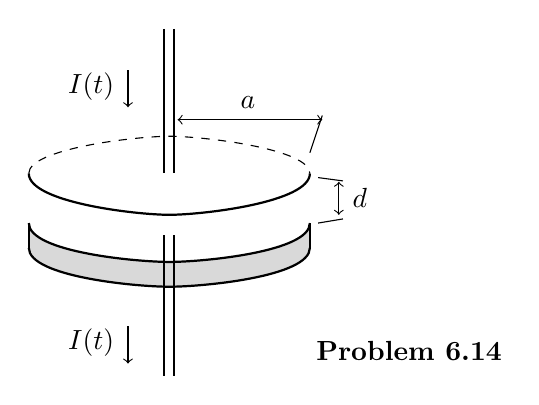
\begin{tikzpicture}[scale=1.05]
  % top plate (drawn as ellipse: flat rim, dashed back edge)
  \draw[thick] (-1.7,0.45) .. controls (-1.7,0.1) and (-0.4,-0.05) .. (0,-0.05)
               .. controls (0.4,-0.05) and (1.7,0.1) .. (1.7,0.45);
  \draw[dashed] (-1.7,0.45) .. controls (-1.7,0.75) and (-0.4,0.9) .. (0,0.9)
               .. controls (0.4,0.9) and (1.7,0.75) .. (1.7,0.45);
  % bottom plate: shaded side
  \fill[gray!30] (-1.7,-0.15) .. controls (-1.7,-0.5) and (-0.4,-0.62) .. (0,-0.62)
               .. controls (0.4,-0.62) and (1.7,-0.5) .. (1.7,-0.15)
               -- (1.7,-0.45) .. controls (1.7,-0.8) and (0.4,-0.92) .. (0,-0.92)
               .. controls (-0.4,-0.92) and (-1.7,-0.8) .. (-1.7,-0.45) -- cycle;
  \draw[thick] (-1.7,-0.15) .. controls (-1.7,-0.5) and (-0.4,-0.62) .. (0,-0.62)
               .. controls (0.4,-0.62) and (1.7,-0.5) .. (1.7,-0.15);
  \draw[thick] (-1.7,-0.45) .. controls (-1.7,-0.8) and (-0.4,-0.92) .. (0,-0.92)
               .. controls (0.4,-0.92) and (1.7,-0.8) .. (1.7,-0.45);
  \draw[thick] (-1.7,-0.15) -- (-1.7,-0.45);
  \draw[thick] (1.7,-0.15) -- (1.7,-0.45);
  % Separate axial leads terminate on their respective plates (source p. 289).
  \draw[thick] (0.06,2.2) -- (0.06,0.45);
  \draw[thick] (-0.06,2.2) -- (-0.06,0.45);
  \draw[thick] (0.06,-0.3) -- (0.06,-2.0);
  \draw[thick] (-0.06,-0.3) -- (-0.06,-2.0);
  % current arrows on the wire
  \draw[->] (-0.5,1.7) -- (-0.5,1.25);
  \node[left] at (-0.55,1.5) {$I(t)$};
  \draw[->] (-0.5,-1.4) -- (-0.5,-1.85);
  \node[left] at (-0.55,-1.6) {$I(t)$};
  % radius arrow a
  \draw[<->] (0.1,1.1) -- (1.85,1.1);
  \node[above] at (0.95,1.12) {$a$};
  \draw (1.7,0.7) -- (1.85,1.15);
  % gap arrow d
  \draw[<->] (2.05,0.35) -- (2.05,-0.05);
  \draw (1.8,0.4) -- (2.1,0.36);
  \draw (1.8,-0.15) -- (2.1,-0.1);
  \node[right] at (2.1,0.15) {$d$};
  \node at (2.9,-1.7) {\textbf{Problem 6.14}};
\end{tikzpicture}
\end{center}

\begin{enumerate}
\item[(a)] Calculate the electric and magnetic fields between the plates to second order in powers of the frequency (or wave number), neglecting the effects of fringing fields.
\item[(b)] Calculate the volume integrals of $w_{e}$ and $w_{m}$ that enter the definition of the reactance $X$, (6.140), \erratum{through second relative order in $\omega a/c$. (For absolute order $\omega^2$ at fixed current, the electric energy also needs the relative $(\omega a/c)^4/192$ correction derived below.)} Show that in terms of the input current $I_{i}$, defined by $I_{i}=-i\omega Q$, where $Q$ is the \emph{total charge} on one plate, these energies are
\[
\int w_{e}\;d^{3}x=\frac{1}{4\pi\epsilon_{0}}\frac{|I_{i}|^{2}d}{\omega^{2}a^{2}},\qquad
\int w_{m}\;d^{3}x=\frac{\mu_{0}}{4\pi}\frac{|I_{i}|^{2}d}{8}\left(1+\frac{\omega^{2}a^{2}}{12c^{2}}\right)
\]
\item[(c)] Show that the equivalent series circuit has $C\simeq\pi\epsilon_{0}a^{2}/d$, $L\simeq\mu_{0}d/8\pi$, and that an estimate for the resonant frequency of the system is $\omega_{\mathrm{res}}\simeq2\sqrt{2}\,c/a$. Compare with the first root of $J_{0}(x)$.
\end{enumerate}
\solution

Use cylindrical radius $s$ and the phasor convention $e^{-i\omega t}$.
Let $Q=\epsilon_0\int E_z\,da$ be the signed plate charge and
$I_i=-i\omega Q$. The axial leads end on their respective plates; there
is no conducting connection through the gap (as in the source sketch on
printed p.~289).

\textbf{(a)} Neglecting fringing, the fields are $E_z(s),H_\phi(s)$.
The curl equations give
\[
-\frac{dE_z}{ds}=i\omega\mu_0H_\phi,\qquad
\frac1s\frac d{ds}(sH_\phi)=-i\omega\epsilon_0E_z,
\qquad \frac1s(sE_z')'+k^2E_z=0.
\]
Regularity at $s=0$ selects $E_z=A J_0(ks)$. Since
$\int_0^a sJ_0(ks)ds=aJ_1(ka)/k$, charge normalization fixes
\[
\boxed{E_z(s)=\frac{I_i k}{-i\omega\,2\pi\epsilon_0aJ_1(ka)}J_0(ks),
\qquad H_\phi(s)=\frac{I_i}{2\pi aJ_1(ka)}J_1(ks).}
\]
Here $B_\phi=\mu_0H_\phi$, and the actual fields are the real parts
of the phasors times $e^{-i\omega t}$. For $ka\ll1$,
\begin{align*}
E_z&=\frac{I_i}{-i\omega\pi\epsilon_0a^2}
\left[1+k^2\left(\frac{a^2}{8}-\frac{s^2}{4}\right)+O(k^4a^4)\right],\\
H_\phi&=\frac{I_i s}{2\pi a^2}
\left[1+\frac{k^2}{8}(a^2-s^2)+O(k^4a^4)\right].
\end{align*}
In particular $2\pi aH_\phi(a)=I_i$ exactly; the field at the rim
contains the total displacement current.

\textbf{(b)} With $w_e=\epsilon_0|E|^2/4$ and $w_m=\mu_0|H|^2/4$,
$\langle s^2\rangle_{\rm disk}=a^2/2$ makes the relative $k^2$ correction
to $W_e$ vanish. For the magnetic integral,
\[
\int_0^a s^3\left[1+\frac{k^2}{4}(a^2-s^2)\right]ds
=\frac{a^4}{4}\left(1+\frac{k^2a^2}{12}\right).
\]
Thus the two displayed leading-order results in the question are
\[
W_e=\frac{|I_i|^2d}{4\pi\epsilon_0\omega^2a^2}[1+O((ka)^4)],\qquad
W_m=\frac{\mu_0|I_i|^2d}{32\pi}
\left[1+\frac{(ka)^2}{12}+O((ka)^4)\right].
\]
There is an ordering subtlety in the wording ``to second order in
$\omega$'': at fixed $I_i$, the leading electric energy is $O(\omega^{-2})$.
For its \emph{absolute} $O(\omega^2)$ term one must retain the relative
$k^4$ correction. The exact Bessel solution settles this without extending
the approximate Maxwell calculation. Writing $z=ka$ and taking Bessel
functions below at $z$,
\[
\int_0^a sJ_\nu(ks)^2\,ds
=\frac{a^2}{2}\left[J_\nu(z)^2-J_{\nu-1}(z)J_{\nu+1}(z)\right].
\]
For $\nu=0$, $J_{-1}=-J_1$ makes the bracket $J_0^2+J_1^2$;
for $\nu=1$ it is $J_1^2-J_0J_2$. The identity follows by
differentiating its right-hand side, using
$2J_\nu'=J_{\nu-1}-J_{\nu+1}$ and
$2\nu J_\nu/z=J_{\nu-1}+J_{\nu+1}$.
Substitution of the exact field amplitudes then gives
\begin{align*}
W_e&=\frac{|I_i|^2d}{4\pi\epsilon_0\omega^2a^2}
\frac{z^2(J_0^2+J_1^2)}{4J_1^2}
=\frac{|I_i|^2d}{4\pi\epsilon_0\omega^2a^2}
\left[1+\frac{z^4}{192}+O(z^6)\right],\\
W_m&=\frac{\mu_0|I_i|^2d}{16\pi}
\left[1-\frac{J_0J_2}{J_1^2}\right].
\end{align*}
The $z^4/192$ term is absent from the book's displayed $W_e$;
it is necessary if both energies are demanded through absolute order
$\omega^2$, but it does not affect the requested leading $L,C$.

\textbf{(c)} From $X=4\omega(W_m-W_e)/|I_i|^2$,
\[
X=-\frac1{\omega C}+\omega L+O(\omega^3),\qquad
\boxed{C=\frac{\pi\epsilon_0a^2}{d},\quad L=\frac{\mu_0d}{8\pi},\quad
\omega_{LC}=\frac1{\sqrt{LC}}=2\sqrt2\,\frac ca.}
\]
The exact energy difference, using $J_0+J_2=2J_1/z$, gives
\[
X=-\frac{\mu_0\omega d}{2\pi}\frac{J_0(z)}{zJ_1(z)}.
\]
Its first zero is $z=j_{0,1}=2.4048255577$, whereas
$2\sqrt2=2.8284271247$: the lumped estimate is $17.61\%$ too high.
This is expected because its putative resonance has $ka$ of order one,
outside the small-frequency expansion. Both results neglect edge and
lead effects; they describe the idealized gap field model.

\Needspace{5\baselineskip}
\par\bigskip
\noindent\textbf{6.15}\quad If a conductor or semiconductor has current flowing in it because of an applied electric field, and a transverse magnetic field is applied, there develops a component of electric field in the direction orthogonal to both the applied electric field (direction of current flow) and the magnetic field, resulting in a voltage difference between the sides of the conductor. This phenomenon is known as the \emph{Hall effect}.
\begin{enumerate}
\item[(a)] Use the known properties of electromagnetic fields under rotations and spatial reflections and the assumption of Taylor series expansions around zero magnetic field strength to show that for an isotropic medium the generalization of Ohm's law, correct to second order in the magnetic field, must have the form
\[
\mathbf{E}=\rho_{0}\mathbf{J}+R(\mathbf{H}\times\mathbf{J})+\beta_{1}H^{2}\mathbf{J}+\beta_{2}(\mathbf{H}\cdot\mathbf{J})\mathbf{H}
\]
where $\rho_{0}$ is the resistivity in the absence of the magnetic field and $R$ is called the Hall coefficient.
\item[(b)] What about the requirements of time reversal invariance?
\end{enumerate}
\solution

\textbf{(a)} Linear response to current means $E_i=\rho_{ij}(\mathbf H)J_j$.
For an isotropic medium the rank-two tensors that can be formed through
second order in the axial vector $\mathbf H$ are
\[
\rho_{ij}=\rho_0\delta_{ij}
+R\epsilon_{ikj}H_k+\beta_1H_kH_k\delta_{ij}+\beta_2H_iH_j+O(H^3).
\]
To see completeness, the zero-order isotropic tensor is $\delta_{ij}$;
the only rank-three isotropic pseudotensor is $\epsilon_{ikj}$; and the
three rank-four delta products, contracted with $H_kH_l$, reduce to
$H^2\delta_{ij}$ and $H_iH_j$. Under inversion $\mathbf E,\mathbf J$
are polar and $\mathbf H$ is axial, so all these terms transform as required.
Consequently
\[
\boxed{\mathbf E=\rho_0\mathbf J+R(\mathbf H\times\mathbf J)
+\beta_1H^2\mathbf J+\beta_2(\mathbf H\cdot\mathbf J)\mathbf H+O(H^3J).}
\]
The Hall part is antisymmetric and does no Joule work:
\[
\mathbf J\cdot\mathbf E=(\rho_0+\beta_1H^2)J_\perp^2
+[\rho_0+(\beta_1+\beta_2)H^2]J_\parallel^2.
\]
Passivity requires these two coefficients to be nonnegative over the field
range in which the expansion is used.

\textbf{(b)} Under time reversal $\mathbf E$ is even, whereas $\mathbf J$
and $\mathbf H$ are odd. Thus the Hall term is even, as required for a
reversible force balance, while the longitudinal dissipative terms are odd.
A resistive macroscopic law with a fixed sign of dissipation is not itself
invariant under reversal of a nonequilibrium history: heat flow and the
reservoir state must be reversed too. It would therefore be incorrect to
set $\rho_0,\beta_1,\beta_2$ to zero by applying time reversal directly to
Ohm's dissipative law.

Microscopic time-reversal symmetry in equilibrium instead implies the
Onsager--Casimir condition $\rho_{ij}(\mathbf H)=\rho_{ji}(-\mathbf H)$,
provided the magnetic field is the only time-reversal-odd bias and there
is no spontaneous magnetic order. The even-in-$H$ symmetric terms and
the odd-in-$H$ antisymmetric Hall term above all satisfy this condition.
It imposes no further relation among the four coefficients.

\Needspace{5\baselineskip}
\par\bigskip
\noindent\textbf{6.16}\quad\begin{enumerate}
\item[(a)] Calculate the force in newtons acting on a Dirac monopole of the minimum magnetic charge located a distance 0.5 \AA\ from and in the median plane of a magnetic dipole with dipole moment equal to one nuclear magneton ($e\hbar/2m_{p}$).
\item[(b)] Compare the force in part a with atomic forces such as the direct electrostatic force between charges (at the same separation), the spin-orbit force, the hyperfine interaction. Comment on the question of binding of magnetic monopoles to nuclei with magnetic moments. Assume that the monopole mass is at least that of a proton.
\end{enumerate}
\emph{Reference}: D. Sivers, \emph{Phys. Rev.} \textbf{D2}, 2048 (1970).
\solution

\textbf{(a)} In the SI convention of (6.153), $eg_D=2\pi\hbar$ and the
static force on a monopole is $g_D\mathbf H=g_D\mathbf B/\mu_0$.
For $\mathbf m=\mu_N\hat{\mathbf z}$, $\mu_N=e\hbar/(2m_p)$, the
\emph{median-plane} dipole field is
$\mathbf B=-\mu_0\mu_N\hat{\mathbf z}/(4\pi r^3)$. It is half the
magnitude of the axial dipole field. Therefore
\[
\mathbf F=-\frac{g_D\mu_N}{4\pi r^3}\hat{\mathbf z}
=-\frac{\hbar^2}{4m_pr^3}\hat{\mathbf z},\qquad
\boxed{|\mathbf F|=1.330\times10^{-11}\ {\rm N}\quad(r=0.5\ \text{\AA}).}
\]
Here $g_D=h/e=4.13567\times10^{-15}\ {\rm Wb}$; a negative monopole
reverses the force.

\textbf{(b)} The Coulomb force at the same separation is
\[
F_C=\frac{e^2}{4\pi\epsilon_0r^2}=9.228\times10^{-8}\ {\rm N},\qquad
\frac{|F|}{F_C}=\frac14\frac{m_e}{m_p}\frac{a_0}{r}
=1.441\times10^{-4}.
\]
Thus the monopole force is about $6940$ times smaller than the direct
atomic electric force. Atomic spin-orbit forces have the characteristic
relativistic scale $\alpha^2F_C\simeq4.91\times10^{-12}\ {\rm N}$ at the
same $r=0.5$~\AA${}\sim a_0$ (angular and state-dependent coefficients are not specified).
The monopole force is about $2.7$ times this scale. For a concrete
hyperfine comparison, two magnetic moments of magnitudes $\mu_B$ and
$\mu_N$ have dipolar energy scale
$\mu_0\mu_B\mu_N/(4\pi r^3)$ and radial force scale
\[
F_{\rm hf}\sim\frac{3\mu_0\mu_B\mu_N}{4\pi r^4}
=2.25\times10^{-15}\ {\rm N}.
\]
The monopole force is roughly $5900$ times this scale. These last two
comparisons are scales, not a claim that every atomic level has a
nonzero spin-orbit or hyperfine force.

The dipole--monopole potential is anisotropic:
\[
U(r,\theta)=\frac{g_D\mu_N}{4\pi r^2}\cos\theta
=\frac{\hbar^2}{4m_pr^2}\cos\theta.
\]
Here $\mathbf r$ points from the fixed dipole to the monopole. The energy
is negative on the $\cos\theta<0$ side and becomes strong at short
distance. Its characteristic magnitude at the stated atomic distance is
$|U|_{\rm scale}=4.15\times10^{-3}\ {\rm eV}$, but at a nuclear cutoff
$r_N$ the same point-dipole estimate grows as $r_N^{-2}$.
A localization kinetic-energy scale for relative mass $m_{\rm red}$ is
$\hbar^2/(2m_{\rm red}r^2)$, so their ratio for a moment of one nuclear
magneton is $m_{\rm red}/(2m_p)$. A heavy monopole and a heavy nucleus
can therefore make the attraction competitive with localization energy;
for a general moment the ratio is $(\mu/\mu_N)\,m_{\rm red}/(2m_p)$.
For an electron, $\mu_B=(m_p/m_e)\mu_N$ merely offsets its small reduced
mass, leaving a ratio of only about $1/2$, so electron binding is much
less favored than binding to a heavy magnetic nucleus.
Binding to suitable magnetic nuclei is consequently plausible despite
the weak force at atomic distances. A universal binding energy or a
proof of binding for every nucleus does not follow from this estimate:
spin, electric charge--monopole angular momentum, the actual nuclear
moment, and the finite nuclear core are required. The mass assumption
alone does not supply those data. In particular the attractive inverse
square potential has no intrinsic length scale, so a physical short-distance
model is indispensable for a binding energy.

\Needspace{5\baselineskip}
\par\bigskip
\noindent\textbf{6.17}\quad\begin{enumerate}
\item[(a)] For a particle possessing both electric and magnetic charges, show that the generalization of the Lorentz force in vacuum is
\[
\mathbf{F}=q_{\mathrm{e}}\mathbf{E}+q_{\mathrm{m}}\mathbf{B}/\mu_{0}+q_{\mathrm{e}}\mathbf{v}\times\mathbf{B}-q_{\mathrm{m}}\mathbf{v}\times\epsilon_{0}\mathbf{E}
\]
\item[(b)] Show that this expression for the force is invariant under a duality transformation of both fields and charges, (6.151) and (6.152).
\item[(c)] Show that the Dirac quantization condition, (6.153), is generalized for two particles possessing electric and magnetic charges $e_{1},g_{1}$ and $e_{2},g_{2}$, respectively, to
\[
\frac{e_{1}g_{2}-e_{2}g_{1}}{\hbar}=2\pi n
\]
and that the relation is invariant under a duality transformation of the charges.
\end{enumerate}
\solution

\textbf{(a)} Duality maps the electric force $q_e(\mathbf E+\mathbf v\times\mathbf B)$
to a magnetic-charge force. In vacuum put
$Z_0=\sqrt{\mu_0/\epsilon_0}=\mu_0c$, and use a quarter-turn of the
normalized field pair $(\mathbf E,c\mathbf B)$. The corresponding magnetic
force is
$q_m(\mathbf B/\mu_0-\epsilon_0\mathbf v\times\mathbf E)$.
Superposition therefore gives
\[
\boxed{\mathbf F=q_e\mathbf E+q_m\mathbf B/\mu_0
+q_e\mathbf v\times\mathbf B-q_m\epsilon_0\mathbf v\times\mathbf E.}
\]
This also has the required power $\mathbf F\cdot\mathbf v
=q_e\mathbf E\cdot\mathbf v+q_m\mathbf H\cdot\mathbf v$;
both velocity cross-product terms do no work.

\textbf{(b)} Express (6.151)--(6.152) as a common rotation by an arbitrary
angle $\chi$ (changing $\chi$ to $-\chi$ exchanges the book's primed/unprimed
convention):
\[
\begin{pmatrix}\mathbf E'\\c\mathbf B'\end{pmatrix}
=\begin{pmatrix}\cos\chi&\sin\chi\\-\sin\chi&\cos\chi\end{pmatrix}
\begin{pmatrix}\mathbf E\\c\mathbf B\end{pmatrix},\qquad
\begin{pmatrix}q_e'\\q_m'/Z_0\end{pmatrix}
=\begin{pmatrix}\cos\chi&\sin\chi\\-\sin\chi&\cos\chi\end{pmatrix}
\begin{pmatrix}q_e\\q_m/Z_0\end{pmatrix}.
\]
With $a=q_e$, $b=q_m/Z_0$, and $\mathbf F_1=\mathbf E$,
$\mathbf F_2=c\mathbf B$, the force is
\[
\mathbf F=a\mathbf F_1+b\mathbf F_2
+\frac{\mathbf v}{c}\times(a\mathbf F_2-b\mathbf F_1).
\]
The first combination is the scalar product of two pairs; the second is
their antisymmetric product. Both are preserved by a common rotation of
determinant one, proving force invariance including all factors of $c,Z_0$.

\textbf{(c)} Rotate particle 1 to a purely electric charge. If it is
nonzero, choose
\[
 e_1'=\sqrt{e_1^2+(g_1/Z_0)^2},\qquad g_1'=0.
\]
The determinant of the two charge vectors is invariant, so
$e_1'g_2'=e_1g_2-e_2g_1$. Applying the electric--magnetic Dirac condition
in that frame gives
\[
\boxed{e_1g_2-e_2g_1=2\pi n\hbar,\qquad n\in\mathbb Z.}
\]
If particle 1 carries neither charge the left side vanishes and $n=0$.
Equivalently, the two-source field angular momentum has coefficient
$(e_1g_2-e_2g_1)/(4\pi)$, whose allowed half-integral multiples of $\hbar$
give the same condition. The determinant argument proves its invariance
under every common duality transformation.

\Needspace{5\baselineskip}
\par\bigskip
\noindent\textbf{6.18}\quad Consider the Dirac expression
\[
\mathbf{A}(\mathbf{x})=\frac{g}{4\pi}\int_{L}\frac{d\mathbf{l}'\times(\mathbf{x}-\mathbf{x}')}{|\mathbf{x}-\mathbf{x}'|^{3}}
\]
for the vector potential of a magnetic monopole and its associated string $L$. Suppose for definiteness that the monopole is located at the origin and the string along the negative $z$ axis.
\begin{enumerate}
\item[(a)] Calculate $\mathbf{A}$ explicitly and show that in spherical coordinates it has components
\[
A_{r}=0,\qquad A_{\theta}=0,\qquad A_{\phi}=\frac{g(1-\cos\theta)}{4\pi r\sin\theta}=\left(\frac{g}{4\pi r}\right)\tan\!\left(\frac{\theta}{2}\right)
\]
\item[(b)] Verify that $\mathbf{B}=\nabla\times\mathbf{A}$ is the Coulomb-like field of a point charge, except perhaps at $\theta=\pi$.
\item[(c)] With the $\mathbf{B}$ determined in part b, evaluate the total magnetic flux passing through the circular loop of radius $R\sin\theta$ shown in the figure. Consider $\theta<\pi/2$ and $\theta>\pi/2$ separately, but always calculate the upward flux.
\item[(d)] From $\oint\mathbf{A}\cdot d\mathbf{l}$ around the loop, determine the total magnetic flux through the loop. Compare the result with that found in part c. Show that they are equal for $0<\theta<\pi/2$, but have a \emph{constant} difference for $\pi/2<\theta<\pi$. Interpret this difference.
\end{enumerate}

\begin{center}
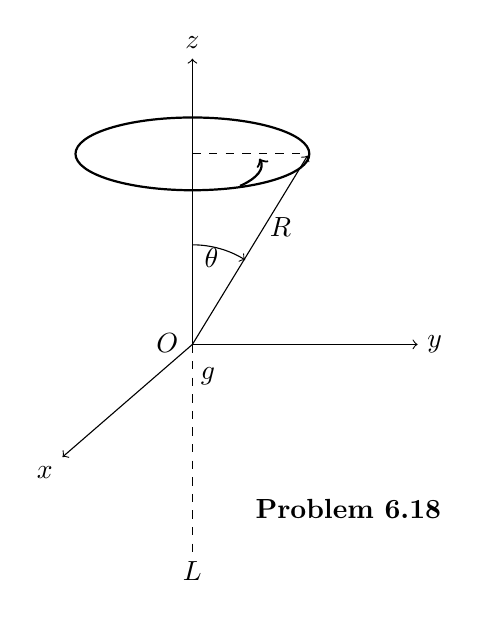
\begin{tikzpicture}[scale=1.1]
  % axes
  \draw[->] (0,0) -- (0,3.3) node[above] {$z$};
  \draw[->] (0,0) -- (2.6,0) node[right] {$y$};
  \draw[->] (0,0) -- (-1.5,-1.3) node[below left] {$x$};
  % dashed string along negative z to L
  \draw[dashed] (0,0) -- (0,-2.4) node[below] {$L$};
  % circular loop (ellipse) at height
  \draw[thick] (0,2.2) ellipse (1.35 and 0.42);
  % thick arrow on the front-right arc showing circulation direction
  \draw[->,thick] (0.55,1.83) arc (-35:10:1.35 and 0.42);
  % R vector from O to the right tip of the loop
  \draw[->] (0,0) -- (1.33,2.18);
  \node[right] at (0.78,1.35) {$R$};
  % theta angle between z axis and R
  \draw[->] (0,1.15) arc (90:58:1.15);
  \node at (0.22,1.0) {$\theta$};
  % origin and g label
  \node[left] at (-0.05,0.02) {$O$};
  \node[below] at (0.18,-0.15) {$g$};
  % dashed radius of the loop (R sin theta)
  \draw[dashed] (0,2.2) -- (1.35,2.2);
  \node at (1.8,-1.9) {\textbf{Problem 6.18}};
\end{tikzpicture}
\end{center}
\solution

\textbf{(a)} Parameterize the string by $\mathbf x'=z'\hat{\mathbf z}$,
$-\infty<z'\le0$, with $d\mathbf l'=\hat{\mathbf z}\,dz'$. Its numerator
is $d\mathbf l'\times(\mathbf x-\mathbf x')=s\hat{\boldsymbol\phi}\,dz'$,
where $s=r\sin\theta$. Thus
\begin{align*}
A_\phi&=\frac g{4\pi}\int_{-\infty}^0
\frac{s\,dz'}{[s^2+(z-z')^2]^{3/2}}\\
&=\frac g{4\pi s}\left(1-\frac z{\sqrt{s^2+z^2}}\right)
=\boxed{\frac g{4\pi r}\frac{1-\cos\theta}{\sin\theta}
=\frac g{4\pi r}\tan\frac\theta2}.
\end{align*}
The other components vanish. This potential is regular on the positive
axis and singular on the negative axis.

\textbf{(b)} Away from that string,
\[
B_r=\frac1{r\sin\theta}\partial_\theta(\sin\theta A_\phi)
=\frac g{4\pi r^2},\qquad
B_\theta=-\frac1r\partial_r(rA_\phi)=0,\qquad B_\phi=0.
\]
Thus the ordinary curl is the monopole field
$\boxed{\mathbf B=g\hat{\mathbf r}/(4\pi r^2)}$ off the string and origin.

\textbf{(c)} The horizontal disk lies at $z_0=R\cos\theta$, with radius
$s_0=R\sin\theta$. For $z_0\ne0$ its upward monopole flux is
\begin{align*}
\Phi_{\rm mono}^{\uparrow}
&=\frac g2\int_0^{s_0}\frac{z_0s\,ds}{(s^2+z_0^2)^{3/2}}
=\frac g2\left[\operatorname{sgn}(z_0)-\frac{z_0}{R}\right]\\
&=\boxed{\begin{cases}
\frac g2(1-\cos\theta),&0<\theta<\pi/2,\\
-\frac g2(1+\cos\theta),&\pi/2<\theta<\pi.
\end{cases}}
\end{align*}
The disk at $\theta=\pi/2$ passes through the monopole and requires a
singular-surface prescription; it is excluded from these two cases.

\textbf{(d)} Counterclockwise circulation viewed from above gives
\[
\oint\mathbf A\cdot d\mathbf l=2\pi R\sin\theta\,A_\phi(R,\theta)
=\boxed{\frac g2(1-\cos\theta)}.
\]
It equals the flux in part (c) for the upper disk, but exceeds that flux
by $g$ for the lower disk. The distributional curl includes a return-flux
string:
\[
\nabla\times\mathbf A=\frac g{4\pi r^2}\hat{\mathbf r}
+g\delta(x)\delta(y)\Theta(-z)\hat{\mathbf z}.
\]
Its upward flux through every disk cutting the negative axis is $g$.
Its divergence is $-g\delta^{(3)}(\mathbf x)$, which cancels the monopole
field's divergence, as every globally defined distributional curl must.
Excluding the string gives the isolated monopole field; retaining it
restores Stokes's theorem for disks crossing the string.

\Needspace{5\baselineskip}
\par\bigskip
\noindent\textbf{6.19}\quad\begin{enumerate}
\item[(a)] Apply space inversion to the monopole vector potential of Problem 6.18 and show that the vector potential becomes
\[
A'_{\phi}=-g\frac{(1+\cos\theta)}{4\pi r\,\sin\theta}=-\frac{g}{4\pi r}\cot\!\left(\frac{\theta}{2}\right)
\]
with the other components vanishing. Show explicitly that its curl gives the magnetic field of a magnetic monopole, except perhaps at $\theta=0$. [Remember the space-inversion properties of the magnetic charge!]
\item[(b)] Show that the difference, $\delta\mathbf{A}=\mathbf{A}'-\mathbf{A}$, can be expressed as the gradient of a scalar function, indicating that the original and space-inverted vector potentials differ by a gauge transformation.
\item[(c)] Interpret the gauge function in terms of Fig.~6.9. [\emph{Hint}: Choose the contour $C$ to be a rectangle lying in a plane containing the $z$ axis, with three sides at infinity.]
\end{enumerate}
\solution

\textbf{(a)} A vector potential is a polar vector, so under active parity
$\mathbf A^P(\mathbf x)=-\mathbf A(-\mathbf x)$, whereas magnetic charge
is a pseudoscalar, $g^P=-g$. At $-\mathbf x$, the angles are
$(\pi-\theta,\phi+\pi)$ and $\hat{\boldsymbol\phi}(\phi+\pi)
=-\hat{\boldsymbol\phi}(\phi)$. Applying these facts to 6.18 gives
\[
\mathbf A^P(\mathbf x)=\frac{g(1+\cos\theta)}{4\pi r\sin\theta}
\hat{\boldsymbol\phi}
=-\frac{g^P(1+\cos\theta)}{4\pi r\sin\theta}\hat{\boldsymbol\phi}.
\]
Now denote the \emph{transformed} monopole charge by $g$, as in the question.
The potential of that charge with its string on the positive axis is
\[
\boxed{A'_\phi=-\frac{g(1+\cos\theta)}{4\pi r\sin\theta}
=-\frac g{4\pi r}\cot\frac\theta2,\qquad A'_r=A'_\theta=0.}
\]
Direct differentiation gives
$B'_r=(r\sin\theta)^{-1}\partial_\theta(\sin\theta A'_\phi)
=g/(4\pi r^2)$ and $B'_\theta=B'_\phi=0$ away from the positive-axis
string. Keeping the original pre-parity charge label instead gives a
monopole of charge $-g$, consistently with its pseudoscalar character.

\textbf{(b)} Comparing potentials of the \emph{same} charge $g$ on their
common nonsingular domain,
\[
\delta\mathbf A=-\frac g{2\pi r\sin\theta}\hat{\boldsymbol\phi}
=\nabla\Lambda,\qquad
\boxed{\Lambda=-\frac g{2\pi}\phi+\hbox{constant}.}
\]
Since $\nabla\phi=\hat{\boldsymbol\phi}/(r\sin\theta)$, this is a gauge
transformation on a patch with a chosen azimuthal cut. The scalar is not
globally single-valued: $\phi\mapsto\phi+2\pi$ changes it by $-g$.
The quantum phase $\exp(i e\Lambda/\hbar)$ is nevertheless single-valued
when $eg=2\pi n\hbar$.

\textbf{(c)} In Fig.~6.9 the contour is $C=L'-L$. For strings on opposite
halves of the $z$ axis, close this contour with three sides of a rectangle
at infinity in a meridian plane. Its spanning surface becomes a half-plane
ending on the axis. On a unit sphere centered at the observer, a change
$d\phi$ sweeps out a spherical lune. Its unsigned area is
\[
\int_\phi^{\phi+d\phi}d\varphi\int_0^\pi\sin\vartheta\,d\vartheta
=2\,d\phi.
\]
The contour orientation $C=L'-L$ assigns the negative sign, so the
oriented solid angle changes by $-2\,d\phi$.
Thus, on a chosen branch,
\[
\Omega_C=-2\phi+\hbox{constant},\qquad
\Lambda=\frac g{4\pi}\Omega_C.
\]
This is exactly Jackson's (6.162). Crossing the half-plane changes the
solid-angle branch by $4\pi$, or the gauge function by $g$ in magnitude;
that jump represents relocation of the unobservable string.

\Needspace{5\baselineskip}
\par\bigskip
\noindent\textbf{6.20}\quad An example of the preservation of causality and finite speed of propagation in spite of the use of the Coulomb gauge is afforded by a dipole source that is flashed on and off at $t=0$. The effective charge and current densities are
\begin{align*}
\rho(\mathbf{x},t)&=\delta(x)\delta(y)\delta'(z)\delta(t)\\
J_{z}(\mathbf{x},t)&=-\delta(x)\delta(y)\delta(z)\delta'(t)
\end{align*}
where a prime means differentiation with respect to the argument. This dipole is of unit strength and it points in the negative $z$ direction.
\begin{enumerate}
\item[(a)] Show that the instantaneous Coulomb potential (6.23) is
\[
\Phi(\mathbf{x},t)=-\frac{1}{4\pi\epsilon_{0}}\;\delta(t)\;\frac{z}{r^{3}}
\]
\item[(b)] Show that the \emph{transverse} current $\mathbf{J}_{t}$ is
\[
\mathbf{J}_{t}(\mathbf{x},t)=-\delta'(t)\!\left[\tfrac{2}{3}\boldsymbol{\epsilon}_{3}\delta(\mathbf{x})-\frac{\boldsymbol{\epsilon}_{3}}{4\pi r^{3}}+\frac{3}{4\pi r^{3}}\,\mathbf{n}(\boldsymbol{\epsilon}_{3}\cdot\mathbf{n})\right]
\]
where the factor of 2/3 multiplying the delta function comes from treating the gradient of $z/r^{3}$ according to (4.20).
\item[(c)] Show that the electric and magnetic fields are causal and that the electric field components are
\[
E_{x}(\mathbf{x},t)=\frac{1}{4\pi\epsilon_{0}}\frac{c}{r}\left[-\delta''(r-ct)+\frac{3}{r}\delta'(r-ct)-\frac{3}{r^{2}}\delta(r-ct)\right]\sin\theta\cos\theta\cos\phi
\]
$E_{y}$ is the same as $E_{x}$, with $\cos\phi$ replaced by $\sin\phi$, and
\[
E_{z}(\mathbf{x},t)=\frac{1}{4\pi\epsilon_{0}}\frac{c}{r}\left[\sin^{2}\theta\,\delta''(r-ct)+(3\cos^{2}\theta-1)\cdot\left(\frac{\delta'(r-ct)}{r}-\frac{\delta(r-ct)}{r^{2}}\right)\right]
\]
\end{enumerate}
\emph{Hint}: While the answer in part b displays the transverse current explicitly, the less explicit form
\[
\mathbf{J}_{t}(\mathbf{x},t)=-\delta'(t)\!\left[\boldsymbol{\epsilon}_{3}\delta(\mathbf{x})+\frac{1}{4\pi}\nabla\frac{\partial}{\partial z}\left(\frac{1}{r}\right)\right]
\]
can be used with (6.47) to calculate the vector potential and the fields for part c. An alternative method is to use the Fourier transforms in time of $\mathbf{J}_{t}$ and $\mathbf{A}$, the Green function (6.40) and its spherical wave expansion from Chapter 9.
\solution

All fields below are distributions, and the explicit spherical formulas
are for $r>0$. Let $K=1/(4\pi\epsilon_0)$ and
$\mathbf e_z=\boldsymbol\epsilon_3$.

\textbf{(a)} Integrating the derivative of the source delta function gives
\[
\Phi_C=K\delta(t)\int\frac{\delta(x')\delta(y')\delta'(z')}
{|\mathbf x-\mathbf x'|}\,d^3x'
=-K\delta(t)\left.\partial_{z'}\frac1{|\mathbf x-\mathbf x'|}\right|_0
=\boxed{-K\delta(t)\frac z{r^3}}.
\]

\textbf{(b)} Charge conservation and $\nabla^2\Phi_C=-\rho/\epsilon_0$
show that the longitudinal current is
$\mathbf J_\ell=\epsilon_0\nabla\partial_t\Phi_C$.
Consequently
\[
\mathbf J_t=\mathbf J-\mathbf J_\ell
=-\delta'(t)\left[\mathbf e_z\delta^{(3)}(\mathbf x)
+\frac1{4\pi}\nabla\partial_z\frac1r\right].
\]
The distributional derivative checked in (4.20) is
\[
\partial_i\partial_j\frac1r
=\frac{3n_in_j-\delta_{ij}}{r^3}
-\frac{4\pi}{3}\delta_{ij}\delta^{(3)}(\mathbf x),
\]
where the $r^{-3}$ expression uses spherical principal-value exclusion.
It changes the contact term from $1$ to $2/3$ and yields
\[
\boxed{\mathbf J_t=-\delta'(t)\left[
\frac23\mathbf e_z\delta^{(3)}(\mathbf x)
-\frac{\mathbf e_z}{4\pi r^3}
+\frac{3\mathbf n n_z}{4\pi r^3}\right].}
\]
Taking a divergence of the less explicit form gives zero, since
$\nabla^2(1/r)=-4\pi\delta^{(3)}(\mathbf x)$.

\textbf{(c)} One can display the instantaneous cancellation without
integrating the spatially nonlocal $\mathbf J_t$ directly. The source is
an electric dipole $\mathbf p(t)=-\mathbf e_z\delta(t)$. Applying the
retarded potential integral (6.47) to the source deltas gives the Lorenz-gauge
potentials, with $\tau=t-r/c$,
\[
\Phi_L=-K n_z\left[\frac{\delta(\tau)}{r^2}
+\frac{\delta'(\tau)}{cr}\right],\qquad
\mathbf A_L=-\frac K{c^2r}\mathbf e_z\delta'(\tau).
\]
For example, the second term in $\Phi_L$ is the derivative of the retarded
time when the source-coordinate derivative acts on the delta function.
Define
\[
\chi=K n_z\left[\frac{\Theta(t)-\Theta(\tau)}{r^2}
-\frac{\delta(\tau)}{cr}\right],\qquad
\mathbf A_C=\mathbf A_L+\nabla\chi.
\]
Direct differentiation gives $\partial_t\chi=\Phi_L-\Phi_C$.
For the spatial check write $\chi=K n_zF$,
$H=\Theta(t)-\Theta(\tau)$, and $F=H/r^2-\delta(\tau)/(cr)$.
Using $\partial_r H=\delta(\tau)/c$ gives
\[
F'=-\frac{2H}{r^3}+\frac{2\delta(\tau)}{cr^2}
+\frac{\delta'(\tau)}{c^2r},\qquad
F''+\frac{2F'}r-\frac{2F}{r^2}
=-\frac{\delta'(\tau)}{c^2r^2}-\frac{\delta''(\tau)}{c^3r}.
\]
The last expression times $K n_z$ is
$-\nabla\cdot\mathbf A_L$. Thus
$\nabla^2\chi=-\nabla\cdot\mathbf A_L$, so $\mathbf A_C$ is the
Coulomb-gauge potential; both statements include the source distributions.
Therefore
\[
-\nabla\Phi_C-\partial_t\mathbf A_C
=-\nabla\Phi_C-\partial_t\mathbf A_L-\nabla(\Phi_L-\Phi_C)
=-\nabla\Phi_L-\partial_t\mathbf A_L.
\]
The instantaneous Coulomb term cancels explicitly. Differentiating the
retarded potentials at $r>0$ yields
\begin{align*}
\mathbf E&=K\left[(\mathbf e_z-3\mathbf n n_z)
\left(\frac{\delta(\tau)}{r^3}+\frac{\delta'(\tau)}{cr^2}\right)
+(\mathbf e_z-\mathbf n n_z)\frac{\delta''(\tau)}{c^2r}\right],\\
\mathbf B&=-\frac{\mu_0}{4\pi}(\mathbf e_z\times\mathbf n)
\left[\frac{\delta'(\tau)}{r^2}+\frac{\delta''(\tau)}{cr}\right].
\end{align*}
Set $u=r-ct$. The distribution identities
$\delta(\tau)=c\delta(u)$, $\delta'(\tau)=-c^2\delta'(u)$, and
$\delta''(\tau)=c^3\delta''(u)$ give
\begin{align*}
\boxed{E_x}&=\boxed{\frac{Kc}{r}n_xn_z
\left[-\delta''(u)+\frac3r\delta'(u)-\frac3{r^2}\delta(u)\right]},\\
E_y&=\frac{Kc}{r}n_yn_z
\left[-\delta''(u)+\frac3r\delta'(u)-\frac3{r^2}\delta(u)\right],\\
\boxed{E_z}&=\boxed{\frac{Kc}{r}\left[(1-n_z^2)\delta''(u)
+(3n_z^2-1)\left(\frac{\delta'(u)}r-\frac{\delta(u)}{r^2}\right)\right]},\\
\mathbf B&=\frac{\mu_0c^2}{4\pi r}\sin\theta
\left[\frac{\delta'(u)}r-\delta''(u)\right]\hat{\boldsymbol\phi}.
\end{align*}
Substituting $n_x=\sin\theta\cos\phi$, $n_y=\sin\theta\sin\phi$,
$n_z=\cos\theta$ proves all requested components. Every field at $r>0$
has support only on $r=ct$, $t>0$; the nonlocal Coulomb-gauge potentials
have produced a causal flash with finite speed $c$.

\Needspace{5\baselineskip}
\par\bigskip
\noindent\textbf{6.21}\quad An electric dipole of dipole moment $\mathbf{p}$, fixed in direction \erratum{and magnitude}, is located at a position $\mathbf{r}_{0}(t)$ with respect to the origin. Its velocity $\mathbf{v}=d\mathbf{r}_{0}/dt$ is nonrelativistic.
\begin{enumerate}
\item[(a)] Show that the dipole's charge and current densities can be expressed formally as
\[
\rho(\mathbf{x},t)=-(\mathbf{p}\cdot\nabla)\delta(\mathbf{x}-\mathbf{r}_{0}(t));\qquad
\mathbf{J}(\mathbf{x},t)=-\mathbf{v}(\mathbf{p}\cdot\nabla)\delta(\mathbf{x}-\mathbf{r}_{0}(t))
\]
\item[(b)] Show that the off-center moving dipole gives rise to a magnetic dipole field and an electric quadrupole field in addition to an electric dipole field, with moments
\[
\mathbf{m}=\tfrac{1}{2}\mathbf{p}\times\mathbf{v}
\]
and
\[
Q_{ij}=3(x_{0i}p_{j}+x_{0j}p_{i})-2\mathbf{r}_{0}\cdot\mathbf{p}\,\delta_{ij}
\]
[There are, of course, still higher moments.]
\item[(c)] Show that the quasi-static electric quadrupole field is
\[
\mathbf{E}(\mathbf{x})=\frac{1}{4\pi\epsilon_{0}}\frac{1}{r^{4}}\left[15\mathbf{n}(\mathbf{n}\cdot\mathbf{r}_{0})(\mathbf{n}\cdot\mathbf{p})-3\mathbf{r}_{0}(\mathbf{n}\cdot\mathbf{p})-3\mathbf{p}(\mathbf{n}\cdot\mathbf{r}_{0})-3\mathbf{n}(\mathbf{r}_{0}\cdot\mathbf{p})\right]
\]
where $\mathbf{n}$ is a unit vector in the radial direction.
\end{enumerate}
\solution

Take $\mathbf p$ to be constant in magnitude as well as direction. If only
its direction were fixed while its magnitude varied, the displayed current
would need an additional $\dot{\mathbf p}\delta(\mathbf x-\mathbf r_0)$.
The following derivation makes this assumption explicit.

\textbf{(a)} Represent the dipole by $+q$ at $\mathbf r_0+\mathbf d/2$
and $-q$ at $\mathbf r_0-\mathbf d/2$, translating with the common velocity
$\mathbf v$, and let $\mathbf p=q\mathbf d$ be fixed as $d\to0$.
Expansion of the two deltas gives
\[
\rho=q[\delta(\mathbf x-\mathbf r_0-\mathbf d/2)
-\delta(\mathbf x-\mathbf r_0+\mathbf d/2)]
\longrightarrow\boxed{-\mathbf p\cdot\nabla\delta(\mathbf x-\mathbf r_0)},
\qquad \boxed{\mathbf J=\mathbf v\rho}.
\]
Since $\partial_t\delta(\mathbf x-\mathbf r_0)=-\mathbf v\cdot\nabla\delta$,
these expressions satisfy $\partial_t\rho+\nabla\cdot\mathbf J=0$.

\textbf{(b)} For any smooth test function $F$,
\[
\int F\rho\,d^3x=p_k\partial_kF(\mathbf r_0).
\]
Taking $F=1,x_i$ gives zero net charge and electric moment $\mathbf p$.
For the magnetic moment,
\[
 m_i=\frac12\epsilon_{ijk}\int x_jv_k\rho\,d^3x
=\frac12\epsilon_{ijk}p_jv_k,\qquad
\boxed{\mathbf m=\tfrac12\mathbf p\times\mathbf v}.
\]
For the electric quadrupole use $F=3x_ix_j-r^2\delta_{ij}$:
\[
\boxed{Q_{ij}=p_k\partial_k(3x_ix_j-r^2\delta_{ij})\big|_{\mathbf r_0}
=3(x_{0i}p_j+x_{0j}p_i)-2(\mathbf r_0\cdot\mathbf p)\delta_{ij}}.
\]
Its trace vanishes. A moving off-center dipole generally has further
moments; neither formula assumes their absence.

\textbf{(c)} The quadrupole term in the far-zone, quasistatic potential is
\[
\Phi_Q=\frac1{4\pi\epsilon_0}\frac{Q_{ij}n_in_j}{2r^3}
=\frac1{4\pi\epsilon_0}\left[
\frac{3(\mathbf r_0\cdot\mathbf x)(\mathbf p\cdot\mathbf x)}{r^5}
-\frac{\mathbf r_0\cdot\mathbf p}{r^3}\right].
\]
Use $\nabla r^{-s}=-s\mathbf n r^{-s-1}$ and the product rule for the
quadratic numerator. Its negative gradient is
\[
\boxed{\mathbf E_Q=\frac1{4\pi\epsilon_0r^4}
\left[15\mathbf n(\mathbf n\cdot\mathbf r_0)(\mathbf n\cdot\mathbf p)
-3\mathbf r_0(\mathbf n\cdot\mathbf p)-3\mathbf p(\mathbf n\cdot\mathbf r_0)
-3\mathbf n(\mathbf r_0\cdot\mathbf p)\right].}
\]
This is the $r^{-4}$ term of the field expanded about the origin,
valid for $r\gg|\mathbf r_0|$; it is not the entire translated dipole field.

\Needspace{5\baselineskip}
\par\bigskip
\noindent\textbf{6.22}\quad\begin{enumerate}
\item[(a)] For the off-center, slowly moving, electric dipole of Problem 6.21, show that \erratum{the leading term for $r\gg|\mathbf r_0|$ in} the quasi-static vector potential produced by the current flow associated with the dipole motion is
\[
\mathbf{A}(\mathbf{x},t)=\frac{\mu_{0}\mathbf{v}(\mathbf{n}\cdot\mathbf{p})}{4\pi r^{2}}=\frac{\mu_{0}}{4\pi}\left[\frac{1}{2}\frac{(\mathbf{p}\times\mathbf{v})\times\mathbf{x}}{r^{3}}+\frac{1}{2}\frac{[\mathbf{p}(\mathbf{x}\cdot\mathbf{v})+\mathbf{v}(\mathbf{x}\cdot\mathbf{p})]}{r^{3}}\right]
\]
where the first term of the second form (antisymmetric in $\mathbf{v}$ and $\mathbf{p}$) is the vector potential of the magnetic dipole whose moment is given in Problem 6.21. The added term is symmetric in $\mathbf{v}$ and $\mathbf{p}$.
\item[(b)] Show that the magnetic field of the symmetric term is
\[
\mathbf{B}_{\mathrm{sym}}=-\frac{3\mu_{0}}{8\pi r^{3}}\,\mathbf{n}\times[\mathbf{p}(\mathbf{v}\cdot\mathbf{n})+\mathbf{v}(\mathbf{p}\cdot\mathbf{n})]
\]
\item[(c)] By calculating its curl, show that $\mathbf{B}_{\mathrm{sym}}$ is consistent with being the quasi-static magnetic field associated with the electric quadrupole field of Problem 6.21c.
\item[(d)] Show that the total magnetic field (computed from the first form of the vector potential, i.e., the sum of $\mathbf{B}_{\mathrm{sym}}$ and the magnetic \emph{dipole} field) is
\[
\mathbf{B}=\frac{\mu_{0}}{4\pi}\,\mathbf{v}\times\frac{[3\mathbf{n}(\mathbf{n}\cdot\mathbf{p})-\mathbf{p}]}{r^{3}}
\]
Comment.
\end{enumerate}
\solution

Keep the leading far-zone term in $|\mathbf r_0|/r$, and first order in
$v/c$, for the constant dipole moment of 6.21. A quasistatic observation
also requires retardation across the source and observer distance to be
small on the variation time scale.

\textbf{(a)} Direct integration of the derivative source gives the
instantaneous potential before expanding in $r_0/r$:
\[
\mathbf A(\mathbf x,t)=\frac{\mu_0\mathbf v}{4\pi}
\frac{\mathbf p\cdot(\mathbf x-\mathbf r_0)}{|\mathbf x-\mathbf r_0|^3}.
\]
Its leading term is
$\mu_0\mathbf v(\mathbf p\cdot\mathbf x)/(4\pi r^3)$, as stated.
The triple-product identity
$(\mathbf p\times\mathbf v)\times\mathbf x
=\mathbf v(\mathbf p\cdot\mathbf x)-\mathbf p(\mathbf v\cdot\mathbf x)$
splits it exactly into
\[
\boxed{\mathbf A=\frac{\mu_0}{8\pi r^3}
\left[(\mathbf p\times\mathbf v)\times\mathbf x
+\mathbf p(\mathbf v\cdot\mathbf x)+\mathbf v(\mathbf p\cdot\mathbf x)\right]}.
\]
The first term is the potential of $\mathbf m=\mathbf p\times\mathbf v/2$.

\textbf{(b)} Let $\mathbf C=\mathbf p(\mathbf v\cdot\mathbf x)
+\mathbf v(\mathbf p\cdot\mathbf x)$. Its curl vanishes, since the two
constant-vector cross products cancel. Therefore
\[
\mathbf B_{\rm sym}=\frac{\mu_0}{8\pi}\nabla(r^{-3})\times\mathbf C
=\boxed{-\frac{3\mu_0}{8\pi r^3}\mathbf n\times
[\mathbf p(\mathbf v\cdot\mathbf n)+\mathbf v(\mathbf p\cdot\mathbf n)]}.
\]

\textbf{(c)} Component differentiation using
$\partial_i n_j=(\delta_{ij}-n_in_j)/r$ gives
\[
\nabla\times\mathbf B_{\rm sym}
=\frac{\mu_0}{4\pi r^4}\left[
15\mathbf n(\mathbf n\cdot\mathbf v)(\mathbf n\cdot\mathbf p)
-3\mathbf v(\mathbf n\cdot\mathbf p)-3\mathbf p(\mathbf n\cdot\mathbf v)
-3\mathbf n(\mathbf v\cdot\mathbf p)\right].
\]
For an explicit way to organize the differentiation, use
$\nabla\times(\nabla\times\mathbf A_{\rm sym})
=\nabla(\nabla\cdot\mathbf A_{\rm sym})-\nabla^2\mathbf A_{\rm sym}$;
each $x_j/r^3$ is harmonic for $r>0$, so the Laplacian vanishes, and
\[
\nabla\cdot\mathbf A_{\rm sym}
=\frac{\mu_0}{4\pi}\left[
\frac{\mathbf p\cdot\mathbf v}{r^3}
-\frac{3(\mathbf p\cdot\mathbf x)(\mathbf v\cdot\mathbf x)}{r^5}\right].
\]
Its gradient is the displayed curl. Taking $\partial_t$ of 6.21(c)
replaces $\mathbf r_0$ by $\mathbf v$, hence
\[
\boxed{\nabla\times\mathbf B_{\rm sym}=\mu_0\epsilon_0\partial_t\mathbf E_Q.}
\]
This is exactly the source-free Amp\`ere--Maxwell equation at the retained
multipole order. The magnetic dipole field has zero curl for $r>0$ and
therefore cannot supply this displacement current by itself.

\textbf{(d)} Curl the unsplit potential:
\[
\mathbf B=\frac{\mu_0}{4\pi}\nabla\left(\frac{\mathbf p\cdot\mathbf x}{r^3}\right)
\times\mathbf v
=\boxed{\frac{\mu_0}{4\pi r^3}\mathbf v\times
[3\mathbf n(\mathbf n\cdot\mathbf p)-\mathbf p]}.
\]
It equals $\mathbf v\times\mathbf E_{\rm dip}/c^2$, the first-order
magnetic field generated by translating an electric dipole. The magnetic
dipole moment alone gives only part of it; the symmetric potential and
its electric-quadrupole displacement current are essential for the full
field. The exact instantaneous expression uses $\mathbf x-\mathbf r_0$
instead of $\mathbf x$, as shown in part (a).

\Needspace{5\baselineskip}
\par\bigskip
\noindent\textbf{6.23}\quad The wave equations (6.168) for the Hertz vectors contain arbitrary source terms involving the functions $\mathbf{V}$ and $\xi$. Consider the gauge transformations
\[
\boldsymbol{\Pi}_{\mathrm{e}}'=\boldsymbol{\Pi}_{\mathrm{e}}+\mu_{0}\nabla\times\mathbf{G}-\nabla g;\qquad
\boldsymbol{\Pi}_{\mathrm{m}}'=\boldsymbol{\Pi}_{\mathrm{m}}-\mu\frac{\partial\mathbf{G}}{\partial t}
\]
where $\mathbf{G}$ and $g$ are well-behaved functions of space and time.
\begin{enumerate}
\item[(a)] Show that, if $\mathbf{G}$ and $g$ satisfy the wave equations
\[
\left(\mu\epsilon\frac{\partial^{2}}{\partial t^{2}}-\nabla^{2}\right)\begin{Bmatrix}\mathbf{G}\\ g\end{Bmatrix}
=\begin{Bmatrix}\dfrac{1}{\mu}(\mathbf{V}+\nabla\xi)\\[8pt] 0\end{Bmatrix}
\]
then the new polarization potentials $\boldsymbol{\Pi}_{\mathrm{e}}'$ and $\boldsymbol{\Pi}_{\mathrm{m}}'$ satisfy (6.168) with vanishing $\mathbf{V}$ and $\xi$.
\item[(b)] Show that the gauge transformation on the Hertz vectors is equivalent to a gauge transformation on $\mathbf{A}$ and $\Phi$. What is the gauge function $\Lambda$ of (6.19) in terms of $\mathbf{G}$ and $g$?
\end{enumerate}
\solution

Let $\mathcal D=\mu\epsilon\partial_t^2-\nabla^2$, with constant
$\epsilon,\mu$. The actual equations (6.168), including their signs, are
\[
\mathcal D\boldsymbol\Pi_e=\mathbf P_{\rm ext}
-\frac{\mu_0}{\mu}\nabla\times\mathbf V,\qquad
\mathcal D\boldsymbol\Pi_m=\mathbf M_{\rm ext}
+\partial_t\mathbf V+\nabla\partial_t\xi.
\]

\textbf{(a)} Constant-coefficient derivatives commute with $\mathcal D$.
Apply it to the proposed transformed vectors and insert
$\mathcal D\mathbf G=(\mathbf V+\nabla\xi)/\mu$,
$\mathcal Dg=0$:
\begin{align*}
\mathcal D\boldsymbol\Pi'_e
&=\mathbf P_{\rm ext}-\frac{\mu_0}{\mu}\nabla\times\mathbf V
+\frac{\mu_0}{\mu}\nabla\times(\mathbf V+\nabla\xi)
-\nabla\mathcal Dg
=\boxed{\mathbf P_{\rm ext}},\\
\mathcal D\boldsymbol\Pi'_m
&=\mathbf M_{\rm ext}+\partial_t(\mathbf V+\nabla\xi)
-\partial_t(\mathbf V+\nabla\xi)
=\boxed{\mathbf M_{\rm ext}}.
\end{align*}
These are (6.168) with both arbitrary source functions set to zero.

\textbf{(b)} Equation (6.166) defines
\[
\mathbf A=\mu\partial_t\boldsymbol\Pi_e+\mu_0\nabla\times\boldsymbol\Pi_m,
\qquad \Phi=-\epsilon^{-1}\nabla\cdot\boldsymbol\Pi_e.
\]
The $\mathbf G$ contributions cancel identically in $\mathbf A$, while
its divergence contribution to $\Phi$ is zero. The remaining changes are
\[
\delta\mathbf A=-\mu\nabla\partial_tg,\qquad
\delta\Phi=\epsilon^{-1}\nabla^2g=\mu\partial_t^2g,
\]
where the last equality uses $\mathcal Dg=0$. Thus
\[
\boxed{\Lambda=-\mu\partial_tg,\qquad
\mathbf A'=\mathbf A+\nabla\Lambda,\qquad
\Phi'=\Phi-\partial_t\Lambda.}
\]
The arbitrary vector $\mathbf G$ changes the Hertz representation without
changing even $\mathbf A,\Phi$; the scalar $g$ generates their residual
Lorenz-gauge transformation. Both leave $\mathbf E,\mathbf B$ unchanged.

\Needspace{5\baselineskip}
\par\bigskip
\noindent\textbf{6.24}\quad A current distribution $\mathbf{J}(\mathbf{x},t)$ localized near the origin varies slowly in time.
\begin{enumerate}
\item[(a)] Use the Jefimenko expressions (6.55) and (6.56) for the retarded fields to evaluate the quasi-static fields far from the current distribution. Assuming that there are no electric multipole moments and retaining only the magnetic dipole contributions, show that the magnetic and electric fields at the point ($\mathbf{x}=\hat{\mathbf{r}}r$, $t$) to first order in an expansion in successive time derivatives are
\begin{align*}
\mathbf{B}&=\frac{\mu_{0}}{4\pi}\frac{1}{r^{3}}\left(1+\frac{r}{c}\frac{\partial}{\partial t}\right)\![3(\mathbf{m}(t-r/c)\cdot\hat{\mathbf{r}})\hat{\mathbf{r}}-\mathbf{m}(t-r/c)]\\[4pt]
\mathbf{E}&=\frac{\mu_{0}}{4\pi}\frac{1}{r^{2}}\,\hat{\mathbf{r}}\times\frac{\partial\mathbf{m}(t-r/c)}{\partial t}
\end{align*}
\item[(b)] The construction and excitation of an infinite, straight, right circular solenoid of radius $a$, with $N$ turns per unit length, are such that its current $I(t)$ is the same everywhere along its length and is changed very slowly in time. Show that the fields far from the solenoid are approximately
\begin{align*}
\mathbf{B}&\approx 0+O\!\left(\frac{\partial^{2}I}{\partial t^{2}}\right)\\[4pt]
\mathbf{E}&\approx-\frac{\mu_{0}}{2}\frac{Na^{2}}{\rho}\frac{\partial I(t-\rho/c)}{\partial t}\,\hat{\boldsymbol{\phi}}
\end{align*}
where $\rho$ is the perpendicular distance from the axis, provided $\max(|dI/dt/I|)\ll c/\rho$. \erratum{The derivative expansion also requires control of higher derivatives, or a low-frequency spectrum; the displayed relative first-derivative bound alone is insufficient.} A long solenoid with a time-varying current has an electric field outside it, in contrast to the static situation. Verify that Faraday's law is satisfied.
\end{enumerate}
\solution

\textbf{(a)} With no time-dependent charge multipoles, the localized
magnetic current has $\nabla'\cdot\mathbf J=0$, $\int\mathbf J\,d^3x'=0$,
and
\[
\int x'_jJ_i\,d^3x'=\epsilon_{jik}m_k(t),\qquad
\mathbf m=\tfrac12\int\mathbf x'\times\mathbf J\,d^3x'.
\]
These follow by integrating divergences of $x'_i\mathbf J$ and
$x'_ix'_j\mathbf J$. To use Jefimenko's formulas directly, observe that
at fixed source point
\[
\nabla\times\frac{\mathbf J(\mathbf x',t-R/c)}R
=\left[\frac{\mathbf J}{R^2}+\frac{\dot{\mathbf J}}{cR}\right]_{\rm ret}
\times\hat{\mathbf R}.
\]
This follows from $\nabla R=\hat{\mathbf R}$ and
$\nabla(t-R/c)=-\hat{\mathbf R}/c$, and is exactly the integrand of
(6.56). The absence of electric source multipoles leaves only the
$-\dot{\mathbf J}/(c^2R)$ term of (6.55). Thus one auxiliary integral
$\mathbf A=(\mu_0/4\pi)\int[\mathbf J]_{\rm ret}/R\,d^3x'$ generates
both Jefimenko fields by a curl and a negative time derivative.
Expand this retarded source integral in $x'/r$;
with $t_r=t-r/c$,
\[
\frac{\mathbf J(\mathbf x',t-R/c)}R
=\frac{\mathbf J(\mathbf x',t_r)}r
+(\mathbf n\cdot\mathbf x')\left[
\frac{\mathbf J(\mathbf x',t_r)}{r^2}
+\frac{\dot{\mathbf J}(\mathbf x',t_r)}{cr}\right]+\cdots.
\]
The zeroth moment is zero, and the first moment gives
\[
\mathbf A=\frac{\mu_0}{4\pi}\left[
\frac{\mathbf m(t_r)\times\mathbf n}{r^2}
+\frac{\dot{\mathbf m}(t_r)\times\mathbf n}{cr}\right].
\]
This same expansion in the $-\dot{\mathbf J}/(c^2R)$ term of (6.55)
and the two current terms of (6.56) yields respectively
$-\partial_t\mathbf A$ and $\nabla\times\mathbf A$; these operations
retain exactly the source moments displayed above. Curling while keeping
$\nabla t_r=-\mathbf n/c$ uses the two intermediate identities
\[
\begin{split}
\nabla\times\frac{\mathbf m(t_r)\times\mathbf n}{r^2}
&=\frac{3\mathbf n(\mathbf n\cdot\mathbf m)-\mathbf m}{r^3}
+\frac{\mathbf n(\mathbf n\cdot\dot{\mathbf m})-\dot{\mathbf m}}{cr^2},\\
\nabla\times\frac{\dot{\mathbf m}(t_r)\times\mathbf n}{cr}
&=\frac{2\mathbf n(\mathbf n\cdot\dot{\mathbf m})}{cr^2}
+\frac{\mathbf n(\mathbf n\cdot\ddot{\mathbf m})-\ddot{\mathbf m}}{c^2r}.
\end{split}
\]
Adding these and taking $-\partial_t\mathbf A$ gives
\begin{align*}
\mathbf B=\frac{\mu_0}{4\pi}\bigg\{&
\frac{3\mathbf n(\mathbf n\cdot\mathbf m)-\mathbf m}{r^3}
+\frac{3\mathbf n(\mathbf n\cdot\dot{\mathbf m})-\dot{\mathbf m}}{cr^2}
+\frac{\mathbf n\times(\mathbf n\times\ddot{\mathbf m})}{c^2r}\bigg\},\\
\mathbf E=\frac{\mu_0}{4\pi}\left[
\frac{\mathbf n\times\dot{\mathbf m}}{r^2}
+\frac{\mathbf n\times\ddot{\mathbf m}}{cr}\right].
\end{align*}
All moments here are at $t_r$. Dropping second and higher time derivatives
proves both stated formulas. This is a far-source multipole expansion
($r$ much larger than source size) within the quasistatic zone
($r/c$ small compared with the variation time), not an omission of the
retardation in the displayed first-derivative terms.

\textbf{(b)} Approximate each solenoid slice $dz'$ as an axial magnetic
dipole $d\mathbf m=N\pi a^2 I(t)\,dz'\hat{\mathbf z}$, valid for
$\rho\gg a$. Put the observer at $z=0$ and
$R=(\rho^2+z'^2)^{1/2}$. Then
$\mathbf n\times\hat{\mathbf z}=-(\rho/R)\hat{\boldsymbol\phi}$, so
\[
E_\phi=-\frac{\mu_0Na^2\rho}{4}
\int_{-\infty}^{\infty}\frac{\dot I(t-R/c)}{R^3}\,dz'.
\]
To first derivative order, replace $\dot I(t-R/c)$ by
$\dot I(t-\rho/c)$. The integral is $2/\rho^2$, giving
\[
\boxed{\mathbf E\simeq-\frac{\mu_0Na^2}{2\rho}
\dot I(t-\rho/c)\hat{\boldsymbol\phi}.}
\]
For the magnetic field, odd radial contributions cancel between $z'$ and
$-z'$. The static axial part is proportional to
\[
\int_{-\infty}^{\infty}\left(\frac{3z'^2}{R^5}-\frac1{R^3}\right)dz'
=-\int_{-\infty}^{\infty}\frac d{dz'}\left(\frac{z'}{R^3}\right)dz'=0.
\]
In each retained dipole term, expanding $I(t-R/c)=I(t)-(R/c)\dot I(t)+\cdots$
makes the first retardation correction cancel the explicit
$(R/c)\partial_t$ contribution in part (a). Thus
\[
\boxed{\mathbf B_{\rm outside}=0\quad\hbox{through first time-derivative order}.}
\]
Faraday's integral law gives a direct check. To this accuracy the interior
flux is $\Phi_B=\mu_0NI(t)\pi a^2$, and
\[
\oint\mathbf E\cdot d\mathbf l
=2\pi\rho E_\phi=-\mu_0N\pi a^2\dot I(t-\rho/c)
=-\dot\Phi_B+O(\ddot I).
\]
Locally outside, $\rho E_\phi$ is constant to first derivative order,
so $\nabla\times\mathbf E=0$ at that order as well.

For a truly infinite solenoid the higher-order expansion is not uniform
at arbitrarily large $|z'|$. The exact harmonic outgoing cylindrical wave
has exterior $B_z$ proportional to $\omega^2\log(\omega\rho/c)$ at small
frequency. Thus the book's $O(\partial_t^2 I)$ denotes omitted derivative
order, possibly with logarithms, not a rigorous uniform power-series
bound. Its first-order result is valid for smooth slowly varying currents
with bounded higher derivatives or a narrow low-frequency spectrum;
$|\dot I/I|\ll c/\rho$ alone should be understood as that quasistatic
scale condition, not applied at zeros of a sinusoidal current.
To see why a first-derivative bound is insufficient by itself, introduce
a fixed time $T$ and let $I(t)=I_0[1+\varepsilon^3
\sin(t/(\varepsilon^2T))]$, with $I_0>0$ and $0<\varepsilon\ll1$. Then
\[
\max\left|\frac{\dot I}{I}\right|
\leq\frac{\varepsilon}{T(1-\varepsilon^3)},\qquad
\max|\ddot I|=\frac{I_0}{\varepsilon T^2}.
\]
The first expression tends to zero while the second diverges. A
controlled derivative expansion therefore also bounds the higher
derivatives, or restricts all appreciable Fourier components to
$|\omega|\rho/c\ll1$.

\Needspace{5\baselineskip}
\par\bigskip
\noindent\textbf{6.25}\quad\begin{enumerate}
\item[(a)] Starting with the Lorentz force expression (6.114), show that in the dipole approximation the force acting on a neutral atom at rest can be expressed as
\[
\frac{d\mathbf{P}_{\mathrm{atom}}}{dt}=(\mathbf{d}\cdot\nabla)\mathbf{E}+\dot{\mathbf{d}}\times\mathbf{B}
\]
where $\mathbf{d}$ is the atomic dipole moment and $\mathbf{E}$ and $\mathbf{B}$ are the electric and magnetic fields at the site of the atom.
\item[(b)] For a uniform plane wave of frequency $\omega$ in a nonmagnetic tenuous dielectric medium with index of refraction $n(\omega)$, show that the time rate of change of mechanical momentum per unit volume $\mathbf{g}_{\mathrm{mech}}$ accompanying the electromagnetic momentum $\mathbf{g}_{\mathrm{em}}$ (6.118) of the wave is
\[
\frac{d\mathbf{g}_{\mathrm{mech}}}{dt}=\frac{1}{2}\left(n^{2}-1\right)\frac{d\mathbf{g}_{\mathrm{em}}}{dt}
\]
[see Peierls (loc.\ cit.) for corrections for dense media and non-uniform waves.]
\end{enumerate}
\solution

\textbf{(a)} Let $\mathbf R$ be the fixed atomic center and
$\boldsymbol\xi_a$ the charge coordinates relative to it. Expand the
external fields across the atom in the microscopic Lorentz force:
\[
\mathbf F=\sum_aq_a\left[
\mathbf E(\mathbf R)+(\boldsymbol\xi_a\cdot\nabla)\mathbf E(\mathbf R)
+\dot{\boldsymbol\xi}_a\times\mathbf B(\mathbf R)\right]+\cdots.
\]
Neutrality removes the first term. Define
$\mathbf d=\sum_aq_a\boldsymbol\xi_a$ and
$\dot{\mathbf d}=\sum_aq_a\dot{\boldsymbol\xi}_a$; the retained electric
and magnetic terms therefore give
\[
\boxed{\frac{d\mathbf P_{\rm atom}}{dt}
=(\mathbf d\cdot\nabla)\mathbf E+\dot{\mathbf d}\times\mathbf B.}
\]
The omitted terms contain electric quadrupoles, higher field gradients,
and the magnetic term
$\sum_aq_a\dot{\boldsymbol\xi}_a\times(\boldsymbol\xi_a\cdot\nabla)\mathbf B$,
which equals the orbital magnetic-dipole force
$\nabla(\mathbf m\cdot\mathbf B)$, with
$\mathbf m=\frac12\sum_aq_a\boldsymbol\xi_a\times\dot{\boldsymbol\xi}_a$,
plus a piece containing
$\frac{d}{dt}\sum_aq_a\boldsymbol\xi_a\boldsymbol\xi_a$; intrinsic (spin)
moments lie outside the point-charge force (6.114). Forces internal to the neutral atom
cancel in its total mechanical momentum balance.

\textbf{(b)} For a transparent tenuous nonmagnetic medium, let $N$ be the
atomic number density and $\alpha(\omega)$ the real electric polarizability
at the single frequency in the question. Neglecting local-field corrections,
\[
\mathbf d=\alpha\mathbf E,\qquad
N\alpha=\epsilon_0[n^2(\omega)-1].
\]
For a transverse plane wave propagating along $\hat{\mathbf k}$,
$\mathbf B=(n/c)\hat{\mathbf k}\times\mathbf E$ and spatial dependence
is only along $\hat{\mathbf k}$. Hence
$(\mathbf d\cdot\nabla)\mathbf E=0$, while the vector triple product gives
\[
\frac{d\mathbf g_{\rm mech}}{dt}
=N\dot{\mathbf d}\times\mathbf B
=\frac{N\alpha n}{c}\hat{\mathbf k}(\dot{\mathbf E}\cdot\mathbf E)
=\frac{N\alpha n}{2c}\hat{\mathbf k}\,\partial_t E^2.
\]
The electromagnetic momentum density in (6.118) is the vacuum-field
(or Abraham) expression, not the Minkowski quantity of 6.9:
\[
\mathbf g_{\rm em}=\epsilon_0\mathbf E\times\mathbf B
=\frac{\epsilon_0n}{c}E^2\hat{\mathbf k}.
\]
Combining the last two equations proves
\[
\boxed{\frac{d\mathbf g_{\rm mech}}{dt}
=\frac12(n^2-1)\frac{d\mathbf g_{\rm em}}{dt}.}
\]
This is an instantaneous relation for the monochromatic lossless response;
its cycle average has zero derivative. A momentum assigned to a finite
pulse by integrating through its turn-on requires the envelope, dispersion,
and boundary forces to be included. In particular the single-frequency
relation $\mathbf d=\alpha(\omega)\mathbf E$ cannot be used as an
instantaneous constitutive law for an arbitrary broadband pulse. These
are the limitations behind the problem's restriction to a tenuous,
uniform plane wave.


\medskip
\noindent\emph{Note of explanation:} The reader may be startled to find (in all but the earliest printings) the association of Danish physicist Ludvig V. Lorenz's name instead of Dutch physicist Hendrik A. Lorentz's with the relation (6.14) between the scalar and vector potentials. Yet it is a fact that in 1867 Lorenz, in a paper entitled ``On the identity of the vibrations of light with electrical currents,'' (op.\ cit.) exploited the retarded solutions for the potentials, derived (6.14) and equations equivalent to wave equations for the electric field, and discussed the characteristics of light propagation in conductors and transparent media, contemporaneously with Maxwell. H. A. Lorentz has ample recognition in physics terminology without the mis-attribution of (6.14) to him (by others, beginning around 1900). As Van Bladel\footnote{J. Van Bladel, IEEE Antennas and Propagation Magazine \textbf{33}, No.~2, 69 (April 1991).} observes, it is up to textbook authors to accord Lorenz his due.\footnote{An earlier author who deplored the lack of recognition of Lorenz's contributions is A. O'Rahilly, \emph{Electromagnetic Theory}, Dover Publications, New York (1965) [originally published as \emph{Electromagnetics}, Longman Green and Cork University Press (1938)], footnote, p.~184.}

\clearpage
\section{Chapter 7. Plane Electromagnetic Waves and Wave Propagation}
% Problems, Chapter 7: Plane Electromagnetic Waves and Wave Propagation
% Jackson, Classical Electrodynamics, 3rd ed.
% Requires: amsmath, amssymb, tikz

\section*{Problems}

\Needspace{5\baselineskip}
\par\bigskip
\noindent\textbf{7.1}\quad For each set of Stokes parameters given below deduce the amplitude of the electric field, up to an overall phase, in both linear polarization and circular polarization bases and make an accurate drawing similar to Fig.~7.4 showing the lengths of the axes of one of the ellipses and its orientation.
\begin{enumerate}
\item[(a)] $s_{0}=3,\qquad s_{1}=-1,\qquad s_{2}=2,\qquad s_{3}=-2$;
\item[(b)] $s_{0}=25,\qquad s_{1}=0,\qquad s_{2}=24,\qquad s_{3}=7$.
\end{enumerate}
\solution
Use the conventions of (7.27)--(7.28), with physical fields the real
part of amplitudes times $e^{ikz-i\omega t}$:
\[
s_0=|E_x|^2+|E_y|^2,\quad s_1=|E_x|^2-|E_y|^2,\quad
s_2=2\operatorname{Re}(E_x^*E_y),\quad
s_3=2\operatorname{Im}(E_x^*E_y).
\]
Both sets obey $s_0^2=s_1^2+s_2^2+s_3^2$, so each represents a
single fully polarized wave. Choose the overall phase to make
$E_x=\sqrt{(s_0+s_1)/2}>0$. Then
\[
E_y=\frac{s_2+is_3}{2E_x},\qquad
E_+=\frac{E_x-iE_y}{\sqrt2},\qquad
E_-=\frac{E_x+iE_y}{\sqrt2},
\]
where $\boldsymbol\epsilon_\pm=(\mathbf e_x\pm i\mathbf e_y)/\sqrt2$.
The real ellipse is generated by
$\mathbf E(t)=\operatorname{Re}\mathbf E_0\cos\omega t
+\operatorname{Im}\mathbf E_0\sin\omega t$ at $z=0$.
The squared semiaxes are the eigenvalues of
\[
\operatorname{Re}(\mathbf E_0\mathbf E_0^\dagger)
=\frac12\begin{pmatrix}s_0+s_1&s_2\\s_2&s_0-s_1\end{pmatrix}.
\]
Thus
\[
a^2,b^2=\frac{s_0\pm\sqrt{s_1^2+s_2^2}}2,\qquad
\psi=\frac12\operatorname{atan2}(s_2,s_1),
\]
where $a\geq b$ and $\psi$ is the major-axis angle from $+x$.
\textbf{(a)} Substitution gives
\[
\boxed{(E_x,E_y)=(1,1-i),\qquad
(E_+,E_-)=\frac1{\sqrt2}(-i,2+i).}
\]
Here $a=(1+\sqrt5)/2=1.618034\ldots$,
$b=(\sqrt5-1)/2=0.618034\ldots$, and
$\psi=58.282526^\circ$. The full axis lengths are $2a,2b$.
At $t=0$ the field is $(1,1)$ and its derivative is $(0,-\omega)$,
fixing the clockwise sense in an $x$-right, $y$-up drawing.
\textbf{(b)} The corresponding amplitudes are
\[
\boxed{(E_x,E_y)=\left(\frac5{\sqrt2},\frac{24+7i}{5\sqrt2}\right),
\qquad(E_+,E_-)=\left(\frac{16-12i}{5},\frac{9+12i}{5}\right).}
\]
Their circular intensities are $16$ and $9$, giving $s_3=7$.
The ellipse has $a=7/\sqrt2$, $b=1/\sqrt2$, and $\psi=45^\circ$;
its full axis lengths are $7\sqrt2$ and $\sqrt2$. Its traversal is
counterclockwise. The plots use the actual amplitudes and label the
semiaxes; a common scale is not imposed on the two separate panels.
\begin{center}
% Generated by supplementary/check_ch07.py --write-assets
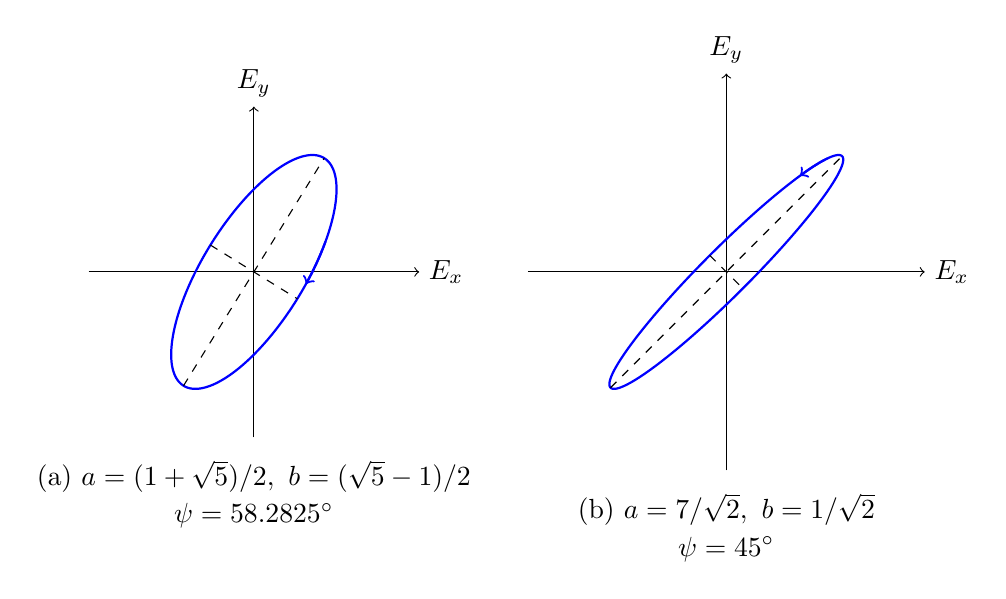
\begin{tikzpicture}
\begin{scope}[xshift=0cm,scale=1.05]
\draw[->] (-2.0,0)--(2.0,0) node[right] {$E_x$};
\draw[->] (0,-2.0)--(0,2.0) node[above] {$E_y$};
\draw[blue,thick] plot coordinates {(1.000000,1.000000) (0.999657,0.973480) (0.998630,0.946294) (0.996917,0.918458) (0.994522,0.889993) (0.991445,0.860919) (0.987688,0.831254) (0.983255,0.801019) (0.978148,0.770236) (0.972370,0.738925) (0.965926,0.707107) (0.958820,0.674804) (0.951057,0.642040) (0.942641,0.608835) (0.933580,0.575212) (0.923880,0.541196) (0.913545,0.506809) (0.902585,0.472074) (0.891007,0.437016) (0.878817,0.401658) (0.866025,0.366025) (0.852640,0.330142) (0.838671,0.294032) (0.824126,0.257720) (0.809017,0.221232) (0.793353,0.184592) (0.777146,0.147826) (0.760406,0.110958) (0.743145,0.074014) (0.725374,0.037020) (0.707107,0.000000) (0.688355,-0.037020) (0.669131,-0.074014) (0.649448,-0.110958) (0.629320,-0.147826) (0.608761,-0.184592) (0.587785,-0.221232) (0.566406,-0.257720) (0.544639,-0.294032) (0.522499,-0.330142) (0.500000,-0.366025) (0.477159,-0.401658) (0.453990,-0.437016) (0.430511,-0.472074) (0.406737,-0.506809) (0.382683,-0.541196) (0.358368,-0.575212) (0.333807,-0.608835) (0.309017,-0.642040) (0.284015,-0.674804) (0.258819,-0.707107) (0.233445,-0.738925) (0.207912,-0.770236) (0.182236,-0.801019) (0.156434,-0.831254) (0.130526,-0.860919) (0.104528,-0.889993) (0.078459,-0.918458) (0.052336,-0.946294) (0.026177,-0.973480) (0.000000,-1.000000) (-0.026177,-1.025834) (-0.052336,-1.050965) (-0.078459,-1.075376) (-0.104528,-1.099050) (-0.130526,-1.121971) (-0.156434,-1.144123) (-0.182236,-1.165490) (-0.207912,-1.186059) (-0.233445,-1.205815) (-0.258819,-1.224745) (-0.284015,-1.242835) (-0.309017,-1.260074) (-0.333807,-1.276448) (-0.358368,-1.291948) (-0.382683,-1.306563) (-0.406737,-1.320282) (-0.430511,-1.333096) (-0.453990,-1.344997) (-0.477159,-1.355976) (-0.500000,-1.366025) (-0.522499,-1.375139) (-0.544639,-1.383310) (-0.566406,-1.390532) (-0.587785,-1.396802) (-0.608761,-1.402115) (-0.629320,-1.406466) (-0.649448,-1.409854) (-0.669131,-1.412275) (-0.688355,-1.413729) (-0.707107,-1.414214) (-0.725374,-1.413729) (-0.743145,-1.412275) (-0.760406,-1.409854) (-0.777146,-1.406466) (-0.793353,-1.402115) (-0.809017,-1.396802) (-0.824126,-1.390532) (-0.838671,-1.383310) (-0.852640,-1.375139) (-0.866025,-1.366025) (-0.878817,-1.355976) (-0.891007,-1.344997) (-0.902585,-1.333096) (-0.913545,-1.320282) (-0.923880,-1.306563) (-0.933580,-1.291948) (-0.942641,-1.276448) (-0.951057,-1.260074) (-0.958820,-1.242835) (-0.965926,-1.224745) (-0.972370,-1.205815) (-0.978148,-1.186059) (-0.983255,-1.165490) (-0.987688,-1.144123) (-0.991445,-1.121971) (-0.994522,-1.099050) (-0.996917,-1.075376) (-0.998630,-1.050965) (-0.999657,-1.025834) (-1.000000,-1.000000) (-0.999657,-0.973480) (-0.998630,-0.946294) (-0.996917,-0.918458) (-0.994522,-0.889993) (-0.991445,-0.860919) (-0.987688,-0.831254) (-0.983255,-0.801019) (-0.978148,-0.770236) (-0.972370,-0.738925) (-0.965926,-0.707107) (-0.958820,-0.674804) (-0.951057,-0.642040) (-0.942641,-0.608835) (-0.933580,-0.575212) (-0.923880,-0.541196) (-0.913545,-0.506809) (-0.902585,-0.472074) (-0.891007,-0.437016) (-0.878817,-0.401658) (-0.866025,-0.366025) (-0.852640,-0.330142) (-0.838671,-0.294032) (-0.824126,-0.257720) (-0.809017,-0.221232) (-0.793353,-0.184592) (-0.777146,-0.147826) (-0.760406,-0.110958) (-0.743145,-0.074014) (-0.725374,-0.037020) (-0.707107,-0.000000) (-0.688355,0.037020) (-0.669131,0.074014) (-0.649448,0.110958) (-0.629320,0.147826) (-0.608761,0.184592) (-0.587785,0.221232) (-0.566406,0.257720) (-0.544639,0.294032) (-0.522499,0.330142) (-0.500000,0.366025) (-0.477159,0.401658) (-0.453990,0.437016) (-0.430511,0.472074) (-0.406737,0.506809) (-0.382683,0.541196) (-0.358368,0.575212) (-0.333807,0.608835) (-0.309017,0.642040) (-0.284015,0.674804) (-0.258819,0.707107) (-0.233445,0.738925) (-0.207912,0.770236) (-0.182236,0.801019) (-0.156434,0.831254) (-0.130526,0.860919) (-0.104528,0.889993) (-0.078459,0.918458) (-0.052336,0.946294) (-0.026177,0.973480) (-0.000000,1.000000) (0.026177,1.025834) (0.052336,1.050965) (0.078459,1.075376) (0.104528,1.099050) (0.130526,1.121971) (0.156434,1.144123) (0.182236,1.165490) (0.207912,1.186059) (0.233445,1.205815) (0.258819,1.224745) (0.284015,1.242835) (0.309017,1.260074) (0.333807,1.276448) (0.358368,1.291948) (0.382683,1.306563) (0.406737,1.320282) (0.430511,1.333096) (0.453990,1.344997) (0.477159,1.355976) (0.500000,1.366025) (0.522499,1.375139) (0.544639,1.383310) (0.566406,1.390532) (0.587785,1.396802) (0.608761,1.402115) (0.629320,1.406466) (0.649448,1.409854) (0.669131,1.412275) (0.688355,1.413729) (0.707107,1.414214) (0.725374,1.413729) (0.743145,1.412275) (0.760406,1.409854) (0.777146,1.406466) (0.793353,1.402115) (0.809017,1.396802) (0.824126,1.390532) (0.838671,1.383310) (0.852640,1.375139) (0.866025,1.366025) (0.878817,1.355976) (0.891007,1.344997) (0.902585,1.333096) (0.913545,1.320282) (0.923880,1.306563) (0.933580,1.291948) (0.942641,1.276448) (0.951057,1.260074) (0.958820,1.242835) (0.965926,1.224745) (0.972370,1.205815) (0.978148,1.186059) (0.983255,1.165490) (0.987688,1.144123) (0.991445,1.121971) (0.994522,1.099050) (0.996917,1.075376) (0.998630,1.050965) (0.999657,1.025834) (1.000000,1.000000)};
\draw[blue,->,thick] plot coordinates {(0.866025,0.366025) (0.852640,0.330142) (0.838671,0.294032) (0.824126,0.257720) (0.809017,0.221232) (0.793353,0.184592) (0.777146,0.147826) (0.760406,0.110958) (0.743145,0.074014) (0.725374,0.037020) (0.707107,0.000000) (0.688355,-0.037020) (0.669131,-0.074014) (0.649448,-0.110958) (0.629320,-0.147826)};
\draw[black,dashed] plot coordinates {(-0.525731,0.324920) (0.525731,-0.324920)};
\draw[black,dashed] plot coordinates {(-0.850651,-1.376382) (0.850651,1.376382)};
\node at (0,-2.4761904761904763) {(a) $a=(1+\sqrt5)/2,\ b=(\sqrt5-1)/2$};
\node at (0,-2.9523809523809526) {$\psi=58.2825^\circ$};
\end{scope}
\begin{scope}[xshift=6cm,scale=0.42]
\draw[->] (-6.0,0)--(6.0,0) node[right] {$E_x$};
\draw[->] (0,-6.0)--(0,6.0) node[above] {$E_y$};
\draw[blue,thick] plot coordinates {(3.535534,3.394113) (3.534322,3.418863) (3.530689,3.441271) (3.524635,3.461320) (3.516166,3.478997) (3.505287,3.494290) (3.492006,3.507188) (3.476331,3.517682) (3.458274,3.525765) (3.437847,3.531432) (3.415064,3.534679) (3.389940,3.535503) (3.362493,3.533904) (3.332741,3.529883) (3.300705,3.523443) (3.266407,3.514588) (3.229871,3.503325) (3.191121,3.489660) (3.150184,3.473604) (3.107088,3.455167) (3.061862,3.434362) (3.014538,3.411204) (2.965148,3.385707) (2.913726,3.357891) (2.860307,3.327772) (2.804928,3.295374) (2.747626,3.260716) (2.688441,3.223824) (2.627414,3.184723) (2.564586,3.143439) (2.500000,3.100000) (2.433701,3.054437) (2.365734,3.006780) (2.296146,2.957063) (2.224984,2.905319) (2.152297,2.851585) (2.078135,2.795895) (2.002548,2.738290) (1.925590,2.678808) (1.847311,2.617490) (1.767767,2.554378) (1.687011,2.489515) (1.605099,2.422946) (1.522087,2.354717) (1.438031,2.284874) (1.352990,2.213465) (1.267022,2.140539) (1.180185,2.066146) (1.092540,1.990336) (1.004146,1.913163) (0.915064,1.834679) (0.825354,1.754937) (0.735079,1.673992) (0.644300,1.591901) (0.553079,1.508718) (0.461480,1.424501) (0.369564,1.339308) (0.277395,1.253197) (0.185036,1.166227) (0.092549,1.078458) (0.000000,0.989949) (-0.092549,0.900763) (-0.185036,0.810959) (-0.277395,0.720599) (-0.369564,0.629745) (-0.461480,0.538460) (-0.553079,0.446805) (-0.644300,0.354845) (-0.735079,0.262641) (-0.825354,0.170257) (-0.915064,0.077757) (-1.004146,-0.014797) (-1.092540,-0.107341) (-1.180185,-0.199811) (-1.267022,-0.292144) (-1.352990,-0.384277) (-1.438031,-0.476146) (-1.522087,-0.567689) (-1.605099,-0.658843) (-1.687011,-0.749546) (-1.767767,-0.839735) (-1.847311,-0.929348) (-1.925590,-1.018325) (-2.002548,-1.106603) (-2.078135,-1.194123) (-2.152297,-1.280825) (-2.224984,-1.366649) (-2.296146,-1.451536) (-2.365734,-1.535429) (-2.433701,-1.618269) (-2.500000,-1.700000) (-2.564586,-1.780566) (-2.627414,-1.859912) (-2.688441,-1.937983) (-2.747626,-2.014725) (-2.804928,-2.090087) (-2.860307,-2.164017) (-2.913726,-2.236463) (-2.965148,-2.307377) (-3.014538,-2.376709) (-3.061862,-2.444413) (-3.107088,-2.510441) (-3.150184,-2.574749) (-3.191121,-2.637292) (-3.229871,-2.698027) (-3.266407,-2.756914) (-3.300705,-2.813911) (-3.332741,-2.868979) (-3.362493,-2.922082) (-3.389940,-2.973181) (-3.415064,-3.022243) (-3.437847,-3.069234) (-3.458274,-3.114121) (-3.476331,-3.156874) (-3.492006,-3.197463) (-3.505287,-3.235861) (-3.516166,-3.272041) (-3.524635,-3.305979) (-3.530689,-3.337651) (-3.534322,-3.367036) (-3.535534,-3.394113) (-3.534322,-3.418863) (-3.530689,-3.441271) (-3.524635,-3.461320) (-3.516166,-3.478997) (-3.505287,-3.494290) (-3.492006,-3.507188) (-3.476331,-3.517682) (-3.458274,-3.525765) (-3.437847,-3.531432) (-3.415064,-3.534679) (-3.389940,-3.535503) (-3.362493,-3.533904) (-3.332741,-3.529883) (-3.300705,-3.523443) (-3.266407,-3.514588) (-3.229871,-3.503325) (-3.191121,-3.489660) (-3.150184,-3.473604) (-3.107088,-3.455167) (-3.061862,-3.434362) (-3.014538,-3.411204) (-2.965148,-3.385707) (-2.913726,-3.357891) (-2.860307,-3.327772) (-2.804928,-3.295374) (-2.747626,-3.260716) (-2.688441,-3.223824) (-2.627414,-3.184723) (-2.564586,-3.143439) (-2.500000,-3.100000) (-2.433701,-3.054437) (-2.365734,-3.006780) (-2.296146,-2.957063) (-2.224984,-2.905319) (-2.152297,-2.851585) (-2.078135,-2.795895) (-2.002548,-2.738290) (-1.925590,-2.678808) (-1.847311,-2.617490) (-1.767767,-2.554378) (-1.687011,-2.489515) (-1.605099,-2.422946) (-1.522087,-2.354717) (-1.438031,-2.284874) (-1.352990,-2.213465) (-1.267022,-2.140539) (-1.180185,-2.066146) (-1.092540,-1.990336) (-1.004146,-1.913163) (-0.915064,-1.834679) (-0.825354,-1.754937) (-0.735079,-1.673992) (-0.644300,-1.591901) (-0.553079,-1.508718) (-0.461480,-1.424501) (-0.369564,-1.339308) (-0.277395,-1.253197) (-0.185036,-1.166227) (-0.092549,-1.078458) (-0.000000,-0.989949) (0.092549,-0.900763) (0.185036,-0.810959) (0.277395,-0.720599) (0.369564,-0.629745) (0.461480,-0.538460) (0.553079,-0.446805) (0.644300,-0.354845) (0.735079,-0.262641) (0.825354,-0.170257) (0.915064,-0.077757) (1.004146,0.014797) (1.092540,0.107341) (1.180185,0.199811) (1.267022,0.292144) (1.352990,0.384277) (1.438031,0.476146) (1.522087,0.567689) (1.605099,0.658843) (1.687011,0.749546) (1.767767,0.839735) (1.847311,0.929348) (1.925590,1.018325) (2.002548,1.106603) (2.078135,1.194123) (2.152297,1.280825) (2.224984,1.366649) (2.296146,1.451536) (2.365734,1.535429) (2.433701,1.618269) (2.500000,1.700000) (2.564586,1.780566) (2.627414,1.859912) (2.688441,1.937983) (2.747626,2.014725) (2.804928,2.090087) (2.860307,2.164017) (2.913726,2.236463) (2.965148,2.307377) (3.014538,2.376709) (3.061862,2.444413) (3.107088,2.510441) (3.150184,2.574749) (3.191121,2.637292) (3.229871,2.698027) (3.266407,2.756914) (3.300705,2.813911) (3.332741,2.868979) (3.362493,2.922082) (3.389940,2.973181) (3.415064,3.022243) (3.437847,3.069234) (3.458274,3.114121) (3.476331,3.156874) (3.492006,3.197463) (3.505287,3.235861) (3.516166,3.272041) (3.524635,3.305979) (3.530689,3.337651) (3.534322,3.367036) (3.535534,3.394113)};
\draw[blue,->,thick] plot coordinates {(3.061862,3.434362) (3.014538,3.411204) (2.965148,3.385707) (2.913726,3.357891) (2.860307,3.327772) (2.804928,3.295374) (2.747626,3.260716) (2.688441,3.223824) (2.627414,3.184723) (2.564586,3.143439) (2.500000,3.100000) (2.433701,3.054437) (2.365734,3.006780) (2.296146,2.957063) (2.224984,2.905319)};
\draw[black,dashed] plot coordinates {(-0.500000,0.500000) (0.500000,-0.500000)};
\draw[black,dashed] plot coordinates {(-3.500000,-3.500000) (3.500000,3.500000)};
\node at (0,-7.190476190476191) {(b) $a=7/\sqrt2,\ b=1/\sqrt2$};
\node at (0,-8.380952380952381) {$\psi=45^\circ$};
\end{scope}
\end{tikzpicture}

\end{center}

\Needspace{5\baselineskip}
\par\bigskip
\noindent\textbf{7.2}\quad A plane wave is incident on a layered interface as shown in the figure. The indices of refraction of the three nonpermeable media are $n_{1}$, $n_{2}$, $n_{3}$. The thickness of the intermediate layer is $d$. Each of the other media is semi-infinite.
\begin{enumerate}
\item[(a)] Calculate the transmission and reflection coefficients (ratios of transmitted and reflected Poynting's flux to the incident flux), and sketch their behavior as a function of frequency for $n_{1}=1$, $n_{2}=2$, $n_{3}=3$; $n_{1}=3$, $n_{2}=2$, $n_{3}=1$; and $n_{1}=2$, $n_{2}=4$, $n_{3}=1$.
\end{enumerate}

\begin{center}
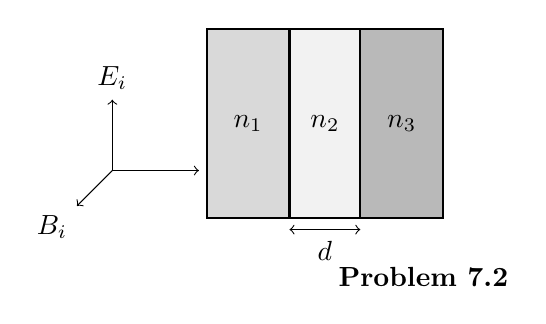
\begin{tikzpicture}[scale=1.0]
  % slab n1 (left, medium shading)
  \fill[gray!30] (-1.4,0) rectangle (-0.35,2.4);
  \draw[thick] (-1.4,0) rectangle (-0.35,2.4);
  \node at (-0.875,1.2) {$n_{1}$};
  % slab n2 (middle, light)
  \fill[gray!10] (-0.35,0) rectangle (0.55,2.4);
  \draw[thick] (-0.35,0) rectangle (0.55,2.4);
  \node at (0.1,1.2) {$n_{2}$};
  % slab n3 (right, dark)
  \fill[gray!55] (0.55,0) rectangle (1.6,2.4);
  \draw[thick] (0.55,0) rectangle (1.6,2.4);
  \node at (1.075,1.2) {$n_{3}$};
  % d dimension below n2
  \draw[<->] (-0.35,-0.15) -- (0.55,-0.15);
  \node[below] at (0.1,-0.18) {$d$};
  % incident ray coordinate axes at left
  \draw[->] (-2.6,0.6) -- (-1.5,0.6);
  \draw[->] (-2.6,0.6) -- (-2.6,1.5) node[above] {$E_{i}$};
  \draw[->] (-2.6,0.6) -- (-3.05,0.15) node[below left] {$B_{i}$};
  \node at (1.35,-0.75) {\textbf{Problem 7.2}};
\end{tikzpicture}
\end{center}

\begin{enumerate}
\item[(b)] The medium $n_{1}$ is part of an optical system (e.g., a lens); medium $n_{3}$ is air ($n_{3}=1$). It is desired to put an optical coating (medium $n_{2}$) on the surface so that there is no reflected wave for a frequency $\omega_{0}$. What thickness $d$ and index of refraction $n_{2}$ are necessary?
\end{enumerate}
\solution
The drawing specifies normal incidence. Take $e^{-i\omega t}$ time
dependence, and reference incident/reflected amplitudes to the first
face and the transmitted amplitude to the second face. Define
\[
r_{ij}=\frac{n_i-n_j}{n_i+n_j},\quad
 t_{ij}=\frac{2n_i}{n_i+n_j},\quad \delta=\frac{n_2\omega d}{c}.
\]
At either face continuity of $E_t,H_t$ gives
$E_i+E_r=E_t$ and $n_i(E_i-E_r)=n_jE_t$, proving these single-face
coefficients.
\textbf{(a)} A round trip inside the film multiplies an amplitude by
$r_{21}r_{23}e^{2i\delta}=-r_{12}r_{23}e^{2i\delta}$.
Summing all transmitted trips therefore gives
\[
t=\frac{t_{12}t_{23}e^{i\delta}}{1+r_{12}r_{23}e^{2i\delta}}.
\]
The direct reflection plus the waves returned through the first
face gives
\[
r=r_{12}+\frac{t_{12}t_{21}r_{23}e^{2i\delta}}
 {1+r_{12}r_{23}e^{2i\delta}}
=\frac{r_{12}+r_{23}e^{2i\delta}}{1+r_{12}r_{23}e^{2i\delta}},
\]
where $t_{12}t_{21}=1-r_{12}^2$ was used. Since the flux for a
traveling electric amplitude is $n|E|^2/(2Z_0)$,
\[
\boxed{R=|r|^2,\qquad T=\frac{n_3}{n_1}|t|^2.}
\]
A useful real form, obtained by multiplying the denominator by
$e^{-i\delta}$, is
\[
\boxed{T=\frac{4n_1n_3}
 {(n_1+n_3)^2\cos^2\delta+(n_2+n_1n_3/n_2)^2\sin^2\delta},
\qquad R=1-T.}
\]
Indeed the numerator of $R$ is the same denominator minus $4n_1n_3$,
namely $(n_1-n_3)^2\cos^2\delta+(n_2-n_1n_3/n_2)^2\sin^2\delta$.
For $(n_1,n_2,n_3)=(1,2,3)$ and $(3,2,1)$ the flux curves coincide:
\[
T=\frac{12}{16\cos^2\delta+(49/4)\sin^2\delta},\qquad
\frac34\leq T\leq\frac{48}{49}.
\]
For $(2,4,1)$,
\[
T=\frac8{9\cos^2\delta+(81/4)\sin^2\delta},\qquad
\frac{32}{81}\leq T\leq\frac89.
\]
The plot uses a common frequency coordinate $\omega d/(\pi c)$,
so the third film has twice as many fringes as the first two.
\begin{center}
% Generated by supplementary/check_ch07.py --write-assets
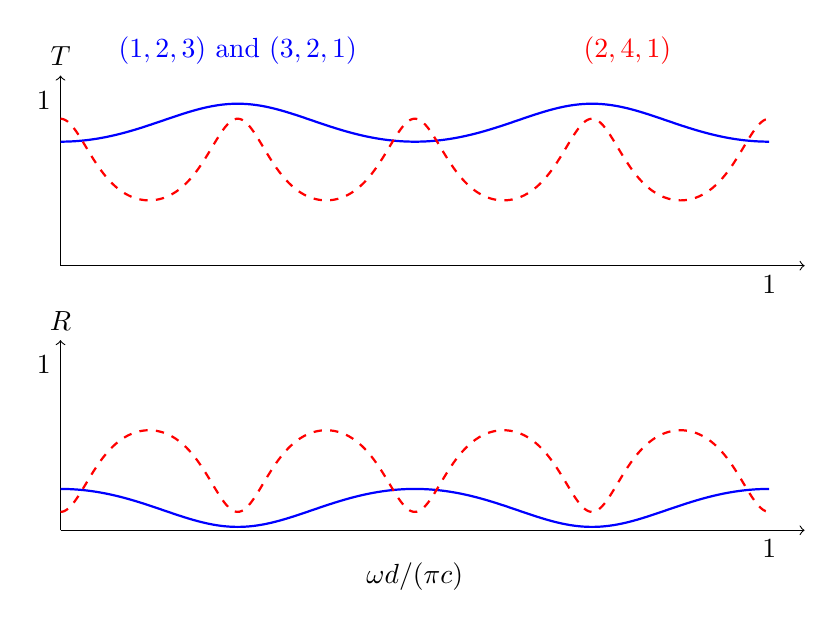
\begin{tikzpicture}[x=9cm,y=2.1cm]
\begin{scope}[yshift=0.0cm]
\draw[->] (0,0)--(1.05,0);\draw[->] (0,0)--(0,1.15) node[above] {$T$};
\draw[blue,thick] plot coordinates {(0.000000,0.750000) (0.002500,0.750043) (0.005000,0.750173) (0.007500,0.750390) (0.010000,0.750694) (0.012500,0.751084) (0.015000,0.751560) (0.017500,0.752123) (0.020000,0.752771) (0.022500,0.753506) (0.025000,0.754326) (0.027500,0.755232) (0.030000,0.756223) (0.032500,0.757299) (0.035000,0.758459) (0.037500,0.759703) (0.040000,0.761031) (0.042500,0.762443) (0.045000,0.763936) (0.047500,0.765512) (0.050000,0.767170) (0.052500,0.768908) (0.055000,0.770727) (0.057500,0.772625) (0.060000,0.774603) (0.062500,0.776658) (0.065000,0.778790) (0.067500,0.780998) (0.070000,0.783281) (0.072500,0.785638) (0.075000,0.788069) (0.077500,0.790571) (0.080000,0.793143) (0.082500,0.795785) (0.085000,0.798494) (0.087500,0.801270) (0.090000,0.804110) (0.092500,0.807013) (0.095000,0.809977) (0.097500,0.813001) (0.100000,0.816082) (0.102500,0.819218) (0.105000,0.822408) (0.107500,0.825649) (0.110000,0.828939) (0.112500,0.832275) (0.115000,0.835655) (0.117500,0.839076) (0.120000,0.842535) (0.122500,0.846030) (0.125000,0.849558) (0.127500,0.853115) (0.130000,0.856698) (0.132500,0.860305) (0.135000,0.863931) (0.137500,0.867573) (0.140000,0.871228) (0.142500,0.874892) (0.145000,0.878561) (0.147500,0.882230) (0.150000,0.885897) (0.152500,0.889557) (0.155000,0.893205) (0.157500,0.896838) (0.160000,0.900450) (0.162500,0.904039) (0.165000,0.907598) (0.167500,0.911124) (0.170000,0.914612) (0.172500,0.918056) (0.175000,0.921454) (0.177500,0.924799) (0.180000,0.928086) (0.182500,0.931313) (0.185000,0.934472) (0.187500,0.937560) (0.190000,0.940573) (0.192500,0.943504) (0.195000,0.946351) (0.197500,0.949107) (0.200000,0.951770) (0.202500,0.954333) (0.205000,0.956794) (0.207500,0.959148) (0.210000,0.961390) (0.212500,0.963518) (0.215000,0.965527) (0.217500,0.967413) (0.220000,0.969175) (0.222500,0.970807) (0.225000,0.972308) (0.227500,0.973674) (0.230000,0.974904) (0.232500,0.975994) (0.235000,0.976943) (0.237500,0.977749) (0.240000,0.978411) (0.242500,0.978927) (0.245000,0.979296) (0.247500,0.979518) (0.250000,0.979592) (0.252500,0.979518) (0.255000,0.979296) (0.257500,0.978927) (0.260000,0.978411) (0.262500,0.977749) (0.265000,0.976943) (0.267500,0.975994) (0.270000,0.974904) (0.272500,0.973674) (0.275000,0.972308) (0.277500,0.970807) (0.280000,0.969175) (0.282500,0.967413) (0.285000,0.965527) (0.287500,0.963518) (0.290000,0.961390) (0.292500,0.959148) (0.295000,0.956794) (0.297500,0.954333) (0.300000,0.951770) (0.302500,0.949107) (0.305000,0.946351) (0.307500,0.943504) (0.310000,0.940573) (0.312500,0.937560) (0.315000,0.934472) (0.317500,0.931313) (0.320000,0.928086) (0.322500,0.924799) (0.325000,0.921454) (0.327500,0.918056) (0.330000,0.914612) (0.332500,0.911124) (0.335000,0.907598) (0.337500,0.904039) (0.340000,0.900450) (0.342500,0.896838) (0.345000,0.893205) (0.347500,0.889557) (0.350000,0.885897) (0.352500,0.882230) (0.355000,0.878561) (0.357500,0.874892) (0.360000,0.871228) (0.362500,0.867573) (0.365000,0.863931) (0.367500,0.860305) (0.370000,0.856698) (0.372500,0.853115) (0.375000,0.849558) (0.377500,0.846030) (0.380000,0.842535) (0.382500,0.839076) (0.385000,0.835655) (0.387500,0.832275) (0.390000,0.828939) (0.392500,0.825649) (0.395000,0.822408) (0.397500,0.819218) (0.400000,0.816082) (0.402500,0.813001) (0.405000,0.809977) (0.407500,0.807013) (0.410000,0.804110) (0.412500,0.801270) (0.415000,0.798494) (0.417500,0.795785) (0.420000,0.793143) (0.422500,0.790571) (0.425000,0.788069) (0.427500,0.785638) (0.430000,0.783281) (0.432500,0.780998) (0.435000,0.778790) (0.437500,0.776658) (0.440000,0.774603) (0.442500,0.772625) (0.445000,0.770727) (0.447500,0.768908) (0.450000,0.767170) (0.452500,0.765512) (0.455000,0.763936) (0.457500,0.762443) (0.460000,0.761031) (0.462500,0.759703) (0.465000,0.758459) (0.467500,0.757299) (0.470000,0.756223) (0.472500,0.755232) (0.475000,0.754326) (0.477500,0.753506) (0.480000,0.752771) (0.482500,0.752123) (0.485000,0.751560) (0.487500,0.751084) (0.490000,0.750694) (0.492500,0.750390) (0.495000,0.750173) (0.497500,0.750043) (0.500000,0.750000) (0.502500,0.750043) (0.505000,0.750173) (0.507500,0.750390) (0.510000,0.750694) (0.512500,0.751084) (0.515000,0.751560) (0.517500,0.752123) (0.520000,0.752771) (0.522500,0.753506) (0.525000,0.754326) (0.527500,0.755232) (0.530000,0.756223) (0.532500,0.757299) (0.535000,0.758459) (0.537500,0.759703) (0.540000,0.761031) (0.542500,0.762443) (0.545000,0.763936) (0.547500,0.765512) (0.550000,0.767170) (0.552500,0.768908) (0.555000,0.770727) (0.557500,0.772625) (0.560000,0.774603) (0.562500,0.776658) (0.565000,0.778790) (0.567500,0.780998) (0.570000,0.783281) (0.572500,0.785638) (0.575000,0.788069) (0.577500,0.790571) (0.580000,0.793143) (0.582500,0.795785) (0.585000,0.798494) (0.587500,0.801270) (0.590000,0.804110) (0.592500,0.807013) (0.595000,0.809977) (0.597500,0.813001) (0.600000,0.816082) (0.602500,0.819218) (0.605000,0.822408) (0.607500,0.825649) (0.610000,0.828939) (0.612500,0.832275) (0.615000,0.835655) (0.617500,0.839076) (0.620000,0.842535) (0.622500,0.846030) (0.625000,0.849558) (0.627500,0.853115) (0.630000,0.856698) (0.632500,0.860305) (0.635000,0.863931) (0.637500,0.867573) (0.640000,0.871228) (0.642500,0.874892) (0.645000,0.878561) (0.647500,0.882230) (0.650000,0.885897) (0.652500,0.889557) (0.655000,0.893205) (0.657500,0.896838) (0.660000,0.900450) (0.662500,0.904039) (0.665000,0.907598) (0.667500,0.911124) (0.670000,0.914612) (0.672500,0.918056) (0.675000,0.921454) (0.677500,0.924799) (0.680000,0.928086) (0.682500,0.931313) (0.685000,0.934472) (0.687500,0.937560) (0.690000,0.940573) (0.692500,0.943504) (0.695000,0.946351) (0.697500,0.949107) (0.700000,0.951770) (0.702500,0.954333) (0.705000,0.956794) (0.707500,0.959148) (0.710000,0.961390) (0.712500,0.963518) (0.715000,0.965527) (0.717500,0.967413) (0.720000,0.969175) (0.722500,0.970807) (0.725000,0.972308) (0.727500,0.973674) (0.730000,0.974904) (0.732500,0.975994) (0.735000,0.976943) (0.737500,0.977749) (0.740000,0.978411) (0.742500,0.978927) (0.745000,0.979296) (0.747500,0.979518) (0.750000,0.979592) (0.752500,0.979518) (0.755000,0.979296) (0.757500,0.978927) (0.760000,0.978411) (0.762500,0.977749) (0.765000,0.976943) (0.767500,0.975994) (0.770000,0.974904) (0.772500,0.973674) (0.775000,0.972308) (0.777500,0.970807) (0.780000,0.969175) (0.782500,0.967413) (0.785000,0.965527) (0.787500,0.963518) (0.790000,0.961390) (0.792500,0.959148) (0.795000,0.956794) (0.797500,0.954333) (0.800000,0.951770) (0.802500,0.949107) (0.805000,0.946351) (0.807500,0.943504) (0.810000,0.940573) (0.812500,0.937560) (0.815000,0.934472) (0.817500,0.931313) (0.820000,0.928086) (0.822500,0.924799) (0.825000,0.921454) (0.827500,0.918056) (0.830000,0.914612) (0.832500,0.911124) (0.835000,0.907598) (0.837500,0.904039) (0.840000,0.900450) (0.842500,0.896838) (0.845000,0.893205) (0.847500,0.889557) (0.850000,0.885897) (0.852500,0.882230) (0.855000,0.878561) (0.857500,0.874892) (0.860000,0.871228) (0.862500,0.867573) (0.865000,0.863931) (0.867500,0.860305) (0.870000,0.856698) (0.872500,0.853115) (0.875000,0.849558) (0.877500,0.846030) (0.880000,0.842535) (0.882500,0.839076) (0.885000,0.835655) (0.887500,0.832275) (0.890000,0.828939) (0.892500,0.825649) (0.895000,0.822408) (0.897500,0.819218) (0.900000,0.816082) (0.902500,0.813001) (0.905000,0.809977) (0.907500,0.807013) (0.910000,0.804110) (0.912500,0.801270) (0.915000,0.798494) (0.917500,0.795785) (0.920000,0.793143) (0.922500,0.790571) (0.925000,0.788069) (0.927500,0.785638) (0.930000,0.783281) (0.932500,0.780998) (0.935000,0.778790) (0.937500,0.776658) (0.940000,0.774603) (0.942500,0.772625) (0.945000,0.770727) (0.947500,0.768908) (0.950000,0.767170) (0.952500,0.765512) (0.955000,0.763936) (0.957500,0.762443) (0.960000,0.761031) (0.962500,0.759703) (0.965000,0.758459) (0.967500,0.757299) (0.970000,0.756223) (0.972500,0.755232) (0.975000,0.754326) (0.977500,0.753506) (0.980000,0.752771) (0.982500,0.752123) (0.985000,0.751560) (0.987500,0.751084) (0.990000,0.750694) (0.992500,0.750390) (0.995000,0.750173) (0.997500,0.750043) (1.000000,0.750000)};
\draw[red,dashed,thick] plot coordinates {(0.000000,0.888889) (0.002500,0.887794) (0.005000,0.884530) (0.007500,0.879156) (0.010000,0.871771) (0.012500,0.862505) (0.015000,0.851516) (0.017500,0.838984) (0.020000,0.825102) (0.022500,0.810073) (0.025000,0.794101) (0.027500,0.777389) (0.030000,0.760127) (0.032500,0.742499) (0.035000,0.724671) (0.037500,0.706794) (0.040000,0.689003) (0.042500,0.671415) (0.045000,0.654130) (0.047500,0.637232) (0.050000,0.620791) (0.052500,0.604864) (0.055000,0.589493) (0.057500,0.574713) (0.060000,0.560546) (0.062500,0.547009) (0.065000,0.534110) (0.067500,0.521853) (0.070000,0.510236) (0.072500,0.499255) (0.075000,0.488901) (0.077500,0.479165) (0.080000,0.470035) (0.082500,0.461498) (0.085000,0.453540) (0.087500,0.446147) (0.090000,0.439307) (0.092500,0.433004) (0.095000,0.427226) (0.097500,0.421960) (0.100000,0.417194) (0.102500,0.412917) (0.105000,0.409119) (0.107500,0.405790) (0.110000,0.402921) (0.112500,0.400507) (0.115000,0.398540) (0.117500,0.397015) (0.120000,0.395929) (0.122500,0.395278) (0.125000,0.395062) (0.127500,0.395278) (0.130000,0.395929) (0.132500,0.397015) (0.135000,0.398540) (0.137500,0.400507) (0.140000,0.402921) (0.142500,0.405790) (0.145000,0.409119) (0.147500,0.412917) (0.150000,0.417194) (0.152500,0.421960) (0.155000,0.427226) (0.157500,0.433004) (0.160000,0.439307) (0.162500,0.446147) (0.165000,0.453540) (0.167500,0.461498) (0.170000,0.470035) (0.172500,0.479165) (0.175000,0.488901) (0.177500,0.499255) (0.180000,0.510236) (0.182500,0.521853) (0.185000,0.534110) (0.187500,0.547009) (0.190000,0.560546) (0.192500,0.574713) (0.195000,0.589493) (0.197500,0.604864) (0.200000,0.620791) (0.202500,0.637232) (0.205000,0.654130) (0.207500,0.671415) (0.210000,0.689003) (0.212500,0.706794) (0.215000,0.724671) (0.217500,0.742499) (0.220000,0.760127) (0.222500,0.777389) (0.225000,0.794101) (0.227500,0.810073) (0.230000,0.825102) (0.232500,0.838984) (0.235000,0.851516) (0.237500,0.862505) (0.240000,0.871771) (0.242500,0.879156) (0.245000,0.884530) (0.247500,0.887794) (0.250000,0.888889) (0.252500,0.887794) (0.255000,0.884530) (0.257500,0.879156) (0.260000,0.871771) (0.262500,0.862505) (0.265000,0.851516) (0.267500,0.838984) (0.270000,0.825102) (0.272500,0.810073) (0.275000,0.794101) (0.277500,0.777389) (0.280000,0.760127) (0.282500,0.742499) (0.285000,0.724671) (0.287500,0.706794) (0.290000,0.689003) (0.292500,0.671415) (0.295000,0.654130) (0.297500,0.637232) (0.300000,0.620791) (0.302500,0.604864) (0.305000,0.589493) (0.307500,0.574713) (0.310000,0.560546) (0.312500,0.547009) (0.315000,0.534110) (0.317500,0.521853) (0.320000,0.510236) (0.322500,0.499255) (0.325000,0.488901) (0.327500,0.479165) (0.330000,0.470035) (0.332500,0.461498) (0.335000,0.453540) (0.337500,0.446147) (0.340000,0.439307) (0.342500,0.433004) (0.345000,0.427226) (0.347500,0.421960) (0.350000,0.417194) (0.352500,0.412917) (0.355000,0.409119) (0.357500,0.405790) (0.360000,0.402921) (0.362500,0.400507) (0.365000,0.398540) (0.367500,0.397015) (0.370000,0.395929) (0.372500,0.395278) (0.375000,0.395062) (0.377500,0.395278) (0.380000,0.395929) (0.382500,0.397015) (0.385000,0.398540) (0.387500,0.400507) (0.390000,0.402921) (0.392500,0.405790) (0.395000,0.409119) (0.397500,0.412917) (0.400000,0.417194) (0.402500,0.421960) (0.405000,0.427226) (0.407500,0.433004) (0.410000,0.439307) (0.412500,0.446147) (0.415000,0.453540) (0.417500,0.461498) (0.420000,0.470035) (0.422500,0.479165) (0.425000,0.488901) (0.427500,0.499255) (0.430000,0.510236) (0.432500,0.521853) (0.435000,0.534110) (0.437500,0.547009) (0.440000,0.560546) (0.442500,0.574713) (0.445000,0.589493) (0.447500,0.604864) (0.450000,0.620791) (0.452500,0.637232) (0.455000,0.654130) (0.457500,0.671415) (0.460000,0.689003) (0.462500,0.706794) (0.465000,0.724671) (0.467500,0.742499) (0.470000,0.760127) (0.472500,0.777389) (0.475000,0.794101) (0.477500,0.810073) (0.480000,0.825102) (0.482500,0.838984) (0.485000,0.851516) (0.487500,0.862505) (0.490000,0.871771) (0.492500,0.879156) (0.495000,0.884530) (0.497500,0.887794) (0.500000,0.888889) (0.502500,0.887794) (0.505000,0.884530) (0.507500,0.879156) (0.510000,0.871771) (0.512500,0.862505) (0.515000,0.851516) (0.517500,0.838984) (0.520000,0.825102) (0.522500,0.810073) (0.525000,0.794101) (0.527500,0.777389) (0.530000,0.760127) (0.532500,0.742499) (0.535000,0.724671) (0.537500,0.706794) (0.540000,0.689003) (0.542500,0.671415) (0.545000,0.654130) (0.547500,0.637232) (0.550000,0.620791) (0.552500,0.604864) (0.555000,0.589493) (0.557500,0.574713) (0.560000,0.560546) (0.562500,0.547009) (0.565000,0.534110) (0.567500,0.521853) (0.570000,0.510236) (0.572500,0.499255) (0.575000,0.488901) (0.577500,0.479165) (0.580000,0.470035) (0.582500,0.461498) (0.585000,0.453540) (0.587500,0.446147) (0.590000,0.439307) (0.592500,0.433004) (0.595000,0.427226) (0.597500,0.421960) (0.600000,0.417194) (0.602500,0.412917) (0.605000,0.409119) (0.607500,0.405790) (0.610000,0.402921) (0.612500,0.400507) (0.615000,0.398540) (0.617500,0.397015) (0.620000,0.395929) (0.622500,0.395278) (0.625000,0.395062) (0.627500,0.395278) (0.630000,0.395929) (0.632500,0.397015) (0.635000,0.398540) (0.637500,0.400507) (0.640000,0.402921) (0.642500,0.405790) (0.645000,0.409119) (0.647500,0.412917) (0.650000,0.417194) (0.652500,0.421960) (0.655000,0.427226) (0.657500,0.433004) (0.660000,0.439307) (0.662500,0.446147) (0.665000,0.453540) (0.667500,0.461498) (0.670000,0.470035) (0.672500,0.479165) (0.675000,0.488901) (0.677500,0.499255) (0.680000,0.510236) (0.682500,0.521853) (0.685000,0.534110) (0.687500,0.547009) (0.690000,0.560546) (0.692500,0.574713) (0.695000,0.589493) (0.697500,0.604864) (0.700000,0.620791) (0.702500,0.637232) (0.705000,0.654130) (0.707500,0.671415) (0.710000,0.689003) (0.712500,0.706794) (0.715000,0.724671) (0.717500,0.742499) (0.720000,0.760127) (0.722500,0.777389) (0.725000,0.794101) (0.727500,0.810073) (0.730000,0.825102) (0.732500,0.838984) (0.735000,0.851516) (0.737500,0.862505) (0.740000,0.871771) (0.742500,0.879156) (0.745000,0.884530) (0.747500,0.887794) (0.750000,0.888889) (0.752500,0.887794) (0.755000,0.884530) (0.757500,0.879156) (0.760000,0.871771) (0.762500,0.862505) (0.765000,0.851516) (0.767500,0.838984) (0.770000,0.825102) (0.772500,0.810073) (0.775000,0.794101) (0.777500,0.777389) (0.780000,0.760127) (0.782500,0.742499) (0.785000,0.724671) (0.787500,0.706794) (0.790000,0.689003) (0.792500,0.671415) (0.795000,0.654130) (0.797500,0.637232) (0.800000,0.620791) (0.802500,0.604864) (0.805000,0.589493) (0.807500,0.574713) (0.810000,0.560546) (0.812500,0.547009) (0.815000,0.534110) (0.817500,0.521853) (0.820000,0.510236) (0.822500,0.499255) (0.825000,0.488901) (0.827500,0.479165) (0.830000,0.470035) (0.832500,0.461498) (0.835000,0.453540) (0.837500,0.446147) (0.840000,0.439307) (0.842500,0.433004) (0.845000,0.427226) (0.847500,0.421960) (0.850000,0.417194) (0.852500,0.412917) (0.855000,0.409119) (0.857500,0.405790) (0.860000,0.402921) (0.862500,0.400507) (0.865000,0.398540) (0.867500,0.397015) (0.870000,0.395929) (0.872500,0.395278) (0.875000,0.395062) (0.877500,0.395278) (0.880000,0.395929) (0.882500,0.397015) (0.885000,0.398540) (0.887500,0.400507) (0.890000,0.402921) (0.892500,0.405790) (0.895000,0.409119) (0.897500,0.412917) (0.900000,0.417194) (0.902500,0.421960) (0.905000,0.427226) (0.907500,0.433004) (0.910000,0.439307) (0.912500,0.446147) (0.915000,0.453540) (0.917500,0.461498) (0.920000,0.470035) (0.922500,0.479165) (0.925000,0.488901) (0.927500,0.499255) (0.930000,0.510236) (0.932500,0.521853) (0.935000,0.534110) (0.937500,0.547009) (0.940000,0.560546) (0.942500,0.574713) (0.945000,0.589493) (0.947500,0.604864) (0.950000,0.620791) (0.952500,0.637232) (0.955000,0.654130) (0.957500,0.671415) (0.960000,0.689003) (0.962500,0.706794) (0.965000,0.724671) (0.967500,0.742499) (0.970000,0.760127) (0.972500,0.777389) (0.975000,0.794101) (0.977500,0.810073) (0.980000,0.825102) (0.982500,0.838984) (0.985000,0.851516) (0.987500,0.862505) (0.990000,0.871771) (0.992500,0.879156) (0.995000,0.884530) (0.997500,0.887794) (1.000000,0.888889)};
\node[left] at (0,1) {$1$};\node[below] at (1,0) {$1$};
\end{scope}
\begin{scope}[yshift=-3.3600000000000003cm]
\draw[->] (0,0)--(1.05,0);\draw[->] (0,0)--(0,1.15) node[above] {$R$};
\draw[blue,thick] plot coordinates {(0.000000,0.250000) (0.002500,0.249957) (0.005000,0.249827) (0.007500,0.249610) (0.010000,0.249306) (0.012500,0.248916) (0.015000,0.248440) (0.017500,0.247877) (0.020000,0.247229) (0.022500,0.246494) (0.025000,0.245674) (0.027500,0.244768) (0.030000,0.243777) (0.032500,0.242701) (0.035000,0.241541) (0.037500,0.240297) (0.040000,0.238969) (0.042500,0.237557) (0.045000,0.236064) (0.047500,0.234488) (0.050000,0.232830) (0.052500,0.231092) (0.055000,0.229273) (0.057500,0.227375) (0.060000,0.225397) (0.062500,0.223342) (0.065000,0.221210) (0.067500,0.219002) (0.070000,0.216719) (0.072500,0.214362) (0.075000,0.211931) (0.077500,0.209429) (0.080000,0.206857) (0.082500,0.204215) (0.085000,0.201506) (0.087500,0.198730) (0.090000,0.195890) (0.092500,0.192987) (0.095000,0.190023) (0.097500,0.186999) (0.100000,0.183918) (0.102500,0.180782) (0.105000,0.177592) (0.107500,0.174351) (0.110000,0.171061) (0.112500,0.167725) (0.115000,0.164345) (0.117500,0.160924) (0.120000,0.157465) (0.122500,0.153970) (0.125000,0.150442) (0.127500,0.146885) (0.130000,0.143302) (0.132500,0.139695) (0.135000,0.136069) (0.137500,0.132427) (0.140000,0.128772) (0.142500,0.125108) (0.145000,0.121439) (0.147500,0.117770) (0.150000,0.114103) (0.152500,0.110443) (0.155000,0.106795) (0.157500,0.103162) (0.160000,0.099550) (0.162500,0.095961) (0.165000,0.092402) (0.167500,0.088876) (0.170000,0.085388) (0.172500,0.081944) (0.175000,0.078546) (0.177500,0.075201) (0.180000,0.071914) (0.182500,0.068687) (0.185000,0.065528) (0.187500,0.062440) (0.190000,0.059427) (0.192500,0.056496) (0.195000,0.053649) (0.197500,0.050893) (0.200000,0.048230) (0.202500,0.045667) (0.205000,0.043206) (0.207500,0.040852) (0.210000,0.038610) (0.212500,0.036482) (0.215000,0.034473) (0.217500,0.032587) (0.220000,0.030825) (0.222500,0.029193) (0.225000,0.027692) (0.227500,0.026326) (0.230000,0.025096) (0.232500,0.024006) (0.235000,0.023057) (0.237500,0.022251) (0.240000,0.021589) (0.242500,0.021073) (0.245000,0.020704) (0.247500,0.020482) (0.250000,0.020408) (0.252500,0.020482) (0.255000,0.020704) (0.257500,0.021073) (0.260000,0.021589) (0.262500,0.022251) (0.265000,0.023057) (0.267500,0.024006) (0.270000,0.025096) (0.272500,0.026326) (0.275000,0.027692) (0.277500,0.029193) (0.280000,0.030825) (0.282500,0.032587) (0.285000,0.034473) (0.287500,0.036482) (0.290000,0.038610) (0.292500,0.040852) (0.295000,0.043206) (0.297500,0.045667) (0.300000,0.048230) (0.302500,0.050893) (0.305000,0.053649) (0.307500,0.056496) (0.310000,0.059427) (0.312500,0.062440) (0.315000,0.065528) (0.317500,0.068687) (0.320000,0.071914) (0.322500,0.075201) (0.325000,0.078546) (0.327500,0.081944) (0.330000,0.085388) (0.332500,0.088876) (0.335000,0.092402) (0.337500,0.095961) (0.340000,0.099550) (0.342500,0.103162) (0.345000,0.106795) (0.347500,0.110443) (0.350000,0.114103) (0.352500,0.117770) (0.355000,0.121439) (0.357500,0.125108) (0.360000,0.128772) (0.362500,0.132427) (0.365000,0.136069) (0.367500,0.139695) (0.370000,0.143302) (0.372500,0.146885) (0.375000,0.150442) (0.377500,0.153970) (0.380000,0.157465) (0.382500,0.160924) (0.385000,0.164345) (0.387500,0.167725) (0.390000,0.171061) (0.392500,0.174351) (0.395000,0.177592) (0.397500,0.180782) (0.400000,0.183918) (0.402500,0.186999) (0.405000,0.190023) (0.407500,0.192987) (0.410000,0.195890) (0.412500,0.198730) (0.415000,0.201506) (0.417500,0.204215) (0.420000,0.206857) (0.422500,0.209429) (0.425000,0.211931) (0.427500,0.214362) (0.430000,0.216719) (0.432500,0.219002) (0.435000,0.221210) (0.437500,0.223342) (0.440000,0.225397) (0.442500,0.227375) (0.445000,0.229273) (0.447500,0.231092) (0.450000,0.232830) (0.452500,0.234488) (0.455000,0.236064) (0.457500,0.237557) (0.460000,0.238969) (0.462500,0.240297) (0.465000,0.241541) (0.467500,0.242701) (0.470000,0.243777) (0.472500,0.244768) (0.475000,0.245674) (0.477500,0.246494) (0.480000,0.247229) (0.482500,0.247877) (0.485000,0.248440) (0.487500,0.248916) (0.490000,0.249306) (0.492500,0.249610) (0.495000,0.249827) (0.497500,0.249957) (0.500000,0.250000) (0.502500,0.249957) (0.505000,0.249827) (0.507500,0.249610) (0.510000,0.249306) (0.512500,0.248916) (0.515000,0.248440) (0.517500,0.247877) (0.520000,0.247229) (0.522500,0.246494) (0.525000,0.245674) (0.527500,0.244768) (0.530000,0.243777) (0.532500,0.242701) (0.535000,0.241541) (0.537500,0.240297) (0.540000,0.238969) (0.542500,0.237557) (0.545000,0.236064) (0.547500,0.234488) (0.550000,0.232830) (0.552500,0.231092) (0.555000,0.229273) (0.557500,0.227375) (0.560000,0.225397) (0.562500,0.223342) (0.565000,0.221210) (0.567500,0.219002) (0.570000,0.216719) (0.572500,0.214362) (0.575000,0.211931) (0.577500,0.209429) (0.580000,0.206857) (0.582500,0.204215) (0.585000,0.201506) (0.587500,0.198730) (0.590000,0.195890) (0.592500,0.192987) (0.595000,0.190023) (0.597500,0.186999) (0.600000,0.183918) (0.602500,0.180782) (0.605000,0.177592) (0.607500,0.174351) (0.610000,0.171061) (0.612500,0.167725) (0.615000,0.164345) (0.617500,0.160924) (0.620000,0.157465) (0.622500,0.153970) (0.625000,0.150442) (0.627500,0.146885) (0.630000,0.143302) (0.632500,0.139695) (0.635000,0.136069) (0.637500,0.132427) (0.640000,0.128772) (0.642500,0.125108) (0.645000,0.121439) (0.647500,0.117770) (0.650000,0.114103) (0.652500,0.110443) (0.655000,0.106795) (0.657500,0.103162) (0.660000,0.099550) (0.662500,0.095961) (0.665000,0.092402) (0.667500,0.088876) (0.670000,0.085388) (0.672500,0.081944) (0.675000,0.078546) (0.677500,0.075201) (0.680000,0.071914) (0.682500,0.068687) (0.685000,0.065528) (0.687500,0.062440) (0.690000,0.059427) (0.692500,0.056496) (0.695000,0.053649) (0.697500,0.050893) (0.700000,0.048230) (0.702500,0.045667) (0.705000,0.043206) (0.707500,0.040852) (0.710000,0.038610) (0.712500,0.036482) (0.715000,0.034473) (0.717500,0.032587) (0.720000,0.030825) (0.722500,0.029193) (0.725000,0.027692) (0.727500,0.026326) (0.730000,0.025096) (0.732500,0.024006) (0.735000,0.023057) (0.737500,0.022251) (0.740000,0.021589) (0.742500,0.021073) (0.745000,0.020704) (0.747500,0.020482) (0.750000,0.020408) (0.752500,0.020482) (0.755000,0.020704) (0.757500,0.021073) (0.760000,0.021589) (0.762500,0.022251) (0.765000,0.023057) (0.767500,0.024006) (0.770000,0.025096) (0.772500,0.026326) (0.775000,0.027692) (0.777500,0.029193) (0.780000,0.030825) (0.782500,0.032587) (0.785000,0.034473) (0.787500,0.036482) (0.790000,0.038610) (0.792500,0.040852) (0.795000,0.043206) (0.797500,0.045667) (0.800000,0.048230) (0.802500,0.050893) (0.805000,0.053649) (0.807500,0.056496) (0.810000,0.059427) (0.812500,0.062440) (0.815000,0.065528) (0.817500,0.068687) (0.820000,0.071914) (0.822500,0.075201) (0.825000,0.078546) (0.827500,0.081944) (0.830000,0.085388) (0.832500,0.088876) (0.835000,0.092402) (0.837500,0.095961) (0.840000,0.099550) (0.842500,0.103162) (0.845000,0.106795) (0.847500,0.110443) (0.850000,0.114103) (0.852500,0.117770) (0.855000,0.121439) (0.857500,0.125108) (0.860000,0.128772) (0.862500,0.132427) (0.865000,0.136069) (0.867500,0.139695) (0.870000,0.143302) (0.872500,0.146885) (0.875000,0.150442) (0.877500,0.153970) (0.880000,0.157465) (0.882500,0.160924) (0.885000,0.164345) (0.887500,0.167725) (0.890000,0.171061) (0.892500,0.174351) (0.895000,0.177592) (0.897500,0.180782) (0.900000,0.183918) (0.902500,0.186999) (0.905000,0.190023) (0.907500,0.192987) (0.910000,0.195890) (0.912500,0.198730) (0.915000,0.201506) (0.917500,0.204215) (0.920000,0.206857) (0.922500,0.209429) (0.925000,0.211931) (0.927500,0.214362) (0.930000,0.216719) (0.932500,0.219002) (0.935000,0.221210) (0.937500,0.223342) (0.940000,0.225397) (0.942500,0.227375) (0.945000,0.229273) (0.947500,0.231092) (0.950000,0.232830) (0.952500,0.234488) (0.955000,0.236064) (0.957500,0.237557) (0.960000,0.238969) (0.962500,0.240297) (0.965000,0.241541) (0.967500,0.242701) (0.970000,0.243777) (0.972500,0.244768) (0.975000,0.245674) (0.977500,0.246494) (0.980000,0.247229) (0.982500,0.247877) (0.985000,0.248440) (0.987500,0.248916) (0.990000,0.249306) (0.992500,0.249610) (0.995000,0.249827) (0.997500,0.249957) (1.000000,0.250000)};
\draw[red,dashed,thick] plot coordinates {(0.000000,0.111111) (0.002500,0.112206) (0.005000,0.115470) (0.007500,0.120844) (0.010000,0.128229) (0.012500,0.137495) (0.015000,0.148484) (0.017500,0.161016) (0.020000,0.174898) (0.022500,0.189927) (0.025000,0.205899) (0.027500,0.222611) (0.030000,0.239873) (0.032500,0.257501) (0.035000,0.275329) (0.037500,0.293206) (0.040000,0.310997) (0.042500,0.328585) (0.045000,0.345870) (0.047500,0.362768) (0.050000,0.379209) (0.052500,0.395136) (0.055000,0.410507) (0.057500,0.425287) (0.060000,0.439454) (0.062500,0.452991) (0.065000,0.465890) (0.067500,0.478147) (0.070000,0.489764) (0.072500,0.500745) (0.075000,0.511099) (0.077500,0.520835) (0.080000,0.529965) (0.082500,0.538502) (0.085000,0.546460) (0.087500,0.553853) (0.090000,0.560693) (0.092500,0.566996) (0.095000,0.572774) (0.097500,0.578040) (0.100000,0.582806) (0.102500,0.587083) (0.105000,0.590881) (0.107500,0.594210) (0.110000,0.597079) (0.112500,0.599493) (0.115000,0.601460) (0.117500,0.602985) (0.120000,0.604071) (0.122500,0.604722) (0.125000,0.604938) (0.127500,0.604722) (0.130000,0.604071) (0.132500,0.602985) (0.135000,0.601460) (0.137500,0.599493) (0.140000,0.597079) (0.142500,0.594210) (0.145000,0.590881) (0.147500,0.587083) (0.150000,0.582806) (0.152500,0.578040) (0.155000,0.572774) (0.157500,0.566996) (0.160000,0.560693) (0.162500,0.553853) (0.165000,0.546460) (0.167500,0.538502) (0.170000,0.529965) (0.172500,0.520835) (0.175000,0.511099) (0.177500,0.500745) (0.180000,0.489764) (0.182500,0.478147) (0.185000,0.465890) (0.187500,0.452991) (0.190000,0.439454) (0.192500,0.425287) (0.195000,0.410507) (0.197500,0.395136) (0.200000,0.379209) (0.202500,0.362768) (0.205000,0.345870) (0.207500,0.328585) (0.210000,0.310997) (0.212500,0.293206) (0.215000,0.275329) (0.217500,0.257501) (0.220000,0.239873) (0.222500,0.222611) (0.225000,0.205899) (0.227500,0.189927) (0.230000,0.174898) (0.232500,0.161016) (0.235000,0.148484) (0.237500,0.137495) (0.240000,0.128229) (0.242500,0.120844) (0.245000,0.115470) (0.247500,0.112206) (0.250000,0.111111) (0.252500,0.112206) (0.255000,0.115470) (0.257500,0.120844) (0.260000,0.128229) (0.262500,0.137495) (0.265000,0.148484) (0.267500,0.161016) (0.270000,0.174898) (0.272500,0.189927) (0.275000,0.205899) (0.277500,0.222611) (0.280000,0.239873) (0.282500,0.257501) (0.285000,0.275329) (0.287500,0.293206) (0.290000,0.310997) (0.292500,0.328585) (0.295000,0.345870) (0.297500,0.362768) (0.300000,0.379209) (0.302500,0.395136) (0.305000,0.410507) (0.307500,0.425287) (0.310000,0.439454) (0.312500,0.452991) (0.315000,0.465890) (0.317500,0.478147) (0.320000,0.489764) (0.322500,0.500745) (0.325000,0.511099) (0.327500,0.520835) (0.330000,0.529965) (0.332500,0.538502) (0.335000,0.546460) (0.337500,0.553853) (0.340000,0.560693) (0.342500,0.566996) (0.345000,0.572774) (0.347500,0.578040) (0.350000,0.582806) (0.352500,0.587083) (0.355000,0.590881) (0.357500,0.594210) (0.360000,0.597079) (0.362500,0.599493) (0.365000,0.601460) (0.367500,0.602985) (0.370000,0.604071) (0.372500,0.604722) (0.375000,0.604938) (0.377500,0.604722) (0.380000,0.604071) (0.382500,0.602985) (0.385000,0.601460) (0.387500,0.599493) (0.390000,0.597079) (0.392500,0.594210) (0.395000,0.590881) (0.397500,0.587083) (0.400000,0.582806) (0.402500,0.578040) (0.405000,0.572774) (0.407500,0.566996) (0.410000,0.560693) (0.412500,0.553853) (0.415000,0.546460) (0.417500,0.538502) (0.420000,0.529965) (0.422500,0.520835) (0.425000,0.511099) (0.427500,0.500745) (0.430000,0.489764) (0.432500,0.478147) (0.435000,0.465890) (0.437500,0.452991) (0.440000,0.439454) (0.442500,0.425287) (0.445000,0.410507) (0.447500,0.395136) (0.450000,0.379209) (0.452500,0.362768) (0.455000,0.345870) (0.457500,0.328585) (0.460000,0.310997) (0.462500,0.293206) (0.465000,0.275329) (0.467500,0.257501) (0.470000,0.239873) (0.472500,0.222611) (0.475000,0.205899) (0.477500,0.189927) (0.480000,0.174898) (0.482500,0.161016) (0.485000,0.148484) (0.487500,0.137495) (0.490000,0.128229) (0.492500,0.120844) (0.495000,0.115470) (0.497500,0.112206) (0.500000,0.111111) (0.502500,0.112206) (0.505000,0.115470) (0.507500,0.120844) (0.510000,0.128229) (0.512500,0.137495) (0.515000,0.148484) (0.517500,0.161016) (0.520000,0.174898) (0.522500,0.189927) (0.525000,0.205899) (0.527500,0.222611) (0.530000,0.239873) (0.532500,0.257501) (0.535000,0.275329) (0.537500,0.293206) (0.540000,0.310997) (0.542500,0.328585) (0.545000,0.345870) (0.547500,0.362768) (0.550000,0.379209) (0.552500,0.395136) (0.555000,0.410507) (0.557500,0.425287) (0.560000,0.439454) (0.562500,0.452991) (0.565000,0.465890) (0.567500,0.478147) (0.570000,0.489764) (0.572500,0.500745) (0.575000,0.511099) (0.577500,0.520835) (0.580000,0.529965) (0.582500,0.538502) (0.585000,0.546460) (0.587500,0.553853) (0.590000,0.560693) (0.592500,0.566996) (0.595000,0.572774) (0.597500,0.578040) (0.600000,0.582806) (0.602500,0.587083) (0.605000,0.590881) (0.607500,0.594210) (0.610000,0.597079) (0.612500,0.599493) (0.615000,0.601460) (0.617500,0.602985) (0.620000,0.604071) (0.622500,0.604722) (0.625000,0.604938) (0.627500,0.604722) (0.630000,0.604071) (0.632500,0.602985) (0.635000,0.601460) (0.637500,0.599493) (0.640000,0.597079) (0.642500,0.594210) (0.645000,0.590881) (0.647500,0.587083) (0.650000,0.582806) (0.652500,0.578040) (0.655000,0.572774) (0.657500,0.566996) (0.660000,0.560693) (0.662500,0.553853) (0.665000,0.546460) (0.667500,0.538502) (0.670000,0.529965) (0.672500,0.520835) (0.675000,0.511099) (0.677500,0.500745) (0.680000,0.489764) (0.682500,0.478147) (0.685000,0.465890) (0.687500,0.452991) (0.690000,0.439454) (0.692500,0.425287) (0.695000,0.410507) (0.697500,0.395136) (0.700000,0.379209) (0.702500,0.362768) (0.705000,0.345870) (0.707500,0.328585) (0.710000,0.310997) (0.712500,0.293206) (0.715000,0.275329) (0.717500,0.257501) (0.720000,0.239873) (0.722500,0.222611) (0.725000,0.205899) (0.727500,0.189927) (0.730000,0.174898) (0.732500,0.161016) (0.735000,0.148484) (0.737500,0.137495) (0.740000,0.128229) (0.742500,0.120844) (0.745000,0.115470) (0.747500,0.112206) (0.750000,0.111111) (0.752500,0.112206) (0.755000,0.115470) (0.757500,0.120844) (0.760000,0.128229) (0.762500,0.137495) (0.765000,0.148484) (0.767500,0.161016) (0.770000,0.174898) (0.772500,0.189927) (0.775000,0.205899) (0.777500,0.222611) (0.780000,0.239873) (0.782500,0.257501) (0.785000,0.275329) (0.787500,0.293206) (0.790000,0.310997) (0.792500,0.328585) (0.795000,0.345870) (0.797500,0.362768) (0.800000,0.379209) (0.802500,0.395136) (0.805000,0.410507) (0.807500,0.425287) (0.810000,0.439454) (0.812500,0.452991) (0.815000,0.465890) (0.817500,0.478147) (0.820000,0.489764) (0.822500,0.500745) (0.825000,0.511099) (0.827500,0.520835) (0.830000,0.529965) (0.832500,0.538502) (0.835000,0.546460) (0.837500,0.553853) (0.840000,0.560693) (0.842500,0.566996) (0.845000,0.572774) (0.847500,0.578040) (0.850000,0.582806) (0.852500,0.587083) (0.855000,0.590881) (0.857500,0.594210) (0.860000,0.597079) (0.862500,0.599493) (0.865000,0.601460) (0.867500,0.602985) (0.870000,0.604071) (0.872500,0.604722) (0.875000,0.604938) (0.877500,0.604722) (0.880000,0.604071) (0.882500,0.602985) (0.885000,0.601460) (0.887500,0.599493) (0.890000,0.597079) (0.892500,0.594210) (0.895000,0.590881) (0.897500,0.587083) (0.900000,0.582806) (0.902500,0.578040) (0.905000,0.572774) (0.907500,0.566996) (0.910000,0.560693) (0.912500,0.553853) (0.915000,0.546460) (0.917500,0.538502) (0.920000,0.529965) (0.922500,0.520835) (0.925000,0.511099) (0.927500,0.500745) (0.930000,0.489764) (0.932500,0.478147) (0.935000,0.465890) (0.937500,0.452991) (0.940000,0.439454) (0.942500,0.425287) (0.945000,0.410507) (0.947500,0.395136) (0.950000,0.379209) (0.952500,0.362768) (0.955000,0.345870) (0.957500,0.328585) (0.960000,0.310997) (0.962500,0.293206) (0.965000,0.275329) (0.967500,0.257501) (0.970000,0.239873) (0.972500,0.222611) (0.975000,0.205899) (0.977500,0.189927) (0.980000,0.174898) (0.982500,0.161016) (0.985000,0.148484) (0.987500,0.137495) (0.990000,0.128229) (0.992500,0.120844) (0.995000,0.115470) (0.997500,0.112206) (1.000000,0.111111)};
\node[left] at (0,1) {$1$};\node[below] at (1,0) {$1$};
\end{scope}
\node[blue] at (.25,1.3) {$(1,2,3)$ and $(3,2,1)$};
\node[red] at (.8,1.3) {$(2,4,1)$};
\node at (.5,-1.88) {$\omega d/(\pi c)$};
\end{tikzpicture}

\end{center}
\textbf{(b)} For a nontrivial mismatch $n_1\ne n_3$, the two
nonnegative terms in the numerator of $R$ vanish together only if
$\cos\delta=0$ and $n_2^2=n_1n_3$. With $n_3=1$ this gives
\[
\boxed{n_2=\sqrt{n_1},\qquad
 d=\frac{(2m+1)\pi c}{2n_2\omega_0}
  =\frac{(2m+1)\lambda_0}{4n_2},\quad m=0,1,\ldots.}
\]
The thinnest coating is a quarter-wave optical thickness. If the
outer media already match, $n_1=n_3$, integer half-wave layers also
transmit perfectly, and a coating with the same index is unnecessary.

\Needspace{5\baselineskip}
\par\bigskip
\noindent\textbf{7.3}\quad Two plane semi-infinite slabs of the same uniform, isotropic, nonpermeable, lossless dielectric with index of refraction $n$ are parallel and separated by an air gap ($n=1$) of width $d$. A plane electromagnetic wave of frequency $\omega$ is incident on the gap from one of the slabs with angle of incidence $i$. For linear polarization \emph{both} parallel to \emph{and} perpendicular to the plane of incidence,
\begin{enumerate}
\item[(a)] calculate the ratio of power transmitted into the second slab to the incident power and the ratio of reflected to incident power;
\item[(b)] for $i$ greater than the critical angle for total internal reflection, sketch the ratio of transmitted power to incident power as a function of $d$ measured in units of wavelength in the gap.
\end{enumerate}
\solution
Let $k_0=\omega/c$, $\beta=n\cos i$, and
$q=\sqrt{1-n^2\sin^2 i}$, with the square root chosen real positive
or positive imaginary. The tangential wave number
$k_x=nk_0\sin i$ is conserved at both faces. Use the tangential
electric amplitude to define the dimensionless admittance $Y=Z_0H_t/E_t$;
its forward-wave values are
\[
\begin{array}{c|cc}
 &\text{dielectric slab }Y_1&\text{air gap }Y_2\\\hline
\perp\ (\mathrm{TE})&\beta&q\\
\parallel\ (\mathrm{TM})&n^2/\beta&1/q
\end{array}
\]
For example, TE gives $H_x=-k_zE_y/(\mu_0\omega)$, whereas TM
uses $E_x=k_zH_y/(\epsilon\omega)$; the sign used in $Y$ is the
one yielding positive normal flux for a forward wave.
\textbf{(a)} The film calculation of Problem 7.2 applies with
$n_j$ replaced by the corresponding admittances, with equal outer
admittances and phase $\delta=k_0qd$. The transmitted tangential
amplitude is
\[
t=\left[\cos\delta-\frac{i}{2}
 \left(\frac{Y_1}{Y_2}+\frac{Y_2}{Y_1}\right)\sin\delta\right]^{-1}.
\]
The two outer media are identical, so $T=|t|^2$ and $R=1-T$.
When $i<i_c=\sin^{-1}(1/n)$, both admittances are real and
\[
\boxed{T=\left[1+\frac{(Y_1^2-Y_2^2)^2}{4Y_1^2Y_2^2}
                              \sin^2(k_0qd)\right]^{-1},\quad R=1-T.}
\]
This includes perfect transmission at each gap resonance. At the
TM Brewster angle the admittances match and $T=1$ for every $d$.
\textbf{(b)} For $i>i_c$ write $q=i\kappa$,
$\kappa=\sqrt{n^2\sin^2i-1}$. Put $\eta=\kappa$ for TE and
$\eta=1/\kappa$ for TM, so $Y_2=\pm i\eta$. Substituting
$\sin(iu)=i\sinh u$ into the preceding expression gives
\[
\boxed{T=\left[1+\frac{(Y_1^2+\eta^2)^2}{4Y_1^2\eta^2}
                         \sinh^2(k_0\kappa d)\right]^{-1},\quad R=1-T.}
\]
Thus $T(0)=1$ and $T$ decreases monotonically to zero; for a wide
gap it is proportional to $e^{-2k_0\kappa d}$. A single isolated
interface reflects totally, but a second dielectric within the
penetration distance receives power through the evanescent gap.
An evanescent normal wave has no real normal wavelength. In the
plot, ``wavelength in the gap'' means the air reference wavelength
$\lambda_0=2\pi/k_0$ at this frequency. The illustrative choice is
$n=1.5$, $i=50^\circ>i_c$.
\begin{center}
% Generated by supplementary/check_ch07.py --write-assets
\begin{tikzpicture}[x=6cm,y=3cm]
\draw[->] (0,0)--(1.2,0) node[right] {$d/\lambda_0$};\draw[->] (0,0)--(0,1.15) node[above] {$T$};
\draw[blue,thick] plot coordinates {(0.000000,1.000000) (0.004583,0.999652) (0.009167,0.998608) (0.013750,0.996871) (0.018333,0.994448) (0.022917,0.991345) (0.027500,0.987571) (0.032083,0.983140) (0.036667,0.978063) (0.041250,0.972357) (0.045833,0.966037) (0.050417,0.959123) (0.055000,0.951635) (0.059583,0.943594) (0.064167,0.935022) (0.068750,0.925943) (0.073333,0.916381) (0.077917,0.906362) (0.082500,0.895912) (0.087083,0.885057) (0.091667,0.873823) (0.096250,0.862239) (0.100833,0.850330) (0.105417,0.838125) (0.110000,0.825649) (0.114583,0.812930) (0.119167,0.799994) (0.123750,0.786866) (0.128333,0.773573) (0.132917,0.760138) (0.137500,0.746586) (0.142083,0.732940) (0.146667,0.719223) (0.151250,0.705456) (0.155833,0.691660) (0.160417,0.677855) (0.165000,0.664060) (0.169583,0.650292) (0.174167,0.636569) (0.178750,0.622907) (0.183333,0.609322) (0.187917,0.595826) (0.192500,0.582434) (0.197083,0.569157) (0.201667,0.556008) (0.206250,0.542997) (0.210833,0.530133) (0.215417,0.517425) (0.220000,0.504881) (0.224583,0.492509) (0.229167,0.480315) (0.233750,0.468305) (0.238333,0.456484) (0.242917,0.444856) (0.247500,0.433426) (0.252083,0.422196) (0.256667,0.411169) (0.261250,0.400347) (0.265833,0.389733) (0.270417,0.379326) (0.275000,0.369129) (0.279583,0.359142) (0.284167,0.349363) (0.288750,0.339794) (0.293333,0.330433) (0.297917,0.321280) (0.302500,0.312332) (0.307083,0.303590) (0.311667,0.295050) (0.316250,0.286711) (0.320833,0.278572) (0.325417,0.270628) (0.330000,0.262879) (0.334583,0.255321) (0.339167,0.247953) (0.343750,0.240770) (0.348333,0.233770) (0.352917,0.226950) (0.357500,0.220307) (0.362083,0.213837) (0.366667,0.207539) (0.371250,0.201407) (0.375833,0.195440) (0.380417,0.189634) (0.385000,0.183985) (0.389583,0.178490) (0.394167,0.173147) (0.398750,0.167951) (0.403333,0.162899) (0.407917,0.157989) (0.412500,0.153216) (0.417083,0.148579) (0.421667,0.144072) (0.426250,0.139694) (0.430833,0.135442) (0.435417,0.131311) (0.440000,0.127299) (0.444583,0.123404) (0.449167,0.119622) (0.453750,0.115950) (0.458333,0.112386) (0.462917,0.108926) (0.467500,0.105568) (0.472083,0.102310) (0.476667,0.099147) (0.481250,0.096079) (0.485833,0.093102) (0.490417,0.090215) (0.495000,0.087413) (0.499583,0.084696) (0.504167,0.082060) (0.508750,0.079504) (0.513333,0.077025) (0.517917,0.074621) (0.522500,0.072290) (0.527083,0.070030) (0.531667,0.067838) (0.536250,0.065714) (0.540833,0.063654) (0.545417,0.061658) (0.550000,0.059722) (0.554583,0.057846) (0.559167,0.056028) (0.563750,0.054266) (0.568333,0.052558) (0.572917,0.050903) (0.577500,0.049299) (0.582083,0.047744) (0.586667,0.046238) (0.591250,0.044779) (0.595833,0.043364) (0.600417,0.041994) (0.605000,0.040667) (0.609583,0.039380) (0.614167,0.038134) (0.618750,0.036927) (0.623333,0.035758) (0.627917,0.034625) (0.632500,0.033527) (0.637083,0.032464) (0.641667,0.031435) (0.646250,0.030437) (0.650833,0.029471) (0.655417,0.028535) (0.660000,0.027629) (0.664583,0.026751) (0.669167,0.025901) (0.673750,0.025077) (0.678333,0.024280) (0.682917,0.023507) (0.687500,0.022759) (0.692083,0.022035) (0.696667,0.021334) (0.701250,0.020654) (0.705833,0.019996) (0.710417,0.019359) (0.715000,0.018743) (0.719583,0.018145) (0.724167,0.017567) (0.728750,0.017007) (0.733333,0.016464) (0.737917,0.015939) (0.742500,0.015431) (0.747083,0.014938) (0.751667,0.014462) (0.756250,0.014000) (0.760833,0.013553) (0.765417,0.013120) (0.770000,0.012701) (0.774583,0.012296) (0.779167,0.011903) (0.783750,0.011523) (0.788333,0.011155) (0.792917,0.010798) (0.797500,0.010453) (0.802083,0.010119) (0.806667,0.009796) (0.811250,0.009482) (0.815833,0.009179) (0.820417,0.008886) (0.825000,0.008602) (0.829583,0.008327) (0.834167,0.008060) (0.838750,0.007802) (0.843333,0.007553) (0.847917,0.007311) (0.852500,0.007077) (0.857083,0.006851) (0.861667,0.006632) (0.866250,0.006419) (0.870833,0.006214) (0.875417,0.006015) (0.880000,0.005822) (0.884583,0.005636) (0.889167,0.005456) (0.893750,0.005281) (0.898333,0.005112) (0.902917,0.004948) (0.907500,0.004790) (0.912083,0.004636) (0.916667,0.004488) (0.921250,0.004344) (0.925833,0.004205) (0.930417,0.004070) (0.935000,0.003940) (0.939583,0.003814) (0.944167,0.003692) (0.948750,0.003573) (0.953333,0.003459) (0.957917,0.003348) (0.962500,0.003241) (0.967083,0.003137) (0.971667,0.003037) (0.976250,0.002939) (0.980833,0.002845) (0.985417,0.002754) (0.990000,0.002666) (0.994583,0.002580) (0.999167,0.002498) (1.003750,0.002417) (1.008333,0.002340) (1.012917,0.002265) (1.017500,0.002192) (1.022083,0.002122) (1.026667,0.002054) (1.031250,0.001988) (1.035833,0.001925) (1.040417,0.001863) (1.045000,0.001803) (1.049583,0.001745) (1.054167,0.001689) (1.058750,0.001635) (1.063333,0.001583) (1.067917,0.001532) (1.072500,0.001483) (1.077083,0.001435) (1.081667,0.001389) (1.086250,0.001345) (1.090833,0.001302) (1.095417,0.001260) (1.100000,0.001220)};
\draw[red,dashed,thick] plot coordinates {(0.000000,1.000000) (0.004583,0.999713) (0.009167,0.998854) (0.013750,0.997424) (0.018333,0.995426) (0.022917,0.992866) (0.027500,0.989749) (0.032083,0.986083) (0.036667,0.981876) (0.041250,0.977139) (0.045833,0.971881) (0.050417,0.966115) (0.055000,0.959853) (0.059583,0.953111) (0.064167,0.945902) (0.068750,0.938243) (0.073333,0.930150) (0.077917,0.921640) (0.082500,0.912730) (0.087083,0.903440) (0.091667,0.893788) (0.096250,0.883792) (0.100833,0.873474) (0.105417,0.862851) (0.110000,0.851944) (0.114583,0.840773) (0.119167,0.829358) (0.123750,0.817719) (0.128333,0.805875) (0.132917,0.793846) (0.137500,0.781652) (0.142083,0.769311) (0.146667,0.756842) (0.151250,0.744264) (0.155833,0.731594) (0.160417,0.718850) (0.165000,0.706049) (0.169583,0.693207) (0.174167,0.680340) (0.178750,0.667464) (0.183333,0.654594) (0.187917,0.641743) (0.192500,0.628924) (0.197083,0.616152) (0.201667,0.603438) (0.206250,0.590793) (0.210833,0.578230) (0.215417,0.565757) (0.220000,0.553385) (0.224583,0.541124) (0.229167,0.528981) (0.233750,0.516964) (0.238333,0.505082) (0.242917,0.493340) (0.247500,0.481744) (0.252083,0.470301) (0.256667,0.459016) (0.261250,0.447893) (0.265833,0.436937) (0.270417,0.426150) (0.275000,0.415537) (0.279583,0.405100) (0.284167,0.394841) (0.288750,0.384763) (0.293333,0.374867) (0.297917,0.365154) (0.302500,0.355625) (0.307083,0.346280) (0.311667,0.337121) (0.316250,0.328147) (0.320833,0.319358) (0.325417,0.310752) (0.330000,0.302330) (0.334583,0.294091) (0.339167,0.286033) (0.343750,0.278155) (0.348333,0.270455) (0.352917,0.262932) (0.357500,0.255584) (0.362083,0.248409) (0.366667,0.241405) (0.371250,0.234569) (0.375833,0.227900) (0.380417,0.221394) (0.385000,0.215051) (0.389583,0.208866) (0.394167,0.202837) (0.398750,0.196963) (0.403333,0.191239) (0.407917,0.185664) (0.412500,0.180234) (0.417083,0.174948) (0.421667,0.169801) (0.426250,0.164792) (0.430833,0.159917) (0.435417,0.155174) (0.440000,0.150560) (0.444583,0.146072) (0.449167,0.141707) (0.453750,0.137463) (0.458333,0.133337) (0.462917,0.129327) (0.467500,0.125428) (0.472083,0.121640) (0.476667,0.117959) (0.481250,0.114383) (0.485833,0.110908) (0.490417,0.107534) (0.495000,0.104256) (0.499583,0.101073) (0.504167,0.097982) (0.508750,0.094981) (0.513333,0.092068) (0.517917,0.089240) (0.522500,0.086495) (0.527083,0.083831) (0.531667,0.081245) (0.536250,0.078736) (0.540833,0.076302) (0.545417,0.073940) (0.550000,0.071649) (0.554583,0.069426) (0.559167,0.067270) (0.563750,0.065178) (0.568333,0.063150) (0.572917,0.061182) (0.577500,0.059275) (0.582083,0.057425) (0.586667,0.055631) (0.591250,0.053892) (0.595833,0.052205) (0.600417,0.050571) (0.605000,0.048986) (0.609583,0.047450) (0.614167,0.045960) (0.618750,0.044517) (0.623333,0.043118) (0.627917,0.041762) (0.632500,0.040448) (0.637083,0.039174) (0.641667,0.037940) (0.646250,0.036744) (0.650833,0.035585) (0.655417,0.034462) (0.660000,0.033374) (0.664583,0.032319) (0.669167,0.031298) (0.673750,0.030308) (0.678333,0.029349) (0.682917,0.028420) (0.687500,0.027520) (0.692083,0.026649) (0.696667,0.025804) (0.701250,0.024986) (0.705833,0.024194) (0.710417,0.023426) (0.715000,0.022683) (0.719583,0.021963) (0.724167,0.021265) (0.728750,0.020590) (0.733333,0.019935) (0.737917,0.019302) (0.742500,0.018688) (0.747083,0.018094) (0.751667,0.017518) (0.756250,0.016961) (0.760833,0.016421) (0.765417,0.015898) (0.770000,0.015392) (0.774583,0.014901) (0.779167,0.014427) (0.783750,0.013967) (0.788333,0.013522) (0.792917,0.013091) (0.797500,0.012673) (0.802083,0.012269) (0.806667,0.011878) (0.811250,0.011499) (0.815833,0.011132) (0.820417,0.010777) (0.825000,0.010433) (0.829583,0.010100) (0.834167,0.009777) (0.838750,0.009465) (0.843333,0.009163) (0.847917,0.008870) (0.852500,0.008587) (0.857083,0.008312) (0.861667,0.008047) (0.866250,0.007789) (0.870833,0.007540) (0.875417,0.007299) (0.880000,0.007066) (0.884583,0.006840) (0.889167,0.006621) (0.893750,0.006410) (0.898333,0.006205) (0.902917,0.006006) (0.907500,0.005814) (0.912083,0.005628) (0.916667,0.005448) (0.921250,0.005274) (0.925833,0.005105) (0.930417,0.004942) (0.935000,0.004784) (0.939583,0.004630) (0.944167,0.004482) (0.948750,0.004339) (0.953333,0.004200) (0.957917,0.004065) (0.962500,0.003935) (0.967083,0.003809) (0.971667,0.003687) (0.976250,0.003569) (0.980833,0.003455) (0.985417,0.003344) (0.990000,0.003237) (0.994583,0.003133) (0.999167,0.003033) (1.003750,0.002936) (1.008333,0.002842) (1.012917,0.002751) (1.017500,0.002663) (1.022083,0.002577) (1.026667,0.002495) (1.031250,0.002415) (1.035833,0.002338) (1.040417,0.002263) (1.045000,0.002190) (1.049583,0.002120) (1.054167,0.002052) (1.058750,0.001986) (1.063333,0.001923) (1.067917,0.001861) (1.072500,0.001801) (1.077083,0.001744) (1.081667,0.001688) (1.086250,0.001634) (1.090833,0.001581) (1.095417,0.001531) (1.100000,0.001482)};
\node[left] at (0,1) {$1$};\node[below] at (1,0) {$1$};
\node[blue] at (.8,.85) {TE};\node[red] at (.8,.65) {TM};
\end{tikzpicture}

\end{center}
At the critical angle the finite limits, obtained using
$\sin(k_0qd)\sim k_0qd$, are
$T_\perp=[1+(\beta k_0d/2)^2]^{-1}$ and
$T_\parallel=[1+(k_0d/2Y_1)^2]^{-1}$ with $Y_1=n^2/\beta$.

\Needspace{5\baselineskip}
\par\bigskip
\noindent\textbf{7.4}\quad A plane-polarized electromagnetic wave of frequency $\omega$ in free space is incident normally on the flat surface of a nonpermeable medium of conductivity $\sigma$ and dielectric constant $\epsilon$.
\begin{enumerate}
\item[(a)] Calculate the amplitude and phase of the reflected wave relative to the incident wave for arbitrary $\sigma$ and $\epsilon$.
\item[(b)] Discuss the limiting cases of a very poor and a very good conductor, and show that for a good conductor the reflection coefficient (ratio of reflected to incident intensity) is approximately
\[
R\simeq 1-2\,\frac{\omega}{c}\,\delta
\]
where $\delta$ is the skin depth.
\end{enumerate}
\solution
Put the interface at $z=0$, with the material in $z>0$, and use
$e^{-i\omega t}$. Ohm's law can be absorbed into
$\epsilon_{\rm eff}=\epsilon+i\sigma/\omega$.
\textbf{(a)} Define the passive refractive index
\[
N=u+iv=\sqrt{\frac\epsilon{\epsilon_0}+i\frac\sigma{\epsilon_0\omega}},
\quad u,v\geq0.
\]
Writing $e_r=\epsilon/\epsilon_0$ and $s=\sigma/(\epsilon_0\omega)$,
comparison of real and imaginary parts of $N^2$ gives
\[
u=\sqrt{\frac{\sqrt{e_r^2+s^2}+e_r}{2}},\qquad
v=\sqrt{\frac{\sqrt{e_r^2+s^2}-e_r}{2}}.
\]
Tangential boundary continuity gives $1+r=t$ and $1-r=Nt$.
Solving and rationalizing the complex ratio gives
\[
r=\frac{1-N}{1+N}
=\frac{1-u^2-v^2-2iv}{(1+u)^2+v^2}.
\]
Therefore the requested relative amplitude and phase are
\[
\boxed{|r|=\sqrt{\frac{(1-u)^2+v^2}{(1+u)^2+v^2}},\qquad
\arg r=\operatorname{atan2}(-2v,1-u^2-v^2).}
\]
The phase is immaterial when $r=0$, and otherwise is defined modulo
$2\pi$. This formula also handles real negative $\epsilon$ on the
passive square-root branch.
\textbf{(b)} For a poor conductor with positive $\epsilon$ and
$\sigma\ll\omega\epsilon$, write $n_d=\sqrt{\epsilon/\epsilon_0}$.
Then
\[
N=n_d+\frac{is}{2n_d}+O(s^2),\qquad
r=\frac{1-n_d}{1+n_d}
 -\frac{is}{n_d(1+n_d)^2}+O(s^2).
\]
Thus the lossless Fresnel intensity is unchanged at first order,
while the phase changes. In the matched case $n_d=1$ the leading
reflection is $r=-is/4$ and $R=s^2/16+O(s^4)$.
For a good conductor, $\sigma\gg\omega\epsilon$, set
$\delta=\sqrt{2/(\mu_0\sigma\omega)}$ and $p=\omega\delta/c\ll1$.
Then $N\simeq(1+i)/p$ and
\[
r=-1+\frac2{1+N}=-1+(1-i)p+O(p^2).
\]
Squaring the modulus and retaining the first correction yields
\[
\boxed{R=1-2p+O(p^2)=1-2\frac\omega c\delta+O(p^2).}
\]
The reflected field has nearly the same magnitude and the opposite
sign as the incident field; on the phase branch approaching $-\pi$,
$\arg r=-\pi+p+O(p^2)$.

\Needspace{5\baselineskip}
\par\bigskip
\noindent\textbf{7.5}\quad A plane polarized electromagnetic wave $\mathbf{E}=\mathbf{E}_{i}e^{i\mathbf{k}\cdot\mathbf{x}-i\omega t}$ is incident normally on a flat uniform sheet of an \emph{excellent} conductor ($\sigma\gg\omega\epsilon_{0}$) having a thickness $D$. Assuming that in space and in the conducting sheet $\mu/\mu_{0}=\epsilon/\epsilon_{0}=1$, discuss the reflection and transmission of the incident wave.
\begin{enumerate}
\item[(a)] Show that the amplitudes of the reflected and transmitted waves, correct to the first order in $(\epsilon_{0}\omega/\sigma)^{1/2}$, are:
\begin{align*}
\frac{E_{r}}{E_{i}}&=\frac{-(1-e^{-2\lambda})}{(1-e^{-2\lambda})+\gamma(1+e^{-2\lambda})}\\[4pt]
\frac{E_{t}}{E_{i}}&=\frac{2\gamma e^{-\lambda}}{(1-e^{-2\lambda})+\gamma(1+e^{-2\lambda})}
\end{align*}
where
\begin{align*}
\gamma&=\sqrt{\frac{2\epsilon_{0}\omega}{\sigma}}\,(1-i)=\frac{\omega\delta}{c}\,(1-i)\\
\lambda&=(1-i)D/\delta
\end{align*}
and $\delta=\sqrt{2/\omega\mu\sigma}$ is the penetration depth.
\item[(b)] Verify that for zero thickness and infinite thickness you obtain the proper limiting results.
\item[(c)] Show that, except for sheets of very small thickness, the transmission coefficient is
\[
T=\frac{8(\mathrm{Re}\;\gamma)^{2}e^{-2D/\delta}}{1-2e^{-2D/\delta}\cos(2D/\delta)+e^{-4D/\delta}}
\]
Sketch $\log T$ as a function of $(D/\delta)$, assuming $\mathrm{Re}\;\gamma=10^{-2}$.

Define ``very small thickness.''
\end{enumerate}
\solution
Reference $E_t$ to the back face of the sheet, and put
$k_0=\omega/c$, $N=\sqrt{1+i\sigma/(\epsilon_0\omega)}$.
\textbf{(a)} Solving the two-interface problem exactly, as in
Problem 7.2, gives
\[
r=\frac{(1-N^2)(1-e^{2iNk_0D})}
 {(1+N)^2-(1-N)^2e^{2iNk_0D}},\qquad
t=\frac{4Ne^{iNk_0D}}
 {(1+N)^2-(1-N)^2e^{2iNk_0D}}.
\]
For an excellent conductor,
$N\simeq(1+i)/(k_0\delta)$,
$2/N\simeq\gamma=k_0\delta(1-i)$, and
$-iNk_0D\simeq\lambda=(1-i)D/\delta$.
Divide numerator and denominator by $N^2$. The denominator becomes
\[
(1-e^{-2\lambda})+\gamma(1+e^{-2\lambda})
                +\frac{\gamma^2}{4}(1-e^{-2\lambda}).
\]
The reflection numerator is
$-(1-\gamma^2/4)(1-e^{-2\lambda})$ and the transmission numerator
is $2\gamma e^{-\lambda}$. Dropping the quadratic corrections,
while retaining the linear term in the denominator, gives the
uniform thin-sheet approximation
\[
\boxed{r=-\frac{1-e^{-2\lambda}}
 {1-e^{-2\lambda}+\gamma(1+e^{-2\lambda})},\qquad
 t=\frac{2\gamma e^{-\lambda}}
 {1-e^{-2\lambda}+\gamma(1+e^{-2\lambda})}.}
\]
Keeping that denominator term is essential when the thickness also
tends to zero. The approximation to the propagation exponent is
understood at fixed $D/\delta$ in the good-conductor limit.
\textbf{(b)} At $D=0$, numerator and denominator give $r=0,t=1$.
As $D/\delta\to\infty$, $r=-1/(1+\gamma)=-1+\gamma+O(\gamma^2)$
and $t\to0$, agreeing with the half-space result of Problem 7.4.
For a thin but finite sheet, expand $e^{-2\lambda}=1-2\lambda+
O(\lambda^2)$ to obtain
\[
r\simeq-\frac{\lambda}{\lambda+\gamma},\qquad
 t\simeq\frac\gamma{\lambda+\gamma}.
\]
Since $\lambda/\gamma=Z_0\sigma D/2$, these are the resistive-sheet
formulas $r=-g/(2+g)$ and $t=2/(2+g)$ with $g=Z_0\sigma D$.
\textbf{(c)} Neglect the $\gamma$ term in the denominator when
$|\tanh\lambda|\gg|\gamma|$. Then
\[
T=|t|^2\simeq\frac{4|\gamma|^2e^{-2D/\delta}}
 {|1-e^{-2(1-i)D/\delta}|^2}
=\boxed{\frac{8(\operatorname{Re}\gamma)^2e^{-2D/\delta}}
 {1-2e^{-2D/\delta}\cos(2D/\delta)+e^{-4D/\delta}}}.
\]
In the thin limit the condition is
\[
\boxed{D\gg k_0\delta^2=\frac2{Z_0\sigma}.}
\]
Thus ``very small'' here means $D\lesssim2/(Z_0\sigma)$, a much
smaller length than $\delta$. Applying the simplified expression
there would spuriously make $T$ diverge as $D\to0$.
The plot for $\operatorname{Re}\gamma=10^{-2}$ shows the uniform
formula through that region and the simplified formula where valid.
For $x=D/\delta\gg1$, its straight-line asymptote is
$\log_{10}T=\log_{10}(8\times10^{-4})-2x/\ln10$.
\begin{center}
% Generated by supplementary/check_ch07.py --write-assets
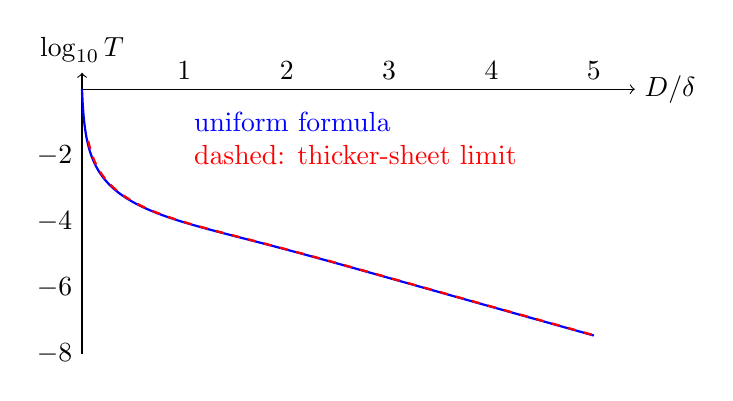
\begin{tikzpicture}[x=1.3cm,y=.42cm]
\draw[->] (0,-8)--(0,.5) node[above] {$\log_{10}T$};\draw[->] (0,0)--(5.4,0) node[right] {$D/\delta$};
\draw[blue,thick] plot coordinates {(0.000000,0.000000) (0.001010,-0.083583) (0.002020,-0.159824) (0.003030,-0.229909) (0.004040,-0.294759) (0.005051,-0.355102) (0.006061,-0.411524) (0.007071,-0.464503) (0.008081,-0.514436) (0.009091,-0.561653) (0.010101,-0.606436) (0.011111,-0.649022) (0.012121,-0.689618) (0.013131,-0.728401) (0.014141,-0.765525) (0.015152,-0.801128) (0.016162,-0.835329) (0.017172,-0.868234) (0.018182,-0.899938) (0.019192,-0.930525) (0.020202,-0.960072) (0.021212,-0.988647) (0.022222,-1.016311) (0.023232,-1.043121) (0.024242,-1.069129) (0.025253,-1.094380) (0.026263,-1.118919) (0.027273,-1.142782) (0.028283,-1.166008) (0.029293,-1.188629) (0.030303,-1.210675) (0.031313,-1.232176) (0.032323,-1.253158) (0.033333,-1.273644) (0.034343,-1.293659) (0.035354,-1.313222) (0.036364,-1.332355) (0.037374,-1.351075) (0.038384,-1.369401) (0.039394,-1.387347) (0.040404,-1.404931) (0.041414,-1.422165) (0.042424,-1.439064) (0.043434,-1.455641) (0.044444,-1.471907) (0.045455,-1.487874) (0.046465,-1.503553) (0.047475,-1.518954) (0.048485,-1.534087) (0.049495,-1.548960) (0.050505,-1.563583) (0.051515,-1.577964) (0.052525,-1.592111) (0.053535,-1.606031) (0.054545,-1.619732) (0.055556,-1.633219) (0.056566,-1.646501) (0.057576,-1.659582) (0.058586,-1.672470) (0.059596,-1.685168) (0.060606,-1.697684) (0.061616,-1.710023) (0.062626,-1.722188) (0.063636,-1.734185) (0.064646,-1.746019) (0.065657,-1.757694) (0.066667,-1.769214) (0.067677,-1.780583) (0.068687,-1.791805) (0.069697,-1.802884) (0.070707,-1.813824) (0.071717,-1.824627) (0.072727,-1.835298) (0.073737,-1.845840) (0.074747,-1.856255) (0.075758,-1.866546) (0.076768,-1.876717) (0.077778,-1.886770) (0.078788,-1.896709) (0.079798,-1.906534) (0.080808,-1.916250) (0.081818,-1.925859) (0.082828,-1.935362) (0.083838,-1.944763) (0.084848,-1.954062) (0.085859,-1.963264) (0.086869,-1.972368) (0.087879,-1.981379) (0.088889,-1.990297) (0.089899,-1.999124) (0.090909,-2.007863) (0.091919,-2.016514) (0.092929,-2.025080) (0.093939,-2.033563) (0.094949,-2.041963) (0.095960,-2.050283) (0.096970,-2.058524) (0.097980,-2.066688) (0.098990,-2.074775) (0.100000,-2.082788) (0.119679,-2.225743) (0.139357,-2.348463) (0.159036,-2.455975) (0.178715,-2.551637) (0.198394,-2.637805) (0.218072,-2.716197) (0.237751,-2.788103) (0.257430,-2.854518) (0.277108,-2.916223) (0.296787,-2.973845) (0.316466,-3.027895) (0.336145,-3.078792) (0.355823,-3.126888) (0.375502,-3.172479) (0.395181,-3.215817) (0.414859,-3.257119) (0.434538,-3.296571) (0.454217,-3.334337) (0.473896,-3.370560) (0.493574,-3.405367) (0.513253,-3.438868) (0.532932,-3.471165) (0.552610,-3.502346) (0.572289,-3.532491) (0.591968,-3.561675) (0.611647,-3.589961) (0.631325,-3.617411) (0.651004,-3.644079) (0.670683,-3.670016) (0.690361,-3.695267) (0.710040,-3.719875) (0.729719,-3.743880) (0.749398,-3.767317) (0.769076,-3.790221) (0.788755,-3.812624) (0.808434,-3.834554) (0.828112,-3.856040) (0.847791,-3.877107) (0.867470,-3.897780) (0.887149,-3.918081) (0.906827,-3.938033) (0.926506,-3.957655) (0.946185,-3.976967) (0.965863,-3.995987) (0.985542,-4.014734) (1.005221,-4.033222) (1.024900,-4.051468) (1.044578,-4.069487) (1.064257,-4.087293) (1.083936,-4.104899) (1.103614,-4.122320) (1.123293,-4.139566) (1.142972,-4.156651) (1.162651,-4.173585) (1.182329,-4.190379) (1.202008,-4.207044) (1.221687,-4.223589) (1.241365,-4.240025) (1.261044,-4.256360) (1.280723,-4.272603) (1.300402,-4.288762) (1.320080,-4.304845) (1.339759,-4.320860) (1.359438,-4.336815) (1.379116,-4.352716) (1.398795,-4.368569) (1.418474,-4.384382) (1.438153,-4.400159) (1.457831,-4.415908) (1.477510,-4.431632) (1.497189,-4.447338) (1.516867,-4.463030) (1.536546,-4.478713) (1.556225,-4.494391) (1.575904,-4.510068) (1.595582,-4.525748) (1.615261,-4.541434) (1.634940,-4.557130) (1.654618,-4.572838) (1.674297,-4.588563) (1.693976,-4.604305) (1.713655,-4.620068) (1.733333,-4.635854) (1.753012,-4.651665) (1.772691,-4.667503) (1.792369,-4.683368) (1.812048,-4.699264) (1.831727,-4.715190) (1.851406,-4.731148) (1.871084,-4.747139) (1.890763,-4.763164) (1.910442,-4.779223) (1.930120,-4.795317) (1.949799,-4.811446) (1.969478,-4.827611) (1.989157,-4.843811) (2.008835,-4.860046) (2.028514,-4.876317) (2.048193,-4.892624) (2.067871,-4.908965) (2.087550,-4.925341) (2.107229,-4.941751) (2.126908,-4.958194) (2.146586,-4.974671) (2.166265,-4.991181) (2.185944,-5.007722) (2.205622,-5.024294) (2.225301,-5.040897) (2.244980,-5.057529) (2.264659,-5.074190) (2.284337,-5.090879) (2.304016,-5.107594) (2.323695,-5.124336) (2.343373,-5.141103) (2.363052,-5.157895) (2.382731,-5.174710) (2.402410,-5.191547) (2.422088,-5.208406) (2.441767,-5.225285) (2.461446,-5.242184) (2.481124,-5.259102) (2.500803,-5.276038) (2.520482,-5.292991) (2.540161,-5.309960) (2.559839,-5.326944) (2.579518,-5.343943) (2.599197,-5.360956) (2.618876,-5.377981) (2.638554,-5.395019) (2.658233,-5.412068) (2.677912,-5.429127) (2.697590,-5.446197) (2.717269,-5.463275) (2.736948,-5.480362) (2.756627,-5.497458) (2.776305,-5.514560) (2.795984,-5.531670) (2.815663,-5.548785) (2.835341,-5.565906) (2.855020,-5.583033) (2.874699,-5.600163) (2.894378,-5.617299) (2.914056,-5.634437) (2.933735,-5.651580) (2.953414,-5.668725) (2.973092,-5.685872) (2.992771,-5.703022) (3.012450,-5.720173) (3.032129,-5.737327) (3.051807,-5.754481) (3.071486,-5.771636) (3.091165,-5.788792) (3.110843,-5.805949) (3.130522,-5.823105) (3.150201,-5.840262) (3.169880,-5.857418) (3.189558,-5.874574) (3.209237,-5.891730) (3.228916,-5.908885) (3.248594,-5.926039) (3.268273,-5.943192) (3.287952,-5.960344) (3.307631,-5.977495) (3.327309,-5.994645) (3.346988,-6.011794) (3.366667,-6.028941) (3.386345,-6.046087) (3.406024,-6.063231) (3.425703,-6.080373) (3.445382,-6.097515) (3.465060,-6.114654) (3.484739,-6.131792) (3.504418,-6.148928) (3.524096,-6.166063) (3.543775,-6.183196) (3.563454,-6.200328) (3.583133,-6.217458) (3.602811,-6.234586) (3.622490,-6.251713) (3.642169,-6.268838) (3.661847,-6.285961) (3.681526,-6.303083) (3.701205,-6.320204) (3.720884,-6.337323) (3.740562,-6.354441) (3.760241,-6.371557) (3.779920,-6.388672) (3.799598,-6.405785) (3.819277,-6.422898) (3.838956,-6.440009) (3.858635,-6.457119) (3.878313,-6.474227) (3.897992,-6.491335) (3.917671,-6.508441) (3.937349,-6.525547) (3.957028,-6.542651) (3.976707,-6.559755) (3.996386,-6.576857) (4.016064,-6.593959) (4.035743,-6.611060) (4.055422,-6.628160) (4.075100,-6.645259) (4.094779,-6.662358) (4.114458,-6.679455) (4.134137,-6.696553) (4.153815,-6.713649) (4.173494,-6.730745) (4.193173,-6.747841) (4.212851,-6.764936) (4.232530,-6.782030) (4.252209,-6.799124) (4.271888,-6.816218) (4.291566,-6.833311) (4.311245,-6.850404) (4.330924,-6.867496) (4.350602,-6.884589) (4.370281,-6.901681) (4.389960,-6.918772) (4.409639,-6.935864) (4.429317,-6.952955) (4.448996,-6.970046) (4.468675,-6.987137) (4.488353,-7.004227) (4.508032,-7.021318) (4.527711,-7.038408) (4.547390,-7.055499) (4.567068,-7.072589) (4.586747,-7.089679) (4.606426,-7.106769) (4.626104,-7.123859) (4.645783,-7.140949) (4.665462,-7.158039) (4.685141,-7.175129) (4.704819,-7.192219) (4.724498,-7.209309) (4.744177,-7.226399) (4.763855,-7.243489) (4.783534,-7.260579) (4.803213,-7.277669) (4.822892,-7.294759) (4.842570,-7.311849) (4.862249,-7.328939) (4.881928,-7.346030) (4.901606,-7.363120) (4.921285,-7.380210) (4.940964,-7.397301) (4.960643,-7.414391) (4.980321,-7.431482) (5.000000,-7.448572)};
\draw[red,dashed,thick] plot coordinates {(0.060606,-1.565032) (0.061616,-1.579390) (0.062626,-1.593513) (0.063636,-1.607411) (0.064646,-1.621090) (0.065657,-1.634557) (0.066667,-1.647818) (0.067677,-1.660880) (0.068687,-1.673748) (0.069697,-1.686428) (0.070707,-1.698926) (0.071717,-1.711247) (0.072727,-1.723395) (0.073737,-1.735376) (0.074747,-1.747194) (0.075758,-1.758853) (0.076768,-1.770357) (0.077778,-1.781712) (0.078788,-1.792920) (0.079798,-1.803985) (0.080808,-1.814910) (0.081818,-1.825701) (0.082828,-1.836358) (0.083838,-1.846887) (0.084848,-1.857289) (0.085859,-1.867569) (0.086869,-1.877728) (0.087879,-1.887769) (0.088889,-1.897696) (0.089899,-1.907511) (0.090909,-1.917216) (0.091919,-1.926814) (0.092929,-1.936307) (0.093939,-1.945697) (0.094949,-1.954987) (0.095960,-1.964178) (0.096970,-1.973274) (0.097980,-1.982275) (0.098990,-1.991184) (0.100000,-2.000002) (0.119679,-2.156038) (0.139357,-2.288268) (0.159036,-2.403004) (0.178715,-2.504341) (0.198394,-2.595085) (0.218072,-2.677245) (0.237751,-2.752306) (0.257430,-2.821402) (0.277108,-2.885413) (0.296787,-2.945040) (0.316466,-3.000847) (0.336145,-3.053299) (0.355823,-3.102778) (0.375502,-3.149608) (0.395181,-3.194062) (0.414859,-3.236373) (0.434538,-3.276744) (0.454217,-3.315347) (0.473896,-3.352338) (0.493574,-3.387849) (0.513253,-3.422001) (0.532932,-3.454898) (0.552610,-3.486635) (0.572289,-3.517297) (0.591968,-3.546961) (0.611647,-3.575695) (0.631325,-3.603563) (0.651004,-3.630622) (0.670683,-3.656925) (0.690361,-3.682519) (0.710040,-3.707448) (0.729719,-3.731755) (0.749398,-3.755476) (0.769076,-3.778647) (0.788755,-3.801301) (0.808434,-3.823467) (0.828112,-3.845176) (0.847791,-3.866452) (0.867470,-3.887323) (0.887149,-3.907810) (0.906827,-3.927937) (0.926506,-3.947724) (0.946185,-3.967191) (0.965863,-3.986358) (0.985542,-4.005241) (1.005221,-4.023858) (1.024900,-4.042225) (1.044578,-4.060358) (1.064257,-4.078270) (1.083936,-4.095977) (1.103614,-4.113490) (1.123293,-4.130824) (1.142972,-4.147989) (1.162651,-4.164998) (1.182329,-4.181862) (1.202008,-4.198591) (1.221687,-4.215196) (1.241365,-4.231687) (1.261044,-4.248072) (1.280723,-4.264360) (1.300402,-4.280561) (1.320080,-4.296682) (1.339759,-4.312730) (1.359438,-4.328715) (1.379116,-4.344642) (1.398795,-4.360519) (1.418474,-4.376351) (1.438153,-4.392146) (1.457831,-4.407909) (1.477510,-4.423645) (1.497189,-4.439359) (1.516867,-4.455058) (1.536546,-4.470745) (1.556225,-4.486425) (1.575904,-4.502102) (1.595582,-4.517780) (1.615261,-4.533462) (1.634940,-4.549153) (1.654618,-4.564855) (1.674297,-4.580571) (1.693976,-4.596303) (1.713655,-4.612056) (1.733333,-4.627830) (1.753012,-4.643628) (1.772691,-4.659452) (1.792369,-4.675303) (1.812048,-4.691183) (1.831727,-4.707093) (1.851406,-4.723035) (1.871084,-4.739009) (1.890763,-4.755017) (1.910442,-4.771059) (1.930120,-4.787135) (1.949799,-4.803246) (1.969478,-4.819393) (1.989157,-4.835575) (2.008835,-4.851792) (2.028514,-4.868045) (2.048193,-4.884333) (2.067871,-4.900657) (2.087550,-4.917015) (2.107229,-4.933408) (2.126908,-4.949835) (2.146586,-4.966295) (2.166265,-4.982788) (2.185944,-4.999313) (2.205622,-5.015869) (2.225301,-5.032457) (2.244980,-5.049074) (2.264659,-5.065720) (2.284337,-5.082395) (2.304016,-5.099097) (2.323695,-5.115826) (2.343373,-5.132580) (2.363052,-5.149360) (2.382731,-5.166163) (2.402410,-5.182989) (2.422088,-5.199837) (2.441767,-5.216706) (2.461446,-5.233595) (2.481124,-5.250503) (2.500803,-5.267430) (2.520482,-5.284374) (2.540161,-5.301335) (2.559839,-5.318312) (2.579518,-5.335304) (2.599197,-5.352309) (2.618876,-5.369328) (2.638554,-5.386360) (2.658233,-5.403403) (2.677912,-5.420457) (2.697590,-5.437522) (2.717269,-5.454596) (2.736948,-5.471679) (2.756627,-5.488770) (2.776305,-5.505869) (2.795984,-5.522975) (2.815663,-5.540087) (2.835341,-5.557206) (2.855020,-5.574330) (2.874699,-5.591458) (2.894378,-5.608591) (2.914056,-5.625728) (2.933735,-5.642869) (2.953414,-5.660012) (2.973092,-5.677159) (2.992771,-5.694307) (3.012450,-5.711458) (3.032129,-5.728610) (3.051807,-5.745764) (3.071486,-5.762919) (3.091165,-5.780075) (3.110843,-5.797231) (3.130522,-5.814387) (3.150201,-5.831544) (3.169880,-5.848701) (3.189558,-5.865857) (3.209237,-5.883013) (3.228916,-5.900168) (3.248594,-5.917323) (3.268273,-5.934476) (3.287952,-5.951629) (3.307631,-5.968781) (3.327309,-5.985931) (3.346988,-6.003080) (3.366667,-6.020228) (3.386345,-6.037374) (3.406024,-6.054519) (3.425703,-6.071663) (3.445382,-6.088805) (3.465060,-6.105945) (3.484739,-6.123084) (3.504418,-6.140221) (3.524096,-6.157357) (3.543775,-6.174491) (3.563454,-6.191623) (3.583133,-6.208754) (3.602811,-6.225883) (3.622490,-6.243010) (3.642169,-6.260136) (3.661847,-6.277261) (3.681526,-6.294383) (3.701205,-6.311505) (3.720884,-6.328624) (3.740562,-6.345743) (3.760241,-6.362860) (3.779920,-6.379975) (3.799598,-6.397090) (3.819277,-6.414203) (3.838956,-6.431314) (3.858635,-6.448425) (3.878313,-6.465534) (3.897992,-6.482642) (3.917671,-6.499749) (3.937349,-6.516855) (3.957028,-6.533960) (3.976707,-6.551064) (3.996386,-6.568167) (4.016064,-6.585269) (4.035743,-6.602370) (4.055422,-6.619471) (4.075100,-6.636570) (4.094779,-6.653669) (4.114458,-6.670768) (4.134137,-6.687865) (4.153815,-6.704962) (4.173494,-6.722058) (4.193173,-6.739154) (4.212851,-6.756249) (4.232530,-6.773344) (4.252209,-6.790438) (4.271888,-6.807532) (4.291566,-6.824625) (4.311245,-6.841719) (4.330924,-6.858811) (4.350602,-6.875904) (4.370281,-6.892996) (4.389960,-6.910087) (4.409639,-6.927179) (4.429317,-6.944270) (4.448996,-6.961361) (4.468675,-6.978452) (4.488353,-6.995543) (4.508032,-7.012634) (4.527711,-7.029724) (4.547390,-7.046815) (4.567068,-7.063905) (4.586747,-7.080995) (4.606426,-7.098085) (4.626104,-7.115175) (4.645783,-7.132265) (4.665462,-7.149355) (4.685141,-7.166445) (4.704819,-7.183535) (4.724498,-7.200625) (4.744177,-7.217715) (4.763855,-7.234805) (4.783534,-7.251895) (4.803213,-7.268985) (4.822892,-7.286075) (4.842570,-7.303165) (4.862249,-7.320255) (4.881928,-7.337346) (4.901606,-7.354436) (4.921285,-7.371526) (4.940964,-7.388617) (4.960643,-7.405707) (4.980321,-7.422797) (5.000000,-7.439888)};
\foreach \x in {1,2,3,4,5} \node[above] at (\x,0) {$\x$};
\foreach \y in {-2,-4,-6,-8} \node[left] at (0,\y) {$\y$};
\node[blue,right] at (1,-1) {uniform formula};\node[red,right] at (1,-2) {dashed: thicker-sheet limit};
\end{tikzpicture}

\end{center}

\Needspace{5\baselineskip}
\par\bigskip
\noindent\textbf{7.6}\quad A plane wave of frequency $\omega$ is incident normally from vacuum on a semi-infinite slab of material with a \emph{complex} index of refraction $n(\omega)$ [$n^{2}(\omega)=\epsilon(\omega)/\epsilon_{0}$].
\begin{enumerate}
\item[(a)] Show that the ratio of reflected power to incident power is
\[
R=\left|\frac{1-n(\omega)}{1+n(\omega)}\right|^{2}
\]
while the ratio of power transmitted into the medium to the incident power is
\[
T=\frac{4\,\mathrm{Re}\;n(\omega)}{|1+n(\omega)|^{2}}
\]
\item[(b)] Evaluate $\mathrm{Re}[i\omega(\mathbf{E}\cdot\mathbf{D}^{*}-\mathbf{B}\cdot\mathbf{H}^{*})/2]$ as a function of $(x,y,z)$. Show that this rate of change of energy per unit volume accounts for the relative transmitted power $T$.
\item[(c)] For a conductor, with $n^{2}=1+i(\sigma/\omega\epsilon_{0})$, $\sigma$ real, write out the results of parts a and b in the limit $\epsilon_{0}\omega\ll\sigma$. Express your answer in terms of $\delta$ as much as possible. Calculate $\frac{1}{2}\mathrm{Re}(\mathbf{J}^{*}\cdot\mathbf{E})$ and compare with the result of part b. Do both enter the complex form of Poynting's theorem?
\end{enumerate}
\solution
Take the material in $z>0$, $n=u+iv$ with $u,v\geq0$, and
$k_0=\omega/c$. For $\mathbf E_i=E_i\mathbf e_x$ the transmitted
fields are
\[
\mathbf E=\frac{2E_i}{1+n}\mathbf e_x e^{ik_0nz},\qquad
\mathbf H=\frac n{Z_0}\frac{2E_i}{1+n}\mathbf e_y e^{ik_0nz}.
\]
\textbf{(a)} The same boundary equations $1+r=t$, $1-r=nt$
give $r=(1-n)/(1+n)$ and $t=2/(1+n)$. The averaged incident
flux is $|E_i|^2/(2Z_0)$, while the transmitted flux at the surface
is $u|tE_i|^2/(2Z_0)$. Therefore
\[
\boxed{R=\left|\frac{1-n}{1+n}\right|^2,\qquad
T=\frac{4\operatorname{Re}n}{|1+n|^2}.}
\]
Expansion of the two squared moduli proves $R+T=1$ at the interface.
Here $T$ measures flux entering the material, not the flux surviving
to infinite depth.
\textbf{(b)} The magnetic term $\mathbf B\cdot\mathbf H^*
=\mu_0|\mathbf H|^2$ is real. With
$\epsilon=\epsilon_0n^2$ one finds
\begin{align*}
q(z)&=\operatorname{Re}\frac{i\omega}{2}
       (\mathbf E\cdot\mathbf D^*-\mathbf B\cdot\mathbf H^*)\\
&=\frac\omega2\operatorname{Im}\epsilon\,|\mathbf E|^2
=\boxed{\frac{4\omega\epsilon_0uv|E_i|^2}{|1+n|^2}
                              e^{-2k_0vz}}.
\end{align*}
There is no dependence on $x,y$. The flux at depth $z$ is
$S_z(z)=2u|E_i|^2e^{-2k_0vz}/[Z_0|1+n|^2]$; using
$1/Z_0=\epsilon_0c$ verifies $q=-dS_z/dz$.
For $v>0$, integrating to infinity gives
$\int_0^\infty q\,dz=S_z(0)=T|E_i|^2/(2Z_0)$.
In the lossless case $v=0$, the dissipation vanishes and the entering
flux instead propagates to infinity; it must not be equated to a
vanishing absorption integral.
\textbf{(c)} For a good conductor write $p=k_0\delta\ll1$.
Then
\[
n\simeq\frac{1+i}{p},\quad t\simeq(1-i)p,\quad
R\simeq1-2p,\quad T\simeq2p,
\]
and
\[
\boxed{q(z)\simeq\sigma p^2|E_i|^2e^{-2z/\delta}
                =2\epsilon_0\omega|E_i|^2e^{-2z/\delta}.}
\]
The equality uses $\sigma\delta^2=2/(\mu_0\omega)$.
Ohm's law gives
$\tfrac12\operatorname{Re}(\mathbf J^*\cdot\mathbf E)
=\sigma|\mathbf E|^2/2$, precisely the same heat production.
It enters Poynting's theorem once: either keep an explicit conduction
current with a real background permittivity, or absorb it into
$\epsilon+i\sigma/\omega$. Including both descriptions of the same
current would double-count the loss.

\Needspace{5\baselineskip}
\par\bigskip
\noindent\textbf{7.7}\quad A ribbon beam of plane-polarized radiation of wavelength $\lambda$ is totally reflected internally at a plane boundary between two nonpermeable media with indices of refraction $n$ and $n'$ ($n'<n$). As discussed in Section 7.4, the ratio of the reflected to incident amplitudes is a complex number of modulus unity, $E_{0}''/E_{0}=\exp[i\phi(i,i_{0})]$ for the angle of incidence $i>i_{0}$, where $\sin i_{0}=n'/n$.
\begin{enumerate}
\item[(a)] Show that for a ``monochromatic'' ribbon beam of radiation in the $z$ direction with an electric field amplitude, $E(x)e^{i(kz-\omega t)}$, where $E(x)$ is smooth and finite in transverse extent (but many wavelengths broad), the lowest order approximation in terms of plane waves is
\[
\mathbf{E}(x,z,t)=\boldsymbol{\epsilon}\int d\kappa\;A(\kappa)e^{i\kappa x+ikz-i\omega t}
\]
where $\boldsymbol{\epsilon}$ is a polarization vector, and $A(\kappa)$ is the Fourier transform of $E(x)$, with support in $\kappa$ around $\kappa=0$ small compared to $k$. The finite beam consists of plane waves with a small range of angles of incidence, centered around the geometrical optics value.
\item[(b)] Consider the reflected beam and show that for $i>i_{0}$ the electric field can be expressed approximately as
\[
\mathbf{E}''(x,z,t)=\boldsymbol{\epsilon}''E(x''-\delta x)\,\exp[i\mathbf{k}''\cdot\mathbf{x}-i\omega t+i\phi(i,i_{0})]
\]
where $\boldsymbol{\epsilon}''$ is a polarization vector, $x''$ is the $x$ coordinate perpendicular to $\mathbf{k}''$, the reflected wave vector, and $\delta x=-(1/k)[d\phi(i,i_{0})/di]$.
\item[(c)] With the Fresnel expressions of Section 7.3 for the phases $\phi(i,i_{0})$ for the two states of plane polarization, show that the lateral displacements of reflected beams with respect to the geometric optics position are
\[
D_{\perp}=\frac{\lambda}{\pi}\frac{\sin i}{(\sin^{2}i-\sin^{2}i_{0})^{1/2}}\qquad\text{and}\qquad
D_{\parallel}=D_{\perp}\cdot\frac{\sin^{2}i_{0}}{[\sin^{2}i-\cos^{2}i\cdot\sin^{2}i_{0}]}
\]
The displacement is known as the \emph{Goos--H\"anchen effect} (op.\ cit.).
\end{enumerate}
\solution
Let $k=2\pi/\lambda$ be the wave number in the incident medium;
$\lambda$ is correspondingly its wavelength.
\textbf{(a)} Define
$A(\kappa)=(2\pi)^{-1}\int E(x)e^{-i\kappa x}\,dx$.
The problem writes the inverse integral without a prefactor, so this
$A$ is Jackson's unitary Fourier amplitude [Eqs.~(7.80)--(7.81),
p.~323] divided by $\sqrt{2\pi}$.
The exact scalar angular spectrum in a homogeneous medium is
\[
\int d\kappa\,A(\kappa)
 e^{i\kappa x+i\sqrt{k^2-\kappa^2}\,z-i\omega t}.
\]
A smooth beam of width $w\gg\lambda$ has its important spectrum
at $|\kappa|\sim1/w\ll k$. Expanding
$\sqrt{k^2-\kappa^2}=k-\kappa^2/(2k)+\cdots$ and keeping the
lowest term gives the expression in the question. The polarization
vector can likewise be replaced by its central value to this order.
The ignored quadratic phase describes diffraction and is small over
propagation distances $|z|\ll k/(\Delta\kappa)^2$.
The angular change of an individual component is
$\Delta i\simeq\kappa/k$.
\textbf{(b)} The reflected spectrum is multiplied by
$e^{i\phi(i+\kappa/k)}$. Linearization of that phase gives
\[
e^{i\phi(i+\kappa/k)}
\simeq e^{i\phi(i)}e^{i\kappa\phi'(i)/k}.
\]
After extracting the central reflected plane-wave phase, its
transverse spectrum is therefore
\[
\int A(\kappa)e^{i\kappa[x''+\phi'(i)/k]}\,d\kappa
=E\bigl(x''+\phi'(i)/k\bigr).
\]
Thus
\[
\boxed{\mathbf E''\simeq\boldsymbol\epsilon''E(x''-\delta x)
 e^{i\mathbf k''\cdot\mathbf x-i\omega t+i\phi(i)},\qquad
\delta x=-\frac1k\frac{d\phi}{di}.}
\]
This approximation requires the reflection phase to be approximately
linear over the beam's angular spread.
\textbf{(c)} Put $m=n'/n=\sin i_0$,
$h=\sqrt{\sin^2i-m^2}$, and $c_i=\cos i$.
The two total-reflection phase factors, up to constant phases
irrelevant to the shift, are
\[
r_\perp=\frac{c_i-ih}{c_i+ih},\qquad
r_\parallel=\frac{m^2c_i-ih}{m^2c_i+ih}.
\]
Hence $\phi_\perp=-2\tan^{-1}(h/c_i)$ and
$\phi_\parallel=-2\tan^{-1}[h/(m^2c_i)]$.
Since $h'=\sin i\cos i/h$ and $h^2+c_i^2=1-m^2$,
\[
\phi_\perp'=-\frac{2\sin i}{h},\qquad
\frac{\phi_\parallel'}{\phi_\perp'}
=\frac{m^2(1-m^2)}{h^2+m^4c_i^2}
=\frac{m^2}{\sin^2i-m^2\cos^2i}.
\]
Substitution in part (b) gives the stated transverse displacements:
\[
\boxed{D_\perp=\frac\lambda\pi\frac{\sin i}{\sqrt{\sin^2i-\sin^2i_0}},
\quad D_\parallel=D_\perp
\frac{\sin^2i_0}{\sin^2i-\cos^2i\sin^2i_0}.}
\]
Here $D=\delta x$ is measured perpendicular to the reflected beam.
The corresponding displacement of the beam's footprint \emph{along
the interface} is $D/\cos i$. Close to $i_0$ the formal derivative
diverges, but the linear phase approximation fails when the angular
spread is comparable to $i-i_0$; a finite beam then requires the
unexpanded angular-spectrum integral.

\Needspace{5\baselineskip}
\par\bigskip
\noindent\textbf{7.8}\quad A monochromatic plane wave of frequency $\omega$ is incident normally on a stack of layers of various thicknesses $t_{j}$ and lossless indices of refraction $n_{j}$. Inside the stack, the wave has both forward and backward moving components. The change in the wave through any interface and also from one side of a layer to the other can be described by means of $2\times2$ transfer matrices. If the electric field is written as
\[
E=E_{+}e^{ikx}+E_{-}e^{-ikx}
\]
in each layer, the transfer matrix equation $E'=TE$ is explicitly
\[
\begin{pmatrix}E'_{+}\\ E'_{-}\end{pmatrix}
=\begin{pmatrix}t_{11}&t_{12}\\ t_{21}&t_{22}\end{pmatrix}
\begin{pmatrix}E_{+}\\ E_{-}\end{pmatrix}
\]
\begin{enumerate}
\item[(a)] Show that the transfer matrix for propagation inside, but across, a layer of index of refraction $n_{j}$ and thickness $t_{j}$ is
\[
T_{\mathrm{layer}}(n_{j},t_{j})=
\begin{pmatrix}e^{ik_{j}t_{j}}&0\\ 0&e^{-ik_{j}t_{j}}\end{pmatrix}
=I\cos(k_{j}t_{j})+i\sigma_{3}\sin(k_{j}t_{j})
\]
where $k_{j}=n_{j}\omega/c$, $I$ is the unit matrix, and $\sigma_{k}$ are the Pauli spin matrices of quantum mechanics. Show that the inverse matrix is $T^{*}$.
\item[(b)] Show that the transfer matrix to cross an interface from $n_{1}$ ($x<x_{0}$) to $n_{2}$ ($x>x_{0}$) is
\[
T_{\mathrm{interface}}(2,1)=\frac{1}{2}
\begin{pmatrix}n+1&-(n-1)\\ -(n-1)&n+1\end{pmatrix}
=I\,\frac{(n+1)}{2}-\sigma_{1}\frac{(n-1)}{2}
\]
where $n=n_{1}/n_{2}$.
\item[(c)] Show that for a complete stack, the incident, reflected, and transmitted waves are related by
\[
E_{\mathrm{trans}}=\frac{\det(T)}{t_{22}}\,E_{\mathrm{inc}},\qquad
E_{\mathrm{refl}}=-\frac{t_{21}}{t_{22}}\,E_{\mathrm{inc}}
\]
where $t_{ij}$ are the elements of $T$, the product of the forward-going transfer matrices, including from the material filling space on the incident side into the first layer and from the last layer into the medium filling the space on the transmitted side.
\end{enumerate}
\solution
Amplitudes in a transfer vector are evaluated at a reference plane;
this choice absorbs the local traveling-wave phases at that plane.
If one instead uses fixed global exponential coordinates, the same
relations acquire the corresponding reference-plane phase factors.
\textbf{(a)} Across a uniform thickness $t_j$, the forward wave
acquires $e^{ik_jt_j}$ and the backward wave acquires
$e^{-ik_jt_j}$. Thus
\[
\boxed{T_{\rm layer}=\begin{pmatrix}e^{ik_jt_j}&0\\0&e^{-ik_jt_j}\end{pmatrix}
=I\cos(k_jt_j)+i\sigma_3\sin(k_jt_j).}
\]
Here $\sigma_3=\operatorname{diag}(1,-1)$.
For real $k_jt_j$ its inverse is its componentwise complex
conjugate, since each diagonal factor is then of unit modulus.
\textbf{(b)} At an interface let $n=n_1/n_2$.
Continuity of the tangential electric and magnetic fields gives
\[
E_{2+}+E_{2-}=E_{1+}+E_{1-},\qquad
E_{2+}-E_{2-}=n(E_{1+}-E_{1-}).
\]
Adding and subtracting these equations proves
\[
\boxed{T_{\rm interface}(2,1)=\frac12
 \begin{pmatrix}n+1&1-n\\1-n&n+1\end{pmatrix}
=\frac{n+1}{2}I-\frac{n-1}{2}\sigma_1.}
\]
Its determinant is $n$, and its inverse is the interface matrix with
$1$ and $2$ interchanged.
\textbf{(c)} Multiply matrices in the order encountered, the first
one acting being on the right. With no wave incident from the
transmitted side,
\[
\begin{pmatrix}E_{\rm trans}\\0\end{pmatrix}
=\begin{pmatrix}t_{11}&t_{12}\\t_{21}&t_{22}\end{pmatrix}
 \begin{pmatrix}E_{\rm inc}\\E_{\rm refl}\end{pmatrix}.
\]
The second row gives $E_{\rm refl}=-t_{21}E_{\rm inc}/t_{22}$.
Inserting it in the first row gives
\[
\boxed{E_{\rm trans}=\frac{t_{11}t_{22}-t_{12}t_{21}}{t_{22}}E_{\rm inc}
=\frac{\det T}{t_{22}}E_{\rm inc},\qquad
E_{\rm refl}=-\frac{t_{21}}{t_{22}}E_{\rm inc}.}
\]
The layer determinants are one and the interface determinants
 telescope, so $\det T=n_{\rm inc}/n_{\rm out}$.
Flux conservation provides an independent check:
$T^\dagger\sigma_3T=(n_{\rm inc}/n_{\rm out})\sigma_3$.
Consequently the amplitudes above obey
$|r|^2+(n_{\rm out}/n_{\rm inc})|t|^2=1$ for a lossless stack.

\Needspace{5\baselineskip}
\par\bigskip
\noindent\textbf{7.9}\quad A stack of optical elements consists of $N$ layers with index of refraction $n$ and thickness $t_{1}$, separated by air gaps ($n_{2}=1$) of thickness $t_{2}$. A monochromatic plane wave is incident normally. With appropriate thicknesses, a modest number of layers can cause almost total reflection of a given range of frequencies, even for normal $n$ values (e.g., $1.3<n<1.8$).
\begin{enumerate}
\item[(a)] Show the transfer matrix for the stack is $T_{\mathrm{stack}}=T^{N}(I\cos\alpha_{2}-i\sigma_{3}\sin\alpha_{2})$, where $\alpha_{2}=\omega t_{2}/c$, and the single air gap plus foil transfer matrix is
\begin{align*}
T=(1/4n)\{&[(n+1)^{2}\cos(\alpha_{1}+\alpha_{2})-(n-1)^{2}\cos(\alpha_{1}-\alpha_{2})]I\\
&+i\sigma_{3}[(n+1)^{2}\sin(\alpha_{1}+\alpha_{2})+(n-1)^{2}\sin(\alpha_{1}-\alpha_{2})]\\
&+2\sigma_{1}(n^{2}-1)\sin\alpha_{1}\sin\alpha_{2}\\
&-2\sigma_{2}(n^{2}-1)\sin\alpha_{1}\cos\alpha_{2}\}
\end{align*}
with $\alpha_{1}=n\omega t_{1}/c$.
\item[(b)] If all the layers (both air gaps and foils) have optical thicknesses of a quarter-wavelength of the incident wave, show that
\[
T=-\exp(-\lambda\sigma_{1}),\qquad\text{where }\lambda=\ln(n)
\]
is (roughly) the amplitude ``decay constant'' per layer. Show that the fractional transmitted intensity is
\[
\frac{|E_{\mathrm{trans}}|^{2}}{|E_{\mathrm{inc}}|^{2}}=\mathrm{sech}^{2}[N\ln(n)]=\frac{4n^{2N}}{(n^{2N}+1)^{2}}\to 4\,\exp[-N\ln(n^{2})]
\]
The asymptotic form holds for $n^{2N}\gg1$.
\end{enumerate}
\solution
Let $P_j=I\cos\alpha_j+i\sigma_3\sin\alpha_j$, and write
$I(b,a)$ for the interface matrix from index $a$ to $b$.
A single foil surrounded by air has transfer matrix
\[
F=I(1,n)P_1I(n,1)
=I\cos\alpha_1+iA\sigma_3\sin\alpha_1-B\sigma_2\sin\alpha_1,
\]
where $A=(n^2+1)/(2n)$ and $B=(n^2-1)/(2n)$.
For example, the nontrivial multiplication follows from
\[
I(1,n)\sigma_3I(n,1)=A\sigma_3+iB\sigma_2,
\]
using $\sigma_3\sigma_1=i\sigma_2$,
$\sigma_1\sigma_3=-i\sigma_2$ and
$\sigma_1\sigma_3\sigma_1=-\sigma_3$.
\textbf{(a)} Define the cell to be a gap followed by a foil, so
$T=FP_2$. Then
\[
\begin{aligned}
T={}&(\cos\alpha_1\cos\alpha_2-A\sin\alpha_1\sin\alpha_2)I\\
&+i(\cos\alpha_1\sin\alpha_2+A\sin\alpha_1\cos\alpha_2)\sigma_3\\
&+B\sin\alpha_1\sin\alpha_2\sigma_1
 -B\sin\alpha_1\cos\alpha_2\sigma_2.
\end{aligned}
\]
Product-to-sum identities turn the first two coefficients into
\[
\frac{(n+1)^2\cos(\alpha_1+\alpha_2)
       -(n-1)^2\cos(\alpha_1-\alpha_2)}{4n},
\]
\[
\frac{(n+1)^2\sin(\alpha_1+\alpha_2)
       +(n-1)^2\sin(\alpha_1-\alpha_2)}{4n},
\]
respectively, while the last two are exactly the coefficients
printed in the question. A stack with $N$ foils and $N-1$ gaps is
$F P_2 F P_2\cdots F=(FP_2)^NP_2^{-1}$; hence
\[
\boxed{T_{\rm stack}=T^N(I\cos\alpha_2-i\sigma_3\sin\alpha_2).}
\]
\textbf{(b)} With $\alpha_1=\alpha_2=\pi/2$,
$T=-AI+B\sigma_1$. If $\lambda=\ln n$, then
$A=\cosh\lambda$ and $B=\sinh\lambda$. Since $\sigma_1^2=I$,
\[
\boxed{T=-e^{-\lambda\sigma_1},\quad
T^N=(-1)^N[I\cosh(N\lambda)-\sigma_1\sinh(N\lambda)].}
\]
Multiplication by $P_2^{-1}=-i\sigma_3$ only changes the phases of
its columns. The magnitude of $t_{22}$ for the full stack is
$\cosh(N\lambda)$ and its determinant is one. The incident and
transmitted media are both air, so
\[
\boxed{\frac{|E_{\rm trans}|^2}{|E_{\rm inc}|^2}
=\operatorname{sech}^2(N\ln n)
=\frac{4n^{2N}}{(n^{2N}+1)^2}
\sim4e^{-N\ln(n^2)}.}
\]
Thus the decaying cell eigenvalue has magnitude $e^{-\lambda}$;
intensity transmission decreases exponentially with the number of
quarter-wave foils, with prefactors fixed by the end interfaces.

\Needspace{5\baselineskip}
\par\bigskip
\noindent\textbf{7.10}\quad An arbitrary optical element of length $L$ is placed in a uniform nonabsorbing medium with index of refraction $n(\omega)$ with its front face at $x=0$ and its back face at $x=L$. If a monochromatic plane wave of frequency $\omega$ with amplitude $\psi_{\mathrm{inc}}(\omega,x,t)=\exp[ik(\omega)x-i\omega t]$ is incident on the front face of the element, the transmitted wave amplitude is $\psi_{\mathrm{trans}}(\omega,x,t)=T(\omega)\exp[ik(\omega)(x-L)-i\omega t]$, where the relative transmission amplitude $T(\omega)=\tau(\omega)\exp[i\phi(\omega)]$ is a complex quantity of magnitude $\tau(\omega)$ and phase $\phi(\omega)$.

A plane wave of radiation $\psi_{\mathrm{inc}}(x,t)$, consisting of a coherent superposition of different frequencies centered around $\omega=\omega_{0}$, with support $A(\omega)$ narrow on the scale of variation of $\tau(\omega)$, $\phi(\omega)$ and $k(\omega)$, is incident on the optical element. Show that the transmitted wave for $x>L$ is approximately
\[
\psi_{\mathrm{trans}}(x,t)\approx\tau(\omega_{0})e^{i\beta}\psi_{\mathrm{inc}}(x',t')
\]
where $\beta$ is a constant phase and $x'=x-L$, $t'=t-T$. The transit or group delay time (sometimes attributed in another context to E.~P. Wigner) is $T=[d\phi(\omega)/d\omega]_{\omega=\omega_{0}}$. If $cT<L$, some authors speak of superluminal propagation through the element. Discuss.
\solution
Write the incident packet as
$\psi_{\rm inc}(x,t)=(2\pi)^{-1/2}\int A(\omega)e^{ik(\omega)x-i\omega t}\,d\omega$.
Each frequency is transmitted independently, giving
\[
\psi_{\rm trans}(x,t)=\frac1{\sqrt{2\pi}}\int A(\omega)\tau(\omega)
 e^{i\phi(\omega)+ik(\omega)(x-L)-i\omega t}\,d\omega.
\]
Across its narrow spectrum approximate $\tau(\omega)\simeq\tau_0$
and $\phi(\omega)\simeq\phi_0+T(\omega-\omega_0)$, where
$T=\phi'(\omega_0)$. Combining terms in the exponent then gives
\begin{align*}
\psi_{\rm trans}(x,t)
&\simeq\frac{\tau_0 e^{i(\phi_0-\omega_0T)}}{\sqrt{2\pi}}
 \int A(\omega)e^{ik(\omega)(x-L)-i\omega(t-T)}\,d\omega\\
&=\boxed{\tau_0e^{i\beta}\psi_{\rm inc}(x-L,t-T),\qquad
\beta=\phi_0-\omega_0T.}
\end{align*}
The conditions include
$|\tau'/\tau_0|\Delta\omega\ll1$ and
$|\phi''|(\Delta\omega)^2\ll1$; otherwise the packet is distorted,
and a single translation does not describe it. A linear expansion
of $k(\omega)$ identifies the usual group motion of its envelope in
the surrounding medium, but is not needed for the algebraic shift
relation itself.

The quantity $T$ measures the shift of a narrow-band envelope or
its peak. It is not in general the arrival time of a new signal
front. A frequency-selective element can reshape the leading tail
and thereby advance the transmitted peak, giving $cT<L$ or even
a negative $T$. A sharp front contains frequencies outside this
narrow-band approximation. For a causal electromagnetic material
whose high-frequency index tends to one, the high-frequency
propagator fixes front propagation at no more than $c$, consistently
with the causal response discussed in Section 7.10. Thus $cT<L$
by itself does not establish faster-than-light transport of new
information; the approximation used to infer it cannot describe
the required front.

\Needspace{5\baselineskip}
\par\bigskip
\noindent\textbf{7.11}\quad A simple example of the transit time of the preceding problem is afforded by a slab of lossless dielectric of thickness $d$ and index of refraction $n$ in vacuum.
\begin{enumerate}
\item[(a)] For a plane wave incident normally, show that the magnitude of the transmitted amplitude is
\[
|\tau(\omega)|=\frac{4n}{\sqrt{[(n+1)^{2}-(n-1)^{2}\cos(2z)]^{2}+[(n-1)^{2}\sin(2z)]^{2}}}
\]
while its phase is
\[
\phi(\omega)=z+\arctan\!\left[\frac{(n-1)^{2}\sin(2z)}{(n+1)^{2}-(n-1)^{2}\cos(2z)}\right]
\]
where $z=n\omega d/c$.
\item[(b)] Neglecting dispersion, show that for $z\to0$ and $z=\pi$, $|\tau|=1.0$ and $cT/d=(n^{2}+1)/2$, while for $z=\pi/2$ (quarter-wave plate), $|\tau|=2n/(n^{2}+1)$ and $cT/d=2n^{2}/(n^{2}+1)$. Show also that $cT/d$, averaged \erratum{from $z=0$ to any integer multiple of $\pi/2$}, is $\langle cT/d\rangle=n$. Does this result tell you anything about what you might expect for the observed transit time of a long wave train ($\Delta\omega/\omega\ll1$) through a piece of window glass? Explain.
\item[(c)] Calculate numerically and plot the results as functions of $z$ for the magnitude of the transmission amplitude, its phase, and the transit time in units of $d/c$ for $n=1.5$ and $n=2.0$.
\end{enumerate}
\solution
\textbf{(a)} The two-interface result for a slab in vacuum is
\[
t(\omega)=\frac{4ne^{iz}}{(n+1)^2-(n-1)^2e^{2iz}},\qquad
z=\frac{n\omega d}{c}.
\]
The denominator has real and imaginary parts
$(n+1)^2-(n-1)^2\cos2z$ and $-(n-1)^2\sin2z$.
Taking its modulus and subtracting its phase proves the two
expressions in the question. Its real part is always positive for
$n>0$, so the continuous, unwrapped phase is
\[
\phi=z+\tan^{-1}\frac{(n-1)^2\sin2z}
 {(n+1)^2-(n-1)^2\cos2z}.
\]
It is useful to divide numerator and denominator by $4ne^{iz}$:
\[
t=\frac1{\cos z-iA\sin z},\quad
A=\frac{n^2+1}{2n},\qquad
|t|^2=\frac1{\cos^2z+A^2\sin^2z}.
\]
\textbf{(b)} Differentiation of the argument of
$\cos z+iA\sin z$ gives
\[
\frac{d\phi}{dz}
=\frac{A\cos^2z+A\sin^2z}{\cos^2z+A^2\sin^2z}
=\frac{A}{\cos^2z+A^2\sin^2z}.
\]
For nondispersive $n$, $dz/d\omega=nd/c$, hence
\[
\boxed{\frac{cT}{d}=\frac{nA}{\cos^2z+A^2\sin^2z}=nA|t|^2.}
\]
At $z=0,\pi$, $|t|=1$ and $cT/d=nA=(n^2+1)/2$;
at $z=\pi/2$, $|t|=1/A=2n/(n^2+1)$ and
$cT/d=n/A=2n^2/(n^2+1)$.
On a quarter-wave interval with endpoints at consecutive multiples
of $\pi/2$, substitute $u=\tan z$ (or use symmetry for the next
interval) to find
\[
\int_0^{\pi/2}\frac{A\,dz}{\cos^2z+A^2\sin^2z}
=\int_0^\infty\frac{A\,du}{1+A^2u^2}=\frac\pi2.
\]
Consequently $\langle cT/d\rangle=n$ from $z=0$ to any integer
multiple of $\pi/2$, or over any whole fringe period $\pi$.
An interval of length $\pi/2$ starting at an arbitrary phase need
not have that average; the quarter-wave endpoints matter.

This unweighted average over optical phase is not a universal
measurement of a packet's transit time. A sufficiently narrow
spectrum, $nd\Delta\omega/c\ll1$, samples the delay at its carrier
phase, anywhere between the two limits above. Even a long train
with $\Delta\omega/\omega\ll1$ can cover many fringes in a thick
window because $z\gg1$. In that regime the single-delay approximation
can fail and the separate multiply reflected pulses, coherence,
and detector weighting must be considered. The direct transmitted
pulse travels in time $nd/c$; the displayed average explains that
scale but does not fix every measured peak or energy-centroid delay.
\textbf{(c)} The plotted curves use the exact amplitude, unwrapped
phase, and analytic derivative, not numerical differentiation of a
wrapped arctangent. For $n=1.5$, the amplitude ranges from
$12/13$ to $1$ and $cT/d$ from $18/13$ to $13/8$.
For $n=2$, the ranges are $4/5$ to $1$ and $8/5$ to $5/2$.
The phase increases by $\pi$ over each period of the amplitude.
\begin{center}
% Generated by supplementary/check_ch07.py --write-assets
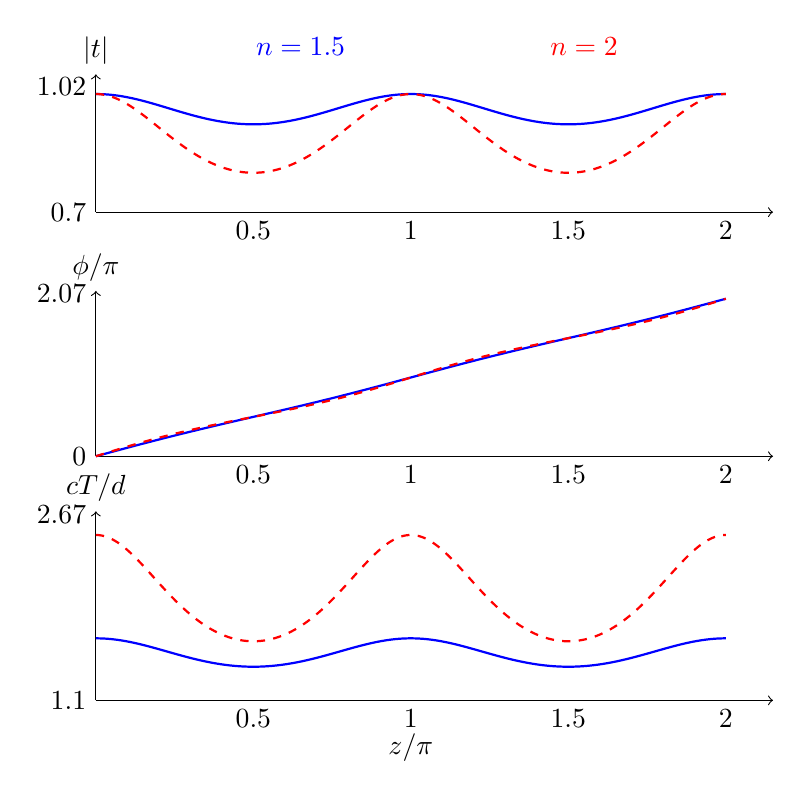
\begin{tikzpicture}[x=4cm]
\begin{scope}[yshift=-3.5cm,y=5cm]
\draw[->] (0,0.7)--(2.15,0.7);\draw[->] (0,0.7)--(0,1.05) node[above] {$|t|$};
\draw[blue,thick] plot coordinates {(0.000000,1.000000) (0.005556,0.999974) (0.011111,0.999894) (0.016667,0.999762) (0.022222,0.999578) (0.027778,0.999341) (0.033333,0.999053) (0.038889,0.998713) (0.044444,0.998323) (0.050000,0.997882) (0.055556,0.997393) (0.061111,0.996854) (0.066667,0.996269) (0.072222,0.995636) (0.077778,0.994958) (0.083333,0.994235) (0.088889,0.993469) (0.094444,0.992661) (0.100000,0.991812) (0.105556,0.990924) (0.111111,0.989998) (0.116667,0.989035) (0.122222,0.988037) (0.127778,0.987005) (0.133333,0.985941) (0.138889,0.984847) (0.144444,0.983725) (0.150000,0.982575) (0.155556,0.981400) (0.161111,0.980201) (0.166667,0.978980) (0.172222,0.977740) (0.177778,0.976480) (0.183333,0.975204) (0.188889,0.973914) (0.194444,0.972610) (0.200000,0.971294) (0.205556,0.969970) (0.211111,0.968637) (0.216667,0.967298) (0.222222,0.965955) (0.227778,0.964609) (0.233333,0.963262) (0.238889,0.961916) (0.244444,0.960573) (0.250000,0.959233) (0.255556,0.957899) (0.261111,0.956572) (0.266667,0.955254) (0.272222,0.953946) (0.277778,0.952649) (0.283333,0.951366) (0.288889,0.950098) (0.294444,0.948845) (0.300000,0.947610) (0.305556,0.946393) (0.311111,0.945197) (0.316667,0.944021) (0.322222,0.942868) (0.327778,0.941739) (0.333333,0.940634) (0.338889,0.939555) (0.344444,0.938503) (0.350000,0.937479) (0.355556,0.936484) (0.361111,0.935518) (0.366667,0.934584) (0.372222,0.933680) (0.377778,0.932810) (0.383333,0.931972) (0.388889,0.931169) (0.394444,0.930400) (0.400000,0.929666) (0.405556,0.928969) (0.411111,0.928308) (0.416667,0.927685) (0.422222,0.927099) (0.427778,0.926551) (0.433333,0.926042) (0.438889,0.925573) (0.444444,0.925143) (0.450000,0.924752) (0.455556,0.924402) (0.461111,0.924093) (0.466667,0.923824) (0.472222,0.923596) (0.477778,0.923409) (0.483333,0.923264) (0.488889,0.923160) (0.494444,0.923098) (0.500000,0.923077) (0.505556,0.923098) (0.511111,0.923160) (0.516667,0.923264) (0.522222,0.923409) (0.527778,0.923596) (0.533333,0.923824) (0.538889,0.924093) (0.544444,0.924402) (0.550000,0.924752) (0.555556,0.925143) (0.561111,0.925573) (0.566667,0.926042) (0.572222,0.926551) (0.577778,0.927099) (0.583333,0.927685) (0.588889,0.928308) (0.594444,0.928969) (0.600000,0.929666) (0.605556,0.930400) (0.611111,0.931169) (0.616667,0.931972) (0.622222,0.932810) (0.627778,0.933680) (0.633333,0.934584) (0.638889,0.935518) (0.644444,0.936484) (0.650000,0.937479) (0.655556,0.938503) (0.661111,0.939555) (0.666667,0.940634) (0.672222,0.941739) (0.677778,0.942868) (0.683333,0.944021) (0.688889,0.945197) (0.694444,0.946393) (0.700000,0.947610) (0.705556,0.948845) (0.711111,0.950098) (0.716667,0.951366) (0.722222,0.952649) (0.727778,0.953946) (0.733333,0.955254) (0.738889,0.956572) (0.744444,0.957899) (0.750000,0.959233) (0.755556,0.960573) (0.761111,0.961916) (0.766667,0.963262) (0.772222,0.964609) (0.777778,0.965955) (0.783333,0.967298) (0.788889,0.968637) (0.794444,0.969970) (0.800000,0.971294) (0.805556,0.972610) (0.811111,0.973914) (0.816667,0.975204) (0.822222,0.976480) (0.827778,0.977740) (0.833333,0.978980) (0.838889,0.980201) (0.844444,0.981400) (0.850000,0.982575) (0.855556,0.983725) (0.861111,0.984847) (0.866667,0.985941) (0.872222,0.987005) (0.877778,0.988037) (0.883333,0.989035) (0.888889,0.989998) (0.894444,0.990924) (0.900000,0.991812) (0.905556,0.992661) (0.911111,0.993469) (0.916667,0.994235) (0.922222,0.994958) (0.927778,0.995636) (0.933333,0.996269) (0.938889,0.996854) (0.944444,0.997393) (0.950000,0.997882) (0.955556,0.998323) (0.961111,0.998713) (0.966667,0.999053) (0.972222,0.999341) (0.977778,0.999578) (0.983333,0.999762) (0.988889,0.999894) (0.994444,0.999974) (1.000000,1.000000) (1.005556,0.999974) (1.011111,0.999894) (1.016667,0.999762) (1.022222,0.999578) (1.027778,0.999341) (1.033333,0.999053) (1.038889,0.998713) (1.044444,0.998323) (1.050000,0.997882) (1.055556,0.997393) (1.061111,0.996854) (1.066667,0.996269) (1.072222,0.995636) (1.077778,0.994958) (1.083333,0.994235) (1.088889,0.993469) (1.094444,0.992661) (1.100000,0.991812) (1.105556,0.990924) (1.111111,0.989998) (1.116667,0.989035) (1.122222,0.988037) (1.127778,0.987005) (1.133333,0.985941) (1.138889,0.984847) (1.144444,0.983725) (1.150000,0.982575) (1.155556,0.981400) (1.161111,0.980201) (1.166667,0.978980) (1.172222,0.977740) (1.177778,0.976480) (1.183333,0.975204) (1.188889,0.973914) (1.194444,0.972610) (1.200000,0.971294) (1.205556,0.969970) (1.211111,0.968637) (1.216667,0.967298) (1.222222,0.965955) (1.227778,0.964609) (1.233333,0.963262) (1.238889,0.961916) (1.244444,0.960573) (1.250000,0.959233) (1.255556,0.957899) (1.261111,0.956572) (1.266667,0.955254) (1.272222,0.953946) (1.277778,0.952649) (1.283333,0.951366) (1.288889,0.950098) (1.294444,0.948845) (1.300000,0.947610) (1.305556,0.946393) (1.311111,0.945197) (1.316667,0.944021) (1.322222,0.942868) (1.327778,0.941739) (1.333333,0.940634) (1.338889,0.939555) (1.344444,0.938503) (1.350000,0.937479) (1.355556,0.936484) (1.361111,0.935518) (1.366667,0.934584) (1.372222,0.933680) (1.377778,0.932810) (1.383333,0.931972) (1.388889,0.931169) (1.394444,0.930400) (1.400000,0.929666) (1.405556,0.928969) (1.411111,0.928308) (1.416667,0.927685) (1.422222,0.927099) (1.427778,0.926551) (1.433333,0.926042) (1.438889,0.925573) (1.444444,0.925143) (1.450000,0.924752) (1.455556,0.924402) (1.461111,0.924093) (1.466667,0.923824) (1.472222,0.923596) (1.477778,0.923409) (1.483333,0.923264) (1.488889,0.923160) (1.494444,0.923098) (1.500000,0.923077) (1.505556,0.923098) (1.511111,0.923160) (1.516667,0.923264) (1.522222,0.923409) (1.527778,0.923596) (1.533333,0.923824) (1.538889,0.924093) (1.544444,0.924402) (1.550000,0.924752) (1.555556,0.925143) (1.561111,0.925573) (1.566667,0.926042) (1.572222,0.926551) (1.577778,0.927099) (1.583333,0.927685) (1.588889,0.928308) (1.594444,0.928969) (1.600000,0.929666) (1.605556,0.930400) (1.611111,0.931169) (1.616667,0.931972) (1.622222,0.932810) (1.627778,0.933680) (1.633333,0.934584) (1.638889,0.935518) (1.644444,0.936484) (1.650000,0.937479) (1.655556,0.938503) (1.661111,0.939555) (1.666667,0.940634) (1.672222,0.941739) (1.677778,0.942868) (1.683333,0.944021) (1.688889,0.945197) (1.694444,0.946393) (1.700000,0.947610) (1.705556,0.948845) (1.711111,0.950098) (1.716667,0.951366) (1.722222,0.952649) (1.727778,0.953946) (1.733333,0.955254) (1.738889,0.956572) (1.744444,0.957899) (1.750000,0.959233) (1.755556,0.960573) (1.761111,0.961916) (1.766667,0.963262) (1.772222,0.964609) (1.777778,0.965955) (1.783333,0.967298) (1.788889,0.968637) (1.794444,0.969970) (1.800000,0.971294) (1.805556,0.972610) (1.811111,0.973914) (1.816667,0.975204) (1.822222,0.976480) (1.827778,0.977740) (1.833333,0.978980) (1.838889,0.980201) (1.844444,0.981400) (1.850000,0.982575) (1.855556,0.983725) (1.861111,0.984847) (1.866667,0.985941) (1.872222,0.987005) (1.877778,0.988037) (1.883333,0.989035) (1.888889,0.989998) (1.894444,0.990924) (1.900000,0.991812) (1.905556,0.992661) (1.911111,0.993469) (1.916667,0.994235) (1.922222,0.994958) (1.927778,0.995636) (1.933333,0.996269) (1.938889,0.996854) (1.944444,0.997393) (1.950000,0.997882) (1.955556,0.998323) (1.961111,0.998713) (1.966667,0.999053) (1.972222,0.999341) (1.977778,0.999578) (1.983333,0.999762) (1.988889,0.999894) (1.994444,0.999974) (2.000000,1.000000)};
\draw[red,dashed,thick] plot coordinates {(0.000000,1.000000) (0.005556,0.999914) (0.011111,0.999658) (0.016667,0.999231) (0.022222,0.998634) (0.027778,0.997870) (0.033333,0.996941) (0.038889,0.995849) (0.044444,0.994597) (0.050000,0.993188) (0.055556,0.991626) (0.061111,0.989915) (0.066667,0.988060) (0.072222,0.986065) (0.077778,0.983935) (0.083333,0.981676) (0.088889,0.979293) (0.094444,0.976792) (0.100000,0.974179) (0.105556,0.971459) (0.111111,0.968639) (0.116667,0.965726) (0.122222,0.962725) (0.127778,0.959643) (0.133333,0.956486) (0.138889,0.953261) (0.144444,0.949973) (0.150000,0.946630) (0.155556,0.943238) (0.161111,0.939802) (0.166667,0.936329) (0.172222,0.932825) (0.177778,0.929295) (0.183333,0.925745) (0.188889,0.922181) (0.194444,0.918608) (0.200000,0.915032) (0.205556,0.911457) (0.211111,0.907888) (0.216667,0.904330) (0.222222,0.900787) (0.227778,0.897264) (0.233333,0.893766) (0.238889,0.890295) (0.244444,0.886856) (0.250000,0.883452) (0.255556,0.880088) (0.261111,0.876765) (0.266667,0.873488) (0.272222,0.870259) (0.277778,0.867081) (0.283333,0.863957) (0.288889,0.860889) (0.294444,0.857880) (0.300000,0.854932) (0.305556,0.852046) (0.311111,0.849226) (0.316667,0.846472) (0.322222,0.843787) (0.327778,0.841171) (0.333333,0.838628) (0.338889,0.836157) (0.344444,0.833761) (0.350000,0.831440) (0.355556,0.829196) (0.361111,0.827030) (0.366667,0.824942) (0.372222,0.822934) (0.377778,0.821007) (0.383333,0.819161) (0.388889,0.817396) (0.394444,0.815714) (0.400000,0.814116) (0.405556,0.812601) (0.411111,0.811170) (0.416667,0.809824) (0.422222,0.808563) (0.427778,0.807388) (0.433333,0.806298) (0.438889,0.805295) (0.444444,0.804378) (0.450000,0.803547) (0.455556,0.802804) (0.461111,0.802147) (0.466667,0.801578) (0.472222,0.801096) (0.477778,0.800702) (0.483333,0.800395) (0.488889,0.800175) (0.494444,0.800044) (0.500000,0.800000) (0.505556,0.800044) (0.511111,0.800175) (0.516667,0.800395) (0.522222,0.800702) (0.527778,0.801096) (0.533333,0.801578) (0.538889,0.802147) (0.544444,0.802804) (0.550000,0.803547) (0.555556,0.804378) (0.561111,0.805295) (0.566667,0.806298) (0.572222,0.807388) (0.577778,0.808563) (0.583333,0.809824) (0.588889,0.811170) (0.594444,0.812601) (0.600000,0.814116) (0.605556,0.815714) (0.611111,0.817396) (0.616667,0.819161) (0.622222,0.821007) (0.627778,0.822934) (0.633333,0.824942) (0.638889,0.827030) (0.644444,0.829196) (0.650000,0.831440) (0.655556,0.833761) (0.661111,0.836157) (0.666667,0.838628) (0.672222,0.841171) (0.677778,0.843787) (0.683333,0.846472) (0.688889,0.849226) (0.694444,0.852046) (0.700000,0.854932) (0.705556,0.857880) (0.711111,0.860889) (0.716667,0.863957) (0.722222,0.867081) (0.727778,0.870259) (0.733333,0.873488) (0.738889,0.876765) (0.744444,0.880088) (0.750000,0.883452) (0.755556,0.886856) (0.761111,0.890295) (0.766667,0.893766) (0.772222,0.897264) (0.777778,0.900787) (0.783333,0.904330) (0.788889,0.907888) (0.794444,0.911457) (0.800000,0.915032) (0.805556,0.918608) (0.811111,0.922181) (0.816667,0.925745) (0.822222,0.929295) (0.827778,0.932825) (0.833333,0.936329) (0.838889,0.939802) (0.844444,0.943238) (0.850000,0.946630) (0.855556,0.949973) (0.861111,0.953261) (0.866667,0.956486) (0.872222,0.959643) (0.877778,0.962725) (0.883333,0.965726) (0.888889,0.968639) (0.894444,0.971459) (0.900000,0.974179) (0.905556,0.976792) (0.911111,0.979293) (0.916667,0.981676) (0.922222,0.983935) (0.927778,0.986065) (0.933333,0.988060) (0.938889,0.989915) (0.944444,0.991626) (0.950000,0.993188) (0.955556,0.994597) (0.961111,0.995849) (0.966667,0.996941) (0.972222,0.997870) (0.977778,0.998634) (0.983333,0.999231) (0.988889,0.999658) (0.994444,0.999914) (1.000000,1.000000) (1.005556,0.999914) (1.011111,0.999658) (1.016667,0.999231) (1.022222,0.998634) (1.027778,0.997870) (1.033333,0.996941) (1.038889,0.995849) (1.044444,0.994597) (1.050000,0.993188) (1.055556,0.991626) (1.061111,0.989915) (1.066667,0.988060) (1.072222,0.986065) (1.077778,0.983935) (1.083333,0.981676) (1.088889,0.979293) (1.094444,0.976792) (1.100000,0.974179) (1.105556,0.971459) (1.111111,0.968639) (1.116667,0.965726) (1.122222,0.962725) (1.127778,0.959643) (1.133333,0.956486) (1.138889,0.953261) (1.144444,0.949973) (1.150000,0.946630) (1.155556,0.943238) (1.161111,0.939802) (1.166667,0.936329) (1.172222,0.932825) (1.177778,0.929295) (1.183333,0.925745) (1.188889,0.922181) (1.194444,0.918608) (1.200000,0.915032) (1.205556,0.911457) (1.211111,0.907888) (1.216667,0.904330) (1.222222,0.900787) (1.227778,0.897264) (1.233333,0.893766) (1.238889,0.890295) (1.244444,0.886856) (1.250000,0.883452) (1.255556,0.880088) (1.261111,0.876765) (1.266667,0.873488) (1.272222,0.870259) (1.277778,0.867081) (1.283333,0.863957) (1.288889,0.860889) (1.294444,0.857880) (1.300000,0.854932) (1.305556,0.852046) (1.311111,0.849226) (1.316667,0.846472) (1.322222,0.843787) (1.327778,0.841171) (1.333333,0.838628) (1.338889,0.836157) (1.344444,0.833761) (1.350000,0.831440) (1.355556,0.829196) (1.361111,0.827030) (1.366667,0.824942) (1.372222,0.822934) (1.377778,0.821007) (1.383333,0.819161) (1.388889,0.817396) (1.394444,0.815714) (1.400000,0.814116) (1.405556,0.812601) (1.411111,0.811170) (1.416667,0.809824) (1.422222,0.808563) (1.427778,0.807388) (1.433333,0.806298) (1.438889,0.805295) (1.444444,0.804378) (1.450000,0.803547) (1.455556,0.802804) (1.461111,0.802147) (1.466667,0.801578) (1.472222,0.801096) (1.477778,0.800702) (1.483333,0.800395) (1.488889,0.800175) (1.494444,0.800044) (1.500000,0.800000) (1.505556,0.800044) (1.511111,0.800175) (1.516667,0.800395) (1.522222,0.800702) (1.527778,0.801096) (1.533333,0.801578) (1.538889,0.802147) (1.544444,0.802804) (1.550000,0.803547) (1.555556,0.804378) (1.561111,0.805295) (1.566667,0.806298) (1.572222,0.807388) (1.577778,0.808563) (1.583333,0.809824) (1.588889,0.811170) (1.594444,0.812601) (1.600000,0.814116) (1.605556,0.815714) (1.611111,0.817396) (1.616667,0.819161) (1.622222,0.821007) (1.627778,0.822934) (1.633333,0.824942) (1.638889,0.827030) (1.644444,0.829196) (1.650000,0.831440) (1.655556,0.833761) (1.661111,0.836157) (1.666667,0.838628) (1.672222,0.841171) (1.677778,0.843787) (1.683333,0.846472) (1.688889,0.849226) (1.694444,0.852046) (1.700000,0.854932) (1.705556,0.857880) (1.711111,0.860889) (1.716667,0.863957) (1.722222,0.867081) (1.727778,0.870259) (1.733333,0.873488) (1.738889,0.876765) (1.744444,0.880088) (1.750000,0.883452) (1.755556,0.886856) (1.761111,0.890295) (1.766667,0.893766) (1.772222,0.897264) (1.777778,0.900787) (1.783333,0.904330) (1.788889,0.907888) (1.794444,0.911457) (1.800000,0.915032) (1.805556,0.918608) (1.811111,0.922181) (1.816667,0.925745) (1.822222,0.929295) (1.827778,0.932825) (1.833333,0.936329) (1.838889,0.939802) (1.844444,0.943238) (1.850000,0.946630) (1.855556,0.949973) (1.861111,0.953261) (1.866667,0.956486) (1.872222,0.959643) (1.877778,0.962725) (1.883333,0.965726) (1.888889,0.968639) (1.894444,0.971459) (1.900000,0.974179) (1.905556,0.976792) (1.911111,0.979293) (1.916667,0.981676) (1.922222,0.983935) (1.927778,0.986065) (1.933333,0.988060) (1.938889,0.989915) (1.944444,0.991626) (1.950000,0.993188) (1.955556,0.994597) (1.961111,0.995849) (1.966667,0.996941) (1.972222,0.997870) (1.977778,0.998634) (1.983333,0.999231) (1.988889,0.999658) (1.994444,0.999914) (2.000000,1.000000)};
\node[left] at (0,0.7) {$0.7$};\node[left] at (0,1.02) {$1.02$};
\node[below] at (0.5,0.7) {$0.5$};
\node[below] at (1,0.7) {$1$};
\node[below] at (1.5,0.7) {$1.5$};
\node[below] at (2,0.7) {$2$};
\node[blue] at (.65,1.12) {$n=1.5$};\node[red] at (1.55,1.12) {$n=2$};
\end{scope}
\begin{scope}[yshift=-3.1cm,y=1cm]
\draw[->] (0,0)--(2.15,0);\draw[->] (0,0)--(0,2.1) node[above] {$\phi/\pi$};
\draw[blue,thick] plot coordinates {(0.000000,0.000000) (0.005556,0.006018) (0.011111,0.012036) (0.016667,0.018053) (0.022222,0.024067) (0.027778,0.030079) (0.033333,0.036088) (0.038889,0.042093) (0.044444,0.048094) (0.050000,0.054090) (0.055556,0.060080) (0.061111,0.066064) (0.066667,0.072041) (0.072222,0.078011) (0.077778,0.083973) (0.083333,0.089927) (0.088889,0.095872) (0.094444,0.101807) (0.100000,0.107733) (0.105556,0.113648) (0.111111,0.119552) (0.116667,0.125445) (0.122222,0.131326) (0.127778,0.137196) (0.133333,0.143053) (0.138889,0.148897) (0.144444,0.154727) (0.150000,0.160545) (0.155556,0.166349) (0.161111,0.172138) (0.166667,0.177914) (0.172222,0.183674) (0.177778,0.189421) (0.183333,0.195152) (0.188889,0.200868) (0.194444,0.206569) (0.200000,0.212255) (0.205556,0.217925) (0.211111,0.223580) (0.216667,0.229219) (0.222222,0.234842) (0.227778,0.240450) (0.233333,0.246042) (0.238889,0.251619) (0.244444,0.257180) (0.250000,0.262726) (0.255556,0.268256) (0.261111,0.273770) (0.266667,0.279270) (0.272222,0.284754) (0.277778,0.290224) (0.283333,0.295679) (0.288889,0.301119) (0.294444,0.306544) (0.300000,0.311956) (0.305556,0.317353) (0.311111,0.322737) (0.316667,0.328107) (0.322222,0.333464) (0.327778,0.338808) (0.333333,0.344140) (0.338889,0.349459) (0.344444,0.354766) (0.350000,0.360061) (0.355556,0.365345) (0.361111,0.370617) (0.366667,0.375879) (0.372222,0.381131) (0.377778,0.386373) (0.383333,0.391605) (0.388889,0.396828) (0.394444,0.402042) (0.400000,0.407248) (0.405556,0.412446) (0.411111,0.417636) (0.416667,0.422819) (0.422222,0.427995) (0.427778,0.433165) (0.433333,0.438329) (0.438889,0.443488) (0.444444,0.448641) (0.450000,0.453790) (0.455556,0.458935) (0.461111,0.464076) (0.466667,0.469214) (0.472222,0.474349) (0.477778,0.479482) (0.483333,0.484613) (0.488889,0.489743) (0.494444,0.494872) (0.500000,0.500000) (0.505556,0.505128) (0.511111,0.510257) (0.516667,0.515387) (0.522222,0.520518) (0.527778,0.525651) (0.533333,0.530786) (0.538889,0.535924) (0.544444,0.541065) (0.550000,0.546210) (0.555556,0.551359) (0.561111,0.556512) (0.566667,0.561671) (0.572222,0.566835) (0.577778,0.572005) (0.583333,0.577181) (0.588889,0.582364) (0.594444,0.587554) (0.600000,0.592752) (0.605556,0.597958) (0.611111,0.603172) (0.616667,0.608395) (0.622222,0.613627) (0.627778,0.618869) (0.633333,0.624121) (0.638889,0.629383) (0.644444,0.634655) (0.650000,0.639939) (0.655556,0.645234) (0.661111,0.650541) (0.666667,0.655860) (0.672222,0.661192) (0.677778,0.666536) (0.683333,0.671893) (0.688889,0.677263) (0.694444,0.682647) (0.700000,0.688044) (0.705556,0.693456) (0.711111,0.698881) (0.716667,0.704321) (0.722222,0.709776) (0.727778,0.715246) (0.733333,0.720730) (0.738889,0.726230) (0.744444,0.731744) (0.750000,0.737274) (0.755556,0.742820) (0.761111,0.748381) (0.766667,0.753958) (0.772222,0.759550) (0.777778,0.765158) (0.783333,0.770781) (0.788889,0.776420) (0.794444,0.782075) (0.800000,0.787745) (0.805556,0.793431) (0.811111,0.799132) (0.816667,0.804848) (0.822222,0.810579) (0.827778,0.816326) (0.833333,0.822086) (0.838889,0.827862) (0.844444,0.833651) (0.850000,0.839455) (0.855556,0.845273) (0.861111,0.851103) (0.866667,0.856947) (0.872222,0.862804) (0.877778,0.868674) (0.883333,0.874555) (0.888889,0.880448) (0.894444,0.886352) (0.900000,0.892267) (0.905556,0.898193) (0.911111,0.904128) (0.916667,0.910073) (0.922222,0.916027) (0.927778,0.921989) (0.933333,0.927959) (0.938889,0.933936) (0.944444,0.939920) (0.950000,0.945910) (0.955556,0.951906) (0.961111,0.957907) (0.966667,0.963912) (0.972222,0.969921) (0.977778,0.975933) (0.983333,0.981947) (0.988889,0.987964) (0.994444,0.993982) (1.000000,1.000000) (1.005556,1.006018) (1.011111,1.012036) (1.016667,1.018053) (1.022222,1.024067) (1.027778,1.030079) (1.033333,1.036088) (1.038889,1.042093) (1.044444,1.048094) (1.050000,1.054090) (1.055556,1.060080) (1.061111,1.066064) (1.066667,1.072041) (1.072222,1.078011) (1.077778,1.083973) (1.083333,1.089927) (1.088889,1.095872) (1.094444,1.101807) (1.100000,1.107733) (1.105556,1.113648) (1.111111,1.119552) (1.116667,1.125445) (1.122222,1.131326) (1.127778,1.137196) (1.133333,1.143053) (1.138889,1.148897) (1.144444,1.154727) (1.150000,1.160545) (1.155556,1.166349) (1.161111,1.172138) (1.166667,1.177914) (1.172222,1.183674) (1.177778,1.189421) (1.183333,1.195152) (1.188889,1.200868) (1.194444,1.206569) (1.200000,1.212255) (1.205556,1.217925) (1.211111,1.223580) (1.216667,1.229219) (1.222222,1.234842) (1.227778,1.240450) (1.233333,1.246042) (1.238889,1.251619) (1.244444,1.257180) (1.250000,1.262726) (1.255556,1.268256) (1.261111,1.273770) (1.266667,1.279270) (1.272222,1.284754) (1.277778,1.290224) (1.283333,1.295679) (1.288889,1.301119) (1.294444,1.306544) (1.300000,1.311956) (1.305556,1.317353) (1.311111,1.322737) (1.316667,1.328107) (1.322222,1.333464) (1.327778,1.338808) (1.333333,1.344140) (1.338889,1.349459) (1.344444,1.354766) (1.350000,1.360061) (1.355556,1.365345) (1.361111,1.370617) (1.366667,1.375879) (1.372222,1.381131) (1.377778,1.386373) (1.383333,1.391605) (1.388889,1.396828) (1.394444,1.402042) (1.400000,1.407248) (1.405556,1.412446) (1.411111,1.417636) (1.416667,1.422819) (1.422222,1.427995) (1.427778,1.433165) (1.433333,1.438329) (1.438889,1.443488) (1.444444,1.448641) (1.450000,1.453790) (1.455556,1.458935) (1.461111,1.464076) (1.466667,1.469214) (1.472222,1.474349) (1.477778,1.479482) (1.483333,1.484613) (1.488889,1.489743) (1.494444,1.494872) (1.500000,1.500000) (1.505556,1.505128) (1.511111,1.510257) (1.516667,1.515387) (1.522222,1.520518) (1.527778,1.525651) (1.533333,1.530786) (1.538889,1.535924) (1.544444,1.541065) (1.550000,1.546210) (1.555556,1.551359) (1.561111,1.556512) (1.566667,1.561671) (1.572222,1.566835) (1.577778,1.572005) (1.583333,1.577181) (1.588889,1.582364) (1.594444,1.587554) (1.600000,1.592752) (1.605556,1.597958) (1.611111,1.603172) (1.616667,1.608395) (1.622222,1.613627) (1.627778,1.618869) (1.633333,1.624121) (1.638889,1.629383) (1.644444,1.634655) (1.650000,1.639939) (1.655556,1.645234) (1.661111,1.650541) (1.666667,1.655860) (1.672222,1.661192) (1.677778,1.666536) (1.683333,1.671893) (1.688889,1.677263) (1.694444,1.682647) (1.700000,1.688044) (1.705556,1.693456) (1.711111,1.698881) (1.716667,1.704321) (1.722222,1.709776) (1.727778,1.715246) (1.733333,1.720730) (1.738889,1.726230) (1.744444,1.731744) (1.750000,1.737274) (1.755556,1.742820) (1.761111,1.748381) (1.766667,1.753958) (1.772222,1.759550) (1.777778,1.765158) (1.783333,1.770781) (1.788889,1.776420) (1.794444,1.782075) (1.800000,1.787745) (1.805556,1.793431) (1.811111,1.799132) (1.816667,1.804848) (1.822222,1.810579) (1.827778,1.816326) (1.833333,1.822086) (1.838889,1.827862) (1.844444,1.833651) (1.850000,1.839455) (1.855556,1.845273) (1.861111,1.851103) (1.866667,1.856947) (1.872222,1.862804) (1.877778,1.868674) (1.883333,1.874555) (1.888889,1.880448) (1.894444,1.886352) (1.900000,1.892267) (1.905556,1.898193) (1.911111,1.904128) (1.916667,1.910073) (1.922222,1.916027) (1.927778,1.921989) (1.933333,1.927959) (1.938889,1.933936) (1.944444,1.939920) (1.950000,1.945910) (1.955556,1.951906) (1.961111,1.957907) (1.966667,1.963912) (1.972222,1.969921) (1.977778,1.975933) (1.983333,1.981947) (1.988889,1.987964) (1.994444,1.993982) (2.000000,2.000000)};
\draw[red,dashed,thick] plot coordinates {(0.000000,0.000000) (0.005556,0.006944) (0.011111,0.013886) (0.016667,0.020823) (0.022222,0.027752) (0.027778,0.034673) (0.033333,0.041581) (0.038889,0.048476) (0.044444,0.055355) (0.050000,0.062215) (0.055556,0.069054) (0.061111,0.075871) (0.066667,0.082664) (0.072222,0.089430) (0.077778,0.096168) (0.083333,0.102875) (0.088889,0.109552) (0.094444,0.116195) (0.100000,0.122803) (0.105556,0.129375) (0.111111,0.135910) (0.116667,0.142406) (0.122222,0.148863) (0.127778,0.155279) (0.133333,0.161653) (0.138889,0.167985) (0.144444,0.174274) (0.150000,0.180519) (0.155556,0.186719) (0.161111,0.192875) (0.166667,0.198986) (0.172222,0.205052) (0.177778,0.211072) (0.183333,0.217046) (0.188889,0.222975) (0.194444,0.228857) (0.200000,0.234695) (0.205556,0.240486) (0.211111,0.246233) (0.216667,0.251935) (0.222222,0.257592) (0.227778,0.263204) (0.233333,0.268773) (0.238889,0.274299) (0.244444,0.279782) (0.250000,0.285223) (0.255556,0.290623) (0.261111,0.295981) (0.266667,0.301300) (0.272222,0.306578) (0.277778,0.311819) (0.283333,0.317021) (0.288889,0.322186) (0.294444,0.327315) (0.300000,0.332408) (0.305556,0.337466) (0.311111,0.342491) (0.316667,0.347483) (0.322222,0.352443) (0.327778,0.357372) (0.333333,0.362271) (0.338889,0.367140) (0.344444,0.371982) (0.350000,0.376796) (0.355556,0.381583) (0.361111,0.386345) (0.366667,0.391083) (0.372222,0.395797) (0.377778,0.400489) (0.383333,0.405160) (0.388889,0.409809) (0.394444,0.414440) (0.400000,0.419051) (0.405556,0.423645) (0.411111,0.428223) (0.416667,0.432784) (0.422222,0.437332) (0.427778,0.441865) (0.433333,0.446386) (0.438889,0.450895) (0.444444,0.455393) (0.450000,0.459882) (0.455556,0.464361) (0.461111,0.468833) (0.466667,0.473298) (0.472222,0.477757) (0.477778,0.482212) (0.483333,0.486662) (0.488889,0.491110) (0.494444,0.495555) (0.500000,0.500000) (0.505556,0.504445) (0.511111,0.508890) (0.516667,0.513338) (0.522222,0.517788) (0.527778,0.522243) (0.533333,0.526702) (0.538889,0.531167) (0.544444,0.535639) (0.550000,0.540118) (0.555556,0.544607) (0.561111,0.549105) (0.566667,0.553614) (0.572222,0.558135) (0.577778,0.562668) (0.583333,0.567216) (0.588889,0.571777) (0.594444,0.576355) (0.600000,0.580949) (0.605556,0.585560) (0.611111,0.590191) (0.616667,0.594840) (0.622222,0.599511) (0.627778,0.604203) (0.633333,0.608917) (0.638889,0.613655) (0.644444,0.618417) (0.650000,0.623204) (0.655556,0.628018) (0.661111,0.632860) (0.666667,0.637729) (0.672222,0.642628) (0.677778,0.647557) (0.683333,0.652517) (0.688889,0.657509) (0.694444,0.662534) (0.700000,0.667592) (0.705556,0.672685) (0.711111,0.677814) (0.716667,0.682979) (0.722222,0.688181) (0.727778,0.693422) (0.733333,0.698700) (0.738889,0.704019) (0.744444,0.709377) (0.750000,0.714777) (0.755556,0.720218) (0.761111,0.725701) (0.766667,0.731227) (0.772222,0.736796) (0.777778,0.742408) (0.783333,0.748065) (0.788889,0.753767) (0.794444,0.759514) (0.800000,0.765305) (0.805556,0.771143) (0.811111,0.777025) (0.816667,0.782954) (0.822222,0.788928) (0.827778,0.794948) (0.833333,0.801014) (0.838889,0.807125) (0.844444,0.813281) (0.850000,0.819481) (0.855556,0.825726) (0.861111,0.832015) (0.866667,0.838347) (0.872222,0.844721) (0.877778,0.851137) (0.883333,0.857594) (0.888889,0.864090) (0.894444,0.870625) (0.900000,0.877197) (0.905556,0.883805) (0.911111,0.890448) (0.916667,0.897125) (0.922222,0.903832) (0.927778,0.910570) (0.933333,0.917336) (0.938889,0.924129) (0.944444,0.930946) (0.950000,0.937785) (0.955556,0.944645) (0.961111,0.951524) (0.966667,0.958419) (0.972222,0.965327) (0.977778,0.972248) (0.983333,0.979177) (0.988889,0.986114) (0.994444,0.993056) (1.000000,1.000000) (1.005556,1.006944) (1.011111,1.013886) (1.016667,1.020823) (1.022222,1.027752) (1.027778,1.034673) (1.033333,1.041581) (1.038889,1.048476) (1.044444,1.055355) (1.050000,1.062215) (1.055556,1.069054) (1.061111,1.075871) (1.066667,1.082664) (1.072222,1.089430) (1.077778,1.096168) (1.083333,1.102875) (1.088889,1.109552) (1.094444,1.116195) (1.100000,1.122803) (1.105556,1.129375) (1.111111,1.135910) (1.116667,1.142406) (1.122222,1.148863) (1.127778,1.155279) (1.133333,1.161653) (1.138889,1.167985) (1.144444,1.174274) (1.150000,1.180519) (1.155556,1.186719) (1.161111,1.192875) (1.166667,1.198986) (1.172222,1.205052) (1.177778,1.211072) (1.183333,1.217046) (1.188889,1.222975) (1.194444,1.228857) (1.200000,1.234695) (1.205556,1.240486) (1.211111,1.246233) (1.216667,1.251935) (1.222222,1.257592) (1.227778,1.263204) (1.233333,1.268773) (1.238889,1.274299) (1.244444,1.279782) (1.250000,1.285223) (1.255556,1.290623) (1.261111,1.295981) (1.266667,1.301300) (1.272222,1.306578) (1.277778,1.311819) (1.283333,1.317021) (1.288889,1.322186) (1.294444,1.327315) (1.300000,1.332408) (1.305556,1.337466) (1.311111,1.342491) (1.316667,1.347483) (1.322222,1.352443) (1.327778,1.357372) (1.333333,1.362271) (1.338889,1.367140) (1.344444,1.371982) (1.350000,1.376796) (1.355556,1.381583) (1.361111,1.386345) (1.366667,1.391083) (1.372222,1.395797) (1.377778,1.400489) (1.383333,1.405160) (1.388889,1.409809) (1.394444,1.414440) (1.400000,1.419051) (1.405556,1.423645) (1.411111,1.428223) (1.416667,1.432784) (1.422222,1.437332) (1.427778,1.441865) (1.433333,1.446386) (1.438889,1.450895) (1.444444,1.455393) (1.450000,1.459882) (1.455556,1.464361) (1.461111,1.468833) (1.466667,1.473298) (1.472222,1.477757) (1.477778,1.482212) (1.483333,1.486662) (1.488889,1.491110) (1.494444,1.495555) (1.500000,1.500000) (1.505556,1.504445) (1.511111,1.508890) (1.516667,1.513338) (1.522222,1.517788) (1.527778,1.522243) (1.533333,1.526702) (1.538889,1.531167) (1.544444,1.535639) (1.550000,1.540118) (1.555556,1.544607) (1.561111,1.549105) (1.566667,1.553614) (1.572222,1.558135) (1.577778,1.562668) (1.583333,1.567216) (1.588889,1.571777) (1.594444,1.576355) (1.600000,1.580949) (1.605556,1.585560) (1.611111,1.590191) (1.616667,1.594840) (1.622222,1.599511) (1.627778,1.604203) (1.633333,1.608917) (1.638889,1.613655) (1.644444,1.618417) (1.650000,1.623204) (1.655556,1.628018) (1.661111,1.632860) (1.666667,1.637729) (1.672222,1.642628) (1.677778,1.647557) (1.683333,1.652517) (1.688889,1.657509) (1.694444,1.662534) (1.700000,1.667592) (1.705556,1.672685) (1.711111,1.677814) (1.716667,1.682979) (1.722222,1.688181) (1.727778,1.693422) (1.733333,1.698700) (1.738889,1.704019) (1.744444,1.709377) (1.750000,1.714777) (1.755556,1.720218) (1.761111,1.725701) (1.766667,1.731227) (1.772222,1.736796) (1.777778,1.742408) (1.783333,1.748065) (1.788889,1.753767) (1.794444,1.759514) (1.800000,1.765305) (1.805556,1.771143) (1.811111,1.777025) (1.816667,1.782954) (1.822222,1.788928) (1.827778,1.794948) (1.833333,1.801014) (1.838889,1.807125) (1.844444,1.813281) (1.850000,1.819481) (1.855556,1.825726) (1.861111,1.832015) (1.866667,1.838347) (1.872222,1.844721) (1.877778,1.851137) (1.883333,1.857594) (1.888889,1.864090) (1.894444,1.870625) (1.900000,1.877197) (1.905556,1.883805) (1.911111,1.890448) (1.916667,1.897125) (1.922222,1.903832) (1.927778,1.910570) (1.933333,1.917336) (1.938889,1.924129) (1.944444,1.930946) (1.950000,1.937785) (1.955556,1.944645) (1.961111,1.951524) (1.966667,1.958419) (1.972222,1.965327) (1.977778,1.972248) (1.983333,1.979177) (1.988889,1.986114) (1.994444,1.993056) (2.000000,2.000000)};
\node[left] at (0,0) {$0$};\node[left] at (0,2.0700000000000003) {$2.07$};
\node[below] at (0.5,0) {$0.5$};
\node[below] at (1,0) {$1$};
\node[below] at (1.5,0) {$1.5$};
\node[below] at (2,0) {$2$};
\end{scope}
\begin{scope}[yshift=-7.8500000000000005cm,y=1.5cm]
\draw[->] (0,1.1)--(2.15,1.1);\draw[->] (0,1.1)--(0,2.7) node[above] {$cT/d$};
\draw[blue,thick] plot coordinates {(0.000000,1.625000) (0.005556,1.624914) (0.011111,1.624656) (0.016667,1.624228) (0.022222,1.623628) (0.027778,1.622860) (0.033333,1.621923) (0.038889,1.620821) (0.044444,1.619554) (0.050000,1.618125) (0.055556,1.616537) (0.061111,1.614793) (0.066667,1.612896) (0.072222,1.610848) (0.077778,1.608655) (0.083333,1.606319) (0.088889,1.603845) (0.094444,1.601237) (0.100000,1.598499) (0.105556,1.595637) (0.111111,1.592655) (0.116667,1.589558) (0.122222,1.586352) (0.127778,1.583041) (0.133333,1.579631) (0.138889,1.576127) (0.144444,1.572536) (0.150000,1.568862) (0.155556,1.565112) (0.161111,1.561291) (0.166667,1.557404) (0.172222,1.553459) (0.177778,1.549460) (0.183333,1.545413) (0.188889,1.541325) (0.194444,1.537201) (0.200000,1.533046) (0.205556,1.528867) (0.211111,1.524669) (0.216667,1.520457) (0.222222,1.516237) (0.227778,1.512015) (0.233333,1.507796) (0.238889,1.503585) (0.244444,1.499387) (0.250000,1.495208) (0.255556,1.491051) (0.261111,1.486923) (0.266667,1.482828) (0.272222,1.478770) (0.277778,1.474753) (0.283333,1.470783) (0.288889,1.466864) (0.294444,1.462999) (0.300000,1.459192) (0.305556,1.455448) (0.311111,1.451770) (0.316667,1.448161) (0.322222,1.444626) (0.327778,1.441167) (0.333333,1.437788) (0.338889,1.434492) (0.344444,1.431281) (0.350000,1.428159) (0.355556,1.425128) (0.361111,1.422191) (0.366667,1.419351) (0.372222,1.416609) (0.377778,1.413968) (0.383333,1.411430) (0.388889,1.408997) (0.394444,1.406672) (0.400000,1.404455) (0.405556,1.402348) (0.411111,1.400354) (0.416667,1.398473) (0.422222,1.396708) (0.427778,1.395058) (0.433333,1.393526) (0.438889,1.392113) (0.444444,1.390819) (0.450000,1.389646) (0.455556,1.388594) (0.461111,1.387664) (0.466667,1.386857) (0.472222,1.386173) (0.477778,1.385613) (0.483333,1.385177) (0.488889,1.384865) (0.494444,1.384678) (0.500000,1.384615) (0.505556,1.384678) (0.511111,1.384865) (0.516667,1.385177) (0.522222,1.385613) (0.527778,1.386173) (0.533333,1.386857) (0.538889,1.387664) (0.544444,1.388594) (0.550000,1.389646) (0.555556,1.390819) (0.561111,1.392113) (0.566667,1.393526) (0.572222,1.395058) (0.577778,1.396708) (0.583333,1.398473) (0.588889,1.400354) (0.594444,1.402348) (0.600000,1.404455) (0.605556,1.406672) (0.611111,1.408997) (0.616667,1.411430) (0.622222,1.413968) (0.627778,1.416609) (0.633333,1.419351) (0.638889,1.422191) (0.644444,1.425128) (0.650000,1.428159) (0.655556,1.431281) (0.661111,1.434492) (0.666667,1.437788) (0.672222,1.441167) (0.677778,1.444626) (0.683333,1.448161) (0.688889,1.451770) (0.694444,1.455448) (0.700000,1.459192) (0.705556,1.462999) (0.711111,1.466864) (0.716667,1.470783) (0.722222,1.474753) (0.727778,1.478770) (0.733333,1.482828) (0.738889,1.486923) (0.744444,1.491051) (0.750000,1.495208) (0.755556,1.499387) (0.761111,1.503585) (0.766667,1.507796) (0.772222,1.512015) (0.777778,1.516237) (0.783333,1.520457) (0.788889,1.524669) (0.794444,1.528867) (0.800000,1.533046) (0.805556,1.537201) (0.811111,1.541325) (0.816667,1.545413) (0.822222,1.549460) (0.827778,1.553459) (0.833333,1.557404) (0.838889,1.561291) (0.844444,1.565112) (0.850000,1.568862) (0.855556,1.572536) (0.861111,1.576127) (0.866667,1.579631) (0.872222,1.583041) (0.877778,1.586352) (0.883333,1.589558) (0.888889,1.592655) (0.894444,1.595637) (0.900000,1.598499) (0.905556,1.601237) (0.911111,1.603845) (0.916667,1.606319) (0.922222,1.608655) (0.927778,1.610848) (0.933333,1.612896) (0.938889,1.614793) (0.944444,1.616537) (0.950000,1.618125) (0.955556,1.619554) (0.961111,1.620821) (0.966667,1.621923) (0.972222,1.622860) (0.977778,1.623628) (0.983333,1.624228) (0.988889,1.624656) (0.994444,1.624914) (1.000000,1.625000) (1.005556,1.624914) (1.011111,1.624656) (1.016667,1.624228) (1.022222,1.623628) (1.027778,1.622860) (1.033333,1.621923) (1.038889,1.620821) (1.044444,1.619554) (1.050000,1.618125) (1.055556,1.616537) (1.061111,1.614793) (1.066667,1.612896) (1.072222,1.610848) (1.077778,1.608655) (1.083333,1.606319) (1.088889,1.603845) (1.094444,1.601237) (1.100000,1.598499) (1.105556,1.595637) (1.111111,1.592655) (1.116667,1.589558) (1.122222,1.586352) (1.127778,1.583041) (1.133333,1.579631) (1.138889,1.576127) (1.144444,1.572536) (1.150000,1.568862) (1.155556,1.565112) (1.161111,1.561291) (1.166667,1.557404) (1.172222,1.553459) (1.177778,1.549460) (1.183333,1.545413) (1.188889,1.541325) (1.194444,1.537201) (1.200000,1.533046) (1.205556,1.528867) (1.211111,1.524669) (1.216667,1.520457) (1.222222,1.516237) (1.227778,1.512015) (1.233333,1.507796) (1.238889,1.503585) (1.244444,1.499387) (1.250000,1.495208) (1.255556,1.491051) (1.261111,1.486923) (1.266667,1.482828) (1.272222,1.478770) (1.277778,1.474753) (1.283333,1.470783) (1.288889,1.466864) (1.294444,1.462999) (1.300000,1.459192) (1.305556,1.455448) (1.311111,1.451770) (1.316667,1.448161) (1.322222,1.444626) (1.327778,1.441167) (1.333333,1.437788) (1.338889,1.434492) (1.344444,1.431281) (1.350000,1.428159) (1.355556,1.425128) (1.361111,1.422191) (1.366667,1.419351) (1.372222,1.416609) (1.377778,1.413968) (1.383333,1.411430) (1.388889,1.408997) (1.394444,1.406672) (1.400000,1.404455) (1.405556,1.402348) (1.411111,1.400354) (1.416667,1.398473) (1.422222,1.396708) (1.427778,1.395058) (1.433333,1.393526) (1.438889,1.392113) (1.444444,1.390819) (1.450000,1.389646) (1.455556,1.388594) (1.461111,1.387664) (1.466667,1.386857) (1.472222,1.386173) (1.477778,1.385613) (1.483333,1.385177) (1.488889,1.384865) (1.494444,1.384678) (1.500000,1.384615) (1.505556,1.384678) (1.511111,1.384865) (1.516667,1.385177) (1.522222,1.385613) (1.527778,1.386173) (1.533333,1.386857) (1.538889,1.387664) (1.544444,1.388594) (1.550000,1.389646) (1.555556,1.390819) (1.561111,1.392113) (1.566667,1.393526) (1.572222,1.395058) (1.577778,1.396708) (1.583333,1.398473) (1.588889,1.400354) (1.594444,1.402348) (1.600000,1.404455) (1.605556,1.406672) (1.611111,1.408997) (1.616667,1.411430) (1.622222,1.413968) (1.627778,1.416609) (1.633333,1.419351) (1.638889,1.422191) (1.644444,1.425128) (1.650000,1.428159) (1.655556,1.431281) (1.661111,1.434492) (1.666667,1.437788) (1.672222,1.441167) (1.677778,1.444626) (1.683333,1.448161) (1.688889,1.451770) (1.694444,1.455448) (1.700000,1.459192) (1.705556,1.462999) (1.711111,1.466864) (1.716667,1.470783) (1.722222,1.474753) (1.727778,1.478770) (1.733333,1.482828) (1.738889,1.486923) (1.744444,1.491051) (1.750000,1.495208) (1.755556,1.499387) (1.761111,1.503585) (1.766667,1.507796) (1.772222,1.512015) (1.777778,1.516237) (1.783333,1.520457) (1.788889,1.524669) (1.794444,1.528867) (1.800000,1.533046) (1.805556,1.537201) (1.811111,1.541325) (1.816667,1.545413) (1.822222,1.549460) (1.827778,1.553459) (1.833333,1.557404) (1.838889,1.561291) (1.844444,1.565112) (1.850000,1.568862) (1.855556,1.572536) (1.861111,1.576127) (1.866667,1.579631) (1.872222,1.583041) (1.877778,1.586352) (1.883333,1.589558) (1.888889,1.592655) (1.894444,1.595637) (1.900000,1.598499) (1.905556,1.601237) (1.911111,1.603845) (1.916667,1.606319) (1.922222,1.608655) (1.927778,1.610848) (1.933333,1.612896) (1.938889,1.614793) (1.944444,1.616537) (1.950000,1.618125) (1.955556,1.619554) (1.961111,1.620821) (1.966667,1.621923) (1.972222,1.622860) (1.977778,1.623628) (1.983333,1.624228) (1.988889,1.624656) (1.994444,1.624914) (2.000000,1.625000)};
\draw[red,dashed,thick] plot coordinates {(0.000000,2.500000) (0.005556,2.499572) (0.011111,2.498288) (0.016667,2.496154) (0.022222,2.493176) (0.027778,2.489363) (0.033333,2.484729) (0.038889,2.479287) (0.044444,2.473056) (0.050000,2.466054) (0.055556,2.458304) (0.061111,2.449829) (0.066667,2.440655) (0.072222,2.430809) (0.077778,2.420321) (0.083333,2.409220) (0.088889,2.397538) (0.094444,2.385307) (0.100000,2.372560) (0.105556,2.359332) (0.111111,2.345656) (0.116667,2.331566) (0.122222,2.317098) (0.127778,2.302286) (0.133333,2.287163) (0.138889,2.271765) (0.144444,2.256124) (0.150000,2.240273) (0.155556,2.224245) (0.161111,2.208071) (0.166667,2.191781) (0.172222,2.175405) (0.177778,2.158973) (0.183333,2.142511) (0.188889,2.126046) (0.194444,2.109603) (0.200000,2.093208) (0.205556,2.076883) (0.211111,2.060650) (0.216667,2.044530) (0.222222,2.028543) (0.227778,2.012708) (0.233333,1.997042) (0.238889,1.981562) (0.244444,1.966283) (0.250000,1.951220) (0.255556,1.936385) (0.261111,1.921792) (0.266667,1.907452) (0.272222,1.893376) (0.277778,1.879574) (0.283333,1.866054) (0.288889,1.852826) (0.294444,1.839895) (0.300000,1.827270) (0.305556,1.814957) (0.311111,1.802961) (0.316667,1.791287) (0.322222,1.779940) (0.327778,1.768924) (0.333333,1.758242) (0.338889,1.747898) (0.344444,1.737894) (0.350000,1.728233) (0.355556,1.718916) (0.361111,1.709947) (0.366667,1.701325) (0.372222,1.693053) (0.377778,1.685131) (0.383333,1.677560) (0.388889,1.670341) (0.394444,1.663475) (0.400000,1.656961) (0.405556,1.650800) (0.411111,1.644993) (0.416667,1.639538) (0.422222,1.634437) (0.427778,1.629688) (0.433333,1.625293) (0.438889,1.621250) (0.444444,1.617559) (0.450000,1.614221) (0.455556,1.611235) (0.461111,1.608601) (0.466667,1.606318) (0.472222,1.604387) (0.477778,1.602808) (0.483333,1.601579) (0.488889,1.600702) (0.494444,1.600175) (0.500000,1.600000) (0.505556,1.600175) (0.511111,1.600702) (0.516667,1.601579) (0.522222,1.602808) (0.527778,1.604387) (0.533333,1.606318) (0.538889,1.608601) (0.544444,1.611235) (0.550000,1.614221) (0.555556,1.617559) (0.561111,1.621250) (0.566667,1.625293) (0.572222,1.629688) (0.577778,1.634437) (0.583333,1.639538) (0.588889,1.644993) (0.594444,1.650800) (0.600000,1.656961) (0.605556,1.663475) (0.611111,1.670341) (0.616667,1.677560) (0.622222,1.685131) (0.627778,1.693053) (0.633333,1.701325) (0.638889,1.709947) (0.644444,1.718916) (0.650000,1.728233) (0.655556,1.737894) (0.661111,1.747898) (0.666667,1.758242) (0.672222,1.768924) (0.677778,1.779940) (0.683333,1.791287) (0.688889,1.802961) (0.694444,1.814957) (0.700000,1.827270) (0.705556,1.839895) (0.711111,1.852826) (0.716667,1.866054) (0.722222,1.879574) (0.727778,1.893376) (0.733333,1.907452) (0.738889,1.921792) (0.744444,1.936385) (0.750000,1.951220) (0.755556,1.966283) (0.761111,1.981562) (0.766667,1.997042) (0.772222,2.012708) (0.777778,2.028543) (0.783333,2.044530) (0.788889,2.060650) (0.794444,2.076883) (0.800000,2.093208) (0.805556,2.109603) (0.811111,2.126046) (0.816667,2.142511) (0.822222,2.158973) (0.827778,2.175405) (0.833333,2.191781) (0.838889,2.208071) (0.844444,2.224245) (0.850000,2.240273) (0.855556,2.256124) (0.861111,2.271765) (0.866667,2.287163) (0.872222,2.302286) (0.877778,2.317098) (0.883333,2.331566) (0.888889,2.345656) (0.894444,2.359332) (0.900000,2.372560) (0.905556,2.385307) (0.911111,2.397538) (0.916667,2.409220) (0.922222,2.420321) (0.927778,2.430809) (0.933333,2.440655) (0.938889,2.449829) (0.944444,2.458304) (0.950000,2.466054) (0.955556,2.473056) (0.961111,2.479287) (0.966667,2.484729) (0.972222,2.489363) (0.977778,2.493176) (0.983333,2.496154) (0.988889,2.498288) (0.994444,2.499572) (1.000000,2.500000) (1.005556,2.499572) (1.011111,2.498288) (1.016667,2.496154) (1.022222,2.493176) (1.027778,2.489363) (1.033333,2.484729) (1.038889,2.479287) (1.044444,2.473056) (1.050000,2.466054) (1.055556,2.458304) (1.061111,2.449829) (1.066667,2.440655) (1.072222,2.430809) (1.077778,2.420321) (1.083333,2.409220) (1.088889,2.397538) (1.094444,2.385307) (1.100000,2.372560) (1.105556,2.359332) (1.111111,2.345656) (1.116667,2.331566) (1.122222,2.317098) (1.127778,2.302286) (1.133333,2.287163) (1.138889,2.271765) (1.144444,2.256124) (1.150000,2.240273) (1.155556,2.224245) (1.161111,2.208071) (1.166667,2.191781) (1.172222,2.175405) (1.177778,2.158973) (1.183333,2.142511) (1.188889,2.126046) (1.194444,2.109603) (1.200000,2.093208) (1.205556,2.076883) (1.211111,2.060650) (1.216667,2.044530) (1.222222,2.028543) (1.227778,2.012708) (1.233333,1.997042) (1.238889,1.981562) (1.244444,1.966283) (1.250000,1.951220) (1.255556,1.936385) (1.261111,1.921792) (1.266667,1.907452) (1.272222,1.893376) (1.277778,1.879574) (1.283333,1.866054) (1.288889,1.852826) (1.294444,1.839895) (1.300000,1.827270) (1.305556,1.814957) (1.311111,1.802961) (1.316667,1.791287) (1.322222,1.779940) (1.327778,1.768924) (1.333333,1.758242) (1.338889,1.747898) (1.344444,1.737894) (1.350000,1.728233) (1.355556,1.718916) (1.361111,1.709947) (1.366667,1.701325) (1.372222,1.693053) (1.377778,1.685131) (1.383333,1.677560) (1.388889,1.670341) (1.394444,1.663475) (1.400000,1.656961) (1.405556,1.650800) (1.411111,1.644993) (1.416667,1.639538) (1.422222,1.634437) (1.427778,1.629688) (1.433333,1.625293) (1.438889,1.621250) (1.444444,1.617559) (1.450000,1.614221) (1.455556,1.611235) (1.461111,1.608601) (1.466667,1.606318) (1.472222,1.604387) (1.477778,1.602808) (1.483333,1.601579) (1.488889,1.600702) (1.494444,1.600175) (1.500000,1.600000) (1.505556,1.600175) (1.511111,1.600702) (1.516667,1.601579) (1.522222,1.602808) (1.527778,1.604387) (1.533333,1.606318) (1.538889,1.608601) (1.544444,1.611235) (1.550000,1.614221) (1.555556,1.617559) (1.561111,1.621250) (1.566667,1.625293) (1.572222,1.629688) (1.577778,1.634437) (1.583333,1.639538) (1.588889,1.644993) (1.594444,1.650800) (1.600000,1.656961) (1.605556,1.663475) (1.611111,1.670341) (1.616667,1.677560) (1.622222,1.685131) (1.627778,1.693053) (1.633333,1.701325) (1.638889,1.709947) (1.644444,1.718916) (1.650000,1.728233) (1.655556,1.737894) (1.661111,1.747898) (1.666667,1.758242) (1.672222,1.768924) (1.677778,1.779940) (1.683333,1.791287) (1.688889,1.802961) (1.694444,1.814957) (1.700000,1.827270) (1.705556,1.839895) (1.711111,1.852826) (1.716667,1.866054) (1.722222,1.879574) (1.727778,1.893376) (1.733333,1.907452) (1.738889,1.921792) (1.744444,1.936385) (1.750000,1.951220) (1.755556,1.966283) (1.761111,1.981562) (1.766667,1.997042) (1.772222,2.012708) (1.777778,2.028543) (1.783333,2.044530) (1.788889,2.060650) (1.794444,2.076883) (1.800000,2.093208) (1.805556,2.109603) (1.811111,2.126046) (1.816667,2.142511) (1.822222,2.158973) (1.827778,2.175405) (1.833333,2.191781) (1.838889,2.208071) (1.844444,2.224245) (1.850000,2.240273) (1.855556,2.256124) (1.861111,2.271765) (1.866667,2.287163) (1.872222,2.302286) (1.877778,2.317098) (1.883333,2.331566) (1.888889,2.345656) (1.894444,2.359332) (1.900000,2.372560) (1.905556,2.385307) (1.911111,2.397538) (1.916667,2.409220) (1.922222,2.420321) (1.927778,2.430809) (1.933333,2.440655) (1.938889,2.449829) (1.944444,2.458304) (1.950000,2.466054) (1.955556,2.473056) (1.961111,2.479287) (1.966667,2.484729) (1.972222,2.489363) (1.977778,2.493176) (1.983333,2.496154) (1.988889,2.498288) (1.994444,2.499572) (2.000000,2.500000)};
\node[left] at (0,1.1) {$1.1$};\node[left] at (0,2.6700000000000004) {$2.67$};
\node[below] at (0.5,1.1) {$0.5$};
\node[below] at (1,1.1) {$1$};
\node[below] at (1.5,1.1) {$1.5$};
\node[below] at (2,1.1) {$2$};
\node at (1,.7) {$z/\pi$};
\end{scope}
\end{tikzpicture}

\end{center}

\Needspace{5\baselineskip}
\par\bigskip
\noindent\textbf{7.12}\quad The time dependence of electrical disturbances in good conductors is governed by the frequency-dependent conductivity (7.58). Consider longitudinal electric fields in a conductor, using Ohm's law, the continuity equation, and the differential form of Coulomb's law.
\begin{enumerate}
\item[(a)] Show that the time-Fourier-transformed charge density satisfies the equation
\[
[\sigma(\omega)-i\omega\epsilon_{0}]\rho(\mathbf{x},\omega)=0
\]
\item[(b)] Using the representation $\sigma(\omega)=\sigma_{0}/(1-i\omega\tau)$, where $\sigma_{0}=\epsilon_{0}\omega_{p}^{2}\tau$ and $\tau$ is a damping time, show that in the approximation $\omega_{p}\tau\gg1$ any initial disturbance will oscillate with the plasma frequency and decay in amplitude with a decay constant $\lambda=1/2\tau$. Note that if you use $\sigma(\omega)\simeq\sigma(0)=\sigma_{0}$ in part a, you will find no oscillations and extremely rapid damping with the (wrong) decay constant $\lambda_{w}=\sigma_{0}/\epsilon_{0}$.
\end{enumerate}
\emph{Reference}: W.~M. Saslow and G. Wilkinson, \emph{Am. J. Phys.} \textbf{39}, 1244 (1971).
\solution
Use the convention $e^{-i\omega t}$ and take a homogeneous conductor.
\textbf{(a)} The three relevant equations are
\[
-i\omega\rho+\nabla\cdot\mathbf J=0,\qquad
\mathbf J=\sigma(\omega)\mathbf E,\qquad
\nabla\cdot\mathbf E=\rho/\epsilon_0.
\]
Their elimination gives
$[-i\omega+\sigma(\omega)/\epsilon_0]\rho=0$, or
\[
\boxed{[\sigma(\omega)-i\omega\epsilon_0]\rho(\mathbf x,\omega)=0.}
\]
This is the free longitudinal relaxation condition, with no imposed
external charge source. It applies pointwise to each spatial mode.
\textbf{(b)} Substitution of the Drude conductivity and multiplication
by $1-i\omega\tau$ yield
\[
\left(\omega_p^2-\omega^2-\frac{i\omega}{\tau}\right)\rho=0,
\qquad
\omega_\pm=\pm\sqrt{\omega_p^2-\frac{1}{4\tau^2}}-\frac{i}{2\tau}.
\]
Equivalently the time-domain equation is
\[
\ddot\rho+\tau^{-1}\dot\rho+\omega_p^2\rho=0.
\]
Writing $\Omega=\sqrt{\omega_p^2-1/(4\tau^2)}$, its solution for
general initial charge and initial current divergence is
\[
\boxed{\rho(\mathbf x,t)=e^{-t/(2\tau)}
\left[\rho(\mathbf x,0)\cos\Omega t+
\frac{\dot\rho(\mathbf x,0)+\rho(\mathbf x,0)/(2\tau)}{\Omega}
\sin\Omega t\right].}
\]
For $\omega_p\tau\gg1$, $\Omega\simeq\omega_p$ and the amplitude
decay constant is $1/(2\tau)$. In contrast, replacing $\sigma(\omega)$
by its static value before solving gives
$\dot\rho=-(\sigma_0/\epsilon_0)\rho$ and
$\lambda_w=\omega_p^2\tau$. That approximation requires
$|\omega\tau|\ll1$, whereas the actual modes have
$|\omega\tau|\simeq\omega_p\tau\gg1$. Even its predicted decay rate
would give $\lambda_w\tau=(\omega_p\tau)^2\gg1$, outside its own
range of validity.

\Needspace{5\baselineskip}
\par\bigskip
\noindent\textbf{7.13}\quad A stylized model of the ionosphere is a medium described by the dielectric constant (7.59). Consider the earth with such a medium beginning suddenly at a height $h$ and extending to infinity. For waves with polarization both perpendicular to the plane of incidence (from a horizontal antenna) and in the plane of incidence (from a vertical antenna),
\begin{enumerate}
\item[(a)] show from Fresnel's equations for reflection and refraction that for $\omega>\omega_{p}$ there is a range of angles of incidence for which reflection is not total, but for larger angles there is total reflection back toward the earth.
\item[(b)] A radio amateur operating at a wavelength of 21 meters in the early evening finds that she can receive distant stations located more than 1000 km away, but none closer. Assuming that the signals are being reflected from the $F$ layer of the ionosphere at an effective height of 300 km, calculate the electron density. Compare with the known maximum and minimum $F$ layer densities of $\sim2\times10^{12}$ m$^{-3}$ in the daytime and $\sim(2\text{-}4)\times10^{11}$ m$^{-3}$ at night.
\end{enumerate}
\solution
\textbf{(a)} In the collisionless model (7.59),
$n^2=\epsilon/\epsilon_0=1-\omega_p^2/\omega^2$, with $\mu=\mu_0$.
For $\omega>\omega_p$, $0<n<1$. Conservation of the tangential
wave number gives the normal transmitted wave number
\[
k_z'=\frac\omega c q,\qquad
q=\sqrt{n^2-\sin^2i}=\sqrt{\cos^2i-\omega_p^2/\omega^2},
\]
where the branch has $q\geq0$ or $\operatorname{Im}q>0$.
The reflection coefficients, with fixed tangential electric-field
reference directions, have magnitudes given by
\[
r_\perp=\frac{\cos i-q}{\cos i+q},\qquad
r_\parallel=\frac{q-n^2\cos i}{q+n^2\cos i}.
\]
For the parallel wave $Y_1=1/\cos i$ and $Y_2=n^2/q$;
continuity gives $1+r=t$ and $Y_1(1-r)=Y_2t$, hence the displayed
$r_\parallel=(Y_1-Y_2)/(Y_1+Y_2)$.  A reflected polarization vector
opposite to the fixed tangential direction, as in the usual Fresnel
basis, changes its sign but not its magnitude. When $q$ is real there is a transmitted
flux and generally $|r|<1$; for the parallel polarization there is
also a Brewster zero. At
\[
\boxed{\sin i_c=n,\qquad \cos i_c=\omega_p/\omega,}
\]
$q$ vanishes. For $i>i_c$, write $q=i\kappa$ with real
$\kappa>0$. Both Fresnel coefficients are ratios of complex
conjugates, so $|r_\perp|=|r_\parallel|=1$ and the field above the
interface is evanescent. For $\omega\leq\omega_p$ there is no
propagating transmitted wave at any incidence angle.

\textbf{(b)} First use the locally flat-earth approximation. The
shortest one-hop ground range $D=1000\,\mathrm{km}$ corresponds
to the critical ray, so
\[
\tan i_c=\frac{D}{2h}=\frac53,\qquad
\frac{\omega_p}{\omega}=\frac{2h}{\sqrt{D^2+4h^2}}
=\frac3{\sqrt{34}}.
\]
With $\omega=2\pi c/(21\,\mathrm m)$ and
$\omega_p^2=n_e e^2/(\epsilon_0m_e)$,
\[
\boxed{\omega_p=4.6149\times10^7\,\mathrm{s}^{-1},\qquad
n_e=\frac{\epsilon_0m_e}{e^2}
\left(\frac{2\pi c}{21\,\mathrm m}\right)^2\frac9{34}
=6.69\times10^{11}\,\mathrm{m}^{-3}.}
\]
This is below the stated daytime maximum and above the stated
nighttime range, consistent with an intermediate early-evening
value in this simplified model. Both polarizations have the same
critical angle and give the same inferred density.

Earth curvature is a modest systematic correction to this estimate.
If a spherical earth of radius $R_E$ is used, with $D$ the ground
arc length, put $\vartheta=D/(2R_E)$. At the reflection point,
\[
\cos i_c=\frac{h+R_E(1-\cos\vartheta)}
{\sqrt{R_E^2\sin^2\vartheta+[h+R_E(1-\cos\vartheta)]^2}}.
\]
For the explicitly chosen radius $R_E=6370\,\mathrm{km}$ this
becomes $0.53898$ and gives $n_e=7.34\times10^{11}\,\mathrm{m}^{-3}$.
The problem specifies no earth radius; the flat result above is the
usual plane-layer estimate, while this formula states the geometry
needed for a spherical refinement.

\Needspace{5\baselineskip}
\par\bigskip
\noindent\textbf{7.14}\quad A simple model of propagation of radio waves in the earth's atmosphere or ionosphere consists of a flat earth at $z=0$ and a nonuniform medium with $\epsilon=\epsilon(z)$ for $z>0$. Consider the Maxwell equations under the assumption that the fields are independent of $y$ and can be written as functions of $z$ times $e^{i(kx-\omega t)}$.
\begin{enumerate}
\item[(a)] Show that the wave equation governing the propagation for $z>0$ is
\[
\frac{d^{2}F}{dz^{2}}+q^{2}(z)F=0
\]
where
\[
q^{2}(z)=\omega^{2}\mu_{0}\epsilon(z)-k^{2}
\]
and $F=E_{y}$ for \emph{horizontal} polarization, and
\[
q^{2}(z)=\omega^{2}\mu_{0}\epsilon(z)+\frac{1}{2\epsilon}\frac{d^{2}\epsilon}{dz^{2}}-\frac{3}{4\epsilon^{2}}\left(\frac{d\epsilon}{dz}\right)^{2}-k^{2}
\]
with $F=\sqrt{\epsilon/\epsilon_{0}}\;E_{z}$ for \emph{vertical} polarization \erratum{when $k\ne0$. At $k=0$, use a transverse electric component and the horizontal-polarization equation}.
\item[(b)] Use the WKB approximation to treat the propagation of waves directed vertically into the ionosphere ($k=0$), assuming that the dielectric constant is given by (7.59) with a plasma frequency $\omega_{p}(z)$ governed by an electron density like that shown in Fig.~7.11. Verify that the qualitative arguments in Section 7.6 hold, with departures in detail only for $\omega\sim\omega_{p,\max}$.
\item[(c)] Using the WKB results of part b and the concepts of the propagation of a pulse from Section 7.8, define an effective height of the ionosphere $h'(\omega)$ by calculating the time $T$ for a pulse of dominant frequency $\omega$ to travel up and be reflected back ($h'\equiv cT/2$). [The WKB approximation is discussed in most books on quantum mechanics.]
\end{enumerate}
\solution
Assume $\mu=\mu_0$ and use the stated $e^{ikx-i\omega t}$ dependence.
\textbf{(a)} For horizontal polarization, set
$\mathbf E=E_y(z)\mathbf e_y$. Faraday's law gives
$H_x=-E_y'/(i\omega\mu_0)$ and $H_z=kE_y/(\omega\mu_0)$.
The $y$ component of Amp\`ere's law then gives
\[
E_y''+[\omega^2\mu_0\epsilon(z)-k^2]E_y=0.
\]
For vertical polarization set $\mathbf H=H_y(z)\mathbf e_y$.
Amp\`ere's law gives
\[
E_x=\frac{H_y'}{i\omega\epsilon},\qquad
E_z=-\frac{kH_y}{\omega\epsilon}.
\]
Substitution into $E_x'-ikE_z=i\omega\mu_0H_y$ yields
\[
H_y''-\frac{\epsilon'}\epsilon H_y'
+[\omega^2\mu_0\epsilon-k^2]H_y=0.
\]
Put $H_y=\sqrt\epsilon\,F$ and differentiate both factors. The
coefficient of $F'$ cancels, leaving
\[
\boxed{F''+\left[\omega^2\mu_0\epsilon-k^2
+\frac{\epsilon''}{2\epsilon}
-\frac{3\epsilon'^2}{4\epsilon^2}\right]F=0.}
\]
For $k\ne0$, $\sqrt{\epsilon/\epsilon_0}E_z
=-kF/(\omega\sqrt{\epsilon_0})$, so this is precisely the stated
choice of dependent variable up to a constant. At strictly normal
incidence $E_z=0$; that variable cannot describe a nonzero wave.
One should instead choose either transverse electric component,
which obeys the horizontal-polarization equation. This also avoids
a spurious singular description at a zero of $\epsilon$.

\textbf{(b)} At $k=0$ the physical transverse equation has
\[
q^2(z)=\frac{\omega^2-\omega_p^2(z)}{c^2}.
\]
Away from turning points, the WKB solutions in an allowed region are
\[
F(z)\simeq\frac{C_+}{\sqrt{q(z)}}
 e^{i\int^z q(s)\,ds}+
\frac{C_-}{\sqrt{q(z)}}e^{-i\int^z q(s)\,ds},
\qquad |q'|\ll q^2.
\]
In a forbidden region put $q=i\kappa$; the corresponding solutions
are $\kappa^{-1/2}\exp(\pm\int\kappa\,dz)$. For
$\omega<\omega_{p,\max}$, the rising density produces a turning
point $z_t$ with $\omega_p(z_t)=\omega$.  Near a simple turning
point write $q^2(z)\simeq-\alpha(z-z_t)$, with $\alpha>0$, and put
$\xi=\alpha^{1/3}(z-z_t)$.  Then the equation becomes
$F_{\xi\xi}-\xi F=0$.  Its decaying solution $\operatorname{Ai}(\xi)$
has the allowed-side asymptote
\[
\operatorname{Ai}(-X)\sim\frac1{\sqrt\pi X^{1/4}}
\sin\left(\frac23X^{3/2}+\frac\pi4\right),\qquad X>0.
\]
Here $\tfrac23X^{3/2}=\int_z^{z_t}q(s)\,ds$ to the linearized
order.  Writing the sine as two exponentials gives equal
incoming and reflected amplitudes and thus equal flux.  Their
phase ratio at $z=0$ is
$-i\exp[2i\int_0^{z_t}q\,dz]$, which will give the delay in part (c). If the density decreases again
above its maximum there is a second turning point $z_2$; a thick
forbidden layer transmits only a fraction of order
\[
\mathcal T\sim\exp\left[-2\int_{z_t}^{z_2}
 \frac{\sqrt{\omega_p^2(z)-\omega^2}}c\,dz\right].
\]
For $\omega>\omega_{p,\max}$, $q^2$ is positive throughout and a
smooth layer transmits with small WKB reflection. Close to the
maximum the turning points merge, or the minimum positive $q$
becomes too small for the WKB inequality; partial reflection and
transmission then require a uniform turning-point treatment.
These are the qualifications to the reflection/cutoff picture of
Section 7.6. The required slow density variation is part of the WKB
model; a sharp layer would instead require Fresnel matching.

\textbf{(c)} Refer the reflected wave to $z=0$. For an isolated
simple turning point its phase is
\[
\phi_r(\omega)=2\int_0^{z_t(\omega)}q(z,\omega)\,dz-\frac\pi2.
\]
The narrow-band group delay is $T=d\phi_r/d\omega$. Since
$q(z_t,\omega)=0$, differentiating the endpoint gives no term.
Thus
\[
\boxed{T(\omega)=\frac2c\int_0^{z_t(\omega)}
\frac{dz}{\sqrt{1-\omega_p^2(z)/\omega^2}},\qquad
h'(\omega)=\int_0^{z_t(\omega)}
\frac{dz}{\sqrt{1-\omega_p^2(z)/\omega^2}}.}
\]
The virtual height $h'$ exceeds the physical turning height because
the group velocity $c\sqrt{1-\omega_p^2/\omega^2}$ is below $c$.
The square-root singularity is integrable at a simple turning
point. Near a smooth density maximum the growing delay and
coalescing turning points demand the same uniform treatment as in
part (b). A frequency with no appreciable reflected pulse has no
reflection height defined by this prescription.

\Needspace{5\baselineskip}
\par\bigskip
\noindent\textbf{7.15}\quad The partially ionized interstellar medium (mostly hydrogen) responds to optical frequencies as an electronic plasma in a weak magnetic field. The broad-spectrum pulses from a pulsar allow determination of some average properties of the interstellar medium (e.g., mean electron density and mean magnetic field). The treatment of an electronic plasma in a magnetic field of Section 7.6 is pertinent.
\begin{enumerate}
\item[(a)] Ignoring the weak magnetic field and assuming that $\max(\omega_{p})\ll\omega$, show that $c$ times the transit time of a pulse of mean frequency $\omega$ from a pulsar a distance $R$ away is
\[
ct(\omega)\approx R+\frac{e^{2}}{2\epsilon_{0}m_{\mathrm{e}}\omega^{2}}\int n_{\mathrm{e}}(z)\;dz
\]
where $n_{\mathrm{e}}(z)$ is the electron density along the path of the light.
\item[(b)] The presence of the magnetic field causes a rotation of the plane of linear polarization (Faraday effect). Show that to lowest order in the magnetic field, the polarized light from the pulsar has its polarization rotated through an angle $\delta\theta(\omega)$:
\[
\delta\theta(\omega)\approx-\frac{e^{3}}{2\epsilon_{0}cm_{\mathrm{e}}^{2}\omega^{2}}\int n_{\mathrm{e}}(z)B_{\parallel}(z)\;dz
\]
where $B_{\parallel}(z)$ is the component of $\mathbf{B}$ parallel to the path of the light. \erratum{The signed angle here is positive from $\mathbf e_x$ toward $-\mathbf e_y$ in a right-handed basis with $\mathbf e_z$ along propagation; the opposite azimuth convention reverses the sign.}
\item[(c)] Assuming you had an independent measure of the pulsar distance $R$, what observations would you make in order to infer $\langle n_{\mathrm{e}}\rangle$ and $\langle B_{\parallel}\rangle$? What assumptions, if any, about the polarization are necessary?
\end{enumerate}
\solution
Take $z$ along propagation, neglect collisions and ion motion, and
assume the density and magnetic field change slowly on a wavelength.
\textbf{(a)} From $k=c^{-1}\sqrt{\omega^2-\omega_p^2(z)}$,
\[
\frac{dt}{dz}=\frac{\partial k}{\partial\omega}
=\frac1{c\sqrt{1-\omega_p^2(z)/\omega^2}}
=\frac1c\left[1+\frac{\omega_p^2(z)}{2\omega^2}+\cdots\right].
\]
Using $\omega_p^2(z)=n_e(z)e^2/(\epsilon_0m_e)$ and integrating
along the path gives
\[
\boxed{ct(\omega)=R+\frac{e^2}{2\epsilon_0m_e\omega^2}
\int_0^R n_e(z)\,dz+O(\omega^{-4}).}
\]
\textbf{(b)} Choose a right-handed transverse basis
$(\mathbf e_x,\mathbf e_y,\mathbf e_z)$ and define
$\boldsymbol\epsilon_\pm=(\mathbf e_x\pm i\mathbf e_y)/\sqrt2$.
The helicity conventions of (7.67) give, to first order in
$\omega_B=eB_\parallel/m_e$ and leading order in $\omega_p^2/\omega^2$,
\[
n_\pm\simeq1-\frac{\omega_p^2}{2\omega^2}
\mp\frac{\omega_p^2\omega_B}{2\omega^3},\qquad
k_+-k_-=-\frac{\omega_p^2\omega_B}{c\omega^2}.
\]
A wave initially along $\mathbf e_x$ is the equal superposition of
these two helicities. After propagation its Jones vector, apart
from a common phase, is
\[
\mathbf e_x\cos\frac{\phi_+-\phi_-}{2}
-\mathbf e_y\sin\frac{\phi_+-\phi_-}{2},\qquad
\phi_\pm=\int_0^R k_\pm(z)\,dz.
\]
Consequently the angle convention specified in the amended question,
$\delta\theta=(\phi_+-\phi_-)/2$, gives
\[
\boxed{\delta\theta=-\frac{e^3}{2\epsilon_0c m_e^2\omega^2}
\int_0^R n_e(z)B_\parallel(z)\,dz.}
\]
If polarization azimuth is instead measured positively from
$\mathbf e_x$ toward $\mathbf e_y$, its change is
$\delta\psi=-\delta\theta$. Stating the angle convention is essential
for a signed Faraday formula; the magnitude is independent of it.

\textbf{(c)} Measure pulse arrival times in several frequency bands
and fit the coefficient of $\omega^{-2}$. A common unknown emission
time is removed by taking differences of arrival times. The fitted
column density $\mathcal N_e=\int n_e\,dz$ gives
\[
\langle n_e\rangle=\mathcal N_e/R.
\]
Measure the linear-polarization angle in the same bands, unwrap its
$\pi$ ambiguity, and fit its $\omega^{-2}$ coefficient. This gives
$\mathcal R=\int n_e B_\parallel\,dz$, and hence
\[
\boxed{\langle B_\parallel\rangle_{n_e}
=\frac{\mathcal R}{\mathcal N_e}.}
\]
This is an electron-density-weighted magnetic field, not generally
the ordinary length average. Interpreting it as the latter requires
nearly uniform density or an appropriate absence of correlations.
The source must have measurable linear polarization; its intrinsic
angle must be independent of frequency over the band, or otherwise
known well enough to remove its frequency dependence. Similarly,
intrinsic frequency-dependent pulse emission delays must be
negligible or modeled. Foreground contributions other than the
path being inferred, such as the earth's ionosphere, also enter
those fitted columns and must be subtracted or shown negligible.

\Needspace{5\baselineskip}
\par\bigskip
\noindent\textbf{7.16}\quad Plane waves propagate in a homogeneous, nonpermeable, but \emph{anisotropic} dielectric. \erratum{Assume a transparent reciprocal dielectric, with a real symmetric positive tensor $\epsilon_{ij}$.} If coordinate axes are chosen as the principal axes, the components of displacement along these axes are related to the electric-field components by $D_{i}=\epsilon_{i}E_{i}$ ($i=1,2,3$), where $\epsilon_{i}$ are the eigenvalues of the matrix $\epsilon_{ij}$.
\begin{enumerate}
\item[(a)] Show that plane waves with frequency $\omega$ and wave vector $\mathbf{k}$ must satisfy
\[
\mathbf{k}\times(\mathbf{k}\times\mathbf{E})+\mu_{0}\omega^{2}\mathbf{D}=0
\]
\item[(b)] Show that for a given wave vector $\mathbf{k}=k\mathbf{n}$ there are \erratum{two polarization modes, whose phase velocities $v=\omega/k$ may coincide}. Their velocities satisfy the Fresnel equation \erratum{in its denominator-cleared polynomial form; for nonzero denominators this is}
\[
\sum_{i=1}^{3}\frac{n_{i}^{2}}{v^{2}-v_{i}^{2}}=0
\]
where $v_{i}=1/\sqrt{\mu_{0}\epsilon_{i}}$ is called a principal velocity, and $n_{i}$ is the component of $\mathbf{n}$ along the $i$th principal axis.
\item[(c)] Show that $\mathbf{D}_{a}\cdot\mathbf{D}_{b}=0$ \erratum{for distinct phase velocities, and that orthogonal displacements can be chosen in the degenerate case}, where $\mathbf{D}_{a}$, $\mathbf{D}_{b}$ are the displacements associated with the two modes of propagation.
\end{enumerate}
\solution
The real, symmetric, positive dielectric tensor specified in the
amended statement is needed for real principal velocities and the
ordinary orthogonality asserted here. Write
$V=\operatorname{diag}(v_1^2,v_2^2,v_3^2)$, so
$\mathbf E=\mu_0 V\mathbf D$.
\textbf{(a)} The Fourier-space Maxwell equations are
\[
\mathbf k\times\mathbf E=\omega\mathbf B,\qquad
\mathbf k\times\mathbf B=-\mu_0\omega\mathbf D.
\]
Taking one more cross product in the first equation gives
\[
\boxed{\mathbf k\times(\mathbf k\times\mathbf E)
+\mu_0\omega^2\mathbf D=0.}
\]
Its scalar product with $\mathbf k$ gives
$\mathbf n\cdot\mathbf D=0$ for a nonzero frequency.
\textbf{(b)} With $P=I-\mathbf n\mathbf n^{\mathsf T}$, the vector
equation becomes the two-dimensional eigenvalue problem
\[
v^2\mathbf D=PV\mathbf D=PVP\mathbf D,
\qquad \mathbf D\in\mathbf n^\perp.
\]
The restriction of the real symmetric operator $PVP$ to this plane
has two positive eigenvalues, counted with multiplicity. Componentwise,
\[
(v^2-v_i^2)D_i=-n_i S,\qquad S=\mathbf n\cdot V\mathbf D.
\]
If $S\ne0$ and none of the denominators vanish, imposing
$\sum_i n_iD_i=0$ proves the rational Fresnel equation. The form valid
also at exceptional directions is its denominator-cleared quadratic:
\[
\boxed{\sum_{i=1}^3 n_i^2\prod_{j\ne i}(v^2-v_j^2)=0.}
\]
For example, for $\mathbf n=(1,0,0)$ its roots are $v_2^2$ and
$v_3^2$, with displacements along axes 2 and 3. Neither appears as a
root of the unqualified expression $1/(v^2-v_1^2)=0$. This explicit
principal-axis example verifies why the polynomial qualification in
the statement is necessary. Eigenvalues may coincide, for example
in an isotropic material or on an optic axis; ``two different phase
velocities'' is not valid in those cases.
\textbf{(c)} Symmetry of $PVP$ gives
\[
v_a^2\mathbf D_b\cdot\mathbf D_a
=\mathbf D_b\cdot PVP\mathbf D_a
=\mathbf D_a\cdot PVP\mathbf D_b
=v_b^2\mathbf D_a\cdot\mathbf D_b.
\]
Thus $(v_a^2-v_b^2)\mathbf D_a\cdot\mathbf D_b=0$.
For distinct eigenvalues the two displacements are necessarily
orthogonal; at a repeated eigenvalue an orthonormal basis of the
two-dimensional eigenspace may be chosen. The electric fields
need not be orthogonal, since applying $V$ does not in general
preserve angles.

\Needspace{5\baselineskip}
\par\bigskip
\noindent\textbf{7.17}\quad Consider the problem of dispersion and waves in an electronic plasma when a uniform external magnetic induction $\mathbf{B}_{0}$ is present, as in Section 7.6.
\begin{enumerate}
\item[(a)] Show that in general the susceptibility tensor $\chi_{jk}(\omega)$ defined through $D_{j}=\sum_{k}\epsilon_{jk}E_{k}$, and $\epsilon_{jk}=\epsilon_{0}(\delta_{jk}+\chi_{jk})$, is
\[
\chi_{jk}=-\frac{\omega_{p}^{2}}{\omega^{2}(\omega^{2}-\omega_{B}^{2})}\left[\omega^{2}\delta_{jk}-\omega_{B}^{2}b_{j}b_{k}-i\omega\omega_{B}\epsilon_{jkl}b_{l}\right]
\]
where $\mathbf{b}$ is a unit vector in the direction of $\mathbf{B}_{0}$.
\item[(b)] By straightforward diagonalization of the dielectric tensor $\epsilon_{jk}$ or by an airtight argument based on the approach and results of Section 7.6, find the eigenvalues $\epsilon_{j}$, $j=1,2,3$.
\item[(c)] A plane wave ($\omega$, $\mathbf{k}=k\mathbf{n}$) must satisfy the vector equation of Problem 7.16a. Show that in terms of $\chi_{jk}$ the electric field and wave number must satisfy the three homogeneous equations,
\[
(1-\xi)E_{j}+\xi n_{j}(\mathbf{n}\cdot\mathbf{E})+\sum_{k}\chi_{jk}E_{k}=0,\qquad j=1,2,3
\]
where $\xi=(ck/\omega)^{2}$. Keeping only first-order terms in an expansion of $\chi_{jk}$ in powers of $\omega_{B}/\omega$, show that the effective dielectric constant for propagation of the plane wave is
\[
\epsilon_{\pm}/\epsilon_{0}\approx1-\frac{\omega_{p}^{2}}{\omega^{2}}\mp\frac{\omega_{p}^{2}\omega_{B}\mathbf{b}\cdot\mathbf{n}}{\omega^{3}}
\]
for positive and negative helicity waves.
\end{enumerate}
\solution
Let $e>0$ be the magnitude of the electron charge,
$\omega_B=eB_0/m_e$, and $\omega_p^2=n_e e^2/(\epsilon_0m_e)$.
Neglect damping, ion motion, and terms quadratic in the wave fields.
\textbf{(a)} Define the linear operator $C\mathbf a=\mathbf b\times\mathbf a$.
The electron equation $m_e\ddot{\mathbf x}=-e(\mathbf E+
\dot{\mathbf x}\times\mathbf B_0)$ becomes
\[
(\omega^2 I-i\omega\omega_B C)\mathbf x=\frac e{m_e}\mathbf E.
\]
Write $P_\parallel=\mathbf b\mathbf b^{\mathsf T}$ and
$P_\perp=I-P_\parallel$. Since $CP_\parallel=0$ and
$C^2=-P_\perp$, direct multiplication gives
\[
(\omega^2 I-i\omega\omega_BC)^{-1}
=\frac{P_\parallel}{\omega^2}
+\frac{P_\perp+i(\omega_B/\omega)C}{\omega^2-\omega_B^2}.
\]
The polarization is $\mathbf P=-n_e e\mathbf x$, so
\[
\chi=-\omega_p^2\left[
\frac{P_\parallel}{\omega^2}
+\frac{P_\perp+i(\omega_B/\omega)C}{\omega^2-\omega_B^2}\right].
\]
Using $C_{jk}=-\epsilon_{jkl}b_l$ and combining denominators proves
\[
\boxed{\chi_{jk}=-\frac{\omega_p^2}
{\omega^2(\omega^2-\omega_B^2)}
[\omega^2\delta_{jk}-\omega_B^2b_jb_k
-i\omega\omega_B\epsilon_{jkl}b_l].}
\]
\textbf{(b)} The vector $\mathbf b$ has $C$ eigenvalue zero.
In a right-handed basis about $\mathbf b$, the vectors
$\boldsymbol\epsilon_\pm=(\mathbf e_1\pm i\mathbf e_2)/\sqrt2$
have $C$ eigenvalues $\mp i$. The three dielectric eigenvalues are
therefore
\[
\boxed{\frac{\epsilon_\parallel}{\epsilon_0}=1-\frac{\omega_p^2}{\omega^2},
\qquad
\frac{\epsilon_\pm}{\epsilon_0}
=1-\frac{\omega_p^2}{\omega(\omega\mp\omega_B)}.}
\]
These are material eigenvalues; for arbitrary propagation direction
the electromagnetic normal modes also have to satisfy Maxwell's
longitudinal constraint.
\textbf{(c)} Divide the equation in Problem 7.16(a) by
$\omega^2/c^2$ and substitute $\mathbf D=\epsilon_0(I+\chi)\mathbf E$:
\[
\boxed{(1-\xi)E_j+\xi n_j(\mathbf n\cdot\mathbf E)
+\sum_k\chi_{jk}E_k=0,\qquad \xi=(ck/\omega)^2.}
\]
To first order in $\omega_B/\omega$,
\[
\chi=-\frac{\omega_p^2}{\omega^2}I
-i\frac{\omega_p^2\omega_B}{\omega^3}C+O(\omega_B^2).
\]
Project onto the plane perpendicular to $\mathbf n$. In that plane
$P_n C P_n=(\mathbf b\cdot\mathbf n)C_n$, where
$C_n\mathbf a=\mathbf n\times\mathbf a$.
Its circular eigenvectors have eigenvalues $\mp i$, so the two
transverse equations give
\[
\boxed{\xi_\pm\equiv\epsilon_{\rm eff,\pm}/\epsilon_0
=1-\frac{\omega_p^2}{\omega^2}
\mp\frac{\omega_p^2\omega_B(\mathbf b\cdot\mathbf n)}{\omega^3}
+O(\omega_B^2).}
\]
There is in general a longitudinal electric component of first
order in $\omega_B$, fixed by $\mathbf n\cdot\mathbf D=0$.
Its feedback into the transverse eigenvalues starts at second order.
This expansion is not uniform at the unmagnetized plasma resonance
$1-\omega_p^2/\omega^2=0$, where eliminating that longitudinal
component involves a small denominator.

\Needspace{5\baselineskip}
\par\bigskip
\noindent\textbf{7.18}\quad Magnetohydrodynamic waves can occur in a compressible, nonviscous, perfectly conducting fluid in a uniform static magnetic induction $\mathbf{B}_{0}$. If the propagation direction is not parallel or perpendicular to $\mathbf{B}_{0}$, the waves are not separated into purely longitudinal (magnetosonic) or transverse (Alfv\'en) waves. Let the angle between the propagation direction $\mathbf{k}$ and the field $\mathbf{B}_{0}$ be $\theta$.
\begin{enumerate}
\item[(a)] Show that there are three different waves with phase velocities given by
\begin{align*}
u_{1}^{2}&=(v_{A}\cos\theta)^{2}\\
u_{2,3}^{2}&=\tfrac{1}{2}(s^{2}+v_{A}^{2})\pm\tfrac{1}{2}[(s^{2}+v_{A}^{2})^{2}-4s^{2}v_{A}^{2}\cos^{2}\theta]^{1/2}
\end{align*}
where $s$ is the sound velocity in the fluid, and $v_{A}=(B_{0}^{2}/\mu\rho_{0})^{1/2}$ is the Alfv\'en velocity.
\item[(b)] Find the velocity eigenvectors for the three different waves, and prove that the first (Alfv\'en) wave is always transverse, while the other two are neither longitudinal nor transverse.
\item[(c)] Evaluate the phase velocities and eigenvectors of the mixed waves in the approximation that $v_{A}\gg s$. Show that for one wave the only appreciable component of velocity is parallel to the magnetic field, while for the other the only component is perpendicular to the field and in the plane containing $\mathbf{k}$ and $\mathbf{B}_{0}$.
\end{enumerate}
\solution
Let $\mathbf B_0=B_0\mathbf e_z$ and
$\mathbf k=k(\sin\theta,0,\cos\theta)$, with equilibrium density
$\rho_0$ and $\delta p=s^2\delta\rho$. Write all perturbations as
$e^{i\mathbf k\cdot\mathbf x-i\omega t}$.
\textbf{(a)} The linearized continuity, induction, and momentum
equations of ideal MHD are
\begin{align*}
\rho_1&=\frac{\rho_0}{\omega}\mathbf k\cdot\mathbf v,\\
\mathbf B_1&=\frac{(\mathbf k\cdot\mathbf v)\mathbf B_0
-(\mathbf k\cdot\mathbf B_0)\mathbf v}{\omega},\\
-\omega\rho_0\mathbf v&=-\mathbf k s^2\rho_1
+\frac1\mu(\mathbf k\times\mathbf B_1)\times\mathbf B_0.
\end{align*}
Writing $s_\theta=\sin\theta$, $c_\theta=\cos\theta$, the induction
formula has the explicit components
\[
\mathbf B_1=\frac{kB_0}{\omega}
(-c_\theta v_x,-c_\theta v_y,s_\theta v_x).
\]
Since $(\mathbf k\times\mathbf B_1)\times\mathbf B_0
=\mathbf B_1(\mathbf k\cdot\mathbf B_0)
-\mathbf k(\mathbf B_1\cdot\mathbf B_0)$, its components are
\[
-\frac{k^2B_0^2}{\omega}(v_x,c_\theta^2v_y,0).
\]
The pressure force is proportional to
$(s_\theta,0,c_\theta)(s_\theta v_x+c_\theta v_z)$.
Substitute these into the momentum equation, multiply by
$-\omega/(k^2\rho_0)$, and write $u=\omega/k$,
$v_A^2=B_0^2/(\mu\rho_0)$. The result is
\[
u^2\begin{pmatrix}v_x\\v_y\\v_z\end{pmatrix}
=\begin{pmatrix}
v_A^2+s^2\sin^2\theta&0&s^2\sin\theta\cos\theta\\
0&v_A^2\cos^2\theta&0\\
s^2\sin\theta\cos\theta&0&s^2\cos^2\theta
\end{pmatrix}
\begin{pmatrix}v_x\\v_y\\v_z\end{pmatrix}.
\]
The $y$ eigenvalue is $u_1^2=v_A^2\cos^2\theta$.
The $xz$ block has trace $s^2+v_A^2$ and determinant
$s^2v_A^2\cos^2\theta$. Its characteristic equation is
\[
u^4-(s^2+v_A^2)u^2+s^2v_A^2\cos^2\theta=0,
\]
which gives
\[
\boxed{u_{2,3}^2=\frac{s^2+v_A^2}{2}
\pm\frac12\sqrt{(s^2+v_A^2)^2-4s^2v_A^2\cos^2\theta}.}
\]
\textbf{(b)} The Alfv\'en polarization is
$\mathbf v_1\parallel\mathbf e_y\parallel\mathbf B_0\times\mathbf k$,
hence $\mathbf k\cdot\mathbf v_1=0$ and $\rho_1=0$.
For either mixed root, an unnormalized eigenvector is
\[
\boxed{\mathbf v_{2,3}\ \propto\
\bigl(u_{2,3}^2-s^2\cos^2\theta,\ 0,\
s^2\sin\theta\cos\theta\bigr).}
\]
For the generic oblique case in the question, with $s,v_A>0$,
these vectors are nonzero and can be normalized by their Euclidean
lengths. To test a putative longitudinal mode, apply the $xz$ matrix
to $(\sin\theta,\cos\theta)$; the pressure part is parallel to this
vector but the magnetic part is $(v_A^2\sin\theta,0)$, which is not.
For a putative transverse vector $(\cos\theta,-\sin\theta)$, the
pressure part vanishes and the magnetic result
$(v_A^2\cos\theta,0)$ is again not parallel. Thus neither mixed mode
is longitudinal or transverse for $\sin\theta\cos\theta\ne0$.
The excluded parallel/perpendicular directions and vanishing sound
or magnetic speeds supply the familiar special cases.
\textbf{(c)} Put $\eta=s^2/v_A^2\ll1$. Expansion of the quadratic
roots and their eigenvectors gives
\begin{align*}
u_{\rm fast}^2&=v_A^2+s^2\sin^2\theta+O(s^4/v_A^2),&
\mathbf v_{\rm fast}&\propto(1,0,\eta\sin\theta\cos\theta)+O(\eta^2),\\
u_{\rm slow}^2&=s^2\cos^2\theta[1-\eta\sin^2\theta+O(\eta^2)],&
\mathbf v_{\rm slow}&\propto(-\eta\sin\theta\cos\theta,0,1)+O(\eta^2).
\end{align*}
Thus the fast speed is
$v_A[1+\eta\sin^2\theta/2+O(\eta^2)]$ and the slow speed is
$s|\cos\theta|[1-\eta\sin^2\theta/2+O(\eta^2)]$.
The fast fluid motion is predominantly perpendicular to the field
in the $\mathbf k,\mathbf B_0$ plane, and the slow motion is
predominantly parallel to the field, as requested.

\Needspace{5\baselineskip}
\par\bigskip
\noindent\textbf{7.19}\quad An approximately monochromatic plane wave packet in one dimension has the instantaneous form, $u(x,0)=f(x)\,e^{ik_{0}x}$, with $f(x)$ the modulation envelope. For each of the forms $f(x)$ below, calculate the wave-number spectrum $|A(k)|^{2}$ of the packet, sketch $|u(x,0)|^{2}$ and $|A(k)|^{2}$, evaluate explicitly the rms deviations from the means $\Delta x$ and $\Delta k$ (defined in terms of the intensities $|u(x,0)|^{2}$ and $|A(k)|^{2}$), and test inequality (7.82).
\begin{enumerate}
\item[(a)] $f(x)=Ne^{-\alpha|x|/2}$
\item[(b)] $f(x)=Ne^{-\alpha^{2}x^{2}/4}$
\item[(c)] $f(x)=\begin{cases}N(1-\alpha|x|)&\text{for }\alpha|x|<1\\0&\text{for }\alpha|x|>1\end{cases}$
\item[(d)] $f(x)=\begin{cases}N&\text{for }|x|<a\\0&\text{for }|x|>a\end{cases}$
\end{enumerate}
\solution
Choose the unitary transform
\[
A(k)=\frac1{\sqrt{2\pi}}\int_{-\infty}^\infty
 f(x)e^{-i(k-k_0)x}\,dx,
\qquad\int |f|^2dx=\int|A|^2dk=1.
\]
This fixes $N$ without affecting the requested normalized variances.
Set $q=k-k_0$ and $\operatorname{sinc}u=\sin u/u$, with its continuous
value at zero. Each spatial density is even, so $\langle x\rangle=0$;
for (a)--(c) the spectral mean exists and is $\langle k\rangle=k_0$.
\textbf{(a)} Normalization gives $N^2=\alpha/2$. The cosine integral
$2\int_0^\infty e^{-\alpha x/2}\cos(qx)dx
=\alpha/(q^2+\alpha^2/4)$ gives
\[
A(k)=\frac{N\alpha}{\sqrt{2\pi}(q^2+\alpha^2/4)},\qquad
\boxed{|A(k)|^2=\frac{\alpha^3}{4\pi(q^2+\alpha^2/4)^2}.}
\]
Using $\int_0^\infty x^2e^{-\alpha x}dx=2/\alpha^3$ gives
$\Delta x^2=2/\alpha^2$. Alternatively evaluating the spectral
integral, or using Parseval for the square-integrable weak derivative,
\[
\Delta k^2=\int|f'(x)|^2dx=\frac{\alpha^2}{4}.
\]
Thus $\boxed{\Delta x=\sqrt2/\alpha,\quad\Delta k=\alpha/2,
\quad\Delta x\Delta k=1/\sqrt2>1/2}$.
\textbf{(b)} Here $N^2=\alpha/\sqrt{2\pi}$. Completing the square
in the Gaussian Fourier integral uses
\[
-\frac{\alpha^2x^2}{4}-iqx
=-\frac{\alpha^2}{4}\left(x+\frac{2iq}{\alpha^2}\right)^2
-\frac{q^2}{\alpha^2}.
\]
The Gaussian integral on the shifted contour is
$2\sqrt\pi/\alpha$ (the integrand is entire and its connecting
tails vanish).  Therefore
\[
A(k)=\frac{\sqrt2N}{\alpha}e^{-q^2/\alpha^2},\qquad
\boxed{|A(k)|^2=\frac{\sqrt{2/\pi}}{\alpha}e^{-2q^2/\alpha^2}.}
\]
The spatial and spectral Gaussian variances are respectively
$1/\alpha^2$ and $\alpha^2/4$, so
\[
\boxed{\Delta x=1/\alpha,\qquad\Delta k=\alpha/2,
\qquad\Delta x\Delta k=1/2.}
\]
This Gaussian saturates (7.82).
\textbf{(c)} The integrals
$2N^2\int_0^{1/\alpha}(1-\alpha x)^2dx=1$ and
$2N^2\int_0^{1/\alpha}x^2(1-\alpha x)^2dx$
give $N^2=3\alpha/2$ and $\Delta x^2=1/(10\alpha^2)$.
Two integrations of the elementary cosine integral give
\[
A(k)=\frac{2N\alpha}{\sqrt{2\pi}q^2}
 [1-\cos(q/\alpha)]
=\frac{N}{\alpha\sqrt{2\pi}}
 \operatorname{sinc}^2\!\left(\frac{q}{2\alpha}\right),
\]
\[
\boxed{|A(k)|^2=\frac3{4\pi\alpha}
\operatorname{sinc}^4\!\left(\frac{q}{2\alpha}\right).}
\]
The envelope is continuous at its endpoints. Its weak first derivative
is $\mp N\alpha$ on the two halves of its support and zero elsewhere,
so Parseval gives
$\Delta k^2=2N^2\alpha^2/\alpha=3\alpha^2$. Therefore
\[
\boxed{\Delta x=\frac1{\sqrt{10}\alpha},\qquad
\Delta k=\sqrt3\alpha,\qquad
\Delta x\Delta k=\sqrt{3/10}>1/2.}
\]
\textbf{(d)} Now $N^2=1/(2a)$, and direct integration gives
\[
A(k)=N\sqrt{\frac2\pi}\frac{\sin(qa)}q,\qquad
\boxed{|A(k)|^2=\frac a\pi\operatorname{sinc}^2(qa),\qquad
\Delta x=\frac a{\sqrt3}.}
\]
The spectral tail is too slow for a finite rms width:
\[
\int_{-K}^{K}q^2|A|^2dq
=\frac1{\pi a}\left[K-\frac{\sin(2Ka)}{2a}\right]
\longrightarrow\infty.
\]
Indeed the absolute first spectral moment also diverges logarithmically;
$k_0$ is its symmetry center and principal-value mean, not an ordinary
finite mean. Thus there is no finite $\Delta k$ in the usual variance
sense; every symmetric cutoff yields an unbounded rms width as the
cutoff grows. This case does not contradict (7.82), whose finite-width
hypotheses fail. The discontinuities of the rectangle produce this
tail, while the continuous triangle has a finite derivative norm.

The following sketches use $\alpha=1$ in (a)--(c), $a=1$ in (d), and
$q=k-k_0$. Each plotted density is normalized; the displayed finite
spectral interval includes the central lobes and representative tails.
\begin{center}
% Generated by supplementary/check_ch07.py --write-assets
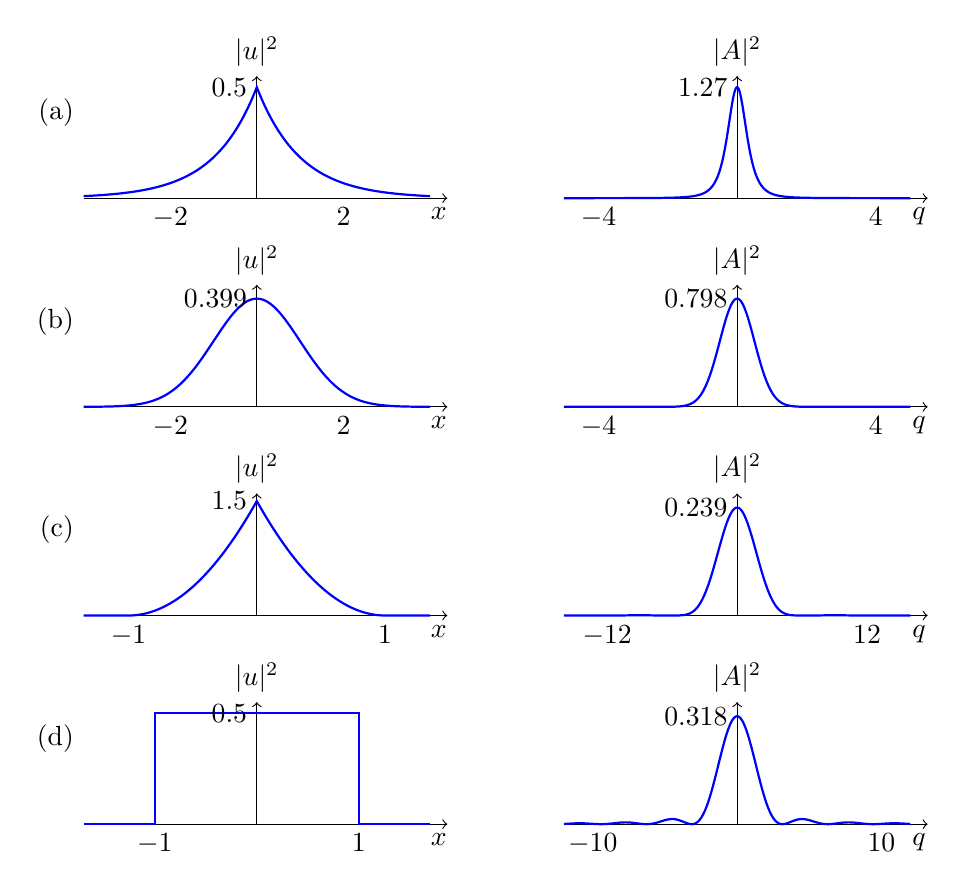
\begin{tikzpicture}
\begin{scope}[xshift=0.0cm,yshift=0.0cm,x=0.55cm,y=2.818181818181818cm]
\draw[->] (-4.0,0)--(4.4,0);\draw[->] (0,0)--(0,0.55) node[above] {$|u|^2$};
\draw[blue,thick] plot coordinates {(-4.000000,0.009158) (-3.986667,0.009281) (-3.973333,0.009405) (-3.960000,0.009532) (-3.946667,0.009659) (-3.933333,0.009789) (-3.920000,0.009921) (-3.906667,0.010054) (-3.893333,0.010189) (-3.880000,0.010325) (-3.866667,0.010464) (-3.853333,0.010604) (-3.840000,0.010747) (-3.826667,0.010891) (-3.813333,0.011037) (-3.800000,0.011185) (-3.786667,0.011336) (-3.773333,0.011488) (-3.760000,0.011642) (-3.746667,0.011798) (-3.733333,0.011956) (-3.720000,0.012117) (-3.706667,0.012280) (-3.693333,0.012444) (-3.680000,0.012611) (-3.666667,0.012781) (-3.653333,0.012952) (-3.640000,0.013126) (-3.626667,0.013302) (-3.613333,0.013481) (-3.600000,0.013662) (-3.586667,0.013845) (-3.573333,0.014031) (-3.560000,0.014219) (-3.546667,0.014410) (-3.533333,0.014604) (-3.520000,0.014800) (-3.506667,0.014998) (-3.493333,0.015200) (-3.480000,0.015404) (-3.466667,0.015610) (-3.453333,0.015820) (-3.440000,0.016032) (-3.426667,0.016248) (-3.413333,0.016466) (-3.400000,0.016687) (-3.386667,0.016911) (-3.373333,0.017138) (-3.360000,0.017368) (-3.346667,0.017601) (-3.333333,0.017837) (-3.320000,0.018076) (-3.306667,0.018319) (-3.293333,0.018565) (-3.280000,0.018814) (-3.266667,0.019067) (-3.253333,0.019323) (-3.240000,0.019582) (-3.226667,0.019845) (-3.213333,0.020111) (-3.200000,0.020381) (-3.186667,0.020655) (-3.173333,0.020932) (-3.160000,0.021213) (-3.146667,0.021498) (-3.133333,0.021786) (-3.120000,0.022079) (-3.106667,0.022375) (-3.093333,0.022675) (-3.080000,0.022980) (-3.066667,0.023288) (-3.053333,0.023601) (-3.040000,0.023917) (-3.026667,0.024238) (-3.013333,0.024564) (-3.000000,0.024894) (-2.986667,0.025228) (-2.973333,0.025566) (-2.960000,0.025909) (-2.946667,0.026257) (-2.933333,0.026610) (-2.920000,0.026967) (-2.906667,0.027329) (-2.893333,0.027696) (-2.880000,0.028067) (-2.866667,0.028444) (-2.853333,0.028826) (-2.840000,0.029213) (-2.826667,0.029605) (-2.813333,0.030002) (-2.800000,0.030405) (-2.786667,0.030813) (-2.773333,0.031227) (-2.760000,0.031646) (-2.746667,0.032071) (-2.733333,0.032501) (-2.720000,0.032937) (-2.706667,0.033379) (-2.693333,0.033828) (-2.680000,0.034282) (-2.666667,0.034742) (-2.653333,0.035208) (-2.640000,0.035681) (-2.626667,0.036160) (-2.613333,0.036645) (-2.600000,0.037137) (-2.586667,0.037635) (-2.573333,0.038140) (-2.560000,0.038652) (-2.546667,0.039171) (-2.533333,0.039697) (-2.520000,0.040230) (-2.506667,0.040770) (-2.493333,0.041317) (-2.480000,0.041872) (-2.466667,0.042434) (-2.453333,0.043003) (-2.440000,0.043580) (-2.426667,0.044165) (-2.413333,0.044758) (-2.400000,0.045359) (-2.386667,0.045968) (-2.373333,0.046585) (-2.360000,0.047210) (-2.346667,0.047844) (-2.333333,0.048486) (-2.320000,0.049137) (-2.306667,0.049796) (-2.293333,0.050465) (-2.280000,0.051142) (-2.266667,0.051829) (-2.253333,0.052524) (-2.240000,0.053229) (-2.226667,0.053944) (-2.213333,0.054668) (-2.200000,0.055402) (-2.186667,0.056145) (-2.173333,0.056899) (-2.160000,0.057663) (-2.146667,0.058437) (-2.133333,0.059221) (-2.120000,0.060016) (-2.106667,0.060821) (-2.093333,0.061638) (-2.080000,0.062465) (-2.066667,0.063304) (-2.053333,0.064153) (-2.040000,0.065014) (-2.026667,0.065887) (-2.013333,0.066771) (-2.000000,0.067668) (-1.986667,0.068576) (-1.973333,0.069496) (-1.960000,0.070429) (-1.946667,0.071375) (-1.933333,0.072333) (-1.920000,0.073303) (-1.906667,0.074287) (-1.893333,0.075285) (-1.880000,0.076295) (-1.866667,0.077319) (-1.853333,0.078357) (-1.840000,0.079409) (-1.826667,0.080475) (-1.813333,0.081555) (-1.800000,0.082649) (-1.786667,0.083759) (-1.773333,0.084883) (-1.760000,0.086022) (-1.746667,0.087177) (-1.733333,0.088347) (-1.720000,0.089533) (-1.706667,0.090735) (-1.693333,0.091953) (-1.680000,0.093187) (-1.666667,0.094438) (-1.653333,0.095705) (-1.640000,0.096990) (-1.626667,0.098292) (-1.613333,0.099611) (-1.600000,0.100948) (-1.586667,0.102303) (-1.573333,0.103676) (-1.560000,0.105068) (-1.546667,0.106478) (-1.533333,0.107908) (-1.520000,0.109356) (-1.506667,0.110824) (-1.493333,0.112311) (-1.480000,0.113819) (-1.466667,0.115347) (-1.453333,0.116895) (-1.440000,0.118464) (-1.426667,0.120054) (-1.413333,0.121665) (-1.400000,0.123298) (-1.386667,0.124953) (-1.373333,0.126631) (-1.360000,0.128330) (-1.346667,0.130053) (-1.333333,0.131799) (-1.320000,0.133568) (-1.306667,0.135360) (-1.293333,0.137177) (-1.280000,0.139019) (-1.266667,0.140885) (-1.253333,0.142776) (-1.240000,0.144692) (-1.226667,0.146634) (-1.213333,0.148602) (-1.200000,0.150597) (-1.186667,0.152619) (-1.173333,0.154667) (-1.160000,0.156743) (-1.146667,0.158847) (-1.133333,0.160979) (-1.120000,0.163140) (-1.106667,0.165330) (-1.093333,0.167549) (-1.080000,0.169798) (-1.066667,0.172077) (-1.053333,0.174387) (-1.040000,0.176727) (-1.026667,0.179099) (-1.013333,0.181503) (-1.000000,0.183940) (-0.986667,0.186409) (-0.973333,0.188911) (-0.960000,0.191446) (-0.946667,0.194016) (-0.933333,0.196620) (-0.920000,0.199260) (-0.906667,0.201934) (-0.893333,0.204645) (-0.880000,0.207391) (-0.866667,0.210175) (-0.853333,0.212996) (-0.840000,0.215855) (-0.826667,0.218753) (-0.813333,0.221689) (-0.800000,0.224664) (-0.786667,0.227680) (-0.773333,0.230736) (-0.760000,0.233833) (-0.746667,0.236972) (-0.733333,0.240153) (-0.720000,0.243376) (-0.706667,0.246643) (-0.693333,0.249953) (-0.680000,0.253308) (-0.666667,0.256709) (-0.653333,0.260154) (-0.640000,0.263646) (-0.626667,0.267185) (-0.613333,0.270771) (-0.600000,0.274406) (-0.586667,0.278089) (-0.573333,0.281822) (-0.560000,0.285605) (-0.546667,0.289438) (-0.533333,0.293323) (-0.520000,0.297260) (-0.506667,0.301250) (-0.493333,0.305294) (-0.480000,0.309392) (-0.466667,0.313545) (-0.453333,0.317753) (-0.440000,0.322018) (-0.426667,0.326341) (-0.413333,0.330721) (-0.400000,0.335160) (-0.386667,0.339659) (-0.373333,0.344218) (-0.360000,0.348838) (-0.346667,0.353520) (-0.333333,0.358266) (-0.320000,0.363075) (-0.306667,0.367948) (-0.293333,0.372887) (-0.280000,0.377892) (-0.266667,0.382964) (-0.253333,0.388105) (-0.240000,0.393314) (-0.226667,0.398593) (-0.213333,0.403943) (-0.200000,0.409365) (-0.186667,0.414860) (-0.173333,0.420429) (-0.160000,0.426072) (-0.146667,0.431791) (-0.133333,0.437587) (-0.120000,0.443460) (-0.106667,0.449413) (-0.093333,0.455445) (-0.080000,0.461558) (-0.066667,0.467753) (-0.053333,0.474032) (-0.040000,0.480395) (-0.026667,0.486843) (-0.013333,0.493378) (0.000000,0.500000) (0.013333,0.493378) (0.026667,0.486843) (0.040000,0.480395) (0.053333,0.474032) (0.066667,0.467753) (0.080000,0.461558) (0.093333,0.455445) (0.106667,0.449413) (0.120000,0.443460) (0.133333,0.437587) (0.146667,0.431791) (0.160000,0.426072) (0.173333,0.420429) (0.186667,0.414860) (0.200000,0.409365) (0.213333,0.403943) (0.226667,0.398593) (0.240000,0.393314) (0.253333,0.388105) (0.266667,0.382964) (0.280000,0.377892) (0.293333,0.372887) (0.306667,0.367948) (0.320000,0.363075) (0.333333,0.358266) (0.346667,0.353520) (0.360000,0.348838) (0.373333,0.344218) (0.386667,0.339659) (0.400000,0.335160) (0.413333,0.330721) (0.426667,0.326341) (0.440000,0.322018) (0.453333,0.317753) (0.466667,0.313545) (0.480000,0.309392) (0.493333,0.305294) (0.506667,0.301250) (0.520000,0.297260) (0.533333,0.293323) (0.546667,0.289438) (0.560000,0.285605) (0.573333,0.281822) (0.586667,0.278089) (0.600000,0.274406) (0.613333,0.270771) (0.626667,0.267185) (0.640000,0.263646) (0.653333,0.260154) (0.666667,0.256709) (0.680000,0.253308) (0.693333,0.249953) (0.706667,0.246643) (0.720000,0.243376) (0.733333,0.240153) (0.746667,0.236972) (0.760000,0.233833) (0.773333,0.230736) (0.786667,0.227680) (0.800000,0.224664) (0.813333,0.221689) (0.826667,0.218753) (0.840000,0.215855) (0.853333,0.212996) (0.866667,0.210175) (0.880000,0.207391) (0.893333,0.204645) (0.906667,0.201934) (0.920000,0.199260) (0.933333,0.196620) (0.946667,0.194016) (0.960000,0.191446) (0.973333,0.188911) (0.986667,0.186409) (1.000000,0.183940) (1.013333,0.181503) (1.026667,0.179099) (1.040000,0.176727) (1.053333,0.174387) (1.066667,0.172077) (1.080000,0.169798) (1.093333,0.167549) (1.106667,0.165330) (1.120000,0.163140) (1.133333,0.160979) (1.146667,0.158847) (1.160000,0.156743) (1.173333,0.154667) (1.186667,0.152619) (1.200000,0.150597) (1.213333,0.148602) (1.226667,0.146634) (1.240000,0.144692) (1.253333,0.142776) (1.266667,0.140885) (1.280000,0.139019) (1.293333,0.137177) (1.306667,0.135360) (1.320000,0.133568) (1.333333,0.131799) (1.346667,0.130053) (1.360000,0.128330) (1.373333,0.126631) (1.386667,0.124953) (1.400000,0.123298) (1.413333,0.121665) (1.426667,0.120054) (1.440000,0.118464) (1.453333,0.116895) (1.466667,0.115347) (1.480000,0.113819) (1.493333,0.112311) (1.506667,0.110824) (1.520000,0.109356) (1.533333,0.107908) (1.546667,0.106478) (1.560000,0.105068) (1.573333,0.103676) (1.586667,0.102303) (1.600000,0.100948) (1.613333,0.099611) (1.626667,0.098292) (1.640000,0.096990) (1.653333,0.095705) (1.666667,0.094438) (1.680000,0.093187) (1.693333,0.091953) (1.706667,0.090735) (1.720000,0.089533) (1.733333,0.088347) (1.746667,0.087177) (1.760000,0.086022) (1.773333,0.084883) (1.786667,0.083759) (1.800000,0.082649) (1.813333,0.081555) (1.826667,0.080475) (1.840000,0.079409) (1.853333,0.078357) (1.866667,0.077319) (1.880000,0.076295) (1.893333,0.075285) (1.906667,0.074287) (1.920000,0.073303) (1.933333,0.072333) (1.946667,0.071375) (1.960000,0.070429) (1.973333,0.069496) (1.986667,0.068576) (2.000000,0.067668) (2.013333,0.066771) (2.026667,0.065887) (2.040000,0.065014) (2.053333,0.064153) (2.066667,0.063304) (2.080000,0.062465) (2.093333,0.061638) (2.106667,0.060821) (2.120000,0.060016) (2.133333,0.059221) (2.146667,0.058437) (2.160000,0.057663) (2.173333,0.056899) (2.186667,0.056145) (2.200000,0.055402) (2.213333,0.054668) (2.226667,0.053944) (2.240000,0.053229) (2.253333,0.052524) (2.266667,0.051829) (2.280000,0.051142) (2.293333,0.050465) (2.306667,0.049796) (2.320000,0.049137) (2.333333,0.048486) (2.346667,0.047844) (2.360000,0.047210) (2.373333,0.046585) (2.386667,0.045968) (2.400000,0.045359) (2.413333,0.044758) (2.426667,0.044165) (2.440000,0.043580) (2.453333,0.043003) (2.466667,0.042434) (2.480000,0.041872) (2.493333,0.041317) (2.506667,0.040770) (2.520000,0.040230) (2.533333,0.039697) (2.546667,0.039171) (2.560000,0.038652) (2.573333,0.038140) (2.586667,0.037635) (2.600000,0.037137) (2.613333,0.036645) (2.626667,0.036160) (2.640000,0.035681) (2.653333,0.035208) (2.666667,0.034742) (2.680000,0.034282) (2.693333,0.033828) (2.706667,0.033379) (2.720000,0.032937) (2.733333,0.032501) (2.746667,0.032071) (2.760000,0.031646) (2.773333,0.031227) (2.786667,0.030813) (2.800000,0.030405) (2.813333,0.030002) (2.826667,0.029605) (2.840000,0.029213) (2.853333,0.028826) (2.866667,0.028444) (2.880000,0.028067) (2.893333,0.027696) (2.906667,0.027329) (2.920000,0.026967) (2.933333,0.026610) (2.946667,0.026257) (2.960000,0.025909) (2.973333,0.025566) (2.986667,0.025228) (3.000000,0.024894) (3.013333,0.024564) (3.026667,0.024238) (3.040000,0.023917) (3.053333,0.023601) (3.066667,0.023288) (3.080000,0.022980) (3.093333,0.022675) (3.106667,0.022375) (3.120000,0.022079) (3.133333,0.021786) (3.146667,0.021498) (3.160000,0.021213) (3.173333,0.020932) (3.186667,0.020655) (3.200000,0.020381) (3.213333,0.020111) (3.226667,0.019845) (3.240000,0.019582) (3.253333,0.019323) (3.266667,0.019067) (3.280000,0.018814) (3.293333,0.018565) (3.306667,0.018319) (3.320000,0.018076) (3.333333,0.017837) (3.346667,0.017601) (3.360000,0.017368) (3.373333,0.017138) (3.386667,0.016911) (3.400000,0.016687) (3.413333,0.016466) (3.426667,0.016248) (3.440000,0.016032) (3.453333,0.015820) (3.466667,0.015610) (3.480000,0.015404) (3.493333,0.015200) (3.506667,0.014998) (3.520000,0.014800) (3.533333,0.014604) (3.546667,0.014410) (3.560000,0.014219) (3.573333,0.014031) (3.586667,0.013845) (3.600000,0.013662) (3.613333,0.013481) (3.626667,0.013302) (3.640000,0.013126) (3.653333,0.012952) (3.666667,0.012781) (3.680000,0.012611) (3.693333,0.012444) (3.706667,0.012280) (3.720000,0.012117) (3.733333,0.011956) (3.746667,0.011798) (3.760000,0.011642) (3.773333,0.011488) (3.786667,0.011336) (3.800000,0.011185) (3.813333,0.011037) (3.826667,0.010891) (3.840000,0.010747) (3.853333,0.010604) (3.866667,0.010464) (3.880000,0.010325) (3.893333,0.010189) (3.906667,0.010054) (3.920000,0.009921) (3.933333,0.009789) (3.946667,0.009659) (3.960000,0.009532) (3.973333,0.009405) (3.986667,0.009281) (4.000000,0.009158)};
\node[below] at (-2.0,0) {$-2$};
\node[below] at (2.0,0) {$2$};
\node[left] at (0,0.5) {$0.5$};
\node[below] at (4.2,0) {$x$};
\node[left] at (-4.0,0.385) {(a)};
\end{scope}
\begin{scope}[xshift=6.1cm,yshift=0.0cm,x=0.44000000000000006cm,y=1.1071428571428572cm]
\draw[->] (-5.0,0)--(5.5,0);\draw[->] (0,0)--(0,1.4) node[above] {$|A|^2$};
\draw[blue,thick] plot coordinates {(-5.000000,0.000125) (-4.983333,0.000126) (-4.966667,0.000128) (-4.950000,0.000130) (-4.933333,0.000132) (-4.916667,0.000133) (-4.900000,0.000135) (-4.883333,0.000137) (-4.866667,0.000139) (-4.850000,0.000141) (-4.833333,0.000143) (-4.816667,0.000145) (-4.800000,0.000147) (-4.783333,0.000149) (-4.766667,0.000151) (-4.750000,0.000153) (-4.733333,0.000155) (-4.716667,0.000157) (-4.700000,0.000159) (-4.683333,0.000162) (-4.666667,0.000164) (-4.650000,0.000166) (-4.633333,0.000169) (-4.616667,0.000171) (-4.600000,0.000174) (-4.583333,0.000176) (-4.566667,0.000179) (-4.550000,0.000181) (-4.533333,0.000184) (-4.516667,0.000187) (-4.500000,0.000189) (-4.483333,0.000192) (-4.466667,0.000195) (-4.450000,0.000198) (-4.433333,0.000201) (-4.416667,0.000204) (-4.400000,0.000207) (-4.383333,0.000210) (-4.366667,0.000213) (-4.350000,0.000216) (-4.333333,0.000220) (-4.316667,0.000223) (-4.300000,0.000227) (-4.283333,0.000230) (-4.266667,0.000234) (-4.250000,0.000237) (-4.233333,0.000241) (-4.216667,0.000245) (-4.200000,0.000249) (-4.183333,0.000253) (-4.166667,0.000257) (-4.150000,0.000261) (-4.133333,0.000265) (-4.116667,0.000269) (-4.100000,0.000273) (-4.083333,0.000278) (-4.066667,0.000282) (-4.050000,0.000287) (-4.033333,0.000292) (-4.016667,0.000296) (-4.000000,0.000301) (-3.983333,0.000306) (-3.966667,0.000311) (-3.950000,0.000317) (-3.933333,0.000322) (-3.916667,0.000327) (-3.900000,0.000333) (-3.883333,0.000339) (-3.866667,0.000344) (-3.850000,0.000350) (-3.833333,0.000356) (-3.816667,0.000362) (-3.800000,0.000369) (-3.783333,0.000375) (-3.766667,0.000382) (-3.750000,0.000388) (-3.733333,0.000395) (-3.716667,0.000402) (-3.700000,0.000410) (-3.683333,0.000417) (-3.666667,0.000424) (-3.650000,0.000432) (-3.633333,0.000440) (-3.616667,0.000448) (-3.600000,0.000456) (-3.583333,0.000464) (-3.566667,0.000473) (-3.550000,0.000482) (-3.533333,0.000491) (-3.516667,0.000500) (-3.500000,0.000509) (-3.483333,0.000519) (-3.466667,0.000529) (-3.450000,0.000539) (-3.433333,0.000549) (-3.416667,0.000560) (-3.400000,0.000571) (-3.383333,0.000582) (-3.366667,0.000593) (-3.350000,0.000605) (-3.333333,0.000617) (-3.316667,0.000629) (-3.300000,0.000641) (-3.283333,0.000654) (-3.266667,0.000667) (-3.250000,0.000681) (-3.233333,0.000694) (-3.216667,0.000709) (-3.200000,0.000723) (-3.183333,0.000738) (-3.166667,0.000753) (-3.150000,0.000769) (-3.133333,0.000785) (-3.116667,0.000802) (-3.100000,0.000819) (-3.083333,0.000836) (-3.066667,0.000854) (-3.050000,0.000872) (-3.033333,0.000891) (-3.016667,0.000910) (-3.000000,0.000930) (-2.983333,0.000950) (-2.966667,0.000971) (-2.950000,0.000993) (-2.933333,0.001015) (-2.916667,0.001038) (-2.900000,0.001061) (-2.883333,0.001085) (-2.866667,0.001110) (-2.850000,0.001135) (-2.833333,0.001161) (-2.816667,0.001188) (-2.800000,0.001216) (-2.783333,0.001244) (-2.766667,0.001274) (-2.750000,0.001304) (-2.733333,0.001335) (-2.716667,0.001367) (-2.700000,0.001400) (-2.683333,0.001434) (-2.666667,0.001469) (-2.650000,0.001505) (-2.633333,0.001542) (-2.616667,0.001580) (-2.600000,0.001619) (-2.583333,0.001660) (-2.566667,0.001702) (-2.550000,0.001745) (-2.533333,0.001790) (-2.516667,0.001836) (-2.500000,0.001883) (-2.483333,0.001933) (-2.466667,0.001983) (-2.450000,0.002036) (-2.433333,0.002090) (-2.416667,0.002145) (-2.400000,0.002203) (-2.383333,0.002263) (-2.366667,0.002324) (-2.350000,0.002388) (-2.333333,0.002454) (-2.316667,0.002522) (-2.300000,0.002593) (-2.283333,0.002666) (-2.266667,0.002741) (-2.250000,0.002820) (-2.233333,0.002901) (-2.216667,0.002985) (-2.200000,0.003072) (-2.183333,0.003162) (-2.166667,0.003255) (-2.150000,0.003352) (-2.133333,0.003452) (-2.116667,0.003556) (-2.100000,0.003665) (-2.083333,0.003777) (-2.066667,0.003893) (-2.050000,0.004014) (-2.033333,0.004140) (-2.016667,0.004270) (-2.000000,0.004406) (-1.983333,0.004547) (-1.966667,0.004693) (-1.950000,0.004846) (-1.933333,0.005004) (-1.916667,0.005169) (-1.900000,0.005341) (-1.883333,0.005520) (-1.866667,0.005706) (-1.850000,0.005900) (-1.833333,0.006103) (-1.816667,0.006313) (-1.800000,0.006533) (-1.783333,0.006763) (-1.766667,0.007002) (-1.750000,0.007252) (-1.733333,0.007513) (-1.716667,0.007786) (-1.700000,0.008071) (-1.683333,0.008369) (-1.666667,0.008680) (-1.650000,0.009006) (-1.633333,0.009347) (-1.616667,0.009704) (-1.600000,0.010078) (-1.583333,0.010470) (-1.566667,0.010880) (-1.550000,0.011310) (-1.533333,0.011762) (-1.516667,0.012235) (-1.500000,0.012732) (-1.483333,0.013254) (-1.466667,0.013803) (-1.450000,0.014379) (-1.433333,0.014985) (-1.416667,0.015622) (-1.400000,0.016293) (-1.383333,0.016999) (-1.366667,0.017743) (-1.350000,0.018527) (-1.333333,0.019353) (-1.316667,0.020224) (-1.300000,0.021144) (-1.283333,0.022115) (-1.266667,0.023140) (-1.250000,0.024223) (-1.233333,0.025369) (-1.216667,0.026580) (-1.200000,0.027862) (-1.183333,0.029220) (-1.166667,0.030658) (-1.150000,0.032182) (-1.133333,0.033798) (-1.116667,0.035512) (-1.100000,0.037332) (-1.083333,0.039265) (-1.066667,0.041319) (-1.050000,0.043503) (-1.033333,0.045825) (-1.016667,0.048297) (-1.000000,0.050930) (-0.983333,0.053734) (-0.966667,0.056723) (-0.950000,0.059911) (-0.933333,0.063313) (-0.916667,0.066945) (-0.900000,0.070824) (-0.883333,0.074969) (-0.866667,0.079401) (-0.850000,0.084142) (-0.833333,0.089215) (-0.816667,0.094646) (-0.800000,0.100464) (-0.783333,0.106697) (-0.766667,0.113379) (-0.750000,0.120543) (-0.733333,0.128228) (-0.716667,0.136473) (-0.700000,0.145320) (-0.683333,0.154817) (-0.666667,0.165012) (-0.650000,0.175957) (-0.633333,0.187707) (-0.616667,0.200321) (-0.600000,0.213860) (-0.583333,0.228390) (-0.566667,0.243977) (-0.550000,0.260691) (-0.533333,0.278602) (-0.516667,0.297785) (-0.500000,0.318310) (-0.483333,0.340250) (-0.466667,0.363673) (-0.450000,0.388645) (-0.433333,0.415224) (-0.416667,0.443461) (-0.400000,0.473394) (-0.383333,0.505046) (-0.366667,0.538422) (-0.350000,0.573505) (-0.333333,0.610251) (-0.316667,0.648582) (-0.300000,0.688386) (-0.283333,0.729510) (-0.266667,0.771755) (-0.250000,0.814873) (-0.233333,0.858567) (-0.216667,0.902484) (-0.200000,0.946224) (-0.183333,0.989336) (-0.166667,1.031324) (-0.150000,1.071660) (-0.133333,1.109791) (-0.116667,1.145151) (-0.100000,1.177182) (-0.083333,1.205346) (-0.066667,1.229148) (-0.050000,1.248152) (-0.033333,1.261997) (-0.016667,1.270415) (0.000000,1.273240) (0.016667,1.270415) (0.033333,1.261997) (0.050000,1.248152) (0.066667,1.229148) (0.083333,1.205346) (0.100000,1.177182) (0.116667,1.145151) (0.133333,1.109791) (0.150000,1.071660) (0.166667,1.031324) (0.183333,0.989336) (0.200000,0.946224) (0.216667,0.902484) (0.233333,0.858567) (0.250000,0.814873) (0.266667,0.771755) (0.283333,0.729510) (0.300000,0.688386) (0.316667,0.648582) (0.333333,0.610251) (0.350000,0.573505) (0.366667,0.538422) (0.383333,0.505046) (0.400000,0.473394) (0.416667,0.443461) (0.433333,0.415224) (0.450000,0.388645) (0.466667,0.363673) (0.483333,0.340250) (0.500000,0.318310) (0.516667,0.297785) (0.533333,0.278602) (0.550000,0.260691) (0.566667,0.243977) (0.583333,0.228390) (0.600000,0.213860) (0.616667,0.200321) (0.633333,0.187707) (0.650000,0.175957) (0.666667,0.165012) (0.683333,0.154817) (0.700000,0.145320) (0.716667,0.136473) (0.733333,0.128228) (0.750000,0.120543) (0.766667,0.113379) (0.783333,0.106697) (0.800000,0.100464) (0.816667,0.094646) (0.833333,0.089215) (0.850000,0.084142) (0.866667,0.079401) (0.883333,0.074969) (0.900000,0.070824) (0.916667,0.066945) (0.933333,0.063313) (0.950000,0.059911) (0.966667,0.056723) (0.983333,0.053734) (1.000000,0.050930) (1.016667,0.048297) (1.033333,0.045825) (1.050000,0.043503) (1.066667,0.041319) (1.083333,0.039265) (1.100000,0.037332) (1.116667,0.035512) (1.133333,0.033798) (1.150000,0.032182) (1.166667,0.030658) (1.183333,0.029220) (1.200000,0.027862) (1.216667,0.026580) (1.233333,0.025369) (1.250000,0.024223) (1.266667,0.023140) (1.283333,0.022115) (1.300000,0.021144) (1.316667,0.020224) (1.333333,0.019353) (1.350000,0.018527) (1.366667,0.017743) (1.383333,0.016999) (1.400000,0.016293) (1.416667,0.015622) (1.433333,0.014985) (1.450000,0.014379) (1.466667,0.013803) (1.483333,0.013254) (1.500000,0.012732) (1.516667,0.012235) (1.533333,0.011762) (1.550000,0.011310) (1.566667,0.010880) (1.583333,0.010470) (1.600000,0.010078) (1.616667,0.009704) (1.633333,0.009347) (1.650000,0.009006) (1.666667,0.008680) (1.683333,0.008369) (1.700000,0.008071) (1.716667,0.007786) (1.733333,0.007513) (1.750000,0.007252) (1.766667,0.007002) (1.783333,0.006763) (1.800000,0.006533) (1.816667,0.006313) (1.833333,0.006103) (1.850000,0.005900) (1.866667,0.005706) (1.883333,0.005520) (1.900000,0.005341) (1.916667,0.005169) (1.933333,0.005004) (1.950000,0.004846) (1.966667,0.004693) (1.983333,0.004547) (2.000000,0.004406) (2.016667,0.004270) (2.033333,0.004140) (2.050000,0.004014) (2.066667,0.003893) (2.083333,0.003777) (2.100000,0.003665) (2.116667,0.003556) (2.133333,0.003452) (2.150000,0.003352) (2.166667,0.003255) (2.183333,0.003162) (2.200000,0.003072) (2.216667,0.002985) (2.233333,0.002901) (2.250000,0.002820) (2.266667,0.002741) (2.283333,0.002666) (2.300000,0.002593) (2.316667,0.002522) (2.333333,0.002454) (2.350000,0.002388) (2.366667,0.002324) (2.383333,0.002263) (2.400000,0.002203) (2.416667,0.002145) (2.433333,0.002090) (2.450000,0.002036) (2.466667,0.001983) (2.483333,0.001933) (2.500000,0.001883) (2.516667,0.001836) (2.533333,0.001790) (2.550000,0.001745) (2.566667,0.001702) (2.583333,0.001660) (2.600000,0.001619) (2.616667,0.001580) (2.633333,0.001542) (2.650000,0.001505) (2.666667,0.001469) (2.683333,0.001434) (2.700000,0.001400) (2.716667,0.001367) (2.733333,0.001335) (2.750000,0.001304) (2.766667,0.001274) (2.783333,0.001244) (2.800000,0.001216) (2.816667,0.001188) (2.833333,0.001161) (2.850000,0.001135) (2.866667,0.001110) (2.883333,0.001085) (2.900000,0.001061) (2.916667,0.001038) (2.933333,0.001015) (2.950000,0.000993) (2.966667,0.000971) (2.983333,0.000950) (3.000000,0.000930) (3.016667,0.000910) (3.033333,0.000891) (3.050000,0.000872) (3.066667,0.000854) (3.083333,0.000836) (3.100000,0.000819) (3.116667,0.000802) (3.133333,0.000785) (3.150000,0.000769) (3.166667,0.000753) (3.183333,0.000738) (3.200000,0.000723) (3.216667,0.000709) (3.233333,0.000694) (3.250000,0.000681) (3.266667,0.000667) (3.283333,0.000654) (3.300000,0.000641) (3.316667,0.000629) (3.333333,0.000617) (3.350000,0.000605) (3.366667,0.000593) (3.383333,0.000582) (3.400000,0.000571) (3.416667,0.000560) (3.433333,0.000549) (3.450000,0.000539) (3.466667,0.000529) (3.483333,0.000519) (3.500000,0.000509) (3.516667,0.000500) (3.533333,0.000491) (3.550000,0.000482) (3.566667,0.000473) (3.583333,0.000464) (3.600000,0.000456) (3.616667,0.000448) (3.633333,0.000440) (3.650000,0.000432) (3.666667,0.000424) (3.683333,0.000417) (3.700000,0.000410) (3.716667,0.000402) (3.733333,0.000395) (3.750000,0.000388) (3.766667,0.000382) (3.783333,0.000375) (3.800000,0.000369) (3.816667,0.000362) (3.833333,0.000356) (3.850000,0.000350) (3.866667,0.000344) (3.883333,0.000339) (3.900000,0.000333) (3.916667,0.000327) (3.933333,0.000322) (3.950000,0.000317) (3.966667,0.000311) (3.983333,0.000306) (4.000000,0.000301) (4.016667,0.000296) (4.033333,0.000292) (4.050000,0.000287) (4.066667,0.000282) (4.083333,0.000278) (4.100000,0.000273) (4.116667,0.000269) (4.133333,0.000265) (4.150000,0.000261) (4.166667,0.000257) (4.183333,0.000253) (4.200000,0.000249) (4.216667,0.000245) (4.233333,0.000241) (4.250000,0.000237) (4.266667,0.000234) (4.283333,0.000230) (4.300000,0.000227) (4.316667,0.000223) (4.333333,0.000220) (4.350000,0.000216) (4.366667,0.000213) (4.383333,0.000210) (4.400000,0.000207) (4.416667,0.000204) (4.433333,0.000201) (4.450000,0.000198) (4.466667,0.000195) (4.483333,0.000192) (4.500000,0.000189) (4.516667,0.000187) (4.533333,0.000184) (4.550000,0.000181) (4.566667,0.000179) (4.583333,0.000176) (4.600000,0.000174) (4.616667,0.000171) (4.633333,0.000169) (4.650000,0.000166) (4.666667,0.000164) (4.683333,0.000162) (4.700000,0.000159) (4.716667,0.000157) (4.733333,0.000155) (4.750000,0.000153) (4.766667,0.000151) (4.783333,0.000149) (4.800000,0.000147) (4.816667,0.000145) (4.833333,0.000143) (4.850000,0.000141) (4.866667,0.000139) (4.883333,0.000137) (4.900000,0.000135) (4.916667,0.000133) (4.933333,0.000132) (4.950000,0.000130) (4.966667,0.000128) (4.983333,0.000126) (5.000000,0.000125)};
\node[below] at (-4.0,0) {$-4$};
\node[below] at (4.0,0) {$4$};
\node[left] at (0,1.2732395447351628) {$1.27$};
\node[below] at (5.25,0) {$q$};
\end{scope}
\begin{scope}[xshift=0.0cm,yshift=-2.65cm,x=0.55cm,y=3.4444444444444446cm]
\draw[->] (-4.0,0)--(4.4,0);\draw[->] (0,0)--(0,0.45) node[above] {$|u|^2$};
\draw[blue,thick] plot coordinates {(-4.000000,0.000134) (-3.986667,0.000141) (-3.973333,0.000149) (-3.960000,0.000157) (-3.946667,0.000165) (-3.933333,0.000174) (-3.920000,0.000184) (-3.906667,0.000194) (-3.893333,0.000204) (-3.880000,0.000215) (-3.866667,0.000226) (-3.853333,0.000238) (-3.840000,0.000251) (-3.826667,0.000264) (-3.813333,0.000277) (-3.800000,0.000292) (-3.786667,0.000307) (-3.773333,0.000323) (-3.760000,0.000340) (-3.746667,0.000357) (-3.733333,0.000375) (-3.720000,0.000394) (-3.706667,0.000414) (-3.693333,0.000435) (-3.680000,0.000457) (-3.666667,0.000480) (-3.653333,0.000504) (-3.640000,0.000529) (-3.626667,0.000556) (-3.613333,0.000583) (-3.600000,0.000612) (-3.586667,0.000642) (-3.573333,0.000673) (-3.560000,0.000706) (-3.546667,0.000740) (-3.533333,0.000776) (-3.520000,0.000814) (-3.506667,0.000853) (-3.493333,0.000893) (-3.480000,0.000936) (-3.466667,0.000980) (-3.453333,0.001026) (-3.440000,0.001075) (-3.426667,0.001125) (-3.413333,0.001178) (-3.400000,0.001232) (-3.386667,0.001289) (-3.373333,0.001349) (-3.360000,0.001411) (-3.346667,0.001475) (-3.333333,0.001542) (-3.320000,0.001612) (-3.306667,0.001685) (-3.293333,0.001761) (-3.280000,0.001840) (-3.266667,0.001922) (-3.253333,0.002007) (-3.240000,0.002096) (-3.226667,0.002188) (-3.213333,0.002284) (-3.200000,0.002384) (-3.186667,0.002488) (-3.173333,0.002596) (-3.160000,0.002707) (-3.146667,0.002824) (-3.133333,0.002944) (-3.120000,0.003070) (-3.106667,0.003200) (-3.093333,0.003335) (-3.080000,0.003475) (-3.066667,0.003620) (-3.053333,0.003771) (-3.040000,0.003928) (-3.026667,0.004090) (-3.013333,0.004258) (-3.000000,0.004432) (-2.986667,0.004612) (-2.973333,0.004799) (-2.960000,0.004993) (-2.946667,0.005193) (-2.933333,0.005401) (-2.920000,0.005616) (-2.906667,0.005838) (-2.893333,0.006069) (-2.880000,0.006307) (-2.866667,0.006553) (-2.853333,0.006808) (-2.840000,0.007071) (-2.826667,0.007343) (-2.813333,0.007625) (-2.800000,0.007915) (-2.786667,0.008216) (-2.773333,0.008526) (-2.760000,0.008846) (-2.746667,0.009177) (-2.733333,0.009519) (-2.720000,0.009871) (-2.706667,0.010235) (-2.693333,0.010610) (-2.680000,0.010997) (-2.666667,0.011396) (-2.653333,0.011807) (-2.640000,0.012232) (-2.626667,0.012669) (-2.613333,0.013119) (-2.600000,0.013583) (-2.586667,0.014061) (-2.573333,0.014553) (-2.560000,0.015060) (-2.546667,0.015581) (-2.533333,0.016118) (-2.520000,0.016670) (-2.506667,0.017238) (-2.493333,0.017822) (-2.480000,0.018423) (-2.466667,0.019041) (-2.453333,0.019676) (-2.440000,0.020328) (-2.426667,0.020999) (-2.413333,0.021687) (-2.400000,0.022395) (-2.386667,0.023121) (-2.373333,0.023866) (-2.360000,0.024631) (-2.346667,0.025416) (-2.333333,0.026222) (-2.320000,0.027048) (-2.306667,0.027895) (-2.293333,0.028764) (-2.280000,0.029655) (-2.266667,0.030567) (-2.253333,0.031502) (-2.240000,0.032460) (-2.226667,0.033441) (-2.213333,0.034446) (-2.200000,0.035475) (-2.186667,0.036527) (-2.173333,0.037605) (-2.160000,0.038707) (-2.146667,0.039834) (-2.133333,0.040987) (-2.120000,0.042166) (-2.106667,0.043371) (-2.093333,0.044603) (-2.080000,0.045861) (-2.066667,0.047147) (-2.053333,0.048459) (-2.040000,0.049800) (-2.026667,0.051169) (-2.013333,0.052566) (-2.000000,0.053991) (-1.986667,0.055445) (-1.973333,0.056928) (-1.960000,0.058441) (-1.946667,0.059983) (-1.933333,0.061555) (-1.920000,0.063157) (-1.906667,0.064788) (-1.893333,0.066451) (-1.880000,0.068144) (-1.866667,0.069867) (-1.853333,0.071621) (-1.840000,0.073407) (-1.826667,0.075223) (-1.813333,0.077071) (-1.800000,0.078950) (-1.786667,0.080861) (-1.773333,0.082803) (-1.760000,0.084776) (-1.746667,0.086782) (-1.733333,0.088818) (-1.720000,0.090887) (-1.706667,0.092987) (-1.693333,0.095119) (-1.680000,0.097282) (-1.666667,0.099477) (-1.653333,0.101703) (-1.640000,0.103961) (-1.626667,0.106250) (-1.613333,0.108570) (-1.600000,0.110921) (-1.586667,0.113302) (-1.573333,0.115715) (-1.560000,0.118157) (-1.546667,0.120630) (-1.533333,0.123133) (-1.520000,0.125665) (-1.506667,0.128226) (-1.493333,0.130816) (-1.480000,0.133435) (-1.466667,0.136082) (-1.453333,0.138758) (-1.440000,0.141460) (-1.426667,0.144189) (-1.413333,0.146945) (-1.400000,0.149727) (-1.386667,0.152535) (-1.373333,0.155368) (-1.360000,0.158225) (-1.346667,0.161106) (-1.333333,0.164010) (-1.320000,0.166937) (-1.306667,0.169886) (-1.293333,0.172856) (-1.280000,0.175847) (-1.266667,0.178858) (-1.253333,0.181889) (-1.240000,0.184937) (-1.226667,0.188004) (-1.213333,0.191087) (-1.200000,0.194186) (-1.186667,0.197300) (-1.173333,0.200429) (-1.160000,0.203571) (-1.146667,0.206726) (-1.133333,0.209892) (-1.120000,0.213069) (-1.106667,0.216256) (-1.093333,0.219451) (-1.080000,0.222653) (-1.066667,0.225863) (-1.053333,0.229078) (-1.040000,0.232297) (-1.026667,0.235520) (-1.013333,0.238745) (-1.000000,0.241971) (-0.986667,0.245197) (-0.973333,0.248422) (-0.960000,0.251644) (-0.946667,0.254863) (-0.933333,0.258078) (-0.920000,0.261286) (-0.906667,0.264488) (-0.893333,0.267681) (-0.880000,0.270864) (-0.866667,0.274036) (-0.853333,0.277197) (-0.840000,0.280344) (-0.826667,0.283476) (-0.813333,0.286592) (-0.800000,0.289692) (-0.786667,0.292772) (-0.773333,0.295833) (-0.760000,0.298872) (-0.746667,0.301890) (-0.733333,0.304883) (-0.720000,0.307851) (-0.706667,0.310793) (-0.693333,0.313708) (-0.680000,0.316593) (-0.666667,0.319448) (-0.653333,0.322272) (-0.640000,0.325062) (-0.626667,0.327819) (-0.613333,0.330540) (-0.600000,0.333225) (-0.586667,0.335871) (-0.573333,0.338479) (-0.560000,0.341046) (-0.546667,0.343571) (-0.533333,0.346054) (-0.520000,0.348493) (-0.506667,0.350886) (-0.493333,0.353233) (-0.480000,0.355533) (-0.466667,0.357783) (-0.453333,0.359985) (-0.440000,0.362135) (-0.426667,0.364233) (-0.413333,0.366279) (-0.400000,0.368270) (-0.386667,0.370207) (-0.373333,0.372087) (-0.360000,0.373911) (-0.346667,0.375676) (-0.333333,0.377383) (-0.320000,0.379031) (-0.306667,0.380617) (-0.293333,0.382143) (-0.280000,0.383606) (-0.266667,0.385007) (-0.253333,0.386344) (-0.240000,0.387617) (-0.226667,0.388824) (-0.213333,0.389967) (-0.200000,0.391043) (-0.186667,0.392052) (-0.173333,0.392994) (-0.160000,0.393868) (-0.146667,0.394674) (-0.133333,0.395412) (-0.120000,0.396080) (-0.106667,0.396679) (-0.093333,0.397208) (-0.080000,0.397668) (-0.066667,0.398057) (-0.053333,0.398375) (-0.040000,0.398623) (-0.026667,0.398800) (-0.013333,0.398907) (0.000000,0.398942) (0.013333,0.398907) (0.026667,0.398800) (0.040000,0.398623) (0.053333,0.398375) (0.066667,0.398057) (0.080000,0.397668) (0.093333,0.397208) (0.106667,0.396679) (0.120000,0.396080) (0.133333,0.395412) (0.146667,0.394674) (0.160000,0.393868) (0.173333,0.392994) (0.186667,0.392052) (0.200000,0.391043) (0.213333,0.389967) (0.226667,0.388824) (0.240000,0.387617) (0.253333,0.386344) (0.266667,0.385007) (0.280000,0.383606) (0.293333,0.382143) (0.306667,0.380617) (0.320000,0.379031) (0.333333,0.377383) (0.346667,0.375676) (0.360000,0.373911) (0.373333,0.372087) (0.386667,0.370207) (0.400000,0.368270) (0.413333,0.366279) (0.426667,0.364233) (0.440000,0.362135) (0.453333,0.359985) (0.466667,0.357783) (0.480000,0.355533) (0.493333,0.353233) (0.506667,0.350886) (0.520000,0.348493) (0.533333,0.346054) (0.546667,0.343571) (0.560000,0.341046) (0.573333,0.338479) (0.586667,0.335871) (0.600000,0.333225) (0.613333,0.330540) (0.626667,0.327819) (0.640000,0.325062) (0.653333,0.322272) (0.666667,0.319448) (0.680000,0.316593) (0.693333,0.313708) (0.706667,0.310793) (0.720000,0.307851) (0.733333,0.304883) (0.746667,0.301890) (0.760000,0.298872) (0.773333,0.295833) (0.786667,0.292772) (0.800000,0.289692) (0.813333,0.286592) (0.826667,0.283476) (0.840000,0.280344) (0.853333,0.277197) (0.866667,0.274036) (0.880000,0.270864) (0.893333,0.267681) (0.906667,0.264488) (0.920000,0.261286) (0.933333,0.258078) (0.946667,0.254863) (0.960000,0.251644) (0.973333,0.248422) (0.986667,0.245197) (1.000000,0.241971) (1.013333,0.238745) (1.026667,0.235520) (1.040000,0.232297) (1.053333,0.229078) (1.066667,0.225863) (1.080000,0.222653) (1.093333,0.219451) (1.106667,0.216256) (1.120000,0.213069) (1.133333,0.209892) (1.146667,0.206726) (1.160000,0.203571) (1.173333,0.200429) (1.186667,0.197300) (1.200000,0.194186) (1.213333,0.191087) (1.226667,0.188004) (1.240000,0.184937) (1.253333,0.181889) (1.266667,0.178858) (1.280000,0.175847) (1.293333,0.172856) (1.306667,0.169886) (1.320000,0.166937) (1.333333,0.164010) (1.346667,0.161106) (1.360000,0.158225) (1.373333,0.155368) (1.386667,0.152535) (1.400000,0.149727) (1.413333,0.146945) (1.426667,0.144189) (1.440000,0.141460) (1.453333,0.138758) (1.466667,0.136082) (1.480000,0.133435) (1.493333,0.130816) (1.506667,0.128226) (1.520000,0.125665) (1.533333,0.123133) (1.546667,0.120630) (1.560000,0.118157) (1.573333,0.115715) (1.586667,0.113302) (1.600000,0.110921) (1.613333,0.108570) (1.626667,0.106250) (1.640000,0.103961) (1.653333,0.101703) (1.666667,0.099477) (1.680000,0.097282) (1.693333,0.095119) (1.706667,0.092987) (1.720000,0.090887) (1.733333,0.088818) (1.746667,0.086782) (1.760000,0.084776) (1.773333,0.082803) (1.786667,0.080861) (1.800000,0.078950) (1.813333,0.077071) (1.826667,0.075223) (1.840000,0.073407) (1.853333,0.071621) (1.866667,0.069867) (1.880000,0.068144) (1.893333,0.066451) (1.906667,0.064788) (1.920000,0.063157) (1.933333,0.061555) (1.946667,0.059983) (1.960000,0.058441) (1.973333,0.056928) (1.986667,0.055445) (2.000000,0.053991) (2.013333,0.052566) (2.026667,0.051169) (2.040000,0.049800) (2.053333,0.048459) (2.066667,0.047147) (2.080000,0.045861) (2.093333,0.044603) (2.106667,0.043371) (2.120000,0.042166) (2.133333,0.040987) (2.146667,0.039834) (2.160000,0.038707) (2.173333,0.037605) (2.186667,0.036527) (2.200000,0.035475) (2.213333,0.034446) (2.226667,0.033441) (2.240000,0.032460) (2.253333,0.031502) (2.266667,0.030567) (2.280000,0.029655) (2.293333,0.028764) (2.306667,0.027895) (2.320000,0.027048) (2.333333,0.026222) (2.346667,0.025416) (2.360000,0.024631) (2.373333,0.023866) (2.386667,0.023121) (2.400000,0.022395) (2.413333,0.021687) (2.426667,0.020999) (2.440000,0.020328) (2.453333,0.019676) (2.466667,0.019041) (2.480000,0.018423) (2.493333,0.017822) (2.506667,0.017238) (2.520000,0.016670) (2.533333,0.016118) (2.546667,0.015581) (2.560000,0.015060) (2.573333,0.014553) (2.586667,0.014061) (2.600000,0.013583) (2.613333,0.013119) (2.626667,0.012669) (2.640000,0.012232) (2.653333,0.011807) (2.666667,0.011396) (2.680000,0.010997) (2.693333,0.010610) (2.706667,0.010235) (2.720000,0.009871) (2.733333,0.009519) (2.746667,0.009177) (2.760000,0.008846) (2.773333,0.008526) (2.786667,0.008216) (2.800000,0.007915) (2.813333,0.007625) (2.826667,0.007343) (2.840000,0.007071) (2.853333,0.006808) (2.866667,0.006553) (2.880000,0.006307) (2.893333,0.006069) (2.906667,0.005838) (2.920000,0.005616) (2.933333,0.005401) (2.946667,0.005193) (2.960000,0.004993) (2.973333,0.004799) (2.986667,0.004612) (3.000000,0.004432) (3.013333,0.004258) (3.026667,0.004090) (3.040000,0.003928) (3.053333,0.003771) (3.066667,0.003620) (3.080000,0.003475) (3.093333,0.003335) (3.106667,0.003200) (3.120000,0.003070) (3.133333,0.002944) (3.146667,0.002824) (3.160000,0.002707) (3.173333,0.002596) (3.186667,0.002488) (3.200000,0.002384) (3.213333,0.002284) (3.226667,0.002188) (3.240000,0.002096) (3.253333,0.002007) (3.266667,0.001922) (3.280000,0.001840) (3.293333,0.001761) (3.306667,0.001685) (3.320000,0.001612) (3.333333,0.001542) (3.346667,0.001475) (3.360000,0.001411) (3.373333,0.001349) (3.386667,0.001289) (3.400000,0.001232) (3.413333,0.001178) (3.426667,0.001125) (3.440000,0.001075) (3.453333,0.001026) (3.466667,0.000980) (3.480000,0.000936) (3.493333,0.000893) (3.506667,0.000853) (3.520000,0.000814) (3.533333,0.000776) (3.546667,0.000740) (3.560000,0.000706) (3.573333,0.000673) (3.586667,0.000642) (3.600000,0.000612) (3.613333,0.000583) (3.626667,0.000556) (3.640000,0.000529) (3.653333,0.000504) (3.666667,0.000480) (3.680000,0.000457) (3.693333,0.000435) (3.706667,0.000414) (3.720000,0.000394) (3.733333,0.000375) (3.746667,0.000357) (3.760000,0.000340) (3.773333,0.000323) (3.786667,0.000307) (3.800000,0.000292) (3.813333,0.000277) (3.826667,0.000264) (3.840000,0.000251) (3.853333,0.000238) (3.866667,0.000226) (3.880000,0.000215) (3.893333,0.000204) (3.906667,0.000194) (3.920000,0.000184) (3.933333,0.000174) (3.946667,0.000165) (3.960000,0.000157) (3.973333,0.000149) (3.986667,0.000141) (4.000000,0.000134)};
\node[below] at (-2.0,0) {$-2$};
\node[below] at (2.0,0) {$2$};
\node[left] at (0,0.3989422804014327) {$0.399$};
\node[below] at (4.2,0) {$x$};
\node[left] at (-4.0,0.315) {(b)};
\end{scope}
\begin{scope}[xshift=6.1cm,yshift=-2.65cm,x=0.44000000000000006cm,y=1.7222222222222223cm]
\draw[->] (-5.0,0)--(5.5,0);\draw[->] (0,0)--(0,0.9) node[above] {$|A|^2$};
\draw[blue,thick] plot coordinates {(-5.000000,0.000000) (-4.983333,0.000000) (-4.966667,0.000000) (-4.950000,0.000000) (-4.933333,0.000000) (-4.916667,0.000000) (-4.900000,0.000000) (-4.883333,0.000000) (-4.866667,0.000000) (-4.850000,0.000000) (-4.833333,0.000000) (-4.816667,0.000000) (-4.800000,0.000000) (-4.783333,0.000000) (-4.766667,0.000000) (-4.750000,0.000000) (-4.733333,0.000000) (-4.716667,0.000000) (-4.700000,0.000000) (-4.683333,0.000000) (-4.666667,0.000000) (-4.650000,0.000000) (-4.633333,0.000000) (-4.616667,0.000000) (-4.600000,0.000000) (-4.583333,0.000000) (-4.566667,0.000000) (-4.550000,0.000000) (-4.533333,0.000000) (-4.516667,0.000000) (-4.500000,0.000000) (-4.483333,0.000000) (-4.466667,0.000000) (-4.450000,0.000000) (-4.433333,0.000000) (-4.416667,0.000000) (-4.400000,0.000000) (-4.383333,0.000000) (-4.366667,0.000000) (-4.350000,0.000000) (-4.333333,0.000000) (-4.316667,0.000000) (-4.300000,0.000000) (-4.283333,0.000000) (-4.266667,0.000000) (-4.250000,0.000000) (-4.233333,0.000000) (-4.216667,0.000000) (-4.200000,0.000000) (-4.183333,0.000000) (-4.166667,0.000000) (-4.150000,0.000000) (-4.133333,0.000000) (-4.116667,0.000000) (-4.100000,0.000000) (-4.083333,0.000000) (-4.066667,0.000000) (-4.050000,0.000000) (-4.033333,0.000000) (-4.016667,0.000000) (-4.000000,0.000000) (-3.983333,0.000000) (-3.966667,0.000000) (-3.950000,0.000000) (-3.933333,0.000000) (-3.916667,0.000000) (-3.900000,0.000000) (-3.883333,0.000000) (-3.866667,0.000000) (-3.850000,0.000000) (-3.833333,0.000000) (-3.816667,0.000000) (-3.800000,0.000000) (-3.783333,0.000000) (-3.766667,0.000000) (-3.750000,0.000000) (-3.733333,0.000000) (-3.716667,0.000000) (-3.700000,0.000000) (-3.683333,0.000000) (-3.666667,0.000000) (-3.650000,0.000000) (-3.633333,0.000000) (-3.616667,0.000000) (-3.600000,0.000000) (-3.583333,0.000000) (-3.566667,0.000000) (-3.550000,0.000000) (-3.533333,0.000000) (-3.516667,0.000000) (-3.500000,0.000000) (-3.483333,0.000000) (-3.466667,0.000000) (-3.450000,0.000000) (-3.433333,0.000000) (-3.416667,0.000000) (-3.400000,0.000000) (-3.383333,0.000000) (-3.366667,0.000000) (-3.350000,0.000000) (-3.333333,0.000000) (-3.316667,0.000000) (-3.300000,0.000000) (-3.283333,0.000000) (-3.266667,0.000000) (-3.250000,0.000000) (-3.233333,0.000000) (-3.216667,0.000000) (-3.200000,0.000000) (-3.183333,0.000000) (-3.166667,0.000000) (-3.150000,0.000000) (-3.133333,0.000000) (-3.116667,0.000000) (-3.100000,0.000000) (-3.083333,0.000000) (-3.066667,0.000000) (-3.050000,0.000000) (-3.033333,0.000000) (-3.016667,0.000000) (-3.000000,0.000000) (-2.983333,0.000000) (-2.966667,0.000000) (-2.950000,0.000000) (-2.933333,0.000000) (-2.916667,0.000000) (-2.900000,0.000000) (-2.883333,0.000000) (-2.866667,0.000000) (-2.850000,0.000000) (-2.833333,0.000000) (-2.816667,0.000000) (-2.800000,0.000000) (-2.783333,0.000000) (-2.766667,0.000000) (-2.750000,0.000000) (-2.733333,0.000000) (-2.716667,0.000000) (-2.700000,0.000000) (-2.683333,0.000000) (-2.666667,0.000001) (-2.650000,0.000001) (-2.633333,0.000001) (-2.616667,0.000001) (-2.600000,0.000001) (-2.583333,0.000001) (-2.566667,0.000002) (-2.550000,0.000002) (-2.533333,0.000002) (-2.516667,0.000003) (-2.500000,0.000003) (-2.483333,0.000004) (-2.466667,0.000004) (-2.450000,0.000005) (-2.433333,0.000006) (-2.416667,0.000007) (-2.400000,0.000008) (-2.383333,0.000009) (-2.366667,0.000011) (-2.350000,0.000013) (-2.333333,0.000015) (-2.316667,0.000017) (-2.300000,0.000020) (-2.283333,0.000024) (-2.266667,0.000027) (-2.250000,0.000032) (-2.233333,0.000037) (-2.216667,0.000043) (-2.200000,0.000050) (-2.183333,0.000058) (-2.166667,0.000067) (-2.150000,0.000077) (-2.133333,0.000089) (-2.116667,0.000102) (-2.100000,0.000118) (-2.083333,0.000136) (-2.066667,0.000156) (-2.050000,0.000179) (-2.033333,0.000205) (-2.016667,0.000234) (-2.000000,0.000268) (-1.983333,0.000306) (-1.966667,0.000349) (-1.950000,0.000397) (-1.933333,0.000452) (-1.916667,0.000514) (-1.900000,0.000584) (-1.883333,0.000662) (-1.866667,0.000751) (-1.850000,0.000850) (-1.833333,0.000961) (-1.816667,0.001085) (-1.800000,0.001224) (-1.783333,0.001379) (-1.766667,0.001552) (-1.750000,0.001745) (-1.733333,0.001960) (-1.716667,0.002199) (-1.700000,0.002464) (-1.683333,0.002759) (-1.666667,0.003085) (-1.650000,0.003445) (-1.633333,0.003844) (-1.616667,0.004283) (-1.600000,0.004768) (-1.583333,0.005302) (-1.566667,0.005889) (-1.550000,0.006534) (-1.533333,0.007241) (-1.516667,0.008016) (-1.500000,0.008864) (-1.483333,0.009790) (-1.466667,0.010802) (-1.450000,0.011905) (-1.433333,0.013106) (-1.416667,0.014412) (-1.400000,0.015831) (-1.383333,0.017370) (-1.366667,0.019037) (-1.350000,0.020842) (-1.333333,0.022792) (-1.316667,0.024897) (-1.300000,0.027166) (-1.283333,0.029609) (-1.266667,0.032236) (-1.250000,0.035057) (-1.233333,0.038082) (-1.216667,0.041323) (-1.200000,0.044789) (-1.183333,0.048492) (-1.166667,0.052444) (-1.150000,0.056654) (-1.133333,0.061134) (-1.116667,0.065896) (-1.100000,0.070949) (-1.083333,0.076305) (-1.066667,0.081975) (-1.050000,0.087967) (-1.033333,0.094293) (-1.016667,0.100962) (-1.000000,0.107982) (-0.983333,0.115362) (-0.966667,0.123110) (-0.950000,0.131232) (-0.933333,0.139734) (-0.916667,0.148622) (-0.900000,0.157900) (-0.883333,0.167571) (-0.866667,0.177637) (-0.850000,0.188098) (-0.833333,0.198954) (-0.816667,0.210203) (-0.800000,0.221842) (-0.783333,0.233864) (-0.766667,0.246265) (-0.750000,0.259035) (-0.733333,0.272165) (-0.716667,0.285643) (-0.700000,0.299455) (-0.683333,0.313586) (-0.666667,0.328020) (-0.650000,0.342737) (-0.633333,0.357717) (-0.616667,0.372937) (-0.600000,0.388372) (-0.583333,0.403997) (-0.566667,0.419785) (-0.550000,0.435704) (-0.533333,0.451726) (-0.516667,0.467816) (-0.500000,0.483941) (-0.483333,0.500067) (-0.466667,0.516156) (-0.450000,0.532170) (-0.433333,0.548073) (-0.416667,0.563824) (-0.400000,0.579383) (-0.383333,0.594711) (-0.366667,0.609766) (-0.350000,0.624508) (-0.333333,0.638896) (-0.316667,0.652890) (-0.300000,0.666449) (-0.283333,0.679535) (-0.266667,0.692108) (-0.250000,0.704131) (-0.233333,0.715567) (-0.216667,0.726381) (-0.200000,0.736540) (-0.183333,0.746012) (-0.166667,0.754766) (-0.150000,0.762776) (-0.133333,0.770014) (-0.116667,0.776457) (-0.100000,0.782085) (-0.083333,0.786879) (-0.066667,0.790824) (-0.050000,0.793905) (-0.033333,0.796113) (-0.016667,0.797441) (0.000000,0.797885) (0.016667,0.797441) (0.033333,0.796113) (0.050000,0.793905) (0.066667,0.790824) (0.083333,0.786879) (0.100000,0.782085) (0.116667,0.776457) (0.133333,0.770014) (0.150000,0.762776) (0.166667,0.754766) (0.183333,0.746012) (0.200000,0.736540) (0.216667,0.726381) (0.233333,0.715567) (0.250000,0.704131) (0.266667,0.692108) (0.283333,0.679535) (0.300000,0.666449) (0.316667,0.652890) (0.333333,0.638896) (0.350000,0.624508) (0.366667,0.609766) (0.383333,0.594711) (0.400000,0.579383) (0.416667,0.563824) (0.433333,0.548073) (0.450000,0.532170) (0.466667,0.516156) (0.483333,0.500067) (0.500000,0.483941) (0.516667,0.467816) (0.533333,0.451726) (0.550000,0.435704) (0.566667,0.419785) (0.583333,0.403997) (0.600000,0.388372) (0.616667,0.372937) (0.633333,0.357717) (0.650000,0.342737) (0.666667,0.328020) (0.683333,0.313586) (0.700000,0.299455) (0.716667,0.285643) (0.733333,0.272165) (0.750000,0.259035) (0.766667,0.246265) (0.783333,0.233864) (0.800000,0.221842) (0.816667,0.210203) (0.833333,0.198954) (0.850000,0.188098) (0.866667,0.177637) (0.883333,0.167571) (0.900000,0.157900) (0.916667,0.148622) (0.933333,0.139734) (0.950000,0.131232) (0.966667,0.123110) (0.983333,0.115362) (1.000000,0.107982) (1.016667,0.100962) (1.033333,0.094293) (1.050000,0.087967) (1.066667,0.081975) (1.083333,0.076305) (1.100000,0.070949) (1.116667,0.065896) (1.133333,0.061134) (1.150000,0.056654) (1.166667,0.052444) (1.183333,0.048492) (1.200000,0.044789) (1.216667,0.041323) (1.233333,0.038082) (1.250000,0.035057) (1.266667,0.032236) (1.283333,0.029609) (1.300000,0.027166) (1.316667,0.024897) (1.333333,0.022792) (1.350000,0.020842) (1.366667,0.019037) (1.383333,0.017370) (1.400000,0.015831) (1.416667,0.014412) (1.433333,0.013106) (1.450000,0.011905) (1.466667,0.010802) (1.483333,0.009790) (1.500000,0.008864) (1.516667,0.008016) (1.533333,0.007241) (1.550000,0.006534) (1.566667,0.005889) (1.583333,0.005302) (1.600000,0.004768) (1.616667,0.004283) (1.633333,0.003844) (1.650000,0.003445) (1.666667,0.003085) (1.683333,0.002759) (1.700000,0.002464) (1.716667,0.002199) (1.733333,0.001960) (1.750000,0.001745) (1.766667,0.001552) (1.783333,0.001379) (1.800000,0.001224) (1.816667,0.001085) (1.833333,0.000961) (1.850000,0.000850) (1.866667,0.000751) (1.883333,0.000662) (1.900000,0.000584) (1.916667,0.000514) (1.933333,0.000452) (1.950000,0.000397) (1.966667,0.000349) (1.983333,0.000306) (2.000000,0.000268) (2.016667,0.000234) (2.033333,0.000205) (2.050000,0.000179) (2.066667,0.000156) (2.083333,0.000136) (2.100000,0.000118) (2.116667,0.000102) (2.133333,0.000089) (2.150000,0.000077) (2.166667,0.000067) (2.183333,0.000058) (2.200000,0.000050) (2.216667,0.000043) (2.233333,0.000037) (2.250000,0.000032) (2.266667,0.000027) (2.283333,0.000024) (2.300000,0.000020) (2.316667,0.000017) (2.333333,0.000015) (2.350000,0.000013) (2.366667,0.000011) (2.383333,0.000009) (2.400000,0.000008) (2.416667,0.000007) (2.433333,0.000006) (2.450000,0.000005) (2.466667,0.000004) (2.483333,0.000004) (2.500000,0.000003) (2.516667,0.000003) (2.533333,0.000002) (2.550000,0.000002) (2.566667,0.000002) (2.583333,0.000001) (2.600000,0.000001) (2.616667,0.000001) (2.633333,0.000001) (2.650000,0.000001) (2.666667,0.000001) (2.683333,0.000000) (2.700000,0.000000) (2.716667,0.000000) (2.733333,0.000000) (2.750000,0.000000) (2.766667,0.000000) (2.783333,0.000000) (2.800000,0.000000) (2.816667,0.000000) (2.833333,0.000000) (2.850000,0.000000) (2.866667,0.000000) (2.883333,0.000000) (2.900000,0.000000) (2.916667,0.000000) (2.933333,0.000000) (2.950000,0.000000) (2.966667,0.000000) (2.983333,0.000000) (3.000000,0.000000) (3.016667,0.000000) (3.033333,0.000000) (3.050000,0.000000) (3.066667,0.000000) (3.083333,0.000000) (3.100000,0.000000) (3.116667,0.000000) (3.133333,0.000000) (3.150000,0.000000) (3.166667,0.000000) (3.183333,0.000000) (3.200000,0.000000) (3.216667,0.000000) (3.233333,0.000000) (3.250000,0.000000) (3.266667,0.000000) (3.283333,0.000000) (3.300000,0.000000) (3.316667,0.000000) (3.333333,0.000000) (3.350000,0.000000) (3.366667,0.000000) (3.383333,0.000000) (3.400000,0.000000) (3.416667,0.000000) (3.433333,0.000000) (3.450000,0.000000) (3.466667,0.000000) (3.483333,0.000000) (3.500000,0.000000) (3.516667,0.000000) (3.533333,0.000000) (3.550000,0.000000) (3.566667,0.000000) (3.583333,0.000000) (3.600000,0.000000) (3.616667,0.000000) (3.633333,0.000000) (3.650000,0.000000) (3.666667,0.000000) (3.683333,0.000000) (3.700000,0.000000) (3.716667,0.000000) (3.733333,0.000000) (3.750000,0.000000) (3.766667,0.000000) (3.783333,0.000000) (3.800000,0.000000) (3.816667,0.000000) (3.833333,0.000000) (3.850000,0.000000) (3.866667,0.000000) (3.883333,0.000000) (3.900000,0.000000) (3.916667,0.000000) (3.933333,0.000000) (3.950000,0.000000) (3.966667,0.000000) (3.983333,0.000000) (4.000000,0.000000) (4.016667,0.000000) (4.033333,0.000000) (4.050000,0.000000) (4.066667,0.000000) (4.083333,0.000000) (4.100000,0.000000) (4.116667,0.000000) (4.133333,0.000000) (4.150000,0.000000) (4.166667,0.000000) (4.183333,0.000000) (4.200000,0.000000) (4.216667,0.000000) (4.233333,0.000000) (4.250000,0.000000) (4.266667,0.000000) (4.283333,0.000000) (4.300000,0.000000) (4.316667,0.000000) (4.333333,0.000000) (4.350000,0.000000) (4.366667,0.000000) (4.383333,0.000000) (4.400000,0.000000) (4.416667,0.000000) (4.433333,0.000000) (4.450000,0.000000) (4.466667,0.000000) (4.483333,0.000000) (4.500000,0.000000) (4.516667,0.000000) (4.533333,0.000000) (4.550000,0.000000) (4.566667,0.000000) (4.583333,0.000000) (4.600000,0.000000) (4.616667,0.000000) (4.633333,0.000000) (4.650000,0.000000) (4.666667,0.000000) (4.683333,0.000000) (4.700000,0.000000) (4.716667,0.000000) (4.733333,0.000000) (4.750000,0.000000) (4.766667,0.000000) (4.783333,0.000000) (4.800000,0.000000) (4.816667,0.000000) (4.833333,0.000000) (4.850000,0.000000) (4.866667,0.000000) (4.883333,0.000000) (4.900000,0.000000) (4.916667,0.000000) (4.933333,0.000000) (4.950000,0.000000) (4.966667,0.000000) (4.983333,0.000000) (5.000000,0.000000)};
\node[below] at (-4.0,0) {$-4$};
\node[below] at (4.0,0) {$4$};
\node[left] at (0,0.7978845608028654) {$0.798$};
\node[below] at (5.25,0) {$q$};
\end{scope}
\begin{scope}[xshift=0.0cm,yshift=-5.3cm,x=1.6296296296296298cm,y=0.96875cm]
\draw[->] (-1.35,0)--(1.4850000000000003,0);\draw[->] (0,0)--(0,1.6) node[above] {$|u|^2$};
\draw[blue,thick] plot coordinates {(-1.350000,0.000000) (-1.345500,0.000000) (-1.341000,0.000000) (-1.336500,0.000000) (-1.332000,0.000000) (-1.327500,0.000000) (-1.323000,0.000000) (-1.318500,0.000000) (-1.314000,0.000000) (-1.309500,0.000000) (-1.305000,0.000000) (-1.300500,0.000000) (-1.296000,0.000000) (-1.291500,0.000000) (-1.287000,0.000000) (-1.282500,0.000000) (-1.278000,0.000000) (-1.273500,0.000000) (-1.269000,0.000000) (-1.264500,0.000000) (-1.260000,0.000000) (-1.255500,0.000000) (-1.251000,0.000000) (-1.246500,0.000000) (-1.242000,0.000000) (-1.237500,0.000000) (-1.233000,0.000000) (-1.228500,0.000000) (-1.224000,0.000000) (-1.219500,0.000000) (-1.215000,0.000000) (-1.210500,0.000000) (-1.206000,0.000000) (-1.201500,0.000000) (-1.197000,0.000000) (-1.192500,0.000000) (-1.188000,0.000000) (-1.183500,0.000000) (-1.179000,0.000000) (-1.174500,0.000000) (-1.170000,0.000000) (-1.165500,0.000000) (-1.161000,0.000000) (-1.156500,0.000000) (-1.152000,0.000000) (-1.147500,0.000000) (-1.143000,0.000000) (-1.138500,0.000000) (-1.134000,0.000000) (-1.129500,0.000000) (-1.125000,0.000000) (-1.120500,0.000000) (-1.116000,0.000000) (-1.111500,0.000000) (-1.107000,0.000000) (-1.102500,0.000000) (-1.098000,0.000000) (-1.093500,0.000000) (-1.089000,0.000000) (-1.084500,0.000000) (-1.080000,0.000000) (-1.075500,0.000000) (-1.071000,0.000000) (-1.066500,0.000000) (-1.062000,0.000000) (-1.057500,0.000000) (-1.053000,0.000000) (-1.048500,0.000000) (-1.044000,0.000000) (-1.039500,0.000000) (-1.035000,0.000000) (-1.030500,0.000000) (-1.026000,0.000000) (-1.021500,0.000000) (-1.017000,0.000000) (-1.012500,0.000000) (-1.008000,0.000000) (-1.003500,0.000000) (-0.999000,0.000001) (-0.994500,0.000045) (-0.990000,0.000150) (-0.985500,0.000315) (-0.981000,0.000541) (-0.976500,0.000828) (-0.972000,0.001176) (-0.967500,0.001584) (-0.963000,0.002053) (-0.958500,0.002583) (-0.954000,0.003174) (-0.949500,0.003825) (-0.945000,0.004537) (-0.940500,0.005310) (-0.936000,0.006144) (-0.931500,0.007038) (-0.927000,0.007993) (-0.922500,0.009009) (-0.918000,0.010086) (-0.913500,0.011223) (-0.909000,0.012421) (-0.904500,0.013680) (-0.900000,0.015000) (-0.895500,0.016380) (-0.891000,0.017821) (-0.886500,0.019323) (-0.882000,0.020886) (-0.877500,0.022509) (-0.873000,0.024193) (-0.868500,0.025938) (-0.864000,0.027744) (-0.859500,0.029610) (-0.855000,0.031538) (-0.850500,0.033525) (-0.846000,0.035574) (-0.841500,0.037683) (-0.837000,0.039853) (-0.832500,0.042084) (-0.828000,0.044376) (-0.823500,0.046728) (-0.819000,0.049141) (-0.814500,0.051615) (-0.810000,0.054150) (-0.805500,0.056745) (-0.801000,0.059401) (-0.796500,0.062118) (-0.792000,0.064896) (-0.787500,0.067734) (-0.783000,0.070633) (-0.778500,0.073593) (-0.774000,0.076614) (-0.769500,0.079695) (-0.765000,0.082837) (-0.760500,0.086040) (-0.756000,0.089304) (-0.751500,0.092628) (-0.747000,0.096014) (-0.742500,0.099459) (-0.738000,0.102966) (-0.733500,0.106533) (-0.729000,0.110162) (-0.724500,0.113850) (-0.720000,0.117600) (-0.715500,0.121410) (-0.711000,0.125282) (-0.706500,0.129213) (-0.702000,0.133206) (-0.697500,0.137259) (-0.693000,0.141373) (-0.688500,0.145548) (-0.684000,0.149784) (-0.679500,0.154080) (-0.675000,0.158437) (-0.670500,0.162855) (-0.666000,0.167334) (-0.661500,0.171873) (-0.657000,0.176473) (-0.652500,0.181134) (-0.648000,0.185856) (-0.643500,0.190638) (-0.639000,0.195481) (-0.634500,0.200385) (-0.630000,0.205350) (-0.625500,0.210375) (-0.621000,0.215461) (-0.616500,0.220608) (-0.612000,0.225816) (-0.607500,0.231084) (-0.603000,0.236414) (-0.598500,0.241803) (-0.594000,0.247254) (-0.589500,0.252765) (-0.585000,0.258337) (-0.580500,0.263970) (-0.576000,0.269664) (-0.571500,0.275418) (-0.567000,0.281234) (-0.562500,0.287109) (-0.558000,0.293046) (-0.553500,0.299043) (-0.549000,0.305101) (-0.544500,0.311220) (-0.540000,0.317400) (-0.535500,0.323640) (-0.531000,0.329941) (-0.526500,0.336303) (-0.522000,0.342726) (-0.517500,0.349209) (-0.513000,0.355754) (-0.508500,0.362358) (-0.504000,0.369024) (-0.499500,0.375750) (-0.495000,0.382537) (-0.490500,0.389385) (-0.486000,0.396294) (-0.481500,0.403263) (-0.477000,0.410294) (-0.472500,0.417384) (-0.468000,0.424536) (-0.463500,0.431748) (-0.459000,0.439022) (-0.454500,0.446355) (-0.450000,0.453750) (-0.445500,0.461205) (-0.441000,0.468722) (-0.436500,0.476298) (-0.432000,0.483936) (-0.427500,0.491634) (-0.423000,0.499394) (-0.418500,0.507213) (-0.414000,0.515094) (-0.409500,0.523035) (-0.405000,0.531037) (-0.400500,0.539100) (-0.396000,0.547224) (-0.391500,0.555408) (-0.387000,0.563653) (-0.382500,0.571959) (-0.378000,0.580326) (-0.373500,0.588753) (-0.369000,0.597241) (-0.364500,0.605790) (-0.360000,0.614400) (-0.355500,0.623070) (-0.351000,0.631802) (-0.346500,0.640593) (-0.342000,0.649446) (-0.337500,0.658359) (-0.333000,0.667334) (-0.328500,0.676368) (-0.324000,0.685464) (-0.319500,0.694620) (-0.315000,0.703838) (-0.310500,0.713115) (-0.306000,0.722454) (-0.301500,0.731853) (-0.297000,0.741314) (-0.292500,0.750834) (-0.288000,0.760416) (-0.283500,0.770058) (-0.279000,0.779762) (-0.274500,0.789525) (-0.270000,0.799350) (-0.265500,0.809235) (-0.261000,0.819182) (-0.256500,0.829188) (-0.252000,0.839256) (-0.247500,0.849384) (-0.243000,0.859574) (-0.238500,0.869823) (-0.234000,0.880134) (-0.229500,0.890505) (-0.225000,0.900938) (-0.220500,0.911430) (-0.216000,0.921984) (-0.211500,0.932598) (-0.207000,0.943274) (-0.202500,0.954009) (-0.198000,0.964806) (-0.193500,0.975663) (-0.189000,0.986581) (-0.184500,0.997560) (-0.180000,1.008600) (-0.175500,1.019700) (-0.171000,1.030861) (-0.166500,1.042083) (-0.162000,1.053366) (-0.157500,1.064709) (-0.153000,1.076113) (-0.148500,1.087578) (-0.144000,1.099104) (-0.139500,1.110690) (-0.135000,1.122337) (-0.130500,1.134045) (-0.126000,1.145814) (-0.121500,1.157643) (-0.117000,1.169534) (-0.112500,1.181484) (-0.108000,1.193496) (-0.103500,1.205568) (-0.099000,1.217701) (-0.094500,1.229895) (-0.090000,1.242150) (-0.085500,1.254465) (-0.081000,1.266842) (-0.076500,1.279278) (-0.072000,1.291776) (-0.067500,1.304334) (-0.063000,1.316954) (-0.058500,1.329633) (-0.054000,1.342374) (-0.049500,1.355175) (-0.045000,1.368038) (-0.040500,1.380960) (-0.036000,1.393944) (-0.031500,1.406988) (-0.027000,1.420094) (-0.022500,1.433259) (-0.018000,1.446486) (-0.013500,1.459773) (-0.009000,1.473122) (-0.004500,1.486530) (0.000000,1.500000) (0.004500,1.486530) (0.009000,1.473121) (0.013500,1.459773) (0.018000,1.446486) (0.022500,1.433259) (0.027000,1.420093) (0.031500,1.406988) (0.036000,1.393944) (0.040500,1.380960) (0.045000,1.368037) (0.049500,1.355175) (0.054000,1.342374) (0.058500,1.329633) (0.063000,1.316953) (0.067500,1.304334) (0.072000,1.291776) (0.076500,1.279278) (0.081000,1.266841) (0.085500,1.254465) (0.090000,1.242150) (0.094500,1.229895) (0.099000,1.217701) (0.103500,1.205568) (0.108000,1.193496) (0.112500,1.181484) (0.117000,1.169534) (0.121500,1.157643) (0.126000,1.145814) (0.130500,1.134045) (0.135000,1.122337) (0.139500,1.110690) (0.144000,1.099104) (0.148500,1.087578) (0.153000,1.076113) (0.157500,1.064709) (0.162000,1.053366) (0.166500,1.042083) (0.171000,1.030861) (0.175500,1.019700) (0.180000,1.008600) (0.184500,0.997560) (0.189000,0.986581) (0.193500,0.975663) (0.198000,0.964806) (0.202500,0.954009) (0.207000,0.943273) (0.211500,0.932598) (0.216000,0.921984) (0.220500,0.911430) (0.225000,0.900937) (0.229500,0.890505) (0.234000,0.880134) (0.238500,0.869823) (0.243000,0.859573) (0.247500,0.849384) (0.252000,0.839256) (0.256500,0.829188) (0.261000,0.819181) (0.265500,0.809235) (0.270000,0.799350) (0.274500,0.789525) (0.279000,0.779761) (0.283500,0.770058) (0.288000,0.760416) (0.292500,0.750834) (0.297000,0.741313) (0.301500,0.731853) (0.306000,0.722454) (0.310500,0.713115) (0.315000,0.703837) (0.319500,0.694620) (0.324000,0.685464) (0.328500,0.676368) (0.333000,0.667333) (0.337500,0.658359) (0.342000,0.649446) (0.346500,0.640593) (0.351000,0.631801) (0.355500,0.623070) (0.360000,0.614400) (0.364500,0.605790) (0.369000,0.597241) (0.373500,0.588753) (0.378000,0.580326) (0.382500,0.571959) (0.387000,0.563653) (0.391500,0.555408) (0.396000,0.547224) (0.400500,0.539100) (0.405000,0.531037) (0.409500,0.523035) (0.414000,0.515094) (0.418500,0.507213) (0.423000,0.499393) (0.427500,0.491634) (0.432000,0.483936) (0.436500,0.476298) (0.441000,0.468721) (0.445500,0.461205) (0.450000,0.453750) (0.454500,0.446355) (0.459000,0.439021) (0.463500,0.431748) (0.468000,0.424536) (0.472500,0.417384) (0.477000,0.410293) (0.481500,0.403263) (0.486000,0.396294) (0.490500,0.389385) (0.495000,0.382537) (0.499500,0.375750) (0.504000,0.369024) (0.508500,0.362358) (0.513000,0.355753) (0.517500,0.349209) (0.522000,0.342726) (0.526500,0.336303) (0.531000,0.329941) (0.535500,0.323640) (0.540000,0.317400) (0.544500,0.311220) (0.549000,0.305101) (0.553500,0.299043) (0.558000,0.293046) (0.562500,0.287109) (0.567000,0.281233) (0.571500,0.275418) (0.576000,0.269664) (0.580500,0.263970) (0.585000,0.258337) (0.589500,0.252765) (0.594000,0.247254) (0.598500,0.241803) (0.603000,0.236413) (0.607500,0.231084) (0.612000,0.225816) (0.616500,0.220608) (0.621000,0.215461) (0.625500,0.210375) (0.630000,0.205350) (0.634500,0.200385) (0.639000,0.195481) (0.643500,0.190638) (0.648000,0.185856) (0.652500,0.181134) (0.657000,0.176473) (0.661500,0.171873) (0.666000,0.167334) (0.670500,0.162855) (0.675000,0.158437) (0.679500,0.154080) (0.684000,0.149784) (0.688500,0.145548) (0.693000,0.141373) (0.697500,0.137259) (0.702000,0.133206) (0.706500,0.129213) (0.711000,0.125281) (0.715500,0.121410) (0.720000,0.117600) (0.724500,0.113850) (0.729000,0.110161) (0.733500,0.106533) (0.738000,0.102966) (0.742500,0.099459) (0.747000,0.096013) (0.751500,0.092628) (0.756000,0.089304) (0.760500,0.086040) (0.765000,0.082837) (0.769500,0.079695) (0.774000,0.076614) (0.778500,0.073593) (0.783000,0.070633) (0.787500,0.067734) (0.792000,0.064896) (0.796500,0.062118) (0.801000,0.059401) (0.805500,0.056745) (0.810000,0.054150) (0.814500,0.051615) (0.819000,0.049142) (0.823500,0.046728) (0.828000,0.044376) (0.832500,0.042084) (0.837000,0.039853) (0.841500,0.037683) (0.846000,0.035574) (0.850500,0.033525) (0.855000,0.031538) (0.859500,0.029610) (0.864000,0.027744) (0.868500,0.025938) (0.873000,0.024193) (0.877500,0.022509) (0.882000,0.020886) (0.886500,0.019323) (0.891000,0.017821) (0.895500,0.016380) (0.900000,0.015000) (0.904500,0.013680) (0.909000,0.012421) (0.913500,0.011223) (0.918000,0.010086) (0.922500,0.009009) (0.927000,0.007993) (0.931500,0.007038) (0.936000,0.006144) (0.940500,0.005310) (0.945000,0.004537) (0.949500,0.003825) (0.954000,0.003174) (0.958500,0.002583) (0.963000,0.002053) (0.967500,0.001584) (0.972000,0.001176) (0.976500,0.000828) (0.981000,0.000541) (0.985500,0.000315) (0.990000,0.000150) (0.994500,0.000045) (0.999000,0.000001) (1.003500,0.000000) (1.008000,0.000000) (1.012500,0.000000) (1.017000,0.000000) (1.021500,0.000000) (1.026000,0.000000) (1.030500,0.000000) (1.035000,0.000000) (1.039500,0.000000) (1.044000,0.000000) (1.048500,0.000000) (1.053000,0.000000) (1.057500,0.000000) (1.062000,0.000000) (1.066500,0.000000) (1.071000,0.000000) (1.075500,0.000000) (1.080000,0.000000) (1.084500,0.000000) (1.089000,0.000000) (1.093500,0.000000) (1.098000,0.000000) (1.102500,0.000000) (1.107000,0.000000) (1.111500,0.000000) (1.116000,0.000000) (1.120500,0.000000) (1.125000,0.000000) (1.129500,0.000000) (1.134000,0.000000) (1.138500,0.000000) (1.143000,0.000000) (1.147500,0.000000) (1.152000,0.000000) (1.156500,0.000000) (1.161000,0.000000) (1.165500,0.000000) (1.170000,0.000000) (1.174500,0.000000) (1.179000,0.000000) (1.183500,0.000000) (1.188000,0.000000) (1.192500,0.000000) (1.197000,0.000000) (1.201500,0.000000) (1.206000,0.000000) (1.210500,0.000000) (1.215000,0.000000) (1.219500,0.000000) (1.224000,0.000000) (1.228500,0.000000) (1.233000,0.000000) (1.237500,0.000000) (1.242000,0.000000) (1.246500,0.000000) (1.251000,0.000000) (1.255500,0.000000) (1.260000,0.000000) (1.264500,0.000000) (1.269000,0.000000) (1.273500,0.000000) (1.278000,0.000000) (1.282500,0.000000) (1.287000,0.000000) (1.291500,0.000000) (1.296000,0.000000) (1.300500,0.000000) (1.305000,0.000000) (1.309500,0.000000) (1.314000,0.000000) (1.318500,0.000000) (1.323000,0.000000) (1.327500,0.000000) (1.332000,0.000000) (1.336500,0.000000) (1.341000,0.000000) (1.345500,0.000000) (1.350000,0.000000)};
\node[below] at (-1.0,0) {$-1$};
\node[below] at (1.0,0) {$1$};
\node[left] at (0,1.5) {$1.5$};
\node[below] at (1.4175000000000002,0) {$x$};
\node[left] at (-1.35,1.1199999999999999) {(c)};
\end{scope}
\begin{scope}[xshift=6.1cm,yshift=-5.3cm,x=0.1375cm,y=5.7407407407407405cm]
\draw[->] (-16.0,0)--(17.6,0);\draw[->] (0,0)--(0,0.27) node[above] {$|A|^2$};
\draw[blue,thick] plot coordinates {(-16.000000,0.000056) (-15.946667,0.000057) (-15.893333,0.000059) (-15.840000,0.000060) (-15.786667,0.000061) (-15.733333,0.000062) (-15.680000,0.000063) (-15.626667,0.000064) (-15.573333,0.000064) (-15.520000,0.000065) (-15.466667,0.000065) (-15.413333,0.000065) (-15.360000,0.000065) (-15.306667,0.000064) (-15.253333,0.000064) (-15.200000,0.000063) (-15.146667,0.000062) (-15.093333,0.000061) (-15.040000,0.000059) (-14.986667,0.000058) (-14.933333,0.000056) (-14.880000,0.000055) (-14.826667,0.000053) (-14.773333,0.000051) (-14.720000,0.000049) (-14.666667,0.000047) (-14.613333,0.000045) (-14.560000,0.000042) (-14.506667,0.000040) (-14.453333,0.000038) (-14.400000,0.000035) (-14.346667,0.000033) (-14.293333,0.000031) (-14.240000,0.000028) (-14.186667,0.000026) (-14.133333,0.000024) (-14.080000,0.000022) (-14.026667,0.000020) (-13.973333,0.000018) (-13.920000,0.000016) (-13.866667,0.000014) (-13.813333,0.000012) (-13.760000,0.000011) (-13.706667,0.000009) (-13.653333,0.000008) (-13.600000,0.000007) (-13.546667,0.000006) (-13.493333,0.000005) (-13.440000,0.000004) (-13.386667,0.000003) (-13.333333,0.000002) (-13.280000,0.000002) (-13.226667,0.000001) (-13.173333,0.000001) (-13.120000,0.000001) (-13.066667,0.000000) (-13.013333,0.000000) (-12.960000,0.000000) (-12.906667,0.000000) (-12.853333,0.000000) (-12.800000,0.000000) (-12.746667,0.000000) (-12.693333,0.000000) (-12.640000,0.000000) (-12.586667,0.000000) (-12.533333,0.000000) (-12.480000,0.000000) (-12.426667,0.000000) (-12.373333,0.000000) (-12.320000,0.000000) (-12.266667,0.000000) (-12.213333,0.000000) (-12.160000,0.000000) (-12.106667,0.000000) (-12.053333,0.000001) (-12.000000,0.000001) (-11.946667,0.000002) (-11.893333,0.000002) (-11.840000,0.000003) (-11.786667,0.000004) (-11.733333,0.000005) (-11.680000,0.000007) (-11.626667,0.000009) (-11.573333,0.000011) (-11.520000,0.000014) (-11.466667,0.000016) (-11.413333,0.000020) (-11.360000,0.000024) (-11.306667,0.000028) (-11.253333,0.000033) (-11.200000,0.000039) (-11.146667,0.000045) (-11.093333,0.000051) (-11.040000,0.000059) (-10.986667,0.000067) (-10.933333,0.000075) (-10.880000,0.000085) (-10.826667,0.000095) (-10.773333,0.000106) (-10.720000,0.000117) (-10.666667,0.000129) (-10.613333,0.000142) (-10.560000,0.000155) (-10.506667,0.000169) (-10.453333,0.000184) (-10.400000,0.000199) (-10.346667,0.000214) (-10.293333,0.000230) (-10.240000,0.000247) (-10.186667,0.000263) (-10.133333,0.000280) (-10.080000,0.000297) (-10.026667,0.000314) (-9.973333,0.000332) (-9.920000,0.000348) (-9.866667,0.000365) (-9.813333,0.000382) (-9.760000,0.000398) (-9.706667,0.000413) (-9.653333,0.000429) (-9.600000,0.000443) (-9.546667,0.000456) (-9.493333,0.000469) (-9.440000,0.000481) (-9.386667,0.000492) (-9.333333,0.000501) (-9.280000,0.000510) (-9.226667,0.000517) (-9.173333,0.000523) (-9.120000,0.000527) (-9.066667,0.000530) (-9.013333,0.000531) (-8.960000,0.000531) (-8.906667,0.000530) (-8.853333,0.000527) (-8.800000,0.000522) (-8.746667,0.000516) (-8.693333,0.000509) (-8.640000,0.000500) (-8.586667,0.000489) (-8.533333,0.000477) (-8.480000,0.000464) (-8.426667,0.000450) (-8.373333,0.000435) (-8.320000,0.000419) (-8.266667,0.000401) (-8.213333,0.000383) (-8.160000,0.000365) (-8.106667,0.000345) (-8.053333,0.000326) (-8.000000,0.000306) (-7.946667,0.000286) (-7.893333,0.000266) (-7.840000,0.000246) (-7.786667,0.000226) (-7.733333,0.000207) (-7.680000,0.000188) (-7.626667,0.000169) (-7.573333,0.000152) (-7.520000,0.000135) (-7.466667,0.000119) (-7.413333,0.000104) (-7.360000,0.000090) (-7.306667,0.000077) (-7.253333,0.000065) (-7.200000,0.000055) (-7.146667,0.000045) (-7.093333,0.000036) (-7.040000,0.000029) (-6.986667,0.000023) (-6.933333,0.000017) (-6.880000,0.000013) (-6.826667,0.000009) (-6.773333,0.000006) (-6.720000,0.000004) (-6.666667,0.000003) (-6.613333,0.000001) (-6.560000,0.000001) (-6.506667,0.000000) (-6.453333,0.000000) (-6.400000,0.000000) (-6.346667,0.000000) (-6.293333,0.000000) (-6.240000,0.000000) (-6.186667,0.000000) (-6.133333,0.000000) (-6.080000,0.000000) (-6.026667,0.000001) (-5.973333,0.000002) (-5.920000,0.000003) (-5.866667,0.000006) (-5.813333,0.000010) (-5.760000,0.000016) (-5.706667,0.000024) (-5.653333,0.000034) (-5.600000,0.000049) (-5.546667,0.000068) (-5.493333,0.000092) (-5.440000,0.000122) (-5.386667,0.000160) (-5.333333,0.000206) (-5.280000,0.000263) (-5.226667,0.000330) (-5.173333,0.000411) (-5.120000,0.000506) (-5.066667,0.000618) (-5.013333,0.000748) (-4.960000,0.000899) (-4.906667,0.001073) (-4.853333,0.001272) (-4.800000,0.001498) (-4.746667,0.001754) (-4.693333,0.002044) (-4.640000,0.002369) (-4.586667,0.002733) (-4.533333,0.003138) (-4.480000,0.003588) (-4.426667,0.004086) (-4.373333,0.004636) (-4.320000,0.005240) (-4.266667,0.005901) (-4.213333,0.006625) (-4.160000,0.007413) (-4.106667,0.008269) (-4.053333,0.009197) (-4.000000,0.010200) (-3.946667,0.011282) (-3.893333,0.012446) (-3.840000,0.013695) (-3.786667,0.015033) (-3.733333,0.016462) (-3.680000,0.017985) (-3.626667,0.019606) (-3.573333,0.021328) (-3.520000,0.023152) (-3.466667,0.025080) (-3.413333,0.027116) (-3.360000,0.029261) (-3.306667,0.031517) (-3.253333,0.033885) (-3.200000,0.036366) (-3.146667,0.038960) (-3.093333,0.041670) (-3.040000,0.044493) (-2.986667,0.047432) (-2.933333,0.050484) (-2.880000,0.053649) (-2.826667,0.056926) (-2.773333,0.060312) (-2.720000,0.063807) (-2.666667,0.067408) (-2.613333,0.071111) (-2.560000,0.074914) (-2.506667,0.078812) (-2.453333,0.082803) (-2.400000,0.086881) (-2.346667,0.091041) (-2.293333,0.095278) (-2.240000,0.099587) (-2.186667,0.103962) (-2.133333,0.108395) (-2.080000,0.112881) (-2.026667,0.117412) (-1.973333,0.121982) (-1.920000,0.126581) (-1.866667,0.131202) (-1.813333,0.135838) (-1.760000,0.140478) (-1.706667,0.145116) (-1.653333,0.149741) (-1.600000,0.154344) (-1.546667,0.158917) (-1.493333,0.163450) (-1.440000,0.167933) (-1.386667,0.172358) (-1.333333,0.176713) (-1.280000,0.180991) (-1.226667,0.185181) (-1.173333,0.189275) (-1.120000,0.193262) (-1.066667,0.197134) (-1.013333,0.200881) (-0.960000,0.204496) (-0.906667,0.207968) (-0.853333,0.211291) (-0.800000,0.214455) (-0.746667,0.217454) (-0.693333,0.220280) (-0.640000,0.222926) (-0.586667,0.225386) (-0.533333,0.227653) (-0.480000,0.229722) (-0.426667,0.231587) (-0.373333,0.233244) (-0.320000,0.234689) (-0.266667,0.235918) (-0.213333,0.236928) (-0.160000,0.237716) (-0.106667,0.238280) (-0.053333,0.238619) (0.000000,0.238732) (0.053333,0.238619) (0.106667,0.238280) (0.160000,0.237716) (0.213333,0.236928) (0.266667,0.235918) (0.320000,0.234689) (0.373333,0.233244) (0.426667,0.231587) (0.480000,0.229722) (0.533333,0.227653) (0.586667,0.225386) (0.640000,0.222926) (0.693333,0.220280) (0.746667,0.217454) (0.800000,0.214455) (0.853333,0.211291) (0.906667,0.207968) (0.960000,0.204496) (1.013333,0.200881) (1.066667,0.197134) (1.120000,0.193262) (1.173333,0.189275) (1.226667,0.185181) (1.280000,0.180991) (1.333333,0.176713) (1.386667,0.172358) (1.440000,0.167933) (1.493333,0.163450) (1.546667,0.158917) (1.600000,0.154344) (1.653333,0.149741) (1.706667,0.145116) (1.760000,0.140478) (1.813333,0.135838) (1.866667,0.131202) (1.920000,0.126581) (1.973333,0.121982) (2.026667,0.117412) (2.080000,0.112881) (2.133333,0.108395) (2.186667,0.103962) (2.240000,0.099587) (2.293333,0.095278) (2.346667,0.091041) (2.400000,0.086881) (2.453333,0.082803) (2.506667,0.078812) (2.560000,0.074914) (2.613333,0.071111) (2.666667,0.067408) (2.720000,0.063807) (2.773333,0.060312) (2.826667,0.056926) (2.880000,0.053649) (2.933333,0.050484) (2.986667,0.047432) (3.040000,0.044493) (3.093333,0.041670) (3.146667,0.038960) (3.200000,0.036366) (3.253333,0.033885) (3.306667,0.031517) (3.360000,0.029261) (3.413333,0.027116) (3.466667,0.025080) (3.520000,0.023152) (3.573333,0.021328) (3.626667,0.019606) (3.680000,0.017985) (3.733333,0.016462) (3.786667,0.015033) (3.840000,0.013695) (3.893333,0.012446) (3.946667,0.011282) (4.000000,0.010200) (4.053333,0.009197) (4.106667,0.008269) (4.160000,0.007413) (4.213333,0.006625) (4.266667,0.005901) (4.320000,0.005240) (4.373333,0.004636) (4.426667,0.004086) (4.480000,0.003588) (4.533333,0.003138) (4.586667,0.002733) (4.640000,0.002369) (4.693333,0.002044) (4.746667,0.001754) (4.800000,0.001498) (4.853333,0.001272) (4.906667,0.001073) (4.960000,0.000899) (5.013333,0.000748) (5.066667,0.000618) (5.120000,0.000506) (5.173333,0.000411) (5.226667,0.000330) (5.280000,0.000263) (5.333333,0.000206) (5.386667,0.000160) (5.440000,0.000122) (5.493333,0.000092) (5.546667,0.000068) (5.600000,0.000049) (5.653333,0.000034) (5.706667,0.000024) (5.760000,0.000016) (5.813333,0.000010) (5.866667,0.000006) (5.920000,0.000003) (5.973333,0.000002) (6.026667,0.000001) (6.080000,0.000000) (6.133333,0.000000) (6.186667,0.000000) (6.240000,0.000000) (6.293333,0.000000) (6.346667,0.000000) (6.400000,0.000000) (6.453333,0.000000) (6.506667,0.000000) (6.560000,0.000001) (6.613333,0.000001) (6.666667,0.000003) (6.720000,0.000004) (6.773333,0.000006) (6.826667,0.000009) (6.880000,0.000013) (6.933333,0.000017) (6.986667,0.000023) (7.040000,0.000029) (7.093333,0.000036) (7.146667,0.000045) (7.200000,0.000055) (7.253333,0.000065) (7.306667,0.000077) (7.360000,0.000090) (7.413333,0.000104) (7.466667,0.000119) (7.520000,0.000135) (7.573333,0.000152) (7.626667,0.000169) (7.680000,0.000188) (7.733333,0.000207) (7.786667,0.000226) (7.840000,0.000246) (7.893333,0.000266) (7.946667,0.000286) (8.000000,0.000306) (8.053333,0.000326) (8.106667,0.000345) (8.160000,0.000365) (8.213333,0.000383) (8.266667,0.000401) (8.320000,0.000419) (8.373333,0.000435) (8.426667,0.000450) (8.480000,0.000464) (8.533333,0.000477) (8.586667,0.000489) (8.640000,0.000500) (8.693333,0.000509) (8.746667,0.000516) (8.800000,0.000522) (8.853333,0.000527) (8.906667,0.000530) (8.960000,0.000531) (9.013333,0.000531) (9.066667,0.000530) (9.120000,0.000527) (9.173333,0.000523) (9.226667,0.000517) (9.280000,0.000510) (9.333333,0.000501) (9.386667,0.000492) (9.440000,0.000481) (9.493333,0.000469) (9.546667,0.000456) (9.600000,0.000443) (9.653333,0.000429) (9.706667,0.000413) (9.760000,0.000398) (9.813333,0.000382) (9.866667,0.000365) (9.920000,0.000348) (9.973333,0.000332) (10.026667,0.000314) (10.080000,0.000297) (10.133333,0.000280) (10.186667,0.000263) (10.240000,0.000247) (10.293333,0.000230) (10.346667,0.000214) (10.400000,0.000199) (10.453333,0.000184) (10.506667,0.000169) (10.560000,0.000155) (10.613333,0.000142) (10.666667,0.000129) (10.720000,0.000117) (10.773333,0.000106) (10.826667,0.000095) (10.880000,0.000085) (10.933333,0.000075) (10.986667,0.000067) (11.040000,0.000059) (11.093333,0.000051) (11.146667,0.000045) (11.200000,0.000039) (11.253333,0.000033) (11.306667,0.000028) (11.360000,0.000024) (11.413333,0.000020) (11.466667,0.000016) (11.520000,0.000014) (11.573333,0.000011) (11.626667,0.000009) (11.680000,0.000007) (11.733333,0.000005) (11.786667,0.000004) (11.840000,0.000003) (11.893333,0.000002) (11.946667,0.000002) (12.000000,0.000001) (12.053333,0.000001) (12.106667,0.000000) (12.160000,0.000000) (12.213333,0.000000) (12.266667,0.000000) (12.320000,0.000000) (12.373333,0.000000) (12.426667,0.000000) (12.480000,0.000000) (12.533333,0.000000) (12.586667,0.000000) (12.640000,0.000000) (12.693333,0.000000) (12.746667,0.000000) (12.800000,0.000000) (12.853333,0.000000) (12.906667,0.000000) (12.960000,0.000000) (13.013333,0.000000) (13.066667,0.000000) (13.120000,0.000001) (13.173333,0.000001) (13.226667,0.000001) (13.280000,0.000002) (13.333333,0.000002) (13.386667,0.000003) (13.440000,0.000004) (13.493333,0.000005) (13.546667,0.000006) (13.600000,0.000007) (13.653333,0.000008) (13.706667,0.000009) (13.760000,0.000011) (13.813333,0.000012) (13.866667,0.000014) (13.920000,0.000016) (13.973333,0.000018) (14.026667,0.000020) (14.080000,0.000022) (14.133333,0.000024) (14.186667,0.000026) (14.240000,0.000028) (14.293333,0.000031) (14.346667,0.000033) (14.400000,0.000035) (14.453333,0.000038) (14.506667,0.000040) (14.560000,0.000042) (14.613333,0.000045) (14.666667,0.000047) (14.720000,0.000049) (14.773333,0.000051) (14.826667,0.000053) (14.880000,0.000055) (14.933333,0.000056) (14.986667,0.000058) (15.040000,0.000059) (15.093333,0.000061) (15.146667,0.000062) (15.200000,0.000063) (15.253333,0.000064) (15.306667,0.000064) (15.360000,0.000065) (15.413333,0.000065) (15.466667,0.000065) (15.520000,0.000065) (15.573333,0.000064) (15.626667,0.000064) (15.680000,0.000063) (15.733333,0.000062) (15.786667,0.000061) (15.840000,0.000060) (15.893333,0.000059) (15.946667,0.000057) (16.000000,0.000056)};
\node[below] at (-12.0,0) {$-12$};
\node[below] at (12.0,0) {$12$};
\node[left] at (0,0.238732414637843) {$0.239$};
\node[below] at (16.8,0) {$q$};
\end{scope}
\begin{scope}[xshift=0.0cm,yshift=-7.949999999999999cm,x=1.2941176470588236cm,y=2.818181818181818cm]
\draw[->] (-1.7,0)--(1.87,0);\draw[->] (0,0)--(0,0.55) node[above] {$|u|^2$};
\draw[blue,thick] plot coordinates {(-1.700000,0.000000) (-1.000000,0.000000) (-1.000000,0.500000) (1.000000,0.500000) (1.000000,0.000000) (1.700000,0.000000)};
\node[below] at (-1.0,0) {$-1$};
\node[below] at (1.0,0) {$1$};
\node[left] at (0,0.5) {$0.5$};
\node[below] at (1.785,0) {$x$};
\node[left] at (-1.7,0.385) {(d)};
\end{scope}
\begin{scope}[xshift=6.1cm,yshift=-7.949999999999999cm,x=0.18333333333333335cm,y=4.305555555555556cm]
\draw[->] (-12.0,0)--(13.200000000000001,0);\draw[->] (0,0)--(0,0.36) node[above] {$|A|^2$};
\draw[blue,thick] plot coordinates {(-12.000000,0.000636) (-11.960000,0.000723) (-11.920000,0.000813) (-11.880000,0.000906) (-11.840000,0.001002) (-11.800000,0.001100) (-11.760000,0.001199) (-11.720000,0.001300) (-11.680000,0.001401) (-11.640000,0.001501) (-11.600000,0.001602) (-11.560000,0.001700) (-11.520000,0.001797) (-11.480000,0.001891) (-11.440000,0.001983) (-11.400000,0.002070) (-11.360000,0.002153) (-11.320000,0.002232) (-11.280000,0.002305) (-11.240000,0.002372) (-11.200000,0.002433) (-11.160000,0.002487) (-11.120000,0.002535) (-11.080000,0.002574) (-11.040000,0.002606) (-11.000000,0.002631) (-10.960000,0.002647) (-10.920000,0.002654) (-10.880000,0.002653) (-10.840000,0.002644) (-10.800000,0.002626) (-10.760000,0.002600) (-10.720000,0.002565) (-10.680000,0.002522) (-10.640000,0.002471) (-10.600000,0.002412) (-10.560000,0.002346) (-10.520000,0.002273) (-10.480000,0.002194) (-10.440000,0.002108) (-10.400000,0.002017) (-10.360000,0.001921) (-10.320000,0.001820) (-10.280000,0.001716) (-10.240000,0.001608) (-10.200000,0.001499) (-10.160000,0.001387) (-10.120000,0.001275) (-10.080000,0.001163) (-10.040000,0.001052) (-10.000000,0.000942) (-9.960000,0.000835) (-9.920000,0.000731) (-9.880000,0.000630) (-9.840000,0.000535) (-9.800000,0.000445) (-9.760000,0.000362) (-9.720000,0.000285) (-9.680000,0.000217) (-9.640000,0.000156) (-9.600000,0.000105) (-9.560000,0.000063) (-9.520000,0.000032) (-9.480000,0.000011) (-9.440000,0.000001) (-9.400000,0.000002) (-9.360000,0.000015) (-9.320000,0.000040) (-9.280000,0.000077) (-9.240000,0.000126) (-9.200000,0.000187) (-9.160000,0.000260) (-9.120000,0.000345) (-9.080000,0.000441) (-9.040000,0.000549) (-9.000000,0.000667) (-8.960000,0.000797) (-8.920000,0.000936) (-8.880000,0.001084) (-8.840000,0.001241) (-8.800000,0.001406) (-8.760000,0.001579) (-8.720000,0.001757) (-8.680000,0.001941) (-8.640000,0.002129) (-8.600000,0.002321) (-8.560000,0.002515) (-8.520000,0.002711) (-8.480000,0.002907) (-8.440000,0.003102) (-8.400000,0.003295) (-8.360000,0.003484) (-8.320000,0.003670) (-8.280000,0.003850) (-8.240000,0.004024) (-8.200000,0.004189) (-8.160000,0.004347) (-8.120000,0.004494) (-8.080000,0.004631) (-8.040000,0.004756) (-8.000000,0.004868) (-7.960000,0.004967) (-7.920000,0.005052) (-7.880000,0.005123) (-7.840000,0.005178) (-7.800000,0.005217) (-7.760000,0.005239) (-7.720000,0.005246) (-7.680000,0.005235) (-7.640000,0.005207) (-7.600000,0.005163) (-7.560000,0.005102) (-7.520000,0.005024) (-7.480000,0.004930) (-7.440000,0.004820) (-7.400000,0.004695) (-7.360000,0.004555) (-7.320000,0.004402) (-7.280000,0.004235) (-7.240000,0.004057) (-7.200000,0.003868) (-7.160000,0.003669) (-7.120000,0.003462) (-7.080000,0.003248) (-7.040000,0.003028) (-7.000000,0.002804) (-6.960000,0.002578) (-6.920000,0.002350) (-6.880000,0.002124) (-6.840000,0.001900) (-6.800000,0.001681) (-6.760000,0.001467) (-6.720000,0.001262) (-6.680000,0.001066) (-6.640000,0.000881) (-6.600000,0.000709) (-6.560000,0.000552) (-6.520000,0.000412) (-6.480000,0.000290) (-6.440000,0.000187) (-6.400000,0.000106) (-6.360000,0.000046) (-6.320000,0.000011) (-6.280000,0.000000) (-6.240000,0.000015) (-6.200000,0.000057) (-6.160000,0.000127) (-6.120000,0.000224) (-6.080000,0.000351) (-6.040000,0.000506) (-6.000000,0.000690) (-5.960000,0.000904) (-5.920000,0.001146) (-5.880000,0.001417) (-5.840000,0.001716) (-5.800000,0.002042) (-5.760000,0.002395) (-5.720000,0.002773) (-5.680000,0.003175) (-5.640000,0.003599) (-5.600000,0.004045) (-5.560000,0.004509) (-5.520000,0.004991) (-5.480000,0.005488) (-5.440000,0.005998) (-5.400000,0.006519) (-5.360000,0.007047) (-5.320000,0.007581) (-5.280000,0.008118) (-5.240000,0.008654) (-5.200000,0.009188) (-5.160000,0.009716) (-5.120000,0.010234) (-5.080000,0.010741) (-5.040000,0.011234) (-5.000000,0.011708) (-4.960000,0.012161) (-4.920000,0.012591) (-4.880000,0.012994) (-4.840000,0.013368) (-4.800000,0.013710) (-4.760000,0.014017) (-4.720000,0.014287) (-4.680000,0.014518) (-4.640000,0.014707) (-4.600000,0.014854) (-4.560000,0.014955) (-4.520000,0.015011) (-4.480000,0.015018) (-4.440000,0.014978) (-4.400000,0.014889) (-4.360000,0.014750) (-4.320000,0.014562) (-4.280000,0.014325) (-4.240000,0.014040) (-4.200000,0.013708) (-4.160000,0.013329) (-4.120000,0.012906) (-4.080000,0.012441) (-4.040000,0.011936) (-4.000000,0.011394) (-3.960000,0.010819) (-3.920000,0.010213) (-3.880000,0.009580) (-3.840000,0.008925) (-3.800000,0.008252) (-3.760000,0.007567) (-3.720000,0.006875) (-3.680000,0.006180) (-3.640000,0.005490) (-3.600000,0.004810) (-3.560000,0.004146) (-3.520000,0.003506) (-3.480000,0.002897) (-3.440000,0.002325) (-3.400000,0.001798) (-3.360000,0.001324) (-3.320000,0.000909) (-3.280000,0.000563) (-3.240000,0.000293) (-3.200000,0.000106) (-3.160000,0.000011) (-3.120000,0.000015) (-3.080000,0.000127) (-3.040000,0.000354) (-3.000000,0.000704) (-2.960000,0.001185) (-2.920000,0.001803) (-2.880000,0.002567) (-2.840000,0.003482) (-2.800000,0.004556) (-2.760000,0.005795) (-2.720000,0.007205) (-2.680000,0.008791) (-2.640000,0.010559) (-2.600000,0.012513) (-2.560000,0.014658) (-2.520000,0.016998) (-2.480000,0.019535) (-2.440000,0.022273) (-2.400000,0.025213) (-2.360000,0.028358) (-2.320000,0.031708) (-2.280000,0.035264) (-2.240000,0.039024) (-2.200000,0.042989) (-2.160000,0.047157) (-2.120000,0.051525) (-2.080000,0.056090) (-2.040000,0.060849) (-2.000000,0.065796) (-1.960000,0.070928) (-1.920000,0.076239) (-1.880000,0.081721) (-1.840000,0.087368) (-1.800000,0.093172) (-1.760000,0.099125) (-1.720000,0.105218) (-1.680000,0.111440) (-1.640000,0.117783) (-1.600000,0.124234) (-1.560000,0.130783) (-1.520000,0.137417) (-1.480000,0.144126) (-1.440000,0.150895) (-1.400000,0.157711) (-1.360000,0.164562) (-1.320000,0.171433) (-1.280000,0.178310) (-1.240000,0.185179) (-1.200000,0.192024) (-1.160000,0.198832) (-1.120000,0.205587) (-1.080000,0.212275) (-1.040000,0.218880) (-1.000000,0.225387) (-0.960000,0.231781) (-0.920000,0.238049) (-0.880000,0.244174) (-0.840000,0.250143) (-0.800000,0.255941) (-0.760000,0.261555) (-0.720000,0.266970) (-0.680000,0.272175) (-0.640000,0.277155) (-0.600000,0.281900) (-0.560000,0.286396) (-0.520000,0.290634) (-0.480000,0.294602) (-0.440000,0.298291) (-0.400000,0.301691) (-0.360000,0.304794) (-0.320000,0.307592) (-0.280000,0.310078) (-0.240000,0.312245) (-0.200000,0.314088) (-0.160000,0.315603) (-0.120000,0.316785) (-0.080000,0.317631) (-0.040000,0.318140) (0.000000,0.318310) (0.040000,0.318140) (0.080000,0.317631) (0.120000,0.316785) (0.160000,0.315603) (0.200000,0.314088) (0.240000,0.312245) (0.280000,0.310078) (0.320000,0.307592) (0.360000,0.304794) (0.400000,0.301691) (0.440000,0.298291) (0.480000,0.294602) (0.520000,0.290634) (0.560000,0.286396) (0.600000,0.281900) (0.640000,0.277155) (0.680000,0.272175) (0.720000,0.266970) (0.760000,0.261555) (0.800000,0.255941) (0.840000,0.250143) (0.880000,0.244174) (0.920000,0.238049) (0.960000,0.231781) (1.000000,0.225387) (1.040000,0.218880) (1.080000,0.212275) (1.120000,0.205587) (1.160000,0.198832) (1.200000,0.192024) (1.240000,0.185179) (1.280000,0.178310) (1.320000,0.171433) (1.360000,0.164562) (1.400000,0.157711) (1.440000,0.150895) (1.480000,0.144126) (1.520000,0.137417) (1.560000,0.130783) (1.600000,0.124234) (1.640000,0.117783) (1.680000,0.111440) (1.720000,0.105218) (1.760000,0.099125) (1.800000,0.093172) (1.840000,0.087368) (1.880000,0.081721) (1.920000,0.076239) (1.960000,0.070928) (2.000000,0.065796) (2.040000,0.060849) (2.080000,0.056090) (2.120000,0.051525) (2.160000,0.047157) (2.200000,0.042989) (2.240000,0.039024) (2.280000,0.035264) (2.320000,0.031708) (2.360000,0.028358) (2.400000,0.025213) (2.440000,0.022273) (2.480000,0.019535) (2.520000,0.016998) (2.560000,0.014658) (2.600000,0.012513) (2.640000,0.010559) (2.680000,0.008791) (2.720000,0.007205) (2.760000,0.005795) (2.800000,0.004556) (2.840000,0.003482) (2.880000,0.002567) (2.920000,0.001803) (2.960000,0.001185) (3.000000,0.000704) (3.040000,0.000354) (3.080000,0.000127) (3.120000,0.000015) (3.160000,0.000011) (3.200000,0.000106) (3.240000,0.000293) (3.280000,0.000563) (3.320000,0.000909) (3.360000,0.001324) (3.400000,0.001798) (3.440000,0.002325) (3.480000,0.002897) (3.520000,0.003506) (3.560000,0.004146) (3.600000,0.004810) (3.640000,0.005490) (3.680000,0.006180) (3.720000,0.006875) (3.760000,0.007567) (3.800000,0.008252) (3.840000,0.008925) (3.880000,0.009580) (3.920000,0.010213) (3.960000,0.010819) (4.000000,0.011394) (4.040000,0.011936) (4.080000,0.012441) (4.120000,0.012906) (4.160000,0.013329) (4.200000,0.013708) (4.240000,0.014040) (4.280000,0.014325) (4.320000,0.014562) (4.360000,0.014750) (4.400000,0.014889) (4.440000,0.014978) (4.480000,0.015018) (4.520000,0.015011) (4.560000,0.014955) (4.600000,0.014854) (4.640000,0.014707) (4.680000,0.014518) (4.720000,0.014287) (4.760000,0.014017) (4.800000,0.013710) (4.840000,0.013368) (4.880000,0.012994) (4.920000,0.012591) (4.960000,0.012161) (5.000000,0.011708) (5.040000,0.011234) (5.080000,0.010741) (5.120000,0.010234) (5.160000,0.009716) (5.200000,0.009188) (5.240000,0.008654) (5.280000,0.008118) (5.320000,0.007581) (5.360000,0.007047) (5.400000,0.006519) (5.440000,0.005998) (5.480000,0.005488) (5.520000,0.004991) (5.560000,0.004509) (5.600000,0.004045) (5.640000,0.003599) (5.680000,0.003175) (5.720000,0.002773) (5.760000,0.002395) (5.800000,0.002042) (5.840000,0.001716) (5.880000,0.001417) (5.920000,0.001146) (5.960000,0.000904) (6.000000,0.000690) (6.040000,0.000506) (6.080000,0.000351) (6.120000,0.000224) (6.160000,0.000127) (6.200000,0.000057) (6.240000,0.000015) (6.280000,0.000000) (6.320000,0.000011) (6.360000,0.000046) (6.400000,0.000106) (6.440000,0.000187) (6.480000,0.000290) (6.520000,0.000412) (6.560000,0.000552) (6.600000,0.000709) (6.640000,0.000881) (6.680000,0.001066) (6.720000,0.001262) (6.760000,0.001467) (6.800000,0.001681) (6.840000,0.001900) (6.880000,0.002124) (6.920000,0.002350) (6.960000,0.002578) (7.000000,0.002804) (7.040000,0.003028) (7.080000,0.003248) (7.120000,0.003462) (7.160000,0.003669) (7.200000,0.003868) (7.240000,0.004057) (7.280000,0.004235) (7.320000,0.004402) (7.360000,0.004555) (7.400000,0.004695) (7.440000,0.004820) (7.480000,0.004930) (7.520000,0.005024) (7.560000,0.005102) (7.600000,0.005163) (7.640000,0.005207) (7.680000,0.005235) (7.720000,0.005246) (7.760000,0.005239) (7.800000,0.005217) (7.840000,0.005178) (7.880000,0.005123) (7.920000,0.005052) (7.960000,0.004967) (8.000000,0.004868) (8.040000,0.004756) (8.080000,0.004631) (8.120000,0.004494) (8.160000,0.004347) (8.200000,0.004189) (8.240000,0.004024) (8.280000,0.003850) (8.320000,0.003670) (8.360000,0.003484) (8.400000,0.003295) (8.440000,0.003102) (8.480000,0.002907) (8.520000,0.002711) (8.560000,0.002515) (8.600000,0.002321) (8.640000,0.002129) (8.680000,0.001941) (8.720000,0.001757) (8.760000,0.001579) (8.800000,0.001406) (8.840000,0.001241) (8.880000,0.001084) (8.920000,0.000936) (8.960000,0.000797) (9.000000,0.000667) (9.040000,0.000549) (9.080000,0.000441) (9.120000,0.000345) (9.160000,0.000260) (9.200000,0.000187) (9.240000,0.000126) (9.280000,0.000077) (9.320000,0.000040) (9.360000,0.000015) (9.400000,0.000002) (9.440000,0.000001) (9.480000,0.000011) (9.520000,0.000032) (9.560000,0.000063) (9.600000,0.000105) (9.640000,0.000156) (9.680000,0.000217) (9.720000,0.000285) (9.760000,0.000362) (9.800000,0.000445) (9.840000,0.000535) (9.880000,0.000630) (9.920000,0.000731) (9.960000,0.000835) (10.000000,0.000942) (10.040000,0.001052) (10.080000,0.001163) (10.120000,0.001275) (10.160000,0.001387) (10.200000,0.001499) (10.240000,0.001608) (10.280000,0.001716) (10.320000,0.001820) (10.360000,0.001921) (10.400000,0.002017) (10.440000,0.002108) (10.480000,0.002194) (10.520000,0.002273) (10.560000,0.002346) (10.600000,0.002412) (10.640000,0.002471) (10.680000,0.002522) (10.720000,0.002565) (10.760000,0.002600) (10.800000,0.002626) (10.840000,0.002644) (10.880000,0.002653) (10.920000,0.002654) (10.960000,0.002647) (11.000000,0.002631) (11.040000,0.002606) (11.080000,0.002574) (11.120000,0.002535) (11.160000,0.002487) (11.200000,0.002433) (11.240000,0.002372) (11.280000,0.002305) (11.320000,0.002232) (11.360000,0.002153) (11.400000,0.002070) (11.440000,0.001983) (11.480000,0.001891) (11.520000,0.001797) (11.560000,0.001700) (11.600000,0.001602) (11.640000,0.001501) (11.680000,0.001401) (11.720000,0.001300) (11.760000,0.001199) (11.800000,0.001100) (11.840000,0.001002) (11.880000,0.000906) (11.920000,0.000813) (11.960000,0.000723) (12.000000,0.000636)};
\node[below] at (-10.0,0) {$-10$};
\node[below] at (10.0,0) {$10$};
\node[left] at (0,0.3183098861837907) {$0.318$};
\node[below] at (12.600000000000001,0) {$q$};
\end{scope}
\end{tikzpicture}

\end{center}

\Needspace{5\baselineskip}
\par\bigskip
\noindent\textbf{7.20}\quad A homogeneous, isotropic, nonpermeable dielectric is characterized by an index of refraction $n(\omega)$, which is in general complex in order to describe absorptive processes.
\begin{enumerate}
\item[(a)] Show that the general solution for plane waves in one dimension can be written
\[
u(x,t)=\frac{1}{\sqrt{2\pi}}\int_{-\infty}^{\infty}d\omega\;e^{-i\omega t}[A(\omega)e^{i(\omega/c)n(\omega)x}+B(\omega)e^{-i(\omega/c)n(\omega)x}]
\]
where $u(x,t)$ is a component of $\mathbf{E}$ or $\mathbf{B}$.
\item[(b)] \erratum{Assuming a real material-response kernel and the causal branch of $n$ that approaches $+1$ at high frequency}, show that $n(-\omega)=n^{*}(\omega)$ \erratum{and state the conditions on $A$ and $B$ for $u(x,t)$ to be real}.
\item[(c)] Show that, if $u(0,t)$ and $\partial u(0,t)/\partial x$ are the boundary values of $u$ and its derivative at $x=0$, the coefficients $A(\omega)$ and $B(\omega)$ are
\[
\begin{Bmatrix}A(\omega)\\ B(\omega)\end{Bmatrix}
=\frac{1}{2}\frac{1}{\sqrt{2\pi}}\int_{-\infty}^{\infty}dt\;e^{i\omega t}\left[u(0,t)\mp\frac{ic}{\omega n(\omega)}\frac{\partial u}{\partial x}(0,t)\right]
\]
\end{enumerate}
\solution
\textbf{(a)} Temporal Fourier transformation in a homogeneous
medium turns the wave equation into
\[
\frac{d^2U(x,\omega)}{dx^2}+k^2(\omega)U(x,\omega)=0,
\qquad k(\omega)=\frac\omega c n(\omega).
\]
For $k\ne0$ its two independent solutions give
\[
U(x,\omega)=A(\omega)e^{ik(\omega)x}
+B(\omega)e^{-ik(\omega)x}.
\]
Inverse Fourier transformation is exactly the integral in part (a).
The amplitudes and radiation or boundary conditions select the
physically appropriate growing/decaying directions in an absorbing
medium; both solutions are required for the local general solution.
At a zero of $k$, the independent solutions are $1$ and $x$ and are
obtained as limits of suitable combinations of the two exponentials.
\textbf{(b)} For a real temporal material-response kernel,
$\epsilon(-\omega)=\epsilon^*(\omega)$ on the real frequency axis.
Choose the causal square-root branch of $n^2=\epsilon/\epsilon_0$
that approaches $+1$ at high frequency. That branch then satisfies
\[
\boxed{n(-\omega)=n^*(\omega),\qquad
k(-\omega)=-k^*(\omega).}
\]
Indeed, the complex conjugate of $e^{ik(\omega)x-i\omega t}$ is the
negative-frequency wave with this wave number. Reality of $u$ requires
$U(x,-\omega)=U^*(x,\omega)$ and is achieved by
$A(-\omega)=A^*(\omega)$ and $B(-\omega)=B^*(\omega)$.
A single real field which fails to excite some frequencies cannot
by itself determine a material's index at those frequencies; this
is why the physical real-response and branch assumptions have been
made explicit in the statement.
\textbf{(c)} Let $U_0(\omega)$ and $U_0'(\omega)$ be the unitary
time transforms of the two boundary data. Evaluating the solution
and its derivative at zero gives
\[
A+B=U_0,\qquad ik(A-B)=U_0',
\]
so
\[
\boxed{\begin{Bmatrix}A(\omega)\\B(\omega)\end{Bmatrix}
=\frac1{2\sqrt{2\pi}}\int_{-\infty}^\infty
 e^{i\omega t}\left[u(0,t)\mp\frac{ic}{\omega n(\omega)}
 \frac{\partial u}{\partial x}(0,t)\right]dt.}
\]
At $k=0$ use instead $U(x)=U_0+xU_0'$; the apparent $1/k$
singularity is a degeneracy of the exponential basis, not of that
boundary-value solution.

\Needspace{5\baselineskip}
\par\bigskip
\noindent\textbf{7.21}\quad Consider the nonlocal (in time) connection between $\mathbf{D}$ and $\mathbf{E}$,
\[
\mathbf{D}(\mathbf{x},t)=\epsilon_{0}\!\left\{\mathbf{E}(\mathbf{x},t)+\int d\tau\;G(\tau)\mathbf{E}(\mathbf{x},t-\tau)\right\}
\]
with the $G(\tau)$ appropriate for the single-resonance model,
\[
\epsilon(\omega)/\epsilon_{0}=1+\omega_{p}^{2}(\omega_{0}^{2}-\omega^{2}-i\gamma\omega)^{-1}
\]
\begin{enumerate}
\item[(a)] Convert the nonlocal connection between $\mathbf{D}$ and $\mathbf{E}$ into an instantaneous relation involving derivatives of $\mathbf{E}$ with respect to time by expanding the electric field in the integral in a Taylor series in $\tau$. Evaluate the integrals over $G(\tau)$ explicitly up to at least $\partial^{2}\mathbf{E}/\partial t^{2}$.
\item[(b)] Show that the series obtained in part a can be obtained formally by converting the frequency-representation relation, $\mathbf{D}(\mathbf{x},\omega)=\epsilon(\omega)\mathbf{E}(\mathbf{x},\omega)$ into a space-time relation,
\[
\mathbf{D}(\mathbf{x},t)=\epsilon\!\left(i\frac{\partial}{\partial t}\right)\!\mathbf{E}(\mathbf{x},t)
\]
where the variable $\omega$ in $\epsilon(\omega)$ is replaced by $\omega\to i(\partial/\partial t)$.
\end{enumerate}
\solution
\textbf{(a)} Assume $\omega_0>0$, so a Taylor expansion about
zero frequency exists.  The causal one-resonance kernel (7.110) is
\[
G(\tau)=\theta(\tau)\frac{\omega_p^2}{\Omega}
 e^{-\gamma\tau/2}\sin(\Omega\tau),\qquad
\Omega^2=\omega_0^2-\gamma^2/4.
\]
For an overdamped oscillator the same expression is continued to
imaginary $\Omega$, and at $\Omega=0$ the ratio becomes $\tau$.
For $\gamma>0$, define $M_j=\int_0^\infty\tau^jG(\tau)d\tau$.
Starting from
$\int_0^\infty e^{-s\tau}\sin(\Omega\tau)d\tau
=\Omega/(s^2+\Omega^2)$, differentiation gives
\begin{align*}
M_0&=\frac{\omega_p^2}{\omega_0^2},\\
M_1&=\left.\frac{2s\omega_p^2}{(s^2+\Omega^2)^2}\right|_{s=\gamma/2}
=\frac{\gamma\omega_p^2}{\omega_0^4},\\
M_2&=\left.\frac{2\omega_p^2(3s^2-\Omega^2)}{(s^2+\Omega^2)^3}
\right|_{s=\gamma/2}
=\frac{2\omega_p^2(\gamma^2-\omega_0^2)}{\omega_0^6}.
\end{align*}
Inserting $\mathbf E(t-\tau)=\mathbf E(t)-\tau\dot{\mathbf E}(t)
+\tau^2\ddot{\mathbf E}(t)/2+\cdots$ therefore gives
\[
\boxed{\frac{\mathbf D}{\epsilon_0}
=\left(1+\frac{\omega_p^2}{\omega_0^2}\right)\mathbf E
-\frac{\gamma\omega_p^2}{\omega_0^4}\dot{\mathbf E}
+\frac{\omega_p^2(\gamma^2-\omega_0^2)}{\omega_0^6}
 \ddot{\mathbf E}+\cdots.}
\]
The negative second moment for weak damping is allowed because
$G$ is an oscillating response kernel, not a probability density.
This is a slow-field derivative expansion; arbitrary rapidly varying
fields do not justify interchanging a Taylor series and the full
memory integral. Undamped results can be read as Abel limits
$\gamma\downarrow0$.
\textbf{(b)} Direct expansion of the frequency response gives
\[
\frac{\epsilon(\omega)}{\epsilon_0}
=1+\frac{\omega_p^2}{\omega_0^2}
+i\frac{\gamma\omega_p^2}{\omega_0^4}\omega
+\frac{\omega_p^2(\omega_0^2-\gamma^2)}{\omega_0^6}\omega^2
+O(\omega^3).
\]
Since $i\partial_t e^{-i\omega t}=\omega e^{-i\omega t}$,
replacing $\omega$ by $i\partial_t$ reproduces every term above:
\[
\boxed{\mathbf D(t)=\epsilon(i\partial_t)\mathbf E(t).}
\]
As an exact local differential statement, with causal initial
conditions selecting the inverse operator, the same model is
\[
(\partial_t^2+\gamma\partial_t+\omega_0^2)
\left(\frac{\mathbf D}{\epsilon_0}-\mathbf E\right)
=\omega_p^2\mathbf E.
\]
This last form specifies the response even when the low-frequency
series is unsuitable.

\Needspace{5\baselineskip}
\par\bigskip
\noindent\textbf{7.22}\quad Use the Kramers--Kronig relation (7.120) to calculate the real part of $\epsilon(\omega)$, given the imaginary part of $\epsilon(\omega)$ for positive $\omega$ as
\begin{enumerate}
\item[(a)] $\mathrm{Im}\;\epsilon/\epsilon_{0}=\lambda[\theta(\omega-\omega_{1})-\theta(\omega-\omega_{2})],\qquad\omega_{2}>\omega_{1}>0$
\item[(b)] $\mathrm{Im}\;\epsilon/\epsilon_{0}=\dfrac{\lambda\gamma\omega}{(\omega_{0}^{2}-\omega^{2})^{2}+\gamma^{2}\omega^{2}}$
\end{enumerate}
In each case sketch the behavior of $\mathrm{Im}\;\epsilon(\omega)$ and the result for $\mathrm{Re}\;\epsilon(\omega)$ as functions of $\omega$. Comment on the reasons for similarities or differences of your results as compared with the curves in Fig.~7.8. The step function is $\theta(x)=0$, $x<0$ and $\theta(x)=1$, $x>0$.
\solution
Write $\chi'=\operatorname{Re}(\epsilon/\epsilon_0)-1$ and
$\chi''=\operatorname{Im}(\epsilon/\epsilon_0)$. Equation (7.120),
with the high-frequency limit $\epsilon/\epsilon_0\to1$, is
\[
\chi'(\omega)=\frac2\pi\,P\int_0^\infty
\frac{x\chi''(x)}{x^2-\omega^2}\,dx.
\]
\textbf{(a)} Only $\omega_1<x<\omega_2$ contributes. Since the
antiderivative of $x/(x^2-\omega^2)$ is
$\tfrac12\ln|x^2-\omega^2|$, the principal value gives
\[
\boxed{\frac{\operatorname{Re}\epsilon}{\epsilon_0}
=1+\frac\lambda\pi\ln\left|
\frac{\omega_2^2-\omega^2}{\omega_1^2-\omega^2}\right|.}
\]
It rises to $+\infty$ at the lower absorption edge and falls to
$-\infty$ at the upper one. At zero frequency it is
$1+(2\lambda/\pi)\ln(\omega_2/\omega_1)$, while at high frequency
it is $1-\lambda(\omega_2^2-\omega_1^2)/(\pi\omega^2)+O(\omega^{-4})$.
These logarithmic edge singularities arise from the imposed perfectly
sharp jumps in absorption. Smoothing the jumps rounds them.

\textbf{(b)} An explicit evaluation is possible without assuming the
real part in advance. Put $a=\omega_0^2$ and
$D(x)=(a-x^2)^2+\gamma^2x^2$. Partial fractions give
\[
\frac{x^2}{D(x)(x^2-\omega^2)}
=\frac1{D(\omega)}\left[
\frac{\omega^2}{x^2-\omega^2}
+\frac{a^2-\omega^2x^2}{D(x)}\right].
\]
For $\omega>0$, $P\int_0^\infty dx/(x^2-\omega^2)=0$.
Define $J_j=\int_0^\infty x^j/D(x)\,dx$. The substitution
$x=a/y$ gives $J_2=aJ_0$. Also
\[
\frac d{dx}\tan^{-1}\!\frac{x^2-a}{\gamma x}
=\frac{\gamma(x^2+a)}{D(x)},
\]
whose integral from zero to infinity is $\pi$. Consequently
\[
J_2=\frac\pi{2\gamma},\qquad J_0=\frac\pi{2a\gamma}.
\]
Substituting these in the Kramers--Kronig integral gives
\[
\chi'=\frac{2\lambda\gamma}{\pi D(\omega)}
(a^2J_0-\omega^2J_2)
=\frac{\lambda(a-\omega^2)}{D(\omega)},
\]
so
\[
\boxed{\frac{\operatorname{Re}\epsilon}{\epsilon_0}
=1+\frac{\lambda(\omega_0^2-\omega^2)}
{(\omega_0^2-\omega^2)^2+\gamma^2\omega^2}.}
\]
The zero-frequency value is $1+\lambda/\omega_0^2$, and the
high-frequency behavior is $1-\lambda/\omega^2+O(\omega^{-4})$.
The imaginary part is a smooth absorption peak and the real part
has the familiar dispersive rise and fall of Fig.~7.8. In fact this
is that same single damped-oscillator response, with $\lambda$ in
place of its oscillator strength. The band model in (a) has the
same causal link between absorption and dispersion but an entirely
different sharp-edged absorption spectrum.

The sketches use $(\omega_1,\omega_2,\lambda)=(1,2,0.5)$ for (a)
and $(\omega_0,\gamma,\lambda)=(1,0.2,0.5)$ for (b), in consistent
frequency units. Dashed vertical lines mark the divergent edges
in (a); the branches are deliberately not joined across them.
\begin{center}
% Generated by supplementary/check_ch07.py --write-assets
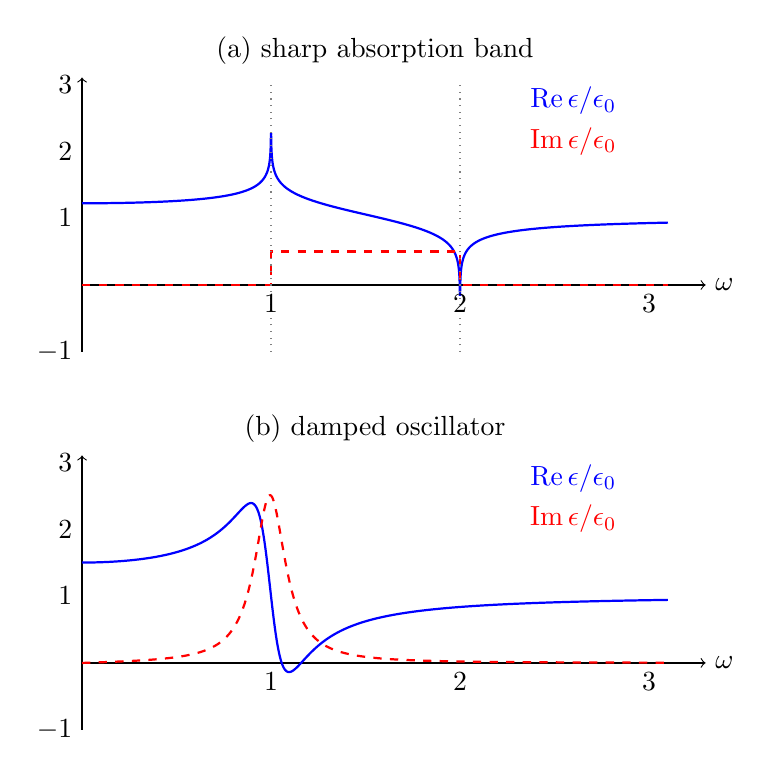
\begin{tikzpicture}[x=2.4cm,y=.85cm]
\begin{scope}[yshift=0.0cm]
\draw[->] (0,-1)--(0,3.1);\draw[->] (0,0)--(3.3,0) node[right] {$\omega$};
\draw[blue,thick] plot coordinates {(0.000000,1.220636) (0.000010,1.220636) (0.000011,1.220636) (0.000013,1.220636) (0.000015,1.220636) (0.000016,1.220636) (0.000019,1.220636) (0.000021,1.220636) (0.000024,1.220636) (0.000027,1.220636) (0.000031,1.220636) (0.000035,1.220636) (0.000039,1.220636) (0.000045,1.220636) (0.000050,1.220636) (0.000057,1.220636) (0.000065,1.220636) (0.000073,1.220636) (0.000083,1.220636) (0.000094,1.220636) (0.000106,1.220636) (0.000120,1.220636) (0.000136,1.220636) (0.000155,1.220636) (0.000175,1.220636) (0.000198,1.220636) (0.000224,1.220636) (0.000254,1.220636) (0.000288,1.220636) (0.000326,1.220636) (0.000369,1.220636) (0.000418,1.220636) (0.000474,1.220636) (0.000536,1.220636) (0.000608,1.220636) (0.000688,1.220636) (0.000779,1.220636) (0.000883,1.220636) (0.001000,1.220636) (0.001132,1.220636) (0.001282,1.220636) (0.001452,1.220636) (0.001644,1.220636) (0.001862,1.220636) (0.002109,1.220636) (0.002389,1.220636) (0.002705,1.220636) (0.003064,1.220637) (0.003470,1.220637) (0.003930,1.220637) (0.004014,1.220638) (0.004451,1.220638) (0.005041,1.220639) (0.005709,1.220639) (0.006465,1.220641) (0.007322,1.220642) (0.008028,1.220643) (0.008293,1.220644) (0.009392,1.220646) (0.010637,1.220649) (0.012042,1.220653) (0.012047,1.220653) (0.013643,1.220658) (0.015452,1.220664) (0.016056,1.220666) (0.017500,1.220672) (0.019819,1.220682) (0.020070,1.220684) (0.022446,1.220696) (0.024084,1.220705) (0.025421,1.220713) (0.028098,1.220730) (0.028790,1.220735) (0.032112,1.220759) (0.032606,1.220763) (0.036127,1.220792) (0.036928,1.220799) (0.040141,1.220828) (0.041822,1.220845) (0.044155,1.220869) (0.047365,1.220904) (0.048169,1.220913) (0.052183,1.220961) (0.053643,1.220980) (0.056197,1.221013) (0.060211,1.221069) (0.060753,1.221077) (0.064225,1.221129) (0.068239,1.221193) (0.068805,1.221202) (0.072253,1.221261) (0.076267,1.221332) (0.077925,1.221363) (0.080281,1.221408) (0.084295,1.221488) (0.088253,1.221570) (0.088309,1.221571) (0.092323,1.221658) (0.096337,1.221750) (0.099950,1.221836) (0.100351,1.221845) (0.104365,1.221945) (0.108380,1.222048) (0.112394,1.222155) (0.116408,1.222267) (0.120422,1.222382) (0.124436,1.222502) (0.128450,1.222626) (0.132464,1.222753) (0.136478,1.222885) (0.140492,1.223021) (0.144506,1.223161) (0.148520,1.223305) (0.152534,1.223454) (0.156548,1.223607) (0.160562,1.223763) (0.164576,1.223924) (0.168590,1.224090) (0.172604,1.224259) (0.176618,1.224433) (0.180633,1.224612) (0.184647,1.224794) (0.188661,1.224981) (0.192675,1.225172) (0.196689,1.225368) (0.200703,1.225568) (0.204717,1.225773) (0.208731,1.225982) (0.212745,1.226196) (0.216759,1.226414) (0.220773,1.226637) (0.224787,1.226865) (0.228801,1.227097) (0.232815,1.227333) (0.236829,1.227575) (0.240843,1.227821) (0.244857,1.228072) (0.248871,1.228328) (0.252886,1.228589) (0.256900,1.228854) (0.260914,1.229125) (0.264928,1.229400) (0.268942,1.229681) (0.272956,1.229966) (0.276970,1.230257) (0.280984,1.230552) (0.284998,1.230853) (0.289012,1.231159) (0.293026,1.231470) (0.297040,1.231787) (0.301054,1.232109) (0.305068,1.232436) (0.309082,1.232769) (0.313096,1.233107) (0.317110,1.233451) (0.321124,1.233800) (0.325139,1.234155) (0.329153,1.234516) (0.333167,1.234882) (0.337181,1.235255) (0.341195,1.235633) (0.345209,1.236017) (0.349223,1.236407) (0.353237,1.236803) (0.357251,1.237206) (0.361265,1.237614) (0.365279,1.238029) (0.369293,1.238450) (0.373307,1.238877) (0.377321,1.239311) (0.381335,1.239752) (0.385349,1.240199) (0.389363,1.240652) (0.393378,1.241113) (0.397392,1.241580) (0.401406,1.242055) (0.405420,1.242536) (0.409434,1.243024) (0.413448,1.243520) (0.417462,1.244023) (0.421476,1.244533) (0.425490,1.245051) (0.429504,1.245576) (0.433518,1.246109) (0.437532,1.246650) (0.441546,1.247198) (0.445560,1.247755) (0.449574,1.248319) (0.453588,1.248892) (0.457602,1.249473) (0.461616,1.250063) (0.465631,1.250661) (0.469645,1.251268) (0.473659,1.251883) (0.477673,1.252508) (0.481687,1.253141) (0.485701,1.253784) (0.489715,1.254436) (0.493729,1.255097) (0.497743,1.255768) (0.501757,1.256449) (0.505771,1.257140) (0.509785,1.257841) (0.513799,1.258552) (0.517813,1.259273) (0.521827,1.260005) (0.525841,1.260748) (0.529855,1.261502) (0.533869,1.262267) (0.537884,1.263043) (0.541898,1.263830) (0.545912,1.264630) (0.549926,1.265441) (0.553940,1.266264) (0.557954,1.267100) (0.561968,1.267948) (0.565982,1.268809) (0.569996,1.269683) (0.574010,1.270570) (0.578024,1.271471) (0.582038,1.272386) (0.586052,1.273314) (0.590066,1.274257) (0.594080,1.275215) (0.598094,1.276187) (0.602108,1.277175) (0.606122,1.278178) (0.610137,1.279197) (0.614151,1.280232) (0.618165,1.281284) (0.622179,1.282352) (0.626193,1.283438) (0.630207,1.284541) (0.634221,1.285663) (0.638235,1.286802) (0.642249,1.287961) (0.646263,1.289139) (0.650277,1.290336) (0.654291,1.291553) (0.658305,1.292792) (0.662319,1.294051) (0.666333,1.295332) (0.670347,1.296635) (0.674361,1.297960) (0.678376,1.299309) (0.682390,1.300682) (0.686404,1.302080) (0.690418,1.303502) (0.694432,1.304950) (0.698446,1.306425) (0.702460,1.307927) (0.706474,1.309457) (0.710488,1.311016) (0.714502,1.312605) (0.718516,1.314223) (0.722530,1.315874) (0.726544,1.317556) (0.730558,1.319272) (0.734572,1.321021) (0.738586,1.322807) (0.742600,1.324628) (0.746614,1.326487) (0.750629,1.328385) (0.754643,1.330324) (0.758657,1.332303) (0.762671,1.334326) (0.766685,1.336392) (0.770699,1.338505) (0.774713,1.340665) (0.778727,1.342875) (0.782741,1.345136) (0.786755,1.347449) (0.790769,1.349818) (0.794783,1.352245) (0.798797,1.354730) (0.802811,1.357278) (0.806825,1.359891) (0.810839,1.362571) (0.814853,1.365321) (0.818867,1.368145) (0.822882,1.371045) (0.826896,1.374026) (0.830910,1.377091) (0.834924,1.380244) (0.838938,1.383490) (0.842952,1.386834) (0.846966,1.390280) (0.850980,1.393834) (0.854994,1.397502) (0.859008,1.401290) (0.863022,1.405206) (0.867036,1.409258) (0.871050,1.413452) (0.875064,1.417800) (0.879078,1.422310) (0.883092,1.426994) (0.887106,1.431864) (0.891120,1.436934) (0.895135,1.442219) (0.899149,1.447735) (0.899550,1.448300) (0.903163,1.453502) (0.907177,1.459541) (0.911191,1.465876) (0.911247,1.465967) (0.915205,1.472535) (0.919219,1.479549) (0.921575,1.483846) (0.923233,1.486954) (0.927247,1.494794) (0.930695,1.501912) (0.931261,1.503117) (0.935275,1.511982) (0.938747,1.520140) (0.939289,1.521458) (0.943303,1.531630) (0.945857,1.538509) (0.947317,1.542599) (0.951331,1.554494) (0.952135,1.556999) (0.955345,1.567472) (0.957678,1.575591) (0.959359,1.581740) (0.962572,1.594268) (0.963373,1.597566) (0.966894,1.613013) (0.967388,1.615313) (0.970710,1.631811) (0.971402,1.635488) (0.974079,1.650647) (0.975416,1.658828) (0.977054,1.669507) (0.979430,1.686466) (0.979681,1.688377) (0.982000,1.707243) (0.983444,1.720281) (0.984048,1.726091) (0.985857,1.744908) (0.987453,1.763680) (0.987458,1.763735) (0.988863,1.782391) (0.990108,1.801026) (0.991207,1.819570) (0.991472,1.824386) (0.992178,1.838005) (0.993035,1.856313) (0.993791,1.874475) (0.994459,1.892471) (0.995049,1.910279) (0.995486,1.924894) (0.995570,1.927875) (0.996030,1.945236) (0.996436,1.962335) (0.996795,1.979145) (0.997111,1.995639) (0.997391,2.011786) (0.997638,2.027557) (0.997856,2.042922) (0.998048,2.057852) (0.998218,2.072315) (0.998368,2.086285) (0.998501,2.099735) (0.998617,2.112639) (0.998721,2.124977) (0.998812,2.136731) (0.998892,2.147886) (0.998964,2.158433) (0.999026,2.168366) (0.999082,2.177684) (0.999131,2.186393) (0.999174,2.194501) (0.999212,2.202021) (0.999246,2.208971) (0.999276,2.215370) (0.999302,2.221244) (0.999325,2.226616) (0.999345,2.231516) (0.999364,2.235972) (0.999380,2.240013) (0.999394,2.243668) (0.999406,2.246967) (0.999417,2.249938) (0.999427,2.252608) (0.999435,2.255004) (0.999443,2.257150) (0.999450,2.259069) (0.999455,2.260782) (0.999461,2.262311) (0.999465,2.263673) (0.999469,2.264886) (0.999473,2.265964) (0.999476,2.266923) (0.999479,2.267774) (0.999481,2.268529) (0.999484,2.269199) (0.999485,2.269793) (0.999487,2.270319) (0.999489,2.270785) (0.999490,2.271198) (0.999500,2.274346)};
\draw[blue,thick] plot coordinates {(1.000500,2.274160) (1.000510,2.271010) (1.000511,2.270597) (1.000513,2.270130) (1.000515,2.269604) (1.000516,2.269010) (1.000519,2.268339) (1.000521,2.267584) (1.000524,2.266732) (1.000527,2.265773) (1.000531,2.264694) (1.000535,2.263480) (1.000539,2.262117) (1.000544,2.260587) (1.000550,2.258871) (1.000557,2.256951) (1.000565,2.254803) (1.000573,2.252406) (1.000583,2.249733) (1.000594,2.246759) (1.000606,2.243457) (1.000620,2.239798) (1.000636,2.235752) (1.000654,2.231292) (1.000675,2.226386) (1.000698,2.221007) (1.000724,2.215126) (1.000754,2.208718) (1.000788,2.201758) (1.000826,2.194226) (1.000869,2.186104) (1.000918,2.177380) (1.000973,2.168043) (1.001036,2.158089) (1.001107,2.147519) (1.001188,2.136336) (1.001279,2.124551) (1.001382,2.112177) (1.001499,2.099231) (1.001631,2.085735) (1.001781,2.071711) (1.001951,2.057186) (1.002144,2.042187) (1.002361,2.026743) (1.002608,2.010881) (1.002888,1.994632) (1.003204,1.978022) (1.003562,1.961080) (1.003968,1.943831) (1.004428,1.926301) (1.004512,1.923289) (1.004949,1.908512) (1.005538,1.890486) (1.006206,1.872243) (1.006962,1.853801) (1.007819,1.835175) (1.008524,1.821295) (1.008789,1.816381) (1.009887,1.797429) (1.011131,1.778332) (1.012536,1.759155) (1.012541,1.759098) (1.014136,1.739734) (1.015944,1.720246) (1.016548,1.714211) (1.017991,1.700637) (1.020309,1.680910) (1.020560,1.678906) (1.022935,1.661064) (1.024572,1.649777) (1.025908,1.641099) (1.028584,1.624946) (1.029276,1.621012) (1.032596,1.603280) (1.033090,1.600796) (1.036608,1.584041) (1.037409,1.580445) (1.040620,1.566722) (1.042301,1.559948) (1.044633,1.550962) (1.047841,1.539295) (1.048645,1.536490) (1.052657,1.523102) (1.054116,1.518468) (1.056669,1.510638) (1.060681,1.498971) (1.061222,1.497451) (1.064693,1.488000) (1.068705,1.477638) (1.069271,1.476222) (1.072717,1.467818) (1.076729,1.458480) (1.078386,1.454753) (1.080741,1.449576) (1.084753,1.441062) (1.088709,1.433015) (1.088765,1.432902) (1.092777,1.425066) (1.096789,1.417524) (1.100400,1.410969) (1.100801,1.410253) (1.104813,1.403232) (1.108825,1.396441) (1.112837,1.389863) (1.116849,1.383484) (1.120861,1.377290) (1.124873,1.371269) (1.128886,1.365408) (1.132898,1.359699) (1.136910,1.354132) (1.140922,1.348698) (1.144934,1.343391) (1.148946,1.338202) (1.152958,1.333125) (1.156970,1.328155) (1.160982,1.323285) (1.164994,1.318511) (1.169006,1.313828) (1.173018,1.309231) (1.177030,1.304716) (1.181042,1.300279) (1.185054,1.295917) (1.189066,1.291626) (1.193078,1.287404) (1.197090,1.283246) (1.201102,1.279151) (1.205114,1.275115) (1.209127,1.271136) (1.213139,1.267213) (1.217151,1.263341) (1.221163,1.259521) (1.225175,1.255748) (1.229187,1.252022) (1.233199,1.248341) (1.237211,1.244703) (1.241223,1.241106) (1.245235,1.237549) (1.249247,1.234031) (1.253259,1.230549) (1.257271,1.227104) (1.261283,1.223692) (1.265295,1.220314) (1.269307,1.216967) (1.273319,1.213651) (1.277331,1.210365) (1.281343,1.207108) (1.285355,1.203878) (1.289367,1.200675) (1.293380,1.197498) (1.297392,1.194345) (1.301404,1.191217) (1.305416,1.188112) (1.309428,1.185029) (1.313440,1.181968) (1.317452,1.178928) (1.321464,1.175908) (1.325476,1.172907) (1.329488,1.169925) (1.333500,1.166962) (1.337512,1.164015) (1.341524,1.161086) (1.345536,1.158173) (1.349548,1.155276) (1.353560,1.152394) (1.357572,1.149526) (1.361584,1.146673) (1.365596,1.143833) (1.369608,1.141006) (1.373620,1.138192) (1.377633,1.135390) (1.381645,1.132599) (1.385657,1.129820) (1.389669,1.127051) (1.393681,1.124292) (1.397693,1.121543) (1.401705,1.118804) (1.405717,1.116073) (1.409729,1.113351) (1.413741,1.110637) (1.417753,1.107931) (1.421765,1.105232) (1.425777,1.102540) (1.429789,1.099855) (1.433801,1.097176) (1.437813,1.094502) (1.441825,1.091835) (1.445837,1.089172) (1.449849,1.086514) (1.453861,1.083860) (1.457873,1.081211) (1.461886,1.078565) (1.465898,1.075923) (1.469910,1.073284) (1.473922,1.070647) (1.477934,1.068013) (1.481946,1.065380) (1.485958,1.062750) (1.489970,1.060121) (1.493982,1.057492) (1.497994,1.054865) (1.502006,1.052238) (1.506018,1.049611) (1.510030,1.046983) (1.514042,1.044355) (1.518054,1.041726) (1.522066,1.039096) (1.526078,1.036464) (1.530090,1.033830) (1.534102,1.031194) (1.538114,1.028555) (1.542127,1.025914) (1.546139,1.023269) (1.550151,1.020620) (1.554163,1.017967) (1.558175,1.015310) (1.562187,1.012648) (1.566199,1.009982) (1.570211,1.007309) (1.574223,1.004631) (1.578235,1.001947) (1.582247,0.999256) (1.586259,0.996558) (1.590271,0.993853) (1.594283,0.991140) (1.598295,0.988420) (1.602307,0.985690) (1.606319,0.982952) (1.610331,0.980204) (1.614343,0.977446) (1.618355,0.974678) (1.622367,0.971900) (1.626380,0.969110) (1.630392,0.966309) (1.634404,0.963495) (1.638416,0.960669) (1.642428,0.957830) (1.646440,0.954977) (1.650452,0.952109) (1.654464,0.949228) (1.658476,0.946330) (1.662488,0.943417) (1.666500,0.940488) (1.670512,0.937541) (1.674524,0.934577) (1.678536,0.931594) (1.682548,0.928592) (1.686560,0.925570) (1.690572,0.922528) (1.694584,0.919465) (1.698596,0.916380) (1.702608,0.913272) (1.706620,0.910140) (1.710633,0.906984) (1.714645,0.903802) (1.718657,0.900595) (1.722669,0.897359) (1.726681,0.894096) (1.730693,0.890804) (1.734705,0.887481) (1.738717,0.884126) (1.742729,0.880739) (1.746741,0.877318) (1.750753,0.873862) (1.754765,0.870369) (1.758777,0.866838) (1.762789,0.863268) (1.766801,0.859657) (1.770813,0.856003) (1.774825,0.852305) (1.778837,0.848561) (1.782849,0.844769) (1.786861,0.840927) (1.790873,0.837032) (1.794886,0.833084) (1.798898,0.829078) (1.802910,0.825014) (1.806922,0.820887) (1.810934,0.816696) (1.814946,0.812438) (1.818958,0.808108) (1.822970,0.803704) (1.826982,0.799223) (1.830994,0.794660) (1.835006,0.790010) (1.839018,0.785271) (1.843030,0.780437) (1.847042,0.775502) (1.851054,0.770461) (1.855066,0.765309) (1.859078,0.760038) (1.863090,0.754642) (1.867102,0.749112) (1.871114,0.743441) (1.875127,0.737619) (1.879139,0.731637) (1.883151,0.725482) (1.887163,0.719143) (1.891175,0.712606) (1.895187,0.705856) (1.899199,0.698876) (1.899600,0.698165) (1.903211,0.691647) (1.907223,0.684148) (1.911235,0.676353) (1.911291,0.676242) (1.915247,0.668237) (1.919259,0.659767) (1.921614,0.654615) (1.923271,0.650906) (1.927283,0.641613) (1.930729,0.633248) (1.931295,0.631838) (1.935307,0.621522) (1.938778,0.612109) (1.939319,0.610596) (1.943331,0.598975) (1.945884,0.591175) (1.947343,0.586558) (1.951355,0.573218) (1.952159,0.570423) (1.955367,0.558793) (1.957699,0.549835) (1.959380,0.543081) (1.962591,0.529398) (1.963392,0.525811) (1.966910,0.509099) (1.967404,0.506621) (1.970724,0.488931) (1.971416,0.485005) (1.974092,0.468885) (1.975428,0.460224) (1.977065,0.448957) (1.979440,0.431146) (1.979691,0.429145) (1.982009,0.409447) (1.983452,0.395892) (1.984056,0.389864) (1.985864,0.370399) (1.987459,0.351056) (1.987464,0.350999) (1.988869,0.331840) (1.990113,0.312759) (1.991211,0.293822) (1.991476,0.288911) (1.992181,0.275040) (1.993038,0.256425) (1.993794,0.237993) (1.994462,0.219758) (1.995051,0.201740) (1.995488,0.186969) (1.995572,0.183958) (1.996032,0.166434) (1.996438,0.149191) (1.996796,0.132253) (1.997112,0.115648) (1.997392,0.099402) (1.997639,0.083544) (1.997856,0.068102) (1.998049,0.053106) (1.998219,0.038583) (1.998369,0.024562) (1.998501,0.011067) (1.998618,-0.001877) (1.998721,-0.014250) (1.998812,-0.026034) (1.998893,-0.037215) (1.998964,-0.047785) (1.999027,-0.057738) (1.999082,-0.067074) (1.999131,-0.075798) (1.999174,-0.083919) (1.999212,-0.091451) (1.999246,-0.098410) (1.999276,-0.104818) (1.999302,-0.110698) (1.999325,-0.116077) (1.999346,-0.120983) (1.999364,-0.125443) (1.999380,-0.129488) (1.999394,-0.133147) (1.999406,-0.136449) (1.999417,-0.139423) (1.999427,-0.142095) (1.999435,-0.144493) (1.999443,-0.146640) (1.999450,-0.148561) (1.999456,-0.150276) (1.999461,-0.151806) (1.999465,-0.153169) (1.999469,-0.154383) (1.999473,-0.155462) (1.999476,-0.156421) (1.999479,-0.157273) (1.999481,-0.158028) (1.999484,-0.158699) (1.999485,-0.159293) (1.999487,-0.159819) (1.999489,-0.160286) (1.999490,-0.160699) (1.999500,-0.163849)};
\draw[blue,thick] plot coordinates {(2.000500,-0.164021) (2.000511,-0.160561) (2.000512,-0.160108) (2.000514,-0.159597) (2.000516,-0.159020) (2.000518,-0.158368) (2.000520,-0.157634) (2.000523,-0.156806) (2.000526,-0.155874) (2.000530,-0.154825) (2.000534,-0.153645) (2.000538,-0.152319) (2.000543,-0.150831) (2.000549,-0.149162) (2.000555,-0.147293) (2.000563,-0.145202) (2.000571,-0.142867) (2.000581,-0.140263) (2.000591,-0.137365) (2.000603,-0.134145) (2.000617,-0.130575) (2.000633,-0.126627) (2.000650,-0.122270) (2.000670,-0.117477) (2.000693,-0.112217) (2.000718,-0.106463) (2.000747,-0.100188) (2.000780,-0.093369) (2.000817,-0.085983) (2.000859,-0.078014) (2.000906,-0.069446) (2.000960,-0.060269) (2.001021,-0.050479) (2.001090,-0.040075) (2.001168,-0.029061) (2.001257,-0.017445) (2.001357,-0.005240) (2.001471,0.007535) (2.001600,0.020861) (2.001745,0.034713) (2.001910,0.049066) (2.002097,0.063892) (2.002309,0.079160) (2.002549,0.094843) (2.002820,0.110908) (2.003128,0.127328) (2.003476,0.144071) (2.003870,0.161110) (2.004317,0.178418) (2.004823,0.195968) (2.004916,0.198980) (2.005396,0.213736) (2.006045,0.231699) (2.006780,0.249834) (2.007612,0.268121) (2.008555,0.286540) (2.009331,0.300234) (2.009623,0.305075) (2.010832,0.323707) (2.012201,0.342420) (2.013747,0.361144) (2.013752,0.361200) (2.015508,0.380032) (2.017497,0.398901) (2.018163,0.404727) (2.019750,0.417796) (2.022302,0.436702) (2.022578,0.438616) (2.025191,0.455605) (2.026994,0.466301) (2.028464,0.474494) (2.031410,0.489673) (2.032170,0.493355) (2.035825,0.509871) (2.036368,0.512174) (2.040241,0.527635) (2.041122,0.530937) (2.044657,0.543475) (2.046506,0.549629) (2.049072,0.557754) (2.052604,0.568234) (2.053488,0.570741) (2.057904,0.582644) (2.059510,0.586736) (2.062319,0.593621) (2.066735,0.603799) (2.067331,0.605118) (2.071151,0.613283) (2.075566,0.622155) (2.076189,0.623361) (2.079982,0.630485) (2.084398,0.638333) (2.086221,0.641444) (2.088813,0.645747) (2.093229,0.652769) (2.097583,0.659346) (2.097645,0.659437) (2.102060,0.665782) (2.106476,0.671832) (2.110450,0.677044) (2.110892,0.677610) (2.115307,0.683139) (2.119723,0.688436) (2.124139,0.693519) (2.128554,0.698404) (2.132970,0.703103) (2.137386,0.707629) (2.141801,0.711993) (2.146217,0.716205) (2.150633,0.720275) (2.155048,0.724210) (2.159464,0.728018) (2.163880,0.731707) (2.168295,0.735283) (2.172711,0.738751) (2.177127,0.742118) (2.181542,0.745388) (2.185958,0.748566) (2.190373,0.751657) (2.194789,0.754665) (2.199205,0.757593) (2.203620,0.760445) (2.208036,0.763225) (2.212452,0.765935) (2.216867,0.768578) (2.221283,0.771158) (2.225699,0.773677) (2.230114,0.776137) (2.234530,0.778540) (2.238946,0.780889) (2.243361,0.783186) (2.247777,0.785433) (2.252193,0.787631) (2.256608,0.789783) (2.261024,0.791889) (2.265440,0.793952) (2.269855,0.795973) (2.274271,0.797954) (2.278687,0.799895) (2.283102,0.801798) (2.287518,0.803665) (2.291934,0.805496) (2.296349,0.807292) (2.300765,0.809055) (2.305181,0.810786) (2.309596,0.812486) (2.314012,0.814155) (2.318428,0.815794) (2.322843,0.817405) (2.327259,0.818988) (2.331675,0.820543) (2.336090,0.822073) (2.340506,0.823577) (2.344922,0.825055) (2.349337,0.826510) (2.353753,0.827941) (2.358169,0.829349) (2.362584,0.830734) (2.367000,0.832098) (2.371416,0.833441) (2.375831,0.834762) (2.380247,0.836064) (2.384663,0.837346) (2.389078,0.838608) (2.393494,0.839852) (2.397910,0.841078) (2.402325,0.842285) (2.406741,0.843475) (2.411157,0.844648) (2.415572,0.845804) (2.419988,0.846944) (2.424404,0.848068) (2.428819,0.849177) (2.433235,0.850270) (2.437651,0.851348) (2.442066,0.852412) (2.446482,0.853461) (2.450898,0.854496) (2.455313,0.855518) (2.459729,0.856526) (2.464145,0.857522) (2.468560,0.858504) (2.472976,0.859474) (2.477392,0.860431) (2.481807,0.861376) (2.486223,0.862310) (2.490639,0.863231) (2.495054,0.864142) (2.499470,0.865041) (2.503886,0.865929) (2.508301,0.866807) (2.512717,0.867674) (2.517133,0.868531) (2.521548,0.869377) (2.525964,0.870214) (2.530380,0.871040) (2.534795,0.871857) (2.539211,0.872665) (2.543627,0.873463) (2.548042,0.874253) (2.552458,0.875033) (2.556873,0.875805) (2.561289,0.876568) (2.565705,0.877322) (2.570120,0.878068) (2.574536,0.878806) (2.578952,0.879536) (2.583367,0.880258) (2.587783,0.880972) (2.592199,0.881679) (2.596614,0.882378) (2.601030,0.883069) (2.605446,0.883754) (2.609861,0.884431) (2.614277,0.885101) (2.618693,0.885764) (2.623108,0.886420) (2.627524,0.887070) (2.631940,0.887713) (2.636355,0.888349) (2.640771,0.888979) (2.645187,0.889603) (2.649602,0.890220) (2.654018,0.890832) (2.658434,0.891437) (2.662849,0.892036) (2.667265,0.892630) (2.671681,0.893218) (2.676096,0.893800) (2.680512,0.894376) (2.684928,0.894947) (2.689343,0.895513) (2.693759,0.896073) (2.698175,0.896628) (2.702590,0.897178) (2.707006,0.897722) (2.711422,0.898262) (2.715837,0.898796) (2.720253,0.899326) (2.724669,0.899851) (2.729084,0.900371) (2.733500,0.900886) (2.737916,0.901397) (2.742331,0.901903) (2.746747,0.902404) (2.751163,0.902901) (2.755578,0.903394) (2.759994,0.903882) (2.764410,0.904366) (2.768825,0.904846) (2.773241,0.905322) (2.777657,0.905793) (2.782072,0.906260) (2.786488,0.906724) (2.790904,0.907183) (2.795319,0.907639) (2.799735,0.908090) (2.804151,0.908538) (2.808566,0.908982) (2.812982,0.909423) (2.817398,0.909859) (2.821813,0.910292) (2.826229,0.910722) (2.830645,0.911148) (2.835060,0.911570) (2.839476,0.911989) (2.843892,0.912405) (2.848307,0.912817) (2.852723,0.913226) (2.857139,0.913632) (2.861554,0.914034) (2.865970,0.914433) (2.870386,0.914829) (2.874801,0.915222) (2.879217,0.915612) (2.883633,0.915998) (2.888048,0.916382) (2.892464,0.916763) (2.896880,0.917140) (2.901295,0.917515) (2.905711,0.917887) (2.910127,0.918256) (2.914542,0.918622) (2.918958,0.918986) (2.923373,0.919347) (2.927789,0.919705) (2.932205,0.920060) (2.936620,0.920412) (2.941036,0.920762) (2.945452,0.921110) (2.949867,0.921455) (2.954283,0.921797) (2.958699,0.922137) (2.963114,0.922474) (2.967530,0.922808) (2.971946,0.923141) (2.976361,0.923471) (2.980777,0.923798) (2.985193,0.924123) (2.989608,0.924446) (2.990050,0.924478) (2.994024,0.924767) (2.998440,0.925085) (3.002855,0.925401) (3.002917,0.925405) (3.007271,0.925714) (3.011687,0.926026) (3.014279,0.926208) (3.016102,0.926335) (3.020518,0.926642) (3.024311,0.926904) (3.024934,0.926947) (3.029349,0.927250) (3.033169,0.927510) (3.033765,0.927551) (3.038181,0.927849) (3.040990,0.928038) (3.042596,0.928146) (3.047012,0.928440) (3.047896,0.928499) (3.051428,0.928733) (3.053994,0.928902) (3.055843,0.929023) (3.059378,0.929254) (3.060259,0.929312) (3.064132,0.929563) (3.064675,0.929598) (3.068330,0.929834) (3.069090,0.929883) (3.072036,0.930072) (3.073506,0.930166) (3.075309,0.930280) (3.077922,0.930446) (3.078198,0.930464) (3.080750,0.930625) (3.082337,0.930725) (3.083003,0.930767) (3.084992,0.930892) (3.086748,0.931002) (3.086753,0.931002) (3.088299,0.931099) (3.089668,0.931184) (3.090877,0.931259) (3.091169,0.931277) (3.091945,0.931326) (3.092888,0.931384) (3.093720,0.931436) (3.094455,0.931481) (3.095104,0.931521) (3.095584,0.931551) (3.095677,0.931556) (3.096183,0.931588) (3.096630,0.931615) (3.097024,0.931639) (3.097372,0.931661) (3.097680,0.931680) (3.097951,0.931696) (3.098191,0.931711) (3.098403,0.931724) (3.098590,0.931736) (3.098755,0.931746) (3.098901,0.931755) (3.099029,0.931763) (3.099143,0.931770) (3.099243,0.931776) (3.099332,0.931781) (3.099410,0.931786) (3.099479,0.931790) (3.099540,0.931794) (3.099594,0.931797) (3.099641,0.931800) (3.099683,0.931803) (3.099720,0.931805) (3.099753,0.931807) (3.099782,0.931809) (3.099807,0.931810) (3.099830,0.931812) (3.099850,0.931813) (3.099867,0.931814) (3.099883,0.931815) (3.099897,0.931816) (3.099909,0.931817) (3.099919,0.931817) (3.099929,0.931818) (3.099937,0.931818) (3.099945,0.931819) (3.099951,0.931819) (3.099957,0.931820) (3.099962,0.931820) (3.099966,0.931820) (3.099970,0.931820) (3.099974,0.931821) (3.099977,0.931821) (3.099980,0.931821) (3.099982,0.931821) (3.099984,0.931821) (3.099986,0.931821) (3.099988,0.931821) (3.099989,0.931822) (3.100000,0.931822)};
\draw[red,dashed,thick] plot coordinates {(0.000000,0.000000) (1.000000,0.000000) (1.000000,0.500000) (2.000000,0.500000) (2.000000,0.000000) (3.100000,0.000000)};
\draw[gray,dotted] (1,-1)--(1,3);
\draw[gray,dotted] (2,-1)--(2,3);
\node at (1.55,3.5) {(a) sharp absorption band};
\node[below] at (1,0) {$1$};\node[left] at (0,1) {$1$};
\node[below] at (2,0) {$2$};\node[left] at (0,2) {$2$};
\node[below] at (3,0) {$3$};\node[left] at (0,3) {$3$};
\node[left] at (0,-1) {$-1$};\node[blue] at (2.6,2.75) {$\operatorname{Re}\epsilon/\epsilon_0$};\node[red] at (2.6,2.15) {$\operatorname{Im}\epsilon/\epsilon_0$};
\end{scope}
\begin{scope}[yshift=-4.8cm]
\draw[->] (0,-1)--(0,3.1);\draw[->] (0,0)--(3.3,0) node[right] {$\omega$};
\draw[blue,thick] plot coordinates {(0.000000,1.500000) (0.003100,1.500005) (0.006200,1.500018) (0.009300,1.500042) (0.012400,1.500074) (0.015500,1.500115) (0.018600,1.500166) (0.021700,1.500226) (0.024800,1.500295) (0.027900,1.500374) (0.031000,1.500462) (0.034100,1.500559) (0.037200,1.500665) (0.040300,1.500781) (0.043400,1.500906) (0.046500,1.501040) (0.049600,1.501184) (0.052700,1.501337) (0.055800,1.501499) (0.058900,1.501671) (0.062000,1.501852) (0.065100,1.502042) (0.068200,1.502242) (0.071300,1.502452) (0.074400,1.502671) (0.077500,1.502899) (0.080600,1.503137) (0.083700,1.503384) (0.086800,1.503642) (0.089900,1.503908) (0.093000,1.504185) (0.096100,1.504471) (0.099200,1.504767) (0.102300,1.505072) (0.105400,1.505387) (0.108500,1.505712) (0.111600,1.506047) (0.114700,1.506392) (0.117800,1.506747) (0.120900,1.507111) (0.124000,1.507486) (0.127100,1.507871) (0.130200,1.508266) (0.133300,1.508670) (0.136400,1.509085) (0.139500,1.509511) (0.142600,1.509946) (0.145700,1.510392) (0.148800,1.510848) (0.151900,1.511315) (0.155000,1.511792) (0.158100,1.512279) (0.161200,1.512778) (0.164300,1.513286) (0.167400,1.513806) (0.170500,1.514336) (0.173600,1.514877) (0.176700,1.515429) (0.179800,1.515991) (0.182900,1.516565) (0.186000,1.517150) (0.189100,1.517746) (0.192200,1.518353) (0.195300,1.518971) (0.198400,1.519601) (0.201500,1.520242) (0.204600,1.520895) (0.207700,1.521559) (0.210800,1.522235) (0.213900,1.522922) (0.217000,1.523622) (0.220100,1.524333) (0.223200,1.525056) (0.226300,1.525791) (0.229400,1.526539) (0.232500,1.527298) (0.235600,1.528070) (0.238700,1.528855) (0.241800,1.529652) (0.244900,1.530461) (0.248000,1.531283) (0.251100,1.532118) (0.254200,1.532966) (0.257300,1.533827) (0.260400,1.534701) (0.263500,1.535589) (0.266600,1.536489) (0.269700,1.537403) (0.272800,1.538331) (0.275900,1.539273) (0.279000,1.540228) (0.282100,1.541197) (0.285200,1.542180) (0.288300,1.543178) (0.291400,1.544189) (0.294500,1.545216) (0.297600,1.546256) (0.300700,1.547312) (0.303800,1.548382) (0.306900,1.549468) (0.310000,1.550568) (0.313100,1.551684) (0.316200,1.552815) (0.319300,1.553962) (0.322400,1.555125) (0.325500,1.556303) (0.328600,1.557498) (0.331700,1.558709) (0.334800,1.559936) (0.337900,1.561180) (0.341000,1.562441) (0.344100,1.563719) (0.347200,1.565013) (0.350300,1.566325) (0.353400,1.567655) (0.356500,1.569002) (0.359600,1.570367) (0.362700,1.571750) (0.365800,1.573152) (0.368900,1.574571) (0.372000,1.576010) (0.375100,1.577468) (0.378200,1.578944) (0.381300,1.580440) (0.384400,1.581956) (0.387500,1.583491) (0.390600,1.585046) (0.393700,1.586622) (0.396800,1.588218) (0.399900,1.589835) (0.403000,1.591473) (0.406100,1.593132) (0.409200,1.594813) (0.412300,1.596516) (0.415400,1.598240) (0.418500,1.599987) (0.421600,1.601757) (0.424700,1.603550) (0.427800,1.605365) (0.430900,1.607205) (0.434000,1.609068) (0.437100,1.610955) (0.440200,1.612867) (0.443300,1.614803) (0.446400,1.616765) (0.449500,1.618752) (0.452600,1.620765) (0.455700,1.622804) (0.458800,1.624869) (0.461900,1.626962) (0.465000,1.629081) (0.468100,1.631228) (0.471200,1.633403) (0.474300,1.635607) (0.477400,1.637839) (0.480500,1.640101) (0.483600,1.642392) (0.486700,1.644713) (0.489800,1.647064) (0.492900,1.649447) (0.496000,1.651860) (0.499100,1.654306) (0.502200,1.656784) (0.505300,1.659294) (0.508400,1.661838) (0.511500,1.664415) (0.514600,1.667027) (0.517700,1.669673) (0.520800,1.672355) (0.523900,1.675073) (0.527000,1.677827) (0.530100,1.680617) (0.533200,1.683445) (0.536300,1.686312) (0.539400,1.689217) (0.542500,1.692161) (0.545600,1.695145) (0.548700,1.698169) (0.551800,1.701235) (0.554900,1.704342) (0.558000,1.707492) (0.561100,1.710685) (0.564200,1.713922) (0.567300,1.717203) (0.570400,1.720529) (0.573500,1.723902) (0.576600,1.727321) (0.579700,1.730787) (0.582800,1.734302) (0.585900,1.737866) (0.589000,1.741480) (0.592100,1.745144) (0.595200,1.748860) (0.598300,1.752628) (0.601400,1.756449) (0.604500,1.760325) (0.607600,1.764255) (0.610700,1.768242) (0.613800,1.772285) (0.616900,1.776386) (0.620000,1.780546) (0.623100,1.784766) (0.626200,1.789046) (0.629300,1.793388) (0.632400,1.797793) (0.635500,1.802262) (0.638600,1.806795) (0.641700,1.811395) (0.644800,1.816062) (0.647900,1.820797) (0.651000,1.825601) (0.654100,1.830476) (0.657200,1.835422) (0.660300,1.840442) (0.663400,1.845535) (0.666500,1.850703) (0.669600,1.855948) (0.672700,1.861271) (0.675800,1.866672) (0.678900,1.872154) (0.682000,1.877717) (0.685100,1.883363) (0.688200,1.889092) (0.691300,1.894907) (0.694400,1.900808) (0.697500,1.906797) (0.700600,1.912874) (0.703700,1.919042) (0.706800,1.925301) (0.709900,1.931653) (0.713000,1.938099) (0.716100,1.944639) (0.719200,1.951276) (0.722300,1.958010) (0.725400,1.964842) (0.728500,1.971773) (0.731600,1.978805) (0.734700,1.985937) (0.737800,1.993172) (0.740900,2.000509) (0.744000,2.007949) (0.747100,2.015493) (0.750200,2.023141) (0.753300,2.030893) (0.756400,2.038750) (0.759500,2.046711) (0.762600,2.054776) (0.765700,2.062945) (0.768800,2.071217) (0.771900,2.079591) (0.775000,2.088065) (0.778100,2.096638) (0.781200,2.105308) (0.784300,2.114073) (0.787400,2.122929) (0.790500,2.131874) (0.793600,2.140904) (0.796700,2.150014) (0.799800,2.159199) (0.802900,2.168453) (0.806000,2.177770) (0.809100,2.187143) (0.812200,2.196562) (0.815300,2.206019) (0.818400,2.215503) (0.821500,2.225002) (0.824600,2.234503) (0.827700,2.243991) (0.830800,2.253451) (0.833900,2.262863) (0.837000,2.272207) (0.840100,2.281463) (0.843200,2.290604) (0.846300,2.299605) (0.849400,2.308434) (0.852500,2.317061) (0.855600,2.325448) (0.858700,2.333556) (0.861800,2.341343) (0.864900,2.348760) (0.868000,2.355756) (0.871100,2.362276) (0.874200,2.368258) (0.877300,2.373636) (0.880400,2.378337) (0.883500,2.382284) (0.886600,2.385393) (0.889700,2.387574) (0.892800,2.388728) (0.895900,2.388753) (0.899000,2.387537) (0.902100,2.384963) (0.905200,2.380906) (0.908300,2.375235) (0.911400,2.367812) (0.914500,2.358495) (0.917600,2.347134) (0.920700,2.333578) (0.923800,2.317673) (0.926900,2.299263) (0.930000,2.278194) (0.933100,2.254314) (0.936200,2.227480) (0.939300,2.197554) (0.942400,2.164413) (0.945500,2.127949) (0.948600,2.088076) (0.951700,2.044728) (0.954800,1.997872) (0.957900,1.947504) (0.961000,1.893658) (0.964100,1.836404) (0.967200,1.775859) (0.970300,1.712180) (0.973400,1.645572) (0.976500,1.576282) (0.979600,1.504602) (0.982700,1.430865) (0.985800,1.355437) (0.988900,1.278717) (0.992000,1.201128) (0.995100,1.123109) (0.998200,1.045107) (1.001300,0.967569) (1.004400,0.890932) (1.007500,0.815618) (1.010600,0.742023) (1.013700,0.670513) (1.016800,0.601416) (1.019900,0.535022) (1.023000,0.471575) (1.026100,0.411275) (1.029200,0.354279) (1.032300,0.300697) (1.035400,0.250598) (1.038500,0.204014) (1.041600,0.160938) (1.044700,0.121333) (1.047800,0.085134) (1.050900,0.052252) (1.054000,0.022577) (1.057100,-0.004015) (1.060200,-0.027660) (1.063300,-0.048505) (1.066400,-0.066701) (1.069500,-0.082401) (1.072600,-0.095763) (1.075700,-0.106939) (1.078800,-0.116082) (1.081900,-0.123340) (1.085000,-0.128855) (1.088100,-0.132764) (1.091200,-0.135198) (1.094300,-0.136281) (1.097400,-0.136131) (1.100500,-0.134858) (1.103600,-0.132565) (1.106700,-0.129349) (1.109800,-0.125300) (1.112900,-0.120502) (1.116000,-0.115031) (1.119100,-0.108960) (1.122200,-0.102354) (1.125300,-0.095274) (1.128400,-0.087777) (1.131500,-0.079913) (1.134600,-0.071728) (1.137700,-0.063267) (1.140800,-0.054568) (1.143900,-0.045667) (1.147000,-0.036596) (1.150100,-0.027385) (1.153200,-0.018060) (1.156300,-0.008647) (1.159400,0.000833) (1.162500,0.010361) (1.165600,0.019917) (1.168700,0.029487) (1.171800,0.039054) (1.174900,0.048607) (1.178000,0.058134) (1.181100,0.067623) (1.184200,0.077066) (1.187300,0.086455) (1.190400,0.095781) (1.193500,0.105039) (1.196600,0.114223) (1.199700,0.123327) (1.202800,0.132348) (1.205900,0.141281) (1.209000,0.150124) (1.212100,0.158873) (1.215200,0.167526) (1.218300,0.176081) (1.221400,0.184537) (1.224500,0.192893) (1.227600,0.201146) (1.230700,0.209298) (1.233800,0.217346) (1.236900,0.225292) (1.240000,0.233134) (1.243100,0.240874) (1.246200,0.248510) (1.249300,0.256045) (1.252400,0.263477) (1.255500,0.270808) (1.258600,0.278039) (1.261700,0.285170) (1.264800,0.292203) (1.267900,0.299137) (1.271000,0.305975) (1.274100,0.312717) (1.277200,0.319364) (1.280300,0.325918) (1.283400,0.332379) (1.286500,0.338750) (1.289600,0.345030) (1.292700,0.351222) (1.295800,0.357326) (1.298900,0.363344) (1.302000,0.369277) (1.305100,0.375126) (1.308200,0.380893) (1.311300,0.386579) (1.314400,0.392185) (1.317500,0.397713) (1.320600,0.403162) (1.323700,0.408536) (1.326800,0.413835) (1.329900,0.419060) (1.333000,0.424213) (1.336100,0.429294) (1.339200,0.434305) (1.342300,0.439247) (1.345400,0.444122) (1.348500,0.448930) (1.351600,0.453672) (1.354700,0.458349) (1.357800,0.462964) (1.360900,0.467516) (1.364000,0.472006) (1.367100,0.476437) (1.370200,0.480808) (1.373300,0.485121) (1.376400,0.489377) (1.379500,0.493577) (1.382600,0.497721) (1.385700,0.501811) (1.388800,0.505847) (1.391900,0.509832) (1.395000,0.513764) (1.398100,0.517646) (1.401200,0.521477) (1.404300,0.525260) (1.407400,0.528995) (1.410500,0.532682) (1.413600,0.536322) (1.416700,0.539917) (1.419800,0.543466) (1.422900,0.546971) (1.426000,0.550433) (1.429100,0.553851) (1.432200,0.557228) (1.435300,0.560563) (1.438400,0.563857) (1.441500,0.567111) (1.444600,0.570326) (1.447700,0.573502) (1.450800,0.576639) (1.453900,0.579739) (1.457000,0.582802) (1.460100,0.585829) (1.463200,0.588820) (1.466300,0.591776) (1.469400,0.594697) (1.472500,0.597584) (1.475600,0.600437) (1.478700,0.603258) (1.481800,0.606046) (1.484900,0.608802) (1.488000,0.611526) (1.491100,0.614220) (1.494200,0.616883) (1.497300,0.619516) (1.500400,0.622119) (1.503500,0.624694) (1.506600,0.627239) (1.509700,0.629757) (1.512800,0.632246) (1.515900,0.634709) (1.519000,0.637144) (1.522100,0.639553) (1.525200,0.641935) (1.528300,0.644292) (1.531400,0.646624) (1.534500,0.648930) (1.537600,0.651212) (1.540700,0.653469) (1.543800,0.655703) (1.546900,0.657913) (1.550000,0.660100) (1.553100,0.662264) (1.556200,0.664405) (1.559300,0.666525) (1.562400,0.668622) (1.565500,0.670698) (1.568600,0.672752) (1.571700,0.674786) (1.574800,0.676798) (1.577900,0.678791) (1.581000,0.680763) (1.584100,0.682716) (1.587200,0.684649) (1.590300,0.686562) (1.593400,0.688457) (1.596500,0.690333) (1.599600,0.692191) (1.602700,0.694030) (1.605800,0.695851) (1.608900,0.697655) (1.612000,0.699441) (1.615100,0.701210) (1.618200,0.702962) (1.621300,0.704697) (1.624400,0.706415) (1.627500,0.708117) (1.630600,0.709803) (1.633700,0.711473) (1.636800,0.713128) (1.639900,0.714767) (1.643000,0.716390) (1.646100,0.717999) (1.649200,0.719592) (1.652300,0.721171) (1.655400,0.722736) (1.658500,0.724286) (1.661600,0.725822) (1.664700,0.727344) (1.667800,0.728852) (1.670900,0.730346) (1.674000,0.731827) (1.677100,0.733295) (1.680200,0.734750) (1.683300,0.736192) (1.686400,0.737621) (1.689500,0.739037) (1.692600,0.740441) (1.695700,0.741833) (1.698800,0.743212) (1.701900,0.744579) (1.705000,0.745935) (1.708100,0.747279) (1.711200,0.748611) (1.714300,0.749932) (1.717400,0.751241) (1.720500,0.752540) (1.723600,0.753827) (1.726700,0.755104) (1.729800,0.756369) (1.732900,0.757624) (1.736000,0.758869) (1.739100,0.760103) (1.742200,0.761327) (1.745300,0.762540) (1.748400,0.763744) (1.751500,0.764938) (1.754600,0.766122) (1.757700,0.767296) (1.760800,0.768461) (1.763900,0.769616) (1.767000,0.770762) (1.770100,0.771898) (1.773200,0.773026) (1.776300,0.774144) (1.779400,0.775254) (1.782500,0.776354) (1.785600,0.777446) (1.788700,0.778529) (1.791800,0.779604) (1.794900,0.780670) (1.798000,0.781728) (1.801100,0.782777) (1.804200,0.783819) (1.807300,0.784852) (1.810400,0.785877) (1.813500,0.786895) (1.816600,0.787904) (1.819700,0.788906) (1.822800,0.789900) (1.825900,0.790887) (1.829000,0.791866) (1.832100,0.792837) (1.835200,0.793802) (1.838300,0.794759) (1.841400,0.795709) (1.844500,0.796651) (1.847600,0.797587) (1.850700,0.798516) (1.853800,0.799438) (1.856900,0.800353) (1.860000,0.801261) (1.863100,0.802163) (1.866200,0.803058) (1.869300,0.803946) (1.872400,0.804828) (1.875500,0.805704) (1.878600,0.806573) (1.881700,0.807436) (1.884800,0.808293) (1.887900,0.809143) (1.891000,0.809988) (1.894100,0.810826) (1.897200,0.811659) (1.900300,0.812485) (1.903400,0.813306) (1.906500,0.814121) (1.909600,0.814930) (1.912700,0.815734) (1.915800,0.816532) (1.918900,0.817324) (1.922000,0.818111) (1.925100,0.818893) (1.928200,0.819669) (1.931300,0.820439) (1.934400,0.821205) (1.937500,0.821965) (1.940600,0.822720) (1.943700,0.823469) (1.946800,0.824214) (1.949900,0.824954) (1.953000,0.825688) (1.956100,0.826418) (1.959200,0.827143) (1.962300,0.827862) (1.965400,0.828577) (1.968500,0.829288) (1.971600,0.829993) (1.974700,0.830694) (1.977800,0.831390) (1.980900,0.832082) (1.984000,0.832769) (1.987100,0.833452) (1.990200,0.834130) (1.993300,0.834803) (1.996400,0.835473) (1.999500,0.836138) (2.002600,0.836798) (2.005700,0.837455) (2.008800,0.838107) (2.011900,0.838755) (2.015000,0.839398) (2.018100,0.840038) (2.021200,0.840674) (2.024300,0.841305) (2.027400,0.841933) (2.030500,0.842556) (2.033600,0.843176) (2.036700,0.843792) (2.039800,0.844403) (2.042900,0.845011) (2.046000,0.845616) (2.049100,0.846216) (2.052200,0.846813) (2.055300,0.847406) (2.058400,0.847995) (2.061500,0.848581) (2.064600,0.849163) (2.067700,0.849741) (2.070800,0.850316) (2.073900,0.850888) (2.077000,0.851456) (2.080100,0.852020) (2.083200,0.852581) (2.086300,0.853139) (2.089400,0.853693) (2.092500,0.854244) (2.095600,0.854792) (2.098700,0.855336) (2.101800,0.855877) (2.104900,0.856415) (2.108000,0.856950) (2.111100,0.857481) (2.114200,0.858010) (2.117300,0.858535) (2.120400,0.859057) (2.123500,0.859576) (2.126600,0.860092) (2.129700,0.860605) (2.132800,0.861115) (2.135900,0.861622) (2.139000,0.862126) (2.142100,0.862628) (2.145200,0.863126) (2.148300,0.863621) (2.151400,0.864114) (2.154500,0.864603) (2.157600,0.865090) (2.160700,0.865574) (2.163800,0.866056) (2.166900,0.866534) (2.170000,0.867010) (2.173100,0.867483) (2.176200,0.867954) (2.179300,0.868422) (2.182400,0.868887) (2.185500,0.869349) (2.188600,0.869809) (2.191700,0.870267) (2.194800,0.870722) (2.197900,0.871174) (2.201000,0.871624) (2.204100,0.872071) (2.207200,0.872516) (2.210300,0.872958) (2.213400,0.873398) (2.216500,0.873836) (2.219600,0.874271) (2.222700,0.874704) (2.225800,0.875134) (2.228900,0.875562) (2.232000,0.875988) (2.235100,0.876411) (2.238200,0.876833) (2.241300,0.877251) (2.244400,0.877668) (2.247500,0.878082) (2.250600,0.878494) (2.253700,0.878904) (2.256800,0.879312) (2.259900,0.879718) (2.263000,0.880121) (2.266100,0.880522) (2.269200,0.880921) (2.272300,0.881318) (2.275400,0.881713) (2.278500,0.882106) (2.281600,0.882497) (2.284700,0.882886) (2.287800,0.883272) (2.290900,0.883657) (2.294000,0.884040) (2.297100,0.884420) (2.300200,0.884799) (2.303300,0.885176) (2.306400,0.885551) (2.309500,0.885923) (2.312600,0.886294) (2.315700,0.886663) (2.318800,0.887030) (2.321900,0.887396) (2.325000,0.887759) (2.328100,0.888121) (2.331200,0.888480) (2.334300,0.888838) (2.337400,0.889194) (2.340500,0.889548) (2.343600,0.889901) (2.346700,0.890252) (2.349800,0.890601) (2.352900,0.890948) (2.356000,0.891293) (2.359100,0.891637) (2.362200,0.891979) (2.365300,0.892319) (2.368400,0.892658) (2.371500,0.892995) (2.374600,0.893330) (2.377700,0.893663) (2.380800,0.893995) (2.383900,0.894326) (2.387000,0.894654) (2.390100,0.894982) (2.393200,0.895307) (2.396300,0.895631) (2.399400,0.895953) (2.402500,0.896274) (2.405600,0.896593) (2.408700,0.896911) (2.411800,0.897227) (2.414900,0.897541) (2.418000,0.897854) (2.421100,0.898166) (2.424200,0.898476) (2.427300,0.898785) (2.430400,0.899092) (2.433500,0.899397) (2.436600,0.899702) (2.439700,0.900004) (2.442800,0.900306) (2.445900,0.900605) (2.449000,0.900904) (2.452100,0.901201) (2.455200,0.901497) (2.458300,0.901791) (2.461400,0.902084) (2.464500,0.902375) (2.467600,0.902665) (2.470700,0.902954) (2.473800,0.903241) (2.476900,0.903527) (2.480000,0.903812) (2.483100,0.904096) (2.486200,0.904378) (2.489300,0.904659) (2.492400,0.904938) (2.495500,0.905216) (2.498600,0.905493) (2.501700,0.905769) (2.504800,0.906043) (2.507900,0.906317) (2.511000,0.906589) (2.514100,0.906859) (2.517200,0.907129) (2.520300,0.907397) (2.523400,0.907664) (2.526500,0.907930) (2.529600,0.908194) (2.532700,0.908458) (2.535800,0.908720) (2.538900,0.908981) (2.542000,0.909241) (2.545100,0.909500) (2.548200,0.909757) (2.551300,0.910014) (2.554400,0.910269) (2.557500,0.910523) (2.560600,0.910776) (2.563700,0.911028) (2.566800,0.911279) (2.569900,0.911528) (2.573000,0.911777) (2.576100,0.912024) (2.579200,0.912271) (2.582300,0.912516) (2.585400,0.912760) (2.588500,0.913003) (2.591600,0.913245) (2.594700,0.913487) (2.597800,0.913727) (2.600900,0.913965) (2.604000,0.914203) (2.607100,0.914440) (2.610200,0.914676) (2.613300,0.914911) (2.616400,0.915145) (2.619500,0.915378) (2.622600,0.915609) (2.625700,0.915840) (2.628800,0.916070) (2.631900,0.916299) (2.635000,0.916527) (2.638100,0.916754) (2.641200,0.916980) (2.644300,0.917205) (2.647400,0.917429) (2.650500,0.917652) (2.653600,0.917874) (2.656700,0.918095) (2.659800,0.918316) (2.662900,0.918535) (2.666000,0.918753) (2.669100,0.918971) (2.672200,0.919188) (2.675300,0.919403) (2.678400,0.919618) (2.681500,0.919832) (2.684600,0.920045) (2.687700,0.920257) (2.690800,0.920468) (2.693900,0.920679) (2.697000,0.920888) (2.700100,0.921097) (2.703200,0.921305) (2.706300,0.921512) (2.709400,0.921718) (2.712500,0.921923) (2.715600,0.922128) (2.718700,0.922331) (2.721800,0.922534) (2.724900,0.922736) (2.728000,0.922937) (2.731100,0.923137) (2.734200,0.923337) (2.737300,0.923535) (2.740400,0.923733) (2.743500,0.923930) (2.746600,0.924127) (2.749700,0.924322) (2.752800,0.924517) (2.755900,0.924711) (2.759000,0.924904) (2.762100,0.925096) (2.765200,0.925288) (2.768300,0.925479) (2.771400,0.925669) (2.774500,0.925858) (2.777600,0.926047) (2.780700,0.926234) (2.783800,0.926422) (2.786900,0.926608) (2.790000,0.926794) (2.793100,0.926978) (2.796200,0.927163) (2.799300,0.927346) (2.802400,0.927529) (2.805500,0.927711) (2.808600,0.927892) (2.811700,0.928073) (2.814800,0.928252) (2.817900,0.928432) (2.821000,0.928610) (2.824100,0.928788) (2.827200,0.928965) (2.830300,0.929141) (2.833400,0.929317) (2.836500,0.929492) (2.839600,0.929667) (2.842700,0.929840) (2.845800,0.930013) (2.848900,0.930186) (2.852000,0.930357) (2.855100,0.930528) (2.858200,0.930699) (2.861300,0.930869) (2.864400,0.931038) (2.867500,0.931206) (2.870600,0.931374) (2.873700,0.931541) (2.876800,0.931708) (2.879900,0.931874) (2.883000,0.932039) (2.886100,0.932204) (2.889200,0.932368) (2.892300,0.932531) (2.895400,0.932694) (2.898500,0.932856) (2.901600,0.933018) (2.904700,0.933179) (2.907800,0.933339) (2.910900,0.933499) (2.914000,0.933658) (2.917100,0.933817) (2.920200,0.933975) (2.923300,0.934132) (2.926400,0.934289) (2.929500,0.934446) (2.932600,0.934601) (2.935700,0.934756) (2.938800,0.934911) (2.941900,0.935065) (2.945000,0.935218) (2.948100,0.935371) (2.951200,0.935524) (2.954300,0.935675) (2.957400,0.935827) (2.960500,0.935977) (2.963600,0.936127) (2.966700,0.936277) (2.969800,0.936426) (2.972900,0.936574) (2.976000,0.936722) (2.979100,0.936870) (2.982200,0.937016) (2.985300,0.937163) (2.988400,0.937309) (2.991500,0.937454) (2.994600,0.937599) (2.997700,0.937743) (3.000800,0.937887) (3.003900,0.938030) (3.007000,0.938173) (3.010100,0.938315) (3.013200,0.938456) (3.016300,0.938598) (3.019400,0.938738) (3.022500,0.938878) (3.025600,0.939018) (3.028700,0.939157) (3.031800,0.939296) (3.034900,0.939434) (3.038000,0.939572) (3.041100,0.939709) (3.044200,0.939846) (3.047300,0.939982) (3.050400,0.940118) (3.053500,0.940253) (3.056600,0.940388) (3.059700,0.940523) (3.062800,0.940656) (3.065900,0.940790) (3.069000,0.940923) (3.072100,0.941055) (3.075200,0.941187) (3.078300,0.941319) (3.081400,0.941450) (3.084500,0.941581) (3.087600,0.941711) (3.090700,0.941841) (3.093800,0.941970) (3.096900,0.942099) (3.100000,0.942228)};
\draw[red,dashed,thick] plot coordinates {(0.000000,0.000000) (0.003100,0.000310) (0.006200,0.000620) (0.009300,0.000930) (0.012400,0.001240) (0.015500,0.001551) (0.018600,0.001861) (0.021700,0.002172) (0.024800,0.002483) (0.027900,0.002794) (0.031000,0.003106) (0.034100,0.003418) (0.037200,0.003730) (0.040300,0.004043) (0.043400,0.004356) (0.046500,0.004670) (0.049600,0.004984) (0.052700,0.005299) (0.055800,0.005614) (0.058900,0.005930) (0.062000,0.006247) (0.065100,0.006564) (0.068200,0.006883) (0.071300,0.007202) (0.074400,0.007521) (0.077500,0.007842) (0.080600,0.008164) (0.083700,0.008486) (0.086800,0.008810) (0.089900,0.009134) (0.093000,0.009460) (0.096100,0.009786) (0.099200,0.010114) (0.102300,0.010443) (0.105400,0.010773) (0.108500,0.011105) (0.111600,0.011437) (0.114700,0.011772) (0.117800,0.012107) (0.120900,0.012444) (0.124000,0.012782) (0.127100,0.013122) (0.130200,0.013463) (0.133300,0.013806) (0.136400,0.014151) (0.139500,0.014497) (0.142600,0.014846) (0.145700,0.015195) (0.148800,0.015547) (0.151900,0.015901) (0.155000,0.016256) (0.158100,0.016614) (0.161200,0.016973) (0.164300,0.017335) (0.167400,0.017698) (0.170500,0.018064) (0.173600,0.018432) (0.176700,0.018802) (0.179800,0.019175) (0.182900,0.019550) (0.186000,0.019927) (0.189100,0.020307) (0.192200,0.020690) (0.195300,0.021075) (0.198400,0.021463) (0.201500,0.021853) (0.204600,0.022246) (0.207700,0.022642) (0.210800,0.023041) (0.213900,0.023443) (0.217000,0.023848) (0.220100,0.024256) (0.223200,0.024667) (0.226300,0.025082) (0.229400,0.025499) (0.232500,0.025921) (0.235600,0.026345) (0.238700,0.026773) (0.241800,0.027205) (0.244900,0.027640) (0.248000,0.028079) (0.251100,0.028521) (0.254200,0.028968) (0.257300,0.029418) (0.260400,0.029873) (0.263500,0.030332) (0.266600,0.030794) (0.269700,0.031261) (0.272800,0.031733) (0.275900,0.032209) (0.279000,0.032689) (0.282100,0.033174) (0.285200,0.033664) (0.288300,0.034159) (0.291400,0.034658) (0.294500,0.035163) (0.297600,0.035673) (0.300700,0.036187) (0.303800,0.036708) (0.306900,0.037233) (0.310000,0.037764) (0.313100,0.038301) (0.316200,0.038844) (0.319300,0.039392) (0.322400,0.039947) (0.325500,0.040507) (0.328600,0.041074) (0.331700,0.041647) (0.334800,0.042227) (0.337900,0.042813) (0.341000,0.043406) (0.344100,0.044006) (0.347200,0.044612) (0.350300,0.045226) (0.353400,0.045848) (0.356500,0.046477) (0.359600,0.047113) (0.362700,0.047757) (0.365800,0.048409) (0.368900,0.049070) (0.372000,0.049738) (0.375100,0.050415) (0.378200,0.051101) (0.381300,0.051795) (0.384400,0.052498) (0.387500,0.053210) (0.390600,0.053932) (0.393700,0.054663) (0.396800,0.055404) (0.399900,0.056155) (0.403000,0.056916) (0.406100,0.057688) (0.409200,0.058470) (0.412300,0.059263) (0.415400,0.060067) (0.418500,0.060882) (0.421600,0.061709) (0.424700,0.062547) (0.427800,0.063398) (0.430900,0.064260) (0.434000,0.065136) (0.437100,0.066024) (0.440200,0.066925) (0.443300,0.067840) (0.446400,0.068768) (0.449500,0.069711) (0.452600,0.070668) (0.455700,0.071639) (0.458800,0.072625) (0.461900,0.073627) (0.465000,0.074645) (0.468100,0.075678) (0.471200,0.076728) (0.474300,0.077794) (0.477400,0.078878) (0.480500,0.079979) (0.483600,0.081099) (0.486700,0.082236) (0.489800,0.083393) (0.492900,0.084568) (0.496000,0.085764) (0.499100,0.086979) (0.502200,0.088216) (0.505300,0.089473) (0.508400,0.090753) (0.511500,0.092054) (0.514600,0.093378) (0.517700,0.094726) (0.520800,0.096097) (0.523900,0.097493) (0.527000,0.098914) (0.530100,0.100361) (0.533200,0.101834) (0.536300,0.103335) (0.539400,0.104863) (0.542500,0.106419) (0.545600,0.108005) (0.548700,0.109621) (0.551800,0.111267) (0.554900,0.112945) (0.558000,0.114656) (0.561100,0.116399) (0.564200,0.118177) (0.567300,0.119990) (0.570400,0.121839) (0.573500,0.123725) (0.576600,0.125649) (0.579700,0.127612) (0.582800,0.129615) (0.585900,0.131659) (0.589000,0.133745) (0.592100,0.135876) (0.595200,0.138050) (0.598300,0.140271) (0.601400,0.142540) (0.604500,0.144857) (0.607600,0.147224) (0.610700,0.149643) (0.613800,0.152115) (0.616900,0.154642) (0.620000,0.157225) (0.623100,0.159866) (0.626200,0.162567) (0.629300,0.165329) (0.632400,0.168155) (0.635500,0.171046) (0.638600,0.174005) (0.641700,0.177033) (0.644800,0.180132) (0.647900,0.183306) (0.651000,0.186556) (0.654100,0.189884) (0.657200,0.193294) (0.660300,0.196787) (0.663400,0.200367) (0.666500,0.204036) (0.669600,0.207798) (0.672700,0.211654) (0.675800,0.215610) (0.678900,0.219667) (0.682000,0.223829) (0.685100,0.228100) (0.688200,0.232483) (0.691300,0.236983) (0.694400,0.241603) (0.697500,0.246348) (0.700600,0.251222) (0.703700,0.256229) (0.706800,0.261374) (0.709900,0.266663) (0.713000,0.272100) (0.716100,0.277691) (0.719200,0.283441) (0.722300,0.289356) (0.725400,0.295443) (0.728500,0.301707) (0.731600,0.308155) (0.734700,0.314795) (0.737800,0.321633) (0.740900,0.328677) (0.744000,0.335935) (0.747100,0.343415) (0.750200,0.351125) (0.753300,0.359076) (0.756400,0.367275) (0.759500,0.375734) (0.762600,0.384461) (0.765700,0.393469) (0.768800,0.402767) (0.771900,0.412369) (0.775000,0.422285) (0.778100,0.432529) (0.781200,0.443114) (0.784300,0.454054) (0.787400,0.465364) (0.790500,0.477059) (0.793600,0.489154) (0.796700,0.501666) (0.799800,0.514613) (0.802900,0.528013) (0.806000,0.541884) (0.809100,0.556246) (0.812200,0.571119) (0.815300,0.586525) (0.818400,0.602485) (0.821500,0.619023) (0.824600,0.636163) (0.827700,0.653928) (0.830800,0.672345) (0.833900,0.691440) (0.837000,0.711241) (0.840100,0.731774) (0.843200,0.753070) (0.846300,0.775157) (0.849400,0.798065) (0.852500,0.821826) (0.855600,0.846471) (0.858700,0.872030) (0.861800,0.898535) (0.864900,0.926018) (0.868000,0.954510) (0.871100,0.984041) (0.874200,1.014641) (0.877300,1.046337) (0.880400,1.079156) (0.883500,1.113121) (0.886600,1.148254) (0.889700,1.184571) (0.892800,1.222086) (0.895900,1.260806) (0.899000,1.300733) (0.902100,1.341859) (0.905200,1.384171) (0.908300,1.427645) (0.911400,1.472246) (0.914500,1.517924) (0.917600,1.564620) (0.920700,1.612255) (0.923800,1.660736) (0.926900,1.709950) (0.930000,1.759764) (0.933100,1.810023) (0.936200,1.860553) (0.939300,1.911154) (0.942400,1.961603) (0.945500,2.011654) (0.948600,2.061040) (0.951700,2.109470) (0.954800,2.156635) (0.957900,2.202211) (0.961000,2.245858) (0.964100,2.287232) (0.967200,2.325984) (0.970300,2.361768) (0.973400,2.394249) (0.976500,2.423108) (0.979600,2.448051) (0.982700,2.468816) (0.985800,2.485176) (0.988900,2.496950) (0.992000,2.504006) (0.995100,2.506263) (0.998200,2.503695) (1.001300,2.496333) (1.004400,2.484260) (1.007500,2.467612) (1.010600,2.446576) (1.013700,2.421378) (1.016800,2.392285) (1.019900,2.359593) (1.023000,2.323621) (1.026100,2.284707) (1.029200,2.243195) (1.032300,2.199435) (1.035400,2.153773) (1.038500,2.106544) (1.041600,2.058074) (1.044700,2.008670) (1.047800,1.958621) (1.050900,1.908192) (1.054000,1.857629) (1.057100,1.807152) (1.060200,1.756958) (1.063300,1.707223) (1.066400,1.658098) (1.069500,1.609715) (1.072600,1.562184) (1.075700,1.515600) (1.078800,1.470037) (1.081900,1.425557) (1.085000,1.382206) (1.088100,1.340019) (1.091200,1.299019) (1.094300,1.259220) (1.097400,1.220628) (1.100500,1.183240) (1.103600,1.147049) (1.106700,1.112042) (1.109800,1.078201) (1.112900,1.045504) (1.116000,1.013929) (1.119100,0.983448) (1.122200,0.954034) (1.125300,0.925657) (1.128400,0.898286) (1.131500,0.871891) (1.134600,0.846440) (1.137700,0.821901) (1.140800,0.798243) (1.143900,0.775436) (1.147000,0.753448) (1.150100,0.732250) (1.153200,0.711811) (1.156300,0.692104) (1.159400,0.673100) (1.162500,0.654772) (1.165600,0.637094) (1.168700,0.620040) (1.171800,0.603586) (1.174900,0.587708) (1.178000,0.572383) (1.181100,0.557589) (1.184200,0.543305) (1.187300,0.529510) (1.190400,0.516186) (1.193500,0.503313) (1.196600,0.490873) (1.199700,0.478849) (1.202800,0.467225) (1.205900,0.455985) (1.209000,0.445113) (1.212100,0.434595) (1.215200,0.424417) (1.218300,0.414567) (1.221400,0.405030) (1.224500,0.395796) (1.227600,0.386852) (1.230700,0.378187) (1.233800,0.369790) (1.236900,0.361652) (1.240000,0.353762) (1.243100,0.346112) (1.246200,0.338691) (1.249300,0.331493) (1.252400,0.324507) (1.255500,0.317727) (1.258600,0.311145) (1.261700,0.304754) (1.264800,0.298547) (1.267900,0.292517) (1.271000,0.286658) (1.274100,0.280964) (1.277200,0.275429) (1.280300,0.270047) (1.283400,0.264813) (1.286500,0.259723) (1.289600,0.254770) (1.292700,0.249951) (1.295800,0.245260) (1.298900,0.240694) (1.302000,0.236248) (1.305100,0.231918) (1.308200,0.227700) (1.311300,0.223591) (1.314400,0.219588) (1.317500,0.215686) (1.320600,0.211882) (1.323700,0.208173) (1.326800,0.204557) (1.329900,0.201030) (1.333000,0.197589) (1.336100,0.194232) (1.339200,0.190956) (1.342300,0.187759) (1.345400,0.184638) (1.348500,0.181591) (1.351600,0.178616) (1.354700,0.175710) (1.357800,0.172871) (1.360900,0.170098) (1.364000,0.167388) (1.367100,0.164740) (1.370200,0.162151) (1.373300,0.159621) (1.376400,0.157147) (1.379500,0.154728) (1.382600,0.152362) (1.385700,0.150047) (1.388800,0.147783) (1.391900,0.145568) (1.395000,0.143400) (1.398100,0.141278) (1.401200,0.139201) (1.404300,0.137168) (1.407400,0.135177) (1.410500,0.133228) (1.413600,0.131319) (1.416700,0.129449) (1.419800,0.127617) (1.422900,0.125822) (1.426000,0.124063) (1.429100,0.122340) (1.432200,0.120651) (1.435300,0.118995) (1.438400,0.117372) (1.441500,0.115780) (1.444600,0.114219) (1.447700,0.112689) (1.450800,0.111188) (1.453900,0.109715) (1.457000,0.108270) (1.460100,0.106853) (1.463200,0.105462) (1.466300,0.104097) (1.469400,0.102758) (1.472500,0.101443) (1.475600,0.100152) (1.478700,0.098885) (1.481800,0.097641) (1.484900,0.096419) (1.488000,0.095219) (1.491100,0.094041) (1.494200,0.092883) (1.497300,0.091746) (1.500400,0.090629) (1.503500,0.089531) (1.506600,0.088452) (1.509700,0.087392) (1.512800,0.086350) (1.515900,0.085326) (1.519000,0.084319) (1.522100,0.083330) (1.525200,0.082356) (1.528300,0.081400) (1.531400,0.080459) (1.534500,0.079534) (1.537600,0.078624) (1.540700,0.077728) (1.543800,0.076848) (1.546900,0.075982) (1.550000,0.075129) (1.553100,0.074291) (1.556200,0.073466) (1.559300,0.072654) (1.562400,0.071854) (1.565500,0.071068) (1.568600,0.070294) (1.571700,0.069531) (1.574800,0.068781) (1.577900,0.068042) (1.581000,0.067315) (1.584100,0.066599) (1.587200,0.065893) (1.590300,0.065198) (1.593400,0.064514) (1.596500,0.063840) (1.599600,0.063176) (1.602700,0.062522) (1.605800,0.061878) (1.608900,0.061243) (1.612000,0.060618) (1.615100,0.060001) (1.618200,0.059394) (1.621300,0.058795) (1.624400,0.058205) (1.627500,0.057624) (1.630600,0.057051) (1.633700,0.056486) (1.636800,0.055929) (1.639900,0.055379) (1.643000,0.054838) (1.646100,0.054304) (1.649200,0.053777) (1.652300,0.053258) (1.655400,0.052746) (1.658500,0.052241) (1.661600,0.051743) (1.664700,0.051252) (1.667800,0.050767) (1.670900,0.050289) (1.674000,0.049817) (1.677100,0.049352) (1.680200,0.048893) (1.683300,0.048439) (1.686400,0.047992) (1.689500,0.047551) (1.692600,0.047116) (1.695700,0.046686) (1.698800,0.046262) (1.701900,0.045843) (1.705000,0.045430) (1.708100,0.045022) (1.711200,0.044619) (1.714300,0.044222) (1.717400,0.043829) (1.720500,0.043442) (1.723600,0.043059) (1.726700,0.042681) (1.729800,0.042308) (1.732900,0.041940) (1.736000,0.041576) (1.739100,0.041216) (1.742200,0.040861) (1.745300,0.040511) (1.748400,0.040164) (1.751500,0.039822) (1.754600,0.039484) (1.757700,0.039150) (1.760800,0.038820) (1.763900,0.038494) (1.767000,0.038172) (1.770100,0.037854) (1.773200,0.037540) (1.776300,0.037229) (1.779400,0.036922) (1.782500,0.036619) (1.785600,0.036319) (1.788700,0.036022) (1.791800,0.035729) (1.794900,0.035440) (1.798000,0.035153) (1.801100,0.034870) (1.804200,0.034591) (1.807300,0.034314) (1.810400,0.034041) (1.813500,0.033770) (1.816600,0.033503) (1.819700,0.033239) (1.822800,0.032978) (1.825900,0.032719) (1.829000,0.032464) (1.832100,0.032211) (1.835200,0.031961) (1.838300,0.031714) (1.841400,0.031470) (1.844500,0.031228) (1.847600,0.030989) (1.850700,0.030752) (1.853800,0.030518) (1.856900,0.030287) (1.860000,0.030058) (1.863100,0.029832) (1.866200,0.029608) (1.869300,0.029386) (1.872400,0.029167) (1.875500,0.028950) (1.878600,0.028735) (1.881700,0.028522) (1.884800,0.028312) (1.887900,0.028104) (1.891000,0.027898) (1.894100,0.027695) (1.897200,0.027493) (1.900300,0.027293) (1.903400,0.027096) (1.906500,0.026900) (1.909600,0.026707) (1.912700,0.026515) (1.915800,0.026326) (1.918900,0.026138) (1.922000,0.025952) (1.925100,0.025769) (1.928200,0.025587) (1.931300,0.025406) (1.934400,0.025228) (1.937500,0.025051) (1.940600,0.024876) (1.943700,0.024703) (1.946800,0.024532) (1.949900,0.024362) (1.953000,0.024194) (1.956100,0.024027) (1.959200,0.023862) (1.962300,0.023699) (1.965400,0.023537) (1.968500,0.023377) (1.971600,0.023219) (1.974700,0.023062) (1.977800,0.022906) (1.980900,0.022752) (1.984000,0.022599) (1.987100,0.022448) (1.990200,0.022298) (1.993300,0.022150) (1.996400,0.022003) (1.999500,0.021857) (2.002600,0.021713) (2.005700,0.021570) (2.008800,0.021429) (2.011900,0.021289) (2.015000,0.021150) (2.018100,0.021012) (2.021200,0.020875) (2.024300,0.020740) (2.027400,0.020606) (2.030500,0.020474) (2.033600,0.020342) (2.036700,0.020212) (2.039800,0.020083) (2.042900,0.019955) (2.046000,0.019828) (2.049100,0.019702) (2.052200,0.019578) (2.055300,0.019454) (2.058400,0.019332) (2.061500,0.019211) (2.064600,0.019090) (2.067700,0.018971) (2.070800,0.018853) (2.073900,0.018736) (2.077000,0.018620) (2.080100,0.018505) (2.083200,0.018391) (2.086300,0.018278) (2.089400,0.018166) (2.092500,0.018055) (2.095600,0.017945) (2.098700,0.017835) (2.101800,0.017727) (2.104900,0.017620) (2.108000,0.017513) (2.111100,0.017408) (2.114200,0.017303) (2.117300,0.017199) (2.120400,0.017097) (2.123500,0.016994) (2.126600,0.016893) (2.129700,0.016793) (2.132800,0.016694) (2.135900,0.016595) (2.139000,0.016497) (2.142100,0.016400) (2.145200,0.016304) (2.148300,0.016208) (2.151400,0.016114) (2.154500,0.016020) (2.157600,0.015927) (2.160700,0.015834) (2.163800,0.015743) (2.166900,0.015652) (2.170000,0.015562) (2.173100,0.015473) (2.176200,0.015384) (2.179300,0.015296) (2.182400,0.015209) (2.185500,0.015122) (2.188600,0.015036) (2.191700,0.014951) (2.194800,0.014867) (2.197900,0.014783) (2.201000,0.014700) (2.204100,0.014617) (2.207200,0.014535) (2.210300,0.014454) (2.213400,0.014373) (2.216500,0.014293) (2.219600,0.014214) (2.222700,0.014135) (2.225800,0.014057) (2.228900,0.013980) (2.232000,0.013903) (2.235100,0.013827) (2.238200,0.013751) (2.241300,0.013676) (2.244400,0.013601) (2.247500,0.013527) (2.250600,0.013454) (2.253700,0.013381) (2.256800,0.013309) (2.259900,0.013237) (2.263000,0.013165) (2.266100,0.013095) (2.269200,0.013025) (2.272300,0.012955) (2.275400,0.012886) (2.278500,0.012817) (2.281600,0.012749) (2.284700,0.012682) (2.287800,0.012614) (2.290900,0.012548) (2.294000,0.012482) (2.297100,0.012416) (2.300200,0.012351) (2.303300,0.012286) (2.306400,0.012222) (2.309500,0.012158) (2.312600,0.012095) (2.315700,0.012032) (2.318800,0.011970) (2.321900,0.011908) (2.325000,0.011847) (2.328100,0.011786) (2.331200,0.011725) (2.334300,0.011665) (2.337400,0.011605) (2.340500,0.011546) (2.343600,0.011487) (2.346700,0.011429) (2.349800,0.011371) (2.352900,0.011313) (2.356000,0.011256) (2.359100,0.011199) (2.362200,0.011143) (2.365300,0.011087) (2.368400,0.011031) (2.371500,0.010976) (2.374600,0.010921) (2.377700,0.010867) (2.380800,0.010813) (2.383900,0.010759) (2.387000,0.010706) (2.390100,0.010653) (2.393200,0.010600) (2.396300,0.010548) (2.399400,0.010496) (2.402500,0.010444) (2.405600,0.010393) (2.408700,0.010342) (2.411800,0.010292) (2.414900,0.010242) (2.418000,0.010192) (2.421100,0.010142) (2.424200,0.010093) (2.427300,0.010045) (2.430400,0.009996) (2.433500,0.009948) (2.436600,0.009900) (2.439700,0.009853) (2.442800,0.009806) (2.445900,0.009759) (2.449000,0.009712) (2.452100,0.009666) (2.455200,0.009620) (2.458300,0.009574) (2.461400,0.009529) (2.464500,0.009484) (2.467600,0.009439) (2.470700,0.009395) (2.473800,0.009351) (2.476900,0.009307) (2.480000,0.009263) (2.483100,0.009220) (2.486200,0.009177) (2.489300,0.009134) (2.492400,0.009092) (2.495500,0.009050) (2.498600,0.009008) (2.501700,0.008966) (2.504800,0.008925) (2.507900,0.008883) (2.511000,0.008843) (2.514100,0.008802) (2.517200,0.008762) (2.520300,0.008722) (2.523400,0.008682) (2.526500,0.008642) (2.529600,0.008603) (2.532700,0.008564) (2.535800,0.008525) (2.538900,0.008487) (2.542000,0.008448) (2.545100,0.008410) (2.548200,0.008372) (2.551300,0.008335) (2.554400,0.008297) (2.557500,0.008260) (2.560600,0.008223) (2.563700,0.008186) (2.566800,0.008150) (2.569900,0.008114) (2.573000,0.008078) (2.576100,0.008042) (2.579200,0.008006) (2.582300,0.007971) (2.585400,0.007936) (2.588500,0.007901) (2.591600,0.007866) (2.594700,0.007832) (2.597800,0.007797) (2.600900,0.007763) (2.604000,0.007730) (2.607100,0.007696) (2.610200,0.007662) (2.613300,0.007629) (2.616400,0.007596) (2.619500,0.007563) (2.622600,0.007531) (2.625700,0.007498) (2.628800,0.007466) (2.631900,0.007434) (2.635000,0.007402) (2.638100,0.007370) (2.641200,0.007339) (2.644300,0.007307) (2.647400,0.007276) (2.650500,0.007245) (2.653600,0.007214) (2.656700,0.007184) (2.659800,0.007153) (2.662900,0.007123) (2.666000,0.007093) (2.669100,0.007063) (2.672200,0.007033) (2.675300,0.007004) (2.678400,0.006974) (2.681500,0.006945) (2.684600,0.006916) (2.687700,0.006887) (2.690800,0.006859) (2.693900,0.006830) (2.697000,0.006802) (2.700100,0.006774) (2.703200,0.006745) (2.706300,0.006718) (2.709400,0.006690) (2.712500,0.006662) (2.715600,0.006635) (2.718700,0.006608) (2.721800,0.006581) (2.724900,0.006554) (2.728000,0.006527) (2.731100,0.006500) (2.734200,0.006474) (2.737300,0.006447) (2.740400,0.006421) (2.743500,0.006395) (2.746600,0.006369) (2.749700,0.006343) (2.752800,0.006318) (2.755900,0.006292) (2.759000,0.006267) (2.762100,0.006242) (2.765200,0.006217) (2.768300,0.006192) (2.771400,0.006167) (2.774500,0.006142) (2.777600,0.006118) (2.780700,0.006094) (2.783800,0.006069) (2.786900,0.006045) (2.790000,0.006021) (2.793100,0.005997) (2.796200,0.005974) (2.799300,0.005950) (2.802400,0.005927) (2.805500,0.005903) (2.808600,0.005880) (2.811700,0.005857) (2.814800,0.005834) (2.817900,0.005811) (2.821000,0.005789) (2.824100,0.005766) (2.827200,0.005744) (2.830300,0.005721) (2.833400,0.005699) (2.836500,0.005677) (2.839600,0.005655) (2.842700,0.005633) (2.845800,0.005611) (2.848900,0.005590) (2.852000,0.005568) (2.855100,0.005547) (2.858200,0.005526) (2.861300,0.005505) (2.864400,0.005483) (2.867500,0.005463) (2.870600,0.005442) (2.873700,0.005421) (2.876800,0.005400) (2.879900,0.005380) (2.883000,0.005359) (2.886100,0.005339) (2.889200,0.005319) (2.892300,0.005299) (2.895400,0.005279) (2.898500,0.005259) (2.901600,0.005239) (2.904700,0.005220) (2.907800,0.005200) (2.910900,0.005180) (2.914000,0.005161) (2.917100,0.005142) (2.920200,0.005123) (2.923300,0.005104) (2.926400,0.005085) (2.929500,0.005066) (2.932600,0.005047) (2.935700,0.005028) (2.938800,0.005010) (2.941900,0.004991) (2.945000,0.004973) (2.948100,0.004954) (2.951200,0.004936) (2.954300,0.004918) (2.957400,0.004900) (2.960500,0.004882) (2.963600,0.004864) (2.966700,0.004847) (2.969800,0.004829) (2.972900,0.004811) (2.976000,0.004794) (2.979100,0.004776) (2.982200,0.004759) (2.985300,0.004742) (2.988400,0.004725) (2.991500,0.004708) (2.994600,0.004691) (2.997700,0.004674) (3.000800,0.004657) (3.003900,0.004640) (3.007000,0.004624) (3.010100,0.004607) (3.013200,0.004591) (3.016300,0.004574) (3.019400,0.004558) (3.022500,0.004542) (3.025600,0.004525) (3.028700,0.004509) (3.031800,0.004493) (3.034900,0.004477) (3.038000,0.004462) (3.041100,0.004446) (3.044200,0.004430) (3.047300,0.004414) (3.050400,0.004399) (3.053500,0.004383) (3.056600,0.004368) (3.059700,0.004353) (3.062800,0.004338) (3.065900,0.004322) (3.069000,0.004307) (3.072100,0.004292) (3.075200,0.004277) (3.078300,0.004262) (3.081400,0.004248) (3.084500,0.004233) (3.087600,0.004218) (3.090700,0.004204) (3.093800,0.004189) (3.096900,0.004175) (3.100000,0.004160)};
\node at (1.55,3.5) {(b) damped oscillator};
\node[below] at (1,0) {$1$};\node[left] at (0,1) {$1$};
\node[below] at (2,0) {$2$};\node[left] at (0,2) {$2$};
\node[below] at (3,0) {$3$};\node[left] at (0,3) {$3$};
\node[left] at (0,-1) {$-1$};\node[blue] at (2.6,2.75) {$\operatorname{Re}\epsilon/\epsilon_0$};\node[red] at (2.6,2.15) {$\operatorname{Im}\epsilon/\epsilon_0$};
\end{scope}
\end{tikzpicture}

\end{center}

\Needspace{5\baselineskip}
\par\bigskip
\noindent\textbf{7.23}\quad Discuss the extension of the Kramers--Kronig relations (7.120) for a medium with a static electrical conductivity $\sigma$. Show that the first equation in (7.120) is unchanged, but that the second is changed into
\[
\mathrm{Im}\;\epsilon(\omega)=\frac{\sigma}{\omega}-\frac{2\omega}{\pi}\,P\int_{0}^{\infty}\frac{[\mathrm{Re}\;\epsilon(\omega')-\epsilon_{0}]}{\omega'^{2}-\omega^{2}}\;d\omega'
\]
[\emph{Hint}: Consider $\epsilon(\omega)-i\sigma/\omega$ as analytic for $\mathrm{Im}\;\omega\geq0$.]
\solution
A static conductivity contributes $i\sigma/\omega$ to the dielectric
function with the convention $e^{-i\omega t}$. Subtract this pole:
\[
h(\omega)=\epsilon(\omega)-\frac{i\sigma}{\omega}.
\]
Under the analyticity assumption in the hint, $h$ obeys the ordinary
Kramers--Kronig relations with limiting value $\epsilon_0$.
For nonzero real $\omega$, $\operatorname{Re}h=\operatorname{Re}\epsilon$
and $\operatorname{Im}h=\operatorname{Im}\epsilon-\sigma/\omega$.
The real-part relation becomes
\[
\operatorname{Re}\epsilon-\epsilon_0
=\frac2\pi P\int_0^\infty
\frac{x\operatorname{Im}\epsilon(x)-\sigma}{x^2-\omega^2}\,dx.
\]
The subtracted term vanishes because
\[
P\int_0^\infty\frac{dx}{x^2-\omega^2}
=\left[\frac1{2\omega}\ln\left|\frac{x-\omega}{x+\omega}\right|
\right]_0^\infty=0,
\]
where the logarithmic terms on the two sides of the pole cancel.
Thus the first equation of (7.120) is unchanged for $\omega\ne0$.
The imaginary-part relation for $h$ is instead
\[
\operatorname{Im}\epsilon-\frac\sigma\omega
=-\frac{2\omega}\pi P\int_0^\infty
\frac{\operatorname{Re}\epsilon(x)-\epsilon_0}{x^2-\omega^2}\,dx,
\]
or
\[
\boxed{\operatorname{Im}\epsilon(\omega)=\frac\sigma\omega
-\frac{2\omega}\pi P\int_0^\infty
\frac{\operatorname{Re}\epsilon(x)-\epsilon_0}{x^2-\omega^2}\,dx.}
\]
The value at $\omega=0$ must be interpreted through the pole
subtraction or a causal limiting prescription, not by substitution
into the nonzero-frequency principal-value formula.

\Needspace{5\baselineskip}
\par\bigskip
\noindent\textbf{7.24}\quad\begin{enumerate}
\item[(a)] Use the relation (7.113) and the analyticity of $\epsilon(\omega)/\epsilon_{0}$ for $\mathrm{Im}\;\omega\geq0$ to prove that on the positive imaginary axis $\epsilon(\omega)/\epsilon_{0}$ is real and monotonically decreasing away from the origin toward unity as $\omega\to i\infty$, provided $\mathrm{Im}\;\epsilon\geq0$ for real positive frequencies. Assume that (7.114) holds for real $\omega$.
\item[(b)] With the assumption that $\mathrm{Im}\;\epsilon$ vanishes for finite real $\omega$ only at $\omega=0$, show that $\epsilon(\omega)$ has no zeros in the upper half-$\omega$-plane.
\item[(c)] Write down a Kramers--Kronig relation for $\epsilon_{0}/\epsilon(\omega)$ and deduce a sum rule similar to (7.122), but as an integral over $\mathrm{Im}[\epsilon_{0}/\epsilon(\omega)]$.
\item[(d)] With the one-resonance model (7.107) for $\epsilon(\omega)$ determine $\mathrm{Im}\;\epsilon(\omega)$ and $\mathrm{Im}[1/\epsilon(\omega)]$ and verify explicitly that the sum rules (7.122) and part c are satisfied.
\end{enumerate}
\solution
Let $g(z)=\epsilon(z)/\epsilon_0$ and
$g''(x)=\operatorname{Im}g(x)$ on the positive real axis. Cauchy's representation is Eq.~(7.115), p.~333:
\[
g(z)-1=\frac1{2\pi i}\int_{-\infty}^{\infty}
\frac{g(x)-1}{x-z}\,dx,\qquad \operatorname{Im}z>0.
\]
The reflected function $g(z^*)^*-1$ is analytic in the lower
half-plane. Closing its real-axis integral there encloses no pole
of $1/(x-z)$, so
$\int_{-\infty}^{\infty}[g(x)^*-1]/(x-z)\,dx=0$.
Subtracting this zero integral from the preceding expression gives
\[
g(z)-1=\frac1\pi\int_{-\infty}^{\infty}\frac{g''(x)}{x-z}\,dx.
\]
The reality relation (7.113), p.~332, gives
$g(-x)=g^*(x)$, hence $g''(-x)=-g''(x)$. Pairing the positive and
negative frequency contributions uses
\[
\frac1{x-z}+\frac1{x+z}=\frac{2x}{x^2-z^2}
\]
and gives
\[
g(z)=1+\frac2\pi\int_0^\infty
\frac{xg''(x)}{x^2-z^2}\,dx,\qquad\operatorname{Im}z>0.
\tag{*}
\]
The large-frequency falloff (7.114) supplies convergence; the
vanishing upper and lower semicircle integrals use the causal
high-frequency behavior discussed immediately before Eq.~(7.115).
Following Jackson's definition (7.121), p.~335, denote its leading
coefficient by $\omega_p^2=\lim_{|z|\to\infty}z^2[1-g(z)]$.
Thus $g(z)=1-\omega_p^2/z^2+o(z^{-2})$; the falloff orders alone
do not fix the numerical value of $\omega_p^2$.
\textbf{(a)} For $z=iy$, $y>0$, equation (*) gives
\[
g(iy)=1+\frac2\pi\int_0^\infty\frac{xg''(x)}{x^2+y^2}\,dx\geq1,
\qquad
\frac{d g(iy)}{dy}=-\frac{4y}\pi\int_0^\infty
\frac{xg''(x)}{(x^2+y^2)^2}\,dx\leq0.
\]
Both quantities are real. Unless the medium has no absorption at
all, the derivative is strictly negative. The integral tends to
zero as $y\to\infty$, by the finite spectral moment implicit in
(7.114), so $g(iy)$ decreases toward unity.
\textbf{(b)} Put $z=u+iy$. The imaginary part of (*) is
\[
\operatorname{Im}g(u+iy)=\frac{4uy}\pi\int_0^\infty
\frac{xg''(x)}{(x^2-u^2+y^2)^2+4u^2y^2}\,dx.
\]
Under the stated positive absorption assumption, its sign is the
sign of $u$ for $u\ne0$; hence $g$ cannot vanish there. On $u=0$,
part (a) gives $g\geq1$, so there is no zero anywhere in the open
upper half-plane. On the real axis $g''$ excludes a zero at any
nonzero frequency, while the zero-frequency limit of (*) is positive
or divergent. This also states the boundary qualifications needed
when applying the reciprocal response.
\textbf{(c)} Since $f(z)=1/g(z)=\epsilon_0/\epsilon(z)$ has no upper
half-plane pole and tends to one, it satisfies
\[
\boxed{\operatorname{Re}f(\omega)-1
=\frac2\pi P\int_0^\infty\frac{x\operatorname{Im}f(x)}{x^2-\omega^2}\,dx,}
\]
with the companion relation
$\operatorname{Im}f(\omega)=-(2\omega/\pi)P\int_0^\infty
[\operatorname{Re}f(x)-1]/(x^2-\omega^2)\,dx$.
Its large-frequency expansion is $f(z)=1+\omega_p^2/z^2+\cdots$.
For example take $z=iy$ and multiply the dispersion integral by
$y^2$.  Since $y^2/(x^2+y^2)\to1$, the convergent first spectral
moment permits passage to the limit.  The expansion
$f(iy)-1=-\omega_p^2/y^2+\cdots$ then gives
\[
\boxed{\frac2\pi\int_0^\infty x\operatorname{Im}
\frac{\epsilon_0}{\epsilon(x)}\,dx=-\omega_p^2.}
\]
The negative sign agrees with
$\operatorname{Im}(1/g)=-g''/|g|^2$ for a passive medium.
\textbf{(d)} For the one-resonance response set
$\omega_L^2=\omega_0^2+\omega_p^2$. Direct division gives
\begin{align*}
\operatorname{Im}\epsilon(\omega)
&=\frac{\epsilon_0\omega_p^2\gamma\omega}
{(\omega_0^2-\omega^2)^2+\gamma^2\omega^2},\\
\operatorname{Im}\frac1{\epsilon(\omega)}
&=-\frac{\omega_p^2\gamma\omega/\epsilon_0}
{(\omega_L^2-\omega^2)^2+\gamma^2\omega^2}.
\end{align*}
The imaginary part of the reciprocal has its loss feature at the
longitudinal frequency $\omega_L$, rather than at $\omega_0$.
The integral evaluated in Problem 7.22(b) states, for any $a>0$,
\[
\int_0^\infty\frac{\gamma\omega^2\,d\omega}
{(a^2-\omega^2)^2+\gamma^2\omega^2}=\frac\pi2.
\]
Using it once with $a=\omega_0$ and once with $a=\omega_L$ proves
explicitly
\[
\frac2\pi\int_0^\infty\omega\frac{\operatorname{Im}\epsilon}{\epsilon_0}
\,d\omega=\omega_p^2,\qquad
\frac2\pi\int_0^\infty\omega\operatorname{Im}\frac{\epsilon_0}{\epsilon}
\,d\omega=-\omega_p^2.
\]

\Needspace{5\baselineskip}
\par\bigskip
\noindent\textbf{7.25}\quad Equation (7.67) is an expression for the square of the index of refraction for waves propagating along field lines through a plasma in a uniform external magnetic field. Using this as a model for propagation in the magnetosphere, consider the arrival of a whistler signal (actually the Brillouin precursor and subsequently of Section 7.11).
\begin{enumerate}
\item[(a)] Make a reasonably careful sketch of $c\;dk/d\omega$, where $k=\omega n(\omega)/c$, for the positive helicity wave, assuming $\omega_{p}/\omega_{B}\geq1$. Indicate the interval where $c\;dk/d\omega$ is imaginary, but do not try to sketch it there!
\item[(b)] Show that on the interval, $0<\omega<\omega_{B}$, the minimum of $c\;dk/d\omega$ occurs at $\omega/\omega_{B}\simeq\frac{1}{4}$, provided $\omega_{p}/\omega_{B}\geq1$. Find approximate expressions for $c\;dk/d\omega$ for $\omega$ near zero and for $\omega$ near $\omega_{B}$.
\item[(c)] By means of the method of stationary phase and the general structure of the solution to Problem 7.20a, show that the arrival of a whistler is signaled by a rising and falling frequency as a function of time, the falling frequency component being the source of the name.
\item[(d)] (Optional) Consider the form of the signal in the Brillouin precursor. Show that it consists of a modulated waveform of frequency \erratum{$\omega_{*}\simeq\omega_{B}/4$, where $\omega_*$ is the exact group-delay minimum} whose envelope is the Airy integral. This then evolves into a signal beating with the two frequencies of part c.
\end{enumerate}
\solution
Use the positive-helicity sign in (7.67), namely
$n^2=1-\omega_p^2/[\omega(\omega-\omega_B)]$, for propagation
parallel to $\mathbf B_0$. Define
\[
x=\omega/\omega_B,\qquad p=\omega_p/\omega_B\geq1,
\qquad K(x)=\frac{ck}{\omega_B}=\sqrt{f(x)},\qquad
f(x)=x^2+\frac{p^2x}{1-x}.
\]
\textbf{(a)} In either propagating band choose the positive real
root for $K$. The dimensionless group delay per length is
\[
\boxed{n_g(x)\equiv c\frac{dk}{d\omega}
=\frac{2x+p^2/(1-x)^2}{2\sqrt{x^2+p^2x/(1-x)}}.}
\]
The lower band is $0<x<1$. The stop band is
\[
1<x<x_c,\qquad x_c=\frac{1+\sqrt{1+4p^2}}2,
\]
where $k$ and $dk/d\omega$ are imaginary in this lossless model.
For $x>x_c$, $n_g$ starts at $+\infty$ and decreases toward one.
To check monotonicity, its derivative has the sign of
$p^2(4x-1)+4x^3(1-x)$. Since $p^2\leq x(x-1)$ in this band,
that expression is at most
$-x(x-1)(2x-1)^2<0$.
The sketch shows both real bands for representative $p\geq1$;
no real curve is drawn in the stop band.
\begin{center}
% Generated by supplementary/check_ch07.py --write-assets
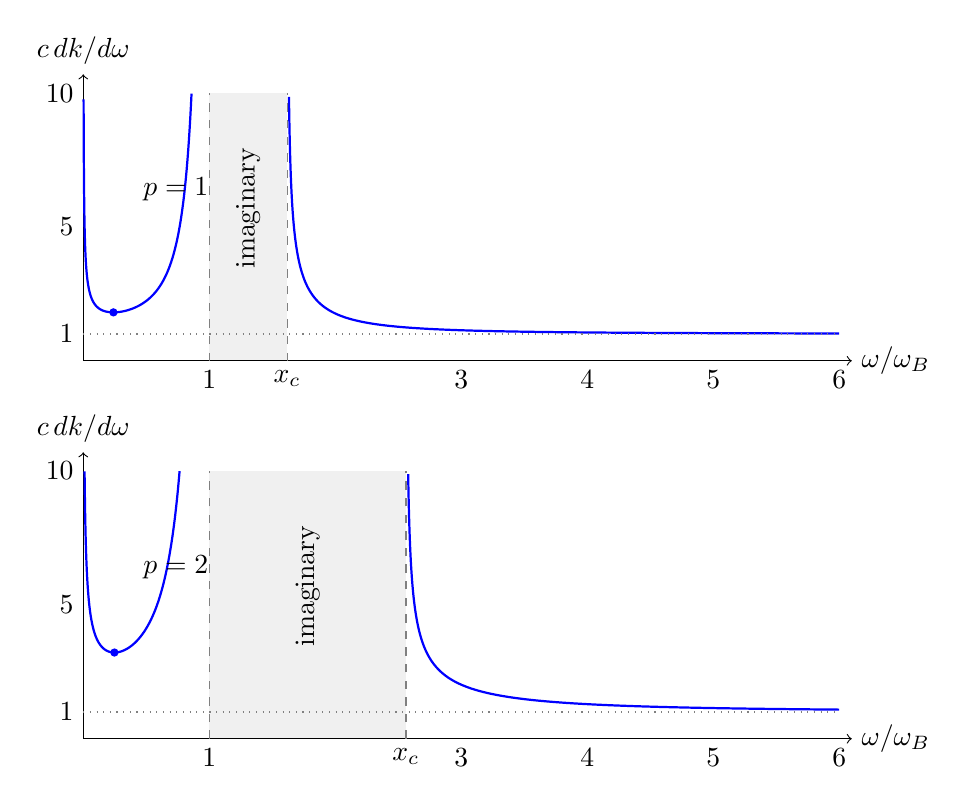
\begin{tikzpicture}[x=1.6cm,y=.34cm]
\begin{scope}[yshift=0.0cm]
\fill[gray!12] (1,0) rectangle (1.618033988749895,10);
\draw[->] (0,0)--(6.1,0) node[right] {$\omega/\omega_B$};\draw[->] (0,0)--(0,10.7) node[above] {$c\,dk/d\omega$};
\draw[blue,thick] plot coordinates {(0.002663,9.765927) (0.003218,8.899473) (0.003772,8.233009) (0.004327,7.700063) (0.004881,7.261465) (0.005436,6.892441) (0.005990,6.576456) (0.006544,6.301995) (0.007099,6.060762) (0.007653,5.846608) (0.008208,5.654865) (0.008762,5.481918) (0.009317,5.324918) (0.009871,5.181584) (0.010426,5.050068) (0.010980,4.928853) (0.011534,4.816680) (0.012089,4.712495) (0.012643,4.615409) (0.013198,4.524665) (0.013752,4.439613) (0.014307,4.359694) (0.014861,4.284422) (0.015416,4.213372) (0.015970,4.146173) (0.016524,4.082497) (0.017079,4.022054) (0.017633,3.964586) (0.018188,3.909863) (0.018742,3.857679) (0.019297,3.807849) (0.019851,3.760206) (0.020406,3.714600) (0.020960,3.670893) (0.021514,3.628963) (0.022069,3.588695) (0.022623,3.549986) (0.023178,3.512741) (0.023732,3.476874) (0.024287,3.442306) (0.024841,3.408961) (0.025396,3.376773) (0.025950,3.345679) (0.026504,3.315621) (0.027059,3.286545) (0.027613,3.258401) (0.028168,3.231141) (0.028722,3.204724) (0.029277,3.179108) (0.029831,3.154256) (0.030386,3.130132) (0.030940,3.106703) (0.031494,3.083938) (0.032049,3.061808) (0.032603,3.040285) (0.033158,3.019343) (0.033712,2.998959) (0.034267,2.979109) (0.034821,2.959772) (0.035376,2.940927) (0.035930,2.922554) (0.036484,2.904637) (0.037039,2.887157) (0.037593,2.870097) (0.038148,2.853443) (0.038702,2.837180) (0.039257,2.821293) (0.039811,2.805769) (0.040366,2.790596) (0.040920,2.775761) (0.041474,2.761253) (0.042029,2.747061) (0.042583,2.733175) (0.043138,2.719583) (0.043692,2.706278) (0.044247,2.693249) (0.044801,2.680489) (0.045356,2.667988) (0.045910,2.655738) (0.046464,2.643733) (0.047019,2.631964) (0.047573,2.620425) (0.048128,2.609109) (0.048682,2.598009) (0.049237,2.587120) (0.049791,2.576434) (0.050346,2.565947) (0.050900,2.555653) (0.051454,2.545547) (0.052009,2.535624) (0.052563,2.525878) (0.053118,2.516304) (0.053672,2.506900) (0.054227,2.497659) (0.054781,2.488578) (0.055336,2.479652) (0.055890,2.470878) (0.056444,2.462253) (0.056999,2.453771) (0.057553,2.445430) (0.058108,2.437226) (0.058662,2.429156) (0.059217,2.421217) (0.059771,2.413405) (0.060326,2.405718) (0.060880,2.398153) (0.061434,2.390706) (0.061989,2.383376) (0.062543,2.376159) (0.063098,2.369054) (0.063652,2.362056) (0.064207,2.355165) (0.064761,2.348378) (0.065316,2.341692) (0.065870,2.335106) (0.066424,2.328617) (0.066979,2.322223) (0.067533,2.315922) (0.068088,2.309713) (0.068642,2.303593) (0.069197,2.297560) (0.069751,2.291613) (0.070306,2.285750) (0.070860,2.279970) (0.071414,2.274270) (0.071969,2.268649) (0.072523,2.263106) (0.073078,2.257639) (0.073632,2.252246) (0.074187,2.246927) (0.074741,2.241679) (0.075296,2.236502) (0.075850,2.231394) (0.076404,2.226354) (0.076959,2.221380) (0.077513,2.216471) (0.078068,2.211627) (0.078622,2.206846) (0.079177,2.202127) (0.079731,2.197468) (0.080286,2.192869) (0.080840,2.188329) (0.081394,2.183846) (0.081949,2.179420) (0.082503,2.175050) (0.083058,2.170734) (0.083612,2.166472) (0.084167,2.162263) (0.084721,2.158106) (0.085276,2.154001) (0.085830,2.149945) (0.086384,2.145939) (0.086939,2.141981) (0.087493,2.138072) (0.088048,2.134209) (0.088602,2.130393) (0.089157,2.126622) (0.089711,2.122896) (0.090266,2.119215) (0.090820,2.115577) (0.091374,2.111981) (0.091929,2.108428) (0.092483,2.104916) (0.093038,2.101446) (0.093592,2.098015) (0.094147,2.094624) (0.094701,2.091272) (0.095256,2.087959) (0.095810,2.084683) (0.096364,2.081445) (0.096919,2.078244) (0.097473,2.075079) (0.098028,2.071950) (0.098582,2.068855) (0.099137,2.065796) (0.099691,2.062771) (0.100246,2.059780) (0.100800,2.056821) (0.101354,2.053896) (0.101909,2.051003) (0.102463,2.048142) (0.103018,2.045313) (0.103572,2.042514) (0.104127,2.039746) (0.104681,2.037009) (0.105236,2.034301) (0.105790,2.031623) (0.106344,2.028973) (0.106899,2.026353) (0.107453,2.023760) (0.108008,2.021195) (0.108562,2.018658) (0.109117,2.016149) (0.109671,2.013666) (0.110226,2.011209) (0.110780,2.008779) (0.111334,2.006374) (0.111889,2.003995) (0.112443,2.001641) (0.112998,1.999312) (0.113552,1.997008) (0.114107,1.994727) (0.114661,1.992471) (0.115216,1.990239) (0.115770,1.988029) (0.116324,1.985843) (0.116879,1.983680) (0.117433,1.981539) (0.117988,1.979421) (0.118542,1.977324) (0.119097,1.975250) (0.119651,1.973197) (0.120206,1.971165) (0.120760,1.969154) (0.121314,1.967164) (0.121869,1.965194) (0.122423,1.963245) (0.122978,1.961316) (0.123532,1.959406) (0.124087,1.957516) (0.124641,1.955646) (0.125196,1.953795) (0.125750,1.951963) (0.126304,1.950149) (0.126859,1.948354) (0.127413,1.946578) (0.127968,1.944820) (0.128522,1.943079) (0.129077,1.941356) (0.129631,1.939651) (0.130186,1.937964) (0.130740,1.936293) (0.131294,1.934640) (0.131849,1.933003) (0.132403,1.931383) (0.132958,1.929780) (0.133512,1.928193) (0.134067,1.926622) (0.134621,1.925067) (0.135176,1.923528) (0.135730,1.922004) (0.136284,1.920496) (0.136839,1.919004) (0.137393,1.917526) (0.137948,1.916064) (0.138502,1.914617) (0.139057,1.913184) (0.139611,1.911766) (0.140166,1.910362) (0.140720,1.908973) (0.141274,1.907598) (0.141829,1.906237) (0.142383,1.904890) (0.142938,1.903557) (0.143492,1.902237) (0.144047,1.900931) (0.144601,1.899638) (0.145156,1.898359) (0.145710,1.897093) (0.146264,1.895839) (0.146819,1.894599) (0.147373,1.893372) (0.147928,1.892157) (0.148482,1.890954) (0.149037,1.889765) (0.149591,1.888587) (0.150146,1.887422) (0.150700,1.886269) (0.151254,1.885127) (0.151809,1.883998) (0.152363,1.882881) (0.152918,1.881775) (0.153472,1.880681) (0.154027,1.879598) (0.154581,1.878527) (0.155136,1.877467) (0.155690,1.876418) (0.156244,1.875380) (0.156799,1.874353) (0.157353,1.873338) (0.157908,1.872333) (0.158462,1.871338) (0.159017,1.870355) (0.159571,1.869382) (0.160126,1.868419) (0.160680,1.867467) (0.161234,1.866525) (0.161789,1.865593) (0.162343,1.864672) (0.162898,1.863760) (0.163452,1.862859) (0.164007,1.861967) (0.164561,1.861085) (0.165116,1.860213) (0.165670,1.859351) (0.166224,1.858498) (0.166779,1.857655) (0.167333,1.856821) (0.167888,1.855996) (0.168442,1.855181) (0.168997,1.854375) (0.169551,1.853578) (0.170106,1.852790) (0.170660,1.852011) (0.171214,1.851242) (0.171769,1.850481) (0.172323,1.849728) (0.172878,1.848985) (0.173432,1.848250) (0.173987,1.847524) (0.174541,1.846807) (0.175096,1.846098) (0.175650,1.845397) (0.176204,1.844705) (0.176759,1.844021) (0.177313,1.843345) (0.177868,1.842678) (0.178422,1.842018) (0.178977,1.841367) (0.179531,1.840724) (0.180086,1.840088) (0.180640,1.839461) (0.181194,1.838841) (0.181749,1.838230) (0.182303,1.837626) (0.182858,1.837029) (0.183412,1.836441) (0.183967,1.835860) (0.184521,1.835286) (0.185076,1.834720) (0.185630,1.834162) (0.186184,1.833611) (0.186739,1.833067) (0.187293,1.832530) (0.187848,1.832001) (0.188402,1.831479) (0.188957,1.830964) (0.189511,1.830457) (0.190066,1.829956) (0.190620,1.829462) (0.191174,1.828976) (0.191729,1.828496) (0.192283,1.828023) (0.192838,1.827557) (0.193392,1.827098) (0.193947,1.826645) (0.194501,1.826200) (0.195056,1.825761) (0.195610,1.825329) (0.196164,1.824903) (0.196719,1.824484) (0.197273,1.824071) (0.197828,1.823665) (0.198382,1.823265) (0.198937,1.822872) (0.199491,1.822485) (0.200046,1.822104) (0.200600,1.821730) (0.201154,1.821362) (0.201709,1.821001) (0.202263,1.820645) (0.202818,1.820296) (0.203372,1.819952) (0.203927,1.819615) (0.204481,1.819284) (0.205036,1.818959) (0.205590,1.818640) (0.206144,1.818327) (0.206699,1.818020) (0.207253,1.817718) (0.207808,1.817423) (0.208362,1.817133) (0.208917,1.816850) (0.209471,1.816572) (0.210026,1.816299) (0.210580,1.816033) (0.211134,1.815772) (0.211689,1.815517) (0.212243,1.815267) (0.212798,1.815023) (0.213352,1.814785) (0.213907,1.814552) (0.214461,1.814325) (0.215016,1.814103) (0.215570,1.813886) (0.216124,1.813676) (0.216679,1.813470) (0.217233,1.813270) (0.217788,1.813075) (0.218342,1.812886) (0.218897,1.812701) (0.219451,1.812522) (0.220006,1.812349) (0.220560,1.812180) (0.221114,1.812017) (0.221669,1.811859) (0.222223,1.811706) (0.222778,1.811559) (0.223332,1.811416) (0.223887,1.811278) (0.224441,1.811146) (0.224996,1.811019) (0.225550,1.810896) (0.226104,1.810779) (0.226659,1.810666) (0.227213,1.810559) (0.227768,1.810457) (0.228322,1.810359) (0.228877,1.810266) (0.229431,1.810178) (0.229986,1.810095) (0.230540,1.810017) (0.231094,1.809944) (0.231649,1.809875) (0.232203,1.809812) (0.232758,1.809753) (0.233312,1.809698) (0.233867,1.809649) (0.234421,1.809604) (0.234976,1.809564) (0.235530,1.809528) (0.236084,1.809497) (0.236639,1.809471) (0.237193,1.809450) (0.237748,1.809433) (0.238302,1.809420) (0.238857,1.809412) (0.239411,1.809409) (0.239966,1.809410) (0.240520,1.809416) (0.241074,1.809426) (0.241629,1.809440) (0.242183,1.809459) (0.242738,1.809483) (0.243292,1.809511) (0.243847,1.809543) (0.244401,1.809580) (0.244956,1.809621) (0.245510,1.809667) (0.246064,1.809717) (0.246619,1.809771) (0.247173,1.809829) (0.247728,1.809892) (0.248282,1.809959) (0.248837,1.810031) (0.249391,1.810106) (0.249946,1.810186) (0.250500,1.810270) (0.251054,1.810359) (0.251609,1.810451) (0.252163,1.810548) (0.252718,1.810649) (0.253272,1.810754) (0.253827,1.810864) (0.254381,1.810977) (0.254936,1.811095) (0.255490,1.811216) (0.256044,1.811342) (0.256599,1.811472) (0.257153,1.811606) (0.257708,1.811744) (0.258262,1.811886) (0.258817,1.812033) (0.259371,1.812183) (0.259926,1.812337) (0.260480,1.812496) (0.261034,1.812658) (0.261589,1.812824) (0.262143,1.812995) (0.262698,1.813169) (0.263252,1.813347) (0.263807,1.813530) (0.264361,1.813716) (0.264916,1.813906) (0.265470,1.814100) (0.266024,1.814298) (0.266579,1.814500) (0.267133,1.814706) (0.267688,1.814915) (0.268242,1.815129) (0.268797,1.815346) (0.269351,1.815568) (0.269906,1.815793) (0.270460,1.816022) (0.271014,1.816255) (0.271569,1.816491) (0.272123,1.816732) (0.272678,1.816976) (0.273232,1.817224) (0.273787,1.817476) (0.274341,1.817732) (0.274896,1.817992) (0.275450,1.818255) (0.276004,1.818522) (0.276559,1.818793) (0.277113,1.819067) (0.277668,1.819346) (0.278222,1.819628) (0.278777,1.819913) (0.279331,1.820203) (0.279886,1.820496) (0.280440,1.820793) (0.280994,1.821094) (0.281549,1.821398) (0.282103,1.821706) (0.282658,1.822018) (0.283212,1.822333) (0.283767,1.822652) (0.284321,1.822975) (0.284876,1.823301) (0.285430,1.823631) (0.285984,1.823965) (0.286539,1.824303) (0.287093,1.824644) (0.287648,1.824988) (0.288202,1.825336) (0.288757,1.825688) (0.289311,1.826044) (0.289866,1.826403) (0.290420,1.826765) (0.290974,1.827132) (0.291529,1.827502) (0.292083,1.827875) (0.292638,1.828252) (0.293192,1.828633) (0.293747,1.829017) (0.294301,1.829405) (0.294856,1.829796) (0.295410,1.830191) (0.295964,1.830590) (0.296519,1.830992) (0.297073,1.831397) (0.297628,1.831807) (0.298182,1.832219) (0.298737,1.832635) (0.299291,1.833055) (0.299846,1.833479) (0.300400,1.833905) (0.300954,1.834336) (0.301509,1.834770) (0.302063,1.835207) (0.302618,1.835648) (0.303172,1.836092) (0.303727,1.836540) (0.304281,1.836992) (0.304836,1.837447) (0.305390,1.837905) (0.305944,1.838367) (0.306499,1.838833) (0.307053,1.839302) (0.307608,1.839774) (0.308162,1.840250) (0.308717,1.840730) (0.309271,1.841212) (0.309826,1.841699) (0.310380,1.842189) (0.310934,1.842682) (0.311489,1.843179) (0.312043,1.843679) (0.312598,1.844183) (0.313152,1.844690) (0.313707,1.845201) (0.314261,1.845715) (0.314816,1.846233) (0.315370,1.846754) (0.315924,1.847278) (0.316479,1.847807) (0.317033,1.848338) (0.317588,1.848873) (0.318142,1.849411) (0.318697,1.849953) (0.319251,1.850499) (0.319806,1.851047) (0.320360,1.851600) (0.320914,1.852155) (0.321469,1.852714) (0.322023,1.853277) (0.322578,1.853843) (0.323132,1.854413) (0.323687,1.854986) (0.324241,1.855562) (0.324796,1.856142) (0.325350,1.856725) (0.325904,1.857312) (0.326459,1.857902) (0.327013,1.858496) (0.327568,1.859093) (0.328122,1.859693) (0.328677,1.860297) (0.329231,1.860905) (0.329786,1.861516) (0.330340,1.862130) (0.330894,1.862748) (0.331449,1.863369) (0.332003,1.863994) (0.332558,1.864622) (0.333112,1.865253) (0.333667,1.865888) (0.334221,1.866527) (0.334776,1.867169) (0.335330,1.867814) (0.335884,1.868463) (0.336439,1.869116) (0.336993,1.869771) (0.337548,1.870431) (0.338102,1.871093) (0.338657,1.871759) (0.339211,1.872429) (0.339766,1.873102) (0.340320,1.873779) (0.340874,1.874459) (0.341429,1.875142) (0.341983,1.875829) (0.342538,1.876520) (0.343092,1.877213) (0.343647,1.877911) (0.344201,1.878612) (0.344756,1.879316) (0.345310,1.880024) (0.345864,1.880735) (0.346419,1.881450) (0.346973,1.882168) (0.347528,1.882890) (0.348082,1.883615) (0.348637,1.884344) (0.349191,1.885076) (0.349746,1.885812) (0.350300,1.886551) (0.350854,1.887294) (0.351409,1.888040) (0.351963,1.888790) (0.352518,1.889543) (0.353072,1.890300) (0.353627,1.891060) (0.354181,1.891824) (0.354736,1.892592) (0.355290,1.893362) (0.355844,1.894137) (0.356399,1.894915) (0.356953,1.895696) (0.357508,1.896481) (0.358062,1.897270) (0.358617,1.898062) (0.359171,1.898858) (0.359726,1.899657) (0.360280,1.900460) (0.360834,1.901266) (0.361389,1.902076) (0.361943,1.902889) (0.362498,1.903706) (0.363052,1.904527) (0.363607,1.905351) (0.364161,1.906179) (0.364716,1.907010) (0.365270,1.907845) (0.365824,1.908684) (0.366379,1.909526) (0.366933,1.910372) (0.367488,1.911221) (0.368042,1.912074) (0.368597,1.912930) (0.369151,1.913791) (0.369706,1.914654) (0.370260,1.915522) (0.370814,1.916393) (0.371369,1.917268) (0.371923,1.918146) (0.372478,1.919028) (0.373032,1.919914) (0.373587,1.920803) (0.374141,1.921696) (0.374696,1.922593) (0.375250,1.923493) (0.375804,1.924397) (0.376359,1.925305) (0.376913,1.926216) (0.377468,1.927131) (0.378022,1.928050) (0.378577,1.928972) (0.379131,1.929898) (0.379686,1.930828) (0.380240,1.931762) (0.380794,1.932699) (0.381349,1.933640) (0.381903,1.934585) (0.382458,1.935534) (0.383012,1.936486) (0.383567,1.937442) (0.384121,1.938402) (0.384676,1.939366) (0.385230,1.940333) (0.385784,1.941304) (0.386339,1.942279) (0.386893,1.943258) (0.387448,1.944240) (0.388002,1.945227) (0.388557,1.946217) (0.389111,1.947211) (0.389666,1.948208) (0.390220,1.949210) (0.390774,1.950216) (0.391329,1.951225) (0.391883,1.952238) (0.392438,1.953255) (0.392992,1.954276) (0.393547,1.955301) (0.394101,1.956329) (0.394656,1.957362) (0.395210,1.958398) (0.395764,1.959439) (0.396319,1.960483) (0.396873,1.961531) (0.397428,1.962583) (0.397982,1.963639) (0.398537,1.964699) (0.399091,1.965763) (0.399646,1.966831) (0.400200,1.967903) (0.400754,1.968978) (0.401309,1.970058) (0.401863,1.971142) (0.402418,1.972230) (0.402972,1.973321) (0.403527,1.974417) (0.404081,1.975517) (0.404636,1.976621) (0.405190,1.977728) (0.405744,1.978840) (0.406299,1.979956) (0.406853,1.981076) (0.407408,1.982200) (0.407962,1.983328) (0.408517,1.984460) (0.409071,1.985597) (0.409626,1.986737) (0.410180,1.987882) (0.410734,1.989030) (0.411289,1.990183) (0.411843,1.991340) (0.412398,1.992501) (0.412952,1.993666) (0.413507,1.994835) (0.414061,1.996009) (0.414616,1.997187) (0.415170,1.998369) (0.415724,1.999555) (0.416279,2.000745) (0.416833,2.001940) (0.417388,2.003138) (0.417942,2.004341) (0.418497,2.005549) (0.419051,2.006760) (0.419606,2.007976) (0.420160,2.009196) (0.420714,2.010420) (0.421269,2.011649) (0.421823,2.012882) (0.422378,2.014119) (0.422932,2.015361) (0.423487,2.016607) (0.424041,2.017857) (0.424596,2.019112) (0.425150,2.020371) (0.425704,2.021635) (0.426259,2.022903) (0.426813,2.024175) (0.427368,2.025452) (0.427922,2.026733) (0.428477,2.028018) (0.429031,2.029308) (0.429586,2.030603) (0.430140,2.031902) (0.430694,2.033205) (0.431249,2.034513) (0.431803,2.035825) (0.432358,2.037142) (0.432912,2.038464) (0.433467,2.039790) (0.434021,2.041120) (0.434576,2.042456) (0.435130,2.043795) (0.435684,2.045140) (0.436239,2.046488) (0.436793,2.047842) (0.437348,2.049200) (0.437902,2.050563) (0.438457,2.051930) (0.439011,2.053302) (0.439566,2.054679) (0.440120,2.056061) (0.440674,2.057447) (0.441229,2.058838) (0.441783,2.060233) (0.442338,2.061634) (0.442892,2.063039) (0.443447,2.064449) (0.444001,2.065863) (0.444556,2.067283) (0.445110,2.068707) (0.445664,2.070136) (0.446219,2.071570) (0.446773,2.073009) (0.447328,2.074452) (0.447882,2.075901) (0.448437,2.077354) (0.448991,2.078812) (0.449546,2.080275) (0.450100,2.081743) (0.450654,2.083217) (0.451209,2.084695) (0.451763,2.086177) (0.452318,2.087665) (0.452872,2.089158) (0.453427,2.090656) (0.453981,2.092159) (0.454536,2.093667) (0.455090,2.095180) (0.455644,2.096699) (0.456199,2.098222) (0.456753,2.099750) (0.457308,2.101284) (0.457862,2.102822) (0.458417,2.104366) (0.458971,2.105915) (0.459526,2.107469) (0.460080,2.109028) (0.460634,2.110593) (0.461189,2.112162) (0.461743,2.113737) (0.462298,2.115317) (0.462852,2.116903) (0.463407,2.118494) (0.463961,2.120090) (0.464516,2.121691) (0.465070,2.123298) (0.465624,2.124910) (0.466179,2.126527) (0.466733,2.128150) (0.467288,2.129779) (0.467842,2.131412) (0.468397,2.133051) (0.468951,2.134696) (0.469506,2.136346) (0.470060,2.138001) (0.470614,2.139662) (0.471169,2.141329) (0.471723,2.143001) (0.472278,2.144679) (0.472832,2.146362) (0.473387,2.148051) (0.473941,2.149745) (0.474496,2.151445) (0.475050,2.153151) (0.475604,2.154862) (0.476159,2.156579) (0.476713,2.158302) (0.477268,2.160031) (0.477822,2.161765) (0.478377,2.163505) (0.478931,2.165251) (0.479486,2.167002) (0.480040,2.168760) (0.480594,2.170523) (0.481149,2.172292) (0.481703,2.174067) (0.482258,2.175848) (0.482812,2.177634) (0.483367,2.179427) (0.483921,2.181226) (0.484476,2.183030) (0.485030,2.184841) (0.485584,2.186658) (0.486139,2.188480) (0.486693,2.190309) (0.487248,2.192144) (0.487802,2.193984) (0.488357,2.195831) (0.488911,2.197685) (0.489466,2.199544) (0.490020,2.201409) (0.490574,2.203281) (0.491129,2.205159) (0.491683,2.207043) (0.492238,2.208933) (0.492792,2.210830) (0.493347,2.212733) (0.493901,2.214642) (0.494456,2.216558) (0.495010,2.218480) (0.495564,2.220408) (0.496119,2.222343) (0.496673,2.224284) (0.497228,2.226232) (0.497782,2.228186) (0.498337,2.230147) (0.498891,2.232114) (0.499446,2.234088) (0.500000,2.236068) (0.500554,2.238055) (0.501109,2.240048) (0.501663,2.242049) (0.502218,2.244056) (0.502772,2.246069) (0.503327,2.248089) (0.503881,2.250116) (0.504436,2.252150) (0.504990,2.254191) (0.505544,2.256238) (0.506099,2.258293) (0.506653,2.260354) (0.507208,2.262422) (0.507762,2.264497) (0.508317,2.266578) (0.508871,2.268667) (0.509426,2.270763) (0.509980,2.272866) (0.510534,2.274976) (0.511089,2.277093) (0.511643,2.279217) (0.512198,2.281348) (0.512752,2.283486) (0.513307,2.285632) (0.513861,2.287784) (0.514416,2.289944) (0.514970,2.292111) (0.515524,2.294286) (0.516079,2.296468) (0.516633,2.298657) (0.517188,2.300853) (0.517742,2.303057) (0.518297,2.305268) (0.518851,2.307487) (0.519406,2.309713) (0.519960,2.311947) (0.520514,2.314188) (0.521069,2.316437) (0.521623,2.318693) (0.522178,2.320957) (0.522732,2.323229) (0.523287,2.325508) (0.523841,2.327795) (0.524396,2.330090) (0.524950,2.332392) (0.525504,2.334703) (0.526059,2.337021) (0.526613,2.339347) (0.527168,2.341681) (0.527722,2.344022) (0.528277,2.346372) (0.528831,2.348730) (0.529386,2.351096) (0.529940,2.353469) (0.530494,2.355851) (0.531049,2.358241) (0.531603,2.360639) (0.532158,2.363046) (0.532712,2.365460) (0.533267,2.367883) (0.533821,2.370314) (0.534376,2.372753) (0.534930,2.375201) (0.535484,2.377657) (0.536039,2.380121) (0.536593,2.382594) (0.537148,2.385075) (0.537702,2.387565) (0.538257,2.390063) (0.538811,2.392570) (0.539366,2.395085) (0.539920,2.397610) (0.540474,2.400142) (0.541029,2.402684) (0.541583,2.405234) (0.542138,2.407793) (0.542692,2.410361) (0.543247,2.412938) (0.543801,2.415523) (0.544356,2.418118) (0.544910,2.420721) (0.545464,2.423334) (0.546019,2.425955) (0.546573,2.428586) (0.547128,2.431226) (0.547682,2.433874) (0.548237,2.436532) (0.548791,2.439200) (0.549346,2.441876) (0.549900,2.444562) (0.550454,2.447257) (0.551009,2.449962) (0.551563,2.452676) (0.552118,2.455399) (0.552672,2.458132) (0.553227,2.460874) (0.553781,2.463626) (0.554336,2.466388) (0.554890,2.469159) (0.555444,2.471940) (0.555999,2.474731) (0.556553,2.477532) (0.557108,2.480342) (0.557662,2.483162) (0.558217,2.485992) (0.558771,2.488832) (0.559326,2.491682) (0.559880,2.494542) (0.560434,2.497413) (0.560989,2.500293) (0.561543,2.503183) (0.562098,2.506084) (0.562652,2.508995) (0.563207,2.511916) (0.563761,2.514848) (0.564316,2.517790) (0.564870,2.520742) (0.565424,2.523705) (0.565979,2.526678) (0.566533,2.529662) (0.567088,2.532657) (0.567642,2.535662) (0.568197,2.538678) (0.568751,2.541705) (0.569306,2.544742) (0.569860,2.547790) (0.570414,2.550850) (0.570969,2.553920) (0.571523,2.557001) (0.572078,2.560093) (0.572632,2.563197) (0.573187,2.566311) (0.573741,2.569437) (0.574296,2.572574) (0.574850,2.575722) (0.575404,2.578881) (0.575959,2.582052) (0.576513,2.585235) (0.577068,2.588428) (0.577622,2.591634) (0.578177,2.594851) (0.578731,2.598080) (0.579286,2.601320) (0.579840,2.604572) (0.580394,2.607836) (0.580949,2.611112) (0.581503,2.614400) (0.582058,2.617700) (0.582612,2.621011) (0.583167,2.624335) (0.583721,2.627671) (0.584276,2.631019) (0.584830,2.634380) (0.585384,2.637753) (0.585939,2.641138) (0.586493,2.644535) (0.587048,2.647945) (0.587602,2.651368) (0.588157,2.654803) (0.588711,2.658251) (0.589266,2.661711) (0.589820,2.665185) (0.590374,2.668671) (0.590929,2.672170) (0.591483,2.675682) (0.592038,2.679207) (0.592592,2.682745) (0.593147,2.686296) (0.593701,2.689861) (0.594256,2.693439) (0.594810,2.697030) (0.595364,2.700634) (0.595919,2.704252) (0.596473,2.707883) (0.597028,2.711528) (0.597582,2.715187) (0.598137,2.718859) (0.598691,2.722546) (0.599246,2.726246) (0.599800,2.729959) (0.600354,2.733687) (0.600909,2.737429) (0.601463,2.741185) (0.602018,2.744955) (0.602572,2.748740) (0.603127,2.752539) (0.603681,2.756352) (0.604236,2.760180) (0.604790,2.764022) (0.605344,2.767878) (0.605899,2.771750) (0.606453,2.775636) (0.607008,2.779537) (0.607562,2.783453) (0.608117,2.787384) (0.608671,2.791330) (0.609226,2.795291) (0.609780,2.799267) (0.610334,2.803258) (0.610889,2.807265) (0.611443,2.811287) (0.611998,2.815325) (0.612552,2.819378) (0.613107,2.823447) (0.613661,2.827532) (0.614216,2.831632) (0.614770,2.835748) (0.615324,2.839881) (0.615879,2.844029) (0.616433,2.848193) (0.616988,2.852374) (0.617542,2.856571) (0.618097,2.860784) (0.618651,2.865014) (0.619206,2.869260) (0.619760,2.873523) (0.620314,2.877803) (0.620869,2.882099) (0.621423,2.886412) (0.621978,2.890742) (0.622532,2.895090) (0.623087,2.899454) (0.623641,2.903835) (0.624196,2.908234) (0.624750,2.912651) (0.625304,2.917084) (0.625859,2.921536) (0.626413,2.926005) (0.626968,2.930492) (0.627522,2.934996) (0.628077,2.939519) (0.628631,2.944060) (0.629186,2.948618) (0.629740,2.953195) (0.630294,2.957791) (0.630849,2.962404) (0.631403,2.967037) (0.631958,2.971688) (0.632512,2.976357) (0.633067,2.981046) (0.633621,2.985753) (0.634176,2.990479) (0.634730,2.995225) (0.635284,2.999990) (0.635839,3.004774) (0.636393,3.009577) (0.636948,3.014400) (0.637502,3.019243) (0.638057,3.024105) (0.638611,3.028987) (0.639166,3.033889) (0.639720,3.038811) (0.640274,3.043754) (0.640829,3.048716) (0.641383,3.053699) (0.641938,3.058703) (0.642492,3.063727) (0.643047,3.068772) (0.643601,3.073837) (0.644156,3.078924) (0.644710,3.084032) (0.645264,3.089160) (0.645819,3.094311) (0.646373,3.099482) (0.646928,3.104675) (0.647482,3.109890) (0.648037,3.115126) (0.648591,3.120385) (0.649146,3.125665) (0.649700,3.130967) (0.650254,3.136292) (0.650809,3.141639) (0.651363,3.147009) (0.651918,3.152401) (0.652472,3.157816) (0.653027,3.163254) (0.653581,3.168715) (0.654136,3.174199) (0.654690,3.179706) (0.655244,3.185237) (0.655799,3.190791) (0.656353,3.196369) (0.656908,3.201970) (0.657462,3.207596) (0.658017,3.213246) (0.658571,3.218919) (0.659126,3.224618) (0.659680,3.230340) (0.660234,3.236088) (0.660789,3.241860) (0.661343,3.247657) (0.661898,3.253479) (0.662452,3.259326) (0.663007,3.265199) (0.663561,3.271097) (0.664116,3.277020) (0.664670,3.282970) (0.665224,3.288945) (0.665779,3.294947) (0.666333,3.300975) (0.666888,3.307029) (0.667442,3.313109) (0.667997,3.319217) (0.668551,3.325351) (0.669106,3.331512) (0.669660,3.337701) (0.670214,3.343916) (0.670769,3.350160) (0.671323,3.356431) (0.671878,3.362729) (0.672432,3.369056) (0.672987,3.375411) (0.673541,3.381794) (0.674096,3.388206) (0.674650,3.394647) (0.675204,3.401116) (0.675759,3.407614) (0.676313,3.414141) (0.676868,3.420698) (0.677422,3.427285) (0.677977,3.433901) (0.678531,3.440547) (0.679086,3.447223) (0.679640,3.453929) (0.680194,3.460666) (0.680749,3.467433) (0.681303,3.474231) (0.681858,3.481061) (0.682412,3.487921) (0.682967,3.494813) (0.683521,3.501736) (0.684076,3.508692) (0.684630,3.515679) (0.685184,3.522698) (0.685739,3.529750) (0.686293,3.536834) (0.686848,3.543951) (0.687402,3.551101) (0.687957,3.558285) (0.688511,3.565501) (0.689066,3.572752) (0.689620,3.580036) (0.690174,3.587354) (0.690729,3.594706) (0.691283,3.602093) (0.691838,3.609514) (0.692392,3.616971) (0.692947,3.624462) (0.693501,3.631989) (0.694056,3.639552) (0.694610,3.647150) (0.695164,3.654784) (0.695719,3.662455) (0.696273,3.670162) (0.696828,3.677906) (0.697382,3.685687) (0.697937,3.693504) (0.698491,3.701360) (0.699046,3.709253) (0.699600,3.717184) (0.700154,3.725153) (0.700709,3.733161) (0.701263,3.741207) (0.701818,3.749292) (0.702372,3.757417) (0.702927,3.765581) (0.703481,3.773784) (0.704036,3.782028) (0.704590,3.790312) (0.705144,3.798636) (0.705699,3.807001) (0.706253,3.815407) (0.706808,3.823854) (0.707362,3.832343) (0.707917,3.840874) (0.708471,3.849447) (0.709026,3.858063) (0.709580,3.866721) (0.710134,3.875422) (0.710689,3.884166) (0.711243,3.892954) (0.711798,3.901786) (0.712352,3.910662) (0.712907,3.919583) (0.713461,3.928548) (0.714016,3.937558) (0.714570,3.946614) (0.715124,3.955716) (0.715679,3.964863) (0.716233,3.974057) (0.716788,3.983297) (0.717342,3.992585) (0.717897,4.001920) (0.718451,4.011302) (0.719006,4.020732) (0.719560,4.030211) (0.720114,4.039738) (0.720669,4.049315) (0.721223,4.058940) (0.721778,4.068615) (0.722332,4.078341) (0.722887,4.088116) (0.723441,4.097942) (0.723996,4.107820) (0.724550,4.117749) (0.725104,4.127729) (0.725659,4.137762) (0.726213,4.147847) (0.726768,4.157986) (0.727322,4.168177) (0.727877,4.178422) (0.728431,4.188722) (0.728986,4.199076) (0.729540,4.209484) (0.730094,4.219948) (0.730649,4.230468) (0.731203,4.241043) (0.731758,4.251675) (0.732312,4.262364) (0.732867,4.273110) (0.733421,4.283914) (0.733976,4.294776) (0.734530,4.305697) (0.735084,4.316676) (0.735639,4.327715) (0.736193,4.338814) (0.736748,4.349973) (0.737302,4.361193) (0.737857,4.372474) (0.738411,4.383817) (0.738966,4.395222) (0.739520,4.406690) (0.740074,4.418220) (0.740629,4.429814) (0.741183,4.441472) (0.741738,4.453195) (0.742292,4.464983) (0.742847,4.476836) (0.743401,4.488755) (0.743956,4.500740) (0.744510,4.512793) (0.745064,4.524913) (0.745619,4.537101) (0.746173,4.549358) (0.746728,4.561683) (0.747282,4.574079) (0.747837,4.586544) (0.748391,4.599080) (0.748946,4.611688) (0.749500,4.624367) (0.750054,4.637119) (0.750609,4.649943) (0.751163,4.662841) (0.751718,4.675813) (0.752272,4.688860) (0.752827,4.701982) (0.753381,4.715180) (0.753936,4.728454) (0.754490,4.741805) (0.755044,4.755234) (0.755599,4.768742) (0.756153,4.782328) (0.756708,4.795994) (0.757262,4.809739) (0.757817,4.823566) (0.758371,4.837475) (0.758926,4.851465) (0.759480,4.865538) (0.760034,4.879695) (0.760589,4.893936) (0.761143,4.908261) (0.761698,4.922673) (0.762252,4.937170) (0.762807,4.951755) (0.763361,4.966427) (0.763916,4.981188) (0.764470,4.996037) (0.765024,5.010977) (0.765579,5.026007) (0.766133,5.041129) (0.766688,5.056343) (0.767242,5.071649) (0.767797,5.087050) (0.768351,5.102545) (0.768906,5.118135) (0.769460,5.133821) (0.770014,5.149604) (0.770569,5.165485) (0.771123,5.181465) (0.771678,5.197544) (0.772232,5.213723) (0.772787,5.230003) (0.773341,5.246386) (0.773896,5.262871) (0.774450,5.279460) (0.775004,5.296153) (0.775559,5.312953) (0.776113,5.329858) (0.776668,5.346871) (0.777222,5.363993) (0.777777,5.381224) (0.778331,5.398565) (0.778886,5.416017) (0.779440,5.433582) (0.779994,5.451260) (0.780549,5.469052) (0.781103,5.486959) (0.781658,5.504983) (0.782212,5.523124) (0.782767,5.541383) (0.783321,5.559762) (0.783876,5.578261) (0.784430,5.596882) (0.784984,5.615626) (0.785539,5.634494) (0.786093,5.653486) (0.786648,5.672605) (0.787202,5.691851) (0.787757,5.711225) (0.788311,5.730729) (0.788866,5.750364) (0.789420,5.770131) (0.789974,5.790031) (0.790529,5.810066) (0.791083,5.830236) (0.791638,5.850544) (0.792192,5.870989) (0.792747,5.891575) (0.793301,5.912301) (0.793856,5.933170) (0.794410,5.954182) (0.794964,5.975339) (0.795519,5.996642) (0.796073,6.018094) (0.796628,6.039694) (0.797182,6.061445) (0.797737,6.083349) (0.798291,6.105405) (0.798846,6.127617) (0.799400,6.149986) (0.799954,6.172512) (0.800509,6.195198) (0.801063,6.218045) (0.801618,6.241055) (0.802172,6.264230) (0.802727,6.287570) (0.803281,6.311078) (0.803836,6.334755) (0.804390,6.358603) (0.804944,6.382624) (0.805499,6.406820) (0.806053,6.431191) (0.806608,6.455741) (0.807162,6.480470) (0.807717,6.505381) (0.808271,6.530476) (0.808826,6.555755) (0.809380,6.581222) (0.809934,6.606878) (0.810489,6.632725) (0.811043,6.658765) (0.811598,6.685000) (0.812152,6.711433) (0.812707,6.738064) (0.813261,6.764897) (0.813816,6.791932) (0.814370,6.819174) (0.814924,6.846622) (0.815479,6.874281) (0.816033,6.902152) (0.816588,6.930237) (0.817142,6.958538) (0.817697,6.987058) (0.818251,7.015800) (0.818806,7.044765) (0.819360,7.073956) (0.819914,7.103376) (0.820469,7.133026) (0.821023,7.162910) (0.821578,7.193030) (0.822132,7.223389) (0.822687,7.253989) (0.823241,7.284832) (0.823796,7.315923) (0.824350,7.347262) (0.824904,7.378854) (0.825459,7.410700) (0.826013,7.442805) (0.826568,7.475170) (0.827122,7.507798) (0.827677,7.540693) (0.828231,7.573858) (0.828786,7.607295) (0.829340,7.641008) (0.829894,7.675000) (0.830449,7.709274) (0.831003,7.743834) (0.831558,7.778682) (0.832112,7.813822) (0.832667,7.849258) (0.833221,7.884993) (0.833776,7.921030) (0.834330,7.957373) (0.834884,7.994025) (0.835439,8.030991) (0.835993,8.068274) (0.836548,8.105877) (0.837102,8.143805) (0.837657,8.182062) (0.838211,8.220651) (0.838766,8.259576) (0.839320,8.298842) (0.839874,8.338453) (0.840429,8.378412) (0.840983,8.418725) (0.841538,8.459395) (0.842092,8.500427) (0.842647,8.541825) (0.843201,8.583594) (0.843756,8.625739) (0.844310,8.668264) (0.844864,8.711174) (0.845419,8.754474) (0.845973,8.798169) (0.846528,8.842264) (0.847082,8.886763) (0.847637,8.931673) (0.848191,8.976998) (0.848746,9.022743) (0.849300,9.068915) (0.849854,9.115518) (0.850409,9.162559) (0.850963,9.210043) (0.851518,9.257975) (0.852072,9.306363) (0.852627,9.355211) (0.853181,9.404526) (0.853736,9.454313) (0.854290,9.504581) (0.854844,9.555334) (0.855399,9.606579) (0.855953,9.658324) (0.856508,9.710574) (0.857062,9.763337) (0.857617,9.816619) (0.858171,9.870429) (0.858726,9.924772) (0.859280,9.979657)};
\draw[blue,thick] plot coordinates {(1.632740,9.859928) (1.635175,9.116173) (1.637609,8.515057) (1.640043,8.016014) (1.642478,7.593002) (1.644912,7.228431) (1.647346,6.909939) (1.649781,6.628543) (1.652215,6.377540) (1.654650,6.151814) (1.657084,5.947379) (1.659518,5.761081) (1.661953,5.590384) (1.664387,5.433224) (1.666821,5.287903) (1.669256,5.153005) (1.671690,5.027343) (1.674124,4.909911) (1.676559,4.799851) (1.678993,4.696426) (1.681428,4.598998) (1.683862,4.507013) (1.686296,4.419984) (1.688731,4.337486) (1.691165,4.259142) (1.693599,4.184619) (1.696034,4.113618) (1.698468,4.045875) (1.700903,3.981150) (1.703337,3.919229) (1.705771,3.859919) (1.708206,3.803044) (1.710640,3.748445) (1.713074,3.695977) (1.715509,3.645508) (1.717943,3.596916) (1.720378,3.550091) (1.722812,3.504931) (1.725246,3.461341) (1.727681,3.419236) (1.730115,3.378535) (1.732549,3.339164) (1.734984,3.301055) (1.737418,3.264143) (1.739852,3.228370) (1.742287,3.193680) (1.744721,3.160021) (1.747156,3.127345) (1.749590,3.095607) (1.752024,3.064765) (1.754459,3.034778) (1.756893,3.005611) (1.759327,2.977228) (1.761762,2.949595) (1.764196,2.922683) (1.766631,2.896461) (1.769065,2.870902) (1.771499,2.845980) (1.773934,2.821670) (1.776368,2.797950) (1.778802,2.774796) (1.781237,2.752188) (1.783671,2.730105) (1.786106,2.708530) (1.788540,2.687443) (1.790974,2.666829) (1.793409,2.646670) (1.795843,2.626951) (1.798277,2.607657) (1.800712,2.588775) (1.803146,2.570290) (1.805580,2.552191) (1.808015,2.534463) (1.810449,2.517097) (1.812884,2.500081) (1.815318,2.483403) (1.817752,2.467054) (1.820187,2.451024) (1.822621,2.435303) (1.825055,2.419882) (1.827490,2.404752) (1.829924,2.389906) (1.832359,2.375335) (1.834793,2.361031) (1.837227,2.346988) (1.839662,2.333197) (1.842096,2.319652) (1.844530,2.306346) (1.846965,2.293273) (1.849399,2.280427) (1.851834,2.267802) (1.854268,2.255392) (1.856702,2.243192) (1.859137,2.231196) (1.861571,2.219400) (1.864005,2.207797) (1.866440,2.196384) (1.868874,2.185156) (1.871308,2.174108) (1.873743,2.163237) (1.876177,2.152537) (1.878612,2.142005) (1.881046,2.131637) (1.883480,2.121429) (1.885915,2.111377) (1.888349,2.101479) (1.890783,2.091730) (1.893218,2.082126) (1.895652,2.072666) (1.898087,2.063346) (1.900521,2.054162) (1.902955,2.045111) (1.905390,2.036192) (1.907824,2.027400) (1.910258,2.018734) (1.912693,2.010191) (1.915127,2.001767) (1.917561,1.993462) (1.919996,1.985271) (1.922430,1.977194) (1.924865,1.969227) (1.927299,1.961368) (1.929733,1.953615) (1.932168,1.945967) (1.934602,1.938421) (1.937036,1.930975) (1.939471,1.923627) (1.941905,1.916375) (1.944340,1.909217) (1.946774,1.902152) (1.949208,1.895179) (1.951643,1.888294) (1.954077,1.881496) (1.956511,1.874785) (1.958946,1.868158) (1.961380,1.861614) (1.963815,1.855150) (1.966249,1.848767) (1.968683,1.842462) (1.971118,1.836234) (1.973552,1.830082) (1.975986,1.824004) (1.978421,1.817999) (1.980855,1.812066) (1.983289,1.806203) (1.985724,1.800409) (1.988158,1.794684) (1.990593,1.789025) (1.993027,1.783432) (1.995461,1.777904) (1.997896,1.772440) (2.000330,1.767038) (2.002764,1.761698) (2.005199,1.756418) (2.007633,1.751198) (2.010068,1.746036) (2.012502,1.740932) (2.014936,1.735885) (2.017371,1.730893) (2.019805,1.725957) (2.022239,1.721074) (2.024674,1.716245) (2.027108,1.711468) (2.029543,1.706743) (2.031977,1.702068) (2.034411,1.697444) (2.036846,1.692869) (2.039280,1.688342) (2.041714,1.683863) (2.044149,1.679430) (2.046583,1.675045) (2.049017,1.670705) (2.051452,1.666409) (2.053886,1.662159) (2.056321,1.657951) (2.058755,1.653787) (2.061189,1.649665) (2.063624,1.645585) (2.066058,1.641546) (2.068492,1.637548) (2.070927,1.633590) (2.073361,1.629671) (2.075796,1.625791) (2.078230,1.621949) (2.080664,1.618145) (2.083099,1.614378) (2.085533,1.610648) (2.087967,1.606955) (2.090402,1.603297) (2.092836,1.599674) (2.095271,1.596086) (2.097705,1.592532) (2.100139,1.589013) (2.102574,1.585526) (2.105008,1.582073) (2.107442,1.578652) (2.109877,1.575263) (2.112311,1.571905) (2.114745,1.568579) (2.117180,1.565284) (2.119614,1.562019) (2.122049,1.558784) (2.124483,1.555579) (2.126917,1.552403) (2.129352,1.549256) (2.131786,1.546137) (2.134220,1.543046) (2.136655,1.539984) (2.139089,1.536948) (2.141524,1.533940) (2.143958,1.530959) (2.146392,1.528003) (2.148827,1.525074) (2.151261,1.522171) (2.153695,1.519293) (2.156130,1.516441) (2.158564,1.513613) (2.160999,1.510809) (2.163433,1.508030) (2.165867,1.505275) (2.168302,1.502543) (2.170736,1.499835) (2.173170,1.497150) (2.175605,1.494487) (2.178039,1.491848) (2.180473,1.489230) (2.182908,1.486634) (2.185342,1.484061) (2.187777,1.481508) (2.190211,1.478977) (2.192645,1.476467) (2.195080,1.473977) (2.197514,1.471508) (2.199948,1.469060) (2.202383,1.466631) (2.204817,1.464222) (2.207252,1.461833) (2.209686,1.459463) (2.212120,1.457112) (2.214555,1.454781) (2.216989,1.452468) (2.219423,1.450173) (2.221858,1.447897) (2.224292,1.445638) (2.226726,1.443398) (2.229161,1.441176) (2.231595,1.438970) (2.234030,1.436783) (2.236464,1.434612) (2.238898,1.432458) (2.241333,1.430321) (2.243767,1.428201) (2.246201,1.426097) (2.248636,1.424009) (2.251070,1.421937) (2.253505,1.419881) (2.255939,1.417841) (2.258373,1.415816) (2.260808,1.413807) (2.263242,1.411813) (2.265676,1.409834) (2.268111,1.407870) (2.270545,1.405920) (2.272980,1.403985) (2.275414,1.402065) (2.277848,1.400159) (2.280283,1.398267) (2.282717,1.396389) (2.285151,1.394525) (2.287586,1.392674) (2.290020,1.390837) (2.292454,1.389014) (2.294889,1.387204) (2.297323,1.385407) (2.299758,1.383623) (2.302192,1.381852) (2.304626,1.380093) (2.307061,1.378348) (2.309495,1.376614) (2.311929,1.374894) (2.314364,1.373185) (2.316798,1.371489) (2.319233,1.369804) (2.321667,1.368132) (2.324101,1.366471) (2.326536,1.364822) (2.328970,1.363185) (2.331404,1.361559) (2.333839,1.359944) (2.336273,1.358341) (2.338708,1.356749) (2.341142,1.355168) (2.343576,1.353597) (2.346011,1.352038) (2.348445,1.350489) (2.350879,1.348951) (2.353314,1.347423) (2.355748,1.345906) (2.358182,1.344399) (2.360617,1.342902) (2.363051,1.341415) (2.365486,1.339939) (2.367920,1.338472) (2.370354,1.337015) (2.372789,1.335568) (2.375223,1.334131) (2.377657,1.332703) (2.380092,1.331284) (2.382526,1.329875) (2.384961,1.328475) (2.387395,1.327085) (2.389829,1.325704) (2.392264,1.324331) (2.394698,1.322968) (2.397132,1.321614) (2.399567,1.320268) (2.402001,1.318931) (2.404436,1.317603) (2.406870,1.316283) (2.409304,1.314972) (2.411739,1.313669) (2.414173,1.312375) (2.416607,1.311089) (2.419042,1.309811) (2.421476,1.308541) (2.423910,1.307280) (2.426345,1.306026) (2.428779,1.304780) (2.431214,1.303542) (2.433648,1.302312) (2.436082,1.301090) (2.438517,1.299875) (2.440951,1.298668) (2.443385,1.297469) (2.445820,1.296276) (2.448254,1.295092) (2.450689,1.293914) (2.453123,1.292744) (2.455557,1.291581) (2.457992,1.290425) (2.460426,1.289277) (2.462860,1.288135) (2.465295,1.287000) (2.467729,1.285872) (2.470163,1.284752) (2.472598,1.283637) (2.475032,1.282530) (2.477467,1.281429) (2.479901,1.280335) (2.482335,1.279248) (2.484770,1.278167) (2.487204,1.277092) (2.489638,1.276024) (2.492073,1.274962) (2.494507,1.273907) (2.496942,1.272858) (2.499376,1.271815) (2.501810,1.270778) (2.504245,1.269747) (2.506679,1.268722) (2.509113,1.267704) (2.511548,1.266691) (2.513982,1.265684) (2.516417,1.264683) (2.518851,1.263688) (2.521285,1.262699) (2.523720,1.261715) (2.526154,1.260738) (2.528588,1.259765) (2.531023,1.258799) (2.533457,1.257837) (2.535891,1.256882) (2.538326,1.255932) (2.540760,1.254987) (2.543195,1.254048) (2.545629,1.253114) (2.548063,1.252185) (2.550498,1.251261) (2.552932,1.250343) (2.555366,1.249430) (2.557801,1.248522) (2.560235,1.247619) (2.562670,1.246721) (2.565104,1.245829) (2.567538,1.244941) (2.569973,1.244058) (2.572407,1.243180) (2.574841,1.242307) (2.577276,1.241438) (2.579710,1.240575) (2.582145,1.239716) (2.584579,1.238862) (2.587013,1.238013) (2.589448,1.237168) (2.591882,1.236328) (2.594316,1.235493) (2.596751,1.234662) (2.599185,1.233835) (2.601619,1.233013) (2.604054,1.232196) (2.606488,1.231383) (2.608923,1.230574) (2.611357,1.229770) (2.613791,1.228970) (2.616226,1.228174) (2.618660,1.227382) (2.621094,1.226595) (2.623529,1.225812) (2.625963,1.225033) (2.628398,1.224258) (2.630832,1.223487) (2.633266,1.222721) (2.635701,1.221958) (2.638135,1.221200) (2.640569,1.220445) (2.643004,1.219694) (2.645438,1.218948) (2.647873,1.218205) (2.650307,1.217466) (2.652741,1.216731) (2.655176,1.216000) (2.657610,1.215272) (2.660044,1.214548) (2.662479,1.213828) (2.664913,1.213112) (2.667347,1.212400) (2.669782,1.211691) (2.672216,1.210985) (2.674651,1.210284) (2.677085,1.209586) (2.679519,1.208891) (2.681954,1.208200) (2.684388,1.207513) (2.686822,1.206829) (2.689257,1.206148) (2.691691,1.205471) (2.694126,1.204797) (2.696560,1.204127) (2.698994,1.203460) (2.701429,1.202796) (2.703863,1.202136) (2.706297,1.201479) (2.708732,1.200825) (2.711166,1.200175) (2.713600,1.199528) (2.716035,1.198884) (2.718469,1.198243) (2.720904,1.197605) (2.723338,1.196971) (2.725772,1.196339) (2.728207,1.195711) (2.730641,1.195086) (2.733075,1.194464) (2.735510,1.193845) (2.737944,1.193229) (2.740379,1.192616) (2.742813,1.192005) (2.745247,1.191398) (2.747682,1.190794) (2.750116,1.190193) (2.752550,1.189595) (2.754985,1.188999) (2.757419,1.188406) (2.759854,1.187817) (2.762288,1.187230) (2.764722,1.186646) (2.767157,1.186064) (2.769591,1.185486) (2.772025,1.184910) (2.774460,1.184337) (2.776894,1.183767) (2.779328,1.183199) (2.781763,1.182634) (2.784197,1.182072) (2.786632,1.181512) (2.789066,1.180955) (2.791500,1.180401) (2.793935,1.179849) (2.796369,1.179300) (2.798803,1.178753) (2.801238,1.178209) (2.803672,1.177668) (2.806107,1.177129) (2.808541,1.176592) (2.810975,1.176058) (2.813410,1.175527) (2.815844,1.174997) (2.818278,1.174471) (2.820713,1.173947) (2.823147,1.173425) (2.825582,1.172905) (2.828016,1.172388) (2.830450,1.171874) (2.832885,1.171361) (2.835319,1.170851) (2.837753,1.170344) (2.840188,1.169838) (2.842622,1.169335) (2.845056,1.168834) (2.847491,1.168336) (2.849925,1.167840) (2.852360,1.167346) (2.854794,1.166854) (2.857228,1.166364) (2.859663,1.165877) (2.862097,1.165392) (2.864531,1.164909) (2.866966,1.164428) (2.869400,1.163949) (2.871835,1.163472) (2.874269,1.162998) (2.876703,1.162525) (2.879138,1.162055) (2.881572,1.161587) (2.884006,1.161121) (2.886441,1.160657) (2.888875,1.160195) (2.891310,1.159735) (2.893744,1.159277) (2.896178,1.158821) (2.898613,1.158367) (2.901047,1.157915) (2.903481,1.157465) (2.905916,1.157017) (2.908350,1.156570) (2.910784,1.156126) (2.913219,1.155684) (2.915653,1.155244) (2.918088,1.154805) (2.920522,1.154369) (2.922956,1.153934) (2.925391,1.153501) (2.927825,1.153070) (2.930259,1.152641) (2.932694,1.152214) (2.935128,1.151788) (2.937563,1.151365) (2.939997,1.150943) (2.942431,1.150523) (2.944866,1.150105) (2.947300,1.149688) (2.949734,1.149274) (2.952169,1.148861) (2.954603,1.148449) (2.957037,1.148040) (2.959472,1.147632) (2.961906,1.147226) (2.964341,1.146822) (2.966775,1.146419) (2.969209,1.146018) (2.971644,1.145619) (2.974078,1.145221) (2.976512,1.144825) (2.978947,1.144431) (2.981381,1.144039) (2.983816,1.143648) (2.986250,1.143258) (2.988684,1.142870) (2.991119,1.142484) (2.993553,1.142100) (2.995987,1.141717) (2.998422,1.141335) (3.000856,1.140955) (3.003291,1.140577) (3.005725,1.140200) (3.008159,1.139825) (3.010594,1.139451) (3.013028,1.139079) (3.015462,1.138708) (3.017897,1.138339) (3.020331,1.137972) (3.022765,1.137606) (3.025200,1.137241) (3.027634,1.136878) (3.030069,1.136516) (3.032503,1.136156) (3.034937,1.135797) (3.037372,1.135439) (3.039806,1.135083) (3.042240,1.134729) (3.044675,1.134376) (3.047109,1.134024) (3.049544,1.133674) (3.051978,1.133325) (3.054412,1.132977) (3.056847,1.132631) (3.059281,1.132287) (3.061715,1.131943) (3.064150,1.131601) (3.066584,1.131261) (3.069019,1.130921) (3.071453,1.130583) (3.073887,1.130247) (3.076322,1.129911) (3.078756,1.129577) (3.081190,1.129245) (3.083625,1.128913) (3.086059,1.128583) (3.088493,1.128254) (3.090928,1.127927) (3.093362,1.127600) (3.095797,1.127275) (3.098231,1.126952) (3.100665,1.126629) (3.103100,1.126308) (3.105534,1.125988) (3.107968,1.125669) (3.110403,1.125352) (3.112837,1.125035) (3.115272,1.124720) (3.117706,1.124406) (3.120140,1.124094) (3.122575,1.123782) (3.125009,1.123472) (3.127443,1.123163) (3.129878,1.122855) (3.132312,1.122548) (3.134747,1.122243) (3.137181,1.121938) (3.139615,1.121635) (3.142050,1.121333) (3.144484,1.121032) (3.146918,1.120732) (3.149353,1.120433) (3.151787,1.120136) (3.154221,1.119839) (3.156656,1.119544) (3.159090,1.119250) (3.161525,1.118956) (3.163959,1.118664) (3.166393,1.118373) (3.168828,1.118084) (3.171262,1.117795) (3.173696,1.117507) (3.176131,1.117220) (3.178565,1.116935) (3.181000,1.116650) (3.183434,1.116367) (3.185868,1.116085) (3.188303,1.115803) (3.190737,1.115523) (3.193171,1.115244) (3.195606,1.114965) (3.198040,1.114688) (3.200474,1.114412) (3.202909,1.114137) (3.205343,1.113862) (3.207778,1.113589) (3.210212,1.113317) (3.212646,1.113046) (3.215081,1.112776) (3.217515,1.112506) (3.219949,1.112238) (3.222384,1.111971) (3.224818,1.111704) (3.227253,1.111439) (3.229687,1.111175) (3.232121,1.110911) (3.234556,1.110649) (3.236990,1.110387) (3.239424,1.110127) (3.241859,1.109867) (3.244293,1.109608) (3.246728,1.109350) (3.249162,1.109094) (3.251596,1.108838) (3.254031,1.108582) (3.256465,1.108328) (3.258899,1.108075) (3.261334,1.107823) (3.263768,1.107571) (3.266202,1.107321) (3.268637,1.107071) (3.271071,1.106822) (3.273506,1.106574) (3.275940,1.106327) (3.278374,1.106081) (3.280809,1.105836) (3.283243,1.105591) (3.285677,1.105348) (3.288112,1.105105) (3.290546,1.104863) (3.292981,1.104622) (3.295415,1.104382) (3.297849,1.104143) (3.300284,1.103904) (3.302718,1.103667) (3.305152,1.103430) (3.307587,1.103194) (3.310021,1.102959) (3.312456,1.102724) (3.314890,1.102491) (3.317324,1.102258) (3.319759,1.102026) (3.322193,1.101795) (3.324627,1.101564) (3.327062,1.101335) (3.329496,1.101106) (3.331930,1.100878) (3.334365,1.100651) (3.336799,1.100424) (3.339234,1.100199) (3.341668,1.099974) (3.344102,1.099750) (3.346537,1.099526) (3.348971,1.099304) (3.351405,1.099082) (3.353840,1.098861) (3.356274,1.098640) (3.358709,1.098421) (3.361143,1.098202) (3.363577,1.097984) (3.366012,1.097766) (3.368446,1.097550) (3.370880,1.097334) (3.373315,1.097119) (3.375749,1.096904) (3.378184,1.096690) (3.380618,1.096477) (3.383052,1.096265) (3.385487,1.096054) (3.387921,1.095843) (3.390355,1.095632) (3.392790,1.095423) (3.395224,1.095214) (3.397658,1.095006) (3.400093,1.094799) (3.402527,1.094592) (3.404962,1.094386) (3.407396,1.094181) (3.409830,1.093976) (3.412265,1.093772) (3.414699,1.093569) (3.417133,1.093366) (3.419568,1.093164) (3.422002,1.092963) (3.424437,1.092762) (3.426871,1.092562) (3.429305,1.092362) (3.431740,1.092164) (3.434174,1.091966) (3.436608,1.091768) (3.439043,1.091572) (3.441477,1.091375) (3.443911,1.091180) (3.446346,1.090985) (3.448780,1.090791) (3.451215,1.090597) (3.453649,1.090404) (3.456083,1.090212) (3.458518,1.090020) (3.460952,1.089829) (3.463386,1.089639) (3.465821,1.089449) (3.468255,1.089260) (3.470690,1.089071) (3.473124,1.088883) (3.475558,1.088695) (3.477993,1.088509) (3.480427,1.088322) (3.482861,1.088137) (3.485296,1.087952) (3.487730,1.087767) (3.490165,1.087583) (3.492599,1.087400) (3.495033,1.087217) (3.497468,1.087035) (3.499902,1.086854) (3.502336,1.086673) (3.504771,1.086492) (3.507205,1.086312) (3.509639,1.086133) (3.512074,1.085954) (3.514508,1.085776) (3.516943,1.085599) (3.519377,1.085422) (3.521811,1.085245) (3.524246,1.085069) (3.526680,1.084894) (3.529114,1.084719) (3.531549,1.084545) (3.533983,1.084371) (3.536418,1.084198) (3.538852,1.084025) (3.541286,1.083853) (3.543721,1.083682) (3.546155,1.083511) (3.548589,1.083340) (3.551024,1.083170) (3.553458,1.083001) (3.555893,1.082832) (3.558327,1.082663) (3.560761,1.082496) (3.563196,1.082328) (3.565630,1.082161) (3.568064,1.081995) (3.570499,1.081829) (3.572933,1.081664) (3.575367,1.081499) (3.577802,1.081335) (3.580236,1.081171) (3.582671,1.081008) (3.585105,1.080845) (3.587539,1.080683) (3.589974,1.080521) (3.592408,1.080359) (3.594842,1.080199) (3.597277,1.080038) (3.599711,1.079878) (3.602146,1.079719) (3.604580,1.079560) (3.607014,1.079402) (3.609449,1.079244) (3.611883,1.079086) (3.614317,1.078929) (3.616752,1.078773) (3.619186,1.078617) (3.621621,1.078461) (3.624055,1.078306) (3.626489,1.078152) (3.628924,1.077997) (3.631358,1.077844) (3.633792,1.077690) (3.636227,1.077538) (3.638661,1.077385) (3.641095,1.077233) (3.643530,1.077082) (3.645964,1.076931) (3.648399,1.076780) (3.650833,1.076630) (3.653267,1.076481) (3.655702,1.076332) (3.658136,1.076183) (3.660570,1.076034) (3.663005,1.075887) (3.665439,1.075739) (3.667874,1.075592) (3.670308,1.075446) (3.672742,1.075299) (3.675177,1.075154) (3.677611,1.075008) (3.680045,1.074864) (3.682480,1.074719) (3.684914,1.074575) (3.687348,1.074432) (3.689783,1.074288) (3.692217,1.074146) (3.694652,1.074003) (3.697086,1.073861) (3.699520,1.073720) (3.701955,1.073579) (3.704389,1.073438) (3.706823,1.073298) (3.709258,1.073158) (3.711692,1.073018) (3.714127,1.072879) (3.716561,1.072741) (3.718995,1.072602) (3.721430,1.072465) (3.723864,1.072327) (3.726298,1.072190) (3.728733,1.072053) (3.731167,1.071917) (3.733602,1.071781) (3.736036,1.071646) (3.738470,1.071511) (3.740905,1.071376) (3.743339,1.071241) (3.745773,1.071107) (3.748208,1.070974) (3.750642,1.070841) (3.753076,1.070708) (3.755511,1.070575) (3.757945,1.070443) (3.760380,1.070312) (3.762814,1.070180) (3.765248,1.070049) (3.767683,1.069919) (3.770117,1.069789) (3.772551,1.069659) (3.774986,1.069529) (3.777420,1.069400) (3.779855,1.069271) (3.782289,1.069143) (3.784723,1.069015) (3.787158,1.068887) (3.789592,1.068760) (3.792026,1.068633) (3.794461,1.068506) (3.796895,1.068380) (3.799330,1.068254) (3.801764,1.068129) (3.804198,1.068004) (3.806633,1.067879) (3.809067,1.067754) (3.811501,1.067630) (3.813936,1.067506) (3.816370,1.067383) (3.818804,1.067260) (3.821239,1.067137) (3.823673,1.067015) (3.826108,1.066892) (3.828542,1.066771) (3.830976,1.066649) (3.833411,1.066528) (3.835845,1.066407) (3.838279,1.066287) (3.840714,1.066167) (3.843148,1.066047) (3.845583,1.065928) (3.848017,1.065809) (3.850451,1.065690) (3.852886,1.065571) (3.855320,1.065453) (3.857754,1.065335) (3.860189,1.065218) (3.862623,1.065101) (3.865058,1.064984) (3.867492,1.064867) (3.869926,1.064751) (3.872361,1.064635) (3.874795,1.064520) (3.877229,1.064404) (3.879664,1.064289) (3.882098,1.064175) (3.884532,1.064060) (3.886967,1.063946) (3.889401,1.063833) (3.891836,1.063719) (3.894270,1.063606) (3.896704,1.063493) (3.899139,1.063381) (3.901573,1.063269) (3.904007,1.063157) (3.906442,1.063045) (3.908876,1.062934) (3.911311,1.062823) (3.913745,1.062712) (3.916179,1.062602) (3.918614,1.062491) (3.921048,1.062382) (3.923482,1.062272) (3.925917,1.062163) (3.928351,1.062054) (3.930785,1.061945) (3.933220,1.061837) (3.935654,1.061729) (3.938089,1.061621) (3.940523,1.061513) (3.942957,1.061406) (3.945392,1.061299) (3.947826,1.061193) (3.950260,1.061086) (3.952695,1.060980) (3.955129,1.060874) (3.957564,1.060769) (3.959998,1.060663) (3.962432,1.060558) (3.964867,1.060454) (3.967301,1.060349) (3.969735,1.060245) (3.972170,1.060141) (3.974604,1.060038) (3.977039,1.059934) (3.979473,1.059831) (3.981907,1.059728) (3.984342,1.059626) (3.986776,1.059523) (3.989210,1.059421) (3.991645,1.059320) (3.994079,1.059218) (3.996513,1.059117) (3.998948,1.059016) (4.001382,1.058915) (4.003817,1.058815) (4.006251,1.058715) (4.008685,1.058615) (4.011120,1.058515) (4.013554,1.058416) (4.015988,1.058316) (4.018423,1.058218) (4.020857,1.058119) (4.023292,1.058020) (4.025726,1.057922) (4.028160,1.057824) (4.030595,1.057727) (4.033029,1.057629) (4.035463,1.057532) (4.037898,1.057435) (4.040332,1.057339) (4.042767,1.057242) (4.045201,1.057146) (4.047635,1.057050) (4.050070,1.056955) (4.052504,1.056859) (4.054938,1.056764) (4.057373,1.056669) (4.059807,1.056574) (4.062241,1.056480) (4.064676,1.056386) (4.067110,1.056292) (4.069545,1.056198) (4.071979,1.056104) (4.074413,1.056011) (4.076848,1.055918) (4.079282,1.055825) (4.081716,1.055733) (4.084151,1.055640) (4.086585,1.055548) (4.089020,1.055456) (4.091454,1.055365) (4.093888,1.055273) (4.096323,1.055182) (4.098757,1.055091) (4.101191,1.055000) (4.103626,1.054910) (4.106060,1.054820) (4.108495,1.054729) (4.110929,1.054640) (4.113363,1.054550) (4.115798,1.054461) (4.118232,1.054371) (4.120666,1.054282) (4.123101,1.054194) (4.125535,1.054105) (4.127969,1.054017) (4.130404,1.053929) (4.132838,1.053841) (4.135273,1.053753) (4.137707,1.053666) (4.140141,1.053579) (4.142576,1.053492) (4.145010,1.053405) (4.147444,1.053318) (4.149879,1.053232) (4.152313,1.053146) (4.154748,1.053060) (4.157182,1.052974) (4.159616,1.052889) (4.162051,1.052803) (4.164485,1.052718) (4.166919,1.052633) (4.169354,1.052549) (4.171788,1.052464) (4.174222,1.052380) (4.176657,1.052296) (4.179091,1.052212) (4.181526,1.052128) (4.183960,1.052045) (4.186394,1.051962) (4.188829,1.051879) (4.191263,1.051796) (4.193697,1.051713) (4.196132,1.051631) (4.198566,1.051548) (4.201001,1.051466) (4.203435,1.051385) (4.205869,1.051303) (4.208304,1.051221) (4.210738,1.051140) (4.213172,1.051059) (4.215607,1.050978) (4.218041,1.050898) (4.220476,1.050817) (4.222910,1.050737) (4.225344,1.050657) (4.227779,1.050577) (4.230213,1.050497) (4.232647,1.050417) (4.235082,1.050338) (4.237516,1.050259) (4.239950,1.050180) (4.242385,1.050101) (4.244819,1.050023) (4.247254,1.049944) (4.249688,1.049866) (4.252122,1.049788) (4.254557,1.049710) (4.256991,1.049632) (4.259425,1.049555) (4.261860,1.049478) (4.264294,1.049401) (4.266729,1.049324) (4.269163,1.049247) (4.271597,1.049170) (4.274032,1.049094) (4.276466,1.049018) (4.278900,1.048942) (4.281335,1.048866) (4.283769,1.048790) (4.286204,1.048715) (4.288638,1.048639) (4.291072,1.048564) (4.293507,1.048489) (4.295941,1.048414) (4.298375,1.048340) (4.300810,1.048265) (4.303244,1.048191) (4.305678,1.048117) (4.308113,1.048043) (4.310547,1.047969) (4.312982,1.047896) (4.315416,1.047822) (4.317850,1.047749) (4.320285,1.047676) (4.322719,1.047603) (4.325153,1.047530) (4.327588,1.047458) (4.330022,1.047385) (4.332457,1.047313) (4.334891,1.047241) (4.337325,1.047169) (4.339760,1.047097) (4.342194,1.047026) (4.344628,1.046954) (4.347063,1.046883) (4.349497,1.046812) (4.351932,1.046741) (4.354366,1.046670) (4.356800,1.046600) (4.359235,1.046529) (4.361669,1.046459) (4.364103,1.046389) (4.366538,1.046319) (4.368972,1.046249) (4.371406,1.046179) (4.373841,1.046110) (4.376275,1.046041) (4.378710,1.045972) (4.381144,1.045903) (4.383578,1.045834) (4.386013,1.045765) (4.388447,1.045696) (4.390881,1.045628) (4.393316,1.045560) (4.395750,1.045492) (4.398185,1.045424) (4.400619,1.045356) (4.403053,1.045289) (4.405488,1.045221) (4.407922,1.045154) (4.410356,1.045087) (4.412791,1.045020) (4.415225,1.044953) (4.417659,1.044886) (4.420094,1.044819) (4.422528,1.044753) (4.424963,1.044687) (4.427397,1.044621) (4.429831,1.044555) (4.432266,1.044489) (4.434700,1.044423) (4.437134,1.044358) (4.439569,1.044292) (4.442003,1.044227) (4.444438,1.044162) (4.446872,1.044097) (4.449306,1.044032) (4.451741,1.043968) (4.454175,1.043903) (4.456609,1.043839) (4.459044,1.043775) (4.461478,1.043711) (4.463913,1.043647) (4.466347,1.043583) (4.468781,1.043519) (4.471216,1.043456) (4.473650,1.043392) (4.476084,1.043329) (4.478519,1.043266) (4.480953,1.043203) (4.483387,1.043140) (4.485822,1.043077) (4.488256,1.043015) (4.490691,1.042953) (4.493125,1.042890) (4.495559,1.042828) (4.497994,1.042766) (4.500428,1.042704) (4.502862,1.042643) (4.505297,1.042581) (4.507731,1.042520) (4.510166,1.042458) (4.512600,1.042397) (4.515034,1.042336) (4.517469,1.042275) (4.519903,1.042214) (4.522337,1.042154) (4.524772,1.042093) (4.527206,1.042033) (4.529641,1.041972) (4.532075,1.041912) (4.534509,1.041852) (4.536944,1.041792) (4.539378,1.041733) (4.541812,1.041673) (4.544247,1.041614) (4.546681,1.041554) (4.549115,1.041495) (4.551550,1.041436) (4.553984,1.041377) (4.556419,1.041318) (4.558853,1.041259) (4.561287,1.041201) (4.563722,1.041142) (4.566156,1.041084) (4.568590,1.041026) (4.571025,1.040968) (4.573459,1.040910) (4.575894,1.040852) (4.578328,1.040794) (4.580762,1.040737) (4.583197,1.040679) (4.585631,1.040622) (4.588065,1.040564) (4.590500,1.040507) (4.592934,1.040450) (4.595369,1.040394) (4.597803,1.040337) (4.600237,1.040280) (4.602672,1.040224) (4.605106,1.040167) (4.607540,1.040111) (4.609975,1.040055) (4.612409,1.039999) (4.614843,1.039943) (4.617278,1.039887) (4.619712,1.039831) (4.622147,1.039776) (4.624581,1.039720) (4.627015,1.039665) (4.629450,1.039610) (4.631884,1.039555) (4.634318,1.039500) (4.636753,1.039445) (4.639187,1.039390) (4.641622,1.039336) (4.644056,1.039281) (4.646490,1.039227) (4.648925,1.039172) (4.651359,1.039118) (4.653793,1.039064) (4.656228,1.039010) (4.658662,1.038956) (4.661096,1.038903) (4.663531,1.038849) (4.665965,1.038796) (4.668400,1.038742) (4.670834,1.038689) (4.673268,1.038636) (4.675703,1.038583) (4.678137,1.038530) (4.680571,1.038477) (4.683006,1.038424) (4.685440,1.038372) (4.687875,1.038319) (4.690309,1.038267) (4.692743,1.038214) (4.695178,1.038162) (4.697612,1.038110) (4.700046,1.038058) (4.702481,1.038006) (4.704915,1.037955) (4.707350,1.037903) (4.709784,1.037851) (4.712218,1.037800) (4.714653,1.037749) (4.717087,1.037697) (4.719521,1.037646) (4.721956,1.037595) (4.724390,1.037544) (4.726824,1.037494) (4.729259,1.037443) (4.731693,1.037392) (4.734128,1.037342) (4.736562,1.037291) (4.738996,1.037241) (4.741431,1.037191) (4.743865,1.037141) (4.746299,1.037091) (4.748734,1.037041) (4.751168,1.036991) (4.753603,1.036941) (4.756037,1.036892) (4.758471,1.036842) (4.760906,1.036793) (4.763340,1.036744) (4.765774,1.036695) (4.768209,1.036645) (4.770643,1.036597) (4.773078,1.036548) (4.775512,1.036499) (4.777946,1.036450) (4.780381,1.036402) (4.782815,1.036353) (4.785249,1.036305) (4.787684,1.036256) (4.790118,1.036208) (4.792552,1.036160) (4.794987,1.036112) (4.797421,1.036064) (4.799856,1.036016) (4.802290,1.035969) (4.804724,1.035921) (4.807159,1.035874) (4.809593,1.035826) (4.812027,1.035779) (4.814462,1.035732) (4.816896,1.035684) (4.819331,1.035637) (4.821765,1.035590) (4.824199,1.035543) (4.826634,1.035497) (4.829068,1.035450) (4.831502,1.035403) (4.833937,1.035357) (4.836371,1.035311) (4.838806,1.035264) (4.841240,1.035218) (4.843674,1.035172) (4.846109,1.035126) (4.848543,1.035080) (4.850977,1.035034) (4.853412,1.034988) (4.855846,1.034943) (4.858280,1.034897) (4.860715,1.034852) (4.863149,1.034806) (4.865584,1.034761) (4.868018,1.034716) (4.870452,1.034670) (4.872887,1.034625) (4.875321,1.034580) (4.877755,1.034536) (4.880190,1.034491) (4.882624,1.034446) (4.885059,1.034402) (4.887493,1.034357) (4.889927,1.034313) (4.892362,1.034268) (4.894796,1.034224) (4.897230,1.034180) (4.899665,1.034136) (4.902099,1.034092) (4.904533,1.034048) (4.906968,1.034004) (4.909402,1.033960) (4.911837,1.033917) (4.914271,1.033873) (4.916705,1.033829) (4.919140,1.033786) (4.921574,1.033743) (4.924008,1.033699) (4.926443,1.033656) (4.928877,1.033613) (4.931312,1.033570) (4.933746,1.033527) (4.936180,1.033485) (4.938615,1.033442) (4.941049,1.033399) (4.943483,1.033357) (4.945918,1.033314) (4.948352,1.033272) (4.950787,1.033229) (4.953221,1.033187) (4.955655,1.033145) (4.958090,1.033103) (4.960524,1.033061) (4.962958,1.033019) (4.965393,1.032977) (4.967827,1.032935) (4.970261,1.032894) (4.972696,1.032852) (4.975130,1.032810) (4.977565,1.032769) (4.979999,1.032728) (4.982433,1.032686) (4.984868,1.032645) (4.987302,1.032604) (4.989736,1.032563) (4.992171,1.032522) (4.994605,1.032481) (4.997040,1.032440) (4.999474,1.032400) (5.001908,1.032359) (5.004343,1.032318) (5.006777,1.032278) (5.009211,1.032237) (5.011646,1.032197) (5.014080,1.032157) (5.016515,1.032116) (5.018949,1.032076) (5.021383,1.032036) (5.023818,1.031996) (5.026252,1.031956) (5.028686,1.031917) (5.031121,1.031877) (5.033555,1.031837) (5.035989,1.031798) (5.038424,1.031758) (5.040858,1.031719) (5.043293,1.031679) (5.045727,1.031640) (5.048161,1.031601) (5.050596,1.031561) (5.053030,1.031522) (5.055464,1.031483) (5.057899,1.031444) (5.060333,1.031406) (5.062768,1.031367) (5.065202,1.031328) (5.067636,1.031289) (5.070071,1.031251) (5.072505,1.031212) (5.074939,1.031174) (5.077374,1.031135) (5.079808,1.031097) (5.082243,1.031059) (5.084677,1.031021) (5.087111,1.030983) (5.089546,1.030945) (5.091980,1.030907) (5.094414,1.030869) (5.096849,1.030831) (5.099283,1.030793) (5.101717,1.030756) (5.104152,1.030718) (5.106586,1.030681) (5.109021,1.030643) (5.111455,1.030606) (5.113889,1.030568) (5.116324,1.030531) (5.118758,1.030494) (5.121192,1.030457) (5.123627,1.030420) (5.126061,1.030383) (5.128496,1.030346) (5.130930,1.030309) (5.133364,1.030272) (5.135799,1.030236) (5.138233,1.030199) (5.140667,1.030162) (5.143102,1.030126) (5.145536,1.030089) (5.147970,1.030053) (5.150405,1.030017) (5.152839,1.029981) (5.155274,1.029944) (5.157708,1.029908) (5.160142,1.029872) (5.162577,1.029836) (5.165011,1.029800) (5.167445,1.029765) (5.169880,1.029729) (5.172314,1.029693) (5.174749,1.029657) (5.177183,1.029622) (5.179617,1.029586) (5.182052,1.029551) (5.184486,1.029515) (5.186920,1.029480) (5.189355,1.029445) (5.191789,1.029410) (5.194224,1.029374) (5.196658,1.029339) (5.199092,1.029304) (5.201527,1.029269) (5.203961,1.029235) (5.206395,1.029200) (5.208830,1.029165) (5.211264,1.029130) (5.213698,1.029096) (5.216133,1.029061) (5.218567,1.029027) (5.221002,1.028992) (5.223436,1.028958) (5.225870,1.028923) (5.228305,1.028889) (5.230739,1.028855) (5.233173,1.028821) (5.235608,1.028787) (5.238042,1.028753) (5.240477,1.028719) (5.242911,1.028685) (5.245345,1.028651) (5.247780,1.028617) (5.250214,1.028584) (5.252648,1.028550) (5.255083,1.028516) (5.257517,1.028483) (5.259952,1.028449) (5.262386,1.028416) (5.264820,1.028382) (5.267255,1.028349) (5.269689,1.028316) (5.272123,1.028283) (5.274558,1.028250) (5.276992,1.028217) (5.279426,1.028184) (5.281861,1.028151) (5.284295,1.028118) (5.286730,1.028085) (5.289164,1.028052) (5.291598,1.028019) (5.294033,1.027987) (5.296467,1.027954) (5.298901,1.027922) (5.301336,1.027889) (5.303770,1.027857) (5.306205,1.027824) (5.308639,1.027792) (5.311073,1.027760) (5.313508,1.027727) (5.315942,1.027695) (5.318376,1.027663) (5.320811,1.027631) (5.323245,1.027599) (5.325680,1.027567) (5.328114,1.027535) (5.330548,1.027504) (5.332983,1.027472) (5.335417,1.027440) (5.337851,1.027408) (5.340286,1.027377) (5.342720,1.027345) (5.345154,1.027314) (5.347589,1.027282) (5.350023,1.027251) (5.352458,1.027220) (5.354892,1.027188) (5.357326,1.027157) (5.359761,1.027126) (5.362195,1.027095) (5.364629,1.027064) (5.367064,1.027033) (5.369498,1.027002) (5.371933,1.026971) (5.374367,1.026940) (5.376801,1.026910) (5.379236,1.026879) (5.381670,1.026848) (5.384104,1.026818) (5.386539,1.026787) (5.388973,1.026756) (5.391407,1.026726) (5.393842,1.026696) (5.396276,1.026665) (5.398711,1.026635) (5.401145,1.026605) (5.403579,1.026574) (5.406014,1.026544) (5.408448,1.026514) (5.410882,1.026484) (5.413317,1.026454) (5.415751,1.026424) (5.418186,1.026394) (5.420620,1.026364) (5.423054,1.026335) (5.425489,1.026305) (5.427923,1.026275) (5.430357,1.026246) (5.432792,1.026216) (5.435226,1.026186) (5.437661,1.026157) (5.440095,1.026127) (5.442529,1.026098) (5.444964,1.026069) (5.447398,1.026039) (5.449832,1.026010) (5.452267,1.025981) (5.454701,1.025952) (5.457135,1.025923) (5.459570,1.025894) (5.462004,1.025865) (5.464439,1.025836) (5.466873,1.025807) (5.469307,1.025778) (5.471742,1.025749) (5.474176,1.025720) (5.476610,1.025692) (5.479045,1.025663) (5.481479,1.025635) (5.483914,1.025606) (5.486348,1.025577) (5.488782,1.025549) (5.491217,1.025521) (5.493651,1.025492) (5.496085,1.025464) (5.498520,1.025436) (5.500954,1.025407) (5.503389,1.025379) (5.505823,1.025351) (5.508257,1.025323) (5.510692,1.025295) (5.513126,1.025267) (5.515560,1.025239) (5.517995,1.025211) (5.520429,1.025183) (5.522863,1.025155) (5.525298,1.025128) (5.527732,1.025100) (5.530167,1.025072) (5.532601,1.025045) (5.535035,1.025017) (5.537470,1.024990) (5.539904,1.024962) (5.542338,1.024935) (5.544773,1.024907) (5.547207,1.024880) (5.549642,1.024853) (5.552076,1.024825) (5.554510,1.024798) (5.556945,1.024771) (5.559379,1.024744) (5.561813,1.024717) (5.564248,1.024690) (5.566682,1.024663) (5.569117,1.024636) (5.571551,1.024609) (5.573985,1.024582) (5.576420,1.024555) (5.578854,1.024529) (5.581288,1.024502) (5.583723,1.024475) (5.586157,1.024449) (5.588591,1.024422) (5.591026,1.024395) (5.593460,1.024369) (5.595895,1.024342) (5.598329,1.024316) (5.600763,1.024290) (5.603198,1.024263) (5.605632,1.024237) (5.608066,1.024211) (5.610501,1.024185) (5.612935,1.024158) (5.615370,1.024132) (5.617804,1.024106) (5.620238,1.024080) (5.622673,1.024054) (5.625107,1.024028) (5.627541,1.024002) (5.629976,1.023976) (5.632410,1.023951) (5.634844,1.023925) (5.637279,1.023899) (5.639713,1.023873) (5.642148,1.023848) (5.644582,1.023822) (5.647016,1.023797) (5.649451,1.023771) (5.651885,1.023746) (5.654319,1.023720) (5.656754,1.023695) (5.659188,1.023669) (5.661623,1.023644) (5.664057,1.023619) (5.666491,1.023594) (5.668926,1.023568) (5.671360,1.023543) (5.673794,1.023518) (5.676229,1.023493) (5.678663,1.023468) (5.681098,1.023443) (5.683532,1.023418) (5.685966,1.023393) (5.688401,1.023368) (5.690835,1.023343) (5.693269,1.023319) (5.695704,1.023294) (5.698138,1.023269) (5.700572,1.023244) (5.703007,1.023220) (5.705441,1.023195) (5.707876,1.023171) (5.710310,1.023146) (5.712744,1.023122) (5.715179,1.023097) (5.717613,1.023073) (5.720047,1.023048) (5.722482,1.023024) (5.724916,1.023000) (5.727351,1.022976) (5.729785,1.022951) (5.732219,1.022927) (5.734654,1.022903) (5.737088,1.022879) (5.739522,1.022855) (5.741957,1.022831) (5.744391,1.022807) (5.746826,1.022783) (5.749260,1.022759) (5.751694,1.022735) (5.754129,1.022711) (5.756563,1.022688) (5.758997,1.022664) (5.761432,1.022640) (5.763866,1.022616) (5.766300,1.022593) (5.768735,1.022569) (5.771169,1.022546) (5.773604,1.022522) (5.776038,1.022499) (5.778472,1.022475) (5.780907,1.022452) (5.783341,1.022428) (5.785775,1.022405) (5.788210,1.022382) (5.790644,1.022358) (5.793079,1.022335) (5.795513,1.022312) (5.797947,1.022289) (5.800382,1.022266) (5.802816,1.022243) (5.805250,1.022219) (5.807685,1.022196) (5.810119,1.022173) (5.812554,1.022151) (5.814988,1.022128) (5.817422,1.022105) (5.819857,1.022082) (5.822291,1.022059) (5.824725,1.022036) (5.827160,1.022014) (5.829594,1.021991) (5.832028,1.021968) (5.834463,1.021946) (5.836897,1.021923) (5.839332,1.021900) (5.841766,1.021878) (5.844200,1.021855) (5.846635,1.021833) (5.849069,1.021811) (5.851503,1.021788) (5.853938,1.021766) (5.856372,1.021743) (5.858807,1.021721) (5.861241,1.021699) (5.863675,1.021677) (5.866110,1.021655) (5.868544,1.021632) (5.870978,1.021610) (5.873413,1.021588) (5.875847,1.021566) (5.878281,1.021544) (5.880716,1.021522) (5.883150,1.021500) (5.885585,1.021478) (5.888019,1.021457) (5.890453,1.021435) (5.892888,1.021413) (5.895322,1.021391) (5.897756,1.021369) (5.900191,1.021348) (5.902625,1.021326) (5.905060,1.021304) (5.907494,1.021283) (5.909928,1.021261) (5.912363,1.021240) (5.914797,1.021218) (5.917231,1.021197) (5.919666,1.021175) (5.922100,1.021154) (5.924535,1.021132) (5.926969,1.021111) (5.929403,1.021090) (5.931838,1.021068) (5.934272,1.021047) (5.936706,1.021026) (5.939141,1.021005) (5.941575,1.020984) (5.944009,1.020963) (5.946444,1.020941) (5.948878,1.020920) (5.951313,1.020899) (5.953747,1.020878) (5.956181,1.020857) (5.958616,1.020837) (5.961050,1.020816) (5.963484,1.020795) (5.965919,1.020774) (5.968353,1.020753) (5.970788,1.020732) (5.973222,1.020712) (5.975656,1.020691) (5.978091,1.020670) (5.980525,1.020650) (5.982959,1.020629) (5.985394,1.020608) (5.987828,1.020588) (5.990263,1.020567) (5.992697,1.020547) (5.995131,1.020526) (5.997566,1.020506) (6.000000,1.020486)};
\fill[blue] (0.23954692166375996,1.8094086161866783) circle[radius=1.5pt];
\node[right] at (.4,6.4) {$p=1$};
\node[rotate=90] at (1.3090169943749475,5.7) {imaginary};
\draw[gray,dashed] (1,0)--(1,10);\draw[gray,dashed] (1.618033988749895,0)--(1.618033988749895,10);
\draw[gray,dotted] (0,1)--(6,1);\node[left] at (0,1) {$1$};\node[left] at (0,5) {$5$};\node[left] at (0,10) {$10$};
\node[below] at (1,0) {$1$};
\node[below] at (3,0) {$3$};
\node[below] at (4,0) {$4$};
\node[below] at (5,0) {$5$};
\node[below] at (6,0) {$6$};
\node[below] at (1.618033988749895,0) {$x_c$};
\end{scope}
\begin{scope}[yshift=-4.8cm]
\fill[gray!12] (1,0) rectangle (2.5615528128088303,10);
\draw[->] (0,0)--(6.1,0) node[right] {$\omega/\omega_B$};\draw[->] (0,0)--(0,10.7) node[above] {$c\,dk/d\omega$};
\draw[blue,thick] plot coordinates {(0.010426,9.986875) (0.010980,9.741559) (0.011534,9.514405) (0.012089,9.303301) (0.012643,9.106463) (0.013198,8.922372) (0.013752,8.749726) (0.014307,8.587402) (0.014861,8.434424) (0.015416,8.289943) (0.015970,8.153210) (0.016524,8.023569) (0.017079,7.900437) (0.017633,7.783296) (0.018188,7.671685) (0.018742,7.565190) (0.019297,7.463438) (0.019851,7.366096) (0.020406,7.272860) (0.020960,7.183455) (0.021514,7.097633) (0.022069,7.015165) (0.022623,6.935845) (0.023178,6.859480) (0.023732,6.785898) (0.024287,6.714938) (0.024841,6.646451) (0.025396,6.580301) (0.025950,6.516363) (0.026504,6.454518) (0.027059,6.394660) (0.027613,6.336686) (0.028168,6.280504) (0.028722,6.226026) (0.029277,6.173170) (0.029831,6.121861) (0.030386,6.072026) (0.030940,6.023599) (0.031494,5.976518) (0.032049,5.930724) (0.032603,5.886162) (0.033158,5.842778) (0.033712,5.800525) (0.034267,5.759357) (0.034821,5.719229) (0.035376,5.680100) (0.035930,5.641932) (0.036484,5.604687) (0.037039,5.568331) (0.037593,5.532831) (0.038148,5.498154) (0.038702,5.464272) (0.039257,5.431156) (0.039811,5.398778) (0.040366,5.367115) (0.040920,5.336140) (0.041474,5.305830) (0.042029,5.276164) (0.042583,5.247121) (0.043138,5.218679) (0.043692,5.190821) (0.044247,5.163526) (0.044801,5.136779) (0.045356,5.110561) (0.045910,5.084857) (0.046464,5.059651) (0.047019,5.034928) (0.047573,5.010675) (0.048128,4.986876) (0.048682,4.963521) (0.049237,4.940595) (0.049791,4.918086) (0.050346,4.895984) (0.050900,4.874276) (0.051454,4.852953) (0.052009,4.832004) (0.052563,4.811418) (0.053118,4.791186) (0.053672,4.771300) (0.054227,4.751749) (0.054781,4.732527) (0.055336,4.713623) (0.055890,4.695030) (0.056444,4.676741) (0.056999,4.658748) (0.057553,4.641044) (0.058108,4.623622) (0.058662,4.606475) (0.059217,4.589596) (0.059771,4.572980) (0.060326,4.556621) (0.060880,4.540511) (0.061434,4.524646) (0.061989,4.509021) (0.062543,4.493629) (0.063098,4.478466) (0.063652,4.463526) (0.064207,4.448806) (0.064761,4.434299) (0.065316,4.420001) (0.065870,4.405909) (0.066424,4.392017) (0.066979,4.378322) (0.067533,4.364819) (0.068088,4.351505) (0.068642,4.338375) (0.069197,4.325426) (0.069751,4.312654) (0.070306,4.300056) (0.070860,4.287629) (0.071414,4.275368) (0.071969,4.263271) (0.072523,4.251335) (0.073078,4.239556) (0.073632,4.227932) (0.074187,4.216459) (0.074741,4.205136) (0.075296,4.193958) (0.075850,4.182923) (0.076404,4.172030) (0.076959,4.161274) (0.077513,4.150654) (0.078068,4.140168) (0.078622,4.129812) (0.079177,4.119585) (0.079731,4.109485) (0.080286,4.099508) (0.080840,4.089654) (0.081394,4.079919) (0.081949,4.070303) (0.082503,4.060802) (0.083058,4.051415) (0.083612,4.042140) (0.084167,4.032976) (0.084721,4.023920) (0.085276,4.014971) (0.085830,4.006126) (0.086384,3.997385) (0.086939,3.988745) (0.087493,3.980205) (0.088048,3.971764) (0.088602,3.963419) (0.089157,3.955170) (0.089711,3.947015) (0.090266,3.938952) (0.090820,3.930980) (0.091374,3.923098) (0.091929,3.915303) (0.092483,3.907596) (0.093038,3.899975) (0.093592,3.892438) (0.094147,3.884984) (0.094701,3.877612) (0.095256,3.870320) (0.095810,3.863109) (0.096364,3.855975) (0.096919,3.848919) (0.097473,3.841940) (0.098028,3.835035) (0.098582,3.828204) (0.099137,3.821447) (0.099691,3.814761) (0.100246,3.808147) (0.100800,3.801603) (0.101354,3.795127) (0.101909,3.788720) (0.102463,3.782380) (0.103018,3.776107) (0.103572,3.769899) (0.104127,3.763756) (0.104681,3.757676) (0.105236,3.751660) (0.105790,3.745705) (0.106344,3.739812) (0.106899,3.733979) (0.107453,3.728206) (0.108008,3.722493) (0.108562,3.716837) (0.109117,3.711239) (0.109671,3.705697) (0.110226,3.700212) (0.110780,3.694782) (0.111334,3.689407) (0.111889,3.684086) (0.112443,3.678819) (0.112998,3.673604) (0.113552,3.668441) (0.114107,3.663330) (0.114661,3.658269) (0.115216,3.653259) (0.115770,3.648299) (0.116324,3.643387) (0.116879,3.638525) (0.117433,3.633710) (0.117988,3.628942) (0.118542,3.624222) (0.119097,3.619548) (0.119651,3.614919) (0.120206,3.610336) (0.120760,3.605798) (0.121314,3.601304) (0.121869,3.596853) (0.122423,3.592447) (0.122978,3.588082) (0.123532,3.583761) (0.124087,3.579481) (0.124641,3.575243) (0.125196,3.571045) (0.125750,3.566888) (0.126304,3.562772) (0.126859,3.558695) (0.127413,3.554657) (0.127968,3.550658) (0.128522,3.546698) (0.129077,3.542776) (0.129631,3.538891) (0.130186,3.535044) (0.130740,3.531234) (0.131294,3.527460) (0.131849,3.523722) (0.132403,3.520020) (0.132958,3.516354) (0.133512,3.512722) (0.134067,3.509126) (0.134621,3.505564) (0.135176,3.502035) (0.135730,3.498541) (0.136284,3.495080) (0.136839,3.491652) (0.137393,3.488256) (0.137948,3.484894) (0.138502,3.481563) (0.139057,3.478264) (0.139611,3.474997) (0.140166,3.471761) (0.140720,3.468555) (0.141274,3.465381) (0.141829,3.462236) (0.142383,3.459122) (0.142938,3.456038) (0.143492,3.452983) (0.144047,3.449958) (0.144601,3.446961) (0.145156,3.443993) (0.145710,3.441054) (0.146264,3.438143) (0.146819,3.435259) (0.147373,3.432404) (0.147928,3.429576) (0.148482,3.426775) (0.149037,3.424001) (0.149591,3.421254) (0.150146,3.418534) (0.150700,3.415840) (0.151254,3.413172) (0.151809,3.410530) (0.152363,3.407913) (0.152918,3.405322) (0.153472,3.402756) (0.154027,3.400215) (0.154581,3.397699) (0.155136,3.395207) (0.155690,3.392740) (0.156244,3.390297) (0.156799,3.387878) (0.157353,3.385483) (0.157908,3.383112) (0.158462,3.380764) (0.159017,3.378439) (0.159571,3.376137) (0.160126,3.373858) (0.160680,3.371602) (0.161234,3.369368) (0.161789,3.367156) (0.162343,3.364967) (0.162898,3.362800) (0.163452,3.360654) (0.164007,3.358530) (0.164561,3.356428) (0.165116,3.354347) (0.165670,3.352287) (0.166224,3.350248) (0.166779,3.348230) (0.167333,3.346233) (0.167888,3.344256) (0.168442,3.342300) (0.168997,3.340363) (0.169551,3.338447) (0.170106,3.336551) (0.170660,3.334675) (0.171214,3.332818) (0.171769,3.330981) (0.172323,3.329163) (0.172878,3.327365) (0.173432,3.325585) (0.173987,3.323825) (0.174541,3.322083) (0.175096,3.320361) (0.175650,3.318656) (0.176204,3.316970) (0.176759,3.315303) (0.177313,3.313654) (0.177868,3.312022) (0.178422,3.310409) (0.178977,3.308814) (0.179531,3.307236) (0.180086,3.305676) (0.180640,3.304133) (0.181194,3.302608) (0.181749,3.301100) (0.182303,3.299609) (0.182858,3.298136) (0.183412,3.296679) (0.183967,3.295239) (0.184521,3.293815) (0.185076,3.292409) (0.185630,3.291019) (0.186184,3.289645) (0.186739,3.288287) (0.187293,3.286946) (0.187848,3.285621) (0.188402,3.284312) (0.188957,3.283018) (0.189511,3.281741) (0.190066,3.280479) (0.190620,3.279233) (0.191174,3.278002) (0.191729,3.276787) (0.192283,3.275587) (0.192838,3.274402) (0.193392,3.273233) (0.193947,3.272078) (0.194501,3.270939) (0.195056,3.269814) (0.195610,3.268704) (0.196164,3.267609) (0.196719,3.266529) (0.197273,3.265463) (0.197828,3.264412) (0.198382,3.263375) (0.198937,3.262352) (0.199491,3.261344) (0.200046,3.260350) (0.200600,3.259369) (0.201154,3.258403) (0.201709,3.257451) (0.202263,3.256513) (0.202818,3.255588) (0.203372,3.254677) (0.203927,3.253780) (0.204481,3.252896) (0.205036,3.252026) (0.205590,3.251169) (0.206144,3.250326) (0.206699,3.249496) (0.207253,3.248679) (0.207808,3.247875) (0.208362,3.247084) (0.208917,3.246306) (0.209471,3.245542) (0.210026,3.244790) (0.210580,3.244051) (0.211134,3.243325) (0.211689,3.242611) (0.212243,3.241910) (0.212798,3.241222) (0.213352,3.240546) (0.213907,3.239882) (0.214461,3.239231) (0.215016,3.238593) (0.215570,3.237966) (0.216124,3.237352) (0.216679,3.236750) (0.217233,3.236160) (0.217788,3.235583) (0.218342,3.235017) (0.218897,3.234463) (0.219451,3.233921) (0.220006,3.233391) (0.220560,3.232872) (0.221114,3.232366) (0.221669,3.231871) (0.222223,3.231388) (0.222778,3.230916) (0.223332,3.230456) (0.223887,3.230007) (0.224441,3.229570) (0.224996,3.229144) (0.225550,3.228729) (0.226104,3.228326) (0.226659,3.227934) (0.227213,3.227553) (0.227768,3.227184) (0.228322,3.226825) (0.228877,3.226478) (0.229431,3.226141) (0.229986,3.225816) (0.230540,3.225501) (0.231094,3.225197) (0.231649,3.224905) (0.232203,3.224623) (0.232758,3.224351) (0.233312,3.224091) (0.233867,3.223841) (0.234421,3.223602) (0.234976,3.223373) (0.235530,3.223155) (0.236084,3.222948) (0.236639,3.222750) (0.237193,3.222564) (0.237748,3.222388) (0.238302,3.222222) (0.238857,3.222066) (0.239411,3.221921) (0.239966,3.221786) (0.240520,3.221662) (0.241074,3.221547) (0.241629,3.221443) (0.242183,3.221348) (0.242738,3.221264) (0.243292,3.221190) (0.243847,3.221126) (0.244401,3.221072) (0.244956,3.221028) (0.245510,3.220994) (0.246064,3.220969) (0.246619,3.220955) (0.247173,3.220950) (0.247728,3.220955) (0.248282,3.220970) (0.248837,3.220995) (0.249391,3.221029) (0.249946,3.221073) (0.250500,3.221127) (0.251054,3.221190) (0.251609,3.221263) (0.252163,3.221346) (0.252718,3.221438) (0.253272,3.221539) (0.253827,3.221650) (0.254381,3.221771) (0.254936,3.221900) (0.255490,3.222040) (0.256044,3.222188) (0.256599,3.222346) (0.257153,3.222513) (0.257708,3.222690) (0.258262,3.222876) (0.258817,3.223071) (0.259371,3.223275) (0.259926,3.223489) (0.260480,3.223711) (0.261034,3.223943) (0.261589,3.224184) (0.262143,3.224434) (0.262698,3.224693) (0.263252,3.224961) (0.263807,3.225238) (0.264361,3.225524) (0.264916,3.225820) (0.265470,3.226124) (0.266024,3.226437) (0.266579,3.226759) (0.267133,3.227090) (0.267688,3.227430) (0.268242,3.227778) (0.268797,3.228136) (0.269351,3.228502) (0.269906,3.228877) (0.270460,3.229261) (0.271014,3.229654) (0.271569,3.230055) (0.272123,3.230466) (0.272678,3.230884) (0.273232,3.231312) (0.273787,3.231748) (0.274341,3.232193) (0.274896,3.232647) (0.275450,3.233109) (0.276004,3.233580) (0.276559,3.234059) (0.277113,3.234547) (0.277668,3.235044) (0.278222,3.235549) (0.278777,3.236062) (0.279331,3.236584) (0.279886,3.237115) (0.280440,3.237654) (0.280994,3.238202) (0.281549,3.238758) (0.282103,3.239322) (0.282658,3.239895) (0.283212,3.240476) (0.283767,3.241066) (0.284321,3.241664) (0.284876,3.242270) (0.285430,3.242885) (0.285984,3.243508) (0.286539,3.244140) (0.287093,3.244779) (0.287648,3.245427) (0.288202,3.246084) (0.288757,3.246748) (0.289311,3.247421) (0.289866,3.248102) (0.290420,3.248792) (0.290974,3.249490) (0.291529,3.250195) (0.292083,3.250909) (0.292638,3.251632) (0.293192,3.252362) (0.293747,3.253101) (0.294301,3.253848) (0.294856,3.254603) (0.295410,3.255366) (0.295964,3.256137) (0.296519,3.256916) (0.297073,3.257704) (0.297628,3.258500) (0.298182,3.259303) (0.298737,3.260115) (0.299291,3.260935) (0.299846,3.261763) (0.300400,3.262599) (0.300954,3.263443) (0.301509,3.264295) (0.302063,3.265156) (0.302618,3.266024) (0.303172,3.266900) (0.303727,3.267785) (0.304281,3.268677) (0.304836,3.269577) (0.305390,3.270486) (0.305944,3.271402) (0.306499,3.272326) (0.307053,3.273259) (0.307608,3.274199) (0.308162,3.275147) (0.308717,3.276104) (0.309271,3.277068) (0.309826,3.278040) (0.310380,3.279020) (0.310934,3.280008) (0.311489,3.281004) (0.312043,3.282008) (0.312598,3.283020) (0.313152,3.284040) (0.313707,3.285067) (0.314261,3.286103) (0.314816,3.287147) (0.315370,3.288198) (0.315924,3.289258) (0.316479,3.290325) (0.317033,3.291400) (0.317588,3.292483) (0.318142,3.293574) (0.318697,3.294673) (0.319251,3.295780) (0.319806,3.296894) (0.320360,3.298017) (0.320914,3.299147) (0.321469,3.300285) (0.322023,3.301432) (0.322578,3.302586) (0.323132,3.303747) (0.323687,3.304917) (0.324241,3.306095) (0.324796,3.307280) (0.325350,3.308474) (0.325904,3.309675) (0.326459,3.310884) (0.327013,3.312101) (0.327568,3.313326) (0.328122,3.314558) (0.328677,3.315799) (0.329231,3.317047) (0.329786,3.318304) (0.330340,3.319568) (0.330894,3.320840) (0.331449,3.322120) (0.332003,3.323407) (0.332558,3.324703) (0.333112,3.326006) (0.333667,3.327317) (0.334221,3.328637) (0.334776,3.329964) (0.335330,3.331298) (0.335884,3.332641) (0.336439,3.333992) (0.336993,3.335350) (0.337548,3.336717) (0.338102,3.338091) (0.338657,3.339473) (0.339211,3.340863) (0.339766,3.342261) (0.340320,3.343666) (0.340874,3.345080) (0.341429,3.346502) (0.341983,3.347931) (0.342538,3.349368) (0.343092,3.350813) (0.343647,3.352266) (0.344201,3.353727) (0.344756,3.355196) (0.345310,3.356673) (0.345864,3.358158) (0.346419,3.359650) (0.346973,3.361151) (0.347528,3.362659) (0.348082,3.364176) (0.348637,3.365700) (0.349191,3.367232) (0.349746,3.368772) (0.350300,3.370321) (0.350854,3.371877) (0.351409,3.373441) (0.351963,3.375013) (0.352518,3.376593) (0.353072,3.378181) (0.353627,3.379777) (0.354181,3.381380) (0.354736,3.382992) (0.355290,3.384612) (0.355844,3.386240) (0.356399,3.387876) (0.356953,3.389520) (0.357508,3.391172) (0.358062,3.392832) (0.358617,3.394500) (0.359171,3.396176) (0.359726,3.397860) (0.360280,3.399552) (0.360834,3.401252) (0.361389,3.402960) (0.361943,3.404676) (0.362498,3.406401) (0.363052,3.408133) (0.363607,3.409874) (0.364161,3.411622) (0.364716,3.413379) (0.365270,3.415144) (0.365824,3.416917) (0.366379,3.418698) (0.366933,3.420487) (0.367488,3.422285) (0.368042,3.424090) (0.368597,3.425904) (0.369151,3.427726) (0.369706,3.429556) (0.370260,3.431394) (0.370814,3.433241) (0.371369,3.435095) (0.371923,3.436958) (0.372478,3.438829) (0.373032,3.440709) (0.373587,3.442596) (0.374141,3.444492) (0.374696,3.446396) (0.375250,3.448309) (0.375804,3.450230) (0.376359,3.452159) (0.376913,3.454096) (0.377468,3.456042) (0.378022,3.457996) (0.378577,3.459958) (0.379131,3.461929) (0.379686,3.463908) (0.380240,3.465895) (0.380794,3.467891) (0.381349,3.469895) (0.381903,3.471908) (0.382458,3.473929) (0.383012,3.475958) (0.383567,3.477996) (0.384121,3.480043) (0.384676,3.482098) (0.385230,3.484161) (0.385784,3.486233) (0.386339,3.488313) (0.386893,3.490402) (0.387448,3.492500) (0.388002,3.494606) (0.388557,3.496720) (0.389111,3.498843) (0.389666,3.500975) (0.390220,3.503115) (0.390774,3.505264) (0.391329,3.507422) (0.391883,3.509588) (0.392438,3.511763) (0.392992,3.513946) (0.393547,3.516138) (0.394101,3.518339) (0.394656,3.520549) (0.395210,3.522767) (0.395764,3.524994) (0.396319,3.527230) (0.396873,3.529474) (0.397428,3.531728) (0.397982,3.533990) (0.398537,3.536261) (0.399091,3.538541) (0.399646,3.540829) (0.400200,3.543127) (0.400754,3.545433) (0.401309,3.547749) (0.401863,3.550073) (0.402418,3.552406) (0.402972,3.554748) (0.403527,3.557099) (0.404081,3.559459) (0.404636,3.561828) (0.405190,3.564206) (0.405744,3.566593) (0.406299,3.568989) (0.406853,3.571394) (0.407408,3.573809) (0.407962,3.576232) (0.408517,3.578665) (0.409071,3.581106) (0.409626,3.583557) (0.410180,3.586017) (0.410734,3.588486) (0.411289,3.590964) (0.411843,3.593452) (0.412398,3.595948) (0.412952,3.598455) (0.413507,3.600970) (0.414061,3.603494) (0.414616,3.606028) (0.415170,3.608572) (0.415724,3.611124) (0.416279,3.613686) (0.416833,3.616258) (0.417388,3.618839) (0.417942,3.621429) (0.418497,3.624029) (0.419051,3.626638) (0.419606,3.629256) (0.420160,3.631885) (0.420714,3.634522) (0.421269,3.637170) (0.421823,3.639827) (0.422378,3.642493) (0.422932,3.645169) (0.423487,3.647855) (0.424041,3.650550) (0.424596,3.653256) (0.425150,3.655970) (0.425704,3.658695) (0.426259,3.661429) (0.426813,3.664173) (0.427368,3.666927) (0.427922,3.669691) (0.428477,3.672465) (0.429031,3.675248) (0.429586,3.678041) (0.430140,3.680844) (0.430694,3.683658) (0.431249,3.686481) (0.431803,3.689314) (0.432358,3.692157) (0.432912,3.695010) (0.433467,3.697873) (0.434021,3.700747) (0.434576,3.703630) (0.435130,3.706524) (0.435684,3.709427) (0.436239,3.712341) (0.436793,3.715265) (0.437348,3.718199) (0.437902,3.721144) (0.438457,3.724099) (0.439011,3.727064) (0.439566,3.730039) (0.440120,3.733025) (0.440674,3.736021) (0.441229,3.739028) (0.441783,3.742045) (0.442338,3.745072) (0.442892,3.748110) (0.443447,3.751159) (0.444001,3.754218) (0.444556,3.757288) (0.445110,3.760368) (0.445664,3.763459) (0.446219,3.766560) (0.446773,3.769672) (0.447328,3.772795) (0.447882,3.775929) (0.448437,3.779073) (0.448991,3.782228) (0.449546,3.785394) (0.450100,3.788571) (0.450654,3.791759) (0.451209,3.794958) (0.451763,3.798167) (0.452318,3.801388) (0.452872,3.804619) (0.453427,3.807862) (0.453981,3.811116) (0.454536,3.814380) (0.455090,3.817656) (0.455644,3.820943) (0.456199,3.824241) (0.456753,3.827551) (0.457308,3.830871) (0.457862,3.834203) (0.458417,3.837547) (0.458971,3.840901) (0.459526,3.844267) (0.460080,3.847644) (0.460634,3.851033) (0.461189,3.854433) (0.461743,3.857845) (0.462298,3.861268) (0.462852,3.864703) (0.463407,3.868150) (0.463961,3.871608) (0.464516,3.875078) (0.465070,3.878559) (0.465624,3.882052) (0.466179,3.885557) (0.466733,3.889074) (0.467288,3.892602) (0.467842,3.896143) (0.468397,3.899695) (0.468951,3.903260) (0.469506,3.906836) (0.470060,3.910424) (0.470614,3.914025) (0.471169,3.917637) (0.471723,3.921262) (0.472278,3.924898) (0.472832,3.928547) (0.473387,3.932208) (0.473941,3.935882) (0.474496,3.939567) (0.475050,3.943266) (0.475604,3.946976) (0.476159,3.950699) (0.476713,3.954434) (0.477268,3.958182) (0.477822,3.961942) (0.478377,3.965715) (0.478931,3.969501) (0.479486,3.973299) (0.480040,3.977110) (0.480594,3.980934) (0.481149,3.984770) (0.481703,3.988619) (0.482258,3.992481) (0.482812,3.996356) (0.483367,4.000244) (0.483921,4.004145) (0.484476,4.008059) (0.485030,4.011986) (0.485584,4.015926) (0.486139,4.019879) (0.486693,4.023845) (0.487248,4.027825) (0.487802,4.031818) (0.488357,4.035824) (0.488911,4.039843) (0.489466,4.043876) (0.490020,4.047922) (0.490574,4.051982) (0.491129,4.056056) (0.491683,4.060143) (0.492238,4.064243) (0.492792,4.068357) (0.493347,4.072485) (0.493901,4.076627) (0.494456,4.080782) (0.495010,4.084951) (0.495564,4.089135) (0.496119,4.093332) (0.496673,4.097543) (0.497228,4.101768) (0.497782,4.106007) (0.498337,4.110260) (0.498891,4.114528) (0.499446,4.118810) (0.500000,4.123106) (0.500554,4.127416) (0.501109,4.131741) (0.501663,4.136080) (0.502218,4.140433) (0.502772,4.144801) (0.503327,4.149184) (0.503881,4.153581) (0.504436,4.157993) (0.504990,4.162419) (0.505544,4.166861) (0.506099,4.171317) (0.506653,4.175788) (0.507208,4.180274) (0.507762,4.184775) (0.508317,4.189291) (0.508871,4.193822) (0.509426,4.198368) (0.509980,4.202929) (0.510534,4.207506) (0.511089,4.212098) (0.511643,4.216705) (0.512198,4.221327) (0.512752,4.225965) (0.513307,4.230619) (0.513861,4.235288) (0.514416,4.239973) (0.514970,4.244673) (0.515524,4.249389) (0.516079,4.254121) (0.516633,4.258869) (0.517188,4.263633) (0.517742,4.268412) (0.518297,4.273208) (0.518851,4.278019) (0.519406,4.282847) (0.519960,4.287691) (0.520514,4.292552) (0.521069,4.297428) (0.521623,4.302321) (0.522178,4.307230) (0.522732,4.312156) (0.523287,4.317099) (0.523841,4.322058) (0.524396,4.327033) (0.524950,4.332026) (0.525504,4.337035) (0.526059,4.342061) (0.526613,4.347104) (0.527168,4.352164) (0.527722,4.357241) (0.528277,4.362335) (0.528831,4.367447) (0.529386,4.372575) (0.529940,4.377721) (0.530494,4.382885) (0.531049,4.388065) (0.531603,4.393264) (0.532158,4.398479) (0.532712,4.403713) (0.533267,4.408964) (0.533821,4.414233) (0.534376,4.419520) (0.534930,4.424824) (0.535484,4.430147) (0.536039,4.435487) (0.536593,4.440846) (0.537148,4.446223) (0.537702,4.451619) (0.538257,4.457032) (0.538811,4.462464) (0.539366,4.467915) (0.539920,4.473384) (0.540474,4.478871) (0.541029,4.484377) (0.541583,4.489903) (0.542138,4.495446) (0.542692,4.501009) (0.543247,4.506591) (0.543801,4.512192) (0.544356,4.517812) (0.544910,4.523451) (0.545464,4.529110) (0.546019,4.534787) (0.546573,4.540485) (0.547128,4.546202) (0.547682,4.551938) (0.548237,4.557694) (0.548791,4.563470) (0.549346,4.569266) (0.549900,4.575081) (0.550454,4.580917) (0.551009,4.586772) (0.551563,4.592648) (0.552118,4.598544) (0.552672,4.604461) (0.553227,4.610398) (0.553781,4.616355) (0.554336,4.622333) (0.554890,4.628331) (0.555444,4.634350) (0.555999,4.640390) (0.556553,4.646451) (0.557108,4.652533) (0.557662,4.658636) (0.558217,4.664761) (0.558771,4.670906) (0.559326,4.677073) (0.559880,4.683261) (0.560434,4.689471) (0.560989,4.695702) (0.561543,4.701955) (0.562098,4.708230) (0.562652,4.714527) (0.563207,4.720846) (0.563761,4.727187) (0.564316,4.733550) (0.564870,4.739935) (0.565424,4.746342) (0.565979,4.752773) (0.566533,4.759225) (0.567088,4.765700) (0.567642,4.772198) (0.568197,4.778719) (0.568751,4.785263) (0.569306,4.791829) (0.569860,4.798419) (0.570414,4.805032) (0.570969,4.811669) (0.571523,4.818329) (0.572078,4.825012) (0.572632,4.831719) (0.573187,4.838450) (0.573741,4.845204) (0.574296,4.851982) (0.574850,4.858785) (0.575404,4.865612) (0.575959,4.872462) (0.576513,4.879338) (0.577068,4.886237) (0.577622,4.893162) (0.578177,4.900111) (0.578731,4.907084) (0.579286,4.914083) (0.579840,4.921107) (0.580394,4.928155) (0.580949,4.935229) (0.581503,4.942329) (0.582058,4.949453) (0.582612,4.956604) (0.583167,4.963780) (0.583721,4.970981) (0.584276,4.978209) (0.584830,4.985463) (0.585384,4.992743) (0.585939,5.000049) (0.586493,5.007381) (0.587048,5.014740) (0.587602,5.022126) (0.588157,5.029538) (0.588711,5.036977) (0.589266,5.044443) (0.589820,5.051937) (0.590374,5.059457) (0.590929,5.067005) (0.591483,5.074580) (0.592038,5.082183) (0.592592,5.089814) (0.593147,5.097472) (0.593701,5.105159) (0.594256,5.112873) (0.594810,5.120616) (0.595364,5.128387) (0.595919,5.136187) (0.596473,5.144015) (0.597028,5.151872) (0.597582,5.159758) (0.598137,5.167673) (0.598691,5.175617) (0.599246,5.183591) (0.599800,5.191594) (0.600354,5.199626) (0.600909,5.207689) (0.601463,5.215781) (0.602018,5.223903) (0.602572,5.232055) (0.603127,5.240238) (0.603681,5.248451) (0.604236,5.256694) (0.604790,5.264968) (0.605344,5.273273) (0.605899,5.281610) (0.606453,5.289977) (0.607008,5.298376) (0.607562,5.306806) (0.608117,5.315267) (0.608671,5.323761) (0.609226,5.332286) (0.609780,5.340844) (0.610334,5.349433) (0.610889,5.358055) (0.611443,5.366710) (0.611998,5.375397) (0.612552,5.384117) (0.613107,5.392870) (0.613661,5.401657) (0.614216,5.410476) (0.614770,5.419330) (0.615324,5.428217) (0.615879,5.437137) (0.616433,5.446092) (0.616988,5.455081) (0.617542,5.464104) (0.618097,5.473162) (0.618651,5.482254) (0.619206,5.491381) (0.619760,5.500543) (0.620314,5.509741) (0.620869,5.518974) (0.621423,5.528242) (0.621978,5.537546) (0.622532,5.546886) (0.623087,5.556262) (0.623641,5.565675) (0.624196,5.575123) (0.624750,5.584609) (0.625304,5.594131) (0.625859,5.603690) (0.626413,5.613287) (0.626968,5.622921) (0.627522,5.632592) (0.628077,5.642301) (0.628631,5.652048) (0.629186,5.661834) (0.629740,5.671657) (0.630294,5.681519) (0.630849,5.691420) (0.631403,5.701360) (0.631958,5.711339) (0.632512,5.721358) (0.633067,5.731416) (0.633621,5.741513) (0.634176,5.751651) (0.634730,5.761829) (0.635284,5.772047) (0.635839,5.782305) (0.636393,5.792605) (0.636948,5.802945) (0.637502,5.813327) (0.638057,5.823750) (0.638611,5.834215) (0.639166,5.844722) (0.639720,5.855271) (0.640274,5.865862) (0.640829,5.876496) (0.641383,5.887172) (0.641938,5.897892) (0.642492,5.908655) (0.643047,5.919461) (0.643601,5.930311) (0.644156,5.941205) (0.644710,5.952143) (0.645264,5.963125) (0.645819,5.974152) (0.646373,5.985224) (0.646928,5.996341) (0.647482,6.007503) (0.648037,6.018711) (0.648591,6.029965) (0.649146,6.041265) (0.649700,6.052611) (0.650254,6.064004) (0.650809,6.075444) (0.651363,6.086931) (0.651918,6.098465) (0.652472,6.110047) (0.653027,6.121677) (0.653581,6.133355) (0.654136,6.145082) (0.654690,6.156857) (0.655244,6.168681) (0.655799,6.180554) (0.656353,6.192477) (0.656908,6.204450) (0.657462,6.216473) (0.658017,6.228546) (0.658571,6.240669) (0.659126,6.252844) (0.659680,6.265070) (0.660234,6.277347) (0.660789,6.289676) (0.661343,6.302058) (0.661898,6.314491) (0.662452,6.326977) (0.663007,6.339516) (0.663561,6.352109) (0.664116,6.364755) (0.664670,6.377455) (0.665224,6.390209) (0.665779,6.403017) (0.666333,6.415881) (0.666888,6.428799) (0.667442,6.441773) (0.667997,6.454802) (0.668551,6.467888) (0.669106,6.481030) (0.669660,6.494229) (0.670214,6.507485) (0.670769,6.520798) (0.671323,6.534169) (0.671878,6.547598) (0.672432,6.561086) (0.672987,6.574632) (0.673541,6.588237) (0.674096,6.601902) (0.674650,6.615626) (0.675204,6.629411) (0.675759,6.643256) (0.676313,6.657162) (0.676868,6.671129) (0.677422,6.685158) (0.677977,6.699248) (0.678531,6.713401) (0.679086,6.727617) (0.679640,6.741896) (0.680194,6.756238) (0.680749,6.770644) (0.681303,6.785114) (0.681858,6.799648) (0.682412,6.814248) (0.682967,6.828913) (0.683521,6.843644) (0.684076,6.858441) (0.684630,6.873305) (0.685184,6.888235) (0.685739,6.903233) (0.686293,6.918299) (0.686848,6.933433) (0.687402,6.948635) (0.687957,6.963907) (0.688511,6.979248) (0.689066,6.994659) (0.689620,7.010140) (0.690174,7.025692) (0.690729,7.041315) (0.691283,7.057010) (0.691838,7.072777) (0.692392,7.088617) (0.692947,7.104530) (0.693501,7.120516) (0.694056,7.136576) (0.694610,7.152710) (0.695164,7.168919) (0.695719,7.185204) (0.696273,7.201564) (0.696828,7.218001) (0.697382,7.234515) (0.697937,7.251105) (0.698491,7.267774) (0.699046,7.284521) (0.699600,7.301346) (0.700154,7.318251) (0.700709,7.335235) (0.701263,7.352300) (0.701818,7.369446) (0.702372,7.386673) (0.702927,7.403981) (0.703481,7.421373) (0.704036,7.438847) (0.704590,7.456404) (0.705144,7.474046) (0.705699,7.491772) (0.706253,7.509583) (0.706808,7.527480) (0.707362,7.545463) (0.707917,7.563533) (0.708471,7.581690) (0.709026,7.599935) (0.709580,7.618269) (0.710134,7.636691) (0.710689,7.655204) (0.711243,7.673807) (0.711798,7.692500) (0.712352,7.711286) (0.712907,7.730163) (0.713461,7.749133) (0.714016,7.768196) (0.714570,7.787354) (0.715124,7.806606) (0.715679,7.825953) (0.716233,7.845397) (0.716788,7.864936) (0.717342,7.884574) (0.717897,7.904309) (0.718451,7.924142) (0.719006,7.944075) (0.719560,7.964108) (0.720114,7.984241) (0.720669,8.004476) (0.721223,8.024812) (0.721778,8.045252) (0.722332,8.065795) (0.722887,8.086442) (0.723441,8.107194) (0.723996,8.128051) (0.724550,8.149015) (0.725104,8.170086) (0.725659,8.191264) (0.726213,8.212552) (0.726768,8.233948) (0.727322,8.255455) (0.727877,8.277073) (0.728431,8.298802) (0.728986,8.320644) (0.729540,8.342600) (0.730094,8.364669) (0.730649,8.386853) (0.731203,8.409153) (0.731758,8.431570) (0.732312,8.454104) (0.732867,8.476757) (0.733421,8.499528) (0.733976,8.522420) (0.734530,8.545432) (0.735084,8.568566) (0.735639,8.591823) (0.736193,8.615203) (0.736748,8.638708) (0.737302,8.662338) (0.737857,8.686094) (0.738411,8.709978) (0.738966,8.733989) (0.739520,8.758130) (0.740074,8.782401) (0.740629,8.806803) (0.741183,8.831337) (0.741738,8.856004) (0.742292,8.880804) (0.742847,8.905740) (0.743401,8.930812) (0.743956,8.956021) (0.744510,8.981368) (0.745064,9.006854) (0.745619,9.032480) (0.746173,9.058247) (0.746728,9.084157) (0.747282,9.110210) (0.747837,9.136407) (0.748391,9.162750) (0.748946,9.189240) (0.749500,9.215878) (0.750054,9.242665) (0.750609,9.269601) (0.751163,9.296689) (0.751718,9.323930) (0.752272,9.351324) (0.752827,9.378873) (0.753381,9.406579) (0.753936,9.434441) (0.754490,9.462462) (0.755044,9.490643) (0.755599,9.518985) (0.756153,9.547489) (0.756708,9.576157) (0.757262,9.604990) (0.757817,9.633989) (0.758371,9.663156) (0.758926,9.692491) (0.759480,9.721997) (0.760034,9.751674) (0.760589,9.781525) (0.761143,9.811550) (0.761698,9.841750) (0.762252,9.872128) (0.762807,9.902685) (0.763361,9.933422) (0.763916,9.964340) (0.764470,9.995442)};
\draw[blue,thick] plot coordinates {(2.578845,9.887442) (2.580755,9.382723) (2.582665,8.948169) (2.584575,8.568902) (2.586485,8.234116) (2.588396,7.935749) (2.590306,7.667645) (2.592216,7.425015) (2.594126,7.204067) (2.596036,7.001755) (2.597946,6.815601) (2.599857,6.643565) (2.601767,6.483950) (2.603677,6.335331) (2.605587,6.196503) (2.607497,6.066437) (2.609408,5.944251) (2.611318,5.829180) (2.613228,5.720562) (2.615138,5.617817) (2.617048,5.520434) (2.618959,5.427964) (2.620869,5.340009) (2.622779,5.256213) (2.624689,5.176260) (2.626599,5.099865) (2.628510,5.026774) (2.630420,4.956756) (2.632330,4.889601) (2.634240,4.825121) (2.636150,4.763143) (2.638061,4.703511) (2.639971,4.646081) (2.641881,4.590721) (2.643791,4.537310) (2.645701,4.485737) (2.647611,4.435900) (2.649522,4.387705) (2.651432,4.341062) (2.653342,4.295892) (2.655252,4.252119) (2.657162,4.209672) (2.659073,4.168487) (2.660983,4.128503) (2.662893,4.089663) (2.664803,4.051914) (2.666713,4.015206) (2.668624,3.979493) (2.670534,3.944730) (2.672444,3.910878) (2.674354,3.877896) (2.676264,3.845749) (2.678175,3.814403) (2.680085,3.783824) (2.681995,3.753984) (2.683905,3.724852) (2.685815,3.696401) (2.687726,3.668606) (2.689636,3.641443) (2.691546,3.614887) (2.693456,3.588916) (2.695366,3.563511) (2.697277,3.538650) (2.699187,3.514316) (2.701097,3.490489) (2.703007,3.467153) (2.704917,3.444292) (2.706827,3.421889) (2.708738,3.399930) (2.710648,3.378400) (2.712558,3.357287) (2.714468,3.336576) (2.716378,3.316256) (2.718289,3.296315) (2.720199,3.276741) (2.722109,3.257523) (2.724019,3.238650) (2.725929,3.220114) (2.727840,3.201903) (2.729750,3.184010) (2.731660,3.166424) (2.733570,3.149137) (2.735480,3.132142) (2.737391,3.115430) (2.739301,3.098993) (2.741211,3.082824) (2.743121,3.066917) (2.745031,3.051264) (2.746942,3.035859) (2.748852,3.020695) (2.750762,3.005767) (2.752672,2.991068) (2.754582,2.976593) (2.756492,2.962336) (2.758403,2.948292) (2.760313,2.934456) (2.762223,2.920823) (2.764133,2.907389) (2.766043,2.894147) (2.767954,2.881095) (2.769864,2.868227) (2.771774,2.855540) (2.773684,2.843030) (2.775594,2.830691) (2.777505,2.818522) (2.779415,2.806517) (2.781325,2.794674) (2.783235,2.782989) (2.785145,2.771458) (2.787056,2.760078) (2.788966,2.748847) (2.790876,2.737761) (2.792786,2.726816) (2.794696,2.716011) (2.796607,2.705341) (2.798517,2.694806) (2.800427,2.684401) (2.802337,2.674124) (2.804247,2.663973) (2.806158,2.653946) (2.808068,2.644039) (2.809978,2.634251) (2.811888,2.624579) (2.813798,2.615021) (2.815708,2.605575) (2.817619,2.596238) (2.819529,2.587010) (2.821439,2.577887) (2.823349,2.568869) (2.825259,2.559952) (2.827170,2.551135) (2.829080,2.542417) (2.830990,2.533795) (2.832900,2.525269) (2.834810,2.516835) (2.836721,2.508493) (2.838631,2.500241) (2.840541,2.492078) (2.842451,2.484002) (2.844361,2.476011) (2.846272,2.468105) (2.848182,2.460281) (2.850092,2.452538) (2.852002,2.444875) (2.853912,2.437291) (2.855823,2.429785) (2.857733,2.422354) (2.859643,2.414999) (2.861553,2.407717) (2.863463,2.400507) (2.865373,2.393370) (2.867284,2.386302) (2.869194,2.379304) (2.871104,2.372373) (2.873014,2.365510) (2.874924,2.358713) (2.876835,2.351981) (2.878745,2.345313) (2.880655,2.338708) (2.882565,2.332165) (2.884475,2.325684) (2.886386,2.319263) (2.888296,2.312901) (2.890206,2.306598) (2.892116,2.300352) (2.894026,2.294164) (2.895937,2.288032) (2.897847,2.281954) (2.899757,2.275932) (2.901667,2.269963) (2.903577,2.264047) (2.905488,2.258184) (2.907398,2.252372) (2.909308,2.246610) (2.911218,2.240899) (2.913128,2.235238) (2.915038,2.229625) (2.916949,2.224060) (2.918859,2.218543) (2.920769,2.213072) (2.922679,2.207648) (2.924589,2.202269) (2.926500,2.196935) (2.928410,2.191646) (2.930320,2.186401) (2.932230,2.181198) (2.934140,2.176039) (2.936051,2.170922) (2.937961,2.165846) (2.939871,2.160811) (2.941781,2.155817) (2.943691,2.150863) (2.945602,2.145949) (2.947512,2.141074) (2.949422,2.136237) (2.951332,2.131438) (2.953242,2.126677) (2.955153,2.121953) (2.957063,2.117266) (2.958973,2.112616) (2.960883,2.108001) (2.962793,2.103421) (2.964704,2.098877) (2.966614,2.094367) (2.968524,2.089891) (2.970434,2.085449) (2.972344,2.081040) (2.974254,2.076665) (2.976165,2.072322) (2.978075,2.068011) (2.979985,2.063732) (2.981895,2.059485) (2.983805,2.055268) (2.985716,2.051083) (2.987626,2.046928) (2.989536,2.042803) (2.991446,2.038708) (2.993356,2.034642) (2.995267,2.030605) (2.997177,2.026597) (2.999087,2.022618) (3.000997,2.018667) (3.002907,2.014743) (3.004818,2.010847) (3.006728,2.006979) (3.008638,2.003137) (3.010548,1.999322) (3.012458,1.995533) (3.014369,1.991771) (3.016279,1.988034) (3.018189,1.984323) (3.020099,1.980637) (3.022009,1.976976) (3.023919,1.973340) (3.025830,1.969728) (3.027740,1.966141) (3.029650,1.962577) (3.031560,1.959037) (3.033470,1.955521) (3.035381,1.952028) (3.037291,1.948558) (3.039201,1.945111) (3.041111,1.941686) (3.043021,1.938284) (3.044932,1.934904) (3.046842,1.931546) (3.048752,1.928209) (3.050662,1.924894) (3.052572,1.921600) (3.054483,1.918327) (3.056393,1.915075) (3.058303,1.911844) (3.060213,1.908633) (3.062123,1.905442) (3.064034,1.902272) (3.065944,1.899121) (3.067854,1.895990) (3.069764,1.892878) (3.071674,1.889786) (3.073585,1.886712) (3.075495,1.883658) (3.077405,1.880622) (3.079315,1.877605) (3.081225,1.874607) (3.083135,1.871626) (3.085046,1.868664) (3.086956,1.865719) (3.088866,1.862793) (3.090776,1.859884) (3.092686,1.856992) (3.094597,1.854117) (3.096507,1.851260) (3.098417,1.848419) (3.100327,1.845596) (3.102237,1.842788) (3.104148,1.839998) (3.106058,1.837224) (3.107968,1.834466) (3.109878,1.831724) (3.111788,1.828997) (3.113699,1.826287) (3.115609,1.823592) (3.117519,1.820913) (3.119429,1.818249) (3.121339,1.815601) (3.123250,1.812967) (3.125160,1.810348) (3.127070,1.807745) (3.128980,1.805156) (3.130890,1.802581) (3.132800,1.800021) (3.134711,1.797476) (3.136621,1.794944) (3.138531,1.792427) (3.140441,1.789923) (3.142351,1.787434) (3.144262,1.784958) (3.146172,1.782496) (3.148082,1.780047) (3.149992,1.777612) (3.151902,1.775190) (3.153813,1.772781) (3.155723,1.770385) (3.157633,1.768003) (3.159543,1.765633) (3.161453,1.763276) (3.163364,1.760931) (3.165274,1.758599) (3.167184,1.756280) (3.169094,1.753973) (3.171004,1.751678) (3.172915,1.749395) (3.174825,1.747125) (3.176735,1.744866) (3.178645,1.742619) (3.180555,1.740384) (3.182465,1.738161) (3.184376,1.735949) (3.186286,1.733749) (3.188196,1.731560) (3.190106,1.729382) (3.192016,1.727216) (3.193927,1.725061) (3.195837,1.722917) (3.197747,1.720784) (3.199657,1.718661) (3.201567,1.716550) (3.203478,1.714449) (3.205388,1.712359) (3.207298,1.710280) (3.209208,1.708211) (3.211118,1.706152) (3.213029,1.704104) (3.214939,1.702066) (3.216849,1.700038) (3.218759,1.698020) (3.220669,1.696012) (3.222580,1.694014) (3.224490,1.692026) (3.226400,1.690048) (3.228310,1.688080) (3.230220,1.686121) (3.232131,1.684172) (3.234041,1.682232) (3.235951,1.680302) (3.237861,1.678381) (3.239771,1.676470) (3.241681,1.674567) (3.243592,1.672674) (3.245502,1.670790) (3.247412,1.668915) (3.249322,1.667049) (3.251232,1.665192) (3.253143,1.663344) (3.255053,1.661505) (3.256963,1.659674) (3.258873,1.657852) (3.260783,1.656039) (3.262694,1.654234) (3.264604,1.652437) (3.266514,1.650649) (3.268424,1.648870) (3.270334,1.647099) (3.272245,1.645336) (3.274155,1.643581) (3.276065,1.641834) (3.277975,1.640095) (3.279885,1.638365) (3.281796,1.636642) (3.283706,1.634928) (3.285616,1.633221) (3.287526,1.631522) (3.289436,1.629831) (3.291346,1.628147) (3.293257,1.626471) (3.295167,1.624803) (3.297077,1.623142) (3.298987,1.621489) (3.300897,1.619843) (3.302808,1.618205) (3.304718,1.616574) (3.306628,1.614950) (3.308538,1.613333) (3.310448,1.611724) (3.312359,1.610122) (3.314269,1.608527) (3.316179,1.606939) (3.318089,1.605358) (3.319999,1.603784) (3.321910,1.602217) (3.323820,1.600657) (3.325730,1.599103) (3.327640,1.597557) (3.329550,1.596017) (3.331461,1.594484) (3.333371,1.592958) (3.335281,1.591438) (3.337191,1.589925) (3.339101,1.588418) (3.341012,1.586918) (3.342922,1.585424) (3.344832,1.583937) (3.346742,1.582456) (3.348652,1.580981) (3.350562,1.579513) (3.352473,1.578051) (3.354383,1.576595) (3.356293,1.575145) (3.358203,1.573702) (3.360113,1.572264) (3.362024,1.570833) (3.363934,1.569408) (3.365844,1.567988) (3.367754,1.566575) (3.369664,1.565167) (3.371575,1.563766) (3.373485,1.562370) (3.375395,1.560980) (3.377305,1.559596) (3.379215,1.558217) (3.381126,1.556845) (3.383036,1.555477) (3.384946,1.554116) (3.386856,1.552760) (3.388766,1.551410) (3.390677,1.550065) (3.392587,1.548726) (3.394497,1.547392) (3.396407,1.546063) (3.398317,1.544740) (3.400227,1.543423) (3.402138,1.542110) (3.404048,1.540803) (3.405958,1.539502) (3.407868,1.538205) (3.409778,1.536914) (3.411689,1.535628) (3.413599,1.534347) (3.415509,1.533071) (3.417419,1.531800) (3.419329,1.530534) (3.421240,1.529274) (3.423150,1.528018) (3.425060,1.526767) (3.426970,1.525521) (3.428880,1.524281) (3.430791,1.523045) (3.432701,1.521814) (3.434611,1.520587) (3.436521,1.519366) (3.438431,1.518149) (3.440342,1.516937) (3.442252,1.515730) (3.444162,1.514527) (3.446072,1.513329) (3.447982,1.512136) (3.449893,1.510948) (3.451803,1.509764) (3.453713,1.508584) (3.455623,1.507409) (3.457533,1.506239) (3.459443,1.505073) (3.461354,1.503911) (3.463264,1.502754) (3.465174,1.501602) (3.467084,1.500453) (3.468994,1.499309) (3.470905,1.498170) (3.472815,1.497035) (3.474725,1.495904) (3.476635,1.494777) (3.478545,1.493655) (3.480456,1.492536) (3.482366,1.491422) (3.484276,1.490313) (3.486186,1.489207) (3.488096,1.488105) (3.490007,1.487008) (3.491917,1.485914) (3.493827,1.484825) (3.495737,1.483740) (3.497647,1.482659) (3.499558,1.481581) (3.501468,1.480508) (3.503378,1.479439) (3.505288,1.478373) (3.507198,1.477312) (3.509108,1.476254) (3.511019,1.475201) (3.512929,1.474151) (3.514839,1.473105) (3.516749,1.472063) (3.518659,1.471024) (3.520570,1.469990) (3.522480,1.468959) (3.524390,1.467932) (3.526300,1.466908) (3.528210,1.465888) (3.530121,1.464872) (3.532031,1.463860) (3.533941,1.462851) (3.535851,1.461846) (3.537761,1.460844) (3.539672,1.459846) (3.541582,1.458852) (3.543492,1.457861) (3.545402,1.456873) (3.547312,1.455889) (3.549223,1.454909) (3.551133,1.453932) (3.553043,1.452959) (3.554953,1.451989) (3.556863,1.451022) (3.558773,1.450059) (3.560684,1.449099) (3.562594,1.448142) (3.564504,1.447189) (3.566414,1.446239) (3.568324,1.445293) (3.570235,1.444350) (3.572145,1.443410) (3.574055,1.442473) (3.575965,1.441540) (3.577875,1.440610) (3.579786,1.439683) (3.581696,1.438759) (3.583606,1.437838) (3.585516,1.436921) (3.587426,1.436007) (3.589337,1.435096) (3.591247,1.434188) (3.593157,1.433283) (3.595067,1.432381) (3.596977,1.431482) (3.598888,1.430586) (3.600798,1.429694) (3.602708,1.428804) (3.604618,1.427918) (3.606528,1.427034) (3.608439,1.426153) (3.610349,1.425276) (3.612259,1.424401) (3.614169,1.423529) (3.616079,1.422661) (3.617989,1.421795) (3.619900,1.420932) (3.621810,1.420072) (3.623720,1.419214) (3.625630,1.418360) (3.627540,1.417509) (3.629451,1.416660) (3.631361,1.415814) (3.633271,1.414971) (3.635181,1.414131) (3.637091,1.413293) (3.639002,1.412458) (3.640912,1.411627) (3.642822,1.410797) (3.644732,1.409971) (3.646642,1.409147) (3.648553,1.408326) (3.650463,1.407507) (3.652373,1.406692) (3.654283,1.405879) (3.656193,1.405068) (3.658104,1.404260) (3.660014,1.403455) (3.661924,1.402653) (3.663834,1.401853) (3.665744,1.401055) (3.667654,1.400261) (3.669565,1.399468) (3.671475,1.398679) (3.673385,1.397892) (3.675295,1.397107) (3.677205,1.396325) (3.679116,1.395545) (3.681026,1.394768) (3.682936,1.393994) (3.684846,1.393221) (3.686756,1.392452) (3.688667,1.391685) (3.690577,1.390920) (3.692487,1.390157) (3.694397,1.389397) (3.696307,1.388640) (3.698218,1.387885) (3.700128,1.387132) (3.702038,1.386382) (3.703948,1.385634) (3.705858,1.384888) (3.707769,1.384145) (3.709679,1.383404) (3.711589,1.382665) (3.713499,1.381929) (3.715409,1.381195) (3.717320,1.380463) (3.719230,1.379733) (3.721140,1.379006) (3.723050,1.378281) (3.724960,1.377558) (3.726870,1.376838) (3.728781,1.376120) (3.730691,1.375404) (3.732601,1.374690) (3.734511,1.373978) (3.736421,1.373269) (3.738332,1.372561) (3.740242,1.371856) (3.742152,1.371153) (3.744062,1.370453) (3.745972,1.369754) (3.747883,1.369057) (3.749793,1.368363) (3.751703,1.367671) (3.753613,1.366981) (3.755523,1.366293) (3.757434,1.365607) (3.759344,1.364923) (3.761254,1.364241) (3.763164,1.363561) (3.765074,1.362883) (3.766985,1.362208) (3.768895,1.361534) (3.770805,1.360862) (3.772715,1.360193) (3.774625,1.359525) (3.776535,1.358860) (3.778446,1.358196) (3.780356,1.357534) (3.782266,1.356875) (3.784176,1.356217) (3.786086,1.355561) (3.787997,1.354907) (3.789907,1.354256) (3.791817,1.353606) (3.793727,1.352958) (3.795637,1.352312) (3.797548,1.351667) (3.799458,1.351025) (3.801368,1.350385) (3.803278,1.349746) (3.805188,1.349110) (3.807099,1.348475) (3.809009,1.347842) (3.810919,1.347211) (3.812829,1.346582) (3.814739,1.345955) (3.816650,1.345329) (3.818560,1.344705) (3.820470,1.344084) (3.822380,1.343463) (3.824290,1.342845) (3.826201,1.342229) (3.828111,1.341614) (3.830021,1.341001) (3.831931,1.340390) (3.833841,1.339781) (3.835751,1.339173) (3.837662,1.338567) (3.839572,1.337963) (3.841482,1.337361) (3.843392,1.336760) (3.845302,1.336161) (3.847213,1.335564) (3.849123,1.334968) (3.851033,1.334374) (3.852943,1.333782) (3.854853,1.333192) (3.856764,1.332603) (3.858674,1.332016) (3.860584,1.331430) (3.862494,1.330847) (3.864404,1.330264) (3.866315,1.329684) (3.868225,1.329105) (3.870135,1.328528) (3.872045,1.327952) (3.873955,1.327378) (3.875866,1.326806) (3.877776,1.326235) (3.879686,1.325666) (3.881596,1.325099) (3.883506,1.324533) (3.885416,1.323968) (3.887327,1.323405) (3.889237,1.322844) (3.891147,1.322284) (3.893057,1.321726) (3.894967,1.321170) (3.896878,1.320615) (3.898788,1.320061) (3.900698,1.319509) (3.902608,1.318959) (3.904518,1.318410) (3.906429,1.317863) (3.908339,1.317317) (3.910249,1.316772) (3.912159,1.316229) (3.914069,1.315688) (3.915980,1.315148) (3.917890,1.314610) (3.919800,1.314073) (3.921710,1.313537) (3.923620,1.313003) (3.925531,1.312471) (3.927441,1.311939) (3.929351,1.311410) (3.931261,1.310882) (3.933171,1.310355) (3.935081,1.309829) (3.936992,1.309305) (3.938902,1.308783) (3.940812,1.308262) (3.942722,1.307742) (3.944632,1.307224) (3.946543,1.306707) (3.948453,1.306191) (3.950363,1.305677) (3.952273,1.305164) (3.954183,1.304653) (3.956094,1.304143) (3.958004,1.303634) (3.959914,1.303127) (3.961824,1.302621) (3.963734,1.302117) (3.965645,1.301613) (3.967555,1.301111) (3.969465,1.300611) (3.971375,1.300112) (3.973285,1.299614) (3.975196,1.299117) (3.977106,1.298622) (3.979016,1.298128) (3.980926,1.297635) (3.982836,1.297144) (3.984747,1.296654) (3.986657,1.296165) (3.988567,1.295677) (3.990477,1.295191) (3.992387,1.294706) (3.994297,1.294223) (3.996208,1.293740) (3.998118,1.293259) (4.000028,1.292779) (4.001938,1.292301) (4.003848,1.291823) (4.005759,1.291347) (4.007669,1.290872) (4.009579,1.290399) (4.011489,1.289926) (4.013399,1.289455) (4.015310,1.288985) (4.017220,1.288516) (4.019130,1.288049) (4.021040,1.287582) (4.022950,1.287117) (4.024861,1.286653) (4.026771,1.286190) (4.028681,1.285729) (4.030591,1.285268) (4.032501,1.284809) (4.034412,1.284351) (4.036322,1.283894) (4.038232,1.283439) (4.040142,1.282984) (4.042052,1.282531) (4.043962,1.282079) (4.045873,1.281628) (4.047783,1.281178) (4.049693,1.280729) (4.051603,1.280281) (4.053513,1.279835) (4.055424,1.279389) (4.057334,1.278945) (4.059244,1.278502) (4.061154,1.278060) (4.063064,1.277619) (4.064975,1.277180) (4.066885,1.276741) (4.068795,1.276303) (4.070705,1.275867) (4.072615,1.275432) (4.074526,1.274997) (4.076436,1.274564) (4.078346,1.274132) (4.080256,1.273701) (4.082166,1.273271) (4.084077,1.272842) (4.085987,1.272415) (4.087897,1.271988) (4.089807,1.271562) (4.091717,1.271138) (4.093628,1.270714) (4.095538,1.270292) (4.097448,1.269870) (4.099358,1.269450) (4.101268,1.269030) (4.103178,1.268612) (4.105089,1.268195) (4.106999,1.267779) (4.108909,1.267363) (4.110819,1.266949) (4.112729,1.266536) (4.114640,1.266124) (4.116550,1.265713) (4.118460,1.265303) (4.120370,1.264893) (4.122280,1.264485) (4.124191,1.264078) (4.126101,1.263672) (4.128011,1.263267) (4.129921,1.262863) (4.131831,1.262459) (4.133742,1.262057) (4.135652,1.261656) (4.137562,1.261256) (4.139472,1.260856) (4.141382,1.260458) (4.143293,1.260061) (4.145203,1.259664) (4.147113,1.259269) (4.149023,1.258874) (4.150933,1.258481) (4.152843,1.258088) (4.154754,1.257697) (4.156664,1.257306) (4.158574,1.256916) (4.160484,1.256527) (4.162394,1.256139) (4.164305,1.255753) (4.166215,1.255366) (4.168125,1.254981) (4.170035,1.254597) (4.171945,1.254214) (4.173856,1.253832) (4.175766,1.253450) (4.177676,1.253070) (4.179586,1.252690) (4.181496,1.252311) (4.183407,1.251933) (4.185317,1.251556) (4.187227,1.251180) (4.189137,1.250805) (4.191047,1.250431) (4.192958,1.250058) (4.194868,1.249685) (4.196778,1.249313) (4.198688,1.248943) (4.200598,1.248573) (4.202508,1.248204) (4.204419,1.247836) (4.206329,1.247468) (4.208239,1.247102) (4.210149,1.246736) (4.212059,1.246372) (4.213970,1.246008) (4.215880,1.245645) (4.217790,1.245283) (4.219700,1.244921) (4.221610,1.244561) (4.223521,1.244201) (4.225431,1.243842) (4.227341,1.243484) (4.229251,1.243127) (4.231161,1.242771) (4.233072,1.242415) (4.234982,1.242061) (4.236892,1.241707) (4.238802,1.241354) (4.240712,1.241002) (4.242623,1.240650) (4.244533,1.240300) (4.246443,1.239950) (4.248353,1.239601) (4.250263,1.239253) (4.252174,1.238905) (4.254084,1.238559) (4.255994,1.238213) (4.257904,1.237868) (4.259814,1.237524) (4.261724,1.237180) (4.263635,1.236838) (4.265545,1.236496) (4.267455,1.236155) (4.269365,1.235814) (4.271275,1.235475) (4.273186,1.235136) (4.275096,1.234798) (4.277006,1.234461) (4.278916,1.234124) (4.280826,1.233789) (4.282737,1.233454) (4.284647,1.233120) (4.286557,1.232786) (4.288467,1.232454) (4.290377,1.232122) (4.292288,1.231790) (4.294198,1.231460) (4.296108,1.231130) (4.298018,1.230801) (4.299928,1.230473) (4.301839,1.230146) (4.303749,1.229819) (4.305659,1.229493) (4.307569,1.229168) (4.309479,1.228843) (4.311389,1.228519) (4.313300,1.228196) (4.315210,1.227874) (4.317120,1.227552) (4.319030,1.227231) (4.320940,1.226911) (4.322851,1.226591) (4.324761,1.226273) (4.326671,1.225954) (4.328581,1.225637) (4.330491,1.225320) (4.332402,1.225004) (4.334312,1.224689) (4.336222,1.224374) (4.338132,1.224060) (4.340042,1.223747) (4.341953,1.223435) (4.343863,1.223123) (4.345773,1.222812) (4.347683,1.222501) (4.349593,1.222191) (4.351504,1.221882) (4.353414,1.221574) (4.355324,1.221266) (4.357234,1.220959) (4.359144,1.220653) (4.361055,1.220347) (4.362965,1.220042) (4.364875,1.219737) (4.366785,1.219433) (4.368695,1.219130) (4.370605,1.218828) (4.372516,1.218526) (4.374426,1.218225) (4.376336,1.217924) (4.378246,1.217625) (4.380156,1.217325) (4.382067,1.217027) (4.383977,1.216729) (4.385887,1.216432) (4.387797,1.216135) (4.389707,1.215839) (4.391618,1.215544) (4.393528,1.215249) (4.395438,1.214955) (4.397348,1.214662) (4.399258,1.214369) (4.401169,1.214077) (4.403079,1.213785) (4.404989,1.213494) (4.406899,1.213204) (4.408809,1.212914) (4.410720,1.212625) (4.412630,1.212337) (4.414540,1.212049) (4.416450,1.211762) (4.418360,1.211475) (4.420270,1.211189) (4.422181,1.210904) (4.424091,1.210619) (4.426001,1.210335) (4.427911,1.210051) (4.429821,1.209768) (4.431732,1.209486) (4.433642,1.209204) (4.435552,1.208923) (4.437462,1.208642) (4.439372,1.208362) (4.441283,1.208083) (4.443193,1.207804) (4.445103,1.207526) (4.447013,1.207248) (4.448923,1.206971) (4.450834,1.206694) (4.452744,1.206419) (4.454654,1.206143) (4.456564,1.205868) (4.458474,1.205594) (4.460385,1.205321) (4.462295,1.205048) (4.464205,1.204775) (4.466115,1.204503) (4.468025,1.204232) (4.469936,1.203961) (4.471846,1.203691) (4.473756,1.203421) (4.475666,1.203152) (4.477576,1.202884) (4.479486,1.202616) (4.481397,1.202348) (4.483307,1.202081) (4.485217,1.201815) (4.487127,1.201549) (4.489037,1.201284) (4.490948,1.201019) (4.492858,1.200755) (4.494768,1.200492) (4.496678,1.200229) (4.498588,1.199966) (4.500499,1.199704) (4.502409,1.199443) (4.504319,1.199182) (4.506229,1.198922) (4.508139,1.198662) (4.510050,1.198403) (4.511960,1.198144) (4.513870,1.197886) (4.515780,1.197628) (4.517690,1.197371) (4.519601,1.197114) (4.521511,1.196858) (4.523421,1.196602) (4.525331,1.196347) (4.527241,1.196093) (4.529151,1.195839) (4.531062,1.195585) (4.532972,1.195332) (4.534882,1.195080) (4.536792,1.194828) (4.538702,1.194576) (4.540613,1.194325) (4.542523,1.194075) (4.544433,1.193825) (4.546343,1.193575) (4.548253,1.193326) (4.550164,1.193078) (4.552074,1.192830) (4.553984,1.192583) (4.555894,1.192336) (4.557804,1.192089) (4.559715,1.191843) (4.561625,1.191598) (4.563535,1.191353) (4.565445,1.191108) (4.567355,1.190864) (4.569266,1.190621) (4.571176,1.190378) (4.573086,1.190135) (4.574996,1.189893) (4.576906,1.189651) (4.578816,1.189410) (4.580727,1.189170) (4.582637,1.188930) (4.584547,1.188690) (4.586457,1.188451) (4.588367,1.188212) (4.590278,1.187974) (4.592188,1.187736) (4.594098,1.187499) (4.596008,1.187262) (4.597918,1.187026) (4.599829,1.186790) (4.601739,1.186554) (4.603649,1.186319) (4.605559,1.186085) (4.607469,1.185851) (4.609380,1.185617) (4.611290,1.185384) (4.613200,1.185151) (4.615110,1.184919) (4.617020,1.184687) (4.618931,1.184456) (4.620841,1.184225) (4.622751,1.183995) (4.624661,1.183765) (4.626571,1.183535) (4.628482,1.183306) (4.630392,1.183078) (4.632302,1.182850) (4.634212,1.182622) (4.636122,1.182395) (4.638032,1.182168) (4.639943,1.181941) (4.641853,1.181715) (4.643763,1.181490) (4.645673,1.181265) (4.647583,1.181040) (4.649494,1.180816) (4.651404,1.180592) (4.653314,1.180369) (4.655224,1.180146) (4.657134,1.179923) (4.659045,1.179701) (4.660955,1.179480) (4.662865,1.179259) (4.664775,1.179038) (4.666685,1.178818) (4.668596,1.178598) (4.670506,1.178378) (4.672416,1.178159) (4.674326,1.177940) (4.676236,1.177722) (4.678147,1.177504) (4.680057,1.177287) (4.681967,1.177070) (4.683877,1.176853) (4.685787,1.176637) (4.687697,1.176421) (4.689608,1.176206) (4.691518,1.175991) (4.693428,1.175777) (4.695338,1.175563) (4.697248,1.175349) (4.699159,1.175136) (4.701069,1.174923) (4.702979,1.174710) (4.704889,1.174498) (4.706799,1.174286) (4.708710,1.174075) (4.710620,1.173864) (4.712530,1.173654) (4.714440,1.173444) (4.716350,1.173234) (4.718261,1.173025) (4.720171,1.172816) (4.722081,1.172607) (4.723991,1.172399) (4.725901,1.172191) (4.727812,1.171984) (4.729722,1.171777) (4.731632,1.171571) (4.733542,1.171364) (4.735452,1.171159) (4.737363,1.170953) (4.739273,1.170748) (4.741183,1.170544) (4.743093,1.170339) (4.745003,1.170136) (4.746913,1.169932) (4.748824,1.169729) (4.750734,1.169526) (4.752644,1.169324) (4.754554,1.169122) (4.756464,1.168920) (4.758375,1.168719) (4.760285,1.168518) (4.762195,1.168318) (4.764105,1.168118) (4.766015,1.167918) (4.767926,1.167719) (4.769836,1.167520) (4.771746,1.167321) (4.773656,1.167123) (4.775566,1.166925) (4.777477,1.166727) (4.779387,1.166530) (4.781297,1.166333) (4.783207,1.166137) (4.785117,1.165941) (4.787028,1.165745) (4.788938,1.165550) (4.790848,1.165355) (4.792758,1.165160) (4.794668,1.164966) (4.796578,1.164772) (4.798489,1.164578) (4.800399,1.164385) (4.802309,1.164192) (4.804219,1.164000) (4.806129,1.163807) (4.808040,1.163616) (4.809950,1.163424) (4.811860,1.163233) (4.813770,1.163042) (4.815680,1.162852) (4.817591,1.162662) (4.819501,1.162472) (4.821411,1.162283) (4.823321,1.162094) (4.825231,1.161905) (4.827142,1.161716) (4.829052,1.161528) (4.830962,1.161341) (4.832872,1.161153) (4.834782,1.160966) (4.836693,1.160780) (4.838603,1.160593) (4.840513,1.160407) (4.842423,1.160222) (4.844333,1.160036) (4.846243,1.159851) (4.848154,1.159667) (4.850064,1.159482) (4.851974,1.159298) (4.853884,1.159115) (4.855794,1.158931) (4.857705,1.158748) (4.859615,1.158566) (4.861525,1.158383) (4.863435,1.158201) (4.865345,1.158020) (4.867256,1.157838) (4.869166,1.157657) (4.871076,1.157477) (4.872986,1.157296) (4.874896,1.157116) (4.876807,1.156936) (4.878717,1.156757) (4.880627,1.156578) (4.882537,1.156399) (4.884447,1.156220) (4.886358,1.156042) (4.888268,1.155864) (4.890178,1.155687) (4.892088,1.155510) (4.893998,1.155333) (4.895909,1.155156) (4.897819,1.154980) (4.899729,1.154804) (4.901639,1.154628) (4.903549,1.154453) (4.905459,1.154278) (4.907370,1.154103) (4.909280,1.153929) (4.911190,1.153755) (4.913100,1.153581) (4.915010,1.153407) (4.916921,1.153234) (4.918831,1.153061) (4.920741,1.152888) (4.922651,1.152716) (4.924561,1.152544) (4.926472,1.152372) (4.928382,1.152201) (4.930292,1.152030) (4.932202,1.151859) (4.934112,1.151689) (4.936023,1.151518) (4.937933,1.151349) (4.939843,1.151179) (4.941753,1.151010) (4.943663,1.150841) (4.945574,1.150672) (4.947484,1.150503) (4.949394,1.150335) (4.951304,1.150167) (4.953214,1.150000) (4.955124,1.149833) (4.957035,1.149666) (4.958945,1.149499) (4.960855,1.149333) (4.962765,1.149166) (4.964675,1.149001) (4.966586,1.148835) (4.968496,1.148670) (4.970406,1.148505) (4.972316,1.148340) (4.974226,1.148176) (4.976137,1.148012) (4.978047,1.147848) (4.979957,1.147684) (4.981867,1.147521) (4.983777,1.147358) (4.985688,1.147195) (4.987598,1.147033) (4.989508,1.146871) (4.991418,1.146709) (4.993328,1.146547) (4.995239,1.146386) (4.997149,1.146225) (4.999059,1.146064) (5.000969,1.145903) (5.002879,1.145743) (5.004790,1.145583) (5.006700,1.145424) (5.008610,1.145264) (5.010520,1.145105) (5.012430,1.144946) (5.014340,1.144788) (5.016251,1.144629) (5.018161,1.144471) (5.020071,1.144313) (5.021981,1.144156) (5.023891,1.143999) (5.025802,1.143842) (5.027712,1.143685) (5.029622,1.143528) (5.031532,1.143372) (5.033442,1.143216) (5.035353,1.143061) (5.037263,1.142905) (5.039173,1.142750) (5.041083,1.142595) (5.042993,1.142440) (5.044904,1.142286) (5.046814,1.142132) (5.048724,1.141978) (5.050634,1.141824) (5.052544,1.141671) (5.054455,1.141518) (5.056365,1.141365) (5.058275,1.141213) (5.060185,1.141060) (5.062095,1.140908) (5.064005,1.140756) (5.065916,1.140605) (5.067826,1.140454) (5.069736,1.140303) (5.071646,1.140152) (5.073556,1.140001) (5.075467,1.139851) (5.077377,1.139701) (5.079287,1.139551) (5.081197,1.139402) (5.083107,1.139252) (5.085018,1.139103) (5.086928,1.138954) (5.088838,1.138806) (5.090748,1.138658) (5.092658,1.138510) (5.094569,1.138362) (5.096479,1.138214) (5.098389,1.138067) (5.100299,1.137920) (5.102209,1.137773) (5.104120,1.137626) (5.106030,1.137480) (5.107940,1.137334) (5.109850,1.137188) (5.111760,1.137042) (5.113671,1.136897) (5.115581,1.136752) (5.117491,1.136607) (5.119401,1.136462) (5.121311,1.136318) (5.123221,1.136173) (5.125132,1.136029) (5.127042,1.135886) (5.128952,1.135742) (5.130862,1.135599) (5.132772,1.135456) (5.134683,1.135313) (5.136593,1.135171) (5.138503,1.135028) (5.140413,1.134886) (5.142323,1.134744) (5.144234,1.134603) (5.146144,1.134461) (5.148054,1.134320) (5.149964,1.134179) (5.151874,1.134038) (5.153785,1.133898) (5.155695,1.133758) (5.157605,1.133618) (5.159515,1.133478) (5.161425,1.133338) (5.163336,1.133199) (5.165246,1.133060) (5.167156,1.132921) (5.169066,1.132782) (5.170976,1.132644) (5.172886,1.132505) (5.174797,1.132367) (5.176707,1.132230) (5.178617,1.132092) (5.180527,1.131955) (5.182437,1.131818) (5.184348,1.131681) (5.186258,1.131544) (5.188168,1.131407) (5.190078,1.131271) (5.191988,1.131135) (5.193899,1.130999) (5.195809,1.130864) (5.197719,1.130728) (5.199629,1.130593) (5.201539,1.130458) (5.203450,1.130324) (5.205360,1.130189) (5.207270,1.130055) (5.209180,1.129921) (5.211090,1.129787) (5.213001,1.129653) (5.214911,1.129520) (5.216821,1.129386) (5.218731,1.129253) (5.220641,1.129121) (5.222551,1.128988) (5.224462,1.128856) (5.226372,1.128723) (5.228282,1.128592) (5.230192,1.128460) (5.232102,1.128328) (5.234013,1.128197) (5.235923,1.128066) (5.237833,1.127935) (5.239743,1.127804) (5.241653,1.127674) (5.243564,1.127543) (5.245474,1.127413) (5.247384,1.127283) (5.249294,1.127154) (5.251204,1.127024) (5.253115,1.126895) (5.255025,1.126766) (5.256935,1.126637) (5.258845,1.126508) (5.260755,1.126380) (5.262666,1.126251) (5.264576,1.126123) (5.266486,1.125996) (5.268396,1.125868) (5.270306,1.125740) (5.272217,1.125613) (5.274127,1.125486) (5.276037,1.125359) (5.277947,1.125233) (5.279857,1.125106) (5.281767,1.124980) (5.283678,1.124854) (5.285588,1.124728) (5.287498,1.124602) (5.289408,1.124477) (5.291318,1.124351) (5.293229,1.124226) (5.295139,1.124101) (5.297049,1.123977) (5.298959,1.123852) (5.300869,1.123728) (5.302780,1.123604) (5.304690,1.123480) (5.306600,1.123356) (5.308510,1.123232) (5.310420,1.123109) (5.312331,1.122986) (5.314241,1.122863) (5.316151,1.122740) (5.318061,1.122617) (5.319971,1.122495) (5.321882,1.122373) (5.323792,1.122251) (5.325702,1.122129) (5.327612,1.122007) (5.329522,1.121886) (5.331432,1.121764) (5.333343,1.121643) (5.335253,1.121522) (5.337163,1.121402) (5.339073,1.121281) (5.340983,1.121161) (5.342894,1.121041) (5.344804,1.120921) (5.346714,1.120801) (5.348624,1.120681) (5.350534,1.120562) (5.352445,1.120442) (5.354355,1.120323) (5.356265,1.120205) (5.358175,1.120086) (5.360085,1.119967) (5.361996,1.119849) (5.363906,1.119731) (5.365816,1.119613) (5.367726,1.119495) (5.369636,1.119377) (5.371547,1.119260) (5.373457,1.119143) (5.375367,1.119025) (5.377277,1.118909) (5.379187,1.118792) (5.381098,1.118675) (5.383008,1.118559) (5.384918,1.118443) (5.386828,1.118327) (5.388738,1.118211) (5.390648,1.118095) (5.392559,1.117979) (5.394469,1.117864) (5.396379,1.117749) (5.398289,1.117634) (5.400199,1.117519) (5.402110,1.117405) (5.404020,1.117290) (5.405930,1.117176) (5.407840,1.117062) (5.409750,1.116948) (5.411661,1.116834) (5.413571,1.116720) (5.415481,1.116607) (5.417391,1.116494) (5.419301,1.116380) (5.421212,1.116267) (5.423122,1.116155) (5.425032,1.116042) (5.426942,1.115930) (5.428852,1.115817) (5.430763,1.115705) (5.432673,1.115593) (5.434583,1.115482) (5.436493,1.115370) (5.438403,1.115259) (5.440313,1.115147) (5.442224,1.115036) (5.444134,1.114925) (5.446044,1.114815) (5.447954,1.114704) (5.449864,1.114593) (5.451775,1.114483) (5.453685,1.114373) (5.455595,1.114263) (5.457505,1.114153) (5.459415,1.114044) (5.461326,1.113934) (5.463236,1.113825) (5.465146,1.113716) (5.467056,1.113607) (5.468966,1.113498) (5.470877,1.113389) (5.472787,1.113281) (5.474697,1.113173) (5.476607,1.113064) (5.478517,1.112956) (5.480428,1.112849) (5.482338,1.112741) (5.484248,1.112633) (5.486158,1.112526) (5.488068,1.112419) (5.489979,1.112312) (5.491889,1.112205) (5.493799,1.112098) (5.495709,1.111991) (5.497619,1.111885) (5.499529,1.111779) (5.501440,1.111673) (5.503350,1.111567) (5.505260,1.111461) (5.507170,1.111355) (5.509080,1.111250) (5.510991,1.111144) (5.512901,1.111039) (5.514811,1.110934) (5.516721,1.110829) (5.518631,1.110724) (5.520542,1.110620) (5.522452,1.110515) (5.524362,1.110411) (5.526272,1.110307) (5.528182,1.110203) (5.530093,1.110099) (5.532003,1.109995) (5.533913,1.109892) (5.535823,1.109789) (5.537733,1.109685) (5.539644,1.109582) (5.541554,1.109479) (5.543464,1.109377) (5.545374,1.109274) (5.547284,1.109171) (5.549194,1.109069) (5.551105,1.108967) (5.553015,1.108865) (5.554925,1.108763) (5.556835,1.108661) (5.558745,1.108560) (5.560656,1.108458) (5.562566,1.108357) (5.564476,1.108256) (5.566386,1.108155) (5.568296,1.108054) (5.570207,1.107953) (5.572117,1.107853) (5.574027,1.107752) (5.575937,1.107652) (5.577847,1.107552) (5.579758,1.107452) (5.581668,1.107352) (5.583578,1.107252) (5.585488,1.107153) (5.587398,1.107053) (5.589309,1.106954) (5.591219,1.106855) (5.593129,1.106756) (5.595039,1.106657) (5.596949,1.106558) (5.598859,1.106459) (5.600770,1.106361) (5.602680,1.106263) (5.604590,1.106165) (5.606500,1.106067) (5.608410,1.105969) (5.610321,1.105871) (5.612231,1.105773) (5.614141,1.105676) (5.616051,1.105578) (5.617961,1.105481) (5.619872,1.105384) (5.621782,1.105287) (5.623692,1.105191) (5.625602,1.105094) (5.627512,1.104997) (5.629423,1.104901) (5.631333,1.104805) (5.633243,1.104709) (5.635153,1.104613) (5.637063,1.104517) (5.638974,1.104421) (5.640884,1.104326) (5.642794,1.104230) (5.644704,1.104135) (5.646614,1.104040) (5.648525,1.103945) (5.650435,1.103850) (5.652345,1.103755) (5.654255,1.103660) (5.656165,1.103566) (5.658075,1.103472) (5.659986,1.103377) (5.661896,1.103283) (5.663806,1.103189) (5.665716,1.103096) (5.667626,1.103002) (5.669537,1.102908) (5.671447,1.102815) (5.673357,1.102722) (5.675267,1.102628) (5.677177,1.102535) (5.679088,1.102442) (5.680998,1.102350) (5.682908,1.102257) (5.684818,1.102164) (5.686728,1.102072) (5.688639,1.101980) (5.690549,1.101888) (5.692459,1.101796) (5.694369,1.101704) (5.696279,1.101612) (5.698190,1.101520) (5.700100,1.101429) (5.702010,1.101337) (5.703920,1.101246) (5.705830,1.101155) (5.707740,1.101064) (5.709651,1.100973) (5.711561,1.100882) (5.713471,1.100792) (5.715381,1.100701) (5.717291,1.100611) (5.719202,1.100521) (5.721112,1.100431) (5.723022,1.100341) (5.724932,1.100251) (5.726842,1.100161) (5.728753,1.100071) (5.730663,1.099982) (5.732573,1.099892) (5.734483,1.099803) (5.736393,1.099714) (5.738304,1.099625) (5.740214,1.099536) (5.742124,1.099447) (5.744034,1.099359) (5.745944,1.099270) (5.747855,1.099182) (5.749765,1.099094) (5.751675,1.099005) (5.753585,1.098917) (5.755495,1.098829) (5.757406,1.098742) (5.759316,1.098654) (5.761226,1.098566) (5.763136,1.098479) (5.765046,1.098392) (5.766956,1.098304) (5.768867,1.098217) (5.770777,1.098130) (5.772687,1.098043) (5.774597,1.097957) (5.776507,1.097870) (5.778418,1.097784) (5.780328,1.097697) (5.782238,1.097611) (5.784148,1.097525) (5.786058,1.097439) (5.787969,1.097353) (5.789879,1.097267) (5.791789,1.097181) (5.793699,1.097096) (5.795609,1.097010) (5.797520,1.096925) (5.799430,1.096840) (5.801340,1.096755) (5.803250,1.096670) (5.805160,1.096585) (5.807071,1.096500) (5.808981,1.096416) (5.810891,1.096331) (5.812801,1.096247) (5.814711,1.096162) (5.816621,1.096078) (5.818532,1.095994) (5.820442,1.095910) (5.822352,1.095826) (5.824262,1.095743) (5.826172,1.095659) (5.828083,1.095575) (5.829993,1.095492) (5.831903,1.095409) (5.833813,1.095326) (5.835723,1.095243) (5.837634,1.095160) (5.839544,1.095077) (5.841454,1.094994) (5.843364,1.094911) (5.845274,1.094829) (5.847185,1.094746) (5.849095,1.094664) (5.851005,1.094582) (5.852915,1.094500) (5.854825,1.094418) (5.856736,1.094336) (5.858646,1.094254) (5.860556,1.094173) (5.862466,1.094091) (5.864376,1.094010) (5.866286,1.093928) (5.868197,1.093847) (5.870107,1.093766) (5.872017,1.093685) (5.873927,1.093604) (5.875837,1.093524) (5.877748,1.093443) (5.879658,1.093362) (5.881568,1.093282) (5.883478,1.093202) (5.885388,1.093121) (5.887299,1.093041) (5.889209,1.092961) (5.891119,1.092881) (5.893029,1.092801) (5.894939,1.092722) (5.896850,1.092642) (5.898760,1.092563) (5.900670,1.092483) (5.902580,1.092404) (5.904490,1.092325) (5.906401,1.092246) (5.908311,1.092167) (5.910221,1.092088) (5.912131,1.092009) (5.914041,1.091930) (5.915952,1.091852) (5.917862,1.091773) (5.919772,1.091695) (5.921682,1.091617) (5.923592,1.091539) (5.925502,1.091461) (5.927413,1.091383) (5.929323,1.091305) (5.931233,1.091227) (5.933143,1.091149) (5.935053,1.091072) (5.936964,1.090994) (5.938874,1.090917) (5.940784,1.090840) (5.942694,1.090763) (5.944604,1.090686) (5.946515,1.090609) (5.948425,1.090532) (5.950335,1.090455) (5.952245,1.090379) (5.954155,1.090302) (5.956066,1.090226) (5.957976,1.090149) (5.959886,1.090073) (5.961796,1.089997) (5.963706,1.089921) (5.965617,1.089845) (5.967527,1.089769) (5.969437,1.089693) (5.971347,1.089618) (5.973257,1.089542) (5.975167,1.089467) (5.977078,1.089391) (5.978988,1.089316) (5.980898,1.089241) (5.982808,1.089166) (5.984718,1.089091) (5.986629,1.089016) (5.988539,1.088941) (5.990449,1.088867) (5.992359,1.088792) (5.994269,1.088717) (5.996180,1.088643) (5.998090,1.088569) (6.000000,1.088495)};
\fill[blue] (0.24715835683982085,3.2209503365785745) circle[radius=1.5pt];
\node[right] at (.4,6.4) {$p=2$};
\node[rotate=90] at (1.7807764064044151,5.7) {imaginary};
\draw[gray,dashed] (1,0)--(1,10);\draw[gray,dashed] (2.5615528128088303,0)--(2.5615528128088303,10);
\draw[gray,dotted] (0,1)--(6,1);\node[left] at (0,1) {$1$};\node[left] at (0,5) {$5$};\node[left] at (0,10) {$10$};
\node[below] at (1,0) {$1$};
\node[below] at (3,0) {$3$};
\node[below] at (4,0) {$4$};
\node[below] at (5,0) {$5$};
\node[below] at (6,0) {$6$};
\node[below] at (2.5615528128088303,0) {$x_c$};
\end{scope}
\end{tikzpicture}

\end{center}
\textbf{(b)} Differentiating $K'=f'/(2\sqrt f)$ shows that its
minimum satisfies $2ff''-f'^2=0$. Substitution and cancellation give
\[
\boxed{p^2(4x_*-1)+4x_*^3(1-x_*)=0.}
\]
There is one root in $(0,1/4)$: the left side is negative at zero,
positive at $1/4$, and its derivative is positive on this interval.
It remains positive for $x\geq1/4$. For example,
$x_*=0.2395469,\ 0.2471584,\ 0.2495336$ for $p=1,2,5$.
Thus $x_*\simeq1/4$ is good even for $p=1$, but is not an exact
identity at finite $p$.
Neglecting $x^2$ against $p^2x/(1-x)$ gives
\[
K\simeq p\sqrt{\frac{x}{1-x}},\qquad
n_g\simeq\frac{p}{2\sqrt{x}(1-x)^{3/2}},\qquad
n_{g,\min}\simeq\frac{8p}{3\sqrt3}.
\]
The exact formula also gives the endpoint asymptotes
\[
\boxed{n_g\sim\frac{p}{2\sqrt x}\quad(x\downarrow0),\qquad
n_g\sim\frac{p}{2(1-x)^{3/2}}\quad(x\uparrow1).}
\]
The discarded-to-retained ratio in $f$ is
$x(1-x)/p^2\leq1/(4p^2)$, which explains the useful but approximate
quarter-frequency result.
\textbf{(c)} For a path length $L$ in this uniform model, write the
positive-frequency signal using the unitary temporal Fourier
normalization of Eq.~(7.104) and Problem 7.20:
\[
\psi(L,t)=\frac1{\sqrt{2\pi}}
\int A(\omega)e^{i[k(\omega)L-\omega t]}\,d\omega.
\]
A stationary phase frequency obeys
$t=Lk'(\omega)=(L/c)n_g(\omega)$.
The two low-band stationary points first merge at
$t_*=Ln_g(\omega_*)/c$. For $t>t_*$ they separate: the lower
frequency falls toward zero, and the upper one rises toward
$\omega_B$.  Near an isolated stationary point set
$\omega=\omega_j+\nu$.  Its phase is
$k_jL-\omega_jt+\tfrac12Lk_j''\nu^2+O(\nu^3)$.
The regulated Gaussian integral is
\[
\int_{-\infty}^{\infty}e^{iLk_j''\nu^2/2}\,d\nu
=\sqrt{\frac{2\pi}{L|k_j''|}}\,
e^{i\pi\operatorname{sgn}(k_j'')/4}.
\]
Multiplying by the unitary Fourier prefactor yields, well away
from the merger,
\[
\psi\simeq\sum_{j=1}^2 A(\omega_j)
\frac1{\sqrt{L|k''(\omega_j)|}}
\exp\left\{i[k(\omega_j)L-\omega_j t]
+i\frac\pi4\operatorname{sgn}k''(\omega_j)\right\}.
\]
The endpoint formulas imply the late-time tracks
\[
\boxed{\omega_{\rm low}\sim
\frac{\omega_p^2L^2}{4c^2\omega_Bt^2},\qquad
\omega_{\rm high}\sim\omega_B
\left[1-\left(\frac{pL}{2ct}\right)^{2/3}\right].}
\]
A sufficiently broad incident spectrum must populate both tracks;
the descending component produces the familiar falling whistle.
The stop band and any absorption modify amplitudes but not this
stationary-phase mechanism within the stated model.
\textbf{(d)} At the merger $k''(\omega_*)=0$ and
$k'''(\omega_*)>0$. With $\Omega=\omega-\omega_*$, expand
\[
k(\omega)L-\omega t
=k_*L-\omega_*t+(t_*-t)\Omega
+\frac{Lk'''_*}{6}\Omega^3+\cdots.
\]
On the narrow frequency scale of this coalescence take
$A(\omega)\simeq A_*$ and put $a=(Lk'''_*/2)^{1/3}$.
The Airy integral
$\int_{-\infty}^{\infty}e^{i(u^3/3+yu)}du=2\pi\operatorname{Ai}(y)$
then gives the uniform leading approximation
\[
\boxed{\psi(L,t)\simeq\frac{\sqrt{2\pi} A_*}{a}
 e^{i(k_*L-\omega_*t)}
\operatorname{Ai}\!\left(\frac{t_*-t}{a}\right).}
\]
In the plasma-dominated approximation,
$\omega_*\simeq\omega_B/4$ and
$k'''_*\simeq256p/(9\sqrt3\,c\omega_B^2)$.
Thus the Airy envelope modulates a carrier near $\omega_B/4$.
For $t>t_*$ the Airy function oscillates, and its two saddle phases
have instantaneous frequencies
\[
\omega_*\pm\sqrt{\frac{2(t-t_*)}{Lk'''_*}},
\]
matching the two branches of part (c) near their merger. This is
the whistler/Brillouin onset, not the earliest causal signal front;
the high-frequency band supports an earlier precursor approaching
vacuum transit time. The marked approximation in part (d) is
required by the exact minimum equation above.

\Needspace{5\baselineskip}
\par\bigskip
\noindent\textbf{7.26}\quad A charged particle (charge $Ze$) moves at constant velocity $\mathbf{v}$ through a medium described by a dielectric function $\epsilon(\mathbf{q},\omega)/\epsilon_{0}$ or, equivalently, by a conductivity function $\sigma(\mathbf{q},\omega)=i\omega[\epsilon_{0}-\epsilon(\mathbf{q},\omega)]$. It is desired to calculate the energy loss per unit time by the moving particle in terms of the dielectric function $\epsilon(\mathbf{q},\omega)$ in the approximation that the electric field is the negative gradient of the potential and current flow obeys Ohm's law, $\mathbf{J}(\mathbf{q},\omega)=\sigma(\mathbf{q},\omega)\mathbf{E}(\mathbf{q},\omega)$.
\begin{enumerate}
\item[(a)] Show that with suitable normalization, the Fourier transform of the particle's charge density is
\[
\rho(\mathbf{q},\omega)=\frac{Ze}{(2\pi)^{3}}\;\delta(\omega-\mathbf{q}\cdot\mathbf{v})
\]
\item[(b)] Show that the Fourier components of the scalar potential are
\[
\phi(\mathbf{q},\omega)=\frac{\rho(\mathbf{q},\omega)}{q^{2}\;\epsilon(\mathbf{q},\omega)}
\]
\item[(c)] Starting from \erratum{$-dW/dt=\int\mathbf{J}\cdot\mathbf{E}\;d^{3}x$, where $W$ is the particle energy}, show that the energy loss per unit time can be written as
\[
-\frac{dW}{dt}=\erratum{-}\frac{Z^{2}e^{2}}{4\pi^{3}}\int\frac{d^{3}q}{q^{2}}\int_{0}^{\infty}d\omega\;\omega\;\mathrm{Im}\!\left[\frac{1}{\epsilon(\mathbf{q},\omega)}\right]\!\delta(\omega-\mathbf{q}\cdot\mathbf{v})
\]
[This shows that \erratum{$-\mathrm{Im}[1/\epsilon(\mathbf{q},\omega)]$} is related to energy loss and provides, by studying characteristic energy losses in thin foils, information on $\epsilon(\mathbf{q},\omega)$ for solids.]
\end{enumerate}
\solution
Use the four-dimensional Fourier pair
\[
f(\mathbf x,t)=\int d^3q\,d\omega\,
 f(\mathbf q,\omega)e^{i\mathbf q\cdot\mathbf x-i\omega t},\qquad
f(\mathbf q,\omega)=\frac1{(2\pi)^4}\int d^3x\,dt\,
 f(\mathbf x,t)e^{-i\mathbf q\cdot\mathbf x+i\omega t}.
\]
Assume a homogeneous stationary medium with a real response kernel,
so $\epsilon(-\mathbf q,-\omega)=\epsilon^*(\mathbf q,\omega)$.
\textbf{(a)} Inserting
$\rho(\mathbf x,t)=Ze\delta^3(\mathbf x-\mathbf vt)$ gives
\[
\rho(\mathbf q,\omega)=\frac{Ze}{(2\pi)^4}
\int_{-\infty}^{\infty}e^{i(\omega-\mathbf q\cdot\mathbf v)t}dt
=\boxed{\frac{Ze}{(2\pi)^3}\delta(\omega-\mathbf q\cdot\mathbf v).}
\]
\textbf{(b)} With $\mathbf E=-i\mathbf q\phi$ and
$i\mathbf q\cdot\mathbf D=\rho$, the longitudinal dielectric
relation gives $q^2\epsilon(\mathbf q,\omega)\phi=\rho$, hence
\[
\boxed{\phi(\mathbf q,\omega)=\frac{\rho(\mathbf q,\omega)}
{q^2\epsilon(\mathbf q,\omega)}.}
\]
\textbf{(c)} Integrate the frequency delta function first. If
$\omega_q=\mathbf q\cdot\mathbf v$, the field is
\[
\mathbf E(\mathbf x,t)=\frac{Ze}{(2\pi)^3}\int d^3q\,
\frac{-i\mathbf q\,e^{i\mathbf q\cdot(\mathbf x-\mathbf vt)}}
{q^2\epsilon(\mathbf q,\omega_q)}.
\]
The current has the same spatial Fourier amplitude multiplied by
$\sigma(\mathbf q,\omega_q)$. Spatial Parseval, pairing $\mathbf q$
with $-\mathbf q$, therefore gives the real dissipated power
\[
P_{\rm med}=\int\mathbf J\cdot\mathbf E\,d^3x
=\frac{Z^2e^2}{(2\pi)^3}\int\frac{d^3q}{q^2}
\frac{\operatorname{Re}\sigma(\mathbf q,\omega_q)}
{|\epsilon(\mathbf q,\omega_q)|^2}.
\]
This calculation uses no square of a frequency delta function.
From $\sigma=i\omega(\epsilon_0-\epsilon)$,
\[
\operatorname{Re}\sigma=\omega\operatorname{Im}\epsilon,
\qquad
\frac{\operatorname{Re}\sigma}{|\epsilon|^2}
=-\omega\operatorname{Im}\frac1\epsilon.
\]
Thus $P_{\rm med}=-(Z^2e^2/(2\pi)^3)\int d^3q\,
\omega_q\operatorname{Im}[1/\epsilon(\mathbf q,\omega_q)]/q^2$.
The integrand is even under $\mathbf q\to-\mathbf q$ when its
frequency is also reversed. Restricting the frequency to positive
values consequently supplies a factor two:
\[
\boxed{-\frac{dW}{dt}=P_{\rm med}
=-\frac{Z^2e^2}{4\pi^3}\int\frac{d^3q}{q^2}\int_0^\infty d\omega\,
\omega\operatorname{Im}\!\left[\frac1{\epsilon(\mathbf q,\omega)}\right]
\delta(\omega-\mathbf q\cdot\mathbf v).}
\]
Here $W$ is the particle energy; an external agent maintaining
constant speed supplies this same positive power. For a passive
medium $\operatorname{Im}\epsilon>0$ at positive frequency, whereas
$\operatorname{Im}(1/\epsilon)<0$. This direct sign test and the
Parseval derivation verify the two marked sign corrections to the
printed part (c): its original positive right-hand side would give
negative loss. The nonnegative loss function is
$-\operatorname{Im}(1/\epsilon)$ (often normalized by $\epsilon_0$).
The formula assumes the material response supplies a convergent
wave-number integral, or that the continuum model has an appropriate
microscopic cutoff; no universal finite loss follows from a purely
local dielectric at arbitrarily large $q$.

\Needspace{5\baselineskip}
\par\bigskip
\noindent\textbf{7.27}\quad The angular momentum of a distribution of electromagnetic fields in vacuum is given by
\[
\mathbf{L}=\frac{1}{\mu_{0}c^{2}}\int d^{3}x\;\mathbf{x}\times(\mathbf{E}\times\mathbf{B})
\]
where the integration is over all space.
\begin{enumerate}
\item[(a)] For \erratum{source-free radiation fields} produced a finite time in the past (and so localized to a finite region of space) show that, provided the magnetic field is eliminated in favor of the vector potential $\mathbf{A}$, the angular momentum can be written in the form
\[
\mathbf{L}=\frac{1}{\mu_{0}c^{2}}\int d^{3}x\!\left[\mathbf{E}\times\mathbf{A}+\sum_{j=1}^{3}E_{j}(\mathbf{x}\times\nabla)A_{j}\right]
\]
The first term is sometimes identified with the ``spin'' of the photon and the second with its ``orbital'' angular momentum because of the presence of the angular momentum operator $\mathbf{L}_{\mathrm{op}}=-i(\mathbf{x}\times\nabla)$.
\item[(b)] Consider an expansion of the vector potential in the radiation gauge in terms of plane waves:
\[
\mathbf{A}(\mathbf{x},t)=\sum_{\lambda}\int\frac{d^{3}k}{(2\pi)^{3}}\left[\boldsymbol{\epsilon}_{\lambda}(\mathbf{k})a_{\lambda}(\mathbf{k})e^{i\mathbf{k}\cdot\mathbf{x}-i\omega t}+\text{c.c.}\right]
\]
The polarization vectors $\boldsymbol{\epsilon}_{\lambda}(\mathbf{k})$ are conveniently chosen as the positive and negative helicity vectors $\boldsymbol{\epsilon}_{\pm}=(1/\sqrt{2})(\boldsymbol{\epsilon}_{1}\pm i\boldsymbol{\epsilon}_{2})$ where $\boldsymbol{\epsilon}_{1}$ and $\boldsymbol{\epsilon}_{2}$ are real orthogonal vectors in the plane whose positive normal is in the direction of $\mathbf{k}$.

Show that the time average of the first (spin) term of $\mathbf{L}$ can be written as
\[
\mathbf{L}_{\mathrm{spin}}=\frac{2}{\mu_{0}c}\int\frac{d^{3}k}{(2\pi)^{3}}\,\mathbf{k}[|a_{+}(\mathbf{k})|^{2}-|a_{-}(\mathbf{k})|^{2}]
\]
Can the term ``spin'' angular momentum be justified from this expression? Calculate the energy of the field in terms of the plane wave expansion of $\mathbf{A}$ and compare.
\end{enumerate}
\solution
\textbf{(a)} Since $\mathbf B=\nabla\times\mathbf A$,
\[
(\mathbf E\times\mathbf B)_i
=\sum_j E_j\partial_iA_j-\sum_jE_j\partial_jA_i.
\]
The first term immediately gives the orbital expression after
multiplication by $\epsilon_{abi}x_b$. Integrating the second by
parts gives, componentwise,
\[
-\int\epsilon_{abi}x_bE_j\partial_jA_i\,d^3x
=\int\epsilon_{aji}E_jA_i\,d^3x
+\int\epsilon_{abi}x_bA_i\nabla\cdot\mathbf E\,d^3x,
\]
where localization removes the surface term. Consequently the
\emph{general} identity is
\[
\mathbf L=\epsilon_0\int\left[
\mathbf E\times\mathbf A+\sum_j E_j(\mathbf x\times\nabla)A_j
\right]d^3x+\int\rho(\mathbf x\times\mathbf A)\,d^3x.
\]
For source-free radiation $\rho=0$, it reduces to the requested
\[
\boxed{\mathbf L=\frac1{\mu_0c^2}\int\left[
\mathbf E\times\mathbf A+\sum_j E_j(\mathbf x\times\nabla)A_j
\right]d^3x.}
\]
Localization removes a boundary term but does not by itself remove
the charge-density term; this is the reason for the marked
source-free qualification in the statement. The split depends on
gauge, whereas the original total field angular momentum does not.
\textbf{(b)} In the radiation gauge for free waves,
$\mathbf E=-\partial_t\mathbf A$ and $\omega=ck$.
Spatial integration pairs equal wave vectors. Time averaging
removes terms with two positive or two negative frequencies. The
remaining product in the spin integral is
\[
2i\omega\sum_{\lambda\lambda'}a_\lambda a_{\lambda'}^*
\boldsymbol\epsilon_\lambda\times
\boldsymbol\epsilon_{\lambda'}^*.
\]
The circular vectors obey
\[
\boldsymbol\epsilon_+\times\boldsymbol\epsilon_+^*
=-i\widehat{\mathbf k},\qquad
\boldsymbol\epsilon_-\times\boldsymbol\epsilon_-^*
=+i\widehat{\mathbf k},\qquad
\boldsymbol\epsilon_+\times\boldsymbol\epsilon_-^*=0.
\]
It follows that
\[
\boxed{\mathbf L_{\rm spin}=\frac2{\mu_0c}
\int\frac{d^3k}{(2\pi)^3}\,
\mathbf k\,[|a_+(\mathbf k)|^2-|a_-(\mathbf k)|^2].}
\]
For the energy, the two surviving conjugate products give
\[
\int\langle\mathbf E^2\rangle d^3x
=2\int\frac{d^3k}{(2\pi)^3}\,\omega^2
\sum_\lambda|a_\lambda|^2,\qquad
\int\langle\mathbf B^2\rangle d^3x
=2\int\frac{d^3k}{(2\pi)^3}\,k^2
\sum_\lambda|a_\lambda|^2.
\]
The second identity uses $|\mathbf k\times\boldsymbol\epsilon_\lambda|^2=k^2$.
Multiplying by $\epsilon_0/2$ and $1/(2\mu_0)$ shows that the two
energy contributions are equal. Adding them gives
\[
\boxed{U=2\epsilon_0\int\frac{d^3k}{(2\pi)^3}\,
\omega^2(|a_+|^2+|a_-|^2)
=\frac2{\mu_0}\int\frac{d^3k}{(2\pi)^3}\,
 k^2(|a_+|^2+|a_-|^2).}
\]
For one wave vector and one helicity,
$\mathbf L_{\rm spin}/U=\pm\widehat{\mathbf k}/\omega$.
Assigning energy $\hbar\omega$ per photon therefore assigns
$\pm\hbar\widehat{\mathbf k}$ per photon. This intrinsic helicity,
independent of a transverse orbital profile, justifies the spin
terminology in the fixed radiation gauge. There are two transverse
helicities; this argument introduces no longitudinal photon state.

\Needspace{5\baselineskip}
\par\bigskip
\noindent\textbf{7.28}\quad A circularly polarized plane wave moving in the $z$ direction has a finite extent in the $x$ and $y$ directions. Assuming that the amplitude modulation is slowly varying (the wave is many wavelengths broad), show that the electric and magnetic fields are given approximately by
\begin{gather*}
\mathbf{E}(x,y,z,t)\simeq\left[E_{0}(x,y)(\mathbf{e}_{1}\pm i\mathbf{e}_{2})+\frac{i}{k}\left(\frac{\partial E_{0}}{\partial x}\pm i\frac{\partial E_{0}}{\partial y}\right)\!\mathbf{e}_{3}\right]\!e^{ikz-i\omega t}\\
\mathbf{B}\simeq\mp i\sqrt{\mu\epsilon}\;\mathbf{E}
\end{gather*}
where $\mathbf{e}_{1}$, $\mathbf{e}_{2}$, $\mathbf{e}_{3}$ are unit vectors in the $x$, $y$, $z$ directions.
\solution
Write the helicity sign as $s=\pm1$ and suppress the common factor
$e^{ikz-i\omega t}$. At leading order the transverse field is
$\mathbf E_\perp=E_0(\mathbf e_x+is\mathbf e_y)$.
For a homogeneous source-free medium, $\nabla\cdot\mathbf E=0$
requires
\[
\partial_x E_0+is\partial_y E_0+ikE_z=0,
\qquad
\boxed{E_z=\frac{i}{k}(\partial_x+is\partial_y)E_0.}
\]
Let $w$ denote the scale of envelope variation. This component is
of relative order $(kw)^{-1}$. Faraday's law is
$\mathbf B=(i\omega)^{-1}\nabla\times\mathbf E$.
The transverse components, dropping second transverse derivatives
of $E_0$, are
\[
B_x=-is\frac{k}{\omega}E_0+O((kw)^{-2}E_0k/\omega),\qquad
B_y=\frac{k}{\omega}E_0+O((kw)^{-2}E_0k/\omega).
\]
The longitudinal component is
\[
B_z=\frac1{i\omega}(is\partial_x E_0-\partial_y E_0)
=\frac{s\partial_x E_0+i\partial_y E_0}{\omega}
=-is\frac{k}{\omega}E_z.
\]
Since $k/\omega=\sqrt{\mu\epsilon}$, these equations give
\[
\boxed{\mathbf E\simeq
\left[E_0(\mathbf e_x+is\mathbf e_y)
+\frac{i}{k}(\partial_x+is\partial_y)E_0\,\mathbf e_z\right]
 e^{ikz-i\omega t},\qquad
\mathbf B\simeq-is\sqrt{\mu\epsilon}\,\mathbf E.}
\]
The errors in the transverse magnetic field and the wave equation
are of relative order $(kw)^{-2}$. A finite beam cannot have exactly
unchanging transverse shape for all $z$; the displayed expression
neglects diffraction over distances small compared with $kw^2$.
For a propagating lossless beam the expansion assumes real $k$ and
$kw\gg1$.

\Needspace{5\baselineskip}
\par\bigskip
\noindent\textbf{7.29}\quad For the circularly polarized wave of Problem 7.28 with $E_{0}(x,y)$ a real function of $x$ and $y$, calculate the time-averaged component of angular momentum parallel to the direction of propagation. Show that the ratio of this component of angular momentum to the energy of the wave in vacuum is
\[
\frac{L_{3}}{U}=\pm\omega^{-1}
\]
Interpret this result in terms of quanta of radiation (photons). Show that for a cylindrically symmetric, finite plane wave, the transverse components of angular momentum vanish.
\solution
Take vacuum, put $s=\pm1$, and set $f(x,y)=E_0(x,y)$ real and
$I=f^2$. With the phasor convention of Problem 7.28,
\[
\mathbf E=(f,isf,(if_x-sf_y)/k),\qquad
\mathbf B=-is\mathbf E/c
\]
to the indicated paraxial order. A direct cross product gives
\[
\langle\mathbf S\rangle=\frac1{2\mu_0}
\operatorname{Re}(\mathbf E\times\mathbf B^*)
=\frac1{\mu_0c}\left[I\mathbf e_z+
\frac{s}{2k}(I_y\mathbf e_x-I_x\mathbf e_y)\right].
\]
Therefore the momentum density is
\[
\mathbf g=\frac{\langle\mathbf S\rangle}{c^2}
=\frac{\epsilon_0}c\left[I\mathbf e_z+
\frac{s}{2k}(I_y\mathbf e_x-I_x\mathbf e_y)\right].
\]
The small transverse flow, although one order smaller in the
paraxial parameter, provides the axial angular momentum:
\[
L_3=\int(xg_y-yg_x)d^3x
=-\frac{s\epsilon_0}{2kc}\int(xI_x+yI_y)d^3x.
\]
For a finite beam whose transverse intensity decays sufficiently
fast, integration by parts gives
$\int xI_x\,dxdy=-\int I\,dxdy$ and the same result for $yI_y$.
Consequently
\[
L_3=\frac{s\epsilon_0}{kc}\int I\,d^3x.
\]
The leading energy density is
$\epsilon_0|\mathbf E|^2/4+|\mathbf B|^2/(4\mu_0)=\epsilon_0I$,
so
\[
\boxed{\frac{L_3}{U}=\frac{s}{kc}=\pm\frac1\omega.}
\]
For an indefinitely long monochromatic beam both volume integrals
are infinite; the ratio is understood per unit longitudinal length,
or for a long finite packet with a common slowly varying longitudinal
envelope. Corrections beyond the approximation of Problem 7.28 are
of relative order $(kw)^{-2}$.
A photon of energy $\hbar\omega$ thus carries axial angular momentum
$s\hbar$, agreeing with the helicity interpretation of Problem 7.27.

For a cylindrically symmetric beam centered on the $z$ axis,
$\int xI\,dxdy=\int yI\,dxdy=0$. Also
$\int g_x\,dxdy=\int g_y\,dxdy=0$ because they are total transverse
derivatives. Hence
\[
L_x=\int(yg_z-zg_y)d^3x=0,\qquad
L_y=\int(zg_x-xg_z)d^3x=0.
\]
These cancellations hold at each $z$ for a symmetric finite packet;
the transverse angular momentum vanishes about its central axis.

\Needspace{5\baselineskip}
\par\bigskip
\noindent\textbf{7.30}\quad Starting with the expression for the total energy of an arbitrary superposition of plane electromagnetic waves (7.8, 7.11) in otherwise empty space, show that the total number of photons (defined for each plane wave of wave vector $\mathbf{k}$ and polarization $\boldsymbol{\epsilon}$ as its energy divided by $\hbar ck$) is given by the double integral
\[
N=\frac{\epsilon_{0}}{4\pi^{2}\hbar c}\int\!d^{3}x\int\!d^{3}x'\;\left[\frac{\mathbf{E}(\mathbf{x},t)\cdot\mathbf{E}(\mathbf{x}',t)+c^{2}\,\mathbf{B}(\mathbf{x},t)\cdot\mathbf{B}(\mathbf{x}',t)}{|\mathbf{x}-\mathbf{x}'|^{2}}\right]
\]
\solution
At a fixed time use the three-dimensional version of Jackson's
unitary Fourier pair [Eqs.~(7.80)--(7.81)]:
\[
\mathbf E(\mathbf x)=\frac1{(2\pi)^{3/2}}\int d^3k\,
\widetilde{\mathbf E}(\mathbf k)e^{i\mathbf k\cdot\mathbf x},
\qquad
\widetilde{\mathbf E}(\mathbf k)=\frac1{(2\pi)^{3/2}}\int d^3x\,
\mathbf E(\mathbf x)e^{-i\mathbf k\cdot\mathbf x}.
\]
and similarly for $\mathbf B$. Reality relates the two signs of
$\mathbf k$. Parseval gives the total energy
\[
U=\frac{\epsilon_0}{2}\int d^3k
\left(|\widetilde{\mathbf E}(\mathbf k)|^2
+c^2|\widetilde{\mathbf B}(\mathbf k)|^2\right).
\]
For free radiation each mode at wave-number magnitude $k$ has
frequency $ck$. Dividing its spectral energy by $\hbar ck$ gives
\[
N=\frac{\epsilon_0}{2\hbar c}\int\frac{d^3k}{k}
\left(|\widetilde{\mathbf E}|^2+c^2|\widetilde{\mathbf B}|^2\right).
\]
Expanding each squared Fourier amplitude into its two spatial
integrals supplies a factor $(2\pi)^{-3}$.
To transform the $1/k$ kernel back to space, insert a regulator
$e^{-\eta k}$, $\eta>0$, and put $R=|\mathbf x-\mathbf x'|$.
Angular integration gives
\begin{align*}
K_\eta(R)
&=\int\frac{d^3k}{(2\pi)^3}\frac{e^{-\eta k+i\mathbf k\cdot\mathbf R}}k\\
&=\frac1{2\pi^2R}\int_0^\infty e^{-\eta k}\sin(kR)\,dk
=\frac1{2\pi^2(R^2+\eta^2)}.
\end{align*}
Thus $K(R)=\lim_{\eta\downarrow0}K_\eta(R)=1/(2\pi^2R^2)$
in the regulated Fourier sense. Expanding the squared Fourier
amplitudes as double spatial integrals now yields
\[
\boxed{N=\frac{\epsilon_0}{4\pi^2\hbar c}\int d^3x\,d^3x'\,
\frac{\mathbf E(\mathbf x,t)\cdot\mathbf E(\mathbf x',t)
+c^2\mathbf B(\mathbf x,t)\cdot\mathbf B(\mathbf x',t)}
{|\mathbf x-\mathbf x'|^2}.}
\]
The diagonal singularity is locally integrable for smooth fields
because the three-dimensional volume element supplies $R^2dR$.
The fields must also have sufficient decay, and their spectrum must
have a finite $1/k$-weighted energy, for a finite photon number;
finite energy alone does not exclude an infrared divergence of
that number. The expression uses only physical fields and is
independent of gauge. Its nonlocal spatial kernel reflects the
mode-dependent division by frequency.

\clearpage
\section{Chapter 8. Waveguides, Resonant Cavities, and Optical Fibers}
% Problems, Chapter 8: Waveguides, Resonant Cavities, and Optical Fibers
% Jackson, Classical Electrodynamics, 3rd ed.
% Requires: amsmath, amssymb, tikz

\section*{Problems}

\Needspace{5\baselineskip}
\par\bigskip
\noindent\textbf{8.1}\quad Consider the electric and magnetic fields in the surface region of an excellent conductor in the approximation of Section 8.1, where the skin depth is very small compared to the radii of curvature of the surface or the scale of significant spatial variation of the fields just outside.
\begin{enumerate}
\item[(a)] For a single-frequency component, show that the magnetic field $\mathbf{H}$ and the current density $\mathbf{J}$ are such that $\mathbf{f}$, the time-averaged force per unit area at the surface from the conduction current, is given by
\[
\mathbf{f}=-\mathbf{n}\,\frac{\mu_{c}}{4}\,|\mathbf{H}_{\parallel}|^{2}
\]
where $\mathbf{H}_{\parallel}$ is the peak parallel component of magnetic field at the surface, $\mu_{c}$ is the magnetic permeability of the conductor, and $\mathbf{n}$ is the outward normal at the surface.
\item[(b)] If the magnetic permeability $\mu$ outside the surface is different from $\mu_{c}$, is there an additional magnetic force per unit area? What about electric forces?
\item[(c)] Assume that the fields are a superposition of different frequencies (all high enough that the approximations still hold). Show that the time-averaged force takes the same form as in part a with $|\mathbf{H}_{\parallel}|^{2}$ replaced by $2\langle|\mathbf{H}_{\parallel}|^{2}\rangle$, where the angle brackets $\langle\cdots\rangle$ mean time average.
\end{enumerate}
\solution

Use peak phasors with time dependence $e^{-i\omega t}$ and measure
$u\geq0$ inward from the surface.  Locally the conductor is a
half-space, and the leading skin-layer fields are
\[
\mathbf H(u)=\mathbf H_\parallel e^{-(1-i)u/\delta},\qquad
\mathbf J=\nabla\times\mathbf H
=\frac{1-i}{\delta}\,\mathbf n\times\mathbf H,
\quad \delta=\sqrt{\frac2{\omega\mu_c\sigma}}.
\]
Here $\nabla=-\mathbf n\partial_u$ to this order and displacement
current is negligible compared with $\sigma\mathbf E$.

\textbf{(a)} The time average of the conduction-current force density is
\[
\langle\mathbf J\times\mathbf B\rangle
=\frac{\mu_c}2\operatorname{Re}(\mathbf J\times\mathbf H^*)
=-\frac{\mu_c}{2\delta}\,\mathbf n
|\mathbf H_\parallel|^2e^{-2u/\delta},
\]
where $(\mathbf n\times\mathbf H)\times\mathbf H^*
=-\mathbf n|\mathbf H|^2$ since $\mathbf n\cdot\mathbf H=0$.
Integration through the layer gives
\[
\boxed{\mathbf f=\int_0^\infty\langle\mathbf J\times\mathbf B\rangle du
=-\frac{\mu_c}{4}|\mathbf H_\parallel|^2\mathbf n.}
\]
The result is a magnetic pressure directed into the conductor.

\textbf{(b)} This is only the force from the conduction current.
In the macroscopic Maxwell-stress description, the permeability
jump also produces the magnetic traction
\[
\mathbf f_{\mu}=\frac{\mu_c-\mu}{4}|\mathbf H_\parallel|^2\mathbf n.
\]
One way to see the sign and magnitude is to integrate the magnetic
material-force term $-\tfrac12H^2\nabla\mu$ across the interface:
$\int\nabla\mu\,du_{\rm outward}=(\mu-\mu_c)\mathbf n$ and
$\langle H^2\rangle=|H_\parallel|^2/2$.
Adding the two contributions leaves the exterior magnetic traction
$-\mu|H_\parallel|^2\mathbf n/4$.
The surface charge supplies an outward electric traction
$+\epsilon|E_\perp|^2\mathbf n/4$, to leading order in the
excellent-conductor approximation.  Thus the leading total
macroscopic electromagnetic traction is
\[
\frac14\left(\epsilon|E_\perp|^2-\mu|H_\parallel|^2\right)\mathbf n.
\]
This uses linear, isotropic media and the stated surface approximation;
mechanical stresses of the material are separate from this
 electromagnetic traction.  Tangential electric fields and internal
normal electric fields supply higher-order corrections.

\textbf{(c)} For distinct frequencies, products oscillating at their
sum or difference average to zero over a sufficiently long time.
Combine components of the same frequency into a single phasor first.
For frequency-independent $\mu_c$ in the range considered, summing
(a) gives
\[
\mathbf f=-\frac{\mu_c}{4}\mathbf n\sum_\omega|\mathbf H_\omega|^2
=-\frac{\mu_c}{2}\mathbf n\langle|\mathbf H_\parallel(t)|^2\rangle.
\]
This is the claimed replacement.  If permeability is dispersive,
the first expression instead contains $\mu_c(\omega)$ in each
frequency contribution; it cannot in general be factored out.

\Needspace{5\baselineskip}
\par\bigskip
\noindent\textbf{8.2}\quad A transmission line consisting of two concentric circular cylinders of metal with conductivity $\sigma$ and skin depth $\delta$, as shown, is filled with a uniform lossless dielectric ($\mu$, $\epsilon$). A TEM mode is propagated along this line. Section 8.1 applies.
\begin{enumerate}
\item[(a)] Show that the time-averaged power flow along the line is
\[
P=\sqrt{\frac{\mu}{\epsilon}}\;\pi a^{2}\,|H_{0}|^{2}\,\ln\!\left(\frac{b}{a}\right)
\]
where $H_{0}$ is the peak value of the azimuthal magnetic field at the surface of the inner conductor.
\end{enumerate}

\begin{center}
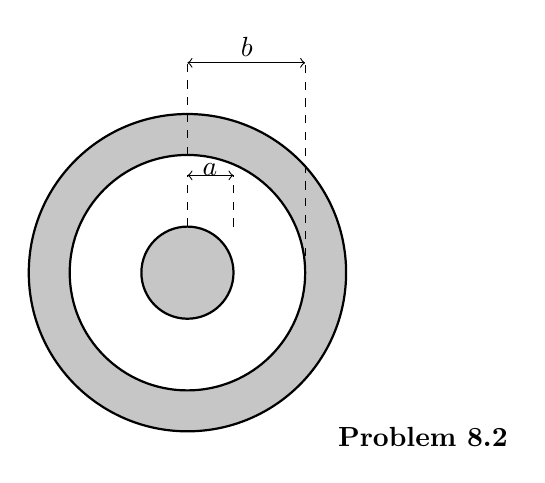
\begin{tikzpicture}[scale=1.3]
  % outer conductor (shaded ring)
  \fill[gray!45,even odd rule] (0,0) circle (1.55) (0,0) circle (1.15);
  \draw[thick] (0,0) circle (1.55);
  \draw[thick] (0,0) circle (1.15);
  % inner conductor (shaded disk)
  \fill[gray!45] (0,0) circle (0.45);
  \draw[thick] (0,0) circle (0.45);
  % b dimension across top
  \draw[<->] (0,2.05) -- (1.15,2.05);
  \draw[dashed] (0,1.15) -- (0,2.05);
  \draw[dashed] (1.15,0) -- (1.15,2.05);
  \node[above] at (0.58,2.02) {$b$};
  % a dimension across inner
  \draw[<->] (0,0.95) -- (0.45,0.95);
  \draw[dashed] (0,0.45) -- (0,0.95);
  \draw[dashed] (0.45,0.45) -- (0.45,0.95);
  \node[above] at (0.22,0.85) {$a$};
  \node at (2.3,-1.6) {\textbf{Problem 8.2}};
\end{tikzpicture}
\end{center}

\begin{enumerate}
\item[(b)] Show that the transmitted power is attenuated along the line as
\[
P(z)=P_{0}e^{-2\gamma z}
\]
where
\[
\gamma=\frac{1}{2\sigma\delta}\sqrt{\frac{\epsilon}{\mu}}\;
\frac{\left(\dfrac{1}{a}+\dfrac{1}{b}\right)}{\ln\left(\dfrac{b}{a}\right)}
\]
\item[(c)] The characteristic impedance $Z_{0}$ of the line is defined as the ratio of the voltage between the cylinders to the axial current flowing in one of them at any position $z$. Show that for this line
\[
Z_{0}=\frac{1}{2\pi}\sqrt{\frac{\mu}{\epsilon}}\,\ln\!\left(\frac{b}{a}\right)
\]
\item[(d)] Show that the series resistance and inductance per unit length of the line are
\begin{align*}
R&=\frac{1}{2\pi\sigma\delta}\left(\frac{1}{a}+\frac{1}{b}\right)\\
L&=\left\{\frac{\mu}{2\pi}\ln\!\left(\frac{b}{a}\right)+\frac{\mu_{c}\delta}{4\pi}\left(\frac{1}{a}+\frac{1}{b}\right)\right\}
\end{align*}
where $\mu_{c}$ is the permeability of the conductor. The correction to the inductance comes from the penetration of the flux into the conductors by a distance of order $\delta$.
\end{enumerate}
\solution

Here $b$ is the radius of the \emph{inner surface} of the outer
conductor.  Set $\eta=\sqrt{\mu/\epsilon}$ and
$R_s=1/(\sigma\delta)$, the surface resistance.  To leading order
in skin depth, the TEM fields in $a<\rho<b$ are
\[
H_\phi(\rho)=\frac{aH_0}{\rho},\qquad E_\rho=\eta H_\phi,
\qquad k=\omega\sqrt{\mu\epsilon}.
\]
Ampere's law fixes $I=2\pi aH_0$, while the radial electrostatic
solution and the plane-wave relation fix $E_\rho$.

\textbf{(a)} With peak phasors the mean axial Poynting flux is
$\eta|H_\phi|^2/2$.  Therefore
\[
P=\frac\eta2\int_a^b\frac{a^2|H_0|^2}{\rho^2}2\pi\rho\,d\rho
=\boxed{\eta\pi a^2|H_0|^2\ln(b/a)}.
\]

\textbf{(b)} The dissipated power per unit length on both surfaces is
\[
P'_\ell=\frac{R_s}2\oint|H_\parallel|^2dl
=\pi R_sa^2|H_0|^2\left(\frac1a+\frac1b\right).
\]
Conservation of energy requires $dP/dz=-P'_\ell=-2\gamma P$.
Dividing by the preceding expression for $P$ gives
\[
\gamma=\frac{R_s}{2\eta}\frac{a^{-1}+b^{-1}}{\ln(b/a)},
\qquad P(z)=P(0)e^{-2\gamma z}.
\]

\textbf{(c)} The voltage magnitude is
$V=\int_a^bE_\rho d\rho=\eta aH_0\ln(b/a)$.  Consequently
\[
\boxed{Z_0=V/I=\frac\eta{2\pi}\ln(b/a).}
\]
It is the leading, real characteristic impedance; conductor losses
produce small complex corrections to the exact impedance.

\textbf{(d)} From $P'_\ell=R|I|^2/2$,
\[
\boxed{R=\frac{R_s}{2\pi}\left(\frac1a+\frac1b\right).}
\]
The average magnetic energy per unit length in the dielectric is
\[
U_{m,\rm ext}=\frac\mu4\int_a^b|H_\phi|^2\,2\pi\rho d\rho
=\frac{\mu\pi a^2|H_0|^2}{2}\ln(b/a).
\]
The penetrating field decays as $e^{-u/\delta}$ in amplitude, giving
\[
U_{m,\rm skin}=\frac{\mu_c}{4}\oint dl\,|H_\parallel|^2
\int_0^\infty e^{-2u/\delta}du
=\frac{\mu_c\delta\pi a^2|H_0|^2}{4}
\left(\frac1a+\frac1b\right).
\]
Using $U_m=L|I|^2/4$ then gives
\[
\boxed{L=\frac\mu{2\pi}\ln(b/a)+
\frac{\mu_c\delta}{4\pi}\left(\frac1a+\frac1b\right).}
\]
As a check, $\omega L_{\rm skin}=R$ because
$\omega\mu_c\delta/2=1/(\sigma\delta)$, the equality of the
resistive and reactive parts of the good-conductor surface impedance.

\Needspace{5\baselineskip}
\par\bigskip
\noindent\textbf{8.3}\quad\begin{enumerate}
\item[(a)] A transmission line consists of two identical thin strips of metal, shown in cross section in the sketch. Assuming that $b\gg a$, discuss the propagation of a TEM mode on this line, repeating the derivations of Problem 8.2. Show that
\begin{align*}
P&=\frac{ab}{2}\sqrt{\frac{\mu}{\epsilon}}\;|H_{0}|^{2}\\[2pt]
\gamma&=\frac{1}{a\sigma\delta}\sqrt{\frac{\epsilon}{\mu}}\\[2pt]
Z_{0}&=\sqrt{\frac{\mu}{\epsilon}}\left(\frac{a}{b}\right)\\[2pt]
R&=\frac{2}{\sigma\delta b}\\[2pt]
L&=\left(\frac{\mu a+\mu_{c}\delta}{b}\right)
\end{align*}
\end{enumerate}

\begin{center}
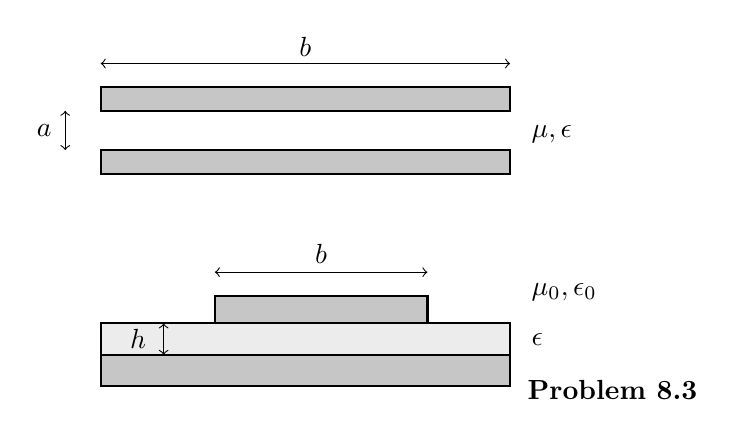
\begin{tikzpicture}[scale=1.0]
  % top figure: two thin strips
  \fill[gray!45] (-0.6,0.75) rectangle (4.6,1.05);
  \draw[thick] (-0.6,0.75) rectangle (4.6,1.05);
  \fill[gray!45] (-0.6,-0.05) rectangle (4.6,0.25);
  \draw[thick] (-0.6,-0.05) rectangle (4.6,0.25);
  \draw[<->] (-0.6,1.35) -- (4.6,1.35);
  \node[above] at (2.0,1.32) {$b$};
  \draw[<->] (-1.05,0.25) -- (-1.05,0.75);
  \node[left] at (-1.1,0.5) {$a$};
  \node[right] at (4.75,0.45) {$\mu,\epsilon$};
  % bottom figure: microstrip
  \fill[gray!45] (-0.6,-2.75) rectangle (4.6,-2.35);
  \draw[thick] (-0.6,-2.75) rectangle (4.6,-2.35);
  \fill[gray!15] (-0.6,-2.35) rectangle (4.6,-1.95);
  \draw[thick] (-0.6,-2.35) rectangle (4.6,-1.95);
  \fill[gray!45] (0.85,-1.95) rectangle (3.55,-1.6);
  \draw[thick] (0.85,-1.95) rectangle (3.55,-1.6);
  \draw[<->] (0.85,-1.3) -- (3.55,-1.3);
  \node[above] at (2.2,-1.32) {$b$};
  \draw[<->] (0.2,-2.35) -- (0.2,-1.95);
  \node[left] at (0.1,-2.15) {$h$};
  \node[right] at (4.75,-1.55) {$\mu_{0},\epsilon_{0}$};
  \node[right] at (4.75,-2.15) {$\epsilon$};
  \node at (5.9,-2.8) {\textbf{Problem 8.3}};
\end{tikzpicture}
\end{center}

\begin{enumerate}
\item[] where the symbols on the left have the same meanings as in Problem 8.2.
\item[(b)] The lower half of the figure shows the cross section of a microstrip line with a strip of width $b$ mounted on a dielectric substrate of thickness $h$ and dielectric constant $\epsilon$, all on a ground plane. What differences occur here compared to part a if $b\gg h$? If $b\ll h$?
\end{enumerate}
\solution

\textbf{(a)} Neglect fringing when $b\gg a$ and assume each metal
strip is thick compared with its skin depth.  In the gap the fields
are uniform, with $E_0=\eta H_0$, where
$\eta=\sqrt{\mu/\epsilon}$.  The voltage and current are
$V=aE_0$ and $I=bH_0$.  The two inner faces carry opposite axial
currents; the exterior field is negligible at this order.  Thus
\[
P=\frac12ab\eta|H_0|^2,\qquad
Z_0=\frac VI=\eta\frac ab.
\]
The two active surfaces dissipate
$P'_\ell=(R_s/2)(2b|H_0|^2)=R_sb|H_0|^2$.
Comparison with $P'_\ell=2\gamma P=R|I|^2/2$ gives
\[
\boxed{\gamma=\frac{R_s}{\eta a}
=\frac1{a\sigma\delta}\sqrt{\frac\epsilon\mu},\qquad
R=\frac{2R_s}{b}=\frac2{\sigma\delta b}.}
\]
The external magnetic energy is $\mu ab|H_0|^2/4$.
The energy in both skin layers is
$(\mu_c/4)(2b|H_0|^2)(\delta/2)=\mu_c\delta b|H_0|^2/4$.
Equating their sum to $L|I|^2/4$ yields
\[
\boxed{L=(\mu a+\mu_c\delta)/b.}
\]
These are all the stated results, with energy velocity
$1/\sqrt{\mu\epsilon}$ to leading order.  ``Thin strips'' means
thin geometrically, not thinner than the penetration depth.

\textbf{(b)} For $b\gg h$, nearly all of the electric and magnetic
energy lies between the strip and the ground plane.  The preceding
parallel-plate formulas apply to leading order with $a=h$ and the
substrate permittivity and permeability; fields at the two strip
edges provide relative corrections that vanish as $h/b\to0$.
For finite $b/h$ the air and substrate have different wave speeds,
so the mode is generally only approximately TEM.

For $b\ll h$ the fields spread transversely over distances of order
$h$, both in the substrate and in the air.  There is no uniform-field
plate region.  In the electrically small, quasi-static limit the
line is described by $Z_0=\sqrt{L'/C'}$ and
$v=1/\sqrt{L'C'}$, where $C'$ is obtained from the two-dielectric
electrostatic problem and $L'$ from the corresponding magnetostatic
problem.  For nonmagnetic media the effective permittivity lies
between $\epsilon_0$ and $\epsilon$; in the very narrow-strip limit
its leading value is $(\epsilon+\epsilon_0)/2$, because the local
field around a strip on the interface occupies two half-spaces.
To see both this average and the logarithmic dependence, let $\lambda$
be charge per unit length and consider $b\ll\rho\ll h$. The two
semicircles in a Gaussian cylinder give
\[
\pi\rho(\epsilon+\epsilon_0)E_\rho\simeq\lambda,
\qquad V\simeq\frac{\lambda}{\pi(\epsilon+\epsilon_0)}\mathcal L,
\qquad \mathcal L=\ln(h/b)+O(1).
\]
The additive constant depends on the near-strip and ground-plane
geometry. Ampere's law gives $H_\phi\simeq I/(2\pi\rho)$ in the
same intermediate region. Integrating its magnetic energy gives
\[
\frac{\mu_0}{4}\int_b^h\left|\frac{I}{2\pi\rho}\right|^2
2\pi\rho\,d\rho\simeq\frac{\mu_0|I|^2}{8\pi}\mathcal L
=\frac{L'|I|^2}{4}.
\]
Thus $C'\simeq\pi(\epsilon+\epsilon_0)/\mathcal L$,
$L'\simeq\mu_0\mathcal L/(2\pi)$, and
\[
v\simeq\frac1{\sqrt{\mu_0(\epsilon+\epsilon_0)/2}},\qquad
Z_0\simeq\frac{\mathcal L}{2\pi}
\sqrt{\frac{2\mu_0}{\epsilon+\epsilon_0}}.
\]
The impedance therefore grows logarithmically with $h/b$. The
strongly nonuniform strip and return currents also
require the surface-loss integral with their actual distributions;
the wide-plate resistance and attenuation formulas no longer apply.
At wavelengths comparable with the transverse dimensions, the
mode has longitudinal field components and geometric dispersion,
so even the quasi-TEM circuit description needs correction.

\Needspace{5\baselineskip}
\par\bigskip
\noindent\textbf{8.4}\quad Transverse electric and magnetic waves are propagated along a hollow, right circular cylinder with inner radius $R$ and conductivity $\sigma$.
\begin{enumerate}
\item[(a)] Find the cutoff frequencies of the various TE and TM modes. Determine numerically the lowest cutoff frequency (the dominant mode) in terms of the tube radius and the ratio of cutoff frequencies of the next four higher modes to that of the dominant mode. For this part assume that the conductivity of the cylinder is infinite.
\item[(b)] Calculate the attenuation constants of the waveguide as a function of frequency for the lowest two distinct modes and plot them as a function of frequency.
\end{enumerate}
\solution

Let $v=1/\sqrt{\mu\epsilon}$ and $\eta=\sqrt{\mu/\epsilon}$ for
the lossless filling (vacuum gives $v=c$).  Write the fields as
$e^{ikz-i\omega t}$, and put $\gamma^2=\omega^2/v^2-k^2$.
Here $\gamma$ is the transverse eigenvalue parameter of (8.34),
and $\beta$ below is the attenuation constant of Section 8.5.
We use $H_z=B_z/\mu$ when evaluating conductor losses; the
constant factor $\mu$ does not change the scalar eigenvalue problem.

\textbf{(a)} Regular longitudinal fields have radial dependence
$J_m(\gamma\rho)$ and angular dependence $\cos m\phi$ or
$\sin m\phi$.  A TM mode has $E_z=0$ on the wall, while a TE
mode has $\partial_\rho H_z=0$ there.  Thus
\[
\boxed{\omega_{c,mn}^{\rm TM}=\frac vR x_{mn},\quad J_m(x_{mn})=0;
\qquad\omega_{c,mn}^{\rm TE}=\frac vR x'_{mn},\quad J_m'(x'_{mn})=0.}
\]
Use positive roots only; the constant Neumann scalar mode does not
produce a nonzero TE electromagnetic field in a hollow guide.
For $m>0$ each family has two angular polarizations.  The first
families, with their cutoffs divided by that of $\mathrm{TE}_{11}$,
are
\[
\begin{array}{c|rr}
\text{family}&\omega_cR/v&\omega_c/\omega_{c,11}^{\rm TE}\\\hline
\mathrm{TE}_{11}&1.841183781&1\\
\mathrm{TM}_{01}&2.404825558&1.306130101\\
\mathrm{TE}_{21}&3.054236928&1.658844141\\
\mathrm{TE}_{01}&3.831705970&2.081109995\\
\mathrm{TM}_{11}&3.831705970&2.081109995\\
\mathrm{TE}_{31}&4.201188941&2.281786850
\end{array}
\]
The middle two families have the same cutoff.  Thus the table gives
both the next four families and, if ``higher'' is counted by distinct
frequency, the next four distinct frequencies.  The dominant cutoff
is $\omega_c=1.841183781v/R$, or $f_c=0.293033v/R$.

\textbf{(b)} Let $R_s=1/(\sigma\delta)=\sqrt{\omega\mu_c/(2\sigma)}$
and denote amplitude attenuation by $\beta$, so power decays as
$e^{-2\beta z}$.  The loss formula is
\[
\beta=\frac{R_s}{4P}\oint|H_\parallel|^2dl.
\]
For clarity, the field and normalization steps behind this formula
are as follows. Maxwell's equations, with the phase convention above,
give the transverse fields in (8.26):
\begin{align*}
\mathbf E_t&=\frac{i}{\gamma^2}
  (k\nabla_tE_z-\omega\mu\widehat{\mathbf z}\times\nabla_tH_z),\\
\mathbf H_t&=\frac{i}{\gamma^2}
  (k\nabla_tH_z+\omega\epsilon\widehat{\mathbf z}\times\nabla_tE_z).
\end{align*}
For either scalar $\psi$, integration by parts and its Dirichlet
or Neumann wall condition imply
\[
\int|\nabla_t\psi|^2dA
=-\int\psi^*\nabla_t^2\psi\,dA
+\oint\psi^*\partial_n\psi\,dl=\gamma^2N,
\qquad N=\int|\psi|^2dA.
\]
Inserting the transverse fields into
$P=\tfrac12\operatorname{Re}\int(\mathbf E_t\times\mathbf H_t^*)
\cdot\widehat{\mathbf z}\,dA$ then supplies the power formulas below.
For a TM field $\psi=E_z$ with $N=\int|\psi|^2dA$,
\[
P=\frac{\omega\epsilon k}{2\gamma^2}N,\qquad
\oint|H_\parallel|^2dl
=\frac{\omega^2\epsilon^2}{\gamma^4}\oint|\partial_n\psi|^2dl.
\]
The radial normalization follows directly from Bessel's equation:
\[
\frac{d}{dx}\left\{x^2J_m'(x)^2+(x^2-m^2)J_m(x)^2\right\}
=2xJ_m(x)^2.
\]
Its integral from $0$ to $\chi=\gamma R$ gives
\[
\int_0^R\rho J_m(\gamma\rho)^2d\rho
=\frac{R^2}{2}\left[J_m'(\chi)^2+
\left(1-\frac{m^2}{\chi^2}\right)J_m(\chi)^2\right].
\]
At a TM zero, the angular factor cancels between the area integral
and the boundary integral $R\gamma^2J_m'(\chi)^2$ times that factor.
This gives
$\oint|\partial_n\psi|^2dl=2\gamma^2N/R$.  Hence
\[
\boxed{\beta_{\rm TM}=
\frac{R_s}{\eta R\sqrt{1-(\omega_c/\omega)^2}}.}
\]
For TE modes put $\psi=H_z$.  At the wall the longitudinal field
and the tangential transverse field both contribute:
\[
P=\frac{\omega\mu k}{2\gamma^2}N,\qquad
\oint|H_\parallel|^2dl
=\oint\left(|\psi|^2+\frac{k^2}{\gamma^4}|\partial_s\psi|^2\right)dl.
\]
For $\chi=x'_{mn}$ the Bessel norm and the angular derivative give
\[
\frac{\oint|\psi|^2dl}{N}=\frac{2}{R(1-m^2/\chi^2)},\qquad
\oint|\partial_s\psi|^2dl=\frac{m^2}{R^2}\oint|\psi|^2dl.
\]
Substitute $k^2=(\omega/v)^2-\chi^2/R^2$. To display the
simplification, put $t=\omega_c/\omega$; the dimensionless factor is
\[
\frac{t^2}{1-m^2/\chi^2}
\left[1+\frac{m^2}{\chi^2}\frac{1-t^2}{t^2}\right]
=t^2+\frac{m^2}{\chi^2-m^2}.
\]
Therefore
\[
\boxed{\beta_{{\rm TE},mn}=
\frac{R_s}{\eta R\sqrt{1-(\omega_c/\omega)^2}}
\left[\left(\frac{\omega_c}{\omega}\right)^2+
\frac{m^2}{\chi^2-m^2}\right].}
\]
Use $m=1$, $\chi=1.841183781$ for the lowest TE mode, and the
TM formula with $\omega_cR/v=2.404825558$ for the next distinct
mode.  The plot retains $R_s\propto\sqrt\omega$; the normalization
uses its value at the dominant cutoff.
\begin{center}\begin{tikzpicture}[x=1cm,y=1cm,>=stealth]
\draw[->] (0,0)--(10.2,0);
\draw[->] (0,0)--(0,5.2);
\draw (0.00000,.06)--(0.00000,-.06) node[below] {\scriptsize $1$};
\draw (1.42857,.06)--(1.42857,-.06) node[below] {\scriptsize $2$};
\draw (2.85714,.06)--(2.85714,-.06) node[below] {\scriptsize $3$};
\draw (4.28571,.06)--(4.28571,-.06) node[below] {\scriptsize $4$};
\draw (5.71429,.06)--(5.71429,-.06) node[below] {\scriptsize $5$};
\draw (7.14286,.06)--(7.14286,-.06) node[below] {\scriptsize $6$};
\draw (8.57143,.06)--(8.57143,-.06) node[below] {\scriptsize $7$};
\draw (10.00000,.06)--(10.00000,-.06) node[below] {\scriptsize $8$};
\draw (.06,0.00000)--(-.06,0.00000) node[left] {\scriptsize $0$};
\draw (.06,1.25000)--(-.06,1.25000) node[left] {\scriptsize $2$};
\draw (.06,2.50000)--(-.06,2.50000) node[left] {\scriptsize $4$};
\draw (.06,3.75000)--(-.06,3.75000) node[left] {\scriptsize $6$};
\draw (.06,5.00000)--(-.06,5.00000) node[left] {\scriptsize $8$};
\node[below] at (5.0,-.45) {$\omega/\omega_{c,11}^{\rm TE}$};
\node[rotate=90] at (-.75,2.5) {$\beta\eta R/R_s(\omega_{c,11}^{\rm TE})$};
\begin{scope}
\clip (0,0) rectangle (10,5);
\draw[blue,thick] plot coordinates {(0.007143,8.858114) (0.027169,4.532437) (0.047194,3.432258) (0.067220,2.870807) (0.087246,2.515807) (0.107272,2.265524) (0.127297,2.076951) (0.147323,1.928357) (0.167349,1.807417) (0.187375,1.706553) (0.207401,1.620812) (0.227426,1.546801) (0.247452,1.482110) (0.267478,1.424969) (0.287504,1.374048) (0.307529,1.328323) (0.327555,1.286994) (0.347581,1.249422) (0.367607,1.215091) (0.387632,1.183582) (0.407658,1.154545) (0.427684,1.127690) (0.447710,1.102773) (0.467735,1.079584) (0.487761,1.057946) (0.507787,1.037706) (0.527813,1.018730) (0.547839,1.000904) (0.567864,0.984124) (0.587890,0.968301) (0.607916,0.953358) (0.627942,0.939222) (0.647967,0.925832) (0.667993,0.913131) (0.688019,0.901070) (0.708045,0.889601) (0.728070,0.878685) (0.748096,0.868284) (0.768122,0.858365) (0.788148,0.848896) (0.808173,0.839849) (0.828199,0.831199) (0.848225,0.822921) (0.868251,0.814995) (0.888277,0.807399) (0.908302,0.800116) (0.928328,0.793128) (0.948354,0.786420) (0.968380,0.779977) (0.988405,0.773784) (1.008431,0.767830) (1.028457,0.762103) (1.048483,0.756591) (1.068508,0.751284) (1.088534,0.746172) (1.108560,0.741247) (1.128586,0.736500) (1.148612,0.731922) (1.168637,0.727507) (1.188663,0.723247) (1.208689,0.719136) (1.228715,0.715167) (1.248740,0.711334) (1.268766,0.707632) (1.288792,0.704056) (1.308818,0.700600) (1.328843,0.697259) (1.348869,0.694031) (1.368895,0.690909) (1.388921,0.687890) (1.408946,0.684970) (1.428972,0.682145) (1.448998,0.679412) (1.469024,0.676768) (1.489050,0.674210) (1.509075,0.671734) (1.529101,0.669337) (1.549127,0.667018) (1.569153,0.664772) (1.589178,0.662599) (1.609204,0.660494) (1.629230,0.658457) (1.649256,0.656485) (1.669281,0.654575) (1.689307,0.652726) (1.709333,0.650936) (1.729359,0.649203) (1.749384,0.647525) (1.769410,0.645901) (1.789436,0.644328) (1.809462,0.642806) (1.829488,0.641333) (1.849513,0.639907) (1.869539,0.638527) (1.889565,0.637191) (1.909591,0.635900) (1.929616,0.634650) (1.949642,0.633441) (1.969668,0.632272) (1.989694,0.631141) (2.009719,0.630048) (2.029745,0.628992) (2.049771,0.627971) (2.069797,0.626985) (2.089823,0.626032) (2.109848,0.625112) (2.129874,0.624225) (2.149900,0.623368) (2.169926,0.622541) (2.189951,0.621744) (2.209977,0.620976) (2.230003,0.620235) (2.250029,0.619522) (2.270054,0.618835) (2.290080,0.618175) (2.310106,0.617539) (2.330132,0.616929) (2.350157,0.616342) (2.370183,0.615779) (2.390209,0.615239) (2.410235,0.614721) (2.430261,0.614224) (2.450286,0.613750) (2.470312,0.613295) (2.490338,0.612862) (2.510364,0.612448) (2.530389,0.612053) (2.550415,0.611677) (2.570441,0.611320) (2.590467,0.610981) (2.610492,0.610660) (2.630518,0.610355) (2.650544,0.610068) (2.670570,0.609797) (2.690595,0.609543) (2.710621,0.609304) (2.730647,0.609080) (2.750673,0.608872) (2.770699,0.608678) (2.790724,0.608499) (2.810750,0.608334) (2.830776,0.608182) (2.850802,0.608045) (2.870827,0.607920) (2.890853,0.607809) (2.910879,0.607710) (2.930905,0.607623) (2.950930,0.607549) (2.970956,0.607487) (2.990982,0.607436) (3.011008,0.607397) (3.031033,0.607369) (3.051059,0.607352) (3.071085,0.607346) (3.091111,0.607350) (3.111137,0.607365) (3.131162,0.607389) (3.151188,0.607424) (3.171214,0.607468) (3.191240,0.607522) (3.211265,0.607585) (3.231291,0.607658) (3.251317,0.607739) (3.271343,0.607829) (3.291368,0.607928) (3.311394,0.608035) (3.331420,0.608150) (3.351446,0.608274) (3.371472,0.608406) (3.391497,0.608545) (3.411523,0.608692) (3.431549,0.608847) (3.451575,0.609009) (3.471600,0.609178) (3.491626,0.609355) (3.511652,0.609538) (3.531678,0.609728) (3.551703,0.609925) (3.571729,0.610129) (3.591755,0.610339) (3.611781,0.610555) (3.631806,0.610778) (3.651832,0.611007) (3.671858,0.611242) (3.691884,0.611482) (3.711910,0.611729) (3.731935,0.611981) (3.751961,0.612239) (3.771987,0.612503) (3.792013,0.612771) (3.812038,0.613045) (3.832064,0.613325) (3.852090,0.613609) (3.872116,0.613898) (3.892141,0.614193) (3.912167,0.614492) (3.932193,0.614796) (3.952219,0.615104) (3.972244,0.615418) (3.992270,0.615735) (4.012296,0.616057) (4.032322,0.616384) (4.052348,0.616715) (4.072373,0.617050) (4.092399,0.617389) (4.112425,0.617732) (4.132451,0.618079) (4.152476,0.618430) (4.172502,0.618785) (4.192528,0.619144) (4.212554,0.619507) (4.232579,0.619873) (4.252605,0.620243) (4.272631,0.620616) (4.292657,0.620993) (4.312683,0.621373) (4.332708,0.621757) (4.352734,0.622143) (4.372760,0.622534) (4.392786,0.622927) (4.412811,0.623323) (4.432837,0.623723) (4.452863,0.624125) (4.472889,0.624531) (4.492914,0.624939) (4.512940,0.625351) (4.532966,0.625765) (4.552992,0.626182) (4.573017,0.626602) (4.593043,0.627024) (4.613069,0.627449) (4.633095,0.627877) (4.653121,0.628307) (4.673146,0.628740) (4.693172,0.629175) (4.713198,0.629613) (4.733224,0.630053) (4.753249,0.630496) (4.773275,0.630941) (4.793301,0.631388) (4.813327,0.631837) (4.833352,0.632289) (4.853378,0.632742) (4.873404,0.633198) (4.893430,0.633656) (4.913455,0.634116) (4.933481,0.634578) (4.953507,0.635042) (4.973533,0.635508) (4.993559,0.635976) (5.013584,0.636446) (5.033610,0.636918) (5.053636,0.637391) (5.073662,0.637866) (5.093687,0.638344) (5.113713,0.638822) (5.133739,0.639303) (5.153765,0.639785) (5.173790,0.640269) (5.193816,0.640755) (5.213842,0.641242) (5.233868,0.641731) (5.253894,0.642221) (5.273919,0.642713) (5.293945,0.643206) (5.313971,0.643701) (5.333997,0.644197) (5.354022,0.644695) (5.374048,0.645194) (5.394074,0.645695) (5.414100,0.646197) (5.434125,0.646700) (5.454151,0.647205) (5.474177,0.647710) (5.494203,0.648217) (5.514228,0.648726) (5.534254,0.649235) (5.554280,0.649746) (5.574306,0.650258) (5.594332,0.650771) (5.614357,0.651286) (5.634383,0.651801) (5.654409,0.652318) (5.674435,0.652835) (5.694460,0.653354) (5.714486,0.653874) (5.734512,0.654395) (5.754538,0.654917) (5.774563,0.655439) (5.794589,0.655963) (5.814615,0.656488) (5.834641,0.657014) (5.854666,0.657540) (5.874692,0.658068) (5.894718,0.658597) (5.914744,0.659126) (5.934770,0.659656) (5.954795,0.660187) (5.974821,0.660719) (5.994847,0.661252) (6.014873,0.661786) (6.034898,0.662320) (6.054924,0.662855) (6.074950,0.663391) (6.094976,0.663928) (6.115001,0.664466) (6.135027,0.665004) (6.155053,0.665543) (6.175079,0.666082) (6.195104,0.666623) (6.215130,0.667164) (6.235156,0.667705) (6.255182,0.668248) (6.275208,0.668791) (6.295233,0.669334) (6.315259,0.669879) (6.335285,0.670423) (6.355311,0.670969) (6.375336,0.671515) (6.395362,0.672061) (6.415388,0.672609) (6.435414,0.673156) (6.455439,0.673705) (6.475465,0.674253) (6.495491,0.674803) (6.515517,0.675352) (6.535543,0.675903) (6.555568,0.676453) (6.575594,0.677005) (6.595620,0.677557) (6.615646,0.678109) (6.635671,0.678661) (6.655697,0.679215) (6.675723,0.679768) (6.695749,0.680322) (6.715774,0.680876) (6.735800,0.681431) (6.755826,0.681986) (6.775852,0.682542) (6.795877,0.683098) (6.815903,0.683654) (6.835929,0.684211) (6.855955,0.684768) (6.875981,0.685326) (6.896006,0.685883) (6.916032,0.686441) (6.936058,0.687000) (6.956084,0.687559) (6.976109,0.688118) (6.996135,0.688677) (7.016161,0.689237) (7.036187,0.689797) (7.056212,0.690357) (7.076238,0.690917) (7.096264,0.691478) (7.116290,0.692039) (7.136315,0.692600) (7.156341,0.693162) (7.176367,0.693724) (7.196393,0.694286) (7.216419,0.694848) (7.236444,0.695411) (7.256470,0.695973) (7.276496,0.696536) (7.296522,0.697099) (7.316547,0.697663) (7.336573,0.698226) (7.356599,0.698790) (7.376625,0.699354) (7.396650,0.699918) (7.416676,0.700482) (7.436702,0.701047) (7.456728,0.701611) (7.476754,0.702176) (7.496779,0.702741) (7.516805,0.703306) (7.536831,0.703871) (7.556857,0.704437) (7.576882,0.705002) (7.596908,0.705568) (7.616934,0.706133) (7.636960,0.706699) (7.656985,0.707265) (7.677011,0.707831) (7.697037,0.708397) (7.717063,0.708963) (7.737088,0.709530) (7.757114,0.710096) (7.777140,0.710663) (7.797166,0.711229) (7.817192,0.711796) (7.837217,0.712363) (7.857243,0.712930) (7.877269,0.713496) (7.897295,0.714063) (7.917320,0.714630) (7.937346,0.715197) (7.957372,0.715765) (7.977398,0.716332) (7.997423,0.716899) (8.017449,0.717466) (8.037475,0.718033) (8.057501,0.718601) (8.077526,0.719168) (8.097552,0.719735) (8.117578,0.720303) (8.137604,0.720870) (8.157630,0.721438) (8.177655,0.722005) (8.197681,0.722572) (8.217707,0.723140) (8.237733,0.723707) (8.257758,0.724275) (8.277784,0.724842) (8.297810,0.725409) (8.317836,0.725977) (8.337861,0.726544) (8.357887,0.727111) (8.377913,0.727679) (8.397939,0.728246) (8.417965,0.728813) (8.437990,0.729381) (8.458016,0.729948) (8.478042,0.730515) (8.498068,0.731082) (8.518093,0.731649) (8.538119,0.732216) (8.558145,0.732783) (8.578171,0.733350) (8.598196,0.733917) (8.618222,0.734484) (8.638248,0.735051) (8.658274,0.735618) (8.678299,0.736184) (8.698325,0.736751) (8.718351,0.737317) (8.738377,0.737884) (8.758403,0.738450) (8.778428,0.739017) (8.798454,0.739583) (8.818480,0.740149) (8.838506,0.740715) (8.858531,0.741281) (8.878557,0.741847) (8.898583,0.742413) (8.918609,0.742979) (8.938634,0.743545) (8.958660,0.744110) (8.978686,0.744676) (8.998712,0.745241) (9.018737,0.745806) (9.038763,0.746372) (9.058789,0.746937) (9.078815,0.747502) (9.098841,0.748067) (9.118866,0.748631) (9.138892,0.749196) (9.158918,0.749761) (9.178944,0.750325) (9.198969,0.750889) (9.218995,0.751454) (9.239021,0.752018) (9.259047,0.752582) (9.279072,0.753145) (9.299098,0.753709) (9.319124,0.754273) (9.339150,0.754836) (9.359175,0.755400) (9.379201,0.755963) (9.399227,0.756526) (9.419253,0.757089) (9.439279,0.757652) (9.459304,0.758214) (9.479330,0.758777) (9.499356,0.759339) (9.519382,0.759902) (9.539407,0.760464) (9.559433,0.761026) (9.579459,0.761588) (9.599485,0.762149) (9.619510,0.762711) (9.639536,0.763272) (9.659562,0.763834) (9.679588,0.764395) (9.699614,0.764956) (9.719639,0.765517) (9.739665,0.766077) (9.759691,0.766638) (9.779717,0.767198) (9.799742,0.767758) (9.819768,0.768318) (9.839794,0.768878) (9.859820,0.769438) (9.879845,0.769998) (9.899871,0.770557) (9.919897,0.771116) (9.939923,0.771675) (9.959948,0.772234) (9.979974,0.772793) (10.000000,0.773351)};
\draw[red,dashed,thick] plot coordinates {(0.446658,7.187538) (0.466603,4.111562) (0.486547,3.212589) (0.506491,2.745297) (0.526436,2.449699) (0.546380,2.242511) (0.566324,2.087774) (0.586269,1.967103) (0.606213,1.870000) (0.626157,1.789983) (0.646102,1.722807) (0.666046,1.665561) (0.685990,1.616175) (0.705935,1.573132) (0.725879,1.535292) (0.745823,1.501780) (0.765768,1.471911) (0.785712,1.445141) (0.805656,1.421034) (0.825601,1.399230) (0.845545,1.379437) (0.865489,1.361408) (0.885434,1.344938) (0.905378,1.329853) (0.925323,1.316002) (0.945267,1.303259) (0.965211,1.291513) (0.985156,1.280668) (1.005100,1.270640) (1.025044,1.261356) (1.044989,1.252750) (1.064933,1.244766) (1.084877,1.237352) (1.104822,1.230462) (1.124766,1.224056) (1.144710,1.218096) (1.164655,1.212551) (1.184599,1.207391) (1.204543,1.202587) (1.224488,1.198116) (1.244432,1.193956) (1.264376,1.190085) (1.284321,1.186486) (1.304265,1.183141) (1.324209,1.180035) (1.344154,1.177153) (1.364098,1.174482) (1.384042,1.172009) (1.403987,1.169723) (1.423931,1.167615) (1.443876,1.165673) (1.463820,1.163889) (1.483764,1.162254) (1.503709,1.160761) (1.523653,1.159403) (1.543597,1.158172) (1.563542,1.157061) (1.583486,1.156066) (1.603430,1.155181) (1.623375,1.154399) (1.643319,1.153717) (1.663263,1.153130) (1.683208,1.152632) (1.703152,1.152221) (1.723096,1.151892) (1.743041,1.151642) (1.762985,1.151466) (1.782929,1.151363) (1.802874,1.151328) (1.822818,1.151359) (1.842762,1.151454) (1.862707,1.151608) (1.882651,1.151821) (1.902595,1.152089) (1.922540,1.152411) (1.942484,1.152784) (1.962429,1.153206) (1.982373,1.153675) (2.002317,1.154189) (2.022262,1.154748) (2.042206,1.155348) (2.062150,1.155989) (2.082095,1.156668) (2.102039,1.157385) (2.121983,1.158138) (2.141928,1.158926) (2.161872,1.159747) (2.181816,1.160600) (2.201761,1.161485) (2.221705,1.162399) (2.241649,1.163343) (2.261594,1.164314) (2.281538,1.165312) (2.301482,1.166336) (2.321427,1.167385) (2.341371,1.168459) (2.361315,1.169556) (2.381260,1.170675) (2.401204,1.171816) (2.421148,1.172978) (2.441093,1.174161) (2.461037,1.175363) (2.480982,1.176584) (2.500926,1.177824) (2.520870,1.179082) (2.540815,1.180356) (2.560759,1.181648) (2.580703,1.182955) (2.600648,1.184278) (2.620592,1.185616) (2.640536,1.186969) (2.660481,1.188336) (2.680425,1.189717) (2.700369,1.191110) (2.720314,1.192517) (2.740258,1.193936) (2.760202,1.195367) (2.780147,1.196809) (2.800091,1.198263) (2.820035,1.199728) (2.839980,1.201203) (2.859924,1.202689) (2.879868,1.204184) (2.899813,1.205689) (2.919757,1.207204) (2.939701,1.208727) (2.959646,1.210259) (2.979590,1.211800) (2.999535,1.213348) (3.019479,1.214905) (3.039423,1.216469) (3.059368,1.218041) (3.079312,1.219620) (3.099256,1.221205) (3.119201,1.222798) (3.139145,1.224397) (3.159089,1.226002) (3.179034,1.227614) (3.198978,1.229231) (3.218922,1.230855) (3.238867,1.232483) (3.258811,1.234117) (3.278755,1.235757) (3.298700,1.237401) (3.318644,1.239050) (3.338588,1.240704) (3.358533,1.242363) (3.378477,1.244026) (3.398421,1.245693) (3.418366,1.247364) (3.438310,1.249040) (3.458254,1.250719) (3.478199,1.252402) (3.498143,1.254088) (3.518088,1.255778) (3.538032,1.257472) (3.557976,1.259168) (3.577921,1.260868) (3.597865,1.262571) (3.617809,1.264276) (3.637754,1.265985) (3.657698,1.267696) (3.677642,1.269410) (3.697587,1.271126) (3.717531,1.272844) (3.737475,1.274565) (3.757420,1.276289) (3.777364,1.278014) (3.797308,1.279741) (3.817253,1.281471) (3.837197,1.283202) (3.857141,1.284935) (3.877086,1.286670) (3.897030,1.288407) (3.916974,1.290145) (3.936919,1.291884) (3.956863,1.293626) (3.976807,1.295368) (3.996752,1.297112) (4.016696,1.298857) (4.036641,1.300603) (4.056585,1.302351) (4.076529,1.304099) (4.096474,1.305849) (4.116418,1.307600) (4.136362,1.309351) (4.156307,1.311103) (4.176251,1.312857) (4.196195,1.314611) (4.216140,1.316365) (4.236084,1.318121) (4.256028,1.319876) (4.275973,1.321633) (4.295917,1.323390) (4.315861,1.325147) (4.335806,1.326905) (4.355750,1.328664) (4.375694,1.330422) (4.395639,1.332182) (4.415583,1.333941) (4.435527,1.335700) (4.455472,1.337460) (4.475416,1.339220) (4.495360,1.340980) (4.515305,1.342740) (4.535249,1.344501) (4.555194,1.346261) (4.575138,1.348021) (4.595082,1.349781) (4.615027,1.351542) (4.634971,1.353302) (4.654915,1.355062) (4.674860,1.356822) (4.694804,1.358581) (4.714748,1.360341) (4.734693,1.362100) (4.754637,1.363859) (4.774581,1.365618) (4.794526,1.367376) (4.814470,1.369134) (4.834414,1.370892) (4.854359,1.372649) (4.874303,1.374406) (4.894247,1.376163) (4.914192,1.377919) (4.934136,1.379675) (4.954080,1.381430) (4.974025,1.383184) (4.993969,1.384939) (5.013913,1.386692) (5.033858,1.388445) (5.053802,1.390198) (5.073747,1.391950) (5.093691,1.393701) (5.113635,1.395452) (5.133580,1.397202) (5.153524,1.398951) (5.173468,1.400700) (5.193413,1.402448) (5.213357,1.404195) (5.233301,1.405942) (5.253246,1.407688) (5.273190,1.409433) (5.293134,1.411177) (5.313079,1.412921) (5.333023,1.414664) (5.352967,1.416406) (5.372912,1.418147) (5.392856,1.419887) (5.412800,1.421627) (5.432745,1.423366) (5.452689,1.425104) (5.472633,1.426841) (5.492578,1.428577) (5.512522,1.430312) (5.532466,1.432046) (5.552411,1.433780) (5.572355,1.435512) (5.592300,1.437244) (5.612244,1.438974) (5.632188,1.440704) (5.652133,1.442433) (5.672077,1.444161) (5.692021,1.445887) (5.711966,1.447613) (5.731910,1.449338) (5.751854,1.451062) (5.771799,1.452785) (5.791743,1.454507) (5.811687,1.456228) (5.831632,1.457947) (5.851576,1.459666) (5.871520,1.461384) (5.891465,1.463101) (5.911409,1.464816) (5.931353,1.466531) (5.951298,1.468244) (5.971242,1.469957) (5.991186,1.471668) (6.011131,1.473379) (6.031075,1.475088) (6.051019,1.476796) (6.070964,1.478503) (6.090908,1.480209) (6.110853,1.481914) (6.130797,1.483618) (6.150741,1.485320) (6.170686,1.487022) (6.190630,1.488722) (6.210574,1.490421) (6.230519,1.492120) (6.250463,1.493817) (6.270407,1.495513) (6.290352,1.497207) (6.310296,1.498901) (6.330240,1.500593) (6.350185,1.502285) (6.370129,1.503975) (6.390073,1.505664) (6.410018,1.507352) (6.429962,1.509038) (6.449906,1.510724) (6.469851,1.512408) (6.489795,1.514091) (6.509739,1.515773) (6.529684,1.517454) (6.549628,1.519134) (6.569572,1.520812) (6.589517,1.522490) (6.609461,1.524166) (6.629406,1.525841) (6.649350,1.527515) (6.669294,1.529187) (6.689239,1.530858) (6.709183,1.532529) (6.729127,1.534198) (6.749072,1.535865) (6.769016,1.537532) (6.788960,1.539197) (6.808905,1.540861) (6.828849,1.542524) (6.848793,1.544186) (6.868738,1.545847) (6.888682,1.547506) (6.908626,1.549164) (6.928571,1.550821) (6.948515,1.552477) (6.968459,1.554132) (6.988404,1.555785) (7.008348,1.557437) (7.028292,1.559088) (7.048237,1.560738) (7.068181,1.562386) (7.088125,1.564033) (7.108070,1.565679) (7.128014,1.567324) (7.147959,1.568968) (7.167903,1.570610) (7.187847,1.572251) (7.207792,1.573891) (7.227736,1.575530) (7.247680,1.577168) (7.267625,1.578804) (7.287569,1.580439) (7.307513,1.582073) (7.327458,1.583706) (7.347402,1.585337) (7.367346,1.586967) (7.387291,1.588596) (7.407235,1.590224) (7.427179,1.591851) (7.447124,1.593476) (7.467068,1.595100) (7.487012,1.596723) (7.506957,1.598345) (7.526901,1.599965) (7.546845,1.601585) (7.566790,1.603203) (7.586734,1.604820) (7.606678,1.606435) (7.626623,1.608050) (7.646567,1.609663) (7.666512,1.611275) (7.686456,1.612886) (7.706400,1.614495) (7.726345,1.616104) (7.746289,1.617711) (7.766233,1.619317) (7.786178,1.620922) (7.806122,1.622525) (7.826066,1.624128) (7.846011,1.625729) (7.865955,1.627329) (7.885899,1.628927) (7.905844,1.630525) (7.925788,1.632121) (7.945732,1.633716) (7.965677,1.635310) (7.985621,1.636903) (8.005565,1.638495) (8.025510,1.640085) (8.045454,1.641674) (8.065398,1.643262) (8.085343,1.644849) (8.105287,1.646434) (8.125231,1.648019) (8.145176,1.649602) (8.165120,1.651184) (8.185065,1.652764) (8.205009,1.654344) (8.224953,1.655922) (8.244898,1.657500) (8.264842,1.659076) (8.284786,1.660651) (8.304731,1.662224) (8.324675,1.663797) (8.344619,1.665368) (8.364564,1.666938) (8.384508,1.668507) (8.404452,1.670075) (8.424397,1.671641) (8.444341,1.673207) (8.464285,1.674771) (8.484230,1.676334) (8.504174,1.677896) (8.524118,1.679457) (8.544063,1.681016) (8.564007,1.682575) (8.583951,1.684132) (8.603896,1.685688) (8.623840,1.687243) (8.643784,1.688797) (8.663729,1.690349) (8.683673,1.691901) (8.703618,1.693451) (8.723562,1.695000) (8.743506,1.696548) (8.763451,1.698095) (8.783395,1.699641) (8.803339,1.701185) (8.823284,1.702728) (8.843228,1.704271) (8.863172,1.705812) (8.883117,1.707352) (8.903061,1.708890) (8.923005,1.710428) (8.942950,1.711964) (8.962894,1.713500) (8.982838,1.715034) (9.002783,1.716567) (9.022727,1.718099) (9.042671,1.719630) (9.062616,1.721160) (9.082560,1.722688) (9.102504,1.724216) (9.122449,1.725742) (9.142393,1.727267) (9.162337,1.728791) (9.182282,1.730314) (9.202226,1.731836) (9.222171,1.733357) (9.242115,1.734876) (9.262059,1.736395) (9.282004,1.737912) (9.301948,1.739428) (9.321892,1.740944) (9.341837,1.742458) (9.361781,1.743970) (9.381725,1.745482) (9.401670,1.746993) (9.421614,1.748503) (9.441558,1.750011) (9.461503,1.751519) (9.481447,1.753025) (9.501391,1.754530) (9.521336,1.756034) (9.541280,1.757537) (9.561224,1.759039) (9.581169,1.760540) (9.601113,1.762040) (9.621057,1.763539) (9.641002,1.765036) (9.660946,1.766533) (9.680890,1.768028) (9.700835,1.769522) (9.720779,1.771016) (9.740724,1.772508) (9.760668,1.773999) (9.780612,1.775489) (9.800557,1.776978) (9.820501,1.778466) (9.840445,1.779953) (9.860390,1.781439) (9.880334,1.782923) (9.900278,1.784407) (9.920223,1.785890) (9.940167,1.787371) (9.960111,1.788852) (9.980056,1.790331) (10.000000,1.791809)};
\end{scope}
\draw[blue,thick] (6.3,4.7)--(6.75,4.7);
\node[right,fill=white,inner sep=1pt] at (6.8,4.7) {\scriptsize $\mathrm{TE}_{11}$};
\draw[red,dashed,thick] (6.3,4.38)--(6.75,4.38);
\node[right,fill=white,inner sep=1pt] at (6.8,4.38) {\scriptsize $\mathrm{TM}_{01}$};
\end{tikzpicture}
\end{center}
The perturbative formulas apply above cutoff when the attenuation is
small compared with $k$.  Their divergences arbitrarily close to
cutoff mark a failure of that approximation, not an infinite physical
loss.  Below cutoff there is already evanescent decay in a perfect guide.

\Needspace{5\baselineskip}
\par\bigskip
\noindent\textbf{8.5}\quad A waveguide is constructed so that the cross section of the guide forms a right triangle with sides of length $a$, $a$, $\sqrt{2}a$, as shown. The medium inside has $\mu_{r}=\epsilon_{r}=1$.
\begin{enumerate}
\item[(a)] Assuming infinite conductivity for the walls, determine the possible modes of propagation and their cutoff frequencies.
\end{enumerate}

\begin{center}
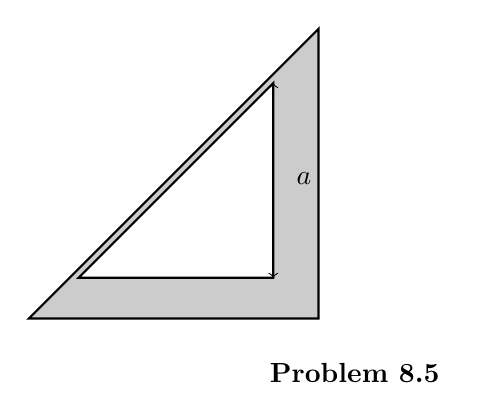
\begin{tikzpicture}[scale=1.15]
  % shaded triangular wall border
  \fill[gray!40] (0,0) -- (3.2,0) -- (3.2,3.2) -- cycle;
  \fill[white] (0.55,0.45) -- (2.7,0.45) -- (2.7,2.6) -- cycle;
  \draw[thick] (0,0) -- (3.2,0) -- (3.2,3.2) -- cycle;
  \draw[thick] (0.55,0.45) -- (2.7,0.45) -- (2.7,2.6) -- cycle;
  % a dimension on right
  \draw[<->] (2.7,2.6) -- (2.7,0.45);
  \node[right] at (2.85,1.55) {$a$};
  \node at (3.6,-0.6) {\textbf{Problem 8.5}};
\end{tikzpicture}
\end{center}

\begin{enumerate}
\item[(b)] For the lowest modes of each type calculate the attenuation constant, assuming that the walls have large, but finite, conductivity. Compare the result with that for a square guide of side $a$ made from the same material.
\end{enumerate}
\solution

Choose the triangle $0<y<x<a$, one half of the square
$0<x,y<a$.  Reflection across $x=y$ converts the triangular
boundary conditions into a parity condition in the square.

\textbf{(a)} TM fields vanish on all three sides.  Antisymmetric
combinations of the square's Dirichlet modes give
\[
E_z=E_0\left[\sin\frac{m\pi x}{a}\sin\frac{n\pi y}{a}
-\sin\frac{n\pi x}{a}\sin\frac{m\pi y}{a}\right],
\quad m>n\geq1.
\]
TE fields have zero normal derivative.  The required symmetric
Neumann combinations are
\[
H_z=H_0\left[\cos\frac{m\pi x}{a}\cos\frac{n\pi y}{a}
+\cos\frac{n\pi x}{a}\cos\frac{m\pi y}{a}\right],
\quad m\geq n\geq0,\quad(m,n)\ne(0,0).
\]
For $m=n$ the redundant factor of two can be absorbed into $H_0$.
Reflection gives a complete set, and for both types
\[
\boxed{\omega_{c,mn}=\frac{\pi c}{a}\sqrt{m^2+n^2},\qquad
k^2=(\omega/c)^2-(\pi/a)^2(m^2+n^2).}
\]
There is no TEM mode in this simply connected hollow cross section.
The lowest TE and TM fields are respectively
$\cos(\pi x/a)+\cos(\pi y/a)$ and the antisymmetric $(2,1)$
combination; their cutoffs are $\pi c/a$ and $\sqrt5\pi c/a$.

\textbf{(b)} Set $R_s=1/(\sigma\delta)$, $\eta_0=\sqrt{\mu_0/\epsilon_0}$,
$t=\omega_c/\omega$ and $s=\sqrt{1-t^2}$ for the mode in question.
For TM modes the general surface-loss expression is
\[
\beta_{\rm TM}=\frac{R_s\omega\epsilon_0}{2k\gamma^2}
\frac{\oint|\partial_n\psi|^2dl}{\int|\psi|^2dA}.
\]
For the lowest TM mode of unit longitudinal amplitude,
$\psi^2$ is symmetric across the diagonal. Orthogonality of the
two sine products over the full square therefore gives
$N=\tfrac12[2(a/2)^2]=a^2/4$. The bottom and right normal
derivatives, up to an irrelevant overall sign, are
\[
\frac{\pi}{a}\left[\sin\frac{2\pi x}{a}-2\sin\frac{\pi x}{a}\right],
\qquad
\frac{\pi}{a}\left[2\sin\frac{\pi y}{a}+\sin\frac{2\pi y}{a}\right].
\]
Their squared integrals are each
$(\pi/a)^2(a/2)(1+4)=5\pi^2/(2a)$. On the diagonal, put
$x=y=u$, use $dl=\sqrt2\,du$, and find
$|\partial_n\psi|^2=(8\pi^2/a^2)\sin^6(\pi u/a)$.
Since $\int_0^\pi\sin^6v\,dv=5\pi/16$, the diagonal contributes
$5\sqrt2\pi^2/(2a)$.  Consequently
\[
\boxed{\beta_{{\rm TM},21}^{\triangle}
=\frac{R_s}{\eta_0a\sqrt{1-(\omega_{c,21}/\omega)^2}}
(2+\sqrt2).}
\]

For the lowest TE field $\psi=\cos(\pi x/a)+\cos(\pi y/a)$,
$\gamma=\pi/a$ and direct integrals on the same three sides give
\[
N=\frac{a^2}2,\qquad S_0=\oint\psi^2dl=a(3+2\sqrt2),\qquad
S_1=\oint|\partial_s\psi|^2dl=\frac{\pi^2}{a}(1+\sqrt2).
\]
For example, the bottom and right contributions to $S_0$ are each
$3a/2$, while the diagonal gives $2\sqrt2a$; their contributions
to $S_1$ are $\pi^2/(2a),\pi^2/(2a),\sqrt2\pi^2/a$.
Use
\[
\beta_{\rm TE}=\frac{R_s\gamma^2}{2\omega\mu_0kN}
\left(S_0+\frac{k^2}{\gamma^4}S_1\right)
\]
to obtain
\[
\boxed{\beta_{{\rm TE},10}^{\triangle}
=\frac{R_s}{\eta_0a s}
\left[(1+\sqrt2)+(2+\sqrt2)t^2\right].}
\]
For comparison, the square of side $a$ has
\[
\beta_{{\rm TE},10}^{\square}=\frac{R_s}{\eta_0a s}(1+2t^2),
\quad\omega_{c,10}^{\square}=\pi c/a,
\qquad
\beta_{{\rm TM},11}^{\square}=\frac{2R_s}{\eta_0a s},
\quad\omega_{c,11}^{\square}=\sqrt2\pi c/a.
\]
The TE cutoffs are the same, so their attenuation ratio at fixed
frequency is $[(1+\sqrt2)+(2+\sqrt2)t^2]/(1+2t^2)$.
For TM the square has the lower cutoff.  At a fixed frequency above
both cutoffs, the ratio is
$(1+1/\sqrt2)s_{\square}/s_{\triangle}$.

\Needspace{5\baselineskip}
\par\bigskip
\noindent\textbf{8.6}\quad A resonant cavity of copper consists of a hollow, right circular cylinder of inner radius $R$ and length $L$, with flat end faces.
\begin{enumerate}
\item[(a)] Determine the resonant frequencies of the cavity for all types of waves. With $(1/\sqrt{\mu\epsilon}\,R)$ as a unit of frequency, plot the lowest four resonant frequencies of each type as a function of $R/L$ for $0<R/L<2$. Does the same mode have the lowest frequency for all $R/L$?
\item[(b)] If $R=2$ cm, $L=3$ cm, and the cavity is made of pure copper, what is the numerical value of $Q$ for the lowest resonant mode?
\end{enumerate}
\solution

\textbf{(a)} Separation in $z$ imposes different axial standing waves:
$E_z=\psi(\rho,\phi)\cos(p\pi z/L)$ for TM, with $p=0,1,\ldots$,
and $H_z=\psi(\rho,\phi)\sin(p\pi z/L)$ for TE, with $p=1,2,\ldots$.
At an end plate the tangential electric field must vanish.
For TM fields it is proportional to $\partial_zE_z$, so a cosine
standing wave satisfies both end conditions. For TE fields it is
proportional to $H_z$, so a sine is required. The TM solution with
$p=0$ remains nonzero; the analogous TE sine would vanish identically.
The side-wall conditions are those of Problem 8.4, so
\[
\boxed{\omega_{mnp}^{\rm TM}=\frac1{\sqrt{\mu\epsilon}R}
\sqrt{x_{mn}^2+(p\pi R/L)^2},\qquad
\omega_{mnp}^{\rm TE}=\frac1{\sqrt{\mu\epsilon}R}
\sqrt{x_{mn}'^{\,2}+(p\pi R/L)^2}.}
\]
Here $m=0,1,\ldots$, $n=1,2,\ldots$ and only positive radial roots
are retained.  Every $m>0$ family has two angular polarizations.
The plots show the four smallest frequencies at each aspect ratio,
counting a polarization pair once.  The ordering can change as
axial and radial families cross, so the plotted curves are the
ordered eigenvalues, not four fixed mode labels.
\begin{center}
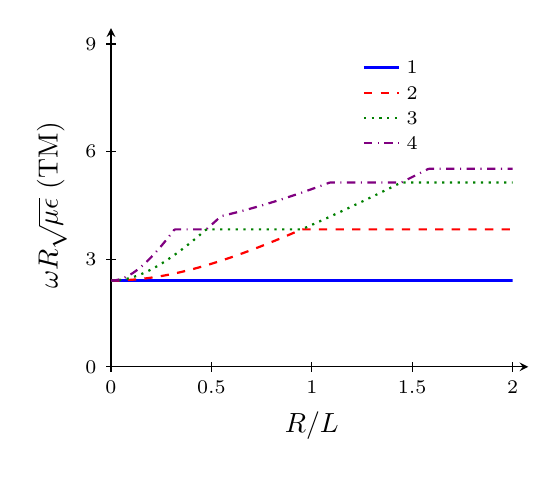
\begin{tikzpicture}[x=1cm,y=1cm,>=stealth]
\draw[->] (0,0)--(5.3,0);
\draw[->] (0,0)--(0,4.3);
\draw (0.00000,.06)--(0.00000,-.06) node[below] {\scriptsize $0$};
\draw (1.27500,.06)--(1.27500,-.06) node[below] {\scriptsize $0.5$};
\draw (2.55000,.06)--(2.55000,-.06) node[below] {\scriptsize $1$};
\draw (3.82500,.06)--(3.82500,-.06) node[below] {\scriptsize $1.5$};
\draw (5.10000,.06)--(5.10000,-.06) node[below] {\scriptsize $2$};
\draw (.06,0.00000)--(-.06,0.00000) node[left] {\scriptsize $0$};
\draw (.06,1.36667)--(-.06,1.36667) node[left] {\scriptsize $3$};
\draw (.06,2.73333)--(-.06,2.73333) node[left] {\scriptsize $6$};
\draw (.06,4.10000)--(-.06,4.10000) node[left] {\scriptsize $9$};
\node[below] at (2.55,-.45) {$R/L$};
\node[rotate=90] at (-.75,2.05) {$\omega R\sqrt{\mu\epsilon}$ (TM)};
\begin{scope}
\clip (0,0) rectangle (5.1,4.1);
\draw[blue,thick] plot coordinates {(0.002550,1.095532) (0.018529,1.095532) (0.034509,1.095532) (0.050488,1.095532) (0.066468,1.095532) (0.082447,1.095532) (0.098427,1.095532) (0.114406,1.095532) (0.130386,1.095532) (0.146365,1.095532) (0.162345,1.095532) (0.178324,1.095532) (0.194304,1.095532) (0.210283,1.095532) (0.226263,1.095532) (0.242242,1.095532) (0.258221,1.095532) (0.274201,1.095532) (0.290180,1.095532) (0.306160,1.095532) (0.322139,1.095532) (0.338119,1.095532) (0.354098,1.095532) (0.370078,1.095532) (0.386057,1.095532) (0.402037,1.095532) (0.418016,1.095532) (0.433996,1.095532) (0.449975,1.095532) (0.465955,1.095532) (0.481934,1.095532) (0.497913,1.095532) (0.513893,1.095532) (0.529872,1.095532) (0.545852,1.095532) (0.561831,1.095532) (0.577811,1.095532) (0.593790,1.095532) (0.609770,1.095532) (0.625749,1.095532) (0.641729,1.095532) (0.657708,1.095532) (0.673688,1.095532) (0.689667,1.095532) (0.705647,1.095532) (0.721626,1.095532) (0.737605,1.095532) (0.753585,1.095532) (0.769564,1.095532) (0.785544,1.095532) (0.801523,1.095532) (0.817503,1.095532) (0.833482,1.095532) (0.849462,1.095532) (0.865441,1.095532) (0.881421,1.095532) (0.897400,1.095532) (0.913380,1.095532) (0.929359,1.095532) (0.945339,1.095532) (0.961318,1.095532) (0.977297,1.095532) (0.993277,1.095532) (1.009256,1.095532) (1.025236,1.095532) (1.041215,1.095532) (1.057195,1.095532) (1.073174,1.095532) (1.089154,1.095532) (1.105133,1.095532) (1.121113,1.095532) (1.137092,1.095532) (1.153072,1.095532) (1.169051,1.095532) (1.185031,1.095532) (1.201010,1.095532) (1.216989,1.095532) (1.232969,1.095532) (1.248948,1.095532) (1.264928,1.095532) (1.280907,1.095532) (1.296887,1.095532) (1.312866,1.095532) (1.328846,1.095532) (1.344825,1.095532) (1.360805,1.095532) (1.376784,1.095532) (1.392764,1.095532) (1.408743,1.095532) (1.424723,1.095532) (1.440702,1.095532) (1.456682,1.095532) (1.472661,1.095532) (1.488640,1.095532) (1.504620,1.095532) (1.520599,1.095532) (1.536579,1.095532) (1.552558,1.095532) (1.568538,1.095532) (1.584517,1.095532) (1.600497,1.095532) (1.616476,1.095532) (1.632456,1.095532) (1.648435,1.095532) (1.664415,1.095532) (1.680394,1.095532) (1.696374,1.095532) (1.712353,1.095532) (1.728332,1.095532) (1.744312,1.095532) (1.760291,1.095532) (1.776271,1.095532) (1.792250,1.095532) (1.808230,1.095532) (1.824209,1.095532) (1.840189,1.095532) (1.856168,1.095532) (1.872148,1.095532) (1.888127,1.095532) (1.904107,1.095532) (1.920086,1.095532) (1.936066,1.095532) (1.952045,1.095532) (1.968024,1.095532) (1.984004,1.095532) (1.999983,1.095532) (2.015963,1.095532) (2.031942,1.095532) (2.047922,1.095532) (2.063901,1.095532) (2.079881,1.095532) (2.095860,1.095532) (2.111840,1.095532) (2.127819,1.095532) (2.143799,1.095532) (2.159778,1.095532) (2.175758,1.095532) (2.191737,1.095532) (2.207716,1.095532) (2.223696,1.095532) (2.239675,1.095532) (2.255655,1.095532) (2.271634,1.095532) (2.287614,1.095532) (2.303593,1.095532) (2.319573,1.095532) (2.335552,1.095532) (2.351532,1.095532) (2.367511,1.095532) (2.383491,1.095532) (2.399470,1.095532) (2.415450,1.095532) (2.431429,1.095532) (2.447408,1.095532) (2.463388,1.095532) (2.479367,1.095532) (2.495347,1.095532) (2.511326,1.095532) (2.527306,1.095532) (2.543285,1.095532) (2.559265,1.095532) (2.575244,1.095532) (2.591224,1.095532) (2.607203,1.095532) (2.623183,1.095532) (2.639162,1.095532) (2.655142,1.095532) (2.671121,1.095532) (2.687100,1.095532) (2.703080,1.095532) (2.719059,1.095532) (2.735039,1.095532) (2.751018,1.095532) (2.766998,1.095532) (2.782977,1.095532) (2.798957,1.095532) (2.814936,1.095532) (2.830916,1.095532) (2.846895,1.095532) (2.862875,1.095532) (2.878854,1.095532) (2.894834,1.095532) (2.910813,1.095532) (2.926792,1.095532) (2.942772,1.095532) (2.958751,1.095532) (2.974731,1.095532) (2.990710,1.095532) (3.006690,1.095532) (3.022669,1.095532) (3.038649,1.095532) (3.054628,1.095532) (3.070608,1.095532) (3.086587,1.095532) (3.102567,1.095532) (3.118546,1.095532) (3.134526,1.095532) (3.150505,1.095532) (3.166484,1.095532) (3.182464,1.095532) (3.198443,1.095532) (3.214423,1.095532) (3.230402,1.095532) (3.246382,1.095532) (3.262361,1.095532) (3.278341,1.095532) (3.294320,1.095532) (3.310300,1.095532) (3.326279,1.095532) (3.342259,1.095532) (3.358238,1.095532) (3.374218,1.095532) (3.390197,1.095532) (3.406176,1.095532) (3.422156,1.095532) (3.438135,1.095532) (3.454115,1.095532) (3.470094,1.095532) (3.486074,1.095532) (3.502053,1.095532) (3.518033,1.095532) (3.534012,1.095532) (3.549992,1.095532) (3.565971,1.095532) (3.581951,1.095532) (3.597930,1.095532) (3.613910,1.095532) (3.629889,1.095532) (3.645868,1.095532) (3.661848,1.095532) (3.677827,1.095532) (3.693807,1.095532) (3.709786,1.095532) (3.725766,1.095532) (3.741745,1.095532) (3.757725,1.095532) (3.773704,1.095532) (3.789684,1.095532) (3.805663,1.095532) (3.821643,1.095532) (3.837622,1.095532) (3.853602,1.095532) (3.869581,1.095532) (3.885561,1.095532) (3.901540,1.095532) (3.917519,1.095532) (3.933499,1.095532) (3.949478,1.095532) (3.965458,1.095532) (3.981437,1.095532) (3.997417,1.095532) (4.013396,1.095532) (4.029376,1.095532) (4.045355,1.095532) (4.061335,1.095532) (4.077314,1.095532) (4.093294,1.095532) (4.109273,1.095532) (4.125253,1.095532) (4.141232,1.095532) (4.157211,1.095532) (4.173191,1.095532) (4.189170,1.095532) (4.205150,1.095532) (4.221129,1.095532) (4.237109,1.095532) (4.253088,1.095532) (4.269068,1.095532) (4.285047,1.095532) (4.301027,1.095532) (4.317006,1.095532) (4.332986,1.095532) (4.348965,1.095532) (4.364945,1.095532) (4.380924,1.095532) (4.396903,1.095532) (4.412883,1.095532) (4.428862,1.095532) (4.444842,1.095532) (4.460821,1.095532) (4.476801,1.095532) (4.492780,1.095532) (4.508760,1.095532) (4.524739,1.095532) (4.540719,1.095532) (4.556698,1.095532) (4.572678,1.095532) (4.588657,1.095532) (4.604637,1.095532) (4.620616,1.095532) (4.636595,1.095532) (4.652575,1.095532) (4.668554,1.095532) (4.684534,1.095532) (4.700513,1.095532) (4.716493,1.095532) (4.732472,1.095532) (4.748452,1.095532) (4.764431,1.095532) (4.780411,1.095532) (4.796390,1.095532) (4.812370,1.095532) (4.828349,1.095532) (4.844329,1.095532) (4.860308,1.095532) (4.876287,1.095532) (4.892267,1.095532) (4.908246,1.095532) (4.924226,1.095532) (4.940205,1.095532) (4.956185,1.095532) (4.972164,1.095532) (4.988144,1.095532) (5.004123,1.095532) (5.020103,1.095532) (5.036082,1.095532) (5.052062,1.095532) (5.068041,1.095532) (5.084021,1.095532) (5.100000,1.095532)};
\draw[red,dashed,thick] plot coordinates {(0.002550,1.095533) (0.018529,1.095581) (0.034509,1.095703) (0.050488,1.095898) (0.066468,1.096167) (0.082447,1.096508) (0.098427,1.096924) (0.114406,1.097412) (0.130386,1.097973) (0.146365,1.098607) (0.162345,1.099314) (0.178324,1.100094) (0.194304,1.100946) (0.210283,1.101870) (0.226263,1.102867) (0.242242,1.103936) (0.258221,1.105076) (0.274201,1.106288) (0.290180,1.107571) (0.306160,1.108925) (0.322139,1.110350) (0.338119,1.111846) (0.354098,1.113412) (0.370078,1.115047) (0.386057,1.116753) (0.402037,1.118527) (0.418016,1.120371) (0.433996,1.122283) (0.449975,1.124264) (0.465955,1.126312) (0.481934,1.128428) (0.497913,1.130611) (0.513893,1.132861) (0.529872,1.135178) (0.545852,1.137560) (0.561831,1.140008) (0.577811,1.142521) (0.593790,1.145099) (0.609770,1.147741) (0.625749,1.150447) (0.641729,1.153217) (0.657708,1.156049) (0.673688,1.158944) (0.689667,1.161901) (0.705647,1.164919) (0.721626,1.167999) (0.737605,1.171139) (0.753585,1.174339) (0.769564,1.177598) (0.785544,1.180917) (0.801523,1.184295) (0.817503,1.187730) (0.833482,1.191224) (0.849462,1.194774) (0.865441,1.198381) (0.881421,1.202044) (0.897400,1.205762) (0.913380,1.209536) (0.929359,1.213364) (0.945339,1.217246) (0.961318,1.221182) (0.977297,1.225171) (0.993277,1.229212) (1.009256,1.233305) (1.025236,1.237450) (1.041215,1.241646) (1.057195,1.245892) (1.073174,1.250188) (1.089154,1.254533) (1.105133,1.258927) (1.121113,1.263370) (1.137092,1.267860) (1.153072,1.272398) (1.169051,1.276983) (1.185031,1.281614) (1.201010,1.286291) (1.216989,1.291013) (1.232969,1.295781) (1.248948,1.300592) (1.264928,1.305447) (1.280907,1.310346) (1.296887,1.315288) (1.312866,1.320272) (1.328846,1.325298) (1.344825,1.330366) (1.360805,1.335474) (1.376784,1.340623) (1.392764,1.345813) (1.408743,1.351041) (1.424723,1.356309) (1.440702,1.361616) (1.456682,1.366961) (1.472661,1.372343) (1.488640,1.377763) (1.504620,1.383220) (1.520599,1.388714) (1.536579,1.394243) (1.552558,1.399808) (1.568538,1.405408) (1.584517,1.411043) (1.600497,1.416713) (1.616476,1.422416) (1.632456,1.428153) (1.648435,1.433923) (1.664415,1.439725) (1.680394,1.445561) (1.696374,1.451428) (1.712353,1.457326) (1.728332,1.463256) (1.744312,1.469217) (1.760291,1.475208) (1.776271,1.481229) (1.792250,1.487280) (1.808230,1.493360) (1.824209,1.499469) (1.840189,1.505607) (1.856168,1.511773) (1.872148,1.517967) (1.888127,1.524188) (1.904107,1.530437) (1.920086,1.536713) (1.936066,1.543015) (1.952045,1.549344) (1.968024,1.555699) (1.984004,1.562079) (1.999983,1.568485) (2.015963,1.574915) (2.031942,1.581371) (2.047922,1.587850) (2.063901,1.594354) (2.079881,1.600882) (2.095860,1.607433) (2.111840,1.614007) (2.127819,1.620605) (2.143799,1.627225) (2.159778,1.633867) (2.175758,1.640532) (2.191737,1.647219) (2.207716,1.653927) (2.223696,1.660656) (2.239675,1.667407) (2.255655,1.674178) (2.271634,1.680970) (2.287614,1.687782) (2.303593,1.694614) (2.319573,1.701466) (2.335552,1.708338) (2.351532,1.715229) (2.367511,1.722139) (2.383491,1.729069) (2.399470,1.736016) (2.415450,1.742983) (2.431429,1.745555) (2.447408,1.745555) (2.463388,1.745555) (2.479367,1.745555) (2.495347,1.745555) (2.511326,1.745555) (2.527306,1.745555) (2.543285,1.745555) (2.559265,1.745555) (2.575244,1.745555) (2.591224,1.745555) (2.607203,1.745555) (2.623183,1.745555) (2.639162,1.745555) (2.655142,1.745555) (2.671121,1.745555) (2.687100,1.745555) (2.703080,1.745555) (2.719059,1.745555) (2.735039,1.745555) (2.751018,1.745555) (2.766998,1.745555) (2.782977,1.745555) (2.798957,1.745555) (2.814936,1.745555) (2.830916,1.745555) (2.846895,1.745555) (2.862875,1.745555) (2.878854,1.745555) (2.894834,1.745555) (2.910813,1.745555) (2.926792,1.745555) (2.942772,1.745555) (2.958751,1.745555) (2.974731,1.745555) (2.990710,1.745555) (3.006690,1.745555) (3.022669,1.745555) (3.038649,1.745555) (3.054628,1.745555) (3.070608,1.745555) (3.086587,1.745555) (3.102567,1.745555) (3.118546,1.745555) (3.134526,1.745555) (3.150505,1.745555) (3.166484,1.745555) (3.182464,1.745555) (3.198443,1.745555) (3.214423,1.745555) (3.230402,1.745555) (3.246382,1.745555) (3.262361,1.745555) (3.278341,1.745555) (3.294320,1.745555) (3.310300,1.745555) (3.326279,1.745555) (3.342259,1.745555) (3.358238,1.745555) (3.374218,1.745555) (3.390197,1.745555) (3.406176,1.745555) (3.422156,1.745555) (3.438135,1.745555) (3.454115,1.745555) (3.470094,1.745555) (3.486074,1.745555) (3.502053,1.745555) (3.518033,1.745555) (3.534012,1.745555) (3.549992,1.745555) (3.565971,1.745555) (3.581951,1.745555) (3.597930,1.745555) (3.613910,1.745555) (3.629889,1.745555) (3.645868,1.745555) (3.661848,1.745555) (3.677827,1.745555) (3.693807,1.745555) (3.709786,1.745555) (3.725766,1.745555) (3.741745,1.745555) (3.757725,1.745555) (3.773704,1.745555) (3.789684,1.745555) (3.805663,1.745555) (3.821643,1.745555) (3.837622,1.745555) (3.853602,1.745555) (3.869581,1.745555) (3.885561,1.745555) (3.901540,1.745555) (3.917519,1.745555) (3.933499,1.745555) (3.949478,1.745555) (3.965458,1.745555) (3.981437,1.745555) (3.997417,1.745555) (4.013396,1.745555) (4.029376,1.745555) (4.045355,1.745555) (4.061335,1.745555) (4.077314,1.745555) (4.093294,1.745555) (4.109273,1.745555) (4.125253,1.745555) (4.141232,1.745555) (4.157211,1.745555) (4.173191,1.745555) (4.189170,1.745555) (4.205150,1.745555) (4.221129,1.745555) (4.237109,1.745555) (4.253088,1.745555) (4.269068,1.745555) (4.285047,1.745555) (4.301027,1.745555) (4.317006,1.745555) (4.332986,1.745555) (4.348965,1.745555) (4.364945,1.745555) (4.380924,1.745555) (4.396903,1.745555) (4.412883,1.745555) (4.428862,1.745555) (4.444842,1.745555) (4.460821,1.745555) (4.476801,1.745555) (4.492780,1.745555) (4.508760,1.745555) (4.524739,1.745555) (4.540719,1.745555) (4.556698,1.745555) (4.572678,1.745555) (4.588657,1.745555) (4.604637,1.745555) (4.620616,1.745555) (4.636595,1.745555) (4.652575,1.745555) (4.668554,1.745555) (4.684534,1.745555) (4.700513,1.745555) (4.716493,1.745555) (4.732472,1.745555) (4.748452,1.745555) (4.764431,1.745555) (4.780411,1.745555) (4.796390,1.745555) (4.812370,1.745555) (4.828349,1.745555) (4.844329,1.745555) (4.860308,1.745555) (4.876287,1.745555) (4.892267,1.745555) (4.908246,1.745555) (4.924226,1.745555) (4.940205,1.745555) (4.956185,1.745555) (4.972164,1.745555) (4.988144,1.745555) (5.004123,1.745555) (5.020103,1.745555) (5.036082,1.745555) (5.052062,1.745555) (5.068041,1.745555) (5.084021,1.745555) (5.100000,1.745555)};
\draw[green!50!black,dotted,thick] plot coordinates {(0.002550,1.095535) (0.018529,1.095729) (0.034509,1.096216) (0.050488,1.096997) (0.066468,1.098069) (0.082447,1.099434) (0.098427,1.101089) (0.114406,1.103033) (0.130386,1.105265) (0.146365,1.107782) (0.162345,1.110584) (0.178324,1.113668) (0.194304,1.117031) (0.210283,1.120671) (0.226263,1.124586) (0.242242,1.128772) (0.258221,1.133227) (0.274201,1.137947) (0.290180,1.142928) (0.306160,1.148169) (0.322139,1.153665) (0.338119,1.159412) (0.354098,1.165407) (0.370078,1.171645) (0.386057,1.178124) (0.402037,1.184839) (0.418016,1.191786) (0.433996,1.198962) (0.449975,1.206361) (0.465955,1.213980) (0.481934,1.221815) (0.497913,1.229862) (0.513893,1.238116) (0.529872,1.246574) (0.545852,1.255231) (0.561831,1.264083) (0.577811,1.273127) (0.593790,1.282357) (0.609770,1.291771) (0.625749,1.301364) (0.641729,1.311132) (0.657708,1.321071) (0.673688,1.331178) (0.689667,1.341449) (0.705647,1.351879) (0.721626,1.362466) (0.737605,1.373206) (0.753585,1.384094) (0.769564,1.395129) (0.785544,1.406305) (0.801523,1.417620) (0.817503,1.429071) (0.833482,1.440654) (0.849462,1.452367) (0.865441,1.464205) (0.881421,1.476167) (0.897400,1.488248) (0.913380,1.500446) (0.929359,1.512759) (0.945339,1.525184) (0.961318,1.537717) (0.977297,1.550356) (0.993277,1.563100) (1.009256,1.575944) (1.025236,1.588887) (1.041215,1.601926) (1.057195,1.615059) (1.073174,1.628283) (1.089154,1.641598) (1.105133,1.654999) (1.121113,1.668486) (1.137092,1.682056) (1.153072,1.695706) (1.169051,1.709437) (1.185031,1.723244) (1.201010,1.737127) (1.216989,1.745555) (1.232969,1.745555) (1.248948,1.745555) (1.264928,1.745555) (1.280907,1.745555) (1.296887,1.745555) (1.312866,1.745555) (1.328846,1.745555) (1.344825,1.745555) (1.360805,1.745555) (1.376784,1.745555) (1.392764,1.745555) (1.408743,1.745555) (1.424723,1.745555) (1.440702,1.745555) (1.456682,1.745555) (1.472661,1.745555) (1.488640,1.745555) (1.504620,1.745555) (1.520599,1.745555) (1.536579,1.745555) (1.552558,1.745555) (1.568538,1.745555) (1.584517,1.745555) (1.600497,1.745555) (1.616476,1.745555) (1.632456,1.745555) (1.648435,1.745555) (1.664415,1.745555) (1.680394,1.745555) (1.696374,1.745555) (1.712353,1.745555) (1.728332,1.745555) (1.744312,1.745555) (1.760291,1.745555) (1.776271,1.745555) (1.792250,1.745555) (1.808230,1.745555) (1.824209,1.745555) (1.840189,1.745555) (1.856168,1.745555) (1.872148,1.745555) (1.888127,1.745555) (1.904107,1.745555) (1.920086,1.745555) (1.936066,1.745555) (1.952045,1.745555) (1.968024,1.745555) (1.984004,1.745555) (1.999983,1.745555) (2.015963,1.745555) (2.031942,1.745555) (2.047922,1.745555) (2.063901,1.745555) (2.079881,1.745555) (2.095860,1.745555) (2.111840,1.745555) (2.127819,1.745555) (2.143799,1.745555) (2.159778,1.745555) (2.175758,1.745555) (2.191737,1.745555) (2.207716,1.745555) (2.223696,1.745555) (2.239675,1.745555) (2.255655,1.745555) (2.271634,1.745555) (2.287614,1.745555) (2.303593,1.745555) (2.319573,1.745555) (2.335552,1.745555) (2.351532,1.745555) (2.367511,1.745555) (2.383491,1.745555) (2.399470,1.745555) (2.415450,1.745555) (2.431429,1.749967) (2.447408,1.756970) (2.463388,1.763990) (2.479367,1.771028) (2.495347,1.778083) (2.511326,1.785156) (2.527306,1.792245) (2.543285,1.799351) (2.559265,1.806474) (2.575244,1.813613) (2.591224,1.820768) (2.607203,1.827940) (2.623183,1.835127) (2.639162,1.842329) (2.655142,1.849547) (2.671121,1.856781) (2.687100,1.864029) (2.703080,1.871293) (2.719059,1.878571) (2.735039,1.885864) (2.751018,1.893171) (2.766998,1.900492) (2.782977,1.907827) (2.798957,1.915177) (2.814936,1.922540) (2.830916,1.929916) (2.846895,1.937306) (2.862875,1.944710) (2.878854,1.952126) (2.894834,1.959555) (2.910813,1.966998) (2.926792,1.974453) (2.942772,1.981920) (2.958751,1.989400) (2.974731,1.996892) (2.990710,2.004396) (3.006690,2.011912) (3.022669,2.019441) (3.038649,2.026980) (3.054628,2.034532) (3.070608,2.042095) (3.086587,2.049669) (3.102567,2.057254) (3.118546,2.064851) (3.134526,2.072458) (3.150505,2.080077) (3.166484,2.087706) (3.182464,2.095345) (3.198443,2.102995) (3.214423,2.110656) (3.230402,2.118327) (3.246382,2.126008) (3.262361,2.133699) (3.278341,2.141399) (3.294320,2.149110) (3.310300,2.156831) (3.326279,2.164561) (3.342259,2.172300) (3.358238,2.180049) (3.374218,2.187808) (3.390197,2.195575) (3.406176,2.203352) (3.422156,2.211138) (3.438135,2.218932) (3.454115,2.226736) (3.470094,2.234548) (3.486074,2.242369) (3.502053,2.250198) (3.518033,2.258036) (3.534012,2.265883) (3.549992,2.273737) (3.565971,2.281600) (3.581951,2.289471) (3.597930,2.297350) (3.613910,2.305237) (3.629889,2.313132) (3.645868,2.321034) (3.661848,2.328945) (3.677827,2.336863) (3.693807,2.339561) (3.709786,2.339561) (3.725766,2.339561) (3.741745,2.339561) (3.757725,2.339561) (3.773704,2.339561) (3.789684,2.339561) (3.805663,2.339561) (3.821643,2.339561) (3.837622,2.339561) (3.853602,2.339561) (3.869581,2.339561) (3.885561,2.339561) (3.901540,2.339561) (3.917519,2.339561) (3.933499,2.339561) (3.949478,2.339561) (3.965458,2.339561) (3.981437,2.339561) (3.997417,2.339561) (4.013396,2.339561) (4.029376,2.339561) (4.045355,2.339561) (4.061335,2.339561) (4.077314,2.339561) (4.093294,2.339561) (4.109273,2.339561) (4.125253,2.339561) (4.141232,2.339561) (4.157211,2.339561) (4.173191,2.339561) (4.189170,2.339561) (4.205150,2.339561) (4.221129,2.339561) (4.237109,2.339561) (4.253088,2.339561) (4.269068,2.339561) (4.285047,2.339561) (4.301027,2.339561) (4.317006,2.339561) (4.332986,2.339561) (4.348965,2.339561) (4.364945,2.339561) (4.380924,2.339561) (4.396903,2.339561) (4.412883,2.339561) (4.428862,2.339561) (4.444842,2.339561) (4.460821,2.339561) (4.476801,2.339561) (4.492780,2.339561) (4.508760,2.339561) (4.524739,2.339561) (4.540719,2.339561) (4.556698,2.339561) (4.572678,2.339561) (4.588657,2.339561) (4.604637,2.339561) (4.620616,2.339561) (4.636595,2.339561) (4.652575,2.339561) (4.668554,2.339561) (4.684534,2.339561) (4.700513,2.339561) (4.716493,2.339561) (4.732472,2.339561) (4.748452,2.339561) (4.764431,2.339561) (4.780411,2.339561) (4.796390,2.339561) (4.812370,2.339561) (4.828349,2.339561) (4.844329,2.339561) (4.860308,2.339561) (4.876287,2.339561) (4.892267,2.339561) (4.908246,2.339561) (4.924226,2.339561) (4.940205,2.339561) (4.956185,2.339561) (4.972164,2.339561) (4.988144,2.339561) (5.004123,2.339561) (5.020103,2.339561) (5.036082,2.339561) (5.052062,2.339561) (5.068041,2.339561) (5.084021,2.339561) (5.100000,2.339561)};
\draw[violet,dash dot,thick] plot coordinates {(0.002550,1.095540) (0.018529,1.095976) (0.034509,1.097071) (0.050488,1.098825) (0.066468,1.101233) (0.082447,1.104292) (0.098427,1.107996) (0.114406,1.112338) (0.130386,1.117311) (0.146365,1.122908) (0.162345,1.129118) (0.178324,1.135931) (0.194304,1.143337) (0.210283,1.151324) (0.226263,1.159881) (0.242242,1.168994) (0.258221,1.178651) (0.274201,1.188839) (0.290180,1.199544) (0.306160,1.210752) (0.322139,1.222449) (0.338119,1.234623) (0.354098,1.247257) (0.370078,1.260340) (0.386057,1.273856) (0.402037,1.287793) (0.418016,1.302137) (0.433996,1.316874) (0.449975,1.331992) (0.465955,1.347477) (0.481934,1.363318) (0.497913,1.379501) (0.513893,1.396015) (0.529872,1.412849) (0.545852,1.429991) (0.561831,1.447430) (0.577811,1.465155) (0.593790,1.483157) (0.609770,1.501425) (0.625749,1.519949) (0.641729,1.538722) (0.657708,1.557732) (0.673688,1.576973) (0.689667,1.596435) (0.705647,1.616111) (0.721626,1.635992) (0.737605,1.656072) (0.753585,1.676343) (0.769564,1.696799) (0.785544,1.717433) (0.801523,1.738238) (0.817503,1.745555) (0.833482,1.745555) (0.849462,1.745555) (0.865441,1.745555) (0.881421,1.745555) (0.897400,1.745555) (0.913380,1.745555) (0.929359,1.745555) (0.945339,1.745555) (0.961318,1.745555) (0.977297,1.745555) (0.993277,1.745555) (1.009256,1.745555) (1.025236,1.745555) (1.041215,1.745555) (1.057195,1.745555) (1.073174,1.745555) (1.089154,1.745555) (1.105133,1.745555) (1.121113,1.745555) (1.137092,1.745555) (1.153072,1.745555) (1.169051,1.745555) (1.185031,1.745555) (1.201010,1.745555) (1.216989,1.751083) (1.232969,1.765112) (1.248948,1.779211) (1.264928,1.793378) (1.280907,1.807612) (1.296887,1.821912) (1.312866,1.836275) (1.328846,1.850701) (1.344825,1.865187) (1.360805,1.879734) (1.376784,1.894338) (1.392764,1.908999) (1.408743,1.916269) (1.424723,1.919986) (1.440702,1.923739) (1.456682,1.927525) (1.472661,1.931346) (1.488640,1.935201) (1.504620,1.939090) (1.520599,1.943013) (1.536579,1.946968) (1.552558,1.950957) (1.568538,1.954979) (1.584517,1.959034) (1.600497,1.963122) (1.616476,1.967242) (1.632456,1.971394) (1.648435,1.975578) (1.664415,1.979793) (1.680394,1.984041) (1.696374,1.988320) (1.712353,1.992629) (1.728332,1.996970) (1.744312,2.001342) (1.760291,2.005744) (1.776271,2.010177) (1.792250,2.014640) (1.808230,2.019132) (1.824209,2.023655) (1.840189,2.028207) (1.856168,2.032789) (1.872148,2.037399) (1.888127,2.042039) (1.904107,2.046707) (1.920086,2.051404) (1.936066,2.056130) (1.952045,2.060883) (1.968024,2.065665) (1.984004,2.070474) (1.999983,2.075311) (2.015963,2.080176) (2.031942,2.085067) (2.047922,2.089986) (2.063901,2.094931) (2.079881,2.099904) (2.095860,2.104902) (2.111840,2.109927) (2.127819,2.114978) (2.143799,2.120055) (2.159778,2.125158) (2.175758,2.130286) (2.191737,2.135439) (2.207716,2.140618) (2.223696,2.145822) (2.239675,2.151050) (2.255655,2.156303) (2.271634,2.161581) (2.287614,2.166883) (2.303593,2.172209) (2.319573,2.177558) (2.335552,2.182932) (2.351532,2.188329) (2.367511,2.193750) (2.383491,2.199193) (2.399470,2.204660) (2.415450,2.210150) (2.431429,2.215662) (2.447408,2.221197) (2.463388,2.226754) (2.479367,2.232333) (2.495347,2.237935) (2.511326,2.243558) (2.527306,2.249203) (2.543285,2.254870) (2.559265,2.260557) (2.575244,2.266267) (2.591224,2.271997) (2.607203,2.277748) (2.623183,2.283520) (2.639162,2.289312) (2.655142,2.295125) (2.671121,2.300958) (2.687100,2.306811) (2.703080,2.312684) (2.719059,2.318577) (2.735039,2.324490) (2.751018,2.330422) (2.766998,2.336374) (2.782977,2.339561) (2.798957,2.339561) (2.814936,2.339561) (2.830916,2.339561) (2.846895,2.339561) (2.862875,2.339561) (2.878854,2.339561) (2.894834,2.339561) (2.910813,2.339561) (2.926792,2.339561) (2.942772,2.339561) (2.958751,2.339561) (2.974731,2.339561) (2.990710,2.339561) (3.006690,2.339561) (3.022669,2.339561) (3.038649,2.339561) (3.054628,2.339561) (3.070608,2.339561) (3.086587,2.339561) (3.102567,2.339561) (3.118546,2.339561) (3.134526,2.339561) (3.150505,2.339561) (3.166484,2.339561) (3.182464,2.339561) (3.198443,2.339561) (3.214423,2.339561) (3.230402,2.339561) (3.246382,2.339561) (3.262361,2.339561) (3.278341,2.339561) (3.294320,2.339561) (3.310300,2.339561) (3.326279,2.339561) (3.342259,2.339561) (3.358238,2.339561) (3.374218,2.339561) (3.390197,2.339561) (3.406176,2.339561) (3.422156,2.339561) (3.438135,2.339561) (3.454115,2.339561) (3.470094,2.339561) (3.486074,2.339561) (3.502053,2.339561) (3.518033,2.339561) (3.534012,2.339561) (3.549992,2.339561) (3.565971,2.339561) (3.581951,2.339561) (3.597930,2.339561) (3.613910,2.339561) (3.629889,2.339561) (3.645868,2.339561) (3.661848,2.339561) (3.677827,2.339561) (3.693807,2.344788) (3.709786,2.352721) (3.725766,2.360662) (3.741745,2.368609) (3.757725,2.376565) (3.773704,2.384527) (3.789684,2.392496) (3.805663,2.400473) (3.821643,2.408456) (3.837622,2.416446) (3.853602,2.424443) (3.869581,2.432447) (3.885561,2.440458) (3.901540,2.448475) (3.917519,2.456499) (3.933499,2.464529) (3.949478,2.472566) (3.965458,2.480609) (3.981437,2.488659) (3.997417,2.496715) (4.013396,2.504777) (4.029376,2.512845) (4.045355,2.514702) (4.061335,2.514702) (4.077314,2.514702) (4.093294,2.514702) (4.109273,2.514702) (4.125253,2.514702) (4.141232,2.514702) (4.157211,2.514702) (4.173191,2.514702) (4.189170,2.514702) (4.205150,2.514702) (4.221129,2.514702) (4.237109,2.514702) (4.253088,2.514702) (4.269068,2.514702) (4.285047,2.514702) (4.301027,2.514702) (4.317006,2.514702) (4.332986,2.514702) (4.348965,2.514702) (4.364945,2.514702) (4.380924,2.514702) (4.396903,2.514702) (4.412883,2.514702) (4.428862,2.514702) (4.444842,2.514702) (4.460821,2.514702) (4.476801,2.514702) (4.492780,2.514702) (4.508760,2.514702) (4.524739,2.514702) (4.540719,2.514702) (4.556698,2.514702) (4.572678,2.514702) (4.588657,2.514702) (4.604637,2.514702) (4.620616,2.514702) (4.636595,2.514702) (4.652575,2.514702) (4.668554,2.514702) (4.684534,2.514702) (4.700513,2.514702) (4.716493,2.514702) (4.732472,2.514702) (4.748452,2.514702) (4.764431,2.514702) (4.780411,2.514702) (4.796390,2.514702) (4.812370,2.514702) (4.828349,2.514702) (4.844329,2.514702) (4.860308,2.514702) (4.876287,2.514702) (4.892267,2.514702) (4.908246,2.514702) (4.924226,2.514702) (4.940205,2.514702) (4.956185,2.514702) (4.972164,2.514702) (4.988144,2.514702) (5.004123,2.514702) (5.020103,2.514702) (5.036082,2.514702) (5.052062,2.514702) (5.068041,2.514702) (5.084021,2.514702) (5.100000,2.514702)};
\end{scope}
\draw[blue,thick] (3.2129999999999996,3.8)--(3.663,3.8);
\node[right,fill=white,inner sep=1pt] at (3.7129999999999996,3.8) {\scriptsize 1};
\draw[red,dashed,thick] (3.2129999999999996,3.48)--(3.663,3.48);
\node[right,fill=white,inner sep=1pt] at (3.7129999999999996,3.48) {\scriptsize 2};
\draw[green!50!black,dotted,thick] (3.2129999999999996,3.1599999999999997)--(3.663,3.1599999999999997);
\node[right,fill=white,inner sep=1pt] at (3.7129999999999996,3.1599999999999997) {\scriptsize 3};
\draw[violet,dash dot,thick] (3.2129999999999996,2.84)--(3.663,2.84);
\node[right,fill=white,inner sep=1pt] at (3.7129999999999996,2.84) {\scriptsize 4};
\end{tikzpicture}
\quad
\begin{tikzpicture}[x=1cm,y=1cm,>=stealth]
\draw[->] (0,0)--(5.3,0);
\draw[->] (0,0)--(0,4.3);
\draw (0.00000,.06)--(0.00000,-.06) node[below] {\scriptsize $0$};
\draw (1.27500,.06)--(1.27500,-.06) node[below] {\scriptsize $0.5$};
\draw (2.55000,.06)--(2.55000,-.06) node[below] {\scriptsize $1$};
\draw (3.82500,.06)--(3.82500,-.06) node[below] {\scriptsize $1.5$};
\draw (5.10000,.06)--(5.10000,-.06) node[below] {\scriptsize $2$};
\draw (.06,0.00000)--(-.06,0.00000) node[left] {\scriptsize $0$};
\draw (.06,1.36667)--(-.06,1.36667) node[left] {\scriptsize $3$};
\draw (.06,2.73333)--(-.06,2.73333) node[left] {\scriptsize $6$};
\draw (.06,4.10000)--(-.06,4.10000) node[left] {\scriptsize $9$};
\node[below] at (2.55,-.45) {$R/L$};
\node[rotate=90] at (-.75,2.05) {$\omega R\sqrt{\mu\epsilon}$ (TE)};
\begin{scope}
\clip (0,0) rectangle (5.1,4.1);
\draw[blue,thick] plot coordinates {(0.002550,0.838763) (0.018529,0.838826) (0.034509,0.838985) (0.050488,0.839240) (0.066468,0.839591) (0.082447,0.840037) (0.098427,0.840579) (0.114406,0.841216) (0.130386,0.841948) (0.146365,0.842775) (0.162345,0.843696) (0.178324,0.844711) (0.194304,0.845821) (0.210283,0.847024) (0.226263,0.848320) (0.242242,0.849709) (0.258221,0.851190) (0.274201,0.852763) (0.290180,0.854427) (0.306160,0.856181) (0.322139,0.858026) (0.338119,0.859961) (0.354098,0.861984) (0.370078,0.864096) (0.386057,0.866295) (0.402037,0.868582) (0.418016,0.870955) (0.433996,0.873413) (0.449975,0.875957) (0.465955,0.878584) (0.481934,0.881295) (0.497913,0.884089) (0.513893,0.886965) (0.529872,0.889921) (0.545852,0.892958) (0.561831,0.896075) (0.577811,0.899270) (0.593790,0.902543) (0.609770,0.905893) (0.625749,0.909319) (0.641729,0.912820) (0.657708,0.916396) (0.673688,0.920045) (0.689667,0.923767) (0.705647,0.927560) (0.721626,0.931425) (0.737605,0.935359) (0.753585,0.939363) (0.769564,0.943435) (0.785544,0.947574) (0.801523,0.951780) (0.817503,0.956052) (0.833482,0.960388) (0.849462,0.964788) (0.865441,0.969251) (0.881421,0.973776) (0.897400,0.978363) (0.913380,0.983010) (0.929359,0.987716) (0.945339,0.992482) (0.961318,0.997305) (0.977297,1.002185) (0.993277,1.007121) (1.009256,1.012113) (1.025236,1.017160) (1.041215,1.022260) (1.057195,1.027413) (1.073174,1.032618) (1.089154,1.037875) (1.105133,1.043182) (1.121113,1.048539) (1.137092,1.053946) (1.153072,1.059400) (1.169051,1.064902) (1.185031,1.070451) (1.201010,1.076046) (1.216989,1.081687) (1.232969,1.087372) (1.248948,1.093102) (1.264928,1.098874) (1.280907,1.104689) (1.296887,1.110547) (1.312866,1.116445) (1.328846,1.122384) (1.344825,1.128364) (1.360805,1.134382) (1.376784,1.140440) (1.392764,1.146535) (1.408743,1.152668) (1.424723,1.158838) (1.440702,1.165045) (1.456682,1.171287) (1.472661,1.177564) (1.488640,1.183876) (1.504620,1.190222) (1.520599,1.196602) (1.536579,1.203015) (1.552558,1.209460) (1.568538,1.215937) (1.584517,1.222446) (1.600497,1.228986) (1.616476,1.235556) (1.632456,1.242156) (1.648435,1.248786) (1.664415,1.255444) (1.680394,1.262132) (1.696374,1.268847) (1.712353,1.275590) (1.728332,1.282361) (1.744312,1.289158) (1.760291,1.295982) (1.776271,1.302832) (1.792250,1.309707) (1.808230,1.316607) (1.824209,1.323533) (1.840189,1.330482) (1.856168,1.337456) (1.872148,1.344453) (1.888127,1.351474) (1.904107,1.358517) (1.920086,1.365583) (1.936066,1.372672) (1.952045,1.379782) (1.968024,1.386914) (1.984004,1.394067) (1.999983,1.401241) (2.015963,1.408435) (2.031942,1.415650) (2.047922,1.422884) (2.063901,1.430139) (2.079881,1.437412) (2.095860,1.444705) (2.111840,1.452016) (2.127819,1.459346) (2.143799,1.466694) (2.159778,1.474060) (2.175758,1.481444) (2.191737,1.488845) (2.207716,1.496264) (2.223696,1.503699) (2.239675,1.511151) (2.255655,1.518619) (2.271634,1.526103) (2.287614,1.533603) (2.303593,1.541119) (2.319573,1.548651) (2.335552,1.556197) (2.351532,1.563759) (2.367511,1.571336) (2.383491,1.578927) (2.399470,1.586532) (2.415450,1.594152) (2.431429,1.601785) (2.447408,1.609433) (2.463388,1.617094) (2.479367,1.624768) (2.495347,1.632455) (2.511326,1.640156) (2.527306,1.647869) (2.543285,1.655595) (2.559265,1.663334) (2.575244,1.671084) (2.591224,1.678847) (2.607203,1.686622) (2.623183,1.694409) (2.639162,1.702207) (2.655142,1.710017) (2.671121,1.717838) (2.687100,1.725670) (2.703080,1.733513) (2.719059,1.741367) (2.735039,1.749232) (2.751018,1.757107) (2.766998,1.764993) (2.782977,1.772889) (2.798957,1.780796) (2.814936,1.788712) (2.830916,1.796638) (2.846895,1.804574) (2.862875,1.812519) (2.878854,1.820474) (2.894834,1.828439) (2.910813,1.836413) (2.926792,1.844395) (2.942772,1.852387) (2.958751,1.860388) (2.974731,1.868397) (2.990710,1.876416) (3.006690,1.884442) (3.022669,1.892478) (3.038649,1.900521) (3.054628,1.908573) (3.070608,1.916633) (3.086587,1.924701) (3.102567,1.932777) (3.118546,1.940861) (3.134526,1.948952) (3.150505,1.957051) (3.166484,1.965158) (3.182464,1.973272) (3.198443,1.981394) (3.214423,1.989522) (3.230402,1.997658) (3.246382,2.005801) (3.262361,2.013952) (3.278341,2.022109) (3.294320,2.030272) (3.310300,2.038443) (3.326279,2.046620) (3.342259,2.054804) (3.358238,2.062995) (3.374218,2.071192) (3.390197,2.079395) (3.406176,2.087604) (3.422156,2.095820) (3.438135,2.104042) (3.454115,2.112270) (3.470094,2.120504) (3.486074,2.128744) (3.502053,2.136990) (3.518033,2.145241) (3.534012,2.153498) (3.549992,2.161761) (3.565971,2.170030) (3.581951,2.178304) (3.597930,2.186584) (3.613910,2.194869) (3.629889,2.203159) (3.645868,2.211455) (3.661848,2.219756) (3.677827,2.228062) (3.693807,2.236373) (3.709786,2.244689) (3.725766,2.253010) (3.741745,2.261336) (3.757725,2.269667) (3.773704,2.278003) (3.789684,2.286344) (3.805663,2.294689) (3.821643,2.303040) (3.837622,2.311394) (3.853602,2.319754) (3.869581,2.328117) (3.885561,2.336486) (3.901540,2.344859) (3.917519,2.353236) (3.933499,2.361617) (3.949478,2.370003) (3.965458,2.378393) (3.981437,2.386787) (3.997417,2.395186) (4.013396,2.403588) (4.029376,2.411995) (4.045355,2.420406) (4.061335,2.428820) (4.077314,2.437239) (4.093294,2.445661) (4.109273,2.454088) (4.125253,2.462518) (4.141232,2.470952) (4.157211,2.479390) (4.173191,2.487831) (4.189170,2.496276) (4.205150,2.504725) (4.221129,2.513177) (4.237109,2.521633) (4.253088,2.530093) (4.269068,2.538556) (4.285047,2.547022) (4.301027,2.555492) (4.317006,2.563965) (4.332986,2.572442) (4.348965,2.580922) (4.364945,2.589405) (4.380924,2.597891) (4.396903,2.606381) (4.412883,2.614874) (4.428862,2.623370) (4.444842,2.631869) (4.460821,2.640371) (4.476801,2.648877) (4.492780,2.657385) (4.508760,2.665896) (4.524739,2.674411) (4.540719,2.682928) (4.556698,2.691448) (4.572678,2.699972) (4.588657,2.708498) (4.604637,2.717027) (4.620616,2.725558) (4.636595,2.734093) (4.652575,2.742630) (4.668554,2.751170) (4.684534,2.759713) (4.700513,2.768258) (4.716493,2.776807) (4.732472,2.785357) (4.748452,2.793911) (4.764431,2.802467) (4.780411,2.811025) (4.796390,2.819586) (4.812370,2.828150) (4.828349,2.836716) (4.844329,2.845285) (4.860308,2.853856) (4.876287,2.862429) (4.892267,2.871005) (4.908246,2.879583) (4.924226,2.888164) (4.940205,2.896747) (4.956185,2.905332) (4.972164,2.913920) (4.988144,2.922510) (5.004123,2.931102) (5.020103,2.939697) (5.036082,2.948293) (5.052062,2.956892) (5.068041,2.965493) (5.084021,2.974097) (5.100000,2.982702)};
\draw[red,dashed,thick] plot coordinates {(0.002550,0.838766) (0.018529,0.839019) (0.034509,0.839655) (0.050488,0.840674) (0.066468,0.842073) (0.082447,0.843852) (0.098427,0.846007) (0.114406,0.848535) (0.130386,0.851435) (0.146365,0.854701) (0.162345,0.858329) (0.178324,0.862315) (0.194304,0.866654) (0.210283,0.871341) (0.226263,0.876370) (0.242242,0.881736) (0.258221,0.887431) (0.274201,0.893450) (0.290180,0.899787) (0.306160,0.906434) (0.322139,0.913386) (0.338119,0.920634) (0.354098,0.928172) (0.370078,0.935994) (0.386057,0.944091) (0.402037,0.952457) (0.418016,0.961086) (0.433996,0.969969) (0.449975,0.979100) (0.465955,0.988473) (0.481934,0.998080) (0.497913,1.007914) (0.513893,1.017970) (0.529872,1.028240) (0.545852,1.038718) (0.561831,1.049399) (0.577811,1.060275) (0.593790,1.071341) (0.609770,1.082591) (0.625749,1.094020) (0.641729,1.105621) (0.657708,1.117390) (0.673688,1.129321) (0.689667,1.141410) (0.705647,1.153650) (0.721626,1.166038) (0.737605,1.178569) (0.753585,1.191238) (0.769564,1.204041) (0.785544,1.216974) (0.801523,1.230032) (0.817503,1.243212) (0.833482,1.256510) (0.849462,1.269921) (0.865441,1.283444) (0.881421,1.297073) (0.897400,1.310806) (0.913380,1.324640) (0.929359,1.338571) (0.945339,1.352596) (0.961318,1.366713) (0.977297,1.380919) (0.993277,1.395210) (1.009256,1.409585) (1.025236,1.424041) (1.041215,1.438575) (1.057195,1.453185) (1.073174,1.467869) (1.089154,1.482624) (1.105133,1.497449) (1.121113,1.512341) (1.137092,1.527299) (1.153072,1.534513) (1.169051,1.538317) (1.185031,1.542164) (1.201010,1.546052) (1.216989,1.549984) (1.232969,1.553957) (1.248948,1.557971) (1.264928,1.562027) (1.280907,1.566123) (1.296887,1.570260) (1.312866,1.574437) (1.328846,1.578654) (1.344825,1.582911) (1.360805,1.587207) (1.376784,1.591542) (1.392764,1.595915) (1.408743,1.600327) (1.424723,1.604777) (1.440702,1.609264) (1.456682,1.613789) (1.472661,1.618351) (1.488640,1.622950) (1.504620,1.627585) (1.520599,1.632256) (1.536579,1.636963) (1.552558,1.641705) (1.568538,1.646483) (1.584517,1.651295) (1.600497,1.656143) (1.616476,1.661024) (1.632456,1.665939) (1.648435,1.670888) (1.664415,1.675871) (1.680394,1.680886) (1.696374,1.685935) (1.712353,1.691015) (1.728332,1.696128) (1.744312,1.701273) (1.760291,1.706450) (1.776271,1.711658) (1.792250,1.716897) (1.808230,1.722166) (1.824209,1.727467) (1.840189,1.732797) (1.856168,1.738157) (1.872148,1.743547) (1.888127,1.748967) (1.904107,1.754415) (1.920086,1.759892) (1.936066,1.765398) (1.952045,1.770932) (1.968024,1.776494) (1.984004,1.782084) (1.999983,1.787702) (2.015963,1.793347) (2.031942,1.799018) (2.047922,1.804717) (2.063901,1.810442) (2.079881,1.816193) (2.095860,1.821970) (2.111840,1.827773) (2.127819,1.833601) (2.143799,1.839455) (2.159778,1.845334) (2.175758,1.851237) (2.191737,1.857165) (2.207716,1.863118) (2.223696,1.869094) (2.239675,1.875094) (2.255655,1.881118) (2.271634,1.887165) (2.287614,1.893236) (2.303593,1.899329) (2.319573,1.905445) (2.335552,1.911584) (2.351532,1.917745) (2.367511,1.923928) (2.383491,1.930133) (2.399470,1.936359) (2.415450,1.942607) (2.431429,1.948876) (2.447408,1.955166) (2.463388,1.961478) (2.479367,1.967809) (2.495347,1.974161) (2.511326,1.980534) (2.527306,1.986926) (2.543285,1.993338) (2.559265,1.999770) (2.575244,2.006222) (2.591224,2.012692) (2.607203,2.019182) (2.623183,2.025691) (2.639162,2.032218) (2.655142,2.038764) (2.671121,2.045329) (2.687100,2.051911) (2.703080,2.058512) (2.719059,2.065130) (2.735039,2.071766) (2.751018,2.078420) (2.766998,2.085091) (2.782977,2.091779) (2.798957,2.098484) (2.814936,2.105206) (2.830916,2.111945) (2.846895,2.118700) (2.862875,2.125471) (2.878854,2.132259) (2.894834,2.139063) (2.910813,2.145883) (2.926792,2.152718) (2.942772,2.159570) (2.958751,2.166436) (2.974731,2.173318) (2.990710,2.180215) (3.006690,2.187127) (3.022669,2.194054) (3.038649,2.200996) (3.054628,2.207952) (3.070608,2.214923) (3.086587,2.221908) (3.102567,2.228908) (3.118546,2.235921) (3.134526,2.242948) (3.150505,2.249989) (3.166484,2.257044) (3.182464,2.264112) (3.198443,2.271194) (3.214423,2.278289) (3.230402,2.285397) (3.246382,2.292519) (3.262361,2.299653) (3.278341,2.306800) (3.294320,2.313959) (3.310300,2.321132) (3.326279,2.328316) (3.342259,2.335513) (3.358238,2.342723) (3.374218,2.349944) (3.390197,2.357177) (3.406176,2.364423) (3.422156,2.371680) (3.438135,2.378948) (3.454115,2.386229) (3.470094,2.393520) (3.486074,2.400823) (3.502053,2.408138) (3.518033,2.415463) (3.534012,2.422800) (3.549992,2.430147) (3.565971,2.437505) (3.581951,2.444874) (3.597930,2.452254) (3.613910,2.459644) (3.629889,2.467045) (3.645868,2.474456) (3.661848,2.481878) (3.677827,2.489309) (3.693807,2.496751) (3.709786,2.504203) (3.725766,2.511664) (3.741745,2.519136) (3.757725,2.526617) (3.773704,2.534108) (3.789684,2.541608) (3.805663,2.549118) (3.821643,2.556637) (3.837622,2.564166) (3.853602,2.571704) (3.869581,2.579251) (3.885561,2.586807) (3.901540,2.594372) (3.917519,2.601946) (3.933499,2.609528) (3.949478,2.617120) (3.965458,2.624720) (3.981437,2.632329) (3.997417,2.639946) (4.013396,2.647572) (4.029376,2.655207) (4.045355,2.662849) (4.061335,2.670500) (4.077314,2.678159) (4.093294,2.685826) (4.109273,2.693501) (4.125253,2.701184) (4.141232,2.708875) (4.157211,2.716574) (4.173191,2.724281) (4.189170,2.731995) (4.205150,2.739717) (4.221129,2.747447) (4.237109,2.755184) (4.253088,2.762928) (4.269068,2.770680) (4.285047,2.778439) (4.301027,2.786205) (4.317006,2.793979) (4.332986,2.801760) (4.348965,2.809548) (4.364945,2.817343) (4.380924,2.825144) (4.396903,2.832953) (4.412883,2.840769) (4.428862,2.848591) (4.444842,2.856420) (4.460821,2.864256) (4.476801,2.872099) (4.492780,2.879948) (4.508760,2.887803) (4.524739,2.895665) (4.540719,2.903533) (4.556698,2.911408) (4.572678,2.919289) (4.588657,2.927177) (4.604637,2.935070) (4.620616,2.942970) (4.636595,2.950876) (4.652575,2.958787) (4.668554,2.966705) (4.684534,2.974629) (4.700513,2.982559) (4.716493,2.990495) (4.732472,2.998436) (4.748452,3.006383) (4.764431,3.014336) (4.780411,3.022295) (4.796390,3.030259) (4.812370,3.038229) (4.828349,3.046204) (4.844329,3.054185) (4.860308,3.062172) (4.876287,3.070163) (4.892267,3.078161) (4.908246,3.086163) (4.924226,3.094171) (4.940205,3.102184) (4.956185,3.110202) (4.972164,3.118226) (4.988144,3.126255) (5.004123,3.134288) (5.020103,3.142327) (5.036082,3.150371) (5.052062,3.158420) (5.068041,3.166473) (5.084021,3.174532) (5.100000,3.182595)};
\draw[green!50!black,dotted,thick] plot coordinates {(0.002550,0.838772) (0.018529,0.839342) (0.034509,0.840772) (0.050488,0.843058) (0.066468,0.846195) (0.082447,0.850171) (0.098427,0.854977) (0.114406,0.860597) (0.130386,0.867016) (0.146365,0.874216) (0.162345,0.882178) (0.178324,0.890882) (0.194304,0.900306) (0.210283,0.910428) (0.226263,0.921225) (0.242242,0.932673) (0.258221,0.944749) (0.274201,0.957429) (0.290180,0.970689) (0.306160,0.984506) (0.322139,0.998856) (0.338119,1.013718) (0.354098,1.029069) (0.370078,1.044887) (0.386057,1.061151) (0.402037,1.077842) (0.418016,1.094939) (0.433996,1.112425) (0.449975,1.130280) (0.465955,1.148489) (0.481934,1.167033) (0.497913,1.185898) (0.513893,1.205068) (0.529872,1.224530) (0.545852,1.244269) (0.561831,1.264272) (0.577811,1.284527) (0.593790,1.305023) (0.609770,1.325748) (0.625749,1.346691) (0.641729,1.367843) (0.657708,1.389194) (0.673688,1.410736) (0.689667,1.432458) (0.705647,1.446641) (0.721626,1.449122) (0.737605,1.451654) (0.753585,1.454237) (0.769564,1.456871) (0.785544,1.459555) (0.801523,1.462289) (0.817503,1.465072) (0.833482,1.467906) (0.849462,1.470788) (0.865441,1.473720) (0.881421,1.476700) (0.897400,1.479728) (0.913380,1.482805) (0.929359,1.485929) (0.945339,1.489101) (0.961318,1.492320) (0.977297,1.495586) (0.993277,1.498898) (1.009256,1.502257) (1.025236,1.505661) (1.041215,1.509111) (1.057195,1.512607) (1.073174,1.516147) (1.089154,1.519732) (1.105133,1.523362) (1.121113,1.527035) (1.137092,1.530753) (1.153072,1.542320) (1.169051,1.557403) (1.185031,1.572546) (1.201010,1.587747) (1.216989,1.603005) (1.232969,1.618317) (1.248948,1.633683) (1.264928,1.649101) (1.280907,1.664570) (1.296887,1.680087) (1.312866,1.695652) (1.328846,1.711264) (1.344825,1.726921) (1.360805,1.742622) (1.376784,1.758365) (1.392764,1.774150) (1.408743,1.789976) (1.424723,1.805841) (1.440702,1.821745) (1.456682,1.837686) (1.472661,1.853663) (1.488640,1.869676) (1.504620,1.885724) (1.520599,1.901806) (1.536579,1.917920) (1.552558,1.934066) (1.568538,1.950244) (1.584517,1.959034) (1.600497,1.963122) (1.616476,1.967242) (1.632456,1.971394) (1.648435,1.975578) (1.664415,1.979793) (1.680394,1.984041) (1.696374,1.988320) (1.712353,1.992629) (1.728332,1.996970) (1.744312,2.001342) (1.760291,2.005744) (1.776271,2.010177) (1.792250,2.014640) (1.808230,2.019132) (1.824209,2.023655) (1.840189,2.028207) (1.856168,2.032789) (1.872148,2.037399) (1.888127,2.042039) (1.904107,2.046707) (1.920086,2.051404) (1.936066,2.056130) (1.952045,2.060883) (1.968024,2.065665) (1.984004,2.070474) (1.999983,2.075311) (2.015963,2.080176) (2.031942,2.085067) (2.047922,2.089986) (2.063901,2.094931) (2.079881,2.099904) (2.095860,2.104902) (2.111840,2.109927) (2.127819,2.114978) (2.143799,2.120055) (2.159778,2.125158) (2.175758,2.130286) (2.191737,2.135439) (2.207716,2.140618) (2.223696,2.145822) (2.239675,2.151050) (2.255655,2.156303) (2.271634,2.161581) (2.287614,2.166883) (2.303593,2.172209) (2.319573,2.177558) (2.335552,2.182932) (2.351532,2.188329) (2.367511,2.193750) (2.383491,2.199193) (2.399470,2.204660) (2.415450,2.210150) (2.431429,2.215662) (2.447408,2.221197) (2.463388,2.226754) (2.479367,2.232333) (2.495347,2.237935) (2.511326,2.243558) (2.527306,2.249203) (2.543285,2.254870) (2.559265,2.260557) (2.575244,2.266267) (2.591224,2.271997) (2.607203,2.277748) (2.623183,2.283520) (2.639162,2.289312) (2.655142,2.295125) (2.671121,2.300958) (2.687100,2.306811) (2.703080,2.312684) (2.719059,2.318577) (2.735039,2.324490) (2.751018,2.330422) (2.766998,2.336374) (2.782977,2.342344) (2.798957,2.348334) (2.814936,2.354343) (2.830916,2.360371) (2.846895,2.366417) (2.862875,2.372481) (2.878854,2.378564) (2.894834,2.384666) (2.910813,2.390785) (2.926792,2.396922) (2.942772,2.403077) (2.958751,2.409250) (2.974731,2.415440) (2.990710,2.421648) (3.006690,2.427872) (3.022669,2.434114) (3.038649,2.440373) (3.054628,2.446649) (3.070608,2.452942) (3.086587,2.459251) (3.102567,2.465577) (3.118546,2.471919) (3.134526,2.478277) (3.150505,2.484651) (3.166484,2.491041) (3.182464,2.497447) (3.198443,2.503869) (3.214423,2.510307) (3.230402,2.516760) (3.246382,2.523228) (3.262361,2.529712) (3.278341,2.536211) (3.294320,2.542724) (3.310300,2.549253) (3.326279,2.555797) (3.342259,2.562355) (3.358238,2.568927) (3.374218,2.575515) (3.390197,2.582116) (3.406176,2.588732) (3.422156,2.595362) (3.438135,2.602006) (3.454115,2.608664) (3.470094,2.615335) (3.486074,2.622020) (3.502053,2.628719) (3.518033,2.635432) (3.534012,2.642158) (3.549992,2.648897) (3.565971,2.655649) (3.581951,2.662414) (3.597930,2.669193) (3.613910,2.675984) (3.629889,2.682788) (3.645868,2.689605) (3.661848,2.696434) (3.677827,2.703276) (3.693807,2.710130) (3.709786,2.716996) (3.725766,2.723875) (3.741745,2.730766) (3.757725,2.737669) (3.773704,2.744584) (3.789684,2.751511) (3.805663,2.758449) (3.821643,2.765399) (3.837622,2.772361) (3.853602,2.779334) (3.869581,2.786319) (3.885561,2.793315) (3.901540,2.800322) (3.917519,2.807340) (3.933499,2.814370) (3.949478,2.821410) (3.965458,2.828462) (3.981437,2.835524) (3.997417,2.842597) (4.013396,2.849680) (4.029376,2.856775) (4.045355,2.863879) (4.061335,2.870994) (4.077314,2.878120) (4.093294,2.885256) (4.109273,2.892402) (4.125253,2.899558) (4.141232,2.906724) (4.157211,2.913900) (4.173191,2.921086) (4.189170,2.928282) (4.205150,2.935488) (4.221129,2.942703) (4.237109,2.949928) (4.253088,2.957163) (4.269068,2.964406) (4.285047,2.971660) (4.301027,2.978923) (4.317006,2.986195) (4.332986,2.993476) (4.348965,3.000766) (4.364945,3.008066) (4.380924,3.015374) (4.396903,3.022691) (4.412883,3.030018) (4.428862,3.037353) (4.444842,3.044696) (4.460821,3.052049) (4.476801,3.059410) (4.492780,3.066779) (4.508760,3.074158) (4.524739,3.081544) (4.540719,3.088939) (4.556698,3.096342) (4.572678,3.103754) (4.588657,3.111174) (4.604637,3.118601) (4.620616,3.126037) (4.636595,3.133481) (4.652575,3.140933) (4.668554,3.148393) (4.684534,3.155861) (4.700513,3.163336) (4.716493,3.170819) (4.732472,3.178310) (4.748452,3.185809) (4.764431,3.193315) (4.780411,3.200829) (4.796390,3.208350) (4.812370,3.215878) (4.828349,3.223414) (4.844329,3.230957) (4.860308,3.238508) (4.876287,3.246066) (4.892267,3.253631) (4.908246,3.261203) (4.924226,3.268782) (4.940205,3.276368) (4.956185,3.283961) (4.972164,3.291561) (4.988144,3.299167) (5.004123,3.306781) (5.020103,3.314402) (5.036082,3.322029) (5.052062,3.329663) (5.068041,3.337303) (5.084021,3.344950) (5.100000,3.352604)};
\draw[violet,dash dot,thick] plot coordinates {(0.002550,0.838781) (0.018529,0.839792) (0.034509,0.842332) (0.050488,0.846385) (0.066468,0.851931) (0.082447,0.858941) (0.098427,0.867379) (0.114406,0.877204) (0.130386,0.888370) (0.146365,0.900827) (0.162345,0.914523) (0.178324,0.929402) (0.194304,0.945408) (0.210283,0.962486) (0.226263,0.980580) (0.242242,0.999634) (0.258221,1.019595) (0.274201,1.040409) (0.290180,1.062028) (0.306160,1.084403) (0.322139,1.107488) (0.338119,1.131240) (0.354098,1.155618) (0.370078,1.180582) (0.386057,1.206096) (0.402037,1.232127) (0.418016,1.258642) (0.433996,1.285612) (0.449975,1.313007) (0.465955,1.340803) (0.481934,1.368974) (0.497913,1.397499) (0.513893,1.420953) (0.529872,1.422801) (0.545852,1.424702) (0.561831,1.426658) (0.577811,1.428667) (0.593790,1.430729) (0.609770,1.432845) (0.625749,1.435013) (0.641729,1.437234) (0.657708,1.439508) (0.673688,1.441834) (0.689667,1.444212) (0.705647,1.454354) (0.721626,1.476415) (0.737605,1.498635) (0.753585,1.521006) (0.769564,1.543521) (0.785544,1.566176) (0.801523,1.588963) (0.817503,1.611876) (0.833482,1.634912) (0.849462,1.658064) (0.865441,1.681327) (0.881421,1.704698) (0.897400,1.717736) (0.913380,1.728315) (0.929359,1.739015) (0.945339,1.749834) (0.961318,1.760769) (0.977297,1.771818) (0.993277,1.782979) (1.009256,1.794250) (1.025236,1.805629) (1.041215,1.817113) (1.057195,1.828701) (1.073174,1.840391) (1.089154,1.849493) (1.105133,1.852477) (1.121113,1.855499) (1.137092,1.858559) (1.153072,1.861658) (1.169051,1.864794) (1.185031,1.867969) (1.201010,1.871181) (1.216989,1.874430) (1.232969,1.877717) (1.248948,1.881040) (1.264928,1.884401) (1.280907,1.887798) (1.296887,1.891231) (1.312866,1.894701) (1.328846,1.898207) (1.344825,1.901748) (1.360805,1.905325) (1.376784,1.908938) (1.392764,1.912586) (1.408743,1.916269) (1.424723,1.919986) (1.440702,1.923739) (1.456682,1.927525) (1.472661,1.931346) (1.488640,1.935201) (1.504620,1.939090) (1.520599,1.943013) (1.536579,1.946968) (1.552558,1.950957) (1.568538,1.954979) (1.584517,1.966452) (1.600497,1.982690) (1.616476,1.998957) (1.632456,2.015253) (1.648435,2.031576) (1.664415,2.047926) (1.680394,2.064302) (1.696374,2.080704) (1.712353,2.097132) (1.728332,2.113583) (1.744312,2.130059) (1.760291,2.146558) (1.776271,2.157954) (1.792250,2.162112) (1.808230,2.166299) (1.824209,2.170515) (1.840189,2.174760) (1.856168,2.179033) (1.872148,2.183335) (1.888127,2.187665) (1.904107,2.192023) (1.920086,2.196410) (1.936066,2.200824) (1.952045,2.205265) (1.968024,2.209734) (1.984004,2.214231) (1.999983,2.218755) (2.015963,2.223305) (2.031942,2.227883) (2.047922,2.232487) (2.063901,2.237117) (2.079881,2.241774) (2.095860,2.246457) (2.111840,2.251166) (2.127819,2.255901) (2.143799,2.260661) (2.159778,2.265447) (2.175758,2.270258) (2.191737,2.275095) (2.207716,2.279956) (2.223696,2.284843) (2.239675,2.289754) (2.255655,2.294689) (2.271634,2.299649) (2.287614,2.304634) (2.303593,2.309642) (2.319573,2.314674) (2.335552,2.319730) (2.351532,2.324810) (2.367511,2.329912) (2.383491,2.335039) (2.399470,2.340188) (2.415450,2.345361) (2.431429,2.350556) (2.447408,2.355774) (2.463388,2.361014) (2.479367,2.366277) (2.495347,2.371562) (2.511326,2.376869) (2.527306,2.382198) (2.543285,2.387549) (2.559265,2.392922) (2.575244,2.398316) (2.591224,2.403731) (2.607203,2.409168) (2.623183,2.414626) (2.639162,2.420104) (2.655142,2.425604) (2.671121,2.431124) (2.687100,2.436664) (2.703080,2.442225) (2.719059,2.447806) (2.735039,2.453408) (2.751018,2.459029) (2.766998,2.464670) (2.782977,2.470331) (2.798957,2.476011) (2.814936,2.481710) (2.830916,2.487429) (2.846895,2.493167) (2.862875,2.498924) (2.878854,2.504700) (2.894834,2.510495) (2.910813,2.516308) (2.926792,2.522140) (2.942772,2.527990) (2.958751,2.533859) (2.974731,2.539745) (2.990710,2.545650) (3.006690,2.551572) (3.022669,2.557512) (3.038649,2.563470) (3.054628,2.569445) (3.070608,2.575438) (3.086587,2.581447) (3.102567,2.587474) (3.118546,2.593518) (3.134526,2.599579) (3.150505,2.605657) (3.166484,2.611751) (3.182464,2.617862) (3.198443,2.623989) (3.214423,2.630132) (3.230402,2.636292) (3.246382,2.642468) (3.262361,2.648660) (3.278341,2.654867) (3.294320,2.661090) (3.310300,2.667329) (3.326279,2.673584) (3.342259,2.679854) (3.358238,2.686139) (3.374218,2.692440) (3.390197,2.698755) (3.406176,2.705086) (3.422156,2.711431) (3.438135,2.717791) (3.454115,2.724166) (3.470094,2.730555) (3.486074,2.736959) (3.502053,2.743378) (3.518033,2.749810) (3.534012,2.756257) (3.549992,2.762718) (3.565971,2.769192) (3.581951,2.775681) (3.597930,2.782183) (3.613910,2.788700) (3.629889,2.795229) (3.645868,2.801772) (3.661848,2.808329) (3.677827,2.814899) (3.693807,2.821482) (3.709786,2.828078) (3.725766,2.834687) (3.741745,2.841309) (3.757725,2.847944) (3.773704,2.854592) (3.789684,2.861252) (3.805663,2.867925) (3.821643,2.874611) (3.837622,2.881309) (3.853602,2.888019) (3.869581,2.894741) (3.885561,2.901476) (3.901540,2.908223) (3.917519,2.914981) (3.933499,2.921752) (3.949478,2.928534) (3.965458,2.935328) (3.981437,2.942134) (3.997417,2.948951) (4.013396,2.955780) (4.029376,2.962620) (4.045355,2.969471) (4.061335,2.976334) (4.077314,2.983208) (4.093294,2.990093) (4.109273,2.996989) (4.125253,3.003896) (4.141232,3.010814) (4.157211,3.017742) (4.173191,3.024682) (4.189170,3.031632) (4.205150,3.038592) (4.221129,3.045563) (4.237109,3.052545) (4.253088,3.059537) (4.269068,3.066539) (4.285047,3.073551) (4.301027,3.080574) (4.317006,3.087606) (4.332986,3.094649) (4.348965,3.101702) (4.364945,3.108764) (4.380924,3.115836) (4.396903,3.122918) (4.412883,3.130010) (4.428862,3.137111) (4.444842,3.144222) (4.460821,3.151342) (4.476801,3.158472) (4.492780,3.165611) (4.508760,3.172759) (4.524739,3.179917) (4.540719,3.187083) (4.556698,3.194259) (4.572678,3.201444) (4.588657,3.208638) (4.604637,3.215841) (4.620616,3.223052) (4.636595,3.230273) (4.652575,3.237502) (4.668554,3.244740) (4.684534,3.251986) (4.700513,3.259241) (4.716493,3.266504) (4.732472,3.273776) (4.748452,3.281057) (4.764431,3.288346) (4.780411,3.295643) (4.796390,3.302948) (4.812370,3.310261) (4.828349,3.317583) (4.844329,3.324912) (4.860308,3.332250) (4.876287,3.339595) (4.892267,3.346949) (4.908246,3.354310) (4.924226,3.361679) (4.940205,3.369056) (4.956185,3.376441) (4.972164,3.383833) (4.988144,3.391233) (5.004123,3.398640) (5.020103,3.406055) (5.036082,3.413478) (5.052062,3.420908) (5.068041,3.428345) (5.084021,3.435789) (5.100000,3.443241)};
\end{scope}
\draw[blue,thick] (3.2129999999999996,3.8)--(3.663,3.8);
\node[right,fill=white,inner sep=1pt] at (3.7129999999999996,3.8) {\scriptsize 1};
\draw[red,dashed,thick] (3.2129999999999996,3.48)--(3.663,3.48);
\node[right,fill=white,inner sep=1pt] at (3.7129999999999996,3.48) {\scriptsize 2};
\draw[green!50!black,dotted,thick] (3.2129999999999996,3.1599999999999997)--(3.663,3.1599999999999997);
\node[right,fill=white,inner sep=1pt] at (3.7129999999999996,3.1599999999999997) {\scriptsize 3};
\draw[violet,dash dot,thick] (3.2129999999999996,2.84)--(3.663,2.84);
\node[right,fill=white,inner sep=1pt] at (3.7129999999999996,2.84) {\scriptsize 4};
\end{tikzpicture}

\end{center}
The lowest TM frequency is always $\mathrm{TM}_{010}$,
$\omega R\sqrt{\mu\epsilon}=2.404825558$; the lowest TE frequency
is always $\mathrm{TE}_{111}$,
$\sqrt{1.841183781^2+\pi^2(R/L)^2}$.
Their crossing occurs at
\[
\frac RL=\frac{\sqrt{2.404825558^2-1.841183781^2}}\pi
=0.492427374.
\]
Thus a long cavity has $\mathrm{TE}_{111}$ as its lowest mode,
whereas a shorter cavity has $\mathrm{TM}_{010}$.

\textbf{(b)} For $R/L=2/3$ the lowest mode is $\mathrm{TM}_{010}$.
Write $x=x_{01}$ and $H_\phi=H_1J_1(x\rho/R)$; the fields are
independent of $z$.  At resonance the average electric and magnetic
energies are equal, so
\[
Q=\frac{\omega U}{P_{\ell}}
=\frac{\omega\mu\int_V|H|^2dV}{R_s\oint_S|H_\parallel|^2dS}.
\]
The radial Bessel integral, using $J_0(x)=0$, is
$\int_0^R\rho J_1^2(x\rho/R)d\rho=R^2J_1^2(x)/2$.
Indeed, $J_1'=J_0-J_1/x$ gives $J_1'(x)=-J_1(x)/x$ at this
root; inserting it into the Bessel norm identity derived in
Problem 8.4 cancels the two terms proportional to $J_1^2/x^2$.
Consequently the volume integral is
$\pi R^2L|H_1|^2J_1^2(x)$, while the side wall and the two end
plates contribute respectively
$2\pi RL|H_1|^2J_1^2(x)$ and
$2\pi R^2|H_1|^2J_1^2(x)$.  Therefore
\[
\boxed{Q=\frac{\omega\mu}{R_s}\frac{RL}{2(R+L)}
=\frac\mu{\mu_c}\frac{RL}{\delta(R+L)}.}
\]
For the numerical estimate take vacuum inside, $\mu_c=\mu_0$,
and room-temperature copper represented by
$\sigma=5.80\times10^7\ {\rm S\,m^{-1}}$ (100\% IACS at
$20^\circ$C, NBS \emph{Copper Wire Tables}, Circular 31,
2nd ed., 1914, p.~9).  With $R=0.020$ m and $L=0.030$ m,
\[
\omega=3.60474\times10^{10}\ \mathrm{s^{-1}},\quad
f=5.73713\ \mathrm{GHz},\quad\delta=8.72487\times10^{-7}\ \mathrm{m},
\quad\boxed{Q\simeq1.38\times10^4.}
\]
The material estimate is explicit: $Q=1.37538\times10^4
\sqrt{\sigma/(5.80\times10^7\ {\rm S\,m^{-1}})}$ under these
geometric and permeability assumptions.  A more precise value for
``pure copper'' requires its temperature and conductivity.

\Needspace{5\baselineskip}
\par\bigskip
\noindent\textbf{8.7}\quad A resonant cavity consists of the empty space between two perfectly conducting, concentric spherical shells, the smaller having an outer radius $a$ and the larger an inner radius $b$. As shown in Section 8.9, the azimuthal magnetic field has a radial dependence given by spherical Bessel functions, $j_{l}(kr)$ and $n_{l}(kr)$, where $k=\omega/c$.
\begin{enumerate}
\item[(a)] Write down the transcendental equation for the characteristic frequencies of the cavity for arbitrary $l$.
\item[(b)] For $l=1$ use the explicit forms of the spherical Bessel functions to show that the characteristic frequencies are given by
\[
\frac{\tan kh}{kh}=\frac{\left(k^{2}+\dfrac{1}{ab}\right)}{k^{2}+ab\left(k^{2}-\dfrac{1}{a^{2}}\right)\!\left(k^{2}-\dfrac{1}{b^{2}}\right)}
\]
where $h=b-a$.
\item[(c)] For $h/a\ll1$, verify that the result of part b yields the frequency found in Section 8.9, and find the first order correction in $h/a$. [The result of part b seems to have been derived first by J.~J. Thomson and published in his book \emph{Recent Researches in Electricity and Magnetism}, Oxford Clarendon Press, 1893, pp.~373 ff.]
\end{enumerate}
\solution

\textbf{(a)} For the electric-multipole (TM) family used in
Section 8.9, put
$u_l(r)=r[A j_l(kr)+B n_l(kr)]$.  The radial equation and the
conducting boundary conditions are
\[
u_l''+\left[k^2-\frac{l(l+1)}{r^2}\right]u_l=0,\qquad
u_l'(a)=u_l'(b)=0.
\]
The tangential electric field is proportional to $u_l'$.  Eliminating
$A,B$ gives
\[
\boxed{[j_l(ka)+ka j_l'(ka)][n_l(kb)+kb n_l'(kb)]
-[n_l(ka)+ka n_l'(ka)][j_l(kb)+kb j_l'(kb)]=0.}
\]
Take $l\geq1$ and nonzero $k$; the $2l+1$ azimuthal orientations
are degenerate.  For completeness the cavity also has a
magnetic-multipole (TE) family, whose tangential electric field
vanishes when $u_l(a)=u_l(b)=0$.  Its equation is
$j_l(ka)n_l(kb)-n_l(ka)j_l(kb)=0$.
Parts (b)--(c) concern the first, Schumann-resonance family.

\textbf{(b)} For $l=1$,
\[
j_1(x)=\frac{\sin x}{x^2}-\frac{\cos x}{x},\qquad
n_1(x)=-\frac{\cos x}{x^2}-\frac{\sin x}{x}.
\]
Define $A_r=k^2-r^{-2}$ and $B_r=k/r$.  Direct differentiation gives
\[
\frac d{dr}[rj_1(kr)]=k^{-2}[A_r\sin(kr)+B_r\cos(kr)],\quad
\frac d{dr}[rn_1(kr)]=k^{-2}[-A_r\cos(kr)+B_r\sin(kr)].
\]
Their determinant reduces by angle-subtraction identities to
\[
(A_aA_b+B_aB_b)\sin(kh)+(A_aB_b-B_aA_b)\cos(kh)=0.
\]
Now
\[
A_aB_b-B_aA_b=-\frac{kh}{ab}\left(k^2+\frac1{ab}\right),\quad
ab(A_aA_b+B_aB_b)=k^2+ab(k^2-a^{-2})(k^2-b^{-2}).
\]
Division gives exactly the stated formula for $\tan(kh)/(kh)$.
At poles or zeros of quantities used in that division, the determinant
form is the safe equation.  In particular the formal $k=0$ solution
of the divided equation is spurious: a static monopole field is not
a nonzero $l=1$ oscillatory mode.

\textbf{(c)} For the lowest radial mode and $h/a\ll1$, the
Neumann eigenfunction is constant at zeroth order.  Integrating the
radial equation across the gap eliminates $u_l''$ by the two boundary
conditions and gives the exact identity for the positive lowest mode
\[
k^2=l(l+1)\frac{\int_a^{a+h}u_l(r)r^{-2}\,dr}
{\int_a^{a+h}u_l(r)\,dr}.
\]
Normalize $u_l$ to have a fixed mean. Its first-order change then
has zero integral, so its contribution multiplied by the zeroth-order
constant $r^{-2}=a^{-2}+O(h/a^3)$ cancels from this ratio.
To first order in $h/a$ its eigenvalue is therefore the
average centrifugal potential:
\[
k^2=\frac{l(l+1)}h\int_a^{a+h}\frac{dr}{r^2}
+O(h^2/a^4)
=\frac{l(l+1)}{a(a+h)}+O(h^2/a^4).
\]
Equivalently this follows by expanding the determinant in (b);
changes in the almost constant eigenfunction affect no first-order
term.  For $l=1$,
\[
\boxed{\omega=\frac{\sqrt2c}{a}
\left[1-\frac h{2a}+O((h/a)^2)\right].}
\]
The leading term is Eq.~(8.105), and the first correction replaces
the earth's radius by the mid-gap radius to this order.  Higher
radial modes instead have $k\sim n\pi/h$ and are not described by
this low-frequency expansion.

\Needspace{5\baselineskip}
\par\bigskip
\noindent\textbf{8.8}\quad For the Schumann resonances of Section 8.9 calculate the $Q$ values on the assumption that the earth has a conductivity $\sigma_{e}$ and the ionosphere has a conductivity $\sigma_{i}$, with corresponding skin depths $\delta_{e}$ and $\delta_{i}$.
\begin{enumerate}
\item[(a)] Show that to lowest order in $h/a$ the $Q$ value is given by $Q=Nh/(\delta_{e}+\delta_{i})$ and determine the numerical factor $N$ for all $l$.
\item[(b)] For the lowest Schumann resonance evaluate the $Q$ value assuming $\sigma_{e}=0.1$ $(\Omega\mathrm{m})^{-1}$, $\sigma_{i}=10^{-5}$ $(\Omega\mathrm{m})^{-1}$, $h=10^{2}$ km.
\item[(c)] Discuss the validity of the approximations used in part a for the range of parameters used in part b.
\end{enumerate}
\solution

\textbf{(a)} In a thin cavity the lowest radial Schumann modes have
almost constant $u_l=rH_\phi$ across the gap, so the tangential
magnetic field changes only by relative order $h/a$.  Let
$\mathcal H=\int |H_\parallel(a,\Omega)|^2a^2d\Omega$.
The mean total stored energy, using equality of electric and magnetic
energies, and the wall dissipation are
\[
U=\frac{\mu_0}2h\mathcal H[1+O(h/a)],\qquad
P_\ell=\frac{R_{s,e}+R_{s,i}}2\mathcal H[1+O(h/a)].
\]
Here both conductors are taken as nonmagnetic and
$R_{s,j}=1/(\sigma_j\delta_j)=\omega\mu_0\delta_j/2$.
The common angular integral cancels for every $l\geq1$:
\[
\boxed{Q=\frac{\omega\mu_0h}{R_{s,e}+R_{s,i}}
=\frac{2h}{\delta_e+\delta_i},\qquad N=2.}
\]
There is implicit $l$ dependence through the frequency entering the
skin depths, $\omega_l\simeq c\sqrt{l(l+1)}/a$.

\textbf{(b)} Use $a=6.371\times10^6$ m and the ideal lowest
frequency $\omega_1=66.5469\ \mathrm{s^{-1}}$
($f_1=10.5913$ Hz).  The specified conductivities give
\[
\delta_e=\sqrt{\frac2{\omega_1\mu_0\sigma_e}}
=4.89042\times10^2\ \mathrm{m},\qquad
\delta_i=4.89042\times10^4\ \mathrm{m}.
\]
For $h=10^5$ m,
\[
\boxed{Q\simeq\frac{2\times10^5}{489.042+48904.2}=4.04914.}
\]
This is the result of the specified homogeneous-conductor model,
using its ideal resonance frequency to evaluate the losses.

\textbf{(c)} The geometrical thin-gap parameter is $h/a=0.0157$,
and even $\delta_i/a=0.00768$ is small, so curvature corrections to
the local skin-layer treatment are modest.  Displacement current is
also negligible: $\omega\epsilon_0/\sigma_i\simeq5.9\times10^{-5}$,
and its ratio is smaller still in the earth.  However,
$\delta_i/h\simeq0.489$ and $Q$ is only about four.  The use of
unperturbed cavity fields to calculate a small damping correction is
therefore not quantitatively controlled by a very small loss
parameter.  The first-order frequency shift of magnitude
$\omega/(2Q)$ is already about $12\%$; an accurate answer requires
solving with the finite surface impedances, and a realistic
ionospheric profile may require more than a homogeneous half-space.

\Needspace{5\baselineskip}
\par\bigskip
\noindent\textbf{8.9}\quad A hollow volume $V$ containing a uniform isotropic linear medium ($\epsilon$, $\mu$) is bounded by a perfectly conducting closed surface $S$ (which may have more than one disconnected part). A harmonic electric field inside the cavity satisfies the vector Helmholtz equation,
\[
\nabla\times(\nabla\times\mathbf{E})=k^{2}\mathbf{E}\qquad\text{with }k^{2}=\omega^{2}\mu\epsilon
\]
The boundary condition is $\mathbf{n}\times\mathbf{E}=0$ (and $\mathbf{n}\cdot\mathbf{B}=0$) on $S$.
\begin{enumerate}
\item[(a)] Show that
\[
k^{2}=\frac{\displaystyle\int_{V}\mathbf{E}^{*}\cdot[\nabla\times(\nabla\times\mathbf{E})]\;d^{3}x}{\displaystyle\int_{V}\mathbf{E}^{*}\cdot\mathbf{E}\;d^{3}x}
\]
is a variational principle for the eigenvalue $k^{2}$ in the sense that a change of $\mathbf{E}\to\mathbf{E}+\delta\mathbf{E}$, where both $\mathbf{E}$ and $\delta\mathbf{E}$ satisfy the boundary conditions on $S$, leads to only second-order changes in $k^{2}$.
\item[(b)] Apply the variational principle to the $\mathrm{TM}_{010}$ mode of a right cylindrical cavity of radius $R$ and length $d$, using the trial longitudinal electric field $E_{z}=E_{0}\cos(\pi\rho/2R)$ [no variational parameters]. Show that the estimate of the eigenvalue is
\[
kR=\frac{\pi}{2}\sqrt{\frac{\pi^{2}+4}{\pi^{2}-4}}
\]
Compare numerically with the known eigenvalue, the root $x_{01}$ of $J_{0}(x)$.
\item[(c)] Repeat the calculation of part b with $E_{z}=E_{0}[1+\alpha(\rho/R)^{2}-(1+\alpha)(\rho/R)^{4}]$, where $\alpha$ is a variational parameter. Show that for this trial function the best estimate is
\[
kR=\left[80\cdot\left(\frac{17-2\sqrt{34}}{68+\sqrt{34}}\right)\right]^{1/2}
\]
How much better is this truly variational calculation than part b?
\end{enumerate}
\solution

\textbf{(a)} Write $\mathcal A=\nabla\times\nabla\times$ and
$\langle\mathbf F,\mathbf G\rangle=\int_V\mathbf F^*\cdot\mathbf G\,dV$.
Integration by parts gives
\[
\langle\mathbf F,\mathcal A\mathbf G\rangle
=\int_V(\nabla\times\mathbf F)^*\cdot(\nabla\times\mathbf G)dV
-\oint_S\mathbf n\cdot[\mathbf F^*\times(\nabla\times\mathbf G)]dS.
\]
The boundary term vanishes if $\mathbf n\times\mathbf F=0$,
so $\mathcal A$ is symmetric on the admissible cavity fields.
For $\mathcal A\mathbf E=k^2\mathbf E$ and
$N=\langle\mathbf E,\mathbf E\rangle$, expansion of the Rayleigh
quotient $\mathcal R$ gives
\[
\delta\mathcal R=\frac{2\operatorname{Re}
\langle\delta\mathbf E,(\mathcal A-k^2)\mathbf E\rangle}{N}=0.
\]
More explicitly the exact difference for a finite admissible variation is
\[
\mathcal R[\mathbf E+\delta\mathbf E]-k^2
=\frac{\langle\delta\mathbf E,(\mathcal A-k^2)\delta\mathbf E\rangle}
{\langle\mathbf E+\delta\mathbf E,\mathbf E+\delta\mathbf E\rangle},
\]
which is quadratic at leading order.  For upper bounds to positive
Maxwell eigenvalues use divergence-free trial fields, and for an
excited mode also restrict to its invariant symmetry subspace or
remove overlaps with lower modes.  The trials below are
$z$-independent longitudinal fields and therefore divergence-free.

\textbf{(b)} Put $u=\rho/R$ and $f(u)=\cos(\pi u/2)$.
The common axial and angular factors cancel, leaving
\[
k^2R^2=\frac{\int_0^1u[f'(u)]^2du}{\int_0^1uf(u)^2du}.
\]
Using $\cos^2x=(1+\cos2x)/2$ and integration by parts,
\[
\int_0^1u\cos^2\frac{\pi u}2du=\frac14-\frac1{\pi^2},\qquad
\int_0^1u\sin^2\frac{\pi u}2du=\frac14+\frac1{\pi^2}.
\]
Thus
\[
kR=\frac\pi2\sqrt{\frac{\pi^2+4}{\pi^2-4}}
=2.414612798.
\]
The exact value $x_{01}=2.404825558$ is smaller by $0.40698\%$
when the error is measured relative to the exact frequency.

\textbf{(c)} For $f=1+\alpha u^2-(1+\alpha)u^4$, expand the
polynomials and integrate their powers of $u$:
\[
\int_0^1uf^2du=\frac{\alpha^2+7\alpha+16}{60},\qquad
\int_0^1u(f')^2du=\frac{\alpha^2+4\alpha+6}{3}.
\]
Therefore
\[
\mathcal R(\alpha)R^2=20\frac{\alpha^2+4\alpha+6}{\alpha^2+7\alpha+16},
\quad
\frac{d(\mathcal RR^2)}{d\alpha}
=20\frac{3\alpha^2+20\alpha+22}{(\alpha^2+7\alpha+16)^2}.
\]
The minimizing stationary point is
$\alpha=(-10+\sqrt{34})/3$; the other root gives the larger
stationary quotient.  Substitution yields
\[
\boxed{kR=\left[80\frac{17-2\sqrt{34}}{68+\sqrt{34}}\right]^{1/2}
=2.405021472.}
\]
The relative error is $0.0081467\%$, about fifty times smaller
than the error in (b).  Both results lie above the exact fundamental
TM eigenvalue, as the variational principle requires in this sector.

\Needspace{5\baselineskip}
\par\bigskip
\noindent\textbf{8.10}\quad Use the variational principle of Problem 8.9 in terms of the electric field $\mathbf{E}$ to find an estimate of the eigenvalue for $k^{2}$ for the $\mathrm{TE}_{111}$ mode in a right circular cylinder cavity of radius $R$ and length $d$ with perfectly conducting walls. Use as a trial function $B_{z}=B_{0}(\rho/R)(1-\rho/2R)\cos\phi\sin(\pi z/d)$. [This function satisfies the boundary conditions of $B_{z}=0$ at $z=0$ and $z=d$, and $\partial B_{z}/\partial\rho=0$ at $\rho=R$.]
\begin{enumerate}
\item[(a)] First show that the variational principle can be reexpressed as
\[
k^{2}=\frac{\displaystyle\int_{V}(\nabla\times\mathbf{E}^{*})\cdot(\nabla\times\mathbf{E})\;d^{3}x}{\displaystyle\int_{V}\mathbf{E}^{*}\cdot\mathbf{E}\;d^{3}x}
\]
\item[(b)] Show that the (transverse) components of the (trial) electric field are
\[
E_{\rho}=E_{0}(1-\rho/2R)\,\sin\phi\,\sin(\pi z/d);\qquad
E_{\phi}=E_{0}(1-\rho/R)\,\cos\phi\,\sin(\pi z/d)
\]
\item[(c)] Calculate the curl of $\mathbf{E}$ and show that the approximation for $k^{2}$ is
\[
k^{2}=\frac{18}{5R^{2}}+\frac{\pi^{2}}{d^{2}}
\]
Compare with the exact result. For small enough $d/R$, this mode has a larger eigenvalue than the $\mathrm{TM}_{010}$ mode. Why should the present variational estimate be at all reliable?
\item[(d)] The original variational expression in Problem 8.9 has an equivalent integrand in the numerator, $\mathbf{E}^{*}\cdot[\nabla(\nabla\cdot\mathbf{E})-\nabla^{2}\mathbf{E}]$. Discuss the relative merits of this integrand compared with the square of the curl of $\mathbf{E}$ in part a for the present problem.
\end{enumerate}
\solution

Put $u=\rho/R$ and $q=\pi/d$.
\textbf{(a)} The integration-by-parts identity in Problem 8.9 has
zero surface term because $\mathbf n\times\mathbf E=0$.
Consequently its numerator is $\int|\nabla\times\mathbf E|^2dV$,
which gives the stated curl-squared quotient.  This form requires
only square-integrable first derivatives of the trial field.

\textbf{(b)} The transverse TE electric field is proportional to
$\hat{\mathbf z}\times\nabla_tB_z$.  For the proposed $B_z$,
\[
-\frac1\rho\partial_\phi B_z
=\frac{B_0}{R}(1-u/2)\sin\phi\sin qz,\qquad
\partial_\rho B_z=\frac{B_0}{R}(1-u)\cos\phi\sin qz.
\]
Absorb the common proportionality constant into $E_0$ to obtain
exactly the two trial components in the question.  They satisfy
$E_\phi(R)=0$, vanish at both end faces, and have $E_z=0$.
Moreover
\[
\nabla\cdot\mathbf E=
\frac{E_0\sin\phi\sin qz}{\rho}
[(1-u)-(1-u)]=0.
\]
At the axis the leading cylindrical components combine into the
finite Cartesian vector $E_0\hat{\mathbf y}\sin qz$.

\textbf{(c)} The curl is
\begin{align*}
(\nabla\times\mathbf E)_\rho&=-qE_0(1-u)\cos\phi\cos qz,\\
(\nabla\times\mathbf E)_\phi&=qE_0(1-u/2)\sin\phi\cos qz,\\
(\nabla\times\mathbf E)_z&=-\frac{3E_0}{2R}\cos\phi\sin qz.
\end{align*}
The field norm follows from $\int_0^{2\pi}\sin^2\phi\,d\phi=
\int_0^{2\pi}\cos^2\phi\,d\phi=\pi$ and the corresponding axial
integrals $d/2$:
\[
N=\frac{\pi dR^2|E_0|^2}{2}
\int_0^1u[(1-u/2)^2+(1-u)^2]du
=\frac{5\pi dR^2|E_0|^2}{32}.
\]
The transverse curl contributes $q^2N$ and its longitudinal component
contributes $9\pi d|E_0|^2/16$.  Therefore
\[
\boxed{k^2=\frac{18}{5R^2}+\frac{\pi^2}{d^2}.}
\]
The exact result is $(x'_{11}/R)^2+(\pi/d)^2$, with
$x_{11}'^{\,2}=3.389957717$.  The trial replaces this transverse
number by $3.6$, a $6.20\%$ error in that term, corresponding to at
most $3.05\%$ error in frequency and a smaller error as $d/R$ shrinks.

Reliability does not require $\mathrm{TE}_{111}$ to be the absolute
lowest cavity mode.  The trial belongs to the $m=1$, first axial
TE sector.  Its transverse field is a rotated gradient, whereas a
TM transverse field is a gradient of a Dirichlet scalar.  Their
cross integral is a boundary integral with that scalar zero on the
wall, and vanishes.  Angular and axial orthogonality remove the
other TE sectors.  Hence this is a Rayleigh upper bound to the
lowest mode in the appropriate invariant sector even when a TM
mode lies below it.

\textbf{(d)} The alternatives are mathematically equivalent if the
vector Laplacian, including derivatives of cylindrical unit vectors,
is evaluated correctly and all integrable axis terms are retained.
The present field is continuous at the axis but its first derivatives
are direction-dependent there; second derivatives contain $1/\rho$
terms. In fact the cylindrical vector Laplacian gives
\[
(\nabla^2\mathbf E)_\rho=-q^2E_\rho
-\frac{3E_0}{2R\rho}\sin\phi\sin qz,\qquad
(\nabla^2\mathbf E)_\phi=-q^2E_\phi.
\]
The extra contribution to $-\int\mathbf E^*\cdot\nabla^2\mathbf E\,dV$
is
\[
\frac{3|E_0|^2}{2R}\frac{\pi d}{2}
\int_0^R\left(1-\frac{\rho}{2R}\right)d\rho
=\frac{9\pi d|E_0|^2}{16},
\]
as in (c). These terms are integrable with the area element
$\rho\,d\rho\,d\phi$,
but make $\mathbf E^*\cdot[\nabla\nabla\cdot\mathbf E-\nabla^2\mathbf E]$
more cumbersome and cancellation-prone.  Excising a small cylinder
around the axis and then shrinking it gives a vanishing additional
boundary term, so no singular contribution is lost by the
curl-squared form.  It is the simpler positive integral for this trial.

\Needspace{5\baselineskip}
\par\bigskip
\noindent\textbf{8.11}\quad Apply the variational method of Problem 8.9 to estimate the resonant frequency of the lowest TM mode in a ``breadbox'' cavity with perfectly conducting walls, of length $d$ in the $z$ direction, radius $R$ for the curved quarter-circle ``front'' of the breadbox, and the ``bottom'' and ``back'' of the box defined by the plane segments ($y=0$, $0<x<R$) and ($x=0$, $0<y<R$), respectively. Use the trial function,
\[
E_{z}=E_{0}(\rho/R)^{\nu}(1-\rho/R)\sin 2\phi
\]
for the only component of electric field present. This function gives vanishing tangential component of $\mathbf{E}$ on the boundary surfaces; the index $\nu$ is a variational parameter. Show that
\[
k^{2}R^{2}=\frac{(\nu+2)(2\nu+3)(\nu^{2}+\nu+4)}{\nu(2\nu+1)}
\]
Minimize with respect to $\nu$ to find the best estimate of $kR$ from the given trial function. Compare with the exact answer, $kR=5.13562$, the first root of $J_{2}(x)$.
\solution

The lowest TM cavity mode is independent of $z$, so the axial length
and field amplitude cancel in the Rayleigh quotient.  Set
$u=\rho/R$ and $f=u^\nu(1-u)$; finite gradient energy at the apex
requires $\nu>0$.  Angular integration over $0<\phi<\pi/2$ gives
the same factor $\pi/4$ for $\sin^22\phi$ and $\cos^22\phi$.
Consequently
\[
k^2R^2=\frac{\int_0^1[u(f')^2+4f^2/u]du}{\int_0^1uf^2du}.
\]
Use $f'=\nu u^{\nu-1}-(\nu+1)u^\nu$ to evaluate the numerator:
\begin{align*}
D&=\frac{\nu^2+4}{2\nu}
-\frac{2\nu(\nu+1)+8}{2\nu+1}
+\frac{(\nu+1)^2+4}{2\nu+2},\\
N&=\frac1{2\nu+2}-\frac2{2\nu+3}+\frac1{2\nu+4}.
\end{align*}
Combining these fractions gives exactly
\[
\boxed{k^2R^2=\frac{(\nu+2)(2\nu+3)(\nu^2+\nu+4)}{\nu(2\nu+1)}.}
\]
Its derivative has positive denominator and numerator
\[
8\nu^5+24\nu^4+18\nu^3-47\nu^2-96\nu-24.
\]
There is exactly one positive root by Descartes' rule of signs.
The quotient diverges as $\nu\downarrow0$ and as $\nu\to\infty$,
so that root is the global minimum.  Numerical root finding gives
\[
\nu_*=1.56757838,\qquad \boxed{kR=5.20544971.}
\]
The exact eigenfunction is $J_2(x_{21}\rho/R)\sin2\phi$ with
$x_{21}=5.13562230$.  The trial frequency is $1.36\%$ high.
The noninteger optimum is admissible in the finite-energy variational
space, although it does not reproduce the exact analytic $\rho^2$
behavior at the corner; a richer trial space could improve that shape.

\Needspace{5\baselineskip}
\par\bigskip
\noindent\textbf{8.12}\quad A waveguide with lossless dielectric inside and perfectly conducting walls has a cross-sectional contour $C$ that departs slightly from a comparison contour $C_{0}$ whose fields are known. The difference in boundaries is described by $\delta(x,y)$, the length measured from $C_{0}$ to $C$ along the normal to $C_{0}$ at the boundary point $(x,y)$. The derivative $d\delta/ds$ along the boundary is higher order in small quantities.
\begin{enumerate}
\item[(a)] If the eigenvalue parameters and solutions for $C$ and $C_{0}$ are $(\gamma^{2},\psi)$ and $(\gamma_{0}^{2},\psi_{0})$, respectively, without degeneracy, show that to first order in $\delta$
\[
\gamma^{2}-\gamma_{0}^{2}=-\frac{\displaystyle\oint_{C_{0}}\delta(x,y)\!\left[\left|\frac{\partial\psi_{0}}{\partial n}\right|^{2}-\psi_{0}^{*}\frac{\partial^{2}\psi_{0}}{\partial n^{2}}\right]dl}{\displaystyle\int_{S_{0}}|\psi_{0}|^{2}\;dx\;dy}
\]
where only the first (second) term in the numerator occurs for TM (TE) modes. [\emph{Hint}: Follow the same general approach as used in Section 8.6 for the effects of finite conductivity.]
\item[(b)] Determine the perturbed value of $\gamma^{2}$ for the lowest TE and TM modes ($\mathrm{TE}_{1,0}$ and $\mathrm{TM}_{1,1}$) in a rectangular guide if the change in shape is as shown in the accompanying sketch.
\end{enumerate}

\begin{center}
\begin{tikzpicture}[scale=1.0]
  % axes
  \draw[->] (0,0) -- (4.3,0) node[below right] {$x$};
  \draw[->] (0,0) -- (0,3.3) node[above] {$y$};
  \node[below] at (3.9,-0.05) {$a$};
  \node[left] at (-0.05,2.9) {$b$};
  % dashed original rectangle
  \draw[dashed] (0,0) rectangle (3.9,2.9);
  % new boundary: trapezoid wider at bottom, narrower at top
  \draw[thick] (0,0) -- (0.32,2.9) -- (3.58,2.9) -- (3.9,0) -- cycle;
  % delta marks at top corners
  \draw[<->] (0.02,2.6) -- (0.3,2.6);
  \node at (0.16,2.85) {$\delta$};
  \draw[<->] (3.88,2.6) -- (3.6,2.6);
  \node at (3.74,2.85) {$\delta$};
  % new boundary label with arrows to slanted sides
  \node at (1.95,1.4) {New};
  \node at (1.95,1.05) {boundary};
  \draw[->] (1.35,1.35) -- (0.35,1.6);
  \draw[->] (2.55,1.35) -- (3.6,1.6);
  \node at (4.6,-0.6) {\textbf{Problem 8.12}};
\end{tikzpicture}
\end{center}
\solution

Take the normal outward from the guide cross section and let a positive
$\delta(s)$ expand the domain.  Write
$\psi=\psi_0+\delta\psi$ and
$\gamma^2=\gamma_0^2+\delta\gamma^2$.
\textbf{(a)} Subtract the two transverse Helmholtz equations and
use Green's identity on the original domain:
\[
\delta\gamma^2\int_{S_0}|\psi_0|^2dA
=-\oint_{C_0}\left[\psi_0^*\partial_n\delta\psi
-\delta\psi\,\partial_n\psi_0^*\right]dl+O(\delta^2).
\]
For TM, the displaced Dirichlet condition is
$\delta\psi=-\delta\,\partial_n\psi_0$ on $C_0$.
Since $\psi_0=0$ there, substitution gives
\[
\delta\gamma^2=-\frac{\oint\delta|\partial_n\psi_0|^2dl}{N},
\qquad N=\int|\psi_0|^2dA.
\]
For TE, the displaced outward normal is
$\mathbf n-\delta'(s)\mathbf t$ to first order.  Expansion of the
Neumann condition therefore gives
\[
\partial_n\delta\psi=-\delta\partial_n^2\psi_0
+\delta'\partial_s\psi_0.
\]
Under the problem's assumption that $\delta'$ is higher order, omit
the last term.  Then
$\delta\gamma^2=\oint\delta\psi_0^*\partial_n^2\psi_0dl/N$,
which together with the TM result proves the displayed formula.
For a general deformation the slope term must be retained.  An
integration by parts around the contour, using
$\partial_n^2\psi_0=-\gamma_0^2\psi_0-\partial_s^2\psi_0$
on a Neumann boundary, gives the more general form
\[
\boxed{\delta\gamma_{\rm TE}^2=
\frac{\oint\delta[|\partial_s\psi_0|^2-\gamma_0^2|\psi_0|^2]dl}{N}.}
\]
This qualification matters for the ellipse in Problem 8.13.

\textbf{(b)} Let the positive symbol $\delta$ in the sketch denote
the inward displacement at either top corner.  The two side
boundaries move by the outward-normal amount
$\delta_n(y)=-\delta y/b$; the horizontal boundaries do not move.
Assume $a>b$ so that the stated $\mathrm{TE}_{10}$ mode is
nondegenerate.  Its unperturbed field is
$\psi_0=\cos(\pi x/a)$, with $N=ab/2$.
On the sloping sides $\partial_s\psi_0=0$ and
$\psi_0\partial_n^2\psi_0=-\pi^2/a^2$, so the slope correction
vanishes even though $\delta_n'$ is first order.  Thus
\[
\delta\gamma_{\rm TE}^2
=\frac{2\int_0^b(-\delta y/b)(-\pi^2/a^2)dy}{ab/2}
=\frac{2\pi^2\delta}{a^3}.
\]
For $\mathrm{TM}_{11}$,
$\psi_0=\sin(\pi x/a)\sin(\pi y/b)$ and $N=ab/4$.
On either side $(\partial_n\psi_0)^2=(\pi/a)^2\sin^2(\pi y/b)$.
Using $\int_0^by\sin^2(\pi y/b)dy=b^2/4$ gives the same shift.
Therefore
\[
\boxed{\gamma_{\rm TE}^2=\frac{\pi^2}{a^2}
\left(1+\frac{2\delta}{a}\right)+O(\delta^2),\qquad
\gamma_{\rm TM}^2=\frac{\pi^2}{a^2}+\frac{\pi^2}{b^2}
+\frac{2\pi^2\delta}{a^3}+O(\delta^2).}
\]
The positive shifts agree with the reduction in mean width from $a$
to $a-\delta$.  For a square, the degenerate TE pair must instead
be treated together as in Problem 8.13.

\Needspace{5\baselineskip}
\par\bigskip
\noindent\textbf{8.13}\quad To treat perturbations if there is a degeneracy of modes in guides or cavities under ideal conditions, one must use degenerate-state perturbation theory. Consider the two-dimensional (waveguide) situation in which there is an $N$-fold degeneracy in the ideal circumstances (of perfect conductivity or chosen shape of cross section), with no other nearby modes. There are $N$ linearly independent solutions $\psi_{0}^{(i)}$, chosen to be orthogonal, to the transverse wave equation, $(\nabla_{t}^{2}+\gamma_{0}^{2})\psi_{0}^{(i)}=0$, $i=1,2,\ldots,N$. In response to the perturbation, the degeneracy is in general lifted. There is a set of perturbed eigenvalues, $\gamma_{k}^{2}$, with associated eigenmodes, $\psi_{k}$, which can be expanded (in lowest order) in terms of the $N$ unperturbed eigenmodes: $\psi_{k}=\sum_{i}a_{i}\psi_{0}^{(i)}$.
\begin{enumerate}
\item[(a)] Show that the generalization of (8.68) for finite conductivity (and the corresponding expression in Problem 8.12 on distortion of the shape of a waveguide) is the set of algebraic equations,
\[
\sum_{i=1}^{N}\;[(\gamma^{2}-\gamma_{0}^{2})N_{j}\delta_{ji}+\Delta_{ji}]a_{i}=0\qquad(j=1,2,\ldots,N)
\]
where
\[
N_{j}=\int_{A}|\psi_{0}^{(j)}|^{2}\;da\qquad\text{and}\qquad
\Delta_{ji}=f\oint_{C}\frac{\partial\psi_{0}^{(j)*}}{\partial n}\,\frac{\partial\psi_{0}^{(i)}}{\partial n}\;dl
\]
for finite conductivity \erratum{of TM modes (as in Eq.~(8.68))}, and
\[
\Delta_{ji}=\oint_C\delta\left[
\partial_n\psi_0^{(j)*}\partial_n\psi_0^{(i)}
-\psi_0^{(j)*}\partial_n^2\psi_0^{(i)}\right]dl
+\erratum{\oint_C\frac{d\delta}{ds}\,
\psi_0^{(j)*}\partial_s\psi_0^{(i)}\,dl}
\]
for distortion of the boundary shape. \erratum{The extra term accounts
for rotation of the normal. It vanishes for TM modes and may be
neglected for TE modes only under the higher-order slope assumption
of Problem 8.12. That assumption does not apply to the ellipse in (b).}
\item[(b)] The lowest mode in a circular guide of radius $R$ is the twofold degenerate $\mathrm{TE}_{11}$ mode, with fields given by
\[
\psi^{(\pm)}=B_{z}=B_{0}J_{1}(\gamma_{0}\rho)\,\exp(\pm i\phi)\,\exp(ikz-i\omega t)
\]
The eigenvalue parameter is $\gamma_{0}=1.841/R$, corresponding to the first root of $dJ_{1}(x)/dx$. Suppose that the circular waveguide is distorted along its length into an elliptical shape with semimajor and semiminor axes, $a=R+\Delta R$, $b=R-\Delta R$, respectively. To first order in $\Delta R/R$, the area and circumference of the guide remain unchanged. Show that the degeneracy is lifted by the distortion and that to first order in $\Delta R/R$, $\gamma_{1}^{2}=\gamma_{0}^{2}(1+\lambda\Delta R/R)$ and $\gamma_{2}^{2}=\gamma_{0}^{2}(1-\lambda\Delta R/R)$. Determine the numerical value of $\lambda$ and find the eigenmodes as linear combinations of $\psi^{(\pm)}$. Explain physically why the eigenmodes turn out as they do.
\end{enumerate}
\solution

\textbf{(a)} Multiply the perturbed wave equation by
$\psi_0^{(j)*}$, subtract its unperturbed adjoint equation, and
integrate over the cross section.  Orthogonality makes the volume
term $(\gamma^2-\gamma_0^2)N_ja_j$.  Linearizing the boundary
condition supplies a boundary term linear in every $a_i$.
For the TM surface-impedance condition of Eq.~(8.65), with its
normal directed \emph{into} the guide, the boundary value is
$f\partial_n\psi_0$.  Equivalently, with the outward normal used
here it is $-f\partial_n\psi_0$.  Green's identity therefore gives
\[
\sum_i[(\gamma^2-\gamma_0^2)N_j\delta_{ji}+\Delta_{ji}]a_i=0,
\qquad
\Delta_{ji}=f\oint\partial_n\psi_0^{(j)*}\partial_n\psi_0^{(i)}dl.
\]
Normal reversal has no effect on the product of the two derivatives.
This quoted finite-conductivity formula is the TM formula; setting
Neumann derivatives to zero does not describe TE conductor loss.
For TE the surface-impedance perturbation gives instead
\[
\Delta^{\rm TE}_{ji}=(1+i)\frac{R_s\gamma_0^2}{\omega\mu}
\oint\left[\psi_0^{(j)*}\psi_0^{(i)}
+\frac{k^2}{\gamma_0^4}\partial_s\psi_0^{(j)*}\partial_s\psi_0^{(i)}\right]dl.
\]
For a diagonal matrix element this yields
$\delta\gamma^2=-2(1+i)k\beta$, with $\beta$ obtained by the
surface-loss calculation in Problem 8.4.  To see the off-diagonal
terms, take $\psi=B_z$ as in (8.36) and in part (b), and form
an arbitrary superposition $\psi=\sum_i a_i\psi_i$.
Its wall-current norm is the quadratic form
\[
\oint|\mathbf H_\parallel|^2dl=
\frac1{\mu^2}\sum_{j,i}a_j^*a_i\oint\left[\psi_j^*\psi_i+
\frac{k^2}{\gamma_0^4}(\partial_s\psi_j^*)(\partial_s\psi_i)\right]dl.
\]
Here $\parallel$ means tangential to the conducting wall. Its
longitudinal and contour-tangent magnetic-field components are
orthogonal, giving the two terms. The factor $1/\mu^2$ converts
$\mathbf B$ to $\mathbf H$. The modal power is
$(\omega k/2\mu\gamma_0^2)\sum_iN_i|a_i|^2$.
Equating $2\beta P$ to $(R_s/2)\oint|\mathbf H_\parallel|^2dl$
fixes the dissipative quadratic form; the equal reactive and
resistive parts of a good conductor supply its factor $1+i$.
Since this holds for every set of complex $a_i$, polarization of
the quadratic form fixes every matrix element as displayed.
If TE and TM families are mutually degenerate, both sets of fields
and their mutual surface-current overlaps must be included.

For a displaced boundary the Dirichlet calculation gives
$\Delta_{ji}=\oint\delta\partial_n\psi_j^*\partial_n\psi_i dl$.
The general Neumann calculation in Problem 8.12 gives
\begin{align*}
\Delta_{ji}^{\rm TE}
&=-\oint\delta\psi_j^*\partial_n^2\psi_i dl
+\oint\delta'\psi_j^*\partial_s\psi_i dl\\
&=\oint\delta\left[\gamma_0^2\psi_j^*\psi_i
-\partial_s\psi_j^*\partial_s\psi_i\right]dl.
\end{align*}
The second line follows by integrating the tangential second
derivative by parts.  It is Hermitian for a real shape perturbation.
When $\delta'$ is of higher order, the first line reduces to the
shape formula originally quoted.  For finite-conductivity TM modes
and either shape problem, nontrivial coefficients require
\[
\det[(\gamma^2-\gamma_0^2)\mathbf N+\boldsymbol\Delta]=0.
\]
Equivalently, diagonalize
$\mathbf N^{-1/2}\boldsymbol\Delta\mathbf N^{-1/2}$; its negative
eigenvalues are the first-order shifts of $\gamma^2$.

\textbf{(b)} Put $x=x'_{11}=1.841183781$ and suppress the common
$z,t$ factors.  To first order the ellipse is the radial deformation
$\delta(\phi)=\Delta R\cos2\phi$.  Its tangential derivative is
$\delta'=-2(\Delta R/R)\sin2\phi$, of the same perturbative order;
it cannot be discarded.  In the basis
$\psi_\pm=B_0J_1(\gamma_0\rho)e^{\pm i\phi}$, both norms are
\[
N=\pi R^2|B_0J_1(x)|^2(1-x^{-2}).
\]
The diagonal shape matrix elements vanish because the integrals of
$\cos2\phi$ vanish.  For the off-diagonal element,
$\psi_+^*\psi_-=|B_0J_1(x)|^2e^{-2i\phi}$ and
$\partial_s\psi_+^*\partial_s\psi_-=-R^{-2}\psi_+^*\psi_-$.
Since $\int_0^{2\pi}\cos2\phi\,e^{-2i\phi}d\phi=\pi$,
\[
\Delta_{+-}=\Delta_{-+}
=\pi R\Delta R|B_0J_1(x)|^2(\gamma_0^2+R^{-2}).
\]
The combinations $(\psi_++\psi_-)/\sqrt2\propto\cos\phi$
and $(\psi_+-\psi_-)/(i\sqrt2)\propto\sin\phi$ diagonalize this
matrix.  Their shifts are
\[
\boxed{\gamma_{\cos}^2=\gamma_0^2
\left(1-\lambda\frac{\Delta R}{R}\right),\qquad
\gamma_{\sin}^2=\gamma_0^2
\left(1+\lambda\frac{\Delta R}{R}\right),\quad
\lambda=\frac{x^2+1}{x^2-1}=1.836834889.}
\]
The reflection axes of the ellipse select standing angular patterns;
a traveling $e^{\pm i\phi}$ pattern no longer has a single
eigenvalue.  The $\cos\phi$ longitudinal magnetic field varies
mainly across the longer $x$ direction and has the lower transverse
wave number; its electric field is predominantly along $y$.
The other polarization has the opposite ordering.

As an independent check, map the ellipse to the unit disk by
$x=(1+\varepsilon)X$, $y=(1-\varepsilon)Y$.
The Neumann Rayleigh quotient changes by
\[
\delta\gamma^2=\frac{2\varepsilon
\int(|\partial_Y\psi|^2-|\partial_X\psi|^2)dA}{\int|\psi|^2dA}.
\]
For $J_1(x\rho/R)\cos\phi$, direct radial and angular integration
gives $-1.836834889\,\varepsilon\gamma_0^2$, agreeing with the
complete boundary perturbation.  Omitting normal rotation would
instead give $\lambda=1$, which fails this independent check.

\Needspace{5\baselineskip}
\par\bigskip
\noindent\textbf{8.14}\quad Consider an optical fiber with a graded index of refraction for rays confined to the $x$-$z$ plane, $n(x)=n(0)\,\mathrm{sech}(\alpha x)$. The fiber has large enough transverse dimensions ($x$) to contain all rays of interest, which are evidently symmetric about $x=0$. The invariant $\bar{n}=n(x_{\max})=n(0)\cos\theta(0)$.
\begin{enumerate}
\item[(a)] Solve the eikonal equations for the transverse coordinate $x(z)$ of the ray and show that
\[
\alpha x=\sinh^{-1}[\sinh(\alpha x_{\max})\,\sin(\alpha z)]
\]
where the origin in $z$ is chosen when the ray has $x=0$. Sketch rays over one half-period for ``launch angles'' $\theta(0)=\pi/6$, $\pi/4$, and $\pi/3$.
\item[(b)] Find the half-period $Z$ of the ray. Does it depend on $\bar{n}$?
\item[(c)] Show that the optical path length for a half period, $L_{\mathrm{opt}}=\int n(x)\;ds$ is $L_{\mathrm{opt}}=n(0)Z$. Comment on the effectiveness of this particular grading of the index.
\end{enumerate}
\emph{Hint}: In the computation of $L_{\mathrm{opt}}$, a useful change of variables is $\sinh(\alpha x)=\sinh(\alpha x_{\max})\sin t$. The resulting integral can be done by contour integration:
\[
\int_{0}^{\pi/2}\frac{d\theta}{1+a^{2}\sin^{2}\theta}=\frac{\pi}{2\sqrt{1+a^{2}}}
\]
\solution

\medskip\noindent\textbf{(a)} Write $n_0=n(0)$, $\theta_0=\theta(0)$ and take $0\leq\theta_0<\pi/2$.
The eikonal equation $d(n\widehat{\mathbf t})/ds=\nabla n$
has a conserved $z$ component,
\[
n\frac{dz}{ds}=\bar n=n_0\cos\theta_0.
\]
Thus $dx/dz=\pm\sqrt{n^2/\bar n^2-1}$.  With
$A=\tan\theta_0=\sinh(\alpha x_{\max})$ and
$y=\sinh(\alpha x)$ this becomes
\[
\left(\frac{dy}{dz}\right)^2
=\alpha^2\left[A^2-y^2\right].
\]
Starting at $x(0)=0$ with positive slope gives $y=A\sin\alpha z$;
continuing smoothly through the turning point gives
\[
\boxed{x(z)=\alpha^{-1}\operatorname{arsinh}
 [\tan\theta_0\sin(\alpha z)].}
\]
The three requested rays are plotted below.  Their different heights
are $\alpha x_{\max}=\operatorname{arsinh}(\tan\theta_0)$.
\begin{center}\begin{tikzpicture}[x=1cm,y=1cm,>=stealth]
\draw[->] (0,0)--(10.2,0);
\draw[->] (0,0)--(0,5.2);
\draw (0.00000,.06)--(0.00000,-.06) node[below] {\scriptsize $0$};
\draw (3.18310,.06)--(3.18310,-.06) node[below] {\scriptsize $1$};
\draw (6.36620,.06)--(6.36620,-.06) node[below] {\scriptsize $2$};
\draw (9.54930,.06)--(9.54930,-.06) node[below] {\scriptsize $3$};
\draw (.06,0.00000)--(-.06,0.00000) node[left] {\scriptsize $0$};
\draw (.06,1.66667)--(-.06,1.66667) node[left] {\scriptsize $0.5$};
\draw (.06,3.33333)--(-.06,3.33333) node[left] {\scriptsize $1$};
\draw (.06,5.00000)--(-.06,5.00000) node[left] {\scriptsize $1.5$};
\node[below] at (5.0,-.45) {$\alpha z$};
\node[rotate=90] at (-.75,2.5) {$\alpha x$};
\begin{scope}
\clip (0,0) rectangle (10,5);
\draw[blue,thick] plot coordinates {(0.000000,0.000000) (0.033333,0.020153) (0.066667,0.040303) (0.100000,0.060447) (0.133333,0.080582) (0.166667,0.100705) (0.200000,0.120814) (0.233333,0.140905) (0.266667,0.160976) (0.300000,0.181023) (0.333333,0.201043) (0.366667,0.221035) (0.400000,0.240994) (0.433333,0.260918) (0.466667,0.280805) (0.500000,0.300650) (0.533333,0.320453) (0.566667,0.340209) (0.600000,0.359916) (0.633333,0.379571) (0.666667,0.399172) (0.700000,0.418715) (0.733333,0.438198) (0.766667,0.457619) (0.800000,0.476975) (0.833333,0.496262) (0.866667,0.515479) (0.900000,0.534624) (0.933333,0.553692) (0.966667,0.572683) (1.000000,0.591593) (1.033333,0.610420) (1.066667,0.629162) (1.100000,0.647816) (1.133333,0.666380) (1.166667,0.684851) (1.200000,0.703228) (1.233333,0.721508) (1.266667,0.739688) (1.300000,0.757768) (1.333333,0.775744) (1.366667,0.793614) (1.400000,0.811377) (1.433333,0.829029) (1.466667,0.846571) (1.500000,0.863998) (1.533333,0.881310) (1.566667,0.898504) (1.600000,0.915579) (1.633333,0.932533) (1.666667,0.949364) (1.700000,0.966069) (1.733333,0.982649) (1.766667,0.999100) (1.800000,1.015421) (1.833333,1.031611) (1.866667,1.047668) (1.900000,1.063590) (1.933333,1.079377) (1.966667,1.095025) (2.000000,1.110535) (2.033333,1.125904) (2.066667,1.141131) (2.100000,1.156215) (2.133333,1.171155) (2.166667,1.185949) (2.200000,1.200596) (2.233333,1.215094) (2.266667,1.229443) (2.300000,1.243642) (2.333333,1.257689) (2.366667,1.271582) (2.400000,1.285323) (2.433333,1.298908) (2.466667,1.312337) (2.500000,1.325609) (2.533333,1.338723) (2.566667,1.351679) (2.600000,1.364475) (2.633333,1.377110) (2.666667,1.389584) (2.700000,1.401895) (2.733333,1.414043) (2.766667,1.426028) (2.800000,1.437848) (2.833333,1.449502) (2.866667,1.460990) (2.900000,1.472312) (2.933333,1.483466) (2.966667,1.494452) (3.000000,1.505269) (3.033333,1.515917) (3.066667,1.526395) (3.100000,1.536703) (3.133333,1.546840) (3.166667,1.556805) (3.200000,1.566598) (3.233333,1.576218) (3.266667,1.585666) (3.300000,1.594939) (3.333333,1.604039) (3.366667,1.612965) (3.400000,1.621716) (3.433333,1.630291) (3.466667,1.638691) (3.500000,1.646916) (3.533333,1.654963) (3.566667,1.662835) (3.600000,1.670529) (3.633333,1.678046) (3.666667,1.685385) (3.700000,1.692546) (3.733333,1.699530) (3.766667,1.706334) (3.800000,1.712961) (3.833333,1.719408) (3.866667,1.725676) (3.900000,1.731764) (3.933333,1.737673) (3.966667,1.743402) (4.000000,1.748951) (4.033333,1.754320) (4.066667,1.759508) (4.100000,1.764516) (4.133333,1.769343) (4.166667,1.773989) (4.200000,1.778454) (4.233333,1.782738) (4.266667,1.786840) (4.300000,1.790761) (4.333333,1.794501) (4.366667,1.798058) (4.400000,1.801434) (4.433333,1.804628) (4.466667,1.807640) (4.500000,1.810470) (4.533333,1.813117) (4.566667,1.815582) (4.600000,1.817865) (4.633333,1.819966) (4.666667,1.821884) (4.700000,1.823620) (4.733333,1.825173) (4.766667,1.826543) (4.800000,1.827731) (4.833333,1.828736) (4.866667,1.829558) (4.900000,1.830198) (4.933333,1.830655) (4.966667,1.830929) (5.000000,1.831020) (5.033333,1.830929) (5.066667,1.830655) (5.100000,1.830198) (5.133333,1.829558) (5.166667,1.828736) (5.200000,1.827731) (5.233333,1.826543) (5.266667,1.825173) (5.300000,1.823620) (5.333333,1.821884) (5.366667,1.819966) (5.400000,1.817865) (5.433333,1.815582) (5.466667,1.813117) (5.500000,1.810470) (5.533333,1.807640) (5.566667,1.804628) (5.600000,1.801434) (5.633333,1.798058) (5.666667,1.794501) (5.700000,1.790761) (5.733333,1.786840) (5.766667,1.782738) (5.800000,1.778454) (5.833333,1.773989) (5.866667,1.769343) (5.900000,1.764516) (5.933333,1.759508) (5.966667,1.754320) (6.000000,1.748951) (6.033333,1.743402) (6.066667,1.737673) (6.100000,1.731764) (6.133333,1.725676) (6.166667,1.719408) (6.200000,1.712961) (6.233333,1.706334) (6.266667,1.699530) (6.300000,1.692546) (6.333333,1.685385) (6.366667,1.678046) (6.400000,1.670529) (6.433333,1.662835) (6.466667,1.654963) (6.500000,1.646916) (6.533333,1.638691) (6.566667,1.630291) (6.600000,1.621716) (6.633333,1.612965) (6.666667,1.604039) (6.700000,1.594939) (6.733333,1.585666) (6.766667,1.576218) (6.800000,1.566598) (6.833333,1.556805) (6.866667,1.546840) (6.900000,1.536703) (6.933333,1.526395) (6.966667,1.515917) (7.000000,1.505269) (7.033333,1.494452) (7.066667,1.483466) (7.100000,1.472312) (7.133333,1.460990) (7.166667,1.449502) (7.200000,1.437848) (7.233333,1.426028) (7.266667,1.414043) (7.300000,1.401895) (7.333333,1.389584) (7.366667,1.377110) (7.400000,1.364475) (7.433333,1.351679) (7.466667,1.338723) (7.500000,1.325609) (7.533333,1.312337) (7.566667,1.298908) (7.600000,1.285323) (7.633333,1.271582) (7.666667,1.257689) (7.700000,1.243642) (7.733333,1.229443) (7.766667,1.215094) (7.800000,1.200596) (7.833333,1.185949) (7.866667,1.171155) (7.900000,1.156215) (7.933333,1.141131) (7.966667,1.125904) (8.000000,1.110535) (8.033333,1.095025) (8.066667,1.079377) (8.100000,1.063590) (8.133333,1.047668) (8.166667,1.031611) (8.200000,1.015421) (8.233333,0.999100) (8.266667,0.982649) (8.300000,0.966069) (8.333333,0.949364) (8.366667,0.932533) (8.400000,0.915579) (8.433333,0.898504) (8.466667,0.881310) (8.500000,0.863998) (8.533333,0.846571) (8.566667,0.829029) (8.600000,0.811377) (8.633333,0.793614) (8.666667,0.775744) (8.700000,0.757768) (8.733333,0.739688) (8.766667,0.721508) (8.800000,0.703228) (8.833333,0.684851) (8.866667,0.666380) (8.900000,0.647816) (8.933333,0.629162) (8.966667,0.610420) (9.000000,0.591593) (9.033333,0.572683) (9.066667,0.553692) (9.100000,0.534624) (9.133333,0.515479) (9.166667,0.496262) (9.200000,0.476975) (9.233333,0.457619) (9.266667,0.438198) (9.300000,0.418715) (9.333333,0.399172) (9.366667,0.379571) (9.400000,0.359916) (9.433333,0.340209) (9.466667,0.320453) (9.500000,0.300650) (9.533333,0.280805) (9.566667,0.260918) (9.600000,0.240994) (9.633333,0.221035) (9.666667,0.201043) (9.700000,0.181023) (9.733333,0.160976) (9.766667,0.140905) (9.800000,0.120814) (9.833333,0.100705) (9.866667,0.080582) (9.900000,0.060447) (9.933333,0.040303) (9.966667,0.020153) (10.000000,0.000000)};
\draw[red,dashed,thick] plot coordinates {(0.000000,0.000000) (0.033333,0.034905) (0.066667,0.069803) (0.100000,0.104685) (0.133333,0.139545) (0.166667,0.174374) (0.200000,0.209164) (0.233333,0.243910) (0.266667,0.278602) (0.300000,0.313233) (0.333333,0.347797) (0.366667,0.382285) (0.400000,0.416691) (0.433333,0.451008) (0.466667,0.485228) (0.500000,0.519345) (0.533333,0.553351) (0.566667,0.587240) (0.600000,0.621006) (0.633333,0.654641) (0.666667,0.688141) (0.700000,0.721497) (0.733333,0.754705) (0.766667,0.787758) (0.800000,0.820651) (0.833333,0.853377) (0.866667,0.885932) (0.900000,0.918310) (0.933333,0.950506) (0.966667,0.982514) (1.000000,1.014330) (1.033333,1.045949) (1.066667,1.077366) (1.100000,1.108577) (1.133333,1.139578) (1.166667,1.170365) (1.200000,1.200932) (1.233333,1.231278) (1.266667,1.261397) (1.300000,1.291286) (1.333333,1.320943) (1.366667,1.350363) (1.400000,1.379544) (1.433333,1.408482) (1.466667,1.437175) (1.500000,1.465620) (1.533333,1.493814) (1.566667,1.521756) (1.600000,1.549442) (1.633333,1.576870) (1.666667,1.604039) (1.700000,1.630947) (1.733333,1.657591) (1.766667,1.683970) (1.800000,1.710082) (1.833333,1.735926) (1.866667,1.761500) (1.900000,1.786803) (1.933333,1.811834) (1.966667,1.836592) (2.000000,1.861076) (2.033333,1.885284) (2.066667,1.909215) (2.100000,1.932870) (2.133333,1.956247) (2.166667,1.979346) (2.200000,2.002166) (2.233333,2.024706) (2.266667,2.046967) (2.300000,2.068947) (2.333333,2.090647) (2.366667,2.112066) (2.400000,2.133204) (2.433333,2.154060) (2.466667,2.174636) (2.500000,2.194930) (2.533333,2.214942) (2.566667,2.234674) (2.600000,2.254124) (2.633333,2.273292) (2.666667,2.292180) (2.700000,2.310787) (2.733333,2.329113) (2.766667,2.347158) (2.800000,2.364923) (2.833333,2.382409) (2.866667,2.399614) (2.900000,2.416540) (2.933333,2.433188) (2.966667,2.449556) (3.000000,2.465646) (3.033333,2.481458) (3.066667,2.496993) (3.100000,2.512251) (3.133333,2.527232) (3.166667,2.541936) (3.200000,2.556365) (3.233333,2.570519) (3.266667,2.584398) (3.300000,2.598002) (3.333333,2.611332) (3.366667,2.624389) (3.400000,2.637173) (3.433333,2.649684) (3.466667,2.661923) (3.500000,2.673891) (3.533333,2.685587) (3.566667,2.697013) (3.600000,2.708169) (3.633333,2.719054) (3.666667,2.729671) (3.700000,2.740019) (3.733333,2.750099) (3.766667,2.759910) (3.800000,2.769455) (3.833333,2.778732) (3.866667,2.787743) (3.900000,2.796487) (3.933333,2.804966) (3.966667,2.813180) (4.000000,2.821128) (4.033333,2.828812) (4.066667,2.836232) (4.100000,2.843388) (4.133333,2.850281) (4.166667,2.856910) (4.200000,2.863277) (4.233333,2.869381) (4.266667,2.875224) (4.300000,2.880804) (4.333333,2.886123) (4.366667,2.891181) (4.400000,2.895977) (4.433333,2.900513) (4.466667,2.904788) (4.500000,2.908804) (4.533333,2.912559) (4.566667,2.916054) (4.600000,2.919289) (4.633333,2.922266) (4.666667,2.924982) (4.700000,2.927440) (4.733333,2.929638) (4.766667,2.931578) (4.800000,2.933259) (4.833333,2.934681) (4.866667,2.935844) (4.900000,2.936749) (4.933333,2.937395) (4.966667,2.937783) (5.000000,2.937912) (5.033333,2.937783) (5.066667,2.937395) (5.100000,2.936749) (5.133333,2.935844) (5.166667,2.934681) (5.200000,2.933259) (5.233333,2.931578) (5.266667,2.929638) (5.300000,2.927440) (5.333333,2.924982) (5.366667,2.922266) (5.400000,2.919289) (5.433333,2.916054) (5.466667,2.912559) (5.500000,2.908804) (5.533333,2.904788) (5.566667,2.900513) (5.600000,2.895977) (5.633333,2.891181) (5.666667,2.886123) (5.700000,2.880804) (5.733333,2.875224) (5.766667,2.869381) (5.800000,2.863277) (5.833333,2.856910) (5.866667,2.850281) (5.900000,2.843388) (5.933333,2.836232) (5.966667,2.828812) (6.000000,2.821128) (6.033333,2.813180) (6.066667,2.804966) (6.100000,2.796487) (6.133333,2.787743) (6.166667,2.778732) (6.200000,2.769455) (6.233333,2.759910) (6.266667,2.750099) (6.300000,2.740019) (6.333333,2.729671) (6.366667,2.719054) (6.400000,2.708169) (6.433333,2.697013) (6.466667,2.685587) (6.500000,2.673891) (6.533333,2.661923) (6.566667,2.649684) (6.600000,2.637173) (6.633333,2.624389) (6.666667,2.611332) (6.700000,2.598002) (6.733333,2.584398) (6.766667,2.570519) (6.800000,2.556365) (6.833333,2.541936) (6.866667,2.527232) (6.900000,2.512251) (6.933333,2.496993) (6.966667,2.481458) (7.000000,2.465646) (7.033333,2.449556) (7.066667,2.433188) (7.100000,2.416540) (7.133333,2.399614) (7.166667,2.382409) (7.200000,2.364923) (7.233333,2.347158) (7.266667,2.329113) (7.300000,2.310787) (7.333333,2.292180) (7.366667,2.273292) (7.400000,2.254124) (7.433333,2.234674) (7.466667,2.214942) (7.500000,2.194930) (7.533333,2.174636) (7.566667,2.154060) (7.600000,2.133204) (7.633333,2.112066) (7.666667,2.090647) (7.700000,2.068947) (7.733333,2.046967) (7.766667,2.024706) (7.800000,2.002166) (7.833333,1.979346) (7.866667,1.956247) (7.900000,1.932870) (7.933333,1.909215) (7.966667,1.885284) (8.000000,1.861076) (8.033333,1.836592) (8.066667,1.811834) (8.100000,1.786803) (8.133333,1.761500) (8.166667,1.735926) (8.200000,1.710082) (8.233333,1.683970) (8.266667,1.657591) (8.300000,1.630947) (8.333333,1.604039) (8.366667,1.576870) (8.400000,1.549442) (8.433333,1.521756) (8.466667,1.493814) (8.500000,1.465620) (8.533333,1.437175) (8.566667,1.408482) (8.600000,1.379544) (8.633333,1.350363) (8.666667,1.320943) (8.700000,1.291286) (8.733333,1.261397) (8.766667,1.231278) (8.800000,1.200932) (8.833333,1.170365) (8.866667,1.139578) (8.900000,1.108577) (8.933333,1.077366) (8.966667,1.045949) (9.000000,1.014330) (9.033333,0.982514) (9.066667,0.950506) (9.100000,0.918310) (9.133333,0.885932) (9.166667,0.853377) (9.200000,0.820651) (9.233333,0.787758) (9.266667,0.754705) (9.300000,0.721497) (9.333333,0.688141) (9.366667,0.654641) (9.400000,0.621006) (9.433333,0.587240) (9.466667,0.553351) (9.500000,0.519345) (9.533333,0.485228) (9.566667,0.451008) (9.600000,0.416691) (9.633333,0.382285) (9.666667,0.347797) (9.700000,0.313233) (9.733333,0.278602) (9.766667,0.243910) (9.800000,0.209164) (9.833333,0.174374) (9.866667,0.139545) (9.900000,0.104685) (9.933333,0.069803) (9.966667,0.034905) (10.000000,0.000000)};
\draw[green!50!black,dotted,thick] plot coordinates {(0.000000,0.000000) (0.033333,0.060456) (0.066667,0.120885) (0.100000,0.181261) (0.133333,0.241558) (0.166667,0.301749) (0.200000,0.361810) (0.233333,0.421715) (0.266667,0.481439) (0.300000,0.540957) (0.333333,0.600246) (0.366667,0.659283) (0.400000,0.718046) (0.433333,0.776512) (0.466667,0.834661) (0.500000,0.892474) (0.533333,0.949930) (0.566667,1.007011) (0.600000,1.063701) (0.633333,1.119983) (0.666667,1.175841) (0.700000,1.231260) (0.733333,1.286227) (0.766667,1.340729) (0.800000,1.394755) (0.833333,1.448292) (0.866667,1.501332) (0.900000,1.553864) (0.933333,1.605881) (0.966667,1.657374) (1.000000,1.708338) (1.033333,1.758764) (1.066667,1.808650) (1.100000,1.857989) (1.133333,1.906777) (1.166667,1.955012) (1.200000,2.002690) (1.233333,2.049809) (1.266667,2.096368) (1.300000,2.142365) (1.333333,2.187799) (1.366667,2.232671) (1.400000,2.276980) (1.433333,2.320727) (1.466667,2.363913) (1.500000,2.406539) (1.533333,2.448607) (1.566667,2.490118) (1.600000,2.531074) (1.633333,2.571478) (1.666667,2.611332) (1.700000,2.650639) (1.733333,2.689403) (1.766667,2.727625) (1.800000,2.765310) (1.833333,2.802460) (1.866667,2.839079) (1.900000,2.875171) (1.933333,2.910740) (1.966667,2.945788) (2.000000,2.980321) (2.033333,3.014341) (2.066667,3.047853) (2.100000,3.080860) (2.133333,3.113368) (2.166667,3.145378) (2.200000,3.176897) (2.233333,3.207927) (2.266667,3.238472) (2.300000,3.268537) (2.333333,3.298126) (2.366667,3.327243) (2.400000,3.355890) (2.433333,3.384074) (2.466667,3.411796) (2.500000,3.439062) (2.533333,3.465874) (2.566667,3.492238) (2.600000,3.518156) (2.633333,3.543632) (2.666667,3.568669) (2.700000,3.593273) (2.733333,3.617445) (2.766667,3.641189) (2.800000,3.664510) (2.833333,3.687409) (2.866667,3.709892) (2.900000,3.731960) (2.933333,3.753617) (2.966667,3.774866) (3.000000,3.795711) (3.033333,3.816154) (3.066667,3.836199) (3.100000,3.855848) (3.133333,3.875104) (3.166667,3.893970) (3.200000,3.912448) (3.233333,3.930543) (3.266667,3.948255) (3.300000,3.965588) (3.333333,3.982544) (3.366667,3.999126) (3.400000,4.015336) (3.433333,4.031176) (3.466667,4.046649) (3.500000,4.061757) (3.533333,4.076502) (3.566667,4.090887) (3.600000,4.104912) (3.633333,4.118581) (3.666667,4.131896) (3.700000,4.144857) (3.733333,4.157468) (3.766667,4.169729) (3.800000,4.181644) (3.833333,4.193212) (3.866667,4.204437) (3.900000,4.215319) (3.933333,4.225860) (3.966667,4.236061) (4.000000,4.245925) (4.033333,4.255452) (4.066667,4.264644) (4.100000,4.273502) (4.133333,4.282027) (4.166667,4.290221) (4.200000,4.298084) (4.233333,4.305619) (4.266667,4.312824) (4.300000,4.319703) (4.333333,4.326256) (4.366667,4.332483) (4.400000,4.338385) (4.433333,4.343964) (4.466667,4.349220) (4.500000,4.354154) (4.533333,4.358766) (4.566667,4.363058) (4.600000,4.367029) (4.633333,4.370681) (4.666667,4.374013) (4.700000,4.377027) (4.733333,4.379722) (4.766667,4.382099) (4.800000,4.384159) (4.833333,4.385901) (4.866667,4.387327) (4.900000,4.388435) (4.933333,4.389226) (4.966667,4.389701) (5.000000,4.389860) (5.033333,4.389701) (5.066667,4.389226) (5.100000,4.388435) (5.133333,4.387327) (5.166667,4.385901) (5.200000,4.384159) (5.233333,4.382099) (5.266667,4.379722) (5.300000,4.377027) (5.333333,4.374013) (5.366667,4.370681) (5.400000,4.367029) (5.433333,4.363058) (5.466667,4.358766) (5.500000,4.354154) (5.533333,4.349220) (5.566667,4.343964) (5.600000,4.338385) (5.633333,4.332483) (5.666667,4.326256) (5.700000,4.319703) (5.733333,4.312824) (5.766667,4.305619) (5.800000,4.298084) (5.833333,4.290221) (5.866667,4.282027) (5.900000,4.273502) (5.933333,4.264644) (5.966667,4.255452) (6.000000,4.245925) (6.033333,4.236061) (6.066667,4.225860) (6.100000,4.215319) (6.133333,4.204437) (6.166667,4.193212) (6.200000,4.181644) (6.233333,4.169729) (6.266667,4.157468) (6.300000,4.144857) (6.333333,4.131896) (6.366667,4.118581) (6.400000,4.104912) (6.433333,4.090887) (6.466667,4.076502) (6.500000,4.061757) (6.533333,4.046649) (6.566667,4.031176) (6.600000,4.015336) (6.633333,3.999126) (6.666667,3.982544) (6.700000,3.965588) (6.733333,3.948255) (6.766667,3.930543) (6.800000,3.912448) (6.833333,3.893970) (6.866667,3.875104) (6.900000,3.855848) (6.933333,3.836199) (6.966667,3.816154) (7.000000,3.795711) (7.033333,3.774866) (7.066667,3.753617) (7.100000,3.731960) (7.133333,3.709892) (7.166667,3.687409) (7.200000,3.664510) (7.233333,3.641189) (7.266667,3.617445) (7.300000,3.593273) (7.333333,3.568669) (7.366667,3.543632) (7.400000,3.518156) (7.433333,3.492238) (7.466667,3.465874) (7.500000,3.439062) (7.533333,3.411796) (7.566667,3.384074) (7.600000,3.355890) (7.633333,3.327243) (7.666667,3.298126) (7.700000,3.268537) (7.733333,3.238472) (7.766667,3.207927) (7.800000,3.176897) (7.833333,3.145378) (7.866667,3.113368) (7.900000,3.080860) (7.933333,3.047853) (7.966667,3.014341) (8.000000,2.980321) (8.033333,2.945788) (8.066667,2.910740) (8.100000,2.875171) (8.133333,2.839079) (8.166667,2.802460) (8.200000,2.765310) (8.233333,2.727625) (8.266667,2.689403) (8.300000,2.650639) (8.333333,2.611332) (8.366667,2.571478) (8.400000,2.531074) (8.433333,2.490118) (8.466667,2.448607) (8.500000,2.406539) (8.533333,2.363913) (8.566667,2.320727) (8.600000,2.276980) (8.633333,2.232671) (8.666667,2.187799) (8.700000,2.142365) (8.733333,2.096368) (8.766667,2.049809) (8.800000,2.002690) (8.833333,1.955012) (8.866667,1.906777) (8.900000,1.857989) (8.933333,1.808650) (8.966667,1.758764) (9.000000,1.708338) (9.033333,1.657374) (9.066667,1.605881) (9.100000,1.553864) (9.133333,1.501332) (9.166667,1.448292) (9.200000,1.394755) (9.233333,1.340729) (9.266667,1.286227) (9.300000,1.231260) (9.333333,1.175841) (9.366667,1.119983) (9.400000,1.063701) (9.433333,1.007011) (9.466667,0.949930) (9.500000,0.892474) (9.533333,0.834661) (9.566667,0.776512) (9.600000,0.718046) (9.633333,0.659283) (9.666667,0.600246) (9.700000,0.540957) (9.733333,0.481439) (9.766667,0.421715) (9.800000,0.361810) (9.833333,0.301749) (9.866667,0.241558) (9.900000,0.181261) (9.933333,0.120885) (9.966667,0.060456) (10.000000,0.000000)};
\end{scope}
\draw[blue,thick] (6.3,4.7)--(6.75,4.7);
\node[right,fill=white,inner sep=1pt] at (6.8,4.7) {\scriptsize $\theta_0=\pi/6$};
\draw[red,dashed,thick] (6.3,4.38)--(6.75,4.38);
\node[right,fill=white,inner sep=1pt] at (6.8,4.38) {\scriptsize $\theta_0=\pi/4$};
\draw[green!50!black,dotted,thick] (6.3,4.0600000000000005)--(6.75,4.0600000000000005);
\node[right,fill=white,inner sep=1pt] at (6.8,4.0600000000000005) {\scriptsize $\theta_0=\pi/3$};
\end{tikzpicture}
\end{center}
\medskip\noindent\textbf{(b)} The next crossing of the axis is at
\[
\boxed{Z=\pi/\alpha,}
\]
independent of $\bar n$.  The axial ray is the limiting case of this
family; its transverse oscillation amplitude is zero.

\medskip\noindent\textbf{(c)} For the optical length use $ds/dz=n/\bar n$:
\begin{align*}
L_{\rm opt}
 &=\frac{n_0^2}{\alpha\bar n}
 \int_0^\pi\frac{dt}{1+A^2\sin^2t}\\
 &=\frac{n_0^2}{\alpha\bar n}
 \frac{\pi}{\sqrt{1+A^2}}
 =\boxed{\frac{\pi n_0}{\alpha}=n_0Z}.
\end{align*}
For example the half-range integral follows immediately by
$u=\tan t$:
$\int_0^\infty du/[1+(1+A^2)u^2]=\pi/(2\sqrt{1+A^2})$.
The longer geometrical paths at larger launch angles are exactly
compensated by their lower refractive indices.  In geometrical optics,
with nondispersive $n(x)$, all these rays have the same transit time
$n_0Z/c$ and no differential delay over a half-period.  Material
dispersion and corrections outside the ray approximation are not
included in this conclusion.

\Needspace{5\baselineskip}
\par\bigskip
\noindent\textbf{8.15}\quad Discuss the TE and TM modes in the dielectric slab waveguide of Section 8.11.A as a boundary-value problem.
\begin{enumerate}
\item[(a)] Show that (8.123) emerges as the determining relation for both even and odd modes (in $x$) and that even or odd $p$ goes with the evenness or oddness of the mode, defined by the symmetry in $x$ of the transverse fields.
\item[(b)] Show that the eigenvalues of $\xi$ for the TE modes are given approximately by
\[
\xi\approx\frac{(p+1)\pi}{2(V+1)}\left[1-\frac{(p+1)^{2}\pi^{2}}{24(V+1)^{3}}\right]
\]
The lowest order result is accurate for $V\gg1$ and small $p$. Check the accuracy of the full expression against solution of (8.123) by Newton's method for $V=1,2,3$.
\item[(c)] Calculate the power flow in the $z$ direction (per unit length in the $y$ direction) within the core ($|x|<a$) and in the cladding ($|x|>a$) for the even TE modes and show that the fractions are
\[
F_{\mathrm{core}}=\frac{1}{S}\left[1+\frac{\sin(2V\xi)}{2V\xi}\right]\qquad\text{and}\qquad
F_{\mathrm{clad}}=\frac{1}{S}\left[\frac{\cos^{2}(V\xi)}{V\sqrt{1-\xi^{2}}}\right]
\]
where
\[
S=\left[1+\frac{\sin(2V\xi)}{2V\xi}\right]+\left[\frac{\cos^{2}(V\xi)}{V\sqrt{1-\xi^{2}}}\right]
\]
where $\xi$ is the root of (8.123) for the $p$th mode. Find corresponding expressions for the odd TE modes.
\end{enumerate}
\solution

\medskip\noindent\textbf{(a)} Assume isotropic, lossless, nonmagnetic media, with no variation in $y$.
Set $k_0=\omega/c$ and define
\[
q^2=n_1^2k_0^2-k_z^2,\quad
\beta^2=k_z^2-n_2^2k_0^2,\quad
u=qa=V\xi,\quad w=\beta a=V\sqrt{1-\xi^2}.
\]
Here $u,w>0$ for a bound mode and $u^2+w^2=V^2$.
For TE polarization take $E_y=E_0f(x)e^{ik_zz-i\omega t}$.
In the core, $f=\cos qx$ for even modes or $f=\sin qx$ for odd
modes.  Outside, match to $f(a)e^{-\beta(x-a)}$ at the right
surface and to its parity reflection at the left surface.
Continuity of $E_y$ and $H_z=\partial_xE_y/(i\omega\mu_0)$
requires continuity of $f,f'$.  Therefore
\[
u\tan u=w\quad(\hbox{even TE}),\qquad
-u\cot u=w\quad(\hbox{odd TE}).
\]
For TM polarization replace $E_y$ by $H_y$.  Continuity of $H_y$
and $E_z=-\partial_xH_y/(i\omega\epsilon)$ requires continuity
of $f$ and $f'/\epsilon$, giving the same equations with
$w\mapsto(n_1^2/n_2^2)w$.  The combined result is
\[
\boxed{\tan(V\xi-p\pi/2)=f\,\frac{\sqrt{1-\xi^2}}{\xi},
\quad f=1\ (\mathrm{TE}),\quad f=\frac{n_1^2}{n_2^2}\ (\mathrm{TM}).}
\]
The root belonging to $p$ lies in
$p\pi/2<u<(p+1)\pi/2$; even $p$ is an even transverse field,
and odd $p$ is odd.  The longitudinal component has the opposite
parity, which explains why specifying transverse parity matters.
A bound mode exists when $V>p\pi/2$, with no positive threshold
for $p=0$.

\medskip\noindent\textbf{(b)} For TE modes the phase equation can be written without tangent poles:
since $w/u=\sqrt{1-\xi^2}/\xi$ and $0<\xi<1$,
$\arctan(w/u)=\arccos\xi=\pi/2-\arcsin\xi$. Thus
\[
V\xi+\arcsin\xi=(p+1)\pi/2.
\]
Expanding $\arcsin\xi=\xi+\xi^3/6+O(\xi^5)$ and putting
$A_p=(p+1)\pi/[2(V+1)]$ first on the cubic term gives
\[
\xi=A_p-\frac{A_p^3}{6(V+1)}+\cdots
=\boxed{\frac{(p+1)\pi}{2(V+1)}
 \left[1-\frac{(p+1)^2\pi^2}{24(V+1)^3}\right].}
\]
A stable Newton implementation uses $t=\arccos\xi$ and
$F(t)=V\cos t-t-p\pi/2$, with
\[
t_{j+1}=t_j+\frac{V\cos t_j-t_j-p\pi/2}{V\sin t_j+1}.
\]
The supplementary program retains a bracket $0<t<\pi/2$ and
bisects if a Newton step leaves it.  It gives all bound TE modes
at the requested values:
\begin{center}
\begin{tabular}{rrrrr}
\toprule
$V$&$p$&Newton $\xi$&Approximate $\xi$&Relative error (\%)\\
\midrule
1&0&0.7390851332&0.7450254073&0.8037\\
2&0&0.5149332647&0.5156239102&0.1341\\
2&1&0.9477471335&0.9833986280&3.7617\\
3&0&0.3900403167&0.3901757844&0.0347\\
3&1&0.7596208867&0.7652117854&0.7360\\
\bottomrule
\end{tabular}
\end{center}
The larger error near threshold is expected because $\xi$ is then
near one, outside the small-$\xi$ expansion.

\medskip\noindent\textbf{(c)} The local longitudinal power density is
$S_z=k_z|E_y|^2/(2\omega\mu_0)$.  Let
$P_*=k_z|E_0|^2a/(2\omega\mu_0)$.
For even modes direct integration gives
\begin{align*}
P_{\rm core}&=P_*\int_{-1}^1\cos^2(ut)\,dt
 =P_*\left[1+\frac{\sin2u}{2u}\right],\\
P_{\rm clad}&=\frac{k_z|E_0|^2}{2\omega\mu_0}
 2\cos^2u\int_0^\infty e^{-2\beta x}\,dx
 =P_*\frac{\cos^2u}{w}.
\end{align*}
Dividing by their sum gives precisely the stated fractions.  For
odd modes define
\[
S_o=1-\frac{\sin2u}{2u}+\frac{\sin^2u}{w}.
\]
Then
\[
\boxed{F_{\rm core}^{(o)}=\frac{1-\sin(2u)/(2u)}{S_o},\qquad
F_{\rm clad}^{(o)}=\frac{\sin^2u/w}{S_o}.}
\]
The two claddings are both included.  Their fraction tends to one
at a mode's threshold ($w\downarrow0$), and to zero for a fixed
mode as $V\to\infty$.

\Needspace{5\baselineskip}
\par\bigskip
\noindent\textbf{8.16}\quad The longitudinal phase velocity in the dielectric slab waveguide of the preceding problem is $v_{p}=\omega/k_{z}=c/(n_{1}\cos\theta_{p})$. Intermodal dispersion occurs because the dielectric media have dispersion and also because the group velocity differs intrinsically for different modes.
\begin{enumerate}
\item[(a)] Making the approximation that the dielectrics' dispersion can be neglected, show that the group velocity $v_{g}=d\omega/dk_{z}$ for the $\mathrm{TE}_{p}$ mode is
\[
v_{g}=\frac{c\,\cos\theta_{p}}{n_{1}}\left[\frac{1+\beta_{p}a}{\cos^{2}\theta_{p}+\beta_{p}a}\right]
\]
where $\theta_{p}$ is the eigenangle of the $p$th mode ($\cos\theta_{p}=\sqrt{1-2\Delta\xi_{p}^{2}}$) and $\beta_{p}$ is given by (8.124). Interpret the departure from $v_{p}v_{g}=c^{2}/n_{1}^{2}$ (as in metallic waveguides; $\beta_{p}\to\infty$) in terms of the Goos--H\"anchen effect and ray-like propagation at the simple phase speed $c/n_{1}$. [\emph{Hint}: Write the eigenvalue relation (8.121) in terms of the independent variable $\omega$ and the dependent variable $k_{z}$ and differentiate with respect to $\omega$.]
\item[(b)] Write a program to evaluate $v_{g}$ versus $V/V_{t}$, where $V_{t}=p\pi/2$ is the threshold frequency variable for the $p^{\mathrm{th}}$ mode. Make a plot of $v_{g}/c$ for $n_{1}=1.5$, $n_{2}=1.0$ for $p=0,1,2,\ldots,6$ as a function of $V/V_{t}(p=1)$ on the range $(0,10)$.
\item[(c)] Relate the results of part b to the optical path length difference for the step-index fiber shown in Fig.~8.12b. Can you generate a plot from the results for $v_{g}(p)$ at fixed $V$ for $n_{1}=1.01$, $n_{2}=1.0$ to compare with the ``classical'' ray result?
\end{enumerate}
\solution

\medskip\noindent\textbf{(a)} Keep $n_1,n_2$ independent of frequency, as stipulated.  Put
$W=\omega a/c$, $K=k_za$, $u=qa$, $w=\beta a$ and
$C=\cos\theta_p=K/(n_1W)$.  The TE phase relation is
\[
u=\arctan(w/u)+p\pi/2.
\]
Its differential is
\[
(V^2+w)\,du=u\,dw,
\]
whereas differentiation of
$u^2=n_1^2W^2-K^2$, $w^2=K^2-n_2^2W^2$ gives
\[
u\,du=n_1^2W\,dW-K\,dK,\qquad
w\,dw=K\,dK-n_2^2W\,dW.
\]
Multiplying the differential phase equation by $uw$ and inserting
these two differentials gives
\[
w(V^2+w)(n_1^2W\,dW-K\,dK)
=u^2(K\,dK-n_2^2W\,dW).
\]
The coefficient of $K\,dK$ is $V^2(1+w)$.
Also $n_1^2w^2+n_2^2u^2=(n_1^2-n_2^2)K^2=V^2K^2/W^2$.
Collecting the $dW$ terms and cancelling $V^2$ therefore yields
\[
K\frac{dK}{dW}=\frac{n_1^2Ww+K^2/W}{1+w},\qquad
\frac{dK}{dW}=n_1\frac{C^2+w}{C(1+w)}.
\]
Since $v_g/c=dW/dK$, the result is
\[
\boxed{v_g=\frac{cC}{n_1}\frac{1+w}{C^2+w}.}
\]
In particular
\[
v_pv_g=\frac{c^2}{n_1^2}\frac{1+w}{C^2+w}
>\frac{c^2}{n_1^2}
\]
for a nonaxial, finitely confined mode.  A simple zigzag ray with
speed $c/n_1$ would have $v_{g,z}=cC/n_1$.
The reflection phase varies with $\omega$ and $k_z$, producing a
Goos--H\"anchen displacement.  For TE reflection
$\phi=-2\arctan(\beta/q)$, its displacement along the interface is
\[
-\left.\frac{\partial\phi}{\partial k_z}\right|_\omega
=\frac{2k_z}{q\beta}.
\]
The wave packet thus advances along the interface as well as along
the core ray segments.  The associated cladding field carries part
of the energy in the lower-index medium.  These effects account
for the factor $(1+w)/(C^2+w)>1$; neglecting the reflection-phase
derivative would miss it.  As $w\to\infty$ the core ray expression
is recovered.  At a threshold $w\to0$, $C\to n_2/n_1$ and
$v_g\to c/n_2$, consistently with the energy being mostly outside.

\medskip\noindent\textbf{(b)} The program solves the phase relation independently for each $p$,
then evaluates the boxed expression.  Since $V_t(0)=0$, the common
horizontal scale is $V_t(1)=\pi/2$, as specified in the plot request.
Each higher branch starts at $V/(\pi/2)=p$.
\begin{center}\begin{tikzpicture}[x=1cm,y=1cm,>=stealth]
\draw[->] (0,0)--(10.2,0);
\draw[->] (0,0)--(0,5.2);
\draw (0.00000,.06)--(0.00000,-.06) node[below] {\scriptsize $0$};
\draw (2.00000,.06)--(2.00000,-.06) node[below] {\scriptsize $2$};
\draw (4.00000,.06)--(4.00000,-.06) node[below] {\scriptsize $4$};
\draw (6.00000,.06)--(6.00000,-.06) node[below] {\scriptsize $6$};
\draw (8.00000,.06)--(8.00000,-.06) node[below] {\scriptsize $8$};
\draw (10.00000,.06)--(10.00000,-.06) node[below] {\scriptsize $10$};
\draw (.06,0.53191)--(-.06,0.53191) node[left] {\scriptsize $0.6$};
\draw (.06,1.59574)--(-.06,1.59574) node[left] {\scriptsize $0.7$};
\draw (.06,2.65957)--(-.06,2.65957) node[left] {\scriptsize $0.8$};
\draw (.06,3.72340)--(-.06,3.72340) node[left] {\scriptsize $0.9$};
\draw (.06,4.78723)--(-.06,4.78723) node[left] {\scriptsize $1$};
\node[below] at (5.0,-.45) {$V/(\pi/2)$};
\node[rotate=90] at (-.75,2.5) {$v_g/c$};
\begin{scope}
\clip (0,0) rectangle (10,5);
\draw[blue,thick] plot coordinates {(0.003000,4.786791) (0.029377,4.745172) (0.055755,4.639477) (0.082132,4.478960) (0.108509,4.276425) (0.134887,4.045961) (0.161264,3.800953) (0.187641,3.552764) (0.214018,3.310132) (0.240396,3.079163) (0.266773,2.863653) (0.293150,2.665572) (0.319528,2.485552) (0.345905,2.323313) (0.372282,2.177998) (0.398660,2.048422) (0.425037,1.933249) (0.451414,1.831104) (0.477792,1.740646) (0.504169,1.660613) (0.530546,1.589841) (0.556923,1.527275) (0.583301,1.471965) (0.609678,1.423067) (0.636055,1.379833) (0.662433,1.341600) (0.688810,1.307786) (0.715187,1.277879) (0.741565,1.251428) (0.767942,1.228036) (0.794319,1.207355) (0.820697,1.189080) (0.847074,1.172939) (0.873451,1.158697) (0.899828,1.146143) (0.926206,1.135093) (0.952583,1.125383) (0.978960,1.116870) (1.005338,1.109423) (1.031715,1.102931) (1.058092,1.097293) (1.084470,1.092418) (1.110847,1.088226) (1.137224,1.084648) (1.163602,1.081618) (1.189979,1.079081) (1.216356,1.076985) (1.242734,1.075285) (1.269111,1.073941) (1.295488,1.072916) (1.321865,1.072176) (1.348243,1.071694) (1.374620,1.071441) (1.400997,1.071395) (1.427375,1.071533) (1.453752,1.071837) (1.480129,1.072288) (1.506507,1.072872) (1.532884,1.073573) (1.559261,1.074379) (1.585639,1.075279) (1.612016,1.076261) (1.638393,1.077316) (1.664770,1.078435) (1.691148,1.079612) (1.717525,1.080837) (1.743902,1.082106) (1.770280,1.083412) (1.796657,1.084750) (1.823034,1.086116) (1.849412,1.087504) (1.875789,1.088911) (1.902166,1.090334) (1.928544,1.091769) (1.954921,1.093213) (1.981298,1.094664) (2.007675,1.096119) (2.034053,1.097576) (2.060430,1.099033) (2.086807,1.100489) (2.113185,1.101941) (2.139562,1.103389) (2.165939,1.104831) (2.192317,1.106266) (2.218694,1.107693) (2.245071,1.109110) (2.271449,1.110518) (2.297826,1.111916) (2.324203,1.113302) (2.350580,1.114676) (2.376958,1.116039) (2.403335,1.117388) (2.429712,1.118725) (2.456090,1.120048) (2.482467,1.121357) (2.508844,1.122653) (2.535222,1.123934) (2.561599,1.125201) (2.587976,1.126454) (2.614354,1.127692) (2.640731,1.128916) (2.667108,1.130125) (2.693485,1.131320) (2.719863,1.132500) (2.746240,1.133665) (2.772617,1.134816) (2.798995,1.135952) (2.825372,1.137074) (2.851749,1.138182) (2.878127,1.139275) (2.904504,1.140354) (2.930881,1.141419) (2.957259,1.142470) (2.983636,1.143508) (3.010013,1.144531) (3.036391,1.145541) (3.062768,1.146538) (3.089145,1.147521) (3.115522,1.148492) (3.141900,1.149449) (3.168277,1.150393) (3.194654,1.151325) (3.221032,1.152244) (3.247409,1.153151) (3.273786,1.154046) (3.300164,1.154928) (3.326541,1.155799) (3.352918,1.156658) (3.379296,1.157505) (3.405673,1.158341) (3.432050,1.159166) (3.458427,1.159980) (3.484805,1.160782) (3.511182,1.161574) (3.537559,1.162356) (3.563937,1.163127) (3.590314,1.163887) (3.616691,1.164638) (3.643069,1.165378) (3.669446,1.166109) (3.695823,1.166829) (3.722201,1.167541) (3.748578,1.168243) (3.774955,1.168935) (3.801332,1.169619) (3.827710,1.170293) (3.854087,1.170959) (3.880464,1.171615) (3.906842,1.172264) (3.933219,1.172903) (3.959596,1.173535) (3.985974,1.174158) (4.012351,1.174773) (4.038728,1.175381) (4.065106,1.175980) (4.091483,1.176572) (4.117860,1.177156) (4.144237,1.177732) (4.170615,1.178302) (4.196992,1.178864) (4.223369,1.179419) (4.249747,1.179966) (4.276124,1.180507) (4.302501,1.181042) (4.328879,1.181569) (4.355256,1.182090) (4.381633,1.182604) (4.408011,1.183112) (4.434388,1.183614) (4.460765,1.184109) (4.487142,1.184599) (4.513520,1.185082) (4.539897,1.185559) (4.566274,1.186031) (4.592652,1.186497) (4.619029,1.186957) (4.645406,1.187412) (4.671784,1.187861) (4.698161,1.188305) (4.724538,1.188743) (4.750916,1.189176) (4.777293,1.189604) (4.803670,1.190027) (4.830047,1.190445) (4.856425,1.190858) (4.882802,1.191266) (4.909179,1.191669) (4.935557,1.192068) (4.961934,1.192462) (4.988311,1.192851) (5.014689,1.193236) (5.041066,1.193616) (5.067443,1.193992) (5.093821,1.194364) (5.120198,1.194732) (5.146575,1.195095) (5.172953,1.195454) (5.199330,1.195809) (5.225707,1.196160) (5.252084,1.196507) (5.278462,1.196850) (5.304839,1.197190) (5.331216,1.197525) (5.357594,1.197857) (5.383971,1.198185) (5.410348,1.198510) (5.436726,1.198831) (5.463103,1.199148) (5.489480,1.199462) (5.515858,1.199773) (5.542235,1.200080) (5.568612,1.200384) (5.594989,1.200684) (5.621367,1.200981) (5.647744,1.201275) (5.674121,1.201566) (5.700499,1.201854) (5.726876,1.202139) (5.753253,1.202421) (5.779631,1.202699) (5.806008,1.202975) (5.832385,1.203248) (5.858763,1.203518) (5.885140,1.203786) (5.911517,1.204050) (5.937894,1.204312) (5.964272,1.204571) (5.990649,1.204827) (6.017026,1.205081) (6.043404,1.205332) (6.069781,1.205580) (6.096158,1.205826) (6.122536,1.206070) (6.148913,1.206311) (6.175290,1.206549) (6.201668,1.206786) (6.228045,1.207020) (6.254422,1.207251) (6.280799,1.207480) (6.307177,1.207707) (6.333554,1.207932) (6.359931,1.208154) (6.386309,1.208374) (6.412686,1.208592) (6.439063,1.208808) (6.465441,1.209022) (6.491818,1.209234) (6.518195,1.209444) (6.544573,1.209651) (6.570950,1.209857) (6.597327,1.210061) (6.623704,1.210262) (6.650082,1.210462) (6.676459,1.210660) (6.702836,1.210856) (6.729214,1.211050) (6.755591,1.211242) (6.781968,1.211433) (6.808346,1.211621) (6.834723,1.211808) (6.861100,1.211994) (6.887478,1.212177) (6.913855,1.212359) (6.940232,1.212539) (6.966609,1.212717) (6.992987,1.212894) (7.019364,1.213069) (7.045741,1.213243) (7.072119,1.213415) (7.098496,1.213585) (7.124873,1.213754) (7.151251,1.213921) (7.177628,1.214087) (7.204005,1.214251) (7.230383,1.214414) (7.256760,1.214575) (7.283137,1.214735) (7.309515,1.214894) (7.335892,1.215051) (7.362269,1.215207) (7.388646,1.215361) (7.415024,1.215514) (7.441401,1.215665) (7.467778,1.215816) (7.494156,1.215965) (7.520533,1.216112) (7.546910,1.216259) (7.573288,1.216404) (7.599665,1.216548) (7.626042,1.216690) (7.652420,1.216832) (7.678797,1.216972) (7.705174,1.217111) (7.731551,1.217249) (7.757929,1.217386) (7.784306,1.217521) (7.810683,1.217655) (7.837061,1.217789) (7.863438,1.217921) (7.889815,1.218052) (7.916193,1.218182) (7.942570,1.218310) (7.968947,1.218438) (7.995325,1.218565) (8.021702,1.218690) (8.048079,1.218815) (8.074456,1.218939) (8.100834,1.219061) (8.127211,1.219183) (8.153588,1.219303) (8.179966,1.219423) (8.206343,1.219541) (8.232720,1.219659) (8.259098,1.219776) (8.285475,1.219891) (8.311852,1.220006) (8.338230,1.220120) (8.364607,1.220233) (8.390984,1.220345) (8.417361,1.220456) (8.443739,1.220567) (8.470116,1.220676) (8.496493,1.220785) (8.522871,1.220892) (8.549248,1.220999) (8.575625,1.221105) (8.602003,1.221211) (8.628380,1.221315) (8.654757,1.221418) (8.681135,1.221521) (8.707512,1.221623) (8.733889,1.221724) (8.760266,1.221825) (8.786644,1.221924) (8.813021,1.222023) (8.839398,1.222121) (8.865776,1.222219) (8.892153,1.222315) (8.918530,1.222411) (8.944908,1.222506) (8.971285,1.222601) (8.997662,1.222695) (9.024040,1.222788) (9.050417,1.222880) (9.076794,1.222972) (9.103172,1.223063) (9.129549,1.223153) (9.155926,1.223242) (9.182303,1.223331) (9.208681,1.223420) (9.235058,1.223507) (9.261435,1.223594) (9.287813,1.223681) (9.314190,1.223766) (9.340567,1.223851) (9.366945,1.223936) (9.393322,1.224020) (9.419699,1.224103) (9.446077,1.224186) (9.472454,1.224268) (9.498831,1.224349) (9.525208,1.224430) (9.551586,1.224510) (9.577963,1.224590) (9.604340,1.224669) (9.630718,1.224748) (9.657095,1.224826) (9.683472,1.224903) (9.709850,1.224980) (9.736227,1.225057) (9.762604,1.225132) (9.788982,1.225208) (9.815359,1.225283) (9.841736,1.225357) (9.868113,1.225431) (9.894491,1.225504) (9.920868,1.225577) (9.947245,1.225649) (9.973623,1.225720) (10.000000,1.225792)};
\draw[red,thick] plot coordinates {(1.000100,4.783955) (1.023846,4.093312) (1.047593,3.545429) (1.071339,3.103644) (1.095086,2.742612) (1.118832,2.444265) (1.142579,2.195394) (1.166325,1.986131) (1.190072,1.808964) (1.213818,1.658087) (1.237564,1.528944) (1.261311,1.417922) (1.285057,1.322117) (1.308804,1.239178) (1.332550,1.167183) (1.356297,1.104546) (1.380043,1.049951) (1.403789,1.002300) (1.427536,0.960668) (1.451282,0.924272) (1.475029,0.892450) (1.498775,0.864632) (1.522522,0.840333) (1.546268,0.819133) (1.570015,0.800670) (1.593761,0.784629) (1.617507,0.770735) (1.641254,0.758751) (1.665000,0.748465) (1.688747,0.739694) (1.712493,0.732275) (1.736240,0.726065) (1.759986,0.720936) (1.783732,0.716777) (1.807479,0.713486) (1.831225,0.710975) (1.854972,0.709164) (1.878718,0.707982) (1.902465,0.707365) (1.926211,0.707256) (1.949958,0.707603) (1.973704,0.708360) (1.997450,0.709485) (2.021197,0.710942) (2.044943,0.712695) (2.068690,0.714715) (2.092436,0.716973) (2.116183,0.719445) (2.139929,0.722107) (2.163675,0.724939) (2.187422,0.727922) (2.211168,0.731040) (2.234915,0.734276) (2.258661,0.737617) (2.282408,0.741049) (2.306154,0.744562) (2.329901,0.748144) (2.353647,0.751785) (2.377393,0.755478) (2.401140,0.759213) (2.424886,0.762984) (2.448633,0.766784) (2.472379,0.770606) (2.496126,0.774445) (2.519872,0.778297) (2.543618,0.782156) (2.567365,0.786018) (2.591111,0.789880) (2.614858,0.793737) (2.638604,0.797587) (2.662351,0.801428) (2.686097,0.805255) (2.709844,0.809068) (2.733590,0.812863) (2.757336,0.816639) (2.781083,0.820394) (2.804829,0.824126) (2.828576,0.827835) (2.852322,0.831519) (2.876069,0.835176) (2.899815,0.838806) (2.923561,0.842408) (2.947308,0.845980) (2.971054,0.849523) (2.994801,0.853036) (3.018547,0.856518) (3.042294,0.859968) (3.066040,0.863387) (3.089787,0.866774) (3.113533,0.870129) (3.137279,0.873451) (3.161026,0.876740) (3.184772,0.879997) (3.208519,0.883221) (3.232265,0.886412) (3.256012,0.889571) (3.279758,0.892696) (3.303504,0.895789) (3.327251,0.898849) (3.350997,0.901876) (3.374744,0.904871) (3.398490,0.907834) (3.422237,0.910765) (3.445983,0.913664) (3.469730,0.916531) (3.493476,0.919366) (3.517222,0.922171) (3.540969,0.924944) (3.564715,0.927686) (3.588462,0.930399) (3.612208,0.933080) (3.635955,0.935732) (3.659701,0.938354) (3.683447,0.940947) (3.707194,0.943511) (3.730940,0.946045) (3.754687,0.948552) (3.778433,0.951030) (3.802180,0.953480) (3.825926,0.955902) (3.849673,0.958297) (3.873419,0.960665) (3.897165,0.963007) (3.920912,0.965322) (3.944658,0.967611) (3.968405,0.969874) (3.992151,0.972111) (4.015898,0.974324) (4.039644,0.976511) (4.063391,0.978674) (4.087137,0.980813) (4.110883,0.982928) (4.134630,0.985019) (4.158376,0.987086) (4.182123,0.989131) (4.205869,0.991152) (4.229616,0.993152) (4.253362,0.995129) (4.277108,0.997084) (4.300855,0.999017) (4.324601,1.000929) (4.348348,1.002819) (4.372094,1.004689) (4.395841,1.006539) (4.419587,1.008368) (4.443334,1.010176) (4.467080,1.011966) (4.490826,1.013735) (4.514573,1.015485) (4.538319,1.017217) (4.562066,1.018929) (4.585812,1.020623) (4.609559,1.022298) (4.633305,1.023956) (4.657051,1.025595) (4.680798,1.027217) (4.704544,1.028822) (4.728291,1.030409) (4.752037,1.031980) (4.775784,1.033534) (4.799530,1.035071) (4.823277,1.036592) (4.847023,1.038097) (4.870769,1.039586) (4.894516,1.041059) (4.918262,1.042517) (4.942009,1.043960) (4.965755,1.045388) (4.989502,1.046801) (5.013248,1.048199) (5.036994,1.049582) (5.060741,1.050952) (5.084487,1.052307) (5.108234,1.053648) (5.131980,1.054976) (5.155727,1.056290) (5.179473,1.057591) (5.203220,1.058878) (5.226966,1.060152) (5.250712,1.061414) (5.274459,1.062662) (5.298205,1.063899) (5.321952,1.065122) (5.345698,1.066334) (5.369445,1.067533) (5.393191,1.068721) (5.416937,1.069896) (5.440684,1.071060) (5.464430,1.072213) (5.488177,1.073354) (5.511923,1.074484) (5.535670,1.075603) (5.559416,1.076711) (5.583163,1.077808) (5.606909,1.078894) (5.630655,1.079970) (5.654402,1.081036) (5.678148,1.082091) (5.701895,1.083136) (5.725641,1.084171) (5.749388,1.085197) (5.773134,1.086212) (5.796880,1.087218) (5.820627,1.088214) (5.844373,1.089201) (5.868120,1.090178) (5.891866,1.091147) (5.915613,1.092106) (5.939359,1.093056) (5.963106,1.093997) (5.986852,1.094930) (6.010598,1.095854) (6.034345,1.096769) (6.058091,1.097676) (6.081838,1.098575) (6.105584,1.099465) (6.129331,1.100347) (6.153077,1.101221) (6.176823,1.102088) (6.200570,1.102946) (6.224316,1.103796) (6.248063,1.104639) (6.271809,1.105474) (6.295556,1.106302) (6.319302,1.107122) (6.343049,1.107935) (6.366795,1.108741) (6.390541,1.109540) (6.414288,1.110331) (6.438034,1.111116) (6.461781,1.111893) (6.485527,1.112664) (6.509274,1.113428) (6.533020,1.114185) (6.556766,1.114936) (6.580513,1.115680) (6.604259,1.116417) (6.628006,1.117149) (6.651752,1.117874) (6.675499,1.118592) (6.699245,1.119305) (6.722992,1.120011) (6.746738,1.120712) (6.770484,1.121406) (6.794231,1.122095) (6.817977,1.122777) (6.841724,1.123454) (6.865470,1.124125) (6.889217,1.124791) (6.912963,1.125451) (6.936709,1.126105) (6.960456,1.126754) (6.984202,1.127398) (7.007949,1.128036) (7.031695,1.128669) (7.055442,1.129297) (7.079188,1.129919) (7.102935,1.130536) (7.126681,1.131149) (7.150427,1.131756) (7.174174,1.132358) (7.197920,1.132956) (7.221667,1.133548) (7.245413,1.134136) (7.269160,1.134719) (7.292906,1.135298) (7.316653,1.135871) (7.340399,1.136440) (7.364145,1.137005) (7.387892,1.137565) (7.411638,1.138121) (7.435385,1.138672) (7.459131,1.139219) (7.482878,1.139761) (7.506624,1.140299) (7.530370,1.140833) (7.554117,1.141363) (7.577863,1.141889) (7.601610,1.142410) (7.625356,1.142928) (7.649103,1.143441) (7.672849,1.143951) (7.696596,1.144456) (7.720342,1.144958) (7.744088,1.145456) (7.767835,1.145950) (7.791581,1.146440) (7.815328,1.146927) (7.839074,1.147409) (7.862821,1.147888) (7.886567,1.148364) (7.910313,1.148836) (7.934060,1.149304) (7.957806,1.149769) (7.981553,1.150230) (8.005299,1.150688) (8.029046,1.151142) (8.052792,1.151593) (8.076539,1.152041) (8.100285,1.152485) (8.124031,1.152927) (8.147778,1.153364) (8.171524,1.153799) (8.195271,1.154230) (8.219017,1.154659) (8.242764,1.155084) (8.266510,1.155506) (8.290256,1.155925) (8.314003,1.156341) (8.337749,1.156753) (8.361496,1.157163) (8.385242,1.157570) (8.408989,1.157974) (8.432735,1.158375) (8.456482,1.158774) (8.480228,1.159169) (8.503974,1.159561) (8.527721,1.159951) (8.551467,1.160338) (8.575214,1.160723) (8.598960,1.161104) (8.622707,1.161483) (8.646453,1.161859) (8.670199,1.162233) (8.693946,1.162604) (8.717692,1.162972) (8.741439,1.163338) (8.765185,1.163701) (8.788932,1.164062) (8.812678,1.164420) (8.836425,1.164776) (8.860171,1.165129) (8.883917,1.165480) (8.907664,1.165828) (8.931410,1.166174) (8.955157,1.166518) (8.978903,1.166859) (9.002650,1.167198) (9.026396,1.167535) (9.050142,1.167869) (9.073889,1.168202) (9.097635,1.168532) (9.121382,1.168859) (9.145128,1.169185) (9.168875,1.169508) (9.192621,1.169829) (9.216368,1.170148) (9.240114,1.170465) (9.263860,1.170780) (9.287607,1.171093) (9.311353,1.171404) (9.335100,1.171712) (9.358846,1.172019) (9.382593,1.172323) (9.406339,1.172626) (9.430085,1.172926) (9.453832,1.173225) (9.477578,1.173522) (9.501325,1.173816) (9.525071,1.174109) (9.548818,1.174400) (9.572564,1.174689) (9.596311,1.174976) (9.620057,1.175262) (9.643803,1.175545) (9.667550,1.175827) (9.691296,1.176107) (9.715043,1.176385) (9.738789,1.176661) (9.762536,1.176936) (9.786282,1.177209) (9.810028,1.177480) (9.833775,1.177749) (9.857521,1.178017) (9.881268,1.178283) (9.905014,1.178547) (9.928761,1.178810) (9.952507,1.179071) (9.976254,1.179330) (10.000000,1.179588)};
\draw[green!50!black,thick] plot coordinates {(2.000100,4.780680) (2.021208,3.691891) (2.042316,2.981883) (2.063424,2.481329) (2.084532,2.109607) (2.105640,1.823200) (2.126747,1.596435) (2.147855,1.413124) (2.168963,1.262515) (2.190071,1.137169) (2.211179,1.031759) (2.232287,0.942366) (2.253395,0.866033) (2.274503,0.800487) (2.295611,0.743950) (2.316719,0.695007) (2.337827,0.652521) (2.358935,0.615564) (2.380042,0.583373) (2.401150,0.555314) (2.422258,0.530854) (2.443366,0.509547) (2.464474,0.491009) (2.485582,0.474916) (2.506690,0.460987) (2.527798,0.448979) (2.548906,0.438681) (2.570014,0.429911) (2.591122,0.422506) (2.612230,0.416326) (2.633337,0.411246) (2.654445,0.407154) (2.675553,0.403954) (2.696661,0.401557) (2.717769,0.399885) (2.738877,0.398869) (2.759985,0.398447) (2.781093,0.398562) (2.802201,0.399163) (2.823309,0.400205) (2.844417,0.401646) (2.865525,0.403450) (2.886632,0.405582) (2.907740,0.408011) (2.928848,0.410710) (2.949956,0.413654) (2.971064,0.416818) (2.992172,0.420181) (3.013280,0.423726) (3.034388,0.427433) (3.055496,0.431286) (3.076604,0.435271) (3.097712,0.439375) (3.118820,0.443584) (3.139927,0.447887) (3.161035,0.452275) (3.182143,0.456736) (3.203251,0.461262) (3.224359,0.465846) (3.245467,0.470479) (3.266575,0.475154) (3.287683,0.479866) (3.308791,0.484608) (3.329899,0.489375) (3.351007,0.494162) (3.372115,0.498965) (3.393222,0.503778) (3.414330,0.508599) (3.435438,0.513423) (3.456546,0.518248) (3.477654,0.523070) (3.498762,0.527886) (3.519870,0.532694) (3.540978,0.537492) (3.562086,0.542276) (3.583194,0.547046) (3.604302,0.551800) (3.625409,0.556535) (3.646517,0.561250) (3.667625,0.565944) (3.688733,0.570616) (3.709841,0.575264) (3.730949,0.579886) (3.752057,0.584483) (3.773165,0.589054) (3.794273,0.593597) (3.815381,0.598111) (3.836489,0.602597) (3.857597,0.607053) (3.878704,0.611479) (3.899812,0.615874) (3.920920,0.620239) (3.942028,0.624572) (3.963136,0.628874) (3.984244,0.633144) (4.005352,0.637381) (4.026460,0.641587) (4.047568,0.645760) (4.068676,0.649900) (4.089784,0.654008) (4.110892,0.658083) (4.131999,0.662125) (4.153107,0.666134) (4.174215,0.670110) (4.195323,0.674054) (4.216431,0.677965) (4.237539,0.681843) (4.258647,0.685689) (4.279755,0.689502) (4.300863,0.693283) (4.321971,0.697031) (4.343079,0.700748) (4.364187,0.704432) (4.385294,0.708085) (4.406402,0.711706) (4.427510,0.715295) (4.448618,0.718854) (4.469726,0.722381) (4.490834,0.725877) (4.511942,0.729342) (4.533050,0.732778) (4.554158,0.736182) (4.575266,0.739557) (4.596374,0.742902) (4.617482,0.746217) (4.638589,0.749503) (4.659697,0.752760) (4.680805,0.755988) (4.701913,0.759188) (4.723021,0.762359) (4.744129,0.765501) (4.765237,0.768616) (4.786345,0.771703) (4.807453,0.774763) (4.828561,0.777795) (4.849669,0.780801) (4.870777,0.783780) (4.891884,0.786732) (4.912992,0.789658) (4.934100,0.792559) (4.955208,0.795433) (4.976316,0.798282) (4.997424,0.801106) (5.018532,0.803905) (5.039640,0.806679) (5.060748,0.809428) (5.081856,0.812154) (5.102964,0.814855) (5.124072,0.817532) (5.145179,0.820186) (5.166287,0.822817) (5.187395,0.825424) (5.208503,0.828009) (5.229611,0.830571) (5.250719,0.833110) (5.271827,0.835628) (5.292935,0.838123) (5.314043,0.840597) (5.335151,0.843049) (5.356259,0.845480) (5.377366,0.847890) (5.398474,0.850279) (5.419582,0.852647) (5.440690,0.854995) (5.461798,0.857323) (5.482906,0.859631) (5.504014,0.861919) (5.525122,0.864187) (5.546230,0.866436) (5.567338,0.868665) (5.588446,0.870876) (5.609554,0.873068) (5.630661,0.875241) (5.651769,0.877396) (5.672877,0.879533) (5.693985,0.881651) (5.715093,0.883752) (5.736201,0.885835) (5.757309,0.887901) (5.778417,0.889949) (5.799525,0.891980) (5.820633,0.893994) (5.841741,0.895992) (5.862849,0.897972) (5.883956,0.899937) (5.905064,0.901885) (5.926172,0.903817) (5.947280,0.905733) (5.968388,0.907633) (5.989496,0.909518) (6.010604,0.911387) (6.031712,0.913241) (6.052820,0.915080) (6.073928,0.916903) (6.095036,0.918712) (6.116144,0.920507) (6.137251,0.922287) (6.158359,0.924052) (6.179467,0.925803) (6.200575,0.927540) (6.221683,0.929263) (6.242791,0.930973) (6.263899,0.932669) (6.285007,0.934351) (6.306115,0.936020) (6.327223,0.937675) (6.348331,0.939318) (6.369439,0.940947) (6.390546,0.942564) (6.411654,0.944168) (6.432762,0.945759) (6.453870,0.947338) (6.474978,0.948904) (6.496086,0.950458) (6.517194,0.952001) (6.538302,0.953531) (6.559410,0.955049) (6.580518,0.956556) (6.601626,0.958050) (6.622734,0.959534) (6.643841,0.961006) (6.664949,0.962467) (6.686057,0.963916) (6.707165,0.965355) (6.728273,0.966782) (6.749381,0.968199) (6.770489,0.969605) (6.791597,0.971000) (6.812705,0.972385) (6.833813,0.973759) (6.854921,0.975123) (6.876028,0.976477) (6.897136,0.977821) (6.918244,0.979154) (6.939352,0.980478) (6.960460,0.981792) (6.981568,0.983096) (7.002676,0.984390) (7.023784,0.985675) (7.044892,0.986950) (7.066000,0.988216) (7.087108,0.989473) (7.108216,0.990720) (7.129323,0.991959) (7.150431,0.993188) (7.171539,0.994409) (7.192647,0.995620) (7.213755,0.996823) (7.234863,0.998017) (7.255971,0.999203) (7.277079,1.000379) (7.298187,1.001548) (7.319295,1.002708) (7.340403,1.003860) (7.361511,1.005003) (7.382618,1.006139) (7.403726,1.007266) (7.424834,1.008386) (7.445942,1.009497) (7.467050,1.010601) (7.488158,1.011697) (7.509266,1.012785) (7.530374,1.013865) (7.551482,1.014938) (7.572590,1.016004) (7.593698,1.017062) (7.614806,1.018113) (7.635913,1.019156) (7.657021,1.020192) (7.678129,1.021221) (7.699237,1.022243) (7.720345,1.023258) (7.741453,1.024266) (7.762561,1.025267) (7.783669,1.026261) (7.804777,1.027249) (7.825885,1.028229) (7.846993,1.029203) (7.868101,1.030171) (7.889208,1.031132) (7.910316,1.032086) (7.931424,1.033034) (7.952532,1.033976) (7.973640,1.034911) (7.994748,1.035840) (8.015856,1.036763) (8.036964,1.037680) (8.058072,1.038590) (8.079180,1.039495) (8.100288,1.040393) (8.121396,1.041286) (8.142503,1.042173) (8.163611,1.043053) (8.184719,1.043929) (8.205827,1.044798) (8.226935,1.045662) (8.248043,1.046520) (8.269151,1.047372) (8.290259,1.048219) (8.311367,1.049060) (8.332475,1.049896) (8.353583,1.050727) (8.374691,1.051552) (8.395798,1.052372) (8.416906,1.053187) (8.438014,1.053996) (8.459122,1.054800) (8.480230,1.055599) (8.501338,1.056393) (8.522446,1.057182) (8.543554,1.057966) (8.564662,1.058745) (8.585770,1.059519) (8.606878,1.060288) (8.627985,1.061053) (8.649093,1.061812) (8.670201,1.062567) (8.691309,1.063317) (8.712417,1.064063) (8.733525,1.064803) (8.754633,1.065539) (8.775741,1.066271) (8.796849,1.066998) (8.817957,1.067720) (8.839065,1.068439) (8.860173,1.069152) (8.881280,1.069861) (8.902388,1.070566) (8.923496,1.071267) (8.944604,1.071963) (8.965712,1.072655) (8.986820,1.073343) (9.007928,1.074027) (9.029036,1.074706) (9.050144,1.075382) (9.071252,1.076053) (9.092360,1.076720) (9.113468,1.077384) (9.134575,1.078043) (9.155683,1.078698) (9.176791,1.079350) (9.197899,1.079997) (9.219007,1.080641) (9.240115,1.081281) (9.261223,1.081917) (9.282331,1.082549) (9.303439,1.083178) (9.324547,1.083803) (9.345655,1.084424) (9.366763,1.085041) (9.387870,1.085655) (9.408978,1.086265) (9.430086,1.086872) (9.451194,1.087475) (9.472302,1.088075) (9.493410,1.088671) (9.514518,1.089264) (9.535626,1.089853) (9.556734,1.090439) (9.577842,1.091021) (9.598950,1.091601) (9.620058,1.092176) (9.641165,1.092749) (9.662273,1.093318) (9.683381,1.093884) (9.704489,1.094447) (9.725597,1.095006) (9.746705,1.095563) (9.767813,1.096116) (9.788921,1.096666) (9.810029,1.097213) (9.831137,1.097757) (9.852245,1.098298) (9.873353,1.098836) (9.894460,1.099370) (9.915568,1.099902) (9.936676,1.100431) (9.957784,1.100957) (9.978892,1.101480) (10.000000,1.102000)};
\draw[violet,thick] plot coordinates {(3.000100,4.777410) (3.018569,3.448488) (3.037039,2.672264) (3.055508,2.159489) (3.073978,1.794177) (3.092447,1.520375) (3.110916,1.307601) (3.129386,1.137743) (3.147855,0.999321) (3.166325,0.884675) (3.184794,0.788486) (3.203263,0.706937) (3.221733,0.637208) (3.240202,0.577167) (3.258672,0.525172) (3.277141,0.479935) (3.295610,0.440428) (3.314080,0.405823) (3.332549,0.375443) (3.351018,0.348727) (3.369488,0.325211) (3.387957,0.304503) (3.406427,0.286270) (3.424896,0.270230) (3.443365,0.256140) (3.461835,0.243789) (3.480304,0.232996) (3.498774,0.223601) (3.517243,0.215465) (3.535712,0.208465) (3.554182,0.202492) (3.572651,0.197451) (3.591121,0.193256) (3.609590,0.189830) (3.628059,0.187104) (3.646529,0.185018) (3.664998,0.183516) (3.683468,0.182548) (3.701937,0.182069) (3.720406,0.182038) (3.738876,0.182418) (3.757345,0.183174) (3.775815,0.184277) (3.794284,0.185697) (3.812753,0.187409) (3.831223,0.189390) (3.849692,0.191618) (3.868161,0.194073) (3.886631,0.196737) (3.905100,0.199592) (3.923570,0.202624) (3.942039,0.205818) (3.960508,0.209161) (3.978978,0.212640) (3.997447,0.216244) (4.015917,0.219964) (4.034386,0.223788) (4.052855,0.227708) (4.071325,0.231716) (4.089794,0.235804) (4.108264,0.239964) (4.126733,0.244191) (4.145202,0.248477) (4.163672,0.252817) (4.182141,0.257205) (4.200611,0.261636) (4.219080,0.266107) (4.237549,0.270611) (4.256019,0.275145) (4.274488,0.279706) (4.292958,0.284290) (4.311427,0.288892) (4.329896,0.293511) (4.348366,0.298143) (4.366835,0.302786) (4.385304,0.307437) (4.403774,0.312093) (4.422243,0.316753) (4.440713,0.321414) (4.459182,0.326075) (4.477651,0.330733) (4.496121,0.335387) (4.514590,0.340035) (4.533060,0.344676) (4.551529,0.349309) (4.569998,0.353931) (4.588468,0.358543) (4.606937,0.363142) (4.625407,0.367728) (4.643876,0.372300) (4.662345,0.376856) (4.680815,0.381397) (4.699284,0.385921) (4.717754,0.390427) (4.736223,0.394915) (4.754692,0.399385) (4.773162,0.403835) (4.791631,0.408265) (4.810101,0.412675) (4.828570,0.417063) (4.847039,0.421431) (4.865509,0.425777) (4.883978,0.430100) (4.902447,0.434402) (4.920917,0.438680) (4.939386,0.442936) (4.957856,0.447169) (4.976325,0.451378) (4.994794,0.455564) (5.013264,0.459726) (5.031733,0.463864) (5.050203,0.467977) (5.068672,0.472067) (5.087141,0.476133) (5.105611,0.480174) (5.124080,0.484190) (5.142550,0.488183) (5.161019,0.492150) (5.179488,0.496093) (5.197958,0.500012) (5.216427,0.503906) (5.234897,0.507775) (5.253366,0.511620) (5.271835,0.515440) (5.290305,0.519236) (5.308774,0.523008) (5.327244,0.526755) (5.345713,0.530477) (5.364182,0.534175) (5.382652,0.537850) (5.401121,0.541500) (5.419591,0.545125) (5.438060,0.548727) (5.456529,0.552305) (5.474999,0.555859) (5.493468,0.559390) (5.511937,0.562897) (5.530407,0.566380) (5.548876,0.569840) (5.567346,0.573277) (5.585815,0.576691) (5.604284,0.580081) (5.622754,0.583449) (5.641223,0.586794) (5.659693,0.590116) (5.678162,0.593416) (5.696631,0.596693) (5.715101,0.599948) (5.733570,0.603181) (5.752040,0.606392) (5.770509,0.609581) (5.788978,0.612748) (5.807448,0.615894) (5.825917,0.619018) (5.844387,0.622122) (5.862856,0.625203) (5.881325,0.628264) (5.899795,0.631304) (5.918264,0.634323) (5.936734,0.637322) (5.955203,0.640300) (5.973672,0.643258) (5.992142,0.646196) (6.010611,0.649114) (6.029080,0.652012) (6.047550,0.654890) (6.066019,0.657748) (6.084489,0.660587) (6.102958,0.663407) (6.121427,0.666208) (6.139897,0.668989) (6.158366,0.671752) (6.176836,0.674496) (6.195305,0.677221) (6.213774,0.679928) (6.232244,0.682617) (6.250713,0.685287) (6.269183,0.687940) (6.287652,0.690574) (6.306121,0.693191) (6.324591,0.695790) (6.343060,0.698372) (6.361530,0.700936) (6.379999,0.703483) (6.398468,0.706013) (6.416938,0.708526) (6.435407,0.711022) (6.453877,0.713502) (6.472346,0.715965) (6.490815,0.718411) (6.509285,0.720841) (6.527754,0.723255) (6.546223,0.725653) (6.564693,0.728035) (6.583162,0.730402) (6.601632,0.732752) (6.620101,0.735087) (6.638570,0.737407) (6.657040,0.739712) (6.675509,0.742001) (6.693979,0.744275) (6.712448,0.746534) (6.730917,0.748779) (6.749387,0.751008) (6.767856,0.753223) (6.786326,0.755424) (6.804795,0.757610) (6.823264,0.759783) (6.841734,0.761941) (6.860203,0.764085) (6.878673,0.766215) (6.897142,0.768331) (6.915611,0.770433) (6.934081,0.772523) (6.952550,0.774598) (6.971020,0.776660) (6.989489,0.778709) (7.007958,0.780745) (7.026428,0.782768) (7.044897,0.784778) (7.063366,0.786775) (7.081836,0.788759) (7.100305,0.790731) (7.118775,0.792690) (7.137244,0.794637) (7.155713,0.796571) (7.174183,0.798494) (7.192652,0.800404) (7.211122,0.802302) (7.229591,0.804188) (7.248060,0.806062) (7.266530,0.807925) (7.284999,0.809776) (7.303469,0.811615) (7.321938,0.813443) (7.340407,0.815259) (7.358877,0.817064) (7.377346,0.818858) (7.395816,0.820641) (7.414285,0.822413) (7.432754,0.824174) (7.451224,0.825924) (7.469693,0.827663) (7.488163,0.829391) (7.506632,0.831109) (7.525101,0.832817) (7.543571,0.834514) (7.562040,0.836200) (7.580509,0.837877) (7.598979,0.839543) (7.617448,0.841199) (7.635918,0.842845) (7.654387,0.844481) (7.672856,0.846107) (7.691326,0.847723) (7.709795,0.849330) (7.728265,0.850927) (7.746734,0.852514) (7.765203,0.854092) (7.783673,0.855660) (7.802142,0.857219) (7.820612,0.858769) (7.839081,0.860309) (7.857550,0.861841) (7.876020,0.863363) (7.894489,0.864876) (7.912959,0.866381) (7.931428,0.867876) (7.949897,0.869363) (7.968367,0.870841) (7.986836,0.872310) (8.005306,0.873771) (8.023775,0.875223) (8.042244,0.876667) (8.060714,0.878102) (8.079183,0.879529) (8.097653,0.880947) (8.116122,0.882358) (8.134591,0.883760) (8.153061,0.885154) (8.171530,0.886540) (8.189999,0.887918) (8.208469,0.889288) (8.226938,0.890650) (8.245408,0.892005) (8.263877,0.893352) (8.282346,0.894691) (8.300816,0.896022) (8.319285,0.897346) (8.337755,0.898662) (8.356224,0.899971) (8.374693,0.901273) (8.393163,0.902567) (8.411632,0.903853) (8.430102,0.905133) (8.448571,0.906405) (8.467040,0.907671) (8.485510,0.908929) (8.503979,0.910180) (8.522449,0.911424) (8.540918,0.912661) (8.559387,0.913891) (8.577857,0.915115) (8.596326,0.916332) (8.614796,0.917542) (8.633265,0.918745) (8.651734,0.919941) (8.670204,0.921131) (8.688673,0.922315) (8.707142,0.923492) (8.725612,0.924663) (8.744081,0.925827) (8.762551,0.926984) (8.781020,0.928136) (8.799489,0.929281) (8.817959,0.930420) (8.836428,0.931553) (8.854898,0.932680) (8.873367,0.933800) (8.891836,0.934915) (8.910306,0.936023) (8.928775,0.937126) (8.947245,0.938223) (8.965714,0.939313) (8.984183,0.940398) (9.002653,0.941477) (9.021122,0.942551) (9.039592,0.943618) (9.058061,0.944680) (9.076530,0.945737) (9.095000,0.946788) (9.113469,0.947833) (9.131939,0.948872) (9.150408,0.949907) (9.168877,0.950935) (9.187347,0.951959) (9.205816,0.952977) (9.224285,0.953989) (9.242755,0.954997) (9.261224,0.955999) (9.279694,0.956996) (9.298163,0.957987) (9.316632,0.958974) (9.335102,0.959955) (9.353571,0.960932) (9.372041,0.961903) (9.390510,0.962869) (9.408979,0.963831) (9.427449,0.964787) (9.445918,0.965738) (9.464388,0.966685) (9.482857,0.967627) (9.501326,0.968564) (9.519796,0.969496) (9.538265,0.970423) (9.556735,0.971346) (9.575204,0.972264) (9.593673,0.973177) (9.612143,0.974086) (9.630612,0.974990) (9.649082,0.975890) (9.667551,0.976785) (9.686020,0.977675) (9.704490,0.978561) (9.722959,0.979443) (9.741428,0.980320) (9.759898,0.981193) (9.778367,0.982061) (9.796837,0.982926) (9.815306,0.983785) (9.833775,0.984641) (9.852245,0.985492) (9.870714,0.986340) (9.889184,0.987183) (9.907653,0.988021) (9.926122,0.988856) (9.944592,0.989687) (9.963061,0.990513) (9.981531,0.991335) (10.000000,0.992154)};
\draw[orange!80!black,thick] plot coordinates {(4.000100,4.774145) (4.015931,3.316482) (4.031762,2.513742) (4.047593,1.999866) (4.063423,1.640444) (4.079254,1.374015) (4.095085,1.168290) (4.110916,1.004585) (4.126747,0.871291) (4.142578,0.760788) (4.158409,0.667852) (4.174240,0.588772) (4.190070,0.520831) (4.205901,0.461995) (4.221732,0.410703) (4.237563,0.365738) (4.253394,0.326136) (4.269225,0.291122) (4.285056,0.260065) (4.300887,0.232444) (4.316717,0.207829) (4.332548,0.185856) (4.348379,0.166220) (4.364210,0.148659) (4.380041,0.132951) (4.395872,0.118901) (4.411703,0.106341) (4.427534,0.095127) (4.443364,0.085129) (4.459195,0.076235) (4.475026,0.068344) (4.490857,0.061368) (4.506688,0.055228) (4.522519,0.049853) (4.538350,0.045180) (4.554180,0.041152) (4.570011,0.037717) (4.585842,0.034829) (4.601673,0.032446) (4.617504,0.030529) (4.633335,0.029043) (4.649166,0.027958) (4.664997,0.027242) (4.680827,0.026870) (4.696658,0.026818) (4.712489,0.027062) (4.728320,0.027581) (4.744151,0.028358) (4.759982,0.029374) (4.775813,0.030612) (4.791644,0.032058) (4.807474,0.033697) (4.823305,0.035517) (4.839136,0.037505) (4.854967,0.039650) (4.870798,0.041942) (4.886629,0.044370) (4.902460,0.046926) (4.918291,0.049601) (4.934121,0.052388) (4.949952,0.055278) (4.965783,0.058264) (4.981614,0.061341) (4.997445,0.064502) (5.013276,0.067741) (5.029107,0.071053) (5.044937,0.074433) (5.060768,0.077875) (5.076599,0.081376) (5.092430,0.084932) (5.108261,0.088537) (5.124092,0.092190) (5.139923,0.095885) (5.155754,0.099620) (5.171584,0.103391) (5.187415,0.107196) (5.203246,0.111032) (5.219077,0.114896) (5.234908,0.118785) (5.250739,0.122698) (5.266570,0.126632) (5.282401,0.130584) (5.298231,0.134554) (5.314062,0.138539) (5.329893,0.142537) (5.345724,0.146546) (5.361555,0.150566) (5.377386,0.154594) (5.393217,0.158629) (5.409047,0.162670) (5.424878,0.166715) (5.440709,0.170763) (5.456540,0.174814) (5.472371,0.178865) (5.488202,0.182916) (5.504033,0.186967) (5.519864,0.191015) (5.535694,0.195060) (5.551525,0.199102) (5.567356,0.203139) (5.583187,0.207171) (5.599018,0.211197) (5.614849,0.215217) (5.630680,0.219229) (5.646511,0.223233) (5.662341,0.227229) (5.678172,0.231216) (5.694003,0.235194) (5.709834,0.239162) (5.725665,0.243119) (5.741496,0.247066) (5.757327,0.251001) (5.773158,0.254925) (5.788988,0.258837) (5.804819,0.262736) (5.820650,0.266623) (5.836481,0.270498) (5.852312,0.274359) (5.868143,0.278206) (5.883974,0.282040) (5.899804,0.285860) (5.915635,0.289666) (5.931466,0.293458) (5.947297,0.297235) (5.963128,0.300997) (5.978959,0.304745) (5.994790,0.308478) (6.010621,0.312195) (6.026451,0.315897) (6.042282,0.319584) (6.058113,0.323255) (6.073944,0.326911) (6.089775,0.330551) (6.105606,0.334175) (6.121437,0.337783) (6.137268,0.341375) (6.153098,0.344952) (6.168929,0.348512) (6.184760,0.352056) (6.200591,0.355584) (6.216422,0.359096) (6.232253,0.362592) (6.248084,0.366071) (6.263915,0.369534) (6.279745,0.372981) (6.295576,0.376412) (6.311407,0.379826) (6.327238,0.383224) (6.343069,0.386606) (6.358900,0.389971) (6.374731,0.393320) (6.390561,0.396653) (6.406392,0.399970) (6.422223,0.403270) (6.438054,0.406554) (6.453885,0.409822) (6.469716,0.413074) (6.485547,0.416310) (6.501378,0.419530) (6.517208,0.422733) (6.533039,0.425921) (6.548870,0.429093) (6.564701,0.432249) (6.580532,0.435388) (6.596363,0.438513) (6.612194,0.441621) (6.628025,0.444713) (6.643855,0.447790) (6.659686,0.450852) (6.675517,0.453898) (6.691348,0.456928) (6.707179,0.459943) (6.723010,0.462942) (6.738841,0.465926) (6.754672,0.468895) (6.770502,0.471848) (6.786333,0.474787) (6.802164,0.477710) (6.817995,0.480619) (6.833826,0.483512) (6.849657,0.486391) (6.865488,0.489254) (6.881318,0.492103) (6.897149,0.494938) (6.912980,0.497757) (6.928811,0.500563) (6.944642,0.503353) (6.960473,0.506130) (6.976304,0.508892) (6.992135,0.511639) (7.007965,0.514373) (7.023796,0.517092) (7.039627,0.519798) (7.055458,0.522489) (7.071289,0.525166) (7.087120,0.527830) (7.102951,0.530480) (7.118782,0.533116) (7.134612,0.535739) (7.150443,0.538348) (7.166274,0.540943) (7.182105,0.543526) (7.197936,0.546094) (7.213767,0.548650) (7.229598,0.551193) (7.245428,0.553722) (7.261259,0.556238) (7.277090,0.558742) (7.292921,0.561232) (7.308752,0.563710) (7.324583,0.566175) (7.340414,0.568627) (7.356245,0.571067) (7.372075,0.573494) (7.387906,0.575908) (7.403737,0.578311) (7.419568,0.580701) (7.435399,0.583078) (7.451230,0.585444) (7.467061,0.587798) (7.482892,0.590139) (7.498722,0.592468) (7.514553,0.594786) (7.530384,0.597092) (7.546215,0.599386) (7.562046,0.601668) (7.577877,0.603939) (7.593708,0.606198) (7.609539,0.608446) (7.625369,0.610682) (7.641200,0.612907) (7.657031,0.615121) (7.672862,0.617324) (7.688693,0.619515) (7.704524,0.621695) (7.720355,0.623865) (7.736185,0.626023) (7.752016,0.628171) (7.767847,0.630307) (7.783678,0.632433) (7.799509,0.634549) (7.815340,0.636653) (7.831171,0.638747) (7.847002,0.640831) (7.862832,0.642904) (7.878663,0.644967) (7.894494,0.647020) (7.910325,0.649062) (7.926156,0.651094) (7.941987,0.653116) (7.957818,0.655128) (7.973649,0.657130) (7.989479,0.659122) (8.005310,0.661105) (8.021141,0.663077) (8.036972,0.665040) (8.052803,0.666993) (8.068634,0.668936) (8.084465,0.670870) (8.100296,0.672794) (8.116126,0.674709) (8.131957,0.676614) (8.147788,0.678510) (8.163619,0.680397) (8.179450,0.682274) (8.195281,0.684143) (8.211112,0.686002) (8.226942,0.687852) (8.242773,0.689693) (8.258604,0.691526) (8.274435,0.693349) (8.290266,0.695163) (8.306097,0.696969) (8.321928,0.698766) (8.337759,0.700554) (8.353589,0.702334) (8.369420,0.704105) (8.385251,0.705868) (8.401082,0.707622) (8.416913,0.709367) (8.432744,0.711104) (8.448575,0.712833) (8.464406,0.714554) (8.480236,0.716266) (8.496067,0.717971) (8.511898,0.719667) (8.527729,0.721355) (8.543560,0.723035) (8.559391,0.724707) (8.575222,0.726371) (8.591053,0.728027) (8.606883,0.729676) (8.622714,0.731316) (8.638545,0.732949) (8.654376,0.734574) (8.670207,0.736192) (8.686038,0.737802) (8.701869,0.739404) (8.717699,0.740999) (8.733530,0.742586) (8.749361,0.744166) (8.765192,0.745739) (8.781023,0.747304) (8.796854,0.748862) (8.812685,0.750413) (8.828516,0.751956) (8.844346,0.753492) (8.860177,0.755022) (8.876008,0.756544) (8.891839,0.758059) (8.907670,0.759567) (8.923501,0.761068) (8.939332,0.762562) (8.955163,0.764050) (8.970993,0.765530) (8.986824,0.767004) (9.002655,0.768471) (9.018486,0.769931) (9.034317,0.771385) (9.050148,0.772832) (9.065979,0.774272) (9.081809,0.775706) (9.097640,0.777134) (9.113471,0.778554) (9.129302,0.779969) (9.145133,0.781377) (9.160964,0.782779) (9.176795,0.784174) (9.192626,0.785563) (9.208456,0.786946) (9.224287,0.788322) (9.240118,0.789693) (9.255949,0.791057) (9.271780,0.792415) (9.287611,0.793767) (9.303442,0.795113) (9.319273,0.796453) (9.335103,0.797787) (9.350934,0.799115) (9.366765,0.800438) (9.382596,0.801754) (9.398427,0.803064) (9.414258,0.804369) (9.430089,0.805668) (9.445920,0.806961) (9.461750,0.808249) (9.477581,0.809531) (9.493412,0.810807) (9.509243,0.812078) (9.525074,0.813343) (9.540905,0.814602) (9.556736,0.815856) (9.572566,0.817105) (9.588397,0.818348) (9.604228,0.819586) (9.620059,0.820818) (9.635890,0.822045) (9.651721,0.823266) (9.667552,0.824483) (9.683383,0.825694) (9.699213,0.826900) (9.715044,0.828100) (9.730875,0.829296) (9.746706,0.830486) (9.762537,0.831671) (9.778368,0.832851) (9.794199,0.834027) (9.810030,0.835197) (9.825860,0.836362) (9.841691,0.837522) (9.857522,0.838677) (9.873353,0.839827) (9.889184,0.840972) (9.905015,0.842113) (9.920846,0.843248) (9.936677,0.844379) (9.952507,0.845505) (9.968338,0.846626) (9.984169,0.847743) (10.000000,0.848855)};
\draw[cyan!60!black,thick] plot coordinates {(5.000100,4.770883) (5.013292,3.274508) (5.026485,2.465952) (5.039677,1.953051) (5.052869,1.595901) (5.066062,1.331608) (5.079254,1.127510) (5.092446,0.964863) (5.105639,0.832097) (5.118831,0.721655) (5.132023,0.628379) (5.145216,0.548618) (5.158408,0.479709) (5.171601,0.419661) (5.184793,0.366953) (5.197985,0.320398) (5.211178,0.279061) (5.224370,0.242188) (5.237562,0.209169) (5.250755,0.179501) (5.263947,0.152767) (5.277139,0.128618) (5.290332,0.106757) (5.303524,0.086934) (5.316716,0.068932) (5.329909,0.052567) (5.343101,0.037676) (5.356293,0.024119) (5.369486,0.011773) (5.382678,0.000529) (5.395870,-0.009709) (5.409063,-0.019027) (5.422255,-0.027500) (5.435447,-0.035197) (5.448640,-0.042179) (5.461832,-0.048500) (5.475025,-0.054211) (5.488217,-0.059356) (5.501409,-0.063977) (5.514602,-0.068109) (5.527794,-0.071788) (5.540986,-0.075044) (5.554179,-0.077905) (5.567371,-0.080399) (5.580563,-0.082547) (5.593756,-0.084373) (5.606948,-0.085897) (5.620140,-0.087138) (5.633333,-0.088113) (5.646525,-0.088838) (5.659717,-0.089328) (5.672910,-0.089598) (5.686102,-0.089660) (5.699294,-0.089526) (5.712487,-0.089207) (5.725679,-0.088715) (5.738872,-0.088059) (5.752064,-0.087248) (5.765256,-0.086291) (5.778449,-0.085195) (5.791641,-0.083970) (5.804833,-0.082621) (5.818026,-0.081155) (5.831218,-0.079580) (5.844410,-0.077900) (5.857603,-0.076121) (5.870795,-0.074249) (5.883987,-0.072289) (5.897180,-0.070246) (5.910372,-0.068123) (5.923564,-0.065925) (5.936757,-0.063657) (5.949949,-0.061322) (5.963141,-0.058923) (5.976334,-0.056464) (5.989526,-0.053949) (6.002718,-0.051380) (6.015911,-0.048760) (6.029103,-0.046092) (6.042296,-0.043379) (6.055488,-0.040623) (6.068680,-0.037827) (6.081873,-0.034992) (6.095065,-0.032122) (6.108257,-0.029217) (6.121450,-0.026281) (6.134642,-0.023314) (6.147834,-0.020319) (6.161027,-0.017298) (6.174219,-0.014251) (6.187411,-0.011181) (6.200604,-0.008089) (6.213796,-0.004976) (6.226988,-0.001845) (6.240181,0.001305) (6.253373,0.004471) (6.266565,0.007653) (6.279758,0.010850) (6.292950,0.014059) (6.306142,0.017281) (6.319335,0.020514) (6.332527,0.023758) (6.345720,0.027011) (6.358912,0.030272) (6.372104,0.033541) (6.385297,0.036817) (6.398489,0.040100) (6.411681,0.043388) (6.424874,0.046680) (6.438066,0.049977) (6.451258,0.053277) (6.464451,0.056580) (6.477643,0.059886) (6.490835,0.063193) (6.504028,0.066501) (6.517220,0.069810) (6.530412,0.073119) (6.543605,0.076428) (6.556797,0.079736) (6.569989,0.083042) (6.583182,0.086348) (6.596374,0.089651) (6.609566,0.092951) (6.622759,0.096249) (6.635951,0.099544) (6.649144,0.102836) (6.662336,0.106123) (6.675528,0.109407) (6.688721,0.112686) (6.701913,0.115960) (6.715105,0.119230) (6.728298,0.122494) (6.741490,0.125753) (6.754682,0.129006) (6.767875,0.132253) (6.781067,0.135494) (6.794259,0.138729) (6.807452,0.141957) (6.820644,0.145178) (6.833836,0.148393) (6.847029,0.151600) (6.860221,0.154800) (6.873413,0.157993) (6.886606,0.161178) (6.899798,0.164355) (6.912991,0.167524) (6.926183,0.170686) (6.939375,0.173839) (6.952568,0.176984) (6.965760,0.180121) (6.978952,0.183249) (6.992145,0.186369) (7.005337,0.189480) (7.018529,0.192582) (7.031722,0.195675) (7.044914,0.198760) (7.058106,0.201835) (7.071299,0.204901) (7.084491,0.207959) (7.097683,0.211006) (7.110876,0.214045) (7.124068,0.217074) (7.137260,0.220094) (7.150453,0.223104) (7.163645,0.226105) (7.176837,0.229096) (7.190030,0.232078) (7.203222,0.235050) (7.216415,0.238012) (7.229607,0.240965) (7.242799,0.243908) (7.255992,0.246841) (7.269184,0.249764) (7.282376,0.252678) (7.295569,0.255581) (7.308761,0.258475) (7.321953,0.261359) (7.335146,0.264233) (7.348338,0.267097) (7.361530,0.269951) (7.374723,0.272795) (7.387915,0.275629) (7.401107,0.278453) (7.414300,0.281268) (7.427492,0.284072) (7.440684,0.286866) (7.453877,0.289651) (7.467069,0.292425) (7.480261,0.295189) (7.493454,0.297944) (7.506646,0.300688) (7.519839,0.303423) (7.533031,0.306148) (7.546223,0.308862) (7.559416,0.311567) (7.572608,0.314262) (7.585800,0.316947) (7.598993,0.319622) (7.612185,0.322287) (7.625377,0.324943) (7.638570,0.327588) (7.651762,0.330224) (7.664954,0.332850) (7.678147,0.335466) (7.691339,0.338072) (7.704531,0.340669) (7.717724,0.343256) (7.730916,0.345833) (7.744108,0.348400) (7.757301,0.350958) (7.770493,0.353506) (7.783685,0.356045) (7.796878,0.358574) (7.810070,0.361093) (7.823263,0.363603) (7.836455,0.366103) (7.849647,0.368594) (7.862840,0.371076) (7.876032,0.373548) (7.889224,0.376010) (7.902417,0.378463) (7.915609,0.380907) (7.928801,0.383342) (7.941994,0.385767) (7.955186,0.388183) (7.968378,0.390590) (7.981571,0.392987) (7.994763,0.395376) (8.007955,0.397755) (8.021148,0.400125) (8.034340,0.402486) (8.047532,0.404838) (8.060725,0.407181) (8.073917,0.409515) (8.087109,0.411839) (8.100302,0.414155) (8.113494,0.416463) (8.126687,0.418761) (8.139879,0.421050) (8.153071,0.423331) (8.166264,0.425603) (8.179456,0.427866) (8.192648,0.430120) (8.205841,0.432366) (8.219033,0.434603) (8.232225,0.436832) (8.245418,0.439052) (8.258610,0.441263) (8.271802,0.443466) (8.284995,0.445660) (8.298187,0.447846) (8.311379,0.450024) (8.324572,0.452193) (8.337764,0.454354) (8.350956,0.456507) (8.364149,0.458651) (8.377341,0.460787) (8.390534,0.462915) (8.403726,0.465035) (8.416918,0.467146) (8.430111,0.469250) (8.443303,0.471345) (8.456495,0.473432) (8.469688,0.475512) (8.482880,0.477583) (8.496072,0.479646) (8.509265,0.481702) (8.522457,0.483750) (8.535649,0.485789) (8.548842,0.487821) (8.562034,0.489846) (8.575226,0.491862) (8.588419,0.493871) (8.601611,0.495872) (8.614803,0.497866) (8.627996,0.499851) (8.641188,0.501830) (8.654380,0.503800) (8.667573,0.505764) (8.680765,0.507720) (8.693958,0.509668) (8.707150,0.511609) (8.720342,0.513542) (8.733535,0.515469) (8.746727,0.517387) (8.759919,0.519299) (8.773112,0.521203) (8.786304,0.523100) (8.799496,0.524990) (8.812689,0.526873) (8.825881,0.528749) (8.839073,0.530617) (8.852266,0.532479) (8.865458,0.534333) (8.878650,0.536181) (8.891843,0.538021) (8.905035,0.539855) (8.918227,0.541682) (8.931420,0.543502) (8.944612,0.545315) (8.957804,0.547121) (8.970997,0.548920) (8.984189,0.550713) (8.997382,0.552499) (9.010574,0.554278) (9.023766,0.556050) (9.036959,0.557816) (9.050151,0.559576) (9.063343,0.561328) (9.076536,0.563074) (9.089728,0.564814) (9.102920,0.566547) (9.116113,0.568274) (9.129305,0.569994) (9.142497,0.571708) (9.155690,0.573416) (9.168882,0.575117) (9.182074,0.576812) (9.195267,0.578501) (9.208459,0.580183) (9.221651,0.581859) (9.234844,0.583529) (9.248036,0.585193) (9.261228,0.586851) (9.274421,0.588502) (9.287613,0.590148) (9.300806,0.591787) (9.313998,0.593420) (9.327190,0.595048) (9.340383,0.596669) (9.353575,0.598284) (9.366767,0.599894) (9.379960,0.601498) (9.393152,0.603095) (9.406344,0.604687) (9.419537,0.606273) (9.432729,0.607854) (9.445921,0.609428) (9.459114,0.610997) (9.472306,0.612560) (9.485498,0.614117) (9.498691,0.615669) (9.511883,0.617215) (9.525075,0.618756) (9.538268,0.620291) (9.551460,0.621820) (9.564653,0.623344) (9.577845,0.624862) (9.591037,0.626375) (9.604230,0.627882) (9.617422,0.629384) (9.630614,0.630881) (9.643807,0.632372) (9.656999,0.633858) (9.670191,0.635338) (9.683384,0.636814) (9.696576,0.638284) (9.709768,0.639748) (9.722961,0.641208) (9.736153,0.642662) (9.749345,0.644111) (9.762538,0.645554) (9.775730,0.646993) (9.788922,0.648427) (9.802115,0.649855) (9.815307,0.651279) (9.828499,0.652697) (9.841692,0.654110) (9.854884,0.655518) (9.868077,0.656922) (9.881269,0.658320) (9.894461,0.659713) (9.907654,0.661102) (9.920846,0.662486) (9.934038,0.663864) (9.947231,0.665238) (9.960423,0.666607) (9.973615,0.667971) (9.986808,0.669331) (10.000000,0.670685)};
\draw[black,thick] plot coordinates {(6.000100,4.767627) (6.010654,3.316338) (6.021208,2.518300) (6.031761,2.006934) (6.042315,1.648305) (6.052869,1.381374) (6.063423,1.174163) (6.073977,1.008211) (6.084531,0.872072) (6.095084,0.758246) (6.105638,0.661604) (6.116192,0.578506) (6.126746,0.506296) (6.137300,0.442983) (6.147854,0.387048) (6.158407,0.337304) (6.168961,0.292813) (6.179515,0.252824) (6.190069,0.216722) (6.200623,0.184006) (6.211177,0.154257) (6.221730,0.127125) (6.232284,0.102314) (6.242838,0.079572) (6.253392,0.058684) (6.263946,0.039462) (6.274499,0.021746) (6.285053,0.005395) (6.295607,-0.009716) (6.306161,-0.023695) (6.316715,-0.036638) (6.327269,-0.048631) (6.337822,-0.059751) (6.348376,-0.070064) (6.358930,-0.079634) (6.369484,-0.088515) (6.380038,-0.096756) (6.390592,-0.104403) (6.401145,-0.111498) (6.411699,-0.118076) (6.422253,-0.124173) (6.432807,-0.129819) (6.443361,-0.135044) (6.453915,-0.139873) (6.464468,-0.144330) (6.475022,-0.148438) (6.485576,-0.152217) (6.496130,-0.155687) (6.506684,-0.158865) (6.517237,-0.161767) (6.527791,-0.164408) (6.538345,-0.166804) (6.548899,-0.168966) (6.559453,-0.170907) (6.570007,-0.172639) (6.580560,-0.174173) (6.591114,-0.175518) (6.601668,-0.176684) (6.612222,-0.177680) (6.622776,-0.178514) (6.633330,-0.179195) (6.643883,-0.179729) (6.654437,-0.180123) (6.664991,-0.180385) (6.675545,-0.180519) (6.686099,-0.180533) (6.696653,-0.180432) (6.707206,-0.180220) (6.717760,-0.179903) (6.728314,-0.179486) (6.738868,-0.178972) (6.749422,-0.178367) (6.759975,-0.177674) (6.770529,-0.176897) (6.781083,-0.176040) (6.791637,-0.175107) (6.802191,-0.174099) (6.812745,-0.173021) (6.823298,-0.171876) (6.833852,-0.170666) (6.844406,-0.169395) (6.854960,-0.168064) (6.865514,-0.166676) (6.876068,-0.165234) (6.886621,-0.163740) (6.897175,-0.162196) (6.907729,-0.160604) (6.918283,-0.158966) (6.928837,-0.157284) (6.939391,-0.155560) (6.949944,-0.153796) (6.960498,-0.151992) (6.971052,-0.150152) (6.981606,-0.148276) (6.992160,-0.146366) (7.002713,-0.144423) (7.013267,-0.142448) (7.023821,-0.140444) (7.034375,-0.138410) (7.044929,-0.136349) (7.055483,-0.134262) (7.066036,-0.132149) (7.076590,-0.130012) (7.087144,-0.127852) (7.097698,-0.125670) (7.108252,-0.123466) (7.118806,-0.121242) (7.129359,-0.118998) (7.139913,-0.116736) (7.150467,-0.114456) (7.161021,-0.112159) (7.171575,-0.109846) (7.182128,-0.107517) (7.192682,-0.105174) (7.203236,-0.102816) (7.213790,-0.100445) (7.224344,-0.098061) (7.234898,-0.095666) (7.245451,-0.093258) (7.256005,-0.090839) (7.266559,-0.088411) (7.277113,-0.085972) (7.287667,-0.083523) (7.298221,-0.081066) (7.308774,-0.078601) (7.319328,-0.076127) (7.329882,-0.073646) (7.340436,-0.071159) (7.350990,-0.068664) (7.361544,-0.066163) (7.372097,-0.063657) (7.382651,-0.061145) (7.393205,-0.058628) (7.403759,-0.056106) (7.414313,-0.053580) (7.424866,-0.051050) (7.435420,-0.048516) (7.445974,-0.045979) (7.456528,-0.043439) (7.467082,-0.040896) (7.477636,-0.038350) (7.488189,-0.035802) (7.498743,-0.033253) (7.509297,-0.030701) (7.519851,-0.028148) (7.530405,-0.025594) (7.540959,-0.023040) (7.551512,-0.020484) (7.562066,-0.017928) (7.572620,-0.015371) (7.583174,-0.012815) (7.593728,-0.010258) (7.604282,-0.007702) (7.614835,-0.005146) (7.625389,-0.002591) (7.635943,-0.000037) (7.646497,0.002516) (7.657051,0.005068) (7.667604,0.007619) (7.678158,0.010168) (7.688712,0.012716) (7.699266,0.015261) (7.709820,0.017805) (7.720374,0.020347) (7.730927,0.022887) (7.741481,0.025424) (7.752035,0.027959) (7.762589,0.030491) (7.773143,0.033020) (7.783697,0.035547) (7.794250,0.038071) (7.804804,0.040592) (7.815358,0.043109) (7.825912,0.045624) (7.836466,0.048135) (7.847020,0.050643) (7.857573,0.053147) (7.868127,0.055648) (7.878681,0.058145) (7.889235,0.060638) (7.899789,0.063128) (7.910342,0.065613) (7.920896,0.068095) (7.931450,0.070573) (7.942004,0.073046) (7.952558,0.075516) (7.963112,0.077981) (7.973665,0.080442) (7.984219,0.082898) (7.994773,0.085350) (8.005327,0.087798) (8.015881,0.090241) (8.026435,0.092679) (8.036988,0.095113) (8.047542,0.097542) (8.058096,0.099967) (8.068650,0.102386) (8.079204,0.104801) (8.089758,0.107211) (8.100311,0.109616) (8.110865,0.112017) (8.121419,0.114412) (8.131973,0.116802) (8.142527,0.119188) (8.153080,0.121568) (8.163634,0.123943) (8.174188,0.126313) (8.184742,0.128678) (8.195296,0.131037) (8.205850,0.133392) (8.216403,0.135741) (8.226957,0.138085) (8.237511,0.140423) (8.248065,0.142757) (8.258619,0.145085) (8.269173,0.147407) (8.279726,0.149725) (8.290280,0.152037) (8.300834,0.154343) (8.311388,0.156644) (8.321942,0.158940) (8.332496,0.161230) (8.343049,0.163515) (8.353603,0.165794) (8.364157,0.168068) (8.374711,0.170337) (8.385265,0.172599) (8.395818,0.174857) (8.406372,0.177108) (8.416926,0.179355) (8.427480,0.181595) (8.438034,0.183831) (8.448588,0.186060) (8.459141,0.188284) (8.469695,0.190503) (8.480249,0.192716) (8.490803,0.194923) (8.501357,0.197125) (8.511911,0.199321) (8.522464,0.201511) (8.533018,0.203696) (8.543572,0.205876) (8.554126,0.208050) (8.564680,0.210218) (8.575234,0.212381) (8.585787,0.214538) (8.596341,0.216689) (8.606895,0.218835) (8.617449,0.220975) (8.628003,0.223110) (8.638556,0.225239) (8.649110,0.227362) (8.659664,0.229480) (8.670218,0.231593) (8.680772,0.233700) (8.691326,0.235801) (8.701879,0.237896) (8.712433,0.239987) (8.722987,0.242071) (8.733541,0.244150) (8.744095,0.246223) (8.754649,0.248291) (8.765202,0.250354) (8.775756,0.252411) (8.786310,0.254462) (8.796864,0.256508) (8.807418,0.258548) (8.817972,0.260583) (8.828525,0.262612) (8.839079,0.264636) (8.849633,0.266654) (8.860187,0.268667) (8.870741,0.270675) (8.881294,0.272677) (8.891848,0.274673) (8.902402,0.276665) (8.912956,0.278650) (8.923510,0.280631) (8.934064,0.282605) (8.944617,0.284575) (8.955171,0.286539) (8.965725,0.288498) (8.976279,0.290451) (8.986833,0.292399) (8.997387,0.294342) (9.007940,0.296279) (9.018494,0.298211) (9.029048,0.300138) (9.039602,0.302060) (9.050156,0.303976) (9.060709,0.305887) (9.071263,0.307792) (9.081817,0.309693) (9.092371,0.311588) (9.102925,0.313478) (9.113479,0.315362) (9.124032,0.317242) (9.134586,0.319116) (9.145140,0.320985) (9.155694,0.322849) (9.166248,0.324708) (9.176802,0.326561) (9.187355,0.328410) (9.197909,0.330253) (9.208463,0.332091) (9.219017,0.333925) (9.229571,0.335753) (9.240125,0.337576) (9.250678,0.339394) (9.261232,0.341206) (9.271786,0.343014) (9.282340,0.344817) (9.292894,0.346615) (9.303447,0.348408) (9.314001,0.350196) (9.324555,0.351979) (9.335109,0.353757) (9.345663,0.355530) (9.356217,0.357298) (9.366770,0.359061) (9.377324,0.360819) (9.387878,0.362573) (9.398432,0.364321) (9.408986,0.366065) (9.419540,0.367803) (9.430093,0.369537) (9.440647,0.371267) (9.451201,0.372991) (9.461755,0.374711) (9.472309,0.376425) (9.482863,0.378135) (9.493416,0.379841) (9.503970,0.381541) (9.514524,0.383237) (9.525078,0.384928) (9.535632,0.386614) (9.546185,0.388296) (9.556739,0.389973) (9.567293,0.391646) (9.577847,0.393313) (9.588401,0.394976) (9.598955,0.396635) (9.609508,0.398289) (9.620062,0.399938) (9.630616,0.401583) (9.641170,0.403223) (9.651724,0.404859) (9.662278,0.406490) (9.672831,0.408116) (9.683385,0.409738) (9.693939,0.411356) (9.704493,0.412969) (9.715047,0.414578) (9.725601,0.416182) (9.736154,0.417782) (9.746708,0.419377) (9.757262,0.420968) (9.767816,0.422554) (9.778370,0.424137) (9.788923,0.425714) (9.799477,0.427288) (9.810031,0.428857) (9.820585,0.430421) (9.831139,0.431982) (9.841693,0.433538) (9.852246,0.435090) (9.862800,0.436637) (9.873354,0.438181) (9.883908,0.439720) (9.894462,0.441254) (9.905016,0.442785) (9.915569,0.444311) (9.926123,0.445834) (9.936677,0.447352) (9.947231,0.448865) (9.957785,0.450375) (9.968339,0.451881) (9.978892,0.453382) (9.989446,0.454879) (10.000000,0.456372)};
\end{scope}
\draw[blue,thick] (6.3,4.7)--(6.75,4.7);
\node[right,fill=white,inner sep=1pt] at (6.8,4.7) {\scriptsize $p=0$};
\draw[red,thick] (6.3,4.38)--(6.75,4.38);
\node[right,fill=white,inner sep=1pt] at (6.8,4.38) {\scriptsize $p=1$};
\draw[green!50!black,thick] (6.3,4.0600000000000005)--(6.75,4.0600000000000005);
\node[right,fill=white,inner sep=1pt] at (6.8,4.0600000000000005) {\scriptsize $p=2$};
\draw[violet,thick] (6.3,3.74)--(6.75,3.74);
\node[right,fill=white,inner sep=1pt] at (6.8,3.74) {\scriptsize $p=3$};
\draw[orange!80!black,thick] (6.3,3.42)--(6.75,3.42);
\node[right,fill=white,inner sep=1pt] at (6.8,3.42) {\scriptsize $p=4$};
\draw[cyan!60!black,thick] (6.3,3.1)--(6.75,3.1);
\node[right,fill=white,inner sep=1pt] at (6.8,3.1) {\scriptsize $p=5$};
\draw[black,thick] (6.3,2.7800000000000002)--(6.75,2.7800000000000002);
\node[right,fill=white,inner sep=1pt] at (6.8,2.7800000000000002) {\scriptsize $p=6$};
\end{tikzpicture}
\end{center}
All curves tend to $c/n_1$ for large $V$ at fixed $p$.  They need
not be monotone: the transition from cladding-dominated propagation
to the oblique core ray can produce a minimum.

\medskip\noindent\textbf{(c)} For a length $L$ the optical length inferred from delay is
$c\tau=cL/v_g$, while the simple ray expression is
$n_1L/\cos\theta$.  The following comparison uses $n_1=1.01$,
$n_2=1$; each colored curve joins the discrete modes at a fixed $V$.
\begin{center}\begin{tikzpicture}[x=1cm,y=1cm,>=stealth]
\draw[->] (0,0)--(10.2,0);
\draw[->] (0,0)--(0,5.2);
\draw (0.00000,.06)--(0.00000,-.06) node[below] {\scriptsize $0$};
\draw (2.00000,.06)--(2.00000,-.06) node[below] {\scriptsize $0.2$};
\draw (4.00000,.06)--(4.00000,-.06) node[below] {\scriptsize $0.4$};
\draw (6.00000,.06)--(6.00000,-.06) node[below] {\scriptsize $0.6$};
\draw (8.00000,.06)--(8.00000,-.06) node[below] {\scriptsize $0.8$};
\draw (10.00000,.06)--(10.00000,-.06) node[below] {\scriptsize $1$};
\draw (.06,0.35714)--(-.06,0.35714) node[left] {\scriptsize $-0.25$};
\draw (.06,1.25000)--(-.06,1.25000) node[left] {\scriptsize $0$};
\draw (.06,2.14286)--(-.06,2.14286) node[left] {\scriptsize $0.25$};
\draw (.06,3.03571)--(-.06,3.03571) node[left] {\scriptsize $0.5$};
\draw (.06,3.92857)--(-.06,3.92857) node[left] {\scriptsize $0.75$};
\draw (.06,4.82143)--(-.06,4.82143) node[left] {\scriptsize $1$};
\node[below] at (5.0,-.45) {$\xi=\sin\theta/\sqrt{2\Delta}$};
\node[rotate=90] at (-.75,2.5) {$100[(c/v_g)/n_1-1]$};
\begin{scope}
\clip (0,0) rectangle (10,5);
\draw[black,thick] plot coordinates {(0.000000,1.250000) (0.033333,1.250039) (0.066667,1.250156) (0.100000,1.250352) (0.133333,1.250626) (0.166667,1.250977) (0.200000,1.251407) (0.233333,1.251916) (0.266667,1.252502) (0.300000,1.253167) (0.333333,1.253910) (0.366667,1.254731) (0.400000,1.255630) (0.433333,1.256607) (0.466667,1.257663) (0.500000,1.258797) (0.533333,1.260009) (0.566667,1.261299) (0.600000,1.262667) (0.633333,1.264114) (0.666667,1.265639) (0.700000,1.267242) (0.733333,1.268924) (0.766667,1.270683) (0.800000,1.272521) (0.833333,1.274437) (0.866667,1.276431) (0.900000,1.278504) (0.933333,1.280655) (0.966667,1.282884) (1.000000,1.285191) (1.033333,1.287576) (1.066667,1.290040) (1.100000,1.292582) (1.133333,1.295203) (1.166667,1.297901) (1.200000,1.300678) (1.233333,1.303533) (1.266667,1.306467) (1.300000,1.309479) (1.333333,1.312569) (1.366667,1.315737) (1.400000,1.318984) (1.433333,1.322309) (1.466667,1.325712) (1.500000,1.329194) (1.533333,1.332754) (1.566667,1.336393) (1.600000,1.340109) (1.633333,1.343904) (1.666667,1.347778) (1.700000,1.351730) (1.733333,1.355760) (1.766667,1.359869) (1.800000,1.364056) (1.833333,1.368322) (1.866667,1.372666) (1.900000,1.377088) (1.933333,1.381589) (1.966667,1.386168) (2.000000,1.390826) (2.033333,1.395562) (2.066667,1.400377) (2.100000,1.405270) (2.133333,1.410241) (2.166667,1.415292) (2.200000,1.420420) (2.233333,1.425628) (2.266667,1.430913) (2.300000,1.436278) (2.333333,1.441720) (2.366667,1.447242) (2.400000,1.452842) (2.433333,1.458520) (2.466667,1.464278) (2.500000,1.470113) (2.533333,1.476028) (2.566667,1.482021) (2.600000,1.488093) (2.633333,1.494243) (2.666667,1.500472) (2.700000,1.506780) (2.733333,1.513166) (2.766667,1.519631) (2.800000,1.526175) (2.833333,1.532798) (2.866667,1.539499) (2.900000,1.546279) (2.933333,1.553138) (2.966667,1.560076) (3.000000,1.567092) (3.033333,1.574188) (3.066667,1.581362) (3.100000,1.588615) (3.133333,1.595947) (3.166667,1.603357) (3.200000,1.610847) (3.233333,1.618415) (3.266667,1.626063) (3.300000,1.633789) (3.333333,1.641595) (3.366667,1.649479) (3.400000,1.657442) (3.433333,1.665484) (3.466667,1.673605) (3.500000,1.681806) (3.533333,1.690085) (3.566667,1.698443) (3.600000,1.706881) (3.633333,1.715397) (3.666667,1.723993) (3.700000,1.732668) (3.733333,1.741422) (3.766667,1.750255) (3.800000,1.759167) (3.833333,1.768159) (3.866667,1.777229) (3.900000,1.786379) (3.933333,1.795608) (3.966667,1.804917) (4.000000,1.814305) (4.033333,1.823772) (4.066667,1.833318) (4.100000,1.842944) (4.133333,1.852649) (4.166667,1.862433) (4.200000,1.872297) (4.233333,1.882240) (4.266667,1.892263) (4.300000,1.902365) (4.333333,1.912547) (4.366667,1.922808) (4.400000,1.933149) (4.433333,1.943569) (4.466667,1.954069) (4.500000,1.964648) (4.533333,1.975307) (4.566667,1.986046) (4.600000,1.996864) (4.633333,2.007762) (4.666667,2.018740) (4.700000,2.029797) (4.733333,2.040934) (4.766667,2.052151) (4.800000,2.063448) (4.833333,2.074824) (4.866667,2.086280) (4.900000,2.097816) (4.933333,2.109432) (4.966667,2.121128) (5.000000,2.132904) (5.033333,2.144760) (5.066667,2.156695) (5.100000,2.168711) (5.133333,2.180807) (5.166667,2.192982) (5.200000,2.205238) (5.233333,2.217574) (5.266667,2.229990) (5.300000,2.242486) (5.333333,2.255062) (5.366667,2.267719) (5.400000,2.280455) (5.433333,2.293272) (5.466667,2.306170) (5.500000,2.319147) (5.533333,2.332205) (5.566667,2.345343) (5.600000,2.358561) (5.633333,2.371860) (5.666667,2.385240) (5.700000,2.398699) (5.733333,2.412239) (5.766667,2.425860) (5.800000,2.439561) (5.833333,2.453343) (5.866667,2.467206) (5.900000,2.481149) (5.933333,2.495172) (5.966667,2.509276) (6.000000,2.523461) (6.033333,2.537727) (6.066667,2.552074) (6.100000,2.566501) (6.133333,2.581009) (6.166667,2.595598) (6.200000,2.610268) (6.233333,2.625018) (6.266667,2.639850) (6.300000,2.654762) (6.333333,2.669756) (6.366667,2.684830) (6.400000,2.699986) (6.433333,2.715223) (6.466667,2.730540) (6.500000,2.745939) (6.533333,2.761419) (6.566667,2.776981) (6.600000,2.792623) (6.633333,2.808347) (6.666667,2.824152) (6.700000,2.840039) (6.733333,2.856006) (6.766667,2.872056) (6.800000,2.888186) (6.833333,2.904398) (6.866667,2.920692) (6.900000,2.937067) (6.933333,2.953523) (6.966667,2.970062) (7.000000,2.986682) (7.033333,3.003383) (7.066667,3.020166) (7.100000,3.037031) (7.133333,3.053978) (7.166667,3.071006) (7.200000,3.088117) (7.233333,3.105309) (7.266667,3.122583) (7.300000,3.139939) (7.333333,3.157377) (7.366667,3.174897) (7.400000,3.192499) (7.433333,3.210183) (7.466667,3.227949) (7.500000,3.245797) (7.533333,3.263728) (7.566667,3.281740) (7.600000,3.299835) (7.633333,3.318013) (7.666667,3.336272) (7.700000,3.354614) (7.733333,3.373039) (7.766667,3.391545) (7.800000,3.410135) (7.833333,3.428806) (7.866667,3.447561) (7.900000,3.466398) (7.933333,3.485317) (7.966667,3.504319) (8.000000,3.523404) (8.033333,3.542572) (8.066667,3.561823) (8.100000,3.581156) (8.133333,3.600572) (8.166667,3.620071) (8.200000,3.639653) (8.233333,3.659318) (8.266667,3.679066) (8.300000,3.698897) (8.333333,3.718811) (8.366667,3.738809) (8.400000,3.758889) (8.433333,3.779053) (8.466667,3.799300) (8.500000,3.819630) (8.533333,3.840044) (8.566667,3.860541) (8.600000,3.881122) (8.633333,3.901786) (8.666667,3.922533) (8.700000,3.943364) (8.733333,3.964279) (8.766667,3.985277) (8.800000,4.006359) (8.833333,4.027525) (8.866667,4.048774) (8.900000,4.070108) (8.933333,4.091525) (8.966667,4.113026) (9.000000,4.134611) (9.033333,4.156280) (9.066667,4.178033) (9.100000,4.199871) (9.133333,4.221792) (9.166667,4.243797) (9.200000,4.265887) (9.233333,4.288061) (9.266667,4.310319) (9.300000,4.332662) (9.333333,4.355089) (9.366667,4.377601) (9.400000,4.400197) (9.433333,4.422877) (9.466667,4.445643) (9.500000,4.468492) (9.533333,4.491427) (9.566667,4.514446) (9.600000,4.537550) (9.633333,4.560739) (9.666667,4.584013) (9.700000,4.607371) (9.733333,4.630815) (9.766667,4.654343) (9.800000,4.677957) (9.833333,4.701656) (9.866667,4.725440) (9.900000,4.749309) (9.933333,4.773264) (9.966667,4.797303) (10.000000,4.821429)};
\draw[blue,dashed,thick] plot coordinates {(0.747965,1.267806) (1.495728,1.321164) (2.243078,1.409876) (2.989782,1.533587) (3.735570,1.691719) (4.480119,1.883370) (5.223013,2.107135) (5.963700,2.360745) (6.701386,2.640360) (7.434848,2.938901) (8.161980,3.241467) (8.878457,3.508351) (9.571652,3.559818)};
\draw[red,dotted,thick] plot coordinates {(0.193925,1.251291) (0.387850,1.255162) (0.581772,1.261615) (0.775692,1.270649) (0.969609,1.282263) (1.163520,1.296459) (1.357426,1.313235) (1.551326,1.332592) (1.745218,1.354529) (1.939102,1.379045) (2.132976,1.406141) (2.326840,1.435817) (2.520692,1.468070) (2.714531,1.502901) (2.908356,1.540309) (3.102165,1.580291) (3.295958,1.622848) (3.489732,1.667977) (3.683487,1.715676) (3.877221,1.765943) (4.070932,1.818775) (4.264618,1.874168) (4.458277,1.932117) (4.651908,1.992619) (4.845507,2.055667) (5.039073,2.121255) (5.232604,2.189374) (5.426095,2.260013) (5.619543,2.333163) (5.812946,2.408808) (6.006300,2.486932) (6.199599,2.567516) (6.392839,2.650535) (6.586015,2.735960) (6.779119,2.823755) (6.972145,2.913878) (7.165085,3.006275) (7.357928,3.100876) (7.550663,3.197598) (7.743275,3.296328) (7.935748,3.396924) (8.128062,3.499189) (8.320188,3.602859) (8.512094,3.707556) (8.703734,3.812724) (8.895046,3.917499) (9.085940,4.020451) (9.276277,4.118977) (9.465819,4.207656) (9.654101,4.272387) (9.839876,4.255467)};
\end{scope}
\draw[black,thick] (6.3,4.7)--(6.75,4.7);
\node[right,fill=white,inner sep=1pt] at (6.8,4.7) {\scriptsize ray: $1/\cos\theta-1$};
\draw[blue,dashed,thick] (6.3,4.38)--(6.75,4.38);
\node[right,fill=white,inner sep=1pt] at (6.8,4.38) {\scriptsize $V=20$ (modes)};
\draw[red,dotted,thick] (6.3,4.0600000000000005)--(6.75,4.0600000000000005);
\node[right,fill=white,inner sep=1pt] at (6.8,4.0600000000000005) {\scriptsize $V=80$ (modes)};
\end{tikzpicture}
\end{center}
The vertical coordinate is the percent excess delay relative to
$n_1L/c$.  Away from the weakly confined highest modes, the points
approach $100(1/\cos\theta-1)$ as $V$ increases.  This is the
step-index optical-path difference of Fig.~8.12b.  Near threshold
the delay is reduced by cladding propagation, so applying the
core-only ray formula there overestimates it.  Even in this
nondispersive model different modes have different delays; material
dispersion would add a further frequency dependence.

\Needspace{5\baselineskip}
\par\bigskip
\noindent\textbf{8.17}\quad Consider the propagating modes in a cylindrical optical fiber waveguide of radius $a$ with a step index of refraction, $n_{1}$ in the core ($\rho<a$) and $n_{2}<n_{1}$ in the cladding ($\rho>a$). Assume that the fields vary as $e^{im\phi+ik_{z}z-i\omega t}$. For bound modes, the fields in the core (cladding) are proportional to ordinary (modified) Bessel functions $J_{\nu}(K_{\nu})$ with appropriate values of $\nu$ and argument, as in (8.128).
\begin{enumerate}
\item[(a)] Show that for $m\neq0$ the eigenvalue relation for the transverse parameter $\gamma_{mn}$ (and $\beta_{mn}$) is
\[
\left(\frac{n_{1}^{2}}{\gamma}\frac{J'_{m}}{J_{m}}+\frac{n_{2}^{2}}{\beta}\frac{K'_{m}}{K_{m}}\right)\!\left(\frac{1}{\gamma}\frac{J'_{m}}{J_{m}}+\frac{1}{\beta}\frac{K'_{m}}{K_{m}}\right)
=\frac{m^{2}}{a^{2}}\left(\frac{n_{1}^{2}}{\gamma^{2}}+\frac{n_{2}^{2}}{\beta^{2}}\right)\!\left(\frac{1}{\gamma^{2}}+\frac{1}{\beta^{2}}\right)
\]
where $\gamma^{2}=n_{1}^{2}\omega^{2}/c^{2}-k_{z}^{2}$ and $\beta^{2}=k_{z}^{2}-n_{2}^{2}\omega^{2}/c^{2}$, while primes indicate derivatives with respect to the argument, and the argument of $J_{m}$ ($K_{m}$) is $\gamma a$ ($\beta a$). The first subscript on $\gamma$ is the azimuthal index $m$; the second designates the $n$th root of the eigenvalue equation for fixed $m$.
\item[(b)] Determine the eigenvalue equation for the $m=0$ modes (TE and TM) and show that the lowest ``cutoff'' frequency corresponds to $V=2.405$, the first root of $J_{0}(x)$, where ``cutoff'' is the frequency below which the guide radiates rather than confines.
\item[(c)] Show that the lowest $HE$ mode ($HE_{11}$) has no cutoff frequency and that for $V\ll1$ the decay parameter $\beta a\approx Ae^{-B/V^{2}}$. Find $A$ and $B$ in terms of $n_{1}$ and $n_{2}$.
\end{enumerate}
\solution

\medskip\noindent\textbf{(a)} Take $\mu=\mu_0$, $\epsilon_i=n_i^2\epsilon_0$ and put
$k_0=\omega/c$.  At $\rho=a$ let the continuous longitudinal
field amplitudes be $E$ and $H$.  In each region Maxwell's equations
give
\[
\mathbf E_t=\frac{i}{g^2}
 (k_z\nabla_tE_z-\omega\mu_0\widehat{\mathbf z}\times\nabla_tH_z),
\quad
\mathbf H_t=\frac{i}{g^2}
 (k_z\nabla_tH_z+\omega\epsilon\widehat{\mathbf z}\times\nabla_tE_z),
\]
with $g^2=\gamma^2$ inside and $g^2=-\beta^2$ outside.
The radial logarithmic derivatives of the longitudinal fields are
$\gamma J_m'/J_m$ and $\beta K_m'/K_m$ respectively.  Define
\[
D=\frac{J_m'}{\gamma J_m}+\frac{K_m'}{\beta K_m},\quad
F=\frac{n_1^2J_m'}{\gamma J_m}+\frac{n_2^2K_m'}{\beta K_m},\quad
C_m=\frac{mk_z}{a}(\gamma^{-2}+\beta^{-2}).
\]
Continuity of $E_\phi,H_\phi$ becomes the two homogeneous equations
\[
C_m E+i\omega\mu_0D H=0,\qquad
 i\omega\epsilon_0F E-C_m H=0.
\]
A nonzero solution requires
\[
FD=\frac{k_z^2}{k_0^2}\frac{m^2}{a^2}
 (\gamma^{-2}+\beta^{-2})^2.
\]
The identity
\[
\frac{n_1^2}{\gamma^2}+\frac{n_2^2}{\beta^2}
=\frac{k_z^2}{k_0^2}(\gamma^{-2}+\beta^{-2})
\]
follows by substituting the definitions of $\gamma,\beta$ and
converts this determinant to the equation in part (a).  The normal
$D,B$ conditions then follow from the tangential Maxwell equations.

\medskip\noindent\textbf{(b)} For $m=0$ the two equations decouple.  With $u=\gamma a$,
$w=\beta a$, $u^2+w^2=V^2$, they are
\[
\boxed{\frac{J_0'(u)}{uJ_0(u)}+
 \frac{K_0'(w)}{wK_0(w)}=0\quad(\mathrm{TE}),}
\]
\[
\boxed{n_1^2\frac{J_0'(u)}{uJ_0(u)}+
 n_2^2\frac{K_0'(w)}{wK_0(w)}=0\quad(\mathrm{TM}).}
\]
At loss of confinement, $w\downarrow0$ and
$K_0'(w)/(wK_0(w))\sim-1/[w^2(-\log(w/2)-\gamma_E)]$
diverges negatively.  Cancellation requires the positive pole of
the $J_0$ term, with $u$ approaching a zero of $J_0$ from above.
The lowest threshold is therefore
\[
\boxed{V_t=x_{01}=2.4048255577\ldots .}
\]

\medskip\noindent\textbf{(c)} For the fundamental hybrid mode put $m=1$, and abbreviate
$S=n_1^2+n_2^2$,
$A_u=J_1'(u)/(uJ_1(u))$, $B_w=K_1'(w)/(wK_1(w))$.
The determinant in dimensionless form is
\[
(n_1^2A_u+n_2^2B_w)(A_u+B_w)
=(n_1^2/u^2+n_2^2/w^2)(1/u^2+1/w^2).
\]
For $w\ll u\ll1$, start with
\[
J_1(u)=\frac u2-\frac{u^3}{16}+\frac{u^5}{384}+O(u^7),
\qquad
K_1(w)=\frac1w+\frac w2
 \left[\log(w/2)+\gamma_E-\frac12\right]+O(w^3\log w).
\]
Differentiating and dividing these series gives
\[
B_w=-w^{-2}-L+O(w^2L^2),\quad L=-\log(w/2)-\gamma_E,
\qquad A_u=u^{-2}-\tfrac14-\tfrac{u^2}{96}+O(u^4).
\]
The $w^{-4}$ terms cancel identically. The $w^{-2}$ coefficients
on the left and right are $2n_2^2L-SA_u$ and $S/u^2$.
Equating them gives
\[
2n_2^2L=S(A_u+u^{-2})
=S\left(\frac2{u^2}-\frac14-\frac{u^2}{96}+\cdots\right).
\]
As $u^2=V^2-w^2$ and $w$ is exponentially small, this becomes
\[
\log(w/2)=-\gamma_E-\frac{S}{n_2^2V^2}
 +\frac{S}{8n_2^2}+O(V^2).
\]
Exponentiating yields
\[
\boxed{\beta a\sim A\exp(-B/V^2),\qquad
 A=2\exp\!\left[-\gamma_E+\frac{n_1^2+n_2^2}{8n_2^2}\right],
 \quad B=\frac{n_1^2+n_2^2}{n_2^2}.}
\]
The relative correction to this leading expression is $O(V^2)$.
There is a positive but exponentially small decay constant at
arbitrarily small positive $V$: the $HE_{11}$ branch has no
positive cutoff.  Its very long cladding tail should not be confused
with a well-confined ray.  The supplementary code solves a
cancellation-free form of the determinant in $\log w$ and checks
this limit; for $n_1=1.5,n_2=1,V=0.3$ it finds
$\log w=-35.58739754$, versus $-35.58892960$ from the asymptote.

\Needspace{5\baselineskip}
\par\bigskip
\noindent\textbf{8.18}\quad\begin{enumerate}
\item[(a)] From the use of Green's theorem in two dimensions show that the TM and TE modes in a waveguide defined by the boundary-value problems (8.34) and (8.36) are orthogonal in the sense that
\[
\int_{A}E_{z\lambda}E_{z\mu}\;da=0\qquad\text{for }\lambda\neq\mu
\]
for TM modes, and a corresponding relation for $H_{z}$ for TE modes.
\item[(b)] Prove that the relations (8.131)--(8.134) form a consistent set of normalization conditions for the fields, including the circumstances when $\lambda$ is a TM mode and $\mu$ is a TE mode.
\end{enumerate}
\solution

\medskip\noindent\textbf{(a)} Use a uniform real $\epsilon,\mu$ and a perfectly conducting
boundary.  Choose real scalar eigenfunctions of
$-\nabla_t^2$, Dirichlet for TM and Neumann for TE.
For two scalar eigenfunctions $f_\lambda,f_\mu$, Green's identity
is
\[
(\gamma_\lambda^2-\gamma_\mu^2)
 \int_A f_\lambda f_\mu\,da
=\oint_{\partial A}
 (f_\lambda\partial_nf_\mu-f_\mu\partial_nf_\lambda)\,dl=0.
\]
Thus different eigenvalues are orthogonal.  Within a degenerate
eigenspace choose an orthogonal basis; the eigenvalue equation
alone does not make arbitrary degenerate linear combinations
orthogonal.  This establishes the stated relation for $E_z$ and
its TE counterpart for $H_z$.  The constant Neumann scalar is
excluded because it produces no TE field.

\medskip\noindent\textbf{(b)} Let $D_\lambda,N_\lambda$ be Dirichlet and nonconstant Neumann
scalars normalized to $\int_A f_\lambda f_\mu\,da=\delta_{\lambda\mu}$.
Integration by parts gives
\[
\int_A\nabla_tf_\lambda\cdot\nabla_tf_\mu\,da
=\gamma_\mu^2\delta_{\lambda\mu}.
\]
The normalized transverse electric fields can therefore be chosen as
\[
\mathbf E_\lambda^{\rm TM}=\frac{\nabla_tD_\lambda}{\gamma_\lambda},
\qquad
\mathbf E_\lambda^{\rm TE}=
 -\frac{\widehat{\mathbf z}\times\nabla_tN_\lambda}{\gamma_\lambda}.
\]
Within either family their inner product is $\delta_{\lambda\mu}$.
For a mixed pair, $\nabla_t\cdot(\widehat{\mathbf z}\times\nabla_tN)=0$
and $D=0$ on the wall imply
\[
\int_A\nabla_tD\cdot(\widehat{\mathbf z}\times\nabla_tN)\,da
=\oint_{\partial A}D(\widehat{\mathbf z}\times\nabla_tN)
 \cdot\mathbf n\,dl=0.
\]
This proves (8.131) for all pairs, including accidental degeneracy
between TE and TM families.

With $k_\lambda^2=\omega^2\mu\epsilon-\gamma_\lambda^2$,
\[
\mathbf H_\lambda=\frac{\widehat{\mathbf z}\times\mathbf E_\lambda}
 {Z_\lambda},\qquad
Z_{\rm TM}=\frac{k_\lambda}{\omega\epsilon},\quad
Z_{\rm TE}=\frac{\omega\mu}{k_\lambda},
\]
so the remaining transverse bilinear integrals follow directly:
\[
\int_A\mathbf H_\lambda\cdot\mathbf H_\mu\,da
 =\frac{\delta_{\lambda\mu}}{Z_\lambda^2},\qquad
\frac12\int_A(\mathbf E_\lambda\times\mathbf H_\mu)
 \cdot\widehat{\mathbf z}\,da
 =\frac{\delta_{\lambda\mu}}{2Z_\lambda}.
\]
Finally $\nabla\cdot\mathbf E=\nabla\cdot\mathbf H=0$ gives
\[
E_{z\lambda}^{\rm TM}=-\frac{i\gamma_\lambda}{k_\lambda}D_\lambda,
\qquad
H_{z\lambda}^{\rm TE}=-\frac{i\gamma_\lambda}{k_\lambda Z_\lambda}N_\lambda,
\]
and consequently
\[
\boxed{\int_A E_{z\lambda}E_{z\mu}\,da
 =-\frac{\gamma_\lambda^2}{k_\lambda^2}\delta_{\lambda\mu},
\qquad
\int_A H_{z\lambda}H_{z\mu}\,da
 =-\frac{\gamma_\lambda^2}{k_\lambda^2Z_\lambda^2}\delta_{\lambda\mu}.}
\]
These are exactly the signs and factors of (8.134): the textbook
uses bilinear products, without complex conjugation, and longitudinal
fields are imaginary when the transverse electric field is real.
For a propagating mode $Z$ is positive and the power of amplitude
$A$ is $|A|^2/(2Z)$.  For an evanescent mode the bilinear equations
remain algebraic normalization identities, while the actual mean
power uses $\tfrac12\operatorname{Re}(\mathbf E\times\mathbf H^*)$
and is zero for a single decaying mode.  Exactly at cutoff,
$k=0$, these field conventions must be interpreted by a rescaled
limit rather than by division by zero.

\Needspace{5\baselineskip}
\par\bigskip
\noindent\textbf{8.19}\quad The figure shows a cross-sectional view of an infinitely long rectangular waveguide with the center conductor of a coaxial line extending vertically a distance $h$ into its interior at $z=0$. The current along the probe oscillates sinusoidally in time with frequency $\omega$, and its variation in space can be approximated as $I(y)=I_{0}\sin[(\omega/c)(h-y)]$. The thickness of the probe can be neglected. The frequency is such that only the $\mathrm{TE}_{10}$ mode can propagate in the guide.

\begin{center}
\begin{tikzpicture}[scale=1.05]
  % guide cross-section
  \draw[thick] (0,0) rectangle (4.4,2.6);
  \draw[<->] (0,3.0) -- (4.4,3.0);
  \node[above] at (2.2,2.95) {$a$};
  \draw[<->] (4.7,0) -- (4.7,2.6);
  \node[right] at (4.7,1.3) {$b$};
  % probe from bottom
  \fill[gray!45] (2.55,0) rectangle (2.75,1.9);
  \draw[thick] (2.55,0) rectangle (2.75,1.9);
  \foreach \y in {0.15,0.35,...,1.8}{\draw (2.55,\y) -- (2.75,\y+0.15);}
  % h dimension
  \draw[<->] (3.1,0) -- (3.1,1.9);
  \node[right] at (3.15,1.0) {$h$};
  % x dimension from left wall
  \draw[<->] (0,0.75) -- (2.55,0.75);
  \node[above] at (1.2,0.78) {$x$};
  \node at (5.5,-0.5) {\textbf{Problem 8.19}};
\end{tikzpicture}
\end{center}

\begin{enumerate}
\item[(a)] Calculate the amplitudes for excitation of both TE and TM modes for all $(m,n)$ and show how the amplitudes depend on $m$ and $n$ for $m,n\gg1$ for a fixed frequency $\omega$.
\item[(b)] For the propagating mode show that the power radiated in the positive $z$ direction is
\[
P=\frac{\mu c^{2}I_{0}^{2}}{\omega kab}\sin^{2}\!\left(\frac{\pi X}{a}\right)\sin^{4}\!\left(\frac{\omega h}{2c}\right)
\]
with an equal amount in the opposite direction. Here $k$ is the wave number for the $\mathrm{TE}_{10}$ mode.
\item[(c)] Discuss the modifications that occur if the guide, instead of running off to infinity in both directions, is terminated with a perfectly conducting surface at $z=L$. What values of $L$ will maximize the power flow for a fixed current $I_{0}$? What is the radiation resistance of the probe (defined as the ratio of power flow to one-half the square of the current at the base of the probe) at maximum?
\end{enumerate}
\solution

\medskip\noindent\textbf{(a)} Use $X$ for the horizontal probe position marked $x$ in the sketch,
and $k_0=\omega/c$.  The prescribed current is
\[
\mathbf J=\widehat{\mathbf y} I_0\sin[k_0(h-y)]
 \delta(x-X)\delta(z),\qquad 0<y<h.
\]
Normalize the transverse electric fields to unit squared integral,
as in (8.131).  Put
\[
q_m=m\pi/a,\quad q_n=n\pi/b,\quad
\gamma_{mn}^2=q_m^2+q_n^2,\quad
k_{mn}=\sqrt{k_0^2-\gamma_{mn}^2},
\]
choosing $k>0$ for propagation and $\operatorname{Im}k>0$ for decay.
With $N_{mn}=\sqrt{(2-\delta_{m0})(2-\delta_{n0})/(ab)}$,
the components needed in the source integral are
\[
E_{y,mn}^{\rm TM}=N_{mn}\frac{q_n}{\gamma_{mn}}
 \sin(q_mx)\cos(q_ny),\qquad
E_{y,mn}^{\rm TE}=N_{mn}\frac{q_m}{\gamma_{mn}}
 \sin(q_mx)\cos(q_ny).
\]
TM requires $m,n\geq1$; TE permits either index to be zero but
excludes $(0,0)$.  These signs agree with (8.135)--(8.136).
The product-to-sum identity gives the elementary source integral:
\[
F_n=\int_0^h\sin[k_0(h-y)]\cos(q_ny)\,dy
 =\frac{\cos(q_nh)-\cos(k_0h)}2
 \left(\frac1{k_0-q_n}+\frac1{k_0+q_n}\right).
\]
Combining the fractions,
\[
F_n=\frac{k_0[\cos(q_nh)-\cos(k_0h)]}{k_0^2-q_n^2}.
\]
When $q_n=k_0$, its continuous limit is
$F_n=(h/2)\sin(k_0h)$, so the apparent denominator singularity is
removable.

Reciprocity, (8.146), gives
$A_\lambda^{(\pm)}=-(Z_\lambda/2)\int\mathbf J\cdot
\mathbf E_\lambda^{(\mp)}d^3x$.
The transverse source at $z=0$ therefore excites equal amplitudes
in both directions:
\[
\boxed{A_{mn}^{{\rm TM},\pm}
=-\frac{I_0Z_{mn}^{\rm TM}}2 N_{mn}\frac{q_n}{\gamma_{mn}}
 \sin(q_mX)F_n,\qquad Z_{mn}^{\rm TM}=\frac{k_{mn}}{\omega\epsilon},}
\]
\[
\boxed{A_{mn}^{{\rm TE},\pm}
=-\frac{I_0Z_{mn}^{\rm TE}}2 N_{mn}\frac{q_m}{\gamma_{mn}}
 \sin(q_mX)F_n,\qquad Z_{mn}^{\rm TE}=\frac{\omega\mu}{k_{mn}}.}
\]
In particular all $m=0$ TE amplitudes vanish.  At fixed $\omega$
and $m,n\gg1$, $k\sim i\gamma$ and $F_n=O(n^{-2})$.
Keeping the oscillating trigonometric factors understood,
\[
A^{\rm TM}_{mn}=O(n^{-1}),\qquad
A^{\rm TE}_{mn}=O\!\left(\frac{m}{(m^2+n^2)n^2}\right).
\]
When both indices grow at a fixed ratio these are $O(M^{-1})$
and $O(M^{-3})$, respectively.  Some coefficients vanish faster
or exactly by symmetry.  These are source-plane amplitudes; at
$z\ne0$ the high modes also contain $e^{-\gamma|z|}$.

\medskip\noindent\textbf{(b)} For $\mathrm{TE}_{10}$,
$F_0=2\sin^2(k_0h/2)/k_0$, $N_{10}=\sqrt{2/(ab)}$, so
\[
A_{10}^{\pm}=-\frac{ZI_0}{k_0}\sqrt{\frac2{ab}}
 \sin\frac{\pi X}{a}\sin^2\frac{k_0h}{2}.
\]
Since the power in either outgoing wave is $|A_{10}|^2/(2Z)$,
\[
\boxed{P=\frac{ZI_0^2}{abk_0^2}
 \sin^2\frac{\pi X}{a}\sin^4\frac{k_0h}{2}
=\frac{\mu c^2I_0^2}{\omega kab}
 \sin^2\frac{\pi X}{a}\sin^4\frac{\omega h}{2c}.}
\]
Here $I_0$ is a peak phasor amplitude; replace $I_0^2$ by
$|I_0|^2$ if its phase has not been chosen real.

\medskip\noindent\textbf{(c)} A short at $z=L>0$ reflects transverse electric fields with
coefficient $-1$.  Equivalently add a negative image probe at
$z=2L$.  The outgoing amplitude at $z<0$ for each mode is
\[
A_{mn}^{\rm left}=A_{mn}^{-}(1-e^{2ik_{mn}L}).
\]
In $0<z<L$ the field is a standing-wave combination with zero
tangential electric field at the short.  The same image construction
includes the evanescent near fields; for those modes $e^{2ikL}$
is real and decaying.  Only the propagating mode transports power
far to the left, giving
\[
P_{\rm left}=4P\sin^2kL,\qquad
\boxed{L=(2j+1)\pi/(2k),\quad j=0,1,\ldots}
\]
for maxima at fixed prescribed current.  The maximum is $4P$,
compared with total power $2P$ in the unterminated guide.
With $I_{\rm base}=I_0\sin k_0h$, the radiation resistance there is
\[
\boxed{R_{\rm rad,max}=\frac{4P}{|I_{\rm base}|^2/2}
 =\frac{2Z}{abk_0^2}\sin^2\frac{\pi X}{a}
 \tan^2\frac{k_0h}{2}.}
\]
This definition presumes nonzero base current; a prescribed profile
with zero base current cannot be assigned a finite resistance by
that ratio.  A physical source of fixed voltage would also have
its current changed by the reflected wave, whereas the problem
holds $I_0$ fixed.

\Needspace{5\baselineskip}
\par\bigskip
\noindent\textbf{8.20}\quad An infinitely long rectangular waveguide has a coaxial line terminating in the short side of the guide with the thin central conductor forming a semicircular loop of radius $R$ whose center is a height $h$ above the floor of the guide, as shown in the accompanying cross-sectional view. The half-loop is in the plane $z=0$ and its radius $R$ is sufficiently small that the current can be taken as having a constant value $I_{0}$ everywhere on the loop.

\begin{center}
\begin{tikzpicture}[scale=1.1]
  % guide cross-section
  \draw[thick] (0.7,0) rectangle (4.7,2.5);
  \draw[<->] (0.7,2.85) -- (4.7,2.85);
  \node[above] at (2.7,2.8) {$a$};
  \draw[<->] (5.0,0) -- (5.0,2.5);
  \node[right] at (5.0,1.25) {$b$};
  % coax line terminating at the left wall
  \draw[thick] (-0.5,1.55) -- (0.7,1.55);
  \draw[thick] (-0.5,1.75) -- (0.7,1.75);
  \fill[gray!35] (-0.5,1.55) rectangle (0.7,1.75);
  \foreach \x in {-0.4,-0.2,0.0,0.2,0.4,0.6}{\draw (\x,1.75) -- (\x+0.1,1.55);}
  % semicircular half-loop bulging into the guide, vertical diameter 2R
  %  (center at height h = 1.25, ends on the wall at 1.25 +- 0.4)
  \draw[thick] (0.7,1.65) arc (90:-90:0.4);
  \draw[thick] (0.7,1.65) arc (90:-90:0.32);
  % datum lines at the two ends of the diameter, with arrowheads
  \draw (0.85,1.65) -- (1.45,1.65);
  \draw[->] (1.15,1.85) -- (1.15,1.66);
  \draw (0.85,0.85) -- (1.45,0.85);
  \draw[->] (1.15,0.65) -- (1.15,0.84);
  \node at (1.75,1.25) {$2R$};
  % h dimension: floor to the center of the loop
  \draw (1.1,1.25) -- (2.6,1.25);
  \draw[<->] (2.6,0) -- (2.6,1.25);
  \node[right] at (2.65,0.62) {$h$};
  \node at (5.6,-0.5) {\textbf{Problem 8.20}};
\end{tikzpicture}
\end{center}

\begin{enumerate}
\item[(a)] Prove that to the extent that the current is constant around the half-loop, the TM modes are not excited. Give a physical explanation of this lack of excitation.
\item[(b)] Determine the amplitude for the lowest TE mode in the guide and show that its value is independent of the height $h$.
\item[(c)] Show that the power radiated in either direction in the lowest TE mode is
\[
P=\frac{I_{0}^{2}}{16}\,Z\,\frac{a}{b}\left(\frac{\pi R}{a}\right)^{4}
\]
where $Z$ is the wave impedance of the $\mathrm{TE}_{10}$ mode. Here assume $R\ll a,b$.
\end{enumerate}
\solution

\medskip\noindent\textbf{(a)} The mode coefficient for the filament is
\[
A_\lambda^{\pm}=-\frac{Z_\lambda I_0}{2}
 \int_{\rm arc}\mathbf E_{t\lambda}\cdot d\boldsymbol\ell.
\]
For TM modes $\mathbf E_t=\nabla_tD/\gamma$, where $D$ vanishes
on the metal boundary.  Consequently
\[
\int_{\rm arc}\mathbf E_t^{\rm TM}\cdot d\boldsymbol\ell
=\frac{D(\hbox{end})-D(\hbox{start})}{\gamma}=0.
\]
This proves the absence of every TM mode, including evanescent
ones, without a small-$R$ expansion.  The constant current together
with its return in the wall forms a solenoidal transverse loop.
It has magnetic circulation and no varying line charge along the
arc, so its transverse overlap with a gradient field is zero.
If the current varied around the loop, integration by parts would
leave a term involving that variation and TM excitation could occur.

\medskip\noindent\textbf{(b)} Choose the direction of current to increase
$\vartheta$ in
\[
x=R\cos\vartheta,\qquad y=h+R\sin\vartheta,
\qquad -\pi/2\leq\vartheta\leq\pi/2.
\]
For TE$_{10}$, $E_y=\sqrt{2/(ab)}\sin(\pi x/a)$ and $E_x=0$.
Its overlap is independent of $h$:
\begin{align*}
\int_{\rm arc}\mathbf E_t\cdot d\boldsymbol\ell
 &=\sqrt{\frac2{ab}}R\int_{-\pi/2}^{\pi/2}
 \cos\vartheta\sin\!\left(\frac{\pi R}{a}\cos\vartheta\right)d\vartheta\\
 &=\sqrt{\frac2{ab}}\,\pi R J_1(\pi R/a).
\end{align*}
The last identity follows by differentiating
$\int_{-\pi/2}^{\pi/2}\cos(t\cos\vartheta)d\vartheta=\pi J_0(t)$.
Thus, for constant current, the exact coefficient is
\[
\boxed{A_{10}^{\pm}=-\frac{ZI_0}2\sqrt{\frac2{ab}}
 \pi R J_1(\pi R/a).}
\]
Reversing the loop orientation reverses its sign but not its power.
For $R\ll a,b$, $J_1(t)=t/2+O(t^3)$, and therefore
\[
A_{10}^{\pm}=-ZI_0\sqrt{\frac2{ab}}\frac{\pi^2R^2}{4a}
 [1+O(R^2/a^2)].
\]
\medskip\noindent\textbf{(c)} The power in either direction is
\[
\boxed{P=\frac{|A_{10}|^2}{2Z}
 =\frac{I_0^2}{16}Z\frac ab
 \left(\frac{\pi R}{a}\right)^4
 [1+O(R^2/a^2)].}
\]
The exact constant-current result before this expansion is
$P=ZI_0^2\pi^2R^2J_1^2(\pi R/a)/(4ab)$.
The independence of $h$ follows from the absence of any $y$
dependence in the TE$_{10}$ field, provided the entire loop remains
inside the guide.

\Needspace{5\baselineskip}
\par\bigskip
\noindent\textbf{8.21}\quad A hollow metallic waveguide with a distortion in the form of a localized bend or increase in cross section can support nonpropagating (``bound state'') configurations of fields in the vicinity of the distortion. Consider a rectangular guide that has its distortion confined to a plane, as shown in the figure, and $\mathrm{TE}_{10}$ as its lowest propagating mode, with perpendicular electric field $E_{\perp}=\psi$. On either side of the distortion the guide is straight and of width $a$. Without distortion, $\psi=E_{0}\sin(\pi y/a)\exp(\pm ikz)$, where $k^{2}=(\omega/c)^{2}-(\pi/a)^{2}$. The distortion is described by a curvature $\kappa(s)=1/R(s)$ and a width $w(s)$. Locally the element of area in the plane is $dA=h(s,t)\;ds\;dt$, where $s$ is the length along the guide wall and $t$ the transverse coordinate, as shown in the figure, and $h(s,t)=1-\kappa(s)t$. In terms of $s$ and $t$ the Laplacian is
\[
\nabla^{2}\psi=\frac{1}{h}\frac{\partial}{\partial t}\left(h\frac{\partial\psi}{\partial t}\right)+\frac{1}{h}\frac{\partial}{\partial s}\left(\frac{1}{h}\frac{\partial\psi}{\partial s}\right)
\]
If the distortions are very small and change slowly in $s$ on the scale of the width $a$, an ansatz for the solution is
\[
\psi(s,t)=\frac{u(s)}{\sqrt{h(s,t)}}\cdot\sin\!\left[\frac{\pi t}{w(s)}\right]
\]
[The factor in the denominator is equivalent to the factor $\rho^{-1/2}$ familiar from Bessel functions that converts the radial part of the Laplacian in polar coordinates to a simple second partial derivative (plus an additional term without derivatives).]
\begin{enumerate}
\item[(a)] Show that substitution of the ansatz into the two-dimensional wave equation, $(\nabla^{2}+\omega^{2}/c^{2})\psi=0$, leads to the equation for $u(s)$,
\[
\frac{d^{2}u}{ds^{2}}+[k^{2}-v(s)]u=0\qquad\text{with }v(s)=\pi^{2}\!\left(\frac{1}{w^{2}(s)}-\frac{1}{a^{2}}\right)-\frac{1}{4}\,\kappa^{2}(s)
\]
if small terms are neglected. Interpret $v(s)$ in analogy with the Schr\"odinger equation in one dimension.
\item[(b)] If the distortion is in the form of a bend through an angle $\theta$ with constant radius of curvature $R\gg a$, show that for $\theta a/R\ll1$ \erratum{and $|\theta|\ll1$} there is a ``bound state'' at frequency $\omega_{0}$ where
\[
\omega_{0}^{2}\approx\left(\frac{\pi c}{a}\right)^{2}\!\left[1-\left(\frac{\theta a}{8\pi R}\right)^{2}\right]
\]
\end{enumerate}
\erratum{The additional small-angle assumption is needed for the stated leading coefficient; the finite-angle bound state is treated in the solution.}

References: J.~Goldstone and R.~L. Jaffe, \emph{Phys. Rev. B} \textbf{45}, 14100 (1992); J.~P. Carini, J.~T. Londergan, K.~Mullen, and D.~P. Murdock, \emph{Phys. Rev. B} \textbf{48}, 4503 (1993).

\begin{center}
\begin{tikzpicture}[scale=1.0]
  % curved guide walls (gentle bend)
  \draw[thick] (-2.6,1.1) .. controls (-1.0,1.6) and (0.8,1.55) .. (2.6,0.9);
  \draw[thick] (-2.6,0.0) .. controls (-1.0,0.5) and (0.8,0.45) .. (2.6,-0.15);
  % s arrow along top wall
  \draw[->] (0.0,1.55) -- (0.65,1.5) node[above] {$s$};
  % w(s) double arrow between walls near s=0 region
  \draw[<->] (-0.15,1.42) -- (-0.15,0.38);
  \node[below] at (-0.15,0.25) {$w(s)$};
  % t arrow transverse (dashed centerline downward)
  \draw[dashed] (0.5,1.5) .. controls (0.45,0.9) and (0.42,0.45) .. (0.4,0.0)
    .. controls (0.35,-1.0) and (0.3,-1.8) .. (0.28,-2.6);
  \draw[->] (0.5,1.35) -- (0.42,0.55) node[right=2pt] {$t$};
  \node[right] at (0.6,-1.4) {$\kappa(s)=1/R(s)$};
  \node at (2.9,-2.4) {\textbf{Problem 8.21}};
\end{tikzpicture}
\end{center}
\solution

\medskip\noindent\textbf{(a)} Put $f(s,t)=u(s)\sin[\pi t/w(s)]$ and $\psi=h^{-1/2}f$.
At fixed $s$, $h_t=-\kappa$, and direct differentiation gives
\[
\frac1h\partial_t(h\partial_t\psi)
=h^{-1/2}\left(\partial_t^2f+
 \frac{\kappa^2}{4h^2}f\right).
\]
For $|\kappa|a\ll1$, slowly varying width and curvature, and a
longitudinal amplitude varying on scales large compared with $a$,
the longitudinal part can be expanded explicitly as
\[
\frac1h\partial_s(h^{-1}\partial_s\psi)
=h^{-1/2}\left[\frac{f_{ss}}{h^2}
-\frac{2h_s f_s}{h^3}
+\left(\frac{5h_s^2}{4h^4}-\frac{h_{ss}}{2h^3}\right)f\right].
\]
Here $h_s=-t\kappa'$ and $h_{ss}=-t\kappa''$. Writing
$\vartheta=\pi t/w(s)$ also gives
\[
f_{ss}=u''\sin\vartheta+2u'\vartheta_s\cos\vartheta
+u\vartheta_{ss}\cos\vartheta-u\vartheta_s^2\sin\vartheta,
\quad
\vartheta_s=-\frac{\pi t w'}{w^2},\quad
\vartheta_{ss}=-\frac{\pi t w''}{w^2}
+\frac{2\pi t(w')^2}{w^3}.
\]
Discarding these width and curvature derivatives, and replacing
$h^{-2}$ by $1$ in the slow longitudinal derivative term, leaves
$h^{-1/2}u''\sin(\pi t/w)$. These are precisely the stated
adiabatic and small-curvature approximations.
Using $\partial_t^2f=-(\pi/w)^2f$ and $h^{-2}=1+O(\kappa a)$
in the curvature term gives
\[
u''+\left[\frac{\omega^2}{c^2}-\frac{\pi^2}{w^2(s)}
 +\frac{\kappa^2(s)}4\right]u=0.
\]
Separating the straight-guide cutoff gives the stated equation,
\[
\boxed{-u''+v(s)u=k^2u,\qquad
v(s)=\pi^2\left[\frac1{w^2(s)}-\frac1{a^2}\right]
 -\frac{\kappa^2(s)}4.}
\]
It is a one-dimensional Schr\"odinger eigenproblem with energy
$k^2$.  A widening makes the first term attractive; curvature
makes the second term attractive regardless of the direction of
bending.  A localized negative potential in one dimension supports
a bound ground state.  Here $k^2=-q^2<0$ means fields decay in
the straight sections, with frequency below $\pi c/a$; it does
not mean a negative electromagnetic frequency squared.

\medskip\noindent\textbf{(b)} For a bend of constant radius and unchanged width, the reduced
potential is a square well of depth $1/(4R^2)$ and length
$\ell=R|\theta|$.  Smooth end transitions much shorter than $R$
and than $\ell$, but longer than $a$, give the same leading well
limit while preserving the slow-variation assumption of (a).
This smooth-well interpretation requires $a\ll\ell$ as well as
$a\ll R$. With the
origin at its center the even ground-state solution is proportional
to $\cos(bs)$ inside and $e^{-q(|s|-\ell/2)}$ outside, where
\[
b^2=\frac1{4R^2}-q^2,\qquad
\boxed{q=b\tan(b\ell/2).}
\]
For a weak, short well, $b\ell/2\ll1$.  This requires
$|\theta|\ll1$, independently of $a/R$.  Expanding the tangent
then gives
\[
q=\frac{\ell}{8R^2}[1+O(\theta^2)]
=\frac{|\theta|}{8R}[1+O(\theta^2)].
\]
Since $\omega_0^2/c^2=(\pi/a)^2-q^2$, the requested leading
small-angle result is
\[
\boxed{\omega_0^2\simeq\left(\frac{\pi c}{a}\right)^2
 \left[1-\left(\frac{\theta a}{8\pi R}\right)^2\right].}
\]
The retained relative shift is small when $|\theta|a/R\ll1$,
but that condition alone does not justify its coefficient.
This is the reason for the red correction to part (b).
For finite angles the full reduced-model answer remains available:
let $x\in(0,\pi/2)$ solve
\[
\frac{x}{\cos x}=\frac{|\theta|}{4},\qquad
qR=\tfrac12\sin x,\qquad
\omega_0^2=\left(\frac{\pi c}{a}\right)^2-
 \frac{c^2\sin^2x}{4R^2}.
\]
For example $\theta=\pi$ gives $qR=0.2958470340$, whereas
$|\theta|/8=0.3926990817$.  Taking $R/a$ arbitrarily large
satisfies the originally printed $\theta a/R\ll1$ without
removing this discrepancy.  Thus the small-angle requirement is
mathematical, not merely a preference about how tightly the guide
should bend.

\clearpage
\section{Chapter 9. Radiating Systems, Multipole Fields and Radiation}
% Problems, Chapter 9: Radiating Systems, Multipole Fields and Radiation
% Jackson, Classical Electrodynamics, 3rd ed.
% Requires: amsmath, amssymb, tikz

\section*{Problems}

\Needspace{5\baselineskip}
\par\bigskip
\noindent\textbf{9.1}\quad A common textbook example of a radiating system (see Problem 9.2) is a configuration of charges fixed relative to each other but in rotation. The charge density is obviously a function of time, but it is not in the form of (9.1).
\begin{enumerate}
\item[(a)] Show that for rotating charges one alternative is to calculate \emph{real} time-dependent multipole moments using $\rho(\mathbf{x},t)$ directly and then compute the multipole moments for a given harmonic frequency with the convention of (9.1) by inspection or Fourier decomposition of the time-dependent moments. Note that care must be taken when calculating $q_{lm}(t)$ to form linear combinations that are real before making the connection.
\item[(b)] Consider a charge density $\rho(\mathbf{x},t)$ that is periodic in time with period $T=2\pi/\omega_{0}$. By making a Fourier \emph{series} expansion, show that it can be written as
\[
\rho(\mathbf{x},t)=\rho_{0}(\mathbf{x})+\sum_{n=1}^{\infty}\mathrm{Re}[2\rho_{n}(\mathbf{x})e^{-in\omega_{0}t}]
\]
where
\[
\rho_{n}(\mathbf{x})=\frac{1}{T}\int_{0}^{T}\rho(\mathbf{x},t)e^{in\omega_{0}t}\;dt
\]
This shows explicitly how to establish connection with (9.1).
\item[(c)] For a single charge $q$ rotating about the origin in the $x$-$y$ plane in a circle of radius $R$ at constant angular speed $\omega_{0}$, calculate the $l=0$ and $l=1$ multipole moments by the methods of parts a and b and compare. In method b express the charge density $\rho_{n}(\mathbf{x})$ in cylindrical coordinates. Are there higher multipoles, for example, quadrupole? At what frequencies?
\end{enumerate}
\solution

Use $Y_{lm}=N_{lm}P_l^m(\cos\theta)e^{im\phi}$ with the
Condon--Shortley phase, with
$N_{lm}=[(2l+1)(l-m)!/(4\pi(l+m)!)]^{1/2}$.
We use $q_{lm}(t)=\int r^lY_{lm}^*\rho(\mathbf x,t)d^3x$ for the
instantaneous complex spherical moment, and Jackson's $Q_{lm}$ for
its electric source phasor at a specified positive frequency.
A phasor below means the coefficient inside
$\operatorname{Re}[\cdots e^{-i\Omega t}]$, not a two-sided Fourier coefficient.

\textbf{(a)} Multipole formation is linear. Thus for every real Cartesian
moment $F(t)$, Fourier expansion commutes with the spatial integral defining
$F$. In particular, expand $p_x,p_y,p_z$ or the five real components of
$Q_{ij}$, and then convert their phasors to spherical components. A complex
quantity such as $q_{11}(t)=-\sqrt{3/(8\pi)}[p_x(t)-ip_y(t)]$ is not itself a
real observable; taking its real part before this conversion loses information.

\textbf{(b)} Orthogonality of $e^{in\omega_0t}$ gives
\[
\rho=\sum_{n=-\infty}^{\infty}\rho_ne^{-in\omega_0t},\qquad
\rho_n=T^{-1}\int_0^T\rho e^{in\omega_0t}dt.
\]
Reality gives $\rho_{-n}=\rho_n^*$, so pairing $n$ with $-n$ yields exactly
$\rho_0+\sum_{n\ge1}\operatorname{Re}[2\rho_ne^{-in\omega_0t}]$.
Consequently the positive-frequency source phasor is $2\rho_n$.

\textbf{(c)} Write cylindrical radius as $s$ and use the periodic delta
$\delta_{2\pi}$. Then
\[
\rho=\frac q{s}\delta(s-R)\delta(z)\delta_{2\pi}(\phi-\omega_0t),
\qquad
\boxed{\rho_n=\frac q{2\pi s}\delta(s-R)\delta(z)e^{in\phi}.}
\]
Directly, the real moments are
\[
q_{00}=\frac q{\sqrt{4\pi}},\quad
\mathbf p(t)=qR(\hat{\mathbf x}\cos\omega_0t+
\hat{\mathbf y}\sin\omega_0t),\quad q_{10}=0.
\]
Thus $\mathbf p_{\omega_0}=qR(\hat{\mathbf x}+i\hat{\mathbf y})$,
$(Q_{11})_{\omega_0}=-2qR\sqrt{3/(8\pi)}$, and
$(Q_{1,-1})_{\omega_0}=0$.
Alternatively direct integration of $\rho_n$ gives
\[
\int r^lY_{lm}^*\rho_n\,d^3x
=qR^lY_{lm}^*(\pi/2,0)\delta_{mn}.
\]
Doubling this for $n>0$ reproduces the preceding phasors. Before taking a
phasor, the complex time-dependent moments themselves are
$q_{11}(t)=-qR\sqrt{3/(8\pi)}e^{-i\omega_0t}$ and
$q_{1,-1}(t)=qR\sqrt{3/(8\pi)}e^{i\omega_0t}$; this displays the factor-of-two
trap in part (a).

All $l,m$ for which $P_l^m(0)\ne0$ occur: $l+m$ must be even. The $m=0$
terms are static, while $|m|>0$ terms oscillate at $|m|\omega_0$.
For example $q_{20}=-qR^2\sqrt{5/(16\pi)}$ is static and
$q_{22}=qR^2\sqrt{15/(32\pi)}e^{-2i\omega_0t}$, with its reality-related
$m=-2$ partner, supplies electric quadrupole radiation at $2\omega_0$.

\Needspace{5\baselineskip}
\par\bigskip
\noindent\textbf{9.2}\quad A radiating quadrupole consists of a square of side $a$ with charges $\pm q$ at alternate corners. The square rotates with angular velocity $\omega$ about an axis normal to the plane of the square and through its center. Calculate the quadrupole moments, the radiation fields, the angular distribution of radiation, and the total radiated power, all in the long-wavelength approximation. What is the frequency of the radiation?
\solution

Choose the positive charges initially at $\pm R\hat{\mathbf x}$ and the
negative charges at $\pm R\hat{\mathbf y}$, where $R=a/\sqrt2$. A change
of the initial orientation changes only phases. The net charge, electric
dipole and magnetic dipole vanish. With $\Omega=2\omega$, direct summation
of $Q_{ij}=\sum_s q_s(3x_{si}x_{sj}-r_s^2\delta_{ij})$ gives
\[
Q(t)=3qa^2\begin{pmatrix}
\cos\Omega t&\sin\Omega t&0\\
\sin\Omega t&-\cos\Omega t&0\\0&0&0
\end{pmatrix},\qquad
\mathcal Q=3qa^2\begin{pmatrix}1&i&0\\i&-1&0\\0&0&0\end{pmatrix}.
\]
Thus the positive-frequency spherical moment is only
$Q_{22}=qa^2\sqrt{15/(2\pi)}$. Put $K=\Omega/c$ and
$\mathbf v=\mathcal Q\mathbf n$. The radiation fields are
\[
\boxed{\mathbf E=-\frac{iK^3}{24\pi\epsilon_0}
 [\mathbf v-\mathbf n(\mathbf n\cdot\mathbf v)]\frac{e^{iKr}}r,
\qquad \mathbf H=\frac1{Z_0}\mathbf n\times\mathbf E.}
\]
These follow by expanding the retarded vector potential to first order
in the source coordinate and using continuity: its symmetric part is
$\mathbf A_Q=-\mu_0cK^2\mathcal Q\mathbf n\,e^{iKr}/(24\pi r)$;
$\mathbf E_T=i\Omega\mathbf A_T$.
Explicitly, if $A=3qa^2$,
$\mathbf v=A\sin\theta e^{i\phi}(\hat{\mathbf x}+i\hat{\mathbf y})$,
so $|\mathbf v|^2=2A^2\sin^2\theta$ and
$|\mathbf n\cdot\mathbf v|^2=A^2\sin^4\theta$. Therefore
\[
\boxed{\frac{d\overline P}{d\Omega}
=\frac{cq^2a^4K^6}{128\pi^2\epsilon_0}(1-\cos^4\theta).}
\]
Since $2\pi\int_{-1}^1(1-u^4)du=16\pi/5$,
\[
\boxed{\overline P=\frac{cq^2a^4K^6}{40\pi\epsilon_0}
=\frac{8q^2a^4\omega^6}{5\pi\epsilon_0c^5},\qquad
\Omega=2\omega.}
\]
The physical fields are the real parts after multiplication by
$e^{-i\Omega t}$; the square returns to the same charge configuration
after half a revolution.

\Needspace{5\baselineskip}
\par\bigskip
\noindent\textbf{9.3}\quad Two halves of a spherical metallic shell of radius $R$ and infinite conductivity are separated by a very small insulating gap. An alternating potential is applied between the two halves of the sphere so that the potentials are $\pm V\cos\omega t$. In the long-wavelength limit, find the radiation fields, the angular distribution of radiated power, and the total radiated power from the sphere.
\solution

Take the gap in the equatorial plane. In the quasistatic exterior solution
write $\Phi(R,\theta)=V\,\operatorname{sgn}(\cos\theta)$ for its phasor.
Its $l=1$ Legendre coefficient is
\[
A_1=\frac32\int_{-1}^1Vu\,\operatorname{sgn}u\,du=\frac32V.
\]
Thus $\Phi_1=(3VR^2/2r^2)\cos\theta$ and comparison with
$\Phi_p=p\cos\theta/(4\pi\epsilon_0r^2)$ gives
$\mathbf p=6\pi\epsilon_0VR^2\hat{\mathbf z}$.
Higher odd electric multipoles are smaller in radiated amplitude by
successive powers of $(kR)^2$. The leading radiation is
\[
E_\theta=-\frac32Vk^2R^2\sin\theta\frac{e^{ikr}}r,
\qquad H_\phi=E_\theta/Z_0,
\]
with all other radiation components zero. Consequently
\[
\boxed{\frac{d\overline P}{d\Omega}
=\frac98\epsilon_0cV^2k^4R^4\sin^2\theta,
\qquad \overline P=3\pi\epsilon_0cV^2k^4R^4.}
\]
Here the voltage difference is $2V$, not $V$, and
$\int\sin^2\theta\,d\Omega=8\pi/3$.

\Needspace{5\baselineskip}
\par\bigskip
\noindent\textbf{9.4}\quad Apply the approach of Problem 9.1b to the current and magnetization densities of the particle of charge $q$ rotating about the origin in the $x$-$y$ plane in a circle of radius $R$ at constant angular speed $\omega_{0}$. The motion is such that $\omega_{0}R\ll c$.
\begin{enumerate}
\item[(a)] Find $(J_{x})_{n}$, $(J_{y})_{n}$, and $(J_{z})_{n}$ in terms of cylindrical coordinates for all $n$. Also determine the components of the orbital ``magnetization,'' $(\mathbf{x}\times\mathbf{J}_{n})/2$, and its divergence [which plays the role of a magnetic charge density for magnetic multipoles, as in $M_{lm}$ (9.172)].
\item[(b)] What long-wavelength magnetic multipoles $(l,m)$ occur and at what frequencies? [Remember that the multipole order $l$ does not necessarily equal the harmonic number $n$.]
\item[(c)] Use linear superposition to generalize your argument to the four charges rotating in Problem 9.2 at radius $R=a/\sqrt{2}$. What harmonics occur, and what magnetic multipoles at each harmonic? Is there a magnetic multipole contribution at the $E2$ frequency of Problem 9.2? Is it significant relative to the $E2$ radiation?
\end{enumerate}
\solution

\textbf{(a)} The particle velocity at its position is
$\omega_0s\hat{\boldsymbol\phi}$. Multiplication of the Fourier density
in 9.1 therefore gives, for every integer $n$,
\[
\mathbf J_n=\frac{q\omega_0}{2\pi}\delta(s-R)\delta(z)e^{in\phi}
\hat{\boldsymbol\phi}.
\]
Its Cartesian components are this scalar times $(-\sin\phi,\cos\phi,0)$.
The apparent extra harmonics in these components are not extra temporal
frequencies; the cylindrical basis itself depends on position.
On the support $z=0$,
\[
\mathcal M_n=\tfrac12\mathbf x\times\mathbf J_n
=\frac{q\omega_0s}{4\pi}\delta(s-R)\delta(z)e^{in\phi}\hat{\mathbf z},
\quad
\nabla\cdot\mathcal M_n
=\frac{q\omega_0s}{4\pi}\delta(s-R)\delta'(z)e^{in\phi}.
\]
The vanishing distribution $z\delta(z)$ in the transverse component
makes no further contribution.

\textbf{(b)} The orbital moment convention of (9.172) is
$M_{lm}=-(2/(l+1))\int r^lY_{lm}^*\nabla\cdot\mathcal M\,d^3x$.
Integrating by parts in $z$ and then integrating $\phi$ gives the
\emph{Fourier coefficient}
\[
\boxed{(M_{lm})_n=\frac{q\omega_0R^{l+1}}{l+1}
N_{lm}(P_l^m)'(0)\delta_{mn}.}
\]
In obtaining this expression use
$\partial_z[r^lP_l^m(z/r)]_{z=0}=R^{l-1}(P_l^m)'(0)$.
It is nonzero only when $l+m$ is odd. For $n>0$ the phasor is twice
this expression: the allowed magnetic multipoles are
$m=n$, $l=n+1,n+3,\ldots$, at frequency $n\omega_0$.
The $n=0$ moments have odd $l$ and are static; in particular
$m_z=q\omega_0R^2/2$. Negative-frequency components are fixed by reality.

\textbf{(c)} Superposition adds the phase factor
\[
\sum_{j=0}^3(-1)^je^{-in\pi j/2}
=\begin{cases}4,&n=2\pmod4,\\0,&\text{otherwise}.\end{cases}
\]
Thus the positive harmonics are $n=2,6,10,\ldots$; at each one the
magnetic orders are $l=n+1,n+3,\ldots$, $m=n$.
There is an $M3$ contribution at the $E2$ frequency $2\omega_0$.
For example the leading phasors satisfy
\[
\frac{M_{32}}{Q_{22}}=\frac{\sqrt7}{4}\omega_0R^2.
\]
The general powers are proportional to
$k^{2l+2}[(l+1)/l]|Q_{lm}|^2/[(2l+1)!!]^2$, with
$Q\mapsto M/c$ for magnetic radiation. At $k=2\omega_0/c$ their ratio is
\[
\boxed{\frac{P_{M3}}{P_{E2}}
=\frac{k^2}{c^2}\frac{8}{9}\frac1{49}
\left|\frac{M_{32}}{Q_{22}}\right|^2
=\frac{2}{63}\left(\frac{\omega_0R}{c}\right)^4.}
\]
It is negligible in the stated nonrelativistic limit, despite occurring
at the same frequency.

\Needspace{5\baselineskip}
\par\bigskip
\noindent\textbf{9.5}\quad\begin{enumerate}
\item[(a)] Show that for harmonic time variation at frequency $\omega$ the electric dipole scalar and vector potentials in the Lorenz gauge and the long-wavelength limit are
\begin{gather*}
\Phi(\mathbf{x})=\frac{e^{ikr}}{4\pi\epsilon_{0}r^{2}}\,\mathbf{n}\cdot\mathbf{p}(1-ikr)\\[4pt]
\mathbf{A}(\mathbf{x})=-i\,\frac{\mu_{0}\omega}{4\pi}\frac{e^{ikr}}{r}\,\mathbf{p}\qquad\text{[this is (9.16)]}
\end{gather*}
where $k=\omega/c$, $\mathbf{n}$ is a unit vector in the radial direction, $\mathbf{p}$ is the dipole moment (9.17), and the time dependence $e^{-i\omega t}$ is understood.
\item[(b)] Calculate the electric and magnetic fields \emph{from the potentials} and show that they are given by (9.18).
\end{enumerate}
\solution

\textbf{(a)} Expand the outgoing Helmholtz Green function for a localized
source:
\[
\frac{e^{ik|\mathbf x-\mathbf x'|}}{|\mathbf x-\mathbf x'|}
=\frac{e^{ikr}}r-\mathbf x'\cdot\nabla\frac{e^{ikr}}r+\cdots.
\]
The electric dipole part of the scalar potential is consequently
$\Phi_p=-(4\pi\epsilon_0)^{-1}\mathbf p\cdot\nabla(e^{ikr}/r)$.
Since $\nabla(e^{ikr}/r)=\mathbf n e^{ikr}(ik/r-1/r^2)$, this is the
stated scalar potential. Integrating
$\nabla'\cdot\mathbf J=i\omega\rho$ against $x'_i$ gives
$\int J_i\,d^3x'=-i\omega p_i$; the zeroth spatial moment of the vector
potential is therefore
$\mathbf A=-i\mu_0\omega\mathbf p\,e^{ikr}/(4\pi r)$.
A time-independent net charge, if present, has its separate Coulomb field.

\textbf{(b)} Define $f(r)=e^{ikr}/r$. Then
\[
\mathbf B=\nabla\times\mathbf A
=-\frac{i\mu_0\omega}{4\pi}f'\mathbf n\times\mathbf p
=\frac{\mu_0c}{4\pi}e^{ikr}
\left(\frac{k^2}{r}+\frac{ik}{r^2}\right)\mathbf n\times\mathbf p.
\]
For the electric field use
$\partial_i\partial_j f=(f''-f'/r)n_in_j+(f'/r)\delta_{ij}$ and
\[
f'=e^{ikr}(ik/r-1/r^2),\qquad
f''=e^{ikr}(-k^2/r-2ik/r^2+2/r^3).
\]
Then $\mathbf E=-\nabla\Phi+i\omega\mathbf A$ gives
\[
\boxed{\mathbf E=\frac{e^{ikr}}{4\pi\epsilon_0}
\left\{\frac{k^2}{r}[(\mathbf n\times\mathbf p)\times\mathbf n]
+\left(\frac1{r^3}-\frac{ik}{r^2}\right)
[3\mathbf n(\mathbf n\cdot\mathbf p)-\mathbf p]\right\},}
\]
\[
\boxed{\mathbf H=\frac{ck^2}{4\pi}\frac{e^{ikr}}r
\left(1+\frac{i}{kr}\right)\mathbf n\times\mathbf p.}
\]
These retain the electrostatic, induction and radiation fields while
keeping only the electric dipole source moment.

\Needspace{5\baselineskip}
\par\bigskip
\noindent\textbf{9.6}\quad\begin{enumerate}
\item[(a)] Starting from the general expression (9.2) for $\mathbf{A}$ and the corresponding expression for $\Phi$, expand both $R=|\mathbf{x}-\mathbf{x}'|$ and $t'=t-R/c$ to first order in $|\mathbf{x}'|/r$ to obtain the electric dipole potentials for arbitrary time variation
\begin{gather*}
\Phi(\mathbf{x},t)=\frac{1}{4\pi\epsilon_{0}}\left[\frac{1}{r^{2}}\,\mathbf{n}\cdot\mathbf{p}_{\mathrm{ret}}+\frac{1}{cr}\,\mathbf{n}\cdot\frac{\partial\mathbf{p}_{\mathrm{ret}}}{\partial t}\right]\\[4pt]
\mathbf{A}(\mathbf{x},t)=\frac{\mu_{0}}{4\pi r}\frac{\partial\mathbf{p}_{\mathrm{ret}}}{\partial t}
\end{gather*}
where $\mathbf{p}_{\mathrm{ret}}=\mathbf{p}(t'=t-r/c)$ is the dipole moment evaluated at the retarded time measured from the origin.
\item[(b)] Calculate the dipole electric and magnetic fields directly from these potentials and show that
\begin{gather*}
\mathbf{B}(\mathbf{x},t)=\frac{\mu_{0}}{4\pi}\left[-\frac{1}{\erratum{r^{2}}}\,\mathbf{n}\times\frac{\partial\mathbf{p}_{\mathrm{ret}}}{\partial t}-\frac{1}{\erratum{cr}}\,\mathbf{n}\times\frac{\partial^{2}\mathbf{p}_{\mathrm{ret}}}{\partial t^{2}}\right]\\[4pt]
\mathbf{E}(\mathbf{x},t)=\frac{1}{4\pi\epsilon_{0}}\left\{\left(1+\frac{r}{c}\frac{\partial}{\partial t}\right)\!\left[\frac{3\mathbf{n}(\mathbf{n}\cdot\mathbf{p}_{\mathrm{ret}})-\mathbf{p}_{\mathrm{ret}}}{r^{3}}\right]+\frac{1}{c^{2}r}\,\mathbf{n}\times\!\left(\mathbf{n}\times\frac{\partial^{2}\mathbf{p}_{\mathrm{ret}}}{\partial t^{2}}\right)\right\}
\end{gather*}
\item[(c)] Show explicitly how you can go back and forth between these results and the harmonic fields of (9.18) by the substitutions $-i\omega\leftrightarrow\partial/\partial t$ and $\mathbf{p}e^{ikr-i\omega t}\leftrightarrow\mathbf{p}_{\mathrm{ret}}(t')$.
\end{enumerate}
\solution

\textbf{(a)} Put $t_r=t-r/c$. To first order in the source coordinate,
\[
R=r-\mathbf n\cdot\mathbf x'+\cdots,\quad
R^{-1}=r^{-1}+r^{-2}\mathbf n\cdot\mathbf x'+\cdots,\quad
\rho(\mathbf x',t-R/c)=\rho(\mathbf x',t_r)
+\frac{\mathbf n\cdot\mathbf x'}c\dot\rho(\mathbf x',t_r)+\cdots.
\]
Integrate their product in the retarded scalar potential. Its dipole
terms are $\mathbf n\cdot\mathbf p/r^2+
\mathbf n\cdot\dot{\mathbf p}/(cr)$, divided by $4\pi\epsilon_0$.
The omitted monopole is the constant total charge divided by
$4\pi\epsilon_0r$. Integration of the continuity equation times $x'_i$
gives $\int J_i\,d^3x'=\dot p_i$, so the dipole vector potential is
$\mu_0\dot{\mathbf p}(t_r)/(4\pi r)$ as claimed. This source expansion
also requires the source light-crossing time to be short compared with
its variation time; $r$ itself need not be in the radiation zone.

\textbf{(b)} All time derivatives below are at $t_r$. The identities
\[
\partial_i t_r=-n_i/c,\qquad
\partial_i n_j=(\delta_{ij}-n_in_j)/r
\]
ensure that spatial differentiation includes retardation. In particular
\[
\nabla\frac{\mathbf n\cdot\mathbf p}{r^2}
=\frac{\mathbf p-3\mathbf n(\mathbf n\cdot\mathbf p)}{r^3}
-\frac{\mathbf n(\mathbf n\cdot\dot{\mathbf p})}{cr^2},
\]
\[
\nabla\frac{\mathbf n\cdot\dot{\mathbf p}}{cr}
=\frac{\dot{\mathbf p}-2\mathbf n(\mathbf n\cdot\dot{\mathbf p})}{cr^2}
-\frac{\mathbf n(\mathbf n\cdot\ddot{\mathbf p})}{c^2r}.
\]
Adding $-\partial_t\mathbf A=-\ddot{\mathbf p}/(4\pi\epsilon_0c^2r)$
to minus these gradients gives
\[
\boxed{\mathbf E=\frac1{4\pi\epsilon_0}\left[
\frac{3\mathbf n(\mathbf n\cdot\mathbf p)-\mathbf p}{r^3}
+\frac{3\mathbf n(\mathbf n\cdot\dot{\mathbf p})-\dot{\mathbf p}}{cr^2}
+\frac{\mathbf n\times(\mathbf n\times\ddot{\mathbf p})}{c^2r}\right].}
\]
Curling $\dot{\mathbf p}(t_r)/r$ gives separately the derivative of $1/r$
and that of its retarded argument:
\[
\boxed{\mathbf B=-\frac{\mu_0}{4\pi}\left[
\frac{\mathbf n\times\dot{\mathbf p}}{r^2}
+\frac{\mathbf n\times\ddot{\mathbf p}}{cr}\right].}
\]
This also confirms the two corrected radial powers in the question.

\textbf{(c)} For $\mathbf p(t_r)=\mathbf p_0e^{-i\omega(t-r/c)}$,
$\dot{\mathbf p}=-i\omega\mathbf p$ and
$\ddot{\mathbf p}=-\omega^2\mathbf p$. Substitution in the last two
expressions gives the two boxed harmonic fields in 9.5 after removing
$e^{-i\omega t}$. Conversely each power of $-i\omega$ in those fields
becomes a time derivative under Fourier superposition. This applies to
arbitrary sufficiently differentiable source histories, not only a
single sinusoid.

\Needspace{5\baselineskip}
\par\bigskip
\noindent\textbf{9.7}\quad\begin{enumerate}
\item[(a)] By means of Fourier superposition of different frequencies or equivalent means, show for a real electric dipole $\mathbf{p}(t)$ that the instantaneous radiated power per unit solid angle at a distance $r$ from the dipole in a direction $\mathbf{n}$ is
\[
\frac{dP(t)}{d\Omega}=\frac{Z_{0}}{16\pi^{2}c^{2}}\left|\left[\mathbf{n}\times\frac{d^{2}\mathbf{p}}{dt'^{2}}(t')\right]\times\mathbf{n}\right|^{2}
\]
where $t'=t-r/c$ is the retarded time. For a magnetic dipole $\mathbf{m}(t)$, substitute $(1/c)\ddot{\mathbf{m}}\times\mathbf{n}$ for $(\mathbf{n}\times\ddot{\mathbf{p}})\times\mathbf{n}$.
\item[(b)] Show similarly for a real quadrupole tensor $Q_{\alpha\beta}(t)$ given by (9.41) with a real charge density $\rho(\mathbf{x},t)$ that the instantaneous radiated power per unit solid angle is
\[
\frac{dP(t)}{d\Omega}=\frac{Z_{0}}{576\pi^{2}c^{4}}\left|\left[\mathbf{n}\times\frac{d^{3}\mathbf{Q}}{dt'^{3}}(\mathbf{n},t')\right]\times\mathbf{n}\right|^{2}
\]
where $\mathbf{Q}(\mathbf{n},t)$ is defined by (9.43).
\end{enumerate}
\solution

\textbf{(a)} The $r^{-1}$ electric field in 9.6 is
$\mathbf E_{\rm rad}=[\mathbf n\times(\mathbf n\times\ddot{\mathbf p})]/
(4\pi\epsilon_0c^2r)$ and
$\mathbf H_{\rm rad}=\mathbf n\times\mathbf E_{\rm rad}/Z_0$.
For real instantaneous fields there is no factor $1/2$ in the Poynting
vector. Hence $dP/d\Omega=r^2|\mathbf E_{\rm rad}|^2/Z_0$, and
$1/(\epsilon_0^2c^4Z_0)=Z_0/c^2$ gives the stated coefficient.
Electric--magnetic duality gives the replacement
$(\mathbf n\times\ddot{\mathbf p})\times\mathbf n
\mapsto\ddot{\mathbf m}\times\mathbf n/c$.

\textbf{(b)} The symmetric first spatial moment of the retarded vector
potential is
\[
( A_Q)_i=\frac{\mu_0}{24\pi cr}n_j\ddot Q_{ij}(t_r)
+\hbox{a longitudinal trace term}.
\]
To see the coefficient, continuity implies
$\int(x_iJ_j+x_jJ_i)d^3x=\partial_t\int x_ix_j\rho\,d^3x$;
the symmetric part is one half of this, and extracting the traceless
quadrupole supplies another factor $1/3$. The retarded spatial expansion
supplies $n_j\partial_t/c$. Taking $-\partial_t\mathbf A_T$ therefore gives
\[
\mathbf E_Q=-\frac{1}{24\pi\epsilon_0c^3r}
\{\mathbf Q^{(3)}(\mathbf n,t_r)
-\mathbf n[\mathbf n\cdot\mathbf Q^{(3)}(\mathbf n,t_r)]\}.
\]
Squaring, multiplying by $r^2/Z_0$, and using
$1/(\epsilon_0^2c^6Z_0)=Z_0/c^4$ proves the second formula.
For a harmonic phasor, time averaging introduces the additional factor
$1/2$ and replaces $\partial_t^3$ by $(-i\omega)^3$, agreeing with 9.2.

\Needspace{5\baselineskip}
\par\bigskip
\noindent\textbf{9.8}\quad\begin{enumerate}
\item[(a)] Show that a classical oscillating electric dipole $\mathbf{p}$ with fields given by (9.18) radiates electromagnetic angular momentum to infinity at the rate
\[
\frac{d\mathbf{L}}{dt}=\frac{k^{3}}{12\pi\epsilon_{0}}\,\mathrm{Im}[\mathbf{p}^{*}\times\mathbf{p}]
\]
\item[(b)] What is the ratio of angular momentum radiated to energy radiated? Interpret.
\item[(c)] For a charge $e$ rotating in the $x$-$y$ plane at radius $a$ and angular speed $\omega$, show that there is only a $z$ component of radiated angular momentum with magnitude $dL_{z}/dt=e^{2}k^{3}a^{2}/6\pi\epsilon_{0}$. What about a charge oscillating along the $z$ axis?
\item[(d)] What are the results corresponding to parts a and b for magnetic dipole radiation?
\end{enumerate}
\emph{Hint}: The electromagnetic angular momentum density comes from more than the transverse (radiation zone) components of the fields.
\solution

\textbf{(a)} Use the outward angular-momentum flux through a sphere,
$-r^3\int\mathbf n\times(\langle T\rangle\cdot\mathbf n)d\Omega$,
where $T$ is the Maxwell stress tensor. Since $B_r=0$ for an electric
dipole, its nonzero contribution is
\[
\dot{\mathbf L}=-\frac{\epsilon_0r^3}{2}
\operatorname{Re}\int E_r^*\,\mathbf n\times\mathbf E_T\,d\Omega.
\]
At large $r$ retain the induction term in the radial field:
\[
E_r=-\frac{2ik}{4\pi\epsilon_0r^2}(
\mathbf n\cdot\mathbf p)e^{ikr}+O(r^{-3}),\qquad
\mathbf n\times\mathbf E_T=
\frac{k^2e^{ikr}}{4\pi\epsilon_0r}\mathbf n\times\mathbf p+O(r^{-2}).
\]
The $r^3$ prefactor cancels these radial powers. Finally,
$\int(\mathbf n\cdot\mathbf p^*)\mathbf n\,d\Omega=(4\pi/3)\mathbf p^*$
gives
\[
\boxed{\dot{\mathbf L}=\frac{k^3}{12\pi\epsilon_0}
\operatorname{Im}(\mathbf p^*\times\mathbf p).}
\]
Dropping the induction field would incorrectly give zero.

\textbf{(b)} Integrating the dipole angular power gives
$\overline P=ck^4|\mathbf p|^2/(12\pi\epsilon_0)$, so
\[
\boxed{\frac{\dot{\mathbf L}}{\overline P}
=\frac1\omega\frac{\operatorname{Im}(\mathbf p^*\times\mathbf p)}{|\mathbf p|^2}.}
\]
For $\mathbf p=\mathbf u+i\mathbf v$ with real vectors,
$\operatorname{Im}(\mathbf p^*\times\mathbf p)=2\mathbf u\times\mathbf v$.
Its magnitude is at most $|\mathbf u|^2+|\mathbf v|^2$; equality holds
for circular polarization. A pure circular dipole carries angular
momentum $\pm\hbar$ along its rotation axis per photon of energy
$\hbar\omega$; linear polarization has zero net angular momentum.

\textbf{(c)} For positive rotation in the $xy$ plane,
$\mathbf p=ea(\hat{\mathbf x}+i\hat{\mathbf y})$, so
$\operatorname{Im}(\mathbf p^*\times\mathbf p)=2e^2a^2\hat{\mathbf z}$.
This gives $\dot L_z=e^2k^3a^2/(6\pi\epsilon_0)$ and no transverse
components. For $\mathbf p=p_0\hat{\mathbf z}$ all components vanish,
although the radiated energy is nonzero.

\textbf{(d)} Duality replaces $\mathbf p$ by $\mathbf m/c$:
\[
\boxed{\dot{\mathbf L}_M=\frac{\mu_0k^3}{12\pi}
\operatorname{Im}(\mathbf m^*\times\mathbf m),\quad
\overline P_M=\frac{\mu_0ck^4}{12\pi}|\mathbf m|^2.}
\]
The ratio is the expression in (b) with $\mathbf p\mapsto\mathbf m$.

\Needspace{5\baselineskip}
\par\bigskip
\noindent\textbf{9.9}\quad\begin{enumerate}
\item[(a)] From the electric dipole fields with general time dependence of Problem 9.6, show that the total power and the total rate of radiation of angular momentum through a sphere at large radius $r$ and time $t$ are
\begin{gather*}
P(t)=\frac{1}{6\pi\epsilon_{0}c^{3}}\left(\frac{\partial^{2}\mathbf{p}_{\mathrm{ret}}}{\partial t^{2}}\right)^{2}\\[4pt]
\frac{d\mathbf{L}_{em}}{dt}=\frac{1}{6\pi\epsilon_{0}c^{3}}\left(\frac{\partial\mathbf{p}_{\mathrm{ret}}}{\partial t}\times\frac{\partial^{2}\mathbf{p}_{\mathrm{ret}}}{\partial t^{2}}\right)
\end{gather*}
where the dipole moment $\mathbf{p}$ is evaluated at the retarded time $t'=t-r/c$.
\item[(b)] The dipole moment is caused by a particle of mass $m$ and charge $e$ moving nonrelativistically in a fixed central potential $V(r)$. Show that the radiated power and angular momentum for such a particle can be written as
\begin{gather*}
P(t)=\frac{\tau}{m}\left(\frac{dV}{dr}\right)^{2}\\[4pt]
\frac{d\mathbf{L}_{em}}{dt}=\frac{\tau}{m}\left(\frac{dV}{r\,dr}\right)\mathbf{L}
\end{gather*}
where $\tau=e^{2}/6\pi\epsilon_{0}mc^{3}$ ($=2e^{2}/3mc^{3}$ in Gaussian units) is a characteristic time, $\mathbf{L}$ is the particle's angular momentum, and the right-hand sides are evaluated at the retarded time. Relate these results to those from the Abraham--Lorentz equation for radiation damping [Section 16.2].
\item[(c)] Suppose the charged particle is an electron in a hydrogen atom. Show that the inverse time defined by the ratio of the rate of angular momentum radiated to the particle's angular momentum is of the order of $\alpha^{4}c/a_{0}$, where $\alpha=e^{2}/4\pi\epsilon_{0}\hbar c\approx1/137$ is the fine structure constant and $a_{0}$ is the Bohr radius. How does this inverse time compare to the observed rate of radiation in hydrogen atoms?
\item[(d)] Relate the expressions in parts a and b to those for harmonic time dependence in Problem 9.8.
\end{enumerate}
\solution

\textbf{(a)} From 9.6 the far electric field has magnitude squared
$[|\ddot{\mathbf p}|^2-(\mathbf n\cdot\ddot{\mathbf p})^2]/
(16\pi^2\epsilon_0^2c^4r^2)$. The identity
$\int n_in_jd\Omega=(4\pi/3)\delta_{ij}$ gives
\[
\boxed{P=\frac{|\ddot{\mathbf p}|^2}{6\pi\epsilon_0c^3}.}
\]
For angular momentum use the same stress flux as 9.8 without a time
average. Now $E_r=2\mathbf n\cdot\dot{\mathbf p}/
(4\pi\epsilon_0cr^2)+O(r^{-3})$ and
$\mathbf n\times\mathbf E_T=-\mathbf n\times\ddot{\mathbf p}/
(4\pi\epsilon_0c^2r)$. Thus
\[
\dot{\mathbf L}_{em}=\frac{1}{8\pi^2\epsilon_0c^3}
\int(\mathbf n\cdot\dot{\mathbf p})\mathbf n\times\ddot{\mathbf p}
\,d\Omega
=\boxed{\frac{\dot{\mathbf p}\times\ddot{\mathbf p}}
{6\pi\epsilon_0c^3}}.
\]
All quantities on the right are evaluated at $t-r/c$.

\textbf{(b)} With $\mathbf p=e\mathbf r$ and
$m\ddot{\mathbf r}=-V'(r)\hat{\mathbf r}$,
\[
P=m\tau|\ddot{\mathbf r}|^2=\frac\tau m[V'(r)]^2,
\quad
m\tau\dot{\mathbf r}\times\ddot{\mathbf r}
=\frac{\tau V'(r)}r\mathbf r\times\dot{\mathbf r}
=\frac\tau m\frac{V'(r)}r\mathbf L.
\]
These expressions use the unperturbed central-force orbit to first order
in radiation damping. The Abraham--Lorentz force is
$m\tau\dddot{\mathbf r}$. Its work and torque obey
\[
\dot E_{\rm mech}=m\tau\mathbf v\cdot\dot{\mathbf a}
=\frac d{dt}(m\tau\mathbf v\cdot\mathbf a)-m\tau a^2,
\]
\[
\dot{\mathbf L}_{\rm mech}=m\tau\mathbf r\times\dot{\mathbf a}
=\frac d{dt}(m\tau\mathbf r\times\mathbf a)
-m\tau\mathbf v\times\mathbf a.
\]
The last terms are minus the radiated energy and angular momentum.
The total derivatives describe reversible exchange with the near field;
they average to zero on a periodic orbit. For the zeroth-order central
acceleration $\mathbf r\times\mathbf a=0$ already.

\textbf{(c)} For hydrogen $V=-\alpha\hbar c/r$,
$a_0=\hbar/(mc\alpha)$ and $\tau=2\alpha\hbar/(3mc^2)$.
At $r\sim a_0$,
\[
\frac{|\dot{\mathbf L}_{em}|}{|\mathbf L|}
\sim\frac{\tau\alpha\hbar c}{ma_0^3}
=\boxed{\frac23\frac{\alpha^4c}{a_0}}.
\]
The scale $\alpha^4c/a_0=1.6065\times10^{10}\ {\rm s}^{-1}$ is
larger than the hydrogen $2p\to1s$ rate $6.265\times10^8\ {\rm s}^{-1}$
by about 26; the classical coefficient $2/3$ reduces this ratio to about
17. This is a scale estimate, not a classical prediction of a stationary
atomic state's lifetime. The evaluated transition rate is tabulated by
Wiese and Fuhr, \emph{J. Phys. Chem. Ref. Data} \textbf{38}, 565 (2009),
Table 2, p.~572, DOI: 10.1063/1.3077727; the source and numerical constants
are recorded in \texttt{supplementary/ch09-source/}.

\textbf{(d)} For a phasor,
$\langle|\ddot{\mathbf p}|^2\rangle=\omega^4|\mathbf p|^2/2$ and
\[
\langle\dot{\mathbf p}\times\ddot{\mathbf p}\rangle
=\tfrac12\operatorname{Re}[(-i\omega\mathbf p)
\times(-\omega^2\mathbf p^*)]
=\frac{\omega^3}{2}\operatorname{Im}(\mathbf p^*\times\mathbf p).
\]
Substitution reproduces both harmonic results in 9.8.

\Needspace{5\baselineskip}
\par\bigskip
\noindent\textbf{9.10}\quad The transitional charge and current densities for the radiative transition from the $m=0$, $2p$ state in hydrogen to the $1s$ ground state are, in the notation of (9.1) and with the neglect of spin,
\begin{align*}
\rho(r,\theta,\phi,t)&=\frac{2e}{\sqrt{6}\;a_{0}^{4}}\cdot re^{-3r/2a_{0}}Y_{00}Y_{10}e^{-i\omega_{0}t}\\[4pt]
\mathbf{J}(r,\theta,\phi,t)&=\frac{-iv_{0}}{2}\left(\frac{\hat{\mathbf{r}}}{2}+\frac{a_{0}}{z}\,\hat{\mathbf{z}}\right)\!\rho(r,\theta,\phi,t)
\end{align*}
where $a_{0}=4\pi\epsilon_{0}\hbar^{2}/me^{2}=0.529\times10^{-10}$ m is the Bohr radius, $\omega_{0}=3e^{2}/32\pi\epsilon_{0}\hbar a_{0}$ is the frequency difference of the levels, and $v_{0}=e^{2}/4\pi\epsilon_{0}\hbar=\alpha c\approx c/137$ is the Bohr orbit speed.
\begin{enumerate}
\item[(a)] Show that the effective transitional (orbital) ``magnetization'' is
\[
\text{``}\mathcal{M}\text{''}(r,\theta,\phi,t)=-i\,\frac{\alpha ca_{0}}{4}\tan\theta(\hat{\mathbf{x}}\sin\phi-\hat{\mathbf{y}}\cos\phi)\cdot\rho(r,\theta,\phi,t)
\]
Calculate $\nabla\cdot\text{``}\mathcal{M}\text{''}$ and evaluate all the nonvanishing radiation multipoles in the long-wavelength limit.
\item[(b)] In the electric dipole approximation calculate the total time-averaged power radiated. Express your answer in units of $(\hbar\omega_{0})\cdot(\alpha^{4}c/a_{0})$, where $\alpha=e^{2}/4\pi\epsilon_{0}\hbar c$ is the fine structure constant.
\item[(c)] Interpreting the classically calculated power as the photon energy $(\hbar\omega_{0})$ times the transition probability, evaluate numerically the transition probability in units of reciprocal seconds.
\item[(d)] If, instead of the semiclassical charge density used above, the electron in the $2p$ state was described by a \emph{circular} \erratum{comparison} orbit of radius $2a_{0}$, rotating with the transitional frequency $\omega_{0}$, what would the radiated power be? Express your answer in the same units as in part b and evaluate the ratio of the two powers numerically.
\end{enumerate}
\solution

Write $\rho(\mathbf x,t)=\rho_\omega(\mathbf x)e^{-i\omega_0t}$ and
$v_0=\alpha c$. The apparent $1/z$ in the current causes no singularity:
$Y_{10}\propto z/r$, so $\rho_\omega/z\propto e^{-3r/(2a_0)}$
has a finite continuous extension to $z=0$. At the origin this radial
function has the usual Coulomb cusp; continuity here does not imply
differentiability there.

\textbf{(a)} The radial part of $\mathbf J$ has zero cross product with
$\mathbf x$. Its axial part gives
\[
\mathcal M=\tfrac12\mathbf x\times\mathbf J
=-\frac{iv_0a_0}{4z}\mathbf x\times\hat{\mathbf z}\,\rho
=-\frac{i\alpha ca_0}{4}\tan\theta
(\hat{\mathbf x}\sin\phi-\hat{\mathbf y}\cos\phi)\rho.
\]
This is purely azimuthal and independent of $\phi$ in spherical components;
hence $\nabla\cdot\mathcal M=0$ distributionally as well as away from the
axis. All orbital magnetic moments vanish. Orthogonality of $Y_{lm}$ in
$\rho\propto Y_{10}$ leaves only $Q_{10}$ in the leading electric moments.
Equivalently the only dipole component is
\begin{align*}
p_z&=\frac{2e}{\sqrt6a_0^4}
\left(\int Y_{00}Y_{10}\cos\theta\,d\Omega\right)
\int_0^\infty r^4e^{-3r/(2a_0)}dr\\
&=\frac{2e}{\sqrt{18}a_0^4}
\frac{4!}{[3/(2a_0)]^5}
=\boxed{\frac{256\sqrt2}{243}ea_0},\qquad
Q_{10}=\sqrt{\frac3{4\pi}}p_z.
\end{align*}
There is no intrinsic magnetization in the specified spinless model.

\textbf{(b)} With $\omega_0=3\alpha c/(8a_0)$,
\[
\overline P=\frac{\omega_0^4p_z^2}{12\pi\epsilon_0c^3},\qquad
\frac{\overline P}{(\hbar\omega_0)(\alpha^4c/a_0)}
=\frac13\left(\frac38\right)^3
\left(\frac{256\sqrt2}{243}\right)^2
=\boxed{\frac{256}{6561}=0.03901844.}
\]
The factor 2 in the supplied charge phasor is essential to this result.

\textbf{(c)} Using $a_0=5.29177210544\times10^{-11}$ m and
$\alpha=7.2973525643\times10^{-3}$ gives
\[
\boxed{\Gamma=\frac{\overline P}{\hbar\omega_0}
=\frac{256}{6561}\frac{\alpha^4c}{a_0}
=6.2683\times10^8\ {\rm s}^{-1}.}
\]
This is the nonrelativistic infinite-nuclear-mass result. It is close to
the evaluated physical-hydrogen rate quoted in 9.9; equality to all shown
digits is not implied.

\textbf{(d)} The specified circular model has
$\mathbf p=2ea_0(\hat{\mathbf x}+i\hat{\mathbf y})$ and hence
$|\mathbf p|^2=8e^2a_0^2$, rather than the squared amplitude of one
linear component. Therefore
\[
\boxed{\frac{\overline P_{\rm circ}}
{(\hbar\omega_0)(\alpha^4c/a_0)}=\frac9{64},\qquad
\frac{\overline P_{\rm circ}}{\overline P_{2p\to1s}}
=\frac{59049}{16384}=3.60406494.}
\]
The stipulated radius and frequency define this comparison model; they
are not a self-consistent $n=2$ Coulomb Bohr orbit, whose radius is $4a_0$.

\Needspace{5\baselineskip}
\par\bigskip
\noindent\textbf{9.11}\quad Three charges are located along the $z$ axis, a charge $+2q$ at the origin, and charges $-q$ at $z=\pm a\cos\omega t$. Determine the lowest nonvanishing multipole moments, the angular distribution of radiation, and the total power radiated. Assume that $ka\ll1$.
\solution

The total charge and electric dipole vanish at every time. The particles
move along the line through the origin, so $\mathbf x\times\mathbf J=0$
and there are no magnetic multipoles. Put $s=a\cos\omega t$. The first
nonzero electric tensor is
\[
Q(t)=qs^2\operatorname{diag}(2,2,-4)
=qa^2[1+\cos(2\omega t)]\operatorname{diag}(1,1,-2).
\]
The constant part does not radiate. The oscillating phasor at
$\Omega=2\omega$ is $\mathcal Q=qa^2\operatorname{diag}(1,1,-2)$;
equivalently $Q_{20}=-qa^2\sqrt{5/(4\pi)}$. With $K=2\omega/c$,
\[
|\mathcal Q\mathbf n|^2-|\mathbf n\cdot\mathcal Q\mathbf n|^2
=9q^2a^4\sin^2\theta\cos^2\theta.
\]
For clarity this follows by writing
$\mathcal Q\mathbf n=qa^2(\mathbf n-3\hat{\mathbf z}\cos\theta)$
and removing its component along $\mathbf n$. Thus
\[
\boxed{\frac{d\overline P}{d\Omega}
=\frac{cq^2a^4K^6}{128\pi^2\epsilon_0}\sin^2\theta\cos^2\theta,
\qquad
\overline P=\frac{cq^2a^4K^6}{240\pi\epsilon_0}
=\frac{4q^2a^4\omega^6}{15\pi\epsilon_0c^5}.}
\]
Here $\int\sin^2\theta\cos^2\theta\,d\Omega=8\pi/15$.
If instantaneous rather than averaged power is desired, multiply these
angular and total results by $2\sin^2[2\omega(t-r/c)]$, since the third
derivative of the quadrupole is proportional to that sine.

\Needspace{5\baselineskip}
\par\bigskip
\noindent\textbf{9.12}\quad An almost spherical surface defined by
\[
R(\theta)=R_{0}[1+\beta P_{2}(\cos\theta)]
\]
has inside of it a uniform volume distribution of charge totaling $Q$. The small parameter $\beta$ varies harmonically in time at frequency $\omega$. This corresponds to surface waves on a sphere. Keeping only lowest order terms in $\beta$ and making the long-wavelength approximation, calculate the nonvanishing multipole moments, the angular distribution of radiation, and the total power radiated. \erratum{Assume an axisymmetric meridional charge flow realizing the surface deformation, with no independently imposed circulating current.}
\solution

Let $\beta(t)=\operatorname{Re}(\beta_0e^{-i\omega t})$.
The volume is
$\int R(\theta)^3d\Omega/3=4\pi R_0^3/3+O(\beta^2)$ because
$\int P_2d\Omega=0$. Thus $\rho=3Q/(4\pi R_0^3)+O(\beta^2)$.
For a spherical multipole, performing the radial integral first gives
\[
q_{lm}=\frac{\rho R_0^{l+3}}{l+3}
\int Y_{lm}^*[1+(l+3)\beta P_2]d\Omega+O(\beta^2).
\]
Orthogonality leaves the constant monopole $q_{00}=Q/\sqrt{4\pi}$ and
\[
\boxed{Q_{20}=\frac{3QR_0^2\beta_0}{\sqrt{20\pi}},\qquad
\mathcal Q=\frac{3QR_0^2\beta_0}{5}\operatorname{diag}(-1,-1,2).}
\]
There is no dipole. The surface deformation is taken to carry its charge
without an added circulating current. One explicit flow consistent with
the uniform density to first order is
\[
\mathbf v=\dot\beta(-x/2,-y/2,z),\qquad
\nabla\cdot\mathbf v=0,\qquad
\mathbf v\cdot\hat{\mathbf r}=\dot\beta rP_2(\cos\theta).
\]
Its normal surface speed is the required $\partial_tR$ at this order.
For this axisymmetric meridional current, $\mathbf r\times\mathbf J$
is azimuthal with zero divergence, including at the moving surface;
all leading magnetic moments therefore vanish. Charge density alone
would leave an arbitrary additional divergence-free current undetermined.
As in 9.11,
\[
|\mathcal Q\mathbf n|^2-|\mathbf n\cdot\mathcal Q\mathbf n|^2
=\frac{81}{25}Q^2R_0^4|\beta_0|^2\sin^2\theta\cos^2\theta.
\]
Consequently, with $k=\omega/c$,
\[
\boxed{\frac{d\overline P}{d\Omega}
=\frac{9ck^6Q^2R_0^4|\beta_0|^2}{3200\pi^2\epsilon_0}
\sin^2\theta\cos^2\theta,\quad
\overline P=\frac{3ck^6Q^2R_0^4|\beta_0|^2}{2000\pi\epsilon_0}.}
\]
The time-varying moment is linear in the shape amplitude and the power
is quadratic; the monopole and the static spherical part cannot radiate.

\Needspace{5\baselineskip}
\par\bigskip
\noindent\textbf{9.13}\quad The uniform charge density of Problem 9.12 is replaced by a uniform density of intrinsic magnetization parallel to the $z$ axis and having total magnetic moment $M$. With the same approximations as above calculate the nonvanishing radiation multipole moments, the angular distribution of radiation, and the total power radiated. \erratum{For the total leading radiated power, also retain the finite-wavelength correction to the magnetic dipole, which contributes at the same order as the magnetic octupole.}
\solution

Use the prescribed-magnetization model, with no additional electric
polarization or conduction current:
$\boldsymbol{\mathcal M}=3M\hat{\mathbf z}/(4\pi R_0^3)$ inside the
moving surface, zero outside, to first order in $\beta$.
The associated current is $\nabla\times\boldsymbol{\mathcal M}$,
including its surface term. Since
$\nabla\cdot(\mathbf r\times\boldsymbol{\mathcal M})=0$ by axial
symmetry, there are no electric radiation moments, including the
intrinsic-magnetization contribution $Q'_{lm}$ of (9.170).

The leading magnetic moments follow by integration by parts:
\[
M'_{l0}=\int\boldsymbol{\mathcal M}\cdot\nabla(r^lY_{l0})\,d^3x,
\qquad
\partial_z[r^lP_l(\cos\theta)]=lr^{l-1}P_{l-1}(\cos\theta).
\]
The undeformed volume gives only $M'_{10}=\sqrt{3/(4\pi)}M$, which is
constant. The boundary displacement adds
\[
\delta M'_{l0}
=\frac{3M}{4\pi R_0^3}\,l\sqrt{\frac{2l+1}{4\pi}}
\beta R_0^{l+2}\int P_{l-1}P_2\,d\Omega.
\]
Only $l=3$ survives, with phasor
\[
\boxed{M'_{30}=\frac95\sqrt{\frac7{4\pi}}MR_0^2\beta_0.}
\]
If one keeps only the leading term in each static moment, the radiating
multipole is therefore $M3$. Its coefficient is
$a_M(3,0)=ik^5\sqrt{4/3}\,M'_{30}/105$. Equivalently its far field is
\[
H_\theta^{(3)}=\frac{Mk^4R_0^2\beta_0}{100\pi}
\sin\theta P'_3(\cos\theta)\frac{e^{ikr}}r,
\qquad E_\phi^{(3)}=-Z_0H_\theta^{(3)}.
\]
Thus that isolated multipole has
\[
\frac{d\overline P_3}{d\Omega}
=\frac{9Z_0M^2k^8R_0^4|\beta_0|^2}{80000\pi^2}
\sin^2\theta(5\cos^2\theta-1)^2,
\quad
\overline P_3=\frac{3Z_0M^2k^8R_0^4|\beta_0|^2}{8750\pi}.
\]

There is an essential qualification to a \emph{total leading-power}
answer: the finite-wavelength correction to $M1$ is of the same order
as this $M3$ field. It must be retained even though the static total
moment is constant. This can be checked without any multipole convention.
The spatial Fourier transform of the magnetization is
\[
\widetilde{\boldsymbol{\mathcal M}}(\mathbf n)
=\hat{\mathbf z}\int \mathcal M_z e^{-ik\mathbf n\cdot\mathbf r}d^3r.
\]
Its time-dependent second moments are
\[
\delta\langle x^2\rangle=\delta\langle y^2\rangle
=-\frac{\beta_0R_0^2}{5},\qquad
\delta\langle z^2\rangle=\frac{2\beta_0R_0^2}{5}.
\]
The constant Fourier term is $M$, so its oscillating part starts at
\[
\delta\widetilde{\mathcal M}_z
=-\frac{k^2M}{2}n_in_j\delta\langle x_ix_j\rangle
=-\frac{Mk^2R_0^2\beta_0}{5}P_2(\cos\theta).
\]
For example each second moment follows by integrating
$r_ir_j$ over the displaced shell
$R_0<r<R_0[1+\beta P_2]$; the angular integrals are
$\int u^2P_2d\Omega=8\pi/15$ and
$\int n_x^2P_2d\Omega=-4\pi/15$.
Since $\widetilde{\mathbf J}=ik\mathbf n\times
\widetilde{\boldsymbol{\mathcal M}}$, the complete leading far field is
\[
\boxed{H_\theta=\frac{Mk^4R_0^2\beta_0}{20\pi}
\sin\theta P_2(\cos\theta)\frac{e^{ikr}}r,
\qquad E_\phi=-Z_0H_\theta.}
\]
The identity $5P_2=P'_3-1$ separates this into the preceding $M3$
field and an $M1$ field with effective dynamic dipole
$m_{\rm eff}=Mk^2R_0^2\beta_0/25$. The latter contributes
$\overline P_1=Z_0M^2k^8R_0^4|\beta_0|^2/(7500\pi)$.
The angular interference need not vanish pointwise, but its integral
does by multipole orthogonality. The consistent total result is
\[
\boxed{\frac{d\overline P}{d\Omega}
=\frac{Z_0M^2k^8R_0^4|\beta_0|^2}{800\pi^2}
\sin^2\theta P_2(\cos\theta)^2,
\qquad
\overline P=\frac{Z_0M^2k^8R_0^4|\beta_0|^2}{2100\pi}.}
\]
Here $\int\sin^2\theta P_2^2d\Omega=8\pi/21$.
The distinction between the isolated leading static $M3$ approximation
and the full leading radiation is the reason for the qualification
added to the problem statement.

\Needspace{5\baselineskip}
\par\bigskip
\noindent\textbf{9.14}\quad An antenna consists of a circular loop of wire of radius $a$ located in the $x$-$y$ plane with its center at the origin. The current in the wire is
\[
I=I_{0}\cos\omega t=\mathrm{Re}\;I_{0}e^{-i\omega t}
\]
\begin{enumerate}
\item[(a)] Find the expressions for $\mathbf{E}$, $\mathbf{H}$ in the radiation zone without approximations as to the magnitude of $ka$. Determine the power radiated per unit solid angle.
\item[(b)] What is the lowest nonvanishing multipole moment ($Q_{l,m}$ or $M_{l,m}$)? Evaluate this moment in the limit $ka\ll1$.
\end{enumerate}
\solution

\textbf{(a)} In the radiation zone use the exact source transform
\[
\mathbf A=\frac{\mu_0I_0e^{ikr}}{4\pi r}
\oint d\boldsymbol\ell' e^{-ik\mathbf n\cdot\mathbf r'}.
\]
First choose the observation azimuth zero. Then
$\mathbf n\cdot\mathbf r'=a\sin\theta\cos\phi'$ and
$d\boldsymbol\ell'=a(-\sin\phi'\hat{\mathbf x}
+\cos\phi'\hat{\mathbf y})d\phi'$.
The $x$ integral is odd, while differentiating
$\int_0^{2\pi}e^{-iu\cos\phi'}d\phi'=2\pi J_0(u)$ gives
$\int\cos\phi'e^{-iu\cos\phi'}d\phi'=-2\pi iJ_1(u)$.
Rotation to general azimuth therefore gives
\[
A_\phi=-\frac{i\mu_0I_0a}{2}J_1(ka\sin\theta)\frac{e^{ikr}}r.
\]
The source has no oscillating charge, and the far field is transverse:
\[
\boxed{E_\phi=\frac{Z_0kI_0a}{2}J_1(ka\sin\theta)\frac{e^{ikr}}r,
\qquad H_\theta=-\frac{kI_0a}{2}J_1(ka\sin\theta)\frac{e^{ikr}}r.}
\]
All other $r^{-1}$ components vanish. No small-$ka$ approximation was
made, so
\[
\boxed{\frac{d\overline P}{d\Omega}
=\frac{Z_0k^2|I_0|^2a^2}{8}J_1(ka\sin\theta)^2.}
\]

\textbf{(b)} The first moment is
$\mathbf m=\tfrac12I_0\oint\mathbf r'\times d\boldsymbol\ell'
=\pi a^2I_0\hat{\mathbf z}$, so
\[
\boxed{M_{10}=\sqrt{\frac3{4\pi}}\,\pi a^2I_0.}
\]
All electric moments vanish; axial symmetry leaves $m=0$, and the
magnetic orders are odd. Since $J_1(u)=u/2+O(u^3)$, the field reduces
to $E_\phi=Z_0k^2m\sin\theta\,e^{ikr}/(4\pi r)$ and
$\overline P=Z_0k^4|m|^2/(12\pi)$, the magnetic dipole result.

\Needspace{5\baselineskip}
\par\bigskip
\noindent\textbf{9.15}\quad Two fixed electric dipoles of dipole moment $p$ are located in the $x$-$y$ plane a distance $2a$ apart, their axes parallel and perpendicular to the plane, but their moments directed oppositely. The dipoles rotate with constant angular speed $\omega$ about a $z$ axis located halfway between them. The motion is nonrelativistic ($\omega a/c\ll1$).
\begin{enumerate}
\item[(a)] Find the lowest nonvanishing multipole moments.
\item[(b)] Show that the magnetic field in the radiation zone is, apart from an overall phase factor,
\[
\mathbf{H}=\frac{cpa}{2\pi}\,k^{3}[(\hat{\mathbf{x}}+i\hat{\mathbf{y}})\cos\theta-\hat{\mathbf{z}}\sin\theta\,e^{i\phi}]\cos\theta\,\frac{e^{ikr}}{r}
\]
\item[(c)] Show that the angular distribution of the radiation is proportional to $(\cos^{2}\theta+\cos^{4}\theta)$ and the total time-averaged power radiated is
\[
P=\frac{4}{15\pi\epsilon_{0}}\,ck^{6}p^{2}a^{2}
\]
\end{enumerate}
\emph{Hint}: Problem 6.21 is relevant.
\solution

Let $\mathbf u(t)=\hat{\mathbf x}\cos\omega t+
\hat{\mathbf y}\sin\omega t$. The positions are $\pm a\mathbf u$,
the fixed dipole vectors are $\pm p\hat{\mathbf z}$, and their velocities
are $\pm a\omega\hat{\mathbf z}\times\mathbf u$.

\textbf{(a)} The net electric dipole is zero. Applying 6.21 to each
moving dipole gives
\[
\mathbf m(t)=\tfrac12\sum_s\mathbf p_s\times\mathbf v_s
=-pa\omega\mathbf u(t),\qquad
Q_{ij}(t)=6pa(u_i\delta_{jz}+\delta_{iz}u_j).
\]
Thus, with $\mathbf e=\hat{\mathbf x}+i\hat{\mathbf y}$,
\[
\boxed{\mathbf m=-pa\omega\mathbf e,\qquad
\mathcal Q=6pa(\mathbf e\hat{\mathbf z}+\hat{\mathbf z}\mathbf e).}
\]
These are $M1$ and $E2$ at frequency $\omega$. The magnetic moment is
smaller by one power of velocity, but magnetic dipole radiation has one
less power of source size than electric quadrupole radiation; both fields
are the same order here.

\textbf{(b)} The two magnetic radiation fields are
\[
\mathbf H_M=-\frac{cpak^3}{4\pi}
[\mathbf e-\mathbf n(\mathbf n\cdot\mathbf e)]\frac{e^{ikr}}r,
\]
\[
\mathbf H_Q=-\frac{icpak^3}{4\pi}
[\cos\theta\,\mathbf n\times\mathbf e+
(\mathbf n\cdot\mathbf e)\mathbf n\times\hat{\mathbf z}]
\frac{e^{ikr}}r.
\]
Use $\mathbf n\cdot\mathbf e=\sin\theta e^{i\phi}$ and
\[
\mathbf e=e^{i\phi}(\sin\theta\,\mathbf n+\cos\theta\,
\hat{\boldsymbol\theta}+i\hat{\boldsymbol\phi}),\qquad
\hat{\mathbf z}=\cos\theta\,\mathbf n-\sin\theta\,
\hat{\boldsymbol\theta}.
\]
Writing $C=cpak^3e^{ikr}/(4\pi r)$, this gives
$\mathbf H_M=-Ce^{i\phi}(\cos\theta\,\hat{\boldsymbol\theta}
+i\hat{\boldsymbol\phi})$ and
$\mathbf H_Q=-Ce^{i\phi}[\cos\theta\,\hat{\boldsymbol\theta}
+i(2\cos^2\theta-1)\hat{\boldsymbol\phi}]$. Their sum is
\[
\boxed{\mathbf H=-\frac{cpak^3}{2\pi}
[\mathbf e\cos\theta-\hat{\mathbf z}\sin\theta e^{i\phi}]
\cos\theta\frac{e^{ikr}}r.}
\]
The minus sign is the irrelevant overall phase allowed in the question.
For example the bracket equals
$e^{i\phi}(\hat{\boldsymbol\theta}+i\hat{\boldsymbol\phi}\cos\theta)$,
which also makes transversality explicit.

\textbf{(c)} That bracket has squared norm $1+\cos^2\theta$, so
\[
\frac{d\overline P}{d\Omega}
=\frac{cp^2a^2k^6}{8\pi^2\epsilon_0}
(\cos^2\theta+\cos^4\theta).
\]
Integrating $2\pi\int_{-1}^1(u^2+u^4)du=32\pi/15$ gives
\[
\boxed{\overline P=\frac{4cp^2a^2k^6}{15\pi\epsilon_0}.}
\]
The two multipole powers add after angular integration, but their
interference is required to obtain the correct angular pattern.

\Needspace{5\baselineskip}
\par\bigskip
\noindent\textbf{9.16}\quad A thin linear antenna of length $d$ is excited in such a way that the sinusoidal current makes a full wavelength of oscillation as shown in the figure.

\begin{center}
\begin{tikzpicture}[scale=1.0]
  % antenna bar
  \draw[thick] (-2.6,0) -- (2.6,0);
  \draw[thick] (-2.6,0.09) -- (2.6,0.09);
  \draw[thick] (-2.6,0) -- (-2.6,0.09);
  \draw[thick] (2.6,0) -- (2.6,0.09);
  % sinusoidal current distribution: one full wavelength
  \draw[dashed,domain=-2.6:2.6,smooth,variable=\x]
    plot ({\x},{-0.85*sin(360*\x/5.2)});
  \node at (3.9,-0.7) {\textbf{Problem 9.16}};
\end{tikzpicture}
\end{center}

\begin{enumerate}
\item[(a)] Calculate exactly the power radiated per unit solid angle and plot the angular distribution of radiation.
\item[(b)] Determine the total power radiated and find a numerical value for the radiation resistance.
\end{enumerate}
\solution

Use $z$ along the wire and choose the overall current phase so that
$I(z)=I_0\sin(kz)$ on $-d/2<z<d/2$. A full spatial wavelength means
$kd=2\pi$, with $k=\omega/c$. $I_0$ is the \emph{maximum} current
amplitude, not the current at the central node, which is zero.

\textbf{(a)} With $u=\cos\theta$, the exact radiation source integral is
\begin{align*}
F(u)&=\int_{-\pi/k}^{\pi/k}I_0\sin(kz)e^{-ikuz}dz\\
&=-\frac{iI_0}{k}\left[
\frac{\sin[\pi(1-u)]}{1-u}
-\frac{\sin[\pi(1+u)]}{1+u}\right]
=-\frac{2iI_0}{k}\frac{\sin\pi u}{1-u^2}.
\end{align*}
The far vector potential is $\mu_0F(u)\hat{\mathbf z}e^{ikr}/(4\pi r)$.
Its transverse electric field has magnitude
$Z_0k|F|\sin\theta/(4\pi r)$, giving
\[
\boxed{\frac{d\overline P}{d\Omega}
=\frac{Z_0|I_0|^2}{8\pi^2}
\frac{\sin^2(\pi\cos\theta)}{\sin^2\theta}.}
\]
The apparent axial singularities are removable: the expression tends
to zero as $\theta^2$ at either pole. It also vanishes in the equatorial
plane. The polar plot shows the normalized intensity in a meridian;
the dashed curve is the normalized $E2$ pattern used in 9.17.
\begin{center}\begin{tikzpicture}[scale=2.1]
\draw[->,gray] (-1.25,0)--(1.25,0) node[right] {$\rho$};
\draw[->,gray] (0,-1.15)--(0,1.2) node[above] {$z$};
\draw[blue,thick] plot coordinates {(0.000000,0.000000) (0.000001,0.000133) (0.000009,0.000531) (0.000031,0.001195) (0.000074,0.002124) (0.000145,0.003319) (0.000250,0.004778) (0.000398,0.006501) (0.000593,0.008487) (0.000845,0.010737) (0.001159,0.013249) (0.001543,0.016022) (0.002003,0.019056) (0.002546,0.022349) (0.003180,0.025901) (0.003911,0.029709) (0.004747,0.033773) (0.005693,0.038091) (0.006757,0.042662) (0.007946,0.047483) (0.009266,0.052553) (0.010725,0.057869) (0.012329,0.063429) (0.014085,0.069231) (0.015999,0.075272) (0.018079,0.081549) (0.020330,0.088059) (0.022759,0.094799) (0.025373,0.101765) (0.028178,0.108954) (0.031179,0.116362) (0.034384,0.123984) (0.037798,0.131817) (0.041427,0.139855) (0.045276,0.148093) (0.049352,0.156526) (0.053660,0.165149) (0.058205,0.173955) (0.062991,0.182939) (0.068024,0.192095) (0.073309,0.201414) (0.078849,0.210891) (0.084649,0.220517) (0.090712,0.230286) (0.097042,0.240188) (0.103642,0.250215) (0.110516,0.260359) (0.117665,0.270610) (0.125091,0.280959) (0.132797,0.291395) (0.140783,0.301910) (0.149050,0.312490) (0.157600,0.323127) (0.166431,0.333808) (0.175543,0.344522) (0.184935,0.355257) (0.194606,0.366000) (0.204552,0.376739) (0.214772,0.387460) (0.225262,0.398150) (0.236018,0.408796) (0.247035,0.419383) (0.258308,0.429897) (0.269831,0.440324) (0.281597,0.450649) (0.293599,0.460858) (0.305828,0.470934) (0.318276,0.480862) (0.330933,0.490628) (0.343788,0.500215) (0.356831,0.509607) (0.370049,0.518790) (0.383430,0.527746) (0.396960,0.536461) (0.410625,0.544918) (0.424410,0.553102) (0.438298,0.560996) (0.452274,0.568586) (0.466319,0.575856) (0.480416,0.582791) (0.494545,0.589376) (0.508687,0.595596) (0.522821,0.601437) (0.536927,0.606885) (0.550982,0.611928) (0.564964,0.616550) (0.578851,0.620741) (0.592618,0.624489) (0.606241,0.627781) (0.619697,0.630608) (0.632959,0.632959) (0.646003,0.634825) (0.658803,0.636198) (0.671332,0.637070) (0.683565,0.637434) (0.695474,0.637285) (0.707035,0.636617) (0.718219,0.635426) (0.729000,0.633710) (0.739352,0.631467) (0.749249,0.628695) (0.758665,0.625395) (0.767574,0.621569) (0.775950,0.617219) (0.783770,0.612348) (0.791009,0.606962) (0.797643,0.601067) (0.803650,0.594670) (0.809008,0.587779) (0.813697,0.580404) (0.817695,0.572556) (0.820985,0.564247) (0.823549,0.555491) (0.825371,0.546301) (0.826435,0.536693) (0.826729,0.526684) (0.826240,0.516292) (0.824959,0.505535) (0.822876,0.494434) (0.819984,0.483008) (0.816279,0.471279) (0.811758,0.459271) (0.806419,0.447005) (0.800263,0.434507) (0.793293,0.421801) (0.785514,0.408913) (0.776932,0.395867) (0.767558,0.382690) (0.757402,0.369410) (0.746479,0.356052) (0.734803,0.342644) (0.722393,0.329213) (0.709269,0.315787) (0.695453,0.302392) (0.680970,0.289055) (0.665847,0.275803) (0.650113,0.262663) (0.633798,0.249660) (0.616935,0.236819) (0.599559,0.224166) (0.581706,0.211724) (0.563416,0.199516) (0.544727,0.187565) (0.525683,0.175891) (0.506325,0.164515) (0.486700,0.153456) (0.466852,0.142731) (0.446829,0.132357) (0.426679,0.122348) (0.406451,0.112719) (0.386194,0.103480) (0.365960,0.094644) (0.345798,0.086217) (0.325761,0.078208) (0.305899,0.070622) (0.286263,0.063463) (0.266906,0.056733) (0.247876,0.050431) (0.229226,0.044557) (0.211004,0.039107) (0.193259,0.034077) (0.176039,0.029459) (0.159391,0.025245) (0.143360,0.021425) (0.127990,0.017988) (0.113322,0.014919) (0.099399,0.012205) (0.086258,0.009828) (0.073936,0.007771) (0.062467,0.006015) (0.051884,0.004539) (0.042217,0.003323) (0.033491,0.002342) (0.025734,0.001574) (0.018965,0.000994) (0.013204,0.000577) (0.008469,0.000296) (0.004772,0.000125) (0.002123,0.000037) (0.000531,0.000005) (0.000000,0.000000) (0.000531,-0.000005) (0.002123,-0.000037) (0.004772,-0.000125) (0.008469,-0.000296) (0.013204,-0.000577) (0.018965,-0.000994) (0.025734,-0.001574) (0.033491,-0.002342) (0.042217,-0.003323) (0.051884,-0.004539) (0.062467,-0.006015) (0.073936,-0.007771) (0.086258,-0.009828) (0.099399,-0.012205) (0.113322,-0.014919) (0.127990,-0.017988) (0.143360,-0.021425) (0.159391,-0.025245) (0.176039,-0.029459) (0.193259,-0.034077) (0.211004,-0.039107) (0.229226,-0.044557) (0.247876,-0.050431) (0.266906,-0.056733) (0.286263,-0.063463) (0.305899,-0.070622) (0.325761,-0.078208) (0.345798,-0.086217) (0.365960,-0.094644) (0.386194,-0.103480) (0.406451,-0.112719) (0.426679,-0.122348) (0.446829,-0.132357) (0.466852,-0.142731) (0.486700,-0.153456) (0.506325,-0.164515) (0.525683,-0.175891) (0.544727,-0.187565) (0.563416,-0.199516) (0.581706,-0.211724) (0.599559,-0.224166) (0.616935,-0.236819) (0.633798,-0.249660) (0.650113,-0.262663) (0.665847,-0.275803) (0.680970,-0.289055) (0.695453,-0.302392) (0.709269,-0.315787) (0.722393,-0.329213) (0.734803,-0.342644) (0.746479,-0.356052) (0.757402,-0.369410) (0.767558,-0.382690) (0.776932,-0.395867) (0.785514,-0.408913) (0.793293,-0.421801) (0.800263,-0.434507) (0.806419,-0.447005) (0.811758,-0.459271) (0.816279,-0.471279) (0.819984,-0.483008) (0.822876,-0.494434) (0.824959,-0.505535) (0.826240,-0.516292) (0.826729,-0.526684) (0.826435,-0.536693) (0.825371,-0.546301) (0.823549,-0.555491) (0.820985,-0.564247) (0.817695,-0.572556) (0.813697,-0.580404) (0.809008,-0.587779) (0.803650,-0.594670) (0.797643,-0.601067) (0.791009,-0.606962) (0.783770,-0.612348) (0.775950,-0.617219) (0.767574,-0.621569) (0.758665,-0.625395) (0.749249,-0.628695) (0.739352,-0.631467) (0.729000,-0.633710) (0.718219,-0.635426) (0.707035,-0.636617) (0.695474,-0.637285) (0.683565,-0.637434) (0.671332,-0.637070) (0.658803,-0.636198) (0.646003,-0.634825) (0.632959,-0.632959) (0.619697,-0.630608) (0.606241,-0.627781) (0.592618,-0.624489) (0.578851,-0.620741) (0.564964,-0.616550) (0.550982,-0.611928) (0.536927,-0.606885) (0.522821,-0.601437) (0.508687,-0.595596) (0.494545,-0.589376) (0.480416,-0.582791) (0.466319,-0.575856) (0.452274,-0.568586) (0.438298,-0.560996) (0.424410,-0.553102) (0.410625,-0.544918) (0.396960,-0.536461) (0.383430,-0.527746) (0.370049,-0.518790) (0.356831,-0.509607) (0.343788,-0.500215) (0.330933,-0.490628) (0.318276,-0.480862) (0.305828,-0.470934) (0.293599,-0.460858) (0.281597,-0.450649) (0.269831,-0.440324) (0.258308,-0.429897) (0.247035,-0.419383) (0.236018,-0.408796) (0.225262,-0.398150) (0.214772,-0.387460) (0.204552,-0.376739) (0.194606,-0.366000) (0.184935,-0.355257) (0.175543,-0.344522) (0.166431,-0.333808) (0.157600,-0.323127) (0.149050,-0.312490) (0.140783,-0.301910) (0.132797,-0.291395) (0.125091,-0.280959) (0.117665,-0.270610) (0.110516,-0.260359) (0.103642,-0.250215) (0.097042,-0.240188) (0.090712,-0.230286) (0.084649,-0.220517) (0.078849,-0.210891) (0.073309,-0.201414) (0.068024,-0.192095) (0.062991,-0.182939) (0.058205,-0.173955) (0.053660,-0.165149) (0.049352,-0.156526) (0.045276,-0.148093) (0.041427,-0.139855) (0.037798,-0.131817) (0.034384,-0.123984) (0.031179,-0.116362) (0.028178,-0.108954) (0.025373,-0.101765) (0.022759,-0.094799) (0.020330,-0.088059) (0.018079,-0.081549) (0.015999,-0.075272) (0.014085,-0.069231) (0.012329,-0.063429) (0.010725,-0.057869) (0.009266,-0.052553) (0.007946,-0.047483) (0.006757,-0.042662) (0.005693,-0.038091) (0.004747,-0.033773) (0.003911,-0.029709) (0.003180,-0.025901) (0.002546,-0.022349) (0.002003,-0.019056) (0.001543,-0.016022) (0.001159,-0.013249) (0.000845,-0.010737) (0.000593,-0.008487) (0.000398,-0.006501) (0.000250,-0.004778) (0.000145,-0.003319) (0.000074,-0.002124) (0.000031,-0.001195) (0.000009,-0.000531) (0.000001,-0.000133) (0.000000,-0.000000) (-0.000001,-0.000133) (-0.000009,-0.000531) (-0.000031,-0.001195) (-0.000074,-0.002124) (-0.000145,-0.003319) (-0.000250,-0.004778) (-0.000398,-0.006501) (-0.000593,-0.008487) (-0.000845,-0.010737) (-0.001159,-0.013249) (-0.001543,-0.016022) (-0.002003,-0.019056) (-0.002546,-0.022349) (-0.003180,-0.025901) (-0.003911,-0.029709) (-0.004747,-0.033773) (-0.005693,-0.038091) (-0.006757,-0.042662) (-0.007946,-0.047483) (-0.009266,-0.052553) (-0.010725,-0.057869) (-0.012329,-0.063429) (-0.014085,-0.069231) (-0.015999,-0.075272) (-0.018079,-0.081549) (-0.020330,-0.088059) (-0.022759,-0.094799) (-0.025373,-0.101765) (-0.028178,-0.108954) (-0.031179,-0.116362) (-0.034384,-0.123984) (-0.037798,-0.131817) (-0.041427,-0.139855) (-0.045276,-0.148093) (-0.049352,-0.156526) (-0.053660,-0.165149) (-0.058205,-0.173955) (-0.062991,-0.182939) (-0.068024,-0.192095) (-0.073309,-0.201414) (-0.078849,-0.210891) (-0.084649,-0.220517) (-0.090712,-0.230286) (-0.097042,-0.240188) (-0.103642,-0.250215) (-0.110516,-0.260359) (-0.117665,-0.270610) (-0.125091,-0.280959) (-0.132797,-0.291395) (-0.140783,-0.301910) (-0.149050,-0.312490) (-0.157600,-0.323127) (-0.166431,-0.333808) (-0.175543,-0.344522) (-0.184935,-0.355257) (-0.194606,-0.366000) (-0.204552,-0.376739) (-0.214772,-0.387460) (-0.225262,-0.398150) (-0.236018,-0.408796) (-0.247035,-0.419383) (-0.258308,-0.429897) (-0.269831,-0.440324) (-0.281597,-0.450649) (-0.293599,-0.460858) (-0.305828,-0.470934) (-0.318276,-0.480862) (-0.330933,-0.490628) (-0.343788,-0.500215) (-0.356831,-0.509607) (-0.370049,-0.518790) (-0.383430,-0.527746) (-0.396960,-0.536461) (-0.410625,-0.544918) (-0.424410,-0.553102) (-0.438298,-0.560996) (-0.452274,-0.568586) (-0.466319,-0.575856) (-0.480416,-0.582791) (-0.494545,-0.589376) (-0.508687,-0.595596) (-0.522821,-0.601437) (-0.536927,-0.606885) (-0.550982,-0.611928) (-0.564964,-0.616550) (-0.578851,-0.620741) (-0.592618,-0.624489) (-0.606241,-0.627781) (-0.619697,-0.630608) (-0.632959,-0.632959) (-0.646003,-0.634825) (-0.658803,-0.636198) (-0.671332,-0.637070) (-0.683565,-0.637434) (-0.695474,-0.637285) (-0.707035,-0.636617) (-0.718219,-0.635426) (-0.729000,-0.633710) (-0.739352,-0.631467) (-0.749249,-0.628695) (-0.758665,-0.625395) (-0.767574,-0.621569) (-0.775950,-0.617219) (-0.783770,-0.612348) (-0.791009,-0.606962) (-0.797643,-0.601067) (-0.803650,-0.594670) (-0.809008,-0.587779) (-0.813697,-0.580404) (-0.817695,-0.572556) (-0.820985,-0.564247) (-0.823549,-0.555491) (-0.825371,-0.546301) (-0.826435,-0.536693) (-0.826729,-0.526684) (-0.826240,-0.516292) (-0.824959,-0.505535) (-0.822876,-0.494434) (-0.819984,-0.483008) (-0.816279,-0.471279) (-0.811758,-0.459271) (-0.806419,-0.447005) (-0.800263,-0.434507) (-0.793293,-0.421801) (-0.785514,-0.408913) (-0.776932,-0.395867) (-0.767558,-0.382690) (-0.757402,-0.369410) (-0.746479,-0.356052) (-0.734803,-0.342644) (-0.722393,-0.329213) (-0.709269,-0.315787) (-0.695453,-0.302392) (-0.680970,-0.289055) (-0.665847,-0.275803) (-0.650113,-0.262663) (-0.633798,-0.249660) (-0.616935,-0.236819) (-0.599559,-0.224166) (-0.581706,-0.211724) (-0.563416,-0.199516) (-0.544727,-0.187565) (-0.525683,-0.175891) (-0.506325,-0.164515) (-0.486700,-0.153456) (-0.466852,-0.142731) (-0.446829,-0.132357) (-0.426679,-0.122348) (-0.406451,-0.112719) (-0.386194,-0.103480) (-0.365960,-0.094644) (-0.345798,-0.086217) (-0.325761,-0.078208) (-0.305899,-0.070622) (-0.286263,-0.063463) (-0.266906,-0.056733) (-0.247876,-0.050431) (-0.229226,-0.044557) (-0.211004,-0.039107) (-0.193259,-0.034077) (-0.176039,-0.029459) (-0.159391,-0.025245) (-0.143360,-0.021425) (-0.127990,-0.017988) (-0.113322,-0.014919) (-0.099399,-0.012205) (-0.086258,-0.009828) (-0.073936,-0.007771) (-0.062467,-0.006015) (-0.051884,-0.004539) (-0.042217,-0.003323) (-0.033491,-0.002342) (-0.025734,-0.001574) (-0.018965,-0.000994) (-0.013204,-0.000577) (-0.008469,-0.000296) (-0.004772,-0.000125) (-0.002123,-0.000037) (-0.000531,-0.000005) (-0.000000,-0.000000) (-0.000531,0.000005) (-0.002123,0.000037) (-0.004772,0.000125) (-0.008469,0.000296) (-0.013204,0.000577) (-0.018965,0.000994) (-0.025734,0.001574) (-0.033491,0.002342) (-0.042217,0.003323) (-0.051884,0.004539) (-0.062467,0.006015) (-0.073936,0.007771) (-0.086258,0.009828) (-0.099399,0.012205) (-0.113322,0.014919) (-0.127990,0.017988) (-0.143360,0.021425) (-0.159391,0.025245) (-0.176039,0.029459) (-0.193259,0.034077) (-0.211004,0.039107) (-0.229226,0.044557) (-0.247876,0.050431) (-0.266906,0.056733) (-0.286263,0.063463) (-0.305899,0.070622) (-0.325761,0.078208) (-0.345798,0.086217) (-0.365960,0.094644) (-0.386194,0.103480) (-0.406451,0.112719) (-0.426679,0.122348) (-0.446829,0.132357) (-0.466852,0.142731) (-0.486700,0.153456) (-0.506325,0.164515) (-0.525683,0.175891) (-0.544727,0.187565) (-0.563416,0.199516) (-0.581706,0.211724) (-0.599559,0.224166) (-0.616935,0.236819) (-0.633798,0.249660) (-0.650113,0.262663) (-0.665847,0.275803) (-0.680970,0.289055) (-0.695453,0.302392) (-0.709269,0.315787) (-0.722393,0.329213) (-0.734803,0.342644) (-0.746479,0.356052) (-0.757402,0.369410) (-0.767558,0.382690) (-0.776932,0.395867) (-0.785514,0.408913) (-0.793293,0.421801) (-0.800263,0.434507) (-0.806419,0.447005) (-0.811758,0.459271) (-0.816279,0.471279) (-0.819984,0.483008) (-0.822876,0.494434) (-0.824959,0.505535) (-0.826240,0.516292) (-0.826729,0.526684) (-0.826435,0.536693) (-0.825371,0.546301) (-0.823549,0.555491) (-0.820985,0.564247) (-0.817695,0.572556) (-0.813697,0.580404) (-0.809008,0.587779) (-0.803650,0.594670) (-0.797643,0.601067) (-0.791009,0.606962) (-0.783770,0.612348) (-0.775950,0.617219) (-0.767574,0.621569) (-0.758665,0.625395) (-0.749249,0.628695) (-0.739352,0.631467) (-0.729000,0.633710) (-0.718219,0.635426) (-0.707035,0.636617) (-0.695474,0.637285) (-0.683565,0.637434) (-0.671332,0.637070) (-0.658803,0.636198) (-0.646003,0.634825) (-0.632959,0.632959) (-0.619697,0.630608) (-0.606241,0.627781) (-0.592618,0.624489) (-0.578851,0.620741) (-0.564964,0.616550) (-0.550982,0.611928) (-0.536927,0.606885) (-0.522821,0.601437) (-0.508687,0.595596) (-0.494545,0.589376) (-0.480416,0.582791) (-0.466319,0.575856) (-0.452274,0.568586) (-0.438298,0.560996) (-0.424410,0.553102) (-0.410625,0.544918) (-0.396960,0.536461) (-0.383430,0.527746) (-0.370049,0.518790) (-0.356831,0.509607) (-0.343788,0.500215) (-0.330933,0.490628) (-0.318276,0.480862) (-0.305828,0.470934) (-0.293599,0.460858) (-0.281597,0.450649) (-0.269831,0.440324) (-0.258308,0.429897) (-0.247035,0.419383) (-0.236018,0.408796) (-0.225262,0.398150) (-0.214772,0.387460) (-0.204552,0.376739) (-0.194606,0.366000) (-0.184935,0.355257) (-0.175543,0.344522) (-0.166431,0.333808) (-0.157600,0.323127) (-0.149050,0.312490) (-0.140783,0.301910) (-0.132797,0.291395) (-0.125091,0.280959) (-0.117665,0.270610) (-0.110516,0.260359) (-0.103642,0.250215) (-0.097042,0.240188) (-0.090712,0.230286) (-0.084649,0.220517) (-0.078849,0.210891) (-0.073309,0.201414) (-0.068024,0.192095) (-0.062991,0.182939) (-0.058205,0.173955) (-0.053660,0.165149) (-0.049352,0.156526) (-0.045276,0.148093) (-0.041427,0.139855) (-0.037798,0.131817) (-0.034384,0.123984) (-0.031179,0.116362) (-0.028178,0.108954) (-0.025373,0.101765) (-0.022759,0.094799) (-0.020330,0.088059) (-0.018079,0.081549) (-0.015999,0.075272) (-0.014085,0.069231) (-0.012329,0.063429) (-0.010725,0.057869) (-0.009266,0.052553) (-0.007946,0.047483) (-0.006757,0.042662) (-0.005693,0.038091) (-0.004747,0.033773) (-0.003911,0.029709) (-0.003180,0.025901) (-0.002546,0.022349) (-0.002003,0.019056) (-0.001543,0.016022) (-0.001159,0.013249) (-0.000845,0.010737) (-0.000593,0.008487) (-0.000398,0.006501) (-0.000250,0.004778) (-0.000145,0.003319) (-0.000074,0.002124) (-0.000031,0.001195) (-0.000009,0.000531) (-0.000001,0.000133) (-0.000000,0.000000)};
\draw[red,dashed] plot coordinates {(0.000000,0.000000) (0.000003,0.000305) (0.000021,0.001218) (0.000072,0.002738) (0.000170,0.004863) (0.000331,0.007589) (0.000572,0.010911) (0.000907,0.014824) (0.001351,0.019322) (0.001920,0.024396) (0.002628,0.030039) (0.003490,0.036240) (0.004518,0.042990) (0.005728,0.050278) (0.007133,0.058090) (0.008744,0.066414) (0.010574,0.075237) (0.012635,0.084542) (0.014938,0.094316) (0.017494,0.104541) (0.020313,0.115201) (0.023404,0.126277) (0.026776,0.137752) (0.030438,0.149606) (0.034396,0.161820) (0.038657,0.174373) (0.043229,0.187244) (0.048115,0.200413) (0.053320,0.213857) (0.058849,0.227554) (0.064705,0.241481) (0.070889,0.255617) (0.077403,0.269936) (0.084248,0.284416) (0.091424,0.299033) (0.098929,0.313763) (0.106763,0.328582) (0.114922,0.343465) (0.123403,0.358388) (0.132202,0.373328) (0.141314,0.388258) (0.150734,0.403156) (0.160454,0.417997) (0.170468,0.432757) (0.180767,0.447413) (0.191342,0.461940) (0.202184,0.476315) (0.213282,0.490515) (0.224626,0.504518) (0.236204,0.518302) (0.248003,0.531843) (0.260010,0.545122) (0.272211,0.558116) (0.284593,0.570806) (0.297141,0.583171) (0.309838,0.595193) (0.322669,0.606853) (0.335618,0.618132) (0.348668,0.629014) (0.361801,0.639481) (0.375000,0.649519) (0.388246,0.659112) (0.401522,0.668245) (0.414808,0.676905) (0.428085,0.685079) (0.441335,0.692757) (0.454537,0.699925) (0.467672,0.706576) (0.480721,0.712699) (0.493664,0.718286) (0.506481,0.723329) (0.519152,0.727824) (0.531657,0.731763) (0.543977,0.735142) (0.556092,0.737958) (0.567982,0.740209) (0.579629,0.741891) (0.591014,0.743006) (0.602117,0.743552) (0.612920,0.743531) (0.623405,0.742945) (0.633555,0.741798) (0.643352,0.740091) (0.652779,0.737832) (0.661820,0.735025) (0.670458,0.731677) (0.678680,0.727795) (0.686469,0.723388) (0.693812,0.718464) (0.700696,0.713033) (0.707107,0.707107) (0.713033,0.700696) (0.718464,0.693812) (0.723388,0.686469) (0.727795,0.678680) (0.731677,0.670458) (0.735025,0.661820) (0.737832,0.652779) (0.740091,0.643352) (0.741798,0.633555) (0.742945,0.623405) (0.743531,0.612920) (0.743552,0.602117) (0.743006,0.591014) (0.741891,0.579629) (0.740209,0.567982) (0.737958,0.556092) (0.735142,0.543977) (0.731763,0.531657) (0.727824,0.519152) (0.723329,0.506481) (0.718286,0.493664) (0.712699,0.480721) (0.706576,0.467672) (0.699925,0.454537) (0.692757,0.441335) (0.685079,0.428085) (0.676905,0.414808) (0.668245,0.401522) (0.659112,0.388246) (0.649519,0.375000) (0.639481,0.361801) (0.629014,0.348668) (0.618132,0.335618) (0.606853,0.322669) (0.595193,0.309838) (0.583171,0.297141) (0.570806,0.284593) (0.558116,0.272211) (0.545122,0.260010) (0.531843,0.248003) (0.518302,0.236204) (0.504518,0.224626) (0.490515,0.213282) (0.476315,0.202184) (0.461940,0.191342) (0.447413,0.180767) (0.432757,0.170468) (0.417997,0.160454) (0.403156,0.150734) (0.388258,0.141314) (0.373328,0.132202) (0.358388,0.123403) (0.343465,0.114922) (0.328582,0.106763) (0.313763,0.098929) (0.299033,0.091424) (0.284416,0.084248) (0.269936,0.077403) (0.255617,0.070889) (0.241481,0.064705) (0.227554,0.058849) (0.213857,0.053320) (0.200413,0.048115) (0.187244,0.043229) (0.174373,0.038657) (0.161820,0.034396) (0.149606,0.030438) (0.137752,0.026776) (0.126277,0.023404) (0.115201,0.020313) (0.104541,0.017494) (0.094316,0.014938) (0.084542,0.012635) (0.075237,0.010574) (0.066414,0.008744) (0.058090,0.007133) (0.050278,0.005728) (0.042990,0.004518) (0.036240,0.003490) (0.030039,0.002628) (0.024396,0.001920) (0.019322,0.001351) (0.014824,0.000907) (0.010911,0.000572) (0.007589,0.000331) (0.004863,0.000170) (0.002738,0.000072) (0.001218,0.000021) (0.000305,0.000003) (0.000000,0.000000) (0.000305,-0.000003) (0.001218,-0.000021) (0.002738,-0.000072) (0.004863,-0.000170) (0.007589,-0.000331) (0.010911,-0.000572) (0.014824,-0.000907) (0.019322,-0.001351) (0.024396,-0.001920) (0.030039,-0.002628) (0.036240,-0.003490) (0.042990,-0.004518) (0.050278,-0.005728) (0.058090,-0.007133) (0.066414,-0.008744) (0.075237,-0.010574) (0.084542,-0.012635) (0.094316,-0.014938) (0.104541,-0.017494) (0.115201,-0.020313) (0.126277,-0.023404) (0.137752,-0.026776) (0.149606,-0.030438) (0.161820,-0.034396) (0.174373,-0.038657) (0.187244,-0.043229) (0.200413,-0.048115) (0.213857,-0.053320) (0.227554,-0.058849) (0.241481,-0.064705) (0.255617,-0.070889) (0.269936,-0.077403) (0.284416,-0.084248) (0.299033,-0.091424) (0.313763,-0.098929) (0.328582,-0.106763) (0.343465,-0.114922) (0.358388,-0.123403) (0.373328,-0.132202) (0.388258,-0.141314) (0.403156,-0.150734) (0.417997,-0.160454) (0.432757,-0.170468) (0.447413,-0.180767) (0.461940,-0.191342) (0.476315,-0.202184) (0.490515,-0.213282) (0.504518,-0.224626) (0.518302,-0.236204) (0.531843,-0.248003) (0.545122,-0.260010) (0.558116,-0.272211) (0.570806,-0.284593) (0.583171,-0.297141) (0.595193,-0.309838) (0.606853,-0.322669) (0.618132,-0.335618) (0.629014,-0.348668) (0.639481,-0.361801) (0.649519,-0.375000) (0.659112,-0.388246) (0.668245,-0.401522) (0.676905,-0.414808) (0.685079,-0.428085) (0.692757,-0.441335) (0.699925,-0.454537) (0.706576,-0.467672) (0.712699,-0.480721) (0.718286,-0.493664) (0.723329,-0.506481) (0.727824,-0.519152) (0.731763,-0.531657) (0.735142,-0.543977) (0.737958,-0.556092) (0.740209,-0.567982) (0.741891,-0.579629) (0.743006,-0.591014) (0.743552,-0.602117) (0.743531,-0.612920) (0.742945,-0.623405) (0.741798,-0.633555) (0.740091,-0.643352) (0.737832,-0.652779) (0.735025,-0.661820) (0.731677,-0.670458) (0.727795,-0.678680) (0.723388,-0.686469) (0.718464,-0.693812) (0.713033,-0.700696) (0.707107,-0.707107) (0.700696,-0.713033) (0.693812,-0.718464) (0.686469,-0.723388) (0.678680,-0.727795) (0.670458,-0.731677) (0.661820,-0.735025) (0.652779,-0.737832) (0.643352,-0.740091) (0.633555,-0.741798) (0.623405,-0.742945) (0.612920,-0.743531) (0.602117,-0.743552) (0.591014,-0.743006) (0.579629,-0.741891) (0.567982,-0.740209) (0.556092,-0.737958) (0.543977,-0.735142) (0.531657,-0.731763) (0.519152,-0.727824) (0.506481,-0.723329) (0.493664,-0.718286) (0.480721,-0.712699) (0.467672,-0.706576) (0.454537,-0.699925) (0.441335,-0.692757) (0.428085,-0.685079) (0.414808,-0.676905) (0.401522,-0.668245) (0.388246,-0.659112) (0.375000,-0.649519) (0.361801,-0.639481) (0.348668,-0.629014) (0.335618,-0.618132) (0.322669,-0.606853) (0.309838,-0.595193) (0.297141,-0.583171) (0.284593,-0.570806) (0.272211,-0.558116) (0.260010,-0.545122) (0.248003,-0.531843) (0.236204,-0.518302) (0.224626,-0.504518) (0.213282,-0.490515) (0.202184,-0.476315) (0.191342,-0.461940) (0.180767,-0.447413) (0.170468,-0.432757) (0.160454,-0.417997) (0.150734,-0.403156) (0.141314,-0.388258) (0.132202,-0.373328) (0.123403,-0.358388) (0.114922,-0.343465) (0.106763,-0.328582) (0.098929,-0.313763) (0.091424,-0.299033) (0.084248,-0.284416) (0.077403,-0.269936) (0.070889,-0.255617) (0.064705,-0.241481) (0.058849,-0.227554) (0.053320,-0.213857) (0.048115,-0.200413) (0.043229,-0.187244) (0.038657,-0.174373) (0.034396,-0.161820) (0.030438,-0.149606) (0.026776,-0.137752) (0.023404,-0.126277) (0.020313,-0.115201) (0.017494,-0.104541) (0.014938,-0.094316) (0.012635,-0.084542) (0.010574,-0.075237) (0.008744,-0.066414) (0.007133,-0.058090) (0.005728,-0.050278) (0.004518,-0.042990) (0.003490,-0.036240) (0.002628,-0.030039) (0.001920,-0.024396) (0.001351,-0.019322) (0.000907,-0.014824) (0.000572,-0.010911) (0.000331,-0.007589) (0.000170,-0.004863) (0.000072,-0.002738) (0.000021,-0.001218) (0.000003,-0.000305) (0.000000,-0.000000) (-0.000003,-0.000305) (-0.000021,-0.001218) (-0.000072,-0.002738) (-0.000170,-0.004863) (-0.000331,-0.007589) (-0.000572,-0.010911) (-0.000907,-0.014824) (-0.001351,-0.019322) (-0.001920,-0.024396) (-0.002628,-0.030039) (-0.003490,-0.036240) (-0.004518,-0.042990) (-0.005728,-0.050278) (-0.007133,-0.058090) (-0.008744,-0.066414) (-0.010574,-0.075237) (-0.012635,-0.084542) (-0.014938,-0.094316) (-0.017494,-0.104541) (-0.020313,-0.115201) (-0.023404,-0.126277) (-0.026776,-0.137752) (-0.030438,-0.149606) (-0.034396,-0.161820) (-0.038657,-0.174373) (-0.043229,-0.187244) (-0.048115,-0.200413) (-0.053320,-0.213857) (-0.058849,-0.227554) (-0.064705,-0.241481) (-0.070889,-0.255617) (-0.077403,-0.269936) (-0.084248,-0.284416) (-0.091424,-0.299033) (-0.098929,-0.313763) (-0.106763,-0.328582) (-0.114922,-0.343465) (-0.123403,-0.358388) (-0.132202,-0.373328) (-0.141314,-0.388258) (-0.150734,-0.403156) (-0.160454,-0.417997) (-0.170468,-0.432757) (-0.180767,-0.447413) (-0.191342,-0.461940) (-0.202184,-0.476315) (-0.213282,-0.490515) (-0.224626,-0.504518) (-0.236204,-0.518302) (-0.248003,-0.531843) (-0.260010,-0.545122) (-0.272211,-0.558116) (-0.284593,-0.570806) (-0.297141,-0.583171) (-0.309838,-0.595193) (-0.322669,-0.606853) (-0.335618,-0.618132) (-0.348668,-0.629014) (-0.361801,-0.639481) (-0.375000,-0.649519) (-0.388246,-0.659112) (-0.401522,-0.668245) (-0.414808,-0.676905) (-0.428085,-0.685079) (-0.441335,-0.692757) (-0.454537,-0.699925) (-0.467672,-0.706576) (-0.480721,-0.712699) (-0.493664,-0.718286) (-0.506481,-0.723329) (-0.519152,-0.727824) (-0.531657,-0.731763) (-0.543977,-0.735142) (-0.556092,-0.737958) (-0.567982,-0.740209) (-0.579629,-0.741891) (-0.591014,-0.743006) (-0.602117,-0.743552) (-0.612920,-0.743531) (-0.623405,-0.742945) (-0.633555,-0.741798) (-0.643352,-0.740091) (-0.652779,-0.737832) (-0.661820,-0.735025) (-0.670458,-0.731677) (-0.678680,-0.727795) (-0.686469,-0.723388) (-0.693812,-0.718464) (-0.700696,-0.713033) (-0.707107,-0.707107) (-0.713033,-0.700696) (-0.718464,-0.693812) (-0.723388,-0.686469) (-0.727795,-0.678680) (-0.731677,-0.670458) (-0.735025,-0.661820) (-0.737832,-0.652779) (-0.740091,-0.643352) (-0.741798,-0.633555) (-0.742945,-0.623405) (-0.743531,-0.612920) (-0.743552,-0.602117) (-0.743006,-0.591014) (-0.741891,-0.579629) (-0.740209,-0.567982) (-0.737958,-0.556092) (-0.735142,-0.543977) (-0.731763,-0.531657) (-0.727824,-0.519152) (-0.723329,-0.506481) (-0.718286,-0.493664) (-0.712699,-0.480721) (-0.706576,-0.467672) (-0.699925,-0.454537) (-0.692757,-0.441335) (-0.685079,-0.428085) (-0.676905,-0.414808) (-0.668245,-0.401522) (-0.659112,-0.388246) (-0.649519,-0.375000) (-0.639481,-0.361801) (-0.629014,-0.348668) (-0.618132,-0.335618) (-0.606853,-0.322669) (-0.595193,-0.309838) (-0.583171,-0.297141) (-0.570806,-0.284593) (-0.558116,-0.272211) (-0.545122,-0.260010) (-0.531843,-0.248003) (-0.518302,-0.236204) (-0.504518,-0.224626) (-0.490515,-0.213282) (-0.476315,-0.202184) (-0.461940,-0.191342) (-0.447413,-0.180767) (-0.432757,-0.170468) (-0.417997,-0.160454) (-0.403156,-0.150734) (-0.388258,-0.141314) (-0.373328,-0.132202) (-0.358388,-0.123403) (-0.343465,-0.114922) (-0.328582,-0.106763) (-0.313763,-0.098929) (-0.299033,-0.091424) (-0.284416,-0.084248) (-0.269936,-0.077403) (-0.255617,-0.070889) (-0.241481,-0.064705) (-0.227554,-0.058849) (-0.213857,-0.053320) (-0.200413,-0.048115) (-0.187244,-0.043229) (-0.174373,-0.038657) (-0.161820,-0.034396) (-0.149606,-0.030438) (-0.137752,-0.026776) (-0.126277,-0.023404) (-0.115201,-0.020313) (-0.104541,-0.017494) (-0.094316,-0.014938) (-0.084542,-0.012635) (-0.075237,-0.010574) (-0.066414,-0.008744) (-0.058090,-0.007133) (-0.050278,-0.005728) (-0.042990,-0.004518) (-0.036240,-0.003490) (-0.030039,-0.002628) (-0.024396,-0.001920) (-0.019322,-0.001351) (-0.014824,-0.000907) (-0.010911,-0.000572) (-0.007589,-0.000331) (-0.004863,-0.000170) (-0.002738,-0.000072) (-0.001218,-0.000021) (-0.000305,-0.000003) (-0.000000,-0.000000) (-0.000305,0.000003) (-0.001218,0.000021) (-0.002738,0.000072) (-0.004863,0.000170) (-0.007589,0.000331) (-0.010911,0.000572) (-0.014824,0.000907) (-0.019322,0.001351) (-0.024396,0.001920) (-0.030039,0.002628) (-0.036240,0.003490) (-0.042990,0.004518) (-0.050278,0.005728) (-0.058090,0.007133) (-0.066414,0.008744) (-0.075237,0.010574) (-0.084542,0.012635) (-0.094316,0.014938) (-0.104541,0.017494) (-0.115201,0.020313) (-0.126277,0.023404) (-0.137752,0.026776) (-0.149606,0.030438) (-0.161820,0.034396) (-0.174373,0.038657) (-0.187244,0.043229) (-0.200413,0.048115) (-0.213857,0.053320) (-0.227554,0.058849) (-0.241481,0.064705) (-0.255617,0.070889) (-0.269936,0.077403) (-0.284416,0.084248) (-0.299033,0.091424) (-0.313763,0.098929) (-0.328582,0.106763) (-0.343465,0.114922) (-0.358388,0.123403) (-0.373328,0.132202) (-0.388258,0.141314) (-0.403156,0.150734) (-0.417997,0.160454) (-0.432757,0.170468) (-0.447413,0.180767) (-0.461940,0.191342) (-0.476315,0.202184) (-0.490515,0.213282) (-0.504518,0.224626) (-0.518302,0.236204) (-0.531843,0.248003) (-0.545122,0.260010) (-0.558116,0.272211) (-0.570806,0.284593) (-0.583171,0.297141) (-0.595193,0.309838) (-0.606853,0.322669) (-0.618132,0.335618) (-0.629014,0.348668) (-0.639481,0.361801) (-0.649519,0.375000) (-0.659112,0.388246) (-0.668245,0.401522) (-0.676905,0.414808) (-0.685079,0.428085) (-0.692757,0.441335) (-0.699925,0.454537) (-0.706576,0.467672) (-0.712699,0.480721) (-0.718286,0.493664) (-0.723329,0.506481) (-0.727824,0.519152) (-0.731763,0.531657) (-0.735142,0.543977) (-0.737958,0.556092) (-0.740209,0.567982) (-0.741891,0.579629) (-0.743006,0.591014) (-0.743552,0.602117) (-0.743531,0.612920) (-0.742945,0.623405) (-0.741798,0.633555) (-0.740091,0.643352) (-0.737832,0.652779) (-0.735025,0.661820) (-0.731677,0.670458) (-0.727795,0.678680) (-0.723388,0.686469) (-0.718464,0.693812) (-0.713033,0.700696) (-0.707107,0.707107) (-0.700696,0.713033) (-0.693812,0.718464) (-0.686469,0.723388) (-0.678680,0.727795) (-0.670458,0.731677) (-0.661820,0.735025) (-0.652779,0.737832) (-0.643352,0.740091) (-0.633555,0.741798) (-0.623405,0.742945) (-0.612920,0.743531) (-0.602117,0.743552) (-0.591014,0.743006) (-0.579629,0.741891) (-0.567982,0.740209) (-0.556092,0.737958) (-0.543977,0.735142) (-0.531657,0.731763) (-0.519152,0.727824) (-0.506481,0.723329) (-0.493664,0.718286) (-0.480721,0.712699) (-0.467672,0.706576) (-0.454537,0.699925) (-0.441335,0.692757) (-0.428085,0.685079) (-0.414808,0.676905) (-0.401522,0.668245) (-0.388246,0.659112) (-0.375000,0.649519) (-0.361801,0.639481) (-0.348668,0.629014) (-0.335618,0.618132) (-0.322669,0.606853) (-0.309838,0.595193) (-0.297141,0.583171) (-0.284593,0.570806) (-0.272211,0.558116) (-0.260010,0.545122) (-0.248003,0.531843) (-0.236204,0.518302) (-0.224626,0.504518) (-0.213282,0.490515) (-0.202184,0.476315) (-0.191342,0.461940) (-0.180767,0.447413) (-0.170468,0.432757) (-0.160454,0.417997) (-0.150734,0.403156) (-0.141314,0.388258) (-0.132202,0.373328) (-0.123403,0.358388) (-0.114922,0.343465) (-0.106763,0.328582) (-0.098929,0.313763) (-0.091424,0.299033) (-0.084248,0.284416) (-0.077403,0.269936) (-0.070889,0.255617) (-0.064705,0.241481) (-0.058849,0.227554) (-0.053320,0.213857) (-0.048115,0.200413) (-0.043229,0.187244) (-0.038657,0.174373) (-0.034396,0.161820) (-0.030438,0.149606) (-0.026776,0.137752) (-0.023404,0.126277) (-0.020313,0.115201) (-0.017494,0.104541) (-0.014938,0.094316) (-0.012635,0.084542) (-0.010574,0.075237) (-0.008744,0.066414) (-0.007133,0.058090) (-0.005728,0.050278) (-0.004518,0.042990) (-0.003490,0.036240) (-0.002628,0.030039) (-0.001920,0.024396) (-0.001351,0.019322) (-0.000907,0.014824) (-0.000572,0.010911) (-0.000331,0.007589) (-0.000170,0.004863) (-0.000072,0.002738) (-0.000021,0.001218) (-0.000003,0.000305) (-0.000000,0.000000)};
\node[blue] at (1.38,.8) {exact};
\node[red] at (1.38,.6) {$E2$};
\end{tikzpicture}
\end{center}

\textbf{(b)} Integration gives
\[
\overline P=\frac{Z_0|I_0|^2}{4\pi}
\int_{-1}^{1}\frac{\sin^2\pi u}{1-u^2}\,du.
\]
By symmetry and partial fractions, the last integral is
\[
\int_{-1}^1\frac{\sin^2\pi u}{1-u}\,du
=\frac12\int_0^{4\pi}\frac{1-\cos t}{t}dt
=\frac12[\gamma_E+\ln(4\pi)-\operatorname{Ci}(4\pi)].
\]
Therefore, defining resistance by $\overline P=R_{\rm rad}|I_0|^2/2$,
\[
\boxed{R_{\rm rad}=\frac{Z_0}{4\pi}
[\gamma_E+\ln(4\pi)-\operatorname{Ci}(4\pi)]
=93.3661\ \Omega.}
\]
This is resistance referred to a current antinode. A feed resistance
referred to the zero central current is not finite in this idealized
prescribed-current model.

\Needspace{5\baselineskip}
\par\bigskip
\noindent\textbf{9.17}\quad Treat the linear antenna of Problem 9.16 by the multipole expansion method.
\begin{enumerate}
\item[(a)] Calculate the multipole moments (electric dipole, magnetic dipole, and electric quadrupole) exactly and in the long-wavelength approximation.
\item[(b)] Compare the shape of the angular distribution of radiated power for the lowest nonvanishing multipole with the exact distribution of Problem 9.16.
\item[(c)] Determine the total power radiated for the lowest multipole and the corresponding radiation resistance using both multipole moments from part a. Compare with Problem 9.16b. Is there a paradox here?
\end{enumerate}
\solution

\textbf{(a)} The source is purely radial along its axis, so
$\mathbf r\times\mathbf J=0$: all magnetic moments vanish exactly.
Because $I(-z)=-I(z)$, continuity gives an even charge density,
$\rho=I'(z)\delta(x)\delta(y)/(i\omega)$; the current vanishes at the
endpoints, so there are no endpoint delta charges. The electric dipole
vanishes by parity, both statically and in the exact dynamic expansion.
The leading electric order is $l=2,m=0$.

For the static, long-wavelength tensor,
\[
Q_{zz}=\frac2{i\omega}\int_{-\pi/k}^{\pi/k}z^2 I'(z)dz
=-\frac4{i\omega}\int zI(z)dz
=\frac{8\pi iI_0}{\omega k^2},\qquad
Q_{xx}=Q_{yy}=-Q_{zz}/2.
\]
Hence $Q_{20}^{\rm LW}=\sqrt{5/(16\pi)}Q_{zz}$.
To calculate the dynamic moment without a long-wavelength expansion,
write $N_l=\sqrt{(2l+1)/(4\pi)}$ and use (9.167). For even $l$ it yields
\[
a_E(l,0)=\frac{2kN_l}{\sqrt{l(l+1)}}\int_0^{\pi/k}
\{-I'[rj_l(kr)]'+k^2rI j_l(kr)\}\,dr.
\]
Integration by parts leaves
\[
\frac{2kN_l}{\sqrt{l(l+1)}}
\left\{-[I'rj_l]_0^{\pi/k}
+\int_0^{\pi/k}rj_l(I''+k^2I)dr\right\}.
\]
The integral is zero for the specified sinusoid, the lower endpoint
vanishes, and $I'(\pi/k)=-kI_0$. Thus
\[
\boxed{a_E(l,0)=kI_0\sqrt{\frac{\pi(2l+1)}{l(l+1)}}j_l(\pi)
\quad(l=2,4,\ldots).}
\]
In particular $j_2(\pi)=3/\pi^2$. Defining an exact effective quadrupole
by $a_E(2,0)=ck^4\sqrt{3/2}\,Q_{20}^{\rm eff}/(15i)$ gives
\[
\boxed{Q_{20}^{\rm eff}=\frac{15}{2\pi^2}Q_{20}^{\rm LW}.}
\]
It is this frequency-dependent moment, not the static integral alone,
that reproduces the entire $l=2$ component at finite $kd$.

\textbf{(b)} Either quadrupole approximation has normalized intensity
proportional to $\sin^2\theta\cos^2\theta$; its maxima are at
$\theta=45^\circ,135^\circ$. The exact pattern is the solid curve in
9.16. Its maxima satisfy
$\pi\cot(\pi u)+u/(1-u^2)=0$, giving
$|u|\simeq0.588981$, or $\theta\simeq53.915^\circ,126.085^\circ$.
The nodes agree, but higher even electric multipoles change the lobes.

\textbf{(c)} Orthogonality of vector spherical harmonics gives
$P_l=Z_0|a_E(l,0)|^2/(2k^2)$. Therefore
\[
\boxed{R_{E2}^{\rm exact}=\frac{15Z_0}{2\pi^3}=91.1260\ \Omega,
\qquad
R_{E2}^{\rm LW}=\frac{2\pi Z_0}{15}=157.8044\ \Omega.}
\]
The exact $E2$ accounts for $97.601\%$ of the $93.3661\ \Omega$ total;
the remaining power is in $l=4,6,\ldots$.
There is no paradox in the long-wavelength estimate exceeding the full
power: $kd=2\pi$ is not small, so that source-size approximation is
uncontrolled. Multipole \emph{order} truncation using the exact coefficient
remains accurate. In particular, inserting $j_2(x)\simeq x^2/15$ into
the boundary-only formula above is not a legitimate way to derive the
static moment: its cancellation used the full Bessel differential
equation and $kd=2\pi$ before the approximation.

\Needspace{5\baselineskip}
\par\bigskip
\noindent\textbf{9.18}\quad A qualitative understanding of the result for the reactance of a short antenna whose radiation fields are described by the electric dipole fields of Section 9.2 can be achieved by considering the idealized dipole fields (9.18).
\begin{enumerate}
\item[(a)] Show that the integral over all angles at fixed distance $r$ of $\epsilon_{0}|\mathbf{E}|^{2}-\mu_{0}|\mathbf{H}|^{2}$ is
\[
\int\left[\epsilon_{0}|\mathbf{E}|^{2}-\mu_{0}|\mathbf{H}|^{2}\right]d\Omega=\frac{1}{2\pi\epsilon_{0}}\frac{|\mathbf{p}|^{2}}{r^{6}}
\]
\item[(b)] Using (6.140) for the reactance, show that the contribution $X_{a}$ to the reactance from fields at distances $r>a$ is
\[
X_{a}=-\frac{\omega}{6\pi\epsilon_{0}}\frac{|\mathbf{p}|^{2}}{|I_{i}|^{2}}\frac{1}{a^{3}}
\]
where $I_{i}$ is the input current.
\item[(c)] For the short center-fed antenna of Section 9.2 show that $X_{a}\simeq-d^{2}/24\pi\epsilon_{0}\omega a^{3}$, corresponding to an effective capacitance $24\pi\epsilon_{0}a^{3}/d^{2}$. With $a=d/2$, $X_{a}$ gives only a small fraction of the total negative reactance of a short antenna. The fields close to the antenna, obviously not dipole in character, contribute heavily. For calculations of reactances of short antennas, see the book by \emph{Schelkunoff and Friis}.
\end{enumerate}
\solution

\textbf{(a)} Put $\mathbf p_T=\mathbf p-\mathbf n(\mathbf n\cdot\mathbf p)$,
$p_n=\mathbf n\cdot\mathbf p$. The exact dipole fields give
\[
E_r=\frac{2p_ne^{ikr}}{4\pi\epsilon_0}
(r^{-3}-ikr^{-2}),\quad
\mathbf E_T=\frac{\mathbf p_Te^{ikr}}{4\pi\epsilon_0}
(k^2r^{-1}+ikr^{-2}-r^{-3}),
\]
\[
\mathbf H=\frac{ce^{ikr}}{4\pi}
(k^2r^{-1}+ikr^{-2})\mathbf n\times\mathbf p.
\]
Since $\mu_0c^2=1/\epsilon_0$, subtraction of the transverse squared
coefficients leaves $r^{-6}-2k^2r^{-4}$, while the radial electric
term contributes $4|p_n|^2(r^{-6}+k^2r^{-4})$.
Use
$\int|p_n|^2d\Omega=4\pi|\mathbf p|^2/3$ and
$\int|\mathbf p_T|^2d\Omega=8\pi|\mathbf p|^2/3$.
The $k^2$ terms cancel, and the $r^{-6}$ coefficient becomes
\[
\boxed{\int(\epsilon_0|\mathbf E|^2-\mu_0|\mathbf H|^2)d\Omega
=\frac{|\mathbf p|^2}{2\pi\epsilon_0r^6}.}
\]

\textbf{(b)} With the reactance convention in (6.140),
\[
X_a=-\frac\omega{|I_i|^2}
\int_a^\infty r^2dr\int(\epsilon_0|\mathbf E|^2-\mu_0|\mathbf H|^2)d\Omega.
\]
As $\int_a^\infty r^{-4}dr=1/(3a^3)$, this yields
$X_a=-\omega|\mathbf p|^2/(6\pi\epsilon_0|I_i|^2a^3)$.
It is negative because the remaining near-field energy is predominantly
electric in this convention.

\textbf{(c)} The short center-fed wire has approximately triangular
current $I(z)=I_i(1-2|z|/d)$, $|z|<d/2$. Continuity gives
$-i\omega p_z=\int I(z)dz=I_id/2$, and thus
$|p_z|^2/|I_i|^2=d^2/(4\omega^2)$. Substitution gives
\[
\boxed{X_a\simeq-\frac{d^2}{24\pi\epsilon_0\omega a^3},\qquad
C_a=\frac{24\pi\epsilon_0a^3}{d^2}.}
\]
For $a=d/2$, $C_a=3\pi\epsilon_0d$. This exterior-field estimate excludes
the strong fields near the wire and gap; it does not determine the full
input reactance of a finite-radius antenna.

\Needspace{5\baselineskip}
\par\bigskip
\noindent\textbf{9.19}\quad Consider the excitation of a waveguide in Problem 8.19 from the point of view of multipole moments of the source.
\begin{enumerate}
\item[(a)] For the linear probe antenna calculate the multipole moment components of $\mathbf{p}$, $\mathbf{m}$, $Q_{\alpha\beta}$, $Q^{M}_{\alpha\beta}$ that enter (9.69).
\item[(b)] Calculate the amplitudes for excitation of the $\mathrm{TE}_{1,0}$ mode and evaluate the power flow. Compare the multipole expansion result with the answer given in Problem 8.19b. Discuss the reasons for agreement or disagreement. What about the comparison for excitation of other modes?
\end{enumerate}
\solution

Use the local origin at the probe's base $(X,0,0)$ and measure $y$ along
it. The mode fields in the expansion are therefore evaluated at that
base. This avoids representing the harmless offset $X$ by extra
translated moments. Write $k_0=\omega/c$, $q=k_0h$, and define
\[
S_j=\int_0^h y^j I_0\sin[k_0(h-y)]dy.
\]
The first two integrals, by elementary integration by parts, are
\[
S_0=\frac{I_0}{k_0}(1-\cos q),\qquad
S_1=I_0\left(\frac h{k_0}-\frac{\sin q}{k_0^2}\right).
\]

\textbf{(a)} Continuity, including injection at the base, gives
$\rho=\partial_y[I(y)\mathbf1_{(0,h)}]/(i\omega)$ times the two
transverse deltas. Integrating its derivative against $y$ and $y^2$
gives
\[
\boxed{\mathbf p=\frac{iS_0}{\omega}\hat{\mathbf y},\quad
\mathbf m=0,\quad
Q=\frac{2iS_1}{\omega}\operatorname{diag}(-1,2,-1),\quad Q^M=0.}
\]
The magnetic moments vanish because $\mathbf r\parallel\mathbf J$ in
these local coordinates. The charge at the base has zero moment but
makes the total oscillating charge zero. For reference, translating the
origin back to the guide corner adds $Q_{xy}=Q_{yx}=3Xp_y$ and
$m_z=XS_0/2$; such translated moments must be used together with a
Taylor expansion about that same corner.

\textbf{(b)} Normalize the transverse mode to unit squared integral,
as in 8.19. For $\mathrm{TE}_{10}$,
\[
E_y(X,y,0)=\sqrt{\frac2{ab}}\sin\frac{\pi X}a,\qquad
Z=\frac{\omega\mu}{k},\quad k^2=k_0^2-(\pi/a)^2.
\]
The quadrupole contraction can be reduced explicitly:
\[
\sum_{ij}Q_{ij}\partial_jE_i
=\frac{2iS_1}{\omega}
(-\partial_xE_x+2\partial_yE_y-\partial_zE_z)
=\frac{6iS_1}{\omega}\partial_yE_y=0.
\]
The second equality uses $\nabla\cdot\mathbf E=0$ and the last uses the
mode's independence of $y$. Equation (9.69) consequently gives
\[
A_{10}^{\pm}=\frac{i\omega Z}{2}\mathbf p\cdot\mathbf E_{10}^{\mp}
=-\frac{ZI_0}{k_0}\sqrt{\frac2{ab}}\sin\frac{\pi X}a
\sin^2\frac{k_0h}{2}.
\]
Its one-direction power is
\[
\boxed{P_+=P_-=
\frac{ZI_0^2}{abk_0^2}\sin^2\frac{\pi X}a\sin^4\frac{k_0h}{2},}
\]
exactly the answer in 8.19. This agreement does not require $k_0h\ll1$:
only $E_y$ enters the source overlap, and it is constant all along the
probe, so the exact integral is already encoded in $\mathbf p$.

For a mode with $n>0$, $E_y\propto\cos(q_ny)$, $q_n=n\pi/b$, and
8.19 contains the different overlap
\[
I_0\frac{k_0[\cos(q_nh)-\cos(k_0h)]}{k_0^2-q_n^2}
=S_0-\frac{q_n^2}{2}S_2+\cdots,
\quad
S_2=I_0\left[\frac{h^2}{k_0}
-\frac{2(1-\cos q)}{k_0^3}\right].
\]
The quadrupole again gives zero because $\partial_yE_y=0$ at the base;
the first omitted coupling is electric octupole order. A dipole
approximation is reliable when the overlap samples $q_nh\ll1$, apart
from cancellations of $S_0$, and not uniformly for high transverse
orders. For $q_n=k_0$ the exact overlap has the removable limit
$I_0h\sin(k_0h)/2$. Modes with $E_y$ identically zero are not excited
at any order by this ideal vertical probe.

\Needspace{5\baselineskip}
\par\bigskip
\noindent\textbf{9.20}\quad\begin{enumerate}
\item[(a)] Verify by direct calculation that the \emph{static} tangential electric field (3.186) in a circular opening in a flat conducting plane, when inserted into the defining equation (9.72) for the electric dipole moment $\mathbf{p}_{\mathrm{eff}}$, leads to the expression (9.75).
\item[(b)] Determine the value of $i\mu\omega\mathbf{m}_{\mathrm{eff}}$ given by (9.72) with the static electric field in part a.
\item[(c)] Use the \emph{static} normal magnetic field (5.132) for the corresponding magnetic boundary problem with a circular opening to compute via (9.74) the magnetic dipole moment $\mathbf{m}_{\mathrm{eff}}$ and compare with (9.75).
\item[(d)] Comment on the differences between the results of parts b and c and the use of the definitions (9.72) in a consistent fashion. [See Section 9 of the article, Diffraction Theory, by C.~J.~B. Bouwkamp in \emph{Reports on Progress in Physics}, Vol.~17, ed. A.~C. Strickland, The Physical Society, London (1954).]
\end{enumerate}
\solution

Take the aperture normal into the region $z>0$ to be
$\mathbf n=\hat{\mathbf z}$ and its radius to be $a$.
In the convention of the static electrostatic solution (3.186), the
asymptotic field in this region is $\mathbf E_0=-E_0\hat{\mathbf z}$;
with zero field on the other side,
\[
\mathbf E_{\rm tan}^{(0)}=\frac{E_0}{\pi}
\frac{\boldsymbol s}{\sqrt{a^2-s^2}},\quad 0<s<a.
\]
If both sides have imposed fields, replace $E_0$ by the corresponding
scalar difference. This sign convention is important in comparing
with (9.75).

\textbf{(a)} The required radial integral is
\[
\int_0^a\frac{s^3}{\sqrt{a^2-s^2}}ds
=a^3\int_0^{\pi/2}\sin^3u\,du=\frac{2a^3}{3}.
\]
Hence
\[
\mathbf p_{\rm eff}=\epsilon_0\hat{\mathbf z}\int
\boldsymbol s\cdot\mathbf E_{\rm tan}^{(0)}d^2s
=\frac{4\epsilon_0a^3E_0}{3}\hat{\mathbf z}
=\boxed{-\frac{4\epsilon_0a^3}{3}\mathbf E_0}.
\]

\textbf{(b)} The other definition gives
\[
i\mu\omega\mathbf m_{\rm eff}
=2\int\mathbf n\times\mathbf E_{\rm tan}^{(0)}d^2s=0,
\]
because the angular integral of $\hat{\boldsymbol\phi}$ is zero.
This calculation uses only the electrostatic part of the aperture field.

\textbf{(c)} For an imposed $\mathbf H_0=H_0\hat{\mathbf y}$ in the
same upper region, the static magnetic solution (5.132) is
$H_z=2H_0s\sin\phi/[\pi\sqrt{a^2-s^2}]$.
Thus
\[
\mathbf m_{\rm eff}=2\int\boldsymbol s H_zd^2s
=\frac{4H_0}{\pi}\frac{2a^3}{3}
\int_0^{2\pi}(\hat{\mathbf x}\cos\phi+
\hat{\mathbf y}\sin\phi)\sin\phi\,d\phi
=\boxed{\frac{8a^3}{3}\mathbf H_0}.
\]
Reversing the observation side reverses the effective moments for fixed
aperture fields, consistently with the normal in their definitions.

\textbf{(d)} There is no inconsistency between the two exact definitions.
For a harmonic Maxwell field, integration by parts in the aperture and
$\nabla_t\times\mathbf E_t=i\omega\mu H_n$ give
\[
\int\mathbf n\times\mathbf E_t\,d^2s
=\int\boldsymbol s(\nabla_t\times\mathbf E_t)_n\,d^2s
=i\omega\mu\int\boldsymbol sH_n\,d^2s.
\]
The boundary term is zero because the electric field tangent to the
rim is zero; the integrable inverse-square-root edge singularity does
not alter it. In a low-frequency expansion
$\mathbf E_t=\mathbf E_t^{(0)}+\omega\mathbf E_t^{(1)}+\cdots$,
the first term determines $\mathbf p_{\rm eff}$, but its curl and its
integrated cross product vanish. The explicit $1/\omega$ in the magnetic
definition promotes $\omega\mathbf E_t^{(1)}$ to a finite leading term.
One must retain that inductive electric field, or equivalently use the
static magnetic solution in (9.74). The electric and magnetic static
boundary problems specify independent leading excitations; setting the
former equal to the entire finite-frequency field loses the latter.

\Needspace{5\baselineskip}
\par\bigskip
\noindent\textbf{9.21}\quad The fields representing a transverse magnetic wave propagating in a cylindrical waveguide of radius $R$ are:
\begin{align*}
E_{z}&=J_{m}(\gamma r)e^{im\phi}e^{i\beta z-i\omega t},\qquad H_{z}=0\\[4pt]
E_{\phi}&=\frac{-m\beta}{\gamma^{2}}\frac{E_{z}}{r},\qquad\qquad\; H_{r}=-\frac{k}{Z_{0}\beta}\,E_{\phi}\\[4pt]
E_{r}&=\frac{i\beta}{\gamma^{2}}\frac{\partial E_{z}}{\partial r},\qquad\qquad\quad H_{\phi}=\frac{k}{Z_{0}\beta}\,E_{r}
\end{align*}
where $m$ is the index specifying the angular dependence, $\beta$ is the propagation constant, $\gamma^{2}=k^{2}-\beta^{2}$ ($k=\omega/c$), where $\gamma$ is such that $J_{m}(\gamma R)=0$. Calculate the ratio of the $z$ component of the electromagnetic angular momentum to the energy in the field. It may be advantageous to perform some integrations by parts, and to use the differential equation satisfied by $E_{z}$, to simplify your calculations.
\solution

All energies and angular momenta below are time averages per unit length.
Let $\psi=J_m(\gamma r)e^{im\phi}$ and
$N=\int_{r<R}|\psi|^2dA$.
The transverse Helmholtz equation and $\psi(R)=0$ imply, by integration
by parts with the vanishing boundary term,
\[
\int|\nabla_t\psi|^2dA=-\int\psi^*\nabla_t^2\psi\,dA=\gamma^2N.
\]
Consequently the field expressions in the question give
\[
\int|\mathbf E_t|^2dA=\frac{\beta^2}{\gamma^2}N,
\qquad
\int|\mathbf H_t|^2dA=\frac{k^2}{Z_0^2\gamma^2}N.
\]
Since $\mu_0/Z_0^2=\epsilon_0$ and $k^2=\beta^2+\gamma^2$,
\[
\frac UL=\frac14\int(\epsilon_0|\mathbf E|^2+
\mu_0|\mathbf H|^2)dA
=\frac{\epsilon_0N}{4}
\left[1+\frac{\beta^2+k^2}{\gamma^2}\right]
=\frac{\epsilon_0k^2N}{2\gamma^2}.
\]
The angular momentum density is
$\mathbf r\times\operatorname{Re}(\mathbf E\times\mathbf H^*)/(2c^2)$.
Here $(\mathbf E\times\mathbf H^*)_\phi=E_zH_r^*$ and
$H_r=km\psi/(Z_0\gamma^2r)$. Therefore
\[
\frac{L_z}{L}=\frac1{2c^2}\int r\operatorname{Re}(E_zH_r^*)dA
=\frac{mkN}{2c^2Z_0\gamma^2}.
\]
Dividing and using $\epsilon_0Z_0=1/c$ gives
\[
\boxed{\frac{L_z}{U}=\frac{m}{ck}=\frac m\omega.}
\]
The sign is that of the helical angular phase $e^{im\phi}$.
A real standing angular pattern such as $\cos m\phi$ combines equal
$+m$ and $-m$ waves and has zero net $L_z$, despite the same energy.

\Needspace{5\baselineskip}
\par\bigskip
\noindent\textbf{9.22}\quad A spherical hole of radius $a$ in a conducting medium can serve as an electromagnetic resonant cavity.
\begin{enumerate}
\item[(a)] Assuming infinite conductivity, determine the transcendental equations for the characteristic frequencies $\omega_{lm}$ of the cavity for TE and TM modes.
\item[(b)] Calculate numerical values for the wavelength $\lambda_{lm}$ in units of the radius $a$ for the four lowest modes for TE and TM waves.
\item[(c)] Calculate explicitly the electric and magnetic fields inside the cavity for the lowest TE and lowest TM mode.
\end{enumerate}
\solution

\textbf{(a)} A regular spherical wave has radial function $j_l(kr)$,
$l\ge1$. With normalized vector harmonic
$\mathbf X_{lm}=\mathbf L Y_{lm}/\sqrt{l(l+1)}$,
where $\mathbf L=-i\mathbf r\times\nabla$ as in (9.101), TE modes have
$\mathbf E\propto j_l(kr)\mathbf X_{lm}$ and TM modes have
$\mathbf H\propto j_l(kr)\mathbf X_{lm}$. Curling the latter gives a
tangential electric field proportional to $[xj_l(x)]'/x$.
The perfectly conducting boundary therefore requires
\[
\boxed{j_l(x_{ln}^{\rm TE})=0,\qquad
[xj_l(x)]'_{x=x_{ln}^{\rm TM}}=0,\qquad
\omega_{ln}=cx_{ln}/a.}
\]
Here $n=1,2,\ldots$ counts positive radial roots; it is distinct from
the azimuthal index $m=-l,\ldots,l$. Every listed frequency has
$2l+1$ angular degeneracy. There is no nonzero-frequency $l=0$
electromagnetic cavity mode.

\textbf{(b)} Root bracketing and refinement give the four lowest
\emph{distinct frequencies} in each family:
\begin{center}
\begin{tabular}{ccrr}
\toprule
Family&$(l,n)$&$x=\omega a/c$&$\lambda/a=2\pi/x$\\
\midrule
TE&$(1,1)$&4.493409458&1.398311319\\
TE&$(2,1)$&5.763459197&1.090176072\\
TE&$(3,1)$&6.987932001&0.899148032\\
TE&$(1,2)$&7.725251837&0.813330807\\
TM&$(1,1)$&2.743707270&2.290034865\\
TM&$(2,1)$&3.870238580&1.623462011\\
TM&$(3,1)$&4.973420351&1.263352957\\
TM&$(4,1)$&6.061949363&1.036495842\\
\bottomrule
\end{tabular}
\end{center}
The supplementary calculation searches several $l$ and radial roots
before sorting, so the TE fourth entry is not incorrectly identified
with $(4,1)$.

\textbf{(c)} Choose the $m=0$ member; rotations and complex linear
combinations produce the other members of each lowest $l=1$ triplet.
Let $x=kr$, $j=j_1(x)$, and $D=[xj_1(x)]'$.
An explicit TE field with arbitrary amplitude $E_*$ is
\[
\boxed{E_\phi=E_*j\sin\theta,\quad
H_r=\frac{2E_*}{i\omega\mu_0r}j\cos\theta,\quad
H_\theta=-\frac{E_*}{i\omega\mu_0r}D\sin\theta,}
\]
with other components zero and $ka=4.493409458$.
These follow directly from
$(\nabla\times\mathbf E)_r=(r\sin\theta)^{-1}
\partial_\theta(\sin\theta E_\phi)$ and
$(\nabla\times\mathbf E)_\theta=-r^{-1}\partial_r(rE_\phi)$,
using $\nabla\times\mathbf E=i\omega\mu_0\mathbf H$.
For the TM mode, choose an arbitrary $H_*$ and use
$\nabla\times\mathbf H=-i\omega\epsilon_0\mathbf E$:
\[
\boxed{H_\phi=H_*j\sin\theta,\quad
E_r=-\frac{2H_*}{i\omega\epsilon_0r}j\cos\theta,\quad
E_\theta=\frac{H_*}{i\omega\epsilon_0r}D\sin\theta,}
\]
with $ka=2.743707270$. The limits at the origin are finite because
$j_1(x)\sim x/3$ and $D\sim2x/3$. The respective conditions $j(ka)=0$
and $D(ka)=0$ make the wall's tangential electric field vanish.

\Needspace{5\baselineskip}
\par\bigskip
\noindent\textbf{9.23}\quad The spherical resonant cavity of Problem 9.22 has nonpermeable walls of large, but finite, conductivity. In the approximation that the skin depth $\delta$ is small compared to the cavity radius $a$, show that the $Q$ of the cavity, defined by equation (8.86), is given by
\begin{align*}
Q&=\frac{a}{\delta}\hspace{3.6cm}\text{for all TE modes}\\[4pt]
Q&=\frac{a}{\delta}\left(1-\frac{l(l+1)}{x_{lm}^{2}}\right)\qquad\text{for TM modes}
\end{align*}
where $x_{lm}=(a/c)\omega_{lm}$ for TM modes.
\solution

For a good nonmagnetic conductor,
$R_s=1/(\sigma\delta)=\omega\mu_0\delta/2$.
The leading wall dissipation is
$P_{\rm loss}=(R_s/2)\int_{r=a}|\mathbf H_t|^2dA$.
Electric and magnetic stored energies are equal in a lossless cavity,
so its total time-averaged energy is
$U=(\mu_0/2)\int|\mathbf H|^2dV$. Thus
\[
Q=\frac{\omega U}{P_{\rm loss}}
=\frac2\delta\frac{\int|\mathbf H|^2dV}
{\int_{r=a}|\mathbf H_t|^2dA}.
\]
Let $x=ka$ and $I_l=\int_0^a r^2j_l(kr)^2dr$. Multiplying the spherical
Bessel equation by its solution, or differentiating its adjacent-order
recurrences, gives
\[
I_l=\frac{a^3}{2}[j_l(x)^2-j_{l-1}(x)j_{l+1}(x)].
\]
To verify the integral rather than assume it, put $j=j_l(x)$ and
use $j_{l-1}=j'+(l+1)j/x$, $j_{l+1}=lj/x-j'$. The proposed
dimensionless antiderivative is
\[
F(x)=\frac{x^3}{2}(j^2+j'^2)+\frac{x^2}{2}jj'
-\frac{l(l+1)x}{2}j^2.
\]
Differentiation gives
\begin{align*}
F'={}&\frac{3x^2}{2}(j^2+j'^2)+x^3(jj'+j'j'')
+xjj'+\frac{x^2}{2}(j'^2+jj'')\\
&-\frac{l(l+1)}2j^2-l(l+1)xjj'.
\end{align*}
Substituting $j''=-2j'/x-[1-l(l+1)/x^2]j$ cancels all $jj'$
and $j'^2$ terms and leaves $F'=x^2j^2$. Integrating from zero to
$ka$ and dividing by $k^3$ proves the identity; its lower endpoint
vanishes since $l\ge1$.

For TM modes $\mathbf H=H_*j_l(kr)\mathbf X_{lm}$, with
$\int|\mathbf X_{lm}|^2d\Omega=1$, so the ratio of integrals is
$I_l/[a^2j_l(x)^2]$. The condition $j_l+xj_l'=0$ and the recurrences give
$j_{l-1}=lj_l/x$, $j_{l+1}=(l+1)j_l/x$. Hence
\[
\boxed{Q_{\rm TM}=\frac a\delta
\left[1-\frac{l(l+1)}{x^2}\right].}
\]

For TE modes take $\mathbf E=E_*j_l\mathbf X_{lm}$.
After curling, the angularly integrated magnetic norm is proportional to
$\int_0^a\{l(l+1)j_l^2+[(rj_l)']^2\}dr$.
For the integration by parts, set $y(r)=rj_l(kr)$. Its equation is
$y''+[k^2-l(l+1)/r^2]y=0$, so
\[
\int_0^a(y')^2dr=[yy']_0^a-\int_0^a yy''dr
=[yy']_0^a+k^2\int_0^a y^2dr
-l(l+1)\int_0^a\frac{y^2}{r^2}dr.
\]
The last term cancels the other term in the magnetic norm. The result is
$k^2I_l+[rj_l(rj_l)']_0^a=k^2I_l$ at the TE root $j_l(x)=0$.
The surface norm has the same common factor times $[xj_l'(x)]^2$.
At this root $j_{l-1}=j_l'$ and $j_{l+1}=-j_l'$, so
$I_l=a^3j_l'^2/2$. Consequently
\[
\boxed{Q_{\rm TE}=\frac2\delta
\frac{k^2a^3j_l'^2/2}{x^2j_l'^2}=\frac a\delta.}
\]
The skin depth is evaluated at the mode frequency. Corrections to these
expressions are beyond leading order in $\delta/a$; the lossless mode
fields suffice at this order.

\Needspace{5\baselineskip}
\par\bigskip
\noindent\textbf{9.24}\quad Discuss the normal modes of oscillation of a perfectly conducting solid sphere of radius $a$ in free space. (This problem was solved by J.~J. Thomson in the 1880s.)
\begin{enumerate}
\item[(a)] Determine the characteristic equations for the eigenfrequencies for TE and TM modes of oscillation. Show that the roots for $\omega$ always have a negative imaginary part, assuming a time dependence of $e^{-i\omega t}$.
\item[(b)] Calculate the eigenfrequencies for the $l=1$ and $l=2$ TE and TM modes. Tabulate the wavelength (defined in terms of the real part of the frequency) in units of the radius $a$ and the decay time (defined as the time taken for the \emph{energy} to fall to $e^{-1}$ of its initial value) in units of the transit time $(a/c)$ for each of the modes.
\end{enumerate}
\solution

\textbf{(a)} Exterior natural oscillations obey an outgoing condition,
so replace the regular $j_l$ of 9.22 by $h_l^{(1)}$. With $x=\omega a/c$,
\[
\boxed{h_l^{(1)}(x)=0\quad({\rm TE}),\qquad
[xh_l^{(1)}(x)]'=0\quad({\rm TM}),\qquad l\ge1.}
\]
These are radiative resonances, not the real eigenfrequencies of a closed
cavity. To exclude $\operatorname{Im}\omega>0$, note that an outgoing
field would then decay exponentially at infinity. Integrating
$\nabla\cdot(\mathbf E\times\mathbf H^*)=
 i\omega\mu_0|\mathbf H|^2-i\omega^*\epsilon_0|\mathbf E|^2$
over the exterior and taking the real part gives
\[
0=-\operatorname{Im}\omega\int
(\mu_0|\mathbf H|^2+\epsilon_0|\mathbf E|^2)dV.
\]
The PEC surface has no normal energy flow and the outer surface term
vanishes, so a nonzero mode is impossible in that half-plane.
For real nonzero $\omega$, outgoing radiation instead has strictly
positive power at infinity, again incompatible with a source-free PEC
boundary. Thus all nonzero radiative roots have
$\operatorname{Im}\omega<0$. Static exterior charge or magnetic fields
at $\omega=0$ are separate boundary-value solutions, not these oscillatory
radiation modes.

\textbf{(b)} The explicit outgoing functions are
\[
h_1^{(1)}(x)=-\frac{e^{ix}}{x^2}(x+i),\qquad
h_2^{(1)}(x)=\frac{ie^{ix}}{x^3}(x^2+3ix-3).
\]
Thus TE roots are $x=-i$ for $l=1$ and
$x=\pm\sqrt3/2-3i/2$ for $l=2$.
Differentiating $xh_l$ gives the TM polynomials
\[
l=1:\quad x^2+ix-1=0,
\qquad
l=2:\quad x^3+3ix^2-6x-6i=0.
\]
The first gives $x=\pm\sqrt3/2-i/2$.
For the cubic put $x=-iy$; it becomes
$y^3-3y^2+6y-6=0$. With
\[
b=1+\sqrt[3]{1+\sqrt2}+\sqrt[3]{1-\sqrt2}=1.596071638,
\]
its roots in $x$ are
\[
x=-ib,\qquad
x=\pm\frac12\sqrt{3b^2-6b+15}
-\frac i2(3-b)
=\pm1.807339494-0.701964181i.
\]
For each root the local field amplitude varies as
$e^{\operatorname{Im}\omega t}$ and its energy as
$e^{2\operatorname{Im}\omega t}$. Therefore
$\tau_E/(a/c)=-1/(2\operatorname{Im}x)$ and
$\lambda/a=2\pi/|\operatorname{Re}x|$ when the real part is nonzero:
\begin{center}
\begin{tabular}{ccrr}
\toprule
Family&$x=\omega a/c$&$\lambda/a$&$\tau_E/(a/c)$\\
\midrule
TE, $l=1$&$-i$&$\infty$ (no oscillation)&0.500000\\
TM, $l=1$&$\pm0.866025404-0.5i$&7.255197457&1.000000\\
TE, $l=2$&$\pm0.866025404-1.5i$&7.255197457&0.333333\\
TM, $l=2$&$-1.596071638i$&$\infty$ (no oscillation)&0.313269\\
TM, $l=2$&$\pm1.807339494-0.701964181i$&3.476483&0.712287\\
\bottomrule
\end{tabular}
\end{center}
Each row also has the usual $2l+1$ angular degeneracy. Negative-real-part
partners supply the reality-related time dependence, rather than new
positive-frequency resonances. The outgoing resonance functions grow
spatially at infinity for these complex frequencies, so a single such
mode is not a finite-total-energy field on all of space at one time.
The stated decay time describes the ringing field in a fixed bounded
exterior region; a causal physical signal includes its propagating front.

\clearpage
\section{Chapter 10. Scattering and Diffraction}
% Problems, Chapter 10: Scattering and Diffraction
% Jackson, Classical Electrodynamics, 3rd ed.
% Requires: amsmath, amssymb, tikz

\section*{Problems}

\Needspace{5\baselineskip}
\par\bigskip
\noindent\textbf{10.1}\quad\begin{enumerate}
\item[(a)] Show that for arbitrary initial polarization, the scattering cross section of a perfectly conducting sphere of radius $a$, summed over outgoing polarizations, is given in the long-wavelength limit by
\[
\frac{d\sigma}{d\Omega}\,(\boldsymbol{\epsilon}_{0},\mathbf{n}_{0},\mathbf{n})=k^{4}a^{6}\left[\frac{5}{4}-|\boldsymbol{\epsilon}_{0}\cdot\mathbf{n}|^{2}-\frac{1}{4}\,|\mathbf{n}\cdot(\mathbf{n}_{0}\times\boldsymbol{\epsilon}_{0})|^{2}-\mathbf{n}_{0}\cdot\mathbf{n}\right]
\]
where $\mathbf{n}_{0}$ and $\mathbf{n}$ are the directions of the incident and scattered radiations, respectively, while $\boldsymbol{\epsilon}_{0}$ is the (perhaps complex) unit polarization vector of the incident radiation ($\boldsymbol{\epsilon}_{0}^{*}\cdot\boldsymbol{\epsilon}_{0}=1$; $\mathbf{n}_{0}\cdot\boldsymbol{\epsilon}_{0}=0$).
\item[(b)] If the incident radiation is linearly polarized, show that the cross section is
\[
\frac{d\sigma}{d\Omega}\,(\boldsymbol{\epsilon}_{0},\mathbf{n}_{0},\mathbf{n})=k^{4}a^{6}\left[\frac{5}{8}\,(1+\cos^{2}\theta)-\cos\theta-\frac{3}{8}\sin^{2}\theta\,\cos2\phi\right]
\]
where $\mathbf{n}\cdot\mathbf{n}_{0}=\cos\theta$ and the azimuthal angle $\phi$ is measured from the direction of the linear polarization.
\item[(c)] What is the ratio of scattered intensities at $\theta=\pi/2$, $\phi=0$ and $\theta=\pi/2$, $\phi=\pi/2$? Explain physically in terms of the induced multipoles and their radiation patterns.
\end{enumerate}
\solution
Use phasors with time dependence $e^{-i\omega t}$, and put
$\mathbf h=\mathbf n_0\times\boldsymbol\epsilon_0$. Jackson's induced moments
(10.12)--(10.14) are
\[
\mathbf p=4\pi\epsilon_0a^3E_0\boldsymbol\epsilon_0,\qquad
\frac{\mathbf m}{c}=-2\pi\epsilon_0a^3E_0\mathbf h .
\]
The electric dipole field is proportional to
$\mathbf p-\mathbf n(\mathbf n\cdot\mathbf p)$ and the magnetic dipole field
to $-\mathbf n\times\mathbf m/c$. Thus the normalized outgoing amplitude is
\[
\mathbf f=k^2a^3\left[
\boldsymbol\epsilon_0-\mathbf n(\mathbf n\cdot\boldsymbol\epsilon_0)
+\frac12\mathbf n\times\mathbf h\right].
\]
\textbf{(a)} Summing over any two orthonormal outgoing transverse
polarizations gives $\sum_s|\boldsymbol\epsilon_s^*\cdot\mathbf f|^2
=\mathbf f^*\cdot\mathbf f$. Now
\[
|\boldsymbol\epsilon_0-\mathbf n(\mathbf n\cdot\boldsymbol\epsilon_0)|^2
=1-|\mathbf n\cdot\boldsymbol\epsilon_0|^2,\qquad
|\mathbf n\times\mathbf h|^2=1-|\mathbf n\cdot\mathbf h|^2,
\]
and the electric--magnetic cross term follows from
\[
\boldsymbol\epsilon_0^*\cdot(\mathbf n\times\mathbf h)
=\boldsymbol\epsilon_0^*\cdot
[\mathbf n_0(\mathbf n\cdot\boldsymbol\epsilon_0)
-\boldsymbol\epsilon_0(\mathbf n\cdot\mathbf n_0)]
=-\mathbf n\cdot\mathbf n_0.
\]
Consequently
\[
\boxed{\frac{d\sigma}{d\Omega}=k^4a^6
\left[\frac54-|\mathbf n\cdot\boldsymbol\epsilon_0|^2
-\frac14|\mathbf n\cdot\mathbf h|^2-\mathbf n\cdot\mathbf n_0\right].}
\]

\textbf{(b)} Choose $\mathbf n_0=\widehat{\mathbf z}$ and
$\boldsymbol\epsilon_0=\widehat{\mathbf x}$, so $\mathbf h=\widehat{\mathbf y}$.
The bracket becomes
$5/4-\sin^2\theta\cos^2\phi-\sin^2\theta\sin^2\phi/4-\cos\theta$.
Using $\cos^2\phi=(1+\cos2\phi)/2$ gives
\[
\frac{d\sigma}{d\Omega}=k^4a^6
\left[\frac58(1+\cos^2\theta)-\cos\theta
-\frac38\sin^2\theta\cos2\phi\right].
\]
Its integral is $10\pi k^4a^6/3$, independent of the incident polarization.

\textbf{(c)} At $\theta=\pi/2$ the two values are $k^4a^6/4$ and
$k^4a^6$, respectively, hence $I_{\phi=0}/I_{\phi=\pi/2}=1/4$.
Along $\widehat{\mathbf x}$ the electric dipole does not radiate and only
the magnetic dipole contributes; along $\widehat{\mathbf y}$ the magnetic
dipole does not radiate and only the electric dipole contributes.
Their effective radiation moments obey $|\mathbf m|/c=|\mathbf p|/2$,
so their isolated intensities have ratio $1/4$.

\Needspace{5\baselineskip}
\par\bigskip
\noindent\textbf{10.2}\quad Electromagnetic radiation with elliptic polarization, described (in the notation of Section 7.2) by the polarization vector,
\[
\boldsymbol{\epsilon}=\frac{1}{\sqrt{1+r^{2}}}\left(\boldsymbol{\epsilon}_{+}+re^{i\alpha}\boldsymbol{\epsilon}_{-}\right)
\]
is scattered by a perfectly conducting sphere of radius $a$. Generalize the amplitude in the scattering cross section (10.71), which applies for $r=0$ or $r=\infty$, and calculate the cross section for scattering in the long-wavelength limit. Show that
\[
\frac{d\sigma}{d\Omega}=k^{4}a^{6}\left[\frac{5}{8}\,(1+\cos^{2}\theta)-\cos\theta-\frac{3}{4}\left(\frac{r}{1+r^{2}}\right)\sin^{2}\theta\,\cos(2\phi-\alpha)\right]
\]
Compare with Problem 10.1.
\solution
Let $\boldsymbol\epsilon_\pm=(\widehat{\mathbf x}\pm
i\widehat{\mathbf y})/\sqrt2$ and $\mathbf n_0=\widehat{\mathbf z}$.
Linearity of the fields, rather than addition of intensities, gives
\[
\mathbf f=\frac{k^2a^3}{\sqrt{1+r^2}}
(\mathbf A_++re^{i\alpha}\mathbf A_-),\qquad
\mathbf A_\pm=\boldsymbol\epsilon_\pm
-\mathbf n(\mathbf n\cdot\boldsymbol\epsilon_\pm)
+\frac12\mathbf n\times(\widehat{\mathbf z}\times\boldsymbol\epsilon_\pm).
\]
In the spherical-harmonic notation of (10.71) the same expression is
\[
\mathbf f=\sqrt{\frac{2\pi}{3}}\,k^2a^3
\frac{(\mathbf X_{11}-2i\mathbf n\times\mathbf X_{11})
+re^{i\alpha}(\mathbf X_{1,-1}+2i\mathbf n\times\mathbf X_{1,-1})}
{\sqrt{1+r^2}},
\]
up to an irrelevant common phase. The relative phase is fixed by the
circular vectors specified above. Directly,
\[
|\mathbf n\cdot\boldsymbol\epsilon|^2
=\frac{\sin^2\theta}{2}
\left[1+\frac{2r}{1+r^2}\cos(2\phi-\alpha)\right],
\quad
|\mathbf n\cdot(\widehat{\mathbf z}\times\boldsymbol\epsilon)|^2
=\frac{\sin^2\theta}{2}
\left[1-\frac{2r}{1+r^2}\cos(2\phi-\alpha)\right].
\]
Substitution into 10.1 gives
\[
\boxed{\frac{d\sigma}{d\Omega}=k^4a^6
\left[\frac58(1+\cos^2\theta)-\cos\theta
-\frac{3r}{4(1+r^2)}\sin^2\theta\cos(2\phi-\alpha)\right].}
\]
For $r=0$ or $r\to\infty$ the azimuthal term vanishes, reproducing
(10.71). For $r=1$ the polarization is linear, along azimuth
$\alpha/2$ up to a common phase; this is 10.1(b) with
$\phi\mapsto\phi-\alpha/2$. The total is $10\pi k^4a^6/3$.

\Needspace{5\baselineskip}
\par\bigskip
\noindent\textbf{10.3}\quad A solid uniform sphere of radius $R$ and conductivity $\sigma$ acts as a scatterer of a plane-wave beam of unpolarized radiation of frequency $\omega$, with $\omega R/c\ll1$. The conductivity is large enough that the skin depth $\delta$ is small compared to $R$.
\begin{enumerate}
\item[(a)] Justify and use a magnetostatic scalar potential to determine the magnetic field around the sphere, assuming the conductivity is infinite. (Remember that $\omega\neq0$.)
\item[(b)] Use the technique of Section 8.1 to determine the absorption cross section of the sphere. Show that it varies as $(\omega)^{1/2}$ provided $\sigma$ is independent of frequency.
\end{enumerate}
\solution
Take the sphere to be nonmagnetic, with exterior permeability $\mu_0$.
\textbf{(a)} In a region of size $R\ll c/\omega$, the incident magnetic
field is nearly uniform. To leading quasistatic order the exterior field
is curl-free and divergence-free. Infinite conductivity at nonzero
frequency forces the oscillating field inside to vanish: it is not the
static problem of a sphere placed in a preexisting penetrating flux.
Choose the polar axis along $\mathbf H_i=H_i\widehat{\mathbf z}$ and write
\[
\Psi_m=-H_i r\cos\vartheta+\frac{A\cos\vartheta}{r^2},
\qquad \mathbf H=-\boldsymbol\nabla\Psi_m .
\]
The boundary condition $H_r(R)=0$ gives $A=-H_iR^3/2$. Hence
\[
H_r=H_i\left(1-\frac{R^3}{r^3}\right)\cos\vartheta,\qquad
H_\vartheta=-H_i\left(1+\frac{R^3}{2r^3}\right)\sin\vartheta .
\]
In particular $\mathbf m=-2\pi R^3\mathbf H_i$ and
$H_\vartheta(R)=-3H_i\sin\vartheta/2$.

\textbf{(b)} The planar skin-layer solution of Section 8.1 applies locally
when $\delta=\sqrt{2/(\mu_0\sigma\omega)}\ll R$.
Its dissipated time-averaged power per area is
$\tfrac12 R_s|\mathbf H_t|^2$, where
$R_s=1/(\sigma\delta)=\mu_0\omega\delta/2$.
Therefore
\[
P_{\rm abs}=\frac{R_s}{2}\frac94|H_i|^2R^2
\int\sin^2\vartheta\,d\Omega
=3\pi R_sR^2|H_i|^2 .
\]
Divide by the incident flux $Z_0|H_i|^2/2$:
\[
\boxed{\sigma_{\rm abs}=6\pi R^2\frac{R_s}{Z_0}
=3\pi k\delta R^2
=3\pi R^2\sqrt{\frac{2\epsilon_0\omega}{\sigma}}.}
\]
The result applies to each incident polarization and hence to unpolarized
radiation. Its $\sqrt\omega$ behavior assumes frequency-independent
$\sigma$ and a range where both $kR\ll1$ and $\delta/R\ll1$ hold.
Electric-field corrections to the surface current enter at higher order
in $kR$.

\Needspace{5\baselineskip}
\par\bigskip
\noindent\textbf{10.4}\quad An unpolarized wave of frequency $\omega=ck$ is scattered by a \emph{slightly} lossy uniform isotropic dielectric sphere of radius $R$ much smaller than a wavelength. The sphere is characterized by an ordinary real dielectric constant $\epsilon_{r}$ and a real conductivity $\sigma$. The parameters are such that the skin depth $\delta$ is very \emph{large} compared to the radius $R$.
\begin{enumerate}
\item[(a)] Calculate the differential and total \emph{scattering} cross sections.
\item[(b)] Show that the absorption cross section is
\[
\sigma_{\mathrm{abs}}=12\pi R^{2}\frac{(RZ_{0}\sigma)}{(\epsilon_{r}+2)^{2}+(Z_{0}\sigma/k)^{2}}
\]
\item[(c)] From part a write down the forward scattering amplitude and use the optical theorem to evaluate the total cross section. Compare your answer with the sum of the scattering and absorption cross sections from parts a and b. Comment.
\end{enumerate}
\solution
Put
\[
\widetilde\epsilon_r=\epsilon_r+i s,\qquad
s=\frac{\sigma}{\epsilon_0\omega}=\frac{Z_0\sigma}{k},\qquad
A=\frac{\widetilde\epsilon_r-1}{\widetilde\epsilon_r+2},\qquad
D=(\epsilon_r+2)^2+s^2 .
\]
Here $\mu=\mu_0$, and the electrostatic internal-field approximation
requires $|k\sqrt{\widetilde\epsilon_r}\,R|\ll1$ as well as $kR\ll1$.
For an ordinary dielectric this follows from the stated long wavelength
and weak skin effect. To match the quasistatic fields, align the polar
axis with $\mathbf E_i$ and write
\[
\Phi_{\rm in}=-C_{\rm in}E_i r\cos\theta,\qquad
\Phi_{\rm out}=-E_i r\cos\theta+
C_{\rm out}E_iR^3\frac{\cos\theta}{r^2}.
\]
Potential and normal-displacement continuity require
\[
C_{\rm in}=1-C_{\rm out},\qquad
\widetilde\epsilon_r C_{\rm in}=1+2C_{\rm out}.
\]
Thus $C_{\rm out}=A$ and
$C_{\rm in}=3/(\widetilde\epsilon_r+2)$, giving
\[
\mathbf E_{\rm in}=\frac{3}{\widetilde\epsilon_r+2}\mathbf E_i,\qquad
\mathbf p=4\pi\epsilon_0R^3 A\,\mathbf E_i .
\]

\textbf{(a)} The electric dipole amplitude is
$\mathbf f=k^2R^3 A[\boldsymbol\epsilon_0-
\mathbf n(\mathbf n\cdot\boldsymbol\epsilon_0)]$.
Summing outgoing and averaging incident polarizations yields
\[
\boxed{\frac{d\sigma_{\rm sc}}{d\Omega}
=k^4R^6\frac{(\epsilon_r-1)^2+s^2}{D}
\frac{1+\cos^2\theta}{2},\qquad
\sigma_{\rm sc}=\frac{8\pi}{3}k^4R^6
\frac{(\epsilon_r-1)^2+s^2}{D}.}
\]

\textbf{(b)} Joule heating is
\[
P_{\rm abs}=\frac{\sigma}{2}|\mathbf E_{\rm in}|^2
\frac{4\pi R^3}{3}
=\frac{6\pi\sigma R^3|E_i|^2}{D}.
\]
Dividing by $|E_i|^2/(2Z_0)$ gives
\[
\boxed{\sigma_{\rm abs}=\frac{12\pi R^3Z_0\sigma}{D}.}
\]

\textbf{(c)} The forward amplitude in the original polarization is
$f(0)=k^2R^3 A$. Since $\operatorname{Im}A=3s/D$, the optical theorem gives
\[
\frac{4\pi}{k}\operatorname{Im} f(0)
=\frac{12\pi R^3Z_0\sigma}{D}=\sigma_{\rm abs}.
\]
It misses the positive scattering term. This is the approximation-order
issue discussed after (10.149)--(10.151): a real leading polarizability
does scatter, although its leading forward amplitude has no imaginary part.
For example, the radiation-reaction completion of the dipole response is
\[
A_{\rm rad}=\frac{A}{1-\frac{2i}{3}k^3R^3 A}.
\]
Writing $b=2k^3R^3/3$, one checks
\[
\operatorname{Im}A_{\rm rad}
=\frac{\operatorname{Im}A+b|A|^2}{|1-ibA|^2},\qquad
|A_{\rm rad}|^2=\frac{|A|^2}{|1-ibA|^2}.
\]
Thus extinction equals absorption plus scattering at consistent dipole
order. Dynamic depolarization also corrects the real part at relative
order $(kR)^2$; the radiative imaginary part is still necessary.

\Needspace{5\baselineskip}
\par\bigskip
\noindent\textbf{10.5}\quad The scattering by the dielectric sphere of Problem 10.4 was treated as purely electric dipole scattering. This is adequate unless it happens that the real dielectric constant $\epsilon/\epsilon_{0}$ is very large. In these circumstances a magnetic dipole contribution, even though higher order in $kR$, may be important. \erratum{Retain the internal quasistatic condition $|k\sqrt{\widetilde\epsilon_r}R|\ll1$. In (a) the displayed moment is its conduction-current part; in (b) the displayed cross section retains material absorption, with radiative extinction to be added when comparable.}
\begin{enumerate}
\item[(a)] Show that the changing magnetic flux of the incident wave induces an azimuthal current flow in the sphere and produces a magnetic dipole moment,
\[
\mathbf{m}=\frac{i4\pi\sigma Z_{0}}{k\mu_{0}}\,(kR)^{2}\,\frac{R^{3}}{30}\,\mathbf{B}_{\mathrm{inc}}
\]
\item[(b)] Show that application of the optical theorem to the coherent sum of the electric and magnetic dipole contributions leads to a total cross section,
\[
\sigma_{t}=12\pi R^{2}(RZ_{0}\sigma)\!\left[\frac{1}{(\epsilon_{r}+2)^{2}+(Z_{0}\sigma/k)^{2}}+\frac{1}{90}\,(kR)^{2}\right]
\]
(Compare Landau and Lifshitz, \emph{Electrodynamics of Continuous Media}, p.~323).
\end{enumerate}
\solution
The required approximation is $|k\sqrt{\widetilde\epsilon_r}R|\ll1$,
not merely $kR\ll1$ and $\delta\gg R$. In this limit the internal magnetic
field can be replaced by its spatially uniform incident value.

\textbf{(a)} Faraday's law, $\boldsymbol\nabla\times\mathbf E=i\omega
\mathbf B_i$, is satisfied by
\[
\mathbf E_{\rm rot}=\frac{i\omega}{2}\mathbf B_i\times\mathbf r .
\]
For $\mathbf B_i$ along $z$, this is an azimuthal field
$E_\varphi=i\omega B_i\rho/2$, giving
$\mathbf J_{\rm cond}=i\sigma\omega\,\mathbf B_i\times\mathbf r/2$.
Using $\int_{r<R}r_i r_j\,d^3r=(4\pi R^5/15)\delta_{ij}$,
\[
\begin{split}
\mathbf m_{\rm cond}
&=\frac12\int\mathbf r\times\mathbf J_{\rm cond}\,d^3r\\
&=\frac{i\sigma\omega}{4}\int
[\mathbf B_i r^2-\mathbf r(\mathbf r\cdot\mathbf B_i)]\,d^3r
=\frac{2\pi i}{15}\sigma\omega R^5\mathbf B_i\\
&=\boxed{\frac{i4\pi\sigma Z_0}{k\mu_0}
(kR)^2\frac{R^3}{30}\mathbf B_i}.
\end{split}
\]
This is the \emph{conduction-current} moment requested. A dielectric also
has the polarization current $-i\omega\epsilon_0(\epsilon_r-1)\mathbf E$.
Together the two give, to the same order,
\[
\mathbf m=\frac{2\pi}{15\mu_0}
(\widetilde\epsilon_r-1)k^2R^5\mathbf B_i.
\]
Its real part affects scattering but not leading material absorption.

\textbf{(b)} Let $\mathbf h=\mathbf n_0\times\boldsymbol\epsilon_0$ and write
$\mathbf m/c=4\pi\epsilon_0R^3 E_i B\,\mathbf h$.
Then
\[
B=\frac{(\widetilde\epsilon_r-1)(kR)^2}{30},
\qquad
\mathbf f=k^2R^3\left\{
A[\boldsymbol\epsilon_0-\mathbf n(\mathbf n\cdot\boldsymbol\epsilon_0)]
-B\,\mathbf n\times\mathbf h\right\}.
\]
Forward, $-\mathbf n_0\times\mathbf h=\boldsymbol\epsilon_0$,
so $f(0)=k^2R^3(A+B)$.
Since $\operatorname{Im}B=s(kR)^2/30$, the optical theorem at the
retained absorptive order gives
\[
\boxed{\sigma_t^{(\rm material)}
=12\pi R^2(RZ_0\sigma)
\left[\frac1{(\epsilon_r+2)^2+s^2}
+\frac{(kR)^2}{90}\right].}
\]
An independent check of the magnetic term is direct Joule heating:
\[
P_m=\frac{\sigma\omega^2|B_i|^2}{8}
\int\rho^2\,d^3r
=\frac{\pi\sigma\omega^2R^5|B_i|^2}{15},
\quad
\sigma_{{\rm abs},m}=\frac{2\pi}{15}R^3Z_0\sigma(kR)^2.
\]
The electric term is suppressed by $|\widetilde\epsilon_r+2|^{-2}$;
this explains the importance of magnetic absorption at large dielectric
constant. As in 10.4(c), the displayed total omits radiative extinction:
the dipole scattering term $8\pi k^4R^6(|A|^2+|B|^2)/3$ must be added
when comparable, with consistent radiative corrections to the moments.
The displayed expression is not the complete extinction at $\sigma=0$.

\Needspace{5\baselineskip}
\par\bigskip
\noindent\textbf{10.6}\quad\begin{enumerate}
\item[(a)] Show that for the scattered wave (10.57) the \emph{normalized} scattering amplitude (10.138) is
\[
\mathbf{f}=\frac{1}{ik}\sqrt{\frac{\pi}{2}}\sum_{l}\sqrt{2l+1}\;[\alpha_{\pm}(l)\mathbf{X}_{l,\pm1}\pm i\beta_{\pm}(l)\mathbf{n}\times\mathbf{X}_{l,\pm1}]
\]
where the polarization vector of the incident wave is $(\boldsymbol{\epsilon}_{1}\pm i\boldsymbol{\epsilon}_{2})/\sqrt{2}$.
\item[(b)] Deduce an expression for the total cross section of $\sigma_{t}$ from the optical theorem (10.139) and the above expression for $\mathbf{f}$.
\end{enumerate}
\solution
\textbf{(a)} In (10.57), insert
\[
h_l^{(1)}(kr)\sim(-i)^{l+1}\frac{e^{ikr}}{kr},\qquad
\frac1k\boldsymbol\nabla\times(h_l^{(1)}\mathbf X_{lm})
\sim i h_l^{(1)}\mathbf n\times\mathbf X_{lm}.
\]
The factor $i^l(-i)^{l+1}=-i$ is independent of $l$.
The incident electric vector in (10.55) has norm $\sqrt2$;
normalization supplies the additional $1/\sqrt2$.
The coefficient of $E_i e^{ikr}/r$ is therefore
\[
\boxed{\mathbf f=\frac1{ik}\sqrt{\frac\pi2}
\sum_{l=1}^\infty\sqrt{2l+1}
[\alpha_\pm(l)\mathbf X_{l,\pm1}
\pm i\beta_\pm(l)\mathbf n\times\mathbf X_{l,\pm1}].}
\]

\textbf{(b)} At the north pole, using the spherical harmonics with
Condon--Shortley phase and $\mathbf X_{lm}=\mathbf L Y_{lm}/\sqrt{l(l+1)}$,
\[
\mathbf X_{l,\pm1}(0,\phi)
=\sqrt{\frac{2l+1}{8\pi}}\,\boldsymbol\epsilon_\pm,\qquad
\widehat{\mathbf z}\times\boldsymbol\epsilon_\pm
=\mp i\boldsymbol\epsilon_\pm.
\]
These limits follow, for example, from
$Y_{l1}\sim-\sqrt{(2l+1)l(l+1)/(16\pi)}\,\theta e^{i\phi}$.
Consequently
\[
\boldsymbol\epsilon_\pm^*\cdot\mathbf f(0)
=\frac1{4ik}\sum_l(2l+1)[\alpha_\pm(l)+\beta_\pm(l)],
\]
and the optical theorem (10.139) gives
\[
\boxed{\sigma_t=-\frac{\pi}{k^2}
\sum_l(2l+1)\operatorname{Re}[\alpha_\pm(l)+\beta_\pm(l)].}
\]
For a sphere of ordinary (non-chiral) isotropic material, mirror
symmetry makes the two helicities have identical coefficients. Adding (10.61)'s scattering and absorption expressions
gives the same answer, since
$2-|1+\alpha|^2-|1+\beta|^2+|\alpha|^2+|\beta|^2
=-2\operatorname{Re}(\alpha+\beta)$.

\Needspace{5\baselineskip}
\par\bigskip
\noindent\textbf{10.7}\quad Discuss the scattering of a plane wave of electromagnetic radiation by a nonpermeable, dielectric sphere of radius $a$ and dielectric constant $\epsilon_{r}$.
\begin{enumerate}
\item[(a)] By finding the fields inside the sphere and matching to the incident plus scattered wave outside the sphere, determine without any restriction on $ka$ the multipole coefficients in the scattered wave. Define suitable phase shifts for the problem.
\item[(b)] Consider the long-wavelength limit ($ka\ll1$) and determine explicitly the differential and total scattering cross sections. Compare your results with those of Section 10.1.B.
\item[(c)] In the limit $\epsilon_{r}\to\infty$ compare your results to those for the perfectly conducting sphere.
\end{enumerate}
\solution
Let $x=ka$, $\nu=\sqrt{\epsilon_r}$, $y=\nu x$, with permeability
$\mu_0$ on both sides. For an absorbing sphere choose
$\operatorname{Im}\nu\geq0$. Introduce Riccati functions
\[
\psi_l(z)=zj_l(z),\quad \chi_l(z)=zn_l(z),\quad
\xi_l(z)=zh_l^{(1)}(z)=\psi_l(z)+i\chi_l(z).
\]
A prime denotes differentiation with respect to the entire argument.

\textbf{(a)} The regular interior fields are combinations of
$j_l(\nu kr)\mathbf X_{lm}$ and
$(\nu k)^{-1}\boldsymbol\nabla\times[j_l(\nu kr)\mathbf X_{lm}]$.
The exterior radial functions are $j_l(kr)+\alpha_lh_l^{(1)}(kr)/2$
for the magnetic multipole and $j_l(kr)+\beta_lh_l^{(1)}(kr)/2$
for the electric multipole. Set $\alpha_l=-2b_l$, $\beta_l=-2a_l$.
Tangential $E,H$ continuity gives, with normalized interior amplitudes
$t_M,t_E$,
\[
\begin{array}{ll}
\psi_l(x)-b_l\xi_l(x)=t_M\psi_l(y),&
\psi_l'(x)-b_l\xi_l'(x)=\nu t_M\psi_l'(y),\\
\psi_l(x)-a_l\xi_l(x)=\nu t_E\psi_l(y),&
\psi_l'(x)-a_l\xi_l'(x)=t_E\psi_l'(y).
\end{array}
\]
Elimination yields the coefficients at arbitrary size:
\[
\boxed{b_l=
\frac{\psi_l(y)\psi_l'(x)-\nu\psi_l(x)\psi_l'(y)}
{\psi_l(y)\xi_l'(x)-\nu\xi_l(x)\psi_l'(y)},\qquad
a_l=
\frac{\nu\psi_l(y)\psi_l'(x)-\psi_l(x)\psi_l'(y)}
{\nu\psi_l(y)\xi_l'(x)-\xi_l(x)\psi_l'(y)}.}
\]
Either pair determines the interior amplitude; keeping the pair instead
of dividing only by $\psi_l(y)$ also handles its zeros.
For clarity, define
$\mathbf M_{lm}^{\rm in}=j_l(\nu kr)\mathbf X_{lm}$ and
$\mathbf N_{lm}^{\rm in}=(\nu k)^{-1}\nabla\times
\mathbf M_{lm}^{\rm in}$. The normalized circular incident wave has
$d_l=i^l\sqrt{2\pi(2l+1)}$ in (10.55). Its complete internal field is
\[
\mathbf E_{\rm in}=E_i\sum_{l=1}^\infty d_l\nu
[t_M(l)\mathbf M_{l,\pm1}^{\rm in}
\pm t_E(l)\mathbf N_{l,\pm1}^{\rm in}],\qquad
\mathbf B_{\rm in}=\frac{\nabla\times\mathbf E_{\rm in}}{i\omega}.
\]
For real positive $\epsilon_r$, let $N_M,D_M$ be the numerator of $b_l$
and the same expression with exterior $\psi_l$ replaced by $\chi_l$.
Then $b_l=N_M/(N_M+iD_M)$, and suitable phase shifts are
\[
\tan\delta_l=N_M/D_M,\quad 1+\alpha_l=e^{2i\delta_l};
\qquad
\tan\delta_l'=N_E/D_E,\quad 1+\beta_l=e^{2i\delta_l'}.
\]
Continuous phase branches cover zeros of $D$. Absorption makes the
phase shifts complex. The cross sections are
\[
\sigma_{\rm sc}=\frac{2\pi}{k^2}\sum_l(2l+1)(|a_l|^2+|b_l|^2),
\quad
\sigma_t=\frac{2\pi}{k^2}\sum_l(2l+1)\operatorname{Re}(a_l+b_l).
\]

\textbf{(b)} Expand $j_l(z)=z^l/(2l+1)!!+O(z^{l+2})$ and
$n_l(z)=-(2l-1)!!/z^{l+1}+O(z^{-l+1})$. For fixed $\epsilon_r$
and thus $|y|\ll1$,
\[
a_1=-\frac{2i}{3}\frac{\epsilon_r-1}{\epsilon_r+2}x^3+O(x^5),
\qquad
b_1=-\frac{i}{45}(\epsilon_r-1)x^5+O(x^7).
\]
Higher electric multipoles start at $x^{2l+1}$. For unpolarized incidence,
\[
\boxed{\frac{d\sigma}{d\Omega}
=k^4a^6\left|\frac{\epsilon_r-1}{\epsilon_r+2}\right|^2
\frac{1+\cos^2\theta}{2},\quad
\sigma_{\rm sc}=\frac{8\pi}{3}k^4a^6
\left|\frac{\epsilon_r-1}{\epsilon_r+2}\right|^2.}
\]
This agrees with (10.6)--(10.11). For fixed initial polarization the
amplitude is the transverse projection of
$k^2a^3(\epsilon_r-1)\boldsymbol\epsilon_0/(\epsilon_r+2)$.

\textbf{(c)} The perfect-conductor coefficients are
\[
b_l^{\rm PEC}=\psi_l(x)/\xi_l(x),\qquad
a_l^{\rm PEC}=\psi_l'(x)/\xi_l'(x),
\]
equivalent to (10.68). They are approached if $|\nu|\to\infty$ with
sufficient absorption to suppress internal standing-wave resonances
(for example $\operatorname{Im}\nu\,x\to\infty$).
A strictly real $\epsilon_r\to+\infty$ has no pointwise limit along
all sequences: at any zero $\psi_l(\nu x)=0$, the exact electric
coefficient is $\psi_l(x)/\xi_l(x)$, rather than the PEC derivative
ratio; such zeros occur for arbitrarily large $\nu$.
Away from the shrinking resonance intervals the PEC expressions result.

The small-$x$ expansion in (b) is not uniform in $\epsilon_r$.
Taking $\epsilon_r\to\infty$ in that electric-only approximation gives
$8\pi k^4a^6/3$, whereas a PEC sphere has magnetic moment
$\mathbf m=-2\pi a^3\mathbf H_i$ and total $10\pi k^4a^6/3$.
The condition $|\nu x|\ll1$ has failed before the conductor limit;
interchanging these limits loses the magnetic response.

\Needspace{5\baselineskip}
\par\bigskip
\noindent\textbf{10.8}\quad Consider the scattering of a plane wave by a nonpermeable sphere of radius $a$ and very good, but not perfect, conductivity following the spherical multipole field approach of Section 10.4. Assume that $ka\ll1$ and that the skin depth $\delta<a$. \erratum{The local surface-impedance approximation is controlled for $\delta\ll a$; the comparison at $\delta=a$ in (d) is a formal extrapolation of that model.}
\begin{enumerate}
\item[(a)] Show from the analysis of Section 8.1 that
\[
\frac{Z_{s}}{Z_{0}}=\frac{k\delta}{2}\,(1-i)
\]
\item[(b)] In the long-wavelength limit, show that for $l=1$ the coefficients $\alpha_{\pm}(l)$ and $\beta_{\pm}(l)$ in (10.65) are
\begin{align*}
\alpha_{\pm}(1)&\simeq-\frac{2i}{3}\,(ka)^{3}\left[\frac{\left(1-\dfrac{\delta}{a}\right)-i\,\dfrac{\delta}{a}}{\left(1+\dfrac{\delta}{2a}\right)+i\,\dfrac{\delta}{2a}}\right]\\[8pt]
\beta_{\pm}(1)&\simeq\frac{4i}{3}\,(ka)^{3}
\end{align*}
\item[(c)] Write out explicitly the differential scattering cross section, correct to \emph{first} order in $\delta/a$ and lowest order in $ka$.
\item[(d)] Using (10.61), evaluate the absorption cross section. Show that to first order in $\delta$ it is $\sigma_{\mathrm{abs}}\simeq3\pi(k\delta)a^{2}$. How different is the value if $\delta=a$?
\end{enumerate}
\solution
Put $x=ka$ and $d=\delta/a$. The local surface-impedance treatment requires
$d\ll1$ for controlled accuracy; a rational function of $d$ does not
extend that boundary condition to skin depths comparable with $a$.

\textbf{(a)} The decaying planar skin-layer solution is proportional to
$\exp[-(1-i)s/\delta]$, where $s$ measures depth. Faraday's law gives
\[
Z_s=\frac{1-i}{\sigma\delta}
=\frac{\mu_0\omega\delta}{2}(1-i),\qquad
\boxed{\frac{Z_s}{Z_0}=\frac{k\delta}{2}(1-i).}
\]

\textbf{(b)} Put $z_s=Z_s/Z_0$, $\psi_l(x)=xj_l(x)$, and
$\xi_l(x)=xh_l^{(1)}(x)$. Multiplying the first of (10.65) by $x$
gives
\[
\psi_l+\frac{\alpha_l}{2}\xi_l
=iz_s\left(\psi_l'+\frac{\alpha_l}{2}\xi_l'\right),\qquad
\alpha_l=-2\frac{\psi_l-iz_s\psi_l'}{\xi_l-iz_s\xi_l'}.
\]
Primes here denote derivatives with respect to $x$. For $x\ll1$,
write $D_l=(2l-1)!!$, so $(2l+1)!!=(2l+1)D_l$. The needed terms are
\[
\psi_l\simeq\frac{x^{l+1}}{(2l+1)D_l},\quad
\psi_l'\simeq\frac{(l+1)x^l}{(2l+1)D_l},\quad
\xi_l\simeq-iD_lx^{-l},\quad
\xi_l'\simeq ilD_lx^{-l-1}.
\]
Consequently the numerator is
$x^l[x-i(l+1)z_s]/[(2l+1)D_l]$, while the denominator is
$-iD_lx^{-l-1}(x+ilz_s)$. Their ratio gives
\[
\alpha_l\simeq-\frac{2ix^{2l+1}}
{(2l+1)[(2l-1)!!]^2}
\frac{x-i(l+1)Z_s/Z_0}{x+ilZ_s/Z_0}.
\]
For $l=1$, substitute $Z_s/Z_0=xd(1-i)/2$:
\[
\boxed{\alpha_1=-\frac{2i}{3}x^3 F(d),\quad
F(d)=\frac{1-d-id}{1+d/2+id/2},\qquad
\beta_1=\frac{4i}{3}x^3+O(x^5).}
\]
For $\beta$ the second boundary equation replaces $z_s$ by $1/z_s$.
At $l=1$ the ratio becomes
\[
\frac{x-2i/z_s}{x+i/z_s}
=\frac{xz_s-2i}{xz_s+i}=-2+O(x^2d),
\]
which gives the displayed $\beta_1$. Neither coefficient depends on
helicity.

\textbf{(c)} The electric dipole retains its PEC value; the magnetic
dipole is multiplied by $F$. For unpolarized incidence,
\[
\frac{d\sigma}{d\Omega}
=k^4a^6\left[\frac{1+|F|^2/4}{2}(1+\cos^2\theta)
-\operatorname{Re}F\cos\theta\right].
\]
Since $F=1-\tfrac32(1+i)d+O(d^2)$,
\[
\boxed{\frac{d\sigma}{d\Omega}=k^4a^6
\left[\frac58(1+\cos^2\theta)-\cos\theta
+d\left\{-\frac38(1+\cos^2\theta)+\frac32\cos\theta\right\}
+O(d^2,x^2)\right].}
\]
For a specified polarization the answer is
$k^4a^6|\boldsymbol\epsilon_0-\mathbf n(\mathbf n\cdot
\boldsymbol\epsilon_0)+(F/2)\mathbf n\times
(\mathbf n_0\times\boldsymbol\epsilon_0)|^2$.

\textbf{(d)} Equation (10.61) gives
\[
\sigma_{\rm abs}=\frac{\pi}{2k^2}\sum_l(2l+1)
[-2\operatorname{Re}(\alpha_l+\beta_l)-|\alpha_l|^2-|\beta_l|^2].
\]
At the leading material-loss order $x^3d$ only
$\operatorname{Re}\alpha_1$ is needed. The higher $x^6$ scattering terms
must be accompanied by the radiative $x^6$ real parts of the coefficients;
discarding both consistently avoids a spurious negative loss at $d=0$.
Since
\[
\operatorname{Im}F=-\frac{3d/2}{1+d+d^2/2},\qquad
\operatorname{Re}\alpha_1=-\frac{x^3d}{1+d+d^2/2},
\]
the impedance model gives
\[
\boxed{\sigma_{\rm abs}\simeq
\frac{3\pi k\delta a^2}{1+d+d^2/2}
=3\pi k\delta a^2[1+O(d)].}
\]
Formally setting $d=1$ gives $2/5$ of the first-order extrapolation,
a $60\%$ reduction. This comparison belongs to the rational model;
the planar impedance approximation is not controlled at $\delta=a$.
The linear result agrees with 10.3.

\Needspace{5\baselineskip}
\par\bigskip
\noindent\textbf{10.9}\quad In the scattering of light by a gas very near the critical point the scattered light is observed to be ``whiter'' (i.e., its spectrum is less predominantly peaked toward the blue) than far from the critical point. Show that this can be understood by the fact that the volumes of the density fluctuations become large enough that Rayleigh's law fails to hold. In particular, consider the lowest order approximation to the scattering by a uniform dielectric sphere of radius $a$ whose dielectric constant $\epsilon_{r}$ differs only slightly from unity.
\begin{enumerate}
\item[(a)] Show that for $ka\gg1$, the differential cross section is sharply peaked in the forward direction and the total scattering cross section is approximately
\[
\sigma\simeq\frac{\pi}{2}\,(ka)^{2}|\epsilon_{r}-1|^{2}a^{2}
\]
with a $k^{2}$, rather than $k^{4}$, dependence on frequency.
\item[(b)] Show that for arbitrary $ka$ the total cross section to lowest order in $(\epsilon_{r}-1)$ is the expression given in part a, multiplied by the function
\begin{align*}
F(z)={}&1+5z^{-2}-\tfrac{7}{2}z^{-4}(1-\cos2z)-z^{-3}\sin2z\\
&-4(z^{-2}-z^{-4})\int_{0}^{2z}\frac{1-\cos t}{t}\;dt
\end{align*}
where $z=2ka$. [This result is due to Lord Rayleigh, 1914.]
\end{enumerate}
\solution
Set $\Delta=\epsilon_r-1$. In the first Born approximation (10.31),
the induced polarization is $\epsilon_0\Delta\mathbf E_i$ throughout
the sphere. Its Fourier transform is
\[
\int_{r<a}e^{i\mathbf q\cdot\mathbf r}\,d^3r
=4\pi\frac{\sin(qa)-qa\cos(qa)}{q^3},\qquad
q=2k\sin(\theta/2).
\]
Thus, with $u=qa$,
\[
\frac{d\sigma}{d\Omega}
=k^4a^6|\Delta|^2\frac{1+\cos^2\theta}{2}
\left[\frac{\sin u-u\cos u}{u^3}\right]^2 .
\]
This is the coefficient of $|\Delta|^2$ at fixed $ka$.
For a uniform approximation at large $ka$, the phase perturbation across
the sphere must also be small: $ka|\Delta|\ll1$. Small contrast alone
does not permit $ka$ to grow without bound.

\textbf{(a)} The form factor is largest for $u\lesssim1$, hence
$\theta\lesssim1/(ka)$ at large $ka$. In this forward cone set
$(1+\cos^2\theta)/2\simeq1$ and $d\Omega\simeq2\pi u\,du/(ka)^2$:
\[
\sigma\simeq2\pi k^2a^4|\Delta|^2
\int_0^\infty\frac{(\sin u-u\cos u)^2}{u^5}\,du
=\boxed{\frac{\pi}{2}k^2a^4|\Delta|^2}.
\]
The finite integral $A_0(z)$ evaluated explicitly below tends to $1/4$
as $z\to\infty$, which supplies the displayed normalization. Compared with Rayleigh's $k^4$ law, the
forward peak keeps its $k^4$ height but its solid angle shrinks as $k^{-2}$.
Large correlated density fluctuations consequently produce less
preferential enhancement of blue light.

\textbf{(b)} Put $z=2ka$. Since
$\cos\theta=1-2u^2/z^2$ and $d\Omega=8\pi u\,du/z^2$, exactly within
Born theory,
\[
\sigma=\frac{\pi}{2}k^2a^4|\Delta|^2F(z),\qquad
F(z)=4\int_0^z
\left(1-\frac{2u^2}{z^2}+\frac{2u^4}{z^4}\right)
\frac{(\sin u-u\cos u)^2}{u^5}\,du.
\]
For an explicit reduction define
$A_j(z)=\int_0^z(\sin u-u\cos u)^2u^{j-5}\,du$ for $j=0,2,4$.
Then $F=4A_0-8A_2/z^2+8A_4/z^4$.
Expand the square into
$\tfrac12(1-\cos2u)-u\sin2u+\tfrac12u^2(1+\cos2u)$,
integrate the negative powers by parts, and retain the finite lower-end
limits before combining terms. In terms of
$H(z)=\gamma+\ln(2z)-\operatorname{Ci}(2z)$, the intermediate integrals are
\[
\begin{split}
A_0&=\frac14-\frac1{4z^2}+\frac{\sin2z}{4z^3}
-\frac{1-\cos2z}{8z^4},\\
A_2&=\frac H2+\frac{\sin2z}{2z}
-\frac{1-\cos2z}{4z^2}-\frac12,\\
A_4&=\frac{z^2}{4}+\frac{z\sin2z}{4}
+\frac H2+\frac58(\cos2z-1).
\end{split}
\]
Differentiating each returns its defining integrand, and each tends to
zero at the lower endpoint. Combining them yields
\[
\boxed{\begin{aligned}
F(z)={}&1+\frac5{z^2}
-\frac{7(1-\cos2z)}{2z^4}-\frac{\sin2z}{z^3}\\
&-4\left(\frac1{z^2}-\frac1{z^4}\right)
[\gamma+\ln(2z)-\operatorname{Ci}(2z)] .
\end{aligned}}
\]
Here $\gamma+\ln(2z)-\operatorname{Ci}(2z)
=\int_0^{2z}(1-\cos t)\,dt/t$.
The expression has a removable singularity at zero; the integral form
makes positivity and the limit transparent:
\[
F(z)=\frac{4z^2}{27}+O(z^4),\quad
\sigma\longrightarrow\frac{8\pi}{27}k^4a^6|\Delta|^2,\qquad
F(z)\longrightarrow1\quad(z\to\infty).
\]
The small-$z$ value agrees with the weak-contrast limit of 10.7(b).

\Needspace{5\baselineskip}
\par\bigskip
\noindent\textbf{10.10}\quad The aperture or apertures in a perfectly conducting plane screen can be viewed as the location of effective sources that produce radiation (the diffracted fields). An aperture whose dimensions are small compared with a wavelength acts as a source of dipole radiation with the contributions of other multipoles being negligible.
\begin{enumerate}
\item[(a)] Beginning with (10.101) show that the effective electric and magnetic dipole moments can be expressed in terms of integrals of the tangential electric field in the aperture as follows:
\begin{align}
\mathbf{p}&=\epsilon\mathbf{n}\int(\mathbf{x}\cdot\mathbf{E}_{\mathrm{tan}})\;da\tag{9.72}\\[4pt]
\mathbf{m}&=\frac{2}{i\omega\mu}\int(\mathbf{n}\times\mathbf{E}_{\mathrm{tan}})\;da\notag
\end{align}
where $\mathbf{E}_{\mathrm{tan}}$ is the \emph{exact} tangential electric field in the aperture, $\mathbf{n}$ is the normal to the plane screen, directed into the region of interest, and the integration is over the area of the openings.
\item[(b)] Show that the expression for the magnetic moment can be transformed into
\[
\mathbf{m}=\frac{2}{\mu}\int\mathbf{x}(\mathbf{n}\cdot\mathbf{B})\;da\tag{9.74}
\]
Be careful about possible contributions from the edge of the aperture where some components of the fields are singular if the screen is infinitesimally thick.
\end{enumerate}
\solution
Let $\mathbf N$ be the fixed aperture normal (the problem's $\mathbf n$)
and $\mathbf n=\mathbf r/r$ the observation direction. In a homogeneous
medium let $v=1/\sqrt{\epsilon\mu}$ and $k=\omega/v$.
The radiation limit of Smythe's exact relation is
\[
\mathbf E(\mathbf r)=\frac{ik e^{ikr}}{2\pi r}\,
\mathbf n\times\int_A(\mathbf N\times\mathbf E_t)
e^{-ik\mathbf n\cdot\mathbf x'}\,da'.
\]
\textbf{(a)} Define $\mathbf K=\int_A\mathbf N\times\mathbf E_t\,da$
and $T_{ij}=\int_A x_iE_{t,j}\,da$, with $i,j$ in the aperture plane.
The zeroth term of the exponential gives
$ik e^{ikr}\mathbf n\times\mathbf K/(2\pi r)$.
Compare this with the magnetic dipole field
$-k^2e^{ikr}\mathbf n\times\mathbf m/(4\pi\epsilon v r)$:
\[
\boxed{\mathbf m=\frac{2}{i\omega\mu}\mathbf K.}
\]
The next term is
\[
\mathbf E^{(1)}=\frac{k^2e^{ikr}}{2\pi r}
\,\mathbf n\times\left[\mathbf N\times(T^{\mathsf T}\mathbf n)\right].
\]
Its electric dipole part is supplied by the two-dimensional trace
$T_{ij}\mapsto\tfrac12(\operatorname{tr}T)
(\delta_{ij}-N_iN_j)$, and equals
\[
\frac{k^2e^{ikr}}{4\pi r}(\operatorname{tr}T)
[\mathbf N-\mathbf n(\mathbf n\cdot\mathbf N)].
\]
The remaining trace-free tensor is of higher multipole type.
Comparison with the electric dipole radiation field gives
\[
\boxed{\mathbf p=\epsilon\mathbf N\,\operatorname{tr}T
=\epsilon\mathbf N\int_A\mathbf x'\cdot\mathbf E_t\,da'.}
\]
For a quasistatic aperture field $\mathbf E_t=-\boldsymbol\nabla_t\Phi$,
with $\Phi=0$ on its rim, integration by parts gives
$T_{ij}=\delta_{ij}\int_A\Phi\,da$, so the trace selection is especially
explicit. The formulas using the exact field retain the leading dipole
terms; higher powers of the aperture size times $k$ generate retardation
and higher multipoles.

\textbf{(b)} Set $\mathbf N=\widehat{\mathbf z}$ and use
$i\omega B_z=\partial_xE_y-\partial_yE_x$. Integration by parts gives
\[
i\omega\int_A(x,y,0)B_z\,da
=\int_A(-E_y,E_x,0)\,da+
\oint_{\partial A}(x,y,0)(E_y\nu_x-E_x\nu_y)\,ds .
\]
Here $\boldsymbol\nu$ is the outward in-plane normal and
$E_y\nu_x-E_x\nu_y=\mathbf E_t\cdot\mathbf t$ is the component
\emph{parallel} to the rim. Regulate the integral by a contour a distance
$\eta$ inside a smooth edge. For the finite-energy thin-screen solution,
the component perpendicular to the rim can diverge as $\eta^{-1/2}$,
but the parallel component vanishes as $\eta^{1/2}$. Thus the line term
vanishes, rather than inheriting the singularity of the other component.
Taking the limit and substituting in part (a) gives
\[
\boxed{\mathbf m=\frac2\mu\int_A\mathbf x'
(\mathbf N\cdot\mathbf B)\,da'.}
\]
This argument also identifies precisely which edge behavior is needed;
one may not simply assume that every electric-field component is bounded.

\Needspace{5\baselineskip}
\par\bigskip
\noindent\textbf{10.11}\quad A perfectly conducting flat screen occupies half of the $x$-$y$ plane (i.e., $x<0$). A plane wave of intensity $I_{0}$ and wave number $k$ is incident along the $z$ axis from the region $z<0$. Discuss the values of the diffracted fields in the plane parallel to the $x$-$y$ plane defined by $z=Z>0$. Let the coordinates of the observation point be $(X,0,Z)$.
\begin{enumerate}
\item[(a)] Show that, for the usual scalar Kirchhoff approximation and in the limit $Z\gg X$ and $\sqrt{kZ}\gg1$, the diffracted field is
\[
\psi(X,0,Z,t)\simeq I_{0}^{1/2}e^{ikZ-i\omega t}\!\left(\frac{1+i}{2i}\right)\sqrt{\frac{2}{\pi}}\int_{-\xi}^{\infty}e^{it^{2}}\;dt
\]
where $\xi=(k/2Z)^{1/2}X$.
\item[(b)] Show that the intensity can be written
\[
I=|\psi|^{2}=\frac{I_{0}}{2}\left[(C(\xi)+\tfrac{1}{2})^{2}+(S(\xi)+\tfrac{1}{2})^{2}\right]
\]
where $C(\xi)$ and $S(\xi)$ are the so-called Fresnel integrals. Determine the asymptotic behavior of $I$ for $\xi$ large and positive (illuminated region) and $\xi$ large and negative (shadow region). What is the value of $I$ at $X=0$? Make a sketch of $I$ as a function of $X$ for fixed $Z$.
\item[(c)] Use the vector formula (10.101) to obtain a result equivalent to that of part a. Compare the two expressions.
\end{enumerate}
\solution
The open part of the plane is $x'>0$. Normalize the scalar amplitude so
that its squared modulus is intensity.
\textbf{(a)} For $|X|\ll Z$ and $kZ\gg1$ the obliquity factor is unity,
the slowly varying denominator is $Z$, and
\[
R=|\mathbf r-\mathbf r'|
\simeq Z+\frac{(x'-X)^2+y'^2}{2Z}.
\]
The scalar Kirchhoff integral becomes
\[
\psi\simeq\frac{k\sqrt{I_0}\,e^{ikZ-i\omega t}}{2\pi iZ}
\int_0^\infty e^{ik(x'-X)^2/(2Z)}dx'
\int_{-\infty}^\infty e^{iky'^2/(2Z)}dy'.
\]
The second integral is $\sqrt{2\pi Z/k}\,e^{i\pi/4}$.
With $u=\sqrt{k/(2Z)}(x'-X)$ and $\xi=\sqrt{k/(2Z)}X$,
\[
\boxed{\psi=\sqrt{I_0}e^{ikZ-i\omega t}A(\xi),\qquad
A(\xi)=\frac{1-i}{\sqrt{2\pi}}\int_{-\xi}^{\infty}e^{iu^2}\,du.}
\]
This coefficient is precisely the one in the question. Convergence can
be defined by a vanishing positive Gaussian damping.

\textbf{(b)} With the question's argument convention define
\[
C(\xi)=\sqrt{\frac2\pi}\int_0^\xi\cos u^2\,du,\qquad
S(\xi)=\sqrt{\frac2\pi}\int_0^\xi\sin u^2\,du .
\]
These equal the more usual Fresnel functions at argument
$\sqrt{2/\pi}\,\xi$. Both tend to $1/2$ at positive infinity.
Thus
\[
A=\frac{1-i}{2}[(C+\tfrac12)+i(S+\tfrac12)],\qquad
\boxed{\frac I{I_0}=\frac12[(C+\tfrac12)^2+(S+\tfrac12)^2].}
\]
Integration by parts in the tail gives
\[
\int_\xi^\infty e^{iu^2}du
=e^{i\xi^2}\left[\frac{i}{2\xi}+\frac1{4\xi^3}
+O(\xi^{-5})\right]\quad(\xi>0).
\]
Consequently
\[
\frac I{I_0}=
\begin{cases}
1-\dfrac{\cos(\xi^2+\pi/4)}{\sqrt\pi\,\xi}
+\dfrac1{4\pi\xi^2}+O(\xi^{-3}),&\xi\to+\infty,\\[6pt]
\dfrac1{4\pi\xi^2}+O(|\xi|^{-6}),&\xi\to-\infty .
\end{cases}
\]
At the geometrical edge $A(0)=1/2$, so $I(0)=I_0/4$.
The scale on the plot is $X=\sqrt{2Z/k}\,\xi$.
\begin{center}\begin{tikzpicture}[x=0.95cm,y=2.45cm,font=\small]
\draw[->] (-4,0) -- (6.4,0) node[right] {$\xi$};
\draw[->] (-4,0) -- (-4,1.55) node[above] {$I/I_0$};
\draw (-4,0) -- ++(0,-0.035cm) node[below] {-4};
\draw (-2,0) -- ++(0,-0.035cm) node[below] {-2};
\draw (0,0) -- ++(0,-0.035cm) node[below] {0};
\draw (2,0) -- ++(0,-0.035cm) node[below] {2};
\draw (4,0) -- ++(0,-0.035cm) node[below] {4};
\draw (6,0) -- ++(0,-0.035cm) node[below] {6};
\draw (-4,0.25) -- ++(-0.035cm,0) node[left] {0.25};
\draw (-4,0.5) -- ++(-0.035cm,0) node[left] {0.5};
\draw (-4,1) -- ++(-0.035cm,0) node[left] {1};
\draw (-4,1.5) -- ++(-0.035cm,0) node[left] {1.5};
\draw[gray,dashed] (-4,1)--(6,1);
\draw[gray,dotted] (0,0)--(0,1.5);
\draw[thick,blue] plot coordinates {(-4.00000,0.004950) (-3.98750,0.004981) (-3.97500,0.005012) (-3.96250,0.005043) (-3.95000,0.005075) (-3.93750,0.005107) (-3.92500,0.005139) (-3.91250,0.005172) (-3.90000,0.005205) (-3.88750,0.005238) (-3.87500,0.005271) (-3.86250,0.005305) (-3.85000,0.005339) (-3.83750,0.005374) (-3.82500,0.005409) (-3.81250,0.005444) (-3.80000,0.005479) (-3.78750,0.005515) (-3.77500,0.005551) (-3.76250,0.005588) (-3.75000,0.005625) (-3.73750,0.005662) (-3.72500,0.005699) (-3.71250,0.005737) (-3.70000,0.005776) (-3.68750,0.005815) (-3.67500,0.005854) (-3.66250,0.005893) (-3.65000,0.005933) (-3.63750,0.005973) (-3.62500,0.006014) (-3.61250,0.006055) (-3.60000,0.006097) (-3.58750,0.006139) (-3.57500,0.006181) (-3.56250,0.006224) (-3.55000,0.006267) (-3.53750,0.006311) (-3.52500,0.006355) (-3.51250,0.006400) (-3.50000,0.006445) (-3.48750,0.006491) (-3.47500,0.006537) (-3.46250,0.006583) (-3.45000,0.006630) (-3.43750,0.006678) (-3.42500,0.006726) (-3.41250,0.006774) (-3.40000,0.006823) (-3.38750,0.006873) (-3.37500,0.006923) (-3.36250,0.006974) (-3.35000,0.007025) (-3.33750,0.007077) (-3.32500,0.007129) (-3.31250,0.007182) (-3.30000,0.007236) (-3.28750,0.007290) (-3.27500,0.007344) (-3.26250,0.007400) (-3.25000,0.007456) (-3.23750,0.007512) (-3.22500,0.007569) (-3.21250,0.007627) (-3.20000,0.007685) (-3.18750,0.007745) (-3.17500,0.007804) (-3.16250,0.007865) (-3.15000,0.007926) (-3.13750,0.007988) (-3.12500,0.008051) (-3.11250,0.008114) (-3.10000,0.008178) (-3.08750,0.008243) (-3.07500,0.008308) (-3.06250,0.008375) (-3.05000,0.008442) (-3.03750,0.008510) (-3.02500,0.008578) (-3.01250,0.008648) (-3.00000,0.008718) (-2.98750,0.008789) (-2.97500,0.008861) (-2.96250,0.008934) (-2.95000,0.009008) (-2.93750,0.009083) (-2.92500,0.009158) (-2.91250,0.009235) (-2.90000,0.009312) (-2.88750,0.009391) (-2.87500,0.009470) (-2.86250,0.009550) (-2.85000,0.009632) (-2.83750,0.009714) (-2.82500,0.009798) (-2.81250,0.009882) (-2.80000,0.009967) (-2.78750,0.010054) (-2.77500,0.010142) (-2.76250,0.010231) (-2.75000,0.010321) (-2.73750,0.010412) (-2.72500,0.010504) (-2.71250,0.010598) (-2.70000,0.010692) (-2.68750,0.010788) (-2.67500,0.010885) (-2.66250,0.010984) (-2.65000,0.011084) (-2.63750,0.011185) (-2.62500,0.011287) (-2.61250,0.011391) (-2.60000,0.011496) (-2.58750,0.011603) (-2.57500,0.011711) (-2.56250,0.011820) (-2.55000,0.011931) (-2.53750,0.012044) (-2.52500,0.012158) (-2.51250,0.012273) (-2.50000,0.012391) (-2.48750,0.012509) (-2.47500,0.012630) (-2.46250,0.012752) (-2.45000,0.012876) (-2.43750,0.013002) (-2.42500,0.013129) (-2.41250,0.013258) (-2.40000,0.013389) (-2.38750,0.013522) (-2.37500,0.013657) (-2.36250,0.013794) (-2.35000,0.013932) (-2.33750,0.014073) (-2.32500,0.014216) (-2.31250,0.014360) (-2.30000,0.014507) (-2.28750,0.014657) (-2.27500,0.014808) (-2.26250,0.014961) (-2.25000,0.015117) (-2.23750,0.015275) (-2.22500,0.015436) (-2.21250,0.015599) (-2.20000,0.015764) (-2.18750,0.015932) (-2.17500,0.016102) (-2.16250,0.016275) (-2.15000,0.016451) (-2.13750,0.016629) (-2.12500,0.016811) (-2.11250,0.016995) (-2.10000,0.017181) (-2.08750,0.017371) (-2.07500,0.017564) (-2.06250,0.017759) (-2.05000,0.017958) (-2.03750,0.018160) (-2.02500,0.018365) (-2.01250,0.018574) (-2.00000,0.018785) (-1.98750,0.019001) (-1.97500,0.019219) (-1.96250,0.019441) (-1.95000,0.019667) (-1.93750,0.019897) (-1.92500,0.020130) (-1.91250,0.020367) (-1.90000,0.020608) (-1.88750,0.020853) (-1.87500,0.021102) (-1.86250,0.021355) (-1.85000,0.021612) (-1.83750,0.021874) (-1.82500,0.022140) (-1.81250,0.022411) (-1.80000,0.022686) (-1.78750,0.022966) (-1.77500,0.023251) (-1.76250,0.023540) (-1.75000,0.023835) (-1.73750,0.024135) (-1.72500,0.024440) (-1.71250,0.024750) (-1.70000,0.025065) (-1.68750,0.025387) (-1.67500,0.025713) (-1.66250,0.026046) (-1.65000,0.026385) (-1.63750,0.026729) (-1.62500,0.027080) (-1.61250,0.027437) (-1.60000,0.027800) (-1.58750,0.028170) (-1.57500,0.028547) (-1.56250,0.028930) (-1.55000,0.029320) (-1.53750,0.029718) (-1.52500,0.030123) (-1.51250,0.030535) (-1.50000,0.030955) (-1.48750,0.031383) (-1.47500,0.031818) (-1.46250,0.032262) (-1.45000,0.032714) (-1.43750,0.033175) (-1.42500,0.033644) (-1.41250,0.034122) (-1.40000,0.034609) (-1.38750,0.035106) (-1.37500,0.035612) (-1.36250,0.036127) (-1.35000,0.036653) (-1.33750,0.037188) (-1.32500,0.037734) (-1.31250,0.038290) (-1.30000,0.038858) (-1.28750,0.039436) (-1.27500,0.040026) (-1.26250,0.040627) (-1.25000,0.041240) (-1.23750,0.041865) (-1.22500,0.042502) (-1.21250,0.043152) (-1.20000,0.043815) (-1.18750,0.044491) (-1.17500,0.045181) (-1.16250,0.045885) (-1.15000,0.046602) (-1.13750,0.047334) (-1.12500,0.048081) (-1.11250,0.048843) (-1.10000,0.049620) (-1.08750,0.050414) (-1.07500,0.051223) (-1.06250,0.052049) (-1.05000,0.052892) (-1.03750,0.053752) (-1.02500,0.054630) (-1.01250,0.055526) (-1.00000,0.056440) (-0.98750,0.057374) (-0.97500,0.058326) (-0.96250,0.059299) (-0.95000,0.060292) (-0.93750,0.061306) (-0.92500,0.062341) (-0.91250,0.063397) (-0.90000,0.064476) (-0.88750,0.065577) (-0.87500,0.066702) (-0.86250,0.067851) (-0.85000,0.069024) (-0.83750,0.070221) (-0.82500,0.071444) (-0.81250,0.072693) (-0.80000,0.073969) (-0.78750,0.075272) (-0.77500,0.076603) (-0.76250,0.077962) (-0.75000,0.079351) (-0.73750,0.080769) (-0.72500,0.082217) (-0.71250,0.083697) (-0.70000,0.085209) (-0.68750,0.086753) (-0.67500,0.088330) (-0.66250,0.089942) (-0.65000,0.091588) (-0.63750,0.093270) (-0.62500,0.094988) (-0.61250,0.096744) (-0.60000,0.098537) (-0.58750,0.100370) (-0.57500,0.102242) (-0.56250,0.104155) (-0.55000,0.106109) (-0.53750,0.108106) (-0.52500,0.110146) (-0.51250,0.112230) (-0.50000,0.114360) (-0.48750,0.116536) (-0.47500,0.118759) (-0.46250,0.121031) (-0.45000,0.123351) (-0.43750,0.125723) (-0.42500,0.128145) (-0.41250,0.130621) (-0.40000,0.133150) (-0.38750,0.135733) (-0.37500,0.138373) (-0.36250,0.141070) (-0.35000,0.143825) (-0.33750,0.146640) (-0.32500,0.149515) (-0.31250,0.152453) (-0.30000,0.155453) (-0.28750,0.158518) (-0.27500,0.161649) (-0.26250,0.164847) (-0.25000,0.168114) (-0.23750,0.171450) (-0.22500,0.174857) (-0.21250,0.178337) (-0.20000,0.181891) (-0.18750,0.185520) (-0.17500,0.189226) (-0.16250,0.193011) (-0.15000,0.196875) (-0.13750,0.200820) (-0.12500,0.204847) (-0.11250,0.208959) (-0.10000,0.213156) (-0.08750,0.217441) (-0.07500,0.221814) (-0.06250,0.226277) (-0.05000,0.230832) (-0.03750,0.235480) (-0.02500,0.240223) (-0.01250,0.245063) (0.00000,0.250000) (0.01250,0.255037) (0.02500,0.260175) (0.03750,0.265415) (0.05000,0.270759) (0.06250,0.276210) (0.07500,0.281767) (0.08750,0.287433) (0.10000,0.293210) (0.11250,0.299098) (0.12500,0.305100) (0.13750,0.311216) (0.15000,0.317449) (0.16250,0.323799) (0.17500,0.330268) (0.18750,0.336858) (0.20000,0.343570) (0.21250,0.350405) (0.22500,0.357364) (0.23750,0.364449) (0.25000,0.371661) (0.26250,0.379001) (0.27500,0.386471) (0.28750,0.394070) (0.30000,0.401801) (0.31250,0.409665) (0.32500,0.417661) (0.33750,0.425792) (0.35000,0.434057) (0.36250,0.442458) (0.37500,0.450994) (0.38750,0.459668) (0.40000,0.468478) (0.41250,0.477426) (0.42500,0.486511) (0.43750,0.495734) (0.45000,0.505095) (0.46250,0.514593) (0.47500,0.524230) (0.48750,0.534003) (0.50000,0.543913) (0.51250,0.553959) (0.52500,0.564141) (0.53750,0.574458) (0.55000,0.584908) (0.56250,0.595490) (0.57500,0.606204) (0.58750,0.617047) (0.60000,0.628019) (0.61250,0.639116) (0.62500,0.650338) (0.63750,0.661682) (0.65000,0.673145) (0.66250,0.684725) (0.67500,0.696419) (0.68750,0.708225) (0.70000,0.720138) (0.71250,0.732156) (0.72500,0.744274) (0.73750,0.756489) (0.75000,0.768797) (0.76250,0.781193) (0.77500,0.793673) (0.78750,0.806231) (0.80000,0.818863) (0.81250,0.831563) (0.82500,0.844325) (0.83750,0.857143) (0.85000,0.870012) (0.86250,0.882924) (0.87500,0.895874) (0.88750,0.908853) (0.90000,0.921855) (0.91250,0.934871) (0.92500,0.947895) (0.93750,0.960917) (0.95000,0.973930) (0.96250,0.986924) (0.97500,0.999891) (0.98750,1.012821) (1.00000,1.025704) (1.01250,1.038532) (1.02500,1.051293) (1.03750,1.063978) (1.05000,1.076575) (1.06250,1.089074) (1.07500,1.101464) (1.08750,1.113733) (1.10000,1.125871) (1.11250,1.137864) (1.12500,1.149701) (1.13750,1.161370) (1.15000,1.172858) (1.16250,1.184153) (1.17500,1.195243) (1.18750,1.206114) (1.20000,1.216754) (1.21250,1.227149) (1.22500,1.237287) (1.23750,1.247154) (1.25000,1.256737) (1.26250,1.266023) (1.27500,1.275000) (1.28750,1.283652) (1.30000,1.291969) (1.31250,1.299936) (1.32500,1.307541) (1.33750,1.314771) (1.35000,1.321614) (1.36250,1.328057) (1.37500,1.334088) (1.38750,1.339696) (1.40000,1.344868) (1.41250,1.349595) (1.42500,1.353864) (1.43750,1.357667) (1.45000,1.360992) (1.46250,1.363831) (1.47500,1.366175) (1.48750,1.368015) (1.50000,1.369345) (1.51250,1.370156) (1.52500,1.370442) (1.53750,1.370199) (1.55000,1.369421) (1.56250,1.368104) (1.57500,1.366245) (1.58750,1.363843) (1.60000,1.360894) (1.61250,1.357400) (1.62500,1.353360) (1.63750,1.348777) (1.65000,1.343653) (1.66250,1.337992) (1.67500,1.331799) (1.68750,1.325079) (1.70000,1.317841) (1.71250,1.310092) (1.72500,1.301842) (1.73750,1.293103) (1.75000,1.283886) (1.76250,1.274205) (1.77500,1.264074) (1.78750,1.253510) (1.80000,1.242529) (1.81250,1.231150) (1.82500,1.219394) (1.83750,1.207281) (1.85000,1.194833) (1.86250,1.182075) (1.87500,1.169030) (1.88750,1.155725) (1.90000,1.142187) (1.91250,1.128445) (1.92500,1.114527) (1.93750,1.100464) (1.95000,1.086287) (1.96250,1.072028) (1.97500,1.057721) (1.98750,1.043399) (2.00000,1.029097) (2.01250,1.014850) (2.02500,1.000693) (2.03750,0.986663) (2.05000,0.972796) (2.06250,0.959129) (2.07500,0.945699) (2.08750,0.932542) (2.10000,0.919695) (2.11250,0.907195) (2.12500,0.895078) (2.13750,0.883380) (2.15000,0.872136) (2.16250,0.861380) (2.17500,0.851146) (2.18750,0.841467) (2.20000,0.832374) (2.21250,0.823897) (2.22500,0.816066) (2.23750,0.808906) (2.25000,0.802445) (2.26250,0.796705) (2.27500,0.791708) (2.28750,0.787475) (2.30000,0.784021) (2.31250,0.781364) (2.32500,0.779514) (2.33750,0.778483) (2.35000,0.778277) (2.36250,0.778902) (2.37500,0.780358) (2.38750,0.782645) (2.40000,0.785758) (2.41250,0.789691) (2.42500,0.794431) (2.43750,0.799967) (2.45000,0.806280) (2.46250,0.813351) (2.47500,0.821156) (2.48750,0.829669) (2.50000,0.838860) (2.51250,0.848696) (2.52500,0.859141) (2.53750,0.870156) (2.55000,0.881699) (2.56250,0.893726) (2.57500,0.906189) (2.58750,0.919039) (2.60000,0.932222) (2.61250,0.945685) (2.62500,0.959372) (2.63750,0.973223) (2.65000,0.987180) (2.66250,1.001182) (2.67500,1.015165) (2.68750,1.029067) (2.70000,1.042826) (2.71250,1.056376) (2.72500,1.069656) (2.73750,1.082600) (2.75000,1.095148) (2.76250,1.107237) (2.77500,1.118807) (2.78750,1.129801) (2.80000,1.140162) (2.81250,1.149835) (2.82500,1.158771) (2.83750,1.166920) (2.85000,1.174238) (2.86250,1.180684) (2.87500,1.186220) (2.88750,1.190813) (2.90000,1.194436) (2.91250,1.197064) (2.92500,1.198680) (2.93750,1.199269) (2.95000,1.198823) (2.96250,1.197341) (2.97500,1.194825) (2.98750,1.191285) (3.00000,1.186736) (3.01250,1.181198) (3.02500,1.174698) (3.03750,1.167270) (3.05000,1.158950) (3.06250,1.149785) (3.07500,1.139823) (3.08750,1.129120) (3.10000,1.117735) (3.11250,1.105734) (3.12500,1.093186) (3.13750,1.080165) (3.15000,1.066750) (3.16250,1.053020) (3.17500,1.039060) (3.18750,1.024956) (3.20000,1.010796) (3.21250,0.996671) (3.22500,0.982671) (3.23750,0.968887) (3.25000,0.955409) (3.26250,0.942327) (3.27500,0.929730) (3.28750,0.917701) (3.30000,0.906326) (3.31250,0.895682) (3.32500,0.885844) (3.33750,0.876885) (3.35000,0.868868) (3.36250,0.861853) (3.37500,0.855892) (3.38750,0.851032) (3.40000,0.847311) (3.41250,0.844759) (3.42500,0.843400) (3.43750,0.843246) (3.45000,0.844304) (3.46250,0.846569) (3.47500,0.850028) (3.48750,0.854659) (3.50000,0.860432) (3.51250,0.867305) (3.52500,0.875229) (3.53750,0.884147) (3.55000,0.893992) (3.56250,0.904689) (3.57500,0.916156) (3.58750,0.928305) (3.60000,0.941039) (3.61250,0.954259) (3.62500,0.967857) (3.63750,0.981722) (3.65000,0.995742) (3.66250,1.009800) (3.67500,1.023779) (3.68750,1.037559) (3.70000,1.051023) (3.71250,1.064054) (3.72500,1.076540) (3.73750,1.088369) (3.75000,1.099437) (3.76250,1.109642) (3.77500,1.118893) (3.78750,1.127103) (3.80000,1.134195) (3.81250,1.140101) (3.82500,1.144764) (3.83750,1.148137) (3.85000,1.150183) (3.86250,1.150880) (3.87500,1.150217) (3.88750,1.148194) (3.90000,1.144827) (3.91250,1.140142) (3.92500,1.134180) (3.93750,1.126994) (3.95000,1.118649) (3.96250,1.109222) (3.97500,1.098801) (3.98750,1.087487) (4.00000,1.075387) (4.01250,1.062621) (4.02500,1.049313) (4.03750,1.035596) (4.05000,1.021609) (4.06250,1.007492) (4.07500,0.993391) (4.08750,0.979451) (4.10000,0.965817) (4.11250,0.952634) (4.12500,0.940041) (4.13750,0.928173) (4.15000,0.917159) (4.16250,0.907120) (4.17500,0.898166) (4.18750,0.890397) (4.20000,0.883903) (4.21250,0.878757) (4.22500,0.875021) (4.23750,0.872739) (4.25000,0.871942) (4.26250,0.872643) (4.27500,0.874837) (4.28750,0.878504) (4.30000,0.883605) (4.31250,0.890086) (4.32500,0.897875) (4.33750,0.906886) (4.35000,0.917014) (4.36250,0.928144) (4.37500,0.940147) (4.38750,0.952881) (4.40000,0.966195) (4.41250,0.979930) (4.42500,0.993920) (4.43750,1.007995) (4.45000,1.021982) (4.46250,1.035707) (4.47500,1.049000) (4.48750,1.061693) (4.50000,1.073623) (4.51250,1.084640) (4.52500,1.094599) (4.53750,1.103371) (4.55000,1.110839) (4.56250,1.116903) (4.57500,1.121481) (4.58750,1.124507) (4.60000,1.125939) (4.61250,1.125753) (4.62500,1.123945) (4.63750,1.120537) (4.65000,1.115569) (4.66250,1.109103) (4.67500,1.101224) (4.68750,1.092033) (4.70000,1.081654) (4.71250,1.070226) (4.72500,1.057904) (4.73750,1.044857) (4.75000,1.031266) (4.76250,1.017319) (4.77500,1.003213) (4.78750,0.989148) (4.80000,0.975325) (4.81250,0.961942) (4.82500,0.949194) (4.83750,0.937267) (4.85000,0.926337) (4.86250,0.916566) (4.87500,0.908101) (4.88750,0.901071) (4.90000,0.895584) (4.91250,0.891725) (4.92500,0.889557) (4.93750,0.889117) (4.95000,0.890414) (4.96250,0.893434) (4.97500,0.898134) (4.98750,0.904445) (5.00000,0.912274) (5.01250,0.921502) (5.02500,0.931987) (5.03750,0.943568) (5.05000,0.956063) (5.06250,0.969277) (5.07500,0.982999) (5.08750,0.997010) (5.10000,1.011084) (5.11250,1.024994) (5.12500,1.038512) (5.13750,1.051415) (5.15000,1.063490) (5.16250,1.074534) (5.17500,1.084362) (5.18750,1.092805) (5.20000,1.099719) (5.21250,1.104984) (5.22500,1.108506) (5.23750,1.110221) (5.25000,1.110094) (5.26250,1.108125) (5.27500,1.104341) (5.28750,1.098804) (5.30000,1.091606) (5.31250,1.082870) (5.32500,1.072744) (5.33750,1.061405) (5.35000,1.049051) (5.36250,1.035899) (5.37500,1.022183) (5.38750,1.008150) (5.40000,0.994051) (5.41250,0.980142) (5.42500,0.966678) (5.43750,0.953907) (5.45000,0.942065) (5.46250,0.931373) (5.47500,0.922033) (5.48750,0.914222) (5.50000,0.908089) (5.51250,0.903755) (5.52500,0.901304) (5.53750,0.900788) (5.55000,0.902221) (5.56250,0.905579) (5.57500,0.910801) (5.58750,0.917790) (5.60000,0.926414) (5.61250,0.936508) (5.62500,0.947877) (5.63750,0.960298) (5.65000,0.973529) (5.66250,0.987306) (5.67500,1.001357) (5.68750,1.015399) (5.70000,1.029150) (5.71250,1.042328) (5.72500,1.054666) (5.73750,1.065910) (5.75000,1.075825) (5.76250,1.084204) (5.77500,1.090871) (5.78750,1.095683) (5.80000,1.098536) (5.81250,1.099365) (5.82500,1.098148) (5.83750,1.094906) (5.85000,1.089705) (5.86250,1.082649) (5.87500,1.073887) (5.88750,1.063603) (5.90000,1.052016) (5.91250,1.039373) (5.92500,1.025949) (5.93750,1.012035) (5.95000,0.997935) (5.96250,0.983961) (5.97500,0.970420) (5.98750,0.957617) (6.00000,0.945837)};
\fill (0,.25) circle[radius=1.3pt];
\end{tikzpicture}
\end{center}

\textbf{(c)} Set the aperture field equal to
$E_0\boldsymbol\epsilon$ on $x'>0$, where
$\boldsymbol\epsilon\cdot\widehat{\mathbf z}=0$.
In (10.101) the leading curl acts on $e^{ikZ}$:
$\boldsymbol\nabla\times\to ik\widehat{\mathbf z}\times$.
Since $\widehat{\mathbf z}\times
(\widehat{\mathbf z}\times\boldsymbol\epsilon)=-\boldsymbol\epsilon$,
the coefficient is $-ik/(2\pi Z)=k/(2\pi iZ)$, the same as in (a).
Hence
\[
\mathbf E=E_0e^{ikZ-i\omega t}A(\xi)\boldsymbol\epsilon
+O((kZ)^{-1/2}E_0),\qquad
\mathbf B\simeq\widehat{\mathbf z}\times\mathbf E/c .
\]
For a component polarized along $x$, transversality also requires
$E_z=(i/k)\partial_X E_x$ at the next paraxial order; an incident
$y$ component has no such leading longitudinal correction.
The scalar and vector intensities agree to the retained order, while the
vector relation supplies the polarization and these smaller corrections.

\Needspace{5\baselineskip}
\par\bigskip
\noindent\textbf{10.12}\quad A linearly polarized plane wave of amplitude $E_{0}$ and wave number $k$ is incident on a circular opening of radius $a$ in an otherwise perfectly conducting flat screen. The incident wave vector makes an angle $\alpha$ with the normal to the screen. The polarization vector is perpendicular to the plane of incidence.
\begin{enumerate}
\item[(a)] Calculate the diffracted fields and the power per unit solid angle transmitted through the opening, using the vector Smythe--Kirchhoff formula (10.101) with the assumption that the tangential electric field in the opening is the unperturbed incident field.
\item[(b)] Compare your result in part a with the standard scalar Kirchhoff approximation and with the result in Section 10.9 for the polarization vector in the plane of incidence.
\end{enumerate}
\solution
Take the aperture normal along $z$, the incident wave vector in the
$xz$ plane, and $\mathbf E_i=E_0\widehat{\mathbf y}
e^{ik(x\sin\alpha+z\cos\alpha)}$. Define
\[
\xi^2=(\sin\theta\cos\phi-\sin\alpha)^2+
\sin^2\theta\sin^2\phi,\qquad
D(u)=\frac{2J_1(u)}u,\quad D(0)=1.
\]
\textbf{(a)} The aperture Fourier transform is
\[
\int_A e^{-ik[(n_x-\sin\alpha)x'+n_yy']}\,da'
=2\pi\int_0^a\rho J_0(k\xi\rho)\,d\rho
=\pi a^2D(ka\xi).
\]
Because $\widehat{\mathbf z}\times\mathbf E_i=-E_0\widehat{\mathbf x}$,
(10.109) gives
\[
\boxed{\mathbf E_{\perp}
=-\frac{ik a^2E_0}{2r}e^{ikr-i\omega t}
D(ka\xi)\,\mathbf n\times\widehat{\mathbf x},\qquad
\mathbf B_{\perp}=\frac1c\mathbf n\times\mathbf E_{\perp}.}
\]
Therefore, writing $C_0=|E_0|^2k^2a^4/(8Z_0)$,
\[
\boxed{\frac{dP_\perp}{d\Omega}
=C_0(1-\sin^2\theta\cos^2\phi)D(ka\xi)^2.}
\]
Equivalently $C_0=P_0(ka)^2/(4\pi\cos\alpha)$, where
$P_0=|E_0|^2\pi a^2\cos\alpha/(2Z_0)$ is the incident power on the hole.

\textbf{(b)} The scalar Kirchhoff result and the in-plane polarization
result (10.114), at the same $E_0$, are
\[
\frac{dP_{\rm scalar}}{d\Omega}
=C_0\left(\frac{\cos\theta+\cos\alpha}{2}\right)^2D^2,\qquad
\frac{dP_\parallel}{d\Omega}
=C_0\cos^2\alpha(1-\sin^2\theta\sin^2\phi)D^2.
\]
All contain the same diffraction factor. The scalar expression cannot
distinguish polarizations; the vector factors are the radiation patterns
of the corresponding aperture magnetic currents. In the incident
direction $(\theta,\phi)=(\alpha,0)$ all three factors equal
$\cos^2\alpha$. At normal incidence the two vector patterns rotate into
one another under $\phi\mapsto\phi+\pi/2$. When $ka\gg1$ their common
narrow main beam makes the approximations nearly coincide.

\Needspace{5\baselineskip}
\par\bigskip
\noindent\textbf{10.13}\quad Discuss the diffraction of a plane wave by a circular hole of radius $a$, following Section 10.9, but using a vector Kirchhoff approximation based on (10.90) instead of the Smythe formula (10.101).
\begin{enumerate}
\item[(a)] Show that the diffracted electric field in this approximation differs from (10.112) in two ways, first, that $\cos\alpha$ is replaced by $(\cos\theta+\cos\alpha)/2$, and second, by the addition of a term proportional to $(\mathbf{k}\times\boldsymbol{\epsilon}_{3})$. Compare with the obliquity factors $\mathcal{O}$ of the scalar theory.
\item[(b)] Evaluate the ratio of the scattered power for this vector Kirchhoff approximation to that of (10.114) for the conditions shown in Fig.~10.14. Sketch the two angular distributions.
\end{enumerate}
\solution
Use the geometry and $D(ka\xi)$ of 10.12, now with
$\mathbf E_i/E_0=\widehat{\mathbf x}\cos\alpha-
\widehat{\mathbf z}\sin\alpha$ and $c\mathbf B_i/E_0=\widehat{\mathbf y}$.
\textbf{(a)} Before making a Kirchhoff replacement, project (10.90)
onto the transverse radiation field, equivalently use (10.92).
The aperture electric and magnetic terms then give
\[
\begin{split}
\mathbf E_K
&=\frac{ikE_0e^{ikr}}{4\pi r}\,\pi a^2D\,
\{-\widehat{\mathbf x}+n_x\mathbf n+
\cos\alpha\,\mathbf n\times\widehat{\mathbf y}\}\\
&=\boxed{\frac{iE_0a^2e^{ikr}}{2r}D\,
\left[\frac{\cos\theta+\cos\alpha}{2}
\,\mathbf k\times\widehat{\mathbf y}
-\frac{\sin\theta\sin\phi}{2}
\,\mathbf k\times\widehat{\mathbf z}\right].}
\end{split}
\]
The identity used is
$-\widehat{\mathbf x}+n_x\mathbf n
=\mathbf n\times(n_z\widehat{\mathbf y}-n_y\widehat{\mathbf z})$.
Thus the coefficient $\cos\alpha$ of the Smythe expression becomes
$(\cos\theta+\cos\alpha)/2$, accompanied by the stated extra term.
The former is the scalar Kirchhoff obliquity factor; the scalar formula
cannot represent the second, polarization-dependent term.

There is a useful consistency subtlety. Directly replacing all three
fields in (10.90) by discontinuously truncated incident values, without
first taking the transverse part, leaves an unphysical radial term
proportional to $(\sin\alpha-n_x)\mathbf n$. The exact boundary data
cancel it. Equation (10.92) implements that exact transversality before
the approximation and specifies the radiation prescription used here.

\textbf{(b)} The squared vector factor simplifies to
\[
|(\cos\theta+\cos\alpha)\mathbf n\times\widehat{\mathbf y}
-n_y\mathbf n\times\widehat{\mathbf z}|^2
=(\cos\theta+\cos\alpha)^2+\sin^2\alpha\,n_y^2 .
\]
Consequently
\[
\boxed{\frac{(dP/d\Omega)_K}{(dP/d\Omega)_S}
=\frac{(\cos\theta+\cos\alpha)^2+
\sin^2\alpha\sin^2\theta\sin^2\phi}
{4\cos^2\alpha(1-\sin^2\theta\sin^2\phi)}.}
\]
At common diffraction zeros this denotes the ratio of the smooth
envelopes. Figure 10.14 has $\alpha=\pi/4$, $ka=\pi$ (one wavelength
in diameter). In its $E$ plane, $\phi=0$ with signed angle
$-\pi/2\leq\theta\leq\pi/2$,
\[
R_E=\tfrac12(\cos\theta+1/\sqrt2)^2 .
\]
In its perpendicular $H$ plane, $\phi=\pi/2$,
\[
R_H=\frac{(\cos\theta+1/\sqrt2)^2+\tfrac12\sin^2\theta}
{2\cos^2\theta}.
\]
For example,
\[
\begin{array}{c|rrrr}
\theta&0^\circ&30^\circ&45^\circ&60^\circ\\ \hline
R_E&1.4571&1.2374&1.0000&0.7286\\
R_H&1.4571&1.7332&2.2500&3.6642
\end{array}
\]
At grazing observation $R_E=1/4$; $R_H$ diverges because the Smythe
$H$-plane intensity vanishes, while the Kirchhoff one remains finite.
The curves below use the common normalization $C_0$ from 10.12 and
include the diffraction factor, not just these envelopes.
\begin{center}\begin{tikzpicture}[font=\small]
\begin{scope}[shift={(0cm,0)},x=.027cm,y=5.0cm]
\draw[->] (-90,0) -- (98,0) node[right] {$\theta$};
\draw[->] (-90,0) -- (-90,0.8) node[above] {$(dP/d\Omega)/C_0$};
\draw (-90,0) -- ++(0,-0.035cm) node[below] {$-90$};
\draw (0,0) -- ++(0,-0.035cm) node[below] {$0$};
\draw (90,0) -- ++(0,-0.035cm) node[below] {$90$};
\draw (-90,0.2) -- ++(-0.035cm,0) node[left] {$0.2$};
\draw (-90,0.4) -- ++(-0.035cm,0) node[left] {$0.4$};
\draw (-90,0.6) -- ++(-0.035cm,0) node[left] {$0.6$};
\draw[blue,thick] plot coordinates {(-90.00000,0.008323) (-89.70000,0.008323) (-89.40000,0.008323) (-89.10000,0.008324) (-88.80000,0.008325) (-88.50000,0.008327) (-88.20000,0.008328) (-87.90000,0.008330) (-87.60000,0.008333) (-87.30000,0.008335) (-87.00000,0.008338) (-86.70000,0.008341) (-86.40000,0.008345) (-86.10000,0.008349) (-85.80000,0.008353) (-85.50000,0.008357) (-85.20000,0.008362) (-84.90000,0.008366) (-84.60000,0.008372) (-84.30000,0.008377) (-84.00000,0.008383) (-83.70000,0.008389) (-83.40000,0.008395) (-83.10000,0.008401) (-82.80000,0.008408) (-82.50000,0.008415) (-82.20000,0.008422) (-81.90000,0.008429) (-81.60000,0.008436) (-81.30000,0.008444) (-81.00000,0.008452) (-80.70000,0.008460) (-80.40000,0.008468) (-80.10000,0.008476) (-79.80000,0.008484) (-79.50000,0.008493) (-79.20000,0.008501) (-78.90000,0.008510) (-78.60000,0.008519) (-78.30000,0.008528) (-78.00000,0.008537) (-77.70000,0.008546) (-77.40000,0.008555) (-77.10000,0.008564) (-76.80000,0.008573) (-76.50000,0.008582) (-76.20000,0.008591) (-75.90000,0.008599) (-75.60000,0.008608) (-75.30000,0.008617) (-75.00000,0.008626) (-74.70000,0.008634) (-74.40000,0.008643) (-74.10000,0.008651) (-73.80000,0.008659) (-73.50000,0.008667) (-73.20000,0.008674) (-72.90000,0.008682) (-72.60000,0.008689) (-72.30000,0.008696) (-72.00000,0.008702) (-71.70000,0.008708) (-71.40000,0.008714) (-71.10000,0.008720) (-70.80000,0.008725) (-70.50000,0.008730) (-70.20000,0.008734) (-69.90000,0.008738) (-69.60000,0.008741) (-69.30000,0.008744) (-69.00000,0.008746) (-68.70000,0.008747) (-68.40000,0.008749) (-68.10000,0.008749) (-67.80000,0.008749) (-67.50000,0.008748) (-67.20000,0.008746) (-66.90000,0.008744) (-66.60000,0.008740) (-66.30000,0.008737) (-66.00000,0.008732) (-65.70000,0.008726) (-65.40000,0.008719) (-65.10000,0.008712) (-64.80000,0.008704) (-64.50000,0.008694) (-64.20000,0.008684) (-63.90000,0.008672) (-63.60000,0.008660) (-63.30000,0.008646) (-63.00000,0.008631) (-62.70000,0.008615) (-62.40000,0.008598) (-62.10000,0.008579) (-61.80000,0.008560) (-61.50000,0.008539) (-61.20000,0.008516) (-60.90000,0.008493) (-60.60000,0.008467) (-60.30000,0.008441) (-60.00000,0.008413) (-59.70000,0.008383) (-59.40000,0.008352) (-59.10000,0.008320) (-58.80000,0.008285) (-58.50000,0.008250) (-58.20000,0.008212) (-57.90000,0.008173) (-57.60000,0.008132) (-57.30000,0.008090) (-57.00000,0.008045) (-56.70000,0.007999) (-56.40000,0.007952) (-56.10000,0.007902) (-55.80000,0.007850) (-55.50000,0.007797) (-55.20000,0.007742) (-54.90000,0.007684) (-54.60000,0.007625) (-54.30000,0.007564) (-54.00000,0.007501) (-53.70000,0.007436) (-53.40000,0.007369) (-53.10000,0.007300) (-52.80000,0.007229) (-52.50000,0.007156) (-52.20000,0.007080) (-51.90000,0.007003) (-51.60000,0.006924) (-51.30000,0.006843) (-51.00000,0.006760) (-50.70000,0.006674) (-50.40000,0.006587) (-50.10000,0.006498) (-49.80000,0.006406) (-49.50000,0.006313) (-49.20000,0.006218) (-48.90000,0.006120) (-48.60000,0.006021) (-48.30000,0.005920) (-48.00000,0.005817) (-47.70000,0.005712) (-47.40000,0.005606) (-47.10000,0.005497) (-46.80000,0.005387) (-46.50000,0.005276) (-46.20000,0.005162) (-45.90000,0.005047) (-45.60000,0.004931) (-45.30000,0.004813) (-45.00000,0.004694) (-44.70000,0.004573) (-44.40000,0.004451) (-44.10000,0.004328) (-43.80000,0.004204) (-43.50000,0.004079) (-43.20000,0.003954) (-42.90000,0.003827) (-42.60000,0.003700) (-42.30000,0.003572) (-42.00000,0.003443) (-41.70000,0.003315) (-41.40000,0.003186) (-41.10000,0.003057) (-40.80000,0.002928) (-40.50000,0.002799) (-40.20000,0.002671) (-39.90000,0.002543) (-39.60000,0.002416) (-39.30000,0.002290) (-39.00000,0.002165) (-38.70000,0.002041) (-38.40000,0.001918) (-38.10000,0.001797) (-37.80000,0.001678) (-37.50000,0.001561) (-37.20000,0.001446) (-36.90000,0.001334) (-36.60000,0.001224) (-36.30000,0.001117) (-36.00000,0.001013) (-35.70000,0.000913) (-35.40000,0.000816) (-35.10000,0.000723) (-34.80000,0.000635) (-34.50000,0.000550) (-34.20000,0.000471) (-33.90000,0.000397) (-33.60000,0.000328) (-33.30000,0.000264) (-33.00000,0.000207) (-32.70000,0.000156) (-32.40000,0.000111) (-32.10000,0.000074) (-31.80000,0.000044) (-31.50000,0.000021) (-31.20000,0.000006) (-30.90000,0.000000) (-30.60000,0.000003) (-30.30000,0.000014) (-30.00000,0.000035) (-29.70000,0.000067) (-29.40000,0.000108) (-29.10000,0.000160) (-28.80000,0.000223) (-28.50000,0.000297) (-28.20000,0.000384) (-27.90000,0.000483) (-27.60000,0.000595) (-27.30000,0.000719) (-27.00000,0.000858) (-26.70000,0.001011) (-26.40000,0.001178) (-26.10000,0.001360) (-25.80000,0.001558) (-25.50000,0.001772) (-25.20000,0.002002) (-24.90000,0.002249) (-24.60000,0.002514) (-24.30000,0.002796) (-24.00000,0.003097) (-23.70000,0.003416) (-23.40000,0.003755) (-23.10000,0.004114) (-22.80000,0.004493) (-22.50000,0.004893) (-22.20000,0.005314) (-21.90000,0.005757) (-21.60000,0.006222) (-21.30000,0.006710) (-21.00000,0.007222) (-20.70000,0.007757) (-20.40000,0.008317) (-20.10000,0.008901) (-19.80000,0.009510) (-19.50000,0.010146) (-19.20000,0.010807) (-18.90000,0.011496) (-18.60000,0.012211) (-18.30000,0.012954) (-18.00000,0.013726) (-17.70000,0.014526) (-17.40000,0.015355) (-17.10000,0.016214) (-16.80000,0.017103) (-16.50000,0.018022) (-16.20000,0.018973) (-15.90000,0.019954) (-15.60000,0.020968) (-15.30000,0.022014) (-15.00000,0.023092) (-14.70000,0.024203) (-14.40000,0.025348) (-14.10000,0.026526) (-13.80000,0.027739) (-13.50000,0.028986) (-13.20000,0.030268) (-12.90000,0.031586) (-12.60000,0.032938) (-12.30000,0.034327) (-12.00000,0.035752) (-11.70000,0.037213) (-11.40000,0.038711) (-11.10000,0.040246) (-10.80000,0.041819) (-10.50000,0.043428) (-10.20000,0.045076) (-9.90000,0.046761) (-9.60000,0.048484) (-9.30000,0.050246) (-9.00000,0.052046) (-8.70000,0.053884) (-8.40000,0.055761) (-8.10000,0.057677) (-7.80000,0.059631) (-7.50000,0.061625) (-7.20000,0.063657) (-6.90000,0.065728) (-6.60000,0.067838) (-6.30000,0.069988) (-6.00000,0.072175) (-5.70000,0.074402) (-5.40000,0.076668) (-5.10000,0.078972) (-4.80000,0.081315) (-4.50000,0.083696) (-4.20000,0.086115) (-3.90000,0.088572) (-3.60000,0.091068) (-3.30000,0.093601) (-3.00000,0.096171) (-2.70000,0.098778) (-2.40000,0.101422) (-2.10000,0.104103) (-1.80000,0.106820) (-1.50000,0.109573) (-1.20000,0.112361) (-0.90000,0.115185) (-0.60000,0.118043) (-0.30000,0.120935) (0.00000,0.123861) (0.30000,0.126821) (0.60000,0.129813) (0.90000,0.132837) (1.20000,0.135893) (1.50000,0.138981) (1.80000,0.142099) (2.10000,0.145247) (2.40000,0.148424) (2.70000,0.151630) (3.00000,0.154864) (3.30000,0.158126) (3.60000,0.161414) (3.90000,0.164729) (4.20000,0.168068) (4.50000,0.171432) (4.80000,0.174820) (5.10000,0.178231) (5.40000,0.181664) (5.70000,0.185118) (6.00000,0.188593) (6.30000,0.192087) (6.60000,0.195601) (6.90000,0.199132) (7.20000,0.202680) (7.50000,0.206245) (7.80000,0.209824) (8.10000,0.213418) (8.40000,0.217026) (8.70000,0.220646) (9.00000,0.224277) (9.30000,0.227919) (9.60000,0.231571) (9.90000,0.235231) (10.20000,0.238898) (10.50000,0.242573) (10.80000,0.246253) (11.10000,0.249937) (11.40000,0.253625) (11.70000,0.257316) (12.00000,0.261008) (12.30000,0.264700) (12.60000,0.268393) (12.90000,0.272083) (13.20000,0.275771) (13.50000,0.279456) (13.80000,0.283136) (14.10000,0.286810) (14.40000,0.290478) (14.70000,0.294137) (15.00000,0.297789) (15.30000,0.301430) (15.60000,0.305061) (15.90000,0.308680) (16.20000,0.312286) (16.50000,0.315878) (16.80000,0.319456) (17.10000,0.323018) (17.40000,0.326563) (17.70000,0.330091) (18.00000,0.333600) (18.30000,0.337089) (18.60000,0.340558) (18.90000,0.344006) (19.20000,0.347431) (19.50000,0.350833) (19.80000,0.354211) (20.10000,0.357563) (20.40000,0.360890) (20.70000,0.364190) (21.00000,0.367463) (21.30000,0.370707) (21.60000,0.373922) (21.90000,0.377107) (22.20000,0.380261) (22.50000,0.383384) (22.80000,0.386474) (23.10000,0.389531) (23.40000,0.392555) (23.70000,0.395544) (24.00000,0.398498) (24.30000,0.401417) (24.60000,0.404299) (24.90000,0.407144) (25.20000,0.409952) (25.50000,0.412721) (25.80000,0.415452) (26.10000,0.418144) (26.40000,0.420796) (26.70000,0.423407) (27.00000,0.425978) (27.30000,0.428508) (27.60000,0.430996) (27.90000,0.433442) (28.20000,0.435846) (28.50000,0.438207) (28.80000,0.440525) (29.10000,0.442799) (29.40000,0.445030) (29.70000,0.447217) (30.00000,0.449359) (30.30000,0.451457) (30.60000,0.453511) (30.90000,0.455519) (31.20000,0.457482) (31.50000,0.459400) (31.80000,0.461272) (32.10000,0.463099) (32.40000,0.464880) (32.70000,0.466616) (33.00000,0.468306) (33.30000,0.469950) (33.60000,0.471548) (33.90000,0.473101) (34.20000,0.474607) (34.50000,0.476068) (34.80000,0.477484) (35.10000,0.478853) (35.40000,0.480178) (35.70000,0.481456) (36.00000,0.482690) (36.30000,0.483879) (36.60000,0.485022) (36.90000,0.486121) (37.20000,0.487176) (37.50000,0.488186) (37.80000,0.489152) (38.10000,0.490074) (38.40000,0.490953) (38.70000,0.491789) (39.00000,0.492581) (39.30000,0.493332) (39.60000,0.494039) (39.90000,0.494705) (40.20000,0.495329) (40.50000,0.495913) (40.80000,0.496455) (41.10000,0.496957) (41.40000,0.497418) (41.70000,0.497840) (42.00000,0.498223) (42.30000,0.498568) (42.60000,0.498874) (42.90000,0.499142) (43.20000,0.499372) (43.50000,0.499566) (43.80000,0.499724) (44.10000,0.499845) (44.40000,0.499932) (44.70000,0.499983) (45.00000,0.500000) (45.30000,0.499983) (45.60000,0.499933) (45.90000,0.499850) (46.20000,0.499735) (46.50000,0.499588) (46.80000,0.499411) (47.10000,0.499202) (47.40000,0.498964) (47.70000,0.498696) (48.00000,0.498400) (48.30000,0.498075) (48.60000,0.497723) (48.90000,0.497343) (49.20000,0.496937) (49.50000,0.496506) (49.80000,0.496048) (50.10000,0.495567) (50.40000,0.495061) (50.70000,0.494531) (51.00000,0.493979) (51.30000,0.493404) (51.60000,0.492807) (51.90000,0.492190) (52.20000,0.491551) (52.50000,0.490893) (52.80000,0.490215) (53.10000,0.489519) (53.40000,0.488805) (53.70000,0.488072) (54.00000,0.487323) (54.30000,0.486558) (54.60000,0.485776) (54.90000,0.484979) (55.20000,0.484168) (55.50000,0.483342) (55.80000,0.482503) (56.10000,0.481651) (56.40000,0.480786) (56.70000,0.479910) (57.00000,0.479022) (57.30000,0.478124) (57.60000,0.477215) (57.90000,0.476296) (58.20000,0.475369) (58.50000,0.474432) (58.80000,0.473488) (59.10000,0.472536) (59.40000,0.471577) (59.70000,0.470612) (60.00000,0.469640) (60.30000,0.468663) (60.60000,0.467681) (60.90000,0.466694) (61.20000,0.465703) (61.50000,0.464709) (61.80000,0.463712) (62.10000,0.462712) (62.40000,0.461709) (62.70000,0.460705) (63.00000,0.459700) (63.30000,0.458694) (63.60000,0.457687) (63.90000,0.456681) (64.20000,0.455675) (64.50000,0.454670) (64.80000,0.453666) (65.10000,0.452664) (65.40000,0.451664) (65.70000,0.450666) (66.00000,0.449671) (66.30000,0.448680) (66.60000,0.447692) (66.90000,0.446708) (67.20000,0.445729) (67.50000,0.444754) (67.80000,0.443784) (68.10000,0.442820) (68.40000,0.441862) (68.70000,0.440909) (69.00000,0.439963) (69.30000,0.439024) (69.60000,0.438091) (69.90000,0.437167) (70.20000,0.436249) (70.50000,0.435340) (70.80000,0.434439) (71.10000,0.433546) (71.40000,0.432662) (71.70000,0.431788) (72.00000,0.430922) (72.30000,0.430066) (72.60000,0.429220) (72.90000,0.428384) (73.20000,0.427559) (73.50000,0.426744) (73.80000,0.425939) (74.10000,0.425146) (74.40000,0.424364) (74.70000,0.423594) (75.00000,0.422835) (75.30000,0.422088) (75.60000,0.421353) (75.90000,0.420631) (76.20000,0.419921) (76.50000,0.419223) (76.80000,0.418539) (77.10000,0.417867) (77.40000,0.417208) (77.70000,0.416563) (78.00000,0.415932) (78.30000,0.415314) (78.60000,0.414710) (78.90000,0.414120) (79.20000,0.413543) (79.50000,0.412982) (79.80000,0.412434) (80.10000,0.411901) (80.40000,0.411383) (80.70000,0.410879) (81.00000,0.410391) (81.30000,0.409917) (81.60000,0.409458) (81.90000,0.409015) (82.20000,0.408586) (82.50000,0.408173) (82.80000,0.407776) (83.10000,0.407394) (83.40000,0.407028) (83.70000,0.406678) (84.00000,0.406343) (84.30000,0.406024) (84.60000,0.405721) (84.90000,0.405435) (85.20000,0.405164) (85.50000,0.404909) (85.80000,0.404671) (86.10000,0.404448) (86.40000,0.404243) (86.70000,0.404053) (87.00000,0.403880) (87.30000,0.403723) (87.60000,0.403582) (87.90000,0.403458) (88.20000,0.403351) (88.50000,0.403260) (88.80000,0.403185) (89.10000,0.403127) (89.40000,0.403086) (89.70000,0.403061) (90.00000,0.403053)};
\draw[red,dashed,thick] plot coordinates {(-90.00000,0.002081) (-89.70000,0.002112) (-89.40000,0.002143) (-89.10000,0.002174) (-88.80000,0.002206) (-88.50000,0.002239) (-88.20000,0.002271) (-87.90000,0.002304) (-87.60000,0.002337) (-87.30000,0.002371) (-87.00000,0.002404) (-86.70000,0.002439) (-86.40000,0.002473) (-86.10000,0.002508) (-85.80000,0.002543) (-85.50000,0.002579) (-85.20000,0.002614) (-84.90000,0.002651) (-84.60000,0.002687) (-84.30000,0.002724) (-84.00000,0.002761) (-83.70000,0.002799) (-83.40000,0.002836) (-83.10000,0.002875) (-82.80000,0.002913) (-82.50000,0.002952) (-82.20000,0.002991) (-81.90000,0.003031) (-81.60000,0.003071) (-81.30000,0.003111) (-81.00000,0.003151) (-80.70000,0.003192) (-80.40000,0.003233) (-80.10000,0.003275) (-79.80000,0.003317) (-79.50000,0.003359) (-79.20000,0.003401) (-78.90000,0.003444) (-78.60000,0.003487) (-78.30000,0.003530) (-78.00000,0.003574) (-77.70000,0.003618) (-77.40000,0.003662) (-77.10000,0.003706) (-76.80000,0.003751) (-76.50000,0.003796) (-76.20000,0.003841) (-75.90000,0.003886) (-75.60000,0.003932) (-75.30000,0.003978) (-75.00000,0.004024) (-74.70000,0.004070) (-74.40000,0.004117) (-74.10000,0.004163) (-73.80000,0.004210) (-73.50000,0.004257) (-73.20000,0.004304) (-72.90000,0.004351) (-72.60000,0.004398) (-72.30000,0.004445) (-72.00000,0.004493) (-71.70000,0.004540) (-71.40000,0.004587) (-71.10000,0.004635) (-70.80000,0.004682) (-70.50000,0.004729) (-70.20000,0.004777) (-69.90000,0.004824) (-69.60000,0.004871) (-69.30000,0.004918) (-69.00000,0.004964) (-68.70000,0.005011) (-68.40000,0.005057) (-68.10000,0.005103) (-67.80000,0.005149) (-67.50000,0.005195) (-67.20000,0.005240) (-66.90000,0.005285) (-66.60000,0.005329) (-66.30000,0.005373) (-66.00000,0.005416) (-65.70000,0.005460) (-65.40000,0.005502) (-65.10000,0.005544) (-64.80000,0.005585) (-64.50000,0.005626) (-64.20000,0.005666) (-63.90000,0.005705) (-63.60000,0.005744) (-63.30000,0.005781) (-63.00000,0.005818) (-62.70000,0.005854) (-62.40000,0.005889) (-62.10000,0.005923) (-61.80000,0.005956) (-61.50000,0.005988) (-61.20000,0.006018) (-60.90000,0.006048) (-60.60000,0.006076) (-60.30000,0.006103) (-60.00000,0.006129) (-59.70000,0.006154) (-59.40000,0.006177) (-59.10000,0.006198) (-58.80000,0.006218) (-58.50000,0.006236) (-58.20000,0.006253) (-57.90000,0.006268) (-57.60000,0.006282) (-57.30000,0.006293) (-57.00000,0.006303) (-56.70000,0.006311) (-56.40000,0.006317) (-56.10000,0.006321) (-55.80000,0.006323) (-55.50000,0.006323) (-55.20000,0.006320) (-54.90000,0.006316) (-54.60000,0.006309) (-54.30000,0.006300) (-54.00000,0.006289) (-53.70000,0.006275) (-53.40000,0.006259) (-53.10000,0.006240) (-52.80000,0.006219) (-52.50000,0.006195) (-52.20000,0.006169) (-51.90000,0.006140) (-51.60000,0.006108) (-51.30000,0.006074) (-51.00000,0.006036) (-50.70000,0.005996) (-50.40000,0.005954) (-50.10000,0.005908) (-49.80000,0.005860) (-49.50000,0.005809) (-49.20000,0.005755) (-48.90000,0.005698) (-48.60000,0.005638) (-48.30000,0.005575) (-48.00000,0.005509) (-47.70000,0.005440) (-47.40000,0.005369) (-47.10000,0.005294) (-46.80000,0.005217) (-46.50000,0.005137) (-46.20000,0.005054) (-45.90000,0.004968) (-45.60000,0.004879) (-45.30000,0.004788) (-45.00000,0.004694) (-44.70000,0.004597) (-44.40000,0.004498) (-44.10000,0.004396) (-43.80000,0.004292) (-43.50000,0.004186) (-43.20000,0.004077) (-42.90000,0.003966) (-42.60000,0.003853) (-42.30000,0.003738) (-42.00000,0.003621) (-41.70000,0.003503) (-41.40000,0.003383) (-41.10000,0.003261) (-40.80000,0.003138) (-40.50000,0.003014) (-40.20000,0.002890) (-39.90000,0.002764) (-39.60000,0.002638) (-39.30000,0.002511) (-39.00000,0.002385) (-38.70000,0.002258) (-38.40000,0.002132) (-38.10000,0.002006) (-37.80000,0.001881) (-37.50000,0.001757) (-37.20000,0.001635) (-36.90000,0.001514) (-36.60000,0.001395) (-36.30000,0.001278) (-36.00000,0.001164) (-35.70000,0.001053) (-35.40000,0.000945) (-35.10000,0.000841) (-34.80000,0.000741) (-34.50000,0.000645) (-34.20000,0.000554) (-33.90000,0.000469) (-33.60000,0.000389) (-33.30000,0.000315) (-33.00000,0.000247) (-32.70000,0.000187) (-32.40000,0.000134) (-32.10000,0.000089) (-31.80000,0.000053) (-31.50000,0.000026) (-31.20000,0.000008) (-30.90000,0.000000) (-30.60000,0.000003) (-30.30000,0.000018) (-30.00000,0.000044) (-29.70000,0.000083) (-29.40000,0.000134) (-29.10000,0.000200) (-28.80000,0.000279) (-28.50000,0.000374) (-28.20000,0.000484) (-27.90000,0.000611) (-27.60000,0.000755) (-27.30000,0.000916) (-27.00000,0.001096) (-26.70000,0.001295) (-26.40000,0.001513) (-26.10000,0.001752) (-25.80000,0.002013) (-25.50000,0.002296) (-25.20000,0.002601) (-24.90000,0.002930) (-24.60000,0.003284) (-24.30000,0.003662) (-24.00000,0.004067) (-23.70000,0.004498) (-23.40000,0.004957) (-23.10000,0.005445) (-22.80000,0.005961) (-22.50000,0.006508) (-22.20000,0.007085) (-21.90000,0.007694) (-21.60000,0.008336) (-21.30000,0.009011) (-21.00000,0.009720) (-20.70000,0.010464) (-20.40000,0.011244) (-20.10000,0.012060) (-19.80000,0.012914) (-19.50000,0.013807) (-19.20000,0.014738) (-18.90000,0.015709) (-18.60000,0.016721) (-18.30000,0.017774) (-18.00000,0.018870) (-17.70000,0.020008) (-17.40000,0.021191) (-17.10000,0.022418) (-16.80000,0.023690) (-16.50000,0.025009) (-16.20000,0.026374) (-15.90000,0.027787) (-15.60000,0.029248) (-15.30000,0.030758) (-15.00000,0.032317) (-14.70000,0.033927) (-14.40000,0.035588) (-14.10000,0.037299) (-13.80000,0.039063) (-13.50000,0.040880) (-13.20000,0.042750) (-12.90000,0.044673) (-12.60000,0.046650) (-12.30000,0.048682) (-12.00000,0.050769) (-11.70000,0.052912) (-11.40000,0.055110) (-11.10000,0.057365) (-10.80000,0.059676) (-10.50000,0.062044) (-10.20000,0.064470) (-9.90000,0.066952) (-9.60000,0.069492) (-9.30000,0.072090) (-9.00000,0.074746) (-8.70000,0.077460) (-8.40000,0.080232) (-8.10000,0.083062) (-7.80000,0.085950) (-7.50000,0.088896) (-7.20000,0.091900) (-6.90000,0.094962) (-6.60000,0.098082) (-6.30000,0.101259) (-6.00000,0.104494) (-5.70000,0.107785) (-5.40000,0.111133) (-5.10000,0.114537) (-4.80000,0.117998) (-4.50000,0.121514) (-4.20000,0.125084) (-3.90000,0.128710) (-3.60000,0.132389) (-3.30000,0.136121) (-3.00000,0.139906) (-2.70000,0.143743) (-2.40000,0.147631) (-2.10000,0.151570) (-1.80000,0.155558) (-1.50000,0.159595) (-1.20000,0.163680) (-0.90000,0.167812) (-0.60000,0.171990) (-0.30000,0.176212) (0.00000,0.180479) (0.30000,0.184788) (0.60000,0.189139) (0.90000,0.193530) (1.20000,0.197960) (1.50000,0.202428) (1.80000,0.206933) (2.10000,0.211473) (2.40000,0.216048) (2.70000,0.220654) (3.00000,0.225292) (3.30000,0.229959) (3.60000,0.234654) (3.90000,0.239376) (4.20000,0.244123) (4.50000,0.248894) (4.80000,0.253686) (5.10000,0.258498) (5.40000,0.263329) (5.70000,0.268176) (6.00000,0.273039) (6.30000,0.277915) (6.60000,0.282802) (6.90000,0.287700) (7.20000,0.292605) (7.50000,0.297516) (7.80000,0.302432) (8.10000,0.307349) (8.40000,0.312268) (8.70000,0.317185) (9.00000,0.322099) (9.30000,0.327008) (9.60000,0.331910) (9.90000,0.336803) (10.20000,0.341685) (10.50000,0.346554) (10.80000,0.351409) (11.10000,0.356247) (11.40000,0.361066) (11.70000,0.365865) (12.00000,0.370642) (12.30000,0.375394) (12.60000,0.380120) (12.90000,0.384818) (13.20000,0.389486) (13.50000,0.394122) (13.80000,0.398725) (14.10000,0.403292) (14.40000,0.407821) (14.70000,0.412312) (15.00000,0.416761) (15.30000,0.421167) (15.60000,0.425529) (15.90000,0.429845) (16.20000,0.434112) (16.50000,0.438330) (16.80000,0.442497) (17.10000,0.446611) (17.40000,0.450670) (17.70000,0.454672) (18.00000,0.458617) (18.30000,0.462503) (18.60000,0.466329) (18.90000,0.470092) (19.20000,0.473791) (19.50000,0.477426) (19.80000,0.480994) (20.10000,0.484494) (20.40000,0.487926) (20.70000,0.491288) (21.00000,0.494578) (21.30000,0.497796) (21.60000,0.500941) (21.90000,0.504011) (22.20000,0.507005) (22.50000,0.509923) (22.80000,0.512763) (23.10000,0.515524) (23.40000,0.518207) (23.70000,0.520809) (24.00000,0.523331) (24.30000,0.525771) (24.60000,0.528129) (24.90000,0.530404) (25.20000,0.532595) (25.50000,0.534703) (25.80000,0.536726) (26.10000,0.538664) (26.40000,0.540518) (26.70000,0.542285) (27.00000,0.543967) (27.30000,0.545562) (27.60000,0.547071) (27.90000,0.548494) (28.20000,0.549830) (28.50000,0.551079) (28.80000,0.552242) (29.10000,0.553317) (29.40000,0.554306) (29.70000,0.555209) (30.00000,0.556025) (30.30000,0.556755) (30.60000,0.557398) (30.90000,0.557956) (31.20000,0.558429) (31.50000,0.558816) (31.80000,0.559119) (32.10000,0.559337) (32.40000,0.559472) (32.70000,0.559523) (33.00000,0.559492) (33.30000,0.559378) (33.60000,0.559182) (33.90000,0.558906) (34.20000,0.558549) (34.50000,0.558113) (34.80000,0.557597) (35.10000,0.557004) (35.40000,0.556333) (35.70000,0.555586) (36.00000,0.554763) (36.30000,0.553866) (36.60000,0.552894) (36.90000,0.551850) (37.20000,0.550733) (37.50000,0.549546) (37.80000,0.548289) (38.10000,0.546962) (38.40000,0.545568) (38.70000,0.544107) (39.00000,0.542580) (39.30000,0.540988) (39.60000,0.539333) (39.90000,0.537615) (40.20000,0.535836) (40.50000,0.533997) (40.80000,0.532099) (41.10000,0.530143) (41.40000,0.528130) (41.70000,0.526062) (42.00000,0.523939) (42.30000,0.521764) (42.60000,0.519536) (42.90000,0.517258) (43.20000,0.514931) (43.50000,0.512556) (43.80000,0.510133) (44.10000,0.507665) (44.40000,0.505153) (44.70000,0.502597) (45.00000,0.500000) (45.30000,0.497362) (45.60000,0.494684) (45.90000,0.491969) (46.20000,0.489216) (46.50000,0.486427) (46.80000,0.483604) (47.10000,0.480748) (47.40000,0.477860) (47.70000,0.474941) (48.00000,0.471992) (48.30000,0.469015) (48.60000,0.466010) (48.90000,0.462980) (49.20000,0.459924) (49.50000,0.456845) (49.80000,0.453743) (50.10000,0.450620) (50.40000,0.447476) (50.70000,0.444313) (51.00000,0.441132) (51.30000,0.437934) (51.60000,0.434720) (51.90000,0.431491) (52.20000,0.428248) (52.50000,0.424993) (52.80000,0.421726) (53.10000,0.418447) (53.40000,0.415160) (53.70000,0.411863) (54.00000,0.408558) (54.30000,0.405247) (54.60000,0.401930) (54.90000,0.398607) (55.20000,0.395281) (55.50000,0.391951) (55.80000,0.388619) (56.10000,0.385285) (56.40000,0.381950) (56.70000,0.378616) (57.00000,0.375282) (57.30000,0.371950) (57.60000,0.368621) (57.90000,0.365294) (58.20000,0.361972) (58.50000,0.358654) (58.80000,0.355342) (59.10000,0.352035) (59.40000,0.348735) (59.70000,0.345443) (60.00000,0.342158) (60.30000,0.338882) (60.60000,0.335615) (60.90000,0.332357) (61.20000,0.329110) (61.50000,0.325874) (61.80000,0.322649) (62.10000,0.319436) (62.40000,0.316235) (62.70000,0.313046) (63.00000,0.309872) (63.30000,0.306710) (63.60000,0.303563) (63.90000,0.300431) (64.20000,0.297313) (64.50000,0.294211) (64.80000,0.291124) (65.10000,0.288054) (65.40000,0.285000) (65.70000,0.281962) (66.00000,0.278942) (66.30000,0.275939) (66.60000,0.272953) (66.90000,0.269985) (67.20000,0.267036) (67.50000,0.264104) (67.80000,0.261192) (68.10000,0.258298) (68.40000,0.255423) (68.70000,0.252567) (69.00000,0.249731) (69.30000,0.246914) (69.60000,0.244117) (69.90000,0.241340) (70.20000,0.238583) (70.50000,0.235846) (70.80000,0.233129) (71.10000,0.230432) (71.40000,0.227756) (71.70000,0.225100) (72.00000,0.222465) (72.30000,0.219851) (72.60000,0.217257) (72.90000,0.214684) (73.20000,0.212132) (73.50000,0.209600) (73.80000,0.207089) (74.10000,0.204600) (74.40000,0.202131) (74.70000,0.199683) (75.00000,0.197255) (75.30000,0.194849) (75.60000,0.192463) (75.90000,0.190098) (76.20000,0.187754) (76.50000,0.185430) (76.80000,0.183128) (77.10000,0.180845) (77.40000,0.178583) (77.70000,0.176342) (78.00000,0.174121) (78.30000,0.171921) (78.60000,0.169740) (78.90000,0.167580) (79.20000,0.165440) (79.50000,0.163320) (79.80000,0.161219) (80.10000,0.159139) (80.40000,0.157078) (80.70000,0.155037) (81.00000,0.153015) (81.30000,0.151012) (81.60000,0.149029) (81.90000,0.147065) (82.20000,0.145120) (82.50000,0.143193) (82.80000,0.141286) (83.10000,0.139396) (83.40000,0.137526) (83.70000,0.135674) (84.00000,0.133840) (84.30000,0.132024) (84.60000,0.130226) (84.90000,0.128445) (85.20000,0.126683) (85.50000,0.124938) (85.80000,0.123210) (86.10000,0.121499) (86.40000,0.119806) (86.70000,0.118129) (87.00000,0.116469) (87.30000,0.114826) (87.60000,0.113200) (87.90000,0.111589) (88.20000,0.109995) (88.50000,0.108417) (88.80000,0.106855) (89.10000,0.105309) (89.40000,0.103778) (89.70000,0.102263) (90.00000,0.100763)};
\node at (0,0.776) {$E$ plane};
\end{scope}
\begin{scope}[shift={(6.6cm,0)},x=.027cm,y=17.391304347826086cm]
\draw[->] (-90,0) -- (98,0) node[right] {$\theta$};
\draw[->] (-90,0) -- (-90,0.23) node[above] {$(dP/d\Omega)/C_0$};
\draw (-90,0) -- ++(0,-0.035cm) node[below] {$-90$};
\draw (0,0) -- ++(0,-0.035cm) node[below] {$0$};
\draw (90,0) -- ++(0,-0.035cm) node[below] {$90$};
\draw (-90,0.05) -- ++(-0.035cm,0) node[left] {$0.05$};
\draw (-90,0.1) -- ++(-0.035cm,0) node[left] {$0.1$};
\draw (-90,0.15) -- ++(-0.035cm,0) node[left] {$0.15$};
\draw (-90,0.2) -- ++(-0.035cm,0) node[left] {$0.2$};
\draw[blue,thick] plot coordinates {(-90.00000,0.000000) (-89.70000,0.000000) (-89.40000,0.000000) (-89.10000,0.000000) (-88.80000,0.000000) (-88.50000,0.000000) (-88.20000,0.000000) (-87.90000,0.000000) (-87.60000,0.000000) (-87.30000,0.000000) (-87.00000,0.000000) (-86.70000,0.000000) (-86.40000,0.000000) (-86.10000,0.000000) (-85.80000,0.000000) (-85.50000,0.000000) (-85.20000,0.000000) (-84.90000,0.000000) (-84.60000,0.000000) (-84.30000,0.000000) (-84.00000,0.000000) (-83.70000,0.000000) (-83.40000,0.000000) (-83.10000,0.000000) (-82.80000,0.000000) (-82.50000,0.000000) (-82.20000,0.000000) (-81.90000,0.000000) (-81.60000,0.000000) (-81.30000,0.000000) (-81.00000,0.000000) (-80.70000,0.000000) (-80.40000,0.000000) (-80.10000,0.000000) (-79.80000,0.000000) (-79.50000,0.000001) (-79.20000,0.000001) (-78.90000,0.000001) (-78.60000,0.000001) (-78.30000,0.000001) (-78.00000,0.000002) (-77.70000,0.000002) (-77.40000,0.000002) (-77.10000,0.000003) (-76.80000,0.000003) (-76.50000,0.000004) (-76.20000,0.000004) (-75.90000,0.000005) (-75.60000,0.000006) (-75.30000,0.000007) (-75.00000,0.000008) (-74.70000,0.000009) (-74.40000,0.000010) (-74.10000,0.000012) (-73.80000,0.000013) (-73.50000,0.000015) (-73.20000,0.000017) (-72.90000,0.000019) (-72.60000,0.000022) (-72.30000,0.000024) (-72.00000,0.000027) (-71.70000,0.000030) (-71.40000,0.000034) (-71.10000,0.000037) (-70.80000,0.000041) (-70.50000,0.000046) (-70.20000,0.000050) (-69.90000,0.000056) (-69.60000,0.000061) (-69.30000,0.000067) (-69.00000,0.000074) (-68.70000,0.000081) (-68.40000,0.000089) (-68.10000,0.000097) (-67.80000,0.000106) (-67.50000,0.000115) (-67.20000,0.000125) (-66.90000,0.000136) (-66.60000,0.000148) (-66.30000,0.000161) (-66.00000,0.000174) (-65.70000,0.000188) (-65.40000,0.000204) (-65.10000,0.000220) (-64.80000,0.000237) (-64.50000,0.000256) (-64.20000,0.000275) (-63.90000,0.000296) (-63.60000,0.000318) (-63.30000,0.000342) (-63.00000,0.000366) (-62.70000,0.000393) (-62.40000,0.000421) (-62.10000,0.000450) (-61.80000,0.000481) (-61.50000,0.000514) (-61.20000,0.000549) (-60.90000,0.000586) (-60.60000,0.000624) (-60.30000,0.000665) (-60.00000,0.000708) (-59.70000,0.000753) (-59.40000,0.000801) (-59.10000,0.000851) (-58.80000,0.000903) (-58.50000,0.000958) (-58.20000,0.001016) (-57.90000,0.001077) (-57.60000,0.001141) (-57.30000,0.001207) (-57.00000,0.001277) (-56.70000,0.001350) (-56.40000,0.001427) (-56.10000,0.001507) (-55.80000,0.001590) (-55.50000,0.001678) (-55.20000,0.001769) (-54.90000,0.001864) (-54.60000,0.001964) (-54.30000,0.002067) (-54.00000,0.002175) (-53.70000,0.002288) (-53.40000,0.002405) (-53.10000,0.002527) (-52.80000,0.002654) (-52.50000,0.002786) (-52.20000,0.002924) (-51.90000,0.003066) (-51.60000,0.003215) (-51.30000,0.003369) (-51.00000,0.003529) (-50.70000,0.003695) (-50.40000,0.003867) (-50.10000,0.004045) (-49.80000,0.004230) (-49.50000,0.004421) (-49.20000,0.004620) (-48.90000,0.004825) (-48.60000,0.005038) (-48.30000,0.005258) (-48.00000,0.005485) (-47.70000,0.005720) (-47.40000,0.005963) (-47.10000,0.006214) (-46.80000,0.006473) (-46.50000,0.006740) (-46.20000,0.007016) (-45.90000,0.007300) (-45.60000,0.007594) (-45.30000,0.007896) (-45.00000,0.008208) (-44.70000,0.008529) (-44.40000,0.008859) (-44.10000,0.009199) (-43.80000,0.009549) (-43.50000,0.009909) (-43.20000,0.010279) (-42.90000,0.010660) (-42.60000,0.011051) (-42.30000,0.011452) (-42.00000,0.011865) (-41.70000,0.012288) (-41.40000,0.012723) (-41.10000,0.013168) (-40.80000,0.013625) (-40.50000,0.014094) (-40.20000,0.014574) (-39.90000,0.015066) (-39.60000,0.015570) (-39.30000,0.016086) (-39.00000,0.016614) (-38.70000,0.017154) (-38.40000,0.017707) (-38.10000,0.018272) (-37.80000,0.018849) (-37.50000,0.019439) (-37.20000,0.020042) (-36.90000,0.020657) (-36.60000,0.021286) (-36.30000,0.021927) (-36.00000,0.022581) (-35.70000,0.023248) (-35.40000,0.023928) (-35.10000,0.024622) (-34.80000,0.025328) (-34.50000,0.026047) (-34.20000,0.026779) (-33.90000,0.027525) (-33.60000,0.028283) (-33.30000,0.029055) (-33.00000,0.029839) (-32.70000,0.030636) (-32.40000,0.031447) (-32.10000,0.032270) (-31.80000,0.033106) (-31.50000,0.033954) (-31.20000,0.034815) (-30.90000,0.035688) (-30.60000,0.036574) (-30.30000,0.037472) (-30.00000,0.038382) (-29.70000,0.039304) (-29.40000,0.040238) (-29.10000,0.041183) (-28.80000,0.042139) (-28.50000,0.043107) (-28.20000,0.044086) (-27.90000,0.045075) (-27.60000,0.046075) (-27.30000,0.047086) (-27.00000,0.048106) (-26.70000,0.049136) (-26.40000,0.050175) (-26.10000,0.051224) (-25.80000,0.052281) (-25.50000,0.053347) (-25.20000,0.054421) (-24.90000,0.055503) (-24.60000,0.056592) (-24.30000,0.057689) (-24.00000,0.058792) (-23.70000,0.059902) (-23.40000,0.061017) (-23.10000,0.062138) (-22.80000,0.063265) (-22.50000,0.064396) (-22.20000,0.065531) (-21.90000,0.066670) (-21.60000,0.067812) (-21.30000,0.068957) (-21.00000,0.070105) (-20.70000,0.071254) (-20.40000,0.072405) (-20.10000,0.073556) (-19.80000,0.074708) (-19.50000,0.075860) (-19.20000,0.077011) (-18.90000,0.078161) (-18.60000,0.079309) (-18.30000,0.080455) (-18.00000,0.081597) (-17.70000,0.082736) (-17.40000,0.083872) (-17.10000,0.085002) (-16.80000,0.086128) (-16.50000,0.087247) (-16.20000,0.088360) (-15.90000,0.089466) (-15.60000,0.090565) (-15.30000,0.091656) (-15.00000,0.092737) (-14.70000,0.093810) (-14.40000,0.094872) (-14.10000,0.095924) (-13.80000,0.096965) (-13.50000,0.097994) (-13.20000,0.099011) (-12.90000,0.100015) (-12.60000,0.101005) (-12.30000,0.101981) (-12.00000,0.102943) (-11.70000,0.103889) (-11.40000,0.104820) (-11.10000,0.105734) (-10.80000,0.106632) (-10.50000,0.107512) (-10.20000,0.108374) (-9.90000,0.109217) (-9.60000,0.110042) (-9.30000,0.110846) (-9.00000,0.111631) (-8.70000,0.112395) (-8.40000,0.113139) (-8.10000,0.113860) (-7.80000,0.114560) (-7.50000,0.115237) (-7.20000,0.115891) (-6.90000,0.116522) (-6.60000,0.117130) (-6.30000,0.117713) (-6.00000,0.118272) (-5.70000,0.118806) (-5.40000,0.119314) (-5.10000,0.119798) (-4.80000,0.120255) (-4.50000,0.120686) (-4.20000,0.121091) (-3.90000,0.121469) (-3.60000,0.121820) (-3.30000,0.122144) (-3.00000,0.122440) (-2.70000,0.122709) (-2.40000,0.122950) (-2.10000,0.123163) (-1.80000,0.123348) (-1.50000,0.123504) (-1.20000,0.123633) (-0.90000,0.123733) (-0.60000,0.123804) (-0.30000,0.123847) (0.00000,0.123861) (0.30000,0.123847) (0.60000,0.123804) (0.90000,0.123733) (1.20000,0.123633) (1.50000,0.123504) (1.80000,0.123348) (2.10000,0.123163) (2.40000,0.122950) (2.70000,0.122709) (3.00000,0.122440) (3.30000,0.122144) (3.60000,0.121820) (3.90000,0.121469) (4.20000,0.121091) (4.50000,0.120686) (4.80000,0.120255) (5.10000,0.119798) (5.40000,0.119314) (5.70000,0.118806) (6.00000,0.118272) (6.30000,0.117713) (6.60000,0.117130) (6.90000,0.116522) (7.20000,0.115891) (7.50000,0.115237) (7.80000,0.114560) (8.10000,0.113860) (8.40000,0.113139) (8.70000,0.112395) (9.00000,0.111631) (9.30000,0.110846) (9.60000,0.110042) (9.90000,0.109217) (10.20000,0.108374) (10.50000,0.107512) (10.80000,0.106632) (11.10000,0.105734) (11.40000,0.104820) (11.70000,0.103889) (12.00000,0.102943) (12.30000,0.101981) (12.60000,0.101005) (12.90000,0.100015) (13.20000,0.099011) (13.50000,0.097994) (13.80000,0.096965) (14.10000,0.095924) (14.40000,0.094872) (14.70000,0.093810) (15.00000,0.092737) (15.30000,0.091656) (15.60000,0.090565) (15.90000,0.089466) (16.20000,0.088360) (16.50000,0.087247) (16.80000,0.086128) (17.10000,0.085002) (17.40000,0.083872) (17.70000,0.082736) (18.00000,0.081597) (18.30000,0.080455) (18.60000,0.079309) (18.90000,0.078161) (19.20000,0.077011) (19.50000,0.075860) (19.80000,0.074708) (20.10000,0.073556) (20.40000,0.072405) (20.70000,0.071254) (21.00000,0.070105) (21.30000,0.068957) (21.60000,0.067812) (21.90000,0.066670) (22.20000,0.065531) (22.50000,0.064396) (22.80000,0.063265) (23.10000,0.062138) (23.40000,0.061017) (23.70000,0.059902) (24.00000,0.058792) (24.30000,0.057689) (24.60000,0.056592) (24.90000,0.055503) (25.20000,0.054421) (25.50000,0.053347) (25.80000,0.052281) (26.10000,0.051224) (26.40000,0.050175) (26.70000,0.049136) (27.00000,0.048106) (27.30000,0.047086) (27.60000,0.046075) (27.90000,0.045075) (28.20000,0.044086) (28.50000,0.043107) (28.80000,0.042139) (29.10000,0.041183) (29.40000,0.040238) (29.70000,0.039304) (30.00000,0.038382) (30.30000,0.037472) (30.60000,0.036574) (30.90000,0.035688) (31.20000,0.034815) (31.50000,0.033954) (31.80000,0.033106) (32.10000,0.032270) (32.40000,0.031447) (32.70000,0.030636) (33.00000,0.029839) (33.30000,0.029055) (33.60000,0.028283) (33.90000,0.027525) (34.20000,0.026779) (34.50000,0.026047) (34.80000,0.025328) (35.10000,0.024622) (35.40000,0.023928) (35.70000,0.023248) (36.00000,0.022581) (36.30000,0.021927) (36.60000,0.021286) (36.90000,0.020657) (37.20000,0.020042) (37.50000,0.019439) (37.80000,0.018849) (38.10000,0.018272) (38.40000,0.017707) (38.70000,0.017154) (39.00000,0.016614) (39.30000,0.016086) (39.60000,0.015570) (39.90000,0.015066) (40.20000,0.014574) (40.50000,0.014094) (40.80000,0.013625) (41.10000,0.013168) (41.40000,0.012723) (41.70000,0.012288) (42.00000,0.011865) (42.30000,0.011452) (42.60000,0.011051) (42.90000,0.010660) (43.20000,0.010279) (43.50000,0.009909) (43.80000,0.009549) (44.10000,0.009199) (44.40000,0.008859) (44.70000,0.008529) (45.00000,0.008208) (45.30000,0.007896) (45.60000,0.007594) (45.90000,0.007300) (46.20000,0.007016) (46.50000,0.006740) (46.80000,0.006473) (47.10000,0.006214) (47.40000,0.005963) (47.70000,0.005720) (48.00000,0.005485) (48.30000,0.005258) (48.60000,0.005038) (48.90000,0.004825) (49.20000,0.004620) (49.50000,0.004421) (49.80000,0.004230) (50.10000,0.004045) (50.40000,0.003867) (50.70000,0.003695) (51.00000,0.003529) (51.30000,0.003369) (51.60000,0.003215) (51.90000,0.003066) (52.20000,0.002924) (52.50000,0.002786) (52.80000,0.002654) (53.10000,0.002527) (53.40000,0.002405) (53.70000,0.002288) (54.00000,0.002175) (54.30000,0.002067) (54.60000,0.001964) (54.90000,0.001864) (55.20000,0.001769) (55.50000,0.001678) (55.80000,0.001590) (56.10000,0.001507) (56.40000,0.001427) (56.70000,0.001350) (57.00000,0.001277) (57.30000,0.001207) (57.60000,0.001141) (57.90000,0.001077) (58.20000,0.001016) (58.50000,0.000958) (58.80000,0.000903) (59.10000,0.000851) (59.40000,0.000801) (59.70000,0.000753) (60.00000,0.000708) (60.30000,0.000665) (60.60000,0.000624) (60.90000,0.000586) (61.20000,0.000549) (61.50000,0.000514) (61.80000,0.000481) (62.10000,0.000450) (62.40000,0.000421) (62.70000,0.000393) (63.00000,0.000366) (63.30000,0.000342) (63.60000,0.000318) (63.90000,0.000296) (64.20000,0.000275) (64.50000,0.000256) (64.80000,0.000237) (65.10000,0.000220) (65.40000,0.000204) (65.70000,0.000188) (66.00000,0.000174) (66.30000,0.000161) (66.60000,0.000148) (66.90000,0.000136) (67.20000,0.000125) (67.50000,0.000115) (67.80000,0.000106) (68.10000,0.000097) (68.40000,0.000089) (68.70000,0.000081) (69.00000,0.000074) (69.30000,0.000067) (69.60000,0.000061) (69.90000,0.000056) (70.20000,0.000050) (70.50000,0.000046) (70.80000,0.000041) (71.10000,0.000037) (71.40000,0.000034) (71.70000,0.000030) (72.00000,0.000027) (72.30000,0.000024) (72.60000,0.000022) (72.90000,0.000019) (73.20000,0.000017) (73.50000,0.000015) (73.80000,0.000013) (74.10000,0.000012) (74.40000,0.000010) (74.70000,0.000009) (75.00000,0.000008) (75.30000,0.000007) (75.60000,0.000006) (75.90000,0.000005) (76.20000,0.000004) (76.50000,0.000004) (76.80000,0.000003) (77.10000,0.000003) (77.40000,0.000002) (77.70000,0.000002) (78.00000,0.000002) (78.30000,0.000001) (78.60000,0.000001) (78.90000,0.000001) (79.20000,0.000001) (79.50000,0.000001) (79.80000,0.000000) (80.10000,0.000000) (80.40000,0.000000) (80.70000,0.000000) (81.00000,0.000000) (81.30000,0.000000) (81.60000,0.000000) (81.90000,0.000000) (82.20000,0.000000) (82.50000,0.000000) (82.80000,0.000000) (83.10000,0.000000) (83.40000,0.000000) (83.70000,0.000000) (84.00000,0.000000) (84.30000,0.000000) (84.60000,0.000000) (84.90000,0.000000) (85.20000,0.000000) (85.50000,0.000000) (85.80000,0.000000) (86.10000,0.000000) (86.40000,0.000000) (86.70000,0.000000) (87.00000,0.000000) (87.30000,0.000000) (87.60000,0.000000) (87.90000,0.000000) (88.20000,0.000000) (88.50000,0.000000) (88.80000,0.000000) (89.10000,0.000000) (89.40000,0.000000) (89.70000,0.000000) (90.00000,0.000000)};
\draw[red,dashed,thick] plot coordinates {(-90.00000,0.000003) (-89.70000,0.000003) (-89.40000,0.000003) (-89.10000,0.000003) (-88.80000,0.000003) (-88.50000,0.000003) (-88.20000,0.000002) (-87.90000,0.000002) (-87.60000,0.000002) (-87.30000,0.000002) (-87.00000,0.000002) (-86.70000,0.000002) (-86.40000,0.000001) (-86.10000,0.000001) (-85.80000,0.000001) (-85.50000,0.000001) (-85.20000,0.000001) (-84.90000,0.000000) (-84.60000,0.000000) (-84.30000,0.000000) (-84.00000,0.000000) (-83.70000,0.000000) (-83.40000,0.000000) (-83.10000,0.000000) (-82.80000,0.000000) (-82.50000,0.000000) (-82.20000,0.000001) (-81.90000,0.000001) (-81.60000,0.000002) (-81.30000,0.000002) (-81.00000,0.000003) (-80.70000,0.000004) (-80.40000,0.000006) (-80.10000,0.000007) (-79.80000,0.000009) (-79.50000,0.000010) (-79.20000,0.000012) (-78.90000,0.000015) (-78.60000,0.000018) (-78.30000,0.000021) (-78.00000,0.000024) (-77.70000,0.000028) (-77.40000,0.000032) (-77.10000,0.000036) (-76.80000,0.000041) (-76.50000,0.000047) (-76.20000,0.000053) (-75.90000,0.000059) (-75.60000,0.000066) (-75.30000,0.000074) (-75.00000,0.000082) (-74.70000,0.000091) (-74.40000,0.000101) (-74.10000,0.000111) (-73.80000,0.000123) (-73.50000,0.000135) (-73.20000,0.000148) (-72.90000,0.000162) (-72.60000,0.000177) (-72.30000,0.000193) (-72.00000,0.000210) (-71.70000,0.000228) (-71.40000,0.000247) (-71.10000,0.000268) (-70.80000,0.000290) (-70.50000,0.000313) (-70.20000,0.000338) (-69.90000,0.000364) (-69.60000,0.000392) (-69.30000,0.000421) (-69.00000,0.000452) (-68.70000,0.000485) (-68.40000,0.000520) (-68.10000,0.000556) (-67.80000,0.000595) (-67.50000,0.000635) (-67.20000,0.000678) (-66.90000,0.000723) (-66.60000,0.000770) (-66.30000,0.000820) (-66.00000,0.000872) (-65.70000,0.000927) (-65.40000,0.000984) (-65.10000,0.001044) (-64.80000,0.001107) (-64.50000,0.001173) (-64.20000,0.001242) (-63.90000,0.001314) (-63.60000,0.001390) (-63.30000,0.001469) (-63.00000,0.001551) (-62.70000,0.001637) (-62.40000,0.001727) (-62.10000,0.001821) (-61.80000,0.001918) (-61.50000,0.002020) (-61.20000,0.002126) (-60.90000,0.002236) (-60.60000,0.002351) (-60.30000,0.002470) (-60.00000,0.002594) (-59.70000,0.002723) (-59.40000,0.002858) (-59.10000,0.002997) (-58.80000,0.003142) (-58.50000,0.003292) (-58.20000,0.003447) (-57.90000,0.003609) (-57.60000,0.003776) (-57.30000,0.003950) (-57.00000,0.004130) (-56.70000,0.004316) (-56.40000,0.004509) (-56.10000,0.004709) (-55.80000,0.004915) (-55.50000,0.005129) (-55.20000,0.005349) (-54.90000,0.005578) (-54.60000,0.005814) (-54.30000,0.006057) (-54.00000,0.006309) (-53.70000,0.006568) (-53.40000,0.006836) (-53.10000,0.007113) (-52.80000,0.007398) (-52.50000,0.007692) (-52.20000,0.007995) (-51.90000,0.008308) (-51.60000,0.008629) (-51.30000,0.008961) (-51.00000,0.009302) (-50.70000,0.009653) (-50.40000,0.010014) (-50.10000,0.010386) (-49.80000,0.010768) (-49.50000,0.011161) (-49.20000,0.011565) (-48.90000,0.011980) (-48.60000,0.012406) (-48.30000,0.012843) (-48.00000,0.013293) (-47.70000,0.013754) (-47.40000,0.014227) (-47.10000,0.014712) (-46.80000,0.015210) (-46.50000,0.015721) (-46.20000,0.016244) (-45.90000,0.016780) (-45.60000,0.017329) (-45.30000,0.017891) (-45.00000,0.018467) (-44.70000,0.019057) (-44.40000,0.019660) (-44.10000,0.020277) (-43.80000,0.020908) (-43.50000,0.021553) (-43.20000,0.022213) (-42.90000,0.022887) (-42.60000,0.023576) (-42.30000,0.024279) (-42.00000,0.024998) (-41.70000,0.025731) (-41.40000,0.026480) (-41.10000,0.027243) (-40.80000,0.028022) (-40.50000,0.028817) (-40.20000,0.029627) (-39.90000,0.030453) (-39.60000,0.031294) (-39.30000,0.032151) (-39.00000,0.033024) (-38.70000,0.033913) (-38.40000,0.034818) (-38.10000,0.035739) (-37.80000,0.036675) (-37.50000,0.037628) (-37.20000,0.038597) (-36.90000,0.039582) (-36.60000,0.040583) (-36.30000,0.041600) (-36.00000,0.042632) (-35.70000,0.043681) (-35.40000,0.044746) (-35.10000,0.045827) (-34.80000,0.046923) (-34.50000,0.048036) (-34.20000,0.049163) (-33.90000,0.050307) (-33.60000,0.051466) (-33.30000,0.052640) (-33.00000,0.053830) (-32.70000,0.055034) (-32.40000,0.056253) (-32.10000,0.057488) (-31.80000,0.058736) (-31.50000,0.059999) (-31.20000,0.061276) (-30.90000,0.062568) (-30.60000,0.063873) (-30.30000,0.065191) (-30.00000,0.066522) (-29.70000,0.067867) (-29.40000,0.069224) (-29.10000,0.070594) (-28.80000,0.071976) (-28.50000,0.073369) (-28.20000,0.074774) (-27.90000,0.076190) (-27.60000,0.077617) (-27.30000,0.079054) (-27.00000,0.080501) (-26.70000,0.081958) (-26.40000,0.083423) (-26.10000,0.084898) (-25.80000,0.086381) (-25.50000,0.087872) (-25.20000,0.089370) (-24.90000,0.090875) (-24.60000,0.092387) (-24.30000,0.093905) (-24.00000,0.095428) (-23.70000,0.096956) (-23.40000,0.098488) (-23.10000,0.100025) (-22.80000,0.101565) (-22.50000,0.103107) (-22.20000,0.104652) (-21.90000,0.106199) (-21.60000,0.107746) (-21.30000,0.109294) (-21.00000,0.110842) (-20.70000,0.112389) (-20.40000,0.113934) (-20.10000,0.115478) (-19.80000,0.117019) (-19.50000,0.118557) (-19.20000,0.120090) (-18.90000,0.121619) (-18.60000,0.123143) (-18.30000,0.124661) (-18.00000,0.126172) (-17.70000,0.127676) (-17.40000,0.129172) (-17.10000,0.130660) (-16.80000,0.132138) (-16.50000,0.133606) (-16.20000,0.135063) (-15.90000,0.136509) (-15.60000,0.137942) (-15.30000,0.139363) (-15.00000,0.140771) (-14.70000,0.142164) (-14.40000,0.143542) (-14.10000,0.144905) (-13.80000,0.146251) (-13.50000,0.147581) (-13.20000,0.148893) (-12.90000,0.150186) (-12.60000,0.151461) (-12.30000,0.152716) (-12.00000,0.153951) (-11.70000,0.155164) (-11.40000,0.156357) (-11.10000,0.157527) (-10.80000,0.158674) (-10.50000,0.159797) (-10.20000,0.160897) (-9.90000,0.161972) (-9.60000,0.163022) (-9.30000,0.164045) (-9.00000,0.165043) (-8.70000,0.166013) (-8.40000,0.166956) (-8.10000,0.167871) (-7.80000,0.168757) (-7.50000,0.169615) (-7.20000,0.170442) (-6.90000,0.171240) (-6.60000,0.172007) (-6.30000,0.172744) (-6.00000,0.173449) (-5.70000,0.174122) (-5.40000,0.174763) (-5.10000,0.175372) (-4.80000,0.175948) (-4.50000,0.176490) (-4.20000,0.176999) (-3.90000,0.177475) (-3.60000,0.177916) (-3.30000,0.178323) (-3.00000,0.178695) (-2.70000,0.179033) (-2.40000,0.179335) (-2.10000,0.179603) (-1.80000,0.179835) (-1.50000,0.180031) (-1.20000,0.180192) (-0.90000,0.180318) (-0.60000,0.180407) (-0.30000,0.180461) (0.00000,0.180479) (0.30000,0.180461) (0.60000,0.180407) (0.90000,0.180318) (1.20000,0.180192) (1.50000,0.180031) (1.80000,0.179835) (2.10000,0.179603) (2.40000,0.179335) (2.70000,0.179033) (3.00000,0.178695) (3.30000,0.178323) (3.60000,0.177916) (3.90000,0.177475) (4.20000,0.176999) (4.50000,0.176490) (4.80000,0.175948) (5.10000,0.175372) (5.40000,0.174763) (5.70000,0.174122) (6.00000,0.173449) (6.30000,0.172744) (6.60000,0.172007) (6.90000,0.171240) (7.20000,0.170442) (7.50000,0.169615) (7.80000,0.168757) (8.10000,0.167871) (8.40000,0.166956) (8.70000,0.166013) (9.00000,0.165043) (9.30000,0.164045) (9.60000,0.163022) (9.90000,0.161972) (10.20000,0.160897) (10.50000,0.159797) (10.80000,0.158674) (11.10000,0.157527) (11.40000,0.156357) (11.70000,0.155164) (12.00000,0.153951) (12.30000,0.152716) (12.60000,0.151461) (12.90000,0.150186) (13.20000,0.148893) (13.50000,0.147581) (13.80000,0.146251) (14.10000,0.144905) (14.40000,0.143542) (14.70000,0.142164) (15.00000,0.140771) (15.30000,0.139363) (15.60000,0.137942) (15.90000,0.136509) (16.20000,0.135063) (16.50000,0.133606) (16.80000,0.132138) (17.10000,0.130660) (17.40000,0.129172) (17.70000,0.127676) (18.00000,0.126172) (18.30000,0.124661) (18.60000,0.123143) (18.90000,0.121619) (19.20000,0.120090) (19.50000,0.118557) (19.80000,0.117019) (20.10000,0.115478) (20.40000,0.113934) (20.70000,0.112389) (21.00000,0.110842) (21.30000,0.109294) (21.60000,0.107746) (21.90000,0.106199) (22.20000,0.104652) (22.50000,0.103107) (22.80000,0.101565) (23.10000,0.100025) (23.40000,0.098488) (23.70000,0.096956) (24.00000,0.095428) (24.30000,0.093905) (24.60000,0.092387) (24.90000,0.090875) (25.20000,0.089370) (25.50000,0.087872) (25.80000,0.086381) (26.10000,0.084898) (26.40000,0.083423) (26.70000,0.081958) (27.00000,0.080501) (27.30000,0.079054) (27.60000,0.077617) (27.90000,0.076190) (28.20000,0.074774) (28.50000,0.073369) (28.80000,0.071976) (29.10000,0.070594) (29.40000,0.069224) (29.70000,0.067867) (30.00000,0.066522) (30.30000,0.065191) (30.60000,0.063873) (30.90000,0.062568) (31.20000,0.061276) (31.50000,0.059999) (31.80000,0.058736) (32.10000,0.057488) (32.40000,0.056253) (32.70000,0.055034) (33.00000,0.053830) (33.30000,0.052640) (33.60000,0.051466) (33.90000,0.050307) (34.20000,0.049163) (34.50000,0.048036) (34.80000,0.046923) (35.10000,0.045827) (35.40000,0.044746) (35.70000,0.043681) (36.00000,0.042632) (36.30000,0.041600) (36.60000,0.040583) (36.90000,0.039582) (37.20000,0.038597) (37.50000,0.037628) (37.80000,0.036675) (38.10000,0.035739) (38.40000,0.034818) (38.70000,0.033913) (39.00000,0.033024) (39.30000,0.032151) (39.60000,0.031294) (39.90000,0.030453) (40.20000,0.029627) (40.50000,0.028817) (40.80000,0.028022) (41.10000,0.027243) (41.40000,0.026480) (41.70000,0.025731) (42.00000,0.024998) (42.30000,0.024279) (42.60000,0.023576) (42.90000,0.022887) (43.20000,0.022213) (43.50000,0.021553) (43.80000,0.020908) (44.10000,0.020277) (44.40000,0.019660) (44.70000,0.019057) (45.00000,0.018467) (45.30000,0.017891) (45.60000,0.017329) (45.90000,0.016780) (46.20000,0.016244) (46.50000,0.015721) (46.80000,0.015210) (47.10000,0.014712) (47.40000,0.014227) (47.70000,0.013754) (48.00000,0.013293) (48.30000,0.012843) (48.60000,0.012406) (48.90000,0.011980) (49.20000,0.011565) (49.50000,0.011161) (49.80000,0.010768) (50.10000,0.010386) (50.40000,0.010014) (50.70000,0.009653) (51.00000,0.009302) (51.30000,0.008961) (51.60000,0.008629) (51.90000,0.008308) (52.20000,0.007995) (52.50000,0.007692) (52.80000,0.007398) (53.10000,0.007113) (53.40000,0.006836) (53.70000,0.006568) (54.00000,0.006309) (54.30000,0.006057) (54.60000,0.005814) (54.90000,0.005578) (55.20000,0.005349) (55.50000,0.005129) (55.80000,0.004915) (56.10000,0.004709) (56.40000,0.004509) (56.70000,0.004316) (57.00000,0.004130) (57.30000,0.003950) (57.60000,0.003776) (57.90000,0.003609) (58.20000,0.003447) (58.50000,0.003292) (58.80000,0.003142) (59.10000,0.002997) (59.40000,0.002858) (59.70000,0.002723) (60.00000,0.002594) (60.30000,0.002470) (60.60000,0.002351) (60.90000,0.002236) (61.20000,0.002126) (61.50000,0.002020) (61.80000,0.001918) (62.10000,0.001821) (62.40000,0.001727) (62.70000,0.001637) (63.00000,0.001551) (63.30000,0.001469) (63.60000,0.001390) (63.90000,0.001314) (64.20000,0.001242) (64.50000,0.001173) (64.80000,0.001107) (65.10000,0.001044) (65.40000,0.000984) (65.70000,0.000927) (66.00000,0.000872) (66.30000,0.000820) (66.60000,0.000770) (66.90000,0.000723) (67.20000,0.000678) (67.50000,0.000635) (67.80000,0.000595) (68.10000,0.000556) (68.40000,0.000520) (68.70000,0.000485) (69.00000,0.000452) (69.30000,0.000421) (69.60000,0.000392) (69.90000,0.000364) (70.20000,0.000338) (70.50000,0.000313) (70.80000,0.000290) (71.10000,0.000268) (71.40000,0.000247) (71.70000,0.000228) (72.00000,0.000210) (72.30000,0.000193) (72.60000,0.000177) (72.90000,0.000162) (73.20000,0.000148) (73.50000,0.000135) (73.80000,0.000123) (74.10000,0.000111) (74.40000,0.000101) (74.70000,0.000091) (75.00000,0.000082) (75.30000,0.000074) (75.60000,0.000066) (75.90000,0.000059) (76.20000,0.000053) (76.50000,0.000047) (76.80000,0.000041) (77.10000,0.000036) (77.40000,0.000032) (77.70000,0.000028) (78.00000,0.000024) (78.30000,0.000021) (78.60000,0.000018) (78.90000,0.000015) (79.20000,0.000012) (79.50000,0.000010) (79.80000,0.000009) (80.10000,0.000007) (80.40000,0.000006) (80.70000,0.000004) (81.00000,0.000003) (81.30000,0.000002) (81.60000,0.000002) (81.90000,0.000001) (82.20000,0.000001) (82.50000,0.000000) (82.80000,0.000000) (83.10000,0.000000) (83.40000,0.000000) (83.70000,0.000000) (84.00000,0.000000) (84.30000,0.000000) (84.60000,0.000000) (84.90000,0.000000) (85.20000,0.000001) (85.50000,0.000001) (85.80000,0.000001) (86.10000,0.000001) (86.40000,0.000001) (86.70000,0.000002) (87.00000,0.000002) (87.30000,0.000002) (87.60000,0.000002) (87.90000,0.000002) (88.20000,0.000002) (88.50000,0.000003) (88.80000,0.000003) (89.10000,0.000003) (89.40000,0.000003) (89.70000,0.000003) (90.00000,0.000003)};
\node at (0,0.2231) {$H$ plane};
\end{scope}
\draw[blue,thick] (1cm,-.7cm)--(1.6cm,-.7cm) node[right] {Smythe};
\draw[red,dashed,thick] (6cm,-.7cm)--(6.6cm,-.7cm) node[right] {vector Kirchhoff};
\end{tikzpicture}
\end{center}

\Needspace{5\baselineskip}
\par\bigskip
\noindent\textbf{10.14}\quad A rectangular opening with sides of length $a$ and $b\geq a$ defined by $x=\pm(a/2)$, $y=\pm(b/2)$ exists in a flat, perfectly conducting plane sheet filling the $x$-$y$ plane. A plane wave is normally incident with its polarization vector making an angle $\beta$ with the long edges of the opening.
\begin{enumerate}
\item[(a)] Calculate the diffracted fields and power per unit solid angle with the vector Smythe--Kirchhoff relation (10.109), assuming that the tangential electric field in the opening is the incident unperturbed field.
\item[(b)] Calculate the corresponding result of the scalar Kirchhoff approximation.
\item[(c)] For $b=a$, $\beta=45^{\circ}$, $ka=4\pi$, compute the vector and scalar approximations to the diffracted power per unit solid angle as a function of the angle $\theta$ for $\phi=0$. Plot a graph showing a comparison between the two results.
\end{enumerate}
\solution
Let $\mathbf e=\sin\beta\,\widehat{\mathbf x}
+\cos\beta\,\widehat{\mathbf y}$, since the long edges run along $y$,
and define $\operatorname{sinc}u=\sin u/u$, continuously equal to one
at zero. The rectangular aperture transform is
\[
{\cal A}(\theta,\phi)=ab\,
\operatorname{sinc}\!\left(\frac{ka}{2}\sin\theta\cos\phi\right)
\operatorname{sinc}\!\left(\frac{kb}{2}\sin\theta\sin\phi\right).
\]
\textbf{(a)} In (10.109),
\[
\boxed{\mathbf E_v=\frac{ikE_0e^{ikr-i\omega t}}{2\pi r}
{\cal A}\,\mathbf n\times(\widehat{\mathbf z}\times\mathbf e),
\qquad \mathbf B_v=\mathbf n\times\mathbf E_v/c.}
\]
The angular distribution is therefore
\[
\boxed{\frac{dP_v}{d\Omega}
=\frac{|E_0|^2 k^2|{\cal A}|^2}{8\pi^2Z_0}
\left[\cos^2\theta+\sin^2\theta\sin^2(\phi+\beta)\right].}
\]
The factor follows from
$|\mathbf n\times(\widehat{\mathbf z}\times\mathbf e)|^2
=\cos^2\theta+(\mathbf n\cdot\mathbf e)^2$.

\textbf{(b)} The scalar field has the same aperture transform, multiplied
by $(1+\cos\theta)/2$ instead of the vector factor, hence
\[
\boxed{\frac{dP_s}{d\Omega}
=\frac{|E_0|^2 k^2|{\cal A}|^2}{8\pi^2Z_0}
\left(\frac{1+\cos\theta}{2}\right)^2.}
\]
Both give the same intensity on axis; the scalar result is independent
of $\beta$.

\textbf{(c)} For the parameters specified, normalize to the common axial
value $P_* = |E_0|^2 k^2a^4/(8\pi^2Z_0)$. Then
\[
\boxed{\frac1{P_*}\frac{dP_v}{d\Omega}
=\frac{1+\cos^2\theta}{2}\operatorname{sinc}^2(2\pi\sin\theta),
\quad
\frac1{P_*}\frac{dP_s}{d\Omega}
=\frac{(1+\cos\theta)^2}{4}\operatorname{sinc}^2(2\pi\sin\theta).}
\]
The common zeros occur at $\theta=30^\circ,90^\circ$.
Their difference is the nonnegative quantity
$\tfrac14(1-\cos\theta)^2\operatorname{sinc}^2(2\pi\sin\theta)$.
At $\theta=45^\circ,60^\circ$ the vector values are
$0.03530,0.01174$ and the scalar values $0.03429,0.01057$.
\begin{center}\begin{tikzpicture}[font=\small]
\begin{scope}[shift={(0cm,0)},x=0.05777777777777778cm,y=3.6190476190476186cm]
\begin{scope}[shift={(0,0)}]
\draw[->] (0,0) -- (94,0) node[right] {$\theta$};
\draw[->] (0,0) -- (0,1.05) node[above] {$(dP/d\Omega)/P_*$};
\draw (0,0) -- ++(0,-0.035cm) node[below] {$0$};
\draw (30,0) -- ++(0,-0.035cm) node[below] {$30$};
\draw (60,0) -- ++(0,-0.035cm) node[below] {$60$};
\draw (90,0) -- ++(0,-0.035cm) node[below] {$90$};
\draw (0,0.5) -- ++(-0.035cm,0) node[left] {$0.5$};
\draw (0,1) -- ++(-0.035cm,0) node[left] {$1$};
\draw[blue,thick] plot coordinates {(0.00000,1.000000) (0.15000,0.999906) (0.30000,0.999626) (0.45000,0.999158) (0.60000,0.998503) (0.75000,0.997662) (0.90000,0.996635) (1.05000,0.995422) (1.20000,0.994024) (1.35000,0.992441) (1.50000,0.990676) (1.65000,0.988727) (1.80000,0.986597) (1.95000,0.984286) (2.10000,0.981795) (2.25000,0.979126) (2.40000,0.976279) (2.55000,0.973257) (2.70000,0.970060) (2.85000,0.966691) (3.00000,0.963150) (3.15000,0.959440) (3.30000,0.955562) (3.45000,0.951518) (3.60000,0.947311) (3.75000,0.942941) (3.90000,0.938411) (4.05000,0.933723) (4.20000,0.928880) (4.35000,0.923883) (4.50000,0.918736) (4.65000,0.913440) (4.80000,0.907997) (4.95000,0.902412) (5.10000,0.896685) (5.25000,0.890820) (5.40000,0.884819) (5.55000,0.878685) (5.70000,0.872421) (5.85000,0.866030) (6.00000,0.859515) (6.15000,0.852878) (6.30000,0.846123) (6.45000,0.839253) (6.60000,0.832271) (6.75000,0.825179) (6.90000,0.817982) (7.05000,0.810682) (7.20000,0.803282) (7.35000,0.795786) (7.50000,0.788197) (7.65000,0.780519) (7.80000,0.772754) (7.95000,0.764906) (8.10000,0.756979) (8.25000,0.748975) (8.40000,0.740899) (8.55000,0.732754) (8.70000,0.724542) (8.85000,0.716268) (9.00000,0.707935) (9.15000,0.699546) (9.30000,0.691105) (9.45000,0.682616) (9.60000,0.674081) (9.75000,0.665504) (9.90000,0.656889) (10.05000,0.648239) (10.20000,0.639558) (10.35000,0.630849) (10.50000,0.622114) (10.65000,0.613359) (10.80000,0.604585) (10.95000,0.595797) (11.10000,0.586998) (11.25000,0.578191) (11.40000,0.569378) (11.55000,0.560565) (11.70000,0.551753) (11.85000,0.542946) (12.00000,0.534147) (12.15000,0.525359) (12.30000,0.516585) (12.45000,0.507829) (12.60000,0.499093) (12.75000,0.490380) (12.90000,0.481693) (13.05000,0.473035) (13.20000,0.464410) (13.35000,0.455818) (13.50000,0.447265) (13.65000,0.438751) (13.80000,0.430280) (13.95000,0.421854) (14.10000,0.413476) (14.25000,0.405149) (14.40000,0.396874) (14.55000,0.388654) (14.70000,0.380492) (14.85000,0.372390) (15.00000,0.364350) (15.15000,0.356373) (15.30000,0.348463) (15.45000,0.340621) (15.60000,0.332850) (15.75000,0.325150) (15.90000,0.317525) (16.05000,0.309975) (16.20000,0.302503) (16.35000,0.295110) (16.50000,0.287797) (16.65000,0.280567) (16.80000,0.273421) (16.95000,0.266360) (17.10000,0.259386) (17.25000,0.252500) (17.40000,0.245702) (17.55000,0.238996) (17.70000,0.232380) (17.85000,0.225857) (18.00000,0.219427) (18.15000,0.213092) (18.30000,0.206852) (18.45000,0.200708) (18.60000,0.194660) (18.75000,0.188711) (18.90000,0.182859) (19.05000,0.177105) (19.20000,0.171451) (19.35000,0.165897) (19.50000,0.160442) (19.65000,0.155087) (19.80000,0.149833) (19.95000,0.144680) (20.10000,0.139628) (20.25000,0.134676) (20.40000,0.129825) (20.55000,0.125076) (20.70000,0.120427) (20.85000,0.115879) (21.00000,0.111432) (21.15000,0.107085) (21.30000,0.102839) (21.45000,0.098692) (21.60000,0.094645) (21.75000,0.090696) (21.90000,0.086847) (22.05000,0.083095) (22.20000,0.079441) (22.35000,0.075884) (22.50000,0.072424) (22.65000,0.069059) (22.80000,0.065789) (22.95000,0.062613) (23.10000,0.059531) (23.25000,0.056542) (23.40000,0.053644) (23.55000,0.050838) (23.70000,0.048121) (23.85000,0.045494) (24.00000,0.042954) (24.15000,0.040502) (24.30000,0.038136) (24.45000,0.035855) (24.60000,0.033658) (24.75000,0.031543) (24.90000,0.029511) (25.05000,0.027559) (25.20000,0.025686) (25.35000,0.023892) (25.50000,0.022174) (25.65000,0.020533) (25.80000,0.018966) (25.95000,0.017472) (26.10000,0.016050) (26.25000,0.014699) (26.40000,0.013417) (26.55000,0.012204) (26.70000,0.011057) (26.85000,0.009976) (27.00000,0.008959) (27.15000,0.008004) (27.30000,0.007111) (27.45000,0.006278) (27.60000,0.005504) (27.75000,0.004787) (27.90000,0.004127) (28.05000,0.003521) (28.20000,0.002968) (28.35000,0.002467) (28.50000,0.002017) (28.65000,0.001616) (28.80000,0.001262) (28.95000,0.000956) (29.10000,0.000694) (29.25000,0.000477) (29.40000,0.000302) (29.55000,0.000168) (29.70000,0.000074) (29.85000,0.000018) (30.00000,0.000000) (30.15000,0.000018) (30.30000,0.000070) (30.45000,0.000156) (30.60000,0.000274) (30.75000,0.000423) (30.90000,0.000602) (31.05000,0.000809) (31.20000,0.001044) (31.35000,0.001305) (31.50000,0.001590) (31.65000,0.001900) (31.80000,0.002232) (31.95000,0.002586) (32.10000,0.002960) (32.25000,0.003353) (32.40000,0.003765) (32.55000,0.004193) (32.70000,0.004638) (32.85000,0.005099) (33.00000,0.005573) (33.15000,0.006060) (33.30000,0.006560) (33.45000,0.007071) (33.60000,0.007592) (33.75000,0.008122) (33.90000,0.008662) (34.05000,0.009208) (34.20000,0.009762) (34.35000,0.010322) (34.50000,0.010886) (34.65000,0.011455) (34.80000,0.012028) (34.95000,0.012604) (35.10000,0.013182) (35.25000,0.013761) (35.40000,0.014341) (35.55000,0.014921) (35.70000,0.015500) (35.85000,0.016079) (36.00000,0.016655) (36.15000,0.017229) (36.30000,0.017800) (36.45000,0.018368) (36.60000,0.018932) (36.75000,0.019491) (36.90000,0.020044) (37.05000,0.020593) (37.20000,0.021135) (37.35000,0.021671) (37.50000,0.022201) (37.65000,0.022723) (37.80000,0.023237) (37.95000,0.023744) (38.10000,0.024242) (38.25000,0.024731) (38.40000,0.025212) (38.55000,0.025683) (38.70000,0.026145) (38.85000,0.026596) (39.00000,0.027038) (39.15000,0.027470) (39.30000,0.027891) (39.45000,0.028301) (39.60000,0.028701) (39.75000,0.029089) (39.90000,0.029467) (40.05000,0.029832) (40.20000,0.030187) (40.35000,0.030530) (40.50000,0.030861) (40.65000,0.031180) (40.80000,0.031488) (40.95000,0.031783) (41.10000,0.032067) (41.25000,0.032338) (41.40000,0.032598) (41.55000,0.032845) (41.70000,0.033081) (41.85000,0.033304) (42.00000,0.033515) (42.15000,0.033714) (42.30000,0.033902) (42.45000,0.034077) (42.60000,0.034240) (42.75000,0.034391) (42.90000,0.034531) (43.05000,0.034659) (43.20000,0.034775) (43.35000,0.034880) (43.50000,0.034973) (43.65000,0.035055) (43.80000,0.035126) (43.95000,0.035185) (44.10000,0.035234) (44.25000,0.035272) (44.40000,0.035299) (44.55000,0.035315) (44.70000,0.035321) (44.85000,0.035316) (45.00000,0.035302) (45.15000,0.035277) (45.30000,0.035243) (45.45000,0.035199) (45.60000,0.035145) (45.75000,0.035082) (45.90000,0.035010) (46.05000,0.034929) (46.20000,0.034839) (46.35000,0.034740) (46.50000,0.034633) (46.65000,0.034518) (46.80000,0.034395) (46.95000,0.034263) (47.10000,0.034124) (47.25000,0.033978) (47.40000,0.033824) (47.55000,0.033663) (47.70000,0.033495) (47.85000,0.033321) (48.00000,0.033140) (48.15000,0.032952) (48.30000,0.032758) (48.45000,0.032559) (48.60000,0.032353) (48.75000,0.032142) (48.90000,0.031926) (49.05000,0.031704) (49.20000,0.031477) (49.35000,0.031246) (49.50000,0.031009) (49.65000,0.030769) (49.80000,0.030524) (49.95000,0.030275) (50.10000,0.030022) (50.25000,0.029765) (50.40000,0.029505) (50.55000,0.029241) (50.70000,0.028975) (50.85000,0.028705) (51.00000,0.028432) (51.15000,0.028157) (51.30000,0.027879) (51.45000,0.027598) (51.60000,0.027316) (51.75000,0.027031) (51.90000,0.026745) (52.05000,0.026457) (52.20000,0.026167) (52.35000,0.025876) (52.50000,0.025583) (52.65000,0.025289) (52.80000,0.024995) (52.95000,0.024699) (53.10000,0.024403) (53.25000,0.024106) (53.40000,0.023809) (53.55000,0.023511) (53.70000,0.023213) (53.85000,0.022915) (54.00000,0.022617) (54.15000,0.022319) (54.30000,0.022022) (54.45000,0.021724) (54.60000,0.021428) (54.75000,0.021131) (54.90000,0.020836) (55.05000,0.020541) (55.20000,0.020247) (55.35000,0.019954) (55.50000,0.019663) (55.65000,0.019372) (55.80000,0.019082) (55.95000,0.018794) (56.10000,0.018507) (56.25000,0.018222) (56.40000,0.017938) (56.55000,0.017656) (56.70000,0.017376) (56.85000,0.017097) (57.00000,0.016820) (57.15000,0.016545) (57.30000,0.016272) (57.45000,0.016001) (57.60000,0.015732) (57.75000,0.015465) (57.90000,0.015200) (58.05000,0.014938) (58.20000,0.014677) (58.35000,0.014419) (58.50000,0.014164) (58.65000,0.013910) (58.80000,0.013659) (58.95000,0.013411) (59.10000,0.013165) (59.25000,0.012921) (59.40000,0.012680) (59.55000,0.012442) (59.70000,0.012206) (59.85000,0.011973) (60.00000,0.011742) (60.15000,0.011514) (60.30000,0.011289) (60.45000,0.011066) (60.60000,0.010846) (60.75000,0.010629) (60.90000,0.010414) (61.05000,0.010203) (61.20000,0.009994) (61.35000,0.009787) (61.50000,0.009584) (61.65000,0.009383) (61.80000,0.009185) (61.95000,0.008989) (62.10000,0.008797) (62.25000,0.008607) (62.40000,0.008420) (62.55000,0.008235) (62.70000,0.008054) (62.85000,0.007875) (63.00000,0.007699) (63.15000,0.007525) (63.30000,0.007354) (63.45000,0.007186) (63.60000,0.007021) (63.75000,0.006858) (63.90000,0.006698) (64.05000,0.006540) (64.20000,0.006385) (64.35000,0.006233) (64.50000,0.006084) (64.65000,0.005936) (64.80000,0.005792) (64.95000,0.005650) (65.10000,0.005510) (65.25000,0.005373) (65.40000,0.005239) (65.55000,0.005107) (65.70000,0.004977) (65.85000,0.004850) (66.00000,0.004725) (66.15000,0.004603) (66.30000,0.004483) (66.45000,0.004365) (66.60000,0.004249) (66.75000,0.004136) (66.90000,0.004025) (67.05000,0.003917) (67.20000,0.003810) (67.35000,0.003706) (67.50000,0.003604) (67.65000,0.003503) (67.80000,0.003405) (67.95000,0.003310) (68.10000,0.003216) (68.25000,0.003124) (68.40000,0.003034) (68.55000,0.002946) (68.70000,0.002860) (68.85000,0.002776) (69.00000,0.002694) (69.15000,0.002614) (69.30000,0.002535) (69.45000,0.002458) (69.60000,0.002384) (69.75000,0.002310) (69.90000,0.002239) (70.05000,0.002169) (70.20000,0.002101) (70.35000,0.002035) (70.50000,0.001970) (70.65000,0.001907) (70.80000,0.001845) (70.95000,0.001785) (71.10000,0.001727) (71.25000,0.001669) (71.40000,0.001614) (71.55000,0.001560) (71.70000,0.001507) (71.85000,0.001455) (72.00000,0.001405) (72.15000,0.001357) (72.30000,0.001309) (72.45000,0.001263) (72.60000,0.001218) (72.75000,0.001175) (72.90000,0.001133) (73.05000,0.001091) (73.20000,0.001051) (73.35000,0.001012) (73.50000,0.000975) (73.65000,0.000938) (73.80000,0.000902) (73.95000,0.000868) (74.10000,0.000834) (74.25000,0.000802) (74.40000,0.000770) (74.55000,0.000740) (74.70000,0.000710) (74.85000,0.000682) (75.00000,0.000654) (75.15000,0.000627) (75.30000,0.000601) (75.45000,0.000576) (75.60000,0.000551) (75.75000,0.000528) (75.90000,0.000505) (76.05000,0.000483) (76.20000,0.000462) (76.35000,0.000441) (76.50000,0.000421) (76.65000,0.000402) (76.80000,0.000384) (76.95000,0.000366) (77.10000,0.000349) (77.25000,0.000332) (77.40000,0.000317) (77.55000,0.000301) (77.70000,0.000287) (77.85000,0.000272) (78.00000,0.000259) (78.15000,0.000246) (78.30000,0.000233) (78.45000,0.000221) (78.60000,0.000209) (78.75000,0.000198) (78.90000,0.000188) (79.05000,0.000177) (79.20000,0.000168) (79.35000,0.000158) (79.50000,0.000149) (79.65000,0.000141) (79.80000,0.000133) (79.95000,0.000125) (80.10000,0.000117) (80.25000,0.000110) (80.40000,0.000103) (80.55000,0.000097) (80.70000,0.000091) (80.85000,0.000085) (81.00000,0.000079) (81.15000,0.000074) (81.30000,0.000069) (81.45000,0.000064) (81.60000,0.000060) (81.75000,0.000056) (81.90000,0.000052) (82.05000,0.000048) (82.20000,0.000044) (82.35000,0.000041) (82.50000,0.000038) (82.65000,0.000035) (82.80000,0.000032) (82.95000,0.000029) (83.10000,0.000027) (83.25000,0.000025) (83.40000,0.000023) (83.55000,0.000021) (83.70000,0.000019) (83.85000,0.000017) (84.00000,0.000015) (84.15000,0.000014) (84.30000,0.000012) (84.45000,0.000011) (84.60000,0.000010) (84.75000,0.000009) (84.90000,0.000008) (85.05000,0.000007) (85.20000,0.000006) (85.35000,0.000005) (85.50000,0.000005) (85.65000,0.000004) (85.80000,0.000004) (85.95000,0.000003) (86.10000,0.000003) (86.25000,0.000002) (86.40000,0.000002) (86.55000,0.000002) (86.70000,0.000001) (86.85000,0.000001) (87.00000,0.000001) (87.15000,0.000001) (87.30000,0.000001) (87.45000,0.000000) (87.60000,0.000000) (87.75000,0.000000) (87.90000,0.000000) (88.05000,0.000000) (88.20000,0.000000) (88.35000,0.000000) (88.50000,0.000000) (88.65000,0.000000) (88.80000,0.000000) (88.95000,0.000000) (89.10000,0.000000) (89.25000,0.000000) (89.40000,0.000000) (89.55000,0.000000) (89.70000,0.000000) (89.85000,0.000000) (90.00000,0.000000)};
\draw[red,dashed,thick] plot coordinates {(0.00000,1.000000) (0.15000,0.999906) (0.30000,0.999626) (0.45000,0.999158) (0.60000,0.998503) (0.75000,0.997662) (0.90000,0.996635) (1.05000,0.995422) (1.20000,0.994024) (1.35000,0.992441) (1.50000,0.990676) (1.65000,0.988727) (1.80000,0.986597) (1.95000,0.984285) (2.10000,0.981795) (2.25000,0.979125) (2.40000,0.976279) (2.55000,0.973257) (2.70000,0.970060) (2.85000,0.966691) (3.00000,0.963150) (3.15000,0.959440) (3.30000,0.955562) (3.45000,0.951518) (3.60000,0.947310) (3.75000,0.942940) (3.90000,0.938410) (4.05000,0.933722) (4.20000,0.928878) (4.35000,0.923881) (4.50000,0.918734) (4.65000,0.913437) (4.80000,0.907995) (4.95000,0.902408) (5.10000,0.896681) (5.25000,0.890816) (5.40000,0.884814) (5.55000,0.878680) (5.70000,0.872416) (5.85000,0.866024) (6.00000,0.859509) (6.15000,0.852871) (6.30000,0.846116) (6.45000,0.839245) (6.60000,0.832262) (6.75000,0.825169) (6.90000,0.817971) (7.05000,0.810670) (7.20000,0.803270) (7.35000,0.795773) (7.50000,0.788183) (7.65000,0.780503) (7.80000,0.772737) (7.95000,0.764889) (8.10000,0.756960) (8.25000,0.748955) (8.40000,0.740878) (8.55000,0.732731) (8.70000,0.724518) (8.85000,0.716242) (9.00000,0.707908) (9.15000,0.699517) (9.30000,0.691075) (9.45000,0.682584) (9.60000,0.674047) (9.75000,0.665469) (9.90000,0.656852) (10.05000,0.648201) (10.20000,0.639517) (10.35000,0.630806) (10.50000,0.622070) (10.65000,0.613313) (10.80000,0.604537) (10.95000,0.595747) (11.10000,0.586946) (11.25000,0.578136) (11.40000,0.569322) (11.55000,0.560506) (11.70000,0.551692) (11.85000,0.542883) (12.00000,0.534082) (12.15000,0.525291) (12.30000,0.516516) (12.45000,0.507757) (12.60000,0.499019) (12.75000,0.490303) (12.90000,0.481614) (13.05000,0.472954) (13.20000,0.464326) (13.35000,0.455733) (13.50000,0.447177) (13.65000,0.438661) (13.80000,0.430188) (13.95000,0.421760) (14.10000,0.413380) (14.25000,0.405050) (14.40000,0.396773) (14.55000,0.388551) (14.70000,0.380387) (14.85000,0.372283) (15.00000,0.364240) (15.15000,0.356262) (15.30000,0.348350) (15.45000,0.340506) (15.60000,0.332733) (15.75000,0.325031) (15.90000,0.317404) (16.05000,0.309853) (16.20000,0.302379) (16.35000,0.294984) (16.50000,0.287670) (16.65000,0.280439) (16.80000,0.273291) (16.95000,0.266229) (17.10000,0.259254) (17.25000,0.252366) (17.40000,0.245568) (17.55000,0.238860) (17.70000,0.232243) (17.85000,0.225720) (18.00000,0.219289) (18.15000,0.212953) (18.30000,0.206713) (18.45000,0.200568) (18.60000,0.194521) (18.75000,0.188570) (18.90000,0.182718) (19.05000,0.176965) (19.20000,0.171311) (19.35000,0.165757) (19.50000,0.160302) (19.65000,0.154948) (19.80000,0.149694) (19.95000,0.144542) (20.10000,0.139490) (20.25000,0.134539) (20.40000,0.129690) (20.55000,0.124941) (20.70000,0.120293) (20.85000,0.115747) (21.00000,0.111301) (21.15000,0.106955) (21.30000,0.102710) (21.45000,0.098565) (21.60000,0.094519) (21.75000,0.090573) (21.90000,0.086725) (22.05000,0.082976) (22.20000,0.079324) (22.35000,0.075769) (22.50000,0.072311) (22.65000,0.068948) (22.80000,0.065680) (22.95000,0.062507) (23.10000,0.059428) (23.25000,0.056441) (23.40000,0.053546) (23.55000,0.050742) (23.70000,0.048028) (23.85000,0.045403) (24.00000,0.042867) (24.15000,0.040417) (24.30000,0.038054) (24.45000,0.035776) (24.60000,0.033582) (24.75000,0.031470) (24.90000,0.029441) (25.05000,0.027492) (25.20000,0.025622) (25.35000,0.023831) (25.50000,0.022117) (25.65000,0.020478) (25.80000,0.018914) (25.95000,0.017423) (26.10000,0.016004) (26.25000,0.014656) (26.40000,0.013377) (26.55000,0.012166) (26.70000,0.011022) (26.85000,0.009943) (27.00000,0.008929) (27.15000,0.007977) (27.30000,0.007087) (27.45000,0.006256) (27.60000,0.005484) (27.75000,0.004770) (27.90000,0.004111) (28.05000,0.003507) (28.20000,0.002956) (28.35000,0.002457) (28.50000,0.002008) (28.65000,0.001609) (28.80000,0.001257) (28.95000,0.000952) (29.10000,0.000691) (29.25000,0.000475) (29.40000,0.000300) (29.55000,0.000167) (29.70000,0.000073) (29.85000,0.000018) (30.00000,0.000000) (30.15000,0.000018) (30.30000,0.000070) (30.45000,0.000155) (30.60000,0.000273) (30.75000,0.000421) (30.90000,0.000599) (31.05000,0.000805) (31.20000,0.001038) (31.35000,0.001297) (31.50000,0.001580) (31.65000,0.001888) (31.80000,0.002217) (31.95000,0.002568) (32.10000,0.002939) (32.25000,0.003330) (32.40000,0.003738) (32.55000,0.004163) (32.70000,0.004604) (32.85000,0.005060) (33.00000,0.005530) (33.15000,0.006013) (33.30000,0.006508) (33.45000,0.007013) (33.60000,0.007529) (33.75000,0.008054) (33.90000,0.008587) (34.05000,0.009128) (34.20000,0.009675) (34.35000,0.010228) (34.50000,0.010786) (34.65000,0.011348) (34.80000,0.011913) (34.95000,0.012481) (35.10000,0.013051) (35.25000,0.013622) (35.40000,0.014194) (35.55000,0.014765) (35.70000,0.015335) (35.85000,0.015904) (36.00000,0.016472) (36.15000,0.017036) (36.30000,0.017597) (36.45000,0.018155) (36.60000,0.018708) (36.75000,0.019256) (36.90000,0.019799) (37.05000,0.020337) (37.20000,0.020868) (37.35000,0.021392) (37.50000,0.021910) (37.65000,0.022420) (37.80000,0.022922) (37.95000,0.023416) (38.10000,0.023902) (38.25000,0.024379) (38.40000,0.024846) (38.55000,0.025304) (38.70000,0.025753) (38.85000,0.026191) (39.00000,0.026620) (39.15000,0.027038) (39.30000,0.027445) (39.45000,0.027841) (39.60000,0.028227) (39.75000,0.028601) (39.90000,0.028964) (40.05000,0.029315) (40.20000,0.029655) (40.35000,0.029983) (40.50000,0.030300) (40.65000,0.030604) (40.80000,0.030897) (40.95000,0.031177) (41.10000,0.031446) (41.25000,0.031702) (41.40000,0.031947) (41.55000,0.032179) (41.70000,0.032399) (41.85000,0.032607) (42.00000,0.032803) (42.15000,0.032987) (42.30000,0.033159) (42.45000,0.033319) (42.60000,0.033467) (42.75000,0.033603) (42.90000,0.033727) (43.05000,0.033840) (43.20000,0.033941) (43.35000,0.034031) (43.50000,0.034109) (43.65000,0.034176) (43.80000,0.034232) (43.95000,0.034277) (44.10000,0.034311) (44.25000,0.034334) (44.40000,0.034346) (44.55000,0.034348) (44.70000,0.034340) (44.85000,0.034321) (45.00000,0.034292) (45.15000,0.034254) (45.30000,0.034206) (45.45000,0.034148) (45.60000,0.034081) (45.75000,0.034005) (45.90000,0.033920) (46.05000,0.033825) (46.20000,0.033723) (46.35000,0.033612) (46.50000,0.033492) (46.65000,0.033365) (46.80000,0.033229) (46.95000,0.033086) (47.10000,0.032936) (47.25000,0.032778) (47.40000,0.032613) (47.55000,0.032441) (47.70000,0.032263) (47.85000,0.032078) (48.00000,0.031887) (48.15000,0.031689) (48.30000,0.031486) (48.45000,0.031277) (48.60000,0.031062) (48.75000,0.030842) (48.90000,0.030617) (49.05000,0.030387) (49.20000,0.030152) (49.35000,0.029913) (49.50000,0.029669) (49.65000,0.029422) (49.80000,0.029170) (49.95000,0.028914) (50.10000,0.028655) (50.25000,0.028392) (50.40000,0.028126) (50.55000,0.027857) (50.70000,0.027585) (50.85000,0.027310) (51.00000,0.027033) (51.15000,0.026753) (51.30000,0.026471) (51.45000,0.026187) (51.60000,0.025901) (51.75000,0.025614) (51.90000,0.025324) (52.05000,0.025034) (52.20000,0.024742) (52.35000,0.024449) (52.50000,0.024155) (52.65000,0.023860) (52.80000,0.023564) (52.95000,0.023268) (53.10000,0.022971) (53.25000,0.022674) (53.40000,0.022377) (53.55000,0.022080) (53.70000,0.021783) (53.85000,0.021486) (54.00000,0.021189) (54.15000,0.020893) (54.30000,0.020597) (54.45000,0.020302) (54.60000,0.020008) (54.75000,0.019714) (54.90000,0.019422) (55.05000,0.019130) (55.20000,0.018840) (55.35000,0.018551) (55.50000,0.018263) (55.65000,0.017977) (55.80000,0.017692) (55.95000,0.017409) (56.10000,0.017127) (56.25000,0.016847) (56.40000,0.016569) (56.55000,0.016292) (56.70000,0.016018) (56.85000,0.015746) (57.00000,0.015475) (57.15000,0.015207) (57.30000,0.014941) (57.45000,0.014677) (57.60000,0.014415) (57.75000,0.014156) (57.90000,0.013899) (58.05000,0.013644) (58.20000,0.013392) (58.35000,0.013142) (58.50000,0.012895) (58.65000,0.012650) (58.80000,0.012408) (58.95000,0.012169) (59.10000,0.011932) (59.25000,0.011698) (59.40000,0.011466) (59.55000,0.011238) (59.70000,0.011012) (59.85000,0.010788) (60.00000,0.010568) (60.15000,0.010350) (60.30000,0.010135) (60.45000,0.009923) (60.60000,0.009714) (60.75000,0.009507) (60.90000,0.009303) (61.05000,0.009102) (61.20000,0.008904) (61.35000,0.008709) (61.50000,0.008517) (61.65000,0.008327) (61.80000,0.008140) (61.95000,0.007956) (62.10000,0.007775) (62.25000,0.007597) (62.40000,0.007421) (62.55000,0.007249) (62.70000,0.007079) (62.85000,0.006911) (63.00000,0.006747) (63.15000,0.006585) (63.30000,0.006426) (63.45000,0.006270) (63.60000,0.006117) (63.75000,0.005966) (63.90000,0.005818) (64.05000,0.005672) (64.20000,0.005529) (64.35000,0.005389) (64.50000,0.005251) (64.65000,0.005116) (64.80000,0.004984) (64.95000,0.004854) (65.10000,0.004726) (65.25000,0.004601) (65.40000,0.004478) (65.55000,0.004358) (65.70000,0.004240) (65.85000,0.004125) (66.00000,0.004012) (66.15000,0.003901) (66.30000,0.003793) (66.45000,0.003686) (66.60000,0.003582) (66.75000,0.003481) (66.90000,0.003381) (67.05000,0.003284) (67.20000,0.003189) (67.35000,0.003096) (67.50000,0.003005) (67.65000,0.002916) (67.80000,0.002829) (67.95000,0.002744) (68.10000,0.002661) (68.25000,0.002580) (68.40000,0.002501) (68.55000,0.002423) (68.70000,0.002348) (68.85000,0.002274) (69.00000,0.002202) (69.15000,0.002132) (69.30000,0.002064) (69.45000,0.001997) (69.60000,0.001933) (69.75000,0.001869) (69.90000,0.001808) (70.05000,0.001748) (70.20000,0.001689) (70.35000,0.001632) (70.50000,0.001577) (70.65000,0.001523) (70.80000,0.001470) (70.95000,0.001419) (71.10000,0.001369) (71.25000,0.001321) (71.40000,0.001274) (71.55000,0.001228) (71.70000,0.001184) (71.85000,0.001141) (72.00000,0.001099) (72.15000,0.001059) (72.30000,0.001019) (72.45000,0.000981) (72.60000,0.000944) (72.75000,0.000908) (72.90000,0.000873) (73.05000,0.000839) (73.20000,0.000806) (73.35000,0.000774) (73.50000,0.000743) (73.65000,0.000714) (73.80000,0.000685) (73.95000,0.000657) (74.10000,0.000630) (74.25000,0.000604) (74.40000,0.000578) (74.55000,0.000554) (74.70000,0.000530) (74.85000,0.000508) (75.00000,0.000485) (75.15000,0.000464) (75.30000,0.000444) (75.45000,0.000424) (75.60000,0.000405) (75.75000,0.000386) (75.90000,0.000369) (76.05000,0.000352) (76.20000,0.000335) (76.35000,0.000319) (76.50000,0.000304) (76.65000,0.000289) (76.80000,0.000275) (76.95000,0.000262) (77.10000,0.000249) (77.25000,0.000236) (77.40000,0.000224) (77.55000,0.000213) (77.70000,0.000202) (77.85000,0.000191) (78.00000,0.000181) (78.15000,0.000171) (78.30000,0.000162) (78.45000,0.000153) (78.60000,0.000145) (78.75000,0.000136) (78.90000,0.000129) (79.05000,0.000121) (79.20000,0.000114) (79.35000,0.000107) (79.50000,0.000101) (79.65000,0.000095) (79.80000,0.000089) (79.95000,0.000083) (80.10000,0.000078) (80.25000,0.000073) (80.40000,0.000068) (80.55000,0.000064) (80.70000,0.000060) (80.85000,0.000056) (81.00000,0.000052) (81.15000,0.000048) (81.30000,0.000045) (81.45000,0.000042) (81.60000,0.000039) (81.75000,0.000036) (81.90000,0.000033) (82.05000,0.000030) (82.20000,0.000028) (82.35000,0.000026) (82.50000,0.000024) (82.65000,0.000022) (82.80000,0.000020) (82.95000,0.000018) (83.10000,0.000017) (83.25000,0.000015) (83.40000,0.000014) (83.55000,0.000013) (83.70000,0.000011) (83.85000,0.000010) (84.00000,0.000009) (84.15000,0.000008) (84.30000,0.000007) (84.45000,0.000007) (84.60000,0.000006) (84.75000,0.000005) (84.90000,0.000005) (85.05000,0.000004) (85.20000,0.000004) (85.35000,0.000003) (85.50000,0.000003) (85.65000,0.000002) (85.80000,0.000002) (85.95000,0.000002) (86.10000,0.000002) (86.25000,0.000001) (86.40000,0.000001) (86.55000,0.000001) (86.70000,0.000001) (86.85000,0.000001) (87.00000,0.000001) (87.15000,0.000000) (87.30000,0.000000) (87.45000,0.000000) (87.60000,0.000000) (87.75000,0.000000) (87.90000,0.000000) (88.05000,0.000000) (88.20000,0.000000) (88.35000,0.000000) (88.50000,0.000000) (88.65000,0.000000) (88.80000,0.000000) (88.95000,0.000000) (89.10000,0.000000) (89.25000,0.000000) (89.40000,0.000000) (89.55000,0.000000) (89.70000,0.000000) (89.85000,0.000000) (90.00000,0.000000)};
\end{scope}\end{scope}
\begin{scope}[shift={(6.5cm,0)},x=0.08666666666666667cm,y=69.0909090909091cm]
\begin{scope}[shift={(-30,0)}]
\draw[->] (30,0) -- (94,0) node[right] {$\theta$};
\draw[->] (30,0) -- (30,0.055) node[above] {$(dP/d\Omega)/P_*$};
\draw (30,0) -- ++(0,-0.035cm) node[below] {$30$};
\draw (45,0) -- ++(0,-0.035cm) node[below] {$45$};
\draw (60,0) -- ++(0,-0.035cm) node[below] {$60$};
\draw (75,0) -- ++(0,-0.035cm) node[below] {$75$};
\draw (90,0) -- ++(0,-0.035cm) node[below] {$90$};
\draw (30,0.02) -- ++(-0.035cm,0) node[left] {$0.02$};
\draw (30,0.04) -- ++(-0.035cm,0) node[left] {$0.04$};
\draw[blue,thick] plot coordinates {(30.00000,0.000000) (30.15000,0.000018) (30.30000,0.000070) (30.45000,0.000156) (30.60000,0.000274) (30.75000,0.000423) (30.90000,0.000602) (31.05000,0.000809) (31.20000,0.001044) (31.35000,0.001305) (31.50000,0.001590) (31.65000,0.001900) (31.80000,0.002232) (31.95000,0.002586) (32.10000,0.002960) (32.25000,0.003353) (32.40000,0.003765) (32.55000,0.004193) (32.70000,0.004638) (32.85000,0.005099) (33.00000,0.005573) (33.15000,0.006060) (33.30000,0.006560) (33.45000,0.007071) (33.60000,0.007592) (33.75000,0.008122) (33.90000,0.008662) (34.05000,0.009208) (34.20000,0.009762) (34.35000,0.010322) (34.50000,0.010886) (34.65000,0.011455) (34.80000,0.012028) (34.95000,0.012604) (35.10000,0.013182) (35.25000,0.013761) (35.40000,0.014341) (35.55000,0.014921) (35.70000,0.015500) (35.85000,0.016079) (36.00000,0.016655) (36.15000,0.017229) (36.30000,0.017800) (36.45000,0.018368) (36.60000,0.018932) (36.75000,0.019491) (36.90000,0.020044) (37.05000,0.020593) (37.20000,0.021135) (37.35000,0.021671) (37.50000,0.022201) (37.65000,0.022723) (37.80000,0.023237) (37.95000,0.023744) (38.10000,0.024242) (38.25000,0.024731) (38.40000,0.025212) (38.55000,0.025683) (38.70000,0.026145) (38.85000,0.026596) (39.00000,0.027038) (39.15000,0.027470) (39.30000,0.027891) (39.45000,0.028301) (39.60000,0.028701) (39.75000,0.029089) (39.90000,0.029467) (40.05000,0.029832) (40.20000,0.030187) (40.35000,0.030530) (40.50000,0.030861) (40.65000,0.031180) (40.80000,0.031488) (40.95000,0.031783) (41.10000,0.032067) (41.25000,0.032338) (41.40000,0.032598) (41.55000,0.032845) (41.70000,0.033081) (41.85000,0.033304) (42.00000,0.033515) (42.15000,0.033714) (42.30000,0.033902) (42.45000,0.034077) (42.60000,0.034240) (42.75000,0.034391) (42.90000,0.034531) (43.05000,0.034659) (43.20000,0.034775) (43.35000,0.034880) (43.50000,0.034973) (43.65000,0.035055) (43.80000,0.035126) (43.95000,0.035185) (44.10000,0.035234) (44.25000,0.035272) (44.40000,0.035299) (44.55000,0.035315) (44.70000,0.035321) (44.85000,0.035316) (45.00000,0.035302) (45.15000,0.035277) (45.30000,0.035243) (45.45000,0.035199) (45.60000,0.035145) (45.75000,0.035082) (45.90000,0.035010) (46.05000,0.034929) (46.20000,0.034839) (46.35000,0.034740) (46.50000,0.034633) (46.65000,0.034518) (46.80000,0.034395) (46.95000,0.034263) (47.10000,0.034124) (47.25000,0.033978) (47.40000,0.033824) (47.55000,0.033663) (47.70000,0.033495) (47.85000,0.033321) (48.00000,0.033140) (48.15000,0.032952) (48.30000,0.032758) (48.45000,0.032559) (48.60000,0.032353) (48.75000,0.032142) (48.90000,0.031926) (49.05000,0.031704) (49.20000,0.031477) (49.35000,0.031246) (49.50000,0.031009) (49.65000,0.030769) (49.80000,0.030524) (49.95000,0.030275) (50.10000,0.030022) (50.25000,0.029765) (50.40000,0.029505) (50.55000,0.029241) (50.70000,0.028975) (50.85000,0.028705) (51.00000,0.028432) (51.15000,0.028157) (51.30000,0.027879) (51.45000,0.027598) (51.60000,0.027316) (51.75000,0.027031) (51.90000,0.026745) (52.05000,0.026457) (52.20000,0.026167) (52.35000,0.025876) (52.50000,0.025583) (52.65000,0.025289) (52.80000,0.024995) (52.95000,0.024699) (53.10000,0.024403) (53.25000,0.024106) (53.40000,0.023809) (53.55000,0.023511) (53.70000,0.023213) (53.85000,0.022915) (54.00000,0.022617) (54.15000,0.022319) (54.30000,0.022022) (54.45000,0.021724) (54.60000,0.021428) (54.75000,0.021131) (54.90000,0.020836) (55.05000,0.020541) (55.20000,0.020247) (55.35000,0.019954) (55.50000,0.019663) (55.65000,0.019372) (55.80000,0.019082) (55.95000,0.018794) (56.10000,0.018507) (56.25000,0.018222) (56.40000,0.017938) (56.55000,0.017656) (56.70000,0.017376) (56.85000,0.017097) (57.00000,0.016820) (57.15000,0.016545) (57.30000,0.016272) (57.45000,0.016001) (57.60000,0.015732) (57.75000,0.015465) (57.90000,0.015200) (58.05000,0.014938) (58.20000,0.014677) (58.35000,0.014419) (58.50000,0.014164) (58.65000,0.013910) (58.80000,0.013659) (58.95000,0.013411) (59.10000,0.013165) (59.25000,0.012921) (59.40000,0.012680) (59.55000,0.012442) (59.70000,0.012206) (59.85000,0.011973) (60.00000,0.011742) (60.15000,0.011514) (60.30000,0.011289) (60.45000,0.011066) (60.60000,0.010846) (60.75000,0.010629) (60.90000,0.010414) (61.05000,0.010203) (61.20000,0.009994) (61.35000,0.009787) (61.50000,0.009584) (61.65000,0.009383) (61.80000,0.009185) (61.95000,0.008989) (62.10000,0.008797) (62.25000,0.008607) (62.40000,0.008420) (62.55000,0.008235) (62.70000,0.008054) (62.85000,0.007875) (63.00000,0.007699) (63.15000,0.007525) (63.30000,0.007354) (63.45000,0.007186) (63.60000,0.007021) (63.75000,0.006858) (63.90000,0.006698) (64.05000,0.006540) (64.20000,0.006385) (64.35000,0.006233) (64.50000,0.006084) (64.65000,0.005936) (64.80000,0.005792) (64.95000,0.005650) (65.10000,0.005510) (65.25000,0.005373) (65.40000,0.005239) (65.55000,0.005107) (65.70000,0.004977) (65.85000,0.004850) (66.00000,0.004725) (66.15000,0.004603) (66.30000,0.004483) (66.45000,0.004365) (66.60000,0.004249) (66.75000,0.004136) (66.90000,0.004025) (67.05000,0.003917) (67.20000,0.003810) (67.35000,0.003706) (67.50000,0.003604) (67.65000,0.003503) (67.80000,0.003405) (67.95000,0.003310) (68.10000,0.003216) (68.25000,0.003124) (68.40000,0.003034) (68.55000,0.002946) (68.70000,0.002860) (68.85000,0.002776) (69.00000,0.002694) (69.15000,0.002614) (69.30000,0.002535) (69.45000,0.002458) (69.60000,0.002384) (69.75000,0.002310) (69.90000,0.002239) (70.05000,0.002169) (70.20000,0.002101) (70.35000,0.002035) (70.50000,0.001970) (70.65000,0.001907) (70.80000,0.001845) (70.95000,0.001785) (71.10000,0.001727) (71.25000,0.001669) (71.40000,0.001614) (71.55000,0.001560) (71.70000,0.001507) (71.85000,0.001455) (72.00000,0.001405) (72.15000,0.001357) (72.30000,0.001309) (72.45000,0.001263) (72.60000,0.001218) (72.75000,0.001175) (72.90000,0.001133) (73.05000,0.001091) (73.20000,0.001051) (73.35000,0.001012) (73.50000,0.000975) (73.65000,0.000938) (73.80000,0.000902) (73.95000,0.000868) (74.10000,0.000834) (74.25000,0.000802) (74.40000,0.000770) (74.55000,0.000740) (74.70000,0.000710) (74.85000,0.000682) (75.00000,0.000654) (75.15000,0.000627) (75.30000,0.000601) (75.45000,0.000576) (75.60000,0.000551) (75.75000,0.000528) (75.90000,0.000505) (76.05000,0.000483) (76.20000,0.000462) (76.35000,0.000441) (76.50000,0.000421) (76.65000,0.000402) (76.80000,0.000384) (76.95000,0.000366) (77.10000,0.000349) (77.25000,0.000332) (77.40000,0.000317) (77.55000,0.000301) (77.70000,0.000287) (77.85000,0.000272) (78.00000,0.000259) (78.15000,0.000246) (78.30000,0.000233) (78.45000,0.000221) (78.60000,0.000209) (78.75000,0.000198) (78.90000,0.000188) (79.05000,0.000177) (79.20000,0.000168) (79.35000,0.000158) (79.50000,0.000149) (79.65000,0.000141) (79.80000,0.000133) (79.95000,0.000125) (80.10000,0.000117) (80.25000,0.000110) (80.40000,0.000103) (80.55000,0.000097) (80.70000,0.000091) (80.85000,0.000085) (81.00000,0.000079) (81.15000,0.000074) (81.30000,0.000069) (81.45000,0.000064) (81.60000,0.000060) (81.75000,0.000056) (81.90000,0.000052) (82.05000,0.000048) (82.20000,0.000044) (82.35000,0.000041) (82.50000,0.000038) (82.65000,0.000035) (82.80000,0.000032) (82.95000,0.000029) (83.10000,0.000027) (83.25000,0.000025) (83.40000,0.000023) (83.55000,0.000021) (83.70000,0.000019) (83.85000,0.000017) (84.00000,0.000015) (84.15000,0.000014) (84.30000,0.000012) (84.45000,0.000011) (84.60000,0.000010) (84.75000,0.000009) (84.90000,0.000008) (85.05000,0.000007) (85.20000,0.000006) (85.35000,0.000005) (85.50000,0.000005) (85.65000,0.000004) (85.80000,0.000004) (85.95000,0.000003) (86.10000,0.000003) (86.25000,0.000002) (86.40000,0.000002) (86.55000,0.000002) (86.70000,0.000001) (86.85000,0.000001) (87.00000,0.000001) (87.15000,0.000001) (87.30000,0.000001) (87.45000,0.000000) (87.60000,0.000000) (87.75000,0.000000) (87.90000,0.000000) (88.05000,0.000000) (88.20000,0.000000) (88.35000,0.000000) (88.50000,0.000000) (88.65000,0.000000) (88.80000,0.000000) (88.95000,0.000000) (89.10000,0.000000) (89.25000,0.000000) (89.40000,0.000000) (89.55000,0.000000) (89.70000,0.000000) (89.85000,0.000000) (90.00000,0.000000)};
\draw[red,dashed,thick] plot coordinates {(30.00000,0.000000) (30.15000,0.000018) (30.30000,0.000070) (30.45000,0.000155) (30.60000,0.000273) (30.75000,0.000421) (30.90000,0.000599) (31.05000,0.000805) (31.20000,0.001038) (31.35000,0.001297) (31.50000,0.001580) (31.65000,0.001888) (31.80000,0.002217) (31.95000,0.002568) (32.10000,0.002939) (32.25000,0.003330) (32.40000,0.003738) (32.55000,0.004163) (32.70000,0.004604) (32.85000,0.005060) (33.00000,0.005530) (33.15000,0.006013) (33.30000,0.006508) (33.45000,0.007013) (33.60000,0.007529) (33.75000,0.008054) (33.90000,0.008587) (34.05000,0.009128) (34.20000,0.009675) (34.35000,0.010228) (34.50000,0.010786) (34.65000,0.011348) (34.80000,0.011913) (34.95000,0.012481) (35.10000,0.013051) (35.25000,0.013622) (35.40000,0.014194) (35.55000,0.014765) (35.70000,0.015335) (35.85000,0.015904) (36.00000,0.016472) (36.15000,0.017036) (36.30000,0.017597) (36.45000,0.018155) (36.60000,0.018708) (36.75000,0.019256) (36.90000,0.019799) (37.05000,0.020337) (37.20000,0.020868) (37.35000,0.021392) (37.50000,0.021910) (37.65000,0.022420) (37.80000,0.022922) (37.95000,0.023416) (38.10000,0.023902) (38.25000,0.024379) (38.40000,0.024846) (38.55000,0.025304) (38.70000,0.025753) (38.85000,0.026191) (39.00000,0.026620) (39.15000,0.027038) (39.30000,0.027445) (39.45000,0.027841) (39.60000,0.028227) (39.75000,0.028601) (39.90000,0.028964) (40.05000,0.029315) (40.20000,0.029655) (40.35000,0.029983) (40.50000,0.030300) (40.65000,0.030604) (40.80000,0.030897) (40.95000,0.031177) (41.10000,0.031446) (41.25000,0.031702) (41.40000,0.031947) (41.55000,0.032179) (41.70000,0.032399) (41.85000,0.032607) (42.00000,0.032803) (42.15000,0.032987) (42.30000,0.033159) (42.45000,0.033319) (42.60000,0.033467) (42.75000,0.033603) (42.90000,0.033727) (43.05000,0.033840) (43.20000,0.033941) (43.35000,0.034031) (43.50000,0.034109) (43.65000,0.034176) (43.80000,0.034232) (43.95000,0.034277) (44.10000,0.034311) (44.25000,0.034334) (44.40000,0.034346) (44.55000,0.034348) (44.70000,0.034340) (44.85000,0.034321) (45.00000,0.034292) (45.15000,0.034254) (45.30000,0.034206) (45.45000,0.034148) (45.60000,0.034081) (45.75000,0.034005) (45.90000,0.033920) (46.05000,0.033825) (46.20000,0.033723) (46.35000,0.033612) (46.50000,0.033492) (46.65000,0.033365) (46.80000,0.033229) (46.95000,0.033086) (47.10000,0.032936) (47.25000,0.032778) (47.40000,0.032613) (47.55000,0.032441) (47.70000,0.032263) (47.85000,0.032078) (48.00000,0.031887) (48.15000,0.031689) (48.30000,0.031486) (48.45000,0.031277) (48.60000,0.031062) (48.75000,0.030842) (48.90000,0.030617) (49.05000,0.030387) (49.20000,0.030152) (49.35000,0.029913) (49.50000,0.029669) (49.65000,0.029422) (49.80000,0.029170) (49.95000,0.028914) (50.10000,0.028655) (50.25000,0.028392) (50.40000,0.028126) (50.55000,0.027857) (50.70000,0.027585) (50.85000,0.027310) (51.00000,0.027033) (51.15000,0.026753) (51.30000,0.026471) (51.45000,0.026187) (51.60000,0.025901) (51.75000,0.025614) (51.90000,0.025324) (52.05000,0.025034) (52.20000,0.024742) (52.35000,0.024449) (52.50000,0.024155) (52.65000,0.023860) (52.80000,0.023564) (52.95000,0.023268) (53.10000,0.022971) (53.25000,0.022674) (53.40000,0.022377) (53.55000,0.022080) (53.70000,0.021783) (53.85000,0.021486) (54.00000,0.021189) (54.15000,0.020893) (54.30000,0.020597) (54.45000,0.020302) (54.60000,0.020008) (54.75000,0.019714) (54.90000,0.019422) (55.05000,0.019130) (55.20000,0.018840) (55.35000,0.018551) (55.50000,0.018263) (55.65000,0.017977) (55.80000,0.017692) (55.95000,0.017409) (56.10000,0.017127) (56.25000,0.016847) (56.40000,0.016569) (56.55000,0.016292) (56.70000,0.016018) (56.85000,0.015746) (57.00000,0.015475) (57.15000,0.015207) (57.30000,0.014941) (57.45000,0.014677) (57.60000,0.014415) (57.75000,0.014156) (57.90000,0.013899) (58.05000,0.013644) (58.20000,0.013392) (58.35000,0.013142) (58.50000,0.012895) (58.65000,0.012650) (58.80000,0.012408) (58.95000,0.012169) (59.10000,0.011932) (59.25000,0.011698) (59.40000,0.011466) (59.55000,0.011238) (59.70000,0.011012) (59.85000,0.010788) (60.00000,0.010568) (60.15000,0.010350) (60.30000,0.010135) (60.45000,0.009923) (60.60000,0.009714) (60.75000,0.009507) (60.90000,0.009303) (61.05000,0.009102) (61.20000,0.008904) (61.35000,0.008709) (61.50000,0.008517) (61.65000,0.008327) (61.80000,0.008140) (61.95000,0.007956) (62.10000,0.007775) (62.25000,0.007597) (62.40000,0.007421) (62.55000,0.007249) (62.70000,0.007079) (62.85000,0.006911) (63.00000,0.006747) (63.15000,0.006585) (63.30000,0.006426) (63.45000,0.006270) (63.60000,0.006117) (63.75000,0.005966) (63.90000,0.005818) (64.05000,0.005672) (64.20000,0.005529) (64.35000,0.005389) (64.50000,0.005251) (64.65000,0.005116) (64.80000,0.004984) (64.95000,0.004854) (65.10000,0.004726) (65.25000,0.004601) (65.40000,0.004478) (65.55000,0.004358) (65.70000,0.004240) (65.85000,0.004125) (66.00000,0.004012) (66.15000,0.003901) (66.30000,0.003793) (66.45000,0.003686) (66.60000,0.003582) (66.75000,0.003481) (66.90000,0.003381) (67.05000,0.003284) (67.20000,0.003189) (67.35000,0.003096) (67.50000,0.003005) (67.65000,0.002916) (67.80000,0.002829) (67.95000,0.002744) (68.10000,0.002661) (68.25000,0.002580) (68.40000,0.002501) (68.55000,0.002423) (68.70000,0.002348) (68.85000,0.002274) (69.00000,0.002202) (69.15000,0.002132) (69.30000,0.002064) (69.45000,0.001997) (69.60000,0.001933) (69.75000,0.001869) (69.90000,0.001808) (70.05000,0.001748) (70.20000,0.001689) (70.35000,0.001632) (70.50000,0.001577) (70.65000,0.001523) (70.80000,0.001470) (70.95000,0.001419) (71.10000,0.001369) (71.25000,0.001321) (71.40000,0.001274) (71.55000,0.001228) (71.70000,0.001184) (71.85000,0.001141) (72.00000,0.001099) (72.15000,0.001059) (72.30000,0.001019) (72.45000,0.000981) (72.60000,0.000944) (72.75000,0.000908) (72.90000,0.000873) (73.05000,0.000839) (73.20000,0.000806) (73.35000,0.000774) (73.50000,0.000743) (73.65000,0.000714) (73.80000,0.000685) (73.95000,0.000657) (74.10000,0.000630) (74.25000,0.000604) (74.40000,0.000578) (74.55000,0.000554) (74.70000,0.000530) (74.85000,0.000508) (75.00000,0.000485) (75.15000,0.000464) (75.30000,0.000444) (75.45000,0.000424) (75.60000,0.000405) (75.75000,0.000386) (75.90000,0.000369) (76.05000,0.000352) (76.20000,0.000335) (76.35000,0.000319) (76.50000,0.000304) (76.65000,0.000289) (76.80000,0.000275) (76.95000,0.000262) (77.10000,0.000249) (77.25000,0.000236) (77.40000,0.000224) (77.55000,0.000213) (77.70000,0.000202) (77.85000,0.000191) (78.00000,0.000181) (78.15000,0.000171) (78.30000,0.000162) (78.45000,0.000153) (78.60000,0.000145) (78.75000,0.000136) (78.90000,0.000129) (79.05000,0.000121) (79.20000,0.000114) (79.35000,0.000107) (79.50000,0.000101) (79.65000,0.000095) (79.80000,0.000089) (79.95000,0.000083) (80.10000,0.000078) (80.25000,0.000073) (80.40000,0.000068) (80.55000,0.000064) (80.70000,0.000060) (80.85000,0.000056) (81.00000,0.000052) (81.15000,0.000048) (81.30000,0.000045) (81.45000,0.000042) (81.60000,0.000039) (81.75000,0.000036) (81.90000,0.000033) (82.05000,0.000030) (82.20000,0.000028) (82.35000,0.000026) (82.50000,0.000024) (82.65000,0.000022) (82.80000,0.000020) (82.95000,0.000018) (83.10000,0.000017) (83.25000,0.000015) (83.40000,0.000014) (83.55000,0.000013) (83.70000,0.000011) (83.85000,0.000010) (84.00000,0.000009) (84.15000,0.000008) (84.30000,0.000007) (84.45000,0.000007) (84.60000,0.000006) (84.75000,0.000005) (84.90000,0.000005) (85.05000,0.000004) (85.20000,0.000004) (85.35000,0.000003) (85.50000,0.000003) (85.65000,0.000002) (85.80000,0.000002) (85.95000,0.000002) (86.10000,0.000002) (86.25000,0.000001) (86.40000,0.000001) (86.55000,0.000001) (86.70000,0.000001) (86.85000,0.000001) (87.00000,0.000001) (87.15000,0.000000) (87.30000,0.000000) (87.45000,0.000000) (87.60000,0.000000) (87.75000,0.000000) (87.90000,0.000000) (88.05000,0.000000) (88.20000,0.000000) (88.35000,0.000000) (88.50000,0.000000) (88.65000,0.000000) (88.80000,0.000000) (88.95000,0.000000) (89.10000,0.000000) (89.25000,0.000000) (89.40000,0.000000) (89.55000,0.000000) (89.70000,0.000000) (89.85000,0.000000) (90.00000,0.000000)};
\end{scope}\end{scope}
\draw[blue,thick] (1cm,-.7cm)--(1.6cm,-.7cm) node[right] {vector};
\draw[red,dashed,thick] (6cm,-.7cm)--(6.6cm,-.7cm) node[right] {scalar};
\end{tikzpicture}
\end{center}

\Needspace{5\baselineskip}
\par\bigskip
\noindent\textbf{10.15}\quad A cylindrical coaxial transmission line of inner radius $a$ and outer radius $b$ has its axis along the negative $z$ axis. Both inner and outer conductors end at $z=0$, and the outer one is connected to an infinite plane copper flange occupying the whole $x$-$y$ plane (except for the annulus of inner radius $a$ and outer radius $b$ around the origin). The transmission line is excited at frequency $\omega$ in its dominant TEM mode, with the peak voltage between the cylinders being $V$. Use the vector Smythe--Kirchhoff approximation to discuss the radiated fields, the angular distribution of radiation, and the total power radiated.
\solution
Assume vacuum in the coax and neglect the finite surface resistance of
the copper flange. The prescribed Smythe--Kirchhoff approximation uses
the unperturbed TEM aperture field
\[
\mathbf E_t(\rho,0)=\frac{V}{\rho\ln(b/a)}\widehat{\boldsymbol\rho},
\qquad a<\rho<b.
\]
Here $V$ is a \emph{peak phasor voltage}; time-averaged powers contain
$1/2$. Put $\ell=\ln(b/a)$ and $q=k\sin\theta$. Choosing the observation
azimuth as zero during the integral,
\[
\begin{split}
\int_A\widehat{\mathbf z}\times\mathbf E_t\,
e^{-i\mathbf k_t\cdot\mathbf r'}da'
&=\frac{V}{\ell}\int_a^b d\rho\int_0^{2\pi}
\widehat{\boldsymbol\varphi}'e^{-iq\rho\cos\varphi'}d\varphi'\\
&=-\frac{2\pi iV}{q\ell}[J_0(qa)-J_0(qb)]
\widehat{\boldsymbol\varphi}.
\end{split}
\]
Since $\mathbf n\times\widehat{\boldsymbol\varphi}
=-\widehat{\boldsymbol\theta}$, the radiation fields are
\[
\boxed{E_\theta=-\frac{Ve^{ikr-i\omega t}}{r\ell}
\frac{J_0(ka\sin\theta)-J_0(kb\sin\theta)}{\sin\theta},
\qquad B_\varphi=E_\theta/c.}
\]
All other leading $1/r$ components vanish. The apparent axial singularity
is removable: the numerator is
$k^2(b^2-a^2)\sin^2\theta/4+O(\sin^4\theta)$, so $E_\theta=0$ on axis.
The polarization is meridional and the intensity is azimuthally symmetric:
\[
\boxed{\frac{dP}{d\Omega}=\frac{|V|^2}{2Z_0\ell^2}
\frac{[J_0(ka\sin\theta)-J_0(kb\sin\theta)]^2}{\sin^2\theta}.}
\]
Only the upper hemisphere is radiated into, giving the convergent
one-dimensional formula, valid at arbitrary $ka,kb$ within this model,
\[
\boxed{P=\frac{\pi|V|^2}{Z_0\ell^2}
\int_0^{\pi/2}
\frac{[J_0(ka\sin\theta)-J_0(kb\sin\theta)]^2}{\sin\theta}\,d\theta.}
\]
For $kb\ll1$,
\[
P\simeq\frac{\pi|V|^2 k^4(b^2-a^2)^2}{24Z_0\ell^2},
\qquad
\frac{dP}{d\Omega}\simeq
\frac{|V|^2 k^4(b^2-a^2)^2}{32Z_0\ell^2}\sin^2\theta .
\]
This is the pattern of a normal electric dipole; the zeroth aperture
magnetic moment vanishes by rotational symmetry.

The incident TEM power for the same voltage is
$P_{\rm TEM}=|V|^2/(2Z_c)=\pi|V|^2/(Z_0\ell)$, with
$Z_c=Z_0\ell/(2\pi)$. Thus the displayed integral divided by $\ell$ is
the approximate transmission fraction. At large $ka,kb$ with fixed
$b/a$, set $u=k\sin\theta$ in its forward-dominated contribution and use
\[
\int_0^\infty[J_0(au)-J_0(bu)]^2\,\frac{du}{u}=\ln(b/a)
\]
to obtain $P/P_{\rm TEM}\to1$. To verify this last integral, call its
left side $I(a,b)$. Hankel inversion of a disk indicator gives
$\int_0^\infty J_0(au)J_1(bu)\,du=1/b$ for $a<b$, while
$\int_0^\infty J_0(bu)J_1(bu)\,du=1/(2b)$ follows by integrating
$-(2b)^{-1}\,d[J_0(bu)^2]/du$. Therefore
\[
\partial_b I=2\int_0^\infty[J_0(au)-J_0(bu)]J_1(bu)\,du
=\frac1b,\qquad I(a,a)=0,
\]
which proves $I=\ln(b/a)$ (oscillatory integrals can be Abel regulated).
At small apertures the actual reflected
TEM wave changes the aperture field; prescribing the unperturbed field
does not determine the true input reflection coefficient.

\Needspace{5\baselineskip}
\par\bigskip
\noindent\textbf{10.16}\quad\begin{enumerate}
\item[(a)] Show from (10.125) that the integral of the shadow scattering differential cross section, summed over outgoing polarizations, can be written in the short-wavelength limit as
\[
\sigma_{\mathrm{sh}}=\int d^{2}x_{\perp}\int d^{2}x'_{\perp}\cdot\frac{1}{4\pi^{2}}\int e^{i(\mathbf{x}_{\perp}-\mathbf{x}'_{\perp})\cdot\mathbf{k}_{\perp}}\;d^{2}k_{\perp}
\]
and therefore is equal to the projected area of the scatterer, independent of its detailed shape.
\item[(b)] Apply the optical theorem to the ``shadow'' amplitude (10.125) to obtain the total cross section under the assumption that in the forward direction the contribution from the illuminated side of the scatterer is negligible in comparison.
\end{enumerate}
\solution
Let $\chi_A(\mathbf x_\perp)$ be the indicator of the projected shadow.
Equation (10.125), divided by incident amplitude, reads in its narrow
forward cone
\[
\mathbf f_{\rm sh}\simeq\frac{ik}{2\pi}
\boldsymbol\epsilon_0\int_A e^{-i\mathbf k_\perp\cdot\mathbf x_\perp}
d^2x_\perp .
\]
\textbf{(a)} In that cone the outgoing polarization sum tends to
$|\boldsymbol\epsilon_0|^2=1$, and
$d\Omega\simeq d^2k_\perp/k^2$. The transverse wave-number domain can
be extended to the entire plane at the retained short-wave order.
Expanding the modulus squared gives
\[
\sigma_{\rm sh}\simeq\int_A d^2x_\perp\int_A d^2x'_\perp
\frac1{4\pi^2}\int_{\mathbb R^2}
e^{i(\mathbf x_\perp-\mathbf x'_\perp)\cdot\mathbf k_\perp}
\,d^2k_\perp .
\]
The inner Fourier integral is
$\delta^{(2)}(\mathbf x_\perp-\mathbf x'_\perp)$, or equivalently
Parseval's theorem gives $\int|\chi_A|^2d^2x_\perp$. Hence
\[
\boxed{\sigma_{\rm sh}=A_{\rm proj}\quad\hbox{to leading short-wave order}.}
\]
Only the projected (shadow) area enters; any holes in that projection do not contribute.

\textbf{(b)} At $\mathbf k_\perp=0$,
$f_{\rm sh}(0)=ikA_{\rm proj}/(2\pi)$ in the original polarization.
Under the stated dominance assumption the optical theorem gives
\[
\boxed{\sigma_t=\frac{4\pi}{k}\operatorname{Im} f(0)
\simeq2A_{\rm proj}.}
\]
One projected area is the shadow diffraction contribution. The other
is removed through reflection and/or absorption on the illuminated
surface; its division depends on the material. This is compatible with
the area result in (a), since (a) is only one contribution to extinction.

\Needspace{5\baselineskip}
\par\bigskip
\noindent\textbf{10.17}\quad\begin{enumerate}
\item[(a)] Using the approximate amplitudes of Section 10.10, show that, for a linearly polarized plane wave of wave number $k$ incident on a perfectly conducting sphere of radius $a$ in the limit of large $ka$, the differential scattering cross section in the $E$ plane ($\boldsymbol{\epsilon}_{0}$, $\mathbf{k}_{0}$, and $\mathbf{k}$ coplanar) is
\begin{align*}
\frac{d\sigma}{d\Omega}\,(E\text{ plane})=\frac{a^{2}}{4}&\left[4\cot^{2}\theta\,J_{1}^{2}(ka\sin\theta)+1\right.\\
&\left.-\,4\cot\theta\,J_{1}(ka\sin\theta)\sin\!\left(2\,ka\,\sin\frac{\theta}{2}\right)\right]
\end{align*}
and in the $H$ plane ($\boldsymbol{\epsilon}_{0}$ perpendicular to $\mathbf{k}_{0}$ and $\mathbf{k}$) is
\begin{align*}
\frac{d\sigma}{d\Omega}\,(H\text{ plane})=\frac{a^{2}}{4}&\left[4\operatorname{cosec}^{2}\theta\,J_{1}^{2}(ka\sin\theta)+1\right.\\
&\left.+\,4\operatorname{cosec}\theta\,J_{1}(ka\sin\theta)\sin\!\left(2\,ka\,\sin\frac{\theta}{2}\right)\right]
\end{align*}
(The dashed curve in Fig.~10.16 is the average of these two expressions.)
\item[(b)] Look up the exact calculations in \emph{King and Wu} (Appendix) or \emph{Bowman, Senior and Uslenghi} (pp.~402--405). Are the \emph{qualitative} aspects of the interference between the diffractive and reflective amplitudes exhibited in part a in agreement with the exact results? What about quantitative agreement?
\end{enumerate}
\solution
Put $x=ka$, $\chi=2x\sin(\theta/2)$ and
$g=J_1(x\sin\theta)/\sin\theta$, interpreted continuously at a forward
axis. The amplitudes here have the incident electric amplitude divided
out.

\textbf{(a)} The shadow amplitude (10.127) is
$ia g\,\boldsymbol\epsilon_0$, with projection onto the outgoing
transverse polarization understood. The reflected amplitude (10.132) is
$(a/2)e^{-i\chi}\boldsymbol\epsilon_r$, where
$\boldsymbol\epsilon_r=-\boldsymbol\epsilon_0+
2(\mathbf n_s\cdot\boldsymbol\epsilon_0)\mathbf n_s$ and
$\mathbf n_s\parallel\mathbf n-\mathbf n_0$.

For observation in the $xz$ plane,
$\mathbf n_s=(\cos(\theta/2),0,-\sin(\theta/2))$.
An incident $x$ polarization has
$\boldsymbol\epsilon_r=\widehat{\boldsymbol\theta}$ and
$\widehat{\boldsymbol\theta}\cdot\widehat{\mathbf x}=\cos\theta$.
An incident $y$ polarization has
$\boldsymbol\epsilon_r=-\widehat{\mathbf y}$. Thus
\[
f_E=\frac a2[e^{-i\chi}+2ig\cos\theta],\qquad
f_H=\frac a2[-e^{-i\chi}+2ig].
\]
Squaring the coherent sums, including their relative phases, gives
\[
\boxed{\frac{d\sigma_E}{d\Omega}=\frac{a^2}{4}
[1+4g^2\cos^2\theta-4g\cos\theta\sin\chi],}
\qquad
\boxed{\frac{d\sigma_H}{d\Omega}=\frac{a^2}{4}
[1+4g^2+4g\sin\chi].}
\]
These are the requested cotangent and cosecant expressions.
Their average is the unpolarized approximation in Fig.~10.16.
The stationary-phase reflected amplitude requires
$2ka\sin(\theta/2)\gg1$; the shadow expression was derived for a narrow
forward cone. Extending both formulas over all angles is the plotted
approximation, and is not a uniform large-$ka$ expansion, particularly
near backward scattering.

\textbf{(b)} Jackson's Fig.~10.16, printed p.~500, explicitly reproduces
the \emph{King--Wu} exact result at $ka=10$. It shows much stronger dips
below the geometrical-optics level than the approximate unpolarized
curve. The discussion on printed p.~499 identifies stronger interference
in the $E$ plane than in the $H$ plane. For a quantitative comparison
in the separate planes, evaluate the exact conducting-sphere series
(10.57), (10.68), without a high-frequency approximation:
\[
a_l=\frac{\psi_l'(x)}{\xi_l'(x)},\qquad
b_l=\frac{\psi_l(x)}{\xi_l(x)},\qquad
f_{E,H}=\frac{i}{k}S_{E,H},
\]
\[
\begin{split}
S_E&=\sum_{l=1}^\infty\frac{2l+1}{l(l+1)}
(a_l\tau_l+b_l\pi_l),\\
S_H&=\sum_{l=1}^\infty\frac{2l+1}{l(l+1)}
(a_l\pi_l+b_l\tau_l).
\end{split}
\]
Here $\pi_l=P_l'(\cos\theta)$,
$\tau_l=l\cos\theta\,\pi_l-(l+1)\pi_{l-1}$, with $\pi_0=0,\pi_1=1$.
For numerical generation use
$\pi_{l+1}=[(2l+1)\cos\theta\,\pi_l-(l+1)\pi_{l-1}]/l$.
This recurrence remains finite at the axes. At $x=10$, increasing the
sum from $l_{\max}=30$ to $40$ does not change the reported digits.
The table and curves use $4(d\sigma/d\Omega)/a^2$:
\[
\begin{array}{r|rr|rr}
\theta&\text{exact }E&\text{approx. }E&
\text{exact }H&\text{approx. }H\\ \hline
0^\circ&106.358&101.000&106.358&101.000\\
10^\circ&51.808&31.267&41.859&58.719\\
20^\circ&5.668&2.491&2.754&1.348\\
30^\circ&1.398&0.258&2.900&5.060\\
45^\circ&0.0992&0.9361&1.551&1.094\\
60^\circ&0.9579&1.4389&1.193&0.7108\\
90^\circ&1.1133&1.0000&1.0773&1.1814
\end{array}
\]
\begin{center}\begin{tikzpicture}[font=\small]
\begin{scope}[shift={(0.0cm,0)},x=.056cm,y=.9cm]
\draw[->] (0,-3.6) -- (96,-3.6) node[right] {$\theta$};
\draw[->] (0,-3.6) -- (0,2.2) node[above] {$4(d\sigma/d\Omega)/a^2$};
\draw (0,-3.6) -- ++(0,-0.035cm) node[below] {$0$};
\draw (30,-3.6) -- ++(0,-0.035cm) node[below] {$30$};
\draw (60,-3.6) -- ++(0,-0.035cm) node[below] {$60$};
\draw (90,-3.6) -- ++(0,-0.035cm) node[below] {$90$};
\draw (0,-3) -- ++(-0.035cm,0) node[left] {$10^{-3}$};
\draw (0,-2) -- ++(-0.035cm,0) node[left] {$10^{-2}$};
\draw (0,-1) -- ++(-0.035cm,0) node[left] {$10^{-1}$};
\draw (0,0) -- ++(-0.035cm,0) node[left] {$1$};
\draw (0,1) -- ++(-0.035cm,0) node[left] {$10$};
\draw (0,2) -- ++(-0.035cm,0) node[left] {$10^2$};
\draw[gray,dotted] (0,0)--(90,0);
\draw[blue,thick] plot coordinates {(0.00000,2.026771) (0.10000,2.026739) (0.20000,2.026644) (0.30000,2.026486) (0.40000,2.026265) (0.50000,2.025980) (0.60000,2.025632) (0.70000,2.025220) (0.80000,2.024746) (0.90000,2.024208) (1.00000,2.023607) (1.10000,2.022942) (1.20000,2.022215) (1.30000,2.021424) (1.40000,2.020570) (1.50000,2.019653) (1.60000,2.018672) (1.70000,2.017628) (1.80000,2.016522) (1.90000,2.015352) (2.00000,2.014119) (2.10000,2.012822) (2.20000,2.011463) (2.30000,2.010041) (2.40000,2.008555) (2.50000,2.007007) (2.60000,2.005395) (2.70000,2.003721) (2.80000,2.001983) (2.90000,2.000183) (3.00000,1.998320) (3.10000,1.996394) (3.20000,1.994405) (3.30000,1.992353) (3.40000,1.990238) (3.50000,1.988061) (3.60000,1.985821) (3.70000,1.983518) (3.80000,1.981153) (3.90000,1.978725) (4.00000,1.976234) (4.10000,1.973681) (4.20000,1.971065) (4.30000,1.968387) (4.40000,1.965647) (4.50000,1.962844) (4.60000,1.959978) (4.70000,1.957051) (4.80000,1.954061) (4.90000,1.951009) (5.00000,1.947895) (5.10000,1.944719) (5.20000,1.941481) (5.30000,1.938181) (5.40000,1.934819) (5.50000,1.931395) (5.60000,1.927909) (5.70000,1.924362) (5.80000,1.920752) (5.90000,1.917082) (6.00000,1.913349) (6.10000,1.909555) (6.20000,1.905700) (6.30000,1.901783) (6.40000,1.897805) (6.50000,1.893766) (6.60000,1.889666) (6.70000,1.885504) (6.80000,1.881282) (6.90000,1.876998) (7.00000,1.872654) (7.10000,1.868249) (7.20000,1.863783) (7.30000,1.859256) (7.40000,1.854669) (7.50000,1.850021) (7.60000,1.845313) (7.70000,1.840545) (7.80000,1.835716) (7.90000,1.830827) (8.00000,1.825878) (8.10000,1.820869) (8.20000,1.815800) (8.30000,1.810671) (8.40000,1.805483) (8.50000,1.800234) (8.60000,1.794926) (8.70000,1.789559) (8.80000,1.784132) (8.90000,1.778645) (9.00000,1.773099) (9.10000,1.767494) (9.20000,1.761830) (9.30000,1.756107) (9.40000,1.750324) (9.50000,1.744483) (9.60000,1.738583) (9.70000,1.732624) (9.80000,1.726606) (9.90000,1.720529) (10.00000,1.714394) (10.10000,1.708201) (10.20000,1.701948) (10.30000,1.695637) (10.40000,1.689268) (10.50000,1.682841) (10.60000,1.676355) (10.70000,1.669810) (10.80000,1.663208) (10.90000,1.656547) (11.00000,1.649827) (11.10000,1.643050) (11.20000,1.636214) (11.30000,1.629320) (11.40000,1.622367) (11.50000,1.615357) (11.60000,1.608287) (11.70000,1.601160) (11.80000,1.593974) (11.90000,1.586730) (12.00000,1.579427) (12.10000,1.572065) (12.20000,1.564644) (12.30000,1.557165) (12.40000,1.549627) (12.50000,1.542030) (12.60000,1.534373) (12.70000,1.526657) (12.80000,1.518881) (12.90000,1.511046) (13.00000,1.503151) (13.10000,1.495195) (13.20000,1.487179) (13.30000,1.479103) (13.40000,1.470965) (13.50000,1.462766) (13.60000,1.454505) (13.70000,1.446183) (13.80000,1.437798) (13.90000,1.429350) (14.00000,1.420839) (14.10000,1.412265) (14.20000,1.403626) (14.30000,1.394923) (14.40000,1.386155) (14.50000,1.377321) (14.60000,1.368421) (14.70000,1.359454) (14.80000,1.350419) (14.90000,1.341316) (15.00000,1.332144) (15.10000,1.322902) (15.20000,1.313590) (15.30000,1.304206) (15.40000,1.294750) (15.50000,1.285221) (15.60000,1.275618) (15.70000,1.265939) (15.80000,1.256184) (15.90000,1.246351) (16.00000,1.236440) (16.10000,1.226449) (16.20000,1.216377) (16.30000,1.206223) (16.40000,1.195984) (16.50000,1.185660) (16.60000,1.175250) (16.70000,1.164751) (16.80000,1.154162) (16.90000,1.143481) (17.00000,1.132707) (17.10000,1.121837) (17.20000,1.110870) (17.30000,1.099804) (17.40000,1.088636) (17.50000,1.077365) (17.60000,1.065988) (17.70000,1.054502) (17.80000,1.042906) (17.90000,1.031197) (18.00000,1.019372) (18.10000,1.007428) (18.20000,0.995363) (18.30000,0.983174) (18.40000,0.970857) (18.50000,0.958410) (18.60000,0.945829) (18.70000,0.933111) (18.80000,0.920252) (18.90000,0.907248) (19.00000,0.894096) (19.10000,0.880791) (19.20000,0.867330) (19.30000,0.853709) (19.40000,0.839922) (19.50000,0.825965) (19.60000,0.811834) (19.70000,0.797523) (19.80000,0.783027) (19.90000,0.768341) (20.00000,0.753459) (20.10000,0.738376) (20.20000,0.723085) (20.30000,0.707580) (20.40000,0.691855) (20.50000,0.675902) (20.60000,0.659716) (20.70000,0.643287) (20.80000,0.626610) (20.90000,0.609676) (21.00000,0.592476) (21.10000,0.575003) (21.20000,0.557246) (21.30000,0.539198) (21.40000,0.520849) (21.50000,0.502188) (21.60000,0.483205) (21.70000,0.463890) (21.80000,0.444231) (21.90000,0.424217) (22.00000,0.403837) (22.10000,0.383076) (22.20000,0.361924) (22.30000,0.340366) (22.40000,0.318390) (22.50000,0.295981) (22.60000,0.273126) (22.70000,0.249810) (22.80000,0.226018) (22.90000,0.201736) (23.00000,0.176950) (23.10000,0.151645) (23.20000,0.125808) (23.30000,0.099424) (23.40000,0.072483) (23.50000,0.044973) (23.60000,0.016886) (23.70000,-0.011784) (23.80000,-0.041041) (23.90000,-0.070882) (24.00000,-0.101299) (24.10000,-0.132279) (24.20000,-0.163797) (24.30000,-0.195819) (24.40000,-0.228297) (24.50000,-0.261164) (24.60000,-0.294335) (24.70000,-0.327699) (24.80000,-0.361115) (24.90000,-0.394409) (25.00000,-0.427366) (25.10000,-0.459729) (25.20000,-0.491194) (25.30000,-0.521406) (25.40000,-0.549967) (25.50000,-0.576438) (25.60000,-0.600358) (25.70000,-0.621255) (25.80000,-0.638681) (25.90000,-0.652238) (26.00000,-0.661609) (26.10000,-0.666591) (26.20000,-0.667109) (26.30000,-0.663229) (26.40000,-0.655148) (26.50000,-0.643174) (26.60000,-0.627703) (26.70000,-0.609183) (26.80000,-0.588084) (26.90000,-0.564872) (27.00000,-0.539988) (27.10000,-0.513837) (27.20000,-0.486776) (27.30000,-0.459115) (27.40000,-0.431116) (27.50000,-0.402998) (27.60000,-0.374941) (27.70000,-0.347087) (27.80000,-0.319551) (27.90000,-0.292423) (28.00000,-0.265770) (28.10000,-0.239645) (28.20000,-0.214083) (28.30000,-0.189110) (28.40000,-0.164743) (28.50000,-0.140992) (28.60000,-0.117859) (28.70000,-0.095344) (28.80000,-0.073443) (28.90000,-0.052147) (29.00000,-0.031448) (29.10000,-0.011335) (29.20000,0.008203) (29.30000,0.027179) (29.40000,0.045607) (29.50000,0.063498) (29.60000,0.080867) (29.70000,0.097726) (29.80000,0.114088) (29.90000,0.129967) (30.00000,0.145375) (30.10000,0.160324) (30.20000,0.174826) (30.30000,0.188892) (30.40000,0.202533) (30.50000,0.215760) (30.60000,0.228583) (30.70000,0.241012) (30.80000,0.253057) (30.90000,0.264725) (31.00000,0.276028) (31.10000,0.286971) (31.20000,0.297564) (31.30000,0.307814) (31.40000,0.317728) (31.50000,0.327313) (31.60000,0.336576) (31.70000,0.345524) (31.80000,0.354161) (31.90000,0.362495) (32.00000,0.370530) (32.10000,0.378271) (32.20000,0.385725) (32.30000,0.392895) (32.40000,0.399786) (32.50000,0.406403) (32.60000,0.412749) (32.70000,0.418829) (32.80000,0.424645) (32.90000,0.430203) (33.00000,0.435504) (33.10000,0.440553) (33.20000,0.445352) (33.30000,0.449905) (33.40000,0.454213) (33.50000,0.458280) (33.60000,0.462107) (33.70000,0.465697) (33.80000,0.469053) (33.90000,0.472176) (34.00000,0.475068) (34.10000,0.477731) (34.20000,0.480166) (34.30000,0.482376) (34.40000,0.484360) (34.50000,0.486122) (34.60000,0.487660) (34.70000,0.488978) (34.80000,0.490076) (34.90000,0.490954) (35.00000,0.491613) (35.10000,0.492055) (35.20000,0.492279) (35.30000,0.492286) (35.40000,0.492076) (35.50000,0.491649) (35.60000,0.491006) (35.70000,0.490147) (35.80000,0.489071) (35.90000,0.487779) (36.00000,0.486270) (36.10000,0.484543) (36.20000,0.482599) (36.30000,0.480436) (36.40000,0.478054) (36.50000,0.475453) (36.60000,0.472631) (36.70000,0.469588) (36.80000,0.466322) (36.90000,0.462832) (37.00000,0.459116) (37.10000,0.455175) (37.20000,0.451005) (37.30000,0.446605) (37.40000,0.441974) (37.50000,0.437109) (37.60000,0.432009) (37.70000,0.426672) (37.80000,0.421094) (37.90000,0.415274) (38.00000,0.409209) (38.10000,0.402897) (38.20000,0.396334) (38.30000,0.389518) (38.40000,0.382445) (38.50000,0.375112) (38.60000,0.367515) (38.70000,0.359651) (38.80000,0.351515) (38.90000,0.343104) (39.00000,0.334414) (39.10000,0.325439) (39.20000,0.316175) (39.30000,0.306616) (39.40000,0.296759) (39.50000,0.286596) (39.60000,0.276123) (39.70000,0.265332) (39.80000,0.254218) (39.90000,0.242774) (40.00000,0.230993) (40.10000,0.218867) (40.20000,0.206389) (40.30000,0.193550) (40.40000,0.180342) (40.50000,0.166756) (40.60000,0.152782) (40.70000,0.138410) (40.80000,0.123629) (40.90000,0.108430) (41.00000,0.092799) (41.10000,0.076726) (41.20000,0.060197) (41.30000,0.043199) (41.40000,0.025717) (41.50000,0.007737) (41.60000,-0.010756) (41.70000,-0.029779) (41.80000,-0.049348) (41.90000,-0.069482) (42.00000,-0.090199) (42.10000,-0.111519) (42.20000,-0.133461) (42.30000,-0.156046) (42.40000,-0.179296) (42.50000,-0.203233) (42.60000,-0.227879) (42.70000,-0.253258) (42.80000,-0.279392) (42.90000,-0.306303) (43.00000,-0.334014) (43.10000,-0.362545) (43.20000,-0.391913) (43.30000,-0.422135) (43.40000,-0.453221) (43.50000,-0.485175) (43.60000,-0.517992) (43.70000,-0.551659) (43.80000,-0.586144) (43.90000,-0.621398) (44.00000,-0.657346) (44.10000,-0.693881) (44.20000,-0.730857) (44.30000,-0.768076) (44.40000,-0.805280) (44.50000,-0.842139) (44.60000,-0.878238) (44.70000,-0.913073) (44.80000,-0.946043) (44.90000,-0.976463) (45.00000,-1.003582) (45.10000,-1.026621) (45.20000,-1.044833) (45.30000,-1.057569) (45.40000,-1.064353) (45.50000,-1.064942) (45.60000,-1.059360) (45.70000,-1.047892) (45.80000,-1.031049) (45.90000,-1.009501) (46.00000,-0.984005) (46.10000,-0.955339) (46.20000,-0.924245) (46.30000,-0.891396) (46.40000,-0.857375) (46.50000,-0.822671) (46.60000,-0.787684) (46.70000,-0.752731) (46.80000,-0.718059) (46.90000,-0.683856) (47.00000,-0.650261) (47.10000,-0.617375) (47.20000,-0.585268) (47.30000,-0.553985) (47.40000,-0.523555) (47.50000,-0.493991) (47.60000,-0.465294) (47.70000,-0.437460) (47.80000,-0.410477) (47.90000,-0.384329) (48.00000,-0.358998) (48.10000,-0.334463) (48.20000,-0.310701) (48.30000,-0.287691) (48.40000,-0.265409) (48.50000,-0.243833) (48.60000,-0.222940) (48.70000,-0.202708) (48.80000,-0.183116) (48.90000,-0.164142) (49.00000,-0.145768) (49.10000,-0.127974) (49.20000,-0.110741) (49.30000,-0.094052) (49.40000,-0.077890) (49.50000,-0.062238) (49.60000,-0.047082) (49.70000,-0.032407) (49.80000,-0.018199) (49.90000,-0.004444) (50.00000,0.008870) (50.10000,0.021756) (50.20000,0.034224) (50.30000,0.046286) (50.40000,0.057952) (50.50000,0.069232) (50.60000,0.080136) (50.70000,0.090672) (50.80000,0.100849) (50.90000,0.110675) (51.00000,0.120159) (51.10000,0.129307) (51.20000,0.138126) (51.30000,0.146624) (51.40000,0.154806) (51.50000,0.162679) (51.60000,0.170249) (51.70000,0.177521) (51.80000,0.184500) (51.90000,0.191192) (52.00000,0.197601) (52.10000,0.203732) (52.20000,0.209590) (52.30000,0.215178) (52.40000,0.220501) (52.50000,0.225562) (52.60000,0.230365) (52.70000,0.234914) (52.80000,0.239211) (52.90000,0.243260) (53.00000,0.247064) (53.10000,0.250625) (53.20000,0.253947) (53.30000,0.257032) (53.40000,0.259882) (53.50000,0.262500) (53.60000,0.264887) (53.70000,0.267047) (53.80000,0.268980) (53.90000,0.270689) (54.00000,0.272176) (54.10000,0.273442) (54.20000,0.274488) (54.30000,0.275317) (54.40000,0.275929) (54.50000,0.276326) (54.60000,0.276510) (54.70000,0.276480) (54.80000,0.276239) (54.90000,0.275786) (55.00000,0.275124) (55.10000,0.274253) (55.20000,0.273174) (55.30000,0.271886) (55.40000,0.270392) (55.50000,0.268692) (55.60000,0.266785) (55.70000,0.264673) (55.80000,0.262356) (55.90000,0.259834) (56.00000,0.257107) (56.10000,0.254177) (56.20000,0.251042) (56.30000,0.247703) (56.40000,0.244160) (56.50000,0.240414) (56.60000,0.236464) (56.70000,0.232310) (56.80000,0.227952) (56.90000,0.223391) (57.00000,0.218625) (57.10000,0.213656) (57.20000,0.208482) (57.30000,0.203104) (57.40000,0.197522) (57.50000,0.191736) (57.60000,0.185744) (57.70000,0.179548) (57.80000,0.173147) (57.90000,0.166541) (58.00000,0.159731) (58.10000,0.152715) (58.20000,0.145495) (58.30000,0.138070) (58.40000,0.130440) (58.50000,0.122607) (58.60000,0.114569) (58.70000,0.106329) (58.80000,0.097886) (58.90000,0.089242) (59.00000,0.080397) (59.10000,0.071352) (59.20000,0.062109) (59.30000,0.052671) (59.40000,0.043037) (59.50000,0.033212) (59.60000,0.023197) (59.70000,0.012996) (59.80000,0.002611) (59.90000,-0.007953) (60.00000,-0.018692) (60.10000,-0.029600) (60.20000,-0.040674) (60.30000,-0.051906) (60.40000,-0.063289) (60.50000,-0.074815) (60.60000,-0.086477) (60.70000,-0.098265) (60.80000,-0.110168) (60.90000,-0.122174) (61.00000,-0.134271) (61.10000,-0.146445) (61.20000,-0.158681) (61.30000,-0.170961) (61.40000,-0.183268) (61.50000,-0.195581) (61.60000,-0.207880) (61.70000,-0.220141) (61.80000,-0.232339) (61.90000,-0.244448) (62.00000,-0.256438) (62.10000,-0.268281) (62.20000,-0.279943) (62.30000,-0.291390) (62.40000,-0.302589) (62.50000,-0.313501) (62.60000,-0.324088) (62.70000,-0.334312) (62.80000,-0.344132) (62.90000,-0.353508) (63.00000,-0.362400) (63.10000,-0.370768) (63.20000,-0.378573) (63.30000,-0.385776) (63.40000,-0.392342) (63.50000,-0.398238) (63.60000,-0.403432) (63.70000,-0.407898) (63.80000,-0.411614) (63.90000,-0.414559) (64.00000,-0.416720) (64.10000,-0.418088) (64.20000,-0.418659) (64.30000,-0.418434) (64.40000,-0.417421) (64.50000,-0.415630) (64.60000,-0.413078) (64.70000,-0.409786) (64.80000,-0.405780) (64.90000,-0.401087) (65.00000,-0.395741) (65.10000,-0.389776) (65.20000,-0.383228) (65.30000,-0.376136) (65.40000,-0.368539) (65.50000,-0.360477) (65.60000,-0.351991) (65.70000,-0.343121) (65.80000,-0.333905) (65.90000,-0.324382) (66.00000,-0.314589) (66.10000,-0.304562) (66.20000,-0.294335) (66.30000,-0.283940) (66.40000,-0.273409) (66.50000,-0.262771) (66.60000,-0.252052) (66.70000,-0.241278) (66.80000,-0.230472) (66.90000,-0.219657) (67.00000,-0.208853) (67.10000,-0.198077) (67.20000,-0.187349) (67.30000,-0.176682) (67.40000,-0.166091) (67.50000,-0.155590) (67.60000,-0.145189) (67.70000,-0.134900) (67.80000,-0.124732) (67.90000,-0.114694) (68.00000,-0.104793) (68.10000,-0.095036) (68.20000,-0.085430) (68.30000,-0.075979) (68.40000,-0.066689) (68.50000,-0.057564) (68.60000,-0.048608) (68.70000,-0.039822) (68.80000,-0.031212) (68.90000,-0.022778) (69.00000,-0.014522) (69.10000,-0.006447) (69.20000,0.001447) (69.30000,0.009158) (69.40000,0.016686) (69.50000,0.024029) (69.60000,0.031189) (69.70000,0.038163) (69.80000,0.044953) (69.90000,0.051559) (70.00000,0.057980) (70.10000,0.064217) (70.20000,0.070270) (70.30000,0.076140) (70.40000,0.081828) (70.50000,0.087333) (70.60000,0.092658) (70.70000,0.097802) (70.80000,0.102766) (70.90000,0.107552) (71.00000,0.112160) (71.10000,0.116591) (71.20000,0.120846) (71.30000,0.124925) (71.40000,0.128831) (71.50000,0.132563) (71.60000,0.136124) (71.70000,0.139512) (71.80000,0.142731) (71.90000,0.145781) (72.00000,0.148662) (72.10000,0.151376) (72.20000,0.153924) (72.30000,0.156306) (72.40000,0.158524) (72.50000,0.160578) (72.60000,0.162471) (72.70000,0.164201) (72.80000,0.165771) (72.90000,0.167182) (73.00000,0.168434) (73.10000,0.169528) (73.20000,0.170465) (73.30000,0.171246) (73.40000,0.171872) (73.50000,0.172344) (73.60000,0.172662) (73.70000,0.172829) (73.80000,0.172843) (73.90000,0.172707) (74.00000,0.172422) (74.10000,0.171987) (74.20000,0.171404) (74.30000,0.170674) (74.40000,0.169798) (74.50000,0.168776) (74.60000,0.167610) (74.70000,0.166300) (74.80000,0.164847) (74.90000,0.163253) (75.00000,0.161518) (75.10000,0.159643) (75.20000,0.157628) (75.30000,0.155476) (75.40000,0.153187) (75.50000,0.150762) (75.60000,0.148202) (75.70000,0.145508) (75.80000,0.142682) (75.90000,0.139724) (76.00000,0.136636) (76.10000,0.133419) (76.20000,0.130074) (76.30000,0.126602) (76.40000,0.123006) (76.50000,0.119286) (76.60000,0.115445) (76.70000,0.111483) (76.80000,0.107402) (76.90000,0.103205) (77.00000,0.098892) (77.10000,0.094466) (77.20000,0.089929) (77.30000,0.085284) (77.40000,0.080531) (77.50000,0.075675) (77.60000,0.070716) (77.70000,0.065658) (77.80000,0.060504) (77.90000,0.055256) (78.00000,0.049918) (78.10000,0.044492) (78.20000,0.038982) (78.30000,0.033392) (78.40000,0.027725) (78.50000,0.021985) (78.60000,0.016177) (78.70000,0.010304) (78.80000,0.004372) (78.90000,-0.001616) (79.00000,-0.007654) (79.10000,-0.013737) (79.20000,-0.019860) (79.30000,-0.026016) (79.40000,-0.032200) (79.50000,-0.038406) (79.60000,-0.044628) (79.70000,-0.050857) (79.80000,-0.057089) (79.90000,-0.063315) (80.00000,-0.069527) (80.10000,-0.075719) (80.20000,-0.081882) (80.30000,-0.088007) (80.40000,-0.094087) (80.50000,-0.100113) (80.60000,-0.106075) (80.70000,-0.111965) (80.80000,-0.117773) (80.90000,-0.123490) (81.00000,-0.129106) (81.10000,-0.134612) (81.20000,-0.139997) (81.30000,-0.145251) (81.40000,-0.150366) (81.50000,-0.155331) (81.60000,-0.160136) (81.70000,-0.164771) (81.80000,-0.169228) (81.90000,-0.173497) (82.00000,-0.177568) (82.10000,-0.181433) (82.20000,-0.185085) (82.30000,-0.188513) (82.40000,-0.191712) (82.50000,-0.194674) (82.60000,-0.197392) (82.70000,-0.199861) (82.80000,-0.202075) (82.90000,-0.204030) (83.00000,-0.205721) (83.10000,-0.207146) (83.20000,-0.208302) (83.30000,-0.209187) (83.40000,-0.209800) (83.50000,-0.210142) (83.60000,-0.210212) (83.70000,-0.210012) (83.80000,-0.209545) (83.90000,-0.208812) (84.00000,-0.207819) (84.10000,-0.206569) (84.20000,-0.205066) (84.30000,-0.203318) (84.40000,-0.201329) (84.50000,-0.199107) (84.60000,-0.196659) (84.70000,-0.193992) (84.80000,-0.191115) (84.90000,-0.188035) (85.00000,-0.184763) (85.10000,-0.181306) (85.20000,-0.177675) (85.30000,-0.173877) (85.40000,-0.169923) (85.50000,-0.165822) (85.60000,-0.161584) (85.70000,-0.157218) (85.80000,-0.152734) (85.90000,-0.148141) (86.00000,-0.143448) (86.10000,-0.138665) (86.20000,-0.133801) (86.30000,-0.128863) (86.40000,-0.123862) (86.50000,-0.118804) (86.60000,-0.113700) (86.70000,-0.108555) (86.80000,-0.103379) (86.90000,-0.098177) (87.00000,-0.092959) (87.10000,-0.087729) (87.20000,-0.082496) (87.30000,-0.077265) (87.40000,-0.072042) (87.50000,-0.066833) (87.60000,-0.061644) (87.70000,-0.056480) (87.80000,-0.051346) (87.90000,-0.046247) (88.00000,-0.041187) (88.10000,-0.036170) (88.20000,-0.031201) (88.30000,-0.026284) (88.40000,-0.021422) (88.50000,-0.016618) (88.60000,-0.011877) (88.70000,-0.007200) (88.80000,-0.002591) (88.90000,0.001948) (89.00000,0.006413) (89.10000,0.010803) (89.20000,0.015116) (89.30000,0.019348) (89.40000,0.023499) (89.50000,0.027567) (89.60000,0.031550) (89.70000,0.035446) (89.80000,0.039254) (89.90000,0.042972) (90.00000,0.046600)};
\draw[red,dashed,thick] plot coordinates {(0.00000,2.004321) (0.10000,2.002784) (0.20000,2.001173) (0.30000,1.999489) (0.40000,1.997732) (0.50000,1.995902) (0.60000,1.993999) (0.70000,1.992023) (0.80000,1.989974) (0.90000,1.987852) (1.00000,1.985658) (1.10000,1.983391) (1.20000,1.981051) (1.30000,1.978639) (1.40000,1.976154) (1.50000,1.973596) (1.60000,1.970967) (1.70000,1.968264) (1.80000,1.965489) (1.90000,1.962642) (2.00000,1.959723) (2.10000,1.956731) (2.20000,1.953667) (2.30000,1.950531) (2.40000,1.947323) (2.50000,1.944042) (2.60000,1.940689) (2.70000,1.937264) (2.80000,1.933767) (2.90000,1.930198) (3.00000,1.926557) (3.10000,1.922844) (3.20000,1.919059) (3.30000,1.915201) (3.40000,1.911272) (3.50000,1.907271) (3.60000,1.903198) (3.70000,1.899053) (3.80000,1.894836) (3.90000,1.890548) (4.00000,1.886187) (4.10000,1.881755) (4.20000,1.877250) (4.30000,1.872674) (4.40000,1.868027) (4.50000,1.863307) (4.60000,1.858516) (4.70000,1.853653) (4.80000,1.848719) (4.90000,1.843713) (5.00000,1.838635) (5.10000,1.833486) (5.20000,1.828265) (5.30000,1.822973) (5.40000,1.817609) (5.50000,1.812174) (5.60000,1.806668) (5.70000,1.801090) (5.80000,1.795441) (5.90000,1.789720) (6.00000,1.783929) (6.10000,1.778066) (6.20000,1.772133) (6.30000,1.766128) (6.40000,1.760052) (6.50000,1.753906) (6.60000,1.747689) (6.70000,1.741401) (6.80000,1.735042) (6.90000,1.728613) (7.00000,1.722114) (7.10000,1.715544) (7.20000,1.708904) (7.30000,1.702194) (7.40000,1.695413) (7.50000,1.688563) (7.60000,1.681643) (7.70000,1.674654) (7.80000,1.667595) (7.90000,1.660467) (8.00000,1.653269) (8.10000,1.646002) (8.20000,1.638667) (8.30000,1.631263) (8.40000,1.623790) (8.50000,1.616249) (8.60000,1.608640) (8.70000,1.600963) (8.80000,1.593218) (8.90000,1.585405) (9.00000,1.577526) (9.10000,1.569579) (9.20000,1.561566) (9.30000,1.553486) (9.40000,1.545340) (9.50000,1.537128) (9.60000,1.528851) (9.70000,1.520508) (9.80000,1.512100) (9.90000,1.503628) (10.00000,1.495091) (10.10000,1.486490) (10.20000,1.477825) (10.30000,1.469098) (10.40000,1.460307) (10.50000,1.451454) (10.60000,1.442539) (10.70000,1.433562) (10.80000,1.424524) (10.90000,1.415426) (11.00000,1.406267) (11.10000,1.397048) (11.20000,1.387770) (11.30000,1.378434) (11.40000,1.369039) (11.50000,1.359586) (11.60000,1.350076) (11.70000,1.340510) (11.80000,1.330887) (11.90000,1.321209) (12.00000,1.311476) (12.10000,1.301689) (12.20000,1.291848) (12.30000,1.281954) (12.40000,1.272008) (12.50000,1.262010) (12.60000,1.251961) (12.70000,1.241861) (12.80000,1.231712) (12.90000,1.221514) (13.00000,1.211267) (13.10000,1.200972) (13.20000,1.190631) (13.30000,1.180243) (13.40000,1.169810) (13.50000,1.159332) (13.60000,1.148810) (13.70000,1.138245) (13.80000,1.127637) (13.90000,1.116987) (14.00000,1.106296) (14.10000,1.095564) (14.20000,1.084792) (14.30000,1.073982) (14.40000,1.063132) (14.50000,1.052246) (14.60000,1.041321) (14.70000,1.030361) (14.80000,1.019365) (14.90000,1.008333) (15.00000,0.997267) (15.10000,0.986167) (15.20000,0.975033) (15.30000,0.963866) (15.40000,0.952666) (15.50000,0.941434) (15.60000,0.930170) (15.70000,0.918875) (15.80000,0.907549) (15.90000,0.896192) (16.00000,0.884804) (16.10000,0.873385) (16.20000,0.861936) (16.30000,0.850457) (16.40000,0.838947) (16.50000,0.827407) (16.60000,0.815836) (16.70000,0.804234) (16.80000,0.792600) (16.90000,0.780935) (17.00000,0.769238) (17.10000,0.757508) (17.20000,0.745745) (17.30000,0.733947) (17.40000,0.722115) (17.50000,0.710246) (17.60000,0.698341) (17.70000,0.686397) (17.80000,0.674413) (17.90000,0.662389) (18.00000,0.650322) (18.10000,0.638212) (18.20000,0.626055) (18.30000,0.613850) (18.40000,0.601595) (18.50000,0.589289) (18.60000,0.576928) (18.70000,0.564509) (18.80000,0.552032) (18.90000,0.539491) (19.00000,0.526886) (19.10000,0.514212) (19.20000,0.501466) (19.30000,0.488644) (19.40000,0.475744) (19.50000,0.462761) (19.60000,0.449691) (19.70000,0.436530) (19.80000,0.423273) (19.90000,0.409915) (20.00000,0.396453) (20.10000,0.382880) (20.20000,0.369192) (20.30000,0.355383) (20.40000,0.341446) (20.50000,0.327376) (20.60000,0.313167) (20.70000,0.298811) (20.80000,0.284303) (20.90000,0.269634) (21.00000,0.254796) (21.10000,0.239783) (21.20000,0.224586) (21.30000,0.209196) (21.40000,0.193603) (21.50000,0.177800) (21.60000,0.161774) (21.70000,0.145517) (21.80000,0.129017) (21.90000,0.112263) (22.00000,0.095242) (22.10000,0.077942) (22.20000,0.060350) (22.30000,0.042452) (22.40000,0.024232) (22.50000,0.005676) (22.60000,-0.013234) (22.70000,-0.032515) (22.80000,-0.052185) (22.90000,-0.072265) (23.00000,-0.092774) (23.10000,-0.113736) (23.20000,-0.135174) (23.30000,-0.157114) (23.40000,-0.179582) (23.50000,-0.202609) (23.60000,-0.226225) (23.70000,-0.250464) (23.80000,-0.275363) (23.90000,-0.300962) (24.00000,-0.327303) (24.10000,-0.354433) (24.20000,-0.382402) (24.30000,-0.411268) (24.40000,-0.441091) (24.50000,-0.471938) (24.60000,-0.503884) (24.70000,-0.537012) (24.80000,-0.571415) (24.90000,-0.607195) (25.00000,-0.644468) (25.10000,-0.683366) (25.20000,-0.724038) (25.30000,-0.766653) (25.40000,-0.811408) (25.50000,-0.858529) (25.60000,-0.908281) (25.70000,-0.960975) (25.80000,-1.016981) (25.90000,-1.076743) (26.00000,-1.140802) (26.10000,-1.209821) (26.20000,-1.284633) (26.30000,-1.366295) (26.40000,-1.456181) (26.50000,-1.556124) (26.60000,-1.668631) (26.70000,-1.797261) (26.80000,-1.947282) (26.90000,-2.126895) (27.00000,-2.349614) (27.10000,-2.638568) (27.20000,-3.025441) (27.30000,-3.399693) (27.40000,-3.182097) (27.50000,-2.766161) (27.60000,-2.448758) (27.70000,-2.208693) (27.80000,-2.018465) (27.90000,-1.861785) (28.00000,-1.728951) (28.10000,-1.613853) (28.20000,-1.512430) (28.30000,-1.421862) (28.40000,-1.340114) (28.50000,-1.265671) (28.60000,-1.197378) (28.70000,-1.134335) (28.80000,-1.075825) (28.90000,-1.021271) (29.00000,-0.970198) (29.10000,-0.922216) (29.20000,-0.876995) (29.30000,-0.834256) (29.40000,-0.793763) (29.50000,-0.755311) (29.60000,-0.718722) (29.70000,-0.683844) (29.80000,-0.650540) (29.90000,-0.618690) (30.00000,-0.588190) (30.10000,-0.558945) (30.20000,-0.530870) (30.30000,-0.503890) (30.40000,-0.477937) (30.50000,-0.452949) (30.60000,-0.428870) (30.70000,-0.405650) (30.80000,-0.383241) (30.90000,-0.361602) (31.00000,-0.340694) (31.10000,-0.320480) (31.20000,-0.300928) (31.30000,-0.282008) (31.40000,-0.263690) (31.50000,-0.245950) (31.60000,-0.228762) (31.70000,-0.212105) (31.80000,-0.195956) (31.90000,-0.180298) (32.00000,-0.165110) (32.10000,-0.150377) (32.20000,-0.136081) (32.30000,-0.122209) (32.40000,-0.108745) (32.50000,-0.095677) (32.60000,-0.082991) (32.70000,-0.070676) (32.80000,-0.058721) (32.90000,-0.047115) (33.00000,-0.035849) (33.10000,-0.024912) (33.20000,-0.014296) (33.30000,-0.003992) (33.40000,0.006008) (33.50000,0.015711) (33.60000,0.025125) (33.70000,0.034256) (33.80000,0.043112) (33.90000,0.051699) (34.00000,0.060022) (34.10000,0.068087) (34.20000,0.075900) (34.30000,0.083467) (34.40000,0.090791) (34.50000,0.097878) (34.60000,0.104732) (34.70000,0.111358) (34.80000,0.117759) (34.90000,0.123941) (35.00000,0.129906) (35.10000,0.135659) (35.20000,0.141202) (35.30000,0.146540) (35.40000,0.151676) (35.50000,0.156612) (35.60000,0.161352) (35.70000,0.165899) (35.80000,0.170255) (35.90000,0.174423) (36.00000,0.178406) (36.10000,0.182206) (36.20000,0.185826) (36.30000,0.189267) (36.40000,0.192533) (36.50000,0.195625) (36.60000,0.198546) (36.70000,0.201297) (36.80000,0.203880) (36.90000,0.206297) (37.00000,0.208551) (37.10000,0.210642) (37.20000,0.212573) (37.30000,0.214345) (37.40000,0.215959) (37.50000,0.217418) (37.60000,0.218722) (37.70000,0.219874) (37.80000,0.220874) (37.90000,0.221724) (38.00000,0.222426) (38.10000,0.222980) (38.20000,0.223388) (38.30000,0.223651) (38.40000,0.223770) (38.50000,0.223747) (38.60000,0.223582) (38.70000,0.223277) (38.80000,0.222833) (38.90000,0.222250) (39.00000,0.221531) (39.10000,0.220675) (39.20000,0.219685) (39.30000,0.218560) (39.40000,0.217302) (39.50000,0.215912) (39.60000,0.214391) (39.70000,0.212740) (39.80000,0.210959) (39.90000,0.209050) (40.00000,0.207014) (40.10000,0.204852) (40.20000,0.202564) (40.30000,0.200151) (40.40000,0.197615) (40.50000,0.194957) (40.60000,0.192177) (40.70000,0.189276) (40.80000,0.186256) (40.90000,0.183117) (41.00000,0.179861) (41.10000,0.176488) (41.20000,0.173000) (41.30000,0.169398) (41.40000,0.165682) (41.50000,0.161855) (41.60000,0.157917) (41.70000,0.153870) (41.80000,0.149714) (41.90000,0.145452) (42.00000,0.141084) (42.10000,0.136613) (42.20000,0.132039) (42.30000,0.127364) (42.40000,0.122590) (42.50000,0.117718) (42.60000,0.112751) (42.70000,0.107690) (42.80000,0.102538) (42.90000,0.097295) (43.00000,0.091965) (43.10000,0.086550) (43.20000,0.081051) (43.30000,0.075472) (43.40000,0.069815) (43.50000,0.064082) (43.60000,0.058277) (43.70000,0.052402) (43.80000,0.046461) (43.90000,0.040457) (44.00000,0.034393) (44.10000,0.028273) (44.20000,0.022100) (44.30000,0.015878) (44.40000,0.009612) (44.50000,0.003306) (44.60000,-0.003036) (44.70000,-0.009410) (44.80000,-0.015810) (44.90000,-0.022232) (45.00000,-0.028670) (45.10000,-0.035118) (45.20000,-0.041572) (45.30000,-0.048025) (45.40000,-0.054472) (45.50000,-0.060905) (45.60000,-0.067320) (45.70000,-0.073707) (45.80000,-0.080062) (45.90000,-0.086377) (46.00000,-0.092644) (46.10000,-0.098857) (46.20000,-0.105007) (46.30000,-0.111086) (46.40000,-0.117088) (46.50000,-0.123003) (46.60000,-0.128823) (46.70000,-0.134541) (46.80000,-0.140147) (46.90000,-0.145634) (47.00000,-0.150992) (47.10000,-0.156214) (47.20000,-0.161291) (47.30000,-0.166215) (47.40000,-0.170977) (47.50000,-0.175570) (47.60000,-0.179984) (47.70000,-0.184214) (47.80000,-0.188251) (47.90000,-0.192087) (48.00000,-0.195717) (48.10000,-0.199132) (48.20000,-0.202329) (48.30000,-0.205299) (48.40000,-0.208039) (48.50000,-0.210544) (48.60000,-0.212808) (48.70000,-0.214829) (48.80000,-0.216604) (48.90000,-0.218129) (49.00000,-0.219403) (49.10000,-0.220424) (49.20000,-0.221192) (49.30000,-0.221707) (49.40000,-0.221969) (49.50000,-0.221979) (49.60000,-0.221739) (49.70000,-0.221252) (49.80000,-0.220520) (49.90000,-0.219547) (50.00000,-0.218337) (50.10000,-0.216894) (50.20000,-0.215224) (50.30000,-0.213332) (50.40000,-0.211223) (50.50000,-0.208905) (50.60000,-0.206384) (50.70000,-0.203666) (50.80000,-0.200758) (50.90000,-0.197669) (51.00000,-0.194405) (51.10000,-0.190975) (51.20000,-0.187385) (51.30000,-0.183645) (51.40000,-0.179762) (51.50000,-0.175744) (51.60000,-0.171598) (51.70000,-0.167334) (51.80000,-0.162958) (51.90000,-0.158479) (52.00000,-0.153903) (52.10000,-0.149240) (52.20000,-0.144495) (52.30000,-0.139677) (52.40000,-0.134792) (52.50000,-0.129847) (52.60000,-0.124849) (52.70000,-0.119805) (52.80000,-0.114720) (52.90000,-0.109600) (53.00000,-0.104453) (53.10000,-0.099282) (53.20000,-0.094094) (53.30000,-0.088894) (53.40000,-0.083687) (53.50000,-0.078477) (53.60000,-0.073270) (53.70000,-0.068069) (53.80000,-0.062879) (53.90000,-0.057703) (54.00000,-0.052546) (54.10000,-0.047411) (54.20000,-0.042301) (54.30000,-0.037220) (54.40000,-0.032171) (54.50000,-0.027155) (54.60000,-0.022178) (54.70000,-0.017239) (54.80000,-0.012343) (54.90000,-0.007492) (55.00000,-0.002687) (55.10000,0.002070) (55.20000,0.006776) (55.30000,0.011430) (55.40000,0.016031) (55.50000,0.020576) (55.60000,0.025065) (55.70000,0.029495) (55.80000,0.033867) (55.90000,0.038179) (56.00000,0.042429) (56.10000,0.046617) (56.20000,0.050743) (56.30000,0.054805) (56.40000,0.058802) (56.50000,0.062734) (56.60000,0.066601) (56.70000,0.070401) (56.80000,0.074135) (56.90000,0.077802) (57.00000,0.081402) (57.10000,0.084934) (57.20000,0.088399) (57.30000,0.091796) (57.40000,0.095124) (57.50000,0.098384) (57.60000,0.101576) (57.70000,0.104700) (57.80000,0.107755) (57.90000,0.110742) (58.00000,0.113661) (58.10000,0.116512) (58.20000,0.119294) (58.30000,0.122009) (58.40000,0.124656) (58.50000,0.127236) (58.60000,0.129748) (58.70000,0.132194) (58.80000,0.134572) (58.90000,0.136884) (59.00000,0.139130) (59.10000,0.141310) (59.20000,0.143425) (59.30000,0.145474) (59.40000,0.147458) (59.50000,0.149378) (59.60000,0.151234) (59.70000,0.153026) (59.80000,0.154754) (59.90000,0.156420) (60.00000,0.158023) (60.10000,0.159564) (60.20000,0.161043) (60.30000,0.162462) (60.40000,0.163819) (60.50000,0.165117) (60.60000,0.166354) (60.70000,0.167532) (60.80000,0.168652) (60.90000,0.169713) (61.00000,0.170716) (61.10000,0.171662) (61.20000,0.172551) (61.30000,0.173384) (61.40000,0.174161) (61.50000,0.174883) (61.60000,0.175550) (61.70000,0.176163) (61.80000,0.176723) (61.90000,0.177229) (62.00000,0.177683) (62.10000,0.178084) (62.20000,0.178435) (62.30000,0.178734) (62.40000,0.178983) (62.50000,0.179183) (62.60000,0.179333) (62.70000,0.179435) (62.80000,0.179488) (62.90000,0.179495) (63.00000,0.179454) (63.10000,0.179367) (63.20000,0.179235) (63.30000,0.179057) (63.40000,0.178835) (63.50000,0.178569) (63.60000,0.178260) (63.70000,0.177908) (63.80000,0.177514) (63.90000,0.177079) (64.00000,0.176603) (64.10000,0.176086) (64.20000,0.175531) (64.30000,0.174936) (64.40000,0.174303) (64.50000,0.173632) (64.60000,0.172924) (64.70000,0.172179) (64.80000,0.171399) (64.90000,0.170584) (65.00000,0.169734) (65.10000,0.168851) (65.20000,0.167934) (65.30000,0.166984) (65.40000,0.166003) (65.50000,0.164991) (65.60000,0.163948) (65.70000,0.162875) (65.80000,0.161772) (65.90000,0.160642) (66.00000,0.159483) (66.10000,0.158297) (66.20000,0.157084) (66.30000,0.155846) (66.40000,0.154582) (66.50000,0.153294) (66.60000,0.151982) (66.70000,0.150647) (66.80000,0.149289) (66.90000,0.147909) (67.00000,0.146509) (67.10000,0.145088) (67.20000,0.143647) (67.30000,0.142187) (67.40000,0.140709) (67.50000,0.139213) (67.60000,0.137700) (67.70000,0.136171) (67.80000,0.134626) (67.90000,0.133067) (68.00000,0.131493) (68.10000,0.129906) (68.20000,0.128306) (68.30000,0.126693) (68.40000,0.125070) (68.50000,0.123435) (68.60000,0.121791) (68.70000,0.120137) (68.80000,0.118475) (68.90000,0.116805) (69.00000,0.115127) (69.10000,0.113443) (69.20000,0.111752) (69.30000,0.110057) (69.40000,0.108357) (69.50000,0.106653) (69.60000,0.104945) (69.70000,0.103236) (69.80000,0.101524) (69.90000,0.099811) (70.00000,0.098097) (70.10000,0.096383) (70.20000,0.094670) (70.30000,0.092958) (70.40000,0.091249) (70.50000,0.089541) (70.60000,0.087837) (70.70000,0.086137) (70.80000,0.084441) (70.90000,0.082749) (71.00000,0.081064) (71.10000,0.079384) (71.20000,0.077712) (71.30000,0.076046) (71.40000,0.074388) (71.50000,0.072739) (71.60000,0.071098) (71.70000,0.069467) (71.80000,0.067846) (71.90000,0.066235) (72.00000,0.064636) (72.10000,0.063047) (72.20000,0.061471) (72.30000,0.059907) (72.40000,0.058355) (72.50000,0.056817) (72.60000,0.055293) (72.70000,0.053782) (72.80000,0.052286) (72.90000,0.050805) (73.00000,0.049340) (73.10000,0.047890) (73.20000,0.046455) (73.30000,0.045038) (73.40000,0.043637) (73.50000,0.042252) (73.60000,0.040886) (73.70000,0.039536) (73.80000,0.038205) (73.90000,0.036891) (74.00000,0.035596) (74.10000,0.034320) (74.20000,0.033062) (74.30000,0.031824) (74.40000,0.030604) (74.50000,0.029404) (74.60000,0.028224) (74.70000,0.027063) (74.80000,0.025922) (74.90000,0.024801) (75.00000,0.023700) (75.10000,0.022619) (75.20000,0.021558) (75.30000,0.020518) (75.40000,0.019498) (75.50000,0.018498) (75.60000,0.017519) (75.70000,0.016561) (75.80000,0.015622) (75.90000,0.014705) (76.00000,0.013807) (76.10000,0.012930) (76.20000,0.012074) (76.30000,0.011238) (76.40000,0.010422) (76.50000,0.009626) (76.60000,0.008850) (76.70000,0.008094) (76.80000,0.007358) (76.90000,0.006642) (77.00000,0.005945) (77.10000,0.005268) (77.20000,0.004610) (77.30000,0.003972) (77.40000,0.003352) (77.50000,0.002751) (77.60000,0.002169) (77.70000,0.001606) (77.80000,0.001060) (77.90000,0.000533) (78.00000,0.000023) (78.10000,-0.000469) (78.20000,-0.000943) (78.30000,-0.001400) (78.40000,-0.001841) (78.50000,-0.002264) (78.60000,-0.002672) (78.70000,-0.003063) (78.80000,-0.003438) (78.90000,-0.003797) (79.00000,-0.004141) (79.10000,-0.004470) (79.20000,-0.004783) (79.30000,-0.005083) (79.40000,-0.005367) (79.50000,-0.005638) (79.60000,-0.005895) (79.70000,-0.006138) (79.80000,-0.006368) (79.90000,-0.006586) (80.00000,-0.006790) (80.10000,-0.006982) (80.20000,-0.007162) (80.30000,-0.007330) (80.40000,-0.007486) (80.50000,-0.007631) (80.60000,-0.007765) (80.70000,-0.007888) (80.80000,-0.008001) (80.90000,-0.008104) (81.00000,-0.008196) (81.10000,-0.008279) (81.20000,-0.008353) (81.30000,-0.008418) (81.40000,-0.008473) (81.50000,-0.008520) (81.60000,-0.008559) (81.70000,-0.008590) (81.80000,-0.008613) (81.90000,-0.008628) (82.00000,-0.008636) (82.10000,-0.008637) (82.20000,-0.008631) (82.30000,-0.008618) (82.40000,-0.008599) (82.50000,-0.008574) (82.60000,-0.008543) (82.70000,-0.008507) (82.80000,-0.008465) (82.90000,-0.008417) (83.00000,-0.008365) (83.10000,-0.008308) (83.20000,-0.008246) (83.30000,-0.008179) (83.40000,-0.008109) (83.50000,-0.008034) (83.60000,-0.007955) (83.70000,-0.007873) (83.80000,-0.007787) (83.90000,-0.007698) (84.00000,-0.007606) (84.10000,-0.007511) (84.20000,-0.007412) (84.30000,-0.007311) (84.40000,-0.007208) (84.50000,-0.007102) (84.60000,-0.006994) (84.70000,-0.006883) (84.80000,-0.006771) (84.90000,-0.006656) (85.00000,-0.006540) (85.10000,-0.006422) (85.20000,-0.006303) (85.30000,-0.006182) (85.40000,-0.006060) (85.50000,-0.005936) (85.60000,-0.005812) (85.70000,-0.005686) (85.80000,-0.005559) (85.90000,-0.005432) (86.00000,-0.005303) (86.10000,-0.005174) (86.20000,-0.005044) (86.30000,-0.004914) (86.40000,-0.004783) (86.50000,-0.004651) (86.60000,-0.004519) (86.70000,-0.004387) (86.80000,-0.004255) (86.90000,-0.004122) (87.00000,-0.003989) (87.10000,-0.003855) (87.20000,-0.003722) (87.30000,-0.003588) (87.40000,-0.003455) (87.50000,-0.003321) (87.60000,-0.003187) (87.70000,-0.003054) (87.80000,-0.002920) (87.90000,-0.002786) (88.00000,-0.002653) (88.10000,-0.002519) (88.20000,-0.002386) (88.30000,-0.002252) (88.40000,-0.002119) (88.50000,-0.001986) (88.60000,-0.001853) (88.70000,-0.001720) (88.80000,-0.001587) (88.90000,-0.001454) (89.00000,-0.001321) (89.10000,-0.001189) (89.20000,-0.001056) (89.30000,-0.000924) (89.40000,-0.000792) (89.50000,-0.000660) (89.60000,-0.000528) (89.70000,-0.000396) (89.80000,-0.000264) (89.90000,-0.000132) (90.00000,0.000000)};
\node at (60,1.65) {$E$ plane};
\end{scope}
\begin{scope}[shift={(6.5cm,0)},x=.056cm,y=.9cm]
\draw[->] (0,-3.6) -- (96,-3.6) node[right] {$\theta$};
\draw[->] (0,-3.6) -- (0,2.2) node[above] {$4(d\sigma/d\Omega)/a^2$};
\draw (0,-3.6) -- ++(0,-0.035cm) node[below] {$0$};
\draw (30,-3.6) -- ++(0,-0.035cm) node[below] {$30$};
\draw (60,-3.6) -- ++(0,-0.035cm) node[below] {$60$};
\draw (90,-3.6) -- ++(0,-0.035cm) node[below] {$90$};
\draw (0,-3) -- ++(-0.035cm,0) node[left] {$10^{-3}$};
\draw (0,-2) -- ++(-0.035cm,0) node[left] {$10^{-2}$};
\draw (0,-1) -- ++(-0.035cm,0) node[left] {$10^{-1}$};
\draw (0,0) -- ++(-0.035cm,0) node[left] {$1$};
\draw (0,1) -- ++(-0.035cm,0) node[left] {$10$};
\draw (0,2) -- ++(-0.035cm,0) node[left] {$10^2$};
\draw[gray,dotted] (0,0)--(90,0);
\draw[blue,thick] plot coordinates {(0.00000,2.026771) (0.10000,2.026733) (0.20000,2.026618) (0.30000,2.026426) (0.40000,2.026157) (0.50000,2.025812) (0.60000,2.025390) (0.70000,2.024892) (0.80000,2.024316) (0.90000,2.023664) (1.00000,2.022935) (1.10000,2.022129) (1.20000,2.021246) (1.30000,2.020286) (1.40000,2.019248) (1.50000,2.018134) (1.60000,2.016943) (1.70000,2.015674) (1.80000,2.014327) (1.90000,2.012904) (2.00000,2.011402) (2.10000,2.009823) (2.20000,2.008167) (2.30000,2.006432) (2.40000,2.004620) (2.50000,2.002729) (2.60000,2.000760) (2.70000,1.998713) (2.80000,1.996587) (2.90000,1.994383) (3.00000,1.992100) (3.10000,1.989738) (3.20000,1.987297) (3.30000,1.984777) (3.40000,1.982178) (3.50000,1.979499) (3.60000,1.976740) (3.70000,1.973901) (3.80000,1.970982) (3.90000,1.967983) (4.00000,1.964904) (4.10000,1.961744) (4.20000,1.958503) (4.30000,1.955181) (4.40000,1.951777) (4.50000,1.948292) (4.60000,1.944726) (4.70000,1.941077) (4.80000,1.937346) (4.90000,1.933533) (5.00000,1.929636) (5.10000,1.925657) (5.20000,1.921595) (5.30000,1.917449) (5.40000,1.913219) (5.50000,1.908905) (5.60000,1.904506) (5.70000,1.900023) (5.80000,1.895455) (5.90000,1.890802) (6.00000,1.886063) (6.10000,1.881238) (6.20000,1.876326) (6.30000,1.871328) (6.40000,1.866243) (6.50000,1.861071) (6.60000,1.855811) (6.70000,1.850463) (6.80000,1.845026) (6.90000,1.839501) (7.00000,1.833887) (7.10000,1.828183) (7.20000,1.822389) (7.30000,1.816504) (7.40000,1.810529) (7.50000,1.804462) (7.60000,1.798304) (7.70000,1.792054) (7.80000,1.785712) (7.90000,1.779276) (8.00000,1.772747) (8.10000,1.766124) (8.20000,1.759406) (8.30000,1.752594) (8.40000,1.745687) (8.50000,1.738684) (8.60000,1.731584) (8.70000,1.724388) (8.80000,1.717094) (8.90000,1.709703) (9.00000,1.702213) (9.10000,1.694625) (9.20000,1.686937) (9.30000,1.679149) (9.40000,1.671261) (9.50000,1.663272) (9.60000,1.655181) (9.70000,1.646988) (9.80000,1.638693) (9.90000,1.630294) (10.00000,1.621792) (10.10000,1.613185) (10.20000,1.604473) (10.30000,1.595657) (10.40000,1.586734) (10.50000,1.577704) (10.60000,1.568567) (10.70000,1.559323) (10.80000,1.549971) (10.90000,1.540509) (11.00000,1.530938) (11.10000,1.521258) (11.20000,1.511467) (11.30000,1.501565) (11.40000,1.491552) (11.50000,1.481426) (11.60000,1.471189) (11.70000,1.460838) (11.80000,1.450374) (11.90000,1.439796) (12.00000,1.429104) (12.10000,1.418298) (12.20000,1.407377) (12.30000,1.396340) (12.40000,1.385188) (12.50000,1.373920) (12.60000,1.362536) (12.70000,1.351036) (12.80000,1.339419) (12.90000,1.327687) (13.00000,1.315838) (13.10000,1.303872) (13.20000,1.291791) (13.30000,1.279594) (13.40000,1.267281) (13.50000,1.254854) (13.60000,1.242311) (13.70000,1.229655) (13.80000,1.216885) (13.90000,1.204003) (14.00000,1.191009) (14.10000,1.177905) (14.20000,1.164693) (14.30000,1.151372) (14.40000,1.137946) (14.50000,1.124416) (14.60000,1.110784) (14.70000,1.097052) (14.80000,1.083223) (14.90000,1.069300) (15.00000,1.055286) (15.10000,1.041184) (15.20000,1.026998) (15.30000,1.012733) (15.40000,0.998391) (15.50000,0.983979) (15.60000,0.969502) (15.70000,0.954965) (15.80000,0.940374) (15.90000,0.925736) (16.00000,0.911058) (16.10000,0.896348) (16.20000,0.881613) (16.30000,0.866863) (16.40000,0.852108) (16.50000,0.837356) (16.60000,0.822619) (16.70000,0.807908) (16.80000,0.793234) (16.90000,0.778612) (17.00000,0.764053) (17.10000,0.749572) (17.20000,0.735184) (17.30000,0.720904) (17.40000,0.706748) (17.50000,0.692732) (17.60000,0.678874) (17.70000,0.665192) (17.80000,0.651704) (17.90000,0.638429) (18.00000,0.625384) (18.10000,0.612591) (18.20000,0.600067) (18.30000,0.587833) (18.40000,0.575907) (18.50000,0.564309) (18.60000,0.553057) (18.70000,0.542169) (18.80000,0.531663) (18.90000,0.521554) (19.00000,0.511859) (19.10000,0.502591) (19.20000,0.493764) (19.30000,0.485389) (19.40000,0.477475) (19.50000,0.470032) (19.60000,0.463065) (19.70000,0.456579) (19.80000,0.450576) (19.90000,0.445057) (20.00000,0.440021) (20.10000,0.435463) (20.20000,0.431379) (20.30000,0.427762) (20.40000,0.424602) (20.50000,0.421889) (20.60000,0.419610) (20.70000,0.417753) (20.80000,0.416302) (20.90000,0.415241) (21.00000,0.414554) (21.10000,0.414223) (21.20000,0.414228) (21.30000,0.414553) (21.40000,0.415176) (21.50000,0.416080) (21.60000,0.417244) (21.70000,0.418649) (21.80000,0.420276) (21.90000,0.422107) (22.00000,0.424122) (22.10000,0.426303) (22.20000,0.428634) (22.30000,0.431096) (22.40000,0.433674) (22.50000,0.436352) (22.60000,0.439114) (22.70000,0.441947) (22.80000,0.444835) (22.90000,0.447767) (23.00000,0.450730) (23.10000,0.453712) (23.20000,0.456703) (23.30000,0.459691) (23.40000,0.462667) (23.50000,0.465622) (23.60000,0.468548) (23.70000,0.471436) (23.80000,0.474280) (23.90000,0.477072) (24.00000,0.479805) (24.10000,0.482475) (24.20000,0.485076) (24.30000,0.487602) (24.40000,0.490049) (24.50000,0.492414) (24.60000,0.494691) (24.70000,0.496878) (24.80000,0.498972) (24.90000,0.500969) (25.00000,0.502868) (25.10000,0.504665) (25.20000,0.506359) (25.30000,0.507948) (25.40000,0.509430) (25.50000,0.510805) (25.60000,0.512070) (25.70000,0.513225) (25.80000,0.514269) (25.90000,0.515201) (26.00000,0.516022) (26.10000,0.516729) (26.20000,0.517324) (26.30000,0.517805) (26.40000,0.518174) (26.50000,0.518430) (26.60000,0.518573) (26.70000,0.518603) (26.80000,0.518522) (26.90000,0.518329) (27.00000,0.518025) (27.10000,0.517610) (27.20000,0.517086) (27.30000,0.516453) (27.40000,0.515711) (27.50000,0.514863) (27.60000,0.513908) (27.70000,0.512847) (27.80000,0.511683) (27.90000,0.510415) (28.00000,0.509046) (28.10000,0.507575) (28.20000,0.506005) (28.30000,0.504337) (28.40000,0.502572) (28.50000,0.500711) (28.60000,0.498757) (28.70000,0.496709) (28.80000,0.494571) (28.90000,0.492344) (29.00000,0.490028) (29.10000,0.487626) (29.20000,0.485140) (29.30000,0.482571) (29.40000,0.479921) (29.50000,0.477191) (29.60000,0.474384) (29.70000,0.471502) (29.80000,0.468546) (29.90000,0.465519) (30.00000,0.462421) (30.10000,0.459257) (30.20000,0.456026) (30.30000,0.452733) (30.40000,0.449378) (30.50000,0.445964) (30.60000,0.442494) (30.70000,0.438969) (30.80000,0.435392) (30.90000,0.431765) (31.00000,0.428091) (31.10000,0.424372) (31.20000,0.420610) (31.30000,0.416808) (31.40000,0.412969) (31.50000,0.409095) (31.60000,0.405189) (31.70000,0.401254) (31.80000,0.397291) (31.90000,0.393304) (32.00000,0.389296) (32.10000,0.385268) (32.20000,0.381225) (32.30000,0.377169) (32.40000,0.373102) (32.50000,0.369028) (32.60000,0.364949) (32.70000,0.360869) (32.80000,0.356789) (32.90000,0.352714) (33.00000,0.348645) (33.10000,0.344586) (33.20000,0.340539) (33.30000,0.336508) (33.40000,0.332495) (33.50000,0.328503) (33.60000,0.324535) (33.70000,0.320594) (33.80000,0.316682) (33.90000,0.312802) (34.00000,0.308957) (34.10000,0.305149) (34.20000,0.301382) (34.30000,0.297656) (34.40000,0.293976) (34.50000,0.290344) (34.60000,0.286761) (34.70000,0.283230) (34.80000,0.279753) (34.90000,0.276333) (35.00000,0.272971) (35.10000,0.269669) (35.20000,0.266430) (35.30000,0.263254) (35.40000,0.260144) (35.50000,0.257100) (35.60000,0.254125) (35.70000,0.251220) (35.80000,0.248386) (35.90000,0.245624) (36.00000,0.242935) (36.10000,0.240319) (36.20000,0.237779) (36.30000,0.235313) (36.40000,0.232923) (36.50000,0.230609) (36.60000,0.228371) (36.70000,0.226210) (36.80000,0.224125) (36.90000,0.222116) (37.00000,0.220183) (37.10000,0.218326) (37.20000,0.216544) (37.30000,0.214837) (37.40000,0.213204) (37.50000,0.211643) (37.60000,0.210155) (37.70000,0.208739) (37.80000,0.207392) (37.90000,0.206115) (38.00000,0.204905) (38.10000,0.203762) (38.20000,0.202684) (38.30000,0.201670) (38.40000,0.200717) (38.50000,0.199825) (38.60000,0.198992) (38.70000,0.198217) (38.80000,0.197496) (38.90000,0.196829) (39.00000,0.196214) (39.10000,0.195649) (39.20000,0.195132) (39.30000,0.194662) (39.40000,0.194235) (39.50000,0.193851) (39.60000,0.193507) (39.70000,0.193202) (39.80000,0.192934) (39.90000,0.192700) (40.00000,0.192498) (40.10000,0.192328) (40.20000,0.192186) (40.30000,0.192072) (40.40000,0.191983) (40.50000,0.191917) (40.60000,0.191872) (40.70000,0.191847) (40.80000,0.191841) (40.90000,0.191850) (41.00000,0.191874) (41.10000,0.191911) (41.20000,0.191960) (41.30000,0.192018) (41.40000,0.192084) (41.50000,0.192157) (41.60000,0.192236) (41.70000,0.192318) (41.80000,0.192403) (41.90000,0.192489) (42.00000,0.192575) (42.10000,0.192660) (42.20000,0.192742) (42.30000,0.192821) (42.40000,0.192895) (42.50000,0.192963) (42.60000,0.193025) (42.70000,0.193079) (42.80000,0.193124) (42.90000,0.193160) (43.00000,0.193185) (43.10000,0.193199) (43.20000,0.193202) (43.30000,0.193192) (43.40000,0.193169) (43.50000,0.193132) (43.60000,0.193081) (43.70000,0.193015) (43.80000,0.192933) (43.90000,0.192836) (44.00000,0.192722) (44.10000,0.192592) (44.20000,0.192444) (44.30000,0.192279) (44.40000,0.192097) (44.50000,0.191897) (44.60000,0.191679) (44.70000,0.191442) (44.80000,0.191187) (44.90000,0.190914) (45.00000,0.190622) (45.10000,0.190311) (45.20000,0.189981) (45.30000,0.189633) (45.40000,0.189266) (45.50000,0.188880) (45.60000,0.188475) (45.70000,0.188052) (45.80000,0.187610) (45.90000,0.187150) (46.00000,0.186671) (46.10000,0.186174) (46.20000,0.185660) (46.30000,0.185127) (46.40000,0.184577) (46.50000,0.184010) (46.60000,0.183425) (46.70000,0.182824) (46.80000,0.182205) (46.90000,0.181571) (47.00000,0.180920) (47.10000,0.180254) (47.20000,0.179572) (47.30000,0.178875) (47.40000,0.178163) (47.50000,0.177437) (47.60000,0.176696) (47.70000,0.175942) (47.80000,0.175174) (47.90000,0.174393) (48.00000,0.173599) (48.10000,0.172793) (48.20000,0.171975) (48.30000,0.171146) (48.40000,0.170305) (48.50000,0.169453) (48.60000,0.168590) (48.70000,0.167718) (48.80000,0.166836) (48.90000,0.165944) (49.00000,0.165044) (49.10000,0.164135) (49.20000,0.163218) (49.30000,0.162293) (49.40000,0.161361) (49.50000,0.160421) (49.60000,0.159476) (49.70000,0.158523) (49.80000,0.157565) (49.90000,0.156602) (50.00000,0.155633) (50.10000,0.154660) (50.20000,0.153682) (50.30000,0.152700) (50.40000,0.151714) (50.50000,0.150725) (50.60000,0.149733) (50.70000,0.148739) (50.80000,0.147742) (50.90000,0.146743) (51.00000,0.145743) (51.10000,0.144741) (51.20000,0.143738) (51.30000,0.142734) (51.40000,0.141730) (51.50000,0.140726) (51.60000,0.139723) (51.70000,0.138719) (51.80000,0.137717) (51.90000,0.136715) (52.00000,0.135715) (52.10000,0.134717) (52.20000,0.133720) (52.30000,0.132726) (52.40000,0.131733) (52.50000,0.130744) (52.60000,0.129757) (52.70000,0.128774) (52.80000,0.127794) (52.90000,0.126817) (53.00000,0.125844) (53.10000,0.124876) (53.20000,0.123911) (53.30000,0.122951) (53.40000,0.121996) (53.50000,0.121045) (53.60000,0.120100) (53.70000,0.119160) (53.80000,0.118225) (53.90000,0.117295) (54.00000,0.116372) (54.10000,0.115455) (54.20000,0.114543) (54.30000,0.113638) (54.40000,0.112740) (54.50000,0.111848) (54.60000,0.110963) (54.70000,0.110085) (54.80000,0.109214) (54.90000,0.108350) (55.00000,0.107494) (55.10000,0.106645) (55.20000,0.105804) (55.30000,0.104971) (55.40000,0.104145) (55.50000,0.103328) (55.60000,0.102519) (55.70000,0.101719) (55.80000,0.100927) (55.90000,0.100143) (56.00000,0.099369) (56.10000,0.098603) (56.20000,0.097846) (56.30000,0.097098) (56.40000,0.096360) (56.50000,0.095631) (56.60000,0.094911) (56.70000,0.094201) (56.80000,0.093500) (56.90000,0.092809) (57.00000,0.092128) (57.10000,0.091457) (57.20000,0.090796) (57.30000,0.090146) (57.40000,0.089505) (57.50000,0.088875) (57.60000,0.088255) (57.70000,0.087645) (57.80000,0.087046) (57.90000,0.086458) (58.00000,0.085880) (58.10000,0.085313) (58.20000,0.084757) (58.30000,0.084212) (58.40000,0.083677) (58.50000,0.083154) (58.60000,0.082641) (58.70000,0.082140) (58.80000,0.081650) (58.90000,0.081170) (59.00000,0.080702) (59.10000,0.080245) (59.20000,0.079799) (59.30000,0.079365) (59.40000,0.078941) (59.50000,0.078529) (59.60000,0.078128) (59.70000,0.077738) (59.80000,0.077359) (59.90000,0.076992) (60.00000,0.076635) (60.10000,0.076289) (60.20000,0.075955) (60.30000,0.075631) (60.40000,0.075318) (60.50000,0.075017) (60.60000,0.074725) (60.70000,0.074445) (60.80000,0.074175) (60.90000,0.073916) (61.00000,0.073667) (61.10000,0.073428) (61.20000,0.073200) (61.30000,0.072981) (61.40000,0.072773) (61.50000,0.072574) (61.60000,0.072386) (61.70000,0.072206) (61.80000,0.072036) (61.90000,0.071875) (62.00000,0.071724) (62.10000,0.071581) (62.20000,0.071446) (62.30000,0.071321) (62.40000,0.071203) (62.50000,0.071094) (62.60000,0.070993) (62.70000,0.070899) (62.80000,0.070813) (62.90000,0.070733) (63.00000,0.070661) (63.10000,0.070596) (63.20000,0.070537) (63.30000,0.070485) (63.40000,0.070438) (63.50000,0.070397) (63.60000,0.070362) (63.70000,0.070332) (63.80000,0.070307) (63.90000,0.070286) (64.00000,0.070270) (64.10000,0.070258) (64.20000,0.070250) (64.30000,0.070245) (64.40000,0.070244) (64.50000,0.070245) (64.60000,0.070249) (64.70000,0.070256) (64.80000,0.070264) (64.90000,0.070274) (65.00000,0.070286) (65.10000,0.070299) (65.20000,0.070312) (65.30000,0.070326) (65.40000,0.070340) (65.50000,0.070355) (65.60000,0.070368) (65.70000,0.070381) (65.80000,0.070393) (65.90000,0.070404) (66.00000,0.070413) (66.10000,0.070420) (66.20000,0.070425) (66.30000,0.070427) (66.40000,0.070427) (66.50000,0.070424) (66.60000,0.070417) (66.70000,0.070406) (66.80000,0.070392) (66.90000,0.070373) (67.00000,0.070350) (67.10000,0.070322) (67.20000,0.070290) (67.30000,0.070252) (67.40000,0.070208) (67.50000,0.070159) (67.60000,0.070104) (67.70000,0.070043) (67.80000,0.069975) (67.90000,0.069901) (68.00000,0.069820) (68.10000,0.069732) (68.20000,0.069637) (68.30000,0.069534) (68.40000,0.069424) (68.50000,0.069306) (68.60000,0.069181) (68.70000,0.069047) (68.80000,0.068905) (68.90000,0.068755) (69.00000,0.068596) (69.10000,0.068429) (69.20000,0.068253) (69.30000,0.068068) (69.40000,0.067875) (69.50000,0.067673) (69.60000,0.067461) (69.70000,0.067241) (69.80000,0.067011) (69.90000,0.066773) (70.00000,0.066525) (70.10000,0.066268) (70.20000,0.066002) (70.30000,0.065727) (70.40000,0.065442) (70.50000,0.065148) (70.60000,0.064845) (70.70000,0.064533) (70.80000,0.064212) (70.90000,0.063882) (71.00000,0.063543) (71.10000,0.063195) (71.20000,0.062839) (71.30000,0.062474) (71.40000,0.062100) (71.50000,0.061717) (71.60000,0.061327) (71.70000,0.060928) (71.80000,0.060521) (71.90000,0.060107) (72.00000,0.059684) (72.10000,0.059255) (72.20000,0.058817) (72.30000,0.058373) (72.40000,0.057922) (72.50000,0.057463) (72.60000,0.056999) (72.70000,0.056528) (72.80000,0.056051) (72.90000,0.055568) (73.00000,0.055080) (73.10000,0.054586) (73.20000,0.054087) (73.30000,0.053584) (73.40000,0.053075) (73.50000,0.052563) (73.60000,0.052047) (73.70000,0.051527) (73.80000,0.051004) (73.90000,0.050477) (74.00000,0.049948) (74.10000,0.049417) (74.20000,0.048883) (74.30000,0.048348) (74.40000,0.047811) (74.50000,0.047273) (74.60000,0.046734) (74.70000,0.046195) (74.80000,0.045656) (74.90000,0.045116) (75.00000,0.044578) (75.10000,0.044040) (75.20000,0.043504) (75.30000,0.042969) (75.40000,0.042436) (75.50000,0.041906) (75.60000,0.041378) (75.70000,0.040853) (75.80000,0.040331) (75.90000,0.039813) (76.00000,0.039299) (76.10000,0.038789) (76.20000,0.038284) (76.30000,0.037784) (76.40000,0.037289) (76.50000,0.036799) (76.60000,0.036316) (76.70000,0.035839) (76.80000,0.035368) (76.90000,0.034905) (77.00000,0.034448) (77.10000,0.033999) (77.20000,0.033557) (77.30000,0.033123) (77.40000,0.032698) (77.50000,0.032281) (77.60000,0.031873) (77.70000,0.031474) (77.80000,0.031084) (77.90000,0.030703) (78.00000,0.030332) (78.10000,0.029971) (78.20000,0.029619) (78.30000,0.029278) (78.40000,0.028948) (78.50000,0.028628) (78.60000,0.028318) (78.70000,0.028020) (78.80000,0.027732) (78.90000,0.027455) (79.00000,0.027190) (79.10000,0.026935) (79.20000,0.026692) (79.30000,0.026461) (79.40000,0.026241) (79.50000,0.026032) (79.60000,0.025835) (79.70000,0.025649) (79.80000,0.025475) (79.90000,0.025313) (80.00000,0.025162) (80.10000,0.025023) (80.20000,0.024895) (80.30000,0.024778) (80.40000,0.024673) (80.50000,0.024579) (80.60000,0.024497) (80.70000,0.024425) (80.80000,0.024364) (80.90000,0.024314) (81.00000,0.024275) (81.10000,0.024247) (81.20000,0.024229) (81.30000,0.024221) (81.40000,0.024223) (81.50000,0.024236) (81.60000,0.024257) (81.70000,0.024289) (81.80000,0.024330) (81.90000,0.024379) (82.00000,0.024438) (82.10000,0.024505) (82.20000,0.024581) (82.30000,0.024664) (82.40000,0.024756) (82.50000,0.024855) (82.60000,0.024961) (82.70000,0.025075) (82.80000,0.025195) (82.90000,0.025322) (83.00000,0.025454) (83.10000,0.025593) (83.20000,0.025737) (83.30000,0.025887) (83.40000,0.026041) (83.50000,0.026200) (83.60000,0.026363) (83.70000,0.026530) (83.80000,0.026701) (83.90000,0.026875) (84.00000,0.027052) (84.10000,0.027232) (84.20000,0.027414) (84.30000,0.027598) (84.40000,0.027784) (84.50000,0.027971) (84.60000,0.028159) (84.70000,0.028348) (84.80000,0.028537) (84.90000,0.028726) (85.00000,0.028915) (85.10000,0.029103) (85.20000,0.029290) (85.30000,0.029477) (85.40000,0.029661) (85.50000,0.029844) (85.60000,0.030025) (85.70000,0.030203) (85.80000,0.030378) (85.90000,0.030551) (86.00000,0.030720) (86.10000,0.030885) (86.20000,0.031047) (86.30000,0.031204) (86.40000,0.031357) (86.50000,0.031506) (86.60000,0.031649) (86.70000,0.031787) (86.80000,0.031920) (86.90000,0.032048) (87.00000,0.032169) (87.10000,0.032285) (87.20000,0.032394) (87.30000,0.032497) (87.40000,0.032593) (87.50000,0.032682) (87.60000,0.032764) (87.70000,0.032839) (87.80000,0.032907) (87.90000,0.032967) (88.00000,0.033020) (88.10000,0.033065) (88.20000,0.033102) (88.30000,0.033130) (88.40000,0.033151) (88.50000,0.033164) (88.60000,0.033168) (88.70000,0.033164) (88.80000,0.033151) (88.90000,0.033130) (89.00000,0.033100) (89.10000,0.033061) (89.20000,0.033014) (89.30000,0.032958) (89.40000,0.032893) (89.50000,0.032820) (89.60000,0.032737) (89.70000,0.032646) (89.80000,0.032547) (89.90000,0.032438) (90.00000,0.032321)};
\draw[red,dashed,thick] plot coordinates {(0.00000,2.004321) (0.10000,2.005787) (0.20000,2.007182) (0.30000,2.008506) (0.40000,2.009759) (0.50000,2.010941) (0.60000,2.012052) (0.70000,2.013091) (0.80000,2.014060) (0.90000,2.014956) (1.00000,2.015782) (1.10000,2.016535) (1.20000,2.017217) (1.30000,2.017827) (1.40000,2.018364) (1.50000,2.018830) (1.60000,2.019223) (1.70000,2.019544) (1.80000,2.019792) (1.90000,2.019968) (2.00000,2.020071) (2.10000,2.020100) (2.20000,2.020057) (2.30000,2.019940) (2.40000,2.019750) (2.50000,2.019486) (2.60000,2.019148) (2.70000,2.018736) (2.80000,2.018250) (2.90000,2.017690) (3.00000,2.017055) (3.10000,2.016345) (3.20000,2.015561) (3.30000,2.014701) (3.40000,2.013766) (3.50000,2.012755) (3.60000,2.011669) (3.70000,2.010506) (3.80000,2.009267) (3.90000,2.007952) (4.00000,2.006560) (4.10000,2.005091) (4.20000,2.003545) (4.30000,2.001921) (4.40000,2.000220) (4.50000,1.998440) (4.60000,1.996582) (4.70000,1.994646) (4.80000,1.992631) (4.90000,1.990536) (5.00000,1.988362) (5.10000,1.986108) (5.20000,1.983774) (5.30000,1.981360) (5.40000,1.978864) (5.50000,1.976288) (5.60000,1.973630) (5.70000,1.970890) (5.80000,1.968068) (5.90000,1.965164) (6.00000,1.962176) (6.10000,1.959105) (6.20000,1.955950) (6.30000,1.952711) (6.40000,1.949387) (6.50000,1.945978) (6.60000,1.942484) (6.70000,1.938904) (6.80000,1.935237) (6.90000,1.931483) (7.00000,1.927642) (7.10000,1.923713) (7.20000,1.919695) (7.30000,1.915589) (7.40000,1.911393) (7.50000,1.907106) (7.60000,1.902730) (7.70000,1.898262) (7.80000,1.893702) (7.90000,1.889050) (8.00000,1.884305) (8.10000,1.879466) (8.20000,1.874533) (8.30000,1.869506) (8.40000,1.864382) (8.50000,1.859162) (8.60000,1.853845) (8.70000,1.848431) (8.80000,1.842917) (8.90000,1.837305) (9.00000,1.831592) (9.10000,1.825779) (9.20000,1.819864) (9.30000,1.813846) (9.40000,1.807725) (9.50000,1.801500) (9.60000,1.795169) (9.70000,1.788733) (9.80000,1.782189) (9.90000,1.775537) (10.00000,1.768776) (10.10000,1.761905) (10.20000,1.754922) (10.30000,1.747828) (10.40000,1.740620) (10.50000,1.733297) (10.60000,1.725859) (10.70000,1.718303) (10.80000,1.710630) (10.90000,1.702837) (11.00000,1.694924) (11.10000,1.686888) (11.20000,1.678729) (11.30000,1.670445) (11.40000,1.662034) (11.50000,1.653496) (11.60000,1.644829) (11.70000,1.636030) (11.80000,1.627099) (11.90000,1.618033) (12.00000,1.608832) (12.10000,1.599492) (12.20000,1.590013) (12.30000,1.580393) (12.40000,1.570629) (12.50000,1.560720) (12.60000,1.550663) (12.70000,1.540457) (12.80000,1.530099) (12.90000,1.519587) (13.00000,1.508919) (13.10000,1.498092) (13.20000,1.487103) (13.30000,1.475952) (13.40000,1.464633) (13.50000,1.453146) (13.60000,1.441487) (13.70000,1.429653) (13.80000,1.417642) (13.90000,1.405450) (14.00000,1.393074) (14.10000,1.380511) (14.20000,1.367758) (14.30000,1.354810) (14.40000,1.341665) (14.50000,1.328319) (14.60000,1.314767) (14.70000,1.301006) (14.80000,1.287032) (14.90000,1.272841) (15.00000,1.258427) (15.10000,1.243787) (15.20000,1.228916) (15.30000,1.213809) (15.40000,1.198461) (15.50000,1.182866) (15.60000,1.167020) (15.70000,1.150916) (15.80000,1.134550) (15.90000,1.117914) (16.00000,1.101003) (16.10000,1.083811) (16.20000,1.066331) (16.30000,1.048556) (16.40000,1.030479) (16.50000,1.012094) (16.60000,0.993392) (16.70000,0.974366) (16.80000,0.955008) (16.90000,0.935310) (17.00000,0.915265) (17.10000,0.894864) (17.20000,0.874097) (17.30000,0.852958) (17.40000,0.831436) (17.50000,0.809524) (17.60000,0.787213) (17.70000,0.764494) (17.80000,0.741359) (17.90000,0.717799) (18.00000,0.693808) (18.10000,0.669378) (18.20000,0.644502) (18.30000,0.619175) (18.40000,0.593394) (18.50000,0.567156) (18.60000,0.540460) (18.70000,0.513309) (18.80000,0.485707) (18.90000,0.457664) (19.00000,0.429193) (19.10000,0.400312) (19.20000,0.371048) (19.30000,0.341434) (19.40000,0.311513) (19.50000,0.281338) (19.60000,0.250976) (19.70000,0.220510) (19.80000,0.190036) (19.90000,0.159675) (20.00000,0.129566) (20.10000,0.099872) (20.20000,0.070781) (20.30000,0.042508) (20.40000,0.015290) (20.50000,-0.010612) (20.60000,-0.034920) (20.70000,-0.057343) (20.80000,-0.077593) (20.90000,-0.095388) (21.00000,-0.110476) (21.10000,-0.122640) (21.20000,-0.131716) (21.30000,-0.137607) (21.40000,-0.140283) (21.50000,-0.139791) (21.60000,-0.136244) (21.70000,-0.129819) (21.80000,-0.120742) (21.90000,-0.109276) (22.00000,-0.095702) (22.10000,-0.080314) (22.20000,-0.063398) (22.30000,-0.045229) (22.40000,-0.026065) (22.50000,-0.006139) (22.60000,0.014342) (22.70000,0.035195) (22.80000,0.056261) (22.90000,0.077406) (23.00000,0.098515) (23.10000,0.119493) (23.20000,0.140263) (23.30000,0.160759) (23.40000,0.180931) (23.50000,0.200737) (23.60000,0.220146) (23.70000,0.239134) (23.80000,0.257682) (23.90000,0.275779) (24.00000,0.293415) (24.10000,0.310585) (24.20000,0.327289) (24.30000,0.343527) (24.40000,0.359301) (24.50000,0.374615) (24.60000,0.389474) (24.70000,0.403884) (24.80000,0.417854) (24.90000,0.431388) (25.00000,0.444497) (25.10000,0.457187) (25.20000,0.469467) (25.30000,0.481344) (25.40000,0.492829) (25.50000,0.503928) (25.60000,0.514649) (25.70000,0.525002) (25.80000,0.534993) (25.90000,0.544631) (26.00000,0.553923) (26.10000,0.562875) (26.20000,0.571497) (26.30000,0.579794) (26.40000,0.587772) (26.50000,0.595440) (26.60000,0.602802) (26.70000,0.609865) (26.80000,0.616635) (26.90000,0.623117) (27.00000,0.629317) (27.10000,0.635240) (27.20000,0.640891) (27.30000,0.646275) (27.40000,0.651397) (27.50000,0.656261) (27.60000,0.660871) (27.70000,0.665232) (27.80000,0.669348) (27.90000,0.673222) (28.00000,0.676859) (28.10000,0.680261) (28.20000,0.683432) (28.30000,0.686376) (28.40000,0.689096) (28.50000,0.691593) (28.60000,0.693873) (28.70000,0.695937) (28.80000,0.697787) (28.90000,0.699427) (29.00000,0.700859) (29.10000,0.702085) (29.20000,0.703107) (29.30000,0.703928) (29.40000,0.704550) (29.50000,0.704973) (29.60000,0.705202) (29.70000,0.705236) (29.80000,0.705078) (29.90000,0.704730) (30.00000,0.704193) (30.10000,0.703468) (30.20000,0.702556) (30.30000,0.701460) (30.40000,0.700180) (30.50000,0.698717) (30.60000,0.697073) (30.70000,0.695249) (30.80000,0.693245) (30.90000,0.691062) (31.00000,0.688702) (31.10000,0.686165) (31.20000,0.683451) (31.30000,0.680562) (31.40000,0.677499) (31.50000,0.674261) (31.60000,0.670849) (31.70000,0.667264) (31.80000,0.663506) (31.90000,0.659575) (32.00000,0.655472) (32.10000,0.651198) (32.20000,0.646752) (32.30000,0.642135) (32.40000,0.637346) (32.50000,0.632387) (32.60000,0.627256) (32.70000,0.621955) (32.80000,0.616483) (32.90000,0.610840) (33.00000,0.605026) (33.10000,0.599042) (33.20000,0.592886) (33.30000,0.586560) (33.40000,0.580063) (33.50000,0.573394) (33.60000,0.566554) (33.70000,0.559543) (33.80000,0.552360) (33.90000,0.545005) (34.00000,0.537479) (34.10000,0.529780) (34.20000,0.521909) (34.30000,0.513866) (34.40000,0.505651) (34.50000,0.497263) (34.60000,0.488702) (34.70000,0.479969) (34.80000,0.471063) (34.90000,0.461985) (35.00000,0.452734) (35.10000,0.443312) (35.20000,0.433717) (35.30000,0.423952) (35.40000,0.414015) (35.50000,0.403908) (35.60000,0.393632) (35.70000,0.383187) (35.80000,0.372574) (35.90000,0.361795) (36.00000,0.350851) (36.10000,0.339744) (36.20000,0.328476) (36.30000,0.317048) (36.40000,0.305464) (36.50000,0.293727) (36.60000,0.281838) (36.70000,0.269803) (36.80000,0.257625) (36.90000,0.245308) (37.00000,0.232858) (37.10000,0.220280) (37.20000,0.207580) (37.30000,0.194766) (37.40000,0.181844) (37.50000,0.168823) (37.60000,0.155713) (37.70000,0.142523) (37.80000,0.129264) (37.90000,0.115948) (38.00000,0.102589) (38.10000,0.089200) (38.20000,0.075796) (38.30000,0.062396) (38.40000,0.049015) (38.50000,0.035675) (38.60000,0.022395) (38.70000,0.009197) (38.80000,-0.003895) (38.90000,-0.016855) (39.00000,-0.029659) (39.10000,-0.042277) (39.20000,-0.054680) (39.30000,-0.066840) (39.40000,-0.078723) (39.50000,-0.090297) (39.60000,-0.101530) (39.70000,-0.112387) (39.80000,-0.122835) (39.90000,-0.132839) (40.00000,-0.142365) (40.10000,-0.151381) (40.20000,-0.159855) (40.30000,-0.167755) (40.40000,-0.175054) (40.50000,-0.181724) (40.60000,-0.187742) (40.70000,-0.193087) (40.80000,-0.197741) (40.90000,-0.201690) (41.00000,-0.204925) (41.10000,-0.207440) (41.20000,-0.209232) (41.30000,-0.210304) (41.40000,-0.210663) (41.50000,-0.210319) (41.60000,-0.209286) (41.70000,-0.207583) (41.80000,-0.205230) (41.90000,-0.202251) (42.00000,-0.198674) (42.10000,-0.194527) (42.20000,-0.189840) (42.30000,-0.184647) (42.40000,-0.178979) (42.50000,-0.172870) (42.60000,-0.166355) (42.70000,-0.159466) (42.80000,-0.152237) (42.90000,-0.144701) (43.00000,-0.136891) (43.10000,-0.128836) (43.20000,-0.120567) (43.30000,-0.112111) (43.40000,-0.103498) (43.50000,-0.094752) (43.60000,-0.085897) (43.70000,-0.076957) (43.80000,-0.067953) (43.90000,-0.058905) (44.00000,-0.049832) (44.10000,-0.040752) (44.20000,-0.031679) (44.30000,-0.022630) (44.40000,-0.013618) (44.50000,-0.004654) (44.60000,0.004248) (44.70000,0.013079) (44.80000,0.021830) (44.90000,0.030491) (45.00000,0.039056) (45.10000,0.047516) (45.20000,0.055865) (45.30000,0.064099) (45.40000,0.072211) (45.50000,0.080197) (45.60000,0.088054) (45.70000,0.095777) (45.80000,0.103363) (45.90000,0.110810) (46.00000,0.118116) (46.10000,0.125278) (46.20000,0.132295) (46.30000,0.139165) (46.40000,0.145887) (46.50000,0.152460) (46.60000,0.158883) (46.70000,0.165156) (46.80000,0.171279) (46.90000,0.177250) (47.00000,0.183070) (47.10000,0.188740) (47.20000,0.194258) (47.30000,0.199626) (47.40000,0.204843) (47.50000,0.209911) (47.60000,0.214829) (47.70000,0.219598) (47.80000,0.224218) (47.90000,0.228691) (48.00000,0.233016) (48.10000,0.237195) (48.20000,0.241229) (48.30000,0.245117) (48.40000,0.248862) (48.50000,0.252463) (48.60000,0.255921) (48.70000,0.259238) (48.80000,0.262414) (48.90000,0.265449) (49.00000,0.268346) (49.10000,0.271104) (49.20000,0.273724) (49.30000,0.276208) (49.40000,0.278556) (49.50000,0.280769) (49.60000,0.282848) (49.70000,0.284793) (49.80000,0.286605) (49.90000,0.288285) (50.00000,0.289835) (50.10000,0.291254) (50.20000,0.292543) (50.30000,0.293703) (50.40000,0.294736) (50.50000,0.295640) (50.60000,0.296418) (50.70000,0.297070) (50.80000,0.297596) (50.90000,0.297998) (51.00000,0.298275) (51.10000,0.298428) (51.20000,0.298459) (51.30000,0.298367) (51.40000,0.298153) (51.50000,0.297818) (51.60000,0.297362) (51.70000,0.296785) (51.80000,0.296089) (51.90000,0.295273) (52.00000,0.294338) (52.10000,0.293285) (52.20000,0.292113) (52.30000,0.290824) (52.40000,0.289418) (52.50000,0.287894) (52.60000,0.286254) (52.70000,0.284498) (52.80000,0.282626) (52.90000,0.280638) (53.00000,0.278535) (53.10000,0.276316) (53.20000,0.273983) (53.30000,0.271535) (53.40000,0.268973) (53.50000,0.266297) (53.60000,0.263506) (53.70000,0.260602) (53.80000,0.257585) (53.90000,0.254453) (54.00000,0.251209) (54.10000,0.247851) (54.20000,0.244380) (54.30000,0.240797) (54.40000,0.237100) (54.50000,0.233291) (54.60000,0.229369) (54.70000,0.225334) (54.80000,0.221186) (54.90000,0.216926) (55.00000,0.212554) (55.10000,0.208068) (55.20000,0.203471) (55.30000,0.198761) (55.40000,0.193938) (55.50000,0.189003) (55.60000,0.183955) (55.70000,0.178794) (55.80000,0.173521) (55.90000,0.168136) (56.00000,0.162637) (56.10000,0.157027) (56.20000,0.151303) (56.30000,0.145466) (56.40000,0.139517) (56.50000,0.133455) (56.60000,0.127281) (56.70000,0.120993) (56.80000,0.114593) (56.90000,0.108080) (57.00000,0.101454) (57.10000,0.094715) (57.20000,0.087864) (57.30000,0.080900) (57.40000,0.073824) (57.50000,0.066636) (57.60000,0.059335) (57.70000,0.051922) (57.80000,0.044397) (57.90000,0.036761) (58.00000,0.029014) (58.10000,0.021156) (58.20000,0.013187) (58.30000,0.005108) (58.40000,-0.003080) (58.50000,-0.011377) (58.60000,-0.019783) (58.70000,-0.028296) (58.80000,-0.036916) (58.90000,-0.045642) (59.00000,-0.054472) (59.10000,-0.063407) (59.20000,-0.072443) (59.30000,-0.081581) (59.40000,-0.090819) (59.50000,-0.100155) (59.60000,-0.109587) (59.70000,-0.119113) (59.80000,-0.128731) (59.90000,-0.138440) (60.00000,-0.148235) (60.10000,-0.158115) (60.20000,-0.168077) (60.30000,-0.178117) (60.40000,-0.188232) (60.50000,-0.198418) (60.60000,-0.208670) (60.70000,-0.218986) (60.80000,-0.229359) (60.90000,-0.239784) (61.00000,-0.250257) (61.10000,-0.260771) (61.20000,-0.271320) (61.30000,-0.281898) (61.40000,-0.292496) (61.50000,-0.303108) (61.60000,-0.313724) (61.70000,-0.324338) (61.80000,-0.334938) (61.90000,-0.345516) (62.00000,-0.356061) (62.10000,-0.366563) (62.20000,-0.377009) (62.30000,-0.387387) (62.40000,-0.397686) (62.50000,-0.407891) (62.60000,-0.417989) (62.70000,-0.427966) (62.80000,-0.437806) (62.90000,-0.447494) (63.00000,-0.457014) (63.10000,-0.466350) (63.20000,-0.475486) (63.30000,-0.484404) (63.40000,-0.493086) (63.50000,-0.501516) (63.60000,-0.509676) (63.70000,-0.517549) (63.80000,-0.525117) (63.90000,-0.532363) (64.00000,-0.539271) (64.10000,-0.545824) (64.20000,-0.552007) (64.30000,-0.557805) (64.40000,-0.563205) (64.50000,-0.568192) (64.60000,-0.572757) (64.70000,-0.576887) (64.80000,-0.580575) (64.90000,-0.583813) (65.00000,-0.586593) (65.10000,-0.588913) (65.20000,-0.590769) (65.30000,-0.592161) (65.40000,-0.593088) (65.50000,-0.593553) (65.60000,-0.593560) (65.70000,-0.593115) (65.80000,-0.592224) (65.90000,-0.590897) (66.00000,-0.589143) (66.10000,-0.586973) (66.20000,-0.584401) (66.30000,-0.581439) (66.40000,-0.578101) (66.50000,-0.574404) (66.60000,-0.570362) (66.70000,-0.565992) (66.80000,-0.561311) (66.90000,-0.556335) (67.00000,-0.551082) (67.10000,-0.545568) (67.20000,-0.539811) (67.30000,-0.533828) (67.40000,-0.527635) (67.50000,-0.521248) (67.60000,-0.514685) (67.70000,-0.507959) (67.80000,-0.501087) (67.90000,-0.494083) (68.00000,-0.486961) (68.10000,-0.479734) (68.20000,-0.472416) (68.30000,-0.465018) (68.40000,-0.457553) (68.50000,-0.450032) (68.60000,-0.442465) (68.70000,-0.434862) (68.80000,-0.427232) (68.90000,-0.419586) (69.00000,-0.411930) (69.10000,-0.404273) (69.20000,-0.396622) (69.30000,-0.388984) (69.40000,-0.381365) (69.50000,-0.373772) (69.60000,-0.366209) (69.70000,-0.358682) (69.80000,-0.351196) (69.90000,-0.343755) (70.00000,-0.336362) (70.10000,-0.329023) (70.20000,-0.321739) (70.30000,-0.314514) (70.40000,-0.307352) (70.50000,-0.300254) (70.60000,-0.293223) (70.70000,-0.286261) (70.80000,-0.279370) (70.90000,-0.272552) (71.00000,-0.265808) (71.10000,-0.259139) (71.20000,-0.252547) (71.30000,-0.246032) (71.40000,-0.239597) (71.50000,-0.233240) (71.60000,-0.226964) (71.70000,-0.220768) (71.80000,-0.214653) (71.90000,-0.208620) (72.00000,-0.202668) (72.10000,-0.196797) (72.20000,-0.191009) (72.30000,-0.185302) (72.40000,-0.179677) (72.50000,-0.174134) (72.60000,-0.168672) (72.70000,-0.163292) (72.80000,-0.157992) (72.90000,-0.152773) (73.00000,-0.147635) (73.10000,-0.142576) (73.20000,-0.137597) (73.30000,-0.132697) (73.40000,-0.127875) (73.50000,-0.123131) (73.60000,-0.118465) (73.70000,-0.113876) (73.80000,-0.109363) (73.90000,-0.104926) (74.00000,-0.100564) (74.10000,-0.096276) (74.20000,-0.092063) (74.30000,-0.087922) (74.40000,-0.083854) (74.50000,-0.079858) (74.60000,-0.075934) (74.70000,-0.072079) (74.80000,-0.068295) (74.90000,-0.064580) (75.00000,-0.060933) (75.10000,-0.057354) (75.20000,-0.053842) (75.30000,-0.050396) (75.40000,-0.047015) (75.50000,-0.043700) (75.60000,-0.040449) (75.70000,-0.037261) (75.80000,-0.034136) (75.90000,-0.031073) (76.00000,-0.028071) (76.10000,-0.025130) (76.20000,-0.022249) (76.30000,-0.019427) (76.40000,-0.016663) (76.50000,-0.013957) (76.60000,-0.011308) (76.70000,-0.008716) (76.80000,-0.006179) (76.90000,-0.003697) (77.00000,-0.001269) (77.10000,0.001105) (77.20000,0.003427) (77.30000,0.005696) (77.40000,0.007914) (77.50000,0.010081) (77.60000,0.012198) (77.70000,0.014265) (77.80000,0.016284) (77.90000,0.018255) (78.00000,0.020178) (78.10000,0.022055) (78.20000,0.023885) (78.30000,0.025670) (78.40000,0.027410) (78.50000,0.029106) (78.60000,0.030759) (78.70000,0.032369) (78.80000,0.033936) (78.90000,0.035462) (79.00000,0.036948) (79.10000,0.038392) (79.20000,0.039798) (79.30000,0.041164) (79.40000,0.042491) (79.50000,0.043781) (79.60000,0.045034) (79.70000,0.046250) (79.80000,0.047431) (79.90000,0.048575) (80.00000,0.049686) (80.10000,0.050762) (80.20000,0.051804) (80.30000,0.052813) (80.40000,0.053791) (80.50000,0.054736) (80.60000,0.055650) (80.70000,0.056534) (80.80000,0.057387) (80.90000,0.058211) (81.00000,0.059006) (81.10000,0.059773) (81.20000,0.060512) (81.30000,0.061224) (81.40000,0.061910) (81.50000,0.062569) (81.60000,0.063203) (81.70000,0.063811) (81.80000,0.064396) (81.90000,0.064956) (82.00000,0.065493) (82.10000,0.066007) (82.20000,0.066499) (82.30000,0.066970) (82.40000,0.067419) (82.50000,0.067847) (82.60000,0.068255) (82.70000,0.068644) (82.80000,0.069013) (82.90000,0.069364) (83.00000,0.069696) (83.10000,0.070011) (83.20000,0.070309) (83.30000,0.070590) (83.40000,0.070855) (83.50000,0.071104) (83.60000,0.071338) (83.70000,0.071557) (83.80000,0.071762) (83.90000,0.071954) (84.00000,0.072131) (84.10000,0.072296) (84.20000,0.072449) (84.30000,0.072590) (84.40000,0.072719) (84.50000,0.072837) (84.60000,0.072944) (84.70000,0.073041) (84.80000,0.073128) (84.90000,0.073206) (85.00000,0.073274) (85.10000,0.073335) (85.20000,0.073387) (85.30000,0.073431) (85.40000,0.073468) (85.50000,0.073497) (85.60000,0.073520) (85.70000,0.073537) (85.80000,0.073548) (85.90000,0.073553) (86.00000,0.073553) (86.10000,0.073548) (86.20000,0.073539) (86.30000,0.073526) (86.40000,0.073508) (86.50000,0.073487) (86.60000,0.073463) (86.70000,0.073436) (86.80000,0.073406) (86.90000,0.073374) (87.00000,0.073339) (87.10000,0.073303) (87.20000,0.073265) (87.30000,0.073227) (87.40000,0.073187) (87.50000,0.073146) (87.60000,0.073104) (87.70000,0.073063) (87.80000,0.073021) (87.90000,0.072979) (88.00000,0.072938) (88.10000,0.072897) (88.20000,0.072857) (88.30000,0.072817) (88.40000,0.072779) (88.50000,0.072742) (88.60000,0.072706) (88.70000,0.072672) (88.80000,0.072639) (88.90000,0.072609) (89.00000,0.072580) (89.10000,0.072553) (89.20000,0.072528) (89.30000,0.072505) (89.40000,0.072485) (89.50000,0.072467) (89.60000,0.072451) (89.70000,0.072438) (89.80000,0.072428) (89.90000,0.072420) (90.00000,0.072415)};
\node at (60,1.65) {$H$ plane};
\end{scope}
\draw[blue,thick] (1cm,-4cm)--(1.6cm,-4cm) node[right] {exact multipoles};
\draw[red,dashed,thick] (6cm,-4cm)--(6.6cm,-4cm) node[right] {short-wave approximation};
\end{tikzpicture}
\end{center}
The coherent two-amplitude picture correctly predicts oscillations about
the reflection level and a polarization-dependent interference sign.
Quantitative agreement at $ka=10$ is poor for the locations and depths
of the minima; at $45^\circ$ the $E$-plane approximation is about
$9.4$ times the exact value. The exact $H$ pattern settles toward the
reflection level with much smaller oscillations than the exact $E$ pattern.
These numerical comparisons use the converged exact series; the
historical graph inspected is the King--Wu reproduction in Jackson,
rather than a claim to have accessed the original Appendix pages.

\Needspace{5\baselineskip}
\par\bigskip
\noindent\textbf{10.18}\quad Discuss the diffraction due to a small, circular hole of radius $a$ in a flat, perfectly conducting sheet, assuming that $ka\ll1$.
\begin{enumerate}
\item[(a)] If the fields near the screen on the incident side are normal $\mathbf{E}_{0}e^{-i\omega t}$ and tangential $\mathbf{B}_{0}e^{-i\omega t}$, show that the diffracted electric field in the Fraunhofer zone is
\[
\mathbf{E}=\frac{e^{ikr-i\omega t}}{3\pi r}\,k^{2}a^{3}\!\left[2c\,\frac{\mathbf{k}}{k}\times\mathbf{B}_{0}+\frac{\mathbf{k}}{k}\times\!\left(\mathbf{E}_{0}\times\frac{\mathbf{k}}{k}\right)\right]
\]
where $\mathbf{k}$ is the wave vector in the direction of observation.
\item[(b)] Determine the angular distribution of the diffracted radiation and show that the total power transmitted through the hole is
\[
P=\frac{2}{27\pi Z_{0}}\,k^{4}a^{6}(4c^{2}B_{0}^{2}+E_{0}^{2})
\]
\end{enumerate}
\solution
The fields $\mathbf E_0,\mathbf B_0$ mean the fields on the incident
side of the \emph{closed} screen, locally away from the small perturbation
caused by the hole. They need not equal the amplitudes of an incident
traveling wave alone.

\textbf{(a)} The circular-hole static polarizabilities (9.75), printed
p.~424, have opposite signs as viewed from the two sides of the screen.
On the transmitted side the effective moments are
\[
\mathbf p=\frac43\epsilon_0a^3\mathbf E_0,\qquad
\mathbf m=-\frac8{3\mu_0}a^3\mathbf B_0 .
\]
Substituting them into the electric and magnetic dipole radiation fields
(10.2) gives
\[
\begin{split}
\mathbf E&=\frac{k^2e^{ikr-i\omega t}}{4\pi\epsilon_0r}
\left[\mathbf p-\mathbf n(\mathbf n\cdot\mathbf p)
-\frac{\mathbf n\times\mathbf m}{c}\right]\\
&=\boxed{\frac{k^2a^3e^{ikr-i\omega t}}{3\pi r}
[2c\,\mathbf n\times\mathbf B_0+
\mathbf E_0-\mathbf n(\mathbf n\cdot\mathbf E_0)]}.
\end{split}
\]
Here $1/(\mu_0\epsilon_0c)=c$ and
$\mathbf E_0-\mathbf n(\mathbf n\cdot\mathbf E_0)
=\mathbf n\times(\mathbf E_0\times\mathbf n)$.
Also $\mathbf B_{\rm rad}=\mathbf n\times\mathbf E/c$.

\textbf{(b)} For possibly complex phasors the angular distribution is
\[
\boxed{\frac{dP}{d\Omega}=\frac{k^4a^6}{18\pi^2Z_0}
\left[4c^2\bigl(|\mathbf B_0|^2-|\mathbf n\cdot\mathbf B_0|^2\bigr)
+|\mathbf E_0|^2-|\mathbf n\cdot\mathbf E_0|^2
+4c\,\operatorname{Re}\{\mathbf E_0^*\cdot
(\mathbf n\times\mathbf B_0)\}\right].}
\]
Integrate over the transmitted hemisphere. Its second moments are
$\int n_in_j\,d\Omega=(2\pi/3)\delta_{ij}$.
Thus each isolated dipole pattern integrates to $4\pi/3$ times its
squared moment. Since $\mathbf E_0$ is normal and $\mathbf B_0$
tangential, the interference term is proportional to $n_x$ or $n_y$;
its azimuthal integral vanishes. Therefore
\[
\boxed{P=\frac{2k^4a^6}{27\pi Z_0}
(4c^2|\mathbf B_0|^2+|\mathbf E_0|^2).}
\]
For real amplitudes this is the expression stated. It is half the
full-space dipole power, since the aperture emits here into one side only.

\Needspace{5\baselineskip}
\par\bigskip
\noindent\textbf{10.19}\quad Specialize the discussion of Problem 10.18 to the diffraction of a plane wave by the small, circular hole. Treat the general case of oblique incidence at an angle $\alpha$ to the normal, with polarization in and perpendicular to the plane of incidence.
\begin{enumerate}
\item[(a)] Calculate the angular distributions of the diffracted radiation and compare them to the vector Smythe--Kirchhoff approximation results of Section 10.9 and Problem 10.12 in the limit $ka\ll1$.
\item[(b)] For the conditions of Fig.~10.14 (but for $ka\ll1$) compute the diffraction intensity in the plane of incidence and compare the relative values with the solid curve in Fig.~10.14. (Use a protractor and a ruler to read off the values from Fig.~10.14 at several angles.)
\item[(c)] Show that the transmission coefficient [defined above (10.116)] for the two states of polarization are
\begin{align*}
T_{\parallel}&=\frac{64}{27\pi^{2}}\,(ka)^{4}\!\left(\frac{4+\sin^{2}\alpha}{4\cos\alpha}\right)\\[4pt]
T_{\perp}&=\frac{64}{27\pi^{2}}\,(ka)^{4}\cos\alpha
\end{align*}
Note that these transmission coefficients are a factor $(ka)^{2}$ smaller than those given by the vector Smythe--Kirchhoff approximation in the same limit.
\end{enumerate}
\solution
Let the transmitted side be $z>0$, let incidence be in the $xz$ plane,
and set $s=\sin\alpha$, $c_\alpha=\cos\alpha$.
Use a common incident traveling-wave electric amplitude $E_i$.

\textbf{(a)} For in-plane (TM) polarization,
$\mathbf E_i=E_i(c_\alpha,0,-s)$ and $c\mathbf B_i=E_i\widehat{\mathbf y}$.
Adding the reflected wave at a closed PEC plane cancels tangential $E$
and doubles normal $E$ and tangential $B$:
\[
\mathbf E_0=-2E_i s\,\widehat{\mathbf z},\qquad
c\mathbf B_0=2E_i\widehat{\mathbf y}.
\]
For perpendicular (TE) polarization,
$\mathbf E_i=E_i\widehat{\mathbf y}$ and
$c\mathbf B_i=E_i(-c_\alpha,0,s)$, hence
\[
\mathbf E_0=0,\qquad
c\mathbf B_0=-2E_i c_\alpha\,\widehat{\mathbf x}.
\]
Insert these into 10.18. With
$C_B=2|E_i|^2k^4a^6/(9\pi^2Z_0)$,
\[
\boxed{\begin{aligned}
\frac{dP_\parallel}{d\Omega}
&=C_B[4(1-n_y^2)+s^2(1-n_z^2)-4s n_x],\\
\frac{dP_\perp}{d\Omega}
&=4C_B c_\alpha^2(1-n_x^2).
\end{aligned}}
\]
The TM interference term follows from
$(\mathbf n\times\widehat{\mathbf y})\cdot
[\widehat{\mathbf z}-n_z\mathbf n]=n_x$.
This step fixes its sign.

For comparison, set $D(ka\xi)\to1$ in the Smythe--Kirchhoff results
of 10.12:
\[
\left(\frac{dP_\parallel}{d\Omega}\right)_{\!S}
=C_0 c_\alpha^2(1-n_y^2),\qquad
\left(\frac{dP_\perp}{d\Omega}\right)_{\!S}
=C_0(1-n_x^2),\quad C_0=\frac{|E_i|^2k^2a^4}{8Z_0}.
\]
The exact leading small-hole result scales as $k^4a^6$, while the
unperturbed-aperture model scales as $k^2a^4$. The TE shapes agree,
with a different amplitude; the TM result also includes a normal
electric dipole and its interference with the magnetic dipole, which
changes the shape.

\textbf{(b)} In the $E$ plane let $\theta$ be signed, so
$\mathbf n=(\sin\theta,0,\cos\theta)$. At $\alpha=45^\circ$,
\[
\frac{dP_\parallel}{d\Omega}
=C_B(2-\sin\theta/\sqrt2)^2.
\]
Normalize each curve to its own value at $\theta=45^\circ$.
The source figure was measured using rays from the aperture origin on
a $400$-dpi rendering of Jackson's printed p.~495; radial length is
intensity in this polar diagram. The retained crop and measured radial
intervals are in \texttt{supplementary/ch10-source}.
\[
\begin{array}{r|rrr}
\theta&
\text{small hole }ka\ll1&
\text{Fig.~10.14 solid, ruler}&
\text{Smythe formula }ka=\pi\\ \hline
0^\circ&1.778&0.25&0.248\\
15^\circ&1.467&0.58&0.596\\
30^\circ&1.205&0.89&0.899\\
45^\circ&1.000&1.00&1.000\\
60^\circ&0.856&0.94&0.939\\
75^\circ&0.771&0.84&0.846
\end{array}
\]
The ruler readings have approximately $0.02$--$0.03$ uncertainty
from line thickness and locating the origin. The final column is an
independent evaluation of
$D(\pi|\sin\theta-1/\sqrt2|)^2$ and checks the interpretation of
the printed polar graph. A small hole radiates broadly, with greater
TM intensity toward negative signed angles, whereas the wavelength-size
hole in Fig.~10.14 has its main lobe near the incident direction.
Merely shrinking $ka$ in the unperturbed-aperture field model would
give a constant $E$-plane envelope and also misses this dipole interference.

\textbf{(c)} The incident power intercepted by the aperture is
$P_0=|E_i|^2\pi a^2c_\alpha/(2Z_0)$.
The hemispherical integrals from 10.18 give
\[
P_\parallel=\frac{8|E_i|^2 k^4a^6}{27\pi Z_0}(4+s^2),\qquad
P_\perp=\frac{32|E_i|^2 k^4a^6}{27\pi Z_0}c_\alpha^2 .
\]
Dividing each by $P_0$ yields
\[
\boxed{T_\parallel=\frac{64}{27\pi^2}(ka)^4
\frac{4+\sin^2\alpha}{4\cos\alpha},\qquad
T_\perp=\frac{64}{27\pi^2}(ka)^4\cos\alpha .}
\]
For comparison $T_{\parallel,S}=(ka)^2c_\alpha/3$ and
$T_{\perp,S}=(ka)^2/(3c_\alpha)$; at fixed nongrazing angle, the
exact coefficients are smaller by an additional order $(ka)^2$.
The apparent divergence of the TM coefficient at grazing incidence
comes from normalizing by $P_0\propto\cos\alpha$, not divergent radiated
power; the limiting grazing setup requires care with illumination.

\Needspace{5\baselineskip}
\par\bigskip
\noindent\textbf{10.20}\quad A suspension of transparent fibers in a clear liquid is modeled as a collection of scatterers, each being a right circular cylinder of radius $a$ and length $L$ of uniform dielectric material whose electric susceptibility differs from the surrounding medium by a small fractional amount $\delta\epsilon/\epsilon$.
\begin{enumerate}
\item[(a)] Show that \erratum{using the amplitude to first order in $\delta\epsilon/\epsilon$}, the scattering cross section per scatterer for unpolarized radiation of wave number $k$ is
\[
\frac{d\sigma}{d\Omega}=\left|\frac{\delta\epsilon}{\epsilon}\right|^{2}\frac{k^{4}a^{4}L^{2}}{32}\,(1+\cos^{2}\theta)\!\left|\frac{2J_{1}(q_{\perp}a)}{q_{\perp}a}\cdot\frac{\sin(q_{\parallel}L/2)}{q_{\parallel}L/2}\right|^{2}
\]
where $J_{1}(z)$ is the Bessel function of order unity and $q_{\parallel}$ ($q_{\perp}$) is the component of the wave number transfer parallel (perpendicular) to the cylinder axis.
\item[(b)] In the limit of very slender cylinders ($ka\ll1$), show that the scattering cross section, averaged over the orientation of the cylinder (appropriate for an ensemble of randomly oriented fibers), is
\[
\left\langle\frac{d\sigma}{d\Omega}\right\rangle=\left|\frac{\delta\epsilon}{\epsilon}\right|^{2}\frac{k^{4}a^{4}L^{2}}{32}\,(1+\cos^{2}\theta)\!\left[\frac{2}{qL}\,\mathrm{Si}(qL)-\left(\frac{\sin(qL/2)}{qL/2}\right)^{2}\right]
\]
where $\mathrm{Si}(x)=\int_{0}^{x}[(\sin x)/x]\;dx$ is the sine integral (\emph{Abramowitz and Stegun}, p.~231) and $q^{2}=2k^{2}(1-\cos\theta)$.
\item[(c)] Plot the square-bracketed quantity in part b as a function of $q^{2}L^{2}$ on the range $(0,100)$. Verify that the cross section is the expected one when $kL\ll1$ and show that when $kL\gg1$ (but $ka\ll1$) the total scattering cross section is approximately
\[
\sigma_{\mathrm{scatt}}\approx\frac{11\pi^{2}}{60}\left|\frac{\delta\epsilon}{\epsilon}\right|^{2}k^{3}a^{4}L\!\left\{1+O\!\left[\frac{1}{kL},\frac{\ln(kL)}{kL}\right]\right\}
\]
Comment on the frequency dependence.
\end{enumerate}
\solution
Write $\eta=\delta\epsilon/\epsilon$, let $\widehat{\mathbf u}$ be the
fiber axis, and use the host-medium wave number $k$.
The first Born approximation uses the incident field in the excess
polarization. Besides $|\eta|\ll1$, its use for long objects requires
the accumulated internal phase perturbation to remain small along
relevant propagation paths.

\textbf{(a)} With the cylinder centered at the origin, separate the
volume Fourier transform into axial and transverse factors:
\[
\begin{split}
{\cal V}(\mathbf q)
&=\int_{-L/2}^{L/2}e^{iq_\parallel z}\,dz
\int_0^a\rho\,d\rho\int_0^{2\pi}
e^{iq_\perp\rho\cos\varphi}\,d\varphi\\
&=\pi a^2L\,
\frac{2J_1(q_\perp a)}{q_\perp a}
\frac{\sin(q_\parallel L/2)}{q_\parallel L/2}.
\end{split}
\]
The normalized polarized amplitude (10.31) is
$f_{\epsilon'\epsilon}=k^2\eta{\cal V}
(\boldsymbol\epsilon'^*\cdot\boldsymbol\epsilon)/(4\pi)$.
The sum over outgoing and average over incident polarizations is
$(1+\cos^2\theta)/2$. Therefore
\[
\boxed{\frac{d\sigma}{d\Omega}
=|\eta|^2\frac{k^4a^4L^2}{32}(1+\cos^2\theta)
\left|\frac{2J_1(q_\perp a)}{q_\perp a}
\frac{\sin(q_\parallel L/2)}{q_\parallel L/2}\right|^2.}
\]
It is the \emph{amplitude} that is first order in $\eta$;
the leading cross section is second order.

\textbf{(b)} If $ka\ll1$, then $q_\perp a\leq2ka\ll1$ and the Bessel
factor is one to relative order $(ka)^2$.
For an isotropic axis orientation,
$\mu=\widehat{\mathbf q}\cdot\widehat{\mathbf u}$ is uniform on $[-1,1]$.
With $u=qL$ the remaining average is
\[
H(u)=\frac12\int_{-1}^1
\left[\frac{\sin(u\mu/2)}{u\mu/2}\right]^2d\mu
=\frac2u\int_0^{u/2}\frac{\sin^2t}{t^2}\,dt .
\]
Integrating by parts,
\[
\int_0^v\frac{\sin^2t}{t^2}\,dt
=-\frac{\sin^2v}{v}+\int_0^v\frac{\sin2t}{t}\,dt
=\operatorname{Si}(2v)-\frac{\sin^2v}{v}.
\]
Consequently
\[
\boxed{H(u)=\frac{2\operatorname{Si}(u)}u
-\left[\frac{\sin(u/2)}{u/2}\right]^2,}
\]
which multiplies the prefactor in (a). Kinematics gives
$q^2=|\mathbf k_0-\mathbf k|^2=2k^2(1-\cos\theta)$.

\textbf{(c)} The plot uses $u^2=q^2L^2$ on its horizontal axis.
\begin{center}\begin{tikzpicture}[x=.092cm,y=3.6cm,font=\small]
\draw[->] (0,0) -- (108,0) node[right] {$q^2L^2$};
\draw[->] (0,0) -- (0,1.08) node[above] {$H(qL)$};
\draw (0,0) -- ++(0,-0.035cm) node[below] {0};
\draw (20,0) -- ++(0,-0.035cm) node[below] {20};
\draw (40,0) -- ++(0,-0.035cm) node[below] {40};
\draw (60,0) -- ++(0,-0.035cm) node[below] {60};
\draw (80,0) -- ++(0,-0.035cm) node[below] {80};
\draw (100,0) -- ++(0,-0.035cm) node[below] {100};
\draw (0,0.2) -- ++(-0.035cm,0) node[left] {0.2};
\draw (0,0.4) -- ++(-0.035cm,0) node[left] {0.4};
\draw (0,0.6) -- ++(-0.035cm,0) node[left] {0.6};
\draw (0,0.8) -- ++(-0.035cm,0) node[left] {0.8};
\draw (0,1) -- ++(-0.035cm,0) node[left] {1};
\draw[blue,thick] plot coordinates {(0.00000,1.000000) (0.25000,0.993090) (0.50000,0.986249) (0.75000,0.979476) (1.00000,0.972771) (1.25000,0.966132) (1.50000,0.959560) (1.75000,0.953053) (2.00000,0.946611) (2.25000,0.940233) (2.50000,0.933919) (2.75000,0.927669) (3.00000,0.921480) (3.25000,0.915354) (3.50000,0.909289) (3.75000,0.903284) (4.00000,0.897340) (4.25000,0.891455) (4.50000,0.885629) (4.75000,0.879861) (5.00000,0.874151) (5.25000,0.868499) (5.50000,0.862903) (5.75000,0.857363) (6.00000,0.851879) (6.25000,0.846450) (6.50000,0.841076) (6.75000,0.835755) (7.00000,0.830488) (7.25000,0.825274) (7.50000,0.820112) (7.75000,0.815002) (8.00000,0.809944) (8.25000,0.804937) (8.50000,0.799979) (8.75000,0.795072) (9.00000,0.790214) (9.25000,0.785406) (9.50000,0.780645) (9.75000,0.775933) (10.00000,0.771268) (10.25000,0.766650) (10.50000,0.762078) (10.75000,0.757553) (11.00000,0.753073) (11.25000,0.748639) (11.50000,0.744249) (11.75000,0.739904) (12.00000,0.735602) (12.25000,0.731344) (12.50000,0.727129) (12.75000,0.722956) (13.00000,0.718826) (13.25000,0.714737) (13.50000,0.710689) (13.75000,0.706683) (14.00000,0.702717) (14.25000,0.698790) (14.50000,0.694904) (14.75000,0.691057) (15.00000,0.687249) (15.25000,0.683479) (15.50000,0.679747) (15.75000,0.676053) (16.00000,0.672396) (16.25000,0.668776) (16.50000,0.665193) (16.75000,0.661646) (17.00000,0.658135) (17.25000,0.654659) (17.50000,0.651218) (17.75000,0.647813) (18.00000,0.644441) (18.25000,0.641104) (18.50000,0.637800) (18.75000,0.634530) (19.00000,0.631292) (19.25000,0.628087) (19.50000,0.624915) (19.75000,0.621775) (20.00000,0.618666) (20.25000,0.615589) (20.50000,0.612542) (20.75000,0.609527) (21.00000,0.606542) (21.25000,0.603587) (21.50000,0.600661) (21.75000,0.597765) (22.00000,0.594899) (22.25000,0.592061) (22.50000,0.589252) (22.75000,0.586471) (23.00000,0.583717) (23.25000,0.580992) (23.50000,0.578294) (23.75000,0.575623) (24.00000,0.572979) (24.25000,0.570362) (24.50000,0.567770) (24.75000,0.565205) (25.00000,0.562665) (25.25000,0.560151) (25.50000,0.557662) (25.75000,0.555198) (26.00000,0.552759) (26.25000,0.550344) (26.50000,0.547953) (26.75000,0.545586) (27.00000,0.543243) (27.25000,0.540923) (27.50000,0.538626) (27.75000,0.536352) (28.00000,0.534101) (28.25000,0.531872) (28.50000,0.529666) (28.75000,0.527481) (29.00000,0.525318) (29.25000,0.523176) (29.50000,0.521056) (29.75000,0.518956) (30.00000,0.516878) (30.25000,0.514820) (30.50000,0.512782) (30.75000,0.510765) (31.00000,0.508767) (31.25000,0.506789) (31.50000,0.504831) (31.75000,0.502892) (32.00000,0.500972) (32.25000,0.499071) (32.50000,0.497188) (32.75000,0.495324) (33.00000,0.493478) (33.25000,0.491651) (33.50000,0.489841) (33.75000,0.488048) (34.00000,0.486274) (34.25000,0.484516) (34.50000,0.482776) (34.75000,0.481053) (35.00000,0.479346) (35.25000,0.477656) (35.50000,0.475982) (35.75000,0.474325) (36.00000,0.472683) (36.25000,0.471057) (36.50000,0.469447) (36.75000,0.467853) (37.00000,0.466274) (37.25000,0.464710) (37.50000,0.463161) (37.75000,0.461626) (38.00000,0.460107) (38.25000,0.458602) (38.50000,0.457111) (38.75000,0.455634) (39.00000,0.454172) (39.25000,0.452723) (39.50000,0.451288) (39.75000,0.449867) (40.00000,0.448459) (40.25000,0.447064) (40.50000,0.445683) (40.75000,0.444314) (41.00000,0.442958) (41.25000,0.441615) (41.50000,0.440285) (41.75000,0.438967) (42.00000,0.437661) (42.25000,0.436367) (42.50000,0.435085) (42.75000,0.433815) (43.00000,0.432557) (43.25000,0.431310) (43.50000,0.430075) (43.75000,0.428851) (44.00000,0.427639) (44.25000,0.426437) (44.50000,0.425247) (44.75000,0.424067) (45.00000,0.422898) (45.25000,0.421739) (45.50000,0.420591) (45.75000,0.419454) (46.00000,0.418326) (46.25000,0.417209) (46.50000,0.416102) (46.75000,0.415004) (47.00000,0.413917) (47.25000,0.412839) (47.50000,0.411770) (47.75000,0.410711) (48.00000,0.409662) (48.25000,0.408621) (48.50000,0.407590) (48.75000,0.406568) (49.00000,0.405554) (49.25000,0.404550) (49.50000,0.403554) (49.75000,0.402567) (50.00000,0.401588) (50.25000,0.400618) (50.50000,0.399656) (50.75000,0.398702) (51.00000,0.397756) (51.25000,0.396819) (51.50000,0.395889) (51.75000,0.394967) (52.00000,0.394053) (52.25000,0.393147) (52.50000,0.392248) (52.75000,0.391356) (53.00000,0.390472) (53.25000,0.389596) (53.50000,0.388727) (53.75000,0.387864) (54.00000,0.387009) (54.25000,0.386161) (54.50000,0.385320) (54.75000,0.384485) (55.00000,0.383658) (55.25000,0.382837) (55.50000,0.382022) (55.75000,0.381214) (56.00000,0.380413) (56.25000,0.379618) (56.50000,0.378829) (56.75000,0.378046) (57.00000,0.377270) (57.25000,0.376499) (57.50000,0.375735) (57.75000,0.374976) (58.00000,0.374224) (58.25000,0.373477) (58.50000,0.372736) (58.75000,0.372000) (59.00000,0.371270) (59.25000,0.370546) (59.50000,0.369827) (59.75000,0.369114) (60.00000,0.368405) (60.25000,0.367702) (60.50000,0.367005) (60.75000,0.366312) (61.00000,0.365625) (61.25000,0.364942) (61.50000,0.364265) (61.75000,0.363592) (62.00000,0.362924) (62.25000,0.362261) (62.50000,0.361603) (62.75000,0.360949) (63.00000,0.360300) (63.25000,0.359656) (63.50000,0.359016) (63.75000,0.358381) (64.00000,0.357750) (64.25000,0.357123) (64.50000,0.356501) (64.75000,0.355883) (65.00000,0.355269) (65.25000,0.354659) (65.50000,0.354053) (65.75000,0.353452) (66.00000,0.352854) (66.25000,0.352261) (66.50000,0.351671) (66.75000,0.351085) (67.00000,0.350503) (67.25000,0.349925) (67.50000,0.349350) (67.75000,0.348780) (68.00000,0.348212) (68.25000,0.347649) (68.50000,0.347089) (68.75000,0.346532) (69.00000,0.345979) (69.25000,0.345430) (69.50000,0.344884) (69.75000,0.344341) (70.00000,0.343801) (70.25000,0.343265) (70.50000,0.342732) (70.75000,0.342202) (71.00000,0.341675) (71.25000,0.341152) (71.50000,0.340631) (71.75000,0.340114) (72.00000,0.339600) (72.25000,0.339088) (72.50000,0.338580) (72.75000,0.338074) (73.00000,0.337572) (73.25000,0.337072) (73.50000,0.336575) (73.75000,0.336080) (74.00000,0.335589) (74.25000,0.335100) (74.50000,0.334614) (74.75000,0.334130) (75.00000,0.333650) (75.25000,0.333171) (75.50000,0.332696) (75.75000,0.332222) (76.00000,0.331752) (76.25000,0.331284) (76.50000,0.330818) (76.75000,0.330354) (77.00000,0.329893) (77.25000,0.329435) (77.50000,0.328978) (77.75000,0.328524) (78.00000,0.328073) (78.25000,0.327623) (78.50000,0.327176) (78.75000,0.326731) (79.00000,0.326288) (79.25000,0.325847) (79.50000,0.325409) (79.75000,0.324972) (80.00000,0.324538) (80.25000,0.324106) (80.50000,0.323675) (80.75000,0.323247) (81.00000,0.322821) (81.25000,0.322396) (81.50000,0.321974) (81.75000,0.321553) (82.00000,0.321135) (82.25000,0.320718) (82.50000,0.320303) (82.75000,0.319890) (83.00000,0.319479) (83.25000,0.319069) (83.50000,0.318661) (83.75000,0.318256) (84.00000,0.317851) (84.25000,0.317449) (84.50000,0.317048) (84.75000,0.316649) (85.00000,0.316252) (85.25000,0.315856) (85.50000,0.315462) (85.75000,0.315069) (86.00000,0.314678) (86.25000,0.314289) (86.50000,0.313901) (86.75000,0.313515) (87.00000,0.313130) (87.25000,0.312747) (87.50000,0.312365) (87.75000,0.311985) (88.00000,0.311606) (88.25000,0.311229) (88.50000,0.310853) (88.75000,0.310478) (89.00000,0.310105) (89.25000,0.309733) (89.50000,0.309363) (89.75000,0.308994) (90.00000,0.308626) (90.25000,0.308260) (90.50000,0.307895) (90.75000,0.307531) (91.00000,0.307169) (91.25000,0.306808) (91.50000,0.306448) (91.75000,0.306089) (92.00000,0.305732) (92.25000,0.305376) (92.50000,0.305021) (92.75000,0.304667) (93.00000,0.304315) (93.25000,0.303963) (93.50000,0.303613) (93.75000,0.303264) (94.00000,0.302916) (94.25000,0.302570) (94.50000,0.302224) (94.75000,0.301880) (95.00000,0.301536) (95.25000,0.301194) (95.50000,0.300853) (95.75000,0.300513) (96.00000,0.300174) (96.25000,0.299836) (96.50000,0.299499) (96.75000,0.299163) (97.00000,0.298829) (97.25000,0.298495) (97.50000,0.298162) (97.75000,0.297830) (98.00000,0.297499) (98.25000,0.297170) (98.50000,0.296841) (98.75000,0.296513) (99.00000,0.296186) (99.25000,0.295860) (99.50000,0.295535) (99.75000,0.295211) (100.00000,0.294888)};
\end{tikzpicture}
\end{center}
Expanding the orientation integral term by term gives
\[
H(u)=1-\frac{u^2}{36}+\frac{u^4}{1800}+O(u^6).
\]
Thus for $kL\ll1$ the object has Born electric dipole moment
$\epsilon\eta\pi a^2L\,\mathbf E_i$ and
\[
\boxed{\sigma_{\rm sc}=\frac{\pi}{6}|\eta|^2k^4a^4L^2
[1+O((kL)^2,(ka)^2)]}.
\]
Indeed $\int(1+\cos^2\theta)d\Omega=16\pi/3$ supplies this coefficient.

For $u\gg1$, integration by parts in the sine-integral tail gives
$H(u)=\pi/u-2/u^2+O(u^{-3})$; the leading oscillatory $u^{-2}$
terms cancel between the two terms defining $H$.
Inserting $\pi/(qL)$ into the total angular integral yields
\[
\begin{split}
\sigma_{\rm sc}
&\simeq\frac{\pi^2}{16}|\eta|^2k^3a^4L
\int_{-1}^1\frac{1+\mu^2}{\sqrt{2(1-\mu)}}\,d\mu,\\
\int_{-1}^1\frac{1+\mu^2}{\sqrt{2(1-\mu)}}\,d\mu
&=2\int_0^1[1+(1-2t^2)^2]\,dt
=4-\frac83+\frac85=\frac{44}{15},
\end{split}
\]
where $t=\sqrt{(1-\mu)/2}$. Therefore
\[
\boxed{\sigma_{\rm sc}\simeq\frac{11\pi^2}{60}
|\eta|^2k^3a^4L.}
\]
The forward cap $qL\lesssim1$ contributes a relative $O((kL)^{-1})$
correction; the $u^{-2}$ term integrated outside that cap gives
$O(\ln(kL)/(kL))$. These explain the stated error orders.
For frequency-independent contrast and host index the long, thin
random fibers have a $k^3$ law, between the point-particle $k^4$ law
and the large weak-contrast sphere's $k^2$ law in 10.9.

\clearpage
\section{Chapter 11. Special Theory of Relativity}
% Problems, Chapter 11: Special Theory of Relativity
% Jackson, Classical Electrodynamics, 3rd ed.
% Requires: amsmath, amssymb, tikz

\section*{Problems}

\noindent\emph{Conventions for the solutions.} This chapter of the source
uses Gaussian electromagnetic units. We use
$g_{\alpha\beta}=\operatorname{diag}(1,-1,-1,-1)$,
$x^0=ct$, $F^{0i}=-E_i$, and $F^{ij}=-\varepsilon_{ijk}B_k$,
as in Eqs.~(11.69), (11.75), and (11.137), pp.~542, 556.
Spatial subscripts on $\mathbf E,\mathbf B$ are ordinary Cartesian
components, not covariant four-vector indices.  The dual has
$(\mathbf E,\mathbf B)\mapsto(\mathbf B,-\mathbf E)$
[Eq.~(11.140)]; macroscopic $\epsilon,\mu$ are dimensionless in
these Gaussian constitutive laws [Eq.~(11.145), p.~557].
For the particle-kinematics Problems 11.19--11.26, masses and momenta
are expressed in energy units, equivalently setting $c=1$; factors
of $c$ are restored when converting a distance or a time.

\Needspace{5\baselineskip}
\par\bigskip
\noindent\textbf{11.1}\quad Two equivalent inertial frames $K$ and $K'$ are such that $K'$ moves in the positive $x$ direction with speed $v$ as seen from $K$. The spatial coordinate axes in $K'$ are parallel to those in $K$ and the two origins are coincident at times $t=t'=0$.
\begin{enumerate}
\item[(a)] Show that the isotropy and homogeneity of space-time and equivalence of different inertial frames (first postulate of relativity) require that the most general transformation between the space-time coordinates $(x,y,z,t)$ and $(x',y',z',t')$ is the \emph{linear} transformation,
\[
x'=f(v^{2})x-vf(v^{2})t;\qquad t'=g(v^{2})t-vh(v^{2})x;\qquad y'=y;\qquad z'=z
\]
and the inverse,
\[
x=f(v^{2})x'+vf(v^{2})t';\qquad t=g(v^{2})t'+vh(v^{2})x';\qquad y=y';\qquad z=z'
\]
where $f$, $g$, and $h$ are functions of $v^{2}$, the structures of the $x'$ and $x$ equations are determined by the definition of the inertial frames in relative motion, and the signs in the inverse equation are a reflection of the reversal of roles of the two frames.
\item[(b)] Show that consistency of the initial transformation and its inverse requires
\[
f=g\qquad\text{and}\qquad f^{2}-v^{2}fh=1
\]
\item[(c)] If a physical entity has speed $u'$ parallel to the $x'$ axis in $K'$, show that its speed $u$ parallel to the $x$ axis in $K$ is
\[
u=\frac{u'+v}{1+vu'(h/f)}
\]
Using the second postulate $2'$ (universal limiting speed $C$), show that $h=f/C^{2}$ is required and that the Lorentz transformation of the coordinates results. The universal limiting speed $C$ is to be determined from experiment.
\end{enumerate}
\solution
\textbf{(a)} Let $X$ denote the four coordinate components, and let
$T_v(X)$ map them between the two frames. Homogeneity means that
the transformed displacement between two events depends only on
their displacement: $T_v(X+A)-T_v(X)=T_v(A)$ after choosing coincident
origins. Thus $T_v$ is additive. Continuity of the coordinate map
extends additivity from rational to real multiples, so it is linear.
Rotational symmetry about the relative-velocity axis forbids mixing
of $(x,t)$ with the transverse coordinates. With parallel transverse
axes their transformation is $y'=a(v)y$, $z'=a(v)z$.
The inverse has factor $a(-v)$, so $a(v)a(-v)=1$. Isotropy under
reversal of the $x$ direction makes $a(-v)=a(v)$; continuity from
$a(0)=1$ consequently gives $a=1$.

Write the remaining linear equations as $x'=Ax+Bt$,
$t'=Cx+Dt$. The origin of $K'$ follows $x=vt$, and hence
$B=-vA$. Under simultaneous reversal of the $x$ axes, $v$ changes
sign while $x'$ and $x$ change sign and $t',t$ do not. Therefore
$A,D$ are even functions of $v$, and $C$ is odd. Set
$A=f(v^2)$, $D=g(v^2)$, $C=-vh(v^2)$:
\[
\boxed{x'=f(x-vt),\qquad t'=gt-vhx,\qquad y'=y,\quad z'=z.}
\]
The relativity principle says the inverse is the same rule with
$v\to-v$, giving exactly the inverse in the question. The usual
shared orientation of clocks and rods fixes the branch continuous
with the identity at $v=0$.
\textbf{(b)} Substitute the primed equations into the inverse:
\begin{align*}
x&=f[fx-vft+v(gt-vhx)]
=(f^2-v^2fh)x+vf(g-f)t,\\
t&=g(gt-vhx)+vh(fx-vft)
=(g^2-v^2fh)t+vh(f-g)x.
\end{align*}
For these to hold for every $x,t$, and for nonzero $v$, the
coefficient of $t$ in the first is zero, so $f=g$; the coefficient
of $x$ is one, so
\[
\boxed{f=g,\qquad f^2-v^2fh=1.}
\]
Continuity includes $v=0$.
\textbf{(c)} Along the moving entity's path $dx'=u'\,dt'$.
Differentiating the inverse and taking their ratio gives
\[
u=\frac{f(dx'+vdt')}{fdt'+vhdx'}
=\boxed{\frac{u'+v}{1+vu'h/f}.}
\]
The map is continuous and monotonic on the physical velocity
interval. Equivalence of frames requires its universal upper
endpoint $u'=C$ to map to $u=C$ (one may take a limit from below
if no massive entity attains $C$). Thus
\[
C(1+vCh/f)=C+v,
\qquad\boxed{h=f/C^2}.
\]
Substitution into part (b) gives
$f^2(1-v^2/C^2)=1$. On the identity branch,
\[
\boxed{f=\frac1{\sqrt{1-v^2/C^2}},\qquad
x'=f(x-vt),\quad t'=f(t-vx/C^2).}
\]
These are the Lorentz transformations with invariant limiting speed
$C$; identifying $C$ with the vacuum light speed is experimental
input, as emphasized in the question.

\Needspace{5\baselineskip}
\par\bigskip
\noindent\textbf{11.2}\quad Consider three inertial frames and coordinates $K(x,t)$, $K'(x',t')$, and $K''(x'',t'')$. Frame $K'$ moves in the $x$ direction with speed $v_{1}$ relative to $K$; frame $K''$ moves with speed $v_{2}$ relative to $K'$, and speed $v_{3}$ relative to $K$. By considering the group property of the transformations of Problem 11.1 (including the results of parts a and b), $(x'',t'')\to(x',t')\to(x,t)$ and $(x'',t'')\to(x,t)$ directly, show that $|h(v^{2})/f(v^{2})|$ is a universal constant with the dimensions of an inverse speed squared.

This approach obtains the Lorentz transformation without reference to electromagnetism or the second postulate, but requires experiment to show that $h/f>0$.

\emph{Reference}: Y.~P. Terletskii, \emph{Paradoxes in the Theory of Relativity}, Plenum Press, New York (1968), pp.~17--25.
\solution
Use the inverse transformation of Problem 11.1 and write
$\kappa(v)=h(v^2)/f(v^2)$. On the $(x,t)$ column it is
\[
M(v)=f(v^2)\begin{pmatrix}1&v\\\kappa(v)v&1\end{pmatrix}.
\]
Two successive transformations give
\[
M(v_1)M(v_2)=f_1f_2
\begin{pmatrix}
1+\kappa_2v_1v_2&v_1+v_2\\
\kappa_1v_1+\kappa_2v_2&1+\kappa_1v_1v_2
\end{pmatrix}.
\]
By the group property this must have the form $M(v_3)$, whose
two diagonal entries are equal. For $v_1v_2\ne0$ this forces
$\kappa_1=\kappa_2$. Since the two velocities are arbitrary, and
continuity extends the result to zero, the signed ratio itself is
universal:
\[
\boxed{h(v^2)/f(v^2)=\kappa=\text{constant},\qquad
[\kappa]=[\text{speed}]^{-2}.}
\]
Comparison of the upper right and diagonal entries then gives
\[
v_3=\frac{v_1+v_2}{1+\kappa v_1v_2},\qquad
f_3=f_1f_2(1+\kappa v_1v_2),\qquad
f(v^2)=(1-\kappa v^2)^{-1/2}.
\]
For $\kappa>0$ put $\kappa=1/C^2$ and obtain Lorentz kinematics.
For $\kappa=0$, $f=1$ and the transformations are Galilean.
A negative $\kappa$ leads locally to a different, rotation-like
kinematics with no finite invariant positive speed. The algebra
alone has not measured the sign or the magnitude of $\kappa$;
experiment selects the positive value $1/c^2$. In particular,
proving a universal magnitude does not by itself exclude the
zero, Galilean case.

\Needspace{5\baselineskip}
\par\bigskip
\noindent\textbf{11.3}\quad Show explicitly that two successive Lorentz transformations in the same direction are equivalent to a single Lorentz transformation with a velocity
\[
v=\frac{v_{1}+v_{2}}{1+(v_{1}v_{2}/c^{2})}
\]
This is an alternative way to derive the parallel-velocity addition law.
\solution
Write $\beta_i=v_i/c$ and $\gamma_i=(1-\beta_i^2)^{-1/2}$.
On $(ct,x)$ a boost from a frame to one moving in the positive
$x$ direction is
\[
\Lambda(\beta_i)=\gamma_i
\begin{pmatrix}1&-\beta_i\\-\beta_i&1\end{pmatrix}.
\]
The two-step transformation is
\[
\Lambda(\beta_2)\Lambda(\beta_1)
=\gamma_1\gamma_2
\begin{pmatrix}
1+\beta_1\beta_2&-(\beta_1+\beta_2)\\
-(\beta_1+\beta_2)&1+\beta_1\beta_2
\end{pmatrix}.
\]
Factoring out its common diagonal coefficient identifies
\[
\beta=\frac{\beta_1+\beta_2}{1+\beta_1\beta_2},\qquad
\gamma=\gamma_1\gamma_2(1+\beta_1\beta_2).
\]
To check that this factor is the required Lorentz gamma, compute
\[
1-\beta^2
=\frac{(1+\beta_1\beta_2)^2-(\beta_1+\beta_2)^2}
{(1+\beta_1\beta_2)^2}
=\frac{(1-\beta_1^2)(1-\beta_2^2)}{(1+\beta_1\beta_2)^2}.
\]
The transverse coordinates are unchanged by both transformations,
so this proves equality of the full four-dimensional maps and gives
\[
\boxed{v=\frac{v_1+v_2}{1+v_1v_2/c^2}.}
\]
Equivalently, writing $\beta_i=\tanh\zeta_i$ makes the product a
boost of rapidity $\zeta_1+\zeta_2$; the same result is the
hyperbolic-tangent addition formula.

\Needspace{5\baselineskip}
\par\bigskip
\noindent\textbf{11.4}\quad A possible clock is shown in the figure. It consists of a flashtube $F$ and a photocell $P$ shielded so that each views only the mirror $M$, located a distance $d$ away, and mounted rigidly with respect to the flashtube-photocell assembly. The electronic innards of the box are such that when the photocell responds to a light flash from the mirror, the flashtube is triggered with a negligible delay and emits a short flash toward the mirror. The clock thus ``ticks'' once every $(2d/c)$ seconds when at rest.

\begin{center}
\begin{tikzpicture}[scale=1.1]
  % mirror M at top
  \fill[gray!45] (-0.35,2.9) rectangle (1.35,3.1);
  \node[right] at (1.45,3.0) {$M$};
  % dimension d on left
  \draw[<->] (-1.05,0.75) -- (-1.05,2.95);
  \node[left] at (-1.1,1.85) {$d$};
  \draw (-1.05,0.75) -- (-1.0,0.75);
  \draw (-1.05,2.95) -- (-0.35,2.95);
  % Source p.569: flash travels F -> M -> P (not P -> M -> F).
  \draw[->,erratadarkred] (0.72,2.88) -- (0.58,0.82);
  \draw[->,erratadarkred] (0.94,0.82) -- (0.78,2.88);
  % photocell and flashtube
  \node[left] at (0.28,0.62) {$P$};
  \draw (0.5,0.6) circle (0.22);
  \draw (0.61,0.63) arc (30:150:0.11);
  \draw (0.62,0.42) -- (0.62,0.0);
  \draw (0.88,0.42) -- (0.88,0.0);
  \node[right] at (1.25,0.62) {$F$};
  \draw (1.0,0.6) circle (0.22);
  \draw (1.0,0.6) ellipse (0.055 and 0.11);
  % box at bottom
  \fill[gray!45] (0.1,0.0) rectangle (1.4,-0.5);
  \node at (2.9,-0.8) {\textbf{Problem 11.4}};
\end{tikzpicture}
\end{center}

\begin{enumerate}
\item[(a)] Suppose that the clock moves with a uniform velocity $v$, perpendicular to the line from $PF$ to $M$, relative to an observer. Using the second postulate of relativity, show by explicit geometrical or algebraic construction that the observer sees the relativistic time dilatation as the clock moves by.
\item[(b)] Suppose that the clock moves with a velocity $v$ parallel to the line from $PF$ to $M$. Verify that here, too, the clock is observed to tick more slowly, by the same time dilatation factor.
\end{enumerate}
\solution
The arrows are restored to the source figure's $F\to M\to P$
direction (Jackson, p.~569).
Treat the flashtube and photocell as effectively at one point, as
implicit in the stipulated rest period $\Delta\tau=2d/c$.
The measured period below is a coordinate-time interval between
successive emissions in the observer's inertial frame; travel-time
changes from clock to observer would additionally produce a Doppler
shift of received flashes.
\textbf{(a)} Let $T_\uparrow$ be the outward travel time with the
clock moving transversely at speed $v$. The mirror advances by
$vT_\uparrow$, so the light ray has length
$\sqrt{d^2+v^2T_\uparrow^2}$. Constancy of light speed gives
\[
c^2T_\uparrow^2=d^2+v^2T_\uparrow^2,
\qquad T_\uparrow=\frac{d}{\sqrt{c^2-v^2}}=\frac{\gamma d}{c}.
\]
The return leg has the same geometry and duration. Therefore
\[
\boxed{\Delta t=2\gamma d/c=\gamma\Delta\tau.}
\]
\textbf{(b)} Now the clock's longitudinal separation in the observer's
frame is $\ell=d/\gamma$. Choose the mirror ahead of the emitting
assembly in the direction of motion. On the outward leg the light
catches a receding mirror:
$cT_\uparrow=\ell+vT_\uparrow$, giving
$T_\uparrow=\ell/(c-v)$.
On the return leg the emitting assembly approaches the light, giving
$T_\downarrow=\ell/(c+v)$. Thus
\[
\Delta t=\frac\ell{c-v}+\frac\ell{c+v}
=\frac{2c\ell}{c^2-v^2}
=\boxed{\frac{2\gamma d}{c}=\gamma\Delta\tau.}
\]
The contraction of the longitudinal mirror separation is essential:
using its rest length directly in these laboratory travel equations
would count one gamma factor too many.

\Needspace{5\baselineskip}
\par\bigskip
\noindent\textbf{11.5}\quad A coordinate system $K'$ moves with a velocity $\mathbf{v}$ relative to another system $K$. In $K'$ a particle has a velocity $\mathbf{u}'$ and an acceleration $\mathbf{a}'$. Find the Lorentz transformation law for accelerations, and show that in the system $K$ the components of acceleration parallel and perpendicular to $\mathbf{v}$ are
\begin{align*}
\mathbf{a}_{\parallel}&=\frac{\left(1-\dfrac{v^{2}}{c^{2}}\right)^{3/2}}{\left(1+\dfrac{\mathbf{v}\cdot\mathbf{u}'}{c^{2}}\right)^{3}}\,\mathbf{a}'_{\parallel}\\[8pt]
\mathbf{a}_{\perp}&=\frac{\left(1-\dfrac{v^{2}}{c^{2}}\right)}{\left(1+\dfrac{\mathbf{v}\cdot\mathbf{u}'}{c^{2}}\right)^{3}}\left(\mathbf{a}'_{\perp}+\frac{\mathbf{v}}{c^{2}}\times(\mathbf{a}'\times\mathbf{u}')\right)
\end{align*}
\solution
Let $s=1+\mathbf v\cdot\mathbf u'/c^2$ and
$\gamma=(1-v^2/c^2)^{-1/2}$, with parallel/perpendicular projections
relative to the fixed boost velocity $\mathbf v$. The inverse
coordinate transformation and velocity-addition law give
\[
dt=\gamma s\,dt',\qquad
\mathbf u_\parallel=\frac{\mathbf u'_\parallel+\mathbf v}{s},
\qquad\mathbf u_\perp=\frac{\mathbf u'_\perp}{\gamma s},
\qquad\frac{ds}{dt'}=\frac{\mathbf v\cdot\mathbf a'}{c^2}.
\]
Differentiate the first velocity quotient and divide by $dt/dt'$:
\[
\mathbf a_\parallel
=\frac{s\mathbf a'_\parallel
-(\mathbf u'_\parallel+\mathbf v)(\mathbf v\cdot\mathbf a')/c^2}
{\gamma s^3}.
\]
All vectors in this numerator are parallel to $\mathbf v$.
Writing their signed scalar components along that axis reduces its
coefficient to
$a'_\parallel[1+vu'_\parallel/c^2
-v(u'_\parallel+v)/c^2]=a'_\parallel(1-v^2/c^2)$.
Hence
\[
\boxed{\mathbf a_\parallel=\frac{\mathbf a'_\parallel}{\gamma^3s^3}.}
\]
For the perpendicular quotient the same operations give
\[
\mathbf a_\perp=
\frac{s\mathbf a'_\perp
-\mathbf u'_\perp(\mathbf v\cdot\mathbf a')/c^2}{\gamma^2s^3}.
\]
The triple-product identity gives
\[
\mathbf v\times(\mathbf a'\times\mathbf u')
=\mathbf a'(\mathbf v\cdot\mathbf u')
-\mathbf u'(\mathbf v\cdot\mathbf a').
\]
Its parallel part is zero; its perpendicular part is
$\mathbf a'_\perp(\mathbf v\cdot\mathbf u')
-\mathbf u'_\perp(\mathbf v\cdot\mathbf a')$.
Consequently
\[
\boxed{\mathbf a_\perp=
\frac{\mathbf a'_\perp+
\mathbf v\times(\mathbf a'\times\mathbf u')/c^2}{\gamma^2s^3}.}
\]
These are the requested formulas. As a check, for a particle
instantaneously at rest in $K'$, $s=1$, and the familiar proper-to-lab
relations are $a_\parallel=a'_\parallel/\gamma^3$ and
$a_\perp=a'_\perp/\gamma^2$.

\Needspace{5\baselineskip}
\par\bigskip
\noindent\textbf{11.6}\quad Assume that a rocket ship leaves the earth in the year 2100. One of a set of twins born in 2080 remains on earth; the other rides in the rocket. The rocket ship is so constructed that it has an acceleration $g$ in its own rest frame (this makes the occupants feel at home). It accelerates in a straight-line path for 5 years (by its own clocks), decelerates at the same rate for 5 more years, turns around, accelerates for 5 years, decelerates for 5 years, and lands on earth. The twin in the rocket is 40 years old.
\begin{enumerate}
\item[(a)] What year is it on earth?
\item[(b)] How far away from the earth did the rocket ship travel?
\end{enumerate}
\solution
Treat the earth as an inertial frame, use flat spacetime, and take
$g$ to be the constant magnitude of the rocket's proper acceleration.
For one-dimensional motion introduce rapidity $\eta$:
\[
v=c\tanh\eta,\qquad \frac{dt}{d\tau}=\cosh\eta,
\qquad\frac{dx}{d\tau}=c\sinh\eta.
\]
The longitudinal result of Problem 11.5 gives $dv/dt=g/\gamma^3$;
combining it with $dv/d\eta=c\operatorname{sech}^2\eta$ and
$dt/d\tau=\gamma$ gives $d\eta/d\tau=g/c$ during outward acceleration.
Starting at rest and integrating,
\[
\eta=\frac{g\tau}{c},\qquad
 t(\tau)=\frac cg\sinh\frac{g\tau}{c},\qquad
 x(\tau)=\frac{c^2}{g}\left(\cosh\frac{g\tau}{c}-1\right).
\]
Let $\tau_0=5$ years and $\eta_0=g\tau_0/c$.
In the second leg the rapidity decreases from $\eta_0$ to zero:
\[
\Delta t_2=\frac cg\int_0^{\eta_0}\cosh\eta\,d\eta
=\frac cg\sinh\eta_0,\qquad
\Delta x_2=\frac{c^2}g\int_0^{\eta_0}\sinh\eta\,d\eta
=\frac{c^2}g(\cosh\eta_0-1).
\]
The two return legs have these same time increments and the negatives
of these displacements. The rocket is momentarily at rest at the
most distant point; no instantaneous velocity reversal is required.
Thus
\[
\boxed{t_{\rm earth}=\frac{4c}{g}\sinh\eta_0,\qquad
x_{\max}=\frac{2c^2}{g}(\cosh\eta_0-1).}
\]
Using $g=9.80665\,\mathrm{m\,s^{-2}}$ and a Julian year of
$365.25$ days gives $\eta_0=5.1614764$.
\textbf{(a)} The elapsed earth time is $337.9189$ years, so arrival
is in approximately the year
\[
\boxed{2438\quad(2100+337.9189).}
\]
The earth twin is then about $357.9$ years old; the rocket twin has
aged the stipulated 20 years and is 40.
\textbf{(b)} The maximum separation, reached halfway through the
proper-time journey, is
\[
\boxed{x_{\max}=167.0331\ \text{light-years}
=1.58026\times10^{15}\,\mathrm{km}.}
\]
The precise fractions of a year depend on the specified value of
$g$ and the convention for the duration of a year; the formulas
above retain both explicitly.

\Needspace{5\baselineskip}
\par\bigskip
\noindent\textbf{11.7}\quad In the reference frame $K$ two very evenly matched sprinters are lined up a distance $d$ apart on the $y$ axis for a race parallel to the $x$ axis. Two starters, one beside each man, will fire their starting pistols at slightly different times, giving a handicap to the better of the two runners. The time difference in $K$ is $T$.
\begin{enumerate}
\item[(a)] For what range of time differences will there be a reference frame $K'$ in which there is no handicap, and for what range of time differences is there a frame $K'$ in which there is a true (not apparent) handicap?
\item[(b)] Determine explicitly the Lorentz transformation to the frame $K'$ appropriate for each of the two possibilities in part a, finding the velocity of $K'$ relative to $K$ and the space-time positions of each sprinter in $K'$.
\end{enumerate}
\solution
Choose the first start event as $(t,x,y,z)=(0,0,0,0)$ and the
second as $(T,0,d,0)$, taking $d>0$ and allowing either sign of $T$.
Their invariant interval is
$s^2=c^2T^2-d^2$. A boost of signed speed $V$ along $y$ gives
\[
t'=\Gamma(t-Vy/c^2),\qquad y'=\Gamma(y-Vt),
\qquad x'=x,\quad z'=z,
\quad \Gamma=(1-V^2/c^2)^{-1/2}.
\]
The first event stays at the origin, while the second is
\[
(t_2',x_2',y_2',z_2')=
\bigl(\Gamma(T-Vd/c^2),0,\Gamma(d-VT),0\bigr).
\]
\textbf{(a) and (b), spacelike separation.} If $|cT|<d$, choose
\[
\boxed{V=c^2T/d,\qquad
(t_2',x_2',y_2',z_2')=(0,0,\sqrt{d^2-c^2T^2},0).}
\]
Both starts are simultaneous in this frame, so the time offset can
be removed. This includes $T=0$, for which $V=0$.
\textbf{(a) and (b), timelike separation.} If $|cT|>d$, choose
\[
\boxed{V=d/T,\qquad
(t_2',x_2',y_2',z_2')=
(\operatorname{sgn}T\sqrt{T^2-d^2/c^2},0,0,0).}
\]
The two starts now occur at the same spatial coordinate, separated
by a nonzero proper time. Their ordering cannot be reversed by an
inertial transformation, so this is a genuine temporal handicap.
At the limiting cases $|cT|=d$ the separation is lightlike: no boost
with $|V|<c$ makes the distinct events simultaneous or colocated,
and their temporal ordering is still fixed. The formal speeds above
would be $\pm c$ and do not define an inertial frame.

These are the requested spacetime positions of the start events.
For completeness, a sprinter still waiting at the fixed laboratory
coordinate $y=y_i$ has world line $y_i'=y_i/\Gamma-Vt'$.
After starting, if its laboratory running speed is $u_i$ along $x$,
velocity transformation gives $u_{ix}'=u_i/\Gamma$, $u_{iy}'=-V$.
Together with the corresponding start event these specify its
subsequent uniform-running world line without assuming numerical
speeds not supplied in the question.

\Needspace{5\baselineskip}
\par\bigskip
\noindent\textbf{11.8}\quad\begin{enumerate}
\item[(a)] Use the relativistic velocity addition law and the invariance of phase to discuss the Fizeau experiments on the velocity of propagation of light in moving liquids. Show that for liquid flow at a speed $v$ parallel or antiparallel to the path of the light the speed of the light, as observed in the laboratory, is given to first order in $v$ by
\[
u=\frac{c}{n(\omega)}\pm v\left(1-\frac{1}{n^{2}}+\frac{\omega}{n}\frac{dn(\omega)}{d\omega}\right)
\]
where $\omega$ is the frequency of the light in the laboratory (in the liquid and outside it) and $n(\omega)$ is the index of refraction of the liquid. Because of the extinction theorem, it is assumed that the light travels with speed $u'=c/n(\omega')$ relative to the moving liquid.
\item[(b)] Consult the paper of W.~M. Macek, J.~R. Schneider, and R.~M. Salamon [\emph{J. Appl. Phys.} \textbf{35}, 2556 (1964)] and discuss the status of the Fizeau experiments.
\end{enumerate}
\solution
\textbf{(a)} Let $s=+1$ for flow along the light and $s=-1$
for opposite flow; choose the light propagation direction as $+x$
in each case. Invariance of the phase $kx-\omega t=k'x'-\omega't'$
under a boost of speed $sv$ gives the wave four-vector law
\[
\omega'=\gamma_v(\omega-svk),\qquad
k'=\gamma_v(k-sv\omega/c^2).
\]
Taking the ratio of the inverse relations,
$\omega=\gamma_v(\omega'+svk')$ and
$k=\gamma_v(k'+sv\omega'/c^2)$, gives the collinear
\emph{phase}-velocity addition rule
\[
u=\frac{\omega}{k}=\frac{u'+sv}{1+svu'/c^2},
\qquad u'=\frac{c}{n(\omega')}.
\]
This derivation explains why the rule applies to the wave phase
here; it is not an assumption about a photon trajectory in matter.
To first order in $v/c$, substitute the zero-flow wave number
$k=n(\omega)\omega/c$ into the frequency shift:
\[
\omega'-\omega=-s\frac vc n(\omega)\omega+O(\omega v^2/c^2).
\]
Consequently the rest-frame index and phase speed are
\begin{align*}
n(\omega')&=n(\omega)-s\frac vc\omega n(\omega)
\frac{dn}{d\omega}+O(v^2/c^2),\\
u'&=\frac cn+s v\frac\omega n\frac{dn}{d\omega}+O(v^2/c).
\end{align*}
Expanding the velocity denominator supplies a distinct correction:
\[
u=(u'+sv)(1-svu'/c^2)+O(v^2/c)
=u'+sv(1-u'^2/c^2)+O(v^2/c).
\]
The factor multiplying $v$ needs only the zero-order value
$u'=c/n$. Hence
\[
\boxed{u=\frac{c}{n(\omega)}\pm v\left[
1-\frac1{n(\omega)^2}+\frac\omega{n(\omega)}\frac{dn}{d\omega}\right]
+O(v^2/c).}
\]
The laboratory apparatus and liquid interfaces are stationary, so
the laboratory frequency is fixed across the interfaces. The
Doppler shift belongs to the material rest frame. Omitting it
would lose the dispersion term. In terms of vacuum wavelength
$\lambda=2\pi c/\omega$, the coefficient is equivalently
$f=1-n^{-2}-(\lambda/n)\,dn/d\lambda$.

For a traversed laboratory length $\ell$, the directional phase
accumulations $\phi_\pm=\omega\ell/u_\pm$ obey
\[
\phi_- -\phi_+=\frac{2\omega\ell v}{c^2}n^2f+O(v^2/c^2)
=\frac{2\omega\ell v}{c^2}
\left(n^2-1+\omega n\frac{dn}{d\omega}\right)+O(v^2/c^2).
\]
Thus interference measures a small differential phase, without
having to measure the absolute propagation speed. Reversing the
flow reverses this signal. Nondispersive vacuum has $n=1$ and
$f=0$, a useful limiting check.
\textbf{(b)} The cited article is W.~M. Macek, J.~R. Schneider,
and R.~M. Salamon, ``Measurement of Fresnel Drag with the Ring
Laser,'' \emph{J. Appl. Phys.} \textbf{35}, 2556--2557 (1964),
DOI \href{https://doi.org/10.1063/1.1702908}{10.1063/1.1702908}.
The ring-laser extension measures the two oppositely circulating
resonances. Its relation to part (a) follows by imposing the
resonance condition $\phi_\pm(\omega_\pm)=2\pi N$.
If $\omega_0$ is their common frequency at zero flow and
$\delta\phi_\pm$ their flow-induced phase changes, linearization
gives
\[
\phi_0'(\omega_0)\delta\omega_\pm+\delta\phi_\pm=0,
\qquad
|\omega_+-\omega_-|=
\frac{|\delta\phi_+-\delta\phi_-|}{\phi_0'(\omega_0)}.
\]
Defining the cavity group optical length $L_g=c\phi_0'(\omega_0)$,
this predicts, for a single moving segment of length $\ell$,
\[
|\nu_+-\nu_-|=\frac{2\ell|v|}{\lambda L_g}
\left|n^2-1+\omega n\frac{dn}{d\omega}\right|.
\]
The optical phase difference is thereby converted into a beat
frequency. Material dispersion enters both the numerator and the
round-trip phase derivative; treating the latter as a geometric
length requires negligible cavity dispersion.

For experimentally checked status, Bilger and Zavodny's primary
1972 report describes a triangular ring laser at $0.6328\,\mu$m
with fused silica and finds drag consistent, within its stated
errors, with the theory including dispersion. A later direct
water-flow experiment by Lahaye, Labastie, and Mathevet (2012)
also reports agreement with the relativistic phase shift and
identifies the earlier ring-laser work as extending the test to
solids, liquids, and gases. These results support the coefficient
in part (a), including a separately testable dispersive correction;
``drag'' denotes this propagation effect and does not require a
material aether.
\footnote{Primary reports checked: H.~R. Bilger and A.~T. Zavodny,
\emph{Phys. Rev. A} \textbf{5}, 591 (1972), publisher abstract,
\url{https://doi.org/10.1103/PhysRevA.5.591}; T.~Lahaye,
P.~Labastie, and R.~Mathevet, \emph{Am. J. Phys.} \textbf{80},
497--505 (2012), \url{https://doi.org/10.1119/1.3690117}.
The 1964 article's publisher record was checked, but its full text
was inaccessible during this preparation. Thus no numerical
precision, raw data, or dispersion measurement is attributed here
to that inaccessible paper; the experimental assessment uses the
accessible primary reports above.}

\Needspace{5\baselineskip}
\par\bigskip
\noindent\textbf{11.9}\quad An infinitesimal Lorentz transformation and its inverse can be written as
\begin{align*}
x'^{\alpha}&=(g^{\alpha\beta}+\epsilon^{\alpha\beta})x_{\beta}\\
x^{\alpha}&=(g^{\alpha\beta}+\epsilon'^{\alpha\beta})x'_{\beta}
\end{align*}
where $\epsilon^{\alpha\beta}$ and $\epsilon'^{\alpha\beta}$ are infinitesimal.
\begin{enumerate}
\item[(a)] Show from the definition of the inverse that $\epsilon'^{\alpha\beta}=-\epsilon^{\alpha\beta}$.
\item[(b)] Show from the preservation of the norm that $\epsilon^{\alpha\beta}=-\epsilon^{\beta\alpha}$.
\item[(c)] By writing the transformation in terms of contravariant components on both sides of the equation, show that $\epsilon^{\alpha\beta}$ is equivalent to the matrix $L$ (11.93).
\end{enumerate}
\solution
Use $g=\operatorname{diag}(1,-1,-1,-1)$ and define the mixed
matrix $L^\alpha{}_{\beta}=\epsilon^{\alpha\gamma}g_{\gamma\beta}$,
so $x'^\alpha=(\delta^\alpha{}_{\beta}+L^\alpha{}_{\beta})x^\beta$.
\textbf{(a)} Composing the inverse and forward maps gives
$(I+L')(I+L)=I+L'+L+O(\epsilon^2)$. The identity requirement is
$L'=-L$. Multiplication by $g^{\beta\gamma}$ raises the second
index and proves
\[
\boxed{\epsilon'^{\alpha\beta}=-\epsilon^{\alpha\beta}}
\]
to the retained order.
\textbf{(b)} Norm preservation is
$(I+L)^{\mathsf T}g(I+L)=g$, hence
$L^{\mathsf T}g+gL=0$. Equivalently, direct substitution in
$x'^\alpha x'_\alpha=x^\alpha x_\alpha$ gives
\[
0=2\epsilon^{\alpha\beta}x_\alpha x_\beta
=(\epsilon^{\alpha\beta}+\epsilon^{\beta\alpha})x_\alpha x_\beta
\]
for every $x$. Its symmetric coefficient must vanish:
\[
\boxed{\epsilon^{\alpha\beta}=-\epsilon^{\beta\alpha}.}
\]
\textbf{(c)} Lowering the second index changes the signs of the
spatial columns, so $L^{0}{}_{i}=L^{i}{}_{0}=-\epsilon^{0i}$ and
$L^i{}_j=-\epsilon^{ij}$. Set
$\epsilon^{0i}=\zeta_i$ and
$\epsilon^{ij}=-\varepsilon_{ijk}\vartheta_k$. The explicit map is
\[
L=\begin{pmatrix}
0&-\zeta_1&-\zeta_2&-\zeta_3\\
-\zeta_1&0&\vartheta_3&-\vartheta_2\\
-\zeta_2&-\vartheta_3&0&\vartheta_1\\
-\zeta_3&\vartheta_2&-\vartheta_1&0
\end{pmatrix}
=\boxed{-\boldsymbol\vartheta\cdot\mathbf S
-\boldsymbol\zeta\cdot\mathbf K.}
\]
This is (11.93) to infinitesimal order. Antisymmetry of the
both-upper-index $\epsilon^{\alpha\beta}$ is thus consistent with
the symmetric time-space block of the mixed matrix $L$; they have
different index placements.

\Needspace{5\baselineskip}
\par\bigskip
\noindent\textbf{11.10}\quad\begin{enumerate}
\item[(a)] For the Lorentz boost and rotation matrices $\mathbf{K}$ and $\mathbf{S}$ show that
\begin{align*}
(\boldsymbol{\epsilon}\cdot\mathbf{S})^{3}&=-\boldsymbol{\epsilon}\cdot\mathbf{S}\\
(\boldsymbol{\epsilon}'\cdot\mathbf{K})^{3}&=\boldsymbol{\epsilon}'\cdot\mathbf{K}
\end{align*}
where $\boldsymbol{\epsilon}$ and $\boldsymbol{\epsilon}'$ are any real unit 3-vectors.
\item[(b)] Use the results of part a to show that
\[
\exp(-\zeta\hat{\boldsymbol{\beta}}\cdot\mathbf{K})=I-\hat{\boldsymbol{\beta}}\cdot\mathbf{K}\sinh\zeta+(\hat{\boldsymbol{\beta}}\cdot\mathbf{K})^{2}[\cosh\zeta-1]
\]
\end{enumerate}
\solution
The matrices (11.91) act on a four-vector $(a^0,\mathbf a)$ as
\[
S(\mathbf e)(a^0,\mathbf a)=(0,\mathbf e\times\mathbf a),\qquad
K(\mathbf e)(a^0,\mathbf a)=(\mathbf e\cdot\mathbf a,a^0\mathbf e),
\]
where $S(\mathbf e)=\mathbf e\cdot\mathbf S$ and similarly for $K$.
\textbf{(a)} For a unit $\mathbf e$, applying the first map twice gives
\[
S^2(\mathbf e)(a^0,\mathbf a)
=(0,\mathbf e(\mathbf e\cdot\mathbf a)-\mathbf a).
\]
Taking another cross product with $\mathbf e$ annihilates the first
term and changes the second to $-\mathbf e\times\mathbf a$.
Since this holds on every four-vector, $\boxed{S^3(\mathbf e)=-S(\mathbf e)}$.
For the boost map,
\[
K^2(\mathbf e)(a^0,\mathbf a)
=(a^0,\mathbf e(\mathbf e\cdot\mathbf a)),
\]
and the next application returns
$(\mathbf e\cdot\mathbf a,a^0\mathbf e)$.
Thus $\boxed{K^3(\mathbf e)=K(\mathbf e)}$.
\textbf{(b)} Put $K=\widehat{\boldsymbol\beta}\cdot\mathbf K$.
For every positive integer $j$, the preceding identity gives
$K^{2j}=K^2$ and $K^{2j+1}=K$. Separating odd and even powers in
the exponential series gives
\begin{align*}
e^{-\zeta K}
&=I-K\sum_{j=0}^\infty\frac{\zeta^{2j+1}}{(2j+1)!}
 +K^2\sum_{j=1}^\infty\frac{\zeta^{2j}}{(2j)!}\\
&=\boxed{I-K\sinh\zeta+K^2(\cosh\zeta-1).}
\end{align*}
The identity includes the transverse subspace, on which $K$ vanishes
and the transformation is exactly the identity.

\Needspace{5\baselineskip}
\par\bigskip
\noindent\textbf{11.11}\quad Two Lorentz transformations differ by an infinitesimal amount. In the notation of Section 11.7 they are represented by $A_{1}=e^{L}$, $A_{2}=e^{L+\delta L}$. Without using explicit matrix representations show that \emph{to first order in} $\delta L$ the Lorentz transformation $A=A_{2}A_{1}^{-1}$ can be written as
\[
A=I+\delta L+\frac{1}{2!}\,[L,\delta L]+\frac{1}{3!}\,[L,[L,\delta L]]+\frac{1}{4!}\,[L,[L,[L,\delta L]]]+\cdots
\]
\emph{Hint}: The early terms can be found by brute force, but alternatively consider the Taylor series expansion in $\lambda$ of the operator $A(\lambda)=e^{\lambda(L+\delta L)}e^{-\lambda L}$ and then put $\lambda=1$.
\solution
Define $A(\lambda)=e^{\lambda(L+\delta L)}e^{-\lambda L}$ and
differentiate without commuting $L$ and $\delta L$:
\[
\frac{dA}{d\lambda}=(L+\delta L)A-AL=[L,A]+\delta L\,A,
\qquad A(0)=I.
\]
Write $A=I+B+O(\delta L^2)$ with $B$ first order. Its equation is
\[
B'=[L,B]+\delta L,\qquad B(0)=0.
\]
To solve it, conjugate by $e^{-\lambda L}$:
\[
\frac d{d\lambda}(e^{-\lambda L}Be^{\lambda L})
=e^{-\lambda L}\delta L e^{\lambda L}.
\]
Integrating and changing the integration variable gives
\[
B(\lambda)=\int_0^\lambda e^{sL}\delta L e^{-sL}\,ds.
\]
The conjugated operator has derivatives
$\frac{d^n}{ds^n}(e^{sL}\delta Le^{-sL})|_{s=0}
=\operatorname{ad}_L^n(\delta L)$, where
$\operatorname{ad}_L X=[L,X]$. Thus
\[
B(\lambda)=\sum_{n=0}^\infty
\frac{\lambda^{n+1}}{(n+1)!}\operatorname{ad}_L^n(\delta L).
\]
Putting $\lambda=1$ proves, with no matrix representation,
\[
\boxed{A=I+\delta L+\frac{[L,\delta L]}{2!}
+\frac{[L,[L,\delta L]]}{3!}
+\frac{[L,[L,[L,\delta L]]]}{4!}+\cdots
+O(\delta L^2).}
\]
Here $L$ need not be small. The expansion is only in the variation
$\delta L$; replacing the full answer by $I+\delta L$ would lose
terms of that same first order whenever the generators do not commute.

\Needspace{5\baselineskip}
\par\bigskip
\noindent\textbf{11.12}\quad Apply the result of Problem 11.11 to a purely algebraic \erratum{derivation} of (11.116) on Thomas precession.
\begin{enumerate}
\item[(a)] With
\begin{align*}
L&=-\frac{\boldsymbol{\beta}\cdot\mathbf{K}(\tanh^{-1}\beta)}{\beta}\\[6pt]
L+\delta L&=-\frac{(\boldsymbol{\beta}+\delta\boldsymbol{\beta}_{\parallel}+\delta\boldsymbol{\beta}_{\perp})\cdot\mathbf{K}(\tanh^{-1}\beta')}{\beta'}
\end{align*}
where $\beta'=\sqrt{(\boldsymbol{\beta}+\delta\boldsymbol{\beta}_{\parallel})^{2}+(\delta\boldsymbol{\beta}_{\perp})^{2}}$, show that
\[
\delta L=-\gamma^{2}\delta\boldsymbol{\beta}_{\parallel}\cdot\mathbf{K}-\frac{\delta\boldsymbol{\beta}_{\perp}\cdot\mathbf{K}(\tanh^{-1}\beta)}{\beta}
\]
\item[(b)] Using the commutation relations for $\mathbf{K}$ and $\mathbf{S}$, show that
\begin{align*}
C_{1}&=[L,\delta L]=-\left(\frac{\tanh^{-1}\beta}{\beta}\right)^{2}\!(\boldsymbol{\beta}\times\delta\boldsymbol{\beta}_{\perp})\cdot\mathbf{S}\\
C_{2}&=[L,C_{1}]=(\tanh^{-1}\beta)^{2}\,\delta L_{\perp}\\
C_{3}&=[L,C_{2}]=(\tanh^{-1}\beta)^{2}C_{1}\\
C_{4}&=[L,C_{3}]=(\tanh^{-1}\beta)^{4}\,\delta L_{\perp}
\end{align*}
where $\delta L_{\perp}$ is the term in $\delta L$ involving $\delta\boldsymbol{\beta}_{\perp}$.
\item[(c)] Sum the series of terms for $A_{T}=A_{2}A_{1}^{-1}$ to obtain
\[
A_{T}=I-(\gamma^{2}\delta\boldsymbol{\beta}_{\parallel}+\gamma\delta\boldsymbol{\beta}_{\perp})\cdot\mathbf{K}-\frac{\gamma^{2}}{\gamma+1}\,(\boldsymbol{\beta}\times\delta\boldsymbol{\beta}_{\perp})\cdot\mathbf{S}
\]
correct to first order in $\delta\boldsymbol{\beta}$. [See D. Shelupsky, \emph{Am. J. Phys.} \textbf{35}, 650 (1967).]
\end{enumerate}
\solution
Put $\eta=\tanh^{-1}\beta$ and
$\mathbf n=\boldsymbol\beta/\beta$, so $L=-\eta\mathbf n\cdot\mathbf K$.
\textbf{(a)} To first order, the magnitude changes by
$\delta\beta=\mathbf n\cdot\delta\boldsymbol\beta_\parallel$,
whereas the direction changes by
$\delta\mathbf n=\delta\boldsymbol\beta_\perp/\beta$.
Since $d\eta/d\beta=(1-\beta^2)^{-1}=\gamma^2$,
\[
\delta(\eta\mathbf n)
=\gamma^2\delta\boldsymbol\beta_\parallel
+\frac\eta\beta\delta\boldsymbol\beta_\perp,
\]
and hence
\[
\boxed{\delta L=-\gamma^2\delta\boldsymbol\beta_\parallel\cdot\mathbf K
-\frac\eta\beta\delta\boldsymbol\beta_\perp\cdot\mathbf K.}
\]
\textbf{(b)} Equation (11.99) implies
$[\mathbf a\cdot\mathbf K,\mathbf b\cdot\mathbf K]
=-(\mathbf a\times\mathbf b)\cdot\mathbf S$ and
$[\mathbf a\cdot\mathbf K,\mathbf b\cdot\mathbf S]
=(\mathbf a\times\mathbf b)\cdot\mathbf K$.
The parallel part commutes with $L$, so
\[
C_1=-\frac{\eta^2}{\beta^2}
 (\boldsymbol\beta\times\delta\boldsymbol\beta_\perp)\cdot\mathbf S.
\]
One further commutator uses
$\boldsymbol\beta\times(\boldsymbol\beta\times
\delta\boldsymbol\beta_\perp)=-\beta^2\delta\boldsymbol\beta_\perp$:
\[
C_2=-\frac{\eta^3}{\beta}\delta\boldsymbol\beta_\perp\cdot\mathbf K
=\eta^2\delta L_\perp.
\]
The next two immediately give $C_3=\eta^2C_1$ and
$C_4=\eta^4\delta L_\perp$, as stated. The induction continues
alternating the same two operators.
\textbf{(c)} Inserting them in Problem 11.11 groups the series as
\begin{align*}
A_T={}&I+\delta L_\parallel
+\delta L_\perp\left(1+\frac{\eta^2}{3!}+\frac{\eta^4}{5!}+\cdots\right)\\
&+C_1\left(\frac1{2!}+\frac{\eta^2}{4!}+\frac{\eta^4}{6!}+\cdots\right)\\
={}&I+\delta L_\parallel
+\frac{\sinh\eta}{\eta}\delta L_\perp
+\frac{\cosh\eta-1}{\eta^2}C_1.
\end{align*}
Use $\sinh\eta=\gamma\beta$, $\cosh\eta=\gamma$, and
$(\gamma-1)/\beta^2=\gamma^2/(\gamma+1)$ to obtain
\[
\boxed{A_T=I-(\gamma^2\delta\boldsymbol\beta_\parallel
+\gamma\delta\boldsymbol\beta_\perp)\cdot\mathbf K
-\frac{\gamma^2}{\gamma+1}
(\boldsymbol\beta\times\delta\boldsymbol\beta_\perp)\cdot\mathbf S
+O(\delta\boldsymbol\beta^2).}
\]
The rotation term is the infinitesimal Thomas rotation in the
coordinate-transformation convention of (11.116). All apparent
$1/\beta$ factors have regular limits as $\beta\to0$; in particular
the rotation starts at $-\tfrac12(\boldsymbol\beta\times
\delta\boldsymbol\beta)\cdot\mathbf S$.

\Needspace{5\baselineskip}
\par\bigskip
\noindent\textbf{11.13}\quad An infinitely long straight wire of negligible cross-sectional area is at rest and has a uniform linear charge density $q_{0}$ in the inertial frame $K'$. The frame $K'$ (and the wire) move with a velocity $\mathbf{v}$ parallel to the direction of the wire with respect to the laboratory frame $K$.
\begin{enumerate}
\item[(a)] Write down the electric and magnetic fields in cylindrical coordinates in the rest frame of the wire. Using the Lorentz transformation properties of the fields, find the components of the electric and magnetic fields in the laboratory.
\item[(b)] What are the charge and current densities associated with the wire in its rest frame? In the laboratory?
\item[(c)] From the laboratory charge and current densities, calculate directly the electric and magnetic fields in the laboratory. Compare with the results of part a.
\end{enumerate}
\solution
Take the wire along $z$ and $\mathbf v=v\hat{\mathbf z}$.
\textbf{(a)} A Gaussian cylinder of radius $\rho$ and length $L$
in the rest frame gives $2\pi\rho L E'_\rho=4\pi q_0L$.
There is no current in that frame, so
\[
\mathbf E'=\frac{2q_0}{\rho}\hat{\boldsymbol\rho},\qquad
\mathbf B'=0.
\]
The inverse of the field transformation (11.149) has
$\boldsymbol\beta\to-\boldsymbol\beta$. Since the electric field
is transverse and $\rho' =\rho$, it gives
\[
\boxed{E_\rho=\frac{2\gamma q_0}{\rho},\qquad
B_\phi=\frac{2\gamma\beta q_0}{\rho},}
\]
with every other component zero. In particular
$\hat{\mathbf z}\times\hat{\boldsymbol\rho}=\hat{\boldsymbol\phi}$
fixes the sign of $B_\phi$.
\textbf{(b)} To avoid confusing charge density with the cylindrical
radius, denote volume charge density by $\rho_e$. In Cartesian
transverse coordinates the distributions are
\[
\rho'_e=q_0\delta(x')\delta(y'),\quad \mathbf J'=0.
\]
Transform the four-current $(c\rho'_e,\mathbf0)$ by the inverse
boost. The transverse delta functions are unchanged, yielding
\[
\boxed{\rho_e=\gamma q_0\delta(x)\delta(y),\qquad
\mathbf J=\gamma q_0v\delta(x)\delta(y)\hat{\mathbf z}.}
\]
Equivalently the laboratory line charge and current are
$\lambda=\gamma q_0$ and $I=\lambda v$.
\textbf{(c)} The densities are time independent. Gauss's law gives
$E_\rho(2\pi\rho L)=4\pi\lambda L$, while the Gaussian-unit
Amp\`ere law gives $B_\phi(2\pi\rho)=4\pi I/c$. Consequently
$E_\rho=2\lambda/\rho$ and $B_\phi=2I/(c\rho)$, which reproduce
both transformed fields, including their directions.

\Needspace{5\baselineskip}
\par\bigskip
\noindent\textbf{11.14}\quad\begin{enumerate}
\item[(a)] Express the Lorentz scalars $F^{\alpha\beta}F_{\alpha\beta}$, $\mathcal{F}^{\alpha\beta}F_{\alpha\beta}$, and $\mathcal{F}^{\alpha\beta}\mathcal{F}_{\alpha\beta}$ in terms of $\mathbf{E}$ and $\mathbf{B}$. Are there any other invariants quadratic in the field strengths $\mathbf{E}$ and $\mathbf{B}$?
\item[(b)] Is it possible to have an electromagnetic field that appears as a purely electric field in one inertial frame and as a purely magnetic field in some other inertial frame? What are the criteria imposed on $\mathbf{E}$ and $\mathbf{B}$ such that there is an inertial frame in which there is no electric field?
\item[(c)] For macroscopic media, $\mathbf{E}$, $\mathbf{B}$ form the field tensor $F^{\alpha\beta}$ and $\mathbf{D}$, $\mathbf{H}$ the tensor $G^{\alpha\beta}$. What further invariants can be formed? What are their explicit expressions in terms of the 3-vector fields?
\end{enumerate}
\solution
\textbf{(a)} Lowering both indices changes the signs of the
$0i$ entries but leaves the spatial entries unchanged. Antisymmetry
counts each independent entry twice, so
\begin{align*}
F^{\alpha\beta}F_{\alpha\beta}
 &=2(-E_x^2-E_y^2-E_z^2+B_x^2+B_y^2+B_z^2)
 =\boxed{2(B^2-E^2)},\\
\mathcal F^{\alpha\beta}F_{\alpha\beta}
 &=2[-\mathbf B\cdot\mathbf E+(-\mathbf E)\cdot\mathbf B]
 =\boxed{-4\mathbf E\cdot\mathbf B},\\
\mathcal F^{\alpha\beta}\mathcal F_{\alpha\beta}
 &=\boxed{2(E^2-B^2)}.
\end{align*}
Here (11.140) substitutes $(\mathbf E,\mathbf B)\mapsto
(\mathbf B,-\mathbf E)$ to form the dual. Thus there are only two
independent quadratic invariants. Indeed a rotational scalar
quadratic in the two vectors is a linear combination of $E^2$,
$B^2$, and $\mathbf E\cdot\mathbf B$; invariance under a boost
requires the first two coefficients to be opposite. The dot product
is a pseudoscalar under a spatial reflection, but a scalar under
proper Lorentz transformations.
\textbf{(b)} A nonzero purely electric field has $B^2-E^2<0$;
a purely magnetic field has $B^2-E^2>0$. The invariant cannot
change sign, so the proposed conversion is impossible unless the
entire field is zero. For a frame with $\mathbf E'=0$, the necessary
conditions for a nonzero field are
\[
\boxed{\mathbf E\cdot\mathbf B=0,\qquad B^2>E^2.}
\]
They are also sufficient. Choose the frame velocity
\[
\boldsymbol\beta=\frac{\mathbf E\times\mathbf B}{B^2},
\qquad |\boldsymbol\beta|=E/B<1.
\]
Then $\boldsymbol\beta\cdot\mathbf E=0$ and
$\boldsymbol\beta\times\mathbf B=-\mathbf E$, so (11.149)
gives $\mathbf E'=0$.  These are pointwise criteria: for a
nonuniform field to be purely magnetic throughout a region, one
constant boost must eliminate $\mathbf E$ at every point of that
region.  Independent pointwise choices do not establish such a
global frame.  The remaining field has magnitude
$\sqrt{B^2-E^2}$. A nonzero null field, with
$\mathbf E\cdot\mathbf B=0$ and $E=B$, would require a light-speed
boost and is not an exception. The identically zero field is a
separate trivial case.
\textbf{(c)} Forming the same contractions with $G$, whose entries
are $(\mathbf D,\mathbf H)$, gives the four additional independent
quadratic invariants
\begin{align*}
G^{\alpha\beta}G_{\alpha\beta}&=2(H^2-D^2),\\
\mathcal G^{\alpha\beta}G_{\alpha\beta}&=-4\mathbf D\cdot\mathbf H,\\
F^{\alpha\beta}G_{\alpha\beta}&=2(\mathbf B\cdot\mathbf H-
\mathbf E\cdot\mathbf D),\\
\mathcal F^{\alpha\beta}G_{\alpha\beta}
=F^{\alpha\beta}\mathcal G_{\alpha\beta}
&=-2(\mathbf B\cdot\mathbf D+\mathbf E\cdot\mathbf H).
\end{align*}
Dualizing both factors supplies no new quantity:
$\mathcal G\!:\!\mathcal G=-G\!:\!G$ and
$\mathcal F\!:\!\mathcal G=-F\!:\!G$, where the colon denotes the
full index contraction. Constitutive relations can impose further
relations among these quantities for a particular medium.

\Needspace{5\baselineskip}
\par\bigskip
\noindent\textbf{11.15}\quad In a certain reference frame a static, uniform, electric field $E_{0}$ is parallel to the $x$ axis, and a static, uniform, magnetic induction $B_{0}=2E_{0}$ lies in the $x$-$y$ plane, making an angle $\theta$ with the axis. Determine the relative velocity of a reference frame in which the electric and magnetic fields are parallel. What are the fields in that frame for $\theta\ll1$ and $\theta\to(\pi/2)$?
\solution
Write $s=\sin\theta$ and $h=\cos\theta$, with $0\leq\theta\leq\pi$
for the angle between the two initial fields. Choose a boost perpendicular to the initial fields, $\boldsymbol\beta=b\hat{\mathbf z}$.
Then $\mathbf E=E_0\hat{\mathbf x}$ and
$\mathbf B=2E_0(h\hat{\mathbf x}+s\hat{\mathbf y})$ give
\[
\mathbf E'=\gamma E_0[(1-2bs)\hat{\mathbf x}+2bh\hat{\mathbf y}],
\quad
\mathbf B'=\gamma E_0[2h\hat{\mathbf x}+(2s-b)\hat{\mathbf y}].
\]
Their cross product vanishes if
\[
(1-2bs)(2s-b)-4bh^2
=2s(1+b^2)-5b=0.
\]
The root continuous with $b=0$ at $s=0$ and less than unity is
\[
\boxed{\mathbf v=c\frac{4\sin\theta}
 {5+\sqrt{25-16\sin^2\theta}}\hat{\mathbf z}.}
\]
For $s\ne0$ the other root is its reciprocal, and is not a physical
boost. The displayed transformed fields with this $b$ also specify
their common direction. This frame is not unique: a subsequent
boost along the common field direction preserves parallelism.

For $\theta\ll1$ the quadratic gives $b=2\theta/5+O(\theta^3)$,
$\gamma=1+2\theta^2/25+O(\theta^4)$, so, to first order,
\[
\boxed{\mathbf E'=E_0(\hat{\mathbf x}+\tfrac45\theta\hat{\mathbf y})
+O(E_0\theta^2),\qquad
\mathbf B'=2E_0(\hat{\mathbf x}+\tfrac45\theta\hat{\mathbf y})
+O(\theta^2).}
\]
The fields tilt through $4\theta/5$ at this order. Their exact
magnitudes can also be found without further component algebra.
The invariants give $B'^2-E'^2=3E_0^2$ and
$E'B'=2E_0^2|\cos\theta|$ once their cross product vanishes.
For $0\leq\theta<\pi/2$ they point in the same direction;
for $\pi/2<\theta\leq\pi$ they are antiparallel. If ``parallel''
is meant to exclude antiparallel directions, that latter range
has no solution, because the negative invariant $\mathbf E\cdot\mathbf B$
cannot become positive. The displayed boost makes the fields
collinear throughout the range. Solving the quadratic for $E'^2$ gives
\[
E'^2=\frac{E_0^2}{2}[\sqrt{9+16\cos^2\theta}-3],\qquad
B'^2=\frac{E_0^2}{2}[\sqrt{9+16\cos^2\theta}+3].
\]
Thus $E'=E_0(1-2\theta^2/5+O(\theta^4))$ and
$B'=2E_0(1-\theta^2/10+O(\theta^4))$.
As $\theta\to\pi/2$, $b\to1/2$, $\gamma\to2/\sqrt3$, and the
component formulas give
\[
\boxed{\mathbf E'\to0,\qquad \mathbf B'\to\sqrt3E_0\hat{\mathbf y}.}
\]
At the endpoint ``parallel'' therefore means a vanishing cross
product; the zero electric field has no direction.

\Needspace{5\baselineskip}
\par\bigskip
\noindent\textbf{11.16}\quad In the rest frame of a conducting medium the current density satisfies Ohm's law, $\mathbf{J}'=\sigma\mathbf{E}'$, where $\sigma$ is the conductivity and primes denote quantities in the rest frame.
\begin{enumerate}
\item[(a)] Taking into account the possibility of convection current as well as conduction current, show that the covariant generalization of Ohm's law is
\[
J^{\alpha}-\frac{1}{c^{2}}\,(U_{\beta}J^{\beta})U^{\alpha}=\frac{\sigma}{c}\,F^{\alpha\beta}U_{\beta}
\]
where $U^{\alpha}$ is the 4-velocity of the medium.
\item[(b)] Show that if the medium has a velocity $\mathbf{v}=c\boldsymbol{\beta}$ with respect to some inertial frame that the 3-vector current in that frame is
\[
\mathbf{J}=\gamma\sigma[\mathbf{E}+\boldsymbol{\beta}\times\mathbf{B}-\boldsymbol{\beta}(\boldsymbol{\beta}\cdot\mathbf{E})]+\rho\mathbf{v}
\]
where $\rho$ is the charge density observed in that frame.
\item[(c)] If the medium is uncharged in its rest frame ($\rho'=0$), what is the charge density and the expression for $\mathbf{J}$ in the frame of part b? This is the relativistic generalization, in the Gaussian units of this chapter, of the equation $\erratum{\mathbf{J}=\sigma(\mathbf{E}+\mathbf{v}\times\mathbf{B}/c)}$ (compare the SI form on p.~320).
\end{enumerate}
\solution
\textbf{(a)} The proper charge density is the scalar
$\rho_0=U_\beta J^\beta/c^2$. Decompose the four-current into a
convective part $\rho_0 U^\alpha$ and an orthogonal conduction
part $j^\alpha=J^\alpha-\rho_0U^\alpha$, for which
$U_\alpha j^\alpha=0$. In the medium's rest frame,
$U'^\alpha=(c,\mathbf0)$, $\rho_0=\rho'$, and
$j'^\alpha=(0,\mathbf J')$. Since $F'^{i0}=E'_i$,
\[
\frac\sigma c F'^{\alpha\beta}U'_\beta
=(0,\sigma\mathbf E')=j'^\alpha.
\]
Equality of these four-vectors in one frame implies equality in
all frames:
\[
\boxed{J^\alpha-\frac{U_\beta J^\beta}{c^2}U^\alpha
=\frac\sigma c F^{\alpha\beta}U_\beta.}
\]
The right side is automatically orthogonal to $U$ because $F$ is
antisymmetric. Here $\sigma$ is the scalar conductivity defined
by a local, isotropic rest-frame Ohm law.
\textbf{(b)} With $U^\alpha=\gamma(c,\mathbf v)$, lower indices
 give $U_\alpha=\gamma(c,-\mathbf v)$. The temporal and spatial
components of the covariant equation are respectively
\[
\rho-\gamma\rho_0=\frac{\gamma\sigma}{c}
\boldsymbol\beta\cdot\mathbf E,
\qquad
\mathbf J-\gamma\rho_0\mathbf v
=\gamma\sigma(\mathbf E+\boldsymbol\beta\times\mathbf B).
\]
Substitute $\gamma\rho_0=\rho-(\gamma\sigma/c)
\boldsymbol\beta\cdot\mathbf E$ into the second equation:
\[
\boxed{\mathbf J=\rho\mathbf v+\gamma\sigma
[\mathbf E+\boldsymbol\beta\times\mathbf B
-\boldsymbol\beta(\boldsymbol\beta\cdot\mathbf E)].}
\]
\textbf{(c)} If $\rho'=\rho_0=0$, the two component equations
instead directly give
\[
\boxed{\rho=\frac{\gamma\sigma}{c}\boldsymbol\beta\cdot\mathbf E,
\qquad\mathbf J=\gamma\sigma(\mathbf E+
\boldsymbol\beta\times\mathbf B).}
\]
A neutral conductor need not remain locally neutral in a frame
where its conduction current moves. At small $v/c$, the current
reduces to $\sigma(\mathbf E+\mathbf v\times\mathbf B/c)$.
The factor $1/c$ in the corrected statement is required by the
Gaussian units used in this chapter; the reference on printed
p.~320 is in the earlier SI-unit part of the book.

\Needspace{5\baselineskip}
\par\bigskip
\noindent\textbf{11.17}\quad The electric and magnetic fields (11.152) of a charge in uniform motion can be obtained from Coulomb's law in the charge's rest frame and the fact that the field strength $F^{\alpha\beta}$ is an antisymmetric tensor of rank 2 without considering \emph{explicitly} the Lorentz transformation. The idea is the following. For a charge in uniform motion the only relevant variables are the charge's 4-velocity $U^{\alpha}$ and the relative coordinate $X^{\alpha}=x^{\alpha}_{p}-x^{\alpha}_{q}$, where $x^{\alpha}_{p}$ and $x^{\alpha}_{q}$ are the 4-vector coordinates of the observation point and the charge, respectively. The only \erratum{ordinary antisymmetric tensor formed without a Levi-Civita tensor} is $(X^{\alpha}U^{\beta}-X^{\beta}U^{\alpha})$. \erratum{The dual tensor is excluded by the absence of a magnetic field in the charge rest frame.} Thus the electromagnetic field $F^{\alpha\beta}$ must be this tensor multiplied by some scalar function of the possible scalar products, $X_{\alpha}X^{\alpha}$, $X_{\alpha}U^{\alpha}$, $U_{\alpha}U^{\alpha}$.
\begin{enumerate}
\item[(a)] For the geometry of Fig.~11.8 the coordinates of $P$ and $q$ at a common time in $K$ can be written $x^{\alpha}_{p}=(ct,\mathbf{b})$, $x^{\alpha}_{q}=(ct,\mathbf{v}t)$, with $\mathbf{b}\cdot\mathbf{v}=0$. By considering the general form of $F^{\alpha\beta}$ in the rest frame of the charge, show that
\[
F^{\alpha\beta}=\frac{q}{c}\frac{(X^{\alpha}U^{\beta}-X^{\beta}U^{\alpha})}{\left[\dfrac{1}{c^{2}}\,(U_{\alpha}X^{\alpha})^{2}-X_{\alpha}X^{\alpha}\right]^{3/2}}
\]
Verify that this yields the expressions (11.152) in the inertial frame $K$.
\item[(b)] Repeat the calculation, using as the starting point the common-time coordinates in the rest frame, $x'^{\,\alpha}_{p}=(ct',\mathbf{b}-\mathbf{v}t')$ and $x'^{\,\alpha}_{q}=(ct',0)$. Show that
\[
F^{\alpha\beta}=\frac{q}{c}\frac{(Y^{\alpha}U^{\beta}-Y^{\beta}U^{\alpha})}{(-Y_{\alpha}Y^{\alpha})^{3/2}}
\]
where $Y'^{\alpha}=x'^{\,\alpha}_{p}-x'^{\,\alpha}_{q}$. Verify that the fields are the same as in part a. Note that to obtain the results of (11.152) it is necessary to use the time $t$ of the observation point $P$ in $K$ as the time parameter.
\item[(c)] Finally, consider the coordinate $x^{\alpha}_{p}=(ct,\mathbf{b})$ and the ``retarded-time'' coordinate $x^{\alpha}_{q}=[ct-R,\boldsymbol{\beta}(ct-R)]$ where $R$ is the distance between $P$ and $q$ at the retarded time. Define the difference as $Z^{\alpha}=[R,\mathbf{b}-\boldsymbol{\beta}(ct-R)]$. Show that in terms of $Z^{\alpha}$ and $U^{\alpha}$ the field is
\[
F^{\alpha\beta}=\frac{q}{c}\frac{(Z^{\alpha}U^{\beta}-Z^{\beta}U^{\alpha})}{\left(\dfrac{1}{c}\,U_{\alpha}Z^{\alpha}\right)^{3}}
\]
\end{enumerate}
\solution
Let $X\wedge U$ denote $X^\alpha U^\beta-X^\beta U^\alpha$.
A dual tensor constructed with the Levi-Civita tensor is also
algebraically possible, but its coefficient must vanish: in the
rest frame it would supply a radial magnetic field, absent from
Coulomb's solution. Thus the ordinary tensor specified in the
question is the relevant one.
\textbf{(a)} In the rest frame, $U'=(c,\mathbf0)$, and
\[
S^2\equiv\frac{(U\cdot X)^2}{c^2}-X^2
=(X'^0)^2-[(X'^0)^2-|\mathbf X'|^2]=|\mathbf X'|^2.
\]
Also $(X'\wedge U')^{i0}=cX'^i$. Matching
$F'^{i0}=qX'^i/|\mathbf X'|^3$ fixes both the coefficient and
its radial dependence, independently of the rest-frame time
separation. Hence
\[
\boxed{F^{\alpha\beta}=\frac qc\frac{(X\wedge U)^{\alpha\beta}}{S^3}.}
\]
For simultaneous laboratory events,
$X=(0,\mathbf r)$, $\mathbf r=\mathbf b-\mathbf vt$, and
$U=\gamma(c,\mathbf v)$. Since $\mathbf b\cdot\mathbf v=0$,
\[
U\cdot X=\gamma v^2t,\qquad X^2=-b^2-v^2t^2,
\quad S^2=b^2+\gamma^2v^2t^2.
\]
Reading the tensor entries gives
\[
\boxed{\mathbf E=\frac{q\gamma(\mathbf b-\mathbf vt)}
{(b^2+\gamma^2v^2t^2)^{3/2}},\qquad
\mathbf B=\boldsymbol\beta\times\mathbf E.}
\]
In particular its longitudinal component is
$-q\gamma vt/(b^2+\gamma^2v^2t^2)^{3/2}$ and its transverse
component is $q\gamma\mathbf b/(b^2+\gamma^2v^2t^2)^{3/2}$,
which are (11.152).
\textbf{(b)} Now $Y'=(0,\mathbf b-\mathbf vt')$, so
$U'\cdot Y'=0$ and $S^2=-Y^2$. At the observation event
$\mathbf x_p=\mathbf b$, the time transformation is $t'=\gamma t$.
Boosting $Y'$ back to the laboratory therefore gives
\[
Y^0=-\gamma^2v^2t/c,\qquad
\mathbf Y=\mathbf b-\gamma^2\mathbf vt.
\]
Equivalently, without components,
\[
Y=X-\frac{U\cdot X}{c^2}U,\qquad
Y\wedge U=X\wedge U,\qquad
-Y^2=\frac{(U\cdot X)^2}{c^2}-X^2.
\]
Consequently
\[
\boxed{F^{\alpha\beta}=\frac qc
\frac{(Y\wedge U)^{\alpha\beta}}{(-Y^2)^{3/2}}}
\]
has precisely the numerator and denominator of part (a).
For example $Y^ic\gamma-Y^0\gamma v_i
=c\gamma(b_i-v_it)$, displaying explicitly the otherwise
important cancellation of the extra factors of $\gamma$.
\textbf{(c)} In the retarded construction,
$Z=(R,\mathbf r+\boldsymbol\beta R)=X+[R/(\gamma c)]U$.
Thus $Z\wedge U=X\wedge U$. The retarded separation is null,
$Z^2=0$, and the scalar $S^2$ is unchanged by adding any multiple
of $U$ to $X$. Therefore $S^2=(U\cdot Z/c)^2$.
The positive, retarded root fixes the sign: writing
$\mathbf r+\boldsymbol\beta R=R\mathbf n$,
\[
\frac{U\cdot Z}{c}=\gamma R(1-\boldsymbol\beta\cdot\mathbf n)>0
\quad (|\boldsymbol\beta|<1).
\]
It follows that
\[
\boxed{F^{\alpha\beta}=\frac qc
\frac{(Z\wedge U)^{\alpha\beta}}{(U\cdot Z/c)^3}.}
\]
The three choices select different events on the same straight
charge world line, while leaving its perpendicular separation
from the observation event unchanged.

\Needspace{5\baselineskip}
\par\bigskip
\noindent\textbf{11.18}\quad The electric and magnetic fields of a particle of charge $q$ moving in a straight line with speed $v=\beta c$, given by (11.152), become more and more concentrated as $\beta\to1$, as is indicated in Fig.~11.9. Choose axes so that the charge moves along the $z$ axis in the positive direction, passing the origin at $t=0$. Let the spatial coordinates of the observation point be $(x,y,z)$ and define the transverse vector $\mathbf{r}_{\perp}$, with components $x$ and $y$. Consider the fields and the source in the limit of $\beta=1$.
\begin{enumerate}
\item[(a)] Show that the fields can be written as
\[
\mathbf{E}=2q\,\frac{\mathbf{r}_{\perp}}{r_{\perp}^{2}}\,\delta(ct-z);\qquad
\mathbf{B}=2q\,\frac{\hat{\mathbf{v}}\times\mathbf{r}_{\perp}}{r_{\perp}^{2}}\,\delta(ct-z)
\]
where $\hat{\mathbf{v}}$ is a unit vector in the direction of the particle's velocity.
\item[(b)] Show by substitution into the Maxwell equations that these fields are consistent with a 4-vector source density,
\[
J^{\alpha}=qcv^{\alpha}\delta^{(2)}(\mathbf{r}_{\perp})\delta(ct-z)
\]
where the 4-vector $v^{\alpha}=(1,\hat{\mathbf{v}})$.
\item[(c)] Show that the fields of part a are derivable from either of the following 4-vector potentials,
\[
A^{0}=A^{z}=-2q\delta(ct-z)\,\ln(\lambda r_{\perp});\qquad\mathbf{A}_{\perp}=0
\]
or
\[
A^{0}=0=A^{z};\qquad\mathbf{A}_{\perp}=-2q\Theta(ct-z)\,\nabla_{\perp}\ln(\lambda r_{\perp})
\]
where $\lambda$ is an irrelevant parameter setting the scale of the logarithm.

Show that the two potentials differ by a gauge transformation and find the gauge function, $\chi$.
\end{enumerate}
Reference: R.~Jackiw, D.~Kabat, and M.~Ortiz, \emph{Phys. Lett.} B \textbf{277}, 148 (1992).
\solution
Interpret the limit distributionally; it describes a formal
lightlike source, not a massive particle accelerated to $c$.
\textbf{(a)} With $s=z-vt$, the finite-speed fields are
\[
\mathbf E_\perp=\frac{q\gamma\mathbf r_\perp}
{(r_\perp^2+\gamma^2s^2)^{3/2}},\qquad
E_z=\frac{q\gamma s}{(r_\perp^2+\gamma^2s^2)^{3/2}},\qquad
\mathbf B=\beta\hat{\mathbf z}\times\mathbf E_\perp.
\]
For fixed $r_\perp>0$, test the first kernel against a smooth
compactly supported function $f(z)$ and set $u=\gamma(z-vt)$:
\[
\int\frac{\gamma f(z)\,dz}{(r_\perp^2+\gamma^2(z-vt)^2)^{3/2}}
=\int\frac{f(vt+u/\gamma)\,du}{(r_\perp^2+u^2)^{3/2}}
\longrightarrow \frac{2f(ct)}{r_\perp^2}.
\]
The last integral follows from the primitive
$u/[r_\perp^2\sqrt{r_\perp^2+u^2}]$. For the longitudinal kernel the same change of variable gives
\[
\left|\int\frac{\gamma(z-vt)f(z)\,dz}
{(r_\perp^2+\gamma^2(z-vt)^2)^{3/2}}\right|
\leq\frac{\|f\|_\infty}{\gamma}
\int_{-\infty}^{\infty}\frac{|u|\,du}{(r_\perp^2+u^2)^{3/2}}
=\frac{2\|f\|_\infty}{\gamma r_\perp}\longrightarrow0.
\]
Consequently
\[
\boxed{\mathbf E=\mathbf D_\perp\delta(ct-z),\qquad
\mathbf B=\hat{\mathbf z}\times\mathbf D_\perp\delta(ct-z),
\quad\mathbf D_\perp=\frac{2q\mathbf r_\perp}{r_\perp^2}.}
\]
Here $\mathbf D_\perp$ is only an auxiliary vector, not a material
displacement field. Its $1/r_\perp$ singularity is locally
integrable in the transverse plane.
\textbf{(b)} A small transverse circle gives
$\oint (\mathbf r_\perp/r_\perp^2)\cdot d\mathbf a=2\pi$;
therefore
$\nabla_\perp\cdot\mathbf D_\perp=4\pi q\delta^{(2)}(\mathbf r_\perp)$.
Also $\nabla_\perp\times\mathbf D_\perp=0$ distributionally,
since $\mathbf D_\perp=2q\nabla_\perp\ln r_\perp$.
Put $\delta=\delta(ct-z)$ and let $\delta'$ mean differentiation
with respect to its argument. Then
\begin{align*}
\nabla\cdot\mathbf E&=4\pi q\delta^{(2)}(\mathbf r_\perp)\delta,
&\nabla\cdot\mathbf B&=0,\\
\nabla\times\mathbf E&=-\hat{\mathbf z}\times\mathbf D_\perp\delta',
&\frac1c\partial_t\mathbf B&=\hat{\mathbf z}\times\mathbf D_\perp\delta',\\
\nabla\times\mathbf B&=\hat{\mathbf z}
(\nabla_\perp\cdot\mathbf D_\perp)\delta+\mathbf D_\perp\delta',
&\frac1c\partial_t\mathbf E&=\mathbf D_\perp\delta'.
\end{align*}
The derivative terms cancel in both curl equations. The surviving
sources are $\rho=q\delta^{(2)}(\mathbf r_\perp)\delta$ and
$\mathbf J=c\rho\hat{\mathbf z}$, or
\[
\boxed{J^\alpha=qc(1,\hat{\mathbf z})\,
\delta^{(2)}(\mathbf r_\perp)\delta(ct-z).}
\]
They satisfy $\partial_t\rho+\nabla\cdot\mathbf J=0$.
\textbf{(c)} Set $L=\ln(\lambda r_\perp)$. For the first potential,
$\Phi=A_z=-2q\delta L$, $\mathbf A_\perp=0$.
Then $\mathbf E_\perp=-\nabla_\perp\Phi=2q\delta\nabla_\perp L$,
while
$E_z=-\partial_z\Phi-c^{-1}\partial_tA_z
=-2q\delta'L+2q\delta'L=0$.
The curl of $A_z\hat{\mathbf z}$ is
$2q\delta\hat{\mathbf z}\times\nabla_\perp L$, as required.

For the second potential, $\Phi=A_z=0$ and
$\mathbf A_\perp=-2q\Theta(ct-z)\nabla_\perp L$.
Its time derivative gives the same $\mathbf E$, and its
$z$ derivative gives the same $\mathbf B$; its transverse curl
is zero. In the convention
$\mathbf A_2=\mathbf A_1+\nabla\chi$,
$\Phi_2=\Phi_1-c^{-1}\partial_t\chi$, the gauge function is
\[
\boxed{\chi=-2q\Theta(ct-z)\ln(\lambda r_\perp).}
\]
Indeed $c^{-1}\partial_t\chi=-2q\delta L=\Phi_1$,
$\partial_z\chi=2q\delta L=-A_{1z}$, and its transverse gradient
is precisely $\mathbf A_{2\perp}$. Changing $\lambda$ leaves the
fields unchanged.

\Needspace{5\baselineskip}
\par\bigskip
\noindent\textbf{11.19}\quad A particle of mass $M$ and 4-momentum $P$ decays into two particles of masses $m_{1}$ and $m_{2}$.
\begin{enumerate}
\item[(a)] Use the conservation of energy and momentum in the form, $p_{2}=P-p_{1}$, and the invariance of scalar products of 4-vectors to show that the total energy of the first particle in the rest frame of the decaying particle is
\[
E_{1}=\frac{M^{2}+m_{1}^{2}-m_{2}^{2}}{2M}
\]
and that $E_{2}$ is obtained by interchanging $m_{1}$ and $m_{2}$.
\item[(b)] Show that the \emph{kinetic energy} $T_{i}$ of the $i$th particle in the same frame is
\[
T_{i}=\Delta M\!\left(1-\frac{m_{i}}{M}-\frac{\Delta M}{2M}\right)
\]
where $\Delta M=M-m_{1}-m_{2}$ is the mass excess or $Q$ value of the process.
\item[(c)] The charged pi-meson ($M=139.6$ MeV) decays into a mu-meson ($m_{1}=105.7$ MeV) and a neutrino ($m_{2}=0$). Calculate the kinetic energies of the mu-meson and the neutrino in the pi-meson's rest frame. The unique kinetic energy of the muon is the signature of a two-body decay. It entered importantly in the discovery of the pi-meson in photographic emulsions by Powell and coworkers in 1947.
\end{enumerate}
\solution
\textbf{(a)} In energy units the mass-shell conditions are
$P^2=M^2$ and $p_i^2=m_i^2$. Square $p_2=P-p_1$:
\[
m_2^2=M^2+m_1^2-2P\cdot p_1.
\]
In the parent rest frame $P=(M,\mathbf0)$, so
$P\cdot p_1=ME_1$. Therefore
\[
\boxed{E_1=\frac{M^2+m_1^2-m_2^2}{2M},\qquad
E_2=\frac{M^2+m_2^2-m_1^2}{2M}.}
\]
These satisfy $E_1+E_2=M$. Momentum conservation makes the
momenta equal and opposite, with common magnitude
\[
p_*^2=E_1^2-m_1^2
=\frac{[M^2-(m_1+m_2)^2][M^2-(m_1-m_2)^2]}{4M^2}.
\]
The decay is kinematically possible if $M\geq m_1+m_2$.
\textbf{(b)} Subtract $m_i$ and use
$m_j=M-m_i-\Delta M$:
\begin{align*}
T_i&=\frac{(M-m_i)^2-m_j^2}{2M}\\
&=\frac{(M-m_i-m_j)(M-m_i+m_j)}{2M}\\
&=\boxed{\Delta M\left(1-\frac{m_i}{M}-\frac{\Delta M}{2M}\right).}
\end{align*}
In particular $T_1+T_2=\Delta M$, as energy conservation requires.
\textbf{(c)} With the stated masses, $\Delta M=33.9$ MeV and
\[
E_\nu=p_*=
\frac{(139.6)^2-(105.7)^2}{2(139.6)}=29.7839183\ \mathrm{MeV}.
\]
The neutrino has zero rest energy, while
$E_\mu=139.6-E_\nu=109.8160817$ MeV. Hence
\[
\boxed{T_\mu=4.11608\ \mathrm{MeV},\qquad
T_\nu=29.78392\ \mathrm{MeV}.}
\]
Their sum is $33.9$ MeV, and their momentum magnitudes are both
$29.78392$ MeV/$c$.

\Needspace{5\baselineskip}
\par\bigskip
\noindent\textbf{11.20}\quad The lambda particle ($\Lambda$) is a neutral baryon of mass $M=1115$ MeV that decays with a lifetime of $\tau=2.9\times10^{-10}$ s into a nucleon of mass $m_{1}\simeq939$ MeV and a pi-meson of mass $m_{2}\simeq140$ MeV. It was first observed in flight by its charged decay mode $\Lambda\to p+\pi^{-}$ in cloud chambers. The charged tracks originate from a single point and have the appearance of an inverted vee or lambda. The particles' identities and momenta can be inferred from their ranges and curvature in the magnetic field of the chamber.
\begin{enumerate}
\item[(a)] Using conservation of momentum and energy and the invariance of scalar products of 4-vectors show that, if the opening angle $\theta$ between the two tracks is measured, the mass of the decaying particle can be found from the formula
\[
M^{2}=m_{1}^{2}+m_{2}^{2}+2E_{1}E_{2}-2p_{1}p_{2}\cos\theta
\]
where here $p_{1}$ and $p_{2}$ are the magnitudes of the 3-momenta.
\item[(b)] A lambda particle is created with a total energy of 10 GeV in a collision in the top plate of a cloud chamber. How far on the average will it travel in the chamber before decaying? What range of opening angles will occur for a 10 GeV lambda if the decay is more or less isotropic in the lambda's rest frame?
\end{enumerate}
\solution
\textbf{(a)} The parent four-momentum is $P=p_1+p_2$ in
any frame. Squaring it and using the on-shell conditions gives
\[
\boxed{M^2=m_1^2+m_2^2+2(E_1E_2-\mathbf p_1\cdot\mathbf p_2)
=m_1^2+m_2^2+2E_1E_2-2p_1p_2\cos\theta.}
\]
The measured momenta determine $E_i=\sqrt{p_i^2+m_i^2}$, so this
is a mass reconstruction from the tracks, without knowing the
parent's original energy.
\textbf{(b)} For $E_\Lambda=10^4$ MeV,
\[
\gamma=\frac{10^4}{1115}=8.96861,\qquad
\beta=\sqrt{1-\gamma^{-2}}=0.993764.
\]
The proper decay law is $\exp(-t'/\tau)$, and $t=\gamma t'$,
so the mean distance traveled is
\[
\boxed{\langle\ell\rangle=\beta\gamma c\tau
=\sqrt{(10^4/1115)^2-1}\,(299792458)(2.9\times10^{-10})
=0.77487\ \mathrm m.}
\]
For the angular range, first solve the two-body problem in the
parent rest frame:
\[
E_1^*=944.10135\ \mathrm{MeV},\quad
E_2^*=170.89865\ \mathrm{MeV},\quad
p_* =\sqrt{(E_1^*)^2-939^2}=98.01199\ \mathrm{MeV}.
\]
Choose the laboratory parent velocity along $z$ and put
$u=\cos\theta_*$ for the proton's rest-frame emission angle.
The transverse momenta remain opposite, while the longitudinal
momenta become
\[
p_{1z}=\gamma(p_*u+\beta E_1^*),\qquad
p_{2z}=\gamma(-p_*u+\beta E_2^*),\qquad
|\mathbf p_{1\perp}|=|\mathbf p_{2\perp}|=p_*\sqrt{1-u^2}.
\]
Both longitudinal momenta are positive for every $-1\leq u\leq1$,
since $\beta E_i^*>p_*$. Thus the opening angle is the sum
\[
\theta(u)=\tan^{-1}\frac{\sqrt{1-u^2}}{\gamma(u+a)}
+\tan^{-1}\frac{\sqrt{1-u^2}}{\gamma(b-u)},\quad
 a=\frac{\beta E_1^*}{p_*},\quad b=\frac{\beta E_2^*}{p_*}.
\]
It is zero at $u=\pm1$. To locate its maximum, set $k=1/\gamma$.
Differentiating the two arctangents gives
\[
\frac{d\theta}{du}=\frac{k}{\sqrt{1-u^2}}
\left[\frac{1-bu}{(b-u)^2+k^2(1-u^2)}
-\frac{1+au}{(a+u)^2+k^2(1-u^2)}\right].
\]
For an explicit algebraic reduction, the numerator after cross
multiplication factors as
\[
\begin{aligned}
&(1-bu)[(a+u)^2+k^2(1-u^2)]
 -(1+au)[(b-u)^2+k^2(1-u^2)]\\
&\quad=(a+b)[(k^2-1)u^3+(2-ab-k^2)u+a-b].
\end{aligned}
\]
Since $a+b>0$, the stationary condition is
\[
(k^2-1)u^3+(2-ab-k^2)u+a-b=0.
\]
The sole root in $(-1,1)$ is $u=0.527082$; substitution gives
$\theta_{\max}=0.08780948$ rad. Hence
\[
\boxed{0\leq\theta\leq5.03111^\circ.}
\]
For an isotropic decay $u$ is uniform on $[-1,1]$, so the full
interval is populated; its endpoints are limiting configurations
of zero measure. Equal transverse emission ($u=0$) need not
maximize the opening angle when the daughter masses are unequal.

\Needspace{5\baselineskip}
\par\bigskip
\noindent\textbf{11.21}\quad If a system of mass $M$ decays or transforms at rest into a number of particles, the sum of whose masses is less than $M$ by an amount $\Delta M$,
\begin{enumerate}
\item[(a)] show that the maximum kinetic energy of the $i$th particle (mass $m_{i}$) is
\[
(T_{i})_{\max}=\Delta M\!\left(1-\frac{m_{i}}{M}-\frac{\Delta M}{2M}\right)
\]
\item[(b)] determine the maximum kinetic energies in MeV and also the ratios to $\Delta M$ for each of the particles in the following decays or transformations of particles at rest:
\begin{align*}
\mu&\to e+\nu+\bar{\nu}\\
K^{+}&\to\pi^{+}+\pi^{-}+\pi^{+}\\
K^{\pm}&\to e^{\pm}+\pi^{0}+\nu\\
K^{\pm}&\to\mu^{\pm}+\pi^{0}+\nu\\
p+\bar{p}&\to2\pi^{+}+2\pi^{-}+\pi^{0}\\
p+\bar{p}&\to K^{+}+K^{-}+3\pi^{0}
\end{align*}
\end{enumerate}
\solution
\textbf{(a)} Combine every daughter except $i$ into a
four-vector $Q=\sum_{j\ne i}p_j$ with invariant mass $M_R=\sqrt{Q^2}$.
When $M_R>0$, work in its rest frame: each constituent energy is
at least its rest mass, so $M_R\geq\sum_{j\ne i}m_j$.
If every remaining particle is massless, a collinear set can instead
have $Q^2=0$; it has no rest frame, but obeys the same bound
$M_R\geq0$.  Massive constituents attain their bound when they share
a common velocity.  If the remainder contains both massive and
massless particles, equality may require the massless energies to
tend to zero.  The maximum below then denotes a kinematic supremum. Treating $i$ and the
remainder as the two bodies in Problem 11.19 gives
\[
E_i=\frac{M^2+m_i^2-M_R^2}{2M}.
\]
This decreases with $M_R^2$, and therefore its upper endpoint
uses $M_R=\sum_{j\ne i}m_j=M-m_i-\Delta M$. Subtracting $m_i$
and factoring the difference of squares gives
\[
\boxed{(T_i)_{\max}=\frac{(M-m_i)^2-(M-m_i-\Delta M)^2}{2M}
=\Delta M\left(1-\frac{m_i}{M}-\frac{\Delta M}{2M}\right).}
\]
This is a kinematic endpoint; a matrix element or phase-space
factor can make the decay rate vanish at that exact endpoint.
It does not assert that every daughter simultaneously has its
maximum energy.
\textbf{(b)} Use the rounded masses in the neighboring problems,
\begin{gather*}
m_e=0.511,\qquad m_\mu=105.7,\qquad m_{\pi^\pm}=139.6,\\
m_{\pi^0}=135.0,\qquad m_p=938.5,\qquad m_{K^\pm}=493.7
\qquad(\mathrm{MeV}),
\end{gather*}
and zero neutrino masses. The kaon mass is the rounded value of
$493.677$ MeV in the Particle Data Group's charged-kaon mass
review (2025 update). For annihilation at rest $M=2m_p=1877$ MeV.
For each row first compute $\Delta M=M-\sum_jm_j$, then the
fraction $f_i=1-m_i/M-\Delta M/(2M)$, and finally
$(T_i)_{\max}=\Delta M f_i$. For example the three-pion kaon
decay has $\Delta M=493.7-3(139.6)=74.9$ MeV and
\[
f_\pi=1-\frac{139.6}{493.7}-\frac{74.9}{2(493.7)}
=0.6413814,\qquad (T_\pi)_{\max}=48.0395\ \mathrm{MeV}.
\]
Applying exactly this calculation to each distinct daughter species
gives the complete table; identical or charge-conjugate daughters
in the same row have the same endpoint.
\begin{center}\small
\begin{tabular}{llrrr}
\toprule
Parent process & Daughter & $\Delta M$ (MeV) & $(T_i)_{\max}$ (MeV) & $f_i$\\
\midrule
$\mu\to e\nu\bar\nu$ & $e$ &105.189&52.3402&0.497583\\
& each $\nu,\bar\nu$ &105.189&52.8488&0.502417\\
$K^+\to\pi^+\pi^-\pi^+$ & each $\pi$ &74.900&48.0395&0.641381\\
$K^\pm\to e^\pm\pi^0\nu$ & $e^\pm$ &358.189&227.8817&0.636205\\
& $\pi^0$ &358.189&130.3073&0.363795\\
& $\nu$ &358.189&228.2524&0.637240\\
$K^\pm\to\mu^\pm\pi^0\nu$ & $\mu^\pm$ &253.000&134.0075&0.529674\\
& $\pi^0$ &253.000&118.9925&0.470326\\
& $\nu$ &253.000&188.1742&0.743772\\
$p\bar p\to2\pi^+2\pi^-\pi^0$ & each $\pi^\pm$ &1183.600&722.3933&0.610336\\
& $\pi^0$ &1183.600&725.2939&0.612786\\
$p\bar p\to K^+K^-3\pi^0$ & each $K^\pm$ &484.600&294.5810&0.607885\\
& each $\pi^0$ &484.600&387.1895&0.798988\\
\bottomrule
\end{tabular}\end{center}
The displayed precision documents the calculation with the stated
rounded inputs, rather than implying more precise mass measurements.
\footnote{Mass input: Particle Data Group, ``Charged Kaon Mass,''
\href{https://pdg.lbl.gov/2025/reviews/rpp2024-rev-charged-kaon-mass.pdf}{PDG charged-kaon mass review (2025)}.}

\Needspace{5\baselineskip}
\par\bigskip
\noindent\textbf{11.22}\quad The presence in the universe of an apparently uniform ``sea'' of blackbody radiation at a temperature of roughly 3K gives one mechanism for an upper limit on the energies of photons that have traveled an appreciable distance since their creation. Photon-photon collisions can result in the creation of a charged particle and its antiparticle (``pair creation'') if there is sufficient energy in the center of ``mass'' of the two photons. The lowest threshold and also the largest cross section occurs for an electron-positron pair.
\begin{enumerate}
\item[(a)] Taking the energy of a typical 3K photon to be $E=2.5\times10^{-4}$ eV, calculate the energy for an incident photon such that there is energy just sufficient to make an electron-positron pair. For photons with energies larger than this threshold value, the cross section increases to a maximum of the order of $(e^{2}/mc^{2})^{2}$ and then decreases slowly at higher energies. This interaction is one mechanism for the disappearance of such photons as they travel cosmological distances.
\item[(b)] There is some evidence for a diffuse x-ray background with photons having energies of several hundred electron volts or more. Beyond 1 keV the spectrum falls as $E^{-n}$ with $n\simeq1.5$. Repeat the calculation of the threshold incident energy, assuming that the energy of the photon in the ``sea'' is 500 eV.
\end{enumerate}
\solution
For photon energies $E_\gamma$ and $\varepsilon$ and the
angle $\psi$ between their propagation directions, their total
four-momentum satisfies
\[
s=(k_1+k_2)^2=2E_\gamma\varepsilon(1-\cos\psi).
\]
At the electron-positron threshold the two particles have no
relative momentum in their center-of-momentum frame, so
$s_{\rm th}=(2m_ec^2)^2$. Consequently
\[
E_{\gamma,\rm th}(\psi)=\frac{2(m_ec^2)^2}
{\varepsilon(1-\cos\psi)}.
\]
The lowest threshold is for a head-on encounter, $\psi=\pi$;
parallel photons cannot create a pair at any finite energy. With
$m_ec^2=0.511\times10^6$ eV the minimum becomes
\[
\boxed{E_{\gamma,\rm th}=\frac{(0.511\times10^6\ \mathrm{eV})^2}
{\varepsilon}.}
\]
\textbf{(a)} The specified $\varepsilon=2.5\times10^{-4}$ eV gives
\[
\boxed{E_{\gamma,\rm th}=1.044484\times10^{15}\ \mathrm{eV}
\simeq1.04\ \mathrm{PeV}.}
\]
\textbf{(b)} At $\varepsilon=500$ eV the corresponding value is
\[
\boxed{E_{\gamma,\rm th}=5.22242\times10^8\ \mathrm{eV}
\simeq522\ \mathrm{MeV}.}
\]
These are minimum kinematic thresholds for the selected background
photon energies. A distribution of energies and incidence angles
produces an attenuation band, rather than a sharp universal cutoff;
no cross-section or mean-free-path estimate is needed to determine
these thresholds.

\Needspace{5\baselineskip}
\par\bigskip
\noindent\textbf{11.23}\quad In a collision process a particle of mass $m_{2}$, at rest in the laboratory, is struck by a particle of mass $m_{1}$, momentum $\mathbf{p}_{\mathrm{LAB}}$ and total energy $E_{\mathrm{LAB}}$. In the collision the two initial particles are transformed into two others of mass $m_{3}$ and $m_{4}$. The configurations of the momentum vectors in the center of momentum (cm) frame (traditionally called the center-of-mass frame) and the laboratory frame are shown in the figure.

\begin{center}
\begin{tikzpicture}[scale=0.9]
  % --- Laboratory frame ---
  \begin{scope}
    % incoming m1 with p_LAB
    \fill (-3.2,0) circle (1.5pt) node[left] {$m_{1}$};
    \draw[->,thick] (-2.9,0) -- (-0.6,0) node[midway,above] {$\mathbf{p}_{\mathrm{LAB}}$};
    % collision point / masses
    \fill (-0.4,0) circle (1.5pt);
    \node[above left] at (-0.55,0.15) {$m_{2}$};
    \node[above] at (-0.1,0.15) {$m_{3}$};
    \node[below] at (-0.15,-0.1) {$m_{4}$};
    % outgoing p3 at theta3
    \draw[->,thick] (-0.4,0) -- (1.8,0.9) node[right] {$\mathbf{p}_{3}$};
    \draw[dashed] (-0.4,0) -- (1.7,0);
    \draw[->] (0.5,0) arc (0:22.249:0.9);
    \node at (0.8,0.2) {$\theta_{3}$};
    % outgoing p4 at theta4 below
    \draw[->,thick] (-0.4,0) -- (1.2,-0.9) node[right] {$\mathbf{p}_{4}$};
    \draw[->] (0.35,0) arc (0:-29.358:0.75);
    \node at (0.65,-0.27) {$\theta_{4}$};
    \node[below] at (-0.2,-1.5) {Laboratory frame};
  \end{scope}
  % --- cm frame ---
  \begin{scope}[xshift=7.2cm]
    % m1 -> p'  rightward
    \fill (-3.4,0) circle (1.5pt) node[left] {$m_{1}$};
    \draw[->,thick] (-3.1,0) -- (-0.9,0) node[midway,above] {$\mathbf{p}'$};
    % m2 <- -p' leftward
    \fill (2.2,0) circle (1.5pt) node[right] {$m_{2}$};
    \draw[->,thick] (1.9,0) -- (0.4,0) node[midway,below] {$-\mathbf{p}'$};
    % collision
    \fill (-0.4,0) circle (1.5pt);
    \node[above] at (-0.1,0.15) {$m_{3}$};
    \node[below] at (-0.15,-0.1) {$m_{4}$};
    % outgoing q' at angle theta'
    \draw[->,thick] (-0.4,0) -- (1.7,0.95) node[right] {$\mathbf{q}'$};
    \draw[->] (0.4,0) arc (0:24.341:0.8);
    \node at (0.65,0.22) {$\theta'$};
    % outgoing -q' opposite
    \draw[->,thick,erratadarkred] (-0.4,0) -- (-2.5,-0.95) node[below,text=black] {$-\mathbf{q}'$};
    \node[below] at (-0.2,-1.5) {cm frame};
  \end{scope}
  \node at (4.7,-2.2) {\textbf{Problem 11.23}};
\end{tikzpicture}
\end{center}

\begin{enumerate}
\item[(a)] Use invariant scalar products to show that the total energy $W$ in the cm frame has its square given by
\[
W^{2}=m_{1}^{2}+m_{2}^{2}+2m_{2}E_{\mathrm{LAB}}
\]
and that the cms 3-momentum $\mathbf{p}'$ is
\[
\mathbf{p}'=\frac{m_{2}\mathbf{p}_{\mathrm{LAB}}}{W}
\]
\item[(b)] Show that the Lorentz transformation parameters $\boldsymbol{\beta}_{\mathrm{cm}}$ and $\gamma_{\mathrm{cm}}$ describing the velocity of the cm frame in the laboratory are
\[
\boldsymbol{\beta}_{\mathrm{cm}}=\frac{\mathbf{p}_{\mathrm{LAB}}}{m_{2}+E_{\mathrm{LAB}}},\qquad
\gamma_{\mathrm{cm}}=\frac{m_{2}+E_{\mathrm{LAB}}}{W}
\]
\item[(c)] Show that the results of parts a and b reduce in the nonrelativistic limit to the familiar expressions,
\begin{align*}
W&\simeq m_{1}+m_{2}+\left(\frac{m_{2}}{m_{1}+m_{2}}\right)\!\frac{p_{\mathrm{LAB}}^{2}}{2m_{1}}\\
\mathbf{p}'&\simeq\left(\frac{m_{2}}{m_{1}+m_{2}}\right)\!\mathbf{p}_{\mathrm{LAB}},\qquad
\boldsymbol{\beta}_{\mathrm{cm}}\simeq\frac{\mathbf{p}_{\mathrm{LAB}}}{m_{1}+m_{2}}
\end{align*}
\end{enumerate}
\solution
The cm diagram's outgoing arrows are collinear and equal in
length, as required by $\mathbf q'+(-\mathbf q')=0$ and as drawn
in the source figure (p.~575).  Let the incident momentum define
the positive $z$ axis and write $p=|\mathbf p_{\rm LAB}|$,
$E=E_{\rm LAB}$.
\textbf{(a)} The initial four-momenta are
$p_1=(E,\mathbf p_{\rm LAB})$ and $p_2=(m_2,\mathbf0)$.
Their sum has invariant square
\[
\boxed{W^2=(p_1+p_2)^2=m_1^2+m_2^2+2m_2E.}
\]
This equals its energy squared in the frame where total momentum
vanishes. The incident energy in that frame follows from
$P\cdot p_1=WE_1'=m_1^2+m_2E$:
\[
(p')^2=(E_1')^2-m_1^2
=\frac{(m_1^2+m_2E)^2-m_1^2(m_1^2+m_2^2+2m_2E)}{W^2}
=\frac{m_2^2(E^2-m_1^2)}{W^2}.
\]
A collinear boost does not change the direction of the incident
momentum in this case, and therefore
\[
\boxed{\mathbf p'=\frac{m_2}{W}\mathbf p_{\rm LAB}.}
\]
The outgoing masses constrain whether the reaction can occur,
$W\geq m_3+m_4$, but do not alter these initial-state formulas.
\textbf{(b)} Transform the total four-momentum
$P=(E+m_2,\mathbf p_{\rm LAB})$. Requiring
$\mathbf P'=0$ gives $p-\beta_{\rm cm}(E+m_2)=0$.
The invariant $W^2=(E+m_2)^2-p^2$ then fixes gamma:
\[
\boxed{\boldsymbol\beta_{\rm cm}=\frac{\mathbf p_{\rm LAB}}{E+m_2},
\qquad\gamma_{\rm cm}=\frac{E+m_2}{W}.}
\]
For example the transformed incident momentum is
$\gamma_{\rm cm}(p-\beta_{\rm cm}E)=m_2p/W$,
an independent check of part (a).
\textbf{(c)} At $p\ll m_1$ expand
$E=m_1+p^2/(2m_1)+O(p^4/m_1^3)$, whence
\[
W^2=(m_1+m_2)^2+\frac{m_2}{m_1}p^2+O(p^4).
\]
Taking the square root with
$\sqrt{A^2+\delta}=A+\delta/(2A)+O(\delta^2)$ gives
\[
\boxed{W=m_1+m_2+\frac{m_2}{m_1+m_2}\frac{p^2}{2m_1}+O(p^4).}
\]
Keeping the leading terms in the exact momentum and velocity
relations similarly gives
\[
\boxed{\mathbf p'\simeq\frac{m_2}{m_1+m_2}\mathbf p_{\rm LAB},
\qquad \boldsymbol\beta_{\rm cm}\simeq
\frac{\mathbf p_{\rm LAB}}{m_1+m_2}.}
\]
Restoring ordinary mass units in the last expression supplies the
factor $1/c$ appropriate to $\boldsymbol\beta$; the actual center
of mass velocity is the total momentum divided by the total mass.

\Needspace{5\baselineskip}
\par\bigskip
\noindent\textbf{11.24}\quad The threshold kinetic energy $T_{\mathrm{th}}$ in the laboratory for a given reaction is the kinetic energy of the incident particle on a stationary target just sufficient to make the center of mass energy $W$ equal to the sum of the rest energies of the particles in the final state. Calculate the threshold kinetic energies for the following processes. Express your answers in MeV or GeV and also in units of the rest energy of the incident particle (unless it is a massless particle).
\begin{enumerate}
\item[(a)] Pi-meson photoproduction, $\gamma p\to\pi^{0}p$
\[
(m_{p}=938.5\ \mathrm{MeV},\qquad m_{\pi^{0}}=135.0\ \mathrm{MeV})
\]
\item[(b)] Nucleon-antinucleon pair production in nucleon-nucleon collisions, for example, $pp\to ppp\bar{p}$.
\item[(c)] Nucleon-antinucleon pair production in electron-electron collisions, $e^{-}e^{-}\to e^{-}e^{-}p\bar{p}$ and $e^{+}e^{-}\to p\bar{p}$ ($m_{e}=0.511$ MeV).
\end{enumerate}
\solution
For a projectile of mass $m_1$, a stationary target of mass
$m_2$, and total final rest mass $M_f$, set the invariant from
Problem 11.23 equal to $M_f^2$:
\[
M_f^2=m_1^2+m_2^2+2m_2(m_1+T_{\rm th}).
\]
Solving for the kinetic energy gives, for the endothermic
processes considered here,
\[
\boxed{T_{\rm th}=\frac{M_f^2-(m_1+m_2)^2}{2m_2}.}
\]
For a photon $m_1=0$ and its kinetic energy means its entire energy.
The threshold final particles share a common laboratory velocity;
they are all at rest relative to one another in the cm frame.
\textbf{(a)} Here $M_f=m_p+m_{\pi^0}$, and hence
\[
E_{\gamma,\rm th}
=\frac{(m_p+m_{\pi^0})^2-m_p^2}{2m_p}
=m_{\pi^0}+\frac{m_{\pi^0}^2}{2m_p}
=\boxed{144.710\ \mathrm{MeV}.}
\]
The $9.710$ MeV above the pion rest energy accounts for the
unavoidable laboratory recoil.
\textbf{(b)} For $pp\to ppp\bar p$, $M_f=4m_p$ and
$m_1=m_2=m_p$. Thus
\[
\boxed{T_{\rm th}=\frac{16m_p^2-4m_p^2}{2m_p}
=6m_p=5631.0\ \mathrm{MeV}=5.6310\ \mathrm{GeV}.}
\]
In incident-particle rest-energy units the answer is exactly $6$.
\textbf{(c)} For $e^-e^-\to e^-e^-p\bar p$,
$M_f=2m_e+2m_p$, so
\begin{align*}
T_{\rm th}&=\frac{(2m_e+2m_p)^2-4m_e^2}{2m_e}
=4m_p+\frac{2m_p^2}{m_e}\\
&=\boxed{3.451043\times10^6\ \mathrm{MeV}
=3451.043\ \mathrm{GeV}=6.753508\times10^6m_e.}
\end{align*}
For $e^+e^-\to p\bar p$, the final mass is only $2m_p$, giving
\begin{align*}
T_{\rm th}&=\frac{4m_p^2-4m_e^2}{2m_e}
=\frac{2m_p^2}{m_e}-2m_e\\
&=\boxed{3.447288\times10^6\ \mathrm{MeV}
=3447.288\ \mathrm{GeV}=6.746160\times10^6m_e.}
\end{align*}
All numbers use the question's $m_p=938.5$ MeV and $m_e=0.511$
MeV. The very large fixed-target energies reflect the small mass
of the stationary electron in the denominator of the invariant;
they are not thresholds for a collider with both beams moving.

\Needspace{5\baselineskip}
\par\bigskip
\noindent\textbf{11.25}\quad In colliding beam machines such as the Tevatron at Fermilab or the numerous $e^{+}e^{-}$ storage rings, counterrotating relativistic beams of particles are stored and made to collide more or less head-on in one or more interaction regions. Let the particles in the two beams have masses $m_{1}$ and $m_{2}$ and momenta $p_{1}$ and $p_{2}$, respectively, and let them intersect with a crossing angle $\theta$, \erratum{defined as the departure from head-on incidence, so the angle between their momentum vectors is $\pi-\theta$}.
\begin{enumerate}
\item[(a)] Show that, to order $(m/p)^{2}$ inclusive, the square of the total energy in the cm frame is
\[
W^{2}=4p_{1}p_{2}\cos^{2}\frac{\theta}{2}+(p_{1}+p_{2})\!\left(\frac{m_{1}^{2}}{p_{1}}+\frac{m_{2}^{2}}{p_{2}}\right)
\]
\item[(b)] Show that the cm inertial frame has a velocity in the laboratory given by
\[
\beta_{\mathrm{cm}}=\frac{(p_{1}+p_{2})\erratum{\sin(\theta/2)}}{(E_{1}+E_{2})\sin\alpha}
\]
where
\[
\tan\alpha=\left(\frac{p_{1}+p_{2}}{p_{1}-p_{2}}\right)\tan\frac{\theta}{2}
\]
The angle $\alpha$ is defined in the figure.
\item[(c)] Check that the results of part b agree with those of Problem 11.23b.
\item[(d)] If the crossing angle is $\theta=20^{\circ}$ and the colliding protons have $p_{1}=p_{2}=100$ GeV/$c$, is the laboratory frame a reasonable approximation to the cm frame? Consider, for example, a proton-proton inelastic collision involving pion production and examine the collinearity of two pions produced with equal and opposite momenta of 10 GeV/$c$ in the cm frame.
\end{enumerate}

\begin{center}
\begin{tikzpicture}[scale=1.0]
  \draw[->] (-3.2,0) -- (3.2,0) node[right] {$x$};
  \draw[->] (0,-0.7) -- (0,2.4) node[above] {$y$};
  \draw (-3,-0.8) -- (0,0) -- (3,-0.8);
  \draw[->,thick] (-2.6,-0.6933) -- (-0.6,-0.16)
    node[midway,below] {$\mathbf p_1$};
  \draw[->,thick] (2.6,-0.6933) -- (0.6,-0.16)
    node[midway,below] {$\mathbf p_2$};
  \fill (0,0) circle (1.5pt);
  \draw (-1.4,0) arc (180:194.9314:1.4);
  \draw (1.4,0) arc (0:-14.9314:1.4);
  \node at (-1.9,-0.15) {$\theta/2$};
  \node at (1.9,-0.15) {$\theta/2$};
  \draw[->,thick] (0,0) -- (0.8,2.1)
    node[above right] {$\boldsymbol\beta_{\rm cm}$};
  \draw[->,erratadarkred] (0.9,0) arc (0:69.1455:0.9);
  \node[text=erratadarkred] at (1.02,0.6) {$\alpha$};
  \node at (0,-1.2) {\textbf{Problem 11.25}};
\end{tikzpicture}
\end{center}
\solution
The source figure on printed p.~576 measures $\alpha$ from
the horizontal axis. The corrected diagram and angle convention
in the statement make this explicit. Put $h=\theta/2$ and choose
\[
\mathbf p_1=p_1(\cos h,\sin h,0),\qquad
\mathbf p_2=p_2(-\cos h,\sin h,0).
\]
Their included angle is $\pi-\theta$, so head-on collision is
$\theta=0$.
\textbf{(a)} Their scalar product is
$\mathbf p_1\cdot\mathbf p_2=-p_1p_2\cos\theta$. Thus exactly
\[
W^2=m_1^2+m_2^2+2E_1E_2+2p_1p_2\cos\theta.
\]
Expand $E_i=p_i+m_i^2/(2p_i)+O(m_i^4/p_i^3)$:
\[
2E_1E_2=2p_1p_2+\frac{p_2m_1^2}{p_1}
+\frac{p_1m_2^2}{p_2}+O(m^4/p^2).
\]
Combining the explicit rest-mass terms with these corrections and
using $1+\cos\theta=2\cos^2h$ yields
\[
\boxed{W^2=4p_1p_2\cos^2h+
(p_1+p_2)\left(\frac{m_1^2}{p_1}+\frac{m_2^2}{p_2}\right)
+O(m^4/p^2).}
\]
The expansion assumes both beams are relativistic; the exact
formula preceding it has no such restriction.
\textbf{(b)} The total momentum components and boost vector are
\[
P_x=(p_1-p_2)\cos h,\quad P_y=(p_1+p_2)\sin h,
\qquad\boldsymbol\beta_{\rm cm}=\frac{(P_x,P_y,0)}{E_1+E_2}.
\]
Consequently $\alpha=\operatorname{atan2}(P_y,P_x)$ satisfies
\[
\boxed{\tan\alpha=\frac{p_1+p_2}{p_1-p_2}\tan h,
\qquad\beta_{\rm cm}=\frac{(p_1+p_2)\sin h}
{(E_1+E_2)\sin\alpha}.}
\]
Using $\operatorname{atan2}$ supplies the correct quadrant when
$p_2>p_1$. If $P_y=0$, use the nonsingular equivalent
$\beta_{\rm cm}=\sqrt{P_x^2+P_y^2}/(E_1+E_2)$.
If the total momentum vanishes, the cm frame is the laboratory
and its direction $\alpha$ is undefined.
\textbf{(c)} Set $p_2=0$ in these \emph{exact} part (b) formulas.
Then $E_2=m_2$, $\mathbf P=\mathbf p_1$, and
$\boldsymbol\beta_{\rm cm}=\mathbf p_1/(E_1+m_2)$.
Also $\gamma_{\rm cm}=(E_1+m_2)/W$, since
$W^2=(E_1+m_2)^2-p_1^2$. These are Problem 11.23b.
The ultrarelativistic expansion in part (a), containing $1/p_2$,
should not be used for this limit.
\textbf{(d)} Equal beams give $\alpha=\pi/2$ and
\[
\beta_{\rm cm}=\frac{p}{\sqrt{p^2+m_p^2}}\sin10^\circ
=0.173641,\qquad\gamma_{\rm cm}=1.015425,
\]
using $p=100$ GeV and $m_p=0.9385$ GeV. The invariant energy is
$W=2\sqrt{m_p^2+p^2\cos^210^\circ}=196.9705$ GeV.
To assess direction changes, take a back-to-back pion pair of
momenta $\pm q\hat{\mathbf n}$ in the cm frame, with $q=10$ GeV
and $E_\pi^*=\sqrt{q^2+(0.1396)^2}=10.000974$ GeV.
Decompose $\hat{\mathbf n}$ relative to the cm velocity, with
$u=\hat{\mathbf n}\cdot\hat{\boldsymbol\beta}_{\rm cm}$. The
laboratory components are
\[
p_{\pm,\parallel}=\gamma_{\rm cm}(\pm qu+\beta_{\rm cm}E_\pi^*),
\quad\mathbf p_{\pm,\perp}=\pm q\mathbf n_\perp.
\]
For emission perpendicular to the boost ($u=0$), both pions gain
the same longitudinal momentum
$\gamma_{\rm cm}\beta_{\rm cm}E_\pi^*=1.76336$ GeV. Their
opening angle is therefore
\[
\boxed{\Theta=2\tan^{-1}\frac{q}{\gamma_{\rm cm}\beta_{\rm cm}E_\pi^*}
=159.9990^\circ,}
\]
about $20^\circ$ away from collinearity. Along the boost ($u=\pm1$)
the momenta remain opposite because $q>\beta_{\rm cm}E_\pi^*$;
intermediate orientations give intermediate deviations. Thus the
laboratory is close to the cm frame for percent-level total-energy
estimates, but does not approximate back-to-back directions well
when angular correlations at the degree level matter.

\Needspace{5\baselineskip}
\par\bigskip
\noindent\textbf{11.26}\quad In an elastic scattering process the incident particle imparts energy to the stationary target. The energy $\Delta E$ lost by the incident particle appears as recoil kinetic energy of the target. In the notation of Problem 11.23, $m_{3}=m_{1}$ and $m_{4}=m_{2}$, while $\Delta E=T_{4}=E_{4}-m_{4}$.
\begin{enumerate}
\item[(a)] Show that $\Delta E$ can be expressed in the following different ways,
\begin{align*}
\Delta E&=\frac{m_{2}}{W^{2}}\,p_{\mathrm{LAB}}^{2}(1-\cos\theta')\\[4pt]
\Delta E&=\frac{2m_{2}p_{\mathrm{LAB}}^{2}\cos^{2}\theta_{4}}{W^{2}+p_{\mathrm{LAB}}^{2}\sin^{2}\theta_{4}}\\[4pt]
\Delta E&=\frac{Q^{2}}{2m_{2}}
\end{align*}
where $Q^{2}=-(p_{1}-p_{3})^{2}=(\mathbf{p}_{1}-\mathbf{p}_{3})^{2}-(E_{1}-E_{3})^{2}$ is the Lorentz invariant momentum transfer (squared).
\item[(b)] Show that for charged particles other than electrons incident on stationary electrons ($m_{1}\gg m_{2}$) the maximum energy loss is approximately
\[
\Delta E_{\max}\simeq2\gamma^{2}\beta^{2}m_{e}
\]
where $\gamma$ and $\beta$ are characteristic of the incident particle and $\gamma\ll(m_{1}/m_{e})$. Give this result a simple interpretation by considering the relevant collision in the rest frame of the incident particle and then transforming back to the laboratory.
\item[(c)] For electron-electron collisions, show that the maximum energy transfer is
\[
\Delta E_{\max}^{(e)}=(\gamma-1)m_{e}
\]
\end{enumerate}
\solution
\textbf{(a)} Use the cm boost of Problem 11.23 and let
$p_*=m_2p_{\rm LAB}/W$. Elasticity leaves this momentum magnitude
unchanged. The target initially has cm longitudinal momentum
$-p_*$ and finally has longitudinal momentum $-p_*\cos\theta'$,
with the same cm energy $E_2^*$. Transforming its energy back gives
\[
m_2=\gamma_{\rm cm}(E_2^*-\beta_{\rm cm}p_*),\quad
E_4=\gamma_{\rm cm}(E_2^*-\beta_{\rm cm}p_*\cos\theta').
\]
Subtract the equations and use
$\gamma_{\rm cm}\beta_{\rm cm}=p_{\rm LAB}/W$:
\[
\boxed{\Delta E=\frac{m_2p_{\rm LAB}^2}{W^2}(1-\cos\theta').}
\]
For the laboratory-angle form, write $P=p_1+p_2$ and
$p_3=P-p_4$. The relation $p_3^2=m_1^2$ implies
$2P\cdot p_4=W^2+m_2^2-m_1^2=2m_2(E_{\rm LAB}+m_2)$.
Set $T=E_4-m_2$ and $p_4=\sqrt{T^2+2m_2T}$; cancellation
of the rest terms leaves
\[
(E_{\rm LAB}+m_2)T=p_{\rm LAB}\sqrt{T^2+2m_2T}\cos\theta_4.
\]
For $T>0$, square and divide by $T$ to get
\[
T[(E_{\rm LAB}+m_2)^2-p_{\rm LAB}^2\cos^2\theta_4]
=2m_2p_{\rm LAB}^2\cos^2\theta_4.
\]
Since $(E_{\rm LAB}+m_2)^2=W^2+p_{\rm LAB}^2$,
\[
\boxed{\Delta E=\frac{2m_2p_{\rm LAB}^2\cos^2\theta_4}
{W^2+p_{\rm LAB}^2\sin^2\theta_4}.}
\]
The original unsquared equation restricts a recoiling target to
$0\leq\theta_4\leq\pi/2$; $T=0$ follows by continuity.
Finally momentum conservation gives $p_1-p_3=p_4-p_2$, hence
\[
Q^2=-(p_4-p_2)^2=-[2m_2^2-2m_2E_4]=2m_2T,
\qquad\boxed{\Delta E=Q^2/(2m_2).}
\]
\textbf{(b)} The first form is largest at $\theta'=\pi$.
With $m_2=m_e$, $E_{\rm LAB}=\gamma m_1$, and
$p_{\rm LAB}=\gamma\beta m_1$, its exact value is
\[
\Delta E_{\max}=\frac{2m_e\gamma^2\beta^2}
{1+2\gamma m_e/m_1+(m_e/m_1)^2}
\simeq\boxed{2m_e\gamma^2\beta^2},
\]
provided $m_e/m_1\ll1$ and $\gamma m_e/m_1\ll1$.
In the heavy projectile's rest frame the initial electron has
energy $\gamma m_e$ and momentum $-\gamma\beta m_e$.
Neglecting projectile recoil, maximal transfer reverses this
momentum to $+\gamma\beta m_e$. Transforming back to the
laboratory gives
\[
E_{e,f}=\gamma(\gamma m_e+\beta\gamma\beta m_e)
=\gamma^2m_e(1+\beta^2),
\]
so $E_{e,f}-m_e=2\gamma^2\beta^2m_e$, the same result.
\textbf{(c)} For equal masses the exact denominator is $2(1+\gamma)$:
\[
\boxed{\Delta E_{\max}^{(e)}=
\frac{2m_e\gamma^2\beta^2}{2(1+\gamma)}
=m_e\frac{\gamma^2-1}{\gamma+1}=(\gamma-1)m_e.}
\]
This is complete transfer of the incoming kinetic energy to the
initially stationary, labeled electron. Because the final electrons
are identical, an experimental convention that calls the more
energetic outgoing electron the ``incident'' electron instead
restricts the labeled loss to half this value; it does not change
the kinematic endpoint asked for here.

\Needspace{5\baselineskip}
\par\bigskip
\noindent\textbf{11.27}\quad\begin{enumerate}
\item[(a)] A charge density $\rho'$ of zero total charge, but with a dipole moment $\mathbf{p}$, exists in reference frame $K'$. There is no current density in $K'$. The frame $K'$ moves with a velocity $\mathbf{v}=\boldsymbol{\beta}c$ in the frame $K$. Find the charge and current densities $\rho$ and $\mathbf{J}$ in the frame $K$ and show that there is a magnetic dipole moment, $\mathbf{m}=(\mathbf{p}\times\boldsymbol{\beta})/2$, correct to first order in $\beta$. What is the electric dipole moment in $K$ to the same order in $\beta$?
\item[(b)] Instead of the charge density, but no current density, in $K'$, consider no charge density, but a \erratum{localized, time-independent} current density $\mathbf{J}'$ that has a magnetic dipole moment $\mathbf{m}$. Find the charge and current densities in $K$ and show that to first order in $\beta$ there is an electric dipole moment $\mathbf{p}=\boldsymbol{\beta}\times\mathbf{m}$ in addition to the magnetic dipole moment.
\end{enumerate}
\solution
Take localized, stationary rest-frame sources, and let
$\mathbf R=\mathbf x-\mathbf vt$ measure position from their moving
center. Rest and laboratory simultaneous positions are related by
$\mathbf r'=\mathbf R_\perp+\gamma\mathbf R_\parallel$, with
$d^3x=d^3r'/\gamma$.
\textbf{(a)} The inverse boost of $(c\rho',\mathbf0)$ gives exactly
\[
\boxed{\rho(\mathbf x,t)=\gamma\rho'(\mathbf r'),\qquad
\mathbf J(\mathbf x,t)=\gamma\rho'(\mathbf r')\mathbf v.}
\]
The total charge stays zero. The dipole integral transforms as
\[
\mathbf p_K=\int\mathbf x\rho\,d^3x
=\int(\mathbf vt+\mathbf r'_\perp+\mathbf r'_\parallel/\gamma)
\rho'(\mathbf r')\,d^3r'
=\mathbf p_\perp+\mathbf p_\parallel/\gamma.
\]
The translation term vanishes by neutrality. Thus
$\mathbf p_K=\mathbf p+O(\beta^2)$. With the Gaussian definition
of the magnetic moment,
\[
\mathbf m_K=\frac1{2c}\int\mathbf x\times\mathbf J\,d^3x
=\frac12\mathbf p_K\times\boldsymbol\beta
=\boxed{\tfrac12\mathbf p\times\boldsymbol\beta+O(\beta^3).}
\]
The factor $1/2$ is the current-moment definition, rather than a
field transformation factor.
\textbf{(b)} For the steady rest current $\mathbf J'(\mathbf r')$
and $\rho'=0$, the exact transformed densities are
\[
\boxed{\rho=\frac\gamma c\boldsymbol\beta\cdot\mathbf J'(\mathbf r'),
\qquad \mathbf J=\mathbf J'_\perp(\mathbf r')+
\gamma\mathbf J'_\parallel(\mathbf r').}
\]
To first order the spatial distortion and $\gamma-1$ are quadratic,
so $\mathbf J=\mathbf J'(\mathbf R)+O(\beta^2)$ and
$\rho=\boldsymbol\beta\cdot\mathbf J'(\mathbf R)/c+O(\beta^3)$.
For a localized divergence-free current, integration of
$\partial_k(r_iJ'_k)$ gives $\int J'_i\,d^3r'=0$, so the
induced total charge vanishes. Integrating the divergence of
$r_ir_j\mathbf J'$ similarly gives
\[
0=\int(r_iJ'_j+r_jJ'_i)\,d^3r'.
\]
Thus $M_{ij}=\int r_iJ'_j\,d^3r'$ is antisymmetric. Since
$m_k=(2c)^{-1}\varepsilon_{kij}M_{ij}$, its inverse is
$M_{ij}=c\varepsilon_{ijk}m_k$. The electric moment is therefore
\[
(p_K)_i=\frac{\beta_j}{c}M_{ij}
=\varepsilon_{ijk}\beta_jm_k,
\qquad\boxed{\mathbf p_K=\boldsymbol\beta\times\mathbf m+O(\beta^2).}
\]
At this order the magnetic moment integral retains its rest value,
$\mathbf m_K=\mathbf m+O(\beta^2)$.
Steadiness is needed for that last claim: a time-dependent rest
current is sampled at different rest times on a laboratory
simultaneity slice. The statement now explicitly supplies this
assumption, as appropriate for a transported permanent dipole.

\Needspace{5\baselineskip}
\par\bigskip
\noindent\textbf{11.28}\quad Revisit Problems 6.21 and 6.22 from the viewpoint of Lorentz transformations. An electric dipole instantaneously at rest at the origin in the frame $K'$ has potentials, $\erratum{\Phi'}=\mathbf{p}\cdot\mathbf{r}'/r'^{3}$, and $\mathbf{A}'=0$ (and thus only an electric field). The frame $K'$ moves with uniform velocity $\mathbf{v}=\boldsymbol{\beta}c$ in the frame $K$.
\begin{enumerate}
\item[(a)] Show that in frame $K$ to first order in $\beta$ the potentials are
\[
\Phi=\frac{\mathbf{p}\cdot\mathbf{R}}{R^{3}},\qquad
\mathbf{A}=\boldsymbol{\beta}\,\frac{(\mathbf{p}\cdot\mathbf{R})}{R^{3}}
\]
where $\mathbf{R}=\mathbf{x}-\mathbf{x}_{0}(t)$, with $\mathbf{v}=d\mathbf{x}_{0}/dt$ at time $t$.
\item[(b)] Show explicitly that the potentials in $K$ satisfy the Lorentz condition.
\item[(c)] Show that to first order in $\beta$ the electric field $\mathbf{E}$ in $K$ is just the electric dipole field (centered at $\mathbf{x}_{0}$), or a dipole field plus time-dependent higher multipoles, if viewed from a fixed origin, and the magnetic field is $\mathbf{B}=\boldsymbol{\beta}\times\mathbf{E}$. Where is the effective magnetic dipole moment of Problem 6.21 or 11.27a?
\end{enumerate}
\solution
Assume a permanent dipole $\mathbf p$ and constant
$\boldsymbol\beta$, with coincident origins at $t=0$.
\textbf{(a)} The inverse four-potential transformation gives
$\Phi=\gamma\Phi'$ and $\mathbf A=\gamma\boldsymbol\beta\Phi'$
because $\mathbf A'=0$. At the same observation event,
$\mathbf r'=\mathbf R_\perp+\gamma\mathbf R_\parallel
=\mathbf R+O(\beta^2)$. Therefore, through first order,
\[
\boxed{\Phi=\frac{\mathbf p\cdot\mathbf R}{R^3},\qquad
\mathbf A=\boldsymbol\beta\frac{\mathbf p\cdot\mathbf R}{R^3}.}
\]
The time dependence is entirely through
$\mathbf R=\mathbf x-\mathbf x_0(t)$, with
$\dot{\mathbf x}_0=c\boldsymbol\beta$.
\textbf{(b)} For any function of $\mathbf R$,
$c^{-1}\partial_t=-\boldsymbol\beta\cdot\nabla$. Hence the
Lorenz condition is satisfied directly:
\[
\boxed{\nabla\cdot\mathbf A+\frac1c\partial_t\Phi
=\boldsymbol\beta\cdot\nabla\Phi-
\boldsymbol\beta\cdot\nabla\Phi=0.}
\]
\textbf{(c)} Since $\mathbf A$ already contains one power of
$\beta$, its time derivative contributes only at order $\beta^2$.
For $R>0$, with $\mathbf n=\mathbf R/R$,
\begin{align*}
\mathbf E&=-\nabla\Phi+O(\beta^2)
=\boxed{\frac{3\mathbf n(\mathbf n\cdot\mathbf p)-\mathbf p}{R^3}
+O(\beta^2)},\\
\mathbf B&=\nabla\times(\boldsymbol\beta\Phi)
=\nabla\Phi\times\boldsymbol\beta
=\boxed{\boldsymbol\beta\times\mathbf E+O(\beta^3)}.
\end{align*}
If expanded about the fixed origin for $r>|\mathbf x_0|$,
the potential is
\[
\Phi=\frac{\mathbf p\cdot\mathbf x}{r^3}
-(\mathbf x_0\cdot\nabla)\frac{\mathbf p\cdot\mathbf x}{r^3}
+\cdots
=\frac{\mathbf p\cdot\mathbf n_r}{r^2}
+\frac{3(\mathbf x_0\cdot\mathbf n_r)(\mathbf p\cdot\mathbf n_r)
-\mathbf x_0\cdot\mathbf p}{r^3}+\cdots.
\]
The second term is the electric quadrupole potential, with
$Q_{ij}=3(x_{0i}p_j+x_{0j}p_i)-2\delta_{ij}\mathbf x_0\cdot\mathbf p$,
and is time dependent even though the intrinsic dipole is fixed.

To locate the magnetic moment explicitly, use
$(\mathbf p\times\boldsymbol\beta)\times\mathbf R
=\boldsymbol\beta(\mathbf p\cdot\mathbf R)
-\mathbf p(\boldsymbol\beta\cdot\mathbf R)$ to split
\[
\mathbf A=\underbrace{\frac{\mathbf m\times\mathbf R}{R^3}}_{\mathbf A_m}
+\underbrace{\frac{\mathbf p(\boldsymbol\beta\cdot\mathbf R)
+\boldsymbol\beta(\mathbf p\cdot\mathbf R)}{2R^3}}_{\mathbf A_{\rm sym}},
\qquad\mathbf m=\tfrac12\mathbf p\times\boldsymbol\beta.
\]
The numerator of $\mathbf A_{\rm sym}$ has zero curl. Its radial
factor nevertheless gives the nonzero field
\[
\mathbf B_{\rm sym}=-\frac{3}{2R^3}\mathbf n\times
[\mathbf p(\boldsymbol\beta\cdot\mathbf n)
+\boldsymbol\beta(\mathbf p\cdot\mathbf n)].
\]
Thus the magnetic dipole field of $\mathbf m$ is present but must
be added to this symmetric contribution. To check its displacement current, let $\mathbf E_p(\mathbf x)$
be the static dipole field at the fixed origin.  The first
translation term is $\mathbf E_Q=-(\mathbf x_0\cdot\nabla)\mathbf E_p$,
so
\[
\frac1c\partial_t\mathbf E_Q
=-(\boldsymbol\beta\cdot\nabla)\mathbf E_p.
\]
At this same fixed-origin multipole order, the curl of the static
magnetic dipole term vanishes away from the source, while
\[
\nabla\times\mathbf B_{\rm sym}
=\nabla\times(\boldsymbol\beta\times\mathbf E_p)
=\boldsymbol\beta(\nabla\cdot\mathbf E_p)
-(\boldsymbol\beta\cdot\nabla)\mathbf E_p
=-(\boldsymbol\beta\cdot\nabla)\mathbf E_p.
\]
Thus it is precisely the magnetic contribution needed for the
translating quadrupole's displacement current, as in Problem 6.22. Adding both magnetic terms gives
$\boldsymbol\beta\times\mathbf E$; interpreting that entire field
as the field of a stationary magnetic dipole would discard the
second term. Point-source contact terms can be obtained by taking
the displayed potentials distributionally; the ordinary formulas
above are for $R>0$.

\Needspace{5\baselineskip}
\par\bigskip
\noindent\textbf{11.29}\quad Instead of the electric dipole potential of Problem 11.28, consider a point magnetic moment $\mathbf{m}$ in the moving frame $K'$, with its potentials, $\Phi'=0$, $\mathbf{A}'=\mathbf{m}\times\mathbf{r}'/r'^{3}$ (and so only a magnetic field).
\begin{enumerate}
\item[(a)] Show that to first order in $\beta$ the potentials in $K$ are
\[
\Phi=\frac{(\boldsymbol{\beta}\times\mathbf{m})\cdot\mathbf{R}}{R^{3}},\qquad
\mathbf{A}=\frac{(\mathbf{m}\times\mathbf{R})}{R^{3}}
\]
Note that the scalar potential is the same as the static potential of the electric dipole moment of Problem 11.27b. [But this gives only the irrotational part of the electric field.]
\item[(b)] Calculate the electric and magnetic fields in $K$ from the potentials and show that the electric field can be expressed alternatively as
\begin{align*}
\mathbf{E}&=\mathbf{E}_{\mathrm{dipole}}(\mathbf{p}_{\mathrm{eff}}=\boldsymbol{\beta}\times\mathbf{m})-\mathbf{m}\times\frac{[3\mathbf{n}(\mathbf{n}\cdot\boldsymbol{\beta})-\boldsymbol{\beta}]}{R^{3}}\\[6pt]
\mathbf{E}&=\mathbf{E}_{\mathrm{dipole}}\!\left(\mathbf{p}_{\mathrm{eff}}=\frac{\boldsymbol{\beta}}{2}\times\mathbf{m}\right)+\frac{3}{2}\,\mathbf{n}\times\frac{[\mathbf{m}(\mathbf{n}\cdot\boldsymbol{\beta})+\boldsymbol{\beta}(\mathbf{n}\cdot\mathbf{m})]}{R^{3}}\\[6pt]
\mathbf{E}&=\mathbf{B}\times\boldsymbol{\beta}
\end{align*}
where $\mathbf{B}$ is the magnetic dipole field. In light of Problem 6.22, comment on the interpretation of the different forms.
\end{enumerate}
\solution
\textbf{(a)} The inverse potential transformation is
$\Phi=\gamma(\Phi'+\boldsymbol\beta\cdot\mathbf A')$,
$\mathbf A_\parallel=\gamma(\mathbf A'_\parallel+
\boldsymbol\beta\Phi')$, and $\mathbf A_\perp=\mathbf A'_\perp$.
With $\Phi'=0$, and $\mathbf r'=\mathbf R+O(\beta^2)$, this gives
\[
\Phi=\frac{\boldsymbol\beta\cdot(\mathbf m\times\mathbf R)}{R^3}
=\boxed{\frac{(\boldsymbol\beta\times\mathbf m)\cdot\mathbf R}{R^3}},
\qquad\boxed{\mathbf A=\frac{\mathbf m\times\mathbf R}{R^3}}
\]
to the requested order. The potential is in Lorenz gauge:
$\nabla\cdot\mathbf A=0$ and $c^{-1}\partial_t\Phi=O(\beta^2)$.
\textbf{(b)} Put $\mathbf p=\boldsymbol\beta\times\mathbf m$ and
$\mathbf n=\mathbf R/R$. For $R>0$ the curl gives
\[
\boxed{\mathbf B=\frac{3\mathbf n(\mathbf n\cdot\mathbf m)-\mathbf m}{R^3}
+O(\beta^2).}
\]
The electric field has both a gradient and a time-derivative part:
\[
-\nabla\Phi=\mathbf E_{\rm dipole}(\mathbf p),\qquad
-\frac1c\partial_t\mathbf A
=(\boldsymbol\beta\cdot\nabla)\frac{\mathbf m\times\mathbf R}{R^3}.
\]
Use
$(\boldsymbol\beta\cdot\nabla)(\mathbf R/R^3)
=[\boldsymbol\beta-3\mathbf n(\mathbf n\cdot\boldsymbol\beta)]/R^3$
to obtain the first requested form:
\[
\boxed{\mathbf E=\mathbf E_{\rm dipole}(\boldsymbol\beta\times\mathbf m)
-\frac{\mathbf m\times[3\mathbf n(\mathbf n\cdot\boldsymbol\beta)
-\boldsymbol\beta]}{R^3}.}
\]
To rearrange it explicitly, use the vector identity
\[
\mathbf p=\mathbf n(\mathbf n\cdot\mathbf p)
+(\mathbf n\cdot\mathbf m)\boldsymbol\beta\times\mathbf n
-(\mathbf n\cdot\boldsymbol\beta)\mathbf m\times\mathbf n.
\]
It follows by resolving both $\boldsymbol\beta$ and $\mathbf m$
into components parallel and perpendicular to $\mathbf n$;
the cross product of the two transverse components is
$\mathbf n(\mathbf n\cdot\mathbf p)$.
Subtracting half the dipole field from the first expression and
using this identity leaves
\[
\boxed{\mathbf E=\mathbf E_{\rm dipole}(\tfrac12\boldsymbol\beta\times\mathbf m)
+\frac{3}{2R^3}\mathbf n\times
[\mathbf m(\mathbf n\cdot\boldsymbol\beta)
+\boldsymbol\beta(\mathbf n\cdot\mathbf m)].}
\]
Alternatively substitute the identity for
$\mathbf n(\mathbf n\cdot\mathbf p)$ in the first expression.
The terms proportional to $\mathbf m\times\mathbf n$ cancel,
leaving
\[
\mathbf E=\frac{3(\mathbf n\cdot\mathbf m)\mathbf n\times\boldsymbol\beta
-\mathbf m\times\boldsymbol\beta}{R^3}
=\boxed{\mathbf B\times\boldsymbol\beta}.
\]
This agrees with the inverse field transformation from a purely
magnetic rest field. The physical electric moment inferred from
the charge density is the full $\boldsymbol\beta\times\mathbf m$
of 11.27b. The first expression separates the irrotational field
of that moment from the induction field. The second is a useful
symmetric/antisymmetric rearrangement, dual to 6.22; its half-size
dipole coefficient does not change the charge moment. The third
makes the Lorentz transformation manifest. None of these partial
terms by itself is the entire electric field.

For a point moment the displayed formulas are ordinary fields
away from $R=0$. The contact terms, if needed, follow by testing
the derivative of $R_j/R^3$ over a small sphere:
$\int n_in_j\,d\Omega=(4\pi/3)\delta_{ij}$ gives
\[
\partial_i\frac{R_j}{R^3}
=\operatorname{PV}\frac{\delta_{ij}-3n_in_j}{R^3}
+\frac{4\pi}{3}\delta_{ij}\delta^{(3)}(\mathbf R).
\]
Since $\nabla\times(\mathbf m\times\mathbf R/R^3)
=\mathbf m\nabla\cdot(\mathbf R/R^3)
-(\mathbf m\cdot\nabla)(\mathbf R/R^3)$, its contact coefficient
is $(4\pi-4\pi/3)\mathbf m=(8\pi/3)\mathbf m$.
The two electric contributions give respectively
$-(4\pi/3)\mathbf p\delta^{(3)}(\mathbf R)$ and
$(4\pi/3)(\mathbf m\times\boldsymbol\beta)\delta^{(3)}(\mathbf R)$.
Their sum is $-(8\pi/3)\mathbf p\delta^{(3)}(\mathbf R)$,
so $\mathbf E=\mathbf B\times\boldsymbol\beta$ holds also
as a distribution.

\Needspace{5\baselineskip}
\par\bigskip
\noindent\textbf{11.30}\quad An isotropic linear material medium, characterized by the constitutive relations (in its rest frame $K'$), $\mathbf{D}'=\epsilon\mathbf{E}'$ and $\mu\mathbf{H}'=\mathbf{B}'$, is in uniform translation with velocity $\mathbf{v}$ in the inertial frame $K$. By exploiting the fact that $F_{\mu\nu}=(\mathbf{E},\mathbf{B})$ and $G_{\mu\nu}=(\mathbf{D},\mathbf{H})$ transform as second rank 4-tensors under Lorentz transformations, show that the macroscopic fields $\mathbf{D}$ and $\mathbf{H}$ are given in terms of $\mathbf{E}$ and $\mathbf{B}$ by
\begin{align*}
\mathbf{D}&=\epsilon\mathbf{E}+\gamma^{2}\!\left(\epsilon-\frac{1}{\mu}\right)\![\beta^{2}\mathbf{E}_{\perp}+\boldsymbol{\beta}\times\mathbf{B}]\\[6pt]
\mathbf{H}&=\frac{1}{\mu}\,\mathbf{B}+\gamma^{2}\!\left(\epsilon-\frac{1}{\mu}\right)\![-\beta^{2}\mathbf{B}_{\perp}+\boldsymbol{\beta}\times\mathbf{E}]
\end{align*}
where $\mathbf{E}_{\perp}$ and $\mathbf{B}_{\perp}$ are components perpendicular to $\mathbf{v}$.
\solution
Decompose every field parallel and perpendicular to
$\boldsymbol\beta$. Boosting the laboratory field tensor into
the medium rest frame gives
\[
\mathbf E'_\parallel=\mathbf E_\parallel,\quad
\mathbf B'_\parallel=\mathbf B_\parallel,\quad
\mathbf E'_\perp=\gamma(\mathbf E_\perp+\boldsymbol\beta\times\mathbf B),
\quad
\mathbf B'_\perp=\gamma(\mathbf B_\perp-\boldsymbol\beta\times\mathbf E).
\]
Apply $\mathbf D'=\epsilon\mathbf E'$ and
$\mathbf H'=\mathbf B'/\mu$, then transform $G$ back to the
laboratory. Its inverse boost has the same structure as that of
$(\mathbf E,\mathbf B)$, with velocity sign reversed:
\begin{align*}
\mathbf D_\parallel&=\epsilon\mathbf E_\parallel,
&\mathbf H_\parallel&=\mathbf B_\parallel/\mu,\\
\mathbf D_\perp&=\gamma(\mathbf D'_\perp-\boldsymbol\beta\times\mathbf H'),
&\mathbf H_\perp&=\gamma(\mathbf H'_\perp+\boldsymbol\beta\times\mathbf D').
\end{align*}
Substituting the rest constitutive laws and then the first boost,
\begin{align*}
\mathbf D_\perp
&=\gamma^2\left[\epsilon(\mathbf E_\perp+\boldsymbol\beta\times\mathbf B)
-\frac1\mu\boldsymbol\beta\times
(\mathbf B_\perp-\boldsymbol\beta\times\mathbf E)\right]\\
&=\gamma^2\left[(\epsilon-\beta^2/\mu)\mathbf E_\perp
+(\epsilon-1/\mu)\boldsymbol\beta\times\mathbf B\right],\\
\mathbf H_\perp
&=\gamma^2\left[\frac1\mu(\mathbf B_\perp-\boldsymbol\beta\times\mathbf E)
+\epsilon\boldsymbol\beta\times
(\mathbf E_\perp+\boldsymbol\beta\times\mathbf B)\right]\\
&=\gamma^2\left[(1/\mu-\epsilon\beta^2)\mathbf B_\perp
+(\epsilon-1/\mu)\boldsymbol\beta\times\mathbf E\right].
\end{align*}
The second equalities use
$\boldsymbol\beta\times(\boldsymbol\beta\times\mathbf E)
=-\beta^2\mathbf E_\perp$, and the same identity for $\mathbf B$.
Finally $\gamma^2(1-\beta^2)=1$ implies
\[
\gamma^2(\epsilon-\beta^2/\mu)=\epsilon+
\gamma^2\beta^2(\epsilon-1/\mu),\qquad
\gamma^2(1/\mu-\epsilon\beta^2)=1/\mu-
\gamma^2\beta^2(\epsilon-1/\mu).
\]
Adding the parallel components now gives
\[
\boxed{\mathbf D=\epsilon\mathbf E+\gamma^2(\epsilon-1/\mu)
[\beta^2\mathbf E_\perp+\boldsymbol\beta\times\mathbf B],}
\]
\[
\boxed{\mathbf H=\mathbf B/\mu+\gamma^2(\epsilon-1/\mu)
[-\beta^2\mathbf B_\perp+\boldsymbol\beta\times\mathbf E].}
\]
They reduce to the rest constitutive laws at $\beta=0$ and to
$\mathbf D=\mathbf E$, $\mathbf H=\mathbf B$ for vacuum.
The derivation assumes the stated local, isotropic constitutive
law in the material rest frame; a dispersive nonlocal law would
also require transforming its frequency and wave-vector arguments.

\Needspace{5\baselineskip}
\par\bigskip
\noindent\textbf{11.31}\quad Consider a hollow right-circular cylinder of magnetic insulator (\erratum{relative permittivity $\epsilon$ and permeability $\mu$} and inner and outer radii $a$ and $b$) set in rotation about its axis at angular speed $\omega$ in a uniform axial magnetic field $B_{0}$. \erratum{Neglect end effects and assume no free charge or current on either cylindrical surface.} In 1913 the Wilsons measured the voltage difference between its inner and outer surfaces caused by a radial internal electric field. Assuming that locally the relations of Problem 11.30 hold, that the velocity $\mathbf{v}=\omega\rho\hat{\boldsymbol{\phi}}$, and that there are only the field components $E_{\rho}$ and $B_{z}$, which are independent of $z$ and $\phi$, solve the equations $\nabla\cdot\mathbf{D}=0$ and $\nabla\times\mathbf{H}=0$ within the cylinder and show that the internal fields are
\[
E_{\rho}=-\frac{\mu\omega\rho B_{0}}{c(1-\omega^{2}\rho^{2}/c^{2})}\left(1-\frac{1}{\mu\epsilon}\right);\qquad
B_{z}=\mu B_{0}\!\left[\frac{\erratum{1-\omega^{2}\rho^{2}/(c^{2}\mu\epsilon)}}{1-\omega^{2}\rho^{2}/c^{2}}\right]
\]
and that for nonrelativistic motion ($\omega b/c\ll1$) the voltage difference is
\[
V=\frac{\mu\omega}{2c}\,B_{0}(b^{2}-a^{2})\!\left(1-\frac{1}{\mu\epsilon}\right)
\]
This experiment was \erratum{historically regarded as an early validation of special relativity and Minkowski's electrodynamics of material media in motion; its composite-material limitation is discussed in the solution}. If you are curious about how the Wilsons made a magnetic insulator, look up the paper.

Reference: M.~Wilson and H.~A. Wilson, \emph{Proc. Roy. Soc. London} \textbf{A89}, 99--106 (1913).
\solution
Use the axially uniform, effectively infinite-cylinder model
specified in the question, with no free charge on either surface,
no free surface current, and $|\omega|b<c$. The exterior magnetic
field is $B_0\hat{\mathbf z}$. Define
$\beta=\omega\rho/c$, $\gamma^2=(1-\beta^2)^{-1}$,
$E=E_\rho$, and $B=B_z$. Because
$\hat{\boldsymbol\phi}\times\hat{\mathbf z}=\hat{\boldsymbol\rho}$
and $\hat{\boldsymbol\phi}\times\hat{\boldsymbol\rho}=-\hat{\mathbf z}$,
the formulas of 11.30 give
\begin{align*}
D_\rho&=\gamma^2[(\epsilon-\beta^2/\mu)E
+(\epsilon-1/\mu)\beta B],\\
H_z&=\gamma^2[(1/\mu-\epsilon\beta^2)B
-(\epsilon-1/\mu)\beta E].
\end{align*}
The differential equations integrate once to
\[
\frac1\rho\frac{d(\rho D_\rho)}{d\rho}=0
\ \Longrightarrow\ D_\rho=C/\rho,
\qquad \frac{dH_z}{d\rho}=0\ \Longrightarrow\ H_z=H_*.
\]
In the empty bore a radial, divergence-free field has the same
$C/\rho$ form. Regularity at the axis makes its coefficient zero.
Continuity of normal $D$ without free surface charge then sets
$C=0$ inside the material as well. Continuity of tangential $H$
at the outer wall, with vacuum outside, sets $H_*=B_0$.
These boundary conditions fix the integration constants; the
bulk differential equations alone do not.

Multiply the two constitutive equations by $1-\beta^2$ and set
$A=\epsilon-1/\mu$. The resulting linear system is
\[
(\epsilon-\beta^2/\mu)E+A\beta B=0,\qquad
-A\beta E+(1/\mu-\epsilon\beta^2)B=(1-\beta^2)B_0.
\]
Its determinant is
\begin{align*}
&(\epsilon-\beta^2/\mu)(1/\mu-\epsilon\beta^2)+A^2\beta^2\\
&\hspace{1cm}=\frac\epsilon\mu(1-2\beta^2+\beta^4)
=\frac\epsilon\mu(1-\beta^2)^2.
\end{align*}
For nonzero $\epsilon,\mu$ it is nonzero at subluminal speed.
Cramer's rule therefore gives
\[
\boxed{E_\rho=-\frac{\mu\beta B_0}{1-\beta^2}
\left(1-\frac1{\mu\epsilon}\right),\qquad
B_z=\mu B_0\frac{1-\beta^2/(\mu\epsilon)}{1-\beta^2}.}
\]
Restoring $\beta=\omega\rho/c$ reproduces the first field in the
question and fixes the ambiguous inner denominator in the numerator
of the second: that numerator is $1-\omega^2\rho^2/(c^2\mu\epsilon)$.
At $\omega=0$, $E_\rho=0$ and $B_z=\mu B_0$.

The outer-minus-inner potential difference is
\begin{align*}
V&=\Phi(b)-\Phi(a)=-\int_a^bE_\rho\,d\rho\\
&=\frac{\mu\omega B_0}{c}\left(1-\frac1{\mu\epsilon}\right)
\int_a^b\frac{\rho\,d\rho}{1-\omega^2\rho^2/c^2}\\
&=\boxed{-\frac{\mu cB_0}{2\omega}
\left(1-\frac1{\mu\epsilon}\right)
\ln\frac{1-\omega^2b^2/c^2}{1-\omega^2a^2/c^2}.}
\end{align*}
Use $\ln(1-x)=-x+O(x^2)$ to obtain
\[
\boxed{V=\frac{\mu\omega B_0}{2c}(b^2-a^2)
\left(1-\frac1{\mu\epsilon}\right)
+O\!\left(\frac{\mu\omega^3B_0b^4}{c^3}
\left|1-\frac1{\mu\epsilon}\right|\right).}
\]
The exact logarithmic expression has the continuous limit $V=0$
at $\omega=0$. For positive $\omega B_0$ and $\mu\epsilon>1$,
the radial field is inward and the outer surface is at higher
potential. The calculation is conditional on the local moving-medium
law stipulated in the problem; it does not assume a global inertial
rest frame for the rotating material.

For the historical construction asked about, the Wilsons embedded
steel balls in wax: the composite was insulating as a whole while
the steel supplied its magnetic response. This is described and
reexamined in the primary experimental report by Hertzberg et al.
(2001). They explain that the original composite could not
distinguish competing predictions for a homogeneous rotating
magnetic insulator, because its magnetization lay in conducting
steel. Their subsequent measurement using a homogeneous magnetic
insulator, yttrium iron garnet, supports the locally inertial
constitutive treatment assumed in this problem. This material
qualification motivates the marked refinement of the historical
claim; it does not alter the conditional field calculation above.
\footnote{J.~B. Hertzberg et al., ``Measurement of the Relativistic
Potential Difference across a Rotating Magnetic Dielectric Cylinder,''
primary experimental report, 2001, abstract and introduction,
\url{https://arxiv.org/abs/gr-qc/0104101}.}


\clearpage
\section{Chapter 12. Dynamics of Relativistic Particles and Electromagnetic Fields}
% Problems, Chapter 12: Dynamics of Relativistic Particles and Electromagnetic Fields
% Jackson, Classical Electrodynamics, 3rd ed.
% Requires: amsmath, amssymb, tikz

\section*{Problems}

\Needspace{5\baselineskip}
\par\bigskip
\noindent\textbf{12.1}\quad\begin{enumerate}
\item[(a)] Show that the Lorentz invariant Lagrangian (in the sense of Section 12.1B)
\[
L=-\frac{mU_{\alpha}U^{\alpha}}{2}-\frac{q}{c}\,U_{\alpha}A^{\alpha}
\]
gives the correct relativistic equations of motion for a particle of mass $m$ and charge $q$ interacting with an external field described by the 4-vector potential $A^{\alpha}(x)$.
\item[(b)] Define the canonical momenta and write out the effective Hamiltonian in both covariant and space-time form. The effective Hamiltonian is a Lorentz invariant. What is its value?
\end{enumerate}
\solution

\medskip\noindent\textbf{(a)} Use $g_{\alpha\beta}=\operatorname{diag}(1,-1,-1,-1)$,
$x^0=ct$, $U^\alpha=dx^\alpha/d\tau$ and Gaussian units.
As in Section 12.1B, vary the four coordinates before imposing
$U_\alpha U^\alpha=c^2$; substituting that constraint into the
Lagrangian before variation would incorrectly remove its kinetic term.
The derivatives entering the Euler--Lagrange equation are
\[
\frac{\partial L}{\partial U^\alpha}=-mU_\alpha-\frac qc A_\alpha,
\qquad
\frac{\partial L}{\partial x^\alpha}
=-\frac qc U^\beta\partial_\alpha A_\beta.
\]
Consequently
\[
-m\frac{dU_\alpha}{d\tau}
-\frac qc U^\beta\partial_\beta A_\alpha
+\frac qc U^\beta\partial_\alpha A_\beta=0,
\]
or
\[
\boxed{m\frac{dU^\alpha}{d\tau}
 =\frac qc F^{\alpha\beta}U_\beta.}
\]
Antisymmetry of $F$ gives $d(U^2)/d\tau=0$, so the proper-time
normalization, once imposed initially, is preserved.  Its spatial
and time components are respectively
$d\mathbf p/dt=q(\mathbf E+\mathbf v\times\mathbf B/c)$ and
$d(\gamma mc^2)/dt=q\mathbf E\cdot\mathbf v$.

\medskip\noindent\textbf{(b)} For consistency with Jackson's (12.33)--(12.34), define the physical
canonical four-momentum with the minus sign used there:
\[
P_\alpha=-\frac{\partial L}{\partial U^\alpha}
=mU_\alpha+\frac qc A_\alpha,
\qquad \widetilde H=P_\alpha U^\alpha+L.
\]
Eliminating $U$ gives
\[
\boxed{\widetilde H=\frac1{2m}
 \left(P_\alpha-\frac qc A_\alpha\right)
 \left(P^\alpha-\frac qc A^\alpha\right).}
\]
In space-time notation $P^\alpha=(W/c,\mathbf P)$,
$W=\gamma mc^2+q\Phi$, $\mathbf P=\gamma m\mathbf v+q\mathbf A/c$,
so
\[
\boxed{\widetilde H=\frac1{2m}
 \left[\frac{(W-q\Phi)^2}{c^2}
 -\left|\mathbf P-\frac qc\mathbf A\right|^2\right]
 =\frac12mc^2.}
\]
This invariant generates proper-time motion; it is not the laboratory
energy $W$.  Hamilton's equations reproduce the force equation when
applied before substituting its on-shell value: explicitly,
\[
\frac{dx^\alpha}{d\tau}=\frac{\partial\widetilde H}{\partial P_\alpha}
=\frac1m\left(P^\alpha-\frac qc A^\alpha\right)=U^\alpha,
\qquad
\frac{dP_\alpha}{d\tau}
=-\frac{\partial\widetilde H}{\partial x^\alpha}
=\frac qc U^\beta\partial_\alpha A_\beta.
\]
Differentiating $P_\alpha=mU_\alpha+(q/c)A_\alpha$ in the
second equation supplies the antisymmetric field tensor in part (a).
If instead one uses
the ordinary Legendre definition $\pi_\alpha=\partial L/\partial U^\alpha$
for this negative-sign action, then $\pi=-P$ and
$K=\pi_\alpha U^\alpha-L=-\widetilde H=-mc^2/2$.
The sign difference is entirely a convention; the boxed positive
value uses the convention explicitly requested by Section 12.1B.

\Needspace{5\baselineskip}
\par\bigskip
\noindent\textbf{12.2}\quad\begin{enumerate}
\item[(a)] Show from Hamilton's principle that Lagrangians that differ only by a total time derivative of some function of the coordinates and time are equivalent in the sense that they yield the same Euler--Lagrange equations of motion.
\item[(b)] Show explicitly that the gauge transformation $A^{\alpha}\to A^{\alpha}+\partial^{\alpha}\Lambda$ of the potentials in the charged-particle Lagrangian (12.12) merely generates another equivalent Lagrangian.
\end{enumerate}
\solution

\medskip\noindent\textbf{(a)} Let $L'=L+dF(\mathbf q,t)/dt$, with $F$ differentiable.  For
paths with fixed endpoints,
\[
S'[\mathbf q]-S[\mathbf q]=F(\mathbf q_f,t_f)-F(\mathbf q_i,t_i),
\qquad \delta(S'-S)=0.
\]
Thus stationary paths coincide.  The actions need not have identical
numerical values: it is their variations that agree.
One can also check the Euler--Lagrange expression directly.  Since
\[
\frac{dF}{dt}=F_t+\sum_jF_{q_j}\dot q_j,
\]
its contribution for coordinate $q_i$ is
\[
\frac d{dt}F_{q_i}
-\left(F_{tq_i}+\sum_jF_{q_jq_i}\dot q_j\right)=0.
\]

\medskip\noindent\textbf{(b)} In the metric used here $A^\alpha=(\Phi,\mathbf A)$, so the
stated transformation means
\[
\Phi' =\Phi+\frac1c\partial_t\Lambda,\qquad
\mathbf A'=\mathbf A-\nabla\Lambda.
\]
Substitute into (12.12),
$L=-mc^2\sqrt{1-v^2/c^2}-q\Phi+(q/c)\mathbf v\cdot\mathbf A$:
\[
L'-L=-\frac qc\left(\partial_t\Lambda+
 \mathbf v\cdot\nabla\Lambda\right)
=\boxed{-\frac qc\frac{d\Lambda(\mathbf x(t),t)}{dt}.}
\]
This is part (a) with $F=-q\Lambda/c$.  The equivalent covariant
statement is $\Delta L_\tau=-(q/c)d\Lambda/d\tau$.
Canonical energy and momentum change with the gauge, but the kinetic
momentum and electromagnetic force do not.

\Needspace{5\baselineskip}
\par\bigskip
\noindent\textbf{12.3}\quad A particle with mass $m$ and charge $e$ moves in a uniform, static, electric field $\mathbf{E}_{0}$.
\begin{enumerate}
\item[(a)] Solve for the velocity and position of the particle as explicit functions of time, assuming that the initial velocity $\mathbf{v}_{0}$ was perpendicular to the electric field.
\item[(b)] Eliminate the time to obtain the trajectory of the particle in space. Discuss the shape of the path for short and long times (define ``short'' and ``long'' times).
\end{enumerate}
\solution

\medskip\noindent\textbf{(a)} Choose $\mathbf E_0=E_0\widehat{\mathbf x}$ and
$\mathbf v_0=v_0\widehat{\mathbf y}$, and set the initial position
to zero.  Write $F=eE_0$, $p_0=\gamma_0mv_0$,
$\gamma_0=(1-v_0^2/c^2)^{-1/2}$.  The force equation integrates to
\[
p_x=Ft,\quad p_y=p_0,\quad p_z=0,\qquad
\gamma mc=\sqrt{(\gamma_0mc)^2+F^2t^2}.
\]
The last equality uses $m^2c^2+p_0^2=\gamma_0^2m^2c^2$.
Therefore
\[
\boxed{v_x=\frac{cFt}{\sqrt{(\gamma_0mc)^2+F^2t^2}},\qquad
v_y=\frac{cp_0}{\sqrt{(\gamma_0mc)^2+F^2t^2}},\quad v_z=0.}
\]
For the position integrals put $\xi=Ft/(\gamma_0mc)$.
The antiderivatives are
$\int \xi\,d\xi/\sqrt{1+\xi^2}=\sqrt{1+\xi^2}$
and $\int d\xi/\sqrt{1+\xi^2}=\operatorname{arsinh}\xi$.
Subtracting their values at $t=0$ gives, for $F\ne0$,
\[
\boxed{x(t)=\frac{\gamma_0mc^2}{F}
 \left[\sqrt{1+\left(\frac{Ft}{\gamma_0mc}\right)^2}-1\right],
\quad
 y(t)=\frac{p_0c}{F}\operatorname{arsinh}
 \left(\frac{Ft}{\gamma_0mc}\right).}
\]
\medskip\noindent\textbf{(b)} The signs also cover a negative charge.  Eliminating $t$ when
$p_0\ne0$ yields a catenary turned on its side:
\[
\boxed{x=\frac{\gamma_0mc^2}{F}
 \left[\cosh\left(\frac{Fy}{p_0c}\right)-1\right].}
\]
The crossover time is $t_* =\gamma_0mc/|F|$, when the gained
longitudinal momentum is comparable with the initial total energy
in units of $c$.  For $|t|\ll t_*$,
\[
x=\frac{Ft^2}{2\gamma_0m}+O(t^4),\qquad
 y=v_0t+O(t^3),\qquad
x\simeq\frac{F}{2\gamma_0mv_0^2}y^2.
\]
For $t\gg t_*$,
\[
x\simeq\operatorname{sgn}(F)c(t-t_*),\qquad
 y\simeq\frac{p_0c}{|F|}\log(2t/t_*).
\]
The velocity tends to $\operatorname{sgn}(F)c\widehat{\mathbf x}$;
the transverse displacement still grows logarithmically.
If $v_0=0$, the trajectory is simply the field line $y=z=0$,
and if $F=0$ the continuous limit is uniform straight motion.

\Needspace{5\baselineskip}
\par\bigskip
\noindent\textbf{12.4}\quad It is desired to make an $E\times B$ velocity selector with uniform, static, crossed, electric and magnetic fields over a length $L$. If the entrance and exit slit widths are $\Delta x$, discuss the interval $\Delta u$ of velocities, around the mean value $u=cE/B$, that is transmitted by the device as a function of the mass, the momentum or energy of the incident particles, the field strengths, the length of the selector, and any other relevant variables. Neglect fringing effects at the ends. Base your discussion on the practical facts that $L\sim$ few meters, $E_{\max}\sim3\times10^{6}$ V/m, $\Delta x\sim10^{-3}$--$10^{-4}$ m, $u\sim0.5$--$0.995c$. (It is instructive to consider the equation of motion in a frame moving at the mean speed $u$ along the beam direction, as well as in the laboratory.)

References: C.~A. Coombes et al., \emph{Phys. Rev.} \textbf{112}, 1303 (1958); P.~Eberhard, M.~L. Good, and H.~K. Ticho, \emph{Rev. Sci. Instrum.} \textbf{31}, 1054 (1960).
\solution

Take the beam along $z$, $\mathbf E=E\widehat{\mathbf x}$ and
$\mathbf B=B\widehat{\mathbf y}$, with $E,B>0$.
Let $u=cE/B$, $\Gamma=(1-u^2/c^2)^{-1/2}$ and write the incident
speed as $u+\delta u$.  The following bandwidth calculation is a
linearization about the selected orbit; it is reliable only when
$|\Gamma^2\delta u|\ll c$ and angular deviations are small.

In the frame moving at $u$, $E'=0$, $B'=B/\Gamma$, and the small
incident velocity is $v_z'=\Gamma^2\delta u$.
The cyclotron frequency there is
$\omega'=qB/(\Gamma mc)$.  To first order in the velocity mismatch,
\[
x'=-\frac{\Gamma^2\delta u}{\omega'}(1-\cos\omega't'),
\qquad z'=\frac{\Gamma^2\delta u}{\omega'}\sin\omega't'.
\]
At the exit plane $t'=L/(\Gamma u)$ to zeroth order, sufficient
in the already first-order transverse displacement.  Hence
\[
\boxed{d\equiv x(L)-x(0)=D\,\delta u,\qquad
D=-\frac{\Gamma^3mc}{qB}(1-\cos\varphi),\quad
\varphi=\frac{qBL}{\Gamma^2mc\,u}
 =\frac{qEL}{\Gamma^2mu^2}.}
\]
The SI version replaces $qB/c$ by $qB$ and has $B=E/u$.
The same result follows in the laboratory from
\[
\dot v_x=-\frac{qB}{\Gamma mc}\delta v_z,
\qquad \delta\dot v_z=\frac{qB}{\Gamma^3mc}v_x,
\]
whose oscillation frequency is $qB/(\Gamma^2mc)$.
For an initial small angle $\eta=v_x(0)/u$, the displacement gains
$\Gamma u\eta\sin\varphi/\omega'$; thus the beam emittance and
collimation also determine resolution.

For two equal slits of full width $\Delta x$ and a parallel beam
uniformly illuminating the entrance slit, the transmitted fraction
at a given speed is
\[
T(\delta u)=\max\left(0,1-\frac{|D\delta u|}{\Delta x}\right).
\]
Thus the full interval with nonzero geometrical transmission is
\[
\boxed{\Delta u_{\rm support}=\frac{2\Delta x}{|D|}.}
\]
The full width at half maximum is half this value.  A pencil beam
starting at the center of the entrance slit also has full acceptance
width $\Delta x/|D|$.  Stating this convention avoids an arbitrary
factor of two in the bandwidth.

When $|\varphi|\ll1$,
\[
D\simeq-\frac{qEL^2}{2\Gamma m u^3},\qquad
\boxed{\frac{\Delta u_{\rm support}}u
 \simeq\frac{4\Gamma m u^2\Delta x}{|q|EL^2}
 =\frac{4pu\Delta x}{|q|EL^2}.}
\]
Here $p=\Gamma mu$, and $pu=\mathcal E\,u^2/c^2$ for total
particle energy $\mathcal E$.  Narrower slits, longer guides and
larger electric fields improve this small-phase resolution, while
large momentum worsens it.  Magnetic field and electric field
cannot be varied independently at fixed selected speed.
At $\varphi=2\pi j$ the linear transverse displacement vanishes:
refocusing defeats the selector.  If the electric field is adjustable,
the first-lobe sensitivity is proportional to
$(1-\cos\varphi)/\varphi$; its maximum satisfies
$\tan(\varphi/2)=\varphi$ and occurs at $\varphi=2.33112237$.

For illustration use $L=2$ m, $E=3$ MV/m and $\Delta x=0.1$ mm.
The magnetic field is $0.0200$--$0.0101$ T over the stated speed
range.  The linear formula gives
\begin{center}
\begin{tabular}{llrr}
\toprule
Particle&$u/c$&$\varphi$&$\Delta u_{\rm support}/u$\\
\midrule
electron&0.5&35.2251&$1.71\times10^{-3}$\\
electron&0.9&2.75423&$6.23\times10^{-5}$\\
electron&0.995&0.118304&$1.69\times10^{-4}$\\
proton&0.5&0.0191842&$9.03\times10^{-3}$\\
proton&0.9&0.0015000&$5.81\times10^{-2}$\\
proton&0.995&$6.4430\times10^{-5}$&$0.310$ (extrapolation)\\
\bottomrule
\end{tabular}
\end{center}
The last entry violates the narrow-band assumption and is not a
physical interval centered on $0.995c$.  Integrating the exact
relativistic force equation gives the connected interval $0.9500180c<v<c$ for nonzero slit
overlap, with all speeds between the mean and
$c$ accepted; the device has poor velocity discrimination there.
For the electrons at $0.5c$, reducing the field to the first-lobe
optimum improves resolution and avoids the high-order oscillatory
response.  Widening the slits to 1 mm multiplies the local linear
bandwidth by ten, until the linear approximation itself fails.
For a broad incident spectrum one must use the exact trajectories,
since additional disconnected transmission bands can occur.

\Needspace{5\baselineskip}
\par\bigskip
\noindent\textbf{12.5}\quad A particle of mass $m$ and charge $e$ moves in the laboratory in crossed, static, uniform, electric and magnetic fields. $\mathbf{E}$ is parallel to the $x$ axis; $\mathbf{B}$ is parallel to the $y$ axis.
\begin{enumerate}
\item[(a)] For $|\mathbf{E}|<\erratum{|\mathbf{B}|}$ make the necessary Lorentz transformation described in Section 12.3 to obtain explicitly parametric equations for the particle's trajectory.
\item[(b)] Repeat the calculation of part a for $|\mathbf{E}|>\erratum{|\mathbf{B}|}$.
\end{enumerate}
\solution

Use Gaussian units, choose the initial event as the origin, and
write the signed components as $\mathbf E=E\widehat{\mathbf x}$,
$\mathbf B=B\widehat{\mathbf y}$.  A boost along $z$ with speed
$w$ acts on coordinates by
\[
x=x',\quad y=y',\quad z=\Gamma_w(z'+wt'),\quad
 t=\Gamma_w(t'+wz'/c^2).
\]
It transforms the initial four-velocity according to
$U'^0_0=\Gamma_w(U^0_0-wU^z_0/c)$,
$U'^z_0=\Gamma_w(U^z_0-wU^0_0/c)$, with $U'^x_0=U^x_0$,
$U'^y_0=U^y_0$.  Thus the following formulas accommodate arbitrary
initial velocity, not just a particle initially at rest.

\medskip\noindent\textbf{(a)} For $|E|<|B|$, choose $w=cE/B$.  Then
$E'=0$, $B'=B/\Gamma_w$ and the primed energy $\gamma'mc^2$
is constant.  Define the signed frequency
$\Omega'=eB'/(\gamma'mc)$ and $v'_{i0}=U'^i_0/\gamma'$.
The two coupled equations are
$\dot v'_x=-\Omega'v'_z$, $\dot v'_z=\Omega'v'_x$;
$v'_y$ is constant.  Integration gives
\begin{align*}
x'&=\frac{v'_{x0}}{\Omega'}\sin\Omega't'
 +\frac{v'_{z0}}{\Omega'}(\cos\Omega't'-1),\\
y'&=v'_{y0}t',\\
z'&=\frac{v'_{z0}}{\Omega'}\sin\Omega't'
 +\frac{v'_{x0}}{\Omega'}(1-\cos\Omega't').
\end{align*}
Together with the inverse boost these are explicit parametric
laboratory trajectories, with parameter $t'$.  They describe a
helical motion in the magnetic frame and its $\mathbf E\times\mathbf B$
drift in the laboratory.

\medskip\noindent\textbf{(b)} For $|E|>|B|$, choose $w=cB/E$.  Now
$B'=0$, $E'=E/\Gamma_w$.  Proper time is the convenient parameter;
set $\kappa=eE'/(mc)$.  The primed equations are
\[
\frac{dU'^0}{d\tau}=\kappa U'^x,\qquad
\frac{dU'^x}{d\tau}=\kappa U'^0,\qquad
U'^y=U'^y_0,\quad U'^z=U'^z_0.
\]
Their integrated trajectory is
\begin{align*}
ct'&=\frac{U'^0_0\sinh\kappa\tau+
 U'^x_0(\cosh\kappa\tau-1)}{\kappa},\\
x'&=\frac{U'^x_0\sinh\kappa\tau+
 U'^0_0(\cosh\kappa\tau-1)}{\kappa},\\
y'&=U'^y_0\tau,\qquad z'=U'^z_0\tau.
\end{align*}
Applying the same inverse boost gives $x(\tau),y(\tau),z(\tau),t(\tau)$.
Here the particle gains unbounded energy rather than gyrating at
constant energy.  The formulas with zero frequency are interpreted
by their sine or hyperbolic-sine limits.  The separate null-field
case $|E|=|B|$ is excluded by the question's strict inequalities;
it is included in the general solution of Problem 12.6.

\Needspace{5\baselineskip}
\par\bigskip
\noindent\textbf{12.6}\quad Static, uniform electric and magnetic fields, $\mathbf{E}$ and $\mathbf{B}$, make an angle of $\theta$ with respect to each other.
\begin{enumerate}
\item[(a)] By a suitable choice of axes, solve the force equation for the motion of a particle of charge $e$ and mass $m$ in rectangular coordinates.
\item[(b)] For $\mathbf{E}$ and $\mathbf{B}$ parallel, show that with appropriate constants of integration, etc., the parametric solution can be written
\begin{gather*}
x=AR\sin\phi,\qquad y=AR\cos\phi,\qquad z=\frac{R}{\rho}\sqrt{1+A^{2}}\,\cosh(\rho\phi)\\[4pt]
ct=\frac{R}{\rho}\sqrt{1+A^{2}}\,\sinh(\rho\phi)
\end{gather*}
where $R=(mc^{2}/eB)$, $\rho=(E/B)$, $A$ is an arbitrary constant, and $\phi$ is the parameter [actually $c/R$ times the proper time].
\end{enumerate}
\solution

\medskip\noindent\textbf{(a)} For the general initial-value problem choose
$\mathbf B=B\widehat{\mathbf z}$ and
$\mathbf E=E\sin\theta\,\widehat{\mathbf x}
+E\cos\theta\,\widehat{\mathbf z}$.  Define signed inverse times
\[
f=\frac{eE\sin\theta}{mc},\qquad
h=\frac{eE\cos\theta}{mc},\qquad b=\frac{eB}{mc}.
\]
With $X=(ct,x,y,z)^{\mathsf T}$ and $U=dX/d\tau$, the four
rectangular equations are the constant-coefficient system
\[
\frac{dU}{d\tau}=MU,\qquad
M=\begin{pmatrix}0&f&0&h\\ f&0&b&0\\0&-b&0&0\\h&0&0&0\end{pmatrix}.
\]
This form includes the energy equation and avoids time-dependent
$\gamma$ coefficients.  To evaluate its solution explicitly, put
\[
S=f^2+h^2-b^2,\quad D=\sqrt{S^2+4h^2b^2},\quad
\kappa^2=(D+S)/2,\quad \Omega^2=(D-S)/2.
\]
The characteristic identity is
$M^4-SM^2-h^2b^2\mathbf1=0$: expansion of
$\det(\lambda\mathbf1-M)$ gives
$\lambda^4-(f^2+h^2-b^2)\lambda^2-h^2b^2
=(\lambda^2-\kappa^2)(\lambda^2+\Omega^2)$, and
Cayley--Hamilton replaces $\lambda$ by $M$.
For $D\ne0$ define
\[
P_e=\frac{M^2+\Omega^2\mathbf1}{D},\qquad
P_b=\frac{\kappa^2\mathbf1-M^2}{D}.
\]
These complementary projectors obey $M^2P_e=\kappa^2P_e$ and
$M^2P_b=-\Omega^2P_b$.  Thus no unevaluated matrix exponential
is needed:
\begin{align*}
U(\tau)={}&\left\{P_e\left[\cosh\kappa\tau\,\mathbf1+
 \frac{\sinh\kappa\tau}{\kappa}M\right]
 +P_b\left[\cos\Omega\tau\,\mathbf1+
 \frac{\sin\Omega\tau}{\Omega}M\right]\right\}U_0,\\
X(\tau)-X_0={}&\left\{P_e\left[\frac{\sinh\kappa\tau}{\kappa}\mathbf1+
 \frac{\cosh\kappa\tau-1}{\kappa^2}M\right]\right.\\
&\left.\hspace{13mm}+P_b\left[\frac{\sin\Omega\tau}{\Omega}\mathbf1+
 \frac{1-\cos\Omega\tau}{\Omega^2}M\right]\right\}U_0.
\end{align*}
The four entries give the requested rectangular coordinates for
any initial four-velocity $U_0$ satisfying $U_0^2=c^2$.
Terms with a zero $\kappa$ or $\Omega$ have their continuous limits,
e.g. $(1-\cos\Omega\tau)/\Omega^2\to\tau^2/2$.
If $D=0$, the field is zero or null ($E=B$, $\mathbf E\perp\mathbf B$).
Then $M^3=0$ and the complete nonsingular solution is
\[
U=(\mathbf1+\tau M+\tfrac12\tau^2M^2)U_0,\qquad
X=X_0+(\tau\mathbf1+\tfrac12\tau^2M+\tfrac16\tau^3M^2)U_0.
\]
In all cases $M^{\mathsf T}g+gM=0$, which verifies that the
four-velocity normalization is conserved.

\medskip\noindent\textbf{(b)} For parallel fields $f=0$, the $(U^0,U^z)$ pair is hyperbolic and
the $(U^x,U^y)$ pair rotates.  Put
$R=mc^2/(eB)$, $\rho=E/B$, $\phi=c\tau/R$.
Choose integration constants so that
\[
U^0=c\sqrt{1+A^2}\cosh(\rho\phi),\quad
U^z=c\sqrt{1+A^2}\sinh(\rho\phi),\quad
U^x=Ac\cos\phi,\quad U^y=-Ac\sin\phi.
\]
These satisfy $U^2=c^2$ and all four equations directly.
Integrating, with the permitted coordinate offsets, gives
\[
\boxed{x=AR\sin\phi,\quad y=AR\cos\phi,\quad
z=\frac R\rho\sqrt{1+A^2}\cosh(\rho\phi),\quad
ct=\frac R\rho\sqrt{1+A^2}\sinh(\rho\phi).}
\]
The apparently divergent constant in $z$ as $E\to0$ is removed
by shifting its origin before taking the limit; the physical motion
then becomes the usual helix or circle.

\Needspace{5\baselineskip}
\par\bigskip
\noindent\textbf{12.7}\quad A constant uniform magnetic induction $B$ in the negative $z$ direction exists in a region limited by the planes $x=0$ and $x=a$. For $x<0$ and $x>a$, there is no magnetic induction.
\begin{enumerate}
\item[(a)] Determine the total electromagnetic momentum $\mathbf{G}$ in magnitude and direction of the combination of a particle with point charge $q$ at $(x_{0},y_{0},z_{0})$ in the presence of this magnetic induction. Find $\mathbf{G}$ for the charge located on either side of and within the region occupied by the magnetic field. Assume the particle is at rest or in nonrelativistic motion. \erratum{For the ideal infinite slab, take symmetric circular limits in each transverse plane when evaluating the field momentum.}
\item[(b)] The particle is normally incident on the field region from $x<0$ with nonrelativistic momentum $p$. Assuming that $p>\erratum{|q|}Ba/c$, determine the components of momentum after the particle has emerged into the field-free region, $x>a$. Compare the components of the sum of mechanical (particle) and electromagnetic momenta initially and finally. Why are some components of the sum conserved and some not?
\item[(c)] Assume that $p<\erratum{|q|}Ba/2c$ and that the initial conditions are such that the particle's motion is confined within the region of the magnetic induction at fixed $z$. Discuss the conservation, or lack of it, of the components of the sum of mechanical and electromagnetic momentum as the particle moves in its path. Comment.
\end{enumerate}
\solution

\medskip\noindent\textbf{(a)} Compute the interaction field momentum
$\mathbf G=(4\pi c)^{-1}\int\mathbf E_q\times\mathbf B\,d^3x$;
the point charge's divergent self-energy is not part of this cross
term.  The ideal infinite slab is interpreted with symmetric
transverse integration.  This prescription sets integrals of the
odd transverse Coulomb components to zero; without a prescription
some all-space component integrals are only conditionally convergent.
At a fixed $x$,
\[
\int_{\mathbb R^2}E_x\,dy\,dz
=2\pi q\int_0^\infty
 \frac{(x-x_0)s\,ds}{[(x-x_0)^2+s^2]^{3/2}}
=2\pi q\,\operatorname{sgn}(x-x_0).
\]
As $\mathbf B=-B\widehat{\mathbf z}$,
$\mathbf E\times\mathbf B=B(-E_y,E_x,0)$, and therefore
\[
\boxed{\mathbf G=\frac{qB}{2c}\widehat{\mathbf y}
\begin{cases}
a,&x_0<0,\\
a-2x_0,&0\leq x_0\leq a,\\
-a,&x_0>a.
\end{cases}}
\]
Its magnitude is the absolute value of the displayed coefficient;
its direction reverses with that coefficient.  The result is
continuous at both walls and independent of $y_0,z_0$.

\medskip\noindent\textbf{(b)} For normal incidence set $p_x=p>0$, $p_y=0$ before the slab.
The force components in the slab obey
\[
\dot p_x=-\frac{qB}{c}v_y,\qquad
\dot p_y=\frac{qB}{c}v_x,
\qquad p_x^2+p_y^2=p^2.
\]
Consequently $p_y=qBx/c$ on the first traversal.  If
$p>|q|Ba/c$, the particle exits through $x=a$ with
\[
\boxed{p_{x,f}=\sqrt{p^2-(qBa/c)^2},\qquad
p_{y,f}=qBa/c,\qquad p_{z,f}=0.}
\]
The initial and final sums of particle and cross-field momentum are
\[
\mathbf P_i=(p,qBa/(2c),0),\qquad
\mathbf P_f=(\sqrt{p^2-(qBa/c)^2},qBa/(2c),0).
\]
The $y,z$ components are conserved, but the $x$ component changes.
The external currents and supports maintaining the slab exchange
momentum with the particle-field subsystem.  The slab is
translation invariant along $y,z$, but its two interfaces break
translation invariance along $x$.

\medskip\noindent\textbf{(c)} For an orbit entirely inside the slab, let its center be $(x_c,y_c)$
and its radius $r_g=pc/(|q|B)<a/2$, with
$r_g<x_c<a-r_g$.  Integrating the same equations gives
\[
p_y=\frac{qB}{c}(x-x_c),\qquad
p_x=-\frac{qB}{c}(y-y_c).
\]
It follows that
\[
\boxed{P_y=p_y+G_y=\frac{qB}{c}(a/2-x_c),\qquad P_z=0,}
\]
whereas $P_x=p_x$ oscillates.  Even though the orbit never touches
the interfaces, the source apparatus still exchanges $x$ momentum
through its interaction with the charge's field.  The result does
not describe an isolated mechanical system.  The charge-sign
corrections in the inequalities make explicit the intended radius
conditions; the originally printed inequalities assumed $q>0$.

\Needspace{5\baselineskip}
\par\bigskip
\noindent\textbf{12.8}\quad In Problems 6.5 and 6.6 a nonvanishing momentum of the electromagnetic fields was found for a charge and a current-carrying toroid at rest. This paradox is among situations involving ``hidden momentum.'' Since the field momentum is proportional to $1/c^{2}$, you may infer that relativistic effects may enter the considerations.
\begin{enumerate}
\item[(a)] Consider the charge carriers in the toroid (or other current-carrying systems) of mass $m$, charge $e$, and individual mechanical momentum $\mathbf{p}=\gamma m\mathbf{v}$, and the current density $\mathbf{J}=en\mathbf{v}$, where $n$ is the number density of carriers and $\gamma$ is the relativistic Lorentz factor. Use conservation of energy for each charge carrier to show that, for the ``static'' field situation of Problem 6.5, the total mechanical momentum of the charge carriers,
\[
\mathbf{P}_{\mathrm{mech}}=\int d^{3}x\;\gamma nm\mathbf{v}=-\frac{1}{c^{2}}\int d^{3}x\;\Phi\mathbf{J}
\]
just opposite to the field momentum of Problem 6.5a.
\item[(b)] Consider the toroid of Problem 6.6 to be of rectangular cross section, with width $w$ and height $h$ both small compared to $a$, and hollow tubes of uniform cross section $A_{w}$. Show that the electrostatic potential energy difference between the inner and outer vertical segments of each tube yields the change in $\gamma mc^{2}$ necessary to generate a net vertical mechanical momentum equal and opposite to the result of Problem 6.6a, with due regard to differences in units.
\end{enumerate}
Reference: Vaidman, \emph{op.\ cit.}
\solution

\medskip\noindent\textbf{(a)} For a charge carrier on a stationary closed stream, energy
conservation in the electrostatic field gives
\[
\gamma mc^2+e\Phi=\mathcal E_{\rm stream}.
\]
Since $\mathbf J=en\mathbf v$, its mechanical momentum density is
\[
\gamma nm\mathbf v
=\frac{\mathcal E_{\rm stream}}{ec^2}\mathbf J
-\frac{\Phi\mathbf J}{c^2}.
\]
A localized steady current has $\nabla\cdot\mathbf J=0$ and
$\int\mathbf J\,d^3x=0$, by integrating
$\partial_j(x_iJ_j)$ over space.  Apply this separately to each
closed stream if their energy constants differ.  The first term
then integrates to zero and
\[
\boxed{\mathbf P_{\rm mech}=-\frac1{c^2}
 \int\Phi\mathbf J\,d^3x=-\mathbf P_{\rm field}.}
\]
The density $n$ need not be constant: conservation of current
requires its product with the local speed to adjust as the carriers
accelerate and decelerate.  Replacing $\gamma$ by a common constant
would incorrectly discard this order-$1/c^2$ momentum.

\medskip\noindent\textbf{(b)} For the small rectangular turn let the inner and outer vertical
segments have potentials $\Phi_i,\Phi_o$, and take conventional
current $I$ upward on the inner segment.  This orientation produces
positive azimuthal $B$ and positive axial field momentum for a
positive central charge $Q$.  The energy difference gives
\[
mc^2(\gamma_i-\gamma_o)=-e(\Phi_i-\Phi_o).
\]
Each segment has length $h$ and tube area $A_w$; because
$en_jv_jA_w=I$, its signed vertical momentum is
$\pm\gamma_jm I h/e$.  Hence per turn
\[
P_{z,\rm turn}=\frac{mIh}{e}(\gamma_i-\gamma_o)
=-\frac{Ih}{c^2}(\Phi_i-\Phi_o).
\]
In Gaussian units $\Phi_i-\Phi_o\simeq Qw/a^2$, so $N$ turns
have
\[
\boxed{P_{z,\rm mech}\simeq-\frac{N I Qwh}{c^2a^2}.}
\]
In SI units the potential difference is instead
$Qw/(4\pi\epsilon_0a^2)$, giving, with $A=wh$,
\[
\boxed{P_{z,\rm mech}\simeq-\frac{\mu_0QINA}{4\pi a^2},}
\]
exactly opposite to Problem 6.6(a).  Reversing the current reverses
both momenta.  The transverse contributions vanish by symmetry
around the toroid; the tube area cancels because it fixes carrier
number and speed through the same current constraint.

\Needspace{5\baselineskip}
\par\bigskip
\noindent\textbf{12.9}\quad The magnetic field of the earth can be represented approximately by a magnetic dipole of magnetic moment $M=8.1\times10^{25}$ gauss-cm$^{3}$. Consider the motion of energetic electrons in the neighborhood of the earth under the action of this dipole field (Van Allen electron belts). [Note that $\mathbf{M}$ points south.]
\begin{enumerate}
\item[(a)] Show that the equation for a line of magnetic force is $r=r_{0}\sin^{2}\theta$, where $\theta$ is the usual polar angle (colatitude) measured from the axis of the dipole, and find an expression for the magnitude of $B$ along any line of force as a function of $\theta$.
\item[(b)] A positively charged particle circles around a line of force in the equatorial plane with a gyration radius $a$ and a mean radius $R$ ($a\ll R$). Show that the particle's azimuthal position (east longitude) changes approximately linearly in time according to
\[
\phi(t)=\phi_{0}-\frac{3}{2}\left(\frac{a}{R}\right)^{2}\!\omega_{B}(t-t_{0})
\]
where $\omega_{B}$ is the frequency of gyration at radius $R$.
\item[(c)] If, in addition to its circular motion of part b, the particle has a small component of velocity parallel to the lines of force, show that it undergoes small oscillations in $\theta$ around $\theta=\pi/2$ with a frequency $\Omega=(3/\sqrt{2})(a/R)\omega_{B}$. Find the change in longitude per cycle of oscillation in latitude.
\item[(d)] For an electron of 10 MeV kinetic energy at a mean radius $R=3\times10^{7}$ m, find $\omega_{B}$ and $a$, and so determine how long it takes to drift once around the earth and how long it takes to execute one cycle of oscillation in latitude. Calculate the same quantities for an electron of 10 keV at the same radius.
\end{enumerate}
\solution

\medskip\noindent\textbf{(a)} Let $M$ denote the magnitude of the dipole moment.  In spherical
coordinates about its axis,
\[
B_r=\frac{2M\cos\theta}{r^3},\qquad
B_\theta=\frac{M\sin\theta}{r^3}.
\]
A field line has $dr/(r\,d\theta)=B_r/B_\theta=2\cot\theta$.
Integration gives $\log r=2\log\sin\theta+\mathrm{constant}$,
and therefore
\[
\boxed{r=r_0\sin^2\theta,\qquad
 B(\theta)=\frac{M}{r_0^3}
 \frac{\sqrt{1+3\cos^2\theta}}{\sin^6\theta}.}
\]
Here $r_0$ is the equatorial radius of that line.

\medskip\noindent\textbf{(b)} At the geographic equator Earth's southward moment produces a
northward $\mathbf B$.  The field magnitude is $B=M/R^3$ and
$\nabla B=-(3B/R)\widehat{\mathbf R}$.
Equation (12.55), or averaging the force on the small gyrating
current loop, gives
\[
\mathbf v_D=\frac{c\mu_g}{qB^2}\mathbf B\times\nabla B,
\qquad
\mu_g=\frac{p_\perp^2}{2\gamma mB}
 =\frac{q\omega_Ba^2}{2c}.
\]
Indeed, the small current loop experiences
$\mathbf F_{\nabla B}=-\mu_g\nabla B$. Its slowly drifting center
balances this force with $q\mathbf v_D\times\mathbf B/c$.
Crossing that balance with $\mathbf B$ and taking
$\mathbf v_D\perp\mathbf B$ gives the displayed drift velocity.
For a positive charge $\omega_B=qB/(\gamma mc)>0$, so
\[
v_{D\phi}=-\frac{3a^2\omega_B}{2R},\qquad
\boxed{\phi(t)=\phi_0-\frac32(a/R)^2\omega_B(t-t_0).}
\]
The direction is westward for positive charges and eastward for
electrons.  The approximation requires $a/R\ll1$; $a$ and $R$
refer to the unperturbed local gyration and guiding center.

\medskip\noindent\textbf{(c)} For the small parallel motion put $\lambda=\pi/2-\theta$.
Along the same field line $r=R\cos^2\lambda$, and expansion gives
\[
\frac{B(\lambda)}{B_0}
=\frac{\sqrt{1+3\sin^2\lambda}}{\cos^6\lambda}
=1+\frac92\lambda^2+O(\lambda^4).
\]
Arc length from the equator is $s=R\lambda+O(\lambda^3)$.
Conservation of $p_\perp^2/B$, with constant total $\gamma$, gives
the mirror force $\dot p_\parallel=-\mu_g\partial_sB$.
Thus
\[
\gamma m\ddot s=-\frac{9\mu_gB_0}{R^2}s,
\qquad
\boxed{\Omega^2=\frac{9v_\perp^2}{2R^2},\quad
\Omega=\frac3{\sqrt2}\frac aR\omega_B.}
\]
This is a small-amplitude bounce frequency.  The extra curvature
drift from the small parallel velocity is second order in that
velocity and is omitted consistently.  Over a full bounce,
\[
\boxed{\Delta\phi=-\frac32\left(\frac aR\right)^2\omega_B
 \frac{2\pi}{\Omega}=-\sqrt2\pi\frac aR}
\]
for a positive charge; the electron sign is opposite.

\medskip\noindent\textbf{(d)} For the numerical values convert the given moment to
$M=8.1\times10^{15}\ \mathrm{T\,m^3}$, giving
$B=M/R^3=3.00\times10^{-7}$ T at $R=3.00\times10^7$ m.
In SI units use
\[
\gamma=1+\frac{K}{m_ec^2},\quad
v=c\sqrt{1-\gamma^{-2}},\quad
|\omega_B|=\frac{eB}{\gamma m_e},\quad a=\frac v{|\omega_B|},
\]
\[
T_D=\frac{2\pi}{(3/2)(a/R)^2|\omega_B|},\qquad
T_{\rm bounce}=\frac{2\pi\sqrt2R}{3v}.
\]
These correspond to nearly equatorial pitch, as in parts (b),(c).
\begin{center}
\begin{tabular}{lrr}
\toprule
Quantity&$K=10$ MeV&$K=10$ keV\\
\midrule
$\gamma$&20.5695&1.01957\\
$|\omega_B|$ (rad/s)&2565.18&51751.8\\
$a$ (m)&$1.16732\times10^5$&1129.53\\
$T_D$ (s)&107.854&57096.6\\
$T_{\rm bounce}$ (s)&0.296748&1.52010\\
\bottomrule
\end{tabular}
\end{center}
Thus the drifts take about 1.80 min and 15.9 h, respectively.
The small-radius ratios are $0.00389$ and $3.77\times10^{-5}$,
consistent with the expansion used here.

\Needspace{5\baselineskip}
\par\bigskip
\noindent\textbf{12.10}\quad A charged particle finds itself instantaneously in the equatorial plane of the earth's magnetic field (assumed to be a dipole field) at a distance $R$ from the center of the earth. Its velocity vector at that instant makes an angle $\alpha$ with the equatorial plane ($v_{\parallel}/v_{\perp}=\tan\alpha$). Assuming that the particle spirals along the lines of force with a gyration radius $a\ll R$, and that the flux linked by the orbit is a constant of the motion, find an equation for the maximum magnetic latitude $\lambda$ reached by the particle as a function of the angle $\alpha$. Plot a graph (\emph{not a sketch}) of $\lambda$ versus $\alpha$. Mark parametrically along the curve the values of $\alpha$ for which a particle at radius $R$ in the equatorial plane will hit the earth (radius $R_{0}$) for $R/R_{0}=1.2$, 1.5, 2.0, 2.5, 3, 4, 5.
\solution

In a static magnetic field the total momentum magnitude $p$ is
constant.  The linked-flux invariant is equivalent to
$p_\perp^2/B=\mathrm{constant}$.  At the equator
$p_{\perp0}=p\cos\alpha$ because $\alpha$ is measured from the
equatorial plane, rather than from the field direction.
At the turning point all momentum is transverse, so
\[
\frac{p^2\cos^2\alpha}{B_0}=\frac{p^2}{B_m},\qquad
\frac{B_m}{B_0}=\sec^2\alpha.
\]
Using the field-line equation from Problem 12.9 gives
\[
\boxed{\cos^2\alpha=
 \frac{\cos^6\lambda}{\sqrt{1+3\sin^2\lambda}}.}
\]
For $f(\lambda)=\cos^6\lambda/\sqrt{1+3\sin^2\lambda}$,
\[
\frac{f'}f=-6\tan\lambda
-\frac{3\sin\lambda\cos\lambda}{1+3\sin^2\lambda}<0
\qquad(0<\lambda<\pi/2).
\]
Thus on $0\leq\alpha,\lambda\leq\pi/2$ the right side decreases
from one to zero, so there is exactly one turning
latitude for each launch angle.  The sign of the initial parallel
velocity chooses the northern or southern turning point; the
formula gives its magnitude.  The curve below is computed from
this equation, with the limiting endpoints included.
\begin{center}\begin{tikzpicture}[x=0.105cm,y=0.075cm,>=stealth]
\draw[->] (0,0)--(93,0) node[right] {$\alpha$};
\draw[->] (0,0)--(0,93) node[above] {$\lambda$};
\draw (0,.7)--(0,-.7) node[below] {\scriptsize $0^\circ$};
\draw (.7,0)--(-.7,0) node[left] {\scriptsize $0^\circ$};
\draw (15,.7)--(15,-.7) node[below] {\scriptsize $15^\circ$};
\draw (.7,15)--(-.7,15) node[left] {\scriptsize $15^\circ$};
\draw (30,.7)--(30,-.7) node[below] {\scriptsize $30^\circ$};
\draw (.7,30)--(-.7,30) node[left] {\scriptsize $30^\circ$};
\draw (45,.7)--(45,-.7) node[below] {\scriptsize $45^\circ$};
\draw (.7,45)--(-.7,45) node[left] {\scriptsize $45^\circ$};
\draw (60,.7)--(60,-.7) node[below] {\scriptsize $60^\circ$};
\draw (.7,60)--(-.7,60) node[left] {\scriptsize $60^\circ$};
\draw (75,.7)--(75,-.7) node[below] {\scriptsize $75^\circ$};
\draw (.7,75)--(-.7,75) node[left] {\scriptsize $75^\circ$};
\draw (90,.7)--(90,-.7) node[below] {\scriptsize $90^\circ$};
\draw (.7,90)--(-.7,90) node[left] {\scriptsize $90^\circ$};
\draw[blue,thick] plot coordinates {(0.000000,0.000000) (0.382600,0.180361) (0.765187,0.360721) (1.147745,0.541082) (1.530260,0.721443) (1.912718,0.901804) (2.295106,1.082164) (2.677408,1.262525) (3.059611,1.442886) (3.441701,1.623246) (3.823663,1.803607) (4.205484,1.983968) (4.587149,2.164329) (4.968645,2.344689) (5.349958,2.525050) (5.731074,2.705411) (6.111979,2.885772) (6.492659,3.066132) (6.873101,3.246493) (7.253292,3.426854) (7.633218,3.607214) (8.012865,3.787575) (8.392220,3.967936) (8.771270,4.148297) (9.150002,4.328657) (9.528402,4.509018) (9.906458,4.689379) (10.284157,4.869739) (10.661487,5.050100) (11.038433,5.230461) (11.414985,5.410822) (11.791129,5.591182) (12.166854,5.771543) (12.542146,5.951904) (12.916995,6.132265) (13.291387,6.312625) (13.665312,6.492986) (14.038757,6.673347) (14.411711,6.853707) (14.784163,7.034068) (15.156101,7.214429) (15.527513,7.394790) (15.898390,7.575150) (16.268720,7.755511) (16.638492,7.935872) (17.007696,8.116232) (17.376321,8.296593) (17.744357,8.476954) (18.111793,8.657315) (18.478620,8.837675) (18.844828,9.018036) (19.210407,9.198397) (19.575348,9.378758) (19.939640,9.559118) (20.303275,9.739479) (20.666244,9.919840) (21.028537,10.100200) (21.390145,10.280561) (21.751061,10.460922) (22.111275,10.641283) (22.470779,10.821643) (22.829564,11.002004) (23.187624,11.182365) (23.544948,11.362725) (23.901531,11.543086) (24.257364,11.723447) (24.612439,11.903808) (24.966750,12.084168) (25.320289,12.264529) (25.673048,12.444890) (26.025022,12.625251) (26.376203,12.805611) (26.726585,12.985972) (27.076160,13.166333) (27.424923,13.346693) (27.772868,13.527054) (28.119988,13.707415) (28.466278,13.887776) (28.811731,14.068136) (29.156342,14.248497) (29.500105,14.428858) (29.843015,14.609218) (30.185067,14.789579) (30.526256,14.969940) (30.866575,15.150301) (31.206022,15.330661) (31.544590,15.511022) (31.882274,15.691383) (32.219072,15.871743) (32.554977,16.052104) (32.889986,16.232465) (33.224095,16.412826) (33.557299,16.593186) (33.889595,16.773547) (34.220978,16.953908) (34.551444,17.134269) (34.880991,17.314629) (35.209615,17.494990) (35.537311,17.675351) (35.864078,17.855711) (36.189910,18.036072) (36.514806,18.216433) (36.838763,18.396794) (37.161776,18.577154) (37.483844,18.757515) (37.804964,18.937876) (38.125132,19.118236) (38.444347,19.298597) (38.762605,19.478958) (39.079905,19.659319) (39.396244,19.839679) (39.711619,20.020040) (40.026028,20.200401) (40.339469,20.380762) (40.651941,20.561122) (40.963441,20.741483) (41.273966,20.921844) (41.583516,21.102204) (41.892089,21.282565) (42.199682,21.462926) (42.506294,21.643287) (42.811923,21.823647) (43.116568,22.004008) (43.420228,22.184369) (43.722900,22.364729) (44.024583,22.545090) (44.325277,22.725451) (44.624979,22.905812) (44.923689,23.086172) (45.221405,23.266533) (45.518127,23.446894) (45.813852,23.627255) (46.108580,23.807615) (46.402310,23.987976) (46.695041,24.168337) (46.986772,24.348697) (47.277502,24.529058) (47.567231,24.709419) (47.855956,24.889780) (48.143678,25.070140) (48.430396,25.250501) (48.716109,25.430862) (49.000816,25.611222) (49.284516,25.791583) (49.567210,25.971944) (49.848896,26.152305) (50.129574,26.332665) (50.409242,26.513026) (50.687902,26.693387) (50.965551,26.873747) (51.242190,27.054108) (51.517818,27.234469) (51.792434,27.414830) (52.066039,27.595190) (52.338631,27.775551) (52.610211,27.955912) (52.880777,28.136273) (53.150330,28.316633) (53.418869,28.496994) (53.686394,28.677355) (53.952904,28.857715) (54.218400,29.038076) (54.482880,29.218437) (54.746344,29.398798) (55.008793,29.579158) (55.270225,29.759519) (55.530642,29.939880) (55.790041,30.120240) (56.048424,30.300601) (56.305789,30.480962) (56.562137,30.661323) (56.817468,30.841683) (57.071780,31.022044) (57.325074,31.202405) (57.577350,31.382766) (57.828608,31.563126) (58.078847,31.743487) (58.328066,31.923848) (58.576267,32.104208) (58.823448,32.284569) (59.069610,32.464930) (59.314752,32.645291) (59.558874,32.825651) (59.801976,33.006012) (60.044057,33.186373) (60.285118,33.366733) (60.525159,33.547094) (60.764178,33.727455) (61.002177,33.907816) (61.239154,34.088176) (61.475110,34.268537) (61.710044,34.448898) (61.943956,34.629259) (62.176847,34.809619) (62.408715,34.989980) (62.639561,35.170341) (62.869385,35.350701) (63.098186,35.531062) (63.325964,35.711423) (63.552719,35.891784) (63.778452,36.072144) (64.003160,36.252505) (64.226845,36.432866) (64.449507,36.613226) (64.671145,36.793587) (64.891758,36.973948) (65.111347,37.154309) (65.329912,37.334669) (65.547453,37.515030) (65.763969,37.695391) (65.979459,37.875752) (66.193925,38.056112) (66.407365,38.236473) (66.619781,38.416834) (66.831170,38.597194) (67.041534,38.777555) (67.250872,38.957916) (67.459183,39.138277) (67.666469,39.318637) (67.872728,39.498998) (68.077960,39.679359) (68.282166,39.859719) (68.485345,40.040080) (68.687497,40.220441) (68.888622,40.400802) (69.088720,40.581162) (69.287790,40.761523) (69.485832,40.941884) (69.682847,41.122244) (69.878834,41.302605) (70.073793,41.482966) (70.267724,41.663327) (70.460627,41.843687) (70.652502,42.024048) (70.843348,42.204409) (71.033166,42.384770) (71.221955,42.565130) (71.409716,42.745491) (71.596448,42.925852) (71.782151,43.106212) (71.966825,43.286573) (72.150471,43.466934) (72.333087,43.647295) (72.514675,43.827655) (72.695234,44.008016) (72.874763,44.188377) (73.053264,44.368737) (73.230736,44.549098) (73.407179,44.729459) (73.582593,44.909820) (73.756978,45.090180) (73.930334,45.270541) (74.102662,45.450902) (74.273961,45.631263) (74.444231,45.811623) (74.613473,45.991984) (74.781687,46.172345) (74.948873,46.352705) (75.115030,46.533066) (75.280160,46.713427) (75.444261,46.893788) (75.607336,47.074148) (75.769383,47.254509) (75.930403,47.434870) (76.090396,47.615230) (76.249363,47.795591) (76.407303,47.975952) (76.564218,48.156313) (76.720107,48.336673) (76.874970,48.517034) (77.028809,48.697395) (77.181623,48.877756) (77.333413,49.058116) (77.484179,49.238477) (77.633922,49.418838) (77.782642,49.599198) (77.930340,49.779559) (78.077016,49.959920) (78.222671,50.140281) (78.367305,50.320641) (78.510918,50.501002) (78.653513,50.681363) (78.795088,50.861723) (78.935645,51.042084) (79.075185,51.222445) (79.213708,51.402806) (79.351214,51.583166) (79.487706,51.763527) (79.623182,51.943888) (79.757645,52.124248) (79.891095,52.304609) (80.023533,52.484970) (80.154960,52.665331) (80.285377,52.845691) (80.414785,53.026052) (80.543184,53.206413) (80.670576,53.386774) (80.796962,53.567134) (80.922342,53.747495) (81.046719,53.927856) (81.170093,54.108216) (81.292466,54.288577) (81.413838,54.468938) (81.534211,54.649299) (81.653586,54.829659) (81.771964,55.010020) (81.889347,55.190381) (82.005736,55.370741) (82.121133,55.551102) (82.235539,55.731463) (82.348956,55.911824) (82.461384,56.092184) (82.572827,56.272545) (82.683284,56.452906) (82.792759,56.633267) (82.901251,56.813627) (83.008765,56.993988) (83.115300,57.174349) (83.220859,57.354709) (83.325443,57.535070) (83.429055,57.715431) (83.531697,57.895792) (83.633370,58.076152) (83.734076,58.256513) (83.833818,58.436874) (83.932597,58.617234) (84.030415,58.797595) (84.127275,58.977956) (84.223179,59.158317) (84.318130,59.338677) (84.412128,59.519038) (84.505178,59.699399) (84.597280,59.879760) (84.688438,60.060120) (84.778653,60.240481) (84.867929,60.420842) (84.956268,60.601202) (85.043673,60.781563) (85.130145,60.961924) (85.215688,61.142285) (85.300305,61.322645) (85.383998,61.503006) (85.466770,61.683367) (85.548623,61.863727) (85.629561,62.044088) (85.709587,62.224449) (85.788704,62.404810) (85.866913,62.585170) (85.944220,62.765531) (86.020626,62.945892) (86.096135,63.126253) (86.170751,63.306613) (86.244475,63.486974) (86.317312,63.667335) (86.389265,63.847695) (86.460337,64.028056) (86.530532,64.208417) (86.599853,64.388778) (86.668303,64.569138) (86.735887,64.749499) (86.802608,64.929860) (86.868468,65.110220) (86.933473,65.290581) (86.997626,65.470942) (87.060931,65.651303) (87.123391,65.831663) (87.185010,66.012024) (87.245792,66.192385) (87.305742,66.372745) (87.364863,66.553106) (87.423159,66.733467) (87.480634,66.913828) (87.537293,67.094188) (87.593139,67.274549) (87.648178,67.454910) (87.702412,67.635271) (87.755847,67.815631) (87.808487,67.995992) (87.860336,68.176353) (87.911399,68.356713) (87.961680,68.537074) (88.011184,68.717435) (88.059915,68.897796) (88.107878,69.078156) (88.155078,69.258517) (88.201520,69.438878) (88.247207,69.619238) (88.292145,69.799599) (88.336340,69.979960) (88.379794,70.160321) (88.422515,70.340681) (88.464506,70.521042) (88.505773,70.701403) (88.546321,70.881764) (88.586154,71.062124) (88.625278,71.242485) (88.663699,71.422846) (88.701421,71.603206) (88.738449,71.783567) (88.774790,71.963928) (88.810448,72.144289) (88.845429,72.324649) (88.879738,72.505010) (88.913380,72.685371) (88.946362,72.865731) (88.978688,73.046092) (89.010365,73.226453) (89.041398,73.406814) (89.071792,73.587174) (89.101554,73.767535) (89.130689,73.947896) (89.159203,74.128257) (89.187101,74.308617) (89.214391,74.488978) (89.241076,74.669339) (89.267164,74.849699) (89.292661,75.030060) (89.317572,75.210421) (89.341903,75.390782) (89.365661,75.571142) (89.388851,75.751503) (89.411481,75.931864) (89.433555,76.112224) (89.455081,76.292585) (89.476064,76.472946) (89.496511,76.653307) (89.516427,76.833667) (89.535821,77.014028) (89.554697,77.194389) (89.573062,77.374749) (89.590923,77.555110) (89.608286,77.735471) (89.625158,77.915832) (89.641545,78.096192) (89.657454,78.276553) (89.672891,78.456914) (89.687863,78.637275) (89.702376,78.817635) (89.716438,78.997996) (89.730055,79.178357) (89.743234,79.358717) (89.755982,79.539078) (89.768304,79.719439) (89.780209,79.899800) (89.791703,80.080160) (89.802793,80.260521) (89.813485,80.440882) (89.823787,80.621242) (89.833706,80.801603) (89.843249,80.981964) (89.852421,81.162325) (89.861232,81.342685) (89.869687,81.523046) (89.877794,81.703407) (89.885560,81.883768) (89.892991,82.064128) (89.900096,82.244489) (89.906881,82.424850) (89.913353,82.605210) (89.919519,82.785571) (89.925387,82.965932) (89.930964,83.146293) (89.936258,83.326653) (89.941274,83.507014) (89.946021,83.687375) (89.950507,83.867735) (89.954737,84.048096) (89.958720,84.228457) (89.962463,84.408818) (89.965973,84.589178) (89.969258,84.769539) (89.972325,84.949900) (89.975181,85.130261) (89.977835,85.310621) (89.980292,85.490982) (89.982561,85.671343) (89.984649,85.851703) (89.986564,86.032064) (89.988312,86.212425) (89.989902,86.392786) (89.991342,86.573146) (89.992637,86.753507) (89.993797,86.933868) (89.994828,87.114228) (89.995738,87.294589) (89.996534,87.474950) (89.997225,87.655311) (89.997817,87.835671) (89.998319,88.016032) (89.998737,88.196393) (89.999079,88.376754) (89.999353,88.557114) (89.999567,88.737475) (89.999727,88.917836) (89.999842,89.098196) (89.999919,89.278557) (89.999966,89.458918) (89.999990,89.639279) (89.999999,89.819639) (90.000000,90.000000)};
\fill[red] (46.57588,24.09484) circle[x radius=.65,y radius=.91];
\draw[thin,gray] (46.57588,24.09484)--(96,22);
\node[right] at (96,22) {\scriptsize $R/R_0=1.2$};
\fill[red] (62.75953,35.26439) circle[x radius=.65,y radius=.91];
\draw[thin,gray] (62.75953,35.26439)--(96,33);
\node[right] at (96,33) {\scriptsize $R/R_0=1.5$};
\fill[red] (73.66991,45.00000) circle[x radius=.65,y radius=.91];
\draw[thin,gray] (73.66991,45.00000)--(96,43);
\node[right] at (96,43) {\scriptsize $R/R_0=2$};
\fill[red] (78.72202,50.76848) circle[x radius=.65,y radius=.91];
\draw[thin,gray] (78.72202,50.76848)--(96,50);
\node[right] at (96,50) {\scriptsize $R/R_0=2.5$};
\fill[red] (81.59146,54.73561) circle[x radius=.65,y radius=.91];
\draw[thin,gray] (81.59146,54.73561)--(96,56);
\node[right] at (96,56) {\scriptsize $R/R_0=3$};
\fill[red] (84.65816,60.00000) circle[x radius=.65,y radius=.91];
\draw[thin,gray] (84.65816,60.00000)--(96,63);
\node[right] at (96,63) {\scriptsize $R/R_0=4$};
\fill[red] (86.22330,63.43495) circle[x radius=.65,y radius=.91];
\draw[thin,gray] (86.22330,63.43495)--(96,70);
\node[right] at (96,70) {\scriptsize $R/R_0=5$};
\end{tikzpicture}
\end{center}
A field line of equatorial radius $R$ intersects Earth when
$R\cos^2\lambda_E=R_0$.  Consequently
\[
\boxed{\lambda_E=\arccos\sqrt{R_0/R},\qquad
\alpha_E=\arccos\left[
 \frac{(R_0/R)^{3/2}}{(4-3R_0/R)^{1/4}}\right].}
\]
The marked points have the following values:
\begin{center}
\begin{tabular}{rrr}
\toprule
$R/R_0$&$\alpha_E$ (degrees)&$\lambda_E$ (degrees)\\
\midrule
1.2&46.5759&24.0948\\
1.5&62.7595&35.2644\\
2.0&73.6699&45.0000\\
2.5&78.7220&50.7685\\
3.0&81.5915&54.7356\\
4.0&84.6582&60.0000\\
5.0&86.2233&63.4349\\
\bottomrule
\end{tabular}
\end{center}
For $|\alpha|<\alpha_E$ the particle mirrors above the surface;
for $|\alpha|\geq\alpha_E$ it reaches Earth before, or exactly
at, its formal mirror point.  This conclusion uses the ideal dipole
and guiding-center approximation, neglecting the finite gyration
radius in the surface-intersection condition.

\Needspace{5\baselineskip}
\par\bigskip
\noindent\textbf{12.11}\quad Consider the precession of the spin of a muon, initially longitudinally polarized, as the muon moves in a circular orbit in a plane perpendicular to a uniform magnetic field $\mathbf{B}$.
\begin{enumerate}
\item[(a)] Show that the difference $\Omega$ of the spin precession frequency and the orbital gyration frequency is
\[
\Omega=\frac{eBa}{m_{\mu}c}
\]
independent of the muon's energy, where $a=(g-2)/2$ is the magnetic moment anomaly. (Find equations of motion for the components of spin along the mutually perpendicular directions defined by the particle's velocity, the radius vector from the center of the circle to the particle, and the magnetic field.)
\item[(b)] For the CERN Muon Storage Ring, the orbit radius is $R=2.5$ meters and $B=17\times10^{3}$ gauss. What is the momentum of the muon? What is the time dilatation factor $\gamma$? How many periods of precession $T=2\pi/\Omega$ occur per observed laboratory mean lifetime of the muons? [$m_{\mu}=105.66$ MeV, $\tau_{0}=2.2\times10^{-6}$ s, $a\simeq\alpha/2\pi$].
\item[(c)] Express the difference frequency $\Omega$ in units of the orbital rotation frequency and compute how many precessional periods (at the difference frequency) occur per rotation for a 300 MeV muon, a 300 MeV electron, a 5 GeV electron (this last typical of the $e^{+}e^{-}$ storage ring at Cornell).
\end{enumerate}
\solution

\medskip\noindent\textbf{(a)} Let $a=(g-2)/2$ and choose $\widehat{\mathbf b}$ along the field.
For $\mathbf E=0$ and $\boldsymbol\beta\cdot\mathbf B=0$, the BMT
rest-spin equation (11.170) reduces to
\[
\frac{d\mathbf s}{dt}=\boldsymbol\omega_s\times\mathbf s,
\qquad
\boldsymbol\omega_s=-\frac e{m_\mu c}
 \left(a+\frac1\gamma\right)\mathbf B.
\]
The velocity and radius vectors rotate with
$\boldsymbol\omega_c=-e\mathbf B/(\gamma m_\mu c)$.
Thus in the frame rotating with the orbit,
\[
\left(\frac{d\mathbf s}{dt}\right)_{\rm orbit}
=(\boldsymbol\omega_s-\boldsymbol\omega_c)\times\mathbf s
=-\frac{ea}{m_\mu c}\mathbf B\times\mathbf s.
\]
For a positive charge let $\widehat{\mathbf t}=\mathbf v/v$ and
$\widehat{\mathbf r}=\widehat{\mathbf b}\times\widehat{\mathbf t}$
be the outward radius direction.  With
$\Omega=eaB/(m_\mu c)$ the component equations are
\[
\dot s_t=\Omega s_r,\qquad
\dot s_r=-\Omega s_t,\qquad \dot s_b=0.
\]
Initially longitudinal spin has
$s_t=s\cos\Omega t$, $s_r=-s\sin\Omega t$, $s_b=0$.
Hence the difference-frequency magnitude
\[
\boxed{|\Omega|=\frac{|e|Ba}{m_\mu c}}
\]
is independent of energy.  Reversing the charge reverses the
precession direction without changing this magnitude.

\medskip\noindent\textbf{(b)} For the given ring, $B=1.7$ T and $R=2.5$ m.  Converting the
Gaussian orbit relation $pc=eBR$ to SI gives $p=eBR$, or
\[
p[\mathrm{GeV}/c]=0.299792458\,B[\mathrm T]R[\mathrm m].
\]
With the specified rest energy and $a=\alpha/(2\pi)$,
\[
\boxed{p=1.27412\ {\rm GeV}/c,\quad
\gamma=\sqrt{1+(pc/m_\mu c^2)^2}=12.1001,}
\]
\[
|\Omega|=1.67944\times10^6\ {\rm rad/s},\quad
T=3.74123\ \mu{\rm s},\quad
\boxed{\frac{\gamma\tau_0}{T}=7.1153.}
\]
This uses the approximation to the anomaly requested by the problem,
not a fitted modern value.

\medskip\noindent\textbf{(c)} In any such orbit,
\[
\boxed{\frac{|\Omega|}{|\omega_c|}=a\gamma,}
\]
which is also the number of spin-orbit difference cycles per orbital
revolution.  Interpreting the quoted MeV/GeV values as total energies,
\begin{center}
\begin{tabular}{lr}
\toprule
Particle and total energy&Cycles per orbit\\
\midrule
300 MeV muon&0.00329759\\
300 MeV electron&0.681847\\
5 GeV electron&11.3641\\
\bottomrule
\end{tabular}
\end{center}
If ``300 MeV'' is instead taken as kinetic energy, one must use
$\gamma=1+K/(mc^2)$: the three numbers become
$0.00445900$, $0.683008$ and $11.3653$, respectively.
The distinction matters most for the muon, so the energy convention
has been made explicit.

\Needspace{5\baselineskip}
\par\bigskip
\noindent\textbf{12.12}\quad In Section 11.11 the BMT equation of motion for the spin of a particle of charge $e$ and a magnetic moment with an arbitrary $g$ factor was obtained.
\begin{enumerate}
\item[(a)] Verify that (11.171) is the correct equation for the time derivative of the longitudinal component of the rest-frame spin vector $\mathbf{s}$.
\item[(b)] Let $\hat{\mathbf{n}}$ be a unit 3-vector perpendicular to $\hat{\boldsymbol{\beta}}$ and coplanar with $\hat{\boldsymbol{\beta}}$ and $\mathbf{s}$ ($\hat{\mathbf{n}}$ is generally time dependent). Let $\theta$ be the angle between $\hat{\boldsymbol{\beta}}$ and $\mathbf{s}$. Show that the time rate of change of $\theta$ can be written as
\[
\frac{d\theta}{dt}=\frac{e}{mc}\left[\left(\frac{g}{2}-1\right)\!\hat{\mathbf{n}}\cdot(\hat{\boldsymbol{\beta}}\times\mathbf{B})+\left(\frac{g\beta}{2}-\frac{1}{\beta}\right)\!\hat{\mathbf{n}}\cdot\mathbf{E}\right]
\]
where $\mathbf{E}$ and $\mathbf{B}$ are the fields in the laboratory and $c\boldsymbol{\beta}=c\beta\hat{\boldsymbol{\beta}}$ is the particle's instantaneous velocity in the laboratory.
\item[(c)] For a particle moving undeflected through an $E\times B$ velocity selector and with $(\hat{\mathbf{n}}\times\hat{\boldsymbol{\beta}})\cdot\mathbf{B}=B$, find $d\theta/dt$ in terms of the gyration frequency $eB/\gamma mc$.
\item[(d)] By defining the two 4-vectors, $L^{\alpha}=(\gamma\beta,\gamma\hat{\boldsymbol{\beta}})$ and $N^{\alpha}=(0,\hat{\mathbf{n}})$, show that $d\theta/d\tau$ can be written in the quasi-covariant form
\[
\frac{d\theta}{d\tau}=\frac{e}{mc}\left[\frac{g}{2}\,L_{\alpha}-\frac{1}{v}\,U_{\alpha}\right]\!F^{\alpha\beta}N_{\beta}
\]
where $U^{\alpha}$ is the particle's 4-velocity.
\end{enumerate}
\solution

\medskip\noindent\textbf{(a)} Write $a_g=g/2-1$, $\mathbf b=\hat{\boldsymbol\beta}$ and
$\mathbf E_\perp=\mathbf E-\mathbf b(\mathbf b\cdot\mathbf E)$.
Equations (11.168) and (11.170), in the notation needed here, are
\[
\dot{\mathbf b}=\frac e{mc\gamma\beta}
 [\mathbf E_\perp+\beta\mathbf b\times\mathbf B],
\qquad \dot{\mathbf s}=\boldsymbol\omega_s\times\mathbf s,
\]
\[
\boldsymbol\omega_s=-\frac e{mc}\left[
 (a_g+\gamma^{-1})\mathbf B
 -\frac{a_g\gamma}{\gamma+1}(\boldsymbol\beta\cdot\mathbf B)
  \boldsymbol\beta
 -(a_g+(\gamma+1)^{-1})\boldsymbol\beta\times\mathbf E\right].
\]
Differentiate the longitudinal component $h=\mathbf b\cdot\mathbf s$:
\[
\dot h=\mathbf s\cdot(\dot{\mathbf b}+\mathbf b\times\boldsymbol\omega_s).
\]
The term in $\boldsymbol\omega_s$ parallel to $\mathbf b$ drops
out.  Use
$\mathbf b\times(\boldsymbol\beta\times\mathbf E)=-\beta\mathbf E_\perp$.
The remaining coefficients combine as
\begin{align*}
\dot{\mathbf b}+\mathbf b\times\boldsymbol\omega_s
=\frac e{mc}\bigg[&-a_g\mathbf b\times\mathbf B\\
&+\left(\frac1{\gamma\beta}-\frac{\beta}{\gamma+1}
-a_g\beta\right)\mathbf E_\perp\bigg].
\end{align*}
Since $1/(\gamma\beta)-\beta/(\gamma+1)=1/\beta-\beta$,
\[
\boxed{\dot h=-\frac e{mc}\mathbf s_\perp\cdot
 \left[a_g\mathbf b\times\mathbf B+
 \left(\frac{g\beta}2-\frac1\beta\right)\mathbf E\right].}
\]
This verifies the precise form of (11.171), including the derivative
of the velocity direction, which cannot be omitted.

\medskip\noindent\textbf{(b)} The spin length is constant because its derivative is a cross
product.  Write
$h=s\cos\theta$, $\mathbf s_\perp=s\sin\theta\,\hat{\mathbf n}$.
Dividing $\dot h=-s\sin\theta\,\dot\theta$ by the same factor
therefore gives
\[
\boxed{\dot\theta=\frac e{mc}\left[
 \left(\frac g2-1\right)\hat{\mathbf n}\cdot(\mathbf b\times\mathbf B)
 +\left(\frac{g\beta}2-\frac1\beta\right)\hat{\mathbf n}\cdot\mathbf E
 \right].}
\]
At exactly parallel spin, the direction $\hat{\mathbf n}$ is fixed
by a continuous limit from the ensuing rotation plane.

\medskip\noindent\textbf{(c)} For the undeflected selector $\mathbf E=-\boldsymbol\beta\times\mathbf B$,
and the stated orientation gives
$\hat{\mathbf n}\cdot(\mathbf b\times\mathbf B)=B$,
$\hat{\mathbf n}\cdot\mathbf E=-\beta B$.  Thus
\[
\dot\theta=\frac{eB}{mc}
 \left[\frac g2-1-\beta\left(\frac{g\beta}2-\frac1\beta\right)\right]
=\boxed{\frac g{2\gamma}\frac{eB}{\gamma mc}.}
\]
There is spin rotation even though the reference trajectory is straight.

\medskip\noindent\textbf{(d)} Finally $L_\alpha=(\gamma\beta,-\gamma\mathbf b)$,
$U_\alpha=(\gamma c,-\gamma c\beta\mathbf b)$,
$N_\alpha=(0,-\hat{\mathbf n})$, so, with $v=c\beta$,
\[
\frac g2L_\alpha-\frac1vU_\alpha
=\gamma\left(\frac{g\beta}2-\frac1\beta,
 -\left(\frac g2-1\right)\mathbf b\right).
\]
Using $F^{0i}=-E_i$, $F^{ij}=-\epsilon_{ijk}B_k$, its contraction
with $F^{\alpha\beta}N_\beta$ is
\[
\gamma\left[
\left(\frac{g\beta}2-\frac1\beta\right)\hat{\mathbf n}\cdot\mathbf E
+\left(\frac g2-1\right)\hat{\mathbf n}\cdot(\mathbf b\times\mathbf B)
\right].
\]
Because $d\theta/d\tau=\gamma\,d\theta/dt$, this is precisely the
claimed quasi-covariant expression.  ``Quasi'' is appropriate because
the laboratory-defined directions and speed enter $L,N$ and $v$.

\Needspace{5\baselineskip}
\par\bigskip
\noindent\textbf{12.13}\quad\begin{enumerate}
\item[(a)] Specialize the Darwin Lagrangian (12.82) to the interaction of two charged particles ($m_{1}$, $q_{1}$) and ($m_{2}$, $q_{2}$). Introduce reduced particle coordinates, $\mathbf{r}=\mathbf{x}_{1}-\mathbf{x}_{2}$, $\mathbf{v}=\mathbf{v}_{1}-\mathbf{v}_{2}$ and also center of mass coordinates. Write out the Lagrangian in the reference frame in which the velocity of the center of mass vanishes and evaluate the canonical momentum components, $p_{x}=\partial L/\partial v_{x}$, etc.
\item[(b)] Calculate the Hamiltonian to first order in $1/c^{2}$ and show that it is
\[
H=\frac{p^{2}}{2}\left(\frac{1}{m_{1}}+\frac{1}{m_{2}}\right)+\frac{q_{1}q_{2}}{r}-\frac{p^{4}}{8c^{2}}\left(\frac{1}{m_{1}^{3}}+\frac{1}{m_{2}^{3}}\right)+\frac{q_{1}q_{2}}{2m_{1}m_{2}c^{2}}\left(\frac{p^{2}+(\mathbf{p}\cdot\hat{\mathbf{r}})^{2}}{r}\right)
\]
Compare with the various terms in (42.1) of Bethe and Salpeter [\emph{op.\ cit.} (Section 12.6), p.~193]. Discuss the agreements and disagreements.
\end{enumerate}
\solution

\medskip\noindent\textbf{(a)} Drop the constant rest energies and retain terms through $c^{-2}$.
The two-particle form of the Darwin Lagrangian is
\[
L=\sum_{i=1}^2\left(\frac{m_iv_i^2}2+\frac{m_iv_i^4}{8c^2}\right)
-\frac{Q}{r}+\frac{Q}{2c^2r}
 [\mathbf v_1\cdot\mathbf v_2+
 (\mathbf v_1\cdot\hat{\mathbf r})(\mathbf v_2\cdot\hat{\mathbf r})],
\quad Q=q_1q_2.
\]
Introduce $M=m_1+m_2$, $\mu=m_1m_2/M$ and
$\mathbf R=(m_1\mathbf x_1+m_2\mathbf x_2)/M$.
Then
\[
\mathbf v_1=\mathbf V+\frac{m_2}{M}\mathbf v,\qquad
\mathbf v_2=\mathbf V-\frac{m_1}{M}\mathbf v.
\]
At $\mathbf V=0$ define
$C=m_1(m_2/M)^4+m_2(m_1/M)^4
=\mu^4(m_1^{-3}+m_2^{-3})$ and $v_r=\mathbf v\cdot\hat{\mathbf r}$.
Substitution term by term gives
\[
\boxed{L=\frac12\mu v^2-\frac Qr+
 \frac{C v^4}{8c^2}-\frac{Q\mu}{2Mc^2r}(v^2+v_r^2).}
\]
For example the interaction sign follows from
$\mathbf v_1\cdot\mathbf v_2=-(\mu/M)v^2$.
The three canonical momentum components are
\[
\boxed{p_i=\mu v_i+\frac{C}{2c^2}v^2v_i
-\frac{Q\mu}{Mc^2r}(v_i+v_r\hat r_i),\qquad i=x,y,z.}
\]
The Newtonian center-of-mass velocity and the exact center-of-energy
velocity differ at order $c^{-2}$.  Eliminating the latter at zero
total canonical momentum changes this reduced Lagrangian only at
order $c^{-4}$, since its leading center term is $M V^2/2$.

\medskip\noindent\textbf{(b)} Forming $H=\mathbf p\cdot\mathbf v-L$ before inversion gives
\[
H=\frac12\mu v^2+\frac Qr+
 \frac{3Cv^4}{8c^2}-\frac{Q\mu}{2Mc^2r}(v^2+v_r^2).
\]
Iterate the momentum equation once, substituting $\mathbf p/\mu$
only in its already order-$c^{-2}$ terms:
\[
\mathbf v=\frac{\mathbf p}{\mu}
-\frac{C p^2\mathbf p}{2\mu^4c^2}
+\frac{Q}{M\mu c^2r}
 [\mathbf p+(\mathbf p\cdot\hat{\mathbf r})\hat{\mathbf r}]
+O(c^{-4}).
\]
Consequently the correction from $\mu v^2/2$ is
$-Cp^4/(2\mu^4c^2)+Q[p^2+p_r^2]/(M\mu c^2r)$.
Combining it with the two explicit corrections above yields
\begin{align*}
H={}&\frac{p^2}{2\mu}+\frac Qr
-\frac{Cp^4}{8\mu^4c^2}
+\frac{Q}{2M\mu c^2r}(p^2+p_r^2)+O(c^{-4})\\
={}&\boxed{\frac{p^2}{2}\left(\frac1{m_1}+\frac1{m_2}\right)+\frac Qr
-\frac{p^4}{8c^2}\left(\frac1{m_1^3}+\frac1{m_2^3}\right)
+\frac{Q[p^2+(\mathbf p\cdot\hat{\mathbf r})^2]}
 {2m_1m_2c^2r}.}
\end{align*}

In Bethe and Salpeter's actual (42.1), p.~193, these are $H_0$
(nonrelativistic Coulomb and kinetic energy), $H_1$ (the quartic
kinetic correction) and the classical limit of $H_2$ (orbit--orbit
interaction).  Their $p_r^2=r^{-2}\mathbf r\cdot(\mathbf r\cdot\mathbf p)\mathbf p$
has a specified operator ordering; the classical momenta commute.
Their $H_3$ contains spin--orbit and spin--other-orbit interactions,
$H_4$ is an explicitly $\hbar$-dependent derivative term, and $H_5$
contains dipole and contact spin--spin terms.  None is produced by
classical spinless point charges.  In particular the name ``Darwin
Lagrangian'' does not imply that the quantum contact correction is
already present.  These differences reflect the quantum and spin
degrees of freedom, rather than a discrepancy in the classical
order-$c^{-2}$ interaction.

\Needspace{5\baselineskip}
\par\bigskip
\noindent\textbf{12.14}\quad An alternative Lagrangian density for the electromagnetic field is
\[
\mathcal{L}=-\frac{1}{8\pi}\,\partial_{\alpha}A_{\beta}\partial^{\alpha}A^{\beta}-\frac{1}{c}\,J_{\alpha}A^{\alpha}
\]
\begin{enumerate}
\item[(a)] Derive the Euler--Lagrange equations of motion. Are they the Maxwell equations? Under what assumptions?
\item[(b)] Show explicitly, and with what assumptions, that this Lagrangian density differs from (12.85) by a 4-divergence. Does this added 4-divergence affect the action or the equations of motion?
\end{enumerate}
\solution

\medskip\noindent\textbf{(a)} Vary $A_\beta$ as the field coordinates.  The derivatives are
\[
\frac{\partial\mathcal L}{\partial(\partial_\alpha A_\beta)}
=-\frac1{4\pi}\partial^\alpha A^\beta,
\qquad
\frac{\partial\mathcal L}{\partial A_\beta}=-\frac1cJ^\beta.
\]
Thus the four Euler--Lagrange equations are
\[
\boxed{\Box A^\beta=\frac{4\pi}{c}J^\beta.}
\]
In contrast, the inhomogeneous Maxwell equation in potentials is
\[
\partial_\alpha F^{\alpha\beta}
=\Box A^\beta-\partial^\beta D=\frac{4\pi}{c}J^\beta,
\qquad D=\partial_\alpha A^\alpha.
\]
They agree in Lorenz gauge $D=0$ (or more generally if $D$ is a
space-time constant).  The homogeneous equations hold identically
because $F=dA$.  Conservation of the source current gives
$\Box D=0$ from the alternative equations, but does not by itself
set $D$ to zero: one also needs Lorenz-compatible initial and boundary
data.  In particular $D=\partial_tD=0$ initially eliminates the
unwanted homogeneous solution.

\medskip\noindent\textbf{(b)} To compare the actions, introduce
\[
I=\partial_\alpha A_\beta\partial^\alpha A^\beta,\qquad
K=\partial_\alpha A_\beta\partial^\beta A^\alpha.
\]
Since $F_{\alpha\beta}F^{\alpha\beta}=2(I-K)$,
$\mathcal L_{\rm alt}-\mathcal L_{\rm Maxwell}=-K/(8\pi)$.
The product rule twice gives
\begin{align*}
K&=\partial_\alpha(A_\beta\partial^\beta A^\alpha)
-A_\beta\partial^\beta D\\
&=\partial_\alpha(A_\beta\partial^\beta A^\alpha-A^\alpha D)+D^2.
\end{align*}
Therefore the exact off-gauge identity is
\[
\boxed{\mathcal L_{\rm alt}=\mathcal L_{\rm Maxwell}
-\frac{D^2}{8\pi}
-\frac1{8\pi}\partial_\alpha
 (A_\beta\partial^\beta A^\alpha-A^\alpha D).}
\]
Under the Lorenz condition the $D^2$ term vanishes and the difference
is a four-divergence.  Its action integral is a boundary integral;
it can shift the numerical action, but not the bulk equations for
compactly supported variations or boundary conditions that make its
variation vanish.  Off Lorenz gauge there is also a gauge-fixing
term, so claiming unconditional equivalence by a divergence would
be incorrect.  Imposing the gauge consistently on the variations,
or on the initial-value solution of part (a), is essential.

\Needspace{5\baselineskip}
\par\bigskip
\noindent\textbf{12.15}\quad Consider the Proca equations for a localized steady-state distribution of current that has only a static magnetic moment. This model can be used to study the observable effects of a finite photon mass on the earth's magnetic field. Note that if the magnetization is $\mathcal{M}(\mathbf{x})$ the current density can be written as $\mathbf{J}=c(\nabla\times\mathcal{M})$.
\begin{enumerate}
\item[(a)] Show that if $\mathcal{M}=\mathbf{m}f(\mathbf{x})$, where $\mathbf{m}$ is a fixed vector and $f(\mathbf{x})$ is a localized scalar function, the vector potential is
\[
\mathbf{A}(\mathbf{x})=-\mathbf{m}\times\nabla\int f(\mathbf{x}')\,\frac{e^{-\mu|\mathbf{x}-\mathbf{x}'|}}{|\mathbf{x}-\mathbf{x}'|}\;d^{3}x'
\]
\item[(b)] If the magnetic dipole is a point dipole at the origin [$f(\mathbf{x})=\delta(\mathbf{x})$], show that the magnetic field away from the origin is
\[
\mathbf{B}(\mathbf{x})=[3\hat{\mathbf{r}}(\hat{\mathbf{r}}\cdot\mathbf{m})-\mathbf{m}]\!\left(1+\mu r+\frac{\mu^{2}r^{2}}{3}\right)\!\frac{e^{-\mu r}}{r^{3}}-\tfrac{2}{3}\mu^{2}\mathbf{m}\,\frac{e^{-\mu r}}{r}
\]
\item[(c)] The result of part b shows that at fixed $r=R$ (on the surface of the earth), the earth's magnetic field will appear as a dipole angular distribution, plus an added constant magnetic field (an apparently external field) antiparallel to $\mathbf{m}$. Satellite and surface observations lead to the conclusion that this ``external'' field is less than $4\times10^{-3}$ times the dipole field at the magnetic equator. Estimate a lower limit on $\mu^{-1}$ in earth radii and an upper limit on the photon mass in grams from this datum.

This method of estimating $\mu$ is due to E.~Schr\"odinger, \emph{Proc. R. Irish Acad.} \textbf{A49}, 135 (1943). See A.~S. Goldhaber and M.~M. Nieto, \emph{Phys. Rev. Lett.} \textbf{21}, 567 (1968).
\end{enumerate}
\solution

\medskip\noindent\textbf{(a)} For a stationary conserved current the Proca equation in Gaussian
units is
\[
(\nabla^2-\mu^2)\mathbf A=-\frac{4\pi}{c}\mathbf J,\qquad
\mathbf A(\mathbf x)=\frac1c\int
 \frac{e^{-\mu|\mathbf x-\mathbf x'|}}{|\mathbf x-\mathbf x'|}
 \mathbf J(\mathbf x')\,d^3x'.
\]
Insert $\mathbf J=c\nabla'\times[\mathbf m f(\mathbf x')]$
and integrate by parts.  The surface term vanishes for localized
$f$, and $\nabla'G(\mathbf x-\mathbf x')=-\nabla G$ gives
\begin{align*}
\mathbf A
 &=\int f(\mathbf x')\mathbf m\times\nabla'G\,d^3x'\\
 &=-\mathbf m\times\nabla
 \int f(\mathbf x')\frac{e^{-\mu|\mathbf x-\mathbf x'|}}
 {|\mathbf x-\mathbf x'|}\,d^3x'.
\end{align*}
This proves part (a), and $\nabla\cdot\mathbf A=0$ as required.

\medskip\noindent\textbf{(b)} For a point dipole put $Y(r)=e^{-\mu r}/r$.  The vector identity
for the curl of a cross product gives, away from the origin,
\[
\mathbf B=\nabla\times(-\mathbf m\times\nabla Y)
=(\mathbf m\cdot\nabla)\nabla Y-\mathbf m\nabla^2Y.
\]
Here
\[
Y'=-\frac{e^{-\mu r}}{r^2}(1+\mu r),\quad
Y''=\frac{e^{-\mu r}}{r^3}(2+2\mu r+\mu^2r^2),\quad
\nabla^2Y=\mu^2Y,
\]
and
$\partial_i\partial_jY=(Y''-Y'/r)\hat r_i\hat r_j+(Y'/r)\delta_{ij}$.
Therefore, writing $s=\mu r$,
\begin{align*}
\mathbf B&=\frac{e^{-s}}{r^3}
 \{(3+3s+s^2)\hat{\mathbf r}(\hat{\mathbf r}\cdot\mathbf m)
 -(1+s+s^2)\mathbf m\}\\
&=\boxed{[3\hat{\mathbf r}(\hat{\mathbf r}\cdot\mathbf m)-\mathbf m]
 \left(1+s+\frac{s^2}3\right)\frac{e^{-s}}{r^3}
 -\frac23\mu^2\mathbf m\frac{e^{-s}}r.}
\end{align*}
A distributional point-dipole field also has its usual
$(8\pi/3)\mathbf m\delta^{(3)}(\mathbf x)$ contact term; it is
excluded by the question's ``away from the origin'' qualification.

\medskip\noindent\textbf{(c)} On a sphere of radius $R$, the amplitude of the dipole-shaped
part at its equator is
$B_d=(m/R^3)(1+s+s^2/3)e^{-s}$, while the apparent uniform
external component has magnitude
$B_e=(2m/3R^3)s^2e^{-s}$ and points opposite to $\mathbf m$.
The given observational ratio imposes
\[
\frac{B_e}{B_d}=\frac{(2/3)s^2}{1+s+s^2/3}<0.004.
\]
To leading order, $s<\sqrt{0.006}=0.07746$, hence
\[
\boxed{\mu^{-1}\gtrsim13R.}
\]
Retaining the displayed expression gives the positive root
$s<0.0806015$, or $\mu^{-1}>12.4067R$.
With $R=6.371\times10^8$ cm and $m_\gamma=\hbar\mu/c$,
\[
\boxed{m_\gamma<4.45\times10^{-48}\ \mathrm{g}}
\]
for the full ratio, about $4.3\times10^{-48}$ g at leading order.
These are the bounds from the datum and model supplied in the
problem, rather than a claim about the current best photon-mass limit.

\Needspace{5\baselineskip}
\par\bigskip
\noindent\textbf{12.16}\quad\begin{enumerate}
\item[(a)] Starting with the Proca Lagrangian density (12.91) and following the same procedure as for the electromagnetic fields, show that the symmetric stress-energy-momentum tensor for the Proca \emph{fields} is
\[
\Theta^{\alpha\beta}=\frac{1}{4\pi}\left[g^{\alpha\gamma}F_{\gamma\lambda}F^{\lambda\beta}+\frac{1}{4}\,g^{\alpha\beta}F_{\lambda\nu}F^{\lambda\nu}+\mu^{2}\!\left(A^{\alpha}A^{\beta}-\frac{1}{2}\,g^{\alpha\beta}A_{\lambda}A^{\lambda}\right)\right]
\]
\item[(b)] For these fields in interaction with the external source $J^{\beta}$, as in (12.91), show that the differential conservation laws take the same form as for the electromagnetic fields, namely,
\[
\partial_{\alpha}\Theta^{\alpha\beta}=\frac{J_{\lambda}F^{\lambda\beta}}{c}
\]
\item[(c)] Show explicitly that the time-time and space-time components of $\Theta^{\alpha\beta}$ are
\begin{align*}
\Theta^{00}&=\frac{1}{8\pi}\left[E^{2}+B^{2}+\mu^{2}(A^{0}A^{0}+\mathbf{A}\cdot\mathbf{A})\right]\\[4pt]
\Theta^{i0}&=\frac{1}{4\pi}\left[(\mathbf{E}\times\mathbf{B})_{i}+\mu^{2}A^{i}A^{0}\right]
\end{align*}
\end{enumerate}
\solution

\medskip\noindent\textbf{(a)} Use the free-field part of (12.91),
\[
\mathcal L_f=-\frac{F_{\lambda\nu}F^{\lambda\nu}}{16\pi}
 +\frac{\mu^2A_\lambda A^\lambda}{8\pi},\qquad
\frac{\partial\mathcal L_f}{\partial(\partial_\alpha A_\lambda)}
=-\frac{F^{\alpha\lambda}}{4\pi}.
\]
The canonical tensor is
\[
T^{\alpha\beta}=-\frac1{4\pi}F^{\alpha\lambda}\partial^\beta A_\lambda
-g^{\alpha\beta}\mathcal L_f.
\]
Use $\partial^\beta A_\lambda=F^\beta{}_{\lambda}+\partial_\lambda A^\beta$
and expand the latter term by the product rule:
\begin{align*}
T^{\alpha\beta}={}&\frac1{4\pi}F^\alpha{}_{\lambda}F^{\lambda\beta}
-g^{\alpha\beta}\mathcal L_f
-\frac1{4\pi}\partial_\lambda(F^{\alpha\lambda}A^\beta)
+\frac1{4\pi}(\partial_\lambda F^{\alpha\lambda})A^\beta.
\end{align*}
For a free Proca field,
$\partial_\lambda F^{\lambda\alpha}+\mu^2A^\alpha=0$, so the
last term is $\mu^2A^\alpha A^\beta/(4\pi)$.
Adding the divergence improvement cancels the penultimate term
and gives
\[
\boxed{\Theta^{\alpha\beta}=\frac1{4\pi}\left[
 g^{\alpha\gamma}F_{\gamma\lambda}F^{\lambda\beta}
 +\frac14g^{\alpha\beta}F_{\lambda\nu}F^{\lambda\nu}
 +\mu^2\left(A^\alpha A^\beta-\frac12g^{\alpha\beta}A_\lambda A^\lambda\right)
\right].}
\]
It is symmetric.  The same field tensor, which can also be obtained
by varying the free-field action with respect to the metric, is used
in the presence of prescribed sources.  The interaction energy is
not included as an extra term in this field tensor.

\medskip\noindent\textbf{(b)} For a conserved external current the Proca equations imply
\[
\partial_\alpha F^{\alpha\beta}+\mu^2A^\beta
=\frac{4\pi}{c}J^\beta,
\qquad \partial_\alpha A^\alpha=0\quad(\mu\ne0).
\]
The divergence of the Maxwell part of $\Theta$ follows from the
Bianchi identity.  In explicit contracted form it gives
\[
F^{\alpha\lambda}\partial_\alpha F_\lambda{}^\beta
=-\tfrac14\partial^\beta(F_{\lambda\nu}F^{\lambda\nu}),
\]
so the derivatives acting on the second $F$ cancel those of $F^2/4$:
\[
\partial_\alpha\Theta_M^{\alpha\beta}
=\frac1{4\pi}(\partial_\alpha F^{\alpha\lambda})F_\lambda{}^\beta
=\frac1cJ_\lambda F^{\lambda\beta}
-\frac{\mu^2}{4\pi}A_\lambda F^{\lambda\beta}.
\]
For clarity, the mass contribution has divergence
\begin{align*}
\partial_\alpha\Theta_{\mu}^{\alpha\beta}
&=\frac{\mu^2}{4\pi}
 [(\partial_\alpha A^\alpha)A^\beta+
 A^\alpha\partial_\alpha A^\beta-A_\lambda\partial^\beta A^\lambda]\\
&=\frac{\mu^2}{4\pi}A_\lambda F^{\lambda\beta}.
\end{align*}
The two mass terms cancel, proving
\[
\boxed{\partial_\alpha\Theta^{\alpha\beta}
=\frac1cJ_\lambda F^{\lambda\beta}.}
\]
Current conservation is essential here; without it an additional
$\mu^2A^\beta(\partial\cdot A)/(4\pi)$ term remains.

\medskip\noindent\textbf{(c)} Finally $F^{0i}=-E_i$, $F^{ij}=-\epsilon_{ijk}B_k$ give
$F_{\lambda\nu}F^{\lambda\nu}=2(B^2-E^2)$.
For the $00$ component the Maxwell terms combine to
$(E^2+B^2)/2$, and the mass term is
$\mu^2[(A^0)^2+\mathbf A^2]/2$ inside the factor $1/(4\pi)$.
For $i0$, $g^{i0}=0$ and the field product is $(\mathbf E\times\mathbf B)_i$.
Thus
\[
\boxed{\Theta^{00}=\frac{E^2+B^2+\mu^2[(A^0)^2+\mathbf A^2]}{8\pi},
\qquad
\Theta^{i0}=\frac{(\mathbf E\times\mathbf B)_i+\mu^2A^iA^0}{4\pi}.}
\]
Both the energy density and its mass contribution are nonnegative.

\Needspace{5\baselineskip}
\par\bigskip
\noindent\textbf{12.17}\quad Consider the ``Thomson'' scattering of Proca waves (photons with mass) by a free electron.
\begin{enumerate}
\item[(a)] As a preliminary, show that for an incident plane wave of unit amplitude, $\mathbf{A}=\boldsymbol{\epsilon}_{0}\cos(kz-\omega t)$, where $\boldsymbol{\epsilon}_{0}$ is a polarization vector of unit magnitude describing either longitudinal ($l$) or transverse ($t$) fields, the time-averaged energy fluxes (measured by $\Theta^{30}$) are $F_{t}=\omega k/8\pi$ and $F_{l}=(\mu/\omega)^{2}F_{t}$. Show also for arbitrary polarization that the ratio of time-averaged energy flux to energy density is
\[
\frac{\langle\Theta^{30}\rangle}{\langle\Theta^{00}\rangle}=\beta=\frac{k}{\omega}=\sqrt{1-\frac{\mu^{2}}{\omega^{2}}}
\]
as expected for particles of mass $\mu$.
\item[(b)] For polarization $\boldsymbol{\epsilon}_{0}$ initially and polarization $\boldsymbol{\epsilon}$ finally, show that the ``Thomson'' cross section for scattering is
\[
\frac{d\sigma}{d\Omega}\,(\boldsymbol{\epsilon},\boldsymbol{\epsilon}_{0})=r_{0}^{2}E_{0}\,|\boldsymbol{\epsilon}^{*}\cdot\boldsymbol{\epsilon}_{0}|^{2}\,\frac{F_{\mathrm{out}}}{F_{\mathrm{in}}}
\]
where $r_{0}$ is the classical electron radius, $E_{0}$ is a factor for the efficiency of the incident Proca field in exciting the electron, and the final factor is a ratio of the outgoing to incident fluxes. What is the value of $E_{0}$?
\item[(c)] For an unpolarized \emph{transverse} wave incident, show that the scattering cross section is
\[
\left(\frac{d\sigma}{d\Omega}\right)_{t}=\frac{r_{0}^{2}}{2}\left[1+\cos^{2}\theta+\left(\frac{\mu}{\omega}\right)^{2}\sin^{2}\theta\right]
\]
where the first term is the familiar transverse to transverse scattering and the second is transverse to longitudinal.
\item[(d)] For a \emph{longitudinally} polarized wave incident, show that the cross section, summed over outgoing polarizations, is
\[
\left(\frac{d\sigma}{d\Omega}\right)_{l}=\left(\frac{\mu}{\omega}\right)^{2}r_{0}^{2}\!\left[\sin^{2}\theta+\left(\frac{\mu}{\omega}\right)^{2}\cos^{2}\theta\right]
\]
where the first term is the longitudinal to transverse scattering and the second is longitudinal to longitudinal.

Note that in the limit $\mu/\omega\to0$, the longitudinal fields decouple and we recover the standard Thomson cross section.
\end{enumerate}
\solution

\medskip\noindent\textbf{(a)} The formulas in this problem use $c=1$, so
$\omega^2=k^2+\mu^2$; retain Gaussian normalization of fields.
For a plane wave write
$\mathbf A=\boldsymbol\epsilon\cos\phi$, $\phi=kz-\omega t$,
and decompose $\boldsymbol\epsilon=\boldsymbol\epsilon_t+
\epsilon_l\widehat{\mathbf z}$.
The Lorenz condition requires
$A^0=(k/\omega)\epsilon_l\cos\phi$.  Differentiation gives
\[
\mathbf E=-\omega\left(\boldsymbol\epsilon_t+
 \frac{\mu^2}{\omega^2}\epsilon_l\widehat{\mathbf z}\right)\sin\phi,
\qquad
\mathbf B=-k\widehat{\mathbf z}\times\boldsymbol\epsilon_t\sin\phi.
\]
For transverse unit amplitude, averaging $\sin^2\phi$ and
$\cos^2\phi$ gives
\[
\langle\Theta^{00}\rangle_t
=\frac{\omega^2+k^2+\mu^2}{16\pi}=\frac{\omega^2}{8\pi},
\qquad F_t=\frac{\omega k}{8\pi}.
\]
For longitudinal unit amplitude $\mathbf B=0$, and the two
averages instead are
\[
\langle\Theta^{00}\rangle_l
=\frac{\mu^4/\omega^2+\mu^2(1+k^2/\omega^2)}{16\pi}
=\frac{\mu^2}{8\pi},\qquad
F_l=\frac{\mu^2k}{8\pi\omega}.
\]
Consequently $F_l=(\mu/\omega)^2F_t$.
For arbitrary polarization the transverse and longitudinal
contributions are orthogonal in the quadratic energy and flux:
\[
\langle\Theta^{00}\rangle
=\frac{\omega^2|\boldsymbol\epsilon_t|^2+\mu^2|\epsilon_l|^2}{8\pi},
\qquad
\boxed{\frac{\langle\Theta^{30}\rangle}{\langle\Theta^{00}\rangle}
=\frac k\omega=\sqrt{1-\mu^2/\omega^2}.}
\]
The physical energy-transport speed with $c$ restored is $ck/\omega$
when $\omega$ is expressed in inverse-length units.

\medskip\noindent\textbf{(b)} In the Thomson limit the electron displacement is small, its motion
nonrelativistic, and recoil can be neglected.  Let
$s=\mu^2/\omega^2$ and let $d_0=1$ for incident transverse
polarization, $d_0=s$ for incident longitudinal polarization.
The electric-field amplitude is $\omega d_0$ per unit incident
vector-potential amplitude. With $e^{-i\omega t}$ phasors,
$\mathbf E_0=i\omega d_0\boldsymbol\epsilon_0$ and
$-i\omega m\mathbf v_0=e\mathbf E_0$, so
$\mathbf v_0=-ed_0\boldsymbol\epsilon_0/m$.
To first order in the displacement the current is
$\mathbf J_0(\mathbf x)=e\mathbf v_0\delta^{(3)}(\mathbf x)$.
Inserting it into the outgoing Helmholtz integral
$\mathbf A_{\rm sc}=\int e^{ik|\mathbf x-\mathbf x'|}
\mathbf J_0(\mathbf x')/|\mathbf x-\mathbf x'|\,d^3x'$
gives
\[
\mathbf A_{\rm sc}\simeq-\frac{e^2}{m}\frac{e^{ikr}}r
 d_0\boldsymbol\epsilon_0.
\]
The overall minus sign is the driven electron's phase reversal;
it disappears from the cross section.
Projection onto a unit outgoing polarization $\boldsymbol\epsilon$
multiplies this by $\boldsymbol\epsilon^*\cdot\boldsymbol\epsilon_0$.
Power per solid angle is amplitude squared times the corresponding
unit-amplitude flux.  With $r_0=e^2/m$ in these units,
\[
\boxed{\frac{d\sigma}{d\Omega}(\boldsymbol\epsilon,\boldsymbol\epsilon_0)
=r_0^2 E_0|\boldsymbol\epsilon^*\cdot\boldsymbol\epsilon_0|^2
 \frac{F_{\rm out}}{F_{\rm in}},\quad
E_0=d_0^2=\begin{cases}1,&t\hbox{ incident},\\
(\mu/\omega)^4,&l\hbox{ incident}.
\end{cases}}
\]
For a coherent mixture of incident transverse and longitudinal
polarizations the force acts on
$\boldsymbol\epsilon_{0t}+s\boldsymbol\epsilon_{0l}$, rather
than multiplying the entire vector by one scalar; the displayed
$E_0$ applies to the pure $t,l$ channels requested here.

\medskip\noindent\textbf{(c)} Choose scattering in the $xz$ plane at angle $\theta$ from the
incident $z$ direction.  Convenient outgoing polarizations are
$\boldsymbol\epsilon_\theta=(\cos\theta,0,-\sin\theta)$,
$\boldsymbol\epsilon_\phi=(0,1,0)$ and
$\boldsymbol\epsilon_l=(\sin\theta,0,\cos\theta)$.
For equally weighted incident $x,y$ polarizations the transverse
sum of squared overlaps is $(1+\cos^2\theta)/2$; the longitudinal
sum is $\sin^2\theta/2$.  Their flux ratios are one and $s$.
Therefore
\[
\boxed{\left(\frac{d\sigma}{d\Omega}\right)_t
=\frac{r_0^2}{2}[1+\cos^2\theta+s\sin^2\theta].}
\]
\medskip\noindent\textbf{(d)} For incident longitudinal polarization $\boldsymbol\epsilon_0=
\widehat{\mathbf z}$, the corresponding overlaps are
$\sin^2\theta$ and $\cos^2\theta$.
Multiplying by $E_0=s^2$ and the flux ratios $1/s$ and one gives
\[
\boxed{\left(\frac{d\sigma}{d\Omega}\right)_l
=s r_0^2[\sin^2\theta+s\cos^2\theta].}
\]
As an integral check,
$\sigma_t=(8\pi/3)r_0^2(1+s/2)$ and $\sigma_l=s\sigma_t$.
The massless limit leaves the usual Thomson result and removes
both incident and outgoing longitudinal contributions.

\Needspace{5\baselineskip}
\par\bigskip
\noindent\textbf{12.18}\quad Prove, by means of the divergence theorem in four dimensions or otherwise, that for source-free electromagnetic fields confined to a finite region of space, the 3-space integrals of $\Theta^{00}$ and $\Theta^{0i}$ transform as the components of a constant 4-vector, as implied by (12.106).
\solution

Let $\Sigma$ be any spacelike hypersurface with future-directed
surface element $d\Sigma_\alpha$, and define
\[
P^\beta[\Sigma]=\frac1c\int_\Sigma
 \Theta^{\alpha\beta}d\Sigma_\alpha.
\]
The tensor and directed surface element transform covariantly;
contracting their first index leaves a four-vector index $\beta$.
This fact alone does not yet prove that equal-time integrals in
different frames are the same four-vector, because the equal-time
surfaces are different.  Surface independence supplies the missing step.

Take two such surfaces and close the intervening four-volume with
a distant timelike boundary.  The divergence theorem and
$\partial_\alpha\Theta^{\alpha\beta}=0$ give
\[
0=\int_{\mathcal V}\partial_\alpha\Theta^{\alpha\beta}\,d^4x
=\int_{\Sigma_2}\Theta^{\alpha\beta}d\Sigma_\alpha
-\int_{\Sigma_1}\Theta^{\alpha\beta}d\Sigma_\alpha
+\int_{\rm side}\Theta^{\alpha\beta}d\Sigma_\alpha.
\]
Localization makes the side term vanish as the boundary is removed.
Thus $P^\beta[\Sigma_2]=P^\beta[\Sigma_1]$.
For a compact wave packet this comparison remains valid even for
a tilted hyperplane: its slope is subluminal, so sufficiently distant
parts of the closing surface lie outside the packet's causal support.
Suitable decaying fields work as well if their boundary flux tends to zero.

On a laboratory $t=\mathrm{constant}$ plane,
$d\Sigma_\alpha=(d^3x,0,0,0)$, so
\[
P^0=\frac1c\int\Theta^{00}\,d^3x=E_{\rm em}/c,\qquad
P^i=\frac1c\int\Theta^{0i}\,d^3x.
\]
A Lorentz transformation maps this plane to a generally tilted
plane in the primed frame, on which the integral is
$\Lambda^\beta{}_{\gamma}P^\gamma$.  By surface independence
one may replace it by $t'=\mathrm{constant}$.  Hence
\[
\boxed{P'^\beta=\Lambda^\beta{}_{\gamma}P^\gamma.}
\]
Taking $\Sigma_1,\Sigma_2$ as two parallel constant-time planes
also proves $dP^\beta/dt=0$.  The integrals of
$\Theta^{00},\Theta^{0i}$ therefore form the constant four-vector
$(E_{\rm em},c\mathbf P_{\rm em})$.
The premise is a free localized field; if confining walls exert
forces, their momentum exchange must be included and the field
subsystem alone does not satisfy this proof's source-free boundary
conditions.

\Needspace{5\baselineskip}
\par\bigskip
\noindent\textbf{12.19}\quad Source-free electromagnetic fields exist in a localized region of space. Consider the various conservation laws that are contained in the integral of $\partial_{\alpha}M^{\alpha\beta\gamma}=0$ over all space, where $M^{\alpha\beta\gamma}$ is defined by (12.117).
\begin{enumerate}
\item[(a)] Show that when $\beta$ and $\gamma$ are both space indices conservation of the total field angular momentum follows.
\item[(b)] Show that when $\beta=0$ the conservation law is
\[
\frac{d\mathbf{X}}{dt}=\frac{c^{2}\mathbf{P}_{em}}{E_{em}}
\]
where $\mathbf{X}$ is the coordinate of the center of mass of the electromagnetic fields, defined by
\[
\mathbf{X}\int u\;d^{3}x=\int\mathbf{x}u\;d^{3}x
\]
where $u$ is the electromagnetic energy density and $E_{em}$ and $\mathbf{P}_{em}$ are the total energy and momentum of the fields.
\end{enumerate}
\solution

\medskip\noindent\textbf{(a)} Equation (12.117) defines
\[
M^{\alpha\beta\gamma}
=x^\beta\Theta^{\alpha\gamma}-x^\gamma\Theta^{\alpha\beta}.
\]
Its divergence is
\[
\partial_\alpha M^{\alpha\beta\gamma}
=x^\beta\partial_\alpha\Theta^{\alpha\gamma}
-x^\gamma\partial_\alpha\Theta^{\alpha\beta}
+\Theta^{\beta\gamma}-\Theta^{\gamma\beta}=0.
\]
Both the source-free conservation law and the symmetry of $\Theta$
are used.  Integrate over space, use $\partial_0=c^{-1}\partial_t$,
and discard the vanishing flux at infinity.  The six antisymmetric
quantities
\[
\mathcal J^{\beta\gamma}=\frac1c\int M^{0\beta\gamma}\,d^3x
\]
are constants.

For spatial indices,
\[
\mathcal J^{ij}=\int(x^ig^j-x^jg^i)\,d^3x,
\qquad g^i=\Theta^{0i}/c.
\]
The three independent components are equivalent to
\[
\boxed{\mathbf L_{\rm em}=\int\mathbf x\times\mathbf g\,d^3x
=\frac1{4\pi c}\int\mathbf x\times(\mathbf E\times\mathbf B)\,d^3x,
\quad \frac{d\mathbf L_{\rm em}}{dt}=0.}
\]
\medskip\noindent\textbf{(b)} For $\beta=0,\gamma=i$, with $u=\Theta^{00}$,
\begin{align*}
\mathcal J^{0i}
&=\frac1c\int(ct\Theta^{0i}-x^iu)\,d^3x\\
&=ctP_{\rm em}^i-\frac{E_{\rm em}}cX^i.
\end{align*}
Energy and momentum are separately constant.  Differentiating the
last equation therefore yields
\[
0=cP_{\rm em}^i-\frac{E_{\rm em}}c\frac{dX^i}{dt},
\qquad
\boxed{\frac{d\mathbf X}{dt}=\frac{c^2\mathbf P_{\rm em}}{E_{\rm em}}.}
\]
Here the defined ``center of mass'' is the center of energy.
It moves uniformly even though the local field energy changes and
propagates.  The result requires $E_{\rm em}>0$; for the zero-field
solution the centroid is undefined, rather than an additional
physical degree of freedom.

\Needspace{5\baselineskip}
\par\bigskip
\noindent\textbf{12.20}\quad A uniform superconductor with London penetration depth $\lambda_{L}$ fills the half-space $x>0$. The vector potential is tangential and for $x<0$ is given by
\[
A_{y}=(ae^{ikx}+be^{-ikx})e^{-i\omega t}
\]
Find the vector potential inside the superconductor. Determine expressions for the electric and magnetic fields at the surface. Evaluate the surface impedance $Z_{s}$ (in Gaussian units, $4\pi/c$ times the ratio of tangential electric field to tangential magnetic field). Show that in the appropriate limit your result for $Z_{s}$ reduces to that given in Section 12.9.
\solution

Use the stated $e^{-i\omega t}$ convention, $k=\omega/c>0$,
and the transverse gauge with $\Phi=0$.
Equation (12.99), $J_y=-cA_y/(4\pi\lambda_L^2)$, turns the
wave equation inside the material into
\[
\frac{d^2A_y}{dx^2}+
 \left(k^2-\lambda_L^{-2}\right)A_y=0.
\]
Define $q=\sqrt{k^2-\lambda_L^{-2}}$, choosing $\operatorname{Im}q\geq0$
and positive real $q$ above threshold.  The decaying or outgoing
solution in the half-space is
\[
A_y=C e^{iqx-i\omega t},\qquad x>0.
\]
The tangential electric and magnetic fields are
$E_y=ikA_y$ and $B_z=\partial_xA_y$.
There is no delta-function sheet current in this finite-penetration
London model, so both are continuous at $x=0$.  Thus
\[
a+b=C,\qquad k(a-b)=qC,
\]
and solution of these two equations gives
\[
\boxed{b=\frac{k-q}{k+q}a,\qquad
A_y(x>0)=\frac{2ka}{k+q}e^{iqx-i\omega t}.}
\]
In particular the surface fields are
\[
\boxed{E_y(0)=\frac{2ik^2a}{k+q}e^{-i\omega t},\qquad
B_z(0)=\frac{2ikqa}{k+q}e^{-i\omega t}.}
\]
For $\omega<c/\lambda_L$ put
$\kappa=\sqrt{\lambda_L^{-2}-\omega^2/c^2}$, so $q=i\kappa$.
The defined Gaussian surface impedance is
\[
\boxed{Z_s=\frac{4\pi}{c}\frac{E_y(0)}{B_z(0)}
=\frac{4\pi k}{cq}
=-\frac{4\pi i\omega}{c^2\kappa}.}
\]
It is purely inductive with this time convention.  When
$k\lambda_L\ll1$,
\[
\boxed{Z_s\simeq-\frac{4\pi i\omega\lambda_L}{c^2}
=-\frac{8\pi^2i}{c}\frac{\lambda_L}{\lambda},}
\]
where $\lambda=2\pi c/\omega$.  This is Section 12.9's result;
in SI units it is $Z_s=-i\omega\mu_0\lambda_L$.
For $k>\lambda_L^{-1}$ the same ideal model has real $q$ and a
positive real impedance representing energy propagation into the
bulk.  At $q=0$ use the continuous field solution; its magnetic
surface field vanishes and the impedance ratio diverges.

\Needspace{5\baselineskip}
\par\bigskip
\noindent\textbf{12.21}\quad A two-fluid model for the electrodynamics of superconductors posits two types of electron, normal and superconducting, with number densities, charges, masses, and collisional damping constants, $n_{j}$, $e_{j}$, $m_{j}$, and $\gamma_{j}$, respectively ($j=\mathrm{N},\mathrm{S}$). The electrical conductivity consists of the sum of two terms of the Drude form (7.58) with $f_{0}N\to n_{j}$, $e\to e_{j}$, $m\to m_{j}$, $\gamma_{0}\to\gamma_{j}$. The normal (superconducting) electrons are distinguished by $\gamma_{\mathrm{N}}\neq0$ ($\gamma_{\mathrm{S}}=0$).
\begin{enumerate}
\item[(a)] Show that the conductivity of the superconductor at very low frequencies is largely imaginary (inductive) with a small resistive component from the normal electrons.
\item[(b)] Show that use of Ohm's law with the conductivity of part a in the Maxwell equations results in the static London equation for the electric field in the limit $\omega\to0$, with the penetration depth (12.100), provided the carriers are identified with the superconducting component of the electric fluid.
\end{enumerate}
\solution

\medskip\noindent\textbf{(a)} Let $D_j=n_je_j^2/m_j$ and use $e^{-i\omega t}$.
The Drude equation for each component is
$m_j(\gamma_j-i\omega)\mathbf v_j=e_j\mathbf E$, so
\[
\sigma(\omega)=\frac{D_N}{\gamma_N-i\omega}+\frac{D_S}{-i\omega}.
\]
For $\omega\ll\gamma_N$ and a nonzero superconducting density,
\[
\boxed{\sigma(\omega)=\frac{iD_S}{\omega}+\sigma_n
+i\frac{D_N\omega}{\gamma_N^2}+O(\omega^2),
\qquad \sigma_n=\frac{D_N}{\gamma_N}>0.}
\]
The imaginary term dominates when
$\omega\sigma_n\ll D_S$.  To see its inductive sign directly,
\[
\frac1\sigma=-\frac{i\omega}{D_S}
+\frac{\sigma_n\omega^2}{D_S^2}+O(\omega^3).
\]
Thus the leading voltage-to-current response is inductive and the
small positive real part is dissipative.

\medskip\noindent\textbf{(b)} In the homogeneous transverse problem, Maxwell's equations are
\[
\nabla\times\mathbf E=\frac{i\omega}{c}\mathbf B,\qquad
\nabla\times\mathbf B=
 \left(-\frac{i\omega}{c}+\frac{4\pi\sigma}{c}\right)\mathbf E.
\]
Take the curl of the first equation and use $\nabla\cdot\mathbf E=0$
in the bulk.  This gives
\[
\nabla^2\mathbf E+
 \left(\frac{\omega^2}{c^2}+\frac{4\pi i\omega\sigma}{c^2}\right)
 \mathbf E=0.
\]
Substitution of the low-frequency conductivity makes the bracket
\[
-\frac{4\pi D_S}{c^2}
+\frac{4\pi i\omega\sigma_n}{c^2}+O(\omega^2).
\]
It therefore tends to the static London operator:
\[
\boxed{\nabla^2\mathbf E-\lambda_L^{-2}\mathbf E=0,
\qquad
\lambda_L=\sqrt{\frac{m_Sc^2}{4\pi n_Se_S^2}}.}
\]
This is (12.100) with the carriers identified as the superconducting
component.  The normal component contributes the vanishing
order-$\omega$ loss term, not the finite penetration scale.
The statement concerns the limit of a time-dependent transverse
response.  A finite stationary electric field would, by
$\partial_t\mathbf J_S=D_S\mathbf E$, continually accelerate the
supercurrent; a static equilibrium does not sustain such a bulk
field.  If $n_S=0$ the finite London length disappears, as expected
for a normal conductor.


\clearpage
\section{Chapter 13. Energy Loss, Scattering; Cherenkov and Transition Radiation}
% Problems, Chapter 13: Energy Loss, Scattering; Cherenkov and Transition Radiation
% Jackson, Classical Electrodynamics, 3rd ed.
% Requires: amsmath, amssymb, tikz

\section*{Problems}

\Needspace{5\baselineskip}
\par\bigskip
\noindent\textbf{13.1}\quad If the light particle (electron) in the Coulomb scattering of Section 13.1 is treated classically, scattering through an angle $\theta$ is correlated uniquely to an incident trajectory of impact parameter $b$ according to
\[
b=\frac{ze^{2}}{pv}\cot\frac{\theta}{2}
\]
where $p=\gamma mv$ and the differential scattering cross section is $\dfrac{d\sigma}{d\Omega}=\dfrac{b}{\sin\theta}\left|\dfrac{db}{d\theta}\right|$.
\begin{enumerate}
\item[(a)] Express the invariant momentum transfer squared in terms of impact parameter and show that the energy transfer $T(b)$ is
\[
T(b)=\frac{2z^{2}e^{4}}{mv^{2}}\cdot\frac{1}{b^{2}+b_{\min}^{(c)2}}
\]
where $b_{\min}^{(c)}=ze^{2}/pv$ and $T(0)=T_{\max}=2\gamma^{2}\beta^{2}mc^{2}$.
\item[(b)] Calculate the small transverse impulse $\Delta p$ given to the (nearly stationary) light particle by the transverse electric field (11.152) of the heavy particle $q=ze$ as it passes by at large impact parameter $b$ in a (nearly) straight line path at speed $v$. Find the energy transfer $T\approx(\Delta p)^{2}/2m$ in terms of $b$. Compare with the exact classical result of part a. Comment.
\end{enumerate}
\solution
We use Gaussian units in this chapter, write $S=-dE_{\rm projectile}/dx>0$
for a stopping power, and take $e>0$ as the magnitude of the electron charge.
The heavy projectile is treated as infinitely massive in its rest frame.
Consequently the magnitude $p=\gamma mv$ of the electron momentum is
unchanged in that frame. The stipulated impact-parameter law is the
Rutherford model; the word exact below refers to that model, whereas
the straight-path impulse is its large-$b$ approximation.

\textbf{(a)} Put $b_c=ze^2/(pv)$. The given relation implies
\[
 \cot^2\frac{\theta}{2}=\frac{b^2}{b_c^2},
 \qquad
 \sin^2\frac{\theta}{2}=\frac{b_c^2}{b^2+b_c^2}.
\]
The incoming and outgoing four-momenta have equal energy in the
projectile rest frame. Hence their invariant difference is
\[
 Q^2\equiv-(p_e'-p_e)^2
 =|\mathbf p_e'-\mathbf p_e|^2
 =2p^2(1-\cos\theta)
 =\frac{4p^2b_c^2}{b^2+b_c^2}.
\]
Here four-momenta have units of momentum, so $Q^2$ has units of
momentum squared, as in Jackson's (13.2).
In the laboratory the electron starts at rest. If it gains kinetic energy
$T$, its final energy and momentum obey
\[
 E_e'=mc^2+T,\qquad p_e'^2c^2=T^2+2mc^2T.
\]
Therefore the same invariant is
\[
 Q^2=p_e'^2-(T/c)^2=2mT.
\]
Combining the two evaluations gives
\[
 \boxed{T(b)=\frac{2p^2b_c^2}{m(b^2+b_c^2)}
 =\frac{2z^2e^4}{mv^2}\frac{1}{b^2+b_c^2}.}
\]
In particular,
\[
 T(0)=\frac{2p^2}{m}=2\gamma^2mv^2
 =2\gamma^2\beta^2mc^2=T_{\max}.
\]
A finite projectile mass changes this maximum by the recoil denominator
given immediately after Jackson's (13.4); it is omitted consistently here.

\textbf{(b)} Equation (11.152), with closest approach at $t=0$, gives
\[
 E_\perp(t)=\frac{ze\gamma b}
 {(b^2+\gamma^2v^2t^2)^{3/2}},
 \qquad
 E_\parallel(t)=-\frac{ze\gamma vt}
 {(b^2+\gamma^2v^2t^2)^{3/2}}.
\]
The parallel impulse vanishes by oddness. The magnitude of the transverse
impulse, using $u=\gamma vt/b$, is
\[
 |\Delta p_\perp|
 =e\int_{-\infty}^{\infty}E_\perp\,dt
 =\frac{ze^2}{bv}
   \int_{-\infty}^{\infty}\frac{du}{(1+u^2)^{3/2}}
 =\frac{ze^2}{bv}
   \left[\frac{u}{\sqrt{1+u^2}}\right]_{-\infty}^{\infty}
 =\frac{2ze^2}{bv}.
\]
The electron's actual impulse points opposite to $\mathbf E$; the energy
depends on its square. For a nearly stationary, nonrelativistic electron,
\[
 \boxed{T_{\rm imp}(b)=\frac{(\Delta p_\perp)^2}{2m}
        =\frac{2z^2e^4}{mv^2b^2}.}
\]
Indeed
\[
 T(b)=T_{\rm imp}(b)
       \left[1-\frac{b_c^2}{b^2}
       +O\!\left(\frac{b_c^4}{b^4}\right)\right].
\]
Besides $b\gg b_c$, using $(\Delta p)^2/(2m)$ requires
$2ze^2/(bvmc)\ll1$. The cancellation of $\gamma$ in the impulse is
physical: the transverse field is enhanced by $\gamma$, but its duration
is shortened by the same factor. Extrapolating the impulse result to
$b=0$ would violate its assumptions and miss the finite $T_{\max}$.









\Needspace{5\baselineskip}
\par\bigskip
\noindent\textbf{13.2}\quad Time-varying electromagnetic fields $\mathbf{E}(\mathbf{x},t)$ and $\mathbf{B}(\mathbf{x},t)$ of finite duration act on a charged particle of charge $e$ and mass $m$ bound harmonically to the origin with natural frequency $\omega_{0}$ and small damping constant $\Gamma$. The fields may be caused by a passing charged particle or some other external source. The charge's motion in response to the fields is nonrelativistic and small in amplitude compared to the scale of spatial variation of the fields (dipole approximation). \erratum{Take the oscillator initially unexcited at the origin, and retain the leading energy transfer in linear response to the applied fields.} Show that the energy transferred to the oscillator in the limit of very small damping is
\[
\Delta E=\frac{\pi e^{2}}{m}\,|\mathbf{E}(\omega_{0})|^{2}
\]
where $\mathbf{E}(\omega)$ is the symmetric Fourier transform of $\mathbf{E}(0,t)$:
\[
\mathbf{E}(0,t)=\frac{1}{\sqrt{2\pi}}\int_{-\infty}^{\infty}\mathbf{E}(\omega)e^{-i\omega t}\;d\omega;\qquad
\mathbf{E}(\omega)=\frac{1}{\sqrt{2\pi}}\int_{-\infty}^{\infty}\mathbf{E}(0,t)e^{i\omega t}\;dt
\]
\solution
Work to first order in the applied fields when computing the displacement,
and to second order when computing the deposited energy. In the dipole
approximation the equation of motion is
\[
 m(\ddot{\mathbf x}+\Gamma\dot{\mathbf x}+\omega_0^2\mathbf x)
   =e\mathbf E(0,t).
\]
The magnetic force is proportional to $\dot{\mathbf x}\times\mathbf B$,
so it changes the first-order motion only at second order in the applied
field. It also does no instantaneous work. Spatial gradients of $\mathbf E$
are beyond the stated dipole approximation. Assume the oscillator is at
the origin with zero velocity before the pulse; an initially excited oscillator would have an
additional phase-dependent interference term. The marked assumptions make
explicit the scope needed for the formula on printed p.~655; the
nonrelativistic and dipole conditions alone do not specify the initial state.

First set $\Gamma=0$. The retarded solution is
\[
 \mathbf x(t)=\frac{e}{m\omega_0}
   \int_{-\infty}^t\mathbf E(0,t')\sin[\omega_0(t-t')]\,dt'.
\]
After the pulse, define the real vectors
\[
 \mathbf C=\int_{-\infty}^{\infty}\mathbf E(0,t')\cos\omega_0t'\,dt',
 \qquad
 \mathbf S=\int_{-\infty}^{\infty}\mathbf E(0,t')\sin\omega_0t'\,dt'.
\]
Expansion of the sine gives
\[
 \mathbf x=\frac{e}{m\omega_0}
       (\mathbf C\sin\omega_0t-\mathbf S\cos\omega_0t),
 \qquad
 \dot{\mathbf x}=\frac{e}{m}
       (\mathbf C\cos\omega_0t+\mathbf S\sin\omega_0t).
\]
The cross terms cancel between kinetic and potential energies:
\[
 \Delta E=\frac m2
  \left(|\dot{\mathbf x}|^2+\omega_0^2|\mathbf x|^2\right)
 =\frac{e^2}{2m}(|\mathbf C|^2+|\mathbf S|^2).
\]
By the stated Fourier convention,
$\mathbf E(\omega_0)=(\mathbf C+i\mathbf S)/\sqrt{2\pi}$. Thus
\[
 \boxed{\Delta E=\frac{\pi e^2}{m}|\mathbf E(\omega_0)|^2.}
\]
Even with $\mathbf B=0$, the initial-state condition matters. Let the
unforced motion before the pulse be $\mathbf a\cos\omega_0t+\mathbf b\sin\omega_0t$.
The pulse changes these two coefficients to
$\mathbf a-e\mathbf S/(m\omega_0)$ and
$\mathbf b+e\mathbf C/(m\omega_0)$, respectively. Subtracting the
initial oscillator energy from the final one gives
\[
\Delta E=\frac{e^2}{2m}(|\mathbf C|^2+|\mathbf S|^2)
+e\omega_0(\mathbf b\cdot\mathbf C-\mathbf a\cdot\mathbf S).
\]
The second term can have either sign and vanishes for an initially
unexcited oscillator (or after averaging uniformly over its initial phase).

One can also keep the damping until the final step. Fourier transformation
gives
\[
 \mathbf x(\omega)=
 \frac{e\mathbf E(\omega)}
 {m(\omega_0^2-\omega^2-i\Gamma\omega)}.
\]
After all the energy has been dissipated, the work done by the external
field equals $m\Gamma\int|\dot{\mathbf x}|^2dt$. Parseval's identity and
$\mathbf E(-\omega)=\mathbf E(\omega)^*$ then give
\[
 W_\Gamma=\frac{2e^2}{m}\int_0^\infty
 \frac{\Gamma\omega^2|\mathbf E(\omega)|^2}
 {(\omega_0^2-\omega^2)^2+\Gamma^2\omega^2}\,d\omega.
\]
Near the positive resonance, $\omega=\omega_0+s$,
\[
 \frac{2\Gamma\omega^2}
 {(\omega_0^2-\omega^2)^2+\Gamma^2\omega^2}
 \simeq\frac{\Gamma/2}{s^2+(\Gamma/2)^2}
 \longrightarrow\pi\delta(s).
\]
This reproduces the boxed result. Thus the small-damping limit can mean
either the mechanical energy just after the pulse, before appreciable
decay, or the total energy subsequently dissipated.









\Needspace{5\baselineskip}
\par\bigskip
\noindent\textbf{13.3}\quad The external fields of Problem 13.2 are caused by a charge $ze$ passing the origin in a straight-line path at speed $v$ and impact parameter $b$. The fields are given by (11.152).
\begin{enumerate}
\item[(a)] Evaluate the Fourier transforms for the perpendicular and parallel components of the electric field at the origin and show that
\[
E_{\perp}(\omega)=\frac{ze}{bv}\left(\frac{2}{\pi}\right)^{1/2}\!\xi K_{1}(\xi);\qquad
E_{\parallel}(\omega)=-i\,\frac{ze}{\gamma bv}\left(\frac{2}{\pi}\right)^{1/2}\!\xi K_{0}(\xi)
\]
where $\xi=\omega b/\gamma v$, and $K_{\nu}(\xi)$ is the modified Bessel function of the second kind and order $\nu$. [See references to tables of Fourier transforms in Section 13.3.]
\item[(b)] Using the result of Problem 13.2, write down the energy transfer $\Delta E$ to a harmonically bound charged particle. From the limiting forms of the modified Bessel functions for small and large argument, show that your result agrees with the appropriate limit of $T(b)$ in Problem 13.1 on the one hand and the arguments at the end of Section 13.1 on the adiabatic behavior for $b\gg\gamma v/\omega_{0}$ on the other.
\end{enumerate}
\solution
Take the perpendicular axis from the trajectory toward the observer, so
that the fields are those displayed in Problem 13.1(b). We first take
$\omega>0$, as is appropriate when inserting $\omega_0$ in the energy
formula.

\textbf{(a)} Set $u=\gamma vt/b$ and $\xi=\omega b/(\gamma v)$.
The two transforms become
\[
 E_\perp(\omega)=\frac{ze}{bv\sqrt{2\pi}}
   \int_{-\infty}^{\infty}
   \frac{e^{i\xi u}}{(1+u^2)^{3/2}}\,du,
 \qquad
 E_\parallel(\omega)=-\frac{ze}{\gamma bv\sqrt{2\pi}}
   \int_{-\infty}^{\infty}
   \frac{u e^{i\xi u}}{(1+u^2)^{3/2}}\,du.
\]
For completeness, the basic transform can be derived from
\[
 (1+u^2)^{-1/2}=\frac1{\sqrt\pi}
 \int_0^\infty s^{-1/2}e^{-s(1+u^2)}\,ds.
\]
The Gaussian $u$ integration gives
\[
 \int_{-\infty}^{\infty}\frac{e^{i\xi u}}{\sqrt{1+u^2}}\,du
 =\int_0^\infty\frac{ds}{s}e^{-s-\xi^2/(4s)}
 =2K_0(\xi).
\]
A convergence factor justifies this conditionally convergent transform
and can be removed for $\xi>0$. More generally the denominator
$\sqrt{u^2+a^2}$ gives $2K_0(a\xi)$. Differentiating in $a$ and setting
$a=1$ yields
\[
 \int_{-\infty}^{\infty}\frac{e^{i\xi u}}{(1+u^2)^{3/2}}\,du
 =2\xi K_1(\xi).
\]
Also,
\[
 \frac{u}{(1+u^2)^{3/2}}
 =-\frac{d}{du}(1+u^2)^{-1/2},
\]
so integration by parts gives the second integral as $2i\xi K_0(\xi)$.
Consequently,
\[
 \boxed{E_\perp(\omega)=\frac{ze}{bv}\sqrt{\frac2\pi}\,
          \xi K_1(\xi),\qquad
 E_\parallel(\omega)=-i\frac{ze}{\gamma bv}\sqrt{\frac2\pi}\,
          \xi K_0(\xi).}
\]
For negative frequencies the real-field condition determines the
continuation: replace each Bessel argument by $|\xi|$, replace the
transverse prefactor $\xi$ by $|\xi|$, and retain the signed $\xi$ in
the longitudinal prefactor. This also makes the even/odd Fourier
symmetries explicit.

\textbf{(b)} Orthogonality of the parallel and perpendicular directions
eliminates cross terms in $|\mathbf E|^2$. With
$\xi_0=\omega_0b/(\gamma v)$, Problem 13.2 gives
\[
 \boxed{\Delta E(b)=\frac{2z^2e^4}{mv^2b^2}
 \left[\xi_0^2K_1^2(\xi_0)
      +\frac{\xi_0^2}{\gamma^2}K_0^2(\xi_0)\right].}
\]
At small argument,
\[
 K_1(\xi)=\xi^{-1}+O(\xi\ln\xi),\qquad
 K_0(\xi)=-\ln(\xi/2)-\gamma_{\rm E}
           +O(\xi^2\ln\xi).
\]
Thus $\xi^2K_1^2\to1$, $\xi^2K_0^2\to0$, and
\[
 \Delta E\longrightarrow\frac{2z^2e^4}{mv^2b^2}.
\]
This is the large-$b$ impulse limit of Problem 13.1, with the additional
condition $b\ll\gamma v/\omega_0$ that the pulse be sudden on the
oscillator time scale. The useful overlap is
$b_c\ll b\ll\gamma v/\omega_0$, together with a nonrelativistic response.

For $\xi\gg1$,
\[
 K_\nu(\xi)=\sqrt{\frac{\pi}{2\xi}}e^{-\xi}
 \left[1+\frac{4\nu^2-1}{8\xi}+O(\xi^{-2})\right],
\]
and therefore
\[
 \Delta E\simeq\frac{\pi z^2e^4}{mv^2b^2}\,
 \xi_0(1+\gamma^{-2})e^{-2\xi_0}
 \left[1+O(\xi_0^{-1})\right].
\]
For $b\gg\gamma v/\omega_0$ the oscillator follows the slowly varying
force and returns almost to its initial state. The remaining excitation
is exponentially small, quantitatively establishing adiabatic suppression.









\Needspace{5\baselineskip}
\par\bigskip
\noindent\textbf{13.4}\quad\begin{enumerate}
\item[(a)] Taking $\hbar\langle\omega\rangle=12Z$ eV in the quantum-mechanical energy-loss formula, calculate the rate of energy loss (in MeV/cm) in air at NTP, aluminum, copper, and lead for a proton and a mu meson, each with kinetic energies of 10, 100, 1000 MeV.
\item[(b)] Convert your results to energy loss in units of MeV$\cdot$(cm$^{2}$/g) and compare the values obtained in different materials. Explain why, \erratum{for each fixed projectile and kinetic energy,} the energy losses in MeV-(cm$^{2}$/g) are within \erratum{about a factor of 2.3} of each other, whereas the values in MeV/cm differ greatly.
\end{enumerate}
\solution
\textbf{(a)} Use Jackson's (13.14)--(13.15), with unit projectile
charge, exactly as requested:
\[
 S=\frac{4\pi NZ e^4}{mc^2\beta^2}
 \left[\ln\frac{2mc^2\beta^2\gamma^2}{I}-\beta^2\right],
 \qquad I=\hbar\langle\omega\rangle=12Z\ {\rm eV}.
\]
Here $m$ is the electron mass and $N=\rho N_{\rm A}/A$ is the atomic
number density. For projectile rest energy $Mc^2$ and kinetic energy $T$,
\[
 \gamma=1+\frac{T}{Mc^2},\qquad
 \beta^2=1-\gamma^{-2},\qquad
 \beta^2\gamma^2=\gamma^2-1
 =\frac{T(T+2Mc^2)}{M^2c^4}.
\]
Writing $r_0=e^2/(mc^2)$ for the classical electron radius gives
the convenient mass stopping power
\[
 \boxed{\frac S\rho=
 \frac{K}{\beta^2}\frac ZA
 \left[\ln\frac{2(0.51099895\ {\rm MeV})(\gamma^2-1)}
 {I\ ({\rm MeV})}-\beta^2\right],\quad
 K=0.30707493\ {\rm MeV\,cm^2\,mol^{-1}}.}
\]
The coefficient is $K=4\pi N_{\rm A}r_0^2mc^2$, and $A$ is expressed
in $\mathrm{g\,mol^{-1}}$. We use
$M_pc^2=938.27209$ MeV and $M_\mu c^2=105.65838$ MeV.

The adopted material parameters are
\[
\begin{array}{c|rrrr}
 &\text{air}&\text{Al}&\text{Cu}&\text{Pb}\\ \hline
 \rho\ ({\rm g\,cm^{-3}})&0.0012931&2.699&8.960&11.35\\
 Z/A\ ({\rm mol\,g^{-1}})&0.499185&0.481811&0.456362&0.395753\\
 I\ ({\rm eV})&87.596&156&348&984
\end{array}
\]
NTP here means $0^\circ$C and one atmosphere; this convention matters only
for the air column in MeV/cm. The densities and atomic weights are from
the Particle Data Group atomic/nuclear-property tables.\footnote{PDG,
\href{https://pdg.lbl.gov/2005/reviews/atomicrpp.pdf}{2005 Table 6.1}
gives the air density at $0^\circ$C.
The \href{https://pdg.lbl.gov/2024/AtomicNuclearProperties/HTML/air_dry_1_atm.html}{dry-air table}
gives mass fractions; the
\href{https://pdgprod.lbl.gov/~deg/AtomicNuclearProperties/HTML/aluminum_Al.html}{aluminum},
\href{https://pdgprod.lbl.gov/~deg/AtomicNuclearProperties/HTML/copper_Cu.html}{copper},
and \href{https://pdgprod.lbl.gov/~deg/AtomicNuclearProperties/HTML/lead_Pb.html}{lead}
tables give elemental densities and molar masses.}
For air we apply $I_j=12Z_j$ to each constituent and add their stopping
powers. This is equivalent to
\[
 \left\langle\frac ZA\right\rangle=\sum_jw_j\frac{Z_j}{A_j},
 \qquad
 \ln I_{\rm air}=
 \frac{\sum_jw_j(Z_j/A_j)\ln(12Z_j\ {\rm eV})}
      {\sum_jw_j Z_j/A_j}.
\]
The dry-air mass fractions for C, N, O, Ar are respectively
$0.000124$, $0.755267$, $0.231781$, $0.012827$, normalized to sum to one.
Thus the supplied $12Z$ prescription is maintained for the mixture
instead of inserting the tabulated experimental excitation energy.

For example, a 10 MeV proton has $\gamma=1.0106579$,
$\beta^2=0.0209798$, and $2mc^2(\gamma^2-1)=0.0219008$ MeV.
For aluminum the substitution is
\[
 \frac{S}{\rho}
 =\frac{0.30707493(13/26.9815385)}{0.0209798}
 \left[\ln\frac{0.0219008}{0.000156}-0.0209798\right]
 =34.7207\ {\rm MeV\,cm^2/g},
\]
and $S=2.699(34.7207)=93.7112$ MeV/cm.
Applying the same calculation to every case gives
\[
\begin{array}{cc|rrrr}
 &&\multicolumn{4}{c}{S\ ({\rm MeV/cm})}\\
 \text{particle}&T\ ({\rm MeV})&\text{air}&\text{Al}&\text{Cu}&\text{Pb}\\ \hline
 p&10&0.051969&93.711&246.646&202.605\\
 p&100&0.008311&15.485&43.198&39.634\\
 p&1000&0.002533&4.801&13.781&13.266\\
 \mu&10&0.009082&16.904&47.064&43.035\\
 \mu&100&0.002600&4.924&14.116&13.558\\
 \mu&1000&0.002613&5.031&14.802&14.813
\end{array}
\]
These are the model's local collisional stopping powers, not an average
over a slab in which the particle slows appreciably. Density, shell,
radiative, and finite-projectile-mass corrections have not been added
to the explicitly requested (13.14).

\textbf{(b)} Dividing each column by its density produces
\[
\begin{array}{cc|rrrr}
 &&\multicolumn{4}{c}{S/\rho\ ({\rm MeV\,cm^2/g})}\\
 \text{particle}&T\ ({\rm MeV})&\text{air}&\text{Al}&\text{Cu}&\text{Pb}\\ \hline
 p&10&40.189&34.721&27.527&17.851\\
 p&100&6.427&5.737&4.821&3.492\\
 p&1000&1.959&1.779&1.538&1.169\\
 \mu&10&7.024&6.263&5.253&3.792\\
 \mu&100&2.011&1.825&1.575&1.195\\
 \mu&1000&2.020&1.864&1.652&1.305
\end{array}
\]
At a fixed projectile speed the material dependence is through $Z/A$,
which changes only from about $0.50$ to $0.40$, and through a logarithm
of $I$. The density factor, which differs by almost four orders of
magnitude between air and lead, has disappeared. This explains the
similarity of mass stopping powers and the large differences in MeV/cm.

The original assertion of a factor strictly less than two has one
exception within the problem's own model:
\[
 \frac{(S/\rho)_{\rm air}}{(S/\rho)_{\rm Pb}}
 \bigg|_{p,\ 10\,{\rm MeV}}
 =\frac{40.1894}{17.8506}=2.25143.
\]
The other five row-wise ratios range from $1.54807$ ($\mu$, $1000$ MeV)
to $1.85243$ ($\mu$, $10$ MeV).
Thus about a factor of two, or the marked bound of $2.3$, is accurate;
a factor of two for all 24 entries irrespective of projectile energy
would also be incorrect.







\Needspace{5\baselineskip}
\par\bigskip
\noindent\textbf{13.5}\quad Consider the energy loss by close collisions of a fast, but nonrelativistic, heavy particle of charge $ze$ passing through an electronic plasma. Assume that the screened Coulomb interaction $V(r)=ze^{2}\exp(-k_{\mathrm{D}}r)/r$, where $k_{\mathrm{D}}$ is the Debye screening parameter, acts between the electrons and the incident particle.
\begin{enumerate}
\item[(a)] Show that the energy transfer in a collision at impact parameter $b$ is given approximately by
\[
\Delta E(b)\simeq\frac{2(ze^{2})^{2}}{mv^{2}}\,k_{\mathrm{D}}^{2}K_{1}^{2}(k_{\mathrm{D}}b)
\]
where $m$ is the electron mass and $v$ is the velocity of the incident particle.
\item[(b)] Determine the energy loss per unit distance traveled for collisions with impact parameter greater than $b_{\min}$. Assuming $k_{\mathrm{D}}b_{\min}\ll1$, show that
\[
\left(\frac{dE}{dx}\right)_{k_{\mathrm{D}}b<1}\simeq\frac{(ze)^{2}}{v^{2}}\,\omega_{p}^{2}\ln\!\left(\frac{1}{1.47k_{\mathrm{D}}b_{\min}}\right)
\]
where $b_{\min}$ is given by the larger of the classical and quantum minimum impact parameters [(13.16) and above].
\end{enumerate}
\solution
\textbf{(a)} During a weak collision use the undeflected trajectory
$r(t)=\sqrt{b^2+v^2t^2}$. Integrating the interaction along that path gives
\[
 {\cal V}(b)=\int_{-\infty}^{\infty}V(r(t))\,dt
 =\frac{ze^2}{v}\int_{-\infty}^{\infty}
 \frac{e^{-k_{\rm D}\sqrt{b^2+z^2}}}{\sqrt{b^2+z^2}}\,dz.
\]
Set $z=b\sinh u$, so that $r=b\cosh u$ and $dz/r=du$. The
integral representation $K_0(x)=\int_0^\infty e^{-x\cosh u}\,du$ gives
\[
 {\cal V}(b)=\frac{2ze^2}{v}K_0(k_{\rm D}b).
\]
The transverse force is $-\partial V/\partial b$, and differentiation
commutes with the convergent integral. Therefore
\[
 |\Delta p_\perp|=\left|-\frac{d{\cal V}}{db}\right|
 =\frac{2ze^2k_{\rm D}}vK_1(k_{\rm D}b).
\]
The longitudinal force is odd in $t$ and integrates to zero. With a
nonrelativistic electron recoil,
\[
 \boxed{\Delta E(b)\simeq\frac{(\Delta p_\perp)^2}{2m}
  =\frac{2(ze^2)^2}{mv^2}k_{\rm D}^2K_1^2(k_{\rm D}b).}
\]
For $k_{\rm D}b\ll1$ the factor $k_{\rm D}K_1(k_{\rm D}b)$ tends
to $1/b$, recovering the unscreened impulse.

\textbf{(b)} Let $n_e$ be the electron density, so
$\omega_p^2=4\pi n_e e^2/m$. The number of electrons encountered per
unit path length in an annulus is $2\pi n_e b\,db$. Consequently, putting
$u=k_{\rm D}b_{\min}$,
\[
 S_{\rm close}=2\pi n_e\int_{b_{\min}}^\infty b\,\Delta E(b)\,db
 =\frac{(ze)^2\omega_p^2}{v^2}\int_u^\infty xK_1^2(x)\,dx.
\]
The upper limit may be infinite because screening suppresses the
large-$b$ integrand exponentially. To evaluate the last integral, use
\[
 K_0'=-K_1,\qquad K_1'=-K_0-K_1/x,\qquad
 K_2=K_0+2K_1/x.
\]
Differentiating the expression below with these identities gives
$-uK_1^2(u)$, and it vanishes at infinity. Hence
\[
 \int_u^\infty xK_1^2(x)\,dx
 =\frac{u^2}{2}\left[K_0(u)K_2(u)-K_1^2(u)\right]
 =uK_0K_1+\frac{u^2}{2}(K_0^2-K_1^2).
\]
As $u\to0$, $uK_1\to1$, $u^2K_0^2\to0$, and
$K_0=-\ln(u/2)-\gamma_{\rm E}+o(1)$, giving
\[
 \int_u^\infty xK_1^2(x)\,dx
 =\ln\frac2u-\gamma_{\rm E}-\frac12
   +O(u^2\ln^2u)
 =\ln\frac1{C_{\rm c}u}+O(u^2\ln^2u),
 \quad
 C_{\rm c}=\frac{e^{\gamma_{\rm E}+1/2}}2=1.468\ldots .
\]
Thus
\[
 \boxed{S_{\rm close}\simeq
 \frac{(ze)^2\omega_p^2}{v^2}
 \ln\frac1{1.47\,k_{\rm D}b_{\min}}.}
\]
The labels close and $k_{\rm D}b<1$ refer to the dominant range;
the screened integral itself has not been sharply truncated at
$k_{\rm D}b=1$. In this nonrelativistic, heavy-projectile approximation
the cutoff is
\[
 b_{\min}\sim\max\left(\frac{ze^2}{mv^2},\frac{\hbar}{mv}\right).
\]
It excludes either large classical deflections or distances below the
electron's reduced de Broglie wavelength. The logarithmic formula
requires $k_{\rm D}b_{\min}\ll1$ and a speed well above the electron
thermal speed.







\Needspace{5\baselineskip}
\par\bigskip
\noindent\textbf{13.6}\quad The energy loss in a plasma from distant collisions can be found with Fermi's method for the density effect. Consider the nonrelativistic limit of (13.36) with the relative dielectric constant of a plasma given by (7.59) augmented by some damping,
\[
\epsilon(\omega)=1-\frac{\omega_{p}^{2}}{\omega^{2}+i\omega\Gamma}
\]
Assume that the arguments of the Bessel functions are small (corresponding to a speed of the incident particle large compared to thermal speeds in the plasma).
\begin{enumerate}
\item[(a)] Show that the energy loss (13.36) for $k_{\mathrm{D}}b>1$ becomes
\[
\left(\frac{dE}{dx}\right)_{k_{\mathrm{D}}b>1}\approx\frac{2z^{2}e^{2}}{\pi v^{2}}\int_{0}^{\infty}\mathrm{Re}\!\left(\frac{i\omega}{\epsilon(\omega)}\right)\ln\!\left(\frac{1.123k_{\mathrm{D}}v}{\omega}\right)d\omega
\]
\item[(b)] With the assumption that $\Gamma\ll\omega_{p}$ in $\epsilon(\omega)$, show that the formula of part a yields
\[
\left(\frac{dE}{dx}\right)_{k_{\mathrm{D}}b>1}\approx\frac{z^{2}e^{2}}{v^{2}}\,\omega_{p}^{2}\ln\!\left(\frac{1.123k_{\mathrm{D}}v}{\omega_{p}}\right)
\]
Combine with the close-collision result of Problem 13.5 to find the total energy loss of a nonrelativistic particle passing through a plasma,
\[
\left(\frac{dE}{dx}\right)\approx\frac{z^{2}e^{2}}{v^{2}}\,\omega_{p}^{2}\ln\!\left(\frac{\Lambda v}{\omega_{p}b_{\min}}\right)
\]
where $\Lambda$ is a number of order unity. The presence of $\omega_{p}$ in the logarithm suggests that the energy loss may be quantized in units of $\hbar\omega_{p}$. In fact, electrons passing through thin metallic foils do show this discreteness in energy loss, allowing determination of effective plasma frequencies in metals. [See H.~Raether, \emph{Springer Tracts in Modern Physics}, Vol.~38, ed.~G.~H\"ohler, Springer-Verlag, Berlin (1965), pp.~84--157.]
\end{enumerate}
\solution
\textbf{(a)} With a cylindrical separation radius $a$, Jackson's
(13.36), on printed p.~634, is
\[
 S_{b>a}=\frac{2z^2e^2}{\pi v^2}\operatorname{Re}
 \int_0^\infty i\omega\,\lambda^*aK_1(\lambda^*a)K_0(\lambda a)
       \left(\frac1{\epsilon}-\beta^2\right)d\omega,
 \qquad
 \lambda^2=\frac{\omega^2}{v^2}(1-\beta^2\epsilon).
\]
For $\beta\ll1$ set $\lambda=\omega/v$ to leading order and drop
$\beta^2$. Put $a=k_{\rm D}^{-1}$. At the frequencies responsible for
energy deposition, $u=\omega/(k_{\rm D}v)\ll1$, and
\[
 uK_1(u)=1+O(u^2\ln u),\qquad
 K_0(u)=\ln(2/u)-\gamma_{\rm E}+O(u^2\ln u).
\]
The Bessel factors are then real and
\[
 \boxed{S_{b>k_{\rm D}^{-1}}\simeq
 \frac{2z^2e^2}{\pi v^2}
 \int_0^\infty\operatorname{Re}\!\left(\frac{i\omega}{\epsilon(\omega)}\right)
 \ln\frac{2e^{-\gamma_{\rm E}}k_{\rm D}v}{\omega}\,d\omega.}
\]
Since $2e^{-\gamma_{\rm E}}=1.12291897$, this is the stated 1.123.

\textbf{(b)} Algebraically,
\[
 \frac1{\epsilon}
 =\frac{\omega^2+i\Gamma\omega}
       {\omega^2-\omega_p^2+i\Gamma\omega}
 =1+\frac{\omega_p^2}{\omega^2-\omega_p^2+i\Gamma\omega}.
\]
Multiplication by the conjugate denominator therefore gives the
positive loss function
\[
 \operatorname{Re}\frac{i\omega}{\epsilon}
 =\frac{\Gamma\omega_p^2\omega^2}
 {(\omega^2-\omega_p^2)^2+\Gamma^2\omega^2}.
\]
For $\omega=\omega_p+s$ with $|s|,\Gamma\ll\omega_p$, this becomes
\[
 \frac{\Gamma\omega_p^2}{4s^2+\Gamma^2}
 =\frac{\omega_p^2}{2}
   \frac{\Gamma/2}{s^2+(\Gamma/2)^2}
 \longrightarrow\frac{\pi\omega_p^2}{2}\delta(\omega-\omega_p).
\]
The logarithm varies slowly across this narrow resonance. Its value at
$\omega_p$ can be taken outside the integral, yielding
\[
 \boxed{S_{\rm distant}\simeq
 \frac{z^2e^2\omega_p^2}{v^2}
 \ln\frac{1.12291897\,k_{\rm D}v}{\omega_p}.}
\]
The small-argument condition used above is therefore specifically
$\omega_p/(k_{\rm D}v)\ll1$. For a thermal Debye plasma
$\omega_p/k_{\rm D}$ is its electron thermal-speed scale.

Adding Problem 13.5 makes the arbitrary matching scale $k_{\rm D}$
cancel inside the logarithm:
\[
 S=S_{\rm close}+S_{\rm distant}
 =\frac{z^2e^2\omega_p^2}{v^2}
 \ln\!\left[\frac{2e^{-\gamma_{\rm E}}}{C_{\rm c}}\,
                 \frac{v}{\omega_pb_{\min}}\right].
\]
Thus, retaining the unrounded constants,
\[
 \boxed{S\simeq\frac{z^2e^2\omega_p^2}{v^2}
 \ln\frac{\Lambda v}{\omega_pb_{\min}},\qquad
 \Lambda=4e^{-2\gamma_{\rm E}-1/2}=0.764803\ldots .}
\]
Using 1.123 and 1.47 literally instead gives $0.76395$, a difference
from rounding. The occurrence of $\omega_p$ here arises from the
collective pole in $1/\epsilon$; classical theory establishes that
frequency, while the stated discrete losses $\hbar\omega_p$ require
quantization of the collective excitation.







\Needspace{5\baselineskip}
\par\bigskip
\noindent\textbf{13.7}\quad With the same approximations as were used to discuss multiple scattering, show that the \emph{projected} transverse displacement $y$ (see Fig.~13.7) of an incident particle is described approximately by a Gaussian distribution,
\[
P(y)\;dy=A\,\exp\!\left[\frac{-y^{2}}{2\langle y^{2}\rangle}\right]dy
\]
where the mean square displacement is $\langle y^{2}\rangle=(x^{2}/6)\langle\Theta^{2}\rangle$, $x$ being the thickness of the material traversed and $\langle\Theta^{2}\rangle$ the mean square angle of scattering.
\solution
Let $s$ measure distance from the entrance and let
$\delta\theta_y$ be the projected angular kick in a collision at $s$.
In the small-angle approximation this kick contributes
$(x-s)\delta\theta_y$ to the final displacement. With independent,
azimuthally symmetric collisions,
\[
 y=\sum_j(x-s_j)\delta\theta_{yj},\qquad
 \langle\delta\theta_{yj}\rangle=0,\qquad
 \langle\delta\theta_{yj}^2\rangle=\frac12\langle\theta^2\rangle.
\]
Write $N\sigma\,ds$ for the mean number of collisions in $ds$.
The mean projected angular variance added per unit length is
\[
 D_\theta=N\sigma\,\frac{\langle\theta^2\rangle}{2}.
\]
All cross terms in $\langle y^2\rangle$ vanish because kicks at distinct
positions are independent with zero mean. Thus
\[
 \langle y^2\rangle
 =D_\theta\int_0^x(x-s)^2\,ds
 =D_\theta\left[-\frac{(x-s)^3}{3}\right]_0^x
 =\frac{D_\theta x^3}{3}.
\]
The total, unprojected exit-angle variance is
\[
 \langle\Theta^2\rangle=N\sigma x\langle\theta^2\rangle
 =2D_\theta x.
\]
Eliminating $D_\theta$ gives
\[
 \boxed{\langle y^2\rangle=\frac{x^2}{6}\langle\Theta^2\rangle.}
\]

To establish the Gaussian shape rather than just its variance, take the
characteristic function of the sum:
\[
 \langle e^{iky}\rangle
 =\prod_j\left\langle
     e^{ik(x-s_j)\delta\theta_{yj}}\right\rangle.
\]
Keeping the second cumulant in the same many-small-kicks approximation
used for the angular distribution,
\[
 \ln\langle e^{iky}\rangle
 \simeq-\frac{k^2}{2}
 \sum_j(x-s_j)^2\langle\delta\theta_{yj}^2\rangle
 =-\frac{k^2}{2}\langle y^2\rangle.
\]
The inverse Fourier transform is a normalized Gaussian:
\[
 \boxed{P(y)=\frac{1}{\sqrt{2\pi\langle y^2\rangle}}
       \exp\!\left[-\frac{y^2}{2\langle y^2\rangle}\right].}
\]
This is the central part of the distribution. Rare, unusually large
single kicks cause non-Gaussian tails, just as in the angular problem.
Constant $D_\theta$ also assumes negligible slowing over $x$; if the
momentum changes, the general variance is
$\int_0^x D_\theta(s)(x-s)^2\,ds$ instead.







\Needspace{5\baselineskip}
\par\bigskip
\noindent\textbf{13.8}\quad If the finite size of the nucleus is taken into account in the ``single-scattering'' tail of the multiple-scattering distribution, there is a critical thickness $x_{c}$ beyond which the single-scattering tail is \erratum{effectively suppressed within the angular-cutoff approximation}.
\begin{enumerate}
\item[(a)] Define $x_{c}$ in a reasonable way and calculate its value (in cm) for aluminum and lead, assuming that the incident particle is relativistic \erratum{and singly charged}.
\item[(b)] For these thicknesses calculate the number of collisions that occur and determine whether the Gaussian approximation is valid.
\end{enumerate}
\solution
\textbf{(a)} A sharp disappearance is a feature of an effective
angular cutoff, not of the exact nuclear form factor. We define a
conservative critical thickness by the criterion suggested at the end
of Section 13.6:
\[
 \boxed{\langle\Theta^2\rangle(x_c)=\theta_{\max}^2.}
\]
At this thickness the typical cumulative deflection is already as large
as the largest effective individual deflection, so a distinct
single-scattering tail cannot extend outside the central distribution.

Use the source's estimates, on printed pp.~641--644,
\[
 a=1.4a_0Z^{-1/3},\qquad R=1.4A^{1/3}\ {\rm fm},\qquad
 \theta_{\min}=\frac{\hbar}{pa},\qquad
 \theta_{\max}=\frac{\hbar}{pR},\qquad
 L=\ln\frac{\theta_{\max}}{\theta_{\min}}=\ln\frac aR.
\]
For a singly charged relativistic projectile ($z=1$, $v\simeq c$),
(13.65) is
\[
 \langle\Theta^2\rangle
 =2\pi Nx\left(\frac{2Ze^2}{pc}\right)^2L.
\]
Equating this to $\hbar^2/(p^2R^2)$ cancels the incident momentum:
\[
 \frac{\hbar^2}{p^2R^2}
 =\frac{8\pi NZ^2e^4L}{p^2c^2}x_c,
 \qquad
 \boxed{x_c=\frac{1}{8\pi NZ^2\alpha^2R^2L}.}
\]
For charge $ze$ and speed $\beta c$, the corresponding expression has
an additional factor $\beta^2/z^2$. The assumed relativistic singly
charged case is the one tabulated here.

Use $a_0=5.2917721\times10^{-9}$ cm and
$N=\rho N_{\rm A}/A$, with the material data of Problem 13.4:
\[
\begin{array}{c|rr}
 &\text{Al}&\text{Pb}\\ \hline
 Z&13&82\\
 A&26.9815&207.2\\
 N\ ({\rm cm^{-3}})&6.024\times10^{22}&3.299\times10^{22}\\
 a\ ({\rm cm})&3.15076\times10^{-9}&1.70526\times10^{-9}\\
 R\ ({\rm cm})&4.19904\times10^{-13}&8.28434\times10^{-13}\\
 L&8.92313&7.62969\\
 x_c\ ({\rm cm})&46.65&0.6433
\end{array}
\]
These are estimates within the source's screening and nuclear-radius
model, not precision material thresholds.

The definition is not unique. In Fig.~13.8 the tail starts near
$\theta_{\rm proj}\simeq2.5\sqrt{\langle\Theta^2\rangle}$, because
the dimensionless projected angle is
$\alpha_{\rm ang}=\theta_{\rm proj}/\sqrt{\langle\Theta^2\rangle}$.
Equating that crossover to $\theta_{\max}$ instead gives the earlier
onset of strong tail suppression at
$x_c/2.5^2\simeq7.46$ cm in aluminum and $0.103$ cm in lead.
Both definitions express the same comparison of cumulative and
single-event deflections. The adopted boxed definition specifies which
one is used for the requested numbers.

\textbf{(b)} The total cross section (13.59) and mean number of
collisions are
\[
 \sigma=\pi\left(\frac{2Ze^2}{pc}\right)^2\theta_{\min}^{-2}
       =\pi a^2(2Z\alpha)^2,\qquad
 n_c=N\sigma x_c.
\]
Substitution of the expression for $x_c$ cancels $N$, $Z^2\alpha^2$:
\[
 \boxed{n_c=\frac{a^2}{2R^2L}
 =\begin{cases}
 3.15\times10^6,&\text{Al},\\
 2.78\times10^5,&\text{Pb}.
 \end{cases}}
\]
Equivalently, $\langle\Theta^2\rangle=n_c\langle\theta^2\rangle$
and $\langle\theta^2\rangle=2\theta_{\min}^2L$ give the same result.
Even the earlier crossover definition gives about $5.05\times10^5$
and $4.44\times10^4$ collisions. Both are much larger than the
$n\lesssim200$ regime identified in the source as problematic for a
Gaussian approximation. The many-collision approximation is therefore
well justified. The incident energy must also be large enough that
slowing and large total deflections over these thicknesses can be
neglected; relativistic speed by itself does not guarantee negligible
energy loss through 47 cm of aluminum.







\Needspace{5\baselineskip}
\par\bigskip
\noindent\textbf{13.9}\quad Assuming that Plexiglas or Lucite has an index of refraction of 1.50 in the visible region, compute the angle of emission of visible Cherenkov radiation for electrons and protons as a function of their kinetic energies in MeV. Determine how many quanta with wavelengths between 4000 and 6000 \AA\ are emitted per centimeter of path in Lucite by a 1 MeV electron, a 500 MeV proton, and a 5 GeV proton.
\solution
For refractive index $n=1.50$, (13.50) gives
$\cos\theta_C=1/(n\beta)$. The velocity at kinetic energy $T$ is
\[
 \beta(T)=\frac{\sqrt{T(T+2Mc^2)}}{T+Mc^2}.
\]
The requested functions of energy, with $T$ and $Mc^2$ in MeV, are
therefore
\[
 \boxed{\theta_C(T;M)=
 \cos^{-1}\!\left[
 \frac{T+Mc^2}{1.50\sqrt{T(T+2Mc^2)}}\right],\qquad T>T_{\rm th}.}
\]
There is no Cherenkov emission below threshold. Setting $n\beta=1$
gives
\[
 \gamma_{\rm th}=\frac1{\sqrt{1-n^{-2}}}=\frac3{\sqrt5},
 \qquad
 T_{\rm th}=Mc^2\left(\frac3{\sqrt5}-1\right).
\]
With the masses used in Problem 13.4,
\[
 T_{{\rm th},e}=0.174578\ {\rm MeV},\qquad
 T_{{\rm th},p}=320.552\ {\rm MeV}.
\]
Both curves approach the common limit
$\theta_C(\infty)=\cos^{-1}(2/3)=48.1897^\circ$:
\begin{center}
% Generated by supplementary/check_ch13.py --figures
\begin{tikzpicture}[x=1.05cm,y=.085cm]
\draw[->] (-1.2,0)--(5.3,0) node[right] {$T\ (\mathrm{MeV})$};
\draw[->] (-1.2,0)--(-1.2,55) node[above] {$\theta_C$};
\draw (-1,0)--(-1,-1) node[below] {$10^{-1}$};
\draw (0,0)--(0,-1) node[below] {$10^{0}$};
\draw (1,0)--(1,-1) node[below] {$10^{1}$};
\draw (2,0)--(2,-1) node[below] {$10^{2}$};
\draw (3,0)--(3,-1) node[below] {$10^{3}$};
\draw (4,0)--(4,-1) node[below] {$10^{4}$};
\draw (5,0)--(5,-1) node[below] {$10^{5}$};
\draw (-1.2,10)--(-1.25,10) node[left] {$10^\circ$};
\draw (-1.2,20)--(-1.25,20) node[left] {$20^\circ$};
\draw (-1.2,30)--(-1.25,30) node[left] {$30^\circ$};
\draw (-1.2,40)--(-1.25,40) node[left] {$40^\circ$};
\draw (-1.2,50)--(-1.25,50) node[left] {$50^\circ$};
\draw[thick,blue] plot coordinates {(-0.758010,0.000457) (-0.733918,10.675712) (-0.709826,14.968223) (-0.685734,18.173589) (-0.661642,20.801835) (-0.637550,23.052365) (-0.613458,25.028379) (-0.589366,26.791753) (-0.565274,28.383188) (-0.541181,29.831244) (-0.517089,31.156935) (-0.492997,32.376308) (-0.468905,33.501983) (-0.444813,34.544129) (-0.420721,35.511107) (-0.396629,36.409917) (-0.372537,37.246505) (-0.348445,38.025990) (-0.324353,38.752832) (-0.300261,39.430957) (-0.276168,40.063855) (-0.252076,40.654654) (-0.227984,41.206178) (-0.203892,41.720996) (-0.179800,42.201458) (-0.155708,42.649727) (-0.131616,43.067803) (-0.107524,43.457543) (-0.083432,43.820679) (-0.059340,44.158830) (-0.035247,44.473516) (-0.011155,44.766167) (0.012937,45.038128) (0.037029,45.290673) (0.061121,45.525001) (0.085213,45.742250) (0.109305,45.943497) (0.133397,46.129760) (0.157489,46.302006) (0.181581,46.461148) (0.205673,46.608054) (0.229766,46.743542) (0.253858,46.868387) (0.277950,46.983323) (0.302042,47.089041) (0.326134,47.186195) (0.350226,47.275398) (0.374318,47.357230) (0.398410,47.432236) (0.422502,47.500925) (0.446594,47.563778) (0.470686,47.621242) (0.494779,47.673738) (0.518871,47.721656) (0.542963,47.765362) (0.567055,47.805197) (0.591147,47.841476) (0.615239,47.874494) (0.639331,47.904521) (0.663423,47.931812) (0.687515,47.956598) (0.711607,47.979096) (0.735700,47.999503) (0.759792,48.018004) (0.783884,48.034767) (0.807976,48.049947) (0.832068,48.063685) (0.856160,48.076113) (0.880252,48.087349) (0.904344,48.097504) (0.928436,48.106677) (0.952528,48.114959) (0.976620,48.122434) (1.000713,48.129178) (1.024805,48.135259) (1.048897,48.140742) (1.072989,48.145683) (1.097081,48.150133) (1.121173,48.154142) (1.145265,48.157750) (1.169357,48.160998) (1.193449,48.163921) (1.217541,48.166550) (1.241633,48.168914) (1.265726,48.171039) (1.289818,48.172950) (1.313910,48.174667) (1.338002,48.176210) (1.362094,48.177595) (1.386186,48.178840) (1.410278,48.179958) (1.434370,48.180961) (1.458462,48.181862) (1.482554,48.182671) (1.506646,48.183396) (1.530739,48.184047) (1.554831,48.184631) (1.578923,48.185155) (1.603015,48.185625) (1.627107,48.186047) (1.651199,48.186425) (1.675291,48.186764) (1.699383,48.187067) (1.723475,48.187340) (1.747567,48.187584) (1.771660,48.187803) (1.795752,48.187999) (1.819844,48.188175) (1.843936,48.188332) (1.868028,48.188473) (1.892120,48.188600) (1.916212,48.188713) (1.940304,48.188815) (1.964396,48.188905) (1.988488,48.188987) (2.012580,48.189060) (2.036673,48.189125) (2.060765,48.189184) (2.084857,48.189236) (2.108949,48.189283) (2.133041,48.189325) (2.157133,48.189363) (2.181225,48.189397) (2.205317,48.189427) (2.229409,48.189454) (2.253501,48.189478) (2.277593,48.189500) (2.301686,48.189519) (2.325778,48.189537) (2.349870,48.189552) (2.373962,48.189566) (2.398054,48.189579) (2.422146,48.189590) (2.446238,48.189600) (2.470330,48.189609) (2.494422,48.189617) (2.518514,48.189624) (2.542606,48.189630) (2.566699,48.189636) (2.590791,48.189641) (2.614883,48.189646) (2.638975,48.189650) (2.663067,48.189654) (2.687159,48.189657) (2.711251,48.189660) (2.735343,48.189663) (2.759435,48.189665) (2.783527,48.189667) (2.807620,48.189669) (2.831712,48.189671) (2.855804,48.189672) (2.879896,48.189673) (2.903988,48.189675) (2.928080,48.189676) (2.952172,48.189677) (2.976264,48.189678) (3.000356,48.189678) (3.024448,48.189679) (3.048540,48.189680) (3.072633,48.189680) (3.096725,48.189681) (3.120817,48.189681) (3.144909,48.189682) (3.169001,48.189682) (3.193093,48.189682) (3.217185,48.189683) (3.241277,48.189683) (3.265369,48.189683) (3.289461,48.189683) (3.313553,48.189684) (3.337646,48.189684) (3.361738,48.189684) (3.385830,48.189684) (3.409922,48.189684) (3.434014,48.189684) (3.458106,48.189684) (3.482198,48.189684) (3.506290,48.189684) (3.530382,48.189685) (3.554474,48.189685) (3.578567,48.189685) (3.602659,48.189685) (3.626751,48.189685) (3.650843,48.189685) (3.674935,48.189685) (3.699027,48.189685) (3.723119,48.189685) (3.747211,48.189685) (3.771303,48.189685) (3.795395,48.189685) (3.819487,48.189685) (3.843580,48.189685) (3.867672,48.189685) (3.891764,48.189685) (3.915856,48.189685) (3.939948,48.189685) (3.964040,48.189685) (3.988132,48.189685) (4.012224,48.189685) (4.036316,48.189685) (4.060408,48.189685) (4.084500,48.189685) (4.108593,48.189685) (4.132685,48.189685) (4.156777,48.189685) (4.180869,48.189685) (4.204961,48.189685) (4.229053,48.189685) (4.253145,48.189685) (4.277237,48.189685) (4.301329,48.189685) (4.325421,48.189685) (4.349513,48.189685) (4.373606,48.189685) (4.397698,48.189685) (4.421790,48.189685) (4.445882,48.189685) (4.469974,48.189685) (4.494066,48.189685) (4.518158,48.189685) (4.542250,48.189685) (4.566342,48.189685) (4.590434,48.189685) (4.614527,48.189685) (4.638619,48.189685) (4.662711,48.189685) (4.686803,48.189685) (4.710895,48.189685) (4.734987,48.189685) (4.759079,48.189685) (4.783171,48.189685) (4.807263,48.189685) (4.831355,48.189685) (4.855447,48.189685) (4.879540,48.189685) (4.903632,48.189685) (4.927724,48.189685) (4.951816,48.189685) (4.975908,48.189685) (5.000000,48.189685)};
\draw[thick,red,dashed] plot coordinates {(2.505899,0.000457) (2.516334,7.060306) (2.526770,9.947875) (2.537205,12.138399) (2.547641,13.964000) (2.558076,15.553840) (2.568512,16.974411) (2.578948,18.265362) (2.589383,19.452626) (2.599819,20.554280) (2.610254,21.583538) (2.620690,22.550412) (2.631125,23.462711) (2.641561,24.326669) (2.651997,25.147361) (2.662432,25.928986) (2.672868,26.675067) (2.683303,27.388599) (2.693739,28.072150) (2.704174,28.727948) (2.714610,29.357939) (2.725046,29.963837) (2.735481,30.547160) (2.745917,31.109263) (2.756352,31.651363) (2.766788,32.174553) (2.777223,32.679828) (2.787659,33.168090) (2.798095,33.640164) (2.808530,34.096805) (2.818966,34.538710) (2.829401,34.966522) (2.839837,35.380836) (2.850272,35.782203) (2.860708,36.171140) (2.871143,36.548126) (2.881579,36.913611) (2.892015,37.268017) (2.902450,37.611742) (2.912886,37.945159) (2.923321,38.268622) (2.933757,38.582464) (2.944192,38.887003) (2.954628,39.182538) (2.965064,39.469357) (2.975499,39.747730) (2.985935,40.017919) (2.996370,40.280170) (3.006806,40.534723) (3.017241,40.781803) (3.027677,41.021630) (3.038113,41.254413) (3.048548,41.480354) (3.058984,41.699646) (3.069419,41.912476) (3.079855,42.119025) (3.090290,42.319467) (3.100726,42.513969) (3.111162,42.702695) (3.121597,42.885803) (3.132033,43.063443) (3.142468,43.235766) (3.152904,43.402913) (3.163339,43.565025) (3.173775,43.722236) (3.184211,43.874678) (3.194646,44.022479) (3.205082,44.165764) (3.215517,44.304653) (3.225953,44.439265) (3.236388,44.569714) (3.246824,44.696112) (3.257260,44.818569) (3.267695,44.937190) (3.278131,45.052081) (3.288566,45.163341) (3.299002,45.271070) (3.309437,45.375365) (3.319873,45.476320) (3.330309,45.574026) (3.340744,45.668574) (3.351180,45.760051) (3.361615,45.848544) (3.372051,45.934135) (3.382486,46.016906) (3.392922,46.096938) (3.403358,46.174308) (3.413793,46.249093) (3.424229,46.321367) (3.434664,46.391202) (3.445100,46.458670) (3.455535,46.523841) (3.465971,46.586781) (3.476407,46.647557) (3.486842,46.706233) (3.497278,46.762873) (3.507713,46.817538) (3.518149,46.870287) (3.528584,46.921180) (3.539020,46.970274) (3.549456,47.017623) (3.559891,47.063283) (3.570327,47.107307) (3.580762,47.149745) (3.591198,47.190649) (3.601633,47.230066) (3.612069,47.268046) (3.622505,47.304634) (3.632940,47.339876) (3.643376,47.373816) (3.653811,47.406496) (3.664247,47.437958) (3.674682,47.468243) (3.685118,47.497391) (3.695554,47.525439) (3.705989,47.552425) (3.716425,47.578385) (3.726860,47.603354) (3.737296,47.627366) (3.747731,47.650456) (3.758167,47.672654) (3.768603,47.693992) (3.779038,47.714500) (3.789474,47.734208) (3.799909,47.753144) (3.810345,47.771337) (3.820780,47.788812) (3.831216,47.805595) (3.841652,47.821713) (3.852087,47.837188) (3.862523,47.852045) (3.872958,47.866307) (3.883394,47.879995) (3.893829,47.893132) (3.904265,47.905737) (3.914701,47.917830) (3.925136,47.929431) (3.935572,47.940559) (3.946007,47.951232) (3.956443,47.961466) (3.966878,47.971280) (3.977314,47.980688) (3.987750,47.989708) (3.998185,47.998353) (4.008621,48.006638) (4.019056,48.014578) (4.029492,48.022187) (4.039927,48.029476) (4.050363,48.036460) (4.060799,48.043149) (4.071234,48.049557) (4.081670,48.055693) (4.092105,48.061569) (4.102541,48.067196) (4.112976,48.072583) (4.123412,48.077741) (4.133848,48.082678) (4.144283,48.087404) (4.154719,48.091927) (4.165154,48.096255) (4.175590,48.100397) (4.186025,48.104361) (4.196461,48.108153) (4.206897,48.111780) (4.217332,48.115251) (4.227768,48.118570) (4.238203,48.121746) (4.248639,48.124782) (4.259074,48.127686) (4.269510,48.130463) (4.279946,48.133119) (4.290381,48.135658) (4.300817,48.138085) (4.311252,48.140405) (4.321688,48.142624) (4.332123,48.144744) (4.342559,48.146771) (4.352995,48.148708) (4.363430,48.150559) (4.373866,48.152328) (4.384301,48.154018) (4.394737,48.155634) (4.405172,48.157177) (4.415608,48.158652) (4.426044,48.160060) (4.436479,48.161406) (4.446915,48.162692) (4.457350,48.163920) (4.467786,48.165093) (4.478221,48.166213) (4.488657,48.167283) (4.499093,48.168305) (4.509528,48.169281) (4.519964,48.170213) (4.530399,48.171103) (4.540835,48.171953) (4.551270,48.172764) (4.561706,48.173539) (4.572142,48.174279) (4.582577,48.174985) (4.593013,48.175659) (4.603448,48.176303) (4.613884,48.176917) (4.624319,48.177503) (4.634755,48.178063) (4.645191,48.178598) (4.655626,48.179108) (4.666062,48.179594) (4.676497,48.180059) (4.686933,48.180502) (4.697368,48.180925) (4.707804,48.181329) (4.718240,48.181715) (4.728675,48.182082) (4.739111,48.182433) (4.749546,48.182768) (4.759982,48.183087) (4.770417,48.183392) (4.780853,48.183683) (4.791289,48.183961) (4.801724,48.184225) (4.812160,48.184478) (4.822595,48.184719) (4.833031,48.184949) (4.843466,48.185168) (4.853902,48.185378) (4.864338,48.185577) (4.874773,48.185768) (4.885209,48.185949) (4.895644,48.186123) (4.906080,48.186288) (4.916515,48.186445) (4.926951,48.186596) (4.937387,48.186739) (4.947822,48.186876) (4.958258,48.187007) (4.968693,48.187131) (4.979129,48.187250) (4.989564,48.187363) (5.000000,48.187471)};
\node[blue] at (0.4,44) {electron};
\node[red] at (3.2,30) {proton};
\draw[dotted] (-1.2,48.189685)--(5,48.189685);
\end{tikzpicture}

\end{center}
The horizontal energy axis is logarithmic; each curve starts at its own
threshold.

To count photons, divide the Frank--Tamm spectral energy (13.48) by
$\hbar\omega$:
\[
 \frac{d^2N_\gamma}{dx\,d\omega}
 =\frac{z^2e^2}{\hbar c^2}
  \left(1-\frac1{n^2\beta^2}\right).
\]
The specified wavelengths are vacuum wavelengths, so
$\omega=2\pi c/\lambda$ and
$|d\omega/d\lambda|=2\pi c/\lambda^2$. Thus
\[
 \frac{d^2N_\gamma}{dx\,d\lambda}
 =\frac{2\pi z^2\alpha}{\lambda^2}
  \left(1-\frac1{n^2\beta^2}\right),
\]
and for singly charged particles
\[
 \begin{split}
 \frac{N_\gamma}{x}
 &=2\pi\alpha
 \left(\frac1{4.000\times10^{-5}\ {\rm cm}}
      -\frac1{6.000\times10^{-5}\ {\rm cm}}\right)
 \left(1-\frac1{2.25\beta^2}\right)\\
 &=\boxed{382.088\left(1-\frac1{2.25\beta^2}\right){\rm cm^{-1}}.}
 \end{split}
\]
The resulting angles and yields are
\[
\begin{array}{c|rrr}
 \text{particle and kinetic energy}&\beta&\theta_C&
 N_\gamma/x\ ({\rm cm^{-1}})\\ \hline
 e,\ 1\ {\rm MeV}&0.94108&44.8946^\circ&190.34\\
 p,\ 500\ {\rm MeV}&0.75791&28.4042^\circ&86.46\\
 p,\ 5000\ {\rm MeV}&0.98744&47.5344^\circ&207.92
\end{array}
\]
These are emitted photon numbers. Absorption, interface escape losses,
and detector efficiency would be additional experimental factors.





\Needspace{5\baselineskip}
\par\bigskip
\noindent\textbf{13.10}\quad A particle of charge $ze$ moves along the $z$ axis with constant speed $v$, passing $z=0$ at $t=0$. The medium through which the particle moves is described by a dielectric constant $\epsilon(\omega)$.
\begin{enumerate}
\item[(a)] Beginning with the potential $\Phi(\mathbf{k},\omega)$ of (13.25), show that the potential of frequency $\omega$ is given as a function of spatial coordinate $\mathbf{x}$ by
\[
\Phi(\omega,\mathbf{x})=\frac{ze}{v\epsilon(\omega)}\sqrt{\frac{2}{\pi}}\;K_{0}\!\left(\frac{|\omega|\,\rho}{v}\sqrt{1-\beta^{2}\epsilon}\right)\!e^{i\omega z/v}
\]
where $z$ and $\rho=\sqrt{x^{2}+y^{2}}$ are the cylindrical coordinates of the observation point.
\item[(b)] Assuming that $\epsilon$ is independent of frequency and that $\beta^{2}\epsilon<1$, take the Fourier transform with respect to $\omega$ of the expression in part a and obtain $\Phi(\mathbf{x},t)$. Calculate the electric and magnetic fields and compare them to the vacuum fields (11.152). Show that, among other things, the vacuum factor $\gamma$ is replaced by $\Gamma=(1-\beta^{2}\epsilon)^{-1/2}$.
\item[(c)] Repeat the calculations of parts a and b with $\beta^{2}\epsilon>1$. Show that now
\[
\Phi(\omega,\mathbf{x})=\frac{ze}{v\epsilon(\omega)}\sqrt{\frac{\pi}{2}}\;e^{i\omega z/v}\!\left[-N_{0}\!\left(\frac{|\omega|\,\rho}{v}\sqrt{\beta^{2}\epsilon-1}\right)\pm iJ_{0}\!\left(\frac{|\omega|\,\rho}{v}\sqrt{\beta^{2}\epsilon-1}\right)\right]
\]
for $\omega\gtrless0$. Calculate the remaining Fourier transform to obtain $\Phi(\mathbf{x},t)$. Relate your answer to the result given in Section 13.4 for $\mathbf{A}(\mathbf{x},t)$.
\end{enumerate}
\solution
Write $q=ze$, let $\rho$ denote cylindrical radius, and assume a
nonmagnetic medium. The retarded prescription is essential, especially
above the Cherenkov threshold: take
$\operatorname{Im}\epsilon(\omega)>0$ for $\omega>0$ and then approach
the lossless limit.

\textbf{(a)} The symmetric four-dimensional transform in (13.25) is
\[
 \Phi(\mathbf k,\omega)
 =\frac{2q}{\epsilon(\omega)}
   \frac{\delta(\omega-vk_z)}
   {k_\perp^2+k_z^2-\epsilon(\omega)\omega^2/c^2}.
\]
Performing the $k_z$ integral in the three-dimensional inverse transform
gives
\[
 \Phi(\omega,\mathbf x)=
 \frac{2q\,e^{i\omega z/v}}{(2\pi)^{3/2}v\epsilon}
 \int\frac{d^2k_\perp\,e^{i\mathbf k_\perp\cdot\boldsymbol\rho}}
               {k_\perp^2+\lambda^2},
 \qquad
 \lambda^2=\frac{\omega^2}{v^2}(1-\beta^2\epsilon).
\]
The azimuthal integral is $2\pi J_0(k_\perp\rho)$. Initially take
$\lambda>0$ real, so that the auxiliary exponential integral converges.
A useful evaluation of the radial
integral is
\[
 \begin{split}
 \int_0^\infty\frac{kJ_0(k\rho)}{k^2+\lambda^2}\,dk
 &=\int_0^\infty e^{-s\lambda^2}ds
       \int_0^\infty kJ_0(k\rho)e^{-sk^2}\,dk\\
 &=\frac12\int_0^\infty\frac{ds}{s}
       e^{-s\lambda^2-\rho^2/(4s)}
 =K_0(\lambda\rho).
 \end{split}
\]
Analytic continuation to $\operatorname{Re}\lambda>0$ then implements
the retarded prescription. The intermediate real-$s$ representation
requires $\operatorname{Re}(\lambda^2)>0$; the continued Bessel
identity has the wider domain.
Combining the normalization factors gives
\[
 \boxed{\Phi(\omega,\mathbf x)
 =\frac{q}{v\epsilon(\omega)}\sqrt{\frac2\pi}\,
 K_0\!\left(\frac{|\omega|\rho}{v}
              \sqrt{1-\beta^2\epsilon(\omega)}\right)
 e^{i\omega z/v}.}
\]
The square-root branch is continued from positive real part, and the
negative-frequency potential is the complex conjugate of the
positive-frequency potential. Equation (13.25) also gives, at each
frequency, $\mathbf A=\beta\epsilon\Phi\,\hat{\mathbf z}$.

\textbf{(b)} Now let $\epsilon$ be a real positive constant and
$\beta^2\epsilon<1$. Define
\[
 \zeta=vt-z,\qquad
 \Gamma=(1-\beta^2\epsilon)^{-1/2},\qquad
 a=\frac{\rho}{\Gamma v},\qquad \tau=\frac{\zeta}{v}.
\]
Pairing positive and negative frequencies gives
\[
 \Phi(\mathbf x,t)=\frac{2q}{\pi v\epsilon}
       \int_0^\infty K_0(a\omega)\cos(\tau\omega)\,d\omega.
\]
For clarity, using $K_0(a\omega)=
\int_0^\infty e^{-a\omega\cosh u}du$ evaluates the integral as
\[
 \begin{split}
 \int_0^\infty K_0(a\omega)\cos(\tau\omega)d\omega
 &=\int_0^\infty
    \frac{a\cosh u}{a^2\cosh^2u+\tau^2}\,du\\
 &=a\int_0^\infty\frac{ds}{a^2s^2+a^2+\tau^2}
 =\frac{\pi}{2\sqrt{a^2+\tau^2}},
 \end{split}
\]
where $s=\sinh u$. Consequently
\[
 \boxed{\Phi(\mathbf x,t)
 =\frac{q}{\epsilon\sqrt{\zeta^2+\rho^2/\Gamma^2}}
 =\frac{q\Gamma}{\epsilon\sqrt{\rho^2+\Gamma^2\zeta^2}},
 \qquad A_z=\beta\epsilon\Phi.}
\]
Set $D=\rho^2+\Gamma^2\zeta^2$. Direct differentiation yields
\[
 E_\rho=-\partial_\rho\Phi
      =\frac{q\Gamma\rho}{\epsilon D^{3/2}}.
\]
For the longitudinal field, $\partial_z=-\partial_\zeta$ and
$\partial_t=v\partial_\zeta$, so both potentials contribute:
\[
 \begin{split}
 E_z&=-\partial_z\Phi-\frac1c\partial_tA_z
 =(1-\beta^2\epsilon)\partial_\zeta\Phi\\
 &=-\Gamma^{-2}\frac{q\Gamma^3\zeta}{\epsilon D^{3/2}}
 =-\frac{q\Gamma\zeta}{\epsilon D^{3/2}}.
 \end{split}
\]
Finally,
\[
 \boxed{\mathbf E=\frac{q\Gamma}
 {\epsilon[\rho^2+\Gamma^2(z-vt)^2]^{3/2}}
       [\rho\,\hat{\boldsymbol\rho}+(z-vt)\hat{\mathbf z}],
 \qquad
 \mathbf B=\beta\epsilon E_\rho\,\hat{\boldsymbol\phi}.}
\]
For $\epsilon=1$, $\Gamma=\gamma$, and these are precisely the
uniform-motion vacuum fields (11.152). In a medium the electric field
also carries a factor $1/\epsilon$, and the magnetic-to-transverse-electric
ratio becomes $\beta\epsilon$.

\textbf{(c)} Let $\kappa=\sqrt{\beta^2\epsilon-1}$ and now put
$a=\kappa\rho/v$. The retarded continuation gives
$\lambda\rho=-ia\omega$ for $\omega>0$. The Bessel continuation
\[
 K_0(-ix)=\frac{\pi}{2}[-N_0(x)+iJ_0(x)],\qquad x>0,
\]
and its complex conjugate for $\omega<0$ give
\[
 \boxed{\Phi(\omega,\mathbf x)=
 \frac{q}{v\epsilon}\sqrt{\frac\pi2}\,e^{i\omega z/v}
 [-N_0(a|\omega|)+i\,\operatorname{sgn}(\omega)J_0(a|\omega|)].}
\]
Here $N_0$ is Jackson's Neumann function. Pairing the two frequency
halves now yields
\[
 \Phi(\mathbf x,t)=\frac{q}{v\epsilon}
 \int_0^\infty[-N_0(a\omega)\cos(\tau\omega)
                    +J_0(a\omega)\sin(\tau\omega)]\,d\omega.
\]
These are retarded, regulated integrals. Their values follow by setting
$s=0^+-i\tau$ in the Laplace transforms
\[
 \int_0^\infty e^{-s\omega}J_0(a\omega)d\omega
   =\frac1{\sqrt{a^2+s^2}},\qquad
 \int_0^\infty e^{-s\omega}N_0(a\omega)d\omega
   =-\frac2\pi\frac{\operatorname{arsinh}(s/a)}
                     {\sqrt{a^2+s^2}}.
\]
Specifically,
\[
 \int_0^\infty J_0(a\omega)\sin(\tau\omega)d\omega
 =\frac{\operatorname{sgn}\tau\,H(|\tau|-a)}
       {\sqrt{\tau^2-a^2}},
 \qquad
 \int_0^\infty N_0(a\omega)\cos(\tau\omega)d\omega
 =-\frac{H(|\tau|-a)}{\sqrt{\tau^2-a^2}}.
\]
They cancel for $\tau<-a$, both have zero relevant part for $|\tau|<a$,
and add for $\tau>a$. Thus
\[
 \boxed{\Phi(\mathbf x,t)=
 \frac{2q}{\epsilon}
 \frac{H(\zeta-\kappa\rho)}{\sqrt{\zeta^2-\kappa^2\rho^2}},
 \qquad
 \mathbf A=\frac{2q\beta\,H(\zeta-\kappa\rho)}
                 {\sqrt{\zeta^2-\kappa^2\rho^2}}\hat{\mathbf z}.}
\]
The vector potential agrees with (13.51), after rotating Jackson's
direction of motion from $x$ to $z$. It is nonzero only inside the
wake behind the particle. The factor of two reflects the two retarded
source positions contributing inside a superluminal cone.

For points strictly inside the cone, put $S=\zeta^2-\kappa^2\rho^2$.
The regular parts of the fields are
\[
 \boxed{E_\rho=-\frac{2q\kappa^2\rho}{\epsilon S^{3/2}},
 \qquad E_z=\frac{2q\kappa^2\zeta}{\epsilon S^{3/2}},
 \qquad B_\phi=\beta\epsilon E_\rho.}
\]
They vanish strictly outside the cone. At the front one must
differentiate the whole regulated potential, including its support,
before removing the regulator; the divergent front is not represented
by these interior formulas alone. The assumption of a frequency-independent
dielectric constant creates this singularity, as discussed immediately
after (13.51). Dispersion and absorption regularize a physical front.





\Needspace{5\baselineskip}
\par\bigskip
\noindent\textbf{13.11}\quad A magnetic monopole with magnetic charge $g$ passes through matter and loses energy by collisions with electrons, just as does a particle with electric charge $ze$.
\begin{enumerate}
\item[(a)] In the same approximation as presented in Section 13.1, show that the energy loss per unit distance is given approximately by (13.14), but with $ze\to\beta g$ \erratum{and with only the leading logarithm retained}, yielding
\[
\left(\frac{dE}{dx}\right)_{\substack{\mathrm{magnetic}\\ \mathrm{monopole}}}\simeq4\pi NZ\,\frac{g^{2}e^{2}}{mc^{2}}\ln\!\left(\frac{2\gamma^{2}mv^{2}}{\hbar\langle\omega\rangle}\right)
\]
\item[(b)] With the Dirac quantization condition (6.153) determining the magnetic charge, what $z$ value is necessary for an ordinary charged particle in order that it lose energy at relativistic speeds at the same rate as a monopole? Sketch for the magnetic monopole a curve of $dE/dx$ equivalent to Fig.~13.1 and comment on the differences.
\end{enumerate}
\solution
\textbf{(a)} In Gaussian units the static monopole field is
$\mathbf B'=g\mathbf r'/r'^3$. A boost along its path gives
\[
 B_\perp(t)=\frac{g\gamma b}{(b^2+\gamma^2v^2t^2)^{3/2}},
 \qquad \mathbf E=-\boldsymbol\beta\times\mathbf B.
\]
An initially slow electron is accelerated by this transverse electric
field. Its magnitude is exactly the electric-charge expression of
Problem 13.1(b) with $ze$ replaced by $\beta g$, although its direction
is rotated by $90^\circ$ around the trajectory. Thus
\[
 |\Delta p|=\frac{2e\beta g}{bv}
           =\frac{2eg}{bc},\qquad
 \Delta E(b)=\frac{2e^2g^2}{mc^2b^2}.
\]
For electron density $n_e=NZ$, integrating over impact parameters gives
\[
 S_g=2\pi n_e\int b\,\Delta E(b)\,db
 =\frac{4\pi NZg^2e^2}{mc^2}\ln\frac{b_{\max}}{b_{\min}}.
\]
The bound-electron and quantum matching used in Section 13.1 sets
the logarithm to $\ln B_q$, with
$B_q=2\gamma^2mv^2/(\hbar\langle\omega\rangle)$, to the accuracy
retained here. Therefore
\[
 \boxed{S_g\simeq\frac{4\pi NZg^2e^2}{mc^2}
 \ln\frac{2\gamma^2mv^2}{\hbar\langle\omega\rangle}.}
\]
There is no $1/\beta^2$ prefactor: the extra $\beta$ in the induced
electric field cancels it.

The displayed result is a \emph{leading-logarithm} formula.
A literal algebraic substitution in the full electric-charge (13.14)
would leave $\ln B_q-\beta^2$ rather than $\ln B_q$.
The omitted nonlogarithmic term, and monopole-specific corrections
beyond this impulse treatment, cannot be inferred from the replacement
rule. The marked qualification in the statement makes the approximation
consistent.

\textbf{(b)} Converting the Dirac condition (6.153) to the Gaussian
normalization used here gives
\[
 eg=\frac{n\hbar c}{2},\qquad
 \frac ge=\frac{n}{2\alpha}.
\]
Since $\beta\simeq1$ at relativistic speed, the equivalent ordinary
charge is
\[
 \boxed{z_{\rm equivalent}\simeq\frac{|g|}{e}
       =68.518\,|n|.}
\]
For the minimum monopole, the stopping power at such speeds is therefore
roughly $(68.518)^2\simeq4695$ times that of a singly charged particle,
at the same leading-logarithm accuracy.

To compare shapes with Fig.~13.1, put $u=\gamma\beta$ and use the
figure's $I=160$ eV. Divide out the squared effective charge:
\[
 S_{\rm plot,g}=0.15\ln\frac{2mc^2u^2}{I},\qquad
 S_{\rm plot,e}=\frac{0.15}{\beta^2}
       \left[\ln\frac{2mc^2u^2}{I}-\beta^2\right],
 \qquad \beta^2=\frac{u^2}{1+u^2}.
\]
The resulting sketch uses logarithmic axes:
\begin{center}
% Generated by supplementary/check_ch13.py --figures
\begin{tikzpicture}[x=1.35cm,y=1.3cm]
\draw[->] (-1.1,-.45)--(3.3,-.45) node[right] {$\gamma\beta$};
\draw[->] (-1.1,-.45)--(-1.1,2.05) node[above] {$S$};
\draw (-1,-.45)--(-1,-.49) node[below] {$10^{-1}$};
\draw (0,-.45)--(0,-.49) node[below] {$10^{0}$};
\draw (1,-.45)--(1,-.49) node[below] {$10^{1}$};
\draw (2,-.45)--(2,-.49) node[below] {$10^{2}$};
\draw (3,-.45)--(3,-.49) node[below] {$10^{3}$};
\draw (-1.1,-0.3010299956639812)--(-1.14,-0.3010299956639812) node[left] {$0.5$};
\draw (-1.1,0.0)--(-1.14,0.0) node[left] {$1$};
\draw (-1.1,0.47712125471966244)--(-1.14,0.47712125471966244) node[left] {$3$};
\draw (-1.1,1.0)--(-1.14,1.0) node[left] {$10$};
\draw (-1.1,1.4771212547196624)--(-1.14,1.4771212547196624) node[left] {$30$};
\draw (-1.1,2.0)--(-1.14,2.0) node[left] {$100$};
\draw[blue,thick] plot coordinates {(-1.000000,-0.205136) (-0.988539,-0.199657) (-0.977077,-0.194246) (-0.965616,-0.188901) (-0.954155,-0.183621) (-0.942693,-0.178405) (-0.931232,-0.173250) (-0.919771,-0.168156) (-0.908309,-0.163121) (-0.896848,-0.158144) (-0.885387,-0.153223) (-0.873926,-0.148358) (-0.862464,-0.143546) (-0.851003,-0.138787) (-0.839542,-0.134079) (-0.828080,-0.129422) (-0.816619,-0.124815) (-0.805158,-0.120256) (-0.793696,-0.115744) (-0.782235,-0.111278) (-0.770774,-0.106858) (-0.759312,-0.102483) (-0.747851,-0.098151) (-0.736390,-0.093862) (-0.724928,-0.089615) (-0.713467,-0.085409) (-0.702006,-0.081243) (-0.690544,-0.077117) (-0.679083,-0.073030) (-0.667622,-0.068981) (-0.656160,-0.064969) (-0.644699,-0.060994) (-0.633238,-0.057055) (-0.621777,-0.053152) (-0.610315,-0.049283) (-0.598854,-0.045448) (-0.587393,-0.041647) (-0.575931,-0.037879) (-0.564470,-0.034144) (-0.553009,-0.030440) (-0.541547,-0.026767) (-0.530086,-0.023126) (-0.518625,-0.019514) (-0.507163,-0.015933) (-0.495702,-0.012380) (-0.484241,-0.008857) (-0.472779,-0.005362) (-0.461318,-0.001895) (-0.449857,0.001545) (-0.438395,0.004958) (-0.426934,0.008344) (-0.415473,0.011704) (-0.404011,0.015038) (-0.392550,0.018347) (-0.381089,0.021631) (-0.369628,0.024890) (-0.358166,0.028125) (-0.346705,0.031335) (-0.335244,0.034523) (-0.323782,0.037687) (-0.312321,0.040828) (-0.300860,0.043947) (-0.289398,0.047043) (-0.277937,0.050118) (-0.266476,0.053171) (-0.255014,0.056202) (-0.243553,0.059213) (-0.232092,0.062202) (-0.220630,0.065172) (-0.209169,0.068121) (-0.197708,0.071050) (-0.186246,0.073960) (-0.174785,0.076850) (-0.163324,0.079722) (-0.151862,0.082574) (-0.140401,0.085408) (-0.128940,0.088223) (-0.117479,0.091021) (-0.106017,0.093800) (-0.094556,0.096562) (-0.083095,0.099306) (-0.071633,0.102033) (-0.060172,0.104743) (-0.048711,0.107436) (-0.037249,0.110113) (-0.025788,0.112773) (-0.014327,0.115417) (-0.002865,0.118045) (0.008596,0.120657) (0.020057,0.123254) (0.031519,0.125835) (0.042980,0.128401) (0.054441,0.130951) (0.065903,0.133487) (0.077364,0.136008) (0.088825,0.138515) (0.100287,0.141007) (0.111748,0.143485) (0.123209,0.145949) (0.134670,0.148399) (0.146132,0.150836) (0.157593,0.153259) (0.169054,0.155668) (0.180516,0.158064) (0.191977,0.160447) (0.203438,0.162817) (0.214900,0.165174) (0.226361,0.167518) (0.237822,0.169850) (0.249284,0.172169) (0.260745,0.174476) (0.272206,0.176771) (0.283668,0.179053) (0.295129,0.181324) (0.306590,0.183583) (0.318052,0.185830) (0.329513,0.188066) (0.340974,0.190290) (0.352436,0.192503) (0.363897,0.194705) (0.375358,0.196895) (0.386819,0.199075) (0.398281,0.201243) (0.409742,0.203401) (0.421203,0.205548) (0.432665,0.207685) (0.444126,0.209811) (0.455587,0.211927) (0.467049,0.214033) (0.478510,0.216128) (0.489971,0.218214) (0.501433,0.220289) (0.512894,0.222355) (0.524355,0.224410) (0.535817,0.226456) (0.547278,0.228493) (0.558739,0.230520) (0.570201,0.232537) (0.581662,0.234546) (0.593123,0.236545) (0.604585,0.238535) (0.616046,0.240515) (0.627507,0.242487) (0.638968,0.244450) (0.650430,0.246404) (0.661891,0.248349) (0.673352,0.250286) (0.684814,0.252214) (0.696275,0.254133) (0.707736,0.256044) (0.719198,0.257947) (0.730659,0.259841) (0.742120,0.261727) (0.753582,0.263605) (0.765043,0.265475) (0.776504,0.267337) (0.787966,0.269191) (0.799427,0.271037) (0.810888,0.272875) (0.822350,0.274706) (0.833811,0.276529) (0.845272,0.278344) (0.856734,0.280151) (0.868195,0.281952) (0.879656,0.283744) (0.891117,0.285530) (0.902579,0.287308) (0.914040,0.289078) (0.925501,0.290842) (0.936963,0.292598) (0.948424,0.294348) (0.959885,0.296090) (0.971347,0.297825) (0.982808,0.299554) (0.994269,0.301276) (1.005731,0.302990) (1.017192,0.304699) (1.028653,0.306400) (1.040115,0.308095) (1.051576,0.309783) (1.063037,0.311464) (1.074499,0.313140) (1.085960,0.314808) (1.097421,0.316471) (1.108883,0.318127) (1.120344,0.319776) (1.131805,0.321420) (1.143266,0.323057) (1.154728,0.324688) (1.166189,0.326313) (1.177650,0.327932) (1.189112,0.329545) (1.200573,0.331152) (1.212034,0.332753) (1.223496,0.334348) (1.234957,0.335938) (1.246418,0.337521) (1.257880,0.339099) (1.269341,0.340671) (1.280802,0.342237) (1.292264,0.343798) (1.303725,0.345353) (1.315186,0.346903) (1.326648,0.348447) (1.338109,0.349986) (1.349570,0.351519) (1.361032,0.353047) (1.372493,0.354569) (1.383954,0.356086) (1.395415,0.357598) (1.406877,0.359105) (1.418338,0.360606) (1.429799,0.362102) (1.441261,0.363594) (1.452722,0.365080) (1.464183,0.366561) (1.475645,0.368036) (1.487106,0.369507) (1.498567,0.370973) (1.510029,0.372434) (1.521490,0.373890) (1.532951,0.375342) (1.544413,0.376788) (1.555874,0.378230) (1.567335,0.379666) (1.578797,0.381099) (1.590258,0.382526) (1.601719,0.383949) (1.613181,0.385367) (1.624642,0.386780) (1.636103,0.388189) (1.647564,0.389593) (1.659026,0.390993) (1.670487,0.392388) (1.681948,0.393779) (1.693410,0.395166) (1.704871,0.396548) (1.716332,0.397925) (1.727794,0.399298) (1.739255,0.400667) (1.750716,0.402032) (1.762178,0.403392) (1.773639,0.404748) (1.785100,0.406100) (1.796562,0.407448) (1.808023,0.408791) (1.819484,0.410131) (1.830946,0.411466) (1.842407,0.412797) (1.853868,0.414124) (1.865330,0.415447) (1.876791,0.416766) (1.888252,0.418081) (1.899713,0.419392) (1.911175,0.420699) (1.922636,0.422003) (1.934097,0.423302) (1.945559,0.424597) (1.957020,0.425889) (1.968481,0.427177) (1.979943,0.428460) (1.991404,0.429741) (2.002865,0.431017) (2.014327,0.432290) (2.025788,0.433559) (2.037249,0.434824) (2.048711,0.436085) (2.060172,0.437343) (2.071633,0.438597) (2.083095,0.439848) (2.094556,0.441095) (2.106017,0.442339) (2.117479,0.443579) (2.128940,0.444815) (2.140401,0.446048) (2.151862,0.447277) (2.163324,0.448503) (2.174785,0.449726) (2.186246,0.450945) (2.197708,0.452160) (2.209169,0.453373) (2.220630,0.454581) (2.232092,0.455787) (2.243553,0.456989) (2.255014,0.458188) (2.266476,0.459383) (2.277937,0.460576) (2.289398,0.461765) (2.300860,0.462951) (2.312321,0.464133) (2.323782,0.465312) (2.335244,0.466489) (2.346705,0.467661) (2.358166,0.468831) (2.369628,0.469998) (2.381089,0.471161) (2.392550,0.472322) (2.404011,0.473479) (2.415473,0.474633) (2.426934,0.475785) (2.438395,0.476933) (2.449857,0.478078) (2.461318,0.479220) (2.472779,0.480359) (2.484241,0.481495) (2.495702,0.482628) (2.507163,0.483759) (2.518625,0.484886) (2.530086,0.486010) (2.541547,0.487132) (2.553009,0.488250) (2.564470,0.489366) (2.575931,0.490479) (2.587393,0.491589) (2.598854,0.492696) (2.610315,0.493800) (2.621777,0.494902) (2.633238,0.496001) (2.644699,0.497097) (2.656160,0.498190) (2.667622,0.499280) (2.679083,0.500368) (2.690544,0.501453) (2.702006,0.502536) (2.713467,0.503615) (2.724928,0.504692) (2.736390,0.505766) (2.747851,0.506838) (2.759312,0.507907) (2.770774,0.508973) (2.782235,0.510037) (2.793696,0.511098) (2.805158,0.512157) (2.816619,0.513213) (2.828080,0.514267) (2.839542,0.515317) (2.851003,0.516366) (2.862464,0.517412) (2.873926,0.518455) (2.885387,0.519496) (2.896848,0.520534) (2.908309,0.521570) (2.919771,0.522603) (2.931232,0.523634) (2.942693,0.524663) (2.954155,0.525689) (2.965616,0.526713) (2.977077,0.527734) (2.988539,0.528753) (3.000000,0.529769)};
\draw[red,dashed,thick] plot coordinates {(-1.000000,1.798149) (-0.988539,1.780897) (-0.977077,1.763588) (-0.965616,1.746223) (-0.954155,1.728805) (-0.942693,1.711336) (-0.931232,1.693818) (-0.919771,1.676254) (-0.908309,1.658645) (-0.896848,1.640994) (-0.885387,1.623303) (-0.873926,1.605574) (-0.862464,1.587809) (-0.851003,1.570010) (-0.839542,1.552180) (-0.828080,1.534320) (-0.816619,1.516433) (-0.805158,1.498522) (-0.793696,1.480587) (-0.782235,1.462633) (-0.770774,1.444660) (-0.759312,1.426671) (-0.747851,1.408670) (-0.736390,1.390657) (-0.724928,1.372636) (-0.713467,1.354609) (-0.702006,1.336579) (-0.690544,1.318548) (-0.679083,1.300520) (-0.667622,1.282496) (-0.656160,1.264481) (-0.644699,1.246477) (-0.633238,1.228487) (-0.621777,1.210514) (-0.610315,1.192561) (-0.598854,1.174632) (-0.587393,1.156731) (-0.575931,1.138860) (-0.564470,1.121024) (-0.553009,1.103227) (-0.541547,1.085472) (-0.530086,1.067763) (-0.518625,1.050104) (-0.507163,1.032501) (-0.495702,1.014956) (-0.484241,0.997475) (-0.472779,0.980063) (-0.461318,0.962724) (-0.449857,0.945464) (-0.438395,0.928287) (-0.426934,0.911198) (-0.415473,0.894203) (-0.404011,0.877308) (-0.392550,0.860518) (-0.381089,0.843839) (-0.369628,0.827277) (-0.358166,0.810837) (-0.346705,0.794526) (-0.335244,0.778351) (-0.323782,0.762317) (-0.312321,0.746431) (-0.300860,0.730699) (-0.289398,0.715128) (-0.277937,0.699725) (-0.266476,0.684496) (-0.255014,0.669447) (-0.243553,0.654586) (-0.232092,0.639920) (-0.220630,0.625454) (-0.209169,0.611195) (-0.197708,0.597150) (-0.186246,0.583326) (-0.174785,0.569727) (-0.163324,0.556362) (-0.151862,0.543235) (-0.140401,0.530352) (-0.128940,0.517719) (-0.117479,0.505342) (-0.106017,0.493225) (-0.094556,0.481373) (-0.083095,0.469790) (-0.071633,0.458482) (-0.060172,0.447451) (-0.048711,0.436701) (-0.037249,0.426235) (-0.025788,0.416056) (-0.014327,0.406165) (-0.002865,0.396566) (0.008596,0.387258) (0.020057,0.378244) (0.031519,0.369524) (0.042980,0.361097) (0.054441,0.352963) (0.065903,0.345123) (0.077364,0.337573) (0.088825,0.330313) (0.100287,0.323340) (0.111748,0.316652) (0.123209,0.310246) (0.134670,0.304119) (0.146132,0.298267) (0.157593,0.292686) (0.169054,0.287372) (0.180516,0.282321) (0.191977,0.277527) (0.203438,0.272985) (0.214900,0.268690) (0.226361,0.264637) (0.237822,0.260820) (0.249284,0.257233) (0.260745,0.253870) (0.272206,0.250725) (0.283668,0.247792) (0.295129,0.245064) (0.306590,0.242536) (0.318052,0.240201) (0.329513,0.238054) (0.340974,0.236086) (0.352436,0.234294) (0.363897,0.232670) (0.375358,0.231208) (0.386819,0.229902) (0.398281,0.228746) (0.409742,0.227735) (0.421203,0.226863) (0.432665,0.226124) (0.444126,0.225513) (0.455587,0.225024) (0.467049,0.224652) (0.478510,0.224392) (0.489971,0.224239) (0.501433,0.224188) (0.512894,0.224235) (0.524355,0.224375) (0.535817,0.224604) (0.547278,0.224918) (0.558739,0.225311) (0.570201,0.225782) (0.581662,0.226325) (0.593123,0.226937) (0.604585,0.227615) (0.616046,0.228355) (0.627507,0.229154) (0.638968,0.230009) (0.650430,0.230916) (0.661891,0.231874) (0.673352,0.232879) (0.684814,0.233929) (0.696275,0.235021) (0.707736,0.236153) (0.719198,0.237322) (0.730659,0.238527) (0.742120,0.239765) (0.753582,0.241034) (0.765043,0.242333) (0.776504,0.243659) (0.787966,0.245011) (0.799427,0.246387) (0.810888,0.247786) (0.822350,0.249206) (0.833811,0.250646) (0.845272,0.252104) (0.856734,0.253579) (0.868195,0.255070) (0.879656,0.256576) (0.891117,0.258096) (0.902579,0.259628) (0.914040,0.261172) (0.925501,0.262726) (0.936963,0.264291) (0.948424,0.265864) (0.959885,0.267445) (0.971347,0.269034) (0.982808,0.270630) (0.994269,0.272231) (1.005731,0.273838) (1.017192,0.275450) (1.028653,0.277065) (1.040115,0.278685) (1.051576,0.280307) (1.063037,0.281933) (1.074499,0.283560) (1.085960,0.285189) (1.097421,0.286820) (1.108883,0.288451) (1.120344,0.290083) (1.131805,0.291715) (1.143266,0.293348) (1.154728,0.294979) (1.166189,0.296610) (1.177650,0.298241) (1.189112,0.299870) (1.200573,0.301497) (1.212034,0.303123) (1.223496,0.304747) (1.234957,0.306369) (1.246418,0.307988) (1.257880,0.309606) (1.269341,0.311220) (1.280802,0.312832) (1.292264,0.314441) (1.303725,0.316047) (1.315186,0.317650) (1.326648,0.319249) (1.338109,0.320845) (1.349570,0.322438) (1.361032,0.324027) (1.372493,0.325612) (1.383954,0.327193) (1.395415,0.328771) (1.406877,0.330345) (1.418338,0.331915) (1.429799,0.333481) (1.441261,0.335042) (1.452722,0.336600) (1.464183,0.338153) (1.475645,0.339703) (1.487106,0.341248) (1.498567,0.342788) (1.510029,0.344325) (1.521490,0.345857) (1.532951,0.347384) (1.544413,0.348908) (1.555874,0.350427) (1.567335,0.351941) (1.578797,0.353451) (1.590258,0.354957) (1.601719,0.356458) (1.613181,0.357954) (1.624642,0.359446) (1.636103,0.360934) (1.647564,0.362417) (1.659026,0.363896) (1.670487,0.365370) (1.681948,0.366840) (1.693410,0.368305) (1.704871,0.369766) (1.716332,0.371223) (1.727794,0.372675) (1.739255,0.374122) (1.750716,0.375565) (1.762178,0.377004) (1.773639,0.378438) (1.785100,0.379868) (1.796562,0.381293) (1.808023,0.382714) (1.819484,0.384131) (1.830946,0.385543) (1.842407,0.386951) (1.853868,0.388355) (1.865330,0.389755) (1.876791,0.391150) (1.888252,0.392541) (1.899713,0.393927) (1.911175,0.395310) (1.922636,0.396688) (1.934097,0.398062) (1.945559,0.399431) (1.957020,0.400797) (1.968481,0.402159) (1.979943,0.403516) (1.991404,0.404869) (2.002865,0.406218) (2.014327,0.407563) (2.025788,0.408904) (2.037249,0.410242) (2.048711,0.411575) (2.060172,0.412904) (2.071633,0.414229) (2.083095,0.415550) (2.094556,0.416867) (2.106017,0.418180) (2.117479,0.419490) (2.128940,0.420795) (2.140401,0.422097) (2.151862,0.423395) (2.163324,0.424689) (2.174785,0.425979) (2.186246,0.427265) (2.197708,0.428548) (2.209169,0.429827) (2.220630,0.431102) (2.232092,0.432374) (2.243553,0.433642) (2.255014,0.434906) (2.266476,0.436167) (2.277937,0.437424) (2.289398,0.438677) (2.300860,0.439927) (2.312321,0.441173) (2.323782,0.442416) (2.335244,0.443655) (2.346705,0.444891) (2.358166,0.446123) (2.369628,0.447352) (2.381089,0.448577) (2.392550,0.449799) (2.404011,0.451017) (2.415473,0.452232) (2.426934,0.453444) (2.438395,0.454653) (2.449857,0.455858) (2.461318,0.457059) (2.472779,0.458258) (2.484241,0.459453) (2.495702,0.460645) (2.507163,0.461833) (2.518625,0.463019) (2.530086,0.464201) (2.541547,0.465380) (2.553009,0.466555) (2.564470,0.467728) (2.575931,0.468897) (2.587393,0.470064) (2.598854,0.471227) (2.610315,0.472387) (2.621777,0.473544) (2.633238,0.474698) (2.644699,0.475849) (2.656160,0.476997) (2.667622,0.478142) (2.679083,0.479283) (2.690544,0.480422) (2.702006,0.481558) (2.713467,0.482691) (2.724928,0.483821) (2.736390,0.484948) (2.747851,0.486072) (2.759312,0.487193) (2.770774,0.488312) (2.782235,0.489427) (2.793696,0.490540) (2.805158,0.491650) (2.816619,0.492757) (2.828080,0.493861) (2.839542,0.494962) (2.851003,0.496061) (2.862464,0.497157) (2.873926,0.498250) (2.885387,0.499340) (2.896848,0.500427) (2.908309,0.501512) (2.919771,0.502594) (2.931232,0.503674) (2.942693,0.504751) (2.954155,0.505825) (2.965616,0.506896) (2.977077,0.507965) (2.988539,0.509031) (3.000000,0.510095)};
\node[blue,anchor=west] at (.8,-.12) {monopole};
\node[red,anchor=west] at (-.75,1.45) {electric charge};
\end{tikzpicture}

\end{center}
Its ordinate $S$ is the same approximate aluminum scale as Fig.~13.1,
after dividing the physical stopping power by $(g/e)^2$ for the
monopole or by $z^2$ for the electric particle. The monopole curve
rises logarithmically with $u$, whereas the electric curve has a
large low-speed rise and a minimum. Both rise logarithmically at
large $u$. In particular, the monopole lacks the electric particle's
$1/\beta^2$ increase near the end of its range. Neither this
high-speed approximation nor a negative extrapolation of its logarithm
describes the actual stopping law arbitrarily close to rest.





\Needspace{5\baselineskip}
\par\bigskip
\noindent\textbf{13.12}\quad A relativistic particle of charge $ze$ moves along the $z$ axis with a constant speed $\beta c$. The half-space $z\leq0$ is filled with a uniform isotropic dielectric medium with plasma frequency $\omega_{1}$, and the space $z>0$ with a similar medium whose plasma frequency is $\omega_{2}$. Discuss the emission of transition radiation as the particle traverses the interface, using the approximation of Section 13.7.
\begin{enumerate}
\item[(a)] Show that the radiation intensity per unit circular frequency interval and per unit solid angle is given approximately by
\[
\frac{d^{2}I}{d\omega\;d\Omega}\simeq\frac{z^{2}e^{2}\theta^{2}}{\pi^{2}c}\;
\left|\frac{1}{\dfrac{1}{\gamma^{2}}+\dfrac{\omega_{1}^{2}}{\omega^{2}}+\theta^{2}}
-\frac{1}{\dfrac{1}{\gamma^{2}}+\dfrac{\omega_{2}^{2}}{\omega^{2}}+\theta^{2}}\right|^{2}
\]
where $\theta$ is the angle of emission relative to the velocity of the particle and $\gamma=(1-\beta^{2})^{-1/2}$.
\item[(b)] Show that the total energy radiated is
\[
I\simeq\frac{z^{2}e^{2}}{3c}\cdot\frac{(\omega_{1}-\omega_{2})^{2}}{(\omega_{1}+\omega_{2})}\cdot\gamma
\]
\end{enumerate}
\solution
\textbf{(a)} Adopt the assumptions of Section 13.7:
$\gamma\gg1$, $\theta\ll1$, $\omega\gg\omega_j$, negligible absorption
and reflection, and
$\epsilon_j=1-\omega_j^2/\omega^2$. Define
\[
 A=\gamma^{-2}+\theta^2,\qquad
 q_j=\frac{\omega}{v}-k_j\cos\theta
 \simeq\frac{\omega}{2c}
       \left(A+\frac{\omega_j^2}{\omega^2}\right).
\]
The polarization driving the radiation is proportional to
$\omega_j^2\mathbf E_i$, while its longitudinal phase is $e^{iq_jz}$.
With convergence factors at infinity the two half-space integrals have
opposite signs:
\[
 \int_{-\infty}^0e^{iq_1z+0^+z}dz=\frac1{iq_1},
 \qquad
 \int_0^\infty e^{iq_2z-0^+z}dz=-\frac1{iq_2}.
\]
The transverse integral and its normalization can be kept explicit.
Write $q=ze$, $\ell=\omega/(\gamma v)$, $h=k\sin\theta$, and
$C=\sqrt{2/\pi}\,q\omega/(\gamma v^2)$. The incident fields are
$E_\rho=CK_1(\ell\rho)$ and $E_z=-iCK_0(\ell\rho)/\gamma$
after removing their common $z$ phase. The two-dimensional transform
and its derivative give
\[
\int d^2\rho\,e^{-ihx}K_0(\ell\rho)=\frac{2\pi}{\ell^2+h^2},
\qquad
\int d^2\rho\,e^{-ihx}\cos\phi K_1(\ell\rho)
=-\frac{2\pi i h}{\ell(\ell^2+h^2)}.
\]
For the second identity use
$\cos\phi K_1(\ell\rho)=-\ell^{-1}\partial_xK_0(\ell\rho)$
and integrate by parts. Projection onto the radiation polarization
in the observation plane gives
\[
T=\cos\theta\,T_\rho-\sin\theta\,T_z
=-\frac{2\pi i C}{\ell^2+h^2}
 \left(\frac{h\cos\theta}{\ell}-\frac{\sin\theta}{\gamma}\right)
\simeq-\frac{2i\sqrt{2\pi}\,q}{\omega}\frac{\theta}{A}.
\]
Here $v\simeq c$, $h\simeq\omega\theta/c$, and the retained denominator
is $\ell^2+h^2\simeq(\omega^2/c^2)A$.
Generalizing (13.79) to the two media therefore gives
\[
\frac{d^2I}{d\omega\,d\Omega}
=\frac1{32\pi^3c^3}
 \left|T\left(\frac{\omega_1^2}{iq_1}
                   -\frac{\omega_2^2}{iq_2}\right)\right|^2.
\]
Inserting $q_j$ leaves a common amplitude factor
$4\sqrt{2\pi}\,qc$ multiplying
\[
 \begin{split}
 \frac{\theta}{A}
 \left[\frac{\omega_2^2}{A\omega^2+\omega_2^2}
       -\frac{\omega_1^2}{A\omega^2+\omega_1^2}\right]
 &=\frac{\theta}{A}
 \left[\left(1-\frac{A\omega^2}{A\omega^2+\omega_2^2}\right)
       -\left(1-\frac{A\omega^2}{A\omega^2+\omega_1^2}\right)\right]\\
 &=\theta\left[
 \frac1{A+\omega_1^2/\omega^2}
 -\frac1{A+\omega_2^2/\omega^2}\right].
 \end{split}
\]
Squaring and using
$(4\sqrt{2\pi}\,qc)^2/(32\pi^3c^3)=q^2/(\pi^2c)$ gives
\[
 \boxed{\frac{d^2I}{d\omega\,d\Omega}
 =\frac{z^2e^2\theta^2}{\pi^2c}
 \left|\frac1{\gamma^{-2}+\theta^2+\omega_1^2/\omega^2}
       -\frac1{\gamma^{-2}+\theta^2+\omega_2^2/\omega^2}\right|^2.}
\]
The two sides contribute coherently; adding their intensities separately
would miss the cancellation when $\omega_1=\omega_2$.

\textbf{(b)} Put $a=\omega_1$, $b=\omega_2$. For real, lossless media,
the squared difference is
\[
 \left[\frac1{A+a^2/\omega^2}
       -\frac1{A+b^2/\omega^2}\right]^2
 =\frac{(a^2-b^2)^2\omega^4}
 {(A\omega^2+a^2)^2(A\omega^2+b^2)^2}.
\]
We need its frequency integral. One convenient derivation starts with
the partial-fraction integral
\[
 J(a,b)=\int_0^\infty
       \frac{s^2\,ds}{(s^2+a^2)(s^2+b^2)}
 =\frac{\pi}{2(a+b)}.
\]
Indeed, its integrand is
$[b^2/(s^2+b^2)-a^2/(s^2+a^2)]/(b^2-a^2)$.
Differentiating $J$ gives
\[
 \begin{split}
 \int_0^\infty\frac{s^4\,ds}
 {(s^2+a^2)^2(s^2+b^2)^2}
 &=-\frac1{2a}\partial_aJ
   -\frac b{4a}\partial_a\partial_bJ\\
 &=\frac{\pi}{4a(a+b)^2}
   -\frac{\pi b}{4a(a+b)^3}
 =\frac{\pi}{4(a+b)^3}.
 \end{split}
\]
The continuous limit covers $a=b$ or one vanishing frequency.
Setting $s=\sqrt A\,\omega$ therefore gives
\[
 \int_0^\infty d\omega
 \left[\frac1{A+a^2/\omega^2}
       -\frac1{A+b^2/\omega^2}\right]^2
 =\frac{\pi(a-b)^2}{4A^{5/2}(a+b)}.
\]
Now $d\Omega\simeq2\pi\theta\,d\theta$, so
\[
 I=\frac{z^2e^2}{2c}\frac{(a-b)^2}{a+b}
       \int_0^\infty
       \frac{\theta^3\,d\theta}{(\theta^2+\gamma^{-2})^{5/2}}.
\]
To show the last step explicitly, set $u=\theta^2+\gamma^{-2}$:
\[
 \begin{split}
 \int_0^\infty
       \frac{\theta^3\,d\theta}{(\theta^2+\gamma^{-2})^{5/2}}
 &=\frac12\int_{\gamma^{-2}}^\infty
       (u-\gamma^{-2})u^{-5/2}\,du\\
 &=\frac12\left[-2u^{-1/2}
       +\frac23\gamma^{-2}u^{-3/2}\right]_{\gamma^{-2}}^\infty
 =\frac{2\gamma}{3}.
 \end{split}
\]
Hence
\[
 \boxed{I\simeq\frac{z^2e^2}{3c}
       \frac{(\omega_1-\omega_2)^2}{\omega_1+\omega_2}\,\gamma.}
\]
Equal media give zero; setting one plasma frequency to zero recovers
(13.87). Extending the high-frequency, small-angle approximation over
the full integration range gives the leading term proportional to
$\gamma$; low-frequency details of a real dielectric affect subleading
terms.





\Needspace{5\baselineskip}
\par\bigskip
\noindent\textbf{13.13}\quad Consider the transition radiation emitted by a relativistic particle traversing a dielectric foil of thickness $a$ perpendicular to its path. Assuming that reflections can be ignored because
\[
|[n(\omega)-1]/[n(\omega)+1]|
\]
is very small, show that the differential angular and frequency spectrum is given by the single-interface result (13.84) times the factor,
\[
\mathcal{F}=4\sin^{2}\Theta,\qquad\text{with }\Theta=\nu\!\left(1+\frac{1}{\nu^{2}}+\eta\right)\!\frac{a}{4D}
\]
Here $D=\gamma c/\omega_{p}$ is the formation length, $\nu=\omega/\gamma\omega_{p}$, and $\eta=(\gamma\theta)^{2}$. Provided $a\gg D$, the factor $\mathcal{F}$ oscillates extremely rapidly in angle or frequency, averaging to $\langle\mathcal{F}\rangle=2$. For such foils the smoothed intensity distribution is just twice that for a single interface. Frequency distributions for different values of $\Gamma=2D/a$ are displayed in Fig.~1 of G.~B. Yodh, X.~Artru, and R.~Ramaty, \emph{Astrophys. J.} \textbf{181}, 725 (1973).
\solution
Use the same forward-radiation and high-frequency approximation as in
Section 13.7. At fixed frequency and observation angle, the polarization
source at depth $z$ carries the driving phase $e^{i\omega z/v}$ and
the radiation propagator carries $e^{-ikz\cos\theta}$. Define
\[
 q_f=\frac{\omega}{v}-k\cos\theta.
\]
The entire change from a semi-infinite medium to a foil is then in the
longitudinal integral. A half-space, with a vanishing convergence factor,
has integral $i/q_f$, whereas a foil from $0$ to $a$ has
\[
 \int_0^a e^{iq_fz}dz=\frac{e^{iq_fa}-1}{iq_f}
 =\frac{2e^{iq_fa/2}}{q_f}\sin\frac{q_fa}{2}.
\]
Their squared ratio is
\[
 \boxed{\mathcal F=|1-e^{iq_fa}|^2
       =2-2\cos(q_fa)=4\sin^2\frac{q_fa}{2}.}
\]
This is also the interference of the two interface amplitudes. The
entrance and exit discontinuities have opposite sign, and their phase
difference is $q_fa$.

To express the phase in the requested variables, expand each factor:
\[
 \beta^{-1}=1+\frac1{2\gamma^2}+O(\gamma^{-4}),\qquad
 n=1-\frac{\omega_p^2}{2\omega^2}+O(\omega_p^4/\omega^4),
 \qquad
 \cos\theta=1-\frac{\theta^2}{2}+O(\theta^4).
\]
Consequently,
\[
 q_f=\frac\omega c(\beta^{-1}-n\cos\theta)
 \simeq\frac{\omega}{2c}
       \left(\gamma^{-2}+\frac{\omega_p^2}{\omega^2}+\theta^2\right).
\]
With $\nu=\omega/(\gamma\omega_p)$, $\eta=\gamma^2\theta^2$,
and $D=\gamma c/\omega_p$,
\[
 \boxed{\Theta=\frac{q_fa}{2}
 =\frac{\nu a}{4D}(1+\nu^{-2}+\eta),\qquad
 \mathcal F=4\sin^2\Theta.}
\]
For a very thin foil, $q_fa\ll1$, the factor is
$\mathcal F\simeq(q_fa)^2$ and the two interfaces almost cancel.
For a thick foil the phase oscillates through many cycles within an
ordinary frequency or angular bin. Phase averaging gives explicitly
\[
 \langle\mathcal F\rangle=
 \frac1\pi\int_{\Theta_0}^{\Theta_0+\pi}4\sin^2\Theta\,d\Theta=2.
\]
Thus the smoothed thick-foil intensity is twice the single-interface
intensity. The criterion is loss of phase resolution, not a pointwise
limit of $\sin^2\Theta$ as $a\to\infty$.



\Needspace{5\baselineskip}
\par\bigskip
\noindent\textbf{13.14}\quad Transition radiation is emitted by a relativistic particle traversing normally a uniform array of $N$ dielectric foils, each of thickness $a$, separated by air gaps (effectively vacuum), each of length $b$. Assume that multiple reflections can be neglected for the whole stack. This requires
\[
\left|\frac{n(\omega)-1}{n(\omega)+1}\right|\simeq\frac{\omega_{p}^{2}}{4\omega^{2}}\ll\frac{1}{N}
\]
\begin{enumerate}
\item[(a)] Show that if the dielectric constant of the medium varies in the $z$ direction as $\epsilon(\omega,z)=1-(\omega_{p}^{2}/\omega^{2})\rho(z)$, the differential spectrum of transition radiation is given approximately by the single-interface result (13.84) times
\[
\mathcal{F}=\left|\mu\int dz\;\rho(z)e^{i\omega z/v}\exp\!\left(-i\cos\theta\int^{z}k(z')\;dz'\right)\right|^{2}
\]
where $\rho(0)=1$ by convention, $\mu=\omega/v-k(0)\cos\theta$, and $k(z)=(\omega/c)\sqrt{\epsilon(\omega,z)}$.
\item[(b)] Show that for the stack of $N$ foils
\[
\mathcal{F}=4\sin^{2}\Theta\;\frac{\sin^{2}[N(\Theta+\Psi)]}{\sin^{2}[\Theta+\Psi]}
\]
where $\Theta$ is defined in Problem 13.13 and $\Psi=\nu(1+\eta)(b/4D)$. Compare G.~M. Garibyan, \emph{Zh. Eksp. Teor. Fiz.} \textbf{60}, 39 (1970) [transl. \emph{Sov. Phys. JETP} \textbf{33}, 23 (1971)].

The practical theory of multilayered transition radiation detectors is treated in great detail by X.~Artru, G.~B. Yodh, and G.~Mennessier, \emph{Phys. Rev. D} \textbf{12}, 1289 (1975).
\end{enumerate}
\solution
\textbf{(a)} In the weak-susceptibility approximation used in (13.76),
\[
 \mathbf P(\mathbf x,\omega)
 =-\frac{\omega_p^2}{4\pi\omega^2}\rho(z)\,
      \mathbf E_i(\mathbf x,\omega).
\]
The exciting field has $z$ dependence $e^{i\omega z/v}$.
Neglecting reflected waves, propagation from a source at $z$ adds the
phase $\exp[-i\cos\theta\int^z k(z')dz']$. Corrections to the
transverse radiation kernel from the small change of index are
discarded in amplitude, while these accumulated phases are retained.
Define
\[
 \varphi(z)=\frac{\omega z}{v}-\cos\theta\int^z k(z')\,dz',
 \qquad
 \varphi'(z)=\frac{\omega}{v}-k(z)\cos\theta.
\]
The transverse integral in (13.79) is common to all $z$. The new
longitudinal amplitude is therefore proportional to
\[
 L[\rho]=\int dz\,\rho(z)e^{i\varphi(z)}.
\]
For the reference half-space with $\rho=1$ and $k=k(0)$, the same
integral is
\[
 L_{\rm ref}=\lim_{\delta\downarrow0}
 \int_0^\infty e^{i\mu z-\delta z}\,dz
 =\frac{i}{\mu},\qquad
 \mu=\frac{\omega}{v}-k(0)\cos\theta.
\]
Taking the ratio of squared amplitudes gives
\[
 \boxed{\mathcal F
 =\left|\mu\int dz\,\rho(z)e^{i\omega z/v}
       \exp\!\left[-i\cos\theta\int^z k(z')\,dz'\right]\right|^2.}
\]
A change in the lower limit of the phase integral gives an overall phase
and does not affect $\mathcal F$. The convention $\rho(0)=1$
sets the reference single-interface normalization. This formula is an
approximation for propagation in weakly refracting material; for strongly
varying indices the transverse propagation and reflections cannot in
general be represented by this phase alone.

\textbf{(b)} Number the foils $j=0,\ldots,N-1$ and place the $j$th
entrance at $z_j=j(a+b)$. Let
\[
 q_f=\frac{\omega}{v}-k_f\cos\theta,\qquad
 q_g=\frac{\omega}{v}-\frac{\omega}{c}\cos\theta,
 \qquad
 2\Theta=q_fa,\quad 2\Psi=q_gb.
\]
At $z=z_j+s$ inside foil $j$ the accumulated phase is
\[
 \varphi(z)=j(q_fa+q_gb)+q_fs,\qquad 0<s<a.
\]
The gaps have $\rho=0$ and contribute only to phase, not to the source
integral. Since $\mu=q_f$, direct integration yields
\[
 \begin{split}
 \mu L[\rho]
 &=q_f\sum_{j=0}^{N-1}
   e^{ij(q_fa+q_gb)}\int_0^a e^{iq_fs}\,ds\\
 &=\frac{e^{2i\Theta}-1}{i}
   \sum_{j=0}^{N-1}e^{2ij(\Theta+\Psi)}.
 \end{split}
\]
The finite geometric series, with $\chi=\Theta+\Psi$, is
\[
 \sum_{j=0}^{N-1}e^{2ij\chi}
 =\frac{1-e^{2iN\chi}}{1-e^{2i\chi}}
 =e^{i(N-1)\chi}\frac{\sin(N\chi)}{\sin\chi}.
\]
The squared modulus gives
\[
 \boxed{\mathcal F=
 4\sin^2\Theta\,
 \frac{\sin^2[N(\Theta+\Psi)]}{\sin^2(\Theta+\Psi)}.}
\]
The vacuum gap phase is, to the same order as in Problem 13.13,
\[
 q_g\simeq\frac{\omega}{2c}(\gamma^{-2}+\theta^2),
 \qquad
 \boxed{\Psi=\frac{\nu b}{4D}(1+\eta).}
\]
At $\chi=\ell\pi$ the apparent $0/0$ is removable:
the original series equals $N$, up to its common phase, and the array
factor is $N^2$. At $N=1$ this reduces to the foil factor. At $b=0$
the product reduces to $4\sin^2(N\Theta)$, exactly the result for a
single contiguous slab of thickness $Na$.

Garibyan's cited paper, printed p.~24, Eq.~(5), has the same foil
sine factor and squared array factor. Its Eq.~(3) requires
$|r|N\ll1$, not merely a small reflection coefficient at one surface,
in agreement with the condition in this problem.\footnote{G.~M. Garibyan,
\emph{Sov. Phys. JETP} \textbf{33}, 23--29 (1971),
\href{https://jetp.ras.ru/cgi-bin/dn/e_033_01_0023.pdf}{publisher PDF},
p.~24, Eqs.~(3)--(5).}
The finite-$N$ expression here retains the peak widths, of order $1/N$
in $\chi$. Replacing these peaks by delta functions needs the remaining
spectral and angular factors to vary little over those widths; no such
additional approximation is needed for the displayed answer.



\Needspace{5\baselineskip}
\par\bigskip
\noindent\textbf{13.15}\quad\begin{enumerate}
\item[(a)] Find the number $N_{\gamma}$ of transition radiation quanta with frequencies greater than $\omega_{p}$ emitted per interface, starting from the energy spectrum (13.85). Show that for $\gamma\gg1$,
\[
N_{\gamma}=\frac{z^{2}e^{2}}{\pi\hbar c}\left[(\ln\gamma-1)^{2}+\frac{\pi^{2}}{12}\right]
\]
where terms of order \erratum{$\gamma^{-2}\ln\gamma$} have been neglected.
\item[(b)] Using the result from part a for the number of photons and the value $\hbar\omega_{p}=20$ eV, find the mean energy of the photons (in keV) for $\gamma=10^{3}$, $10^{4}$, $10^{5}$.
\end{enumerate}
\solution
\textbf{(a)} Write the checked source spectrum (13.85) as
\[
 \frac{dI}{d\nu}=\frac{z^2e^2\gamma\omega_p}{\pi c}f(\nu),
 \qquad
 f(\nu)=(1+2\nu^2)\ln(1+\nu^{-2})-2,
 \qquad \nu=\frac{\omega}{\gamma\omega_p}.
\]
A photon has energy $\hbar\omega=\hbar\gamma\omega_p\nu$.
The cutoff $\omega>\omega_p$ is therefore $\nu>1/\gamma$, giving
\[
 N_\gamma=\frac{z^2\alpha}{\pi}\,
       {\cal N}(\gamma),\qquad
 {\cal N}(\gamma)=\int_{1/\gamma}^\infty\frac{f(\nu)}{\nu}\,d\nu.
\]
We evaluate the integral rather than integrate only the low-frequency
asymptote, which would lose the constant term. With $y=\nu^{-2}$,
$d\nu/\nu=-dy/(2y)$, so
\[
 {\cal N}(\gamma)=\frac12\int_0^{\gamma^2}
 \left[\frac{\ln(1+y)}y
       +\frac{2\ln(1+y)}{y^2}-\frac2y\right]dy.
\]
The combination of the last two terms has a finite lower limit.
Using
\[
 \frac{d}{dy}\operatorname{Li}_2(-y)=-\frac{\ln(1+y)}y,\qquad
 \frac{d}{dy}\left[\frac{\ln(1+y)}y\right]
 =\frac1{y(1+y)}-\frac{\ln(1+y)}{y^2},
\]
an antiderivative of half the displayed integrand is
\[
 -\frac12\operatorname{Li}_2(-y)
 -\frac{\ln(1+y)}y-\ln(1+y).
\]
Its value tends to $-1$ as $y\to0$. Thus the exact result within
the approximate spectrum is
\[
 {\cal N}(\gamma)
 =1-\frac12\operatorname{Li}_2(-\gamma^2)
   -(1+\gamma^{-2})\ln(1+\gamma^2).
\]
To expand it at large $\gamma$, use the real dilogarithm identity
\[
 \operatorname{Li}_2(-x)+\operatorname{Li}_2(-1/x)
 =-\frac{\pi^2}{6}-\frac12\ln^2x,\qquad x>0.
\]
This follows by differentiation; the integration constant is fixed at
$x=1$ by $\operatorname{Li}_2(-1)=-\pi^2/12$. With
$r=\gamma^{-2}$, it gives
\[
 \begin{split}
 {\cal N}(\gamma)
 &=(\ln\gamma-1)^2+\frac{\pi^2}{12}
   +\frac12\operatorname{Li}_2(-r)
   -2r\ln\gamma-(1+r)\ln(1+r)\\
 &=(\ln\gamma-1)^2+\frac{\pi^2}{12}
   -\frac{2\ln\gamma+3/2}{\gamma^2}
   +O(\gamma^{-4}).
 \end{split}
\]
Therefore
\[
 \boxed{N_\gamma\simeq\frac{z^2e^2}{\pi\hbar c}
 \left[(\ln\gamma-1)^2+\frac{\pi^2}{12}\right].}
\]
The marked remainder in the question records the logarithm accompanying
the first omitted inverse-square term.

\textbf{(b)} Equation (13.87) gives
$I_{\rm all}=z^2\alpha\hbar\omega_p\gamma/3$.
If the energy below $\omega_p$ is neglected consistently at leading
order in $1/\gamma$, division by part (a) gives
\[
 \boxed{\langle\hbar\omega\rangle_{\rm leading}
 =\frac{\pi\gamma\hbar\omega_p}
 {3[(\ln\gamma-1)^2+\pi^2/12]}.}
\]
For $\hbar\omega_p=0.020$ keV the numerical values are
\[
\begin{array}{c|rrr}
 \gamma&10^3&10^4&10^5\\ \hline
 N_\gamma/z^2&0.0829805&0.158491&0.258632\\
 \langle\hbar\omega\rangle_{\rm leading}\ ({\rm keV})
     &0.58627&3.06951&18.81012
\end{array}
\]

There is a small distinction between this conventional use of the total
energy and the mean energy of precisely the photons counted in part (a).
For the latter the numerator must have the same cutoff. To quantify it,
integration by parts gives
\[
 J_0(u)=\int_0^u f(\nu)d\nu
 =\left(u+\frac{2u^3}{3}\right)\ln(1+u^{-2})
   -\frac{2u}{3}+\frac23\arctan u.
\]
Indeed the logarithmic derivative is $-2/[u(1+u^2)]$, and the
remaining rational integral is
$2\int(1+2u^2/3)/(1+u^2)\,du-2u$; it gives the last two terms.
The limit $J_0(\infty)=\pi/3$ also checks (13.87). Therefore
\[
 \langle\hbar\omega\rangle_{\omega>\omega_p}
 =\gamma\hbar\omega_p\,
 \frac{\pi/3-J_0(1/\gamma)}{{\cal N}(\gamma)}
 =\begin{cases}
 0.57854\ {\rm keV},&\gamma=10^3,\\
 3.06411\ {\rm keV},&\gamma=10^4,\\
 18.80598\ {\rm keV},&\gamma=10^5.
 \end{cases}
\]
Both tables use the supplied high-frequency model down to its nominal
cutoff. The second values are the internally consistent cutoff means;
the first are the leading large-$\gamma$ answer obtained directly from
(13.87). Their difference is of relative order $\ln\gamma/\gamma$,
so it is larger than the inverse-square correction to photon number
alone.



\Needspace{5\baselineskip}
\par\bigskip
\noindent\textbf{13.16}\quad A highly relativistic neutral particle of mass $m$ possessing a magnetic moment $\mu$ parallel to its direction of motion emits transition radiation as it crosses at right angles a plane interface from vacuum into a dielectric medium characterized at high frequencies by a plasma frequency $\omega_{p}$. The magnetic moment $\mu$ is defined in the particle's rest frame. [The particle could be a neutron or, of more potential interest, a neutrino with a small mass.]
\begin{enumerate}
\item[(a)] Show that the intensity of transition radiation is given by (13.79), provided the electric field of the incident particle $\mathbf{E}_{i}$, is given by $(\beta\mu/\gamma ze)$ times the partial derivative in the $z$ direction of $E_{\rho}$ in (13.80). Note that the electric field actually points azimuthally, but \erratum{in the leading ultrarelativistic, small-angle approximation} this affects only the polarization of the radiation, not its intensity.
\item[(b)] Show that in the combined limit of $\gamma\gg1$ and $\omega\gg\omega_{p}$, the intensity distributions in angle and frequency are given by (13.84) and (13.85), each multiplied by $(\mu\omega/ze\gamma c)^{2}$.
\item[(c)] By expressing $\mu$ in units of the Bohr magneton $\mu_{\mathrm{B}}=e\hbar/2m_{e}c$ and the plasma frequency in atomic units ($\hbar\omega_{0}=e^{2}/a_{0}=27.2$ eV), show that the ratio of frequency distributions of transition radiation emitted by the magnetic moment to that emitted by an electron with the same speed is
\[
\frac{dI_{\mu}(\nu)}{dI_{e}(\nu)}=\frac{\alpha^{4}}{4}\left(\frac{\mu}{\mu_{\mathrm{B}}}\right)^{2}\!\left(\frac{\hbar\omega_{p}}{\hbar\omega_{0}}\right)^{2}\cdot\nu^{2}
\]
where $\alpha=1/137$ is the fine structure constant and $\nu=\omega/\gamma\omega_{p}$ is the dimensionless frequency variable.
\item[(d)] Calculate the total energy of transition radiation, imposing conservation of energy, that is, $\nu\leq\nu_{\max}=mc^{2}/\hbar\omega_{p}$. [This constraint will give only a crude estimate of the energy in the quantum regime where $\nu_{\max}<1$ because the derivation is classical throughout.] Show that the ratio of total energies for the magnetic moment and an electron of the same speed can be written as
\[
\frac{I_{\mu}}{I_{e}}=\frac{\alpha^{4}}{20}\left(\frac{\mu}{\mu_{\mathrm{B}}}\right)^{2}\!\left(\frac{\hbar\omega_{p}}{\hbar\omega_{0}}\right)^{2}\cdot G(\nu_{\max})
\]
where $G\approx1$ for $\nu_{\max}\gg1$ and $G\approx(10\nu_{\max}^{3}/\pi)\cdot[\ln(1/\nu_{\max})-2/3]$ for $\nu_{\max}\ll1$. For fixed particle energy and magnetic moment, how does the actual amount of radiated energy vary with the particle's mass for very small mass?
\end{enumerate}
\emph{Hint}: the integrals of Section 2.7 of Gradshteyn and Ryzhik may be of use, although integration by parts is effective.
\solution
\textbf{(a)} In the particle rest frame, with
$\boldsymbol\mu=\mu\hat{\mathbf z}$,
\[
 \mathbf E'=0,\qquad
 \mathbf B'=\frac{3\mathbf r'(\boldsymbol\mu\cdot\mathbf r')}
                   {r'^5}-\frac{\boldsymbol\mu}{r'^3}.
\]
The component required for a boost parallel to the moment is
$B_\rho'=3\mu\rho z'/(\rho^2+z'^2)^{5/2}$.
At a fixed laboratory event $z'=\gamma(z-vt)$ and
$\rho'=\rho$. The field transformation gives
$\mathbf E_\perp=-\gamma\boldsymbol\beta\times\mathbf B'_\perp$,
hence
\[
 E_{\phi,\mu}(\rho,z,t)
 =-\frac{3\beta\gamma^2\mu\rho(z-vt)}
 {[\rho^2+\gamma^2(z-vt)^2]^{5/2}}.
\]
For comparison, the radial field of charge $q=ze$ at the same speed is
\[
 E_{\rho,q}=\frac{q\gamma\rho}
 {[\rho^2+\gamma^2(z-vt)^2]^{3/2}},
 \qquad
 \partial_zE_{\rho,q}
 =-\frac{3q\gamma^3\rho(z-vt)}
 {[\rho^2+\gamma^2(z-vt)^2]^{5/2}}.
\]
Thus the asserted relation, including its sign, is
\[
 \boxed{E_{\phi,\mu}
 =\frac{\beta\mu}{\gamma ze}\,\partial_z E_{\rho,q}.}
\]
The induced polarization and its radiation are still calculated by
(13.76)--(13.79), now with this azimuthal incident electric field.
Axisymmetry makes the radiation polarized perpendicular to the plane
containing the trajectory and observer. Charge radiation is polarized
in that plane. Equality of their angular shapes after a scalar
multiplication is the leading ultrarelativistic, small-angle result,
as established next.

\textbf{(b)} A Fourier component of either driving field contains
$e^{i\omega z/v}$. Therefore
\[
 E_{\phi,\mu}(\omega)=
 \frac{\beta\mu}{\gamma ze}\frac{i\omega}{v}E_{\rho,q}(\omega)
 =\frac{i\mu\omega}{ze\gamma c}E_{\rho,q}(\omega).
\]
The common longitudinal radiation integral is unchanged. To check the
polarization projection explicitly, observe in the $x$--$z$ plane,
put $h=k\sin\theta$ and $\ell=\omega/(\gamma v)$, and write
\[
 E_{\rho,q}=C K_1(\ell\rho)e^{i\omega z/v},\qquad
 E_{z,q}=-\frac{iC}{\gamma}K_0(\ell\rho)e^{i\omega z/v},
 \quad C=\frac{ze\omega}{\gamma v^2}\sqrt{\frac2\pi}.
\]
After removing the common $z$ phase, the transverse integrals are
\[
 T_\rho=-2\pi iC\int_0^\infty
       \rho K_1(\ell\rho)J_1(h\rho)d\rho
       =-\frac{2\pi iCh}{\ell(\ell^2+h^2)},
\]
\[
 T_z=-\frac{2\pi iC}{\gamma}\int_0^\infty
       \rho K_0(\ell\rho)J_0(h\rho)d\rho
       =-\frac{2\pi iC}{\gamma(\ell^2+h^2)}.
\]
The second Bessel integral is the radial transform used in (13.81);
the first follows from integrating
$K_1(\ell\rho)=-\ell^{-1}\partial_\rho K_0(\ell\rho)$ by parts.
The charge's transverse radiation component is
\[
 T_q=\cos\theta\,T_\rho-\sin\theta\,T_z
 =T_\rho\left(\cos\theta-\frac1{\gamma^2\beta n}\right),\qquad
 n\equiv\frac{ck}{\omega}=\sqrt{\epsilon(\omega)}.
\]
For the azimuthal field the other polarization has component
$T_\mu=i\mu\omega T_\rho/(ze\gamma c)$.
In the limit $\gamma\gg1$, $\theta\ll1$, $\omega\gg\omega_p$,
the parenthesis in $T_q$ tends to one. Hence the amplitudes differ
only by $i\mu\omega/(ze\gamma c)$ to the retained order, and
\[
 \boxed{\left(\frac{d^2I}{d\omega\,d\Omega}\right)_\mu
 =\left(\frac{\mu\omega}{ze\gamma c}\right)^2
  \left(\frac{d^2I}{d\omega\,d\Omega}\right)_q.}
\]
The multiplier does not depend on angle, so the same factor multiplies
the frequency spectrum (13.85). At finite angle or finite $\gamma$
the polarization projection above explains the higher-order difference;
no exact equality outside the stated approximation is needed.

\textbf{(c)} Set $z=1$ for comparison with an electron and use
$\omega=\gamma\omega_p\nu$. Then
\[
 \left(\frac{\mu\omega}{e\gamma c}\right)^2
 =\left(\frac{\mu}{\mu_{\rm B}}\right)^2
   \left(\frac{\hbar\omega_p}{2m_ec^2}\right)^2\nu^2.
\]
The atomic relations $a_0=\hbar/(\alpha m_ec)$ and
$e^2=\alpha\hbar c$ give
\[
 \hbar\omega_0=\frac{e^2}{a_0}=\alpha^2m_ec^2.
\]
Thus
\[
 \boxed{\frac{dI_\mu}{dI_e}
 =\frac{\alpha^4}{4}\left(\frac{\mu}{\mu_{\rm B}}\right)^2
 \left(\frac{\hbar\omega_p}{\hbar\omega_0}\right)^2\nu^2.}
\]
The incident neutral-particle mass is $m$; the electron mass $m_e$
appearing in $\mu_{\rm B}$ and atomic units is a separate quantity.

\textbf{(d)} A photon cannot carry more than the particle energy.
For $\gamma\gg1$, $\hbar\omega\leq\gamma mc^2$ gives
$u\equiv\nu_{\max}=mc^2/(\hbar\omega_p)$ as in the question.
Using the function $f(\nu)$ defined in Problem 13.15, the cutoff energy is
\[
 I_\mu(u)=\frac{\mu^2\gamma\omega_p^3}{\pi c^3}J_2(u),
 \qquad J_2(u)=\int_0^u\nu^2f(\nu)\,d\nu.
\]
Integrate the logarithmic term by parts with
\[
 P(\nu)=\frac{\nu^3}{3}+\frac{2\nu^5}{5},\qquad
 \frac{d}{d\nu}\ln(1+\nu^{-2})=-\frac{2}{\nu(1+\nu^2)}.
\]
This gives
\[
 J_2(u)=P(u)\ln(1+u^{-2})
 +2\int_0^u\frac{\nu^2/3+2\nu^4/5}{1+\nu^2}\,d\nu
 -\frac{2u^3}{3}.
\]
The rational function has the explicit division
\[
 \frac{\nu^2/3+2\nu^4/5}{1+\nu^2}
 =\frac{2\nu^2}{5}-\frac1{15}
       +\frac1{15(1+\nu^2)}.
\]
Consequently
\[
 \boxed{J_2(u)=
 \left(\frac{u^3}{3}+\frac{2u^5}{5}\right)\ln(1+u^{-2})
 -\frac{2u^3}{5}-\frac{2u}{15}+\frac{2}{15}\arctan u.}
\]
Its lower-limit value is zero. At large $u$ the polynomial terms
cancel against the first terms of the logarithm and
$J_2(\infty)=\pi/15$.

For an electron of the same speed, (13.87) gives
$I_e=e^2\gamma\omega_p/(3c)$. Division yields
\[
 \frac{I_\mu(u)}{I_e}
 =\frac{3\mu^2\omega_p^2}{\pi e^2c^2}J_2(u)
 =\frac{\mu^2\omega_p^2}{5e^2c^2}\,G(u),
 \qquad
 \boxed{G(u)=\frac{15}{\pi}J_2(u).}
\]
Using the conversion in part (c),
\[
 \boxed{\frac{I_\mu}{I_e}
 =\frac{\alpha^4}{20}\left(\frac{\mu}{\mu_{\rm B}}\right)^2
  \left(\frac{\hbar\omega_p}{\hbar\omega_0}\right)^2G(u).}
\]
The reference electron energy here is the untruncated classical result
(13.87), consistent with the question's normalization.

For $u\gg1$, $f(u)=1/(6u^4)+O(u^{-6})$, so
\[
 G(u)=1-\frac{15}{\pi}\int_u^\infty\nu^2f(\nu)d\nu
     =1-\frac{5}{2\pi u}+O(u^{-3})\longrightarrow1.
\]
For $u\ll1$,
$f(\nu)=2\ln(1/\nu)-2+O(\nu^2\ln(1/\nu))$. Direct integration gives
\[
 \begin{split}
 J_2(u)
 &=2\left[\frac{\nu^3}{3}\ln\frac1\nu
                       +\frac{\nu^3}{9}\right]_0^u
   -\frac{2u^3}{3}+O(u^5\ln(1/u))\\
 &=\frac{2u^3}{3}
       \left[\ln\frac1u-\frac23\right]+O(u^5\ln(1/u)),
 \end{split}
\]
and hence
\[
 \boxed{G(u)\simeq\frac{10u^3}{\pi}
       \left[\ln\frac1u-\frac23\right]\quad(u\ll1).}
\]

Finally, hold the total particle energy $\mathcal E=\gamma mc^2$ and
$\mu$ fixed. Then $\gamma\propto m^{-1}$, $u\propto m$, and
\[
 I_\mu\ \propto\ \gamma J_2(u)
 \ \propto\ m^2\left[
 \ln\frac{\hbar\omega_p}{mc^2}-\frac23\right]
 \longrightarrow0\qquad(m\to0).
\]
The growth of $\gamma$ therefore does not produce a divergence once
the allowed photon energy is imposed. As stipulated in the question,
this mass dependence is only the classical spectrum with a kinematic
cutoff; quantum recoil and the radiation matrix element require a
quantum calculation when $u<1$.

\clearpage
\section{Chapter 14. Radiation by Moving Charges}
% Problems, Chapter 14: Radiation by Moving Charges
% Jackson, Classical Electrodynamics, 3rd ed.
% Requires: amsmath, amssymb, tikz

\section*{Problems}

\Needspace{5\baselineskip}
\par\bigskip
\noindent\textbf{14.1}\quad Verify by explicit calculation that the Li\'enard--Wiechert expressions for \emph{all} components of $\mathbf{E}$ and $\mathbf{B}$ for a particle moving with constant velocity agree with the ones obtained in the text by means of a Lorentz transformation. Follow the general method at the end of Section 14.1.
\solution

We use Gaussian units throughout this chapter. Let the observation time be
$t$, let $\mathbf r=\mathbf x-\mathbf v t$ point from the \emph{present}
position of the charge, and write $\mathbf R=R\mathbf n$ for the vector
from its retarded position. Uniform motion and $t-t'=R/c$ imply
\[
\mathbf R=\mathbf r+\boldsymbol\beta R,\qquad
\mathbf r=R(\mathbf n-\boldsymbol\beta).
\]
Squaring the first equation gives
$(1-\beta^2)R^2-2(\boldsymbol\beta\cdot\mathbf r)R-r^2=0$.
The positive retarded-distance root is
\[
R=\frac{\boldsymbol\beta\cdot\mathbf r+s}{1-\beta^2},\quad
s=\sqrt{(\boldsymbol\beta\cdot\mathbf r)^2+(1-\beta^2)r^2}
=\sqrt{r^2-|\boldsymbol\beta\times\mathbf r|^2}.
\]
Taking the scalar product of $\mathbf R=\mathbf r+\boldsymbol\beta R$
with $\boldsymbol\beta$ shows
$R(1-\mathbf n\cdot\boldsymbol\beta)
=(1-\beta^2)R-\boldsymbol\beta\cdot\mathbf r=s$.
Since the acceleration term is zero, the Li\'enard--Wiechert fields reduce to
\[
\boxed{\mathbf E=\frac{e(1-\beta^2)\mathbf r}{s^3},\qquad
\mathbf B=\mathbf n\times\mathbf E
=\boldsymbol\beta\times\mathbf E.}
\]
The second equality uses $\mathbf n=\boldsymbol\beta+\mathbf r/R$ and
$\mathbf E\parallel\mathbf r$.

For an explicit component comparison, take $\mathbf v=v\hat{\mathbf z}$,
$z_*=z-vt$, and $D_*=[x^2+y^2+\gamma^2z_*^2]^{3/2}$. Then
\[
(E_x,E_y,E_z)=\frac{e\gamma}{D_*}(x,y,z_*),\qquad
(B_x,B_y,B_z)=\frac{e\gamma\beta}{D_*}(-y,x,0).
\]
In the rest frame $x'=x$, $y'=y$, $z'=\gamma z_*$,
$r'^2=x^2+y^2+\gamma^2z_*^2$, and
$\mathbf E'=e(x',y',z')/r'^3$, $\mathbf B'=0$.
The transformations $E_z=E'_z$, $\mathbf E_\perp=\gamma\mathbf E'_\perp$,
and $\mathbf B=\boldsymbol\beta\times\mathbf E$ reproduce every component
above, including both vanishing longitudinal magnetic and transverse
special cases.

\Needspace{5\baselineskip}
\par\bigskip
\noindent\textbf{14.2}\quad A particle of charge $e$ is moving in nearly uniform nonrelativistic motion. For times near $t=t_{0}$, its vectorial position can be expanded in a Taylor series with fixed vector coefficients multiplying powers of $(t-t_{0})$.
\begin{enumerate}
\item[(a)] Show that, in an inertial frame where the particle is instantaneously at rest at the origin but has a small acceleration $\mathbf{a}$, the Li\'enard--Wiechert electric field, correct to order $1/c^{2}$ inclusive, at that instant is $\mathbf{E}=\mathbf{E}_{v}+\mathbf{E}_{a}$, where the velocity and acceleration fields are
\[
\mathbf{E}_{v}=e\frac{\hat{\mathbf{r}}}{r^{2}}+\frac{e}{2c^{2}r}\,[\mathbf{a}-3\hat{\mathbf{r}}(\hat{\mathbf{r}}\cdot\mathbf{a})];\qquad
\mathbf{E}_{a}=-\frac{e}{c^{2}r}\,[\mathbf{a}-\hat{\mathbf{r}}(\hat{\mathbf{r}}\cdot\mathbf{a})]
\]
and that the total electric field to this order is
\[
\mathbf{E}=e\frac{\hat{\mathbf{r}}}{r^{2}}-\frac{e}{2c^{2}r}\,[\mathbf{a}+\hat{\mathbf{r}}(\hat{\mathbf{r}}\cdot\mathbf{a})]
\]
The unit vector $\hat{\mathbf{r}}$ points from the origin to the observation point and $r$ is the magnitude of the distance. Comment on the $r$ dependences of the velocity and acceleration fields. Where is the expansion likely to be valid?
\item[(b)] What is the result for the instantaneous magnetic induction $\mathbf{B}$ to the same order? Comment.
\item[(c)] Show that the $1/c^{2}$ term in the electric field has zero divergence and that the curl of the electric field is $\nabla\times\mathbf{E}=e(\hat{\mathbf{r}}\times\mathbf{a})/c^{2}r^{2}$. From Faraday's law, find the magnetic induction $\mathbf{B}$ at times near $t=0$. Compare with the familiar elementary expression.
\end{enumerate}
\solution

Set the instant in question to $t=0$, so
$\mathbf r_q(t')=\tfrac12\mathbf a t'^2+O(t'^3)$ and
$\boldsymbol\beta(t')=\mathbf a t'/c+O(t'^2/c)$.
All expansions below hold at fixed $r$ as $c$ becomes large, retaining
terms through $c^{-2}$.

\textbf{(a)} The retarded equation gives
$t'=-r/c+O(c^{-3})$. Consequently
\[
\mathbf r_q(t')=\frac{r^2\mathbf a}{2c^2}+O(c^{-3}),\quad
\boldsymbol\beta_{\rm ret}=-\frac{r\mathbf a}{c^2}+O(c^{-3}),
\]
\[
R=r-\frac{r^2\hat{\mathbf r}\cdot\mathbf a}{2c^2}+O(c^{-3}),\quad
\mathbf n=\hat{\mathbf r}-\frac r{2c^2}
[\mathbf a-\hat{\mathbf r}(\hat{\mathbf r}\cdot\mathbf a)]+O(c^{-3}).
\]
Put $A=\hat{\mathbf r}\cdot\mathbf a$ and
$\kappa=1-\mathbf n\cdot\boldsymbol\beta$. The factors in the velocity
field become
\[
\kappa^{-3}=1-3rA/c^2+O(c^{-3}),\quad
R^{-2}=r^{-2}(1+rA/c^2)+O(c^{-3}),\quad
\mathbf n-\boldsymbol\beta=\hat{\mathbf r}
+\frac r{2c^2}(\mathbf a+A\hat{\mathbf r})+O(c^{-3}).
\]
Also $1-\beta^2=1+O(c^{-4})$. Multiplication gives
\[
\mathbf E_v=\frac e{r^2}\left[
\hat{\mathbf r}+\frac r{2c^2}(\mathbf a+A\hat{\mathbf r})
-\frac{2rA}{c^2}\hat{\mathbf r}\right]
=\frac{e\hat{\mathbf r}}{r^2}
+\frac e{2c^2r}(\mathbf a-3A\hat{\mathbf r}).
\]
In the acceleration term it suffices at this order to set
$R=r$, $\mathbf n=\hat{\mathbf r}$, $\boldsymbol\beta=0$:
\[
\mathbf E_a=\frac e{c^2r}\hat{\mathbf r}\times
(\hat{\mathbf r}\times\mathbf a)
=-\frac e{c^2r}(\mathbf a-A\hat{\mathbf r}).
\]
Adding proves $\mathbf E=e\hat{\mathbf r}/r^2-
 e(\mathbf a+A\hat{\mathbf r})/(2c^2r)$.
The exact velocity and acceleration fields scale as $R^{-2}$ and $R^{-1}$
when written in retarded variables. Expanding the retarded position and
velocity about the present instant introduces $r^{-1}$ terms into the
former too. This is a local slow-motion expansion, requiring
$ar/c^2\ll1$ and higher terms such as $|\dot{\mathbf a}|r^2/c^3\ll1$;
it cannot be extended without restriction to the distant radiation zone.

\textbf{(b)} Use the retarded $\mathbf n$, not $\hat{\mathbf r}$, in
$\mathbf B=\mathbf n\times\mathbf E$. The two contributions are
\[
\hat{\mathbf r}\times\delta\mathbf E
=-\frac e{2c^2r}\hat{\mathbf r}\times\mathbf a,\qquad
\delta\mathbf n\times\frac{e\hat{\mathbf r}}{r^2}
=+\frac e{2c^2r}\hat{\mathbf r}\times\mathbf a.
\]
They cancel: $\boxed{\mathbf B(\mathbf x,0)=0+O(c^{-3})}$.
An instantaneous rest frame does not remove the acceleration electric
field, but it does remove the magnetic field through this order.

\textbf{(c)} Write the correction as
$\delta\mathbf E=-e[\mathbf a/r+
\mathbf r(\mathbf a\cdot\mathbf r)/r^3]/(2c^2)$.
For $r>0$,
\[
\nabla\cdot(\mathbf a/r)=-\frac{\mathbf a\cdot\mathbf r}{r^3},\qquad
\nabla\cdot\left[\frac{\mathbf r(\mathbf a\cdot\mathbf r)}{r^3}\right]
=\frac{\mathbf a\cdot\mathbf r}{r^3},
\]
so its divergence is zero. There is no added delta function at the origin
because its flux through a shrinking sphere tends to zero.
Furthermore
\[
\nabla\times(\mathbf a/r)=-\frac{\hat{\mathbf r}\times\mathbf a}{r^2},
\quad
\nabla\times\left[\frac{\mathbf r(\mathbf a\cdot\mathbf r)}{r^3}\right]
=-\frac{\hat{\mathbf r}\times\mathbf a}{r^2}.
\]
Thus $\nabla\times\mathbf E=e\hat{\mathbf r}\times\mathbf a/(c^2r^2)$.
Faraday's law gives $\partial_t\mathbf B=e\mathbf a\times
\hat{\mathbf r}/(cr^2)$, and integration about $t=0$ yields
\[
\boxed{\mathbf B(\mathbf x,t)=\frac{e}{cr^2}
(t\mathbf a)\times\hat{\mathbf r}+\cdots
=\frac{e\mathbf v(t)\times\hat{\mathbf r}}{cr^2}+\cdots.}
\]
This is precisely the elementary nonrelativistic moving-charge field.

\Needspace{5\baselineskip}
\par\bigskip
\noindent\textbf{14.3}\quad The Heaviside--Feynman expression for the electric field of a particle of charge $e$ in arbitrary motion, an alternative to the Li\'enard--Wiechert expression (14.14), is
\[
\mathbf{E}=e\left[\frac{\mathbf{n}}{R^{2}}\right]_{\mathrm{ret}}+e\left[\frac{R}{c}\right]_{\mathrm{ret}}\frac{d}{dt}\left[\frac{\mathbf{n}}{R^{2}}\right]_{\mathrm{ret}}+e\frac{d^{2}}{c^{2}dt^{2}}\,[\mathbf{n}]_{\mathrm{ret}}
\]
where the time derivatives are with respect to the time at the observation point. The magnetic field is given by (14.13).

Using the fact that the retarded time is $t'=t-R(t')/c$ and that, as a result,
\[
\frac{dt}{dt'}=1-\boldsymbol{\beta}(t')\cdot\mathbf{n}(t')
\]
show that the form above yields (14.14) when the time differentiations are performed.
\solution

All unbracketed quantities in this derivation are evaluated at $t'$.
Define $b=\mathbf n\cdot\boldsymbol\beta$, $\kappa=1-b$, and
$\mathbf u=b\mathbf n-\boldsymbol\beta$. At a fixed observation point,
\[
\frac d{dt}=\kappa^{-1}\frac d{dt'},\quad
\dot R=-cb,\quad \dot{\mathbf n}=\frac cR\mathbf u,\quad
\dot b=\frac cR(b^2-\beta^2)+\mathbf n\cdot\dot{\boldsymbol\beta},
\]
where a dot here means $d/dt'$. The first differentiated expression is
\[
\frac d{dt}\frac{\mathbf n}{R^2}
=\frac c{\kappa R^3}(3b\mathbf n-\boldsymbol\beta).
\]
For the second, differentiate $d\mathbf n/dt=c\mathbf u/(R\kappa)$
and use $\dot{\mathbf u}=\dot b\mathbf n+cb\mathbf u/R-
\dot{\boldsymbol\beta}$. This gives
\[
\frac{d^2\mathbf n}{dt^2}
=\frac c{R\kappa^2}\left[
\dot b\mathbf n-\dot{\boldsymbol\beta}
+\left(\frac{2cb}R+\frac{\dot b}{\kappa}\right)\mathbf u\right].
\]
Substitute these in the proposed field and split $\dot b$ into its
velocity and acceleration parts. The coefficient of $\mathbf n/R^2$
has numerator
\[
(1+2b)\kappa^2+(b^2-\beta^2)\kappa
+b[2b\kappa+b^2-\beta^2]=1-\beta^2,
\]
and that of $\boldsymbol\beta/R^2$ has numerator
$-\kappa^2-2b\kappa-b^2+\beta^2=-(1-\beta^2)$, both over $\kappa^3$.
Writing $q=\mathbf n\cdot\dot{\boldsymbol\beta}$, the remaining terms
are
\[
\frac e{cR\kappa^3}
[q(\mathbf n-\boldsymbol\beta)-\kappa\dot{\boldsymbol\beta}]
=\frac e{cR\kappa^3}\mathbf n\times
[(\mathbf n-\boldsymbol\beta)\times\dot{\boldsymbol\beta}].
\]
Therefore
\[
\boxed{\mathbf E=e\left[
\frac{(1-\beta^2)(\mathbf n-\boldsymbol\beta)}{\kappa^3R^2}
+\frac{\mathbf n\times[(\mathbf n-\boldsymbol\beta)
\times\dot{\boldsymbol\beta}]}{c\kappa^3R}\right]_{\rm ret},}
\]
which is (14.14), with $\mathbf B=\mathbf n\times\mathbf E$.
The factors of $\kappa^{-1}$ from observation-time differentiation are
essential to the result.

\Needspace{5\baselineskip}
\par\bigskip
\noindent\textbf{14.4}\quad Using the Li\'enard--Wiechert fields, discuss the time-averaged power radiated per unit solid angle in nonrelativistic motion of a particle with charge $e$, moving
\begin{enumerate}
\item[(a)] along the $z$ axis with instantaneous position $z(t)=a\cos\omega_{0}t$,
\item[(b)] in a circle of radius $R$ in the $x$-$y$ plane with constant angular frequency $\omega_{0}$.
\end{enumerate}
Sketch the angular distribution of the radiation and determine the total power radiated in each case.
\solution

To leading nonrelativistic order the acceleration field is
$\mathbf E_a=e\mathbf n\times(\mathbf n\times\mathbf a)/(c^2R)$,
$\mathbf B_a=\mathbf n\times\mathbf E_a$. The Gaussian Poynting flux
$c|\mathbf E_a|^2/(4\pi)$ therefore gives
\[
\frac{d\overline P}{d\Omega}
=\frac{e^2}{4\pi c^3}
\left[\overline{a^2}-\overline{(\mathbf n\cdot\mathbf a)^2}\right].
\]
At this order the distinction between source-time and arrival-time
averages is beyond the retained accuracy.

\textbf{(a)} For $z=a\cos\omega_0t$,
$\mathbf a=-a\omega_0^2\cos\omega_0t\,\hat{\mathbf z}$.
Using $\overline{\cos^2\omega_0t}=1/2$ gives
\[
\boxed{\frac{d\overline P}{d\Omega}
=\frac{e^2a^2\omega_0^4}{8\pi c^3}\sin^2\theta,
\qquad \overline P=\frac{e^2a^2\omega_0^4}{3c^3}.}
\]
The angular integral is $2\pi\int_{-1}^1(1-u^2)du=8\pi/3$.

\textbf{(b)} For circular motion,
$\mathbf a=-R\omega_0^2(\hat{\mathbf x}\cos\omega_0t+
\hat{\mathbf y}\sin\omega_0t)$.
Here $\overline{a^2}=R^2\omega_0^4$ and
$\overline{(\mathbf n\cdot\mathbf a)^2}=
R^2\omega_0^4\sin^2\theta/2$. Hence
\[
\boxed{\frac{d\overline P}{d\Omega}
=\frac{e^2R^2\omega_0^4}{8\pi c^3}(1+\cos^2\theta),
\qquad \overline P=\frac{2e^2R^2\omega_0^4}{3c^3}.}
\]
This time $2\pi\int_{-1}^1(1+u^2)du=16\pi/3$.
The meridional polar plots below use normalized intensity as radius;
rotation about $z$ gives the full distributions.
\begin{center}% Generated by supplementary/check_ch14.py
\begin{tikzpicture}[scale=.88]
\begin{scope}[xshift=0cm]
\draw[->,gray] (-1.8,0)--(1.9,0) node[right]{$x$};
\draw[->,gray] (0,-1.8)--(0,1.95) node[above]{$z$};
\draw[blue!70!black,thick] plot coordinates {(0.00000,0.00000) (0.00001,0.00046) (0.00006,0.00183) (0.00022,0.00410) (0.00051,0.00728) (0.00099,0.01135) (0.00171,0.01630) (0.00272,0.02211) (0.00404,0.02877) (0.00574,0.03626) (0.00785,0.04454) (0.01042,0.05361) (0.01348,0.06342) (0.01707,0.07396) (0.02124,0.08518) (0.02601,0.09706) (0.03141,0.10955) (0.03749,0.12262) (0.04426,0.13623) (0.05176,0.15033) (0.06001,0.16488) (0.06904,0.17985) (0.07885,0.19517) (0.08948,0.21080) (0.10093,0.22670) (0.11322,0.24281) (0.12636,0.25908) (0.14036,0.27546) (0.15521,0.29191) (0.17092,0.30836) (0.18750,0.32476) (0.20493,0.34106) (0.22321,0.35722) (0.24234,0.37316) (0.26229,0.38886) (0.28305,0.40424) (0.30461,0.41926) (0.32695,0.43388) (0.35004,0.44803) (0.37386,0.46168) (0.39838,0.47477) (0.42356,0.48726) (0.44939,0.49910) (0.47582,0.51025) (0.50281,0.52068) (0.53033,0.53033) (0.55833,0.53918) (0.58678,0.54718) (0.61562,0.55431) (0.64481,0.56052) (0.67430,0.56580) (0.70404,0.57012) (0.73399,0.57345) (0.76408,0.57577) (0.79426,0.57707) (0.82449,0.57731) (0.85470,0.57650) (0.88484,0.57462) (0.91486,0.57167) (0.94469,0.56763) (0.97428,0.56250) (1.00357,0.55629) (1.03251,0.54900) (1.06105,0.54063) (1.08911,0.53119) (1.11665,0.52070) (1.14362,0.50917) (1.16996,0.49662) (1.19561,0.48306) (1.22052,0.46852) (1.24465,0.45302) (1.26795,0.43659) (1.29036,0.41926) (1.31184,0.40107) (1.33234,0.38204) (1.35183,0.36222) (1.37026,0.34164) (1.38760,0.32035) (1.40380,0.29839) (1.41883,0.27579) (1.43267,0.25262) (1.44528,0.22891) (1.45663,0.20472) (1.46671,0.18009) (1.47548,0.15508) (1.48294,0.12974) (1.48906,0.10413) (1.49384,0.07829) (1.49726,0.05229) (1.49931,0.02617) (1.50000,0.00000) (1.49931,-0.02617) (1.49726,-0.05229) (1.49384,-0.07829) (1.48906,-0.10413) (1.48294,-0.12974) (1.47548,-0.15508) (1.46671,-0.18009) (1.45663,-0.20472) (1.44528,-0.22891) (1.43267,-0.25262) (1.41883,-0.27579) (1.40380,-0.29839) (1.38760,-0.32035) (1.37026,-0.34164) (1.35183,-0.36222) (1.33234,-0.38204) (1.31184,-0.40107) (1.29036,-0.41926) (1.26795,-0.43659) (1.24465,-0.45302) (1.22052,-0.46852) (1.19561,-0.48306) (1.16996,-0.49662) (1.14362,-0.50917) (1.11665,-0.52070) (1.08911,-0.53119) (1.06105,-0.54063) (1.03251,-0.54900) (1.00357,-0.55629) (0.97428,-0.56250) (0.94469,-0.56763) (0.91486,-0.57167) (0.88484,-0.57462) (0.85470,-0.57650) (0.82449,-0.57731) (0.79426,-0.57707) (0.76408,-0.57577) (0.73399,-0.57345) (0.70404,-0.57012) (0.67430,-0.56580) (0.64481,-0.56052) (0.61562,-0.55431) (0.58678,-0.54718) (0.55833,-0.53918) (0.53033,-0.53033) (0.50281,-0.52068) (0.47582,-0.51025) (0.44939,-0.49910) (0.42356,-0.48726) (0.39838,-0.47477) (0.37386,-0.46168) (0.35004,-0.44803) (0.32695,-0.43388) (0.30461,-0.41926) (0.28305,-0.40424) (0.26229,-0.38886) (0.24234,-0.37316) (0.22321,-0.35722) (0.20493,-0.34106) (0.18750,-0.32476) (0.17092,-0.30836) (0.15521,-0.29191) (0.14036,-0.27546) (0.12636,-0.25908) (0.11322,-0.24281) (0.10093,-0.22670) (0.08948,-0.21080) (0.07885,-0.19517) (0.06904,-0.17985) (0.06001,-0.16488) (0.05176,-0.15033) (0.04426,-0.13623) (0.03749,-0.12262) (0.03141,-0.10955) (0.02601,-0.09706) (0.02124,-0.08518) (0.01707,-0.07396) (0.01348,-0.06342) (0.01042,-0.05361) (0.00785,-0.04454) (0.00574,-0.03626) (0.00404,-0.02877) (0.00272,-0.02211) (0.00171,-0.01630) (0.00099,-0.01135) (0.00051,-0.00728) (0.00022,-0.00410) (0.00006,-0.00183) (0.00001,-0.00046) (0.00000,-0.00000) (-0.00001,-0.00046) (-0.00006,-0.00183) (-0.00022,-0.00410) (-0.00051,-0.00728) (-0.00099,-0.01135) (-0.00171,-0.01630) (-0.00272,-0.02211) (-0.00404,-0.02877) (-0.00574,-0.03626) (-0.00785,-0.04454) (-0.01042,-0.05361) (-0.01348,-0.06342) (-0.01707,-0.07396) (-0.02124,-0.08518) (-0.02601,-0.09706) (-0.03141,-0.10955) (-0.03749,-0.12262) (-0.04426,-0.13623) (-0.05176,-0.15033) (-0.06001,-0.16488) (-0.06904,-0.17985) (-0.07885,-0.19517) (-0.08948,-0.21080) (-0.10093,-0.22670) (-0.11322,-0.24281) (-0.12636,-0.25908) (-0.14036,-0.27546) (-0.15521,-0.29191) (-0.17092,-0.30836) (-0.18750,-0.32476) (-0.20493,-0.34106) (-0.22321,-0.35722) (-0.24234,-0.37316) (-0.26229,-0.38886) (-0.28305,-0.40424) (-0.30461,-0.41926) (-0.32695,-0.43388) (-0.35004,-0.44803) (-0.37386,-0.46168) (-0.39838,-0.47477) (-0.42356,-0.48726) (-0.44939,-0.49910) (-0.47582,-0.51025) (-0.50281,-0.52068) (-0.53033,-0.53033) (-0.55833,-0.53918) (-0.58678,-0.54718) (-0.61562,-0.55431) (-0.64481,-0.56052) (-0.67430,-0.56580) (-0.70404,-0.57012) (-0.73399,-0.57345) (-0.76408,-0.57577) (-0.79426,-0.57707) (-0.82449,-0.57731) (-0.85470,-0.57650) (-0.88484,-0.57462) (-0.91486,-0.57167) (-0.94469,-0.56763) (-0.97428,-0.56250) (-1.00357,-0.55629) (-1.03251,-0.54900) (-1.06105,-0.54063) (-1.08911,-0.53119) (-1.11665,-0.52070) (-1.14362,-0.50917) (-1.16996,-0.49662) (-1.19561,-0.48306) (-1.22052,-0.46852) (-1.24465,-0.45302) (-1.26795,-0.43659) (-1.29036,-0.41926) (-1.31184,-0.40107) (-1.33234,-0.38204) (-1.35183,-0.36222) (-1.37026,-0.34164) (-1.38760,-0.32035) (-1.40380,-0.29839) (-1.41883,-0.27579) (-1.43267,-0.25262) (-1.44528,-0.22891) (-1.45663,-0.20472) (-1.46671,-0.18009) (-1.47548,-0.15508) (-1.48294,-0.12974) (-1.48906,-0.10413) (-1.49384,-0.07829) (-1.49726,-0.05229) (-1.49931,-0.02617) (-1.50000,-0.00000) (-1.49931,0.02617) (-1.49726,0.05229) (-1.49384,0.07829) (-1.48906,0.10413) (-1.48294,0.12974) (-1.47548,0.15508) (-1.46671,0.18009) (-1.45663,0.20472) (-1.44528,0.22891) (-1.43267,0.25262) (-1.41883,0.27579) (-1.40380,0.29839) (-1.38760,0.32035) (-1.37026,0.34164) (-1.35183,0.36222) (-1.33234,0.38204) (-1.31184,0.40107) (-1.29036,0.41926) (-1.26795,0.43659) (-1.24465,0.45302) (-1.22052,0.46852) (-1.19561,0.48306) (-1.16996,0.49662) (-1.14362,0.50917) (-1.11665,0.52070) (-1.08911,0.53119) (-1.06105,0.54063) (-1.03251,0.54900) (-1.00357,0.55629) (-0.97428,0.56250) (-0.94469,0.56763) (-0.91486,0.57167) (-0.88484,0.57462) (-0.85470,0.57650) (-0.82449,0.57731) (-0.79426,0.57707) (-0.76408,0.57577) (-0.73399,0.57345) (-0.70404,0.57012) (-0.67430,0.56580) (-0.64481,0.56052) (-0.61562,0.55431) (-0.58678,0.54718) (-0.55833,0.53918) (-0.53033,0.53033) (-0.50281,0.52068) (-0.47582,0.51025) (-0.44939,0.49910) (-0.42356,0.48726) (-0.39838,0.47477) (-0.37386,0.46168) (-0.35004,0.44803) (-0.32695,0.43388) (-0.30461,0.41926) (-0.28305,0.40424) (-0.26229,0.38886) (-0.24234,0.37316) (-0.22321,0.35722) (-0.20493,0.34106) (-0.18750,0.32476) (-0.17092,0.30836) (-0.15521,0.29191) (-0.14036,0.27546) (-0.12636,0.25908) (-0.11322,0.24281) (-0.10093,0.22670) (-0.08948,0.21080) (-0.07885,0.19517) (-0.06904,0.17985) (-0.06001,0.16488) (-0.05176,0.15033) (-0.04426,0.13623) (-0.03749,0.12262) (-0.03141,0.10955) (-0.02601,0.09706) (-0.02124,0.08518) (-0.01707,0.07396) (-0.01348,0.06342) (-0.01042,0.05361) (-0.00785,0.04454) (-0.00574,0.03626) (-0.00404,0.02877) (-0.00272,0.02211) (-0.00171,0.01630) (-0.00099,0.01135) (-0.00051,0.00728) (-0.00022,0.00410) (-0.00006,0.00183) (-0.00001,0.00046) (-0.00000,0.00000)};
\node at (0,-2.2) {Linear oscillation};
\end{scope}
\begin{scope}[xshift=5cm]
\draw[->,gray] (-1.8,0)--(1.9,0) node[right]{$x$};
\draw[->,gray] (0,-1.8)--(0,1.95) node[above]{$z$};
\draw[red!70!black,thick] plot coordinates {(0.00000,1.50000) (0.02617,1.49954) (0.05232,1.49817) (0.07840,1.49589) (0.10438,1.49271) (0.13024,1.48862) (0.15594,1.48363) (0.18145,1.47776) (0.20674,1.47102) (0.23178,1.46340) (0.25655,1.45494) (0.28100,1.44564) (0.30513,1.43551) (0.32889,1.42458) (0.35226,1.41285) (0.37523,1.40036) (0.39775,1.38712) (0.41981,1.37315) (0.44139,1.35847) (0.46247,1.34311) (0.48302,1.32710) (0.50303,1.31045) (0.52248,1.29319) (0.54136,1.27536) (0.55964,1.25697) (0.57732,1.23806) (0.59438,1.21865) (0.61081,1.19878) (0.62660,1.17847) (0.64175,1.15775) (0.65625,1.13666) (0.67009,1.11522) (0.68327,1.09346) (0.69579,1.07142) (0.70765,1.04913) (0.71884,1.02661) (0.72937,1.00389) (0.73925,0.98102) (0.74847,0.95800) (0.75705,0.93488) (0.76499,0.91168) (0.77231,0.88844) (0.77900,0.86517) (0.78509,0.84190) (0.79058,0.81867) (0.79550,0.79550) (0.79984,0.77240) (0.80364,0.74941) (0.80691,0.72654) (0.80966,0.70383) (0.81192,0.68128) (0.81370,0.65892) (0.81502,0.63677) (0.81591,0.61484) (0.81639,0.59315) (0.81648,0.57171) (0.81621,0.55054) (0.81559,0.52965) (0.81464,0.50905) (0.81341,0.48874) (0.81190,0.46875) (0.81014,0.44907) (0.80816,0.42971) (0.80599,0.41067) (0.80364,0.39196) (0.80113,0.37358) (0.79851,0.35552) (0.79578,0.33779) (0.79297,0.32038) (0.79011,0.30329) (0.78721,0.28652) (0.78430,0.27006) (0.78141,0.25389) (0.77854,0.23802) (0.77572,0.22243) (0.77297,0.20712) (0.77031,0.19206) (0.76776,0.17725) (0.76532,0.16267) (0.76302,0.14832) (0.76088,0.13416) (0.75889,0.12020) (0.75709,0.10640) (0.75547,0.09276) (0.75404,0.07925) (0.75282,0.06586) (0.75181,0.05257) (0.75102,0.03936) (0.75046,0.02621) (0.75011,0.01309) (0.75000,0.00000) (0.75011,-0.01309) (0.75046,-0.02621) (0.75102,-0.03936) (0.75181,-0.05257) (0.75282,-0.06586) (0.75404,-0.07925) (0.75547,-0.09276) (0.75709,-0.10640) (0.75889,-0.12020) (0.76088,-0.13416) (0.76302,-0.14832) (0.76532,-0.16267) (0.76776,-0.17725) (0.77031,-0.19206) (0.77297,-0.20712) (0.77572,-0.22243) (0.77854,-0.23802) (0.78141,-0.25389) (0.78430,-0.27006) (0.78721,-0.28652) (0.79011,-0.30329) (0.79297,-0.32038) (0.79578,-0.33779) (0.79851,-0.35552) (0.80113,-0.37358) (0.80364,-0.39196) (0.80599,-0.41067) (0.80816,-0.42971) (0.81014,-0.44907) (0.81190,-0.46875) (0.81341,-0.48874) (0.81464,-0.50905) (0.81559,-0.52965) (0.81621,-0.55054) (0.81648,-0.57171) (0.81639,-0.59315) (0.81591,-0.61484) (0.81502,-0.63677) (0.81370,-0.65892) (0.81192,-0.68128) (0.80966,-0.70383) (0.80691,-0.72654) (0.80364,-0.74941) (0.79984,-0.77240) (0.79550,-0.79550) (0.79058,-0.81867) (0.78509,-0.84190) (0.77900,-0.86517) (0.77231,-0.88844) (0.76499,-0.91168) (0.75705,-0.93488) (0.74847,-0.95800) (0.73925,-0.98102) (0.72937,-1.00389) (0.71884,-1.02661) (0.70765,-1.04913) (0.69579,-1.07142) (0.68327,-1.09346) (0.67009,-1.11522) (0.65625,-1.13666) (0.64175,-1.15775) (0.62660,-1.17847) (0.61081,-1.19878) (0.59438,-1.21865) (0.57732,-1.23806) (0.55964,-1.25697) (0.54136,-1.27536) (0.52248,-1.29319) (0.50303,-1.31045) (0.48302,-1.32710) (0.46247,-1.34311) (0.44139,-1.35847) (0.41981,-1.37315) (0.39775,-1.38712) (0.37523,-1.40036) (0.35226,-1.41285) (0.32889,-1.42458) (0.30513,-1.43551) (0.28100,-1.44564) (0.25655,-1.45494) (0.23178,-1.46340) (0.20674,-1.47102) (0.18145,-1.47776) (0.15594,-1.48363) (0.13024,-1.48862) (0.10438,-1.49271) (0.07840,-1.49589) (0.05232,-1.49817) (0.02617,-1.49954) (0.00000,-1.50000) (-0.02617,-1.49954) (-0.05232,-1.49817) (-0.07840,-1.49589) (-0.10438,-1.49271) (-0.13024,-1.48862) (-0.15594,-1.48363) (-0.18145,-1.47776) (-0.20674,-1.47102) (-0.23178,-1.46340) (-0.25655,-1.45494) (-0.28100,-1.44564) (-0.30513,-1.43551) (-0.32889,-1.42458) (-0.35226,-1.41285) (-0.37523,-1.40036) (-0.39775,-1.38712) (-0.41981,-1.37315) (-0.44139,-1.35847) (-0.46247,-1.34311) (-0.48302,-1.32710) (-0.50303,-1.31045) (-0.52248,-1.29319) (-0.54136,-1.27536) (-0.55964,-1.25697) (-0.57732,-1.23806) (-0.59438,-1.21865) (-0.61081,-1.19878) (-0.62660,-1.17847) (-0.64175,-1.15775) (-0.65625,-1.13666) (-0.67009,-1.11522) (-0.68327,-1.09346) (-0.69579,-1.07142) (-0.70765,-1.04913) (-0.71884,-1.02661) (-0.72937,-1.00389) (-0.73925,-0.98102) (-0.74847,-0.95800) (-0.75705,-0.93488) (-0.76499,-0.91168) (-0.77231,-0.88844) (-0.77900,-0.86517) (-0.78509,-0.84190) (-0.79058,-0.81867) (-0.79550,-0.79550) (-0.79984,-0.77240) (-0.80364,-0.74941) (-0.80691,-0.72654) (-0.80966,-0.70383) (-0.81192,-0.68128) (-0.81370,-0.65892) (-0.81502,-0.63677) (-0.81591,-0.61484) (-0.81639,-0.59315) (-0.81648,-0.57171) (-0.81621,-0.55054) (-0.81559,-0.52965) (-0.81464,-0.50905) (-0.81341,-0.48874) (-0.81190,-0.46875) (-0.81014,-0.44907) (-0.80816,-0.42971) (-0.80599,-0.41067) (-0.80364,-0.39196) (-0.80113,-0.37358) (-0.79851,-0.35552) (-0.79578,-0.33779) (-0.79297,-0.32038) (-0.79011,-0.30329) (-0.78721,-0.28652) (-0.78430,-0.27006) (-0.78141,-0.25389) (-0.77854,-0.23802) (-0.77572,-0.22243) (-0.77297,-0.20712) (-0.77031,-0.19206) (-0.76776,-0.17725) (-0.76532,-0.16267) (-0.76302,-0.14832) (-0.76088,-0.13416) (-0.75889,-0.12020) (-0.75709,-0.10640) (-0.75547,-0.09276) (-0.75404,-0.07925) (-0.75282,-0.06586) (-0.75181,-0.05257) (-0.75102,-0.03936) (-0.75046,-0.02621) (-0.75011,-0.01309) (-0.75000,-0.00000) (-0.75011,0.01309) (-0.75046,0.02621) (-0.75102,0.03936) (-0.75181,0.05257) (-0.75282,0.06586) (-0.75404,0.07925) (-0.75547,0.09276) (-0.75709,0.10640) (-0.75889,0.12020) (-0.76088,0.13416) (-0.76302,0.14832) (-0.76532,0.16267) (-0.76776,0.17725) (-0.77031,0.19206) (-0.77297,0.20712) (-0.77572,0.22243) (-0.77854,0.23802) (-0.78141,0.25389) (-0.78430,0.27006) (-0.78721,0.28652) (-0.79011,0.30329) (-0.79297,0.32038) (-0.79578,0.33779) (-0.79851,0.35552) (-0.80113,0.37358) (-0.80364,0.39196) (-0.80599,0.41067) (-0.80816,0.42971) (-0.81014,0.44907) (-0.81190,0.46875) (-0.81341,0.48874) (-0.81464,0.50905) (-0.81559,0.52965) (-0.81621,0.55054) (-0.81648,0.57171) (-0.81639,0.59315) (-0.81591,0.61484) (-0.81502,0.63677) (-0.81370,0.65892) (-0.81192,0.68128) (-0.80966,0.70383) (-0.80691,0.72654) (-0.80364,0.74941) (-0.79984,0.77240) (-0.79550,0.79550) (-0.79058,0.81867) (-0.78509,0.84190) (-0.77900,0.86517) (-0.77231,0.88844) (-0.76499,0.91168) (-0.75705,0.93488) (-0.74847,0.95800) (-0.73925,0.98102) (-0.72937,1.00389) (-0.71884,1.02661) (-0.70765,1.04913) (-0.69579,1.07142) (-0.68327,1.09346) (-0.67009,1.11522) (-0.65625,1.13666) (-0.64175,1.15775) (-0.62660,1.17847) (-0.61081,1.19878) (-0.59438,1.21865) (-0.57732,1.23806) (-0.55964,1.25697) (-0.54136,1.27536) (-0.52248,1.29319) (-0.50303,1.31045) (-0.48302,1.32710) (-0.46247,1.34311) (-0.44139,1.35847) (-0.41981,1.37315) (-0.39775,1.38712) (-0.37523,1.40036) (-0.35226,1.41285) (-0.32889,1.42458) (-0.30513,1.43551) (-0.28100,1.44564) (-0.25655,1.45494) (-0.23178,1.46340) (-0.20674,1.47102) (-0.18145,1.47776) (-0.15594,1.48363) (-0.13024,1.48862) (-0.10438,1.49271) (-0.07840,1.49589) (-0.05232,1.49817) (-0.02617,1.49954) (-0.00000,1.50000)};
\node at (0,-2.2) {Circular motion};
\end{scope}
\end{tikzpicture}
\end{center}

\Needspace{5\baselineskip}
\par\bigskip
\noindent\textbf{14.5}\quad A \emph{nonrelativistic} particle of charge $ze$, mass $m$, and kinetic energy $E$ makes a \emph{head-on} collision with a fixed central force field of finite range. The interaction is repulsive and described by a potential $V(r)$, which becomes greater than $E$ at close distances.
\begin{enumerate}
\item[(a)] Show that the total energy radiated is given by
\[
\Delta W=\frac{4}{3}\frac{z^{2}e^{2}}{m^{2}c^{3}}\sqrt{\frac{m}{2}}\int_{r_{\min}}^{\infty}\left|\frac{dV}{dr}\right|^{2}\frac{dr}{\sqrt{V(r_{\min})-V(r)}}
\]
where $r_{\min}$ is the closest distance of approach in the collision.
\item[(b)] If the interaction is a Coulomb potential $V(r)=zZe^{2}/r$, show that the total energy radiated is
\[
\Delta W=\frac{8}{45}\frac{zmv_{0}^{5}}{Zc^{3}}
\]
where $v_{0}$ is the velocity of the charge at infinity.
\end{enumerate}
\solution

Radiation is evaluated to first order in its small effect on the orbit;
thus mechanical energy conservation determines the unperturbed trajectory.
Take $V(\infty)=0$, so $E=mv_0^2/2$ and $V(r_{\min})=E$.

\textbf{(a)} Newton's law and the Larmor formula give
\[
|\mathbf a|=|V'|/m,\qquad
P=\frac{2z^2e^2}{3m^2c^3}(V')^2,\qquad
|\dot r|=\sqrt{\frac2m[E-V(r)]}.
\]
The incoming and outgoing branches have equal radiation. Changing time
to radius on each branch therefore gives
\[
\boxed{\Delta W=2\int_{r_{\min}}^\infty\frac P{|\dot r|}dr
=\frac{4z^2e^2}{3m^2c^3}\sqrt{\frac m2}
\int_{r_{\min}}^\infty\frac{[V'(r)]^2}{\sqrt{E-V(r)}}dr.}
\]
The turning-point square-root singularity is integrable for a simple
turning point. A Coulomb tail, although not of finite range literally,
also makes this radiation integral converge at infinity.

\textbf{(b)} Put $A=zZe^2>0$. Then $r_{\min}=A/E$ and
$[V']^2=A^2/r^4$. With $u=r_{\min}/r$,
\[
\int_{r_{\min}}^\infty\frac{A^2dr}{r^4\sqrt{E-A/r}}
=\frac{E^{5/2}}A\int_0^1\frac{u^2}{\sqrt{1-u}}du.
\]
The substitution $u=1-s^2$ evaluates the last integral as
$2\int_0^1(1-s^2)^2ds=2(1-2/3+1/5)=16/15$.
Substitution into part (a), followed by $E=mv_0^2/2$, gives
\[
\Delta W=\frac{64z^2e^2E^{5/2}}{45\sqrt2\,m^{3/2}c^3A}
=\boxed{\frac8{45}\frac{zmv_0^5}{Zc^3}}.
\]
The consistency condition is $\Delta W\ll E$, in addition to
nonrelativistic motion.

\Needspace{5\baselineskip}
\par\bigskip
\noindent\textbf{14.6}\quad\begin{enumerate}
\item[(a)] Generalize the circumstances of the collision of Problem 14.5 to nonzero angular momentum (impact parameter) and show that the total energy radiated is given by
\[
\Delta W=\frac{4z^{2}e^{2}}{3m^{2}c^{3}}\left(\frac{m}{2}\right)^{1/2}\int_{r_{\min}}^{\infty}\left(\frac{dV}{dr}\right)^{2}\!\left(E-V(r)-\frac{L^{2}}{2mr^{2}}\right)^{-1/2}dr
\]
where $r_{\min}$ is the closest distance of approach (root of $E-V-L^{2}/2mr^{2}$), $L=mbv_{0}$, where $b$ is the impact parameter, and $v_{0}$ is the incident speed ($E=mv_{0}^{2}/2$).
\item[(b)] Specialize to a repulsive Coulomb potential $V(r)=zZe^{2}/r$. Show that $\Delta W$ can be written in terms of impact parameter as
\[
\Delta W=\frac{2zmv_{0}^{5}}{Zc^{3}}\left[-t^{-4}+t^{-5}\!\left(1+\frac{t^{2}}{3}\right)\tan^{-1}t\right]
\]
where $t=bmv_{0}^{2}/zZe^{2}$ is the ratio of twice the impact parameter to the distance of closest approach in a head-on collision.

Show that in the limit of $t$ going to zero the result of Problem 14.5b is recovered, while for $t\gg1$ one obtains the approximate result of Problem 14.7a.
\item[(c)] Using the relation between the scattering angle $\theta$ and $t$ ($=\cot\theta/2$), show that $\Delta W$ can be expressed as
\[
\Delta W=\frac{2zmv_{0}^{5}}{Zc^{3}}\tan^{3}\frac{\theta}{2}\left[\frac{1}{6}\,(\pi-\theta)\!\left(1+3\tan^{2}\frac{\theta}{2}\right)-\tan\frac{\theta}{2}\right]
\]
\item[(d)] What changes occur for an \emph{attractive} Coulomb potential?
\end{enumerate}
\solution

\textbf{(a)} Angular momentum conservation gives
$r^2\dot\phi=L/m$ and the radial energy equation is
\[
\frac m2\dot r^2+V(r)+\frac{L^2}{2mr^2}=E.
\]
The actual acceleration remains $-V'(r)\hat{\mathbf r}/m$; the
centrifugal term is part of the radial-coordinate equation and is not
an extra force in the Larmor formula. On each branch,
\[
dt=\frac{|dr|}{\sqrt{(2/m)[E-V-L^2/(2mr^2)]}}.
\]
Doubling their equal contributions gives
\[
\Delta W=2\int_{r_{\min}}^\infty
\frac{2z^2e^2[V'(r)]^2}{3m^2c^3}
\frac{dr}{\sqrt{(2/m)[E-V(r)-L^2/(2mr^2)]}},
\]
which is the stated integral after taking $\sqrt{m/2}$ outside.
Here $L=mbv_0$ and $r_{\min}$ is its positive turning-point root.

\textbf{(b)} Let $A=zZe^2>0$, $a_C=A/(mv_0^2)$, $t=b/a_C$, and
$u=a_C/r$. Then
\[
\dot r^2=v_0^2(1-2u-t^2u^2),\quad
u_+=\frac{\sqrt{1+t^2}-1}{t^2},\quad
\Delta W=\frac{4zmv_0^5}{3Zc^3}J(t),
\]
where $J(t)=\int_0^{u_+}u^2(1-2u-t^2u^2)^{-1/2}du$.
To do the integral put
$s=(1+t^2u)/\sqrt{1+t^2}=\cos\chi$.
The endpoints are $\chi=\tan^{-1}t$ and $0$, and therefore
\begin{align*}
J(t)&=\frac1{t^5}\int_0^{\tan^{-1}t}
[(1+t^2)\cos^2\chi-2\sqrt{1+t^2}\cos\chi+1]d\chi\\
&=\frac1{t^5}\left[
\frac{t^2+3}{2}\chi+\frac{1+t^2}{4}\sin2\chi
-2\sqrt{1+t^2}\sin\chi\right]_0^{\tan^{-1}t}\\
&=\frac{(t^2+3)\tan^{-1}t-3t}{2t^5}.
\end{align*}
In the final line use $\sin\chi=t/\sqrt{1+t^2}$ and
$\sin2\chi=2t/(1+t^2)$. Hence
\[
\boxed{\Delta W=\frac{2zmv_0^5}{Zc^3}
\left[-t^{-4}+t^{-5}\left(1+\frac{t^2}3\right)\tan^{-1}t\right].}
\]
At small $t$ the bracket is
$4/45-8t^2/105+O(t^4)$, obtained by multiplying the series for
$\tan^{-1}t$ before subtracting $t^{-4}$. This recovers 14.5.
At large $t$ it is $\pi/(6t^3)+O(t^{-4})$; insertion of
$t=bmv_0^2/A$ gives
$\pi z^4Z^2e^6/(3m^2c^3v_0b^3)$, as in 14.7.

\textbf{(c)} For repulsive Coulomb scattering,
$t=\cot(\theta/2)$ and $\tan^{-1}t=(\pi-\theta)/2$.
Writing $s=\tan(\theta/2)=1/t$, the bracket becomes
\[
-s^4+\frac{\pi-\theta}{2}(s^5+s^3/3)
=s^3\left[\frac{\pi-\theta}{6}(1+3s^2)-s\right],
\]
which is the requested angular expression.

\textbf{(d)} For attraction define $A=|zZe^2|$, $a_C=A/(mv_0^2)$ and
$t=b/a_C>0$. The square root is now $\sqrt{1+2u-t^2u^2}$, with
$u_+=(1+\sqrt{1+t^2})/t^2$. Use
$s=(t^2u-1)/\sqrt{1+t^2}=\cos\chi$. The upper angular endpoint becomes
$\pi-\tan^{-1}t$ and the numerator is
$[(1+t^2)\cos^2\chi+2\sqrt{1+t^2}\cos\chi+1]$.
Integrating the three terms gives
\[
J_{\rm att}=
\frac{(t^2+3)(\pi-\tan^{-1}t)+3t}{2t^5},
\]
so
\[
\boxed{\Delta W_{\rm att}=
\frac{2|z/Z|mv_0^5}{c^3}
\left[t^{-4}+t^{-5}\left(1+\frac{t^2}3\right)
(\pi-\tan^{-1}t)\right].}
\]
The magnitude of the deflection still obeys $t=\cot(\theta/2)$, with
the bending toward the center. The large-$t$ limit is the same as for
repulsion. At small $t$ the result instead grows as
$2\pi|z/Z|mv_0^5/(c^3t^5)$: a point attractive center has no finite
head-on turning radius. Before taking that limit, the assumptions fail
when the periapsis speed or fractional radiative loss is large; the
formula is valid only for trajectories remaining nonrelativistic with
small loss throughout the encounter.

\Needspace{5\baselineskip}
\par\bigskip
\noindent\textbf{14.7}\quad A nonrelativistic particle of charge $ze$, mass $m$, and initial speed $v_{0}$ is incident on a fixed charge $Ze$ at an impact parameter $b$ that is large enough to ensure that the particle's deflection in the course of the collision is very small.
\begin{enumerate}
\item[(a)] Using the Larmor power formula and Newton's second law, calculate the total energy radiated, assuming (after you have computed the acceleration) that the particle's trajectory is a straight line at constant speed:
\[
\Delta W=\frac{\pi z^{4}Z^{2}e^{6}}{3m^{2}c^{3}v_{0}}\frac{1}{b^{3}}
\]
\item[(b)] The expression found in part a is an approximation that fails at small enough impact parameter. For a repulsive potential the closest distance of approach at zero impact parameter, $r_{c}=2zZe^{2}/mv_{0}^{2}$, serves as a length against which to measure $b$. The approximation will be valid for $b\gg r_{c}$. Compare the result of replacing $b$ by $r_{c}$ in part a with the answer of Problem 14.5 for a \emph{head-on} collision.
\item[(c)] A radiation cross section $\chi$ (with dimensions of energy times area) can be defined classically by multiplying $\Delta W(b)$ by $2\pi b\;db$ and integrating over all impact parameters. Because of the divergence of the expression at small $b$, one must cut off the integration at some $b=b_{\min}$. If, as in Chapter 13, the uncertainty principle is used to specify the minimum impact parameter, one may expect to obtain an approximation to the quantum-mechanical result. Compute such a cross section with the expression from part a. Compare your result with the Bethe--Heitler formula [$N^{-1}$ times (15.30)].
\end{enumerate}
\solution

\textbf{(a)} Put the straight reference trajectory at
$\mathbf r(t)=(b,0,v_0t)$. First compute its acceleration from the
Coulomb force, rather than differentiating the straight reference path:
\[
\mathbf a(t)=\frac{zZe^2}{m}
\frac{(b,0,v_0t)}{(b^2+v_0^2t^2)^{3/2}},\qquad
|\mathbf a|^2=\frac{z^2Z^2e^4}{m^2(b^2+v_0^2t^2)^2}.
\]
The straight line is used only to evaluate this first-order force.
With $u=v_0t/b$,
\[
\Delta W=\frac{2z^4Z^2e^6}{3m^2c^3v_0b^3}
\int_{-\infty}^\infty\frac{du}{(1+u^2)^2}.
\]
Set $u=\tan\chi$: the integral becomes
$\int_{-\pi/2}^{\pi/2}\cos^2\chi\,d\chi=\pi/2$, proving the stated result.

\textbf{(b)} Since $r_c=2zZe^2/(mv_0^2)$,
\[
\Delta W_{\rm straight}(r_c)=\frac\pi{24}\frac{zmv_0^5}{Zc^3},\qquad
\frac{\Delta W_{\rm straight}(r_c)}{\Delta W_{\rm head-on}}
=\frac{15\pi}{64}\simeq0.7363.
\]
Thus that uncontrolled substitution happens to give the same scale, but
underestimates the actual head-on result by about $26\%$. It does not
extend the small-deflection approximation to small $b$.

\textbf{(c)} Let $C=\pi z^4Z^2e^6/(3m^2c^3v_0)$, so that
$\Delta W=C/b^3$. Then
\[
\chi=\int_{b_{\min}}^\infty2\pi b\Delta W\,db
=2\pi C\int_{b_{\min}}^\infty b^{-2}db
=\frac{2\pi^2z^4Z^2e^6}{3m^2c^3v_0b_{\min}}.
\]
Using the reduced de Broglie scale $b_{\min}=\hbar/(mv_0)$ gives
\[
\boxed{\chi_{\rm cutoff}=\frac{2\pi^2}{3}
 z^4Z^2\alpha r_0^2mc^2,\qquad r_0=\frac{e^2}{mc^2},\quad
\alpha=\frac{e^2}{\hbar c}.}
\]
The nonrelativistic Bethe--Heitler result in (15.30), divided by target
density, contains the dimensionless integral
\[
\mathcal I=\int_0^1\ln\frac{1+\sqrt{1-x}}{\sqrt x}\,dx.
\]
Set $x=\sin^2\vartheta$ and use
$(1+\cos\vartheta)/\sin\vartheta=\cot(\vartheta/2)$.
Integration by parts gives
\[
\mathcal I=
\left[\sin^2\vartheta\ln\cot\frac{\vartheta}{2}\right]_0^{\pi/2}
+\int_0^{\pi/2}\sin\vartheta\,d\vartheta=1;
\]
the boundary term vanishes at both ends.
Thus $\chi_{\rm BH}=(16/3)z^4Z^2\alpha r_0^2mc^2$,
with $m$ the projectile mass and $|z|=1$ for an electron.
The cutoff estimate is larger by $\pi^2/8\simeq1.2337$.
The common energy independence and scale are reproduced, but a sharp
uncertainty cutoff cannot fix the quantum coefficient. This comparison
uses the Born regime $|zZ|\alpha c/v_0\ll1$, in which the de Broglie
cutoff also lies outside the strong-deflection scale.

\Needspace{5\baselineskip}
\par\bigskip
\noindent\textbf{14.8}\quad A swiftly moving particle of charge $ze$ and mass $m$ passes a fixed point charge $Ze$ in an approximately straight-line path at impact parameter $b$ and nearly constant speed $v$. Show that the total energy radiated in the encounter is
\[
\Delta W=\frac{\pi z^{4}Z^{2}e^{6}}{4m^{2}c^{4}\beta}\left(\gamma^{2}+\frac{1}{3}\right)\!\frac{1}{b^{3}}
\]
This is the relativistic generalization of the result of Problem 14.7.
\solution

Let $q=ze$ and $A=zZe^2$, and again evaluate the external force on
$\mathbf r=(b,0,vt)$:
\[
F_\perp=\frac{Ab}{(b^2+v^2t^2)^{3/2}},\qquad
F_\parallel=\frac{Avt}{(b^2+v^2t^2)^{3/2}}.
\]
At fixed zeroth-order speed, $a_\perp=F_\perp/(\gamma m)$ and
$a_\parallel=F_\parallel/(\gamma^3m)$. The Li\'enard power becomes
\[
P=\frac{2q^2}{3c^3}(\gamma^4a_\perp^2+\gamma^6a_\parallel^2)
=\frac{2q^2A^2}{3m^2c^3}
\frac{\gamma^2b^2+v^2t^2}{(b^2+v^2t^2)^3}.
\]
With $u=vt/b$, the two needed integrals are
\[
\int_{-\infty}^\infty\frac{du}{(1+u^2)^3}=\frac{3\pi}{8},\qquad
\int_{-\infty}^\infty\frac{u^2du}{(1+u^2)^3}=\frac\pi8.
\]
For example $u=\tan\chi$ turns them into integrals of $\cos^4\chi$
and $\sin^2\chi\cos^2\chi$ on $(-\pi/2,\pi/2)$, whose double-angle
expansions give the displayed values. Hence
\[
\boxed{\Delta W=\frac{\pi z^4Z^2e^6}{4m^2c^4\beta b^3}
\left(\gamma^2+\frac13\right).}
\]
As $\gamma\to1$, the bracket becomes $4/3$, reproducing 14.7.
The trajectory approximation requires a small transverse impulse
$2|A|/(bv)\ll\gamma mv$ and a small energy loss relative to the incoming
energy.

\Needspace{5\baselineskip}
\par\bigskip
\noindent\textbf{14.9}\quad A particle of mass $m$, charge $q$, moves in a plane perpendicular to a uniform, static, magnetic induction $B$.
\begin{enumerate}
\item[(a)] Calculate the total energy radiated per unit time, expressing it in terms of the constants already defined and the ratio $\gamma$ of the particle's total energy to its rest energy.
\item[(b)] If at time $t=0$ the particle has a total energy $E_{0}=\gamma_{0}mc^{2}$, show that it will have energy $E=\gamma mc^{2}<E_{0}$ at a time $t$, where
\[
t\simeq\frac{3m^{3}c^{5}}{2q^{4}B^{2}}\left(\frac{1}{\gamma}-\frac{1}{\gamma_{0}}\right)
\]
provided $\gamma\gg1$.
\item[(c)] If the particle is initially nonrelativistic and has a \emph{kinetic} energy $T_{0}$ at $t=0$, what is its kinetic energy at time $t$?
\item[(d)] If the particle is actually trapped in the magnetic dipole field of the earth and is spiraling back and forth along a line of force, does it radiate more energy while near the equator, or while near its turning points? Why? Make quantitative statements if you can.
\end{enumerate}
\solution

\textbf{(a)} The magnetic force is perpendicular to the velocity:
$\gamma m a=|q|vB/c$. Inserting this in the Li\'enard formula gives
\[
\boxed{P=\frac{2q^2\gamma^4a^2}{3c^3}
=\frac{2q^4B^2}{3m^2c^3}(\gamma^2-1).}
\]
Define $C=2q^4B^2/(3m^3c^5)$. The slow energy loss obeys
$\dot\gamma=-C(\gamma^2-1)$.

\textbf{(b)} Separation of variables gives the useful exact relation
\[
Ct=\int_\gamma^{\gamma_0}\frac{dg}{g^2-1}
=\frac12\ln\frac{(\gamma_0-1)(\gamma+1)}
{(\gamma_0+1)(\gamma-1)}.
\]
Equivalently $(\gamma-1)/(\gamma+1)
=[(\gamma_0-1)/(\gamma_0+1)]e^{-2Ct}$.
For both Lorentz factors much larger than one,
$(g^2-1)^{-1}=g^{-2}+O(g^{-4})$, so
\[
\boxed{t\simeq\frac1C\left(\frac1\gamma-\frac1{\gamma_0}\right)
=\frac{3m^3c^5}{2q^4B^2}
\left(\frac1\gamma-\frac1{\gamma_0}\right).}
\]

\textbf{(c)} For $T=(\gamma-1)mc^2\ll mc^2$,
$\gamma^2-1=2T/(mc^2)+O(T^2)$, hence
\[
\boxed{T(t)=T_0e^{-2Ct}
=T_0\exp\left[-\frac{4q^4B^2}{3m^3c^5}t\right].}
\]
The rest energy does not decay according to this nonrelativistic law.

\textbf{(d)} Over one weakly damped bounce the adiabatic invariant
$p_\perp^2/B$ is constant and the total momentum is approximately
constant. If $\vartheta$ is the local angle between velocity and field,
$\sin^2\vartheta=B/B_m$, where $B_m$ is the mirror-point field.
The local radiation power is proportional to
$B^2\gamma^2\beta^2\sin^2\vartheta$, and therefore to $B^3$ along
that orbit. Thus
\[
\boxed{\frac{P_m}{P_{\rm eq}}=
\left(\frac{B_m}{B_{\rm eq}}\right)^3
=\sin^{-6}\vartheta_{\rm eq}.}
\]
Radiation is strongest near the turning points, where the field and
perpendicular fraction are largest; the slow parallel motion there
also increases the time spent in that region.
For a dipole field line at magnetic latitude $\lambda$,
$B/B_{\rm eq}=\sqrt{1+3\sin^2\lambda}/\cos^6\lambda$, which can be
inserted in the cubic law for a quantitative spatial comparison.

\Needspace{5\baselineskip}
\par\bigskip
\noindent\textbf{14.10}\quad A particle of charge $e$ moves at constant velocity $\boldsymbol{\beta}c$ for $t<0$. During the short time interval, $0<t<\Delta t$, its velocity remains in the same direction, but its speed decreases linearly in time to zero. For $t>\Delta t$, the particle remains at rest.
\begin{enumerate}
\item[(a)] Show that the radiant energy emitted per unit solid angle is
\[
\frac{dE}{d\Omega}=\frac{e^{2}\beta^{2}}{16\pi c\;\Delta t}\frac{(2-\beta\cos\theta)\,[1+(1-\beta\cos\theta)^{2}]\sin^{2}\theta}{(1-\beta\cos\theta)^{4}}
\]
where $\theta$ is the polar angle relative to the direction of the initial velocity.
\item[(b)] In the limit of $\gamma\gg1$, show that the angular distribution can be expressed as
\[
\frac{dE}{d\xi}\approx\frac{e^{2}\beta^{2}\gamma^{4}}{c\;\Delta t}\frac{\xi}{(1+\xi)^{4}}
\]
where $\xi=(\gamma\theta)^{2}$. Show that $\langle\theta^{2}\rangle^{1/2}\approx\sqrt{2}/\gamma$ and that the expression for the total energy radiated is in agreement with the result from (14.43) in the same limit.
\end{enumerate}
\solution

\textbf{(a)} The velocity and its derivative remain parallel to the initial
axis, so the angular power per unit \emph{source} time is
\[
\frac{dP}{d\Omega}=\frac{e^2}{4\pi c}
\frac{\dot\beta^2\sin^2\theta}{(1-\beta(t')\cos\theta)^5}.
\]
Here $\beta(t')=\beta(1-t'/\Delta t)$ and
$\dot\beta=-\beta/\Delta t$. With $u=\cos\theta$ and
$s=1-t'/\Delta t$,
\[
\frac{dE}{d\Omega}=
\frac{e^2\beta^2\sin^2\theta}{4\pi c\Delta t}
\int_0^1\frac{ds}{(1-\beta us)^5}
=\frac{e^2\beta^2\sin^2\theta}{16\pi c\Delta t}
\frac{(1-\beta u)^{-4}-1}{\beta u}.
\]
Set $D=1-\beta u$. Since
$(1-D^4)/(1-D)=(1+D)(1+D^2)$, this is the stated expression.
The apparent quotient at $u=0$ is removable and equals 4 before the
factor $1/16$; it reproduces the elementary nonrelativistic limit.

\textbf{(b)} For $\theta=O(\gamma^{-1})$ set
$\xi=\gamma^2\theta^2$. Then
$D\simeq(1+\xi)/(2\gamma^2)$,
$\sin^2\theta\simeq\xi/\gamma^2$, and
$d\Omega\simeq\pi d\xi/\gamma^2$. Keeping the leading factors yields
\[
\boxed{\frac{dE}{d\xi}\simeq
\frac{e^2\beta^2\gamma^4}{c\Delta t}
\frac{\xi}{(1+\xi)^4}.}
\]
With $y=1/(1+\xi)$, the normalization and first-moment integrals are
\[
\int_0^\infty\frac{\xi\,d\xi}{(1+\xi)^4}
=\int_0^1y(1-y)dy=\frac16,
\quad
\int_0^\infty\frac{\xi^2d\xi}{(1+\xi)^4}
=\int_0^1(1-y)^2dy=\frac13.
\]
Hence $E\simeq e^2\beta^2\gamma^4/(6c\Delta t)$ and
$\langle\theta^2\rangle=2/\gamma^2$.
As an independent total-power check, (14.43) for parallel acceleration
integrates to
\[
E=\frac{2e^2\beta^2}{3c\Delta t}
\int_0^1\frac{ds}{(1-\beta^2s^2)^3}
=\frac{2e^2\beta^2}{3c\Delta t}
\left[\frac{\gamma^4}{4}+\frac{3\gamma^2}{8}
+\frac{3\operatorname{artanh}\beta}{8\beta}\right].
\]
An antiderivative after $w=\beta s$ is
$w/[4(1-w^2)^2]+3w/[8(1-w^2)]+3\operatorname{artanh}w/8$.
Its leading term agrees with the angular integral.

\Needspace{5\baselineskip}
\par\bigskip
\noindent\textbf{14.11}\quad A particle of charge $ze$ and mass $m$ moves in external electric and magnetic fields $\mathbf{E}$ and $\mathbf{B}$.
\begin{enumerate}
\item[(a)] Show that the classical relativistic result for the instantaneous energy radiated per unit time can be written
\[
P=\frac{2}{3}\frac{z^{4}e^{4}}{m^{2}c^{3}}\,\gamma^{2}[(\mathbf{E}+\boldsymbol{\beta}\times\mathbf{B})^{2}-(\boldsymbol{\beta}\cdot\mathbf{E})^{2}]
\]
where $\mathbf{E}$ and $\mathbf{B}$ are evaluated at the position of the particle and $\gamma$ is the particle's instantaneous Lorentz factor.
\item[(b)] Show that the expression in part a can be put into the manifestly Lorentz-invariant form,
\[
P=\frac{2z^{4}r_{0}^{2}}{3m^{2}c}\cdot F^{\mu\nu}p_{\nu}p^{\lambda}F_{\lambda\mu}
\]
where $r_{0}=e^{2}/mc^{2}$ is the classical charged particle radius.
\end{enumerate}
\solution

\textbf{(a)} Put $q=ze$ and
$\mathbf F=q(\mathbf E+\boldsymbol\beta\times\mathbf B)$.
Differentiating $\mathbf p=\gamma m\mathbf v$, with
$\dot\gamma=\gamma^3\boldsymbol\beta\cdot\mathbf a/c$, gives
\[
\mathbf F=\gamma m[\mathbf a+
\gamma^2\boldsymbol\beta(\boldsymbol\beta\cdot\mathbf a)],
\quad
\mathbf a=\frac{\mathbf F-\boldsymbol\beta(\boldsymbol\beta\cdot\mathbf F)}
{\gamma m}.
\]
The parallel and perpendicular components are
$a_\parallel=F_\parallel/(\gamma^3m)$,
$a_\perp=F_\perp/(\gamma m)$. Thus
\begin{align*}
P&=\frac{2q^2}{3c^3}(\gamma^6a_\parallel^2+\gamma^4a_\perp^2)
=\frac{2q^2\gamma^2}{3m^2c^3}
[\mathbf F^2-(\boldsymbol\beta\cdot\mathbf F)^2]\\
&=\boxed{\frac{2z^4e^4\gamma^2}{3m^2c^3}
[(\mathbf E+\boldsymbol\beta\times\mathbf B)^2
-(\boldsymbol\beta\cdot\mathbf E)^2].}
\end{align*}
In the last step $\boldsymbol\beta\cdot(\boldsymbol\beta\times\mathbf B)=0$.

\textbf{(b)} Use metric $(+,-,-,-)$ and $p^\mu=\gamma mc(1,\boldsymbol\beta)$.
Define $w^\mu=F^{\mu\nu}p_\nu$. Jackson's (11.137) has $F^{0i}=-E_i$ and
$F^{ij}=-\epsilon_{ijk}B_k$. Since
$p_\nu=\gamma mc(1,-\boldsymbol\beta)$, direct contraction gives
$w^0=\gamma mc\,\boldsymbol\beta\cdot\mathbf E$ and
$w^i=\gamma mc(E_i+\epsilon_{ijk}\beta_jB_k)$. Hence
\[
w^\mu=\gamma mc\bigl(\boldsymbol\beta\cdot\mathbf E,
\mathbf E+\boldsymbol\beta\times\mathbf B\bigr).
\]
Antisymmetry gives $p^\lambda F_{\lambda\mu}=-w_\mu$, so
\[
F^{\mu\nu}p_\nu p^\lambda F_{\lambda\mu}
=-w^\mu w_\mu=m^2c^2\gamma^2
[(\mathbf E+\boldsymbol\beta\times\mathbf B)^2
-(\boldsymbol\beta\cdot\mathbf E)^2].
\]
Substitute $r_0^2=e^4/(m^2c^4)$ to obtain exactly the stated invariant
formula. It is nonnegative because the Lorentz four-force is spacelike
or zero. This invariance concerns total emitted energy per unit source
time; it does not assert invariance of an angle-resolved received power.

\Needspace{5\baselineskip}
\par\bigskip
\noindent\textbf{14.12}\quad As in Problem 14.4a a charge $e$ moves in simple harmonic motion along the $z$ axis, $z(t')=a\cos(\omega_{0}t')$.
\begin{enumerate}
\item[(a)] Show that the instantaneous power radiated per unit solid angle is
\[
\frac{dP(t')}{d\Omega}=\frac{e^{2}c\beta^{4}}{4\pi a^{2}}\frac{\sin^{2}\theta\,\cos^{2}(\omega_{0}t')}{(1+\beta\cos\theta\,\sin\omega_{0}t')^{5}}
\]
where $\beta=a\omega_{0}/c$.
\item[(b)] By performing a time averaging, show that the average power per unit solid angle is
\[
\frac{dP}{d\Omega}=\frac{e^{2}c\beta^{4}}{32\pi a^{2}}\left[\frac{4+\beta^{2}\cos^{2}\theta}{(1-\beta^{2}\cos^{2}\theta)^{7/2}}\right]\sin^{2}\theta
\]
\item[(c)] Make rough sketches of the angular distribution for nonrelativistic and relativistic motion.
\end{enumerate}
\solution

\textbf{(a)} Let $u=\omega_0t'$. The axial velocity and acceleration are
$\beta_z=-\beta\sin u$ and $\dot\beta_z=-\beta\omega_0\cos u$.
The cross product in the angular Li\'enard formula has squared norm
$\dot\beta_z^2\sin^2\theta$, since its velocity-parallel terms cancel.
Consequently
\[
\frac{dP(t')}{d\Omega}
=\frac{e^2\beta^2\omega_0^2}{4\pi c}
\frac{\sin^2\theta\cos^2u}{(1+\beta\cos\theta\sin u)^5}.
\]
Using $\omega_0=c\beta/a$ gives the proposed result.

\textbf{(b)} Put $q=\beta\cos\theta$ and
$I_j(q)=(2\pi)^{-1}\int_0^{2\pi}(1+q\sin u)^{-j}du$.
For the starting integral use $t=\tan(u/2)$, splitting the period at
$u=\pi$ so the two pieces cover the real line:
\[
I_1=\frac1{2\pi}\int_{-\infty}^{\infty}
\frac{2\,dt}{t^2+2qt+1}
=\frac1{2\pi}\int_{-\infty}^{\infty}
\frac{2\,dt}{(t+q)^2+1-q^2}
=\frac1{\sqrt{1-q^2}}.
\]
Differentiation gives
$I'_{j-1}=-(j-1)\langle\sin u/(1+q\sin u)^j\rangle$,
whereas $I_{j-1}=I_j+
q\langle\sin u/(1+q\sin u)^j\rangle$.
Eliminating the last average gives
$I_j=I_{j-1}+qI'_{j-1}/(j-1)$.
Starting with $I_2=(1-q^2)^{-3/2}$, successive differentiation yields
\[
I_3=\frac{2+q^2}{2(1-q^2)^{5/2}},\quad
I_4=\frac{2+3q^2}{2(1-q^2)^{7/2}},\quad
I_5=\frac{8+24q^2+3q^4}{8(1-q^2)^{9/2}}.
\]
Since $q^2\sin^2u=(1+q\sin u)^2-2(1+q\sin u)+1$,
\begin{align*}
\left\langle\frac{\cos^2u}{(1+q\sin u)^5}\right\rangle
&=I_5-\frac{I_3-2I_4+I_5}{q^2}\\
&=\frac{(q^2-1)I_5+2I_4-I_3}{q^2}
=\frac{4+q^2}{8(1-q^2)^{7/2}}.
\end{align*}
The $q=0$ value is the continuous limit $1/2$.
Substitution proves the stated average. Because the position repeats
after a full period, the total observation-time interval is also that
period; averaging emitted energy per cycle therefore gives the same
mean power for a fixed distant direction.

\textbf{(c)} For $\beta\ll1$ the pattern is $\sin^2\theta$.
For $\gamma=(1-\beta^2)^{-1/2}\gg1$, near either pole it is proportional
to $\theta^2/(\gamma^{-2}+\theta^2)^{7/2}$. Differentiation with respect
to $\theta^2$ gives the maximum at
$\theta^2=2/(5\gamma^2)$; the axis itself remains a node.
The normalized plots show the two narrowing lobes for increasing $\beta$.
\begin{center}% Generated by supplementary/check_ch14.py
\begin{tikzpicture}[scale=.77]
\begin{scope}[xshift=0.0cm]
\draw[->,gray] (-1.8,0)--(1.9,0) node[right]{$x$};
\draw[->,gray] (0,-1.8)--(0,1.95) node[above]{$z$};
\draw[blue!70!black,thick] plot coordinates {(0.00000,0.00000) (0.00001,0.00047) (0.00007,0.00190) (0.00022,0.00426) (0.00053,0.00756) (0.00103,0.01178) (0.00178,0.01692) (0.00282,0.02295) (0.00420,0.02985) (0.00596,0.03761) (0.00815,0.04620) (0.01081,0.05559) (0.01398,0.06575) (0.01770,0.07665) (0.02200,0.08826) (0.02694,0.10053) (0.03253,0.11343) (0.03880,0.12692) (0.04580,0.14095) (0.05353,0.15548) (0.06204,0.17046) (0.07134,0.18585) (0.08145,0.20159) (0.09238,0.21763) (0.10415,0.23393) (0.11678,0.25043) (0.13026,0.26708) (0.14461,0.28382) (0.15983,0.30060) (0.17592,0.31736) (0.19287,0.33406) (0.21068,0.35062) (0.22934,0.36701) (0.24883,0.38317) (0.26916,0.39904) (0.29029,0.41457) (0.31220,0.42971) (0.33489,0.44441) (0.35831,0.45862) (0.38245,0.47228) (0.40726,0.48536) (0.43273,0.49780) (0.45882,0.50957) (0.48548,0.52062) (0.51269,0.53090) (0.54039,0.54039) (0.56855,0.54904) (0.59712,0.55683) (0.62606,0.56371) (0.65532,0.56966) (0.68485,0.57466) (0.71460,0.57867) (0.74451,0.58168) (0.77454,0.58366) (0.80464,0.58460) (0.83474,0.58449) (0.86480,0.58331) (0.89475,0.58106) (0.92455,0.57773) (0.95414,0.57331) (0.98347,0.56780) (1.01247,0.56122) (1.04109,0.55356) (1.06929,0.54483) (1.09699,0.53504) (1.12416,0.52421) (1.15074,0.51234) (1.17668,0.49947) (1.20192,0.48561) (1.22642,0.47078) (1.25013,0.45501) (1.27300,0.43833) (1.29499,0.42077) (1.31605,0.40236) (1.33615,0.38313) (1.35523,0.36313) (1.37327,0.34240) (1.39023,0.32096) (1.40608,0.29887) (1.42077,0.27617) (1.43429,0.25290) (1.44660,0.22912) (1.45769,0.20486) (1.46752,0.18019) (1.47609,0.15514) (1.48336,0.12978) (1.48934,0.10414) (1.49399,0.07830) (1.49733,0.05229) (1.49933,0.02617) (1.50000,0.00000) (1.49933,-0.02617) (1.49733,-0.05229) (1.49399,-0.07830) (1.48934,-0.10414) (1.48336,-0.12978) (1.47609,-0.15514) (1.46752,-0.18019) (1.45769,-0.20486) (1.44660,-0.22912) (1.43429,-0.25290) (1.42077,-0.27617) (1.40608,-0.29887) (1.39023,-0.32096) (1.37327,-0.34240) (1.35523,-0.36313) (1.33615,-0.38313) (1.31605,-0.40236) (1.29499,-0.42077) (1.27300,-0.43833) (1.25013,-0.45501) (1.22642,-0.47078) (1.20192,-0.48561) (1.17668,-0.49947) (1.15074,-0.51234) (1.12416,-0.52421) (1.09699,-0.53504) (1.06929,-0.54483) (1.04109,-0.55356) (1.01247,-0.56122) (0.98347,-0.56780) (0.95414,-0.57331) (0.92455,-0.57773) (0.89475,-0.58106) (0.86480,-0.58331) (0.83474,-0.58449) (0.80464,-0.58460) (0.77454,-0.58366) (0.74451,-0.58168) (0.71460,-0.57867) (0.68485,-0.57466) (0.65532,-0.56966) (0.62606,-0.56371) (0.59712,-0.55683) (0.56855,-0.54904) (0.54039,-0.54039) (0.51269,-0.53090) (0.48548,-0.52062) (0.45882,-0.50957) (0.43273,-0.49780) (0.40726,-0.48536) (0.38245,-0.47228) (0.35831,-0.45862) (0.33489,-0.44441) (0.31220,-0.42971) (0.29029,-0.41457) (0.26916,-0.39904) (0.24883,-0.38317) (0.22934,-0.36701) (0.21068,-0.35062) (0.19287,-0.33406) (0.17592,-0.31736) (0.15983,-0.30060) (0.14461,-0.28382) (0.13026,-0.26708) (0.11678,-0.25043) (0.10415,-0.23393) (0.09238,-0.21763) (0.08145,-0.20159) (0.07134,-0.18585) (0.06204,-0.17046) (0.05353,-0.15548) (0.04580,-0.14095) (0.03880,-0.12692) (0.03253,-0.11343) (0.02694,-0.10053) (0.02200,-0.08826) (0.01770,-0.07665) (0.01398,-0.06575) (0.01081,-0.05559) (0.00815,-0.04620) (0.00596,-0.03761) (0.00420,-0.02985) (0.00282,-0.02295) (0.00178,-0.01692) (0.00103,-0.01178) (0.00053,-0.00756) (0.00022,-0.00426) (0.00007,-0.00190) (0.00001,-0.00047) (0.00000,-0.00000) (-0.00001,-0.00047) (-0.00007,-0.00190) (-0.00022,-0.00426) (-0.00053,-0.00756) (-0.00103,-0.01178) (-0.00178,-0.01692) (-0.00282,-0.02295) (-0.00420,-0.02985) (-0.00596,-0.03761) (-0.00815,-0.04620) (-0.01081,-0.05559) (-0.01398,-0.06575) (-0.01770,-0.07665) (-0.02200,-0.08826) (-0.02694,-0.10053) (-0.03253,-0.11343) (-0.03880,-0.12692) (-0.04580,-0.14095) (-0.05353,-0.15548) (-0.06204,-0.17046) (-0.07134,-0.18585) (-0.08145,-0.20159) (-0.09238,-0.21763) (-0.10415,-0.23393) (-0.11678,-0.25043) (-0.13026,-0.26708) (-0.14461,-0.28382) (-0.15983,-0.30060) (-0.17592,-0.31736) (-0.19287,-0.33406) (-0.21068,-0.35062) (-0.22934,-0.36701) (-0.24883,-0.38317) (-0.26916,-0.39904) (-0.29029,-0.41457) (-0.31220,-0.42971) (-0.33489,-0.44441) (-0.35831,-0.45862) (-0.38245,-0.47228) (-0.40726,-0.48536) (-0.43273,-0.49780) (-0.45882,-0.50957) (-0.48548,-0.52062) (-0.51269,-0.53090) (-0.54039,-0.54039) (-0.56855,-0.54904) (-0.59712,-0.55683) (-0.62606,-0.56371) (-0.65532,-0.56966) (-0.68485,-0.57466) (-0.71460,-0.57867) (-0.74451,-0.58168) (-0.77454,-0.58366) (-0.80464,-0.58460) (-0.83474,-0.58449) (-0.86480,-0.58331) (-0.89475,-0.58106) (-0.92455,-0.57773) (-0.95414,-0.57331) (-0.98347,-0.56780) (-1.01247,-0.56122) (-1.04109,-0.55356) (-1.06929,-0.54483) (-1.09699,-0.53504) (-1.12416,-0.52421) (-1.15074,-0.51234) (-1.17668,-0.49947) (-1.20192,-0.48561) (-1.22642,-0.47078) (-1.25013,-0.45501) (-1.27300,-0.43833) (-1.29499,-0.42077) (-1.31605,-0.40236) (-1.33615,-0.38313) (-1.35523,-0.36313) (-1.37327,-0.34240) (-1.39023,-0.32096) (-1.40608,-0.29887) (-1.42077,-0.27617) (-1.43429,-0.25290) (-1.44660,-0.22912) (-1.45769,-0.20486) (-1.46752,-0.18019) (-1.47609,-0.15514) (-1.48336,-0.12978) (-1.48934,-0.10414) (-1.49399,-0.07830) (-1.49733,-0.05229) (-1.49933,-0.02617) (-1.50000,-0.00000) (-1.49933,0.02617) (-1.49733,0.05229) (-1.49399,0.07830) (-1.48934,0.10414) (-1.48336,0.12978) (-1.47609,0.15514) (-1.46752,0.18019) (-1.45769,0.20486) (-1.44660,0.22912) (-1.43429,0.25290) (-1.42077,0.27617) (-1.40608,0.29887) (-1.39023,0.32096) (-1.37327,0.34240) (-1.35523,0.36313) (-1.33615,0.38313) (-1.31605,0.40236) (-1.29499,0.42077) (-1.27300,0.43833) (-1.25013,0.45501) (-1.22642,0.47078) (-1.20192,0.48561) (-1.17668,0.49947) (-1.15074,0.51234) (-1.12416,0.52421) (-1.09699,0.53504) (-1.06929,0.54483) (-1.04109,0.55356) (-1.01247,0.56122) (-0.98347,0.56780) (-0.95414,0.57331) (-0.92455,0.57773) (-0.89475,0.58106) (-0.86480,0.58331) (-0.83474,0.58449) (-0.80464,0.58460) (-0.77454,0.58366) (-0.74451,0.58168) (-0.71460,0.57867) (-0.68485,0.57466) (-0.65532,0.56966) (-0.62606,0.56371) (-0.59712,0.55683) (-0.56855,0.54904) (-0.54039,0.54039) (-0.51269,0.53090) (-0.48548,0.52062) (-0.45882,0.50957) (-0.43273,0.49780) (-0.40726,0.48536) (-0.38245,0.47228) (-0.35831,0.45862) (-0.33489,0.44441) (-0.31220,0.42971) (-0.29029,0.41457) (-0.26916,0.39904) (-0.24883,0.38317) (-0.22934,0.36701) (-0.21068,0.35062) (-0.19287,0.33406) (-0.17592,0.31736) (-0.15983,0.30060) (-0.14461,0.28382) (-0.13026,0.26708) (-0.11678,0.25043) (-0.10415,0.23393) (-0.09238,0.21763) (-0.08145,0.20159) (-0.07134,0.18585) (-0.06204,0.17046) (-0.05353,0.15548) (-0.04580,0.14095) (-0.03880,0.12692) (-0.03253,0.11343) (-0.02694,0.10053) (-0.02200,0.08826) (-0.01770,0.07665) (-0.01398,0.06575) (-0.01081,0.05559) (-0.00815,0.04620) (-0.00596,0.03761) (-0.00420,0.02985) (-0.00282,0.02295) (-0.00178,0.01692) (-0.00103,0.01178) (-0.00053,0.00756) (-0.00022,0.00426) (-0.00007,0.00190) (-0.00001,0.00047) (-0.00000,0.00000)};
\node at (0,-2.2) {$\beta=0.1$};
\end{scope}
\begin{scope}[xshift=4.5cm]
\draw[->,gray] (-1.8,0)--(1.9,0) node[right]{$x$};
\draw[->,gray] (0,-1.8)--(0,1.95) node[above]{$z$};
\draw[blue!70!black,thick] plot coordinates {(0.00000,0.00000) (0.00012,0.00679) (0.00094,0.02697) (0.00315,0.06002) (0.00735,0.10509) (0.01409,0.16104) (0.02380,0.22647) (0.03681,0.29982) (0.05332,0.37938) (0.07339,0.46336) (0.09697,0.54997) (0.12391,0.63747) (0.15393,0.72419) (0.18669,0.80863) (0.22176,0.88942) (0.25868,0.96541) (0.29696,1.03561) (0.33608,1.09928) (0.37556,1.15585) (0.41490,1.20496) (0.45367,1.24644) (0.49144,1.28025) (0.52786,1.30651) (0.56262,1.32545) (0.59546,1.33742) (0.62617,1.34282) (0.65459,1.34211) (0.68063,1.33580) (0.70421,1.32442) (0.72531,1.30850) (0.74396,1.28857) (0.76018,1.26515) (0.77405,1.23874) (0.78566,1.20981) (0.79511,1.17880) (0.80252,1.14612) (0.80802,1.11215) (0.81175,1.07722) (0.81382,1.04165) (0.81440,1.00569) (0.81360,0.96961) (0.81156,0.93359) (0.80840,0.89782) (0.80426,0.86246) (0.79925,0.82764) (0.79347,0.79347) (0.78703,0.76002) (0.78003,0.72739) (0.77255,0.69561) (0.76469,0.66473) (0.75651,0.63479) (0.74809,0.60579) (0.73949,0.57775) (0.73076,0.55067) (0.72196,0.52454) (0.71314,0.49935) (0.70434,0.47508) (0.69559,0.45172) (0.68693,0.42924) (0.67840,0.40762) (0.67001,0.38683) (0.66179,0.36683) (0.65375,0.34761) (0.64593,0.32912) (0.63833,0.31133) (0.63097,0.29422) (0.62385,0.27776) (0.61699,0.26190) (0.61040,0.24662) (0.60408,0.23188) (0.59803,0.21767) (0.59227,0.20394) (0.58680,0.19066) (0.58162,0.17782) (0.57673,0.16537) (0.57213,0.15330) (0.56783,0.14158) (0.56383,0.13017) (0.56012,0.11906) (0.55671,0.10821) (0.55360,0.09761) (0.55079,0.08724) (0.54827,0.07705) (0.54605,0.06705) (0.54413,0.05719) (0.54250,0.04746) (0.54117,0.03784) (0.54013,0.02831) (0.53940,0.01884) (0.53895,0.00941) (0.53880,0.00000) (0.53895,-0.00941) (0.53940,-0.01884) (0.54013,-0.02831) (0.54117,-0.03784) (0.54250,-0.04746) (0.54413,-0.05719) (0.54605,-0.06705) (0.54827,-0.07705) (0.55079,-0.08724) (0.55360,-0.09761) (0.55671,-0.10821) (0.56012,-0.11906) (0.56383,-0.13017) (0.56783,-0.14158) (0.57213,-0.15330) (0.57673,-0.16537) (0.58162,-0.17782) (0.58680,-0.19066) (0.59227,-0.20394) (0.59803,-0.21767) (0.60408,-0.23188) (0.61040,-0.24662) (0.61699,-0.26190) (0.62385,-0.27776) (0.63097,-0.29422) (0.63833,-0.31133) (0.64593,-0.32912) (0.65375,-0.34761) (0.66179,-0.36683) (0.67001,-0.38683) (0.67840,-0.40762) (0.68693,-0.42924) (0.69559,-0.45172) (0.70434,-0.47508) (0.71314,-0.49935) (0.72196,-0.52454) (0.73076,-0.55067) (0.73949,-0.57775) (0.74809,-0.60579) (0.75651,-0.63479) (0.76469,-0.66473) (0.77255,-0.69561) (0.78003,-0.72739) (0.78703,-0.76002) (0.79347,-0.79347) (0.79925,-0.82764) (0.80426,-0.86246) (0.80840,-0.89782) (0.81156,-0.93359) (0.81360,-0.96961) (0.81440,-1.00569) (0.81382,-1.04165) (0.81175,-1.07722) (0.80802,-1.11215) (0.80252,-1.14612) (0.79511,-1.17880) (0.78566,-1.20981) (0.77405,-1.23874) (0.76018,-1.26515) (0.74396,-1.28857) (0.72531,-1.30850) (0.70421,-1.32442) (0.68063,-1.33580) (0.65459,-1.34211) (0.62617,-1.34282) (0.59546,-1.33742) (0.56262,-1.32545) (0.52786,-1.30651) (0.49144,-1.28025) (0.45367,-1.24644) (0.41490,-1.20496) (0.37556,-1.15585) (0.33608,-1.09928) (0.29696,-1.03561) (0.25868,-0.96541) (0.22176,-0.88942) (0.18669,-0.80863) (0.15393,-0.72419) (0.12391,-0.63747) (0.09697,-0.54997) (0.07339,-0.46336) (0.05332,-0.37938) (0.03681,-0.29982) (0.02380,-0.22647) (0.01409,-0.16104) (0.00735,-0.10509) (0.00315,-0.06002) (0.00094,-0.02697) (0.00012,-0.00679) (0.00000,-0.00000) (-0.00012,-0.00679) (-0.00094,-0.02697) (-0.00315,-0.06002) (-0.00735,-0.10509) (-0.01409,-0.16104) (-0.02380,-0.22647) (-0.03681,-0.29982) (-0.05332,-0.37938) (-0.07339,-0.46336) (-0.09697,-0.54997) (-0.12391,-0.63747) (-0.15393,-0.72419) (-0.18669,-0.80863) (-0.22176,-0.88942) (-0.25868,-0.96541) (-0.29696,-1.03561) (-0.33608,-1.09928) (-0.37556,-1.15585) (-0.41490,-1.20496) (-0.45367,-1.24644) (-0.49144,-1.28025) (-0.52786,-1.30651) (-0.56262,-1.32545) (-0.59546,-1.33742) (-0.62617,-1.34282) (-0.65459,-1.34211) (-0.68063,-1.33580) (-0.70421,-1.32442) (-0.72531,-1.30850) (-0.74396,-1.28857) (-0.76018,-1.26515) (-0.77405,-1.23874) (-0.78566,-1.20981) (-0.79511,-1.17880) (-0.80252,-1.14612) (-0.80802,-1.11215) (-0.81175,-1.07722) (-0.81382,-1.04165) (-0.81440,-1.00569) (-0.81360,-0.96961) (-0.81156,-0.93359) (-0.80840,-0.89782) (-0.80426,-0.86246) (-0.79925,-0.82764) (-0.79347,-0.79347) (-0.78703,-0.76002) (-0.78003,-0.72739) (-0.77255,-0.69561) (-0.76469,-0.66473) (-0.75651,-0.63479) (-0.74809,-0.60579) (-0.73949,-0.57775) (-0.73076,-0.55067) (-0.72196,-0.52454) (-0.71314,-0.49935) (-0.70434,-0.47508) (-0.69559,-0.45172) (-0.68693,-0.42924) (-0.67840,-0.40762) (-0.67001,-0.38683) (-0.66179,-0.36683) (-0.65375,-0.34761) (-0.64593,-0.32912) (-0.63833,-0.31133) (-0.63097,-0.29422) (-0.62385,-0.27776) (-0.61699,-0.26190) (-0.61040,-0.24662) (-0.60408,-0.23188) (-0.59803,-0.21767) (-0.59227,-0.20394) (-0.58680,-0.19066) (-0.58162,-0.17782) (-0.57673,-0.16537) (-0.57213,-0.15330) (-0.56783,-0.14158) (-0.56383,-0.13017) (-0.56012,-0.11906) (-0.55671,-0.10821) (-0.55360,-0.09761) (-0.55079,-0.08724) (-0.54827,-0.07705) (-0.54605,-0.06705) (-0.54413,-0.05719) (-0.54250,-0.04746) (-0.54117,-0.03784) (-0.54013,-0.02831) (-0.53940,-0.01884) (-0.53895,-0.00941) (-0.53880,-0.00000) (-0.53895,0.00941) (-0.53940,0.01884) (-0.54013,0.02831) (-0.54117,0.03784) (-0.54250,0.04746) (-0.54413,0.05719) (-0.54605,0.06705) (-0.54827,0.07705) (-0.55079,0.08724) (-0.55360,0.09761) (-0.55671,0.10821) (-0.56012,0.11906) (-0.56383,0.13017) (-0.56783,0.14158) (-0.57213,0.15330) (-0.57673,0.16537) (-0.58162,0.17782) (-0.58680,0.19066) (-0.59227,0.20394) (-0.59803,0.21767) (-0.60408,0.23188) (-0.61040,0.24662) (-0.61699,0.26190) (-0.62385,0.27776) (-0.63097,0.29422) (-0.63833,0.31133) (-0.64593,0.32912) (-0.65375,0.34761) (-0.66179,0.36683) (-0.67001,0.38683) (-0.67840,0.40762) (-0.68693,0.42924) (-0.69559,0.45172) (-0.70434,0.47508) (-0.71314,0.49935) (-0.72196,0.52454) (-0.73076,0.55067) (-0.73949,0.57775) (-0.74809,0.60579) (-0.75651,0.63479) (-0.76469,0.66473) (-0.77255,0.69561) (-0.78003,0.72739) (-0.78703,0.76002) (-0.79347,0.79347) (-0.79925,0.82764) (-0.80426,0.86246) (-0.80840,0.89782) (-0.81156,0.93359) (-0.81360,0.96961) (-0.81440,1.00569) (-0.81382,1.04165) (-0.81175,1.07722) (-0.80802,1.11215) (-0.80252,1.14612) (-0.79511,1.17880) (-0.78566,1.20981) (-0.77405,1.23874) (-0.76018,1.26515) (-0.74396,1.28857) (-0.72531,1.30850) (-0.70421,1.32442) (-0.68063,1.33580) (-0.65459,1.34211) (-0.62617,1.34282) (-0.59546,1.33742) (-0.56262,1.32545) (-0.52786,1.30651) (-0.49144,1.28025) (-0.45367,1.24644) (-0.41490,1.20496) (-0.37556,1.15585) (-0.33608,1.09928) (-0.29696,1.03561) (-0.25868,0.96541) (-0.22176,0.88942) (-0.18669,0.80863) (-0.15393,0.72419) (-0.12391,0.63747) (-0.09697,0.54997) (-0.07339,0.46336) (-0.05332,0.37938) (-0.03681,0.29982) (-0.02380,0.22647) (-0.01409,0.16104) (-0.00735,0.10509) (-0.00315,0.06002) (-0.00094,0.02697) (-0.00012,0.00679) (-0.00000,0.00000)};
\node at (0,-2.2) {$\beta=0.8$};
\end{scope}
\begin{scope}[xshift=9.0cm]
\draw[->,gray] (-1.8,0)--(1.9,0) node[right]{$x$};
\draw[->,gray] (0,-1.8)--(0,1.95) node[above]{$z$};
\draw[blue!70!black,thick] plot coordinates {(0.00000,0.00000) (0.00154,0.08823) (0.01141,0.32673) (0.03401,0.64890) (0.06823,0.97567) (0.10874,1.24292) (0.14881,1.41588) (0.18280,1.48882) (0.20742,1.47585) (0.22175,1.40008) (0.22663,1.28531) (0.22383,1.15152) (0.21539,1.01332) (0.20322,0.88023) (0.18891,0.75768) (0.17368,0.64819) (0.15839,0.55238) (0.14361,0.46973) (0.12969,0.39914) (0.11681,0.33924) (0.10505,0.28862) (0.09441,0.24596) (0.08486,0.21003) (0.07631,0.17977) (0.06869,0.15427) (0.06190,0.13275) (0.05587,0.11456) (0.05052,0.09915) (0.04576,0.08606) (0.04153,0.07491) (0.03776,0.06540) (0.03441,0.05726) (0.03142,0.05028) (0.02874,0.04426) (0.02636,0.03907) (0.02422,0.03458) (0.02229,0.03069) (0.02057,0.02730) (0.01901,0.02434) (0.01761,0.02175) (0.01635,0.01948) (0.01520,0.01749) (0.01416,0.01573) (0.01322,0.01418) (0.01237,0.01280) (0.01159,0.01159) (0.01087,0.01050) (0.01022,0.00953) (0.00963,0.00867) (0.00909,0.00790) (0.00859,0.00721) (0.00813,0.00658) (0.00771,0.00602) (0.00732,0.00552) (0.00697,0.00506) (0.00664,0.00465) (0.00633,0.00427) (0.00605,0.00393) (0.00579,0.00362) (0.00555,0.00334) (0.00533,0.00308) (0.00513,0.00284) (0.00494,0.00262) (0.00476,0.00243) (0.00460,0.00224) (0.00444,0.00207) (0.00430,0.00192) (0.00417,0.00177) (0.00405,0.00164) (0.00394,0.00151) (0.00384,0.00140) (0.00374,0.00129) (0.00365,0.00119) (0.00357,0.00109) (0.00349,0.00100) (0.00342,0.00092) (0.00336,0.00084) (0.00330,0.00076) (0.00325,0.00069) (0.00320,0.00062) (0.00316,0.00056) (0.00312,0.00049) (0.00309,0.00043) (0.00306,0.00038) (0.00303,0.00032) (0.00301,0.00026) (0.00299,0.00021) (0.00298,0.00016) (0.00297,0.00010) (0.00296,0.00005) (0.00296,0.00000) (0.00296,-0.00005) (0.00297,-0.00010) (0.00298,-0.00016) (0.00299,-0.00021) (0.00301,-0.00026) (0.00303,-0.00032) (0.00306,-0.00038) (0.00309,-0.00043) (0.00312,-0.00049) (0.00316,-0.00056) (0.00320,-0.00062) (0.00325,-0.00069) (0.00330,-0.00076) (0.00336,-0.00084) (0.00342,-0.00092) (0.00349,-0.00100) (0.00357,-0.00109) (0.00365,-0.00119) (0.00374,-0.00129) (0.00384,-0.00140) (0.00394,-0.00151) (0.00405,-0.00164) (0.00417,-0.00177) (0.00430,-0.00192) (0.00444,-0.00207) (0.00460,-0.00224) (0.00476,-0.00243) (0.00494,-0.00262) (0.00513,-0.00284) (0.00533,-0.00308) (0.00555,-0.00334) (0.00579,-0.00362) (0.00605,-0.00393) (0.00633,-0.00427) (0.00664,-0.00465) (0.00697,-0.00506) (0.00732,-0.00552) (0.00771,-0.00602) (0.00813,-0.00658) (0.00859,-0.00721) (0.00909,-0.00790) (0.00963,-0.00867) (0.01022,-0.00953) (0.01087,-0.01050) (0.01159,-0.01159) (0.01237,-0.01280) (0.01322,-0.01418) (0.01416,-0.01573) (0.01520,-0.01749) (0.01635,-0.01948) (0.01761,-0.02175) (0.01901,-0.02434) (0.02057,-0.02730) (0.02229,-0.03069) (0.02422,-0.03458) (0.02636,-0.03907) (0.02874,-0.04426) (0.03142,-0.05028) (0.03441,-0.05726) (0.03776,-0.06540) (0.04153,-0.07491) (0.04576,-0.08606) (0.05052,-0.09915) (0.05587,-0.11456) (0.06190,-0.13275) (0.06869,-0.15427) (0.07631,-0.17977) (0.08486,-0.21003) (0.09441,-0.24596) (0.10505,-0.28862) (0.11681,-0.33924) (0.12969,-0.39914) (0.14361,-0.46973) (0.15839,-0.55238) (0.17368,-0.64819) (0.18891,-0.75768) (0.20322,-0.88023) (0.21539,-1.01332) (0.22383,-1.15152) (0.22663,-1.28531) (0.22175,-1.40008) (0.20742,-1.47585) (0.18280,-1.48882) (0.14881,-1.41588) (0.10874,-1.24292) (0.06823,-0.97567) (0.03401,-0.64890) (0.01141,-0.32673) (0.00154,-0.08823) (0.00000,-0.00000) (-0.00154,-0.08823) (-0.01141,-0.32673) (-0.03401,-0.64890) (-0.06823,-0.97567) (-0.10874,-1.24292) (-0.14881,-1.41588) (-0.18280,-1.48882) (-0.20742,-1.47585) (-0.22175,-1.40008) (-0.22663,-1.28531) (-0.22383,-1.15152) (-0.21539,-1.01332) (-0.20322,-0.88023) (-0.18891,-0.75768) (-0.17368,-0.64819) (-0.15839,-0.55238) (-0.14361,-0.46973) (-0.12969,-0.39914) (-0.11681,-0.33924) (-0.10505,-0.28862) (-0.09441,-0.24596) (-0.08486,-0.21003) (-0.07631,-0.17977) (-0.06869,-0.15427) (-0.06190,-0.13275) (-0.05587,-0.11456) (-0.05052,-0.09915) (-0.04576,-0.08606) (-0.04153,-0.07491) (-0.03776,-0.06540) (-0.03441,-0.05726) (-0.03142,-0.05028) (-0.02874,-0.04426) (-0.02636,-0.03907) (-0.02422,-0.03458) (-0.02229,-0.03069) (-0.02057,-0.02730) (-0.01901,-0.02434) (-0.01761,-0.02175) (-0.01635,-0.01948) (-0.01520,-0.01749) (-0.01416,-0.01573) (-0.01322,-0.01418) (-0.01237,-0.01280) (-0.01159,-0.01159) (-0.01087,-0.01050) (-0.01022,-0.00953) (-0.00963,-0.00867) (-0.00909,-0.00790) (-0.00859,-0.00721) (-0.00813,-0.00658) (-0.00771,-0.00602) (-0.00732,-0.00552) (-0.00697,-0.00506) (-0.00664,-0.00465) (-0.00633,-0.00427) (-0.00605,-0.00393) (-0.00579,-0.00362) (-0.00555,-0.00334) (-0.00533,-0.00308) (-0.00513,-0.00284) (-0.00494,-0.00262) (-0.00476,-0.00243) (-0.00460,-0.00224) (-0.00444,-0.00207) (-0.00430,-0.00192) (-0.00417,-0.00177) (-0.00405,-0.00164) (-0.00394,-0.00151) (-0.00384,-0.00140) (-0.00374,-0.00129) (-0.00365,-0.00119) (-0.00357,-0.00109) (-0.00349,-0.00100) (-0.00342,-0.00092) (-0.00336,-0.00084) (-0.00330,-0.00076) (-0.00325,-0.00069) (-0.00320,-0.00062) (-0.00316,-0.00056) (-0.00312,-0.00049) (-0.00309,-0.00043) (-0.00306,-0.00038) (-0.00303,-0.00032) (-0.00301,-0.00026) (-0.00299,-0.00021) (-0.00298,-0.00016) (-0.00297,-0.00010) (-0.00296,-0.00005) (-0.00296,-0.00000) (-0.00296,0.00005) (-0.00297,0.00010) (-0.00298,0.00016) (-0.00299,0.00021) (-0.00301,0.00026) (-0.00303,0.00032) (-0.00306,0.00038) (-0.00309,0.00043) (-0.00312,0.00049) (-0.00316,0.00056) (-0.00320,0.00062) (-0.00325,0.00069) (-0.00330,0.00076) (-0.00336,0.00084) (-0.00342,0.00092) (-0.00349,0.00100) (-0.00357,0.00109) (-0.00365,0.00119) (-0.00374,0.00129) (-0.00384,0.00140) (-0.00394,0.00151) (-0.00405,0.00164) (-0.00417,0.00177) (-0.00430,0.00192) (-0.00444,0.00207) (-0.00460,0.00224) (-0.00476,0.00243) (-0.00494,0.00262) (-0.00513,0.00284) (-0.00533,0.00308) (-0.00555,0.00334) (-0.00579,0.00362) (-0.00605,0.00393) (-0.00633,0.00427) (-0.00664,0.00465) (-0.00697,0.00506) (-0.00732,0.00552) (-0.00771,0.00602) (-0.00813,0.00658) (-0.00859,0.00721) (-0.00909,0.00790) (-0.00963,0.00867) (-0.01022,0.00953) (-0.01087,0.01050) (-0.01159,0.01159) (-0.01237,0.01280) (-0.01322,0.01418) (-0.01416,0.01573) (-0.01520,0.01749) (-0.01635,0.01948) (-0.01761,0.02175) (-0.01901,0.02434) (-0.02057,0.02730) (-0.02229,0.03069) (-0.02422,0.03458) (-0.02636,0.03907) (-0.02874,0.04426) (-0.03142,0.05028) (-0.03441,0.05726) (-0.03776,0.06540) (-0.04153,0.07491) (-0.04576,0.08606) (-0.05052,0.09915) (-0.05587,0.11456) (-0.06190,0.13275) (-0.06869,0.15427) (-0.07631,0.17977) (-0.08486,0.21003) (-0.09441,0.24596) (-0.10505,0.28862) (-0.11681,0.33924) (-0.12969,0.39914) (-0.14361,0.46973) (-0.15839,0.55238) (-0.17368,0.64819) (-0.18891,0.75768) (-0.20322,0.88023) (-0.21539,1.01332) (-0.22383,1.15152) (-0.22663,1.28531) (-0.22175,1.40008) (-0.20742,1.47585) (-0.18280,1.48882) (-0.14881,1.41588) (-0.10874,1.24292) (-0.06823,0.97567) (-0.03401,0.64890) (-0.01141,0.32673) (-0.00154,0.08823) (-0.00000,0.00000)};
\node at (0,-2.2) {$\beta=0.98$};
\end{scope}
\end{tikzpicture}
\end{center}

\Needspace{5\baselineskip}
\par\bigskip
\noindent\textbf{14.13}\quad Show explicitly by use of the Poisson sum formula or other means that, if the motion of a radiating particle repeats itself with periodicity $T$, the continuous frequency spectrum becomes a discrete spectrum containing frequencies that are integral multiples of the fundamental. Show that a general expression for the time-averaged power radiated per unit solid angle in each multiple $m$ of the fundamental frequency $\omega_{0}=2\pi/T$ is:
\[
\frac{dP_{m}}{d\Omega}=\frac{e^{2}\omega_{0}^{4}m^{2}}{(2\pi c)^{3}}\left|\int_{0}^{2\pi/\omega_{0}}\mathbf{v}(t)\times\mathbf{n}\,\exp\!\left[im\omega_{0}\!\left(t-\frac{\mathbf{n}\cdot\mathbf{x}(t)}{c}\right)\right]dt\right|^{2}
\]
\solution

Let $\omega>0$ and write the one-period vector integral
\[
\mathbf F_T(\omega)=\int_0^T\mathbf v(t)\times\mathbf n
\exp\{i\omega[t-\mathbf n\cdot\mathbf x(t)/c]\}\,dt.
\]
For $M$ repeated periods, periodicity of both $\mathbf x$ and $\mathbf v$
makes the full transform
$\mathbf F_T(\omega)\sum_{j=0}^{M-1}e^{ij\omega T}$.
The spectral energy formula is
$e^2\omega^2|\mathbf F|^2/(4\pi^2c^3)$.
Divide it by the observation duration $MT$ and use the distributional
limit of the squared geometric sum:
\[
\frac1{MT}\left|\sum_{j=0}^{M-1}e^{ij\omega T}\right|^2
\longrightarrow\frac{2\pi}{T^2}
\sum_{m=-\infty}^{\infty}\delta(\omega-m\omega_0).
\]
To check the normalization, expand the square as
$\sum_{s=-(M-1)}^{M-1}(M-|s|)e^{is\omega T}$.
After division by $MT$, its limit is
$T^{-1}\sum_s e^{is\omega T}$; Poisson summation gives
$\sum_s e^{is\omega T}=(2\pi/T)\sum_m\delta(\omega-2\pi m/T)$.
Thus the weight of the positive line $\omega=m\omega_0$ is
\[
\boxed{\frac{dP_m}{d\Omega}
=\frac{e^2(m\omega_0)^2}{2\pi c^3T^2}
|\mathbf F_T(m\omega_0)|^2
=\frac{e^2\omega_0^4m^2}{(2\pi c)^3}
|\mathbf F_T(m\omega_0)|^2.}
\]
The $m=0$ line does not radiate because of the explicit frequency square.
Finite $M$ replaces each delta by a narrow peak of width of order
$1/(MT)$; the infinite-time limit is taken after dividing by duration,
so no undefined square of a delta function is used.

\Needspace{5\baselineskip}
\par\bigskip
\noindent\textbf{14.14}\quad\begin{enumerate}
\item[(a)] Show that for the simple harmonic motion of a charge discussed in Problem 14.12 the average power radiated per unit solid angle in the $m$th harmonic is
\[
\frac{dP_{m}}{d\Omega}=\frac{e^{2}c\beta^{2}}{2\pi a^{2}}\,m^{2}\tan^{2}\theta\,J_{m}^{2}(m\beta\cos\theta)
\]
\item[(b)] Show that in the nonrelativistic limit the total power radiated is all in the fundamental and has the value
\[
P\simeq\frac{2}{3}\frac{e^{2}}{c^{3}}\,\omega_{0}^{4}\,\overline{a^{2}}
\]
where $\overline{a^{2}}$ is the mean square amplitude of oscillation.
\end{enumerate}
\solution

\textbf{(a)} Set $u=\omega_0t$ and $b=\beta\cos\theta$ in 14.13.
The phase is $m(u-b\cos u)$ and $v_zdt=-a\sin u\,du$.
The needed Bessel representation is
\[
I_m(b)=\int_0^{2\pi}e^{im(u-b\cos u)}du
=2\pi(-i)^mJ_m(mb).
\]
Integrating the derivative of the exponential over its full period gives
\[
0=im\int_0^{2\pi}(1+b\sin u)e^{im(u-b\cos u)}du.
\]
Thus $\int\sin u\,e^{im(u-b\cos u)}du=-I_m/b$, and the magnitude of
the transverse velocity integral is
$2\pi a|\tan\theta\,J_m(m\beta\cos\theta)|/\beta$.
Its squared magnitude in 14.13 gives
\[
\boxed{\frac{dP_m}{d\Omega}
=\frac{e^2c\beta^2}{2\pi a^2}
 m^2\tan^2\theta J_m(m\beta\cos\theta)^2.}
\]
The apparent singularity at $\cos\theta=0$ is removable. There the
fundamental has a finite limit because $J_1(x)\sim x/2$, and every
$m>1$ term vanishes because $J_m(x)=O(x^m)$.

\textbf{(b)} For fixed $m$ and small $\beta$,
$J_m(m\beta\cos\theta)\simeq
(m\beta\cos\theta/2)^m/m!$. The $m$th power is thus of order
$\beta^{2m+2}$ in the displayed normalization; the fundamental dominates.
For $m=1$,
\[
\frac{dP_1}{d\Omega}\simeq
\frac{e^2c\beta^4}{8\pi a^2}\sin^2\theta,
\quad
P_1\simeq\frac{e^2c\beta^4}{3a^2}
=\frac{e^2\omega_0^4a^2}{3c^3}.
\]
With $\overline{z^2}=a^2/2$, the last expression is
$(2e^2/3c^3)\omega_0^4\overline{z^2}$, the stated formula with its
mean-square-amplitude notation $\overline{a^2}$.

\Needspace{5\baselineskip}
\par\bigskip
\noindent\textbf{14.15}\quad A particle of charge $e$ moves in a circular path of radius $R$ in the $x$-$y$ plane with a constant angular velocity $\omega_{0}$.
\begin{enumerate}
\item[(a)] Show that the exact expression for the angular distribution of power radiated into the $m$th multiple of $\omega_{0}$ is
\[
\frac{dP_{m}}{d\Omega}=\frac{e^{2}\omega_{0}^{4}R^{2}}{2\pi c^{3}}\,m^{2}\!\left\{\left[\frac{dJ_{m}(m\beta\sin\theta)}{d(m\beta\sin\theta)}\right]^{2}+\frac{\cot^{2}\theta}{\beta^{2}}\,J_{m}^{2}(m\beta\sin\theta)\right\}
\]
where $\beta=\omega_{0}R/c$, and $J_{m}(x)$ is the Bessel function of order $m$.
\item[(b)] Assume nonrelativistic motion and obtain an approximate result for $dP_{m}/d\Omega$. Show that the results of Problem 14.4b are obtained in this limit.
\item[(c)] Assume extreme relativistic motion and obtain the results found in the text for a relativistic particle in instantaneously circular motion. [\emph{Watson} (pp.~79, 249) may be of assistance to you.]
\end{enumerate}
\solution

\textbf{(a)} By axial symmetry take the observation azimuth to be zero,
$\mathbf n=(\sin\theta,0,\cos\theta)$, with transverse basis
$\boldsymbol\epsilon_\theta=(\cos\theta,0,-\sin\theta)$ and
$\boldsymbol\epsilon_\phi=(0,1,0)$. Put $u=\omega_0t$ and
$b=\beta\sin\theta$. The position and velocity integrals are
\[
\mathbf r=R(\cos u,\sin u,0),\qquad
\mathbf vdt=R(-\sin u,\cos u,0)du,
\]
with phase $m(u-b\cos u)$.
From 14.14, $\int\sin u\,e^{i\mathrm{phase}}du=-I_m/b$.
Differentiating $I_m(b)$ also gives
$\int\cos u\,e^{i\mathrm{phase}}du=(i/m)I'_m(b)
=2\pi i(-i)^mJ'_m(mb)$. Therefore the two transverse components of
the velocity integral are
\[
V_\theta=2\pi R(-i)^m\frac{\cot\theta}{\beta}J_m(mb),\qquad
V_\phi=2\pi iR(-i)^mJ'_m(mb).
\]
Their orthogonality makes the squared modulus a sum. Substitution in
14.13 yields the expression in the question, including its relative
$\beta^{-2}$ factor.

\textbf{(b)} For small $\beta$,
$J_m(x)\simeq(x/2)^m/m!$ and $J'_m(x)\simeq mJ_m(x)/x$.
At $x=m\beta\sin\theta$ this gives
\[
\boxed{\frac{dP_m}{d\Omega}\simeq
\frac{e^2\omega_0^2}{2\pi c}
\frac{m^{2m+2}\beta^{2m}}{2^{2m}(m!)^2}
\sin^{2m-2}\theta(1+\cos^2\theta).}
\]
Only $m=1$ survives to leading order; it equals
$e^2R^2\omega_0^4(1+\cos^2\theta)/(8\pi c^3)$, and its angular integral
is $2e^2R^2\omega_0^4/(3c^3)$, exactly 14.4(b).

\textbf{(c)} Write $\psi=\theta-\pi/2$ and
$A=\gamma^{-2}+\psi^2$. For $\gamma\gg1$, $|\psi|\ll1$,
$\beta\sin\theta=1-A/2+\cdots$.
Use $J_m(x)=\pi^{-1}\int_0^\pi\cos(mu-x\sin u)du$ for integer $m$.
In the large-$m$ region contributing to radiation, the phase near zero is
\[
mu-m\beta\sin\theta\sin u
\simeq\frac m2(Au+u^3/3).
\]
Put $u=\sqrt A\,s$ and $\xi=mA^{3/2}/3$. The Airy-integral identities
\[
\int_0^\infty\cos\left[\frac{3\xi}{2}(s+s^3/3)\right]ds
=\frac1{\sqrt3}K_{1/3}(\xi),\quad
\int_0^\infty s\sin\left[\frac{3\xi}{2}(s+s^3/3)\right]ds
=\frac1{\sqrt3}K_{2/3}(\xi)
\]
then give
\[
J_m(m\beta\sin\theta)\simeq\frac{\sqrt A}{\pi\sqrt3}K_{1/3}(\xi),
\quad
J'_m(m\beta\sin\theta)\simeq\frac A{\pi\sqrt3}K_{2/3}(\xi).
\]
The second relation follows by differentiating the integral with respect
to its argument before making the same small-$u$ expansion.
Part (a) consequently becomes
\[
\frac{dP_m}{d\Omega}\simeq
\frac{e^2\omega_0^2m^2}{6\pi^3c}A^2
\left[K_{2/3}^2(\xi)+\frac{\psi^2}{A}K_{1/3}^2(\xi)\right].
\]
For many closely spaced harmonics, divide by the spacing $\omega_0$
to get power per unit frequency. Multiplication by the orbit period
$2\pi/\omega_0$ converts this to the single-pulse energy spectrum:
\[
\boxed{\frac{d^2I}{d\omega d\Omega}\simeq
\frac{e^2}{3\pi^2c}\left(\frac{\omega\rho}{c}\right)^2A^2
\left[K_{2/3}^2(\xi)+\frac{\psi^2}{A}K_{1/3}^2(\xi)\right],}
\]
where $\rho=R\simeq c/\omega_0$,
$\omega_c=3\gamma^3c/(2\rho)$, and
$\xi=(\omega/2\omega_c)(1+\gamma^2\psi^2)^{3/2}$.
This is the instantaneously circular result (14.79), with its two
orthogonal polarization contributions retained.

\Needspace{5\baselineskip}
\par\bigskip
\noindent\textbf{14.16}\quad Exploiting the fact that $k_{0}d^{3}N/d^{3}k$, the number of quanta per invariant phase-space element $d^{3}k/k_{0}$, is a Lorentz-invariant quantity, show that the energy radiated per unit frequency interval per unit solid angle, (14.79), can be written in the invariant and coordinate-free form
\[
\hbar\omega\,\frac{d^{3}N}{d^{3}k}=\frac{4e^{2}}{3\pi^{2}m^{2}}\left[\frac{(p\cdot k)^{2}}{[d^{2}(p\cdot k)/d\tau^{2}]^{2}}\left(\frac{d(\boldsymbol{\epsilon}_{1}\cdot p)}{d\tau}\right)^{2}\!K_{2/3}^{2}(\xi)+\frac{(p\cdot k)(\boldsymbol{\epsilon}_{2}\cdot p)^{2}}{2[d^{2}(p\cdot k)/d\tau^{2}]}\,K_{1/3}^{2}(\xi)\right]
\]
where \erratum{the same ultrarelativistic local-curvature approximation as in (14.79) is understood,} $d\tau$ is the proper time interval of the particle of mass $m$, $p^{\mu}$ is the 4-momentum of the particle, $k^{\mu}$ is the 4-wave vector of the radiation, and $\boldsymbol{\epsilon}_{1}$, $\boldsymbol{\epsilon}_{2}$ are polarization vectors parallel to the acceleration and in the direction $\boldsymbol{\epsilon}_{1}\times\mathbf{k}$, respectively. The parameter is
\[
\xi=\frac{2\sqrt{2}}{3m}\cdot\frac{(p\cdot k)^{3/2}}{\left(|d^{2}(p\cdot k)/d\tau^{2}|\right)^{1/2}}
\]
This expression can be used to obtain the results of Problem 14.17 in an alternative manner. \emph{Hint}: In proceeding with a solution, it is useful to expand $\mathbf{k}\cdot\mathbf{r}(t)$ around $t=0$ in terms of the velocity, acceleration, etc.\ and compare with (14.72). One finds, for example, that $\omega c^{2}/\rho^{2}=-\mathbf{k}\cdot d^{2}\mathbf{v}(0)/dt^{2}$, and, because the energy is constant,
\[
\rho^{2}=\frac{\omega E^{3}}{m^{2}c^{4}\,|d^{2}(p\cdot k)/d\tau^{2}|}
\]
\solution

The result has the same local-curvature and ultrarelativistic accuracy
as (14.79); it is not an exact formula for arbitrary motion. Use metric
$(+,-,-,-)$. At the emission point choose fixed polarization four-vectors
$\epsilon_i^\mu=(0,\boldsymbol\epsilon_i)$ in the frame used for the
local circular calculation, and transform those four-vectors along with
$p$ and $k$ when changing frames.

Since $d^3k=(\omega^2/c^3)d\omega d\Omega$,
\[
\hbar\omega\frac{d^3N}{d^3k}
=\frac{c^3}{\omega^2}\frac{d^2I}{d\omega d\Omega}.
\]
The left side is invariant because the number of quanta and
$d^3k/k^0$ are invariant and $k^0=\omega/c$.
Let $A=\gamma^{-2}+\psi^2$, $E=\gamma mc^2$,
$Q=p\cdot k$, and $D=d^2(p\cdot k)/d\tau^2$.
In the local circular frame, the following reductions keep the same
leading terms as the spectral formula:
\[
Q=\frac{E\omega}{c^2}(1-\beta\cos\psi)
\simeq\frac{E\omega}{2c^2}A,
\qquad
\epsilon_2\cdot p\simeq\frac E c\psi
\quad\hbox{up to its unimportant sign}.
\]
For constant energy, $d/d\tau=\gamma d/dt$ and
$\mathbf p=\gamma m\mathbf v$. Expanding the phase gives
\[
\omega\left(t-\frac{\mathbf n\cdot\mathbf r(t)}c\right)
=\omega(1-\mathbf n\cdot\boldsymbol\beta)t
-\frac{\omega}{2c}\mathbf n\cdot\mathbf a\,t^2
-\frac{\omega}{6c}\mathbf n\cdot\dot{\mathbf a}\,t^3+\cdots.
\]
At closest alignment $\mathbf n\cdot\mathbf a=0$ and
$-\mathbf k\cdot\dot{\mathbf a}\simeq\omega c^2/\rho^2$.
Consequently
\[
D=-\gamma^3m\mathbf k\cdot\dot{\mathbf a}
\simeq\frac{\omega E^3}{m^2c^4\rho^2}>0,
\qquad
\left(\frac{d(\epsilon_1\cdot p)}{d\tau}\right)^2
\simeq\left(\gamma^2m\frac{c^2}{\rho}\right)^2
=\frac{E^4}{m^2c^4\rho^2}.
\]
These establish the hint's expression for $\rho^2$.
Substitution in the two proposed invariant coefficients gives, separately,
\[
\frac4{m^2}\frac{Q^2}{D^2}
\left(\frac{d(\epsilon_1\cdot p)}{d\tau}\right)^2
=\rho^2A^2,
\qquad
\frac4{m^2}\frac{Q(\epsilon_2\cdot p)^2}{2D}
=\rho^2A\psi^2.
\]
Also
\[
\frac{2\sqrt2}{3m}\frac{Q^{3/2}}{\sqrt{|D|}}
=\frac{\omega\rho}{3c}A^{3/2}=\xi.
\]
Multiplying (14.79) by $c^3/\omega^2$ now gives exactly the expression
in the question. Every factor $Q,D,\epsilon_i\cdot p$ and its proper-time
derivative is a Lorentz scalar under the stated simultaneous
transformation, so equality established in this convenient frame holds
in every frame, to the same approximation order.

\Needspace{5\baselineskip}
\par\bigskip
\noindent\textbf{14.17}\quad A particle of charge $e$ and mass $m$ moves relativistically in a helical path in a uniform magnetic field $\mathbf{B}$. The pitch angle of the helix is $\alpha$ ($\alpha=0$ corresponds to circular motion).
\begin{enumerate}
\item[(a)] By arguments similar to those of Section 14.4, show that an observer far from the helix \erratum{within the beaming cone, for $\gamma\gg1$ and $\gamma\cos\alpha\gg1$,} would detect radiation with a fundamental frequency
\[
\omega_{0}=\frac{\omega_{B}}{\cos^{2}\alpha}
\]
and that the spectrum would extend up to frequencies in the order of
\[
\omega_{c}=\frac{3}{2}\,\gamma^{3}\omega_{B}\cos\alpha
\]
where $\omega_{B}=eB/\gamma mc$. (Take care in determining the radius of curvature $\rho$ of the helical path.)
\item[(b)] From part a and the results of Section 14.6, show that the \emph{power} received by the observer per unit solid angle and per unit circular frequency interval is
\[
\frac{d^{2}P}{d\omega\;d\Omega}\simeq\frac{3e^{2}\gamma^{2}}{8\pi^{3}c}\frac{\omega_{B}}{\cos^{2}\alpha}\left(\frac{\omega}{\omega_{c}}\right)^{2}\!(1+\gamma^{2}\psi^{2})^{2}\!\left[K_{2/3}^{2}(\xi)+\frac{\gamma^{2}\psi^{2}}{1+\gamma^{2}\psi^{2}}\,K_{1/3}^{2}(\xi)\right]
\]
where $\omega_{B}$ and $\omega_{c}$ are defined above, $\xi=(\omega/2\omega_{c})(1+\gamma^{2}\psi^{2})^{3/2}$, and $\psi$ is the angle of observation measured relative to the particle's velocity vector, as in Fig.~14.9.
\end{enumerate}
\solution

Let the magnetic field define the $z$ axis. Then
$v_\perp=v\cos\alpha$, $v_\parallel=v\sin\alpha$, and the rotation
period in source time is $T=2\pi/\omega_B$.

\textbf{(a)} During one turn the particle advances
$\Delta z=v\sin\alpha T$. For an observer at polar angle $\theta$,
subtracting the path-length change from the source period gives the
exact far-observer period and its corresponding fundamental:
\[
T_{\rm obs}=T(1-\beta\sin\alpha\cos\theta),\qquad
\boxed{\omega_{\rm obs}=
\frac{\omega_B}{1-\beta\sin\alpha\cos\theta}.}
\]
The strong radiation is seen near
$\theta_0=\pi/2-\alpha$, where the velocity points toward the observer.
For $\gamma\gg1$ and $\gamma\cos\alpha\gg1$, its denominator is
$\cos^2\alpha$ to leading order; thus
$\omega_0\simeq\omega_B/\cos^2\alpha$ as stated.
The viewing and pitch qualifications are necessary: a general viewing
direction has the Doppler factor displayed above.

The helix's cylindrical radius is $r_L=v\cos\alpha/\omega_B$,
but its acceleration magnitude is $a=v\omega_B\cos\alpha$.
Since speed is constant, the curvature radius is
\[
\rho=\frac{v^2}{a}=\frac v{\omega_B\cos\alpha}
=\frac{r_L}{\cos^2\alpha},
\]
not $r_L$. The synchrotron cutoff scale is therefore
\[
\boxed{\omega_c=\frac{3\gamma^3c}{2\rho}
\simeq\frac32\gamma^3\omega_B\cos\alpha.}
\]

\textbf{(b)} In terms of $x=\omega/\omega_c$, the single-pulse spectrum
in 14.15 is
\[
\frac{d^2I}{d\omega d\Omega}
=\frac{3e^2\gamma^2}{4\pi^2c}x^2(1+\gamma^2\psi^2)^2
\left[K_{2/3}^2(\xi)+\frac{\gamma^2\psi^2}{1+\gamma^2\psi^2}
K_{1/3}^2(\xi)\right].
\]
This follows directly by replacing
$(\omega\rho/c)^2(\gamma^{-2}+\psi^2)^2$
by $(9/4)\gamma^2x^2(1+\gamma^2\psi^2)^2$.
The received mean power is the pulse energy divided by
$T_{\rm obs}\simeq2\pi\cos^2\alpha/\omega_B$; this produces the
coefficient $3e^2\gamma^2\omega_B/(8\pi^3c\cos^2\alpha)$ and exactly
the expression requested in part (b).
Here $\psi$ is the small displacement from closest alignment, as in the
local circular radiation formula. The approximation presumes that the
beaming cone does not collapse onto the field axis.

\Needspace{5\baselineskip}
\par\bigskip
\noindent\textbf{14.18}\quad\begin{enumerate}
\item[(a)] By comparison of (14.91) with (14.79), show that the frequency spectrum of the received power for the situation in Problem 14.17 is
\[
\frac{dP}{d\omega}=\left(\frac{\sqrt{3}e^{2}\gamma\omega_{B}}{2\pi c\,\cos\alpha}\right)\!G\!\left(\frac{\omega}{\omega_{c}}\right)
\]
where $G(x)=x\displaystyle\int_{x}^{\infty}K_{5/3}(t)\;dt$ and the other symbols are as in Problem 14.17. This expression shows that the \emph{shape} of the power spectrum in units of $\omega/\omega_{c}$ is unchanged by the spiraling.
\item[(b)] Show that the integral over frequencies yields
\[
P=\frac{2e^{2}\omega_{B}^{2}\gamma^{4}}{3c}
\]
Comparison with (14.31) shows that the total received power is independent of the pitch angle of motion.
\end{enumerate}
[In doing the integration over solid angles in part a, note that $\psi=0$ corresponds to $\theta=\pi/2-\alpha$.]
\solution

\textbf{(a)} For the circular orbit with the same curvature $\rho$,
write $\omega_{\rho}=c/\rho=\omega_B\cos\alpha$ to leading order.
Its spectral power, from (14.91), is
$\sqrt3e^2\gamma\omega_{\rho}G(\omega/\omega_c)/(2\pi c)$.
The helix has the same local pulse spectrum, but its received repetition
rate is $\omega_B/\cos^2\alpha$ rather than $\omega_{\rho}$: this
multiplies the angle-resolved power by $\cos^{-3}\alpha$.
The angular integration has a compensating geometric factor, because
\[
d\Omega\simeq2\pi\sin\theta_0\,d\psi
=2\pi\cos\alpha\,d\psi
\]
instead of $2\pi d\psi$ for the circular orbit. Combining these factors
with $\omega_{\rho}=\omega_B\cos\alpha$ gives
\[
\boxed{\frac{dP_{\rm rec}}{d\omega}
=\frac{\sqrt3e^2\gamma\omega_B}{2\pi c\cos\alpha}
G\left(\frac\omega{\omega_c}\right),\quad
G(x)=x\int_x^\infty K_{5/3}(t)dt.}
\]

\textbf{(b)} Interchange the positive integrals:
\[
\int_0^\infty G(x)dx
=\int_0^\infty K_{5/3}(t)\left(\int_0^t x\,dx\right)dt
=\frac12\int_0^\infty t^2K_{5/3}(t)dt.
\]
The Bessel integral
$\int_0^\infty t^{s-1}K_\nu(t)dt
=2^{s-2}\Gamma[(s+\nu)/2]\Gamma[(s-\nu)/2]$
with $s=3$ gives
\[
\int_0^\infty G(x)dx
=\Gamma(7/3)\Gamma(2/3)
=\frac49\Gamma(1/3)\Gamma(2/3)
=\frac{8\pi}{9\sqrt3}.
\]
Multiplication by the coefficient in (a) and
$\omega_c=3\gamma^3\omega_B\cos\alpha/2$ gives
\[
\boxed{P_{\rm rec}=\frac{2e^2\omega_B^2\gamma^4}{3c}.}
\]
This is the stated \emph{received} power in the beaming approximation.
The emitted energy per unit source time is instead
$P_{\rm emit}=2e^2\omega_B^2\gamma^4\beta^2\cos^2\alpha/(3c)$,
from the Li\'enard formula. The leading ratio
$P_{\rm rec}/P_{\rm emit}\simeq\cos^{-2}\alpha$ is the shortening of
the arrival interval, not extra energy generation. The small-$\cos\alpha$
limit must respect the qualifications of 14.17.

\Needspace{5\baselineskip}
\par\bigskip
\noindent\textbf{14.19}\quad Consider the angular and frequency spectrum of radiation produced by a magnetic moment in nonrelativistic motion, using (14.70) and the fact that a magnetization density $\mathcal{M}$ produces an effective current density $\mathbf{J}_{\mathrm{eff}}=c\nabla\times\mathcal{M}$.
\begin{enumerate}
\item[(a)] Show that a magnetic moment $\boldsymbol{\mu}$ with magnetization, $\mathcal{M}=\boldsymbol{\mu}(t)\,\delta[\mathbf{x}-\mathbf{r}(t)]$, in nonrelativistic motion gives a radiation intensity (energy radiated per unit solid angle per unit frequency interval),
\[
\frac{d^{2}I_{\mathrm{mag}}}{d\omega\;d\Omega}=\frac{\omega^{4}}{4\pi^{2}c^{3}}\left|\int dt\;\mathbf{n}\times\boldsymbol{\mu}(t)e^{i\omega(t-\mathbf{n}\cdot\mathbf{r}(t)/c)}\right|^{2}
\]
\item[(b)] The magnetic moment is located at the origin and is caused to precess by an external torque such that $\mu_{x}=\mu_{0}\sin\omega_{0}t$ and $\mu_{z}=\mu_{0}\cos\omega_{0}t$ for the time interval $t=-T/2$ to $t=T/2$, where $\omega_{0}T/2\pi\gg1$, \erratum{with smooth switching outside the long periodic interval}. Show that the frequency distribution of the radiation is very strongly peaked at $\omega=\omega_{0}$, that the angular distribution of radiation is proportional to $(1+\sin^{2}\theta\sin^{2}\phi)$, and that for $T\to\infty$, the total time-averaged power radiated is
\[
\langle P\rangle=\frac{2\omega_{0}^{4}}{3c^{3}}\,\mu_{0}^{2}
\]
Compare the result with the power calculated by the method of Section 9.3.
\end{enumerate}
\solution

\textbf{(a)} The Gaussian current spectral formula is
\[
\frac{d^2I}{d\omega d\Omega}
=\frac{\omega^2}{4\pi^2c^3}
\left|\int dt\,d^3x\;\mathbf n\times\mathbf J(\mathbf x,t)
 e^{i\omega(t-\mathbf n\cdot\mathbf x/c)}\right|^2.
\]
For $\mathbf J=c\nabla\times\boldsymbol{\mathcal M}$, integration by
parts puts the curl on the spatial exponential and gives
\[
\int\mathbf J e^{-i(\omega/c)\mathbf n\cdot\mathbf x}d^3x
=i\omega\mathbf n\times\boldsymbol\mu(t)
 e^{-i(\omega/c)\mathbf n\cdot\mathbf r(t)}.
\]
The outer cross product projects on the transverse plane. Since
$|\mathbf n\times(\mathbf n\times\mathbf u)|=|\mathbf n\times\mathbf u|$,
its squared norm produces
\[
\boxed{\frac{d^2I_{\rm mag}}{d\omega d\Omega}
=\frac{\omega^4}{4\pi^2c^3}
\left|\int\mathbf n\times\boldsymbol\mu(t)
 e^{i\omega[t-\mathbf n\cdot\mathbf r(t)/c]}dt\right|^2.}
\]
This uses the prescribed magnetization current of the problem.

\textbf{(b)} Define $S_T(\Omega)=2\sin(\Omega T/2)/\Omega$.
A rectangular observation window of the long sinusoidal motion has
\[
\widetilde\mu_x=\frac{\mu_0}{2i}
[S_T(\omega+\omega_0)-S_T(\omega-\omega_0)],\qquad
\widetilde\mu_z=\frac{\mu_0}{2}
[S_T(\omega+\omega_0)+S_T(\omega-\omega_0)].
\]
Near the positive-frequency line, $\omega_0T\gg1$ makes the resonant
$S_T(\omega-\omega_0)$ dominate. The vector is then
$(\mu_0/2)S_T(\omega-\omega_0)(i\hat{\mathbf x}+\hat{\mathbf z})$,
whose transverse squared norm is
\[
\frac{\mu_0^2}{4}S_T^2
[2-|in_x+n_z|^2]
=\frac{\mu_0^2}{4}S_T^2(1+n_y^2).
\]
Thus the angular pattern is $1+\sin^2\theta\sin^2\phi$.
The identity $S_T(\Omega)^2/T\to2\pi\delta(\Omega)$ gives
\[
\frac{d\overline P}{d\Omega}
=\frac{\mu_0^2\omega_0^4}{8\pi c^3}(1+n_y^2).
\]
Since $\int(1+n_y^2)d\Omega=16\pi/3$,
\[
\boxed{\overline P=\frac{2\mu_0^2\omega_0^4}{3c^3}.}
\]
It agrees with the magnetic dipole Larmor formula
$P=2|\ddot{\boldsymbol\mu}|^2/(3c^3)$, because the precessing vector
has $|\ddot{\boldsymbol\mu}|^2=\mu_0^2\omega_0^4$.
The physical turn-on and turn-off must be smooth. Interpreting a sharp
rectangular window as an actual instantaneous creation or destruction
of the dipole would give divergent high-frequency energy. The window
above extracts the long-duration spectral line; smooth switching gives
finite transient energy whose contribution to mean power vanishes as
$T\to\infty$.

\Needspace{5\baselineskip}
\par\bigskip
\noindent\textbf{14.20}\quad Apply part a of Problem 14.19 to the radiation emitted by a magnetic moment at the origin flipping from pointing down to pointing up, with components,
\[
\mu_{z}=\mu_{0}\tanh(\nu t),\qquad\mu_{x}=\mu_{0}\;\mathrm{sech}(\nu t),\qquad\mu_{y}=0
\]
where $\nu^{-1}$ is characteristic of the time taken to flip.
\begin{enumerate}
\item[(a)] Find the angular distribution of radiation and show that the intensity per unit frequency interval is
\[
\frac{dI_{\mathrm{mag}}}{dx}=\frac{4}{3}\left(\frac{\nu}{c}\right)^{3}\!\mu_{0}^{2}\;\{16(x/\pi)^{4}[\mathrm{cosech}^{2}x+\mathrm{sech}^{2}x]\}
\]
where $x=\pi\omega/2\nu$ is a dimensionless frequency variable and the quantity in curly brackets is the normalized frequency distribution in $x$. Make a plot of this distribution and find the mean value of $\omega$ in units of $\nu$.
\item[(b)] Apply the method of Problem 9.7 to calculate the instantaneous power and total energy radiated by the flipping dipole. Compare with the answer in part a.
\end{enumerate}
\solution

\textbf{(a)} Use the Fourier convention $\widetilde f(\omega)=
\int f(t)e^{i\omega t}dt$, and let $x=\pi\omega/(2\nu)>0$.
To evaluate the transforms, put $u=e^{2\nu t}$ and
$y=\omega/(2\nu)$, so $dt=du/(2\nu u)$.
The beta integral $\int_0^\infty u^{a-1}(1+u)^{-a-b}du
=\Gamma(a)\Gamma(b)/\Gamma(a+b)$ gives
\begin{align*}
\int_{-\infty}^{\infty}\operatorname{sech}(\nu t)e^{i\omega t}dt
&=\frac1\nu\int_0^\infty\frac{u^{-1/2+iy}}{1+u}du
=\frac{\Gamma(1/2+iy)\Gamma(1/2-iy)}{\nu}
=\frac{\pi}{\nu\cosh\pi y},\\
\int_{-\infty}^{\infty}\operatorname{sech}^2(\nu t)e^{i\omega t}dt
&=\frac2\nu\int_0^\infty\frac{u^{iy}}{(1+u)^2}du
=\frac{2\Gamma(1+iy)\Gamma(1-iy)}{\nu}
=\frac{2\pi y}{\nu\sinh\pi y}.
\end{align*}
The final equalities use $\Gamma(z)\Gamma(1-z)=\pi/\sin\pi z$
and $\Gamma(1+iy)=iy\Gamma(iy)$.
Thus the transforms needed are
\[
\widetilde\mu_x=\frac{\pi\mu_0}{\nu}\operatorname{sech}x,\qquad
\widetilde\mu_z=\frac{i\pi\mu_0}{\nu}\operatorname{csch}x.
\]
The second follows without assigning an ordinary convergent integral to
$t\mapsto\tanh\nu t$: transform
$\dot\mu_z=\mu_0\nu\operatorname{sech}^2\nu t$, whose transform is
$\pi\mu_0\omega\operatorname{csch}x/\nu$, and divide by $-i\omega$.
Any zero-frequency distribution disappears after multiplication by
$\omega^4$ in the radiation formula.
The two components are in quadrature, so their interference has zero
real part. With $n_x=\sin\theta\cos\phi$, $n_z=\cos\theta$,
\[
\boxed{\frac{d^2I}{d\omega d\Omega}
=\frac{\mu_0^2\omega^4}{4c^3\nu^2}
[(1-n_x^2)\operatorname{sech}^2x+
(1-n_z^2)\operatorname{csch}^2x].}
\]
Both angular factors integrate to $8\pi/3$. Multiplication by
$d\omega/dx=2\nu/\pi$ then gives
\[
\frac{dI}{dx}=\frac43\left(\frac\nu c\right)^3\mu_0^2 F(x),\qquad
F(x)=\frac{16x^4}{\pi^4}
[\operatorname{csch}^2x+\operatorname{sech}^2x].
\]
For explicit normalization and the mean frequency, expand
\[
\operatorname{csch}^2x+\operatorname{sech}^2x
=8\sum_{\substack{j\ge1\\j\ {\rm odd}}}j e^{-2jx}.
\]
For $s>1$, termwise integration, using
$\int_0^\infty x^s e^{-2jx}dx=\Gamma(s+1)/(2j)^{s+1}$, gives
\[
\int_0^\infty x^s[\operatorname{csch}^2x+\operatorname{sech}^2x]dx
=2^{2-s}\Gamma(s+1)(1-2^{-s})\zeta(s).
\]
For $s=4$ this is $\pi^4/16$, hence $\int Fdx=1$; for $s=5$ it is
$465\zeta(5)/32$. Therefore
\[
\boxed{\frac{\langle\omega\rangle}{\nu}
=\frac2\pi\int_0^\infty xF(x)dx
=\frac{465\zeta(5)}{\pi^5}=1.57562219.}
\]
\begin{center}% Generated by supplementary/check_ch14.py
\begin{tikzpicture}[x=1cm,y=7cm]
\draw[->] (0,0)--(8.35,0) node[right]{$x=\pi\omega/(2\nu)$};
\draw[->] (0,0)--(0,.48) node[above]{$F(x)$};
\draw (2,.008)--(2,-.008) node[below]{2};
\draw (4,.008)--(4,-.008) node[below]{4};
\draw (6,.008)--(6,-.008) node[below]{6};
\draw (8,.008)--(8,-.008) node[below]{8};
\draw (.07,0.1)--(-.07,0.1) node[left]{0.1};
\draw (.07,0.2)--(-.07,0.2) node[left]{0.2};
\draw (.07,0.3)--(-.07,0.3) node[left]{0.3};
\draw (.07,0.4)--(-.07,0.4) node[left]{0.4};
\draw[blue!70!black,thick] plot coordinates {(0.00000,0.00000) (0.03333,0.00018) (0.06667,0.00073) (0.10000,0.00165) (0.13333,0.00295) (0.16667,0.00464) (0.20000,0.00674) (0.23333,0.00924) (0.26667,0.01218) (0.30000,0.01556) (0.33333,0.01941) (0.36667,0.02372) (0.40000,0.02852) (0.43333,0.03381) (0.46667,0.03960) (0.50000,0.04588) (0.53333,0.05266) (0.56667,0.05992) (0.60000,0.06767) (0.63333,0.07587) (0.66667,0.08451) (0.70000,0.09357) (0.73333,0.10301) (0.76667,0.11280) (0.80000,0.12291) (0.83333,0.13330) (0.86667,0.14393) (0.90000,0.15475) (0.93333,0.16571) (0.96667,0.17679) (1.00000,0.18791) (1.03333,0.19905) (1.06667,0.21016) (1.10000,0.22119) (1.13333,0.23209) (1.16667,0.24284) (1.20000,0.25338) (1.23333,0.26367) (1.26667,0.27370) (1.30000,0.28341) (1.33333,0.29278) (1.36667,0.30179) (1.40000,0.31040) (1.43333,0.31860) (1.46667,0.32636) (1.50000,0.33367) (1.53333,0.34052) (1.56667,0.34690) (1.60000,0.35279) (1.63333,0.35819) (1.66667,0.36309) (1.70000,0.36750) (1.73333,0.37141) (1.76667,0.37483) (1.80000,0.37776) (1.83333,0.38020) (1.86667,0.38217) (1.90000,0.38367) (1.93333,0.38471) (1.96667,0.38531) (2.00000,0.38547) (2.03333,0.38521) (2.06667,0.38454) (2.10000,0.38348) (2.13333,0.38204) (2.16667,0.38024) (2.20000,0.37810) (2.23333,0.37562) (2.26667,0.37283) (2.30000,0.36974) (2.33333,0.36637) (2.36667,0.36274) (2.40000,0.35886) (2.43333,0.35475) (2.46667,0.35043) (2.50000,0.34591) (2.53333,0.34120) (2.56667,0.33632) (2.60000,0.33129) (2.63333,0.32613) (2.66667,0.32083) (2.70000,0.31543) (2.73333,0.30993) (2.76667,0.30434) (2.80000,0.29868) (2.83333,0.29296) (2.86667,0.28720) (2.90000,0.28139) (2.93333,0.27555) (2.96667,0.26970) (3.00000,0.26384) (3.03333,0.25798) (3.06667,0.25212) (3.10000,0.24628) (3.13333,0.24047) (3.16667,0.23469) (3.20000,0.22894) (3.23333,0.22324) (3.26667,0.21759) (3.30000,0.21199) (3.33333,0.20646) (3.36667,0.20098) (3.40000,0.19558) (3.43333,0.19025) (3.46667,0.18499) (3.50000,0.17981) (3.53333,0.17472) (3.56667,0.16970) (3.60000,0.16478) (3.63333,0.15994) (3.66667,0.15519) (3.70000,0.15054) (3.73333,0.14597) (3.76667,0.14150) (3.80000,0.13712) (3.83333,0.13284) (3.86667,0.12865) (3.90000,0.12456) (3.93333,0.12056) (3.96667,0.11666) (4.00000,0.11285) (4.03333,0.10913) (4.06667,0.10551) (4.10000,0.10198) (4.13333,0.09855) (4.16667,0.09520) (4.20000,0.09195) (4.23333,0.08878) (4.26667,0.08570) (4.30000,0.08271) (4.33333,0.07980) (4.36667,0.07698) (4.40000,0.07424) (4.43333,0.07158) (4.46667,0.06900) (4.50000,0.06650) (4.53333,0.06407) (4.56667,0.06172) (4.60000,0.05945) (4.63333,0.05724) (4.66667,0.05511) (4.70000,0.05304) (4.73333,0.05105) (4.76667,0.04911) (4.80000,0.04724) (4.83333,0.04544) (4.86667,0.04369) (4.90000,0.04201) (4.93333,0.04038) (4.96667,0.03880) (5.00000,0.03729) (5.03333,0.03582) (5.06667,0.03441) (5.10000,0.03304) (5.13333,0.03173) (5.16667,0.03046) (5.20000,0.02924) (5.23333,0.02806) (5.26667,0.02693) (5.30000,0.02583) (5.33333,0.02478) (5.36667,0.02377) (5.40000,0.02279) (5.43333,0.02185) (5.46667,0.02095) (5.50000,0.02008) (5.53333,0.01925) (5.56667,0.01844) (5.60000,0.01767) (5.63333,0.01693) (5.66667,0.01622) (5.70000,0.01553) (5.73333,0.01487) (5.76667,0.01424) (5.80000,0.01363) (5.83333,0.01305) (5.86667,0.01249) (5.90000,0.01195) (5.93333,0.01143) (5.96667,0.01094) (6.00000,0.01046) (6.03333,0.01001) (6.06667,0.00957) (6.10000,0.00915) (6.13333,0.00875) (6.16667,0.00837) (6.20000,0.00800) (6.23333,0.00764) (6.26667,0.00730) (6.30000,0.00698) (6.33333,0.00667) (6.36667,0.00637) (6.40000,0.00609) (6.43333,0.00581) (6.46667,0.00555) (6.50000,0.00530) (6.53333,0.00506) (6.56667,0.00483) (6.60000,0.00461) (6.63333,0.00440) (6.66667,0.00420) (6.70000,0.00401) (6.73333,0.00383) (6.76667,0.00365) (6.80000,0.00349) (6.83333,0.00332) (6.86667,0.00317) (6.90000,0.00303) (6.93333,0.00289) (6.96667,0.00275) (7.00000,0.00262) (7.03333,0.00250) (7.06667,0.00238) (7.10000,0.00227) (7.13333,0.00217) (7.16667,0.00207) (7.20000,0.00197) (7.23333,0.00188) (7.26667,0.00179) (7.30000,0.00170) (7.33333,0.00162) (7.36667,0.00155) (7.40000,0.00147) (7.43333,0.00140) (7.46667,0.00134) (7.50000,0.00127) (7.53333,0.00121) (7.56667,0.00115) (7.60000,0.00110) (7.63333,0.00105) (7.66667,0.00100) (7.70000,0.00095) (7.73333,0.00090) (7.76667,0.00086) (7.80000,0.00082) (7.83333,0.00078) (7.86667,0.00074) (7.90000,0.00070) (7.93333,0.00067) (7.96667,0.00064) (8.00000,0.00061)};
\end{tikzpicture}
\end{center}
The frequency-integrated angular distribution, obtained either from
these transforms or part (b), is
\[
\boxed{\frac{dI}{d\Omega}=\frac{\mu_0^2\nu^3}{60\pi c^3}
[14(1-n_x^2)+16(1-n_z^2)].}
\]

\textbf{(b)} Put $s=\operatorname{sech}(\nu t)$ and
$h=\tanh(\nu t)$, so $s^2+h^2=1$.
Differentiating the specified components twice gives
\[
\ddot\mu_x=\mu_0\nu^2s(1-2s^2),\qquad
\ddot\mu_z=-2\mu_0\nu^2s^2h.
\]
Their squared sum simplifies without a time average:
\[
|\ddot{\boldsymbol\mu}|^2
=\mu_0^2\nu^4[s^2(1-2s^2)^2+4s^4(1-s^2)]
=\mu_0^2\nu^4s^2.
\]
The instantaneous and integrated powers are thus
\[
\boxed{P(t)=\frac{2\mu_0^2\nu^4}{3c^3}\operatorname{sech}^2\nu t,
\qquad I=\frac{4\mu_0^2\nu^3}{3c^3}.}
\]
For the angular integral quoted above, the cross term is odd in $t$.
The two squared-derivative integrals are
\[
\int\ddot\mu_x^2dt=\mu_0^2\nu^3
\left(2-4\frac43+4\frac{16}{15}\right)
=\frac{14}{15}\mu_0^2\nu^3,
\]
\[
\int\ddot\mu_z^2dt=4\mu_0^2\nu^3
\left(\frac43-\frac{16}{15}\right)
=\frac{16}{15}\mu_0^2\nu^3.
\]
These use $h=\tanh u$, $dh=\operatorname{sech}^2u\,du$:
\[
\int_{-\infty}^{\infty}\operatorname{sech}^{2j}u\,du
=\int_{-1}^{1}(1-h^2)^{j-1}dh
=\begin{cases}
2,&j=1,\\
2(1-1/3)=4/3,&j=2,\\
2(1-2/3+1/5)=16/15,&j=3.
\end{cases}
\]
Substitution in
$dP/d\Omega=|\mathbf n\times\ddot{\boldsymbol\mu}|^2/(4\pi c^3)$
proves the angular result and its agreement with the spectral integral.

\Needspace{5\baselineskip}
\par\bigskip
\noindent\textbf{14.21}\quad Bohr's correspondence principle states that in the limit of large quantum numbers the classical power radiated in the fundamental is equal to the product of the quantum energy ($\hbar\omega_{0}$) and the reciprocal mean lifetime of the transition from principal quantum number $n$ to $(n-1)$.
\begin{enumerate}
\item[(a)] Using nonrelativistic approximations, show that in a hydrogen-like atom the transition probability (reciprocal mean lifetime) for a transition from a circular orbit of principal quantum number $n$ to $(n-1)$ is given classically by
\[
\frac{1}{\tau}=\frac{2}{3}\frac{e^{2}}{\hbar c}\left(\frac{Ze^{2}}{\hbar c}\right)^{4}\frac{mc^{2}}{\hbar}\frac{1}{n^{5}}
\]
\item[(b)] For hydrogen compare the classical value from part a with the correct quantum-mechanical results for the mean lives of the transitions $2p\to1s$ ($1.6\times10^{-9}$ s), $4f\to3d$ ($7.3\times10^{-8}$ s), $6h\to5g$ ($6.1\times10^{-7}$ s).
\end{enumerate}
\solution

\textbf{(a)} In a circular Coulomb orbit, $mvr=n\hbar$ and
$mv^2/r=Ze^2/r^2$. Solving these two equations gives
\[
r_n=\frac{n^2\hbar^2}{mZe^2},\quad
v_n=\frac{Ze^2}{n\hbar}=\frac{Z\alpha c}{n},\quad
\omega_0=\frac{v_n}{r_n}
=\frac{mZ^2\alpha^2c^2}{\hbar n^3}.
\]
The nonrelativistic circular power is
$P=2e^2\omega_0^2v_n^2/(3c^3)$ and is in the fundamental to this
accuracy. Dividing by $\hbar\omega_0$ yields
\[
\boxed{\tau^{-1}=\frac P{\hbar\omega_0}
=\frac23\alpha(Z\alpha)^4\frac{mc^2}{\hbar n^5}.}
\]
The use of the classical orbital frequency for the quantum transition
energy is the large-$n$ correspondence approximation.

\textbf{(b)} For hydrogen, $mc^2/\hbar=c/(\alpha a_0)$, hence
$\tau=3n^5a_0/(2\alpha^4c)$. With the same constants as 9.10:
\begin{center}
\begin{tabular}{crrr}
\toprule
Transition&Classical $\tau$ (s)&Given quantum $\tau$ (s)&Ratio\\
\midrule
$2p\to1s$&$2.9879\times10^{-9}$&$1.6\times10^{-9}$&1.8674\\
$4f\to3d$&$9.5612\times10^{-8}$&$7.3\times10^{-8}$&1.3097\\
$6h\to5g$&$7.2605\times10^{-7}$&$6.1\times10^{-7}$&1.1902\\
\bottomrule
\end{tabular}
\end{center}
The relative discrepancy decreases with $n$, consistent with the domain
of the correspondence principle. This comparison uses the rounded
quantum lifetimes supplied in the question, not an asserted exact
small-$n$ equivalence.

\Needspace{5\baselineskip}
\par\bigskip
\noindent\textbf{14.22}\quad Periodic motion of charges gives rise to a discrete frequency spectrum in multiples of the basic frequency of the motion. Appreciable radiation in multiples of the fundamental can occur because of relativistic effects (Problems 14.14 and 14.15) even though the components of velocity are truly \emph{sinusoidal}, or it can occur if the components of velocity are not sinusoidal, even though periodic. An example of this latter motion is an electron undergoing nonrelativistic elliptic motion in a hydrogen atom.

The orbit can be specified by the parametric equations
\begin{align*}
x&=a(\cos u-\epsilon)\\
y&=a\sqrt{1-\epsilon^{2}}\sin u
\end{align*}
where
\[
\omega_{0}t=u-\epsilon\sin u
\]
$a$ is the semimajor axis, $\epsilon$ is the eccentricity, $\omega_{0}$ is the orbital frequency, and $u$ is an angle related to the polar angle $\theta$ of the particle by $\tan(u/2)=\sqrt{(1-\epsilon)/(1+\epsilon)}\tan(\theta/2)$. In terms of the binding energy $B$ and the angular momentum $L$, the various constants are
\[
a=\frac{e^{2}}{2B},\qquad\epsilon=\sqrt{1-\frac{2BL^{2}}{me^{4}}},\qquad\omega_{0}^{2}=\frac{8B^{3}}{me^{4}}
\]
\begin{enumerate}
\item[(a)] Show that the power radiated in the $k$th multiple of $\omega_{0}$ is
\[
P_{k}=\frac{4e^{2}}{3c^{3}}\,(k\omega_{0})^{4}a^{2}\!\left\{\frac{1}{k^{2}}\left[(J'_{k}(k\epsilon))^{2}+\left(\frac{1-\epsilon^{2}}{\epsilon^{2}}\right)\!J_{k}^{2}(k\epsilon)\right]\right\}
\]
where $J_{k}(x)$ is a Bessel function of order $k$.
\item[(b)] Verify that for circular orbits the general result above agrees with part a of Problem 14.21.
\end{enumerate}
\solution

\textbf{(a)} Let $M=\omega_0t=u-\epsilon\sin u$.
For a real coordinate the positive-frequency phasor is
$\mathbf r_k=\pi^{-1}\int_0^{2\pi}\mathbf r(u)
(1-\epsilon\cos u)e^{ik(u-\epsilon\sin u)}du$.
Integration by parts transfers the factor
$(1-\epsilon\cos u)e^{ikM}=(ik)^{-1}d(e^{ikM})/du$ to $\mathbf r$;
the endpoint term vanishes by periodicity.
The basic integral is
\[
I_k=\int_0^{2\pi}e^{ik(u-\epsilon\sin u)}du=2\pi J_k(k\epsilon).
\]
Differentiation with respect to $\epsilon$ gives
$\int\sin u\,e^{ikM}du=2\pi iJ'_k(k\epsilon)$.
The integral of $d(e^{ikM})/du$ also gives
$\int\cos u\,e^{ikM}du=I_k/\epsilon$.
Using $x'=-a\sin u$ and $y'=a\sqrt{1-\epsilon^2}\cos u$ therefore yields
\[
\boxed{x_k=\frac{2a}{k}J'_k(k\epsilon),\qquad
 y_k=\frac{2ia\sqrt{1-\epsilon^2}}{k\epsilon}J_k(k\epsilon).}
\]
The constant displacement in $x$ contributes only a nonradiating mean.
The time-averaged Larmor power of each phasor is
$P_k=e^2(k\omega_0)^4(|x_k|^2+|y_k|^2)/(3c^3)$.
Inserting the two amplitudes gives exactly the requested expression.

\textbf{(b)} As $\epsilon\to0$, $J_1(\epsilon)/\epsilon\to1/2$ and
$J'_1(\epsilon)\to1/2$, so $(x_1,y_1)=(a,ia)$.
For $k>1$, both terms tend to zero with positive powers of $\epsilon$.
Thus $P_1=2e^2\omega_0^4a^2/(3c^3)$ and higher harmonics vanish.
With the circular Bohr radius and frequency of 14.21,
$P_1/(\hbar\omega_0)$ is precisely its transition rate for hydrogen.

\Needspace{5\baselineskip}
\par\bigskip
\noindent\textbf{14.23}\quad Instead of a single charge $e$ moving with constant velocity $\omega_{0}R$ in a circular path of radius $R$, as in Problem 14.15, $N$ charges $q_{j}$ move with fixed relative positions $\theta_{j}$ around the same circle.
\begin{enumerate}
\item[(a)] Show that the power radiated into the $m$th multiple of $\omega_{0}$ is
\[
\frac{dP_{m}(N)}{d\Omega}=\frac{dP_{m}(1)}{d\Omega}\,F_{m}(N)
\]
where $dP_{m}(1)/d\Omega$ is the result of part a in Problem 14.15 with $e\to1$, and
\[
F_{m}(N)=\left|\sum_{j=1}^{N}q_{j}e^{im\theta_{j}}\right|^{2}
\]
\item[(b)] Show that, if the charges are all equal in magnitude \erratum{and sign} and uniformly spaced around the circle, energy is radiated only into multiples of $N\omega_{0}$, but with an intensity $N^{2}$ times that for a single charge. Give a qualitative explanation of these facts.
\item[(c)] For the situation of part b, without detailed calculations show that for nonrelativistic motion the dependence on $N$ of the total power radiated is dominantly as $\beta^{2N}$, so that in the limit $N\to\infty$ no radiation is emitted.
\item[(d)] By arguments like those of part c show that for $N$ relativistic particles of equal charge and symmetrically arrayed, the radiated power varies with $N$ mainly as $e^{-2N/3\gamma^{3}}$ for $N\gg\gamma^{3}$, \erratum{to leading ultrarelativistic order in the exponential decay rate,} so that again in the limit $N\to\infty$ no radiation is emitted.
\item[(e)] What relevance have the results of parts c and d to the radiation properties of a steady current in a loop?
\end{enumerate}
\solution

\textbf{(a)} The $j$th trajectory is a time shift of the reference one,
$\mathbf r_j(t)=\mathbf r_1(t+\theta_j/\omega_0)$.
Changing integration variable in the one-period amplitude of 14.13
therefore multiplies it by $q_je^{-im\theta_j}$.
Coherent addition before squaring gives
\[
\frac{dP_m(N)}{d\Omega}=\left.\frac{dP_m(1)}{d\Omega}\right|_{e=1}
\left|\sum_jq_je^{-im\theta_j}\right|^2.
\]
For real charges the modulus is unchanged by complex conjugation, so
this is the stated $F_m(N)$ with its positive phase convention.

\textbf{(b)} The charges must have the same sign as well as magnitude;
otherwise the asserted selection rule is false. For example two
opposite charges half a circle apart radiate in odd harmonics.
For $q_j=q$ and $\theta_j=\theta_*+2\pi j/N$,
\[
\sum_{j=0}^{N-1}e^{2\pi imj/N}
=\begin{cases}N,&m\equiv0\pmod N,\\
(1-e^{2\pi im})/(1-e^{2\pi im/N})=0,&\text{otherwise}.
\end{cases}
\]
Thus $F_m=N^2q^2$ for $m=N,2N,\ldots$ and is zero otherwise.
After time $T/N$ the charge distribution is identical, which explains
the missing lower harmonics. At an allowed harmonic all amplitudes
add in phase, explaining the square $N^2$.

\textbf{(c)} At fixed harmonic order, the nonrelativistic expansion in
14.15 gives $P_m=O(\beta^{2m})$ for fixed orbital frequency. The first
allowed $m=N$ therefore starts at $\beta^{2N}$; higher allowed orders
carry further powers. Applying Stirling's formula to this leading
small-$\beta$ term gives $(e\beta/2)^{2N}$ times algebraic factors,
but that expansion is not uniform when $N\beta^2$ becomes large.
For the actual limit $N\to\infty$ at fixed $0<\beta<1$, put
$\beta=\operatorname{sech}\eta$ with $\eta>0$.
In the Bessel integral the saddle is at $u=i\eta$:
$1-\beta\cos u=0$, and
\[
iN(u-\beta\sin u)
=-N(\eta-\tanh\eta)-\tfrac12N\tanh\eta\,(u-i\eta)^2+\cdots.
\]
Its Gaussian integral gives
$J_N(N\beta)\sim
e^{-N(\eta-\tanh\eta)}/\sqrt{2\pi N\tanh\eta}$.
The exponent is strictly negative because
$\eta-\tanh\eta=\int_0^\eta\tanh^2s\,ds>0$.
Arguments $N\beta\sin\theta$ away from the orbital plane only increase
the suppression; derivatives of $J_N$ change algebraic prefactors.
The statement
``dominantly as $\beta^{2N}$'' describes the leading small-$\beta$
power; it is not an exact large-$N$ formula at arbitrary fixed speed.
For small fixed $\beta$ the exponential suppression beats the $N^2$
coherence enhancement and the radiation tends to zero.

\textbf{(d)} For a fixed finite $\gamma>1$, the large-$N$ result of
part (c) gives the exact leading exponential factor in the power,
\[
\exp[-2N(\eta-\tanh\eta)]
=\exp\left[-2N\left(\operatorname{artanh}\frac1\gamma
-\frac1\gamma\right)\right],
\]
because $\tanh\eta=\sqrt{1-\beta^2}=1/\gamma$.
Angular integration around the orbital plane and the $N^2$ coherence
factor change algebraic prefactors, not this exponential rate. Expanding
$\operatorname{artanh}u=u+u^3/3+u^5/5+\cdots$ gives
\[
2N\left(\operatorname{artanh}\frac1\gamma-\frac1\gamma\right)
=\frac{2N}{3\gamma^3}+\frac{2N}{5\gamma^5}
+O(N/\gamma^7).
\]
The first term is the requested ultrarelativistic suppression,
\[
\boxed{\exp[-2N/(3\gamma^3)]\qquad(N\gg\gamma^3),}
\]
consistent with $\omega_c/\omega_0=3\gamma^3/2$ and the
$e^{-\omega/\omega_c}$ synchrotron tail. It approximates the
\emph{exponential rate} at large $\gamma$; its relative error in the
power need not remain small for arbitrarily large $N$ at fixed $\gamma$.
In particular the omitted exponential correction is small only if
$N/\gamma^5\ll1$. For the strict $N\to\infty$ limit keep the full
positive rate above. The next allowed harmonic has twice that exponent,
so the first allowed harmonic dominates and the total again vanishes.

\textbf{(e)} A continuum of uniformly distributed moving charge is a
steady current and a time-independent charge distribution. Its fields
are static and it has no radiation. The discrete calculations approach
that result through coherent cancellation, even though each particle
separately accelerates and radiates. Adding individual particle powers
would discard the interference essential to a steady current.

\Needspace{5\baselineskip}
\par\bigskip
\noindent\textbf{14.24}\quad As an idealization of steady-state currents flowing in a circuit, consider a system of $N$ identical charges $q$ moving with constant \emph{speed} $v$ (but subject to accelerations) in an arbitrary closed path. Successive charges are separated by a constant small interval $\Delta$.

Starting with the Li\'enard--Wiechert potentials for each particle, and making no assumptions concerning the speed $v$ relative to the velocity of light show that, in the limit $N\to\infty$, $q\to0$, and $\Delta\to0$, but $Nq=$ constant and $q/\Delta=$ constant, no radiation is emitted by the system and the electric and magnetic fields of the system are the usual static values.

(\erratum{In a real wire there are the stationary positive ions, possible static surface charge, and even a tiny volume charge density from an internal Hall effect.})
\solution

Let $s$ be arc length around the closed curve of length $L$, let
$\hat{\mathbf t}(s)$ be its tangent, and let
$\lambda=q/\Delta=Nq/L$ be the limiting uniform line charge density.
The current is $I=\lambda v$. We work at an observation point off the
ideal filament, so all source distances are nonzero.

At fixed observation time label each particle by the arc coordinate
$s_0$ it would have at that time. Its retarded coordinate $s$ satisfies
\[
s_0=s+vR(s)/c\pmod L,
\qquad R(s)=|\mathbf x-\mathbf r(s)|.
\]
As $dR/ds=-\mathbf n\cdot\hat{\mathbf t}$,
\[
\boxed{ds_0=[1-\boldsymbol\beta(s)\cdot\mathbf n(s)]ds
=\kappa(s)ds,\qquad
\boldsymbol\beta(s)=\frac vc\hat{\mathbf t}(s).}
\]
For $v<c$, $\kappa>0$, so this is a nonsingular change of variable
around the entire curve. The sum of Li\'enard--Wiechert potentials
becomes a Riemann integral over $s_0$:
\begin{align*}
\Phi(\mathbf x,t)&=\lim\sum_j\frac q{\kappa_jR_j}
=\lambda\oint\frac{ds_0}{\kappa R}
=\boxed{\lambda\oint\frac{ds}{|\mathbf x-\mathbf r(s)|}},\\
\mathbf A(\mathbf x,t)&=\lim\sum_j\frac{q\boldsymbol\beta_j}{\kappa_jR_j}
=\lambda\oint\frac{\boldsymbol\beta(s)ds}{R(s)}
=\boxed{\frac Ic\oint\frac{d\boldsymbol\ell}{|\mathbf x-\mathbf r(s)|}}.
\end{align*}
The retardation Jacobian cancels the apparent velocity enhancement
exactly, without a small-$v/c$ expansion. Both integrals are independent
of time. Differentiating them gives
\[
\boxed{\mathbf E=\lambda\oint
\frac{\mathbf x-\mathbf r(s)}{|\mathbf x-\mathbf r(s)|^3}ds,
\quad
\mathbf B=\frac Ic\oint
\frac{d\boldsymbol\ell\times[\mathbf x-\mathbf r(s)]}
{|\mathbf x-\mathbf r(s)|^3}.}
\]
These are the ordinary electrostatic line-charge and magnetostatic
Biot--Savart fields. Their sources and fields are stationary, so no
outgoing radiation term remains. Stationary background charges can be
added by superposition; they do not change this cancellation.

\Needspace{5\baselineskip}
\par\bigskip
\noindent\textbf{14.25}\quad\begin{enumerate}
\item[(a)] Within the framework of approximations of Section 14.6, show that, for a relativistic particle moving in a path with instantaneous radius of curvature $\rho$, the frequency-angle spectra of radiations with positive and negative helicity are
\[
\frac{d^{2}I_{\pm}}{d\omega\;d\Omega}=\frac{e^{2}}{6\pi^{2}c}\left(\frac{\omega\rho}{c}\right)^{2}\!\left(\frac{1}{\gamma^{2}}+\theta^{2}\right)^{2}\left|K_{2/3}(\xi)\pm\frac{\theta}{\left(\dfrac{1}{\gamma^{2}}+\theta^{2}\right)^{1/2}}\,K_{1/3}(\xi)\right|^{2}
\]
\item[(b)] From the formulas of Section 14.6 and part a above, discuss the polarization of the total radiation emitted as a function of frequency and angle. In particular, determine the state of polarization at (1) high frequencies ($\omega>\omega_{c}$) for all angles, (2) intermediate and low frequencies ($\omega<\omega_{c}$) for large angles, (3) intermediate and low frequencies at very small angles.
\item[(c)] See the paper by P.~Joos, \emph{Phys. Rev. Letters}, \textbf{4}, 558 (1960), for experimental comparison. See also \emph{Handbook on Synchrotron Radiation}, (\emph{op.\ cit.}), Vol. 1A, p.~139.
\end{enumerate}
\solution

\textbf{(a)} Let $A=\gamma^{-2}+\theta^2$ and
$q=\theta/\sqrt A$. Choose the ordered linear basis of (14.71),
$\boldsymbol\epsilon_1=\boldsymbol\epsilon_\parallel$ and
$\boldsymbol\epsilon_2=\boldsymbol\epsilon_\perp
=\mathbf n\times\boldsymbol\epsilon_\parallel$; thus
$\boldsymbol\epsilon_1\times\boldsymbol\epsilon_2=\mathbf n$.
The odd and even Airy integrals in (14.77)--(14.78), with
$C=2\rho A/(\sqrt3c)$, give
\[
A_\parallel=iC K_{2/3}(\xi),\qquad
A_\perp=CqK_{1/3}(\xi),
\]
so the vector in (14.74) is
\[
-\boldsymbol\epsilon_1A_\parallel+\boldsymbol\epsilon_2A_\perp
=-iC[\boldsymbol\epsilon_1K_{2/3}(\xi)
+i\boldsymbol\epsilon_2qK_{1/3}(\xi)].
\]
Removing the common phase $-i$ therefore gives the Jones vector
$(K_{2/3}(\xi),\,iqK_{1/3}(\xi))$.
Projection on the helicity basis
$\boldsymbol\epsilon_\pm=(\boldsymbol\epsilon_1\pm
 i\boldsymbol\epsilon_2)/\sqrt2$ gives amplitudes
$[K_{2/3}\pm qK_{1/3}]/\sqrt2$.
The sum of their squared moduli is
$K_{2/3}^2+q^2K_{1/3}^2$, the polarization-summed spectrum (14.79).
The prefactor from (14.74) and the projection's $1/2$ is
$e^2\omega^2 C^2/(8\pi^2c)
=e^2(\omega\rho/c)^2A^2/(6\pi^2c)$, giving
\[
\boxed{\frac{d^2I_\pm}{d\omega d\Omega}
=\frac{e^2}{6\pi^2c}\left(\frac{\omega\rho}c\right)^2A^2
\left|K_{2/3}(\xi)\pm\frac\theta{\sqrt A}K_{1/3}(\xi)\right|^2.}
\]
Interchanging the names of the circular basis vectors interchanges
$+$ and $-$; the measurable helicity asymmetry changes sign above
and below the orbital plane.

\textbf{(b)} An exact description within this approximation is the
signed ellipse ratio. Use Jackson's Stokes parameters (7.27):
$s_0=|E_1|^2+|E_2|^2$, $s_1=|E_1|^2-|E_2|^2$,
$s_2=2\operatorname{Re}(E_1^*E_2)$, and
$s_3=2\operatorname{Im}(E_1^*E_2)$, where the same
$e^{-i\omega t}$ convention and ordered linear basis are used as in
part (a). Setting $E_2=irE_1$ gives
\[
r=\frac\theta{\sqrt{\gamma^{-2}+\theta^2}}
\frac{K_{1/3}(\xi)}{K_{2/3}(\xi)},\qquad
\frac{s_1}{s_0}=\frac{1-r^2}{1+r^2},\quad
\frac{s_2}{s_0}=0,\quad \frac{s_3}{s_0}=\frac{2r}{1+r^2}.
\]
Each resolved frequency and direction is fully polarized; the major
axis is in the orbital plane, and $\theta=0$ is exactly linear.
For $\omega\gg\omega_c$, $\xi\gg1$ for every angle and
$K_{1/3}/K_{2/3}=1-1/(6\xi)+O(\xi^{-2})$.
Thus $r\simeq\theta/\sqrt{\gamma^{-2}+\theta^2}$:
linear near the plane, elliptical for $|\theta|\sim1/\gamma$, and
nearly circular at $|\theta|\gg1/\gamma$, where the intensity is
exponentially weak.

At lower frequencies, ``large angle'' must be compared with the
frequency-dependent cone, not only with $1/\gamma$.
For $\xi\ll1$,
\[
\frac{K_{1/3}(\xi)}{K_{2/3}(\xi)}
\simeq\frac{\Gamma(1/3)}{\Gamma(2/3)}(\xi/2)^{1/3}.
\]
When $|\theta|\gg1/\gamma$, $q\simeq\operatorname{sgn}\theta$:
well inside the broader low-frequency cone ($\xi\lesssim10^{-2}$) the
polarization can still be predominantly linear; it becomes more
elliptical as $\xi$ grows and is already nearly circular for
$\xi\gtrsim0.3$ ($|s_3|/s_0\ge0.96$; $|r|=0.89$ at $\xi=1$), not only in
the exponentially weak $\xi\gg1$ tail.
The crossover angular scale is of order $(c/\omega\rho)^{1/3}$.
For very small angles $|\theta|\ll1/\gamma$ and $\omega\ll\omega_c$,
\[
r\simeq\gamma\theta\frac{\Gamma(1/3)}{\Gamma(2/3)}
\left(\frac\omega{4\omega_c}\right)^{1/3},
\]
so the polarization is especially close to linear. These expressions
also specify the intermediate-frequency cases without asserting a
circular polarization where $\xi$ is actually small.

\textbf{(c)} The cited experimental paper is P.~Joos,
``Measurement of the Polarization of Synchrotron Radiation,''
\emph{Phys. Rev. Lett.} \textbf{4}, 558 (1960),
DOI: 10.1103/PhysRevLett.4.558. Its publisher record verifies the reference.
The direct comparison quantities from this solution are the two linear
intensities in (b), or their ratio $r^2$, averaged over an experiment's
angular and frequency acceptance. The full experimental curves were
not available from the publisher's accessible record, so no numerical
agreement with those curves is asserted here.

\Needspace{5\baselineskip}
\par\bigskip
\noindent\textbf{14.26}\quad Consider the synchrotron radiation from the Crab nebula. Electrons with energies up to $10^{13}$ eV move in a magnetic field of the order of $10^{-4}$ gauss.
\begin{enumerate}
\item[(a)] For $E=10^{13}$ eV, $B=3\times10^{-4}$ gauss, calculate the orbit radius $\rho$, the fundamental frequency $\omega_{0}=c/\rho$, and the critical frequency $\omega_{c}$. What is the energy $\hbar\omega_{c}$ in keV?
\item[(b)] Show that for a relativistic electron of energy $E$ in a constant magnetic field the power spectrum of synchrotron radiation can be written
\[
P(E,\omega)=\mathrm{const}\!\left(\frac{\omega}{E^{2}}\right)^{1/3}\!f\!\left(\frac{\omega}{\omega_{c}}\right)
\]
where $f(x)$ is a cutoff function having the value unity at $x=0$ and vanishing rapidly for $x\gg1$ [e.g., $f\simeq\exp(-\omega/\omega_{c})$], and $\omega_{c}=(3/2)(eB/mc)(E/mc^{2})^{2}\cos\theta$, where $\theta$ is the pitch angle of the helical path. Cf.~Problem 14.17a.
\item[(c)] If electrons are distributed in energy according to the spectrum $N(E)\;dE\propto E^{-n}\;dE$, show that the synchrotron radiation has the power spectrum
\[
\langle P(\omega)\rangle\;d\omega\propto\omega^{-\alpha}\;d\omega
\]
where $\alpha=(n-1)/2$.
\item[(d)] Observations on the radiofrequency and optical continuous spectrum from the Crab nebula show that on the frequency interval from $\omega\sim10^{8}$ s$^{-1}$ to $\omega\sim6\times10^{15}$ s$^{-1}$ the constant $\alpha\simeq0.35$. At frequencies above $10^{18}$ s$^{-1}$ the spectrum of radiation falls steeply with $\alpha\gtrsim1.5$. Determine the index $n$ for the electron-energy spectrum, as well as an upper cutoff for that spectrum. Is this cutoff consistent with the numbers of part a?
\item[(e)] The half-life of a particle emitting synchrotron radiation is defined as the time taken for it to lose one half of its initial energy. From the result of Problem 14.9b, find a formula for the half-life of an electron in years when $B$ is given in milligauss and $E$ in GeV. What is the half-life using the numbers from part a? How does this compare with the known lifetime of the Crab nebula? Must the energetic electrons be continually replenished? From what source?
\end{enumerate}
\solution

The numerical assumptions and spectral indices in this problem are
used as the specified model inputs, rather than as a current broadband
model of the Crab nebula.

\textbf{(a)} For a perpendicular ultrarelativistic orbit,
$\rho=pc/(eB)\simeq E/(eB)$ in Gaussian units.
Equivalently in SI, $\rho=E/(eBc)$, with
$E=10^{13}$ eV and $B=3\times10^{-8}$ T. These give
\[
\gamma=1.95695\times10^7,\quad
\boxed{\rho=1.11188\times10^{14}\ {\rm cm},\qquad
\omega_0=2.69627\times10^{-4}\ {\rm s}^{-1},}
\]
\[
\boxed{\omega_c=\tfrac32\gamma^3\omega_0
=3.03106\times10^{18}\ {\rm s}^{-1},\qquad
\hbar\omega_c=1.99508\ {\rm keV}.}
\]
Angular frequencies are used throughout; no extra factor $2\pi$ is
inserted when multiplying by $\hbar$.

\textbf{(b)} At fixed field and pitch angle the spectrum is a constant
amplitude times $G(x)$, $x=\omega/\omega_c$, with
$\omega_c=C_BE^2$ and
$C_B=3eB\cos\theta/(2m^3c^5)$ in Gaussian units.
For $x\ll1$, insert
$K_{5/3}(t)\sim2^{2/3}\Gamma(5/3)t^{-5/3}$ in the defining integral:
\[
G(x)\sim x\,2^{2/3}\Gamma(5/3)\frac32x^{-2/3}
=2^{2/3}\Gamma(2/3)x^{1/3}.
\]
Define
$f(x)=G(x)/[2^{2/3}\Gamma(2/3)x^{1/3}]$.
Then $f(0)=1$, and $G(x)\sim\sqrt{\pi x/2}e^{-x}$ at large $x$ gives
$f(x)\propto x^{1/6}e^{-x}$. Absorbing fixed powers of $C_B$ into a
constant proves $P(E,\omega)=\mathrm{const}\,(
\omega/E^2)^{1/3}f(\omega/\omega_c)$.

\textbf{(c)} Over the power-law electron interval,
\[
\langle P(\omega)\rangle\propto
\omega^{1/3}\int E^{-n-2/3}f[\omega/(C_BE^2)]dE.
\]
With $x=\omega/(C_BE^2)$,
$E=(\omega/C_Bx)^{1/2}$ and
$|dE|=\tfrac12(\omega/C_B)^{1/2}x^{-3/2}dx$, this becomes
\[
\langle P(\omega)\rangle\propto
\omega^{(1-n)/2}\int_0^\infty
x^{n/2-7/6}f(x)dx.
\]
The integral is frequency independent and converges at zero for
$n>1/3$, while the high-$x$ end is cut off exponentially.
For a finite electron-energy interval the same slope holds away from
its corresponding spectral endpoints. Thus $\boxed{\alpha=(n-1)/2}$.

\textbf{(d)} The supplied low-frequency index gives $n=1+2(0.35)=1.70$.
If the high-frequency tail is itself a power law, its electron index
would be $n\gtrsim4$. A steepening alone does not determine a unique hard
upper cutoff. If it is interpreted as a characteristic cutoff beginning
at $\omega_c\sim10^{18}\ {\rm s}^{-1}$, the field in (a) implies
\[
\boxed{E_{\rm cut}\sim10^{13}
\sqrt{\frac{10^{18}}{3.03106\times10^{18}}}\ {\rm eV}
=5.74\times10^{12}\ {\rm eV}.}
\]
This is consistent in scale with electrons reaching $10^{13}$ eV,
whose critical frequency is a few times higher. The exponential kernel,
pitch distribution, and an actual electron cutoff shape would be needed
to infer a more precise upper energy from data.

\textbf{(e)} Write the ultrarelativistic loss law as $\dot E=-A_BE^2$.
Its solution is $1/E(t)=1/E_0+A_Bt$, so $E(t_{1/2})=E_0/2$ gives
\[
t_{1/2}=\frac1{A_BE_0}
=\frac{3m_e^4c^7}{2e^4B^2E_0}
\quad\hbox{(Gaussian, perpendicular orbit)}.
\]
Converting one milligauss to $10^{-7}$ T and one GeV to
$10^9e$ joules gives
\[
\boxed{t_{1/2}=\frac{8.3532\times10^3}
{B_{\rm mG}^2E_{\rm GeV}}\ {\rm yr}.}
\]
At $B_{\rm mG}=0.3$, $E_{\rm GeV}=10^4$, this is $9.2813$ yr.
For a fixed nonzero pitch the loss rate has the additional perpendicular
fraction $\cos^2\theta$, so the lifetime is longer by its reciprocal.
The Crab supernova was observed in 1054; its age is about $10^3$ yr,
much longer than this loss time. The energetic radiating population
therefore requires continuing acceleration or replenishment. The central
rotation-powered pulsar supplies a relativistic wind, with particle
acceleration in the nebula/wind termination region.
The historical date and pulsar-wind interpretation are supported by
NASA's ``The Crab Nebula: Observations Through Time'' (5 May 2020) and
``NASA Satellites Find High-Energy Surprises in `Constant' Crab Nebula''
(2011). The acceleration interpretation is also described in NASA/CXC's
``Historic Nebula Seen Like Never Before With NASA's IXPE'' (2023).
Source URLs are recorded with the supplementary calculation.

\Needspace{5\baselineskip}
\par\bigskip
\noindent\textbf{14.27}\quad Consider the radiation emitted at twice the fundamental frequency in the average rest frame of an electron in the sinusoidal undulator of Sections 14.7.C and 14.7.D. The radiation is a coherent sum of $E1$ radiation from the $z'(t')$ motion and $E2$ radiation from the $x'(t')$ motion.
\begin{enumerate}
\item[(a)] Using the techniques and notation of Chapter 9, show that the radiation-zone magnetic induction is given to sufficient accuracy by
\[
\mathbf{B}=\frac{-iek'^{2}a}{8}\frac{K}{\sqrt{1+K^{2}/2}}\,\mathbf{n}\times[\hat{\mathbf{z}}-4\hat{\mathbf{x}}(\mathbf{n}\cdot\hat{\mathbf{x}})]
\]
where $k'=2\bar{\gamma}k_{0}$, $\mathbf{n}$ is a unit vector in the direction of $\mathbf{k}'$, and a factor of $\exp[ik'(r'-ct')]/r'$ is understood.
\item[(b)] Show that the time-averaged radiated power in the average rest frame, summed over outgoing polarizations, can be written
\[
\frac{dP'}{d\Omega'}=\frac{e^{2}c}{8\pi}\frac{K^{2}}{(1+K^{2}/2)}\frac{a^{2}}{64}\cdot S'
\]
where
\[
S'=k_{x}^{\prime4}+k_{y}^{\prime4}+18k_{x}^{\prime2}k_{y}^{\prime2}+17k_{x}^{\prime2}k_{z}^{\prime2}+k_{y}^{\prime2}k_{z}^{\prime2}+8k'k_{x}^{\prime2}k'_{z}
\]
\item[(c)] Using the invariance arguments in the text in going from (14.111) to (14.118), show that the laboratory frequency spectrum of the second harmonic is
\[
\frac{dP_{2}}{d\nu}=\frac{3}{16}\,P_{1}\,\frac{K^{2}}{(1+K^{2}/2)^{2}}\cdot\nu^{2}(10-21\nu+20\nu^{2}-6\nu^{3})
\]
where $\nu=k/2\bar{\gamma}^{2}k_{0}$ and $P_{1}$ is the power in the fundamental, (14.117). For the angular range $\eta_{1}<\eta<\eta_{2}$, the minimum and maximum $\nu$ values are $\nu_{\min}=2/(1+\eta_{2})$ and $\nu_{\max}=2/(1+\eta_{1})$. What is the total power radiated in the second harmonic?
\end{enumerate}
\solution

Put $D=1+K^2/2$, $\bar\gamma=\gamma/\sqrt D$, and
$\Omega'=\bar\gamma k_0c$. In the weak-undulator expansion the orbit
from Section 14.7.C is
\[
x'(t')=a\sin\Omega't',\qquad
z'(t')=-b\sin2\Omega't',\quad
b=\frac{Ka}{8\sqrt D},\quad
 a=\frac K{\gamma k_0},\quad k'=2\bar\gamma k_0.
\]
Only terms needed through this second-harmonic amplitude are retained;
in particular $k'a=2K/\sqrt D$.

\textbf{(a)} At frequency $2\Omega'$, the electric dipole phasor is
$\mathbf p=-ieb\hat{\mathbf z}$. Since
$x'^2=(a^2/2)(1-\cos2\Omega't')$, the electric quadrupole phasor is
\[
Q=\frac{ea^2}{2}\operatorname{diag}(-2,1,1)
=\frac{ea^2}{2}(\mathbf1-3\hat{\mathbf x}\hat{\mathbf x}).
\]
The Gaussian radiation fields of these moments are
\[
\mathbf B_{E1}=k'^2\mathbf n\times\mathbf p
=-iek'^2b\,\mathbf n\times\hat{\mathbf z},\qquad
\mathbf B_{E2}=-\frac{ik'^3}{6}\mathbf n\times(Q\mathbf n)
=\frac{iek'^3a^2}{4}n_x\,\mathbf n\times\hat{\mathbf x}.
\]
A common $e^{ik'(r'-ct')}/r'$ is understood.
Because $k'a^2/(4b)=4$, their coherent sum is
\[
\boxed{\mathbf B=-\frac{iek'^2a}{8}\frac K{\sqrt D}
\mathbf n\times(\hat{\mathbf z}-4n_x\hat{\mathbf x}).}
\]
The magnetic dipole and mixed $xz$ quadrupole terms first occur at
other harmonics at the neglected order for this calculation.

\textbf{(b)} Let $u=n_z$. Expanding the squared cross product gives
\[
|\mathbf n\times(\hat{\mathbf z}-4n_x\hat{\mathbf x})|^2
=1+16n_x^2-(u-4n_x^2)^2
=1-u^2+16n_x^2-16n_x^4+8un_x^2.
\]
Multiply by $k'^4$ and replace $1=n_x^2+n_y^2+n_z^2$ in the quadratic
terms. The result is
\[
S'=k_x'^4+k_y'^4+18k_x'^2k_y'^2
+17k_x'^2k_z'^2+k_y'^2k_z'^2+8k'k_x'^2k_z',
\]
including the odd-in-$k_z'$ interference term.
The time average $c|\mathbf B|^2r'^2/(8\pi)$ gives the stated
$dP'/d\Omega'=e^2cK^2a^2S'/(512\pi D)$.

\textbf{(c)} For the boost to the laboratory, let
$\delta=\bar\gamma(1+\bar\beta u)$. Photon energies multiply by
$\delta$, solid angles obey $d\Omega=\delta^{-2}d\Omega'$, and a fixed
number of undulator periods occupies times related by
$\Delta t=\bar\gamma\Delta t'$.
Thus $dP/d\Omega=(\delta^3/\bar\gamma)dP'/d\Omega'$.
At second-harmonic rest frequency $k'=2\bar\gamma k_0$,
\[
\nu=\frac{k}{2\bar\gamma^2k_0}=1+\bar\beta u\simeq1+u,
\quad
\frac{dP_2}{d\nu}\simeq\nu\int_0^{2\pi}
\frac{dP'}{d\Omega'}(u=\nu-1,\phi)d\phi.
\]
This last relation includes both aberration and the frequency Jacobian
$du=d\nu/\bar\beta$, with $\bar\beta$ set to one at the stated accuracy.
For the angular factor in (b),
$\langle n_x^2\rangle_\phi=(1-u^2)/2$ and
$\langle n_x^4\rangle_\phi=3(1-u^2)^2/8$. Hence
\[
\langle S'/k'^4\rangle_\phi
=(1-u^2)(3+4u+6u^2)
=\nu(10-21\nu+20\nu^2-6\nu^3).
\]
Using $a^2=K^2/(D\bar\gamma^2k_0^2)$ and
$P_1=e^2c\bar\gamma^2K^2k_0^2/3$, the remaining coefficient is
\[
\frac{2\pi e^2cK^2a^2k'^4}{512\pi D}
=\frac3{16}P_1\frac{K^2}{D^2}.
\]
Therefore the requested spectrum follows for $0<\nu<2$.
The aberration relation $u\simeq(1-\eta)/(1+\eta)$ gives
$\nu=2/(1+\eta)$ and the stated acceptance endpoints.
For full angular acceptance,
\[
\int_0^2\nu^2(10-21\nu+20\nu^2-6\nu^3)d\nu
=\left[\frac{10\nu^3}{3}-\frac{21\nu^4}{4}
+4\nu^5-\nu^6\right]_0^2=\frac{20}{3}.
\]
Thus
\[
\boxed{P_2=\frac54P_1\frac{K^2}{(1+K^2/2)^2}.}
\]
This is the retained-order second-harmonic result; the rational factors
in the chosen notation do not turn a weak-undulator expansion into an
all-$K$ formula.

\clearpage
\section{Chapter 15. Bremsstrahlung, Method of Virtual Quanta, Radiative Beta Processes}
% Problems, Chapter 15: Bremsstrahlung, Method of Virtual Quanta, Radiative Beta Processes
% Jackson, Classical Electrodynamics, 3rd ed.
% Requires: amsmath, amssymb, tikz

\section*{Problems}

\Needspace{5\baselineskip}
\par\bigskip
\noindent\textbf{15.1}\quad In radiative collision problems it is useful to have the radiation amplitude expressed explicitly as an integral involving the accelerations of the particles, as in (14.65), for example. In the nonrelativistic limit, particles do not move rapidly or far during the period of acceleration; only the lowest order velocity and retardation effects need be kept in an approximate description.
\begin{enumerate}
\item[(a)] Show that the integral (times $e$) in (14.65), which is, apart from an inessential phase, \erratum{$\sqrt{2\pi}\,cR$ times the Fourier transform with the normalization of (14.54)} of the Li\'enard--Wiechert electric field at distance $R$, can be expanded in inverse powers of $c$ (remembering that $\beta=v/c$ and $k=\omega/c$) as follows:
\[
\mathbf{J}=e\int dt\;e^{i\omega t}(\dot{\boldsymbol{\beta}}_{\perp}+\beta_{\parallel}\dot{\boldsymbol{\beta}}_{\perp}+\dot{\beta}_{\parallel}\boldsymbol{\beta}_{\perp}-ikr_{\parallel}\dot{\boldsymbol{\beta}}_{\perp}+\cdots)
\]
or
\[
\mathbf{J}=e\int dt\;e^{i\omega t}\!\left(\dot{\boldsymbol{\beta}}_{\perp}+\frac{d}{dt}\,(\beta_{\parallel}\boldsymbol{\beta}_{\perp})-ikr_{\parallel}\dot{\boldsymbol{\beta}}_{\perp}+\cdots\right)
\]
where $\beta_{\parallel}=\boldsymbol{\beta}\cdot\mathbf{n}$, $r_{\parallel}=\mathbf{r}\cdot\mathbf{n}$, and $\boldsymbol{\beta}_{\perp}=(\mathbf{n}\times\boldsymbol{\beta})\times\mathbf{n}$. Neglected terms are of order $1/c^{3}$ and higher.
\item[(b)] Show that the first term in part a corresponds to the electric dipole approximation, while the next terms are the magnetic dipole and the electric quadrupole contributions. [Some integrations by parts are required, with a convergence factor $e^{-\epsilon|t|}$ to give meaning to the integrals, as discussed following (14.67).] For a group of charges, show that the generalization of part a can be written as
\[
\mathbf{J}=\frac{1}{c}\int dt\;e^{i\omega t}\!\left(\frac{d^{2}\mathbf{p}_{\perp}(t)}{dt^{2}}+\frac{d^{2}\mathbf{m}(t)}{dt^{2}}\times\mathbf{n}+\frac{1}{6c}\frac{d^{3}\mathbf{Q}_{\perp}}{dt^{3}}(\mathbf{n},t)+\cdots\right)
\]
and the radiated intensity per unit solid angle and per unit frequency as
\[
\frac{d^{2}I}{d\omega\;d\Omega}=\frac{1}{4\pi^{2}c^{3}}\left|\int dt\;e^{i\omega t}\!\left(\frac{d^{2}\mathbf{p}_{\perp}(t)}{dt^{2}}+\frac{d^{2}\mathbf{m}(t)}{dt^{2}}\times\mathbf{n}+\frac{1}{6c}\frac{d^{3}\mathbf{Q}_{\perp}}{dt^{3}}(\mathbf{n},t)+\cdots\right)\right|^{2}
\]
where
\[
\mathbf{p}=\sum_{j}q_{j}\mathbf{r}_{j},\qquad
\mathbf{m}=\sum_{j}q_{j}\frac{\mathbf{r}_{j}\times\boldsymbol{\beta}_{j}}{2},\qquad
Q_{\alpha\beta}=\sum_{j}q_{j}(3x_{j\alpha}x_{j\beta}-r_{j}^{2}\;\delta_{\alpha\beta})
\]
and the vector $\mathbf{Q}(\mathbf{n})$ has components, $Q_{\alpha}=\sum_{\beta}Q_{\alpha\beta}n_{\beta}$. Relate to the treatment of multipole radiation in Sections 9.2 and 9.3 and Problem 9.7.
\end{enumerate}
\solution

Use Gaussian units and let $P=\mathbf 1-\mathbf n\mathbf n^{\mathsf T}$
be the transverse projector.  Frequencies below are positive.

\medskip\noindent\textbf{(a)} The identity (14.66), checked against
(14.65), is
\[
\frac{\mathbf n\times[(\mathbf n-\boldsymbol\beta)\times
 \dot{\boldsymbol\beta}]}{(1-\beta_\parallel)^2}
=-\frac d{dt}\frac{\boldsymbol\beta_\perp}{1-\beta_\parallel}.
\]
Thus the problem's $\mathbf J$ chooses an overall minus sign relative
to the integral printed in (14.65); this is the stated inessential
phase and has no effect on intensity.  There is also a normalization
qualification in the introductory description: Jackson's transform
on p.~674, (14.54), contains $1/\sqrt{2\pi}$.  Indeed the far-zone
field and the observation-time Jacobian are
\[
\mathbf E_{\rm rad}(t_{\rm obs})
=\frac e{cR}\left[
 \frac{\mathbf n\times[(\mathbf n-\boldsymbol\beta)\times
 \dot{\boldsymbol\beta}]}{(1-\mathbf n\cdot\boldsymbol\beta)^3}
 \right]_{\rm ret},\qquad
dt_{\rm obs}=(1-\mathbf n\cdot\boldsymbol\beta)\,dt.
\]
Using $t_{\rm obs}=t+(R-\mathbf n\cdot\mathbf r)/c$ therefore gives
\[
\widetilde{\mathbf E}_{\rm rad}(\omega)
=-\frac{e^{i\omega R/c}}{\sqrt{2\pi}\,cR}\mathbf J(\omega).
\]
This explains the marked factor in the statement; the displayed
definition of $\mathbf J$ and its intensity formula need no change.
Expand the positive version of the acceleration integral:
\begin{align*}
\frac d{dt}\frac{\boldsymbol\beta_\perp}{1-\beta_\parallel}
&=\frac{\dot{\boldsymbol\beta}_\perp}{1-\beta_\parallel}
 +\frac{\boldsymbol\beta_\perp\dot\beta_\parallel}
 {(1-\beta_\parallel)^2}\\
&=\dot{\boldsymbol\beta}_\perp+
 \beta_\parallel\dot{\boldsymbol\beta}_\perp+
 \dot\beta_\parallel\boldsymbol\beta_\perp+O(c^{-3}),\\
e^{-ikr_\parallel}&=1-ikr_\parallel+O(c^{-2}).
\end{align*}
The leading acceleration is already $O(c^{-1})$.  Multiplication
therefore gives
\[
\boxed{\mathbf J=e\int e^{i\omega t}
 [\dot{\boldsymbol\beta}_\perp+
 (\beta_\parallel\boldsymbol\beta_\perp)^{\displaystyle\cdot}
 -ikr_\parallel\dot{\boldsymbol\beta}_\perp]dt+O(c^{-3}).}
\]
The expansion requires both $v/c\ll1$ and small source displacement
in units of $c/\omega$ during the acceleration.  It does not require
an eternally unbounded straight trajectory to fit inside a wavelength.

\medskip\noindent\textbf{(b)} Put $b=r_\parallel$ and
$\mathbf a=\mathbf r_\perp$ temporarily.  The second-order integral
is
\[
\frac e{c^2}\int e^{i\omega t}
 [(\dot b\dot{\mathbf a})^{\displaystyle\cdot}
 -i\omega b\ddot{\mathbf a}]dt.
\]
Insert $e^{-\epsilon|t|}$ and integrate by parts before taking
$\epsilon\downarrow0$.  For $\omega>0$ the boundary terms vanish
in this regulated sense, and
\[
\int e^{i\omega t}(-i\omega)b\ddot{\mathbf a}\,dt
=\int e^{i\omega t}(\dot b\ddot{\mathbf a}
+b\dddot{\mathbf a})dt.
\]
The resulting integrand is
$e[\ddot b\dot{\mathbf a}+2\dot b\ddot{\mathbf a}
+b\dddot{\mathbf a}]/c^2$.
For one charge the definitions in the question give
\[
\mathbf m\times\mathbf n=\frac e{2c}
 (b\dot{\mathbf a}-\dot b\mathbf a),\qquad
\mathbf Q_\perp=3eb\mathbf a.
\]
Differentiate both products explicitly:
\begin{align*}
(b\dot{\mathbf a}-\dot b\mathbf a)''
 &=b\dddot{\mathbf a}+\dot b\ddot{\mathbf a}
  -\ddot b\dot{\mathbf a}-\dddot b\mathbf a,\\
(b\mathbf a)'''&=b\dddot{\mathbf a}+3\dot b\ddot{\mathbf a}
 +3\ddot b\dot{\mathbf a}+\dddot b\mathbf a.
\end{align*}
Their sum proves
\[
\frac1c\left(\ddot{\mathbf m}\times\mathbf n+
 \frac{\dddot{\mathbf Q}_\perp}{6c}\right)
=\frac e{c^2}(b\dddot{\mathbf a}+2\dot b\ddot{\mathbf a}
+\ddot b\dot{\mathbf a}).
\]
Also $e\dot{\boldsymbol\beta}_\perp=\ddot{\mathbf p}_\perp/c$.
Adding the amplitudes of all charges, before squaring, yields
\[
\boxed{\mathbf J=\frac1c\int e^{i\omega t}
 \left(\ddot{\mathbf p}_\perp+\ddot{\mathbf m}\times\mathbf n
 +\frac{\dddot{\mathbf Q}_\perp}{6c}\right)dt+O(c^{-3}),}
\]
and $d^2I/(d\omega\,d\Omega)=|\mathbf J|^2/(4\pi^2c)$ gives
the stated intensity.  These are precisely the electric dipole,
magnetic dipole and traceless electric quadrupole moments of
Sections 9.2--9.3.  For a Fourier component their derivatives
supply $-\omega^2,-\omega^2,i\omega^3$, respectively; the last
coefficient includes the $1/6$ appropriate to the definition
$Q_{ij}=\sum q(3x_ix_j-r^2\delta_{ij})$.  These are the
time-domain forms of Problem 9.7 (in SI there): its replacement of
$(\mathbf n\times\ddot{\mathbf p})\times\mathbf n$ by
$\ddot{\mathbf m}\times\mathbf n/c$ becomes
$\ddot{\mathbf m}\times\mathbf n$ here, because the Gaussian
$\mathbf m$ above already contains $1/c$; the coefficient ratio
$16/576=1/6^2$ there corresponds to the amplitude
$\dddot{\mathbf Q}_\perp/(6c)$.  Here the three amplitudes
add coherently, so their square also contains interference terms.
No monopole term occurs because the total charge is constant.

\Needspace{5\baselineskip}
\par\bigskip
\noindent\textbf{15.2}\quad A nonrelativistic particle of charge $e$ and mass $m$ collides with a fixed, smooth, hard sphere of radius $R$. Assuming that the collision is elastic, show that in the dipole approximation (neglecting retardation effects) the classical differential cross section for the emission of photons per unit solid angle per unit energy interval is
\[
\frac{d^{2}\sigma}{d\Omega\;d(\hbar\omega)}=\frac{R^{2}}{12\pi}\frac{e^{2}}{\hbar c}\left(\frac{v}{c}\right)^{2}\frac{1}{\hbar\omega}\,(2+3\sin^{2}\theta)
\]
where $\theta$ is measured relative to the incident direction. Sketch the angular distribution. Integrate over angles to get the total bremsstrahlung cross section. Qualitatively, what factor (or factors) govern the upper limit to the frequency spectrum?
\solution

Let $\varepsilon=\hbar\omega$, $\alpha=e^2/(\hbar c)$,
$\boldsymbol\beta=\beta\widehat{\mathbf z}$ and let
$\mathbf u$ be the outgoing velocity direction.  If $\chi$ is the
particle's scattering angle, specular reflection gives
$b=R\cos(\chi/2)$.  Consequently
\[
 d\sigma_{\rm el}=b|db|\,d\phi
 =\frac{R^2}4\sin\chi\,d\chi\,d\phi
 =\frac{R^2}4d\Omega_{\mathbf u}.
\]
The soft dipole photon probability for this one collision is
\[
\frac{d^2N}{d\varepsilon\,d\Omega}
=\frac{\alpha\beta^2}{4\pi^2\varepsilon}
 |P(\mathbf u-\widehat{\mathbf z})|^2,
\qquad P=\mathbf1-\mathbf n\mathbf n^{\mathsf T}.
\]
The average over outgoing directions uses
$\langle u_i\rangle=0$, $\langle u_iu_j\rangle=\delta_{ij}/3$.
It follows that
\[
\langle|P\mathbf u|^2\rangle=\tfrac23,\qquad
|P\widehat{\mathbf z}|^2=\sin^2\theta,\qquad
\langle P\mathbf u\cdot P\widehat{\mathbf z}\rangle=0.
\]
Multiplication by the total elastic area $\pi R^2$ gives
\[
\boxed{\frac{d^2\sigma}{d\Omega\,d\varepsilon}
 =\frac{\alpha\beta^2R^2}{12\pi\varepsilon}
 (2+3\sin^2\theta).}
\]
The distribution is independent of azimuth, symmetric forward and
backward, and has maximum-to-minimum ratio $5/2$.  The following
polar sketch uses radius proportional to $2+3\sin^2\theta$ and a
horizontal incident direction.
\begin{center}% Generated by supplementary/check_ch15.py
\begin{tikzpicture}[scale=0.85]
\draw[->,gray] (-1.3,0)--(2.7,0) node[right] {incident direction};
\draw[->,gray] (0,-2.25)--(0,2.3);
\draw[blue,thick] plot coordinates {(0.8,0) (0.800244,0.0139683) (0.800973,0.0279706) (0.802186,0.0420408) (0.803876,0.0562125) (0.806036,0.070519) (0.808657,0.0849933) (0.811727,0.0996675) (0.815231,0.114573) (0.819155,0.129741) (0.823481,0.145202) (0.828189,0.160984) (0.833257,0.177114) (0.838663,0.193621) (0.844382,0.210528) (0.850386,0.22786) (0.856649,0.24564) (0.863139,0.263888) (0.869827,0.282624) (0.876679,0.301865) (0.883662,0.321627) (0.890741,0.341924) (0.897881,0.362768) (0.905045,0.384169) (0.912195,0.406135) (0.919293,0.428673) (0.9263,0.451787) (0.933177,0.475477) (0.939884,0.499745) (0.946381,0.524587) (0.952628,0.55) (0.958585,0.575976) (0.964211,0.602506) (0.969468,0.62958) (0.974315,0.657184) (0.978713,0.685302) (0.982624,0.713918) (0.986009,0.743011) (0.988833,0.772561) (0.991058,0.802543) (0.992649,0.832931) (0.993572,0.863699) (0.993795,0.894817) (0.993285,0.926253) (0.992013,0.957976) (0.989949,0.989949) (0.987068,1.02214) (0.983342,1.05451) (0.978749,1.08701) (0.973266,1.11961) (0.966874,1.15228) (0.959554,1.18495) (0.951291,1.2176) (0.942071,1.25017) (0.931881,1.28262) (0.920712,1.31491) (0.908556,1.34699) (0.895409,1.37881) (0.881268,1.41032) (0.866131,1.44148) (0.85,1.47224) (0.832879,1.50255) (0.814775,1.53237) (0.795696,1.56164) (0.775653,1.59032) (0.754658,1.61837) (0.732727,1.64573) (0.709878,1.67237) (0.686131,1.69823) (0.661507,1.72328) (0.63603,1.74748) (0.609726,1.77077) (0.582624,1.79313) (0.554753,1.81451) (0.526145,1.83488) (0.496833,1.85421) (0.466853,1.87245) (0.436242,1.88957) (0.405038,1.90556) (0.373282,1.92037) (0.341013,1.93398) (0.308275,1.94637) (0.275111,1.95752) (0.241567,1.9674) (0.207686,1.976) (0.173517,1.98331) (0.139106,1.9893) (0.1045,1.99398) (0.069748,1.99732) (0.0348984,1.99933) (1.22465e-16,2) (-0.0348984,1.99933) (-0.069748,1.99732) (-0.1045,1.99398) (-0.139106,1.9893) (-0.173517,1.98331) (-0.207686,1.976) (-0.241567,1.9674) (-0.275111,1.95752) (-0.308275,1.94637) (-0.341013,1.93398) (-0.373282,1.92037) (-0.405038,1.90556) (-0.436242,1.88957) (-0.466853,1.87245) (-0.496833,1.85421) (-0.526145,1.83488) (-0.554753,1.81451) (-0.582624,1.79313) (-0.609726,1.77077) (-0.63603,1.74748) (-0.661507,1.72328) (-0.686131,1.69823) (-0.709878,1.67237) (-0.732727,1.64573) (-0.754658,1.61837) (-0.775653,1.59032) (-0.795696,1.56164) (-0.814775,1.53237) (-0.832879,1.50255) (-0.85,1.47224) (-0.866131,1.44148) (-0.881268,1.41032) (-0.895409,1.37881) (-0.908556,1.34699) (-0.920712,1.31491) (-0.931881,1.28262) (-0.942071,1.25017) (-0.951291,1.2176) (-0.959554,1.18495) (-0.966874,1.15228) (-0.973266,1.11961) (-0.978749,1.08701) (-0.983342,1.05451) (-0.987068,1.02214) (-0.989949,0.989949) (-0.992013,0.957976) (-0.993285,0.926253) (-0.993795,0.894817) (-0.993572,0.863699) (-0.992649,0.832931) (-0.991058,0.802543) (-0.988833,0.772561) (-0.986009,0.743011) (-0.982624,0.713918) (-0.978713,0.685302) (-0.974315,0.657184) (-0.969468,0.62958) (-0.964211,0.602506) (-0.958585,0.575976) (-0.952628,0.55) (-0.946381,0.524587) (-0.939884,0.499745) (-0.933177,0.475477) (-0.9263,0.451787) (-0.919293,0.428673) (-0.912195,0.406135) (-0.905045,0.384169) (-0.897881,0.362768) (-0.890741,0.341924) (-0.883662,0.321627) (-0.876679,0.301865) (-0.869827,0.282624) (-0.863139,0.263888) (-0.856649,0.24564) (-0.850386,0.22786) (-0.844382,0.210528) (-0.838663,0.193621) (-0.833257,0.177114) (-0.828189,0.160984) (-0.823481,0.145202) (-0.819155,0.129741) (-0.815231,0.114573) (-0.811727,0.0996675) (-0.808657,0.0849933) (-0.806036,0.070519) (-0.803876,0.0562125) (-0.802186,0.0420408) (-0.800973,0.0279706) (-0.800244,0.0139683) (-0.8,9.79717e-17) (-0.800244,-0.0139683) (-0.800973,-0.0279706) (-0.802186,-0.0420408) (-0.803876,-0.0562125) (-0.806036,-0.070519) (-0.808657,-0.0849933) (-0.811727,-0.0996675) (-0.815231,-0.114573) (-0.819155,-0.129741) (-0.823481,-0.145202) (-0.828189,-0.160984) (-0.833257,-0.177114) (-0.838663,-0.193621) (-0.844382,-0.210528) (-0.850386,-0.22786) (-0.856649,-0.24564) (-0.863139,-0.263888) (-0.869827,-0.282624) (-0.876679,-0.301865) (-0.883662,-0.321627) (-0.890741,-0.341924) (-0.897881,-0.362768) (-0.905045,-0.384169) (-0.912195,-0.406135) (-0.919293,-0.428673) (-0.9263,-0.451787) (-0.933177,-0.475477) (-0.939884,-0.499745) (-0.946381,-0.524587) (-0.952628,-0.55) (-0.958585,-0.575976) (-0.964211,-0.602506) (-0.969468,-0.62958) (-0.974315,-0.657184) (-0.978713,-0.685302) (-0.982624,-0.713918) (-0.986009,-0.743011) (-0.988833,-0.772561) (-0.991058,-0.802543) (-0.992649,-0.832931) (-0.993572,-0.863699) (-0.993795,-0.894817) (-0.993285,-0.926253) (-0.992013,-0.957976) (-0.989949,-0.989949) (-0.987068,-1.02214) (-0.983342,-1.05451) (-0.978749,-1.08701) (-0.973266,-1.11961) (-0.966874,-1.15228) (-0.959554,-1.18495) (-0.951291,-1.2176) (-0.942071,-1.25017) (-0.931881,-1.28262) (-0.920712,-1.31491) (-0.908556,-1.34699) (-0.895409,-1.37881) (-0.881268,-1.41032) (-0.866131,-1.44148) (-0.85,-1.47224) (-0.832879,-1.50255) (-0.814775,-1.53237) (-0.795696,-1.56164) (-0.775653,-1.59032) (-0.754658,-1.61837) (-0.732727,-1.64573) (-0.709878,-1.67237) (-0.686131,-1.69823) (-0.661507,-1.72328) (-0.63603,-1.74748) (-0.609726,-1.77077) (-0.582624,-1.79313) (-0.554753,-1.81451) (-0.526145,-1.83488) (-0.496833,-1.85421) (-0.466853,-1.87245) (-0.436242,-1.88957) (-0.405038,-1.90556) (-0.373282,-1.92037) (-0.341013,-1.93398) (-0.308275,-1.94637) (-0.275111,-1.95752) (-0.241567,-1.9674) (-0.207686,-1.976) (-0.173517,-1.98331) (-0.139106,-1.9893) (-0.1045,-1.99398) (-0.069748,-1.99732) (-0.0348984,-1.99933) (-3.67394e-16,-2) (0.0348984,-1.99933) (0.069748,-1.99732) (0.1045,-1.99398) (0.139106,-1.9893) (0.173517,-1.98331) (0.207686,-1.976) (0.241567,-1.9674) (0.275111,-1.95752) (0.308275,-1.94637) (0.341013,-1.93398) (0.373282,-1.92037) (0.405038,-1.90556) (0.436242,-1.88957) (0.466853,-1.87245) (0.496833,-1.85421) (0.526145,-1.83488) (0.554753,-1.81451) (0.582624,-1.79313) (0.609726,-1.77077) (0.63603,-1.74748) (0.661507,-1.72328) (0.686131,-1.69823) (0.709878,-1.67237) (0.732727,-1.64573) (0.754658,-1.61837) (0.775653,-1.59032) (0.795696,-1.56164) (0.814775,-1.53237) (0.832879,-1.50255) (0.85,-1.47224) (0.866131,-1.44148) (0.881268,-1.41032) (0.895409,-1.37881) (0.908556,-1.34699) (0.920712,-1.31491) (0.931881,-1.28262) (0.942071,-1.25017) (0.951291,-1.2176) (0.959554,-1.18495) (0.966874,-1.15228) (0.973266,-1.11961) (0.978749,-1.08701) (0.983342,-1.05451) (0.987068,-1.02214) (0.989949,-0.989949) (0.992013,-0.957976) (0.993285,-0.926253) (0.993795,-0.894817) (0.993572,-0.863699) (0.992649,-0.832931) (0.991058,-0.802543) (0.988833,-0.772561) (0.986009,-0.743011) (0.982624,-0.713918) (0.978713,-0.685302) (0.974315,-0.657184) (0.969468,-0.62958) (0.964211,-0.602506) (0.958585,-0.575976) (0.952628,-0.55) (0.946381,-0.524587) (0.939884,-0.499745) (0.933177,-0.475477) (0.9263,-0.451787) (0.919293,-0.428673) (0.912195,-0.406135) (0.905045,-0.384169) (0.897881,-0.362768) (0.890741,-0.341924) (0.883662,-0.321627) (0.876679,-0.301865) (0.869827,-0.282624) (0.863139,-0.263888) (0.856649,-0.24564) (0.850386,-0.22786) (0.844382,-0.210528) (0.838663,-0.193621) (0.833257,-0.177114) (0.828189,-0.160984) (0.823481,-0.145202) (0.819155,-0.129741) (0.815231,-0.114573) (0.811727,-0.0996675) (0.808657,-0.0849933) (0.806036,-0.070519) (0.803876,-0.0562125) (0.802186,-0.0420408) (0.800973,-0.0279706) (0.800244,-0.0139683) (0.8,-1.95943e-16)};
\node[below] at (0,-2.35) {$r(\theta)\propto2+3\sin^2\theta$};
\end{tikzpicture}
\end{center}
Because $\int d\Omega=4\pi$ and
$\int\sin^2\theta\,d\Omega=8\pi/3$,
\[
\boxed{\frac{d\sigma}{d\varepsilon}
=\frac{4\alpha R^2\beta^2}{3\varepsilon}.}
\]
On a photon-energy band $[\varepsilon_1,\varepsilon_2]$ this gives
$\sigma=(4/3)\alpha R^2\beta^2\ln(\varepsilon_2/\varepsilon_1)$.
Its number integral has the familiar infrared divergence if the
lower limit is set to zero, whereas its energy integral is finite.
An ideal instantaneous hard collision has no classical high-frequency
cutoff.  For a real interaction, a collision duration $\tau$ produces
loss of coherence for $\omega\tau\gtrsim1$; the range over which
the force changes sets $\tau$.  Energy conservation additionally
requires $\varepsilon\leq mv^2/2$ (a massive fixed scatterer absorbs
momentum with negligible recoil energy).  The dipole and soft
formulas should be used below both scales, not extrapolated as exact
spectra at their endpoint.

\Needspace{5\baselineskip}
\par\bigskip
\noindent\textbf{15.3}\quad Treat Problem 15.2 without the assumption of nonrelativistic motion, using (15.2) and assuming the elastic impact is of negligible duration. Show that the cross section for photon emission is now
\[
\frac{d^{2}\sigma}{d\Omega\;d(\hbar\omega)}=\frac{R^{2}}{4\pi}\frac{e^{2}}{\hbar c}\frac{\beta^{2}}{\hbar\omega}\left[\frac{\sin^{2}\theta}{(1-\beta\cos\theta)^{2}}+\frac{1}{\beta^{3}}\ln\!\left(\frac{1+\beta}{1-\beta}\right)-\frac{2}{\beta^{2}}\right]
\]
\solution

The elastic angular distribution remains $d\sigma_{\rm el}
=(R^2/4)d\Omega_{\mathbf u}$: it is a geometrical consequence of
specular reflection, independent of speed.  Equation (15.2) gives
\[
\frac{d^2\sigma}{d\Omega\,d\varepsilon}
=\frac{\alpha R^2}{16\pi^2\varepsilon}
\int d\Omega_{\mathbf u}\left|
 \frac{\beta P\mathbf u}{1-\beta\mathbf n\cdot\mathbf u}
 -\frac{\beta P\widehat{\mathbf z}}{1-\beta\cos\theta}
\right|^2.
\]
The angular average of the first vector is zero: rotation about
$\mathbf n$ leaves only a vector parallel to $\mathbf n$, and $P$
removes that component.  Thus the cross term vanishes.  Set
$t=\mathbf n\cdot\mathbf u$.  The first squared term is
\[
2\pi\beta^2\int_{-1}^{1}\frac{1-t^2}{(1-\beta t)^2}\,dt.
\]
With $y=1-\beta t$ its integral becomes
\begin{align*}
\int_{-1}^{1}\frac{1-t^2}{(1-\beta t)^2}\,dt
&=\frac1{\beta^3}\int_{1-\beta}^{1+\beta}
 \left[\frac{\beta^2-1}{y^2}+\frac2y-1\right]dy\\
&=\frac2{\beta^3}\ln\frac{1+\beta}{1-\beta}
 -\frac4{\beta^2}.
\end{align*}
The second squared term integrates to
$4\pi\beta^2\sin^2\theta/(1-\beta\cos\theta)^2$.
Therefore
\[
\boxed{\frac{d^2\sigma}{d\Omega\,d\varepsilon}
=\frac{\alpha R^2\beta^2}{4\pi\varepsilon}
\left[\frac{\sin^2\theta}{(1-\beta\cos\theta)^2}
 +\frac1{\beta^3}\ln\frac{1+\beta}{1-\beta}
 -\frac2{\beta^2}\right].}
\]
As a check, the apparent small-$\beta$ singularity cancels because
$\ln[(1+\beta)/(1-\beta)]=2\beta+2\beta^3/3+\cdots$.
The bracket becomes $\sin^2\theta+2/3$, recovering Problem 15.2.
Integration over the photon direction gives the useful further check
\[
\frac{d\sigma}{d\varepsilon}
=\frac{2\alpha R^2}{\varepsilon}
\left[\frac1\beta\ln\frac{1+\beta}{1-\beta}-2\right].
\]
The instantaneous-impact assumption removes the classical duration
cutoff; it does not remove the soft-photon restriction implicit in
using an elastic trajectory at unchanged particle energy.

\Needspace{5\baselineskip}
\par\bigskip
\noindent\textbf{15.4}\quad A group of charged particles with charges $e_{j}$ and coordinates $\mathbf{r}_{j}(t)$ undergo interactions and are accelerated only during a time $-\tau/2<t<\tau/2$, during which their velocities change from $c\boldsymbol{\beta}_{j}$ to $c\boldsymbol{\beta}'_{j}$.
\begin{enumerate}
\item[(a)] Show that for $\omega\tau\ll1$ the intensity of radiation emitted with polarization $\boldsymbol{\epsilon}$ per unit solid angle and unit frequency interval is
\[
\frac{d^{2}I}{d\omega\;d\Omega}=\frac{1}{4\pi^{2}c}\,|\boldsymbol{\epsilon}^{*}\cdot\mathbf{E}|^{2}
\]
where
\[
\mathbf{E}=\sum_{j}e_{j}\!\left(\frac{\boldsymbol{\beta}'_{j}}{1-\mathbf{n}\cdot\boldsymbol{\beta}'_{j}}-\frac{\boldsymbol{\beta}_{j}}{1-\mathbf{n}\cdot\boldsymbol{\beta}_{j}}\right)\!e^{-i\omega\mathbf{n}\cdot\mathbf{r}_{j}(0)/c}
\]
\item[(b)] An $\omega^{0}$ meson of mass 784 MeV decays into $\pi^{+}\pi^{-}$ and $e^{+}e^{-}$ with branching ratios of $1.3\times10^{-2}$ and $8\times10^{-5}$, respectively. Show that for both decay modes the frequency spectrum of radiated energy at low frequencies is
\[
\frac{dI}{d\omega}=\frac{e^{2}}{\pi c}\left[\left(\frac{1+\beta^{2}}{\beta}\right)\ln\!\left(\frac{1+\beta}{1-\beta}\right)-2\right]\simeq\frac{4e^{2}}{\pi c}\left[\ln\!\left(\frac{M_{\omega}}{m}\right)-\frac{1}{2}\right]
\]
where $M_{\omega}$ is the mass of the $\omega^{0}$ meson and $m$ is the mass of one of the decay products. Evaluate approximately the \emph{total} energy radiated in each decay by integrating the spectrum up to the maximum frequency allowed kinematically. What fraction of the rest energy of the $\omega^{0}$ is it in each decay?
\end{enumerate}
\solution

\medskip\noindent\textbf{(a)} For each charge use the derivative
identity (14.66), with the common overall sign chosen as in
Problem 15.1.  During acceleration,
\[
\omega[t-\mathbf n\cdot\mathbf r_j(t)/c]
=-\omega\mathbf n\cdot\mathbf r_j(0)/c+O(\omega\tau),
\]
since $|\mathbf r_j(t)-\mathbf r_j(0)|\leq c|t|$.
Thus the phase can be pulled out of its acceleration integral and
\[
\int dt\,\frac d{dt}\frac{\boldsymbol\beta_j}
 {1-\mathbf n\cdot\boldsymbol\beta_j}
=\frac{\boldsymbol\beta'_j}{1-\mathbf n\cdot\boldsymbol\beta'_j}
 -\frac{\boldsymbol\beta_j}{1-\mathbf n\cdot\boldsymbol\beta_j}.
\]
Summing the amplitudes proves exactly the stated $\mathbf E$ and
$d^2I/(d\omega\,d\Omega)=|\boldsymbol\epsilon^*\cdot\mathbf E|^2/
(4\pi^2c)$, to leading order in $\omega\tau$.  The fixed positions
need not be mutually close compared with a wavelength; their relative
phases have deliberately been retained.  Polarization vectors satisfy
$\boldsymbol\epsilon\cdot\mathbf n=0$.

\medskip\noindent\textbf{(b)} In the parent rest frame the two
opposite charges are created at the same event with velocities
$\pm c\beta\widehat{\mathbf z}$, where
$\beta=\sqrt{1-4m^2/M_\omega^2}$.  The neutral parent contributes
no endpoint term, so
\[
\mathbf E=\frac{2e\beta\widehat{\mathbf z}}
 {1-\beta^2\cos^2\theta},\qquad
\frac{d^2I}{d\omega\,d\Omega}
=\frac{e^2\beta^2}{\pi^2c}
\frac{1-\cos^2\theta}{(1-\beta^2\cos^2\theta)^2}.
\]
To integrate, write $L=\ln[(1+\beta)/(1-\beta)]$ and use
\[
\frac{1-x^2}{(1-\beta^2x^2)^2}
=\frac{\beta^2-1}{2\beta^2}
 \frac d{dx}\frac{x}{1-\beta^2x^2}
+\frac{\beta^2+1}{2\beta^2}\frac1{1-\beta^2x^2}.
\]
The two elementary endpoint integrals give
\[
\int_{-1}^1\frac{1-x^2}{(1-\beta^2x^2)^2}dx
=-\frac1{\beta^2}+\frac{1+\beta^2}{2\beta^3}L.
\]
Multiplying by $2\pi e^2\beta^2/(\pi^2c)$ proves
\[
\boxed{\frac{dI}{d\omega}=
\frac{e^2}{\pi c}\left[\frac{1+\beta^2}{\beta}L-2\right].}
\]
For $m\ll M_\omega$, $1-\beta\simeq2m^2/M_\omega^2$,
$L\simeq2\ln(M_\omega/m)$ and $(1+\beta^2)/\beta\simeq2$,
which gives the stated approximation.

For the requested endpoint estimate set
$C=(1/\hbar)dI/d\omega=dI/d\varepsilon$.  The remaining pair has
invariant mass at least $2m$, and hence
\[
(M_\omega c^2-\varepsilon)^2-\varepsilon^2\geq(2mc^2)^2,
\qquad
\varepsilon_{\max}=\frac{M_\omega^2-4m^2}{2M_\omega}c^2.
\]
Using this endpoint rather than $ (M_\omega-2m)c^2$ is necessary
because the pair must balance the photon momentum.  Holding the soft
coefficient fixed gives $I_{\rm est}=C\varepsilon_{\max}$:
\begin{center}
\begin{tabular}{lrrrr}
\toprule
Mode&$\beta$&$\varepsilon_{\max}$ (MeV)&$I_{\rm est}$ (MeV)&$I_{\rm est}/M_\omega c^2$\\
\midrule
$\pi^+\pi^-$&0.934439&342.285&3.8042&$4.8523\times10^{-3}$\\
$e^+e^-$&0.99999915&391.999&24.897&$3.1757\times10^{-2}$\\
\bottomrule
\end{tabular}
\end{center}
Here $m_\pi c^2=139.6$ MeV, $m_ec^2=0.510999$ MeV and
$\alpha^{-1}=137.036$ were used.  These are energies per decay in
the indicated channel.  Multiplication by the stated branching ratios
gives contributions $0.04945$ and $0.001992$ MeV per parent decay
averaged over all channels.  The endpoint extrapolation is only the
rough estimate requested: recoil changes the daughter velocities and
phase space, so a constant soft spectrum is not a controlled
prediction at $\varepsilon\sim\varepsilon_{\max}$.

\Needspace{5\baselineskip}
\par\bigskip
\noindent\textbf{15.5}\quad A situation closely related to that of Problem 15.4b is the emission of radiation caused by the disappearance of charges and magnetic moments in the annihilation of electrons and positrons to form hadrons in high-energy storage ring experiments. If the differential cross section for the process $e^{+}e^{-}\to$ hadrons is $d\sigma_{0}$, \emph{without} the emission of photons, calculate the cross section for the same process accompanied by a \emph{soft} photon ($\hbar\omega\to0$) in the energy interval $d(\hbar\omega)$ around $\hbar\omega$. Compare your results with the quantum-mechanical expressions:
\begin{gather*}
\frac{d^{2}\sigma}{d\Omega\;d(\hbar\omega)}=\frac{\alpha}{\pi^{2}}\frac{d\sigma_{0}(s')}{\hbar\omega}\sqrt{\frac{s'^{2}-4m^{2}s'}{s^{2}-4m^{2}s}}\;
\cdot\frac{\left[\beta^{2}\sin^{2}\theta+\dfrac{\hbar^{2}\omega^{2}}{s'+2m^{2}}\,(1-\beta^{4}\cos^{4}\theta)\right]}{(1-\beta^{2}\cos^{2}\theta)^{2}}\\[8pt]
\frac{d\sigma}{d(\hbar\omega)}=\frac{4\alpha}{\pi}\frac{d\sigma_{0}(s')}{\hbar\omega}\sqrt{\frac{s'^{2}-4m^{2}s'}{s^{2}-4m^{2}s}}\;
\left\{\frac{1}{2}\left[\frac{1+\beta^{2}}{2\beta}\ln\!\left(\frac{1+\beta}{1-\beta}\right)-1\right]\right.\\[6pt]
\left.+\;\frac{\hbar^{2}\omega^{2}}{s'+2m^{2}}\left[\frac{1}{\beta}\ln\!\left(\frac{1+\beta}{1-\beta}\right)-1\right]\right\}
\end{gather*}
where $s=(p_{1}+p_{2})^{2}$, $s'=(p_{1}+p_{2}-k)^{2}$, $\beta=$ electron $v/c$ in c.m.\ frame. Neglect the emission of radiation by any of the hadrons, all assumed to be much heavier than the electrons.

The factors proportional to $\omega^{2}$ in the numerators of these expressions can be attributed to the disappearance of the magnetic moments. If you have not included such contributions in your semiclassical calculation, you may consider doing so.
\solution

Write $\varepsilon=\hbar\omega$ and use the center-of-mass frame.
The incoming electron and positron have opposite velocities
$\pm c\beta\widehat{\mathbf z}$; their disappearance reverses the
amplitude in Problem 15.4 but not its square.  Under the stipulated
neglect of hadron radiation, the probability of a soft photon
factorizes from the nonradiative process:
\[
\boxed{\frac{d^2\sigma}{d\Omega\,d\varepsilon}
=d\sigma_0(s)\frac{\alpha}{\pi^2\varepsilon}
 \frac{\beta^2\sin^2\theta}{(1-\beta^2\cos^2\theta)^2}.}
\]
This is a cross section still differential in whatever hadronic
variables are represented by $d\sigma_0$.  The angular integral
already evaluated in Problem 15.4 gives
\[
\boxed{\frac{d\sigma}{d\varepsilon}
=d\sigma_0(s)\frac{\alpha}{\pi\varepsilon}
 \left[\frac{1+\beta^2}{\beta}
 \ln\frac{1+\beta}{1-\beta}-2\right].}
\]
For ultrarelativistic incident beams this becomes
$(4\alpha/\pi\varepsilon)d\sigma_0(s)
[\ln(\sqrt{s}/m)-1/2]$, with energies and masses in common units.
A finite photon-energy band gives this coefficient times
$\ln(\varepsilon_2/\varepsilon_1)$.

To compare term by term with the supplied quantum result, note that
$s'=s-2\sqrt{s}\varepsilon$ in units $c=1$.  Thus
$d\sigma_0(s')\to d\sigma_0(s)$ and
\[
\sqrt{\frac{s'^2-4m^2s'}{s^2-4m^2s}}\longrightarrow1,
\qquad \frac{\varepsilon^2}{s'+2m^2}\longrightarrow0.
\]
The entire coefficient of $1/\varepsilon$, both angular and
integrated, agrees.  In particular the first term in the braces of
the quantum integrated expression equals
$[(1+\beta^2)L/\beta-2]/4$, where
$L=\ln[(1+\beta)/(1-\beta)]$.

A sudden disappearance of a magnetic moment gives a Fourier
amplitude proportional to $\omega\mathbf m$, in contrast to the
constant electric-charge endpoint amplitude.  Its intensity is
therefore $O(\omega^2)$ and its photon spectrum is $O(\varepsilon)$.
It does not modify the soft answer.  The angular function of the
quoted magnetic contribution can be checked without assuming an
unprovided classical spin ensemble:
\begin{align*}
\int d\Omega\,\frac{1-\beta^4\cos^4\theta}
 {(1-\beta^2\cos^2\theta)^2}
&=2\pi\int_{-1}^{1}\left[\frac2{1-\beta^2x^2}-1\right]dx\\
&=4\pi\left(\frac L\beta-1\right).
\end{align*}
This reproduces the second term of the supplied integrated formula.
Its precise coefficient $1/(s'+2m^2)$ describes spin and the
annihilation process beyond the universal soft approximation; the
spinless endpoint calculation by itself does not determine it.
Likewise recoil and the variation of $d\sigma_0(s')$ cannot be
inferred by extending a strictly soft classical trajectory.

\Needspace{5\baselineskip}
\par\bigskip
\noindent\textbf{15.6}\quad For the soft-photon limit of radiation emitted when there is a small change $\Delta\boldsymbol{\beta}$ of velocity, (15.9) applies, with convenient polarization vectors shown in Fig.~15.2.
\begin{enumerate}
\item[(a)] Show that
\begin{align*}
\boldsymbol{\epsilon}_{\parallel}\cdot[\Delta\boldsymbol{\beta}+\mathbf{n}\times(\boldsymbol{\beta}\times\Delta\boldsymbol{\beta})]&=|\Delta\boldsymbol{\beta}|\,(\beta-\cos\theta)\cos\phi\\[4pt]
\boldsymbol{\epsilon}_{\perp}\cdot[\Delta\boldsymbol{\beta}+\mathbf{n}\times(\boldsymbol{\beta}\times\Delta\boldsymbol{\beta})]&=|\Delta\boldsymbol{\beta}|\,(1-\beta\cos\theta)\sin\phi
\end{align*}
leading to (15.10) after averaging over $\phi$.
\item[(b)] Show that in the limit $\gamma\gg1$ and $\theta\ll1$
\[
\lim_{\omega\to0}\frac{d^{2}I}{d\omega\;d\Omega}\approx\frac{z^{2}e^{2}\gamma^{4}|\Delta\boldsymbol{\beta}|^{2}}{2\pi^{2}c}\cdot\left[\frac{(\gamma^{2}\theta^{2}-1)^{2}}{(1+\gamma^{2}\theta^{2})^{4}}+\frac{1}{(1+\gamma^{2}\theta^{2})^{2}}\right]
\]
where the first (second) term in square brackets corresponds to the parallel (perpendicular) polarization. This expression leads immediately to (15.11).
\item[(c)] Show that the result of part b gives the expression for $P(\theta)$ given following (15.10).
\item[(d)] Show that the angular integral of (15.11) or the answer in part b can be written
\[
\lim_{\omega\to0}\frac{dI}{d\omega}\approx\frac{z^{2}e^{2}\gamma^{2}|\Delta\boldsymbol{\beta}|^{2}}{\pi c}\cdot\int_{1}^{\infty}\frac{dy}{y^{4}}\,(2-2y+y^{2})=\frac{2}{3}\,\frac{z^{2}e^{2}\gamma^{2}|\Delta\boldsymbol{\beta}|^{2}}{\pi c}
\]
\end{enumerate}
\solution

\medskip\noindent\textbf{(a)} Choose the axes of Fig.~15.2:
\[
\boldsymbol\beta=\beta(0,0,1),\quad
\Delta\boldsymbol\beta=D(\cos\phi,\sin\phi,0),\quad
\mathbf n=(\sin\theta,0,\cos\theta),
\]
with $D=|\Delta\boldsymbol\beta|$ and convenient polarizations
$\boldsymbol\epsilon_\parallel=(-\cos\theta,0,\sin\theta)$,
$\boldsymbol\epsilon_\perp=(0,1,0)$.
The vector triple product gives
\begin{align*}
\mathbf A&=\Delta\boldsymbol\beta+
\mathbf n\times(\boldsymbol\beta\times\Delta\boldsymbol\beta)\\
&=(1-\beta\cos\theta)D(\cos\phi,\sin\phi,0)
 +\beta D\sin\theta\cos\phi(0,0,1).
\end{align*}
Consequently
\[
\epsilon_\parallel\cdot\mathbf A
=D[-\cos\theta+\beta\cos^2\theta+\beta\sin^2\theta]\cos\phi
=D(\beta-\cos\theta)\cos\phi,
\]
while $\epsilon_\perp\cdot\mathbf A
=D(1-\beta\cos\theta)\sin\phi$.
Since the averages of $\cos^2\phi$ and $\sin^2\phi$ are both $1/2$,
(15.9) gives
\[
I_\parallel'=\frac{z^2e^2D^2}{8\pi^2c}
 \frac{(\beta-\cos\theta)^2}{(1-\beta\cos\theta)^4},\qquad
I_\perp'=\frac{z^2e^2D^2}{8\pi^2c}
 \frac1{(1-\beta\cos\theta)^2},
\]
where $I'$ denotes $d^2I/(d\omega\,d\Omega)$.

\medskip\noindent\textbf{(b)} For $\gamma\gg1$, $\theta\ll1$,
retain $x=\gamma^2\theta^2$ without assuming it small:
\[
1-\beta\cos\theta\simeq\frac{1+x}{2\gamma^2},\qquad
\beta-\cos\theta\simeq\frac{x-1}{2\gamma^2}.
\]
Substitution yields
\[
\boxed{I_\parallel'+I_\perp'
=\frac{z^2e^2D^2\gamma^4}{2\pi^2c}
\left[\frac{(x-1)^2}{(1+x)^4}+\frac1{(1+x)^2}\right]
=\frac{z^2e^2D^2\gamma^4}{\pi^2c}
 \frac{1+x^2}{(1+x)^4}.}
\]
The last equality is (15.11).

\medskip\noindent\textbf{(c)} The text defines positive polarization
as the excess perpendicular intensity:
\[
P=\frac{I_\perp'-I_\parallel'}{I_\perp'+I_\parallel'}
=\frac{(1+x)^2-(x-1)^2}{(1+x)^2+(x-1)^2}
=\boxed{\frac{2x}{1+x^2}
=\frac{2\gamma^2\theta^2}{1+\gamma^4\theta^4}.}
\]
It vanishes on axis and tends to one at $\theta=1/\gamma$.
The exact expression from part (a) has its maximum at
$\cos\theta=\beta$, consistent with this limit.

\medskip\noindent\textbf{(d)} The forward cone dominates, so
$d\Omega\simeq2\pi\theta d\theta=\pi dx/\gamma^2$.
The upper integration limit can be extended to infinity at this
leading order.  Therefore, on setting $y=1+x$,
\begin{align*}
\frac{dI}{d\omega}
&\simeq\frac{z^2e^2D^2\gamma^2}{\pi c}
 \int_0^\infty\frac{1+x^2}{(1+x)^4}dx\\
&=\frac{z^2e^2D^2\gamma^2}{\pi c}
 \int_1^\infty(y^{-2}-2y^{-3}+2y^{-4})dy\\
&=\boxed{\frac{2z^2e^2D^2\gamma^2}{3\pi c}.}
\end{align*}
The small-deflection expansion itself requires $\gamma D\ll1$;
taking the high-energy limit at fixed large deflection would violate
(15.9), even though the displayed cone formula is algebraically finite.

\Needspace{5\baselineskip}
\par\bigskip
\noindent\textbf{15.7}\quad Consider the radiation emitted in nuclear fission by the sudden creation of two fragments of charge and mass ($Z_{1}e$, $A_{1}m$) and ($Z_{2}e$, $A_{2}m$) recoiling in opposite directions with total c.m.s.\ kinetic energy $E$. Treat the nuclei as point charges and their motion after the very short initial period of acceleration is nonrelativistic, but keep terms up to second order in $1/c$, as in Problem 15.1. For simplicity, assume that the fragments move with constant speeds in opposite directions away from the origin for $t>0$. The relative speed is $c\beta$.
\begin{enumerate}
\item[(a)] Using the appropriate generalization of Problem 15.1a, show that the intensity of radiation per unit solid angle and per unit photon energy in the c.m.\ system is
\[
\frac{d^{2}I}{d(\hbar\omega)\;d\Omega}=\frac{\alpha\beta^{2}\sin^{2}\theta}{4\pi^{2}}\;|p+q\beta\cos\theta|^{2}
\]
where $\theta$ is the angle between the line of recoil and the direction of observation, and
\[
\alpha=\frac{e^{2}}{\hbar c};\qquad
p=\frac{Z_{1}A_{2}-Z_{2}A_{1}}{A_{1}+A_{2}};\qquad
q=\frac{Z_{1}A_{2}^{2}+Z_{2}A_{1}^{2}}{(A_{1}+A_{2})^{2}}
\]
Show that the radiated energy per unit photon energy is
\[
\frac{dI}{d(\hbar\omega)}=\frac{2\alpha\beta^{2}}{3\pi}\left(p^{2}+\frac{\beta^{2}q^{2}}{5}\right)
\]
where the first term is the electric dipole and the second the quadrupole radiation.
\item[(b)] As an example of the asymmetric fission of $^{235}$U by thermal neutrons, take $Z_{1}=36$, $A_{1}=95$ (krypton), $Z_{2}=56$, $A_{2}=138$ (barium) (three neutrons are emitted during fission), with $E=170$ MeV and $mc^{2}=931.5$ MeV. What are the values of $p^{2}$ and $q^{2}$? Determine the total amount of energy (in MeV) radiated by this ``inner bremsstrahlung'' process, with the substitution, $\beta^{2}\to\beta^{2}(1-\hbar\omega/E)$, as a crude way to incorporate conservation of energy. What are the relative amounts of energy radiated in the dipole and quadrupole modes? In actual fission, roughly 7 MeV of electromagnetic energy is radiated within $10^{-8}$ s. How does your estimate compare? If it is much smaller or larger, attempt to explain.
\end{enumerate}
\solution

\medskip\noindent\textbf{(a)} Write $A=A_1+A_2$, and take fragment 1
along $+z$.  Momentum conservation gives
$\beta_1=(A_2/A)\beta$, $\beta_2=-(A_1/A)\beta$.
The initial parent is at rest, so its transverse soft endpoint
amplitude vanishes.  Expanding the two final endpoint factors gives
\begin{align*}
\frac{\mathbf E_\perp}{e}
&=P\widehat{\mathbf z}\left[
 Z_1\frac{\beta_1}{1-\beta_1\cos\theta}
 +Z_2\frac{\beta_2}{1-\beta_2\cos\theta}\right]\\
&=P\widehat{\mathbf z}\,[p\beta+q\beta^2\cos\theta+O(\beta^3)],
\end{align*}
where
\[
p=\frac{Z_1A_2-Z_2A_1}{A},\qquad
q=\frac{Z_1A_2^2+Z_2A_1^2}{A^2}.
\]
Hence the square of the amplitude retained through $c^{-2}$ is
\[
\boxed{\frac{d^2I}{d\varepsilon\,d\Omega}
 =\frac{\alpha\beta^2\sin^2\theta}{4\pi^2}
 |p+q\beta\cos\theta|^2.}
\]
The mixed term is odd in $\cos\theta$ and integrates to zero.
The remaining integrals are
\[
\int\sin^2\theta\,d\Omega=\frac{8\pi}3,\qquad
\int\sin^2\theta\cos^2\theta\,d\Omega=\frac{8\pi}{15},
\]
so
\[
\boxed{\frac{dI}{d\varepsilon}
=\frac{2\alpha\beta^2}{3\pi}
\left(p^2+\frac{q^2\beta^2}5\right).}
\]
The leading charge-weighted dipole motion is proportional to $p$;
the quadrupole amplitude is proportional to $q$.  Straight radial
recoil has zero orbital magnetic moment.  As specified, this is a
multipole truncation of the amplitude: if a complete relativistic
intensity through $\beta^4$ were wanted, the interference of the
$O(\beta)$ and omitted $O(\beta^3)$ amplitudes would also be needed.

\medskip\noindent\textbf{(b)} The relative kinetic energy is
$E=\mu c^2\beta^2/2$, $\mu=mA_1A_2/A$, so the numerical inputs give
\[
p=-\frac{352}{233},\quad p^2=2.28230397,\qquad
q=\frac{1190984}{54289},\quad q^2=481.269312,
\quad \beta^2=0.00648708050.
\]
Replace every $\beta^2$ by $\beta^2(1-\varepsilon/E)$ and integrate
from $0$ to $E$.  In the dipole term
$\int_0^E(1-\varepsilon/E)d\varepsilon=E/2$; in the quadrupole
term the squared factor integrates to $E/3$.  Thus
\[
I_D=\frac{\alpha p^2\beta^2E}{3\pi}=0.00194879\ {\rm MeV},
\qquad
I_Q=\frac{2\alpha q^2\beta^4E}{45\pi}=0.000355442\ {\rm MeV}.
\]
The total is
\[
\boxed{I_D+I_Q=0.00230424\ {\rm MeV}=2.30424\ {\rm keV},}
\]
with fractions $84.57\%$ dipole and $15.43\%$ quadrupole.
It is about $3.29\times10^{-4}$ of the quoted 7 MeV.  The model
includes only radiation caused by the translational recoil of rigid
point fragments; it contains no internal excited nuclear states.
Thus it cannot account for the much larger prompt electromagnetic
energy released by de-excitation of the fragments.  The near equality
of the two charge-to-mass ratios additionally suppresses the dipole
coefficient.  The comparison does not justify extrapolating the
point-particle spectrum as a calculation of nuclear de-excitation.

\Needspace{5\baselineskip}
\par\bigskip
\noindent\textbf{15.8}\quad Two identical point particles of charge $q$ and mass $m$ interact by means of a short-range repulsive interaction that is equivalent to a hard sphere of radius $R$ in their relative separation. Neglecting the electromagnetic \emph{interaction} between the two particles, determine the radiation cross section in the center-of-mass system for a collision between these identical particles to the lowest nonvanishing approximation. Show that the differential cross section for emission of photons per unit solid angle per unit energy interval is
\[
\frac{d^{2}\sigma}{d(\hbar\omega)\;d\Omega}=\left(\frac{q^{2}}{\hbar c}\right)\cdot\frac{\beta^{2}R^{2}}{48\pi}\cdot\frac{1}{\hbar\omega}\left[\beta^{2}\!\left(\frac{2}{5}+3\sin^{2}\theta\cos^{2}\theta\right)+\left(\frac{\omega R}{c}\right)^{2}\!\left(1-\frac{3}{8}\sin^{4}\theta\right)\right]
\]
where $\theta$ is measured relative to the incident direction and $c\beta$ is the relative speed. By integration over the angles of emission, show that the total cross section for radiation per unit photon energy $\hbar\omega$ is
\[
\frac{d\sigma}{d(\hbar\omega)}=\left(\frac{q^{2}}{\hbar c}\right)\cdot\frac{\beta^{2}R^{2}}{15}\cdot\frac{1}{\hbar\omega}\left[\beta^{2}+\left(\frac{\omega R}{c}\right)^{2}\right]
\]
Compare these results with that of Problem 15.2 as to frequency dependence, relative magnitude, etc.
\solution

Work in the center-of-mass frame and let the incident relative
velocity be $c\beta\widehat{\mathbf z}$, so that each particle has
speed $c\beta/2$.  At contact write the separation as $R\mathbf t$,
with
\[
\mathbf t=(\sqrt{1-u^2}\cos\phi,\sqrt{1-u^2}\sin\phi,-u),
\qquad u=\sqrt{1-b^2/R^2}\in[0,1].
\]
Specular reflection of the relative velocity gives
$\mathbf w=\widehat{\mathbf z}+2u\mathbf t$ after collision.
The two charge positions are $\pm R\mathbf t/2$.  Apply the
expansion of Problem 15.1 to each instantaneous change, retaining
both the velocity correction and the contact-position phase:
\begin{align*}
\frac{\mathbf J}{q}
&=\frac{\beta^2}{2}P[(\mathbf n\cdot\mathbf w)\mathbf w
 -(\mathbf n\cdot\widehat{\mathbf z})\widehat{\mathbf z}]
 -\frac{i\beta kR}{2}(\mathbf n\cdot\mathbf t)
 P(\mathbf w-\widehat{\mathbf z})\\
&=\beta^2P\mathbf K-i\beta kR\,uN P\mathbf t,\\
\mathbf K&=uN\widehat{\mathbf z}+u(C+2uN)\mathbf t,
\quad C=\cos\theta,\quad N=\mathbf n\cdot\mathbf t,
\quad P=\mathbf1-\mathbf n\mathbf n^{\mathsf T}.
\end{align*}
The leading electric dipoles cancel between the identical charges.
Their orbital magnetic moment is constant in this central elastic
collision and therefore does not radiate.  The displayed terms are
the first quadrupole contributions, including the impulsive term
associated with the finite separation at contact.  The approximation
requires $\beta\ll1$ and $kR\ll1$.  The real and imaginary terms
have no interference in $|\mathbf J|^2$.

Here are the impact-parameter integrals explicitly.  Set
$S^2=1-C^2$, choose $\mathbf n=(S,0,C)$, and average over $\phi$:
\begin{align*}
\langle N\rangle&=-Cu,\\
\langle N^2\rangle&=\tfrac12S^2(1-u^2)+C^2u^2,\\
\langle N^3\rangle&=-Cu[\tfrac32S^2(1-u^2)+C^2u^2],\\
\langle N^4\rangle&=\tfrac38S^4(1-u^2)^2
 +3S^2C^2u^2(1-u^2)+C^4u^4.
\end{align*}
Using $\widehat{\mathbf z}\cdot\mathbf t=-u$, direct scalar products
give
\[
|P\mathbf K|^2=u^2[C^2+(1-4C^2)N^2+2uCN
 -8uCN^3-4u^2N^4],\qquad
u^2N^2|P\mathbf t|^2=u^2(N^2-N^4).
\]
Since $b|db|d\phi=R^2u\,du\,d\phi$, substitution of the four
polynomials above gives
\begin{align*}
\int |P\mathbf K|^2\,b\,db\,d\phi
&=2\pi R^2\int_0^1u^3
 [C^2+(1-4C^2)\langle N^2\rangle+2uC\langle N\rangle
 -8uC\langle N^3\rangle-4u^2\langle N^4\rangle]du\\
&=\frac{\pi R^2}{12}\left(\frac25+3S^2C^2\right),\\
\int u^2N^2|P\mathbf t|^2\,b\,db\,d\phi
&=2\pi R^2\int_0^1u^3[\langle N^2\rangle-\langle N^4\rangle]du
=\frac{\pi R^2}{12}\left(1-\frac38S^4\right).
\end{align*}
All integrations use only $\int_0^1u^jdu=1/(j+1)$.
Multiplication by $q^2/(4\pi^2\hbar c\varepsilon)$ gives
\[
\boxed{\frac{d^2\sigma}{d\varepsilon\,d\Omega}
=\frac{q^2}{\hbar c}\frac{\beta^2R^2}{48\pi\varepsilon}
\left[\beta^2\left(\frac25+3\sin^2\theta\cos^2\theta\right)
 +(kR)^2\left(1-\frac38\sin^4\theta\right)\right].}
\]
The two angular brackets have the same integral:
\[
\frac25(4\pi)+3\frac{8\pi}{15}=\frac{16\pi}5,
\qquad
4\pi-\frac38\frac{32\pi}{15}=\frac{16\pi}5.
\]
Therefore
\[
\boxed{\frac{d\sigma}{d\varepsilon}
=\frac{q^2}{\hbar c}\frac{\beta^2R^2}{15\varepsilon}
 [\beta^2+(\omega R/c)^2].}
\]
No extra factor $1/2$ is inserted: the incoming beam particles are
specified and their classical impact parameters are integrated once.
For the same charge, radius and relative speed, division by the
fixed-sphere result of Problem 15.2 gives
$[\beta^2+(\omega R/c)^2]/20$.  The soft term is suppressed by an
additional $\beta^2$ because the dipole cancels.  The second photon
spectrum increases as $\omega$ rather than $1/\omega$, but this
truncated result is valid only while $\omega R/c\ll1$ and while
photon recoil and the finite collision duration can be ignored.

\Needspace{5\baselineskip}
\par\bigskip
\noindent\textbf{15.9}\quad A particle of charge $ze$, mass $m$, and nonrelativistic velocity $v$ is deflected in a screened Coulomb field, $V(r)=Zze^{2}e^{-\alpha r}/r$, and consequently emits radiation. Discuss the radiation with the approximation that the particle moves in an almost straight-line trajectory past the force center.
\begin{enumerate}
\item[(a)] Show that, if the impact parameter is $b$, the energy radiated per unit frequency interval is
\[
\frac{dI}{d\omega}\,(\omega,b)=\frac{8}{3\pi}\frac{Z^{2}e^{2}}{c}\left(\frac{z^{2}e^{2}}{mc^{2}}\right)^{2}\!\left(\frac{c}{v}\right)^{2}\!\alpha^{2}K_{1}^{2}(\alpha b)
\]
for $\omega\ll v/b$, and negligible for $\omega\gg v/b$.
\item[(b)] Show that the radiation cross section is
\[
\frac{d\chi(\omega)}{d\omega}\simeq-\frac{16}{3}\frac{Z^{2}e^{2}}{c}\left(\frac{z^{2}e^{2}}{mc^{2}}\right)^{2}\!\left(\frac{c}{v}\right)^{2}\!\left\{\frac{x^{2}}{2}\left[K_{0}^{2}(x)-K_{1}^{2}(x)+\frac{2K_{0}(x)K_{1}(x)}{x}\right]\right\}_{x_{1}}^{x_{2}}
\]
where $x_{1}=\alpha b_{\min}$, $x_{2}=\alpha b_{\max}$.
\item[(c)] With $b_{\min}=\hbar/mv$, $b_{\max}=v/\omega$, and $\alpha^{-1}=1.4a_{0}Z^{-1/3}$, determine the radiation cross section in the two limits, $x_{2}\ll1$ and $x_{2}\gg1$. Compare your results with the ``screening'' and ``no screening'' limits of the text.
\end{enumerate}
\solution

Write $g=Zze^2$, and approximate the orbit by
$\mathbf r(t)=(b,0,vt)$.  This requires a small deflection on the
impact parameters retained.  To distinguish the screening parameter
from the fine-structure constant, retain the question's $\alpha$ only
in the potential and write $\alpha_{\rm fs}=e^2/(\hbar c)$ below.

\medskip\noindent\textbf{(a)} At zero frequency the longitudinal
impulse vanishes by symmetry.  The integrated potential is
\[
\int_{-\infty}^{\infty}V(\sqrt{b^2+v^2t^2})dt
=\frac{2g}{v}\int_0^\infty e^{-\alpha b\cosh u}du
=\frac{2g}{v}K_0(\alpha b),
\]
where $vt=b\sinh u$.  Differentiation with respect to $b$ gives
\[
\Delta v_x=-\frac1m\partial_b\int Vdt
=\frac{2g\alpha}{mv}K_1(\alpha b).
\]
The dipole formula $dI/d\omega=2(ze)^2|\Delta\mathbf v|^2/(3\pi c^3)$
therefore yields
\[
\boxed{\frac{dI}{d\omega}(\omega,b)\simeq
\frac8{3\pi}\frac{Z^2e^2}{c}
 \left(\frac{z^2e^2}{mc^2}\right)^2\frac{c^2}{v^2}
 \alpha^2K_1^2(\alpha b).}
\]
For completeness, the straight-path Fourier transform at arbitrary
frequency is
\[
\int V e^{i\omega t}dt=\frac{2g}{v}K_0(b\lambda),
\quad \lambda=\sqrt{\alpha^2+\omega^2/v^2}.
\]
To see the transform explicitly, put $q=\omega/v$ and
$\tan\delta=q/\alpha$, with $0\leq\delta<\pi/2$.  Then
$\alpha=\lambda\cos\delta$, $q=\lambda\sin\delta$ and the
hyperbolic substitution $vt=b\sinh u$ gives
\[
\int V e^{i\omega t}dt
=\frac gv\int_{-\infty}^{\infty}
 e^{-b(\alpha\cosh u-iq\sinh u)}du
=\frac gv\int_{-\infty}^{\infty}
 e^{-b\lambda\cosh(u-i\delta)}du.
\]
The integrand is analytic between this line and the real $u$ axis
and decays at both ends of the joining contours, since
$\cos(\operatorname{Im}u)>0$ in this strip.  Moving the line to
the real axis gives $2gK_0(b\lambda)/v$.  The unscreened case
$\alpha=0$ follows by the limit $\alpha\downarrow0$ at $\omega>0$.
For the force components, $\widetilde a_x=-\partial_b\widetilde V/m$,
while $dV/dt=v\,\partial_zV$ implies
$\widetilde a_z=i\omega\widetilde V/(mv)$ after integration by parts.
Consequently
\[
\widetilde a_x=\frac{2g\lambda}{mv}K_1(b\lambda),\qquad
\widetilde a_z=\frac{2ig\omega}{mv^2}K_0(b\lambda).
\]
Thus the exact straight-path dipole answer replaces
$\alpha^2K_1^2(\alpha b)$ by
$\lambda^2K_1^2(b\lambda)+(\omega/v)^2K_0^2(b\lambda)$.
For $\omega b/v\ll1$ its leading limit is the boxed result;
for $\omega b/v\gg1$, $K_\nu(b\lambda)$ has the exponentially
small factor $e^{-b\lambda}$.  This also verifies the stated cutoff.

\medskip\noindent\textbf{(b)} Integrate over $2\pi b\,db$.
Define
\[
C_0=\frac{16}3\frac{Z^2e^2}{c}
 \left(\frac{z^2e^2}{mc^2}\right)^2\frac{c^2}{v^2},\qquad
G(x)=\frac{x^2}{2}[K_0^2-K_1^2]+
 xK_0K_1.
\]
Use $K_0'=-K_1$, $K_1'=-K_0-K_1/x$ to differentiate:
\begin{align*}
G'&=x(K_0^2-K_1^2)+x^2(K_0K_0'-K_1K_1')
 +K_0K_1+x(K_0'K_1+K_0K_1')\\
&=-xK_1^2.
\end{align*}
It follows that
\[
\boxed{\frac{d\chi}{d\omega}=C_0\int_{x_1}^{x_2}xK_1^2(x)dx
=-C_0[G(x)]_{x_1}^{x_2},}
\]
which is the stated expression.  It is nonnegative for $x_2\geq x_1$.

\medskip\noindent\textbf{(c)} For small $x$,
$K_0(x)=\ln(2/x)-\gamma_E+O(x^2\ln x)$ and
$K_1(x)=x^{-1}+O(x\ln x)$, giving
\[
G(x)=\ln(2/x)-\gamma_E-\tfrac12+O(x^2\ln^2x).
\]
If $x_2\ll1$ and $b_{\max}>b_{\min}$, both endpoints are small:
\[
\boxed{\frac{d\chi}{d\omega}\simeq C_0\ln\frac{b_{\max}}{b_{\min}}
=C_0\ln\frac{mv^2}{\hbar\omega}.}
\]
This is the unscreened nonrelativistic logarithm, agreeing with the
soft limit of (15.29) up to the order-unity factor inherent in the
sharp impact-parameter cutoffs.  That exact Born result contains
$\ln(2mv^2/\hbar\omega)$.

If $x_2\gg1$, $G(x_2)$ is exponentially small, so the general result
is $C_0G(x_1)$, independent of frequency.  If also $x_1\ll1$,
\begin{align*}
\frac{d\chi}{d\omega}
&\simeq C_0\left[\ln\frac{2}{\alpha b_{\min}}-\gamma_E-\frac12\right]\\
&=\boxed{C_0\ln\left[
 2.8e^{-\gamma_E-1/2}\frac{m}{m_e}
 \frac{v/c}{\alpha_{\rm fs}Z^{1/3}}\right].}
\end{align*}
Here $a_0=\hbar/(m_ec\alpha_{\rm fs})$ has been used; the $m_e$
in the atomic screening length is not necessarily the projectile
mass $m$.  The logarithm is approximately
$\ln[130.67(m/m_e)(v/c)Z^{-1/3}]$.
This is the complete-screening plateau; it is the nonrelativistic
counterpart of the constant screened spectrum in the text.
The transition occurs near $\omega\sim\alpha v$.  If $x_1$ is not
small one must retain $G(x_1)$ rather than use a possibly negative
logarithmic approximation.  Likewise $b_{\max}<b_{\min}$ means that
there is no interval for this cutoff model, not a negative cross section.

\Needspace{5\baselineskip}
\par\bigskip
\noindent\textbf{15.10}\quad A particle of charge $ze$, mass $m$, and velocity $v$ is deflected in a hyperbolic path by a fixed repulsive Coulomb potential, $V(r)=Zze^{2}/r$. Assume the nonrelativistic dipole approximation (but no further approximations).
\begin{enumerate}
\item[(a)] Show that the energy radiated per unit frequency interval by the particle when initially incident at impact parameter $b$ is
\[
\frac{d}{d\omega}\,I(\omega,b)=\frac{8}{3\pi}\frac{(zea\omega)^{2}}{c^{3}}\,e^{-(\pi\omega/\omega_{0})}\!\left\{\left[K'_{i\omega/\omega_{0}}\!\left(\frac{\omega\epsilon}{\omega_{0}}\right)\right]^{2}+\frac{\epsilon^{2}-1}{\epsilon^{2}}\left[K_{i\omega/\omega_{0}}\!\left(\frac{\omega\epsilon}{\omega_{0}}\right)\right]^{2}\right\}
\]
\item[(b)] Show that the radiation cross section is
\[
\frac{d}{d\omega}\,\chi(\omega)=\frac{16}{3}\frac{(zeav)^{2}}{c^{3}}\,e^{-(\pi\omega/\omega_{0})}\frac{\omega}{\omega_{0}}\,K_{i\omega/\omega_{0}}\!\left(\frac{\omega}{\omega_{0}}\right)\!\left[-K'_{i\omega/\omega_{0}}\!\left(\frac{\omega}{\omega_{0}}\right)\right]
\]
\item[(c)] Prove that the radiation cross section reduces to that obtained in the text for classical bremsstrahlung for $\omega\ll\omega_{0}$. What is the limiting form for $\omega\gg\omega_{0}$?
\item[(d)] What modifications occur for an attractive Coulomb interaction?
\end{enumerate}
The hyperbolic path may be described by
\[
x=a(\epsilon+\cosh\xi),\qquad y=-b\,\sinh\xi,\qquad\omega_{0}t=(\xi+\epsilon\,\sinh\xi)
\]
where $a=Zze^{2}/mv^{2}$, $\epsilon=\sqrt{1+(b/a)^{2}}$, $\omega_{0}=v/a$.
\solution

Put $s=\omega/\omega_0>0$ and, as a Bessel argument only, $z=s\epsilon$; the $z$ in the charge $ze$ keeps its meaning.  A prime on $K_{is}$
will mean derivative with respect to its real argument, holding
its order fixed.

\medskip\noindent\textbf{(a)} The dipole spectral formula is
\[
\frac{dI}{d\omega}=\frac{2(ze)^2}{3\pi c^3}
 \left|\int\ddot{\mathbf r}(t)e^{i\omega t}dt\right|^2.
\]
Introduce the master integral
\[
H(s,\epsilon)=\int_{-\infty}^{\infty}
 e^{is(\xi+\epsilon\sinh\xi)}d\xi.
\]
A convergence factor justifies shifting the contour to
$\xi=u+i\pi/2$.  Since $\sinh(u+i\pi/2)=i\cosh u$,
\[
H=e^{-\pi s/2}\int_{-\infty}^{\infty}
 e^{-s\epsilon\cosh u+isu}du
=2e^{-\pi s/2}K_{is}(s\epsilon).
\]
Its derivative and an integration by parts give
\[
\int\sinh\xi\,e^{is(\xi+\epsilon\sinh\xi)}d\xi
=\frac{\partial_\epsilon H}{is}=-2i e^{-\pi s/2}K'_{is}(z),
\]
\[
0=\int\frac d{d\xi}e^{is(\xi+\epsilon\sinh\xi)}d\xi
=is\left(H+\epsilon\int\cosh\xi\,e^{is(\xi+\epsilon\sinh\xi)}d\xi\right).
\]
Finally integrate the acceleration once by parts and use
$dx/d\xi=a\sinh\xi$, $dy/d\xi=-b\cosh\xi$:
\[
\widetilde a_x=-2a\omega e^{-\pi s/2}K'_{is}(z),\qquad
\widetilde a_y=-\frac{2ib\omega}{\epsilon}e^{-\pi s/2}K_{is}(z).
\]
$K_{is}$ is real for real positive argument.  Since
$b^2=a^2(\epsilon^2-1)$, squaring these orthogonal components gives
\[
\boxed{\frac{dI}{d\omega}
=\frac8{3\pi}\frac{(zea\omega)^2}{c^3}e^{-\pi s}
 \left[K_{is}'(s\epsilon)^2+
 \frac{\epsilon^2-1}{\epsilon^2}K_{is}(s\epsilon)^2\right].}
\]

\medskip\noindent\textbf{(b)} The impact measure is
$2\pi b\,db=2\pi a^2\epsilon\,d\epsilon$.
The modified Bessel equation with order $is$ reads
\[
z^2K''+zK'-(z^2-s^2)K=0.
\]
Multiplication by $K/z$ proves
\[
\frac d{dz}(zKK')=z(K')^2+(z-s^2/z)K^2.
\]
With $z=s\epsilon$, the impact integral therefore is
\[
\int_1^\infty\epsilon
 \left[(K')^2+(1-\epsilon^{-2})K^2\right]d\epsilon
=\frac1{s^2}[zKK']_s^\infty
=-\frac1sK_{is}(s)K'_{is}(s).
\]
The term at infinity vanishes exponentially.  Substituting this
integral and $a\omega=vs$ gives
\[
\boxed{\frac{d\chi}{d\omega}
=\frac{16}3\frac{(zeav)^2}{c^3}e^{-\pi s}
 sK_{is}(s)[-K'_{is}(s)].}
\]

\medskip\noindent\textbf{(c)} As $s\downarrow0$,
$K_{is}(s)=\ln(2/s)-\gamma_E+o(1)$ and
$-sK'_{is}(s)=1+o(1)$.  Hence
\[
\boxed{\frac{d\chi}{d\omega}\sim
\frac{16}3\frac{Z^2z^4e^6}{m^2c^3v^2}
 \ln\frac{2e^{-\gamma_E}mv^3}{Zze^2\omega}.}
\]
This is (15.25), and fixes its undetermined constant to
$2e^{-\gamma_E}=1.12291897$ for the repulsive exact orbit.

For large $s$, both the order and argument grow together; the
fixed-order large-argument expansion is inapplicable.  Shift the
integral representation in the other direction to obtain its
turning-point form, with the oscillatory integrals understood
with a convergence factor,
\[
K_{is}(z)=e^{-\pi s/2}\int_0^\infty
 \cos(z\sinh u-su)\,du,\qquad
-K'_{is}(z)=e^{-\pi s/2}\int_0^\infty
 \sinh u\,\sin(z\sinh u-su)\,du.
\]
The derivative holds $s$ fixed.  Only afterward set $z=s$.
The phase is $s(\sinh u-u)=su^3/6+O(su^5)$, so the
dominant region has $u=O(s^{-1/3})$ and $\sinh u=u+O(u^3)$.
With $y=su^3/6$, the two leading integrals become
\[
\int_0^\infty\cos(su^3/6)\,du
=\frac{(6/s)^{1/3}}3\int_0^\infty y^{-2/3}\cos y\,dy,
\]
\[
\int_0^\infty u\sin(su^3/6)\,du
=\frac{(6/s)^{2/3}}3\int_0^\infty y^{-1/3}\sin y\,dy.
\]
Thus
\begin{align*}
K_{is}(s)&\sim e^{-\pi s/2}\frac{\Gamma(1/3)\cos(\pi/6)}3
 (6/s)^{1/3},\\
-K'_{is}(s)&\sim e^{-\pi s/2}\frac{\Gamma(2/3)\sin(\pi/3)}3
 (6/s)^{2/3}.
\end{align*}
These follow from $\int_0^\infty x^{a-1}e^{ix}dx
=e^{i\pi a/2}\Gamma(a)$ with a convergence factor.
Using $\Gamma(1/3)\Gamma(2/3)=2\pi/\sqrt3$ yields
$sK(-K')\sim(\pi/\sqrt3)e^{-\pi s}$, and consequently
\[
\boxed{\frac{d\chi}{d\omega}\sim
\frac{16\pi}{3\sqrt3}\frac{(zeav)^2}{c^3}
 e^{-2\pi\omega/\omega_0}.}
\]

\medskip\noindent\textbf{(d)} For attraction let
$a=|Zze^2|/(mv^2)>0$, $\omega_0=v/a$ and
$\epsilon=\sqrt{1+b^2/a^2}$.  A hyperbolic parametrization has
$t=(\epsilon\sinh\xi-\xi)/\omega_0$ and, up to axis reversals,
$x=a(\epsilon-\cosh\xi)$, $y=b\sinh\xi$.
The master integral is now
\[
\int e^{is(\epsilon\sinh\xi-\xi)}d\xi
=2e^{+\pi s/2}K_{is}(s\epsilon).
\]
Thus every spectrum above changes $e^{-\pi s}$ to $e^{+\pi s}$,
with the same squared Bessel bracket and the same integrated product.
The leading low-frequency logarithm is unchanged; the high-frequency
cross section instead tends to
\[
\boxed{\left(\frac{d\chi}{d\omega}\right)_{\rm attractive}
\longrightarrow\frac{16\pi}{3\sqrt3}\frac{(zeav)^2}{c^3}.}
\]
This formal plateau comes from ever smaller impact parameters near
an attractive point center.  At any fixed $b>0$ the spectrum still
decays at high frequency.  The integrated ideal point-Coulomb model
allows arbitrarily large speed near the center, so eventually the
nonrelativistic approximation, negligible radiation reaction, finite
nuclear size, or quantum mechanics must cut it off.  The exactly
head-on attractive orbit is a singular zero-measure case and is
understood as the limit $b\downarrow0$, not as a regular passage
through the center.

\Needspace{5\baselineskip}
\par\bigskip
\noindent\textbf{15.11}\quad Using the method of virtual quanta, discuss the relationship between the cross section for photodisintegration of a nucleus and electrodisintegration of a nucleus.
\begin{enumerate}
\item[(a)] Show that, for electrons of energy $E=\gamma mc^{2}\gg mc^{2}$, the electron disintegration cross section is approximately:
\[
\sigma_{\mathrm{el}}(E)\simeq\frac{2}{\pi}\frac{e^{2}}{\hbar c}\int_{\omega_{T}}^{E/\hbar}\sigma_{\mathrm{photo}}(\omega)\,\ln\!\left(\frac{k\gamma^{2}mc^{2}}{\hbar\omega}\right)\!\frac{d\omega}{\omega}
\]
where $\hbar\omega_{T}$ is the threshold energy for the process and $k$ is a constant of order unity.
\item[(b)] Assuming that $\sigma_{\mathrm{photo}}(\omega)$ has the resonance shape:
\[
\sigma_{\mathrm{photo}}(\omega)\simeq\frac{A}{2\pi}\frac{e^{2}}{Mc}\frac{\Gamma}{(\omega-\omega_{0})^{2}+(\Gamma/2)^{2}}
\]
where the width $\Gamma$ is small compared to $(\omega_{0}-\omega_{T})$, sketch the behavior of $\sigma_{\mathrm{el}}(E)$ as a function of $E$ and show that for $E\gg\hbar\omega_{0}$,
\[
\sigma_{\mathrm{el}}(E)\simeq\frac{2}{\pi}\left(\frac{e^{2}}{\hbar c}\right)\!\frac{Ae^{2}}{Mc}\frac{1}{\omega_{0}}\ln\!\left(\frac{kE^{2}}{mc^{2}\hbar\omega_{0}}\right)
\]
\item[(c)] In the limit of a very narrow resonance, the photonuclear cross section can be written as $\sigma_{\mathrm{photo}}(\omega)=(Ae^{2}/Mc)\,\delta(\omega-\omega_{0})$. Then the result of part b would represent the electrodisintegration cross section for $E>\hbar\omega_{0}$. The corresponding bremsstrahlung-induced cross section is given in the same approximation by (15.47), multiplied by $(Ae^{2}/Mc\hbar\omega_{0})$, where $Z$ is the atomic number of the radiator. Comparisons of the electron- and bremsstrahlung-induced disintegration cross sections of a number of nuclei are given by E.~Wolynec et al.\ \emph{Phys. Rev.} C \textbf{11}, 1083 (1975). Calculate the quantity called $F$ as a function of $E$ (with a giant dipole resonance energy $\hbar\omega_{0}\approx20$ MeV) and compare its magnitude and energy dependence (at the high energy end) with the data in Figures 1--5 of Wolynec et al. The comparison is only qualitative at $E\approx\hbar\omega_{0}$ because of the breadth of the dipole resonance. [$F$ is the ratio of the bremsstrahlung-induced cross section in units of $Z^{2}r_{0}^{2}$ to the electrodisintegration cross section.]
\end{enumerate}
\solution

\medskip\noindent\textbf{(a)} The virtual-photon number spectrum is
(15.58), with $q=e$:
\[
N(\varepsilon)\simeq\frac{2\alpha}{\pi\beta^2\varepsilon}
\left[\ln\frac{2e^{-\gamma_E}\hbar\gamma v}{\varepsilon b_{\min}}
-\frac{\beta^2}{2}\right].
\]
For an ultrarelativistic electron use $b_{\min}\sim\hbar/(\gamma mc)$,
as in Table 15.1, unless nuclear size supplies the larger cutoff.
The square bracket is then $\ln(k\gamma^2mc^2/\varepsilon)$,
where $k$ absorbs the order-unity cutoff convention.  The particular
sharp-cutoff choice just written gives
$k=2e^{-\gamma_E-1/2}=0.681085$ for $\beta\to1$.
Since one virtual photon of energy $\varepsilon$ has the same
absorption probability as a real photon in this approximation,
\[
\sigma_{\rm el}(E)=\int_{\hbar\omega_T}^{E}
 \sigma_{\rm photo}(\varepsilon/\hbar)N(\varepsilon)d\varepsilon.
\]
Set $\varepsilon=\hbar\omega$, $E=\gamma mc^2$ to obtain
\[
\boxed{\sigma_{\rm el}(E)\simeq\frac{2\alpha}{\pi}
\int_{\omega_T}^{E/\hbar}\sigma_{\rm photo}(\omega)
 \ln\frac{k\gamma^2mc^2}{\hbar\omega}\,\frac{d\omega}{\omega}.}
\]
Replacing the actual endpoint $E-mc^2$ by $E$ uses $E\gg mc^2$.
The same assumption and negligible nuclear-size corrections delimit
this logarithmic equivalent-photon estimate.

\medskip\noindent\textbf{(b)} Define $S=Ae^2/(Mc)$.
The resonance has area
\[
\int_{-\infty}^{\infty}\sigma_{\rm photo}(\omega)d\omega
=\frac{S}{2\pi}\int_{-\infty}^{\infty}
 \frac{\Gamma\,d\omega}{(\omega-\omega_0)^2+(\Gamma/2)^2}=S.
\]
For $E/\hbar-\omega_0\gg\Gamma$ and
$\omega_0-\omega_T\gg\Gamma$, the slowly varying factor
$\omega^{-1}\ln[kE^2/(mc^2\hbar\omega)]$ can be evaluated at
$\omega_0$, so
\[
\boxed{\sigma_{\rm el}(E)\simeq
\frac{2\alpha S}{\pi\omega_0}
 \ln\frac{kE^2}{mc^2\hbar\omega_0}.}
\]
Near the onset, keeping the finite integration limits gives the
useful approximation
\[
\sigma_{\rm el}(E)\simeq\frac{2\alpha S}{\pi\omega_0}
 \ln\frac{kE^2}{mc^2\hbar\omega_0}\,
\frac1\pi\left[
 \arctan\frac{2(E/\hbar-\omega_0)}\Gamma
-\arctan\frac{2(\omega_T-\omega_0)}\Gamma\right].
\]
It rises from zero at threshold, rounds upward across the resonance,
and subsequently grows logarithmically.  In the zero-width limit
it becomes a step at $E=\hbar\omega_0$ followed by the logarithm.
The sketch below evaluates the original finite-width integral for
$\hbar\omega_T=12$ MeV, $\hbar\omega_0=20$ MeV,
$\hbar\Gamma=2$ MeV, and the stated $k$; the vertical unit is
$2\alpha S/(\pi\omega_0)$.
\begin{center}% Generated by supplementary/check_ch15.py
\begin{tikzpicture}[x=0.12cm,y=0.65cm]
\draw[->] (10,0)--(73,0) node[right] {$E$ (MeV)};\draw[->] (10,0)--(10,6.7) node[above] {normalized $\sigma_{\rm el}$};
\draw (12,0.08)--(12,-0.08) node[below] {$ 12 $};
\draw (20,0.08)--(20,-0.08) node[below] {$ 20 $};
\draw (40,0.08)--(40,-0.08) node[below] {$ 40 $};
\draw (60,0.08)--(60,-0.08) node[below] {$ 60 $};
\draw (10.6,2)--(9.4,2) node[left] {$ 2 $};
\draw (10.6,4)--(9.4,4) node[left] {$ 4 $};
\draw (10.6,6)--(9.4,6) node[left] {$ 6 $};
\draw[blue,thick] plot coordinates {(12,0) (12.324,0.00764137) (12.648,0.0159437) (12.9721,0.0249774) (13.2961,0.0348263) (13.6201,0.0455912) (13.9441,0.0573931) (14.2682,0.0703796) (14.5922,0.0847309) (14.9162,0.10067) (15.2402,0.118476) (15.5642,0.138501) (15.8883,0.161196) (16.2123,0.187152) (16.5363,0.217145) (16.8603,0.252228) (17.1844,0.293849) (17.5084,0.344051) (17.8324,0.405783) (18.1564,0.483405) (18.4804,0.583474) (18.8045,0.715851) (19.1285,0.894614) (19.4525,1.13607) (19.7765,1.44637) (20.1006,1.7972) (20.4246,2.12784) (20.7486,2.3958) (21.0726,2.59862) (21.3966,2.75162) (21.7207,2.8701) (22.0447,2.96505) (22.3687,3.04371) (22.6927,3.11081) (23.0168,3.16946) (23.3408,3.22178) (23.6648,3.26923) (23.9888,3.31285) (24.3128,3.3534) (24.6369,3.39144) (24.9609,3.4274) (25.2849,3.46161) (25.6089,3.49431) (25.933,3.52573) (26.257,3.55601) (26.581,3.58529) (26.905,3.61368) (27.2291,3.64127) (27.5531,3.66814) (27.8771,3.69435) (28.2011,3.71995) (28.5251,3.745) (28.8492,3.76953) (29.1732,3.79358) (29.4972,3.81718) (29.8212,3.84036) (30.1453,3.86314) (30.4693,3.88555) (30.7933,3.9076) (31.1173,3.92931) (31.4413,3.9507) (31.7654,3.97178) (32.0894,3.99257) (32.4134,4.01307) (32.7374,4.0333) (33.0615,4.05327) (33.3855,4.07299) (33.7095,4.09247) (34.0335,4.11171) (34.3575,4.13072) (34.6816,4.14952) (35.0056,4.1681) (35.3296,4.18647) (35.6536,4.20465) (35.9777,4.22263) (36.3017,4.24042) (36.6257,4.25802) (36.9497,4.27544) (37.2737,4.29269) (37.5978,4.30977) (37.9218,4.32667) (38.2458,4.34342) (38.5698,4.36001) (38.8939,4.37644) (39.2179,4.39271) (39.5419,4.40884) (39.8659,4.42482) (40.1899,4.44066) (40.514,4.45636) (40.838,4.47192) (41.162,4.48735) (41.486,4.50264) (41.8101,4.51781) (42.1341,4.53285) (42.4581,4.54776) (42.7821,4.56255) (43.1061,4.57723) (43.4302,4.59178) (43.7542,4.60622) (44.0782,4.62054) (44.4022,4.63475) (44.7263,4.64885) (45.0503,4.66285) (45.3743,4.67674) (45.6983,4.69052) (46.0223,4.7042) (46.3464,4.71778) (46.6704,4.73125) (46.9944,4.74463) (47.3184,4.75792) (47.6425,4.77111) (47.9665,4.7842) (48.2905,4.7972) (48.6145,4.81012) (48.9385,4.82294) (49.2626,4.83567) (49.5866,4.84832) (49.9106,4.86088) (50.2346,4.87336) (50.5587,4.88575) (50.8827,4.89806) (51.2067,4.91029) (51.5307,4.92244) (51.8547,4.93451) (52.1788,4.9465) (52.5028,4.95842) (52.8268,4.97026) (53.1508,4.98203) (53.4749,4.99372) (53.7989,5.00534) (54.1229,5.01688) (54.4469,5.02836) (54.7709,5.03977) (55.095,5.0511) (55.419,5.06237) (55.743,5.07357) (56.067,5.08471) (56.3911,5.09577) (56.7151,5.10678) (57.0391,5.11772) (57.3631,5.12859) (57.6872,5.13941) (58.0112,5.15016) (58.3352,5.16085) (58.6592,5.17148) (58.9832,5.18204) (59.3073,5.19255) (59.6313,5.20301) (59.9553,5.2134) (60.2793,5.22374) (60.6034,5.23402) (60.9274,5.24424) (61.2514,5.25441) (61.5754,5.26452) (61.8994,5.27458) (62.2235,5.28459) (62.5475,5.29454) (62.8715,5.30444) (63.1955,5.31429) (63.5196,5.32409) (63.8436,5.33384) (64.1676,5.34353) (64.4916,5.35318) (64.8156,5.36278) (65.1397,5.37233) (65.4637,5.38183) (65.7877,5.39128) (66.1117,5.40069) (66.4358,5.41005) (66.7598,5.41936) (67.0838,5.42863) (67.4078,5.43785) (67.7318,5.44703) (68.0559,5.45616) (68.3799,5.46525) (68.7039,5.4743) (69.0279,5.4833) (69.352,5.49226) (69.676,5.50118) (70,5.51006)};
\draw[dashed,gray] (20,0)--(20,6.2);
\end{tikzpicture}
\end{center}

\medskip\noindent\textbf{(c)} For incident electrons,
(15.47) is
\[
\frac{d\chi}{d\omega}=\frac{16}3Z^2r_0^2\frac{e^2}{c}
 \ln\frac{233}{Z^{1/3}}.
\]
Its product with $S/(\hbar\omega_0)$ is the bremsstrahlung-induced
quantity $\sigma_B$ in the question.  It has two factors of area
before the radiator factor $Z^2r_0^2$ is divided out.  Thus
\[
\frac{\sigma_B}{Z^2r_0^2}=\frac{16}3\alpha\frac S{\omega_0}
 \ln\frac{233}{Z^{1/3}},\qquad
\boxed{F(E;Z)=\frac{8\pi}{3}
\frac{\ln(233/Z^{1/3})}
 {\ln[kE^2/(mc^2\hbar\omega_0)]}.}
\]
The resonance strength cancels.  Its high-energy slope is
$dF/d\ln E=-2F/\ln[kE^2/(mc^2\hbar\omega_0)]<0$.
With $mc^2=0.510999$ MeV, $\hbar\omega_0=20$ MeV and
$k=0.681085$, representative single-element radiator values are
\begin{center}
\begin{tabular}{rrrrr}
\toprule
$E$ (MeV)&$Z=6$&$Z=9$&$Z=17$&$Z=29$\\
\midrule
25&10.904&10.600&10.124&9.724\\
30&9.932&9.656&9.222&8.858\\
35&9.237&8.980&8.576&8.237\\
40&8.708&8.466&8.086&7.766\\
\bottomrule
\end{tabular}
\end{center}
The original Figures 1--5 of Wolynec et al. were checked in their
reproductions in NBS IR 83-2742, volumes III, V, VII and IX,
data sheets 368, 84, 186 and 425, respectively.  Near the upper
end of the measured range, their plotted $F$ values are approximately
$8$--$10$ for carbon, $8$ for fluorine, $8$--$9$ for chlorine,
$7$--$8$ for $^{65}$Cu, and $9$ for $^{63}$Cu.  All show a decreasing
high-energy trend.  The simple expression therefore gives the
observed scale and trend.  These are readings of the plotted ranges,
not a fit or a claim of precision agreement; the two copper reactions
already demonstrate that one universal 20 MeV delta resonance
cannot describe every channel.

At threshold the actual broad resonances produce the rises and maxima
seen in the figures; the delta model has a discontinuous onset and
cannot reproduce them.  Moreover (15.47) assumes complete screening,
whereas 20--40 MeV electrons need not satisfy its asymptotic condition
for all radiator elements and photon energies.  Mixtures, incomplete
screening, Coulomb distortion and the real photonuclear line shapes
must be retained for a quantitative comparison.  The problem's
prescribed formula is consequently a qualitative estimate even at
the upper end of these data, rather than a precision prediction.


\Needspace{5\baselineskip}
\par\bigskip
\noindent\textbf{15.12}\quad A fast particle of charge $ze$, mass $M$, and velocity $v$, collides with a hydrogen-like atom with one electron of charge $-e$, mass $m$, bound to a nuclear center of charge $Ze$. The collisions can be divided into two kinds: close collisions where the particle passes through the atom ($b<d$), and distant collisions where the particle passes by outside the atom ($b>d$). The atomic ``radius'' $d$ can be taken as $a_{0}/Z$. For the close collisions the interaction of the incident particle and the electron can be treated as a two-body collision and the energy transfer calculated from the Rutherford cross section. For the distant collisions the excitation and ionization of the atom can be considered the result of the photoelectric effect by the virtual quanta of the incident particle's fields.

For simplicity assume that for photon energies $Q$ greater than the ionization potential $I$ the photoelectric cross section is
\[
\sigma_{\gamma}(Q)=\frac{8\pi^{2}}{137}\left(\frac{a_{0}}{Z}\right)^{2}\!\left(\frac{I}{Q}\right)^{3}
\]
(This obeys the empirical $Z^{4}\lambda^{3}$ law for x-ray absorption and has a coefficient adjusted to satisfy the dipole sum rule, $\int\sigma_{\gamma}(Q)\;dQ=2\pi^{2}e^{2}\hbar/mc$.)
\begin{enumerate}
\item[(a)] Calculate the differential cross sections $d\sigma/dQ$ for energy transfer $Q$ for close and distant collisions (write them as functions of $Q/I$ as far as possible and in units of $2\pi z^{2}e^{4}/mv^{2}I^{2}$). \emph{Plot} the two distributions for $Q/I>1$ for nonrelativistic motion of the incident particle and $\tfrac{1}{2}mv^{2}=10^{3}I$.
\item[(b)] Show that the number of distant collisions measured by the integrated cross section is much larger than the number of close collisions, but that the energy transfer per collision is much smaller. Show that the energy loss is divided approximately equally between the two kinds of collisions, and verify that your total energy loss is in essential agreement with Bethe's result (13.14).
\end{enumerate}
\solution

Put $d=a_0/Z$, $I=\hbar^2/(2md^2)$,
$y=Q/I$, $\beta=v/c$, and $\gamma=(1-\beta^2)^{-1/2}$.
Use the stated dipole-photoabsorption model and a nearly straight
projectile path for the distant collisions.  Define the requested unit
\[
S_0=\frac{2\pi z^2e^4}{mv^2I^2}.
\]
It has dimensions area per energy, as required for $d\sigma/dQ$.

\medskip\noindent\textbf{(a)} In a nonrelativistic two-body collision
let $\mu=mM/(m+M)$ be the reduced mass and $\chi$ the relative
scattering angle.  The Rutherford cross section and the electron
recoil are
\[
\frac{d\sigma}{d\Omega_*}
=\frac{z^2e^4}{4\mu^2v^4\sin^4(\chi/2)},\qquad
Q=\frac{2\mu^2v^2}{m}\sin^2(\chi/2).
\]
Since $d\Omega_*=4\pi d[\sin^2(\chi/2)]$,
\[
\boxed{\frac1{S_0}\frac{d\sigma_{\rm close}}{dQ}
=\frac1{y^2},\quad 1\lesssim y<Y,
\quad Y=\frac{2\mu^2v^2}{mI}.}
\]
The lower limit $Q\sim I$ marks failure of the free-electron
approximation; this is a division of collision mechanisms to
logarithmic accuracy, not an exact treatment of the atomic boundary.
For a relativistic heavy projectile the corresponding classical
spinless upper limit is
$Q_{\max}=2mc^2\beta^2\gamma^2/
[1+2\gamma m/M+(m/M)^2]$, with the same leading $Q^{-2}$ law.
Electron spin and identical-projectile exchange are outside the
Rutherford model specified in the problem.

For distant encounters use (15.54) with minimum impact parameter
$d$.  The integrated number of virtual photons per unit photon
energy is
\[
N(Q)=\frac{2z^2\alpha_{\rm fs}}{\pi\beta^2Q}B(x),
\quad x=\frac{Qd}{\hbar\gamma v},\qquad
B(x)=xK_0(x)K_1(x)-\frac{\beta^2x^2}{2}[K_1^2(x)-K_0^2(x)].
\]
Multiplying by $\sigma_\gamma(Q)=8\pi^2\alpha_{\rm fs}d^2/y^3$
and using $md^2=\hbar^2/(2I)$ gives
\[
\boxed{\frac1{S_0}\frac{d\sigma_{\rm distant}}{dQ}
=\frac4{y^4}B(x),\qquad
x=\frac{y}{2\gamma\sqrt{S}},\quad S=\frac{mv^2}{2I}.}
\]
For nonrelativistic motion $\gamma\simeq1$ and the $\beta^2$
term in $B$ is omitted.  At the requested $S=1000$ the distributions
are therefore $y^{-2}$ and
$4y^{-4}xK_0(x)K_1(x)$, $x=y/(2\sqrt{1000})$.
\begin{center}% Generated by supplementary/check_ch15.py
\begin{tikzpicture}[x=2.25cm,y=0.42cm]
\draw[->] (0,-9)--(3.85,-9) node[right] {$Q/I$};\draw[->] (0,-9)--(0,1.65) node[above] {$(d\sigma/dQ)/S_0$};
\draw (0,-8.9)--(0,-9.1) node[below] {$10^{0}$};
\draw (1,-8.9)--(1,-9.1) node[below] {$10^{1}$};
\draw (2,-8.9)--(2,-9.1) node[below] {$10^{2}$};
\draw (3,-8.9)--(3,-9.1) node[below] {$10^{3}$};
\draw (0.04,-8)--(-0.04,-8) node[left] {$10^{-8}$};
\draw (0.04,-6)--(-0.04,-6) node[left] {$10^{-6}$};
\draw (0.04,-4)--(-0.04,-4) node[left] {$10^{-4}$};
\draw (0.04,-2)--(-0.04,-2) node[left] {$10^{-2}$};
\draw (0.04,0)--(-0.04,0) node[left] {$10^{0}$};
\draw[blue,thick] plot coordinates {(0,0) (0.0112917,-0.0225834) (0.0225834,-0.0451669) (0.0338752,-0.0677503) (0.0451669,-0.0903338) (0.0564586,-0.112917) (0.0677503,-0.135501) (0.0790421,-0.158084) (0.0903338,-0.180668) (0.101626,-0.203251) (0.112917,-0.225834) (0.124209,-0.248418) (0.135501,-0.271001) (0.146792,-0.293585) (0.158084,-0.316168) (0.169376,-0.338752) (0.180668,-0.361335) (0.191959,-0.383919) (0.203251,-0.406502) (0.214543,-0.429086) (0.225834,-0.451669) (0.237126,-0.474252) (0.248418,-0.496836) (0.25971,-0.519419) (0.271001,-0.542003) (0.282293,-0.564586) (0.293585,-0.58717) (0.304877,-0.609753) (0.316168,-0.632337) (0.32746,-0.65492) (0.338752,-0.677503) (0.350043,-0.700087) (0.361335,-0.72267) (0.372627,-0.745254) (0.383919,-0.767837) (0.39521,-0.790421) (0.406502,-0.813004) (0.417794,-0.835588) (0.429086,-0.858171) (0.440377,-0.880754) (0.451669,-0.903338) (0.462961,-0.925921) (0.474252,-0.948505) (0.485544,-0.971088) (0.496836,-0.993672) (0.508128,-1.01626) (0.519419,-1.03884) (0.530711,-1.06142) (0.542003,-1.08401) (0.553294,-1.10659) (0.564586,-1.12917) (0.575878,-1.15176) (0.58717,-1.17434) (0.598461,-1.19692) (0.609753,-1.21951) (0.621045,-1.24209) (0.632337,-1.26467) (0.643628,-1.28726) (0.65492,-1.30984) (0.666212,-1.33242) (0.677503,-1.35501) (0.688795,-1.37759) (0.700087,-1.40017) (0.711379,-1.42276) (0.72267,-1.44534) (0.733962,-1.46792) (0.745254,-1.49051) (0.756546,-1.51309) (0.767837,-1.53567) (0.779129,-1.55826) (0.790421,-1.58084) (0.801712,-1.60342) (0.813004,-1.62601) (0.824296,-1.64859) (0.835588,-1.67118) (0.846879,-1.69376) (0.858171,-1.71634) (0.869463,-1.73893) (0.880754,-1.76151) (0.892046,-1.78409) (0.903338,-1.80668) (0.91463,-1.82926) (0.925921,-1.85184) (0.937213,-1.87443) (0.948505,-1.89701) (0.959797,-1.91959) (0.971088,-1.94218) (0.98238,-1.96476) (0.993672,-1.98734) (1.00496,-2.00993) (1.01626,-2.03251) (1.02755,-2.05509) (1.03884,-2.07768) (1.05013,-2.10026) (1.06142,-2.12284) (1.07271,-2.14543) (1.08401,-2.16801) (1.0953,-2.19059) (1.10659,-2.21318) (1.11788,-2.23576) (1.12917,-2.25834) (1.14046,-2.28093) (1.15176,-2.30351) (1.16305,-2.3261) (1.17434,-2.34868) (1.18563,-2.37126) (1.19692,-2.39385) (1.20821,-2.41643) (1.21951,-2.43901) (1.2308,-2.4616) (1.24209,-2.48418) (1.25338,-2.50676) (1.26467,-2.52935) (1.27596,-2.55193) (1.28726,-2.57451) (1.29855,-2.5971) (1.30984,-2.61968) (1.32113,-2.64226) (1.33242,-2.66485) (1.34372,-2.68743) (1.35501,-2.71001) (1.3663,-2.7326) (1.37759,-2.75518) (1.38888,-2.77776) (1.40017,-2.80035) (1.41147,-2.82293) (1.42276,-2.84551) (1.43405,-2.8681) (1.44534,-2.89068) (1.45663,-2.91326) (1.46792,-2.93585) (1.47922,-2.95843) (1.49051,-2.98102) (1.5018,-3.0036) (1.51309,-3.02618) (1.52438,-3.04877) (1.53567,-3.07135) (1.54697,-3.09393) (1.55826,-3.11652) (1.56955,-3.1391) (1.58084,-3.16168) (1.59213,-3.18427) (1.60342,-3.20685) (1.61472,-3.22943) (1.62601,-3.25202) (1.6373,-3.2746) (1.64859,-3.29718) (1.65988,-3.31977) (1.67118,-3.34235) (1.68247,-3.36493) (1.69376,-3.38752) (1.70505,-3.4101) (1.71634,-3.43268) (1.72763,-3.45527) (1.73893,-3.47785) (1.75022,-3.50043) (1.76151,-3.52302) (1.7728,-3.5456) (1.78409,-3.56818) (1.79538,-3.59077) (1.80668,-3.61335) (1.81797,-3.63594) (1.82926,-3.65852) (1.84055,-3.6811) (1.85184,-3.70369) (1.86313,-3.72627) (1.87443,-3.74885) (1.88572,-3.77144) (1.89701,-3.79402) (1.9083,-3.8166) (1.91959,-3.83919) (1.93088,-3.86177) (1.94218,-3.88435) (1.95347,-3.90694) (1.96476,-3.92952) (1.97605,-3.9521) (1.98734,-3.97469) (1.99864,-3.99727) (2.00993,-4.01985) (2.02122,-4.04244) (2.03251,-4.06502) (2.0438,-4.0876) (2.05509,-4.11019) (2.06639,-4.13277) (2.07768,-4.15535) (2.08897,-4.17794) (2.10026,-4.20052) (2.11155,-4.2231) (2.12284,-4.24569) (2.13414,-4.26827) (2.14543,-4.29086) (2.15672,-4.31344) (2.16801,-4.33602) (2.1793,-4.35861) (2.19059,-4.38119) (2.20189,-4.40377) (2.21318,-4.42636) (2.22447,-4.44894) (2.23576,-4.47152) (2.24705,-4.49411) (2.25834,-4.51669) (2.26964,-4.53927) (2.28093,-4.56186) (2.29222,-4.58444) (2.30351,-4.60702) (2.3148,-4.62961) (2.3261,-4.65219) (2.33739,-4.67477) (2.34868,-4.69736) (2.35997,-4.71994) (2.37126,-4.74252) (2.38255,-4.76511) (2.39385,-4.78769) (2.40514,-4.81027) (2.41643,-4.83286) (2.42772,-4.85544) (2.43901,-4.87802) (2.4503,-4.90061) (2.4616,-4.92319) (2.47289,-4.94578) (2.48418,-4.96836) (2.49547,-4.99094) (2.50676,-5.01353) (2.51805,-5.03611) (2.52935,-5.05869) (2.54064,-5.08128) (2.55193,-5.10386) (2.56322,-5.12644) (2.57451,-5.14903) (2.5858,-5.17161) (2.5971,-5.19419) (2.60839,-5.21678) (2.61968,-5.23936) (2.63097,-5.26194) (2.64226,-5.28453) (2.65356,-5.30711) (2.66485,-5.32969) (2.67614,-5.35228) (2.68743,-5.37486) (2.69872,-5.39744) (2.71001,-5.42003) (2.72131,-5.44261) (2.7326,-5.46519) (2.74389,-5.48778) (2.75518,-5.51036) (2.76647,-5.53294) (2.77776,-5.55553) (2.78906,-5.57811) (2.80035,-5.6007) (2.81164,-5.62328) (2.82293,-5.64586) (2.83422,-5.66845) (2.84551,-5.69103) (2.85681,-5.71361) (2.8681,-5.7362) (2.87939,-5.75878) (2.89068,-5.78136) (2.90197,-5.80395) (2.91326,-5.82653) (2.92456,-5.84911) (2.93585,-5.8717) (2.94714,-5.89428) (2.95843,-5.91686) (2.96972,-5.93945) (2.98102,-5.96203) (2.99231,-5.98461) (3.0036,-6.0072) (3.01489,-6.02978) (3.02618,-6.05236) (3.03747,-6.07495) (3.04877,-6.09753) (3.06006,-6.12011) (3.07135,-6.1427) (3.08264,-6.16528) (3.09393,-6.18786) (3.10522,-6.21045) (3.11652,-6.23303) (3.12781,-6.25562) (3.1391,-6.2782) (3.15039,-6.30078) (3.16168,-6.32337) (3.17297,-6.34595) (3.18427,-6.36853) (3.19556,-6.39112) (3.20685,-6.4137) (3.21814,-6.43628) (3.22943,-6.45887) (3.24072,-6.48145) (3.25202,-6.50403) (3.26331,-6.52662) (3.2746,-6.5492) (3.28589,-6.57178) (3.29718,-6.59437) (3.30848,-6.61695) (3.31977,-6.63953) (3.33106,-6.66212) (3.34235,-6.6847) (3.35364,-6.70728) (3.36493,-6.72987) (3.37623,-6.75245) (3.38752,-6.77503) (3.39881,-6.79762) (3.4101,-6.8202) (3.42139,-6.84278) (3.43268,-6.86537) (3.44398,-6.88795) (3.45527,-6.91054) (3.46656,-6.93312) (3.47785,-6.9557) (3.48914,-6.97829) (3.50043,-7.00087) (3.51173,-7.02345) (3.52302,-7.04604) (3.53431,-7.06862) (3.5456,-7.0912) (3.55689,-7.11379) (3.56818,-7.13637) (3.57948,-7.15895) (3.59077,-7.18154) (3.60206,-7.20412)};
\draw[red,thick,dashed] plot coordinates {(0,1.23155) (0.0112917,1.18371) (0.0225834,1.13586) (0.0338752,1.08799) (0.0451669,1.04011) (0.0564586,0.992204) (0.0677503,0.944283) (0.0790421,0.896344) (0.0903338,0.848387) (0.101626,0.800412) (0.112917,0.752417) (0.124209,0.704404) (0.135501,0.656372) (0.146792,0.608319) (0.158084,0.560247) (0.169376,0.512155) (0.180668,0.464043) (0.191959,0.415909) (0.203251,0.367755) (0.214543,0.319579) (0.225834,0.271382) (0.237126,0.223162) (0.248418,0.17492) (0.25971,0.126656) (0.271001,0.0783679) (0.282293,0.0300568) (0.293585,-0.0182781) (0.304877,-0.0666372) (0.316168,-0.115021) (0.32746,-0.16343) (0.338752,-0.211864) (0.350043,-0.260323) (0.361335,-0.30881) (0.372627,-0.357322) (0.383919,-0.405862) (0.39521,-0.45443) (0.406502,-0.503026) (0.417794,-0.55165) (0.429086,-0.600303) (0.440377,-0.648986) (0.451669,-0.697699) (0.462961,-0.746443) (0.474252,-0.795217) (0.485544,-0.844024) (0.496836,-0.892863) (0.508128,-0.941735) (0.519419,-0.990641) (0.530711,-1.03958) (0.542003,-1.08856) (0.553294,-1.13757) (0.564586,-1.18661) (0.575878,-1.2357) (0.58717,-1.28482) (0.598461,-1.33398) (0.609753,-1.38317) (0.621045,-1.43241) (0.632337,-1.48169) (0.643628,-1.53101) (0.65492,-1.58038) (0.666212,-1.62978) (0.677503,-1.67923) (0.688795,-1.72873) (0.700087,-1.77827) (0.711379,-1.82786) (0.72267,-1.8775) (0.733962,-1.92718) (0.745254,-1.97692) (0.756546,-2.02671) (0.767837,-2.07655) (0.779129,-2.12644) (0.790421,-2.17639) (0.801712,-2.2264) (0.813004,-2.27646) (0.824296,-2.32658) (0.835588,-2.37676) (0.846879,-2.427) (0.858171,-2.4773) (0.869463,-2.52767) (0.880754,-2.57811) (0.892046,-2.62861) (0.903338,-2.67918) (0.91463,-2.72982) (0.925921,-2.78053) (0.937213,-2.83131) (0.948505,-2.88218) (0.959797,-2.93311) (0.971088,-2.98413) (0.98238,-3.03523) (0.993672,-3.08642) (1.00496,-3.13768) (1.01626,-3.18904) (1.02755,-3.24048) (1.03884,-3.29202) (1.05013,-3.34365) (1.06142,-3.39538) (1.07271,-3.44721) (1.08401,-3.49913) (1.0953,-3.55117) (1.10659,-3.6033) (1.11788,-3.65555) (1.12917,-3.70791) (1.14046,-3.76039) (1.15176,-3.81298) (1.16305,-3.8657) (1.17434,-3.91854) (1.18563,-3.97151) (1.19692,-4.02461) (1.20821,-4.07784) (1.21951,-4.13121) (1.2308,-4.18473) (1.24209,-4.23838) (1.25338,-4.29219) (1.26467,-4.34615) (1.27596,-4.40027) (1.28726,-4.45456) (1.29855,-4.509) (1.30984,-4.56362) (1.32113,-4.61841) (1.33242,-4.67339) (1.34372,-4.72854) (1.35501,-4.78389) (1.3663,-4.83944) (1.37759,-4.89518) (1.38888,-4.95113) (1.40017,-5.00729) (1.41147,-5.06366) (1.42276,-5.12026) (1.43405,-5.17709) (1.44534,-5.23416) (1.45663,-5.29146) (1.46792,-5.34902) (1.47922,-5.40683) (1.49051,-5.4649) (1.5018,-5.52324) (1.51309,-5.58186) (1.52438,-5.64076) (1.53567,-5.69995) (1.54697,-5.75945) (1.55826,-5.81925) (1.56955,-5.87937) (1.58084,-5.93982) (1.59213,-6.0006) (1.60342,-6.06172) (1.61472,-6.1232) (1.62601,-6.18504) (1.6373,-6.24726) (1.64859,-6.30985) (1.65988,-6.37284) (1.67118,-6.43624) (1.68247,-6.50005) (1.69376,-6.56429) (1.70505,-6.62896) (1.71634,-6.69409) (1.72763,-6.75968) (1.73893,-6.82575) (1.75022,-6.8923) (1.76151,-6.95936) (1.7728,-7.02694) (1.78409,-7.09504) (1.79538,-7.16369) (1.80668,-7.2329) (1.81797,-7.30268) (1.82926,-7.37306) (1.84055,-7.44404) (1.85184,-7.51564) (1.86313,-7.58789) (1.87443,-7.66079) (1.88572,-7.73437) (1.89701,-7.80864) (1.9083,-7.88363) (1.91959,-7.95934) (1.93088,-8.03582) (1.94218,-8.11306) (1.95347,-8.19109) (1.96476,-8.26995) (1.97605,-8.34964) (1.98734,-8.43018) (1.99864,-8.51162) (2.00993,-8.59396) (2.02122,-8.67723) (2.03251,-8.76145) (2.0438,-8.84666) (2.05509,-8.93288)};
\node[blue,right] at (1.7,-3) {close};\node[red,right] at (1.5,-6.4) {distant};
\end{tikzpicture}
\end{center}
The close curve is shown up to its heavy-projectile endpoint
$Y=4S=4000$.  For finite $M$ replace it by
$Y=4000[M/(M+m)]^2$.  The distant curve falls exponentially when
$Q\gtrsim\hbar v/d$, in addition to its initial $Q^{-4}$ dependence.

\medskip\noindent\textbf{(b)} Divide collision numbers by $S_0I$
and energy transfers by $S_0I^2$.  For close collisions,
\[
n_c=\int_1^Yy^{-2}dy=1-Y^{-1},\qquad
\ell_c=\int_1^Yy^{-1}dy=\ln Y.
\]
For the distant spectrum the exact model integrals are
\[
n_d=4\int_1^\infty y^{-4}B(y/2\sqrt S)dy,\qquad
\ell_d=4\int_1^\infty y^{-3}B(y/2\sqrt S)dy.
\]
To expose the physics, use the low-$x$ expansion
$B(x)=\ln(2/x)-\gamma_E+O(x^2\ln^2x)$ in the nonrelativistic limit.
Write $L_0=\ln(4\sqrt S)-\gamma_E$.  Then
\begin{align*}
n_d&\simeq4\int_1^\infty y^{-4}(L_0-\ln y)dy
 =\frac43(L_0-\tfrac13),\\
\ell_d&\simeq4\int_1^\infty y^{-3}(L_0-\ln y)dy
 =2(L_0-\tfrac12).
\end{align*}
Here $\int_1^\infty y^{-p}dy=(p-1)^{-1}$ and differentiating it
with respect to $p$ gives the logarithmic integral
$(p-1)^{-2}$.  The tail beyond the virtual-photon cutoff changes
only small corrections for $S\gg1$.  At $S=1000$, direct Bessel
quadrature gives the values in the supplementary calculation;
rounded to the accuracy of the model,
\[
n_c=0.99975,\quad n_d=5.23393,\qquad
\ell_c=8.29405,\quad\ell_d=7.51412.
\]
Thus distant events are about five times more numerous, and their
mean transfer $I\ell_d/n_d\simeq1.44I$ is much smaller than the
close mean $I\ell_c/n_c\simeq8.30I$.  Their energy losses are
nevertheless comparable, about $48\%$ and $52\%$ of the sum.

For a number density $N_a$ of these one-electron atoms, the leading
nonrelativistic heavy-projectile stopping power is
\begin{align*}
-\frac{dE}{dx}
&=N_aS_0I^2(\ell_c+\ell_d)\\
&\simeq\frac{2\pi N_az^2e^4}{mv^2}
 [\ln(64S^2)-2\gamma_E-1]\\
&=\frac{4\pi N_az^2e^4}{mv^2}
 \ln\frac{2mv^2}{I_{\rm eff}},
\qquad
I_{\rm eff}=\frac12 e^{\gamma_E+1/2}I\simeq1.47I.
\end{align*}
This is Bethe's logarithmic form (13.14), with an effective mean
excitation energy of the order of the ionization energy.  The
photoabsorption model omits discrete excitation lines and uses a
crude separation of close and distant events, so it cannot fix the
exact atomic mean-excitation constant.  If one simply sets that
constant to $I$, Bethe's dimensionless sum is
$2\ln(4S)=16.5881$, versus approximately $15.8082$ here, a difference
of less than $5\%$ at the stipulated speed.  For finite projectile
mass the recoil factor in $Y$ reduces the close contribution in the
way already shown.

\Needspace{5\baselineskip}
\par\bigskip
\noindent\textbf{15.13}\quad In the decay of a pi meson at rest a mu meson and a neutrino are created. The total kinetic energy available is $(m_{\pi}-m_{\mu})c^{2}=34$ MeV. The mu meson has a kinetic energy of 4.1 MeV. Determine the number of quanta emitted per unit energy interval because of the sudden creation of the moving mu meson. Assuming that the photons are emitted perpendicular to the direction of motion of the mu meson (actually it is a $\sin^{2}\theta$ distribution), show that the maximum photon energy is 17 MeV. Find how many quanta are emitted with energies greater than one-tenth of the maximum, and compare your result with the observed ratio of radiative pi-mu decays. [$1.24\pm0.25\times10^{-4}$ for muons with kinetic energy less than 3.4 MeV. See also H.~Primakoff, \emph{Phys. Rev.}, \textbf{84}, 1255 (1951).]
\solution

Let $\varepsilon=\hbar\omega$ and neglect radiation from the
stationary parent pion and the neutral neutrino.  For a suddenly
created muon with speed $c\beta$, (15.65) gives
\[
\frac{d^2N}{d\varepsilon\,d\Omega}
=\frac{\alpha}{4\pi^2\varepsilon}
 \frac{\beta^2\sin^2\theta}{(1-\beta\cos\theta)^2}.
\]
Put $x=\cos\theta$.  The same elementary substitution
$y=1-\beta x$ as in Problem 15.3 gives
\[
\int_{-1}^{1}\frac{\beta^2(1-x^2)}{(1-\beta x)^2}dx
=\frac2\beta\ln\frac{1+\beta}{1-\beta}-4.
\]
Therefore
\[
\boxed{\frac{dN}{d\varepsilon}=\frac{C(\beta)}\varepsilon,
\qquad C(\beta)=\frac{\alpha}{\pi}
\left[\frac1\beta\ln\frac{1+\beta}{1-\beta}-2\right].}
\]
For $m_\mu c^2=105.66$ MeV and $T_\mu=4.1$ MeV,
$\beta=\sqrt{T_\mu(T_\mu+2m_\mu c^2)}/(T_\mu+m_\mu c^2)
=0.270764$ and $C=1.18800\times10^{-4}$.
The nonrelativistic limit is $C\simeq2\alpha\beta^2/(3\pi)$.

To implement the stipulated perpendicular-photon approximation, use
$c=1$ temporarily, let $\Delta=m_\pi-m_\mu=34$ MeV, and call the
muon momentum $p$.  The neutrino momentum is then
$\sqrt{p^2+\varepsilon^2}$, so energy conservation reads
\[
\Delta=T_\mu+\varepsilon+\sqrt{T_\mu^2+2m_\mu T_\mu+\varepsilon^2}.
\]
Squaring and cancelling the common $T_\mu^2$ and $\varepsilon^2$
terms gives
\[
\boxed{T_\mu(\varepsilon)
=\frac{\Delta(\Delta-2\varepsilon)}{2(m_\pi-\varepsilon)},
\qquad 0\leq\varepsilon\leq\Delta/2=17\ {\rm MeV}.}
\]
The maximum occurs at vanishing muon momentum.  With the stated
rounded masses the zero-photon energy from this relation is
$4.139$ MeV, consistent with the quoted $4.1$ MeV accuracy.
A frozen soft coefficient gives the requested count
\[
\boxed{N(\varepsilon>1.7\ {\rm MeV})
\simeq C\ln(17/1.7)=2.7355\times10^{-4}.}
\]
This is about $2.2$ times the measured ratio.  There are two distinct
limitations to that direct comparison.  First, emission of an
energetic photon reduces the muon speed, so the constant soft
coefficient overestimates the high-energy portion.  As a simple
kinematic improvement, insert the $\beta[T_\mu(\varepsilon)]$
just derived into $C$ and integrate:
\[
\int_{1.7}^{17}\frac{C(\beta[T_\mu(\varepsilon)])}{\varepsilon}
 d\varepsilon=1.7495\times10^{-4}.
\]
Second, the experimental cut $T_\mu<3.4$ MeV does not correspond
to $\varepsilon>1.7$ MeV.  In this same perpendicular model it is
\[
\varepsilon>\frac{\Delta^2-2(3.4)m_\pi}{2(\Delta-3.4)}
=3.3711\ {\rm MeV}.
\]
With this matched cut the improved estimate is
$1.0329\times10^{-4}$, comparable to
$(1.24\pm0.25)\times10^{-4}$.  This last agreement is at the level
of the model: the real angular distribution, decay phase space and
non-soft amplitude are not replaced exactly by perpendicular emission
and a velocity-dependent soft coefficient.


\Needspace{5\baselineskip}
\par\bigskip
\noindent\textbf{15.14}\quad In internal conversion, the nucleus makes a transition from one state to another and an orbital electron is ejected. The electron has a kinetic energy equal to the transition energy minus its binding energy. For a conversion line of 1 MeV determine the number of quanta emitted per unit energy because of the sudden ejection of the electron. What fraction of the electrons will have energies less than 99\% of the total energy? Will this low-energy tail on the conversion line be experimentally observable?
\solution

Interpret the 1 MeV conversion line as the electron's kinetic energy
$T_0$, as specified in the question.  Initially bound electronic
motion, nuclear recoil and atomic relaxation are neglected in the
sudden-ejection approximation.  Then
\[
\gamma=1+\frac{T_0}{m_ec^2}=2.956951,
\qquad \beta=\sqrt{1-\gamma^{-2}}=0.941079.
\]
The single-charge endpoint formula (15.67), or the angular integral
in Problem 15.13, gives
\[
\boxed{\frac{dN}{d\varepsilon}
=\frac{\alpha}{\pi\varepsilon}
\left[\frac1\beta\ln\frac{1+\beta}{1-\beta}-2\right]
=\frac{0.00398042}{\varepsilon}.}
\]
If $\varepsilon$ is measured in MeV, the displayed density is per
MeV.  The spectrum has this form for soft photons; the electron's
kinetic-energy budget bounds its endpoint by $\varepsilon\leq1$ MeV.

An electron below $0.99T_0$ has lost more than $0.01T_0=10$ keV.
At leading order in the emission probability, the requested fraction
is the one-photon number on this band:
\[
\boxed{f\simeq0.00398042\int_{0.01}^{1}\frac{d\varepsilon}{\varepsilon}
=0.00398042\ln100=0.01833,}
\]
about $1.8\%$.  Multiple-photon corrections are higher order in
this small probability.  Using the full relativistic electron energy
$E_0=T_0+m_ec^2$ in the phrase ``99\% of the total energy'' instead
would impose $\varepsilon>0.01E_0=15.11$ keV and give $f=0.01669$;
the usual line-energy convention refers to the measured kinetic
energy and gives the first value.

This is an intrinsically observable, percent-level continuum below
the conversion peak: a measurement resolving 10 keV and collecting
adequate counts can distinguish such a tail.  No detector resolution
or background is specified, so its visibility in any particular
apparatus cannot be asserted.  External bremsstrahlung and electron
energy loss in the source also make low-energy tails and must be
controlled to isolate this intrinsic contribution.  The estimated
fraction is only logarithmically sensitive to the endpoint, but
holding $\beta$ fixed all the way to 1 MeV is still an extrapolation
of the soft spectrum, not an exact conversion-line shape.


\Needspace{5\baselineskip}
\par\bigskip
\noindent\textbf{15.15}\quad One of the decay modes of a $\mathrm{K}^{+}$ meson is the three-pion decay, $\mathrm{K}^{+}\to\pi^{+}\pi^{+}\pi^{-}$. The energy release is 75 MeV, small enough that the pions can be treated nonrelativistically in rough approximation.
\begin{enumerate}
\item[(a)] Show that the differential spectrum of radiated intensity at low frequencies in the K meson rest frame is approximately
\[
\frac{d^{2}I}{d\omega\;d\Omega}\simeq\frac{2e^{2}}{\pi^{2}c}\cdot\frac{T_{-}}{m_{\pi}c^{2}}\cdot\sin^{2}\theta
\]
where $T_{-}$ is the kinetic energy of the negative pion and $\theta$ is the angle of emission of the photon relative to the momentum of the negative pion.
\item[(b)] Estimate the branching ratio for emission of a photon of energy greater than $\Delta$ relative to the nonradiative three-pion decay. What is its numerical value for $\Delta=1$ MeV? 10 MeV? Compare with experiment ($\sim2\times10^{-3}$ for $\Delta=11$ MeV).
\end{enumerate}
\solution

\medskip\noindent\textbf{(a)} In the kaon rest frame momentum
conservation, to leading nonrelativistic order for equal pion masses,
is
\[
\mathbf v_{+1}+\mathbf v_{+2}+\mathbf v_-=0.
\]
The parent's initial velocity is zero.  The electric-dipole endpoint
amplitude of the three created pions is consequently
\[
\mathbf J=\frac ecP(\mathbf v_{+1}+\mathbf v_{+2}-\mathbf v_-)
=-\frac{2e}{c}P\mathbf v_-.
\]
Using $v_-^2=2T_-/m_\pi$ in $|\mathbf J|^2/(4\pi^2c)$ gives
\[
\boxed{\frac{d^2I}{d\omega\,d\Omega}
=\frac{2e^2}{\pi^2c}\frac{T_-}{m_\pi c^2}\sin^2\theta.}
\]
The direction is measured from the negative pion because its velocity
alone expresses the charge-weighted total after using momentum
conservation.  Integrating $\sin^2\theta$ yields
\[
\frac{dN}{d\varepsilon}
=\frac{16\alpha}{3\pi}\frac{T_-}{m_\pi c^2}
 \frac1\varepsilon.
\]

\medskip\noindent\textbf{(b)} The nonradiative Dalitz distribution
is not specified, so a numerical branching ratio requires an
assumption about its average $T_-$.  For a constant decay amplitude
and the symmetric nonrelativistic three-body phase space, all three
pions have the same mean energy, $\langle T_-\rangle=Q/3=25$ MeV,
where $Q=75$ MeV.  This also follows by permutation symmetry from
$\sum T_i=Q$.  With $m_\pi c^2=139.6$ MeV,
\[
C_3=\frac{16\alpha}{3\pi}\frac{25}{139.6}=0.00221855.
\]
Extrapolating a frozen soft coefficient up to the available energy
gives $B_0(\Delta)=C_3\ln(Q/\Delta)$.
A more useful rough estimate accounts for the reduced kinetic
budget by $\langle T_-(\varepsilon)\rangle\simeq(Q-\varepsilon)/3$.
It gives the elementary integral
\begin{align*}
B(\Delta)&\simeq C_3\int_\Delta^Q
 \left(1-\frac{\varepsilon}{Q}\right)\frac{d\varepsilon}{\varepsilon}\\
&=\boxed{C_3\left[\ln\frac Q\Delta-1+\frac\Delta Q\right].}
\end{align*}
Here $B$ is relative to nonradiative three-pion decay, as requested.
The resulting estimates are
\begin{center}
\begin{tabular}{rrr}
\toprule
$\Delta$ (MeV)&Frozen soft $B_0$&Reduced-budget $B$\\
\midrule
1&$9.579\times10^{-3}$&$7.390\times10^{-3}$\\
10&$4.470\times10^{-3}$&$2.547\times10^{-3}$\\
11&$4.259\times10^{-3}$&$2.366\times10^{-3}$\\
\bottomrule
\end{tabular}
\end{center}
The last improved value is close in scale to the stated
$2\times10^{-3}$ measurement.  It is not a precision prediction:
the available three-pion phase space and the actual decay amplitude
also change when a photon is emitted.  Even the exact endpoint is
$[M_K^2-9m_\pi^2]c^2/(2M_K)\simeq69.3$ MeV rather than $Q$,
because the pion system recoils; $Q$ is its nonrelativistic
approximation.  The coefficient of the soft logarithm follows from
part (a), while the nonlogarithmic correction and hard-photon tail
depend on the additional decay model.  The table states explicitly
which approximation supplies those estimates.


\Needspace{5\baselineskip}
\par\bigskip
\noindent\textbf{15.16}\quad One of the decay modes of the charged K meson ($M_{\mathrm{K}}=493.7$ MeV) is $\mathrm{K}^{+}\to\pi^{+}\pi^{0}$ ($M_{\pi^{+}}=139.6$ MeV, $M_{\pi^{0}}=135.0$ MeV). Inner bremsstrahlung is emitted by the creation of the positive pion. A study of this radiative decay mode was made by Edwards et al.\ [\emph{Phys. Rev.} \textbf{D5}, 2720 (1972)].
\begin{enumerate}
\item[(a)] Calculate the classical distribution in angle and frequency of soft photons and compare with the data of Fig.~6 of Edwards et al. Compute the classical distribution also for $\beta=0.71$, corresponding to a charged pion of kinetic energy 58 MeV, and compare.
\item[(b)] Estimate the number of radiative decays for charged pion kinetic energies on the interval, $55\ \mathrm{MeV}\leq T_{\pi}\leq90\ \mathrm{MeV}$, as a fraction of \emph{all} $\mathrm{K}^{+}$ decays (the $\pi^{+}\pi^{0}$ decay mode is 21\% of all decays). You can treat the kinematics, including the photon, correctly, or you can approximate reality with an idealization that has the neutral pion always with the same momentum and the photon and the charged pion with parallel momenta (see part a for justification of this assumption). This idealization permits you to correlate directly the limits on the charged pion's kinetic energy with that of the photon. \erratum{At fixed neutral momentum equal to its nonradiative value, this shortcut cannot also conserve energy exactly for a nonzero photon. Use it only as a momentum-based estimate, or use the full kinematics.} Compare your estimate with the experimental value for the branching ratio for $\pi^{+}\pi^{0}\gamma$ (with the limited range of $\pi^{+}$ energies) of $(2.75\pm0.15)\times10^{-4}$.
\end{enumerate}
\solution

\medskip\noindent\textbf{(a)} Use $c=1$ for the kinematics, with all
masses in MeV.  Two-body energy and momentum conservation give
\[
E_* =\frac{M_K^2+m_+^2-m_0^2}{2M_K}=248.129279\ {\rm MeV},
\quad p_* =\sqrt{E_*^2-m_+^2}=205.134051\ {\rm MeV},
\]
\[
T_*=108.529279\ {\rm MeV},\qquad \beta_*=p_*/E_*=0.82672247.
\]
The initial kaon is stationary and the neutral pion has no charge.
The soft radiation is therefore the endpoint radiation of the charged
pion alone.  Restoring $c$ in the spectral intensity gives
\[
\boxed{\frac{d^2I}{d\omega\,d\Omega}
=\frac{e^2}{4\pi^2c}\frac{\beta^2\sin^2\theta}
 {(1-\beta\cos\theta)^2},\qquad
\frac{d^2N}{d\varepsilon\,dx}
=\frac{\alpha}{2\pi\varepsilon}
 \frac{\beta^2(1-x^2)}{(1-\beta x)^2},\quad x=\cos\theta.}
\]
The intensity is independent of frequency in the soft limit, while
the photon number is proportional to $1/\varepsilon$.  Differentiating
$(1-x^2)/(1-\beta x)^2$ gives
$2(\beta-x)/(1-\beta x)^3$, so its maximum is at
$x=\beta$: $\theta_{\max}=34.24^\circ$ for $\beta_*$ and
$44.77^\circ$ for $\beta=0.71$.

Figure 6 was checked in Edwards et al.'s original preprint,
COO-1195-230 (December 1971), Fig.~6, p.~26 of the OSTI scan.
It has 24 events in six equal $x$ bins and imposes
$58\leq T_\pi\leq90$ MeV.  Normalizing either classical curve to
24 events gives the comparison
\begin{center}
\begin{tabular}{lrrrrrr}
\toprule
$x$ bin&$[-1,-2/3]$&$[-2/3,-1/3]$&$[-1/3,0]$&$[0,1/3]$&$[1/3,2/3]$&$[2/3,1]$\\
\midrule
Observed&0&1&3&5&9&6\\
$\beta=0.82672$&0.35&1.22&2.44&4.25&7.07&8.66\\
$\beta=0.71$&0.50&1.66&3.16&5.07&7.24&6.38\\
\bottomrule
\end{tabular}
\end{center}
\begin{center}% Generated by supplementary/check_ch15.py
\begin{tikzpicture}[x=4cm,y=0.42cm]
\draw[->] (-1.05,0)--(1.13,0) node[right] {$\cos\theta$};\draw[->] (-1.05,0)--(-1.05,11.8) node[above] {events per $\Delta x=1/3$};
\node[below] at (-1,0) {$ -1 $};
\node[below] at (0,0) {$ 0 $};
\node[below] at (1,0) {$ 1 $};
\draw (-1.03,3)--(-1.07,3) node[left] {$ 3 $};
\draw (-1.03,6)--(-1.07,6) node[left] {$ 6 $};
\draw (-1.03,9)--(-1.07,9) node[left] {$ 9 $};
\draw[black,thick] plot coordinates {(-1,0) (-0.666667,0) (-0.666667,1) (-0.333333,1) (-0.333333,3) (0,3) (0,5) (0.333333,5) (0.333333,9) (0.666667,9) (0.666667,6) (1,6)};
\draw[blue,thick] plot coordinates {(-1,0) (-0.993333,0.0129005) (-0.986667,0.0258711) (-0.98,0.0389124) (-0.973333,0.0520248) (-0.966667,0.065209) (-0.96,0.0784655) (-0.953333,0.091795) (-0.946667,0.105198) (-0.94,0.118675) (-0.933333,0.132227) (-0.926667,0.145854) (-0.92,0.159557) (-0.913333,0.173337) (-0.906667,0.187194) (-0.9,0.201129) (-0.893333,0.215143) (-0.886667,0.229235) (-0.88,0.243408) (-0.873333,0.257661) (-0.866667,0.271995) (-0.86,0.286411) (-0.853333,0.30091) (-0.846667,0.315492) (-0.84,0.330158) (-0.833333,0.344908) (-0.826667,0.359744) (-0.82,0.374667) (-0.813333,0.389676) (-0.806667,0.404772) (-0.8,0.419957) (-0.793333,0.435232) (-0.786667,0.450596) (-0.78,0.466051) (-0.773333,0.481597) (-0.766667,0.497236) (-0.76,0.512968) (-0.753333,0.528793) (-0.746667,0.544714) (-0.74,0.56073) (-0.733333,0.576842) (-0.726667,0.593052) (-0.72,0.60936) (-0.713333,0.625767) (-0.706667,0.642274) (-0.7,0.658882) (-0.693333,0.675591) (-0.686667,0.692403) (-0.68,0.709319) (-0.673333,0.726339) (-0.666667,0.743465) (-0.66,0.760697) (-0.653333,0.778037) (-0.646667,0.795485) (-0.64,0.813042) (-0.633333,0.83071) (-0.626667,0.848489) (-0.62,0.86638) (-0.613333,0.884385) (-0.606667,0.902505) (-0.6,0.92074) (-0.593333,0.939092) (-0.586667,0.957562) (-0.58,0.97615) (-0.573333,0.994859) (-0.566667,1.01369) (-0.56,1.03264) (-0.553333,1.05172) (-0.546667,1.07092) (-0.54,1.09024) (-0.533333,1.1097) (-0.526667,1.12928) (-0.52,1.14899) (-0.513333,1.16883) (-0.506667,1.1888) (-0.5,1.20891) (-0.493333,1.22915) (-0.486667,1.24953) (-0.48,1.27005) (-0.473333,1.2907) (-0.466667,1.31149) (-0.46,1.33243) (-0.453333,1.35351) (-0.446667,1.37473) (-0.44,1.3961) (-0.433333,1.41761) (-0.426667,1.43928) (-0.42,1.46109) (-0.413333,1.48305) (-0.406667,1.50517) (-0.4,1.52745) (-0.393333,1.54988) (-0.386667,1.57246) (-0.38,1.59521) (-0.373333,1.61812) (-0.366667,1.64119) (-0.36,1.66442) (-0.353333,1.68782) (-0.346667,1.71139) (-0.34,1.73513) (-0.333333,1.75904) (-0.326667,1.78312) (-0.32,1.80738) (-0.313333,1.83182) (-0.306667,1.85643) (-0.3,1.88122) (-0.293333,1.9062) (-0.286667,1.93136) (-0.28,1.95671) (-0.273333,1.98224) (-0.266667,2.00797) (-0.26,2.03389) (-0.253333,2.06) (-0.246667,2.08631) (-0.24,2.11282) (-0.233333,2.13952) (-0.226667,2.16644) (-0.22,2.19355) (-0.213333,2.22088) (-0.206667,2.24841) (-0.2,2.27616) (-0.193333,2.30412) (-0.186667,2.33229) (-0.18,2.36069) (-0.173333,2.38931) (-0.166667,2.41815) (-0.16,2.44722) (-0.153333,2.47652) (-0.146667,2.50604) (-0.14,2.53581) (-0.133333,2.56581) (-0.126667,2.59604) (-0.12,2.62653) (-0.113333,2.65725) (-0.106667,2.68823) (-0.1,2.71945) (-0.0933333,2.75093) (-0.0866667,2.78266) (-0.08,2.81465) (-0.0733333,2.84691) (-0.0666667,2.87943) (-0.06,2.91221) (-0.0533333,2.94527) (-0.0466667,2.9786) (-0.04,3.01221) (-0.0333333,3.0461) (-0.0266667,3.08028) (-0.02,3.11474) (-0.0133333,3.14949) (-0.00666667,3.18454) (0,3.21988) (0.00666667,3.25552) (0.0133333,3.29147) (0.02,3.32773) (0.0266667,3.36429) (0.0333333,3.40117) (0.04,3.43838) (0.0466667,3.4759) (0.0533333,3.51375) (0.06,3.55192) (0.0666667,3.59044) (0.0733333,3.62929) (0.08,3.66848) (0.0866667,3.70801) (0.0933333,3.7479) (0.1,3.78814) (0.106667,3.82874) (0.113333,3.8697) (0.12,3.91102) (0.126667,3.95272) (0.133333,3.99479) (0.14,4.03724) (0.146667,4.08007) (0.153333,4.12329) (0.16,4.1669) (0.166667,4.21091) (0.173333,4.25532) (0.18,4.30014) (0.186667,4.34537) (0.193333,4.39101) (0.2,4.43707) (0.206667,4.48356) (0.213333,4.53047) (0.22,4.57782) (0.226667,4.62561) (0.233333,4.67384) (0.24,4.72252) (0.246667,4.77166) (0.253333,4.82125) (0.26,4.8713) (0.266667,4.92182) (0.273333,4.97282) (0.28,5.02429) (0.286667,5.07624) (0.293333,5.12868) (0.3,5.18161) (0.306667,5.23504) (0.313333,5.28897) (0.32,5.3434) (0.326667,5.39834) (0.333333,5.4538) (0.34,5.50978) (0.346667,5.56628) (0.353333,5.62331) (0.36,5.68086) (0.366667,5.73896) (0.373333,5.79759) (0.38,5.85677) (0.386667,5.91649) (0.393333,5.97676) (0.4,6.03758) (0.406667,6.09896) (0.413333,6.1609) (0.42,6.22339) (0.426667,6.28644) (0.433333,6.35006) (0.44,6.41424) (0.446667,6.47899) (0.453333,6.5443) (0.46,6.61017) (0.466667,6.6766) (0.473333,6.7436) (0.48,6.81115) (0.486667,6.87926) (0.493333,6.94792) (0.5,7.01713) (0.506667,7.08688) (0.513333,7.15716) (0.52,7.22796) (0.526667,7.29929) (0.533333,7.37111) (0.54,7.44344) (0.546667,7.51624) (0.553333,7.5895) (0.56,7.66322) (0.566667,7.73736) (0.573333,7.81191) (0.58,7.88684) (0.586667,7.96213) (0.593333,8.03774) (0.6,8.11365) (0.606667,8.18982) (0.613333,8.26621) (0.62,8.34277) (0.626667,8.41946) (0.633333,8.49622) (0.64,8.57301) (0.646667,8.64974) (0.653333,8.72636) (0.66,8.80279) (0.666667,8.87895) (0.673333,8.95474) (0.68,9.03006) (0.686667,9.1048) (0.693333,9.17885) (0.7,9.25207) (0.706667,9.32431) (0.713333,9.39543) (0.72,9.46524) (0.726667,9.53355) (0.733333,9.60016) (0.74,9.66484) (0.746667,9.72733) (0.753333,9.78737) (0.76,9.84464) (0.766667,9.89882) (0.773333,9.94953) (0.78,9.99638) (0.786667,10.0389) (0.793333,10.0767) (0.8,10.1091) (0.806667,10.1356) (0.813333,10.1554) (0.82,10.168) (0.826667,10.1724) (0.833333,10.1678) (0.84,10.1532) (0.846667,10.1275) (0.853333,10.0894) (0.86,10.0376) (0.866667,9.9705) (0.873333,9.88646) (0.88,9.78354) (0.886667,9.65959) (0.893333,9.5122) (0.9,9.33864) (0.906667,9.13587) (0.913333,8.90041) (0.92,8.62834) (0.926667,8.31521) (0.933333,7.95595) (0.94,7.54479) (0.946667,7.07511) (0.953333,6.53933) (0.96,5.92873) (0.966667,5.23324) (0.973333,4.4412) (0.98,3.53906) (0.986667,2.51102) (0.993333,1.33859) (1,0)};
\draw[red,thick,dashed] plot coordinates {(-1,0) (-0.993333,0.0184623) (-0.986667,0.0370062) (-0.98,0.0556323) (-0.973333,0.074341) (-0.966667,0.093133) (-0.96,0.112009) (-0.953333,0.130969) (-0.946667,0.150013) (-0.94,0.169143) (-0.933333,0.188359) (-0.926667,0.207661) (-0.92,0.22705) (-0.913333,0.246526) (-0.906667,0.266091) (-0.9,0.285744) (-0.893333,0.305486) (-0.886667,0.325317) (-0.88,0.345239) (-0.873333,0.365252) (-0.866667,0.385356) (-0.86,0.405552) (-0.853333,0.42584) (-0.846667,0.446222) (-0.84,0.466697) (-0.833333,0.487267) (-0.826667,0.507931) (-0.82,0.528691) (-0.813333,0.549547) (-0.806667,0.5705) (-0.8,0.59155) (-0.793333,0.612698) (-0.786667,0.633944) (-0.78,0.65529) (-0.773333,0.676735) (-0.766667,0.698281) (-0.76,0.719928) (-0.753333,0.741677) (-0.746667,0.763528) (-0.74,0.785482) (-0.733333,0.807539) (-0.726667,0.829701) (-0.72,0.851968) (-0.713333,0.874341) (-0.706667,0.89682) (-0.7,0.919406) (-0.693333,0.9421) (-0.686667,0.964902) (-0.68,0.987814) (-0.673333,1.01083) (-0.666667,1.03397) (-0.66,1.05721) (-0.653333,1.08056) (-0.646667,1.10403) (-0.64,1.12761) (-0.633333,1.15131) (-0.626667,1.17512) (-0.62,1.19904) (-0.613333,1.22308) (-0.606667,1.24724) (-0.6,1.27152) (-0.593333,1.29591) (-0.586667,1.32042) (-0.58,1.34506) (-0.573333,1.36981) (-0.566667,1.39469) (-0.56,1.41969) (-0.553333,1.44481) (-0.546667,1.47005) (-0.54,1.49542) (-0.533333,1.52092) (-0.526667,1.54654) (-0.52,1.57229) (-0.513333,1.59816) (-0.506667,1.62417) (-0.5,1.6503) (-0.493333,1.67657) (-0.486667,1.70296) (-0.48,1.72949) (-0.473333,1.75615) (-0.466667,1.78294) (-0.46,1.80987) (-0.453333,1.83693) (-0.446667,1.86413) (-0.44,1.89147) (-0.433333,1.91894) (-0.426667,1.94655) (-0.42,1.9743) (-0.413333,2.0022) (-0.406667,2.03023) (-0.4,2.0584) (-0.393333,2.08672) (-0.386667,2.11518) (-0.38,2.14378) (-0.373333,2.17253) (-0.366667,2.20143) (-0.36,2.23047) (-0.353333,2.25967) (-0.346667,2.28901) (-0.34,2.31849) (-0.333333,2.34813) (-0.326667,2.37793) (-0.32,2.40787) (-0.313333,2.43797) (-0.306667,2.46822) (-0.3,2.49862) (-0.293333,2.52918) (-0.286667,2.5599) (-0.28,2.59078) (-0.273333,2.62181) (-0.266667,2.653) (-0.26,2.68435) (-0.253333,2.71587) (-0.246667,2.74754) (-0.24,2.77938) (-0.233333,2.81138) (-0.226667,2.84354) (-0.22,2.87587) (-0.213333,2.90837) (-0.206667,2.94103) (-0.2,2.97386) (-0.193333,3.00685) (-0.186667,3.04002) (-0.18,3.07335) (-0.173333,3.10686) (-0.166667,3.14054) (-0.16,3.17439) (-0.153333,3.20841) (-0.146667,3.2426) (-0.14,3.27697) (-0.133333,3.31152) (-0.126667,3.34624) (-0.12,3.38113) (-0.113333,3.4162) (-0.106667,3.45145) (-0.1,3.48688) (-0.0933333,3.52249) (-0.0866667,3.55827) (-0.08,3.59424) (-0.0733333,3.63038) (-0.0666667,3.66671) (-0.06,3.70322) (-0.0533333,3.73991) (-0.0466667,3.77678) (-0.04,3.81383) (-0.0333333,3.85107) (-0.0266667,3.88848) (-0.02,3.92609) (-0.0133333,3.96387) (-0.00666667,4.00184) (0,4.04) (0.00666667,4.07833) (0.0133333,4.11685) (0.02,4.15556) (0.0266667,4.19445) (0.0333333,4.23352) (0.04,4.27278) (0.0466667,4.31222) (0.0533333,4.35184) (0.06,4.39165) (0.0666667,4.43164) (0.0733333,4.47181) (0.08,4.51216) (0.0866667,4.5527) (0.0933333,4.59341) (0.1,4.63431) (0.106667,4.67538) (0.113333,4.71663) (0.12,4.75805) (0.126667,4.79965) (0.133333,4.84143) (0.14,4.88338) (0.146667,4.9255) (0.153333,4.96779) (0.16,5.01024) (0.166667,5.05286) (0.173333,5.09565) (0.18,5.1386) (0.186667,5.1817) (0.193333,5.22497) (0.2,5.26839) (0.206667,5.31195) (0.213333,5.35567) (0.22,5.39953) (0.226667,5.44354) (0.233333,5.48768) (0.24,5.53196) (0.246667,5.57636) (0.253333,5.62089) (0.26,5.66555) (0.266667,5.71031) (0.273333,5.75519) (0.28,5.80018) (0.286667,5.84527) (0.293333,5.89044) (0.3,5.93571) (0.306667,5.98106) (0.313333,6.02648) (0.32,6.07197) (0.326667,6.11751) (0.333333,6.16311) (0.34,6.20875) (0.346667,6.25442) (0.353333,6.30011) (0.36,6.34581) (0.366667,6.39151) (0.373333,6.43721) (0.38,6.48288) (0.386667,6.52852) (0.393333,6.57411) (0.4,6.61964) (0.406667,6.66509) (0.413333,6.71045) (0.42,6.7557) (0.426667,6.80083) (0.433333,6.84582) (0.44,6.89064) (0.446667,6.93529) (0.453333,6.97973) (0.46,7.02395) (0.466667,7.06792) (0.473333,7.11162) (0.48,7.15503) (0.486667,7.19812) (0.493333,7.24085) (0.5,7.28321) (0.506667,7.32515) (0.513333,7.36666) (0.52,7.40768) (0.526667,7.44819) (0.533333,7.48816) (0.54,7.52753) (0.546667,7.56627) (0.553333,7.60433) (0.56,7.64167) (0.566667,7.67824) (0.573333,7.71398) (0.58,7.74885) (0.586667,7.78278) (0.593333,7.81572) (0.6,7.8476) (0.606667,7.87836) (0.613333,7.90792) (0.62,7.93622) (0.626667,7.96317) (0.633333,7.98869) (0.64,8.01269) (0.646667,8.03509) (0.653333,8.05578) (0.66,8.07467) (0.666667,8.09164) (0.673333,8.10659) (0.68,8.11938) (0.686667,8.12991) (0.693333,8.13802) (0.7,8.14357) (0.706667,8.14643) (0.713333,8.14642) (0.72,8.14338) (0.726667,8.13714) (0.733333,8.12749) (0.74,8.11424) (0.746667,8.09718) (0.753333,8.07609) (0.76,8.05071) (0.766667,8.0208) (0.773333,7.98609) (0.78,7.94629) (0.786667,7.9011) (0.793333,7.85018) (0.8,7.7932) (0.806667,7.72979) (0.813333,7.65955) (0.82,7.58207) (0.826667,7.4969) (0.833333,7.40357) (0.84,7.30157) (0.846667,7.19036) (0.853333,7.06935) (0.86,6.93793) (0.866667,6.79544) (0.873333,6.64115) (0.88,6.47432) (0.886667,6.29413) (0.893333,6.09969) (0.9,5.89006) (0.906667,5.66425) (0.913333,5.42114) (0.92,5.15957) (0.926667,4.87829) (0.933333,4.57591) (0.94,4.25098) (0.946667,3.9019) (0.953333,3.52696) (0.96,3.12429) (0.966667,2.69187) (0.973333,2.22751) (0.98,1.72885) (0.986667,1.19329) (0.993333,0.618032) (1,0)};
\node[blue,anchor=west] at (-.97,11) {$\beta=0.82672$};\node[red,anchor=west] at (-.97,10) {$\beta=0.71$};\node[anchor=west] at (-.97,9) {histogram: Fig.~6};
\end{tikzpicture}
\end{center}
The lower-speed curve moves probability from the last bin toward the
middle and describes the broad forward preference of these few events.
The comparison is qualitative: their finite energy cut changes the
pion speed and the angular acceptance, whereas each curve above has
one fixed speed.  In particular the original plot's 58 MeV lower
cut is distinct from the 55 MeV cut requested in part (b).

\medskip\noindent\textbf{(b)} Exact three-body kinematics can be
used without the inconsistent fixed-neutral-momentum idealization.
Put $E=m_++T$, $p=\sqrt{E^2-m_+^2}$ and
$x=\widehat{\mathbf p}\cdot\widehat{\mathbf k}$.
The neutral pion has momentum $-\mathbf p-\varepsilon\mathbf n$.
Squaring $M_K-E-\varepsilon=\sqrt{m_0^2+p^2+\varepsilon^2+2p\varepsilon x}$
gives
\[
\boxed{\varepsilon(T,x)=
\frac{M_K(E_*-E)}{M_K-E+px}.}
\]
At fixed $x$ and throughout $55\leq T\leq90$ MeV, increasing $T$ decreases $\varepsilon$ (this fails only below $T\approx25$ MeV for $x<0$).  In the
parallel case the interval $55\leq T\leq90$ corresponds to
$20.4933\leq\varepsilon\leq60.7979$ MeV.  A fixed $\beta=0.71$
and this parallel endpoint estimate give
\[
0.21\,\frac{\alpha}{\pi}
\left[\frac1{0.71}\ln\frac{1.71}{0.29}-2\right]
\ln\frac{60.7979}{20.4933}
=2.6475\times10^{-4}.
\]
Using the full angular dependence of the endpoints, still at fixed
$\beta$, instead gives the reproducible one-dimensional integral
\[
B_\beta=0.21\,\frac{\alpha}{2\pi}
\int_{-1}^1\frac{\beta^2(1-x^2)}{(1-\beta x)^2}
 \ln\frac{\varepsilon(55,x)}{\varepsilon(90,x)}dx.
\]
Its values are $4.1461\times10^{-4}$ at $\beta_*$ and
$2.3943\times10^{-4}$ at $\beta=0.71$.  The variation illustrates
the uncertainty in extrapolating a fixed-speed soft formula to this
rather hard photon interval.

A more consistent estimate retains both the outgoing speed and the
three-body phase-space Jacobian, while assuming a constant underlying
nonradiative decay amplitude and only its charge-radiation factor.
The following derivation specifies that extra model rather than
silently changing the soft approximation.  In units $\hbar=c=1$,
let the nonradiative amplitude be $\mathcal M_0$.  The endpoint
factor, summed over photon polarizations, is
\[
|\mathcal M_\gamma|^2=4\pi\alpha|\mathcal M_0|^2
 \frac{p^2(1-x^2)}{\varepsilon^2(E-px)^2}.
\]
To retain the normalization explicitly, start from
\[
d\Gamma_\gamma=\frac{|\mathcal M_\gamma|^2}{2M_K}(2\pi)^4
 \delta^{(4)}(P-p-p_0-k)
 \frac{d^3p}{(2\pi)^3 2E}
 \frac{d^3p_0}{(2\pi)^3 2E_0}
 \frac{d^3k}{(2\pi)^3 2\varepsilon}.
\]
Integrating the spatial delta function fixes
$\mathbf p_0=-\mathbf p-\varepsilon\mathbf n$.  The remaining
measure is
\[
\frac{|\mathcal M_\gamma|^2}{16M_K(2\pi)^5}
 \frac{p^2\varepsilon}{EE_0}\,
 dp\,d\varepsilon\,d\Omega_p\,d\Omega_k\,
 \delta(M_K-E-E_0-\varepsilon).
\]
Rotational symmetry supplies $\int d\Omega_p=4\pi$ and a further
$2\pi$ from the photon's azimuth about $\mathbf p$.
The energy delta function's absolute derivative with respect to $p$ is
\[
\frac pE+\frac{p+\varepsilon x}{E_0}
=\frac{p(M_K-\varepsilon)+E\varepsilon x}{EE_0},
\qquad E_0=M_K-E-\varepsilon.
\]
Thus the $p$ integral gives
\[
\frac{d\Gamma_\gamma}{d\varepsilon\,dx}
=\frac{|\mathcal M_\gamma|^2}{64\pi^3M_K}
 \frac{p^2\varepsilon}{p(M_K-\varepsilon)+E\varepsilon x}.
\]
Dividing by $\Gamma_0=|\mathcal M_0|^2p_* /(8\pi M_K^2)$ gives
\[
\frac{d^2N}{d\varepsilon\,dx}
=\frac{\alpha}{2\pi\varepsilon}
\frac{\beta(T)^2(1-x^2)}{[1-\beta(T)x]^2}\,
W(T,x),\qquad
W=\frac{M_Kp^2}{p_*[p(M_K-\varepsilon)+E\varepsilon x]}.
\]
$W\to1$ as $\varepsilon\to0$, independently checking the soft
normalization.  To integrate directly over the stated $T$ interval,
use
\[
-\frac{\partial\ln\varepsilon}{\partial T}
=\frac1{E_*-E}+\frac{-1+xE/p}{M_K-E+px}.
\]
Consequently the numerical integral, with energies in MeV, is
\begin{align*}
B_{\rm model}
&=0.21\,\frac{\alpha}{2\pi}
 \int_{55}^{90}dT\int_{-1}^{1}dx\,
 \frac{\beta(T)^2(1-x^2)}{[1-\beta(T)x]^2}\,W(T,x)\\
&\qquad\times\left[\frac1{E_*-E}
 +\frac{-1+xE/p}{M_K-E+px}\right]\\
&=\boxed{2.5928\times10^{-4}}
 \quad\hbox{as a fraction of all }K^+\hbox{ decays}.
\end{align*}
The supplementary code independently integrates in $T$ and in photon
energy, using the exact kinematic transformation, to check this value.
It is close to the stated $(2.75\pm0.15)\times10^{-4}$, at the
accuracy warranted by this inner-bremsstrahlung model; additional
direct radiative amplitudes are not determined by a classical
calculation.

Finally, the fixed-neutral-momentum option needs a qualification.
If its momentum is held at the nonradiative value $p_*$ and the
photon is parallel to the charged pion, momentum conservation gives
$p+\varepsilon=p_*$.  Exact energy conservation at that same fixed
neutral energy gives $E+\varepsilon=E_*$.  Subtracting implies
$E-p=E_*-p_*$; because $E-p=m_+^2/(E+p)$ is strictly decreasing
with $p$, this requires $p=p_*$ and $\varepsilon=0$.
Thus a nonzero radiative event cannot satisfy all those constraints;
the proposed shortcut can only be a momentum-based estimate.  The
calculations above use consistent photon kinematics instead.



\clearpage
\section{Chapter 16. Radiation Damping, Classical Models of Charged Particles}
% Problems, Chapter 16: Radiation Damping, Classical Models of Charged Particles
% Jackson, Classical Electrodynamics, 3rd ed.
% Requires: amsmath, amssymb, tikz

\section*{Problems}

\Needspace{5\baselineskip}
\par\bigskip
\noindent\textbf{16.1}\quad A nonrelativistic particle of charge $e$ and mass $m$ is bound by a linear, isotropic, restoring force with force constant $m\omega_{0}^{2}$.

Using (16.13) and (16.16) of Section 16.2, show that the energy and angular momentum of the particle both decrease exponentially from their initial values as $e^{-\Gamma t}$, where $\Gamma=\omega_{0}^{2}\tau$. Quantum mechanically, the mean excitation energy of an oscillator decays in exactly the same way because the total radiative transition probability for a state with quantum numbers $n_{0}$, $l_{0}$ is $\Gamma(n_{0},l_{0})=n_{0}\Gamma$. The decay of the angular momentum approaches the classical law only for $l_{0}\gg1$.
\solution

We use Gaussian units and write $\tau_r=2e^2/(3mc^3)$ for the
radiation-reaction time (the $\tau$ of this question). The equations
(16.13) and (16.16) describe \emph{secular}, orbit-averaged changes;
they require $\omega_0\tau_r\ll1$.
For $V=\tfrac12m\omega_0^2r^2$, their explicit forms are
\[
\frac{d\mathcal E}{dt}=-\frac{\tau_r}{m}
\left\langle(V')^2\right\rangle
=-m\tau_r\omega_0^4\langle r^2\rangle,
\qquad
\frac{d\mathbf L}{dt}=-\frac{\tau_r}{m}
\left\langle\frac{V'}r\right\rangle\mathbf L
=-\tau_r\omega_0^2\mathbf L.
\]
To express the first in terms of energy, write the unperturbed orbit
$\mathbf r=\mathbf A\cos\omega_0t+\mathbf B\sin\omega_0t$.
A full-period average gives
\[
\langle r^2\rangle=\frac{A^2+B^2}{2},\quad
\langle v^2\rangle=\omega_0^2\frac{A^2+B^2}{2},\quad
\mathcal E=\frac m2\langle v^2+\omega_0^2r^2\rangle
=m\omega_0^2\langle r^2\rangle.
\]
Thus both differential equations have the same decay constant:
\[
\boxed{\mathcal E(t)=\mathcal E(0)e^{-\Gamma t},\qquad
\mathbf L(t)=\mathbf L(0)e^{-\Gamma t},\qquad
\Gamma=\omega_0^2\tau_r.}
\]
The angular-momentum direction is unchanged. The energy here is the
slowly varying orbital energy; small within-cycle corrections are
outside the averaging approximation. In the reduced-order oscillator
$\ddot{\mathbf r}+\Gamma\dot{\mathbf r}+\omega_0^2\mathbf r=0$,
the coordinate amplitude decays as $e^{-\Gamma t/2}$, giving the same
energy envelope. The quantum comparison in the question concerns
excitation energy above the ground state, whose zero-point energy is
not radiated away.

\Needspace{5\baselineskip}
\par\bigskip
\noindent\textbf{16.2}\quad A nonrelativistic electron of charge $-e$ and mass $m$ bound in an attractive Coulomb potential ($-Ze^{2}/r$) moves in a circular orbit in the absence of radiation reaction.
\begin{enumerate}
\item[(a)] Show that both the energy and angular-momentum equations (16.13) and (16.16) lead to the solution for the slowly changing orbit radius,
\[
r^{3}(t)=r_{0}^{3}-9Z(c\tau)^{3}\frac{t}{\tau}
\]
where $r_{0}$ is the value of $r(t)$ at $t=0$.
\item[(b)] For circular orbits in a Bohr atom the orbit radius and the principal quantum number $n$ are related by $r=n^{2}a_{0}/Z$. If the transition probability for transitions from $n\to(n-1)$ is defined as $-dn/dt$, show that the result of part a agrees with that found in Problem 14.21.
\item[(c)] From part a calculate the numerical value of the times taken for a mu meson of mass $m=207m_{e}$ to fall from a circular orbit with principal quantum number $n_{1}=10$ to one with $n_{2}=4$, and $n_{2}=1$. These are reasonable estimates of the time taken for a mu meson to cascade down to its lowest orbit after capture by an isolated atom.
\end{enumerate}
\solution

Put $A=Ze^2$ and $\tau_r=2e^2/(3mc^3)$. The orbit remains nearly
circular when its radiative evolution is slow compared with a period.

\textbf{(a)} Circular force balance and the orbital energy give
\[
v^2=\frac A{mr},\qquad
\mathcal E=-\frac A{2r},\qquad
L=\sqrt{mAr}.
\]
The energy equation is
\[
\frac A{2r^2}\dot r
=-\frac{\tau_r}{m}\frac{A^2}{r^4},
\quad\hbox{hence}\quad
\dot r=-\frac{2\tau_r A}{mr^2}.
\]
Independently, the angular-momentum equation gives
\[
\dot L=-\frac{\tau_r A}{mr^3}L,
\qquad \dot L=\frac L{2r}\dot r,
\]
which yields the same $\dot r$. Multiply it by $3r^2$ and use
$e^2/m=3c^3\tau_r/2$:
\[
\frac{d(r^3)}{dt}=-\frac{6\tau_r Ze^2}{m}
=-9Zc^3\tau_r^2.
\]
Integration from $t=0$ gives
\[
\boxed{r^3(t)=r_0^3-9Z(c\tau_r)^3\frac t{\tau_r}.}
\]
This formal shrinking-orbit law ceases to apply when the orbit is no
longer nonrelativistic and slowly varying; it does not describe the
final singular collapse of a point-particle model reliably.

\textbf{(b)} For a particle of mass $m$, define its Bohr length
$a_m=\hbar^2/(me^2)$, so $r=n^2a_m/Z$.
Since $r^3=n^6a_m^3/Z^3$, differentiation gives
\[
6n^5\frac{a_m^3}{Z^3}\dot n=-9Zc^3\tau_r^2,
\qquad
-\dot n=\frac{3Z^4c^3\tau_r^2}{2a_m^3n^5}.
\]
Substitute $a_m=\hbar/(mc\alpha)$ and
$\tau_r=2\alpha\hbar/(3mc^2)$:
\[
\boxed{-\dot n=\frac23\alpha(Z\alpha)^4
\frac{mc^2}{\hbar}\frac1{n^5},}
\]
exactly the classical transition-rate estimate in 14.21.

\textbf{(c)} Integrate $dt=dn/\dot n$ from $n_1$ down to $n_2$.
Since $\dot n<0$, reversing the integration limits gives the positive time
\[
\Delta t=\frac{3\hbar}{2Z^4\alpha^5mc^2}
\int_{n_2}^{n_1}n^5dn
=\boxed{\frac{\hbar(n_1^6-n_2^6)}{4Z^4\alpha^5mc^2}.}
\]
For the specified $m=207m_e$,
$\hbar/(4\alpha^5mc^2)=7.51776552\times10^{-14}$ s. Thus
\[
\boxed{\Delta t_{10\to4}=\frac{7.48697\times10^{-8}}{Z^4}\ {\rm s},
\qquad
\Delta t_{10\to1}=\frac{7.51776\times10^{-8}}{Z^4}\ {\rm s}.}
\]
No nuclear charge was specified, so the $Z^{-4}$ dependence is retained;
for hydrogen set $Z=1$. Most of the classical cascade time is spent
at large $n$. These are the requested classical estimates, with a fixed
point nucleus, no screening or recoil, and the supplied mass ratio.

\Needspace{5\baselineskip}
\par\bigskip
\noindent\textbf{16.3}\quad An electron moving in an attractive Coulomb field ($-Ze^{2}/r$) with binding energy $\epsilon$ and angular momentum $L$ has an elliptic orbit,
\[
\frac{1}{r}=\frac{Ze^{2}m}{L^{2}}\left[1+\sqrt{1-\frac{2\epsilon L^{2}}{Z^{2}e^{4}m}}\;\cos(\theta-\theta_{0})\right]
\]
The eccentricity of the ellipse is given by the square root multiplying the cosine.
\begin{enumerate}
\item[(a)] By performing the appropriate time averages over the orbit, show that the secular changes in energy and angular momentum are
\begin{align*}
\frac{d\epsilon}{dt}&=\frac{2^{3/2}}{3}\frac{Z^{3}e^{8}m^{1/2}}{c^{3}}\frac{\epsilon^{3/2}}{L^{5}}\left(3-\frac{2\epsilon L^{2}}{Z^{2}e^{4}m}\right)\\[4pt]
\frac{dL}{dt}&=-\frac{2^{5/2}}{3}\frac{Ze^{4}}{m^{1/2}c^{3}}\frac{\epsilon^{3/2}}{L^{2}}
\end{align*}
\item[(b)] If the initial values of $\epsilon$ and $L$ are $\epsilon_{0}$ and $L_{0}$, show that
\[
\epsilon(L)=\frac{Z^{2}e^{4}m}{2L^{2}}\left[1-\left(\frac{L}{L_{0}}\right)^{3}\right]+\frac{\epsilon_{0}}{L_{0}}\,L
\]
Calculate the eccentricity of the ellipse, and show that it decreases from its initial value as $(L/L_{0})^{3/2}$, showing that the orbit tends to become circular as time goes on.
\item[(c)] Compare your results here to the special case of a circular orbit of Problem 16.2.
\end{enumerate}
\emph{Hint}: In performing the time averages make use of Kepler's law of equal areas ($dt=mr^{2}\;d\theta/L$) to convert time integrals to angular integrals.
\solution

Let $A=Ze^2$, let $\varepsilon>0$ denote the binding energy, and
write the eccentricity as $\eta$ to distinguish it from the charge.
Set the periapsis at $\theta=0$. The orbit and its parameters are
\[
r=\frac p{1+\eta\cos\theta},\quad
p=\frac{L^2}{mA},\quad
\eta^2=1-\frac{2\varepsilon L^2}{mA^2},\quad
T=2\pi\sqrt{\frac{m[A/(2\varepsilon)]^3}{A}}
=\frac{2\pi A\sqrt m}{(2\varepsilon)^{3/2}}.
\]

\textbf{(a)} Since $dt=mr^2d\theta/L$, the two needed averages are
\begin{align*}
\langle r^{-4}\rangle
&=\frac m{TLp^2}\int_0^{2\pi}(1+\eta\cos\theta)^2d\theta
=\frac{2\pi m}{TLp^2}(1+\eta^2/2),\\
\langle r^{-3}\rangle
&=\frac m{TLp}\int_0^{2\pi}(1+\eta\cos\theta)d\theta
=\frac{2\pi m}{TLp}.
\end{align*}
Here $\int\cos\theta\,d\theta=0$ and
$\int\cos^2\theta\,d\theta=\pi$ over the full period.
The energy radiated makes the binding energy increase:
\[
\dot\varepsilon=\frac{2e^2A^2}{3m^2c^3}\langle r^{-4}\rangle,
\qquad
\dot L=-\frac{2e^2AL}{3m^2c^3}\langle r^{-3}\rangle.
\]
Insert $p=L^2/(mA)$ and $2\pi/T=(2\varepsilon)^{3/2}/(A\sqrt m)$:
\[
\dot\varepsilon=
\frac{2^{5/2}e^2A^3\sqrt m}{3c^3}
\frac{\varepsilon^{3/2}}{L^5}(1+\eta^2/2),\qquad
\dot L=-\frac{2^{5/2}e^2A}{3\sqrt m c^3}
\frac{\varepsilon^{3/2}}{L^2}.
\]
Finally $1+\eta^2/2=[3-2\varepsilon L^2/(mA^2)]/2$
and $e^2A^3=Z^3e^8$, $e^2A=Ze^4$ give both formulas in the question.

\textbf{(b)} Put $C=mA^2$. Dividing the two rates gives
\[
\frac{d\varepsilon}{dL}=
-\frac C{2L^3}\left(3-\frac{2\varepsilon L^2}C\right)
=\frac\varepsilon L-\frac{3C}{2L^3}.
\]
Multiplication by $1/L$ makes the left side a total derivative:
\[
\frac d{dL}\left(\frac\varepsilon L\right)
=-\frac{3C}{2L^4},\qquad
\frac\varepsilon L-\frac{\varepsilon_0}{L_0}
=\frac C2(L^{-3}-L_0^{-3}).
\]
Therefore
\[
\boxed{\varepsilon(L)=\frac{mZ^2e^4}{2L^2}
\left[1-(L/L_0)^3\right]+\frac{\varepsilon_0}{L_0}L.}
\]
Substitution in the eccentricity relation yields
\[
\eta^2=\left(1-\frac{2\varepsilon_0L_0^2}{C}\right)(L/L_0)^3,
\qquad
\boxed{\eta=\eta_0(L/L_0)^{3/2}.}
\]
Since $\dot L<0$, a bound ellipse becomes progressively more circular
within this secular approximation.

\textbf{(c)} For an initially circular orbit $\eta_0=0$, hence
$\eta=0$ and $\varepsilon=C/(2L^2)=A/(2r)$ at every later secular time.
With $L^2=mAr$, the angular-momentum rate in (a) becomes
$\dot L=-\tau_r AL/(mr^3)$. Using $\dot L=L\dot r/(2r)$ gives
$\dot r=-2\tau_r A/(mr^2)$ and the law in 16.2, with no additional
assumption about a finite eccentricity.

\Needspace{5\baselineskip}
\par\bigskip
\noindent\textbf{16.4}\quad A classical model of an electron is a spherical shell of charge of radius $a$ and total charge $e$.
\begin{enumerate}
\item[(a)] Using (16.30) for the ``mass'' $M(\omega)$ and the angular average of $e^{i\omega R/c}/R$, show that
\[
M(\omega)=m+\frac{2}{3}\frac{e^{2}}{ac^{2}}\cdot\left(\frac{e^{i\xi}-1-i\xi}{i\xi}\right)
\]
where $\xi=2\omega a/c$, and $m=m_{0}+2e^{2}/3ac^{2}$ is the physical mass of the electron.
\item[(b)] Expand in powers of the frequency ($\xi$) and show that, to lowest nontrivial order, $M(\omega)$ has a zero in the upper half-plane at $\omega\tau=i$, where $\tau=2e^{2}/3mc^{3}$. What is the physical significance of such a zero?
\item[(c)] For the exact result of part a, show that the zeros of $\omega M(\omega)$, if any, are defined by the two simultaneous equations, proportional to the real and imaginary parts of $i\omega M(\omega)$,
\begin{align*}
e^{-y}\cos x-1+y(1-a/c\tau)&=0\\
e^{-y}\sin x-x(1-a/c\tau)&=0
\end{align*}
where $x=\mathrm{Re}\;\xi$ and $y=\mathrm{Im}\;\xi$. Find the condition on the radius $a$ such that $\omega M(\omega)$ has no zeros in the upper half-$\omega$-plane. Express the condition also in terms of the mechanical mass $m_{0}$ for fixed physical mass. What about zeros and/or singularities in the lower half-plane?
\end{enumerate}
\solution

Write $\tau_r=2e^2/(3mc^3)$ and $h=a/(c\tau_r)>0$.
Here $m$ is the fixed positive physical mass; $m_0$ may have either sign.

\textbf{(a)} Equation (16.30) is
\[
M(\omega)=m_0+\frac{2}{3c^2}\int d^3x\,d^3x'\,
\rho(\mathbf x)\rho(\mathbf x')\frac{e^{i\omega R/c}}R.
\]
Fix one point on the spherical shell and let $u$ be the cosine of the
angle to the other point. Their separation satisfies
$R^2=2a^2(1-u)$, so $du=-R\,dR/a^2$. Its normalized angular average is
\[
\frac12\int_{-1}^1\frac{e^{i\omega R/c}}Rdu
=\frac1{2a^2}\int_0^{2a}e^{i\omega R/c}dR
=\frac1a\frac{e^{i\xi}-1}{i\xi},\qquad \xi=\frac{2\omega a}c.
\]
The remaining shell integral multiplies this average by $e^2$.
Thus, with $m=m_0+2e^2/(3ac^2)$,
\[
\boxed{M=m_0+\frac{2e^2}{3ac^2}\frac{e^{i\xi}-1}{i\xi}
=m+\frac{2e^2}{3ac^2}\frac{e^{i\xi}-1-i\xi}{i\xi}.}
\]
The value at $\xi=0$ is its continuous limit, $M(0)=m$.

\textbf{(b)} Expanding the exponential first gives
\[
\frac{e^{i\xi}-1-i\xi}{i\xi}
=\frac{i\xi}{2}-\frac{\xi^2}{6}-\frac{i\xi^3}{24}+\cdots,
\qquad M=m[1+i\omega\tau_r+O(\omega^2a\tau_r/c)].
\]
The truncated expression vanishes at $\omega\tau_r=i$.
Because the response is $v(\omega)=F(\omega)/[-i\omega M(\omega)]$,
this is a pole associated with a homogeneous $e^{t/\tau_r}$ runaway.
It is a zero of the \emph{truncated} mass function, not necessarily of
the exact finite-radius model. For $a\gtrsim c\tau_r$, its frequency
is outside the small-$|\xi|$ expansion used to obtain it.

\textbf{(c)} Multiplying $M/m$ by $i\xi h$ gives the equation
\[
e^{i\xi}-1-i(1-h)\xi=0.
\]
It describes zeros of $\omega M$, including the free-particle zero
at $\omega=0$, which is not a zero of $M$ itself.
With $r=1-h$, $\xi=x+iy$, its real and imaginary parts are
\[
e^{-y}\cos x-1+ry=0,\qquad e^{-y}\sin x-rx=0,
\]
as asserted. If $h\ge1$, then $r\le0$: for $y>0$ the first equation
would require $e^{-y}\cos x=1-ry\ge1$, which is impossible.
For $0<h<1$, set $x=0$ and consider
$f(y)=e^{-y}-1+ry$. Here $f(0)=0$, $f'(0)=-h<0$,
$f''(y)>0$, and $f(y)\to+\infty$ as $y\to+\infty$.
There is exactly one additional positive root. Therefore
\[
\boxed{\text{No upper-half-plane zero}\quad\Longleftrightarrow\quad
 a\ge c\tau_r\quad\Longleftrightarrow\quad m_0\ge0.}
\]
There are no off-axis upper-half-plane roots even when $m_0<0$.
For $x\ne0$, eliminate $r$ between the two equations to get
$e^y=\cos x+y\sin x/x\le1+y$, contradicting $e^y>1+y$ for $y>0$.

For completeness, the zeros can be parameterized for $r\ne0$ by the
branches of Lambert's function:
\[
\xi_k=i\left[\frac1r+W_k\!\left(-\frac{e^{-1/r}}r\right)\right].
\]
This follows by putting $z=-i\xi$ and
$(z-1/r)e^{z-1/r}=-e^{-1/r}/r$.
One branch gives the already identified root at zero.
For $h>1$ all other roots lie strictly in the lower half-plane;
for $0<h<1$ one is on the positive imaginary axis and the remaining
nonzero roots lie in the lower half-plane. They occur in pairs
$\xi,-\xi^*$ off the imaginary axis. At the borderline $h=1$,
$e^{i\xi}=1$ and the nonzero roots are real, $\xi=2\pi n$:
the model then has undamped modes rather than strictly damped ones.
The exact $M$ is entire: its apparent singularity at zero is removable,
and it has no finite poles. Its zeros give poles of the response;
lower-half-plane poles describe decaying transients. The exponential
also means that infinity is not a removable singularity of $M$.

\Needspace{5\baselineskip}
\par\bigskip
\noindent\textbf{16.5}\quad The particle of Problem 16.4, \erratum{with $a>c\tau$ (positive mechanical mass),} is initially at rest in a spatially uniform, but time-varying electric field $E(t)=E_{0}\Theta(t)$.
\begin{enumerate}
\item[(a)] Show that its speed in the direction of the field is given by the integral
\[
v(t)=-\frac{eE_{0}a}{\pi c}\int_{-\infty}^{\infty}d\xi\;\frac{e^{-iT\xi}}{\xi^{2}M(\xi)}
\]
where $T=ct/2a$.
\item[(b)] From the analytic properties of $M(\xi)$ established in part c of Problem 16.4, show that $v(t)=0$ for $t\leq0$ (no preacceleration).
\end{enumerate}
\solution

Let $F_0=eE_0$, $\tau_r=2e^2/(3mc^3)$, and assume the stable
finite-radius case $a>c\tau_r$, equivalently $m_0>0$.
The contour prescription at real-axis poles is part of the initial
rest condition.

\textbf{(a)} Use Jackson's symmetric Fourier pair (printed p.~753),
\[
\widetilde f(\omega)=\frac1{\sqrt{2\pi}}\int f(t)e^{i\omega t}dt,
\qquad
f(t)=\frac1{\sqrt{2\pi}}\int\widetilde f(\omega)e^{-i\omega t}d\omega.
\]
Regularizing the step by $e^{-\epsilon t}$ gives
\[
\widetilde F(\omega)=\lim_{\epsilon\downarrow0}
\frac{F_0}{\sqrt{2\pi}}\int_0^\infty e^{(i\omega-\epsilon)t}dt
=\frac{iF_0}{\sqrt{2\pi}(\omega+i0)}.
\]
Equation (16.29), $-i\omega M\widetilde v=\widetilde F$, then gives
$\widetilde v=-F_0/[\sqrt{2\pi}\,\omega^2M(\omega)]$, with the
integration line passing above the zero-frequency pole. The inverse
transform supplies the second factor $1/\sqrt{2\pi}$. Consequently
\[
v(t)=-\frac{F_0}{2\pi}\int_{\mathbb R+i0}
\frac{e^{-i\omega t}}{\omega^2M(\omega)}d\omega.
\]
Set $\xi=2a\omega/c$, $T=ct/(2a)$ and
$d\omega/\omega^2=(2a/c)d\xi/\xi^2$. This yields
\[
\boxed{v(t)=-\frac{eE_0a}{\pi c}
\int_{\mathbb R+i0}\frac{e^{-iT\xi}}{\xi^2M(\xi)}d\xi.}
\]
The real-line integral in the question must be understood with this
retarded prescription, rather than as an ordinary integral through
a double pole.

\textbf{(b)} For $t<0$, close the contour in the upper half-plane.
There are no enclosed poles by 16.4 and the contour passes above
$\xi=0$. In this half-plane $e^{i\xi}$ is bounded and
$M(\xi)\to m_0\ne0$ as $|\xi|\to\infty$.
The factor $e^{-iT\xi}$ decays for $T<0$, and even at $T=0$ the
integrand falls as $\xi^{-2}$, making the arc contribution vanish.
Cauchy's theorem therefore gives
\[
\boxed{v(t)=0\quad(t\le0).}
\]
One can check the initial behavior directly. Let $d=2a/c$ and
$k=2e^2/(3ac^2d)$. The exact mass function gives the causal delay equation
\[
m_0\dot v(t)+k[v(t)-v(t-d)]=F(t).
\]
For $0<t<d$ its history is zero, so
$v(t)=(F_0/k)(1-e^{-kt/m_0})$; in particular $v(0)=0$.
At $m_0=0$ a causal solution still exists, but it has an instantaneous
right-hand jump $v(0^+)=F_0/k$ and real undamped response poles.
For $m_0<0$ the upper-plane runaway pole invalidates the stated
real-line contour argument: a prescription excluding runaway behavior
then produces preacceleration. A causal contour above that pole
instead retains the runaway. The positive-mass qualification separates
these different cases.

\Needspace{5\baselineskip}
\par\bigskip
\noindent\textbf{16.6}\quad A particle of bare mass $m_{0}$ and charge $e$ has a charge density, $\rho(\mathbf{x})=e\;e^{-r/a}/4\pi a^{2}r$.
\begin{enumerate}
\item[(a)] Show that the charge form factor is $f(\mathbf{k})=(1+k^{2}a^{2})^{-1}$.
\item[(b)] Show that the mass, (16.33), is
\[
m=m_{0}+\frac{mc\tau}{2a}
\]
\item[(c)] Show that the zeros of $M(\omega)$, (16.34), in the complex $\omega$ plane, are given by
\[
\omega\tau=-i(c\tau/a)\left[1\pm(1-2a/c\tau)^{-1/2}\right]
\]
\item[(d)] Find the trajectories of the roots in the complex $\omega$ plane for $m_{0}>0$ and $m_{0}<0$. Find the limiting form for the roots when $a/c\tau\ll1$ and $a/c\tau\gg1$. Discuss.
\end{enumerate}
\solution

Set $h=a/(c\tau_r)>0$, $\tau_r=2e^2/(3mc^3)$, and use the retarded
frequency convention of 16.4--16.5.

\textbf{(a)} Spherical symmetry gives
\[
f(k)=\frac1e\int\rho(\mathbf x)e^{-i\mathbf k\cdot\mathbf x}d^3x
=\frac1{a^2k}\int_0^\infty e^{-r/a}\sin(kr)dr.
\]
The integral is the imaginary part of
$\int_0^\infty e^{-(a^{-1}-ik)r}dr=(a^{-1}-ik)^{-1}$;
its imaginary part is $k/(a^{-2}+k^2)$. Therefore
\[
\boxed{f(k)=\frac1{1+a^2k^2},\qquad f(0)=1,}
\]
which also checks the total-charge normalization.

\textbf{(b)} The radial version of (16.33) is
\[
m-m_0=\frac{4e^2}{3\pi c^2}\int_0^\infty f(k)^2dk
=\frac{4e^2}{3\pi ac^2}\int_0^\infty\frac{dq}{(1+q^2)^2}.
\]
Putting $q=\tan\theta$ makes the last integral
$\int_0^{\pi/2}\cos^2\theta\,d\theta=\pi/4$. Hence
\[
\boxed{m=m_0+\frac{e^2}{3ac^2}
=m_0+\frac{mc\tau_r}{2a},\qquad \frac{m_0}{m}=1-\frac1{2h}.}
\]

\textbf{(c)} To evaluate the frequency dependence put $s=\omega a/c$.
The radial mass integral becomes
\[
M=m_0+\frac{4e^2}{3\pi ac^2}
\int_0^\infty\frac{q^2\,dq}{(1+q^2)^2(q^2-s^2)},\qquad \operatorname{Im}s>0.
\]
The partial fractions are
\[
\frac{q^2}{(1+q^2)^2(q^2-s^2)}
=\frac{s^2}{(1+s^2)^2}\left(\frac1{q^2-s^2}-\frac1{q^2+1}\right)
+\frac1{1+s^2}\frac1{(q^2+1)^2}.
\]
The three integrals are $i\pi/(2s)$, $\pi/2$, and $\pi/4$.
For the first, closing the even full-line integrand above the real axis
encloses the pole $q=s$ with residue $1/(2s)$; half the full-line
integral is $i\pi/(2s)$.
Combining the terms gives
\[
\frac\pi4\frac{1-s^2+2is}{(1+s^2)^2}
=\frac\pi{4(1-is)^2},\qquad
\boxed{M=m_0+\frac{m}{2h}(1-is)^{-2}.}
\]
The apparent exception at $s=i$ in the partial fractions is removed
by continuity. A zero of $M$ for $m_0\ne0$ obeys
$(1-is)^2=(1-2h)^{-1}$, hence
\[
\boxed{\omega\tau_r=-\frac i h
\left[1\pm(1-2h)^{-1/2}\right].}
\]
There is also a double pole of $M$ at $\omega=-ic/a$; it is a zero,
not a pole, of the mechanical response $1/[-i\omega M]$.

\textbf{(d)} For $m_0>0$ one has $h>1/2$. The roots are
\[
\omega\tau_r=\pm\frac1{h\sqrt{2h-1}}-\frac i h.
\]
Both are damped. In coordinates $X=\operatorname{Re}(\omega\tau_r)$,
$Y=\operatorname{Im}(\omega\tau_r)$, their trajectories satisfy
\[
X^2=-\frac{Y^3}{Y+2},\qquad -2<Y<0.
\]
As $h\downarrow1/2$ their real parts tend to opposite infinities and
$Y\to-2$; as $h\to\infty$ both approach the origin from below, with
\[
\omega\tau_r=\pm\frac1{\sqrt2h^{3/2}}[1+O(h^{-1})]-\frac i h.
\]
For $m_0<0$, $0<h<1/2$ and both roots are imaginary:
\[
\omega_+\tau_r=\frac i h[(1-2h)^{-1/2}-1],\qquad
\omega_-\tau_r=-\frac i h[(1-2h)^{-1/2}+1].
\]
The first is a runaway, the second a decaying mode.
The upper root rises monotonically from $Y=1$ to $+\infty$.
The lower root first rises from $-\infty$ to $Y=-8$, then returns
to $-\infty$. To locate that turning point put
$s=(1-2h)^{-1/2}$:
\[
\frac d{dh}\frac{1+s}{h}
=\frac{hs^3-1-s}{h^2},\qquad
hs^3-1-s=\tfrac12(s^3-3s-2)
=\tfrac12(s-2)(s+1)^2.
\]
Thus $s=2$, $h=3/8$, and $Y_-=-(1+2)/(3/8)=-8$.
Expanding
$(1-2h)^{-1/2}=1+h+3h^2/2+\cdots$ gives
\[
\omega_+\tau_r=i[1+3h/2+O(h^2)],\qquad
\omega_-\tau_r=-i[2/h+1+3h/2+O(h^2)].
\]
The point limit retains the Abraham--Lorentz runaway at $i/\tau_r$;
the other root goes to negative imaginary infinity. As $h\uparrow1/2$
the two roots go to opposite imaginary infinities. At exactly $h=1/2$,
$m_0=0$ and $M=m/(1-is)^2$ has no finite zeros: the displayed root
formula is then interpreted through its limits, not evaluated at its
singular denominator. The plot shows these branches; arrows indicate
increasing $h$.
\begin{center}% Generated by supplementary/check_ch16.py
\begin{tikzpicture}[font=\small]
\begin{scope}[x=.48cm,y=1.25cm]
\draw[->] (-5.8,0)--(5.8,0) node[right]{$X$};
\draw[->] (0,-2.25)--(0,.3) node[above]{$Y$};
\draw[dotted] (-5.5,-2)--(5.5,-2);
\node[left] at (0,-2) {$-2$};
\node at (0,.65) {$m_0>0$, $h>1/2$};
\draw[blue!70!black,thick] plot coordinates {(-5.43743,-1.80206) (-5.31597,-1.79526) (-5.20042,-1.78847) (-5.09030,-1.78171) (-4.98518,-1.77498) (-4.88469,-1.76827) (-4.78848,-1.76159) (-4.69626,-1.75494) (-4.60774,-1.74830) (-4.52268,-1.74170) (-4.44085,-1.73512) (-4.36205,-1.72856) (-4.28609,-1.72203) (-4.21280,-1.71552) (-4.14202,-1.70904) (-4.07360,-1.70258) (-4.00742,-1.69615) (-3.94336,-1.68974) (-3.88130,-1.68335) (-3.82113,-1.67699) (-3.76276,-1.67066) (-3.70611,-1.66434) (-3.65107,-1.65806) (-3.59759,-1.65179) (-3.54558,-1.64555) (-3.49499,-1.63933) (-3.44573,-1.63314) (-3.39776,-1.62697) (-3.35102,-1.62082) (-3.30546,-1.61469) (-3.26102,-1.60859) (-3.21767,-1.60251) (-3.17535,-1.59646) (-3.13404,-1.59043) (-3.09367,-1.58442) (-3.05424,-1.57843) (-3.01568,-1.57246) (-2.97798,-1.56652) (-2.94111,-1.56060) (-2.90502,-1.55471) (-2.86971,-1.54883) (-2.83513,-1.54298) (-2.80126,-1.53715) (-2.76809,-1.53134) (-2.73558,-1.52555) (-2.70371,-1.51979) (-2.67247,-1.51405) (-2.64183,-1.50833) (-2.61178,-1.50263) (-2.58229,-1.49695) (-2.55335,-1.49129) (-2.52495,-1.48566) (-2.49706,-1.48004) (-2.46967,-1.47445) (-2.44277,-1.46888) (-2.41635,-1.46333) (-2.39038,-1.45780) (-2.36486,-1.45229) (-2.33978,-1.44680) (-2.31512,-1.44134) (-2.29087,-1.43589) (-2.26702,-1.43047) (-2.24356,-1.42506) (-2.22049,-1.41968) (-2.19778,-1.41431) (-2.17543,-1.40897) (-2.15343,-1.40364) (-2.13178,-1.39834) (-2.11046,-1.39306) (-2.08947,-1.38779) (-2.06880,-1.38255) (-2.04844,-1.37732) (-2.02838,-1.37212) (-2.00862,-1.36693) (-1.98914,-1.36177) (-1.96995,-1.35662) (-1.95104,-1.35150) (-1.93240,-1.34639) (-1.91402,-1.34130) (-1.89591,-1.33623) (-1.87804,-1.33119) (-1.86042,-1.32616) (-1.84305,-1.32114) (-1.82591,-1.31615) (-1.80900,-1.31118) (-1.79233,-1.30622) (-1.77587,-1.30129) (-1.75963,-1.29637) (-1.74361,-1.29147) (-1.72780,-1.28659) (-1.71219,-1.28173) (-1.69678,-1.27689) (-1.68158,-1.27206) (-1.66656,-1.26726) (-1.65173,-1.26247) (-1.63710,-1.25770) (-1.62264,-1.25295) (-1.60836,-1.24821) (-1.59426,-1.24349) (-1.58033,-1.23880) (-1.56658,-1.23411) (-1.55298,-1.22945) (-1.53956,-1.22481) (-1.52629,-1.22018) (-1.51318,-1.21557) (-1.50023,-1.21097) (-1.48742,-1.20640) (-1.47477,-1.20184) (-1.46227,-1.19730) (-1.44991,-1.19277) (-1.43769,-1.18827) (-1.42561,-1.18378) (-1.41367,-1.17930) (-1.40186,-1.17485) (-1.39019,-1.17041) (-1.37865,-1.16599) (-1.36723,-1.16158) (-1.35595,-1.15719) (-1.34479,-1.15282) (-1.33375,-1.14846) (-1.32283,-1.14412) (-1.31203,-1.13980) (-1.30134,-1.13549) (-1.29078,-1.13120) (-1.28032,-1.12693) (-1.26998,-1.12267) (-1.25974,-1.11843) (-1.24962,-1.11420) (-1.23960,-1.10999) (-1.22969,-1.10580) (-1.21988,-1.10162) (-1.21017,-1.09746) (-1.20056,-1.09331) (-1.19105,-1.08918) (-1.18164,-1.08506) (-1.17233,-1.08096) (-1.16311,-1.07688) (-1.15398,-1.07281) (-1.14495,-1.06875) (-1.13600,-1.06472) (-1.12715,-1.06069) (-1.11838,-1.05668) (-1.10970,-1.05269) (-1.10111,-1.04871) (-1.09260,-1.04475) (-1.08418,-1.04080) (-1.07583,-1.03687) (-1.06757,-1.03295) (-1.05939,-1.02905) (-1.05129,-1.02516) (-1.04327,-1.02129) (-1.03532,-1.01743) (-1.02745,-1.01358) (-1.01965,-1.00975) (-1.01193,-1.00594) (-1.00428,-1.00214) (-0.99671,-0.99835) (-0.98920,-0.99458) (-0.98177,-0.99082) (-0.97440,-0.98708) (-0.96711,-0.98335) (-0.95988,-0.97963) (-0.95271,-0.97593) (-0.94562,-0.97224) (-0.93859,-0.96857) (-0.93162,-0.96491) (-0.92472,-0.96126) (-0.91788,-0.95763) (-0.91110,-0.95401) (-0.90439,-0.95041) (-0.89773,-0.94682) (-0.89113,-0.94324) (-0.88460,-0.93967) (-0.87812,-0.93612) (-0.87170,-0.93259) (-0.86534,-0.92906) (-0.85903,-0.92555) (-0.85278,-0.92205) (-0.84658,-0.91857) (-0.84044,-0.91510) (-0.83435,-0.91164) (-0.82832,-0.90820) (-0.82234,-0.90476) (-0.81641,-0.90135) (-0.81053,-0.89794) (-0.80470,-0.89455) (-0.79892,-0.89117) (-0.79320,-0.88780) (-0.78752,-0.88444) (-0.78189,-0.88110) (-0.77631,-0.87777) (-0.77077,-0.87446) (-0.76529,-0.87115) (-0.75984,-0.86786) (-0.75445,-0.86458) (-0.74910,-0.86131) (-0.74380,-0.85806) (-0.73854,-0.85482) (-0.73332,-0.85159) (-0.72815,-0.84837) (-0.72302,-0.84516) (-0.71793,-0.84197) (-0.71289,-0.83879) (-0.70789,-0.83562) (-0.70293,-0.83246) (-0.69801,-0.82932) (-0.69313,-0.82618) (-0.68829,-0.82306) (-0.68349,-0.81995) (-0.67873,-0.81685) (-0.67401,-0.81377) (-0.66932,-0.81069) (-0.66468,-0.80763) (-0.66007,-0.80458) (-0.65550,-0.80154) (-0.65096,-0.79851) (-0.64647,-0.79549) (-0.64201,-0.79248) (-0.63758,-0.78949) (-0.63319,-0.78651) (-0.62884,-0.78353) (-0.62451,-0.78057) (-0.62023,-0.77762) (-0.61598,-0.77469) (-0.61176,-0.77176) (-0.60757,-0.76884) (-0.60342,-0.76594) (-0.59930,-0.76304) (-0.59522,-0.76016) (-0.59116,-0.75729) (-0.58714,-0.75443) (-0.58315,-0.75157) (-0.57919,-0.74873) (-0.57526,-0.74591) (-0.57136,-0.74309) (-0.56749,-0.74028) (-0.56365,-0.73748) (-0.55984,-0.73470) (-0.55606,-0.73192) (-0.55231,-0.72915) (-0.54859,-0.72640) (-0.54489,-0.72365) (-0.54123,-0.72092) (-0.53759,-0.71820) (-0.53398,-0.71548) (-0.53040,-0.71278) (-0.52685,-0.71008) (-0.52332,-0.70740) (-0.51982,-0.70473) (-0.51634,-0.70207) (-0.51290,-0.69941) (-0.50948,-0.69677) (-0.50608,-0.69414) (-0.50271,-0.69151) (-0.49936,-0.68890) (-0.49604,-0.68630) (-0.49275,-0.68370) (-0.48948,-0.68112) (-0.48623,-0.67855) (-0.48301,-0.67598) (-0.47981,-0.67343) (-0.47664,-0.67088) (-0.47349,-0.66835) (-0.47036,-0.66582) (-0.46726,-0.66331) (-0.46418,-0.66080) (-0.46112,-0.65830) (-0.45808,-0.65582) (-0.45507,-0.65334) (-0.45208,-0.65087) (-0.44911,-0.64841) (-0.44616,-0.64596) (-0.44324,-0.64352) (-0.44033,-0.64109) (-0.43745,-0.63867) (-0.43459,-0.63625) (-0.43175,-0.63385) (-0.42893,-0.63145) (-0.42613,-0.62907) (-0.42335,-0.62669) (-0.42059,-0.62432) (-0.41785,-0.62196) (-0.41513,-0.61961) (-0.41243,-0.61727) (-0.40975,-0.61494) (-0.40708,-0.61262) (-0.40444,-0.61030) (-0.40182,-0.60799) (-0.39921,-0.60570) (-0.39663,-0.60341) (-0.39406,-0.60113) (-0.39151,-0.59886) (-0.38898,-0.59659) (-0.38647,-0.59434) (-0.38397,-0.59209) (-0.38149,-0.58986) (-0.37904,-0.58763) (-0.37659,-0.58541) (-0.37417,-0.58320) (-0.37176,-0.58099) (-0.36937,-0.57880) (-0.36700,-0.57661) (-0.36464,-0.57443) (-0.36230,-0.57226) (-0.35997,-0.57010) (-0.35767,-0.56794) (-0.35537,-0.56580) (-0.35310,-0.56366) (-0.35084,-0.56153) (-0.34860,-0.55941) (-0.34637,-0.55729) (-0.34416,-0.55519) (-0.34196,-0.55309) (-0.33978,-0.55100) (-0.33761,-0.54892) (-0.33546,-0.54684) (-0.33332,-0.54478) (-0.33120,-0.54272) (-0.32909,-0.54067) (-0.32700,-0.53863) (-0.32492,-0.53659) (-0.32286,-0.53456) (-0.32081,-0.53254) (-0.31878,-0.53053) (-0.31676,-0.52853) (-0.31475,-0.52653) (-0.31275,-0.52454) (-0.31077,-0.52256) (-0.30881,-0.52058) (-0.30686,-0.51862) (-0.30492,-0.51666) (-0.30299,-0.51470) (-0.30108,-0.51276) (-0.29918,-0.51082) (-0.29729,-0.50889) (-0.29542,-0.50697) (-0.29356,-0.50505) (-0.29171,-0.50314) (-0.28987,-0.50124) (-0.28805,-0.49935) (-0.28624,-0.49746) (-0.28444,-0.49558) (-0.28265,-0.49371) (-0.28088,-0.49184) (-0.27912,-0.48999) (-0.27737,-0.48813) (-0.27563,-0.48629) (-0.27390,-0.48445) (-0.27218,-0.48262) (-0.27048,-0.48080) (-0.26879,-0.47898) (-0.26711,-0.47717) (-0.26544,-0.47537) (-0.26378,-0.47357) (-0.26213,-0.47178) (-0.26050,-0.47000) (-0.25887,-0.46822) (-0.25726,-0.46645) (-0.25565,-0.46469) (-0.25406,-0.46294) (-0.25248,-0.46119) (-0.25091,-0.45944) (-0.24934,-0.45771) (-0.24779,-0.45598) (-0.24625,-0.45426) (-0.24472,-0.45254) (-0.24320,-0.45083) (-0.24169,-0.44913) (-0.24019,-0.44743) (-0.23870,-0.44574) (-0.23722,-0.44405) (-0.23575,-0.44238) (-0.23429,-0.44070) (-0.23284,-0.43904) (-0.23140,-0.43738) (-0.22997,-0.43573) (-0.22854,-0.43408) (-0.22713,-0.43244) (-0.22573,-0.43081) (-0.22433,-0.42918) (-0.22295,-0.42756) (-0.22157,-0.42594) (-0.22020,-0.42433) (-0.21885,-0.42273) (-0.21750,-0.42113) (-0.21616,-0.41954) (-0.21482,-0.41795) (-0.21350,-0.41638) (-0.21219,-0.41480) (-0.21088,-0.41323) (-0.20958,-0.41167) (-0.20830,-0.41012) (-0.20702,-0.40857) (-0.20574,-0.40702) (-0.20448,-0.40549) (-0.20322,-0.40395) (-0.20198,-0.40243) (-0.20074,-0.40091) (-0.19951,-0.39939) (-0.19828,-0.39788) (-0.19707,-0.39638) (-0.19586,-0.39488) (-0.19466,-0.39339) (-0.19347,-0.39190) (-0.19229,-0.39042) (-0.19111,-0.38895) (-0.18994,-0.38748) (-0.18878,-0.38601) (-0.18763,-0.38455) (-0.18648,-0.38310) (-0.18534,-0.38165) (-0.18421,-0.38021) (-0.18308,-0.37878) (-0.18197,-0.37734) (-0.18086,-0.37592) (-0.17975,-0.37450) (-0.17866,-0.37308) (-0.17757,-0.37167) (-0.17649,-0.37027) (-0.17541,-0.36887) (-0.17435,-0.36748) (-0.17329,-0.36609) (-0.17223,-0.36470) (-0.17118,-0.36333) (-0.17014,-0.36195) (-0.16911,-0.36058) (-0.16808,-0.35922) (-0.16706,-0.35787) (-0.16605,-0.35651) (-0.16504,-0.35517) (-0.16404,-0.35382) (-0.16304,-0.35249) (-0.16205,-0.35115) (-0.16107,-0.34983) (-0.16009,-0.34851) (-0.15912,-0.34719) (-0.15816,-0.34588) (-0.15720,-0.34457) (-0.15625,-0.34327) (-0.15531,-0.34197) (-0.15437,-0.34068) (-0.15343,-0.33939) (-0.15251,-0.33811) (-0.15158,-0.33683) (-0.15067,-0.33556) (-0.14976,-0.33429) (-0.14885,-0.33303) (-0.14795,-0.33177) (-0.14706,-0.33052) (-0.14617,-0.32927) (-0.14529,-0.32802) (-0.14442,-0.32678) (-0.14354,-0.32555) (-0.14268,-0.32432) (-0.14182,-0.32309) (-0.14097,-0.32187) (-0.14012,-0.32066) (-0.13927,-0.31944) (-0.13843,-0.31824) (-0.13760,-0.31703) (-0.13677,-0.31584) (-0.13595,-0.31464) (-0.13513,-0.31345) (-0.13432,-0.31227) (-0.13351,-0.31109) (-0.13271,-0.30991) (-0.13191,-0.30874) (-0.13112,-0.30758) (-0.13033,-0.30641) (-0.12955,-0.30526) (-0.12878,-0.30410) (-0.12800,-0.30295) (-0.12723,-0.30181) (-0.12647,-0.30067) (-0.12571,-0.29953) (-0.12496,-0.29840) (-0.12421,-0.29727) (-0.12347,-0.29615) (-0.12273,-0.29503) (-0.12199,-0.29392) (-0.12126,-0.29281) (-0.12054,-0.29170) (-0.11982,-0.29060) (-0.11910,-0.28950) (-0.11839,-0.28841) (-0.11768,-0.28732) (-0.11698,-0.28623) (-0.11628,-0.28515) (-0.11558,-0.28407) (-0.11489,-0.28300) (-0.11421,-0.28193) (-0.11352,-0.28086) (-0.11285,-0.27980) (-0.11217,-0.27874) (-0.11150,-0.27769) (-0.11084,-0.27664) (-0.11018,-0.27560) (-0.10952,-0.27455) (-0.10887,-0.27352) (-0.10822,-0.27248) (-0.10757,-0.27145) (-0.10693,-0.27043) (-0.10630,-0.26941) (-0.10566,-0.26839) (-0.10503,-0.26737) (-0.10441,-0.26636) (-0.10379,-0.26536) (-0.10317,-0.26436) (-0.10256,-0.26336) (-0.10195,-0.26236) (-0.10134,-0.26137) (-0.10074,-0.26038) (-0.10014,-0.25940) (-0.09954,-0.25842) (-0.09895,-0.25744) (-0.09836,-0.25647) (-0.09778,-0.25550) (-0.09720,-0.25453) (-0.09662,-0.25357) (-0.09605,-0.25261) (-0.09548,-0.25166) (-0.09491,-0.25071) (-0.09435,-0.24976) (-0.09379,-0.24882) (-0.09323,-0.24788) (-0.09268,-0.24694) (-0.09213,-0.24601) (-0.09159,-0.24508) (-0.09104,-0.24415) (-0.09050,-0.24323) (-0.08997,-0.24231) (-0.08944,-0.24139) (-0.08891,-0.24048) (-0.08838,-0.23957) (-0.08786,-0.23867) (-0.08734,-0.23777) (-0.08682,-0.23687) (-0.08631,-0.23597) (-0.08580,-0.23508) (-0.08529,-0.23419) (-0.08478,-0.23331) (-0.08428,-0.23243) (-0.08379,-0.23155) (-0.08329,-0.23067) (-0.08280,-0.22980) (-0.08231,-0.22893) (-0.08182,-0.22807) (-0.08134,-0.22721) (-0.08086,-0.22635) (-0.08038,-0.22549) (-0.07991,-0.22464) (-0.07944,-0.22379) (-0.07897,-0.22295) (-0.07850,-0.22210) (-0.07804,-0.22126) (-0.07758,-0.22043) (-0.07712,-0.21960) (-0.07667,-0.21877) (-0.07622,-0.21794) (-0.07577,-0.21712) (-0.07532,-0.21630) (-0.07488,-0.21548) (-0.07444,-0.21466) (-0.07400,-0.21385) (-0.07356,-0.21304) (-0.07313,-0.21224) (-0.07270,-0.21144) (-0.07227,-0.21064) (-0.07184,-0.20984) (-0.07142,-0.20905) (-0.07100,-0.20826) (-0.07058,-0.20747) (-0.07017,-0.20669) (-0.06976,-0.20591) (-0.06935,-0.20513) (-0.06894,-0.20436) (-0.06853,-0.20358) (-0.06813,-0.20281) (-0.06773,-0.20205) (-0.06733,-0.20128) (-0.06694,-0.20052) (-0.06655,-0.19977) (-0.06615,-0.19901) (-0.06577,-0.19826) (-0.06538,-0.19751) (-0.06500,-0.19676) (-0.06462,-0.19602) (-0.06424,-0.19528) (-0.06386,-0.19454) (-0.06348,-0.19381) (-0.06311,-0.19307) (-0.06274,-0.19234) (-0.06237,-0.19162) (-0.06201,-0.19089) (-0.06165,-0.19017) (-0.06128,-0.18945) (-0.06093,-0.18874) (-0.06057,-0.18802) (-0.06021,-0.18731) (-0.05986,-0.18661) (-0.05951,-0.18590) (-0.05916,-0.18520) (-0.05882,-0.18450) (-0.05847,-0.18380) (-0.05813,-0.18311) (-0.05779,-0.18242) (-0.05745,-0.18173) (-0.05711,-0.18104) (-0.05678,-0.18036) (-0.05645,-0.17967) (-0.05612,-0.17899) (-0.05579,-0.17832) (-0.05546,-0.17764) (-0.05514,-0.17697) (-0.05482,-0.17630) (-0.05450,-0.17564) (-0.05418,-0.17497) (-0.05386,-0.17431) (-0.05355,-0.17365) (-0.05323,-0.17300) (-0.05292,-0.17235) (-0.05261,-0.17169) (-0.05231,-0.17105) (-0.05200,-0.17040) (-0.05170,-0.16975) (-0.05140,-0.16911) (-0.05110,-0.16847) (-0.05080,-0.16784) (-0.05050,-0.16720) (-0.05021,-0.16657) (-0.04991,-0.16594) (-0.04962,-0.16532) (-0.04933,-0.16469) (-0.04905,-0.16407) (-0.04876,-0.16345) (-0.04848,-0.16283) (-0.04819,-0.16222) (-0.04791,-0.16160) (-0.04763,-0.16099) (-0.04736,-0.16038) (-0.04708,-0.15978) (-0.04681,-0.15917) (-0.04653,-0.15857) (-0.04626,-0.15797) (-0.04599,-0.15738) (-0.04573,-0.15678) (-0.04546,-0.15619) (-0.04519,-0.15560) (-0.04493,-0.15501) (-0.04467,-0.15443) (-0.04441,-0.15384) (-0.04415,-0.15326) (-0.04389,-0.15268) (-0.04364,-0.15210) (-0.04339,-0.15153) (-0.04313,-0.15096) (-0.04288,-0.15039) (-0.04263,-0.14982) (-0.04238,-0.14925) (-0.04214,-0.14869) (-0.04189,-0.14813) (-0.04165,-0.14757) (-0.04141,-0.14701) (-0.04117,-0.14645) (-0.04093,-0.14590) (-0.04069,-0.14535) (-0.04045,-0.14480) (-0.04022,-0.14425) (-0.03998,-0.14371) (-0.03975,-0.14316) (-0.03952,-0.14262) (-0.03929,-0.14208) (-0.03906,-0.14155) (-0.03884,-0.14101) (-0.03861,-0.14048) (-0.03839,-0.13995) (-0.03817,-0.13942) (-0.03794,-0.13889) (-0.03772,-0.13837) (-0.03750,-0.13785) (-0.03729,-0.13733) (-0.03707,-0.13681) (-0.03686,-0.13629) (-0.03664,-0.13577) (-0.03643,-0.13526) (-0.03622,-0.13475) (-0.03601,-0.13424) (-0.03580,-0.13373) (-0.03559,-0.13323) (-0.03539,-0.13272) (-0.03518,-0.13222) (-0.03498,-0.13172) (-0.03477,-0.13123) (-0.03457,-0.13073) (-0.03437,-0.13024) (-0.03417,-0.12974) (-0.03397,-0.12925) (-0.03378,-0.12877) (-0.03358,-0.12828) (-0.03339,-0.12779) (-0.03319,-0.12731) (-0.03300,-0.12683) (-0.03281,-0.12635) (-0.03262,-0.12587) (-0.03243,-0.12540) (-0.03224,-0.12492) (-0.03206,-0.12445) (-0.03187,-0.12398) (-0.03169,-0.12351) (-0.03150,-0.12305) (-0.03132,-0.12258) (-0.03114,-0.12212) (-0.03096,-0.12166) (-0.03078,-0.12120) (-0.03060,-0.12074) (-0.03043,-0.12028) (-0.03025,-0.11983) (-0.03008,-0.11938) (-0.02990,-0.11892) (-0.02973,-0.11848) (-0.02956,-0.11803) (-0.02939,-0.11758) (-0.02922,-0.11714) (-0.02905,-0.11669) (-0.02888,-0.11625) (-0.02871,-0.11581) (-0.02855,-0.11538) (-0.02838,-0.11494) (-0.02822,-0.11451) (-0.02806,-0.11407) (-0.02789,-0.11364) (-0.02773,-0.11321) (-0.02757,-0.11279) (-0.02741,-0.11236) (-0.02725,-0.11194) (-0.02710,-0.11151) (-0.02694,-0.11109) (-0.02679,-0.11067) (-0.02663,-0.11025) (-0.02648,-0.10984) (-0.02632,-0.10942) (-0.02617,-0.10901) (-0.02602,-0.10860) (-0.02587,-0.10819) (-0.02572,-0.10778) (-0.02557,-0.10737) (-0.02543,-0.10696) (-0.02528,-0.10656) (-0.02513,-0.10616) (-0.02499,-0.10576) (-0.02484,-0.10536) (-0.02470,-0.10496) (-0.02456,-0.10456) (-0.02442,-0.10417) (-0.02428,-0.10377) (-0.02414,-0.10338) (-0.02400,-0.10299) (-0.02386,-0.10260) (-0.02372,-0.10221) (-0.02358,-0.10183) (-0.02345,-0.10144) (-0.02331,-0.10106) (-0.02318,-0.10068) (-0.02305,-0.10030) (-0.02291,-0.09992) (-0.02278,-0.09954) (-0.02265,-0.09916) (-0.02252,-0.09879) (-0.02239,-0.09842) (-0.02226,-0.09804) (-0.02213,-0.09767) (-0.02200,-0.09730) (-0.02188,-0.09694) (-0.02175,-0.09657) (-0.02163,-0.09621) (-0.02150,-0.09584) (-0.02138,-0.09548) (-0.02126,-0.09512) (-0.02113,-0.09476) (-0.02101,-0.09440) (-0.02089,-0.09404) (-0.02077,-0.09369) (-0.02065,-0.09334) (-0.02053,-0.09298) (-0.02041,-0.09263) (-0.02030,-0.09228) (-0.02018,-0.09193) (-0.02006,-0.09159) (-0.01995,-0.09124) (-0.01983,-0.09089) (-0.01972,-0.09055) (-0.01961,-0.09021) (-0.01949,-0.08987) (-0.01938,-0.08953) (-0.01927,-0.08919) (-0.01916,-0.08885) (-0.01905,-0.08852) (-0.01894,-0.08818) (-0.01883,-0.08785) (-0.01872,-0.08752) (-0.01861,-0.08719) (-0.01851,-0.08686) (-0.01840,-0.08653) (-0.01829,-0.08620) (-0.01819,-0.08588) (-0.01809,-0.08555) (-0.01798,-0.08523) (-0.01788,-0.08491) (-0.01778,-0.08459) (-0.01767,-0.08427) (-0.01757,-0.08395) (-0.01747,-0.08363) (-0.01737,-0.08331) (-0.01727,-0.08300) (-0.01717,-0.08269) (-0.01707,-0.08237) (-0.01697,-0.08206) (-0.01688,-0.08175) (-0.01678,-0.08144) (-0.01668,-0.08114) (-0.01659,-0.08083) (-0.01649,-0.08052) (-0.01640,-0.08022) (-0.01630,-0.07992) (-0.01621,-0.07961) (-0.01612,-0.07931) (-0.01602,-0.07901) (-0.01593,-0.07872) (-0.01584,-0.07842) (-0.01575,-0.07812) (-0.01566,-0.07783) (-0.01557,-0.07753) (-0.01548,-0.07724) (-0.01539,-0.07695) (-0.01530,-0.07666) (-0.01522,-0.07637) (-0.01513,-0.07608) (-0.01504,-0.07579) (-0.01496,-0.07550) (-0.01487,-0.07522) (-0.01478,-0.07494) (-0.01470,-0.07465) (-0.01462,-0.07437) (-0.01453,-0.07409) (-0.01445,-0.07381) (-0.01437,-0.07353) (-0.01428,-0.07325) (-0.01420,-0.07298) (-0.01412,-0.07270) (-0.01404,-0.07243) (-0.01396,-0.07215) (-0.01388,-0.07188) (-0.01380,-0.07161) (-0.01372,-0.07134) (-0.01364,-0.07107) (-0.01356,-0.07080) (-0.01349,-0.07053) (-0.01341,-0.07026) (-0.01333,-0.07000) (-0.01325,-0.06973) (-0.01318,-0.06947) (-0.01310,-0.06921) (-0.01303,-0.06895) (-0.01295,-0.06869) (-0.01288,-0.06843) (-0.01281,-0.06817) (-0.01273,-0.06791) (-0.01266,-0.06765) (-0.01259,-0.06740) (-0.01251,-0.06714) (-0.01244,-0.06689) (-0.01237,-0.06664) (-0.01230,-0.06639) (-0.01223,-0.06613) (-0.01216,-0.06588) (-0.01209,-0.06564) (-0.01202,-0.06539) (-0.01195,-0.06514) (-0.01188,-0.06489) (-0.01182,-0.06465) (-0.01175,-0.06441) (-0.01168,-0.06416) (-0.01161,-0.06392) (-0.01155,-0.06368) (-0.01148,-0.06344) (-0.01142,-0.06320) (-0.01135,-0.06296) (-0.01129,-0.06272) (-0.01122,-0.06248) (-0.01116,-0.06225) (-0.01109,-0.06201) (-0.01103,-0.06178) (-0.01097,-0.06154) (-0.01090,-0.06131) (-0.01084,-0.06108) (-0.01078,-0.06085) (-0.01072,-0.06062) (-0.01066,-0.06039) (-0.01060,-0.06016) (-0.01053,-0.05994) (-0.01047,-0.05971) (-0.01041,-0.05948) (-0.01035,-0.05926) (-0.01030,-0.05903) (-0.01024,-0.05881) (-0.01018,-0.05859) (-0.01012,-0.05837) (-0.01006,-0.05815) (-0.01000,-0.05793) (-0.00995,-0.05771) (-0.00989,-0.05749) (-0.00983,-0.05727) (-0.00978,-0.05706) (-0.00972,-0.05684) (-0.00967,-0.05663) (-0.00961,-0.05641) (-0.00956,-0.05620) (-0.00950,-0.05599) (-0.00945,-0.05578) (-0.00939,-0.05556) (-0.00934,-0.05535) (-0.00929,-0.05515) (-0.00923,-0.05494) (-0.00918,-0.05473) (-0.00913,-0.05452) (-0.00908,-0.05432) (-0.00902,-0.05411) (-0.00897,-0.05391) (-0.00892,-0.05370) (-0.00887,-0.05350) (-0.00882,-0.05330) (-0.00877,-0.05310) (-0.00872,-0.05290) (-0.00867,-0.05270) (-0.00862,-0.05250) (-0.00857,-0.05230) (-0.00852,-0.05210) (-0.00847,-0.05190) (-0.00842,-0.05171) (-0.00838,-0.05151) (-0.00833,-0.05132) (-0.00828,-0.05112) (-0.00823,-0.05093) (-0.00819,-0.05074) (-0.00814,-0.05055) (-0.00809,-0.05036) (-0.00805,-0.05017) (-0.00800,-0.04998) (-0.00795,-0.04979) (-0.00791,-0.04960) (-0.00786,-0.04941) (-0.00782,-0.04923) (-0.00777,-0.04904) (-0.00773,-0.04885) (-0.00769,-0.04867) (-0.00764,-0.04849) (-0.00760,-0.04830) (-0.00756,-0.04812) (-0.00751,-0.04794) (-0.00747,-0.04776) (-0.00743,-0.04758) (-0.00738,-0.04740) (-0.00734,-0.04722) (-0.00730,-0.04704) (-0.00726,-0.04686) (-0.00722,-0.04668) (-0.00718,-0.04651) (-0.00714,-0.04633) (-0.00709,-0.04616) (-0.00705,-0.04598) (-0.00701,-0.04581) (-0.00697,-0.04564) (-0.00693,-0.04546) (-0.00689,-0.04529) (-0.00685,-0.04512) (-0.00682,-0.04495) (-0.00678,-0.04478) (-0.00674,-0.04461) (-0.00670,-0.04444) (-0.00666,-0.04427) (-0.00662,-0.04411) (-0.00659,-0.04394) (-0.00655,-0.04377) (-0.00651,-0.04361) (-0.00647,-0.04344) (-0.00644,-0.04328) (-0.00640,-0.04312) (-0.00636,-0.04295) (-0.00633,-0.04279) (-0.00629,-0.04263) (-0.00626,-0.04247) (-0.00622,-0.04231) (-0.00618,-0.04215) (-0.00615,-0.04199) (-0.00611,-0.04183) (-0.00608,-0.04167) (-0.00604,-0.04151) (-0.00601,-0.04136) (-0.00598,-0.04120) (-0.00594,-0.04105) (-0.00591,-0.04089) (-0.00587,-0.04074) (-0.00584,-0.04058) (-0.00581,-0.04043) (-0.00577,-0.04028) (-0.00574,-0.04012) (-0.00571,-0.03997) (-0.00568,-0.03982) (-0.00564,-0.03967) (-0.00561,-0.03952) (-0.00558,-0.03937) (-0.00555,-0.03922) (-0.00552,-0.03907) (-0.00548,-0.03893) (-0.00545,-0.03878) (-0.00542,-0.03863) (-0.00539,-0.03849) (-0.00536,-0.03834) (-0.00533,-0.03820) (-0.00530,-0.03805) (-0.00527,-0.03791) (-0.00524,-0.03777) (-0.00521,-0.03762) (-0.00518,-0.03748) (-0.00515,-0.03734) (-0.00512,-0.03720) (-0.00509,-0.03706) (-0.00506,-0.03692) (-0.00503,-0.03678) (-0.00501,-0.03664) (-0.00498,-0.03650) (-0.00495,-0.03636) (-0.00492,-0.03623) (-0.00489,-0.03609) (-0.00486,-0.03595) (-0.00484,-0.03582) (-0.00481,-0.03568) (-0.00478,-0.03555) (-0.00475,-0.03541) (-0.00473,-0.03528) (-0.00470,-0.03514) (-0.00467,-0.03501) (-0.00465,-0.03488) (-0.00462,-0.03475) (-0.00459,-0.03462) (-0.00457,-0.03449) (-0.00454,-0.03436) (-0.00452,-0.03423) (-0.00449,-0.03410) (-0.00446,-0.03397) (-0.00444,-0.03384) (-0.00441,-0.03371) (-0.00439,-0.03358) (-0.00436,-0.03346) (-0.00434,-0.03333) (-0.00431,-0.03320) (-0.00429,-0.03308) (-0.00427,-0.03295) (-0.00424,-0.03283) (-0.00422,-0.03271) (-0.00419,-0.03258) (-0.00417,-0.03246) (-0.00415,-0.03234) (-0.00412,-0.03221) (-0.00410,-0.03209) (-0.00407,-0.03197) (-0.00405,-0.03185) (-0.00403,-0.03173) (-0.00401,-0.03161) (-0.00398,-0.03149) (-0.00396,-0.03137) (-0.00394,-0.03125) (-0.00392,-0.03113) (-0.00389,-0.03102) (-0.00387,-0.03090) (-0.00385,-0.03078) (-0.00383,-0.03067) (-0.00381,-0.03055) (-0.00378,-0.03044) (-0.00376,-0.03032) (-0.00374,-0.03021) (-0.00372,-0.03009) (-0.00370,-0.02998) (-0.00368,-0.02986) (-0.00366,-0.02975) (-0.00364,-0.02964) (-0.00361,-0.02953) (-0.00359,-0.02942) (-0.00357,-0.02930) (-0.00355,-0.02919) (-0.00353,-0.02908) (-0.00351,-0.02897) (-0.00349,-0.02886) (-0.00347,-0.02876) (-0.00345,-0.02865) (-0.00343,-0.02854) (-0.00341,-0.02843) (-0.00339,-0.02832) (-0.00338,-0.02822) (-0.00336,-0.02811) (-0.00334,-0.02800) (-0.00332,-0.02790) (-0.00330,-0.02779) (-0.00328,-0.02769) (-0.00326,-0.02758) (-0.00324,-0.02748) (-0.00322,-0.02737) (-0.00321,-0.02727) (-0.00319,-0.02717) (-0.00317,-0.02707) (-0.00315,-0.02696) (-0.00313,-0.02686) (-0.00312,-0.02676) (-0.00310,-0.02666) (-0.00308,-0.02656) (-0.00306,-0.02646) (-0.00305,-0.02636) (-0.00303,-0.02626) (-0.00301,-0.02616) (-0.00299,-0.02606) (-0.00298,-0.02596) (-0.00296,-0.02586) (-0.00294,-0.02577) (-0.00293,-0.02567) (-0.00291,-0.02557) (-0.00289,-0.02547) (-0.00288,-0.02538) (-0.00286,-0.02528) (-0.00284,-0.02519) (-0.00283,-0.02509) (-0.00281,-0.02500) (-0.00280,-0.02490) (-0.00278,-0.02481) (-0.00276,-0.02471) (-0.00275,-0.02462) (-0.00273,-0.02453) (-0.00272,-0.02444) (-0.00270,-0.02434) (-0.00269,-0.02425) (-0.00267,-0.02416) (-0.00266,-0.02407) (-0.00264,-0.02398) (-0.00263,-0.02389) (-0.00261,-0.02380) (-0.00260,-0.02371) (-0.00258,-0.02362) (-0.00257,-0.02353) (-0.00255,-0.02344) (-0.00254,-0.02335) (-0.00252,-0.02326) (-0.00251,-0.02317) (-0.00249,-0.02309) (-0.00248,-0.02300) (-0.00247,-0.02291) (-0.00245,-0.02283) (-0.00244,-0.02274) (-0.00242,-0.02265) (-0.00241,-0.02257) (-0.00240,-0.02248) (-0.00238,-0.02240) (-0.00237,-0.02231) (-0.00236,-0.02223) (-0.00234,-0.02214) (-0.00233,-0.02206) (-0.00232,-0.02198) (-0.00230,-0.02189) (-0.00229,-0.02181) (-0.00228,-0.02173) (-0.00226,-0.02165) (-0.00225,-0.02157) (-0.00224,-0.02148) (-0.00223,-0.02140) (-0.00221,-0.02132) (-0.00220,-0.02124) (-0.00219,-0.02116) (-0.00218,-0.02108) (-0.00216,-0.02100) (-0.00215,-0.02092) (-0.00214,-0.02084) (-0.00213,-0.02076) (-0.00211,-0.02069) (-0.00210,-0.02061) (-0.00209,-0.02053) (-0.00208,-0.02045) (-0.00207,-0.02038) (-0.00206,-0.02030) (-0.00204,-0.02022) (-0.00203,-0.02015) (-0.00202,-0.02007) (-0.00201,-0.01999) (-0.00200,-0.01992) (-0.00199,-0.01984) (-0.00197,-0.01977) (-0.00196,-0.01969) (-0.00195,-0.01962) (-0.00194,-0.01954) (-0.00193,-0.01947) (-0.00192,-0.01940) (-0.00191,-0.01932) (-0.00190,-0.01925) (-0.00189,-0.01918) (-0.00188,-0.01911) (-0.00187,-0.01903) (-0.00186,-0.01896) (-0.00184,-0.01889) (-0.00183,-0.01882) (-0.00182,-0.01875) (-0.00181,-0.01868) (-0.00180,-0.01861) (-0.00179,-0.01854) (-0.00178,-0.01847) (-0.00177,-0.01840) (-0.00176,-0.01833) (-0.00175,-0.01826) (-0.00174,-0.01819) (-0.00173,-0.01812) (-0.00172,-0.01805) (-0.00171,-0.01798) (-0.00170,-0.01791) (-0.00169,-0.01785) (-0.00168,-0.01778) (-0.00167,-0.01771) (-0.00166,-0.01765) (-0.00166,-0.01758) (-0.00165,-0.01751) (-0.00164,-0.01745) (-0.00163,-0.01738) (-0.00162,-0.01731) (-0.00161,-0.01725) (-0.00160,-0.01718) (-0.00159,-0.01712) (-0.00158,-0.01705) (-0.00157,-0.01699) (-0.00156,-0.01693) (-0.00155,-0.01686) (-0.00155,-0.01680) (-0.00154,-0.01673) (-0.00153,-0.01667) (-0.00152,-0.01661) (-0.00151,-0.01655) (-0.00150,-0.01648) (-0.00149,-0.01642) (-0.00149,-0.01636) (-0.00148,-0.01630) (-0.00147,-0.01623) (-0.00146,-0.01617) (-0.00145,-0.01611) (-0.00144,-0.01605) (-0.00144,-0.01599) (-0.00143,-0.01593) (-0.00142,-0.01587) (-0.00141,-0.01581) (-0.00140,-0.01575) (-0.00140,-0.01569) (-0.00139,-0.01563) (-0.00138,-0.01557) (-0.00137,-0.01551) (-0.00136,-0.01546) (-0.00136,-0.01540) (-0.00135,-0.01534) (-0.00134,-0.01528) (-0.00133,-0.01522) (-0.00133,-0.01517) (-0.00132,-0.01511) (-0.00131,-0.01505) (-0.00130,-0.01499) (-0.00130,-0.01494) (-0.00129,-0.01488) (-0.00128,-0.01482) (-0.00127,-0.01477) (-0.00127,-0.01471) (-0.00126,-0.01466) (-0.00125,-0.01460) (-0.00125,-0.01455) (-0.00124,-0.01449) (-0.00123,-0.01444) (-0.00122,-0.01438) (-0.00122,-0.01433) (-0.00121,-0.01427) (-0.00120,-0.01422) (-0.00120,-0.01417) (-0.00119,-0.01411) (-0.00118,-0.01406) (-0.00118,-0.01401) (-0.00117,-0.01395) (-0.00116,-0.01390) (-0.00116,-0.01385) (-0.00115,-0.01380) (-0.00114,-0.01374) (-0.00114,-0.01369) (-0.00113,-0.01364) (-0.00112,-0.01359) (-0.00112,-0.01354) (-0.00111,-0.01349) (-0.00110,-0.01344) (-0.00110,-0.01338) (-0.00109,-0.01333) (-0.00109,-0.01328) (-0.00108,-0.01323) (-0.00107,-0.01318) (-0.00107,-0.01313) (-0.00106,-0.01308) (-0.00106,-0.01303) (-0.00105,-0.01299) (-0.00104,-0.01294) (-0.00104,-0.01289) (-0.00103,-0.01284) (-0.00103,-0.01279) (-0.00102,-0.01274) (-0.00101,-0.01269) (-0.00101,-0.01265) (-0.00100,-0.01260) (-0.00100,-0.01255) (-0.00099,-0.01250) (-0.00099,-0.01246) (-0.00098,-0.01241) (-0.00097,-0.01236) (-0.00097,-0.01231) (-0.00096,-0.01227) (-0.00096,-0.01222) (-0.00095,-0.01218) (-0.00095,-0.01213) (-0.00094,-0.01208) (-0.00094,-0.01204) (-0.00093,-0.01199) (-0.00093,-0.01195) (-0.00092,-0.01190) (-0.00092,-0.01186) (-0.00091,-0.01181) (-0.00091,-0.01177) (-0.00090,-0.01172) (-0.00090,-0.01168) (-0.00089,-0.01163) (-0.00088,-0.01159) (-0.00088,-0.01155) (-0.00087,-0.01150) (-0.00087,-0.01146) (-0.00087,-0.01142) (-0.00086,-0.01137) (-0.00086,-0.01133) (-0.00085,-0.01129) (-0.00085,-0.01125) (-0.00084,-0.01120) (-0.00084,-0.01116) (-0.00083,-0.01112) (-0.00083,-0.01108) (-0.00082,-0.01103) (-0.00082,-0.01099) (-0.00081,-0.01095) (-0.00081,-0.01091) (-0.00080,-0.01087) (-0.00080,-0.01083) (-0.00079,-0.01079) (-0.00079,-0.01075) (-0.00079,-0.01071) (-0.00078,-0.01066) (-0.00078,-0.01062) (-0.00077,-0.01058) (-0.00077,-0.01054) (-0.00076,-0.01050) (-0.00076,-0.01046) (-0.00075,-0.01043) (-0.00075,-0.01039) (-0.00075,-0.01035) (-0.00074,-0.01031) (-0.00074,-0.01027) (-0.00073,-0.01023) (-0.00073,-0.01019) (-0.00073,-0.01015) (-0.00072,-0.01011) (-0.00072,-0.01008) (-0.00071,-0.01004) (-0.00071,-0.01000)};
\draw[blue!70!black,thick,->] plot coordinates {(-2.25877,-1.42857) (-2.20404,-1.41580) (-2.15182,-1.40325) (-2.10193,-1.39092) (-2.05421,-1.37881) (-2.00851,-1.36691) (-1.96471,-1.35521) (-1.92268,-1.34371) (-1.88232,-1.33240) (-1.84351,-1.32128) (-1.80619,-1.31034) (-1.77024,-1.29959) (-1.73561,-1.28901) (-1.70221,-1.27860) (-1.66999,-1.26836) (-1.63887,-1.25828) (-1.60880,-1.24836) (-1.57973,-1.23859) (-1.55161,-1.22898) (-1.52439,-1.21951)};
\draw[blue!70!black,thick,->] plot coordinates {(-0.60813,-0.76923) (-0.57821,-0.74803) (-0.55071,-0.72797) (-0.52536,-0.70896) (-0.50193,-0.69091) (-0.48023,-0.67376) (-0.46006,-0.65744) (-0.44129,-0.64189) (-0.42378,-0.62706) (-0.40741,-0.61290) (-0.39208,-0.59937) (-0.37770,-0.58642) (-0.36419,-0.57402) (-0.35148,-0.56213) (-0.33949,-0.55072) (-0.32818,-0.53977) (-0.31748,-0.52925) (-0.30736,-0.51913) (-0.29777,-0.50938) (-0.28868,-0.50000)};
\draw[blue!70!black,thick] plot coordinates {(5.43743,-1.80206) (5.31597,-1.79526) (5.20042,-1.78847) (5.09030,-1.78171) (4.98518,-1.77498) (4.88469,-1.76827) (4.78848,-1.76159) (4.69626,-1.75494) (4.60774,-1.74830) (4.52268,-1.74170) (4.44085,-1.73512) (4.36205,-1.72856) (4.28609,-1.72203) (4.21280,-1.71552) (4.14202,-1.70904) (4.07360,-1.70258) (4.00742,-1.69615) (3.94336,-1.68974) (3.88130,-1.68335) (3.82113,-1.67699) (3.76276,-1.67066) (3.70611,-1.66434) (3.65107,-1.65806) (3.59759,-1.65179) (3.54558,-1.64555) (3.49499,-1.63933) (3.44573,-1.63314) (3.39776,-1.62697) (3.35102,-1.62082) (3.30546,-1.61469) (3.26102,-1.60859) (3.21767,-1.60251) (3.17535,-1.59646) (3.13404,-1.59043) (3.09367,-1.58442) (3.05424,-1.57843) (3.01568,-1.57246) (2.97798,-1.56652) (2.94111,-1.56060) (2.90502,-1.55471) (2.86971,-1.54883) (2.83513,-1.54298) (2.80126,-1.53715) (2.76809,-1.53134) (2.73558,-1.52555) (2.70371,-1.51979) (2.67247,-1.51405) (2.64183,-1.50833) (2.61178,-1.50263) (2.58229,-1.49695) (2.55335,-1.49129) (2.52495,-1.48566) (2.49706,-1.48004) (2.46967,-1.47445) (2.44277,-1.46888) (2.41635,-1.46333) (2.39038,-1.45780) (2.36486,-1.45229) (2.33978,-1.44680) (2.31512,-1.44134) (2.29087,-1.43589) (2.26702,-1.43047) (2.24356,-1.42506) (2.22049,-1.41968) (2.19778,-1.41431) (2.17543,-1.40897) (2.15343,-1.40364) (2.13178,-1.39834) (2.11046,-1.39306) (2.08947,-1.38779) (2.06880,-1.38255) (2.04844,-1.37732) (2.02838,-1.37212) (2.00862,-1.36693) (1.98914,-1.36177) (1.96995,-1.35662) (1.95104,-1.35150) (1.93240,-1.34639) (1.91402,-1.34130) (1.89591,-1.33623) (1.87804,-1.33119) (1.86042,-1.32616) (1.84305,-1.32114) (1.82591,-1.31615) (1.80900,-1.31118) (1.79233,-1.30622) (1.77587,-1.30129) (1.75963,-1.29637) (1.74361,-1.29147) (1.72780,-1.28659) (1.71219,-1.28173) (1.69678,-1.27689) (1.68158,-1.27206) (1.66656,-1.26726) (1.65173,-1.26247) (1.63710,-1.25770) (1.62264,-1.25295) (1.60836,-1.24821) (1.59426,-1.24349) (1.58033,-1.23880) (1.56658,-1.23411) (1.55298,-1.22945) (1.53956,-1.22481) (1.52629,-1.22018) (1.51318,-1.21557) (1.50023,-1.21097) (1.48742,-1.20640) (1.47477,-1.20184) (1.46227,-1.19730) (1.44991,-1.19277) (1.43769,-1.18827) (1.42561,-1.18378) (1.41367,-1.17930) (1.40186,-1.17485) (1.39019,-1.17041) (1.37865,-1.16599) (1.36723,-1.16158) (1.35595,-1.15719) (1.34479,-1.15282) (1.33375,-1.14846) (1.32283,-1.14412) (1.31203,-1.13980) (1.30134,-1.13549) (1.29078,-1.13120) (1.28032,-1.12693) (1.26998,-1.12267) (1.25974,-1.11843) (1.24962,-1.11420) (1.23960,-1.10999) (1.22969,-1.10580) (1.21988,-1.10162) (1.21017,-1.09746) (1.20056,-1.09331) (1.19105,-1.08918) (1.18164,-1.08506) (1.17233,-1.08096) (1.16311,-1.07688) (1.15398,-1.07281) (1.14495,-1.06875) (1.13600,-1.06472) (1.12715,-1.06069) (1.11838,-1.05668) (1.10970,-1.05269) (1.10111,-1.04871) (1.09260,-1.04475) (1.08418,-1.04080) (1.07583,-1.03687) (1.06757,-1.03295) (1.05939,-1.02905) (1.05129,-1.02516) (1.04327,-1.02129) (1.03532,-1.01743) (1.02745,-1.01358) (1.01965,-1.00975) (1.01193,-1.00594) (1.00428,-1.00214) (0.99671,-0.99835) (0.98920,-0.99458) (0.98177,-0.99082) (0.97440,-0.98708) (0.96711,-0.98335) (0.95988,-0.97963) (0.95271,-0.97593) (0.94562,-0.97224) (0.93859,-0.96857) (0.93162,-0.96491) (0.92472,-0.96126) (0.91788,-0.95763) (0.91110,-0.95401) (0.90439,-0.95041) (0.89773,-0.94682) (0.89113,-0.94324) (0.88460,-0.93967) (0.87812,-0.93612) (0.87170,-0.93259) (0.86534,-0.92906) (0.85903,-0.92555) (0.85278,-0.92205) (0.84658,-0.91857) (0.84044,-0.91510) (0.83435,-0.91164) (0.82832,-0.90820) (0.82234,-0.90476) (0.81641,-0.90135) (0.81053,-0.89794) (0.80470,-0.89455) (0.79892,-0.89117) (0.79320,-0.88780) (0.78752,-0.88444) (0.78189,-0.88110) (0.77631,-0.87777) (0.77077,-0.87446) (0.76529,-0.87115) (0.75984,-0.86786) (0.75445,-0.86458) (0.74910,-0.86131) (0.74380,-0.85806) (0.73854,-0.85482) (0.73332,-0.85159) (0.72815,-0.84837) (0.72302,-0.84516) (0.71793,-0.84197) (0.71289,-0.83879) (0.70789,-0.83562) (0.70293,-0.83246) (0.69801,-0.82932) (0.69313,-0.82618) (0.68829,-0.82306) (0.68349,-0.81995) (0.67873,-0.81685) (0.67401,-0.81377) (0.66932,-0.81069) (0.66468,-0.80763) (0.66007,-0.80458) (0.65550,-0.80154) (0.65096,-0.79851) (0.64647,-0.79549) (0.64201,-0.79248) (0.63758,-0.78949) (0.63319,-0.78651) (0.62884,-0.78353) (0.62451,-0.78057) (0.62023,-0.77762) (0.61598,-0.77469) (0.61176,-0.77176) (0.60757,-0.76884) (0.60342,-0.76594) (0.59930,-0.76304) (0.59522,-0.76016) (0.59116,-0.75729) (0.58714,-0.75443) (0.58315,-0.75157) (0.57919,-0.74873) (0.57526,-0.74591) (0.57136,-0.74309) (0.56749,-0.74028) (0.56365,-0.73748) (0.55984,-0.73470) (0.55606,-0.73192) (0.55231,-0.72915) (0.54859,-0.72640) (0.54489,-0.72365) (0.54123,-0.72092) (0.53759,-0.71820) (0.53398,-0.71548) (0.53040,-0.71278) (0.52685,-0.71008) (0.52332,-0.70740) (0.51982,-0.70473) (0.51634,-0.70207) (0.51290,-0.69941) (0.50948,-0.69677) (0.50608,-0.69414) (0.50271,-0.69151) (0.49936,-0.68890) (0.49604,-0.68630) (0.49275,-0.68370) (0.48948,-0.68112) (0.48623,-0.67855) (0.48301,-0.67598) (0.47981,-0.67343) (0.47664,-0.67088) (0.47349,-0.66835) (0.47036,-0.66582) (0.46726,-0.66331) (0.46418,-0.66080) (0.46112,-0.65830) (0.45808,-0.65582) (0.45507,-0.65334) (0.45208,-0.65087) (0.44911,-0.64841) (0.44616,-0.64596) (0.44324,-0.64352) (0.44033,-0.64109) (0.43745,-0.63867) (0.43459,-0.63625) (0.43175,-0.63385) (0.42893,-0.63145) (0.42613,-0.62907) (0.42335,-0.62669) (0.42059,-0.62432) (0.41785,-0.62196) (0.41513,-0.61961) (0.41243,-0.61727) (0.40975,-0.61494) (0.40708,-0.61262) (0.40444,-0.61030) (0.40182,-0.60799) (0.39921,-0.60570) (0.39663,-0.60341) (0.39406,-0.60113) (0.39151,-0.59886) (0.38898,-0.59659) (0.38647,-0.59434) (0.38397,-0.59209) (0.38149,-0.58986) (0.37904,-0.58763) (0.37659,-0.58541) (0.37417,-0.58320) (0.37176,-0.58099) (0.36937,-0.57880) (0.36700,-0.57661) (0.36464,-0.57443) (0.36230,-0.57226) (0.35997,-0.57010) (0.35767,-0.56794) (0.35537,-0.56580) (0.35310,-0.56366) (0.35084,-0.56153) (0.34860,-0.55941) (0.34637,-0.55729) (0.34416,-0.55519) (0.34196,-0.55309) (0.33978,-0.55100) (0.33761,-0.54892) (0.33546,-0.54684) (0.33332,-0.54478) (0.33120,-0.54272) (0.32909,-0.54067) (0.32700,-0.53863) (0.32492,-0.53659) (0.32286,-0.53456) (0.32081,-0.53254) (0.31878,-0.53053) (0.31676,-0.52853) (0.31475,-0.52653) (0.31275,-0.52454) (0.31077,-0.52256) (0.30881,-0.52058) (0.30686,-0.51862) (0.30492,-0.51666) (0.30299,-0.51470) (0.30108,-0.51276) (0.29918,-0.51082) (0.29729,-0.50889) (0.29542,-0.50697) (0.29356,-0.50505) (0.29171,-0.50314) (0.28987,-0.50124) (0.28805,-0.49935) (0.28624,-0.49746) (0.28444,-0.49558) (0.28265,-0.49371) (0.28088,-0.49184) (0.27912,-0.48999) (0.27737,-0.48813) (0.27563,-0.48629) (0.27390,-0.48445) (0.27218,-0.48262) (0.27048,-0.48080) (0.26879,-0.47898) (0.26711,-0.47717) (0.26544,-0.47537) (0.26378,-0.47357) (0.26213,-0.47178) (0.26050,-0.47000) (0.25887,-0.46822) (0.25726,-0.46645) (0.25565,-0.46469) (0.25406,-0.46294) (0.25248,-0.46119) (0.25091,-0.45944) (0.24934,-0.45771) (0.24779,-0.45598) (0.24625,-0.45426) (0.24472,-0.45254) (0.24320,-0.45083) (0.24169,-0.44913) (0.24019,-0.44743) (0.23870,-0.44574) (0.23722,-0.44405) (0.23575,-0.44238) (0.23429,-0.44070) (0.23284,-0.43904) (0.23140,-0.43738) (0.22997,-0.43573) (0.22854,-0.43408) (0.22713,-0.43244) (0.22573,-0.43081) (0.22433,-0.42918) (0.22295,-0.42756) (0.22157,-0.42594) (0.22020,-0.42433) (0.21885,-0.42273) (0.21750,-0.42113) (0.21616,-0.41954) (0.21482,-0.41795) (0.21350,-0.41638) (0.21219,-0.41480) (0.21088,-0.41323) (0.20958,-0.41167) (0.20830,-0.41012) (0.20702,-0.40857) (0.20574,-0.40702) (0.20448,-0.40549) (0.20322,-0.40395) (0.20198,-0.40243) (0.20074,-0.40091) (0.19951,-0.39939) (0.19828,-0.39788) (0.19707,-0.39638) (0.19586,-0.39488) (0.19466,-0.39339) (0.19347,-0.39190) (0.19229,-0.39042) (0.19111,-0.38895) (0.18994,-0.38748) (0.18878,-0.38601) (0.18763,-0.38455) (0.18648,-0.38310) (0.18534,-0.38165) (0.18421,-0.38021) (0.18308,-0.37878) (0.18197,-0.37734) (0.18086,-0.37592) (0.17975,-0.37450) (0.17866,-0.37308) (0.17757,-0.37167) (0.17649,-0.37027) (0.17541,-0.36887) (0.17435,-0.36748) (0.17329,-0.36609) (0.17223,-0.36470) (0.17118,-0.36333) (0.17014,-0.36195) (0.16911,-0.36058) (0.16808,-0.35922) (0.16706,-0.35787) (0.16605,-0.35651) (0.16504,-0.35517) (0.16404,-0.35382) (0.16304,-0.35249) (0.16205,-0.35115) (0.16107,-0.34983) (0.16009,-0.34851) (0.15912,-0.34719) (0.15816,-0.34588) (0.15720,-0.34457) (0.15625,-0.34327) (0.15531,-0.34197) (0.15437,-0.34068) (0.15343,-0.33939) (0.15251,-0.33811) (0.15158,-0.33683) (0.15067,-0.33556) (0.14976,-0.33429) (0.14885,-0.33303) (0.14795,-0.33177) (0.14706,-0.33052) (0.14617,-0.32927) (0.14529,-0.32802) (0.14442,-0.32678) (0.14354,-0.32555) (0.14268,-0.32432) (0.14182,-0.32309) (0.14097,-0.32187) (0.14012,-0.32066) (0.13927,-0.31944) (0.13843,-0.31824) (0.13760,-0.31703) (0.13677,-0.31584) (0.13595,-0.31464) (0.13513,-0.31345) (0.13432,-0.31227) (0.13351,-0.31109) (0.13271,-0.30991) (0.13191,-0.30874) (0.13112,-0.30758) (0.13033,-0.30641) (0.12955,-0.30526) (0.12878,-0.30410) (0.12800,-0.30295) (0.12723,-0.30181) (0.12647,-0.30067) (0.12571,-0.29953) (0.12496,-0.29840) (0.12421,-0.29727) (0.12347,-0.29615) (0.12273,-0.29503) (0.12199,-0.29392) (0.12126,-0.29281) (0.12054,-0.29170) (0.11982,-0.29060) (0.11910,-0.28950) (0.11839,-0.28841) (0.11768,-0.28732) (0.11698,-0.28623) (0.11628,-0.28515) (0.11558,-0.28407) (0.11489,-0.28300) (0.11421,-0.28193) (0.11352,-0.28086) (0.11285,-0.27980) (0.11217,-0.27874) (0.11150,-0.27769) (0.11084,-0.27664) (0.11018,-0.27560) (0.10952,-0.27455) (0.10887,-0.27352) (0.10822,-0.27248) (0.10757,-0.27145) (0.10693,-0.27043) (0.10630,-0.26941) (0.10566,-0.26839) (0.10503,-0.26737) (0.10441,-0.26636) (0.10379,-0.26536) (0.10317,-0.26436) (0.10256,-0.26336) (0.10195,-0.26236) (0.10134,-0.26137) (0.10074,-0.26038) (0.10014,-0.25940) (0.09954,-0.25842) (0.09895,-0.25744) (0.09836,-0.25647) (0.09778,-0.25550) (0.09720,-0.25453) (0.09662,-0.25357) (0.09605,-0.25261) (0.09548,-0.25166) (0.09491,-0.25071) (0.09435,-0.24976) (0.09379,-0.24882) (0.09323,-0.24788) (0.09268,-0.24694) (0.09213,-0.24601) (0.09159,-0.24508) (0.09104,-0.24415) (0.09050,-0.24323) (0.08997,-0.24231) (0.08944,-0.24139) (0.08891,-0.24048) (0.08838,-0.23957) (0.08786,-0.23867) (0.08734,-0.23777) (0.08682,-0.23687) (0.08631,-0.23597) (0.08580,-0.23508) (0.08529,-0.23419) (0.08478,-0.23331) (0.08428,-0.23243) (0.08379,-0.23155) (0.08329,-0.23067) (0.08280,-0.22980) (0.08231,-0.22893) (0.08182,-0.22807) (0.08134,-0.22721) (0.08086,-0.22635) (0.08038,-0.22549) (0.07991,-0.22464) (0.07944,-0.22379) (0.07897,-0.22295) (0.07850,-0.22210) (0.07804,-0.22126) (0.07758,-0.22043) (0.07712,-0.21960) (0.07667,-0.21877) (0.07622,-0.21794) (0.07577,-0.21712) (0.07532,-0.21630) (0.07488,-0.21548) (0.07444,-0.21466) (0.07400,-0.21385) (0.07356,-0.21304) (0.07313,-0.21224) (0.07270,-0.21144) (0.07227,-0.21064) (0.07184,-0.20984) (0.07142,-0.20905) (0.07100,-0.20826) (0.07058,-0.20747) (0.07017,-0.20669) (0.06976,-0.20591) (0.06935,-0.20513) (0.06894,-0.20436) (0.06853,-0.20358) (0.06813,-0.20281) (0.06773,-0.20205) (0.06733,-0.20128) (0.06694,-0.20052) (0.06655,-0.19977) (0.06615,-0.19901) (0.06577,-0.19826) (0.06538,-0.19751) (0.06500,-0.19676) (0.06462,-0.19602) (0.06424,-0.19528) (0.06386,-0.19454) (0.06348,-0.19381) (0.06311,-0.19307) (0.06274,-0.19234) (0.06237,-0.19162) (0.06201,-0.19089) (0.06165,-0.19017) (0.06128,-0.18945) (0.06093,-0.18874) (0.06057,-0.18802) (0.06021,-0.18731) (0.05986,-0.18661) (0.05951,-0.18590) (0.05916,-0.18520) (0.05882,-0.18450) (0.05847,-0.18380) (0.05813,-0.18311) (0.05779,-0.18242) (0.05745,-0.18173) (0.05711,-0.18104) (0.05678,-0.18036) (0.05645,-0.17967) (0.05612,-0.17899) (0.05579,-0.17832) (0.05546,-0.17764) (0.05514,-0.17697) (0.05482,-0.17630) (0.05450,-0.17564) (0.05418,-0.17497) (0.05386,-0.17431) (0.05355,-0.17365) (0.05323,-0.17300) (0.05292,-0.17235) (0.05261,-0.17169) (0.05231,-0.17105) (0.05200,-0.17040) (0.05170,-0.16975) (0.05140,-0.16911) (0.05110,-0.16847) (0.05080,-0.16784) (0.05050,-0.16720) (0.05021,-0.16657) (0.04991,-0.16594) (0.04962,-0.16532) (0.04933,-0.16469) (0.04905,-0.16407) (0.04876,-0.16345) (0.04848,-0.16283) (0.04819,-0.16222) (0.04791,-0.16160) (0.04763,-0.16099) (0.04736,-0.16038) (0.04708,-0.15978) (0.04681,-0.15917) (0.04653,-0.15857) (0.04626,-0.15797) (0.04599,-0.15738) (0.04573,-0.15678) (0.04546,-0.15619) (0.04519,-0.15560) (0.04493,-0.15501) (0.04467,-0.15443) (0.04441,-0.15384) (0.04415,-0.15326) (0.04389,-0.15268) (0.04364,-0.15210) (0.04339,-0.15153) (0.04313,-0.15096) (0.04288,-0.15039) (0.04263,-0.14982) (0.04238,-0.14925) (0.04214,-0.14869) (0.04189,-0.14813) (0.04165,-0.14757) (0.04141,-0.14701) (0.04117,-0.14645) (0.04093,-0.14590) (0.04069,-0.14535) (0.04045,-0.14480) (0.04022,-0.14425) (0.03998,-0.14371) (0.03975,-0.14316) (0.03952,-0.14262) (0.03929,-0.14208) (0.03906,-0.14155) (0.03884,-0.14101) (0.03861,-0.14048) (0.03839,-0.13995) (0.03817,-0.13942) (0.03794,-0.13889) (0.03772,-0.13837) (0.03750,-0.13785) (0.03729,-0.13733) (0.03707,-0.13681) (0.03686,-0.13629) (0.03664,-0.13577) (0.03643,-0.13526) (0.03622,-0.13475) (0.03601,-0.13424) (0.03580,-0.13373) (0.03559,-0.13323) (0.03539,-0.13272) (0.03518,-0.13222) (0.03498,-0.13172) (0.03477,-0.13123) (0.03457,-0.13073) (0.03437,-0.13024) (0.03417,-0.12974) (0.03397,-0.12925) (0.03378,-0.12877) (0.03358,-0.12828) (0.03339,-0.12779) (0.03319,-0.12731) (0.03300,-0.12683) (0.03281,-0.12635) (0.03262,-0.12587) (0.03243,-0.12540) (0.03224,-0.12492) (0.03206,-0.12445) (0.03187,-0.12398) (0.03169,-0.12351) (0.03150,-0.12305) (0.03132,-0.12258) (0.03114,-0.12212) (0.03096,-0.12166) (0.03078,-0.12120) (0.03060,-0.12074) (0.03043,-0.12028) (0.03025,-0.11983) (0.03008,-0.11938) (0.02990,-0.11892) (0.02973,-0.11848) (0.02956,-0.11803) (0.02939,-0.11758) (0.02922,-0.11714) (0.02905,-0.11669) (0.02888,-0.11625) (0.02871,-0.11581) (0.02855,-0.11538) (0.02838,-0.11494) (0.02822,-0.11451) (0.02806,-0.11407) (0.02789,-0.11364) (0.02773,-0.11321) (0.02757,-0.11279) (0.02741,-0.11236) (0.02725,-0.11194) (0.02710,-0.11151) (0.02694,-0.11109) (0.02679,-0.11067) (0.02663,-0.11025) (0.02648,-0.10984) (0.02632,-0.10942) (0.02617,-0.10901) (0.02602,-0.10860) (0.02587,-0.10819) (0.02572,-0.10778) (0.02557,-0.10737) (0.02543,-0.10696) (0.02528,-0.10656) (0.02513,-0.10616) (0.02499,-0.10576) (0.02484,-0.10536) (0.02470,-0.10496) (0.02456,-0.10456) (0.02442,-0.10417) (0.02428,-0.10377) (0.02414,-0.10338) (0.02400,-0.10299) (0.02386,-0.10260) (0.02372,-0.10221) (0.02358,-0.10183) (0.02345,-0.10144) (0.02331,-0.10106) (0.02318,-0.10068) (0.02305,-0.10030) (0.02291,-0.09992) (0.02278,-0.09954) (0.02265,-0.09916) (0.02252,-0.09879) (0.02239,-0.09842) (0.02226,-0.09804) (0.02213,-0.09767) (0.02200,-0.09730) (0.02188,-0.09694) (0.02175,-0.09657) (0.02163,-0.09621) (0.02150,-0.09584) (0.02138,-0.09548) (0.02126,-0.09512) (0.02113,-0.09476) (0.02101,-0.09440) (0.02089,-0.09404) (0.02077,-0.09369) (0.02065,-0.09334) (0.02053,-0.09298) (0.02041,-0.09263) (0.02030,-0.09228) (0.02018,-0.09193) (0.02006,-0.09159) (0.01995,-0.09124) (0.01983,-0.09089) (0.01972,-0.09055) (0.01961,-0.09021) (0.01949,-0.08987) (0.01938,-0.08953) (0.01927,-0.08919) (0.01916,-0.08885) (0.01905,-0.08852) (0.01894,-0.08818) (0.01883,-0.08785) (0.01872,-0.08752) (0.01861,-0.08719) (0.01851,-0.08686) (0.01840,-0.08653) (0.01829,-0.08620) (0.01819,-0.08588) (0.01809,-0.08555) (0.01798,-0.08523) (0.01788,-0.08491) (0.01778,-0.08459) (0.01767,-0.08427) (0.01757,-0.08395) (0.01747,-0.08363) (0.01737,-0.08331) (0.01727,-0.08300) (0.01717,-0.08269) (0.01707,-0.08237) (0.01697,-0.08206) (0.01688,-0.08175) (0.01678,-0.08144) (0.01668,-0.08114) (0.01659,-0.08083) (0.01649,-0.08052) (0.01640,-0.08022) (0.01630,-0.07992) (0.01621,-0.07961) (0.01612,-0.07931) (0.01602,-0.07901) (0.01593,-0.07872) (0.01584,-0.07842) (0.01575,-0.07812) (0.01566,-0.07783) (0.01557,-0.07753) (0.01548,-0.07724) (0.01539,-0.07695) (0.01530,-0.07666) (0.01522,-0.07637) (0.01513,-0.07608) (0.01504,-0.07579) (0.01496,-0.07550) (0.01487,-0.07522) (0.01478,-0.07494) (0.01470,-0.07465) (0.01462,-0.07437) (0.01453,-0.07409) (0.01445,-0.07381) (0.01437,-0.07353) (0.01428,-0.07325) (0.01420,-0.07298) (0.01412,-0.07270) (0.01404,-0.07243) (0.01396,-0.07215) (0.01388,-0.07188) (0.01380,-0.07161) (0.01372,-0.07134) (0.01364,-0.07107) (0.01356,-0.07080) (0.01349,-0.07053) (0.01341,-0.07026) (0.01333,-0.07000) (0.01325,-0.06973) (0.01318,-0.06947) (0.01310,-0.06921) (0.01303,-0.06895) (0.01295,-0.06869) (0.01288,-0.06843) (0.01281,-0.06817) (0.01273,-0.06791) (0.01266,-0.06765) (0.01259,-0.06740) (0.01251,-0.06714) (0.01244,-0.06689) (0.01237,-0.06664) (0.01230,-0.06639) (0.01223,-0.06613) (0.01216,-0.06588) (0.01209,-0.06564) (0.01202,-0.06539) (0.01195,-0.06514) (0.01188,-0.06489) (0.01182,-0.06465) (0.01175,-0.06441) (0.01168,-0.06416) (0.01161,-0.06392) (0.01155,-0.06368) (0.01148,-0.06344) (0.01142,-0.06320) (0.01135,-0.06296) (0.01129,-0.06272) (0.01122,-0.06248) (0.01116,-0.06225) (0.01109,-0.06201) (0.01103,-0.06178) (0.01097,-0.06154) (0.01090,-0.06131) (0.01084,-0.06108) (0.01078,-0.06085) (0.01072,-0.06062) (0.01066,-0.06039) (0.01060,-0.06016) (0.01053,-0.05994) (0.01047,-0.05971) (0.01041,-0.05948) (0.01035,-0.05926) (0.01030,-0.05903) (0.01024,-0.05881) (0.01018,-0.05859) (0.01012,-0.05837) (0.01006,-0.05815) (0.01000,-0.05793) (0.00995,-0.05771) (0.00989,-0.05749) (0.00983,-0.05727) (0.00978,-0.05706) (0.00972,-0.05684) (0.00967,-0.05663) (0.00961,-0.05641) (0.00956,-0.05620) (0.00950,-0.05599) (0.00945,-0.05578) (0.00939,-0.05556) (0.00934,-0.05535) (0.00929,-0.05515) (0.00923,-0.05494) (0.00918,-0.05473) (0.00913,-0.05452) (0.00908,-0.05432) (0.00902,-0.05411) (0.00897,-0.05391) (0.00892,-0.05370) (0.00887,-0.05350) (0.00882,-0.05330) (0.00877,-0.05310) (0.00872,-0.05290) (0.00867,-0.05270) (0.00862,-0.05250) (0.00857,-0.05230) (0.00852,-0.05210) (0.00847,-0.05190) (0.00842,-0.05171) (0.00838,-0.05151) (0.00833,-0.05132) (0.00828,-0.05112) (0.00823,-0.05093) (0.00819,-0.05074) (0.00814,-0.05055) (0.00809,-0.05036) (0.00805,-0.05017) (0.00800,-0.04998) (0.00795,-0.04979) (0.00791,-0.04960) (0.00786,-0.04941) (0.00782,-0.04923) (0.00777,-0.04904) (0.00773,-0.04885) (0.00769,-0.04867) (0.00764,-0.04849) (0.00760,-0.04830) (0.00756,-0.04812) (0.00751,-0.04794) (0.00747,-0.04776) (0.00743,-0.04758) (0.00738,-0.04740) (0.00734,-0.04722) (0.00730,-0.04704) (0.00726,-0.04686) (0.00722,-0.04668) (0.00718,-0.04651) (0.00714,-0.04633) (0.00709,-0.04616) (0.00705,-0.04598) (0.00701,-0.04581) (0.00697,-0.04564) (0.00693,-0.04546) (0.00689,-0.04529) (0.00685,-0.04512) (0.00682,-0.04495) (0.00678,-0.04478) (0.00674,-0.04461) (0.00670,-0.04444) (0.00666,-0.04427) (0.00662,-0.04411) (0.00659,-0.04394) (0.00655,-0.04377) (0.00651,-0.04361) (0.00647,-0.04344) (0.00644,-0.04328) (0.00640,-0.04312) (0.00636,-0.04295) (0.00633,-0.04279) (0.00629,-0.04263) (0.00626,-0.04247) (0.00622,-0.04231) (0.00618,-0.04215) (0.00615,-0.04199) (0.00611,-0.04183) (0.00608,-0.04167) (0.00604,-0.04151) (0.00601,-0.04136) (0.00598,-0.04120) (0.00594,-0.04105) (0.00591,-0.04089) (0.00587,-0.04074) (0.00584,-0.04058) (0.00581,-0.04043) (0.00577,-0.04028) (0.00574,-0.04012) (0.00571,-0.03997) (0.00568,-0.03982) (0.00564,-0.03967) (0.00561,-0.03952) (0.00558,-0.03937) (0.00555,-0.03922) (0.00552,-0.03907) (0.00548,-0.03893) (0.00545,-0.03878) (0.00542,-0.03863) (0.00539,-0.03849) (0.00536,-0.03834) (0.00533,-0.03820) (0.00530,-0.03805) (0.00527,-0.03791) (0.00524,-0.03777) (0.00521,-0.03762) (0.00518,-0.03748) (0.00515,-0.03734) (0.00512,-0.03720) (0.00509,-0.03706) (0.00506,-0.03692) (0.00503,-0.03678) (0.00501,-0.03664) (0.00498,-0.03650) (0.00495,-0.03636) (0.00492,-0.03623) (0.00489,-0.03609) (0.00486,-0.03595) (0.00484,-0.03582) (0.00481,-0.03568) (0.00478,-0.03555) (0.00475,-0.03541) (0.00473,-0.03528) (0.00470,-0.03514) (0.00467,-0.03501) (0.00465,-0.03488) (0.00462,-0.03475) (0.00459,-0.03462) (0.00457,-0.03449) (0.00454,-0.03436) (0.00452,-0.03423) (0.00449,-0.03410) (0.00446,-0.03397) (0.00444,-0.03384) (0.00441,-0.03371) (0.00439,-0.03358) (0.00436,-0.03346) (0.00434,-0.03333) (0.00431,-0.03320) (0.00429,-0.03308) (0.00427,-0.03295) (0.00424,-0.03283) (0.00422,-0.03271) (0.00419,-0.03258) (0.00417,-0.03246) (0.00415,-0.03234) (0.00412,-0.03221) (0.00410,-0.03209) (0.00407,-0.03197) (0.00405,-0.03185) (0.00403,-0.03173) (0.00401,-0.03161) (0.00398,-0.03149) (0.00396,-0.03137) (0.00394,-0.03125) (0.00392,-0.03113) (0.00389,-0.03102) (0.00387,-0.03090) (0.00385,-0.03078) (0.00383,-0.03067) (0.00381,-0.03055) (0.00378,-0.03044) (0.00376,-0.03032) (0.00374,-0.03021) (0.00372,-0.03009) (0.00370,-0.02998) (0.00368,-0.02986) (0.00366,-0.02975) (0.00364,-0.02964) (0.00361,-0.02953) (0.00359,-0.02942) (0.00357,-0.02930) (0.00355,-0.02919) (0.00353,-0.02908) (0.00351,-0.02897) (0.00349,-0.02886) (0.00347,-0.02876) (0.00345,-0.02865) (0.00343,-0.02854) (0.00341,-0.02843) (0.00339,-0.02832) (0.00338,-0.02822) (0.00336,-0.02811) (0.00334,-0.02800) (0.00332,-0.02790) (0.00330,-0.02779) (0.00328,-0.02769) (0.00326,-0.02758) (0.00324,-0.02748) (0.00322,-0.02737) (0.00321,-0.02727) (0.00319,-0.02717) (0.00317,-0.02707) (0.00315,-0.02696) (0.00313,-0.02686) (0.00312,-0.02676) (0.00310,-0.02666) (0.00308,-0.02656) (0.00306,-0.02646) (0.00305,-0.02636) (0.00303,-0.02626) (0.00301,-0.02616) (0.00299,-0.02606) (0.00298,-0.02596) (0.00296,-0.02586) (0.00294,-0.02577) (0.00293,-0.02567) (0.00291,-0.02557) (0.00289,-0.02547) (0.00288,-0.02538) (0.00286,-0.02528) (0.00284,-0.02519) (0.00283,-0.02509) (0.00281,-0.02500) (0.00280,-0.02490) (0.00278,-0.02481) (0.00276,-0.02471) (0.00275,-0.02462) (0.00273,-0.02453) (0.00272,-0.02444) (0.00270,-0.02434) (0.00269,-0.02425) (0.00267,-0.02416) (0.00266,-0.02407) (0.00264,-0.02398) (0.00263,-0.02389) (0.00261,-0.02380) (0.00260,-0.02371) (0.00258,-0.02362) (0.00257,-0.02353) (0.00255,-0.02344) (0.00254,-0.02335) (0.00252,-0.02326) (0.00251,-0.02317) (0.00249,-0.02309) (0.00248,-0.02300) (0.00247,-0.02291) (0.00245,-0.02283) (0.00244,-0.02274) (0.00242,-0.02265) (0.00241,-0.02257) (0.00240,-0.02248) (0.00238,-0.02240) (0.00237,-0.02231) (0.00236,-0.02223) (0.00234,-0.02214) (0.00233,-0.02206) (0.00232,-0.02198) (0.00230,-0.02189) (0.00229,-0.02181) (0.00228,-0.02173) (0.00226,-0.02165) (0.00225,-0.02157) (0.00224,-0.02148) (0.00223,-0.02140) (0.00221,-0.02132) (0.00220,-0.02124) (0.00219,-0.02116) (0.00218,-0.02108) (0.00216,-0.02100) (0.00215,-0.02092) (0.00214,-0.02084) (0.00213,-0.02076) (0.00211,-0.02069) (0.00210,-0.02061) (0.00209,-0.02053) (0.00208,-0.02045) (0.00207,-0.02038) (0.00206,-0.02030) (0.00204,-0.02022) (0.00203,-0.02015) (0.00202,-0.02007) (0.00201,-0.01999) (0.00200,-0.01992) (0.00199,-0.01984) (0.00197,-0.01977) (0.00196,-0.01969) (0.00195,-0.01962) (0.00194,-0.01954) (0.00193,-0.01947) (0.00192,-0.01940) (0.00191,-0.01932) (0.00190,-0.01925) (0.00189,-0.01918) (0.00188,-0.01911) (0.00187,-0.01903) (0.00186,-0.01896) (0.00184,-0.01889) (0.00183,-0.01882) (0.00182,-0.01875) (0.00181,-0.01868) (0.00180,-0.01861) (0.00179,-0.01854) (0.00178,-0.01847) (0.00177,-0.01840) (0.00176,-0.01833) (0.00175,-0.01826) (0.00174,-0.01819) (0.00173,-0.01812) (0.00172,-0.01805) (0.00171,-0.01798) (0.00170,-0.01791) (0.00169,-0.01785) (0.00168,-0.01778) (0.00167,-0.01771) (0.00166,-0.01765) (0.00166,-0.01758) (0.00165,-0.01751) (0.00164,-0.01745) (0.00163,-0.01738) (0.00162,-0.01731) (0.00161,-0.01725) (0.00160,-0.01718) (0.00159,-0.01712) (0.00158,-0.01705) (0.00157,-0.01699) (0.00156,-0.01693) (0.00155,-0.01686) (0.00155,-0.01680) (0.00154,-0.01673) (0.00153,-0.01667) (0.00152,-0.01661) (0.00151,-0.01655) (0.00150,-0.01648) (0.00149,-0.01642) (0.00149,-0.01636) (0.00148,-0.01630) (0.00147,-0.01623) (0.00146,-0.01617) (0.00145,-0.01611) (0.00144,-0.01605) (0.00144,-0.01599) (0.00143,-0.01593) (0.00142,-0.01587) (0.00141,-0.01581) (0.00140,-0.01575) (0.00140,-0.01569) (0.00139,-0.01563) (0.00138,-0.01557) (0.00137,-0.01551) (0.00136,-0.01546) (0.00136,-0.01540) (0.00135,-0.01534) (0.00134,-0.01528) (0.00133,-0.01522) (0.00133,-0.01517) (0.00132,-0.01511) (0.00131,-0.01505) (0.00130,-0.01499) (0.00130,-0.01494) (0.00129,-0.01488) (0.00128,-0.01482) (0.00127,-0.01477) (0.00127,-0.01471) (0.00126,-0.01466) (0.00125,-0.01460) (0.00125,-0.01455) (0.00124,-0.01449) (0.00123,-0.01444) (0.00122,-0.01438) (0.00122,-0.01433) (0.00121,-0.01427) (0.00120,-0.01422) (0.00120,-0.01417) (0.00119,-0.01411) (0.00118,-0.01406) (0.00118,-0.01401) (0.00117,-0.01395) (0.00116,-0.01390) (0.00116,-0.01385) (0.00115,-0.01380) (0.00114,-0.01374) (0.00114,-0.01369) (0.00113,-0.01364) (0.00112,-0.01359) (0.00112,-0.01354) (0.00111,-0.01349) (0.00110,-0.01344) (0.00110,-0.01338) (0.00109,-0.01333) (0.00109,-0.01328) (0.00108,-0.01323) (0.00107,-0.01318) (0.00107,-0.01313) (0.00106,-0.01308) (0.00106,-0.01303) (0.00105,-0.01299) (0.00104,-0.01294) (0.00104,-0.01289) (0.00103,-0.01284) (0.00103,-0.01279) (0.00102,-0.01274) (0.00101,-0.01269) (0.00101,-0.01265) (0.00100,-0.01260) (0.00100,-0.01255) (0.00099,-0.01250) (0.00099,-0.01246) (0.00098,-0.01241) (0.00097,-0.01236) (0.00097,-0.01231) (0.00096,-0.01227) (0.00096,-0.01222) (0.00095,-0.01218) (0.00095,-0.01213) (0.00094,-0.01208) (0.00094,-0.01204) (0.00093,-0.01199) (0.00093,-0.01195) (0.00092,-0.01190) (0.00092,-0.01186) (0.00091,-0.01181) (0.00091,-0.01177) (0.00090,-0.01172) (0.00090,-0.01168) (0.00089,-0.01163) (0.00088,-0.01159) (0.00088,-0.01155) (0.00087,-0.01150) (0.00087,-0.01146) (0.00087,-0.01142) (0.00086,-0.01137) (0.00086,-0.01133) (0.00085,-0.01129) (0.00085,-0.01125) (0.00084,-0.01120) (0.00084,-0.01116) (0.00083,-0.01112) (0.00083,-0.01108) (0.00082,-0.01103) (0.00082,-0.01099) (0.00081,-0.01095) (0.00081,-0.01091) (0.00080,-0.01087) (0.00080,-0.01083) (0.00079,-0.01079) (0.00079,-0.01075) (0.00079,-0.01071) (0.00078,-0.01066) (0.00078,-0.01062) (0.00077,-0.01058) (0.00077,-0.01054) (0.00076,-0.01050) (0.00076,-0.01046) (0.00075,-0.01043) (0.00075,-0.01039) (0.00075,-0.01035) (0.00074,-0.01031) (0.00074,-0.01027) (0.00073,-0.01023) (0.00073,-0.01019) (0.00073,-0.01015) (0.00072,-0.01011) (0.00072,-0.01008) (0.00071,-0.01004) (0.00071,-0.01000)};
\draw[blue!70!black,thick,->] plot coordinates {(2.25877,-1.42857) (2.20404,-1.41580) (2.15182,-1.40325) (2.10193,-1.39092) (2.05421,-1.37881) (2.00851,-1.36691) (1.96471,-1.35521) (1.92268,-1.34371) (1.88232,-1.33240) (1.84351,-1.32128) (1.80619,-1.31034) (1.77024,-1.29959) (1.73561,-1.28901) (1.70221,-1.27860) (1.66999,-1.26836) (1.63887,-1.25828) (1.60880,-1.24836) (1.57973,-1.23859) (1.55161,-1.22898) (1.52439,-1.21951)};
\draw[blue!70!black,thick,->] plot coordinates {(0.60813,-0.76923) (0.57821,-0.74803) (0.55071,-0.72797) (0.52536,-0.70896) (0.50193,-0.69091) (0.48023,-0.67376) (0.46006,-0.65744) (0.44129,-0.64189) (0.42378,-0.62706) (0.40741,-0.61290) (0.39208,-0.59937) (0.37770,-0.58642) (0.36419,-0.57402) (0.35148,-0.56213) (0.33949,-0.55072) (0.32818,-0.53977) (0.31748,-0.52925) (0.30736,-0.51913) (0.29777,-0.50938) (0.28868,-0.50000)};
\end{scope}
\begin{scope}[xshift=8.0cm,x=.8cm,y=.2cm]
\draw[->] (-1.8,0)--(1.9,0) node[right]{$X$};
\draw[->] (0,-14.5)--(0,8.7) node[above]{$Y$};
\draw[red!70!black,very thick,->] (0,1)--(0,8);
\draw[red!70!black,very thick] (0,-14)--(0,-8);
\draw[red!70!black,thick,->] (0,-13.5)--(0,-10.5);
\draw[red!70!black,thick,->] (.13,-9.5)--(.13,-13.5);
\draw[red!70!black,fill=white] (0,1) circle (1.2pt);
\fill[red!70!black] (0,-8) circle (1.2pt);
\node[left] at (0,1) {$1$};
\node[left] at (0,-8) {$-8$};
\node[right] at (.2,-8) {$h=3/8$};
\node at (0,11.5) {$m_0<0$, $0<h<1/2$};
\end{scope}
\end{tikzpicture}
\end{center}

\Needspace{5\baselineskip}
\par\bigskip
\noindent\textbf{16.7}\quad The Dirac (1938) relativistic theory of classical point electrons has as its equation of motion,
\[
\frac{dp_{\mu}}{d\tau}=F_{\mu}^{\mathrm{ext}}+F_{\mu}^{\mathrm{rad}}
\]
where $p_{\mu}$ is the particle's 4-momentum, $\tau$ is the particle's proper time, and $F_{\mu}^{\mathrm{rad}}$ is the covariant generalization of the radiative reaction force (16.8).

Using the requirement that any force must satisfy $F_{\mu}p^{\mu}=0$, show that
\[
F_{\mu}^{\mathrm{rad}}=\frac{2e^{2}}{3mc^{3}}\left[\frac{d^{2}p_{\mu}}{d\tau^{2}}+\frac{p_{\mu}}{m^{2}c^{2}}\left(\frac{dp_{\nu}}{d\tau}\frac{dp^{\nu}}{d\tau}\right)\right]
\]
\solution

Use metric $(+,-,-,-)$, with $p_\mu p^\mu=m^2c^2$.
In this problem a dot denotes a derivative with respect to proper time.
Differentiating the mass-shell relation once and twice gives
\[
p\cdot\dot p=0,\qquad p\cdot\ddot p=-\dot p\cdot\dot p.
\]
The covariant local term corresponding to the nonrelativistic jerk is
$\ddot p_\mu$. Its component along $p_\mu$ must be removed because a
four-force cannot change the rest mass. The orthogonal projection is
\[
\ddot p_\mu-\frac{p_\mu}{m^2c^2}(p\cdot\ddot p)
=\ddot p_\mu+\frac{p_\mu}{m^2c^2}(\dot p\cdot\dot p).
\]
After raising the index, the contravariant spatial component in the
instantaneous nonrelativistic limit is $m\,d^2\mathbf v/dt^2$;
the covariant spatial components of both momentum and force have the
opposite sign. The known force
$2e^2\,d^2\mathbf v/(3c^3dt^2)$ fixes its coefficient. Thus
\[
\boxed{F_\mu^{\rm rad}=\frac{2e^2}{3mc^3}
\left[\ddot p_\mu+\frac{p_\mu}{m^2c^2}(\dot p\cdot\dot p)\right].}
\]
Contraction with $p^\mu$ explicitly gives zero.
This construction uses the same local jerk-order radiation-reaction
model as the stated Dirac equation; orthogonality alone would not rule
out arbitrary additional transverse forces of other orders.

\Needspace{5\baselineskip}
\par\bigskip
\noindent\textbf{16.8}\quad\begin{enumerate}
\item[(a)] Show that for relativistic motion in one dimension the equation of motion of Problem 16.7 can be written in the form,
\[
\dot{p}-\frac{2e^{2}}{3mc^{3}}\left(\ddot{p}-\frac{p\dot{p}^{2}}{p^{2}+m^{2}c^{2}}\right)=\sqrt{1+\frac{p^{2}}{m^{2}c^{2}}}\;f(\tau)
\]
where $p$ is the momentum in the direction of motion, a dot means differentiation with respect to proper time, and $f(\tau)$ is the ordinary Newtonian force as a function of proper time.
\item[(b)] Show that the substitution of $p=mc\sinh y$ reduces the relativistic equation to the Abraham--Lorentz form (16.9) in $y$ and $\tau$. Write down the general solution for $p(\tau)$, with the initial condition that
\[
p(\tau)=p_{0}\qquad\text{at}\qquad\tau=0
\]
\end{enumerate}
\solution

To avoid confusing two different times, retain $\tau$ for proper time
and write $\tau_r=2e^2/(3mc^3)$ for the damping constant.

\textbf{(a)} In one-dimensional motion
$p^\mu=(\sqrt{p^2+m^2c^2},p,0,0)$, so
\[
\dot p^0=\frac{p\dot p}{\sqrt{p^2+m^2c^2}},\qquad
\dot p_\mu\dot p^\mu
=-\frac{m^2c^2\dot p^2}{p^2+m^2c^2}.
\]
The spatial external four-force is $F^1_{\rm ext}=\gamma f(\tau)$,
with $\gamma=\sqrt{1+p^2/(m^2c^2)}$.
The spatial Lorentz--Dirac equation from 16.7 is therefore
\[
\boxed{\dot p-\tau_r\left(\ddot p-
\frac{p\dot p^2}{p^2+m^2c^2}\right)=\gamma f(\tau).}
\]

\textbf{(b)} Set $p=mc\sinh y$. Then
\[
\dot p=mc\cosh y\,\dot y,\qquad
\ddot p=mc(\cosh y\,\ddot y+\sinh y\,\dot y^2),
\]
\[
\frac{p\dot p^2}{p^2+m^2c^2}=mc\sinh y\,\dot y^2.
\]
The quadratic terms cancel and division by $\gamma=\cosh y$ gives
$\dot y-\tau_r\ddot y=f/(mc)$, the Abraham--Lorentz equation in
rapidity and proper time.
Put $u=\dot y$. Multiplication by $e^{-\tau/\tau_r}$ gives
\[
\frac d{d\tau}(u e^{-\tau/\tau_r})
=-\frac{f(\tau)}{mc\tau_r}e^{-\tau/\tau_r},
\quad
u(\tau)=e^{\tau/\tau_r}
\left[C-\frac1{mc\tau_r}\int_0^\tau e^{-s/\tau_r}f(s)ds\right].
\]
Here $C=u(0)$ remains an arbitrary initial rapidity derivative.
Integrating once more and interchanging the finite integrals yields
\[
\begin{split}
y(\tau)&=\operatorname{arsinh}\frac{p_0}{mc}
+C\tau_r(e^{\tau/\tau_r}-1)\\
&\quad-\frac1{mc}\int_0^\tau
[e^{(\tau-s)/\tau_r}-1]f(s)ds,
\qquad \boxed{p(\tau)=mc\sinh y(\tau).}
\end{split}
\]
The one specified momentum fixes $y(0)$, but leaves $C$ free;
a second-order equation for $y$ needs another condition.
If runaway behavior is excluded and the integral converges, set
\[
C=\frac1{mc\tau_r}\int_0^\infty e^{-s/\tau_r}f(s)ds.
\]
Then $\dot y=(mc)^{-1}\int_0^\infty e^{-s}f(\tau+\tau_rs)ds$,
which exhibits the future-force dependence of the nonrunaway solution.

\Needspace{5\baselineskip}
\par\bigskip
\noindent\textbf{16.9}\quad\begin{enumerate}
\item[(a)] Show that the radiation reaction force in the Lorentz--Dirac equation of Problem 16.7 can be expressed alternatively as
\[
F_{\mu}^{\mathrm{rad}}=\frac{2e^{2}}{3mc^{3}}\left[\left(g_{\mu\nu}-\frac{p_{\mu}p_{\nu}}{m^{2}c^{2}}\right)\!\frac{d^{2}p^{\nu}}{d\tau^{2}}\right]
\]
\item[(b)] The relativistic generalization of (16.10) can be obtained by replacing $d^{2}p^{\nu}/d\tau^{2}$ by $g^{\nu\alpha}dF^{\mathrm{ext}}_{\alpha}/d\tau$ in the expression for $F_{\mu}^{\mathrm{rad}}$. Show that the spatial part of the generalization of (16.10) becomes
\[
\frac{d\mathbf{p}}{dt}=\mathbf{F}+\erratum{\tau}\left[\gamma\frac{d\mathbf{F}}{dt}-\frac{\gamma^{3}}{c^{2}}\frac{d\mathbf{v}}{dt}\times(\mathbf{v}\times\mathbf{F})\right]
\]
where $\mathbf{F}$ is the spatial part of $\mathbf{F}^{\mu}_{\mathrm{ext}}/\gamma$. For a charged particle in external electric and magnetic fields $\mathbf{F}$ is the Lorentz force.
\end{enumerate}
Reference: G.~W. Ford and R.~F. O'Connell, \emph{Phys. Lett.} A \textbf{174}, 182 (1993).
\solution

Write $\tau_r=2e^2/(3mc^3)$, reserving $\tau$ for proper time.

\textbf{(a)} The differentiated mass-shell identity from 16.7 gives
$p_\nu\ddot p^\nu=-\dot p_\nu\dot p^\nu$. Consequently
\[
\left(g_{\mu\nu}-\frac{p_\mu p_\nu}{m^2c^2}\right)\ddot p^\nu
=\ddot p_\mu+\frac{p_\mu}{m^2c^2}\dot p_\nu\dot p^\nu,
\]
which proves the projected expression for $F_\mu^{\rm rad}$.

\textbf{(b)} Replace $\ddot p^\mu$ in this projected term by
$dF_{\rm ext}^\mu/d\tau$. This is reduction of order, valid through
first order in $\tau_r$. Write ordinary laboratory time derivatives
explicitly and put $\mathbf a=d\mathbf v/dt$:
\[
p^\mu=m\gamma(c,\mathbf v),\qquad
F^\mu_{\rm ext}=\gamma(\mathbf v\cdot\mathbf F/c,\mathbf F),\qquad
\frac d{d\tau}=\gamma\frac d{dt}.
\]
For $W^\mu=dF^\mu_{\rm ext}/d\tau$ the spatial component is
$\mathbf W=\gamma(d\gamma/dt)\mathbf F+\gamma^2d\mathbf F/dt$.
Since $p\cdot F_{\rm ext}=0$,
\[
p\cdot W=-\frac{dp}{d\tau}\cdot F_{\rm ext}
=m\gamma^3\mathbf a\cdot\mathbf F.
\]
For example the terms containing $d\gamma/dt$ cancel in this scalar
product between its time and spatial components; the remaining spatial
term is $-m\gamma^3\mathbf a\cdot\mathbf F$ before the minus sign.
Projection, followed by division by $\gamma$, therefore gives
\[
\frac{d\mathbf p}{dt}=\mathbf F+\tau_r
\left[\gamma\frac{d\mathbf F}{dt}
+\frac{d\gamma}{dt}\mathbf F
-\frac{\gamma^3}{c^2}\mathbf v(\mathbf a\cdot\mathbf F)\right].
\]
Use $d\gamma/dt=\gamma^3\mathbf v\cdot\mathbf a/c^2$ and
$\mathbf a\times(\mathbf v\times\mathbf F)
=\mathbf v(\mathbf a\cdot\mathbf F)-\mathbf F(\mathbf a\cdot\mathbf v)$:
\[
\boxed{\frac{d\mathbf p}{dt}=\mathbf F+\tau_r
\left[\gamma\frac{d\mathbf F}{dt}
-\frac{\gamma^3}{c^2}\frac{d\mathbf v}{dt}\times
(\mathbf v\times\mathbf F)\right].}
\]
The transcription had omitted the multiplier $\tau_r$ before the
bracket; the textbook's printed page 772 includes it, and its units
are required to convert a force derivative to a force.
For a consistently explicit first-order equation, evaluate the
acceleration and force derivatives inside the bracket using the
zeroth-order Lorentz-force motion. Changes from substituting the
corrected motion there start at order $\tau_r^2$.

\Needspace{5\baselineskip}
\par\bigskip
\noindent\textbf{16.10}\quad The Abraham--Lorentz equation of motion (16.9) can be replaced by an integro-differential equation if the external force is considered a function of time.
\begin{enumerate}
\item[(a)] Show that a first integral of (16.9) that eliminates the possibility of ``runaway'' solutions is
\[
m\dot{\mathbf{v}}(t)=\int_{0}^{\infty}e^{-s}\mathbf{F}(t+\tau s)\;ds
\]
\item[(b)] Show that a Taylor expansion of the force for small $\tau$ leads to the \erratum{formal, generally asymptotic} series
\[
m\dot{\mathbf{v}}(t)\erratum{\sim}\sum_{n=0}^{\infty}\tau^{n}\frac{d^{n}\mathbf{F}(t)}{dt^{n}}
\]
The approximate equation (16.10) contains the first two terms of the infinite series.
\item[(c)] For a step-function force in one dimension, $F(t)=F_{0}\Theta(t)$, solve the integro-differential equation of part a for the acceleration and velocity for $t<0$ and $t>0$ for a particle at rest at $t=-\infty$. Plot $ma/F_{0}$ and $mv/F_{0}\tau$ in units of $t/\tau$. Compare with the solution from (16.10). Comment.
\end{enumerate}
\solution

\textbf{(a)} Write the Abraham--Lorentz equation as
$\mathbf a-\tau_r\dot{\mathbf a}=\mathbf F/m$,
where $\tau_r=2e^2/(3mc^3)$.
An integrating factor gives
\[
\frac d{dt}(e^{-t/\tau_r}\mathbf a)
=-\frac{e^{-t/\tau_r}}{m\tau_r}\mathbf F(t).
\]
Impose the nonrunaway boundary condition
$e^{-t/\tau_r}\mathbf a(t)\to0$ as $t\to+\infty$ and integrate from
$t$ to infinity. With $t'=t+\tau_rs$, the result is
\[
\boxed{m\mathbf a(t)=\frac1{\tau_r}\int_t^\infty
 e^{-(t'-t)/\tau_r}\mathbf F(t')dt'
=\int_0^\infty e^{-s}\mathbf F(t+\tau_rs)ds.}
\]
The force must not grow so rapidly that this integral fails to converge.

\textbf{(b)} At any fixed truncation order $N$, Taylor's formula gives
\[
\mathbf F(t+\tau_rs)=\sum_{n=0}^N
\frac{(\tau_rs)^n}{n!}\mathbf F^{(n)}(t)
+R_{N+1}(t,s,\tau_r).
\]
Since $\int_0^\infty e^{-s}s^n ds=n!$, integration yields
\[
m\mathbf a(t)=\sum_{n=0}^N\tau_r^n\mathbf F^{(n)}(t)
+\int_0^\infty e^{-s}R_{N+1}\,ds.
\]
Under the corresponding derivative bounds the last term is
$O(\tau_r^{N+1})$. Thus the infinite expression is generally an
\emph{asymptotic} series, written with $\sim$; equality requires
convergence and justification of the interchange.
For example $F(t)=F_0/[1+(t/T)^2]$ gives coefficients
$F^{(2n)}(0)=(-1)^n(2n)!F_0/T^{2n}$, so the series diverges for every
nonzero $\tau_r$, although the force integral is finite.
Keeping only $n=0,1$ gives $m\mathbf a=\mathbf F+\tau_r\dot{\mathbf F}$,
the reduced-order approximation (16.10).

\textbf{(c)} For $t<0$ the step contributes only for
$s>-t/\tau_r$; for $t>0$ it contributes on the entire positive axis.
Hence
\[
\boxed{\frac{ma}{F_0}=\begin{cases}e^{t/\tau_r},&t<0,\\1,&t>0,\end{cases}
\qquad
\frac{mv}{F_0\tau_r}=\begin{cases}e^{t/\tau_r},&t<0,\\1+t/\tau_r,&t>0.
\end{cases}}
\]
The velocity follows by integration from rest at $-\infty$; its two
branches and the acceleration are continuous at zero.
The nonrunaway solution accelerates before the force turns on.
For the reduced-order equation,
\[
ma_{\rm red}=F_0[\Theta(t)+\tau_r\delta(t)],\qquad
mv_{\rm red}=F_0[t\Theta(t)+\tau_r\Theta(t)].
\]
It has no preacceleration but an impulsive acceleration and a velocity
jump at the step. An ideal discontinuity does not meet the slowly
varying-force condition needed for a uniform small-$\tau_r$ expansion.
The two velocities agree after turn-on, but their onset behavior differs.
\begin{center}% Generated by supplementary/check_ch16.py
\begin{tikzpicture}[font=\small]
\begin{scope}
\draw[->] (0,0)--(5.2,0) node[right]{$t/\tau_r$};
\draw[->] (2.4,0)--(2.4,3.1) node[above]{$ma/F_0$};
\node[below] at (0.0,0) {-4};
\node[below] at (2.4,0) {0};
\node[below] at (4.8,0) {4};
\node[left] at (2.4,2.5) {$1$};
\draw[blue!70!black,thick] plot coordinates {(0.00000,0.04579) (0.01200,0.04671) (0.02400,0.04766) (0.03600,0.04862) (0.04800,0.04960) (0.06000,0.05060) (0.07200,0.05163) (0.08400,0.05267) (0.09600,0.05373) (0.10800,0.05482) (0.12000,0.05593) (0.13200,0.05706) (0.14400,0.05821) (0.15600,0.05939) (0.16800,0.06058) (0.18000,0.06181) (0.19200,0.06306) (0.20400,0.06433) (0.21600,0.06563) (0.22800,0.06696) (0.24000,0.06831) (0.25200,0.06969) (0.26400,0.07110) (0.27600,0.07253) (0.28800,0.07400) (0.30000,0.07549) (0.31200,0.07702) (0.32400,0.07857) (0.33600,0.08016) (0.34800,0.08178) (0.36000,0.08343) (0.37200,0.08512) (0.38400,0.08684) (0.39600,0.08859) (0.40800,0.09038) (0.42000,0.09221) (0.43200,0.09407) (0.44400,0.09597) (0.45600,0.09791) (0.46800,0.09989) (0.48000,0.10191) (0.49200,0.10396) (0.50400,0.10606) (0.51600,0.10821) (0.52800,0.11039) (0.54000,0.11262) (0.55200,0.11490) (0.56400,0.11722) (0.57600,0.11959) (0.58800,0.12200) (0.60000,0.12447) (0.61200,0.12698) (0.62400,0.12955) (0.63600,0.13216) (0.64800,0.13483) (0.66000,0.13756) (0.67200,0.14034) (0.68400,0.14317) (0.69600,0.14606) (0.70800,0.14901) (0.72000,0.15203) (0.73200,0.15510) (0.74400,0.15823) (0.75600,0.16143) (0.76800,0.16469) (0.78000,0.16801) (0.79200,0.17141) (0.80400,0.17487) (0.81600,0.17840) (0.82800,0.18201) (0.84000,0.18568) (0.85200,0.18944) (0.86400,0.19326) (0.87600,0.19717) (0.88800,0.20115) (0.90000,0.20521) (0.91200,0.20936) (0.92400,0.21359) (0.93600,0.21790) (0.94800,0.22230) (0.96000,0.22679) (0.97200,0.23138) (0.98400,0.23605) (0.99600,0.24082) (1.00800,0.24568) (1.02000,0.25065) (1.03200,0.25571) (1.04400,0.26088) (1.05600,0.26615) (1.06800,0.27152) (1.08000,0.27701) (1.09200,0.28260) (1.10400,0.28831) (1.11600,0.29414) (1.12800,0.30008) (1.14000,0.30614) (1.15200,0.31233) (1.16400,0.31863) (1.17600,0.32507) (1.18800,0.33164) (1.20000,0.33834) (1.21200,0.34517) (1.22400,0.35215) (1.23600,0.35926) (1.24800,0.36652) (1.26000,0.37392) (1.27200,0.38148) (1.28400,0.38918) (1.29600,0.39704) (1.30800,0.40506) (1.32000,0.41325) (1.33200,0.42160) (1.34400,0.43011) (1.35600,0.43880) (1.36800,0.44767) (1.38000,0.45671) (1.39200,0.46593) (1.40400,0.47535) (1.41600,0.48495) (1.42800,0.49475) (1.44000,0.50474) (1.45200,0.51494) (1.46400,0.52534) (1.47600,0.53595) (1.48800,0.54678) (1.50000,0.55783) (1.51200,0.56909) (1.52400,0.58059) (1.53600,0.59232) (1.54800,0.60429) (1.56000,0.61649) (1.57200,0.62895) (1.58400,0.64165) (1.59600,0.65461) (1.60800,0.66784) (1.62000,0.68133) (1.63200,0.69509) (1.64400,0.70914) (1.65600,0.72346) (1.66800,0.73808) (1.68000,0.75299) (1.69200,0.76820) (1.70400,0.78372) (1.71600,0.79955) (1.72800,0.81570) (1.74000,0.83218) (1.75200,0.84899) (1.76400,0.86614) (1.77600,0.88364) (1.78800,0.90149) (1.80000,0.91970) (1.81200,0.93828) (1.82400,0.95723) (1.83600,0.97657) (1.84800,0.99630) (1.86000,1.01642) (1.87200,1.03696) (1.88400,1.05791) (1.89600,1.07928) (1.90800,1.10108) (1.92000,1.12332) (1.93200,1.14602) (1.94400,1.16917) (1.95600,1.19278) (1.96800,1.21688) (1.98000,1.24146) (1.99200,1.26654) (2.00400,1.29213) (2.01600,1.31823) (2.02800,1.34486) (2.04000,1.37203) (2.05200,1.39975) (2.06400,1.42802) (2.07600,1.45687) (2.08800,1.48630) (2.10000,1.51633) (2.11200,1.54696) (2.12400,1.57821) (2.13600,1.61009) (2.14800,1.64262) (2.16000,1.67580) (2.17200,1.70965) (2.18400,1.74419) (2.19600,1.77943) (2.20800,1.81537) (2.22000,1.85205) (2.23200,1.88946) (2.24400,1.92763) (2.25600,1.96657) (2.26800,2.00630) (2.28000,2.04683) (2.29200,2.08818) (2.30400,2.13036) (2.31600,2.17340) (2.32800,2.21730) (2.34000,2.26209) (2.35200,2.30779) (2.36400,2.35441) (2.37600,2.40197) (2.38800,2.45050) (2.40000,2.50000) (2.41200,2.50000) (2.42400,2.50000) (2.43600,2.50000) (2.44800,2.50000) (2.46000,2.50000) (2.47200,2.50000) (2.48400,2.50000) (2.49600,2.50000) (2.50800,2.50000) (2.52000,2.50000) (2.53200,2.50000) (2.54400,2.50000) (2.55600,2.50000) (2.56800,2.50000) (2.58000,2.50000) (2.59200,2.50000) (2.60400,2.50000) (2.61600,2.50000) (2.62800,2.50000) (2.64000,2.50000) (2.65200,2.50000) (2.66400,2.50000) (2.67600,2.50000) (2.68800,2.50000) (2.70000,2.50000) (2.71200,2.50000) (2.72400,2.50000) (2.73600,2.50000) (2.74800,2.50000) (2.76000,2.50000) (2.77200,2.50000) (2.78400,2.50000) (2.79600,2.50000) (2.80800,2.50000) (2.82000,2.50000) (2.83200,2.50000) (2.84400,2.50000) (2.85600,2.50000) (2.86800,2.50000) (2.88000,2.50000) (2.89200,2.50000) (2.90400,2.50000) (2.91600,2.50000) (2.92800,2.50000) (2.94000,2.50000) (2.95200,2.50000) (2.96400,2.50000) (2.97600,2.50000) (2.98800,2.50000) (3.00000,2.50000) (3.01200,2.50000) (3.02400,2.50000) (3.03600,2.50000) (3.04800,2.50000) (3.06000,2.50000) (3.07200,2.50000) (3.08400,2.50000) (3.09600,2.50000) (3.10800,2.50000) (3.12000,2.50000) (3.13200,2.50000) (3.14400,2.50000) (3.15600,2.50000) (3.16800,2.50000) (3.18000,2.50000) (3.19200,2.50000) (3.20400,2.50000) (3.21600,2.50000) (3.22800,2.50000) (3.24000,2.50000) (3.25200,2.50000) (3.26400,2.50000) (3.27600,2.50000) (3.28800,2.50000) (3.30000,2.50000) (3.31200,2.50000) (3.32400,2.50000) (3.33600,2.50000) (3.34800,2.50000) (3.36000,2.50000) (3.37200,2.50000) (3.38400,2.50000) (3.39600,2.50000) (3.40800,2.50000) (3.42000,2.50000) (3.43200,2.50000) (3.44400,2.50000) (3.45600,2.50000) (3.46800,2.50000) (3.48000,2.50000) (3.49200,2.50000) (3.50400,2.50000) (3.51600,2.50000) (3.52800,2.50000) (3.54000,2.50000) (3.55200,2.50000) (3.56400,2.50000) (3.57600,2.50000) (3.58800,2.50000) (3.60000,2.50000) (3.61200,2.50000) (3.62400,2.50000) (3.63600,2.50000) (3.64800,2.50000) (3.66000,2.50000) (3.67200,2.50000) (3.68400,2.50000) (3.69600,2.50000) (3.70800,2.50000) (3.72000,2.50000) (3.73200,2.50000) (3.74400,2.50000) (3.75600,2.50000) (3.76800,2.50000) (3.78000,2.50000) (3.79200,2.50000) (3.80400,2.50000) (3.81600,2.50000) (3.82800,2.50000) (3.84000,2.50000) (3.85200,2.50000) (3.86400,2.50000) (3.87600,2.50000) (3.88800,2.50000) (3.90000,2.50000) (3.91200,2.50000) (3.92400,2.50000) (3.93600,2.50000) (3.94800,2.50000) (3.96000,2.50000) (3.97200,2.50000) (3.98400,2.50000) (3.99600,2.50000) (4.00800,2.50000) (4.02000,2.50000) (4.03200,2.50000) (4.04400,2.50000) (4.05600,2.50000) (4.06800,2.50000) (4.08000,2.50000) (4.09200,2.50000) (4.10400,2.50000) (4.11600,2.50000) (4.12800,2.50000) (4.14000,2.50000) (4.15200,2.50000) (4.16400,2.50000) (4.17600,2.50000) (4.18800,2.50000) (4.20000,2.50000) (4.21200,2.50000) (4.22400,2.50000) (4.23600,2.50000) (4.24800,2.50000) (4.26000,2.50000) (4.27200,2.50000) (4.28400,2.50000) (4.29600,2.50000) (4.30800,2.50000) (4.32000,2.50000) (4.33200,2.50000) (4.34400,2.50000) (4.35600,2.50000) (4.36800,2.50000) (4.38000,2.50000) (4.39200,2.50000) (4.40400,2.50000) (4.41600,2.50000) (4.42800,2.50000) (4.44000,2.50000) (4.45200,2.50000) (4.46400,2.50000) (4.47600,2.50000) (4.48800,2.50000) (4.50000,2.50000) (4.51200,2.50000) (4.52400,2.50000) (4.53600,2.50000) (4.54800,2.50000) (4.56000,2.50000) (4.57200,2.50000) (4.58400,2.50000) (4.59600,2.50000) (4.60800,2.50000) (4.62000,2.50000) (4.63200,2.50000) (4.64400,2.50000) (4.65600,2.50000) (4.66800,2.50000) (4.68000,2.50000) (4.69200,2.50000) (4.70400,2.50000) (4.71600,2.50000) (4.72800,2.50000) (4.74000,2.50000) (4.75200,2.50000) (4.76400,2.50000) (4.77600,2.50000) (4.78800,2.50000) (4.80000,2.50000)};
\draw[red!70!black,dashed] (0,0)--(2.4,0)--(2.4,2.5)--(4.8,2.5);
\draw[red!70!black,->,thick] (2.4,.2)--(2.4,2.9);
\node[red!70!black,anchor=east] at (2.1,1.3) {unit impulse};
\end{scope}
\begin{scope}[xshift=6.8cm]
\draw[->] (0,0)--(5.2,0) node[right]{$t/\tau_r$};
\draw[->] (2.4,0)--(2.4,3.1) node[above]{$mv/(F_0\tau_r)$};
\node[below] at (0.0,0) {-4};
\node[below] at (2.4,0) {0};
\node[below] at (4.8,0) {4};
\draw[blue!70!black,thick] plot coordinates {(0.00000,0.01007) (0.01200,0.01028) (0.02400,0.01048) (0.03600,0.01070) (0.04800,0.01091) (0.06000,0.01113) (0.07200,0.01136) (0.08400,0.01159) (0.09600,0.01182) (0.10800,0.01206) (0.12000,0.01230) (0.13200,0.01255) (0.14400,0.01281) (0.15600,0.01306) (0.16800,0.01333) (0.18000,0.01360) (0.19200,0.01387) (0.20400,0.01415) (0.21600,0.01444) (0.22800,0.01473) (0.24000,0.01503) (0.25200,0.01533) (0.26400,0.01564) (0.27600,0.01596) (0.28800,0.01628) (0.30000,0.01661) (0.31200,0.01694) (0.32400,0.01729) (0.33600,0.01764) (0.34800,0.01799) (0.36000,0.01836) (0.37200,0.01873) (0.38400,0.01910) (0.39600,0.01949) (0.40800,0.01988) (0.42000,0.02029) (0.43200,0.02070) (0.44400,0.02111) (0.45600,0.02154) (0.46800,0.02198) (0.48000,0.02242) (0.49200,0.02287) (0.50400,0.02333) (0.51600,0.02381) (0.52800,0.02429) (0.54000,0.02478) (0.55200,0.02528) (0.56400,0.02579) (0.57600,0.02631) (0.58800,0.02684) (0.60000,0.02738) (0.61200,0.02794) (0.62400,0.02850) (0.63600,0.02908) (0.64800,0.02966) (0.66000,0.03026) (0.67200,0.03087) (0.68400,0.03150) (0.69600,0.03213) (0.70800,0.03278) (0.72000,0.03345) (0.73200,0.03412) (0.74400,0.03481) (0.75600,0.03551) (0.76800,0.03623) (0.78000,0.03696) (0.79200,0.03771) (0.80400,0.03847) (0.81600,0.03925) (0.82800,0.04004) (0.84000,0.04085) (0.85200,0.04168) (0.86400,0.04252) (0.87600,0.04338) (0.88800,0.04425) (0.90000,0.04515) (0.91200,0.04606) (0.92400,0.04699) (0.93600,0.04794) (0.94800,0.04891) (0.96000,0.04989) (0.97200,0.05090) (0.98400,0.05193) (0.99600,0.05298) (1.00800,0.05405) (1.02000,0.05514) (1.03200,0.05626) (1.04400,0.05739) (1.05600,0.05855) (1.06800,0.05974) (1.08000,0.06094) (1.09200,0.06217) (1.10400,0.06343) (1.11600,0.06471) (1.12800,0.06602) (1.14000,0.06735) (1.15200,0.06871) (1.16400,0.07010) (1.17600,0.07152) (1.18800,0.07296) (1.20000,0.07443) (1.21200,0.07594) (1.22400,0.07747) (1.23600,0.07904) (1.24800,0.08063) (1.26000,0.08226) (1.27200,0.08392) (1.28400,0.08562) (1.29600,0.08735) (1.30800,0.08911) (1.32000,0.09091) (1.33200,0.09275) (1.34400,0.09462) (1.35600,0.09654) (1.36800,0.09849) (1.38000,0.10048) (1.39200,0.10251) (1.40400,0.10458) (1.41600,0.10669) (1.42800,0.10884) (1.44000,0.11104) (1.45200,0.11329) (1.46400,0.11557) (1.47600,0.11791) (1.48800,0.12029) (1.50000,0.12272) (1.51200,0.12520) (1.52400,0.12773) (1.53600,0.13031) (1.54800,0.13294) (1.56000,0.13563) (1.57200,0.13837) (1.58400,0.14116) (1.59600,0.14402) (1.60800,0.14692) (1.62000,0.14989) (1.63200,0.15292) (1.64400,0.15601) (1.65600,0.15916) (1.66800,0.16238) (1.68000,0.16566) (1.69200,0.16900) (1.70400,0.17242) (1.71600,0.17590) (1.72800,0.17945) (1.74000,0.18308) (1.75200,0.18678) (1.76400,0.19055) (1.77600,0.19440) (1.78800,0.19833) (1.80000,0.20233) (1.81200,0.20642) (1.82400,0.21059) (1.83600,0.21485) (1.84800,0.21919) (1.86000,0.22361) (1.87200,0.22813) (1.88400,0.23274) (1.89600,0.23744) (1.90800,0.24224) (1.92000,0.24713) (1.93200,0.25212) (1.94400,0.25722) (1.95600,0.26241) (1.96800,0.26771) (1.98000,0.27312) (1.99200,0.27864) (2.00400,0.28427) (2.01600,0.29001) (2.02800,0.29587) (2.04000,0.30185) (2.05200,0.30794) (2.06400,0.31416) (2.07600,0.32051) (2.08800,0.32699) (2.10000,0.33359) (2.11200,0.34033) (2.12400,0.34721) (2.13600,0.35422) (2.14800,0.36138) (2.16000,0.36868) (2.17200,0.37612) (2.18400,0.38372) (2.19600,0.39147) (2.20800,0.39938) (2.22000,0.40745) (2.23200,0.41568) (2.24400,0.42408) (2.25600,0.43265) (2.26800,0.44139) (2.28000,0.45030) (2.29200,0.45940) (2.30400,0.46868) (2.31600,0.47815) (2.32800,0.48781) (2.34000,0.49766) (2.35200,0.50771) (2.36400,0.51797) (2.37600,0.52843) (2.38800,0.53911) (2.40000,0.55000) (2.41200,0.56100) (2.42400,0.57200) (2.43600,0.58300) (2.44800,0.59400) (2.46000,0.60500) (2.47200,0.61600) (2.48400,0.62700) (2.49600,0.63800) (2.50800,0.64900) (2.52000,0.66000) (2.53200,0.67100) (2.54400,0.68200) (2.55600,0.69300) (2.56800,0.70400) (2.58000,0.71500) (2.59200,0.72600) (2.60400,0.73700) (2.61600,0.74800) (2.62800,0.75900) (2.64000,0.77000) (2.65200,0.78100) (2.66400,0.79200) (2.67600,0.80300) (2.68800,0.81400) (2.70000,0.82500) (2.71200,0.83600) (2.72400,0.84700) (2.73600,0.85800) (2.74800,0.86900) (2.76000,0.88000) (2.77200,0.89100) (2.78400,0.90200) (2.79600,0.91300) (2.80800,0.92400) (2.82000,0.93500) (2.83200,0.94600) (2.84400,0.95700) (2.85600,0.96800) (2.86800,0.97900) (2.88000,0.99000) (2.89200,1.00100) (2.90400,1.01200) (2.91600,1.02300) (2.92800,1.03400) (2.94000,1.04500) (2.95200,1.05600) (2.96400,1.06700) (2.97600,1.07800) (2.98800,1.08900) (3.00000,1.10000) (3.01200,1.11100) (3.02400,1.12200) (3.03600,1.13300) (3.04800,1.14400) (3.06000,1.15500) (3.07200,1.16600) (3.08400,1.17700) (3.09600,1.18800) (3.10800,1.19900) (3.12000,1.21000) (3.13200,1.22100) (3.14400,1.23200) (3.15600,1.24300) (3.16800,1.25400) (3.18000,1.26500) (3.19200,1.27600) (3.20400,1.28700) (3.21600,1.29800) (3.22800,1.30900) (3.24000,1.32000) (3.25200,1.33100) (3.26400,1.34200) (3.27600,1.35300) (3.28800,1.36400) (3.30000,1.37500) (3.31200,1.38600) (3.32400,1.39700) (3.33600,1.40800) (3.34800,1.41900) (3.36000,1.43000) (3.37200,1.44100) (3.38400,1.45200) (3.39600,1.46300) (3.40800,1.47400) (3.42000,1.48500) (3.43200,1.49600) (3.44400,1.50700) (3.45600,1.51800) (3.46800,1.52900) (3.48000,1.54000) (3.49200,1.55100) (3.50400,1.56200) (3.51600,1.57300) (3.52800,1.58400) (3.54000,1.59500) (3.55200,1.60600) (3.56400,1.61700) (3.57600,1.62800) (3.58800,1.63900) (3.60000,1.65000) (3.61200,1.66100) (3.62400,1.67200) (3.63600,1.68300) (3.64800,1.69400) (3.66000,1.70500) (3.67200,1.71600) (3.68400,1.72700) (3.69600,1.73800) (3.70800,1.74900) (3.72000,1.76000) (3.73200,1.77100) (3.74400,1.78200) (3.75600,1.79300) (3.76800,1.80400) (3.78000,1.81500) (3.79200,1.82600) (3.80400,1.83700) (3.81600,1.84800) (3.82800,1.85900) (3.84000,1.87000) (3.85200,1.88100) (3.86400,1.89200) (3.87600,1.90300) (3.88800,1.91400) (3.90000,1.92500) (3.91200,1.93600) (3.92400,1.94700) (3.93600,1.95800) (3.94800,1.96900) (3.96000,1.98000) (3.97200,1.99100) (3.98400,2.00200) (3.99600,2.01300) (4.00800,2.02400) (4.02000,2.03500) (4.03200,2.04600) (4.04400,2.05700) (4.05600,2.06800) (4.06800,2.07900) (4.08000,2.09000) (4.09200,2.10100) (4.10400,2.11200) (4.11600,2.12300) (4.12800,2.13400) (4.14000,2.14500) (4.15200,2.15600) (4.16400,2.16700) (4.17600,2.17800) (4.18800,2.18900) (4.20000,2.20000) (4.21200,2.21100) (4.22400,2.22200) (4.23600,2.23300) (4.24800,2.24400) (4.26000,2.25500) (4.27200,2.26600) (4.28400,2.27700) (4.29600,2.28800) (4.30800,2.29900) (4.32000,2.31000) (4.33200,2.32100) (4.34400,2.33200) (4.35600,2.34300) (4.36800,2.35400) (4.38000,2.36500) (4.39200,2.37600) (4.40400,2.38700) (4.41600,2.39800) (4.42800,2.40900) (4.44000,2.42000) (4.45200,2.43100) (4.46400,2.44200) (4.47600,2.45300) (4.48800,2.46400) (4.50000,2.47500) (4.51200,2.48600) (4.52400,2.49700) (4.53600,2.50800) (4.54800,2.51900) (4.56000,2.53000) (4.57200,2.54100) (4.58400,2.55200) (4.59600,2.56300) (4.60800,2.57400) (4.62000,2.58500) (4.63200,2.59600) (4.64400,2.60700) (4.65600,2.61800) (4.66800,2.62900) (4.68000,2.64000) (4.69200,2.65100) (4.70400,2.66200) (4.71600,2.67300) (4.72800,2.68400) (4.74000,2.69500) (4.75200,2.70600) (4.76400,2.71700) (4.77600,2.72800) (4.78800,2.73900) (4.80000,2.75000)};
\draw[red!70!black,dashed] (0,0)--(2.4,0)--(2.4,.55)--(4.8,2.75);
\node[left] at (2.4,.55) {$1$};
\node[left] at (2.4,2.75) {$5$};
\end{scope}
\node[blue!70!black] at (3,-.8) {Nonrunaway Abraham--Lorentz};
\node[red!70!black] at (9.4,-.8) {Reduced order (dashed)};
\end{tikzpicture}
\end{center}

\Needspace{5\baselineskip}
\par\bigskip
\noindent\textbf{16.11}\quad A nonrelativistic particle of charge $e$ and mass $m$ is accelerated in one-dimensional motion across a gap of width $d$ by a constant electric field. The mathematical idealization is that the particle has applied to it an external force $m\alpha$ while its coordinate lies in the interval $(0,d)$. Without radiation damping the particle, having initial velocity $v_{0}$, is accelerated uniformly for a time $T=(-v_{0}/\alpha)+\sqrt{(v_{0}^{2}/\alpha^{2})+(2d/\alpha)}$, emerging at $x=d$ with a final velocity $v_{1}=\sqrt{v_{0}^{2}+2\alpha d}$.

With radiation damping the motion is altered so that the particle takes a time $T'$ to cross the gap and emerges with a velocity $v'_{1}$.
\begin{enumerate}
\item[(a)] Solve the integro-differential equation of motion, including damping, assuming $T$ and $T'$ large compared to $\tau$. Sketch a velocity-versus-time diagram for the motion with and without damping.
\item[(b)] Show that to lowest order in $\tau$,
\begin{align*}
T'&=T-\tau\!\left(1-\frac{v_{0}}{v_{1}}\right)\\[6pt]
v'_{1}&=v_{1}-\frac{\alpha^{2}\tau}{v_{1}}\,T
\end{align*}
\item[(c)] Verify that the sum of the energy radiated and the change in the particle's kinetic energy is equal to the work done by the applied field.
\end{enumerate}
\solution

Let $\tau_r=2e^2/(3mc^3)$, choose entry at $x=0,t=0$, and write
$T'$ for the exit time. The prescribed $v_0$ is the incoming velocity
before the preacceleration region. Take $\alpha>0$, $d>0$, $v_0\ge0$.

\textbf{(a)} Along the monotone crossing trajectory the force is
$m\alpha$ for $0<t<T'$ and zero otherwise. Inserting this finite pulse
in the nonrunaway force integral of 16.10 gives
\[
a(t)=\begin{cases}
\alpha(1-e^{-T'/\tau_r})e^{t/\tau_r},&t<0,\\
\alpha[1-e^{(t-T')/\tau_r}],&0<t<T',\\
0,&t>T'.
\end{cases}
\]
For example in the middle interval the allowed integration range is
$0<s<(T'-t)/\tau_r$, whose exponential integral is
$1-e^{(t-T')/\tau_r}$.
Integrating $a$ and imposing $v(-\infty)=v_0$ gives
\[
\boxed{v(t)=\begin{cases}
v_0+\alpha\tau_r(1-e^{-T'/\tau_r})e^{t/\tau_r},&t<0,\\
v_0+\alpha[t+\tau_r-\tau_r e^{(t-T')/\tau_r}],&0<t<T',\\
v_0+\alpha T',&t>T'.
\end{cases}}
\]
Both transitions are continuous. In particular $v(0)$ is slightly
larger than $v_0$ and $v_1'=v_0+\alpha T'$.
The spatial crossing condition determines $T'$ self-consistently:
\begin{align*}
d=\int_0^{T'}v(t)dt
&=v_0T'+\frac\alpha2T'^2+\alpha\tau_rT'
-\alpha\tau_r^2(1-e^{-T'/\tau_r}).
\end{align*}
Its derivative with respect to $T'$ is
$v_0+\alpha T'+\alpha\tau_r(1-e^{-T'/\tau_r})>0$ for $T'>0$,
so the positive crossing time is unique. For $T'\gg\tau_r$ the
exponential is negligible except in the short entry and exit layers.
The plot compares this solution with the undamped piecewise linear
velocity for one representative $T/\tau_r\gg1$ case.
\begin{center}% Generated by supplementary/check_ch16.py
\begin{tikzpicture}[x=7cm,y=3.5cm,font=\small]
\draw[->] (-.23,0)--(1.38,0) node[right]{$t/T$};
\draw[->] (0,0)--(0,1.18) node[above]{$v/v_1$};
\draw[blue!70!black,thick] plot coordinates {(-0.22000,0.16718) (-0.21695,0.16721) (-0.21391,0.16724) (-0.21086,0.16728) (-0.20782,0.16732) (-0.20477,0.16736) (-0.20172,0.16740) (-0.19868,0.16745) (-0.19563,0.16750) (-0.19259,0.16755) (-0.18954,0.16761) (-0.18649,0.16767) (-0.18345,0.16773) (-0.18040,0.16780) (-0.17735,0.16787) (-0.17431,0.16794) (-0.17126,0.16802) (-0.16822,0.16811) (-0.16517,0.16820) (-0.16212,0.16829) (-0.15908,0.16840) (-0.15603,0.16851) (-0.15299,0.16862) (-0.14994,0.16874) (-0.14689,0.16887) (-0.14385,0.16901) (-0.14080,0.16916) (-0.13776,0.16932) (-0.13471,0.16948) (-0.13166,0.16966) (-0.12862,0.16985) (-0.12557,0.17005) (-0.12253,0.17026) (-0.11948,0.17049) (-0.11643,0.17073) (-0.11339,0.17098) (-0.11034,0.17125) (-0.10729,0.17154) (-0.10425,0.17185) (-0.10120,0.17217) (-0.09816,0.17252) (-0.09511,0.17288) (-0.09206,0.17328) (-0.08902,0.17369) (-0.08597,0.17413) (-0.08293,0.17460) (-0.07988,0.17510) (-0.07683,0.17563) (-0.07379,0.17619) (-0.07074,0.17679) (-0.06770,0.17743) (-0.06465,0.17810) (-0.06160,0.17882) (-0.05856,0.17958) (-0.05551,0.18040) (-0.05246,0.18126) (-0.04942,0.18217) (-0.04637,0.18315) (-0.04333,0.18418) (-0.04028,0.18528) (-0.03723,0.18645) (-0.03419,0.18770) (-0.03114,0.18902) (-0.02810,0.19042) (-0.02505,0.19191) (-0.02200,0.19350) (-0.01896,0.19518) (-0.01591,0.19698) (-0.01287,0.19888) (-0.00982,0.20090) (-0.00677,0.20305) (-0.00373,0.20534) (-0.00068,0.20777) (0.00236,0.21030) (0.00541,0.21284) (0.00846,0.21538) (0.01150,0.21792) (0.01455,0.22046) (0.01760,0.22300) (0.02064,0.22553) (0.02369,0.22807) (0.02673,0.23061) (0.02978,0.23315) (0.03283,0.23569) (0.03587,0.23823) (0.03892,0.24076) (0.04196,0.24330) (0.04501,0.24584) (0.04806,0.24838) (0.05110,0.25092) (0.05415,0.25346) (0.05719,0.25600) (0.06024,0.25853) (0.06329,0.26107) (0.06633,0.26361) (0.06938,0.26615) (0.07242,0.26869) (0.07547,0.27123) (0.07852,0.27376) (0.08156,0.27630) (0.08461,0.27884) (0.08766,0.28138) (0.09070,0.28392) (0.09375,0.28646) (0.09679,0.28899) (0.09984,0.29153) (0.10289,0.29407) (0.10593,0.29661) (0.10898,0.29915) (0.11202,0.30169) (0.11507,0.30423) (0.11812,0.30676) (0.12116,0.30930) (0.12421,0.31184) (0.12725,0.31438) (0.13030,0.31692) (0.13335,0.31946) (0.13639,0.32199) (0.13944,0.32453) (0.14248,0.32707) (0.14553,0.32961) (0.14858,0.33215) (0.15162,0.33469) (0.15467,0.33722) (0.15772,0.33976) (0.16076,0.34230) (0.16381,0.34484) (0.16685,0.34738) (0.16990,0.34992) (0.17295,0.35245) (0.17599,0.35499) (0.17904,0.35753) (0.18208,0.36007) (0.18513,0.36261) (0.18818,0.36515) (0.19122,0.36769) (0.19427,0.37022) (0.19731,0.37276) (0.20036,0.37530) (0.20341,0.37784) (0.20645,0.38038) (0.20950,0.38292) (0.21255,0.38545) (0.21559,0.38799) (0.21864,0.39053) (0.22168,0.39307) (0.22473,0.39561) (0.22778,0.39815) (0.23082,0.40068) (0.23387,0.40322) (0.23691,0.40576) (0.23996,0.40830) (0.24301,0.41084) (0.24605,0.41338) (0.24910,0.41592) (0.25214,0.41845) (0.25519,0.42099) (0.25824,0.42353) (0.26128,0.42607) (0.26433,0.42861) (0.26737,0.43115) (0.27042,0.43368) (0.27347,0.43622) (0.27651,0.43876) (0.27956,0.44130) (0.28261,0.44384) (0.28565,0.44638) (0.28870,0.44891) (0.29174,0.45145) (0.29479,0.45399) (0.29784,0.45653) (0.30088,0.45907) (0.30393,0.46161) (0.30697,0.46414) (0.31002,0.46668) (0.31307,0.46922) (0.31611,0.47176) (0.31916,0.47430) (0.32220,0.47684) (0.32525,0.47938) (0.32830,0.48191) (0.33134,0.48445) (0.33439,0.48699) (0.33743,0.48953) (0.34048,0.49207) (0.34353,0.49461) (0.34657,0.49714) (0.34962,0.49968) (0.35267,0.50222) (0.35571,0.50476) (0.35876,0.50730) (0.36180,0.50984) (0.36485,0.51237) (0.36790,0.51491) (0.37094,0.51745) (0.37399,0.51999) (0.37703,0.52253) (0.38008,0.52507) (0.38313,0.52760) (0.38617,0.53014) (0.38922,0.53268) (0.39226,0.53522) (0.39531,0.53776) (0.39836,0.54030) (0.40140,0.54284) (0.40445,0.54537) (0.40749,0.54791) (0.41054,0.55045) (0.41359,0.55299) (0.41663,0.55553) (0.41968,0.55807) (0.42273,0.56060) (0.42577,0.56314) (0.42882,0.56568) (0.43186,0.56822) (0.43491,0.57076) (0.43796,0.57330) (0.44100,0.57583) (0.44405,0.57837) (0.44709,0.58091) (0.45014,0.58345) (0.45319,0.58599) (0.45623,0.58853) (0.45928,0.59106) (0.46232,0.59360) (0.46537,0.59614) (0.46842,0.59868) (0.47146,0.60122) (0.47451,0.60376) (0.47756,0.60629) (0.48060,0.60883) (0.48365,0.61137) (0.48669,0.61391) (0.48974,0.61645) (0.49279,0.61898) (0.49583,0.62152) (0.49888,0.62406) (0.50192,0.62660) (0.50497,0.62914) (0.50802,0.63168) (0.51106,0.63421) (0.51411,0.63675) (0.51715,0.63929) (0.52020,0.64183) (0.52325,0.64437) (0.52629,0.64690) (0.52934,0.64944) (0.53238,0.65198) (0.53543,0.65452) (0.53848,0.65706) (0.54152,0.65959) (0.54457,0.66213) (0.54762,0.66467) (0.55066,0.66721) (0.55371,0.66974) (0.55675,0.67228) (0.55980,0.67482) (0.56285,0.67736) (0.56589,0.67989) (0.56894,0.68243) (0.57198,0.68497) (0.57503,0.68751) (0.57808,0.69004) (0.58112,0.69258) (0.58417,0.69512) (0.58721,0.69766) (0.59026,0.70019) (0.59331,0.70273) (0.59635,0.70527) (0.59940,0.70780) (0.60244,0.71034) (0.60549,0.71288) (0.60854,0.71541) (0.61158,0.71795) (0.61463,0.72048) (0.61768,0.72302) (0.62072,0.72556) (0.62377,0.72809) (0.62681,0.73063) (0.62986,0.73316) (0.63291,0.73570) (0.63595,0.73823) (0.63900,0.74077) (0.64204,0.74330) (0.64509,0.74583) (0.64814,0.74837) (0.65118,0.75090) (0.65423,0.75343) (0.65727,0.75597) (0.66032,0.75850) (0.66337,0.76103) (0.66641,0.76356) (0.66946,0.76609) (0.67251,0.76863) (0.67555,0.77116) (0.67860,0.77369) (0.68164,0.77621) (0.68469,0.77874) (0.68774,0.78127) (0.69078,0.78380) (0.69383,0.78633) (0.69687,0.78885) (0.69992,0.79138) (0.70297,0.79390) (0.70601,0.79642) (0.70906,0.79895) (0.71210,0.80147) (0.71515,0.80399) (0.71820,0.80651) (0.72124,0.80903) (0.72429,0.81154) (0.72733,0.81406) (0.73038,0.81657) (0.73343,0.81909) (0.73647,0.82160) (0.73952,0.82411) (0.74257,0.82661) (0.74561,0.82912) (0.74866,0.83162) (0.75170,0.83412) (0.75475,0.83662) (0.75780,0.83912) (0.76084,0.84161) (0.76389,0.84410) (0.76693,0.84659) (0.76998,0.84908) (0.77303,0.85156) (0.77607,0.85404) (0.77912,0.85651) (0.78216,0.85898) (0.78521,0.86145) (0.78826,0.86391) (0.79130,0.86636) (0.79435,0.86882) (0.79739,0.87126) (0.80044,0.87370) (0.80349,0.87614) (0.80653,0.87856) (0.80958,0.88098) (0.81263,0.88340) (0.81567,0.88580) (0.81872,0.88820) (0.82176,0.89058) (0.82481,0.89296) (0.82786,0.89533) (0.83090,0.89769) (0.83395,0.90003) (0.83699,0.90237) (0.84004,0.90469) (0.84309,0.90700) (0.84613,0.90929) (0.84918,0.91157) (0.85222,0.91383) (0.85527,0.91607) (0.85832,0.91830) (0.86136,0.92050) (0.86441,0.92269) (0.86745,0.92485) (0.87050,0.92699) (0.87355,0.92910) (0.87659,0.93119) (0.87964,0.93325) (0.88269,0.93527) (0.88573,0.93727) (0.88878,0.93923) (0.89182,0.94116) (0.89487,0.94305) (0.89792,0.94489) (0.90096,0.94670) (0.90401,0.94845) (0.90705,0.95016) (0.91010,0.95182) (0.91315,0.95342) (0.91619,0.95496) (0.91924,0.95644) (0.92228,0.95785) (0.92533,0.95919) (0.92838,0.96046) (0.93142,0.96164) (0.93447,0.96274) (0.93752,0.96376) (0.94056,0.96467) (0.94361,0.96548) (0.94665,0.96619) (0.94970,0.96678) (0.95275,0.96725) (0.95579,0.96758) (0.95884,0.96778) (0.96188,0.96784) (0.96493,0.96784) (0.96798,0.96784) (0.97102,0.96784) (0.97407,0.96784) (0.97711,0.96784) (0.98016,0.96784) (0.98321,0.96784) (0.98625,0.96784) (0.98930,0.96784) (0.99234,0.96784) (0.99539,0.96784) (0.99844,0.96784) (1.00148,0.96784) (1.00453,0.96784) (1.00758,0.96784) (1.01062,0.96784) (1.01367,0.96784) (1.01671,0.96784) (1.01976,0.96784) (1.02281,0.96784) (1.02585,0.96784) (1.02890,0.96784) (1.03194,0.96784) (1.03499,0.96784) (1.03804,0.96784) (1.04108,0.96784) (1.04413,0.96784) (1.04717,0.96784) (1.05022,0.96784) (1.05327,0.96784) (1.05631,0.96784) (1.05936,0.96784) (1.06240,0.96784) (1.06545,0.96784) (1.06850,0.96784) (1.07154,0.96784) (1.07459,0.96784) (1.07764,0.96784) (1.08068,0.96784) (1.08373,0.96784) (1.08677,0.96784) (1.08982,0.96784) (1.09287,0.96784) (1.09591,0.96784) (1.09896,0.96784) (1.10200,0.96784) (1.10505,0.96784) (1.10810,0.96784) (1.11114,0.96784) (1.11419,0.96784) (1.11723,0.96784) (1.12028,0.96784) (1.12333,0.96784) (1.12637,0.96784) (1.12942,0.96784) (1.13246,0.96784) (1.13551,0.96784) (1.13856,0.96784) (1.14160,0.96784) (1.14465,0.96784) (1.14770,0.96784) (1.15074,0.96784) (1.15379,0.96784) (1.15683,0.96784) (1.15988,0.96784) (1.16293,0.96784) (1.16597,0.96784) (1.16902,0.96784) (1.17206,0.96784) (1.17511,0.96784) (1.17816,0.96784) (1.18120,0.96784) (1.18425,0.96784) (1.18729,0.96784) (1.19034,0.96784) (1.19339,0.96784) (1.19643,0.96784) (1.19948,0.96784) (1.20253,0.96784) (1.20557,0.96784) (1.20862,0.96784) (1.21166,0.96784) (1.21471,0.96784) (1.21776,0.96784) (1.22080,0.96784) (1.22385,0.96784) (1.22689,0.96784) (1.22994,0.96784) (1.23299,0.96784) (1.23603,0.96784) (1.23908,0.96784) (1.24212,0.96784) (1.24517,0.96784) (1.24822,0.96784) (1.25126,0.96784) (1.25431,0.96784) (1.25735,0.96784) (1.26040,0.96784) (1.26345,0.96784) (1.26649,0.96784) (1.26954,0.96784) (1.27259,0.96784) (1.27563,0.96784) (1.27868,0.96784) (1.28172,0.96784) (1.28477,0.96784) (1.28782,0.96784) (1.29086,0.96784) (1.29391,0.96784) (1.29695,0.96784) (1.30000,0.96784)};
\draw[red!70!black,dashed,thick] plot coordinates {(-0.22000,0.16667) (-0.21695,0.16667) (-0.21391,0.16667) (-0.21086,0.16667) (-0.20782,0.16667) (-0.20477,0.16667) (-0.20172,0.16667) (-0.19868,0.16667) (-0.19563,0.16667) (-0.19259,0.16667) (-0.18954,0.16667) (-0.18649,0.16667) (-0.18345,0.16667) (-0.18040,0.16667) (-0.17735,0.16667) (-0.17431,0.16667) (-0.17126,0.16667) (-0.16822,0.16667) (-0.16517,0.16667) (-0.16212,0.16667) (-0.15908,0.16667) (-0.15603,0.16667) (-0.15299,0.16667) (-0.14994,0.16667) (-0.14689,0.16667) (-0.14385,0.16667) (-0.14080,0.16667) (-0.13776,0.16667) (-0.13471,0.16667) (-0.13166,0.16667) (-0.12862,0.16667) (-0.12557,0.16667) (-0.12253,0.16667) (-0.11948,0.16667) (-0.11643,0.16667) (-0.11339,0.16667) (-0.11034,0.16667) (-0.10729,0.16667) (-0.10425,0.16667) (-0.10120,0.16667) (-0.09816,0.16667) (-0.09511,0.16667) (-0.09206,0.16667) (-0.08902,0.16667) (-0.08597,0.16667) (-0.08293,0.16667) (-0.07988,0.16667) (-0.07683,0.16667) (-0.07379,0.16667) (-0.07074,0.16667) (-0.06770,0.16667) (-0.06465,0.16667) (-0.06160,0.16667) (-0.05856,0.16667) (-0.05551,0.16667) (-0.05246,0.16667) (-0.04942,0.16667) (-0.04637,0.16667) (-0.04333,0.16667) (-0.04028,0.16667) (-0.03723,0.16667) (-0.03419,0.16667) (-0.03114,0.16667) (-0.02810,0.16667) (-0.02505,0.16667) (-0.02200,0.16667) (-0.01896,0.16667) (-0.01591,0.16667) (-0.01287,0.16667) (-0.00982,0.16667) (-0.00677,0.16667) (-0.00373,0.16667) (-0.00068,0.16667) (0.00236,0.16864) (0.00541,0.17118) (0.00846,0.17371) (0.01150,0.17625) (0.01455,0.17879) (0.01760,0.18133) (0.02064,0.18387) (0.02369,0.18641) (0.02673,0.18894) (0.02978,0.19148) (0.03283,0.19402) (0.03587,0.19656) (0.03892,0.19910) (0.04196,0.20164) (0.04501,0.20418) (0.04806,0.20671) (0.05110,0.20925) (0.05415,0.21179) (0.05719,0.21433) (0.06024,0.21687) (0.06329,0.21941) (0.06633,0.22194) (0.06938,0.22448) (0.07242,0.22702) (0.07547,0.22956) (0.07852,0.23210) (0.08156,0.23464) (0.08461,0.23717) (0.08766,0.23971) (0.09070,0.24225) (0.09375,0.24479) (0.09679,0.24733) (0.09984,0.24987) (0.10289,0.25240) (0.10593,0.25494) (0.10898,0.25748) (0.11202,0.26002) (0.11507,0.26256) (0.11812,0.26510) (0.12116,0.26764) (0.12421,0.27017) (0.12725,0.27271) (0.13030,0.27525) (0.13335,0.27779) (0.13639,0.28033) (0.13944,0.28287) (0.14248,0.28540) (0.14553,0.28794) (0.14858,0.29048) (0.15162,0.29302) (0.15467,0.29556) (0.15772,0.29810) (0.16076,0.30063) (0.16381,0.30317) (0.16685,0.30571) (0.16990,0.30825) (0.17295,0.31079) (0.17599,0.31333) (0.17904,0.31587) (0.18208,0.31840) (0.18513,0.32094) (0.18818,0.32348) (0.19122,0.32602) (0.19427,0.32856) (0.19731,0.33110) (0.20036,0.33363) (0.20341,0.33617) (0.20645,0.33871) (0.20950,0.34125) (0.21255,0.34379) (0.21559,0.34633) (0.21864,0.34886) (0.22168,0.35140) (0.22473,0.35394) (0.22778,0.35648) (0.23082,0.35902) (0.23387,0.36156) (0.23691,0.36409) (0.23996,0.36663) (0.24301,0.36917) (0.24605,0.37171) (0.24910,0.37425) (0.25214,0.37679) (0.25519,0.37933) (0.25824,0.38186) (0.26128,0.38440) (0.26433,0.38694) (0.26737,0.38948) (0.27042,0.39202) (0.27347,0.39456) (0.27651,0.39709) (0.27956,0.39963) (0.28261,0.40217) (0.28565,0.40471) (0.28870,0.40725) (0.29174,0.40979) (0.29479,0.41232) (0.29784,0.41486) (0.30088,0.41740) (0.30393,0.41994) (0.30697,0.42248) (0.31002,0.42502) (0.31307,0.42756) (0.31611,0.43009) (0.31916,0.43263) (0.32220,0.43517) (0.32525,0.43771) (0.32830,0.44025) (0.33134,0.44279) (0.33439,0.44532) (0.33743,0.44786) (0.34048,0.45040) (0.34353,0.45294) (0.34657,0.45548) (0.34962,0.45802) (0.35267,0.46055) (0.35571,0.46309) (0.35876,0.46563) (0.36180,0.46817) (0.36485,0.47071) (0.36790,0.47325) (0.37094,0.47578) (0.37399,0.47832) (0.37703,0.48086) (0.38008,0.48340) (0.38313,0.48594) (0.38617,0.48848) (0.38922,0.49102) (0.39226,0.49355) (0.39531,0.49609) (0.39836,0.49863) (0.40140,0.50117) (0.40445,0.50371) (0.40749,0.50625) (0.41054,0.50878) (0.41359,0.51132) (0.41663,0.51386) (0.41968,0.51640) (0.42273,0.51894) (0.42577,0.52148) (0.42882,0.52401) (0.43186,0.52655) (0.43491,0.52909) (0.43796,0.53163) (0.44100,0.53417) (0.44405,0.53671) (0.44709,0.53925) (0.45014,0.54178) (0.45319,0.54432) (0.45623,0.54686) (0.45928,0.54940) (0.46232,0.55194) (0.46537,0.55448) (0.46842,0.55701) (0.47146,0.55955) (0.47451,0.56209) (0.47756,0.56463) (0.48060,0.56717) (0.48365,0.56971) (0.48669,0.57224) (0.48974,0.57478) (0.49279,0.57732) (0.49583,0.57986) (0.49888,0.58240) (0.50192,0.58494) (0.50497,0.58747) (0.50802,0.59001) (0.51106,0.59255) (0.51411,0.59509) (0.51715,0.59763) (0.52020,0.60017) (0.52325,0.60271) (0.52629,0.60524) (0.52934,0.60778) (0.53238,0.61032) (0.53543,0.61286) (0.53848,0.61540) (0.54152,0.61794) (0.54457,0.62047) (0.54762,0.62301) (0.55066,0.62555) (0.55371,0.62809) (0.55675,0.63063) (0.55980,0.63317) (0.56285,0.63570) (0.56589,0.63824) (0.56894,0.64078) (0.57198,0.64332) (0.57503,0.64586) (0.57808,0.64840) (0.58112,0.65094) (0.58417,0.65347) (0.58721,0.65601) (0.59026,0.65855) (0.59331,0.66109) (0.59635,0.66363) (0.59940,0.66617) (0.60244,0.66870) (0.60549,0.67124) (0.60854,0.67378) (0.61158,0.67632) (0.61463,0.67886) (0.61768,0.68140) (0.62072,0.68393) (0.62377,0.68647) (0.62681,0.68901) (0.62986,0.69155) (0.63291,0.69409) (0.63595,0.69663) (0.63900,0.69916) (0.64204,0.70170) (0.64509,0.70424) (0.64814,0.70678) (0.65118,0.70932) (0.65423,0.71186) (0.65727,0.71440) (0.66032,0.71693) (0.66337,0.71947) (0.66641,0.72201) (0.66946,0.72455) (0.67251,0.72709) (0.67555,0.72963) (0.67860,0.73216) (0.68164,0.73470) (0.68469,0.73724) (0.68774,0.73978) (0.69078,0.74232) (0.69383,0.74486) (0.69687,0.74739) (0.69992,0.74993) (0.70297,0.75247) (0.70601,0.75501) (0.70906,0.75755) (0.71210,0.76009) (0.71515,0.76263) (0.71820,0.76516) (0.72124,0.76770) (0.72429,0.77024) (0.72733,0.77278) (0.73038,0.77532) (0.73343,0.77786) (0.73647,0.78039) (0.73952,0.78293) (0.74257,0.78547) (0.74561,0.78801) (0.74866,0.79055) (0.75170,0.79309) (0.75475,0.79562) (0.75780,0.79816) (0.76084,0.80070) (0.76389,0.80324) (0.76693,0.80578) (0.76998,0.80832) (0.77303,0.81086) (0.77607,0.81339) (0.77912,0.81593) (0.78216,0.81847) (0.78521,0.82101) (0.78826,0.82355) (0.79130,0.82609) (0.79435,0.82862) (0.79739,0.83116) (0.80044,0.83370) (0.80349,0.83624) (0.80653,0.83878) (0.80958,0.84132) (0.81263,0.84385) (0.81567,0.84639) (0.81872,0.84893) (0.82176,0.85147) (0.82481,0.85401) (0.82786,0.85655) (0.83090,0.85908) (0.83395,0.86162) (0.83699,0.86416) (0.84004,0.86670) (0.84309,0.86924) (0.84613,0.87178) (0.84918,0.87432) (0.85222,0.87685) (0.85527,0.87939) (0.85832,0.88193) (0.86136,0.88447) (0.86441,0.88701) (0.86745,0.88955) (0.87050,0.89208) (0.87355,0.89462) (0.87659,0.89716) (0.87964,0.89970) (0.88269,0.90224) (0.88573,0.90478) (0.88878,0.90731) (0.89182,0.90985) (0.89487,0.91239) (0.89792,0.91493) (0.90096,0.91747) (0.90401,0.92001) (0.90705,0.92255) (0.91010,0.92508) (0.91315,0.92762) (0.91619,0.93016) (0.91924,0.93270) (0.92228,0.93524) (0.92533,0.93778) (0.92838,0.94031) (0.93142,0.94285) (0.93447,0.94539) (0.93752,0.94793) (0.94056,0.95047) (0.94361,0.95301) (0.94665,0.95554) (0.94970,0.95808) (0.95275,0.96062) (0.95579,0.96316) (0.95884,0.96570) (0.96188,0.96824) (0.96493,0.97077) (0.96798,0.97331) (0.97102,0.97585) (0.97407,0.97839) (0.97711,0.98093) (0.98016,0.98347) (0.98321,0.98601) (0.98625,0.98854) (0.98930,0.99108) (0.99234,0.99362) (0.99539,0.99616) (0.99844,0.99870) (1.00148,1.00000) (1.00453,1.00000) (1.00758,1.00000) (1.01062,1.00000) (1.01367,1.00000) (1.01671,1.00000) (1.01976,1.00000) (1.02281,1.00000) (1.02585,1.00000) (1.02890,1.00000) (1.03194,1.00000) (1.03499,1.00000) (1.03804,1.00000) (1.04108,1.00000) (1.04413,1.00000) (1.04717,1.00000) (1.05022,1.00000) (1.05327,1.00000) (1.05631,1.00000) (1.05936,1.00000) (1.06240,1.00000) (1.06545,1.00000) (1.06850,1.00000) (1.07154,1.00000) (1.07459,1.00000) (1.07764,1.00000) (1.08068,1.00000) (1.08373,1.00000) (1.08677,1.00000) (1.08982,1.00000) (1.09287,1.00000) (1.09591,1.00000) (1.09896,1.00000) (1.10200,1.00000) (1.10505,1.00000) (1.10810,1.00000) (1.11114,1.00000) (1.11419,1.00000) (1.11723,1.00000) (1.12028,1.00000) (1.12333,1.00000) (1.12637,1.00000) (1.12942,1.00000) (1.13246,1.00000) (1.13551,1.00000) (1.13856,1.00000) (1.14160,1.00000) (1.14465,1.00000) (1.14770,1.00000) (1.15074,1.00000) (1.15379,1.00000) (1.15683,1.00000) (1.15988,1.00000) (1.16293,1.00000) (1.16597,1.00000) (1.16902,1.00000) (1.17206,1.00000) (1.17511,1.00000) (1.17816,1.00000) (1.18120,1.00000) (1.18425,1.00000) (1.18729,1.00000) (1.19034,1.00000) (1.19339,1.00000) (1.19643,1.00000) (1.19948,1.00000) (1.20253,1.00000) (1.20557,1.00000) (1.20862,1.00000) (1.21166,1.00000) (1.21471,1.00000) (1.21776,1.00000) (1.22080,1.00000) (1.22385,1.00000) (1.22689,1.00000) (1.22994,1.00000) (1.23299,1.00000) (1.23603,1.00000) (1.23908,1.00000) (1.24212,1.00000) (1.24517,1.00000) (1.24822,1.00000) (1.25126,1.00000) (1.25431,1.00000) (1.25735,1.00000) (1.26040,1.00000) (1.26345,1.00000) (1.26649,1.00000) (1.26954,1.00000) (1.27259,1.00000) (1.27563,1.00000) (1.27868,1.00000) (1.28172,1.00000) (1.28477,1.00000) (1.28782,1.00000) (1.29086,1.00000) (1.29391,1.00000) (1.29695,1.00000) (1.30000,1.00000)};
\draw[dotted] (0.9614041439493674,0)--(0.9614041439493674,1.08);
\node[below] at (0.9614041439493674,0) {$T^\prime/T$};
\node[above] at (1,1.05) {$1$};
\node[left] at (0,.166667) {$v_0/v_1$};
\node[left] at (0,1) {$1$};
\node[blue!70!black] at (.38,1.13) {With reaction};
\node[red!70!black] at (.93,.52) {Without reaction};
\node at (.6,-.25) {$T/\tau_r=20$, $v_0/v_1=1/6$};
\end{tikzpicture}
\end{center}

\textbf{(b)} Write $T'=T+\delta T$ in the crossing condition and use
$d=v_0T+\alpha T^2/2$. Keeping terms linear in $\tau_r$ gives
\[
0=(v_0+\alpha T)\delta T+\alpha\tau_rT+O(\tau_r^2),\qquad
\delta T=-\frac{\alpha\tau_rT}{v_1},\quad v_1=v_0+\alpha T.
\]
Therefore
\[
\boxed{T'=T-\tau_r(1-v_0/v_1)+O(\tau_r^2),\qquad
v_1'=v_1-\frac{\alpha^2\tau_rT}{v_1}+O(\tau_r^2).}
\]
The earlier entry preacceleration shortens the time spent in the gap,
while the final kinetic energy is lower because energy is radiated.

\textbf{(c)} With $E=e^{-T'/\tau_r}$, integrate the squared acceleration
on the two nonzero intervals:
\[
\int_{-\infty}^0a^2dt=\frac{\alpha^2\tau_r}{2}(1-E)^2,
\quad
\int_0^{T'}a^2dt=\alpha^2
\left[T'-2\tau_r(1-E)+\frac{\tau_r}{2}(1-E^2)\right].
\]
Their sum is $\alpha^2[T'-\tau_r(1-E)]$.
Since the Larmor power is $m\tau_ra^2$,
\[
W_{\rm rad}=m\tau_r\alpha^2[T'-\tau_r(1-E)],\qquad
\Delta K=m\alpha(v_0T'+\alpha T'^2/2).
\]
Adding and using the exact crossing condition gives
\[
\boxed{\Delta K+W_{\rm rad}=m\alpha d=W_{\rm ext}.}
\]
This equality includes the radiation before entry. In the local
Abraham--Lorentz energy equation the extra total derivative is the
Schott term $m\tau_rva$; it vanishes at both asymptotic endpoints,
which is why it does not alter the integrated balance.

\Needspace{5\baselineskip}
\par\bigskip
\noindent\textbf{16.12}\quad A classical model for the description of collision broadening of spectral lines is that the oscillator is interrupted by a collision after oscillating for a time $T$ so that the coherence of the wave train is lost.
\begin{enumerate}
\item[(a)] Taking the oscillator used in Section 16.7 and assuming that the probability that a collision will occur between time $T$ and $(T+dT)$ is $(\nu e^{-\nu T}\;dT)$, where $\nu$ is the mean collision frequency, show that the averaged spectral distribution is
\[
\frac{dI(\omega)}{d\omega}=\frac{I_{0}}{2\pi}\frac{\Gamma+2\nu}{(\omega-\omega_{0})^{2}+\left(\dfrac{\Gamma}{2}+\nu\right)^{2}}
\]
so that the breadth of the line is $(2\nu+\Gamma)$.
\item[(b)] For the sodium doublet at 5893 \AA\ the oscillator strength is $f=0.975$, so that the natural width is essentially the classical value, $\Delta\lambda=1.2\times10^{-4}$ \AA. Estimate the Doppler width of the line, assuming the sodium atoms are in thermal equilibrium at a temperature of 500K, and compare it with the natural width. Assuming a collision cross section of $10^{-16}$ cm$^{2}$, determine the collision breadth of the sodium doublet as a function of the pressure of the sodium vapor. For what pressure is the collision breadth equal to the natural breadth? The Doppler breadth?
\end{enumerate}
\solution

\textbf{(a)} Treat a collision as destroying phase coherence, with
uncorrelated phases after it, while retaining the specified radiative
amplitude decay $e^{-\Gamma t/2}$. This is the phase-interruption model
in the question. Let $I_0$ be the total radiated energy, as in (16.72),
and put $\Delta=\omega-\omega_0$, absorbing any small fixed line shift
in $\omega_0$.
For two times separated by $s$, the probability of no intervening
collision is obtained directly from the given waiting-time density:
\[
\Pr(T>s)=\int_s^\infty\nu e^{-\nu T}dT=e^{-\nu s}.
\]
Products of amplitudes before and after an intervening collision average
to zero. Thus the averaged squared Fourier amplitude is proportional to
\begin{align*}
\mathcal S(\Delta)
&=\int_0^\infty dt\int_0^\infty dt'\,
 e^{-\Gamma(t+t')/2}e^{-\nu|t-t'|}e^{i\Delta(t-t')}\\
&=2\operatorname{Re}\int_0^\infty du\,e^{-\Gamma u}
 \int_0^\infty ds\,e^{-(\Gamma/2+\nu-i\Delta)s}\\
&=\frac2\Gamma\operatorname{Re}\frac1{\Gamma/2+\nu-i\Delta}
=\frac{\Gamma+2\nu}{\Gamma[\Delta^2+(\Gamma/2+\nu)^2]}.
\end{align*}
Here the two triangles $t>t'$ and $t<t'$ use $u=\min(t,t')$ and
$s=|t-t'|$; their diagonal has zero integration measure.
The same normalization as the uncollided wave train is
$I_0\Gamma/(2\pi)$, giving
\[
\boxed{\frac{dI}{d\omega}=\frac{I_0}{2\pi}
\frac{\Gamma+2\nu}{(\omega-\omega_0)^2+(\Gamma/2+\nu)^2}.}
\]
Its area over the narrow-line frequency approximation is $I_0$.
At half maximum $|\Delta|=\Gamma/2+\nu$, so the full width at half
maximum is $\Gamma+2\nu$.
Permanently terminating radiation at the first collision would also
reduce the total energy; it is not the phase-loss model just averaged.

\textbf{(b)} Use full widths at half maximum throughout, consistent
with the line-breadth convention of Section 16.7.
The line-of-sight Maxwell distribution is proportional to
$e^{-Mv_z^2/(2k_BT)}$. With $\delta\omega=\omega_0v_z/c$,
its half-maximum points obey
$Mv_z^2/(2k_BT)=\ln2$. Thus
\[
\Delta\lambda_D=\lambda_0\sqrt{\frac{8k_BT\ln2}{Mc^2}}.
\]
For $M\simeq23\,u$, $T=500$ K, and $\lambda_0=5893$ \AA,
\[
\boxed{\Delta\lambda_D=1.96794\times10^{-2}\ \text{\AA},}
\]
about $164$ times the supplied natural width
$\Delta\lambda_{\!N}=1.2\times10^{-4}$ \AA.
The one-sided $1/e$ Gaussian width is smaller by $2\sqrt{\ln2}$;
it must not be compared as if it were the full width.

For collisions of identical sodium atoms, the relative Maxwell speed
has reduced mass $M/2$, and its mean is
$\bar v_{\rm rel}=\sqrt{16k_BT/(\pi M)}=959.45$ m/s.
Using ideal-gas density $n=P/(k_BT)$ and the given
$\sigma=10^{-16}$ cm$^2=10^{-20}$ m$^2$,
\[
\nu=n\sigma\bar v_{\rm rel}
=(1.38986\times10^3\ {\rm s}^{-1}{\rm Pa}^{-1})P.
\]
The collision contribution to angular-frequency FWHM is $2\nu$.
Since $|d\lambda/d\omega|=\lambda_0^2/(2\pi c)$,
\[
\boxed{\Delta\lambda_C=\frac{\lambda_0^2\nu}{\pi c}
=(5.12474\times10^{-9}\ \text{\AA/Pa})P
=(6.83243\times10^{-7}\ \text{\AA/Torr})P_{\rm Torr}.}
\]
Consequently
\[
\boxed{P_{C=N}=2.34158\times10^4\ {\rm Pa}\simeq176\ {\rm Torr},}
\qquad
\boxed{P_{C=D}=3.84007\times10^6\ {\rm Pa}\simeq28{,}800\ {\rm Torr}.}
\]
These are estimates within the specified constant-cross-section,
ideal-gas collision model. The comparisons are between individual
broadening contributions; a Gaussian Doppler profile convolved with
a Lorentzian natural/collision profile is a Voigt profile, whose total
width is not obtained by simply adding all three widths.

\Needspace{5\baselineskip}
\par\bigskip
\noindent\textbf{16.13}\quad A single particle oscillator under the action of an applied electric field $\mathbf{E}_{0}e^{-i\omega t}$ has a dipole moment given by
\[
\mathbf{p}=\alpha(\omega)\mathbf{E}_{0}e^{-i\omega t}
\]
\begin{enumerate}
\item[(a)] Show that the total dipole cross section can be written as
\[
\sigma_{t}(\omega)=\frac{2\pi}{c}\,[-i\omega\alpha(\omega)+\text{c.c.}]
\]
\item[(b)] Using only the facts that all the normal modes of oscillation must have some damping and that the polarizability $\alpha(\omega)$ must approach the free-particle value $(-e^{2}/m\omega^{2})$ at high frequencies, show that the cross section satisfies the dipole sum rule,
\[
\int_{0}^{\infty}\sigma_{t}(\omega)\;d\omega=\frac{2\pi^{2}e^{2}}{mc}
\]
(The discussion of Kramers--Kronig dispersion relations in Chapter 7 is clearly relevant.)
\end{enumerate}
\solution

\textbf{(a)} The total cross section means extinction, namely scattering
plus any absorption. For phasor $\mathbf p=\alpha\mathbf E_0$,
the mean work taken from the incident field is
\[
\overline P=\frac12\operatorname{Re}
[(-i\omega\mathbf p)\cdot\mathbf E_0^*]
=\frac\omega2\operatorname{Im}\alpha\,|\mathbf E_0|^2.
\]
The incident plane-wave flux in Gaussian units is
$c|\mathbf E_0|^2/(8\pi)$. Dividing gives
\[
\boxed{\sigma_t=\frac{4\pi\omega}{c}\operatorname{Im}\alpha
=\frac{2\pi}{c}[-i\omega\alpha+\text{c.c.}].}
\]
If the only damping is radiative this equals the total scattered power
cross section; otherwise it also contains the absorbed part.

\textbf{(b)} The causal response of a stable damped oscillator is
analytic for $\operatorname{Im}z>0$; its normal-mode poles lie below
the real axis. A real time-domain response also gives
$\alpha(-\omega)=\alpha(\omega)^*$.
Consider $z\alpha(z)$ on a semicircle of radius $R$ in the upper
half-plane, traversed counterclockwise, with the real segment going
from $-R$ to $R$. The specified high-frequency limit is
$z\alpha(z)\sim-e^2/(mz)$.
On the arc $z=Re^{i\theta}$, $dz=iz\,d\theta$, hence
\[
\lim_{R\to\infty}\int_{\rm arc}z\alpha(z)dz
=-\frac{ie^2}{m}\int_0^\pi d\theta=-\frac{i\pi e^2}{m}.
\]
There are no enclosed poles, so the real-axis integral is
$i\pi e^2/m$. Pair its negative and positive parts using the reality
relation:
\[
\int_{-\infty}^{\infty}\omega\alpha(\omega)d\omega
=\int_0^\infty\omega[\alpha(\omega)-\alpha(\omega)^*]d\omega
=2i\int_0^\infty\omega\operatorname{Im}\alpha(\omega)d\omega.
\]
It follows that $\int_0^\infty\omega\operatorname{Im}\alpha\,d\omega
=\pi e^2/(2m)$. Multiplication by the factor in (a) proves
\[
\boxed{\int_0^\infty\sigma_t(\omega)d\omega
=\frac{2\pi^2e^2}{mc}.}
\]
The sum does not depend on the resonance frequencies or widths.
The analyticity and high-frequency behavior are essential: extending
a low-frequency radiation-reaction approximation beyond its validity
can introduce an upper-half-plane runaway pole or the wrong asymptotic
mass, in which case that approximate response cannot be used for this
contour proof.


\end{document}
